\documentclass{book}
%\usepackage[letterpaper, portrait, margin=1cm]{geometry}
%\usepackage[letterpaper, bindingoffset=0.2in, left=1in,right=1in,top=.5in,bottom=.5in,footskip=.25in,marginparwidth=5em]{geometry}
\usepackage[letterpaper, left=1in,right=1in,top=.5in,bottom=.5in,footskip=.25in,marginparwidth=1cm]{geometry}
% ---------------------
% mini-table-of-content
% ---------------------
\usepackage{minitoc}
\setcounter{minitocdepth}{1}
\setlength{\mtcindent}{24pt}
\setcounter{secnumdepth}{-2}
%\renewcommand{\mtcfont}{\small\rm}
%\renewcommand{\mtcSfont}{\small\bf}
%\usepackage{setspace}
%\usepackage{tocloft}
%\setlength\cftparskip{-1.2pt}
%\setlength\cftbeforesecskip{1.3pt}
%\setlength\cftaftertoctitleskip{2pt}
%\renewcommand{\cftsecafterpnum}{\hspace*{02.0em}}
%\renewcommand{\cftsubsecafterpnum}{\hspace*{02.0em}}

% ---------------------------
% Chinese Characters Packages
% ---------------------------
\usepackage{fontspec} 
\usepackage{xeCJK}
\setmainfont{Times}
\setCJKmainfont{BiauKai}
\newfontfamily\sblgoodhebrew{SBL BibLit}[Script=Hebrew,Contextuals=Alternate]
\newfontfamily\sblgoodgreek{SBL BibLit}[Script=Greek,Contextuals=Alternate]

\usepackage{ifpdf,cite,algorithmic,url,tikz}
\usepackage[cmex10]{amsmath}

% ---------------------------
% Hebrew Characters Packages
% ---------------------------
\usepackage{polyglossia}
\setmainfont{Times New Roman}

% -------
% General
% -------
\usepackage{multicol}
\usepackage{multirow}
\usepackage{color,colortbl}
\usepackage{xparse}
\usepackage{pbox}
\usepackage{stackengine}
\usepackage{titlesec}% http://ctan.org/pkg/titlesec
\usepackage{tabularx}
\usepackage{xltabular}
\usepackage{titlesec}
\usepackage{makecell}
\newcommand{\sectionbreak}{\clearpage}

\author{
  Editor, Michael Chan\\
  \texttt{michaelchan\_wahyan@yahoo.com.hk}
}
\usepackage{tocloft}

\usepackage{hyperref}
\hypersetup{
    colorlinks=true, % set true if you want colored links
    linktoc   =all , % set to all if you want both sections and subsections linked
    linkcolor =blue, % choose some color if you want links to stand out
}

% ----------
% Afterword
% ----------
\usepackage{marginnote}
\usepackage{sectsty}
\usepackage{ragged2e}
\usepackage{lineno}
\usepackage{xcolor}
\usepackage{paracol}

\begin{document}

\clearpage
%% temporary titles
% command to provide stretchy vertical space in proportion
\newcommand\nbvspace[1][3]{\vspace*{\stretch{#1}}}
% allow some slack to avoid under/overfull boxes
\newcommand\nbstretchyspace{\spaceskip0.5em plus 0.25em minus 0.25em}
% To improve spacing on titlepages
\newcommand{\nbtitlestretch}{\spaceskip0.6em}
\pagestyle{empty}
\begin{center}
\bfseries
\nbvspace[1]
\Huge
{%\nbtitlestretch
\Large
\textbf{環球聖經公會 粵語講道逐字稿 \\
       Youtube Channel: Worldwide Bible Society
       }}

\nbvspace[1]

{\large
Editor: Michael\\
\texttt{michaelchan\_wahyan@yahoo.com.hk}
}

\nbvspace[1]

{\large
Revision: \texttt{v1.1}\\
Last Update: \today
}


\vfill
\begin{tikzpicture}
    %remove comment for OT cover%\node (0,0) [opacity=0.03]{\includegraphics[width=15cm]{../bible_out/ot_frontcover.png}} ;
    %remove comment for NT cover%\node (0,0) [opacity=0.03]{\includegraphics[width=15cm]{../bible_out/christ_on_cross.png}} ;
    %remove comment for Bible cover%\node (0,0) [xshift=0.8cm, yshift=+2cm, opacity=0.03]{\includegraphics[width=10cm]{./christ_on_cross.png}} ;
    %remove comment for Bible cover%\node (0,0) [              yshift=-2cm, opacity=0.03]{\includegraphics[width=14cm]{./ot_frontcover.png}} ;
\end{tikzpicture}
\vfill

\end{center}

\newpage

\setcounter{tocdepth}{0}
\dominitoc
\begin{multicols}{3}
\addtocontents{toc}{\protect\hypertarget{toc}{}}
\tableofcontents
\end{multicols}

\large
%\twocolumn

% the color definition syntax is as follow:
% \definecolor{name}{system}{definition}
% example: a mono-channel color can be defined as
%          \definecolor{Gray}{gray}{0.9}
% example: an rgb-3-channel color can be defined as
%          \definecolor{LightCyan}{rgb}{0.88,1,1}
%          \definecolor{pink}{rgb}{0.68,0,0.68}

\definecolor{CUV1LightRed}{rgb}{1,0.75,0.75}     % for CUV1
\definecolor{LZZVLightGray}{rgb}{0.9,0.9,0.9}    % for LZZ
\definecolor{KJVVLightGreen}{rgb}{0.75,1,0.85}   % for KJV
\definecolor{CUV2LightYellow}{rgb}{1,1,0.75}     % for CUV2
\definecolor{CNVVLightBrown}{rgb}{1,0.85,0.7}    % for CNV
\definecolor{NRSVLightBlue}{rgb}{0.75,1,1}       % for NRSV
\definecolor{WENLLightPurple}{rgb}{0.95,0.85,0.9}% for WENL
\definecolor{TCV19PaleGreen}{rgb}{0.85,1,0.95}   % for TCV19
\definecolor{MSGVLightWhite}{rgb}{0.98,0.98,0.98}% for MSGV
\definecolor{NETSLightRed}{rgb}{1,0.75,0.75}     % for NETS
\definecolor{JPS1917LightYellow}{rgb}{1,1,0.75}  % for JPS1917
\definecolor{SBLGNTPaleRed}{rgb}{1,0.85,0.80}    % for SBLGNT

\section{目錄}
\label{sec:index}
{ \scriptsize


\begin{xltabular}{\textwidth}{|p{0.15\textwidth} p{0.6\textwidth}|p{0.07\textwidth} p{0.1\textwidth}|}
\hline
    & \hyperref[sec:CDU45BWPZ6Q]{【環球聖經培靈講座】曹偉彤牧師:更新盼望迎未來} & 2023-12-24 & \href{https://youtube.com/watch?v=CDU45BWPZ6Q}{\texttt{ CDU45BWPZ6Q}} \\
    & \hyperref[sec:ulPz82PUrr0]{【環球聖經培靈講座】郭文池牧師:更新生命迎未來} & 2023-12-24 & \href{https://youtube.com/watch?v=ulPz82PUrr0}{\texttt{ ulPz82PUrr0}} \\
    & \hyperref[sec:8kvOuQqa6z0]{【環球聖經培靈講座】黃國維牧師:更新群體迎未來} & 2023-12-23 & \href{https://youtube.com/watch?v=8kvOuQqa6z0}{\texttt{ 8kvOuQqa6z0}} \\
    & \hyperref[sec:PkwOeUk00co]{【環球聖經專題講座】重溫系列:從歷代志看神在歷史中的作為/區應毓博士} & 2023-05-20 & \href{https://youtube.com/watch?v=PkwOeUk00co}{\texttt{ PkwOeUk00co}} \\
    & \hyperref[sec:zm_TxjjjYm8]{【環球聖經專題講座】重溫系列:生活轉型-調節的典範與基礎/黎惠康博士} & 2023-09-09 & \href{https://youtube.com/watch?v=zm_TxjjjYm8}{\texttt{ zm\_TxjjjYm8}} \\
    & \hyperref[sec:I0SwLQsiJOs]{【環球聖經專題講座】重溫系列:聖所與敬拜-疫情下的再思/賴建國博士} & 2023-09-09 & \href{https://youtube.com/watch?v=I0SwLQsiJOs}{\texttt{ I0SwLQsiJOs}} \\
雅各書   & \hyperref[sec:DmQ02YhQzro]{【環聖專題講座│從聖經看如何面對大時代的轉變】余振陵博士:雅各書的再思(信行篇) │28/7下架} & 2024-07-20 & \href{https://youtube.com/watch?v=DmQ02YhQzro}{\texttt{ DmQ02YhQzro}} \\
阿摩司書   & \hyperref[sec:ECCsRtsc_50]{【環聖課程】洪詩慧博士:阿摩司書——識別真假公義(第1堂,共4堂)│ 聖經解讀課程} & 2020-10-22 & \href{https://youtube.com/watch?v=ECCsRtsc_50}{\texttt{ ECCsRtsc\_50}} \\
阿摩司書   & \hyperref[sec:g1wzcqEF6WA]{【環聖課程】洪詩慧博士:阿摩司書——識別真假公義(第2堂,共4堂)│ 聖經解讀課程} & 2020-10-30 & \href{https://youtube.com/watch?v=g1wzcqEF6WA}{\texttt{ g1wzcqEF6WA}} \\
阿摩司書   & \hyperref[sec:3OmAEo3dSsg]{【環聖課程】洪詩慧博士:阿摩司書——識別真假公義(第3堂,共4堂)│ 聖經解讀課程} & 2020-10-06 & \href{https://youtube.com/watch?v=3OmAEo3dSsg}{\texttt{ 3OmAEo3dSsg}} \\
阿摩司書   & \hyperref[sec:s7QrDPLqvfM]{【環聖課程】洪詩慧博士:阿摩司書——識別真假公義(第4堂,共4堂)│ 聖經解讀課程} & 2020-11-13 & \href{https://youtube.com/watch?v=s7QrDPLqvfM}{\texttt{ s7QrDPLqvfM}} \\
約珥書   & \hyperref[sec:ovzkHTnXBCk]{【環聖課程】黎永明博士:不容忽視的書卷──從約珥書轉化生命 │ 轉化生命查經課程} & 2020-12-04 & \href{https://youtube.com/watch?v=ovzkHTnXBCk}{\texttt{ ovzkHTnXBCk}} \\
阿摩司書   & \hyperref[sec:kGnhU90Nb7o]{【環聖課程】黎永明博士:真的假不了──從阿摩司書轉化生命 │轉化生命查經課程} & 2020-12-10 & \href{https://youtube.com/watch?v=kGnhU90Nb7o}{\texttt{ kGnhU90Nb7o}} \\
    & \hyperref[sec:WqYP3WEeIPg]{【環聖講座│典外文獻與聖經研究】葉應霖博士:《以諾壹書》與新約研究} & 2023-12-30 & \href{https://youtube.com/watch?v=WqYP3WEeIPg}{\texttt{ WqYP3WEeIPg}} \\
    & \hyperref[sec:nM2KfetyE3k]{【環聖講座│典外文獻與聖經研究】葉應霖博士:以斯拉續編下卷} & 2024-11-18 & \href{https://youtube.com/watch?v=nM2KfetyE3k}{\texttt{ nM2KfetyE3k}} \\
    & \hyperref[sec:Kk2CHD6X2_c]{【環聖講座│基督信仰的六堂課】葉應霖博士:保羅新觀評估} & 2024-11-18 & \href{https://youtube.com/watch?v=Kk2CHD6X2-c}{\texttt{ Kk2CHD6X2-c}} \\
加拉太書   & \hyperref[sec:q18_42Wk8Vg]{【環聖講座│從聖經看如何面對大時代的轉變】何善斌博士:加拉太書的再思(信仰篇) │5/5下架} & 2024-04-27 & \href{https://youtube.com/watch?v=q18-42Wk8Vg}{\texttt{ q18-42Wk8Vg}} \\
路得記   & \hyperref[sec:EZVD298YqVw]{【環聖講座│從聖經看如何面對大時代的轉變】廖金源博士:路得記的再思(回歸篇) │25/8下架} & 2024-08-17 & \href{https://youtube.com/watch?v=EZVD298YqVw}{\texttt{ EZVD298YqVw}} \\
    & \hyperref[sec:5X3bBXWeKSk]{【環聖講座│從聖經看如何面對大時代的轉變】張永信牧師:教牧書信的再思(牧養篇)│20/10下架} & 2024-10-13 & \href{https://youtube.com/watch?v=5X3bBXWeKSk}{\texttt{ 5X3bBXWeKSk}} \\
    & \hyperref[sec:C_aKsv0bNcw]{【環聖講座│從聖經看如何面對大時代的轉變】張雲開老師:帖撒羅尼迦前後書的再思(再來篇) │10/6下架} & 2024-06-01 & \href{https://youtube.com/watch?v=C-aKsv0bNcw}{\texttt{ C-aKsv0bNcw}} \\
以西結書   & \hyperref[sec:stA_B4MHjgA]{【環聖講座│從聖經看如何面對大時代的轉變】葉希賢博士:以西結書的再思(亡國篇)│29/9下架} & 2024-09-19 & \href{https://youtube.com/watch?v=stA_B4MHjgA}{\texttt{ stA\_B4MHjgA}} \\
約翰福音   & \hyperref[sec:FLrMH4YnL4o]{【環聖講座│從聖經看如何面對大時代的轉變】譚志超博士:約翰福音的再思(挑戰篇)│22/9下架} & 2024-09-14 & \href{https://youtube.com/watch?v=FLrMH4YnL4o}{\texttt{ FLrMH4YnL4o}} \\
使徒行傳   & \hyperref[sec:1XFwetn2Fuo]{【環聖講座│從聖經看如何面對大時代的轉變】陳偉迦博士:使徒行傳的再思(歷史篇) │3/6下架} & 2024-05-28 & \href{https://youtube.com/watch?v=1XFwetn2Fuo}{\texttt{ 1XFwetn2Fuo}} \\
    & \hyperref[sec:bS8cCYWNiHA]{【環聖講座│從聖經看如何面對大時代的轉變】陳偉迦博士:死海群體守則和耶穌的比喻│27/10下架} & 2024-10-18 & \href{https://youtube.com/watch?v=bS8cCYWNiHA}{\texttt{ bS8cCYWNiHA}} \\
    & \hyperref[sec:7Cn4J7SPeNI]{【環聖講座│心靈驛站】劉佩婷博士:尋求困苦中的幸福(輔導篇)│11月17日下架} & 2024-11-10 & \href{https://youtube.com/watch?v=7Cn4J7SPeNI}{\texttt{ 7Cn4J7SPeNI}} \\
    & \hyperref[sec:doa74G2o4cE]{【環聖講座│心靈驛站】陳肇兆博士:尋求困苦中的幸福(聖經篇)│11月24日下架} & 2024-11-14 & \href{https://youtube.com/watch?v=doa74G2o4cE}{\texttt{ doa74G2o4cE}} \\
    & \hyperref[sec:fMRoCWyBDaU]{【環聖講座│聖經古譯本與聖經詮釋】胡俊鑾博士:他爾根譯本與舊約詮釋(兼論「拉比釋經」)│13/10下架} & 2024-10-03 & \href{https://youtube.com/watch?v=fMRoCWyBDaU}{\texttt{ fMRoCWyBDaU}} \\
    & \hyperref[sec:n2Bybzg4LKk]{【環聖講座│聖經古譯本與聖經詮釋】葉應霖博士:七十士譯本與新約詮釋│6/10下架} & 2024-09-29 & \href{https://youtube.com/watch?v=n2Bybzg4LKk}{\texttt{ n2Bybzg4LKk}} \\
以斯帖記雅歌   & \hyperref[sec:svj043qXB24]{【環聖講座│聖經神學】:缺席的神——雅歌與以斯帖記研究 │14/1下架} & 2024-01-04 & \href{https://youtube.com/watch?v=svj043qXB24}{\texttt{ svj043qXB24}} \\
    & \hyperref[sec:XHI_6SHw5V4]{【環聖講座│聖經與環境】雷建華牧師:舊約聖經與以色列的環境 │10/3下架} & 2024-03-02 & \href{https://youtube.com/watch?v=XHI_6SHw5V4}{\texttt{ XHI\_6SHw5V4}} \\
    & \hyperref[sec:TFCkzE7uu0Y]{【環聖講座│聖經與美學】何世傑博士:改革時代加爾文尋索美學與聖經 │1/9下架} & 2024-08-22 & \href{https://youtube.com/watch?v=TFCkzE7uu0Y}{\texttt{ TFCkzE7uu0Y}} \\
    & \hyperref[sec:gKC36dM_Oco]{【環聖講座│聖經與美學】曾劭愷博士:西洋美學(康德,席勒)與基督的十字架 │8/9下架} & 2024-08-29 & \href{https://youtube.com/watch?v=gKC36dM-Oco}{\texttt{ gKC36dM-Oco}} \\
    & \hyperref[sec:c79ajrIP8M8]{【環聖講座│聖經與美學】雷競業博士:三一神教義和美的關係│15/9下架} & 2024-09-06 & \href{https://youtube.com/watch?v=c79ajrIP8M8}{\texttt{ c79ajrIP8M8}} \\
詩篇   & \hyperref[sec:cT8RGWK0mZU]{【環聖講座│聖經與靈修】何傑博士:聖言誦禱——詩篇 │4/2下架} & 2024-01-29 & \href{https://youtube.com/watch?v=cT8RGWK0mZU}{\texttt{ cT8RGWK0mZU}} \\
    & \hyperref[sec:EQTasRiTWfQ]{【環聖講座│聖經與靈修】賴玉芳老師:聖言誦禱——耶穌生平 │18/2下架} & 2024-02-10 & \href{https://youtube.com/watch?v=EQTasRiTWfQ}{\texttt{ EQTasRiTWfQ}} \\
    & \hyperref[sec:Z_lmC6Y_Rrk]{【環聖講座│聖經與音樂】何世傑博士:探聖經音樂源│11月10日下架} & 2024-11-01 & \href{https://youtube.com/watch?v=Z-lmC6Y_Rrk}{\texttt{ Z-lmC6Y\_Rrk}} \\
    & \hyperref[sec:mrEEOBNun8A]{【環聖講座│聖經與音樂】曾劭愷博士:由聖統俗——巴哈《哥德堡變奏曲》的啟發(普通話主講)│3/11下架} & 2024-10-24 & \href{https://youtube.com/watch?v=mrEEOBNun8A}{\texttt{ mrEEOBNun8A}} \\
詩篇   & \hyperref[sec:TPBFDH3cXNk]{【環聖講座│詩篇中的哀歌——受苦節前記念主】張智聰博士:詩篇卷3:你因你百姓的禱告發怒,要到幾時呢? │21/4下架} & 2024-04-15 & \href{https://youtube.com/watch?v=TPBFDH3cXNk}{\texttt{ TPBFDH3cXNk}} \\
詩篇   & \hyperref[sec:r10wnzId7OE]{【環聖講座│詩篇中的哀歌——受苦節前記念主】李穎婷博士:詩篇卷2:詰問 ‧ 哀告 ‧ 仰望 │14/4下架} & 2024-04-03 & \href{https://youtube.com/watch?v=r10wnzId7OE}{\texttt{ r10wnzId7OE}} \\
詩篇   & \hyperref[sec:aXe7nWVHHqI]{【環聖講座│詩篇中的哀歌——受苦節前記念主】黃福光博士:詩篇卷1:彌賽亞的哀歌 │1/4下架} & 2024-03-23 & \href{https://youtube.com/watch?v=aXe7nWVHHqI}{\texttt{ aXe7nWVHHqI}} \\
約翰福音   & \hyperref[sec:7wbezlnJO0Q]{孫寶玲博士:從約翰福音看解經與應用(第1節,共2節)} & 2021-05-30 & \href{https://youtube.com/watch?v=7wbezlnJO0Q}{\texttt{ 7wbezlnJO0Q}} \\
約翰福音   & \hyperref[sec:tuRWhEkvI_Q]{孫寶玲博士:從約翰福音看解經與應用(第2節,共2節)} & 2017-10-20 & \href{https://youtube.com/watch?v=tuRWhEkvI-Q}{\texttt{ tuRWhEkvI-Q}} \\
耶利米書   & \hyperref[sec:VHMEb5E_3Qc]{廣東話 【環球聖經專題講座】重溫系列: 做新事的神 — 從耶利米書看生命重整/謝挺博士} & 2023-09-16 & \href{https://youtube.com/watch?v=VHMEb5E_3Qc}{\texttt{ VHMEb5E\_3Qc}} \\
    & \hyperref[sec:Fxadxqj_2hA]{廣東話 【環球聖經專題講座】重溫系列:士師時代和現今世代/曾祥新博士} & 2023-05-27 & \href{https://youtube.com/watch?v=Fxadxqj-2hA}{\texttt{ Fxadxqj-2hA}} \\
以西結書   & \hyperref[sec:0YlBYq577gM]{廣東話 【環球聖經專題講座】重溫系列:從以西結書看災後的復興/區應毓博士} & 2023-07-01 & \href{https://youtube.com/watch?v=0YlBYq577gM}{\texttt{ 0YlBYq577gM}} \\
箴言   & \hyperref[sec:m3mUgMGT_bg]{廣東話+普通話翻譯【環球聖經專題講座】重溫系列:生命樹與知善惡樹-顛覆常理的箴言/鮑維均博士} & 2023-08-05 & \href{https://youtube.com/watch?v=m3mUgMGT-bg}{\texttt{ m3mUgMGT-bg}} \\
    & \hyperref[sec:YWND_9pGVGE]{廣東話【環球聖經專題講座】重溫系列:上行之詩看生命重整 / 區應毓博士} & 2023-08-12 & \href{https://youtube.com/watch?v=YWND_9pGVGE}{\texttt{ YWND\_9pGVGE}} \\
    & \hyperref[sec:8a3cVfOxFFc]{廣東話【環球聖經專題講座】重溫系列:以賽亞的呼聲 超越疫情的安慰與榮耀/呂紹昌博士} & 2023-06-24 & \href{https://youtube.com/watch?v=8a3cVfOxFFc}{\texttt{ 8a3cVfOxFFc}} \\
約珥書   & \hyperref[sec:o_naHdmPOsI]{廣東話【環球聖經專題講座】重溫系列:從約珥書看信之旅 / 曾祥新博士} & 2023-08-26 & \href{https://youtube.com/watch?v=o_naHdmPOsI}{\texttt{ o\_naHdmPOsI}} \\
    & \hyperref[sec:9f0Ts61CPMI]{廣東話【環球聖經專題講座】重溫系列:疫情中的大信心/楊詠嫦博士} & 2023-07-22 & \href{https://youtube.com/watch?v=9f0Ts61CPMI}{\texttt{ 9f0Ts61CPMI}} \\
    & \hyperref[sec:z2aRisPP3Ug]{廣東話【環球聖經專題講座】重溫系列:疫情中的角聲/黎惠康博士} & 2023-07-29 & \href{https://youtube.com/watch?v=z2aRisPP3Ug}{\texttt{ z2aRisPP3Ug}} \\
    & \hyperref[sec:ok2q_ar3Xrg]{廣東話【環球聖經專題講座】重溫系列:疫情中的靈命成長/黃鴻興博士} & 2023-07-15 & \href{https://youtube.com/watch?v=ok2q_ar3Xrg}{\texttt{ ok2q\_ar3Xrg}} \\
    & \hyperref[sec:vk40QVvJNlA]{廣東話【環球聖經專題講座】重溫系列:逆轉 從撒母耳記看疫情戰中的得勝者/梁潔瓊博士} & 2023-06-17 & \href{https://youtube.com/watch?v=vk40QVvJNlA}{\texttt{ vk40QVvJNlA}} \\
    & \hyperref[sec:SwgE3Jqj0fE]{廣東話【環球聖經專題講座】重溫系列:重尋曙光 從士師時代的黑暗中找希望 / 曾祥新博士} & 2023-06-10 & \href{https://youtube.com/watch?v=SwgE3Jqj0fE}{\texttt{ SwgE3Jqj0fE}} \\
約書亞記   & \hyperref[sec:4SAfUFX37IQ]{廣東話主講,普通話翻譯【環球聖經專題講座】重溫系列:堅立恩約-從約書亞記看聖約的守則/鮑維均博士} & 2023-07-08 & \href{https://youtube.com/watch?v=4SAfUFX37IQ}{\texttt{ 4SAfUFX37IQ}} \\
    & \hyperref[sec:U9kQXTUUjvA]{從創造到新創造:一個故事,一個盼望,一個使命} & 2017-10-16 & \href{https://youtube.com/watch?v=U9kQXTUUjvA}{\texttt{ U9kQXTUUjvA}} \\
耶利米書   & \hyperref[sec:Qb_2t8khpeA]{普通話 【環球聖經專題講座】重溫系列: 做新事的神 — 從耶利米書看生命重整/謝挺博士} & 2023-09-17 & \href{https://youtube.com/watch?v=Qb_2t8khpeA}{\texttt{ Qb\_2t8khpeA}} \\
以西結書   & \hyperref[sec:qyGitWfwbVA]{普通話 【環球聖經專題講座】重溫系列:從以西結書看災後的復興/區應毓博士} & 2023-06-26 & \href{https://youtube.com/watch?v=qyGitWfwbVA}{\texttt{ qyGitWfwbVA}} \\
    & \hyperref[sec:jEVzLmVIzKo]{普通話 【環球聖經專題講座】重溫系列:末世雙城記/吳獻章博士} & 2023-05-10 & \href{https://youtube.com/watch?v=jEVzLmVIzKo}{\texttt{ jEVzLmVIzKo}} \\
    & \hyperref[sec:wANGDktiD_I]{普通話 【環球聖經專題講座】重溫系列:逆轉 從撒母耳記看疫情戰中的得勝者/梁潔瓊博士} & 2023-06-17 & \href{https://youtube.com/watch?v=wANGDktiD-I}{\texttt{ wANGDktiD-I}} \\
    & \hyperref[sec:HoZsRpmaJpU]{普通話【環球聖經專題講座】重溫系列:上行之詩看生命重整 / 區應毓博士} & 2023-08-05 & \href{https://youtube.com/watch?v=HoZsRpmaJpU}{\texttt{ HoZsRpmaJpU}} \\
    & \hyperref[sec:TijCCzqpfk8]{普通話【環球聖經專題講座】重溫系列:以賽亞的呼聲 超越疫情的安慰與榮耀/呂紹昌} & 2023-06-17 & \href{https://youtube.com/watch?v=TijCCzqpfk8}{\texttt{ TijCCzqpfk8}} \\
    & \hyperref[sec:NryoQVs7NC8]{普通話【環球聖經專題講座】重溫系列:你可以靠近我一點 / 吳獻章博士} & 2023-08-19 & \href{https://youtube.com/watch?v=NryoQVs7NC8}{\texttt{ NryoQVs7NC8}} \\
    & \hyperref[sec:E3VkyNG0obA]{普通話【環球聖經專題講座】重溫系列:士師時代和現今世代/曾祥新博士} & 2023-05-27 & \href{https://youtube.com/watch?v=E3VkyNG0obA}{\texttt{ E3VkyNG0obA}} \\
    & \hyperref[sec:_SGZrxvXYCM]{普通話【環球聖經專題講座】重溫系列:疫情中的喜樂/邵晨光博士} & 2023-07-30 & \href{https://youtube.com/watch?v=-SGZrxvXYCM}{\texttt{ -SGZrxvXYCM}} \\
    & \hyperref[sec:tf36g33yLwo]{普通話【環球聖經專題講座】重溫系列:疫情中的大信心/楊詠嫦博士} & 2023-07-12 & \href{https://youtube.com/watch?v=tf36g33yLwo}{\texttt{ tf36g33yLwo}} \\
    & \hyperref[sec:RIiOFAsko5U]{普通話【環球聖經專題講座】重溫系列:疫情中的靈命成長/黃鴻興博士} & 2023-07-06 & \href{https://youtube.com/watch?v=RIiOFAsko5U}{\texttt{ RIiOFAsko5U}} \\
    & \hyperref[sec:f7PBJM5qt9k]{普通話【環球聖經專題講座】重溫系列:重尋曙光 從士師時代的黑暗中找希望 / 曾祥新博士} & 2023-06-11 & \href{https://youtube.com/watch?v=f7PBJM5qt9k}{\texttt{ f7PBJM5qt9k}} \\
    & \hyperref[sec:QJ5_Q_62J64]{曾劭愷博士:如何讀懂巴特──《教會教義學》的本體方法論} & 2020-08-15 & \href{https://youtube.com/watch?v=QJ5_Q-62J64}{\texttt{ QJ5\_Q-62J64}} \\
啟示錄   & \hyperref[sec:O6ul_iQf2j0]{梁美心博士:啟示錄之文本互涉} & 2021-03-20 & \href{https://youtube.com/watch?v=O6ul-iQf2j0}{\texttt{ O6ul-iQf2j0}} \\
    & \hyperref[sec:o38R7JdB1AM]{神愛富人VS 神愛窮人──從摩西五經看貧富懸殊} & 2017-10-14 & \href{https://youtube.com/watch?v=o38R7JdB1AM}{\texttt{ o38R7JdB1AM}} \\
    & \hyperref[sec:ATvaAgvlFj8]{粵語主講,普通話傳譯【環球聖經專題講座】重溫系列:我的神!我的神!你為甚麼離棄我!/鮑維均博士} & 2023-06-03 & \href{https://youtube.com/watch?v=ATvaAgvlFj8}{\texttt{ ATvaAgvlFj8}} \\
    & \hyperref[sec:D_owA__iQKw]{陳肇兆博士:躁動社會的心靈健康──聖經篇} & 2020-10-30 & \href{https://youtube.com/watch?v=D-owA__iQKw}{\texttt{ D-owA\_\_iQKw}} \\
提多書   & \hyperref[sec:mplCyadijHg]{黎永明博士:再思福音的意義── 從提多書轉化生命 │轉化生命查經課程} & 2020-10-08 & \href{https://youtube.com/watch?v=mplCyadijHg}{\texttt{ mplCyadijHg}} \\
加拉太書   & \hyperref[sec:WaZJ_SUMkxc]{黎永明博士:真理與自由──從加拉太書轉化生命(第1堂上半部,共2堂)│ 轉化生命查經課程} & 2020-07-22 & \href{https://youtube.com/watch?v=WaZJ_SUMkxc}{\texttt{ WaZJ\_SUMkxc}} \\
加拉太書   & \hyperref[sec:cDT6pcxcIlQ]{黎永明博士:真理與自由──從加拉太書轉化生命(第1堂下半部,共2堂)│ 轉化生命查經課程} & 2020-07-22 & \href{https://youtube.com/watch?v=cDT6pcxcIlQ}{\texttt{ cDT6pcxcIlQ}} \\
加拉太書   & \hyperref[sec:rE4H78OZeSY]{黎永明博士:真理與自由──從加拉太書轉化生命(第2堂上半部,共2堂)│ 轉化生命查經課程} & 2020-07-29 & \href{https://youtube.com/watch?v=rE4H78OZeSY}{\texttt{ rE4H78OZeSY}} \\
加拉太書   & \hyperref[sec:AHag0CgcAJk]{黎永明博士:真理與自由──從加拉太書轉化生命(第2堂下半部,共2堂)│ 轉化生命查經課程} & 2020-07-29 & \href{https://youtube.com/watch?v=AHag0CgcAJk}{\texttt{ AHag0CgcAJk}} \\
路加福音   & \hyperref[sec:IJzVofjZ8RU]{黎永明博士:路加福音之文化對應} & 2021-03-14 & \href{https://youtube.com/watch?v=IJzVofjZ8RU}{\texttt{ IJzVofjZ8RU}} \\
馬可福音   & \hyperref[sec:XC_bvKu337s]{黎永明博士:馬可福音之文本互涉} & 2021-02-04 & \href{https://youtube.com/watch?v=XC_bvKu337s}{\texttt{ XC\_bvKu337s}} \\
出埃及記   & \hyperref[sec:6eoLyZcdTqw]{(普通話)【環球聖經專題講座】重溫系列:出埃及記中聖約的破壞與更新/賴建國博士} & 2023-05-13 & \href{https://youtube.com/watch?v=6eoLyZcdTqw}{\texttt{ 6eoLyZcdTqw}} \\
\end{xltabular}
}
\newpage



\section{}
\label{sec:CDU45BWPZ6Q}
\textbf{【環球聖經培靈講座】曹偉彤牧師:更新盼望迎未來}
\newline
\newline
連結: \href{https://youtube.com/watch?v=CDU45BWPZ6Q}{\texttt{ https://youtube.com/watch?v=CDU45BWPZ6Q}} ~~~~ 語音日期: 2023-12-24 
\newline
\newline
\hyperref[sec:code]{\small{< < < PREV SERMON < < <}}
~
\hyperref[sec:index]{\small{[返主目錄]}}
~
\hyperref[sec:ulPz82PUrr0]{\small{> > > NEXT SERMON > > >}}
\newline
\newline
$^{1}$(廣播).
(記者) 歡迎大家的到來.
今天曹院長因為交通失敗.
所以還未到場.
我們先報告一下.
待會中場的時候.
大家可以多點時間看我們的書攤.
大家會留意到.
今天是我們最後一場的講座.
2023年的.
2024年的時候.
我們會有一系列不同的講座.
會有聖經和靈修講座裡面.
是聖賢頌土.
有三場.
一場是1月5日.
是潘怡蓉博士的.
另外一場是何傑博士的.
1月12日.
第三場是賴玉芳老師的聖賢頌土.
1月19日.
三場都是星期五.
大家就容易去記得.
這次這三場就是.
在學基浸信會.
在深水Po 園州街.
鄰近港鐵的長沙華站A2出口.
希望大家可以上我們Facebook.
或者上我們環球聖經公會的網站.
來看一看.
然後報名.
大家留意一下.
不知道大家有沒有留意到.
最近有一個宣傳.
是今天開始報名的.
就是說環球聖經公會.
從1月1日開始.
是讀經研經行動.
就是速讀一年裡面.
讀完整本聖經.

$^{41}$我想問一下這裡請問有哪一位是.
讀完整本聖經一次的.
哇.
真是感恩.
因為原來也有很多個.
突然之間讀完整本聖經一次的.
因為很多人都說.
真是搞不定申命記.
利美記.
永遠出不了埃及記.
但是原來裡面有這麼多位.
是已經OK了.
感恩.
留意一下.
只有1000個位.
請問有哪幾位已經報名了呢.
哦 也好.
已經有人報名了.
就是這個記住了.
待會完結之後回去.
或者在路上.
小心馬路.
馬上去報讀這個課程.
是一年的.
是從1月1日開始.
每天裡面是看3至4章的經文.
大家可能會覺得.
3至4章經文怎麼搞呢.
記住馬上掃描QR Code.
其實是沒有問題的.
因為3至4章.
我以前試過.
就是說.
原來當我們看聖經的時候.
連續看幾章.
會有一個好處.
就是可以連續看的時候.
清晰度是大一點的.
大一點很多.
這個是我以前沒有想過的.

$^{81}$但是當試完之後發覺原來.
前後這樣讀的時候.
我們是明白多一點.
不會這麼容易混淆.
大家可以試一試.
這個就是盡快報名.
1000個位.
是全球1000個位.
很快就滿了.
所以大家要留意一下.
除了這兩樣.
大家要留意.
今天我們這裡有一個書攤.
大家可以看到.
書攤裡面.
我們有一本書.
叫做《缺席的神》.
是講亞哥和以斯帖記研究的.
我們明年有一些讀經的運動.
就會看這本書.
希望大家都留意一下.
一會出去的時候.
就算你不買也要看一看.
為什麼呢.
知道原來.
我們明年是講這一間.
還有很多時候我們會覺得.
亞哥好像很容易讀.
但是原來不一定.
因為很多人都覺得.
哎呀.
讀亞哥好像有點難.
於是就停在這裡.
就在這裡.
又是第二個.
出埃及記之後又是第二個難關.
所以希望大家去留意一下.
另外就是說.
今晚.
就是這套書.

$^{121}$其實我是很喜歡的.
一會這套聖經.
為什麼我喜歡這套呢.
因為裡面有很多不同的Footnote.
大家如果在研究的時候.
發覺這套是好的.
今天是500元.
有四本.
我那時候買也不是這個價錢.
所以大家不要浪費.
當然如果大家喜歡的話.
整本聖經的一次經文版.
也是可以的.
經文版就是這本.
這個的皮很舒服.
因為很柔軟.
但是有一個紙面版的.
大家可以去想一想.
用哪一個呢.
我們先低頭祈禱.
讓我們能夠有一個安靜的時間.
這次的講座.
是我們2023年裡的最後一場.
一年裡原來我們在.
環球聖經公會已經有很多場不同的講座.
藉著這些講座.
大家弟兄姊妹裡.
能夠在靈裡更加成長.
更加明白聖經.
也帶著講完.
曹院長一會兒可以.
來到的時候可以很舒服坐在這裡.
然後上台.
將神給他的話語.
來跟我們分享.
神爺真的謝謝你.
願意一會兒裡面.
我們不會黑眼睡的.
我們能夠很精神的.
來聽曹院長告訴我們.

$^{161}$神爺究竟要我們有什麼盼望.
究竟我們只是在腦裡說有盼望.
或者是我們口頭上說盼望.
還是我們真真正正的.
有什麼東西應該要求神.
來給我們一個盼望呢.
祈禱不配奉主名求.
阿們.
我們上一首詩歌.
這首詩歌叫做.
「明星盼望」.
我想大家如果是.
像我這樣的年紀.
應該會聽過.
是清聖的.
不過我們今天唱的那首.
是生命聖詩第175首.
是「明星盼望」.
這首詩歌裡面.
歌詞裡面提醒我們.
原來在我們裡面.
每一天裡面.
我們可能有些人.
都會做到一件事.
就是我們不停的祈禱.
我們不停的向神說.
我們做很多事情.
耶穌說.
凡勞苦重擔的人.
可以到我這裡來.
我就是你的安息.
馬太福音11章28節.
我們一起試一下唱.
「明星盼望」.
白骨若身必是王族.
疲倦自我多感慰.
你曾練技可與虛空.
卻無法得著安慰.
聽這聲音可得微妙.
是真心有怨恥.

$^{201}$聽天安是能力乎.
帶來好信息於你.
明星盼望.
可欣賞天上的星.
讓我心靈.
痛苦中得安寧.
大家可以大聲一點.
世界也許就快變了.
全是欺騙與錯誤.
暫時與白面的爭鋪.
世界上已經找不到.
愛你要向共散居.
望你生命別太滿足.
內心與生命互相輸出.
如何向寧靜平安.
明星盼望.
可欣賞天上的星.
讓我心靈.
痛苦中得安寧.
希望與憤怒難過.
像生命不可重破.
樹葉像讓我的內心.
大雄大母的幽宮.
來吧我身邊的培恩.
像讓我受苦的神.
來吧我需要的盼望.
永不離開我心房.
明星盼望.
可欣賞天上的星.
讓我心靈.
痛苦中得安寧.
「明星盼望」.
希望大家有事的時候.
記得與神盼望.
不要覺得神究竟去了哪裡.
神啊你究竟是否真的和我在一起.
還是只有我在想.
神啊究竟你在哪裡.
我們最近兩三年.
我們經常都覺得.

$^{241}$神啊根本你在哪裡.
究竟我們的盼望是否真的有呢.
究竟現在這個時間裡面.
我們甚麼都看不到.
好像很黑暗一樣.
但實際上不是的.
神和我們在一起.
神是告訴我們是有盼望的.
一會兒我們把時間的手.
可以一會兒.
院長來的時候就交給他.
不過在交給他之前.
我想和大家做一件事.
今天是幾號.
18號.
還有幾日呢.
22號.
四日過冬.
很多時候我們就記住.
我們中間的過冬.
過冬的時候.
我們會一家人在一起吃飯.
今年就這樣.
因為我們可以和一家人吃飯.
但接著沒多久.
應該一個星期左右.
就是甚麼日子.
聖誕節.
我想趁現在.
大家可以做一個環節.
我們一起起來.
和大家say hi.
然後握手說聖誕快樂.
預祝大家聖誕快樂.
好嗎.
我們1 2 3.
大家聖誕快樂.
聖誕快樂.
將這個祝福帶給大家.
也希望大家將這個祝福.

$^{281}$帶回教會也好.
家人也好.
其他人也好.
因為在聖誕節.
我們大家最喜歡做的一件事.
就是開一個報道會.
街頭報道.
唱詩歌.
平安夜晚會.
我們希望一件事.
在我們現在這個時間裡面.
我們都可以記得住.
因為疫情OK了.
大家去年還在擔心.
不能做街頭報道.
去年做街頭報道的時候.
有些人會被人拍照.
今年我們可以很開心.
很放心地去做街頭報道的工作.
大家記住.
帶這個祝福回教會.
或者在街上和人說.
因為我經常覺得.
聖誕節和農曆新年一樣.
和洞福節一樣.
就是甚麼呢.
當你在街上和人派擔仗.
去說聖誕快樂.
去傳呼音.
每一個人都會去聽.
大部分的人都會接受你那張擔仗.
所以不要浪費了.
我很開心.
看到阮淨來到.
和我們在一起的時候.
今天的題目是甚麼.
記者記不記得.
看看誰記得.
是「根深柏亡迎未來」.
在12月.

$^{321}$最後一個講座裡面.
我們將這麼好的講座交給曹院長.
我們將時間交給他.
請教一下.
各位好.
抱歉.
上一次病了.
要來改期.
今天又出奇地.
星期一尖沙咀.
這麼塞車的.
通常星期五塞.
今天想不到這麼塞.
通常都是.
你們有沒有塞到.
剛才在七鹹道.
這班巴士塞得很厲害.
我們一起學習.
今晚思想的題目是.
「根深柏亡迎未來」.
在這幾年.
在教會的訊息.
看香港的情況.
所以我講到.
譬如說朝聖.
所以今天我會集中在路線上.
在朝聖的道路當中.
我們如何迎未來.
今晚會看多一點聖經.
我是一個系統神學的工作者.
其實可以和你們說一些系統神學家.
哪個是神學家.
有哪個的講法.
有些弟兄姊妹們喜歡.
有些喜歡抽象.
有些不喜歡.
有些喜歡講聖經.
我也是環球聖經的培靈講座.
當然應該講聖經.
還有一個我的看法.

$^{361}$就是在過往香港.
面對很多的危機.
我們其實神學家的講論多了.
講一下哪個是神學家.
潘福華 莫特曼.
不同神學家的講法.
但在法國沒有什麼出路.
因為為什麼呢.
我們香港的弟兄姊妹們.
他們不會有興趣說.
哪個神學家這樣講.
因此我就跟著他這樣做.
反而我們習慣了.
聖經怎麼講.
我覺得是很好的.
以前一個極端.
就是我們講聖經怎麼看.
因為神學家的銳見.
我們也是看不到的.
神學家的銳見將我們歸納.
整理其實是好的.
但是鐘擺又是另一個極端.
哪個神學家講.
哪個神學家.
那個神學家的講.
我認為哪個神學家這樣講.
所以因此就這樣了.
這個又是另一個極端.
所以今天我就想嘗試重聖經.
不想對盼望.
幫你們做哲學的分析.
神學的分析.
不想.
想回到聖經.
聖經怎麼講盼望呢.
我會抽取一些經文.
大家一起去領受.
我相信大家都是精英.
精英的意思是.
大家的心是對著神.

$^{401}$相信聖經的英文叫plain sense.
就是字面的意思.
字面的意思就不是代表.
我們不看得深入一點.
看得表面一點.
而是聖經講什麼.
你大概都會相信.
還有呢.
你是相信聖靈的工作.
所以我會從一個角度去講.
當然我不知道你們有沒有聽過.
什麼歷史評價.
文學評價.
什麼評價.
社會學評價.
我就不會用這些方式.
但是不是完全沒有.
我只是著量.
有參考價值我就用.
就不會.
譬如現在在當下.
香港的講座很喜歡講.
從什麼角度.
社會學的角度.
文化的角度.
我又不想單單從這些角度.
然後我就會和大家去思考.
一些神學的反思.
希望大家用心用力去思考.
今天思考的經文.
最主要我會思考希伯來書.
先看十一章.
然後就會看提摩太前書.
然後就會看彼得前書.
然後看希伯來書十章.
全部都是聖經.
看完之後.
我會做一些神學的反思.
每一部份我都會做一些神學的反思.
開始的時候.

$^{441}$我們會先看一看這段經文.
這段經文就是.
希伯來書的十一章.
八至十六節.
這段經文是這樣說的.
憑著信心阿伯拉罕在蒙召的時候.
請大家細心聽我讀.
遵命往他將要得到產業的地方去.
他出去的時候還不知道要往哪裡去.
不知道要去哪裡.
就是憑著信心他在應許之地寄居.
如同異鄉一樣.
更承受同樣一個應許的耳塞.
阿哥阿一樣住在帳篷的裡面.
這是因為他等待那座有根基的城.
就是神所設計的.
所建造的.
十一節.
又是憑著信心.
甚至撒拉自己.
他雖然過了生育的年齡.
還是能夠懷孕.
因為他認為應許他的那一位是信實的.
所以從一個好像已死的人.
竟然生出子孫來.
比上天上的星那麼多.
像海邊的沙那樣不可勝數.
這些人都懷著信心死去.
還沒有得著所應許的.
他從遠處看見就歡迎.
又承認自己在世上是異鄉人.
是寄居者.
事實上說這樣的話的人士.
表明他們在尋求一個家鄉.
如果懷念自己離開的地方.
就還有機會回去的.
可以回去的.
但現在他們是向往一個.
更美好的天上的家鄉.
因此神就讓自己稱為他們的神.

$^{481}$不以他們為恥.
因為他們已經為他們預備了一座城.
可以同心同意.
在今晚我們分別出來.
去看你的話語去領受.
今日是我們領受一個階段.
繼續讓我們去領受盼望是什麼.
將來有機會我們有會聚的時候.
或者在教會當中.
我們是說我們所領受的盼望是什麼.
在聖經的話語當中和別人分享.
求你教我們.
也讓我們今晚有精神.
我們每天都有不同的工作.
今天有不同的事務.
在晚上我們需要你的額外給我們恩典.
給我們精力.
給我們說的 給我們聽的.
給我們一同思考的.
在你當中重新得力.
有生命和心靈的滿足.
主一求你在我們當中.
多謝你.
我們的禱告是奉主耶穌基督名字求.
阿們.
希伯來書的十一章第八節.
我們再留意.
憑著信心阿伯拉罕在蒙召的時候.
就遵命往他將要得道的產業的地方去.
他出去的時候還不知道要往那裡去.
他是相信神的.
擺明句碼.
所以這段經文就是說.
相信神 相信神 相信神.
那就信服神.
相信就信服.
然後就是第四節.
創世記十二章四節.
講明他怎麼信服.
阿伯蘭就照耶和華吩咐他的去.

$^{521}$他聽了之後就去 信服了.
阿伯拉罕是這樣的.
所以阿伯拉罕不知道目的地在哪裡.
不過他會信靠神.
他知道神會帶領他去到目的地.
這個就是信心.
目的地希臘文叫做topox.
topox就是產業.
就是說未見之時的確具.
產業是未見的 未見得到的.
所以阿伯拉罕又見不到.
又聽話.
這個就是信心的典範.
好了 接著第九節.
憑著信心 他在應許之地寄居.
如同異鄉一樣.
更承受同樣一個應許的耳塞.
亞國一樣住在象棚裡.
寄居這個詞.
就是說他們寄居在迦南.
阿伯拉罕和他的後代.
耳塞 亞國.
都是住在一個不屬於自己的地方.
不是屬於自己的地方 迦南.
從阿伯拉罕的呼之.
我們見到他繼續在這裡做客旅.
但是做客旅.
其實都是無瓜可歸.
不過他的信心是不變的.
生命有很多不確定的事情發生.
當然我們當然想有certainty.
但是生命偏偏是沒有的.
很多時候沒有.
但是他沒有失去信心.
阿伯拉罕繼續踏上信心的旅程.
就算有多少艱難.
他同樣繼續生出很多的忍耐力.
忍耐這個詞.
其實就是信心的產品.
一個有信心的人.

$^{561}$一定有忍耐.
大概我們知道信心是什麼意思.
我們留意第十節.
我們論一下經文.
第十節.
這是因他等候.
忍耐的等候.
那座有根基的城就是神所設計和建造的.
由那塊地去到那個城.
這個城的設計師 建築師是誰.
是神.
等候 他的等候.
原文就是向前看.
是很想看到的.
不是等候.
是向前看 留意著.
等候這座新的城市.
第十三節.
這些人又告訴大家.
等候的話.
這些人是懷著信心.
死了.
沒有得到應許的地方.
卻是在遠處看見.
遠處看見就歡迎.
又承認自己在世上是異鄉.
是寄居的人.
意思是白朗晃和他的後裔.
都是在信心當中.
沒有得到應許的.
沒有啊 加南那塊地也是寄居.
他們只是在加南住.
他們沒有佔領這塊土地.
他們知道自己是客女.
是寄居的.
雖然這塊地不是自己的.
但也不是代表他們在遊蕩.
他們繼續向前看.
是迎接在遠方的應許.
所以他們臨死之前.

$^{601}$還遠遠地看著.
看著要預備迎接應許.
十四十五節.
「說者有話ge 人士表明.
他們在尋求一個家鄉.
他們如果懷念自己離開的地方.
就有機會回去了」.
離開家鄉不易.
其實可以回去的.
不過他們沒有想過回去.
他們的後代也沒有想過.
回到先祖的家鄉.
他們看自己是客女.
是寄居的.
然後再留意經文.
「十六節.
但現在他們是向往一個更美好的家鄉.
因此已經為他們預備了一座城.
他們渴望一個更好的國度.
天堂般的國家.
就是天上的耶路撒冷.
這是神所預備的.
這是永恆的產業」.
留意到希伯來書的說法.
記住這段經文.
有時候我們對經文不記得.
茫茫茫茫.
但這段經文說到.
去到加拿大住.
還在等待更遠的地方.
雖然在信心裡面.
面對這麼艱難的信心.
死了但仍然在歡迎等待.
盼望著.
這就是信心.
我們用聖經去理解.
去描述.
而不是用哲學的分析去說.
聖經這樣說.
我們就跟著聖經說.

$^{641}$在新約當中.
其實我們一跳到新約.
我們可以說保羅.
都在朝聖的道路當中.
盼望這個永恆的產業.
Tropox.
他就教提摩太.
你要有信心.
所以提後的一章五節至七節.
他這樣說.
我幻想起你裡面那無謂的信心.
為這緣故我提醒你要重新燃起.
神的恩賜.
這恩賜在你裡面.
是藉著我手.
我按手給你的.
要知道神賜給我們的聖靈.
不會叫我們膽怯.
而是使人有能力.
人愛審慎自制.
保羅就在朝聖的路上.
叫提摩太長大.
保羅就說.
其實我也需要你的提摩太.
因為那個時候.
保羅在艱難的當中.
保羅是被周圍的人遺棄.
一開始很歡迎的.
在這個階段.
寫提摩太後書的時候.
他很淒涼.
一會兒你會看到他多淒涼.
他知道危在旦夕.
他知道自己老了.
快要死了.
他被人告.
在法庭的身邊.
又沒有成功.
同事以前因為坐牢.
為他打氣.

$^{681}$剛強壯膽.
但這次坐牢.
個個都快要走了.
所以保羅在四章六節.
在這麼淒涼的環境當中.
他怎麼說.
他說至於我.
我現在已經被澆澱.
我離世的時候也到了.
死定了.
澆澱.
傾倒.
澆澱的字體.
倒出來的電酒.
酒杯電出來.
離世的時候.
我身體解散的日子到了.
我已經要解散了.
人要是.
這種情況就是.
保羅又提醒提摩太.
鼓勵他.
他說.
那美好的仗.
我已經打過了.
競賽的路.
我已經跑完了.
我所持的信仰.
我已經守住了.
保羅的意思是.
我打完仗了.
競賽的賽事完了.
我一直保持我的信心.
我的信仰.
我沒有丟棄我的信心.
接著保羅就這麼說.
第八節.
從此以後有公義的官免為我存留.
就是按公義審判的主.
在那天要上報給我的.

$^{721}$不但給我.
也給所有愛慕他顯現的人.
保羅就說.
你現在的官免在等我.
官免已經是我的.
不是因為我有什麼成就.
也不是因為神要補償我.
過往這麼淒涼.
這個官免是給義人的.
什麼義人.
義人就是法官.
正義的法官耶穌基督.
就是給那些義人.
什麼義人.
哪些是義人.
你們是不是義人.
義人就是那些很渴望耶穌基督顯現的人.
很喜歡等候耶穌基督顯現的人.
這些人就得到生命的官免.
所以這個官免是給什麼人的.
官免給什麼人的.
給那些厲害的人.
威風的人.
厲害的人.
不是官免是給那些有信心的人.
那些很渴望耶穌基督顯現的人.
這些人是因信心而稱義的人.
所以保羅就說.
打完仗了.
官免在等我.
他又一直守住信仰.
這樣看的時候.
你說保羅是不是有盼望.
事實上保羅有很多原因可以絕望.
為什麼.
因為在第九節開始這麼說.
你要盡快到我這裡來.
因為迪瑪貪愛現今的世界.
離棄我去了迪薩諾尼加.
加勒斯基去了加拿大.

$^{761}$提多就去了達馬提亞.
保羅的意思就是說.
我審判的時候.
沒有人在這裡為我辯護.
這個迪瑪貪愛世界離開了我.
沒有一個同工.
這個迪瑪以前就說是我同工.
以前對我挺好的.
不過現在貪愛世界了.
甚至文獻就說.
這個迪瑪是一個充滿虛偽的人.
他以前對保羅好.
討好保羅而已.
假的.
不是真的愛他.
原來是保羅的敵人.
這些你經歷過了.
有些朋友好像好朋友.
其實反過來就在背後捅你.
保羅就說.
這個迪瑪以前很好的.
同工來的.
甚至一起坐牢.
這麼好.
倒過來傷害保羅.
保羅又再說.
他說.
這個銅像亞歷山大.
對我做了許多惡事.
主張按他的行為報應他.
你也要提防他.
因為他極力反對我們的話.
保羅又說.
還有一個人叫做亞歷山大.
他會有報應的.
但是保羅肯定是受亞歷山大影響.
聽保羅的.
保羅就說他應該會受報應.
但其實保羅又叫.
其實這個提摩泰.

$^{801}$意思叫他提防他.
但其實他背後的意思是.
你也不要做任何事.
為什麼呢.
因為很多時候.
我們見到壞人對我們的時候.
我們當然要對付他.
提摩泰見到保羅的爸爸.
老師被人欺負.
當然要對付亞歷山大迪瑪的人.
應該要公義正義.
保羅說不需要.
其實意思是.
人間很多時候.
我們想把事情做好.
你和我經歷的結果是差一點.
所以保羅的意思是.
等神.
所以不需要去做.
所以保羅的意思是.
我們對神有盼望.
等神糾正事情.
有些事情我們自己糾正是更差的.
有些事情是神才可以糾正.
大家明白我的意思嗎.
當我們慢慢長大的時候.
我們會更加知道意思.
有些事情不是我們能處理.
意思不是叫你不處理.
要處理.
但有些事情你是不會處理.
因為你處理不到.
有些事情是神才可以處理.
所以這段經文你們看到.
其實保羅不是對神絕望.
他對神有盼望.
不太會動.
為甚麼不動.
這個不太會動.
有幫到嗎.

$^{841}$他不太會動.
可能沒有電.
好了 沒絕望.
對神沒有絕望.
我們可以這樣說.
看聖經.
我們看第十七節.
然而主站在我的旁邊.
加給我力量使福音的訊息.
藉我盡刀傳開.
讓萬族都可以聽見.
我也從獅子的口中獲救.
主會救我脫離人一切惡毒的行為.
也會拯救我進入他屬天的王國.
永要屬於他.
直到永永遠遠也滿.
所以保羅那時候差不多死了.
生命的季節已經散了.
不過他臨別的說話.
永遠永遠的要榮耀神.
我們要講耶穌基督的福音.
所以保羅是堅守盼望的.
贊不贊成.
剛才第一段經文.
講到我們盼望一個更遠的家鄉.
天上的耶路撒冷.
我們朝聖的道路.
保羅也是走朝聖的道路.
但走這條路也挺艱難的.
坐牢.
有些朋友在惡毒.
童工惡毒.
快要死了 身體不好.
坐牢很冷 淒涼.
其實他應該很絕望.
但看到他最後所講的.
他說 然而主站在我旁邊.
給我力量.
還有說 我也從獅子口中獲救.
主會救我脫離一切惡毒的作為.

$^{881}$也會拯救我進入他屬天的王國.
天上的耶路撒冷.
這座新的城.
永要歸他直到永遠遠遠.
阿門.
所以保羅是有盼望的.
記住保羅的人生有盼望.
我們人生很多時候都很絕望.
這年代這個城市充滿絕望.
保羅也是生活在這個年代.
他仍然會有盼望.
盼望其實我想一個解釋.
這個是源自於他的記憶.
因為他沒有錯.
他記得有班人 迪瑪那些.
亞歷山大害他.
這個世界真的有壞人.
有的 不是說沒有.
沒有壞人 沒傷害到我.
不是 真的傷害我的.
很慘 真的很慘.
不過保羅他記得另外一些人.
他記得一些朋友.
這些朋友是神差遣在他身邊的朋友.
所以他列了一些朋友的名字.
他說只有路加在我這裡.
你來的時候要帶馬可起來.
因為他在侍奉上對我有幫助.
又請你問伯基拉和阿居拉.
還有奧尼茲夫德加人的案.
伊拉斯圖在哥林多住.
特羅菲摩病.
又有布羅 布迪斯 尼洛 黑路迭和弟兄們都問候你.
他說只有路加在我這裡.
路加是去坐牢.
路加沒有嫌棄他.
沒有害怕.
沒有因為保羅會害怕被他惹禍傷心.
沒有的 路加和他在一起.
還有馬可.

$^{921}$馬可曾經和保羅坐過牢.
但是馬可和保羅是搞得不開心的.
有一個階段保羅說這個人不成熟.
他沒有說沒有用.
不過不成熟.
但是在這裡我們看到他離世的時候.
提摩泰帶馬可來.
說他在我服侍上是有益處的.
所以其實這個很甜蜜.
我相信你和我都有敵人.
我都有敵人.
沒有的 假的.
你都有敵人.
有時候因為性供的緣故有敵人.
有時候自己做得不好有敵人.
每一個都有敵人.
和敵人 愛敵人.
真的是一生一世的.
沒有人沒有敵人.
愛敵人一定有敵人才愛得.
敵人又不是真的可以叫他寬恕你.
或者你寬恕他.
所以耶穌基督教我們.
記得那個諸道文.
繼續用諸道文去祈求.
C.S. Lewis曾經說.
有個人用了幾十年時間為他祈禱.
還是搞不定.
祈也搞不定.
但也不錯.
他祈了幾十年.
那不就有聖經說.
你為你的敵人來禱告.
意思就是說.
其實敵人你愛他.
是很難忍受的.
不過耶穌基督教我們.
為他們禱告.
這個最實際.
最可以做的.

$^{961}$所以你看到這幅圖畫真的很美麗.
為什麼?.
因為是和馬可修好.
你想一下.
這是不是人生一幅很美好的圖畫.
所以我想你見到裡面的溫情.
還有伯羈拉.
如果用其他的譯版.
譯本就是伯羈拉 阿居拉.
就是和保羅很好的.
一起住.
在保羅傳福音的工作.
幫助保羅很多.
還有另外一個家庭.
另外一個家庭就是奧尼釋弗.
想起他保羅很開心.
這個家庭我很喜歡.
很清新.
看到他們的家人就精神上來.
說一班朋友.
其實保羅的一生很困難.
但是保羅更加盼望.
他有一班朋友和他同行.
在一個朝聖的路上.
是需要一班人同行.
你要有盼望.
你需要一班人.
保羅在這裡我們見到.
他有叛同行.
還有其實我們見到.
最重要的是.
他相信神.
就算快要死了.
就算坐牢了.
就算被人屈辱了.
就算那些壞人繼續說壞自己.
是不是.
但是他記得.
有一班朋友是相信我的.
愛我的.

$^{1001}$還有我更加相信神.
不怕.
有公義的觀念留給我了.
已經有了.
見到這個觀念.
所以是不絕望.
所以我見到保羅是一個不絕望.
有盼望的人.
有時候我們想盼望是什麼的時候.
不如想想人物更好.
是不是.
有時候看武俠小說.
你說什麼叫堅毅.
你看郭靖他怎樣練降龍十八掌.
是不是.
你看福圖畫你就會懂.
這些是中國人的思考.
有時候看一個故事.
記住一個故事.
那個故事成為你生命的故事.
保羅的故事也可以成為你生命的故事.
如果你記得的話.
是不是.
想起一個故事.
這個故事成為你的思考.
這個故事如果不記在心裡.
就成為你的思考.
如果故事能夠記得的話.
記得精細成為你的思考.
智慧就增多.
在這裡停一停.
在這兩段經文我們見到的.
盼望的一個標記是什麼呢.
忍耐.
當然我們說愛恆久忍耐.
但是忍耐真的很重要.
聖靈所寄果子也有忍耐.
但是在這個盼望當中的元素.
是講到有忍耐.
有忍耐.

$^{1041}$對神有盼望你就會忍耐.
忍耐很多時候說.
忍就是你不做事.
忍忍忍忍忍不做事.
不是.
忍耐是一個行動.
忍不需要能量嗎.
需要心力的.
需要智能的.
需要靈力的.
忍耐是一個行動.
所以盼望當中我們要忍耐.
終末來臨之前的苦難.
我們知道神日救贖工作.
繼續在這裡發生.
因為耶穌基督的生死和復活.
和我們的生命有意義的.
我們今天帶著耶穌基督的生死和復活.
我們繼續在這裡經歷.
在世上的經歷.
我們在這裡都是向前望.
生命有很多的不確定.
很多的艱難.
我們都在這個地方是寄居的.
不過我們要向前望.
就是忍耐.
等待神與我們同在的日子.
這是第一個盼望.
如果我們想要的一些元素.
就是忍耐很重要.
我們收一下.
還有關於經文來說.
盼望的標記是群體性的.
很多時候你有盼望的.
你有盼望的.
想得很個體.
盼望是群體的.
一會兒我講解聖經.
你就會更加知道.
不是你個人盼望.

$^{1081}$是整個群體盼望.
能夠保羅走這條生命的路.
因為他真的有一班朋友.
你想一下.
你的生命.
如果有些好朋友跟你同行的時候.
雖然前面不是很確定.
雖然在天上耶路撒冷的地方.
始終很遙遠.
但一班人去等待.
一班人去忍耐.
朝聖的路是需要一班人的.
所以朋友是很重要的.
需要有朋友.
所以我希望你們吸收了這件事.
同樣可以跟別人分享.
這是我們吸收到的一部分意思.
第二段的經文.
是想跟大家思考的.
就是彼得.
彼得也是在朝聖的道路當中.
彼得前書其實是講盼望的.
盼望主題.
為什麼這樣說呢.
看看經文好不好.
不是亂說的.
大家看一看.
雖然未必記得.
大概知道.
先檢查一下.
在聖經檢查.
就是第三節.
講到盼望.
願頌讚歸於我們主耶穌基督的父上帝.
他曾照自己的大念文.
藉耶穌基督從死裡復活.
重生了我們.
叫我們有活潑的盼望.
有活潑的盼望.
或者是永生永活的盼望.

$^{1121}$永活的盼望.
然後就是十三節.
就是全心盼望耶穌基督.
耶穌基督顯現將要帶給你們的恩典.
全心去盼望耶穌基督的恩典.
這個恩典.
然後還有一節.
神使他從死人中復活.
又給他榮耀.
你們藉著他成為信教神的人.
借讓你們的信心和盼望在於神.
盼望在於神.
開頭講永生.
講到盼望就是關於救恩.
盼望是關於神.
整卷書有這些字眼出現.
所以有些學者說.
彼得前書是一個盼望的書信.
講到盼望.
我剛才說都不會講哲學的分析.
神學的分析.
因為彼得前書.
譬如聖經講盼望是很實在的.
所以不是單單講教義.
盼望是講到實踐的.
是和日常生活有關.
所以剛才經文所講的就是日常生活.
不是一些很高深的神學分析.
其實彼得前書的修信人.
是五個區域的基督徒.
所以一章一節留意.
是這樣說的.
我是彼得耶穌基督的使徒.
如今寫信給你們.
這些分散在本土加拉泰 加帕多加 巴西亞.
被推離的寄居者.
寄居者是說你們是無揀選的人.
原來這裡有不同的種族背景.
不同的人.
現在彼得就說.

$^{1161}$其實後面的經文一章又講到.
他們是被揀選的族類.
是君尊的祭司.
是聖潔的國度.
是屬神的子民.
嘩 這群人是甚麼人.
彼得說你們是這些人.
你們是被揀選的.
這群人本身是邊緣人.
做奴隸 做奴僕.
是微不足道的人.
但神說揀選了他們.
叫他們成為君尊的祭司.
是聖潔的國度.
這群人真的會震撼.
但要知道很多都是奴隸.
是奴僕.
這些人是甚麼時間.
是敬拜神的.
這群人是奴僕.
黃昏的時候去.
因為白天的時候要服侍主人.
這群人他們敬拜神 多好.
但他們要面對迫害.
為甚麼呢.
周圍的人當然對他們不好.
這些矮民 低賤的人.
但政府都迫害他們.
為甚麼呢.
被推離的教會.
那時候帶來了一些問題.
因為信耶穌的人越來越多.
用動物的祭身.
越來越少.
少人買.
影響到生意.
教會增長 生意就減少.
所以有人寫信給羅馬的總督.
要求改變這種情況.
不行 影響經濟.

$^{1201}$總督聽到這個訴求.
但又怕做得不好.
就找羅馬皇帝的指引.
寫信給皇帝.
這群人我問過他們.
敲問過他們.
看他們犯了甚麼罪.
叫他們做錯甚麼 要改.
但沒有.
他們只是立怨.
不要欺騙 不要殺人 不要姦淫.
不要做一些出賣誠信的行為.
查不到.
沒有參與罪惡性的行為.
沒有.
曾經用私刑去獲取身相.
但又不成功.
這群人只是在黃昏黎明那裡聚集.
唱雜味的詩.
一群女人.
吃的東西簡簡單單.
所以他希望皇帝讓他去忠告.
知道怎樣去處理基督徒這群人.
快快成長.
看看有甚麼辦法.
是否繼續要迫害他們.
這個皇帝的回覆說.
縱然他們是很正常地去聚集.
不過總督你的擔心是對的.
羅馬帝國的情況太過緊張.
所以要立規矩.
不准超過五個人的公眾聚集.
怕這些人一起會背叛.
甚至有火災的時候.
不可以用消防去救.
但這群人仍然繼續在黎明聚集.
仍然是奴隸.
仍然是吃簡單的食物.
所以彼得就在這氣氛之下.
在十二節這樣說.

$^{1241}$親愛的.
有烈火般的試驗臨到你們.
不要覺得奇怪.
好像遭遇到奇怪的事似的.
相反你們與基督同受多少的苦難.
就應該有多少的喜樂.
好讓你們在他榮耀顯現的時候.
歡喜快樂.
你們如果是為基督的名受辱罵.
就真是有福.
因為榮耀的靈也就是神的靈.
留在你們身上.
你們當中不可有人因為殺人.
剖捨行惡.
或因為好管閒事而受苦.
但如果因為是基督徒而受苦.
就不要以為羞恥.
而要在這事上榮耀神.
彼得叫他們面對迫害的時候.
不要垂頭喪氣.
心灰意冷.
仍然要有盼望.
因為記得神過往的恩慈.
善待他們.
不會忘記他們.
所以叫他們是心存盼望.
彼得就說要歡喜.
要繼續盼望.
那麼歡喜面對那麼艱難.
要怎麼做呢.
你想想如果你是面對這樣的政府.
你怎麼做呢.
你只可以黃昏.
黎明去敬拜.
還被人罵被人迫害.
周圍的鄰居排擠你.
政府排擠你.
迫害你們.
怎麼做呢.
彼得叫他們.

$^{1281}$你們每天過聖潔的生活.
十三節這樣說.
怎麼說.
一章十三節.
全心盼望耶穌基督顯現時.
將要帶給你們的恩典.
你們作為信服的兒女.
不要隨從你們以前無知時.
那些私慾.
而要在一切行為上都聖潔.
就像召你們的那一位.
是聖潔的一樣.
彼得所說到的聖潔是什麼意思.
不是一種宗教上的聖潔.
宗教的態度純粹.
他當然說到對神要尊重愛.
除了愛以外.
不愛別的神.
但是他也說到善功.
二章十二節.
你們在教愛人當中.
應當品行端正.
好讓他們雖然詆毀你們.
是作惡的人.
但是因為看見你們的好行為.
就會在神察看審判的日子.
把榮耀歸給他.
好行為不只是.
回教會的宗教性行動.
是關乎締結一個更好的社會.
幫助鄰舍.
對所有人行善.
善待他人.
然後彼得在二章三章.
就說出一些我們叫做obligations.
怎樣去生活的責任.
然後就說一些東西.
譬如他們那時候是怎樣的.
他們是家庭聚會.
家庭聚會.

$^{1321}$彼得多數是向家庭聚會的人說話.
就在書信的結尾.
就叫他們勸他們什麼.
勸他們要款待別人.
恩切款待別人.
有些基督徒.
有些人家.
來到你的當中.
你要款待他.
預備床鋪.
早餐.
因為那個時候.
在周圍去住酒店.
是不行的.
因為有失禮.
有惡棍.
有暴徒.
有妓女.
所以基督徒在那個時候.
行善是什麼呢.
打開家門.
招呼其他人.
很奇妙.
就是因為這樣.
教會就增長了.
那時候教會還沒有建築物.
沒有的.
但是聚會.
教會當中的領袖.
有很好的見證.
後來慢慢就形成了教會.
這些教會領袖就成為了長老.
成為了執事.
在這個實踐當中.
款待別人.
款待旅客.
款待世上的人.
其實這個在其他的書信.
那個世書都有講的.
這個叫家庭的桌子.

$^{1361}$家裡有張桌子.
就是怎樣去招呼人.
這個就是日常生活的好行為.
做一切是什麼.
是為主的緣故.
接待每一個人.
甚至.
這句話可能有人會批評.
但不關我事.
是聖經講的.
甚至是接待一些.
是敵黨的人.
甚至你不喜歡皇帝.
你要接待他們.
二章十三至十四節.
你們為主的緣故.
要服從人的一切制度.
不論是當權的君王.
還是君王所派來.
情惡 陽善的官員.
二章二十七節.
要尊重所有的人.
弟兄姊妹 敬畏神 尊敬君王.
十八至二十節.
你們做家奴隸.
要用全心敬畏的心服從主人.
不僅對善良 溫柔的.
就是對不公道的也要信服.
如果你們因為犯罪受責打而堅忍.
有什麼光榮呢.
如果你們因為好行為受苦而堅忍.
且再信 看來是蒙福的.
記得跟著說.
好 讓你們跟隨他的腳蹤.
接著二十三節.
耶穌基督的腳蹤是什麼.
他被辱罵的時候不反罵.
受苦的時候也不說威嚇的話.
只把自己交託給那公義的審判者.
所以這裡看到彼得他倡議的是什麼.

$^{1401}$是一種盼望的實在論.
realism 很實在的.
不用那麼多議論.
什麼意思呢 接受現實.
不要逃避現實.
但是盼望將來.
不需要絕望.
看到嗎.
你看看保羅也是.
被人打死了四次.
病了 死了.
被人害了.
他還對神有很大的盼望.
他說我仗打完了 跑跑完了.
信心也保持住.
我還要永遠永遠的明耀神.
還有將來的國度 將來的家鄉.
回頭看阿伯拉罕他們.
在加拿大 還在那裡寄居.
不過還孤身相見.
繼續前進 這是盼望.
能不能夠掌握到這幅圖畫.
接著另外講一段經文.
就是這個希伯來書.
你想不想休息五分鐘.
現在已經講了48分鐘了.
休息五分鐘 但是大會又怕你們走了.
不會的 休息五分鐘.
我們再看希伯來書.
我們看了三段經文.
然後看四段經文.
看完那段經文我們又總結.
究竟我們在當中怎樣做神學思考.
剛才在三段經文我歸納了一個字.
這是一種盼望的實在論.
盼望實在論是什麼意思.
接受現實 不要逃避.
但盼望將來 不要絕望.
會有新來 繼續等待.
這是我們聖經的概念理解.

$^{1441}$當然一會兒我們會處理一下.
現代的思潮 什麼叫樂觀主義.
什麼叫悲觀主義.
我們慢慢進入一個比較神學的思考裡面.
不過先讀聖經 還可以吧.
掌握到聖經 是吧.
不是我說的 我說的不會太錯.
你可以說得比我好.
如果說得比我好 你可以告訴我.
我們一起去 我覺得是可以的.
不過最主要這48分鐘.
我想和你們看看聖經.
看看聖經.
謝院長提醒我們要心存盼望.
因為我們的見證.
如果我們有些不開心.
我們還沒有一個好見證的時候.
其實實際上是不會有人加入教會的.
我們有奉獻的時間.
我們一起低頭祈禱吧.
原來當我們以為沒有盼望的時候.
保羅給了他們實際上沒有的盼望.
他提醒我們做好我們的自己見證.
我們在日常生活裡面去榮耀神.
這個就是吸引人回教會的最重要的因素.
要帶領著我們一盞有收奉的時間.
大悅環球星星公會裡面有很多不同的事工.
我們需要的金錢求神你真的帶領著.
我們能夠每一個人都願意的去奉獻我們微小的.
然後幫助我們不同的事工裡面的發展.
祈禱不悖奉主明求.
阿們.
多謝大家剛才去書攤幫我們去看看也好.
購買也好.
我覺得是感恩的事.
因為我們需要在靈裡面成長.
除了我們聽講座之外.
我們也希望大家在書本裡面能夠更加吸收多一點.
和神的關係.
還有我們的聖經有優惠.

$^{1481}$完了之後大家都可以再去看一看.
我們希望提一提.
在外面還在看書的參加者.
可以進來.
因為院長已經開始預備了.
好.
將以下時間交給松院長.
很開心認識你們.
因為很難得你們在星期一抽時間來一起學習.
感動.
讓我想一下這個盼望的觀念.
其實很多聖經學者.
他們講得不是很具體.
因為聖經不是在講那個觀念.
所以你們給了我機會去整合.
我先發掘了一些和你們分享.
有機會和我說.
你這樣看聖經你喜不喜歡這樣看.
你是喜歡神學一點.
真的喜歡神學一點.
喜歡聖經一點去思考.
剛才那種做法.
我會說是一種叫作Scriptural Reasoning.
一種用聖經去思考.
或者另一個說法是一種敘事的思考.
你的思考有些故事在思考.
你不是純粹邏輯推理.
界定推論下去.
當然邏輯推理也是一個思考.
剛才我們這個思考是一種聖經.
是一種敘事的思考.
其實在中國的文化.
你也會多多一點體會到.
一本小說你會扮演小說的人物.
你不經意間就學了它.
有一個故事很感人.
那個故事是美好故事.
你不經意間你會模仿了它.
就容易過你講很多的概念.
澄清又澄清.

$^{1521}$剛才其實我們看了三段經文.
都是希望你們吸收到經文.
一想起希伯來書十一章.
叫你講回那段經文的意思.
你講得出來的.
看到重點是什麼.
有些重要的字眼你記得的.
講到題後那段故事.
保羅講的那段故事.
前文後理是什麼.
你又記得了.
但不單單記得某個金句.
希伯來書也是.
那些經文是重要的意思.
還有這個彼得前書.
剛才我們講到一種叫做.
盼望的實在論.
如果講多一點.
其實有盼望的人是怎樣呢.
不是純粹有些宗教情緒.
我等著天上的耶路撒冷.
什麼都不理了.
這樣等吧.
繼續忍吧.
繼續等吧.
不是的.
忍耐是一種行動.
是有能量的.
還有其實透過剛才聖經所講.
彼得前書所講的盼望的人.
他會關心淪陷.
你看看彼得的情況.
在一個政治的管治下.
每個年代都是.
但你看到彼得不是走去哪邊.
不是的.
他不會犯政治.
什麼叫犯政治呢.
想到的全部都是政治.
犯的意思.

$^{1561}$每一樣東西都是政治.
其實你說政治不需要嗎.
需要.
人生有很多政治.
有好的政治有不好的政治.
政治不能忽略.
不能忽視.
但將它犯政治就大問題了.
每一樣東西都是政治.
想到每一樣東西都是政治.
吃飯都是政治.
跟太太聊天.
跟老公聊天也是政治.
跟那個人聊天也是政治.
崇拜也是政治.
那些又是政治.
這就去到極端了.
所以不是說不理政治.
不理經濟.
什麼都要理的.
但不是犯.
所以其實彼得.
全書看到彼得的作.
彼得他不是的.
他知道就是繼續要面對人生的禍患.
還要關心那些被欺凌的人.
被虐待的人.
那些絕望的人.
繼續有聖潔的生活.
聖潔是幫助人.
聖潔是相信.
這位的神對這位的神沒有盼望.
都相信天上的耶路撒冷.
所以彼得在當中有說.
願眾讚歸於我們主耶穌基督的父上帝.
不是沒有神的.
有的.
他曾照自己的大連文.
藉耶穌基督從死裡活去信.
從生裡我們.

$^{1601}$給我們有活潑的盼望.
去信永生的.
有些時候我們犯政治的人.
基督徒說一說沒有永生的.
不說說什麼.
說政治.
那個才是現實.
那個就是一個極端.
但見到彼得他知道政治問題.
他也有面對.
不過他仍然有一個信仰.
他相信重生.
另外他專心盼望.
耶穌基督顯現的時候.
我所帶給你們的恩典.
你們也因著他信.
那叫他從死裡復活.
又給他榮耀的主的上帝.
叫你們的信心和盼望都在於上帝.
犯政治的神學.
細心聽.
犯政治的神學.
不少時候是不會說永生的.
很少說新的.
很少說舊的.
當然另一個極端.
我們才說舊恩永生.
不說當下.
又是不得現實.
不得實在.
我希望你們正在思考.
所以過往日子.
能夠有聖經的思考.
你大概回答到一點.
回答不完的.
回答到一點.
不會說這裡吵架.
不需要的.
好了 說了這麼多.
其實想注入你們的腦海當中.

$^{1641}$一種盼望的實在論.
大概是這樣的意思.
是面對當下的.
不避免的.
英文叫head on 面對.
風吹過來 面對.
不過本有盼望.
常常心裡在灰色.
看著天上的東西在煞.
在當下經歷新的.
舊屬恩惠.
好.
這個不是信念.
這是一個實踐.
接著看另一段經文.
回到希伯來書.
希伯來書.
就是.
開始說希伯來書.
專門回頭說希伯來書.
開頭說到.
盼望有個群體性.
盼望有群體性.
不是你單單盼望.
群體的東西.
所以我專門回到希伯來書第十章.
再看一看.
十章十九至二十五節.
細心去聽.
大家一起靈修 一起去學.
你慢慢去看.
十九節.
弟兄們.
我們既因耶穌的血.
得以坦然.
坦然這字很重要.
進入至聖所.
祂給我們開了一條又新又活的路.
從萬子經過.
這萬子就是祂的身體.

$^{1681}$既然我們有一位偉大的祭司治理神的家.
既然我們的心已蒙血灑.
不再有邪惡的良心.
身體也用清水洗淨.
我們就應該懷著真誠的心.
和充足的信心.
來到神面前.
又要堅持我們所宣認的盼望.
盼望何不動搖.
因為那應許我們是信實的.
我們也要思想怎樣彼此的激勵.
好讓大家更加的相愛和行善.
不要放棄聚會.
好讓有些人習慣了那樣.
反而互相的勸勉.
你們既然知道那日子臨近.
就更加應該是這樣.
希伯來書的十章.
就是總結前面十章所說的一些主題.
其中的主題就是前面十章說到神.
有很多恩典.
天恩浩瀚.
那就要回應.
領受了恩典.
回應.
好.
接著.
我們看看第十九節.
慢慢看.
所以弟兄們.
我們既因耶穌的血.
得以可以坦然無懼地進入至聖所.
耶穌的犧牲.
耶穌的血.
使我們能夠成聖.
成聖.
我們就可以坦然大膽地跨過至聖所的門.
聖所和至聖所的門檻.
進入神居住的地方.
我們進去的時候.

$^{1721}$是一個特殊的身份.
高貴的身份.
因為我們是被歡迎的孩子.
被歡迎進入去.
不是一般的爸爸.
不是的.
很斯宿.
很驚青.
很畏懼.
求主的恩典.
驚青的進去.
不是的.
小孩進去吧.
很開心.
第十節.
進入的路是他給我們開的.
又新又活.
穿過這個萬象.
這個萬象就是他的身體.
穿過這個萬象.
走上又新又活的路.
進入至聖所.
至聖所當然不是這個地方.
至聖所是天上的.
天上的耶路撒冷聖所.
但是其實我們每個星期都進入去.
每個星期敬拜的時候.
我們的遇上地.
英文叫Poetically.
一起遇上.
先dab一下.
for taste.
先dab一下.
還沒dab完.
dab一下一點.
就進入至聖所.
去爸爸那裡的那種經歷.
又一節.
既然我們有一位偉大的祭司.
治理神的家.

$^{1761}$既然我們的心已經蒙血灑.
不再有邪惡的良心.
身體都被清洗乾淨.
我們就應該用真誠的心.
和充足的信心.
去到神的面前.
意思就是有一位大祭司.
在打理你的家.
神的家.
神的家是什麼.
是你的教會.
神的家是教會.
所以其實你去哪一間教會.
你去新命堂的.
或者去另一間教會的.
去城鎮的.
去觀鎮的.
去北宣的.
那個地方是神的家.
而我們是神的家人.
其實我們有很親密的關係.
真的是弟兄姊妹的關係.
我們在當中是什麼.
我們要知道.
我們有義務.
有親密關係.
我們有尊榮.
我們是神的家人.
所以我們的榮辱.
就來自這個家.
我們的保護安全.
是來自這個家.
所以不是說教會沒有用.
教會來做什麼.
沒有用的.
當然不是.
因為神的家.
還有原來.
又要想.
聖經告訴我們.

$^{1801}$大祭司治理這個家.
這個家是大祭司耶穌基督治理.
他怎麼治理.
他洗乾淨我們.
洗乾淨我們的心.
叫我們合適.
變得合適可以親近神.
洗乾淨才去見色神.
所以洗乾淨.
有真誠的心.
充足的信心.
來到神的面前.
去到神的面前.
每個主日崇拜.
每個崇拜都是這樣的.
23節.
也要堅守我們所承認.
也要堅持我們所宣認的盼望.
毫不動搖.
因為那應許我們的是信實的.
我們也要思想.
如何彼此激勵.
讓大家更加相愛和行善.
這裡繼續23節說.
之前要有誠實的心.
充分的信心.
去到神的面前.
怎會知道你真的有誠實的心.
怎能夠有充分的信心.
你每次回來教會.
你怎樣有誠實和充分的心.
進一步的做法是甚麼呢.
作者說.
第一.
更具體的表達.
更具體的意思就是.
你必須要見證出來.
宣佈出來.
就不怕.
不要怕我和耶穌基督的名字.

$^{1841}$拉在一起.
不要拍壞我.
你們和耶穌基督的名字.
黏在一起.
你們這班人.
耶穌仔 耶穌女.
我不和你們黏在一起.
你們不好的.
不會不怕.
不怕有負面的後果.
我和耶穌基督的名字.
拉在一起有甚麼問題呢.
我和你們.
有耶穌基督的名字.
拉在一起有甚麼問題呢.
怕冒險.
不怕.
因為我們一起公開去見證.
這位神是可靠.
他應許是真實的.
他說的話我們相信的.
神是我們的贊助人.
給我們很多的恩典.
很多的天恩.
去贊助我們.
所以弟兄姊妹們.
不斷地我公開承認.
並且一起去發展公開承認.
這位的贊助人.
是很可靠.
是可以值得信任的.
相反來說.
哎呀.
這個社會很絕望.
沒有盼望.
或者.
你也不知道有沒有盼望.
人家說.
你就跟著人家說.
或者你收藏那個盼望.

$^{1881}$不說.
每個人都說盼望.
悲情成事.
是不是.
你說盼望.
人家說你傻子.
傻女.
不要說.
相反來說.
收藏我們的盼望.
就標誌著我們.
對神的應許和信任.
這個就好像.
曠野的以色列人.
他們是怎樣.
他們是不相信神的應許.
他們的盼望在動搖當中.
結果是什麼.
得不到那個恩賜.
第二.
如果你說你有盼望.
你會宣佈.
你的贊助人是誰.
是神.
是耶穌基督.
你不怕你命.
你去到那裡.
還有一些具體的行動.
的做法.
就是要彼此的激勵.
好讓大家更加的相愛.
和行善.
意思就是.
大家回到崇拜聚會當中.
我們是彼此的激勵.
我們彼此的激勵.
其實意思就是彼此的關顧.
關顧的意思就是.
我看著你 你看著我.
關顧的意思就是.

$^{1921}$我欣賞你 你欣賞我.
我欣賞你的一些恩賜.
我欣賞你對我們.
對教會的幫助.
欣賞你的貢獻.
欣賞你怎樣怎樣.
你想想當大家這樣欣賞的時候.
意思就是.
結果是什麼.
是愛和行善的大爆發.
你又欣賞我 我又欣賞你.
多謝你幫助我們.
你又說.
我不是口乖地說.
是真的.
我看到你這個好 多謝.
這個就是愛心和善行的大爆發.
所以彼此的激勵.
彼此的照顧.
不是單單看到我們當中.
有什麼人有需要去回應.
而是說你有些高尚的地方.
我會學校你的.
每個人都有高尚的地方.
我學校你的.
這個就會加增大家教會.
那個的愛心和善行.
如果這樣的話.
外面的人就說.
你這班耶穌老 耶穌仔 耶穌女.
對我們冷言冷語.
對我們敵意 對我們迫害.
這個不會減少我們彼此相愛的心.
這個不會減少我們彼此的善行.
這個也不會減少我們對人家的善行.
好像彼得前書那班信徒一樣.
好了 接著25節就精彩了.
不要放棄聚會.
抱著有些人的習慣.
這樣停止聚會.

$^{1961}$反而更加的怯面.
意思就是作者就將好習慣和壞習慣來比較.
壞習慣不好的行為就是.
這個世界這麼多困難.
神好像不在.
人們在這裡閒言閒語.
我回來教會也沒什麼心機.
你又停止聚會.
這個就是壞習慣.
停多了以後就更加疏遠.
但是正確行為就是說.
我不會停止聚會的.
雖然是這樣.
我不會停止聚會的.
我繼續會盼望的.
我繼續會怯面.
怯面大家一起 一起 一起.
繼續前進.
有些基督徒是習慣了不回教會.
因為有些人認為.
信耶穌 信神的應許.
要付出的代價太大了.
付出的時間太多了.
付出的精力太多了.
反而自己去搞定.
信自己.
比信神好.
有些人當然像剛才所說.
不想忍受被人排擠 被人取笑.
這個世界每個人都是走得快.
好世界 是不是.
你打我的拳 我踢你一腳 是不是.
基督徒又不是.
被人打一塊臉 又打那塊臉.
外衣拿了 內衣又給了他們.
別人拿的又不要討回來.
傻傻的 真的.
有人會笑.
有些人因為這個緣故.
感到羞恥.

$^{2001}$希伯來書的作者就說到這個情況.
有些人因為種種原因.
平之罪會.
其實我們回看香港這麼多年.
這十年來.
教會崇拜人數減少.
移民潮 COVID.
有些人就會跟著說.
我不回教會 我也是基督徒.
也有些人就說.
教會是組織.
組織不愛.
我不花時間回教會.
浪費我的時間 浪費我的精力.
不回.
我只是一個信徒 我信神.
我不需要回教會的組織.
針對這樣的情況.
很多時候我們問.
怎樣使得崇拜有興趣.
讓人回教會呢 是不是.
其實這個都是很高尚的動機.
但是未必能夠回應.
那些停止聚會的人.
背後更加深的問題.
為什麼我要定期回教會.
希伯來書的作者提出一個簡單的答案.
因為恩典很大.
因為神的恩典很大.
因為耶穌基督是為我們死.
神為我們死 為我們犧牲.
所以希伯來書的作者就說.
我們不要停止聚會.
我們一起回來激發愛心和善行.
這是我們的盼望.
一起聚會是讓我們更有盼望.
所以希伯來書的作者的意思是.
如果你真的相信神嗎.
你真的愛神嗎.
你真的相信救恩嗎.

$^{2041}$你真的相信永生嗎.
那你就要怎樣.
你就要傳真誠的心.
和充分的信心來到神面前.
其實每次來聚會是來做什麼呢.
是來到神的面前.
又是宣佈你的盼望.
並且是怎樣.
在當中講到神是信實.
並且又彼此激勵大家相愛 行善.
所以不要停止聚會.
所以要定期回教會.
定期回教會是讓我們有盼望.
因為崇拜是我們的盼望.
教會是我們的盼望.
我們回到教會會做什麼呢.
我們一起去請求.
是要一起做的.
不是一個人去求的.
我們一起求聖靈的同在.
我們宣佈我們沒有能力去敬拜神.
我們沒有能力去控制神.
我們互相提醒 互相勉勵.
我們要祈求聖靈在當中.
祈求聖靈是我們的盼望.
是要一起祈求的.
一起的.
不是一個人去祈求的.
我們要一起去懺悔.
我們懺悔就是一起去承認.
我們經常都是錯的.
你一定有錯的 我也有錯的.
我一天到晚在罵自己.
錯了某一樣東西.
一定錯的.
每個星期回來向神求他憐憫.
就知道我們經常有很多的慾念.
很多的迷失.
有時候做錯事 得罪了神.
求神原諒.

$^{2081}$一起去懺悔 一起去修正.
懺悔是我們生命的盼望.
所以我們經常要懺悔才有盼望.
要求聖靈的來臨才有盼望.
聽到我的意思嗎.
求盼望 怕什麼盼望.
求聖靈給你盼望.
我們怕什麼盼望.
在神面前懺悔 悔改.
有新的開始就有盼望.
好了 我們一同去寬恕.
我們在崇拜當中.
當然要求神寬恕我們的罪.
接受神對我們的寬恕.
我們也要記住.
我們可能得罪了人家的寬恕.
我們也可能要寬恕人家對我們的得罪.
這個需要什麼.
需要尤其求聖靈.
需要神的同在.
所以你說有盼望.
寬恕是我們的盼望.
聽到一次 寬恕是我們的盼望.
在崇拜當中.
不要忘記神的救恩.
基督徒會常常忘記神的救恩.
尤其是在這幾年當中.
那些太過追求社會.
一面倒社會公義的人.
或者犯政治的人.
很多時候將救恩放在一旁.
沒有看到人身體 心靈 靈魂的救恩.
是整體的.
不是單單是社會的救恩.
社會需要改變.
政府希望好一點.
希望進步一點.
人的生命需要改變.
我們需要神.
我們需要神的拯救.

$^{2121}$所以這又牽涉到代求.
代求就是將我們的痛苦一起交給神.
不是一個人交.
是要一起交的.
在崇拜當中一起交.
是很澎湃的.
一起在神面前去呼求.
我們一群孩子.
在神面前 去到神面前去呼求.
這個世界仍然是神的救贖當中.
我們需要神的不斷的醫治.
不斷的憐憫 不斷的救贖.
我們一起在崇拜當中奉獻.
就是我們拒絕物質主義.
我們拒絕金錢的權勢.
我們將我們所工作所得的.
我們去奉獻.
向神表達你是我們的創造主 做物主.
一切是你供應.
我們多謝你.
我們祈求你給我們每天足夠的飲食.
一起奉獻.
一起去宣講.
聽神的話語.
不過你知不知道.
其實你不是聽那些正在參與的.
你要印證 你要見證.
你去說阿門.
如果說錯了的時候.
你為那個講完禱告.
或者說了一大部分.
你還有一些可以加進去.
在聖靈的底下.
一起去領受這個訊息.
這一切要是一起做的.
不是一個人做的.
一起做這些 盼望就會更新.
不做這些 盼望就不能更新.
甚至沒有盼望.
所以我們要鼓勵弟兄姊妹們.

$^{2161}$在絕望當中.
不要回教會 回教會浪費時間.
很忙 什麼什麼.
根據我剛才所讀的聖經.
不會的 是不是.
保羅被人打 被人罵.
我不愛神 不愛主.
信你什麼.
保羅不是.
永遠永遠歸給你.
就是這個態度.
就是絕望.
我們一起繼續敬拜神.
你不開心.
一起去代禱.
有些作者這樣說.
有一本書叫做《黎屋的安息日》.
作者說一起去禮拜.
去守安息日.
不是為了那個人是否得到公義.
其實這個是信仰的核心.
信仰的行動.
為什麼這樣說.
因為你和我都是不信的人.
常常不信.
常常懷疑.
常常懷疑神的英許.
那怎麼辦.
那就一起回來教會.
這個崇拜就是重覆又做.
重覆又做.
這個使得我們由不信到信.
一步一步在信心那裡成長.
所以信心不是說.
我好有信心.
不是的.
信心要一起的.
一起.
所以我鼓勵大家.
如果這是一個悲情的城市.

$^{2201}$如果是.
我都不是很用這個詞.
不過如果有些人這樣用.
例如有柏惟.
有些人會罵我的.
因為我說多些一起去敬拜神.
會罵我的.
不是的.
真的是這樣.
這個是說聖經的教導.
真的一起去敬拜神.
但是你批評.
你這樣是不是太過教會內向.
教會都是一起來.
一起來聚會.
變成很自我中心.
教會是教會.
每個人回來去敬拜.
要自己有盼望.
外面的人沒有盼望.
你沒有被人這樣罵過.
會有人這樣罵.
我知道會轉播一個星期.
各位朋友細聽.
要明白.
有一位先生叫傑克圖爾.
在說這番話的時候.
其實我們知道.
我們一起敬拜聚會.
是為了散開.
我們散開去不同的地方見證.
去行善.
剛才彼得前書有說.
去做美好事.
我們聚在一起敬拜神.
重新得力.
就出去行善.
傑克圖爾這樣說.
如果敬拜.
結果都沒有在社會當中.

$^{2241}$去行善去服務人的話.
這個敬拜是沒有結果的.
但他這樣說.
如果這些去行善去服侍這個社會.
是沒有植根在我們對神的敬拜.
這些服侍是不會持久的.
做得不會久的.
都沒有根基沒有基礎.
不會做得久.
這個是人間現實.
我可以告訴你.
我在美國留學的時候.
我見證到這些道理.
這些教會是忽略崇拜.
它們一味說社會的需要.
社會的需要.
我見證這些教會.
由一千人到幾百人.
由幾百人到幾十人.
由幾十人到零.
我見過.
我的意思不是說不要行善.
對社會有幫助.
要 要必然.
不過我想說出.
你要盼望有根深牙.
我們對神的崇拜是很重要的.
對神的敬畏很重要.
而敬畏神不是你單單一個我一個.
去敬畏.
是一齊的.
所以我和你們分享.
去思考.
其實進入神學的討論.
這個肯定我們見到.
是盼望是重要的.
這個社會.
這個世界需要盼望.
我們怎樣去根深柏枉呢.
其實盼望是否對世界多些盼望.

$^{2281}$或者是對人的能力多些盼望.
因為講盼望講什麼呢.
經常講盼望.
是對世界多些盼望.
是對人的能力多些盼望.
或者盼望真的在神那裡.
是聖靈的工作.
這個大家知道的.
不過大家會忘記.
曾幾何時呢.
我們的前輩是相信人類的進步.
我們說理性主義可以滅絕戰爭.
這些前輩講的.
曾幾何時我們說民主制度的冒起.
是可以叫我們免受政治的枷鎖.
曾幾何時我們說醫學的發達.
是會除去我們的傳染病.
我們說工業化可以使我們人做事.
不要那麼辛勞.
但是我們見到其實當大家去.
歷史告訴我們.
當大家倡議理性主義的時候.
世紀大戰就發生了.
醫療制度沒錯.
叫我們命長了.
我們真的長了命.
不過我們道德上可能變得差一點.
也不能夠制止死亡.
我們盼望的努力是失敗的.
是不是.
如果不是的話.
為什麼呢.
其中一個原因.
因為我們盼望在人的努力上.
所以很多人說.
我們要盼望啊 多盼望.
不過問題是你盼望在人的努力上.
一種表達方式就是樂觀主義.
就是說人類的將來在乎我們的能力.
樂觀主義就是說我們能夠控制將來.

$^{2321}$我們能夠控制.
看得見.
看遍.
樂觀.
但是在這麼多年當中.
不是很行 是不是.
真的行嗎 樂觀主義.
另外一種思潮.
當然是悲觀.
樂觀不行 當然是悲觀.
悲觀就是說將來不能想了.
控制不了的.
你和我也不知道將來的面貌.
於是悲觀主義就變成粉碎疾逐的主義.
一切都是虛空.
虛空做人沒有什麼意思.
根本沒有什麼人可以被依賴的.
有什麼好依賴的.
我怎麼可以相信你呢.
我是要靠自己.
這個世界這個社會一切都是不好的.
粉碎疾逐精神.
甚至你有沒有留意到.
人是容易說謊的多了.
你覺得現在的社會多不多.
多了的.
在教會界裡面多了人.
人們說謊.
加上社交媒體.
我們讓我說句俗話.
說謊說到飛起來.
真的飛來飛去的那些謊話.
飛得很厲害.
大家說謊說得很厲害.
說謊成為一種習慣.
大家習慣聽謊.
習慣說謊.
這種是一種虛空的表現.
粉碎疾逐的表現.
多多少少是我們社會的情況.

$^{2361}$面對這種情況.
基督徒怎麼盼望.
怎麼去根深柏枉.
就是我們說的盼望.
其實最主要.
在剛才所讀的經文當中.
我們盼望是圍繞著耶穌基督的同在.
是圍繞著耶穌基督的救贖.
好像保羅,彼得,希伯來的作者.
所看的是一樣.
而盼望是有這樣的特徵.
盼望的特徵.
我沒有改改了.
盼望的特徵.
我再用另一個說法強調.
我們都在路途上.
盼望我們路途上的人的品格.
我說的是品格.
品格是什麼.
什麼叫品格.
英文叫habituation.
我做某個習慣.
做著做著成為我的品格.
habituation 是一個習慣.
我是習慣去盼望的.
剛才你見到保羅是否習慣去盼望.
當然了.
彼得也是.
盼望是一個習慣.
重覆又重覆又重覆又重覆而盼望.
所以崇拜很重要.
崇拜要重覆又重覆又重覆.
所以每個星期一次崇拜是很好的.
每個星期崇拜很辛苦嗎?.
不辛苦因為要留到神的面前.
無論多淒涼都要留到神的面前.
像弟弟一樣留到神的面前.
因為耶穌基督已經洗淨了你.
將你預備好了.
雖然你很淒涼,你很疲倦.

$^{2401}$但要留到神的面前.
要重覆又重覆.
你沒有信心吧?.
沒有信心是知道的.
留到神的面前.
重覆又重覆.
這種不信去到信.
這叫做 habituation.
你們有沒有學過小提琴?.
有沒有學過跳舞?.
有沒有學過書法?.
是要怎樣的?.
要重覆的.
是嗎?.
habituation.
盼望是還未到.
盼望是要繼續去鍛鍊.
所以盼望是我們在朝聖路上的人的品格.
我們知道目的地在哪裡.
但我們還未到.
我們是反對樂觀主義者的自足.
我們知道要彼此相依.
互相依賴.
並且我們知道不是要彼此相依.
聖經說巴拿大說.
靠聖靈而生 靠聖靈而活.
是嗎?.
我們是彼此相依.
又要靠聖靈.
在朝聖路上.
但我們不會贊成那種純然的樂觀主義.
我們亦反對粉飾疾足的心靈狀態.
盼望不是我 我 我 我.
是我怎樣 我怎樣.
我怎樣盼望.
是我們怎樣 我們怎樣盼望.
不是我自己去尋找救恩.
是我們一起去經歷救恩.
要一起的.
第二 盼望的標記.

$^{2441}$這個不對的.
我改了 這是第三 其實是第二.
盼望的標記是忍耐.
在盼望當中.
我們知道神的救贖工作在進行.
我們的忍耐是一種行動.
不是一種沒有行動.
忍耐 不做事.
不是在做事.
我們知道苦難是要忍耐.
我們是在等待耶穌基督的救贖.
我們忍耐等待神的來臨.
我們忍耐那個苦難.
所以盼望的人 忍耐的人.
你不要說我們忍耐的人.
不注重社會的公義.
不是 我們注重.
不過我們也忍耐等待神的時間表.
忍耐反而強化我們對公義的訴求.
你這麼快放棄公義的追求嗎.
做不到馬上變得很瘋狂.
沒有公義.
沒有 一切都沒有.
不是 我一開始沒有你這麼大聲追求公義.
但我仍然要追求公義.
聽到沒有.
公義 公義 追求不到.
沒有公義.
但我現在說的這種盼望的實在.
要有公義 要有公義.
不成功 要有公義.
不要放棄.
不過沒有你這麼大聲.
沒有你說到一下子就搞定.
公義了 沒有就沒有.
是不是.
不是一個零和遊戲.
公義還繼續在訴求 等待著.
所以這個也是一種盼望的實在論.
還有其實就是.

$^{2481}$這個反過來.
這個是盼望的一個標記.
現在第三點就是和平.
和平的意思就是說.
我們停止去彼此為敵.
我們有反對粉洗疾族.
那種人產生的暴力.
語言的暴力 行動的暴力.
我們相信耶穌基督的復活.
相信耶穌基督的救贖.
所以我們不會訴諸於暴力.
還有面對這麼多的難處.
我們要很實在地去生活.
我仍然追求公義.
我仍然追求政治的改善.
我仍然追求經濟的美好.
我仍然去結婚.
我仍然去工作.
我仍然去生孩子.
我仍然去築棋.
我仍然去讀書.
就算有核子戰爭.
那怎麼樣 過等死嗎.
坐在那裡 核子戰爭來了.
死了 死了 死了.
大家躲在一起死了.
當然不是 核子戰爭來了.
那怎麼樣.
那你做了應該做好事.
那你繼續吃東西.
不吃東西嗎.
你不知道何時來的.
那核子彈 譬如比方.
隨時來的 是不是.
不吃東西 不是.
做完所有的事 繼續吃飯.
Stan 一起吃飯.
一起讀書.
一起尋求最美好的.
正如耶利米茲他們說.

$^{2521}$在被放逐的地方.
在異邦的地方仍然有什麼.
種花種植生孩子.
繼續生活.
這個英文叫什麼.
講英文你學一句.
Taking time for peace.
追求和平 追求公義 追求仁愛.
不去花時間.
Taking time.
Taking time for peace.
繼續在當中.
向前望 向前走.
這種就是盼望的態度.
當然第四 我再強調.
這個不講公義了.
第四 盼望的標記是社群性.
盼望要一齊的 我想說.
一齊的 不是個人的.
所以我想說一個老調給大家聽.
第一 不可停止聚會.
我會和你們宣講.
我會不同的地方都會宣講.
不可停止聚會的.
這個是我的認為.
因為盼望是有一個群體性.
要一齊的.
崇拜是一個很重要的地方.
教會是一個很重要的地方.
當人說教會沒有盼望的時候.
我說教會是有盼望的.
因為教會是耶穌基督的身體.
因為有聖靈在.
因為有大祭司耶穌基督.
治理神的家.
問題就是信不信.
信 求主幫助我們的不信.
我今天分享就完了.
大概43分鐘 超時了.
應該9點半就完成.

$^{2561}$打了你們的斧頭5分鐘.
很開心和你們一起學習.
希望將來能夠認識你們多一點.
和鼓勵你們繼續學習.
因為大家學習盼望這個課題.
你們坐在這裡是一個盼望.
繼續用這種態度.
Taking time for peace.
和剛才聖經的經文引發你們思考.
繼續思考.
將這些經文 這些故事放在心裡.
活出來 演出來.
去經歷一下.
求神施恩給你們 也施恩給我們.
多謝.
其實我在一邊聽一邊思想的時候.
我覺得今晚這個Ending是非常好的.
我們本來的安排是上個禮拜五的Ending.
因為是一個群體 說到最後一個群體.
原來今天到最後你還是說一個群體.
是不是.
盼望就是我們這個群體.
我們如果沒有這個群體.
我們整個的子民 整個教會.
其實我們沒有什麼盼望.
所以我們彼此鼓勵.
那些可能停了很久不回教會的弟兄姊妹.
再回教會.
和一起學習整個懷願.
今晚我在這裡要特別感恩.
我們今年所有講座都結束了.
明年我們第一個禮拜就有講座.
明年是五號 十二號 十九號.
有三場講座.
我們明年講座安排.
特別是期待我們更加好好的讀信經.
成為我們的心靈的幫助.
不單止我們講座排了連續三堂.
我們是用聖賢頌土的密心.
從不同角度去思考 去學習.

$^{2601}$同時我們今天開始了讀經 念經一年的行動.
如果你還沒有報名.
我猜你快點上去報名.
不過我們也要為你們禱告.
上一次我也有提到.
我們是不是說得太多了.
很多東西還沒有好好準備.
加速前進.
長生命堂給我們很多的恩典.
不單止是最近這三次的講座.
11月11號我們在這裡的奉獻禮.
我們在這裡有教務的座談會.
也是教會免費借給我們.
支持我們的事工.
來幫助我們.
最後我們感恩之餘.
院長今天來到.
我們請院長為我們禱告.
為大家禱告.
求神賜福給我們.
請院長.
我們一起起來禱告.
親愛的主我們處立在你的前面.
多謝你讓我們聚集在一起.
能夠一起用心.
存著充足的信心.
和誠實的心在你的面前.
我們今天獨立的話語.
將這班弟兄姊妹恭敬的交托.
求你讓他們恩上加恩 力上加力.
讓他們真的好像詩篇所說的.
他們好像樹栽在溪水旁.
晝夜思想你的話語.
他們的葉子不會枯乾.
祝求你給他們一種樹的生命力.
讓他們能夠感染更多的人.
在當中來到你的面前.
一起去種讀你的話.
領受你的話.
被你的靈去充滿.

$^{2641}$都為著過往我們所學習的.
《環球聖經》會所做的一切.
我們獻上讚美 獻上感恩.
多謝你在當中使用一班弟兄姊妹.
很專心 很忍耐.
在當中將一切大大小小的聚會.
都獻上給你 給你所使用.
亦成為弟兄姊妹們的福氣.
我們展望明年的工作.
求你恩代 讓整個工作.
是一個滿有盼望的工作.
我們也望你 多謝你給我們.
有今晚的時間.
孩子都希望能夠有機會認識.
這些弟兄姊妹.
都心願弟兄姊妹回到教會.
成為很多人的福氣.
多謝你給我們今晚有聚集的時間.
多謝你聚集我們.
多謝你在當中教導我們.
我們有禱告.
祈求主耶穌基督明治求.
我們領受祝福.
但願主耶穌基督的恩惠.
父神的慈愛.
聖靈的感動和能力.
尚與你們眾人同在.
從今時直到永遠.
阿們.
請坐.
\newpage



\section{}
\label{sec:ulPz82PUrr0}
\textbf{【環球聖經培靈講座】郭文池牧師:更新生命迎未來}
\newline
\newline
連結: \href{https://youtube.com/watch?v=ulPz82PUrr0}{\texttt{ https://youtube.com/watch?v=ulPz82PUrr0}} ~~~~ 語音日期: 2023-12-24 
\newline
\newline
\hyperref[sec:CDU45BWPZ6Q]{\small{< < < PREV SERMON < < <}}
~
\hyperref[sec:index]{\small{[返主目錄]}}
~
\hyperref[sec:8kvOuQqa6z0]{\small{> > > NEXT SERMON > > >}}
\newline
\newline
$^{1}$.
小休大約十至十五分鐘左右.
在這一刻大家專注於我們講座之前.
請看看你的手機或響鬧裝置.
盡量將它調到關閉或震音當中 好嗎?.
影響到整個流程嗎?.
好 我們大家一起低頭禱告.
用你的話語慰養我們 主祈求你因待僕人當中所做的都是你成就的 你是祝福的.
主祈求你的聖靈引導會中聽得明白心裡可以反應.
主我們感恩今天我們一同在會堂當中聽你的僕人所分享的道.
主求你保守以下的時間 愛感恩 祈禱 加託 奉耶穌名求 阿門.
好 有請葛文慈院長.
弟子們你好.
今天主給我機會來到大家當中 也很榮幸出席這個講座.
實際上我發覺很佩服環聖的同工們.
這個對我這個孤陋寡聞來說是第一次聽的.
這個叫做培靈講座 我第一次聽的.
我們中國人橫教會已經有培靈會.
大家知道培靈會的英文翻譯叫什麼嗎?.
就是「培靈會」.
然後有奮卿會 還有培靈奮卿報道大會.
有時候會一起的.
現在環聖再做一個培靈講座.
所以我也在抓究竟是怎樣的.
因為通常我都會把它們分開的.
現在就試一下把它們合在一起.
這個也是我學習的一個功課.
今晚也會分開兩節的時間.
所以我嘗試一下跟大家在這裡希望可以貫徹的一個題目.
我先來恭賀環聖今年出版了他們的機構第二本全本聖經.
新教聖經的翻譯 我非常感恩.
早幾個禮拜就在同一個地方有一個奉獻禮.
為了環聖有這麼多的學者.
用了這麼多心血.
有這麼多人在背後的支持來獻上感恩.
我現在也開始用了.
這個不是廣告 這個真的 我現在已經在用了.
今晚的題目叫「更新生命迎未來」.
我有一點好像覺得是被人考試一樣.
首先這個題目不是我作的.

$^{41}$是環聖的同工指定的.
所以在指定題目之後.
我就好像一個學生在考試一樣.
我就想一下這個題目究竟是怎樣理解的呢.
所以我希望今天沒有理解錯.
然後就跟大家說的時間能夠對題.
這個題目很可能是因為現在是章林節.
大家都知道了.
由11月尾開始一直到聖誕節的時間.
24個星期教會的傳統或教會的日曆.
是有這個章林節迎接耶穌的再來.
這個章林節包括了紀念耶穌曾經第一次降臨.
也都迎接耶穌現在和將會第二次的再來.
可以這麼說就是.
或許在這個時段裡面定了題目.
「更新迎未來」.
以後大家會聽到更多「迎未來」的另外兩篇.
由其他院長所講出的訊息.
我先要去解這個題目.
未來.
新約聖經對未來基本的觀念.
我希望大家先有共識.
否則再講下去的時候.
可能你會集中講的是.
這個末世或是耶穌再回來的那段日子.
甚至會集中講耶穌回來之前的預兆.
但是新約聖經裡面講末世的基本觀念.
可能我們大家先有一個共識.
甚至在迦太書開始的時間.
都有提到這個觀念.
我請大家一起讀出迦太書一章四到五節.
今晚我主要和大家看迦太書.
請大家一起讀出一章四到五節.
基督已經按照我們父神的旨意.
(我們要求我們要來斷世間的邪惡).
榮耀於父神直到永遠.
阿們.
本來說基督耶穌按照父神來到世間.
為了我們要斷世間的邪惡.
然後去救我們脫離這個邪惡的現在的世代.

$^{81}$換言之在這樣講之下.
有一個沒有講出來.
或者有一個相對應的未來的美滿的世界.
或者可以將很多人都有提到.
所謂末世的觀念.
可能很多人都用這個表達方法.
或者我簡單講一下.
假如這條線是代表了人類時間的發展.
包括了古代的世界.
還有我們所認識的舊的聖經.
也包括了耶穌基督將要再回來的那個世代.
甚至去到永生永死.
就是永恆的世界.
在這兩個的世代裡面.
有耶穌基督第一次的來臨.
二千多年前耶穌基督第一次的來臨.
也都有期待耶穌基督第二次.
我們不知道什麼時間.
但是第二次耶穌基督照著的應許會再臨.
這段時間第一次降臨到第二次降臨中間.
在西洋聖經裡面多處.
特別是在普羅書信裡面多處提到.
這個就是末世.
所以未來的末世的觀念.
不一定是指到就要發生這個世界完結的時間那幾年.
是指甚至在基督耶穌復活之後.
仕途所講的所寫的.
他就提到他們生活在一個末世的世代.
在末世這個世代.
這個世代包括了新教會.
也包括了現今我們的教會.
就在這個末世當中.
所以當我們迎未來的時間.
是在講這個階段這個觀念.
在等候耶穌基督第二次再來.
整個階段裡面.
我們的生命怎麼可以.
能夠更好的預備自己.
耶穌基督第二次再來.
第二個觀念可能要大家共識的就是.

$^{121}$更新我們的生命.
那個生命或者新生命.
也是一個需要共識的地方.
這段大家很熟悉的聖經.
《羅馬書十二章》一到二節.
請大家一起讀出這段聖經.
所以弟兄們.
我本著神的憐憫.
勸勸你們把身體獻上為祭.
這祭是活著的.
是聖業.
蒙神喜悅的.
是你們有思想靈性的福.
不要仿效這個世界.
卻要藉著心意的更新而改變.
使你們可以分辨出.
什麼是神的旨意.
若他喜悅和完美的.
卻要藉著心意的更新而改變.
我想這段翻譯得非常好.
是裡面先.
我們的心意要改變更新.
然後我們才有其他生命.
生活上的改變.
所以今晚我們一起來看.
我們如果迎接耶穌基督第二次再來.
我們的心靈怎麼可以更新改變.
或者應該怎麼更新改變.
這幅圖畫相信大家不會太陌生.
如果中學讀數學的時候有機會接觸過.
這是什麼呢.
都知道.
是一個很出名的數學家.
阿基米德.
他有一句名言.
他給我的支點.
支撐點.
我就能夠將世界舉起.
這是槓桿原理一個很基本的.
或者誇張一點的演繹版.

$^{161}$你給我一個支點.
如果正確的話.
我就能夠將這個世界舉起.
我用這個觀念說.
如果生意更新變化.
是我們迎接耶穌基督回來.
一個最重要的地方.
假如我掌握了這條鎖匙.
生意更新變化.
這樣可能我們整個的.
現在的生命.
現在的生活都有不同.
但什麼是那個支撐點呢.
什麼是槓桿裡面最重要的位置呢.
所以今天我想和大家分享.
保羅自己的教導.
或者保羅自己的見證.
我就用他一卷的書.
迦太書來講.
迦太書裡面.
我用三段的聖經.
我想大家.
主要三節的聖經.
我這樣講.
和大家看看.
這三節聖經先讀一次.
然後我們一會兒.
會回到經文的內容.
第一段我會用的.
大家可能最熟悉的.
如果小時候在教會長大.
我相信一定背過.
這些聖經作為根據.
迦太書二章二十節.
一起讀出.
我已經與基督不認識.
現在活著的不再是我.
而是基督活在我裡面.
我如今在肉身裡活著的這生命.
是因信神的兒子而活.

$^{201}$他愛我 為我捨己.
來到我已經與基督一同釘十字架.
與基督同釘十字架.
在迦太書裡面.
沒有其他書信保持一樣.
總共出現了三節.
很密的出現了三節.
甚至圍著這個主題.
來發揮他所教導的.
第二段出現.
與基督同釘十字架.
就是迦太書第五章二十四節.
一起讀出.
已經把肉體連同他的邪情私慾.
都釘在十字架上.
與基督同釘十字架.
不是籠統地說我.
這裡再具體一點.
說到自己的肉體和他的邪情私慾.
同釘在十字架.
這是第二段.
到迦太書結束第六章快要結束那幾節經文裡.
再次第三次提到.
與基督同釘十字架.
甚至說得更加豐富一點.
說了不同的層面.
請我們一起讀出.
這節聖經六章十四時.
此誇我們主耶穌基督的十字架.
藉著這十字架.
對我來說.
世界已經被釘在十字架上.
對世界來說.
我也已經被釘在十字架上.
這個更豐富的層面.
說到這件事情.
今天我想從這幾節聖經.
來看一下支撐點.
什麼能夠令到我們整個人生被舉起來.
或者在上帝面前正確地站立起來.

$^{241}$支撐點是什麼.
現在我先和大家看第一段經文.
就是迦太書二章二十.
我看完下文第二十一節.
剛才二十節我們讀了.
然後迦太書二章只得到二十一節.
二十一節這樣結束.
他說我不廢掉神的恩典.
因為如果義是藉著律法而來的.
那麼基督就白死了.
上文提到很多關於律法.
恩典.
割禮.
還有信心等等.
其他重要的神學字眼.
不過今晚我想在有限的時間裡.
和大家看得詳細一點.
二十節我已經與基督同釘十字架.
這段經文對我來說.
好像充滿了矛盾.
我不知道你有沒有.
自小讀經文的時候.
有沒有這樣的感覺.
很多經文我們雖然很會背.
但是之後我們怎麼理解.
更加是怎麼應用.
我覺得是很遙遠的.
有一次一個神學院.
很多年前一個神學院的同工.
和我分享.
他說他去到教會聽到的時間.
每次在講道.
講到很多激勵的.
講到很多很淑敏的一些信息.
對他很大幫助.
心裡很受感動.
但是接著離開了會場之後.
他說好像剛才聽到的信息.
我也不知道怎麼用在我生活裡.
譬如說我在耶穌基督裡面.

$^{281}$我怎麼算是在耶穌基督裡面呢.
好像這段聖經這麼說.
這段聖經開始的時候.
我已經與基督一同被釘在十字架上.
有幾個問題想問問大家.
看看有沒有考慮過.
第一 這個「我」包括你和我嗎.
其實這個問題.
如果你看到聖經書.
是有很多討論的.
原來上文說.
由第十五節開始.
到這段經文.
很多討論.
這個「我們」.
究竟保羅在說「我們」指什麼呢.
今晚不是很多時間.
和大家仔細去看.
很多新的解經書都指出.
這個「我們」是指當時上文下理.
保羅和彼得兩位教會領袖為主.
然後當然應用到其他人身上.
不過去到第二十節的時間.
保羅是用單數的.
似乎他提醒彼得.
提醒其他的信徒.
我已經與基督同釘十字架.
現在問題是.
很明顯如果純粹從保羅說的時間.
他說的是自己.
不過從真理的角度來說.
包不包括你和我呢.
包括了 是不是.
應該我和你都有份的.
第二個問題就是時間的問題.
保羅說我已經與基督同釘十字架.
怎麼可能呢.
希伯來書裡面強調.
基督死只有一次.
而基督死的時間.

$^{321}$保羅還沒有信主.
那麼保羅怎麼可以與基督一同釘十字架呢.
很明顯這個不是指.
在歷史時間發生的次序.
因為當基督死的時間.
保羅的生命根本與基督連不上.
是後來上帝呼召他.
在丹麥色路上他才信主.
所以很明顯這是在屬靈的角度去看.
不是在歷史時間發生的角度去看.
換言之就是說.
基督死一次在歷史上發生.
如果保羅被聖靈光照信主的時候.
他的生命就連上與釘十字架的耶穌.
是屬靈上的聯合.
不是在時間上他一起釘十字架.
這是很明顯的結論.
第三個問題.
如果保羅說.
我包括我們都應用到.
與基督同釘十字架上面之後.
那就是保羅死了.
但是這段經文.
差不多每一句.
下文的每一句都與上一句反駁.
為什麼呢.
下一句說什麼呢.
現在活著的.
原來是沒有死的.
保羅沒有死.
他現在還活著的.
他現在活著的不再是我.
他有解釋的.
現在活著的不是我.
而是基督在我裡面活著.
這個就是我想和大家今晚.
多一點時間去看的問題.
就是剛才我說過.
很多真理我聽起來是很好的.
現在不是我 是基督活著.

$^{361}$但是你出了這個會場之後.
即是怎樣呢.
即是怎樣在基督我裡面活著呢.
如果你今晚散了會回到家.
家人問你為什麼這麼晚.
聽郭文慈說話.
下次不要去了這麼晚.
那你就吵架.
然後你跟他說.
其實現在不是我跟你吵架.
是基督跟你吵架.
因為已經不再是我了.
聖經是這樣說的.
現在活著的不再是我.
但是你知道這樣應用是不行的.
那問題在哪裡呢.
又應該怎樣應用呢.
我不知道你有沒有掙扎過這些問題.
不再是我乃是基督.
在我裡面活著是什麼意思.
我聽過一個人這樣解釋的.
有些書都是這樣寫的.
他說什麼叫不再是我乃是基督.
在我裡面活著呢.
就像一隻手和手套的關係.
你有沒有聽過這個解釋.
當一隻手穿入手套之後.
你見到手套會動.
不過實際上是裡面那隻看不到的手動.
很簡單.
所以說不再是我的意思是.
因為基督在我裡面.
就好像基督穿了在我裡面.
然後我活動的時間不是我活動的.
是基督幫我活動的.
你覺得有沒有幫助這個例子.
其實很可怕.
上身的觀念.
基督進入我裡面.
我如不由自主地被他像手套一樣的活動.

$^{401}$我估計這個差不多和很多經文所講.
和我們實際生活都是不協調的.
實際上我們仍然知道我仍然活著的.
我仍然有主見.
我仍然會做好.
但都會做錯的.
基督在我裡面活著.
甚至說不再是我.
是甚麼意思呢.
我稍後再補充一下.
第三句和第二句又反駁的.
你記得第一句說我死了.
我死在十字架上.
第二句說不是我活著的.
因為基督在我裡面活著.
第三句是甚麼呢.
但如今在肉身裡活著的者生靈.
但保羅說其實基督在我裡面活著.
同時間但如今.
我如今在肉身裡活著.
似乎和第二句所講的.
不再是我是基督.
又再有個反駁.
好像又不協調.
我再問.
當你讀這些聖經的時候有沒有問題呢.
沒有問題的.
只是那些吃飽飯沒工作的人才有問題.
你有沒有掙扎呢.
給些回應可以嗎.
有沒有掙扎呢.
有的謝謝.
證明我自己也不是太不正常.
然後最後的結論.
是因信神的兒子而活.
他愛我為我死己.
這是整個宣告不再是我基督活著的基礎.
我回頭看.
甚麼叫基督在我裡面活著.
有我現在又活著.

$^{441}$但又是不再是我.
這些觀念如何合在一起.
成為一個友誼.
以致我們可以掌握到.
用在現在我們每天的生活裡面.
我們先理解這段經文講甚麼.
然後我再回到應用的層面.
當我們見到這段經文比較難理解的時候.
其實大部份的原因.
都是因為我們讀的時候.
是將聖經當金句式地背.
就沒有看到上文下理.
其實這句說話是接著上文的結論.
如果你不看上文講甚麼.
只看這句說話.
很可能你錯過了.
你看不到上文下理帶出來的訊息.
或者會誤解了.
所以我們看看上文.
我想差不多所有懂經的人都同意.
上文大概是從十一節開始.
再遠一點都是.
如果和這段經文有關.
大概是從十一節開始.
我邀請大家一起讀出這段聖經.
由十一節我們一路去.
我們先讀到十四節.
一起讀出.
「可時基伐到了安提阿的時候.
就當年因為他該受譴責.
原來從那裡來的人到達之前.
他經常和外族人一起用餐.
但是那些人一到.
他就開始退縮.
使自己和外族人分開.
因為他怕那些各禮派的人.
其餘的猶太人也和他一起弄虛作假.
甚至連巴拿巴也被帶入歧途.
隨著一起弄虛作假.
但是我一看見他們的行徑.

$^{481}$和福音的真理.
就當眾對基伐說.
何以使猶太人尚且生活都像外族人而不像猶太人.
怎麼還強迫外族人跟猶太人的規矩生活呢?」.
我要坦白承認.
我讀習慣了和學盤.
讀這些版本有些不是順暢的.
你同不同意嗎?.
不過同時間我講.
這樣翻譯好像容易明白一點.
相對於和學盤的字眼.
這裡說的是上文一件歷史事件.
你加上司唐傳十一章一起看.
你就會看得更加清楚.
保羅在安提拉做目者或傳道.
背景是.
首先是有一班逃難的人.
有些人去了薩瑪利亞.
在第八章記載.
開了薩瑪利亞教會.
還有一些不知名的人.
他們再走遠一點.
再北上敘利亞的安提拉.
《禮召聖經》有幾個安提拉.
這是大城市安提拉.
是當時羅馬帝國第三大城市.
第一當然是羅馬.
第二是埃及阿歷山大.
第三是敘利亞的安提拉.
猶太人和中國人很相似.
逃難的時候都是選擇大城市逃難.
逃難的時候.
耶路撒冷被迫逃走.
逃到其中一個地方.
就是安提拉.
大概我們今天逃難的時候.
不會去埃塞俄比亞.
或者巴基斯坦等等.
比較少人考慮移民.
或者例外.

$^{521}$總之他們都逃到安提拉.
去到之後.
時空很大發展.
然後教會.
在耶路撒冷教會聽到風聲.
就派了誰去.
記得嗎.
巴拿巴.
派了巴拿巴.
聖經說他是一個好人.
聖靈充滿的人.
派了他.
巴拿巴去到之後.
《書藏傳》11章.
我不是很深奧.
你看看11章就看到了.
去到之後教會更大的發展.
接下來在《書藏傳》.
只用一兩隻聖經就說了很簡單的事.
不過在《迦拉太書》隔壁看.
你就知道那裡發生了一件比較特別的事.
《書藏傳》記載巴拿巴去大掃請了.
後來我們知道叫保羅.
大掃是一個文化的古城.
叫了他過來幫忙.
這已經非常難得了.
巴拿巴如果從人的角度來說.
是保羅的恩師.
當保羅在大馬骰路上.
走投無路回到耶路撒冷的時候.
耶路撒冷的人都不接納他.
誰接納他呢.
是巴拿巴.
巴拿巴用他的聲譽.
用他的聲望將保羅接過來.
提拔他.
所以這個今天很多時候.
牧者要考慮的地方.
我越是對到禱休年紀.
我經常考慮這個問題.

$^{561}$可能到了你有權.
有位.
有人尊重的時間.
你最重要的工作是要提拔.
要包容那些晚輩.
不要再多說了.
這裡太多得罪人的話.
好了.
巴拿巴接納之後.
保羅慢慢穩定下來.
然後現在巴拿巴去到安提沃.
似乎時空發展的時間.
或許.
這個我不敢肯定怎麼說.
不過從其他經文加起來.
可以得到這樣的一個推論.
似乎巴拿巴的恩賜.
已經追不上教會發展.
他就請了訴羅過來.
甚至司唐轉移後.
在這件事之後.
多數叫保羅 巴拿巴.
之前經文多數是巴拿巴 保羅.
但之後多數叫保羅 巴拿巴.
保羅先走.
發言的都是保羅.
這個都是同樣的.
如果你是教會執長.
你是教會的執事會主席.
你是唐主任.
你會請什麼同工呢.
會不會請一個比你厲害的同工呢.
有些人說不會.
我會請一個比我厲害的同工.
不過他會聽我的話.
你看看巴拿巴和保羅的相處.
可能你真的會重新反省一下.
我們同工之間的關係.
到了之後.
司唐轉移的記載說.

$^{601}$福音更好發展.
所以教會的人被稱為基督徒.
是從安提河開始.
為什麼從安提河開始呢.
因為以前耶路撒冷都好像被人覺得是.
猶太教裡面的拿撒勒教派.
不過現在到外邦人為主的教會.
甚至大部分外邦人.
你不可以說是猶太的分支.
在那裡一定要有一個身份.
他的身份是什麼.
基督徒就是從安提河開始.
表示他發展到相當受人注意.
才有這樣的成果.
司唐轉移就是這樣.
很簡單的說.
不過加上加勒太書.
剛才我讀的聖經.
你會發現在那一年多的時間裡面.
發生了一件很震撼的事.
聖經說基法就是彼得.
彼得到了安提河.
原來不單止是巴拿巴去.
後來還有蘇羅去.
還有彼得也去.
安提河教會的發展.
真是令到當時的使徒很關注.
彼得去到的時間.
原來保羅責備他.
你又要回到司唐轉.
如果安提河教會是司唐轉.
十一章成立的.
你就會看到很有意思.
彼得是一個非常頑固的猶太教的人.
你記得嗎.
天上的義將.
有一個大埔下來.
叫他起身.
摘了一些真琴酒獸的食物.
對中國人來說當然是很好的.

$^{641}$很惹味.
但是對猶太人是不能吃的.
特別對彼得來說是不行的.
我從來都不吃的.
他講了一句我覺得很經典的話.
他說主下.
這是不可的.
是不是很經典.
就是Lord.
No.
你是Lord.
還是No.
是不是很矛盾.
你叫主做主.
但是你說No.
其實我們也是.
有時候也是這樣.
這件事.
見到天上的義將叫他起來摘了一些.
然後最後去到哥尼爾的家.
帶了一家信主.
彼得就說.
我真看出神不恩待人.
這件事記在司唐轉第幾章.
第十章.
即是彼得先改變了之後.
然後到第十一章安提拉教會才見到.
所以當彼得在加拿大書說.
他去安提拉的時候.
他已經生命改變了.
他轉化了.
他已經沒有猶太人那麼執著了.
因此聖經說.
第十二節.
原來從雅各納羅來的人到達之前.
他就是彼得.
經常和外族人一起用餐.
就是彼得原來已經離開了.
這個不能吃那個不能吃.
他就和外邦人一起吃飯.

$^{681}$經常特別是蘭姓.
翻譯得很好.
今天講了幾次.
和他們一起吃飯.
吃那些猶太人不吃的.
就出事了.
因為第十二節.
從雅各納羅來的人.
你可以想像他們一起吃飯的時間.
有開門的人就說.
有人來看你.
誰來看你.
耶路撒冷去雅各.
哇 厲害了.
雅各是誰呢.
他是耶穌的弟弟.
然後如果你比對視頻.
轉他的地位.
你會知道他的地位崇高.
在加拿大也叫他根基要處石.
去到耶路撒冷.
第一次大公會議.
我們可以這樣說.
第十五章.
彼得說話.
保羅說話.
最後大家都大大爭論.
誰最後一鎚定音呢.
就是雅各.
雅各引用阿摩斯書第九章.
他說早在阿摩斯的時候.
神的家裡.
外邦人和猶太人會合成一群.
所以不要難為他們.
雅各說完之後.
大家就接納了.
多厲害.
今天教會會不會有大會.
在吵的時間.
一個人起來說幾句.

$^{721}$大家就立刻同意了.
有沒有這樣的人.
有就祝福你們.
希望有這樣的人.
現在聽見雅各派人來探望你.
彼得也心虛.
因為耶路撒冷他不吃的.
耶路撒冷沒有這個問題.
因為全部都是猶太人.
不過在這個環境之下.
他突然間.
聖經說.
第十二節.
他就開始退縮.
使自己與外族人分開.
原因說明了.
因為他怕那些割禮派的人.
可能是從耶路撒冷來的人.
周圍那些很不喜歡這樣做的.
猶太的教徒.
很不喜歡.
保羅當眾責備教會的柱石.
彼得.
是不是很不像樣.
彼得出來傳道三千人信主的時間.
保羅還沒有信主.
如果按人的輩分來說.
差太遠了.
年輕人的資歷那麼淺.
你當眾責備彼得.
不單止這樣.
十三節.
其餘的猶太人也裝假.
這裡亦叫龍虛作假.
然後甚至巴拿巴也被帶入歧途.
保羅竟然說巴拿巴入歧途.
除了一起裝假.
然後保羅說.
我見他們行敬與福音真理不符.
我就當眾對羈髮.

$^{761}$當然包括巴拿巴.
說你行敬與福音不相識.
我覺得這是聖經裡.
其中一幕很震撼的場面.
巴拿巴.
按詩人的角度來說.
是保羅的恩師.
保羅走投無路的時候.
是巴拿巴接待他.
按教會層面.
如果用今天的說法來說.
巴拿巴是安特拉教會的founder.
founding pastor.
創唐牧師.
而保羅只是後來請回來的傳道.
如果用今天的說法來說.
但是現在.
保羅竟然當眾.
說得很清楚.
責備這兩位的儲石.
彼得和巴拿巴.
我大概可以代入這樣的情況.
我希望這件事永遠都不會發生.
我舉例.
假設而已.
不是真的.
假設.
如果我.
在神學院.
派一個神學生去教會實習.
在實習期間.
資深的唐主任在講道.
講道一半.
這個神學生舉手.
牧師你說的全部是錯的.
是不是很震撼.
永遠不會發生的.
放心.
永遠不會發生的.
我只是舉例.

$^{801}$但是剛才我舉的例子.
還沒有聖經加拿大第二章所講的那麼震撼.
更尷尬.
我佩服.
保羅的.
為真理不惜一切.
這種勇氣.
今天已經傳遞到人們慢慢不想這樣做.
傳遞到人們為個人的得失.
不惜一切.
但是為真理.
是不想得罪人.
是大家不同看法的.
這樣就完了.
為福因為真理不惜一切.
是少數.
我佩服保羅的勇氣和成德.
但是老實說我更佩服巴拿巴.
那種氣量.
是不是.
如果你不知道我說什麼.
我請你代入去.
如果你是巴拿巴.
你當眾被人質疑.
還被晚輩質疑.
我想請問誰能吞下呢.
可以嗎.
如果你說可以的.
我祈求主讓你試一試.
是很難的.
每個人都要自尊心.
和保護自己.
如果你是沒有.
你是不正常的人.
或者不誠實的人.
每個人都有.
當去到這條底線的時候.
保羅為真理而戰.
如果從這個角度說.
巴拿巴都為真理而放下面子.

$^{841}$只要巴拿巴不需要反對.
不需要和他吵架.
只要巴拿巴說什麼.
其實吃什麼都無所謂.
這樣就行了.
教會開設什麼.
分為守國禮.
或者守律法.
和不守律法的兩派.
只要巴拿巴含糊其詞.
讓他口好下台.
這件事就變成這樣.
但是巴拿巴竟然接受這個批評.
難不難.
我希望你在人生裡面.
遇見這樣的目者.
遇見這樣的榜樣的人.
保羅這麼堅持的原因.
在夏文他說.
保羅這麼堅持的原因.
經文很長.
是比較複雜的經文.
我們讀第十六節.
紅色部分請看.
但是既然我們知道人稱而不是因為遵行律法而是藉著信耶穌基督.
我們也就信了基督耶穌.
使我們稱而是因為信基督而不是因為遵行律法.
因為沒有益.
因信稱而不單止羅馬書說.
除了羅馬書之外.
我想最詳盡最徹底的地方就是加拿大書.
保羅在說的是為了因信稱而這個福音而不惜一戰.
你不可以走回去用猶太人的舊路.
好像因信稱而福音不夠完整.
需要繼續守律法.
你才能夠對這個福音有完整的領受.
所以保羅覺得這是一個很嚴重的表態.
當你接納了這個表態不出聲的話.
整個福音就歪了.
保羅還有另一個方法表達.

$^{881}$第十八節請一起讀出.
要知道我如果重建自己曾經拆毀的這些東西.
就證明自己是違背了律法.
過往因為在律法主義成長的彼得 保羅.
大家都是猶太人.
很熱心 很積極.
保羅在多處地方講了這件事情.
但是放下了.
因為那裡是不能夠讓我得到一個因信稱而.
或者讓我得到一個豐盛生命的福音.
那個只是告訴我在律法面前.
我一個罪人.
我沒有辦法可以用自己的方法來讓神喜悅.
律法只是啟蒙的師父.
律法不是錯.
不過律法不會給我們福音.
現在你說我因信稱而之後.
我信了耶穌之後再要守律法.
這個可以吃 那個不可以吃.
那就是說.
我將我放下的東西重新再建起來.
並且將我現在所信的福音.
打了一個很大的問號和接吸.
我回頭看.
當保羅說不再是我 乃是基督.
去到這段經文的19節.
接著20節就說這句話.
我已經與基督同釘十字架.
那你明白他上文下理.
他將它加起來看的時候.
在說什麼事情呢.
上文說.
我不會再用手行為 行國禮.
遵守律法來得到上帝的福音.
我已經放下了.
但是現在.
我是將耶穌基督的恩訊.
即然封音.
接上了生命裡面.
或者這麼說.

$^{921}$什麼叫做不再是我.
乃是基督在我們裡面活著呢.
我個人不覺得手套的例子.
可以幫助明白這個關係.
因為沒有一個主權.
和我們經驗都不相符.
事實上還在.
很明顯.
我們的老我還在.
很多經文都這樣說.
不過.
為什麼保羅說不再是我呢.
那個不是說我們現在生命的實況.
我以後不是我了.
我都希望是.
但事實很多時候都不是.
即是什麼意思呢.
不如我用個例子來說.
大家有沒有看過一些片.
一些西片.
將一隻野馬來馴服它.
或者有沒有看過類似的紀錄片.
或者戲甚至書籍.
一隻野馬本來在山邊.
河水旁邊.
到處奔馳.
直至到有一個主人來.
想去馴服它.
當然它掙扎.
但最後很有趣地.
當它被馴服之後.
就被主人騎上去.
然後主人去東去東.
去西就去西.
整個馴服的過程.
或者我套入剛才經文所說的字眼.
這隻野馬本來純粹是我.
我喜歡怎樣就怎樣.
我走去哪裡走去哪裡.
但現在這個馬背上.

$^{961}$有一個新的主人.
所以這隻馬可以說.
不再是我.
那是主人.
主人叫它去東就去東.
去西就去西.
當然這隻馬有機會.
主人去東的時候它都去西.
不過如果這隻馬是聽話的話.
它就不再是我.
去東就去東.
去西就去西.
這是主權的交出.
不是生命的實況.
是願意承認耶穌基督的主權.
然後努力地將主權.
成為生命的實況.
不過很多時候不是.
如果你覺得這樣再複雜一點.
我可以用婚姻做一個例子.
希望這樣會更加容易明白一點.
在婚禮裡面.
以後你們二人成為一體.
是甚麼來的呢.
除了夫婦的親密關係之外.
二人成為一體是甚麼來的呢.
是否你吃飯兩個人就給一個人錢呢.
不可以的.
即是你參加下令會都給兩個人錢.
你不會給一個人錢的.
一樣是兩個個體.
不過我願意將我所有的.
我的主權我擁有的.
與對方分享.
這個就是二人成為一體.
不是真的兩個人的實體成為一體.
除了夫婦親密關係之外.
在平時生活裡面兩個個體.
不過是因為他們願意分享他們的主權.
所以二人成為一體.

$^{1001}$同樣地我們和耶穌基督的關係.
一個成長的基督徒.
他會與基督同釘十字架.
即是接受耶穌基督為他救贖的救恩.
然後將他整個主權交出來.
不再是我.
以後我任你任命.
我試試這樣總結來說.
在《加泰書》第二章二十節.
提出一個很重要的.
一個迎向未來更新生命的基礎.
就是與基督同釘十字架.
剛才我提過.
這次經文大概有三個重點.
我將它歸納為.
第一 與基督同釘十字架.
是一個屬靈的事實.
如果這個我包括你和我的話.
不單止保羅跟從主的時間.
其實耶穌早已離開世界.
死在十字架上.
我們更加是二千年後.
當我們信主的時候.
跟保羅在屬靈經驗上一樣.
當我們信主的時候.
我們生命就與這位.
曾經在歷史上死去的耶穌基督.
那個救恩連上關係.
而這個事實保羅說.
我已經發生了.
是一個屬靈的事實.
你和我的生命在耶穌基督裡面.
只要我誠實問.
真誠信耶穌.
如果是的話.
這件事我和耶穌基督的關係.
已經是屬靈的事實.
第二個 不再是我.
是與耶穌基督同釘十字架的意義.
這個就是保羅多次說的.

$^{1041}$與主聯合的一件事情.
我願意將我.
不單止他是我救主.
還將我整個生命的主權交給他.
我宣傳的福音.
我猜大部分今天基督徒的問題.
都是這裡.
是交一點不交一點.
是有一點可以交.
有一點不交.
是有時交 有時不交.
所以有時好像是和基督聯合.
但很多時候是自己說了算.
第三 我如今著肉活著的生命.
是因為神愛我這件事實.
第三 我想說的.
與主耶穌同釘十字架的結果.
就是能夠在神的愛裡過活.
我嘗試將這三個重點.
變成實際我們的應用.
首先 我承認我是主耶穌的人.
他擁有我生命的主權.
第二 我邀請他作為我的王.
好像馬邀請的新主人一樣.
第三 我會享受與主耶穌的同活.
與主耶穌一切的同活.
這裡只是整個救恩.
整個釘十字架的救恩.
是第一次聖經.
我先分享第一個訊息.
接下來我會說第二段經文.
今天有兩段.
所以我會說第二段經文說多半.
然後回來再說下面的一至半.
這樣就能夠平均時間.
因為時間上這樣比較好用.
因為下面太長了.
第二段經文是.
《加拿大書》第五章24到26節.
我相信大家不會太陌生.

$^{1081}$上文我們經常提到.
特別教導小朋友都說.
聖靈所結的果子.
這裡說屬耶穌基督的人.
已經把肉體連同他的邪情絲肉.
同釘在十字架上.
我有兩個地方要解釋.
第一 肉體.
已經把肉體連同他的邪情絲肉.
大家知道很多時候.
所有文字都是.
同一個字可以有很多不同解釋.
否則你會以為一個字.
一定是同一個解釋.
就會撞出笑話.
大家有沒有聽過這樣的說法.
有一個老外 一個外國人.
去到中國的時候做生意.
他會中文 但不太熟悉中文.
就出現這些笑話.
吃飯的時候.
對方老闆說.
不好意思 我要方便一下.
他就去洗手間.
這個老外就不太明白.
什麼叫方便一下.
所以問他周圍的秘書朋友同事.
什麼叫方便.
方便去洗手間.
他就知道了.
原來方便就是去洗手間.
後來老闆回來之後.
老闆就說.
看你什麼時候方便我探望你.
這個老闆就說.
我方便的時候探望我.
怎麼這麼奇怪.
老闆看到這個老外就覺得.
是不是他覺得不太好意思.
或者有什麼問題.

$^{1121}$不要緊 不要緊.
在我方便的時候你才來探望我.
當然這個是.
大家知道同一個方便這個字.
可以在不同的上文下.
有不同的理解.
同樣的肉體這個字.
這個字就在《迦太帥》裡面.
就在我們剛才讀的兩節聖經裡面.
就有兩個不同的解釋.
不知道大家有沒有留意.
第一個.
是中性的.
真的指我們一個所謂的physical body.
是一個中性的用法.
沒有什麼扁或者煲的意思.
是中性的.
譬如剛才我們讀的《經文·迦太帥》第二章20節.
他說:我如今在肉身裡活著.
肉身很明顯是指一個中性.
就是說在身體.
在我們見得到的physical body.
肉身活著.
是沒有帶扁和煲的.
但是更多的時候.
在聖經裡面.
特別是在《保羅書信》裡面.
肉體是負面的.
是指情慾的.
是一個形容的方法.
不是純粹指身體.
是身體帶來的那種惰性.
帶來的那種情慾.
被稱為屬肉體.
或者被稱為屬肉.
是負面的批評.
譬如剛才讀的《經文·迦太帥》.
這節聖經已經把肉體連同得體邪性思慾.
這個很明顯.
不是指physical body.

$^{1161}$所以這個肉體.
你看看上雲下理.
有不同的意思.
然後.
這裡所說的.
經文的上文.
就是15節.
一直到22節.
我們很熟悉的第22節.
20,23節就是聖靈所見的果子.
在聖靈所見的果子之前.
紅色的部分.
19節.
就是在說肉體.
在邪情思慾之下.
所說的果子.
有十幾樣.
包括了情慾上的.
包括了拜偶像上的.
包括了很不自制.
譬如說是醉酒.
謊言.
包括了人際上的.
譬如在20節裡說.
仇恨.
爭吵.
妒忌.
道恨.
列路自私.
分黨結派等等.
這些.
保羅舉的例子.
當然這不是所謂的whole list.
不是醉酒.
包括這些.
所有聖靈見的果子.
就是這些.
這個就是在上文下理裡面.
針對這個環境.
保羅舉的這些例子.

$^{1201}$在這段經文裡面.
15節到22節.
很美妙地.
將對比寫出來.
我們這樣看.
可能不容易看到.
我先把這個對比.
整理出來.
然後大家.
希望你覺得.
原來很厲害.
聖經寫的時間.
有這樣的對稱.
然後你安心地休息15分鐘.
然後再回來.
你看不看到.
15到23節有個對比.
是不是在這裡.
我現在試試給你看看.
首先.
開始的15節說.
他說.
但你們如果不斷地相咬相吞.
實際上當保羅講這段經文.
最先開始引起講的.
是教會裡面弟兄姊妹相處的問題.
相咬相吞.
然後在結束的時間.
他不要彼此激怒互相的嫉妒.
不要彼此激怒互相的嫉妒.
在26節.
即是超越了23節.
然後.
第二個段落是.
當信著聖靈而行.
結束.
剛才26節是最後一節.
25節就是.
靠聖靈得身.
就當靠聖靈行事.

$^{1241}$看到聖靈的工作.
都是平衡的.
所謂扇形的平衡方法.
肉體和聖靈的相爭.
17節.
在24節.
肉體已經釘在十字架上.
肉體有一個爭鬥.
和聖靈爭鬥.
聖靈的工作有爭鬥.
但是24節.
肉體已經釘在十字架上.
已經得到勝利.
18節.
若蒙聖靈引渡.
就不著律法以下.
23節的下文.
這樣的事不會有律法禁止.
聖靈結的果子.
這樣的事不會有律法禁止.
又回到律法.
一個這樣的平衡講法.
而中間.
大家知道最重要就是那個餡.
最中間的地方.
肉體的事.
19到21節剛才提到的.
十幾樣的例子.
同樣地.
兩個對比.
聖靈的果子.
是22到23節.
這個扇形的比較.
就講出一件事.
靠聖靈.
然後能夠過出神所起的生活.
一會兒我回來之後.
就回到那個.
連同釘十字架的聖經上.
在這樣的上文下理之下.

$^{1281}$我們怎樣去看.
什麼叫把肉體.
連同肉體一起形成絲肉.
釘在十字架上.
我先停在這裡.
下一部分回來的時候.
會繼續講那節半聖經.
多謝郭院長第一部分的分享.
這一時間.
我們會有一個自由奉獻的時候.
環球聖經公會.
一直都致力於.
出版編輯聖經.
剛才郭院長都講過.
我們剛剛有一個版本面世了.
其實接下來1月1號.
我們將會有一個全球的.
讀經研經的行動.
也會用很多的.
利用這些時間當中.
我們很希望大家都可以.
留意我們的Facebook.
或者我們的網頁.
這些時間是怎樣參與.
其實一個環球讀經研經行動.
我們會有每個讀經.
也有捲讀.
也有每個星期的精讀.
如果你想知道這些資料.
或者資訊或者參與的話.
留意我們網站的資訊.
所有的運動或者活動.
都需要很多經費.
都要賜福於我們.
我們在這一刻.
麻煩同工傳奉獻袋.
我們在這裡有個低頭一起禱告.
天父.
以致我們可以有奉獻的能力.
主求你更使用這些奉獻.

$^{1321}$用在你的聖功上.
以致更多人得到福音的好處.
主,我們感恩,我們禱告.
奉耶穌基督命救,阿門.
在傳奉獻袋的時候.
我們知道我們剛才所說的.
有環球讀經.
研經的行動之外.
我們也會有其他的優惠.
在我們的書攤裡面.
我先報告一下.
我們有綠色的單張.
其實就是唐用聖經.
我們去到今年的年底.
我們也會對每個會堂.
如果他們想用換經的行動.
或者他們直接購買聖經.
去做唐會的聖經的話.
我們會有低折五折的優惠.
如果購買一百本以上.
如果五十本以上.
我們也會有六折的.
另外如果你唐會.
也可以聚集到弟兄姊妹.
去買這本聖經的話.
相應的數量.
你一會可以出到書攤.
拿一張白色的表格去參考.
去看看折扣的優惠.
而在過去的一個星期當中.
很多人都會問.
其實現在我們面世了一本.
經文版最新的還逆本聖經.
其實之前我們也有一套四本.
是我們叫響導版.
其實它特別的地方就是.
還逆本裡面.
每一本的聖經底下.
都有很多注釋的.
注釋對於我們研習聖經.

$^{1361}$是非常之有用.
所以如果你有興趣的話.
可以去到我們書攤那裡查詢.
或者你如果有興趣訂購的.
也可以去到我們書攤那裡訂購.
書攤也會有.
郭文池院長的幾本書.
是非常之受歡迎的.
其中一本很多同工看過了.
就是《誰是我王》.
他們都會覺得非常之受用.
讀了之後.
在這些逆境當中.
或者過去我們有些面對生活上的逆境.
《逆境臭惡歌》.
這本也是非常之.
很多朋友很受用的.
也推介給大家.
也再重新說一次.
這本是一個新的.
環球聖經公會所出的經文版的聖經.
現場價150元.
也有很多人士很擁抱新的版本.
因為讀起來真的很流暢.
很容易明白.
對於我們建立門徒.
或者對於新的.
所信主的朋友.
或者是過往已經用開.
畫本的朋友.
都可以有一個新的感覺.
新的感受.
也都是現在現場價150元.
用了150元.
好像等於吃一餐比較豐富的飯的價錢.
就可以買一本.
也都可以不是自己享用.
也都可以在接下來的聖誕節.
作為一個很簡單的禮物.
送給你身邊的朋友.

$^{1401}$或者未信主的朋友都可以.
是不是.
好 我們開始第二節的講座.
好 我們請郭院長.
好 我有兩點先講一講.
第一就是.
我真的不知道今晚會賣.
非環城出版的書.
在這裡可以買的.
多謝你們.
他帶的書來我是不知道的.
不是叫他賣的.
所以大家不要誤會.
第二就是.
剛才在休息的時間.
有些影子叫我簽名.
拍照.
坦白說.
以前我有些不太舒服的.
我不是很想突然之間會這樣.
直至有一次上帝改變了我.
有一次我去溫哥華領會的時間.
那晚是一個晚宴.
在晚宴除了我講道之外.
還有一位見證嘉賓.
那位見證嘉賓是誰呢.
你有上過教會才知道.
如果你上過教會30年以下.
你不會知道我說什麼.
那位就是邊雲波先生.
知道是誰嗎.
不知道.
有些同學這樣長白髮才知道.
他寫了一首獻給無名的傳道者.
一首新詩的方法寫.
我自小中學生已經看過這首詩.
很開心見到你.
拍照.
我就是那些人.
我就是一樣.

$^{1441}$所以我是很明白的.
總之就是這樣.
好.
多謝大家的支持和參與.
希望大家以後的兩堂都會抽時間出席.
剛才我就停在這裡.
我先看這段經文比較宏觀.
上文是你講什麼.
保羅不單止從我已經與基督同釘十字架.
這個基礎或者這個真理講完.
他跟其他的書信一樣.
他講完真理之後.
他都會應用的.
在加勒大書一樣.
他怎樣應用呢.
就是將與基督同釘十字架.
怎樣實際的用在我們生活裡面.
現在就講要靠著聖靈行事.
在這裡再講第二次.
與基督同釘十字架.
大概脈絡是這樣.
不過我們就想和大家探討這個問題.
把肉體連肉體.
這個肉體剛才提過是一個負面的說法.
把肉體連肉體的邪情私欲.
同釘在十字架上了.
即是過去式.
同釘在十字架上了.
是不是呢.
你的自己的生命.
我的生命是不是呢.
把肉體連肉體的邪情私欲.
同釘在十字架上了.
我猜如果你夠誠實.
你和我一樣不是的.
如果是的話.
除了肉體釘十字架上之外.
還有一樣東西.
就有些東西叫殭屍.
即是走出來會動的.

$^{1481}$除非是這樣.
如果不是你夠誠實的話.
其實你和我都會發覺.
很離地很高.
實際和我的基督徒的贖靈經驗.
好像有一個很大落差.
我不知道同同意還是你覺得沒有這個問題.
還是保羅是特別高超一點.
他的贖靈心是另外一種境界.
是今天我們包括我在內.
是體會不到是回答不到的.
這個問題當然是很有意思.
和一個不容易或者複雜的問題.
不過在神學上可以這樣說.
其實說到誠性的時候.
即是我們可以所謂全然誠性.
誠性有兩層的意思的.
第一層就是所謂地位上.
神學家叫地位上的誠性.
Positional.
Positional Sensification.
是地位上的誠性.
例如什麼呢.
例如在哥羅西書一章22節這樣說.
請石獨出.
但如今他直著基督的肉身受死.
叫你們與自己和好.
都成了聖結.
沒有瑕疵 沒可責備.
把你們引到自己面前.
這個很明顯.
第一 肉體 基督肉身.
肉身就是很明顯的Physical Body.
不是指負面的說法.
這是另外一個例子.
然後直著耶穌基督的死.
叫我們與上帝和好.
下面這樣形容的.
這個和好是成了聖結.
已經成為聖結了.

$^{1521}$你和我是成了聖結.
這個聖結就是沒有瑕疵 無可責備.
這種聖結不是一種說我做好一點.
或者有時候好一點 人差一點.
是100\% 是沒有瑕疵的聖結.
而這種聖結就是從上帝的眼中.
因為我們在基督耶穌裡面.
所以我們所有的罪 一筆勾銷.
但這個可以說是我們先.
為什麼能夠恢復和上帝的和好.
和上帝接上關係.
如果一點的罪的話.
根本就不能接上關係.
這個是在基督耶穌裡面.
當我們與神相遇的時候.
上帝完全赦免我們的罪.
這種我們叫地位上的成聖.
但另一種是我們生命上.
我們實際生命上的成聖.
我們叫progressive sanctification.
請我們一起讀出.
對不起.
請我們一起讀出這段.
《菲律賓書》三章十二節的聖經.
「這不是說我已經得著了.
已經完全了.
我乃是竭力追求.
或者可以得著基督耶穌.
所以得著我的」.
剛才我提到.
如果說保羅是特別的.
他是學立雞群的.
遠超過其他人.
他最特別的經歷是我們今天沒有的.
大概這樣的看法是不對的.
因為保羅在《菲律賓書》也說.
他不是已經得著了.
他還沒有到一個百分百的地步.
但剛才我說的.
這個成聖是百分百的.

$^{1561}$但為什麼保羅這裡說的好像不是百分百的呢.
還沒有得著 要努力追求的呢.
用另一個方法說.
當時有老師這樣說的時候.
對我很有幫助的.
不過今天我只能略略提提這個名稱.
這種叫做.
qualification.
在質方面的成聖.
神赦免我們的罪.
是qualification.
在這個本質上.
是完全的被神接納.
但是quantitative.
quantitative.
在量方面是不斷地成長的.
我不知道大家明白我說什麼.
就是說.
我今天被神赦免.
但慢慢地在成長的時間.
這個神赦免 神得恩典是沒有改變的.
不過這種的量.
我越來越發現.
生命裡面需要更多的讓上帝獎券.
是不斷地增加的.
這裡是不斷地增加.
不斷努力的方向.
是說兩個不同層面的成聖.
所以把肉體連同肉體.
和十字架是指什麼呢.
是指什麼呢.
是指地位上的成聖.
地位上的成聖不是和生命上的成聖劃分的.
是有關係的.
有第二個觀念.
可能大家都聽過這個觀念.
already but not yet.
有沒有聽過.
already but not yet.
中文翻譯有兩個翻譯.

$^{1601}$一個叫做已然而未然.
一個叫做既滯未滯.
我比較少用這種中文翻譯.
我知道很難翻譯.
不過我覺得用這種字眼翻譯.
可能不是一般在街上的人.
會聽到你講什麼.
你試一下問一問.
一會兒下街的時候問.
你知道什麼叫既滯未滯嗎.
我想是他多數說我不滯.
是比較難理解的.
所以我寧願沉氣一點.
我會翻譯做.
開始了但未完全.
already but not yet.
這個在《新世紀經》裡面.
很多時候都是將這個觀念說出來的.
一套成聖的生命.
我們得救.
already but not yet.
好像什麼呢.
好像人生的出生和成長.
地位上的成聖和出生.
已經有一個完整人的生命.
不過完整人的生命也會成長的.
那個是慢慢的所謂progressive的成長.
也同樣是婚禮的盟誓.
和婚姻以後的生活.
婚姻盟誓.
我一生愛你.
這個開始.
這個quality.
這個執是由始至終應該保持的.
不過實際上怎樣體驗這個承諾呢.
慢慢在婚姻的生活當中.
將這個盟誓.
將這個承諾慢慢體驗.
大概是關係這樣.
同樣當我們被神拯救的時候.

$^{1641}$我們生命被神拯救.
不等於我們不會成長.
這個當我們將經文.
特別是將經文聯合在一起的時候.
你差不多一定得出這樣的結論.
因為很難理解.
為什麼有時候要追求.
有時候就已經得了.
有時候就已經無瑕疵.
那還用追求呢.
要將經文貫通.
就要將這些觀念放在一起.
回到第二節的聖經.
想跟大家分享的就是這節的聖經.
屬基督耶穌的人.
已經把肉體連同他的邪情私慾.
這裡很明顯將它分開來說.
肉體是那個being.
是那個agent.
是那個會犯罪的agent.
是那個人.
是那個人的罪性.
然後裡面發生出來的邪情私慾.
從這個agent 從這個being裡面.
產生出來的邪情私慾.
普羅話說.
都釘在十字架上了.
這個就是剛才說的地位成聖.
和真實的成聖的兩者的關係.
我們願意.
當我們信主的時候.
將我們整個人生的價值觀.
或者將我們整個人的罪.
那個罪的傾向.
都願意埋在十字架上.
這個是地位上的成聖.
但是實際上.
或者我可以這樣表達.
在這個聖經裡面.
他提到成聖的基礎.

$^{1681}$就是與基督同死.
成聖的力量.
上文下裡說的是靠著聖靈.
信著聖靈的引導.
成聖的表現.
就是我們可以.
整段經文的上文下裡說的.
主要是說與信徒相處.
與信徒和諧.
這個我當然沒有時間去詳細看經文了.
但是今天我想帶出一個方向.
就是實際上.
這種地位上的成聖.
或者跟從神的開始.
這裡所說的三個重點.
其實很可能和我們實際的生活.
和你和我實際的生活.
都有落差.
什麼落差呢.
情慾的滾動.
與神的疏離.
體驗聖靈的能力.
但很多時候.
好像和上帝有一個很大的隔膜.
表現出來.
同樣地.
和人之間有很多不和.
特別是華人教會.
我特別理解華人教會.
可能和其他教會一樣.
不過我們比較理解華人教會.
華人教會大部份問題都是人事問題.
同意嗎.
你不用舉手.
有多少人覺得你在教會受過傷.
或者受緊傷的.
不用舉手.
有沒有.
(笑).
不如我反過來問一張問題.

$^{1721}$你覺得在你評判裡面.
你有沒有使教會某些人受過傷.
或者受緊傷呢.
這樣就大致了.
你都很誠實.
如果將兩件事加起來.
保羅說不再是我.
因為我已經要基督徒釘十字架.
我都願意將肉體呈現之後.
釘在十字架上.
但保羅不是一個傻的.
他都知道的.
所以他列出來的事.
不是只是說聖靈的果子.
他同時說了.
是肉體裡面帶來的事.
然後怎樣呢.
有一個很重要的基礎.
亦有一個很清楚的目標.
結出聖靈的果子.
但實際做不到又怎樣呢.
第三段聖經.
第三次出現.
與基督徒釘十字架經文.
加拿大書六章十一到十八節.
請大家一起讀出聖經.
請看我十.
嗯.
(念念不忘).
就我而論.
世界已經釘在十字架上.
就世界而論.
我已經釘在十字架上.
(念念不忘).
我想讀完這次經文的結束.
就是十七十八節.
就是最後了.
加拿大書結束的兩節聖經.
請一起讀出.
從今以後.

$^{1761}$人都不要搞妖魔.
因為.
弟兄們.
願我們接收基督的恩.
上上下下.
你覺不覺得這段聖經很奇怪.
看回上文.
覺得奇怪嗎.
奇怪的意思是.
這段經文是保羅寫給加拿大書.
最後結語.
最後結束的時候.
我問問你.
你對保羅十三封書信.
你所記得的.
保羅通常在書信結束的時候會說什麼.
問安.
誰誰問安.
誰家裡的教會問安.
還有呢.
有些交代.
去完三點.
那些書點.
或者誰帶信等等.
他說這些話.
就像一封書信.
像一個溝通的結束.
但加拿大書.
怎樣結束的呢.
簡單說.
繼續罵.
這裡好像有些結束的味道.
請看我親手寫的文字何等大.
他其他羅馬書也有類似的說法.
也有說他親自寫的.
是表示.
這封信是他自己.
想和他的會眾直接溝通.
當時很多時候寫書信.
都是由書記做.

$^{1801}$在羅馬書十六章.
很明顯是一個丟德的人幫他寫.
不過.
保羅這樣說.
親這麼大.
表示可能他事力不好.
或者表示他特別強調.
這封信的重要性.
但是.
除了這句話.
和後面的一個問安的說話.
就是願我主耶穌基督恩上在你們心裡之外.
整個結束的內容是十一到十八節.
基本上都是罵的.
就是說.
凡稀圖外貌體面的人.
勉強受割禮.
保羅再一次很緊張地跟他說.
不要受他們影響.
這個結語.
為什麼這麼特別呢.
很可能.
我們回到第一章.
他開始的時候說什麼呢.
第一章一到五節.
除了開場白的問安的說話之外.
開始第一句說話.
第六節.
我恨震驚.
還乘的譯本.
我恨震驚.
你們竟然這麼快就離棄那位.
藉著基督恩典呼召你們神.
轉投別的福音.
我們一起讀下去.
第七節開始.
其實並沒有另一個福音.
只是有些人搞擾你們.
想篡改基督的福音.
就算是我們.

$^{1841}$或是從天上來的使者.
如果傳給你們什麼.
和我們已經傳給你們的福音相違.
就一定要受咒作.
我們從前說過.
現在再說.
如果有人傳給你們的福音.
和你們已經領受的福音相違.
就一定要受咒作.
保羅差不多用到最強的字眼.
要受咒作.
根本不是福音.
是相違背等等.
用這些很強烈的字眼.
而這個字眼.
在開始的時候.
第一句說話說這個.
除了問安之外.
第一句說話說這個.
為什麼你這麼快就受那些人影響.
所以如果相對第一章.
第六章其實算溫和的.
雖然說溫和.
原因就是原來保羅心裡面焦急如焚.
加拿大教會很快就離開真理.
受咒異端.
受咒其他人搞擾.
所以保羅要很強硬地.
將恩訊,聖賢福音.
從一個他的經歷.
從他對加拿大教會的關係.
從真理去到生活.
再從一次精簡的說出來.
這是成功信的目的.
所以到他結束的時候.
他也不忘這件事.
所以為什麼保羅結束的時候.
這麼特別.
原因就是和他整本書.
特別從第一章見到.

$^{1881}$他那種焦慮.
就是教會離開了原本的福音.
我們回到第三次.
保羅提到.
與基督同釘十字架的經文.
這段聖經.
我只能夠齊鋼鐵鋒地說.
其實提到有三個向導.
即是十一到十八節.
提到三個向導.
他所說的.
他們那些受割禮的.
連自己也不守律法.
如果用剛才其他經文說.
就是一些割禮派的人.
第二章保羅說.
基法是怕了割禮派的人.
如果我們試一下整合一下.
這裡有三種人.
三種他們的目的.
和三種他們的標記.
我試一下歸納一下.
第一種.
就是看這段聖經.
十一到十三節.
我叫做割禮派的印記.
他們的印記.
用保羅稍後會用的字眼.
他們的印記就是守割禮.
什麼成為了標記呢.
就是守割禮.
割禮對猶太人來說.
好像是高人一等.
一個被上帝揀選的標記.
然後目標.
就是他們很希望.
透過他們一直傳播.
保羅叫別的福音.
和他們不同的福音.
目的就是想使到外邦的教會.

$^{1921}$外邦的基督徒.
即非猶太人的基督徒.
他們都會聽他們.
跟他們成為猶太人.
要守割禮.
就好像舊約的人.
是成為猶太教的人.
才可以去到聖殿的敬拜.
但保羅很清楚指出他的動機.
他的動機是什麼呢.
他怕了為基督十字架受逼迫.
這裡我稍後再補充一下.
這裡很特別.
我們很容易很快就讀過了.
聽我再說.
原來這班人.
他們這樣做的原因是怕了.
為基督十字架.
為基督福音受逼迫.
他們努力這樣做的原因是.
希望他們的業績.
有人跟從他們.
有人放棄了恩順正義福音.
跟著他們的守割禮.
而做跟從主的人.
希望爭取更多的市場分配.
用今天的說法來說.
這是第一種的印記.
第二種的印記.
就是保羅自己的愛哥.
或者是他提到的.
與基督釘十字架的信息.
我再讀一次.
14到16節.
但我斷不以別的誇口.
只誇我們主耶穌基督的十字架.
因這十字架就我而論.
世界已經釘在十字架上.
就世界而論.
我已經釘在十字架上.

$^{1961}$守國禮不受要緊的.
就是作新造的人.
凡照此理而行的.
願平安,憐憫.
加急他們和神的以色列民.
特別是第十四節.
我覺得這就是傳本聖經說的.
釘十字架最豪氣的一段經文.
我斷不以別的誇口.
只誇主耶穌基督的十字架.
詩歌就這樣寫.
只誇與基督同釘十字架.
我如果真的要覺得.
講我業績,成功的地方.
就是我生命和基督連上.
可以從幾個角度看這件事.
就我而論.
從我的角度來說.
世界已經釘在十字架上.
這裡說的.
就我的角度來說.
世界吸引力好像死了一樣.
死在十字架上沒有吸引力.
這真是對很多人來說.
是很大的落差.
世界裡的事情.
我因為福音.
而覺得這個世界所有吸引力的地方.
都要給它.
難不難呢.
很難的.
我每年都去日本幾次.
世界釘十字架.
這樣不行.
我工作的成就感.
是我一個很重要的人生之處.
甚至我所愛的家人.
是我生命裡很核心的地方.
什麼叫世界已經釘在十字架上呢.
相對於耶穌基督恩訊千言福音.

$^{2001}$我會不會從耶穌基督恩訊千言福音.
這個成為了我整個核心.
然後再看其他事情.
都是從這個核心開始.
就不會用那些事.
我喜愛的事支配我的人生.
包括一些很適合的事支配我的人生.
本來從另一個角度.
就世界輿論.
不是從我角度.
就世界角度說.
我已經釘在十字架上.
對世界來說.
它對一個死人再吸引不到它.
因為它釘在十字架上.
保羅說受割禮不受割禮都沒有關係.
要做一個新做的人.
新做的人就是與基督聯合.
生命與耶穌聯合的人.
凡照此理.
如果照著這樣的規範.
這個就是正典.
凡照此理.
照這個規範的話.
上帝會賜福給他.
賜福給那些真是屬於上帝的儀式的人.
這裡也可以將它歸納.
剛才說割禮派的印記.
現在說保羅自己的愛國.
保羅自己的印記.
他的印記說.
他身上帶著耶穌基督的印記.
指什麼呢.
多數解經文指他因為為主受逼迫.
為主受鞭打.
留下在身上邊行的一些印記.
這個印記反而成為了他自誇的地方.
這個說法很明顯.
相對於剛才所說割禮派的情況.
他認為首割禮就是他的標記.

$^{2041}$在他身體上的一個特徵.
成為了他的一個誇口的地方.
保羅說我也有.
就是為基督受的傷痕.
我全心全意以基督為主.
這個傷痕成為了他誇口的地方.
目的是不是想牢籠人心.
目的是他做新做的人.
他裡面要成為一個新做的人.
跟著他的動機.
不再負別人的教養.
不要再被其他人騷擾.
正面來說就是高舉耶穌基督的十字架.
這是第二個標記.
還有第三個標記.
從剛才十四字聖經裡面.
或者我們再從另一個角度來說.
有第三個標記.
就是主耶穌自己的印記.
這裡說的是主耶穌被釘十字架.
這個印記.
他的目標是改變你和我的生命.
動機是無限的恩惠和慈愛.
如果不是耶穌基督先這樣.
付出這個印記的話.
我猜你和我今天都沒有機會有生命的更新.
我大概將這經文這樣解釋一下.
不過我想大家在還有限的時間裡面留意一件事情.
他說凡稀圖外貌體面的人.
都勉強你們受割瘟.
然後十三節.
他們那些受割瘟的.
他們願意你們受割瘟.
以你們受割瘟的這個結果.
這個肉體為括號.
問題是誰是他們.
我剛才提過.
我很容易將經文讀出來就沒有留意到.
但這個他們是指什麼呢.
這個他們不是指猶太教的人.

$^{2081}$猶太教人當然會逼迫基督徒.
不過這個另外還會逼迫.
本來加泰山不是說猶太教的人.
加泰山說的是進到基督教裡面的猶太人.
換言之就是說.
他們教會裡面有些人會對你逼迫.
如果從他們的角度來說.
是進到教會裡面的猶太人.
他們怕因十字架受迫害.
所以妥協了他們所領受的恩訊和福音.
因為這樣做.
他又可以是基督徒.
但同時間他又守律法.
令到猶太教裡面的人可以接納他們.
容易一些.
他就不像和猶太教對著幹.
簡單來說.
即是說他們是教會裡面一部份的人.
有解經的人指出.
我也同意.
加泰書的核心是三章一到五節.
我很喜歡這段成經.
加泰書第三章一到五節.
即是剛才我們讀的.
如其律和丁十字架第二章結束之後.
接著下來就是三章一到五節.
一段非常精彩的成經.
請一起讀出.
無知的加拉太人.
誰使你們著了魔?.
耶穌基督被釘上十字架.
不是已經在你們眼前公佈了嗎?.
我只想問清楚你們這一點.
你們領受了聖靈.
是因為遵行律法.
還是因為憑信心聽循福音呢?.
你們是這樣的無知嗎?.
你們既然靠聖靈開始.
難道現在又要靠肉體承傳嗎?.
你們受了這麼多的苦.

$^{2121}$都是枉然的嗎?.
又在你們當中發揮大能.
是因為你們遵行律法.
還是因為你們憑信心聽循福音呢?.
保羅在講完《遺跡》和釘十字架之後.
他回到原地.
他在講聖經的時候.
為什麼他用一個例子.
安提柯,彼得,巴拿巴.
用翻譯就是「祈圖」.
進入了「祈圖」裡.
作為一個例子.
保羅從頭到尾從他的個人經驗先講出.
其實他因信清義之後.
他的生命不同了,改變了.
甚至有些的仕途.
在糊塗中也做錯了.
接著一轉頭.
就將矛頭指向那些美眾.
無知的加拉太人.
然後才進入戲肉.
為什麼呢?.
如果剛才和大家看第一章就知道了.
因為他是被人搞擾.
傳別的福音.
令到這班信徒以為.
他需要再加上律法.
才有一個完整的福音.
保羅這裡的翻譯說.
你是不是著了魔?.
用廣東話說.
是不是撞邪了?.
為什麼這麼快就離開了?.
如果這封書是南加拉太學說.
是保羅第一封書的書述.
如果你沒聽過北加拉太學說.
不要緊.
歡迎你留言給「播道神學院」網頁.
看看課程哪個適合你.
讓你熟悉聖經.

$^{2161}$這是直入式的廣告.
講完了.
他說耶穌基督釘十字架.
這件事情已經很清楚.
如果你需要靠其他律法.
才能夠完整的福音的話.
那麼.
耶穌基督就白死了.
原來他帶來了一個不完整的福音.
接著保羅從另一個角度說.
他說我只是問你.
問清楚這件事.
你回答一個問題.
你們是因為領受聖靈.
還是因為遵行律法?.
對不起 我說錯了.
你們領受聖靈這件事.
是因為遵行律法.
還是憑信心領受福音呢?.
你們的生命裡面.
能夠有聖靈的內注.
是因為行律法.
還是因為福音呢?.
答案很簡單.
就是很清楚.
是福音.
然後保羅說.
如果你這樣開始.
你基本上既然靠聖靈開始了.
這種屬靈的生命.
你就要繼續走完.
你的整個成聖的生活.
這裡有很多值得探討的地方.
在神學上有很多值得探討的地方.
簡單來說.
你怎樣開始你的信仰.
就是怎樣走完你的信仰.
可惜的是.
我們開始的時候是這樣.
但慢慢可能是別的福音影響.

$^{2201}$可能自己的私慾.
勝過我們順從聖靈的心.
慢慢越走越歪.
我試一下.
總結一下這裡所說的.
當然不行.
下一張.
上面有東西.
不要緊.
我今天說了三個重點.
透過釘十字架的三個迦太史經文.
就是.
如果試一下將它和我們主題結合.
我就是更新生命形的未來基礎.
是要承認一件事情.
我們已經與基督同釘十字架.
這是事實.
神用重架將我們買熟回來.
第二點.
如果在迦太史第五章說.
與基督同釘十字架之後.
負面的.
就是要離開肉體邪情私慾的事.
正面的.
是結出聖靈的果子.
我們應該有這種的生活.
這種的贖名的質素.
不過.
為什麼有時候不行呢.
為什麼有時候好像是很離地的.
和我們的實際生活很大距離呢.
保羅說.
就我而論.
世界已經釘在十字架上.
就世界而論.
世界看我.
我好像釘在十字架上.
我將它歸納為.
這是一個決心.
我決心用這樣的入門的方法.

$^{2241}$用這樣成聖的方法.
然後我指出就是.
這個問題有時候.
不單單只是個人成聖的問題.
這個問題也是整個教會的問題.
教會裡面有人會傳別的福音.
當然可能是異端.
邪教.
但是.
如果任何.
如果用這個原則.
任何的東西.
令到我們福音不純正.
或者令到我們活出的福音不純正.
那些同樣.
都是會搞擾我們.
我發覺.
這個可能是今天環教會.
或者我們香港身處的教會.
很需要思想的地方.
本來福音是.
很喜樂.
很單純.
很雀躍.
因為上帝拯救我.
所以我.
我們教會.
可以成為整個世界社會的見證.
但往往的就是.
我們有些觀念.
有些做法.
有些看人的.
信人的情面.
有些我們教會的傳統.
慢慢將本來一個這麼美麗的福音.
越走越歪.
當然有很多很多地方可以去討論.
但我想歸納說.
兩個見證.
試一下結束.

$^{2281}$我所說的地方.
這兩個見證都是最近我所聽到的.
都是這兩三個聽到的.
都給我幾大震撼.
最近波露神樂院.
這年多.
就學習推行一個.
叫做「恆在社區福音」的運動.
不知道大家有沒有聽過這件事.
對我來說是一個很大的挑戰.
我不懂得做的.
我承認到現在我都不懂得做.
不過我只是很不值得.
為什麼我們所信的福音.
好像不能夠在社區裡面.
有一個更大的影響力呢.
是不是我們只是滿足了.
是啊 我們走窄路是少人的.
還是.
其實我們沒有觸摸到神的心意.
我兒子最近去了.
他在美國生活了很多年.
他最近靈性很大.
他在這幾年復興.
其中一個復興就是.
有兩大原因.
其中一個原因就是.
他參加一間他非常佩服的教會.
佩服的原因就是.
教會的講道是講色情講道.
講聖經的.
有些教會聽不到聖經他不去.
第二.
他覺得講道的人或者教會領袖.
他言行一致.
他很佩服.
他回來後.
他也是做投資的人.
他以前也經常和我說投資的事.
每次講電話見面.

$^{2321}$講一個小時都是說.
怎樣怎樣的偉大夢想.
怎樣投資的事.
我經常很耐性地聽他說.
其實我老實說我不知道他說什麼.
我對投資的事一無所知.
現在都是講投資的事.
不過現在講投資.
都是從淑玲的角度去講.
我很震驚.
她都是講.
完全是上帝恩典.
我用什麼教徒原則去處理這個問題.
她打來和我說都是講這些事.
她一次和我說她是教會.
她現在正在紐約的一間教會.
他們由最初的一百二百人.
現在增長過千人.
大約一年左右的事情發生.
接著很多人稱讚這間教會.
增長得很快.
那位牧者說.
不過這個不是正常的嗎.
如果基督徒的生命.
是真的活出門徒的樣式.
那不是吸引人信主嗎.
教會期望一個人一年.
但一個兩個是否很艱難的事.
還是我們已經發生了問題.
我們自己都不覺得呢.
我們將不正常的變做合理化了.
是這樣的.
是不傳福音的.
是吵架的.
而我們覺得這樣是應該的.
將榮耀的教會扁到一個地步.
是就著我們的軟弱來解釋.
或許我們沒有保羅·加拿大書的時候.
說要你離開福音.
要你走一個異端的情況.

$^{2361}$我希望沒有.
我相信大部分教會.
真正的問題不是這裡.
但我們實在有太多其他東西.
令到這個偉大純正的福音.
被摻雜並溝淡.
甚至被放下.
我剛才說.
我們學習.
如何將福音和社會更好地結合.
我真的不是想追求那個數字.
我是在說.
我好知道在我心靈裡面.
我發覺教會錯過了一些東西.
到今天我都絕不容易.
絕不願意對福音有任何妥協.
認識我的人或我的學生都知道.
我堅持教義的純正.
但教義純正不是最大的.
你活出教義純正才是真理.
所以我好多掙扎.
最近這幾年好幾間教會.
給我好多刺激.
甚至和我們合作.
在疫情裡面.
大部分教會都走下坡.
少三分一.
少四分一.
沒有了青年人.
大有所在教會.
相反來說.
在疫情裡面.
有好幾間教會增長得很快.
你知不知道.
如果不知你三分鐘問我.
增長得很快.
原因就是在疫情裡面.
他們起來.
甚至冒著被感染的危險.
在社區裡面做見證.

$^{2401}$所以自然神使用他們.
我最近聽到兩個相反的見證.
都給我很大震撼力.
一個是一位牧者.
是一間相當大的牧者.
一位主教牧師.
我很佩服他.
很誠實地.
在公開的序號裡面說他的軟弱.
原來教會裡面.
有些弟兄姊妹很有心.
為主教做見證.
在社區裡面做見證.
所以有班弟兄姊妹.
很努力地關心那些露宿者.
但那間是中產教會.
是一間相當中產的教會.
社區出席的人.
和教會的運作都非常中產.
但你知道很不容易.
請露宿者去參加序號.
非常不容易.
他們沒有電話.
經常放你飛機.
十次放九次飛機.
是很正常的事.
很努力很努力之下.
結果請到一些露宿者.
去到教會.
參加了主教崇拜.
一去到教會的時候.
那些翻開教會的中產人士.
就覺得不是未到.
或者應該這樣說.
是因為未到所以覺得不是未到.
是很真實的事.
很不容易做.
你試試露宿者坐在你旁邊.
你會怎樣.
是很真實的考驗.

$^{2441}$所以這位主教牧師見到這個情況.
他看到大家的反應.
他就想到一個方法.
不如這樣吧.
請那些露宿者.
他們進來教會.
好 請他們坐在禮堂最後.
其他等於節目表看到.
而且沒有那麼尷尬.
這樣接觸 接近接觸.
那就請他們坐在後面.
露宿者不是白痴.
他的智商可能一點都不低.
他很清楚自己在做什麼事.
他只是感覺被冒犯.
然後下次就不來了.
我沒有一個簡單的答案.
沒有一個很容易的.
不是這樣應該怎樣我不知道.
我沒有一個簡單的答案.
不過我想說一個現象.
現在的現象.
有些教會發生了.
是因為露宿者去到.
有些教會沒有發生.
是因為露宿者未去到.
或者有些跟你不同的人未去到.
所以未發生.
就不是因為我們高超過他.
是未發生.
或者未有機會.
同不同意就不知道同不同意.
你試想想發生的教會會怎樣.
這就是亞國書所說的話.
穿金戴銀坐在前面.
然後安裝的.
不合體統的.
坐在我腳椅上.
是亞國書集庇的說話.
而這些事.

$^{2481}$雖然未必會真的.
有很多機會做出來.
說出來.
不過老實說.
都會在微信的朋友.
在弟兄姊妹.
特別是年青人心裡面.
看得一清二楚.
而年青人最憎恨的.
就是虛偽.
但是.
經常給我在差不多同期間.
我剛剛那段時間回大陸.
我聽到另一個例子.
我覺得很有趣.
上帝讓我聽到兩個很不同的例子.
我回到國內的時間.
我想起一個人.
一個弟兄.
我不講得太仔細.
因為都離得太遠了.
我就要求.
那裡的牧者.
我只見過一次.
我只想念那位弟兄.
剛剛有一段時間.
你可不可以載我去那裡的村子去探望他.
OK的 剛好還有幾個小時.
路途都頗遠.
就載我去那裡的村子去探望他.
姓羅的那裡的村子.
羅弟兄去探望他.
他在那裡的村子裡面.
差不多唯一的基督徒.
到離開的時候.
探望完他之後就走了.
這位牧者就告訴我.
這位羅弟兄是怎樣信主的.
我真的很感動.
難怪到現在.

$^{2521}$他一直在這裡的村子裡面.
成為主的見證.
帶了好幾位信主.
繼續和他分享的時候.
他都在這裡的村子裡面.
在村的附近做見證.
他已經七十多歲了.
七十多歲就比我大.
我希望你同意他比我大.
你可以想像.
他幾歲大的時候.
三,四歲大的時候.
他父母都死了.
當時.
七十年前的大陸.
你沒有了父母.
他真的.
有父母都難生存.
何況沒有父母.
很艱難的成長.
就像人球.
經常在親戚朋友裡面.
丟來丟去.
叫人來打打罵罵.
沒有機會讀書等等.
這樣成長.
很艱難.
熬過了.
到他成年的時候.
他就去做一些開車.
我不太記得清楚.
他是真的人力車.
還是開電單車的車.
總之就是開車.
運貨 運人的工作.
有一天.
在這個鎮裡面.
有一個人開車.
去哪裡呢.
去教會.

$^{2561}$那個鎮裡有一間教會.
這個弟兄.
這個很艱難成長的朋友.
就載了客人去教會.
這個教徒很好.
你去過教會沒有.
沒有去過.
不如你上來吧.
結果就上去教會參加聚會.
是一生人第一次去教會.
當他進入教會的時候.
門口站了一個.
穿得很光鮮.
似乎是比較中產.
或者上流社會的太太.
站在門口.
當見到這位開完車.
可能是滿身大汗的.
這位朋友.
進來的時候.
他主動搭著肩膀.
走去搭著肩膀.
跟他說很歡迎你來教會.
然後一路帶他.
拖他去到教會前面坐下.
我說為何這兩件事.
對我這麼大震撼.
你明白我說甚麼嗎.
剛才那個例子.
就是你坐後面吧.
這個例子就是.
你進來坐這裡.
然後這位開車的朋友.
他坐在教會裡面.
聚會還未開始.
就彈奏了音樂.
他哭到收不到聲音.
為甚麼呢.
他說我一生人.
未試過被人歡迎.

$^{2601}$多數都是叫我走的.
這是我第一次被人歡迎.
你可以想像.
這個聚會結束之後.
有些人跟他陪談.
跟他說.
結果呢.
一定相信.
因為他先見到福音.
然後才決定相信.
他見到福音是甚麼來的.
是一個非常powerful的.
一個生活見證.
是不再是我.
乃是基督的福音.
在他面前.
他不單見到.
還感受到甚麼是福音.
所以決志差不多是一定的結果.
然後由那天開始.
到今天.
幾十年來.
他繼續為主作見證.
兩個很不同的畫面.
我嘗試將這些事.
加在一起做一個總結.
我們說.
我們要更新我們的生命.
迎接未來.
我再說.
如果想著未來是世界末日.
那是未來的一部份.
但那不是全部份.
或者你想著.
我會否更熱心地去做傳道.
更熱心地去.
侍奉主.
傳福音.
這是好事.
當然是非常好事.

$^{2641}$我也鼓勵你這樣做.
但那些可以跟你生命無關.
所以到我結束的時候.
我想你誠實地問.
如果要更新你的生命.
有甚麼地方.
今天上帝提醒你.
我已經遇見了銅釘十字架.
不再是惡.
本來是用銅釘十字架.
即是死到頭.
完全死透的方法.
去形容一種.
我們跟上帝應該有的關係.
那個屬靈事實.
從上帝角度來說.
是的 成為事實.
已經四面了.
迎接我們將來去到新天新地.
但一個進一步的.
那個一路成長的階段.
我想請問你在哪個位置呢.
我開始的時候提到.
一個的.
槓桿.
如果用剛才的訊息總結的話.
將保羅整個人生的槓桿舉起的.
就是十字架.
他因為十字架的福音.
他整個人生扭轉了.
如果用今天我們講題.
怎樣去更新他的生命.
迎接未來.
對保羅來說很簡單.
就是他活出十字架的實在.
就是他面對今天.
面對將來.
一個很具體.
很清楚的答案.
同樣如果今天.

$^{2681}$我想和大家分享.
你和我生活這個時代.
你和我教會.
生活一個挑戰的時代.
我們怎樣去活出.
我們的生命.
迎接未來呢.
我都同樣答案.
十字架.
包括了我們.
包括了今天香港整體的教會.
在大家安靜的時間.
我想在大家默討的時候.
我提出幾點大家去思想.
請大家先閉上眼.
我們一起準備祈禱.
我想提出三點.
大家一起去.
在上帝面前.
對上帝自己作出回應.
保羅說.
我只問你一件事.
你是憑手行為.
還是憑福音.
恩信請願福音.
而領受聖靈呢.
為什麼慢慢.
這個福音.
十字架福音.
要雕探了.
與基督同釘十字架.
有沒有地方你覺得.
我未曾釘過.
或者我不想釘過.
我不是在說你的侍奉.
我不是在說你多熱心.
你怎樣為主去做工作.
我是在說你生命裡面.
聖靈提醒你.
要改變.

$^{2721}$要對付.
可能是一段人際關係.
你完全合理化了它.
它那麼壞.
我無法改變.
不要搞了.
我不會變的.
我怎樣也不會跟它來往.
這個與受異端攪擾.
那種屬靈生命有什麼分別呢.
都是不聽.
越走越歪.
我想問你.
在你生命當中.
有沒有這樣的難阻.
以致你將福音.
本來十字架不再是我.
沖淡了.
不然你離開了福音.
那些各禮各儀的.
都不是離開福音.
在福音裡再加一些.
他們喜歡加的東西.
它是基督徒.
或者起碼他們.
認為它是基督徒.
但我想問你.
今天你和上帝之間.
有沒有一些東西.
你不肯聽.
越走越遠.
就算聖靈提醒你.
你也不聽.
所以越織越多.
越織越多.
你會知道.
好像和上帝之間.
有一個很深深的阻隔.
如果有的話.
我們不要只聽了.

$^{2761}$我們也願意和上帝.
有一個真誠的回應.
另一方面.
我不知道我們當中.
有沒有弟兄姊妹.
上帝一路感動你.
帶領你.
不過同樣地.
你很難完全不再是我.
所以你也不聽.
可能上帝感動你.
我聽過很多人說.
上帝呼召過我做傳道.
不過我怎麼放得下.
我還有這個這個這個.
我的房子怎麼樣.
我將來的入息怎麼樣.
教會很麻煩的.
這些會不會.
同樣地表明.
其實仍然是我.
我不想放下.
當然不是每一個人都做傳道人.
但如果上帝感動你.
如果你知道上帝呼召你做傳道.
一生以傳講神的話.
作為上帝對你呼召.
是不是你的老我.
你將很多環境的事.
你都取代了上帝的感動.
我今晚沒有打算叫你來舉手.
我想你自己在上帝面前說.
然後如果上帝真的有很清楚的感動你.
你試試找一個你信得過的朋友.
目者.
你跟他分享上帝給你的感動.
請你這段時間.
我會停一停.
請你自己用一點時間.
跟上帝回應兩個問題.

$^{2801}$一個是.
有沒有一些事難阻你.
跟上帝很大隔膜.
第二個.
上帝有沒有感動你.
將你全人的獻上.
做一個傳道人.
但你不聽呢.
請大家用一點時間.
你跟上帝有一個真誠的對話.
請大家用一點時間.
你跟上帝有一個真誠的對話.
請大家用一點時間.
你跟上帝有一個真誠的對話.
請大家用一點時間.
你跟上帝有一個真誠的對話.
請大家用一點時間.
你跟上帝有一個真誠的對話.
請大家用一點時間.
你跟上帝有一個真誠的對話.
請大家用一點時間.
你跟上帝有一個真誠的對話.
請大家用一點時間.
你跟上帝有一個真誠的對話.
請大家用一點時間.
你跟上帝有一個真誠的對話.
請大家用一點時間.
你跟上帝有一個真誠的對話.
請大家用一點時間.
你跟上帝有一個真誠的對話.
請大家用一點時間.
你跟上帝有一個真誠的對話.
請大家用一點時間.
你跟上帝有一個真誠的對話.
請大家用一點時間.
你跟上帝有一個真誠的對話.
請大家用一點時間.
你跟上帝有一個真誠的對話.
請大家用一點時間.
你跟上帝有一個真誠的對話.

$^{2841}$請大家用一點時間.
你跟上帝有一個真誠的對話.
請大家用一點時間.
你跟上帝有一個真誠的對話.
請大家用一點時間.
你跟上帝有一個真誠的對話.
請大家用一點時間.
你跟上帝有一個真誠的對話.
請大家用一點時間.
你跟上帝有一個真誠的對話.
請大家用一點時間.
你跟上帝有一個真誠的對話.
請大家用一點時間.
你跟上帝有一個真誠的對話.
請大家用一點時間.
你跟上帝有一個真誠的對話.
請大家用一點時間.
你跟上帝有一個真誠的對話.
請大家用一點時間.
你跟上帝有一個真誠的對話.
請大家用一點時間.
你跟上帝有一個真誠的對話.
請大家用一點時間.
你跟上帝有一個真誠的對話.
請大家用一點時間.
你跟上帝有一個真誠的對話.
請大家用一點時間.
你跟上帝有一個真誠的對話.
請大家用一點時間.
你跟上帝有一個真誠的對話.
請大家用一點時間.
你跟上帝有一個真誠的對話.
請大家用一點時間.
你跟上帝有一個真誠的對話.
\newpage



\section{}
\label{sec:8kvOuQqa6z0}
\textbf{【環球聖經培靈講座】黃國維牧師:更新群體迎未來}
\newline
\newline
連結: \href{https://youtube.com/watch?v=8kvOuQqa6z0}{\texttt{ https://youtube.com/watch?v=8kvOuQqa6z0}} ~~~~ 語音日期: 2023-12-23 
\newline
\newline
\hyperref[sec:ulPz82PUrr0]{\small{< < < PREV SERMON < < <}}
~
\hyperref[sec:index]{\small{[返主目錄]}}
~
\hyperref[sec:PkwOeUk00co]{\small{> > > NEXT SERMON > > >}}
\newline
\newline
$^{1}$好 大家姐妹平安 今晚很感恩 很難得 我們年終的培靈講座應該是最後一晚 不過因為上個禮拜曹院長身體不舒服 所以我們臨時改了下個星期一.
我們去年特意安排在年終的時候有三堂的培靈講座 其實就很希望我們一起在主面前生命更新 盼望更新.
還有我們整個團體都能夠更新 因為實際上是不容易 現在面對社會的嚴峻 全球性的問題都很嚴峻 所以我們前任同工黎博士他好像預測到這個情況.
我們今年看回來 情況是很不容易去跨越一些的境況 和以前很不一樣 我不知道大家的感受 我自己感受是非常之深.
所以我自己看回這幾個講座是非常感恩和天賦有安排 另外預先講到明天我們都有一個講座 發現這個講座都是和我們現在面對一些很重要的課題.
這些人突然之間會問 究竟上帝在哪裡 我們剛剛出了謝鐵博士的一本書 明天他會在這裡分享這個專題 還有羅冰祥博士也會和他一起 所以在這裡預先介紹一下.
如果大家有空 或者安排到時間的話 很歡迎大家明天去福友的院 見到香港浸水會 過來聽這個講座和對談 也安排了一段時間可以對談的 去盤問.
言歸正傳 我們今天的序會我們先開始 我們一般來說講座都是有上下半場 上半場通常都是四到五個人看完的情況 然後我們會有一個收放的時間.
願天賦帶領我們今晚 王影像帶領我們明白你的心意 有機會我們可以彼此來對談交流 願天賦你將屬天的盼望 和屬天的群體應該有的生命的根深 盼望放在我們裡面.
好讓你的兒女可以在這個世代裡面面對各樣艱難的挑戰 竟然站穩 你去見證你自己的榮耀 我們仰望你 求你帶領我們今晚的時間 祈禱感恩 奉耶穌基督的聖名 阿們.
多謝廖牧師的介紹 多謝環球聲音工會的邀請 剛才廖牧師也有說 群體是一個很重要的課題 尤其是這幾年群體也經歷了很多張力 破裂.
所以今天我想和大家思想一下群體這個課題 題目就叫做群體更新型未來 群體其實是走向一個未來的禍 對基督徒來說我們怎樣知道未來會發生什麼事呢 其實聖經也有說上帝的計劃是什麼.
今天的講座有兩部分 那兩部分我都是在聖經的故事裡面 看一下群體究竟有什麼計劃 上半部就是我們的上帝上主創造群體究竟他從怎樣開始 還有最後他建立一個什麼圖畫 讓我們知道原來我們這些基督徒都是在計劃 在故事裡面的.
這是第一部分 第二或者下半場就會發現上帝的計劃其實是中間出了一些問題 當然不是上帝的問題 大家都知道是什麼 是人的問題 所以在上帝的計劃達成計劃遇見了什麼障礙 還有究竟有什麼解決呢 所以就是這兩個題目.
第一個題目就是究竟上主創造群體有什麼計劃呢 創世記第一章就講上帝創造天地 其中一句一章二十八節 當神做人的時候就跟人講了一句話 所以神對他們人說要繁衍增多遍滿大地 大家都熟悉.
不過不知道大家有沒有想過這句話在聖經哪裡達到目的 即是真的能夠滿足到人繁衍增多遍滿大地究竟在哪裡出現呢 我們發現原來是有講到的 去到第十章的時候那個記載是在講羅亞 大家知道羅亞方舟 除了羅亞一家之外全部大地的活物都被毀滅.
但羅亞方舟其實是有八個人 羅亞和他三個兒子 閃 含 亞忽 之後聖經在創世記第十章的記載就是講羅亞那三個兒子的事情 閃 含 亞忽和他們後代的事 裡面有抽取經文 第二節開始是講亞忽 再講他有什麼子孫之女之女.
第六節就講含 兒子是誰誰誰 再講下去是第二十二節就閃 第十章幾段裡面就是講閃 含 亞忽這些子孫.
而你會發現他每一段的記載就是 譬如第五節 回到亞忽的兒子 這些人的後裔就散開 成為沿海各國各國有各自土地之旅 在這裡你會發現原來他在呼應創世記第一章 要繁衍增多片滿大地的圖畫.
所以到創世記第十章就說 其實人類去到羅亞的後代 就好像上帝的吩咐那樣 去到不同的地方 片滿大地.
不過我們發覺在這三段的記載 有些共同的字句 就是在這裡 是有各自的土地 各有自己的語言 各有多個家族 有各自的國家.
所以我們見到都幾類似是在講不同的家族 不同的語言 所以我們發覺原來上帝叫人繁衍增多片滿大地的目的 是發展不同的語言 不同的家族 不同的國家 或者有不同的文化.
所以上帝創造人的目的群體的心意 不是單一每個人都黑頭髮 不是每個人都同一種語言 有不同的語言 有不同的文化 這都是上帝創造的心意.
然後我們就會說 這是創世記者 到了新天新地 將來未發生的事情 究竟聖經有什麼圖畫呢?.
所以我們很快就讀了聖經 讀了66卷之後 跳到啟示錄看回那時候 仕途約翰二章裡面見到中末的景象.
啟示錄第十四章 仕途約翰說 我又見到另一位天使 高天飛翔永恆的福氣 要傳給地上住的人.
是什麼呢? 就是所有國家 部落 語言群體 人民.
你會發覺 其實他在重複創世記第十章的說法 很多人是來自不同的國家 種族 部落 語言 不同的人物.
所以我們發覺 原來上帝創造人 要人反顯增多 是要遍滿全地 有不同的文化 語言 國家 是一件美事.
而不是要取消的東西 即是到中末主在內 仍然在這裡.
所以上帝很喜歡人類發展多元的文化 語言 是好東西.
所以我們發覺 原來問一個問題 就是上帝創造群體有什麼目的?.
第一個目的就是發展多元 很豐富的.
上帝的創造不是只有黑和白 所謂充滿色彩 人都是很多款式才美的.
不同種族 文化 語言.
不過我們發覺 啟示錄第十四章又多了一些資料給我們.
他就說這些不同的國家 語言 文化的人 都要來敬拜創造天地海和眾泉而激昂一位.
所以這些不同的人 不是散了就算了.
他們要聚集起來 要敬拜同一位的上帝.
所以原來雖然上帝的創造想帶去很多元 很多不同款式 文化的人.

$^{41}$但是這班人上帝的心意是認識一位上帝 一起去敬拜.
所以我們會見到 簡單來說就是上主創造群體的計劃.
就是多元和合一的群體.
有不同 不同是很美的 是上帝的心意.
不過不同又要有某些合一.
聖經的說法就是敬拜同一位上帝 認識同一位上帝.
就是一種這樣的合一.
我們從這個很簡單的看 聖經脈絡.
見到這個是上帝創造我們的心意 是這樣的.
接著什麼破壞了呢 罪破壞了.
慢慢看經文 大家都會熟悉記得.
創世的第三章 亞當夏娃犯罪.
接著上帝就問她 你為什麼躲避我.
接著你難道吃了那個果子嗎.
接著第一句是什麼 賴 你給了我一個女人要我吃.
接著上帝審判是什麼 女人生產的痛苦.
你要戀慕你的丈夫 丈夫要管你.
已經見到那些美麗的關係其實在破壞.
接著我們見到人的仇殺 人的憎恨之類.
我們發覺原來上帝這麼好的創世計劃.
被罪破壞了 待會我們會回到這個題目裡面.
既然上帝的創造計劃是一個多元而合一的群體.
所以罪是破壞兩者.
我們比較熟悉的是罪破壞合一.
我們經常說教會要合一.
不合一是什麼 割裂就是你不理我 我不理你.
更嚴重的割裂就是敵對.
不單止不理你 還要你是我的敵人.
我要毀滅你 戰爭 仇恨 這些就是破壞合一.
但是我們比較少留意原來多元也可以被破壞.
例如我們只覺得一件事好 很單一的.
全部人都要同一款.
原來這樣的渴望其實都不是上帝的心意.
又或者怎樣能夠達到 怎樣是單一.
有些我不喜歡的意見我不聽到.
總之我有能力你不要出聲 我不喜歡.
只有一種聲音 原來上帝都是不喜歡.
又或者不單止禁聲 更加嚴重就是欺壓.
很多時候是什麼 你和我不同.
我用一個方法去令到你不能夠有力去到成為你自己.

$^{81}$我不給一些和我不喜歡的 我壓低你.
所以我們發覺原來我們今天面對最破壞的問題.
不單止是合一 我們比較少去想.
究竟如果我們的群體不要或者拒絕多元.
都不是上帝的心意.
其實你會發覺在新約裡面.
最破壞了群體的合一 亦都破壞了群體的多元.
但我們發覺原來主耶穌基督來到.
是將到這件事拿出來的.
加拿大書講到主耶穌基督是怎樣的.
他第28節 三章28節說.
在你們這班教會裡面沒有猶太人 沒有希臘人.
沒有奴僕 也沒有自由人 也沒有男的 也沒有女的.
意思不是裡面沒有猶太人 沒有希臘人.
意思是究竟你是猶太人 究竟你是希臘人.
不成為最大阻礙你們合一的原因.
因為大家知道背景 在耶穌基督的年代.
猶太人和愛邦人水都溝不完.
主耶穌基督來到是打破這些障礙.
所以他不是說你再不是猶太人 再不是希臘人.
你的身份保留.
不過基督裡面不因為大家的不同.
而不能夠在群體裡面.
跟著那句 因為你們都是屬於基督裡面是一個人.
所以我們見到主耶穌基督救贖就是逆轉罪的破壞.
一方面叫散了不能夠合一的群體放在一起.
另一方面是保留那種豐富的不同.
所以你見到新約聖經裡面討論很多.
是否要守國禮 保羅經常說愛邦人都是一家人.
就是一個這樣的圖畫.
所以發覺這個就是基督的救贖.
是令到多元和合一的群體能夠出現.
後約講一合一敬拜同一個上帝.
新約講一合一在基督裡面.
其實都是類似這樣的概念.
所以基督的救贖在基督裡面.
就成為一個多元和合一的群體.
這個看法都讓我們開始記得.
或者想到其實教會不就應該是這樣.
基督裡面很強調一樣東西給我們的反映.

$^{121}$究竟我們教會是不是一個多元和合一的群體.
其實我們想清楚一點.
多元和合一這兩種東西其實都是很重要.
我舉些例子給大家聽.
其實多元才是豐富.
我想大家給個例子.
大家都應該很喜歡吃自助餐.
為什麼 這麼多可以選擇 這麼豐富.
或者大家看 現在都沒有了這東西.
大家看電視都要看彩色電視.
黑白電視很久以前才有的.
不喜歡的 我們都不喜歡這麼單一單調的東西.
豐富是一種多元才是美麗的東西.
第二樣不同才能夠分享的意思是什麼呢.
大家都有團契的.
其實想一想團契做什麼.
團契其實是在分享差異.
我講的意思是什麼呢.
沒有差異 大家一模一樣.
我認識你 認識到一個地步.
你不講我擺到你知道.
如果你跟我完全一樣.
大家是沒有話好說的.
就是因為有不同.
你想想團契裡面查經.
為什麼一段聖經又有什麼好分享.
因為我的看法跟你又不同.
我的領受又跟你不同.
如果一模一樣.
大家就可以閉嘴什麼都不出聲.
很特別的地方.
你想想老夫老妻為什麼沒話好說.
什麼都知道.
哪裡好玩.
當然要大家不同的生活.
走在一起有話好說.
很特別的地方.
我們沒有想過就是一模一樣.
不用溝通.
是不是.

$^{161}$所以原來上帝創造我們這麼不同.
是很有意思.
讓我們可以很開心地分享.
有時候團契也是.
分享一些自己內心的東西.
別人就明白很開心.
有些人分享一些他內心的東西給你.
你覺得他很信任你.
很開心.
因為是有不同.
所以我們很重要原來多元這件事.
不同是很重要的東西.
第二 避免群體的盲點.
大家這個都很明白.
有時候人聚得多.
全部都同聲同氣.
自己有什麼不好.
群體有什麼盲點.
看不到.
正正是因為人們提出一些不同的角度.
所以提醒我們.
是喔.
我們教會是不是有時候真的太過偏重某些東西.
為什麼我們會這樣去看.
如果我們個個都一樣.
進步不了很多的盲點.
這個也是很重要.
差異就帶來更新.
我們今天說的就是更新.
如果我們看不到不同的東西.
其實我們沒有人會覺得需要更新.
這是一個道理.
所以多元差異是很重要的.
有時候我們很怕.
但其實我們應該很擁抱一些不同的東西出現.
所以我很認同陸牧師傅說.
現在有很多的改變.
我們都很不適應.
不過我想基督徒.
我們有一種眼光.

$^{201}$就是上帝賜這些不同給我們.
其實是希望我們更加更新.
更加改善自己.
不要讓盲點阻礙我們.
這是多元的重要.
不過合一也很重要.
如果不合一怎麼辦.
我們會知道合一.
是讓我們敬拜和同一位就是上帝.
敬拜和同一位上帝.
我們群體裡面對於某些價值觀.
比較容易去到共融.
很大的一些價值觀差異.
各方面其實是容易帶來那種撕裂和張力.
還有其實每個人都一定要在群體裡面生活.
簡單來說.
合一就是起碼有些力量將不同的人連在一起.
我想簡單的就是.
如果要你一個人被人扔到深山裡面住.
你都很難生存.
人是一定要和其他人有些方法連在一起.
你有你和我分工合作才能夠生存.
尤其是那些沒能力照顧自己.
小朋友,老人家.
你沒有那種連在一起彼此關顧.
沒有人被忽略.
其實群體是生存不了.
所以很實際的為什麼需要合一.
不過另一件事就是.
今天的社會大家為什麼連在一起.
是因為你有益處給我.
我就當你是一些能夠幫我生存的.
所謂叫做工具.
例如為什麼我需要其他人.
因為我在社會裡需要有人煮飯.
需要有八成設計幫我.
我當你是工具都可以.
但問題就是在基督教教會裡.
今天所謂的後現代社會.
很多時候一種叫做自由主義的社會.

$^{241}$自由主義的社會特色是什麼.
我不需要理會隔壁的人在做什麼.
總之他能給我一份就行了.
我和他不需要有那種關心他本身狀況.
我不需要關心他人的生活模式.
但是教會裡的合一.
讓我們告訴他.
其實我們的群體不應該只是覺得.
其他人是利用來讓我生存的工具.
其他人的事情其實我也要關心.
不應該在冷漠的群體裡去生活.
教會的合一能夠帶來這件事.
最後享受相愛的關係.
剛才阿雪也說到.
團契很開心因為我們彼此相愛.
人很需要愛.
聖經吩咐我們彼此相愛.
但其實我們發覺我們做人.
都很需要其他人愛.
或者很需要愛的對象.
合一將人們黏在一起.
才能夠享受到愛.
這些其實相當創造我們一些.
很重要的一些看法和原因.
接下來我想和大家做一點互動.
經常說教會合一.
我就問大家.
有什麼導致教會不合一.
最重要的是什麼.
接著我會有一個QR Code.
假設大家有手機.
請你拿出手機去掃描.
掃描後你會發覺.
那一週可以讓你選擇.
我應該是影音的童工.
大家應該看到那一條題目.
在你的手機上.
看到嗎.
如果看到就點一下頭.
讓我知道你收到.

$^{281}$看到吧.
你就三選一.
你認為這三樣東西.
有什麼最容易導致教會不合一.
是政治立場的不同.
崇拜喜好的不同.
信仰的認順的不同.
你認為最重要的是哪一樣東西.
你應該可以選擇.
選擇後你點一下Submit就行了.
高科技最好玩的東西.
結果是可以即時讓大家看到的.
所以大家想參與的話.
你趕快去吧.
我給大家多半分鐘.
上面的童工.
看到大家應該一直在加緊答案.
還沒開始可以在上面啟動嗎.
可以嗎.
開始了.
可以了.
大家可以了.
謝謝.
把握機會了.
等大家.
我想20秒都足夠了.
一題而已.
你選擇其中一個.
你認為最令教會不合一的.
這個不記名的.
所以我不知道你們答什麼.
究竟是政治立場令我們不合一.
崇拜喜好令我們不合一.
還是信仰的認順令我們不合一.
大家應該知道這三個的意思.
究竟是什麼令我們不合一.
你認為吧.
究竟是怎樣.
好.
我看到大家都OK.

$^{321}$沒有哪位弟兄姊妹參加者.
還需要一點時間.
我想差不多了.
我請上面的童工.
給一點時間.
他把結果抄出來.
抄好之後請你幫我下一張.
如果你可以的話.
我試一下下.
可以嗎.
不行.
我沒有.
做不到.
還不行.
應該還在做.
上面在動.
看看大家的選擇是什麼.
可以了.
比較小.
原來.
不如最少一個.
最少的參加者覺得崇拜喜好差異.
也是的.
大家喜歡現代敬拜還是傳統敬拜.
不喜歡也好.
沒理由令我們不合一.
不過另外兩樣東西也差不多.
政治立場不同和信仰認信不同.
也差不多一樣.
政治立場不同就多一點.
我想比較入肉.
這些都真的可能.
說真的.
今天當然不會和大家講政治立場的東西.
不過大家經驗上.
過去幾年的香港教會.
彷彿這件事令我們很不合一.
不過我們繼續下去.
繼續下去去想想.
究竟教會合一或群體合一.

$^{361}$是什麼呢.
不賣交.
政治立場一樣.
是不是這件事是我們的.
好.
說到合一.
不能不提以弗所書.
因為以弗所書其實是說基督的救贖.
是讓人和上帝合一.
如果大家記得.
以弗所書第二章上半.
講到基督的救贖.
讓本來上帝和人的隔絕.
能夠放在一起.
不過接著下去.
以弗所書第二章下半.
馬上說因為外邦人.
都是被上帝揀選.
放在基督身體裡面.
所以猶太人.
一向都在救贖裡面的人.
就和外邦人要合一.
這個是以弗所書的主題.
去到以弗所書第四章.
這段經文是講教會合一.
一本質上是什麼.
第四章第二就說.
因此我保羅為主做頭套.
懇求你們行事為.
要記得上帝.
要配得上你們所蒙的呼召.
沒有謙虛寬厚.
忍耐用愛心彼此寬容.
用和平彼此聯繫.
竭力保持如守聖靈所賜的合一.
接著第四節開始說了.
七個一.
一個身體.
一位聖靈.
一個派望.

$^{401}$一位主.
一個信仰.
一個洗禮.
一位神.
大家數數.
七個一.
在以弗所書裡面出現.
所以我們可以說.
以弗所書第四章是定義了.
什麼叫做教會的合一.
什麼叫做聖靈所賜的合一.
我們想想意思是什麼.
一個身體.
即是我們都是教會.
我們認同所有信耶穌的人在教會裡面.
因為聖靈.
我們都相信我們信主.
聖靈進入我們生命裡面.
是同一位聖靈.
一個派望.
即是我們相信主在來.
綜活生天生地的派望是同一個地方.
一位主比較簡單.
基督是我們那位的救主.
只有基督是我們的救贖.
一個信仰.
這個是上帝救約耶和華.
耶穌基督的信仰傳統裡面是同一個.
一個洗禮.
一個悔罪加入教會的洗禮.
一位神是說救約的認順.
救約以色列民.
周邊的其他民族是信多神的.
不是.
信一位神.
大家要看到這七樣東西.
是相當信仰認順認識的一種狀況.
這全部都是認順上的東西.
這件事在《爾忽所書》第四章.
是說這是我們基督徒必須要堅持的合一.

$^{441}$所以簡單來說.
如果你去到和第二個人去討論.
發覺原來對他來說.
那位主不是耶穌基督.
你和他不是合一的.
如果他說.
我那個所謂的新統的教會.
即是說廣義的教會.
我不是說中派.
我不是說浸信會宣導會那種.
我們認同我們在基督裡面是同一個群體的話.
我不是這樣看.
你就不和他合一.
這些是信仰上的合一.
而特別的地方就是.
他提出這七個合一的基礎.
保羅提出.
所以其他的東西可以不用堅持.
他指出最核心的合一.
在聖經裡面有說.
有些什麼不是我們合一的阻礙.
剛才有說.
希臘人,外邦人,猶太人.
為奴,自主不阻礙大家合一.
男的,女的不阻礙大家合一.
特別的地方就是.
在新約的年代.
在我們的社會是很覺得.
那幾樣東西是合一不了的.
例如猶太人和外邦人.
例如自主為奴.
兩個不同的階層.
有什麼理由主人和奴隸可以同堂吃飯.
不可能的.
所以在那時候的社會.
新約的社會.
其實簡單到原來奴隸和主人.
可以在同一個屋子裡一起去敬拜.
是一件很驚訝的事.
你知不知道其實.

$^{481}$譬如看《費利門書》那些是很驚訝的.
有什麼可能奴僕和主人做弟兄.
在那個年代是很突破的事.
是很不可能發生的事.
所以在一個這樣的狀況裡面.
有一個神學家叫潘博華.
大家也認識.
他所說的.
他說在初期教會裡面.
看到這麼難去到合一的群體.
也能合一.
他說一定是上帝的工作.
因為人做不出來.
是聖靈所賜的合一.
而不是人血氣所營造的合一.
什麼叫做血氣所營造的合一.
我把不同的我.
那些人歡迎你.
全部同一種顏色.
那就是血氣的合一.
我覺得你有不同的意見.
我不讓你出聲.
我用人做出來的.
這些人的合一.
所以這位神學家潘博華.
他有一個很特別的說法.
他說正正就是世界上覺得.
你不可能黏在一起的人.
竟然在基督裡面.
可以一起敬拜.
一起聚會.
一定是聖靈所賜.
大家明白我的意思嗎.
所以他特別的地方是.
教會竟然就是最不同的人.
可以坐在一起.
大家叫做弟兄姐妹.
我轉過頭.
他吵架了.
不過不要緊.

$^{521}$吵完之後.
我仍然看你是我的弟兄姐妹.
我仍然可以在教會裡面.
跟你一起敬拜.
我仍然跟你一起祈禱.
還有一個很重要的聖禮.
什麼是代表合一的聖禮.
聖餐.
同一個餅.
同一個杯.
我願意在聖餐桌前.
跟你分享同一個餅.
同一個杯.
證明了我們的合一.
其他東西都阻礙不到我們的合一.
真的很特別的說法.
很提醒我們的說法.
回到剛才的那個.
大家的那個民怨.
我們都很感受到.
有些東西很撕裂我們的群體.
是不是.
原來對於保羅來說.
對於潘卓華來說.
這麼不同的人.
吵架都好.
但是我來到聖餐桌前.
我和你一起守聖餐.
來到教會.
我和你一起敬拜.
你有需要我為你祈禱.
這件事.
是顯露聖靈所賜的合一.
這個很值得我們去想.
究竟什麼叫做合一.
為什麼在這麼困難.
這麼多紛爭的社會裡.
基督徒仍然可以合一.
不是因為我們.
大家一定要同聲同氣.

$^{561}$是因為我們.
不信我們信同一位主.
你信基督.
我都信基督.
這個很值得我們去問.
不過.
帶來一個問題.
他認為那些東西.
真的很難忍受.
為什麼不合一.
你看這些東西和我這麼不同.
在現實上.
你說這些東西這麼難聽.
你表達的這麼不同.
怎麼合一.
難道不用分對錯.
我擺明你看的東西.
我只是認順.
我認你和基督的身體.
我承認大家是同一位聖靈.
但是難道他說的錯了.
我覺得他也可以.
我們都是有這樣的感覺.
沒理由的.
教會是真理群體.
當大家面對這麼大的.
所謂真理上的分別.
怎麼能夠和他合一.
這是我們的感受.
所以我們有第二段經文去看.
菲勒比斯也是保羅的書信.
這裡保羅說什麼.
菲勒比斯第二章就說.
保羅說你們如果有什麼在基督律的鼓勵.
有什麼發自愛的安慰.
有什麼聖靈所賜的親密情誼.
有什麼慈悲憐憫.
就應該有同樣的意念.
有同樣的愛.
心思相同.

$^{601}$意念一致.
好使我充滿喜樂.
很特別.
院長這句話針對你剛才所說.
保羅這邊說.
只有七句一重要.
然後又說要一同.
同樣愛心思相同意念一致.
不過留意是什麼.
保羅這裡不是定義合一.
保羅這裡是說.
合一的群體一起的追求.
聽到分別嗎.
定義的合一.
是當我們相信同一位主.
而當我們相信同一位主.
認定大家是弟兄姊妹主內之體的同時.
讓我們一起追求一樣的心思.
意念的一致.
不過是什麼意念一致.
最後他有說.
你們要以基督耶穌的意念為你們的意念.
所以保羅其實了解我們做基督徒.
我們做基督徒其實要誠信.
讓我們學習耶穌基督是一個旅程.
不是順著那一刻馬上做到.
所以保羅說順著那一刻.
其實已經在同一個群體裡面.
我知道很多人都未有耶穌基督的意念.
不過不要緊.
你加入這個群體.
你認定大家都是弟兄姊妹.
不過你加入這個群體的時候.
原來有一個叫做追求基督心意.
基督一致的任務的一個旅程.
大家要去到走.
所以一方面你要知道.
人和人的差異看法不同.
不帶來教會的.
不帶來的.

$^{641}$都仍然是合一的教會.
但另一方面在一個合一的教會裡面.
不容許我們不追尋基督的心意是怎樣.
是同時發生的事.
所以你見到一個是合一的定義.
已不鎖書第四章.
肥立秘書第二章.
是合一群體一起的追求.
是這樣的緣故.
我們發覺原來兩段經文不需要有衝突.
他亦都說怎樣去到追求基督的一致.
其實真是很好.
你見到他中間有兩節.
第三節.
任何事都不是自私自利.
亦都不要妄自尊大.
要謙卑.
看人家給自己優勝.
不要關注自己的事.
關注別人的事.
其實他講到你聽.
怎樣能夠追尋.
將自己放低.
大家追尋基督的心意.
看看人家的意見比你好些.
即是他教了你怎樣去做.
教了在一個合一群體裡面.
怎樣追求真理上的一致.
所以兩段經文沒有衝突.
兩段經文是教我們.
合一的群體有甚麼任務.
這是這兩段經文放在一起.
所以你會發覺原來教會多元和合一.
我們有少少看法是怎樣.
七個信仰上的認信是一定要堅持的.
大家要堅持認耶穌是主.
大家要堅持同一個身體.
大家要堅持只有一個上帝.
不是多神.
大家要堅持在同一位的聖靈.

$^{681}$我們受洗加入同一個普世的教會.
要堅持的東西.
不過我們在這個群體裡面.
我們一起去追求基督耶穌的意念.
究竟在這件事上.
耶穌基督會怎樣看.
究竟聖經的價值是較誰近.
讓我們一起去追求.
所以來到這裡的時候.
我想用一個圖畫去表達兩件事.
教會要合一當然要合一.
合一的基礎是甚麼.
不是因為我們對事情的看法是一樣.
基礎是那七個一的認信.
同一位主.
認信同一位耶穌基督.
但是我們發覺在一個合一的群體裡面.
有很多不同的原因.
背景不同.
成長不同.
價值觀有些不同.
加起來經歷有些不同.
讓我們有很多不同對事情的看法.
我蓋一基礎.
回到頭來.
怎樣表達剛才的題目.
合一因為一起認拜.
一起聖餐.
比斯拜土.
不過在這個群體裡面.
大家可以有不同的看法.
很多不同的想法.
在說話.
可以是這樣.
不過我們會發覺.
有這麼多不同的聲音.
在這麼多不同的聲音裡面.
我們追求一致的想法.
在這個事情上.
究竟主耶穌基督的意念.

$^{721}$是有什麼的事情.
所以我們怎樣能夠追求一致.
要努力的.
不過我們又不是空談的.
我們有聖經給我們的指引.
有時候有些神學上的反省.
究竟怎樣去看.
我們都相信聖靈在當中去感動我們.
我們人之間都要多些討論才行.
又不是完全沒有方法.
去慢慢達到一致.
所以我們發覺一方面.
我們堅持教會群體的合一.
另一方面我們仍然要追求一致.
不過你會發覺都幾難.
有些事情我經常覺得.
即使教會都好.
爭論到主在來都未解決.
或者爭論到你見主面都解決不到.
我都會覺得有這些.
問題是什麼.
問題是那個叫做最後終末.
稍後會講.
另一種的表達.
就是現在我們.
我剛才開始都有講.
教會裡面面對很多社會上的狀況.
很多不同的聲音.
令到很多張力很多撕裂.
差異出現.
教會裡面發覺人和人之間.
有很多不同的看法.
我們怎樣做才好呢.
要溝通.
為什麼要溝通.
因為要追求一致.
你不溝通就沒有追求一致.
可行的情形之下.
盡量溝通.
親吻著大家這樣溝通.

$^{761}$溝通裡面要分辨下.
究竟誰講得真.
誰講得不真.
誰講得對.
誰講得不對.
究竟是不是事實.
究竟為什麼你這樣講.
聽清楚別人講什麼.
分辨的過程裡面.
剛才有提到.
我們可以用聖經.
用神學.
看看處境.
我們的環境究竟是怎樣.
表達清楚給大家.
分辨我們又發覺.
多了一些東西.
這個就多一點的概念.
有時候人和人之間的差異.
又不是有對錯的.
例如.
剛才我和大家做的問卷.
最少人選擇令教會不合一.
是甚麼.
崇拜的模式.
不過到今天.
我想大家為何不多選擇.
因為覺得崇拜的模式.
又沒有絕對的對與錯.
個人喜好多一點.
是有不同的.
不過我們會容讓那些不同存在.
不覺得是有對有錯.
那些我們叫做多元.
其實都是好的.
其實上帝說.
有些不同的東西都是好的.
崇拜的模式.
崇拜的傳統.
可以是其中一樣東西.

$^{801}$不過.
聖經裡面也有.
哥林多前書有說.
例如吃偶像之物.
保羅說.
拜偶像的東西.
能吃嗎.
其實他說.
凡物都潔淨.
都能吃.
所以你吃也行.
不吃也行.
是一種多元的差異.
沒有一個絕對.
不過當然後來保羅說.
愛心的緣故.
就體貼那些遠有弟兄之女.
亦都有說.
一個身體有很多肢體.
原來不同的肢體.
在有些情形之下.
不是一定有對有錯.
不過你要決定.
哪些東西是對與錯.
哪些東西其實無所謂.
本身都要分辨.
都不容易.
不過起碼.
我們懂得這樣想.
有機會是多元的表達.
但亦都有機會.
是對錯的表達.
就要一致.
舉個例子.
其實大家都會知道.
教會有時候.
有些所謂道德上的事情.
真的有些東西是對或錯.
譬如說回聖經裡面.
哥林多前書第五章.

$^{841}$有人娶了你的繼母.
這樣都可以.
外邦人都不做這些事.
保羅這樣說.
很明顯有對錯.
那就要承認錯誤.
改善 悔改過來.
讓我們的想法長記錄.
讓我們的生命都長記錄.
當然我們發覺.
原來遇見差異.
都是要做些功夫.
要去傾談 溝通.
看看有些事其實是無所謂.
還是和真理有關.
即使是這樣.
在實質上的相處裡面.
都不是那麼容易.
這個題目大家都會覺得.
一路傾談下去.
都可能沒有什麼結果.
我就說追求一致這些東西.
其實叫做綜活目標.
綜活目標就是.
如果你要群體完全學習基督一樣.
其實要耶穌回來了才可以.
有些東西人今天的軟弱.
今天的限制.
怎樣都去不到那個位置.
舉個例子.
大家會明白.
做基督徒是不是應該聖潔.
我問你.
你到死那天可不可以完全聖潔.
不可以.
你沒有人敢說自己可以.
為何你要追求聖潔.
因為要.
因為這是好的.
應該的追求是一樣的.

$^{881}$其他群體一樣.
是不是應該大家都.
好像基督那樣想.
是呀.
你到死那天做不做得到.
做不到.
但是不是不追求.
不是.
所以實質上我覺得有時就是這樣.
你的教會弟兄姊妹和你不同.
你會覺得那樣東西其實不應該是常態.
我覺得OK.
你會看到弟兄姊妹.
擺明有些東西掩著你.
其實你在適當的時候.
其實大家都要去處理一下.
不過你要小心.
又不是經常準備好處理的.
大家明不明白.
不過意思是.
我們不應該看一些這麼大的張力.
這麼大的價值觀差異.
成為了常態.
因為我們和一般社會.
自由社會不同.
自由社會的人覺得.
你的價值觀是這樣.
我不在乎.
但教會裡面不是這樣.
因為我們在乎對方.
但是我們又會知道.
是不是要強行將大家的東西拉在一起.
一定要一致.
也未必可能做得到.
不過當我們仍然是教會群體.
我們一方面有那種合一的堅持.
另一方面知道大家在重要的地方有差異.
我們不可以認為那個差異就是常態.
任由它.
不過要處理差異.

$^{921}$也要很有智慧.
某些時間才做到.
要有某種信任才好來.
你不要說院長說了回去.
馬上拆散你的群體.
你不要回來找我.
你大家明白嗎.
這個是大家要知道追求.
不過一點都不容易.
不是今晚做得到.
需要很多信任溝通彼此.
這些很多事情要發生才做得到.
我的意思只是.
我們不應該看這些撕裂成為常態.
這就是我的意思.
所以如果.
差不多了.
如果上半節差不多.
我今天說的是更新群體.
更新群體是什麼.
幾個提醒.
正確的理解什麼是合一.
有時候我們模糊.
以為吵架就不合一.
但是其實聖經沒有說.
不吵架是一種合一.
沒有這樣說.
吵架不是好事.
不過吵架不代表我們不合一.
要正確理解什麼是合一.
有些價值觀都很不同.
那樣東西不代表我們不合一.
是不是理想.
不理想.
不過不是令我們不合一.
正確理解什麼是合一.
擁抱多元.
有時候我經常覺得比較弱.
我們教會強調合一還是多元.
多元很適合合一.

$^{961}$為什麼這樣.
因為我們有點害怕.
因為多元就不同聲音.
很難處理.
有時候大家都明白.
人的傾向都不喜歡自己不同的東西.
不過很有趣.
上帝是比我們闊很多.
在上帝裡面.
他擁抱很不同的人.
我們都這樣擁抱.
如果大家讀福音書.
原來耶穌很擁抱很不同的人.
罪人,稅吏.
看不起的人.
他都擁抱.
很多不同的款式.
他都擁抱.
我們是不是也可以這樣.
積極面對差異和分歧.
我想這是一個挑戰.
但沒有人喜歡.
不過待會下半場再說多一點.
為什麼是這樣.
積極面對.
其實是令群體更加完善的一個途徑.
令大家更加可以貼近真理的一個途徑.
其實很有正面的意思.
很難.
不過不要放棄.
積極面對差異和分歧.
這幾樣東西.
答4.
我知道.
不過聶牧師說可以答5.
來到這裡.
我都歡迎大家如果有提問.
即時有5分鐘去說.
對剛才的東西.
有些東西是否這樣.

$^{1001}$有些不清晰.
大家有些時間.
同樣都應該有咪高峰.
我有5分鐘時間.
看看大家會不會.
剛才那半場有些問題.
大家可以去討論.
提問都可以.
看看大家會不會有.
OK的.
消化一下.
如果下半場.
回頭還有問題.
到時再談.
早一點都好.
交時間給聶牧師.
待會下半場再談.
真的很豐富.
要消化一下.
否則會腸胃不舒服.
或者反應太快.
怕說錯話.
我們現在都有一個.
先收奉獻.
我們每一場都有收奉獻的時間.
求主幫助我們.
按著神的豐盛恩典來奉獻.
我們一起祈禱.
祈禱才收奉獻.
你總是有很多恩典給我們.
願你幫助我們.
按著你豐盛的恩典來奉獻回應.
讓你的事公可以.
透過奉獻金錢的支持.
繼續推動.
願主引導我們幫助我們.
多謝天父.
聽我們禱告.
求耶穌基督的聖名.
阿們.

$^{1041}$我們請同工幫忙收奉獻.
在這裡也有一點事情.
介紹一點書.
今天我們帶的書.
大概只有兩種最主要.
一個是靈修方面.
生命的根深成長是非常重要.
我自己的經驗裡.
很多事情是解決不了的.
不過人的生命成熟了之後.
你就不一樣了.
所以我也鼓勵你成熟.
靈命成長.
所以我們帶了.
主要有兩個作者的書.
一個是彭怡珍博士.
她有三本靈修的書.
給初信的.
或者很久沒有靈修的.
第二種是給職場的大型節目.
第三本是在困難的處境裡.
我現在帶了一本.
關鍵是跟心有關係.
所以推薦.
另外謝亭博士有好幾本靈修的書.
不需要介紹.
大家可以在外面看.
另外就是聖經.
一定要讀聖經.
所以我們很感恩聖弟給我們.
我們說從容保羅牧師開始.
五十年來.
給了我們兩個機會.
翻譯了兩本的聖經.
一本是聖經生日本.
另外最近這本就是環球聖經日本.
我在十二月初看到容牧師.
在北美有一個聚會.
是奉獻禮.
他坐著輪椅.

$^{1081}$跟師母一起.
讓我自己很感動.
我相信世界上很難有第二個人.
可以一生有兩次機會.
推動兩本全新的譯本.
容牧師五十年以來.
超過五十年.
他完成了這個工作.
很感動.
如果你在手上有我們舊的這一套.
非常之好.
我們發現今年出了這本經文版之後.
反而多了人買這一套.
因為他發現.
裡面有些經文為何這麼翻譯.
這裡有很多的study notes.
可以給大家.
不過這個是四本一套.
這四本一套我們現在都有特價.
另外如果你有這本聖經.
千萬不要忘記還有一樣東西很重要.
因為我們真的有很多東西沒有放進去.
不是我們想藏私.
因為實際上太多了.
所以你有這本就回去打開目錄.
看到下面有一個QR code.
QR code裡面是很多資料.
那些資料多到我們還未放得上去.
QR code裡面有為何這麼翻譯.
另外有end notes.
譬如你看現在很多聖經都有end notes.
說這個經文應該有另外的翻譯.
有些古譯本應該是怎樣翻譯.
那些我們會陸續放上去.
因為很多.
大概要花幾個月的時間慢慢處理.
另外一方面.
我們這個月本真的剛剛.
多謝黃院長.
有不少的地方都有點不同.

$^{1121}$其實特別不同.
就是那些人名,地名,植物名,動物名.
很不一樣.
我們都有一個對照表.
你可以看看為何會這樣翻譯.
所以是非常之好.
另外我們都很鼓勵.
大家知道我們有一個讀經,研經的行動.
所以我們明年就有一個.
一年讀經和研經的行動.
星期一我們會發佈怎樣去報名.
所以留意.
所有參加講座.
我們都會有電郵給大家.
或者大家可以上我們的環球醒工會的網站.
是可以要登記.
不過我們有些貪心.
所以發現材料太豐富.
我們要限報名人數.
所以都是先到先得.
所以大家可以留意.
星期一我們就會發佈相關的資訊.
因為我們有讀經.
每日有讀經.
一卷書的讀經裡面.
我們會有介紹.
每個禮拜我們讀經裡面.
都有一個精讀的分享.
那部分是由黎偉明博士負責.
我們祝他負責這個工作.
所以請弟兄姊妹為我們祈禱.
我們都很擔心能不能夠順利推出這個計劃.
我們求主幫助.
讓我們在各方面都可以做到.
讓弟兄姊妹得到幫助.
我們上半場就到這裡.
我們現在是幾點.
我看不到時間.
我們在8點之前回來.
我們就有下半場.

$^{1161}$OK 好.
謝謝.
下半場開始.
我們現在將時間交給黃陽.
繼續帶領我們.
好 先下來.
剛才來到這裡.
就講群體.
上半場就講了上帝創造群體的計劃.
是令到群體可以達到一個多元和合一.
敬拜同一位上帝.
不過欣賞人與人之間的不同和豐富.
剛才隱約都有提到被破壞的計劃.
就是因為罪.
所以來到下半就講到達成計劃的障礙和解決的途徑.
這裡就少不免要去想.
究竟犯了罪在群體裡面.
究竟是怎樣去面對.
基督徒的群體.
在犯罪.
有時候大家會不會有一個困惑.
到下半場開始就做第二個問卷.
所以大家拿出電話都可以.
或者你save了之前.
幫我開啟了第二個問題.
大家都做到.
其實是同一個QR code.
如果不用掃描都可以.
有時候我們對於犯了罪的困惑.
就是聖經都有的.
有些舊約就說.
犯罪的就要懲罰.
摩西律法都是.
如果犯了就要懲罰.
摩西律法很多.
憎恨父母.
那些就要石頭扔死之類.
要懲罰.
聖經這樣說.
不過到新約又講很多搖書.

$^{1201}$犯了罪之後是怎樣呢.
我就想問一下大家的感覺.
我就問你最認同哪一句呢.
犯罪受罰理所當然.
公平公義.
第二句.
應該饒恕犯罪的人.
第三句.
不是.
罰和饒恕是一定中間有很大的矛盾.
解決不了.
怎樣去處理犯罪的人.
看看大家的意見.
大家應該做到.
做到那個問卷.
我看到有些都差不多.
做不到嗎.
我不知道為什麼.
這裡沒有WIFI.
可能你問一下誰.
網絡好一點.
找一個好一點的供應商.
不過大部份的都做到.
我看可能大家都差不多.
可能多等幾秒鐘之後.
上位影音同工就幫我們.
Capture到大家的結果.
看看大家的意見是什麼.
第一是傾向罰的.
公平的.
第二是饒恕比較重要.
第三我覺得兩者是搞不定的.
永遠都是一種張力在裡面.
不能夠疏解.
好 看看大家的結果.
大家的看法是怎樣.
等一等可以出現結果.
好 看看.
嘩 這樣的結果.
是問題問得好好還是很差.

$^{1241}$其實問得好.
很厲害.
很近 全部都大概三成.
不錯不錯.
最多.
我想大家是不是覺得.
基督徒應該饒恕.
耶穌吩咐.
不過聖經都有說.
犯罪應該受罰.
耶穌是不是永遠.
耶穌都嚴厲.
第三感覺上是很大矛盾.
究竟罰他好還是饒恕他好.
這些矛盾做父母都很體會.
小朋友頑皮犯錯.
究竟罰他還是饒恕他好.
很大張力.
可能永遠都解決不了.
怎樣也好三分一.
我們進入下面.
馬太福音十八章.
馬太福音有五段.
耶穌基督比較長的講論.
第十八章的講論.
是講群體相處的講論.
第十八章尤其是第十五至第十七節.
就是處理一個在群體裡面犯罪.
或者得罪.
彼此得罪的原則.
我和大家讀一讀.
這裡就說如果你的弟兄犯了罪.
你要去找他.
在他之下指出他的過錯.
如果他聽你.
你就讚回你的弟兄.
如果他不聽.
就另外帶一兩個人一起去.
好使整件事情.
憑兩三個證人的口可以確定.

$^{1281}$如果他不聽他們就告訴教會.
如果他連教會也不聽.
就把他看作教外人和瑞利伯.
這裡就說了在群體裡面犯了罪.
這個是環球新譯本.
這個其實挺好的.
我覺得譯本是貼近我們現在的語言多於和合本.
不過可能讀得太多和合本.
有時不是很習慣讀.
但這個譯本是很好的.
這裡的翻譯是弟兄犯了罪.
不過你見有其他的翻譯和合本修訂版是得罪你.
所以翻譯其實可以選擇.
譬如犯了罪就是發覺他有問題.
而和修他的看法就是.
為何你要找他.
因為你被他得罪了.
不過都和罪有關.
第十五節就說如果一個人犯了罪或者得罪了你.
那要怎樣.
你要去找他私下指出他的過犯.
你要去找他.
其實很有意思.
即是你要主動.
為何呢.
因為他得罪你或者犯了罪.
有機會他不知道自己錯.
你要主動去找他.
不要等他.
為何如果你等他或者不主動會帶來甚麼.
被人得罪.
或者發覺別人犯罪.
你心裡當然不舒服.
你又不去說他.
心裡就怨他.
有時對他來說都幾冤枉.
他都不知道.
你又收在心裡.
一是你很不喜歡這件事.
你又放不下.

$^{1321}$和自己說饒恕他.
有時又不是那麼容易之類.
一會兒再說為何不可以就這樣跳落饒恕.
還有另一樣就閒話.
不直接和他說.
不好意思.
找些熟人說.
搞著搞著就知道.
這就破壞群體.
所以要你主動.
因為你真的發覺有問題.
好.
私下指出他的過錯.
有些人反而是跟他一個人.
不過我覺得私下亦都很好.
很能夠掌握我們的意思.
為何私下呢.
你不是去聲討.
你帶同一班人去.
你明不明我們很喜歡.
你錯.
我帶班人去撐我.
多人我們會聲勢浩大.
不是私下保護那個人.
你不會想他張揚了.
因為其實你想他改過.
不是要贏了他.
然後指出他的過錯.
為何要這樣呢.
因為我們是真理的群體.
我們緊張對錯犯罪美善.
這是真理群體一定要做的事.
指出他的過錯.
問題是為何要這樣做呢.
為何要指出他的過錯.
最後一句有解釋.
如果他停了.
如果的意思是如果他不行.
他就做其他事.
不過渴望他聽.

$^{1361}$聽得入耳.
結果是讚回你的遞息.
讚回這個字翻譯得不錯.
英文是gain.
即是讚回.
甚麼叫讚回呢.
即是失去先.
失而復得的意思.
即是有些東西不見了.
墮落了 失落了.
我自己去解釋經文.
有兩類型的失落.
一類型的失落是弟兄犯了罪.
所以他在真理裡面失落了.
他要被挽回真理裡面.
所以如果他聽你.
他發覺原來自己真的犯了罪.
或者得罪過你.
而他明白他回轉過來.
他重返真理裡面.
gain他 讚回.
為了真理讚回他.
這是一個解釋.
另外一個解釋就是.
和羞的翻譯.
得罪了你.
所以你是被他傷害.
而他承認讓你和他之間的關係能夠修復.
即是我不會再抱怨.
我不會再感覺被傷害.
所以是兩個人的關係破裂需要復和.
所以無論是那個人的犯罪需要被挽回.
還是兩個人的破裂關係需要被挽回都好.
聖經沒有講清楚.
不過我覺得可以有兩個意思去解釋.
所以讚回弟兄.
無論關係的復和.
或者真理裡面的回轉.
是指出一個弟兄的錯.
他聽這個指責的目標.

$^{1401}$你留意一件事.
有時候我們被人得罪.
動機未必是這樣.
我們被人得罪.
心裡不喜歡.
是為了自己一口氣.
大家想想.
有些人喜歡是這樣.
不過你發覺原來讚回他.
是讓他回到真理和關係復和裡面.
不是說要和自己討回公道.
為何這樣說.
因為聖經其他地方說.
新冤在神.
討回公道其實不是我們自己去做.
如果你將兩段經文放在一起.
你會明白耶穌在馬太福音第十八章.
不是說你和自己新冤.
是為了對方的回轉.
和為了兩個人的關係破裂而去做.
不是為了你爭一口氣.
基督徒不需要爭一口氣.
是因為上帝和他們新冤.
放在一起去理解這段經文.
不過這段經文.
講明了弟兄犯了罪.
一直在假設.
不過我加一句.
在實質上的處境裡.
有時這些得罪或過錯.
傾落就發覺原來都不是他錯.
實質上都會是這樣.
大家會明白.
所以加一句.
都不是一定是弟兄錯.
可能重要的地方是溝通.
去問他究竟這樣去講.
這樣去做.
有沒有甚麼原因.
如果你發覺他都是很好的原因.

$^{1441}$或者你認為他都可以接受.
未必是一個犯錯.
所以溝通裡面.
重要的點是為何不是為我去討回公道.
因為我討回公道.
我的目標其實是為了自己.
如果為自己的口氣去緣故.
我們其實不是很聽得入耳.
但如果我的動機是想弟兄回到真理裡面.
我們其實是容易聆聽.
理解他多一點.
不是為了自己的口氣.
為了真理的緣故.
剔除誤會.
多些溝通.
開心聽你講甚麼.
這是我們要找犯罪弟兄的原因.
接著第十六節.
不過如果你私下去找他.
他不聽你.
他不承認.
而你仍然覺得他是犯罪.
就另外帶一兩個人去.
好使整件事憑兩三個人證人口可以確定.
帶多兩三個人是有另外目的.
是怎樣呢.
如果他不聽就.
即是說他私底下不肯去承認.
他不聽.
你要視而不捨.
因為你緊張真理.
緊張弟兄.
不要仍然在錯的裡面.
接著另外帶一兩個人去.
因為記得目的是賺得.
讓他回到真理裡.
讓大家服和.
不是要誣陷他錯.
不是要誣陷他令到他.
所以帶多兩個人的目的仍然是真理.

$^{1481}$不是想多拔幾個人去迫他承認.
所以後面帶多一兩個人去.
動機為何要.
後面有解釋.
憑著兩三個人的證人確定.
就不是所謂迫他或是逼他承認.
帶多兩三個人.
好讓真相真理能夠容易確定出來.
所以有些甚麼事.
會發生在兩個人裡面.
多兩三個人可能溝通清楚些.
有時兩個人傾計.
有些事捉住了解決不了.
多個人做調停可能會令到情況好些.
或者多兩三個人那些是證人.
可以告訴你其實不是一個人的片面之詞.
你見到我們這個環球聖經.
日本不好意思不是很熟.
是有個引號的.
引號很有意思.
大家知道舊約的典故.
舊約說如果審判人要有兩個證人.
要共同的口供才能確立.
所以這個翻譯的看法.
原來耶穌說的是引用舊約的審判原則.
所以有個引號.
這個也是相當可以參考的翻譯.
有些日本不是這樣翻譯的.
不過日本是這樣翻譯.
另外有證人確立真相.
所以你看回頭就是為真相不是為自己.
這個很大提醒.
我覺得想爭自己的氣.
為什麼說真理群體不要為自己.
是為真相為真理.
接下來這樣都不聽.
還有一步.
如果他不停多兩三個人.
即是跟他去到確立事情.
就告訴教會.

$^{1521}$什麼叫告訴教會呢.
耶穌第二次如果.
所以都要捨而不捨.
你那個弟兄的迴轉緊張.
不要放棄.
捨而不捨.
教會先不說清楚.
不過接下來那兩點.
我自己覺得都合理.
為什麼耶穌要去教會.
教會其實有一種看法.
有一種象徵.
一種所謂對於真理的權威.
權柄所在的地方.
當然耶穌基督才是最大的權柄.
不過教會彷彿是一種.
好像教會領袖比較有身份.
去判斷事情那些.
尋找某些權威去做這樣的事情.
不過還有另一個原因.
就是讓群體知道.
為什麼呢.
如果這個弟兄所犯的事.
他不承認自己錯誤.
他會怎樣呢.
他會繼續做.
他都不覺得自己錯.
這樣東西真的錯的時候.
有機會傷害到其他人.
有機會樹立一個不好的榜樣.
使其他人都認為這些沒問題.
所以這個叫做教會.
告訴教會在某程度上都要公開這件事.
知道公開這件事不是為了羞辱它.
而是保護群體.
大家明白嗎.
如果有個人真的錯.
他又不承認.
他有機會繼續傷害群體.
所以要讓群體知道.

$^{1561}$告訴教會.
最後一句.
結果是怎樣.
「把他看作教外人和瑞利罷」.
這個我覺得真的很好.
以往的翻譯就是「外幫人」.
我覺得教外人真的好.
甚麼叫教外人.
甚麼定義基督徒群體.
其中一個很重要的是.
基督徒群體.
信耶穌群體.
是追尋真理和願意悔改的群體.
所以這裡說.
有一個人犯了罪.
他不願意承認.
不願意回轉.
你可以當他不是一個基督徒群體.
所以教外人.
瑞利不等於甚麼.
他當時認為是一個不認識上帝的人.
這不是要罰他.
他也是在保護自己的群體.
免得追尋真理的群體受傷害.
而教外人和瑞利.
耶穌其他地方教導是甚麼.
是要向他們傳福音.
要接受,接納,愛他們.
如果放在一起.
你會知道不是不愛他們.
不是要拒絕他們.
不再理會他們.
而是不看他們是我們認同.
一起追尋真理的群體.
是這樣的意思.
不是罰他們.
這是這樣的意思.
所以你會發覺有一個狀況.
《馬太福音》第十八章.
雖然沒有這個字出現.

$^{1601}$不過這段是在說甚麼叫做審判.
審判有時候聽起來很硬.
但其實這是一種審判.
或者英文judgment.
未必字眼那麼重.
可能是一種判斷.
對於事情的一種判斷.
上帝當我們有智慧.
叫我們追尋真理.
是同時給了我們.
懂得分辨對錯的能力.
其實神造人有這樣的能力.
他在創造人,伊甸園.
吩咐人這樣好這樣不好.
為甚麼上帝可以這樣吩咐我們.
因為他知道我們有能力分辨.
否則上帝不會這樣叫我們做.
你不會給一個嬰兒.
他不會計算的數目.
你給他他就有能力.
所以上帝叫我們去判斷.
給了能力我們.
上帝給了判斷的能力我們.
是期望我們好好運用這個能力.
用來分辨真理.
所以聖經裡面.
要多說我們要分辨.
分辨事情是很重要的.
所以你可以說得到.
尤其是當有人犯罪.
群體或者個人.
或者他身邊的弟兄姊妹.
就要運用一種分辨的能力.
去看甚麼對甚麼不對.
簡單來說.
我可以叫做judgment.
叫審判的過程.
你會看到.
在剛才那幾節的敘述裡面.
我們已經發覺這個群體.

$^{1641}$是一個真理和因點並重的群體.
基督徒群體就是這樣.
有真理有因點.
所以聽起來大家已經開始.
記得我第一個問題.
究竟佛比較重要還是瑤士比較重要.
開始.
我再揭曉我做了甚麼.
真理又重要.
因點也重要.
在剛才那幾節裡面.
怎樣呈現真理和因點並重呢.
第一你會發覺.
你私下找他.
他不聽.
多找兩三個人.
他再不聽.
找教會.
為甚麼要這樣.
因為緊張真理.
還有你會看到目標不是為自己出氣.
是為了那個弟兄能夠回轉.
為了那個弟兄和你的關係復和.
讓那個弟兄仍然留在真理群體裡面去努力.
所以要著緊真理.
換句說話.
你不理他.
他犯了罪.
算了.
不要緊.
反而不好.
因為你沒有了真理.
我們基督徒群體是真理的群體.
涉而不捨.
發現真相.
而另一樣東西.
尤其是如果有人得罪.
更加重要.
因為是大道公義.
我們有時為甚麼覺得要恕這麼難接受.

$^{1681}$因為其實我們每個人心裡面有公義的追求和感覺.
我們見到事情是不公平不公義.
我們心裡面會憤怒.
弟兄姊妹這些憤怒是好東西.
你不憤怒不生氣.
你沒有了公義感覺.
上帝是公義的.
所以上帝也生氣.
所以你不要覺得那些是不好的情緒.
是應該的.
因為著緊真理.
令我們心裡面渴望真理.
而真理不出現我們會憤怒.
是好東西.
不過問題是你憤怒.
那怎樣處理你的憤怒.
跟著下去做甚麼.
就有分別的意思.
所以達到公義是重要的.
公平公義不是應該放下的東西.
一起尋求真理.
但是你會發覺在第十八章的幾節裡面.
也有很多因點.
有很多因點的組織.
第一私底下找他.
讓他不需要那麼多人知道.
保護他的名聲也好.
又或者你會發覺原來你不是為自己出氣.
是為了他能夠回轉.
不是申冤.
因為申冤是上帝的.
不是討回自己的公道.
是為了他回轉.
是可以這樣.
罪人從罪中回轉.
是這樣的.
大家如果要理解究竟發生甚麼事.
其實想想做父母怎樣罪子女犯罪就明白了.
其實子女得罪父母.
通常你想子女改.

$^{1721}$父母都不是為了討回公道.
是為了他好.
如果有為父為母的心大家會明白.
不是為自己 為甚麼為自己.
為他好.
教會群體其實就是這樣.
因點真理並重的群體.
好了.
我們發覺一件事.
剛才在第十八章第十五至十七節.
是在說怎樣審判.
為了甚麼審判.
用甚麼態度去審判.
不過我們經常忽略了.
接著有一節經文或一段記載是很熟悉的.
不過我們經常都不留意.
原來在這段審判經文後面.
就是這句.
那時是第二十一節.
隔了三節之後.
那時彼得前來問耶穌.
主啊如果我的弟兄犯罪對不起我.
我要寬恕他多少次.
七次夠了嗎.
耶穌對他說.
我告訴你不是七次而是七十七次.
這個日本的小說.
不過不要緊.
無論七十個七次或七十七次.
意思都是無限的意思.
你不會數著七十七次.
七八次不饒了他.
完美的七.
是無限的意思.
我們很少將兩段經文放在一起.
我們通常一跳就跳到21節.
要笑人.
但你留意在同一章裡面.
還有你留意最重要的字眼.
如果弟兄.

$^{1761}$可不可以將我的樣子拿走.
是無限要說.
沒有錯.
其實如果大家留意.
第十五節.
如果你弟兄犯了罪.
和第二十一節.
主啊我的弟兄犯罪對不起我.
其實原文是一樣的.
其實你看到耶穌說的是同一樣東西.
意思是甚麼.
意思是當有弟兄犯罪或得罪你.
第一件事還是做了上面那件事.
審判,分辨.
不能夠不做.
不過當你分辨了對錯,善惡之後.
你要饒恕他.
這是耶穌教我們的步驟.
好,繼續.
如果弟兄犯了罪.
第一要去審判他.
審判的過程裡面.
你會發覺未必定罪.
法庭也是這樣.
應該懷疑他.
那怎樣呢.
拿證據出來.
剛才十五至十七節就是這樣.
究竟有沒有證人.
是否真的犯錯.
有沒有根據.
如果真的犯錯.
定他有罪.
不過在審判過程可以沒有罪.
沒有罪就甚麼事都沒有.
接著下去.
當一個人被定罪.
發覺原來有兩個選擇.
你可以罰他.
你也可以饒恕他.

$^{1801}$剛才我沒有再放太多經文出來.
如果大家熟悉聖經.
《瑪利亞福音》十八章.
彼得問耶穌饒恕多少次.
耶穌答他七十七次之後.
耶穌說了一個比喻.
就是有個人欠了主人錢.
欠了很多.
主人本來要罰他.
誰知後來求主人.
主人說好,寬恕你.
誰知被寬恕的人.
就去捉住欠他錢的人.
強行要他還.
主人就反口.
不是反口,是罰他.
其實後面那個比喻說甚麼.
是說定了罪.
原來主人有權去決定.
罰還是饒恕.
兩者都可以.
不過你要定了罪.
才可以決定下去.
如果定不了罪,當然不能罰他.
原來主人被得罪的那個.
可以決定究竟我要饒恕他.
還是罰他.
所以你會見到.
原來到最終罰和饒恕.
未必是矛盾.
是選擇.
你可以選擇.
回到做父母,我們很明白.
為何有時決定今次罰還是饒恕他.
因為兩者都可以.
不過你做父母.
無論罰和饒恕.
你最終想怎樣.
想去改.
兩者都可以.

$^{1841}$不過你想去改.
不過耶穌說.
在教會群體裡.
誰才是唯一選擇.
饒恕是唯一選擇.
在教會群體裡一定要饒恕.
為何要饒恕呢.
很多原因.
因為到最終真正審判定罪的是上帝.
教會群體需要去到學習饒恕其他人.
加上悔改.
甚麼叫悔改呢.
其實每個基督徒發覺自己有錯誤.
我改了.
所以教會群體或每個基督徒都是悔改的人.
認罪悔改才是信耶穌.
一個被得罪的人饒恕對方.
加上犯了事得罪了人的悔改.
結果是甚麼.
是復和.
所以他們發覺問題罪出現.
是要經過這麼多事.
是要審了你.
審了你定了你的罪.
被傷害的那個人饒恕了你.
加上傷害犯罪的人的悔改.
就能夠帶來復和.
其實這個道理.
大家很明白.
我們和上帝的關係就是這樣.
我們和上帝的關係是甚麼.
我們犯了罪.
上帝定了我們的罪.
不過上帝選擇甚麼.
選擇饒恕我們.
但是我們怎樣能夠和神和好.
當我們悔改.
上帝的饒恕加上人的悔改.
帶來人神的復和.
所以這些道理其實一直都在我們信仰裡.

$^{1881}$而耶穌教我們.
教會裡面原來就是實踐一個.
這樣上帝對我們的對待.
犯了罪要認真處理.
經過審判.
不過審完之後.
饒恕他.
好讓一個悔改了的人.
能夠和你復和.
這個是當罪破壞群體.
破壞關係之後.
的指引我們應該這樣去做.
《馬太福音》十八章.
處理一個這樣的問題.
如果我們說教會群體是一個真理.
和因典並重的群體.
這個審判和饒恕.
饒恕和悔改帶來復和.
就反映了一個真理和因典並重的群體.
所以我們說教會又有真理又有因典.
就不可以沒有了這些東西.
提醒很快.
如果發覺有犯罪就要審.
不審就不是真理.
審了定了罪你又要饒恕.
如果不饒恕又不是因典.
所以其實就.
有時候你沒有了一分.
就有些東西不見了.
這個就是《馬太福音》第十八章.
十五節開始到十七節.
二十二節再說.
饒恕弟兄那個教會的相處之道.
所以如果你說教會更新是甚麼呢.
是說群體更新是甚麼呢.
為甚麼要有新的景象呢.
因為我們發覺做人就不斷犯罪不斷墮落.
群體不斷裡面是會有傷害.
有做錯事的事情一定有的.
我們怎樣能夠在這些錯誤得罪的裡面.

$^{1921}$能夠站得起來呢.
這裡和他講說.
所有這些事情不可以不發生.
如果你第一次決定不理他.
大家知道其實怨恨是沒有消失.
弟兄是沒有回轉.
你的問題仍然在.
而你要經過所有這些事情才可以.
在這裡糾正一個甚麼錯誤呢.
就是我們以為到最終要饒恕人.
所以不要理他的錯.
大家明白嗎.
有時候我們教會群體落入一個這樣的錯誤裡面.
既然耶穌都要他懲罰.
算了不要提了.
我們心裡面饒恕了他.
其實耶穌沒有講過.
耶穌叫你得罪你.
你找個人跟他談.
談到他肯認為止.
認完之後就饒恕他.
因為耶穌很清楚教導.
我們不能夠因為最終想著饒恕他.
而不去處理他的罪.
這不是教會群體要做的事.
所以這是更新.
好了.
最後的十分鐘就處理完這件事.
中間有幾節不見了.
這幾節很奇怪.
你看到十五節.
就講犯罪得罪怎樣處理.
救授教會之類.
十八節就說了一節.
我確實告訴你們.
你們在地上捆綁的.
在天上也會被捆綁.
你們在地上釋放的.
在天上也會得釋放.
大家再熟悉聖經.

$^{1961}$我就沒有講那兩節.
你們有兩三個人在地上同心合意祈禱.
我就在你們中間.
沒有放進去.
之後又講犯罪饒恕.
中間是甚麼來的呢.
用我的解釋.
有不同的解釋.
我不是說我全對.
不過我會這樣看.
前面是在講審判.
接著你會看十八節.
講捆綁和釋放.
其實這些字眼.
是在講判斷之後.
你是否罰他.
還是放過他.
有判斷的意味.
而這裡是在講地上捆綁.
天上捆綁.
地上釋放.
天上釋放.
我有些比較.
我自己某種的.
希望能夠做少少接駁.
其實我彷彿在講.
耶穌在講.
你知不知道.
你在地上對於罪的審判.
其實是反映天上審判的事.
即是耶穌在講.
你們這班人在地上所做的事.
其實是反映一個叫天國群體的狀況.
你在地上做的事.
即是在講天國應該是這樣的狀況.
所以我們看這個.
耶穌其實是否在講.
為何你們在地上要作出這樣的分辨和審判.
是因為上帝的國度.
天國是一個這樣的地方.

$^{2001}$我就大概用這樣去想.
甚麼是天上的審判呢.
啟示錄.
我接駁一下.
大家覺得這樣是否很有意思.
天上的審判.
啟示錄.
二十章.
白色的大寶座上.
基督終末在來的時間.
我這裡這樣說.
天地都在他面前逃跑.
再沒了容身之處.
意思是所有的工作.
所有人做的事.
不能躲避.
即是你沒有地方躲避.
你所有的顯露在上帝的面前.
給他審判.
我見到死去的人都站了.
即是死去的人都躲不住.
所有活著的人都要在寶座上被審.
不過去受審的場景裡面.
有兩份文本.
有兩份文件.
呈堂的文件.
第一份叫做案卷.
第二份叫做生命冊.
兩份文件.
兩份文件做甚麼呢.
當然審判就按著這兩份文件出現.
案卷做甚麼.
先看看.
案卷是怎樣.
這是第十二節說.
死去的人都根據這些案卷的記錄.
按著自己的行為受了審判.
海交出其中的死人.
死亡和陰間也交出其中的死人.
每人都按自己的行為受了審判.

$^{2041}$所以案卷記載每一個人.
包括死去的人的行為.
所以案卷是很大卷的.
不知是多少個T.
不是Gigabyte.
很多個T都不止.
所有人所有的行為受審判.
所有人包括你和我.
無一倖免的.
包括基督徒.
無一不止的.
都要復活.
按著案卷所記載你曾經做過的行為去受審.
這個是案卷.
生命賊是第二卷.
十五節.
凡是明知沒有記載生命賊上的人.
都被冰在冰盡火湖裡.
第一次第二次的死.
意思是你審完之後.
其實每個人都犯了罪.
不過你的結局是甚麼呢.
看你的名字在生命賊裡.
如果你不見你的名字.
你就受罰進入第二次死火湖裡.
而當你生命賊上有名字.
就是第二十一章.
但你知聖經本身沒有分章節後人加上去.
所以其實應該繼續下.
第二十章最後說.
沒有在生命賊上的人被冰盡火湖裡.
有生命賊上的人在第二十一章繼續說下去.
我看見新天新地.
先前的天地逝去.
海也不再有.
進入新天新地.
是說有生命賊的人.
是進入新天新地.
所以過程就是.
天上的審判 終末的審判.

$^{2081}$是上帝按著所有人.
曾經想做的人去審.
無一倖免.
所有人都要 包括信主的人.
審完之後.
那些在生命賊上有名字的人.
進入新天新地.
和上帝永遠同在.
沒有在生命賊上的人.
就冰盡火湖裡.
所以其實你發覺甚麼呢.
天上的審判和馬太福音第十八章的審判.
是很類似的.
人犯了罪.
按著案卷去受審判.
所有的人都要被審.
包括你和我.
而名字沒有在生命賊裡的人.
遭懲罰.
是名字記載在生命賊上.
就被上帝饒恕.
復和.
永遠永遠在新天新地裡同在.
所以你發覺原來.
馬太福音第十八章的天上審判和地上審判.
聖經告訴我們.
其實今天地上認真去處理犯罪.
是反映著將來新天新地.
最美好的群體.
要做的審判.
新天新地就是這樣.
所以問題是.
為何要做這個步驟.
為何要審.
新天新地是一個復和的群體.
為何需要審判,饒恕,悔改才能復和.
因為我們發覺原來人間有很多得罪和過節.
你不去處理大家的過節.
你其實不能永恆同在和相處.
上帝預備新天新地這班人.

$^{2121}$我們一起同在.
為何地上得罪了的人.
你這麼憤怒的人.
你可以頂得順和他相處.
因為你不解決大家之間的得罪.
你是不能夠一起去相處.
所以這樣的角度.
天上的審判.
其實不只是嚇你.
是讓我們將來進入新天新地.
能夠復和,能夠一起相處的.
很重要的一個步驟.
所以你會見到為何審判是重要的.
審判原來是一個非常正面的意義.
是讓我們能夠和好,能夠有未來.
我們一天不處理大家的過節.
再在一個地方裡面繼續吵架.
有人說甚麼是天堂,甚麼是地獄.
我們覺得天堂就是享福.
柔和的光線.
好像有沙灘,有陽光.
地獄就是火.
我們會這樣想.
但另一個角度有人覺得.
天堂就是你和你所愛的人永遠同在.
而地獄就是和你很不喜歡的人永遠同在.
是這樣的.
所以為何新天新地是天堂.
因為那些人是彼此和好.
所以為何審判那麼重要.
因為不經過審判,不經過饒恕,不經過悔改.
我永遠和一些人面左左.
這就不重要了.
問題是究竟我們想人和人之間的過節.
等到耶穌來在全世界人面前拿著案卷去審理.
還是現在早點做.
所以鼓勵你現在早點做.
現在復和了,比到時才做好.
到時在死了的人面前拿出案卷來跟你算帳.
現在做了它,好很多.

$^{2161}$始終都要做的.
所以如果你說群體更新.
我想是在說甚麼呢.
很有意思.
群體更新是在說很嚴謹的處理犯罪.
進行審判.
因典和真理並重的審判,饒恕和復和.
而耶穌說我們這班人是將天國帶來今日的.
我們這班人是在說.
上帝說我們究竟夠熟來到世界.
透過基督說神的國降臨地上.
神的國是甚麼呢.
其中一樣東西就是.
真理和因典今天已經出現在我們世界裡面.
和好的群體新天新地會完整地出現.
不過今天在教會裡面.
我們能夠預先看到天國是地上.
你想想今天我們教會群體有甚麼最吸引人的地方.
就是原來一班人在真理裡面.
在因典裡面.
可以能夠有仇都解決到.
很吸引這個世界上的人.
耶穌來讓人見到天國是甚麼.
吸引人進到天國.
所以讓人看到因為天國是這樣.
就好像發現珍珠一樣.
變賣一切地加入.
問題是我們能否做到.
反省我們究竟是否被人看到.
就看到珍珠這麼漂亮很想來.
我們是不是這樣呢.
所以我們自己的更新這麼重要.
上帝的計劃 上帝的救贖.
吸引人加入天國裡面.
當然說回來不容易的.
對我們有很大挑戰.
是否面對這些.
有沒有那種恩典.
有沒有那種放下自己.
不為自己追悼.

$^{2201}$不過著緊真理.
讓人見到這麼大仇恨的人.
都可以在基督裡面和好.
這個就很吸引人.
所以我想這個群體更新迎未來.
我想不是迎.
是將未來帶到今日.
我們的挑戰就是這樣.
未來的天國 今日被人見到.
這個是我想上帝很想我們做的事.
還有時間去上這條問題.
我想時間都OK.
我想都很多東西.
我想我講了很多不同的東西.
或者對大家可能都很多要消化的地方.
大家可以透一口氣.
或者靜一靜.
給大家一點時間靜一靜.
如果你心裡面泛起一些提問.
一些分享.
或者一些不明白之類的地方.
待會我們有些分享.
不如我們先靜一靜.
或者我首先和大家祈禱.
(靜一靜).
主耶穌我們多謝你恩典的封口.
你給我們的恩典.
不單止是當我們挽作罪人的時候.
你擁抱饒恕我們.
你更加很渴望我們能夠.
在一個彼此饒恕.
能夠和好的群體裡面.
去享受美好的關係.
這個是你預備給我一個很大的恩典.
我也很承認其實這個對我們來說.
同時是很大的挑戰.
因為在充滿張力撕裂的世代裡面.
我們都很深深地感受.
人與人之間那種破裂.
所帶來的痛苦和傷害.

$^{2241}$我們就求你幫助我們.
好像耶穌基督的教導一樣.
將到天國的真理和恩典.
能夠帶到今天.
讓其他人見到的時候.
就羨慕這班人真的特別.
在這麼撕裂的環境裡面.
仍然合一地相處.
天國求你首先照亮我們個人的生命.
因為其實我們每個人都在罪的裡面.
我們自己都曾經得罪人,犯罪.
叫到人受傷害.
求你首先讓我們看得到自己的軟弱.
我們都求你給我們一種勇氣.
一起去追尋真理.
基督賦予我們一份滿有恩典的靈.
讓到我們和身邊的人相處的時候.
我們都可以用從基督而來的恩典.
去彼此相待.
我們求你這樣去幫助我們.
改變我們.
也去更新你的群體.
聽我們祈禱.
禱告奉耶穌基督的名.
阿們.
還有時間大家會不會有些提問.
有些討論的時間都可以.
前面有位弟.
你用咪高峰可以提給你.
我想問一問.
通常處理罪的問題.
會是目者或者教領袖這個群體做.
但如果我們身處教會的目者.
或者是我們的教領袖群體.
大家都不覺得是問題.
寧願磨牙一點會好一點.
我們怎樣自處呢.
繼續任由還是怎樣呢.
簡單就不可以繼續任由.
如果剛才說了那麼多.

$^{2281}$剛才我今晚所說的原則.
但原則要實踐起來就需要很多藝術.
又需要很多判斷在裡面.
剛才你說的描述.
每樣東西都可以很複雜.
究竟是不是一定要目者呢.
聖經沒有這樣說一定要目者處理.
然後他犯了甚麼罪呢.
究竟哪個群體去處理他呢.
這些都是一些不容易去回答的問題.
當然我們可以選擇不去碰他.
不過剛才所說的聖經.
人不去處理最終上帝就去處理.
這個都是總會派往.
我們知道世上很多不公義的事.
我們都無能為力.
但對基督徒來說最終的派往就是那裡.
不過我們不願意信耶穌的人.
等到那裡才出現.
我想最後都是這樣.
你願不願意今天成為一個耶穌.
渴望我們做到的群體.
我就會用這些說話去挑戰發生了這些事情的群體.
你都可以選擇.
真的可以選擇是這樣.
是可以無奈的.
我想聖經裡面有講一件事.
張力就在於耶穌將天國的樣式.
清楚講了給我們聽.
有時候我們就要決定.
我們有多渴望或者是否實踐到那件事.
而到最後我們都未必有個自由.
你覺得很有趣的.
我看了很多耶穌講的比喻是沒有講結局的.
例如所謂的失子的比喻.
路加福音15章.
他講那兩兄弟.
其實針對的不是弟弟而是大哥.
他不願意饒恕弟弟.
耶穌停在那裡.

$^{2321}$耶穌很知道祂期望我們.
我們做得到就有福.
因為我們復活了.
不過祂給人選擇.
很有趣的.
耶穌講了很多事情停在那裡.
等你自己決定.
所以我覺得永遠這些都是邀請.
我會覺得一件事就是.
這種悔改是一種邀請.
意思是你不去掌握是你自己的輸蝕.
我會這樣看群體.
如果剛才都描繪一些問題.
可以在領袖或是墓者身上.
我想其他人會提醒.
但是我想有時候無能為力的時候.
我會覺得你不去處理.
不自己回轉.
其實你是失落了一個美好的邀請.
是你自己蝕底.
最大的蝕底是不願意處理自己的人.
我想我會這樣去看.
是那個弟兄失落的事情是最多.
不是你.
所以我覺得用這種態度.
最好當然可以.
當然有些實質的做法.
所以有些教會會是.
譬如墓者有問題.
有總會聯會.
都會是這樣.
不過你究竟那種複雜或怎樣.
就不是那麼容易.
真的要每個個案慢慢去處理.
不過我覺得剛才所說的原則.
就是聖經給我們的原則.
可以去參照去面對這些狀況.
但是很困難的我相信.
有位姐妹.
都用麥克風.

$^{2361}$後面第四行.
聽到嗎.
聽到.
黃院長你好.
多謝你的分享.
我在這裡請教一件事.
就是在現實應用的情況裡.
例如聽了你剛才分享的邀請.
得著的可能是自己.
未必適合太快停止考慮.
去多走一步.
但是會不會有一些看法.
可以給大家做一些參照.
在應用層面.
因為人是比較多元的.
每個人都有獨特的地方.
當我們去走這一步.
嘗試去談.
就算我們不是絕對化.
當對方是有錯.
自己是被得罪.
就算我們不是絕對化.
當我們真的去到應用層面.
去接觸的時候.
人始終會有些心理感受.
反應.
未必是我們可以預計到.
如果理想的當然快樂.
但是我們走這一步之前.
可能很多人就會擔心.
而我自己在現實裡面的經驗裡面.
試過是沒有想到會去接觸.
以為帶著善意.
以為成熟.
以為自己的態度良好.
語氣各方面都好的時候.
不會有什麼大問題.
以為.
但是誰知道.
可能原來對方覺得那件事情.

$^{2401}$原來他覺得很尷尬.
於是就馬上.
反應就是.
當作不知道.
然後就說過了.
這件事永遠不要再提.
因為就算不是他犯錯.
但是可能和他太有關係的人.
就做一些事情.
變成他覺得很尷尬.
可能還有其他例子.
所以我覺得.
似乎在應用方面除了決心.
除了謙卑.
似乎有很多所謂藝術的東西.
可能都需要一些原則.
智慧去協助.
會不會有一些分享讓大家參考呢.
我想當然一些所謂技巧很重要.
說話技巧.
或者你觀察到究竟有什麼說話各方面.
我又會覺得.
因為你剛才形容到.
你和他聊天的對象馬上覺得很尷尬.
其實是一種表達.
其實雙方的信任不是.
或者坦誠未能夠去到深.
都有這樣的狀況.
我想可能在教會服侍或者目者.
有時候我們找角色去提醒.
你會發覺.
這些都是幫助牧養人的其中一個範疇.
而能夠牧養.
其實是在說一個很深厚的關係才做到.
就是一種很深的信任.
這個是一個這樣的狀況.
因為基督徒群體和法庭不同.
法庭是不用信任的.
法庭拿著一些東西.
因為你犯了法.

$^{2441}$證據證據.
法庭能夠做到的.
是罰了你的人.
抓了你坐牢.
但是不能夠令你悔改.
兩個東西.
我們群體是心裡面的悔改和轉向.
所以我們不是法庭.
我們不是法庭做那些.
禁制了你表面行動那些.
那些不是教會群體要做的事.
群體要迴轉.
而迴轉是說心裡面那種改變.
而你會見到一件事就是.
你要是一種很.
怎樣說.
你都要面對得到自己是這樣的狀況.
你才可以有動力去動那些東西.
所以那份的安全感和信任.
必然要是一種基礎.
我想你遇到剛才那件事.
你提醒他.
他覺得在你面前很尷尬.
但是另一個的向度去看.
就是即使人自己發覺原來自己是這樣的人.
都需要很多勇氣.
如果大家有聽過經歷過輔導就很明白.
輔導其實都有類似的東西.
就是你一路去耐性.
當一個人有那種接納安全感去看清楚自己.
那就有動力去轉變.
相當多的信任和關係基礎在裡面.
所以我經常覺得.
我剛才說的那些原則.
是大家要知道方向.
不過我經常每次說這類的東西.
都會決定千萬不要強行來.
因為是很深的關係才可以.
還有剛才說的東西.
是必須要配合很多牧羊經驗.

$^{2481}$甚至輔導心理群體關係這些的基礎.
才可以少少實踐.
我會覺得這樣.
有時候我都不是那麼敢說很多這些道理.
不過我又覺得.
我們如果沒有那種原則上的東西.
我們都不知道應該走哪個方向的意思.
所以其實我分享這些.
很多時候遇到的問題都好像你所問的問題.
實踐是真的很難.
我經常說是很難.
但很難得來.
也都讓大家概念上知道.
其實我們正在走哪個方向.
但是千萬不要倉促.
這樣的狀況.
我想我會是這樣去到.
所以無論是.
我剛才所處理的是一種聖經的原則的問題.
還要配合關係.
配合心態.
配合對人的心理狀況的理解.
還要配合上帝聖靈的工作.
很多的討求.
這些全部加起來才可以做到少少.
我會這樣去講這件事.
不要拿著這件事覺得是道理就衝過去.
很簡單的一件事.
你看耶穌完全不是這樣的人.
有時候我們用這個角度去看耶穌接觸人.
讓人生命改變.
想深一層.
那個人究竟為什麼會開放自己.
會讓人聽得進去.
其實是很深的那種接納.
很深的那種.
舉一個例子.
比如撒該.
我今天聚在你家裡.
然後他就說要還錢給人.

$^{2521}$聖經短路了很多東西.
但你要想想究竟他人的背景.
為什麼在那個環境裡面.
有位這樣的夫子跟他說這樣的說話.
怎樣能夠依次他的生命.
讓他這樣轉變.
其實很多東西在背後.
我們很值得.
不只是道理地聽了這些.
而是問清楚在那個環境裡面.
一個人的心態.
他的需要.
他心底的恐懼和渴望是些什麼.
慢慢地回答清楚.
才達到少許的效果.
我們的回應會是這樣.
我也不是那些專家.
我只是覺得我們需要很多東西配合.
才做得到少許.
原因就是這樣.
差不多了.
還有機會跟大家分享.
有機會再可以.
跟大家多些去分享討論.
很感恩.
今晚有很多值得我們再繼續去思考.
深度去審查.
我自己有兩個很細小的地方.
我覺得時機很重要.
我們現在很多時候太急.
有些時候有些冤仇要化解.
不是是非對錯真理的問題.
而是當事人都未消化好.
我們就要踏入那一步.
很慘.
所以今天我.
其實我都碰過一些事情.
我都解決不了的那些問題.
但我自己第一件事情.
我求主幫助.

$^{2561}$我不會先困在那裡.
我是否得到釋放得到自由.
經常會發生頂撞那些.
如果你自己釋放不了.
你要釋放別人.
我覺得是沒有可能的.
你要靠著愛力去釋放他.
都沒有可能的.
首先你在主的面前.
你自己的心靈釋放不了.
意思是你不會再被對方影響到你的情緒.
而你真的饒恕了他.
這個才可以.
但你饒恕他不等於他饒恕你.
所以這個是很弔詭的事情.
我覺得很不容易.
我都經常有些事情解決不了.
那就交給上帝吧.
解決不了就交給上帝.
這個都是我們要學習的功課.
就交給上帝.
但你自己沒有一個問題.
在你的心裡面.
這個反而重要.
所以求主幫助我們.
真的很值得再探討這個問題.
無論如何今天都要結束了.
我都是再講多一次.
其實明天的課題很重要.
因為其中一個關鍵就是上帝不在.
原來有很多的問題.
就好像你問上帝在哪裡的時候.
其實那個時刻就是一個很嚴重的問題.
所以今天有很多人問上帝你在哪裡.
不只是讀《耳私貼記》和《啞歌舞》提到上帝.
那些問題.
詩篇或者是《哀歌》裡面.
都是問上帝你在哪裡.
其實明天.
我期待謝博士會有些回應.

$^{2601}$我們今晚就到這裡.
大家平平安安回家.
有好的休息.
願主持福給你們.
謝謝.
\newpage



\section{}
\label{sec:PkwOeUk00co}
\textbf{【環球聖經專題講座】重溫系列:從歷代志看神在歷史中的作為/區應毓博士}
\newline
\newline
連結: \href{https://youtube.com/watch?v=PkwOeUk00co}{\texttt{ https://youtube.com/watch?v=PkwOeUk00co}} ~~~~ 語音日期: 2023-05-20 
\newline
\newline
\hyperref[sec:8kvOuQqa6z0]{\small{< < < PREV SERMON < < <}}
~
\hyperref[sec:index]{\small{[返主目錄]}}
~
\hyperref[sec:zm_TxjjjYm8]{\small{> > > NEXT SERMON > > >}}
\newline
\newline
$^{1}$我們各位女子們平安.
大家是來自無四海四面八方.
我們能夠在網絡的世界.
在線上我們可以有這樣一個分享的時間.
我們很幸福.
今天講到線上.
我們是從一個歷史的時間線裡面.
我們來看.
看神在歷史裡面的作為.
我們還是在線上.
只是在一條時間線.
我們是從歷代志裡面.
我們來看.
歷代志是放在歷史書裡面的.
猶太人對聖經的分類.
他們是三重的分類.
跟我們一般的基督教的分類有點不同.
他們的分類是律法書是五經.
然後是十個智慧書.
再過來是先知書.
歷史書放在哪裡呢.
歷史書是放在先知書的裡面.
為什麼他們這樣放呢.
就是因為他們認為.
歷史不能是寫一些的時間.
一些人物.
從先知的角度來看.
看到耶和華神.
祂在人類的歷史.
在以色列的歷史裡面.
祂的作為是什麼.
今天我們是從這樣一個角度.
歷史不能是講到一些的事件.
講到一些人物.
一些故事.
而是從那些人物的故事裡面.
講到上帝.
祂的故事.
祂在整個人類的歷史裡面的一個作為.
你跟我現在是活在一個所謂的後現代的時期.

$^{41}$後現代的時期.
人們就喜歡聽一些故事.
從一些小故事裡面.
來感悟到一個大道理.
所以在講故事.
也許我們在中國是所謂的碩書.
是一個敘事.
敘述的一個文體.
是從一個故事裡面.
講到人生的道理.
從一個非常實在的.
很具體的一些的人物.
可歌可泣.
有血有肉的一些人物裡面.
講到人生的智慧.
講到一些實用的那方面.
這是歷史裡面.
神在歷史的場合.
在歷史的那個現象.
顯出祂的作為.
是從人生的體驗裡面.
來感悟到神的恩典.
所以我們現在是從歷代志裡面.
來看不同的故事裡面的一些人物.
跟一些的事件.
跟神在整個歷史裡面的一個作為.
所謂的敘述的文學.
或敘事學.
英文叫narratology.
它是以事來梳理.
就是說講到一個事件.
一件事情.
一個故事.
來闡述一些的真理.
闡述一些的人生的道理.
所以我們今天是從歷代志裡面.
我們來看.
來看這位掌管著歷史的主.
他如何在歷史裡面.
彰顯他的作為.

$^{81}$今天我們是從整個的歷代志上下.
我們開展出來給大家看.
然後就拿出一些的重點的範例.
來印證一下.
耶華神他在歷史裡面.
也在我們現在.
在我們的人生裡面.
他的作為是什麼.
講到歷代志.
我講一下我個人的一些故事.
當時我是替天道書樓.
寫了《你是垃圾的》.
《你是垃圾的》裡面因為有雅蘭文.
我以前是寫過的.
寫完以後.
他們就請我繼續的來寫.
然後就簽了約.
我們都要簽約的.
就寫歷代志.
我簽了約以後.
開始動手來研究的時候.
發現前面的九章就麻煩了.
前面九章的歷代志上講什麼.
是講到家譜.
我整整用了十年.
當然不是每天都做.
但是前後十年的時間.
來處理這些家譜裡面的人物.
家譜是什麼一回事呢.
家譜它不是假亂無章的.
不是有些人批評歷代志.
認為它是沒有意思的.
很快就把它越過去的.
但是在猶太人來講.
家譜是非常非常重要的.
因為它裡面是帶出一個信息.
並且歷代志的作者.
他寫的時候.
寫得非常工整.
並且他的文體風格.

$^{121}$很清楚的.
他用一種所謂的文學交替的手法.
英文叫Pierson.
P這個字是好像英文字的X.
它是希臘文的P一個字母.
叫Pierson.
他意思說他先講A再講B.
然後又回頭來講A.
回頭來講B.
有的時候是ABBA.
各種不同的組合都有.
都是我們稱為文學交替更換的手法.
當他寫歷代志的時候.
他是把整本書的中心.
透過家譜來表達出來.
他怎麼表達呢.
首先A是講到家譜裡面的不同的支派.
12個支派裡面.
其中到了猶大支派.
然後在猶大支派裡面.
再突出了大會.
大會是亞瓦神.
他喜悅的王是一個.
理想的一個王.
是一個標準來衡量.
其他所有的猶大王的.
他在前面的一部分.
是先展現出大會是.
耶和華來衡量列王的標準.
然後B是講到.
一個聖職人員.
一位祭司跟聖殿的進辦.
這是後來的一個主題.
他先把大會講出來.
再把聖殿跟一位祭司.
然後又回到家譜的猶大支派以外的.
其他的六個支派來講.
講完六個支派以後.
再回頭又講到.
一位跟祭司在第九章裡面.

$^{161}$這是交替的一種表達的手法.
就把整段書以後的主題表達出來了.
以後的主題是什麼呢.
就是講到大會家.
又是講到聖殿.
這兩個主題很鮮明的.
就在家譜的排列裡面來表達出來.
所以前面的九章.
不是說可有可無的一件事.
但是非常非常重要的.
在整個的歷代制的設計結構裡面.
建立一個非常重要的位置.
正如我剛說的.
我是先把整段書的開展出來.
打開出來給大家來先看一下.
講完前面的九章以後.
進一步就開始來講大會.
在歷代制上的第十章一直到二十九章.
都是講到大會.
大會也不是隨意的來講.
是編排的鋪張的非常有條理的.
同樣也是用剛才我說的文學交替.
這種文學交替的Pierson.
你們讀經的時候要留意.
其實聖經裡面無論舊約或新約.
經常都有出現這種表達的方式.
是一種文學的修辭的表達方式.
他先從政治的層面裡面講到大會.
一直講到十二章的時候.
以色列人擁戴他為王.
為以色列的王.
講完那個政局以後.
就進來講到俗齡的層面.
大會起一個新意來建聖殿.
有了這樣一個新意.
但是他一直講到十七章.
把月貴引進了耶路撒冷的城裡邊.
整個過程.
然後再回頭十八章以後.
是講到政治的層面.

$^{201}$所以他回應了前面的一十章到十二章.
講到他平定四方.
把井內的一切都處理好了.
然後又回來在二十二章裡面.
講到他籌備建聖殿.
雖然他不能親身的親手的來建.
因為他是一個戰士.
流人血的一個戰士.
所以他不能.
要麼沒有讓他來做.
但是他要為他的兒子.
預備各種不同的材料跟技工.
所以你看在歷代劇上裡邊.
是講到第十章以後是講到大會.
但是他的排列的非常工整的.
所以你讀歷代劇的時候.
雖然那麼長那麼反覆.
但是他寫作起來.
他是有一定的結構.
並且非常優美的.
我怕你能夠從世俗的文學裡面來看.
再過來歷代劇下.
我們先從一個大圖畫裡面來看.
整傳的歷代劇所講的.
歷代劇跟獵王有不同.
都是講到以前的歷史.
你說為什麼要重複呢.
你看福音書也是有四傳.
從四個不同的角度裡面來看耶穌的生平.
獵王跟歷代劇.
都是從不同的角度裡面來看.
並且獵王是表示從一個消極的.
從一個審判的角度裡面來看.
講到以色列.
因著他們的罪.
以致到他們要接受耶和華神的審判.
最後聖殿的被滅.
是成為整傳書的一個結尾.
但是歷代劇他們是被虜歸回的人.
已經經過聖殿被毀.

$^{241}$又被虜七十年.
然後歸回又開始重建聖殿.
所以他們的重點是有不同.
所以歷代劇的編寫者.
他的重點是鼓勵被虜歸回的猶太人.
就講到他們要從正面的來講.
從復興的那邊來講.
所以他裡面的排列有七次的.
蘇林的革新.
蘇林的復興.
從所羅門建聖殿.
開始講到壓殺除掉偶像.
講到月沙發.
燒除那些秋壇.
講到月阿斯重修聖殿.
講到世襲迦.
講到月施壓.
最後是講到他們的初景被虜歸回.
所以你看是從正面的.
從一個蘇林的革新裡面來講.
所以我們看歷代劇.
你發現不是那麼多的那些.
消極的審判的悲觀的.
那是積極的奮進的樂觀的一種的信息.
在哪邊.
好了.
我們就是一個大圖.
我們剛才說了.
你讀聖經的時候.
要看他的一個大圖畫.
講到圖畫.
請各位把你的攝像頭也關起來.
不然的話我看到你的圖畫的時候.
也許給我一點分心.
好了.
我們講故事的人.
或是敘述的文體的人.
他可以從不同的角度裡面來講他的故事.
他可以從一個作者的角度來講.
是講到一個旁觀者.

$^{281}$這種的角度裡面.
定位在一個世界裡面來講.
他可以從一種君臨天下的.
作者的詮釋的一個視覺裡面來講.
他可以進入了當時世界裡面的.
那些人的對話.
甚至他們的心思意念等等.
都可以進入君臨天下的那種.
詮釋的一個視覺裡面來講.
他又可以定位在一個人物裡面.
從一個人物裡面來講.
假定你講一個故事.
你從不同的角度來看.
同樣一件事的話.
出現有不同效果.
如果看托爾斯泰的話.
他是戰爭與和平的.
他一開始的角度.
是從戰場裡面的一匹馬.
從馬在戰場裡面的角度來講.
來看.
所以你看講故事的人.
可以把那個鏡頭.
從不同的角度.
從不同的視覺裡面來表達出來.
就產生不同的效果.
所以我們讀敘事文學的時候.
你要明白的.
再過來有幾方面的讀者.
你也要知道的.
第一方面是所謂敘事的讀者.
意思說那件事情發生了.
當事人那些人物他們的對話.
比如說索羅門建聖殿.
索羅門跟以色列人之間的.
那種對話有關係.
但是寫文章的時候.
他已經離開了一個時間.
有好多年了.
歷代志離開了索羅門的時間.

$^{321}$已經有五百多年了.
他經過五百多年歷史的變遷.
被虜又歸回.
他是對被虜歸回的人.
那些讀者來講.
他寫出索羅門的那個故事.
建聖殿的那個禱告.
他有一個一定的目的.
一定的一個信息.
一定的一個神學的觀點.
他盼望被虜歸回的人.
能夠明白能夠領受的.
現在你跟我更遙遠了.
離開索羅門已經有三千多年了.
也離開了歷代志的作者兩千多年了.
我們現在沒有建聖殿.
也沒有什麼一個跟他們有類似的.
但是我們這個場景.
我們所經歷的那個環境.
跟他們也是有一些相同的地方.
並且聖經是耕耦長新的.
意思說神的話語.
不但是對索羅門那個時期的講.
也不但是對被虜歸回的.
也是對我們現在.
我們所身處的這個環境裡的人講.
所以你跟我是所謂文本的讀者.
這三個的讀者.
讀者你都要明白.
事實的我們要知道那個事情的前因後果.
發生的那個歷史的事件是怎麼樣的.
那個時序的是寫作的作者.
他對他的寫了那一傳書.
他的那個讀者當時的讀者有什麼信息.
他對我們現在流傳到我們幾千年以後的讀者.
對我們現在的有什麼信息呢.
所以我們讀聖經跟讀《紅樓夢》不同.
你讀《紅樓夢》你不會問.
賈寶玉或是王世鳳跟我有什麼關係.
你不會這樣問的.

$^{361}$你只是看一個故事一個小說而已.
但是聖經不但是講到那些人物故事而已.
而是透過他們的小故事.
講述到神的救贖的故事.
在他們的生命裡邊.
如何的來彰顯出來.
你講到我們也是在神的救贖的計劃裡邊.
我們有我們的小故事.
但是我們的小故事如何跟神的整個大故事.
整個的救贖計劃接連在一起呢.
這樣子我們讀聖經的時候.
你發現是不一樣的.
因為是神的話語.
是讀到我們的心窩裡邊的.
順便我講一下這些的PPT.
將來你們要的話.
你可以請環球聖經公會的同工.
他們酌量的來給你們.
因為我講的速度可能會快一點.
涵蓋面也會廣一點.
那我就不會等你們的.
當然我們讀聖經的時候.
要讀到我們這個時代.
我們所身處的環境.
我們所身處的是什麼呢.
是你跟我都是大家很緊張的.
一種新冠的病毒.
今天你跟我在線上來聚會.
就是因為我們要被隔離.
在被隔離中間.
我們面對的那種病毒.
我們面對的那種的.
有的時候是非常的無助感.
有的時候甚至無望的.
你想像一下.
在一個郵輪那邊高興的一家人在那邊.
突然間有感染要隔離不能上岸.
那種留在船裡邊的狀況.
那種無助感那種無望感是非常大的.
今天對我們這些人來講.

$^{401}$有神的信息有什麼的意義呢.
我們是拿出一段.
這段時間很多人都用了一段經文.
是列太子的《下第七章》裡邊的經文.
這是講到.
所羅門德他建完聖殿以後.
他禱告禱告以後.
以後神向他顯現.
然後就說我聽了你的禱告了.
然後就說.
雖然天會避雨不雨.
雖然有蝗蟲是地裡邊的土產.
甚至他會踩見文藝的道理.
我的指名中間.
這些都是講到.
他們會遇見的一些情況.
那跟你我一樣的.
就說在這種瘟疫.
這種病毒的疫情裡邊.
那上面十七節我們很多人都用的.
就說就稱為我名下的指名.
若是謙卑禱告尋求我的面.
轉移他們的惡性.
我必從天上垂聽.
赦免他們的罪.
於是就地.
這是我們常用的.
究竟這個經文.
對我們今天來講.
什麼意思呢.
我們先退後一點.
我們來看.
來看所羅門的整個的生平.
他是在歷代志下的.
第一到第九章裡邊的.
你看他這九章裡邊.
歷代志的作者也是非常的豐整的.
也是用我們剛所說的.
文學交叉的那種交替的結構.
那個Pierce.

$^{441}$首先是講到所羅門的進淺.
然後再過來講到神給他智慧.
講到他的富財.
他的兵馬很多.
然後他動心來建聖殿.
所以建聖殿是整個的中心.
在他的表達的裡邊是中心.
然後要回頭講到他的財富.
他的智慧.
他的名聲等等.
所以你看好像是一個的.
銅芯圈的樣子.
或是一些洋蔥皮一樣.
一層一層的把它剝開.
他是首尾符合著.
中心是一個的重點.
來表達出有關所羅門建聖殿.
我們集中的來看一下.
第七章剛才我們所讀的十四節.
何本跟信義本.
我們對照一下.
並且信義本是把它稍微.
口語化更新一點.
這一段經文裡面講到自卑.
但是謙卑.
講到禱告尋求.
講到離去離開轉離.
然後講到神的天上的垂聽.
意思當時所羅門建了聖殿.
然後他在獻殿禮的時候.
就在聖殿的前面一個院子裡邊.
他組了一個臺.
然後聖殿的門打開.
所羅門是站在那個臺上.
對著燕瓦的祭壇.
然後民眾在他的裡面.
他就在那邊宣告.
來讚美耶和華神.
然後做出一個禱告.
第六章裡面是一個很長的禱告文.

$^{481}$禱告完了以後.
第七章就跟我們所讀的那段經文.
就是耶和華神在夜間裡邊.
向他的啟示.
然後給他的應許.
給他的一個回應.
在這個回應裡邊.
是講到有些事情.
我們要做的.
我人要做的.
然後有些事情神會做的.
人要做的是什麼事情呢.
我們先讀的時候.
你跟我要做的.
或是當時利奈治.
他寫的那個經文.
講到所羅門建聖殿以後的禱告.
跟耶和華的啟示.
對當時的被擄歸為的人來講.
有什麼他們要做的.
你看我們把它一脈相傳的.
把它接連起來串連起來的話.
從所羅門的時期.
當時的讀者.
當時的人.
他們要做的.
到被擄歸為五百多年以後.
他們要做的.
到兩千多年以後.
現在我們所做的.
都把它串連起來.
你看到了神的話語.
就說這樣要我們做的.
謙卑自卑.
在神面前承認我們的不足.
承認我們的有限.
承認我們的罪.
然後我們禱告.
在神面前隨時的.
多方的 多切的 恆切的禱告.

$^{521}$然後尋求神.
依靠神.
然後轉移惡行.
回轉.
這些都是我們要做的.
無論是所羅門的時期.
或是被擄歸為的子民.
一直到我們21世紀的人.
這幾件事情.
我們都要做的.
不管我們是遇上了一個危機.
不管是我們在什麼一個光景裡面.
無論是我們現在是遇上了.
這個新冠病毒的.
我們都要做的事情.
是謙卑.
是禱告.
是尋求神.
是轉移惡行.
當我們盡我們的本分.
我們來做的時候.
神祂會做.
祂要做的事情.
祂要做什麼事情呢.
祂會在天上隨地的.
祂聆聽我們.
祂知道我們的苦情.
知道我們的需要.
知道我們在一種被隔離的環境裡面.
那種的苦情.
那種的無助感.
那種的無望感.
祂知道的.
祂知道我們在遇上了癌症的治療的過程裡面.
那種的失落感.
那種的沮喪感.
祂知道的.
祂知道我們在一個經濟的困難環境裡面.
我們所面對的一切.
所以祂隨聽我們的.

$^{561}$並且我們願意回到祂面前的時候.
祂的恩典.
耶穌基督的寶血也會折進我們的.
祂會赦免我們的罪的.
並且祂會彰顯祂的大能.
醫治大地.
把我們都能夠從一個困境裡面.
來帶領我們出來的.
那你跟我呢.
現實活在一個困難的環境裡面.
這困難的環境還會持續的一段時間的.
我們在一個新冠的疫情的裡面.
那你要知道神的話語是根據常心的話呢.
那是對所羅門時期的那些的以信仰人來講.
也不是對秘魯歸為的那些的人來講.
也是對我們現在的信徒來講的.
現在你跟我呢.
是遇上了一個新冠的病毒.
這個新冠呢.
因為它是新型的.
也就是說人類沒有接觸過的.
所以沒有抗體沒有免疫的能力的.
並且它的形狀好像一個冠冕的形狀.
所以稱為很多根刺.
所以看起來像古代的一個王冠的.
所以叫新冠.
那我曾經在教會裡面寫了一個小文章.
也做了一個禱告.
那我跟大家來分享一下.
我們在這樣一個新冠的疫情裡面的話呢.
我們需要往上來看.
主啊求你讓我們不要.
但是往下來看.
只是看到了全球性的病毒.
新冠病毒的肆虐.
求主讓我們能夠舉目的往上看.
看到上帝以榮耀的冠冕.
也看到父神你的榮光.
是King of Glory.
你是這位全能全在全知的神.

$^{601}$那我們說Coronavirus.
就是新冠的病毒.
Corona這個字呢原來是很好的.
Corona是一個冠冕一個王冠.
但是呢現在我們竟然套用在那個病毒裡面.
使我們都是心驚膽跳.
使我們都是非常懼怕.
活在一種的無助感裡面.
活在一種的要被隔離.
尤其是那些的.
在前線裡面的那些醫務人員.
我們實在是要向他們致敬.
他們經常的面對病人.
經常的面對有被感染的那種威脅.
有的時候他們不能回家.
免得呢他把那個病毒帶回家.
所以呢他們要跟家人也隔離.
在這樣一種的情況裡面.
他們有的受了感染.
甚至有的醫療人員也因此而死亡.
所以我們要真的是為他們禱告.
就是在前線裡面.
無論是在醫院裡面.
在養老院裡面服務的那些的前線的人員.
我們要向他們致敬.
但是Corona這個字是非常好的.
我們應該把目光轉移一下.
不是看到那個病毒.
而是看到Corona Glory.
看到神的榮耀.
神他實在是權力的主.
他實在是掌管著整個歷史的主.
即便是我們遇上了這種一種的疫情.
這樣一種的對我們整個的人生國家.
全球性的一個的衝擊很大.
講到全球這個字Pandemic.
是權這個字.
Pand這個字是全球.
但是我們的目光應該是轉移到.
這位全能的Pandepotent.

$^{641}$Omnipotent.
這位的全在的Pandepresent.
這位的神的無所不在的.
他就知道我們的情況了.
這位的Pandoing.
這Pandesentia.
全知的這位神.
神是全能存在 全知的.
就是因為我們的目光一轉移.
我們所看到的不但是地上.
這種疫情總是有的.
在中國時期有黑死症.
連續了好幾年了.
然後到了我們這個20世紀初期的時候.
有西班牙過來的流感.
Influenza.
到我們現在有這種疫情.
所以你看在人類歷史裡面.
都有不同的那種瘟疫.
但是我們的目光.
不但是看到地上的.
我們要轉目的看到.
仰目的來 舉目的觀看.
看到神的Corona Glory.
看到神的全能存在 全知.
並且我們要往前看.
不但是看到我們現在的疫情的嚴峻.
我們就心驚膽慌了.
我們還是要看到.
神祂是世在今在永在的.
祂是昨日今日明月的主.
祂是掌管著整個人類歷史.
並且在祂的裡面沒有轉動的影兒.
並且祂的屬性 祂的因緒是永不改變的.
就是因為我們有這樣一個信念.
相信祂是掌管著歷史.
掌管著我們人生的上帝.
我們能夠安穩的.
我們安然的.
我們安泰的來面對這一切.

$^{681}$這是非常重要的.
因為我們如果在一個恐慌的裡面的時候.
我們會失去了我們的方寸.
但我們抬頭看到.
這位掌管明天的主.
並且祂是在我們的人生裡面帶領的.
明天會更燦爛的.
明天會更好的.
我們有這樣一個信心.
這個時候我們要往內看.
看一下我們內心.
我們的心靈.
檢驗一下.
進行查一下.
我們跟自己的關係.
跟家人 跟朋友.
跟教會 跟社區的關係是怎麼樣的.
我們有沒有盡心盡性.
盡力盡力的愛住我們的神呢.
有沒有愛人如己呢.
有沒有愛我們的家人呢.
愛靈社呢.
愛人類呢.
愛神所創造的大自然呢.
這個是我們要好好地來思考.
我們跟我們的鄰居的關係.
我的鄰居是剛搬進來不久.
以前我沒有看到他.
那幾個星期前呢.
我在門口見到他了.
我們打招呼一起介紹.
隔了大概兩公尺的.
我們來談話.
那他這個年輕人很好.
他兩夫婦沒有孩子.
他看到我們有一些.
我們是老人家嘛.
他說呢.
如果你們買東西不方便的話呢.
他出去買菜的時候呢.

$^{721}$可以幫我們來買.
買了以後呢.
就放在我們的門口就好了.
我的意思是說呢.
這種的守望 相助.
那種的困難的那邊.
彼此的來扶持.
就是很需要的.
所以我們要往內看看.
看看我們跟神 跟人.
跟自己的關係怎麼樣.
要往後看.
看看我們過去有沒有虧欠神.
有沒有虧欠人.
看看我們人生是怎麼過的.
有沒有一個使命的人生.
是否我們是虛度了光陰.
還是活在神的恩典的那邊.
所以我們呢.
要把那個的新冠病毒逆轉過來.
不論是看到目前.
不論是看到那個病毒.
而是看到這位的Corona Glory.
這位帶著冠冕榮耀的走.
並且保羅說.
他美好的將他打過了.
當跑了路跑進了.
所幸的到守住了.
然後有一個公義的冠冕為他存留.
不論是為他存留.
凡是愛慕他顯現的人.
都是可以領受的.
那我們能夠呢.
仰望上一個榮耀的冠冕.
Corona Glory.
並且在不同的環境裡面.
最嚴峻的環境裡面.
我們還是發出一個見證的力量.
這次發病呢.
在武漢發病.

$^{761}$武漢的信徒也是很勇敢.
在不同的環境裡面.
不畏處做見證.
並且呢.
我認識一位牧師.
我在那邊禮訓有20年之久的.
說呢.
有一位牧師他為了幫助.
有患病的人.
他自己也感染了.
然後要送到醫院那邊.
在醫院那邊呢.
這種無助感.
真的是很大的.
但是呢.
神真的是與他同在.
並且呢.
中國的政府的反應也很好.
很快的加大了一些的.
臨時的醫院啊.
或是隔離所啊等等.
他在那個醫院那邊.
有的時候氧氣筒不夠.
有的時候呼吸器不夠.
但是呢.
在這樣一個環境裡面.
在禱告那邊走過來.
神與他同在.
他幾個星期前出院了.
平安的來度過.
所以你跟我呢.
都會遇上一些困難的.
在困難的裡邊呢.
我們來仰望.
仰望主的帶領.
講到困難的時候呢.
你要知道.
剛才我們讀的那個經文呢.
就是說當我們願意謙卑下來.
尋求神禱告主的時候呢.

$^{801}$神可以移至全地.
所以有的時候呢.
我們很盼望呢.
歷史的神奇性的.
有一個大的轉變.
有一個呢.
夜晚神介入在我們裡面.
把我們那個客觀的大環境.
把它改變過來.
這是我們的盼望.
神也會這樣做的.
但是呢.
有的時候神隱藏起來.
神沒有直接的.
看起來沒有直接的介入.
看起來沒有一個.
神奇性的一個客觀的一個改變.
所以我們下面要講的.
是所謂的顯入跟隱藏.
神把祂的手隱藏起來.
讓我們沒有歷史的.
經歷到祂的遺址.
沒有歷史的.
感覺到祂的那種的大能.
在那個環境裡面.
我們又如何呢.
因為你看下去的時候呢.
你看到呢.
在《尼拉治夏》的第十章開始呢.
是當時的羅伯安.
他的左門的兒子.
然後又看到耶羅伯安.
又把他的國家分裂了.
變成北國的以色列南部的猶大.
然後又有埃及的入侵.
就把聖殿裡面的一些器具呢.
把它堵去.
所以你看呢.
在那個時候為什麼夜晚神沒有介入呢.
神可以依據那個大地的.

$^{841}$但一方面羅伯安沒有.
沒有迴轉過來.
沒有謙卑下來.
沒有認罪.
但同時呢.
就說神有的時候在.
祂的那個指引裡面.
祂把祂的手收起來.
隱藏起來.
看起來沒有直接的神奇性的一個改變.
在那個環境裡面.
我們怎麼來面對呢.
在改革中的時候呢.
說到改革的時候呢.
馬丁路德呢.
他是講了所謂隱藏的上帝.
他的拉丁文呢.
叫Deus Exconditus.
把神隱藏起來.
尤其是你看在許家上.
耶穌基督.
他並盯許家.
神可以顯出他的大能.
把他在那個時候呢.
拯救過來.
豈不是很好.
但是他父神呢.
把他的手隱藏起來.
收起來.
轉臉不看他.
因為耶穌基督要承擔.
世人的罪.
把你跟我的罪都承擔在他的裡面.
就是這樣子呢.
他完成了救恩.
最後一句話.
許家紀念裡面說.
成了.
然後把靈魂交給父神.
在這樣一個情況裡面.

$^{881}$你要明白.
就是這位的主.
他經歷過那些的苦難.
他最能夠體恤我們.
所以希伯來書講到這一點的時候.
他就提到了.
我們這位的大祭司.
他是並非不能體恤我們的軟弱的.
因為他凡事受過試探.
試探跟試煉都一樣.
同一個字的.
受過那種的試探.
受過那種試煉那個苦難的.
跟我們一樣的.
就是他沒有犯罪.
並且呢.
就是因為這樣子.
我們可以來到他的聖寶座前.
我們呢.
可以坦然.
可以無懼的.
來到他的聖寶座前.
為的是什麼呢.
要得到連續.
就蒙恩衛.
做隨時的幫助.
你跟我.
我們都有軟弱.
我們有的時候遇上了.
下崗.
經濟不好.
遇上了身體患病.
患癌症.
遇上了車禍.
遇上了孩子的叛逆.
遇上了經濟不景氣.
這都是我們經常在世上所面對的.
當我們盼望能夠有一個神奇性的改變.
但是呢.
積臥不然.

$^{921}$意思是說客觀的環境沒有.
歷史的改變.
在這樣一個情況裡邊.
我們如何的來面對呢.
如何的來面對.
這樣一個.
當耶和華的手說起來.
隱藏起來.
我們如何來面對呢.
C.S. Lewis.
就寫《Narnia》的那套書的.
我放你多看他的書.
他呢.
講了一句話.
他在《神蹟》的那本書裡邊.
他說神蹟的出現呢.
是兼顧我們的信心.
當我們相信神蹟.
神會介入.
顯出祂的大能.
神蹟的出現是兼顧我們的信心.
下病例舉呢更重要.
好讓.
各位聽眾朋友.
你留心聽.
沒有神蹟出現的時候.
我們仍然的堅信不移.
那我們都很多時候.
只是盼望有神蹟.
盼望客觀的環境.
歷史的一個大的轉變.
大的轉彎.
一切就好了.
但是呢.
神有的時候呢.
在祂的美善的指引裡邊.
祂縮起祂的手來.
隱藏起來.
沒有神蹟的出現.
在那個環境裡邊.

$^{961}$我們要不要信下去呢.
我們還是要堅定的相信.
你看在.
《單一理》那邊.
講到他三個朋友.
面對那個火窯.
面對一個像.
他沒有下拜.
在一個大廣場裡邊.
所有的教員.
音樂一響的時候.
都下拜了.
三個希伯來人.
竟然屹立不倒.
在那邊.
然後那個底部教李小王就.
拖著他又問他.
我給你一個機會.
你先下拜的話.
我就不把你扔到火屋裡邊.
他們說我們的神能救我們.
在上面他們講了.
即若不然.
即便是我們要被扔到火屋裡邊.
我們還是不會向你下拜.
這種的心智是非常重要的.
那個《單一理》三個朋友.
跟火窯去找了神保守他們.
但我們在人生的那邊.
你要知道.
這樣一個疫情.
它是有一個周期性的.
在中國發病到現在.
有幾個月的時間.
美國加拿大.
現在正在疫情裡邊.
還有一段時間.
才會漸漸的來復原.
並且有沒有那種的.
疫苗的產生.

$^{1001}$我們還要看.
但是我們在這段時間裡邊.
我們要堅忍到底.
即若不然.
我們要堅忍到底.
神常常會保守.
我們要殷勤的來洗手.
鍛鍊好我們的身體.
增強我們的免疫力.
並且彼此守望相助.
用禱告來仰望.
這就是我們都要做的.
好了 講到利太斯的時候.
你看有的時候.
他會神奇性的.
要把神介入在一個事情裡邊.
把那個客觀的環境.
把那個危機轉變過來.
有的時候呢.
他隱藏起來.
然後在隱藏起來的時候.
他們以色列人.
要堅定的 堅信不移的.
來堅忍到底的.
那我們下面要看.
是進一步的來看.
他顯露的一些的作為.
明顯的一些作為.
什麼明顯的作為呢.
很多了.
我們說有七個不同的.
格心跟複心的時期.
我們就拿出了一個.
就是月沙發的那個.
月沙發呢.
是藉著壓沙之後的.
一個有大的黃.
那當時呢.
他登基的時候呢.
是35歲.

$^{1041}$然後呢.
一直到60歲的時候去世的.
所以有20多年的.
一個的做這個有大.
做王的.
並且呢.
他那個時候經歷到了.
整個的國家的一個黑暗的時期.
北國的以色列.
處在最黑暗的.
這個安利的王朝.
是非常壞的一個王.
然後介紹了.
又是一個更壞的一個王.
亞哈王.
說在那個王境裡邊.
那當時呢.
月沙發呢.
是敬畏耶和王.
信耶和王眼中看為正的事.
並且呢.
他的通妻呢.
是以利亞.
這位的大聖子.
也是呢.
以利亞離開以後呢.
就升天以後呢.
他的門徒呢.
以利沙.
來接走以利亞的.
那以利沙跟月沙發呢.
是一個非常要好的朋友.
一個密友.
在這樣一個的.
王境裡邊.
我們來看.
你先呢.
要看一個的.
整個大圖畫.
在十三章到三十章裡邊.

$^{1081}$當時從這樣一個宏觀的裡邊來看.
同樣的那個手法.
就是一個.
文學交叉的.
更替的手法.
先呢.
他是講到呢.
亞比亞呼籲.
以色列人.
你要聽啊.
在十三章裡面聽啊.
然後呢.
就講到亞沙.
講到.
跟他相應的.
是西西加.
西西加呢.
他說.
尤大人你要聽啊.
你要迴轉.
說呢是對應的.
洋蔥的那個.
那個對應的.
然後呢.
再過來是講到亞沙的.
他蒙諸夫.
為什麼呢.
因為是他尋求.
專一的尋求.
葉皓華.
但是呢.
反過來呢.
說西西加王呢.
他起先呢.
不亨通的原因是因為他不.
尋求神.
說呢.
一個對應的一個對比的.
然後呢.
月沙發.

$^{1121}$這個王呢.
尋求神.
做一個好的榜樣.
對稱的是亞哈斯王.
他不尋求神.
一個壞的榜樣.
說呢.
上面所講的是好的.
下面所講的是壞的一些榜樣.
中間呢.
是講到了月沙紹.
他呢信靠神.
就得到亨通.
說呢.
二十章就現在我們來看.
做一個範例.
講到了.
一個人在一個危機裡面.
如何的來面對.
那是什麼一個危機呢.
他呢.
是面對一切的.
一個真相.
並且呢.
聯軍.
聯盟來攻擊他.
但是呢.
他領悟到了.
一個戰士的勝敗.
不是在乎人.
而是在乎神.
說呢.
他把戰爭跟宗教的復興.
把它.
連接在一起的.
來講的.
你看呢.
他又是講了.
他首先在十七章裡面呢.
講到月沙發呢.

$^{1161}$教導以色列民.
猶大民.
認識耶和華的話語的律法.
然後呢.
當時.
他曾經出了一件事.
一個不好的一個經歷.
是他跟以色列聯軍.
來做.
結果呢.
就是他那個.
敗落嘛.
甚至呢.
以色列王.
在戰場裡面死了.
所以呢.
他領悟到呢.
一個戰爭的成功與失敗呢.
是在乎神.
不是在乎人.
然後呢.
他當時.
回轉過來的時候呢.
他就到處設立了事實.
然後教導耶和華的律法.
然後就遇上了二十章裡面.
我們所講的.
就是呢.
那個的聯軍的攻擊.
那就是一個大圖啊.
那當時呢.
他是面對這樣一個的危機.
這個危機呢.
在二十章.
歷代史下的二十章呢.
講到.
亞門.
摩亞人.
亞門人.
比烏尼人.

$^{1201}$他們連同以色列.
北國的以色列.
一起的來夾攻.
攻擊約沙發.
那當時呢.
那些人來報告了.
就說那個.
那些敵軍.
排山倒海的.
好像從海的對岸而來.
從以東來.
大軍來攻擊他.
那並且呢.
是透過南部的影跡地.
塔馬的影跡地.
我們讀歷史呢.
要跟地理連在一起的.
你看那個地理的環境呢.
猶大.
耶路撒冷呢.
是在南邊.
北邊呢.
是在以色列.
然後呢.
亞門.
摩亞.
以東.
他們的盟軍呢.
是繞了一個圈.
在死海的南邊.
在那邊來攻上去.
影跡地呢.
是在那個死海的南邊.
所以呢.
是.
他可以說呢.
是三面受敵.
一邊是海了.
然後呢.
以色列在北邊.

$^{1241}$東邊南邊.
都是.
受到敵軍的攻擊.
那如果你.
熟讀兵法的兵書的話呢.
你知道孫子兵法呢.
孫子兵法裡邊呢.
在一開始呢.
所謂的那個.
史記篇.
一開始裡邊呢.
是講到呢.
有道.
講到天.
講到地.
講到將.
講到法.
講到.
這幾件事.
這五件事.
道呢是政治.
天是天使.
地是地利.
將是將領.
法是法治.
然後呢.
他說.
知之者勝.
無知者不勝.
孫子兵法裡邊呢.
就說.
這五件事呢.
你要懂的.
那我們就用這五件事來分析一下.
當時他的情況.
政治上來講呢.
他呢.
經歷過.
在十七.
在那個.

$^{1281}$那個.
十七章裡邊.
跟以色列聯盟的失敗.
所以呢.
他知道如果.
跟以色列聯盟的話呢.
就會得罪耶和華神的.
地利來講呢.
他三面夾攻.
他三面受敵.
是不利的.
然後呢.
將領呢.
他在十七章裡邊呢.
講到他的那些.
勇士將領.
但是呢.
這些勇士將領呢.
是未經考驗的.
怎麼辦呢.
法治.
他是推行的.
當時.
用耶和華的律法.
他的政綱.
推行得很好.
但是呢.
還沒穩定呢.
在這樣一個情況裡邊呢.
天時.
就是說.
這樣一個非常.
戰略性的.
一個關鍵性的.
一個因素.
天時.
是什麼一回事呢.
就是當時.
葉沙發.
定義的.

$^{1321}$尋求一號王.
這一點呢.
是意義深長的.
因為呢.
他體會到.
戰爭的勝敗.
不是在乎車與馬.
不是在乎人.
但是呢.
在乎萬軍.
就是耶和華.
比如說呢.
他就召開一個.
全國的禱告大會.
然後就下令呢.
猶大各處的子民.
都要禁食.
都要禱告.
然後尋求耶和華神.
尋求這個字呢.
這是舊約聖經裡邊.
經常使用的.
The Ritz這個字.
當時.
他回應一個危機.
在一個危機的裡邊.
他回應.
怎麼回應呢.
他就說.
禁食禱告.
然後呢.
他在那個.
禁食禱告的裡邊.
來尋求神.
說呢.
尋求神.
是有敬畏.
有求問.
有認識.
有侍奉神的那個意味.

$^{1361}$在裡邊的.
在生命節裡邊呢.
是講到.
在第四章裡邊.
有兩個尋求.
這中文呢.
翻出來是.
以為是同一個字.
其實是兩個字.
一個是Pakist.
那個尋求.
耶和華的面.
另外一個.
靜心靜心的尋求.
耶和華神就是我們現在呢.
在利大教二十章裡邊.
那個尋求.
Pakist這個比較是廣泛的.
但是The Ritz那個尋求呢.
是很具體.
很波切的.
有一種的悔改的.
有一種誠意的.
在裡邊呢.
那我們來到神的面前呢.
不是泛泛的來做禱告.
不是一般性的.
而是波切的.
在裡邊來求告神.
在禱告的時候呢.
他呢就列出來了.
他在當時在.
耶和華殿的院子裡邊.
對著那個聖殿的大門.
然後有一個台.
就類似我們當時.
獻殿的那個場景.
然後他禱告呢.
是講到神的大能大力.
用神的俗行裡邊來講.

$^{1401}$我們來分析一下.
他的禱告是什麼.
他被稱為所羅門第二.
也就是說呢.
繼所羅門以後的.
他的那個表達的方式.
或是那個用詞.
都是跟所羅門建聖殿的一樣的.
無論是在那個聖殿前的.
設立的銅台.
讓他的那個被辱歸為的讀者.
讓他想念起.
所羅門時日.
他建好聖殿的那個光景.
對我們來講呢.
也是非常重要的.
不論是對當時的讀者.
不論是對被辱歸為的.
更是對我們今天來講.
所以不要驚慌.
我們要站在神的面前.
憑著信心的來到他面前來祈求.
驚慌是一個大敵.
羅斯福總統曾經這樣說.
後來邱吉爾總統.
邱吉爾總理呢.
就多次的引用了.
他說我們最怕的是什麼呢.
就是懼怕.
fear.
那個懼怕是.
11個人失去了方寸.
在一個球場裡面.
幾萬觀眾在那邊看足球.
突然間有人說大夥啊起夥啊.
然後呢你又看到一些濃煙.
於是呢.
所有的球場裡面的觀眾呢.
向著不同的出口裡面來湧過去.
前退後湧的.

$^{1441}$結果呢.
不是被火燒死.
而是呢.
被人家踩死.
踐踏死亡的.
或受傷的不少.
所以在一種的.
驚慌的那邊.
人就會失去了理智.
那我們在這樣一個疫情裡面呢.
最怕的就是我們.
失去了方寸.
有懼怕.
有驚慌.
所以我們來到神的面前的時候呢.
當時他就是.
按照守門的那個禱告的樣式.
並且呢.
他講了神的俗性.
他是掌管著萬有烈火的萬邦的.
大能大力.
沒有人能抵擋的.
這種大能大力.
用神的俗性那邊來講.
並且呢又講到神的作為.
他如何的把那個帝.
在原先的那個帝.
迦南美帝的那些迦南人把他趕走.
這個帝呢是.
由神所允許賜予亞伯拉罕的.
他就把亞伯拉罕跟約書亞拿出來講.
當時呢.
他講到神是歷史的主.
他允許亞伯拉罕的.
那個允許.
不會呢.
落空的.
他就要他的允許.
來展現他的作為.
並且在歷史那邊呢.

$^{1481}$約書亞把他的那些民眾呢.
把他趕走的.
在這樣一種的信念那邊來思考.
神在歷史裡面的一個作為.
這個作為呢.
就使到我們能夠遇上.
不同的情況.
在瘟疫.
在饑荒.
在經濟不景氣.
在現在新冠病毒的那邊.
我們同樣的可以仰望神的大能大力.
知道他過去如何做功.
現在也是如何的做功.
所以他在神面前呼求的時候呢.
求神呢.
張開我們的眼睛.
讓我們仰望他.
雖然我們是沒有力量來抵擋.
雖然我們不知道該做什麼.
但是呢.
我們的眼光.
我們的眼目.
定睛的仰望他的時候.
事情就不一樣了.
神是與我們同在.
這個禱告詞呢.
如果從一個的演講的.
宋遍學裡面來講.
是非常有說服力的.
當時呢.
他把歷史裡面的.
耶和華神的作為.
敷術給他們.
讓他們在困境裡面呢.
不要懼怕.
並且呢.
那些的摸鴨人.
鴨門人士.
獅兒人呢.

$^{1521}$他們是離棄神的.
叛逆神的.
神呢.
是會決定禱告的.
會拯救他們.
脫離這些的敵人的手的.
當時神就興起了一個人.
神的靈.
就興起一個逆位人.
這個亞哈士.
亞哈士呢.
他呢.
蒙神的靈所感動的時候.
他就起來了.
他就講話.
他說.
全有大人.
你們要聽.
他說呢.
就講到你們要聽了.
要留意.
那不要因為這個大君.
蒙君就懼怕.
聽話.
因為戰爭的勝負.
不在於你們.
而是在於神.
神是掌管著一切的.
所以神是這位的主.
所以你要看.
從人的角度裡面來看的話.
是強弱懸殊的.
是寡不敵眾的.
但是從蘇靈的角度看.
在亞哈神的那邊.
就是大多數的.
關鍵的是照護神.
這個也是撒加尼亞後來.
撒加尼亞書裡面說的.
不是靠兵派靠馬的.

$^{1561}$而是依靠萬君居耶和華的靈.
方能存世.
當時亞哈士.
這位的身軀.
這位逆位人.
他說掃瑜的是非常好的.
他呢.
是要他們留意的來聽.
玉砂王就伏伏在地了.
不要怕.
不要驚慌.
中間是什麼呢.
聖拜不在乎你.
在乎耶和華神.
這一篇的.
逆位人亞哈士的講道.
是非常有力的鼓勵他們.
第二天他們就出去了.
他們出去.
到了戰場裡面.
玉砂王就在那邊說.
你們呢.
今天不要出戰.
要站穩真諦.
不要驚慌不要懼怕.
當時呢.
這番話呢.
是對他們來講.
非常的有鼓勵性的.
要看耶和華神如何的作為.
並且呢.
亞哈士的那番話呢.
他是按照.
《出埃及記》十四章裡面.
當時摩西面對鴻海的時候.
同樣的一番話.
如果你對照的話呢.
你發現呢.
不要怕.
站穩腳底.

$^{1601}$不要怕.
要看觀看.
看耶和華.
耶和華今天做的是什麼.
事情拯救.
為你們征戰.
你們要安靜.
不要驚慌.
所以呢.
這一切呢.
都是營造一個氣氛.
就是我們遇上了危機.
遇上了困難.
我們不要臨陣退縮.
我們要奮力地.
勇往直前.
用心地來仰望神.
各位靈子們.
你跟我都遇上過困難.
尤其是現在呢.
這個疫情過來以後.
有不少人的工作受到影響.
生意受到影響.
那家庭可能會.
經濟上受到很多的衝擊.
可能會過一段壽年的.
好像月色所面對的.
壽年的.
受流的那種情況.
那我們如何在這樣一個環境裡邊.
我們穩守陣地.
我們來看耶和華神祂的作為.
第二天早晨的時候呢.
他們出去了.
當時王的法陰.
他伏伏在地.
然後在那邊來敬拜神.
然後在那邊.
立為人質師在那邊來高雄讚美神.
好了第二天他們出征的時候呢.

$^{1641}$出征前.
當時約沙發王就站起來.
他說有的人啊.
耶路撒冷的居民啊.
你們要聽我的話.
信靠.
這個信靠這個字呢.
是阿門.
阿門這個字是希臘文.
希臘文的.
在他的那邊.
信靠耶和華你們的神.
你們就逼堅逆.
就逼阿門.
他阿門.
然後信靠又是阿門.
他的先知.
你們就逼亨通.
阿門這個字呢.
它是.
首先呢.
一個非神學的用詞呢.
是形容堅固牢固.
是一根釘子釘在一個牆上.
很牢固.
或是聖殿前面兩根柱子.
非常牢固.
牢固是基本的基根的意思.
然後呢.
當我們形容一個人的時候呢.
他是阿門的.
表示他非常忠厚的.
很忠誠的.
當我們把這個字形容神的時候呢.
希臘文神是阿門的.
表示呢.
他是很信學的.
他的信學是廣大的.
當我們擺上一個信心.
來相信他.

$^{1681}$信靠他.
信靠這個字.
或相信這個字呢.
也是阿門這個字.
當時呢.
以撒撒王呢.
就是這樣子的來禱告.
來勸勉他們.
神就做功了.
他們站穩陣地.
然後呢.
在那邊嗆讚美事.
竟然呢.
就壓瓦的富賓.
就在那邊擊殺他們.
他們就丟盟軍.
這個阿門摸亞希爾的.
就說他們互相的殘殺.
彼此的來擊殺.
結果呢在互相殘殺的那邊呢.
就遍地都是敵軍的屍首.
所以我們說呢.
一個善用兵的人呢.
你要知道呢.
我們要營造.
要創造一個對自己有利的環境.
有時候阿巴呢.
他雖然不懂.
但是呢.
透過那個.
那個利維人.
亞瑟呢.
就把那個戰略呢.
告訴了他.
這個戰略呢.
是讓那些的敵軍.
他經過了.
那個一段很長的路程.
從南部繞過死海.
來攻擊.

$^{1721}$這個到了那個隱居底.
離開耶路撒冷之後.
一日的路程.
他們是長途跋涉.
然後呢疲憊不堪的.
就是兵家的打擊.
在那個情況裡邊.
這種的戰略呢.
我們說作戰的人呢.
研究兵法的人.
有所謂正兵跟齊兵.
正兵呢.
是你要兩軍正規軍呢.
在那邊打.
但是齊兵呢.
是呢.
要講到虛與實的.
這種的.
攻陣的那種的戰略.
現在呢.
所展示出來的是一個.
齊兵的戰略.
在那邊呢.
我們說懂得作戰的人.
知道那個士.
在孫子兵法裡邊講的.
求之於士.
或善戰人之士.
就是講到的那個.
你要營造一個的.
環境一個士.
當時在這樣一個情況裡邊呢.
他們唱詩.
又要神動功.
然後呢.
就屍痕遍地.
然後沒有一個逃脫.
那這樣的情況呢.
就就月神經裡邊.
經常有發生過的.

$^{1761}$世事記裡邊呢.
幾點就出現過這事情.
在沙漠記上呢.
有少羅也經歷過這樣一件事情.
敵軍他們互相殘殺.
結果呢.
以色列得到了拯救的.
他們的戰利品呢.
又很多.
收拾了要三天的時間.
來收拾.
那個地方呢.
稱為呢.
稱頌耶和華的山谷.
那這凱旋的回來.
凱旋的回來的時候呢.
你就看到了.
他們在那邊.
來進一步的.
來稱頌神的名.
因為呢.
神為他們作戰.
勝過酋長.
世上的滅國呢.
都在那邊來舉報.
我太平安.
所以現在你跟我呢.
看歷史的時候呢.
尤其在歷代記載裡邊所記載.
它是從一個神學的角度.
從耶和華神一個高處.
高點的那個角度.
那邊來給我們來看.
看到了.
不是依靠我們自己.
那是依靠神的靈.
放了我們成事.
我這樣證明.
你要知道呢.
神在祂的那個作為裡邊.

$^{1801}$祂有的時候可以直接的.
神奇性的神跡性的.
改變一個大環境.
讓我們經歷到祂的大冷大寧.
有的時候.
祂的手縮起來.
沒有.
看起來沒有介入在我們中間.
我們在那個環境裡邊.
我們還是要堅定的相信.
因為神沒有離開我們.
所以到歷代最後的一章的時候.
是講到.
他們朝代已經改變了.
波斯大帝國已經出現了.
然後就可以歸回.
這位的作者呢.
他是以古見今.
古為今用.
全車可鑒.
就是我們不要犯前人所犯的錯誤.
能夠咸鴨樂馬.
能夠回頭是岸.
因為耶和華神祂是歷史的主.
祂是掌管著我們的一生.
我們要好好的來看.
在這樣一個的疫情裡邊.
雖然是有很多的那種客觀的環境.
是惡劣.
但是神沒有離開我們.
神還是與我們同在.
因為祂是歷史的主.
祂也是掌管我們一生的主.
人世主.
我們低頭.
我為你們做個禱告好嗎.
愛我們的主.
今天我們來自四面八方.
我們可以在線上.
有這樣一個的交流.

$^{1841}$我們從你的志裡邊.
我們來學習.
在時間線上.
你如何在歷史裡邊.
彰顯你奇妙的作為.
有的時候你介入神奇性的改變.
有的時候你看起來是隱藏起來.
讓我們經歷過一些困難.
但是你沒有離開我們.
你的恩典伴隨著我們.
寂寞不然.
我們還是堅定的相信.
求主.
在我們這樣一個環境裡邊.
我們能夠更加的堅定不移的.
在你的面前來等候來仰望主.
我們恭敬的仰望.
奉主耶穌基督的名稱.
阿們.
\newpage



\section{}
\label{sec:zm_TxjjjYm8}
\textbf{【環球聖經專題講座】重溫系列:生活轉型-調節的典範與基礎/黎惠康博士}
\newline
\newline
連結: \href{https://youtube.com/watch?v=zm_TxjjjYm8}{\texttt{ https://youtube.com/watch?v=zm\_TxjjjYm8}} ~~~~ 語音日期: 2023-09-09 
\newline
\newline
\hyperref[sec:PkwOeUk00co]{\small{< < < PREV SERMON < < <}}
~
\hyperref[sec:index]{\small{[返主目錄]}}
~
\hyperref[sec:I0SwLQsiJOs]{\small{> > > NEXT SERMON > > >}}
\newline
\newline
$^{1}$尤其是最近這兩個系列.
是與我們生活與彼此之間很有關連的.
上一個系列是講到在疫情裡面應該怎樣處理面對.
在這個系列就講到疫情之後.
我們怎樣去調整這個所謂新的常態.
在我們未入到經文之前.
我們先看一看這個題目裡面的一些元素.
首先就看看疫情.
應該將疫情是擴闊來看.
擴入其他好像天災人禍.
在聖經裡面就泛清這些叫做災難.
因為通常來說.
看事物,世界上看一件事物.
和聖經裡面看一件事物.
通常是不同的.
但是很罕有的.
在這件事上,世界外面的未來學.
和聖經裡面,我們上一次是詳細看過馬福音13章.
兩個的看法是一致的.
是說這些的災難不單止就是這樣一個疫情.
而是陸續有來,好像產難一樣.
而且越來越加頻密.
又如果當這些災難一個一個接著來.
我們逐件要重新的思考怎樣應對.
難免就會手忙腳亂.
所以我們就檢視一下.
神給我們以往的經歷.
無論在世界上或者在屬靈裡面的經歷.
以往這些經歷可以怎樣重用,借用或者改用.
以致我們面對這些災難的時候.
我們可以知道神的意思是怎樣.
當我們檢視這個災難的重用的時候.
發覺可以將災難分成大,小,中,小三類來處理.
分開去處理的時候.
我們才知道尤其是面對這些大災難.
那個經歷,那個經驗是怎樣幫助到我們.
但先前問了怎樣衡量災難的大小呢?.
災難已經是顧名思義是大的.
那什麼才是小災難呢?.
通常是用三方面來量度一個災難的大小.

$^{41}$它的力度,它的幅度和它的速度.
但是最重要的是時常忽略的.
第四個衡量就是它的深度.
這個災難的影響究竟有多深入.
以致災難之後回復了後遺有什麼變遷.
是不是這個災難完結之後.
整個世界是不同了.
我們來看看小的災難.
其實就好像火山,地震,海嘯,水災.
完了之後主要的我們就學一學.
怎樣下一次預防得更好,怎樣修復得更快.
但是事過境遷之後回復和以前一樣.
所以我們叫這些都叫做小災難.
所學到的東西是有的,但是少的.
中的災難就像我們現在新冠的疫情.
應對的時候已經是一番功夫了.
但是回復到不是以往的常態.
是有一個新的常態.
所以我們就要學怎樣調整在這個新常態裡面繼續生活.
如果不小心,不完善地做這個調整.
可以是差之毫釐,謀之千里.
我們以為做一點點就夠了.
之後我們就知道在這個新常態裡面.
我們有疏漏,有崩潰.
至於什麼是大的災難呢?.
就是那個後遺,那個變遷是很大的.
我們有一個新的詞句叫做規範的轉移.
Paradigm Shift.
是過了這件事之後.
整個做事的那些尺度,那些方向等等.
都是有一個規範性的轉移.
在轉變期裡面.
這個處理應對已經是困難了.
但是過了之後進入這個規範的轉移.
一個全新自然不同的局面.
那個困難更大.
所以最需要的不單止是調整.
簡直是要轉型.
我們就從這些大的.
好像氣候變化.

$^{81}$或者好像是自動化帶來這個社會裡面.
工作上面的影響.
這些規範性的轉移.
我們特別來看一看.
我們用了轉型這個詞句.
是說在規範轉移之後.
我們深度的轉做另外一個的規矩.
另外一個的形式來處理.
是迎向新的規範.
好像很多時候有人說這句話.
就之以魚.
將一條魚給一個人.
是供他一天.
幫他應付一天的困難.
但是如果你高一個層面.
就之以魚.
教他怎樣打魚.
那就供他一生了.
這句話去到20世紀還是很有用.
但是來到21世紀.
有很多很快的規範轉移.
轉移之後又再來轉移.
這句話的用處降低了很多.
規範轉移就是說.
打魚再不是你的新的常態了.
現在要轉做狩獵了.
或者轉做牧竹了.
或者轉做牧農了.
你看這些轉變.
你學會打魚.
對你狩獵的幫助是很小的.
全部一些的方法.
一些的方向.
全部都要重新的轉型.
調節,調整是不足夠的.
在這個檢視災難經歷的再用的時候.
最困難的不是在處理應對.
而是在這個善後的跟進.
為什麼用這麼長的引言.
我們來說這個呢?.

$^{121}$因為我們要看到這一點的真理.
有沒有可能在過往的經歷裡.
我們拿到一些幫助.
以致我們轉型.
轉得容易一些.
並且更加接近神的心意呢?.
一看原來每一個信徒.
只要你信了主.
我們每一個都應該有相當的轉型的經驗.
在我們應該有這些轉型的經驗裡.
應該給我們很多提示.
我們面對世界上這些新的規範的時候.
我們應該怎樣做轉型.
為什麼說每一個信徒都應該有相當的經驗呢?.
就是因為我們每一個信徒都接受了救恩.
接受了救恩是帶來我們一個轉型的.
重要的三個因素.
一,我們信徒要醒覺到.
我們接受了救恩.
我們是有一個轉型的經驗.
第二,是要透徹.
我們不單止知道有這回事.
我們要透徹明白,清二,誠性.
究竟是什麼一回事.
當我們透徹知道之後.
我們就看到原來我們在救恩裡有轉型.
而這個轉型的經驗.
我們可以用在很多前面規範上的轉型.
第三方面就是吸取.
把這個屬靈的經歷放入我們在世界上的生活裡.
醒覺,透徹,明白,吸取.
在這個課題探討得最詳盡的.
就是保羅兩卷的書信.
是《羅馬書》和《爾忽所書》.
我們就看看這兩卷書.
先看先寫成的《羅馬書》.
《羅馬書》在這裡說到規範的轉移.
其實是至少說了三次.
我們就特別在這三次裡面對比一下.
因為三次是從三個不同的角度.

$^{161}$甚至是三個不同的維度來說出來的.
第一次在《羅馬書》第五章.
在一至四章.
保羅已經詳細說到我們每個人都落在這個罪況裡面.
在第五章他就帶出這個罪況的源由.
很厄要的來說那個基礎是什麼.
為什麼我們落到這個地步呢?.
第五章上一半就說到.
因為我們的始祖亞當一人.
就進到我們裡面.
我們不是為了亞當犯了的原罪.
我們一直背負這個罪責.
而是我們自己有了這個罪性.
我們背負的是我們自己犯罪的罪責.
但是因為亞當始祖犯罪.
所以這個罪性就進來了.
但是同樣的.
因為一個道成肉身的人.
耶穌基督.
他就將舊恩帶到我們中間.
很厄要的來說到這個源由.
我們要明白《羅馬書》第五章第一次說.
是集中說那個源由.
這裡沒有說到中間的細節和次序等等.
那個基礎是怎麼樣的.
然後第二篇.
《羅馬書》第七章和第八章.
是再一次說順.
我們進入七至八章之前.
我們要看一看舊恩是一回什麼事.
是將整個聖經的神學.
我們拼在一起來看的時候.
看到舊恩原來是分成三部分.
第一部分就是我們得到赦免.
那個罪名是沒有了.
我們叫這個做清義.
這個是舊恩最初的一部分.
是一次過的.
一下子的我們就得到這個清義了.
只要我們接受耶穌基督做我們的救主.

$^{201}$第三部分就是最後的這個除罪.
除罪不是一開始的除去罪名.
這裡說到除罪是除去罪性.
當我們接受了我們的新的身體.
我們重新被神創造的時候.
我們聖經很多時候說我們得了榮耀.
罪性除去.
所以我們得到榮耀.
因為一下子的神就在我們身上造成這個滋供.
在中間的這一大段我們就是聖罪.
就是說那個罪性雖然仍然在我們身上.
我們已經沒有了這個罪名.
赦了罪了.
那個罪性令我們不斷犯罪.
但是當我們有主耶穌基督在我們心裡面.
當我們被聖靈高獎的時候.
這段時候我們是可以勝過罪的.
這段時候我們叫做成聖.
和清二得榮不同的是一個很長的過程.
我們慢慢一步一步一步一步地做.
清二,成聖,得榮是救恩的三部分.
是時間上三個不同的點.
有了這個背景.
我們就可以轉進去看一看.
《羅馬書》七至八章.
《羅馬書》第五章我們已經講過了.
那一段主要是講到原由.
究竟我們怎樣得到這個罪性.
究竟耶穌基督怎樣叫我們在這個罪上掙脫出來.
集中點是原由.
七至八章的集中點是在成聖生活.
留意那個顏色.
我是用藍色來講清二.
用綠色來講成聖.
用黃色來講得榮.
你看到七至八章中間有七章最尾那一節.
是一個轉捩點.
就是講到成聖.
在耶穌基督裡面我們就可以釋放出來.
很濃縮地講一個轉捩點.

$^{241}$清二.
之前的七章五至二十四節.
是講到信主之前.
沒有耶穌基督,沒有聖靈的生活是怎樣.
之後的八章,五章是講到成聖的生活.
所以七至八章第二篇.
講到救恩這個真理.
它的集中點是講到生活.
在生活上有什麼不同呢?.
之前是這樣.
之後是另外一樣.
在第八章裡面又可以分為三個部分.
我們就按這三個部分來看一看.
這四段經文.
先是進入之前的生活.
我們本應是想跟著神的意思去做.
因為我們是本著神的形象.
來到創造性.
但是有另外一個律.
就是第五章講到.
因為始終犯罪.
罪性進入我們裡面.
所以在我們裡面是有另外一個律.
我們中國哲學時常有爭論.
究竟是性善還是性惡.
究竟我們本身本性是善還是惡呢?.
根據聖經來看.
不需要爭論.
兩者均是.
又有惡的一面.
又有善的一面.
只不過在未信主之前.
惡的一面是往往戰勝.
將我們擄去.
所以保羅說在未信主之前的生活.
真是苦啊.
我想做好的.
但是做不到出來.
往往是失敗.
保羅就是用失章這個來描寫.

$^{281}$在信主之前的生活.
最後結束的呼喊.
就是說有得被釋放出來的.
在耶穌基督裡面.
我們就可以爭奪了.
所以在第一段最後那裡.
是講到菁兒.
只是一句.
接著就是帶入新的生活.
1至17章就講到我們只要跟隨聖靈.
體貼聖靈.
我們根本是屬於聖靈的.
在聖靈裡面.
我們整個生活是不同了.
雖然那個聚聖和我們跟隨神的性格.
仍然是兩者都在我們的生命裡面.
但是這次靠著聖靈.
我們是每一次都可以勝過.
所以你看.
7章5至24節是講到舊的一個生活規範.
現在來到8章1至17節.
我們看到一個規範的轉移了.
一個paradigm shift了.
有一個新的規範.
而這個新的規範的基礎是什麼?.
8章1至17節講得很清楚.
給我們聽.
所以在這兩段經文裡面.
你看到菁兒帶來一個新的規範.
一個規範的轉移.
而在這個新的常態裡面.
這個規範轉移了之後.
我們的內心裡面.
我們可以怎樣活它出來.
時間的緣故.
我們沒有辦法詳細看8章1節.
是有一個很特別的意思.
它說現在那些在耶穌基督裡面的.
不再服刑.
在Arton Kingreich和F.F. Bruce的.

$^{321}$Commentary和大字典裡面.
都很清楚講到那個字.
不單只是講定罪.
而是講到定罪之後的結果.
服刑.
我們已經被無罪釋放.
宣告我們無罪釋放了.
為什麼我們還縮在監牢裡面呢?.
我們應該大步踏出來.
跟著聖靈.
體貼聖靈.
在這個新規範裡面過這個新的生活.
好了.
我們現在再回來.
集中看一看第8章那三段.
講到有關誠信的生活.
是在救恩裡面講到生活那方面.
但是在整段第8章這麼長的這段講到誠信.
不是沒有提過德榮的.
清二是7章25節提了一提.
然後幾次都是短短一至半節.
來提德榮.
第一個德榮.
就是在第8章17節.
就是第8章三個段落裡面的第一個段落.
最後結束的.
我們這些活在新規範裡面的.
我們最後是會德榮的.
身體得贖的.
我們得到榮耀身體的.
我們會將罪性被除去的.
不單止這樣.
在接著那段一開始.
接著的第18節又講到.
我們將來要得到的榮耀.
在這個第二段最後結束的時候.
又是講到.
誠清二了的一定會帶到最終的地步.
是叫我們身體得榮.
所以你看到中間那段18節至30節.

$^{361}$是講到這個盼望裡面的生活.
是很著重的.
是講到誠信是指向那個得榮.
誠信不是最終的目標.
得榮才是最終救恩的目標.
第三段31至39節.
是講到我們和主耶穌基督的關係.
聖靈怎樣一直幫助我們.
所以我們這個誠信生活.
是有一個確具的生活.
第八章這三段的誠信生活.
本應就很清楚了.
但是有一節是值得一提的.
就是在第八章23節.
又提到誠信的生活.
在這一節裡面.
那個經文就來得很特別,很突然.
我們會看到這段經文說.
我們這些已經是得救的.
有主耶穌基督,有聖靈在我們心裡面.
我們叫我們自己做初熟的果子.
我們嘗到這個誠信,得聖,聖罪的生活.
但是仍然是在嘆息,等候.
講到在誠信生活裡面.
我們不能夠得到最後的滿足.
不應該得到最後的滿足.
這裡的意思就是說.
就算一切都順利.
世界上的事我們若樣樣亨通.
宿靈裡面我們又不斷地取得這個建立.
取得這個豐盛.
一切都好.
但是這裡提醒我們.
就算一切都好.
我們不應該滿足於此.
在這個世上.
屬世,屬靈,所有的事.
就算多麼美好都好.
比起將來要得到的榮耀.
是不能比的.

$^{401}$不應該滿足於現況的.
我們要覺得現在拿到的.
還是不夠要等候將來那個.
有很多時看《南華書》八章二十三節.
這個說我們現在拿到的.
無論有多少的跨性.
都是空虛的.
還有我們上一次有詳細講.
《二不所書》第一章,第三章.
講到我們過這個誠信生活.
真的有很多豐盛的保羅仔.
第一章就求神照亮我們的心眼.
讓我們能夠看到.
在誠信生活裡.
原來有很多神預了我們要得到的豐盛.
第三章還說.
我們越拿越多.
神這個愛的長闊高深.
我們是取之不盡的.
當我們一直擁抱神給我們.
這個長闊高深不盡的愛的時候.
我們就越來越豐盛.
似乎兩段經文講相反的東西.
似乎是一個矛盾.
根本沒有辦法放在一起的.
很多不信聖經或者對聖經沒有那麼大確信的.
就會很容易被這個矛盾困擾著.
但其實不需要的.
我們在世界上的二,三年班.
很多都已經直系了.
因為如果我們落在一個兩個維度.
兩個維度裡面看的時候.
沒有辦法,又是圓圈,又是三角.
但只要我們立體地看.
我們拉多一個維度.
在三個維度,在三個維度裡面.
我們就會看到一個堆體.
一個所謂雪糕筒的形.
雪糕筒的形,又是三角,又是圓.
同時都是的,沒有矛盾的.

$^{441}$只不過是要我們加上一個維度.
在經文裡面亦都是.
這兩段經文不是矛盾的.
而是機械性的生活可以越來越豐盛.
豐盛到我們不是那麼簡單看到.
越拿得多,我們越看得多.
但是在另外一方面來說.
比起將來的德榮,真的沒有得比.
我們不能夠滿足神在這個世上給我們.
我們看一看第三篇.
羅馬書最後的十二章至十六章.
你可以說是頭兩篇.
羅馬書第五章,羅馬書七至八章的延伸版.
轉型向著落實是怎樣?.
在成聖生活中是有怎樣種種的落實?.
保羅就針對在羅馬大城市這個動盪裡面.
有哪幾面是可以很貼地的.
講到成聖生活的時候,怎樣活它出來呢?.
而這本書是保羅去到羅馬監獄的時候.
所寫成的,那個背景我們上一次就詳細講了.
但是比較起來,你可以說是羅馬書的擴大版.
一張二筆鎖書,一張三字十字字.
擴大的,將整個的這個舊因推做回去.
最盡最盡,時間之前,未有我們之前.
三位一體的神,怎樣分工來配合.
很多時候,在羅馬書第五章.
有人就會有這個Infraluxarian的觀點.
就是說墮落後,神才有這個舊因的安排.
如果你單看羅馬書第五章,就會有這個錯覺.
但是當你看這個擴大版,二筆鎖書.
一張三字十字字的時候.
你看到是一個Superluxarian的安排.
在墮落之前,甚至未有我們之前.
未有創造世界之前,神已經安排了一切.
看到父神在那個時候已經是完全計劃好.
耶穌基督在第二部分,道成肉身.
為我們落實這個請求.
你會看到這個神,不單是自己封聖.
祂也是很智慧的將所有的事情安排了.
在這個安排裡面,祂是將祂自己的封聖.

$^{481}$祂自己的榮耀,是給過我們的.
是一個很慷慨的神.
保羅在讚美了這個神之後.
他就帶出兩方面的回應.
第一方面的回應,我們上次有詳細看.
就是一章十五節至十三節.
他求神光照我們.
叫我們領受這個舊因的時候.
不要只看到清二.
清二是那個入門,但是不止於清二.
叫我們嘗到聖聖生活的豐盛和燦爛.
他是帶我們越來越親近神.
越來越真知到祂的時候.
我們看回來,會看到我們沿著.
我們世上這條鴨女之道.
和神一起走的時候.
是可以多豐盛,多燦爛.
不要還是像《羅馬書八章》一節那樣.
縮在監牢裡面.
我們是釋放了出來.
釋放進入豐盛和燦爛裡面.
我們就應該活出豐盛和燦爛.
他還在第二章那裡說.
不單止我作為你們的目的.
帶你們信主的.
求神叫你開眼.
看到有多豐盛和燦爛.
你自己看看.
二章一至十節.
就是我們今次所說的主要焦點其中之一.
每一個信徒都必然有這個經驗.
二章一至九節.
就是和我們重溫這個經驗.
我們以前和《羅馬書》第七章至八章有一個迴響.
以前我們未信主的時候.
生活是怎樣?.
純粹是因典.
我們單憑我們的信心.
我們就接受這個救恩.
但他不是停在第九節.

$^{521}$這個清義裡面.
他是指向第十節.
所以加上這個第十節是很重要的.
有兩方面的重要.
第一.
他再一次提醒我們.
我們是這個豐盛而慷慨的神.
是我們的創造者.
神親手來做我們.
豈止是大師.
豐盛而慷慨的神.
他的手筆怎會只是卸罪.
不算你有罪了.
清義了.
怎止清義這麼少.
還有很多的.
他只是一筆兩筆.
他已經賜給我們很多的豐盛.
所以二章十節.
特別提到神這個大師的手筆.
我們不要輕按.
還有第二.
整節這個主題.
他在二章一至十節的段落裡面.
一開始一至二節.
和最後二至十節.
都擺了一個關鍵的字.
Peripetal.
這個字直譯為「行路」.
在很多文化裡面.
包括新約的時候.
羅馬,希臘這個文化.
我們中國人的文化.
甚至西人,英國人的文化.
都是這樣.
「行路」代表了行事為人.
生活言行等等.
所以很多的經文.
這個字也可能是「行」.
或者是「行事」.

$^{561}$或者是「行事為人」.
但是我們要知道同一個關鍵字.
在這個關鍵字裡面.
在第二節和第十節.
是有一個對比.
是講到一個轉譯.
那時候第二節.
你現在行事為人.
就是在過犯罪惡裡面.
但是現在清義了.
神有更遠的目標.
為的是要我們行各樣的善事.
是在各樣的神的美好.
預先安排好的美好裡面.
是生活言行.
行事為人.
所以在這裡不單只是做一個對比.
是讓我們看到這個規範的轉移.
在一個新的規範裡面.
就因為用這個字講了那個轉型.
在第四章至第六章.
你會看到保羅就用這個字.
來做一個分段的標記.
這個字在《義不所思》.
保羅很小心的.
只是出現了七字.
在七次裡面.
有兩次就是第二章一至十節.
首尾講了的這個關鍵字.
其餘的五次在哪裡出現呢?.
你看到這五次的出現.
都是同一個字「般」.
因此所以是合在一起來做開始的.
所以我們就按著這個分段的標記.
將四至六章可以至少分做五段.
最後有些其他的分段方法.
我們很快的轉到第四章25至32節.
因為那裡是讓我們看到轉型的很多提示.
很多時候有人埋怨.
看到聖經又不准做這樣又不准做那樣.

$^{601}$又要我們做這樣又要我們做那樣.
全部都是「You say don't」.
但真的有些左右為難.
因為如果不貼地.
不太「摘福」的來講一些具體的行動.
你會說很抽離.
但一很具體的一些行動的時候.
又必定是「摘福」.
必定是不能夠每樣都講得清楚.
聖經裡面尤其是在二福所說的四章25至32節.
就提出一個很好的配合.
講一些當時的具體行動.
未必以我們現在來講是貼地.
或者面對種種的災難來講.
不是每次都是這麼具體這麼貼地.
但是配上一個概括的原則的時候.
我們就看到一個概括的原則是我們的推動力.
在當時怎樣說出這些具體的行動.
我們就要舉一反三.
我們就要基於同樣的概括原則.
我們說出有關我們的,適用我們的.
這些具體的行動.
在四章25至32節.
就是一些具體的行動配上一個概括的原則.
很多時候我們解經就是著眼於一個具體的行動.
這個沒錯.
但是更加重要的是要著眼於概括的原則.
所以這次我們就在這些概括的原則裡面做入手.
更加重要的是我們要養成這個慣例.
就是我們要尋求聖經的原則.
每一件事我們直覺.
或者憑我們的經驗,神給我們的經驗.
覺得應該這樣來面對.
我們要再尋求一下聖經的原則是怎樣.
因為你回到聖經的原則.
你才學到那個大功課.
並且要立足在聖經的原則.
當你尋求聖經的原則的時候.
發覺我這個直覺的具體行動.
是不合聖經的原則的時候.

$^{641}$我們就要做一個選擇.
究竟是按照聖經的原則.
還是按照我的直覺的行動呢?.
我們要尋求聖經的原則.
立足在聖經的原則.
要養成這個慣例.
每一次我們面對任何的災難.
或者任何的挑戰.
我們養成這個慣例這樣做就最好了.
我們先來看看.
這三個是比較直接的.
在這裡說我們不要講謊言.
我們要真誠的來講話.
但是原則是更加概括的.
我們互相是肢體.
我們是彼此歸屬的.
我們是在一起的.
我們是一個身體的.
無論在順境或者逆境.
或者跌了一兩個人下水.
我們互為肢體.
我們是扶著他們的.
我們要將他們拉上來.
在這段經文.
不說謊言.
真誠的說話.
只不過是互為肢體.
彼此歸屬的一個具體彰顯.
如果我們要活用.
要擴展的時候.
我們知道這個原則.
就很容易活用擴展出來.
比如《江南多前書》有說到.
我們最不得體.
最微小的這些肢體.
我們要越加寒蟲.
我們要彼此相顧.
比如應用到在疫情之後.
開始現在有這些爭辯.
究竟實體的敬拜好.

$^{681}$還是網絡的敬拜好呢?.
實體才是教會.
還是網絡不是教會.
或者次等的教會呢?.
居然有些學術性的文章.
都有說到網絡不是教會.
這個爭辯可以爭辯.
有很多方面的.
但是最重要的.
我們回頭看一看.
那個原則最重要的.
是我們互為肢體.
彼此歸屬.
我們不是實體和網絡之分.
我們完全是連於主耶穌基督.
祂是葡萄樹.
我們是枝子.
我們是不同的果子.
但是連於枝子.
我們是同為一體的.
有好幾處的經文.
就在《羅馬書》二佛所說.
第十二章第一節說到.
我們要各個不同的.
獻上我們的身體.
那裡是用眾數.
成為一個單數的活祭.
我們不是各自獻我們的肢體.
做很多不同的活祭.
是我們各自獻不同的肢體.
合起來做一個活祭.
在二佛所書第三章.
說到我們要領受神的愛的長闊高深的時候.
是和眾聖徒一起.
所有肢體一起.
第四章說到我們的生長.
又是全部一起的生長.
彼此互相的建立.
所以不單止我們互相歸屬.
是一個橫面的關係.

$^{721}$就算在中面我們和神的關係裡面.
原來神也是喜愛我們.
作為一個肢體的.
這樣和祂有這個關係.
所以敬拜究竟是怎樣?.
主要的不是爭論究竟是實體還是網絡.
主要的是怎樣令到我們這個敬拜.
是能夠更加彰顯到這個肢體的相連.
能夠彰顯到肢體的相連.
這個敬拜是最好的.
所以無論是網絡.
無論是實體.
或者有些資源夠的教會.
是兩道一起來做.
才是按著這個原則來設計這件事.
而不是做一些無謂的爭辯.
第二 四章二十七節.
是說到不留餘地 寸土必爭.
有些事真的應該生氣的.
但是不要含怒到日落.
日落一日結束了.
就應該放下它.
如果你留餘地的時候.
如果你不寸土必爭.
讓那隻駱駝的鼻子走進來.
你就會引狼入室.
我們屬靈生命也是一樣這樣.
我們不能夠留餘地的.
我們不能夠勉強就夠的.
必然是要寸土必爭.
在這裡 四章二十六節第一,第二部分.
是說到怒氣.
怒氣要盡早止息.
不能夠用一個藉口.
我再生氣一兩天.
再生氣一兩天.
你就是將自己的結構侵蝕了.
聖經有叫我們交托.
叫我們轉化 饒恕 包容等等.
當我們抗戰的時候.

$^{761}$用一個不留餘地 寸土必爭.
我們就知道不單止是怒氣.
冷散也是.
不可以冷散多一兩天.
不可以冷散多一兩件事.
妒忌,擔心等等.
我們按這個原則就可以抗戰.
在疫情之間.
我們會有些驚恐.
或者會有些自恥.
我也沒事.
或者有些自私.
我要多霸佔一些什麼.
疫情期間已經做了.
好像已經生氣了.
不可度日落.
疫情之後我們就要止息了.
不要繼續放縱了.
不要有這些報復性的消費了.
等等.
你看到這個原則是可以用得著的.
還有第二十八節.
有個得著和擁有的神學.
長話短說.
就是因為這樣帶起了運動.
不單止有教育大樓.
他們還建了醫院.
建了現在叫做Temple University.
靈所大學.
在Temple University的圖書館裡面.
你仍然看到這個講章.
就是說擁有不在乎多少.
你得著多不一定是錯.
但是越多不一定越好.
你要知道有這個新的原則.
新的神學.
是在乎是不是正當.
你不能夠為了求多.
不擇手段.
剝削,欺騙,欺詐.

$^{801}$是有在乎你是不是淪色.
是不是囤積.
是不是依賴.
你拿到的,你擁有的.
或多或少.
你怎樣去處理這些擁有.
這個才是重要.
所以有其他的經文.
是在好事上付諸臨後.
馬其頓的教會.
雖然人體體例不是很多.
但是他仍然可以有厚恩的快樂.
活用的時候.
我們都可以擴展.
不單止是財物.
還有很多神給了我們.
我們不察覺.
但是如果你著眼於原生.
你會漸漸看到.
有一個在社會上.
在教會裡面.
都是相當有名望的弟兄.
他父親一個短病就離世.
離世之後.
他跟我分享.
他說是很不捨得.
但是他離開世界的時候.
我一生都送了.
我初時就覺得不太舒服.
他不是病了很久.
你又沒有加以照顧他.
有請人.
但是你自己都照顧不到.
怎會他離世了.
你全身都鬆了.
但是聽他解釋下去.
原來真的全身都鬆了.
他說我一直以來.
他已經六十多歲了.
六十多年以來.

$^{841}$父親對我所做到的.
都不是很認可.
直到他最後的一兩天.
我陪他的時候.
他跟我說.
你所做的.
我都很放心.
我都很開心.
他說聽了這句話.
擠了六十多年的重壓.
就完全沒有了.
很多父親,母親.
或者很多在位的人.
給你很多讚許.
有很多認可的功能.
你不要擁有.
就這樣放在自己那裡.
慷慨一點.
撕出去.
關懷,勸勉一樣.
饒恕.
我饒恕你.
或者我認錯.
對不起.
是爸爸做錯了.
這些我們可以擴展.
知道原則.
可以擴展出去.
到了第四個.
就不同了.
不單止說話言談.
其實在二十九節.
保羅特別加了兩個片段.
有損傷力的話不要說.
要的是相反的.
如果有什麼話要說.
特別他就加了紅色這兩段.
一個是針對字.
如果有用.
有益於提升改善他的需要.

$^{881}$你就向這個方向.
去到一個什麼目的呢?.
目的地是可以傳頌.
可以給予恩典.
換句話來說.
我們要針對需要.
做恩典的注釋.
很多時候我們只是做一些.
我們覺得方便做的.
我們容易做的.
我們做了出來.
我們就安心了.
我做了好事.
但是是不是當時時.
當局者的需要呢?.
有很多時候我們帶隊出去.
在多倫多寒冷的地方.
派冷帽,冷領巾給露宿者.
有一次有個派冷帽給一個.
露宿都年紀相當大的婦人.
那個露宿者說.
多謝了.
我這裡都有五頂冷帽.
是別人派給我的.
我不需要第六頂.
很多時候就說.
你不需要我派給別人.
有一個關心的問一問.
你究竟需要什麼?.
他說最好給我洗個頭.
我幾年沒有洗過頭.
那個當真是安排.
去到一些地方.
安排了懂得洗頭的小妹妹.
就去跟她免費洗頭.
當然不是去她的店鋪.
在這些招待露宿者的地方.
不是很夠這些工具.
於是她就勉勉強強的.
幫她洗了頭,梳了頭髮.

$^{921}$當這個露宿者一看鏡子的時候.
她就馬上哭了.
她說我很久沒有這麼企理過了.
很多時候我的親戚在外埠來到.
知道我是露宿者.
都要來看一看我.
我都拒絕他們.
因為我覺得我自己太過污穢了.
怎麼可以用這樣的面目.
來令到這些親友擔心呢?.
所以很久我都是沒有面目見人.
現在你幫我洗了頭,梳了頭髮.
雖然以那個做梳頭的小妹妹來說.
是很隨便的一回事.
但是對她來說.
她說我很久沒有這麼企理過了.
她的需要不是多一頂毛巾.
她的需要是在其它地方.
派毛巾,派一兩斤.
走第一步.
我沒有說不是好事.
但是神如果給你有這個負擔.
有你這個機會.
多走一步的時候.
你就要針對需要.
你可以做恩典的注射針.
針對她的需要.
就給過她.
這是一個很大的原則.
我們可以經常檢視大局.
投資天國的大業.
最後我們這些這樣做的.
我們究竟是做什麼呢?.
誠信的生活.
原來也是一個新娘的裝身.
這個很有聖經根據.
在新約說到.
時候到了.
新婦就是教會要準備好.
穿起光明潔白的細麻衣.

$^{961}$就是什麼呢?.
就是聖徒所行的儀.
我們為什麼要有誠信的生活.
為什麼要行儀.
就是因為我們正在裝身.
穿出潔白的新娘袍.
舊約結束下書也有這樣說.
新郎配上華冠.
新婦配戴裝飾.
請救為衣給我穿上.
公義為袍給我披上.
誠信的生活.
我們再回到開始的問題.
有沒有可能在以往的經歷.
拿到一些幫助呢?.
每一個信徒都應該有的.
因為得到救恩.
我們應該之後有轉型.
我們要醒覺.
我們應該得到救恩之後要轉型.
我們要透徹知道.
這個轉型了的誠信生活是怎樣.
然後吸取這些經歷.
應用在要面對的災難裡面.
我們中間可能有人信主之後.
有經歷過轉型.
現在不斷有轉型.
你很穩妥.
你要將這些轉型.
加在面對這些災難裡面.
中間可能有些信主之後.
不知道可以轉型的.
從來未經過轉型的.
但不要緊.
現在知道就行了.
你一石二鳥.
又在屬靈生命上.
轉型過誠信生活.
體貼聖靈.
又在疫情之後.

$^{1001}$和其他災難之後.
你跟著來轉型.
但如果未清楚信主.
這次是第一次聽聞.
有轉型,有蛻變這回事.
都不要緊.
你接觸教會.
接觸你認識的信主的朋友.
弟兄姊妹.
問一問他們.
我可以怎樣接受耶穌基督.
這個轉型對我們各人都有幫助.
《聖經》是神的話語.
有很寶貴的真理.
和可以改變人生命的偉大力量.
如果我們要好好明白.
和遵行神的話語.
一部清楚準確的《聖經》譯本.
是非常重要的.
我們要學會了解.
和遵循神的話語.
才能遵循神的教導.
我們要學會了解.
一部清楚準確的《聖經》譯本.
是非常重要的.
我現在向大家推薦的.
環球《聖經》譯本.
是幾十位《聖經》學者.
和很多語文學者.
研究助理和文字編輯.
多年來努力耕耘的成果.
這部譯本.
有嚴謹的學術基礎.
充分的利用電腦科技.
有參考古今中外的重要《聖經》譯本.
和名家主飾.
而且借助現代語言學.
和翻譯來做人的研究.
很仔細地考慮.
原文和中文的特色.

$^{1041}$有什麼對應.
有什麼分別的地方.
務求是將原文對原初讀者的意思.
用淺白通達的現代漢語.
清楚準確地表達出來.
使普羅大眾都能夠藉助這個譯本.
可以最大程度上領會原文的訊息.
譯文亦富有不少著色.
講明翻譯的理據.
幫助和鼓勵讀者進深研讀《聖經》.
所以無論是講道,教道,查經,靈修,傳福音.
或教會崇拜朗讀.
都是非常適合有用的譯本.
願神賜福世俞.
\newpage



\section{}
\label{sec:I0SwLQsiJOs}
\textbf{【環球聖經專題講座】重溫系列:聖所與敬拜-疫情下的再思/賴建國博士}
\newline
\newline
連結: \href{https://youtube.com/watch?v=I0SwLQsiJOs}{\texttt{ https://youtube.com/watch?v=I0SwLQsiJOs}} ~~~~ 語音日期: 2023-09-09 
\newline
\newline
\hyperref[sec:zm_TxjjjYm8]{\small{< < < PREV SERMON < < <}}
~
\hyperref[sec:index]{\small{[返主目錄]}}
~
\hyperref[sec:DmQ02YhQzro]{\small{> > > NEXT SERMON > > >}}
\newline
\newline
$^{1}$大家好 我是賴建國 賴老師.
很高興跟大家在網絡上面來探討現在一個我們大家都很關心的題目.
勝所與敬拜 疫情下的再世.
我先從一件事情來講起.
2003年大家還記得嗎.
就是SARS那一年.
我們講這個或者講非典.
那年夏天呢.
我要到美國侍奉.
有幾個禮拜.
結果美國教會的弟兄姐妹都嚇死了.
說千萬不可以呀.
如果你要來我們這邊侍奉的話呢.
要先去居家隔離兩個禮拜.
我說我哪裡有地方可以去居家隔離呢.
還是要我去找一個帳篷.
後來呢.
我就跟一個要好的弟兄聯繫.
我說我知道呢.
你在洛杉磯有兩個地方.
一個是你自己的住家.
另外一個呢.
就是在你以前工作的.
就是他以前的地方了.
就是他的工作場所.
可不可以呢.
你就讓我可以住在你的工作的那個地方.
其實就是他以前的家呢.
在那邊待兩個禮拜.
他很爽快就答應了.
飛機上來接我們.
就送我們到那個Redland.
在那個地方就居家隔離兩個禮拜.
那個地方很大哦.
那他的房子的那個地就有5 acres.
那麼還有五隻秋天犬.
還有游泳池.
那我們就住在那個地方.
那麼在那裡呢就兩個禮拜.
就不能外出了.

$^{41}$那麼每天早晨呢.
我們去看日出.
看完日出以後呢.
我們就摘水果.
摘了這個桃子呢.
也發現說那兩只秋天.
那幾只秋天犬還發出嗚嗚的聲音.
他們也想吃水果的.
所以我們就丟一些的水果給他們吃.
那麼吃完早餐以後呢.
我跟我妻子呢.
我們就到房間裡面就休息了.
就睡了.
那睡醒了之後呢.
就吃午餐.
吃過午餐以後.
我們又睡了.
睡醒了之後呢.
就看看外面呢.
太陽都慢慢就已經.
就是把那個游泳池啊.
就曬得很熱了.
那我跟我太太兩個人呢.
我們就跳到游泳池裡面去游泳.
那游泳到差不多時候呢.
太陽就下山了.
水慢慢就要涼了.
我們就上來了.
然後後來想想說.
這不就是像那個伊甸園的生活嗎.
那那個如果當初亞當跟夏娃.
他們沒有犯罪得罪神的話.
那我們不是就可以在伊甸園裡面.
一直到今天呢.
也不用汗流滿面才糊口嗎.
不過這個呢.
就帶來我們今天這個主題了.
我們很多人呢.
讀這個創世記啊.
讀到伊甸園的故事的時候.

$^{81}$就有一個問題.
就是上帝為什麼造了亞當之後.
就把他放在伊甸園.
是不是看亞當夏娃呢.
閒得沒事乾.
放在伊甸園裡面呢.
摘摘果子啊.
修剪花木啊等等之類.
那麼其實我今天要講到.
等下我就會講到.
關於這個聖所跟敬拜的事情.
上帝做每一件事情.
都是要把人帶到敬拜的裡面.
所以你看上帝創造呢.
他就把亞當跟夏娃.
就帶入到敬拜的裡面.
神創造就把人.
帶入到他所設立的敬拜當中.
所以這裡呢.
我只把這個標題講了.
其他比較細節.
我們會在別的場合再講.
安息呢.
就是上帝設立的時間的聖所.
而伊甸園呢.
就是上帝設立的空間的聖所.
而救恩呢.
就是上帝設立的心靈的聖所.
其實我們創世記第三章.
一直到起訴結束呢.
就是講到人怎麼樣重新回到.
這個心靈的聖所.
就是救恩的裡面.
在耶穌基督裡面完成的.
那麼我們現在講到伊甸園呢.
伊甸園就是神在地上.
設立的第一個聖所.
而亞當就是第一個大祭祀.
這邊我先列出來幾個給大家看.
比如說各位.

$^{121}$跟我注意到說.
創世記第二章十五節.
這節經文呢.
就是引爆我今天跟大家講的.
這個論點的最主要.
我們這個經文呢.
在新義本裡面就把它翻譯做.
耶和華神把大人安置在伊甸園裡.
叫他耕種和看守大園子.
那和和本裡面呢.
把它翻譯做.
就叫他修禮跟看守.
你不管是說把它翻譯成.
修禮跟看守.
或者是耕種和看守呢.
那麼前面這個動詞呢.
都是Avad.
第二個字呢.
就是Shamar.
Shamar沒有問題了.
就是守.
守是做什麼呢.
就是看守一個地方.
或者是守上帝的誡命.
或者是神的吩咐.
但是另外一個Avad的話.
其實它在聖經裡面.
別的地方都是翻譯成為.
就是侍奉上帝.
好像說.
那個約束亞講說.
至於我和我家.
我們必定侍奉耶和華.
是講敬拜上帝.
因為它跟那個Shamar這個動詞.
連在一起出現的時候.
都是用在聖說裡面的.
祭司利位人.
侍奉上帝.
他們看守聚會的地方.

$^{161}$會幕.
然後遵守上帝的吩咐.
那也許.
河本把它翻譯作.
修禮的話.
就是受到創世記第三章的影響.
因為有蛇來破壞那個伊甸園.
所以說修禮.
你沒有破壞.
為什麼要修禮呢.
那耕種的話呢.
也許是受到影響.
就是後來上帝要亞當.
就要耕種田地.
但是你看.
伊甸園裡面.
他不需要耕種.
伊甸園裡面.
這些樹呢.
都是自然就長起來的.
亞當夏娃只要伸手去.
摘那個果子就可以了.
那麼我的建議呢.
是把這個地方.
就是按照聖經.
在五經裡面.
一般就是.
這兩個動詞一起翻譯的.
就是侍奉跟那個守.
遵守或者是看守.
那這個地方呢.
我更進一步發展.
其實是根據以前.
非常有名的學者.
Gordon Williams.
就提出來.
他就把伊甸園跟會幕呢.
就做了一個比較.
他說兩個地方.
很多地方都是相類似的.

$^{201}$有文學上面的對應.
你說一個地方.
兩個地方對應了.
這個是湊巧.
但是如果說.
他的文學上面.
一點 兩點 三點 四點 五點.
很多點都是相對應的話.
那就是發現到說.
聖經作者.
他在寫作的時候.
他是故意要把這兩個.
兩段經文呢.
要前後連貫起來.
要做呼應比較.
所以再比如說.
我們在伊甸園裡面看到.
伊甸園裡面呢.
有河流.
這個來灌溉那個園子.
滋潤園子.
這個是沒有問題的.
伊甸園裡面.
可是他另外講了說.
有金子跟寶石.
那我們說亞當跟夏娃.
他們在伊甸園裡面.
需要金子跟寶石.
做什麼呢.
哦 後來跟會幕比較的話.
他發現說.
那就是講大祭司.
他身上那個胸牌啊.
胸牌上面就有那個寶石啊.
那十二個寶石.
每一個上面就刻著.
以這裡一個支派的名字.
金子呢.
也是大祭司的衣袍.
還有建造會幕.

$^{241}$所以用到的貴重金屬.
那再有.
有一個詞呢.
就是那個上帝.
要把亞當夏娃給趕出去了.
用動物的皮.
給他們做衣服.
那我們以前很多人有印象.
看那個電影啊.
開天闢地啊.
裡面就講說.
上帝給亞當夏娃.
做比基尼泳裝.
那不是的.
那個地方用了一個詞呢.
用皮是給他們做長袍.
這個在西伯來文裡面.
Cotonet.
還有呢.
複數是Cotonote.
那這個詞的話呢.
它只用在大祭司的衣袍上面.
而且按正義裡面規定啊.
那是個長袍.
它不是一個比基尼泳裝.
所以這裡呢.
上帝是給亞當夏娃.
做皮大衣的.
要跟那個祭司穿的那個袍子.
是一樣的.
那再有.
這個園子的入口.
是在東邊.
有基督伯把守.
在園子裡面樹木呢.
生命樹跟分別善惡樹.
等一下我會講到.
那可以分別相當於.
在這個會幕裡面的金燈台.
跟在約會裡面的法板.

$^{281}$而且整個伊甸園的目的呢.
就是神與人同在.
就是在我們講到說.
敬拜的意義.
就是我們跟上帝之間.
不斷地有親密的這種交流.
所以這裡呢.
我把這個伊甸園跟會幕.
做一個表格給大家來參考.
伊甸園的目的呢.
就是跟會幕都是相同.
就是神與人同在.
入口都在東邊.
而且都有基督伯把守.
在會幕的話呢.
是有這個慢子隔開.
而慢子上面就繡著有基督伯.
而侍奉跟守這個詞的話呢.
它就是在創世記二章十五節.
創世記二章十五節呢.
你接下來就是十六節了.
十六節就是講說.
園中各樣的果子你都可以吃.
只是當中那顆.
分別三顆樹的果子.
你不可以吃.
因為你吃了就會死掉.
這是上帝給他一個誡命.
要他來遵守的.
那麼明書記那邊的話呢.
你讀那個經文.
你看到說.
祭司立位人.
他們在會幕裡面侍奉神.
那他們要看守那個會幕.
他們要遵守上帝的吩咐.
所以上帝是把亞當跟夏娃呢.
就是設定成為第一個大祭司.
像祭司跟立位人一樣.
那長的衣袍我剛剛講過了.

$^{321}$它就相當於祭司穿的長的內袍.
四道河流的話.
講到水了.
下來滋潤那個田.
滋潤那個伊甸園的.
那麼在會幕裡面的話呢.
就特別講到洗濁盆.
那金金寶石.
那就是講到在會幕裡面.
那一些的金燈台.
橙色餅桌.
金香壇.
還有約會.
都是用金子做的.
那那個祭司.
大祭司的胸牌上面.
十二顆寶石呢.
上面也都是刻著.
以色列十二個之外的名字.
他的肩牌.
兩邊的肩牌.
也都是用金子做的.
那分別三號樹的話.
就像約會裡面的法板.
上面寫著十戒.
是要來告訴人.
遵守上帝的話.
才可以得生命.
也是實驗人.
是不是遵守神的話語.
生命樹就相當於.
像那個金燈台.
那金燈台的話呢.
差不多就是我們一個人.
這麼高.
七個枝子.
而且就描述它像一個樹.
有球有花.
七個枝子頂端的話呢.
都各有一個燈盞.

$^{361}$就作為點燈照明用的.
所以這個伊甸園跟會幕的話呢.
我自己在那邊就講到.
他就是上帝在地上.
設立的第一個聖所.
要人在那個地方來敬拜上帝.
而亞當他就是上帝.
設立的第一個大祭司.
祭司呢.
都不是為自己設立的.
祭司是為別人來設立的.
祭司是在上帝的面前.
代表人來敬拜.
來禱告.
來獻祭等等.
獻祭是什麼.
獻祭是獻禮物給神.
好像說我們大家.
我們如果去見一個重要的人物.
見一個重要的客戶.
或者是呢.
你去見一個你很敬重的一個人.
很親愛的人.
你就想要帶一個禮物給他.
那麼我們人到上帝面前.
帶什麼禮物呢.
那聖經上會幕這邊就講到.
我們就帶著牛羊或者地賊出產給上帝.
上帝都沒有要人帶特別的什麼.
真情義獸.
特別的什麼寶貝.
你就是家裡面有什麼.
你就獻給上帝什麼.
你有養牛養羊.
你獻牛獻羊.
你有種地.
你就把地賊出產.
就獻給上帝.
上帝對我們是非常非常體諒.
然後現在我們講到說會幕.

$^{401}$會幕的話呢.
你看到就是重復我剛剛講到.
上帝在人身上的做了些什麼大的事情.
就引導人進入到敬拜的裡面.
前面講創造.
他就引導亞當就進入到敬拜裡面.
這樣講拯救上帝引導人.
引導以色列人蒙恩得救以後.
就進入到敬拜的裡面.
那這邊我們講說那個會幕了.
會幕在《出埃及》裡面就花了十五張.
十六張的篇幅來講這會幕.
所以在《聖經》裡面.
從《出埃及》二十五章到三十一章.
講到建造工程的藍圖.
按照在西賴山頂上面.
上帝給摩西的指示.
可是這工程呢.
因為基諾多事件就被延宕了.
那工程的恢復呢.
就是因為摩西禱告.
求上帝不要滅絕.
求上帝赦免以色列人罪.
求上帝重新回到以色列人當中.
就是跟他們同在.
那這個會幕可以重新的建造.
而且全民都參與.
大家有錢出錢.
大家有力出力來建造.
那麼有才幹的呢.
像亞合利亞伯跟比薩列.
他們用自己的才幹來參與建造聖宮.
那麼工程完成.
就在《出埃及》四十章裡面講到.
奉獻聖殿的禮儀.
那這裡呢.
我們就把西戴山跟會幕的.
做一個比較.
有一次我跟一個好朋友.
他也是香港一個神學院的老師.

$^{441}$就談到說.
在這個基督教裡面的話呢.
大家都很喜歡去以色列呢.
就加個三天的行程.
兩天三天的行程去西戴山.
因為摩西在那邊呢.
就清靜神呢.
以色列人跟上帝就立約.
就頒布十戒等等.
但是以色列沒有.
以色列人一般呢.
他們都對這個西戴山.
沒有那麼大的興趣.
為什麼呢.
因為西戴山只是以色列人.
前往應許之地的中途站.
西戴山只是暫時的.
他們在西戴山敬拜上帝.
跟上帝立約領授十戒.
然後就要建造會幕.
為什麼建造會幕呢.
因為西戴山.
各位看這個表呢.
它就是一個暫時的聖所.
而會幕的話.
就是一個移動的聖所.
西戴山跟會幕呢.
都各分成三層.
有內層.
有中層.
跟外層.
內層的話.
在西戴山頂呢.
是摩西可以上去.
領授上帝頒布給他的律法.
建造會幕的藍圖等等.
那中層的話.
在山腰.
有亞倫跟一些長老.
他們就可以在半山腰.

$^{481}$遠遠地來敬拜上帝.
而山腳下面的話.
就是以色列百姓.
那麼他們在山腳下面.
竹檀獻祭.
而有一些少年人.
可能就代表每一家的長子.
這些長子代表每一家的祭司.
他們來帶領眾人獻祭給上帝.
而會幕的話.
你看會幕是我稱作.
移動聖鎖.
會幕它其實就是一個帳篷.
你不管說在帳篷裡面.
建造多麼的豪華.
但是呢.
基本上面它就是一個帳篷.
帳篷的話像蒙古包.
蒙古包呢.
通常就是一個人家.
就是住在裡面.
你五個人.
十五個人.
都可以住在一個蒙古包裡面.
那現在蒙古包跟以前呢.
不能相比了.
現在蒙古包.
非常非常的先進.
所有的3C的產品呢.
你通通在裡面都可以看得到.
但是呢.
因為他們是遊牧民族.
所以隔一段時間.
就要從一個地方搬遷到另外一個地方.
因為它是逐水草而居.
但是你看這蒙古包的話.
大概通常半個小時之內就拆掉.
把這些蒙古包的材料呢.
放在車子上面.
然後運到另一個地方.

$^{521}$重新搭建起來.
但是會墓的話也是一樣.
它分成致聖所.
只有大祭祀一年一次.
在贖罪日這天可以進去.
聖所呢.
就是一般祭司在那邊來侍奉.
點燈啊.
燒香啊.
那就是吃橙色餅啊等等.
那會墓院子的話呢.
就是以色列人.
他們在要獻祭的時候.
他們到會墓的院子裡面去.
有祭司啊.
例外人來協助他們.
所以這邊呢.
我就稱西奈山是一個戰時的聖所.
而會墓的話.
就是移動的聖所.
以色列人從離開西奈山以後.
前往應許之地.
一直到大會的時候.
然後固定在耶路撒冷那邊.
要進到聖殿.
這前後差不多四百年.
那就是以會墓為中心.
來敬拜上帝.
所以會墓呢.
就是敬拜上帝的中心.
會墓呢.
這邊我們看到.
其實聖經裡面.
會墓呢.
有好幾個不同的名稱.
只是我們中國聖經在翻譯的時候.
往往就把它搞混了.
但是我們現在還是可以看到.
它裡面一些比較重點了.
但至少有四個.

$^{561}$第一個呢.
稱作會墓.
會墓呢.
就是神與人約會的帳幕.
約會呢.
就是說它不是聚會.
會墓其實不大的.
會墓呢.
會墓那個帳篷的話.
它只有五公尺寬.
十五公尺長.
它跟現在的這些大教堂.
是完全不能比的.
你看說歐洲大教堂的話呢.
通常都可以容納幾千個人.
再大的話呢.
可以容納幾萬個人在這裡面.
所以一般來說.
這些歐洲大教堂.
可能是在公元後第九世紀.
第十世紀以後.
開始來建造.
通常就在他們當初建的時候呢.
就讓這個大教堂.
就是主教座堂呢.
就讓附近的這些村鎮的信徒呢.
都可以同時在這裡面聚會.
來敬拜上帝.
但後來人多了呢.
就坐不下.
但是會墓的話.
它基本上面.
就只是一個神與人相會的地方.
指定的人.
在指定的時間.
在指定的地點.
得跟上帝約會.
所以上帝在那個地方.
就啟示給摩西.
亞倫.

$^{601}$或者後來其他這些人.
就是上帝啟示給他們.
第二個會墓的名稱.
就是帳篷.
這是上帝與人認同.
因為那個時候.
以色列人都是住在帳篷裡面.
所以上帝也是住在帳篷裡面.
帳篷的特點就是可以移動.
隨時可以搬遷到另外一個地方.
第三個呢.
會墓稱作聖鎖.
聖鎖呢.
就是提醒人.
神與人有別.
因為聖這個字的話.
它基本的意義上就是分開.
一個人他分別為聖.
來專門服侍上帝.
就是特別聖別出來.
但是聖經裡面講到會墓的話.
就是有一個範圍.
有一個空間.
那是分別為聖.
因為上帝呢.
他就是聖潔的神.
那麼.
所以這個地方被稱作聖潔之所.
一個人.
其實最大的.
危險是什麼呢.
他自己不聖潔.
卻竟然來到這位聖潔的上帝的面前.
會墓呢.
就是把範圍畫出來.
免得人冒失.
就得罪了神.
最後一個地方稱作居所.
就是神與人同在.
這個居所呢.

$^{641}$其實是講說.
神暫時在那裡.
所以聖經裡面像.
《川基二十四章》那邊講到說.
就是《川基二十五章》那邊講到說.
神就停住在會墓的上面.
停住在西奈山頭上面.
然後跟摩西來講話.
那個停住的話呢.
用古時候帝王的用語來講.
就是帝王呢.
他不是住在京城裡面嗎.
住在皇宮裡面.
他有時候會出巡.
他出巡住的地方.
就是君王他住蔽的所在.
那就是像這樣的地方.
那會墓的話呢.
你看.
意義就是神與人相會的帳幕.
第二.
會墓建造的藍圖呢.
按照山上指示的樣式.
山上的話呢.
其實這是一個簡稱.
就是在西奈山上面.
上帝指示給摩西的樣式.
第三個會墓建造材料.
我剛剛講到.
都是百姓乾淨樂意獻帳.
那麼會墓的材料呢.
都是用百姓他們的帳篷裡面.
要用的東西.
海狗皮啦.
他們的那個.
做帳篷的時候.
用那個羊毛啦.
羊皮啦這些的.
都是這樣.
當然經過加工.

$^{681}$那麼還有那個金子啦.
寶石等等.
也許是傳家寶.
也許是身份地位的象徵.
但是呢.
當會墓有需要的時候.
他們馬上就來獻給上帝.
這個我們在很多教會.
在建堂施工上面都會碰到.
那建造會墓的人呢.
這些工匠就是比薩列跟亞合利亞伯.
他們可能就是那個時候.
在這方面的技藝是最棒.
金銀木石等等.
各方面他們通通都會.
而且你注意到說.
他們能做.
他們能想.
他們能教.
而且呢與人同工.
他們沒有跟摩西講說.
你是外行領導內行.
摩西從上帝那邊領受了會墓的藍圖.
交給他們.
他們就把它完成.
但這個藍圖你講說.
它即使是再詳細.
中間還是有好多細節的地方.
他沒有顧到.
那麼就讓他們可以來想.
他們就可以發展出來.
他們交到別人呢.
因為你任何的這些大的施工.
都不可能只有少數一兩個人把它完成.
都要有一個團隊.
團隊是怎麼樣.
團隊的話.
他們就教他們.
教他們.
他們也能會來做.

$^{721}$這邊我們講到.
就是很多人談.
進入會墓的次序.
在我們傳統上面.
老一輩的傳道人.
就很喜歡用這個.
比較靈異的解經來看它.
我也覺得很好.
靈異的解經.
其實就是聖經裡面.
他就用到的方法.
其實靈異如果說.
有人不喜歡的話.
我們就用原則性的解經.
你先把這個材料.
它的位置.
它的功能.
等等的.
按照原則把它做一個歸納.
然後把這個原則.
用在我們今天.
這樣子的話來解釋.
就是蠻好的.
你可以把會墓.
就用來講到預表耶穌基督.
也可以把會墓的預表.
教會.
甚至我們進一步講說.
你把這個進入會墓的次序.
可以用來應用在.
我們每個人的靈修.
靈修神學呢.
靈修神學從古以來.
是經過兩千年.
或者更久的發展.
像沙漠教父.
釋迦約翰.
或者講說中世紀的修道院.
或者是講說.
七寶靈台.

$^{761}$或者摩頓這些.
但是這些人的話.
都是太少數太少數太少數.
我們一般的人呢.
反而可以用這個.
進入會墓的藍圖.
我們進入的次序.
來做一個思想.
所以我跟好多人在那邊講說.
你個人.
比如說.
你一段時間以後.
有特別分出一段時間來.
你用這個進入會墓的次序.
來在上帝面前默想.
看上帝給你的恩典等等.
這邊有好多可以來想到.
會墓的院子.
講到我們得救的層面.
那邊有銅祭壇.
講到我們在石架上面得到的救贖.
洗桌盆呢.
就像我們手啊腳都要洗乾淨.
然後才可以來環繞祭壇.
或者進到會墓裡面.
來點燈啊燒香.
就講祭祀了.
但是說.
進入上帝面前.
那個守節心經的侍奉.
才是被上帝可以約納的.
然後進入聖所裡面.
聖所裡面主要是三樣.
一個金燈台.
一個橙色餅桌.
或者我們把它翻譯做貢餅桌.
金香台.
這邊的解釋的話.
大概一般大家的差異就不是很大.
金燈台就是照明的嘛.

$^{801}$就是做一個見證的侍奉.
貢餅桌講.
一方面講說.
我們在上帝面前那邊.
領受靈糧.
再講說.
今天教會.
我想基督在我們中間.
賜給我們靈糧.
金香台更不用說了.
那就是講到禱告帶求了.
所以像說.
在新約路加福音那邊.
就講在雅比亞班裡面.
有個祭祀.
叫做撒加利亞.
他那天抽籤呢.
他就可以進到聖所裡面來燒香.
這個可能是一個祭祀.
一輩子裡面難得的一個機會.
那真正上去再說.
他在裡面燒香的時候.
眾百姓就外面禱告.
所以這兩個就是連在一起來講到.
這個香.
他就鳥鳥上身.
那就代表眾聖徒的禱告.
到上帝面前.
不過進入到至聖所的話呢.
我們剛剛說.
就講靈交了.
進到至聖所裡面.
您對上帝無所要.
無所求.
那只有什麼呢.
在這邊講到約會.
你可以把約會來分成三個部分.
在約會的裡面有寫著十戒的法板.
代表上帝跟人立的永約.
那在約會上面的有師恩座.

$^{841}$那就是上帝跟人相會的地方.
神跟人交通的地方.
那基督博.
基督博的基本意思就是贊美了.
所以我們贊美上帝.
雖然說我們到上帝面前的話呢.
我們感念神的救恩.
我們為了好多事工來禱告忙碌.
但是呢.
更是享受在上帝面前.
那個至聖的靈交.
好像說上帝把我們帶到他.
葬墓的隱秘處.
跟他就是在那個地方.
無所要.
無所求.
就單單與神在一起.
所以鼓勵大家.
真的可以考慮.
這邊.
那麼我接下來呢.
就看到說.
像這種呢.
就是上帝在我們人的中間.
設立了聖所.
那這個就貫穿了.
整本新舊約定.
這個其實也是好多年前呢.
有一次我到一個教會去.
講道呢.
教導聖經.
那他們有人就提出挑戰.
說賴老師.
你可不可以跟我們把這個.
在聖經裡面的這個聖所.
做一個總整理.
那麼我就.
後來就發展出.
把這個做一個整理.
給大家看到.

$^{881}$伊甸園.
就是上帝在地上.
設立的第一個聖所.
亞當就是第一個大祭司.
那麼列祖竹壇呢.
就是家族的聖所.
原來說第一個.
我們至少看到.
就是像這個.
羅亞.
羅亞從方舟裡面出來.
他就竹壇獻祭.
後來亞伯拉罕.
以撒亞各這些人.
他們也是.
不管到什麼地方.
他們就建造聖殿.
建造那個祭壇.
在那邊帶領全家.
就來敬拜上帝.
那麼這些人呢.
他們就是家族的大祭司.
而西奈山跟會木.
我們剛剛講過.
西奈山就是一個.
暫時聖所.
會木就是移動的聖所.
會木呢.
更是按照天上聖所的樣式.
指示模式來建造.
那麼我們大概看到說.
差不多會木以後400年.
模式以後400年.
就是所羅門建造聖殿.
就變成一個固定的聖所了.
那麼聖殿的話呢.
基本上面按照會木的樣式.
只是說整個規格呢.
叫大一倍.
長寬高等等的話.

$^{921}$都各增加一倍以上.
當然中間有一些器具呢.
像這個金燈台.
像這個橙色餅桌.
都從一個呢.
就增加到十個.
按照實際的需要來講.
那所羅門的聖殿.
在公元前586年.
就被毀了.
耶路撒冷城破.
聖殿被毀.
百姓被挪到外邦去.
那經過70年以後.
所羅巴伯 約瑟爾這些人.
帶領百姓重新回到耶路撒冷.
就重建了聖殿.
在我身上說重建了聖所了.
以希節呢.
也是在這個第二聖殿.
他建造了那段期間.
或這個之前.
他就得到了意向.
所以很多人就讀到.
以希節書的第40章.
到第48章講到.
這個聖殿的建造.
這個意向.
那麼就有一個印象.
第一.
這個聖殿呢.
是跟這個.
所羅巴伯建造的第二聖殿.
應該是平行的.
顯示出來.
可是已經建造了.
這個所羅巴伯聖殿.
那為什麼以希節這個之前.
還有另外一個聖殿呢.
還有就注意到.

$^{961}$我們各位看了.
在這個以希節書的第43章.
以希節書第43章.
在那個新義本裡面呢.
就講到.
第43章第三節說.
我所見的意象.
好像我在他來毀滅那城的時候.
所見的意象一樣.
又像我在加巴魯河邊.
所見的意象一樣.
我就浮浮在地.
那個時候呢.
就是以希節見到.
上帝的榮耀.
傳到聖殿裡面.
就出去了.
因為人的誤會.
因為他們所拜的偶像.
就把上帝的榮耀趕出去了.
因為他說.
神的榮耀是聖潔的.
怎麼可以容許.
住在一個誤會的地方.
被罪惡充滿的地方呢.
所以神的榮耀就出去.
所以以希節書第8到第11章裡面.
你看到.
神的榮耀從約會上面起來.
來到那個聖殿的東門口.
再來到聖城的東門.
再來到聖城東邊的橄欖山.
然後就離開了.
所以你看到一步一回頭.
很捨不得的.
但是因為人的罪.
就逼走了.
可是這個不是.
以希節書上最後的一句話.
以希節書最後講到說.

$^{1001}$聖殿要成建.
所以在以希節書第43章這邊.
第4節說.
他看見耶和華的榮耀.
從朝東的門進入殿中.
這是給人很大的一個安慰.
神的榮耀回來了.
他就要進入到這個聖殿裡面去.
不過我們繼續讀.
以希節書的話.
你發現說.
很多人就有一個疑問了.
那麼為什麼在這個聖殿裡面.
有講到說.
神的榮耀回去.
卻沒有提到.
約會啦.
金燈台啦.
橙色餅桌這些的.
有兩種可能.
一種就是.
裡面是空的.
沒有這些東西.
只有神的榮耀在這裡面.
所以我們在猶太人中間.
後來就有這樣的一個傳統.
講到說.
是什麼呢.
就是講神的榮耀.
就在這個裡面.
可是看起來的話.
那個第二聖殿.
它也不是空的.
這些器具的話.
像約會.
橙色餅桌這些.
都還是有在那裡面.
你看到說至少在公元後.
七十年.
羅馬的提多將軍.

$^{1041}$他毀掉耶路撒冷.
也毀掉這個聖城.
毀掉這個耶路撒冷.
這個聖殿.
那麼他就帶回一些戰利品.
在那個羅馬那邊的.
提多將軍的凱旋門.
那個拱門呢.
上面就有那個浮雕.
浮雕上面呢.
就有.
那個.
上面就有.
那個金燈台.
七個只子的金燈台.
也有祭祀吹的那個號.
那甚至還可能有.
那個約會.
所以這些東西應該有.
所以我自己呢.
想說.
可能更好的解釋就是.
上帝要我們的整個眼目.
不是在其中在.
這些可見的約會.
金燈台.
橙色餅桌.
金箱壇等等這些上.
而是要把我們整個眼目.
集中在.
上帝的榮耀.
神自己在這個中間.
所以我稱這個.
以希節的聖殿.
叫做靈化的聖所.
這個給我們做一個預備.
就是講耶穌的來臨.
你看耶穌呢.
他降世來這個地上.
在約翰福音的.

$^{1081}$第一章那邊就講到.
道成肉身.
住在我們中間.
從中慢慢就恩典有真理了.
那這邊講說.
道成肉身那個字.
道成肉身呢.
就是我們大家很熟悉的.
就是神在這個地上.
搭一個帳篷.
搭一個會幕.
所以耶穌講到說.
你們把這個聖殿拆毀了.
我三年把他重新建造起來.
當時的門徒不明白.
可是耶穌從死裡復活了.
門徒就明白.
那是指他的身體說的.
所以這邊我們稱耶穌呢.
他就是降世的聖鼠.
他是我們整個敬拜的.
一個重心所在.
所以這就變成我們今天.
今天我們大家是在這個.
新約這個教會的時期.
耶穌復活升天以後.
求父神拆遍聖靈在我們中間.
所以今天基督教會.
就是聖靈的居所.
我們每一個人的身體.
就是聖靈居住的所在.
那既然是如此.
我們說聖靈.
聖靈就是神聖的靈.
聖潔的靈.
那麼我這個身體.
就是聖靈要住的地方.
那麼我裡面怎麼可以.
再有黑暗 再有污穢.
一定把裡面打掃乾乾淨淨.

$^{1121}$讓聖靈樂意住在我們裡面.
最後呢.
在這個聖經裡面.
當然就講.
啟示錄第21章裡面講到.
聖臣去耶路撒冷.
神的賬戶在人間.
這是永恆的居所.
這邊我們把舊約跟新約的聖所.
就前後這樣看到.
那麼各位看幾個圖片.
那這個會晤的全景.
這是我在一本書上面.
把它給照相下來.
在這上面用的話.
應該是沒有版權的問題.
因為當初我買了這個書.
那我也買了這個投影片.
現在這個書跟這個投影片.
都已經是絕版了.
所以我只是用在教學上面.
應該是沒有版權的問題.
各位看到這個會晤的話.
它就分成三個部分.
有會晤的院子.
院子裡面有祭壇.
還有洗濁盆.
有祭司立位人幫助人來獻祭.
會晤的本身的話.
它就是一個帳篷.
會晤的上面有雲柱.
晚上就是變成火柱.
上面的榮耀.
就在會晤的制聖所裡面.
外面是看不到.
所以雲柱呢.
就是人看得到的一個.
神同在的記號.
那麼所羅門建造聖殿.
今天已經不在了.

$^{1161}$但是今天的聖殿山呢.
那就是所羅門當初建造聖殿的遺址.
所羅門建造聖殿的時候.
用到黎巴嫩的香柏樹.
其實我們現在翻譯的.
把它翻作雪松.
這個在我公元2000年的時候.
我走保羅行程到黎巴嫩.
我問過當地的導遊.
說可不可以帶我們去看黎巴嫩的香柏樹.
他說不行啊.
這個香柏樹在黎巴嫩.
都是在中原積雪的高山上面.
你如果要看的話.
要另外安排一個三天的行程.
所以那時候有點失望.
後來我有機會到美國東部.
德拉瓦那邊的教會.
有侍奉呢.
當地的教會的長老呢.
就帶我去賓州的Longwood Garden.
Longwood Garden大家曉得.
是以前杜邦家族的.
他們就捐贈出來.
那個長老呢.
他是Longwood Garden的志工.
所以他可以帶我們呢.
到那裡面去免費的參觀.
他也做介紹.
走到一個地方他就說.
嘿賴老師你看.
那個地方就是香柏樹.
我一看到哇真的是高大華美.
適合做這個建材的.
我在這個右下角這裡呢.
就是把那個樹上面.
訂了一個牌子.
去照了一張相給大家看到.
那今天黎巴嫩的國旗.
上面的就是用黎巴嫩的香柏樹.

$^{1201}$做他的那個國旗的徽號.
然後索羅巴伯重建聖殿.
規模是比以前小了.
但是呢還是讓人感到很.
很棒很棒的一個.
那麼犀利王擴建聖殿.
大家記得呢.
犀利王不是另外建造一個聖殿.
他只是把那個聖殿.
就是重新加以擴建.
然後裝飾得美輪美奐.
我們在第二聖殿呢.
就是那個重建聖殿.
就是從索羅巴伯重建聖殿.
從公元前的520年.
到公元後的70年.
被這個羅馬提督將軍毀掉.
這段期間稱作第二聖殿的時期.
包括早期猶太教的建立.
包括兩岳之間.
還有基督教的建立.
都是屬於這段時間.
但是現在這個地方已經.
沒有聖殿了.
已經被毀了嘛.
聖殿的遺址在什麼呢.
就是這個岩石圓頂.
這個回教的一個聖殿.
在那個地方.
那這個圓頂呢.
整個是用金子做的.
這個金子呢.
是約旦國王所贈送.
那今天我們可以到那邊去.
在那個聖殿山.
這個外面可以去看.
但是不能夠進到裡面.
我去那邊三次.
第一次去的時候呢.
可以進到這個岩石圓頂的裡面.

$^{1241}$但你要把那個鞋脫下來.
那第二個呢就是.
第二次公元2001年去的時候.
因為發生過這個政治的動亂.
所以整個地方就封了.
不能進去.
第三次呢是2017年去.
這邊呢就是.
這個岩石圓頂裡面的話.
這個一般人不能進去.
你只有做禮拜.
去禱告人可以進去.
所以只有這些穆斯林.
那麼其他人的話.
你可以在外面的範圍可以看.
那岩石圓頂跟這個枯牆的連結呢.
你看就是外面.
那這個你看到這個地方呢.
就是枯牆的範圍.
那這個廣場上面分成左邊跟右邊.
左邊就是男的在那邊.
可以來禱告讀聖經.
敬拜上帝.
那右邊這裡就是婦女.
他們在那邊讀聖經啊.
禱告啊等等的地方.
那這個地方另外有規定就是.
你男的到這個地方去的話呢.
你必須要戴一個帽子.
任何帽子都OK.
如果但是你沒有戴帽子怎麼辦.
他那邊預備了有一個kipah.
kipah就是一個小圓頂帽.
你可以在那邊把它給戴起來.
那跟我們今天下再講到的話呢.
那疫情下的這個反思的話呢.
我想就是特別講三個.
一個講說會幕的敬拜跟疫情.
你看以色列人出埃及呢.
在那個馬拉那個地方.

$^{1281}$他們有水但是不能喝.
上帝就吩咐摩西說.
你把一塊木頭呢.
扔在這個水裡面.
那水就變甜了就可以喝了.
所以燕王就加上說.
因為我耶和華就是醫治你們的.
就是耶和華拉法這個稱謂的由來.
那第二個呢就是我們看到.
在巴黎皮爾事件.
以色列人他們跟當地的這些摩押人.
摩押女子就發生了那個淫亂.
甚至跟這些摩押女子去拜他們神明瞭.
所以燕王就講瘟疫.
那時死的人呢就有兩萬四千個.
那瘟疫怎麼止息的呢.
就是菲尼哈.
菲尼哈是亞倫的孫子.
是以利亞薩的兒子.
他就看到這個情況.
有這個一個以色列人的首領.
就跟一個摩押女子.
兩個就一起在那邊.
當眾這樣子過去.
他就拿起一桿槍來跟蹤過去.
然後把他們就當著就給刺殺死掉.
瘟疫也就這樣止息.
所以這個你看跟那個敬拜也就有關.
另外就是看到說申命記二十八章.
講到那個祝福跟詛咒.
上去講說如果你們遵守我的話.
就在地上得長久.
得平安.
得享福.
但如果背離上帝呢.
去拜偶像等等的話.
上去會有刀劍.
飢荒.
瘟疫就降臨到以色列當中.
再有你看到大衛建造聖殿.

$^{1321}$當然是由他的兒子完成.
但是我們就特別注意到說.
大衛建造聖殿跟疫情的關係.
大衛呢他就是心高氣傲.
要數典百姓的軍隊.
連這件事情連那個約壓都不贊成了.
就推推托托的.
但大衛還是堅持要去做.
結果呢上帝就責罰大衛.
那有這個天使就來了.
那大衛看到了.
就是天使跟他講.
那你選三樣.
一個呢就是有幾天的瘟疫.
一個呢就是刀劍就臨到他們中間.
另外還有什麼.
那大衛就說那我不要是.
落在人的手中.
我願意落在神的手中.
就有幾天的瘟疫就降臨到他們中間.
大衛呢就在天使像他顯現的地方.
他就把那個地就買下來了.
拿亞當拿和尚.
所以那個地呢後來就變成.
建造聖殿的那個基石了.
在這裡呢你看到.
撒末爾基夏跟這個歷代志上.
在這裡的話.
中間稍有一點細節.
那個補充.
那在撒末爾基夏24章第25節.
那裡說於是大衛在那裡.
為燕華築立一座壇.
獻上繁祭和平安祭.
這樣燕華就垂釘人的禱告.
瘟疫就在以色列中間止住了.
那在歷代志上呢.
歷代志上21章.
講同樣這件事情.
在他的第21章26節講說.

$^{1361}$大衛在那裡為燕華築立一座壇.
獻上繁祭和平安祭.
然後呼求燕華等等.
燕華就應允他.
那31節呢更是進一步講到說.
於是大衛說.
這就是燕華的墊.
這就是給以色列人獻繁祭的壇.
所以這裡呢就加上一個.
有火從天上降下來.
把祭壇上面獻上這個繁祭.
通通給燒掉.
這代表說上帝.
悅納人所獻上的繁祭.
所以這邊你看說.
疫情跟大衛的事情.
緊緊連在一起.
然後所羅門的時候呢.
他就把這個聖殿建造起來.
成為敬拜上帝的中心.
我們第三個看到.
就是新天新地跟著疫情.
齊斯路裡面的話呢.
有講到說.
七印七晚七號等等.
但是我們就注意到說.
他的第六章第八節那裡.
就講說第四印.
就有一匹蒼白的馬.
就會出現.
那個騎士平時叫做死亡.
然後這個時候呢.
就有刀劍,飢荒,瘟疫,野獸等等的.
就會陷在中間.
那這是講說在幕後.
就會發生的事情.
就是我們中末論提到.
那在齊斯路二十一章的.
第三節第四節呢.
是給我們最大的安慰.

$^{1401}$那邊講說這一段過去.
神的丈母在人間.
神將親自與人同在.
再沒有這個死亡.
也不再有哀傷,哭嚎,痛苦等等.
然後二十一章的第五節講說.
我現在就要把一切都更新.
當然我們想說這個呢.
是講說最後最後最後.
講說聖神新耶路撒冷.
從天降臨.
耶穌基督已經再次來到地上.
全地中成為我主和主基督的國.
那麼他要被稱作萬王之王.
萬主之主.
所以你看這個題目呢.
就幫助我們把整個的.
關於那個敬拜跟聖祖就連起來.
我們在敬拜的時候呢.
你要來朝見上帝.
你頌贊尊榮.
像我們唱詩啊.
禱告等等.
那也就是說我們會認罪悔改.
紀念神的救恩.
我們舉行聖餐.
當然在敬拜裡面.
少不了領受信息.
堅定我們的信心.
我們也獻上禮物了.
在上帝面前做一個尾聲的侍奉.
但是我們敬拜上帝.
還有一個就是團祭分享.
跟其他弟兄姐妹.
我們一起來歡欣快樂.
那今天我們不管說.
我們.
也許好多地方.
就是還不能夠有實體的敬拜.
我們都改成獻上.

$^{1441}$像我現在教會的話.
我去講到.
我就是要先預祿才能夠.
我們不能夠有實體的敬拜.
可是呢.
在這個敬拜的裡面.
我們都還是像耶穌講到.
我們敬拜上帝呢.
也不是在這個山上.
也不是在耶路撒冷.
我們是心靈誠實來敬拜他.
那心靈誠實的話.
或者講說.
就是人在靈裡面.
在這個聖靈裡面來敬拜上帝.
而且我們在這個敬拜的裡面.
我們跟獻上.
所有這些弟兄姐妹.
我們一起來享受.
屬靈裡面的團祭.
分享上帝的快樂.
疫情呢.
它會過去.
但是我們都講到說.
疫情帶給我們好多事情.
變成一個新的常態.
那好多事情就回不去了.
但是我們在這裡面.
在重新思想.
什麼是敬拜.
什麼是敬拜的方式.
歷代歷史呢.
敬拜的地點會改變.
敬拜的方式會改變.
但是我們敬拜的態度不會變.
我們敬拜的精神不會改變.
我們敬拜的是獨一的真神.
我們跟所有弟兄姐妹.
一起來享受在主裡面的敬拜.
求上帝賜福給大家.

$^{1481}$讓上帝的恩典在我們中間.
都能夠繼續發展.
看到敬拜是神在我們中間.
立了一個最主要的真理.
上帝做的每一件事情.
每一件重要的事情.
都是引導人進入了敬拜裡面.
創造是如此.
拯救也是一樣.
今天我們所有弟兄姐妹.
我們也是蒙恩得救以後.
就被上帝帶入了敬拜裡面.
求上帝賜福大家.
謝謝各位.
我們就講到這裡.
《環球聖經》一本是環球聖經公會.
最新的中文聖經翻譯.
是結合許多聖經學者.
貼近原文這樣的一個翻譯.
並且它有許多解釋的意思.
那我今天就用《創世記》一章.
作為一個例子.
在第一章的時候.
這邊就解釋到原來神.
Elohim這個字是在.
整個一章一節到二章三節.
一共出現了35次.
《創世記》一章一節就出現了.
七個原文字.
那二節是出現了14個原文的字.
所以七 十四 三十五.
這些都是七的倍數.
代表神的創造.
是一個有秩序的創造.
而在第二節講到神的靈.
在水面上方盤旋.
我們可以想象像一個鳥或者是鴿子.
在水面上方自由地在飛翔.
然後在第十節講到神看見.
這真是美好.

$^{1521}$這樣的一個翻譯.
是帶出神對他所創造的.
一個評估跟一個喜悅.
是一種驚喜的一種感覺.
到了二十一節.
講到神創造了那些巨大的海蛇.
那在下面的示意當中.
就有提供其他在舊約.
這個海蛇跟海怪出現的經文.
並且也告訴我們.
古近東的背景是什麼.
到了最後一節.
神看見自己所造的一切.
的確非常美好.
所以在這邊是強調的.
這個的確非常美好.
再次帶出神創造的這個欣喜.
總而言之.
《環球聖經》譯本.
是一個非常寶貴的一個譯本.
如果我們願意認真地去查經.
並且是更加知道原文的意思.
然後也知道整個神啟示.
我們就是要正確地看一個譯本.
那在這裡是誠心推薦.
《環球聖經》一本給大家.
\newpage



\section{雅各書}
\label{sec:DmQ02YhQzro}
\textbf{【環聖專題講座│從聖經看如何面對大時代的轉變】余振陵博士:雅各書的再思(信行篇) │28/7下架}
\newline
\newline
連結: \href{https://youtube.com/watch?v=DmQ02YhQzro}{\texttt{ https://youtube.com/watch?v=DmQ02YhQzro}} ~~~~ 語音日期: 2024-07-20 
\newline
\newline
\hyperref[sec:I0SwLQsiJOs]{\small{< < < PREV SERMON < < <}}
~
\hyperref[sec:index]{\small{[返主目錄]}}
~
\hyperref[sec:ECCsRtsc_50]{\small{> > > NEXT SERMON > > >}}
\newline
\newline
$^{1}$請師妹晚安.
多謝宏球聖經公會今天邀請我來講這個講座.
亦都多謝,我不知道你最先聯絡誰呢.
多謝各位同事介紹我來.
今年宏球聖經公會,剛才講了大主題.
其實都很吸引我自己.
和聖經體如何面對大時代的轉變.
我推測,我沒有問過梁博士.
我推測定一個主題.
其實都感受到我們特別香港的信徒.
我們這幾年都面對很多重大的改變.
整個社會,整個大環境.
教會裡面都經歷很多改變.
在這些改變當中,相信不少的弟妹妹.
心裡面都問這個問題.
聖經的教導如何幫助我們.
去應對我們所經歷的改變.
我相信,我猜測.
這就是宏球聖經公會定這個大主題的原因.
今晚我會從雅各書這本書.
來回應這個大主題.
這個標題都是宏球聖經公會定下信行篇.
雅各書裡面講到.
我們的信仰,我們的信心.
如何透過我們的行為來展現出來.
雅各書裡面一句很出名的.
「不知能否算做金句」.
我習慣背話本來就翻譯.
「信心唯有行為是死的」.
一個沒有行為,不能夠展現出來.
不能夠實踐出來的信心,不是真正的信心.
這是雅各書很強調的一個信息.
面對著這個大時代的轉變.
我們的信心如何能夠成為一個能夠實踐出來的信心.
這個是今晚我想和雅各書這本書.
和大家一齊去思考.
講到如何面對大時代的轉變.
雅各書這本書一開始.
除了第一節很簡單交代寄信人,收信人之外.
一開始的開場白.

$^{41}$就已經很能夠回應到這個主題.
這裡講到「我的弟兄們,你們在遭遇各種試煉的時候.
都要完全視為喜樂.
因為你們知道你們的信心經過考驗就產生堅忍.
並且要讓堅忍發揮完全的功效.
使你們可以既完美又完備,毫無缺陷」.
講到我們面對一個處境.
當時面向著那班信徒,當時的教會群體.
講到他們面對著一個處境.
是各種的試煉.
當然這個形容是一個很廣泛的描述.
因為我們人生當中,生活當中.
經歷的一切事,你都可以稱之為各種的試煉.
不過,像剛才所講.
在我們這次這個系列的大主題下.
雅各書一開始的開場白就已經很能夠回應到.
面對著轉變當中.
這些轉變對於我們來說的確是一種試煉.
一種考驗.
考驗我們的信仰到底有多堅固.
當風平浪靜的時候.
我們習慣了在教會.
每個星期回教會崇拜,團契.
很開心,很享受.
但是我們俗語也說.
「溫室的小花,經不起風浪」.
我們的信仰是不是溫室裡面的小花呢?.
這個不經歷過風浪.
有時候我們也不會知道.
轉變其實就是給我們一種考驗.
在我們生命中放下的一種考驗.
一種試煉.
其實試煉這個字.
如果我們看回聖經的原文希臘文的話.
我們知道這個字可以有正面或忠誠的意思.
就是考驗,測試.
它也可以有負面的意思.
就是試探.
一些會讓我們軟弱,跌倒犯罪的試探.
在原文裡面.

$^{81}$基本上可以用同一個字去表達.
這種負面或正面的意思.
當然在《雅書1章2到4》這裡.
按著這幾節經文的上文下理.
我們會看到基本上.
這個字在這裡的意思.
它比較是傾向忠誠.
甚至少少正面的意思.
講述我們生命當中.
神放在裡面的一些考驗.
這個考驗就好像一些鍛鍊一樣.
讓我們的生命能夠越來越堅壯.
所以他在這裡說到.
產生堅忍成為既完美又完備.
不過《雅書》跟著第一章後面下半章.
就說到其實這些試煉.
都可以成為我們的試探.
在這些考驗當中.
我們是有機會,有可能在當中跌倒.
在當中軟弱.
甚至犯罪.
在同一個處境裡面.
我們怎樣去回應.
怎樣去選擇.
就會帶來不同的結果.
當我們選擇依靠著神的恩典.
在考驗,在轉變當中.
繼續去依靠神.
繼續去遵行神的吩咐.
那個就成為我們生命的鍛鍊.
叫我們生命成長.
當我們在改變.
在這些考驗當中.
我們選擇以一種不正確的方式去回應的時候.
那個就成為一個試探.
其實你看到這本書.
耶穌在出來公開傳道之前.
先說聖靈帶他去曠野那裡.
接受魔鬼的試探.
經文或起碼中文的翻譯都說.

$^{121}$那是一個試探.
魔鬼來試探耶穌.
但是我們看到耶穌在這些試探當中.
祂沒有犯罪.
祂沒有中魔鬼的詭計.
所以其實這些試探對於耶穌來說.
就是一種鍛鍊.
所以聖經說是聖靈帶領耶穌.
去接受魔鬼的試探.
好像聖靈和魔鬼應該是互相敵對.
應該是不對的.
但是原來那裡很特別.
聖靈帶領耶穌去曠野.
接受魔鬼的試探.
試探或試煉.
是一個外在的環境.
那個環境有時我們控制不了.
但是我們如何回應.
那個卻是我們能夠控制.
我們的回應就決定那個是正面的鍛鍊.
還是負面的試探.
所以亞哥開始說到我們面對著各種的試煉.
我們生命當中很多的考驗.
包括剛才說我們面對大時代的轉變.
那些都是一些考驗.
在當中亞哥就開始點出一個中心的大原則.
在各種的試煉當中我們應該如何回應呢?.
在這裡我嘗試將它拆解一下.
從三個角度.
第一,從心態上來說.
亞哥說在百般的試煉當中.
我們要完全自為喜樂.
很多第一節目會問這個問題.
即是面對試煉很苦.
通常這些考驗都不是一些很輕鬆的事情.
在這麼苦的情況下如何喜樂呢?.
我們要留意.
經文所用的字眼.
完全是「自為喜樂」.
「自為」其實是一種主觀的.

$^{161}$主動的決定.
它不是一種自然反應.
很自然就有一個很開心的情緒.
不是這樣的.
它是說你要主動地去做一個決定.
就是你如何去看待那件事.
你如何去理解那件事.
正如剛才所說的環境.
我們控制不了.
那件事發生在那裡.
大家面對著那件事.
但是不同的人可以有不同的看法.
所以首先亞哥提醒我們.
面對著試煉.
我們的心態.
我們要做這個決定.
一個主動的決定.
我們要將它看為喜樂.
什麼意思呢?.
什麼叫「將它看為喜樂」呢?.
明明是一件很辛苦的事.
你如何將它看為喜樂呢?.
其實這裡的意思.
我們看回《整捐亞國書》.
甚至整本的聖經.
其實都是有這樣的教導.
就是在一切的考驗當中.
我們看似艱難的處境當中.
我們仍然繼續相信神是那位美善的神.
就正如舊約的《先知書》說到.
神向人所懷的那種意念.
不是降災禍的意念.
而是賜平安的意念.
頂主妹都很喜歡說這句話.
有時一些苦難其實是化了妝的祝福.
這其實不是一種自我安慰.
這背後是說我們相信神是那位美善的神.
是基於.
如果用神學去說.
是基於我們的神觀.

$^{201}$我們對神的認識是什麼.
我們相信神是一位全然美善的神.
所以祂所做的一切事情.
祂所容許發生的一切事情.
縱然暫時看上去好像是不好.
但是在神的裡面.
我們相信最終那仍然是一件美善的事.
這是基於我們對神的認信.
當我們捉緊我們對神的認信的時候.
我們就能夠做這種主動的決定.
將那些不好的事情.
將那些艱難的試煉.
看為我們能夠喜樂積極地面對的事.
首先第一件事.
我們的心態.
我們要記得.
我們說我們相信神.
我們相信的神是一位怎樣的神.
這是我們整個信仰的基礎.
我想母丁姐妹會反對.
我們信仰的基礎是.
我們去明白我們信的神.
是一位怎樣的神.
所以首先.
我們心態.
我們捉緊我們對神的認信.
我們能夠將試煉看為喜樂.
當我們有一種心態的決定.
我們相信在試煉當中.
神仍然是美善.
神仍然掌管.
我們就能夠怎樣去回應?.
接著就說.
我們在試煉當中去堅忍.
堅忍.
甚麼叫做堅忍?.
堅忍不是一種無可奈何.
你沒有辦法,你只能夠忍.
有時說一個比較俗的比喻.
你人有三急去到廁所.

$^{241}$怎知廁所裡面有人.
即是沒有辦法.
你唯有在門口忍.
聖經裡面說的堅忍或忍耐.
它不是這樣的意思.
它不是說你沒有其他辦法.
所以你只好忍.
不是這樣的.
聖經裡面說的忍耐,堅忍.
是指你帶著明確的目標.
你知道你是朝向著目標去進化.
你知道為了一些很有價值的事情.
所以你願意堅持下去.
堅持到底.
你不輕言放棄.
不好意思,PowerPoint打錯了那個字.
不是難言.
不輕言放棄.
有時我喜歡一個比喻.
就好像你看奧運比賽.
我們知道所有運動的比賽.
都很需要那種毅力,耐力.
我覺得特別有一種的運動比賽.
最能夠看到這種堅韌.
就是舉重.
你看到.
舉重的運動員走出來.
他舉起那個槓鈴.
很辛苦的.
你看這幅相.
這個運動員.
摟著面.
很辛苦的.
但是他隨時可以把槓鈴丟下來.
但是他選擇不丟下來.
堅持著三秒.
三秒就過關.
起碼在那三秒裡面.
他不丟下來.
為什麼呢?.

$^{281}$原因很簡單.
他希望在比賽裡做到好的成績.
有些是希望有獎牌.
就算明知不能有獎牌.
希望挑戰自己的成績.
這是一個運動員的心態.
他知道他為著什麼目標.
因著他有這個很清晰明確的目標.
所以他不願意輕言放棄.
這是聖經裡所說的忍耐,堅忍.
所以在試煉當中.
在轉變當中.
我們要堅持下去.
因為我們知道.
我們有很明確.
一個很值得追求的目標.
這個目標讓我們能夠忍耐.
這個目標是什麼呢?.
瓦格爾接著說.
這就是讓我們的生命.
最終能夠成為一個既完美又完備.
毫無缺陷的生命.
簡單來說.
一個完全的生命.
完全.
有時候說到完全.
對我們來說好像有點遙不可及.
我們怎麼可能完全.
我們只是有限的人.
至少我們在地上的生命.
我們還沒有回到天間.
我們也不能夠稱得上是完全.
但是其實聖經裡面所說的完全.
並不是這種遙不可及的夢想.
聖經裡面所說的完全.
其實某程度上是我們能夠做得到的.
或者至少我們能夠不斷地.
向著這個目標去追求.
聖經裡面所說的完全.
其實是建基於一種關係.

$^{321}$我們和神的關係.
完全是我們專心.
我們不會三心兩意.
我們對神是專一的.
就是.
打個比喻.
就好像你和你配偶的關係.
就像你和你配偶的關係.
當然有人在感情上.
在關係上不專一.
但是有人在.
但是我們也看到.
也有很多人.
他和他的配偶關係可以很專一.
是吧?.
是可以的.
做得到的.
所以聖經裡面所說的完全.
其實是我們可以追求得到的.
我們對神.
一種專心一意的態度.
不會三心兩意.
顯現在神和神的關係上的忠誠.
當然這種忠誠也會外顯在.
我們道德生活上的正直.
那種是公義.
在聖經裡面.
這是我們能夠追求的目標.
而不是一個遙不可及的理想.
有一位學者Dupressis.
他這樣說.
聖經裡面這種完全的觀念.
他說聖經裡面所說的完全是甚麼呢?.
是一種持久的正直.
所以不是一時之間.
是有一個內久力的.
不受參雜的動機或思想和行為之間.
空突所污染.
我們的動機要純正.
思想和行為在內在和外在.

$^{361}$有時是會有張力的.
但是我們不受這些張力來左右.
我們仍然專心一意.
完全不是一種正態的素質.
而是動態的.
動態的境前我們不斷地專心跟從神.
動態是一個過程.
完全是一個過程.
它不是一個正態的藝術品.
很完美地放在那裡讓你欣賞.
不是.
它是動態.
是一個不斷跟從神的過程.
這就是一個完全的生命.
所以.
首先總結一下.
《馬國宗一開始》的引言.
一章二到四節.
講到我們面對大時代的轉變.
我們在各種的試煉當中.
心態上我們完全是為喜樂.
應對的方式我們要堅忍.
為著我們知道我們追求的目標.
是為生命成為既完美又完備.
毫無缺陷.
一幅很美的圖畫.
當然我們一定會問這個問題.
這麼美的圖畫.
怎樣做得到呢?.
講就千下無敵.
做.
是不是有心無力呢?.
怎樣可以做得到呢?.
《雅各書》裡面.
跟著五章的經文.
它就講到很多不同的生活處境.
在這些處境裡面.
雅各講到我們怎樣專一地跟從神.
堅持進行神的旨意.
這就是我們不斷追求完全的生命.

$^{401}$很多不同具體的生活處境.
所以講到這裡.
我和大家簡單看看《雅各書》的分段結構.
我經常說一句話.
你要講經文的分段結構.
你問十個人.
你就有十二個答案.
有時一個人不只一個答案.
所以同樣《雅各書》的結構是怎樣呢?.
不同的學者.
千百萬種的講法.
千百萬種的理論.
這裡我簡單引述一位學者.
Farner.
他的看法.
他這個結構的好處就是夠簡單.
他沒有像很多學者喜歡講平衡結構.
線型結構.
如果大家喜歡看這些東西.
你都知道.
聖經學者很喜歡講.
平衡結構 線型結構.
Farner 這個大綱完全沒有講這些東西.
他只是簡單地將《雅各書》.
按照它的內容主題分成十多個段落.
而《雅各書》的分段其實相對來說很清晰.
差不多每個人的分段都幾乎是一模一樣.
Farner 這個分段唯一比較特別的地方就是.
除了信守禹跟著那段.
「全是念足的喜樂」.
他停在一章十五節.
這是我所知沒有其他學者這樣分.
一下子就停在一章十一節.
或者一章十二節.
否則就直到一章十八節.
通常學者的分段是這樣的.
一章二節到十一節.
或者十二節 或者到十八節.
Farner 特別的地方是停在十五節.
這是他最特別的地方.

$^{441}$但除了這一段之外.
其他所有他擺出來的分段.
基本上跟所有其他學者對《雅各書》的分段.
基本上是一致的.
《雅各書》的分段是很清晰的.
因為每一段的主題是很明顯的.
他轉了主題.
你也很明顯看到他轉了主題.
Farner 很簡單.
他將《雅各書》按著裡面的內容和主題.
分成十多個段落.
特別的地方是.
他不單止這樣分了段.
他還仔細探討經文裡面的用字和表達方式等等.
他做了很詳細的討論.
然後他的結論告訴我們甚麼呢?.
這個結論不單止是Farner.
很多其他學者用不同的方式去看《雅各書》的結構.
其實都有同一個結論.
就是三章十三到十八節.
是前面《雅各書》的中心主題.
是貫穿整《雅各書》的核心.
我們發覺不同的學者.
不同的方式去整《雅各書》的結構.
都有同一個結論.
三章十三到十八節.
是全《雅各書》的中心主題.
所以你看看這個結論.
他不是單純數數目.
這裡是多少段呢?.
二,四,六,十五段.
中間就是這一段.
他不是單純數數目數出來.
他是經過很多對經文細緻的探討.
他得出這個結論.
特別要告訴我們什麼呢?.
如果我們看三章十三到十八節.
這些短短六節的經文.
我們看到裡面有很多的用字.
其實正好串連起整個《雅各書》的十幾段.

$^{481}$十幾個不同的主題.
裡面的教導.
當中這六節的經文裡面.
有好幾個很重要的字眼.
包括智慧.
裡面說屬天的智慧.
屬地的智慧.
說到行為.
一開始提到《雅各書》.
我們要有行為去展現出來.
才是真信心.
說到謙卑.
也是《雅各書》裡面很重要的一個字眼.
從上而來.
真的智慧是從上.
從神那裡次下來的.
從上而來.
神所次的恩次恩典.
也是《雅各書》裡面很重要的主題.
執導,誇口.
都是在《雅各書》不同的經文裡面.
有出現的字眼.
班蘭就告訴我們.
其實三章十三到十八節.
這些字眼.
它們是串連起.
整卷《雅各書》十幾個不同的主題.
所以有些人.
特別是上一個世紀.
二十世紀上半的時候.
很多學者認為.
《雅各書》其實沒有甚麼結構可言.
裡面的內容很散.
如果有時候就這樣讀一次《雅各書》.
可能你也會有這個感覺.
裡面的內容好像很散.
說完一個主題.
突然之間跳到下一個主題.
你不太看到中間有甚麼關係.
但其實不是的.

$^{521}$如果我們仔細去留心的時候.
《雅各書》裡面這麼多不同的主題.
其實它們是串連在一起的.
三章十三到十八節.
就是那個核心.
那個屬天的智慧.
屬地的智慧.
既然這一段經文是整個《雅各書》的核心.
我們就從這一段經文開始去看.
到底我們如何在這個大時代的轉變當中.
我們活出那個堅忍.
邁向完全的生命.
《雅各書》三章十三節這裡說.
你們當中誰是有智慧有見識的人.
就應當藉著美好的生活.
藉著來自智慧的謙和.
把自己的行為表現出來.
我們特別留意到.
這裡用了一個反問的表達方式.
反問的表達方式.
你是誰是有智慧有見識的?.
問回那些讀者.
那些信徒.
你是誰有智慧有見識?.
為何《雅各書》要這樣問呢?.
我們稍為發揮一下我們的想像力.
其實《雅各書》前面三章一到十二節.
我稍後也會提到.
它是在說一些言語上的罪.
在說一個多人作師父,作教師的問題.
在這樣的上文下理之下.
我們有理由相信.
《雅各書》在問這個問題.
你們當中誰是有智慧有見識的人.
它不是隨便問.
而是它真的針對當時.
它寫信給這群信徒.
當中起碼有一部分的人.
他們就是覺得自己很有智慧,很有見識.
所以《雅各》就問他們.

$^{561}$你真的覺得你有智慧,有見識?.
你的智慧,你的見識.
是否真的從神而來的智慧和見識?.
《雅各》要他們反省這個問題.
所以我們看到.
面對轉變的時候.
一個試探.
剛才說的試煉.
也可以是試探.
當中視乎我們怎樣去回應.
面對轉變的時候.
一個我們很容易會面對的試探.
是我們自以為有智慧.
剛才說到.
呼應《雅各書》第三章開始說.
你們不可以有很多人做教師.
因為我們知道.
我們做教師將會受到更嚴厲的審判.
當周圍的環境改變.
整個群體都在問.
我們應該怎樣去回應?.
我們應該怎樣去面對?.
很可能在這個時候.
就會有人站出來.
跟大家說.
我有辦法.
我有很好的見地.
大家聽我的話就行了.
這是很正常會發生的一件事.
當大家很迷茫的時候.
可能就會有人站出來.
我帶領大家去面對.
不過問題是.
如果有一個這樣的人走出來.
就沒有問題了.
如果有兩個,三個,五個,十個.
這樣的人走出來.
但大家的看法是不同的時候.
那你想像到會發生什麼事.
「自以為有智慧」.

$^{601}$覺得自己很有見地.
這種「自以為有智慧」.
雅各稱呼它是一個.
「屬地的智慧」.
這個智慧不是從上降下來的東西.
屬地,屬自然生命,屬鬼魔.
不是一種從神而來的智慧.
這種智慧不能夠幫助我們.
面對這個世界.
不能夠幫助我們面對事連.
反而帶來很多不好的影響.
我們又拆解一下.
這種屬地的智慧帶來怎樣不好的影響呢.
在心態上.
這種屬地的智慧.
讓人會有苦毒的「疾度」和「自私」.
其實說到「疾度」這個字的原文.
當然中文的翻譯是一個負面的意思.
但其實這個字的原文本身.
它也可以是正面的意思.
可以解作「熱心」.
不過當然在這一節裡.
因為他加多了一個形容詞.
就是「苦毒」.
「苦毒的熱心」.
所以明顯是一種負面的意思.
所以翻譯為「疾度」是正確的.
「自以為有智慧」.
但是有另一個人也說他有智慧.
開始有一種互相的敵視.
尤其是你看他一刀做得不錯.
你就開始會「疾度」.
沒理由我不夠他利.
除了「疾度」之內.
這裡還提到「自私」.
「自私」不是單單說我有好東西不分給別人.
我有好吃的東西自己吃光.
他自肥.
不單止是這樣.
是一種更加積極的.

$^{641}$去爭取.
為了自己的野心.
去爭取去攻擊其他人.
這裡提到阿里士多德.
我知道那位很著名的希臘哲學家.
他用這個字說的是.
一些人用不擇手段的方式.
爭取自己的政治席位.
所以不是說不跟其他人分享這麼簡單.
是說很攻擊性.
很攻擊性.
為了自己的野心.
去爭取.
甚至不惜打敗其他人.
這就是那種術語的智慧帶來的心態.
「疾度」.
「自私」.
「攻擊性」.
這種「疾度」「自私」的心態帶來的.
一種外在的行為表現.
它會怎樣展現出來呢?.
在這裡就提到.
如果你有這種苦毒的「疾度」.
和「自私」的時候.
你就不要誇口.
也不要說謊話.
抵擋真理.
換言之.
其實這種「疾度」「自私」.
帶來的就是誇口.
和抵擋.
說謊話.
抵擋真理.
我們再一次留意「誇口」這個詞.
又是.
聖經裡誇口這個詞不一定是負面的.
譬如在2章13節.
《雅各書》2章13節裡.
「要知道不思憐憫的人.
所受的審判也沒有憐憫」.

$^{681}$接著最後一句.
「憐憫勝過審判」.
就是勝過那個字的原文.
就和第三章誇口的詞是同一個字.
是說憐憫能夠誇勝審判.
又或者在第一章.
《雅各書》第一章第九節.
「卑微的弟兄應該以自己的高位為榮」.
「以自己的高位為榮」.
其實那裡用的字也和第三章誇口.
不是完全相同.
不過都是同字根的動詞.
意思也是很相似.
而一章九節那裡.
明顯地是說正面的.
當你卑微的弟兄升高的時候.
他是值得去以此為榮.
是正面的.
又或者我們再參考《婉的寶羅》說.
誇口的詞是軟弱的話.
即是誇口的當子爵子誇口.
那是不可厚恕的.
誇口本身不一定是問題.
問題是你因為甚麼而誇口.
如果我們看《雅各書》第三章.
那個《尚文夏利》的時候.
明顯地《雅各》說的是.
那些人以自己的智慧誇口.
他就像剛才那樣覺得自己很有見地.
很有辦法.
很懂得怎樣回應.
這些是轉變.
這些是試煉.
他誇口他自己的智慧.
他覺得自己比其他人更加優勝.
這個就是屬地的智慧帶來的表現.
以自己為誇口的對象.
另外這裡提到「說方抵擋真理」.
為甚麼屬地的智慧會讓人說方呢?.
兩件事有甚麼關係呢?.

$^{721}$如果我們回到剛才我們所設想的處境.
如果《雅各》在面對的情況是.
教會裡面真的有一些不同的人.
興起來.
走出來.
他們想做領袖.
想做話事的那個.
想覺得他們能夠帶領其他人.
但互相競爭的時候.
很容易就會出現一個情況就是.
我要顯明我是對的.
我要證明我是對的.
你的意見和我不同.
所以我要證明給你看.
我是對的.
而我要證明給你看我是對的.
如果情況越來越激烈的時候.
就會出現一個情況就是.
不惜對真理做一些片面的宣講.
它不是說一些完全錯的東西.
最厲害的謊言不是一些完全沒有事實根據的謊言.
最厲害的謊言就是.
九句真話.
然後加一句假的東西.
又或者十句真話.
你只是說九句.
不說最後一句.
這些是最厲害的謊言.
對真理作片面的宣講.
是扭曲了真理.
你逐句去看.
可能他說的話逐句去看也沒有錯.
但加在一起.
它就帶出一種誤導.
一種扭曲.
「說方抵擋真理」.
有時可能說的人未必自覺.
他覺得他在說真理.
但是為了因為他要證明自己.
於是他不自覺地.

$^{761}$或者有時可能自覺.
有意無意地.
他就把真理作了一些扭曲.
扭曲了一點點.
扭歪了一點點.
好像還是真理.
但是其實已經是抵擋真理.
我們很熟悉的就是《創世記》.
那條蛇和夏娃說.
「神是否跟你說.
圓中所有的東西都不值得?」.
「聽起來好像是真話」.
但其實就是將事實扭曲了一點.
在一種競爭當中.
在一種衝突當中.
就很容易出現這個情況.
又或者有另一個學者.
Wall.
不是一幅牆.
他的名字叫做Wall.
他說「說方抵擋真理」.
是說一些人很傲慢地.
作出真理的宣稱.
即是說.
「我說的就是真理了.
你聽我的話便可以了」.
Wall認為說方抵擋真理.
就是這個意思.
認為自己說的就是真理.
看不到自己那種缺陷.
這種心態.
實道自私的心態.
帶來誇口說方抵擋真理的外演行為.
帶來的結果.
這裡提到混亂不安和各樣的壞事.
混亂不安這個字是指.
處於一種動盪.
甚至不受控制的狀態.
這個字曾經另一處出現的地方.
例如在路加福音21章9節.

$^{801}$耶穌說「你們聽見有戰爭和叛亂的時候」.
「叛亂」這個字.
其實就是亞各書這裡.
混亂不安的那個字.
是指一種動盪.
互相去攻擊.
甚至去到一個不受控制的程度.
在亞各書裡.
這個字也用來說到.
一些無法安定的狀態.
例如一章8節.
「三心兩意的人在他一切所行的道路上.
都無法安定」.
三心兩意.
又想要這個又想要那個.
於是就定不下來.
即是心裡很混亂.
又想來這裡又想去那裡.
又或者三章8節.
更加貼近這裡一節的經文.
提到沒有人能夠制服竊竊頭.
竊竊頭是無法安定的惡物.
充滿了致命的毒素.
無法安定的惡物.
他隨時準備作出一些破壞的行為.
當群體當中.
有些人自以為有智慧.
帶來的結果就是這樣.
隨時一有機會.
他就會對群體造成破壞.
整個群體無法安定下來.
就好像濁水被攪起一樣.
混濁一片.
他停不下來.
各樣的壞事.
當然這亦是一個很普遍的說法.
一切令人厭惡的事情.
不如我們看看國書第三章的文理.
大概他在這裡特別說的是.
當群體出現紛爭的時候.

$^{841}$出現衝突的時候.
就帶來很多群體裡面的惡果.
這裡他不需要說得很詳細.
我們都能夠意會到.
群體裡面面對的衝突.
會出現什麼樣的惡果.
我們都可能有一定的經驗.
所以我們看到整個第三章.
哎呀 為什麼不見了字.
整個第三章.
特別是13到18節這幾節.
他從三章一節開始說到處境.
有一個動機.
是有些人想做教師.
不只是出來教書這麼簡單.
而是想在群體裡面做一個帶領的角色.
他覺得他能夠帶領群體.
他有足夠的智慧,見地去帶領群體.
他很想善用去發揮他的見地.
讓群體得益處.
其實這個動機本身可以是很好的.
可以是很善良的.
但是當周圍有其他人.
都一齊出來有這樣的想法.
大家意見不同的時候.
卻是這個善良的動機.
帶來一種敵對的情緒.
苦獨的質度和自私.
有尊愛仍尊愛.
有言語上那種敵對的行為表現.
誇口,說謊,抵擋心靈.
到最後帶來的結果就是.
破壞整個群體.
各樣的壞事.
所以《雅各書》第三章.
很可能讓我們看到的就是這樣的情況.
面對著思念.
群體有時有些迷失方向.
不知如何是好.
於是就出現這樣的情況.

$^{881}$不同的人出來說很多話.
慢慢就演變成互相敵對.
互相紛爭.
我猜在這幾年.
香港很多教會群體都經歷這樣的狀況.
很多的爭執.
很多的紛爭.
甚至乎分裂.
《雅各書》提醒我們.
背後很可能是我們裡面的這種試探.
我們以為自己有智慧.
我們以為對事情的看法.
很準確.
很有見地.
比其他人更加優勝.
我們要小心這種自以為有智慧的試探.
所以《雅各》說.
在這裡剛才說了.
所以《雅各》說.
真正的智慧.
一個從神而來的智慧是怎樣的呢?.
相對於屬地的智慧.
你明當中誰是有智慧有見識的人.
就應當藉著美好的生活.
藉著來自智慧的謙和.
把自己的行為表現出來.
再說信心會有行為.
是死的.
真正的智慧同樣.
必須要有相應的行為.
這個行為也要說是美好的生活.
和一種謙和.
我們先看謙和.
謙和這個字.
或者一個我們更加習慣的翻譯.
就是謙卑.
一種謙卑.
《雅各》說.
真正的智慧其實是會讓人謙卑的.
會讓人謙和.

$^{921}$真正的智慧不是讓人覺得自己很厲害.
是讓人覺得自己很厲害.
因為一個真正有智慧.
有從神而來的智慧的人.
他會明白他自己的不足.
這個才是真正的智慧.
真正的智慧.
不僅明白.
他也樂意承認自己的不足.
好像保羅所說.
我更喜歡誇自己的軟弱.
明白自己的軟弱.
就知道如何去倚靠神的恩典.
剛剛早幾個星期.
我們中神的教務長來找我.
他說明年想我做修星委員會的主席.
我過去幾年一直都有參加修星委員會.
不過是一個委員.
不是主席.
他說明年想我做主席.
我跟他說.
我沒有什麼信心.
他說這樣就對了.
讓你學學如何倚靠神.
真正的智慧帶領我們去體見.
承認自己的不足.
從而讓我們懂得如何去倚靠神.
所以真正有智慧的人.
他也會明白.
你用增進的方式.
你想打敗你的對手.
來凸顯你自己.
讓你的想法.
能夠成為群體跟從的意見.
這種增進的方式.
其實不能夠達至神的美善旨意.
增進.
互相競爭.
不是我們領受神的祝福的途徑.
在《亞各書》第一章.

$^{961}$裡面這樣說.
二十字.
因為人的憤怒並不能承傳神的義.
我們帶著那種怒氣.
我們覺得要打敗我們的對手.
才能夠承受神的美善旨意.
《亞各》說.
神的義.
神的美善不是透過怒氣去承傳的.
有人會說.
耶穌在結聖聖殿也很憤怒.
但是.
你不要忘記.
耶穌最終去承受神的旨意.
不是透過祂在結聖聖殿.
耶穌最終去承受神的旨意.
是透過十字架.
怒氣不是承受神祝福的方式.
或者《瑪撒芳》五章五節.
我們熟悉的八幅.
裡面說到溫柔的人.
顯而不見.
我背一下畫本.
我熟悉的金句.
溫柔的人有福了.
因為他們必承受地禱.
溫柔的人.
溫柔不是在說陰聲細氣那種溫柔.
溫柔是本的翻譯.
不知道這本怎樣翻譯.
謙和.
一個準確很多的翻譯.
沒錯.
就是《雅各書》裡的謙和這個字.
同一個字.
謙和謙卑的人有福.
這個其實是在說一種卑微.
願意承認.
願意接受自己的卑微.
這個讓我們能夠得著神的賜福.

$^{1001}$他們必承受地禱.
我們知道古代世界地是打仗爭回來的.
古代世界是這樣的.
但耶穌說不是.
誰能夠承受地禱.
不是很有力量去打仗的人.
是謙和.
謙卑.
卑微的人.
他能夠承受地禱.
增敬不是我們領受神的祝福的途徑.
謙卑才是.
除了謙和之外.
我們也說到真正的智慧會有美好的生活.
在說的不是個別的善行.
而是整個人的品行.
真正的智慧會讓我們有一種.
合神旨意的品行.
不是透過你.
用你高賢大智.
去拗贏你的對手.
而是藉著一個合神心意的生活方式.
展現這種真正的智慧.
有一句英文說話.
最大聲的不是你說話的聲量.
是你做出來給別人看.
那是最有說服力的說話.
然後到最後.
三章十七,十八節.
這裡說到真正的智慧幾個特質.
它是純潔的.
和平的.
溫厚的.
公順的.
充滿憐憫和善果.
沒有偏袒.
沒有虛偽.
這裡不熟悉解釋.
想跟大家留心的是.
當中第二,第三,第四.

$^{1041}$和平,溫厚,公順.
留意這幾個特質.
都是指向一件事.
就是它能夠建立群體.
能夠與人為善.
能夠祝福你身邊的人.
它不是破壞群體.
跟那個屬地的智慧剛好相反.
最後那兩個.
沒有偏袒.
沒有虛偽.
是指它是一種表裡如一.
它是整全.
它不是說一套.
做一套.
這是真智慧的特色.
與人為善.
建立其他的人.
也是能夠有一種.
內在.
思想,言語,行為.
完全一致的表現.
在第十八節說.
這是締造和平的人.
用和平培植出來的公義果子.
這句說話其實很難翻譯.
是很難翻譯的一句說話.
可能是一句獨立的諺語.
這也是雅各書的特色.
很多時候它是一個段落的結束.
它會用一句諺語去做一個總結.
不過無論如何.
這句說話提醒我們.
真正有智慧.
有屬天智慧的人.
是一個締造和平的人.
真正的智慧.
是帶來和平.
這是雅各書給我們很重要的提醒.
不是.

$^{1081}$拗贏其他人就叫做有智慧.
我們上半場的時候.
我們說了在面對大時代的轉變當中.
對我們來說是一種思念.
是一種考驗.
當然.
如果我們回應.
不正確的時候.
這也會成為我們的試探.
上半場我們說了第一個試探.
是一個自以為有智慧的試探.
來到下半場開始.
我們看另一個雅各書提到.
我們要小心的試探.
試煉.
我們先看這幾節經文.
雅各書一章十六到十七節.
「我親愛的弟兄們不要弄錯了.
各樣美好的賞賜.
各樣完備的恩賜.
都是從上面.
從送光體之父勒累降下來的.
他不像光體改變方位.
或因運轉而產生變幻的影子」.
這裡的經文本身是很蹺口的.
所以翻譯出來這樣也是正常的.
大家要特別留意紅色的字.
「不要弄錯了」.
不要弄錯了.
有些東西不要弄錯了.
「美善的賞賜恩賜是從上來的.
它是不會改變的」.
相對的是甚麼呢?.
相對的是前面幾節經文.
提到當我們被試探.
特別是那裡.
我上文下理是說.
我們在試探當中真的跌倒了.
真的軟弱犯罪了.
十三節裡說.

$^{1121}$「人被試探包算我被神試探.
因為神不能被我試探.
他也不試探任何人」.
這個制定雅各的說.
不要弄錯了.
你在試煉當中.
軟弱跌倒.
不要說是神弄成我這樣.
因為我們之前提到.
其實外在的環境.
是在那裡.
但是在當中怎樣回應.
那是我們能夠做的選擇.
所以我們軟弱跌倒的責任.
不是在神那裡.
雅各說我們不要弄錯了.
不要弄錯了.
然後後一點.
一章二十二到二十四節.
雅各說你們應該做行道的人.
不要只做聽道的人.
自己欺騙自己.
因為如果人只做聽道的人不做.
行道的人就是一個人獸.
像人對著鏡子看自己本來的面貌.
看過走開之後馬上就忘記自己的樣子.
提到一種自己欺騙自己的情況.
就是聽道而不行道.
雅各說這是自己欺騙自己.
他用了一個比喻.
好像是「知完驚」.
明明看到自己頭還未梳.
面又未洗.
看完之後你不去梳頭.
不去洗面.
看完走開了就算了.
你都覺得匪夷所思.
當沒有這件事就算了.
雅各說這是自己欺騙自己.
再後一點.

$^{1161}$一章二十六到二十七節.
如果有人自以為虔誠.
他不控制自己的舌頭.
反而心裡自欺.
這人的虔誠就虛空無用.
在父臣看來.
順天無污染的虔誠.
就是照顧患難當中的孤兒寡婦.
並且守護自己不被世俗玷污.
提到一種心裡自欺的情況.
就是你以為自己虔誠.
但是你做出來的事情不是.
你不控制自己的舌頭.
這是自欺.
正面來說.
當然反過來.
真正的虔誠就是.
你能夠控制自己的舌頭.
另外提到.
真正的虔誠也是.
應該能夠照顧患難中的孤兒寡婦.
並且守護自己不被世俗玷污.
這才是真正的虔誠.
其實就如上半場所說.
雅各書有一個很重要的金句.
「信心會有行為是死的」.
真正的虔誠一樣.
就是你有相應的行為表露出來.
否則那就是心裡自欺.
三處經文出現了.
原文裡有三個不同的字.
不過三個字幾乎都是同義詞.
就是「欺騙」這個字.
回頭再看.
「不要弄錯了」.
其實原文是一個被動式的動詞.
如果翻譯得更直接.
可以翻譯成「不要被騙」.
「不要受騙」.
不過不是被人騙.

$^{1201}$是被自己騙.
不要被自己騙了自己.
這裡也是說自己欺騙自己.
又有七節是說心裡自欺.
三個欺騙的字.
雖然三個字原文不同.
不過基本上可以看成是同義詞.
三次提到欺騙.
而且都是說自己欺騙自己.
我們看到.
這本書提醒我們.
我們面對轉變的時候.
第二個試探除了自偽上自偽之外.
就是自我欺騙.
其實都很相似.
都是相關.
自己欺騙自己.
欺騙自己什麼呢?.
第一個我們剛才看到十六,十七節.
將責任.
將試探,將跌倒,將犯錯的責任.
歸咎給神.
是神不好.
是神騙我.
為什麼要讓我遇見這樣的事呢?.
你想像一下你是大衛.
為什麼要剛好讓我見到拔士巴洗澡呢?.
(笑).
將責任歸咎給神.
想像一下.
其實是自己的問題.
又或者可能對於今天的弟兄姊妹來說.
我們不一定將責任推給神.
可能不夠膽.
但是可能我們會將責任.
推給其他的人.
是嗎?.
其實都是同一個道理.
我們忘記了我們自己.
在這些試煉當中.

$^{1241}$我們自己的責任.
忘記了很多東西.
其實是我們自己的選擇.
不要學了《羽翔片》.
呂奇是誰呢?.
那句話.
這些都是社會的錯.
這個是自己欺騙自己.
我們不要將責任.
推給神也好.
推給其他人也好.
推給社會也好.
記得我們自己在試探當中.
在試煉當中.
我們要承擔的責任.
第二個的自我欺騙.
聽道不行道.
照完鏡子忘記了自己是什麼樣子.
聽道.
當我們來到神的話語面前.
神的話語提醒我們.
我們的生命應該是怎樣.
神的喜悅的生命.
應該是怎樣.
但是這個.
原來可以成為我們一個自我欺騙的機會.
那個自我欺騙是什麼呢?.
就是知道.
就以為.
行了.
就以為夠了.
我知道很多東西.
就以為自己的生命很好.
想想今天有沒有信徒也是這樣.
有些信徒很熱心.
很有上進心.
看很多書.
聽很多道.
到處上網聽人講道.
聽很多.

$^{1281}$知很多.
講.
上半場也提過.
講就天下無敵.
但是是不是真的做到?.
是不是真的有嘗試去做?.
不要說做不做到.
你有沒有嘗試過去做?.
如果你以為知道就夠了.
這個其實是自己騙自己的.
第三.
其實跟第二個慈禧也相似.
有一種宗教的外表.
取代信徒神.
有時候.
人未必是用知識.
我知道很多東西.
我講到很多大道理.
未必是這樣.
可能他也做很多東西.
但是他做的是什麼呢?.
可能是一些表面的宗教的行為.
我每個星期準時坐在這裡.
上崇拜.
從來不遲到.
教會的聚會.
我全部都回去了.
我每一天都很虔誠.
起碼吃飯.
一定有祈禱.
我做了很多事.
萬雅閣說.
這些也可以是自棄.
因為你做的事.
未必真是神所喜悅.
所吩咐的那種生命.
又說神要的虔誠是什麼呢?.
勒住自己的舌頭.
看顧患難中的孤兒寡婦.
守護自己.

$^{1321}$不沾染世俗.
那些才是真正的虔誠.
不是你做那些宗教的行為.
你戴多少十字架在身上都沒有用.
舉一個再具體一點的例子.
在第二章有一個這樣的例子.
二章五到十五到十六節.
「如果有鼎展會衣不閉體.
又缺乏每天需要的食物.
你們中間有人對他們說.
平平安安地去拜願你們穿得暖.
吃得飽.
他不給他們身體所需用的有什麼用呢?」.
跟他說平平安安地去拜.
願你們穿得暖吃得飽.
不知道你怎樣理解這句說話.
看到他沒有食物沒有衣服穿.
「平平安安地去拜」.
如果翻譯成我們平時說的話.
你會怎樣翻譯呢?.
「和煮」.
這句說話不是這樣的意思.
「平平安安地去拜」.
這句說話其實是猶太傳統的問安.
譬如你看到.
耶穌復活之後在門外顯現.
也會跟他們說「願你們平安」.
「願你們平安」.
其實是猶太傳統的問安的方式.
「平安」.
說的是我們在神的面前.
我們在神裡面領受神給我們的豐足生命.
背後說的是一個信念.
神是那位供應者.
他供應我們的需要.
包括供應我們每天所需.
我們很熟悉《瑪利亞福音》第六章.
「天比他飛了也不中也不收」.
「天父上帝也要了他」.
神是我們的供應者.

$^{1361}$我們一切需用是從神而來.
所以「平平安安地去拜」這句說話是在說.
神會祝福你的.
神會親自供應你的.
你可以說這句說話.
在信仰的觀念上無懈可擊.
神是那位供應者.
對不對?絕對對!.
絕對對!.
不過.
瓦戈說.
這是一句陀句外表的說話.
重點不是「平平安安地去拜」.
重點是接著那句.
也不是「願你們全都亂吃得飽」.
是接著那句.
「卻不給他們身體所需要的一把口」.
所以「平平安安地去拜」這句說話.
如果要翻譯成我們今天習慣說的話.
不是翻譯成「過主」.
你可以翻譯成「我為你祈禱」.
我等下節目有需要你跟我說「我為你祈禱」.
有沒有錯?.
當然沒有錯.
誰夠膽說錯?.
問題是甚麼?.
問題是你只有一把口.
你為他祈禱沒有錯.
可能你真的有為他祈禱.
但問題是.
神的旨意不是只要我們為人祈禱那麼簡單.
當然如果你說那件事你也沒有能力幫到他.
弟兄重病.
你又不是醫生.
就算是醫生也未必懂得醫治.
你幫不到他.
那你唯有真的為他祈禱.
但不是的.
弟兄現在說他沒有食物和衣服穿.
你有麵包可否分一半給他?.

$^{1401}$你有多件衣服可否給他穿?.
屋村下面也有舊醫回收箱.
你做到的.
你做到的時候.
你就不能夠只是跟他說「我為你祈禱」.
這個就是自我欺騙.
自我欺騙.
用經前宗教的說話.
外表.
掩飾了自己心裡.
那種自私.
貪心.
冷漠.
無情.
自我欺騙.
在面對轉變.
面對生活當中很多的試煉的時候.
我們也要很小心.
一個叫做試探.
我們以為自己很好.
我們以為我們已經很努力在行神的心意.
大雅各提醒我們.
你真的要用神的話語去照鏡子.
你明白了神的話語.
你明白了神的旨意.
剛才也說了.
你不要說你能否做到.
你有沒有嘗試去做.
有沒有嘗試去做.
如果你覺得連試都懶得試的時候.
這個就是自我欺騙.
「者人的虔誠是虛的」.
所以面對著大時代的轉變.
很可能.
我們怎樣去回應.
很簡單.
一件事就是你肯去試.
你不要只紙上談兵.
你不要只想怎樣怎樣.
就解決問題.

$^{1441}$你試一下.
做出來未必成功.
很多事情做出來未必成功.
但你肯去試.
你肯去試.
這就是我們遵行神的旨意.
遵行神的吩咐.
[音樂].
這個自欺的主題.
我覺得比較簡短.
最後.
我們再看一個試探.
面對著轉變.
面對著試煉的時候.
考驗的時候.
我們會有的試探.
在我書五章七到十一節.
稍為長一點的經文.
不過我們也讀一讀.
所以弟兄們你們要內心等候.
直到主來.
要知道農夫等待著地裡寶貴的出產.
為此內心等候.
直到得到秋樓春雨.
你們也要內心等候.
堅定自己的心.
因為主來的日子近了.
弟兄們不要互相抱怨.
免得你們受審判.
要知道審判的主已經站在門前了.
弟兄們你們應多效法.
奉主明說話的先知.
以他們為受苦和忍耐的榜樣.
要知道那些堅忍的人.
我們稱他們有福.
你們聽過約伯的堅忍.
也看見了主持的不得的結局.
知道主滿有慈悲和憐憫.
首先我們留意藍色的字.
忍耐等候.

$^{1481}$內心等候.
說到堅忍.
呼應著國書一開始.
我們在試煉當中.
百般的試煉當中.
我們看為喜樂.
然後我們去堅忍.
來到第五章差不多結束的時候.
他再次提到忍耐和堅忍的主題.
一個首尾呼應.
而與忍耐和內心等候和堅忍.
作為一個對比.
如果你考中文.
我會跟你說相反詞.
忍耐的相反是甚麼呢?.
不知道你會怎樣回答.
不過在亞各書這一段經文裡.
他並不是用字面的相反詞.
而是他用了一件事.
與耐心等候作對比.
就是紅色的這裡.
「不要互相抱怨」.
與耐心等候堅忍相對的.
我提醒我們第三個試探.
「互相抱怨」.
再一次.
我們看到「抱怨」這個字.
它的意思不一定是負面的.
很有趣的.
聖經很多次都可以是性別.
可以是負面.
按照上文下理.
它可以表達不同的意思.
「抱怨」這個字.
「Stanazo」.
它本身未必一定是負面的字.
這個字其實本身的意思是.
當人面對不利的環境.
一些艱難的時候.
他會不自覺地有表達.

$^{1521}$可能是嘆氣,嘆息或是深淫.
你很辛苦,很煩惱.
很自然地會大叫嘆氣.
很自然地有的表達.
人之常情.
所以其實你單說「Stanazo」.
這個字.
這裡反而是「抱怨」這個字.
這個字本身不帶有負面的意思.
更加這個字本身不是犯罪.
我們揭開一兩次的經文.
例如《馬福音》七章三十四節.
不揭開我們只看其中一,兩個例子.
(看第一章).
《馬福音》七章三十四節.
講到「然後望著天耶穌見到那個龍那的人」.
「耶穌望著天嘆了一口氣」.
「對番說:與發達以茲事開了白」.
「耶穌對著那個人望著天嘆了一口氣」.
就是這個字「Stanazo」.
「耶穌嘆氣是否犯罪?」.
肯定不是.
耶穌不是犯罪的.
或者我們看最後的那一章.
希伯來書十三章十七節.
(看第二章).
「那些領導你們的人為你們的靈魂警醒」.
「因為他們要向神交仗」.
「要聽從他們又要信服他們」.
「好讓他們懷著喜樂造者」.
「善沒有嘆息」.
「如果他們嘆息」.
「對你們就沒有好處了」.
講到那些做牧者,做領導的人.
希伯來書的作者提醒信徒.
你不要讓他們嘆息.
你要順從他們.
牧者因著信徒生命狀況不理想而嘆息.
這個也不是犯罪.
這是很正常,很自然.

$^{1561}$流露在牧者的心上.
甚至有學者提出.
其實這句詩.
「Sanazo」這句詩.
在希臘文的《舊約聖經》裡面.
是用來形容甚麼呢?.
其中一個是說.
以色列人在埃及圍盧的時候.
不是在曠野的時候.
在埃及圍盧的時候.
做奴隸很辛苦.
向神發出愛心.
向神呼求.
就是這句詩.
「Sanazo」.
以色列人在埃及圍盧的時候.
向神呼求.
不是負面的事.
圍盧當然是負面的事.
但呼求不是.
呼求不是.
向神聽了以色列人的呼求.
祂就呼召摩西.
祂就差遣摩西拯救以色列人去埃及.
所以「抱怨Sanazo」這個詞.
本身不是負面的.
但明顯地亞國書中的上文下理.
是有負面的意思的.
為甚麼呢?.
因為它說的是「互相抱怨」.
重點不是抱怨.
重點是「互相抱怨」.
說的是你裡面.
你面對很困難,很艱苦.
你裡面有很多負面的情緒.
這個很自然,很正常.
你欣賞這些負面情緒.
有些流露的表達.
都是人之常情.
不過你用了錯的方式.

$^{1601}$向錯的對象.
去發出這些負面的情緒.
就好像剛才說的士希主題.
將自己遭遇的逆境.
怪責其他人.
發洩在其他人身上.
這是亞國這裡說.
我們所面對的試探.
不是抱怨.
而是「互相抱怨」.
你向錯的對象.
用錯的方式.
發洩你負面的情緒.
是的,我們面對艱難.
面對試煉,面對轉變.
我們都會有很多負面的情緒.
不過怎樣去應對呢?.
說來又說去.
我經常有一個這樣的看法.
就是在舊約時代.
摩西五經.
說以色列人在曠野.
我喜歡說.
以色列人.
特別是跟摩西去埃及的那一班.
以色列人.
他們最鍾愛文明的是什麼呢?.
就是埋怨.
經常埋怨沒有東西吃,沒有水喝.
有馬拿吃又說沒有肉吃.
經常埋怨.
但是你想清楚一點.
是什麼樣的神.
這麼憤怒?.
其實不是他們的埋怨本身.
你想清楚一點.
以色列人每一次說沒有水喝.
神的回應是什麼呢?.
給他們水喝.
以色列人每一次說沒有東西吃.

$^{1641}$神就給他們吃.
埋怨本身不是讓神生氣的一件事.
讓神生氣的是什麼呢?.
以色列人說.
你有沒有搞錯?.
你為什麼要帶我們來這裡?.
這裡這麼辛苦.
又面對著加拿大這麼高大.
還要我們送死嗎?.
我不如回埃及更好.
以前在埃及更好.
好像忘記了當奴隸有多慘.
是你自己叫神帶你出來的.
忘記了.
是神你有沒有搞錯?.
帶我來這樣的地方.
我不如回埃及算了.
是這件事讓神生氣的.
有負面情緒不是問題.
表達你的負面情緒也不是問題.
你表達負面情緒.
你是帶著一種什麼樣的想法.
心態.
用什麼樣的方式去表達.
互相抱怨.
怪責其他人.
覺得整個世界都欠了自己.
這是我們要面對的事態.
相對於互相抱怨.
剛才說過.
這段經文.
它強調的是忍耐.
耐心等候.
堅忍.
剛才解釋過忍耐.
好像舉重的運動員.
這段經文裡.
他舉了幾個例子.
作為我們忍耐的榜樣.
都很有意思的幾個例子.

$^{1681}$在這裡和大家看看這幾個例子.
一個例子是農夫的忍耐.
耐心等候.
就好像農夫忍耐.
耐心等候地雷的出產.
農夫的忍耐是一種什麼樣的忍耐?.
農夫播完種.
在家裡坐幾個月.
做宅男宅幾個月.
然後出去收成.
不是的.
農夫的忍耐是你不斷.
你每一天.
你去做你應該要做的事.
「臨水思肥,隨草隨蟲」.
你每一天出到田裡.
你看著那棵農作物.
你不是很覺它有什麼不同.
但你繼續做你應該做的事.
幾個月之後或一年之後.
你便發覺有收成.
所以農夫的忍耐不是守株待兔.
不是在這裡等.
看看什麼時候有事發生.
不是.
農夫的忍耐是.
在成果仍是遙遙無期.
不是很看到自己所做的事有什麼意義的時候.
你仍然堅持努力去耕耘.
等候成果.
正如一開始所說.
那種忍耐是你很明白.
帶著很明確的目標去忍耐.
農夫的忍耐正正就是這樣.
他是等待地裡寶貴的出產.
他明白為什麼要忍耐.
因為他明白出產對他來說.
收成對他來說有多麼寶貴.
為著這個目標.
他值得去等待.

$^{1721}$值得每天繼續去努力.
做一些做完好像不太覺有什麼成果的事.
有人說好像做家務.
家務是怎樣的呢?.
你做了不覺.
但不做就很覺.
農夫做的事也是這樣.
你做完不太覺有什麼不同.
但你不做.
過兩天食物就會枯了.
但農夫的等候又有另一個特點.
又不是說他每天做完他應該做的事.
就一定有收成.
你種過東西你也知道.
雖然我們不是耕田.
但可能是種過東西.
你也知道.
又不是說你做完你應該做的事.
就寫包單一定有收成.
俗語說.
又是要望天打卦.
所以農夫耐心等候.
直至得到秋林春雨.
忍耐是你做完你應該做的事.
但同時你記得.
事成的結果不是掌握在你的手裡.
事成最終的結果是掌握在神的手裡.
最終我們等候的是神自己的作為.
但正如剛才所說.
等候神的作為不是守諸待兔.
看神何時做事.
而是我們在等候的過程當中.
繼續不斷做我們應該做的事情.
同時接受我們做的事情.
結果不是掌握在我們自己手裡.
這就是農夫的忍耐.
在這裡我也和大家分享.
若頂姐妹可能也認識.
一段土文.
叫做「寧靜土文」.

$^{1761}$這段土文是一個神學家首先提出.
後來很多一些教徒的團體.
就用了這個土文.
在他們的團體成員當中成為他們的土告.
這段土文是這樣的.
很有意思.
「上帝又懇求你賜我恩典.
從容接受不能改變的事物.
又賜我勇氣改變可以改變的事物.
最後賜我智慧能夠分辨什麼是改變.
什麼是不可以改變的」.
這段土文很精闢.
提醒我們有些事情.
我們真的改變不了.
我們只能夠接受.
但同時又提醒我們.
有些事情其實我們可以改變.
我們就努力地去改變.
有時候面對著環境.
人也容易落在兩種極端當中.
一種就是太消極了.
覺得我做什麼都沒有用.
做什麼都沒有用.
不如不要做算了.
多一事不如少一事.
太過消極.
另一個極端可能就是太急進了.
很想自己能夠解決問題.
很想自己能夠改變環境.
改變世界.
於是就千方百計.
盡一切辦法.
甚至不擇手段地去做.
兩個極端.
太過消極.
太過急進.
這個寧靜禱文其實提醒我們.
不要落在這兩種極端當中.
我們要明白.
有些事情我們只能夠接受.

$^{1801}$但同時有些事情.
我們需要努力地.
去盡上我們的本分.
所以在當中.
回到雅各書裡有一個很重要的主題.
智慧.
在當中我們很需要.
從神而來的智慧.
所以除了剛才我們說過的.
三章十三到十八節之外.
其實雅各書一開始.
他講完開場白一章二到四節之後.
第五節就說.
你們當中如果有人缺少智慧.
他就要向厚似眾人.
而且不斥責人的神求.
神就會賜給他.
其實這段寧靜禱文.
很呼應雅各書提醒.
我們缺少智慧.
我們向神祈求智慧.
因為智慧是帶領我們.
在轉變.
在考驗,試煉當中.
懂得怎樣去.
去進行神的旨意.
去分辨.
什麼是我們要接受的事情.
什麼是我們.
要努力去改變的事情.
這也是正正猶太傳統.
舊約的智慧書.
那智慧的觀念.
智慧不是講你.
懂得多少知識.
想法有多厲害.
考試有多高分.
我們都知道聖經講的智慧.
不是這樣的智慧.
猶太傳統的智慧是在講.

$^{1841}$在生活.
生活是千變萬化.
我們在生活當中.
面對的處境.
你都列不出來.
所以要教你.
是沒有辦法的.
教了你一百個處境.
一百個方法.
明天你遇到第101個.
教不了.
教不完.
智慧是什麼呢?.
智慧就是在人生.
千變萬化的處境當中.
我們懂得怎樣去.
實踐神的不變.
我們懂得怎樣去.
實踐神的不變的智慧.
這就是智慧.
是舊約的智慧書所講的智慧.
亦是雅各書所講的.
我們要向神求的智慧.
回到第五章.
他用了奴婦的榜樣.
這裡有第二個忍耐的榜樣.
是先知.
先知的忍耐.
是一種怎樣的忍耐呢?.
先知是一種奉主名說話的人.
奉主名說話.
他們很清楚自己的使命.
同時他們不以成敗為念.
如果大家熟悉.
《阿爾賽亞》.
《阿爾賽亞》蒙神呼召的時候.
神說.
「我差焉誰?誰肯為我們去?」.
《阿爾賽亞》拍心口.
「我才者裡請差焉我?」.

$^{1881}$我們也很熟悉.
神就跟以徐雅說.
「你去向」.
這些是百姓宣講的說話.
不過神跟著加了一句.
「但他們」.
我叫他們「心無滋憂」.
「他們聽,他們聽不入」.
「看見,他們不明白」.
「你去跟他們講,不過他們不會聽你的」.
是不是在耍他們?.
你叫我跟他們講.
但他們又不會聽我講.
那是用來做什麼呢?.
這就是神給《阿爾賽亞》的呼召.
不以成敗為念.
你知道你的使命是什麼.
你就進行你的使命.
那些人聽不聽.
這也不是你控制得到.
就好像剛才農夫的例子.
最終有沒有修成.
最終也不是控制在他自己手裡.
知道自己的使命.
就去做.
即使因此而受苦.
我們知道舊約很多先知.
受苦甚至很多人殉道.
即使為了遵行主的吩咐而受苦.
都甘願承受這些痛苦和損失.
這就是先知的忍耐.
背後是因為深信主.
一定親自承受他的應許.
先知宣告神的應許.
包括審判和拯救.
先知深信神會親自承受.
所以他就去盡忠.
進行他的使命.
即使人們不聽.
最後一個忍耐的榜樣是約伯.

$^{1921}$《阿爾賽亞》說約伯的忍耐.
我們看到主賜給他的結果.
約伯的忍耐是怎樣的忍耐呢?.
約伯這個例子很有趣.
如果看《約伯記》的話.
約伯其實有很多怨言.
約伯有很多怨言.
整本《約伯記》大部分是說他跟三個朋友辯論.
而約伯說的話就是覺得神不公道.
簡單來說.
覺得神不公道.
約伯是一個義人.
為何要經歷這些苦難呢?.
所以像你剛才所說的埋怨本身.
不一定是問題.
約伯對神有很多埋怨.
約伯的忍耐是甚麼呢?.
他雖然不明白.
覺得神好像不太公道.
但是他仍然深信.
如果他能夠跟神.
三口六面說清楚.
神會還他一個公道.
這是約伯的忍耐.
他不明白.
甚至對神有很多疑惑,質疑的時候.
仍然選擇不放棄神.
仍然選擇抓住神.
不放開祂.
你記得約伯的老婆跟他說甚麼嗎?.
神這樣對你.
你放棄你的神就死了算了.
約伯就是沒有做這件事.
他多不明白.
覺得神多離譜也好.
他仍然覺得.
他要抓住神說清楚.
這就是約伯的忍耐.
所以約伯的忍耐.
其實最重要的不是約伯記第四十二章.

$^{1961}$說他後來神賜多少福給他.
神賜三倍的福給他.
那當然是.
這也是我們的盼望.
當然也是.
我們相信經歷苦難之後.
經歷很多的試煉之後.
我們能夠得著神更大的賜福.
這當然是.
除了這一點之外.
約伯的忍耐提醒我們.
有時是的.
我們區區凡人.
我們沒有辦法明白神超越的旨意.
現在約伯記也是.
神最後出來跟約伯說話.
其實神沒有回答過約伯的問題.
神反過來問約伯很多問題.
然後約伯說我回答不了.
不好意思.
我不懂回答.
是的.
我們沒有辦法參透神的傲備的旨意.
但是我們仍然選擇.
相信神的微善.
還記得一開始說的.
仍然選擇相信神的微善.
這就是約伯的忍耐.
說完三個試探.
「自以為有自慰,自欺,互相埋怨」.
最後這個試探「互相埋怨」.
其實也連繫到《雅各書》裡.
一個更加闊的主題.
最後稍為提一提這個主題.
《雅各書》裡有一個說話倫理的主題.
「互相埋怨」其實跟說話有關.
因為我們互相埋怨的一種.
最主要的表達方式.
其實都是用說話.
所以跟說話有關.

$^{2001}$《雅各書》裡除了這一部之外.
它還有幾處的教導.
也跟說話有關.
《雅各書》裡提醒我們的說話.
第一,我們剛才看過一章二十部.
七節.
真正的敬虔是要勒住自己的舌頭.
我們是需要控制自己的說話.
不是口沒遮攔.
現在的人很強調「真誠」.
但是有些人理解的真誠就是.
說話不用考慮.
你想到什麼就說什麼.
那個叫真誠.
但是不是.
這個不是聖經所說的真誠.
聖經提醒我們.
我們是要控制我們的說話.
真誠不是不需要想.
不需要考慮你說的話會帶來什麼影響.
不是.
我們要控制我們的說話.
這個是靈命成熟.
是真敬虔的表現.
我們剛才提過的一章二十六節.
我們剛才提過一章二十節.
是說我們的怒氣不成就神的義.
我們怎樣成就神的義呢?.
之前那一章十九節提醒.
我們要快快地聽.
慢慢地說.
慢一點動腦.
控制言語最好的方法就是.
你打開你的耳朵.
去聽.
包括聽神的話.
聽人的話.
你願意去聽.
你就能夠控制你的說話.
當然說話和行為是相輔相成的.

$^{2041}$口說和你所做出來的.
要心口如一.
表裡如一.
另外說話可以有很大的能力.
一方面第三章告訴我們.
舌頭說話可以有很大的破壞力.
可以對人造成很大的傷害.
從正面來說.
說話也可以有正面的能力.
道神的說話.
神說的話.
當然有很大的能力.
人的說話也可以有很大的能力.
特別是第五章提到人的禱告.
以利亞王我們是一樣的性情的人.
他禱告天就三年零六個月不下雨.
他又禱告天就下雨.
地就身出土產.
說話可以有很大的能力.
而亞書提醒我們要防備言語的罪.
除了五章九節提到彼此埋怨之外.
第三章提到彼此咒助.
在相爭衝突當中.
越戰越烈.
到了一個地步就是咒助對方.
第四章提到彼此評斷.
論斷.
這不僅是批評對方這麼簡單.
而是提醒對方.
一種概觀定論的對方評價.
聖經說我們不要彼此論斷.
不是說你不能指出對方你認為不合適的地方.
聖經也說我們要彼此走望.
彼此提醒,彼此勸諺.
雖然不是說我們不能提醒對方.
不能指出對方的錯.
而是你不要用一種概觀定論的方式.
你不能救了.
你就是這樣.
你就是壞人.

$^{2081}$這就是彼此評斷.
以一種審判官的角色,態度去批評對方.
彼此埋怨.
甚至乎五章十二節提到.
起勢其實也與言語的罪有關.
不過我不詳細說.
言語的罪在《雅各書》裡.
可以說是群體建立最大的障礙.
第三章的智慧.
帶來群體裡面很多的破壞.
言語的罪也是一個很重要的方式.
帶來群體的破壞.
當然背後言語的罪周遭.
論斷,彼此埋怨.
其實背後可能也是一種怒氣.
我們不去控制好我們的怒氣.
《雅各》提醒我們.
如果我們不控制我們的怒氣.
我們用言語去傷害別人.
歸根究底.
其實我們是在冒犯神.
第三章提醒我們.
人是按著神的形象去做的.
如何避免言語的罪呢?.
除了剛才說的.
打開我們的耳朵去聆聽.
是一個很重要的方法.
當然也不是你掩著嘴巴.
封著你的嘴巴不說話.
就不會犯言語的罪.
也不是那麼消極.
《雅各》給予我們一個很積極的方式.
去應對我們的言語的罪.
除了剛才說的第一章.
我們打開耳朵去聆聽.
快快地聆聽.
慢慢地說.
慢慢地動腦.
來到第五章最後.
它提醒我們祈禱.

$^{2121}$剛才也說.
祈禱是很有能力的說話.
透過我們同心祈禱的操練.
去抵抗我們裡面的言語罪的試探.
《雅書》五章十三章十五節提到.
幾方面的祈禱.
首先十三節說.
「你們當中有人受苦嗎?那他就應該祈禱」.
「有人心情愉快嗎?那他就應該歌頌」.
「你們當中有人患病嗎?那他就應該請教會的長老來為他禱告」.
「奉主的名為他沒尤」.
「諸於信心的禱告可以救那病人主會視他起來」.
「他如果犯了罪就會得到赦免」.
提到至少三個方面.
有受苦的.
有心情愉快的.
有患病的.
也提到他們要禱告.
要歌頌.
要請教會的長老來沒尤祈禱.
其實這裡說的不是「司徒」.
好像耶穌說的.
「你禱告,你盡你的內心去禱告」.
但這裡說的不是那一種.
而是說群體當中互相的禱告.
互相的代求.
是說我們要分享.
關注我們身邊的人.
他受苦.
你跟他一起禱告.
就像《保羅羅馬書》說的.
「與哀哭的人同哭」.
「與喜樂的人同喜笑」.
心情愉快的歌頌.
也不是他自己去歌頌.
而是他將他的愉快.
他所定下的恩典.
跟其他弟兄姐妹分享.
然後就能夠一起去歌頌.
所以這裡說的是.

$^{2161}$我們互相去關注.
我們身邊的弟兄姐妹.
互相分享我們的經歷.
經歷是很重要的.
群體如何能夠建立起來.
經歷是很重要的.
能夠有彼此分享的經歷.
我們的關係就能夠緊密.
所以為何有人說.
「Long B」「遙距戀愛」這麼容易散.
沒有了一種生活的經歷.
互相禱告就是讓我們有一種.
生活經歷的分享.
互相的支持.
還有一位學者.
一位做社會科學研究的學者.
Bram Moon.
他做了一個研究很有趣.
禱告是可以幫助我們.
消減怒氣.
促進遙恕.
當我們願意去禱告的時候.
原來我們更加願意去遙恕.
那些得罪我們的人.
我記得我小時候.
十多歲的時候.
有一次有一個傳道人來分享.
其實是港道.
港道當初他分享了一個例子.
通常聽到都是這樣.
他講甚麼都不記得.
經常都會說「例子」.
我也是.
他分享了一個例子.
他說有一次他和一班姐妹.
那個是女傳道.
兩班姐妹在吃飯聊天.
說著說著就說.
某些不在場的人的壞話.
說著說著就說.

$^{2201}$說得很興奮.
說完之後.
我們為他們祈禱.
他們是公不善.
我們為他們祈禱.
他說一祈禱.
說的第一句就是.
主要是赦免我們.
我們這樣說人家的壞話.
真的不對.
禱告.
將我們的眼光放在神身上.
不只是看著.
周圍那些我們很不喜歡的人.
將我們的眼光放在神身上.
於是我們就能夠消減怒氣.
就能夠出眾教書.
到最後.
他說我們要彼此認罪.
亦要挽回那些失迷的人.
幸好有時是.
教會裡面.
我們經常說.
我們只是無因的罪人.
我們都難免有犯錯.
甚至有失迷的時候.
面對著那些犯錯失迷的人.
他說.
其實這正是我們展現忍耐堅忍的機會.
我們去挽回那些.
有時我們一番好意去挽回他.
他未必領情.
但我們就是.
存在著一個內心.
忍耐的心對神.
信靠的心.
繼續地.
盡力地去挽回他.
到最後他願不願意回轉.
就好像剛才的農夫那樣.

$^{2241}$有沒有收成不知.
下不下雨.
不是他控制得到.
我們就做回我們應該做的事.
挽回失迷的人.
操練溫柔.
謙卑.
當你去挽回失迷的人.
其實這個都提醒你自己.
有少許可能.
要被人挽回的是你.
今日你挽回他.
明日可能是他挽回你.
挽回失迷的人.
亦都提醒我們.
我們是同一群人.
我們坐在同一條船.
獅子山下.
同舟人勢相隨.
作為屬神的子民.
我們是同一群屬神的子民.
我們分享同一個屬神的恩典.
同一個屬神的呼召.
朝向同一個終點邁進.
所以為何我們要挽回失迷的弟兄.
因為我們和他坐在同一條船上.
當我們意識到.
我們這種的結連.
我們朝向同一個方向.
我們有共同的命運.
共同的終點.
或者不要用命運這個字.
我們有共同的終點.
我們領受共同的應許.
其實都有幫助.
我們能夠減少歸咎.
Blaming的影響.
剛才說的那個自欺.
將我們的責任歸咎在其他人身上.
好像是他的責任與你無關.

$^{2281}$但不是的.
我們坐在同一條船上.
大家的事.
大家都有責任.
所以這最後.
這書最後提醒我們.
我們要挽回失迷的人.
其實都是在說.
我們不要忘記.
我們在屬神的群體裡.
神給我們的責任.
彼此的守望.
彼此的扶持.
這就是我的書最後提醒我們.
面對著大時代的轉變.
有時事情不需要太複雜.
只要我們記得.
只要我們記得最基本的.
耶穌說最大的誡命.
彼此相愛.
我們就能夠一起.
大家都迷迷糊糊.
其實不太知道如何面對.
很多時候.
弟兄姊妹喜歡問傳道人.
神學院老師更加遭殃.
他沒有答案.
他以為你一定有答案.
坦白說.
大家都是第一次面對這樣的處境.
你沒有答案.
我怎會有呢.
是不是?.
有時是的,大家都沒有答案.
但只要我們願意一起.
去走這條路.
我們就能夠走下去.
因為是我的書最後提醒我們.
\newpage



\section{阿摩司書}
\label{sec:ECCsRtsc_50}
\textbf{【環聖課程】洪詩慧博士:阿摩司書——識別真假公義(第1堂,共4堂)│ 聖經解讀課程}
\newline
\newline
連結: \href{https://youtube.com/watch?v=ECCsRtsc_50}{\texttt{ https://youtube.com/watch?v=ECCsRtsc\_50}} ~~~~ 語音日期: 2020-10-22 
\newline
\newline
\hyperref[sec:DmQ02YhQzro]{\small{< < < PREV SERMON < < <}}
~
\hyperref[sec:index]{\small{[返主目錄]}}
~
\hyperref[sec:g1wzcqEF6WA]{\small{> > > NEXT SERMON > > >}}
\newline
\newline
$^{1}$《亞摩斯書》.
《識別真假公義》.
2020年第一講.
一至三章.
這書講的是《先知》.
我在第一章圖片中.
給大家看看古往今來的《先知》.
最左邊大家看到的是《亞摩斯》.
你看到它在山坡上.
有羊群.
在書卷中.
《亞摩斯書》一章一節.
七章十四至十五節.
有解釋它的身份.
中間那一張圖片.
大家猜到是耶穌在會堂裡.
講經.
在這裡採用新約希伯來書.
一章一至二節.
提及它是一個先知.
歷史到它那裡的時間.
所有先知的能力.
在它表達出來.
在這裡.
我們要知道很多人會說.
不是說舊約講先知之後.
去到新約的時候.
就已經先知沒有再講話嗎?.
不是.
只不過是用不同的方法表達.
神的啟示.
樂得經文的.
從舊約去到新約.
是有繼續的.
新約完結後.
經文落定.
還有沒有先知出現呢?.
是有的.
去講神的話.
神差派去講.

$^{41}$最出名的是.
實在中外都有.
世界不同的國家.
裡面都有先知的能力的人.
我在這裡這張圖片.
就是宋上哲.
宋上哲是中國人.
他在上一個世紀的時候.
受神呼召.
特別給他做的一個.
服侍神的職份.
他自己本身.
是很高學問的.
他去到美國大學裡面.
讀化學.
得到博士學位.
之後.
他突然間.
是受神的感動.
聖靈的感動.
他走的路走得很快.
他再去神學院學聖經的時候.
學服侍的時候.
因為受神感動.
他極之開心.
神學院以為他神經病.
就將他放在一邊.
但其實他不是.
他的得益良多.
在那段時間.
他得到.
我們叫做.
聖靈和話語的滋潤.
他出來之後.
他就大有作為.
他在不同的國家.
東南亞裡面的華人教會.
做了很多很多的事工.
先知的力在哪裡呢?.
就是有宣教的能力.

$^{81}$傳講神話語的能力.
有聖靈的感動.
還有他不屈不撓.
不退縮.
我們在這三個人物裡面.
我們看到有共通點.
宋上哲有個人給他別名.
中國的施洗約翰.
他很大膽.
不論金錢.
他就是去做事的.
我們這個課程的目的.
就是能夠學了之後.
認知神憑什麼衡量人的好壞.
先知書說.
神是不喜悅.
毋庸材勢的人.
世俗就說.
社會歡迎富有的人.
我們認知神憑什麼衡量人的好壞.
學習先知書.
我們得到真理.
聖經教導落地的信仰.
今天的內容是先知的底細.
和誰是敵人.
我們是用一至三章來說的.
大家一起認識先知書在哪裡.
在我們基督教聖經舊約全書裡面.
有這樣分最大的四個部分.
五經,歷史書,詩歌智慧書.
和先知書.
先知書裡面有大先知書.
和小先知書.
我們亞摩斯書屬於小先知書裡面.
通常排在第三個部分.
第三卷書.
在未開始入題之前.
讓我們一起做好一些管理.
課程學習方法是查經.
所以上課之前先讀經文是智慧有用.

$^{121}$我建議大家上課前先讀兩章.
起碼讀一次.
越多越好.
學完按自己程度聽課.
至於亞摩斯以外的經文.
可以用我們的印刷版.
用PDF檔案發給大家.
看PDF慢慢回味和深入的查經.
查經和講道分別不大.
因為上課時間長.
有四次之多.
前者即是查經.
通常比較後者即是講道.
較為詳細.
範圍較廣和深入.
而兩者都是瞄準同一個目標.
就是改變人心.
帶著學員和聽眾.
在信仰路途上.
收屬靈和增廣知識的成果.
猶太信徒將屬靈和讀經合併.
以知而行之為目標.
為取悅上帝的證據.
聖言除了可以餵飽我們之外.
更有醫治的能力.
亂世當前.
我們需要的是安定人心.
憑上天的智慧和能力.
識別真假公義.
活出人生的真諦.
讓我們以感恩的心.
接受上帝的祝福.
我們現在開始入題.
《阿摩斯書》特別針對.
社會的不公正和暴力.
其實幾乎所有先知.
都對社會領袖不滿.
因為領袖能夠影響.
一國一民的走向.
做得不好會害了一國一民.

$^{161}$究竟先知是何許人呢?.
先知是神的代言人.
專業受訓.
即不是隨便的.
但我們會慢慢再深入去講.
社會接受這個神職人士.
即是在古時代.
已經知道有先知這一頂人.
圖片裡面.
我會給大家看的有以利亞.
在皇上.
即是十七至十九章.
他的門徒以利沙.
在皇下二至十四章.
有提到他們的生平事蹟.
先知是要聽到神的心意.
我在這裡會著重說.
他要聽到.
即是他要有這個條件.
另外就是民眾對先知的意識究竟是甚麼呢?.
通常人們見到或聽到先知.
就知道他有代神說話的權柄.
他要是一個熟齡的人.
他要懂得經文.
即是神的心意.
他要講一些當時人們需要聽的說話.
怎樣解救困難.
怎樣改善他們的生活條件.
另外就是講未來的生活是甚麼.
先知書內容及製作是甚麼呢?.
先知書的內容是有說話.
先知的說話.
先知講神的說話.
先知跟其他人的說話.
他們的來往都有講出來.
另外就是敘事.
敘事就是沒有說話的時候.
講一個他的行蹤走到哪裡.
都會講出來的.
他的寫作是怎樣做出來的呢?.

$^{201}$先知是比較傳統.
即是以前寫下的經文給他聽.
很多時候都是包括大部份的五經.
以及其他寫這本先知書之前的先知講的說話.
寫作的時候是配合現時的需要.
以及未來的需要.
材料就是他用甚麼寫的.
他自己寫的.
或者是將其他的文獻集合在一起.
就好像我們今天的文獻一樣.
是有多種方法去做出來的.
誰去做呢?.
先知書的經手人就是他自己.
然後就是後人.
然後就是編輯.
即是再後期一點.
先知書,亞摩斯書的結構呈現重複.
現代讀經用平衡結構來表達這種重複的技巧.
我們往後會加以解釋是怎樣做成的.
現在大家看到的圖片.
就是我們大致上亞摩斯書的結構.
如果不習慣.
就當視線來幫助我們去理解這些經文.
中間是會有重複的.
你看它一頭一尾都是重複的.
現在我們看看先知的身份.
一章一節講的是甚麼.
第一章第一節.
我用的是環球.
大家用其他聖經版本都可以.
我讀一次給大家聽.
提哥亞的牧人中的亞摩斯.
當猶大王烏西亞和以色列王約阿斯的兒子.
耶羅波安在位的時候.
在大地震前二年所見關於以色列的異象記載下面.
在這一節經文.
我們通常大致上會飛過.
先知書這樣的寫法是慣用的開場白.
等於我們的方程式.
裡面講了他的時間,人物.

$^{241}$我們有兩個王在這裡.
還有牧人就是先知.
他所見的異象我們又叫默示.
所見的是一種華.
是一個先知的身份.
普通人是不會這樣形容他的.
但當這個人見到默示或異象.
就代表這個人是先知.
提哥亞是耶路撒冷以南十六公里.
耶路撒冷是猶大裡面主要的京城.
牧人亞摩斯本身的職業也說了出來.
你要留意他為什麼說他是牧人.
這是他的身份.
也讓我們知道神可以用不同的人代表他的說話.
他的階級是什麼呢?.
他可能是經理級.
或者擁有大量動物的生意人.
動物包括牛或者羊群.
本書文筆顯示.
亞摩斯是有識之士.
大家看到很多重複的字句.
是一種技巧.
我們有兩個皇帝在這裡.
兩個皇.
一個是猶大王烏西亞.
另一個是以色列王耶路撒冷.
可能是二世.
大約他們的時間是西元前.
即是零年之前.
七八七至七四六年間.
如果我們用中國的歷史來比較.
就是西周朝代1050至771年間所發生的事.
大地震前兩年.
約莫是760年.
在撒加利亞書也有提及.
所見的異象.
我們要注意一下.
他的方法是什麼呢?.
是見.
他要讓他見.

$^{281}$是視覺上.
和洞察神的啟示.
但有時他不明白.
即是他洞察不到是什麼.
在撒加利亞書有很多活物,異象.
才不明白.
信息是怎樣給予的呢?.
就是給異象,給密士.
在神的啟示的詩裡面出現的.
有一些內容.
翻譯本通常都在研究.
這個詞究竟是什麼.
亞摩斯提及.
八個罪孽深重的幫國.
我們先看看地圖.
大家注意.
我們要找以色列,猶大.
我在大家的右手邊.
掃下去看到以色列.
我寫了北國和猶大,南國.
紅色字對紅色字.
大家看到這裡.
最主要我們會給時間去講.
看完一章一節.
我們看看一章二節.
到三至八節.
這裡有重複講話的辦法.
一章三至五節是講大馬士革.
一直到最底.
二至六節.
到三至八節是以色列.
中間檢控很喜歡三番四次犯罪.
大家準備課程時看到.
會看到有幾樣東西.
這就是其中一樣.
另外就是神怎樣罰他們.
火燒.
在這一大段經文的前後宣告.
一章二節講主的怒吼.
而在三章八節.

$^{321}$是獅子怒吼.
主耶和華這樣說.
我們看經文這樣看.
就看到前後有首尾呼應.
即是重複講一件事.
中間經文是關於闊湖內容.
是同一個標題.
不同的講法.
但內容大致上屬於同一樣東西.
我們看到主的怒吼.
和獅子的怒吼.
一共出現了兩次.
而講三番四次在經文內.
一共講了八次.
因為有八個幫國.
天降火講了七次.
到五章六節再講一次.
即是八次.
三番四次是一個平衡的講法.
但加起來是七次.
在這樣的情況下.
我們通常看到.
重複有些重要的東西.
這裡是講屢次犯罪.
在古代希伯來思想中.
用數字有特別意思.
七代表圓滿.
書卷內三加四就是七.
這個數字對亞摩斯來說很重要.
六個外邦.
第七個國是猶大.
我們會覺得很特別.
為什麼猶大不是神的子民.
原來猶大是有份的.
另外我們看到第八個國是以色列.
我先講猶大有什麼不妥.
在經文內講他漠視上帝的教訓.
不守典章律例.
在這裡我們要注意.
「妥拉」即是神的訓誨.

$^{361}$是他的教訓.
典章律例是後期加上去.
比較細的一條條條文.
原來神的子民在這段時間.
被先知看到.
他們沒有守到神的教訓.
沒有守到神的教訓有兩樣東西.
就是沒有知識.
剛才我開頭有講.
他屬靈是包括了.
懂得和行出神的教訓.
即是他們沒有做.
這個後果是很嚴重的.
人是偏離了上帝.
人是神的子民.
選民都會偏離上帝.
另外第八個國.
是哪裡呢?.
是以色列.
當我們看這篇經文整個書卷的時候.
我們看到有一樣東西.
我們看到結構這麼長的篇幅.
只是講以色列.
在未解釋他在做什麼的時候.
我們要知道他犯的是什麼.
在這個篇幅這麼長.
重複的寫法來講.
用不同的字眼來寫.
就算我們不懂經文.
我未上課之前.
不懂經文怎樣讀的時候.
一講來講又重複.
即是很嚴重的事情發生了.
即是說以色列可能是主角.
主要對象.
長氣講他.
主角要承受這些神的訓誨.
去指責,指控他.
看這裡的時候我們就明白.
原來先知亞摩斯.

$^{401}$他被神差遣去跟以色列人說話.
這個在我們的持以色裡面都知道.
特別多話.
說得很針對.
牙尖嘴利地跟他說話.
這個就是主要的對象.
在這個經文裡面我們看到的是什麼呢?.
就算我不懂經文的人都會想到.
猶大是神的子民.
以色列也是神的子民.
原來這裡告訴我們的是神的子民.
會出錯,會犯罪.
經文說他們貪圖私慾.
販賣人口.
欺壓窮人.
強迫以人走歪曲的路.
破壞聖潔制度.
從內心的世界.
沒有神的訓誨去幫助他.
人的心窩就侵佔了整個心思意念.
另外就是販賣人口.
就是出手去做事.
從心思意念到出手去販賣人口之外.
還有不斷地欺壓窮人.
我們在經文裡看到他怎樣欺壓.
用暴力去做事.
不屬於自己的東西.
他就去搶,去騙.
就會去做一些事情.
霸佔,成為,己有.
這些是私慾裡面.
他用行動去拿回來滿足一個私慾.
還有他不單是這樣.
連人家做對的那些義人.
包括有先知.
包括有其他為神獻身者的人.
他都強迫他離開正道.
不准做.
更改他們特有的生活方式.
即是他們是一個很虔誠的人.

$^{441}$他們崇拜,敬拜.
所有的事情都不准做.
破壞了聖潔的制度和傳統.
在這裡我們又說一下.
先知說話原來當時已經意識到.
意識到他們是全神的話.
而以色列不准他說.
很嚴重.
不准他說即是沒有人來指正他.
沒有人指正他.
他以為就沒事了.
沒有王管.
有些獻身給神的.
將自己的生活改了.
即是很清淡的生活.
不喝酒,不看狐衰.
離開社會.
我們叫做俗世.
去獻身給神的.
日夜去祈禱.
去為人祝福的.
他都不准.
即是要周圍的人.
世界的人.
合乎以色列的壞份子的生活方式.
即是將人變成他們那樣.
同聲同氣.
這樣就合聽了.
所有人都是歸他那一黨的.
一批人的.
做事的方法.
這些是不是好事呢?.
不是好事.
我們過兩章就會說.
以色列怎樣欺詐周圍的人.
欺壓周圍的人.
包括猶大.
在審判的時候.
我們約莫說這幾樣東西.
大馬士革.

$^{481}$即是舊敘利亞,老京城.
軍隊殘忍的.
對待罪惡滿盈的激烈.
在這裡說他滅族.
另外我們看到經文有說.
是加薩在菲利士境內的.
他綁架人.
他流放整個人口去到以東.
即是說他一個都不留.
是一個不人道的做法.
罪行違反申命記二十章.
講的軍事行動所允許的.
裡面說的是什麼呢?.
他說如果你臨近一座城.
要攻打那座城.
就要先向那城提出和平的聲明.
若那城以和平回應.
你打開城門給你.
他們打開城門給你.
那麼城內所有的人都要服侍你.
為你服奴役.
另外一些地方我們看看推羅究竟是什麼呢?.
推羅犯的是以奴隸為業.
他沒有綁架,但是他販賣人口.
以東犯的是什麼呢?.
以東本身是以素後人.
以素就是雅各的兄長.
在《創世記》二十七章有講的.
以東犯的是什麼呢?.
用刀劍追殺自己兄長.
即是他兄長的後人.
即是殺人.
殘忍無道,漠視親屬.
沒有血統,有血統都不理的.
另外就是阿門人殘殺激烈婦孺.
有人說這是一個隱喻.
但是他說的是什麼呢?.
是殘忍.
阿門本身是羅德第二女兒和他生的兒子.
在《創世記》十九章有記載.

$^{521}$我們繼續看經文.
摩押,火燒以東王的骸骨.
摩押有做這樣的事.
摩押是誰呢?.
摩押是羅德和長女生下的兒子.
這裡兩次是羅德和自己的兩個女兒.
亂倫的情況下生出來的.
一樣在《創世記》十九章有說.
猶大漠視上帝的教訓.
不守典章律例.
以色列的罪狀很多.
他是貪圖私慾,販賣人口.
欺壓窮人,強迫義人走歪曲的路.
破壞聖潔制度.
例如他們防止和禁止先知講神的話.
強迫那些為神獻身的人.
更改他們特有的生活方式.
這樣看下去.
即是他不單自己犯罪.
他還強迫其他人跟他們一起做.
這八個幫國都會得到耶和華的懲罰.
我們看到懲罰方法是什麼.
有火燒,剛才說了,頭頭尾尾有八次.
毀滅最強的人.
王,首領,地方的堡壘,宮殿.
最強最威猛的東西將會被神打爛.
拆掉建築物.
拆毀伯特利的拜祭廟宇.
伯特利不是在耶路撒冷.
是在以外的祭壇.
一會兒我會解釋有什麼分別.
還有,這裡有個被動式的動詞.
我們很多人最近都認識到被動式是什麼意思.
他的榮耀身份,令他們威風的財富被搶掠.
即是你霸佔的東西被拿走了.
這樣做法,即是神的懲罰會收到什麼效果呢.
是物質蒸發,令他們沒有依靠.
他們屬靈的生命,唯一剩下的就是肉眼看不到.
你要不要呢?你只有一條路走.
當然要,沒有命.

$^{561}$另外,怎樣做法呢?.
回頭是岸,即是要懺悔.
我們現在解釋以色列和猶大的宗教關係.
有北國和南國之分.
以色列是屬於北國,是早期成立的.
南國是較為後期成立的.
以色列眾支派在希伯倫封大衛為王.
大衛王在希伯倫管治猶大七年六個月.
後來在耶路撒冷,即是南國猶大管治以色列和猶大聯邦國一共三十三年.
北國以色列的京城是薩瑪利亞.
在這裡我們看到它有屬靈的問題.
它勾結外邦,攻打猶大.
這次我們阿摩斯書說的就是這件事發生之前.
有這個事情出現,我們在以塞俠書七章一節就有看到.
即是說,阿哥聯合人來打弟弟.
南國是甚麼呢?大衛王帶著群眾搬藥櫃去到大衛城.
後稱為耶路撒冷.
大衛城成為政治和宗教中心.
他的兒子所羅門王建築聖殿.
京城是耶路撒冷.
我們看經文,尤其是以塞俠書常常將耶路撒冷和石安一起做平衡結構.
實質上的地方是不一樣.
但很多時因為他們在猶大裡面,就愛來一起說代表猶大.
我們一至三章的小結,看看有甚麼特別.
神的主權是一個主要的訊息.
他可以用任何人宣講他的道.
在書中我們看到用亞摩斯,一個牧羊和牧牛.
他選這個人是替他去免任何人回歸他.
不只是選擇誰回歸,他沒有說.
他用任何人做任何事,他的訊息是給任何對象.
即是權力不在人那裡.
決定這些事的是在神那裡.
我們在左下角看到人人受審判.
這八國裡面我們看到的是甚麼呢.
神的子民,有猶大,有以色列.
還有不認識他的其他邦國,有六國.
即是神管治,以當時來說是全世界.
人不可以任意妄為.
我們再看到神用甚麼來決定事情呢.
他是以公義作為社會的基礎.

$^{601}$神是欺凌弱小的權貴和國家,是有罪的.
欺凌他人就是有罪.
做生意的,從商的,從政的,都不可以妄顧公益.
審判的原則是甚麼呢.
就是道德,公義,是用這些來做量尺.
在這個情況下,他又給了法律,我們叫律法.
後來再加上典章,統稱為妥拉或訓悔.
我們又再看到,原來標準不是在於人,而是在於神.
是用神的方法來做事.
我們反思,現在一至三章我們看到的是甚麼呢.
我們看到不認識神的人,他們沒有道德和公義的基礎.
他們是受審判,這樣受審判是否不對呢.
他們根本不認識神,沒有基礎,沒有藍本.
不是我們說不知者不罪嗎.
為何有這樣的情況出現.
我們回到聖經,一字而章.
神是按照自己的形象做人類.
一章二十六節至二十七節.
自己的形象不只是說樣貌.
自己所有的一切都給了人.
所以我們人是很幸福的.
我們是按照神的形象出來,是有能力做事的.
一開始做的不是亞當,是人類.
在原文Adam這個字是人類.
亞當是人類,是泥土的意思.
所以我們看聖經有說男人,後來就說女人.
去到第三章之後才說亞當的名字.
最早期做的是人類.
神的形象給人類的能力是甚麼呢?.
有聖潔的能力,有判斷力,有自主權.
做事的能力和良心.
令人能夠分別對錯.
即是今天你不認識神的人.
都應該有能力分辨甚麼是對,甚麼是錯.
古時代我們看到一些法則,法典.
他們有設立自己的標準和制度.
考古學家發現蘇美爾人法典.
Sumerian Law Code裡面有說這件事.
大概是西元前2100年開始至2050年就已經做了.
至今有四千多年,他有法典.

$^{641}$阿卡法典即是我們說亞述國的早期開始.
1114年至1076年他們有法典.
說的是治理國民的法則.
當時社會已經視殺人是一個罪過.
犯者會受懲罰.
換句話說,不認識神的人.
亦有天賦的良心和能力.
分辨擁有和搶掠的差別.
羅馬書2章12至16節.
作者是圖保羅這樣說.
凡是在律法之外犯了罪的.
都會在律法之外滅亡.
凡是在律法之下犯了罪的.
都會按律法受審判.
即是說所有人.
13節這樣說.
因為不是聽律法的夢神看衛二人.
而是行律法的得稱為義.
沒有律法的外族人.
如果按本性行律法上的事.
他們雖然沒有律法.
自己就是自己的律法.
這就表明律法的作用.
寫在他們心上.
有他們的良心作證.
他們也用種種理由彼此控告.
甚或抗辯.
照著神委託給我的福音.
在神席著耶穌基督審判各人.
隱蔽時的日子裡.
這些事都要發生.
我們在現代世界裡.
不同的制度都有這樣的裁判的共識.
聯合國.
United Nations.
世界人權宣言.
在1948年就已經有這條文出來.
我把它譯成中文.
其實它自己有中文版.
人人生而自由.

$^{681}$在尊嚴和權利上一律平等.
他們富有理性和良心.
並應以兄弟關係的精神相待.
在英文裡.
理性叫reason.
良心叫conscious.
就是你自己的心裡知道的.
我們在這裡看到.
他怎樣對待每一個人.
是不是好像我們聖經所說的.
在亞摩斯書的一至三章.
我們能夠領悟到什麼.
我這裡寫的是心得.
你可以說領悟.
這裡說的是四點.
你可以自己再加下去.
我們不應該殘忍對待他人.
因為神賦予人良心.
分辨對錯的能力.
他應該自己知道.
他犯了事會有什麼情形出現.
就會被處分.
我們不需要急於殘忍報復.
神有審判惡人的時刻.
即時神到了沒有.
是神決定的.
不是我們決定的.
是神自己審判.
什麼時候做什麼.
是由神來做的.
除了對待人不可以殘忍.
我們自己可以做什麼.
我們不伸手打人.
我們要有修身的方向和行為.
我們可以做什麼.
從神的訓誨.
托拉,經文,舊約和新約.
學習神的心意.
即是聖經是神的聖言.
代表了用文字寫出來的.

$^{721}$神的旨意.
讓我們學習和跟隨.
另外我們看到一至三章學到的.
原來神呼召亞摩斯.
一個普通人.
他是商人.
他不是一生出來就服侍神.
他是轉職做的.
人到中期,中年才發生的事.
我們可以學習他.
神可以叫任何人任何時間去做.
我們要學習亞摩斯.
勇敢,勇於開口去說神的話.
下一次我們會說四至五章.
怎樣看到勇勇之源會敗壞公義.
多謝您收睇時局新聞,再會!.
\newpage



\section{阿摩司書}
\label{sec:g1wzcqEF6WA}
\textbf{【環聖課程】洪詩慧博士:阿摩司書——識別真假公義(第2堂,共4堂)│ 聖經解讀課程}
\newline
\newline
連結: \href{https://youtube.com/watch?v=g1wzcqEF6WA}{\texttt{ https://youtube.com/watch?v=g1wzcqEF6WA}} ~~~~ 語音日期: 2020-10-30 
\newline
\newline
\hyperref[sec:ECCsRtsc_50]{\small{< < < PREV SERMON < < <}}
~
\hyperref[sec:index]{\small{[返主目錄]}}
~
\hyperref[sec:3OmAEo3dSsg]{\small{> > > NEXT SERMON > > >}}
\newline
\newline
$^{1}$《亞摩斯書》識別真假公義.
今次是第二講.
是用四至五章做我們的基本讀本.
我的名字是Hedy Hung.
我為大家介紹《亞摩斯書》裡面.
怎樣看真假的公義.
社會的不公正.
以及用暴力的情況.
在當時的社會裡面.
有些什麼事情發生.
未開始之前.
我和大家重拾第一講.
就是一至三章所提及的內容.
我們上一次有講到先知的本質和底細.
他是一個專業的人.
他是受神呼召.
而他收到神的啟示.
裡面他見到異象.
這是一個先知身份的特色.
所以在一章一節裡面.
特別提到他見異象.
如果大家有時間.
將所有大先知書,小戰書.
都揭出來看.
打開它.
在每一章一節裡面.
都有提及這件事.
其實這就是他身份的象徵.
和書卷裡面的權柄.
即是他講的是神的話.
和代神說話.
見異象即是見陌事.
直到目前為止.
翻譯都是用了很久.
但還未找到更加適合的字樣.
來自詞形容這件事.
我用的書.
我用的聖經就是環球聖經譯本.
你可以用其他中文,英文的聖經.
都可以.

$^{41}$大家一起看.
在這個時候.
我們更加學到一些文字的技巧.
上次講過重複.
又很多時在希伯來聖經裡面.
講話的技巧.
就是重複又重複.
我們第一個重複學到的.
就是「夜和華」.
「松石安路嘯」.
或者「獅子路嘯」.
「路嘯」這東西.
很多時在聖經裡面.
都是講「夜和華」說話.
和他發怒的時候說話.
在我們的聖經裡面.
在我們的第一章和第三章裡面.
有這兩個形容.
是代表了在他「路嘯」裡面.
他裡面所發生的事情是甚麼.
他就解釋到有八個幫國.
他們所犯的罪.
罪惡滿盈.
是令到「夜和華」本身是很不高興.
發怒.
還要判罪行的懲罰.
我們亦提到人不懂得「夜和華」.
和不懂得「夜和華」的律法.
究竟他們有沒有罪呢.
我們提到原來人是有良心的.
在《創世記》裡面有講過.
人的創造.
人的出現的時候.
創造的時候.
是按照神的形象做出來.
其中包括一個良知,良心.
和他的本能.
分辨善惡的本能.
他是懂得很多東西的.
直到後期.

$^{81}$神選子民的時候.
就特別頒發他的訓誨.
我們又叫做「妥拉」.
即是說.
他的八個幫國裡面.
有包括了不懂得神的訓誨.
和懂得神訓誨的國在裡面.
最特色的.
亦都是我們著重看的.
就是神的子民.
他們的漠視.
自己應該有的負的責任是甚麼.
有猶大.
他沒有聽神的指點.
神的指示.
另外就是以色列.
他犯罪最多的.
他後來還幫其他國家.
幫國一起去攻打猶大的.
在這裡我可以告訴大家.
這個時間大概在西元前.
722年前.
722年發生了亞述國.
將以色列侵佔.
帶人去流亡,流放.
在這裡亞末斯去講的時候.
即是說722年之前.
他去警告那些人.
去幫神講話.
在這裡我們進入.
去第二個課程的內容.
這裡開始進入解釋.
毋庸之言.
敗壞公義.
是神和子民的關係.
已經出現了一些不好的事情.
而神要用一種指責,指控.
去指責他的子民.
這次我們再重新看看.
亞末斯書的結構.

$^{121}$中間大家看到有紫色那裡.
就是第四章和第五章.
因為這個結構.
我方便大家讀四章和五章.
但這個結構裡延伸到六章十四節.
在我們現在來看.
不是最重要的分別.
是四章至五章大致上.
講了些什麼都是指控.
你看看.
指控誰?.
以色列.
他們的惡習和私慾.
令他們驕傲和揮霍.
在亞末斯書的平衡結構裡.
我們說重複又重複.
第五章裡面.
第五章又出現什麼呢?.
是哀嘆以色列.
哀嘆列國.
我們看看A和A'.
我們看到哀嘆.
B那裡是尋求神.
你就有得活著.
在B'那裡.
底下對上來那裡.
尋求善就活著.
原來善可以在這裡代表神.
英文叫做good.
當你尋求good的時候.
你就可以有生命.
所以我們看經文.
善惡之分和求生.
你就有活著.
如果你尋求惡的話.
就是死亡.
在C那裡.
宣告罪狀在第七節.
C'下面又重複說.
讚美神創造者.

$^{161}$他的名是耶和華.
由D到E'裡面說的是什麼呢?.
我們通常是讚美師.
英文叫做doxology.
讚美師就是說他做什麼.
以神為中心.
以耶和華為中心.
這個結構的中心點.
是指向耶和華.
不是指以色列.
因為以色列是犯罪的.
最主要就是耶和華.
經文用字和意思成平衡.
我們這裡有提及梯形.
或者相反的思維.
現代人是用一個圖畫來說出來.
以前的人聽經逐句逐句聽.
一聽就明白.
我們是後來的外邦人.
所以要多解釋一下.
我現在在這裡用四章一節和六節來跟大家說.
七至十一節我就不列出來了.
一節說什麼呢?.
「你們要聽這話」.
這句話不只是阿摩斯的.
是耶和華的說話.
「撒瑪利亞山上的巴山母牛.
你們欺負貧窮人.
壓迫窮苦人.
又對自己的丈夫說.
拿來」我加了個「酒」字.
「讓我們飲用」.
第六節.
「雖然我自己使你們各城的人牙齒乾淨.
各處都缺乏糧食.
但你們仍不歸向我.
這是耶和華的宣告」.
在這裡我們看到一些東西.
「巴山母牛」.
「巴山母牛」是說什麼呢?.

$^{201}$是說有錢人.
還是說母牛呢?.
我們首先要看看.
巴山是位於亞木河北.
那裡是土壤肥沃的.
顧名思義.
他說母牛可能覺得地方也不錯.
現在我們也有流行吃草釀的牛.
草場上的牛和羊.
比吃黃豆和玉米的牛更值錢.
一樣.
他們的土釀靚是吃草的.
地方好,空氣好,草原靚.
以養牛為著名.
牛是靚些的.
引來很多買家.
即是牛的生意.
我們叫出入口生意.
是很多的.
買賣肥牛還可以賺大錢.
我們可以用今天的商業眼光去看.
是否可以賺很多錢呢?.
你出產富庶.
你得出來的產物.
無論是農作物也好,動物也好.
都是賣得很好錢的.
這個就是巴山母牛的看法.
另外一件事就是.
本節可能象徵上層社會的婦女.
第二節有講這位婦女怎樣對自己的丈夫說話.
我們也看到她這個行為.
似乎是不多數她應該有的行為.
原文是拿東西來.
不知道是拿什麼東西.
很多時候學者就加了個「酒」字.
因為她是喝酒.
她要喝酒.
看到這個人是很懶的.
在一個家裡似乎.
一個家庭的制度應該是女兒的.

$^{241}$在家裡似乎是服侍丈夫的.
但在這裡她倒轉了.
她要喝酒.
還要叫丈夫拿東西給她.
所以這一節經文說到.
這個巴山母牛反而是不多受歡迎.
另外我和大家看平衡結構.
這個也是重複的句法之一.
我寫了一個Parallel Structure.
我們看到各城的人是牙齒乾淨.
當我們看經文.
不知他講什麼的時候.
你看看旁邊的經文.
各處都缺乏糧食.
已經解釋了.
等於我們現代社會.
叫大家吃飯吃飯.
講了一次.
第二次他講什麼呢.
不要剩下.
全部吃掉.
他不是講兩樣東西.
只不過是講一樣東西.
在這裡是同樣的功效.
各城的人牙齒乾淨.
即是我們叫做.
有句俗語「攝牙啦」.
都沒有東西的.
但是下面的那句是講什麼.
他解釋了.
沒有糧食.
即是沒有東西「攝牙啦」.
在這裡我鼓勵大家.
看經文的時候.
在書卷裡面慢慢讀的時候.
以前不明白的.
現在我希望你幫到大家.
看得明白一點.
原來他重覆講話.
他重覆講話.

$^{281}$然後加以解釋前一節.
或者前半節講的話.
是什麼意思.
另外有一些重覆的.
是什麼呢.
就是「疊句」.
等於我們試歌一樣.
重覆講完又講.
在這裡就是.
「你們仍不歸向我」.
在章六至十一節.
出現了五次.
神降不同形式的災禍給以色列人.
期望他們歸向他.
這些災禍是包括天災.
乾旱,發霉,蝗蟲和火焰.
這些事令人的生活出現很大的問題.
乾旱即是沒有雨水.
沒有農作物.
動物也受影響.
因為沒有水就沒有草.
不能餵食.
發霉即是會爛.
不可以留.
這裡有個特色.
就算你曾經收割了農作物.
無論留給人用也好.
留給動物用也好.
發霉即是爛了.
不可以維持.
不可以留到第二季裡用.
過不了冬天.
蝗蟲更加來吃青草正在種植的農作物.
火焰就沒有了.
東西全都沒有了.
即是說不能剩下.
無論從哪個角度去看.
他們所有的財物都會沒有了.
另外就是有人禍.
有刀劍出.

$^{321}$在六至十一節裡有講這幾件事.
意思是甚麼呢.
神的子民自身屬靈弱的時候.
又抵擋不了世俗的引誘.
不悔改.
他們要跟神走的方向相反而行.
這樣好不好呢.
不好的.
他們要擔當自己的罪行.
從他們的生活看到.
所貪來的東西可能不會留很久.
神罰他們的時候.
他們仍然不回頭.
另外一個諜劇.
就是你們要尋求我.
正話就說不尋求我.
耶和華不會這樣罵走他.
罵完人.
你要給他具體的方向.
你走了那邊.
你回來找我.
你就可以存活.
到五章的時候就說了.
四節和六節就說了兩次.
同樣的我們再看到.
到五章的十四節和十五節.
你們要尋求善良.
就是耶和華上面說的.
不要尋求邪惡.
在這裡相對再說一次.
你們要痛恨邪惡.
喜愛良善.
你看到有一個交叉的說法嗎.
這個也是重複的說法.
是平衡的說法.
不過這次是打交叉的.
如果你看書的時候.
都有留意到.
有些注釋本就說.
交叉平衡法就是這裡.

$^{361}$四章一至二節看到.
環境好有什麼不對.
巴山沒有牛有什麼不好.
環境好.
肥牛.
買賣是有生意的.
但這裡字裡行間有些東西沒有說出來.
用不公正的手段得來的.
不公正的手段做回來是很大問題.
即是騙人.
過中牛是怎樣賣的.
農作物是怎樣賣出來的.
《五經》裡面有教導.
不可以用不公正的手段.
偷鴨拐騙強搶.
什麼都不可以.
在《出埃及記》22章裡面.
和23章裡面.
有講聖若責任.
十誡在20章裡說了.
之後就有解釋.
由21章到23章.
有解釋以十誡為基礎.
再給很多詳細的不同形式的.
搜十誡的方式給人看.
我們通常叫做聖若.
這裡聖若的責任.
我剛剛和大家說了.
《出埃及記》22章和23章.
有講責任是什麼.
不只是有什麼不可以做.
更加要講我們慷慨的對待窮人.
這兩樣東西不一樣.
在《利美記》25章裡面有講安息.
安息年是第七年.
欺年是第五十年.
是怎樣放債.
放債項.
不要追別人債.
別人來借錢都可以給的.

$^{401}$《申命記》15章就是這樣說.
《出埃及記》24章又這樣說.
安息年取消債項.
還不可以欠工資.
信息是什麼呢.
我們這個圖裡面看到有三樣東西.
神不會祝福.
用暴力得來的財勢.
其中包括不認識的人.
都是一樣這樣對待的.
因為我們之前有講過.
神給了良心和分辨善惡的能力給人.
即是說你用暴力去搶回來.
就算你不認識神和他的十戒律法.
你都是有用.
因為你侵犯了人家.
不認識神,又不認識律法.
而犯罪受罰的.
在聖經裡面我們有看到.
有幾個例子.
我現在講三個例子給大家聽.
第一個就是洪水的到來.
《創世記》六章裡面有講到.
洪水是降在一個不義的社會裡面.
所人應該承擔的懲罰.
這些是不認識神的人.
但是一個社會太過敗壞.
神是會懲罰的.
另外一個例子.
就是埃及人欺負神的子民.
在出埃及的一開始就有講.
埃及人都不懂得說話.
他們有很多神明.
他們是欺壓希伯來人和其他國家的人.
在他們那個地方幫他們做苦工.
那些希伯來人和其他人都是叫苦連天的.
他們最後怎樣呢.
神差派摩西和亞倫.
去將當時受苦的人帶出埃及.
這故事我們在三章和五章看到神的不悅.

$^{441}$神怎樣去呼召摩西去做事.
出名的十災.
神降十災在埃及.
就是懲罰那些不好的私刑暴力的人.
另外一個例子就是亞述國的罪行.
亞述有很多事情發生.
我們看到約拿.
先知約拿這故事裡面說的.
就是神召約拿去和一些不懂耶和華的人.
但是作惡多端的人.
叫他們悔改.
約拿書裡面有記載.
當時亞述國的國王聽到之後悔改.
當然歷史有告訴我們.
亞述在若干年後仍然會亡國.
因為他們忘記了自己曾經犯的罪.
想悔改又悔改.
但是有事情發生.
要承擔自己的罪行.
另外一點就是剛才說到的暴力.
就是本來認識神的人.
但是因為貪婪而拋棄神.
他們喪失了良心和道德.
我們又要看.
認識神的人都可以有貪婪嗎?.
可以拋棄神嗎?.
可以喪失良心和道德嗎?.
可以的.
原來在屬靈裡面.
慢慢軟弱了.
這樣會抵擋不住外界來的人有.
我們的強處減弱了.
我們就會變弱.
由弱慢慢侵佔了我們的內心.
這裡說的是貪婪.
貪婪還有很多.
包括不屬於自己的事情.
不屬於自己的財物,人,地,權.
你都會犯錯.
第三點是生活放蕩.

$^{481}$究竟是怎樣得來的.
剛才說了.
因為心裡強的地方沒有了.
我們的內心已經不再敬畏神.
內心沒有神.
就不會跟祂的話,祂的吩咐去做事.
這樣就弱勢.
在《阿摩斯書》二章和四章都有提及.
沒有了神的話語.
人就會亂了.
經文沒有說明什麼呢?.
在這裡提醒大家.
讀經不只是讀字面的意思.
還要領悟字裡行間的教導.
我給學生做功課的時候.
我說如果還沒有學到很深的.
起碼要能說到字面的意思.
當你懂得字面的意思之後.
你可以再想深一層.
究竟想說什麼呢?.
所以老師問你究竟想說什麼.
不是罵你.
是引導你說更深入一層的道理.
在這裡我們看到以色列的罪行.
在第二章,第四章至第五章有列出來.
裡面有說什麼呢?.
不可以用暴力.
不可以貪婪欺詐.
我們剛剛看的圖一樣.
說了幾樣東西.
神不起悅.
我們現在不可以放蕩.
這三樣東西就是.
神不悅的你不可以做.
我再想深一層.
裡面說的是什麼呢?.
原來有假憐憫和慈悲.
這裡說深一層.
掩蓋罪行.
即是說你如果表現出來的那三樣東西.

$^{521}$有一些東西可以遮掩的.
遮自己的貪婪.
遮自己的暴力.
放蕩可以嗎?.
可以遮的.
表面上做其他東西出來.
是可以做到的.
即是說在這裡不可以做善事來遮蓋.
我們捐錢.
是遮蓋自己的事情.
新約也有說的.
做善事不要讓人知道.
不只是人修煉自己的德行的意思.
即是說你不可以做善事來遮蓋自己的惡行.
另外就是需要改的.
是停止暴力.
即是說你不可以穿一件很漂亮的面衣出來.
遮掉你裡面有些不好的東西.
你如果有暴力的情況.
暴力有很多種.
暴力包括用說話.
詆毀人也是暴力.
說話是行動.
搶別人的東西.
偷別人的東西.
做一些假的現象出來.
遮蓋一些真實的情況.
這些我們都列為暴力.
首先我們要做什麼?.
停止這些暴力.
貪婪也可以引致暴力.
在這樣的情況下.
我們停止了之後.
還有什麼要做?.
憐憫是可以做的.
聖經教導.
聖約裡面教導.
我們剛才在《出埃及記》裡面.
也看到22章那裡有說.
就是不可以欺壓窮人.

$^{561}$孤兒寡婦.
寄居人.
那些沒有權勢的人.
在這裡我們會再看.
有這樣的情況出現.
我們是要照顧.
不欺壓還要照顧.
這些是其他律例.
典章有說的情況.
現在看看經文.
寄居者你不可以欺負.
不可以壓迫.
因為你們也曾經在埃及國.
作過寄居者.
你明白那個痛苦了.
而當時沒有死.
沒有死.
耶和華救你出來.
你就不可以這樣做了.
對任何寡婦或孤兒.
你都不可輔待.
若你們輔待他們.
一旦他們向我伸冤.
我必定垂聽他們的呼冤.
我讀完再解釋這段經文的重要.
我就會動烈爐.
用刀殺你們.
你們的妻子就會成為寡婦.
你們的兒女成為孤兒.
你若借錢給我的人民.
給你在權下的窮人.
不可像放債的人那樣對他.
你們不可要求他付利息.
若你拿鄰人的婆子作抵押.
要在日落之前還給他.
因為那是他唯一的鋪蓋.
那是他閉體的婆子.
否則他睡覺時該什麼呢?.
當他向我呼求的時候.
我會垂聽.

$^{601}$因為我是有恩惠的.
我這裡講了幾件事.
寄居,寡婦,孤兒.
從古時代.
以色列和其他古近東的古舊國家.
都有看這些項目.
尤其是孤兒,寡婦都有照顧.
在這裡我會問.
為什麼不是寡婦就可以照顧?.
其實不是這個意思.
是包括了什麼呢?.
這三個人都沒有地權.
沒有地權,地業,種植,買賣,維生.
沒有房子住.
所以這些人是最沒有東西的.
寄居者,寡婦和孤兒.
代表了完全沒有權力.
沒有維生的能力去做.
不是說他們懶.
而是他們沒有.
沒有份.
若你輔待他們.
一旦他們向我呼冤的時候.
我就會垂聽.
是否真的聽這麼簡單?.
神聽到是甚麼?.
就是回答他們.
神聽到我們的禱告.
其實我們是說甚麼?.
神回答我們的禱告.
你應允我們的哀求.
23節和27節是差不多意思.
還有24節有說甚麼?.
我必會動烈爐.
用刀殺.
其實是怎樣呢?.
你怎樣對待人.
我就會怎樣對待你.
你欺壓他人.
我就會怎樣對待你的家人.

$^{641}$你欺壓別人的妻子.
就算是寡婦也好.
我會令你的妻子成為寡婦.
即是我殺了你.
在這個情況下.
還看到甚麼呢?.
其他人不只是孤兒寡婦寄居.
就算你借錢給我的人民.
你已經擴闊了範圍.
你收利息是不行的.
收利息是不行的.
收利息是有不公平交易.
另外26節就說甚麼?.
人家拿來抵押的東西.
你就要日落之前還.
其實意思是沒有被蓋.
以前一件袍是百樣用途.
晚上冷的時候.
就算是在沙漠地帶.
晚上會很冷.
它就是遮蓋.
它抵冷的時候.
日落之前就給.
你不可以扣起那些東西.
不給你.
充公別人的東西是不可以的.
這裡是說些甚麼?.
是很人道的說話.
我們再看申命記怎樣解釋敬畏神.
十章12至13節.
現在以色列.
耶和華你的神對你有甚麼要求呢?.
無非是要你敬畏耶和華你的神.
走他的一切道路.
愛他全心全意.
侍奉耶和華你的神.
遵守耶和華的誡命和規定.
就是我今天吩咐你的.
為要使你們得到益處.
申命記在五經裡.

$^{681}$無論是猶太聖經也好.
希伯來聖經也好.
我們基督徒看的聖經也好.
它都是排行第五卷.
其中神學道理和智慧是很高的.
神學智慧是甚麼呢?.
就是做人怎樣會成功.
做一國一民怎樣會成功.
和保持與神的關係.
與人的關係怎樣成功.
在這裡我們稱為充滿智慧的書卷.
在這裡看到它要說.
無非是要你敬畏耶和華你的神.
敬畏耶和華.
要走他的道路.
經文解釋了給我們聽.
是這樣做的.
還要愛他.
還有.
猜到是甚麼嗎?.
侍奉他.
這一節在十二節裡所說的.
解釋了甚麼叫敬畏神.
原來不只是口說.
要活出來.
走他的路.
耶穌也有說.
新約的基督徒.
他們跟的是甚麼?.
The Way.
就是道路.
就是從這裡來的.
耶穌是我們的甚麼?.
道路.
這個就是道路.
敬畏神的道路.
即是跟他的指示去做事.
實行他的誡命.
律例.
典章.

$^{721}$就是誡命和規定.
在這裡說.
要守住他的指示.
奉陪.
這些就是我們道路的道德範圍.
這裡解釋了出來.
當然申命記還有一章.
是很出名的章.
是說我們跟神的關係.
就是第六章.
我希望大家有時間再看看第六章.
在這裡提醒大家.
停一停.
看一看.
看我們今天的生活.
是有甚麼事情.
令我們走錯路呢?.
在現代的社會裡.
很喜歡說個人主義和自由.
這裡沒有錯.
個人主義和自由.
聖經有說給我們聽.
我們不只是承受祖先的罪行.
我們也要承擔自己的罪行.
在神裡我們可以有自由.
充足的自由.
而不是躲在一邊.
做任何不道德的事的自由.
不是這個意思.
現代人很喜歡說.
個人主義和自由.
是沒有人可以管的.
那種自主權.
沒有人可以管的.
古時第一個犯罪的.
有貪婪的情況出現.
神叫了亞當.
男人叫他不要吃那棵樹.
那棵樹的果子.
不能吃.

$^{761}$所有其他東西都可以做.
可以吃.
但是這位亞當.
我們叫他男人.
他做的是甚麼呢?.
超越神權.
他試探一下是否可以.
《解經》裡沒有說到.
他在那個女人身邊.
那個蛇來跟他.
叫他吃那個果子的時候.
蛇就解經.
解出來.
沒有說過.
那個女人說:是呀.
其實我看很多解經家都有說.
男人不是站在很遠的.
就站在他身邊.
他沒有阻止他.
他知道了整個情況.
吃禁果.
最後得到的結果.
就是危害很多人.
當下就是我們今天疫情.
採取不合作態度.
如果像我這樣.
我全日都在看世界新聞.
是否有很多地方不合作.
抗議.
抗議戴面罩.
有些人還不合作.
不洗手.
沒有人看到.
還有我們習慣見面禮.
要親一親面的.
曾經發生了很多.
現在也有情形出現.
有反抗.
有組織的衛生守則.
他們都要反抗.

$^{801}$現在就有爆發.
在外國有很多.
開派對.
大型派對.
最後有事情發生.
我們有這些不合作的情況.
古時和今日.
有什麼後果呢.
最後是害己.
害人.
害社會.
不只是有疫情.
散播一個出去的.
不要顧及他人安危.
那一種想法和做法.
是害己害人.
怎樣去解救這件事呢.
始終不只是戴面罩這麼簡單.
我們要再看的.
就是俯首神拳.
我們始終要看這件事.
為什麼要為人.
為社會.
要有功德和公益.
為什麼要為一個不認識的人.
去守一些東西呢.
為什麼不吃禁果呢.
這裡始終教我們一件事.
就是守神拳.
在第四章四至五節裡.
講了很多拜祭的事.
拜祭有什麼不好呢.
這裡會講我剛才所說.
可以遮掩的.
以色列人犯的罪是什麼呢.
在以色列境內的伯特利舉行.
他不在猶太境內的耶路撒冷.
裡面的聖殿舉行.
耶路撒冷聖殿.
是大概在九百年前.

$^{841}$就已經興建了.
現在這段時期可能是七二二之前.
即是九百至七百那段時間.
百多二百年.
發生了一些事.
聖殿既然在耶路撒冷.
為什麼又會去伯特利那裡舉行呢.
這裡也牽涉到一件事.
聖經教導.
不是每個人都可以有聖殿.
不是每個人都可以隨時隨地舉行.
最早期.
亞伯拉罕那段時期.
人們可以隨時拜天.
隨時在祭壇上拜.
但自從聖殿在耶路撒冷落成之後.
他們希望在那裡舉行.
新命紀叫做中央化管理.
到了阿摩斯的時候.
發覺以色列.
即是猶大之外.
耶路撒冷聖殿以外的地方.
有人自己在祭壇.
這裡牽涉到一些不合作的情況出現.
以色列人犯的罪.
不單是在伯特利工作.
實行祭祀和拜祭的情況之外.
還有一件事就是憲制沒有跟隨五經指示.
注重外在的虛假動作.
要做十一奉獻我們做了.
憲制我們都有做.
我不是說一定要拜多少次.
鞠躬多少次.
而是他自己不合乎神指示的拜祭.
他的程序有問題.
他遮掩了自己其他的事情.
即是我做了暴力之後.
我還用拜祭其他事情掩蓋自己.
甚至是憲制贖罪.
自己用來遮蓋自己的事情.

$^{881}$這樣是否不好?.
是不行的.
現在阿摩斯就跟他說.
現在不是說爭地盤.
他說的是他遮蓋自己很多事情.
懲罰就是給出來的懲罰.
跟在埃及得來的天災人禍是很相似的.
埃及因為曾經苦待其他人.
包括希伯來人.
得來的懲罰.
現在在阿摩斯書裡面說的.
是差無幾的.
他的肥牛和農作物會受損.
而且他是不公正守法得來的錢財.
將會化為烏有.
會完全沒有了.
人們很可惜.
不要改.
不怕.
連死都不怕.
即是鐵石心長了很久.
以色列家和約瑟家.
是同一個解釋.
一樣的意思.
約瑟家不是刻意分出來.
是一個代名詞.
是以色列家.
是一模一樣的.
在第五章裡面有解釋.
找錯目標.
他們在伯特利.
我這裡有個祭壇.
伯特利和丹的地方的祭壇.
我有一張考古的相片給大家看看.
伯特利有一個閉處.
是以色列王自己建祭壇.
自己委任祭司.
這件事在當時來說是不可以的.
是誰讓人做祭司的呢?.
是神親自指派做祭司.

$^{921}$不是人的.
現在是王.
以前王是政治.
祭司制度是宗教.
要分開的.
現在走到今天還是有分別的.
宗教和政治要分開.
也可以這樣說.
我們今天的案立.
我們今天也有案立.
牧師有案立.
真真正正的案立是誰呢?.
是神.
是通過地上的組織.
宗教的組織.
你自己也承認的.
那個會.
教會.
也是雙方承認的.
來做的.
不是王給的.
不是王自己委任的.
在伯特利就有這個情況出現.
正確的目標是什麼呢?.
我們在第五章就說了.
你不要去找伯特利.
你找耶和華.
當時來說.
耶和華在哪裡住呢?.
也有一個居所的.
在耶路撒冷.
聖殿.
在五章裡面就有說.
你要找耶和華.
你要求善去惡.
重複的說.
你不要做什麼.
你去做什麼.
去分什麼.
你得的好處就是生命.

$^{961}$都是古蹟.
尋求耶和華的態度.
就變成了尋求耶和華的行為.
即是我的心態是怎樣呢?.
會引致行為.
所以一個人怎樣想事.
會造成他怎樣做人.
會引致他怎樣做人.
所以和思想是很有關係的.
我們經文裡面要我們做什麼呢?.
是倚靠耶和華.
要信他.
不要自己先行過他.
先行過耶和華.
我們要愛他.
要服從他.
心甘情願謙卑地服從他.
不是很不情願地.
怨天怨地那種.
他要謙卑地服從.
以信帶領行為.
我們是要信的.
然後這樣我們就可以活出.
盟約的關係和指示.
和耶和華建立智慧重要的關係.
人可以有生命.
可以確保神的臨在.
即是和我們一起.
亦都可以有什麼呢?.
憐憫.
即是我們有事的時候.
耶和華是會憐憫我們.
有時發生事情不關我的事.
是可以有這樣的情況出現.
我們就是倚靠他去做事.
四章五章的小結.
就是學會了這兩樣東西.
認識神.
即是他的訓誨是我們的道德範圍.
再敬拜.

$^{1001}$認識他之外.
就敬拜.
認識這個字.
Knowing God.
認識神是包括很多東西的.
要行出他要我們做的事.
即是我的道德範圍.
是由他而定的.
加上敬拜.
即是敬拜神.
是不去敬拜其他東西的意思.
是拒絕一切的假冒為善.
敬拜是去到最後期.
幾百年之後.
仍然有講這句說話.
是敬拜.
以他為中心.
以耶和華為中心.
所有政治環境的發展.
都要繼續敬拜.
所以在其他先知書裡.
我們看到.
安息日.
守安息.
裡面是敬拜神.
敬拜耶和華.
我們一定要守.
甚至去到最後.
我們波斯時期.
我們仍然要敬拜.
在聖殿裡面敬拜.
永遠都要敬拜.
為甚麼?.
稱他為王.
他才是我們的中心.
而不是當時的王.
是我們的中心.
在這裡來說.
是比較早期.
已經有這樣的教導.

$^{1041}$認識神和敬拜之後.
我們所得的是生命.
生命是很重要的.
愛惜生命.
就是愛惜神給我們的一切.
我們有份維護公義.
有份行公正.
說起敬拜.
究竟甚麼才是神喜悅的敬拜呢?.
對神的請求和啟示.
我們要作出他接受的回應.
有些甚麼是不接受的?.
怨天怨地.
你強行來.
叫我來而已.
那些不是他喜歡聽的.
是我們要他接受的回應.
要有感恩.
我們願意表示愛意.
願意遵守他的吩咐.
這些就是他接受的回應.
而回應是將生命的節奏大大小小.
自願歸向神.
我們是自願給他的.
在舊約裡.
我找到四個例子.
第一個例子是亞伯拉罕.
他承認敬畏和敬拜神.
我們在《創世記》十二章可以看.
他承認一聽到神的聲音.
他就做了.
這是神喜悅的.
不要採取懷疑的態度.
為何要我這樣做?.
經常問為何.
信還未充足.
亞國發夢見到神.
發誓以虔誠回報神.
他這裡有講.
他見到神.

$^{1081}$在《創世記》二十八章裡有講.
摩西更加.
摩西聽到神跟他說話.
三章.
他誠心對話.
我們要看他怎樣掙扎.
他有掙扎.
聖經裡沒有騙人.
誰有掙扎?.
摩西是其中一個.
他是真真實實有個性的人.
我們也看到耶利米先知.
他是一個甚為有個性的先知.
但他是真心說話.
我們今天的基督徒.
可以跟神說話.
祈禱也有真心說話.
很不值得.
那怎麼辦?.
可以說.
但那種真實的情況.
誠心誠意的對話是很重要.
《出埃及記》四十章和《列王記》上八章裡.
有講神的榮耀.
充滿他的居所.
這些是神喜悅的事.
神會臨在.
原來今天我們的生命裡.
曾經有些不開心.
或現時有些不開心的時候.
神對我們.
給他真心敬拜的生命節奏裡.
神喜悅是充滿我們的心.
是充滿我們的心.
在新約裡也有說.
人人都跪拜耶和華.
有講考慮承認.
稱耶穌是主.
羅馬書十四章和菲律賓書二章.
都有講這些.

$^{1121}$你衷心地去敬拜祂.
將自己的生命奉獻出來.
是神喜悅的.
新約經文表示誠實的敬拜.
就是耶和華的最終目標.
其實我應該說舊約和新約都是.
我們將自己的心送給祂.
就是祂最喜歡的.
我們再看經文.
究竟祂要我們做什麼.
耶和華要我們做什麼.
要我獻祭 要我十一奉獻.
是人面前講悅耳的說話來禱告.
我們的禱文十分之漂亮.
我們在這裡看看.
微加書六章八節.
講世人耶和華已經指示你什麼是善.
祂向你所要的又是什麼.
無非是要你行公義.
好憐憫 謙虛謹慎.
與你的神同行.
這裡包括很多東西.
行公義 行憐憫.
行公義即不用暴力.
不用不正當的手法去做事.
在自己應該守的道德範圍裡去活.
好憐憫 即是你要對他人好.
慷慨救人.
幫助他人.
謙虛謹慎.
不要做到自己很大.
謹慎的意思是謹慎自己的守經文.
守教道.
與你的神同行.
即是行他的道.
走回頭路.
我們早前有講.
行他的道 走他的道路.
新約有類似的.
就是《馬太福音》二十三章二十三節.

$^{1161}$虛偽的經學家和法理賽人.
你們有何了.
你們把薄荷回鄉芹菜獻上十分之一.
卻忽略律法上更重要的.
就如正義憐憫和信實.
這些更重要的事你們應當作的.
但其他的也不可忽略.
即是說其實不容易.
這裡有講正義憐憫信實.
即是老老實實做人.
而這個老老實實做人.
是用誰來做呢.
用我們的典範 經文的教導.
我們反思一下回心轉意.
因為經文有講.
四至五章裡面講的很多事.
好像罵人一樣.
究竟為何會這樣呢.
我們看看.
1741年約拿丹愛華斯牧師.
Jonathan Edwards.
他是牧師 神學家 宣教士.
他是當時美國的Great Awakening.
復興運動的中堅份子.
他著作繁多.
又稱為神童.
他有很多東西.
他年少時出書.
甚至入大學讀書.
他講道是很激烈的.
內容是勸勉人要覺醒.
重回神的懷抱.
很難說的.
當時的人很有自己的主見.
他們在歐洲和英國.
帶了很多自己的生活習慣和信仰.
都是很簡單的.
但是因為生活的艱難.
他們也有很多自己的方法去做事.
Edwards本身有一篇講章.

$^{1201}$很出名的.
題目是《憤怒的守心的罪人》.
Sinners in the hands of an angry God.
形容地獄的恐怖.
很多人都不喜歡聽.
很多人喜歡聽我們今天.
一個富庶的福音.
令人好聽的悅耳的福音.
但是他講的不是.
相反的.
形容地獄的恐怖.
內容是神對天國毫無準備的人.
這裡包括很多人.
包括已經信了的信徒.
但是他們行事為人.
不是很守神的指示.
神會向他展示憤怒.
愛德華.
愛華斯牧師Edwards.
神自己喜好.
可以將人隨時丟入地獄.
他的意思是什麼呢?.
就是說.
神今天沒有丟你入地獄.
是給你時間懺悔和回轉.
很多人對他這個講章.
有很好的回應.
大家在這個圖片看到.
這是印出來的講章.
我們看到有什麼心得呢?.
看了第四章,第五章.
我們學到一些東西.
是給自己用的.
就是檢討個人生活.
拒絕貪婪,浪費和懶惰.
這些惡習的.
我做信徒不喜歡聽這些東西.
你就自己做.
現在我們不是用手指指引.
自己檢討自己.

$^{1241}$這些東西是否不能不買住.
這些飲食的習慣是否可以改一改.
另外一個心得.
除了拒絕不好的思想和行為之外.
就是敬拜和親近神.
敬拜和親近神.
不是我們今天的星期六或星期日.
整個人是否歸向神呢?.
沒有人見到你的時候.
你有沒有敬拜的心態和行為呢?.
我們知道敬畏神是很難做的.
所以我們更加需要修煉一下.
我要提醒自己去修煉敬畏神.
今天說到這裡為止.
我請大家回去溫習一下.
預備下一次第三講.
所要說的第六和第七章.
到時會說識別,善惡,選擇,生命.
多謝大家.
\newpage



\section{阿摩司書}
\label{sec:3OmAEo3dSsg}
\textbf{【環聖課程】洪詩慧博士:阿摩司書——識別真假公義(第3堂,共4堂)│ 聖經解讀課程}
\newline
\newline
連結: \href{https://youtube.com/watch?v=3OmAEo3dSsg}{\texttt{ https://youtube.com/watch?v=3OmAEo3dSsg}} ~~~~ 語音日期: 2020-10-06 
\newline
\newline
\hyperref[sec:g1wzcqEF6WA]{\small{< < < PREV SERMON < < <}}
~
\hyperref[sec:index]{\small{[返主目錄]}}
~
\hyperref[sec:s7QrDPLqvfM]{\small{> > > NEXT SERMON > > >}}
\newline
\newline
$^{1}$《阿摩斯書》識別真假公義.
2020年第三講六至七章.
我是Hedy Hong 洪詩慧.
我們溫習一下上一次.
我們講過的四章五章的大致內容.
我們提到巴山舞牛.
巴山舞牛象徵一些商人或者是一些婦女.
很驕傲很懶散的婦女.
那裡有不正當的生活方式.
和行商營商的手段.
那裡的人有欺壓窮人.
對有需要的人不但不幫助.
還有他們還加以暴力對待.
另外就是因為他們犯了這些罪.
耶和華宣告會降災降禍.
天災和人禍都會發生在他們身上.
更加勸告人尋求耶和華.
然後才可以得到生命.
可以存活下去.
這樣是表示了神是月立虔誠的人.
今天的內容是繼續的.
是識別善惡選擇生命.
在這裡的圖我們看到我們走到第六章和第七章.
這裡有第二個指控和第二個辯護.
第六章是接著第五章的內容.
是解釋第五章提及尋求耶和華就得生命.
求善去惡.
請大家打開聖經.
看看六章一至二節.
我這裡就不打圖片出來.
大家會看到一節是講錫安.
代表耶路撒冷.
耶路撒冷是猶大的經城.
我們也曾經提及過.
耶路撒冷和錫安是常常對等的.
寫出來是一種平衡的手法.
一至二節在這裡列出了錫安.
即是猶大.
和撒瑪利亞即是以色列.
構成平衡巨法.

$^{41}$經文顯示這兩個地方是很有問題的.
錫安因為疏濫耶和華的分配.
生活偏離正道.
制治系統沒有很好的領導人民.
有屬靈的生命.
以前的制治系統是包括了教育.
所以如果祭司沒有好好帶領去教導神的話.
人們是不會懂的.
撒瑪利亞的情況更壞.
撒瑪利亞是高山地帶.
領袖都是以地帶的天然條件驕傲.
由於以色列長時期離棄屬靈生命.
終於在西元前722年間被亞述國侵佔.
之後亞述國的國王沙剛二世.
將以色列人擄到亞述國.
然後將其他幫國的人.
以及沒有特別能力的人.
遷移到撒瑪利亞.
這個策略的目的是沖淡以色列民族的強勢.
使以色列血統不純正.
也導致後來猶太人看不起撒瑪利亞人的後代.
這些是以前的戰略.
亞述國不是第一個這樣做.
它之後也不是.
沒有了也有人做的.
這些撒瑪利亞的後代在山區建立祭壇.
私行祭祀.
沒有被正統的宗教人士承認.
大家都知道哪個地方自視具備正統宗教條件呢?.
知不知道?.
在耶路撒冷.
聖殿在耶路撒冷.
即是猶大那邊.
有關撒瑪利亞這個地名.
新約有說過的.
在約翰福音四章有這樣的記載.
耶穌路過撒瑪利亞.
在一口井旁邊坐下休息.
遇到一位撒瑪利亞婦人.
跟她對話.

$^{81}$又要她打水給她喝.
這段對話的背景就是我剛才說的歷史事蹟.
走到新約了.
耶穌跟這個心理不安的婦人說.
敬拜不是關乎地點.
甚至政治或者宗教體系.
而是關乎人的內心.
約翰福音四章二十三節這樣說.
「你們敬拜你們不認識的.
我們卻敬拜我們認識的.
因為救恩出自猶太人的.
然而有一個時刻就要來到.
現在就是了.
那靠聖靈按真理敬拜父的.
才是真正敬拜的人.
因為父想要這樣的人來敬拜他」.
回到我們舊約.
我們查經的書卷.
亞摩斯書描述的處境.
是亞述國侵佔以色列之前.
那個時候耶和華差遣先知.
向以色列發出警告.
要以色列不要再用物質和祭祀的次數去取悅它.
而是要用虔誠作為祭祀的基本條件.
我們在這裡有三幅圖.
顯示六章二至六節描述的.
二至三節就說.
以色列人號告無怨.
隔離飯香.
誰大誰靚.
對自己周圍的東西不感到滿足.
這樣他們更加無法無天.
沒有法律.
菲利士景夏加特的財力在考古學找到一些東西出來.
你看看那些聖物的器皿.
還有一些錢.
而四至六節就說人民享樂.
放縱.
靠在這裡喝酒.
狂喝狂食.

$^{121}$暴飲暴食.
沒有顧及國家的衰落.
就是說把錢和物質資源用來自己用.
揮霍無度.
亞摩斯自己本身感到很悲哀.
在第六章的九至十節和十四節.
我們可以看到這些東西.
亞摩斯給讀者一個例子.
在無法無天領袖和權貴都不顧國家衰敗的情況下.
會有什麼事情發生呢.
我們大家可以猜到的.
耶和華審判過後.
有十個人倖存.
這裡是講一個故事來顯示.
鄰近有人燒屍體.
在屋裡就問還有沒有人生存.
沒有的話.
不用求問神的描述了.
不要說話.
不要說祂的名字.
在十四節.
就出了兩個預示.
神會興起一個敵對的國家.
來侵佔以色列.
而這個國家的名字沒有寫出來.
我們知道歷史記載和我剛才有講過的歷史發展.
這個地方就是亞述國.
祂將會侵佔以色列.
在這個圖裡面我們看到.
敬畏神和忘記神的分別.
首先我們看看.
過分自信.
毫無顧慮.
不是說我們自由世界那種開心那種毫無顧慮.
而是沒有什麼可怕的.
沒有想過後果的.
在這樣的情況之下.
會得到什麼後果呢?.
看不到危險.
看不到自己的錯.

$^{161}$就是在這裡.
這種就是虛榮和假安全.
我們是神的子民.
不用怕.
是選民.
一定有保護的.
在這個情況之下.
我們沒有什麼可怕的.
這種就是假安全.
我們要看的是什麼呢?.
是敬畏神.
我們的安全和保佑要回到神那裡.
不是自己做出來.
不是說我今天有多少億萬家財.
我有多少隻肥牛.
是因為我得到神賜房子給我.
神賜一塊地給我.
因為我是選民.
所以無憂.
不是這個意思.
人是來自一個萬有的神.
是自給自足的神.
我們先要信.
然後再配合我們的行為.
配合我們的身份.
然後才得到神的保佑.
所以神的保佑不是無條件的.
要我們一起有好的表現.
有好的思想行為.
和對群體的表現.
神就會保佑.
這種安全在我們的思維裡面.
在我們的道德範圍裡面.
這個安全是會得到的.
這個祝福是會得到的.
是神保佑的.
因為我們正在走祂讓我們走的路.
敬畏神是什麼意思呢?.
《新命紀》不斷提醒以色列務必實行的事.
在十章十二節有這樣說.

$^{201}$現在以色列耶和華里的神對你有什麼要求呢?.
無非是要你敬畏耶和華里的神.
走祂的一切道路.
愛祂全心全意侍奉耶和華里的神.
二十節說.
你要敬畏耶和華里的神.
侍奉祂.
緊緊依隨祂.
奉祂的名起誓.
緊緊依隨祂.
奉祂的名起誓.
即是說不靠旁門左道.
不問其他神明.
不憑自己的本事去做事.
我們就想起.
原來我們求神.
是求神自己幫我們做的.
不是求其他.
原來我們祈禱.
奉耶穌之命求有個意思.
即是說我不靠自己.
我又不靠其他神明.
虛假的安全感.
反映到以色列裡面領導階層的無能.
我這裡有兩個例子.
在舊約裡面.
我們看到的.
是阿摩斯之前.
和我第二個例子.
希西加約莫那段時間.
第一個例子就是以色列王的第一個王.
掃羅.
他沒有執行神的指示.
將亞馬利人殺盡.
然後就將.
他要取悅人.
他要取悅他的手下和百姓.
然後就將亞馬利的首領.
第一他就留了他.
沒有殺他.

$^{241}$然後又留下他肥美的身束.
即是他有些財物.
有些動物.
我們用得到.
他沒有斬草除根.
以前就是這樣.
神給的指示就是斬草除根.
他沒有做.
他在這裡留了人之外.
留了首領之外.
殺了那些又殘又瘦又不好的動物.
好的就留下.
這裡就看到一樣東西.
他不服從神.
但是他是懼怕人民的領導.
這一頂領導是最壞的領導.
過量怕人而不怕神是不好的.
在《撒母耳上記》15章裡面有講這個事蹟.
另外一個人就是猶大王希西加.
當他知道將會被亞述王西那基納攻擊.
當他知道的時候.
他就去問那些大臣.
那些大臣是蠶神來的.
就慫恿他求埃及出兵去幫助.
那邊可能有一些很強的武器.
埃及很有名的戰車.
可能沒有核彈的.
但是戰車就著名的了.
就是說什麼呢.
他求外國幫助.
他沒有馬上去找耶和華的.
在《列王記下》18,19章有講.
《爾賽亞書》36至37章都有講.
我們要看到這兩個王是有一個特色的.
他們面臨危險.
國難當頭.
他們馬上失去安全感.
我想做人呢.
臨危都會有些亂的.
不要說自己有這麼有信心會臨危.

$^{281}$就一定不亂 可能有些亂.
但是他沒有這個安全感.
他去求其他.
我就希望我們信徒先問一下神怎麼辦.
或者跟自己的弟兄姊妹講一講.
怎樣怎樣 大家祈禱.
就是這樣 去找神.
這個是好的.
叫人幫你代禱.
都是好的.
但是這兩個王做的事情.
不多好了.
國難當頭.
應該倚靠誰呢?.
關於做王的守則.
《新命記》有這樣的講法.
在17章14至17節有這樣講.
「當你進去取得耶和華你的神.
要賜給你遺孽的地.
居住在那裡的時候.
如果你說.
我要立一位君王治理我.
將我周圍的國家一樣.
你一定要立耶和華你的神.
揀選的人作君王治理你.
你要從你的弟兄中.
立一位作你的君王.
不可立你的弟兄以外的人.
作王治理你.
此時君王不可為自己增添馬匹.
不可為了大量家增添馬匹.
而使人民回埃及去.
因為耶和華曾經對你們說過.
你們不可再回到那條路去.
他也不可為自己加添飛奔.
免得他的心離棄耶和華.
他也不可極度大量增添金銀財寶」.
正如我剛才所說.
力量不要去其他國家找.
不可求外.

$^{321}$在十六節說.
你不要去埃及找人.
你即是去有物質支持的地方.
表面上有力量的地方.
這些不是你們應該去的.
經文沒有說明的教導是甚麼呢.
倚靠耶和華就會得到力量.
知識,能力,權勢,地位.
是否真的有害呢.
即是不用讀書.
我們不用讀.
走來走去便可以.
會不會呢?不會.
就在我們現眼看到的.
我們這麼多科學器材.
大家看到我們錄影.
有知識,有能力,有權勢因人而異.
有沒有地位呢?也有的.
你要好好用它.
我們的資源包括我們的腦.
要好好用.
神做人的時候.
最大最厲害的武器.
是給了我們形象之外.
其中一樣東西就是我們的腦.
我們的腦是很厲害的.
在書卷裡看到罪惡的根在哪裡.
以色列是靠自己的能力得到財富.
得不到甚麼便用暴力.
強行來.
強行搶.
或者偷.
或者洗橫手得來的.
只顧自身的享樂.
得到的財勢.
只給自己用.
不單忘記有盟約關係的耶和華.
群體更加對窮人的需要視若無睹.
千方百計出手從他們身上榨取利益.
好像我們叫做吸血.

$^{361}$漸漸以色列離開耶和華.
要安全的時候.
可以勾結外強.
用不著找耶和華.
耶和華是看不到的.
他的物質資源看不到.
為何旁邊有馬車那麼多人.
那麼厲害我們看到.
他們有戰績我們看到.
聽聞他經常打勝仗.
我們看到的.
為何去找一個無聲無色的人.
無聲無色的對象.
結果是怎樣.
導致上上下下.
不懂回頭依靠耶和華.
一國的安全不再放在神裡面.
而是放在物質上面.
屬靈生命蕩然無存.
亡國在即.
中乾就是這樣.
中乾會導致亡國.
亞摩斯說.
你們建的房屋將會被摧毀.
物質不能再給你們安全.
這裡說說奧古斯丁.
他被封為聖人.
在天主教被封為聖人.
是西元後354年至430年間.
這是他的年代.
生存的年代.
是屬於教父.
在基督信仰裡面的權威.
權威的人和他的文獻.
都是很備受注重.
他原籍是菲利基人.
曾經有人說他不是純白人.
但我們看不到.
他在早期的基督教做了很大的貢獻.
他的見解寫作.

$^{401}$是受當時的宗教和哲學界的看重.
時至今日他的神學作品.
是持續備受矚目.
是基督信仰神學和教會歷史必讀之物.
如果讀神學的.
去神學院讀就一定遇過這個人物.
羅馬天主教和聖公會.
封他為聖.
聖奧古斯丁.
他很聰明.
十多歲就已經很有表現.
遺憾的是.
他十多歲開始.
也是他任性時期的開始.
任性,放蕩.
他的母親是一個虔誠的基督徒.
要他悔改.
他當然不聽.
人生要走一些路.
他出名的作品.
《Confessions》.
寫下他屬靈的生命事跡和感受.
他早年的生活.
也有在這本書反映出來.
我建議大家買來看.
很好看的.
寫得很活潑.
看看他怎樣壞.
他怎樣對事物的看法.
怎樣反叛.
在他三十一歲的時候.
就捉到一個屬靈的書籍.
我譯做中文叫.
沙漠莫中的安東尼.
Anthony of the Desert.
這是一個以前很流行.
專門封埋去靜修的人.
他就受到這本書的感動.
正式成為基督徒.
接受耶穌.

$^{441}$之後他的生命大大改變.
事實上就是和當時的神學家和哲學家.
有交流,鑽研.
更成為多產作家.
他的文獻是多元化.
奠下了獨特的權威見解.
我們今天讀書也有得讀的.
在奧古斯丁生命中的轉捩點.
我們不難發覺.
表面上看來沒什麼希望的人和事.
只要他願意將生命和他的靈歸回神那裡.
神就會大大使用他的.
大家看到的圖在右手邊.
你的左手邊有個黃色框的.
畫框的.
就是最早期有記錄的壁畫.
最早期畫出來的.
在六世紀就有了.
在羅馬發現的.
另外那個比較後一點.
1664年.
我們看到他的藝術表現不一樣.
《阿摩斯書》七至九章記下了.
五個關於懲罰以色列的異象.
在這裡列出來.
這五個有蝗蟲吞吃他的農作物.
第二個異象看到大火消滅他的田地.
阿摩斯向耶和華求情.
他說:亞國這麼小.
我提過了.
亞國即是以色列.
以色列家,亞國家.
這裡同樣意思是以色列.
阿摩斯說:亞國這麼小.
他受不了的.
耶和華說:好吧.
我放過他吧.
我不降災.
第一個災和第二個災.
在這個異象裡.

$^{481}$都被阿摩斯求情得到原諒.
他們得到原諒.
意思就是不降災.
忍住.
這個所謂原諒.
我要小心說.
不是完全赦免.
只不過是放你一馬.
在第三,四,五個異象裡.
我們會看到一些東西.
這裡是說準繩去測量以色列民.
準繩即是建屋.
在牆上.
以前的泥水工人.
怎樣量水平線呢.
他是用準繩量出來.
但是這次耶和華說.
我不放你了.
不可以.
去到八章的時候.
我們會在下一講裡說.
夏天果子成熟的時候.
定了時間.
好像寫合同.
定了時間將會有這些事情發生.
這個事情就是審判.
就是審判.
就是說.
你看著你的日曆.
看著你的月曆.
去到九章一至四節.
就是殺到來.
怎樣殺到來呢.
所有叛逆的子民.
就會被殺絕.
下到陰間.
上到天空.
用去到加密的山頂.
下到海底.
我們看到這裡有一個對比.

$^{521}$一個平衡.
一個下一個上.
下到很低.
上到很高.
另外那一對是甚麼.
上到很高.
以前的人.
好像我們小時候.
太平山頂是不是全世界最高.
是啊.
我去的時候.
很高的那裡有個大瀑布.
加密山頂是很高的.
下到海底.
就是說.
上下.
現在一個相反的對比.
就在這裡.
沒有頭.
走不了.
意思就是.
全部地方的意思.
全部地方.
你無所遁形.
你走不了.
你說甚麼都沒有用.
你鑽洞.
我都找到你出來.
異象是甚麼.
有時我們看聖經.
寫默示.
這裡我想解釋一下.
異象和夢境.
夢境究竟是甚麼呢.
我這裡有四個例子.
舊約和古近東都有的.
舊約裡面.
都是我們在這裡學習的.
我就給大家一個機會查一下經.
回到去.

$^{561}$雅各夢見天使上落樓梯.
這個是很早的.
在《創世記》28章12節.
至22節有講.
見到上落樓梯.
是一個很奇特的夢.
但這些夢不會令人害怕.
他不明白.
不明白是甚麼.
在這個情況下.
他得到祝福.
另外一個例子就是.
埃及法老夢見將會有饑荒.
這裡是從危機變為轉機.
怎樣去換出來.
你見不到不明白的東西怎麼辦呢.
在《創世記》41章有提及.
我在這裡簡單的講一講.
他夢見七隻很壯大的牛.
有七隻又瘦又弱的牛.
吃了壯大的牛.
倒轉.
通常我們以為壯大的牛.
會撞低瘦的牛.
但這裡不是.
是倒轉的.
另外夢裡又有七個健康的穀物.
好像粟米一樣.
這裡沒有講明是甚麼.
是七棵很健康的穀物.
後面有七棵乾了的穀物.
而乾的穀物是吃了健康的穀物.
兩個夢都是這些反常的情況.
是不好的東西吃了好的東西.
法老就要問宮廷裡的解夢者.
解夢者又叫魔術師.
無法解答.
有人問有一個叫藥室的.
他好像有些本事.
藥室來解答你的夢的意思.

$^{601}$藥室說壯大的牛和好的穀物.
是代表好年.
另外不好的牛和穀物是饑荒年.
重複的夢是代表了.
這裡重複有些不好.
神的決定.
即是說很快就會實現.
你們的缺糧很快就會實現.
你這餐不能走了.
藥室建議用七個好年的修成.
先存起來.
留給饑荒的時候用.
大家看這個故事就會看到.
藥室解這個夢.
幫助埃及轉危機.
化解了它的危險.
變成一個好的機會.
不單止逃過了饑荒.
還可以賺大錢.
因為其他國家的人來幫它買東西.
後來它自己的父親.
也派藥室的哥哥來幫它買東西.
買穀物.
這個故事就是說夢境可以有好東西.
另外一個我們再看.
就是巴比倫王尼布甲尼撒的夢.
這裡牽涉的經文有.
但以理書二章四章七至八章.
總體來說看到什麼呢.
看到巴比倫有危機.
巴比倫王驕傲.
但是他的未來散了.
全部沒有了.
他得到的權力皇位.
全部將會化為烏有.
所以這個夢是審判的夢.
是一個審判的夢.
不能轉彎的.
最後我這裡看的是約爾的寓言.
約珥書是小先知的其中一位.

$^{641}$他這裡和阿摩斯的時期.
可能是相當接近.
他講什麼呢.
很多人會做夢.
很多人會看到異象.
這是一個祝福.
就是說會有很多很好的福氣.
在這裡我要給大家想一想.
約爾的異夢和異象.
人將會得到異夢和異象.
不是白白得來的.
是他們個人的屬靈的生命.
走上正軌之後得到的祝福.
得到的祝福.
先講的是他自己的屬靈生命.
要歸向神的.
然後才得到這個祝福.
早前我們在阿摩斯書裡面的二章十一至十二節.
曾經提及以色列拒絕先知和為神獻身者.
不容許先知代神說話.
更加是改為神獻身者的生活方式.
顛倒了神給的屬靈生命的機會.
指示全部顛倒了.
以下就是七章十至十七節.
我們看到具體表現出來.
在二章所說的.
在七章裡就表現出來了.
這裡可以這樣說.
總體來說.
七章的十至十七節.
勇敢的阿摩斯接受挑戰.
伯特利的祭奠祭師阿瑪謝.
陷害先知阿摩斯.
他先向以色列王耶路播安告阿摩斯的狀.
阿摩斯就在王會死.
國民會流亡.
在古時代流亡被人抓走.
是很難過的事.
以前流亡在原文的字.
是沒有東西遮蓋身體.

$^{681}$尤其是下體.
是一種醜事.
等他沒有地方走.
就鎖住他.
抓他走著走著.
不讓他穿足夠的衣服.
還將阿摩斯從伯特利趕出去.
伯特利的祭師阿瑪謝.
打發人對以色列王耶路播安說.
阿摩斯在以色列家中.
徒無輩伴你.
這個地方承受不了他講的一切說話.
因為阿摩斯這樣說.
耶路播安必死在刀下.
以色列必從自己的地被擄.
阿瑪謝對阿摩斯說.
你這個先知走呀.
趕快去猶大地.
在那裡你可以找回餐吃.
在那裡你可以傳講神的話.
但是不要再在伯特利傳講神的話.
因為這裡是王的聖所.
這裡是王國的殿.
阿摩斯回答阿瑪謝.
我不是先知.
也不是先知的門徒.
我本身只是一個牧人.
是修剪桑樹.
只不過耶和華跟我說.
他叫我不要再跟隨那群羊群.
叫我去以色列.
跟他們的民去講他們的話.
不過你跟我說.
不要在這裡去講上帝的話.
不要在這裡講攻擊以色列的話.
也不要去跟以色列去講上帝的話.
耶和華這樣說.
你的妻子一定會成為城裡的妓女.
你的兒女一定會死在刀下.
而你的土地會被人用繩子.

$^{721}$逐吋去掠掠,去瓜分.
而你自己就會死在一個不潔之地.
以色列一定會在自己的地方被擄.
十節至十七節教我們什麼呢?.
阿摩斯先知勸以色列人悔改.
被他趕走.
被權威人士趕回猶大.
這裡沒有你的份.
神需要勇敢的人.
去挑戰眼前的罪行.
你夠不夠膽去講呢?.
你會不會堅持呢?.
神的代言人在這段故事裡看到.
是不顧慮自己的任務成功與否去做的.
經文教導我們還有一樣東西.
我們不可以忽略的.
就是阿摩斯本身不是天生的.
特別有什麼本事或者有什麼家底.
雖然我們說過他可能是很有錢.
他是一個牧人.
放牛放羊.
是一個普通人.
他沒有先知的家族血統.
也沒有其他祭司的血統.
他是一個受神召去跟他說話的人.
做一個神的代言人.
在這裡他拿起他的責任.
去做一些當時的人不喜歡他做的事.
他去說一些難聽的說話.
刺耳的說話.
甚至有人認為是攻擊他的.
所以亞馬遮就要先下手為強.
去說他壞話.
但是阿摩斯繼續他的職務.
他做這件事就是去挑戰亞馬遮.
以色列的罪過是什麼.
他全部說出來.
我們一起來反思一下.
經文教了我們.
財富和美好的生活.

$^{761}$肥牛和其他東西.
是不是真的這麼差呢.
是不是我們每樣東西都要扔掉呢.
其實美好的生活和財富.
本身不是罪.
也不會引我們犯罪.
神沒有說你有什麼不好.
只不過你轉移了力量的目標.
就會有事.
倘若人從中得到安全感.
即是在財富得到安全感.
美好的生活得到安全感.
而不再依靠神得到安全和喜樂.
人就會慢慢用暴力和不公正的手法.
去擴張自己的勢力.
增加自己的財富.
這樣敗壞的風氣就會在社會蔓延.
這些趨勢我們都在文明的國家出現.
時至今日都有的.
我們要知道神給的安全和喜樂.
才能得到平安.
我們需要的平安是從神而來.
不是從我們自己的能力得來的.
我們讀了《阿摩斯書》六至七章.
有什麼心得呢.
緊貼神的生活是好一點.
因為有平安,安全.
不會睡不著覺,經常在想辦法.
想個龍也不好.
神就托《阿摩斯》表態.
即是離開神的生活會出現問題.
我們要靠緊神來生活.
人的心腸硬的時候會繼續走錯路.
會繼續走錯路.
宗教領袖,在這裡說亞馬遮.
為自己的利益著想而成為當時的風氣.
一個屬靈領袖只想著自己.
亞馬遮說你走吧,不要在這裡.
他只想著自己,沒有想過對與錯.
他沒有檢討自己.

$^{801}$沒有檢討就不會後悔,不會懺悔.
這種風氣是滲透民生.
這件事是很重要的.
由領導至平民都會有這條路讓他們走出來.
是一種歪風.
宗教信仰能影響一國的成功與否.
我們看到.
因為宗教,現在我們說的猶太基督信仰.
Judeo-Christian faith.
是有一個道德的範圍.
這個道德的範圍幫助人們堅強,強壯.
以及依靠神與每一個國家的交往.
是會好的.
成功的秘訣是實踐,聖道.
我們要不忘為世界代禱.
我們剛才看奧古斯丁早年一直不聽話.
他的媽媽幫他祈禱.
到處走.
今天我們看到.
他這麼煩,經常管著他.
由他走,都不是.
他經常找著他.
找著兒子,經常叫他回去.
代禱是很有用.
是時候,奧古斯丁就變了.
我們可以為世界領袖禱告.
給他們有屬天的智慧.
去處理當今的困難.
包括疫情,經濟復甦.
和政治的發展.
我們要每天為這些事情禱告.
祈求神賜下所有人.
包括我們信徒.
有聆聽的耳朵.
辦事,得力的手腳.
和合群,合夥的心.
大家合作做事.
這些都是我們學習的道德底線.
我們信徒要擺上.
在神面前.

$^{841}$擺上我們的軟弱.
認了祂不要強行不認.
否認也不好.
求添加勇氣和力量.
還有什麼?.
不要忘記.
事實上和神心靈相通.
心靈相通.
我們就能夠很靈敏地聽到神說話.
聖靈何時跟我們說話.
抓到機會放膽行事.
不是說魯莽的意思.
不是說衝動.
有時神說話我們聽不到.
因為我們太忙.
為自己的事太忙.
我們聽到神說話就要去做.
其實這些是先知的本份.
聽到神的聲音.
就要去做事.
神叫你去做,你就要去做.
我們最後一講.
八至九章.
我們再探討一下.
禍福之分在於悔改.
是怎樣做法.
怎樣做法.
好,今天到此為止.
多謝您.
\newpage



\section{阿摩司書}
\label{sec:s7QrDPLqvfM}
\textbf{【環聖課程】洪詩慧博士:阿摩司書——識別真假公義(第4堂,共4堂)│ 聖經解讀課程}
\newline
\newline
連結: \href{https://youtube.com/watch?v=s7QrDPLqvfM}{\texttt{ https://youtube.com/watch?v=s7QrDPLqvfM}} ~~~~ 語音日期: 2020-11-13 
\newline
\newline
\hyperref[sec:3OmAEo3dSsg]{\small{< < < PREV SERMON < < <}}
~
\hyperref[sec:index]{\small{[返主目錄]}}
~
\hyperref[sec:ovzkHTnXBCk]{\small{> > > NEXT SERMON > > >}}
\newline
\newline
$^{1}$大家好,今天我們繼續講亞摩斯書.
識別真假公義.
信義會舊恩堂.
2020年度第四講.
八至九章,我是Hedy Hong,洪思慧.
在上一次第三講時.
我們講書卷的六至七章.
裡面提到審判要來了.
亞摩斯求情.
有一些得到.
但有一些得不到神的.
放了以色列的罪.
即是他們一定要承擔.
一定要受罰.
我們繼續再看到的.
是屬靈領袖亞馬遮.
先知亞馬遮.
他的責任在哪裡.
他不但不悔改.
他看不到自己的錯過.
看不到自己在耶路撒冷以外.
在伯迪特利的祭壇行祭祀有甚麼問題.
他更加看不到他和王的關係.
有甚麼問題出現.
他有事去稟告王.
他沒有跟耶和華說.
在這裡我們今天會看最後一講.
八至九章禍福之分.
在於悔改.
八章四節.
我們看圖看下.
九章十節是講最後的指控和裁決.
然後終結是九章十一至十五節.
神應許復興以色列移民.
我曾經說過有五個異象.
在第四個異象.
我們在八章一至三節找到.
這裡是講夏天的果子成熟的時候.
審判就會來.
這裡還給了時間.

$^{41}$他不只是說將會將會.
他直接給了一個時間.
即是說數著時鐘.
現在你的死期就到了.
而耶和華是不會再寬恕以色列.
我們也看到當這些異象或者控訴.
那個審判越來越具體說話.
即是會加速速度.
那個準確性就會加大.
我們再重複思考下.
究竟以色列犯的是甚麼罪呢?.
四至七節其實在二章六節裡.
有若膜講過.
這裡列出他的罪行.
是一張清單.
四節有這樣說.
你們那些踐踏窮乏人.
又滅絕地上困苦者的人.
要聽者話.
你們說月朔甚麼時候結束.
好讓我們賣穀物.
安息日甚麼時候結束呢.
好讓我們開始賣墨紙.
把伊法弄小.
又把舍客立加大.
更傾斜天平騙人.
好讓我們賣窮人得銀紙.
換窮乏人得一雙鞋.
連碎的墨紙也賣掉.
耶和華指著雅各所誇耀的喜誓說.
我永遠不會忘記他們的一作一切所為.
在這個圖裡.
我把三節四五六簡單地表示出來.
四節有說踐踏窮乏人.
滅絕困苦者.
這裡除了重覆之外.
你看到踐踏未必死.
滅絕則是變本加厲.
滅絕比踐踏出手更重.
殺傷力更大.

$^{81}$月數結束時.
賣穀物.
安息日結束時賣墨紙.
在這裡我們要注意.
兩個是古時代的節日.
月數是每月一次.
完結時就數安息日開始計.
這兩個節日大家都知道.
都是紀念和慶祝耶和華的祝福.
安息日大家都知道.
是停止工作紀念耶和華.
現在問題就在這裡.
它說結束時賣穀物.
安息日結束時賣墨紙.
它在過節期時.
已經在想如何做生意.
它的心不是感恩.
它的心不在神那裡.
人們關心這兩個節日的長度.
和何時過節.
在想如何賺錢.
我們在今日的世界.
有時會出現.
坐在教會.
在想如何量度.
量度過後忘記了神的祝福.
忘記了我們給神的時候.
給神的讚美.
如果有的話.
沒有忘記的話.
你都不是很真心.
無論大節期小節期.
人生總是有計謀賺錢.
不是紀念實.
這就是亞摩斯說出來的.
將依法弄小.
將舍客勒加大.
傾斜天平騙人.
將依法是甚麼呢.
是一個容器.

$^{121}$大概以我們現時計算.
約莫是22公升的容量.
將賣東西的成份縮小.
即是甚麼呢.
給少些東西人.
賣個價錢.
出少些貨物.
即是賺錢會多了.
將客舍勒加大.
客舍勒有些聖經譯為法瑪.
是量重的.
最早期是石仔.
接著是大小不一的.
都有一定的加碼計法.
現在問題是.
這些重量的單位.
加大了.
一個縮小一個加大.
效果是甚麼呢.
重量明明是賣一磅的東西.
你當三磅賣可以嗎.
不可以.
二兩當四兩賣可以嗎.
不可以.
重量單位加大了.
賣出的穀物貨物.
稱量不足.
這是五節的問題.
計謀零碎多.
一天想著如何去壓程.
將天秤放一旁.
商人用欺詐的手段.
交易的時候欠缺公正.
而且交易之前已經做了手腳.
即是說他們整天在搞這些.
販賣人口.
八章六節有這樣說.
他賣窮人的時候.
得銀紙.
有些翻譯就不一樣.

$^{161}$以為拿銀紙去賣窮人.
不是.
他將窮人賣了拿回錢.
然後換窮人.
即是大家交換.
我們叫做Barter Trade.
即是一樣換一樣.
換了就只有一雙鞋.
我們看到其實是甚麼呢.
他將人的價值貶到最低.
他搞這麼多不是幫窮人.
而是用窮人的窮困絕路幫自己.
他販賣人口的時候.
是為了自己想發達.
耶和說從埃及人手中.
拯救了以色列.
希伯來人後來被十戒.
之後叫以色列.
並立承約.
列出以色列的責任.
以色列日後.
如何對待承約的群體.
即是以色列的大國群體.
就是同樣對待耶和說.
我曾經提過.
十戒是所有列例的最基本框架.
後來發展.
再多寫一些.
承約在出埃及記之後.
十戒之後.
十戒就是二十章.
然後是二十一至二十三章.
概括一點說.
承約解釋如何對待人.
在這裡我想說一些.
與律例典章有什麼關係.
簡單一點說.
人要耶和說祝福.
不可以行騙.
亞摩斯書指出的罪狀.

$^{201}$就是他們有行騙.
賣貨不夠稱.
會導致什麼事情發生呢.
會被趕出所得之地.
這些就是承約和其他律例典章列出.
利美記十九章.
申命記二十五章.
裡面有提及.
真言十一及二十章都有提及.
原來對人不好.
行騙就會被趕出來.
不要在這裡.
令你無家可歸.
騙人的人無家可歸.
無田可耕.
無以為生.
這是被罰的情況.
當然這是咒詛說話的方法.
很中意.
你被罰的時候要這麼毒就這麼毒.
你的生活就會沒有安寧.
為什麼這麼說呢.
你去騙人.
即是別人也會騙你.
心中沒有平安.
這個人沒有平安是很大件事.
心理安得才是好的.
在這裡要解釋的是.
利美記有提出.
當一個人去騙人.
現在是說群體.
騙人的時候.
就會這樣得出結果.
你去拿別人的東西的時候.
你的東西就會被人拿走了.
生活欠缺安寧.
在申命記裡類似的情況.
亦都解釋.
經文是解釋怎樣會受罰.
《箴言》就是志偉書.

$^{241}$我們志偉書裡說的.
原來人與人之間.
你想成功.
是要行神的路.
是要有公義公正.
欠缺了公義和公正.
所做出來的事情.
是不會有好的結果.
在這裡我們提醒自己.
今天我們交貨.
賣貨.
服務做得不好.
做得不準.
都是會有這樣的後果.
我們自己要小心.
不只是古時代才有.
因為我們今天都有很多貿易.
今天我們有很多服務.
是不是可以壓程.
是不是可以將天平質一質.
經文教了我們.
不可以.
有沒有挽救的辦法.
從舊約到新約.
都是教我們悔改.
改過自新.
同神悔改.
不可以再走以前騙人的路.
我們更加不再做之外.
另外要做的是文約裡的責任.
聖約裡教的責任.
對人的責任.
對神的責任.
對人的責任好.
你就會擴散去對社會的責任.
也要做到足.
要理解文約.
我們先從十誡開始看.
因為十誡是所有律例典章的基礎.
我在這裡不逐條誡命讀出來.

$^{281}$大家知道在《出拉及》的20章就找到的.
我想說的不是單一條一條這麼簡單.
雖然可以這樣解釋.
其實整體來說是有連貫性.
是一個個體的看法.
不要犯一條,第二條不犯就以為沒事.
是一個整體來的.
後來是用聖約加以解釋.
教人怎樣去愛.
原來十誡是教我們不愛.
我們會問:愛誰?.
愛什麼?.
從十誡的排列.
我們看到要愛耶和華.
愛自家,即自己.
這裡有講父母,傭人,奴役,生畜.
在安息日的時候全部都要休息.
即是整個以色列都要休息.
即自己.
別人也一樣.
你不要說我休息,你做完它.
那天我走開,不對.
更加不可以侵犯他人的妻子.
人家的女兒,未婚女子,財物.
我們不可以.
我們更加要看一件事.
我不但不侵犯他人.
還要保管他的財物.
他掉了個錢包.
問是不是他的.
幫他撿起來.
他掉了隻牛.
落個坑渠.
大坑.
除了叫他之外.
夠力就拖他上來.
十誡的條文.
這條文覆蓋了耶和華.
自家和群體.
還有相關的財物.

$^{321}$這些人的財物.
耶和華自給自足.
他是不是沒有擁有任何東西要我們去保管呢?.
耶和華有擁有東西.
就是我們.
是人.
當時是講以色列文.
以色列群體裡面的財物.
牛,羊.
我們都要保管.
我們也讀過《出拉及記》22,23章.
不可欺壓寄居人寡婦和孤兒.
不欺壓他們是愛的表現.
不只是我們有公義.
我不欺壓他們就行了.
我不強行搶他們的東西就行了.
經文有深度的看法.
我不單不欺壓他們.
我還要送東西給他們.
照顧他們.
因為他們無田無地.
無產業.
我們是給他們東西.
讓他們可以正式說.
晚上睡得著覺.
有被蓋.
過年過節有飯吃.
十街教導.
以耶和華為中心的合一群體.
我們就要學了.
所以群體這麼重要.
合一代表耶和華擁有的東西.
合一不代表不可以出意見.
但是以建設性的意見提議.
這是好的.
實行之後.
我們能照顧自己的群體.
民族才能伸展到世界.
《申命記》有說.
應許地打仗是甚麼呢.

$^{361}$大家都知道.
阿伯拉罕受祝福的是甚麼呢.
他的子女很多嗎.
當時阿伯拉罕不知道是甚麼.
這是很早期的.
第一個神和人要訂的一個盟約.
阿伯拉罕不知道.
通過阿伯拉罕商業的手腕.
他的行事為人.
很多人會跟隨他.
受他有好的影響.
在這裡.
比起以前的第一個盟約.
這也是盟約.
《聖經神學》也有說盟約的神學.
在這裡.
一路一路具體的.
擴展式的.
一個個體合一的做法.
《阿摩斯書八章》十一至十二節.
有說到懲罰的日子.
就快到了.
昔日的揮霍無度.
豪飲暴食.
濫墮.
欺壓人的.
所有這些我們叫做.
哈哈爸爸搶回來的.
沒有掛念神的.
在不久的將來.
就會有相反的事情發生.
以色列會經驗到什麼呢?.
缺乏食物.
缺乏可以維生的糞穢.
就是說你不找耶和華.
你不要他的話.
不要他的糞穢.
到時你到處找都找不到.
沒有啊.
耶和華是拔起了.

$^{401}$他可以教人的東西.
他不給.
你不要嘛.
不給.
拔起了那怎麼辦?.
人們就叫苦練天.
人們就會.
逃避不了.
神要降的懲罰.
以色列破壞盟約關係.
已經是沒有回頭路.
操縱宇宙和在手心裡的耶和華.
他會親自出手懲罰.
驕傲和殘忍的人.
對比昔日的暴飲暴食.
所有的東西.
人將會完全沒有了.
吃喝.
沒有了給他們生命的食糧.
就是神的話.
神給的一切.
我們看到問題又來了.
神不要輸以色列.
那就是說以色列就會滅亡.
完全沒有了.
為什麼今天還有今天的以色列?.
猶太人和基督徒.
就會問.
我們怎樣宣揚.
宣講神的善和美.
怎樣去要人尋求生命呢?.
是不是這樣殺光就可以了?.
答案好像很有邏輯.
總會有一些虔誠的子民.
他們可以逃過懲罰.
是靜低的.
叫做愚民.
在這些愚民裡面.
耶和華就會興起一些有心有力的人.
他們可以去做一些善事.

$^{441}$他們有權利去做一些善事.
這些有心有力的以色列人.
所以我們今天有以色列在這裡.
而隱藏在這個愚民的概念裡面.
是勸人悔改.
尋求神和生命.
是要人改惡道.
上正軌.
悔改,懺悔原文叫做Shuf.
Shuf就是走一條路.
走的時候一直走.
走一條錯的路.
回頭.
所以我們經文有時說.
回頭歸向神歸向主.
即是說那條錯的路.
你要走回頭的意思.
即是說重新做人.
不再走一些不好的路.
我們舊約和新約.
這個道理是一模一樣的.
大家記不記得.
耶穌見到一個婦人.
被村民用石頭扔她.
說她與人通姦.
耶穌問追她的人.
你們有沒有任何人沒有犯過罪.
那些人不敢回答.
不能扔石頭.
耶穌叫那個婦人做什麼.
不要再犯.
很重要.
即是說神在這裡.
和我們剛剛說的.
耶穌叫罪人不要再犯.
我們人都要給予機會.
要給予機會.
不要說你永遠都不能改.
看死你不行.
我們去到第九章的十一節.

$^{481}$到那日我們要樹立大衛倒塌的棚子.
修補其中的破口.
我必重建他的廢墟.
重新建造它像古時一樣.
即是說神要復興大衛王朝.
在這裡有一點要解釋.
到那日這個詞彙通常是說未來.
到那日是說未來.
不會說回頭.
到那日我們稱為末時的時序.
將來某一日或一段時間.
一說到那日是一種末時的說法.
大衛倒塌的棚子.
在這裡可以看到.
大衛王的棚子倒塌了.
即是他的王朝家族.
修補其中的破口.
神親身去做.
我們在這裡不看後期的.
但這不是我們深入研究的題目.
但這裡看到神會重建他的廢墟.
重建以色列或猶大的廢墟是很重要.
即是說他們要亡國重建.
他被人侵佔時.
重建他的廢墟.
即是說破爛了.
被人洗劫時.
有錢人沒有做.
神親手做.
神重新建造這個地方.
重新建造大衛棚子.
就像古時一樣.
好像以往般興旺.
復興是甚麼意思呢?.
包括甚麼內容呢?.
甚麼是復興呢?.
以前做基督徒時.
有個復興大會.
即是說我壞了.
我一聽到復興就很不舒服.

$^{521}$即是說我壞了.
我沒有犯任何事.
我很乖的.
原來復興是好事.
因為人始終有很多弱點.
犯了錯或罪都不知道.
復興是將人和神拉得近一點.
在14至15節有解釋.
怎樣叫復興.
在關係上我們看到.
神會叫那些人「我民」.
這是盟約關係裡的「我民」.
即是我的人.
重新建立的.
重建荒廢的城.
即是說甚麼呢?.
我們一直以來看到.
在罵以色列時.
會拿走.
沒有房住沒有屋住.
沒有田耕.
天災人禍會打到爛.
沒有田耕沒有屋住.
沒有食物.
以前的人沒有我們那麼厲害.
吃快餐吃罐頭.
以前沒有的.
要計劃很多東西.
當他受罰的時候.
他的生活程序全部亂了.
和他習慣了奢華的生活的時候.
他不知道怎樣算好.
窮人更加沒有辦法.
沒有儲到糧.
但現在是甚麼呢?.
當他復興的時候.
重建的城.
即是有安全了.
有屋住了.
日曬雨淋都不怕.

$^{561}$又有田耕了.
即是可以計劃一下.
何時賣農產品.
何時可以養小動物.
飲食無憂了.
自己都有得食了.
又可以拿去賣了.
神更加賜給他們國土.
這件事很重要.
因為以色列將會被亞述國.
雖然不要說是亞述.
侵佔的.
去了另一個地方.
被迫遷.
我們叫流放或者流亡.
現在在這裡說.
將受罰困難的情況.
全部倒轉.
就是人要悔改的時候才做.
你肯離開那些.
離開你的罪.
你的反轉向神.
你的受苦就會反轉.
以西結書28章.
和約珥書3章.
有提及所得益處.
以西結書是大先知書中的其中一卷.
25章26節.
我們一起看看.
主耶和華這樣說.
我把以色列家.
從他們所分散到的萬族中.
焦聚回來的時候.
我必在他們身上.
向列國顯為聖.
以色列家必在自己的地方.
就是次給我僕人雅各的地.
他們必安然居住.
製造房屋.
栽種葡萄園.

$^{601}$我向四位所有恨惡他們的人.
施行審判以後.
他們必安然居住.
人就知道我是耶和華他們的神.
我解釋分散.
在經文中分散.
是因為被人流放.
帶到別的地方.
帶走離開家園.
不是自願的.
分散各地.
時至今日都有這個情況.
被人帶走離開自己家園.
在分散到萬族中.
不是自己家園的地方.
被人捉.
焦聚回來.
焦聚回來是末事的好事.
在分散的地方.
焦聚回來.
即是可以回鄉.
回鄉的時候.
是被神接納之外.
神接納即是他們有悔改.
有生活方式受神閱立.
才會發生.
然後我將在他們身上.
向列國顯為聖.
即是改造一個聖文.
以色列家可以在自己的地方住.
即是回家鄉.
26節其實是解釋25節.
安然居住.
就講到地.
建築房屋.
栽種葡萄園.
地在以色列民族.
包括猶大.
在這個民族裡.
地是很重要的.

$^{641}$固此拿到地即代表有屋住.
有維生條件.
在這裡我們現代人不多覺.
因為我們很容易得到一些東西.
但以前的世界不是這樣.
因為就算不是自己的罪.
被人分散.
扔到外面.
你當然想回自己的家鄉.
約珥書三章十八節有這樣說.
到那日.
大山必滴下甜酒.
小山都必流出奶.
猶大一切溪流都必有水流.
必有泉源從耶和華的電流出.
灌溉十庭溪谷.
在這裡我用粉紅色.
和大家解釋一下.
粉紅色的字.
大山必滴下甜酒.
其實約珥書曾經講過.
乾旱的天氣.
令地乾旱沒有出產.
沒有出產之外.
不單止農民有事.
商人有事.
國家有事.
聖殿都有事.
因為沒有任何種植物.
穀物拿去聖殿交.
好像交稅一樣.
沒有去奉獻.
即是什麼都沒有.
但在悔改之後.
全部倒轉.
大山流下甜酒.
即山有事.
小山流出奶.
這裡是甜酒與奶.
葡萄園出的.

$^{681}$提煉過的飲品.
小山流出奶.
即是動物有得食.
這也是一個平衡的說法.
然後又大.
以前乾旱的情況.
有水流.
即開始種田.
然後夜禍華的電流出全園.
人可以去獻祭.
樂亦不絕.
人流樂亦不絕.
全園在電流出.
是生命的泉水.
我們在其他經文裡面.
都有講過.
原來聖殿裡面.
是有泉水的.
今日的考古學.
都有去找這東西.
八至九章的小結.
最簡單的說法.
就是人悔改.
殘悔.
神赦免.
然後是祝福.
是不是很簡單的程序.
悔改得赦免得祝福.
這方程式.
走到舊約走到新約.
一模一樣.
聖經不會倒轉說話.
聖經不會推翻.
推翻經文裡面的教導.
在這裡來.
我們反思一下.
究竟是甚麼原因.
使以色列和我們.
遠離神和祂的吩咐.
究竟是人的錯.

$^{721}$我們的錯.
自願離開神.
或者是神不容納人的軟弱.
這兩個問題很大.
我們輔導人.
都要考慮這兩樣東西.
是你自己走還是甚麼.
究竟是神不理解我們.
不准我犯錯.
究竟是甚麼原因.
容納不了我的軟弱.
我們當中.
很多人都會問過這些問題.
我們看到圖.
人悔改神赦免.
就會得到神的祝福.
這個道理是人的重生的道理.
是一個真理.
悔改就是重新接受神.
做我們生命裡面的導航員.
教我們走左走右.
不是框死我們.
很多人誤解了.
定那麼多律例.
定那麼多說話.
不准我行不准我思想.
其實我們的思想是一個很有力量的工具.
不使用工具就大件事.
我們一起看看.
約翰福音3章16至21節.
我們一起讀.
神愛世人.
甚至怕他的獨一愛子.
恃給他們.
為使一切信他的人不致滅亡.
反得永生.
因為神差他的兒子到世上來.
不是要定世人的罪.
而是要使世人直著他得救.
信他的人不被定罪.

$^{761}$不信的人罪已經定了.
因為他不信神獨一愛子的名.
光已經來到世上.
世人因為自己行為邪惡.
寧愛黑暗而不愛光.
這就是定他們被定罪的原因.
凡作惡的都行光.
不道光者裡來.
免得他的惡行暴露出來.
凡遵行真理的.
就道光者裡來.
顯明他所做的.
都是靠著神而作的.
是否像我們讀亞摩斯.
要我們做的事.
不聽教不肯悔改的人.
他的罪已經定了.
在亞摩斯的經文裡.
我們看到.
人是有悔改的機會給了我們.
我們是要做的.
這樣我們才可以得到真正的生命.
我們才可以得到不同形式的祝福.
也得到心裡的平安.
亞摩斯書的心得給我們是什麼呢?.
結尾是給讀者一個希望.
也是一個盼望.
在這裡我盡量不太深入地解釋這兩樣東西的分別.
我只不過是說.
我們希望有改過的機會.
神容納我們有軟弱的時候.
給我們機會悔改.
改過和神和好.
得到生命的機會.
是給我們的.
盼望就是等.
等什麼呢?.
那個時候.
到那天.
那個時候.

$^{801}$是未來的時候.
人可以重新得到物資和屬靈的滿足.
不會說只有屬靈不給你吃不給你喝水.
什麼都沒有.
不會的.
傳書的總結.
我們看到.
人心呢.
邪惡是無可抵賴的.
不信主的人是有良心的.
我們一開始說.
一至三章裡面.
八個邦國裡面.
不計猶大和以色列.
有六個邦國在外面.
不認識神的人.
是有良心的.
沒有律法去管他們的時候.
他們都應該知道的.
幫助他們分辨好壞.
要懲罰那些不信神的人.
是等神做的.
信了主.
信了神的人.
是有主的幫助.
特別是賜分魁.
做我們行事為人的根據.
悔改的人.
罪就必獲赦免.
這個答應是很重要的.
他必然給我們悔改的機會.
之外就是肯悔改的時候.
罪就必得赦免.
主復興虔誠的信徒.
即是愚民.
逃過大難的.
我們今天就不叫自己做愚民.
我們是虔誠的信徒.
因為我們不是活在舊約的時期.
我們是新約後的時期.

$^{841}$摩登時期.
但是我們仍然有這條方程式去做.
悔改 祝福.
神赦免 祝福.
阿摩斯書除了在舊約的位置和時間.
它的儲經法我們已經說了.
在新約裡面.
只出現了兩次.
是直接說的.
第一次就在.
《使徒行傳》七章四十二,四十三節.
對阿摩斯書五章.
這個信徒斯蒂反.
憶述以色列被流放去巴比倫.
他認為這些流放的情況.
原因是因為以色列.
這個族或者我們叫猶大.
它拜偶像的惡果.
它不承認神.
或者認為一個不夠.
一個不夠.
要多一點.
這些是拜偶像.
拜偶像必有後果.
在同一個新約書卷的十五章.
十六,七節.
也有再用過阿摩斯書.
是九章十一至十二節.
《使徒行傳》十五章記載了.
耶路撒冷的會議.
當時基督信仰的總部.
在耶路撒冷.
他們開會.
最出名的十五章.
在開會的時候.
亞國就用阿摩斯書九章.
用希臘文版本來做.
很多新約的書卷.
都是用了希臘文部分.
或者全卷.

$^{881}$全卷就是馬太福音.
全卷都是用希臘文做.
不是說他們不喜歡希伯來文原文.
只不過是當時他們活在那個時期.
他們的語言比較通行.
還有他們手上拿到什麼.
亞國用希臘文的譯本.
作為基督徒宣教使命的根據.
十二節是這樣說的.
「使餘下的人」.
原文「衣冬」.
「衣冬」改為「人」.
將它改了的時候.
不只是衣冬裡面的人.
是全人類.
是全萬族.
就是所有蒙召歸我名下的外族人.
擴闊了來說.
所有的都尋求主.
不是只是一個邦國.
接下來我找到一幅彩色玻璃.
是天主教堂裡面.
布拉格裡面的天主教堂.
關於亞摩斯的展示.
那個地方叫聖維托斯大廳.
在布拉格裡面.
彩色玻璃是幫助信徒.
不只是觀光.
信徒去看到那樣東西.
在視覺上看到那樣東西.
或者一個人物或者一個故事.
令到他想起經文.
是幫助人的屬靈的生命.
我們讀舊約.
很多時問究竟有沒有用呢?.
舊約是否過時?.
沒有用嗎?.
其實舊約和新約的道理.
是越來越充實.
具體的告訴我們.

$^{921}$實現給我們看.
耶穌到來.
我們英文叫做.
Fulfill Scriptures.
舊約的經文.
將它帶出來.
今天我們要做的是什麼呢?.
更新我們的信仰.
更新我們認識先知的話.
更新是很重要的.
不是說我30年前讀過.
或者我小時候讀過.
兒童子學.
不是的.
我們要不斷地去求學問.
求得益.
從經文得到益處.
然後我們不只是看著自己.
我們也要去幫助失去信仰和靈魂的人.
或者國家.
我們的朋友,親戚,同事.
圈子裡都可能有這些人.
失去了信心.
失去了信仰.
或者他們的生活很艱難.
或者受到別人傷害.
他們不能放下.
我們就去幫助他們.
解釋.
他們不明白什麼是懲罰.
我們就解釋.
通常用懲罰.
我們就好像嚇壞人.
不是.
摩斯書最後給了一個希望.
給人間.
神一定聽你的.
你回去.
你回去祂那裡.
神就給你機會.

$^{961}$我們還要什麼呢?.
我們要怎樣建立社會和文化的道德基礎.
很重要的.
社會和文化的道德基礎.
不只是靠科學.
雖然科學是很有用.
但我們最終看到的一件事就是信仰.
失去信仰就失去道德範圍.
因為科學.
現在很流行說火箭.
科學.
火箭是不會做到道德基礎的.
我們是有信仰.
有道德的範圍.
是幫助去製造火箭.
我們要以信仰和道德基礎.
做資本主義的骨髓.
賺錢.
貪婪.
暴力.
這些我們要防範.
在哪些情況下.
可以有道德的做基礎.
而令我們懂得用財富和勢力.
就要求神指引.
在經文上.
給我們機會去學習.
和實踐.
具體的做法是什麼呢?.
我們怎樣去用信仰去做呢?.
我們可以創造就業機會.
提供公平的競爭.
不是靠走後門.
進修.
讓人讀.
讓人學.
維護人的尊嚴.
不要嚇嚇霸霸.
因為他應該有他的尊嚴.
近來來說.

$^{1001}$人種,人的皮膚,顏色.
成為人的尊嚴.
受打壓的情況.
曾經在美國出現過.
消除貧窮.
不只是一個信仰.
很多信仰都有做.
聯合國都有做.
設立金錢食品服務的幫助.
我們有食物銀行.
有衣服.
我在外國的教會有做很多這些.
衣服的交換.
送禮.
這些是做很多的.
古今通行之道.
我可以說古今通行之成功之道.
有一個拉比.
Rabbi Jonathan Sachs.
約拿丹·沙克斯.
這是我的翻譯.
他是世界知名的拉比.
他退休了.
他退下了.
他之前是英女皇頒給他.
英聯邦首位拉比.
Chief Rabbi.
所有拉比的頭.
他現在退下了.
他有很多演講,文章.
他不只是在猶太人地方.
因為他講的是社會的問題.
所以在不同信仰的場合.
他都有去講過東西.
請他去分享.
他其中的一個演講.
就是歐洲是否失去了它的靈魂.
Has Europe Lost Its Soul.
他在這裡是一篇很長的演講.
他對資本主義和民主.

$^{1041}$是有這樣的看法.
若一個社會商業系統要成功.
就要有道德,責任,透明度,問責制度.
信實,誠信.
缺乏這些條件.
其裡外政策和運作都注定失敗.
而這些條件是以信仰為基礎.
我們讀了阿摩斯書這四講.
偷,騙,拐騙.
騙,不夠,用打人.
用暴力.
所有的東西都符合不了這裡的說話.
做的事不好的時候.
是有一個問題的.
願主幫助我們更新我們的信仰和神的話語.
讓我們的耳朵聽到.
眼睛看見.
靈會警惕.
心願意悔改.
也賜給我們能力和勇敢宣講主的話.
完畢.
多謝您.
\newpage



\section{約珥書}
\label{sec:ovzkHTnXBCk}
\textbf{【環聖課程】黎永明博士:不容忽視的書卷──從約珥書轉化生命 │ 轉化生命查經課程}
\newline
\newline
連結: \href{https://youtube.com/watch?v=ovzkHTnXBCk}{\texttt{ https://youtube.com/watch?v=ovzkHTnXBCk}} ~~~~ 語音日期: 2020-12-04 
\newline
\newline
\hyperref[sec:s7QrDPLqvfM]{\small{< < < PREV SERMON < < <}}
~
\hyperref[sec:index]{\small{[返主目錄]}}
~
\hyperref[sec:kGnhU90Nb7o]{\small{> > > NEXT SERMON > > >}}
\newline
\newline
$^{1}$歡迎大家再次參加華聖課程.
「不容忽視的書卷,從約珥書轉化神明」.
開始今日的學習.
我們再次低頭祈禱.
參加包袱神祈.
讓我們在人間經歷順境.
也經歷落境和困境.
在當中,你再有功課要我們學習.
求你透過這次約珥書.
再次跟我們說話.
讓我們在當中明白.
在疫情期間.
我們如何去跟隨你.
禱告仰望.
奉主明求.
我們看《講義》的第一頁.
1A.
第一章有甚麼重複和對比.
作者要表達甚麼訊息呢?.
我們看聖經.
經常都是最基本的.
就是重複和對比.
注1就將約珥書三章經文.
總共73節.
給一個宏觀的結構.
一章一節就是全書標題.
經文這樣記載.
耶和華的話臨到彼土耳的兒子約爾.
而約爾這個名字的意思就是.
耶和華是神.
我們看的時候好像沒甚麼特別.
但是如果我們留意在約珥書裡面.
無論是二章二十七節.
或者三章十七節上半節.
都提到這個觀點.
我們看看二章二十七節.
「這樣你們必知道我是在你們耳中間.
又知道我是耶和華你們的神.
除了我之外沒有別的神.
我們子民必永遠不會羞愧.

$^{41}$如果大家熟悉.
初愛的二十章.
我是耶華你們的神.
除了我之外沒有別的神」.
這個記載和十誡有關.
而背後的背景就是納約.
所以當約珥書一開始.
說這個作者是約爾的時候.
就令人想起耶和華是神.
這個神當然就是我們的神.
就是一個納約的觀念.
三章十七節上半節.
「你們知道我是耶華你們的神.
是住在石安我的聖山上.
就代表神的同在」.
所以當我們這樣去看約爾的名字的時候.
其實正正就好像提醒讀者.
怎樣去看這本書.
在裡面寄託有蝗蟲.
有外敵的入侵.
發生這麼多的困難.
這麼多的災禍.
原來上帝有個心意.
就是要祂的子民重新認識.
耶和華是神.
大地是祂掌管的.
當我們有了這個概念的時候.
其實就幫助我們去理解約珥書.
今天的香港或全球在疫情之下.
這些疫情可以說是.
對於現代人來說是空前的.
但在當中我們學到甚麼屬靈的功課呢?.
我們認不認識耶和華是神呢?.
當我們把我們的處境.
和約爾這個名字的意思.
又和約珥書的內容這樣緊扣的時候.
就發現當中的訊息.
直到今天仍然都是擲地有聲.
我們繼續看這個注1.
除了全書標題之外.

$^{81}$接著就是所謂的A,B,C,Bπ,Cπ,Aπ的結構.
A一會兒會看二至二十節.
重點就是勸喻子民要回歸上主.
而去到Aπ就說子民回歸了.
那時候就列國會修審.
而B和Bπ.
二章一至十一節和二章十五至十七節.
有個重複的句語就是要去「吹號」.
成為一個分段的標記.
B就是吹號「示警」.
耶和華日子快到了.
而Bπ就是吹號「召集人開嚴肅會」.
去求神的連署.
而這個B吹號「示警」日子快到了.
就帶來子民不是撕裂衣服.
而是撕裂心腸.
就歸向上主段樂詩.
而子民祈求上主連署的時候.
就帶來Cπ.
「神就發熱心連署子民」.
所以在路上是橫橫相扣的.
接著我們就開始去看一章二至二十節.
即是講義的注意.
在這個段落其實簡單分三個部分.
段落A.
要聆聽傳人.
因為有個空前的王宰.
接著要清醒哀號.
就有不同的原因.
接著要呼求上主.
就有日子能近.
那個哀號當然是表示哀傷.
但這個哀傷就不只是停留在感情的層面.
更加要重度地與上主建立關係.
所以那個高潮就是第三個段落.
要呼求上主.
而在這個段落.
呼求上主一章十五至二十節.
就出現了一個短語.
就叫「耶和華的日子」.

$^{121}$而第一次出現就是一章十五節.
而這個「耶和華的日子」.
就貫穿了三章的經文.
就在不同的地方出現.
而有些地方.
譬如三章一節就叫「那些日子」.
而去到三章十八節就「那日」.
其實都是在說「耶和華的日子」.
我們來看一章二至四節.
結構就在注三.
要聆聽傳人.
同樣分三個段落.
首先就是呼籲聆聽.
因為有空前的事.
第二節.
經文這樣記載.
「老年人,你們要聽者話.
者地所有的居民,你們要留心聽.
在你們的日子.
或者你們祖先的日子.
曾有這樣的事嗎?.
言下之意」.
這件事是空前的.
但未必是絕後的.
要留意的就是.
「以A老年人」.
和「以B所有的居民」.
這些字眼在一章十四節都出現過.
而在一章十四節.
那個老年人就叫做長老.
所以其實這個字.
可以理解為長老.
也可以理解為老年人.
如果理解為長老.
其實就是指百姓的領袖.
而所有的居民就指百姓.
所以領袖加百姓.
就是全部人的意思.
如果理解為老年人.
為甚麼要先針對老年人呢?.

$^{161}$因為老年人通常理解為最資深的.
最有人生經驗的.
最有智慧的.
但最有智慧的人都要聆聽.
所以就知道這件事是非常之嚴重.
非同小可.
第二個段落.
就是要將這件事傳於後代.
而有甚麼那麼重要呢?.
就是來到第二個段落.
第三節.
作者才知道都未人結終是甚麼事.
他只是說要將這件事傳於後代.
就是你們要把這事傳於子.
子傳於孫.
孫傳於後代.
如果這件事只是雞毛蒜皮的事.
就不值得選了.
那你說甚麼事呢?.
看完第四節.
我們知道就是王宰.
但如果純粹說王宰又沒有意思.
就好像以前的03年的SARS.
現在的疫情.
無論你叫做武漢肺炎.
中國病毒.
還是新冠病毒.
你一定要說的是要說前因後果.
其實背後就是歷史教訓.
SARS為甚麼會發生呢?.
這個肺炎為甚麼會出現呢?.
如果純粹說這件事就沒有意思.
所以其實背後提醒我們.
在這麼大的事情上.
我們要問的就是當中有甚麼功課.
有甚麼歷史教訓.
屬靈功課.
我們學到的.
學到之後.
就不是自己一味孤芳自賞.

$^{201}$而是要將這個教訓傳揚開去.
究竟那件事是甚麼呢?.
看完第四節.
剪蟲剩下的蝗蟲吃了.
蝗蟲剩下的蚺子吃了.
蚺子剩下的馬雜吃了.
這裡就好像有四種的蟲.
但通常其實理解為蝗蟲.
有些理解為不同的蝗蟲.
但有些理解為蝗蟲不同的成長階段.
例如剪蟲就是剛剛成熟能飛的蝗蟲.
而本身蝗蟲就是已經長成的蝗蟲.
而蚺子就是最初期蝗蟲的幼蟲.
而馬雜就是兩個意思.
就是一個第二期的幼蟲.
或者是另一類的蝗蟲.
一個叫蝗災.
簡單來說.
蝗災可以很短時間.
把數以萬畝的農田吃得一乾二淨.
所以其實是對農作物造成很嚴重的影響.
而農作物在農業社會裡面.
不僅沒有糧食.
他們用這些收成製造酒,製造油.
令他們沒有享受.
究竟這個蝗災是實意還是寓意呢?.
在聖經學者的解釋裡面有不同的立場.
而《若依書》有一個特別的地方.
就是你很難定奪它成書日期是何時.
一,這件事何時發生.
二,成書日期是何時.
都是很難去決定.
既然是很難決定的時候.
我們就專注經文記載的內容.
和當中我們找出它的訊息.
在《鑄三思》寫了一些資料給大家.
蝗蟲侵襲斷糧食.
簡單來說就是中斷了收成.
用今天的說法就是中斷了收成期.
打岔了收成期.

$^{241}$昔日農業社會就是農作物的收成.
今天在商業社會就是我們工作的收成.
當我們的收成用今天的說法沒有了.
打爛了飯碗.
其實原來上帝有一個目的.
就是要人去反省.
反省甚麼呢?.
我要繼續看下去.
《注釋》五至十四節.
就叫人要清醒哀號.
針對甚麼人呢?.
首先是有錢人要哀號.
因敵人入侵.
接著眾人要哀號.
因為制止斷絕.
農夫要哀號.
因為裝甲破壞.
制司要哀號.
因為制止斷絕.
所以我們發現.
他重複了兩次制止的斷絕.
就成為一個A派,B派的結構.
我們先看第五節.
走走的人.
你們要整個要哀號.
五B.
所有豎走的人.
你們都要為填走哀號.
一開始是針對走聚的人.
走聚的有錢人.
是否先知仇富呢?.
還是作者想用一個文學手法.
相關要表達他的信息呢?.
因為走本身就是一個很好的文學工具.
例如走是怎樣來的呢?.
就是用樹的果子.
而上文是說黃齋.
而黃齋正正針對的就是樹木.
而喝酒令人暢快.
而富翁,有錢人的快樂來源.

$^{281}$就是酒.
一路追溯上去.
就是樹木.
現在就要由快樂變成悲哀.
其實當人由快樂轉為悲哀的時候.
人才會清醒.
酒就令人醉.
而醒就與醉相對.
而這個醒可以叫你清醒一點.
人在快樂裡面很容易沉迷.
很容易沉醉.
現在令你離開舒適的地帶.
Comfort zone.
其實正正就是要你再思考人心.
哀哭就是動之以情.
如果從古代放諸四海.
說服人的方法就是.
動之以情.
睡之以理.
禁之以品.
現在就要人搞動他的情緒.
令他心愛的東西被拿走了.
然後他才可以再思想.
究竟甚麼才是人生最重要的呢?.
經文就出現兩個因為.
因為甜酒從你的口裡斷絕了.
甜酒的發酵期比較短.
在陽光之下曬一曬.
然後就被五至七天發酵.
如果大家知道有些濃酒.
可能要放一年.
是短期的製成品.
但現在連短期的製成品都沒有了.
全斷絕了.
就代表那個蝗災影響非常之嚴重.
正正面對這麼嚴重的影響.
就好像世界各地.
人口不斷增加.
正正在這個關口.
人就應該去思考他與上帝的關係.

$^{321}$而這些蝗災是預定十二.
去到第六節就說.
因為有一民族想來侵犯我的國土.
他們強大又無數.
他們的牙齒好像獅子的牙齒.
他們有武師的大牙.
然後就說.
他們令我的葡萄樹斷了.
我的無花果樹.
把樹皮都剝盡.
丟在一旁.
使枝條老白.
所以簡單來說.
他們經過的地方無一倖免.
而第七節刻意提到葡萄和無花果.
一個解釋就是上等的水果.
但另一方面.
葡萄基本上就是製酒.
當然除此之外.
葡萄乾,無花果乾.
就可以做糧食.
所以這節就說酒,糧.
其實這些正正象徵著.
人的精神層面.
酒可以讓人享受.
糧又可以供應肉身的需要.
無論是精神層面,肉身層面.
現在因為這個災難.
都不能夠一如以往.
說過一個半睡的人.
是最難叫醒的.
但一個正常的人.
遇見困境就容易醒悟.
現在基本上一開始.
就要人清醒過來.
看第二頁,八至十節.
這裡就說到里門.
這個里門就應該是一般人會愛好.
怎樣愛好呢?.
就好像少女腰束馬布.

$^{361}$為她幼年時許配的丈夫愛好一樣.
首先我們明白古代社會是早婚的.
所以結婚的時候.
通常少女就不是正女.
不是中女.
而少女喪失一個未婚夫.
其實就是極度的傷悲.
但為什麼用這個例子呢?.
除了用人間一個.
容易接觸的日常例子之外.
更加我們明白.
婚姻是象徵人神關係.
現在第九節正是說人神關係.
素祭和電祭都從耶和華殿裡斷絕了.
侍奉耶和華的祭司也都悲哀.
為什麼這裡會提到素祭和電祭呢?.
素祭是來自食物和樹木有關.
而電祭是來自酒.
也是和植物有關.
因為王災就將這些都斷絕了.
如果不獻素祭.
你可以獻繁祭.
但那些是獻毒物.
所以其實這是作者刻意的鋪排.
是要說因為這個災禍.
王災影響民族.
他們的生活種種的層面.
婚姻就是人祭關係.
獻祭就是人神關係.
正是透過困境.
就要重整我們的人際關係和人神關係.
而第十節.
田野荒廢土地淒涼.
因為五谷毀壞.
伸手槓桿.
猶也缺乏.
而這個正是在說糧,酒和油.
油來自橄欖樹.
酒來自葡萄樹.
而其他的植物.

$^{401}$或者這兩種葡萄和橄欖樹.
都可以做食物.
而五谷也是食物.
一會兒看一章十二節.
又再一次重複這些觀念.
接著就是十一至十二節.
農夫,你們要為大物和小物羞愧.
修理葡萄園,你們要愛好.
那個羞愧的意思就是.
大物和小物的收成非常少.
如果你收成多.
你就可以認叻.
覺得很了不起.
但是現在毫無收成.
或者收成很少.
因為第十節說到五谷毀壞.
你們就覺得羞愧.
接著又出現一個「因為」.
就說那個原因.
田間的莊稼都破壞了.
葡萄樹枯乾.
無花果樹衰殘.
葡萄就是製酒.
無花果就是食物.
石榴樹,棕樹,蘋果樹,田野.
所有的樹木都枯乾.
接著十二節.
因此歡樂從人間消失了.
又涉及情感層面.
所以你會發現.
聖經作者刻意去搞動人的情緒.
最初醉酒的人.
即有錢人.
就是那些所謂的End-User.
即享受那些製成品.
而農夫就是製造這些製成品的人.
在整條生產線和銷售鏈裡面.
一頭一尾都要去愛好.
都要參與在這個愛好的行列裡面.
講完這些社會層面,民生層面.

$^{441}$接著十三節就是宗教層面.
「祭司,你們要腰促麻布」.
之前是「你們」.
就是指眾人.
好像少女腰促麻布第八節.
現在就是「祭司腰促麻布並且同學」.
大家從中國文化去理解都知道.
「披麻大校」就是死了人.
現在「腰促麻布」.
就是因為他們悲哀的時候.
都會有這種表演.
十三節B.
「在祭壇事後的啊」.
就是呼籲那些「祭司」.
「你們要愛好」.
「是奉我神的啊」.
「你們披上麻布終去過夜吧」.
「出現恩惠」.
「掃祭和奠祭都從你們中間的神殿中自飾」.
「你們要把禁食的日子分別為成」.
「召開嚴肅會」.
「聚集眾長老和國中所有居民」.
「到你們的神的夜和殿裡面」.
「向耶和華呼求」.
首先在寫作上.
這十四節寫給大家.
預示了二章十五至二十七節.
即是待會的下文.
就呼應一章十四節.
而二章十五至二十七節的內容.
十七節的內容.
正是在一章十四節就已經寫完.
其二.
看這一段經文.
上文說那些有錢人.
然後說那個農夫.
是古代的一個生產鏈.
用今天的說法.
無論是源頭和盡頭.
都要參與.

$^{481}$即是全部人要參與.
而第八節的理論.
又是說全部人.
而十三節就說祭祀.
所以在這裡.
其實正是包含了社會不同的層面.
但是到了最後說祭祀.
原來它有一個責任.
就是在十四節召開嚴肅會.
結果就將這種哀號.
由祭祀擴展到人民.
由高人擴展到集體.
既然這個是全國的災難.
就要召集全民去呼求.
哀號只是個人的層面.
但是現在哀號的目的.
就是要向耶和華呼求.
怎樣呼求呢?.
就引用下面那段經文.
注五.
一章十五節二十節.
要呼求上主.
同樣可以分三個段落.
先是說愛災難逸.
因為毀滅臨到.
然後說物質和精神層面的毀滅.
然後呼求上主.
因火吞滅了草場.
A就是毀滅.
Aπ就是吞滅.
A就是哀災.
而Aπ就是呼求.
這些字眼.
用今天的說法.
都是一些有聲音的字眼.
我們聽一聽有聲音的字眼.
有聲音的文字.
哀災.
哀災可以做.
唉.

$^{521}$那一天.
因為耶和華日子臨近.
第一次出現耶和華日子.
那天來到.
就好像毀滅.
和全能者臨到一樣.
首先.
為什麼突然轉了全能者.
不用耶和華呢?.
因為毀滅和全能者是諧音.
這樣的描述.
又是帶出一個有文字的聲音.
又強調毀滅是來自神.
是來自耶和華.
那個毀滅.
是很全面的.
16至18節.
亮色不是從我們眼前斷絕了嗎?.
這是說缺了.
是物質陸生的層面.
歡喜和快樂.
不是從我們中間的神殿中.
止息了嗎?.
歡喜快樂.
就是精神或情感的層面.
歡喜快樂.
就是相對是哀哭哀號.
谷種在土塊底下扭爛.
倉庫放涼.
谷倉破爛被拆毀.
因為誤谷都枯幹了.
本身17節是A派,B派,A派的結構.
因為谷種相對是誤谷.
倉庫相對是谷倉.
但全部都沒有了.
又是在說缺糧.
又是在說物質陸生的層面.
然後伸出發出哀鳴.
之前是人去哀哭哀號.
現在是伸出發出哀鳴.

$^{561}$羊群到處流蕩.
因為沒有草場給它們.
羊群也同樣受苦.
在說哀鳴.
去到伸出羊群,牛群的層面.
同樣是在說精神,情感的層面.
所以是很全面的.
而面對這些.
其實上主要做甚麼呢?.
「夜霍華,我向你呼靠.
因為火坍滅了曠野的草場.
火焰燒盡了田間所有的樹木.
田野的走獸向你髮喘.
因為溪水都乾涸了.
火坍滅了曠野的草場」.
這些曠野草場,田野的走獸.
待會在第二章22節再一次出現.
所以看完這些經文我們明白.
第一章簡單來說就是.
當我們面對亡災.
極大的困境.
其實上帝要做的.
就是引領,向祂呼求.
要重整人的人生觀,價值觀,世界觀.
之前我們就好像那些走聚的人.
我們享受了很多.
我們在這個舒適區生活了很久.
但是現在上帝要搖醒我們.
要重建我們跟祂的關係.
所以就讓我們在這個困境裡面.
要有這個迴轉.
要有這個清醒.
接著我們看第三頁.
進一步說到我們應該怎樣迴轉呢?.
第三頁B.
第二章有甚麼重播和對比?.
作者要表達甚麼訊息呢?.
先看注1,二章1至14節.
分兩個段落.
「吹號示警,日子快到,.

$^{601}$跟住市民思深思開的心牆歸向上注.」.
而注2,先看二章1至11節.
提到「如何指快到?」.
我們看1至2節上半節.
「你們要在食安吹號.」.
這一句說話在二章15節再出現.
「並在愛聖山發出警訊,.
讓國中所有居民都自然樂.」.
「因為如何指快到?.
必然臨近那一天是黑暗幽冥的日子,.
是默魂漆黑的日子.」.
這裡說的是發出警訊,發出警報.
你就知道這是一個審判.
黑暗幽冥,默魂漆黑.
這代表上帝的顯現.
但上帝的顯現可以是拯救,可以是審判.
是一件事的兩面.
問題是我們站在哪一個陣營.
如果我們站在上帝同一陣線.
上帝的工作就是拯救.
如果我們站在上帝的對立面.
上帝的工作就是審判.
而我是指快到.
接著我們再看下去.
就說一個軍隊.
「有一隊眾多強盛的民來到.
好像神光佈滿群山.
這樣的事從前沒有發生過.
以後直到萬代也不會發生.」.
這些是空前的事.
而這些觀念在上文一章二節詩就已經出現過.
在那裡看下去.
一章四節是說蝗蟲,蝗災.
但現在是說強盛的軍隊.
所以最初的蝗災在12年2月2日有不同的解釋.
但無論如何.
來到這裡的時候.
這不是結局.
軍隊來又強盛又無數.
接著進一步描述它的破壞力.

$^{641}$在他們面前有吞滅的火.
在他們後面有燃燒的火焰.
所以它經過的地方會怎樣呢?.
三節B.
「在他們未到以前.
大地像伊甸園.
他們過去以後.
大地成了荒涼的曠野.
沒有一樣能逃避他們.」.
大家注意看這個結構.
去體認聯絡師敵軍的破壞力.
接著就是敵軍的描述.
二章四節二節.
經文這樣記載.
「他們的形狀像馬的形狀.
戰馬怎樣奔跑.
他們怎樣奔跑.
他們在群山頂上跳躍的聲音.
好像戰車的響聲.
猶如火焰吞滅睡街的響聲.
將強勢的民擺陣預備擇節.」.
二章六節是說萬民的反應.
「在他們面前.
萬民苦惱.
人人臉紅耳赤.」.
如果參考呂鎮忠的本.
這裡大家「臉到失色發暗」.
意思是很驚慌.
臉都黑了.
接著七至九節.
再一次回溯敵軍.
「他們奔跑像勇士.
又像戰士爬上城牆.
他們各按自己的路前行.
並不偏離路線.
他們彼此不擁擠.
各按自己的道前行.
甚至他們持著兵器跌倒.
也不會被剪除.
他們衝入城鎮.

$^{681}$奔上城牆.
爬中房屋.
像盜賊一樣.
從窗戶裡爬進去.
簡單來說.
是說他們的破壞力無孔不入.
滲透力是很強的」.
大家留意現在美國的選舉國情.
裡面提到一樣東西.
就是要反對有些國家.
他們用不同的方法.
去滲透其他的國家.
企圖去控制那些國家的選舉結果.
而那些滲透力非常之無孔不入.
現在七至九節.
又說那些敵軍同樣有這樣的破壞力.
有這樣的滲透力.
第十節再描述多一點.
那個破壞力是怎樣的.
「在他們面前大地震動.
朱天搖晃.
日月昏暗.
星星無光」.
簡單來說.
弄得日月無光.
接著又出現另一個軍隊.
「耶和華在他的軍隊前頭發出聲音.
他的隊伍極大.
承受他話語的.
是強盛的人」.
這個十一節B的描述很有意思.
他們的隊伍極大.
大在哪裡呢?.
敵人呢?.
如果我們按字面解釋.
就是有兵器.
有馬匹.
但是現在這個軍隊的極大.
就是承受神的話語.
就是強盛的人.

$^{721}$按照神的話語行的人.
就是強盛的人.
別人即使有兵器,武器,馬匹.
但是在神眼中.
他們不是強盛.
他們只是脆弱不堪的民族.
「耶和華之偉大.
非常可畏.
誰能忍受得住呢?」.
所以看注意的結構.
去到最後就是A派.
「耶和華之可畏」.
對應之前「耶和華之快度」.
一個是說時間很快.
一個是說日子的性質非常可畏.
而擺出的是誰能夠忍受得住呢?.
其實下文接著說的十二至十四節.
就是那些能夠忍受得住的人.
就是全心全意回歸上主的人.
我們再看十二至十四節.
「耶和華說:現在雖然如此.
你們仍要全心全意以禁食.
哭泣,哀號,跪向我.
你們要撕裂你們的心腸.
不要撕裂你們的衣服.
並要跪向耶和華你們的神」.
十二節和十三節.
A都重複了「跪向」.
之前說全心全意.
禁食,哭泣,哀號.
其實都是外在的表現.
而這些表現指向的是要跪向神.
但怎樣跪向神呢?.
十三節A說.
不要撕裂你們的衣服.
因為猶太人如果悲哀的時候.
他們的表達就是撕裂衣服.
但這些都是外在的.
上帝要求的是我們內心的回轉.
撕裂你們的心腸.

$^{761}$跪向你們的神.
B的原因是因為.
祂有恩典,有憐憫.
不輕易發怒.
並且有風趣性的切愛.
「隨時轉意不降災禍.
然而之而神是可以由變災.
變成不變災.
降禍變成不降禍」.
而十四節.
有誰知道說祂會轉意呢?.
有誰知道就是沒有人知道.
知道的意思就是.
那個權力不是在人那裡.
而是在神那裡.
或許也是表示同樣的意思.
人不可以操控上帝.
但上帝是有恩典,有憐憫.
我們就靠他的憐憫,盼望.
上帝隨時轉意.
改變他降禍的心腸.
成為私恩的心腸.
所以十四節再看下去的時候.
「並且私慈愛留下餘福.
就是留下獻給耶和華.
你們的神的掃祭和奠祭」.
再一次人會獻掃祭和奠祭.
就代表再一次有收成.
再一次有豐收.
再一次恢復社會的秩序.
我們看第四頁.
二章十五至十七節.
同樣分兩個段落.
首先是「吹號開會求神連署」.
然後是「神就發熱心連署至密」.
成為事件的轉捩點.
我們先看十五至十七節.
剛才提過.
這是一章十四節呼應的.
所以我們看看十五節.

$^{801}$「你們要在石安吹號角.
把禁食的日子分別為誠.
召開嚴肅會」.
而這正是一章十四節已經出現過的.
「你們要召集民眾」.
這是一章十四節的第二部分.
「令到會眾分別為誠」.
「會眾」「民眾」是指甚麼人呢?.
然後十六節 下半節.
「朝聚老人」「朝聚孩童」.
是從年齡的角度.
「老幼」和「懷中吃奶的嬰孩」.
不同社會年齡組別都要參加.
然後「讓新郎從新房出來.
新婦從內室出來」.
這些又是在說婚姻.
之前說要「痛哭」.
就好像少婦失去了未婚夫.
但現在又是在說婚姻.
是在說新結婚的夫妻都要出來.
然後十七節.
「讓侍奉耶和華祭司.
在聖殿的郎子和祭壇之間哭泣」.
接著這個描述.
去到聖殿.
是一章十七節C出現過的.
接著說我們要「呼求」.
而呼求甚麼呢?.
「讓他們說:耶和華求你.
連述你的致文.
不要用你的產業蒙受羞辱.
使他們在列國中成為笑柄」.
為甚麼容許人在萬民中譏笑說.
祂的神在哪裡呢?.
在文學上.
這二章十五節二十七節.
是呼應一章十四節.
在內容上是說.
之前呼籲他們這樣做.
現在實際這樣做了.

$^{841}$接著帶來甚麼結果呢?.
我們看注釋.
二章十八節二十七節.
首先段落A.
「神發熱生連述致文」.
這就成為了專列點.
經文這樣記載.
「於是耶和華為了自己的地發熱心.
連述祂的致文.
神連述基於人肯向祂呼求.
人肯迴轉悔改」.
接著帶來甚麼改變逆轉呢?.
在十九節二十節注釋.
「飽足不辱敵人原來」.
十九節.
「耶和華應允祂的致文.
對他們說.
看啊 我必賜給你們五穀.
新酒和新油」.
這些其實在上文一章十節出現過.
而在一章五至十二節.
十六至十七節.
是說他們沒有這些酒,油,糧.
現在就說重新賜給他們.
「你們吃得飽足.
你們不再使你們成為列國的羞辱」.
而這些羞辱在上文一章十一節.
十一節出現了.
現在就帶來逆轉.
「我要使北方來的軍隊遠離你們」.
之前提到有軍隊的來臨.
一章六節.
現在又帶來逆轉.
二十節B.
「我要將他們驅逐到江巷方良之地.
他們的前隊趕入東海」.
即死海.
「他們的後隊趕入西海」.
即地中海.
徹底地消滅.

$^{881}$這就是趕入海.
又是出埃及的典故.
「並且他們的臭氣上升.
他們的聲尾上騰.
因為耶和華行了奇事.
所以用海水去消滅敵人」.
就是出埃及的典故.
現在上帝施行拯救.
行了大事.
我們再看注四.
我們看了段落B.
二章十九至二十節.
「飽足不慾,敵人遠離」.
在這個注字最後寫了字給大家.
其實這個段落連同十八節.
可以說是復興生活.
待會我們看二十一至二十七節.
是復興土地.
接著二十八至二十三節.
是復興生命.
就是靈性.
生命是全面的復興.
而這個復興生活,復興土地.
就是將前面一章五至十四節的情況.
全面逆轉過來.
我們看二十一至二十三節注五.
結構是「不怕,反而歡喜」.
是和地講的.
所以當然是二人法.
接著說原因.
「不要懼怕,不怕的原因.
反而歡喜,歡喜的原因」.
所以他寫的手法.
先是二十一節A點題.
地圖「你不要懼怕.
你要歡喜快樂」.
接著下面再分開講.
「不要懼怕,要歡樂」.
而下面甚麼故事叫甚麼引.
「不要懼怕」呢?.

$^{921}$他就說「填ye ge 走秀」.
二十二節A「不要懼怕」.
因為「旱野ge 草叢有花青.
樹木有結果.
無花果樹木步土樹.
也都效力.
這些字眼在常文就出現過.
一張七節,十二節A.
那些葡萄樹,無花果樹.
接著二十三節A.
「食安ge 人民.
你們要歡喜.
要靠耶和華.
你們的神快樂.
不是因為有酒而快樂.
是因為引神而快樂.
因為祂似不你們合時的秋雨.
合時可以做公義.
祂給你們降下時雨.
就是秋雨,春雨像以前一樣.
上帝再次恢復他們.
令到他們再次能夠.
回復昔日的光輝」.
二十一節的地圖.
其實不一定指地.
是指住在地上的居民.
而那些居民就包括走秀和人.
所以地,秀,人.
其實這就是伊甸園的住客.
所以背後有說有出埃及的典故.
但同時也有創造故事的典故.
接著我們再看下去.
就是二十四至二十六節.
同樣說「飽足不收.
補償損失」.
你看看注四B派的段落.
「禍場上必滿了五谷.
榨酒池與油榨.
必日出新酒和新油.
而我差遣到你們中間去的.

$^{961}$我的大軍隊.
就是王松,男子,把柵和展松.
在那些年間吃中了.
我必補給你們.
你們必吃得豐富並且飽足.
你就讚你耶和華.
你們的神的名.
因為祂為你們行了奇妙的事.
我的子民必永遠不會受愧」.
二十四節寫給大家.
那個Versus就是逆轉.
一張五至十二節.
十六至十一節.
那個涼,酒,油.
另一方面.
二十五節提到一些字眼.
王松,男子,把柵和展松.
是一張四節才出現.
而在這裡.
「我的大軍隊就是這些」.
所以傾向十二去解王災.
就根據這一節的經文.
再去推敲上面的軍隊.
其實都是指王松.
而在這裡.
二十五節提到.
「在那些廉耕吃盡的.
我必補給你們」.
上帝會補償.
而在當中.
又節吃得豐富並且飽足.
之前吃得飽足.
正式飯都飽足.
但現在要吃得豐富.
所以再進一步.
上帝那種補償是非常徹底.
而這個吃得飽足.
又是肉身層面.
物質的層面.
而接著又是節尾.

$^{1001}$「我的子民必不會再羞愧」.
就是一個精神的層次.
再說.
究竟搞這麼多東西.
目的是甚麼.
二十七節.
「這樣你們必知道.
我是在你們的意識中間.
又知道我是你們的神.
除了我再沒有別的神.
我的子民必永遠不會羞愧」.
若然的意思就是.
「我是耶和華」.
我們何時再次體驗到.
經歷到上帝是神.
耶和華是神.
就是經歷過一些困難.
當我們肯回轉.
又見到上帝如何逆轉環境.
這些都是其次.
重要的.
就是在這些事情上.
我們能夠吸取教訓.
我們能夠獲得屬靈的供課.
原來上帝掌管.
上帝在我們中間.
祂與我們同在.
祂與我們納約.
除了祂之外.
再沒有別神.
我們唯一選擇的.
就是獨拜一神.
當我們願意獨拜一神的時候.
我們才真真正正.
永遠不會羞愧.
昔日因為大物小物.
收成差.
甚至沒有收成而羞愧.
但是現在不會羞愧.
而這個不會羞愧.

$^{1041}$不只是二十六節.
吃得豐富變得飽足.
更加因為我們與神重建了關係.
接著我們看第五頁.
看注六.
就二章二十八至三十二節.
分三個段落.
A. 神驕冠聖靈給世人.
我們看經文二十八,二十九節.
以後.
所以黑夜與上文是分開的.
但是後來我們不知道.
A. 我要把我的靈驕冠所有的人.
你們的兒女要說如也.
你們的老年人要作而夢.
你們的少年人要見而像.
說如也.
作而夢.
見而像.
這些都是古代.
領受耶和華的啟示方式.
你們的兒女,老年人,少年人.
不同的性別.
不同的年齡組別.
都會與上帝有這麼個人的關係.
在那些日子.
我要把我的靈驕冠我的僕人和婢女.
所以所有人.
到了二十九節.
就變成了僕人和婢女.
其實就是全部人.
因為有神的靈.
人可以說如也.
作而夢.
見而像.
是直接與上帝建立關係.
這個稱之為生命的復興.
靈性的復興.
屬靈的復興.
之前只是復興生活層面.

$^{1081}$接著我們再看三十三十一節.
「我要在天上地下顯出神蹟騎士」.
神蹟騎士本身有多好的意思呢?.
有血,有火,有焰柱.
這些如果大家記得.
又是出埃及的典故.
代表神的同在.
太陽將變為黑暗.
月亮變為血紅.
在耶和華偉大好偉的日子.
臨到以前.
這一切都要發生.
這些是外在的神蹟騎士.
但其實當這些事情發生的時候.
目的是甚麼?.
接著再看三十二節.
「哪時求告耶和華的名都必得救」.
因為正如耶和華所說.
在石安山和耶路撒冷.
必有人.
必有得救的人.
在劫後餘生的人類別.
必有耶和華所呼召的.
所以有這些神蹟騎士.
目的是要引人向耶和華呼求.
就好像上文.
遇見重重的困難.
透過軍隊的描述.
或者王災的侵襲.
都是要重建人與神的關係.
現在人見到這些神蹟騎士.
他向祂求告耶和華的名.
就必得救.
所以《玉爾書》有一個跨越時代的訊息.
就是上帝很想與人建立關係.
但當人沉醉在自己的安樂窩.
舒適地帶.
上帝就要搞動他.
使他遇見空前的災難.
從而他清醒過來.

$^{1121}$從歡樂變成悲哀.
即是痛定思痛的時候.
他才再次重訂人生的先後次序.
接著看第五頁.
我們看第三章.
首先C的注1.
一至八節.
它是指問回歸列國租部.
指問回歸列國租部.
我們看第一節.
看啊,到了那些日子.
在哪個時期.
我使猶大和耶路撒冷秘魯的人歸回.
接著看注2.
就三章二至六節說到列國租部.
首先二節上半節.
我必朝聚列國.
令他們杜約撒伐局.
為了我的子民.
就是我的產業而撕裂.
我要在那裡親臨審判他們.
所以列國受審.
接著再看2B.
因為他們將我的子民分散在列國中.
又分散了我的土地.
他們為我的子民抽籤.
就好像分贓一樣.
抽籤.
用男童交換妓女.
女童被賣換酒鶴.
簡單來說就是將人質出賣.
換錢.
第四節.
推羅,西頓和斐理士四景的人.
你們想對我做甚麼.
你們想向我報復.
你們若向我報復.
我恐怕就使報復歸到你們頭上.
所以相對2A.
朝聚列國.

$^{1161}$這裡就舉了列國裡面的一些例子.
西頓,推羅和斐理士.
從地理角度.
推羅,西頓就是猶大的北面.
位於上面.
斐理士就是南面或者下面.
上一下.
一南一北.
也可以象徵全部的列國.
他們想去報復耶和華.
但是耶和華說.
我很快就報復你們了.
接著五至六節.
就說他們惡行.
你們拿了我的金銀.
又把我的珍寶帶進你們的廟宇.
就是搶劫財富.
你們將猶大人和比奧山邁克希臘人.
派他們遠離自己的邊界.
就販賣人口.
七節上半節.
可那我要激動他們離開被你們賣到的地方.
所以看回那個詩的注意.
這個就是指問回歸.
接著就說敵人遭報了.
我也要使報應歸到你們的頭上.
我必說把你們的魚女賣在猶大的手中.
猶大必把他們賣給遠方士巴國的人.
因為這是耶和華說的.
以其人之道還治其人之身.
這個就是舊約報應報復的觀念.
接著第六頁.
我們看三章九至十七節.
先是九至十一節上半節.
上帝激動列國來征戰外族.
外族去參與.
第九節.
你們要在列國中宣告以下這話.
你們要預備征戰.
要激動勇士.

$^{1201}$讓所有的戰士都近前來.
讓他們都上去攻擊.
要把泥頭打成刀劍.
把鐮刀打成矛槍.
軟弱的詔說.
我是勇士.
四位列國.
你們快點來幫手.
在那裡一同聚集.
上帝好像招咀列國一起出來參戰.
其實就是要應罰他們.
第十一節.
B就是祈求勇士下來.
耶和華求你.
叫你的勇士下來.
由上而下.
即是天君.
第十一節.
上主審判列國.
萬國都當奮起.
上到約沙伐谷.
因為我必在那裡審判四位列國.
約沙伐就是陰曳.
意思就是耶和華施行審判.
在一個約沙伐谷.
在審判谷上施行審判.
第十一節.
你們要伸出鐮刀.
因為莊稼已經屬了.
來遣達罷.
因為壓酒池滿了.
酒亦盈日.
因為他是罪惡極大.
這裡說到收莊稼.
又踩壓酒池.
在舊約也是預旨神的審判.
譬如以賽亞書,啟示錄.
或者看啟示錄.
一次過看十四章十九節.
於是那位天使向大地揮動鐮刀.

$^{1241}$收取了地上的葡萄.
為眾神列祿據底的壓酒池裡.
代表上帝要施行審判.
十四十五節就說到.
上主要施行裁決.
無數的人群齊集在判決局.
因為耶和華日子近了判決局.
一月昏暗星星無光.
十六節就說到.
上主保護子民.
呼應上民祈求天君下來.
耶和華向石安叩叫.
並從耶和撒冷發聲.
天地震動.
耶和華卻要作他子民的避難所.
作以色列眾民的保障.
十七節就說到.
上主住在石安.
但是外族人沒有份.
你們知道.
我是耶和華你們的神.
是住在石安我的聖山上.
那時候耶和撒冷成為聖.
分別出來.
外族人必不得從其中經過.
經過都不得.
更何況他們有份住在聖城.
我們看完住死.
就是最後一段.
分別說到.
猶太復興敵人遭報.
猶太永存敵人遭報.
然後神居石安.
千日十八節.
到那日大山都必敵下填走.
小山都必流出奶.
猶大一切溪流都必水流不息.
必有泉源從耶和華的殿裡流出奶.
澆灌十亭谷.
就是說一朝五節就沒有填走.

$^{1281}$現在大山都必敵下填走.
非常豐富.
十九節.
敵人遭報.
埃及將會荒涼.
以東必變成淒涼的曠野.
都因為他們向猶大人所行的強暴.
猶在他們國中流了無辜人的血.
提到兩個國家.
一個是埃及.
一個是以東.
他們罪行就是行了強暴.
流了無辜人的血.
所以上帝一定要施行審判.
然後到二十節.
受猶大必存到永遠.
然後石安也必存到萬代.
然後有一節.
現在我要追討.
我說未有追討的流人血的罪.
就呼應回第十九節B.
流人的血.
所以又是說敵人會遭報.
傳書最後一節.
耶和華在石安居住.
一方面就呼應上文三章十七節的上半節.
另一方面就是.
耶和華現在在石安坐鎮.
不用怕.
因為上帝在石安.
呂鎮忠和兩個譯本告訴大家.
其實一節A可以有不同的翻譯.
不過我們用這個翻譯.
可以更加凸顯到.
十八節二十一節那種交替.
猶大復興.
敵人遭報.
猶大必存.
敵人遭報.
神居石安.

$^{1321}$這個鋪排.
我們初步理解了《日語書》一節三章.
但接著我們想再提一個題目.
就是《日語書》如何引用了其他舊約的聖經.
就是所謂《日語書》的文本胡舌.
接著我們看港義第七頁.
《日語書》的文本胡舌.
《日語書》三章總共七十三節.
這裡給了大家一些資料.
最少二十六次引用了其他的書卷.
平均每三節就引用一次.
頻率都算非常高.
接著我主要想說《日語書》.
如何引用摩西五經.
其他先知書就給了大家資料.
可以自己按照這份資料去繼續研究.
先看一句注一.
《日語書》一章三節這樣記載.
你們要將這事傳於子子.
傳於孫孫傳於後代.
這個就牽涉到所謂的信仰的傳承.
而那個事就不只是洪災.
更加是這件事的前因後果.
而在《新穎記》六章四至七節.
通常四至九節是一個段落.
但我們主要看四至七節.
基文這樣記載.
以色列你要聽耶和華.
我們的神是獨一的耶和華.
你們要全心全性全力愛耶和華你的神.
我今天吩咐你的這些話.
都要記在心上.
然後你要將這些話不斷地教訓你的兒女.
無論是坐在家裡或是走在路上.
躺下或是起來的時候都要談論.
根據第七節.
基督徒父母的責任就是傳揚神的話.
這個叫做家庭教育.
家庭的宗教教育.
坐在家裡走在路上.

$^{1361}$一個室內一個室外.
這個講的是空間.
躺下晚上起來早上.
這個講的是時間.
而談論是比較informal.
教訓比較formal.
所以其實總是不同的方法.
不同的時間都要傳揚神的話.
但是如果我們看你一段基文.
《出埃及記》十二章二十六至二十七節.
我們傳揚的內容除了神的話.
還有神的作為.
基文這樣記載.
日後如果你們的子孫問你們.
你們這些敬拜之禮有什麼意思?.
是在說愚節.
你們就要回答.
這是獻給耶和華愚節的祭.
耶和華擊殺埃及人的時候.
越過了在埃及的以色列的房屋.
救了我們.
於是人民低頭敬拜.
如果我們看回這兩段的舊約經文.
《申命記》出入記.
傳揚神的話.
它的教訓例如殿像.
傳揚神的拯救.
就因為埃及人壓迫以色列人.
但是現在傳揚的是什麼呢?.
那個歷史教訓就是我們的祖先犯了罪.
招致神按《申命記》的教導去刑罰我們.
所以簡單來說.
現在傳揚是傳揚神的懲罰.
神的審判.
這件事是好還是不好的呢?.
凡事當然有兩面看.
當傳揚禹節的時候.
是別人做錯.
我們受迫迫.
神拯救我們.

$^{1401}$但是現在就是我們的祖先.
我們的民族做錯.
不過神拯救我們.
所以其實當《玉語書》.
用一張三折這個觀念的時候.
正正就是要給當時的以色列.
當頭彭河.
當我們傳揚神的作為的時候.
我們願意傳揚神的拯救.
還是神的審判呢?.
傳揚神的教導.
還是神的管教呢?.
那個分別取決於我們有沒有信服上帝.
所以《玉語書》一張三折.
正正就是提醒我們.
而另一方面.
我們看注意.
《玉語書》一張四折.
「剪蟲剩下的,黃蟲吃了」.
「黃蟲剩下的,男子吃了」.
「男子剩下的,馬剎吃了」.
這個很明顯就是講王災.
而王災就會令我們想起.
《蓄哀及記》十災裡面的.
「王蟲之災」.
王災本來是對付埃及人的.
是神的敵人.
但是現在王災居然是.
應用在神的子民.
所以綜合來看.
神可以審判外族.
又可以審判子民.
他是傳遞的主.
但是另一方面.
現在居然神的子民.
和外族人沒有分別.
這個就是神的子民外族化.
嘉南化.
這個也是聖經一頁書本.
常出現的主題.

$^{1441}$用今天的說法.
神的子民.
聖潔的子民居然世俗化.
然後就朝著神的刑罰.
管教,審判.
我們是否想成為.
現代的翻版失敗的以色列人呢?.
如果不想的時候.
就要真的在歷史裡面吸取教訓.
將這個教訓不斷地傳揚開去.
成為我們信仰傳承的內容.
我們看著三.
一章五節.
酒醉的人.
你們要醒過來.
這個其實是用了.
《創世記九章》.
和《酒醒》的典故.
在當中有什麼重複的地方呢?.
羅亞在洪水之後.
出了方舟.
栽種葡萄園.
然後喝葡萄釀的酒.
應該是過了一段日子.
再一次開始一個安舒的生活.
而這個若爾蘇一章五節.
就是面對王災.
先知提醒那些人.
酒醉的人.
不要再沉迷在自己的安樂窩裡面.
要清醒過來.
所以同樣要從一個安舒的環境.
轉變他們的心態.
調教他們的心境.
酒通常都被人覺得是一些好東西.
但當我們沉醉在福裡面的時候.
小心我們會在恩典當中墜落.
就像加拿大書所說的.
現在那一群的以色列人.
為什麼會有王災呢?.

$^{1481}$正正就是因為他們犯罪.
所以就要在這個令人止醉甘迷的世界裡面.
保持清醒的心.
接著我們看注四.
就是若爾蘇一章十二節.
葡萄樹枯乾.
無花果樹衰殘.
石榴樹,棕樹,蘋果樹.
田野所有的樹木都枯乾.
因此枯落從人間消失.
其實這些葡萄樹,無花果樹,石榴樹.
出現在新明紀.
例如先帝八章八節.
那裡有小麥,大麥.
葡萄樹,無花果樹,石榴樹.
那裡有橄欖樹,油桐麥.
你在那裡必不缺乏食物.
那裡叫做流乃與物之地.
在那裡你必一無所缺.
那裡的石頭就是鐵.
從那裡的山上你可以挖出銅來.
即是有鐵礦,有銅礦.
而如果看回新明紀二十八章.
一個很重要的神學教導.
頌者蒙福,亦者受佛.
二十八章三十九節.
你再種修理葡萄葉.
必不得收葡萄.
也不得學葡萄酒.
因為松子百花是種了.
你全境必有橄欖樹.
卻沒有油,沒生.
所以葡萄主要製酒.
橄欖主要製油.
因為你的橄欖還未成熟就脫落.
二十八章三十九節.
就說頌者受禍,亦者受佛.
所以當我們有這個背景的時候.
就會明白.
有二書一章十二節.

$^{1521}$其實背後就是新明紀的一個教導.
上帝逆轉豐收.
就是因為人的罪.
所以正正要提示那些讀者.
回到摩西五經.
上帝的誡命.
我們唸一章去調教他們的人生觀.
接著我們看第八頁.
就跳過去看注錄.
因為二書二章二節提到.
那是黑暗幽冥的日子.
是默魂漆黑的日子.
而這些其實.
譬如在《出埃及記》.
就是上帝顯現的描述.
到了第三日早晨的時候.
山上有雷聲,閃電,黃昏,暗.
並且覺星非常強大.
以至所有在營中的人物都顫抖.
而新明紀就再將那個場面.
描述得更加仔細.
那時.
四章十一節.
你們走前來站在山下.
山上有火燒著火焰沖天.
又有黑暗,默魂和幽暗.
五章二節.
這些話就是.
耶和華在山上從火中,默魂中,幽暗裡.
大聲對你們全體會盡說說的.
而其實到了另一卷小先知.
西伐瓦書.
又是全部相同的字眼.
最後那裡是黑暗幽冥的日子.
默魂漆黑的日子.
所以簡單來說.
《若爾書》,《西伐瓦書》.
其實都是用了.
《出埃及記》上帝顯現的典故.
在這裡.

$^{1561}$西乃山上主顯然在西內.
頒佈聖言.
要上帝的子民去遵守.
遵守就無福了.
但現在他們伯曰.
就招致審判.
所以這樣看的時候.
他發現《若爾書》其實是用了很多.
《出埃及》的典故或背景.
令到這班人重新認識他們的身份.
就是上帝納約的子民.
既然納約就要遵守約的條款.
就是戒備六禮殿帳.
而注冊提到伊甸園.
伊甸園最初是《創世記》二章十五節出現.
而在當中我們知道.
伊甸園其實是一個很豐收的地方.
聖經作者會把荒野,荒涼.
和伊甸園做一個對照.
這個注冊寫給大家.
逆轉伊甸園就是一人的罪.
同樣用了這個人類墮落的典故.
然後我們看注伯.
去到《若爾書》二章五節.
他們在群山頂上跳躍的聲音.
如戰車的響聲.
猶如火焰吞滅碎街的響聲.
像強盛的民擺陣預備作戰.
這裡是敵人追趕以色列人.
而這個場景,情節.
在《出埃及記》十四章出現過.
就是埃及人追殺以色列人.
但是我們不要忘記.
其實昔日被埃及人追.
是埃及人犯錯.
以色列人相對來說是正義.
蒙神拯救.
但是今天同樣被敵人追.
但是這次被敵人追.
就是上帝施行審判.

$^{1601}$所以拯救變成懲罰.
這正正就是一國的諷刺.
又是要提醒當代的以色列人.
和日後上帝的子民.
交叉基督徒.
去明白我們的遭遇.
其實會不會跟我們有聯想關係呢?.
接著跳到第九頁.
我們看注十二.
神有恩,念有憐憫.
同樣在《若語書》二章十三.
最後半節才引用了.
而這個其實典故就是出埃及記.
「耶和華在摩西面前經過.
並宣告說:耶和華,耶和華.
是有憐憫,有恩典的神.
不輕易發怒.
並且有豐盛的慈愛和誠實.
為千千萬萬人留下慈愛.
赦免罪孽,過犯和罪惡.
一定要清除罪.
追討罪孽至父及子至孫.
直到三,四代」.
再來說.
初句三十四章.
就是金牛毒事件之後.
摩西代哪些義式人上去求情.
求耶和華去寬恕這班.
博弈的義式的人.
接著上帝就宣告自己.
是有恩典,有憐憫的神.
不輕易發怒.
有豐盛的慈愛和誠實.
留意的是赦免罪孽,過犯和罪惡.
但同時又一定要清除罪.
而這個成為有恩典,有憐憫的神.
我們理解的背景.
就是與赦罪和除罪有關.
而直到三,四代.
到了申命記.

$^{1641}$當摩西重新去詮釋.
摩西九個十誡的時候.
他來到這裡就加了這一部分.
是初埃及紀二十章的版本沒有的.
申命記有兩個版本.
一個是初埃及紀二十章.
一個是申命記第五章.
我們看這個申命記五章九至十字.
不可以跪拜他們.
也不可以侍奉他們.
因為我耶和華你們的神是忌邪的神.
恨惡我的.
我必追討他的罪.
從父親到兒子.
兒子可以理解為後代.
直到三,四代.
愛我.
我忠守我誡命的.
我必向他們施慈愛.
直到千代.
而這個施慈愛.
其實正正就是初埃及紀三十四章.
第七節.
留下慈愛的字眼.
而在那裡.
直到三,四代.
現在進一步.
直到千代.
就成為一個對比.
所以你會發現.
申命記其實是將前面.
創出靈物.
一些訊息.
再一次去詮釋.
去幫助第二代出埃及的.
以色列人.
活在神的心意之下.
有這個背景.
接著我們跳去看注十四.
這裡提到.

$^{1681}$約爾斯書二章十八節.
於是耶和華為了自己的地.
發熱心.
連縮他的指紋.
而這個熱心.
其實就是「疾」道的字眼.
在約爾斯就是動詞.
在申命記就是形容詞.
我用廣州話去解.
就容易明白一點.
就是「吃醋」的意思.
他吃你的醋.
就是因為他珍惜你.
愛你.
約爾斯再次服從.
耶和華為了自己的地.
吃醋.
連縮他的指紋.
接著看注十五.
到二章二十節.
我要把他們驅逐到江巷.
荒涼之地.
他們的前隊趕入東海.
他們的後隊趕入西海.
簡單來說.
如果看下半部.
並且他們的臭氣上升.
他們的聲味上騰.
因為耶和華行了大洩.
耶和華最大的事.
除了是創造之外.
就是出埃及.
所以這個其實是提醒人.
出埃及的典故.
甚麼典故呢.
這次是過紅海.
不是說實在.
如果看出埃及十四章.
我們看中間.
耶和華就將他們投在海中.

$^{1721}$將敵人投在海裡面.
其實這個就是上帝拯救的作為.
消滅埃及人.
今天就消滅以色列人的敵人.
上帝掌管列國.
接著看注十六.
到二章二十七節.
又知道我是耶和華你們的神.
除了我再沒有別的神.
我的子民必永遠不會受貴.
這個其實就是用了.
出埃及記的典故.
出埃及記二十章.
就是頒布十誡.
而猶太人就叫十言.
英文就是Decalogue.
因為它第一個說話.
就是第二節.
我是耶和華你的神.
曾經將你從埃及地.
從遺老之家並出來.
你就是一個集體的單數.
而在《寓言書》就變成了.
我是耶和華你們的神.
而第三節.
除了我以外.
你不可有別的神.
《寓言書》是說這一句.
除了我再沒有別的神.
簡單來說.
猶太人和基督教的十誡是不同的.
他們是從第二節開始.
而我們是從第三節開始.
我們將別人的第二節.
分為我們的第一,第二節.
簡單來說.
第三節,十節是大家一樣的.
所以頭兩句說話.
大家是不同的.
從猶太人的角度去理解.

$^{1761}$《寓言書》二章二十七節.
其實第一句說話就是因典.
出埃及換主人.
其實換主人就要換一個新的價值系統.
新的生活方式.
就是不可以有其他的神.
神是人生的定位.
有了這個定位.
我們整個大方向就不同了.
生活方式隨之改變.
但是這個是不是我們真的信了耶穌之後.
有的表現呢?.
而這個再沒有一別神.
接著在其他的先知書.
譬如《以察書》.
都會繼續去發展的.
接著我們看第十頁.
看完最後一個例子.
是《創世記》的.
就注二十二了.
三章七節.
看啊,我要激動他們離開.
被你們賣道的地方.
就說子民的回歸.
而這個被賣.
其實和離開被賣的地方.
很明顯就是《創世記》的約瑟.
約瑟是四十五章.
四至五節就提到.
我就是被你們賣道埃及的弟弟.
約瑟.
他們和哥哥相認.
而去到五十章.
約瑟又叫以色列的子孫起誓說.
神必定眷顧你們.
那時候你們要把我的骸骨.
從這裡帶上去.
應許置地.
就是離開這個地方.
離開被賣的地方.

$^{1801}$就是出埃及.
所以去到三章七節.
他仍然用出埃及的典故.
去塑造約珥書的讀者.
讓他們確認你們的身份.
就是上帝的約密.
既然是上帝的約密.
就應該有這個態度.
面對罪惡.
要離棄罪惡.
面對上帝.
要一心一意.
傾慕跟隨他.
所以其實約珥書.
真的是一個不容忽視的書卷.
因為它示範了.
我怎樣做一個舊約的神學.
就是要找回這本書.
報答一些罪事.
透過這個出埃及的典故.
重新去塑造那些讀者的身份.
他們的世界觀.
價值觀.
生活方式.
跑步看哪一塊約珥書.
文本無事.
我們不是說完所有例子.
但是透過這個角度.
更加豐富我們對約珥書的理解.
我們今天的課程到這裡.
多謝大家的出席.
\newpage



\section{阿摩司書}
\label{sec:kGnhU90Nb7o}
\textbf{【環聖課程】黎永明博士:真的假不了──從阿摩司書轉化生命 │轉化生命查經課程}
\newline
\newline
連結: \href{https://youtube.com/watch?v=kGnhU90Nb7o}{\texttt{ https://youtube.com/watch?v=kGnhU90Nb7o}} ~~~~ 語音日期: 2020-12-10 
\newline
\newline
\hyperref[sec:ovzkHTnXBCk]{\small{< < < PREV SERMON < < <}}
~
\hyperref[sec:index]{\small{[返主目錄]}}
~
\hyperref[sec:WqYP3WEeIPg]{\small{> > > NEXT SERMON > > >}}
\newline
\newline
$^{1}$(此片段由本社協助製作).
再一次歡迎大家參加橫聖的課程.
從阿摩斯書轉化生命.
開始的時候先低頭祈禱.
七十八父神再一次仰望你.
幫助我們去認識甚麼是信仰的真義.
當這個世界變得越來越虛假的時候.
你透過聖經去指引我們的人生.
幫助我們更加明白真正的敬虔.
真正的信仰是怎樣表達出來的.
禱告仰望,奉主明求.
我們看廣義的第一頁.
阿摩斯書有九章.
先介紹兩個結構給大家.
第一個是注一.
一章一至二節就是標題.
然後內文就分開四個段落.
注二同樣將阿摩斯書分成五個段落.
而它特別的地方就是第二個段落.
「首尾思考審列國」.
因為一些學者提出.
「獅子吼」這個描述.
除了在一章二節之外.
其實在三章都出現過.
正正成為一個首尾呼應.
比較這兩個結構的時候.
你會發現其實就是左邊C的段落.
或者右邊D的段落.
那五個二章的分段.
一個就去到九章六節.
一個就去到九章十節.
繼而兩個結構.
分別對於全卷書最後的段落.
從哪裡開始也有不同.
我們就按著注一的結構去嘗試.
去查考阿摩斯書.
我們看這個講義的1A.
兩個注一.
就將一章一至二節給了結構大家.
首先一章一節就是標題句.

$^{41}$而一章二節可以叫做全書的鑰句.
或者叫總起句.
我們比較熟悉的就是總結句.
而這個一章二節.
其實就扮演一個總起句的角色.
而一章一節經文就這樣記載.
提哥亞的牧人阿摩斯.
在猶大王烏西雅和以色列王約阿斯的兒子.
耶羅波安作王的日子.
大地震前兩年所見的異象.
就是有關以色列的華.
記載下面.
提哥亞位於猶大的境內.
所以阿摩斯是南國的猶大人.
而他的名字叫做阿摩斯.
在注二的資料中.
其實這個字有不同的意思.
可以指密使,可以指負擔.
或者得到支持的人.
而他出任先知的期間.
正正就是南國烏西雅.
北國耶羅波安.
這兩位都是盛世的皇帝.
如果我們看列王記夏.
十四章更加知道耶羅波安.
我們看看經文.
列王記夏十四章二十三節.
猶大王約阿斯的兒子阿摩斯十五年.
以色列王約阿斯的兒子耶羅波安.
在撒瑪尼亞登基.
他作王共四十一年.
是一個很長的時間.
他恨耶和漢為惡的事.
不轉來尼伯的兒子耶羅波安.
令以色列人陷於罪中的一切罪.
在二十四節.
我們知道有另一個耶羅波安.
所以近代的人.
都會分開一個叫耶羅波安一世.
一個叫耶羅波安二世.

$^{81}$而留意的是二十五節.
他收復了以色列的邊境.
從哈瑪口接到阿拉巴海.
正如耶和以色列神的話.
就是他借著他的僕人.
加德希弗人.
米太的兒子約拿所說的.
耶羅波安二世.
能夠收復這麼大片的土地.
可見他是一個非常有能力的人.
但是聖經作者對他的評價.
就是恨耶和漢為惡的事.
他仍然去拜偶像.
成世的君王.
但是他背棄耶和華.
阿摩斯有甚麼信息呢?.
在一章一節更加提到.
大地震.
我們看注意的世界詩.
這件事在撒嘉利亞書.
另一段書也提到.
而這段書.
撒嘉利亞書十四章第五節.
是這樣記載的.
你們要經由我的山谷逃跑.
因為山谷必伸展至亞撒.
你們要逃跑.
好像在猶大王烏西亞年間.
逃避大地震一樣.
我們中國人比較熟悉的.
就是唐山大地震.
近代的就是汶川大地震.
而對於古代以色列人.
這個大地震.
根據考古學家研究.
很可能就是主前760年.
在夏所發生的大地震.
這個資料除了幫我們去當.
亞摩斯書定位之外.
其實有一個文學的作用.

$^{121}$因為如果看注意的世界詩.
一會兒看的下文.
二章十三節,八章八節.
都會提到一些關乎地震的描述.
一章一節有一個地方要留意.
就是異象.
異象是「見」.
而這個用「見」去描述異象.
其實在七至九章.
正正就記載了五個審判的異象.
所以這個一章一節是全書標題.
亦幫整本書作為一個點題的作用.
我們看第二節的鑰句.
經文記載.
「耶和華從錫安吼叫.
從耶路撒冷發聲.
牧人的草場因此乾旱.
加密的山頂枯乾」.
上半節.
「從錫安吼叫.
從耶路撒冷發聲」.
這是一個平行句.
特別的地方.
錫安,耶路撒冷是指南國的.
而這個南國的概念.
其實最先是一章一節出現.
因為提哥亞是猶大的境外.
而烏西亞是猶大國.
但阿摩斯書是有關以色列的話.
所以其實一章一節和第二節.
就已經帶出一個跨國的觀念.
正正在說耶和華.
不只是一國之君.
一國之臣.
更加是萬國之臣.
由大夫召阿摩斯去到以色列.
由南國去到北國.
傳揚宣講他的信息.
他的密使.
而這個二節上半節所說的.

$^{161}$「吼叫」或者「發聲」.
其實是在說上帝的奴孝.
上帝無端端為甚麼會發怒?.
正正是因為有人犯罪.
既然有人犯罪的時候.
就帶出一個審判和刑罰.
所以就有二節下半節的描述.
牧人的草場因此乾旱.
加上山頂枯乾.
乾旱又是平衡枯乾.
但有對比.
一個是草場.
一個是山頂.
一個是平原.
一個是高山.
正正一低一高.
就代表全部.
而這個一低一高.
除了是地理上的象徵.
也可以代表不同的社會階層.
就是全個國家都要受到上帝的審判.
另一方面.
在另一卷書《約珥書》.
三章十六節的上半節.
有這樣的描述.
「耶穌說從錫安吼叫.
並從耶路撒冷發聲」.
正正就和阿摩斯書一章二節上半節.
是相同的.
而這個《約珥書》第三章的上文.
就是在說神要審判列國.
所以來到這裡的時候.
當我們有這個背景.
正正就是在呼應緊接的.
阿摩斯書下文的大段落.
一章三節到二章十六節.
也是在描述上帝要審判列國.
一方面提出上帝是萬國之主.
但是我們現在去看這個注三的時候.
你會更加知道.

$^{201}$其實那裡是有八個國家.
如果按照猶太人的寫作手法.
列國,萬國.
你可以用七去代表.
但是為甚麼現在要用八去代表呢?.
所以很可能一章三節至二章十六節.
除了說上帝是全地之主之外.
也有其他的訊息要我們留意.
接著我們去看注三.
注三列了這裡八個國家的篇幅.
如果你在聖經看一段的時候.
你會發現其實以色列的篇幅是最長的.
以色列位於八個國家裡的最後一個.
所以其實這些篇幅最長.
位置又在最後.
可見這個段落的描述.
那個焦點應該是以色列.
而前面那些只是一些鋪排.
而且我們看注四.
當作者鋪排這個段落的時候.
他是用了一個基本的結構.
譬如注四世界A就是宣告懲罰.
所以有爺或者有人說.
然後宣告那個懲罰的原因.
或者叫宣告他的罪狀.
然後有一個連接詞「因為」.
然後宣告那個懲罰的方法就是「我必」.
然後有一個結束的公式.
就是「這是耶和華說的」.
接著我們看講義的第二頁.
就將這個八個國家的經文.
做了一個表.
幫大家容易一點去掌握.
這八個的段落開始都是相同的.
就是「耶和華這樣說」.
有些學者稱之為宣告的公式.
接著就是宣告他們要受懲罰.
所以譬如看3B.
大馬士革三番四次的犯罪.
我必不收回懲罰她的命令.

$^{241}$看這個表的時候.
你會發現基本上由3B,6B,9B.
到2章的6B.
他只不過是將國家,地方的名字改變了.
下一個部分我們看.
由3C,6C到2章的6C.
都是由「因為她」,「因為他」這樣開始.
就說到他們的一些罪狀.
接著再下去的時候.
你會發現「我必降火」.
是燒毀哪裡的堡壘.
這個描述.
又是頭七個國家都出現.
不過去到第五個的時候.
就有一些文學上的變化.
在衙門就變成了14節B.
「我必」在哪裡.
接著就放火燒毀他的堡壘.
不是說降火.
而這些就是上帝施行的刑罰.
而去到最後結束的公式.
你看這個表第二頁.
無論5B,8A,15B,22章,3節B.
都是在重複「這是耶華說的」.
但去到最後的以色列.
就變成了「這是耶華宣告」.
而且出現了兩次.
所以又是一個文學上的變化.
但這個變化就更加凸顯.
以色列和前面的七個國家的描述是不同的.
而第二頁有一個注五給大家.
就是在推羅以東和猶大的段落.
沒有這個結束的公式.
而去到以色列的段落就有兩次.
「這是耶華宣告」.
究竟這個段落.
即是一章三節,二章十六節.
可以怎樣理解呢?.
我們看第三頁.
就是看注六.

$^{281}$這八個國家的鋪排.
可以有不同的角度入手.
例如第一個就是按地理的位置.
如果我們剛才已經分析了.
其實以色列是這段經文的中心,焦點.
而《阿摩斯書》也是關乎以色列的話的時候.
如果用以色列為中心.
一講大馬士革.
它其實是以色列的東北面.
你說叫做右上面.
而接著講的菲利士.
加薩就是菲利士.
其實就是以色列的西南面.
也就是左下.
如果大家逐為企.
用這個例子作類比.
你就會明白.
當作者下棋的時候.
刻意一個右上一個左下.
其實是要留一個空位.
最後才好像是有一個標靶針對他.
接著的推羅,以東,阿門,摩亞.
其實都是圍繞著以色列這樣去描述的.
而接著的猶太就停在它下面.
所以從地理的位置.
就好像將主角慢慢呼之欲出般帶出來.
角度就是從聖經的用法.
這些鋪排是怎樣的呢?.
而開始的時候講大馬士革.
其實就是亞蘭的首都.
而講加薩就是菲利士.
有幾個的崇尚主祖醒.
有時是四個.
有時是五個.
而亞蘭和菲利士本身在阿摩斯書.
都一起去提到的.
譬如九章七節.
而接著菲利士和推羅.
也是沿海國家也都一起去提到的.
譬如看回經文.

$^{321}$四篇五百三十三篇第七節.
或者耶穌四十七章第四節.
接著以東,阿門和摩亞都是南面的.
而這三個國家的邊界就連接.
跟以色列人有血緣關係.
而這三個國家也經常在聖經都一起提及.
我們看二冊書.
我們大意來說.
從聖經的用法又讓我們多了理解.
為甚麼作者會這樣鋪排前面那七個國家.
但另一樣更加重要的就是.
本身阿摩斯書作者的描述.
也提醒我們.
他刻意這樣編排.
一些重複的用字或者觀念.
譬如看第三點.
描述阿蘭的時候.
我必剪除阿門平原的居民.
以及白伊甸掌權的領袖.
而接著去到菲利士.
即是一章八節上半節.
又出現了重複出現.
我必剪除這裡的居民.
以及另一個地方掌權的領袖.
所以你看到這個講義.
紅色的字就是重複的.
接著菲利士和推羅又重複了.
因為他全部的俘虜交給以東.
這個很可能是說販賣俘虜.
接著對應推羅和以東.
推羅又有一個描述.
就是不紀念與兄弟所立的文約.
以東因為他拿刀追殺他的兄弟.
而重複就是兄弟.
接著對應在描述以東的時候.
提到他沒有絲毫的憐憫.
而這個去到阿門就提到他們.
為了擴張境界,疆界.
甚至否開欺負人父的屠復.
這是很不人道,很沒有憐憫的行為.

$^{361}$而描述阿門的時候.
同時間又提到在戰爭之日的立限中.
即是打仗會很嘈吵.
而這個立限去到摩亞.
又會出現在要讓立限覺醒中.
所以你會發現.
這些好像是英文所謂catch word.
一種層底緊緊連環相扣的文學表達手法.
讓我們覺得由阿蘭去摩亞.
其實好像是一組的經文.
因為我們提到經文描述.
上帝宣告他們的罪咒.
他們有甚麼罪咒呢?.
我們先看註冊.
就是殘暴不仁.
因為如果你看看前面的表.
經文一章三節詩.
因為他用打谷的鐵器.
猶量激烈.
激烈就是河東的國土.
而打谷的鐵器.
說到明打谷就不是打人.
但現在他用這些打人.
就說到他殘暴不仁.
我們看一章六節詩.
因為他帶走全部的俘虜.
交給以東.
這個其實是說他販賣戰俘.
就是註冊的世界B.
然後我們再看經文一章九節詩.
因為他將全部的俘虜交給以東.
這個同樣是販賣戰俘.
但他並不紀念與兄弟所立的文約.
就是他背叛了文約.
這個就是註冊的世界C.
然後我們再看下去的時候.
他不紀念兄弟所立的文約.
代表他沒有兄弟情.
所以這個是註冊的D.
然後我們看十一節詩的第一部分.

$^{401}$因為他拿刀追殺他的兄弟.
代表他沒有兄弟情.
然後經文更加描述.
沒有絲毫的憐憫.
所以毫無憐憫.
就是註冊的世界E.
經文又描述他們.
他的怒氣不斷爆發.
他的憤怒永不止息.
這個就是不斷發怒.
就是註冊的世界E.
然後我們看二章一節詩.
因為他將以東王的骸骨焚燒成灰.
這個其實可以說是他殘暴不仁.
就是回到註冊的世界A.
但這個也可以說是他毫無憐憫.
所以又可以回到註冊的世界E.
再看二章四節詩.
因為他棄絕了耶和華的律法.
不遵守他的典章.
這個就是棄絕律法.
就是註冊的世界G.
然後再看下去的時候.
四節詩下一部分.
反被他們列祖跟從的偶像.
使他們走錯了路.
就是敬拜偶像.
就是註冊的世界H.
然後再給大家看資料.
就是一章三節.
經常出現的就是三番四次.
而三番四次是甚麼意思呢?.
學者提出不同的解釋.
三番四次就是多次.
意思是不斷.
而三番四次也可以表示.
越來越多.
越來越猖狂.
但另一方面.
說三番四次.

$^{441}$但現在上帝要懲罰你.
就代表神的忍耐是有限期的.
說完他們的罪狀.
我們看看上帝有甚麼方法懲罰他們.
就去到註冊.
看頭七個國家的懲罰.
包括銷毀他們的皇宮.
以及他們的軍事保障.
我們看一些經文.
譬如一章四節.
看回那個表.
我必降火在哈薩的皇宮.
銷毀變哈達的堡壘.
然後五A.
我必截斷大馬士革的門山.
剪除阿文平原的居民.
以及伯伯丁掌權的領袖.
阿蘭的人民也必被老子吉爾.
四至五節我們看注碑下面的資料.
甚麼是降火?.
是否魔法師放火呢?.
這裡給大家知道.
降火可以指戰火引致毀滅.
而這裡提到哈薩就是阿蘭王.
提到一個人的名字叫做變哈達.
其實意思就是哈達之子.
而哈達是阿蘭的神明.
當時阿蘭王通稱是哈達之子.
而剛好哈薩的兒子又叫做變哈達.
所以其實哈薩的皇宮.
變哈達的堡壘.
正正就是在說阿蘭王他們的家族.
皇宮他們的軍事保障.
門山也是軍事保障.
也會被拆毀.
所以注碑上寫了這些資料給大家.
皇宮代表榮華富貴.
堡壘門山代表軍事保障.
而白文和白衣殿.
都是位於大馬士革的東北面.

$^{481}$是在境內.
而經文5A提到阿蘭人被老子吉爾.
這件事應該很可能是.
在732年亞蜀皇宮在大馬士革發生.
因為亞蜀的殖民政策.
就是將戰勝了.
打敗了那些國家.
就將那些國家.
戰敗的國家的人民.
遷到其他地方.
我們看回注碑.
究竟七國的懲罰.
除了銷毀皇宮和軍事保障.
還有甚麼呢?.
我們看世界B.
就是人民和領袖會被殺.
人民和軍神會被擄.
有了這些經文給大家.
大家可以對照看.
很容易掌握.
而這些描述.
有甚麼地方可以留意呢?.
其實這裡所說的七個國家.
是以色列的世仇.
是他們的龍國.
現在上帝要宣佈.
神要審判他們.
如果作為一個以色列的聽眾.
你會越聽越開心.
正正阿摩斯就是要吸引這班人.
去聽他的訊息.
所以同一個演講.
或者寫作的手法.
頭七個國家只是鋪排.
而且說篇幅.
第八個國家才是最長的.
而且從一個文學技巧.
他是第八.
八就是七加一.
其實本身七加一.

$^{521}$強調的就是一.
不是七.
所以這個分析.
更加要聚焦下一個段落.
二章六至十六節.
究竟阿摩斯想說甚麼訊息.
接著我們看第四頁.
二章六至十六節.
同樣一個基本的框架.
宣告懲罰.
受罰的原因.
懲罰的方法.
接著我們看注十.
受罰的原因是甚麼呢?.
二章六節C.
第十二節.
結構是犯眾罪.
包括偷渡姦淫.
亡神恩.
滅敵次第.
亡神恩興起僕人.
犯眾罪.
逼人犯罪.
所謂的A,B,B派,A派的結構.
我們先來看六至八節.
「六斯因為他為了銀子賣兒人.
為了一雙鞋就賣窮人.
他們踐踏窮人的頭.
好像踐踏地面的塵土.
他們將困苦人應有的權益奪去」.
這裡是說甚麼呢?.
你這樣說是買賣.
但為了銀子賣兒人.
為了一雙鞋就賣窮人.
C如果照字面解釋.
有些著色家說是反賣窮人為奴隸.
但很可能這裡其實有一個結構.
「六斯因為他為了銀子賣兒人.
為了一雙鞋就賣窮人.
他們踐踏地面的塵土.

$^{561}$等於7A踏到他們的頭.
好像踐踏地面的塵土.
踩到他們落地.
其實對應今日商業社會.
資本主義其實很多弱勢社群.
低端人口的權益.
是被那些上層人士不斷犧牲.
不斷出賣.
無論香港或世界各地.
我舉這些例子.
大財團欺壓小商戶.
小商戶又不斷欺壓更基層的人士.
層層剝削,欺壓.
層層犧牲了低端人口的權益.
你得來的是錢.
得來的只是一雙鞋那麼少的錢.
但為了那麼少的利益.
而踐踏人性.
從十界的角度.
就是你偷了別人應得的權益.
這些是屬於不可偷渡的.
他犯了偷渡的界面.
而不可偷渡.
我在另一個課程解釋過.
其實背後的含義.
就是要鼓勵一個社會裡的人.
要正道身材.
而不是用旁門左道.
偷呃鬼騙的方式.
去增加自己的收入.
所以現在上帝說他們犯了忠罪.
其中一樣就是偷渡.
另一方面.
有些學者提到.
在古時的鞋.
可以作為交易的噴具.
例如我們看《路德記》四章七節.
如果是這樣說.
為了一雙鞋賣窮人.
他就會提到權貴因利忘義.

$^{601}$要欺壓窮人.
交出他們產業的擁有權.
就好像一些大財團.
去收一些物業的時候.
很多時候就是欺壓那些小商戶.
他們迫遷.
但就不給一個合理的賠償.
接著是經文的七思.
兒子和父親與同一個女子親近.
故意褻瀆我的姓名.
如果我們按字面解.
就是父親與兒子.
與同一個女子發生性行為.
但是其實從另一個角度去入手.
很可能這裡不是一般的性行為.
而是指妙技.
如果是這樣的時候.
就是說無論是兒子或父親.
都可以拜偶像.
因為這樣就褻瀆神的名字.
但另一方面.
有學者提出.
這裡的親近可以叫做對付.
如果是這樣說的時候.
就是父子二人合謀.
去欺壓一個女子.
這個看法的學者.
正正就是因為整個《阿摩斯書》.
如果按七節詩字面理解.
是講奸淫淫亂的.
其實是很少的.
所以如果承著這個相聞.
而將六節詩字.
讀作七B和下文.
很可能其實他們都是在說.
欺壓的主題.
資料我介紹給大家.
可以作一個參考.
我們看第八節.
他們在國際談旁.

$^{641}$躺臥在別人抵押的衣服上.
在他們神的殿裡面.
飲用裸遊剝削回來的錢所買的酒.
英文描述國際談和他們神的殿.
其實都是一些比較諷刺的說法.
首先如果是猶大南面.
只有一個聖所.
但在北面.
他們就建立了不同的休談.
不同的祭壇.
如果大家記得.
這個二勞博安一世.
為了鞏固自己的實力.
就在伯特利和丹起碼設立了兩個金牛獨.
兩個祭壇.
祭壇裡又建立一些聖殿.
而另一方面.
八B就描述這些是他們神的殿.
而不是耶和華的殿.
作者背後已經有一個評價.
但另一方面.
他們去到那些神殿.
祭壇在做甚麼呢?.
居然躺臥在別人抵押的衣服上.
抵押就是你借錢給人.
作為抵押品.
站在祭壇旁邊做甚麼呢?.
你又不是祭司.
你不會去獻祭.
所以提到祭壇和神殿.
很可能就是要描述.
這些可以借錢給人的人.
是有資源的人.
我們說這些叫做上流社會.
上流階層的人士.
是有錢人.
他可以借錢給人.
但將別人的抵押品.
不去好好保管.
只是放在自己的地上.

$^{681}$用來墊著自己去坐下.
墊著自己來躺.
讓他們輕視,鄙視這些衣服的主人.
一方面在神殿.
不是喝酒的地方.
但他們在神殿裡.
居然去買酒去喝.
所以背後正正反映這些.
有資源的人士.
一方面.
他們不是正道生財.
而是要透過剝削.
去賺取自己的利益.
另一方面.
他們和宗教人士.
看完下文就知道了.
和祭司互相勾結.
現代社會很流行一個說法.
就是官商勾結.
在阿摩斯的年代.
可以說是教商勾結.
宗教和商人在勾結.
接著我們看9至10節.
「我不是在他們面前.
將阿摩利人消滅嗎?」.
這對應第十節.
「我不是帶你們出埃及地.
讓你們在曠野度過四十年.
叫你們得著阿摩利人的地為業嗎?」.
中間9b和9c再進一步說.
阿摩利人是怎樣.
9b:阿摩利人雖然像香柏樹高大.
像橡樹那樣堅固.
我卻要滅絕它樹上的果子.
不除樹下的根.
連根拔起.
這是上帝出埃及的時候.
對他們極大的恩典.
接著再看第十一節.
「我從你們子孫中興起先知.

$^{721}$從年輕人中興起那世異人」.
即是人.
這不是事實嗎?.
「這是耶和華宣告」.
「然而,但你們不迫使那世異人學走.
吩咐先知說不要說預言」.
第十一節A寫了一些資料給大家.
先知是蒙神呼召的.
可以說是指定動作.
而那世異人是自願自己分別出離.
去過一個特別的生活.
是自願的.
叫自選動作.
一個是終身.
一個是有限期的.
這些人其實是在祝福這個社群.
但是這個裡面的領袖.
居然令那世異人喝酒.
破戒.
根據《民數記》第六章.
那世異人的條例.
他們是不可以喝酒的.
但先知是傳講神的說話.
你又不讓他說預言.
這個預言不一定是未卜先知那些.
而是傳講神的說話.
如何吩咐他們不要說神的說話.
神的訊息呢?.
如果看回上文第八節.
我們便會知道.
這些有錢有勢的人.
是可以進入這個祭壇.
進入這個聖殿.
他們教商勾結.
以致影響這個宗教的運作.
看回《注手》二章六節.
C至12節的結構.
先是犯重罪.
他們說偷渡,姦淫.
是民生的層面.

$^{761}$然後是忘神恩.
神如何消滅敵人.
這可以是政治的層面.
另一方面他們忘記神的恩典.
興起僕人.
這是宗教的層面.
但另一個說到犯罪的層面.
就是迫使這些人.
神興起的僕人去犯罪.
可以說是道德的層面.
要明白.
當上帝的子民.
忘記了上帝的恩典.
然後忽略了超越的他者.
他行事為人.
沒有底線.
偷渡,姦淫.
甚至要迫先知.
不要再說神的訊息.
簡單來說就是叫他滅聖.
先知不再說真理.
這個社會只是充斥著很多的謬理.
很多的謊言.
那個情況就好像現在美國大選.
大家留意2020年美國大選的時候.
拜登陣營如何製造很多的謊言.
企圖傳媒透過壟斷.
去製造一個好像既定的事實.
就是拜登當選.
但事實告訴我們.
他一定會失敗.
但這件事漸漸反映美國.
一個所謂以基督教立國的國家.
是可以腐敗到甚麼程度.
民主黨選出來的總統.
無論是克林頓,奧巴馬.
就職會用聖經.
按在聖經上.
做一個這樣的宗教儀式.
但背後充滿了不義欺詐的奸淫.

$^{801}$神的審判就會臨到.
經文繼續下去.
二章十三至十六節.
即是注十一.
十三節.
看那我要洗你腳下的地搖盪.
好像滿載禍菌的車子搖盪一樣.
我們要知道.
這個「搖盪」這個字.
原本的意思是很難確定的.
但如果我們說地震.
正正是在敷衍上文.
即是一章一節所說的內容.
但這個「搖盪」也有人認為是重壓.
所以如果我們看呂鎮忠的譯本.
安爸,在你們住的地方.
我必壓你門.
如同裝滿禍菌的車壓門一樣.
而呂鎮忠的譯本有個注釋.
就是這個壓意的意思是很難去確定的.
而新普的譯本就這樣譯了.
因此我要洗你們身淫.
如同被禍菌重壓的車.
所以看回注十一.
世界A.
第十三節可以理解為大地震動.
即是地震.
第二可以理解為神的審判.
好像重壓在這些罪人身上.
然後就無能能夠避免的.
十四至十六節.
行動速速的不能逃走.
強而有力的不能施展他的勇力.
勇士也不能救自己.
攻擊人站立不住.
跑得快的不能逃走.
騎馬的也不能救自己.
到那一日.
最勇敢的戰士也是赤身逃跑.
連串的描述.

$^{841}$真正的告訴我們.
到那一日.
上帝要施行審判的時候.
無能能避免.
每個人都要面對上帝的審判.
我們看回第一頁.
傳書結構的注一.
我們看了一章一至二節.
標題及鑰句.
交代了一章三節至二章十六節.
初審八個國家.
而那個焦點其實是第八個.
就是以色列.
然後三章一至六章尾.
其實是在說再審以色列.
就將焦點更加清晰.
前面那兩段正正提醒我們屬神的人.
上帝面對罪惡.
一定會追究.
不要以為時辰未到.
我們就心存僥倖.
可以逍遙法外.
接著再看下文的時候.
再審以色列.
我們更加掌握到.
阿摩斯書要傳講的訊息的內容.
我們看廣義第五頁.
去到B我們看注一.
其實三章至六章.
首先是一個引頁.
三章一至八節.
接著是宣判,勸諭與哀悼.
而三章九至六章十四節.
有學者稱之為雙重交叉平衡.
或是雙重的線形結構.
我們看注二和三.
注二是三章九至六章十四發言.
世界A保女傾福因薄弈.
對應的是A派.
保女傾福因不義.

$^{881}$接著B和B派是在講.
他們漠視刑罰不回轉.
一個自視為高輕審判.
接著段樂詩就是.
刑罰必至 勸予備.
對應的是C派.
國必將亡 勸行而.
中間是挽歌哀悼 國將亡.
所以其實阿摩斯已經預告.
不國以色列一定會亡國.
但是在亡國之前.
你會看三章九至六章十四.
正正都是不斷地叫他們回轉.
叫他們預備 叫他們行義.
但是事實告訴你.
他們不聽.
而在這個結構裡面.
中間是D.
就是挽歌哀悼 國將亡.
就是第五章.
而第五章其實是講甚麼呢.
在旁邊注三.
在位置上第五章.
整個阿摩斯書有九章.
它正正就是在中間的位置.
而這個五章除了是一首哀歌之外.
其實它強調的是鼓勵人要尋求神.
我們看這個注三.
A就是哀嘆而色列.
對A派也是哀嘆而色列.
跟著B和B派就是勸予勸予.
勸予尋求神 勸予尋求善.
而C和C派就是宣告子民的罪.
宣告罪與罰.
而中間就是講上主的權能.
上主既然有權能.
祂言出別行.
亦會去對付邪惡.
既然是這樣.
作為祂的子民.

$^{921}$更加應該是傳敬畏的心.
到如下的光陰.
我們繼續看第五頁的注四.
就是這個隱言三章一至八節.
它的結構首先是子民要聽.
聽甚麼呢.
就是神要追討子民的罪.
而接著三章三至七節.
篇幅比較長.
其實要講的是事出有因.
然後才要講.
所以可以視為一個.
A派和B派的結構.
但是子民要聽.
才要講.
可以是一個對應的地方.
而這個事出有因.
是否有甚麼因呢.
有兩個解釋.
一個就是神為甚麼要追討人的罪.
為甚麼要追討人的罪呢.
神為甚麼要發怒呢.
就是因為人犯罪.
所以要追討人的罪.
而另一方面.
事出有因.
即是一個承上一個啟下.
就是為甚麼先知要去講話.
就是因為上帝受感.
上帝發言.
所以先知就要去講.
但為甚麼上帝要講話呢.
又是因為子民犯了罪.
不單止宣告罪與罰.
還要宣告要他們回轉.
我們嘗試看著五.
就是交代這個作為隱言的時候.
與上文下理有甚麼關係呢.
入手的方式就是發現.
這個三章一至八節的字眼.

$^{961}$在上文下理都會出現.
譬如要聽這些話.
或者這些話.
在三章一節出現了.
但在下文四章第五章.
開始的時候都出現這句說話.
要聽正正呼應著.
新明紀六章四節.
所謂的聽明中.
聽不只是聆聽.
更加是聽從.
然後一會兒三章四節.
八節十二節都提到獅子的比喻.
而這個正正呼應著.
一章二節獅子叫叫.
這個傳說的鑰句.
而一會兒三章一節又會提到.
從埃及地領上來的一些傳家.
又是呼應著這個.
蓄埃及的典故.
而一章十節出現過.
然後先知又表白.
他作為先知是出於神的呼召.
而下文七章十四至十五節.
亦強調他的信息是出於神.
所以這三章裡面的內容.
亦是丞相契下.
看一看經文三章一節.
以色列人要聽.
而不是攻擊你們的這些話.
要聽神的話.
而這些話是攻擊.
攻擊在聖經就代表審判.
攻擊就是審判.
他從埃及地領上來的以色列傳家.
從埃及地領上來.
背後就是一個蓄埃及的典故.
開始重溫他們是神的約民.
既然是約民就要守約.
而那個約的條款就是戒密.

$^{1001}$玉黎殿像.
而第二節就說.
悲上萬俗中.
我自選選了你.
因此我必追討你們的一切罪.
強調的就是要追討他的罪.
但是二節一開始提到悲上萬俗和選選.
我們看注六.
其實這些字眼同樣是令人想起新年忌.
今次是第七章.
一些內容.
譬如七章六節我們看一看.
因為你是歸耶和華你的神.
作聖的子民.
耶和華你的神從悲上萬俗中.
揀選了你做他自己的產業.
自己的子民.
耶和華喜愛你們.
揀選你們.
並不是因為你們的人數比別的民族多.
其實你們的人數在萬俗中是最少的.
三章一節令人想起新命紀六章四節的聽命頌.
而三章二節又令人想起新命紀第七章.
和其他的內容.
正正要重溫他們的身份.
既然是這樣的時候.
大家聽人說過.
神揀選你就是作為上帝的代表.
多給誰就向誰多取.
多託誰就向誰多要.
所以神一定要加倍地懲罰.
以色列人.
他的選民.
作為一個示範.
我們看著七.
三章三至七節.
在這裡.
第三節.
二人如果沒有約定怎會同行呢?.
如果和合不約定.

$^{1041}$二人若不同心怎能同行?.
但其實意思不是同心.
是約定.
無緣無故.
為何兩個人會在餐廳吃飯.
一定是事先約定.
所以一定有原因.
然後第四節.
獅子若非捕獲獵物.
怎會在林中嘯叫?.
少將獅子若沒有捕獲甚麼.
怎會在洞中咆哮呢?.
這是以獅子的生活作例子.
他能夠叫得出.
是因為事前發生了一些事.
捕獲了獵物.
然後看第六節.
若沒有利著了.
怎會凋在地上的網羅中?.
網羅若沒有捕獲的著了.
怎會在地上翻起呢?.
所以一件事情.
一定有因.
然後才有果.
然後看第六節.
城中若沒有.
如果吹起號角.
居民怎會不驚慌呢?.
災禍若臨到某城.
不是夜禍所降的嗎?.
大家讀得細心的時候.
還有第七節.
這裡出現了八次的如果.
而第八節就是第七節.
如果主耶和華不先把計劃向他的僕人.
眾先知志顯示.
他就不會做任何事.
我們看文學的鋪排.
有八個如果.
而這個「八」正正呼應上文.

$^{1081}$代表了八個國家.
所以刻意呼應「八」.
代表「八」.
而另一方面.
八個如果.
第一次就是第三節.
二人如果沒有約定怎會同行呢?.
是單丁的.
因為接著的4A,4B.
都是用「小狀獅子」.
兩次的如果.
而第五節.
是說兩次的如果.
但都和「著了怎會」.
「著了怎會」重複.
而6A,6B就重複「成」和「成」.
所以一組一組的.
而這個第一次單丁.
是要突出的.
就是第七節的單丁.
而這個鋪排.
同樣是要突顯第七節.
如果主耶和華不先把計劃.
向他的僕人眾先知志顯示.
他就不會做任何事.
而這個鋪排.
其實就是引入第八節.
「獅子吼叫,誰不害怕?」.
主耶和華宣告.
「誰敢不代舉傳話?」.
所以這個三至七節.
重點就說到.
「事出必有因」.
現在甚麼事呢?.
如果對應第八節.
就是說先知要傳講神的話.
既然耶和華宣告了.
先知就要說了.
但如果先知說了.
就要說第七節.

$^{1121}$原來就是神有些計劃要執行.
但祂會先告訴眾先知聽.
而告訴眾先知.
然後再宣告給祂的子民聽.
如果沒有了這個機制.
祂就不會做任何事.
所以現在這個阿摩斯.
為甚麼要傳講神的話.
除了是出召神的呼召之外.
也是要配合神的計劃.
所以如果從這個角度去入手.
面對一個是非黑白顛倒的世代.
作為神的子民.
不只是傳道人.
繼續要去傳講神的話.
如果不傳講神的話.
根據這個三至七節.
祂就不會做任何事.
當我們去傳講神的話.
將神的標準去揭示.
去傳揚給其他的人.
包括信徒和非信徒.
聽的時候.
讓他們知道的時候.
他朝上帝審判他們.
也是來得更加的公道.
換言之.
三章一至八節就成為.
阿摩斯要傳講宋式.
一個神學的基礎.
阿摩斯要傳講甚麼宋式呢?.
一方面根據第五頁.
B的注意結構去看.
另一方面看回第六頁.
第一個段落就是.
「保女傾福因搏逆」.
就是三章九至十五節.
我們看第六頁的注八.
三章九至十五節.
那個結構先是呼召愛族作見證.

$^{1161}$然後就愛婢為公.
為公毀保女.
然後祭壇豪宅.
歸無尤.
我們先看九至十節.
「要向阿撒達(Faris).
和埃及的保女宣告.
你們要在撒瑪利亞山上聚集.
觀看城裡極大的騷亂.
和城中的暴虐」.
就是因為上帝要施行審判.
「這些人不知道怎樣行戰略的事.
只管在他們的堡壘中.
積聚暴行和欺壓」.
這些暴行和欺壓.
在上文已經交代了.
我們看回二章六節.
C至十二節就可以溫習到.
看九至十節我們可以留意.
為甚麼要提兩個國家?.
如果大家熟悉新命記.
同樣又是新命記.
十七章第六節.
十九章十五節.
就說到作見證的.
最少要兩個人.
所以現在呼籲外族來作見證.
見證甚麼內容呢?.
我們看十一,十二節.
「因此主耶和華這樣說.
敵人必圍攻這地.
使你們的勢力傾覆.
搶掠你們的堡壘.
耶和華這樣說.
牧人從獅子口中.
只能奪回一雙羊腿和一角耳朵.
住在撒瑪尼亞的以色列人.
莫救也斯這樣.
他們只剩下一角床榻半邊玉子」.
意思是.

$^{1201}$雖然存留一些死症種.
一些愚民.
但只剩下很少人.
接著再看下去.
十三至十五節.
一定要聽.
要向亞國家作證.
這個亞國家不是指南國.
而是指以色列家.
這是耶和華萬軍之神的宣告.
我追討以色列的博弈時.
必要懲罰伯特利的祭壇.
壇角必陷下跌落在地.
我必毀壞冬天和夏天的別墅.
用雀鴨裝飾的房子必破爛.
宏偉的樓宇必歸於無有.
這是耶和華的宣告.
如果我們看回《注碑》.
世界詩說的是祭壇豪宅歸無有.
那些祭壇是耶和華一世.
為了鞏固自己政治實力而設立.
耶和華二世.
當在盛世的時候.
國中出現很多富豪.
他們用不同不義的方法去賺取金錢.
所以就出現了很多的別墅.
用雀鴨裝飾的房子.
宏偉的樓宇.
但這些全部最終都歸於無有.
而在這個聯絡.
十一至十五節出現了.
應該是十至十五節.
出現了五次.
「這是耶和華宣告,主耶華這樣說」.
「耶華這樣說,這是主耶華萬軍之臣的宣告」.
「這是耶華宣告」.
表示這裡所說的內容一定會成真.
所以哪怕你現在在人面前多麼的風光.
即使你出入是坐勞斯萊斯.
有私人飛機.

$^{1241}$但你行為不義.
上帝一定會傾覆.
而值得留意的就是這裡出現了一個字眼.
在三十第十四節.
「我追討以色列的博弈」.
這個「追討戰戰」是上文三章一至八節引言提到.
神要追討以色列的罪.
但在那裡只是說罪.
但現在說的是博弈.
其實是有分別的.
罪的重點就是罪行.
博弈就是描述兩個人之間的關係.
兒子對父母不孝.
這叫做「午弈」.
臣子對君王不忠.
這叫做「博弈」.
妻子對丈夫不忠.
這叫做「背叛」.
而是屬於「博弈」.
所以第十四節用到「博弈」的時候.
正正就是描述神是怎樣看待以色列人.
他們是有關係的.
是一個納悅的關係.
上帝是珍惜這個關係.
現在因為他們背叛,博弈.
所以上帝要透過這些刑罰去教訓他們.
管教他們.
接著我們看四章一至十一節.
根據第五頁的注意.
題目就是「漠視刑罰不回轉」.
接著我們跳去看第六頁.
注九.
四章一至十一節分兩個段落.
宣告罪狀和刑罰.
接著他們漠視刑罰不歸回.
不回轉.
我們看四章一至五節.
結構注十.
宣告罪狀就是欺壓弱勢.
指民受罰就避老他鄉.

$^{1281}$接著A派又是宣告罪狀.
敬拜偶像.
所以欺壓弱勢就是社會層面.
是社會不義.
敬拜偶像就是宗教層面.
第一節.
「撒瑪尼亞山上的巴沙母牛要聽者話.
你們欺壓貧窮人,壓迫窮婦人.
有對自己的丈夫說.
拿酒來給我們飲用」.
「巴沙母牛」.
就等於今天所說的「闊太」.
「闊婆」.
「富婆」.
「巴沙母牛」我們比較陌生.
如果說「A5和牛」.
就比較多人熟悉.
這都是好東西.
由社會的「闊太」做到甚麼呢?.
一邊就是欺壓貧窮人,壓迫窮婦人.
所以就知道他們的錢是怎樣來的.
是透過偷渡.
偷了貧窮人應有的權益.
出賣了他們.
然後又對自己的丈夫.
這個丈夫可以做主人.
簡單來說.
就描寫他們所謂的「財大氣粗」.
居然命令丈夫或主人去做事.
這些「闊太」,「富婆」.
只不過是上流社會的縮影.
講到他們的生命質素.
下場是怎樣呢?.
二至三節.
主耶和指著自己的聖潔氣勢.
「康納,對付你們的日子快到.
人必用鉤子把你們鉤走.
最後一個也必被人用如鉤鉤去.
你們一個一個經過聖牆的破口出去.
被雕砌在廈門」.

$^{1321}$這是耶和的宣告.
值得留意的是.
怎樣用如鉤鉤人呢?.
其實這就是亞述對待俘虜的做法.
因為透過這個壁畫.
我們會看到亞述這樣.
將俘虜一個一個用如鉤鉤起來.
這樣帶他們離開原本的國家.
第七頁我們看他們另一方面的罪行.
「你們去伯特利犯罪.
在吉格增加過範罷」.
伯特利和吉格是當時敬拜的眾心.
「每早獻上你們的祭物.
每生日獻上你們的十分之一罷.
以色列人把有教的餅.
高聲宣揚你們自願獻的祭罷.
這原是你們喜愛閒的.
這是耶和的宣告」.
這裡同樣用了諷刺的說法.
說到這些以色列人.
北角的人很勤力地去獻祭.
而且去炫耀自己宗教的敬虔.
但是如果看回上文.
第一節它是忽略了社會的公義.
怎樣外表敬虔呢?.
「每早都獻上祭物.
每三日就獻上十分之一.
而這是自願獻的.
所以高聲宣揚你們自願獻的祭罷.
在這裡炫耀自己.
而這個有教的餅.
根據翻譯第七章十一至十三章.
是可以有教的.
而一般的祭就不可以有教的.
但是看下去更加寶貴.
就是四章六至十一節.
神給那麼多刑罰做甚麼呢?.
其實是想他們歸向祂的.
我們看看.
四章六至十一節.

$^{1361}$首先第六節.
「雖然我洗你們各城的人.
牙齒乾淨.
各處都缺乏糧食」.
牙齒乾淨不是衛生.
而是沒有食物.
缺乏糧食.
「但你們仍不歸向我.
這是要我宣告」.
所以令到他缺乏糧食的目的.
就是要管教他們.
段落六至十一節.
正正出現了五次.
「你仍不歸向我」.
我們看著快一點.
第二部分.
「缺乏食水」.
「仍不歸回」.
「樹木被毀」.
接著就是「農作物失收」.
「仍不歸回」.
接著「瘟疫」.
「人們被殺」.
「仍不歸回」.
「遭遇潛伏」.
「仍不歸回」.
可見不國異色的人.
多麼的硬心.
「凝罰」.
才知道有甚麼訊息.
十二就三節.
「凝罰必至」.
有這個背景.
就勸他們預備.
十二節.
「因此以色列亞.
我必這樣對付你」.
「以色列亞因我這樣對付你」.
「你當預備迎見你的神」.
摩西書其中一個金句.

$^{1401}$就是「你當預備迎見你的神」.
但如果看回上文.
是說上帝的審判一定會立到.
而這位上帝是甚麼呢?.
第十三節.
「看!他造了山,創造了風.
把他的心意告訴人.
他造了神光和黑暗.
他的腳踏在地的高處」.
耶和華萬軍的神.
就是他的命.
所以其實說創造就是說神的主權.
但這位創造主已經說了他的心意.
人唯一要做的就是悔改回轉.
我們接著從第五章開始看起.
結構就在第五頁.
B注三.
先是五章一至三節.
哀嘆以色列.
經文就記載在第七頁.
第七頁五章一節.
「以色列家要聽者話.
就是我為你們唱的幻歌.
童貞女」.
以色列跌倒了.
不能再起來.
她被拋棄在自己的地上.
沒有人扶她起來.
因為主耶和華論以色列家這樣說.
「這城派兵一千.
剩下的只有一百.
出兵一百.
剩下的只有十個」.
經文形容這個以色列是童貞女.
學者就有一個諷刺的說法.
因為她又敗偶像又行不義.
但是現在她跌倒了.
不能夠再起來.
打仗的時候她兵敗如山倒.
而這個段落A對應的.

$^{1441}$就是五章十六至十七節.
經文記載在第八頁.
第八頁十六節.
「因此主耶和萬軍的神這樣說.
各廣場充滿哀動的聲音.
街上只聽見.
虎啊虎啊的喊聲.
人要招龍夫來哀哭.
招善於哭喪的人來哀哭.
所有葡萄園充滿哀動的聲音.
因為我必在你們中間經過.
這是要說的」.
因為戰亂死傷無數.
而舉行殯葬儀式的時候.
當時就會請一些善於哭喪的人.
或者請一些龍夫來幫忙去哭喪.
以葬聲勢.
要顧著那個場面.
第五章一首的哀歌.
前面後面充滿了的.
就是死亡和哀痛.
為甚麼要發生這樣的事呢?.
一至四章的背景.
我們知道是犯罪.
但再一次宣講他們的罪行之先.
五章四至六節就勸喻他們要尋求神.
第八頁記載了四至六節的經文.
耶和華對以色列家者說.
「尋求我,就必存活」.
對應的就是一至三節的死亡.
五至上半節.
「不要去伯特利尋求我.
不要去吉格,也不要過去別氏巴.
因為吉格必被擄掠.
伯特利必化為烏有」.
再說「伯特利,吉格.
這些就是敬拜的中心.
在那裡你們不是按照十戒的教導.
去敬拜耶和華」.
所以去到六A就說.

$^{1481}$「尋求耶和華,就必存活.
免得他像火.
在約瑟加猛烈猛燃吞滅他們.
沒有人能把伯特利的火撲滅」.
耶羅伯安一世以為透過在伯特利同誕.
設立兩個金牛獨.
可以鞏固他的政治實力.
但是去到耶羅伯安二世的時候.
上帝就透過阿摩斯宣告.
伯特利一定要雙倍奉還.
一定要找數.
「出得利函,就預jor 要還.
犯罪一定有首未盡」.
而四至六節反而提出一個勸喻.
「尋求耶和華,就必存活」.
相對來說.
相反來說.
「你離棄耶和華,就必死亡」.
B段落對應的是B派五章十四至十五節.
我們看看十四至十五.
「你們要尋求良善,不要尋求邪惡.
這樣才可以存活.
耶和華萬軍的神就必與你們同在.
正如你們所說的.
你們要喜愛良善,恨惡邪惡.
在四門口伸張正義」.
這樣耶和華萬軍的神.
或會因待弱失的愚民.
弱失指弱失家,即是不國.
五章一至三節已經說他們的戰敗.
但是還有一些所謂的死症狀.
現在十四至十五節.
就向這班人發出呼籲.
追求良善,尋求上主.
或許神會因待弱失的愚民.
經文第七節再一次宣告.
子民所犯的罪.
他們使公正變為苦謹.
把公義棄於地上.
苦謹就是不好的東西.

$^{1521}$人們看到都想扔掉.
現在這個國家居然把公平公正拋棄於地上.
視為不好的東西.
結果這個國家充滿不義.
招致上帝的審判.
而這個「思」對應的是「思派」.
十至十三節.
我們看著十三節就知道這個結構.
是說罪行和後果.
第十節.
他們討厭那些在城門口主持公道的人.
恨惡說正直話的.
他們欺壓窮人,強徵他們的五穀.
簡單來說就是毫無公道公義可言.
就是一味的欺壓.
接著十一節.
因此你們用掠和過的石頭建造房屋.
就像上文提到的.
用象牙裝飾的別墅豪宅.
卻不能住在其中.
你們栽種美好的葡萄園.
卻不能喝園中的酒.
他們辛辛苦苦經營所得的.
最後不能住在當中.
也不能享受.
接著十二節.
再一次複述他們的罪行.
因為我知道你們的過犯眾多.
罪大惡極.
你們迫害義人.
收受賄賂.
在城門口屈往窮乏人.
上帝一一都知道.
而帶來的後果.
為此.
聰明人在這時代.
加密無聲.
因這時代邪惡.
當這個社會.
越來越少義人發聲的時候.

$^{1561}$絕對不是一件好事.
這個邪惡的環境.
令到義人加密.
結果這個社會就要結帳.
就要承受那個惡果.
中間八至九節.
是關於上主的權能.
我們看著十二節.
首先說神的創造.
神的名字.
接著說神的毀滅.
一個是積極.
一個是消極.
那創造茂聲和森聲.
把幽暗變為黎明.
把白日轉為黑夜.
又吩咐海水.
把海水倒在地上.
這是關於上帝創造的作為.
而八節下半節.
可以指洪水的典故.
就是上帝審判的作為.
而白屍以禍就是祂的命.
而第九節.
是祂使毀滅.
將閃電淋到堡壘.
使毀滅淋到堅固的城.
堡壘和堅固的城.
都是一些軍事的保障.
但是面對上帝的審判.
這些全部都要瓦解.
剛才提過.
第五章就位於傳書的中間.
在當中除了哀悼他們的死亡之外.
也是鼓勵他們尋求神.
尋求良善.
面對那些死症狀.
仍然有一絲機會為時未晚.
只要他回轉.
或許神會恩代約瑟的餘物.

$^{1601}$十五節下半節.
接著我們再看第五節.
按照注意的結構.
就是十八節至二十七節.
就是「國必將亡」.
就是勸行義.
雖然國一定會亡.
但是面對亡國的命運.
才知道阿摩斯仍然鼓勵他們要行義.
因為就像十五節下半節所說的.
當你這樣行義的時候.
或者神會改變他們的心意.
恩代約瑟的餘物.
我們看第八頁.
第十四節.
五章十八至二十七節.
一個ABCB派A派的結構.
先是說受審的情況.
十八至二十節.
「開望耶和華日子來臨的人.
你們有禍了.
耶和華日子對你們有甚麼好處呢?.
那一天是黑暗沒有光明的日子」.
第九頁.
「那一天就像一個人避過獅子卻遇上熊.
回到家裡手銬在牆上卻被蛇咬.
耶和華的日子不是黑暗沒有光明.
只有幽暗.
全無光輝嗎?」.
第十八節正正反映在這個儀式.
在這個儀式的北角裡有些錯誤的神學出現.
他們居然渴望耶和華日子來臨.
他們以為耶和華日子對他們有好處.
就好像有些人以為信耶穌就上天堂.
去到天堂就可以享福樂.
但是他忽略了.
他們如果在地上不是按上帝的公義而行.
面對上帝的審判.
他們得來的是一連串的審判.
第十八節詩就說到.

$^{1641}$那天是黑暗沒有光明的日子.
面對罪惡滔天的人.
耶和華日子充滿了黑暗沒有光明.
面對行義的人.
耶和華日子就是一個拯救.
所以去到十九節就描述.
那些人在耶和華日子節二連三遇上不同的災禍.
避過了獅子卻遇上熊.
回到家裡手銬在牆上卻被蛇咬.
第十一至二十三節就說到他們受審的原因.
第九節.
我憎恨厭惡你們的節日.
也不喜愛你們的節日.
雖然你們給我獻上繁祭和掃祭.
我卻不接受.
你們獻上肥美的辛蓄作平安祭.
我也不喜悅.
你們唱歌的吵聲要遠離我.
我不想聽見你們的琴聲.
第十一至二十三節所描述的.
就是他們在外表宗教上的所謂敬潔.
他們的表現.
但是上帝要求的是什麼?.
二十四節.
但願公正好像潮水滾流.
公義好像河水長流.
這是《阿摩斯書》的一節我們比較熟悉的經文.
而這個經文上文同樣是說.
上帝要審判他的子民.
不可以只是在宗教行為上.
用這些方法收買自己的良心.
而去賄賂上帝.
其實上帝要求的是公正公義.
二十五十六節又說到他們受審的原因.
「於是現在你們在抗日四十年.
有獻梵濟和素濟給我嗎?.
你們抬著你們的神薩固和.
和你們的聖神加溫的神像.
就是你們為自己所做的」.
所以B和B派都在說宗教層面的表現.

$^{1681}$但上帝不要這些.
二十一至二十三節.
他們說獻給耶和華.
但上帝不喜悅.
二十五十六節他們直接是獻給偶像.
上帝更加討厭.
而夾在中間的二十四節.
原來上帝面對這些子民.
他要求的是公正公義.
最後二十七節又說到審的情況.
「我必駛你們秘魯留到大馬市郊以外.
這是耶和華說的.
萬君的神就是他的名」.
所以回看第五頁的注意.
我們再次溫習五章十八節二十七節.
說到「國必將莫勸行義」.
對應C「願佛必自勸如備」.
然後是六章一至七節.
而第九頁的注十四節.
給大家多些資料.
有些學者會覺得六章一至十四節.
可以視為一個段落.
而A是「自嬌自傲」.
一至三節六章.
對應的是A派.
六章十三節十四節.
又是「自嬌自傲」.
然後B是「只顧享樂」.
對應的是B派.
「廢除公義」.
都是自我中心.
而C是「起誓私刑」.
上帝「起誓」要私刑.
但是C派是上帝「下命令」.
要「私行刑罰」.
而位於中間的D派.
就是「充滿了死亡」.
這是一個角度.
如果按照我們之前的分析.
六章一至七節.

$^{1721}$就是「自視畏高輕審判」.
而這個六章一至七節.
有兩個結構介紹給大家.
就是注十五和十六節.
而當中主要的分別.
注十六節是將注十五節的A.
分成兩段.
注十五就是.
「自視畏高而輕視審判將臨」.
然後就是「只顧享受而忽視國家的白樂」.
最後「最先受審被擄他鄉」.
而注十六就是.
「首先自視高人一等」.
對應的就是A派.
「只顧個人享受」.
而B就是「以為審判遙遠」.
不會臨到自己.
對應的B派.
「最先受罰被擄」.
我們嘗試用注十六節來看.
六章一至七節.
一至二節.
「那些在石安平靜安逸的.
安穩在撒瑪利亞山上的.
有和了.
你們在這個列國中.
為首之大國的領袖.
是以色列家所歸向的.
你們要過去隔離.
行行從那裡往哈瑪大城去.
然後下到非氏的迦德.
看你們是否比這些國家勝一籌.
他們的領土是否比你們領土還大?」.
六章一節安逸.
就平衡安穩.
但安逸其實是驕傲的意思.
如果我們看詩篇123篇第四節就知道了.
所以這裡是說那些領袖很驕傲.
而這些在耶羅波安二世的時候.
以色列是一個盛世.

$^{1761}$所以在第一節下半節列國當中為首.
但上帝就叫他們看一看.
看一看不同的國家.
那些國家曾經一度繁榮.
獨領風騷.
但現在卻是敗落.
光輝不再.
而且那些地方的領土比以色列還大.
而一節二節就帶出.
他們自視高人一等.
接著第三節.
「你們認為災禍的日子離你們很遠.
你們的行為卻招致殘暴的審判」.
在下文九章十節.
同樣會出現一個相關的概念.
就是那些人以為審判離他們很遠.
但他們卻忘記了.
他們這些行為不義的人.
是在招致上帝的審判.
而接著經文又再記載.
他們如何只顧個人享受.
「你們餓在象牙床上.
躺在塔上.
你們吃羊群中的羊羔和牛排裡的牛肚」.
用中國人的說法就是吃那些乳豬.
第五節.
「你們閒日地彈琴奏樂.
又為自己製造樂器.
非常之雅致」.
像大衛一樣.
「你用大碗喝酒.
用最貴重的油抹身」.
但留意六節下半節.
「但你們並沒有為弱勢的敗落而痛心」.
其實就好像疫情期間.
香港一些闊太去跳拉丁舞.
俗稱跳那些老舞.
但他們卻沒有用他們的資源.
去關心社會有需要的人.
也不會為這個社會.

$^{1801}$香港的疫情而痛心.
現在阿摩斯書.
針對當時社會的腐敗.
稱他們為「巴山的母牛」.
正正就是一個貼切的描述.
第七節.
「又說出這些人的下場.
因此你們將是最先被擄去的人.
以樂享受的日子必要消逝」.
將一節繪鈴繪聲地描述昔日的社會.
自視畏高的人就輕審判.
其實今天無論是香港.
美國,英國.
每個國家的上流人士.
只要自己自視過高.
他朝一定會遭受上帝的審判.
第十頁就看六章八至十四節.
也就是三章九至六章十四節最後一段.
是說保女傾覆.
因為不然.
這個段落同樣有一個A,B,Aπ,Bπ,AWπ的結構.
是要強調神的工作和人的下場.
互相交替.
六章八節.
主耶和指著自己起誓.
我痛恨雅各所誇耀.
珍護他的保女.
他的保女就是君士的保障.
我要把城市和城中的一切都交給敵人.
這是耶和萬軍的神宣告.
所以在注十七就說這個段落.
要交文給敵人.
接著九至十節就說城中充滿了死亡.
如果在一間房子裡剩下十個人.
他們都必死亡.
死者的親屬和檢狀的人.
把屍體從房子抬走.
並密碼躲在房屋內深處的人.
還有人嗎?.
打人回答.

$^{1841}$沒有.
不要再說話.
幫我再提耶和萬命.
十至上半節.
很可能就反映在戰亂期間.
有人去躲避這些戰亂.
所以躲在房子裡深處.
但有些人就要處理屍體.
而十至下半節被人發現的時候.
他就說不要再提耶和萬命.
就反映可能他們迷信.
一提神的名字.
就會再招致神的審判.
將八節上帝說到指著自己的喜事.
就一定言出必行.
而去到第十一節.
安娜耶和下令大樓就粉碎.
小屋也要破裂.
就說上帝下命令要毀滅這些樓房.
而接著十二節.
馬會在懸崖奔馳嗎?.
人會用牛扒害嗎?.
但你使公義變為毒草.
使公義的果子轉為苦梗.
十二節上半節就是諷刺人的愚蠢.
有這麼愚蠢的懸崖奔馳騎馬嗎?.
有人用牛扒海嗎?.
當然沒有.
而這個愚蠢其實是說.
這些以色列人將公正變為毒草.
將使公義的果子變為苦梗.
當一個城市不去追求公義.
反而追求不義.
就愚不可及.
最終招致損失的只是自己.
接著再下去十三至十四節.
再一次說神要怎樣做.
他們以奪取羅底巴為誇耀.
說我奪取了加尼不是靠自己的力量嗎?.
十四節.

$^{1881}$「康啊以色列家.
我要興起一國攻擊你們」.
攻擊代表審判.
「這國要欺壓你們.
從哈馬關口直到阿拉巴河.
這是萬軍耶和華神的宣告」.
如果大家還記得《遼宏紀下》十四章二十五節.
說到俞樂邦二世怎樣收復一些失地.
現在說的是從哈馬關口直到阿拉巴河.
是當時他們的國界.
但現在上帝要興起另一個國攻擊他們.
是遍及全國.
如果我們看回第五頁的注意.
三章九至六章十四.
頭和尾保女傾福因勃逆.
A派保女傾福因不義.
一方面預告他們會傾福.
但亦交代原因.
一個是因為勃逆.
一個是因為不義.
面對這樣的情況.
他們有沒有出路?.
阿摩西書還有七至九章.
我們看下去.
第十頁.
我們看廣義第十頁.
看問題C.
七章一至九章六.
我們通常稱之為五個審判的二章.
其實是有一個結構的.
頭一二的二章是一組.
三四又是一組.
我們看注意.
頭兩個二章其實是有一個統統的格式.
譬如七章一至三節.
就是王災的二章.
主耶和向我這樣顯示.
這樣顯示可以洗我汗澀.
看,剃王修葛之後.
田產又開始生長時.

$^{1921}$主造出一群王蟲.
王蟲是一個災禍.
現在說明是主造出.
說到是來自上帝.
而對應七章四至六節.
火災的二章.
發現同樣都是這樣的用字.
主耶和向我這樣顯示.
看,主耶和召來迎伐的火.
燒毀廣大的深淵.
和以色列的地熱.
這兩組的二章.
第一部分都是神令先知看見.
接著第二節.
第二節,王蟲吃中地上的農產時.
我說:主耶和說:求你寬恕.
因亞國太弱小,怎能站立得住呢?.
而對應的第五節.
因此我對主耶和說:求你停止吧.
因亞國太弱小,怎能站立得住呢?.
簡單來說就是因為亞國太弱.
這個亞國即是以色列.
先知就去代求.
有甚麼結果?.
第三,第六節基本上是相同的.
耶和說對這事改變心意.
耶和說:這事不會發生.
這兩個二章分別是.
王災和火災.
雖然是宣告審判.
但是作者的設計刻意說到.
透過阿摩斯的祈禱.
而祈禱的基礎就是.
以色列太弱小了.
怎能站得住呢?.
接著耶和說就會改變心意.
如果大家還記得上文五章十五節提到.
你們要追求良善.
或者神會恩代愚民.
現在又提到如果有人肯為他的民族代禱.

$^{1961}$神就可以改變心意.
所以在注意那裡寫了一些資料給大家.
為時未晚,仍有盼望.
雖然阿摩斯書說很多以色列人不義.
無論是宗教或社會方面的不義.
但是我們不要忘記.
裡面也是充滿盼望的訊息.
這裡正正就帶出這個觀念.
只要有人站在這個民族的陣線.
為他代求.
上帝可以改變他的心意.
第三,第四個就是.
總繩和夏天的果子.
而它特別的地方就是.
作者不單記載儀象.
也記載一些附加的記載.
我們嘗試去看七至九時總繩的儀象.
注三,那個結構就是神問先知.
然後先知回答,然後神再指示.
第七節,祂向我這樣顯示.
安娜主站在一道按總繩建造的牆旁邊.
手拿著總繩.
耶和華對我說.
阿摩斯,你看見甚麼?.
神問先知.
然後我回答,我看見總繩.
原本文字沒有「我看見」.
是「總繩」.
在這裡值得留意的.
先知看見的不是那面牆.
而是看見那個總繩.
總繩是甚麼呢?.
在注三寫了資料給大家.
可以做圓垂線.
Bum Line.
但原本的意思很難確定.
近代有些研究指石.
即是金銀和鐵石的石.
可以預指武器.
但有人覺得石本身是很脆弱的.

$^{2001}$怎樣做武器呢?.
是否意思是脆弱呢?.
就好像上文第二第五節.
因為太弱小呢?.
有不同的參考.
但如果我們用總繩.
這個傳統翻譯的時候.
將一個總繩.
圓垂線放在牆的旁邊.
其實就是測量這幢牆.
是否建得垂直.
如果不是垂直.
是歪的,就很容易談不成.
而這個總繩.
圓垂線通常視為一個標準.
上帝將這個標準放在牆的旁邊.
這幢牆就可以預指一個信仰群體.
如果這個信仰群體按照這個標準而行.
就能夠建立.
如果跟這個標準背道而馳.
就會談不成.
8-9主又說.
神在指示.
看!我把總繩放在我民意識中間.
必不再放過他們.
以撒的國休他人必荒廢.
以色列所有的聖所必廢棄.
我必起來用刀擊殺.
而羅伯安加.
這說的是甚麼呢?.
通常我們由北角.
猶大會稱為亞國家.
但這裡第九節稱呼它為以撒.
其實就是以色列的意思.
類似稱呼亞國.
只是指猶大國的用法.
這裡.
以撒的國休他人.
平衡以色列的所有聖所.
再說因為羅伯安一世.

$^{2041}$在北角建立了一些休他人.
一些聖所.
聖傑.
現在上帝就要清算他們.
結果上帝就要興起刀去審判羅伯安加.
這裡說的是.
他們因為抵觸了那些總繩.
違反了那些標準.
而在這裡我們要留意.
這個總繩要審判的.
是和休他聖所有關.
所以針對的是偶像的崇拜.
也是犯了基督教十誡的頭兩誡.
而除了這個總繩異象之外.
經文又會記載.
另一件附加的記載.
有些學者覺得.
這個好漢是特寫.
因為這個篇幅.
我們看第十一頁.
七章十至十七節.
是一個不短的篇幅.
而這個篇幅有一個特別的地方.
就是有一個事情.
也就是一個故事.
而這個故事在.
阿摩斯書裡面.
是比較少有的.
我們嘗試看第十一頁.
簡單來說就是當時的祭司.
和阿摩斯的一個對抗衝突.
經文這樣記載.
十至十一節.
伯特利的祭司亞馬祭.
派人向以色列王耶羅邦報告.
即是打小報告.
阿摩斯在以色列家中圖謀背叛你.
這國不能容忍他說的話.
究竟阿摩斯說了些甚麼.
只不過按耶和分庫去傳講真理.

$^{2081}$但亞馬祭無限上線上綱.
扣他帽子.
抹黑他.
說他圖謀背叛你.
這個國家不能容忍他的說話.
簡單來說就是要滅聲.
所以就將阿摩斯的行動.
升為一個政治層面.
背叛王 背叛國.
相對他沒有背叛神.
他是忠於上帝.
而亞馬祭卻要他滅聲.
不容忍他的說話.
但阿摩斯卻仍然要發聲.
十一節.
因為阿摩斯這人屬耶羅邦必死在都下.
以色列必被擄離開本國.
我們有上文的基礎就知道.
阿摩斯所說的是出於上帝的和話.
所說的是真理.
但亞馬祭聽不入耳.
說這些是謊言.
這些危害國家安全.
亂扣人帽子.
十二節.
亞馬祭對阿摩斯說.
一方面向王打報告.
另一方面又對阿摩斯說.
你這個先見走吧.
滾回猶大地去.
在那裡你可以找食.
即是找食.
在那裡你可以說預言.
你喜歡說話就在那裡說吧.
亞馬祭叫阿摩斯回猶大找食.
正正反映這個亞馬祭.
很可能自己在以色列也在找食.
你不要阻礙我的修成期.
你不要阻礙我的發展.
既然是這樣就要驅逐異見分子.

$^{2121}$企圖控制言論掩蓋真相.
這就是2020年美國大選的警況.
民主黨為首勾結各大傳媒.
Facebook Twitter.
製造假象.
製造假新聞掩蓋真相.
十三節.
但不要再在伯特利說預言.
因為這是王的聖所.
是王國的聖典.
你要找食.
請你走遠一點.
面對這樣的情況.
阿摩斯如何回答?.
十四,十五節.
阿摩斯回答亞馬祭說.
我原不是先知.
也不是先知的門徒.
我不是這一行的.
我本來是牧人.
是修理桑樹的.
我有自己的專業.
有自己的career.
但耶和選召我.
叫我不再跟隨羊群.
他對我說.
你去向我問以色列說預言.
在這裡耶和仍然稱呼以色列是我的民.
去說預言.
不是微博先知.
而是宣講他的信息.
所以這句說話正正是再一次強調.
阿摩斯是敬畏神.
不懼怕人.
英文是fear.
他是要服事神.
而不是服事人.
很清楚他是耶和華選召的.
然後十六節.
對應的B就是亞馬祭禁止他說話.

$^{2161}$現在十六節就是.
現在你要聽耶和華的話.
你說不要說預言攻擊以色列.
不要說攻擊以撒加.
以撒加即是以色列的話.
十七節.
所以耶和華這樣說.
你妻子必在城中作妓女.
你的兒女必倒在刀下.
你的土地必被人量度瓜分.
你自己必死在不潔之地.
以色列必被擄離開本國.
我們看回第十一頁注釋的結構.
一開始的時候.
祭司就轉告王先知死亡的預言.
然後這個祭司就禁止先知說預言.
然後先知重申他是蒙神選召的.
對應的B派就先知要祭司聽神的預言.
最後就先知預言.
祭司家和國家都覆亡.
說的是甚麼?.
十七節黑爾提到妻子,兒女.
這是家庭的用語.
而這個家裡面.
丈夫的父親必死在不潔之地.
因為被擄.
而他的兒女會死.
他的妻子就做妓女.
經文黑爾提到家.
這個祭司的家.
亦提到以色列被擄離開本國.
是說他亡國.
所以在注釋.
最後寫給大家.
其實在這段經文.
亞馬遮是一種象徵.
象徵國.
因為他透過這個家象徵國.
但亞馬遮本身是領袖.
是一種助紂為虐.

$^{2201}$顛倒是非的領袖.
所以正正用了十七章至十七節.
就將亞馬遮和阿摩斯.
正正做一個鮮明的對比.
一個講真理遭受打壓.
被人驅逐要流亡.
但是這個人.
阿摩斯明睡清醒.
相對亞馬遮.
他是家破人亡.
成為千古唾棄的罪人.
七章十至十七節.
記載了一個這樣的故事.
就令到整個亞馬遮書.
充滿了很多的講論.
很多的論述.
但是來到這裡.
他有很多的人氣.
被人喚言一聲.
仿佛荒謬的金泉.
接著我們再看第八章.
就是另一個第四個異象.
同樣的結構.
神問先知.
先知回答.
神再指示.
八章一節.
主耀華向我顯示.
我看見一籃子的夏天果子.
耀華說.
阿摩斯.
你看見什麼?.
接著我回答.
一籃夏天的果子.
接著神再指示.
他跟著對我說.
我問以色列的結局到了.
我不再放過他們.
到那一天.
聖殿的歌聲必變為愛號.

$^{2241}$施搜眾多拋棄各處.
你們要肅靜.
且視主耀華的宣告.
在說什麼呢?.
其實這個異象主要是用了一些諧音字.
二節B夏天的果子.
和二節C結局是諧音.
有人建議.
如果用另一個說法.
就是夏天的果子和夏場.
夏和夏是諧音.
整個八章一至三節的重點就是結局到了.
不可以改變了.
值得留意的地方就是三A.
八章三A同樣是說聖殿的歌聲.
和上文說的七章九節.
說的休壇和聖所.
都是從宗教的角度做切入點.
說的那種情況.
而這一個附加的記載就是注錄.
就是八章四至十四節.
同樣是宣告罪狀,宣告懲罰.
然後幕後審判.
我們看第十一頁.
四至六節宣告罪狀.
踐踏窮乏人.
又除掉國中困苦人.
你們要聽者話.
第四節會令你想起上文一些段落.
踐踏窮乏人,除掉困苦人.
這些在二章七節出現過.
你要聽者話在上文三章一,四章一,五章一又出現過.
然後五節上半節.
你們說月數甚麼時候過去.
好讓我們可以邁悟谷.
五B.
安息日甚麼時候結束.
好讓我們可以開始邁谷.
在這裡我們要知道.
月數其實都是安息日.

$^{2281}$是不可以做買賣的.
但他們掛念的是甚麼時候可以做買賣.
過了它便可以.
這裡是他們貪利忘神.
然後五C.
我們賣東西就把星斗論少.
收銀紙卻加重了法馬.
即是有兩套法馬.
一個都是以為是壓稱.
我們用假稱欺騙人.
欺詐別人.
然後六A.
我們用銀紙買窮人.
用一雙鞋換取窮乏人.
在古代.
窮可以賣腎.
但這班人就用銀紙買窮人.
你說可以.
但看完下文.
用一雙鞋換取窮乏人.
他們用的銀紙其實是一雙鞋的價錢.
即是很便宜.
別人走投無路.
你便沒有憐憫的心腸.
反而是騙人價.
欺騙窮人.
然後連墨水也賣掉.
墨水便沒有甚麼用.
但你把墨水混入一些貨物裡.
賣出去.
就瞞騙黑人.
這些種種的欺詐.
欺壓.
瞞騙.
在現代社會亦會出現.
而很多基督徒的商人.
亦會有這樣的表現.
這些就是貪利忘神.
結果上帝宣告他們的罪狀.
接著七至八節.

$^{2321}$刑罰便跟著你.
「耶和子著雅各所誇耀的氣勢.
就說:我必永遠記住他們所作的一切.
這地不應為此震動.
所有住在地上的自居民.
不應悲哀嗎?」.
我們面對這些.
是已經習慣了.
還是仍然有團火.
面對不義.
仍然心中激動呢?.
「八.B.這地必像尼羅河.
高漲翻騰.
像埃及大河退落.
成為廢墟.
滿目瘡痍」.
其實八章九至十四節.
更指向幕後的審判.
我們看看十二頁.
先是九至十節.
「到那日,這是耶和人宣告.
我必洗太陽.
在正午落下.
在白晝使地變成昏暗.
我必洗你們歡樂的節期.
變為悲哀的日子.
把你們的歌聲都變為哀哭.
我必使你們各人.
腰束麻帶.
頭都剃光」.
這就是解釋.
殯葬的禮儀.
「悲麻大笑」.
另一個就是剃光了頭.
「我必洗你們悲哀.
好像喪了獨身子.
自始至終都是痛苦」.
所以同樣是說.
天昏地暗.
哀聲起.

$^{2361}$然後.
四處偏沉.
沒有神言.
十二節.
「看那日子快到.
這是耶和人宣告.
我必洗饑荒淋到這地.
這饑荒不是因為沒有食物.
這光學不是因為沒有水.
而是因為聽不見耶和的話」.
聽不見.
一句意思就是聽不到.
因為每個人都說謬理.
沒有人說真理.
聰明的人就已經保持加密.
但聽不見的意思就是.
他們沒有聽從神的話.
「十二節.
他們從這個海漂流到那個海.
從北到東.
到處奔走.
要尋求耶和的話.
卻尋不見.
到頭來就自討苦吃.
當這個阿瑪祭.
要驅走阿摩斯的時候.
日後在這個國家.
沒有人可以說真理.
說神的話.
結果就融入.
十一至十二節的光景.
接著十三,十四節.
「到那一日.
美麗的少女王勇士.
都因光學昏倒.
少女,勇士本來很有力量.
光學昏倒.
就代表缺乏力量.
那指著撒瑪利亞的罪起誓.
或是指著.

$^{2401}$丹的神.
或是別氏巴的神.
起誓的.
他們要倒下.
再不能起來」.
所以注出的詩就說.
「拜假神者.
起不來.
他們生命乏力.
他們倒下甚至死亡」.
這就是面對.
耶和,大日的結果.
繼續看第十二頁.
注八.
我們看第五個議章.
九章一至四節.
「先知見主站在壇旁邊.
我見主站在祭壇旁.
跟著主宣告.
降禍不降福」.
注九.
一至B至C.
「擊打聖殿的柱頂.
令門檻都震動.
砍掉他們.
落在眾人的頭上.
剩下幾人我必用刀殺死」.
注九寫了一個.
分段給大家.
首先是審判聖殿.
結果.
無人能免.
所以.
一開始會有一個.
能逃走,會有一個.
逃脫.
而下面描述的.
是說人們怎樣不能逃脫.
二至A.
「如果他們下到陰間.

$^{2441}$就在那裡.
我的手必把他們抽上來」.
而B.
「如果他們升到天上.
就在那裡.
我的手必拉下來」.
三A.
「如果他們躲在加密山頂.
(這是一章二節出現過).
就在那裡.
我的手必尋他們.
找他們出來」.
三B.
「如果他們要躲避我.
藏在海底.
就在那裡.
我的命令蛇去咬他們」.
四A.
「如果他們要被囚滅了.
我必殺死他們」.
這裡你會發現有五次.
「如果他們就是那裡.
我的手必」.
但我想大家留意.
這五個「如果」.
其實與分段比較特別.
因為頭兩個.
陰間,天上是一組的.
山頂,海底又是一組的.
而特別的地方.
破格就是第五個.
而這個正正是在呼應.
上集我們有五個的意象.
頭兩個是一組.
三四是一組.
而第五個是獨立的.
這裡是一個文學非常高超的呼應.
而接著.
我要看.
這個意象的重點是甚麼呢?.

$^{2481}$其實就是四B.
「若要我宣告.
我必定睛在他們身上.
降禍不降福」.
而最後.
就有一首讚美詩結束.
我們看著手.
而這些讚美詩.
在四章十三節,五章八節,九節.
都出現過.
都是讚美耶和華的創作.
九章五節.
「萬君之主耶和華摸地.
地就融化.
住在地上的人.
都要被愛.
在地必將利落.
高漲,作哀求的大河退落」.
這一句在上文八章八節.
下半節出現過.
「乃在天上建立樓閣.
在大地之上建立窮錯.
有豐富海水.
把海水倒在地上的.
耶和華就是他的命」.
九章五至六節.
你會發現.
其實有三個地方.
都用了上文.
其實讀者要想起上文.
譬如五B,六B,六C.
就不斷想起.
八章八節B,五章八節B.
和五章八節C.
這些創造師.
強調上帝的主權.
上帝言出必行.
亦有心有力.
能夠做得到.
然後到十三頁.

$^{2521}$最後一個段落.
其實是大被人盼望的.
我們看看第十三頁.
九章七至十五節.
看著一.
在這個段落我們知道.
其實開始的時候就說人的惡和神的恩.
然後復興.
再看九章七至十節.
注意.
首先是說人的惡.
以色列人在我看來.
你們不是與古實人一樣嗎?.
究竟在說甚麼呢?.
如果我們有.
耶利米蘇十三章二十三節.
就會理解其實這可以是一個典故.
或者是一個idiom.
古實人怎能改變他的膚色?.
花炮怎能改變他的斑點?.
你們這些.
慣作壞事的人.
又怎能行善呢?.
即是習慣行惡.
怎能改變呢?.
所以在這裡.
古實人就象徵.
慣於作惡的人.
所以以色列人其實就是慣於作惡的.
是說人的惡.
但是接著.
七節開始就說神的恩典是無限的.
我帶領以色人.
出埃及地.
不是亦帶領非利士人.
出加菲托.
和領亞拉人.
出吉爾媽.
這是耶和華宣告.
這裡一方面就說.

$^{2561}$耶和華是萬國的主.
所以不同國家的民族.
祂都看顧,祂都掌管到.
這裡說神的恩典.
但是接著我們要問.
無緣無故為何說神的恩典是無限的呢?.
一方面是否要實屬神的公平呢?.
我們再看第八節.
「看那.
耶和華的眼無察看.
那有罪的國」.
這應該是指以色列.
「我要把他從地上除滅.
卻不把亞國家完全除滅」.
簡單來說.
亡國不亡族.
我們比較熟悉的就叫「留島不留人」.
但是現在上帝就是亡國不亡族.
「百必」.
這是耶和華的宣告.
接著第九節.
「耶和華說:看那.
在列國中西以食家.
好像人用西子.
西谷.
但谷粒不會落在地上」.
這就是「亡國不亡族」的意思.
「西」就是代表上帝的審判.
但是審判裡面.
仍然會留下恩典.
所以如果我們看注爾.
這八至九節.
是說神的義.
「佛遵留人.
亡國不亡族」.
既然是這樣.
我們就要明白.
為何要提神.
除了帶領以色列人.
也帶領其他.

$^{2601}$加菲托.
即是非理士人和阿蘭人呢?.
第七節.
B的「俗用」.
其實說到神的恩典.
不只是局限於以色列人.
雖然如此.
但是再看八至九節.
就讓我們更加明白.
神對於以色列人.
也有特別的恩情.
第十節.
「我們忠於所有犯罪的人.
就是那些說.
災禍必不臨近我.
追上我們的.
他們必死在都」.
《文王詩書》現在差不多結束了.
來到九章七至十五節.
我會視為一個結語的部分.
它先說的是人.
先說的是人的惡.
但是人的惡.
上帝一定會.
罪討.
所以七A和十節就交代.
但中間的.
就是說神的恩.
神的恩是遍佈不同的國家.
神對於以色列.
佛津留恩.
其實就是對列國的一個示範.
接著我們再看.
最後的段落.
注三.
九章十一至十二節.
是說不同層面的.
佛慶.
「到那一日.
我必樹立大衛.

$^{2641}$島塔的象棚.
修補他們的破口.
我必重建他們的廢墟.
使他們像往日一樣建立起來.
好使他們獲得.
以東所正義的.
彼此人民.
以及所有稱為我名下的國」.
不是那些國土.
是那些國民.
「這是恆者之事.
耶和的宣告」.
在這裡十一節出現了很多樹立.
修補,重建,建立.
這些是佛慶.
而究竟這個重點是什麼呢?.
注釋給大家聽.
十一,十二節的重點就是.
神要使用以色列.
讓萬民歸入神的名下.
不是說以色列要再次.
佔領其他國家的領土.
而在新約.
雅各引用了.
這兩節經文.
說明外族人得救.
是神的計劃.
所以重點是要使外族人得救.
而不是佔領.
外族的領土.
在《史萊林傳》十五章.
十三至十八節出現過.
主要是十六節開始.
但因為引用的.
未必是舊約的希伯來文聖經.
而很可能是七十四.
在那裡就不詳細解釋.
但看這一個.
《史萊林傳》讓我們知道.
這個重點是神再一次.

$^{2681}$透過他們去領人歸主.
所以在注釋.
就要給大家復興.
復興是什麼呢?重建.
重建他們不只是.
重建一個國家,家園.
更加是重建他們應有.
這個民族,這個群體.
應有的使命.
令萬族歸主.
接著就是十三,十四節.
「日子快到,.
者自要我宣告.」.
耕地的必謹節著收割.
採葡萄的必謹節著殺盡.
就代表農作.
豐收.
十三節.
「大山必滌下新走,.
小山必溶化.」.
這個其實也是《若語書》.
三章十八節出現過.
接著十四節.
上半節「回歸安居.」.
就是在說我必洗我的子民.
以適彼老的回歸.
他們必重建荒廢的城.
住在其中.
接著十四節.
「彼必栽種葡萄園,.
學園中的酒,.
建造果園在園中的果子.」.
就是落享豐收.
十五節.
「我必把他們栽於他們自己的土地,.
他們再不會從我賜給他們的土地上被拔除.」.
就是說.
我必把他們栽於他們自己的土地.
他們再不會從我賜給他們的土地上被拔除..
就是說.

$^{2721}$你的神說的.
當我們看完.
阿摩斯書最後一段的時候.
你會發現仍然是以復興英許.
作結束.
所以戰戰提示我們.
看阿摩斯書.
社會公義是其中一個的內容.
但不是全部的內容.
面對不義的.
以色列上帝仍然.
告訴我們.
在注三寫給大家.
傳書以復興結束.
為了突出為時未晚.
仍有盤膜.
社會公義只是本書的部分內容.
如果大家看過十年這齣戲.
最後如果你記得那一幕.
就出現了為時已晚.
但慢慢為時已晚.
就變成為時未晚.
還是看回.
這個.
阿摩斯書.
國家一定會覆亡.
應對應罰一定會來臨.
但阿摩斯仍然強調.
追求義.
預備迎見主.
因為當你這樣做的時候.
最先得益的是你自己.
而透過地上仍然有義人的時候.
上帝可以透過你.
帶來更大的改變.
就好像阿摩斯.
在五個義將.
當他站在神和人之間.
為博弈的以色人代禱的時候.
上帝可以改變心意.

$^{2761}$不要覺得自己很微小.
物以善小而不為.
亦物以惡小而為之.
在這個是非顛倒的日子.
我們仍然要堅持良善.
堅持公義.
是可以透過我們帶來改變.
願主祝福大家.
謝謝.
\newpage



\section{}
\label{sec:WqYP3WEeIPg}
\textbf{【環聖講座│典外文獻與聖經研究】葉應霖博士:《以諾壹書》與新約研究}
\newline
\newline
連結: \href{https://youtube.com/watch?v=WqYP3WEeIPg}{\texttt{ https://youtube.com/watch?v=WqYP3WEeIPg}} ~~~~ 語音日期: 2023-12-30 
\newline
\newline
\hyperref[sec:kGnhU90Nb7o]{\small{< < < PREV SERMON < < <}}
~
\hyperref[sec:index]{\small{[返主目錄]}}
~
\hyperref[sec:nM2KfetyE3k]{\small{> > > NEXT SERMON > > >}}
\newline
\newline
$^{1}$導演節目是晚上了.
再一次歡迎你參加環球聖經中會的講座.
我是環聖的培訓總監林永仁博士.
我們這次的系列是《點位文獻與聖經研究》.
其實這個系列是去年我們開始一個嘗試.
去年我們講了《游迪傳》和《馬加比書信》.
而今年我們有嘗試.
上一次就講了《史開古卷》的《戰爭卷軸》.
而今天我們很榮幸.
有林永仁博士,見到神學院聖經科的助理教授.
我們去講解《以諾一書》和《新約》的研究.
這些題目在神學院會多些探討.
而一般弟兄姊妹比較少探討.
所以我們覺得這些內容都值得介紹給弟兄姊妹.
幫助弟兄姊妹可以從不同的角度.
更加深入去認識神的說話.
我們為了今晚我們的學習.
我們一起交託給上帝.
我們一起低頭祈禱.
參拜父神再一次來您面前.
是您給我們的恩典.
您給我們有不同的學者.
有不同學習的研究的範圍和專長.
願意透過不同學者的研究.
使用今晚這兩個小時.
讓我們更加深入去認識您.
以致我們的信仰能夠.
與這個時代懂得如何回應.
如何互動.
以致我們的信仰是真的活潑潑的.
能夠適切不同的年代.
我們求您透過聖靈.
再一次無論是說的,聽的.
一起在面前去忍受恩惠,教導.
我們求您額外祝福葉博士的家人.
他的太太患病.
求您更快地康復.
讓他的一對子女都能夠蒙您的看顧.
以致都能夠在恩典裡面度過.
有交給葉博士.

$^{41}$以致有額外的心心靈的建築.
我們一起去交託給您.
禱告,仰望,奉主耶穌基督的名字.
阿門.
我們就將現在的時間交給葉劍良博士.
好.
多謝黎博士的邀請和介紹.
各位靈性姐妹晚安.
或者午安,早晨.
藉著環球聖經公會的邀請.
去和大家分享.
以諾一書與新約研究的題目.
能夠在今晚舉辦這個活動.
因為前晚我還打算告訴黎博士.
我來不了.
因為家人都….
太太確診了.
兒子似乎前晚都以為他不斷嘔吐.
都已經確診了.
結果前晚去了瑪麗的隔離病房.
都想著隨時要住幾天.
誰知最終兒子原來沒有中.
暫時起碼無法入住.
結果我可以出來.
我回到長洲的宿舍.
現在和兒子在隔離.
過去48小時都很峰迴路轉.
又說取消又說要舉辦.
最終可以今晚和大家.
我在長洲山上.
用著Wi-Fi Hotspot.
和大家分享.
盼望今晚的分享能夠榮耀上帝.
和祝福大家.
大家應該都已經收到.
我分享給大家的Notes.
如果有任何問題.
你可以在這個chatbox打出來.
但留意我不會立即看到.
如果今晚過了之後.

$^{81}$你覺得不夠.
想了解這個題目更多.
你可以在螢光幕.
投影片的Facebook post.
那個icon你掃一掃.
我就設了一個討論的post.
讓大家可以繼續在這方面.
問問題.
在這個題目裡.
我首先說幾個重點.
新約的啟示.
是藉著第一個世紀.
對不起漏了一個「紀」字.
那些教會領袖.
大約是猶太人和使徒.
透過他們重新敘述猶太人的回憶.
當前他們的文化處境.
以及將來的期待.
透過這樣去敘述了.
上帝在基督裡的工作.
正正是這樣.
兩約之間.
作為猶太人廣為接受和認同的其中一本書.
就是《以諾一書》.
成為了新約神學的其中一個母體.
Matrix.
母體不代表甚麼都是從它而來.
不是這個意思.
是指這個文本會成為新約神學需要去interpret它.
去重新詮釋它.
而成為新約神學的一個來源.
而今晚這個題目.
所謂的關係.
新約和《以諾一書》的關係.
我認為起碼有四方面.
你可以慢慢去消化一下.
第一,你會看到有很多經文引用.
《以諾一書》的經文引用.
第二,你會發現.
《以諾一書》的成書文化處境是很重要的.

$^{121}$第三,我們透過兩約之間.
天啟文學的誕生.
第一個天啟文學很有可能就是《以諾一書》.
而我們看到這種神學發展.
就是如何由舊約的先知文學.
漸漸發展到智慧文學.
以至到天啟文學.
而最後是以新約為結束的.
所以這個軌跡其實很特別.
而最後我想給大家看的就是.
當你認識了《以諾一書》多一點之後.
它甚至會令你的信仰經驗更加豐富.
時間關係.
大家有沒有留意到今晚我給你的筆記有多少版呢?.
是一百四十八.
我是不可能逐版跟你說的.
我不想把它剪掉.
先給你吧.
我選一些來講.
《以諾一書》其實是一個由五卷獨立.
到拼湊串合而成的一本書.
所以它是一個跨時代.
如果你拿一拿這裡.
第一個至三十六章.
我們叫做天使篇.
或者叫做守望者之書.
然後比喻篇,天文篇,夢幻篇和書信篇.
你有沒有留意到.
原來這一二三四五篇.
他們的成書時間是不同的.
由最早的天文篇.
我們說大概是公元前三百年.
到瑪嘉比起義之前.
以至到最後這個第二篇.
也就是比喻篇.
估計是公元前一百年.
或者公元後一百年之間.
所以這五卷書很明顯不是同一個人寫的.
甚至不是同一個群體寫的.
是跨了二三百年.

$^{161}$你留意到吧.
好了.
然後當我們看到這個次序.
五卷獨立而成.
但是又為何可以說.
一起這五個篇加起來才叫做《以諾一書》.
留意是五個加起來才叫做《以諾一書》.
所以很特別.
另外.
月早期的.
我們看到內容是更多關心一些叫做宇宙性的知識.
什麼意思呢?.
就是想了解一下地上的天.
天上有什麼特別.
為什麼這個世界會變成這麼邪惡.
為什麼我們猶太人這麼長期.
好像上帝不要我們.
究竟上面發生了什麼事.
OK.
月早期的《以諾一書》.
就越有這種天上的關注.
但是月後期的《以諾一書》.
就越多去關心這個世界會如何發展.
今晚其實這個講座.
起碼有兩個大部分.
第一個大部分就是我會.
首先去介紹一下《以諾一書》是什麼.
你一定要了解一點.
《以諾一書》是什麼.
才可以講後面第二部分.
就是與新約有什麼關係.
好嗎?.
首先戴上頭盔.
《以諾一書》不是正點.
OK.
所以我不敢說.
我不會說.
我甚至根本不會說它是一個全部都有上帝默示.
我不會這麼說的.
是不是?.

$^{201}$所以我作為建道神學院的老師.
我作為宣道會的其中一個傳道.
我告訴你.
首先戴上頭盔.
它是兩約之間的一個典外文獻.
好了.
但是我們說這個典外文獻.
原來對我們認識兩約之間.
以至新約很有幫助.
OK.
所以今晚就要看看.
我們如何很有批判性地去看這本書.
好嗎?.
好了.
個別段落有不同的名字.
不過不說了.
《以諾一書》是天啟文學中最遠古的一本書.
它現在手頭上完整的首抄本.
只剩下埃塞俄比亞文的版本.
但是近幾十年.
其中一個最大的考古學突破.
就是在以色列的昆蘭洞穴.
找到很多《以諾一書》的碎片.
很多是用亞蘭文和希伯來文寫的.
原來在昆蘭埃塞尼的社群中.
他們十分重視《以諾一書》.
這個東西很特別.
這麼重視.
所以我們看到.
其實《以諾一書》是一個很受當時.
至少我們現在說到這裡.
埃塞尼派重視的.
說闊一點.
其實《以諾一書》.
我們可以把它歸類為天啟文學.
什麼叫天啟文學?.
其實就是一種根據John Collins這個學者.
他是這個界別最有代表性的學者.
他認為是一個具有敘事框架的啟示文學題材.
我們很多時候會看到有一個來自超現實世界的生命體.

$^{241}$例如天使.
然後將屬天的啟示揭開讓我們知道.
讓人知道.
藉著這些天啟文學文獻的故事.
我們看到天上超自然的世界.
和地上末世的救贖.
這種天啟文學.
在舊約不是發展得那麼完備.
少部分的我們在《以賽亞書》.
《以西結書》.
和比較多的是《但以理書》.
我們會看到.
OK.
但是更多的我們看到的是什麼呢?.
就是《兩約之間》.
甚至是影響了後來的新約著作.
這五個書卷.
剛才說的五卷.
都全部將他們的著作拓名.
給洪水前的一個人物叫做以諾.
以諾是誰呢?.
就是羅亞的祖父.
應該沒有數錯的.
他是第一個聖經上經驗超越地上啟示的人物.
根據John Collins.
其實《以諾一書》的起源.
其實就是講到.
特別是在最早期的《以諾一書》.
就是講到這個宇宙.
很多天上的星星和天使.
他們本來的秩序全部亂了.
全部亂了.
這種的《以諾一書》.
為什麼會去到那麼關心.
是不是有什麼宇宙的秩序亂了呢?.
是不是有什麼天使和人的秩序亂了呢?.
和上帝的關係亂了呢?.
以至到猶太人在那幾百年兩約之間.
上帝彷彿沉默了.
沒有了先知.

$^{281}$詩篇74篇第9節那裡.
沒有了先知.
近代的學者就去研究.
現在你在頭影片就看到.
幾本書是我做研究的時候會參考的書.
每本都可以講十個小時八個小時.
讓你知道有這些書.
如果你想去研究更多.
這裡有一大堆書.
你可以去十學院的圖書館去借.
看到你嘔吐都可以.
今晚當然不會逐一講了.
容許我花一點時間.
去介紹一下以諾書的內容.
第一卷是守望者之說Book of Watchers.
特別一到五章是一個簡介之後.
六章到三十六章.
可以說是最引人入勝的一個段落.
它說到有一群天使墮落了.
他們被稱為守望者Watcher.
他們本來是要代表上帝去協助世界的運作.
但是他們按照創世記第六章所說.
這群神的兒子.
他們敗壞了人類.
以諾就發了一個夢.
他在這個異象裡面.
為這些墮落天使祈禱.
但是上帝不應運.
然後以諾一書.
頭這三十六章.
就是預告這群墮落天使將會怎樣毀滅.
所以這三十六章.
它有幾個重點主題.
第一.
原來這群墮落天使.
和他們後來生產出來.
不是生產.
應該說是生出來的一些巨人.
他們毀滅性的消耗了地球的資源.
他們傳播了很多人不應該得到的知識.

$^{321}$並且藉著性教.
打破了上帝不准天上的靈和地上的人交合的界線.
而他們所生出來的巨人.
Nathaniel.
就是成為了以至後來邪靈的其中一個來源.
在這三十六章裡面.
內容我不一一去到盡講.
如果你想看以諾一書的內容.
除了上網找之外.
先回到前面.
大家看到有一個基督教典外文獻舊約篇的中文翻譯.
這些其實你去任何的神學院,圖書館.
或者基督教書室都會買到的.
有四篇舊約篇和四篇新約篇.
如果我沒記錯的話.
是文藝出版社出的.
回到這裡.
守望者之書.
記載到這群守望者.
他們因為被地上的女子的美色吸引.
他們棄天枉地.
而對比之下.
以諾被提往天上與天使同住.
這其實就是《創世記》第六章的訊息.
而這應該說是以諾一書去到.
創闊了,擴闊了.
去到再加添了.
這個所謂《創世記》第六章.
一個很含糊的.
特別是六章一到四節.
這四節是很含糊的.
以諾一書去到描繪它.
再擴闊它.
再更多去解釋它.
守望者墮落的基本情節.
剛才也說了.
最主要就是他與女人交配之後.
出現了一種混種巨人.
而這些巨人對其他地上的人類和受造物.
帶來暴力和殘殺.

$^{361}$人對這些墮落天使抱怨.
以至上主差派天使去懲罰他們.
並且最終以洪水淨化地球.
雖然巨人被毀滅.
但他們的靈卻會有部分留在地上.
去折磨人類.
這是很特別的.
也能夠部分解釋.
為什麼耶穌來到地上時.
有這麼多巫靈,邪靈.
走來挑戰耶穌.
這些巨人的靈在第十五章.
以諾一書如何說呢?.
他們彼此為敵.
敗壞墮落被激動.
這些靈要起來對抗人的兒女和女人.
因為他們是從他們而出的.
我們發現.
因著洪水.
守望者的敗壞和威脅.
對地上的影響得到了解決.
留心.
是得到了短暫的解決.
在以諾一書說到.
以諾看到天上和地上的宇宙性啟示.
其中甚至見證了亞當夏娃的智慧樹.
我們留意的是.
守望者之書.
焦點是將罪推給天使.
相對來說.
人的責任較為少.
這是以諾一書的特徵.
但到了很後期的天啟文學.
例如《第四天下》.
以斯拉的續篇下卷.
這是主後一世紀的著作.
當時的天啟文學將較多的罪歸因於人.
所以在這裡我們看到天啟文學的軌跡.
由將很多罪歸因於天使.
後來又歸因於人.

$^{401}$這是一個很特別的現象.
亞當夏娃當然是有犯罪.
但在主前三世紀至二世紀的時候.
當時的猶太人似乎不能理解.
為什麼地上的罪惡可以大得如此厲害.
當他們長期舞弊上帝復國.
也飽受馬代波斯,希臘.
特別是亞歷山大帝死後.
他們幾個將軍彼此之間打來打去.
猶太人很慘.
更加這個階段沒有先知的階段.
比敵人游鱗已經夠慘.
上帝不跟你說話更慘.
這個階段.
先知的啟示似乎停了.
托冥著作不是魏經.
我很不喜歡魏經這個字.
魏經好像說的東西是假的.
其實他們是托冥著作.
猶太人沒有人說他們真的是以下寫的.
但是他們去到詮釋過去一些上帝的啟示.
他們知道自己的權柄沒有以前的啟示那麼高.
但是猶太人從來習慣了去詮釋上帝過往的工作.
如何在今天繼續成就.
這是猶太人去到捕捉上帝的工作的習慣.
所以由以前的摩西五經到後來的先知文學.
如何在會堂中先讀摩西五經.
再讀先知書的Half-Terra現象.
其實從來都是反映猶太人.
他們去到捕捉上帝當初在摩西五經說的話.
如何在先知文學.
以至後來讓我們看到他的引導.
托冥著作就是這樣.
知道自己沒有絕對權威.
但是他們去到詮釋昔日的啟示.
嘗試去到捕捉上帝的引導.
他們所捕捉到的東西是否正確呢?.
有些似乎是對的.
但是有些似乎是不對的.
根據我們基督教的傳統.

$^{441}$除了埃塞俄比亞的一小部分教會之外.
我們是不classify(定義)的.
我們不會將《以諾一書》歸類為正典的.
原因很複雜.
今晚就不詳細說了.
去到37至71章是比喻篇.
時間關係我就不逐一去說了.
但是比較特別的就是這本書.
它到最後是有很多人子的描述.
換句話說.
原來《以諾一書》的傳統.
是已經一步步發展到.
將天上那位超賢的人子.
要去拯救以色列.
結合了大衛之子,上帝的僕人.
先傳智慧的幾個傳統.
最特別的地方就是.
這個就有點吵架了.
就是去到70章和71章.
《以諾一書》說誰是人子.
以下就是人子.
很明顯就是不對的.
我們只相信新約裡面.
耶穌基督就是人子.
我們看到在《環球聖經》.
今晚所看的聖經.
如果我不特別指出是另一個版本.
全部都是《環球聖經》的譯本.
譯得不錯.
我們看到《但以理書》.
舊約最有天啟文學特徵的書.
我們看到原來這種人子.
原來一樣在48章都有這個概念.
所以我們新約學者其中一個研究.
就是去到比較.
究竟《以諾一書》,《但以理書》,《新約書卷》.
他們之間究竟關於人子.
上帝的僕人,受苦的僕人,大衛的後裔.
其實這幾個傳統.
是如何在歷史裡面.

$^{481}$在不同的群體裡面慢慢糅合.
今晚當然不能詳細講.
但告訴你有這個學問.
來到第三個部分.
就是《天文篇》.
其實《天文篇》就是五卷裡面最早寫成的那篇.
很有趣的是.
這裡有一個364天的日期.
364天?.
為什麼是364天?.
原來很有趣.
你有空上去Google一下.
364天有什麼特別?.
就是又可以比4除盡.
又可以比7除盡.
所以可以將一年去到很平均地斬開四季.
加上幾個重要的節日之後.
就完全完整地完整地完整.
然後你說怎麼會完整呢?.
我們一向都說365天有四分一.
如果你每七年加一個安息日.
然後每28年又再加兩個星期.
原來這種古猶太人的傳統年曆是非常準確的.
這種準確度還有一個好處.
就是安息日永遠都是星期.
都是那一天.
就不會經常調來調去的.
很有趣的.
這種364還是365日陽曆還是陰曆.
今晚就不能跟大家說這麼多了.
但是還是反映一件事.
就是以諾一書這個傳統的作者.
他們發現這個世界似乎有些很深層次的秩序被打破了.
在他們的觀察裡面.
這個世界將會整個大自然都會被破壞.
弟兄姊妹.
今時今日你再聽這段經文.
你會不會覺得有點共鳴?.
現在整個世界都亂了.
不只是打仗.

$^{521}$是很多農作物收成,暴雨,乾旱.
真的亂了大陸.
我們看到以諾一書描述.
大地都去控訴那些不斷去壓迫它的人.
彼此的殺戮.
令大地生命塗炭.
而也在那個時代.
我們說同時候原來很多人從天使那裡.
就拿到很多非法的知識.
總之就是你看到很多大自然的東西都搞亂了.
所以地球就真的病了.
這個就是以諾一書特別是第三卷.
那裡是一個很重要的訊息.
很多是很惡意的去開發地球資源.
到了83至90篇就很特別了.
應該是在馬加比起義的前後寫起的.
所以這八章的經文是非常支持馬加比起義的.
他們在那裡有很多歷史性的去複述上帝的工作.
大量的動物,好像這個但以理書,啟示錄都一樣.
去描繪哪些是猶太人的領袖.
哪些是獵殺他們的惡人.
就很有趣的,挺好看的.
這裡譬如以諾一書第90章.
也說了一些其中的例子給大家看看.
最後就是第五卷,叫做以諾書信,不是以諾一書.
以諾二書是後期的一個主後的著作.
今晚所說的五卷書加起來才叫以諾一書.
最後的第五卷,都是描繪了一些義人得福,惡人悲哀.
這一種整個以諾一書,最後就是羅亞書.
說到羅亞的出生是上主對人的拯救.
個別的評論了一下書卷,到這裡就給一下整體的評論.
以諾一書的作者在創世記特章看到一幅與自己的時代相似的處境.
記得我說過嗎?.
猶太人有一個習慣,就是回看昔日的經文.
然後重新詮釋它,作為去捕捉上帝在今時今日有什麼新的引導.
所以你看先知文學,會看到很多摩西五經已經被放進去了.
你看後期的但以理書,會看到很多先知文學.
你看耶利米書,會看到一些耶利索亞書.
是不斷重覆去re-narrate,re-interpret.
這些作者盼望上主去審判一些壓迫者.

$^{561}$拯救他們,重新創造世界.
新的出埃及也不夠,是要重新改造這個世界.
New Creation.
所以這些作者見證世界的起源.
我們要生活在一個很科學化的世代.
但是要為這個混亂的世代尋找意義.
其實是要透過神話.
什麼叫神話?神話你不要以為所謂的就是假的意思.
我們不要將歷史就是真,小說就是假.
這是一種很易分的簡單,太過簡化的事情.
所謂的神話,很多時候就是講到世界的起源.
以及罪,善的關係.
唯有你去清楚知道你的宗教信仰,或者你的人生哲學.
是建基於什麼神話,世界起源,罪,上帝,魔鬼,人類是什麼關係.
你才可以知道如何面對今時今日這個混亂的世界.
在這裡,以諾一書,藉著重新詮釋創世記第六章.
去為他們找到答案.
我們開始看看以諾一書如何被猶太人以至後來的教會接收.
原來以諾一書到了第二世紀時期,是有不少的認受性.
為什麼看得出來呢?剛才有說到,去死海古卷的昆蘭社群.
你會找到很多以諾一書.
如果你看希臘書,也是很多時候有引用以諾一書的.
原來我們發現在兩約之間的猶太人著作.
我們看到有一個很普遍的傳統.
就是很多墮落天使,巨人,邪魔.
是重複地出現在那些著作中.
有空的話,你就去看看這些書,好嗎?.
其實在新約,你也看到有這些蛛絲馬跡.
耶穌也曾經這樣說.
我看見撒旦從天上墜落,像閃電一樣.
但是為什麼今時今日的教會好像不太重視以諾一書呢?.
首先,不重視也不是全部錯的.
因為它不是正典,最簡單.
教會但是不可以說正典以外的東西.
是禁忌.
譬如我跟神學生說,你去試試那間教會,剛剛做了不夠兩個月.
然後你上台講道,然後你又說.
弟兄姊妹,根據以諾一書,你馬上就會被人開除.
對,我也開除你,怎麼搞的.
大哥,你讀哪間神學院的?千萬不要說是我教你的.

$^{601}$以諾一書當然不是正典.
但是大哥,你說香港弟兄姊妹需要.
你會不會說一下香港幾年前的報紙說什麼?.
會的.
你不說香港的報紙,你怎麼能夠關懷香港今天弟兄姊妹的困境?.
所以,如果從一個正典的角度.
它不是正典,不說,對.
但是如果從一個當時的群眾.
那些猶太人.
為什麼猶太人經常說,以利亞什麼時候來?.
為什麼猶太人這麼想說,什麼時候耶穌坐著驢車進來.
你是不是要幫我們打倒羅馬人?.
如果你沒有讀過瑪嘉比書,以諾一書,二斯拉的四書.
你就會不明白他們當時的氛圍.
所以讀這些著作,就不是當他們是正典補充.
其實是那個文化背景要多了解一些.
OK.
其實這個不難明白.
它作為古代的著作,其實很有文化價值.
很能夠幫助我們盡心了解新約.
的確,你看到舊約也會有參考巴力循環.
去寫成他們的內容.
讓當時舊約時代的人更加知道上帝是如何比巴力更加強勁.
所以,其實到了新約.
會有暗引,甚至是直接引以諾一書,其實一點也不奇怪.
我們看到的就是,其實以諾一書的特別之處就是.
雖然它不是正典,但是正典有幾本書是很明顯地引用它.
是明顯到不得了.
在彼得前後書和猶大書都很清楚的引用,稍後我們會說.
而到了後期的一些教父或者神學家.
他們對以諾一書的態度都是非常正面的.
早期的教父如何正面呢?我們看看.
一方面,以諾一書只是在埃塞俄比亞.
埃塞俄比亞其實聽上去你也不太認同.
埃塞俄比亞?那些人都是很瘦,骨瘦如柴,沒東西吃的.
跟我們這些受西方教育哲學長大的人.
我們好像高等一點.
其實這樣說不一定有道理.
不過,如果你研究一下埃塞俄比亞的神學發展.
他們那邊的確跟後來教會去到參詳很多希臘的哲學之下.

$^{641}$所發展出來的神學,其實他們是比較原始一點的.
所以這個可能會成為一部分的原因.
他們比較原始的文化最終沒有拒絕以諾一書.
我們留意下面有一大堆很奇怪的名字.
包括何利根,特土良,愛蔭柳.
這些全部都不是中國人或華人的名字.
很明顯是隔離面.
但我們留意到這些很奇怪的教父的名字.
他們都全部….
對不起,先收起來.
他們很多都對以諾一書很正面.
甚至說他們是權威.
例如尤斯汀,殉教者在他的第二次抱歉第五課.
他這樣寫.
他說:天使違背了這些約定.
被女人吸引,生下了被稱為惡魔的孩子.
下面就說到.
他們在人中散播謀殺,戰爭,姦淫,放縱的行為和一切邪惡.
說得很絕對.
這種尤斯汀的說法其實就是參照以諾一書第八章.
在這裡我們看到其中一個墮落天使叫阿薩爾.
他就將人傳授很多技術給他.
例如劍,刀,盾牌,護胸甲.
簡單來說.
這些天使是軍火商.
不斷去做軍火.
做軍火就是賣槍,賣子彈.
然後就你殺我殺你.
所以其實你想這個世界多一些生命塗炭就做軍火商.
然後就很賺.
一定有市場.
繼續說下去.
尤斯汀說以諾一書其實是惡魔.
其實就是希羅時代的神明.
嘩 這樣說都可以.
為什麼這樣說呢.
尤斯汀這樣說.
基督徒就常常被迫害.
為什麼.
那時還沒有避彌.

$^{681}$那時還被迫害.
第二世紀.
我們無神論.
我們不拜其他神.
我們是一神.
我們只信耶穌.
尤斯汀就留意到.
在我們的猶太人傳統裡面.
那些上帝的兒子和人類女子混合出來.
其實就是和希羅神話裡面常常說神人混合.
就是一樣.
所以他就將邪教那些迫害基督徒的現象.
即是那些愛邦異教.
不知是邪還是邪.
就和那時基督徒都受迫迫.
就拉了一個很密切的關係.
很合理.
就是以前那些巨人.
如何迫害先古以諾和羅亞時代的人.
現在那些神話故事的後人.
他們敬拜他們.
就迫害了基督徒.
這種說法.
你不要以為是穿鑿附會.
有些根據.
我們看看這個申命記32章.
根據舊約.
當時至高者將人類分開一區一區.
留意他還會按著所謂神的兒子的數目.
七十四億半是翻譯為天使.
去定眾民的疆界.
換句話說.
這些天使其實在不同的區那裡.
就好像一個區議員.
去到代表上帝管理大地.
但是就.
想不到後來他們就反叛了.
結果就獻祭給鬼魔.
其實那些就不是神.
是他們所不認識的神.

$^{721}$你們的列祖就說到.
沒有去馴服上帝.
如果你想詳細看就看申命記32章.
另外要看詩篇29篇.
就說到神的眾子.
你們要將榮耀和能力歸級.
很多時候.
可能崇拜都會去讀宣詔經文.
但原來你看看神的眾子.
看原文.
其實可以翻做諸神或強有力.
詩篇96第5節就說到.
愛族的眾神明都虛無.
七樂士的眾神明就形容為.
Demonia.
即是惡魔.
然後英文的NASB就在上面.
上面就叫demons.
而後面.
All the gods of the nations are demons.
就是上面的七樂士的本.
然後NASB就下面這個.
All the gods of the peoples are idols.
我們看到原來根據舊約.
天使本來作為神的兒子.
就會去分派不同的區別.
但他們很多時候.
原來有不少都叛變了神.
以致成為那裡的敬拜對象.
在特土良那裡都這樣說.
他去到稱以諾一書為聖經.
I am aware that the scripture of Enoch.
在他的著作裡.
去到多次引用了以諾一書.
並且視它為聖經.
如果你要再看教會領袖對以諾一書的立場.
我介紹一本書給你看.
這本是Hermenia的一套聖經書.
是比較深的.
平時講道就不需要看.

$^{761}$如果你想看一些比較特別的解釋.
有空去看看,挺有趣的.
去Amazon應該會有ebook.
說了其他人如何接受以諾一書.
我們要說說以諾一書如何詮釋重世紀.
背景我們必須要看看創世記第五章.
在這裡說到以諾活到65歲生了馬土撒拉.
與神同行300年後,他後來不在了.
因為上帝接了他.
然後馬土撒拉又生孩子.
後來又再生孩子.
說了馬土撒拉生拉麥.
馬土撒拉969歲.
如果沒有記錯,好像是最長的.
然後生了誰呢?.
是羅亞.
羅亞出現了,羅亞就起方舟.
可以繼續說方舟就行了.
羅亞到了500歲.
生了閃含瓦弗.
一跳就應該跳到起方舟.
看著很有趣.
無端端在一到四節就涉及了這段很難解的經文.
這段經文是這麼說的.
人在地面上開始增多.
他們有很多女兒生下來.
很特別,是將焦點放在女兒身上.
人多就說了就行了.
人只有男人和女人.
只有女人多沒有男人嗎?.
肯定不是.
女人就很多.
然後有些神的兒子們.
看見美麗選中.
這個看見美麗選取.
其實很像夏娃和亞當.
看見完美的果子,人人眼目就選.
很像的.
在這裡他們就娶了為妻.
留意,這裡有沒有說到那些女人是被迫的?.

$^{801}$沒有.
而話說我的靈,第三節又有點奇怪.
又變了主題.
我的靈永不活在人類.
因為他們畢竟是肉體.
然而他們的日子還有120年.
你有沒有留意瑪爾托薩拉是生了多少歲?.
969歲.
但這裡說到多少歲?.
突然之間120歲.
所以洪水很有趣.
洪水前的人是900多歲.
你羨慕嗎?.
如果900多歲.
問問Winnie.
969歲.
我現在才20多歲.
這樣我就永遠青春常駐.
很棒,不用去買那麼多.
我不是說你有買.
很長心不露,只有900多歲.
第四節,神的兒子們和人的女子交合.
生下兒子.
在那些子弟上就有巨人.
或者希臘文七十事本叫做Gigantes.
如果你看Gigantes.
你會看到Gigantic的英文字.
留意出現之後是甚麼?.
以後也有.
洪水之後也有.
他們是上古有名的強人.
(念).
關鍵有很多問題.
這段經文有很多問題.
第一,上帝的兒子們是誰?.
有人說是以前皇朝的領袖.
有人說是塞特亞當夏娃後來生的兒子.
的敬虔後代.
有人說是天使.
長話短說.

$^{841}$今晚的解釋是向天使方向解釋.
如果你想研究這三個解說.
當然可以找解經書.
不過我可以告訴你.
很多近代的色經學者都拜天使.
不是說笑,是真的.
還有很多問題,為何六章一到四節要加插在這裡?.
是甚麼罪令上主要用洪水?.
犯罪而已.
你說犯罪?犯罪當然是大事.
但犯罪不是第一天發生的.
人類犯罪,阿當夏娃自然犯罪.
有甚麼事要這麼大件事?.
是很大件事.
如果看創世後十一章.
我覺得有三件事特別大件事.
是令上帝要立即插手.
第一,阿當夏娃.
第二,這件事.
第三,是甚麼事?.
我也是巴別塔.
是上帝要插手的.
否則就糟糕了.
洪水之後問題不是解決了嗎?.
罪惡和人的壽壽有甚麼關係?.
人類的女子和女子的父親.
是否完全被動?.
每個題目都可以寫一篇400字的PhD.
有興趣可以考慮一下.
在這裡就說到.
原來我們看一些經文鑒別學的資料.
看得出初期抄寫聖經的學者.
初代教會.
我們看見是很接受天使的解釋.
例如我們看見古希臘文的七十士譯本.
那裡就見到是悔哀.
就是疑似.
但到了公元後一世紀.
斐羅和約瑟夫的著作.
他們都直接將這段理解為.

$^{881}$Angels.
很多的手抄本都是一樣.
理解為Angels.
可以這樣說.
基本上大部分第二,三世紀的聖經學者.
都將它理解為墮落天使.
而我們留意到本來舊約.
就是有不少稱呼天上的生命體的天使被造的.
可以稱為神兒子.
不單止這樣.
原來我們去看彼得後書.
猶大書.
我們見到更加直接的去引用這個以諾一書.
在彼得後書第二章.
我們首先見到.
那裡很多人會隨從他們的淫蕩.
以至真理的道路因他們的緣故被人褻瀆.
留意第四節.
要知道既然神沒有姑息犯罪的天使.
反而用幽冥的鎖鏈將他們囚禁在冥坑裡.
留下來等候.
交去審判.
留意彼得後書第二章是正典.
是正典.
你沒讀過.
好了.
第五節.
神沒有姑息上古的世界.
反而用洪水淋到那些不敬虔的世界.
只保護了傳義道德的羅亞一家百口.
留意.
那顆星寫著冥坑.
和合修好像沒有這樣譯.
冥啊冥強啊.
冥坑冥什麼.
環球天道就譯作冥坑.
但其實譯作冥坑也有好處.
因為地獄這個字.
Gehenna.
原文希臘文和希伯來文的音譯.

$^{921}$其實就是譯作恩聯子谷.
其實就不是地獄.
但譯作冥坑就不要混淆了兩個字.
都有好處.
既然神判定了所多瑪俄摩拉的罪.
傾福了異城.
銷城灰盡.
成為後世不敬虔者的尷尬.
就只救了二人羅德.
因為他們為了惡人的淫蕩.
嘗受欺壓之苦.
來到猶大書第六節.
我們直接看第六節好嗎.
還有那些天使不守本位.
擅離自己的居所.
主就用永遠的鎖鏈.
把他們監守在幽冥下面.
直到那大日子的審判.
下面我們又看到所多瑪俄摩拉.
好了.
剛才彼得後書和猶大書.
這些內容是從哪裡來的呢.
我們看遍整個舊約聖經.
我們也看不太到.
上帝在哪裡.
把那些幽禁在冥坑等候審判.
哪裡來的呢.
我們看以諾一書就看到了.
原來第六章這裡就說到那些天使.
在黑門山一同起誓.
弟子們.
黑門山在哪裡呢?.
在蓋撒尼亞腓納比的北面.
蓋撒尼亞腓納比在哪裡呢?.
是耶穌問門徒你們說我是誰.
然後登山變象.
登山變象是誰登的呢?.
是誰登的呢?.
聖經沒有說得很清楚.
但是近代學者越研究.

$^{961}$越相信是黑門山.
所以黑門山是很重要的.
你讀一下黑門山的典故.
那個地方.
其實我前幾天馬可方給我說.
黑門山.
蓋撒尼亞腓納比.
但這幾個地方全部在一起.
那裡異教風氣.
很濃烈的.
大希律和他的兒子希律.
肥力都在那裡建了一個聖殿.
所以帝王崇拜那裡也很厲害.
蓋撒尼亞腓.
我們看了這幾段經文.
我們發現了一個很一致的景象.
一群天使在奴亞時代犯罪.
一方面是罪和性慾有關.
促進了洪水來臨.
而這些罪和所多瑪俄摩拉.
是被歸為一類的.
我們在整個教育.
我們是找不到任何.
和這種情景相近的犯罪.
找不到的.
沒有.
創世記的確是很簡略.
是不是.
但是弟兄姊妹.
很有趣的.
你們有沒有發現聖經.
特別是在舊約的內容.
很多時候是刻意地簡略的.
然後部分的後來的經文.
就為這些很簡略的經文.
去添加了更多的解釋.
彼得後書猶大書.
參考以諾一書.
解釋創世記.
其實就是這種現象.

$^{1001}$這種故事回答故事.
或者叫做我的敘事神學的理論.
正正就是用來最適合解釋這種新約.
重解舊約.
所以Promise Fulfillment.
對的.
Incomplete.
Typology.
預表.
都有些道理.
不過Incomplete.
在這裡我們看到彼得後書.
上帝給他們關在什麼地方.
Tatarosas.
直到審判.
根據希臘神話.
Tataros.
原來就是一個代表給陰間.
Hades.
更加深和銅牆鐵壁去包圍.
你會發現一些跨文化的現象都很相似.
我們華人都有一個十八層地獄.
不過我沒有去過.
所以不知道是不是很厚.
這些牆壁.
根據希臘的神話.
那裡有些神子叫做泰坦.
被關在那裡.
不知道是什麼神明把他們關在那裡.
好像和奧林匹克有關係.
今晚不說了.
所以其實我們如果要理解彼得後書.
又要參考希臘的典故.
又要參考猶太人以諾一書的典故.
這些我們近代被科學養大.
被科學洗腦的福音派理性到不幸的基督徒.
我們很不自然.
我們信耶穌.
哪有魔鬼.
我們信耶穌.

$^{1041}$哪有邪靈.
我們信耶穌.
哪有這些.
這些東西.
兄弟姐妹.
你知道我在說反話.
我們經常說這些很靈恩.
我們不可以說.
我們這些被牛頓.
F=MA.
A二次+B二次=C二次.
把聖經當成一本科學考古歷史書.
去到這樣齋讀.
真的洗腦.
真的救命.
我們真的很慘.
所以我們要向靈恩派學習.
靈恩派要向我們學習.
我們這種超自然的解讀.
本來就是初期教會的主流.
奧古斯丁反對.
奧古斯丁我很欣賞他.
但他很多東西都不一定正確.
他說.
復活的時候人不娶也不嫁.
大哥.
這裡是說一個應該不做的事.
不是說他們不能夠.
事實上.
你看看聖經.
天使很多時候可以有肉身.
你留意創世記第十九章.
那些天使會來到.
然後羅德拜祂.
然後他們會救羅德.
抓住他的手.
他沒有肉身.
怎麼抓住羅德的手.
天使都會來侍候耶穌.
耶穌的食物不好.

$^{1081}$會餵他吃東西.
應該是.
還有.
我們看看.
創世記第六章.
很特別的就是.
原來那些巨人.
原來就是.
交合魔鬼,天使和人.
交合之後.
生出來的後代.
原來很特別.
我們很多時候以為.
洪水之後一旦洗乾淨.
就好像你去廁所.
不說那些噁心的東西了.
去完廁所你都會按鍵.
沖水.
是不是乾淨了.
有時候不乾淨就按多一次.
有時候我教的比較噁心.
對不起.
原來不是.
很有趣.
洪水之後.
地上還有沒有魔鬼撒旦.
有.
而這裡說到.
後來巨人仍然.
那些Nephilim.
還在.
在約書亞記就說.
我們看到巨人.
Nephilim.
阿納人.
來自那些巨人.
在環球的譯本.
我們看自己.
好像是雜物.
他們看我們.

$^{1121}$都好像是.
所以這個似乎不是一個.
比喻.
如果你說.
好像Winnie看到我.
我都比Winnie高一個頭.
看到你.
葉博.
你都好像長頸鹿.
其實這是你好主觀的看法.
其實我高你不是很多.
怎會是長頸鹿呢.
你看到他們看我們都是這樣.
我們看他們也是這樣.
我們好像是雜物.
即是說.
其實這是一個很客觀.
真的差很遠的高度.
約書亞就來了.
就將他們很多人剪除了.
唯獨是有什麼地方.
就滅絕不了.
就是加薩.
加特和阿薩特.
還有.
這個地方後來.
有一個人.
叫什麼名字呢.
就不是叫姚明.
就叫做哥利亞.
哥利亞你認識嗎.
哥利亞.
OK.
在以諾一書.
我們看到巨人的出世.
是反映靈和肉體的混合.
天使本來是在天上生活.
人類就在地上.
是有一條界線界開了.
是上帝創造的秩序.

$^{1161}$但是他們混合了.
將上帝創造的界線切開了.
我們今時今日.
有沒有人將上帝所創造的界線.
去到模糊的.
頂智媒有沒有.
我剛才上YouTube.
看了Sky News.
看到接下來.
Manchester Pride.
你知不知道什麼叫Manchester Pride.
Manchester Pride.
當然不是曼聯.
你懂不懂笑.
你如果懂看球賽就懂笑.
當然不是曼聯.
更加不是曼城.
Manchester Pride.
曼城的驕傲.
很多人湧去曼城.
你上網Google一下.
曼城驕傲.
你就知道我說什麼.
邪靈在他們身體出來.
他們的身體.
巨人死了之後.
就在地上.
去到搞砸了這個世界.
這些違反界別的罪.
帶來了很可怕的結果.
惡魔從他們的身體出來.
繼續為人類帶來災難.
根據《以諾一書》.
原來這些守望者.
就是把這些知識傳遞給屬地的人.
帶來了地球很大的污染和混亂.
這些天上的使者.
他們知道了很多我們本來不知道的東西.
然後傳給人類.
我們發現人類的活躍.

$^{1201}$按照創世記.
當然是源自人類.
所以人類是有份的.
但是在洪水前的迅速蔓延.
去到上帝插手.
就有些外力.
有些墮落天使.
所以從這個角度.
你看到這幅圖.
用顏色筆打亮的.
其實就是《以諾一書》第15章的尾.
和第16章.
這裡說到他們會起來.
去搞亂這個世界.
從這個角度再看馬太福音.
馬克福音,路加福音的邪靈.
他們說:耶穌,你為什麼時候還沒到?.
我們知道到時候就會被審判.
你為什麼這麼早?.
你可以多明白一點.
要明白《以諾一書》和《創世記》.
就要說一點點近東文化.
原來當時米索不達米亞的文化.
他們也有洪水.
你不是聽過嗎?.
我們中國人有沒有洪水故事?.
有啊.
是不是?.
原來很多地方都有.
哇,很有趣.
不僅如此.
我們看這個米索不達米亞.
他們的洪水來臨之前.
那些什麼遊牧生活,城市建設,敬拜設立.
和《創世記》也很相似.
我們看到《創世記》的作者.
原來和這些米索不達米亞的洪水故事.
似乎有一些共同來源.
是不是?.
他們也要為洪水來臨.

$^{1241}$要給予原因.
兩個都是說洪水.
但是兩個的原因很不同.
蘇美人.
意思是米索不達米亞的城市.
蘇美的文化.
他們很樂觀正面.
他們認為文明因為天上使者傳遞知識給他們.
令他們很厲害.
所以他們可以管治其他人.
其他人低等,我們高等.
但是在希伯來的見證.
這件事情是非常壞的.
洪水前的先祖.
說到米索不達米亞的傳統.
分洪水前後.
他們說有七個半魚半人的人.
將知識傳給人.
時間關係,這個部分我就要skip了.
可以告訴你.
如果你看過一些書.
就在罵基督教.
基督教就是抄襲人的.
不,其實在這裡.
詳細的告訴你.
的確兩者有很多共同的來源.
但是.
說了結論.
創世記和那些神話.
沒錯是有共鳴.
但是這些平行神話.
原來.
也有一些未完全解釋的神秘尾巴.
在米索不達米亞的故事裡.
那些半魚半人的天上神子.
來到這個世界.
又是和地上女子結合.
又是將知識傳給人.
他們是英雄.
但是在希伯來的創世記.

$^{1281}$他們是邪魔.
所以當主流米索不達米亞.
要去到抹黑.
是去到將光環加給他們.
希伯來人的創世記就說出真相.
所以這個不只是抄襲人.
不是抄襲人.
是將真相說出來.
OK.
所以不是借用.
是去到顛覆了當時米索不達米亞的虛假陳述.
他想告訴猶太人.
上帝的兒子那些天使是壞人.
如果用這幅圖.
這幅圖要多謝一個建道學生.
同學叫做克萊曼.
但不是第三世紀還是第二世紀的格里敏.
克萊曼.
克萊曼中文名叫什麼.
不說了嗎.
你可以參考這幅圖.
是我設計的.
是我畫的.
不過他幫我畫得好一點.
就是講了上帝創世記第六章.
這是米索不達米亞的阿庫拉.
就是半魚半人的故事.
和以諾一書的關係.
以諾一書就要去到敘事揭開真相.
以諾一書就參考他.
其實以諾一書.
如果將他放在希羅時代.
可以說以諾一書也是要篤爆普爾米修斯希納時代的另一個神話故事.
最後猶太人就去到參考他.
然後啟示就來到.
這個其實就是.
其實這裡如果我畫清楚.
這裡我想說到新約聖經.
我記住下面這裡.
接著剩下這四十五分鐘.

$^{1321}$說得太興了.
所以我不去洗手間了.
我繼續說了.
你不信就去吧.
我就不信才去.
剩下四十五分鐘.
說新約.
新約作者對以諾一書的接收又如何呢.
剛才也說了一點.
最後十分鐘.
給大家問問問題.
到九點半.
我們看到猶大書.
怎樣說呢.
亞當的第七代孫.
以諾.
白到不得了.
曾經預言者四人說.
漢娜主必同他的千萬使者一同來臨.
要審判所有人.
又要指正每一個人.
因為不敬虔而做的各樣不平的事.
並且指正不敬虔的罪人.
所說的一切鼎狀神的狂妄話.
原來是抄以諾的書.
漢娜她帶著她的千萬聖者降臨.
要在眾人身上施行審判.
她要消滅惡人.
並要按各人所行的斥責眾人.
她要審判惡人所犯的罪.
你有沒有留意到.
是恃到不得了.
那種引用是明顯到不得了.
我們看到猶大.
原來他引用以諾的書的方式.
已經超越了一般的文化現象.
什麼意思?.
已經不是說.
好像詩篇引下巴力循環那麼簡單.
簡直是以諾這樣說.

$^{1361}$好像舊約裡面說.
因為經常某不必的先知曾經這樣說.
是不是?.
猶大將以諾的書的出處.
都歸到彷彿真人的以諾身上.
咦?.
那就是猶大出錯了.
頂字門.
今晚未必可以說太多.
不過我只想這樣說.
不是以前那些遠古人.
首先你不要看不起以前.
以前的人很多時候比我們厲害很多.
你不知道而已.
你有冷氣機以前沒有.
你有iPad以前沒有.
你有電腦以前沒有.
你很厲害嗎?.
以前的人比我們厲害很多.
好了,我想說什麼呢?.
其實以前的人.
不是像我和你那樣.
每一次都要客觀真實.
他們是要真實.
但那些東西不只是客觀.
重點是什麼呢?.
他們根本很多時候.
會超越了客觀真不真.
而去看見有沒有上帝引導.
這才是難的.
所以在這裡.
似乎猶大沒有質疑以諾書的權威性.
很特別.
也沒有因為他的成書跨幾代.
你猜他知不知道?.
當然知道.
明白嗎?.
所以猶大似乎接受守望者之書的權威.
就如其他古代詩之書一樣.
彼得後書.

$^{1401}$剛才也看過了.
不詳細再重複.
我們看到的是.
彼得後書.
那群守望者.
和俄摩拉索多瑪兩者.
拉上一個很密切的聯繫.
將他們成為淫蕩.
隨從.
肉體.
放縱.
的兩個典範.
彼得後書的講解.
很明顯是假設了聽眾.
是可以掌握到.
這個索多瑪,俄摩拉.
和前面這些犯罪天使的關係.
很明顯.
是假設了你想得通.
他不用很多篇幅.
來到.
猶大書也是.
不守本位的天使.
剛才也有說過了.
不重複了.
接著說彼得前書.
彼得前書的經文很特別.
如果你有前陣子上過我.
《敘事神學》.
如何去到新約舊約的講道.
我把名字寫了.
你上網搜尋到.
我有個普通話版本給你隨便看.
廣東話版本就沒有.
因為那時是建道搞的.
那裡我有示範過一點.
整個彼得前書第三章.
十幾節經文.
幾個新約.
重解舊約.

$^{1441}$今晚只說最後幾節.
第十九節.
和合修的版本.
他藉這靈塵去傳道.
給那些在監獄裡的靈.
Numas.
傳道.
有沒有聽過一個教導.
耶穌釘死十架之後.
他在天之前去了哪裡.
他就去了陰間和那些人傳福音.
有沒有聽過這個教導.
有吧.
哪來的呢.
我們再看下去.
第二十節.
就算從前在羅亞預備方舟.
又羅亞.
為什麼經常說羅亞.
無端端.
其實前面彼得前書.
也不是說什麼羅亞.
為什麼不說以利亞.
說羅亞又不說以利亞.
羅亞預備方舟.
上帝容忍等待的時候.
不信從的人.
當時進入方舟.
只有誰得救的不多.
只有八個人.
好了.
究竟.
這裡我的問題就是.
第二十節.
上帝容忍等待.
不信從是什麼人.
人嗎.
就是那八個人不信從.
就是那八個人以外的人不信從.
是什麼人.

$^{1481}$好了.
又幫這個環球聖經賣廣告.
真的不錯.
看看他的版本怎樣認.
第十九節.
他藉這靈也曾向那些在監禁中的靈宣告.
原文不是解傳播音.
更多是宣講宣告.
接著特別了.
第二十節.
前面不信從的人.
這裡是什麼.
那些靈會有信從.
很不同的翻譯.
原來那些靈.
就是指上面的那些.
Numas.
監禁中的靈.
是不信從.
是這些靈不信從.
八個人就是Suhai.
就是Suhai的希臘文.
Numa是指那些不信從.
被監禁的邪靈.
好了.
再看多一個版本.
先不說了.
看完才夠.
好了.
接著.
這裡又有新漢語.
(看著字幕).
好了.
傳到.
對不起我要這樣說.
是錯譯.
然後宣講是一個更好的翻譯.
宣講這個字.
其實是宣講.
一會兒會看得更多.

$^{1521}$是說耶穌的特性.
和他們的失敗.
那些邪靈的失敗.
不是全幅有無.
我們看看NASB這個版本.
NASB也好.
Spirits.
Numas.
靈.
然後前面那個字.
這個.
那些靈沒有信從.
其實就是.
Who once were disobedient.
不是說人.
這些是希臘文.
不重複了.
說太多了.
接著這些是什麼呢.
我太興奮.
把教神學生的魚骨圖.
把字拿來拿去.
大家看到.
這是阿皮菲薩.
這是Accordance的版本.
Logos的魚骨圖就沒那麼好.
就指向前面這個Numas.
這些只是圖.
有傳譯的就對了.
不過這個圖畫也不錯.
Accordance.
然後還說了一個有趣的東西.
這是另一個很有趣的東西.
不過未必正確.
In which also.
如果看英文或者希臘文原文.
And how kind.
是有些非必要的.
有人留意到有件很有趣的東西.
新約.

$^{1561}$當初聖經的字是沒有標準符號.
全部是大寫.
全部都是寫Epsilon.
其中一種肺炎是Epsilon嗎.
我有沒有弄錯.
不知道是Delta還是Epsilon.
好像是跳了Epsilon.
這個就是Epsilon.
這個就是Nu.
Omega.
現在因為太多肺炎的變種.
我已經忘記了.
我們看到這裡是這樣寫下去.
然後有人猜.
如果這裡加一個.
這個不是X.
是He.
那個是希臘文.
然後就變成整個意思不是In which also.
是In also went.
很有趣.
但這個不太重要.
不說了.
我們先說重點.
我們留意到彼得前書三章十九到二十節.
很明顯是和舊約.
以至以諾一書.
是有很大的共鳴.
這些監獄裡的靈是誰呢.
上下文很清楚地告訴我們.
是和羅亞時代的靈有關.
明顯到不得了.
創世記沒有說得很清楚.
但是以諾一書和猶大書彼得前後書都說得很清楚.
新約的啟示.
將舊約比較含糊的經文.
更清楚地將啟示說出來.
這個本來就是猶太人漸進啟示.
我們將新約體之為權威.
本來就是這樣.

$^{1601}$我不是叫你解釋舊約也要用新約解釋.
你不要搞錯.
我現在是和你說新約.
我和你說新約就和你說舊約重解.
如果你只是說舊約就只說舊約.
不說舊約的事了.
這個靈的原文是Numa.
舊約和新約都是.
極少是指人類的靈.
差不多沒有.
相比之下.
Sei這個字.
就是用來代表人.
很少代表非人類的靈.
什麼意思呢.
另外就是我們見到整個新約和以諾一書.
我們找不到.
那些不順從的人.
會將他們困在監獄裡面.
沒有的.
我最多說他們.
例如民事法理錯人.
記得他說耶穌什麼.
接著說他褻瀆聖名就不能被赦免.
是這樣而已.
最絕的就是那一刻.
誣衊耶穌什麼.
因為西方人說鬼.
但也沒有說.
阿里巴巴民事法理錯.
我要把你關進監獄裡面.
耶穌也沒有這樣.
沒有的.
但這裡很明顯.
以諾一書就說得很清楚.
將他們困在一個囚室.
永遠永遠直到大審判.
另外一個學者就說.
畢德厚書的靈不一定只是那些.
還可能包含其他邪靈.

$^{1641}$這些只是參考.
沒有矛盾.
這本書挺好看的.
The Jewish Apocalyptic Tradition and the Shaping of New Testament Thought.
如果你是見到神學生.
上去e-canvas就有得下載.
不要浪費錢.
如果你不是見到神學生.
其他神學院應該都有.
再不然就去亞馬遜或Logos買.
幾十美元.
不是很貴.
所以在讀神學的時候.
記得要上去bible download.
回到這裡.
彼得前書.
三章二十一節再說下去.
剛才說了十八段十節.
現在繼續說那兩節.
和合修怎樣說呢.
這水.
什麼水.
前面不是說了嗎.
洪水.
是不是.
不是我亂說的.
這水.
所表明的洗禮.
現在.
藉著耶穌基督的復活.
也拯救你們.
這個洗禮不單止在乎除掉肉體的污穢.
只求在上帝面前有無愧的良心.
在這裡.
橫聖.
寫得更加好.
真的有多好.
幾次都說得多好.
這水 預表的洗禮.
前面.

$^{1681}$這水所表明的洗禮.
什麼水.
是否指現在新約教會洗禮的水.
這水 洪水.
預表的洗禮.
現在都拯救你們.
留意到前面.
都有.
獲救.
得救.
原來彼得在這裡.
將整個洪水的罪惡.
墮落.
拯救.
洪水.
得救.
全部是一個平衡.
去到類比我們的洗禮經驗.
我們被耶穌拯救經驗.
如果用敘事神學的說法.
就是故事疊了一個故事.
新約彼得的故事.
疊在了創世記.
以至到以下的故事之上.
所以.
我們這裡看到.
以諾一書.
十三章.
你彼得不得平安.
嚴峻的審判要臨到你.
他們會捆綁你.
你不會有安息和祈求的機會.
你們教人執行不義.
又因為你指示他們.
羞恥不義和罪惡的行為.
所以.
跨越上帝的界線.
同性戀.
人獸交.
你知不知道有些地方.

$^{1721}$在大學講人獸交.
你不可以說他不對.
你知不知道在哪裡.
我不告訴你.
你自己找找.
我在那裡看到七顆星.
然後巨大火焰山.
天使跟我說.
這個就是眾星.
眾星和天文篇.
72篇到82篇.
即是第三卷.
那裡說到星.
就偏離了.
星在舊約.
很多時候可以用來類比.
天上的天使.
其實每一個地區.
都有天上的天使.
去照著他.
即是我剛才說的區議員.
或者你可以說.
交了保護費.
即是黑社會.
這些我不說了.
然後回到下面.
所以很明顯.
其實是以下書的內容.
彼得前書三章的敘事.
是很明顯疊在.
創世記.
那個大洪水的敘事之上.
尤其.
就是天使.
百多不得了.
是不是.
彼得站在.
然後這句.
要小心看.
整個敘事.

$^{1761}$很多精髓在這裡.
彼得站在.
第一世紀耶穌故事的影響之下.
回望昔日創世記的事件.
從那件事件.
去解釋.
當前耶穌基督福音.
救恩和復活的意義.
所以.
一個很intertextual.
文本胡攝的現象.
主導事件.
是哪個故事.
當然是耶穌故事.
如果你不是信耶穌.
你會不會說你在洪水那裡.
見到羅亞.
他的水.
如何預表你們今天信耶穌的洗禮.
會不會呢.
當然不會啦.
所以關鍵是耶穌故事.
所以我們是信耶穌的.
我們不是信以羅.
我們是信耶穌.
彼得見到這兩件事.
有很強烈的神學類比.
所以他的書信.
是這樣用神學類比.
成為一個神學邏輯.
去建構上去.
如果你有讀過神學.
你就知道.
Richard Hayes在1983年.
那篇論文.
The Faith of Jesus Christ.
The Narrative of Structure of Galatians.
如果說得太快.
你搜尋.
你搜尋這個.

$^{1801}$因為今晚有些東西.
太學術又好像不好.
完全沒有又好像不好.
你搜尋.
Narrative of Structure.
你就會找到.
他1983年.
出的那篇文章.
在亞馬遜有的.
找不到就去Facebook找我.
我們見到的是.
所以.
這一種.
這一種新約.
在他獨特的處境.
和匯眾的處境.
回望.
然後去到見證.
這種新約疊著舊約的.
敘事世界.
今日有稱原敘述.
OK.
前述的故事.
就是這樣.
疊在了以諾一書.
和其他很多第二聖殿的故事上.
新約的敘事也是.
所以.
如果耶穌是保羅的第二亞當.
誇張地說.
這句說話是誇張的.
耶穌可能在這裡.
可以說他是第二以諾.
當然是尤勝以諾很多倍.
很多倍都不夠好.
無限的倍才對.
所以昔日以諾.
下到囚禁的天使面前.
宣佈他們是騙運.
在彼得前書.

$^{1841}$耶穌下到監禁的靈那裡.
宣佈什麼.
宣佈.
他已經用異代替不異的方式.
將他們徹底打敗.
哇,真的很美麗.
整個彼得前書第三章.
其實就是圍繞著這件事.
用異代替不異.
因為彼得前書的困境.
就是那時候.
都受著一定程度.
又不是很大.
有些零星.
但又有些迫不及待的預期.
其實很像今時今日的世界.
早兩三年你不是聽說.
我們可以.
以暴易暴的嗎.
我見某個學者.
在某個教會.
不斷聚焦耶穌.
在耶路撒冷的結晶聖殿.
好像耶穌每天都在.
那個結晶聖殿.
耶穌是真的有結晶聖地.
但聖經的敘事不是這樣亂用.
耶穌以以代替不義的方式.
去到最深的深坑.
向這些邪魔.
去到說.
他用以代替不義的方式.
以十字架.
去擊敗他們.
所以.
我們要保守自己的良心.
這是彼得前說第三章的訊息.
這種戰勝鬼魔的方法.
也進一步令我們明白.
為什麼三章二十二節會這樣完結.

$^{1881}$如果不是.
你沒有剛才那個戰勝邪魔的以諾背景.
你會覺得這個二十二節是在做什麼.
是不是彼得.
好像拍戲最後一幕.
也要有標準結局.
天上靈界.
所有聽他說的.
不是.
這裡.
就是你要明白前面才知道.
原來耶穌在這裡.
得勝所有邪魔.
多厲害.
所有邪魔妖怪.
都服從了他.
對不對.
Hallelujah.
所以你看到.
你沒有以諾的書.
你根本完全不知道說什麼.
完全不知道.
也不是完全不知道.
明白一半.
但你的理解是很表面.
是很不立體.
一個不熟讀舊約.
和不了解兩約之間的文獻的新約的人.
很容易就將新約變成一堆教義.
dogma.
異議.
當然是對的.
但沒有了立體的那種.
監古之今.
故事共鳴.
那就很悶.
很悶.
你會不明白.
就是.
當.

$^{1921}$昆蘭社群都引用以諾一書.
但是.
我們.
卻沒有說以諾是人子.
是不是.
所以我們再看下去.
這裡重複說了.
一會兒我會再補充.
我們是.
以諾一書有它的價值.
但正正就是我們知道.
這些兩約文獻.
我們和它們有什麼相似.
和它們有什麼不同.
你才看得出.
新約的特別之處.
這裡我一會兒會再說.
回到一條線.
我們說啟示文學.
無論是以諾一書和新約的前後書.
原來都會用原始成事件.
去為讀者帶來盼望.
一開始我都有說.
保羅和以諾一書有什麼共鳴.
時間關係.
今晚就不能詳細說了.
這裡有幾個例子.
可以給大家去看看.
如果說兩句.
當我們看到整個以諾一書.
它表達的這種.
叫做很多的邪靈惡魔的勢力.
或者我們再去讀保羅所說的.
執政的掌權的.
剛才有沒有記得我說到.
每一個區都有它的區議員.
是一個比喻.
你再代入保羅所說的執政掌權.
你就會更多去明白.
那個時候的世界是一個什麼的世界.

$^{1961}$有權為有的人.
另外如果你可以去參考.
新約原來都有很多其他.
和以諾一書的共鳴.
例如剛才說了一點.
黑門山.
馬可沒有說很多登山變象之後.
因為登山變象之前.
彼得說了耶穌是基督.
彼得那時候就開始開竅.
但知之人知的.
所以很快就被耶穌罵他殺難.
然後在馬太就詳細一點.
罵他殺難之前.
教會就要建在盤石上.
當然那個石是什麼就有很多爭論.
但總之教會就要建基在我們這些人.
這些小石.
耶穌就是防國石.
陰間的門就不可以升過來.
陰間的門其實就是蓋薩尼亞菲勒比.
在黑門山山脈去到南端有很多洞.
那裡其實就是當時人們認為.
其中一個陰間的門.
所以如果你知道這些水是來自黑門山流下來.
就明白很多東西.
另外有些星際如延啟示錄就不說了.
你有興趣就去找這本書.
叫reversing Herman.
另外這個evil within and without.
都可以說一點點.
其實整體來說.
以諾一書和其他天啟文學是關心一個問題.
就是以色列人為什麼會長久被上帝拋棄或忘記.
為什麼地上的罪惡可以去到這麼誇張.
這是整個兩樣之間的政治和宗教.
以道德的氛圍.
記住是從猶太人的角度看出來.
所以他們看到地上的事情已經不合理.
他們需要去到訴諸天上.

$^{2001}$所以這種共鳴不單止是我們看到創世記.
他們看到整個世界亂了.
原來有天上的惡魔搞擾.
兩樣之間的猶太人他們看到地上亂了.
原來是有天上的惡魔搞擾.
新約耶穌保羅教我們.
不是與地上的勢力去爭戰.
是與天上的屬靈惡魔爭戰.
所以今時今日我們看到這個世界又亂七彩.
我們不需要去每次都醫病趕鬼.
聖靈激怒神跡已馳.
我不是覺得是假的.
但是我們福音派的信徒.
一定要回復新約.
以至整個聖經看到的魔鬼邪靈惡魔.
不斷尋找可吞吃的人的現象.
這才是真實的現象.
所以下次回教會祈禱.
按照聖經的教導.
祈禱時捆綁我這個魔鬼撒旦.
看你身邊的頂字會不會馬上說你是靈恩派.
然後你教導他.
帶來一個爭執.
千萬不要說是我的教導.
要尊重教會的傳統.
一步一步來.
以諾一書讀了沒有.
如果你整個新約都未讀完一次.
看什麼以諾一書.
浪費力氣.
另外守望者的罪.
原來和女人蒙頭有關係.
今晚不說了.
最後回答問題前.
結束今晚的節目.
不過沒有人問問題.
多說幾分鐘看看有沒有問題.
如果有人想問問題.
在chatbox說有.
我想知道有沒有人問.

$^{2041}$如果沒有就不浪費時間.
這裡說到.
其實新約的啟示.
是藉著第一世紀的教會領袖.
剛才說了一開始.
和試圖重新敘述猶太人的回憶.
當前的文化處境.
對將來期待.
這樣去見證.
上帝在基督耶穌裡的工作.
這個很關鍵.
在耶穌裡面.
全部都要在耶穌的故事裡面.
去重塑你的故事.
就是這樣.
兩約之間的以諾一書.
它成為了我們其中一個舞提.
以諾一書對這個世界有很多觀察.
它成為了舊約和新約之間的橋樑.
但它不是我們的核心.
以諾一書告訴我們.
污靈或邪靈的來由.
我們更加了解.
也讓我們更立體地認識新約.
創世記六到八章.
在以諾一書.
最重要的是有新約的包底.
讓我們更清楚知道.
創世記六章發生了什麼事.
所以非正典.
最後我會這樣說.
有什麼意思呢?.
有什麼價值呢?.
它拉近了我們.
新約在一個什麼土壤下誕生.
它拉近了.
讓我們知道猶太人的土壤.
它也讓我們更加明白.
當時的人幾百年沒有上帝直接說話.
他們有很多猜測.

$^{2081}$有些後來被引用.
有上帝的真理是其中.
有些沒有.
所以它有參考價值.
但它不是正典.
它不應該是正典.
這樣我們更加明白新約.
更加在今時今日的外邦異教影響下明白.
我今晚說的差不多了.
看看有沒有人有問題.
我先回答一些checkbox的問題.
然後再聽聽有人用麥克風問.
有人問為什麼洪水消滅巨人後依然有巨人存在.
例如哥利亞.
這件事有很多猜測.
聖經沒有說得很清楚.
有一個可能就是洪水之後.
天上的天使仍然有下來搞人.
這是第一個可能.
第二個可能是有人說過.
羅亞的息虎會不會有其中一些在生物的基因上已經有這些基因.
你有沒有發現高矮肥瘦是有些遺傳.
例如你是矮的.
你老公又矮,你又矮.
通常你兒子都矮一點.
或者你沒有頭髮,很早的.
你兒子又是二十多歲沒有頭髮.
有人研究一下,這個我不敢說.
會不會羅亞的息虎.
會不會那個時代已經混亂很久.
已經有這些,這些我不敢說.
但如果你參考前面的英文翻譯.
之前之後都有.
又似乎是真是假.
另外有人問.
其實再說兩句.
這些這麼高的人.
你見到他一直有傳下去.
所以那些所謂邪靈的東西.
又和生物的基因有關係.

$^{2121}$所以這個很超越我們一般的知識.
接著說不信的人死後會不會變成污靈.
我發現很多人問我講鬼的問題.
老實說我是不懂的.
我必須很白的告訴你.
我是不懂這些東西.
不過根據聖經,我少懂聖經.
我們看不到人死後會變成污靈.
污雲野鬼.
剛剛鬼節過了不久.
你說人會不會死後留在地上搞一陣子.
我不敢說這些東西.
不過根據以諾一書.
這裡所說的污靈不是普通人死後的那些.
那些你去問專家.
我就不是專家.
有人說以下書當年為何不能立正典.
剛才也說了一點.
當年你可以這樣看.
教會後來受了很多希臘的文化影響.
而教會在那時候.
立正典是主後三百多年的階段.
和耶穌初代.
所謂Canon這東西.
立正典是後來的理論建構.
不同的地區的確有少少不一樣.
我必須承認這一點.
當時的以諾書信.
或者是那個時代.
他的天啟.
一些比較在當時的希臘哲學裡.
不是那麼被受應受.
或者他的成書時間跨越太久.
或者是他部分內容.
例如說以來就是人子.
有沒有搞錯.
真的錯.
所以這些地方都令到他進一步不適合成為正典.
對以諾二書三書有什麼看法.
因為那些不是舊約的典外文獻.

$^{2161}$是新約成書之後.
新約書卷之後.
所以二書三書我就不說了.
因為那些是後來著作.
這裡說到可否理解舊約時期.
由於猶太人有國家.
所以他們看重上帝地上的作為.
但亡國之後復國無望.
所以他們在兩日之間開始加重天上的事.
這個說法.
Eric Lau的說法是有些道理的.
先知文學和天啟文學有什麼很大分別.
先知代表上帝宣佈會有審判.
但人只要肯悔改.
上帝就會後悔.
然後就不降災.
但天啟的著作是沒有這個機會.
天啟已經去到一個地上沒有盼望的世代.
以至他們看出一個絕對的意願.
所有的地上都已經沒得救.
變成他們很意願.
亦產生了後來兩日之間的Two Ages.
即是兩個時代的實行說法.
其實新約是承繼了這兩日之間的.
即是將來那一代和今世代.
今世代是邪惡的.
但基督徒因為耶穌的特性.
就在今世代的受苦.
都是見證認識耶穌.
榮耀耶穌的一幕.
所以為主受苦.
就變得很榮耀.
這個是耶穌的這種.
有些人說是既濟未濟.
Already but not yet.
其實是很客觀地說.
對不起,我想說很靜態.
說不出那種神髓.
更好的神髓是甚麼呢.
耶穌已經來成就了他的德性.

$^{2201}$就是More to come.
More victories coming.
我們基督徒因為信耶穌.
是已經屬靈人看透萬事.
我們看到這個世界.
但這個世界雖然有很多邪靈.
惡魔搞擾,很多苦難.
但我們基督徒是有自由.
當然不是每次都會打贏一場仗.
但屬靈裡面我們可以有德性.
所以Instead of already but not yet.
我會說是Victory achieved.
and then more to come.
這種是更加能夠表達到.
那種向前的期待.
以諾一書對香港教會處的啟發.
剛才都說了.
不重複了.
這一代有沒有特別邪惡的人.
ISIS.
會不會是那些巨型的後代.
我覺得這個世界.
現在高矮的人都可以很邪惡.
另外基督的義.
是不是保羅新官所提的.
耶穌信實.
如果想看我怎樣看保羅新官.
就去我的網站.
最神的紀錄看.
今晚就不說了,太複雜了.
如果埃塞俄比亞教會承認.
以諾一書是正典.
而基督新教就承認.
以諾一書是正典.
這個複雜問題.
簡單來說.
上帝給了啟示我們.
是令我們見到.
他是有跡可尋的上帝.
創造這個世界.

$^{2241}$歷史裡面彰顯他自己.
所以我們可以理解他.
不過上帝在這個世界上.
和他自己作為上帝.
是超越了你和我.
所能夠完全理解的.
所以我們是不能夠明白的.
所以我們信耶穌.
是很弔詭的.
一方面上帝是一位.
rational的God.
這個世界是有設計的.
但另一方面.
我們不是上帝.
我們是信上帝.
所以上帝是我們完全.
他的啟示.
我們未完全明白.
所以是一個paradox.
時間關係.
我到九點半了.
所以我要停在這裡.
我要尊重大衛的安排.
如果還有什麼問題.
可以到Facebook.
和我繼續keep in touch.
如果我沒有記錯.
黎博士是交代我.
帶一個結束祈禱.
我和大家一起祈禱.
多謝天父上帝.
給我們今天的時間.
願你教我們.
藉著今晚.
更加明白主你的話.
特別是更加.
去到敏感.
這個世界.
很多的屬靈的爭戰.
邪魔.

$^{2281}$那種妖魔的搞妖.
讓我們更加在你基督耶穌的裡面.
警醒禱告.
求主幫助我們.
多謝主.
替我們祈禱.
奉耶穌名求.
阿門.
所以將時間交給黎博士.
再一次多謝.
葉博士的講解.
一路聽的時候.
你會發現很多的概念.
可能對我們都比較陌生.
所以大家可以.
有機會繼續去.
重新研究.
還有葉博士的Facebook.
有很多充實的資料.
大家可以多些去瀏覽.
不好意思.
葉博士.
因為有個澄清的字眼.
只能用Heptera.
來讀.
才可以在網上處理.
所以想第一時間問一問.
澄清一下.
即是Heptera.
想知道寸法.
等等.
不好意思.
多謝.
OK.
這個叫做.
先知書選讀.
通常中文譯做Heptera.
其實就是猶太人.
去到.
在被擄之後.

$^{2321}$在會堂.
據聞有一個階段.
不讓讀摩西五經.
律法.
然後讀先知書.
後來變成有讀.
摩西五經之後再讀.
先知書的習慣.
所以你看看新約聖經.
在會堂都是這樣.
這個叫做Heptera.
是一種發展到後來.
成為了一個循環.
即是三年一年.
讀完整本聖經的一個.
Pattern.
好.
謝謝.
不客氣.
好,那就多謝大家.
保持聯絡.
有興趣可以在Facebook.
和我保持聯絡.
拜拜.
\newpage



\section{}
\label{sec:nM2KfetyE3k}
\textbf{【環聖講座│典外文獻與聖經研究】葉應霖博士:以斯拉續編下卷}
\newline
\newline
連結: \href{https://youtube.com/watch?v=nM2KfetyE3k}{\texttt{ https://youtube.com/watch?v=nM2KfetyE3k}} ~~~~ 語音日期: 2024-11-18 
\newline
\newline
\hyperref[sec:WqYP3WEeIPg]{\small{< < < PREV SERMON < < <}}
~
\hyperref[sec:index]{\small{[返主目錄]}}
~
\hyperref[sec:Kk2CHD6X2_c]{\small{> > > NEXT SERMON > > >}}
\newline
\newline
$^{1}$多謝華僧公會邀請我講這個題目.
這個題目比較陌生.
我們一般理解新約聖經和舊約聖經的分水嶺是什麼?.
就是耶穌基督的來臨,這是很關鍵的.
但是當我們研究新約的時候.
我們越來越留意到其實和猶太人的歷史和文化息息相關.
這也是近幾十年我們認識新約.
例如保羅新冠這些題目.
都是特別我們放多些注意力去猶太人的傳統和文化.
而對於新約來說.
其實除了耶穌基督的來臨之外.
還有一件歷史事件我認為是很關鍵性的.
那件事是第二聖殿的摧毀.
也就是說主后大概三十年左右.
主耶穌的釘死和復活.
然後使徒一一跟隨主見證祂.
其實在那幾十年之後.
發生了一件很大的事.
這件事就是聖殿被毀.
而這個聖殿被毀.
催化了基督教和猶太教的分家.
也使當時信耶穌的人.
要去想聖殿沒有了.
那麼是不是上帝還主掌權呢?.
聖殿沒有了.
那麼我們和猶太人有什麼關係呢?.
聖殿沒有了.
我們還可以怎樣聚集呢?.
今天所說的以斯拉續篇下卷.
它寫的時代正正就是那個時代.
所以其實它跟新約其他書卷的書寫時代.
是十分之接近.
如果我們說新約書卷是主后的五十多年.
至主后九十多年.
由第一卷的可能是馬可福音.
可能是接受了內加前書.
有人說是亞各書.
不同的說法.
去到最後的可能是啟示錄.
差不多去到主后的九十多年.

$^{41}$其實就跟今天所看的這一篇.
叫做以斯拉續篇下卷.
時間差不多是一樣.
所以我們看看猶太人的著作.
我們可以跟新約的神學作出一個比較.
這裡我提供了四個角度.
我們明白一下那時候.
新約的時代氛圍.
耶路撒冷剛剛被毀.
猶太人有什麼迷思呢?.
大家記得新約的作者.
差不多全部都是猶太人.
所以他們很痛.
他們的野城剛剛被毀.
所以這個以斯拉續篇下卷.
名字很長.
我稱之為以斯拉四書.
它代表了猶太人一種渴望.
究竟我們還有沒有盼望呢?.
究竟我們面對這樣的遭遇.
整個聖殿.
整個耶城被羅馬人剷除了.
我們已經沒有希望了.
我們還有沒有希望呢?.
所以這種角度.
是我們要留意的.
小小的交代.
一些背景資料.
接著後來回到希臘文.
但後來一直回到希臘文之後.
最原本的版本失傳了.
但後來我們透過拉丁文.
就拿到它的版本.
在網上你會看到很多不同的名字.
這裡有個表.
最左邊的叫做Ezra.
上面寫著什麼Hebrew Masoretic.
我們對以斯拉最熟悉的就是這個.
最左邊的丹丁只有一個字.
就是Ezra.

$^{81}$那就是我們舊約的以斯拉書.
以斯拉記.
然後一直掃過去.
你會發現它被翻譯為.
希臘文的七十四本.
然後再繼而有拉丁文和英文.
我們今天會去研究的這個以斯拉四書.
就是以斯拉續篇下卷.
其實是一個公元後.
大概是一百年.
我剛才不是說了嗎?.
跟啟示學的時間很相似的.
的一個托名著作.
所以它不是舊約的以斯拉記.
不是的.
這個是時代我們要去了解.
當我們說這是一個托名著作.
就是說.
今天研究的這個以斯拉.
就不是真正的以斯拉.
我們叫它托名著作.
Pseudographia.
但我們首先要去問一問.
其實真正的以斯拉是誰來的?.
先說真正的以斯拉是誰.
真正的以斯拉.
根據舊約以斯拉記七章.
和利欽米記八章.
有說到它是一個精通耶和華律法的一個文士.
當時以色列人秘魯回歸了一段時間.
就是回來回歸了一段時間.
以斯拉就去幫助以色列人.
重新學習摩西律法.
OK.
這裡你會看到一條時間線.
你如果看著筆記.
字還是很小的.
大概我給你一個概覽.
特點就是你要懂得看右下角.
這一張投影片.

$^{121}$你看到右下角寫著458BC.
看到嗎?.
458BC.
現在要麼看螢光幕要麼看筆記.
大家手上都有筆記吧.
在458BC.
也就是說公元前458年.
以斯拉帶了一群秘魯人回去耶路撒冷.
然後你會看到.
再下一張放大一點的.
就是及後的利欽米.
然後再下去一張.
你就會看到.
這個是再放大一點的.
這個就是看到458年和444年.
就是根據以斯拉記和利欽米記.
兩段關於以斯拉的事跡.
你也看到.
其實最主要的重點就是年份.
一會兒你會留意到.
以斯拉的四書托名著作.
它寫於公元後第一世紀.
但是還有一個很特別的地方.
在那個虛究.
容許我用這個字.
其實我不太想用這個字.
但是容許我用這個虛究這個字.
在這個虛究的以斯拉四書裡面.
那個故事.
其實就是在說.
主前或者公元前的557年.
也就是說什麼呢.
等一會兒.
當你去看到這個托名著作.
他去到寫這個虛究的以斯拉的時候.
你會發現.
他是時代錯配.
再時代錯配.
很明顯是故意的.
也就是說.

$^{161}$其實真正的以斯拉.
就是在公元前444年.
但是今天一會兒.
和你們去看那個故事.
以斯拉四書.
他就會出現在公元前的557年.
他會好像坐了叮噹時光機一樣.
再去前100年.
行不行.
所以我們讀這本書就很有趣了.
就是我們牽涉到三個時代.
第一個是什麼.
就是公元後第一世紀.
第一世紀末.
就是教會的年代.
大家知道的.
這個就是托名著作的成書時間.
第二個時代.
是真正的以斯拉.
就是公元前444年這些階段.
第三個.
就是一會兒你會看到.
他說這個以斯拉.
就去了巴比倫滅了耶路撒冷之後.
30年的那個時代.
巴比倫是在什麼時候滅耶路撒冷的.
公元前大概就是587年.
所以他30年後.
就是公元前557年了.
是不是已經開始頭暈呢.
我覺得好像看電影.
Back to the Future.
回到未來.
你去到.
究竟我現在在哪一年呢.
我是1985年呢.
還是1955年呢.
還是1885年呢.
那麼這本書就是這麼有趣的.
這裡是以斯拉真那個.

$^{201}$在以斯拉記七章.
他的一些事蹟.
主要就是他有一個教導以色列人.
律法的角色.
這些我就不詳細說了.
跳下來我們去看這個.
以斯拉四書.
他是一個典外文獻.
換句話說.
根據我們根正教的傳統.
他並不屬於正典之一.
所以我們不會視他為有一個inspiration.
並非屬於正典之一.
但是他的閱讀價值是很高的.
因為他作為一個猶太人的著作.
他跟《新約聖經》差不多是同時代.
所以從他去到《比較新約》.
你就會看到猶太人.
如果不信耶穌.
那個主流思想是怎樣.
就算不是主流.
也是其中一個很有代表性的思想.
《新約》跟他不同.
所以從《新約》跟他不同.
你就能夠成為一個對比.
這種對比.
就會對於今時今日的我們很有關係.
因為我們今天其實都面對著很多衝擊.
我們信耶穌.
我們在教內或教外.
都有很多不同的說法.
有很多不同的故事.
這種《以色列四書》跟《新約》的比較.
都可以成為一個借鏡.
我們今天手上有的《以色列四書》.
有16章.
但是重心在中間的3至14章.
為什麼呢?.
原來這個托明著作.
他頭兩章是加上去的.

$^{241}$是教會加上去的.
然後最後那兩章.
最後那兩章也是教會加上去的.
所以我們前兩章和後兩章.
我們先不看.
其實今晚是不看的.
先不看.
我們最主要看中間的.
就是第一世紀末寫的.
Fourth Ezra.
他的寫作目的.
這個就很重要.
大家有看到.
就是在耶路撒冷被摧毀.
和羅馬持續繁榮.
這是兩個大要點.
第一.
我們失敗了.
我們猶太人失敗了.
第二.
就是打我們的人.
他們很厲害.
他們就在這種背景下.
他們就要繼續面對.
我們怎樣去面對.
一直以來我們對上帝的律法.
他說對猶太人的揀選.
我們還可以用什麼態度去面對.
可以說得白一點的就是.
如果我們不再做一些事.
所有猶太人會不會都去到.
撇棄上帝的律法.
OK.
Ezra的四書.
他的文學結構就是.
用意象去做分段.
你看到這裡有七個意象.
其實我也不太肯定.
你有沒有讀過.
我想問一下這裡有沒有人讀過一次.

$^{281}$有啊.
謝謝你啊弟兄.
十分之欣賞你.
讀的時候.
覺得難不難看.
很難.
很難吧.
是.
欣賞你啊弟兄.
在這裡的七個意象.
七個段落.
我們可以再細分為三個段落.
第一個段落就是意象1,2,3.
上半場簡單來說就是上半場.
在這三個意象裡面.
Ezra就是很受困擾的.
簡單來說就是很絕望.
他對於我們被羅馬人罵得那麼慘.
感到很受困擾.
故事裡面的那位Ezra.
就跟天使烏烈爭論.
天啟文學是兩約之間.
猶太人興起的一種很特別的文學體裁.
這種文學體裁.
就令到以色列人.
就要去想.
就是究竟.
我們.
為什麼會遇到這樣的事.
兩個之間其實以色列人.
是不斷受到很多的壓迫.
所以天啟文學.
它有一個特徵.
就是很多時候會有一個天使.
下來告訴猶太人.
一些他們不能夠明白的真理.
道理.
所以這個意象1,2,3.
簡單來說就是很多爭論.
爭論到差不多.

$^{321}$你可以說是投訴.
意思是投訴.
投訴 不明.
然後天使烏烈.
代表耶和華上帝解釋.
到意象的尾.
意思就慢慢接受多了.
就沒那麼生氣.
沒那麼嘈吵.
OK.
在這裡.
再看下去下面第二個大段.
第二個大段其實就是意象4.
也是我認為.
以色列四書最吸引我的地方.
是.
以色列四書好像一個心理的小說.
一個心理的小說.
在意象4這裡.
以色列突然間會遇到一個女人.
這個女人說到她.
死了她的兒子.
她很哀傷 很哀痛.
然後.
以色列就安慰她.
當以色列安慰她完結之後.
以色列就由不完全接受上帝的主權.
到接受了.
很特別的.
也就是說.
她在前面的三章.
當天使不斷地教導她.
其實她還沒完全服.
她不服.
但到第四章.
她見到這個女人的意象之後.
她就服了.
最後的五六章.
就是一個對未來的預告.
以色列四書預告.

$^{361}$羅馬帝國很快就會崩潰.
而下一個管理以色列人的帝國.
不會再是下一個外邦人帝國.
因為猶太人已經先後被巴比倫.
馬達波斯 希臘 羅馬.
一次一次地管轄.
以色列四書作出了一個應許.
來塞亞哥到即將降臨.
這個就是第五六章的主題.
到最後的結論.
就是天使叫以色列.
寫下七十本的弊典.
和二十四本.
他們已經有的希伯來聖經.
加起來就是九十四卷書.
整個以色列四書.
就是講這麼多的.
講完了.
OK.
明白嗎.
OK 多謝你.
我們現在就去看看細節.
看看細節.
以色列對天使的質問.
可以歸類為這三方面.
上帝你說你是選擇了我們.
我們和你有一個阿伯拉罕開始有的盟約.
如果是這樣.
我們有什麼可能會不斷被外邦踐踏呢.
沒錯 我們是有嘴.
但我們起碼有嘗試守你的約.
我們是守不到.
我們有嘗試.
但是外邦那些帝國.
就以羅馬為例.
他們是連嘗試都沒有.
你竟然去到比他們那麼繁榮.
竟然用他們去踐踏我們.
還要踐踏得這麼嚴重.
這件事是怎樣能夠說得通.

$^{401}$你是一位公義的神.
簡單來說就是很不公平.
很不公平.
以色列人在背棄上帝的幾百年裡.
他們發現了一個我們都明白的事實.
就是原來人是有一種邪惡傾向.
這種邪惡傾向令到以色列人守不到那份約.
那就是說 咦 上帝你叫我們守約.
但原來是守不到的.
比如這樣說.
就說 喂 寧博士.
如果你現在跳起來摸到天花板.
我就獎勵你一百萬.
然後就說 你這是什麼英許.
那是摸不到的.
天花板那麼高.
搖名可能就行.
但以我們一般人的身高.
短到 哎 左手這裡跳 不是這裡.
是摸不到的.
你這樣給這個承諾.
是不是在耍花樣.
其實你的公義何在.
如果你是一個不公義 不合理的上帝.
其實你是不是一個好的上帝.
明白嗎.
這三點就總結了.
很簡潔的說.
整個以色列四書就是猶太人.
這班不信耶穌的猶太人.
大家記得吧.
這點很明顯 這班是不信耶穌的.
OK.
他們不接受耶穌是來錯的.
大家明白吧.
他們對上帝的那種質問.
選一些經文給大家看.
三章十九節.
你將誡命賜給了以色列的後裔.
但你沒有從他們中間取他們的惡心.

$^{441}$你看看我來到這個地方.
見到無數不敬虔的事.
第三十年了.
我見到很多犯罪的人.
留意.
這個我就是那個虛究的以色列.
去了哪個時代.
去了巴比倫滅了耶路撒冷三十年.
所以現在突然間跳到公元前557年.
OK吧.
這個是那個時代.
我看到.
你如何容忍犯罪的人.
巴比倫的作為難道比錫安的更好嗎.
在這裡我們可以見到猶太人將羅馬.
應該說將巴比倫比喻為羅馬的傳統.
在啟示裡面也有這種做法.
這是猶太人一個很盛行的文化傳統.
所以他們怎麼說呢.
喂 上帝啊.
請你將我們的罪孽.
和居住在世上的人.
即是巴比倫人.
去秤一秤.
看看哪邊重一點.
上帝用不著這麼重手.
在這個時候.
就有一個污衊.
來代表上帝跟以色列說話.
他就說什麼呢.
你是完全想錯了.
你不明白至高者的做法.
The way of the most high.
在這裡他怎麼說呢.
他說你經歷過的事.
就算是火封日.
你都不能夠完全明白.
更何況是眼前的事.
你不明白至高者的做法.
你被這個扭曲的世界所選好的人.

$^{481}$你怎麼能夠明白不扭壞的事呢.
簡單來說就是.
你是凡人來的.
上帝的事你是不能夠明白的.
在22節.
以色列又投訴了.
如果你這樣說.
你為什麼讓我想事情呢.
其實以色列四書是很有趣的.
你可以將它類比.
一個父親和兒子的爭論.
你為什麼要讓我惱惱呢.
你又說我不懂事.
又想不通你的事.
那你又做我.
23節就是.
其實我不是想知道上面的事.
以色列四書有一個很特別的地方.
它作為天啟文學.
它不同之前的天啟文學.
譬如以洛一書.
我上年好像在這裡說過.
以洛一書的天啟文學.
作者是很刻意想知道天上發生什麼事.
其實這裡的以色列.
就不是很想知道天上發生什麼事.
它只想知道什麼事.
就是為什麼地上會發生這些事.
它不接受上帝你是公義的.
到了後面你還會留意到.
它很關心.
除了南國那兩個支派.
猶大支派.
和那個彼亞敏支派之外.
還有北國另外還有十個支派.
那十個支派去了哪裡.
你說我們都是亞伯拉克的後裔.
去了哪裡.
如果他們會消失的無影無蹤.
你怎樣是信守公義.

$^{521}$你的恩典去了哪裡.
你是一位有mercy的神.
我們有試過守的.
你沒有給我們一個清潔的心守.
我們有邪惡的心.
都是你做的.
是不是.
所以.
你看到這裡.
以色列的那種投訴.
其實可以說.
會不會代表了某一類.
不信耶穌的人的心.
甚至.
我可以說是代表了某些.
信了耶穌的人的心也不奇怪.
是不是.
我們都有這種迷思.
都有這種掙扎.
烏烈他說.
他說.
如果你夠長命.
你就會看到眼前的世界會過去的.
他就說.
你不要比上帝還急.
簡單來說就是不要這麼急.
我們通常跟小朋友都是這樣說的.
不要這麼急.
你這麼急是會是你自己的.
但上面有另外一位.
是為了很多人的緣故去急的.
天使長耶尼米列就這樣說.
要等到.
你們像你們的人.
數目滿足.
這個概念是新穎又有的.
要等到時候到.
這樣才會啟發一個時代的轉變.
在這裡我們進一步看到.
那時候的世界的混亂.

$^{561}$既是在說巴比倫.
但實際上是在說羅馬.
明白吧.
他說就說巴比倫.
為什麼要用巴比倫去說呢.
或者.
類比一下我們今天的事.
可能那時候也有國安法的.
喂大哥.
那你有什麼不妥.
你可以直接抓人嗎.
不是很好.
你還要給人面子.
你也要有智慧.
明白嗎.
在這裡說到.
他說很多地方很混亂.
火就常常燒起.
野獸又出沒.
理智就隱藏了.
智慧也隱藏了.
很多人要去找智慧.
就找不到.
然後.
很多人就問.
公義啊行公義啊.
你在哪裡呢.
就找不到.
來到這個五章14到20.
你看到他就說什麼呢.
他說我看到這個天使.
他就極其抖震抖.
就是很害怕.
然後到了第二天.
他說有個百姓的領袖.
叫做菲拉鐵就來跟他說.
就問他為什麼這麼憂愁.
你不知道其他.
以色列被遷到其他地區.
是交託給你的.

$^{601}$所以我們記得.
那個以色拉.
她是回到耶路撒冷.
再次叫那裡的以色列人振作起來.
守摩西律法.
所以這裡就虛構了另一個場景.
就是說這個以色列.
去了那個巴比倫.
似乎是秘魯之地.
就是要去到堅固那些以色列人.
明白我嗎.
這個很有趣.
所以在這裡我們都可以打岔說一說.
我們經常以為.
Pseudographia 托名著作就是假.
什麼叫假.
假就是不是真的.
那為什麼要假.
假就是用來騙人的.
就等於A4.
但是你可以想像到的.
其實任何一個猶太人讀這本書.
是沒有人會以為它是真的.
就是說.
沒有人會被它騙到的.
為什麼.
因為猶太人從來寫這些東西.
不是用來想騙人的.
他們寫這些.
他們是想去揣摩上帝的作為.
根據當時.
他們的確沒有將這個去到.
判了它一個正典.
視之為先知的啟示.
沒有的.
但是猶太人他們在兩約之間.
在一個所謂先知沉默的幾百年.
他們就是這樣建立了這種習慣.
去到透過一個又一個的托名著作.
去到揣摩上帝的作為.

$^{641}$所以.
我們不要以為托名著作就是假的.
就是用來騙人的.
其實沒有這麼簡單的等號的.
回到這裡.
不說那些那麼複雜的.
回到這裡就說到.
今晚已經夠複雜了.
這裡就說到.
去鼓勵阿以斯拉.
吃飯吧.
不要拋棄我們.
OK.
所以阿以斯拉就禁食.
愛哭.
然後下面他就去說.
他說主啊.
我之前說過的.
現在又再說.
現在活著守理律法的人就有福了.
但是.
實情.
其實有多少人會這樣呢.
在活人中間.
老實說.
誰沒有犯過罪啊.
生於世上的人.
誰沒有違背過你的盟約啊.
我現在就看到了.
其實你設計的將來世界.
只有少數人能夠進去.
只有少數人快樂.
你設定了一個監獄.
禁會死高.
有誰能夠進去呢.
多數人就受折磨.
因為那個邪惡的心.
叫我們梳理你.
引領我們去哪裡呢.
就是扭壞和死亡.

$^{681}$讓我們遠離生命.
所以簡單來說.
其實都是在投訴.
然後就說著說著.
就扯上亞當的那一疊.
你啊大哥.
看看.
如果地沒有生亞當就好了.
這句話其實也挺像人們發懵陣的說話.
就是.
你啊.
如果禁止他犯罪就好了.
是不是.
其實呢.
你發現我們很多年輕人對上帝的挑戰.
其實在這裡全部都有.
那麼.
如果你禁止他犯罪就好了.
因為.
所有人現在都很憂愁.
都是控制不了自己.
死了之後就得懲罰了.
那麼把鬼呢.
為了什麼.
是不是.
所以呢.
沒錯了.
多謝你.
這裡再說下去.
所以我們就作了引導死亡的行為.
那麼那個應許我們永生的還有什麼好處呢.
有樂園要顯明我們.
有什麼益處我們都進不了的.
然後天使就回答.
就說呢.
你們.
要奮力掙扎.
要堅持.
因為這是摩西活著的時候.
他提到摩西.

$^{721}$在《以色列四書》.
我們看到.
以色列好像一個新摩西一樣.
這一種的.
就是.
叫做.
就是看法呢.
其實跟以色列真正的以色列.
都挺像的.
因為真正的以色列.
也是去到幫助以色列人.
再次守回立法紀的人.
所以我們看到.
這一種堅守摩西立法的傳統.
是繼續流傳著的.
他說你要揀選生命.
好使你得以存活.
這是以色列四書第七章的經文.
其實正正是在暗引.
申命記三十章十九節.
所以.
以色列四書.
其實是繼續走申命記的角度.
他繼續堅守著申命記.
在這裡.
再回到這個大標題.
在這個沒有盼望的世界.
其實人是怎麼會盼望的呢?.
這句話我們既要代入.
第一世紀的猶太人.
又要代入公元前五百多年的猶太人.
其實又要代入我們今時今日的香港人.
這個世界的人.
在一個沒有盼望的世界裡.
怎麼能夠找到盼望呢?.
在平凡人的人類經驗裡.
已經沒有出路了.
盼望這個題目.
是近這四五年.
我覺得香港人經常提及的題目.

$^{761}$我很記得.
我有一次在我媽媽家裡.
在香港大學附近.
見證著街上那時候有一些衝突.
當時香港大學.
仍然是沒有粉色.
抹走那些民主場的內容.
我自己也是香港大學的學生.
所以也經常出入.
我也是住那裡.
你看到很多當時的學生.
他們也提到要盼望.
要去到對他們的理想有盼望.
可以這麼說.
對於很多人來說.
他們是沒有盼望.
但對於他們來說.
他們的盼望就是在於要投入.
去到對他們的理想有一份信念.
你小心一點聽.
我今晚不是跟你說政治的.
我是跟你說《聖經典外文獻》.
但這些我們香港近幾年的記憶.
的確能夠跟這些片段.
《典外文獻》有很多的迴響.
以色列四書的作者.
沒有盼望在地上.
那個作者.
這個作者.
他唯有訴諸那個不可見的世界.
他希望幫助猶太人.
去到繼續守律法.
你要知道.
守律法就是猶太人的身份特徵.
如果他們不再守律法.
你知道是什麼.
其實猶太人瓦解了.
很多歷史裡面.
戰敗的民族.
其實已經不再存在了.

$^{801}$但猶太人很有趣.
不斷的戰敗.
但到今天仍然可以信守他們的歷史身份.
這是很特別的.
這種天上的啟示.
我們叫做天啟文學.
在這裡我們看到.
第四個意象.
就是除了有前面的天使顯現之外.
就來到有一個女人去顯現了.
去到女人之前我就會停止了.
就休息一下.
我們先看看這裡.
這裡說到.
首先.
只有少數人知道.
這是天啟文學的一個特徵.
外面.
街道外面的那些.
他們是不知道的.
只能告訴你.
就好像我們這裡人少少.
最多只有二十多人.
只能告訴你.
所以你們有福了.
明白嗎.
大概是這種感覺.
你要將你所看見一切的事.
放在隱密處.
你要將這些事教導你的百姓的智慧人.
一小部分的人.
他們又不是一個神秘組織.
他們是百姓中的智慧人.
所以他們在百姓裡面.
但是百姓是不能夠立即領受的.
因為一般的百姓.
只會跟隨主流社會.
順境就是上帝同在.
不順境就是上帝離棄我們.
百姓就是這樣.

$^{841}$群眾就是這樣.
但是百姓中的智慧人就不是了.
智慧人就如《但義理書》所說的.
是一些能夠掌握聖經真理的人.
所以以色列四書的作者.
他心目中.
其實有一群智慧人.
這群智慧人.
其實是什麼人呢.
如果對應真歷史.
什麼叫真歷史.
真歷史不是我和你.
我們現在都是在看以色列四書.
我們就是讀者.
但是在這裡我講了後面有說的東西.
根據今天的研究.
以色列四書有可能是寫給第一世紀.
公元70年耶誌秘韋.
但是當時.
就有一個拉比.
他叫做約翰蘭.
拉比約翰蘭.
就和維斯柏先.
那個羅馬皇帝.
就拿了一個申請.
他就說.
你將會滅我們耶路撒冷.
這個拉比.
他就說其實我有一群人不想和你武力抗爭.
你可不可以給我一個小鎮.
讓我和一群拉比去那裡生活.
讓我們猶太人可以繼續流傳.
就是你不要趕盡殺絕.
那個地方叫做Yavne.
叫做Yavne.
後面很有寫的.
所以這裡你看到的那個.
要將這些事教導百姓中的智慧人.
很有可能是對應當時.
第一次的耶誌秘韋.

$^{881}$不是第一次.
主後70年那一次.
之後有一群拉比.
他們去了一個城鎮叫做Yavne.
其實那些就是那些智慧人.
他們就要負責去繼續保守那些猶太人.
所以你們就要將這些收到的東西.
秘密傳給他們.
然後就要流傳下去.
寫了94本書.
然後這些百姓中的智慧人.
就要去解釋它.
這個就是為什麼我剛才要去解釋的問題.
為什麼要去到只和這些智慧人說呢.
而不是和所有人說呢.
其實天啟文學是有一個傾向的.
不是全部.
就是有一種暴力推翻地上的政權的傾向.
有不少的天啟文學都有這種傾向.
所以這一本書.
以斯拉四書.
其實它的落密很小心.
它不想去到慫恿猶太人.
再去暴力推翻羅馬帝國.
因為出事了.
但你可能記得我剛才說過的.
這本書去到第六第五的二章.
它不是有說到羅馬帝國會完結的.
理賽亞國會來的.
也就是說.
以斯拉四書是沒有完全放下.
這種天上會有上帝插手.
然後扭轉整個世界方向的這種想法.
它的確沒有鼓勵地上的人去抗爭.
但它就說天上的神會有一種很特別的方法去成就這件事.
這個很有趣.
所以.
大家知不知道.
公元後我們說猶太人的所謂抗爭.
通常除了說公元後70年那一次.

$^{921}$還有另外一次的.
有些人說三次.
但通常是說兩次的.
第二次是什麼時候呢.
就是公元後135年.
是另一次的猶太人抗爭.
是的沒錯.
所以呢.
這種猶太人去摸索未來的迷思.
其實是挺悲情的.
我覺得以斯拉四書是一個悲劇.
是代表著.
它本身可能不是一個悲劇.
它帶著希望.
但如果你放大一點.
去看當時猶太人的歷史.
你就會看到是一種悲劇.
當時其實第一次的猶太抗爭.
根據約瑟夫.
是有大概超過100萬個猶太人被殺.
其實這個數字很驚人.
因為當時不是這麼多人.
但死100萬人是很驚人的.
而.
以斯拉就是在這種.
應該說是作者.
就是在這樣的.
羅馬滅了耶路撒冷30年了.
他就很想拿一些啟發.
揣摩上帝的引導.
所以他就寫了這個故事.
故事的場景就是.
500多年前的巴比倫場景.
這個剛才也說過了.
就不再重複了.
這些就是歷史處境.
所以我也不逐一去說.
主要是想說這個.
叫做「鑒古推金」的.
叫做「神學建構」.

$^{961}$我為什麼叫做「神學建構」呢.
一方面我們說它不是正典.
所以它是不屬於我們基督徒所相信的啟示之一.
但作為一個猶太人的典外文獻.
這種「鑒古推金」.
其實的確是所有猶太人.
去揣摩上帝的方法.
保羅也是這樣的.
如果你有聽過我說保羅的話.
其實保羅每次引用舊約.
都是另一種「鑒古推金」.
新約也用舊約.
或者舊約的後期先知書.
引用早期的先知書或者摩西五經.
都是一種「鑒古推金」的現象.
就是這種「鑒古推金」.
我叫它做「故事碟」.
故事讓我們自身在新時代的人.
能夠藉著以前的人的事蹟.
去找到解釋我們今天眼前事件的方向.
這種故事碟的現象.
其實不是猶太人的專利.
其實你每天都在做這件事.
你每天都在做這件事.
你每一天.
每一個感覺.
每一刻.
其實都是在做這件事.
你要更新自己的身份.
要改變你對任何事情的看法.
你要做的就是更新下面的故事.
其實這是人一個尊貴的地方.
如果你對於我剛才所說的研究有興趣的話.
你可以找一下這本書.
這本書是我剛剛在差不多一年多前.
出版的一本書.
你有興趣的話就可以找一下.
沒錯 是英文的.
是的 不是拉丁文.
所以你懂得看的.

$^{1001}$好嗎.
所以這裡說到.
其實第一世紀的猶太人.
他們需要一個夜城被毀的以色列.
這個以色列為何需要在那個階段.
為何需要一個這樣的以色列呢.
因為他們需要一個.
能夠與他們感同身受的以色列.
跟他們一樣.
都是一個認知失調的以色列.
為了這樣.
作者希望他們跟著以色列.
這個以色列四書的以色列.
他們就能夠去到最終改變.
而那個改變的關鍵.
就是一會兒我會講的.
就是他遇到一個女人.
他遇到一個女人.
他藉著與這個女人的對話.
他就由一個本來是被人陷害的.
被天使要安慰的人.
就成為一個要安慰這個女人的人.
調轉了角色.
然後他就改變了.
下半場就有一個女人.
突然間出現.
這幅圖是我用AI做的.
OK.
我也有空會玩玩這些東西.
這裡就說到.
天使不斷勸以色列.
以色列已經被他影響了一點.
但是還有很多事情.
以色列不太服氣.
在這個時候.
去到以色列四書第九章.
他就說他突然間見到一個哀傷的婦人在他右邊.
她衣服撕裂頭上蒙灰.
第三十九節很特別.
我就將我所思想的拋開.

$^{1041}$轉向她.
對她說.
你為什麼哭啊.
你為什麼心裡憂愁啊.
她就說我主請離開我.
任憑我哀哭.
使我的憂愁愈化加重.
screen就看不到.
看不到你的拋.
你看你的look視.
因為我的心裡甚是愁煩.
感到極度卑賤.
我跟她說什麼事啊.
她就說你的侍女沒有兒子.
就跟丈夫同居了三十年.
這個很明顯.
又是用三十這個字.
她說這三十年.
她晝夜祈禱神.
過了三十年之後.
上帝英文祈禱.
賜了一個兒子給她.
但是她很開心.
然後就養育他.
然後長大成人.
來到第十一章.
真是慘啊.
人間悲劇啊.
她說我兒子入洞房.
跌倒而死.
這樣的事都可以發生.
第四節.
我現在定義不回城裡去.
要待在這裡.
不吃不喝.
不停哀哭禁食.
直到我死.
這個就是以色列.
由不斷被天使勸.
改為由她去勸女人.

$^{1081}$角色就調轉了.
以色列看到她這麼激動.
忍不住就要勸女人.
她就說.
你比一切愚蠢的婦女還愚蠢.
你有沒有看到我們的哀哭.
你知不知道我們在發生什麼事.
你知不知道我們現在的錫安.
即耶路撒冷.
是多麼慘.
現在你為了你的兒子哀哭.
現在在憂愁裡的人.
何止得你一個.
然後她就說.
你要問問大地.
大地也會告訴你.
應當為更多人去痛苦.
誰應該去哀哭.
是為了你失去了一個兒子.
還是為了我們整個耶路撒冷.
沒有了一大群人.
所以現在.
你要將你的痛苦含而不露.
勇敢面對所臨到你的不幸.
再說下去.
她就說.
你如果承認上帝的法令是公義的.
到了時候.
到了不知道什麼時候.
到了時候.
你就會得到你的兒子.
你會在父親中得到稱讚.
然後她就跟耶穌說.
我不這樣做.
我不回去.
我要死在這裡.
然後.
耶穌就說.
不要這樣做.
要因為錫安的不幸.

$^{1121}$勉強聽勸.
並且因為耶路撒冷的痛苦.
承受安慰.
你看看我們.
我們的聖城被毀.
我們的祭壇被拆.
我們的聖殿被滅.
還有.
還有一樣更慘的.
簡單來說.
意思是.
你覺得自己很慘嗎.
我有更慘的事情.
我有一件比你更慘的事情.
所以你就是不慘.
這樣.
你覺得有沒有效.
在23節.
她就說.
你看看.
錫安的人.
他現在已經失去了榮耀的人.
交在那些恨惡的人手中.
所以你要將極度的憂愁.
和傷痛.
都脫去.
說到這裡的時候.
就.
沒有說這個婦人.
有沒有被她誘導.
沒有說.
但是.
突然之間這個婦人.
就開始消失.
接著就出現了一個很宏偉的.
耶路撒冷城.
在以色列出現.
經文怎麼說呢.
我與她說話的時候.
突然之間她的臉發光.

$^{1161}$她的面貌閃電顯耀.
嚇到她死.
嚇到以色列死.
26節.
她發出了巨大的聲響.
27節.
我再也見不到那個婦人了.
我見到什麼呢.
我見到一個收築好的城.
宏偉的根基.
我就很懼怕.
她就在找.
喂 阿烏烈.
你去了哪裡.
烏烈你去哪了.
你去哪了.
回來吧 回來吧.
她就回來.
然後她就跟以色列說.
你見到那個婦人就是錫安.
你現在見到的收築的城.
其實就是將來你會見到的城.
那個婦人跟你說.
30年沒有兒子.
就是3000年世界沒有憲制.
3000年之後.
所羅門憲了制.
所以就有兒子.
然後她養育他.
就是耶路撒冷在的時候.
來到第48節.
我的兒子進洞房死了.
這麼不幸.
其實就是累給耶路撒冷的滅亡.
然後你看到他這麼慘.
你就要為他所遭遇的去安慰他.
這些就是我要跟你說的話.
明白嗎.
其實重點不在於.
以色列有沒有勸那個女人.

$^{1201}$重點是透過以色列勸那個女人的期間.
令到以色列明白.
其實你是應該被上帝去勸你.
以色列是一個很有趣的一個.
你可以從輔導啊.
心理學啊.
敘事啊.
很多理論去看.
很有趣.
第50節.
他說現在至高者看見你的心靈確實優秀.
至高者要將他燦爛的榮耀和美麗的容貌.
是指耶路撒冷.
告訴你.
所以你不用怕.
看看這座城.
多麼的美麗.
進去看看.
只有少數的人能夠進去.
為什麼以色列會改變呢.
她一直都很憤怒.
她面對這個世界很多不公不義.
她很憤怒.
我們見到.
當以色列用一個輔導員的角色.
去跟這個女人說話的時候.
就在那一刻.
就在那一刻她見到.
這個女人很需要被侮辱.
她就見到.
污衊的話是對的.
明白嗎.
原來以色列.
透過勸那個女人.
你不要聚焦自己的事.
要聚焦更大的事.
你不要目光只看見自己的傷痛.
你要看更大的傷痛.
他是這樣勸那個女人的.
以色列自己.

$^{1241}$也都由她自己狹窄的目光.
轉到上帝的目光.
以色列不再質疑上帝了.
她直著盼望.
用將來去取替現在.
我覺得這個跟我們基督徒.
其實那個信念是十分之相似的.
當然我們盼望的基礎是耶穌基督的復活.
和祂的再來.
在這裡就只是一個虛構的故事.
一個托名著作.
但其實我們信耶穌.
往往都是要在一個地上.
彷彿沒有什麼盼望.
但仍然相信上帝會有一個將來.
是祂一步一步去引導著的將來.
其實我們那個盼望.
就是我們信仰很核心的一部份.
我們再看下去.
這裡說到以色列.
故事裡面的以色列.
她慢慢的接受.
原來她眼前的事件.
是通往將來要發生的事的過程之一.
所以我又用敘事神學去說.
其實這種安慰.
不是一個客觀的分析邏輯.
是一個敘事邏輯.
是一個你要去到相信原來眼前的事件.
就好像那些我們典型的連續劇.
頭三十九集都是壞人幫到的.
但你要相信最後一集.
好人是會反省的.
其實以色列她接受了什麼呢.
她接受了原來這個世界是有兩個時代的.
獎賞和懲罰.
真正的獎賞.
真正的懲罰.
都是在第二個時代.
和第一個時代似乎沒有緊密的關係.

$^{1281}$對以色列來說.
她說將來的世界只有很少數的人快樂.
至高者在藍色那裡.
她不是做了一個世界.
她做了兩個世界.
就是這樣.
所以天使就跟她說.
你如果存活.
你就會看見的了.
因為今世會速速的過去.
這個世界充滿了憂愁和炫耀.
她就說.
那什麼時候呢.
有沒有記得門徒經常問耶穌.
主耶穌你什麼時候來德國啊.
你什麼時候啊.
其實她也是問這個問題.
時代怎麼劃分啊.
第一個時代什麼時候結束啊.
猶太人經常問這些問題.
她就跟以色列說.
她就用了一個舊約的經文去回答.
這個就像是一些謎語.
她說耳塑就是這個世界的終結.
雅各就是以後要來的起頭.
什麼意思呢.
這個我們都知道是在說創世記.
25章就說到耳塑和雅各的出生.
原來根據猶太人.
我們看回後來的拉比著作.
這個是猶太人用來類比兩個世界的經文.
耳塑就是人的國度.
雅各就是屬靈的國度.
雅各就是以色列.
所以以色列人是很以雅各為榮耀的.
去到下面這裡.
她說現在的世界不是終結的.
現在的世界不是終結.
榮耀不在這裡.
審判要作為這個時代的終結.

$^{1321}$將來會不會有死亡.
沒有死亡的時代會開始.
世界已經漸漸失去它的青春.
她看了.
這裡她說什麼呢.
彌賽亞出現了.
她說時候要到了.
我曾經向你預言.
我的兒子彌賽亞.
和他同在的人要顯現.
並且要存活.
歡樂四百年.
然後很有趣.
彌賽亞和一切有氣息的人都要死亡.
然後世界就好像回到最初的時代.
然後再有一個新的創造.
來到後面.
彌賽亞其實來的時候有什麼職責呢.
她就要像一隻獅子對鷹說話.
鷹是代表羅馬帝國.
這個很明顯.
但在這裡就不是代表高宗元祖.
是代表羅馬.
她就對這隻鷹說.
你不是那四獸中剩下的嗎.
看吧 時期都結束了.
紅色的字.
它的時代會圓滿了.
所以你這隻鷹.
你要消失.
令到全地得以安息.
在這裡很明顯.
我們看到以色列四書.
是在暗引著但爾尼書第七章.
所以我們看到第七章.
但爾尼書不是這樣說過嗎.
他說有一位匠人子.
駕著天雲而來.
他要令耿古常在者的面前.
得了權兵榮耀和國度.

$^{1361}$所以以色列將彌賽亞描述為.
起訴羅馬帝國的人.
指控他的不公.
和宣判他的判決.
然後他會去執行.
在第十二章我們看到以色列說.
那隻獅子對鷹說.
因為他的不義.
你看到了.
責備他.
獅子就是受告者.
至高者要留到終結.
他要因為那些鷹的不義.
去責備他們.
然後要他們滅亡.
然後他要施憐憫.
釋放他的愚民.
在地上會有一個短暫的彌賽亞國度.
然後新創造就會開始.
上帝的國度將會再次降臨.
恢復以色列人對外邦列國的管治.
所以羅馬將會被彌賽亞國度所取締.
將會新的時代.
將會開始這個真是時代革命.
這裡說到.
我這個兒子因為列邦的不敬權.
要責備他們.
斥責他們.
這些是上帝決定了.
天啟文學往往有一個特徵.
就是歷史已經是上帝決定了.
這個大家可以和先知文學做一個很簡單的比較.
先知文學.
例如我們看第一以賽亞.
或者看再早前的撒母耳記,列王記相.
你會發現.
先知提醒以色列人.
如果他們肯悔改.
上帝的審判就不能到達.
但是天啟文學有一個很不同的地方.

$^{1401}$天啟文學是寫於一個以色列人.
在地上已經差不多沒有盼望的時代.
在一個沒有盼望的時代.
他們需要有一個世界是整定的.
明不明.
他們的一個很獨特的歷史處境.
令到他們需要見到上帝的審判.
對這個世界歷史的整定.
事實上但以理書.
舊約的正典之一.
但以理書.
其實也是一個天啟文學.
舊約第一次清楚講到.
人死後會有審判.
會有永遠的羞恥.
還有會有永生.
其實就是在但以理書出現.
所以我們見到原來天啟文學.
正正就是在猶太人.
受到很多壓迫.
在地上近乎失去盼望.
在這樣的背景下.
去領受上帝的啟示.
當然我們說但以理書.
我們認為正典之一.
那個是上帝的啟示.
而在這裡我們見到.
以色列四書不屬於.
好了.
我的進度不錯.
可以講完.
不用講到十點鐘.
可以給大家問問問題.
有什麼神學反思呢.
以色列四書的預設讀者.
其實剛才我提過.
就是一個在亞伏尼.
這個地方的一個社群.
這是近來的一個研究的推測.
以色列四書很有可能.

$^{1441}$其實就要去到影響當時一班.
沒有信耶穌的拉比領袖.
這個階段正正就是在.
第一次的猶太抗爭.
和第二次的猶太抗爭之間.
這是一個悲劇.
因為猶太人.
在公元七十年之後.
被羅馬人授了一和金.
但他們沒有放棄.
他們過了幾十年之後.
又來一和.
他們也誤會了.
某人就是彌賽亞.
然後在公元後.
1832到1835年.
他們又再起義.
又再抗爭.
自從這一次之後.
天啟文學就在猶太人裡面.
真的可以說開始絕跡了.
為什麼這樣說呢.
天啟文學說到.
上帝會從天降臨.
插手地上的事件.
本身是頗顛覆性的.
是顛覆性的.
就算是羅馬帝國.
我不怕你.
上帝降臨插手.
我管你是奧古斯都還是凱撒大帝.
我誰都不怕.
上帝來到我們一定打你.
你這群壞人.
這種意識形態.
催化了猶太人去抗爭.
也引發了那兩次的災難.
所以.
這一種的以色列四書.
雖然它不算是最.

$^{1481}$武力抗爭的書卷.
但它依然在預告羅馬帝國的崩潰.
羅馬帝國那時候是沒有崩潰的.
是沒有的.
所以我們說.
其實以色列四書.
似乎沒有被猶太人去保留.
反而保留著的是基督徒.
很有趣.
因為猶太人如果還保留著.
保留著什麼呢.
就是繼續傳下去.
傳下去就死了.
還傳?你沒死過?.
死完一次再死一次.
還想死第三次?.
相反基督教.
因為有一種對於耶穌會再來的預期.
反而能夠欣賞到以色列四書.
只不過那種欣賞.
不像猶太人欣賞.
因為猶太人本來欣賞的就是.
羅馬帝國很快就完蛋了.
我們要快點打敗它.
但基督教就從耶穌的十字架.
就將那種天國降臨完全改換了.
不會用武力抗爭.
如果耶穌用武力抗爭.
早就武力抗爭了.
但耶穌沒有.
這就造成了我們看到的.
耶穌的十字架信息.
和猶太人所期望的.
不信耶穌的天國.
是一個很大的差別.
這裡我們看到.
基督徒甚至很欣賞.
以色列四書對以色列的重新定義.
為什麼這麼說呢.
其實以色列人在秘魯之前.

$^{1521}$傾向視自己所有民族的人.
都是阿巴拉的後裔.
這個不難理解.
因為我們有他們的血脈.
我們全部都是上帝的恩若之一.
我們又有憲制去認罪.
去行結正禮.
其實我們是上帝的子民.
我沒有說我們是聖結.
但我們是上帝揀選的.
所以在秘魯之前.
其實主流思想就是.
所有以色列人.
都是阿巴拉的子孫.
就是這麼簡單.
但是在兩約之間.
我們知道這種思想.
是受到很大衝擊的.
因為秘魯.
秘魯就是.
原來上帝看我們頂不住.
看我們不順眼.
原來上帝真的會審判.
所以在兩約之間.
其實就已經出現了一個現象.
未到以色列已經有.
我們叫做sectarian.
就是分門別類.
很簡單.
凡是賽人.
薩多哥人.
愛色尼人.
粉瑞黨.
每一個小的社群.
都是地上的代言人.
我們才是.
你們不是.
我們才是真以色列人.
你們不是真以色列人.
我們才是.

$^{1561}$所以這種我們說.
以色列的redefine.
或者叫redefinition.
其實就.
在兩約之間.
是不斷進行的.
這個現象.
有些學者.
有很多的研究.
有一個叫做Sanders.
是保羅新冠的.
一個秘組.
Sanders他就.
有個批判.
他說似乎就這樣看.
這個以色列四書.
好像他們就不再守這個.
恩若主義.
就變成守行為.
因為彷彿.
以色列好像說到.
只有很少人會進去.
是做得好才能進去.
所以好像很傾向守行為.
我們見到.
以色列四書.
好像說到你要完全遵守.
你要平生遵守.
喂!這樣.
我們先不要說.
是否做好.
很守行為.
Sanders就批評.
以色列四書.
似乎.
過往.
以色列四書.
就是以前的猶太人.
未有以色列四書之前.
就是恩若守法的.

$^{1601}$那.
就.
但是.
Sanders就說.
以色列四書.
似乎就.
推送一個.
要靠行為得救.
這個是Sanders的.
說法.
今晚當然不會有時間說.
什麼是恩若守法的主義.
如果你有興趣.
可以去我罪神記的網站.
再看看.
但是.
Sanders.
這樣去批評.
以色列四書.
有不少其他.
新約學者.
是反對他的.
De Silva.
另一個當代.
十分有名的新約學者.
他就不同意Sanders的看法.
他認為.
以色列四書裡面的.
上帝仍然是有恩典的.
他叫人悔改.
他其實求的.
不是一個完美的馴服.
是一份.
盡心遵守律法的心.
所以.
我們都要去到.
有時我們看.
有時我們看宗教的文獻.
我們是.
很容易.

$^{1641}$忽視了歷史處境.
歷史處境.
不是叫你去研究歷史背景.
是你要明白.
當時的人.
其實在什麼氛圍.
什麼情懷下.
去寫.
當時猶太人.
是瀕臨瓦解.
我們整個民族.
是玩完.
所以.
當時的作者.
作了一個意思.
出來.
鼓勵他們去.
守律法.
要用心守.
要盡力去守.
其實是很正常的.
你不一定認同他.
但他這樣做是很可以理解.
所以你要用.
那個處境去明白他在做什麼.
不只是用一個.
純神學.
教義的角度.
去看.
你要明白那個時代.
朗格尼卡後期.
他怎樣看你一個新約的學者.
愚民神學.
原來.
可以說是對應以色列人.
發展中的傳統.
上帝的盟約.
原來不是包含所有的以色列人.
只是.
一小撮人.

$^{1681}$在.
以色列四書.
有某些部分.
在第八章.
我們看到以色列好像.
仿佛還是代表.
所有的以色列人.
在第八章我們看到.
例如.
26節.
你不要看你百姓的過犯.
要看那些.
用真理侍奉你的人.
30節.
你不要.
向我們.
發怒.
你也要愛我們.
我們追求你榮耀.
31節.
我們和我們的祖宗.
都是在這條被引導死亡的路上.
你會憐憫我們.
你會為我們這些罪人的緣故.
去憐憫我們.
你在第八章.
你會看到那個以色列.
是將自己.
和昔日犯罪.
得罪你的以色列人.
視之為一群人.
去認同他們.
我們啊 你要憐憫我們.
我們啊 我們全部還是你的.
那些以色列人.
但是.
到了其他的經卷.
我們又發現.
有某些部分似乎又在說.
有一些小部分的人.

$^{1721}$他們才是有信心.
還有.
會去到.
將他們的寶庫.
所謂積存到上帝那裡.
來到第十四章.
我們再看到.
似乎.
以色列有些轉變了.
他說.
我們的祖宗犯罪.
他們沒有遵守.
你們在之後.
都干犯了.
然後來到第34節.
你們若約束自己的意念.
就會蒙連民.
似乎以色列改變了一些東西.
他由當初.
認同我們整個歷史.
所有的人都是這樣的.
但是在這裡.
他說你們不要像他們那樣.
你們不要像他們那樣.
這個就是.
他的那種愚民的神學.
來到最後.
其實以色列.
有一個驚喜.
剛才我講到.
以色列有一樣東西.
很不服氣.
就是上帝你是愛我們的.
那我那十個支派的兄弟.
去了哪裡.
這是一個謎.
好像我們中國.
歷史裡面有某些類似的故事.
就是說.
某個朝代的人.

$^{1761}$被滅之後.
他的後人不知道去了哪裡.
不知道進了什麼桃花洞.
我這幾十年前的中國歷史.
我已經忘記得.
八八九九了.
我再講下去.
所以這裡我們看到有一個很特別的地方.
第十三章.
他怎麼說呢.
他突然間看到.
有一群和平的人來到他那裡.
很特別的.
他說這一群是和平的.
他們不是軍隊.
他們是在彌賽亞.
已經終結了羅馬帝國之後.
他們突然間出現了.
原來我們早一百多年.
被亞述擄走的那十個支派.
他們沒有完全消失了.
我們的親戚還在.
他們的民族情.
很強烈的民族情.
就如保羅一樣.
很強烈的民族情.
他們在.
河西亞王的時候.
他們本地被擄去.
亞述王薩曼爾錫.
所擄去的.
原來他們還在遵守上帝的命令.
一直被上帝保守.
上帝你真是好啊.
以色列四書.
是在幫助.
他們心中的上帝.
說話.
原來上帝真是公義.
信守他的承諾.

$^{1801}$原來有不少的人.
是繼續遵守.
上帝的律例.
所以你們也要繼續守啊.
明白嗎.
因為當時的以色拉.
那個巴比倫的.
以色拉.
鼓勵著.
被擄巴比倫的人.
你們也要守啊.
為什麼你們要守啊.
原來早幾十年前.
那些被亞述擄去的.
你們以為他們沒有了.
他們還在守啊.
明白吧.
所以我們見到.
你們要堅守啊.
代入回第一世紀.
你們要有信心啊.
巴比倫以前滅了我們.
巴比倫現在去了哪裡啊.
沒有了啊.
但我們仍然在.
所以你們不用怕羅馬帝國.
羅馬帝國雖然好像贏了我們.
很快還會被我們的大佬打倒.
你們放心吧.
這種對人民.
自己同族的關懷.
我們看到保羅也有.
他說.
羅了空.
因為從以色列生的.
不都是以色列人.
類似的.
的確不是全部是.
在羅漢書11章.
保羅.

$^{1841}$認為猶太的.
基督徒就是.
以色列的漁民.
所以我們可以這樣說.
其實以色拉.
四書的作者.
和羅馬書的作者.
保羅.
其實同樣在做一個.
以色列界線的.
重劃.
哪一班人才是以色列呢.
這就是要去到.
捍衛舊約那位.
的上帝以至新約的.
上帝.
都是公義的那一位.
信實的那一位要做的事情.
求主去到幫助我們.
我們.
這個世界.
很混亂.
每天打開新聞.
都有很多.
戰爭.
制裁這個.
制裁那個.
很多的混亂.
求主.
去到.
在昔日.
他怎樣去兼顧.
初期教會.
兼顧那些猶太人.
你想想.
有一班猶太人.
他們拒絕了.
這種意思在四書.
他們拒絕了這種意象.
其實他們拒絕了.

$^{1881}$剛才所說的.
信耶穌的人.
是拒絕了的,不拜這一套.
他們拜了.
保羅.
耶穌基督.
盼望我們.
都.
能夠.
將我們的盼望.
建基在耶穌身上.
意思在四書.
有些東西值得我們借鏡的.
他那種盼望.
對民族的關懷.
對上帝國度的降臨.
只不過.
原來.
他的啟示在耶穌基督那裡.
求主去到.
兼顧我們每一個.
相信耶穌的人.
在這裡你會看到有十幾二十本.
書名.
如果你將來.
想研究以色列四書.
你可以去找這些書看.
你可以找我,我可以教你.
在見道.
你來找我.
今天我說的就到這裡.
最後.
有些問題.
我們還有大概.
十分鐘.
有沒有人有問題想問.
OK.
這個值得研究的.
事實上.
那個.

$^{1921}$新的.
書卷去到引用.
舊的書卷.
這個.
我只可以正式地回答你.
很細節的.
這一刻我回答不了你.
我們說從來都.
不是一定要一樣.
這個是新約.
引用舊約.
舊約比較後期的.
去到引用早期的.
其實不會完全一樣.
但他又會足以.
讓你留意到.
他們之間的相似度.
所以弟兄.
你這個觀察其實挺好的.
我記得.
你見到他對大義利書的引用.
和.
這裡.
他去.
剿滅這隻鷹的方法.
那個描述.
並不是一模一樣.
所以這個.
很可能.
就是要看.
ECI.
他在.
當時所面對的.
處境.
可能是羅馬帝國的處境.
去指導他.
以我理解.
是有的.
但你說去到多細節呢.
我就.

$^{1961}$因為ECI四書我印象中.
他對於歷史.
的那種.
暗人.
不如.
大義利書十到十二章.
那麼緊密.
因為.
有另外一卷天啟文學.
大義利書是我們的正典.
在那裡大義利書的.
第十章第十一章.
的確.
對於安提阿古世世.
的希臘皇帝.
對當時猶太人的.
迫害.
你叫它歷史描述也好.
你叫它寓言也好.
今晚就不說大義利書.
是非常細緻的.
是細緻得很厲害.
是細緻到.
哪個祭司本來在做的.
被人燉了冬菇.
然後下台.
又有下一個祭司上台.
那些他都寫了出來.
所以大義利書第十章.
和第十一章.
就有弟兄你所說的.
這種形象.
是對應歷史對得很近.
好像電視新聞的記者.
報道差不多.
不要說笑.
但是以我理解.
以色列四書就沒有.
沒有那麼細緻.
畢竟.

$^{2001}$以色列四書.
它.
對於.
羅馬帝國的.
滅亡的預測.
是沒有發生.
所以它.
去到那些地方.
肯定就.
不會像大義利書那麼準確.
那麼細緻.
好 聽聽.
你有沒有另外多一個問題.
56 57.
好 有些是skip了.
沒錯 因為剛才.
下半場開始想直接用女人開始.
所以skip了兩頁.
你也留意到.
這裡是另一個說法.
因為.
以色列四書是一個.
很精心.
設計的.
文學作品.
其中.
諾根基就去.
解釋.
那個虛究.
容許我用這個字.
的天使和虛究的.
天使和天使主婦.
或者可以用來.
代表作者.
自己和自己的對話.
或者可以代表當時.
第一世紀.
一些已經.
得到智慧的拉比.
和一些未得到.

$^{2041}$智慧的拉比.
的爭執.
因為你要去.
用這本書.
去到說.
香港人就要有一個.
相應的人物.
等於.
如果我們要.
寫一本書給香港人.
我們要幻想一個故事.
你也會很自然想.
故事裡面的角色.
也會對應香港一些.
有代表性的人.
所以似乎這個污衊.
天使和.
這個以色列.
可能是代表.
當時一些已經.
得到智慧的.
明白了智慧的.
拉比和一些.
在他眼中還是死咕咕.
不肯接受的.
拉比,這是一個.
Langoneka的看法.
所以.
再說下去.
所謂悔不悔改.
有沒有得到智慧呢.
其實以色列人.
是.
他們要放手一件事.
放手什麼呢.
所謂民族中心主義.
其實他們.
是要放下.
所有.
有血脈的.

$^{2081}$以色列的阿伯拉後裔.
都是上帝的.
選民,他們要放手.
而這件事.
對他們來說是很難的.
他們覺得.
這是上帝已經許了給我們.
有些拉比.
已經看到了.
有些拉比可能看不到.
或者主流的猶太人.
因為.
你可以想像到.
會將.
國家的政治.
的興衰.
成為了一個.
主要的焦點.
這是人的.
特徵.
那麼.
還有一個問題.
是.
(問:會不會有後家的影響呢).
啊.
(笑).
僭建嗎.
不是僭建的.
後家.
正如剛才所說.
因為第一二章.
就是這裡寫到.
在slide的第幾頁.
第.
十四.
我們說.
就是.
如果你看回.
我在facebook上也有寫.
你上去bible.com.

$^{2121}$也會看到.
在那裡的確是.
基督徒.
他.
將前面.
一些東西加上去.
進一步的.
去到.
肯定.
上帝已經放棄了.
以色列.
那麼這個.
你看到是第一二章.
那個.
的信念.
他們沒有聽見.
但我們就聽見.
當然這個牽涉到.
如何解釋三至十四章.
如何解釋.
三至十四章.
所以如果按當時來說.
加了.
第一二章之後.
當時的教會.
似乎.
就會去到.
進一步的.
去到肯定.
就是.
以色列人.
其實已經.
被上帝所棄.
這個就.
加上第五書.
再怎麼看.
第四書呢.
這個就.
再複雜一點.
因為這個就牽涉到.

$^{2161}$後期再添加.
新的框架.
這個就今晚.
就回答不了.
那麼就.
多謝大家來參加.
今晚這個講座.
希望將來和大家.
有機會再見.
多謝大家.
\newpage



\section{}
\label{sec:Kk2CHD6X2_c}
\textbf{【環聖講座│基督信仰的六堂課】葉應霖博士:保羅新觀評估}
\newline
\newline
連結: \href{https://youtube.com/watch?v=Kk2CHD6X2-c}{\texttt{ https://youtube.com/watch?v=Kk2CHD6X2-c}} ~~~~ 語音日期: 2024-11-18 
\newline
\newline
\hyperref[sec:nM2KfetyE3k]{\small{< < < PREV SERMON < < <}}
~
\hyperref[sec:index]{\small{[返主目錄]}}
~
\hyperref[sec:q18_42Wk8Vg]{\small{> > > NEXT SERMON > > >}}
\newline
\newline
$^{1}$今晚和你分享的題目.
剛才都說到.
黎博士說到不是那麼容易明白.
但是你那麼不容易明白的東西.
那麼接近的東西.
那麼硬梆梆的東西.
你都肯來,真是實在感恩.
我覺得神學,聖經其實沒有說完全明白.
是一生學習的一個旅程.
所以盼望今晚短短的時間.
能夠幫大家對保羅神學,保羅新觀.
這個課題能夠多一點了解.
引發你的興趣.
求主去幫助我們.
在大家看到的這個PowerPoint裡面.
我將一個標題給了他.
叫做「四國錦標賽」.
代表著有四種不同的保羅神學.
在我們傳統對保羅的認識.
我們都知道他本來是一個迫害教徒的猶太領袖.
但是他傳恩在大馬色路那裡.
去到遇見耶穌.
向祂啟示.
他從此對於上帝直著猶太人.
如何啟示他自己的那個罪事.
是徹底改變.
在基督教的信仰裡面.
當然我們所相信的是基督.
不過我們卻是透過保羅去認識他.
有沒有想到.
我們新約二十七卷書.
起碼有十三封.
我們說都是保羅書信.
所以如果能夠捉到保羅神學.
你就能夠捉到耶穌是誰.
相反如果你錯解保羅.
其實你對耶穌的理解也會出了問題.
一般來說我們說傳統派.
這四隊球隊的錦標賽.
我稱為傳統派.

$^{41}$這個傳統派在十六世紀.
自從馬丁路德在羅馬書那裡.
發現上主的義.
羅馬書說到.
他認為是一個來自上主的義.
其實這個也是我們說根正教.
在當時脫離天主教的一個歷史場景.
所以從此我們就知道.
人是不可以靠自己的行為去得救的.
所以全部是因為基督.
將他自己的公義歸算給我們.
所以我們不是憑自己做任何事.
人能夠做的就是相信耶穌.
所以亞伯拉罕也是這樣.
不是靠行為.
就是被稱為義.
其實這個你信了耶穌.
聽了可能九十多萬次.
這些是模範答案.
你不要靠行為.
要靠耶穌的恩典.
其實還有甚麼好討論呢.
有甚麼好爭議呢.
今晚其實就是和你講一下.
原來不一定只是這樣看的.
還有另外三個不同的看法.
而這三個看法.
有些和傳統派比較合得來.
有些就完全合不來.
我們今晚就去看看這一點.
我們說無懈可擊的說法.
為甚麼呢.
因為我們從來都說.
我們不要重蹈天主教的錯誤.
去發屬罪捐.
去靠自己的行為稱義.
但在上世紀七,八十年代.
我們所說的NPP.
我們經常說NPP.
NPP是甚麼呢.

$^{81}$NPP就是New Perspective of Power.
它對於以上的模範答案作出攻擊.
所以我們說傳統派和新官派.
我形容是在爭奪保羅神學的話語權.
而近年起碼還有兩個派.
也可以理解為新的保羅理解.
我把它稱為天啟派.
Apocalyptic和極端派.
今晚沒有說的派.
可以稱為後殖民.
Post-colonial.
也就是說很特別.
它很強調用殖民主義脫離殖民主義之後.
的一種反羅馬帝國,反帝國語.
不過今晚時間關係就不說那個.
所以今晚就集中說這四個.
這四個錦標賽其實都有點複雜.
今晚跟你說四種觀念.
如何能夠幫助大家掌握得好一點.
我就將這四個派別.
用了四個身份.
四種猶太人的身份.
去幫你去到.
看看可不可以容易掌握到它.
包括甚麼呢.
就是傳統派.
就是我不再是猶太人了.
這是第一個.
也是我們傳統的教導.
第二個新官派.
其實和傳統最大的分別是甚麼呢.
就是它很強調保羅.
其實他還是一個猶太人.
他對新約的神學.
其實是一種和舊約的猶太人文化息息相關.
是一個猶太神學傳統的更新.
所以我給了一個叫做Transformed Jews.
即是他還是Jews.
不過是Transformed.
這個就和不再是已經不同了.

$^{121}$第三個我稱呼為天啟.
上了天的.
升了上天的.
彈了上天的.
很堅離地的.
一會兒說一下是甚麼意思.
第四就是繼續是猶太人.
沒有變過.
沒有改過.
所以第四個.
一會兒有時間會說.
沒時間說不了.
他們說其實我們那些猶太人.
他們不用做雕塗.
我們是歸入阿伯拉罕.
一會兒有時間和大家慢慢看看.
傳統派我們就去看看是甚麼呢.
這個我們應該比較熟悉.
其實傳統派我認為是一個比較叫做.
教義式的保羅.
這個教義式的保羅是將.
十六世紀其實天主教當時候的故事.
就和昔日猶太教的故事掛勾了.
甚麼意思呢.
就是一般來說我們說更正教的保羅.
是一個和昔日靠行為得救的那些.
法利賽人割席的.
所以就如天主教是法屬罪卷.
靠行為得救.
耶穌時代的法利賽人.
或者猶太人都是靠行為得救.
所以保羅要怎樣脫離和他們割席呢.
我們亦都怎樣和天主教割席.
這個可以說是傳統.
我們對於那個叫做律法主義的理解.
另一方面.
有些人不斷被自己的良心責備.
他知道自己是有罪的人.
不可以滿足上帝聖見的要求.
所以保羅也是這樣.

$^{161}$保羅也是常常被自己的良心責備.
所以我們來到神的面前.
就是在法官面前被聖潔的法官審判.
我們唯一的目標就是特蒙赦免.
簡單來說就是要等待耶穌幫我們付上罪的代價.
這個其實大家不陌生的.
馬登路德把基督的義算在我們身上.
對比什麼呢?.
以前天主教教我們可以做些事情換取救恩.
完全不行的.
我們要單單憑耶穌.
我們沒有事情可以做的.
這是信心和行為的對比.
這個很重要.
有信心就沒有行為.
有行為就沒有信心.
你將信心和行為徹底割裂.
這是傳統保羅神學的特徵.
我們能夠有的義.
全部都是因為耶穌被歸算.
當是你的.
所以你沒理由沒有的.
不過他轉了一些義給你.
正正因為信心和行為是完全切割的.
這種清二觀和人往後的誠信完全沒有關係.
這很有趣.
你信了耶穌之後.
祂只是改變了你的法庭的身份.
而不會把你送到地獄.
但是你的道德身份和上帝的關係是沒有改變過的.
清二和誠信絕對易分.
信心和行為是不可以連在一起的.
不可以靠,不需要靠,不可以靠的.
所以保羅的故事是一個法庭的場景.
說到這裡.
你覺得有沒有什麼懸念?.
我們每個人都接受這一套.
在法庭裡面.
但是在上世紀七十八十年代.
保羅新官派其實有很多不同的看法.

$^{201}$有一批學者認為這種解釋.
有些不太完善的地方.
第一,很個人主義.
因為聖經的核心,主角變成了人.
人在法庭裡面怎樣不會被判為有罪.
這成為了主角,核心.
第二個弱點.
就是教會這個群體性的基督身體.
變成了一個很次要的群體.
因為聖經只是關乎我個人怎樣得救.
教會是一群個人.
每個人都得救了的人聚在一起.
其實這樣說.
你覺得回不回教會真的不太重要.
回教會只是一個bonus.
只是多一些東西.
我自己信耶穌就行了.
我自己不想回教會.
回教會是很煩的.
每個人的性格都不同.
很多磨擦的東西.
不要回教會了.
第三,基督的受刑待死是很重要的.
因為他幫我付了罪債.
我沒有錢付的.
我在上帝面前.
但基督有錢.
他有義,我沒有義.
錢是甚麼來的?錢就是義.
基督的義.
如果這樣說.
其實基督的復活是比較次要的.
只是為了證明他能夠超越自然法則之下.
以大能證明他是神的義子.
所以復活的大能.
只是關基督事的.
與我們現在日常生活有關係不大.
最後第四點很重要.
就是天主教十六世紀的陰霾.
過分地主宰了我們對於信心.

$^{241}$希臘文Pistes的理解.
我們因為有信心就沒有行為.
有行為就不是信心.
所以你一強調有好行為.
你就是柏拉狗.
所謂柏拉狗就是你靠行為得救.
你強調一定要有果子.
那就是柏拉狗.
我們常常在這種迷思裡面受困.
來到華人教會.
其實一直都是新官派.
NPP新.
你有沒有理由去推翻馬丁路德所說的話.
所以都給人一種感覺.
有些大逆不道.
一些很邪派的東西.
其實今天和大家想說的.
就是不一定要這樣看的.
我今晚就和大家去看一下.
其實今晚的目標.
最重要就是想說什麼呢.
其實傳統派和新官派.
是可以連結互相補足的.
今晚的目標最主要想說的.
我們先去看一下第二個球隊.
叫做新官派.
新官派NPP.
就是他想說什麼呢.
新官派保羅.
他就說自己是什麼呢.
其實我是一個很有猶太文化的基督徒.
幾十年前的色經書.
如果你看他怎樣解釋保羅.
他們比較多強調保羅是一個希羅文化底下的哲學家.
所以會很重視他和斯多亞派的哲學有什麼不同.
很強調他是一個羅馬希臘文化的人.
我們也會覺得那些新約作者.
他們引用舊約的時候.
是叫做「監操」.
「監操聯」有沒有聽過.

$^{281}$亂來的.
明明舊約都不是說這種東西的.
一個新約作者可以強行扭曲舊約的呢.
為什麼呢?因為他有聖靈的權柄.
這些是絕招.
一出絕牌就沒得說了.
當然是對的.
但近幾十年我們是越來越留意到.
其實耶穌怎樣解舊約.
其實都很有猶太的影子.
保羅怎樣解舊約.
又很有猶太人的影子.
換句話說.
耶穌和保羅的悉經風格.
和猶太拉比的悉經風格很相似.
風格很相似.
內容當然有些不同.
因為其他猶太人的領袖不信耶穌.
但悉經的原則很相似.
這也反映了保羅新官派.
很強調保羅.
雖然他信了耶穌.
但他那種猶太人的質地.
是還在的.
所以他和那些愛邦的教會.
你留意他所說的文字.
還是有很濃厚的猶太人的故事.
他不會說我現在是愛邦人的使徒.
我只會說一些希臘文化.
那些猶太文化.
我刪除了.
我全部刪除了.
所以我們發現原來.
不像我們以前那樣.
其實我們有了耶穌.
有了耶穌就將律法刪除了.
或者說是賜等了他.
有了耶穌就沒有律法了.
不是這樣的.
這種我們說保羅新官.

$^{321}$他對於新約的理解.
和傳統派有一些不同.
首先他認為.
保羅要糾正的問題.
不是一個靠行為得救的猶太教.
這一派的學者認為.
馬丁路德將天主教的困境.
不拖洪水多一點.
少一點就獨入了保羅那裡.
有一個學者叫史天達.
他發表了一篇文章.
叫做《The Apostle Paul and the Introspective Conscience of the West》.
《使徒保羅與西方的內省良知》.
他認為我們不要過分地.
將馬丁路德的內裡良心被責備.
去獨入保羅.
彷彿以為我們透過馬丁路德的經歷.
就是在認識保羅的經歷.
事實上如果你讀保羅書信.
很特別的.
保羅甚少甚至沒有為自己的個人罪.
有很大的痛悔.
在他的書信裡.
這不是他的焦點.
我不是說保羅沒有罪.
你明不明白?.
另一位學者叫桑德斯.
他提出其實以前的猶太人.
本來都以恩典為基礎.
與上帝建立關係.
他們不是靠行為的嗎?.
不是的.
如果你留意猶太人.
他們一向都有贖罪,祭祀的儀式.
他們與上帝納約.
本來就是一個恩典.
也就是說.
當我們以為他們是靠行為得救.
其實他們說不是的.
甚麼靠行為?.

$^{361}$我們從來都是透過守律法.
去維持自己.
守在,停留在.
我們與上帝已經有的恩約裡.
我們是外邦人.
我們本來沒有這個約.
我們就靠耶穌進去.
但猶太人覺得.
不是的.
我們與你們不同.
我們一向都在生出來的時候就有的.
是阿伯安給我們的.
所以我們一向都在裡面.
所以你說我們要靠行為進去.
其實這與他們的理解十分不同.
這一種根據努力.
他們其實不是用努力去賺取救恩.
所以桑德斯給了一個新的名字.
這個名詞很出名.
這個名詞就叫做「恩約守法主義」.
也就是說.
我們本來已經是屬於上帝.
我們只不過是透過持守的律法.
去繼續保持這個關係.
如果是這樣說.
也就是說.
難道我們錯解了保羅二千年?.
因為如果你說問題就是靠行為得救.
所以解決方法就是不靠行為.
但如果你說原來猶太教的問題不是靠行為.
如果問題不是靠行為.
那麼我們的解救是甚麼呢?.
因為新約是好像要來解救錯誤的猶太教而出來的.
如果舊約那班猶太人的問題不是靠行為.
那麼我們要解決甚麼問題呢?.
如果不是這個問題.
那是甚麼問題呢?.
那為甚麼要信耶穌呢?.
這個引申了究竟是甚麼困境令到保羅信主呢?.
桑德斯很有趣的.

$^{401}$他說保羅之所以信主.
就是因為他遇見主.
你覺不覺得這句說話是廢話呢?.
他想清楚一點.
是跟傳統派覺得自己良心被責備.
繼而像馬丁路德那樣悔改是很不同的.
保羅如果你看菲勒比書.
他對自己那種向神的熱心其實是很有確據的.
與其說他有很多良心責備.
反而你可以記得保羅對上帝的熱心是毫無保留的.
但是他因為遇見耶穌.
所以就認識主了.
所以新官派的學者認為.
無論是猶太人還是愛邦人.
留意這個字.
就是要參與基督的死和復活.
這幾個字中文表達也不太難.
英文叫做participation.
其實就有點抽象.
你說在法庭裡面有基督為我們負了罪.
等於你犯了一些事情去法庭.
然後就給一些罰款.
就不用坐牢.
這樣很簡單.
很清楚.
但是這裡所說的我要參與基督的死和復活.
我覺得比較抽象.
我們要有一個多一點的解釋.
要有一個比較我們能夠觸摸到的解釋.
去理解這個觀念.
否則我們就比較抽象.
很難觸摸.
其實桑德斯的解釋.
不是得到很多人認同.
但他就激發了很多學者.
去更新這個傳統保羅.
傳統的保羅的中國派別.
他就將那個框框停留在甚麼呢?.
要麼就靠自己.
要麼就靠上帝.

$^{441}$靠行為就不是因典.
靠因典就不是行為.
但新官派就不同了.
新官派是在說身份.
在說自我理解.
在說你屬於哪個群體.
在說你是不是屬於基督.
你是不是在基督裡面.
你會發現那些詞彙不同了.
為何會出現這樣的分別呢?.
我們試試說.
有一個學者很有名的.
如果你研究一下保羅.
你不可以不認識他.
一個人叫James Dunn.
在一,兩年前左右去過世.
James Dunn認為.
保羅所說的律法的功夫.
我們傳統就覺得.
就是靠行為得久.
律法的功夫.
James Dunn說不是.
James Dunn說甚麼呢?.
其實律法的功夫.
不是批評人靠自己的力量.
而是說那時候的猶太人.
過分地強調割禮.
過分地強調他們的Cosher.
就是飲食的規則.
過分地強調安息日.
令到那些外邦人.
不能夠加入上帝的子民群體.
等於說.
如果你要加入香港人.
你拿10億出來.
拿10億出來就可以讓你加入香港人.
當然不加入了.
其實另一個國家.
我給5,6百萬就可以進去.
那我就進去.

$^{481}$這個只是說個比喻.
James Dunn認為.
其實律法的功夫.
是在說那時候的猶太人.
唯我獨尊.
這個說法.
我在十多年前.
透過李思敬博士.
第一次聽.
十多年前.
他只是說是一種身份的問題.
是一個猶太人.
樹立了一幅高牆.
不讓外邦人加入上帝的群體.
是一個社群與社群之間的牆壁.
當然這個牆壁.
都有神學基礎.
因為猶太人一向都是靠這些.
國禮,飲食的規則和安息日.
去辨別我們是跟隨神的.
因為以前百多年前.
在耶穌降生百多年前.
瑪加比起義.
當時的社會背景就是.
很多猶太人.
他們說我們都不如跟著那時候的大祭司.
不要守國禮.
不守國禮就做甚麼人呢?.
就做希臘人.
做希臘人我們就不用守國禮了.
我們割了那些包皮怎麼辦呢?.
黏一塊皮上去.
知不知道? 知不知道怎樣黏呢?.
其實我也不太知道.
因為我沒黏過.
也沒割過.
所以國禮在耶穌來之前的百多年.
是曾經引發了一個極大的爭議.
你去肯繼續守國禮就要受苦.
也都是堅持自己猶太人的身份.

$^{521}$你不肯守國禮.
就是不忠於上帝給阿伯拉罕的吩咐.
你就不是上帝的子民.
所以其實守國禮,安息日和飲食的法規.
從來都是猶太人的標記.
我沒有這些標記.
我怎知道你是不是真的.
我怎知道.
所以這些標記.
James Dunn就說.
就是那時候的人.
繼續去到太重視這些東西.
太高了.
所以令到外邦人做不到基督徒.
他也就是這樣.
如果這樣說.
好像和我們傳統的看法有點不同.
我們傳統的看法是很直向的一個問題.
什麼叫做直向的問題?.
我們和天上聖潔的神.
有些東西阻隔了我們.
那叫做罪.
靠行為.
原來無法解決罪的問題.
所以我們用英文說.
是一個vertical的關係.
打直的.
是我們和上面的神的關係.
但這種鄧恩,James Dunn的問題.
是猶太人和外邦人的問題.
是群體和群體之間黏在一起.
所以保羅只是在處理新移民和本地之間的關係.
什麼意思?.
是這樣的嗎?.
如果這樣說.
整個新約的解讀就完全不同了.
根據James Dunn.
其實每個人都可以靠進行律法的清義.
所以我們就不可以了.
我們就要去信耶穌基督了.

$^{561}$新觀派認為.
基督已經將兩下合二為一了.
所以不要再分什麼猶太人,外邦人了.
要將這個社交的高牆打破.
所以猶太人的問題.
原來是民族中心主義.
為我獨尊.
其實每個地方的人都是這樣.
香港人去到其他地方.
對不起,你真的不是本地人.
先不要搞錯了.
所以下面的希臘文叫Dikaiosunia.
即是二.
其實不是靠得救的問題.
是一個參與的問題.
接著就說下一個學者了.
這個學者就更加有名了.
叫做New Testament Wright.
對不起,說錯了.
是Nicholas Tom Wright.
賴特早兩三年來過香港.
他進一步將新觀派再推一步.
James Dunn 其實將問題矮化了.
說立法的功夫只是一個社交性的群體性問題.
不是吧.
Tom Wright 我覺得就近一點.
因為他將猶太人的地道觀點.
其實你發現James Dunn 也好.
之前Sanders 也好.
到Tom Wright 也好.
他們有很多精神去了解猶太人的問題.
這是一個大特徵.
記得我說過保羅新冠是什麼嗎?.
就是一個Transform Jewels.
什麼叫Transform?.
就是更新了.
他不像傳統派用了十六世紀的眼鏡.
他們嘗試了一下.
起碼是他們這麼相信.
你相信這件事嗎?.

$^{601}$但這是他們的特徵.
他們說我們不可以用十六世紀的故事去主導.
我們要用二十世紀.
我們要回到第一世紀.
我們要回到兩約之間的猶太人歷史處境.
我們要回到他們的文獻.
了解他們的歷史.
這樣才知道他們的問題是什麼.
所以來到Tom Wright 這裡.
他就很重視耶穌.
就是舊約到如期的以色列人.
Tom Wright 賴特的《釋經》其實有一個特徵.
就是把很多舊約裡對於以色列人將來的願景.
全部實現在耶穌身上.
所以很多時候是一種類比性的《釋經》.
把很多舊約的以色列人的形容應用在耶穌身上.
就造成了舊約以色列人如何出埃及.
基督就彷彿是一個新的帶領人去出埃及.
所以猶太人就是要靠耶穌得救.
再者我們要參與上主在基督的請求.
然後才不會再被擄.
因為猶太人一直都在被擄.
所以不可以像John Piper.
John Piper是加拿大人.
他也是一個傳統派的學者.
不是一個素寶入帳的隱喻去理解基督的義.
剛才我說過我們沒有錢給.
基督有錢.
基督有錢就把錢轉給你.
根據賴特.
其實這種素寶入帳.
把基督的義轉給你.
其實就是有些偏差.
有些偏差?.
怎麼可能有偏差?.
有什麼偏差?.
賴特認為上主的義.
是指上帝對以色列人的一份應許.
他會實踐這份應許.
他會在他的時間.

$^{641}$去到把一班人清延.
他認為以色列人的問題.
要透過投入耶穌基督.
或者可以說是接受耶穌基督.
就可以成為上帝揀選的子民.
所以不是人怎麼進入去.
也不是人怎麼留在裡面.
是你知不知道誰在上帝裡面.
我都很抽象.
如果我第一次聽別人這樣說.
我不知道該說什麼.
老實說.
所以黎博士說.
聽完今晚之後.
還是要聽第二次第三次.
我很同意.
保羅在這裡所關心的.
不是放諸四海皆準的理念.
保羅強調的是什麼呢?.
是一個地上上帝揀選的特殊民族.
那你說有什麼特別呢?.
上帝就選了以色列人.
大家都知道.
不是的.
你知不知道在保羅的時代.
在耶穌的時代.
其實以色列人裡面有很多爭拗.
法利塞人,薩多哥人,愛色列人,粉瑞黨.
每個人都說自己是上帝揀選的.
所以當耶穌來到.
再多一個派別.
那個派別叫拿撒勒派.
加利利派.
加利利有什麼好東西出的呢?.
原來當我們以為.
你是生於阿巴拉罕之後.
你就應該找定的台炸彈.
你就是上帝子民.
原來不是的.
因為在舊約的時候.

$^{681}$舊約是沒有那些法利塞人,薩多哥人.
從來都沒有的.
但是你一跳了兩腳之間.
一跳了身上.
突然間有那麼多的法利塞人,薩多哥人.
接著我們讀一下考古.
有愛色列人,有粉瑞黨.
為什麼呢?.
因為猶太人在被擄之後.
他們已經明白了.
原來我不可以只靠吃阿巴拉罕的腦本.
我不可以說我是阿巴拉罕的後裔.
我就自動得救.
不可以的.
所以我們就這樣衰了.
就這樣被迷路了.
就是不聽上帝的話.
所以以色列人在耶穌的時代.
已經是進入一個經常內部爭拗.
內部拉很多很大的割裂.
就是究竟怎樣去揣摩.
我們是屬於上帝的.
是你是我.
猶太人之間就是這樣不斷地說.
我才是屬於神.
你們不是.
我才是.
猶太人內部是有這種爭拗.
所以如果你明白了他們內部的爭拗.
你再去聽Tom Wright這個所謂上主義.
原來就好像是一個.
不如打個比喻.
誇張的比喻.
誰在爭拗呢.
我們才是上帝揀選的那些特別的恩寵.
不是你們.
這個就是Tom Wright.
Tom Wright他捉到.
原來猶太人之間就是這樣在爭拗.
甚至其實你知不知道.

$^{721}$例如愛錫門派.
我們傳統說的困難的那些抗爺.
你知不知道他們都覺得自己是上帝所揀選的那一班.
他們很看不起耶路撒冷那些宗教領袖.
他們經常都引用.
例如以賽亞書,舊約的很多經卷.
就說舊約所講的.
以賽亞書所講的那個社群.
就是我們.
所以個個都說我就是真命天子.
我就是真命天子.
你們不是.
法利出人說我們才是真命天子.
索多哥又說我是真命天子.
愛錫門又說我是真命天子.
這個反右黨又說我是真命天子.
所以原來就是一種很存在主義.
是一種爭拗.
其實我覺得過去這幾年.
你見證著香港這麼混亂.
見證著這個世界這麼混亂.
你已經明白多了.
香港的未來.
這個世界的未來.
是在我們這個手上.
上帝在我們這邊.
你盼望就會見到.
你投入就有盼望.
你投入我們這個夢想就會見到盼望.
你明白嗎?.
就是那種要去吹.
吹那個風.
你不吹就怎經理那個風呢?.
所以就一種爭拗.
就是爭拗.
這個文藥有關乎人的罪的.
也有普世的舊恩.
這些就沒什麼不同.
所以你看賴特的書.
新官派.

$^{761}$他講的東西.
要用我剛才的語氣才明白.
是很大的.
是很闊的.
是很大的.
你要有這種mood才能讀到.
是上帝的那個.
怎樣在舞台上去彰顯他自己的獨一真神.
叫人在他面前屈膝跪拜.
由法庭去到歷史舞台.
因為傳統派很強調人不夠.
很強調人不夠.
講得差一點.
上帝是來服侍我的.
因為我有需要.
其實上帝是沒需要的.
上帝是完美的.
我們有需要.
所以上帝來救我.
來拯救我.
所以聖經是為我而寫的.
真的.
但新官派不是.
聖經是榮耀的主.
在歷史舞台上怎樣彰顯他自己.
很偉大.
所以.
清二就是這麼末世化.
就如耶穌的降臨是一個末世的開始.
所以教會就要去到很多的爭拗裡面.
你們要見證耶穌.
我們就是上帝的子民.
所以.
很偉大.
清二不再只是講法庭裡面的問題.
是講總有一天.
我們今天雖然被人迫害.
我們今天雖然很多人不相信我們.
但總有一天.
耶穌會回來.

$^{801}$會叫我們.
達無平反.
所以.
永生就是為了平反.
你說什麼?.
我在見道時經常跟頂尖妹說.
舊約裡面第一次出現的永生觀念.
最清楚地出現在大義理書第十二章.
在大義理書十二章二到四節.
上下文是講以色列人.
因為安提阿古四世的迫害.
他們仰望上帝在死後.
會為人有審判.
有永遠被羞辱的.
也有永遠被清二發光如星.
在那裡是第一次出現永生的觀念.
有否留意過?.
原來你看摩西五經.
摩西五經是沒有永生觀念的.
你見不到的.
人死後都會去哪裡?.
人死後去哪裡?.
不是地獄.
是陰間.
好人也會去陰間.
不好的也會去陰間.
但在大義理書.
很清楚地講到人死後有審判.
並且有羞辱或者得清二.
永生原來是一個人在地上.
彷彿見不到有公義.
以色列人那時候被迫害.
十二章一節大義理書.
如果你回去自己看看.
是說以色列人經歷了一個.
有史以來,自歷史有以來.
都沒有經歷過的一種系統性的迫害.
所以在那種很大的迫害裡面.
他們去到經歷到啟示.
就是說死後原來會有永生.

$^{841}$地上的公義未見到.
不用怕.
我們繼續堅持.
死後會有平反.
所以永生這個觀念.
後來在耶穌基督那裡更加被看得清楚.
原來都是一個平反觀念.
那這種平反的觀念.
就將整個本來我們得救,清二.
是我個人的事.
我個人得救而已.
最重要是我個人得救.
最重要是我個人進到天國.
最重要是我個人進到天國就行了.
現在不是這樣.
現在是說原來清二.
永生是一個上帝.
在這個世界的舞台上.
去到揀選他的人.
然後去到平反他們.
你發現突然間那種世界性,群體性.
整個計劃是不是闊了很多.
所以我們就要這樣投入.
這種個人化的得救觀.
即是傳統派.
其實就和當時猶太人很不吻合.
猶太人根本就不是這樣想的.
這是新官派認為傳統派的錯之所在.
清二不單止是一個人能夠進到教會.
更加是去到預先的體會自己.
我是屬於神的.
這個賴特的觀點對於傳統派都挺大的衝擊.
因為清二的場景不再是靜態的法庭.
而是不斷向前展開的歷史舞台.
如果以前我的得救方法.
就是我要接受耶穌是救主的知識.
新官派就說你要辨別到.
我去投入跟隨上帝.
辨識方式就不同了.
為什麼是辨別呢?.

$^{881}$回到那一句.
第一世紀的猶太人有很多爭拗.
這個人說我是屬於上帝.
那個人又說我是屬於上帝.
我們這些信耶穌的人又說我們屬於上帝.
其實保羅又回過頭來.
保羅就是正正辨識到耶穌是彌賽亞.
他辨識到.
但很多其他猶太人辨識不到.
其他很多猶太人有沒有想過.
他們都見過耶穌.
見過耶穌行很多神蹟.
但他們說他是靠鬼王彌賽亞.
他是靠著撒旦.
耶穌說什麼罪都可以赦免.
褻瀆聖靈就不可以赦免.
滿有聖靈的耶穌竟然說他是靠鬼王.
人心硬到一個地步.
真的沒得救.
所以辨識到.
你辨別到.
你發現到.
這就是那種視野的更新.
你信耶穌之前和信耶穌之後.
其實你對耶穌的知識.
沒有什麼不同.
但因為你投入耶穌的故事.
你的視野就不同了.
你知不知道是什麼?.
有沒有發現呢?.
又是說香港這幾年.
有沒有發現香港這幾年.
我們明白了一件事.
同一件事件可以有很多報道角度.
我們幾十年前少了這件事.
我都快五十歲了.
小時候報紙都說得差不多.
很事實的.
報道一些資料給你.
但現在呢.

$^{921}$這幾年呢.
現在沒有了.
現在沒有報紙了.
因為沒有了報紙.
但有些仍然是.
你上YouTube看KOL.
你這樣看.
但他是這樣看的.
其實你看美國的新聞都是這樣.
你看CNN 看Fox.
嘩!怎麼這麼不同呢?.
原來呢.
這就是敘事神學.
或者敘事的現象.
人是很有趣的.
人可以將同一件事.
放入不同的故事裡面.
所以你信耶穌.
其實就是將同一件事.
放入不同的故事裡面.
這種就是視野更新.
而這種視野更新就是辨識.
就是辨識.
那時候你發現.
我說的是不是很深呢?.
有時候我說的東西真的深.
但其實很深嗎?.
不是啊!你平時也做這件事的.
你不是經常為了同一件事.
在想我應該這樣看.
還是這樣看呢?.
是不是啊?你不是這樣的嗎?.
人就是這樣的.
這世上只有人是這樣的.
你知不知道?.
猴子都不懂.
海豚都不懂.
那些很高智商的章魚都應該不懂.
是人懂的.
人是能夠將同一件事.

$^{961}$有不同的角度.
所以今天的我可以打倒再的我.
而不一定是沒有辨識的.
反而有時候你要回應上帝.
就好像保羅那樣.
我終於發現原來我迫害的那個人.
那個耶穌.
原來真的來錯了.
他整個世界都垮了.
就是辨識.
就是這件事.
傳統派大戰新官派.
比較以上兩個保羅.
我們見到傳統派比較重向一點.
新官派好像比較橫向一點.
所以兩個是很有敵意的.
現在初初.
如果看十幾二十年前.
你看一下馮先生.
馮勇坤先生.
或者十幾年前的一些色經書.
你會發現都是比較敵意的兩個.
似乎新官派好像要衝著更正教的核心而來.
在不少傳統派的學者眼中.
將基督的義歸算給人.
是唯一得救的邏輯.
有什麼好動搖的.
但是在他們眼中.
新官派有什麼特別呢.
其實就是做一些拍拉狗.
也是靠行為.
另一邊新官派就說.
你們還是這麼萌失.
還是要將十六世紀的天主教故事.
讀進保羅的書.
你都不明白猶太人第一世紀發生什麼事.
所以兩派就爭個你死我活.
我覺得很多時候神學觀念.
真的很複雜.
不容易裝載.

$^{1001}$如果有一些標籤.
有一些畫面.
可以很簡潔地幫我記住就好了.
現在說不再是猶太人.
傳統派.
新官派就叫做一個更新了的猶太人.
我再給你一個角度掌握一下.
這個叫做敘事時間軌跡.
簡單來說就是那個故事.
你放大到多近.
如果是傳統派.
可以這樣理解.
就是他們將那個相機.
放大到十字架釘死的那一刻.
十字架釘死.
最多看復活.
那就是信仰核心.
不用看這麼闊.
但是這種觀點.
他只是看人怎樣和上主建立關係.
例如四律.
在這樣的框架下.
其實猶太人在第二聖殿時期.
剛才說了很多.
什麼割禮.
哪一班人才是屬於神.
這些是不重要的.
其實我只要知道耶穌為我釘十字架就行了.
你說是不是呢.
但是呢.
再說下去.
這些是什麼問題呢.
這些猶太人秘魯回歸之後.
怎樣長期屈服在外邦帝國.
這些不重要.
猶太人怎樣看古時和阿伯拉罕的約.
這些不重要.
法利塞人殺到多少人.
愛西尼人憤怒黨.
他們各自表述爭拗.

$^{1041}$這些不重要.
最重要的是我們要信耶穌.
但是對於新官派來說.
上面這些問題就很重要.
這是發現辨識耶穌的起步點.
我再說一次.
這些問題是辨識耶穌怎樣是彌賽亞的起步點.
所以我又再重複.
為什麼新官派這麼重視自己的猶太文化.
因為那種猶太人質地很濃厚.
對於新官派學者來說.
特別是賴特.
這些是起步點.
沒有了這些起步點.
你就辨識不到我們怎樣信耶穌.
原來在第一世紀.
這裡提到很多內部的之爭.
門徒本來都以為.
耶穌會像瑪加比家族那樣.
帶領他們推翻羅馬帝國.
所以保羅其實都是在這種火紅火綠.
這裡寫錯字了.
其實不是寫錯.
你應該知道我說什麼.
火紅火藍的氣氛.
寫出耶穌就是基督.
信耶穌的福音.
其實在新官派人中.
就是會為他的會員平反.
伸張公義.
這就是賴特所認為上主歸算給人.
不是一個法庭式的基督的義.
而是一種恩約的會籍.
所以傳統派覺得保羅是悔改.
新官派就多看Calling.
傳統派覺得人神的關係.
是一種打直的救恩熱線.
新官派就比較多看.
神子民的界線.
傳統派覺得保羅是徹底捨棄了.

$^{1081}$猶太人的流習.
新官派就覺得保羅是更新了.
猶太人的色經.
不過我們說其實傳統派和新官派.
其實不是這麼相配.
在近十多年來.
其實兩邊的學者是比較多談話的.
傳統派學者有一個叫沙飛.
他就認為.
傳統派將清二和成聖.
截然二婚是有問題的.
如果我們去看所謂根正教的始祖.
路德.
其實他自己對於信心和行為的理解.
並不如後世教會傳統.
當之為兩個可以獨立處理的階段.
這個很重要.
根據路德中的神學家.
他認為路德眼中的信心是甚麼呢.
很有趣.
留意是被動的.
是甚麼呢.
是我們讓主在我們裡面作供.
很有趣.
你聽聽林則調的說話.
我們讓主在我們裡面作供.
我們盡力不做我們的事.
這樣理解.
很吊詭的.
我們讓主作供.
我們不做事.
我們讓主作供.
根據這種神學很吊詭的定義.
我們看到路德對信心的定義.
本來就是那種人的參與和神的工作.
原來不是那麼簡單易分的.
我研究菲勒比書.
我很喜歡哲經文.
保羅說甚麼呢.
當然這是菲勒比書的處境.

$^{1121}$因為我們立志行事.
都像神在我們心裡運行.
為了要成就祂的美意.
當你讀保羅書信的時候.
你會發現原來人的立志很重要.
我們不是說我們信耶穌.
我們就躺在這裡.
我們全然敗壞.
我們甚麼都不要想.
不是的.
反而我們要很主動地去辨識.
我現在的所思所想.
是否配合上帝的心意.
所以我們經常祈禱.
其實就是求上帝.
叫我們不要阻礙地球轉.
不要阻礙上帝的地球轉.
路德這種吊詭的動態.
是原來信心和行為完全二分.
根本不符合路德的.
相反我們見到下面第二段.
有一位叫做麥蘭頓路德的晚輩.
他們將很多路德的思想過份地系統化.
他們即是路德的後人.
去到將信心和行為徹底地二分.
如果你看近代的很多神學家.
包括哲學家Paul Rico.
就發現其實這種人去讓神做事的經驗.
不是信心和行為容易地二分的現象.
是麥蘭頓將路德的思想系統化.
然後再將清義合義為歸宣.
Douglas Moon就講過.
改革家經常普遍化保羅活生生的論述.
令到信徒.
這裡遮住了一點.
就是和保羅第一世紀的意思脫節了.
這個傳統派的弱點.
剛剛就是新官派的強項.
傳統派的學者.
他們都開始欣賞新官派.

$^{1161}$十多年前有傳統派學者.
那時對新官派有很多抨擊.
但到現在我們發現少了很多.
新官派的反過來都開始沒有那麼極端.
剛剛說傳統派都開始接受新官派有貢獻.
現在反過來就說新官派的學者.
都發現自己可能太過份了.
鄧恩曾經這樣說.
直覺割禮作為一個社交的高牆.
一個盟約的徽章.
分隔開猶太人和外邦人.
可能只是律法的功夫的一部分.
他自己悔改了.
他修正了他的觀點.
他說不是全部.
所以James Don的保羅新官.
原來不是要推翻傳統派對清二的理解.
人是真的要靠基督去清二.
賴特他都曾經說過.
其實這個所謂的恩約會籍.
是不能夠和法庭式的赦罪而分的.
是不可以的.
羅馬書講關於救恩的解釋.
是不需要在救恩和恩約會籍.
彷彿一個打直.
一是打橫.
不需要這樣義分.
所以有一個學者叫Anderson.
他提出新官派有四個矯枉過正的地方.
第一,新官派說是calling.
保羅的應訊.
其實不是.
都有conversion.
都有撥衣.
桑德斯所說的恩約守法主義.
說到不是go in.
是stay in.
他繼續持守著律法.
然後不走出去.
但是Anderson就說.

$^{1201}$你去到做很多事.
維持著約的要求.
都有可能會令人覺得.
要靠自己的行為.
靠人的義務去得救.
恩約守法主義是不全面的.
不可以解釋所有當時的現象.
這裡忘記了.
恩約守法主義是不可以解釋.
第二次世界大戰的現象.
鄧恩對律法的功夫的理解.
其實是幫到我們更加敏感.
當時猶太人和外邦人之間的社交距離.
但是他忽視了保羅的著作.
其實是有很多律法針對恩典.
二元對立的描述.
第四就是.
以上主忠守猶太人的約.
去理解保羅的思想是對的.
但是賴特就特別針對他.
這個好像不是針對NPP.
這個是針對Tom Wright.
我寫博士論文都要對他.
他寫的東西太闊了.
用一些很闊的框架.
但是個別經文的個別性比較忽視.
所以我們慢慢看到.
傳統派和新官派.
慢慢打破了二元對立的氛圍.
不少學者就開始想將他們捏起來.
過去傳統派就很強調法庭.
新官派就要參與上帝的工作.
但是現在有一個很多學者都贊成的方向.
這個我覺得很重要.
就是與基督聯合.
也就是說基督教的核心原來不是恩順清儀.
你說什麼?.
你已經背道了.
我再說一次.
我覺得基督教的核心真的不是恩順清儀.

$^{1241}$如果你說基督教的核心是恩順清儀.
人就是聖經的主角.
但是與基督聯合.
就是上帝藉著基督去拯救我們的一個更加整全圖畫.
而這個圖畫是包括了可以有中向的法庭.
和橫向的參與.
這個才是保羅神學的核心.
簡單來說就是.
信徒是在上主的救恩行動裡面.
去參與基督的聯合.
然後赦罪的.
原來保羅他自己每一次表達.
信徒怎樣去得到上主的義.
是在基督裡.
我們是在基督裡面去被赦罪的.
基督是被赦罪的.
所以保羅的核心是我們參與基督.
信耶穌那一刻是.
聖聖的道路也是.
都是聯合與基督.
如果是這樣.
清儀和聖聖就不再那麼賤易分了.
不再是有行為就沒有信心.
有信心就沒有行為.
不需要.
我們是藉著基督去得義的.
而不是得了義之後去認識基督.
這個很重要.
如果我是和耶穌有關係.
就是祂幫我付罰款.
那我就得到了基督的義.
我得到基督的義之後.
我去認識基督.
但這裡的說法不同.
這裡的說法就是.
我第一步已經是參與基督.
我在基督裡面被清儀.
由頭到尾都是唯獨基督.
以基督為伴.
我和耶穌的關係不是一個交易.

$^{1281}$不是一個交易.
就好像耶穌拿著八達通.
在法庭那裡「嘟嘟」.
恭喜你.
現在你不用付錢了.
快點拿走一包薯片吧.
不是的.
第一步就是與基督聯合.
這個圖畫不同了.
法庭不是核心的隱喻.
核心的隱喻是與基督聯合.
一開始已經是.
信了耶穌之後繼續是.
我們與基督聯合的時候.
我們被清儀.
我們的罪被赦免.
下面的說到.
其實將清儀理解為基督的義的歸算.
邏輯上是沒有錯的.
不過留意.
不要嚇到你.
聖經沒有這樣說過.
對不起.
聖經沒有這樣說過.
聖經從來沒有說過.
基督的義歸算給你.
聖經沒有這樣說過.
這是後世的人嘗試去理解.
救恩是怎樣運作出來的.
救恩的操作是怎樣的.
聖經不是只有四個屬靈的原則.
你不要經常覺得我批評四個屬靈的原則.
我做了學傳統十多年.
所以我經常跟人說四個屬靈的原則.
整本聖經沒有「Righteousness of God」這個表達.
沒有.
保羅說的是上主的義.
不是基督的義.
保羅說的是上主的義.
和基督的忠心.

$^{1321}$我們要在基督裡.
所以當時天主教的問題.
真是令到當時馬丁路德.
他要在人的耳外去找些東西出來.
去推翻天主教的錯謬.
所以他和他後來的人.
這樣將基督的義建立出來.
真是有用的.
但這不是聖經原本的意思.
他們將基督的義代作人以外的義.
令到當時很多人的確從天主教跳出來.
原來我們不是要靠自己買贖罪券.
所以慢慢地.
這裡很重要的第二點.
我們如果覺得基督的身份.
就是要來幫我們付罰款.
其實是矮化了基督.
有沒有想過?.
它是幫你付罰款的.
但原來不是的.
我們徹頭徹尾是與基督聯合.
這裡提到原來信仰不是一個.
接受一些所謂道理這麼簡單.
聯合是很動態的.
同不同意?.
聯合.
我們說夫婦聯合.
那種union,合一.
其實是一種很行動型的隱喻.
所以我們認識神不是很抽離地OI.
然後A.
對不起,我又要批評一下OI.
我經常拿它做稻草人.
但OI是有用的.
但我們與上帝的關係不是客觀地抽離.
然後拿到真理去應用.
不是這樣的.
是一種投入式的經歷.
所以信心和行為不再能夠二分.
帕拉狗的問題也不再顯得這麼重要.

$^{1361}$今晚當然說不出.
有甚麼神學或方法,思考.
可以更加勾畫這種聯合呢?.
就是敘事神學.
所以要多聽我講.
給大家看一張照片.
這張照片是在羅馬市郊的一個教堂.
叫三傳聖保祿堂.
在羅馬市郊.
相傳保祿在這裡被人斬頭.
為甚麼叫三傳呢?.
因為他被人斬頭後.
頭部掉到地上.
然後就在地上湧出三個水泉.
所以歷史相傳.
這樣紀念他.
如果有機會去羅馬旅行.
可以去找這個地方.
不過是很生卡拉的.
新官派和傳統派.
說的差不多了.
我只剩下二十多分鐘.
還有兩個派未說.
其實我已經可以說完了.
為甚麼呢?.
因為保羅新官的評估就說了.
其實我想多講這兩個派給大家了解.
這兩個派比較新.
但對我們福安派信徒是有些意義的.
第三個派叫天啟派.
我給他一個副題.
我們這些極度理智的福安派信徒.
應該向這些天啟派的人學習.
為甚麼呢?.
因為天啟派覺得保羅所說的救恩是甚麼呢?.
是一個從天上到地上的福音.
所以是一個不是人靠自己的腦袋.
能夠上通的福音.
這也是跟我們根正教.
因為我們根正教的傳統是很用腦袋的.

$^{1401}$所以如果跟天主教比.
我們的那種體感,感受.
我們都比較覺得次要一點.
我們很強調要用腦筋.
當然用腦筋有用.
我們的腦袋也是上得去的.
但這種過份用腦筋的傳統.
令我們對於屬靈,真,善的教導.
我們覺得比較次要一點.
因為我們比較理智一點.
不知你來自甚麼宗派.
你會否覺得在教會裡面.
譬如我體會到有屬靈,真,善.
立即有些人說:你來自靈陰派的.
不知你會否這樣.
不可以說魔鬼,撒旦.
只可以說上帝.
我們好像信耶穌.
但我們不覺得不可以說魔鬼,撒旦.
一說就說你來自靈陰派.
是一種很奇怪的現象.
原來背後跟剛剛天啟派要處理的問題.
有點相似.
當新官派強調耶穌的故事.
是昔日猶太故事的延續.
但天啟派就說.
天啟派就說是天上入侵的.
好像那些異形.
不是怪獸.
是外星人.
突然間從天上下來.
這樣才是上帝的啟示.
所以我們不可以將天啟的耶穌.
跟人類的歷史拉成一條線.
這樣的話.
就是違反了上帝的工作.
如果你讀過神學.
很有巴特的感覺.
卡爾巴特的神學.
強調上帝在耶穌那裡.

$^{1441}$突然間去到那裡啟示自己.
天啟的保羅派就強調.
人類面對的困難.
不是人類的失敗.
而是天空的鬼魔力量.
唯有藉著新創造才可以被拯救.
所以地上的東西全部粉碎了.
我們是屬天的.
不再說地上的東西.
所以清潔也不重要.
這些都是保羅當時的處境問題.
最重要的是甚麼呢?.
最重要的是下面第三點.
我們要對抗宇宙的邪魔鬼怪.
很厲害吧?.
很敏感的屬靈征戰.
你不要以為這一派很邪門.
其實這一派在北美都很受歡迎.
Louis Martin, Martin de Boer,Douglas Campbell.
你上亞馬遜查一下.
很多他們的書.
他們很強調宇宙性.
宇宙性不是說霍金.
是不是霍金?.
是霍金.
不是說霍金的黑洞.
宇宙性是超越我們人類理解的cosmology.
不是說法庭.
所以人類不單是犯罪的人.
是被鬼魔蒙蔽的人.
這又是三傳保羅教堂的天花板.
所以天啟派又是跟傳統派過不去.
但天啟派真的有些東西可取.
他很強調上主的救恩.
是先過人類的信心.
所以還有第二點.
他很提醒我們.
如果不是上帝插手.
我們是不可以得救的.
地上是沒有盼望的.

$^{1481}$人類的文化,聰明智慧都不可以令我們得救.
但這種天啟保羅也有它的弱點.
這裡提到堅尼地.
堅尼地很強調.
其實原來猶太人當時充滿著天啟色彩.
甚麼是天啟呢?.
就是天開了的意思.
猶太人被老幾百年.
幾百年.
猶太人覺得自己沒有甚麼希望.
所以在兩者之間.
他們被人逼害了幾百年後.
極度邪惡和霸權.
令他們越來越運用想像力.
去看見天上的增賤.
而這種增賤會在搖晃的日子降臨.
所以這就是所謂的侵入.
侵入地上的末世墮落的時空.
人類不可以靠自己得救.
地上沒有得救.
這種把地上問題.
地上問題很次要.
天上問題才重要.
地上這個國家贏那個國家贏.
這個派別贏那個派別贏.
不是很重要的.
是天上的增賤.
天啟文學在舊約最明顯的是哪一本書呢?.
就是《但義理書》.
《但義理書》其實很多方面是有很多影響力的.
除了《爾賽書》有很多影響力.
我覺得另一本書是不可以忽略的.
就是《但義理書》.
這裡看到《守望者之書》.
也是兩約之間的著作.
同樣很強調那種屬靈增賤.
所以天啟就覺得.
其實保羅也是這樣.
就是靠著這種天啟的想像力.
看到原來耶穌已經擊敗死亡.

$^{1521}$所以死亡,罪不是自然現象.
死亡不是自然現象.
死亡不是自然現象是什麼?.
死亡本來就沒有的.
死亡是什麼?.
死亡是罪惡的權勢.
死亡是基督要打敗的敵人.
突然間那種屬靈增賤的觸覺就高了一點.
所以耶穌基督就已經釋放了我們.
這是天啟保羅很重視的地方.
他的錯謬比較複雜一點.
時間關係我就跳過他不說了.
接著說最後這個.
說完這個極端派.
十分鐘說一點點.
Radical Paul.
這個真的很少人聽見.
這個在香港很少人聽到.
什麼叫Radical Paul呢?.
Radical Paul就是一個我稱呼他.
向著整個基督教開火的一種保羅的解釋.
這一派的人.
他們認為保羅其實從來都是猶太人.
極端派又名Paul Within Judaism.
他們叫猶太教的保羅.
什麼意思呢?.
他們認為保羅從來都沒有質疑過猶太教.
其實你們其他派別.
全部都說保羅經常反猶太教.
你們經常說保羅好像很不滿意猶太人.
好像新約,仕途,約翰都是這樣.
其實你們全部都搞錯了.
為什麼呢?.
極端派呢.
你不要以為他們很小眾.
越來越多人喜歡他們.
你小心點看下去.
極端派認為什麼呢?.
其實這些派別都是後來基督教的思想.
讀入第一世紀.

$^{1561}$他們又是搞錯了.
在他們眼中.
上主給保羅的召命只是叫他傳福音.
保羅寫的信就很少留意.
全部是為了他們的處境而寫的.
所以那些是不應用在猶太人身上的.
只是影響外國人.
就是肥納比書就是肥納比人.
加上一些加泰書人.
跟我們猶太人沒有關係的.
是這樣的嗎?.
所以極端派就這樣看.
他說就是猶太人繼續做回猶太人.
愛邦人就繼續做愛邦人.
而猶太人和愛邦人都不需要改變自己的宗教模式.
就自己做回自己就行了.
所以為什麼理解這個哥林多前書呢?.
他就說各領事不得甚麼.
每事各領事不得甚麼.
最主要就是做回自己的猶太人.
猶太人做回猶太人.
愛邦人做回愛邦人.
所以保羅是從來沒有要求猶太人信耶穌的.
是這樣的嗎?.
這樣也行嗎?.
很過癮吧?.
保羅和其他猶太人繼續保持自己猶太人的身份.
很有趣吧?.
極端派的保羅是這樣說的.
他說我是猶太人.
我不是基督徒.
我是猶太人而已.
這裡有幾個學者的名字.
極端的學者其實不一定是基督徒.
其實現在很多西方的學者都不一定是基督徒.
我在英國的那間大學.
Exeter大學讀書.
那個舊約教授是無神論者.
是很常見的現象.
這個派別其實和一個政治運動.

$^{1601}$叫基督教的錫安主很接近.
不過今晚沒有時間說.
他們的觀念是這樣的.
第一世紀的宗教世界.
是以人類宗族的族譜為概念.
什麼意思呢?.
就是神和人的關係建立是透過血脈的.
什麼叫血脈?.
什麼意思呢?.
就是說原來你要透過加入某個家族.
去得救.
如果是這樣說.
外邦人領受聖靈是什麼意思呢?.
原來是加入亞伯拉罕的血脈.
如果這樣說.
跟隨基督的始源原來就是以色列的猶太教.
保羅要處理的問題.
就不是基督教和猶太教的關係.
而是外邦人和猶太人.
怎樣可以帶著不同的律例共存.
共同一起存在.
所以《士徒行傳》十五章.
只是想討論.
怎樣幫助他們吸引猶太人的大家庭.
這樣也行?.
接著留意.
保羅雖然要求外邦人遵守猶太教的規條.
但他又反對外邦人接受國禮.
為什麼呢?.
因為國禮不可以叫他們超越上主創造的家譜,間區.
不可以令他們成為亞伯拉後裔.
方法是甚麼呢?.
方法叫「靠聖靈」.
靠聖靈就可以歸入亞伯拉罕的家譜裡.
所以保羅反對外邦人守國禮.
不是要打破這個間區.
而是要讓他們越過這個間區.
他不是要打破這個間區.
而是要讓他們越過這個間區.
所以就不是要在地上建立一個「第三競爭」.

$^{1641}$甚麼叫「第三競爭」呢?.
「第三競爭」是一個結合猶太人和外邦人的一個新的社群.
不是嗎?.
是我們加入成為猶太人.
所以保羅其實是繼續用猶太人的種族族譜為本的宗教觀念.
只不過是藉著有聖靈讓我們取得權利.
所以我們就成為了亞伯拉後裔.
所以神的恩典就是這樣實踐了.
所以極端派就說你們全部人都是錯解的.
我們已經找回歷史的那個保羅.
極端派就這樣說.
嘩!其實很厲害的.
他的批判很厲害.
他認為你們所有教會.
彷彿你們對猶太人有很多誤解.
教會對猶太人有很多不客氣.
全部都是來自這些誤解.
在你們眼中教會是徹底錯解了保羅和猶太教.
納粹德國對猶太人的滅絕行動就是這樣.
所以我們每個人都要歸入亞伯拉罕.
簡單來說就是甚麼呢?.
相信亞伯拉罕.
你和你一家都要歸入猶太人的家族.
極端派就這樣以地上的家族模式.
取替了基督徒的身份.
新官派就很在意猶太人的質地.
但極端派就把猶太人的質地推到極端.
說到我們在猶太人以外.
整個教會都是扭曲了的理解.
極端派就這樣否定保羅基督的身份.
他們就這樣找了一個歷史新發現.
包裝在自己的全息框架裡面.
他之所以被稱為極端.
我認為就是因為他們真的漠視了基督.
例如在二弗所說的要建立一個新身份.
為甚麼他們可以避開這個說法呢?.
記得我剛才說過甚麼嗎?.
這些書信是寫給外邦人的.
不關我的事.
這些書信是處境性的.

$^{1681}$是解決他們的問題.
跟我們猶太人沒有關係的.
所以這些是他們處境性的問題.
不需要將它們組合成基督教教義.
關他們的事不關他們的事.
所以他們用這種族群的論據.
去總結保羅的神學邏輯.
高舉猶太人的身份.
否定保羅基督的身份.
這種以基督為首.
是一種虛幻的形親屬關係.
根本不存在的.
怎可以這麼抽象地說.
你接受耶穌就會歸入上帝的家呢?.
很抽象啊.
甚麼是實在的呢?.
亞伯拉罕的血脈就實在一點了.
因為上帝在過去二千多年都是這樣工作的.
所以大家都要加入猶太教.
不過我們都知道.
當我們去到.
關鍵是甚麼呢?.
新約的書信.
雖然是寫給個別的教會.
但他們每一個書信聯合起來.
是有一種規範性.
這個很關鍵.
這個就是當你將來聽到極端派的保羅.
講了很多謬論的時候.
其實這個就是關鍵.
因為我們相信新約.
是有一個普世的規範性.
所以他們對於這些.
在基督裡的身份.
他們全部不看的.
我們看到極端派的學者就是這樣.
為甚麼要這麼強調呢?.
是為外邦人而死的.
不關我們事的.
所以我們相信.

$^{1721}$正正就是這樣.
為甚麼彼得都要在五旬節.
向猶太人傳講耶穌呢?.
為甚麼彼得要勸猶太人都要悔改呢?.
如果你問極端派.
他們是不用的.
猶太人是不用靠基督的.
所以今天跟大家很快地.
去束攬了一個四種身份.
四種的保羅觀.
希望大家以後再聽保羅新觀.
保羅物觀.
就不會覺得這麼欺負人.
我都明白一點.
最後我覺得有三點很重要.
然後再給大家問問題.
第一點是.
傳統派和新觀派是可以磨合的.
與基督聯合.
我們看見.
其實這種聯合不只是洗禮聯合.
即是與主同死同埋葬同復活.
不只是這樣.
之後都繼續是一種聯合.
第二就是天啟拜.
那種對屬靈增賤的觸覺.
其實對我們來說是有幫助的.
這種天上的增賤.
的確是我們在地上.
要去更加敏感的一個角度.
最後我最擔心要寫到極端派.
因為他們的野心很大.
他們打著一個很歷史的一種重構.
很強調那種所謂人地上的一些傳統.
他們要將新約.
將整個規範性的基督徒身份剷除.
這個我相信會是在西方已經開始.
對福音派的一個很大的衝擊.
我想我講的差不多到這裡.
不如就問一下.

$^{1761}$有沒有人有問題想交流一下.
我們那邊有一位.
有麥克風的.
謝謝Hazel.
(有問題).
動機這個問題問得很好.
其中一樣東西.
我覺得都是要回到二次世界大戰.
我們說在過去千多二千年的歷史裡.
猶太人都是被邊緣化.
特別是被歐洲教會邊緣化.
因為他們是殺死耶穌的.
他們是硬收紅信耶穌的.
所以為什麼後來.
如果你讀過德國的歷史.
你會知道為什麼希特勒說要滅絕猶太人.
不少人都支持他.
所以這是一個背景.
二次世界大戰之後.
因著猶太人的集體被殺.
的確引發了很多人.
在那種後悔或者反思的情緒裡.
去重新想一想.
其實我們過去怎樣看待猶太人.
為什麼會弄成這樣.
你要知道這樣集體滅絕他們.
這不是一個小的罪行.
這個罪行其實令不單止德國.
整個歐洲不斷在想這個問題.
我想就是這樣去反思猶太人的身份.
第二就是我們越來越重視處境神.
昔日的世界觀是比較客觀理性的.
彷彿就當了聖經就是自己的教義.
很簡單.
信耶穌就得救.
不信耶穌就不得救.
但是處境神學的意思是什麼呢?.
我們要更多留意新約的作者.
他在什麼樣的處境下寫出來的.
這種處境性其實就是罪事.

$^{1801}$他是有一個時空.
面對一些特定問題.
而去回應那時候的問題.
所以那時候處境的解讀.
就很能夠將故事的起步點重新說一遍.
其實新般派也是.
新般派也是將故事的起步點重新說一遍.
他更加多重視兩約之間猶太人的困境.
可以將那種辨識我是否上帝子民都說出來.
以前傳統派是說不到這種氣質的.
傳統派是說不到的.
傳統派只是說一些放諸四海皆盡的教義.
天啟派也是.
天啟派其實更加重視那種猶太人.
你看他們的《以樂一書》,《欺憐書》.
他們很強調那種天上侵入的救恩.
就是天啟.
而極端派也是.
極端派很強調那種猶太人本身已經是搞定的.
不用再有什麼東西添加.
基督不會搞到像阿爸所說的不夠.
正正你可以說很多後來的人.
這麼批判猶太人就是覺得.
因為你們覺得他們不夠.
所以你們的錯不單是沒有愛心.
更加是教義上的問題.
所以我想這些都觸發了.
你但凡很強調猶太人.
其實自己都可以的.
你不用改它.
其實這個世界都是這樣的.
整個世界就是要包容,要承受.
要社會不要歧視.
這樣也可以,這樣也可以,這樣也可以.
每個人都可以,行不行?.
你不要歧視別人.
你歧視別人就是你不對.
這個世界什麼都不可以有價值.
什麼價值都是不對的.
唯一價值就是要沒有價值.

$^{1841}$沒有判斷,沒有錯的.
人家是可以的,你為什麼要改人家呢?.
人家喜歡怎樣就怎樣.
世界就是在玩這個遊戲.
所以我覺得可能是這樣.
還有沒有?.
(記者:剛才聽到新半派在神學觀念上被傳派).
(大家修戒,保留歸順和和平和和平).
(傳統派在神學上,新半派幫他們).
(剛才我聽到除了罪事令他們看多了).
(還有很多神學的東西,我們很多時候不懂).
(所以很過癮).
(新半派在神學觀念上,怎樣幫傳統派傳遍一些).
第一點剛才有說過,就是不要太過人化.
第二點,舞台是由法庭去到歷史.
第三點,就是與基督聯合.
先說這三點.
這三點都令到.
剛才說到的.
這種整合根本就不是要將靠耶穌的恩典得救.
沒有動搖到他.
我們今天還是信耶穌的.
其實我都頗可樂新觀的.
但我都是靠耶穌的恩典得救.
這個沒有改.
只不過操作.
剛才如果很細緻的.
靠基督的義,素保,歸算你.
當你沒有罪.
就是一個交易.
是一個法庭,是一個告票面.
然後才開始認識基督.
剛才說到最後一點,與基督聯合.
就是說到什麼呢?.
原來一開始.
我們就是從撒旦的勢力.
去到被耶穌拯救.
然後進入基督裡面.
經歷被赦免.
所以圖畫是不同了的.

$^{1881}$概念可能說原來都是靠耶穌.
沒錯.
但靠的方法是有點不同的.
耶穌救你的方法.
都是耶穌救你的.
但救你的方法.
你所經歷的現實是不同的.
因為語言不同了.
你明不明白?.
語言不同了,現實就不同了.
語言改了,隱喻改了.
現實不同了.
因為你投入的想像已經不同了.
所以,再說回個人性.
變成群體性.
人為主角,變成上帝為主角.
這些是簡單起碼這三點.
讓傳統派更加整全.
我想問,你覺得.
如何由上帝開始.
最初的明確地.
我們用述章接受耶穌.
一開始就要基督接受神.
如何開始?.
如果最初是人接受耶穌.
最後是神開始幫助.
可以怎樣補充信心?.
那個開始.
在傳統派和新官派之間.
我認為分別未必很大.
在這一點上.
我看不到有一個極大的分別.
因為我們傳統派.
一向都說是聖靈的啟迪.
引導我們才能得救.
因為我們是全敗壞的.
但是新官派.
在依然強調上帝做主動以外.
其實是更加多強調人.
要有一種回應.

$^{1921}$因為他有一種辨識.
所以我這樣說.
我不是那麼多強調.
全然敗壞這件事.
人是否需要有上帝的感動.
然後才能回應.
我同意.
但你太強調全然敗壞這件事.
我覺得對於人.
能夠有一種回應上帝的機會.
連那個機會都好像抹殺了.
這件事.
回過頭來回答你.
仍然是上帝做主動.
我看不見在這方面有很大的分別.
不如聽聽.
我想問.
我理解古羅新的學者.
嘗試從右派和右派的角度去理解.
我想知道.
這班古羅新的學者.
有沒有嘗試過和一方代的右派學者.
進行對話.
或者右派的學者.
其實你們理解我們這本信是否準確呢?.
有沒有嘗試過?.
我就用常識回答你.
我相信一定有.
事實上我們說.
耶穌和保羅.
其實在當時都被認為是猶太拉比.
所以我們將今天新約的領袖.
他們的《釋經》都看之為.
其實是猶太拉比式的升級.
如果這樣說.
其實我們從來根本今天已經.
我們為什麼會經常看很多猶太人的著作.
我們為什麼以前就不看呢?.
以前根本覺得不需要.
但是你一比較猶太人拉比的著作.

$^{1961}$和新約的著作.
你會發現有很多相似的地方.
所以我覺得對話.
無論是直接面對面.
或者是參考他們的寫作.
我覺得一定是很多.
事實上我們今天大量去引用.
兩約之間的《釋經》.
《典內文獻》.
所以對話是十分之多的.
是的.
到最後極端的部分.
就好像Mark Lyle說的.
其實那些不同的極端就剷除了.
或者是全割化了.
反而他們想的是.
因為新約裡面的猶太人.
他們的德行是靠信仰的.
基督徒是靠基督.
是的.
所以他們的德行.
所以猶太他們.
他們有很多的文化.
其實他們都是想.
你們基督徒的德行是靠信仰的.
我們是信仰他們.
所以德行是兩個最先的論點.
沒錯.
所以你說的那些.
比較專門的安全意義.
或者是流行的.
好像有些混淆.
我問問你.
多謝大兄你的問題.
基督徒應不應該向猶太人傳科?.
要向基督徒向猶太人傳科.
我講過.
比如說在九月那些人.
他們是怎樣送夜宵的.
他們是怎樣送到九月呢?.

$^{2001}$他們是怎樣在九月那些人.
是.
即是說那些人.
是.
教義有關.
但這一年就不用這麼做這個問題.
特教亦都要有一個教育.
所以這個值得反省一下.
你怎樣理解他們說的.
德教是清廉.
即是純主義.
是.
猶太人是.
這個不是答案.
是教恩怨.
基督徒是有幫助的.
是.
所以.
大陸來說.
這個問題.
猶太人就不用宣傳.
這個是一個和諧的.
沒錯.
因為時間關係.
未必可以討論太久.
但正如剛才所講.
如果按照極端派的講法.
其實猶太人就不用宣傳.
所以你叫我同學傳科.
我試過有一次在英國住Airbnb.
上到去.
見到一個host.
那個東主.
我一見到他就當然很友善地打招呼.
跟著就自我介紹.
我說我是一個基督徒.
來英國讀PhD.
跟著說你是基督徒.
跟著他立刻入房.
送一些東西給我.

$^{2041}$跟著他就入房.
拿了一本書出來.
那本書是一本希伯來文的新約聖經.
希伯來文的新約聖經.
他送給我.
我說這麼好 送給我.
他說我不要.
他說有人給他的.
他的眼神都是.
覺得這些東西很髒.
就拿給我.
跟著我們那晚就沒有再聊天.
就是一點點的一種共鳴.
其實關係就差不多了.
如果大家對於我今晚的教學想了解更多.
記得黎博士說過.
遲些會放上YouTube.
也會在那裡有筆記下載.
另外如果你想看今晚所說的詳細版.
包含他的書目.
他的footnote reference在哪裡.
你可以去找這本建築學刊.
上年七月的時候.
我寫了一篇文章.
另外也推銷一下.
我今天所分享的研究.
部分內容是來自一本我的博士論文的更新版.
今年六月底會出版.
大家如果有興趣.
可以看我在網上Facebook.
就會有些介紹.
回過頭來就是這個.
上年建築學刊第58期.
你不知道網上有沒有下載.
都可以找到的.
好 今天就說到這裡.
我一切有期.
多謝主給我們今晚的學習.
孩子所說的.
盼望能夠被上帝使用.

$^{2081}$成為人更追求你.
認識你的一個鼓勵.
將一切榮耀重贊歸給你.
禱告奉耶穌的名球.
好 再見.
再見.
\newpage



\section{加拉太書}
\label{sec:q18_42Wk8Vg}
\textbf{【環聖講座│從聖經看如何面對大時代的轉變】何善斌博士:加拉太書的再思(信仰篇) │5/5下架}
\newline
\newline
連結: \href{https://youtube.com/watch?v=q18-42Wk8Vg}{\texttt{ https://youtube.com/watch?v=q18-42Wk8Vg}} ~~~~ 語音日期: 2024-04-27 
\newline
\newline
\hyperref[sec:Kk2CHD6X2_c]{\small{< < < PREV SERMON < < <}}
~
\hyperref[sec:index]{\small{[返主目錄]}}
~
\hyperref[sec:EZVD298YqVw]{\small{> > > NEXT SERMON > > >}}
\newline
\newline
$^{1}$各位朋友晚安 各位姐妹晚安.
這個題目不是我定的.
從《聖經》學如何面對大時代的轉變.
被廖博士邀請的時候 我都覺得很困難.
加上太書跟他有什麼關係呢.
還有我宣傳出去的時候.
也有朋友馬上給我回覆.
批評了劉青雲和丁太那幅相.
放在那裡回覆我 你要面對這個大時代.
我不知道你怎樣理解什麼叫大時代.
有沒有想起劉青雲那一套.
或者丁太鄭少秋那一套.
我開始之前 最初我要問.
現在的大時代是什麼.
我自己看就是.
我自己很多很多東西.
我自己看就是我們社會有內捲的趨向.
沒有新發展.
只看一些舊有的建設裡面.
繼續這樣去捲來捲去或者繼續再去細緻化.
無論你哪方面的專業都前路微卜.
無論哪方面 經濟 政治各樣東西.
大環境 小環境都沒有人預知到.
未來究竟會有什麼可靠的發展.
而在香港棄權者中.
香港稍有風吹草動.
有很多棄人棄樹 各方面的人棄樹.
教會面對的也都有內憂外患.
外面其實你看看社會.
不是再這麼友善地去對教育.
不只是政府 是整體社會那些不同的組織.
對教會沒有以往這麼友善.
好一點來說就是我們再沒有很多的特權.
我們只不過是其中一個的宗教團體.
而對內呢.
不知道你有沒有留意.
其實新興教派非常之流行在香港.
無論是在大學.
還是在我們周圍有很多的異端或者邪教.
我小時候都沒有聽過.

$^{41}$就是安相紅教會.
竟然在大學生裡面很蓬勃地去發展.
這個我看到現在面對這個大時代.
教會怎樣回應這個情況呢.
我就嘗試.
沒有機會看完整本加拿大書.
但我嘗試從兩個方面.
加拿大教會怎樣面對外患.
另一方面教會怎樣面對資本輸送.
教我們怎樣面對內憂 即是異端.
我嘗試從這兩個角度去看.
上半節我會集中在外患那裡.
下半節呢.
就是一會兒休息.
下半節的時候就會集中在面對異端那裡.
保羅面對異端去信耶穌前和信耶穌之後.
有什麼的反應.
有什麼不同的反應.
你們手上都有筆記的.
但最主要我都和大家.
最好手上一邊有筆記.
一邊和大家看.
即是你自己有聖經 有筆記.
這樣就最好了.
提到加泰書.
其實我們再問加泰書.
其實那個受眾是什麼人.
就是二少人傳十三至十四章.
不過你覺得很奇怪.
受眾沒有提到加泰.
但是十三至十四章那裡說的那幾個城市.
比西底安提阿爾戈廉路斯特特比等等.
那幾個城市.
就是加泰省裡面的不同的城市.
所以加泰書就不是寫給加泰.
我們說加泰人.
就不是寫給多倫多人.
有些不同的.
不是寫給一個城市的.
是寫給他.

$^{81}$保羅是差不多是最早出去外邦宣教的時候.
去建立的那班教會.
如果根據四人主.
他蒙猜犬.
即是巴拿巴.
保羅去蒙聖靈猜.
安提阿爾戈猜出去最早去的.
就是加泰省這幾間教會.
和日後你看到保羅去到這麼長.
都會回到加泰省這些城市.
再去探訪他們.
重新建立給他們.
這裡說到加泰省面對的問題.
他面對的處境是幫助我們.
去解決一個很根本的問題.
大家知道加泰是討論國.
我假設大家知道.
有些人傳說.
你信耶穌之外.
加泰無論哪個城市的教會.
都是外邦人為主的教會.
但是保羅就說很稀奇.
這班外邦人竟然這麼快就離開自己的福音.
我傳給你的福音.
去聽從什麼.
要信耶穌加上各守各禮.
才叫做信耶穌.
這樣的另外一種福音.
問題在這裡.
排同行國禮很簡單很容易.
成年男人我們去行國禮.
其實是很痛的一回事.
大家以今天的科技這麼先進.
如果你去做一個.
對不起.
雖然有女士在.
我也要直接說.
男士要做一個割包皮手術.
要休養多久才可以做.
我問過醫生.

$^{121}$我未試過.
我問過醫生.
成人割包皮至少要痛七天.
如果可以工作至少要十天.
才可以回去工作.
為什麼一個這麼痛的手術.
就是當時.
反而外邦人都寧願去接受.
信了耶穌去接受國禮.
都不肯去順從保羅.
一直傳我的福音.
靠欣賞菁兒就可以得救.
這個是很多時候關鍵的問題.
為什麼這麼輕易會接受國禮.
國禮不是那一刻不是洗禮.
如果不是鞠個躬.
是一個手術的痛楚.
為什麼他們這麼輕易就去接受.
現在很多人都是草根的階層.
就是那班信徒.
他們要停工一段時間.
他們都肯接受呢.
這個問題我們首先要回去.
就要看加泰教會.
究竟有什麼共同的特性.
我們看十三章.
就說保羅去傳完福音.
就是第一個給西大安提阿的時候.
初頭很多人信的.
誰知道第二個禮拜.
就說猶太人梳擺一些.
在當地城市一些勁儉婦女.
就是應該是外邦婦女.
不過她在那裡有權有勢.
還有城裡的顯要人物.
就去迫害保羅.
就把他驅逐出境.
你明不明白.
然後十四章.
他不是給西大安提阿.

$^{161}$去了第二個城市以歌念.
但跟著仍然是怎樣.
是有人信主的.
猶太人希臘人有人信主.
但結果怎樣.
又是有不順從的猶太人.
煽動外族人.
然後使他們跟弟兄們.
即是跟保羅爸爸作對.
即是對著幹.
然後又有外族人和猶太人.
連同他手裡就想要對使徒施暴.
用石頭想打他們.
繼續發展下去.
去到第三個.
比西大安提阿以歌念.
去到路斯德的城市.
又說有些人竟然是由之前.
安提阿就是第一個.
比西大安提阿那城.
連同第二個城市.
以歌念的城市.
都走來這個城市.
走來路斯德這個城市.
就去挑唆群眾.
用石頭去打死他們.
即是竟然.
你記住這些城市.
猶太人都不是majority(主要).
但反映了這幾個城市.
猶太群體是majority(主要).
但是它跟當地的.
一些本地的.
一些有勢力的組織.
或者影響人的社會人物.
是有聯繫的.
它可以跟那裡的人去打.
由始至終.
都不是受政府的迫害.
政府沒有參與.

$^{201}$但是就是猶太僑民.
那四個城市.
不斷地去搞亂.
說保羅巴巴在這四個城市.
所以最後巴巴巴去到特比.
跟著再回去.
回到剛才那幾個地方.
見不見到.
就是路斯德以歌念安提阿.
回到之前那三個城市.
加上特比就是四個城市.
就去那裡信了耶穌的人的心.
就兼顧他們的信仰.
就跟他說.
我們進入神的國.
必須經歷許多患難.
然後還設立長老.
然後就交託他們.
接著保羅巴巴就回去.
接著就說他回去.
又撒冷術積.
又做其他事情.
從這裡來說.
這些經文來說.
給我們看見什麼呢.
我們可以想像.
當保羅離開了.
加拿大省的教會的時候.
我們很合理的就去推斷.
就是這些猶僑會怎樣對這些基督徒.
應該至少還有一些滋擾.
還有壓力 還有滋擾.
所以呢.
所以其實一個合理的處理.
合理的處境的看法就是.
保羅走了之後.
猶僑是繼續迫害這班少數的教會的人.
那有什麼辦法呢.
可以減少搞擾呢.
你只要融入猶太教.

$^{241}$你就可以減少迫害了.
加拿大需要一句說話.
很重要的.
在第六章那裡.
那些想在.
保羅說了很長篇的信仰論辯的時候.
他說那些在肉體上炎耀的人.
在傳給他們聽說你要割了才信耶穌.
強迫你去受割.
只不過是為了什麼.
避免自己因基督的十字架受迫害.
你看看六章十二節.
其實是十一至十六節.
都是在說這件事.
這個就解釋了我剛才那個問題.
為什麼一個受信耶穌要加為國禮得救的.
另一個福音呢.
為什麼可以在加拿大大會受到.
老實說如果這個福音傳了來中國.
有人來中國那裡說.
所有信耶穌的人的成年人.
你要割才可以信耶穌.
你猜我們中國人會不會信耶穌呢.
會的.
少一點.
會的有什麼好處.
我們中國人會問的.
多數都會問清楚.
為什麼會這樣做.
不單止是痛.
現在很容易受感染.
剛才說過手停口停.
但是從這個背景和加拉太書所說的.
就反映了其實是有好處的.
長痛不如短痛.
我割了痛十天.
我不割.
整天被城市裡的油條組織走過來.
整天搞擾我.
我割了.

$^{281}$我可以說我自己歸入了猶太教.
我雖然是外邦人.
但是我說明去找誰拉比去割的.
其實好像今天洗禮政一樣.
會註明了你是誰誰拉比.
在什麼時候問到你的信德.
問到你的信德.
你願不願意守回猶太節旗.
或者等等各樣的基礎信德.
我割.
油條來看我就展示給你看.
我其實也是貴化了猶太教的一群.
我們就可以免去長痛.
就可以減少了被油條去逼迫.
去保羅受逼迫.
找石頭扔.
大家有沒有試過被人找石頭扔過.
有沒有.
我沒有.
不過試過被石仔車走過彈過.
真的很痛.
就這樣被貨車後面的石仔彈過來.
幸好不是彈爛.
我真的會受傷.
如果那時候找石頭去扔.
好像保羅那樣.
保羅就有上帝護體.
死了突然彈不起來.
可以走回去城市.
我不知道行不行.
在這麼多的軟弱之下.
很多創辦的教會的時候.
他們就很可能接受了這幫叫做國禮派的神學.
用神學的理由為藉口.
可以這樣說.
以神學的理由為藉口.
然後就令到加拿大教會可以免受保羅被逼迫的牽連.
在加拿大書四章那裡.
保羅有這樣說過.
在加拿大書四章.

$^{321}$十七節.
那些熱心待你們的人.
就是那些很熱心傳國禮福音的那幫Troublemaker.
那幫假教師.
信耶穌是重要.
不過信耶穌要加上國禮師特教的這幫人.
其實都是想隔絕你們.
好使你們熱心待他們.
隔絕我和你.
在善事上時.
熱心待他們卻不只是我與你們同在的時候.
我的孩子我為你們受了生產之苦.
我期望現今就在你們眼裡.
因為我為你們心裡難過.
這個除了表達保羅對你的愛之外.
亦都反映了很可能就是這幫假師傅.
想離間加拿大教會和保羅.
你不要和他們走得這麼近.
走得這麼近你會被人迫害.
所以其實加泰書是討論一些神學的主題.
特別是怎樣為之恩順清義得救.
但這些主題是有一個很具體的處境.
就是我可不可應為了減少猶太人對我的迫害.
我去做這些事.
我可不可以先歸入猶太教.
然後才信耶穌.
因為我仍然存在外邦人的身份去信耶穌.
那些油橋就可以找城市有勢力人士去整天搞我.
那不如我加入他們的一份子.
只不過我另外在那時是信奉耶穌.
我是跟隨耶穌.
這都是一個妥協來的.
很好的.
有什麼問題呢?.
在這個時候我覺得保羅就開始去回應問題.
去說什麼為之信耶穌.
這也是六章.
剛才十二節.
不用拍的.
你之前沒看過經文.

$^{361}$十二節就說那些叫你國禮的人.
無非都是希望你用國禮去逃避為了十字架而來的迫害.
這是接著來的.
其實受過禮的人他自己都沒有遵守律法.
沒有遵守所有的律法.
反而想要你們受國禮.
目的只不過是想拿你們的肉體來誇口.
至於我.
接著我就絕不以別的誇口.
指誇我們的主耶穌的十字架.
很熟悉.
十字架我已經釘在.
對我來說世界已經釘在十字架.
世界來說我已經釘在十字架裡面.
保羅但凡用七公我.
就不是說他個人的領受.
因為保羅書信和其他書信.
我每次提不同的.
你看過多少前書都是.
所有保羅書信和彼得書信最大的特色就是.
保羅書信很多時候有長長的我.
長長說我是誰.
我不以福音為止.
記不記得.
這福音本是神的大難要求一切相信的.
是不是.
或者這裡.
又或者.
還有誰.
我呀.
之前我已經釘在十字架.
我不是以為自己得罪了.
我只有一件事就是忘記保羅在我面前.
肥牛比書三章.
是不是.
還有沒有.
我雖是自由的無人客管.
但是為了眾人福.
我寧願做眾人的無人客管.
猶太人.

$^{401}$你記不記得.
無論如何我總要救世人.
我為基督的福音.
我寧願做.
所做的都是為了福音而活.
好叫我能成為福音的伙伴或者同胞.
所有的我.
這些彼得書信和約翰書信.
我都沒有見過.
因為保羅很多時候是游說的方式.
當你這樣讀那封書信的時候.
那個的我就變成誰.
就不是保羅了.
就變成什麼.
就變成聽眾群體了.
所以很多時長長的我.
保羅是在傳達.
基督徒的一些核心價值.
什麼叫基督徒.
很多時就是那個.
不要說無論如何總要救世.
只要只是保羅醫書教士.
和我哥林多教會無關的.
錯.
保羅就是游說哥林多教會.
你都要為了福音而活.
你要放下你的自由.
或者你都要為了讓人信到耶穌的福音.
你要放下你自己的一些習慣.
在這裡一樣.
我不以別的關口指關.
主耶穌基督十字架.
和剛才那些姐妹說的.
我已經與基督徒現在活著.
不再是都出席加拿大書.
他就是要告訴你.
我們誇口的基礎是什麼.
你信耶穌加上葛賴.
那你又出來跟人說.
我蒙救了.

$^{441}$我蒙救是什麼.
我蒙救是耶穌基督的保護.
還有蒙救是什麼.
我有猶太教的國禮.
我有這個國禮證.
我有一個國禮的文藥的記號.
是不是.
但保羅說.
信耶穌的人.
和你有沒有國禮無關.
一個能夠被耶穌拯救的人.
和你有沒有國禮是完全無關.
上文說了很久.
第四章第五章說了很久.
真真正正上帝要給眾人的恩若是遠早過.
摩西的國禮.
去追溯到阿巴拉罕.
那是給所有不同的人.
有國禮沒有國禮的人.
都是這樣給的.
我誇口的就是.
在耶穌基督.
連保羅都很著重聖餐洗禮.
保羅其實在很多地方都很著重聖餐洗禮.
但保羅都從來沒有叫基督徒.
以你能夠領受聖餐去誇口.
對不對.
有沒有說.
以你有能夠領受洗禮誇口.
沒有用誇口這個字.
這個是神給我的恩典.
讓我歸入基督的名下.
讓我歸入屬於基督.
成為基督擁有的物件的名下.
以這個為誇口.
這個來說就是說.
我們的身份是不同了.
和猶太教是不同的.
所以保羅就說.
這個是去解釋.

$^{481}$為什麼我不可以這樣做一個切磋的方法.
在我們中國人來說.
其實這個方法沒有什麼不可.
我又拿了你的強處.
切磋主義.
我又拿了你有國禮.
猶太人的國禮.
但我又去拜主耶穌.
是不是.
那不就和諧和恰.
可不可以呢.
我都是堅定要靠信耶穌.
不過信耶穌.
我做多過禮儀.
就是做國禮.
有什麼問題.
保羅其實就去說.
面對這些逼迫和愛患.
我們要清楚我們的身份.
今天來說就是.
現在經常說核心價值.
或者核心身份.
保羅在很早.
在他這篇.
差不多他其中一篇最早的書信的時候.
他就要和基督徒去確定清楚.
你的.
國禮基督耶穌的身份是什麼.
這個其實就是一二章一開頭.
你可以留意.
你可以留意聖經.
我不能夠上身.
加泰書一開頭.
最長的.
就不是說修信人.
而是說保羅自己.
你看看第一節.
我作為耶穌基督使徒的保羅.
過往通常是這樣的.
寫信給什麼.

$^{521}$但他接著就說.
什麼不是.
由於人.
也不是直著人.
加了很長的.
去說我.
就是保羅的使徒身份.
然後接著罵他們.
接著說了一長段.
很長的故事.
的敘事.
說他怎麼信主.
說他回去怎麼見到彼得.
巴拿巴.
是一個很長的故事.
又說到和彼得對質.
OK.
對質就見到彼得和巴拿巴.
原本在安特拉教會.
已經和外邦人一起.
就是外邦信徒一起.
一起吃飯.
誰知道有耶路撒冷城的弟兄姊妹來.
就是那些追從國內猶太基督的.
他們就馬上離開.
就裝作不認識.
就整天去那裡.
於是保羅就.
當面的.
去和他對質.
就是責備彼得.
這樣做是不對的.
好.
那個詳細可以很詳細的解釋.
保羅說的敘事.
是有他的敘事目的的.
但這個肯定是其中一個目的.
因為說完這麼長的敘事.
就有這個.
這段的結果.

$^{561}$我專門highlight出來.
重覆的有哪三段.
我們.
這裡說的我們是指什麼.
是指猶太基督.
所以我不要從一個中國基督徒的角度去想.
因為我們是外邦基督徒.
我們當然不喜歡國禮.
或者我現在不喜歡猶太飲食條例.
主要是說彼得巴拿巴保羅.
就是我們.
這幫新來是神的選民.
我們的成長.
一向就是看外族人.
叫做Gentile Sinner.
這個是.
猶太人的.
民族過度自信的傳統.
那些都是.
非猶太人.
那些都是拜偶像.
在第二聖殿的猶太盟憲.
有很多.
我們不喜歡Gentiles.
這些說話.
我們不像那些外族人.
有時候我們今天也有這樣的想法.
我們不是那些.
我們不像那些.
我們炎黃子孫.
我們香港人不像那些不守秩序的.
和我們同一種族的人.
是不是.
保羅就是在說.
這種的民族過度自信.
或者自己的身份過度自信.
以前是這樣.
然後就但是了.
當我們信了耶穌.
我們這幫人.

$^{601}$你形形容容說猶太基督徒.
這幫基督徒信了耶穌是什麼.
我知道清二.
在猶太人的傳統意思.
清二是指蒙耶和華接納.
阿伯拉罕信耶和華.
他就得清為二.
就是說我們得以被耶和華接納.
在現在這個時候.
然後耶穌基督的新啟示.
不是藉著律法之功.
而是藉著信耶穌基督.
然後再重覆我們也信了基督耶穌.
然後使我們清二應該第十六節了.
十六節和十四節的尾是差不多一樣的.
我們清二是因著什麼.
信基督 看到嗎.
和開頭第一個我們最後那句.
其實是差不多一樣的.
是不是.
不過接著再補充.
因為沒有一個人能夠因為遵行律法.
或者靠著律法之功.
而得清為二.
無論這個律法之功是.
國例 飲食條例 和安息條例.
就是這些的identity marker.
還是遵行律法的傳統.
就是猶太傳統.
包括守節旗那些東西也好.
他會講得很清楚.
猶太基督徒的身份你要轉變.
你不可以再靠你承傳下來的.
那個民族的傳統.
靠這件事去被清為二.
這個含義是什麼呢.
這個含義就是說.
我和外邦人是平等的.
你和你那幫剛剛走出來.
你不想和他吃飯走出來的那幫.

$^{641}$在耶穌基督來看是平等的.
這個族群的公義.
或者族群的尊重.
這個對於猶太人來說的確是很困難的.
如果你越多去了解猶太教.
不只是舊約.
猶太教他們很多的傳統.
那些做法.
或者對外邦人的那種鄙視.
你會明白為什麼現在以色列.
經常想殺盡那些加沙人.
覺得他們在污蔑勝利.
在他們的傳統推的極致一點.
但是在這裡來看.
我們可以信了耶穌.
我們信了耶穌就不可以再用我們的猶太教傳統.
即使耶穌是猶太人.
耶穌都守了國禮.
對不對.
耶穌都有守猶太節旗.
但是耶穌明明說明給我們聽.
是叫我們去萬民作好門徒的.
使萬民作好門徒的.
復活主又說明了我聽聖靈降臨.
你身上是要去到撒瑪利亞.
然後去到哪裡.
去地極的.
復活主在路加分尾.
耶穌都說你們要去到萬邦.
去傳悔改社稅那裡的.
何來有萬民萬邦呢.
是不是真的叫萬民萬邦都歸化成我們猶太人.
他們才可以成為基督徒呢.
保羅說如果是這樣是很慘的.
這個已經不是耶穌基督的信仰.
耶穌基督的信仰沒有叫他們要歸化.
要做一個文化轉變才可以有信仰轉變.
不是要有一個文化的皈依.
才可以成為耶穌基督的名下.
所以神的教會在保羅來說.

$^{681}$他真的和以前的猶太教有承傳.
有些東西是連絡的.
但是有些東西是缺裂的.
至少那個正統不是再以猶太人自居為正統.
而是單單以信靠耶穌基督.
就可以承受亞伯拉罕後代之福.
這個新的社群.
新的社民.
神的子民的認證.
包括信了耶穌.
信了耶穌是靠耶穌基督.
我們理念上很明白這件事.
我在這裡畢竟沒有說.
但是其實你看回宣教歷史上.
我們很容易會忘記這件事.
不要只是說歐洲宣教史.
以往很多時候都罵歐洲宣教史是帝國主義.
這是事實.
你看回香港的殖民歷史.
香港人要成為一個英國的紳士.
你才可以進入教會.
你才可以洗禮.
你要懂得用刀叉和西裝.
你才可以成為基督徒.
在一百年前以後的.
是有這樣的問題.
甘地去到英國讀法律.
甘地很有錢.
但是他去到教會門口.
都被長老踢了出去.
因為你不是英國人.
走開.
傳統是這樣.
但不要只是說.
這就是犯了的問題.
我要他成為信了耶穌的.
即是我這些先人的人.
你才可以信耶穌.
大英帝國的確犯了這個問題.
但又不只是他們.

$^{721}$你看回很多歷史.
很多韓國的宣教士.
去到非洲傳教.
都是要非洲人.
要懂得欣賞韓國文化.
懂得吃泡菜.
你才可以回教會.
甚至我們中國人.
一些華僑參與宣教.
有時都參與了問題.
怎樣都要求那班.
全受信福音的人.
要懂得拿筷子用筷子.
他才可以回教會.
才可以信耶穌.
加泰就是斥責.
加泰書其實針對這件事.
要斥責這件事.
要讓他們按他們的民族傳統.
去認信得著耶穌基督的救恩.
得著耶穌基督的救恩.
固然有罪惡要離開.
但他有很多文化傳統.
他未必需要變.
更加未必需要變成像我們這樣.
如果是這樣國禮是沒有的.
國禮是惡化了這種文化皈依的錯誤.
所以保羅說不可以這樣做.
你甚至不可以分開來吃飯.
這也是一樣.
對我們來說是很容易的.
我可以相信耶穌.
我們中國人很喜歡坐在一起吃飯.
任何人坐在一起我們都吃飯.
因為我們甚麼都吃.
四處朝天我們甚麼都吃.
對不對.
再說十幾二十年前.
我們的食用自由比現在大很多.
即是說猴子也吃.

$^{761}$狗也吃.
現在不行了.
為什麼.
猶太人反過來.
很多東西.
猶太人和中國基督坐在一起.
他們要有很多食言.
就好像今天一些回教徒一樣.
他要和我們去飲茶是很慘的.
為什麼.
差不多每一樣點心.
包括山竹牛肉.
其實都有豬肉.
很多說明沒有豬肉的東西.
其實都有豬油.
在我們的飲食習慣裡.
你可以不妨數一下.
即是煎竹卷.
燒賣.
甚至蝦餃.
對他們來說.
習慣了不吃豬的人.
過來猶太是回教徒.
但保羅說.
這件事不可以成為教會的分野.
這不是可以選擇的事.
這是基督徒的核心的身份.
第二個核心的身份就是領受性命.
這裡所說的.
你說.
即是他的意思.
如果你說你受割了.
你歸入猶太教的其他群猶太.
即是你是外邦人.
歸入猶太教的其他群你要受割.
你以後和人傳福音.
你都要帶那些人去什麼.
去受割.
即是你都要帶.
你自己歸入猶太人.

$^{801}$你才可以成為信徒.
你還帶以後信耶穌的.
都要先歸入猶太人.
然後才可以做基督徒.
這個是扭曲了福音.
第二個他強調的.
身份.
很強調的.
你經歷性命和性命的大難.
在三章說.
我和你問你一件事.
你們領受了性命.
是因為遵行律法.
還是因為什麼.
聽從福音呢.
然後你們既然由性命開始.
為什麼要靠肉體.
靠肉體即是靠你的肉體的標記.
去成全呢.
然後神把聖靈.
豐足地給你.
在當中發揮了大能.
是因為遵行律法還是因為你憑信心.
聽從福音呢.
這個你又要最好回想.
自行傳十三至十四章.
十三至十四章.
特別是十四章那裡.
他們見過保羅行神跡.
醫好一個癱瘓了的人.
醫好了之後.
保羅巴拿巴被人當成.
外邦神明.
當成是宙斯和愛馬仕來拜的.
所以他們是經歷過神跡歧視的.
他們也經歷過性命.
從五章來說.
你們靠著性命去盼望.
所謂受國禮不受國禮都無關重要.
最重要的是什麼.

$^{841}$有信心.
藉著愛發揮的功效.
這個就是我們第二個核心的身份.
你有性命.
還有你經歷性命的能力.
特別是你經歷性命的能力.
你可以在信心.
你亦靠著.
受國禮不受國禮都無關重要.
是來來去去有兩個地方.
一個就是這裡.
一個就是後面六章.
受國禮和不受國禮都無關重要.
最重要是做新造的人.
下一半我解釋.
做新造的人是什麼意思.
要說受國禮不受國禮無關重要.
重要的是你有發揮愛的信心的那一刻.
而加拿大書第五章.
扣扣整段就是說.
你性命的工作是什麼呢.
就是有性命的果子.
記不記得.
就是在你結出性命的果子.
仁愛喜樂和平恩愛恩慈.
這個領袖就是我們的記號.
所以回應迫害.
保羅的答覆很簡單.
有些迫害不是你可以逃避的.
即是可以協調的.
即是和人解釋.
人家迫害你可能因為.
我們以為你.
就叫人一信耶穌就要破壞家庭.
就離開家庭.
這方面我可以協調.
不可以啊.
信耶穌不可以離開你的父母家庭.
但有些事呢.
我受猶太人迫害.

$^{881}$所以我要.
不如變了做猶太人.
就私信耶穌.
畢竟都是猶太宗教士傳給我們的.
你記不記得當時.
差不多所有都是猶太宗教士.
猶太宗教士傳給我們.
我們變了做宗教士的文化.
我私信耶穌.
一方面猶太人不再搞我們.
另一方面我又很尊重宗教士.
可不可以呢.
保羅就講得很清楚.
再澄清得很清楚.
不可以.
我們這樣是扭曲了福音.
福音的核心.
我們的核心就是.
無論什麼種族的人.
只要信基督耶穌.
我們可以成為一個新的身份.
這個新身份.
如果真的被猶太教迫害.
那你都要怎樣.
硬食不老.
所謂硬食.
就是你不能退讓.
那是你的底線.
你不能退讓.
你就要和它去面對.
這是在我們的宗教歷史.
在我們的基督教歷史.
一個很諷刺的發展.
初頭的確很多時候是猶太人迫害基督徒.
但到康士丹丁以後.
很多時候就是基督徒迫害猶太人.
或者鄙視猶太人.
迫害未必去到極端殺害.
但當基督化之後.
歐洲基督化之後.

$^{921}$大部分基督教國家都是鄙視猶太人.
用很多的方式.
特別壽苦節.
剛剛我們過完復活節.
我們通常傳統是認罪悔改.
但你看回中世紀的教會歷史.
那時候很多是教會做一些話劇.
即是街頭話劇.
做回猶太人怎樣迫害耶穌.
那些情節.
如果猶太人帶著醜覺.
好像中國人的醜覺.
很奸狡.
特別是馬太科那樣說.
以後他們的血要留在我們的.
如果我殺死他.
如果他真是二人.
他的血要留在我和我們子孫身上.
其他人就在大笑.
笑那些當時殺害耶穌的人.
看猶太人是殺害耶穌的兇手.
但這兩個都犯了一個問題.
就是他要那個敵人.
或者那個不是屬於他的人.
要認同他自己.
才可以信耶穌.
但保羅就堅決說.
人家不認同你迫害你.
但你好清楚.
無論到他還是到我.
都是因為我有罪.
耶穌基督去請教我.
沒錯可能有些民族.
你覺得他罪孽深重過我.
那時候歐洲人經常覺得猶太人罪孽深重過他.
到二次大戰之後就掉戰了.
因為猶太人受了很大的迫害.
有很多地方就認同.
猶太人慘過其他民族.
又去到現在.

$^{961}$以色列經常去滅族.
又反過來覺得以色列人零碎.
黑人真人零碎殘忍.
但其實這些bias.
這些prejudice.
是在阻礙福音.
福音不是這樣看.
福音看就是.
以色列人當中有些是犯惡的.
有些是不好的.
下半段會說.
但即使犯惡的猶太人.
福音都有機會.
或者有盼望可以讓他們去悔改.
就是這樣.
所以我上半段早些在這裡完結.
但我想問趁現在完結.
還有少少時間.
五分鐘不知道有沒有問題.
或者有什麼回應可以分享.
請說.
剛才你說出來.
猶太人很苦難.
很多人都受他們的影響.
是啊.
但是你現在說到之後.
會不會有影響.
是啊.
所以你要明白.
這個.
所以為什麼加拿大書要流傳給後面.
外邦教會看.
你明白嗎.
即是猶太人不可以尊崇你自然傳統文化.
去逼一些新的人歸入你.
同樣加拿大省的人.
你都不可以逼迫一些新信主的人.
要歸入你加拿大人的文化.
才信主的.
你明白嗎.

$^{1001}$外邦人不是一個民族.
外邦人是指Long Jews.
不要說現在第一世紀的Long Jews.
有些是埃及的.
有些是埃塞俄比亞的.
有些是很崇尚古希臘的個人自由.
一旦你信了主.
那個教會就有.
那個教會的傳統.
很崇尚.
那個教會是崇尚古希臘的文化傳統.
哥林多和馬其頓省都是崇尚古希臘.
推崇個人自由.
即是個人的獨特性.
個人的選擇.
或者我們今天所謂個人的權利是最重要的.
但你去哥林多教會.
保羅就是其實在做同一件事.
凡事都可行.
但不都有益處.
你承傳的這種個人自由.
但在基督裡面.
你反而要學習.
放下你這些東西.
所以你不可以讓人變成你哥林多人.
或者變成你古希臘人.
你才可以傳耶穌.
這個就是那個普世的價值.
這樣讓我們更加看到.
不只是猶太人知道這麼壞.
中國人 英國人.
都一樣會有這個危機.
我們說的那種不是自我中心.
是民族傳統中心.
這種危機.
你都要留意.
所以教會太少應該要接受.
但我們一旦忽視.
在宣教律師裡面就會有.
但你看回宣教律師.

$^{1041}$為何宣教士好像戴德新.
同樣是大英帝國的子民.
但為何他穿唐裝衫來我們那裡.
去看聖經.
認定我不可以讓他們變成英國人.
才可以信耶穌.
所以寧願穿上唐裝衫.
紮住條鞭.
這樣來學普通話.
來傳福音.
這就是加拿大書的重要意義.
我特別提戴德新.
或者當時很多英國的宣教士.
他很像加拿大教會的處境.
如果他們可以令到那班中國人.
像英國人.
他們當時在中國的教會.
會受到優惠.
比被人攻擊多.
因為有英國.
他們憎恨大英帝國的傳統.
所以這班遵行聖經的.
本色化的宣教士.
搞扮的教會學校.
是兩面都被人攻擊的.
但是現在你看回.
他們站在歷史的右邊.
他們做得對.
你講什麼宗教是帝國主義的鴉片.
一看到這些歷史.
你說不通的.
這個是加拿大教會.
他們沒有令到中國人有任何的虧損.
反而讓他們得到神的愛.
而且他們放下很多的新念去融入.
我們現在看會讚賞他們.
但是千萬不要浪漫化他們的經歷.
其實在那段時間.
這些宣教士是經歷了很多受兩面攻擊的.
但是迦太書就是說.

$^{1081}$這些迫害是一定要的.
這就是為了基督十字架而受的迫害.
你不可以逃離的.
這就是迦太書的說法.
你不可以無非是為了逃避.
這就是跟隨基督的時候.
你一定會遇到的事情.
就是你這個新的身份.
可能是受當時的人不接納.
而去排擠你 逼迫你.
但是這個是必要的.
你只能用心法 人愛的.
信心的愛繼續去愛他們.
依他們.
去澄清對他們的誤解.
唯有是這樣.
你看回大多數初期.
中國人就罵這班的教徒.
說什麼食人肉.
有沒有聽過.
說這班食人肉的.
因為耶穌基督的洗禮說.
喝我的血.
是不是.
那英國人又罵這班教徒是什麼.
就是跟著中國人這樣的方式去敬拜神.
你糟蹋了.
或者扁低了我們那種聖公會.
那種高貴的崇拜傳統.
所以他們兩邊都被人罵.
第一個就是耶穌基督的洗禮.
我要澄清一下.
我們不要律法主義.
不等於犯法主義.
剛才有人問.
我們不要專注於律法.
今天不是剛剛說什麼都不想.
你看清楚.
保羅不是這樣說的.
保羅說你們是專注於什麼.

$^{1121}$聽從福音.
所以我們都是有信仰一些核心價值要守的.
只不過不是要守國禮.
跟著又說很多守很多東西.
你看回第五章.
情慾的事.
你看回第五章.
他說不要活得自由.
你有聖經嗎?.
不是這裡的.
基督釋放了我們.
叫我們暫時不要再被奴僕的欺騙.
跟著又說什麼.
第五節.
我們在基督的洗禮.
就是剛才那句.
唯有能夠伸發人愛的信.
才有功效.
又怎麼為之伸發人愛的信.
怎麼為之被聖靈充滿.
在第十三節.
不要把自由當作放縱.
放縱情慾.
總要用愛去服侍.
所以保羅一直強調在基督裡面.
不是這裡.
是聖經.
是要我們去服侍.
全律法都包含愛倫如己.
這句話.
我們是去學習.
去愛倫如己.
去服侍我們所愛的那些方向對象.
正因為如此.
我們不應該.
讓我們全福音的對象.
去變成我們這個文化的傳統.
才能夠信耶穌.
這不只是阿派圖猶太人.
是阿派圖所有.

$^{1161}$信了耶穌.
差不多變成我們主導的思想的那些人.
我們都要守那一件事.
就是.
去到人家一些沒有蒙福音的群體.
我不是要奴役他們.
我們是服侍他們.
我不是要他們去欣賞.
我們的優秀傳統.
我們優秀.
我們又回到誇口.
不是要他們誇口我們.
誇口的經驗.
而是要他們和我一樣.
誇口耶穌基督的東西.
然後接著就是說.
被聖靈.
聖靈充滿聖靈的工作.
接著十六節就說肉體的事了.
十九節.
沒有帶出來.
你有機會看看.
一切事很多淫亂.
污衊.
放蕩 爆炸.
行邪術.
因為對於當時的外邦文化.
或者我們今天香港.
或者今天崇尚民主自由文化.
都是很難的.
因為這些是個人自由.
我們文化哪有淫亂這個字呢?.
淫褻也有.
淫褻就是你做一些事.
令人反感.
那什麼叫淫亂呢?.
聖經是有的 神是有淫亂的.
有放蕩 有霸偶像.
行邪術 仇恨.
紛爭 忌恨 憤怒.

$^{1201}$自私 分派.
結黨 嫉妒.
追究 謊言等等.
我做過統計.
是和憤怒.
或者我今天所說的.
鬥爭的淫亂有關的罪惡.
這些罪惡是很多的.
有五六樣.
就是紛爭 忌恨.
看到嗎?.
憤怒 分黨 嫉妒.
這些就是我所說的.
就是那些什麼.
你心裡經常想拼掉誰.
想打掉誰.
保羅說得很清楚.
不能承受神的國家.
這是不是律法?.
按情況來說.
這是律法.
就是這些.
你沒有改變.
走出來.
不能承受神的國.
是不是?.
所以看聖靈的果子.
最好先看之前.
否則你不明白.
我們沒有體會聖靈的果子.
為什麼這麼寶貴.
當兩個文化走在一起.
一定有疾度 忌恨.
按人的肉體.
一定有比較.
我們守規矩.
他們不守規矩.
我們什麼 他們什麼.
是不是?.
這些就是紛爭 忌恨 憤怒.

$^{1241}$聖靈的主義.
在基督徒的身份.
基督徒的自我身份.
很自然是一個.
會去愛.
和服侍一些未蒙福音群體的人.
那他說的是人愛喜樂和平等等.
這樣的事沒有.
律法禁止.
這些和猶太律法.
沒有相衝的.
然後就說.
要靠著.
聖靈行事.
不能貪圖虛名彼此.
互相鎮壓.
所以你看回《格亞制書》.
你可以找到很多.
另外十誡的東西.
基督徒是要.
特別.
針對淫亂的是什麼?.
就是你要有一個.
信心 節制 紀律.
就是那個紀律.
針對窒道.
剛才那些東西就是要有良善.
恩慈.
忍耐.
最近我都發覺.
我對我自己挑戰.
都是要這幾樣東西.
忍耐 恩慈.
良善.
因為我們的社會.
我們的社會是.
沒有什麼人鼓吹這些東西.
我們的社會.
是很嘈吵的.
至少香港.

$^{1281}$為什麼要忍耐.
良善.
我剛才搭地鐵.
就是.
轉石頭上去很長的那條樓梯.
我站在旁邊.
站一會後面.
就是這樣.
我又不可以向上走.
因為很長.
我走屯馬線.
屯馬線.
轉石頭上去很長.
就已經嘈吵.
這個反而是.
我們這個身份.
要體現的東西.
多於我們民族的身份.
下半段我想和大家.
怎樣面對.
來憂.
不記底下.
就是一些.
疑端.
其實保羅.
這個是我之前做了一篇論文.
去研究.
因為在保羅研究.
很多時候現在爭論.
保羅信主之後.
還是在猶太教裡面.
已經完全脫離.
以前的說法.
就是保羅信主之後就完全脫離.
但現在又慢慢.
發覺保羅很多的書信.
都是繼續.
沿用猶太教的觀點.
或者沿用舊約.
你看保羅用很多舊約.

$^{1321}$他都是承傳舊約.
和猶太教的.
關係的斷軸是怎樣呢.
我的論文.
就是從一個角度.
究竟保羅.
面對一些.
毀約的.
背叛者.
究竟他信耶穌.
之前之後有沒有改變.
你留意一下信耶穌之前.
保羅看神的教會.
即是保羅看耶穌群體.
即是猶太基督徒.
就是背叛者.
我用這個角度來看.
保羅為何要搞一些.
要迫害基督教會.
因為他背叛猶太的律法.
他覺得他們.
竟然認這個.
死囚是利錯.
來褻瀆.
我們的猶太教.
所以耶誠的.
麻煩你.
他針對.
他針對耶誠的.
猶太基督徒或其他地方.
在大馬士革.
信了耶穌的猶條.
去看他們是甚麼.
是異端.
是猶太教的異端.
所以在第一章.
保羅他也澄清.
他也說回他的故事.
當時我在猶太教的時候.
我是極力.

$^{1361}$是不是.
你可以對應《四人傳》.
極力.
要將它消滅.
然後.
為我們祖宗的傳統.
就是我們猶太教的傳統.
憤愛的熱心.
JENOS.
熱心都是熱誠.
JANUS.
我看到這幾個字.
極力.
WILDLY.
消滅.
想它在地表上消失.
最重要.
就是那個.
那個.
格外熱心.
熱心那一字.
十四節.
格外熱心.
我這裡不會詳細說.
格外熱心.
那個字.
特別是.
為了律法的.
格外熱心.
為了主的律法.
格外熱心.
在舊的文獻.
包括第二聖經.
猶太文獻.
只是.
應用在.
三個人身上.
一個是菲利克.
一個是以利亞.
一個是耶護.

$^{1401}$如果算上.
舊的聖經以外.
即兩者之間.
即中間那個.
還有馬加比叛亂的馬提亞.
這四個人.
為了神的律法.
大發熱心.
這四個有什麼特別呢.
有什麼共通點呢.
菲利克.
大發熱心的.
拿著矛.
殺死那些正在行淫亂的.
和摩亞女子行淫亂的.
以利亞.
在加密沙律上.
為了大發熱心.
殺死那些.
假先知.
耶護.
在.
阿哈謝王.
後期的.
大為神大發熱心.
殺死了阿哈王的後裔.
馬提亞在.
馬加比叛亂.
即兩者之間有段時間去爭取獨立.
馬提亞.
見到那些人亂獻.
在聖殿亂獻朱約做祭物.
他就大發熱心.
去阻止.
那些獻祭.
所以為神的.
祖先的傳統.
熱心.
就不是我們今天.
教徒所說的熱心.

$^{1441}$的意思.
回來教會讀聖經.
還有什麼.
傳福音.
或者很熱心去侍奉.
不是這種.
反而保羅.
是信主前.
他承傳了一個猶太的傳統.
是崇尚.
以暴力.
去對待那些違反.
律法或是攝逐上帝的猶太人.
所以這是保持.
不是貶持.
就是說.
意思就是.
我那時在夜城.
用武力去捉拿.
那些猶太基督徒.
那時.
來看這是什麼.
很honorable的事.
因為根本有個傳統就是這樣.
其他不敢做.
我敢做.
所以按律法之公.
按剛才所說的.
律法之公來說.
我就.
我沒有捉拿那些.
信主的外邦基督徒.
我就是專捉拿那些.
我自己的.
叛徒的.
在按律法之義來說.
他是無可指責的.
在他做這些事.
在以往來看.
他是無可指責的.

$^{1481}$就是用.
以暴制而端.
信主前的保羅.
是不覺得有什麼.
不單止沒有問題.
而且是應該去捉拿.
我經常說.
保羅遇到耶穌.
我看電影.
看周柱鎮三害.
他會不會像陳桂林這樣對待那班邪道呢?.
我肯定他會這樣做.
他做完就像陳桂林一樣.
他覺得自己做得很對.
除了這些毒草.
除了那些.
荼毒身命,騙人錢的.
被人洗腦的.
這班人.
我停止了一些.
罪惡.
這個是.
信主耶穌前.
很信奉耶和華的保羅.
信主耶穌之後是怎樣呢?.
信主加拉太書.
就是一個很典型的.
去表達.
他信了耶穌之後.
怎樣面對一班.
在教會裡面.
又是傳異端的.
一些教派.
當年神的教會是猶太教的異端.
今天這班全國禮派的人.
在他們看來.
也是和他們的核心信仰相違反的異端.
有些學者就說其實保羅沒有變.
都是這麼暴力的.
你看.

$^{1521}$保羅叫他們要受咒詛.
然後第五章就說.
恨不得那些搞亂你的分子.
就怎樣呢?.
閹割了他們.
你看保羅用這麼粗暴的語言.
保羅本性沒有變.
都是這麼暴力的.
最主要的篇論文是研究這兩句.
這兩句挺有趣的.
你看回上文下理.
譬如這一段.
是第一章的.
但是你看回上文.
他們應該受咒詛在那裡.
在哪裡呢?一章是第幾節?.
是一章第八節.
但是在上文.
他很強調.
福音.
首先很驚訝.
離開福音不去處.
其實沒有另外一個福音.
第七節.
就是有人擾亂你們.
要將基督的福音.
從基督而來的福音.
信耶穌基督的福音.
這是天上來的使者.
他講明第八節.
經文那一章.
保羅很公平.
不是我傳的才對.
他傳的錯.
無論我們.
還是天使.
再和你們講的.
福音是和恩順稱的福音不同.
他就該受咒詛.
但是就一定要.

$^{1561}$受咒詛包括保羅.
就算是我們.
然後又講.
再講一次.
傳給你們福音與你們領受的.
相違.
他就應該受咒詛.
他包括保羅自己.
上文一直強調.
領受的福音是北京人受的.
不是直接.
耶穌基督給他啟示.
所以呢.
那個人一定要受咒詛.
是什麼意思呢.
就不是扮呱他.
他應該要受上帝的.
懲罰.
包括我.
包括保羅.
包括我自己.
所以我如果.
改變了口吻.
你也要受咒詛.
你扮呱就扮我.
上帝懲罰我.
所以我不是講.
他想暴力.
或者叫人去做什麼.
去做那幫.
閹割那裡也是一樣.
「恨不得打擾你們人.
將自己都閹割了」.
那句是.
真的有些學者.
專門去抽.
我可以告訴你.
專門抽保羅的.
wild language(野性語言).
就去論證保羅其實.

$^{1601}$暴力的天賦仍然是有的.
我逐一給你看.
你看看這裡.
之前.
他一直強調這個.
那是不是保羅想.
叫加拿大教會.
見到這些人就閹了他們呢.
如果是.
那保羅還是.
很暴力.
但是你看看上文.
他就講到.
我們被人.
暴力迫害才是真正的.
基督群體.
上文其實主要是這樣.
你受迫迫才表明你是.
真正跟隨基督群體.
我只是提出一個問題.
如果.
保羅要這幫人去閹割他們.
那不就是要他們.
受迫迫.
保羅會不會要這樣去.
論證他們這樣.
那你反而令到他們.
是成為一個.
叫做正統的群體.
所以保羅講到.
真正受耶穌群體.
跟隨耶穌的群體是一定會受.
暴力迫害的.
暴力迫害 實際是武力迫害或者.
強制的迫害.
跟隨了必定要有的東西.
迫害是跟隨耶穌的群體.
的真實標記.
如果這樣的話.
我就推論保羅不可能在這裡.

$^{1641}$這樣去矛盾 要他暴力.
迫害這幫人.
一樣去神閹割他們.
一樣去自己做他們的事.
信長後報的保羅.
如果面對這幫人.
一起答案.
我想他不會.
假扮他們.
因為.
你看回第四.
因為福音是改變了.
至少在對待.
異端上.
是改變了保羅.
其實保羅期望我們.
改變我們.
有改變的價值觀.
在最後這個部分.
第四部分.
我就想說.
在北記.
你看到第四部分.
我說迦太書.
或者保羅其他書信.
他提親敗類.
這是我自己觀察.
他提親這些敗類.
敗類的上文下理.
都會提到福音.
見不見到.
二天敗類 一章八字九字.
但其實下文就是福音.
一章十五到.
十六節.
迦太書.
沒有福分別出來.
叫我們將兒子啟示.
叫我傳給.
外邦的人.

$^{1681}$我沒有與口血有肉的人商量.
就是講到福音的對象.
是向外邦人.
五章十二節閹割那裡.
其實你看下半節.
十三至十五節.
他提到什麼叫福音.
恨不得閹割.
但是第十三至十五節.
福音是甚麼.
就是叫你們不可以將自由放逐.
放逐情慾的機會.
要愛人如己.
福音應該是這樣.
不是要殺死他們.
要愛人如同自己.
這種敗類.
針灰暗毛色.
其實在福音書裡.
保羅也有罵.
十字架的仇敵.
譬如秘書.
三章二節.
三章三節.
前書五章.
但也有提到福音.
在這裡福音是甚麼.
真是動不了.
這裡有兩個學者的引文.
我想給大家看看.
在一章十五至十六節.
你看下.
十五至十六節.
他提到福音是一個.
末世新的.
耶穌基督直接的啟示.
即是援之不是來自.
他成全的猶太教.
亦不是接著其他使徒而得.
我想給大家看一個.

$^{1721}$尼茲·馬丁.
一個研究迦太書的.
他把猶太教的天啟文學的傳統.
應用在迦太書裡.
解釋迦太書.
即是耶穌基督.
是一個末世新的啟示.
這個啟示告訴我們.
老年已經過了.
現在是一個新的時代.
新的時代.
啊 行了.
福音就是.
福音永遠有下一頁.
永遠有下一頁.
即是說.
改變我們對異端的態度.
你看到他現在多迷迷糊糊.
被人洗腦也好.
福音告訴我們.
主要是耶穌基督得罪他.
他永遠有新的這一頁揭開的.
就是這個路易斯·馬丁.
這個不是神學性的改變.
而是指.
永遠對一些.
十惡不赦的人.
是有怕惡的.
新時代就是這個意思.
陳國良為什麼要扮呱他們.
明明已經把證據拿了出來.
你們原本拿去奉獻給那個.
說燒了他的.
其實已經拿了出來.
他自己袋了在下面.
我把證據拿出來給你們看.
你還在那裡.
新造的人.
還在那裡推崇教主.
他覺得他們沒得救.

$^{1761}$是不是.
整個故事的主調就是.
有些人沒得救.
包括他自己.
所以要除掉那兩個.
除掉那兩個.
所以要除掉那兩個.
除掉我.
這樣就有出路了.
但福音介入來.
就告訴我.
每一個人永遠都會有得救.
多麼壞都多麼貼地的人.
或者現在做的事.
多麼傷天害理的人.
福音都可以.
可以令到他有.
新的一頁.
很簡單你們看保羅就知道.
如果你是猶太教徒.
你想像一下.
保羅雖然是猶僑.
但他自小是番寮撒冷.
那裡受加瓦烈的.
宗教教會的.
他應該是.
很熟悉野性的猶太人.
換言之被迫害的那班.
可能是自小認識到大的.
不是不認識他.
你明白嗎.
至少是街坊.
而且還是在.
在聖殿附近活躍的.
但這個人竟然.
就是這樣知道我們住哪裡.
所以信了耶穌.
他知道他在哪裡找我們.
就抓了我們.
在《十人傳》甚至說.

$^{1801}$他們說這個人.
還向我們經常說.
恐嚇恐怖的說話.
去威逼我們.
就是威逼那些猶太人.
就是威逼那些猶太教徒.
站在猶太教徒的角度來說.
這部《保羅》是沒得救的.
而且還像丁蟹一樣.
他越做惡事.
就越覺得自己.
畏度大發.
越深.
所以《保羅》怎可能.
會看這班年輕人沒得救.
現在基督教.
福音明明不見.
所以福音告訴你.
多壞的人.
或者現在做得行的.
傳的道理多錯的人.
他都一定沒得救.
這個就是叫做新的.
開啟新的救贖時代.
福音明明對壞的社會.
壞的人.
永遠有一個盼望.
堅持到有新的一面.
揭開出來.
應用以色列.
這個也提醒我.
以色列現在這麼壞.
福音告訴我他們有得救.
求神阻止他們.
當然殺人.
有得救會返回頭.
這是福音第一個本質.
第二個很重要的本質.
就是福音表達一個不對等.
是指一個不對等的一物.

$^{1841}$就是說.
我們中國人很流行.
譬如.
我和你三不識七.
但為什麼我要幫你.
不要三不識七.
基督教機構都.
譬如天道.
搞.
二十週年.
慶典.
他會請什麼人來吃飯.
有沒有.
你堂慶請什麼人.
你教會堂慶請什麼人.
不要說我來堂天道.
好像很尷尬.
你堂慶請什麼人來吃飯.
我們神學院.
一百週年慶典.
我們一百一十週年慶典.
我們會請什麼人來吃飯.
請一些支持的人.
或者請一些日後有可能支持的人.
是不是.
就不會請一些.
都會請其他神學院的人.
表達友好.
是不是.
我們心裡面有價值.
請的人有價值.
不要說得這麼壞.
他日後會不會有機會幫到我.
我就會請.
跟你無來拉姦.
你退休了.
我請你回來幹什麼.
是不是.
福音就對應.
福音就給一些沒什麼價值的人.

$^{1881}$不配的.
但卻給了他之後.
福音是價值的原位.
這個是John Barkley的觀察.
我覺得是一個很正確的觀察.
保羅看恩典和猶太教.
雖然大家都說恩典.
但是恩典的意義很不同.
猶太教.
是一個很意識的人.
也不是因為他們守律法.
施給他.
因為是救了他出埃及.
然後施給律法.
但他們說.
上帝都是給他.
給猶太人.
給某些人.
有某些價值.
所以神覺得值得給他.
但保羅說耶穌的恩典.
是沒有保羅的價值的.
上帝不是因為知道.
保羅可以用來傳教.
所以施救他.
保羅不是這樣看的.
過舊過愛.
拯救他的時候.
其實他根本沒有什麼價值.
神給了他.
大約在會議.
給了他這個恩物之後.
卻可以在那個.
接受的人的身上.
去創造一些.
和福音相配的.
那個生命.
那個不是價值.
是活出那個生命.
這個就是福音.

$^{1921}$第二個特色.
不是令到他有利用價值.
而是令到他的品格.
就是剛才聖賢說的.
是與這個.
這麼寶貴的福音.
那個特別說愛.
福音的生命.
創造一個這樣對等的.
生命在裡面.
這個.
創造出來的結果是怎樣呢.
一個就是.
新的品牌.
一個就是新的.
新造的人.
所以.
你很清楚.
可以看看.
聖經說的.
新造的人.
和那首洗腦歌的新造的人.
那首歌是.
那個邪教唱的那首.
也是新造的人.
那個是自我發現的旅程.
但這裡耶穌的福音.
說的新造的人是什麼呢.
沒有了.
他們以為.
當時很明顯的.
沒有了猶太人.
希臘人.
沒有了什麼.
當時有奴隸自主.
沒有了男和女.
你要記住.
福音不是說.
福音令到你不男不女.
正如福音不是令到你.

$^{1961}$猶太人變成非猶太人.
信了耶穌的猶太人.
是怎樣呢 仍然是猶太人.
信主耶穌的希臘人.
仍然是希臘人.
是吧 表面沒有變.
不過他沒有.
是什麼意思呢.
在神眼中沒有再高低.
再沒有有價值.
和沒有低價值的分別.
在社會.
為奴自主的有什麼.
為奴的.
低價值 自主的.
高價值.
在當時社會男的.
高價值.
女的是低價值.
是不是.
但在基督耶穌裡面.
這個新造的人都令到.
這些群體變成.
同樣的寶貴.
當然你今天不同.
今天.
女人的地位在哪裡.
男人的地位在哪裡.
無論賺錢.
受教育.
法師號令.
女人都在這裡.
社會上.
但在基督裡面.
都是寶貴的價值.
這就是新造.
這就是他寄回福音.
那個不對等的.
那個本質.
然後第六章就說.

$^{2001}$這個新造的人.
這個新造是什麼.
是會令到神的意識.
一樣用舊約的名稱.
神的意識.
就對應第一章一開頭.
神的教會.
神的教會是神的召回.
在第一章說.
你知道我當時.
大發熱心迫不得神的教會.
那是指信耶穌的群體.
這個就是神的意識.
和神的選民.
原來現在是.
他不是說.
他仍然信奉猶太教.
他用猶太教的.
terms去形容.
神的選民.
去形容一個猶太人與外邦人.
組成的這個新的群體.
這個新的群體.
彼此看到大家不需要比較.
不需要吹捧.
也不需要鄙視.
大家都是.
可以這樣說都是這麼高這麼大.
所以從這樣不要再.
搞擾我了.
不要再說.
要守國禮才信耶穌.
接著那句.
因為我身上帶著耶穌的標記.
這是什麼意思呢.
在聖經書有很多解釋.
大部分都是.
比較靈異.
上徵性的解釋.
每個我們都有.

$^{2041}$耶穌基督的住在心裡.
但現在另外一個合理的解釋.
按當時的社會處境.
其實這個很可能.
是一個字面的意思.
當時所有的奴隸.
他身上都有一個.
奴隸主人的標記在.
讓你不可以逃走.
所以似乎保羅.
是用這個比喻.
你不要理我是誰.
我已經是耶穌基督的奴隸.
而這個我不是指保羅.
是指自己一個.
記不記得我的隨從.
是指相信耶穌.
我們都已經是耶穌基督的奴隸.
是用阿門去做結束.
原主耶穌基督與你同在.
是很常見的.
但迦太書最獨特的.
就是一開始的時候.
有阿門.
他不知道一章第四還是第五節.
有阿門的.
祝福你有阿門的.
有沒有人可以告訴我.
結束的時候.
主耶穌與你同在.
通常祝福的就完了.
這個有講阿門的.
第一章第幾節.
第五節.
第五節講阿門.
從阿門開始.
用阿門去結束.
這個是迦太書特別的地方.
我暫時沒有找到.
第二本書信有.

$^{2081}$這裡是講一個.
聖殿群體或教會群體.
共同.
誠心所願的.
要認定福音.
就是這樣的.
福音是令我們永遠對.
犯惡的人有盼望.
福音永遠認定自己.
是一個不悔的人.
我不是來到.
聖殿前尋求公義的裁決.
這樣我死定了.
這個也是.
我常常強調.
猶太人去守如意節.
和我們去守聖餐的大不同.
猶太人守如意節.
是盼望的.
猶太人守如意節.
最核心的宣告是甚麼.
願上帝平反我們.
就如當初平反我們.
的祖宗.
在埃及遺老的祖宗.
讓我們在被壓迫的當中.
不釋放.
所以耶穌時代.
守如意節.
是盼望的.
從羅馬帝國當中.
釋放我們.
讓我們有一個受害者.
Liberate.
解放成為一個.
自由自主的人.
我們守聖餐.
因為是.
主耶穌說.
我領你的聖餐.

$^{2121}$讓我得著飽足.
讓我的老闆得著饑餓.
讓奴役.
我的老婆或老公.
得著應得的懲罰.
大家知道.
聖餐不是這樣.
這個就是新造的人.
如果是這樣.
保羅至少對那些犯事.
的異端.
他要力竭其非.
他要指出他們的錯誤.
他不可以暴力他們.
不可以消滅他們.
因為他永遠有神有底.
另一章.
他們可能是.
是另一個保羅在當中興趣你的.
那班全國禮的.
猶太基督徒.
和保羅一樣是受法律教訓.
後來信了耶穌.
神救了我.
為什麼不可能救他們.
不過他們現在傳出的錯誤.
我就一定要澄清.
搞錯.
就正好 誠心所願.
所以總結來說.
我們這個大時代有什麼.
應用反省.
我們面對很多新教派.
當然我們不會.
去打他們.
但是我們.
怎樣有勇氣去.
力竭其非.
指出當中需要改變.
過來的事.

$^{2161}$面對社會很多我們預計不到的.
反應.
的情況.
其中一個反應就是.
我們會陷入一個.
想自保而去搶掠的.
這個事態.
所以這個社會.
這麼亂.
很多東西.
好像全時被人搶了.
錢.
或者.
不合理的.
國家之間.
不合理的批評.
不如搶不如比較.
實道搶掠.
我們很容易為了自保.
做這些事.
我加泰書提醒我們.
耶穌基督救恩很豐盛.
是很安全的.
反而在這個時候我們要多些去吸.
多些去愛.
身邊的人.
有誰沒有遇到不公義的對待.
你有沒有試過.
我也試過.
那有誰沒有.
試過不公義的對待.
你有沒有試過.
我也試過.
我同時也試過不公義的對待.
那救恩是追求什麼.
每次去講阿門的時候.
我祈求什麼.
我祈求.
那個惡人可以重新做人.
我祈求那個惡的國家.

$^{2201}$可以重新得盡快變.
我祈求.
上帝可以.
把北半邊點給我.
給那裡的人.
我祈求其他人.
這個就是我覺得.
平常的日子就不需要想這些.
平常的日子.
我大白.
現在大家好像窮窮地.
大家好像都覺得.
很多樣東西令你覺得不足的時候.
其實我們更加要學習.
就是實踐.
這個.
由信心法而來的愛.
去面對我們這個.
真的凶險的.
我覺得是凶險.
的社會.
我的.
希望彼此互勉.
我不是表示我一定做到.
但我覺得現在.
去學習.
學習以德報怨.
是我們基督徒的出路.
或者最好的見證.
多謝大家.
有沒有時間問問題.
一條.
有沒有時間問一條問題.
或者你的.
分享都可以.
有沒有.
沒有的話一起回答.
親愛的主耶穌.
求你不單止讓我們的頭腦.
或者在教會裡面.

$^{2241}$去體會你的不配.
的愛和恩典.
讓我們面對族群之間的.
爭競.
社會上的一些醜惡.
或者在教會裡面.
一些異端歪理的時候.
求你讓我們.
同樣經歷到.
你的愛和恩典.
以致我們不只是.
看著自己的不足.
而是讓我們經歷到你的豐盛.
不只是看到.
對方的惡.
更加看到.
你的新紀元.
靠著耶穌帶來一個新時代.
的惡行.
不只是看到我們眼中覺得.
的無助.
或者好像要指示.
去指著罪惡.
而是看到你的豐盛.
改變轉化的力量.
求你幫助我們.
同主耶穌銘誠.
多謝.
\newpage



\section{路得記}
\label{sec:EZVD298YqVw}
\textbf{【環聖講座│從聖經看如何面對大時代的轉變】廖金源博士:路得記的再思(回歸篇) │25/8下架}
\newline
\newline
連結: \href{https://youtube.com/watch?v=EZVD298YqVw}{\texttt{ https://youtube.com/watch?v=EZVD298YqVw}} ~~~~ 語音日期: 2024-08-17 
\newline
\newline
\hyperref[sec:q18_42Wk8Vg]{\small{< < < PREV SERMON < < <}}
~
\hyperref[sec:index]{\small{[返主目錄]}}
~
\hyperref[sec:5X3bBXWeKSk]{\small{> > > NEXT SERMON > > >}}
\newline
\newline
$^{1}$今天其實是一個系列.
這個系列就是《從聖經》.
看如何面對大時代的轉變.
這個系列我們有六堂課的.
我們有六堂課的.
其實不止的,這一次有六次.
接下來是六月,八月都有的.
選了差不多十卷的經卷.
想從不同的角度來思想這個課題.
我們就選了十卷的經卷.
想從不同的角度來思想這個課題.
大家都知道這幾年.
這個世界發生了很多事情.
這些事情發生對香港影響都很大.
其實最大的影響是什麼呢?.
不知道大家怎樣,每個人的感受都不同.
在疫情期間,或者疫情之前.
不想消費都不少.
不過似乎現在感受很深.
人們喜歡不想消費.
我經常看到一個廣告.
你回去哪裡配眼鏡呢?.
七十多元就完價了.
我身邊有很多人都說.
你這副眼鏡新的,在哪裡配的?.
七十多元,七十一百元左右.
為什麼有很大的逆轉呢?.
我有幾個朋友.
最近回到內地去旅行.
不過他們是比較誇張一點.
他們說回去的時候都要帶一個廚師去.
哇,你帶一個廚師去.
我還沒帶一個廚師去.
一整團人都帶一個廚師去.
因為怕吃東西吃不慣.
他們去西藏,去比較遠的地方.
完全不同了感受.
所以我對整個世界有很多東西都有新的眼光.
究竟現在發生了什麼事情.
這些事情和我們的關係又是怎樣呢?.

$^{41}$不過如果我們讀歷史的人.
或者有些人接觸關注世界局勢的走向.
的確都會發現.
這個時代好像一個潮流.
一個霸主接一個霸主.
這個世界就是這樣的.
轉來轉去,不斷地轉變.
不過當然了.
在我們這個時代的確感受到很深的轉變.
如果我們有些人年紀大一點的.
五六十歲,六七十歲.
他們的感受也都很不一樣.
從我們小時候的情況到現在.
如果你現在三十多四十歲.
你的感受都會不同.
但時代的確是轉變.
我們讀聖經我們都知道.
聖經是一個末世論的走勢.
所以你一定要從一個末世的角度去看.
末世的角度去看.
啟示錄是有很多的說法.
其他都有很多的說法.
以前我們讀的和今天我們所讀的.
其實感受也都會很不一樣.
但是總而言之就是一個亂.
這個世界,全世界都會越來越亂.
越來越多殺人放火,死人流血.
奇奇怪怪的病.
不知道有什麼事情會發生.
總之就是這樣.
所以如果面對一個大時代的轉變.
基本上我們都是一個相對負面的角度.
所以我們在三月份的時候是說詩篇的哀歌.
詩篇哀歌讓我們好像很沒有出路.
不知道等了很久才有出路.
但竟然我們最後一次的哀歌就提到.
哀歌是變成一種祝福.
很奇妙.
我也知道的.
哀歌基本上是一個哀歌.

$^{81}$本身不會有太多指示出路.
但是在經卷裡面.
它就會告訴你.
在不同的時代裡面.
你應該怎樣去面對那些問題.
所以我們今天就重蹈一記.
我們定為回歸篇.
我相信很多大家知道.
讀過都知道為什麼會定回歸篇.
因為說到主人撈米.
去了摩亞地.
十年後回來.
就回歸.
基本上的確是這樣.
但是為什麼會回歸呢.
當時的時勢是怎樣呢.
我們看看.
說到路德記.
其實我們很多人很喜歡這本小故事.
這本小故事真的很精彩.
不斷開啟思想.
思想可以用時代來看.
但是它本身裡面的人物的特色.
佈局都是非常精彩.
很簡潔.
很明快.
但是有很多很讓人沉迷的內容.
你也可以從不同的角度去看.
從一個愛情的故事來看.
也可以一個勵志的故事.
為什麼一個人這麼悲慘.
之後可以復興呢.
或者可以更新呢.
也可以說親情的故事.
裡面有很多親情的關係.
特別是撈米.
還有路德.
女性的故事.
這本小故事在聖經裡面很特別.
不單止主角叫路德.

$^{121}$其實裡面女性的角色是很強的.
波亞斯是配角.
其他都有些男士.
但好像比較偏向背景.
另外就是一個民族的故事.
有摩亞的民族.
有猶太人的民族.
是兩個民族之間的關係.
所以也可以從一個民族的故事來看.
也可以從一個時代的故事來看.
那個時代.
其實路德記是很清楚標示他的時代.
他時代的向度是非常強的.
所以我們選擇這個作為一個面對大時代轉變的經卷.
其實正正就是這樣.
路德是面對一個非常嚴峻混亂的時代.
亦是一個舊恩利故事.
路德記在舊恩利故事裡面是非常關鍵的.
等下我們也會看到.
路德記一開宗明義的時候.
你就會看到.
當事先治理的時候.
我是用環球性的譯本.
如果你有不同的譯本也可以對比.
來看看.
當事先治理的時候.
猶太地發生饑荒.
有一個人帶著妻子及兩個兒子.
離開猶太的伯利恆.
去摩亞地寄居.
這裡就讓我看到時間.
就是事先治理的時候.
其實說到事先治理就是一個時代.
不是一個朝代.
是一個時代.
是跨越.
看你怎樣計算.
我比較保守一點.
跨越四百年.
有些人說沒有那麼長.

$^{161}$兩百年而已.
或八十年.
總之跨越一個時代的故事.
但其實這個時代不只是事先的時代.
我們等下會看到.
其實這個時代是事先的時代開始.
但事先時代的關鍵就是.
何時結束呢.
有很多種說法.
是否以利結束呢.
或三武爾結束呢.
索羅結束呢.
如果根據士司機所說.
應該到大衛才算是結束.
地點猶太的伯利恆和摩亞地.
這兩個地方.
兩個很具體的地點.
時機是甚麼呢.
猶太地方發生饑荒.
或者這樣說.
是伯利恆城發生饑荒.
這是一個地區的災難呢.
還是一個全國性的災難呢.
但無論如何.
在這個時代裡面.
在那個年代.
這個時代其實就是一個大時代.
這個大時代裡面當然有一個大的故事.
這個士司機給我們看到.
然後三武爾記起碼上.
都給我們看到.
裡面有很多故事.
這些故事都是關乎國家.
關乎區域的.
所以在那個年代來說.
這就是他們那個年代的大時代.
大故事.
但伯利恆城是一個小地方.
是一個小的故事.
這個時代是一個怎樣的時代呢.

$^{201}$如果我們看聖經.
士司記最後那五章.
士司記是一個記載很有結構的經卷.
首尾呼應和中間有十二位的士司.
有大有小.
但整個時代的精神.
特質在哪裡呢.
其實就在第十七到二十一章.
這五章經文裡面就代表.
這五章的經文都同樣一句說話.
或者相似的一句說話.
出現過四次.
這個都讀過.
士司記都很熟的.
在那四日子以色列中.
沒有和個人做自己喜歡的事.
如果排列了這四個出來的時候.
你會看到第一句和最後那句一模一樣的.
第二句和第三句前面是差不多的.
不過第十九章第一次後面.
還有講那個故事.
所以這五章的經文.
有四次出現這句說話.
告訴我們那個年代的特色.
就是以色列中沒有和個人做自己喜歡的事.
我不知道你這句說話怎樣去解讀.
你覺得這句是好還是不好的說話呢.
如果那裡沒有和.
你喜歡做甚麼就做甚麼.
其實現在人人都喜歡做甚麼就想做甚麼.
但很多人其實喜歡做.
但做不到.
因為很多規範.
現在香港都是這樣的.
從出生到讀書到社會工作.
很多的規範.
你覺得這些規範好不好呢.
如果沒有規範沒有王管.
那又怎樣呢.
沒有規範的時候.

$^{241}$你所有的潛力都可以盡情發揮.
沒有規範的時候.
你想做甚麼就做甚麼.
不會有人阻礙你的創造力.
你的發揮.
可以自由自在地生活.
喜歡去哪裡就去哪裡.
是很好的.
其實古代社會他們的人就真的是這樣的.
沒有甚麼要過關的.
喜歡去哪裡就去哪裡.
自由自在多舒服.
人間天堂.
人人都可以在這裡喜歡去哪裡就去哪裡.
中國人說的大同世界.
或者差一點的小康社會.
其實都是一個相對自由的地方.
人會有很多的開心.
很多的歡樂.
但是呢.
沒有.
但世上是不是這樣呢.
我們知道這句說話不是正面的意思.
是一個負面的意思.
沒有王管.
而且人人都喜歡做甚麼就做甚麼.
其實是一個非常自我中心的世界.
自我中心的社會.
這樣的話.
一般來說就是罪惡混亂.
在古代都有很多的作家.
寫過類似的著作.
如果我們這樣的話.
我們看看伯利恆和那時候的情況.
伯利恆是一個怎樣的地方.
我們讀的故事就是在伯利恆發生.
不過也顯示了一個貓.
伯利恆如果我們讀聖經的時候.
我們發現它是一個很古老的城市.
其實不要說城市.

$^{281}$是一個小地方.
其實伯利恆真的是一個很小的地方.
所以其實名不見經傳.
如果沒有聖經的記載.
其實沒有人看得起他.
所以你今天如果去以色列.
你知不知道伯利恆在哪裡呢.
伯利恆其實就在耶路撒冷很近的地方.
伯利恆出了大衛王這麼偉大的君王.
在預言彌賽.
你猜猜今天猶太人是不是很喜歡這個地方呢.
很欣賞他.
高舉他.
我以前不知道的.
因為從小都很小就在教會.
一聽到伯利恆很厲害.
去以色列.
2013年第一次去.
以前沒有做功課做得不夠.
去到才知道原來伯利恆不是屬於以色列的.
伯利恆是屬於巴勒斯坦國的.
以巴衝突來的.
伯利恆在以色列出境.
在入境的.
不過那個過關很簡單.
還有伯利恆被以色列用圍牆圍住.
其實很小的.
我百思不得其解.
大衛在以色列的國家裡面.
這麼有江湖地位.
為甚麼他的鄉下不重視呢.
其實不要說今天不重視.
耶穌出生的時候都不重視.
所以伯利恆真是無名小城.
所以耶穌誕生在伯利恆.
所以細心去思考其實很有趣.
但這個地方是創世記的.
叫以伐他.
後來又叫伯利恆.
他有一個很哀傷但很美麗的故事.

$^{321}$就是拉傑.
雅各的兩個老婆中的一個.
是雅各兩個老婆中他最喜歡的一個.
他不想多妻的.
被他硬塞給他.
那沒辦法了.
所以拉傑是他最愛的一個妻子.
當他晚年離家二十載.
其實可能都不止二十載.
因為他去了舅父拉班二十年.
然後回來中間在蔬國那裡.
停留了不知道多長時間.
然後才回來.
其實那裡說不定都十年.
回去他太太拉傑.
去到伯利恆這個地方要生孩子.
難產而死.
這個就變了.
所以他就埋葬在那裡.
成為一個哀傷的地方.
但對猶太人來說.
尊他和尼亞成為猶太人之母.
或者以色列之母.
所以你讀到聖經裡面說到拉傑.
有一個很特別的稱呼.
稱他為以色列之母.
還有你讀耶利米書的時候.
裡面就提到.
拉傑的地方.
同時在馬太方第二章出現.
那裡就是一個哀哭的地方.
好像拉傑在那裡時刻守護著.
他們的兒女.
猶太人,以色列人.
當他們被擄的時候.
猶太人感受到.
好像連拉傑都為他們哀哭.
所以伯利恆有一個美麗的故事.
是一個美麗而哀傷的故事.
伯利恆似乎曾經出過一些名人.

$^{361}$在《說書記》裡面提到.
伯利恆人以比贊治理以色列.
他有三十個兒子,三十個女兒.
多厲害.
治理了以色列七年.
但是我們的譯本沒有翻譯成伯利恆.
我們的譯本就將他翻譯成梁香.
因為伯利恆就是梁香.
伯利恆就是麵包屋.
所以這個麵包屋.
竟然寄訪其實是一個諷刺.
所以我們翻譯的時候為了要區別.
這個伯利恆和那個伯利恆不同.
就用他的意思譯了出來.
所以這個就在耶乏他之後.
沒有有位士師在伯利恆出現過.
是一個美麗的誤會.
有些時候我們讀聖經.
我們有些時候稱這個叫北伯利恆.
耶穌出世的叫南伯利恆.
但是在《說書記》十七到二十一章.
七次提到伯利恆.
所以如果你讀聖經留心讀.
從《創世記》一直讀下來的時候.
到《士師記》第一章你就會感受到.
為什麼又是伯利恆.
伯利恆似乎不是很好.
因為你讀得明白《士師記》十七到十九章.
裡面講兩大故事.
這兩大故事裡面竟然七次提到伯利恆.
當然了.
你會想到.
是不是伯利恆其實是一個是非之地.
的確的.
這兩件大事件發生.
距離伯利恆不是很遠.
而且兩件事件都牽扯到.
其實是一個利美的子孫.
利美人.
所以這兩件事其實牽連很深遠很廣泛.

$^{401}$這兩件事如果我們細細去看的時候.
這與利美人有關係.
與伯利恆的關係是怎樣我們細節不清楚.
但這兩件事是轟動.
或者是對整個以色列人帶來一個深遠的影響.
這個深遠的影響在哪裡見到呢.
就是在第一章到第三章的引言那裡.
特別是拜偶像這件事情.
就見到了.
在這兩章很清楚讓我們看到.
這兩章的事件其實是在《士師記》的初年.
或者很早年就發生的.
因為他提到都是摩西的第三代子孫.
摩西,亞倫兩個人都沒有進加拿大.
然後就是約書亞.
約書亞死在加拿大.
然後就是以利亞撒做大祭司.
然後就是菲利哈做大祭司.
所以這件事件可以看到.
這麼清楚告訴我們是三代.
所以你就可以知道.
其實可能不是那麼準確是一代.
但都應該是很初期.
還有看回那個時代.
特別提到菲利哈是大祭司的時候.
這個就沒得走計了.
因為摩西的孫子.
這個就有得爭論.
所以多少年呢.
進了去頂東不是幾十年.
舊就已經是這樣了.
這個就是武王.
人人喜歡怎樣做就怎樣做.
我講一下任我行就是在講這個.
任我行而武王管.
你看這個時代是怎樣的時代.
是非常恐怖的時代.
這個是人人為己.
自我為王.
罪惡混亂的時代.

$^{441}$請問這個時代什麼時候結束呢.
我們剛剛都有提到過.
有不同的提到.
根據路德記講.
應該是到大衛的時候.
這個時代才正式結束.
所以家譜就看到了.
如果我們看這段經文的時候.
你看到最後那一章.
為什麼會在這章經文放這個家譜呢.
這個家譜也是給我們告訴你.
這個時代橫跨多久.
由亂到治.
要等到大衛的出現.
這個合神心意的王.
素羅本來可能是的.
不過很可惜.
他後來的結果就不理想.
因為素羅也是一個任我行武王管的人.
不是一個階段可以這樣講.
他覺得上帝不是像大衛那樣.
所以這裡提到這個家譜.
這個家譜叫做十代.
十代當然不是真的十代.
實際上是不可能十代.
從法律師到大衛怎麼可能是十代呢.
那裡年份很遠的.
所以起碼都七八年.
或者八八年.
幾十年代.
十代有一個意思.
就是十全十美.
一個完整的字眼.
聖經很多時候用這些來表達.
發生在猶大的小故事.
這個小故事我們又看一點.
開始看來.
當時斯治里的時候.
猶大地發生饑荒.
有一個人帶著妻子和兩個兒子.

$^{481}$離開猶大的伯尼行.
去摩亞地寄居.
這人名叫伊利瑪麗.
妻子名叫拿昂米.
他們兩個兒子名叫馬哈隆和基利翁.
他們涉以發他人來自猶大的伯尼行.
他們到了摩亞地就留在那裡.
看到這裡的時候.
你會看到.
是因為他們為什麼去那裡呢.
是因為.
這裡沒有寫叫做饑荒.
我們都知道這是饑荒的日子.
是饑荒看到了.
去那裡的時候.
開始的時候.
通常寄居這個字不是長久的.
經文提到他們留在那裡.
留在那裡其實是考慮會不會長久.
還沒決定.
所以在第一第二次還沒考慮到.
是不是長久.
去到那裡.
為什麼會去那裡呢.
其實我們就不是很清楚.
這裡沒有說.
為什麼會去摩亞.
不去其他地方.
因為那裡環境不錯.
有東西吃.
有生活.
但是這一堆的名字.
其實都很有趣.
你有興趣可以查一查.
特別兩個兒子的名字.
非常非常古怪.
為什麼古人叫這樣的名字呢.
我有一次聽李思敬說.
其實兩個名字的意思.
你不用看它的意思.

$^{521}$其實簡單一點.
一個病貓一個瘦雞.
OK.
總之不是一個好的名字.
後來第三次.
後來納瓦米的丈夫已經沒得去世.
剩下他和兩個兒子.
他們都娶了摩亞女子為妻.
一個名字是俄爾巴.
另一個是盧德.
他們住在那裡.
後來馬哈龍和基利翁二人也死了.
剩下納瓦米.
沒有兒子沒有丈夫.
這裡第三次提到她丈夫.
伊利米死了.
我以前讀這段的時候.
我不是很清晰.
我們到後來才知道.
我以為他們父母在那裡.
住了一會兒.
幫兩個兒子結婚.
在那裡.
如果我們看清楚一點.
你會發現.
伊利米死了之後.
才幫兩個兒子娶媳婦.
所以他們住了多久.
我們不知道.
後面的十年.
其實是娶了媳婦之後.
再住十年.
所以不是他們住了十年.
他們可能住了十幾年.
他們去那裡.
還有一些名字.
都有象徵性的意義.
但是在這裡的時候.
你會看到.
他們一家四口去.

$^{561}$如果你又看到.
他們之後回來.
要贖回田產.
田地房屋.
換句話說.
他們去這個地方是怎樣呢.
盡地一鋪.
賣掉物業.
有錢.
肯定是帶走.
應該都很風光.
可能想著都不回來.
或者回來.
都要等到欺凌之後才回來.
因為欺凌之後才可以贖回.
拿回屋子.
不過那時候因為有欺凌這個制度.
所以猶太人賣的地.
屋子不會很厲害.
不過他們的打算就是這樣.
不是想著暫居.
是想著一家人搬去那裡的地方.
這樣.
十年.
或者十幾年.
是有些什麼呢.
是不是.
在摩地這麼久.
請問得到些什麼呢.
我就想到一首詩.
十年一覺揚州夢.
贏得青樓薄恨名.
當然這個.
不是說這個詩人杜牧.
很尋花問柳.
十年在那裡搞事.
都不知道做什麼.
我只是間中.
那時候青樓不一定是什麼妓院.
有些是有些不是.

$^{601}$在那裡淫私作對.
等於是浪費了人生.
他們在那裡十年.
不單是浪費了人生.
其實根本就是.
很悲慘的人生.
經歷過很悲慘的人生.
從一個很風光的.
很可愛的移民.
到很快樂.
苦悶難堪.
那個情況是怎樣呢.
男人死光了.
只剩下女士在那裡.
那個情況是怎樣呢.
跳過去才看.
那時候那紅米是怎樣呢.
這段經文很精簡.
二十節.
那紅米對他們說.
他回來了.
然後那些婦女圍著他.
跟他們說.
他們一見到那紅米就很高興.
很開心.
那紅米你回來了.
他們風光出去.
風光回來.
為什麼認得出他.
但是為什麼這樣呢.
沒有男人.
帶著一個女孩回來.
是外族人.
大聲叫他.
這樣回來就不要叫了.
他打算回來靜靜的.
回到以前舊屋就好了.
一叫就慘了.
全村人都知道了.
空洞.

$^{641}$不要叫我阿娜.
要叫我馬拉.
因為全能者使我好苦.
我滿滿地出去.
使我空空地回來.
你們為什麼還叫我阿娜.
要控訴我.
全能者降禍於我.
其實很厲害.
講得很.
他是很.
等下我們再看他之前有一段.
跟媳婦說的.
這一段更狠.
將他心底的苦水.
全部吐出來.
而且都是上帝的水.
是不是.
這個講到.
控訴降禍.
很活該.
我聽過一個人.
他說.
折磨我.
全能者惡待我.
這個很對象.
折磨惡待我.
好像上帝針對他.
讓他過得這麼慘.
是不是.
你有沒有想過.
會出去.
移民會有這樣的結果.
不過移民是很難的.
很慘的.
你沒去過一個地方就移民去.
其實你不知道前途如何.
不過也好有個經歷.
經歷了之後.
學習依靠神就非常好了.

$^{681}$是不是.
所以後來滿.
荒地是那些苦水.
他壓抑不到.
他不可以再壓抑了.
以前還可以壓抑.
壓抑了這麼多年.
現在回來.
人家一講他的名字.
不講他的名字就算了.
一講他的名字就爆了.
火爆出來.
因為他的名字叫小甜甜.
是不是.
馬拉就是苦的弟弟.
所以.
這個才是他的形容詞.
每每的出去.
空空地回來.
出去的時候賣了田產.
以為可以創一番事業.
回來結果就是這樣.
所以讀到這裡是很慘.
人生的確是充滿了酸甜苦辣.
但是好像南韓不是這麼慘.
也很少見的.
起碼我們.
我相信我們當中沒有人是這樣.
我讀到過我們沒有人是這樣.
所以經歷了人間很多酸甜苦辣.
但是很多這些都是不斷的.
有轉彎轉來轉去.
究竟轉去哪裡呢.
我們知道.
路德記告訴我們.
是一個大團圓的結局.
但是我們不要這麼快跳到那邊.
我們要和他一起走這段路.
去細心體會.
究竟這個情況是怎樣.

$^{721}$我自己真的用甜酸苦辣.
這四個字.
你要形容南韓是非常好的.
第一是甜.
肯定是甜.
因為她的意思是甜甜的.
甜的意思.
一個很甜美的姑娘.
一個人可能長得又甜美.
內心又很甜蜜.
在她成長的路上.
應該都是很美滿的.
很開心的.
很溫馨的.
應該是這樣.
所以她人也很好.
你小時候經常說.
吃了很多苦.
你也成了很多苦毒對人的.
所以有些時候.
糯米就不是這樣.
等下我們開個問題.
你看她.
甜酸.
酸就是.
有些時候.
你說你怎麼這麼酸.
生氣的.
其實她裡面很多苦.
但是她又不表達那種苦.
或者很多怨恨.
她不表達怨恨.
她用一些很酸的說話.
發洩她的情緒.
但是說到後面.
有些時候會有很苦澀的味道.
如果我們看到這段經文的時候.
這段經文前面還有幾節.
等下我們會看.
前面那幾節.

$^{761}$其實就是已經叫她們走了.
叫她們回去.
而且說得很好的.
願耶和華的忠誠之愛對待你們.
願耶和華賞賜你們.
說得很好.
但是說完之後.
好像白說一樣.
她們Kiss.
Kiss Bye Bye.
以為.
但是Kiss完之後.
沒有.
你看第十節.
她們哭了.
親吻了之後就哭了.
然後說.
我們要和你一起.
回到你的族民那裡去.
這句話一說.
她的情緒就爆出來.
之前還很溫柔的.
很好的.
壓住了.
但是.
什麼都對著我幹.
這十幾年我已經受夠了.
我不想別人事情這樣對著我.
讓我作主一次.
我們叫你走你就走.
情緒.
所以你看.
你有這樣的感受.
讀這一段.
她罵阿米說.
回去吧.
我的女兒們.
為什麼要跟我去呢.
我福中能再有兒子.
給你們做丈夫嗎.

$^{801}$回去吧.
我的女兒們.
走啦.
我太老了.
不能再有丈夫.
就算我說.
我希望今天有丈夫.
有孩子.
難道你們就等他們長大嗎.
難道你們就不許自己嫁人嗎.
我女兒啊.
不可以的.
其實我比你們還要苦.
苦更多.
因為他們的丈夫都走了.
沒有孩子.
結婚十年什麼都沒有.
接著.
我比你們還苦.
因為耶和新手攻擊我.
然後他們再哭.
你看.
拿米.
又叫又勸.
把她最艱難.
最心底的說話.
都說出來了.
好了.
又哭.
他們都感受到那種.
是不是.
苦的.
是不是.
所以.
不知是不是大媳婦.
鵝耳巴就跟婆婆吻別.
路德就緊跟著拿米.
緊跟著.
又不再說話.
拿米就說.

$^{841}$你看.
你嫂嫂已經回去了.
去她的族民和他們的神那裡.
你也跟著回去吧.
其實這個呢.
我不知道你用什麼語氣讀.
是不是.
你去.
她很無情.
你也很哀傷.
你也走了.
嫂嫂走了.
你回去吧.
你跟著我.
我沒有路可走.
是不是.
我都不知道回去會怎樣.
你不如回去吧.
是不是.
你回去你自己家.
怎樣都有頓飯吃的.
是不是.
跟著我.
所以那個處境是非常之艱難.
在這段經文裡面.
就是拿米很深情.
很痛苦的.
去剖白她自己的情況.
你是不是.
是不是.
很酸.
本來就是說一些不值得的話.
結果後面都說出來了.
是不是.
然後呢.
是很苦的.
是不是.
老公走了.
以為幫兩個兒子娶一個媳婦.
其實他家境應該不差.

$^{881}$這樣就看到.
是不是.
這樣就娶了媳婦.
又等了.
捱了十年又死了.
現在什麼都沒有了.
可能他的家產都用完了.
用完了.
在這裡再留下去.
不行了.
是不是.
所以他們這樣.
才來到去.
那種苦.
是不是.
我們剛剛讀了後面.
那兩節.
現在第十九節.
就是他們回去伯利恆.
兩個人一起.
是不是.
整個.
其實從這裡你們會看到.
這個女人都很厲害.
真的.
一個人回來.
如果你直直無名.
沒有人認識你.
或者不是認識你.
你回去十幾年了.
是不是.
你回來沒有人理你.
她搞到全城空毒.
她真的是小甜甜.
是不是.
人人喜愛的.
為什麼現在.
你吃糯米嗎.
一聽到就火都爆了.
是不是.

$^{921}$然後就.
大肚子苦水.
很辛辣的.
去埋怨神.
OK.
回顧一下糯米.
她是一個好妻子.
是不是.
跟著老公.
去.
投資移民.
還是怎樣.
不知道是不是.
一起去發展.
如果不好.
不會這樣的.
是不是.
她是好媽媽.
是不是.
養育兩個兒子.
是不是.
老公不在.
她都照顧他們.
成家立業.
是不是.
她大概都是一個好婆婆.
如果不是.
兩個媳婦.
為什麼跟著她.
她肯定知道家裡是什麼狀況.
是不是.
跟著她.
有什麼好處呢.
一點好處都沒有.
是不是.
但她都跟著.
換言之.
這個是好婆婆.
不是那些惡婆娘.
是不是.

$^{961}$好家婆.
所以兩個媳婦都很喜歡她.
不捨得她.
是不是.
她當然是好鄰居.
反對這麼空洞.
是不是.
離開了十幾年.
是不是.
既然大家都認得她.
一見到.
蜂擁而至.
這個人品不好.
不會這樣.
是不是.
那麼.
她也是好外婆.
我們講後面.
她晚年.
晚年.
含兒弄孫.
那種情況.
是不是.
很好.
所以.
這是一個好人.
一個很甜美的人.
所以她一定是爸爸媽媽很愛她.
很寵愛她.
叫做小甜甜.
是不是.
那麼.
人人.
喜歡的人.
到了這樣的.
時勢回來.
你心裡面覺得.
她會覺得天父喜不喜歡她.
你聽她講.
她覺得天父作弄她.

$^{1001}$作弄到她死.
是不是.
現在我沒空.
沒辦法.
在外地.
不如回鄉下.
中國人都是這樣.
是不是.
所以.
你覺得她在天父眼裡.
是一個怎樣的人.
是不是.
人人都說她好.
都喜歡她.
就好像天父不喜歡她.
是不是.
有些時候.
我不知道我們會不會有類似同樣的感受.
在事先治理的時候.
其實.
整個意識形態都是非常混亂.
非常自私.
是不是.
巴黎人.
都在變天.
本來是糧倉.
現在糧倉都缺糧.
是不是.
巴黎人曾經是哀傷之地.
對他們來說.
但同時巴黎人都是是非之地.
巴黎人是不是值得回去呢.
如果我們更深去理解那個時代.
其實可能沒什麼地方.
值得去.
是不是.
所以這時候我都.
我都會記掛著一些.
朋友去了其他地方.
究竟他們會是怎樣呢.

$^{1041}$是不是真的.
就像他們所說的那樣.
我們不知道.
有哪個地方是福地呢.
其實是不是任何地方都是和地呢.
是不是.
南米就決心回去.
我們就回.
看看.
所以這裡.
首先你留意第六節.
南米帶著儀式府起身.
從摩亞地回去.
因為他在摩亞地聽說.
耶和華眷顧他的百姓.
賜糧食給他們.
於是他從所在的地方出去.
兩個儀式府跟著他.
他們上到回猶大地去.
其實這個很吊詭.
我們看中文聖經.
我們感受不到的.
但是呢.
看英文或者是原文聖經的時候.
你會發現.
這裡有四個重要的動詞.
起身.
回去.
聽說.
出去.
都是第三人稱單數動詞.
誰起身呢.
就是南米.
兩個媳婦呢.
婆婆起身了.
跟著起身.
出去了.
跟著出去.
你明白嗎.
他們大概完全不知道什麼事.

$^{1081}$南米大概都不和他們討論結果.
南米已經決定.
他們不要走了.
所以這個是南米自己個人拿定主意.
決定了自己這樣做.
所以在這裡你都看到.
南米都挺狠的.
不過這時候.
到了某些階段.
你不狠就好像不行.
所以是很悲哀的處境.
所以南米.
這樣的定義要回去.
又不和媳婦討論.
時間到了.
他就走了.
大概都沒有什麼東西拿.
你沒有看到他packing.
我們去旅行.
剛剛去土耳其十天.
我和師母說.
要不要帶這麼多東西去.
拿個小行李箱就可以了.
當然每個人想法不同.
我們去旅行都這樣.
他好像身上路就去.
多輕鬆多自由.
但是他這樣做.
他究竟是認命.
還是想搏一搏.
扭轉命途.
他這個抉擇.
這個行動是不是對呢.
所以南米主導整件事.
他自己要決定回去.
然後獨自去面對回家記錄.
其實你可以看到他有掙扎.
他走到一半就和兩個媳婦說.
你們回去吧.
月圓說怎樣對你.

$^{1121}$他們就放聲大哭.
不是吻別.
要跟著他.
所以這個大概我們都可以感受到.
這個是南米的艱難處境.
和非常為難.
這個處境你可以想想.
三個女人在街口上.
又沒有帶行李.
然後婆婆就叫他們回去.
什麼事啊.
突然間都很驚訝.
不知道發生什麼事.
要跟他們道別.
所以有時候我們這樣.
是不是收拾好一切.
那就走吧.
不過其實沒有的.
所以南米輕身上路.
因為沒有了.
什麼都沒有了.
其實在摩亞走去巴黎人.
也不是太遠的.
過個野.
有時候走得快.
也不是太需要.
不過通常你上去耶利哥.
那個大路都挺煩的.
挺困難的.
所以對他們來說什麼都沒有了.
就回去.
可能就在那裡終老.
怎樣都是家鄉好.
十年前離開家.
那個狀況已經沒有了.
原因消失了.
現在是另外一個時代.
這樣的決斷.
是不是真的可以扭轉呢.
還是我回去等死.

$^{1161}$死在鄉下.
好過死在異邦.
OK.
我們上半場就到這裡.
下半場轉勝.
我有一個題目.
就是人人按為人的本份做抉擇和行動.
我先標示了.
有些時候我們講到信仰.
面對很多的挑戰和困難的時候.
我們經常都以為我們有信心.
信心是對的.
我們有些特別神給我們的能力.
恩賜.
有些時候是需要的.
但是在路德記給我們看到.
起碼我自己的了解.
就是每一個人做回他的本份.
做回神已經給他的.
用神給他的能力.
才能去做應該做的事情.
這個給我們看到是一個這樣的情況.
問題就會解決了.
當然我們從基督徒的角度去看這些事情.
所以我們一開始就先看到.
在路德記裡面.
第一章很重要的一個字就是回去.
回去吧回去吧.
這個回去.
那個字其實在第一章就出現過十二次.
或者回歸.
回去.
這個表達的方式.
這個字其實有很多不同層面的意思.
Return 回去吧回去吧.
在第六節開始出現.
一直到二十二節就有十二次這麼多.
所以回去.
回轉.
或者回歸.

$^{1201}$就成為這段經文的框架.
所以回鄉.
就是回.
但這裡有兩個可能的意思.
回鄉這個就是在摩納地.
回去伯利恆是其中一個.
另外一種情況就是在摩納地.
回去摩納地的娘家.
你自己的家也是一個.
你要做一個抉擇.
究竟你要回到哪裡去.
回歸去哪裡.
但這個就是非常重要.
所以第六章接著這段經文.
很強調就是這個訊息.
其實這個字在聖經裡面.
同時告訴你其實就是一個悔改.
悔改是同一個字.
這個字其實在其他地方裡面.
也有不同的表達意思.
我們看看.
所以悔改我們都知道.
悔改就是人生方向的徹底改變.
悔改就是整個心思意念的改變.
所以悔改就是心態的改變.
如果說得再怎樣呢.
就是你心靈裡面.
心智裡面.
最重要部分的轉變.
所以轉變是一個.
只是某些想法的改變不是.
所以真正的悔改就是.
180度的轉變.
是你最深裡面認定的那些信仰.
或者那些大的原則.
不可以違逆的.
那些的跟動.
才叫做悔改.
在這裡就是留在摩亞.
還是回去故土.

$^{1241}$這就是一個決定.
你留在婆家.
還是回去你自己的家.
就是一個決定.
對一個出嫁的女士來說.
回去其實很遠.
一般來說不應該回去.
回去娘家坐兩日住.
住兩晚就沒問題.
回來長住.
這就是很大的決定.
所以整個人生要改變.
過去錯誤的方式.
現在要跟他們劃清界線.
開始一個新的生活.
所以它這個是一個很重大的決定.
所以同樣.
其實亦都意味著.
是一個信仰的歸屬.
你歸依哪一個呢.
在那個年代當然就是.
一是耶和華上帝.
一是在摩亞的時候.
他的神叫做基末.
所以這是一個非常重要的決定.
所以那奧米他就決定回鄉下.
回去巴黎行.
巴黎行對他來說.
就是他生命的根本.
因為這個是他的鄉下.
巴黎行拜的神是耶和華神.
但是你在摩亞就拜不是這樣.
所以你在摩亞就很奇怪.
人家拜神.
你拜什麼呢.
同樣.
當他決定回去巴黎行的時候.
就表示他要回去主懷抱的裡面.
這樣的行動是徹底改變他的人生.
改變他的命途.

$^{1281}$但是實際上會是怎樣呢.
都是未知之數.
但是同時.
我們看到.
我們寫了一句.
回歸的行動就是悔改和復興.
其實真正的.
在聖經裡面.
在舊的聖經裡面.
講到悔改.
其實有很多的地方.
是可以翻譯成復興的.
悔改不是一個心思.
意念心態的改變.
悔改其實有些經文.
是帶來復興.
有一個復興的意思.
真是的.
如果你真正去明白.
什麼是悔改的意思.
當你真正悔改的那一刻.
你會發覺.
你會很興奮.
你們洗禮決定受浸.
洗禮.
興不興奮呢.
我們小時候是不行的.
被媽媽打到跳得不得了.
偷偷地洗了回去.
會知道小時候.
濕透了.
整件衣服是浸泥的.
那次我們就是這樣.
被打得很嚴重.
但是你受浸那一刻.
你心靈很開心.
很興奮.
覺得真的不一樣.
事後歸事後.
那個時刻.

$^{1321}$那個時刻就是一個迴轉.
一個轉變的時刻.
那種的情況.
不等於復興.
你明白我的意思嗎.
復興有不同的層面.
所以其實.
在聖經裡面.
特別是舊聖經裡面.
看到悔改和復興是有一個連結.
這個就是肯定.
這個一定是正確的決擇和行動.
是不是.
在南美決定回去.
這個決擇和行動的同時.
其實它是一個最低點.
是不是.
慢慢向它以前那種很風光.
很可愛.
溫馨甜蜜的情況.
那它為甚麼會做了這個決定呢.
其實有幾方面的.
或者這個悔改.
對它來說.
這個回歸.
第一.
它在那個時候.
它開始留意家鄉的情況.
之前十年前.
家鄉因為.
饑荒.
他們離散.
做了一個決定.
是不是.
它沒有再去檢討這個決定是對還是不對.
過去就過去了.
是不是.
我們不要太留意過去.
南美沒有去檢討.
你看不到它去檢討.

$^{1361}$可能有檢討過.
但已經過去了.
現在新的開始了.
所以它打聽家鄉的情況.
原來上帝已經賜糧食給它.
肯定不是一年的.
這個消息肯定是有一段時間.
它就起身行動了.
從所在的地方回去.
雖然兩個師父跟著它.
但它定義要回去.
然後定義要跟它們分手.
不過我們看到.
其實南美不是真的要趕它走.
如果你看回整個的情況.
因為其實它知道.
去一個新的地方.
很艱難的.
南美它感受到.
它去到摩訶容易嗎.
熬十年都不簡單.
其實很有毅力的.
是不是.
你摩訶旅子去到以色列一樣.
任何人去一個新的地方.
移居都是很艱難的.
如果你沒有做足充分的準備.
包括金錢,心態,了解當地的情況.
食物,衣著,居住是怎樣的.
如果你什麼都不知道.
你去到很慘.
你去到很慘就很麻煩了.
你一有病.
醫療系統不像香港那麼方便.
到處都是診所,醫生.
不是的.
所以你去的時候.
很大的一個考慮.
所以南美很堅定的要求它們回去.
其實不一定是要脫離關係.

$^{1401}$而是考慮到它們實際的需要.
所以當路德堅定跟它的時候.
它就不說話了.
換句話說.
你沒有一個這樣的決心.
你跟著我都是死路的.
接著我們看到路德第一次的抉擇.
這個很多時候在婚禮的時候.
就會講這段.
或者很多時候愛情的故事.
真的很感動.
路德跟南美講這番話.
總之你去哪裡我就去哪裡.
你住哪裡我就住哪裡.
你在哪裡過夜我就在哪裡過夜.
你的神就是我的神.
你死在哪裡我就死在哪裡.
撞在哪裡.
這個是什麼.
師母都沒有跟我說過這些話.
不過我大概都沒有跟你說過這些話.
其實應該是這樣.
路德的特點是什麼呢.
就是緊跟著.
聖經有句話.
路德卻緊跟著.
這個在第一章好幾次出現.
這個字其實很特別.
這個字其實是黏著的意思.
這個字最早出現在《創世記》第二章.
人要離開父母.
以妻子聯合.
二人成為一體.
這樣的一個關係.
黏著.
就緊緊在一起.
等於不分了.
所以為什麼我們基督徒.
我們的信仰就是不可以離婚.
嚴格來說就是不可以離婚.

$^{1441}$因為你們二人成為一體.
除非死亡分開了你們.
一般情況就是這樣.
不過當然了.
上帝都很實在的.
其實我們信仰都很現實的.
不只是理想主義.
所以容許離婚就沒辦法了.
因為你不離婚要罵到死人就麻煩了.
所以有些處境就只能夠.
唉 感嘆一聲就過去了.
總之但是路德這樣說的時候.
其實就等於一個婚姻的關係.
黏著他.
緊跟著.
這裡就講回一點.
這是一個經文.
所以這個字其實.
《創世記》第二章二十四節.
是緊貼著.
就是黏著的意思.
是不是.
好.
這個是.
讓我們看到路德在這裡.
他做的第一個決定.
我們不認識路德是誰.
只知道他是南米的媳婦.
但是他一決定就這麼決絕.
這麼什麼的.
好.
你看看他第二個的決定.
就是要求去田裡淹水.
南米也要決定的.
OK還是不OK.
不OK等死.
一定OK.
但是他OK.
其實等於他跟他的媳婦有一個同心.
是不是.

$^{1481}$所以這裡其實很簡單.
任何人都做得到.
是不是.
你去到一個地方.
有工作就做.
當地有什麼生存的途徑.
你就用那個途徑去生存.
最基本的事情.
不是什麼大的困難的事情.
所以他們兩個人是做了最基本的事情.
但是你看到了.
南米的丈夫一個親戚.
去到哪裡呢.
去到波亞斯的田裡.
剛剛是南米的丈夫的一個親戚.
其實他是一個熟悉的親戚.
後來我們看到這個非常關鍵.
是不是.
所以這個是不是上帝在當中有一個佈局呢.
是不是.
路德跟南米說了之後.
南米就OK.
就去了.
路德的頭腦也非常清醒.
他說我在哪裡蒙恩.
在誰的眼裡蒙恩.
我就跟在誰的後面.
我不是說有米撿我就去撿.
是不是.
有些時候我們小時候都是這樣.
沒辦法.
就是人家黑口黑面給你.
有些人給你.
給得很好的.
你辛苦了.
你拿回去吃吧.
不要緊的.
你需要再來.
是不是.
吃吧.

$^{1521}$拿去吧.
是不是.
你知道那個情況.
是不是.
這個就是蒙恩不蒙恩的情況.
所以路德就去到.
很黑口的去到波亞斯的田地裡面.
是不是.
所以上帝在這裡冥冥中.
暗中的帶領.
這個是路德的行動.
是很平凡的行動.
因為這種行動在那個年代是很多的.
所以不需要擔心.
你在外地去到的.
他們規矩有的.
你撿在地裡面的穀水是OK的.
還有一些好心人.
他還留下一些給你去撿.
是不是.
這個法律規定的.
所以你不用擔心.
是不是.
所以今天也是的.
香港餓不死你的.
麵包店收檔的時候.
那些麵包是不要的.
肯定不會給你的.
是不是.
都是扔的.
五星級大餐廳還多.
很美味的都扔.
是不是.
香港其實經常都是這樣的.
所以你去的時候沒有飯吃.
你去五星級酒店.
那裡等一等.
晚上就可以吃.
其實如果真是一個有心的人.
不會的.

$^{1561}$是不是.
OK.
所以人家都有智慧去分辨.
接著波亞斯出場.
真是很令人感動.
他真是一個好人.
是不是.
他來到就去問候人.
說願意與你不同.
不過當然這個都是猶太人的問安.
是不是.
他做回這件事.
不過有的人生氣.
不做的.
有的人以為自己是有錢人.
是老闆.
不用說這些.
他有的.
他去看現場.
很細心去留意.
究竟現在的情況是怎樣.
他立刻留意到.
這裡有一個陌生人在.
是不是.
接著去打聽.
原來是摩亞女子.
其實這個.
八里行很小.
所以大家都認識的.
所以他一定是知道.
不像香港這樣.
任何一個地區.
都不認識的.
人很多.
所以他們知道有陌生人.
有新人回來.
有舊人回來.
全部都知道.
所以他已經知道這種情況.
不過今天真正見面.

$^{1601}$對他來說.
他也是拿岸米的親屬.
以利米利的.
可能是兄弟.
或者是堂兄弟.
不是最親.
但是都很熟的.
很親的.
所以他們很知道動態.
所以你看到這段經文.
我印象很深刻.
這個人是不得了.
上帝使用他.
接著怎樣.
這裡全部都是按著.
他的風俗習慣.
他能力可以做到的.
這些是一般人.
按一般的情況去做.
所以沒有什麼神蹟.
不需要什麼神蹟.
不需要什麼特別的恩賜.
能力.
所以按照律法.
規定就去做.
無論是主人.
主人要容許他們在田間點濕墨水.
他也可以去撿.
當然這個圖畫究竟是怎樣呢.
米勒就畫了一幅很漂亮的畫.
田間濕墨水.
那幅畫真是很漂亮.
本來想下載那幅畫給大家看看.
隨時都可以上網看看.
這個路德濕墨水的故事.
他不單是按著風俗規定.
來做這件事.
他對路德特別厚待.
所以你讀第二章的時候.
你會發現他跟那些僕人說.

$^{1641}$不可以欺負他.
不可以羞辱他.
不可以斥責他.
他靠近你那些.
可能有些稅.
他去撿,OK,容許.
他很主動去接近他.
去認識他和祝福他.
最關鍵的一節經文.
等一下再看.
就是願你們投靠耶和華.
在投靠耶和華的翅膀下.
願耶和華賜福給你.
翅膀就是其中一個很重要的字眼.
請留意蒙恩.
路德說.
路德說對波克斯說.
願我在你眼裡蒙恩.
雖然我連你的婢女都不如.
你還是安慰我.
對我說關心,鼓勵的話.
蒙恩在這一章的經文出現過三次.
而這三次都是路德說的.
換句話說.
他知道他什麼新斯特華皮.
他什麼都不知道.
是不是.
被人踩的在這個地方.
正常的狀況.
其實在摩西五經裡面還有一個規定.
摩亞人.
十世都不可以進入耶和華的殿.
他們有些不好的.
所以猶太人在那個年代.
對摩亞人不是那麼友善.
雖然他們是親戚關係.
但是路德很感受到波克斯對他的恩情.
但是你要留意.
他出來的時候.
他跟他.

$^{1681}$他罵名說.
誰蒙恩.
誰眼前蒙恩.
我就去那裡去十萬歲.
他的心聲.
現在他遇到了.
他這樣跟他說.
三次.
在路德.
他說這句話.
有兩次是對波克斯說的.
這句話真是好.
對我說關心鼓勵的話.
直接翻譯就是.
向你卑慮的心說話.
波克斯說話說到他的心坎裡.
你看到.
波克斯真是好人.
他又很理解.
很關心.
他考慮到他.
所以他說的話完全入了路德的心扉.
你知道嗎.
其實今天我們都要求主連問我們.
說話不要那麼尖銳.
雖然你看得很通透.
裝不懂都挺好的.
扮豬吃老虎.
然後你真是多了解一個人的情況.
這個功課不容易學的.
不過我們都求主幫助我們.
我們的主要素是很考慮.
波克斯很考慮.
我們應該怎樣呢.
你知道這個世界很艱苦.
你不要看那些人有錢.
坐高位.
其實他們都很難的.
有些時候.
我幾乎經常去麥當勞麥記吃東西.

$^{1721}$七點鐘.
外面有個老伯在撿紙皮.
你知道麥當勞很多紙箱.
他一開門就整理好就給他撿.
其實我很感動.
可能都七十幾歲的人還在撿.
我已經為他感動.
是不是.
現在這個世界.
他起碼撿到自己養活.
養自己沒問題.
然後麥當勞這樣給他.
又幫他清了垃圾.
但他又對他有個.
這個其實如果我們體會到.
他們中間人.
你就會接納他.
我的意思是說.
他都坐街的.
那裡都是垃圾.
要處理的.
在麥當勞門口.
都讓他開一點.
我的意思是說.
大家多一些去考慮到.
不同人的處境的時候.
你的情況就不同了.
你就會慢慢去體會到.
人生其實上帝有很多的恩典.
臨到我們現在.
OK.
這裡就看到蒙恩.
一個知道自己蒙恩的人.
比較容易感恩.
感恩之後你才會開心.
一個不感受到恩情.
其實很多人對你有恩情.
你感受不到.
你就不會感恩.
不會感恩你就不會開心.

$^{1761}$因為恩典和開心.
是希臘文.
差一個字沒有.
OK.
接著路德他就接受了.
建議一直跟著.
因為波斯跟他說.
你跟著我的妹仔.
跟著我的婢女.
不要去其他地方.
南偉又說.
你跟著.
不要去其他地方.
這個太好了.
路德的特性就是.
黏著.
緊跟著.
所以他就一直緊跟著.
到大麥小麥都收國語.
先是收大麥.
大概是語節前後的時候.
所以你知道當地的氣候.
你就知道他們從語節.
一直收到五秦節.
就收了麥.
接著再收其他.
這個意識別地.
他的農產的特性.
收好了.
他就做了第三章.
南偉心裡面有一個感動.
要幫他的媳婦.
是娶.
不是娶.
是嫁一個老公.
找一個龜叔.
這個龜叔是很好的.
其實龜叔這個字.
叔就是和安息日有關.
這個字根是安息日.

$^{1801}$所以龜叔就是.
你在家庭裡面.
找到你的龜叔.
就在那裡.
可以.
享受真正的安息.
所以在路德記.
他用安息來跟婚姻做了一個結合.
所以如果你嫁對人.
娶對人.
嫁對人.
你真的找到心靈的安息.
如果你嫁不到一個對的人.
娶不到一個對的人.
你就慘了.
你的心靈得不到安息.
反而很慘.
所以不要看.
要小心.
所以.
南偉要幫路德找龜叔.
安排.
我每次看到這一段.
我覺得這個婆婆真的很開放.
路德又很敢去聽她這樣說.
我的女兒.
我一定要為你找個龜叔.
好,你過好日子.
你看.
波阿斯是我們的親戚.
你和他的女僕常常在一起.
已經一段時間了.
好不好?.
不用問了,當然好.
他今晚有個機會.
你今晚去和他休會.
他在碾和牆上揚大麥.
你要.
沐浴.
你知道那時候沐浴都不是容易的.

$^{1841}$你今天洗衣服,洗三次澡都可以.
古代社會怎麼可能.
你一個星期,幾天有機會洗一次就不錯了.
通常就馬上.
那時候哪有水龍頭.
一射就出來的,是不是?.
你知道八里行是在山坡上面的.
要打水不容易的.
其實中國古代社會都是這樣的.
所以.
沐浴,抹膏.
好像馬尼亞的香膏.
穿上外衣.
香噴噴,又有新衣服.
下去碾和牆.
不要讓人認出你來.
讓他吃飽.
睡覺,睡醒.
你要搞清楚.
他睡在哪裡.
因為他們一定是在那裡就地睡.
然後掀開他的腳趾.
的被子.
然後躺下.
他就會告訴你做什麼.
是不是?.
路德就說,好,你怎麼說,我就怎麼做.
是不是很什麼?.
我們今天都不會這樣做.
OK,路德在這裡很信服.
婆婆說什麼就說什麼.
但是路德第一次表達他的意見就在這裡.
當然他跟著婆婆.
也都表達他的意見.
他自己在這裡.
接著他就去到碾和牆.
照著婆婆吩咐的一切去做.
波斯吃完,很開心.
心意滿足.
然後他睡在墓堆旁邊.

$^{1881}$路德就靜悄悄地過去.
等他睡熟了之後.
就掀開他的腳的被子.
然後就睡在他的腳上.
半夜一翻身.
驚醒了,為什麼有一個女人.
有一個女孩在我的腳上.
他就問你是誰.
不知道是誰,那就先喝了.
你是我的.
我是你的卑女路德.
求你用你的衣服去邊緣遮蓋我.
因為你是我的屬葉親屬.
我們舊的日本是屬葉至親.
我們是屬葉親屬.
這是舊約利美記新命記.
講到一個規矩.
就是幫助同族弟兄姊妹.
或者同家弟兄姊妹.
兄弟姊妹,你有責任.
如果有人沒有快田.
抵押了給別人.
你就幫他贖回來.
賣了身為奴.
你就幫他贖回來.
這是他們的責任.
還有,如果你的兄弟被人殺了.
那你要報血仇.
屬葉親屬的責任就是要做這些.
所以他一講.
波克斯當然知道.
波克斯一見到他就知道.
這個是好女孩.
是跟他婆婆回來.
是我的親戚.
他不說而已,現在揭穿了.
OK,這樣就很好.
還有.
求你用你衣服的邊緣遮困我.
這個衣服的邊緣其實就是翅膀的意思.

$^{1921}$即是同一個字.
跟他在第二章說.
你來投靠在耶和的翅膀下面.
願神賜福給你.
是呀,你講過給我聽的.
我現在要投靠上帝給我的翅膀.
這個翅膀在哪裡?就是你了.
你講一句話,你應該算數了.
所以你看多厲害.
路德真的很聰明.
但這裡他跟他婆婆說的.
的吩咐就不一致.
婆婆說你聽他講,你不要講.
即是婆婆怕他.
口音不知怎樣.
有些時候聽一下.
我沒有歧視,你聽一下別人講的口音.
其實我也是這樣,我去到國內.
或者去到其他地方.
我的口音不一樣,聽不慣.
你聽不慣,你自然有些.
是不是.
婆婆擔心他.
你不要講,講多錯多.
誤錯意.
那就麻煩了,是不是.
他會講的,他會告訴你怎樣做.
其實是的,波克斯.
知道怎樣做,他已經計劃好.
這件事怎樣做.
是不是.
他都講了.
他把他的心意都表白出來了.
是不是,OK.
波克斯就說.
我的女兒.
我相信他們有年紀的差距.
是不是,所以波克斯不敢.
主動.
是因為他其實年紀的差距.

$^{1961}$即是.
路德年紀年輕.
他年紀有差距.
所以他就我的女兒這樣稱呼他.
願你夢遊的慈福.
你後來表現的忠誠.
之外,你才近你.
這段你都知道,再講.
所以他到最後講了這麼多.
都是答應了,是不是.
其實我們有些時候會覺得.
波克斯和路德好像.
不匹配.
其實波克斯和路德在財富上是不匹配.
在品德.
性格上是匹配的.
所以這裡.
波克斯怎樣形容路德.
你是有才德的女子.
其實.
同樣一個形容.
才德這個字.
其實也是在形容波克斯.
所以第二章第一節.
講到波克斯的時候.
是同樣用了同樣的字.
所以波克斯是有.
因為才德這個字.
在漁民其實有不同的意思.
你很有能力.
很有資產.
都包括.
是不是.
才德在《聖經》裡面.
我們都知道就是才德的婦人.
才德的婦人,那個多厲害.
那個多厲害.
很多女士說你不要跟我說那個.
你不要以為我只是取了.
那個周年三十一張那個.

$^{2001}$你千萬不要.
人給人不給人,你知不知道.
是私生意的.
所以我都不敢跟師母.
拿來比,是不是.
所以有智慧的男士不可以這樣比的.
不過.
在這裡很明顯,《聖經》告訴你.
而是每一個人有他的.
你要知道每一個人有他的能力.
這個才德.
不是等同的,波克斯的.
才德是他真的有各方面.
經營的能力,各方面.
都是人品.
是好,是不是.
路德的才德是這樣.
他其實很有智慧,不過他那時候.
是衰到底底,他只能夠執.
但他是一個很勤奮的女士.
很忠心,很持家的女士.
難道你以為.
這些女士.
沒有能夠建立家庭嗎.
非常可以.
我媽媽就是其中一個例子,不過不講我媽媽的故事給你聽.
所以其實任何一個人.
都是你只要找到他.
應該有的,即是你知道.
他是一個怎樣的人.
很善用他的.
能力,你鼓勵他好好發揮.
終有一日.
一樣.
是不是.
所以在路德記這個故事裡面.
人人是做他能做的事.
是上帝.
給他的位份所做的事.
局面就扭轉了.

$^{2041}$所以.
做了一個很好的.
但波斯是一個非常謹慎的人.
是不是.
他在這裡表達要小心.
不要讓人知道,是不是.
大家都要愛護明星,是不是.
他就很慷慨,然後他就.
給了六大.
大物給誰.
有人說這是不是一個聘禮.
給了金.
預先給了一個聘禮,不過還不知道局面.
不過波斯大人.
心裡有數.
OK.
這個回來.
我看到婆婆.
都是講說話,說是.
我們就等.
安靜等待結果.
所以路德就順服.
一樣,等.
這個婆婆真厲害.
這個人今天不辦全者事.
就會走不安.
站不下,會搞定.
你放心.
果然.
很豐富.
是不是,看得很通透.
那些人.
不需要.
波斯就和那個人.
在一起.
因為大家都在城門口.
坐的,波斯是.
長老之一.
那個人.
都是在那裡談判.

$^{2081}$坐下談.
這個人本來都OK的.
屬業親屬.
要盡屬地的責任.
好,我屬.
不過我就不明白,為甚麼他不娶.
路德.
路德那麼好.
為甚麼他不娶呢.
其實聖經沒有說.
不過他說,我娶了不行的.
要我損害.
我的產業.
很有可能他擔心.
多一個人來.
生了.
你拿到田產房屋,沒問題.
是不是.
我的家庭還多一點婚.
是不是.
我養了他,家庭都不要緊.
多一個人來婚.
那就麻煩了.
當然他是否顧忌摩訶.
他路德是摩訶的女性.
也都可能是一個顧忌.
不過這個細節就沒有提到.
好了,你不要.
對了.
摩訶師本來就想要.
是不是.
只不過怎樣都要按足程序.
做足手續.
辦足手續.
所以這個就很重要.
有些時候都求主幫助我們.
不要怕,應該要做的事.
全部都要完成.
所以時間到了,就娶了他.
是不是.

$^{2121}$完美結局.
是不是.
生了個兒子.
叫俄比德.
這個名字.
其實他過繼了.
從文字看.
過繼了給.
是納瓦米的.
他就成為服侍.
納瓦米的人,所以這個名字就叫.
僕人,或者叫服侍者.
所以.
真的好像這裡所說.
納瓦米晚年.
有上帝的恩典.
我們回顧.
這個故事,其實整個故事.
的開始.
關鍵是什麼呢.
就是納瓦米.
他聽說耶和華.
眷顧他的子民.
於是他堅決.
回去了.
回歸故鄉,回歸.
耶和華,還有在這裡.
第一次在路德記.
提到耶和華.
這個名字.
接著十八次.
出現,在第一章有.
七次.
所以在短短的經文.
一再提到耶和華.
這個名字,但是你看不到.
神這個說法.
耶和華是納約的神.
耶和華.
是他的名字,所以這種.

$^{2161}$關係.
你稱呼耶和華.
你稱呼神是不一樣的.
這種關係.
是更為密切.
是在納約上.
所以納約和摩西五經有關係.
所以你看到這個經文.
裡面,每一個人按著.
本身有的能力.
本份去做應該做的事情.
但同時是按著.
神的律法.
他們是.
和神有納約的關係.
所以這個是整個.
故事轉變的關鍵.
另外一個關鍵.
就是勞德.
勞米一個人回去就沒有這些故事.
勞德跟在一起.
才有這個故事.
他緊貼著勞米.
這個其實.
有很多寓意的解釋.
我們是不是.
都是同樣去黏著他.
第二就是我們看到.
整個轉變在過程裡面.
不斷變.
一再提到愛.
我們翻譯叫忠誠之愛.
但舊的日本.
翻譯為慈愛.
有些時候舊的日本.
有些不同的蒙恩.
慈愛有兩樣東西.
所以無論怎樣.
每一個關鍵人物都是用愛.
為對方著想.

$^{2201}$勞米.
他鼓勵.
息父回去,其實都是本於他愛.
關心他們,是不是.
如果不是.
一走就走.
你喜歡受苦就受苦.
是不是.
為什麼不趁著年輕.
雖然結婚十年.
他們兩個息父可能都沒過三十歲.
以前小時候結婚.
十四五歲就結婚.
所以他們都可能.
二十多歲.
一將來年輕力壯.
再嫁.
他們兩個兒子都是弱雞.
瘦貓.
病貓.
但是.
勞米都覺得.
可能對他們對不起也說不定.
所以.
但是.
誰不是這樣.
老德就不是這樣.
勞米跟他們告別的時候.
說了一句話.
願以忠誠之愛對待你們.
讓你們以忠誠之愛對待.
以死敵人.
舊紀律法就是慈愛.
下面那個是沒有的.
所以我underline了.
願以慈愛對待你們.
因為你們就是用這樣的對待我.
你們明白嗎.
所以他跟他媳婦的關係.
是非常好的.

$^{2241}$是不是.
所以勞米另外.
就告訴我們.
波亞斯這麼好.
因為他是用忠誠的愛對待人.
無論活人.
死人.
他都是這樣對待.
多厲害.
慧眼英雄.
一看就看出來.
波亞斯為人真正的.
實質是怎樣.
等於他可以跟上帝的心.
或者他的表現.
是一致的.
所以老德也不差.
波亞斯說.
老德.
你忠誠的愛.
是不是.
你後來表現的忠誠之愛.
比先前的更美.
後來是指誰.
後來就是指.
他嫁了新家.
其實是祝福他.
是不是.
anyway.
這三個人都表達出.
神的愛.
是不是.
還有第二章.
我們很感受到.
他真是蒙.
波亞斯眼裡蒙他的恩惠.
是不是.
一個懂得感恩.
一個知道有恩典.
蒙恩.

$^{2281}$他才會感恩.
他生活才會開心.
所以恩與愛在這個裡面.
關鍵人物裡面.
都彰顯出來.
時思時代非常混亂.
非常黑暗.
很強烈的對比.
是不是.
所以他們每一個人其實不是什麼大人物.
不是什麼勁.
你不要以為波亞斯很有錢.
其實波亞斯是有錢的.
但不是真的這麼有錢.
你跟香港的中產階級比.
他都沒有他這麼多錢.
但是他要運用出來.
是不是.
所以南海回去.
他是老人家了.
做不到操作.
為人著想.
他為媳婦著想.
他也是樽頭家.
但是他打理得不錯.
守住大本營.
路德就緊緊跟著.
很忠心去做每一件事.
很實在地做每一件事.
這個就是路德.
他有能力就做.
他主動提出去做.
他不是繞著手說.
婆婆說你去撿垃圾.
賣兩塊雞都可以.
我們鄉下都可以撿米.
撿一下.
他主動提出來.
他能夠做的事.
波亞斯有錢也不是隨便拿.

$^{2321}$不過因此待人.
做該做的事.
承擔.
那班女士.
其實這班婦女在第一章出現.
第四章出現.
你可以看到她們都扮演一個很重要的角色.
不是啦啦隊的角色.
但一個很重要的啦啦隊.
你可以看到.
這班婦女在背後.
一直支持著撈米.
所以你看到.
城裡面有管事的人.
長老.
坐在城門口.
他們按規定辦事.
應該怎樣就怎樣.
不會硬塞給你.
所以我們看到.
他們是怎樣的.
按著他們的身份能力去做.
他們身份能力所做的事情.
另外按著神給他們的規矩.
來生活.
這個非常美麗的圖畫.
畫了出來.
路德記是一個.
大時代的故事.
這個時代裡面.
這個故事在大時代裡面.
發生在小地方的故事.
我們看到背後.
是耶和華救恩的大故事.
這個就在第四章的家譜裡面.
在這個環節裡面.
只不過是一個樞紐.
和一個小故事.
上帝要讓我們看到.
一個大的局面.

$^{2361}$在混亂的時代裡面.
神仍然看著.
任何人按著.
祂給我們的恩典.
按著祂的.
吩咐去生活.
就會不一樣.
去扭轉這個局面.
其實這是一個關鍵.
但從這個家譜裡面.
我們看到.
大衛就是從這個家譜裡面.
出來.
路德就沒有大衛.
新約.
耶穌的家譜都是讓我們看到.
所以這個故事是一個故事.
然後一個大的故事.
再一個更大的故事.
在上帝整個救恩的大的故事裡面.
是讓我們看到.
一個管規這個世界.
管規上帝的.
救恩大故事.
這個故事今天繼續發展.
我和你都在裡面.
求主幫助我們.
扮演好我們的身份.
角色.
按著上帝給我們的恩典去做.
你不用想.
這麼差這麼糟.
沒有用的.
你做你該做的.
上帝就會做其他的事情.
是嗎?.
前輩都說過的話.
所以求主幫助我們.
做我們應該做的事.
其他的.

$^{2401}$都交給上帝.
求主幫助我們.
你的恩典奇妙.
你的作為奇妙.
幫助我們有個單純的心來到你的面前.
不想這麼多.
我們想清楚我們和你的關係.
我們想清楚你給我們什麼.
你給我們很多的恩典.
我們按著那些恩典來運作.
你給我們很多的機會.
我們按著你給我們的機會.
來做每一件事情.
我們深信.
在你的國度裡面.
串連每一個你的兒女.
成為一個奇妙救恩的故事.
去成就你的旨意.
求天父你帶領我們幫助我們.
我們今晚要結束了.
要散開了求主你繼續.
恩代我們前路.
我們感恩禱告奉耶穌基督的聖名.
行會.
你的作為奇妙.
幫助我們有個單純的心來到你的面前.
不想這麼多.
\newpage



\section{}
\label{sec:5X3bBXWeKSk}
\textbf{【環聖講座│從聖經看如何面對大時代的轉變】張永信牧師:教牧書信的再思(牧養篇)│20/10下架}
\newline
\newline
連結: \href{https://youtube.com/watch?v=5X3bBXWeKSk}{\texttt{ https://youtube.com/watch?v=5X3bBXWeKSk}} ~~~~ 語音日期: 2024-10-13 
\newline
\newline
\hyperref[sec:EZVD298YqVw]{\small{< < < PREV SERMON < < <}}
~
\hyperref[sec:index]{\small{[返主目錄]}}
~
\hyperref[sec:C_aKsv0bNcw]{\small{> > > NEXT SERMON > > >}}
\newline
\newline
$^{1}$各位好.
我們這個講座.
之前有打風.
有8號,有3號.
現在是黃雨.
(記者: 黃雨).
前陣子好像是黑雨.
我住張安澳都幾大風大雨.
風大雨大.
我發覺到今早這個講座.
好像過了三尺.
究竟開不開呢.
在這裡搞一陣子.
所以辛苦天道.
好.
大會表的講題叫.
《從聖經看如何面對大時代的轉變》.
教皇孫尚迪作詩.
要解一下題.
擔心有時我說話不貼題.
有題目我自己說自己的.
我不想這樣.
所以都要講一下大時代的轉變.
大時代我想是指香港.
應該不是指加拿大.
美國,英國好些.
大時代.
好.
轉變這東西.
肯定全世界什麼時代都在變.
我相信大家都聽過.
古希臘有個哲學家.
他的結論就是.
變幻如是永恆.
我剛剛上網看.
人不能兩次踏進同一條河流.
大家記得那個故事嗎.
是古希臘哲學家Heraclitus所講.
他展述變的哲學.
從他而出的創立了一種叫.

$^{41}$變的哲學.
這個世界變硬了.
你和我都變了.
我見到世芝十多年前認識她.
到現在我都變了.
變成怎樣.
又肥.
傻你.
每個情況都一樣.
坦白講.
你想時代不變.
多難理智都會變.
沒有辦法.
變幻是一定.
問題就是變得好又變得不好.
什麼時候都會有這個問題.
如果你問我.
我就覺得.
又好又不好.
不好就是我外體一直扭壞.
但我內心是一天生俱一天.
我希望你都是這樣.
我期望大家能夠.
沒有法治.
外體的扭壞是一定.
不能改變.
但內心可以.
一天生俱一天.
這樣就好了.
所以我希望這個講座.
我講完之後.
如果能夠幫到你.
行前一步的話.
內心可以更新多一天的話.
我想我已經很成功了.
我都不要求太多.
OK.
聖經一行.
幸好萬變不離其宗.
就是一本聖經.

$^{81}$不變的神經.
終極的啟示.
我們父親拍拖都會講.
聖經是神給我們的生活和信仰.
屬靈方面的最高權威.
因為它是不變.
因為它是神的ultimate revelation.
終極的啟示.
不變.
所以很棒.
大會特別要我講教會書信.
我猜原因是因為我寫了一本書.
還未斷版.
因為我寫了一本教會書信注釋.
多謝神.
也多謝天道的筆氣.
好,我們開始.
我網上下載的.
當你發現教會要求如方諒.
目思無道可講.
我想是在說我.
還經常要求信道奉獻.
你會怎麼辦?.
是不是很糟糕?.
不是我講,是網上下載的.
我學生.
我昨天上課.
我就把這件事說出來.
讓學生談.
因為我教神學.
有時我不會知道教會發生什麼事.
他們知道,談.
唉,教會越來越方諒.
學生意見.
當時方諒是說兩件事.
第一是人數少.
第二是教會四氣沉沉.
沒有活動,沒有活力.
方諒了.
學生很聰明.

$^{121}$全香港都正在方諒.
這兩天的頭條新聞.
除了打風之外.
還有一個叫舒適寶的倒閉.
有看新聞嗎?.
你不看新聞的嗎?.
健身的那個.
很多年前.
2005年我回到香港.
我弟弟看到我弟弟張良.
目思忠誠的那個.
醫院院長.
他跟我說.
哥,我參加健身.
你去參加California Fitness.
Joan Ho.
我記得附近有間California Fitness.
就參加.
結果怎樣?.
結業了.
結業那一刻.
我已經不參加了.
因為我說對不起.
我的小區後面有個健身室.
我想省錢,我退休.
幸好退休了.
不然就糟糕了.
好了.
現在到Physical.
我不知道我弟弟怎樣.
他又不規明.
昨天我送書給幾個很熟悉的醫生.
他們在診所尖沙咀.
大家知道清真寺附近.
有一排店舖.
是地標式的.
十室九空.
起碼四個店舖拉閘.
剩下的都是金行.
免得說哪一間.

$^{161}$一看.
裡面空空的.
大小.
莊兩.
我免得說加拿大.
不說那些.
我走過不說那些.
我說香港.
很難搞.
有人說教會是社會的縮影.
人數少.
因為新冠.
因為移民.
有一間潮州人教會.
我自己是潮州人.
執事會全走了.
整個執事會倒塌了.
因為全走了.
走清光.
跟你們無關.
我有幾個醫生朋友.
醫生朋友和我很友好.
整家人移民澳洲.
放下兩個小孩.
他們讀書.
兩個人走回來香港.
拼搏.
明白了.
大陸人.
我們新冠仔教會.
然後因福有幾個傳播人.
和我很友好.
喝茶.
老師我去英國.
為什麼.
在英國香港的大姐姐妹.
我去模樣她們的商業.
好不好.
好.
開一副事業.

$^{201}$當然好.
不過你記得香港樓不要買.
否則你回頭無我.
我已經說了.
每個人都有故事.
我都很難吸引.
我自己都會有加拿大故事.
我去年回加拿大的時候.
她突然知識我.
牧師你現在.
過來加拿大退休.
加拿大.
我好喜歡香港.
和香港人共存.
她說得自己很偉大.
她跟著說.
外國加拿大美國人.
對香港的觀感.
說得她眉黑到暈.
我就開始明白.
加拿大人美國人.
怎樣看香港.
當然.
看牧會很辛苦.
跟學生說.
我在這個時代.
做教會主任牧師.
真的很辛苦.
疫情已經辛苦了.
之後以為會回歸.
回歸不了.
我都不想說恩福走了多少人.
很辛苦.
在這裡散言.
牧師無道可講.
不想說這件事.
還經常要求信徒奉獻.
這些惡性循環.
人數少.
奉獻不夠.

$^{241}$就不奉獻.
明白嗎.
Spiral down.
來傳式下滑.
所以我們今天這個講座.
有意思.
為什麼.
教會書上有沒有啟迪.
有嗎.
如果沒有都不說.
教會書上提摩太前書後書和提多書.
三卷書.
這三卷書是由寶來社比提摩太和提多.
大家知道寶來書上都是用教會名.
以為所書非禮比書.
這三卷不是教會.
是用人.
於是統稱為教摩.
由教牧長社比第二代教牧.
這樣理解.
所以叫教會書上.
花雙刃.
我教開書.
當然要講這些.
寶來年紀都幾老邁.
所以剛才主席介紹得對.
這三卷書是寶來年邁的作品.
有一卷書是寶來的遺言.
提摩太後書.
在題材裡面有一種題材叫Testament遺言.
新約裡面有兩卷書是遺言.
第一卷是提摩太後書.
第二卷是比特後書.
遺言有兩個特點.
第一個特點是作者告訴他要走.
寶來說我消滅了.
我大歸在即.
比特後書說我快離開這個帳篷.
那我要遺言.
這是第一個特點.

$^{281}$第二個特點是.
通常二人的遺言是有啟示的作用.
是有些很正的東西要跟他們說.
所以提摩太後書正.
要講.
好.
我剛才提摩太後書.
是因為他掛念年青的傳道.
掛念.
其實這個已經是一個很重要的訊息.
不是out of sight out of mind.
而是你掛念那個人.
那個人是你的門徒.
他離開了你去演化所.
你掛念他.
Brian 最近我去了澳門.
有個同學結婚.
我去了.
李太太問我.
牧師你現在很掛念學生.
很疼愛學生.
我好像忘記了怎樣回答她.
我說我掛念他.
因為那些學生很棒.
你也很棒.
我掛念他.
我結婚.
哇 這麼大件事.
去澳門.
我去不到.
你開始明白.
為什麼普羅那麼偉大.
你開始明白.
因為基本上那些人在他心裡.
他做一個領袖.
一個leadership.
他那種牧者心.
在教會裡面.
一個有牧者心的領袖.
是得人心.

$^{321}$我聽過太多人說.
沒有教會沒有牧者心.
這個牧者.
too bad.
我不是在吹噓我自己.
我慢慢學習.
加上他很多年的牧妹經驗.
加上提摩撻木曜二佛所.
這間教會很煩.
研究提摩撻.
教育書信的學者.
我老師叫他V.
他說基本上教育書信.
前書是針對假教師而端.
提摩撻書是防範而端.
所以那本書是針對性.
針對異端講.
這件事很難在這裡講太多.
大家有興趣.
看看我那本書.
書信主旨.
受書人提摩撻還提多.
大家都不會太陌生.
提摩撻Timothy.
Timato這個字是虔誠的意思.
敬畏虔誠.
或者叫尊重.
敬重.
Titus.
他們兩個都算是年輕.
傳到都不是很年輕.
四十多歲.
大概是這樣.
我們估計是這樣.
但對於保羅來說當然算是年輕.
牧養教會.
面對二佛所.
面對格里底那些千絲萬縷的牧妹慣.
所以保羅寫這條書信是幫他們.
守候敵人幫他們處理教師的問題.

$^{361}$主題牧養綿綿官.
在這三本書裡面.
可以粗略分成三大問題.
第一自己的問題.
第二教會的問題.
第三社會的問題.
社會問題我比較少講.
在這裡我比較不多講.
因為那些最好上課.
四大主題.
Book of Four Ships.
我用這樣的方法.
都是希望大家有立體感.
你聽我說以下.
四個Ships.
Leadership.
Worship.
Fellowship.
Hardship.
四個Ships.
容易明白.
我教學經常都要想這樣的方法.
點滅立體感.
穿透力.
讓人記得容易些.
不要整堆東西倒下就不行.
Leadership.
領袖觀.
我排先因為這個是最重要的.
領袖 社會領袖.
各位都是領袖.
有沒有人在教會的掌握.
執事的那些級數.
有沒有人舉手.
有些人不敢舉.
有沒有牧者.
多點時間我教你.
Worship排第二.
第三Fellowship.
團體.

$^{401}$第四Hardship.
這個我想講多點.
因為香港現在是Hardship.
我們慢慢來.
慢慢論.
我打算這樣.
開始時我講.
現在大概四十分鐘.
我跟著休息.
休息十分鐘.
大家去洗手間.
看書.
我回一下氣.
喝下水.
五十分鐘我們講下半段.
講下半段.
我留下時間是Q and A.
即是甚麼問題.
我去答.
我開清稿.
我覺得那部份是最精彩的.
你有任何問題.
信有問題.
這裡我所講的.
你問我.
我盡可能答你.
好.
我們先講領袖觀.
聖經.
提摩太前絕.
聖經你可以用你的手機.
It's ok.
提前三章.
一至十節.
當然經文都比較長.
所以我就想.
不需要讀太多.
這段經文.
我老師Gordon Freee.
就說是針對假教師.

$^{441}$他懷疑假教師.
在長老階層冒起.
所以這段經文.
就教提摩太如何選長執.
選的時候.
你會發覺是講品德多.
很少講恩賜.
是善與教道.
一頁而已.
其他都是講愛心.
不要打人.
不要爭諫.
不要貪財.
全部都是品德問題.
因為假教師最容易辨識的.
就是他講一套做一套.
做出來就很弱.
我贊成我老師的講法.
他很清楚.
你看整個新約的27卷書裡面.
一半是處理假教師問題.
起碼一半.
一書二書三書.
國民多詞書後書.
整堆都是和假教師有關.
國內新書更加.
加拿大書更加.
啟示錄也是.
我最近在寫啟示錄的靈修.
所以品德.
品德是那個.
神諒使之.
大家有沒有做過這個.
一試到之真章.
看他品德.
我每一次和神學生講這個問題的時候.
他們很大壓力.
我說沒辦法.
誰叫你讀神學.
誰叫你想做教會牧者.

$^{481}$就是這樣.
牧師會很大壓力.
那你不要做.
我只是說說而已.
我很近.
很清楚.
那你不要做.
所以品德是培育.
假教師最大的問題就是.
講一堂做一堂.
眼高手低.
言行不合一.
這是我做傳達人最大的挑戰.
坦白說.
有時我講到一些經文化.
死了我行為跟不上.
怎麼搞.
我問你怎麼搞.
主要是理念.
我要成長.
那些經文我做不到.
我提醒自己.
張永信這是你成長的空間.
是嗎?.
是呀.
因為你是領導.
世界上無論任何地方的領導.
無論牧師也好.
政要也好.
一定是有要求的.
一定是高一點要求.
不用說.
舉舉為領導.
所以做領導要持法.
四章十二節.
一起讀.
一二三.
不可叫人小看你年輕.
總要在言語行為.
愛心信心.

$^{521}$情結上都作信徒的保養.
做保養.
有一次我見到教會行政管理帶學生去Future.
去歐百平的教會康兒圖.
歐百平見了我.
歐百平講教會情況.
學生學東西.
Future.
歐百平說.
去教會做執事不用工作.
做執事不用工作發達.
不過要做保養.
這樣說法.
上方保健.
如果你研究保羅的選格.
他的模樣.
他用一種榜樣式.
我懶得引用太多機密.
所以我保羅書上經常說.
你不會效法我.
因為我效法其他人.
效法我.
我成為保養.
我懶得講保羅的選格.
整個模樣很大.
保羅對提摩太太說.
提摩太太你學我.
到你了提摩太太.
你要你學.
你跟我學.
人們跟你學.
這叫做Like Pastor Like Church.
我舉例.
在建道教育神學.
我帶了學生去Future.
第一間探訪的簡耀堂的希伯林堂.
大家有去講嗎.
簡耀堂是一個很行政管理的牧師.
世志.
整個教會都是行政管理.

$^{561}$整整有條.
Like Pastor Like Church.
為何會這樣.
榜樣.
牧師是這樣.
教會就是這樣.
你明不明我的意思.
歐柏平的教會.
很Warm.
歐柏平跟我說.
他去執事會.
投稿去中.
拿來分享信.
分享聖經.
去執事會.
跟你執事一起在家裡吃飯.
他做蛋糕給執事吃.
我真的服了他.
保佑.
所以歐柏平沒有用康乙德.
很甜.
所有人走的時候.
他都在門口跟人握手.
他每一個會友的名字都記得很清楚.
每一個會友.
我做不到.
這樣的牧師是一間舊樓.
好像有個家庭.
Oh come on.
沒得講的.
這件事對我做老師很大壓力.
你明不明.
你做老師不就是班房.
班房之外呢.
廣大上下呢.
你做領袖教你做領袖.
你騙不到人很久.
你可以扮演的.
Sorry.
我要坦白說.

$^{601}$我很直白.
我都幾會扮演.
我都是幾好的演員.
扮牧師我扮得不錯.
我講道圓文識經.
牧師又學運.
打你幾個圓文你都笨.
我幾會扮演.
我有社交.
每一次堂戲我滿場飛.
台台都出去敬茶敬酒.
很行的.
所以我幕會都OK的.
OK.
扮啊.
你扮得不好啊.
大鑊.
不要扮啊.
想救你不如扮得好.
唉.
會走樣的.
人家遲早知道.
你以為你暫時不知道.
說不出聲.
行快村我沒有一個團契.
離開之後這個團契.
還是找我做導師.
有一天南京行山.
有個姐妹跟我同行.
她先生是星球科醫生.
牧師啊.
為什麼有牧師.
這樣可以這樣.
他移民上飛機的時候.
才告訴人家他走人.
有這樣的個案.
有啊牧師.
你怎麼看啊.
沒什麼看啊.
怎麼看啊.

$^{641}$我都說牧師你還說我.
同行其實很難說.
我都不知道他走人.
唉.
怎麼搞啊.
那些電影節目很Hot的.
我都不知道怎麼說.
我又不可以說牧師扮演.
這樣不行啊.
對著評審說這樣的東西.
牧師都是人啊.
人都不用第一個走人的.
都不知道怎麼說.
唉不知道怎麼說.
這個案我記得跟大家說.
因為我印象很深.
都不知道怎麼說.
各位做領袖.
榜樣.
沒得說的.
不是做榜樣.
榜樣做不出來.
榜樣是要變成.
你今天模特兒.
變成你明白嗎.
你現在不是.
你可以靠著學習.
慢慢成為一個榜樣.
不是你做榜樣.
怎麼做我做榜樣.
做第一次不做第一次.
呵呵.
那些上我課的學生.
我想他們都很慘.
被我騙到.
榜樣.
Brian不是很慘嗎.
你很厲害.
唉.
領袖.

$^{681}$榜樣.
保羅說寫給提莫特.
馬上令提莫特想起.
以前保羅怎麼看著他.
怎麼成為他的榜樣.
保羅說你不要叫他小漢.
凡事都成為信徒.
你是榜樣.
成為教會的模特兒.
好.
Virgin.
敬拜.
提莫特以前書的第二章.
第一節八節至九節十五節.
是講教會的敬拜.
我勸你第一.
要為萬人懇求禱告代求.
逐者為賓王一切作為的也.
一個如願.
提莫特在崇拜裡面帶領祈禱.
保羅說.
你要記得為在上的政府祈禱.
第一.
通常保羅有第一就沒有第二.
意思是很重要.
為政府祈禱.
這方面可以很多說.
我做宣教.
以前有南美宣教.
好在政府都OK.
所以我可以在這裡做四天宣教.
宣教和政府的政策息息相掛.
不單為宣教祈禱.
不單只關心他.
而且還要關心當地的政府.
因為政府的政策絕對應付宣教.
好.
第九節.
我願男人無憤怒無爭論.
舉起聖潔的手.

$^{721}$隨處禱告.
講完男人講女人.
第九節.
又願女人廉恥自首.
由第九節講到第十五節.
用到六節來講女人.
用到一節來講男人.
所以女人的問題大一點.
聖經講的.
不是我講的.
聖經我就不想講太多.
大家看我的著作.
女人的問題大.
因為當時女人沒有地位.
社會,家庭.
差不多等於男人的property.
不過是walking property.
行得的產業.
但基督教強調男女平等.
所以當子女進入教會時.
有機會講到.
他就有很多怨氣發出來.
你明不明.
加上一些假教師.
煽風點火.
很煩.
大家看我的著作.
我懶得講太多.
男人.
我講我自己.
願男人沒有憤怒.
沒有爭論.
男人是否很喜歡吹水爭論.
我講到通常都很離席.
所以我都吸引到弟兄.
我會十五個執事行甚麼算呢.
基本上青一色的男人.
只有一個副主席朱太.
比他老十年.
年紀大我十年.

$^{761}$是副主席.
其他全部是弟兄.
開執事會.
很多爭論.
男人很喜歡撐東西.
很多東西講.
很多講話的表達.
很多學問.
很多男人以為自己天下無敵.
以為自己那裡就是終極.
有時候可能我也是這樣.
所以經常爭論.
我發覺當我做主任牧師.
經常都要做和事佬.
通常爭論完之後.
我的做法就是綜合大家意見.
所以做主任牧師要綜合男人.
他們都說對.
因為大家都有拿回菜.
我老阿母的男人.
這樣是血氣.
反而具聖潔力壽.
有望神.
這個就是我多年來.
牧會是一個很大的問題.
靠自己多於靠神.
我女婿也是牧師.
鄭智慧牧師.
我也嘗試去看她的東西.
年輕就傳不到.
我也是年輕的時候.
我都明白.
靠自己多很多.
靠自己的智慧.
學位呢.
我女婿也有很多學位.
有學士,有碩士,有神學碩士.
當然是這位.
大學位.
我女婿你不要這樣.

$^{801}$你學位禁得到人家的口.
你禁不到人家的心.
你要人對你口服心服才有用.
學位禁得一時.
不禁得一世.
所以以前中大的中文教授唐君毅.
他說香港這個城市.
越來越多人有學歷無學問.
唐君毅說.
有學歷有很多學位.
所以不要把學位扔出去.
你學位扔得越高.
人家對你期望越大.
到時你發覺不是那一步.
人家會大罪.
沒有學問.
都不知道學位怎樣撿回來.
沒有學位都可以很有學問.
英國有一個福音法學者叫F.F.Bruce.
他們連博士都沒有.
很多學生都跳出來.
布拉的幾個很出名的新學者.
都是他們Mentor出來.
不用答錯.
F.F.Bruce有英國人認識他.
那又不是沒有用.
我又不是這個意思.
但麻煩了.
何海無涯.
男人Please.
不要再撐場.
不要再以為自己天能無敵.
幾時都不是.
原來每個人都有盲點.
大家開車的人都一樣.
開車的人都一樣.
一看就知道有盲點.
每個人都有.
男人最大的盲點就是.
他不知道原來自己有盲點.

$^{841}$不要介意我這樣說.
所以我有一個太太專攻我盲點.
經常把我的盲點放上去.
老公你站直一點.
這個我盲點經常都關於學步.
所以我最要太太提醒.
我很需要學生拜我.
我多想看那些教書的學生對我的評語.
麻煩你坦白一點說.
我有進步.
你拜我.
Please.
要求神代.
我想說什麼呢.
這樣說不可以.
巴特提及什麼叫做worship.
worship就是神人相遇.
encounter.
worship是神.
我們worship的神.
和我們敬拜的人.
兩個encounter的相遇.
神不是無所不在嗎.
什麼時候都可以相遇.
現在就可以相遇.
有一次有個人問馬丁路德.
你有一個神和神相遇.
神是無所不在.
怎樣相遇.
馬丁路德說.
God is here.
and God is here for us.
是不同.
不知道大家明不明白.
God is here.
and God is here for us.
different 是不同.
怎樣不同.
來這裡.
不同就是理性和感性.

$^{881}$不要介意我這樣說.
我也是在灣區長大.
讀背晶.
浸信會浸大.
浸禮.
一直長大.
我曾經在教會裡.
我今年71歲.
我經歷了很多.
從我成長方法以來.
我們華人教會.
中產教會.
是很崇尚理性.
有沒有錯.
沒有錯.
理性是重要.
因為理性給你一個防禦系統.
你明白嗎.
知道是與非.
黑與白.
真與假.
重要.
當然重要.
但如果純理性.
就是了.
我知道我這樣說.
會得罪一些人.
我神學院裡有些老師.
我想我得罪他們.
所以大家不要爆料.
我也是理性長大.
我讀背晶.
讀理科.
去加拿大讀的是白學.
其實不堪論理性.
所以我說到.
都吸引到弟兄.
理性.
理性是重要的.
神給我們腦.

$^{921}$目的就是要我們.
明白.
學習.
成長.
知識.
成為一個見多識廣的人.
knowledgeable.
好的.
不過.
這個圖片我下載到網上.
你看這個圖片就發覺到.
原來感情.
也是腦的一部份.
情緒.
我們說腦是思維.
是理智.
感情是心.
其實沒有心.
什麼心.
心不會想事.
不會感受事.
雖然他們說.
心不感受.
心是誠實的.
大家知道.
心是血液的中樞.
根本與思維無關.
你的感情.
都是你的腦.
是你知識的一部份.
所以如果你說.
我們基辛拜神.
用理性去領受.
感性我們是NO NO.
我覺得你腦殘.
I am so sorry.
阿布斯塔.
你有沒有聽過人說.
神愛我們.
阿加皮的愛.

$^{961}$是理性的愛.
是沒有感性的.
神愛我們.
因為我們是罪人.
怎麼會感性愛我們.
有沒有聽過.
沒有啊.
有一次我們請一個猶太的信主.
在我們的chat 中說.
他說阿加皮.
阿加炮.
這個是理性.
也有感性.
然後我有一位老師.
是我的同事.
他說錯了.
神對我們的愛是理性的.
怎麼會有感性.
我只能想.
如果你回來跟老婆說.
我愛你老婆.
不過是理性愛.
感性愛.
當然是老婆.
怎麼可以這樣.
你明白嗎.
耶穌有沒有哭.
耶穌哭.
耶穌是理性的哭.
又是感性的.
你老婆有沒有聽過.
耶穌優秀.
理性的優秀和感性的優秀.
大家說.
感性是王業.
我們用理性學習成為位置.
用感性感悟父主的同在.
我再說一次.
理性理解神的道.
學習認識耶穌的道.

$^{1001}$知道耶穌的道是怎樣.
感性感悟他的同在.
如果你只有理性.
而感性不功能的話.
神與你關係就這麼近那麼遠.
我懷疑很多基督徒都是這樣.
我們強調整個話語理性.
感性與神.
遙不可及的神.
很遠很遠.
神是遠的.
是靈的.
摸也摸不到.
見也見不到.
是難與神接觸.
希臘人有修辭學.
他們一早就明白到理性感性的重要.
所以他們寫說話.
理性感性並重.
兩樣都要.
人們才能聽進去.
他們用理性推敲.
1.2.3.
《玉藕聖經》.
初期很多人以舊約為權位.
所以很多引用.
是因為理性.
推理.
大家看保齡書上一直推.
嚴謹的推理.
邏輯的推敲.
那些例子.
神的工藝就好像工程.
例子支持你的理性.
這不單止說得通.
有實際的例子支持.
男人經常都是這樣.
我也是理性長大.
教書要用理性.
學生不知如何是好.

$^{1041}$不過希臘民主和感性.
不相伯仲.
所以保留書信.
經常有讚美.
過很多教會那麼鬧.
你們真好.
口才有完備.
在神面前來的時候.
你們承傳完備.
先讚後彈.
所以我跟學生說.
做主任目先.
要公開表揚私下感情.
彼此都是這樣.
講故事.
後現代人很喜歡聽故事.
故事是作動你.
我有一本傳奇.
講我自己人生的故事.
作動.
有幾位節目看完後.
給我很多回饋.
我寫故事.
曾經有很多故事.
耶穌的故事.
作者寫故事.
親切.
寫了寫了.
親愛的弟兄們.
經常都這樣說.
親切.
感情.
希臘人知道.
要人聽明白你所說的話.
理性感性並重.
一直都是這樣.
所以各位.
修行.
我們要.
二者並重.

$^{1081}$OK.
所以現代的修行.
我寫博士論文.
研究修行.
以前的修行.
一直強調傳統.
士高.
謙.
現代的修行.
開始強調.
感性.
來到這個時代.
修行很強調全人.
透人.
全人的理性感受.
透入見法律.
不只是聽道.
天主教有看事.
神父教有旁觀者.
基督教有聽牧師講道.
有旁聽者.
所以真正的敬拜.
是非旁觀者.
非旁聽者.
是全人投入理性感性並重.
現代的崇拜.
所以請大家.
進入教會的敬拜.
請你用你的腦去想.
請你用你的靈受.
也要用你的腦去感受.
感應.
神要跟你講什麼.
要你反思什麼.
理性感性.
並重.
好.
講完這一點.
我就停一停.
第三個是.

$^{1121}$Fellowship 團契觀.
先講個故事.
我在加拿大成長.
加拿大教會有一段時間.
沒有了我的同住.
我們一班年輕人.
自己來.
我們的前輩就是蔡元雲.
羅曼華.
學生不那麼多.
教會沒有了我的主任牧師.
我們自己來.
因為自己來.
大家一起.
大家互相互動.
結果我們教會出了很多年輕人傳道.
我是第一個.
接著成站.
接著有謝敏賢牧師.
去了台灣.
湯少彥牧師.
去了溫哥華.
潘國華兄弟.
鄭慶樂牧師.
吳權斌.
我的同事.
我還記得有一年.
我和他競爭做團契主席.
我贏了兩次.
我和吳權斌.
我們兩個人打過對台.
我想說.
那段沒有傳道的日子.
我們Fellowship.
大家互相拉鋸.
互相影響.
到今天.
吳權斌的辦公室在我旁邊.
我經常走過去和他聊天.
互動.

$^{1161}$年紀越大.
你難於找到一些伙伴.
一些結伴同行.
但是聖經告訴我們.
就是小柱的結伴同行.
就成為Remnant.
漁民.
有沒有聽過這個term?Remnant.
神的振興就靠小柱.
好像耶穌的神.
很多人都會出耶穌.
很多人太太都會出耶穌.
神的振興就拉鋸全世界.
幾時都是這樣.
以利亞時代.
很多人都拜巴力.
不過有七千人不拜巴力Remnant.
各位請你結伴同行.
或者我在這裡停一停.
休息十分鐘.
我繼續一會說Fellowship.
然後說Hardship.
然後給大家問問題.
我們休息十分鐘.
團契官第三個Ship.
Fellowship.
在這個範疇裡.
很強調一種.
信主的人的互動.
就是說這個意思.
作為一個神的群體.
可以在兩方面互動.
第一就是向長輩效法.
這個就是提案.
第二就是.
向長輩效法.
第三就是.
向長輩效法.
這個就是.
《唐納德號書》.

$^{1201}$第三章.
提考保羅的遺言.
第三章.
第十節.
你已經服從了我的教訓.
傳承.
保羅在第一代的信徒.
傳承給唐納德.
品行.
自向信心.
服從.
信徒.
自向信心.
寬容愛心.
以及我在安提厄爾戈廉路斯德.
所遭遇的.
迫不可避的苦難.
我所忍受的.
迫不可避的苦難.
從這一切苦難中.
主刀把握救出來.
我真希望有這樣的老師.
給我效法.
傳達人是.
不容易的.
我71歲.
今年將會72歲.
過往的日子.
南美我宣教.
加拿大默克會.
香港宣導會.
又在建國教會教了十年.
現在是恩福教第九年.
我都經歷了很多.
我經歷了很多.
我都見盡人世間的甜酸苦辣.
我的感覺就是.
有些前輩照顧我.
在我人生的路上.
有些熟悉的前輩.

$^{1241}$成為我效法的榜樣.
幸好有他們.
我學習.
提摩他跟著寶樂學習.
寶樂師徒式訓練提摩他.
免得說一個故事.
一邊帶著他看摩他.
一邊帶他闖蕩高.
所以提後提及到.
團契是有些長輩.
我們跟著學.
我現在七十多歲.
我都有幾多學生跟著我學.
有些學生不是只上我課.
阿班人你都不會只上我課.
我和你一起去澳門.
其實你學到些什麼呢?.
(學生:懂得喝咖啡).
哈哈哈哈.
你說話呀你.
(學生:先喝咖啡才學到).
第二件事.
跟前輩學習.
很重要.
我懶得說那麼多.
我的前輩.
我今天好像這樣.
有一次我講到.
為什麼你講到這麼像曾嘉賓.
因為我今天.
有其思必有其徒.
跟前輩學習.
我都跟了很多前輩.
我去《釋經》.
新約是跟我的老師Dr.Darren.
德國人.
全個神學院他最厲害.
我跟他.
跟著我去Gordon Free新約.
我跟曾嘉賓.

$^{1281}$你明白嗎?.
好像云彩.
云彩.
我跟他們學習.
跟他們《釋經》.
跟他們學做事.
要真誠.
不要裝模作樣.
有那句你講那句.
人家想見你真面目.
你那個軟弱我還要講.
我當然有軟弱.
病毒飛起.
你那個前線癌.
我是癌病康復者.
講啊.
我是一個軟弱的人.
我是有限公司.
我什麼時候都是有限公司.
我的下.
我的下落.
下飯.
司徒成訓練提摩台.
帶他闖蕩江湖.
Fellowship.
我看經文.
大家知道.
提摩台號書.
二章廿二節.
這裡要講講.
二章廿二節.
你要逃避少年人的私慾.
和那清心禱告主的人.
追求什麼?.
公義,信德,仁愛,和平.
全部內在的生活素質.
提摩台前書本來還未死.
他就沒什麼說話.
提摩台你要讀聖經.
因為聖經有德教智慧.

$^{1321}$提摩台你要按照正義分配.
即是你讀個人的Piety.
你都遺書遺命.
他走了.
學不到他.
於是提摩台你要和那些.
清心禱告主的人.
一起追求.
那些清心禱告主的人.
其實不是很多.
那些神學上叫Remnant.
漁民.
不是打魚那些.
Remnant.
神教會的復興.
神教復興是靠Remnant.
Remnant.
在以利亞先知的時代.
天人不敗巴黎.
那些叫Remnant漁民.
耶穌基督的年代.
很多人派人去迪基督.
反對他們的神職.
耶穌基督的十二個門徒是Remnant.
舊的陣營.
就是靠小律的清心禱告.
人而帶領.
如果大家有研究歷史.
一路看下去.
基督教開始被迫害.
到最後四世紀.
原因是Remnant.
信不信.
將來這個世界.
有一個屬於陣營.
都是靠Remnant漁民.
如果你.
你試一下.
這不斷是神造的方式.
與有背.

$^{1361}$結背同行.
你有沒有.
孤勇作戰.
很難.
這個世界的潮流很厲害.
很難孤勇作戰.
但當有些人.
與你結盟同行.
我舉例.
以前我在加拿大讀書.
那間教會沒有牧師.
只有我們幾個年輕人.
在那裡打理教會.
我,吳權斌,潘國華.
謝文賢.
等等.
我們這班年輕人.
無私自通.
我敢死.
自己組織柴建班.
自己搞東領會.
我真的做過講座.
是講聖經最後的橋段.
我敢死做這個.
我不會死的.
不過不要緊.
跌跌碰碰.
大家一起上.
我敢死的.
吳權斌最後.
竟然在恩福中遇到他.
我們兩兄弟.
結了.
不過大圈最後走在一起.
所以我們兩個感情.
甚好.
結伴同行.
做牧師是慘的.
有時你也會孤單.
你一個人做主任牧師.

$^{1401}$行怪村.
吳權斌說.
你一個人也很難搞.
很難不結伴.
人們都拍過你.
開執事會也不知為何.
人們那麼怕和你坐在一起.
坐得很開.
我也沒辦法.
來到我這個年紀.
我也有很多頭底.
班尼書院算是.
講真話.
他畫的.
我沒逼他.
我有很多他真的.
跟著我學東西的頭底.
其實我也是在學東西.
我很欣賞他們.
想像在我心中.
他們那種單純.
追求我心的感覺.
所以布魯蛙.
和提摩太.
我走了.
不過你也要記得.
要跟那些.
清心禱告主的人.
追求公義信德人.
行嗎?.
結伴同行.
第一節.
這是一個非常重要的.
令你孤而不獨.
群而不眾.
正因為這個緣故.
我希望各位.
不要做Low-Range.
不要做獨行行.
找些人跟你結伴同行.

$^{1441}$當然要神大力.
以前我見到教書.
見到神學院.
我都有幾個朋友.
謝品彥,湯少元.
我們都是同一間教育出身.
不過因為侍奉國神.
做了12間謝品彥去了台灣.
轉回香港.
不要緊.
找些徒弟.
教了這麼多年神學.
有些徒弟跟我說.
好朋友,好兄弟.
我就跟他結伴.
不要緊.
年紀問題.
他在香港學東西.
我又在香港學東西.
帶他們闖蕩江湖.
我現在上一班.
生命成長.
我跟他們Future.
首先去建都.
去長洲Future.
下一個我不說了.
我想跟他們一起學東西.
群體學習.
Fellowship.
他們在香港學.
我都在香港學.
我以真我來試.
That's why.
Fellowship.
結伴同行.
在這種關係裡互相學習.
互相一起去陽光世界.
這是一個很值得.
大家都有教會.
教會目的就是.

$^{1481}$想大家找到知心友.
跟他們一起結伴同行.
面對未來.
人生的種種挑戰.
下一個.
其實這個是我很想說的.
Hardship亦境觀.
這個可以說是天降.
提後四章.
一至五的字.
我在神面前定在將他審判沒人死人的地度.
耶穌面前.
憑著他的顯然和他的國度.
祝福你無要全度.
無論得時.
不得時.
總要轉生.
到這裡.
第六章.
我現在被囂墊.
我離世的時候到了.
走了很久.
知道他大跪在席.
所以你可以這樣說.
第四章是他被提摩太太.
遺言.
遺言一道命令.
絕無得時.
不得時.
英文叫做.
Incision and out ofcision.
希臘文.
In chairos.
a chairos.
chairos 這個字是指時機.
如果chairos 的話.
是時機.
a chairos 的話不是時機.
是傳遞.
那個字.

$^{1521}$傳遞的字.
原來是命令語調.
所以可以這樣說.
這節經文是說了.
保羅離世之前的一個遺命.
The last command.
最後的遺命.
無要全度.
Incision and out ofcision.
你說重要嗎?.
遺命.
Incision.
香港在福音廣場上.
一直以來都是.
Incision.
很多機會.
我在溫哥華和加拿大.
很多加拿大的牧師都是來自香港.
很多加拿大牧師.
譬如趙士昌.
我們村裡第一個.
在加拿大牧羊的牧師.
趙士昌.
他結了很多教.
最後在滬法村渡輪會.
看完.
我是一位很敬重的牧師.
他沒有受過神學訓練.
他是一個banker.
趙士昌.
我因此增加.
不見道士學院畢業.
他帶著我出山.
香港的傳播.
遍佈加拿大.
美國.
溫哥華.
到處都有.
在那年代.
很多看到畢業生.

$^{1561}$莫新定.
曾嘉賓.
潘士華.
潘志華.
都看到他身後的畢業生.
我都遇過他留到前輩.
信徑.
逆境來吧.
其實是不是逆境都很難說.
你講逆境的話.
有些比我們更逆.
你都不知道.
你講逆境.
喂.
你們這些牧師林國家.
個個都做生意的.
你不可以說.
我們牧師進來.
你以為.
我們都不行.
去羅地做公共工作.
不可以說那麼多.
我的普通話可以的.
我說普通話很流暢的.
我跟著說.
我說的太多了.
但這叫談不談歸說.
但是我.
我.
我以前都做過很多生意.
現在有一點不得事.
有一點不得事.
不要.
在當時的.
很久.
開始覺得基督教很怪.
人家個個宗教都跟民族.
為什麼基督教來自猶太教.
這次整個外邦都去信耶穌.
怪事.

$^{1601}$基督教.
每個宗教都這樣.
跨國族.
開始體壞.
已經是.
所以去到.
第二世紀.
第三世紀.
那些北伯.
開始逆境.
那些北伯.
當時基督徒.
發揮美好的生命的見證.
我看書.
第一.
第二世紀中期.
全羅馬帝國的逆境.
第三世紀又來一個世紀.
逆境死了很多人.
但基督徒.
幫手.
提名.
幫手.
二次幫手受施.
基督徒.
人們就覺得.
都很好.
結果開始.
人們開始信耶穌.
所以直至.
差不多去到.
第三第四世紀.
軍事淡定的年代.
差不多全帝國裡面.
有一個基督徒.
基督徒的生命的震撼.
所以軍事淡定.
信世將基督教定為國家.
其實有些前人.
有本書.

$^{1641}$是講這件事.
逆境都可以得過癮.
逆境可以自強.
順境逆境.
所以.
在這個逆境日子裡面.
能夠.
傳福音是一個很大的.
挑戰.
人生的挑戰不是要來.
令我們癱瘓.
他們是要.
讓我們找出究竟我們是誰.
疾風知境草.
你是否來生家.
到真正.
到百年的時候.
你是否第一個走人呢.
有一個見到後人.
他害怕到.
手疼腳疼.
搞不定.
結果他自己說.
他控制不到自己.
害怕到.
不要害了.
就走.
見到後人.
我就留在香港.
香港這樣的氛圍.
小燕窩.
你都沒有去過南美洲.
見過打仗.
那些炮彈在那裡飛.
兩次政變.
很多中國人.
移民走人.
剩下的年青人走不到.
你們是不是沒有本錢走.
是不是.

$^{1681}$沒有本錢走.
那些年青人出來.
舊東就似鳳神.
小燕窩.
三十年後我回到廣東.
一間教會蘇里蘭.
變成六間教會.
疾風知勁草.
我沒有說.
以後都是這樣.
我不是先知.
我都沒有這樣的能力.
你有沒有聽過愈強愈強.
你有沒有聽過疾風知勁草.
這樣才是基督教.
你看耶穌.
你看十二門徒.
你看周圍教會.
什麼時候都是這樣.
信仰是一個能力.
考驗你.
究竟你的信仰行不行.
來啊.
來一張.
是這樣嗎.
肯定是這樣.
順風順水.
是人都行.
你拜觀音也是這樣.
祝福你.
口靈祈福你.
都要祝福不要走.
你有沒有聽過.
變相的祝福.
原來.
基督教可以是愈強愈強.
原來基督教可以疾風知勁草.
路遙知萬靈.
原來是這樣的.
不如說說我自己.

$^{1721}$兩個大病.
住了很久醫院.
兩年前.
肝癌.
生了一個大瘡.
大瘡像雞蛋一樣大.
捱到我死就死.
我沒有預備.
這一部分我沒有預備.
染癌.
入了仁安醫院.
家裡的一間醫院.
不是很白天.
我都想我會死.
因為他都不知道.
照出來這麼大的肝.
他以為是癌症.
你明白我的意思嗎.
可能要補銷.
回到醫院.
原來可以醫治.
是肝膿瘡.
一粒瘡.
於是就醫治.
但我經過死後.
他又說.
在醫治的過程中.
我和病人又全服又.
驚不驚.
我和醫生全服又.
驚不驚.
疾風知竟草.
我跟他說.
接著來一個.
前列腺癌.
擴散到.
旁邊的淋巴血管.
要做電療.
做完電療之後.
我現在是打針做化療.

$^{1761}$人很容易累.
我現在是.
康復症.
我在這段日子裡.
死不開.
我經過死.
他休過.
神的會長.
是有他的意義.
我向醫生全服.
因為一些病傳染.
因為我開始認真想.
我的人生.
以前我做傳道是禮拜.
我接著不做了.
我教神學.
可以不禮拜.
可以殺.
見神一面就做殺.
謝謝神.
所以你看到我現在.
好像都很不同.
以前我不是這樣.
我都讀了這麼多書.
又有博士又有碩士.
大學.
要說很多東西.
我很會說話.
都很有魅力.
教完電影節目都很喜歡我.
扮演.
不行的.
電影節目.
不是這樣的.
因為疾風之勁燥.
疾風會來的.
好了.
病了兩次之後.
我開始知道不是.
信仰是真功夫.

$^{1801}$不知為何.
我可以教得怎樣.
美國黑人的人權份子.
人生的挑戰.
不是要癱瘓我們.
是要幫我們.
發現我是誰.
我張偉信不是那麼厲害.
順境就可以很厲害.
大條道理講到天花龍鳳.
逆境來了.
打真軍.
我一定要回香港.
逆境來了.
打真軍.
我見很多人都走運.
傳到人家.
我再說下一張.
有位見到的校友.
鄧惠光.
牧師.
我的徒弟.
牧陽紅花村.
他最近有個癌病.
腦癌.
腦癌大家知道多嚴重.
搞了很多年.
找香港醫生.
醫治.
最近發現他沒有那塊癌.
又出現.
可能是復發.
可能是殘餘的東西.
他有網上的.
請救我的神長官一切.
固我在神裡面的品行.
是有安息或盼望.
不是恐懼或失望.
我正等待主所安排的時間到我.
我真的服了他.

$^{1841}$鄧惠光牧師請大家記住.
他寫的.
人生路上的障礙物.
便是哪條路.
其成為改善自己的機遇.
我找回你的帽子.
人生出不去的問題.
那些障礙物.
便是哪條路.
那條路讓我們能夠改善自己.
能夠糾正自己.
能夠改善自己.
使我們成為一個更好的人.
我可以這樣說.
假如我不是有那兩個病.
可能今天的我都不是今天的我.
我只是這樣想.
不如這樣說.
應用在大家的生活中.
假如你人生是順風順水.
不是那麼好.
你沒有考慮.
你都不知道自己其實是怎樣.
好吧.
考驗見真章.
是否這樣說.
所以我建議.
不要怕.
本於信以至於信.
平靜安穩淡定處理做者無感.
說吧.
我是一個容易害怕的人.
糟了.
那東西那麼大.
是癌病.
我怕.
正如你所說.
知道是錯的.
經常說謊.
不要怕.

$^{1881}$所以各位.
我想對你說.
他主持大局.
由他.
整個世界走向他.
竟然是中國.
你看耶穌說得很明白.
民主共產民主.
當天在哪個地方.
那些全部都現實.
耶穌想告訴我們.
他主持大局.
怕什麼.
怕怕怕.
對自己.
我是.
無禮信心.
愛心盼望.
總有教成績表之事.
我侍奉主這麼久.
沒有教會這麼久.
我寫了差不多四十本書.
所以神給我病.
教成績表.
你行不行.
不要說一套做一套.
來吧.
你猜你會不會這樣.
我不知道.
神有他的時間.
我都沒有很誇張.
坦白說.
是他憐憫我.
讓我能夠有能力去面對困難.
看我的醫生很多鏡頭.
人們說李永恆醫生.
潘醫生.
全部都是主力.
榮光堂.
向黎元梅.

$^{1921}$原來神有恩典.
原來我的保險有人幫我辦.
我的保險都很貴.
醫藥費很貴.
幾十萬.
我太太幫我出了一半.
太太救我.
我沒有什麼錢.
亂說話.
神恩典.
原來有救了.
他主持了.
現在就好好的.
你信不信.
不信.
我弄個考驗給你.
你還笑得下.
我活得.
現在的活著.
每天都很開心.
我從來沒有如此開心過活著.
很興奮.
神多謝讓我可以活到今天.
多謝讓我人生可以活.
多謝讓我出生在世上.
我爸爸媽媽一個走日本仔.
一個走來香港.
兩個來潮州認識.
一個來內地.
第一個生了我.
我這樣出生.
生了我後來的弟弟.
是宗良牧師.
我們兩兄弟一頭一尾.
感情神多.
對環境.
有危亦有機.
難未去宣教.
你什麼都想說.
我不斷講錯.

$^{1961}$不斷心裡想.
剛才有個機會.
我差點忘記了.
我開了很多機會.
想都想不到.
我今天難受.
我讓人想不到.
拜託.
各位你和我都只能夠活一次.
once and for all.
一次.
我希望你認真.
嚴肅面對你的人生.
你相信耶穌.
不是偶然.
我想你好好地親惜.
好好地靠近.
看看他怎樣幫你安排你的人生.
一個精彩絕倫.
一個獨一無二.
一個最好的生命.
為你.
因為神愛你.
好.
今天差不多了.
拜拜.
\newpage



\section{}
\label{sec:C_aKsv0bNcw}
\textbf{【環聖講座│從聖經看如何面對大時代的轉變】張雲開老師:帖撒羅尼迦前後書的再思(再來篇) │10/6下架}
\newline
\newline
連結: \href{https://youtube.com/watch?v=C-aKsv0bNcw}{\texttt{ https://youtube.com/watch?v=C-aKsv0bNcw}} ~~~~ 語音日期: 2024-06-01 
\newline
\newline
\hyperref[sec:5X3bBXWeKSk]{\small{< < < PREV SERMON < < <}}
~
\hyperref[sec:index]{\small{[返主目錄]}}
~
\hyperref[sec:stA_B4MHjgA]{\small{> > > NEXT SERMON > > >}}
\newline
\newline
$^{1}$好 多謝廖牧師 多謝宏盛的邀請.
今天就跟大家一起讀.
《貼薩羅奇家前後書》.
那個主題是 剛才廖牧師.
都是圍繞著《貼薩羅奇家前後書》最出名的那兩段經文.
《貼薩羅奇家前後書》第四章.
還有後書的第二,第三章.
那兩段經文是《貼薩羅奇家前後書》第四章和後書的第二,第三章的經文.
是講到主在內 講到不法者的顯現.
但是有些細節就未必一定會做到一個解釋.
比如說不法者是誰 連保羅自己都沒有將他.
喝了點汽水 還有點氣.
連保羅都沒有辦法將那個不法者.
或者說沒有指出來的.
不過他在他當時 他說話要小心一點.
我們都理解他心目中是不是都會有一個不法者的人物.
他心目中有數 我們就不得而知.
這個我們始終整體對於《貼薩羅奇家前後書》.
保羅怎樣看《宗末》呢?.
我們會稍微處理一下 嘗試去理解 嘗試去詮釋.
我基本上就會分作上下兩部分.
因為平時聚會都會分作上下兩部分.
上半部分就會和大家看多一些《貼薩羅奇家前後書》的經文.
關注一個現象 我們是由一個現象入手.
那個是什麼現象呢?就是受苦的現象.
一會兒就會和大家解釋.
為什麼要由這個在經文裡面所提到的受苦現象入手.
我部分部分都會列出一些經文.
但是總體需要大家手上有識經.
如果手機上有識經 開定一個識經的App都差不多.
或者有硬盤的 像我這樣 我喜歡用硬盤.
比較不得已的時候就會用手機.
到時候我們就會看一些經文.
因為我們讀經文的時候 都往往會看上下文.
我在PowerPoint上出來的經文.
只不過是針對某一段就沒有上下文.
但是我們看的時候 或者講解的時候.
可能會看完 思考一下上下文.
我們再一次跟進一下.
天父 我們在你的面前 我們是必恭必忌.

$^{41}$因為知道我們行事為人.
我們每天的生活都是在你自己的面光底下.
我們向你是敞開的 我們的心向你是敞開的.
也都因為對你有信的緣故.
我們才能夠能夠闖入你母子.
如《布萊書》作者說.
能夠坦然無懼的.
是來到我們上帝你的私人寶座前.
是因著我們主的緣故能夠蒙面率德安.
為作隨時的得念 作隨時的幫助.
叫我們在每天的生活當中.
行走都是行走在光明裡面.
是有力量地 不只是沒有盼望的人.
我們要維持感恩.
保守我們今晚的時間去讀.
是保羅所寫的書信的時候.
叫我們都被你自己.
給過他的話語所感動你的話語啟迪我們.
禱告奉救主耶穌基督明教 阿們.
為什麼由受苦入手呢?.
我講一個故事.
我在美國讀神學的期間.
也都兼了在墓會.
所以都是兼職的.
揹了一間教會的中文課.
教會有中文課 有英文課.
中文課那段時間就只有我一個傳道人.
這個是90年代初.
94 接近中葉了.
94,95,96的時候.
中葉 有一次聚會.
崇拜完了有位老人家走來.
審審了 就走來問我.
他是內地過去美國的.
贊傳道.
你們為什麼這邊都不講主宰來的道理呢?.
我們在國內經常聽見這個道理.
經常講道 講主宰來的.
他這樣一問 我就打了個答.
他都不是認識我很久.

$^{81}$他又怎麼知道我沒有講呢?.
可能有幾次沒有講.
不代表是一直都不講.
但是他這樣問 我自己回想起來.
我真的從來沒有講過主宰來的道理.
真的沒有 事實上可能到今天都沒有.
除了講啟示錄.
在港島主宰崇拜 我真的沒有講過.
在talk 譬如橫星講啟示錄.
或者今天跟大家分享.
所謂的前後雖然當然會講.
我想為什麼呢?.
他說在內地經常講起美國的華人教會.
是不是真的不講呢?.
按照我自己的理解.
在美國的環境 主宰崇拜的教會裡面.
講到是不是少講主宰來道理呢?.
都是的 電視上經常有的.
電視有些 當時叫TV Evangelist.
那些TV Evangelist 其實很多時候.
都會講主宰來道理 講末世論的.
這個是他們能夠鼓勵弟兄姊妹奉獻的.
其中一個很重要的渠道.
就不是說嚇到弟兄姊妹.
哇 你主宰來 你吵著這麼多錢幹嘛.
不如奉獻給他 也不是這樣的表述的.
而是讓弟兄姊妹梳理他們的價值觀.
他們的優先生命裡頭的優次.
變成在錢的事情上.
都可能聽完主宰來道理.
願意踴躍一點的來奉獻支持.
TV Evangelist 的士工都不一定.
除了這些之外.
我最少聽見在港台上講主宰來的道理.
然後他說國內經常講.
國內經常講起我.
當時我又不知道是真是假.
因為我那時候在美國.
一直都在美國讀書.
又沒有試過回國內.

$^{121}$跟國內教會有什麼交流.
所以我不肯定.
不過老人家這樣講就應該是了.
我又沒有問他.
為什麼你們國內經常講.
我自己回來想一想.
我自己就得出一個答案了.
這個答案都沒有經過驗證的.
但是我覺得有幾成都應該是對的.
就是國內他在90年代初過來美國的時候.
是他的兒子接他過來的.
當時入了90年代有多少這類的情況.
就是那些兒女.
80年代初改革開放第一批高考.
接著大學80年代初大學畢業.
自費也好 工費也好.
早期是工費多.
過來美國讀研究所.
接著過了4,5,6年.
就是去到80年代末.
就在美國拿了PhD.
找工作了 不回去了.
在美國找工作.
找到一份研究的科研的.
或者是金融的工作.
好工作.
接著就一定是的.
馬上就買房子了.
買房子了.
訂了.
就將國內的老人家接過來.
但是那幫年輕的過來讀書的.
未必一定是DL圖.
但是他們當中的爸爸媽媽.
就有一定的比例是信徒.
所以我那時候服事教會也是.
到禮拜天.
通常是車輛就會載老人家或者載小孩.
就放下了爸爸媽媽或者小孩回來教會.
那些開車的年輕人.

$^{161}$30多歲的那個.
就自己轉一圈.
停車場就走了.
不回來教會.
但是爸爸媽媽.
或者是樂長.
很大的人是基督徒回來.
小孩有中文學校.
下午就送他們過來.
在這樣的情況下.
他們是起改革.
所謂國內的時候.
他們經常聽見主宰的道理.
其實就變成了改革開放前.
改革開放前其實就是文革時期.
文革或者更加早的時期.
那是啊.
如果你的教會被打壓.
被批判文革時期.
大寶無寇無子.
好像保羅說.
成為一場戲.
讓世人和天使觀看.
在這樣的情況下.
教會的生存是備受考驗.
他們很希望主宰來能夠理解.
因為主宰來基本的意義.
對這個世界的基本意義是什麼?.
就是歷史的終結.
一切的事情都完結了.
都完結是由一個新的開始.
最好了.
因為將所有過去受苦的事情.
都停止主接我們.
教會被提.
《哲學家前書》第四章有說.
四章尾語那裡.
教會被提.
然後與主.
《啟示錄》那裡二十章.

$^{201}$與主一同作王.
一千年.
這些痛苦的事情.
被欺壓的事情.
或者不得自由地實踐.
公開實踐你的信仰的事情就過去了.
所以他們就比較以.
終是講主宰來的道理.
我懷疑一般.
當教會是比較受苦.
比較苦的地區.
或者歷史的時段.
他們真的會講多一點的受苦.
主宰來的信息.
在艱苦當中要有盼望.
但是來到美國就不同了.
美國教會.
他們尤其是新移民過來的.
他們剛剛買了房子.
就算基督徒都會是這樣.
買了大房子.
事業剛剛開始蒸蒸日上的時候.
主千萬不要這麼快回來.
你回來.
很多好東西.
剛剛才開始嘗到.
在自己努力耕耘的果子的滋味.
和前面的光明大道.
你一來就又是wrap up.
所有的東西都摺在一起.
那怎麼辦呢.
所以美國從這個角度看.
從這個角度看.
經濟情況,政治情況.
在90年代都是OK的.
其實美國教會一直以來.
是保守派或者是基要派一些.
一直都會講.
主宰來他們會爭論的.
到底是前遷還是母遷.

$^{241}$主宰來到底是教會被提.
是災前,災中還是災後被提.
會有這些學術性的爭論.
但是港台上.
主日崇拜裡面講這些主宰來的系列.
就真的比較少.
所以我就認為.
其實我們重不重視主宰來的道理.
往往是和我們自己人生當時候的際遇.
又或者是教會整體社會上的際遇有關.
我自己很深刻印象.
對上一次是全民空洞.
港主在內應該是千年,二千年,千禧年的時候.
大家這裡都年紀輕的應該都沒見過.
大家還記得98,99,2000年.
千年重的事情.
個個都怕.
哇 千年重.
全世界的電腦都會崩潰.
因為那個BIOS那裡是設定.
以前是沒有預計的那麼久.
設定就不對.
轉到1999變2000的時候.
大件事.
金融系統等等都會崩潰之類的.
很害怕.
那時候還出了《末日迷蹤》這套小說.
基督徒.
是天立希和另外一個作者一起合著.
寫英文書在美國成為暢銷書.
一個保守基要派的基督徒作者寫的書.
居然在美國成為暢銷書.
這些都是猜不到的.
翻譯成中文.
好像是台灣翻譯的沒有記錯.
又翻譯了很多國語言.
都成為很多地方的暢銷書.
所以那時候每一次.
公元1000年都試過這樣.
每一次的千禧轉折.

$^{281}$大家都突然間很緊張.
下一次我應該看不到.
3000年我們這堂課都應該不在了.
如果會有3000年的話.
所以一方面是時代的那個氣氛.
就是我們有一種恐懼.
有一種不明可知不可掌握.
導致我們恐懼之下.
就問會不會就在這段時間主在了.
另外一個比較.
對我來說更加明顯就是老人家.
他自己引發我思考的.
就是在痛苦的時候教會.
在災難的時候往往真的希望主來救拔.
主救拔的最基本的做法就是.
把我接走.
把教會提走.
也是和主在內.
世界的綜援有關係.
所以今天就會由這個角度.
來看哲學家前後書.
但是我們不會單純.
當然不會單純從這個角度.
由這個角度主要的原因.
都是因為哲學家前後書裡面自己的內容.
是極其多的和受苦有關係.
就不是普遍的苦難.
哲學裡面說的很大的問題.
The problem of evil.
苦最原迷.
就不是保羅的角度.
從來都不是一個比較抽象的.
為什麼這個世界上有災難.
為什麼人生會有新老病死.
為什麼我人生這麼如意.
你就不會由人生這麼如意去看.
但是它就不會由一些抽象的.
或者是總體性的角度來看事情.
而是當時候接受德德拉成的教會.
他們真實地面對的問題.

$^{321}$來考慮.
算了 到我了.
我是不是這樣錯了.
先看看.
開了好了.
應該是接收器還是港元來的.
但是看不到.
雷射有 所以有電.
啊 動了.
這個就是一個提問一個體會.
應該是這一張.
好 接著就來了.
我們先看看那個哲學家.
前後書哲學家成在哪裡.
有幾張地圖.
哲學家成其實就會在.
這裡好像有一個腳板.
有一個紅杖 三個腳趾的腳板.
哲學家成就在這個位置.
紅線本身就是保羅的第二次旅程.
他上了去特羅拉這裡.
本來他要去到美西亞.
本來是想被推離的.
就是黑海的南端南部.
但是聖經就阻止他.
不讓他過去被推離的那一部分.
他就從美西亞去到特羅拉.
特羅拉在古時候就是Helen of Troy.
就是木馬同城記的城.
Troy就是那裡.
不過Troy被毀滅之後.
新的城就叫做Troas 特羅拉.
兩個地方沒有重疊.
Troy是在附近比較遠的.
就不是Troas 即是特羅拉.
在Troy的下面重建就不是.
無論如何.
這個都是一個很出名的地方.
Odysseus荷馬的史詩.
講Helen of Troy的事蹟.

$^{361}$講Troy木馬同城記怎樣.
本來是打工人的城市.
就被希臘人希臘的聯軍.
用了一些詭計把木馬運下去.
結果就從裡面開城.
結果就再見了.
古來在特羅拉當然見到那個異象.
所以馬其頓異象見到一個馬其頓人.
就去招手過來.
他就過去了.
經過幾個地方.
在這裡就是尼亞玻利.
過海 接著去菲律賓.
然後是暗非玻利亞哥和尼亞.
接著就去到摩根大德.
暗非玻利去到哲塞尼加.
就是這裡.
哲塞尼加之後當然就去到比利亞.
如果我們要看清晰一點.
哲塞尼加就在這裡.
在這裡.
尼亞玻利去菲律賓.
然後暗非玻利.
然後就去阿波羅尼亞.
接著就是哲塞尼加.
接著就去比利亞.
比利亞接著就去雅典.
雅典就去哥林多.
哥林多就過海去伊弗所.
這些全部都是《士大人傳》裡面.
十六,十七,十八,十九.
這幾章所記載的.
唯一是我們不太肯定的.
戰敘基本上都是那個真正.
貼近那個方向.
他保留那個旅行旅程的方向.
唯一是沒有那麼確定的就是.
由比利亞下來.
一半一半的學者.
一半就說比利亞下來就是走陸地.

$^{401}$但是這裡其實很多山區.
下來這裡再去雅典是挺難走的.
下海反而是方便一些.
進海裡.
不過海裡要錢.
明顯地.
在山區反而就沒有.
那個費用.
旅途費用上可能就不需要.
那麼多招行晚策.
那個風霜露宿.
辛苦一些.
可能久一些.
但是費用就少一些.
到底是哪樣呢.
我們都不太肯定.
但是一半一半.
這幅圖畫就認為保留在.
比利亞之後.
就有一條河口.
比利亞東面有條河口.
河口是.
然後下船.
就下來雅典.
這個就是.
這個就是Relief Map.
就是那個實際的地圖.
是山區若幕.
你看得見.
唯一要注意的就是.
一直由菲律賓下來.
虛線這條路.
一直由菲律賓.
然後橫向虛線.
是橫向過去的.
這條路是很有名的.
是由那個.
現在伊斯坦布爾當時的拜占庭.
羅馬人大路通羅馬.
他們最威風的就是修橋堡路.

$^{441}$這條是他們修橋足路.
他們所興建起原有的一段一段斷開的小路上面.
是大大大.
但是寬也不是很寬.
最寬的地方也是差不多兩倍.
兩三倍這條通道.
現在還在.
還看得見.
如果你是去菲律賓.
或者是特拉加.
某些鄉郊那裡.
遺址還在.
一塊塊石頭.
那些石頭位.
你看到在中間.
一塊.
它全部鋪石頭.
石頭路來的.
石頭是為甚麼凹下去的.
因為車輪一輪來來去去.
連石頭都可以凹出一條坑出來.
橫向這條路叫做Bia Ignacia.
很出名的.
一直向西走.
去到阿德萊的海岸.
通常如果要去羅馬.
一路去羅馬.
就在這裡橫向去到.
阿德萊的東岸.
就是現在的克羅地亞那裡.
下海.
下海之後就過去.
意大利那隻靴那裡.
靴再下陸地橫向去.
就到羅馬了.
保羅當然在這裡走過去.
一直跟著這條路去.
法國,尼亞,波利,菲臘,美.
暗非,波利,阿波羅尼亞.
是哲塞尼加.

$^{481}$一直去到哲塞尼加.
都是跟著Bia Ignacia.
不過去到哲塞尼加.
就不再繼續橫向去.
突然間就轉了下去比利亞.
下來比利亞.
然後走的時候很可能在這裡.
或者他自己在這裡下河.
坐船下河也說不定.
我們認為他坐船.
那為什麼不橫向去呢?.
可能是保羅都失了預算.
對他之前的計劃.
因為我們讀《士長傳》第17章的時候.
哲塞尼加他是被人告的.
我一會兒會看.
被人告.
又不是說告到甩褲子.
因為他抓不到去見官.
所以沒有告到甩褲子.
如果那次抓到見官就不甩褲子.
就連命都沒有了.
然後晚上弟兄就快快出去.
就推他走了.
因為朝聖有關.
推他走了就下去了比利亞.
就不是橫向去佩拉.
是橫向去.
所以我懷疑.
我就不肯定是不是保羅自己.
已經是有意的下去比利亞.
然後再下去雅典的南邊.
這些石幅就是中間一角.
下去雅典再去哥林多.
我都不太肯定.
我們假設他未必一定是打亂了他的陣腳.
反正他就是下去雅典再去哥林多.
接著就看文本.
我們就看苦難的文本.
我自己都應該在手機那裡.

$^{521}$手機那裡.
先看我自己的PowerPoint.
我讀哲學家前後書.
就不能夠不看《士林傳》裡面記載的.
第17章很簡單的一段經文.
我就這樣讀出來給大家聽.
大家都需要.
因為裡面的紅字.
尤其是需要注意.
保羅和西拉經過暗飛波.
剛才我說過一次.
保羅來到哲學家.
在那裡的猶太人會堂.
保羅按照他素賞的規矩就進去.
這段經文我還是用和本.
後來那些就會用橫性的新年本.
一連三個安息日.
是根據聖經和他們的辯論.
講解和說明基督必須受害.
從死人中復活.
又說我所傳給你們的.
這位耶穌就是基督.
他們中間有些人聽了勸.
就跟從了保羅和西拉.
還有很多很虔敬的希臘人.
尊貴的婦女也都不少.
但是不信的猶太人就心裡疾度.
聚集了一些市井流氓.
搭火成群.
要煽動全城的人.
就闖進了耶穌的家.
耶穌大概是收留保羅.
就是保羅在那裡住的.
在貼財家裡面服侍的時候.
居住在那個家.
要把保羅和西拉帶到民眾那裡去.
那些人找不到他們.
就把耶穌和幾個弟兄.
拉到地方官那裡喊叫說.
這幫搞亂天下的人.

$^{561}$也都來了這裡.
耶穌竟然收留了他們.
這些人都違背了該殺的命令.
的法令.
新的本頁.
說另有一個王耶穌.
眾人和地方官聽見這些話.
就刀黃孔.
於是就收了耶穌和其餘的人的保證金.
然後就釋放了他們.
當晚耶穌和弟兄就快快速速送走保羅.
這個保證金其實是.
就沒有告到.
就沒有繼續以刑事罪去控告耶穌.
這個保證金可能是代表著.
就算晚上耶穌和弟兄是推走保羅.
都是這個保證金所包括的.
那個的.
的理解當中.
就是官民快快速速把他整走.
收了保證金.
你做了這件事.
一般來說保證金都是拿不回的.
所謂保證金.
但是起碼.
他們就需要把保羅帶走.
保羅走就未必一定是.
一定是官府通緝他.
官府不知情之下走.
不過你知道.
晚上走始終都是一個不安全的事情.
所以保羅走的時候.
是不是都是很狼狽的.
我們看紅字那裡.
是特別要注意的.
就是.
先放回去.
太快.
按錯了按鈕.
就是這裡.

$^{601}$第一就是.
保羅去到每個城.
他都會做一件事情.
就是走進會堂裡面.
和猶太人辯論.
是要.
希望他們接受.
耶穌就是彌賽亞這件事情.
為什麼保羅.
這個是慣常.
保羅到處都是這樣做.
《喜斯特尼斯·諾格記》.
在到處都是這樣做.
為什麼要這樣做呢.
那個基本理由.
會是一般人看出來.
就是說這個是骨肉之親.
去傳福音.
當然是有對自己的同族人.
要先傳福音.
福音是先是猶太人.
後是希利尼人.
保羅到處都是這樣說的.
《羅馬書》.
一章十六十七節都是這樣說的.
但是你問他.
保羅不是外邦人的仕途嗎.
他就是不務正業.
他先去傳福音給猶太人.
不務正業.
但是如果我們看回.
《少林寺》第九章.
保羅見到復活的基督那件事.
主對阿尼尼亞說.
你去跟保羅說.
他要被揀選做什麼呢.
你發覺那個工作.
保羅作為仕途.
他的使命是什麼呢.
是要向猶太人.

$^{641}$君王和外邦人.
我忘記了次序.
可能外邦人,君王和猶太人.
傳福音.
猶太人是包括在保羅自己的使命裡面.
所以他作為.
雖然在《羅馬書》第十五章.
他作為外邦人的仕途.
但是他作為外邦人的仕途.
就不代表他向猶太人傳福音.
而且他很積極.
他在大馬式.
一信了主就已經進入大馬式的會堂.
跟人們爭辯.
那邊還說要來抓人.
抓所謂信耶穌的人.
這邊就說.
耶穌是真的.
耶穌是安彌賽亞.
這件事變成是.
他對骨肉之親的福音的債.
另外一個角度當然就是.
由所謂宣教教會的角度.
因為保羅知道他不會在一個地方留太久.
保羅在這麼多地方留得最久.
是哥林多一年半.
以弗所大概兩年.
他會重複再回去.
他會再探訪以前建立的教會.
但始終他都會離開.
在這些環境裡面.
他走了.
誰教?.
那些外邦信徒.
在會堂裡面.
就變成會堂.
得到一些信主的果子.
就變成很有策略性.
因為外邦人信主.
他保羅是不知之的.

$^{681}$只知道基督平他釘十字架.
以及是永活的.
在《貼塞加茨書》第一章.
是有真有活的上帝.
但這個有真有活的上帝.
其實外邦人離開拜偶像的事情.
歸向這個有真有活的上帝.
是知之不知之的.
你教了他們一年半載.
《貼塞加茨書》可能是一兩個月的時間.
他們完全掌握不到.
基礎信的基礎是極其薄弱的.
如果沒有猶太人.
或者是敬虔.
已經好像哥利尤那樣.
就差在未行國禮.
對猶太人的信仰.
對猶太人的上帝.
他們已經依附了猶太人上帝.
只差在他們自己未成為猶太人.
跟足那些結證條例.
那些未行國的意思.
如果沒有了他們的持續的教導.
耶穌基督就會和以色列的上帝.
阿伯拉罕爾撒瓦伯的上帝脫節.
就是其中一個.
因為本來外邦人是拜很多的神.
如果他們對上帝的認識.
對耶穌基督的父神的認識.
和以色列人的上帝脫了勾的話.
就有很大問題.
他們對上帝的理解是完全不行的.
是完整的.
很容易出問題.
所以保羅先去有些師父.
信了主的猶太人.
或者敬虔的外邦人的師父.
教那些後來信主的外邦信徒.
這個策略上是極其重要的.
所以每個地方都是這樣.

$^{721}$因為他會走的.
他沒有辦法教他們.
十年來我們信主.
可能看我們看舊約聖經.
其實新約很薄之.
多久才看舊約聖經.
多久才信仰的根底.
不單止信耶穌.
信耶穌 信了耶穌.
你明白以色列的上帝是哪一位.
耶穌的父上是哪一位.
都需要很長一段時間.
這個就是保羅所做的事情.
他辯論耶穌基督必須受害.
從死人中復活.
這個復活當然是保羅一貫的福音的一部分.
也都形成了哲學家前後書的綜合思想的基礎.
但是第十九章說他們在傳福音的時候.
遇到的事情.
因為會堂就會吵架.
就會吵架.
就被趕出來.
被趕出來.
這些人是敬虔的希臘人.
甚至尊貴婦女的部分.
少數的可能是猶太人.
都跟了保羅.
就出了問題.
就是你拉羊.
這些奴家還很有趣.
還強調尊貴的婦女.
這些是奉獻者.
會堂都有人奉獻.
做upkeeping.
把錢的金主給拔走了.
搞不定.
所以就要質度.
然後就要搶回來.
打.
要打又殺.

$^{761}$他們想到一條絕招.
就是去告官.
不只是打打殺殺.
所以他們都找了一幫流氓.
告官這個就很大問題了.
告官是說.
搞亂天下的人.
也都來到耶穌.
竟然收留他們.
搞亂天下的人.
哇 搞亂天下的人.
什麼事啊.
跟人吵架.
竟然搞亂天下.
而且官會受這一套嗎.
說是某人搞亂天下.
查一查就知道了.
其實這些全部都有.
他自己當時羅馬世界的歷史.
這些字眼.
他們應該都有個狀師幫他.
來寫那個狀詞.
這些字眼是很specific的字眼.
我們看回以前羅馬的文獻.
都會知道.
都是在格魯迪烏斯.
在聖經裡面.
胡合本就翻譯成格魯迪烏斯.
格魯迪烏斯年間.
其實他重申過很多次.
格魯迪烏斯對猶太人是不錯的.
好幾次的文獻文告當中.
叫東面的省份.
羅馬和北非.
當地的官都要尊重猶太人的.
他們的服.
按照他們自己祖宗的傳統.
祖宗的遺傳生活的權利.
給他們自己敬拜.
不需要走去拜神.

$^{801}$拜其他的神.
他們自己要.
他們的飲食習慣.
禮儀潔淨禮儀行各.
由得他們.
容許他們這樣做.
但是他說.
有些exception.
但是一定要勸警界.
當地的猶太人.
基本上是整個羅馬帝國的猶太人.
千萬不要entertain.
不要讓敘利亞和埃及的亂黨份子.
進入他們的城市.
否則的話.
我就不會放過這些猶太人.
事源猶太人.
由敘利亞和埃及去.
在羅馬世界裡面.
猶太人一向.
猶太人歷史被迫回歸之後.
猶太人一向都想自己當家在主.
也因為各種的原因.
猶太人都有一些極端份子.
無論是極左還是極右.
都有極端份子.
那些極端份子.
就想overthrow.
想推翻管治他們的政權.
當時當然就是羅馬政權.
而最亂的地方.
就是敘利亞.
就是以色列的北面.
和埃及以色列的南面.
一南一北都亂.
你猜都猜到.
eventually 以色列都會亂.
但是格魯德那時候警告.
警告地方官.
告訴地方官.

$^{841}$我要尊重猶太人自己的傳統.
讓他們過他們想過的那種生活.
不過就千萬不要讓他們搗亂.
帶入一些極端份子的元素.
由敘利亞或者由埃及.
用的字眼就是.
他們會搞亂.
或者會作反.
用的字眼基本上就是.
搞亂天下的字眼.
所以這些字眼本來就在官方文章裡面.
是已經出現的.
另外那個違背該察的令願.
說另外一個王爺.
所謂該察的令願.
有些學者就表達.
做了一大堆的research.
什麼叫做該察的令願.
澳洲有位資深學者.
他過了新的名.
E.A. Judge.
他的last name就是.
阿貝爾Judge這個字.
很出名的E.A. Judge.
他當時在70年代和80年代就做了研究.
到底是什麼命令.
該察的命令都找了出來.
估計應該是.
部分的令願是貼薩羅尼加.
以外外面隔離的一個城市.
那些悲聞出土.
貼薩羅尼加附近.
所謂令願就是.
羅馬紮成地方官.
每年在某些時候.
要帶領著全市的羅馬公民.
一起來為該察來種土.
就是過節.
大家知道長洲.
長洲昨天.

$^{881}$今天.
今天在天后丹.
都叮叮噹噹.
抬著橋.
咚咚噹噹.
很吵的.
接著就進入五月.
太平清朝又來了.
飄色.
黑夜又來了.
長包山那些.
地方人士是很重視這些的.
重視到一個地步.
不給你吃肉.
街市是沒有肉賣的.
整個星期沒有肉賣.
連麥當勞都不能夠買.
漢堡包.
漢堡包是吃素的.
素漢堡包又沒有漢堡包.
所以地方勢力是連連鎖的店都要適應.
這些其實都是一樣的.
你在地方上面.
他們是對干煞那種的工委.
政府本身就最怕你搞亂黨.
而要維持地方政府和地方的公民不要搞亂黨.
就要教育他們.
這個叫做不是愛國教育.
是愛羅教育.
愛羅馬的教育.
愛羅馬教育是透過很多禮儀性.
節慶.
和在君王崇拜建立君王廟.
類似很多這些情況.
而之所以現在相對地早期已經有君王廟.
有了君王廟就有敬拜的團隊.
整個祭司和有節旗.
到時候就會過時過節.
為了干煞歌功頌德.
平時又會向干煞祈禱.

$^{921}$為干煞獻祭之類之類.
所以是干煞的命令.
EA Judge找到的碑文.
在鐵索尼加附近第一世紀出土的碑文.
就是說羅馬責成地方官.
要帶領當地的羅馬公民.
每年起某些時候就要為干煞祝禱.
那你.
現在干煞是王.
現在不行了.
有另一個王耶穌就很大問題了.
這個就變成顛覆了.
這個很明顯是叛亂顛覆的罪名.
不得了.
所以我們沒有看的就是.
地方官都害怕.
這個是老家所記載的.
保羅在鐵索尼加所面對的狀況.
面對猶太人.
面對官.
可以看看鐵索尼加前後書.
的經文內容.
這個就.
看前後書的內容.
就讓我們先完成上面這一節.
第一.
一路看經文.
這裡是經文.
一章六節.
我還是拿著本.
聖經比較好一點.
剛剛開始的時候.
保羅.
跟他們打個招呼.
保羅,藤果太和西拉世信.
給鐵索尼加的.
婦女.
主耶穌基督和教員.
平安恩惠之類.
為他們多謝上帝.

$^{961}$一章六節說.
你們效法了我們.
也效法了保羅和公公.
也效法了在大患難當中帶著聖靈的喜樂.
接受憎惡.
同時全部都跟受苦.
被迫害.
或者患難有關係.
全部都跟當地人的迫害有關.
患難不是星星,月亮,太陽掉下來.
有天象,水浸,地震.
不是這些.
而是當地人的苦害.
二章二節.
保羅說你們還記得我們從菲臘比下來的時候.
菲臘比.
接著是安非波利.
接著就去到鐵索尼加.
保羅說你們還記不記得我們從前的菲臘比.
雖然受了苦.
菲臘比被人打.
接著坐牢.
接著保羅和西拉唱歌.
四大震動.
家門開了.
獄卒嚇得要自殺.
當信主耶穌.
你和你一家都必得救.
就是從那裡出來的.
雖然受了苦.
受了苦.
大家要明白.
保羅在書信裡面.
說的都是很輕的.
輕輕帶過而已.
但現實是很慘烈的.
如果你看《士犯傳》第十章.
應該還沒見官的時候.
就被那些黑社會.
那些鬼被趕出去的女僕.

$^{1001}$那幫主人們.
是福數.
黑社會來的.
操控著女僕的.
打爛了別人的飯碗.
就被打了一場.
《路交網》記載.
但這個估計的.
應該是見官之前已經發了.
接著去到官府那裡.
官府還沒審.
又用棍毆.
保羅那次是用棍毆.
你可以想像他傷不成怎樣.
然後扔你到監獄裡.
第二天就說.
原來羅馬公民下官.
又被那幫人毆了.
快點走.
那時候的官是無法無天的.
打完沒所謂.
所以這個受了苦是understatement.
就是很辛苦.
今天早上等到現在.
那不是的.
又被凌辱.
被凌辱身體.
被打.
被公罰.
被罰錄.
但是靠著我們的上帝.
在強烈的反對之下.
這個是新型官.
強烈的反對之下.
和合館.
就是在二章二節這裡.
大爭戰當中.
新型官就是強烈反對之下.
凌放了上帝福音.
這個是你們知道的.

$^{1041}$所以困難.
去到接受下級.
仍然在強烈的反對之下.
傳福音.
就是一直面對著困難.
一直向接受下級傳福音.
二章八節.
我是這樣疼愛你們.
不單止下二章上帝福音傳給你們.
連自己的命都下意給你們.
就不是我現在這樣.
什麼事都沒有情話.
我真的很愛大家.
或者你教他們自己的傳道.
牧師看著大家.
已經牧養了我十幾二十幾年.
我真的很愛大家.
連命給大家.
都願意.
但是什麼事都沒有.
什麼事都沒有發生.
那時候是.
講那句話.
只能表達一種關係的親密.
但是不好意思.
本來在這裡講的那句話是真實的.
原來是被人打.
被人告.
那個告可以保命.
那個罪名是.
所以我們大家讀的時候.
就不覺得這些是.
表示親密關係.
好.
是事實.
連命都下意給你們.
因為你們是我們所愛的.
二章十四節.
講到接受猶太人.
你們好像猶太地.

$^{1081}$其實你們自己都經歷過同樣的事情.
猶太地基督耶穌裡面.
上帝進教會.
又被猶太人迫害.
也照樣遭受同族裔的迫害.
當中有猶太人.
有外邦人.
也被猶太人和外邦人所迫害.
這些猶太人殺死主耶穌.
才會有大陸.
又將我們趕出來.
連在一起講.
保羅是他們得不到上帝的喜悅.
並且和所有人作對.
這個呢.
這個是不是誇大之詞呢.
可能是和所有人作對.
也未必一定是.
阻撓我們向外族人傳道.
不讓他們得救.
以至惡叛滿盈上帝的憤怒.
終必淋到他們身上.
這裡都是講受苦.
有些沒有講受苦的.
其實都是指著受苦.
阻撓呢.
阻撓就說.
我抓住你.
不讓你說.
不單止是這樣.
告你.
打你.
所以我們看這些事情.
就要整個圖畫一起看.
這些位置是不能單行自免的.
自免阻撓是很簡單的.
我抓住你不讓你做就這麼簡單.
但是怎樣不讓他做呢.
背後是什麼現實呢.
就是打,告,危險的現實.

$^{1121}$一張貼錢.
一張四七.
所以我們上去.
還要明心自誇張.
你們因為.
你們所受的一切的迫害患難.
可不可以貼出來.
信徒自己都受迫害患難.
仍然存於堅韌和信心.
正是上帝公義判斷.
不需要你們可以選擇負得上的國.
你們都是為上帝國而受苦.
所以保羅說.
信裡面透露出他們信了主之後.
保羅走了之後.
那些信徒本身都面對苦難.
轉移焦點.
本來就對著保羅和Jason.
耶穌都拉了出來.
停下來的信徒.
往後的日子都為上帝國受苦.
上帝是公義的主耶穌.
和祂有能力的天使.
可以從天上顯現的火焰中出來的時候.
就使你們這些受災難的人.
可以和我們同享安息.
這個就帶入第四章教會的議題.
復活.
強烈災難報應的那些將災難嫁給你們.
以眼瞎眼,以牙瞎牙.
二章九至十.
而且這些不法的人.
這個是.
這是所謂的後書.
這個不法的人無道.
是照著殺眼的行動.
這個是接口的.
行各樣意能其跡.
謊誕的事情.
並且在這些沉淪的人身上.

$^{1161}$行各樣不義的欺詐.
因為他們不領受愛真理的心.
使他們得救.
因此上帝使錯謬的思想混淆了他們當中.
讓他們相信虛科.
要所有不信真理.
很喜愛不義的人都被定罪.
這條講話好像很輕鬆.
不信真理.
相信虛科.
不領受愛真理的心.
這些其實都牽涉到一些行為.
並不是單純是態度.
是被本國的人迫害.
他們被迫害的幻想之中.
就是因為這些人.
是不信從真理.
是喜愛不義.
迫迫基督徒.
在保羅眼中是不義的行為.
所以這裡間接.
也是指著.
他們自己的光景.
還有一個.
三章一字接頭.
弟兄們請為我們禱告.
好叫主的道義不像.
好謝氣的那些人.
發派傳開得將永遠不洗腦的.
那些不講理的惡人.
不喜歡真理的.
不講理的惡人.
如果只是口誅筆伐.
就不算是惡人.
因為保羅喜歡和人辯論.
他嘴巴也很厲害.
所以單純口誅筆伐從來不製造惡人.
問題是一有行為就變成惡人.
所以背後也是在講行為.
在講大家信徒的苦惡.

$^{1201}$願主引導你們.
到最後引導你們心洗你們有上帝愛.
基督的堅韌.
包括有提及基督.
之前李前書已經提及過.
猶太地將基督和先知.
之前的先知殺了.
基督的堅韌.
基督的忍耐.
就是指著基督即使被人攻擊.
被人追趕.
最後被人告.
甚至是用刑.
也堅忍.
沒有放棄他對父的信.
沒有否定父的使命.
沒有將自己的身份放下.
不堅持自己的身份.
堅忍.
李前書不是出現很多次.
應該是三至四次.
但每個位置都很重要.
所以你會發覺.
貼前貼後的.
我剛才跳了一張.
為什麼貼前那麼少.
原來我跳了一張.
貼前.
剛才我們去.
效法我們這張之後.
應該還有一張貼前的.
貼前的.
我們沒有留意.
只是撒旦阻擋了我們.
撒旦阻擋我們這個語言.
我們平時做不到的.
我們未必一定會說的.
可能說撒旦難阻.
撒旦的工作.
但我們一條毛都沒有傷到他.

$^{1241}$總之做不到.
有人難阻.
但你和我都知道.
撒旦難阻要去.
周家吳口.
其實是國民運動會的一個重點.
第三就是免得在各樣的患難當中.
擔心.
在家鄉裡.
他願意去教導他們.
鼓勵他們彼此相愛.
和睦相愛.
免得在各樣的患難當中.
動搖你自己知道我們受患難.
你明不明白.
傳福音的人本來就預了受患難.
我們在你們那裡的時候.
早已經和你說過.
我就是被人告.
要走投.
這是你們知道的.
因此我既然不能再忍下去.
就派人離開了.
但他們很關注周家信徒的光景.
就派人去打聽你們的信心.
怎樣你們的信.
信是怎樣.
恐怕那些試探人的誘惑.
試探人的人.
是誘惑了你們.
以致我們老虎白飛.
而那個患難的迫害.
我們可以透過一種誘惑的方式.
誘惑就是用一些道理.
去勸他們回到以前的生活狀態.
敬拜一個看不見的上帝.
是不是很蠢呢.
大哥你這裡有那麼多的像.
你去祈禱.
而且有好處.

$^{1281}$向他該殺.
上祈禱會得到實質的好處.
該殺的恩怨.
你一個看不見的上帝.
人家去敬拜他.
這些都是誘惑的說話.
誘惑了我們以前.
老虎白飛.
希望不會.
所以希望他們這一切的困難.
當中一著你們的信.
就突了不安慰.
但是我看收到的訊息.
就是他們的信.
是站穩的.
他們面對迫害.
面對本族人的迫害.
都能夠站穩.
我們都會用來祝福靈魂.
願賜平安的上帝親自洗禮.
傳言成聖.
又願你們整個人.
靈與魂與身體都得門保守.
在我們主耶穌基督再來的時候.
這些事情都和主耶穌基督有關.
在這個下半場講.
無可指責.
老虎照你們信實的.
他們都必成就這個事情.
靈與魂與身體.
我們就這樣斷章取義.
就變成是人論了.
靈魂體.
到底靈魂是一樣東西.
身體是另一樣東西.
還是靈是一樣.
魂是一樣.
身體是另一樣.
在字眼上就針著.
在《國文》的前書.

$^{1321}$就是靈魂與身體.
在這裡就要注意身體.
為什麼要著重身體得門保守.
因為迫害就是針對你們的身體.
靈與魂就是你們的信.
你們上帝面前的光景.
殺身體和殺靈魂.
不要怕它.
要怕就怕殺了你的身體.
也要將你的靈魂扔在火坑裡面.
那個要爆.
主耶穌說的.
所以靈魂是對上帝.
身體是很明顯的.
地上的能夠傷害.
求你安.
所以如果你這樣看的時候.
其實.
《貼索尼加前後書》充滿了.
保羅和童宮.
在貼索尼加服侍的時候.
受苦的經歷.
也包括了貼索尼加的信徒.
信主之後.
他們恩爵信.
受苦各式各樣的經歷.
都是很嚴重的問題.
我們上半段.
先這個資料收集了.
我們在這裡下半部.
就要來詮釋.
放在大圍的羅馬世界裡面.
來詮釋到底.
與主在內的關係是從何而來.
好.
我們前半段.
起碼就著文館.
已經確認了一件事.
其實大大話話十幾段經文.
我現在每段.

$^{1361}$不只是第一節.
兩三節裡面.
都是表述出.
其實貼索尼加教會.
他們的際遇.
是與保羅和童宮.
進入貼索尼加的傳福音.
差了多少.
都是很麻煩的.
我們要看看背後.
是不是單純因為保羅.
與猶太人爭拗.
然後就有了仇口.
以後連貼索尼加的信徒.
信主那班猶太人都爭拗.
他們不放呢.
是因為這個仇口.
還是有其他更加明顯地.
會導致.
信徒在當時.
為他們帶來一個困難的處境.
一個社會狀況.
我的說法.
的確是.
有另外一重的羅馬社會.
羅馬世界的社會狀況.
令基督徒很難生存.
事實上也會令猶太人很難生存.
其實兩者都是一樣.
只不過猶太人.
作為一個民族.
羅馬人尊重他們作為一個民族.
所以猶太人的信仰.
相信上帝.
他們就視這個.
為一個.
他們民族的古老遺傳.
以前的人.
都很尊重古老的東西.
現在的人.

$^{1401}$新東西才好.
iPhone現在十幾.
十三十四.
大家尊重一下iPhone6好不好.
不好意思.
iPhone6 神經病.
不尊重是完全沒有尊重的.
丟掉也沒有人要.
iPhone6是什麼.
現在這個世界.
科技世界是日新月異.
新才是好.
當然有些傳統都是舊的.
禮儀廉恥都是舊的.
都是好東西.
以前世界.
沒有新十四十五十六.
這些事情.
所有的東西.
他們都認為是越舊越好.
所有哲學家古時候.
在近東一直到歐洲的看法.
黃金時期.
是以前的世界.
其實進入羅馬世界.
他總覺得這個世界越來越亂.
越來越不濟.
越來越沒有掌握.
人生對自己.
沒有掌握.
以前世界就是黃金.
以前世界是好.
所以在這些位置.
我們需要.
知道他們.
對猶太人.
他們自己古老的遺傳.
有一定的尊重.
尤其是一個民族本身的遺傳.
但是.

$^{1441}$基督徒,新澤.
初初他們分不清基督徒和猶太人.
猶太信徒和猶太教徒.
分不清.
因為基督徒都是猶太人.
全部都是猶太人.
十二司徒.
福音未傳到外邦的時候.
全部都是猶太人.
所以基督徒和猶太教徒.
分不清.
很多都是在會堂聚會.
直到基督徒在會堂.
吵架.
然後外邦信徒.
越來越多.
原本猶太教的猶太人.
不信.
基督的猶太人.
又帶一些官司.
引入官司去告.
他們已經信了主的猶太人.
譬如告保羅.
保羅曾經也告過他們.
現在倒轉了.
羅馬政府就慢慢分得出.
哦~這班原來.
雖然都是講.
猶太人的經典.
我們的舊約.
大家都讀猶太人經典.
但其實不太一樣.
基督徒和猶太教徒.
是區分將猶太族群.
和基督徒.
無論他們是猶太人.
也好外邦也好.
都能慢慢分隔出去.
一分割出來就麻煩了.
因為猶太人的安全.

$^{1481}$沒有尊重.
新興宗教.
在任何一個時代.
都不被尊重.
倒轉所有新興宗教.
都是被質疑的.
很多新的都說.
除了這個不好.
新興宗教一定.
不會不放心的.
一說這個宗教是新興宗教.
哇~.
馬上是.
耍手擰頭.
以前是這樣 今天也是這樣.
所以對基督徒來說就很麻煩了.
這個就是.
接受人家自己.
的一些歷史.
歷史會導致.
他們羅馬的.
情懷會多濃厚.
主前42年.
接受了.
羅馬恩與城的自由.
為什麼呢?因為羅馬成為帝國之前.
公元前主前31年.
是奧古斯都.
那時候還是叫屋泰維亞.
是朱利亞斯撒.
猶里亞蓋撒.
朱利亞斯撒的養子.
其實他養子也是.
他的妹妹.
還是.
我忘記了是他的外甥還是孫外甥.
後來就.
收歸養子.
所以奧古斯就.
接受了撒的姓.

$^{1521}$本來是外家.
妹妹那邊的.
收納了養子.
奧古斯就接受了撒的家族的姓.
但是.
朱利亞斯撒被人刺殺了.
被幾個將軍刺殺了.
奧古斯就和.
另外一個將軍馬克斯安東尼亞斯.
一起合作.
攻打也是爭奪土地.
他也美其名為自己義父報仇.
打打打打內戰.
打內戰就是這個聯盟.
那個就是兩個將軍.
奧古斯和馬克斯安東尼亞斯聯盟.
他們經過不同的城市.
就要靠邊站.
你支持奧古斯和馬克斯安東尼亞斯.
你一定是支持奧古斯和馬克斯安東尼亞斯.
和另外那幾個刺殺朱利亞斯的將軍.
他們的軍隊.
那你靠邊站就押寶.
押左還是押右.
押錯了之後就大件事.
對方贏了.
你押輸了那邊就心驚膽戰.
接受外家.
後來奧古斯和馬克斯安東尼亞斯.
打贏了是刺殺.
朱利亞斯那幾個將軍.
就收納了他們的軍隊.
後來就變成一山二虎.
他們兩個自己打自己.
馬克斯安東尼亞斯和奧古斯安東尼亞斯.
又要再站邊站.
那些城市真的很累.
又再打.
我又要歸邊.
歸邊就是軍隊過的時候.

$^{1561}$供應糧餉,過路,各方面的支援.
歸邊不是沒有代價.
有代價的.
但是你不歸邊.
他打輸了無所謂.
他又回來找你.
當時好像你沒什麼支持我們.
那你就糟糕了.
但是他沒辦法不押.
兩邊都不押都不行.
一定輸的一定死定的.
兩邊押兩頭石.
又沒人喜歡.
還有沒可能的.
軍隊都要過去沒那麼多支援.
所以這些位置就很困難.
不過接受外家.
起第一次內戰.
就是奧古斯和馬克斯安東尼亞斯打過三個將軍.
還有第二次內戰.
奧古斯和馬克斯安東尼亞斯打.
都押對了.
賭兩次兩次都贏了.
第一次就賭了奧古斯和馬克斯安東尼亞斯那邊.
第二次就賭了奧古斯那邊.
所以奧古斯對他們就很友善.
在主前42年.
他自己都沒做開殺之前.
就已經被羅馬元老院封為自由城.
Free City.
即是不需要羅馬駐軍.
哲塞加後來是北面馬其頓省的首府.
首府本來就是羅馬派的governor管治的.
現在都不用.
裡面的案件.
本地地方官就可以審理.
很大的自由.
所以猶太人告.
是告保羅和西拉.
是告當地的地方官.

$^{1601}$初初釋經的學者.
地方官明明是省會.
為什麼不是告到像哥林多巡撫該郵那裡.
為什麼是地方官呢.
因為那段歷史.
釋經學者還沒掌握.
掌握了之後.
大家都明白地方官是正確的翻譯.
不需要經過巡撫.
或者我們說省長.
不需要經過地方官就可以審理.
地方官會害怕.
另外.
因如有加.
包括什麼.
可以鑄銀幣.
鑄幣.
給權你鑄幣的好處.
等於給你印鈔票的好處是什麼.
香港有港幣.
印鈔票你就可以.
人家進來你的城市.
要做買賣.
用你的幣值.
你只是賺匯率.
羅馬都坐在那裡無本生利.
所以羅馬給你鑄幣.
是一個極大的恩怨.
補錢進你的口袋.
大家可以自己鑄幣.
所以很威風.
文獻文物和廟宇遺跡.
都給我們看見.
對羅馬恩幹的感激之情.
最明顯的表現就是.
宗教和政治結合和主流官民宗教.
Civil religion的產生.
包括興建.
你一定要捧羅馬.
羅馬對你這麼好.

$^{1641}$當然擦鞋捧都捧不及.
包括興建.
那個開撒廟.
羅馬主子的貼承受.
由受尊崇到被膜拜.
有一個過程.
可以分解的階段.
第一就是將羅馬主子和羅馬女神.
被膜拜上面.
不要這麼衝動.
一拜就拜.
太露骨了還沒死.
當神來拜.
當時不喜歡.
羅馬人自己這樣做.
不讓羅馬人在羅馬城裡面.
建軍王廟.
不讓.
但去到東邊省會.
省份就不理那麼多.
某程度上都不理.
鼓勵都可以.
對他們來說有百利無一害.
初初的時候.
他們都不做得太過份.
就將蓋撒和羅馬女神.
羅馬.
英文是Rome.
何來馬這個音.
你有沒有想過.
Rome應該是羅.
羅姆應該是Rome.
馬其實是意大利文.
拉丁文就是Roma.
所以有個馬音.
Roma就是羅馬女神.
就等於我們黃大仙一樣.
黃大仙是個偶像名.
羅馬本身整個城市.
都是以偶像為命名的.

$^{1681}$城市.
羅馬女神是他們的.
守護神.
本來就將他們一起.
印個Coin放在一起.
一起拜就一起拜.
不要拆開.
稍為莊重一點.
現在就建蓋撒廟.
蓋撒廟.
供奉死了的斯撒.
慢慢.
當你有蓋撒廟專職.
製絲群和舉行為蓋撒廟而設計的經紀.
一大堆的東西.
慢慢.
活著的蓋撒都供奉.
這是一個過程.
奧斯特為了鞏固自己的權力.
往後傳承正統.
他當然樂見其成.
他不會說你這樣犯法我不給你.
你太過份了明明是人.
你都當我是神.
當然不會這樣做.
羅馬不太過份.
因為還有元老院.
外面的省份的城市.
奧斯特為了鞏固權力.
和往後承傳的正統.
而締造出一套君王.
他也締造出一套君王的政治.
政教文化.
在保羅時期.
鐵索尼加已經充斥著.
各種公禮儀式和活動.
羅馬的君王膜拜.
在這個.
這樣的政教文化裡.
最重要的一個元素.

$^{1721}$精髓在於表達政治效忠的宗教現象.
宗教本身.
憲制祈禱是外表.
其實主要作用.
是政治層面.
表達忠誠.
對羅馬的忠誠.
因為羅馬帝國的福源很大.
中央和地方的關係.
邊長莫及.
山高皇帝遠.
山高.
如何在山高山的地方.
來維持對中央的忠誠.
簡單.
宣傳.
口號 廟 節慶.
地方官有時聽話有時不聽話.
但總是在文化裡.
要有這些元素.
香港也是這樣.
香港以前是港英.
現在要國旗 國歌 愛國.
所有這些元素.
都是山高皇帝遠.
北京.
雖然現在科技時代.
一個電話也很近.
但近得來也很遠.
形式化的做法.
大人沒得救了.
以前還有些.
所謂的荼毒.
小朋友怎樣.
羅馬時期.
所有政府都是這樣.
讀聖經會明白.
政府的思維.
全世界的政府.
都是這樣.

$^{1761}$主要作用是表達政治忠誠.
前輩.
考古學家.
歷史學家.
對古事的實物.
會告訴很多故事.
前輩上.
希臘諸神之首.
被該殺的頭像.
本來是神的頭像.
Zeus.
希臘諸神之父.
奧林匹亞.
山上雲端.
那些神最大的.
老豆.
在奧古斯特時期.
被他自己.
Jules Caesar.
被他自己.
逐件軍王尊送件.
發展至軍王膜拜階段.
軍神還是死人.
慢慢就擺他上去.
貼成出土古弊.
頭像都有Jules Caesar.
和奧古斯特階段被尊為神.
Jules Caesar和奧古斯特階段.
都有被尊為神的跡象.
這個地點.
是公元前31年.
是獨攬大權.
我們不叫登基.
因為他們沒有皇帝.
登基不是獨攬大權.
大權在手.
31至27年.
這是一個銀幣.
一個銀幣.
三四克.

$^{1801}$這是他的頭像.
這是用.
這個所謂的珠子.
是凸出來的.
沒有那麼大.
當然是簡寫.
這個銀幣很小.
寫不了那麼多字.
全部是簡寫.
Imperator Caesar Vipilius Augustus.
本來.
Imperator作為名字會放在最後.
在拉丁文裡面.
所有名字都是放在最後.
Imperator就是.
當掌權者.
等同現在的皇帝.
基本上就是皇帝.
掌權者.
有一個Imperium.
我們說帝國.
就是Imperial Empire.
Empire其實是.
Impire.
都是有這個字.
Imperial.
全部都是同一個字寫出來的.
所以這個Empire就是帝國.
這是帝.
稱帝就是獨大.
本來放在後面的作為一個Title.
放在前面的就成為名字的一部分.
拉丁文不是King Philip.
放在前面的是Title.
就不叫Philip King.
放在後面就是姓氏.
Philip King是一個姓氏.
放在前面就不是姓氏.
但拉丁文倒轉.
放在後面就是Title.

$^{1841}$放在前面就成為名字的一部分.
這個已經變成了他的名字.
本來是Title.
現在就變成了.
他的Identity的一部分.
Caesar慢慢都會變成一個.
本來是一個族姓.
慢慢就變成皇帝.
所以歐洲一直下來.
Caesar.
Caesar就是德國的皇帝.
其實由Caesar變過來.
Divis.
Divis就是Divine.
就是神之子.
阿古斯都.
就是值得尊崇.
被尊崇者.
的意思.
這裡就是Imperial.
和IMP.
英文字母.
IMP.
Caesar就在這裡.
Divis Filius.
就在這裡.
然後就是Apostles.
所以這四個.
開殺.
重點當然是第一.
他是皇帝.
第二.
他就是上帝的兒子.
不是上帝.
是Divis,Son of God.
Son of God,誰是God?.
就是Julius Caesar,他的義父.
由於Julius Caesar一早已經.
被舉了一張神台.
做神,所以他作為Julius Caesar的.

$^{1881}$義子,他就變成了上帝之子.
這樣有什麼問題?.
有什麼人和他競爭?.
耶穌也是上帝之子.
上帝的兒子.
耶穌也是為王他們.
所以猶太人.
可以告保羅.
說他違反該殺的令.
稱有另外一個王.
耶穌,因為福音的確.
是宣講這樣的教導.
所以變成.
很明顯.
很麻煩的一件事.
如果城市有君王廟.
宗教只是外衣.
其實是政治忠誠.
哦,你接著說有.
另外一個王耶穌,你想死嗎?.
其實不是你去不去拜的問題.
拜就是表達政治忠誠.
你現在說有另外一個就變成造反.
你不僅不拜,還說有另外一個.
所以你可以想像到.
為什麼保羅會出事.
為什麼信徒保羅離開之後.
繼續會在.
本地人出什麼事,為什麼會被人欺負.
大家都是本地人.
在政治上出了問題.
他們堅持.
不回到原先的道路.
這是保羅稱讚他們.
這是在.
《貼上來北辰書》的一章九節.
保羅在第一章稱讚.
貼上來北辰書的一章九節.
因為.
這裡要讀和學本.

$^{1921}$因為他們已經報名.
向我們報名是怎樣進度.
應該沒有和學本是和學文.
不過不要緊.
我們講其他地方的教會.
都已經報名我們是怎樣進度.
你們那裡.
你們是怎樣離棄偶像.
歸向上帝.
服侍那位又真又活的上帝.
又真又活的上帝.
學本又不知道在做什麼.
這裡翻譯真的有很大問題.
中文是順口,又真又活.
講又活又真就不對勁.
好像又不是不對勁.
又不通順,愚民不好意思.
是又活又真.
你應該尊重愚民的自持.
應該翻譯做又活又真.
重點是活的上帝.
相對於什麼.
為什麼說上帝是活的.
相對於那些像.
石頭木頭.
那些死的.
真,即是那些假.
所有這些的講法.
都是帶有諷刺.
指涉性.
是一種對比.
全部都是有陷.
背後.
有所指.
所以讀聖經.
他不需要講上帝是.
又活又真.
本來就是你拜他就拜他.
強調就是因為.
背後就不是這樣.

$^{1961}$所以.
但是羅馬.
羅馬人對猶太人.
一直都有防範和懷柔.
剛才都講過.
格魯丁.
和迪烏斯.
又到.
敘利亞和埃及人的猶太人.
防範兩邊下來中東.
然後搞中東搞到.
66年結果中東猶大.
猶太人都作反了.
當然有他自己猶大.
本地的原因.
也有外來的.
極端分子的因素.
所以羅馬.
就很忌諱.
外面有人.
不知從何而來.
宣傳一些東西.
有另一個皇帝.
違背該審命令.
不去再拜該審.
但他准許猶太人維持中東.
剛才講了猶太人對羅馬的適應.
既然羅馬.
給你那麼多好處.
猶太人有什麼反應.
你一定要回應.
香港一定要回應.
自由行.
事實上是一個好處.
猶太人.
就是.
回應.
該審的恩怨.
怎樣呢.
耶路撒冷.

$^{2001}$向該審祈禱.
每日為該審獻祭.
當然不是獻豬.
是按照猶太人的規矩.
向上帝.
猶太人的上帝.
自己的上帝.
為該審祝禱.
保佑該審祝禱.
長命百歲.
為該審祝禱.
每日為該審祝禱.
在某些地方.
獻祭要錢.
那些隊伍.
他們有十個祭司.
那些時間.
全部都要錢.
和我們一樣.
去一個道教喪禮跳地獄.
每次都要錢.
很貴.
好像說不厲害 都是文字來的.
整個人在外面的省份就說.
我出錢 你為我獻祭 我出錢.
搖眨好像沒有自己的事.
每堂裡面有緋聞.
.
會堂裡面都為人祈禱.
有個牌 要掛在牌上 要為該殺祈禱.
當然了 這些事情在2006年.
猶太人在猶大地 巴勒斯坦地.
發動叛亂之後就全部停了.
不再為該殺祈禱了.
那時很大件事.
另外有一個接受者家裡面.
都是一個很特別的事情.
學者有一點不同的看法.
但是我覺得這個是很明顯是有些東西的.
有些貓膩的 我想是有些東西的.

$^{2041}$最終是不是將它看成是羅馬政府的政治宣傳口號.
而保羅是用羅馬政府宣傳口號來諷刺羅馬呢?.
這個就很難說 但是這個值得提出來.
這個是第五章 第五章已經講到主宰來的了.
但是已經換成到時候日期 我不需要寫信給你們.
因為你們明明知道主的日子來到.
好像夜間的賊一樣.
人正是講平安穩妥的時候.
這裡真的要查一下還譯本.
《聯牧師還譯本》是五章的第三節人證說平安.
這兩天沒有錄影 但是如果它翻譯的話.
都是翻譯平安穩妥.
所以新譯本其實我印象當中好像只是.
好像只是新漢語不用平安穩妥.
在這裡平安穩妥其實可以有一個.
alternative的翻譯的.
希臘文就是Irene Asfalia.
Irene Irene 有些女士有些英文名叫Irene.
Irene就是平安或者和平.
Asfalia就是穩妥.
其實如果你看拉丁文就更加清楚.
Irene是希臘文 拉丁文就是peace.
peace後來已經變成英文的哪個字.
如果你是平安和平就是哪個字.
peace.
Securitas你看就知道了 英文的.
security 做secure.
peace是securitas.
這個就是不應該翻譯做平安 翻譯做和平的.
而securitas也不應該翻譯做穩妥.
什麼叫穩妥呢?.
不太明白穩妥是什麼.
其實是翻譯做安全的.
所以翻譯做人稱是和平啦 安全啦.
尤其是在軍事上.
是羅馬.
這個是為羅馬帝國的子民的恩怨.
其實什麼叫和平呢?.
打完仗就和平.
有一個贏了 打殘了其他的對手.

$^{2081}$打完就是和平.
所以打贏的那個人.
什麼時候都可以說是我帶來和平的.
無論之前死了多少人都無所謂.
是他帶來和平的.
他帶來和平就是對當地的子民一個很大的恩典.
我結束了這場戰爭.
雖然打仗他有份打.
如果他不打可能早就和平了.
所以這些東西都不能說.
那securitas或者security其實都是相關的.
這個不單止是打完仗之後他贏了.
他獨大了.
也和邊界當時羅馬不斷受北面.
日耳曼民族 萊茵河那邊不斷落侵.
後來羅馬帝國 尤其是西羅馬帝國的衰敗.
都是因為北面萊茵河.
Germanic tribes或者說Goths.
他們下來攻打奧古斯丁.
就是第四世紀末的時期.
攻入了羅馬好幾次.
搞到奧古斯丁要寫.
City of God 上帝之承來回應.
那時候坦丁是公元前.
公元後 主後300年.
就是第四世紀初信了主.
所以過多100年就是奧古斯丁的時候.
整個羅馬帝國已經教會不再被迫.
已經輕盛了100年.
結果還是被北面的野蠻民族入侵羅馬好幾次.
那些不信主的人就說.
信耶穌 我們該殺的就信耶穌.
有什麼用呢?.
羅馬被人殺了 被人攻入.
奧古斯丁就寫了上帝之承.
來為信仰辯護.
所以上帝之承是西方政治學的一本經典.
很重要的一本經典.
因為有一次我看一本參考書.
提到這些是希臘羅馬口號.

$^{2121}$那一年我又會去意大利.
我就找書找書.
最後找到一本書裡面說.
在某個博物館.
某個小鎮裡面的博物館裡面的一間房間.
有這兩塊碑石.
他沒有照片.
只有這兩塊碑石上面有這樣的字.
那一年我就去意大利 去羅馬.
幾帶就幾帶了.
去羅馬都沒有心機.
直到找到那間博物館.
去到那間房間.
拍了那兩張照片.
我才滿足.
拍了那兩張照片.
其他羅馬那些忘記了都無所謂.
結果就被我找到了.
在羅馬的東邊坐巴士.
不用兩個小時 一個半小時左右.
當時叫Palestrina.
現在叫Palestrina.
以前叫Pleneste.
在博物館裡面真的有兩塊東西.
在那本書所說的那間房間裡面.
裡面寫著.
我把畫面拉遠一點.
寫著Parchi Augusti Saphum.
但這塊石頭不能轉整個字.
所以用簡寫.
Parchi就全寫了.
但我猜是用簡寫.
沒有了AE.
Saphum全寫.
一個就是Parchi Augusti Saphum.
另外一個就是Securitas.
就是Task 寫不太長.
Augustus再縮一縮就用AVG.
V在拉丁文其實等同英文的U.
所以就AVG U AUG USD.

$^{2161}$這裡USD都寫不下.
就用AUG.
Saphum S A C R U M.
Securitas Augusti.
這裡應該是正確的.
Augusti Saphum.
什麼意思呢.
就是這個是Dated Case來的.
Sacred to the Security of Augustus.
Sacred to the Peace of Augustus.
所以這兩條是祭壇來的.
一個和平祭壇.
一個就是安全.
和平安全.
安全祭壇.
是同一個城市.
Parnassian.
以前叫Parnassian.
在這裡說的地方.
是當地的Council Member.
人民的Council Member.
在這個Colony Parnassian.
是供奉他們的.
有沒有該察廟都很難說.
可能是某個神廟裡面.
有這兩個的壇.
是供奉該察.
給他們有帶來和平.
帶來安全.
帶來平安.
帶來民和.
在新約裡面.
大家如果上過我的其他課.
我都提過.
尤其是在體啟士諾伯羅.
其實在羅馬書.
保羅的書上都提過.
在聖經裡面.
反而做平安.
一定要想.

$^{2201}$不要.
應該十之七或八.
應該反而做和平.
平安和和平.
英文都是一個字.
Peace.
這就要想.
到底反而做平安好.
還是反而做和平好.
其實很多時候.
就不應該反而做平安.
應該反而做和平.
平安是裡面的東西.
和平是外面的東西.
沒有敵人就是和平的事情.
平安有沒有敵人.
很多朋友都可以不平安.
你方七失.
你不知道為什麼.
不是有恐懼症.
所以平安是裡面的東西.
和平是外面的東西.
有敵人就永遠不得和平.
如果你看新約的場景.
大部分出現這個字眼.
Hirany這個字眼.
都應該反而做peace as和平.
而不是peace as平安.
這個你自己回去找找就知道了.
所以這裡我挺堅持的.
但無論如何.
你會發覺.
有些學者就認為和平和安全.
是羅馬的政治口號.
是蓋薩傳播他對羅馬子民的恩譽的口號.
有些學者就說和平肯定是.
Pax Romana.
羅馬和平是很多文件.
很多秘密裡面都看見的.
所以Pax Romana.

$^{2241}$Roman Peace一定是.
Peace就一定是.
但是安全就不是.
安全不同地方都有.
見到.
兩個站在一起就很少見到.
所以有些人就質疑.
和平安全就不應該是整體.
不應該是蓋薩的恩譽.
羅馬世界的子民.
我為你帶來這兩個好東西的口號.
但無論如何.
因為和平是.
所以保羅用到.
當人正說和平安全的時候.
災禍忽然臨到.
保羅在說什麼.
你別以為每個人都說和平安全.
沒事了和平就搞定了.
災禍再難分.
其實是唱反調的.
應該有些顛覆性的.
有些不乖.
我們說不是這麼乖.
人家都這麼開心.
說和平安全.
你不就一起說和平安全.
是已經輕盛了.
已經由亂到治.
由治及興.
一起說這件事就好了.
為什麼不能說呢.
你不就乖一點.
在這裡偏偏和你.
大家這樣說的時候.
你正是要小心.
災禍忽然臨到.
就像產孕臨到懷胎的婦人一樣.
她們絕不能逃脫.
懷胎的婦人一定不能逃脫產孕.

$^{2281}$無論胎兒是活的還是死的.
她一定要生出來.
她生的日子是能猜到的.
所以這個災禍忽然臨到.
就不是指著她生孩子的那一刻.
而是她必然要生.
她必不可逃脫才是在說她生孩子.
是不能逃脫的人.
一定會有這些事情發生的.
所以其實保羅是在說一個心態.
不需要一定是和羅馬對著幹.
而是要保持心態.
尤其是對基督徒來說.
的確很多時候都有災難.
你生活在鐵索尼加.
真的很難.
所以保羅又不是開玩笑.
對於鐵索尼加的信徒來說.
他們真的困難.
所以他們都不會去拜.
因為變成了該塞的和平和安全聯盟.
我們很遠都不能去拜.
我們都不會去參與那些政治忠誠.
因為牽涉及憲制.
祈禱是可以的.
為該塞祈禱.
保羅在《藤蔓太子》書第二章.
我們要為萬人祈禱.
第一要為萬人祈禱.
更加重要的是為甚麼祈禱.
為在位的鬼龍祈禱.
但是有目的的.
為可以平安無事.
敬虔的道人.
讓他們不要搞我們.
有原因的.
祈禱是有因由的.
很實際,很現實的因由.
所以為他們祈禱是應該的.
但你牽涉及憲制.

$^{2321}$這樣就搞不定了.
所以很多事情都沒有辦法.
當時基督徒堅持.
因為我們回到第一章.
我們說你們如何離棄偶像.
歸向上帝.
要服侍那位又憎又活又憎的上帝.
等候他的兒子從天降臨.
就是他從死裡復活的那位.
救我們脫離將來憤怒的耶穌.
所以不再拜偶像.
敬拜真神.
等待耶穌是整個套餐.
等待耶穌等他們做甚麼.
等他們救我們脫離將來的憤怒.
整個套餐包括上帝的神父.
再來的時候.
對一些人來說是可以的.
對另一些人來說就是審判.
憤怒的彰顯.
所以我們讀啟示錄.
有七因七好七壞.
最惡的就是七壞.
七壞是上帝的怒氣.
在七壞當中發盡了.
倒出來的就是代表上帝的憤怒.
滾熱爛熱的就辣死你.
所以在這些位置.
是整個套餐.
但是保羅似乎就說.
你不要這麼腦掌.
很多事都要小心.
他的小心當然就.
如果我們看第五章.
就是要活在光明當中.
不要做黑暗之子.
所以他不是單純唱反調.
而是叫基督徒積極做人.
記住.
不是政治上單純為了唱反調.

$^{2361}$而唱反調.
在政治上唱反調.
貼前第五章.
第四節.
讀下去很重要的一段英文.
壞胎婦人因貪不絕不能逃脫.
接著他就說弟兄們你們卻不是黑暗那裡.
叫日子臨到你們好像賊一樣.
我們其實不是生活在黑暗裡面.
因為賊是黑暗突然間來的.
其實我們不是.
我們是光明之子是白晝之子.
他的比喻是橫行無忌的.
我們不是屬於黑夜.
也不是屬於幽暗.
所以我們不要睡覺.
我們當然要睡覺.
這是一個比喻的說法.
隱喻的說法.
所以我們不要睡覺.
好像其他人一樣.
總要警醒緊守.
因為睡了的人在夜間睡.
醉了的人在夜間醉.
他一醉了.
白天都變成晚上了.
但是我們既然是屬乎白晝.
就應該緊守將信.
將信德當作護心鏡遮空.
讓我們想起《福壽書》第六章的全服軍裝.
將得救的盼望當作頭盔戴上.
因為上帝不是預定我們受刑.
預定我們直著我主耶穌基督得救.
他是替我們死.
我們無論是醒著睡著.
所以這個現實是醒著睡著.
或者生或者死.
都與他同活.
所以你們應該彼此勸慰.
互相建立.

$^{2401}$正如蘇償你們所行的一樣.
所以其實保羅關注他們怎樣過他們的生活.
而不是只是想諷刺某某政權.
這是另外一個城市.
這是法國的Narvel.
在康城.
在法國的地中海岸.
在康城的西邊.
公元前就發現.
就這樣在Paki Auguste.
To the Peace.
這句話是為了Peace of Augustus.
就沒有sacrament.
Holy to the Peace of Augustus.
這些不是一個牌匾.
是一個祭壇的面石.
保羅周遊面對困難.
我們如果不做.
就是有責任不信.
導致他人身有安全.
官府介入就導致政治罪名.
只要不信徒都要面對.
所以保羅宣教新方式的抉擇.
這裡不說了.
最終也有講主在來.
接前第四.
接後第五章.
不過在宗末框架.
在以前的舊約裡.
猶太人也有宗末的關懷.
說到天啟.
上帝啟示.
那些啟示就牽涉到一個很特別的現象.
就是一定會將歷史陳述一個大歷史的框架.
帝國的興衰就排著隊.
這個像是金頭銀頸.
銅,鐵,半泥半鐵.
幾個大帝國.
會對大歷史有一個看法.
兩樣之間.

$^{2441}$我們叫第二聖殿猶太教他們的作品.
一提到天啟.
即是上帝啟示將來是怎樣.
都會對過去的歷史.
有一個框架性的描述.
無論大理書或啟示錄.
宗末的天啟論述都會牽涉到大歷史的觀感.
或者回顧.
以色列四書是第二聖殿猶太教.
也不是第二聖殿.
超越第二聖殿.
以色列四書和啟示錄差不多.
同時期寫的.
都是朱侯九十年代寫的.
但後書就沒有.
講到主在來就沒有對歷史的回顧.
沒有講列國的將來怎樣怎樣.
有一個銅像.
這個會粉碎.
接著第二個又來了.
啟示錄有.
啟示錄的巴比倫.
七頭十國.
巴比倫是有大帝國的大圖畫.
前後書就沒有.
而是單純完善教導.
完善教導.
沒有講清楚它.
不是單純對信徒眼前狀況的勉勵.
但即使是這樣也好.
保羅仍然對一些事件.
平衡的事件和人大是有些回顧的.
比如說講古先知都是這樣受苦.
這個接受尼加前書的第二章.
講到猶太地教會事件也是第二章.
耶穌事件怎樣殺害了耶穌.
然後講到接受尼加自己.
所以他會講一大堆類似相關的事件.
就是說以前那些人都是這樣.
現在猶太地的猶太信徒.

$^{2481}$都是被猶太本族人附害.
你看看以前的先知和我們的主.
他們會將他們的經驗.
他們自己受苦的經驗.
宣教受苦的經驗.
和接受尼加信徒.
信主之後.
受苦的經驗.
是和以前的人的受苦經驗連在一起.
讓他們看得見.
其實是一個傳統裡面的.
不是孤單的.
就好像主耶穌說.
讀人不能高過大學主人.
讀學生不能高過老師.
他們對我怎樣.
對你就怎樣.
比以前他們對他先知都是這樣.
另外其中尤其是耶穌事件.
就是整個宗教框架的基礎.
所以我們看看耶穌事件.
我們就這樣讀經文就行了.
前書第一章.
等下去衝擊著整本前後書.
講到主的.
作為將來終末的事情.
那個防國石.
那個框架的基礎.
並且等下去.
這就是上帝洗他.
當然我們也會看上帝的.
上帝看他由死人.
洗他從死人中復活.
救我們脫離將來憤怒的破壞耶穌.
新約裡面.
尤其是保羅書上裡面.
耶穌從來都不是自己復活的.
永遠都是上帝叫他復活的.
這個一定要在實學上.
把握得很實很清楚.

$^{2521}$是上帝叫基督復活.
讀完書第一章.
第二章.
接著讀第一章.
大英文你們好像猶太地.
這個剛才我們講過提過.
猶太地基督耶穌裡面.
上帝宗教會如何遭受猶太迫害.
你們朝鄉遭受同種迫害.
也要殺了主.
才知道重不重.
耶穌事件.
就是將他們自己所經歷的事.
擺在和耶穌平衡的事件裡.
我主是這樣.
我們受的.
也不要覺得稀奇.
前書三章.
我叫你們我主耶穌.
在眾生道再來的時候.
讓我們的父神見前完全聖潔.
無可指責.
這裡就牽涉到將來.
這牽涉到目前眼前.
過去是怎樣現在都是怎樣.
對我們主是這樣.
對我們也是這樣.
這牽涉到將來.
將來的時候.
讓我們的父神見前完全聖潔.
無可指責.
怎樣才可以將來在上帝面前.
完全聖潔無可指責.
就是你今天怎樣生活方式.
所以還是著眼點在現在.
這裡著眼點在現在受苦.
讓你明白.
是有一個圖案的.
這裡就是將來主在後.
我們也要向主交徵.

$^{2561}$所以又是不知現在應該過怎樣生活.
前書第四章.
我信耶穌死了.
又復活了.
也相信靠著耶穌已經睡了.
那些人上帝必定將他們和主耶穌一同帶來.
這是復活.
復活是建基於基督的復活之上.
我們對復活的信.
是建基於基督復活的事實.
後書三章.
主引導你心使你有上帝愛和基督的堅韌.
剛才讀到堅韌.
主對他們都是對主.
但主仍然不承認他們的工作.
貼城事件.
不單止是耶穌基督的事件.
剛才在這裡說了.
在不同地方也有提及到主的受苦.
復活主的災難.
不單止是一個地方.
有好幾個地方散佈了各處.
貼城事件當然也提及到.
保羅者和孟子和接受人家的信徒.
我們也有提及到.
提及到上帝.
上帝是怎樣的呢?.
其實是散佈在整個接受人家.
前後書有很多地方提及上帝.
不單止是提及基督.
上帝現今的作為.
例如前書一章九節.
離棄偶像歸向上帝.
同時又抹又憎.
上帝是同時的對象.
上帝在今時今日做過甚麼呢?.
他揀選.
有幾個經文.
他揀選信徒.
他賜信徒膽量.

$^{2601}$他驗證人心.
驗證仕途.
驗證保羅和徒工.
檢視信徒.
剛才所讀的六個信徒是教將.
審判和報應.
因為後書第一章六節.
上帝必然會用他們.
迫害你的手段.
審判報應.
關於他們身上.
以眼還眼 以牙還牙的.
九曰律法的一個講法.
前書沒有前後.
那個就是前書.
要後書我們就加上後節.
上帝引領信徒.
頒佈旨意教誨.
就是上帝的旨意是要我們.
聖結前書的四章三節和九節.
是要我們聖結.
守住自己身體.
不要欺負弟兄.
不是搶你老婆.
是欺負弟兄和老婆發生關係.
要知道現在是對羅馬.
羅馬社會說.
羅馬社會裡面最弱勢的人士是甚麼人.
是甚麼人.
阿容.
羅馬社會裡面最弱勢人士是甚麼人.
一方面小朋友未成年小朋友是弱勢的.
但有大人保護.
雖然大人可以合他們.
但另一方面就是奴隸.
奴隸階層是最弱勢的.
因為不是人來的 法律面前是賊來的.
家裡人.
最近我不知道你們有沒有留意新聞.
龐培古城被維蘇維火山爆發.

$^{2641}$公元79年.
現在繼續發生.
掘牆的.
和那些牆壁壁畫.
整間完整被壁畫蓋住.
壁畫的顏色很鮮艷.
羅馬的家庭庭園裡面.
很多房間的壁畫是村公圖.
你可以想像.
家裡就是村公圖.
睡房是這樣的.
飯廳也是這樣的.
那麼多村公圖做甚麼.
你家裡有很多奴隸.
奴隸和姓奴.
是一線之隔.
主人要對奴隸怎樣.
奴隸是不能死奴的.
在這裡我懷疑.
欺負弟兄.
不是搶了他老婆怎叫欺負弟兄.
新疆舊日也沒有這樣的說法.
搶了他老婆叫欺負弟兄.
你要強姦他就是欺負弟兄.
同性性行為.
在這裡說.
是不能夠這樣做的.
所以.
這些位置.
上帝.
差點就說到白.
司下聖靈.
入神惡人.
讓他們給一個他們相信虛妄的心.
很有趣的.
讓他們相信虛妄.
叫基督復活.
再來賜平安保守.
這些都是現世主所做的事.
將來的事主作為審判救贖.

$^{2681}$是不可知.
當然有前期事件.
有不法之治.
會有苦難.
苦難其實是因著信徒的信.
將來的事.
現今.
最後這兩章應該完結了.
前書第三章裡.
保羅說.
勸我們的父上帝.
和我們的主耶穌基督.
為我們開路.
使我們可以到你們那裡去.
這也是現今上帝做的事.
為我們開路.
上帝開路.
主叫你們給錢.
傷害心和害眾人的心.
現在眼前的.
要彼此傷害.
弟兄姐妹之間彼此傷害.
亦都愛眾人的.
不要只是彼此傷害.
彼此傷害很明顯是強過愛眾人的.
都衷衷衷衷多.
又多好似和地外人一樣.
亦都願祂上帝堅定你們的心.
你們喜愛主耶穌和眾聖母.
在你日子.
我們剛才看了這節.
父上帝完全不聖見.
所以將來的事.
現今而異.
就是我們要過聖潔的生活.
保持我們將來無可指責.
現在要培養.
實踐.
彼此傷害和愛眾人的心.
另外一個層面.

$^{2721}$都是信望愛.
第三章.
四節至八節.
這就是.
信徒裝備.
但頂門.
你們會不會活起.
剛才我讀了.
將來的事.
主在來.
我們不相信任何和平安全的口號.
我們乃是警醒.
你講什麼都好.
我們是警醒.
做八周之之過.
八周之日之.
不是朝生無死.
但裝備是怎樣呢?.
信.
如果信是對上帝的信.
堅信.
堅信在接受來家的場景.
是什麼呢?.
就是不拜偶像.
我們現在沒有這樣的壓力.
所謂堅信是比較模糊.
因為沒有一個對立的位置.
接受來家有一個對立的位置.
你不堅定就是拜偶像.
因為以前世界每個人都信神.
你不是信A神.
就是信B神.
所以如果你相信上帝.
堅持對上帝的信.
就不走其他.
所謂不堅持對上帝的信就開始拜偶像.
我們今天不堅持對上帝的信.
可以做什麼都可以.
和拜偶像沒有關係.
因為我們普遍不是一個.

$^{2761}$天天都全民拜神的社會.
所以可以不拜偶像.
但你又失去信.
所以現在又和場景的講法.
會和所謂的.
加時代會不同.
但這裡無論如何.
無論會不會去拜偶像有一個對立位.
上帝相對於.
其他偶像也好.
或者好像現在沒有對立位.
總之就是堅守對上帝的信.
愛的盔甲.
戴上救恩的盼望.
就是盼望主來救我們.
因為上帝不是定義可以受罰.
而是直著主耶穌基督得救恩.
所以救恩的盼望.
而我經體位寫.
無論醒著睡著.
都是和祂一同活著.
是白手之指的意義.
和祂一同活著.
我們的盼望是在乎祂.
所以應該彼此勸慰.
互相助紂.
所以這個就是將來的事的現今意義.
就是彼此勸慰.
以這樣的說話.
彼此勸慰互相助紂.
證明你們所行的.
所以今天就不是說.
到底是不是.
現在這個時候主在我日子近.
我告訴你.
一定是近的.
明天近過昨天.
明天近過今天.
媽媽是女人一定是.
如果有一個定的日子.

$^{2801}$主知道有一個日子.
過一天就近一天.
所以一定是越來越近.
哪時神大日子.
真的不知道.
知和不知道對基督是完全沒有關係.
因為知又好.
你活生活都是這樣.
警醒緊守做白手之指.
因為我們是愛國的.
互相建立.
彼此的怨念.
堅守我們主耶穌基督裡面的盼望.
這個是和你知道的日子.
不知道的日子沒有關係.
這個就.
我們今天應該怎樣.
怎樣過生活.
實際的應用就很多層次.
但是這個就等.
大家在教會裡面查經.
彼此相愛.
我們現在教會.
彼此相愛是甚麼意思.
甚麼意思.
怎樣才叫彼此相愛.
實際具體是甚麼.
這個就要看下去.
以前的世界和現在的世界.
有些重疊的愛人就是愛人.
有些重疊的地方對對方好.
但對對方好都未夠具體.
一起生活會是怎樣.
這個是要傾的.
要做白手之指.
警醒緊守.
有些事要聖潔.
要保持聖潔.
現在網上世界.
很難聖潔的.

$^{2841}$以前就是.
你偷偷摸摸就去搬欄街.
怎樣怎樣.
經過寶灘.
某程度上都是要半公開.
有人知道的.
現在不用了.
現在有個電腦就可以了.
現在要聖潔是真的變成你和上帝之間的事.
是.
我覺得越來越困難.
因為科技令到我們太容易做一些.
我們之前不會做的事.
或者不太會做的事.
或者上帝不喜歡的事.
科技是幫我們去做這些事.
所以越來越麻煩.
對我們是這樣.
對下一代更加是這樣.
所以我們要再想的.
經文是這樣說.
但我們具體一定要想.
但無論如何.
所有事都是和主再扣連在一起.
主要是復活我們的盼望.
和我們堅持.
即使面對苦難.
我們都有像基督那樣的忍耐.
是扣連在一起.
這個就是主再來的最基本.
對我們今天生活最基本的意義.
一起祈禱.
天父我們.
是感恩.
因為有主耶穌基督的緣故.
我們今天就不是活在.
一隻船.
沒有漂流的生活當中.
我們不是活在一個沒有盼望的生活當中.
我們可能都會被日常生活的各式各樣的困難.

$^{2881}$我們的憂慮.
我們要做的繁瑣的事情.
所佔據我們的頭腦.
我們的情緒.
都會受這些影響.
但求天父幫助我們.
叫我們每天.
真的都有一個時間.
等於我們每天.
每天都在做一些事情.
我們都會有一個時間.
去做一些事情.
有一個時間.
等於我們要身體健康就去運動.
去活動一下筋骨.
做一些這樣的事情.
對身體好事情.
當我們每天.
我們心靈清明的時候.
我們回到你面前的時候.
我們就知道.
其實我們重新.
審視我們一天的工作.
重新審視我們.
今天走過的腳步.
我們明天要走過的腳步.
我們重新審視的時候.
我們能夠回到你的面前.
以我們主耶穌基督的恩惠.
做我們的救恩.
以你的救恩.
做我們的盾牌.
以我們對你的信.
做我們的護胸.
以我們對你的盼望.
對主耶穌基督帶來的盼望.
來做我們的福音.
做我們的福音.
福音的.
以我手上說.

$^{2921}$傳福音的鞋.
叫我們都能夠.
真的互相的建立.
建起這個Y-Code的伯母.
很多事情我們都未必.
單憑一己之力.
就能夠處理到世界裡面.
我們互相聯絡.
能夠彼此的建立彼此的激勵.
能夠帶我們的下一代.
來到教會裡面.
都是帶彼此的下一代.
也是對我們的長輩.
是恭謹.
能夠將福音.
讓他們認識.
認識上帝.
求天父都與我們同在.
施恩給我們每一個人.
帶領我們去香港的教會.
讓我們都在你念光光中走.
誰聽我們祈禱.
奉求主耶穌基督的名號.
我們就在這裡.
祈禱.
\newpage



\section{以西結書}
\label{sec:stA_B4MHjgA}
\textbf{【環聖講座│從聖經看如何面對大時代的轉變】葉希賢博士:以西結書的再思(亡國篇)│29/9下架}
\newline
\newline
連結: \href{https://youtube.com/watch?v=stA_B4MHjgA}{\texttt{ https://youtube.com/watch?v=stA\_B4MHjgA}} ~~~~ 語音日期: 2024-09-19 
\newline
\newline
\hyperref[sec:C_aKsv0bNcw]{\small{< < < PREV SERMON < < <}}
~
\hyperref[sec:index]{\small{[返主目錄]}}
~
\hyperref[sec:FLrMH4YnL4o]{\small{> > > NEXT SERMON > > >}}
\newline
\newline
$^{1}$好 各位網友大家好 今天我們會來看從聖經看如何面對大時代的轉變.
剛才廖牧師也已經分享了以西結書的再思.
課題是圍繞著亡國.
我選用的.
聖經的譯本就是環球聖經譯本.
所以待會.
你們手上也已經有筆記了 不過如果有經文的話可以在.
PowerPoint或是在網上找到.
環球聖經譯本.
我們開始的時候也會略略說一下以西結書的一些背景資料.
以及所謂以西結書的結構.
以西結書一共有48章.
這48章裡面大約可以分成三個部分.
第一個部分就是審判猶太耶路撒冷的神諭.
神諭就是先知在神裡面得到的一些訊息.
然後再寫出來的意思.
所以第1至24章就是關於審判猶太和耶路撒冷的.
審判訊息.
而接著第25到32章 我們一般會稱之為審判列國的神諭.
當中有七個國家會被審判.
所以如果我們把第1章到第32章 把他們加起來看的話.
其實他是很.
很.
工整的 或是很齊整的 都是在表達一個叫做審判的訊息.
而最後的一個部分 第三個部分就是第33章.
到第48章就是以色列復興的神諭.
所以我們大約.
當我們看第1到第32章的時候.
我們會除了在審判耶路撒冷猶太和七個國家之外.
其實必然是包括了一些所謂的.
亡國的背景在裡面.
以色列其實一直.
都是在向我們揭示一位審判的神.
不過.
由第33章開始.
就會出現一系列關於上主復興.
以色列.
民和以色列地的應許.
所以由第34章到第48章 我們就會.
充滿希望的訊息.

$^{41}$而第33章到第37章.
基本上是可以說是首次為那些.
飽受地老 亡國.
那種威脅的群體.
繪畫出一幅美麗充滿盼望的圖畫.
這就是以色列傑書基本的一些結構.
這次講座的.
目標.
其實是想跟大家分享 在一個亡國的背景之下.
其實我們怎樣去理解復興呢.
或是說 如果你把.
亡國視為一種困難的時候.
其實在困難的當中 你如何能夠經歷神的復興呢.
於是乎我會借助好牧人的比喻 這個好牧人的比喻.
其實是在以色列傑書第34章裡面.
我借助這個好牧人的比喻 帶領大家一起反思.
就是在大時代的轉變裡面.
我們應該怎樣去建立自己 或是建立一個合乎神心意的群體.
我知道上星期.
同一個課題就是分享到約翰福音.
大家知道約翰福音其中一句很熟悉的經文.
就是「我是好牧人」.
好牧人為羊.
捨命.
所以其實.
你說是不是故意的呢 也有一點點的 所以我就選擇了.
好牧人的比喻 今晚跟大家分享.
或者剛才看了以色列傑書整卷書的結構的時候.
我們看看今晚我們主要想看的第34章.
它坐落在第25到37章的結構裡面.
其實第25到32章就是我剛才說的審判列國的神諭.
當審判完列國之後.
就宣布耶路撒冷或是猶大國亡國 就在第33章的第21節.
由33章開始到第37章.
可以說是整本以色列傑書第一次一個比較清楚的復興信息.
所以由第33章第1至33節就說到以色列會做一個守望者.
然後第35到36章的第一部分去到第15節.
就是在說審判以東和復興以色列群山的信息.
最後就是第36章的16到38節.
應該沒有讀過以色列傑書的人都應該會很清楚.

$^{81}$這個就是神賜下一個身心和身靈的經文.
最後就是第37章的第1至28節 有兩個段落的.
第37章1至14節 大家應該很熟悉的.
就是呼吸復活的段落.
然後第15到28節.
就是在說猶大和以色列藉著一個象徵行為.
去連結 聯合在一起的一個異象.
而今天我主要想和大家看的是.
第34章第1至31節.
就是一個所謂壞牧人和好牧人.
不過通常.
其實我們讀聖經的時候.
我們很可能會傾向讀一些開心一點的經文.
所以為什麼我說大家最熟悉的就是第36章的16到38節.
那段身心身靈的經文.
又或者是第37章1至14節的那個.
腹骨復甦的經文 因為這些都是開心的經文 大家很喜歡看的.
但是我們很多時候有一個讀經的習慣 就是我們傾向.
將以色列的所謂復興的信息.
跟整本以色列其他的神諭分割開來.
因為其實.
以色列的書.
我們知道大部分1至32章的神諭.
其實都是一些令人不安的審判.
甚至出現了人吃人 或者叫以色列先知要在人的糞便上煮食物.
這些都是很難接受的經文來的.
這些不安的話 往往使得我們一看以色列的書.
我們就不是很想理會那些審判的經文 總之審判沒有所謂 最後就是講復興.
我們就每個人都看復興的經文.
不過如果我們真的要去明白.
以色列的書的復興 甚至是我們今晚要講的.
以色列的.
好牧人的34章的意思.
那麼我們.
必須要 不能夠害怕 我們一定要結合以色列先知在整本.
以色列的書裡面的見證.
來去理解.
不過開始的時候 我們就看看.
其實在.
33章第21到22節.

$^{121}$那裡就描述了今晚我們討論的這段經文的背景.
因為今晚我們看34章 34章之前就是33章.
這裡就說到以色列先知.
收到耶路撒冷淪陷的一個消息.
在21節 說我們被擄後的第12年10月5日.
有一個人從耶路撒冷逃到我這裡來說.
城已經被攻陷了.
那麼大約.
耶路撒冷城淪陷的時候 應該是在主前586年左右.
這個人應該跑了大約半年 五個月到半年的時候.
才由耶路撒冷去到巴比倫這個地方 因為當時以色列其實.
已經是在巴比倫這個地方.
所以.
他們就用了一段比較長的時間 就把.
耶路撒冷淪陷的訊息帶到以色列.
在那一晚第22節 就說那人來到的前一個傍晚.
耶和華的手就按在我身上 開我的口.
到了早晨 那人就來到我這裡.
我的口既已開 就不再沉默不言.
其實在這裡說甚麼呢 這裡我們一定要回到我剛才說大家很不想看的.
審判的訊息 就是第3章.
第3章.
26-27節當時說到.
以色列先知.
被一些秘魯的群體綁住了.
然後就說以色列先知的舌頭.
貼著他的上顎.
以至以色列先知就不能夠說話.
那你可能就會說 不能夠說話 那怎麼宣告審判的訊息呢.
所以在第4第5章.
以色列就用動作 我們叫做symbolic action.
用一個身體語言.
去表達耶路撒冷會受審判的訊息.
所以當.
耶路撒冷淪陷的這個消息傳到以色列的耳邊的時候.
以色列就說 耶和華的手在早一個晚上.
就按在他的身上 開了以色列的口.
以色列現在就能夠.
自由地.
去宣講說話.

$^{161}$於是以色列所宣講的說話 就好像大家一樣.
一定是說一些好的消息.
所以由34章開始.
就是在說.
復興或是一個充滿盼望的訊息.
在這裡我們說一下 以色列的背景.
由於約瓦.
我們知道 剛才廖牧師也已經簡短說過 以色列就是亡國.
那亡國的過程是甚麼呢.
其實由於當時有一個皇帝叫約瓦敬.
他就背叛了巴比倫 他的宗主國.
結果就招致巴比倫王尼布甲尼撒在主前597年的時候.
597年的時候.
就被圍困 我們叫第一次.
圍困耶路撒冷.
在這個圍城的期間 約瓦敬就死了.
結果他的兒子約瓦根就當了皇帝 不過.
在大約三個月之後 約瓦根就跟皇后.
跟神僕一起出來.
投降了.
結果.
約瓦根.
皇親國戚.
官員.
祭司 包括以色列的先知.
都一起.
被擄到巴比倫 這是我們叫做第一次的被擄.
所以整卷以色列的書.
其實就是.
背景就是以色列.
已經在巴比倫這個地方.
因為他在主前的597年.
已經被擄到巴比倫.
當時約瓦根被擄.
其實猶大國還未滅亡 我們知道.
因為巴比倫王尼布加尼撒.
改立了約瓦根的叔父.
即是西底加.
去當皇帝.
猶大國.

$^{201}$繼續成為了巴比倫的一個所謂附庸國.
如果我們按照整卷以色列的書的編排.
我們知道先知的審判訊息就是在主前597年.
的第一次被擄.
到主前的586年.
所謂第二次被擄之間 就是以色列發表的審判.
訊息.
主前586年.
所謂第二次被擄 其實也是在說.
耶路撒冷淪陷 即是猶大國滅亡的那個時候.
這些可以說是以色列書第33章宣佈.
即是以色列先知聽到耶路撒冷淪陷的訊息.
其實可以算是全卷以色列書的一個轉捩點.
這個轉捩點就是由.
審判的訊息.
去到以色列可以開口.
去說服的訊息.
我們來看看當以色列可以開口宣講的時候.
當時的說話是在34章第1至10節.
其實當時的說話一開始.
都是在罵的.
罵誰呢.
就是罵以色列的牧人.
耶和華的說話就是在第二節.
人子你要為神去傳話攻擊以色列的眾牧人.
要對他們為神去傳話對眾牧人說.
主耶和華這樣說只顧牧養自己的以色列.
眾牧人有禍了.
牧人應當牧養羊群.
在這裡以色列被吩咐雖然說開始說服的訊息.
不過一開始以色列被吩咐.
要向以色列的牧人去說.
說話.
去攻擊他們.
以色列的牧人的罪行大約可以分成.
三個的部分.
第一方面就是在第三節形容.
牧人只顧牧養自己.
然後第三節就說他們吃肥美的部分.
串羊毛宰殺肥羊卻不牧養羊群.

$^{241}$所以第一個罪行.
罵這班以色列的牧人.
其實就是在說他們.
中飽私囊.
只把肥美的東西留給自己.
卻不去牧養其他的羊群.
然後第二個罪行方面就是在第四節說.
受虐的你們沒有養狀.
患病的你們沒有醫治 受傷的你們沒有包紮.
被趕散的你們沒有領門 迷失的你們沒有尋找.
反而就用威勢嚴嚴地管轄他們.
這就很明顯看見.
牧人.
沒有為羊群付出任何牧養關懷.
甚至濫用暴力.
在這裡要先補充一下.
其實.
牧人這個隱喻.
不是指今天我們的牧者 牧人這個隱喻.
其實在古代近東是很常用來.
比喻為.
領袖.
特別是政治的領袖 或是宗教的領袖.
都是會用牧人來比喻.
所以這裡很明顯 頭兩個罪行.
就已經.
顯示到其實.
以色列的領袖 即是在暗喻 暗示.
以色列的領袖 他們的敗壞.
不去看管他們的羊群 即是他們的百姓.
結果就導致耶路撒冷的淪陷.
所以為甚麼會亡國呢.
其實亡國的其中一個原因 就是這班以色列的牧人 領袖.
沒有好好對待他們的百姓.
接著在第五節 經文就說 沒有牧人羊群就分散 一旦分散就成為.
田野所有走獸的食物.
我的羊就在群山和各高崗上流離.
我的羊分散在全地 無人去尋 無人去找.
第三方面的罪惡.
就是第五第六節說.

$^{281}$牧人是不負責任的.
牧人是沒有領導群羊.
由得羊群 因為羊群沒有牧人.
就由得他們分散 而且分散到成為野獸的食物.
而這些羊群.
亦都在第六節說 在群山和高崗上.
沒有帶領.
周圍走來走去.
其實第34章 五至六節指出的.
壞牧人沒有尋找失喪的羊群.
其實是在暗喻這些以色列軍王.
他們失責.
導致以色列.
肆無忌憚.
在不同的山嶺 高崗上去敬拜牛雀.
為甚麼會這樣理解呢.
因為群山和高崗這一段經文.
只要我們回顧復興的經文.
我們就不可能不看審判的經文.
所以當我們回顧第六章的時候.
我們會發現第六章第二節到第五節.
特別是第二章 其實整個第六章都是在說群山.
不過在這裡就讓大家看到.
第六章第二 第三節就說 人子啊.
你要面向以色列的群山.
為神傳話 第三節就說.
以色列的群山 當聽主耶和華的話.
主耶和華對大山和小山 山澗和山谷這樣說.
我快要使刀劍臨到你們 我必要摧毀你們的休談.
很多人都會問 為甚麼第六章要審判.
那麼多個以色列山呢.
其實因為是第六章第三節的下半部分指到.
我必摧毀你們的休談.
大家知道休談其實就是當時加南宗教文化.
他們慣常在一個高的地方 所以.
休談的英文叫做high place.
就是在一個高的地方裡面.
高的地方去敬拜他們的神明.
因此這裡第六章就是借予群山.
高崗這些字眼 或者大山小山山澗山谷這些字眼.

$^{321}$其實就是在說.
以色列人在.
以色列中山上.
都佈滿了休談.
明白嗎.
第六章的意境就是在告訴我們 為甚麼神要審判以色列的群山.
就是因為以色列的群山就象徵著.
以色列百姓.
他們敬拜偶像那種瘋狂.
以及廣泛的程度.
所以來到第34章.
用同樣的字眼去看的時候.
我的羊在群山和各高崗上流離.
當然最直接字面的理解就是因為沒有牧人.
沒有牧人 那些羊就會到處亂跑.
但其實當我們.
看回以色列書之前審判的經文 我們就明白.
原來山崗.
高崗山谷小大山小山 全部都是在暗喻.
拜偶像的一些情況.
於是第五第六節.
似乎是在說以色列民.
在沒有以色列宗教領袖或其他領袖的帶領之下.
他們就變得肆無忌憚地.
在各個高山嶺或是各個高崗上.
去敬拜偶像.
因此我們就去到第34章第七至第十節.
因此牧人 你們要聽耶和華的話 即是跟那些領袖說.
第八節 主耶和華起誓宣告我是永活的神.
我的藥.
第一次.
大家留意一下 整卷以色列的書.
神從來.
都只是會說.
以色列家 勃奕之家等等去形容以色列人.
但來到第34章 祂第一次說.
這一班人.
是我的羊 所以祂就說我是永活的神.
我的羊因為沒有牧人 就成為獵物.
成為田野所有走獸的食物.

$^{361}$我的種牧人也都不尋找我的羊.
只顧牧養自己卻不牧養我的羊.
因此牧人 你們要聽耶和華的話.
第十節.
主耶和華說 我要與牧人為敵.
現在.
上主耶和華.
就要跟那些以色列的領袖 無論是政治還是宗教領袖.
去作對 成為敵人.
我要向他們追討我的羊.
仍然的.
現在34章.
上主就把.
以色列的百姓視為他的羊.
使他們不再牧養羊群.
我要救我的羊.
脫離他們的口 不再作他們的食物.
所以這裡是在說上主.
很關注他自己的子民 即是來到復興的經文.
神就很清楚說 祂是很關注祂自己的子民.
不過當我們這樣看的時候.
我們只能夠很簡短地從.
以色列書第34章1至10節.
看到以色列的領袖.
如何.
沒有帶領他的百姓.
以致.
以色列或耶路撒冷猶大亡國.
所以如果以色列當時在巴比倫這班秘魯群體裡面.
我剛才說的第33章 其實他是.
目睹或耳聞耶路撒冷淪陷的所有前因後果.
所以在第34章他在說復興的經文之前.
即是在第34章1至10節前的部分.
其實.
以色列仍然是在關注.
耶路撒冷之所以淪陷 是跟以色列領袖的敗壞有關.
而以色列領袖的敗壞正正就是在導致.
耶路撒冷的淪陷.
但是第34章1至10節根本就不夠後.
讓我們去明白究竟這班領袖.

$^{401}$或是我們這樣想.
那些牧人沒有帶羊去吃東西 只是到處流落.
放地 也要亡國.
但是如果我們再看.
其實審判.
的那一章.
即是第1至32章的經文的時候.
我們就會發現.
原來在以色列的第22章裡面.
是很具體的.
是很具體已經描述了.
其實以色列的領袖是怎樣敗壞.
而這種敗壞是怎樣聯繫到.
耶路撒冷的淪陷.
所以你單單只是看.
復興的經文 即是以色列書第34章.
是 第1至10節都夠了.
以色列的牧人好像做得不是很好.
但其實經文並沒有讓你看到 為甚麼以色列的領袖.
會令到耶路撒冷淪陷.
所以我剛才一開始就已經說了.
我們看聖經不可以只看開心的東西.
一定要看一些不開心的東西.
所以這個不開心的東西.
今晚我就要跟大家去看第22章.
其實第22章.
可以說是首先.
幫我們去回顧一下.
以色列領袖在社會以及在宗教.
各個層面上的具體罪行.
而第22章大致就分了這三個段落.
首先就是控訴流人血的性.
然後就是審判以色列家.
用了一個.
惹鍊銀子的爐去象徵審判以色列家.
最後22章的23至31節就是審判不潔之地的理據.
我們來看看第22章.
第22章第一節.
一開始去到第5節.
其實就是在說對那個流人血的城去提出審問以及提出他們的罪名.

$^{441}$信息的對象就是.
第三節裡面說主耶和華者說.
殺人流血的城.
殺人流血的城很明顯我們一定知道.
就是耶路撒冷城.
但是經文.
形容.
第二節就說人子你要審判嗎.
你要審判這血.
聚雷雷的城嗎.
所以這個流人血的城.
他是一個.
血聚雷雷的城.
他們做了甚麼.
其實就是在第三第四節就說他們的罪名是.
流人血.
並且他們製造.
製造臭偶像.
以及玷污自己.
所以這個製造偶像和玷污自己.
其實就是在反映我剛才說的.
第34章那個壞牧人.
他們沒有理會羊.
使得羊流落在.
山.
降上高流落在大山小山.
那裡的那段經文.
所以第22章1至5節指出這個流人血的城的罪名.
除了他們是流人血.
另外就指出他們是製造偶像.
並且玷污自己.
所以經文就說因你殺人流血就為有罪 第4節.
因你造了臭偶像.
就成為污穢.
你使自己受罰的日子臨近遭報之年來到.
所以我就使你成為各國.
辱罵和列邦譏笑的對象.
很明顯就是這一班領袖.
這一班.
領袖.

$^{481}$或者這個所謂流人血的城 即是耶路撒冷城.
他們的.
惡行 流人血 造偶像這些事.
就加速了.
加速了審判的日子的來臨.
所以這段經文.
暗示了其實這一班以色列人是咎由自取的.
接下來我們就看.
第6.
即是第22章第6節 直到第12節.
第6節到第12節就說 看看你們當中的以色列君主們.
君主們.
怎樣.
割情.
其能去殺人流血.
在你面前 有人輕視父母 在你裡面有人欺壓.
在你中間的寄居者欺負孤兒寡婦.
你藐視我的聖物 褻瀆我的安息日等等.
其實你留意這一段經文.
他所說的流人血的罪.
其實不是直接指到他真的殺人.
其實可以分成幾類的.
例如第7節說到.
輕視父母 然後欺壓.
在你們中間的寄居者.
虧負 欺負.
孤兒寡婦.
所謂流人血的.
罪.
其實是在說社會不公義的事情.
他們.
欺壓寄居者.
他們.
欺負這些孤兒寡婦.
然後第8節到第9節.
說到他藐視那些聖物 甚至褻瀆了安息日.
吃祭偶像的食物等等.
其實第8至9節是指到.
這個禮祭上的罪行.
接著第10至第11節.

$^{521}$有人暴露父親的下體 有人污辱在經期中不潔的婦人.
到了第11節 這些全部都是倫理道德上的罪行.
不過在以西結書裡面.
他就將這些罪行等同了流人血的罪.
所以其實以西結書有一個很有趣的地方.
罪.
他是會將罪.
視為一個玷污.
聖殿的一個東西來的.
所以他會很概括地說到.
流人血的罪 其實流人血的罪很具體地告訴你.
在這一節經文就是有.
社會不公義的事就是這些罪.
然後倫理道德上的罪行又算是流人血的罪.
然後禮制上的罪行又算是流人血的罪.
不過你留意第12節到結尾他就說.
有人接受賄賂而殺人流血 然後收取利息和利錢.
欺壓別人這些.
似乎又是一個經濟欺壓的罪行.
所以這些列出來的罪惡.
其實.
如果你參考利未記的神聖法典 即是由第19章.
開始去看.
你就會發現.
輕視父母用藍色.
降低的那些.
其實全部都是在利未記第19章.
到結尾的時候重複出現的一些所謂的罪惡.
所以第6至第12節就是以西結.
透過這個神聖法典 即是利未記第19章開始的這些神聖法典.
去陳列以色列的不同的罪 雖然他也很概括.
將這些罪惡理解為流人血的罪惡.
但其實他也是參考了利未記.
的經文.
我們看到其實這裡由第6節到第12節所羅列的罪行.
其實也好像剛才我一開始看第34章.
裡面所提及的那些壞牧人的罪行是怎樣的.
他們是從羊群當中.
獲取自己的利益.
或是我剛才用了一個四字成語.

$^{561}$說他們是中飽私囊.
所以這班壞牧人在第34章.
第3至第6節一直說.
他們只顧吃肥油.
穿羊毛.
只是殺肥羊.
卻不去.
養群羊.
所以這裡很明顯.
你看第22章.
就將第34章這個壞牧人的罪行更加具體.
仔細地呈現出來了.
接下來就是第13至16節.
第13至16節說 看那因你所得的不義之財 又因在你中間.
所流的血.
我憤怒激漲 這是一個.
翻譯得很好的地方.
因為這個.
憤怒激漲這個字.
其實就是拍手掌的字.
拍手掌不是應該很開心的嗎.
不過我想環球時報在這裡強調了.
憤怒激漲 因為在以西結說 現在我們在說第22章.
其實以西結說的第21章.
特別是第21章第14節.
以及第17節.
都有出現了拍手掌.
第21章的第14節和第17節的拍手掌是在說審判.
所以.
環球時報在這裡.
應該是綜合了第21章第14節和第17節說的拍手掌的動作.
就叫他做憤怒激漲.
這個翻譯得很正確.
是象徵著什麼呢.
因你所留的不義之財或者你所留人的血.
神就要.
憤怒激漲 即是神就要審判的意思.
記住.
拍手掌在以西結說不是開心的意思.
拍手掌就是.

$^{601}$你可以很視覺化去想.
有時候你太憤怒.
你也要拍手掌 這是憤怒激漲的意思.
按照以西結書在第34章的表述.
當時經文說陽群會分散全地.
陽群分散全地.
現在這一段經文第22章的第15節就說.
神說我要把你分散在列國.
驅散到萬邦.
我要從你裡面除去你的污穢.
你在列國眼前被玷污的時候 你就知道我是耶和華.
在這一段經文裡面.
其實第22章把神.
神要分散以色列的群洋或者以色列人.
其實是.
神有一個目的.
就是要除滅他們當中的污穢.
這是第22章審判的時候的經文的表述.
不過來到第34章 這裡我誇了一段經文.
沒有牧人 陽群分散.
然後第6節就說我的羊在群山和各高崗上流離 我的羊分散在全地.
無人去尋 無人去找.
在第34章.
陽群分散.
反而強調一個叫做.
牧人的失擇.
毫不在乎 陽群的迷失就是在第34章強調的.
所以當我們從第34章去看.
牧人的失擇的時候 使得陽群分散.
再串連第22章這個如此具體的例子的時候.
我們就明白.
原來耶路撒冷淪陷的其中一個原因.
或者一個主因.
就是以色列的牧人.
沒有好好照顧群羊.
或者以色列的領袖.
他們.
就鍾飽私囊 他們沒有去.
去牧養群羊.
然後我們就來到另外一段 這一段就是我說的一個.

$^{641}$庸奴野戀的段落啦.
第17到22節.
這一段經文第18節說 人子以色列家在我看來已成為.
渣子.
他們都是牢中的銅石.
鐵和鉛.
是銀的渣子.
這一段經文是在說煉銀子.
但是呢.
不是在說以色列是銀子.
可以嗎.
如果你以為以色列就是那個純銀的時候呢 那你就錯了.
因為呢.
這一段經文第18節一開始就說以色列家.
在我看來已成了渣子.
即是說.
其實.
以色列家並不是純銀 並不是寶貴的東西.
他們在我面前 他們的罪行呢.
其實在我面前讓他們成為了這些渣子.
所以這個煉銀的庸奴的.
比喻呢.
其實不是在說.
神用火去煉成以色列人.
這個留待以塞俠書說的.
以色列書說的是.
神用火去.
清除這些渣子.
所以到了結尾的時候.
第22節說.
銀子怎樣在牢中融化.
你們也會照樣在其中融化.
經文沒有交代過.
銀子是被煉成的.
而是在說那些渣子 即是以色列家.
是在城裡面被融化.
所以第22章17-22節的.
「融奴圖像」.
就強調了上主對以色列家的一個.
徹底的審判.

$^{681}$即是.
不能回頭的了.
一定會把他們融化的.
這樣的意思.
我想這裡有些值得.
欣賞《環球聖經》的翻譯.
其實你留意我.
這裡是很難翻譯的 特別是由20節到第21節.
因為裡面用了三個.
希伯來文去表達.
憤怒.
去表達憤怒.
當然.
這樣翻譯是不是最好呢 我想.
也是好的.
但是.
我想最值得欣賞的地方是.
他把三個原本.
不同的希伯來文的字.
翻譯成三個不同的中文字.
例如.
紅紅怒火.
紅紅其實是.
一個Anger.
我們希伯來文就是.
Arf那個字.
然後怒火.
怒火就是.
Ema就是中間的那個字.
怒火那個字.
最後裂怒那個字就是.
Evra就是.
另外一個Evra.
他就翻譯成裂怒.
所以你在第20到21節 你會看到.
神用三個不同的憤怒.
去形容他的憤怒 你就知道.
除了重要的東西要講三次之外.
就是.
這一種憤怒 包括了不同形態的憤怒.

$^{721}$就是神真的很憤怒.
所以他真的.
把.
以色列都用了.
到了結尾.
來到第23節.
就是在說.
那些.
領袖.
的敗壞 是很具體的.
真的很具體指到他們的領袖敗壞.
第23節就說.
耶和華的話又臨到我說 24節 人子啊你要對這地說.
你是不得結證的地.
在憤怒的日子沒有雨降在其上.
然後第25節就說.
其中的領袖.
像吼叫的獅子就撕碎獵物.
貪玩吞吃人搶奪財物和珍寶 使其中寡婦的數目增多.
這裡也是要稱讚一下 不是故意的 是有值得.
稱讚的地方.
第25節.
我一直教以色列的書 我都覺得呢.
另外的中文譯本呢.
通常他們按照 如果大家有少少背景的話.
中文譯本都是按著馬索拉抄本去翻譯 希伯來原本的.
馬索拉抄本.
那麼.
馬索拉抄本第25節.
是在說其中的先知.
真的是先知 希伯來文就是先知那個字來的.
不過呢.
因為接著呢.
一會兒會說到第28節 會說到罵先知.
其實而且呢.
這一句經文 即是如果我們理解第25節做其中的先知.
上吼叫的獅子 獅碎獵人 他們吞吃人.
搶奪財寶 使其中的寡婦數目增多.
是說不通的 為甚麼先知會.
會做這些事呢.

$^{761}$那麼我覺得.
環球時報的譯本很大膽地採用了70字譯本的翻譯.
其實這個也是我自己的看法.
70字譯本會把先知那個字.
理解為「領袖」.
那麼.
這些領袖是甚麼領袖呢 其實是說一些.
皇族的領袖 即是皇親國戚.
那麼如果你把.
這個.
領袖這個字視為 或者把.
其他中文譯本翻譯的先知.
視為領袖這個字呢.
那麼你就會覺得很合情合理.
因為這些領袖就是那些皇室領袖.
他們就為了自己的私利.
搶奪財寶.
甚至他們可以發動戰爭 或者發動一些的真針.
而使得出現人.
即是.
打仗不是你說打仗就可以的嘛 那麼當然是有權力的人說打仗才可以的嘛.
那麼所以一定就是那些皇親國戚他們發動戰爭.
那麼發動戰爭一定有人命傷亡.
那麼女人以前不用打仗的嘛 男人打仗有人命傷亡 那麼就是有.
寡婦的出現.
那麼我的理解就是如果我們.
理解這個字作為皇族的領袖 即是那些皇親國戚.
那麼是較為貼切的.
那麼接著第26節就說 這些祭司.
就違反我的律法 褻瀆我的聖物 他們不區別.
何為聖何為族 不只是人.
何為不潔何為潔.
那麼就是說到另外一些的領袖.
這些是宗教領袖.
就是那些祭司.
他們沒有做好本分 是不是很像那些壞牧人 沒有做好本分.
他們甚至忽視了祭司傳統所關注的.
聖族.
以及潔淨不潔淨的事情.
他們更加斗膽的就是.

$^{801}$忽視.
安息日這件事情.
根本就是公然這些.
祭司 宗教領袖公然違反了.
即是冒犯了上主.
那麼接著第28節才是先知.
那麼這地的先知.
那麼這個你可能會爭論 為甚麼這個字不轉做領袖.
因為這個.
先知他們用灰色.
灰泥去粉飾信息 建虛假的意象 行騙人的占卜.
其實是來自第十三章.
即是這幾句說話來自第十三章說到.
先知.
用一些假的說話去欺騙以色列人.
所以這裡第28節就理解為先知.
然後第29節就說這地的人民.
常常欺壓.
慣行搶掠.
欺負.
貧苦.
窮困的人 欺壓寄居者毫無公理.
你留意這幾個字.
這地的人民.
平民百姓.
他們常常欺壓.
搶掠.
欺負貧苦.
窮困的人.
欺壓寄居者.
其實這些是.
剛才那班.
剛才那班皇族領袖和官員.
他們做的事.
所以22章來到這裡先是說了.
那班皇族領袖.
欺壓那些人 剛才我漏了一個.
因為第27節其實就說了另外一些官長 即是政府官員.
為了得不而之財 就撕碎.
獵物的豺狼.

$^{841}$所以你會看到第29節這裡的.
這地的人民.
他們犯的罪就是他們領袖所犯的罪.
對不對.
所以說為甚麼耶路撒冷會淪陷.
當然人人都有份.
不過是因為領袖.
示範了一個壞的榜樣.
所以以色列傳遞的人.
就照跟了 去欺壓社會當中一些弱勢的群體.
所以第22章來到的重點.
其實是很具體地把.
以色列領袖的敗壞.
呈現出來.
並不是好像.
34章只是把他們.
因為34章最主要就是講復興嘛 那麼他沒有理由.
說那麼多審判的話.
所以34章1至10節很明顯.
那些領袖的敗壞.
就是指向審判神諭裡面第22章這些具體的罪行.
而這些罪行是使得全個以色列 包括領袖以及全以色列的人.
都是敗壞.
以致導致耶路撒冷的淪陷.
所以其實22章的以色列領袖在社會和宗教上各個層面的罪行.
就是在呼應第34章1至10節.
對以色列默人的描述.
當然如果我們從一個反 反過來我經常說.
其實看聖經有時候我們要反過來.
你就算看審判的經文其實對我們都有益處.
我們反過來看.
如果神在這裡.
在第22章宣講是在說這班領袖有多差.
其實你反過來看22章就是在建議一個.
健康的社會是怎樣.
他建議一個健康的社會.
其實就是必須要公平.
公義.
並且要守護是社會上高.
的弱勢群體.

$^{881}$以色列就把這種行使公義.
或是保障弱勢.
他就放在一些所謂社會.
賢達的肩膊上.
如果我們當中有社會賢達的時候.
這個可能是你.
一個很重要的提醒.
為甚麼上主的控訴是針對當時的.
宗教領袖和政治領袖.
很明顯的.
就是想社會的賢達.
或是這個社會的領袖他們明白.
其實神是很強調.
或是神是很重視.
公義和保護弱勢社群.
才知道宣講對今日社會其實仍然是.
鏗鏘有聲的.
因為其實以色列是呼喚我們要建立一個.
讓.
窮困人.
得保障的制度.
同時亦都是指責那些.
藉著.
現存不公義的制度.
去.
渣壓弱勢群體的人.
或是去指責那些.
藉著現存不公義的制度.
只是把.
眼目.
放在自己利益的人身上.
這就是第22章.
的反面教材 讓我們去明白.
上主對這個社會.
即是他的期盼.
我想.
遲了一點點.
第一節的時間我們就先停在這裡.
我們就回到.
下半部 下半部就真的課真教實講.

$^{921}$34章.
34章的分段 剛才我們看了的一至十節.
就是那些壞目人的情況.
然後第34章第二部分就是11至22節 講的是拯救的本質.
然後第23至31節就是一個拯救的目標.
正正因為第22章所呈現的那班領袖是不公義和.
關心弱勢的群體.
所以第34章的這個復興的神諭.
就是把公義和關愛.
連結在一起.
你去描述那個所謂的好目人 或是.
神所謂復興的一個好目人是怎樣呢.
所以第34章一至十節 剛才我們說已經針對了那些.
不公義 亦都不去關心.
弱勢社群的壞目人.
現在.
神就很尖銳地去批評他們.
現在我們會去看.
這個所謂好目人的復興是怎樣.
第34章11至22節.
我們先去看.
第11至16節.
其實是神親自去接管.
這些壞目人的責任.
你會看到 因為主耶和華這樣說.
「我就是上主自己.
要親自尋找我的羊.
把他們找出來」第12節.
「目人在羊分散的時候.
怎樣尋找他的羊呢.
我也照樣尋找我的羊.
這些羊在默魂幽暗的日子裡面四散到各處.
我要把他們從哪裡救回來」.
第13節「我要從萬族中領出他們.
從列邦中聚集他們 領他們回歸故土.
我要在以色列的群山上.
在溪水旁 在國內.
所有可居的地方牧養他們」 這裡又是再一次出現群山.
因為上主.
要復興的時候 他一定是對應.

$^{961}$群山指向的.
那群偶像 現在上主說.
是他自己要在以色列的群山上.
是他自己在以色列高處的群山.
把這些群山成為了一個牧場.
讓這些羊能夠.
躺臥在這個牧場的上方.
經文指出.
第15節「我要親自牧養我的羊 親自使他們躺臥.
很明顯 這裡是在說.
神自己 復興的好牧人是神自己.
所以這裡很明顯是指向或是針對.
一個所謂大衛王朝或是一個王國的失敗.
所以神就說要親自牧養自己的羊.
經文這裡有一個很值得我們留意的地方 其實是第16節.
第16節就把上主這位好牧人.
他對羊群的那種關愛.
既是很.
隱含的去表達和公義的關係.
亦都有一部分是很明確指出關愛是和公義是一起的.
我們怎麼看呢.
第16節的上半部分.
經文這裡就說「迷失的我要尋找.
被趕散的我要領回.
受傷的我要包紮.
患病的我要養葬」.
其實這一句經文.
很明顯你看到.
是和第34章第4第5節.
其實是剛剛.
調轉的次序.
如果你看第34章.
第4節這裡說.
「受虐的你們沒有養葬.
患病的你們沒有醫治」.
其實最後出現的第34章第4節就說.
「迷失的你們沒有尋找」.
所以現在第16節就說「迷失的我要尋找」.
「被趕散的我要領回」.
「受傷的我要包紮」 也是一個值得欣賞的翻譯.

$^{1001}$他盡量和第4節的翻譯是很一致的.
不過一致的意思就是.
好像Mirror image那樣調轉了.
所以這個明顯就是以西結書或神.
刻意要倒轉的一個次序.
而這個倒轉的次序.
其實是在表達.
上主的公義.
其實是會扭轉壞牧人.
即是怎樣虐待那群羊群.
經文表面上一定是和關愛有關的.
經文表面上就是「迷失的我要尋找」.
「被趕散的我要領回」 「受傷的我要包紮」 「患病的我要養葬」.
這些很明顯就是和關心有關.
不過.
這裡卻是用一種很隱含性的.
就是他倒轉了.
倒轉了就是.
剛才第4節.
是在說這群人受虐的沒有養葬.
患病的沒有醫治 即是他們沒有關心.
而且他們這種沒有關心是.
不公義的 因為剛才經文第34章第3節是在說他們.
忠寶斯郎.
所以其實這裡第16節.
經文.
完全的次序倒轉.
其實就是一種.
很暗示或隱含性的去表達.
上主透過倒轉了經文.
去表達他的關愛其實是.
公義地彰顯的.
這是我們值得留意的地方 或是去表達.
神公義地扭轉了.
公義地扭轉了懷牧人.
虐待羊群的惡行.
不過.
上主的模樣.
不是那麼藏私隱藏的.
其實他也很明確.

$^{1041}$很明確地包括要結束這一種剝削.
以及結束這一種傷害的威脅.
所以在第16節的下半部分.
神就糾正了這個將來可能會出現的不公義情況.
這個將來可能會不公義的情況就是因為那些肥壯的出現.
所以神就很明確地說.
肥的和壯的.
我卻要除滅了.
所以神是立即.
明顯地 明確地去保護羊群.
免受這些肥的羊.
以及壯的羊去傷害.
並且除滅他們.
最後.
更加清楚表達的就是神說.
我必秉公牧養他們.
這一句說話.
上主是藉著.
或是我們如果看.
因為我將按公正牧養他們.
如果我們從這句說話來看 我們就明白.
其實神是藉著.
公義.
來去傳遞祂的關愛.
所以關愛和公義不是兩回事 即是在以西結書起碼第34章.
一定不是在看.
關愛歸關愛 公義歸公義.
不是 神一定是在說.
祂是要藉著公義這件事來彰顯或是傳遞祂的.
關愛.
第17節.
我的羊啊.
論到你們.
主耶和華這樣說.
我要在羊與羊之間 在公綿羊和公山羊之間私行審判.
第18節 你們在美好的草場上吃草還不知足嗎.
剩下的草你們竟用腳踐踏 你們喝了清水.
剩下的你們竟用腳搞軸.
第19節 我的羊就只能吃你們用腳踐踏過的草 喝你們用腳.
搞軸了的水.

$^{1081}$第20節 因此主耶和華對他們這樣說 看吧 我要親自在肥羊與瘦羊之間.
私行審判.
因為你們用腰和用肩去擠迫.
又用角去抵觸.
所有.
瘦弱的.
直到使他們四散在外.
所以我要拯救我的羊 使他們不再作獵物.
公綿羊與公山羊之間.
神說我要在羊與羊之間.
我要在公綿羊與公山羊之間.
這跟領袖有什麼關係呢.
有很大的關係.
因為公綿羊這個字.
其實在希伯來文裡面 阿伊爾這個字.
其實在第17章13節出現過.
在第32章21節亦都出現過.
是表達.
有勢力的人.
勇士當中的強者.
我還是照.
日本的翻譯.
所以這個公綿羊 其實公綿羊 公山羊本身.
在希伯來的傳統裡面.
通常都是比喻為.
有力的領袖.
這個.
就是神.
引領羊與羊之間.
或是公綿羊與公山羊之間私行審判 就是在說領袖與領袖之間.
神要私行審判 即是神這個.
真領袖.
真牧人.
會在這班地上的領袖之間.
去私行審判.
公綿羊 公山羊 我們一定第一時間想到就是馬太福音.
馬太福音第25章.
其實無論是剛才我說的約翰福音.
即是我是好牧人 為羊寫命.
還是馬太福音第18章 當時就說到.

$^{1121}$迷失的羊的比喻.
其實來到第25章 即是馬太福音.
即是說到審判的場景.
就是公山羊 公綿羊.
馬太福音看的就是公綿羊是忠的.
公山羊是奸的.
但是.
這裡你要留心看 馬太福音沒有把公綿羊跟公山羊分為忠跟奸.
公綿羊跟公山羊是不同的領袖.
他們都要被審判.
所以馬太福音是.
當然這個就要交回給.
新約的老師 不過我的理解是.
馬太福音是攝取了.
相同的語言.
然後.
卻表達了將綿羊跟山羊分開的概念.
不過以西結書這裡.
卻是有另外一個看法.
如果馬太福音說的.
綿羊跟公山羊.
簡單來說就是當信主跟不信主.
就是馬太福音.
但是以西結書不是這樣的.
以西結書說的是.
公綿羊跟公山羊之間作審判.
是在說區別的基準.
不是新約所說的.
宗教的正統性與否.
而是.
誰關心弱者.
或是誰關心貧窮者.
才是被區別被審判.
如果你沒有關心貧窮者.
或是你欺壓.
就好像.
一路第十八節說的.
就是那些.
欺壓其他羊的.
他們用腳踐踏.

$^{1161}$他們喝完水.
還要故意弄髒水.
然後二十一節說的.
那些胖的.
不要胖的.
就是那些.
撞的.
撞的怎樣?.
他們用腰用肩.
然後又用角.
去欺壓那些.
受虐的.
所以這裡.
判別羊跟羊的審判.
是在判別他們有沒有.
關心弱者.
就是那些.
捱餓,口渴,生病等等.
就是.
那些羊.
這明顯跟.
馬太方的理解不一樣.
所以當我們.
理解這兩段經文.
你就不要把馬太方的經文理解.
公綿羊是好羊.
公山羊是壞羊.
不是.
二十一節說的公綿羊,公山羊.
都是那些領袖.
誰是壞的.
就是把水弄混了.
那些是壞的.
誰是壞的.
就是那些逼人.
用角撞人.
那些就是壞的.
所以這裡判別甚麼為之好呢.
就不是在說.
你信耶穌就是好的.

$^{1201}$那是馬太方的.
這裡是在說.
你關心弱勢.
你不欺壓弱勢的.
你就是好.
你就.
在審判裡面.
你就不會.
成為被審判.
就是這個意思.
所以我們.
看聖經的時候要小心一點.
當我們看完神.
他會說他會懲罰那些.
不按照公義去關心弱勢的領袖的時候.
現在來到第34章.
二十三到三十一節.
就是最後的一個段落.
經文就說了這個拯救的目標.
第23節他說.
我將在他們之上立一位牧人.
木養他們.
那這位牧人是誰呢.
就是我的僕人大衛.
他要木養他們.
做他們的牧人.
24節.
我耶和華要做他們的神.
我的僕人大衛要在他們中間為君主.
我耶和華這樣宣佈了.
我耶和華要做他們的神.
是一個我們叫做納約的公式.
就是跟那些對象納約.
我要做你的神.
你要做我的子民.
就是那一段.
第23節說了.
我將在他們之上立一位牧人.
那這位牧人是誰呢.
就是僕人大衛.

$^{1241}$當然不是大衛翻山.
就是大衛的後人.
這裡傳統會令到大家很混淆.
剛剛我才說完.
神上主才是那位真牧人.
為什麼來到第23節就說.
僕人大衛.
或者理解為大衛的後裔.
就是這個僕人呢.
這裡又要稱讚一下.
這個《環球聖經》的本.
是真讚的.
神下耳懷何可.
我的僕人大衛在他們中間為君主.
你不要看了是君王.
是君主.
其實這個字呢.
正確的翻譯.
就是希伯來文是.
Nazi.
其實理解為王子.
或者理解為宮廷.
就是那些王族領袖.
所以這裡翻譯得好的時候.
就不是翻譯為君王.
因為我們常以為君王是希伯來文.
Murder.
即是王的字.
其實這裡不是王的字.
君主和君王只差一點.
所以我常常說笑.
我先吹吹水.
我跟別人說.
我就是一家之主.
不過呢.
我老婆就少我一點.
她是一家之王.
所以這個要留心了.
她是君主.
君主這個字其實是.

$^{1281}$低級一點的.
是一個領袖或王子的字.
所以這裡其實沒有任何衝突.
跟你們之前的理解.
仍然是.
耶和華上主.
是那位好牧人.
不過他就.
assign了.
指派了一個.
稍為低級一點的.
君主.
勒斯.
就是大衛的朴仁.
不 就是朴仁大衛的後裔.
勒斯這個字.
我們可以理解.
其實他一向在文數記.
那些出現很多.
在二世傑書.
也是出現很多.
在四十四章.
到四十八章.
出現很多這個字.
我按照.
環球時報的說法 叫他君主.
君主這個字.
其實是在反映一個概念.
就是現在神的.
復興呢.
不是復興變回以前.
不是變回.
君王時期.
王國時期.
有一個君王.
反映著.
勒斯這個字其實是在反映著.
王朝時期.
出現之前.
出現之前的以色列領袖.

$^{1321}$的模式.
你記得.
撒母耳的故事.
就是在之前的.
那個領袖模式.
以神為君王.
領袖是聽神的.
就是被神點的.
就不是君王.
所以這個勒斯這個字.
其實有一點.
把整個.
領袖的概念.
變回原初神的.
心意 原初神的心意.
就是神作為一個.
好牧人.
然後他就指派.
那些士師也好.
或是領袖.
這個就是在代表一個.
從屬神的領袖.
君主這個字.
所以這裡並不是.
要回到王國時期.
君王.
還要找大衛的後裔.
做君王 不是這個意思.
是在說神要回到.
原本的心意.
復興其實是在說神要回到.
原本的心意.
原本的心意就是未立王之前.
他一個神權管治的.
他就點了.
那些領袖出來.
的意思.
34章的君主.
這個字.
其實是受上主設立的.

$^{1361}$一個政治人物.
是從屬於神的.
旨意.
真正的目者仍然是.
剛才說的耶和華上主.
所以在整個經文的意思.
是沒有衝突的.
明白嗎.
解決了這個較為困難的問題.
我們就繼續看.
第25節.
到結尾.
第31節.
其實.
你看第25節.
他就說要與他們.
立一個平安的約.
這個平安的約其實就.
包含了修復.
以前破壞的.
大自然.
怎樣破壞呢.
以前就是一些惡獸會.
吃了分散的羊.
現在第25節就說.
我要與他們立平安的約.
使惡獸從境內滅盡.
他們就可以在荒野安居.
在樹林中安睡.
第26節.
然後就回復.
有雨水降下的.
那種蒙福肥沃的土地.
第26節就說.
我將使他們和我山岡的周邊蒙福.
如果我們看著這一段經文.
25-29節.
其實都是一些關於.
上主和以色列納約的.
第4-13節.

$^{1401}$你便會明白這段經文.
跟利美記26章很相似.
而利美記26章是講述.
上主和以色列納約.
你便會發現.
以色列結書第34章.
我會在你們當中安置我的聖墨,而且我的心不會唾棄你們..
我會在你們當中行走,我會做你們的神,你們會做我的子民..
於是我把你們從埃及地領出來,使你們不再做他們的奴僕.最後,我截斷了你們所附的鴨..
使你們挺身昂首地行走..
很明顯 以色列結書第34章 引用了利美紀26章.
而且是借用利美紀26章那種豐富去表達上主現在的納約或平安的約那種豐富.
這就是利美紀的經文 用了不同的顏色去做對比.
來到今天講座的結束之前.
或者我會這樣說.
其實今天講座的重點.
很想讓大家看到.
其實這個牧人的比喻.
其實先是指出為甚麼以色列或猶大國會亡國呢.
是在於當時猶大國已經被壞牧人或貪婪的剝削者過度的破壞.
於是這些領袖就會潛移默化.
影響了他們那班百姓.
所以你看22章的時候就知道那些百姓做的行為其實是跟領袖是一樣的.
當我們把第34章裡面.
好像22章一樣.
就是上主責罵那些壞領袖的說話我們反過來看.
我們就知道其實仍然是跟22章呼應.
上主欣賞的領袖是甚麼呢.
就是那些能夠為著群體的好處而活的領袖.
不只是說教會的領袖.
如果你在社會裡面.
在私人公司或是在你的侍奉崗位裡面.
你都是領袖的時候.
其實34章裡面就告訴我們.
上主欣賞的領袖是指那些能夠為著群體的好處而活.
而且更加能夠體貼群體當中的軟弱者的需要.
這是上主欣賞的領袖.
而且他所表達的關愛手法.
是藉著一個公義的模式來表達.
在神的眼裡面.

$^{1441}$其實公義和關愛.
就好像我們經常說的一個錢幣的兩面.
公義和關愛是不能夠分開的.
在這個亡國背景的底下的復興.
大家要記住 其實他不是恢復過去的模式.
呈現出來的就是.
我們覺得王國亡國了.
所以我最期望的復興就是王國復蘇.
猶大國重新出現.
大衛亞的後裔重新做君王.
但是在以西結書34章所呈現的復興.
是指復興上主原初的心意.
上主原初的心意就是神帶領的國家.
所以我剛才說.
欣賞他的翻譯是用了「君主」這個字.
是在表達大衛的後裔並不是做君王.
只不過是復興他成為神揀選的一個代理人.
所以在這個所謂亡國.
其實甚麼是復興呢.
或者說回我們今天常說的詞語.
復興不是復常.
不是恢復以前的常態.
不是 你要記住復興不是復常.
復興是復興神原初的心意.
所以基本上以西結書第34章.
是否定一個所謂帝國的威權.
這個帝國的威權是指大衛.
無論大衛國 猶大國.
他們多麼期待復國.
打敗巴比倫帝國.
因為巴比倫帝國就是帝國的威權.
但是復興不是巴比倫帝國的滅亡.
復興也不是因為巴比倫帝國滅亡.
猶大國就會突然出現.
復興是指復興神原初想的模式.
所以復興的以色列領袖.
是指他自己重新成為以色列的領袖.
所以以色列的牧人是指上主自己.
並不是任何一個代理人.
當然也是牧人.

$^{1481}$但並不是以西結書第34章很想強調的地方.
其實我剛才說的以西結書.
第34章說的就是.
關愛是跟公義是連在一起 不能分開的.
我們回到教會.
因為我剛才說的.
講座的目的就是在這個大時代裡面.
讓我們如何反思 作為教會的群體.
所以普遍的教會其實大家都做得很好.
大家都會對關愛很重視.
這就是新約很好的教導.
因為新約的幾本福音書其實一直都在強調我們要關愛.
但當基督和眾天使.
即是在馬太福音第25章裡面所說的.
他們說要審判萬國的時候.
他只是關心究竟.
馬太福音.
耶穌只是關心究竟我們是否曾經被飢餓的人吃.
和被飢餓的人喝.
是否曾經被無家可歸的人提供居所和衣服.
因此教會一直做的.
藉著各種食物的募捐.
寒衣的派發.
或者探訪無家者的活動.
其實都是值得欣賞的.
因為我們找到各式各樣關愛的方法.
但是.
如果我說以西結書34章所說的.
關愛是公義所呈現的一個向度的時候.
我們似乎只是專注在關愛.
我們並不是注視社會上這些關愛需要的根本原因.
為甚麼我們要關愛.
我們不是因為耶穌叫我們關愛.
但我們沒有留意為甚麼有這樣的需要出現.
明不明.
這個就是在於公義的問題.
明不明白.
因此關愛的方法.
我們有做.
但是我們卻忽略了關愛的另一面是公義.

$^{1521}$相比之下.
以西結書34章的這個好牧人.
即是上主自己.
就把公義和關愛結合在他自己的身上.
此外.
就是好牧人的比喻.
其實也在塑造一個關於正確行使權力的觀念.
這種權力的觀念就是耶穌基督自己.
正如我開始的時候首尾呼應說.
耶穌就是那位為羊捨命的好牧人.
耶穌基督就是為羊捨命的好牧人.
我們這一班追隨基督的人.
其實我們就必須重新去想.
對權力的理解是甚麼.
甚麼是權力.
基督的追隨者.
即是我們其實就是要排除.
在行使權力的裡面.
而剝削甚至欺壓弱勢的人.
並且我們堅持用公義和關愛來服侍人.
不只是關愛.
我們也要有一種公義的心態去服侍人.
信徒之間彼此的傷害.
爭奪利益絕對不是神的旨意.
爭奪利益就是欺壓.
即是有東西爭要欺壓人才能爭取到.
所以不公義和欺凌的壓迫.
就是造成任何群體分裂的主要原因.
尤其是上主子民的分裂.
就是在於我們想爭奪權利.
卻忽視了關愛和公義其實是黏在一起的.
其實教會是從各族各方焦聚而來.
很自然各人都會用不同的方式去行使權力.
但是我們要小心.
我們行使權力的人.
不一定是為了其他人的福祉.
這個一定要注意.
我們不一定為了其他人的福祉而行使權力.
值得反思的是其實在歷史裡告訴我們.
當不當的權力運用.

$^{1561}$就會使人類社會支離破碎.
使人與人彼此之間疏離.
使我們分散受傷和孤獨.
你看到剛才經文分散是甚麼原因.
是欺壓的出現.
弟兄姊妹.
當我們作為基督的追隨者.
我們要去回應主對我們的呼召.
就是我們要關愛這個世界裡面.
互相孤立支離破碎和受傷的人的時候.
我們也要能從公義的角度去思考.
以及去回應那些為社會帶來痛苦的結構性問題.
這是我們不能逃避的.
以色列傳統的牧羊人.
是使用力量來尋找迷失的藥.
但以色列書34章的上主.
是主動找這些被分散的百姓.
新約的牧羊人比喻.
就是將耶穌描繪成為以色列書34章的.
主動尋找失約.
並且會醫治看顧世孤力弱的羊的神.
耶穌就是呈現以色列書34章的.
關愛和公義是並存的.
為甚麼這樣說呢.
因為耶穌作為牧人.
是更加犧牲自己的生命來拯救群羊.
耶穌的犧牲就是呈現那種公義.
對罪的審判.
這個描述就超越了以色列的圖畫.
以色列只是告訴我們.
關愛和公義是一個銀幣一樣.
但耶穌再做多一步.
他真的做給我們看.
他做給我們看就是.
他會為羊去寫命.
而展現那種甚麼叫公義.
耶穌重新演繹了牧人的王權.
不單單只是體貼群體的需要.
他更加是透過犧牲的愛.
來尋找,拯救和彰顯公義.

$^{1601}$耶穌為羊寫命.
就是唯一值得我們一生跟從的主.
而這個為了他人的好處.
而犧牲自己益處的生命.
確實是值得我們每一個人去效法的.
我今天的分享就來到這裡.
多謝各位.
\newpage



\section{約翰福音}
\label{sec:FLrMH4YnL4o}
\textbf{【環聖講座│從聖經看如何面對大時代的轉變】譚志超博士:約翰福音的再思(挑戰篇)│22/9下架}
\newline
\newline
連結: \href{https://youtube.com/watch?v=FLrMH4YnL4o}{\texttt{ https://youtube.com/watch?v=FLrMH4YnL4o}} ~~~~ 語音日期: 2024-09-14 
\newline
\newline
\hyperref[sec:stA_B4MHjgA]{\small{< < < PREV SERMON < < <}}
~
\hyperref[sec:index]{\small{[返主目錄]}}
~
\hyperref[sec:1XFwetn2Fuo]{\small{> > > NEXT SERMON > > >}}
\newline
\newline
$^{1}$各位大姐姐妹晚安.
很高興跟大家分享這個專題講座.
剛才李牧師也替我賣了廣告.
如果你還想聽到廣告.
我有幾張slide.
或者你想認識神學院或我侍奉的學院.
或者一些著作.
你也可以來認識.
這個真的要賣廣告.
李牧師是天導出的.
但是整個系列是一個挑戰篇.
當然我知道是環聖在講.
聖經如何面對大時代的轉變.
這次特別是講約翰福音.
剛才李牧師替我提了一些內容.
是關於二佛所.
我特意上了一個焦點.
就是約翰福音和二佛所之間有什麼聯繫.
有什麼可以令我們有更多共鳴.
或者更多啟發大家去想.
今天我們讀聖經需要多一點的向導.
約翰福音本身沒有提二佛所這幾個字.
一會兒我會在講座再慢慢去講.
所以整個約翰福音.
今天這個講座首先我們要戴好頭盔.
是一個專題講座不是約翰福音的介紹.
或者教授的卷書.
所以抱歉因為小弟有不同的時機.
無論是天導或其他機構.
約翰福音整卷書的教導.
神學等等的東西都已經有講過.
相信你來這些聚會.
特別是這些專題講座.
基本的東西你都會懂.
所以我們不會慢慢跟你去逐卷書逐章去看.
當然我們一定會回到聖經.
我們特別找到一個聯繫的時候.
都會回到約翰福音.
但我不會有系統地逐章去講.
或者我只會抽一些重點.

$^{41}$或是約翰福音的神學重點.
其實我剛才跟聶牧師說.
好像很多Joannu也有講過.
今年還有什麼可以講呢.
我覺得這個很值得講.
因為已經是第五年了.
其實我這樣數一下.
我都很想我自己在一些保守的教會成長.
社會,聖經的文化.
和我們所讀聖經.
我們所持守保守的科幻派立場.
怎樣有一個互動.
其實今次好像是在講義忽所.
帝國下的義忽所的故事.
但其實你一路延續.
你會看到很多都是我的研究的興趣.
不單止是聖經的內容.
而是從聖經裡面.
你怎樣看當時古代的空間.
這個都是我自己的研究上.
很想去認識多一點.
你發現越讀聖經的人.
你發現自己越不足夠.
所以無論是約翰福音.
或者彼得前書.
其實已經數到疫情的時候.
那個領域性的解讀.
都是從一個地理的觀點.
或者是一個地區的向度.
來到一個空間感.
我們今天讀聖經.
怎樣形成一個神聖的空間.
首先你要回到聖經當時的空間是什麼.
而聖經的內容有沒有提示你.
鼓勵你進入一個跟神相遇的空間.
所以我一系列的講座.
其實都有些相關的.
即使去年我記得在冥恩堂.
就是將彼得和約翰.
大家怎樣說住.

$^{81}$這個概念來做對比.
所以今天我會很大貪.
每一次講座我都想.
最好的就給你.
很多時候其實有限的.
兩個小時內是講不完的.
所以不是第一次來.
我的講座的弟妹姐妹都知道.
我一定有hand out.
而那些hand out.
我已經盡量精選了.
不過不好意思.
剛才跟聶牧師說.
浪費了你的紙張印製.
有什麼如果我飛得快.
你其實都可以回去看這份hand out.
但我盡量想分開這三part ABC.
在hand out上半部分.
我盡量準時回答五個.
我一定有個休息.
處理C可能未必能講完.
講剩一點點就連DF.
一起下半場來看.
整個講座.
你一邊聽我講.
其實已經一邊去.
整個講座正如剛才一邊講.
核心就是.
已忽鎖究竟有什麼關係.
已忽鎖如果你在教會.
你聽過新約的道論等等.
或者你上初信栽培.
都會有人告訴你.
約翰福音是在已忽鎖寫成的.
或者盧約翰在已忽鎖.
特別在拔摩海島被放逐之後.
隨著當米田不在位.
他便回去已忽鎖牧羊教會.
這個位置很多時候.
我們在教會初信栽培.

$^{121}$或者我們聽過新約道論.
聽了就算了.
不知你會否是這樣.
很多時候不同書卷都是.
你聽完之後就沒有再理會.
所以在哪裡寫都沒有所謂.
總之是一個名字.
我很想A就是寫作地點.
重新去想有沒有重要性.
所以以這個作為根源.
即是說約翰福音究竟與已忽鎖.
已忽鎖是一個什麼地方.
是一個怎樣的.
而從中兩者去做一些比較.
與約翰福音.
所以其實ABC.
AB都是圍繞這個進度.
大家深入思考這本書.
究竟我們想做什麼比較.
而C就從已忽鎖的處境.
去看約翰福音有什麼關連.
DF即是下半場.
我們會多一點在約翰福音.
究竟約翰福音這樣描述耶穌的生平.
他想說什麼.
有沒有言外之音去鼓勵一世紀末的弟兄姊妹.
這個同樣都是.
很多時候你聽到.
或者在教會成長.
你都會聽到約翰福音是最後一卷寫成的福音書.
一世紀末面對很多挑戰.
快要是二世紀.
當然當時的人.
約翰寫約翰福音的時候.
他們不是我們這樣計算.
他不會知道自己是一世紀末.
這個詳細的部分不說了.
但他都知道羅馬帝國是越來越強盛.
究竟第一代的信徒就越來越過去了.
無論信徒也好.

$^{161}$好像約翰那樣老死也好.
教會之後向前望應該要怎麼辦呢.
其實這本書我們從已忽鎖.
是會幫我們有更多的看法和啟發.
所以DF其實都很想從這裡來反思.
究竟最初的設定是想怎樣.
而今天對我們在香港這個地方.
亦都有什麼啟迪.
所以大概我們這個講座都有點緊湊.
但希望你知道這兩個session.
我們想做這些東西.
大家OK嗎.
如果你明白我們會開快車去.
希望你更多明白.
或者如果你對約翰福音都不太熟悉.
希望這個轟炸完之後.
你回去再努力讀約翰福音.
會有更多的味道提到出來.
首先我們就從約翰福音的寫作地點開始.
剛才我們說一般教會的弟兄姊妹.
在初信聚會聽完就算了.
那你說學者又怎樣呢.
對於約翰福音的寫作地點.
你就會發現很多時候gap是很大的.
即是你在教會聽的和在神學院或大學的setting.
學術研究是可以完全沒有什麼差別的.
這個約翰福音就是一個很清楚的例子.
約翰福音整個書的構思.
寫作的怎樣形成.
何時寫好.
在那裡寫等等的東西.
都是隨著學術界對約翰福音本身的不同.
他們所構想出來的版本.
這裡我不能夠仔細慢慢去看.
但是簡單地說.
他們認為約翰福音.
第一不是使徒約翰寫的.
第二可能是門徒按照教會的變遷.
我舉個例子.
我們今天借了佐敦基督中心堂.

$^{201}$好像你們不同的分堂.
有不同的歷史.
一路演變.
他們在不同的歷史.
寫不同的耶穌的故事.
會加鹽加醋.
他們的理論是這樣的.
所以你搬到佐敦.
你重述你們的歷史.
又改一些東西.
你再分堂.
去到另一間.
又再寫一些東西.
他們想將約翰福音的寫作地點.
隨著他們對教會的形成.
他們認為有不同的寫作地點.
所以你看到.
這些都是很莫衷一試的.
因為約翰福音究竟是經過什麼階段去寫起.
其實沒有人有一個絕對答案.
所以是學者的建構.
所以你看到有些說在敘利亞.
有些說在埃及.
他不是沒有原因.
原因會視乎你接不接受.
譬如我們舉個例子.
為什麼會認為約翰福音在埃及的阿歷山大寫成.
因為他和斐羅當時的哲學家的文獻風格很相似.
所以就認為他在那裡寫成.
所以其實全部都是很不同的.
甚至你看到有些說.
既然有幾個版本.
這個E.
既然有幾個約翰福音的版本.
這個既然是作出來的.
他們重構出來的.
所以可能有幾個寫作地點都未定.
全部都是在學術界裡.
是一種靠估計.
或者靠你認為是怎樣.

$^{241}$你想像到的原因去接受.
當然有些好一點的.
譬如你看看F.
Andrew Lincoln 另一個學者.
他認為他們都知道.
這幾個重要學者都知道.
教會傳統認為約翰在二忽所寫成.
約翰福音.
他們知道的.
不過他們不接受.
意思是甚麼.
他們覺得教會傳統是甚麼.
是值得的.
我開玩笑地說.
他們不認為那是一個證據.
他們要以自己的建構.
我們的科學觀點去建構.
所以你看即使F.
他都承認早期教會認為是在二忽所寫成.
不過他說這個都可能的.
都可行的.
不過他就說沒有甚麼重要性.
現在的學界的確是.
學界對作者薛徒約翰不接受.
其實對二忽所亦不看重.
所以不同的作者都有不同的看法.
甚至有些是折衷.
我這裡仔細不說.
但是我要問一個問題.
其實早期教會是有一個很清晰.
但是不被接受的證據.
我們有一些是英文.
我盡量很簡單地翻譯一下.
無論是最早期的休西比烏.
早期教會歷史的教父.
或者是愛蔭柳.
在筆記上我引用了的出處.
其實他們都很清楚地說.
按照教會的傳統.
大家知道到了二世紀之後.

$^{281}$教會面對很多的異端.
所以要很維護教會的正統.
而約翰福音或者是薛徒約翰.
他屬於正統的教導.
是很重要的.
所以在這些早期教會的文獻裡.
其實多次都有提及.
不過是剛才那些學者.
不太理會或是看重.
你看看我少少地翻譯.
他刻意去強調哪一個門徒.
是耶穌所愛的.
假設看這段文字.
那些二世紀的弟兄姊妹.
他們是讀過約翰福音的.
為什麼呢.
因為四福音裡面.
約翰福音特別說.
有一個門徒是耶穌所愛的.
你有沒有印象.
你再看一看.
我跳到另一個文獻裡.
他只說那個約翰.
哪個約翰.
一個很普通的名字.
他說的是什麼.
是靠著耶穌胸膛的那個.
你們也知道.
四福音裡面這麼清楚地.
將這個人的身份說出來.
就是約翰福音.
所以不同的早期教父的文獻.
他都刻意補充.
他說是那個約翰.
約翰福音的那個約翰.
那個使徒約翰.
他就在亞洲.
這個亞洲不是亞洲.
是亞細亞省.
即當時羅馬帝國二佛所的地方.

$^{321}$特別這些有提及.
我沒有高光.
等等.
我看看這邊.
看不看到.
他從島上的西班牙人中返回.
即是說是羅馬皇帝多米田放逐了他.
他就完了.
因為多米田死了.
所以他就返回亞細亞繼續牧養教會.
另一段也是這樣說的.
就是他就在亞細亞的二佛所這個地方.
來出版福音書.
而且他最後還死在二佛所.
這些教會的證據其實是很強的.
我不跟你慢慢逐一去說.
因為不同的文獻都告訴我們.
這個很有趣.
可能有些聽眾都聽過.
老約翰怎樣對義端.
這裡不慢慢解釋.
但起碼他都告訴你.
約翰是很老才死.
而且他還在二佛所.
不單止寫約翰福音.
也是在當時來到牧養教會.
我就想問一個我們經常忽略的前設.
忽略的地方.
究竟和約翰福音.
二佛所和約翰福音之間的連繫是怎樣.
這裡有更多證據.
這個是抽至這本Van Tilburg的書.
其實在二佛所這個地方.
提到約翰這個名字是非常多的.
我舉一個例子.
在這裡有提到.
二佛所這個城市提到約翰這個名字有三十多次.
但是.
我怕我弄錯了.
反過來.

$^{361}$在二佛所這些碑文裡面.
後來的考古一直出土.
有提到約翰是十八次.
但提到保羅只有四次.
提到彼得只有一次.
即是說其實二佛所這個地方和約翰福音.
約翰這個名字是很緊密的關係.
反過來也一樣.
約翰這個名字在二佛所城有提到三十多次.
而約翰這個名字在附近亞細亞的城市.
史美那只有一次.
在別加摩或另一個曼尼西亞的地方沒有.
這兩個考古的數字是一個指標.
即是二佛所是一個很特別的地方.
而和約翰是緊緊相扣的.
如果是這樣的時候.
我們就說這個結論不要忽略.
這就像媽媽是女人.
或你曾經聽過的說法.
但你要深思考慮.
約翰福音和他有什麼關係.
如果史圖約翰在保羅和彼得殉道之後.
肩負起亞細亞教會的托付.
那裡很有需要.
他就走去那裡去牧養.
他就在多米田的壁壩後結束流放生活.
就在二佛所牧養教會直至到中老.
這個前設非常重要.
為什麼呢?.
第二部分.
究竟二佛所和約翰福音何干?.
我將「干」字引用.
稍後我會介紹一下.
我們可以有些幫助和啟發的地方.
有什麼何干呢?.
第一.
其實讀聖經有時會忽略了一些東西.
就是究竟有什麼影響.
影響是什麼呢?.
就是重新認識二佛所.

$^{401}$因為一般大人子妹聽到二佛所.
會說二佛所書嗎?.
不是二佛所書.
二佛所書就會想起保羅.
我這裡不仔細走下去.
可能我們其他講座都會有提到二佛所.
或者你再進深一點.
你就會知道其實二佛所書原本不是叫至二佛所.
因為那個其實是其中一份抄本.
後一點的抄本有這個地方.
現在慢慢的學者來看.
二佛所書其實很有可能有不同的抄本.
是寫不同的地方.
在二佛所城附近的教會一起穿越.
不過最後的停止.
因為二佛所是大城市.
所以其中有些抄本寫保羅至二佛所.
其實保羅應該寫給一個地區的弟兄姊妹的教會.
所以最後都要下腳.
下腳就是二佛所.
所以後來的抄本就是至二佛所.
也是我們有二佛所書.
這裡不仔細走下去看.
但是我們就說二佛所不是只是二佛所書.
不是你所認識的那麼簡單.
二佛所也不是只是你讀士堂傳其中一個旅行報道的地點.
是要求我們仔細想想.
如果這個和約翰那麼有相關的時候.
作者在什麼處境來寫耶穌生命.
他在什麼處境 在什麼年代.
二佛所有什麼特別.
他來去從述耶穌生命的時候.
他會再去將那些有共鳴的地方幫弟兄姊妹呢.
如果是這樣的時候.
我們就說第二.
我已經很快地在說B.
在你的筆記.
就是B2那裡.
我們對約翰福音的寫作地點和寫作對象的關係.
而A其實也是在新學院課程我們會多說一點.

$^{441}$這亦是學者過去這幾十年對約翰福音的一種偏見.
就將約翰福音認為是一個很小眾的.
很抽離的.
即是說他寫約翰福音是關上門.
自己寫給自己人看.
作者不一定是約翰.
總之那群群體就寫給自己.
這是很傳統對約翰福音寫作地點和寫作對象是這樣想.
但我回到剛才我們所說的.
二佛所一會兒我們會多一點介紹.
是羅馬帝國很重要的城市.
如果史圖約翰.
第一你接受到是老約翰寫.
第二他在二佛所這個重要的城市.
而寫第四卷福音書.
耶穌生平講第四次.
在這麼重要的時候.
他的寫作對象甚至是寫作目的.
都可以幫我們看得更闊.
就不是A這樣以為約翰福音只是一卷內部文件.
自己關上門自己說說.
就好像教會堂慶.
五十週年堂慶出版文件.
不會給人看的.
是否真的這樣呢?.
約翰福音不一定是這樣.
特別是二B.
這是包衡一個方派學者近代的看法.
我們說近代方派研究幫我們對聖經有更闊的看法.
福音書包括約翰福音.
他寫成的時候一定有一個處境.
一定有一個城市.
他可能有些原因去寫.
但不要忘記福音書是給整個羅馬帝國.
這個也很有意思.
The Gospel for All Christians.
這是包衡.
他有很多書我們都翻譯成中文.
是一個很好的學者.
是給所有基督徒.

$^{481}$不是一個關上門.
在教會裡寫給自己看的耶穌生平.
是一個他寫給教會.
不過他的對象是整個羅馬帝國.
不同教會的人.
甚至還未信主的人.
都可以看得明白這本福音書.
因而信主.
也因而信了.
他的信心可以得著建立.
如果是這樣的話.
我們說在約翰福音的寫作地點.
是二福所.
和對象幫助我們繼續去深思.
就是我們要去問.
約翰為什麼選在二福所.
這個地方來寫這本書.
這個地方有什麼特別.
所以以下這段還有二十多分鐘.
我會和大家一起對照.
首先你要.
我假設你約翰福音有基本認識.
首先你要對二福所這個地方.
多一點了解.
你就會看到兩者好像有些共鳴.
我不會用共鳴這個字.
我相信特別是這本書.
也是近代的學者去講.
我覺得這件事很有意思.
就是interfluence.
這個可能是一些physics的術語.
我將slide後來update了.
不過我沒有再send給天道的同工.
你看不看到在圖中.
左邊有些rays字.
小小的字.
這些可能大家沒有讀physics.
可能會比較辛苦.
但是有些讀過.
你回想一下.

$^{521}$其實這是一個物理現象.
叫干擾現象.
有兩個source.
如果這個是聲線也好.
這個是光也好.
什麼也好.
一起出來的時候.
左邊有個灰色的東西.
有兩個洞.
在剪嘴那裡.
其實你幻想一下.
一個如果是約翰福音.
一個就是二福所的讀者.
二福所的處境.
其實這是一個比喻.
將物理的干擾現象.
就等同我們現在想探討.
重新想一下信仰.
想一下聖經.
就好像interfluence一樣.
就是你家裡如果有喇叭.
兩個喇叭同時發聲.
你會發現有些位置大聲一點.
有些位置小聲一點.
我希望說這些不會令你太過迷茫.
其實interfluence就是這個意思.
就是說如果大家都有.
大家的pitch.
大家都有大家著重的地方.
你會發現有些位置可能會令讀者很有共鳴.
舉一個例子.
可能你在初信災徘徊.
你也會聽過.
這個立刻考考你.
知不知道哪一個人.
在耶穌復活的時候.
約翰福音去到很後尾.
那些人知道耶穌復活.
他就宣稱過耶穌的身份.
其中一個人.

$^{561}$他看到耶穌真的復活了.
他就稱呼耶穌為.
我的主 我的神.
有沒有人有印象是哪一個?.
非常之好.
這個可能你初信災徘徊可能會聽過.
你知不知道同一個年代.
什麼人會用這個term.
我的主 我的神.
有沒有人在教會.
有沒有人在教會聽過有人這樣說.
知不知道哪一個皇帝.
有人剛才說皇帝.
這裡可能不是每個人都聽到.
但是如果你回教會.
你可能會知道.
因為當時的多米田.
一個羅馬皇帝.
他就說他可以.
在一個文獻.
你可以容許人這樣稱呼他.
他的稱呼是.
我的主 我的神.
這個就是一個很classic的例子.
就是所謂的interference.
即是什麼意思.
今天你看了文獻.
你看到我的主 我的神.
你可能覺得沒什麼特別.
多米田這樣寫.
但是一世紀末的讀者.
在那個.
一會兒我們會說多一點.
那個帝王崇拜這麼熾熱的裡面.
他知道不會這樣稱呼耶穌.
你今天會不會叫你傳道人做.
什麼總書記?.
你回去試試.
叫你傳道人做什麼總書記.
我這裡雖然有錄影.

$^{601}$我完全沒有任何的.
惡意的含義.
很崇高的.
一個含義.
你不會的.
但是.
如果你一世紀末.
你聽到這樣來稱呼.
做我的主 我的神.
你就一定很清晰.
因為你知道當時.
就是多米田才容許人.
這樣稱呼他.
你就會有很多反思.
為什麼你都會叫耶穌做.
我的主 我的神?.
為什麼多瑪當時這麼說?.
若翰記得他就將這件事寫下來.
那是什麼?.
究竟是多米田是我的主.
我的神?還是耶穌.
才是我主 我的神?.
你明不明白?當時第一代讀者.
他就會面對這個挑戰.
他看了這段故事.
他就會想是不是挑戰我?.
是不是我要去問自己.
誰才是我的主 我的神?.
你看不看到這個敘事.
這個powerful的地方就在這裡.
正正是這個比喻.
就是這樣.
正正可能你站在一個中心位.
就是maximum.
兩者都在一個peach.
可以調節.
當時的人一聽.
就耳朵馬上發亮.
為什麼耶穌這樣說?.
是不是提醒我.

$^{641}$誰才是我的主 真是神?.
OK嗎?.
我透露了下面的部分.
但這裡你要弄清楚.
我們在用的觀念.
OK嗎?.
如果你跟得上.
雖然我說得快 但希望你清楚.
我們會在下面的部分.
去看低光.
底下.
特別是二佛鎖.
是一個大都市.
在這個場景來看.
若翰福音.
可以看到什麼?.
所以我們一定要.
介紹這個地方.
你看筆記的C1A.
二佛鎖的確是.
Asia's World City.
這個Asia's World City.
不是一些網頁說的.
亞洲國際都會.
都是亞洲.
這個其實是同一個字.
不過是亞細亞.
OK嗎?.
二佛鎖就是亞細亞省.
羅馬帝國.
裡面有一個省的首府.
由主持人29年.
一直開始到耶穌時代到約翰時代.
都是.
二佛鎖是一個很獨特的城市.
當然你可能很快.
可以比對.
我們今天香港也是一樣.
都是很文明的城市.
這個不是為比而比.

$^{681}$你試試看.
是不是城市之都.
這個地方你會看到.
為什麼呢?.
這一幅就是二佛鎖.
那個.
海岸線的位置.
這裡可能.
遠看的人.
我解釋一點我們很多slide.
就會跳過去.
因為你知道所有的河口.
那個.
所謂海岸線.
陸地和岸.
是會不斷動的.
這個可能是一些geography.
因為你不斷有沖積.
河水沖泥.
你的口會一直動.
所以在一世紀的時候.
二佛鎖.
其實它有一個.
港口.
因為當時的河口離它不遠.
但如果你今天去二佛鎖.
很多人現在去不到聖地.
就去保羅行蹤.
去二佛鎖這些地方.
你就會看到二佛鎖絕對是一個內陸.
因為過了二千年之後.
那些泥.
那個河.
河口就一直動.
所以現在河口.
是這裡來的.
但是.
在二千年前.
其實它是一個在.
港口.

$^{721}$邊當然你今天在土耳其.
看到它也是一個.
海岸.
其實整個土耳其或者亞細亞.
就是一個內陸.
很多農產品各樣東西.
要出口就要找一個最近的港口.
二佛鎖.
其實以前就是一個這樣的.
港口就是export.
或者用現在的term.
轉口.
類似這樣的功能.
所以你畢記所提到.
那些港口.
道路網.
營商其實絕對是對的.
我這張圖沒有.
其實在羅馬帝國.
大家都知道條條大路通什麼.
羅馬.
道路網是非常順暢的.
你想一下.
其實以前是高鐵.
因為.
我經常說到.
我喜歡那張slide.
羅馬時代建的路.
過了二千年還是function很好.
現在考古找出來還可以行人.
但是人們取笑了.
歐洲的柏油路.
上年已經出了那些port hole.
走不了.
人們經常說笑羅馬道路.
可以放二千年還可以用.
所以看到那些道路網.
是很完善的.
他們建的路是有工程設計.
是非常好.

$^{761}$所以二佛鎖其實是整個羅馬帝國.
是.
他們是.
接駁得很好.
幫你通去羅馬帝國不同地方.
那是陸路.
海路就是剛才說的.
就是那個港口.
所以.
這裡可以起貨落貨.
送出去.
去羅馬可以水路.
陸路也可以.
當然你不能用現在的角度.
去比較古代的城市.
這個.
在羅馬帝國.
來說.
這個size.
已經是一個很不錯的城市.
當然.
只有那幾個東西.
就是城市.
你不能用現在的.
香港人口做標準.
我們看另一張slide.
你會看到那幾個東西.
是很不簡單的.
那幾個東西是什麼呢.
就是那些theatre.
agora就是市集.
有幾個agora.
有很多的temple.
這個就是我們一會兒會提到的.
綠色的是鳥.
這些就是你看到的那幾個東西.
這幾個灰色的東西.
全部都是很漂亮的石頭.
所建的大理石.
各樣的.

$^{801}$你去旅遊.
去爾弗所這個地方.
看到的遺跡就是這些.
擺了二千年還在.
其實很多民居就不展示出來.
所以.
其實爾弗所就是一個.
按這個標準.
在古代來說.
是一個不小的城市.
在這個筆記.
一個學者Paul Trebucco.
就這樣估算過.
他說當時可能的人口是20至25萬.
你說其實很小.
用今天的標準.
但你要想想二千年前.
這裡有寫.
當然不同學者在數字上有些分歧.
但是他就說.
其實整個羅馬帝國.
第一大是羅馬城.
第二大是亞歷山大.
第三大就是爾弗所.
整個國家.
你想想今天中國.
我的地理很差.
人口.
哪個最多人口.
可能你都不知道.
原來你和我差不多.
我當出名的那些.
北京 上海 第三是什麼.
深圳還是香港 我都不知道.
原來這麼重要.
這個城市排第三.
在羅馬帝國.
當然是不是第三.
有些學者都爭拗.
但都是頭幾名.

$^{841}$你看看.
剛才我們說了.
這些劇院.
就是那個劇院.
市集 廟.
用一幅地圖.
你就會明白多一些.
我剛才說人口.
你耐心一點.
這個就是你今天去.
有時我覺得你.
沒有機會去.
聖地牛.
你看那些相片有時都不差很遠.
因為相片可以居高臨下拍.
你看看.
我那時去站那裡.
那些人的尺寸.
那個劇院.
是這麼大的.
在那個飛機.
或者是無人機.
你看到尺寸.
這個就是那個劇院.
一個很大的劇院.
劇院.
有一個圖書館.
這個相信是約翰的時代.
或者約翰後來.
二世紀初的時候的二十八所.
一個很重要的.
有很多本圖書.
建得很漂亮.
回到這裡.
大約這個是網上.
一些資料.
根據那些學者.
在羅馬時代.
就這些一點點.
所有一點點就是那些城市.

$^{881}$但是這個幫不到你.
去看到二十八所有多大.
因為總之一個城市就一點點.
這個.
就是把它的尺寸.
來看那個點有多大.
這個學者就認為.
二十八所不是很厲害.
所以他不是排第三的.
但你都會看到.
其實寧舍羅馬就是最大.
亞歷山大在哪裡.
就是埃及這個位置.
所以其實二十八所.
就是這一帶.
是一個大城市.
如果用一個.
城市的人口示意圖.
這個可能.
在在有人讀圖書可能會明白多一點.
就將那個地圖.
按人口比例.
越人多.
就將它放大一點.
你看到哪一塊好像總樓.
那麼大就是羅馬.
就是這個.
但是二十八所其實是這一帶的中心.
在雅典.
亞細亞本身等等.
所以除了羅馬.
除了埃及這個地方.
二十八所是一個很重要的.
核心的位置.
所以如果這樣說的話.
二十八所你不要小看它.
它是一個大都會.
那很影響你.
怎樣去看一卷書.
如果那個.

$^{921}$我舉一個例子.
如果你作為一個.
牧者.
你在一個鄉村牧會.
你所面對的處境.
你和一個大城市的教會.
來到牧會的處境都很不同.
若翰他選擇在.
以弗所這個.
似乎就是羅馬帝國第三大.
不是第三都是第五大的.
城市來到牧會.
他寫這一卷書.
將耶穌生平重新講一次.
他當然是有.
面對當時的挑戰.
特別是在一個.
大城市裡面.
給他一些反省.
他才需要將耶穌生平.
再講一次.
如果你留意.
一會兒你會發現.
可能我讀這卷聖經.
很多事情我不留意.
但和這些事情是相關的.
我要繼續講多一點.
以弗所除了地理位置.
以弗所這個地方.
宗教信仰.
這些都是非常重要.
要知道這些背景.
才能看到剛才我們說.
有什麼共鳴.
原來以弗所是一個.
拜偶像很厲害的地方.
為什麼這樣說呢.
你說羅馬帝國.
整個帝國都是拜偶像.
滿天神佛.

$^{961}$那以弗所有什麼特別呢.
以弗所也是在偶像文化下.
不過它是一個.
很重要的神廟.
雅底米神廟.
你看《哲學人傳》.
應該有少少印象.
保羅在以弗所這個地方引來一個騷動.
因為人們信耶穌.
就不再拜雅底米.
所以你有沒有印象.
那個時候有一個騷動.
是什麼人搞的.
就是製造雅底米神像的人.
令到我沒有生意.
所以有一個騷動.
這裡不走去時代人傳.
但我很想說.
這些背景對你讀約翰福.
可能一會兒也很有關係.
為什麼.
雅底米神廟是古代的.
七大奇景之一.
是古代文獻說的.
不是我們作出來的.
我這裡有一段是英文.
這個作者就這樣看過.
那個人.
他就這樣說.
我看過巴比倫最偉大的城牆.
我又看過.
我跳過了.
不逐個說了.
我又看過埃及的金字塔.
那麼厲害.
但他說他來到.
以弗所這個雅底米神廟.
Mounted to the clouds.
有少少跨.
剛剛地圖在城外山上.

$^{1001}$他就說.
這些其他的奇景.
就是怎樣.
Lost their brilliancy.
就是無法比較.
雅底米的威風.
其實我對數字不敏感.
但有些在座的朋友.
喜歡看樓盤.
可以幻想一下.
130米乘70米.
很大.
127條柱.
每條柱.
是兩米直徑.
你抱著它.
直徑是兩米.
一會兒休息時.
看看柱有多大.
一條柱有127條.
每條去到20米高.
所以你看到那個廟.
今天你不用去古蹟看.
因為以弗所的城市.
都保留了一些.
但這個廟已經倒塌.
沒什麼看.
但你找些蟲口.
會幫你多看一點.
這個就是現場.
我那次去以弗所.
倒了一條柱.
就是現場那麼多.
但實際應該是.
這些橫切面.
那些樓盤.
127條排出來.
建那麼多柱.
在一個很美的廟.
然後裡面有一個神像.

$^{1041}$就是那個雅底米神像.
雅底米出名的地方.
不單止有這個神像.
全國都很出名.
以至到.
我跳一跳.
這個是考古.
找出來的羅馬時代.
應該沒記錯是多米田.
那些礦.
那些銀.
連這個雅底米.
你看到這一塊.
中間那個有兩隻手攤開.
那個神像.
那個就是雅底米.
很經典的樣子.
旁邊有個英文.
其實是拉丁文.
看得到什麼字嗎.
Diana.
Diana就是雅底米的.
拉丁的版本.
一會兒我們會.
回頭說一點.
羅馬帝國是很厲害的.
將希臘的文化.
如何融合在羅馬帝國的宗教系統裡面.
一個大一統的思路.
而以弗所.
因為有這個雅底米神廟.
而以弗所.
因為有這個雅底米神廟.
好像今天.
我們有個大佛.
你也是一個城市.
一個重要的位置.
以弗所也一樣.
我這裡引述.
史達林傳十九章.

$^{1081}$你可能沒有細心留意.
那些老家.
都是這樣記述.
當時以弗所的人.
是這樣說的.
誰不知道以弗所人的城.
是看守大雅底米的廟.
和從宙斯那裡.
下來的像的守護者呢?.
守護者這個字.
就是在當時的文獻.
是這樣來形容.
以弗所.
以弗所城.
就是雅底米神廟的守護者.
原文是同一個字.
就是看守人.
所以你看不看到.
這個城市.
就是守護著這個神廟.
反過來.
你看看上面.
雅底米是什麼?.
雅底米就是以弗所的建立者.
和守護神.
所以你看到古代世界的偶像.
和那個城市.
是不能分的.
不是政教分離.
沒有這件事.
雅底米就是守護著這個城.
這個城也守護著.
守護著那個神廟.
看不看到?.
是很緊密的.
所以我們說.
約翰其實正正是一個迷信的地方.
這麼重要是在中正.
就是一個雅底米神廟中正.
在那裡幫助教會.

$^{1121}$在那裡寫第四卷.
正典裡面第四卷的福音書.
你開始感覺到.
應該就是有些東西.
還有你慢慢會看到.
如果你有了背景再讀文學.
你會看到那種偉大性.
時間關係我要再回到這裡.
不單止是雅底米神廟.
和那個城市的相關.
而且那個宗教體系.
剛才我也說了.
就是羅馬帝國一個政治的宣傳.
就將他們自己的宗教.
羅馬宗教.
其實Diana就是羅馬宗教的一個神明.
他就強行將雅底米.
就是一個希臘的神話.
將它合併在一起.
你以前有沒有聽過.
就是說那些什麼媽祖.
有些人曾經這樣說.
其實媽祖和聖母差不多.
有沒有聽過.
我不仔細走到那裡.
那裡有些其他宗教比較的東西.
羅馬帝國那一套很厲害.
是我們有一個神明叫Diana.
你們希臘文化有一個叫雅底米.
其實是一樣的.
其實是不同版本.
其實是同一個.
所以其實羅馬帝國也很厲害.
就是將這個廟.
這個宗教納入他的體系.
來宣傳大羅馬.
大羅馬的系統.
而且那個節慶.
這個就是你看到兩者.
基本上是完全風貌不相及.

$^{1161}$我沒有帶這個像.
我有一個複製的像.
這裡也很有趣.
怎樣解釋這個像.
但是他說時代不同.
或者地點不同.
時裝不同.
在亞細亞穿成這樣.
在羅馬穿成這樣.
都是同一個偶像.
但是你會看到他們的節慶.
3至4月有一個節慶.
5至6月就有一個節慶.
其實民間活動是經常有相關的.
你用香港或者我們中國的.
你會明白的.
那些叫什麼蛋.
我們也有.
天后蛋.
那你要有唇油.
神像出唇.
台去出唇.
其實一樣有的.
就是這些.
所以你看到那個迷信.
和那個生活是緊緊相扣的.
而且不單止和你的生活相扣.
我們說其實亞底米神廟.
是古代的匯豐銀行.
這個可能有些弟兄姐妹.
讀神學我們會多說一點.
很簡單地告訴你.
你不要小看以前的神廟.
你不要以為那些天后廟.
其實那裡也可能有很多錢.
這個是整個羅馬帝國.
整個亞細亞或者伊弗所.
很重要的廟.
是收了很多錢的.
這個就是古代的文獻.

$^{1201}$他就這樣說.
他說你也知道伊弗所人.
伊弗所人他們很多錢.
古代的史家等等.
他們的那些私人.
那些城市的市民.
那些有錢人.
就會把錢寄存在那個廟.
不單止伊弗所自己.
其他地方.
因為這個廟夠出名.
就把自己的錢寄存在那裡.
誰敢偷神廟的錢.
你想死嗎.
被人詛咒.
他就把錢放在那裡.
有些是可以寄存.
也有些是奉獻給那些廟.
所以其實那個廟的系統.
你不要以為只是很漂亮.
但是非常多錢.
這個就是我最近剛剛預備的時候.
剛好在網上看到.
這個是後來證實是謠傳.
這個內地的.
現在中國化.
要多找一些內地的新聞.
可能大家不是很留意到.
有人立刻辟謠.
就說上海政府向他們的廟借了一百億.
立刻辟謠是假的.
不過內地的不是我說的.
內地網已經有些人去研究這些新聞.
他說這個是謠傳.
不過你知道嗎.
我們等等.
這個heading是說什麼.
他說其實.
糟了.
我看不到heading.

$^{1241}$這個heading是這麼說.
他說這裡.
但是寺廟.
糟了.
寺廟.
富得留有.
你明白嗎.
可能你今天不知道.
你看看這裡.
什麼南山寺.
什麼少林寺.
收入多少億.
三億.
以億計的.
是不是這樣.
今天是這樣.
其實二千年前都一樣.
所以你可以看到.
這裡就算了.
這個都是謠傳新聞.
當花邊看完就算了.
但是我很想說.
其實整個二筆鎖.
你記得我們.
我知道快要break.
但是我們說了幾樣有趣的.
你要想一下的東西.
地理位置.
宗教信仰.
和人民之間的緊密相連的關係.
還有經濟影響.
原來這麼有錢.
所以打仗.
第一時間打仗是做什麼的.
就是去廟裡擄掠他.
其實耶路撒冷.
你記得耶路撒冷有個什麼.
有個聖殿.
主後七十年.
或者你知道舊約的打仗.

$^{1281}$打到進入耶路撒冷.
都是要去廟裡.
為什麼.
那裡是中央銀行.
最多錢.
拿走貴的東西.
就拿回自己的神廟.
因為自己的神廟.
就是自己的中央銀行.
來show off.
不單止這樣.
我多說了一點.
我要給梁牧師.
稍後又繼續賣廣告.
為了天道.
為了環球聖經公會的需要.
大家多點為他祈禱.
我多說一點.
一兩分鐘.
有個break你可以休息一下.
除了我們說的宗教.
亞底米神廟.
政治的宣傳.
原來在爾忽所都非常重要.
就是什麼呢.
在這個point在筆記裡提到.
imperial cult 帝王崇拜.
帝王崇拜原來和爾忽所有關.
不過也不只是爾忽所.
是整個羅馬帝國.
對於皇帝的崇拜.
我要把整個長話短說.
因為很多時候我們都濫用了這個term.
帝王崇拜.
好像把當時的皇帝.
個個都已經被捧上神台.
某程度上是.
不過他是有一個進程的.
其實他原本是好好的.
原本只是把凱撒.

$^{1321}$Julius Caesar.
他最威風.
好像你今天某些政治人物.
最大那個.
就把他綁上神台.
他死了.
現在很光明.
他很厲害.
就把他稱為神.
那些皇帝本身.
他自己不敢叫自己做神.
想死嗎.
奧林匹克山.
宙斯 亞底米那些才是神.
最初是不會這樣說的.
不過當羅馬帝國越來越興盛.
當皇帝越來越上位.
他就想令自己的權力鞏固.
他就會開始怎樣說.
你知不知道誰是奧古斯都.
最厲害的皇帝.
你知不知道我是誰.
我是他的兒子.
我是有合法繼承權的.
所以我現在做皇帝.
是很合理的.
是很正統的.
好了.
不單止你要強調你是最厲害的那個.
什麼主席的.
就是欽點的後人.
什麼都好.
那個奧古斯都.
你都稱他為神.
你把他捧在神台.
我現在是繼他之後做皇帝.
我是什麼.
他是神 我是什麼.
我就是神的兒子.
真的.

$^{1361}$不是我跟你這樣說的.
我真的要停了.
不過給你看了兩張slide.
有些coin是真的這樣寫的.
這個corner是希臘文.
他就說他就是那個神.
是屬於這個神的.
有些拉丁文.
他就說他是神的兒子.
就是神的兒子.
你開始明白了.
有時候你讀聖經.
為什麼耶穌會稱呼做神的兒子.
有沒有這些關係這麼巧合.
但是整個帝王崇拜.
其實是非常地.
越來越進程的.
去到一世紀末.
就正正是約翰福音寫成的時候.
才是最熾熱的.
有時候我們濫用了.
什麼都說是帝王崇拜.
但是其實在耶穌時代沒有這麼厲害.
三十年.
主後三十年.
四十年 六十年都沒有這麼厲害.
去到一世紀末就最熾熱了.
為什麼.
大家都要捧那個皇帝.
捧他上去 擦他鞋.
所以亞細亞的城市就爭著.
就來建廟來供奉他.
所以後來皇帝.
不單叫自己是神的兒子.
他還說他可以容許.
自己在世的帝王.
都可以崇拜.
以至你記得.
多米田才會說出這句話.
你可以稱呼我為.

$^{1401}$我的主 我的神.
稱自己為神.
就是這個去到一世紀末.
為了鞏固他的權力.
等等.
才發展出來.
所以你會看到.
整個帝王崇拜.
將人抬舉成神.
亦與雅底米神廟.
是一種結合.
所以我要有一個休息時間.
我們知道我們已經說了半個小時.
但是其實很想挑起你的興趣.
究竟我們讀聖經要知道更多這些背景.
這些學者這麼多研究有什麼用.
就是想你再去想想.
我剛才說了一點.
如果你熟悉約翰福音的人.
你下次讀.
為什麼人們會宣稱耶穌是神的兒子.
你就會發現.
是不是有些源外之音.
是不是有些.
為什麼約翰這麼關注這些.
要選這些神跡來記述.
與以弗所有沒有關係呢.
我們下半場會再說.
下半場我們會看宋食飯.
我們剛才說的帝王崇拜.
我多說一點.
有些地方在你筆記上可能會跳下去.
特別是想啟發你更多.
總之這個會議是到九點半前.
我會盡量準時完結.
我們剛才休息之前說到帝王崇拜.
你已經發現帝王崇拜是用來宣傳政治統治者的合法性.
不單是合法.
他不單是羅馬帝國裡面合法的政權首腦.
而且還應該受人景仰.

$^{1441}$甚至是去到神級.
一個這樣的地步.
所以帝王和廟.
剛才說的亞底米神廟.
其實是息息相關.
他令整件事一體化.
你剛才已經看到.
羅馬的偶像.
羅馬的宗教和希臘的宗教都要融合.
所以帝王崇拜和不同地方的神廟.
他們都想將它融合.
所以這裡有說.
那些像.
這裡說.
The presence of the emperor statues.
就是在神廟裡面都有.
為什麼在亞底米神廟多放一個像呢?.
這裡說.
這個學者這樣說.
Elevated Roman rule into the domain of the gods.
是將羅馬的管治滲透在不同的階層.
甚至連去神明的級數.
神明的domain.
中文是什麼?.
就是在那個層次.
都有皇帝的份.
所以說羅馬帝國是多麼重要.
每句說話都很精.
值得你去想一想.
不過我們就一直跳下去.
這些廟不單有帝王的像.
甚至有帝王的名字.
所以其實是到處都融合了.
所以你想想.
我今天讀約翰福音.
和二千年前的人真的有點不同.
他出入.
原來整個城市都是這麼重要神明的城市.
而且他出入所見過的東西.
旁邊這個.

$^{1481}$就是當時剛才我說過Celsius Library.
旁邊一個這樣的門.
你今天去很容易找到.
但是拉丁文有時候你未必會仔細看.
其實你是出入那些重要地方.
周圍的黑的冥文.
不是冥文.
都是冥文.
Inscriptions.
都是在說羅馬皇帝有多威風.
這裡右邊那個.
我將拉丁文.
剛才我有說.
這個是神的遺址.
就是這裡建了這個.
這是一個市集的gate.
Grover的gate.
這個gate就是Hudding.
這麼大的字.
現在是獻給凱撒.
凱撒是誰呢?.
是神的遺址.
在這些coin.
又是將羅馬皇帝提升到神的級數.
所以整個的祭禮.
整個的文化.
都是將皇帝和宗教.
所謂的政教.
完全合一.
所以這個.
到了後來的羅馬皇帝.
遲一點.
這個Trojan遲一點.
在對基督徒的逼迫.
這個說到後一點.
大約是二世紀初的時候.
如何去逼迫基督徒呢?.
最容易分到你是否基督徒.
就是你肯不肯向羅馬皇帝敬拜.
所以這是那些學者幫我們重構.

$^{1521}$就是說.
到了Pridney.
在我這裡.
你看到很小的字.
是當時的一些時書告訴我們.
總之要一群人排隊.
怎樣來印證你是否基督徒.
一起排隊.
一起做什麼事.
向皇帝和羅馬神.
他將羅馬這個城市都當成神來拜.
你向他上香.
向他奠酒.
你是基督徒.
你敢不敢?.
就是來去分辨哪些是基督徒.
然後逼迫他們.
這是二世紀初.
但有些學者說這種練習.
就是將羅馬皇帝成為神明.
你還可以去生歐歐.
他還未死.
不過有個像你要拜他.
這個練習其實是一世紀末.
似乎已經在發展中.
剛才我們說帝王崇拜.
越來越熾熱.
由當米田的時候.
就是約翰福音寫成.
那時一世紀末的情況.
所以我們很快也說了一點.
有很多猶太人.
其實羅馬帝國很多大城市.
都有不少猶太人.
這個也是當時.
在一世紀末之後.
一世紀末或者是主後七十年之後.
七十年發生什麼事呢?.
耶路撒冷被毀.
由七十年之後.

$^{1561}$有一個當時的現象.
我們相信不單止是對伊弗所.
對整個羅馬帝國.
對基督徒的逼迫.
也有很多影響.
為什麼呢?.
我先介紹一點.
就是這個Jewish Text.
就是羅馬帝國向猶太人徵稅.
這是什麼意思呢?.
我要用最簡單的說話.
來告訴你.
在主後七十年.
就是耶路撒冷被毀.
耶路撒冷因為.
以色列人作反.
所以羅馬帝國平亂.
攻入耶路撒冷.
把聖殿拆掉.
主後七十年之前.
在以色列.
在羅馬帝國.
所有猶太人.
要交一個稅.
Jewish Text.
羅馬帝國和猶太人的關係好的時候.
容許他們交稅.
給耶路撒冷的聖殿.
交到那裡.
好像你今天寄錢回家.
當然現在說.
我是海外的猶太人.
我也要交稅.
我告訴政府.
我已經盡了責任.
我交了稅.
不過稅.
政府容許.
拿去耶路撒冷的聖殿.
來交稅.

$^{1601}$當然羅馬帝國不會蝕本.
因為聖殿是他們作主.
所以錢都在那裡.
不知你交了稅.
主後七十年.
耶路撒冷被毀.
因為這班人作反.
整個聖殿.
沒有了.
拆了.
當時的凱撒.
當時的皇帝.
他就.
不行.
這麼大條水路.
全個羅馬帝國的猶太人都在交稅.
難道因為這樣就不用交稅嗎.
不行 照樣收稅.
不過這個Jewish Tax.
拿來做什麼.
支持他在羅馬城.
建立Jupiter.
另一個偶像的殿.
這樣就糟糕了.
你知道當時的猶太人.
和政府的關係很差.
你叫猶太人去給錢.
然後拿來建一個偶像的殿.
你猜猶太人肯不肯.
其實關係很差.
你為什麼要逼.
政府要逼那些人.
所以去到多米田.
又是多米田.
整個交稅的系統.
就搞到很嚴厲.
由多米田一直到剛才說的Chargent.
他們就要逼所有的人.
總之你是猶太人.
你就要交這條稅.

$^{1641}$我不管你是什麼.
那怎麼證明你是猶太人.
怎麼證明.
第一是國禮.
第二.
基督教最初在一世紀的時候.
他都被人覺得是猶太教的門派.
一個Sect.
為什麼.
因為他們的主角.
教主耶穌就是猶太人.
被聽死.
但是去到多米田的時候.
他有理無理.
總之你是猶太人.
猶太人相關就要給稅.
這個我highlight了一個例子.
其實都是很噁心的事情.
很苛刻的.
曾經有一個其中一個.
我用中文翻譯.
行省財政官.
類似是一個.
你當是市長也好省長也好.
他就要這樣收稅.
那怎麼分辨到你是不是猶太人.
他就要一個90歲的老人家.
當眾證明自己受過國禮.
你要知道怎樣.
仔細一點不描述.
是很羞辱的.
而這種緊張的執行.
就令到很多猶太人.
而且基督徒都受影響.
我想問.
如果是一條這樣的稅.
你不要幻想太多.
如果某一個地方.
要搞一條這樣的稅.
那些是猶太教的猶太人.

$^{1681}$是不是要交稅呢.
那當然要.
但是離開了猶太教的猶太人呢.
他是ethnic.
即是肉身是猶.
即是你是不是中國人呢.
你不認你都不行.
你一定是流著中國人的血.
那就要交稅.
這是開玩笑的.
再看下去.
如果是歸入了猶太教的外邦人.
即是受了國禮.
要不要交稅呢.
我再問.
很多猶太人當時是信耶穌的.
他信了耶穌.
我已經是屬於主的了.
他不再上會堂了.
他上了教會了.
要不要交稅呢.
猶太人來的.
我再問.
信了主的那些外邦人呢.
你去信了一個耶穌基督.
而這個耶穌是猶太人來的.
要不要交稅呢.
那就要看你怎樣定義了.
你知道這些魔鬼在世節.
這個稅就帶來很多問題了.
就是你怎樣收.
在他定義.
他認為甚麼是Jewish.
那就是他定義.
不是你定義.
所以他說甚麼就是甚麼.
所以你看到當時.
其實對基督教那種的逼迫.
對猶太教當然走不掉.
猶太教和基督教那種的影響.

$^{1721}$就在這裡.
好了,我們回來.
和約翰福音.
看不看到這個interfluence.
這個表我就想將我們.
很多的point可以帶出來.
但是這個表就嘗試.
起碼這四點.
可以做一個對照來想想.
地理上究竟.
二福所這個地理和.
約翰福音裡面有沒有相關呢.
有沒有一些啟發令你想到呢.
殿,英文就是temple.
即是廟.
所以二福所就是甚麼廟.
瓦底米神廟.
耶路撒冷呢.
都有一個廟.
不過我們不會叫廟.
其實英文就是temple.
就是聖殿.
崇拜呢.
羅馬帝國以二福所為首.
他就有個帝王崇拜廟.
二福所是.
剛才我很快skip了.
二福所就是一世紀末.
他就爭贏向羅馬政府邀功.
你在我這裡建一個帝王崇拜廟.
他就是第三座的帝王崇拜廟.
就在二福所建好.
所以是很威水的.
崇拜很熾熱的.
是皇帝崇拜皇帝的地方.
好了,約翰福音呢.
約翰福音你細心留意一下.
很多地方是講甚麼崇拜.
是耶穌崇拜.
當然這不是拜偶像的崇拜.

$^{1761}$而是他真是真神.
所以值得我們去敬拜他.
你記得約翰福音第九章.
那個黑蓋.
耶穌幫他開眼.
他最後和那班法利賽人對比.
他就知道.
他就說.
誰開我的眼.
那個還不是神的兒子.
他最後認識了耶穌.
他去信耶穌.
而且還拜他.
有沒有印象.
這個我們熟悉聖經.
我們稍後也會抽一些來講.
時間的關係.
這個是崇拜.
D是什麼呢.
剛才我們說那些猶太人.
究竟甚麼人才是真正屬神的人.
是不是我們可能都面對著逼白.
我們又要交猶太人的稅.
即是二福所的處境.
但是約翰福音也告訴我們.
甚麼才是真正屬神的人.
甚麼是逼白.
基督徒也要面對逼白.
《約翰福音》原來耶穌早就有講過.
你細心想想.
其實很多位都值得你去深思.
耶穌為甚麼在《約翰福音》這麼長.
十三至十七章有個臨別的講論.
其實約翰的回憶就是.
記得耶穌真的很語重心長.
他臨到天父那裡.
他去裝備信徒.
裝備那些門徒.
如何面對將來的甚麼.
逼白.

$^{1801}$如果你這樣看《約翰福音》.
你擺這個處境.
你就覺得很有意思.
我們不是說約翰去作弄.
而是約翰去回憶耶穌的生平.
他真的記得這一段.
耶穌語重心長的記載.
而他將它搜集出來.
將它有焦點地.
用十三至十七章.
去重點地講述那段耶穌的生平.
可以嗎?.
如果是這樣的話.
你試試再讀.
用一個逼白的角度.
這樣對照.
看到這個互動嗎?.
第一代讀者就很有那種共鳴.
可以嗎?.
如果是這樣的話.
接下來大約半小時.
我們就是想這樣.
由一些小的位置.
讀到一個小的位置.
就是互動.
到下面D.
就是約翰福音的超越層次.
即是說約翰福音裡面.
衍生出來整個世界觀.
如何超越羅馬帝國.
和以弗所作為羅馬帝國的代表.
那種超越.
我們從剛才ABCD這裡.
去看那些互動.
地理.
你會發現以弗所是一個很重要的地方.
但是其實你會看到約翰福音.
多次都講耶路撒冷.
而耶路撒冷其實也有如另一個以弗所.
為什麼?.

$^{1841}$因為耶路撒冷在巴勒斯坦地.
是一個南北的必經要道.
在地理上也很重要.
即是埃及.
你想上去亞細亞.
或者你去巴比倫.
總之你一定要經過巴勒斯坦.
而巴勒斯坦裡面的首府就是耶路撒冷.
是一個很重要的城市.
而且耶路撒冷有電.
你這樣對比就很巧.
以弗所有亞底米的神廟.
有七大奇景.
古代耶路撒冷也有.
不過你看到是小一點.
即是52.5米.
但是你不要忘記.
希律建這個聖殿.
那個聖殿不是很大.
不過整個聖殿範圍.
其實也不小.
490 x 270.
所以有些是有千秋的.
它不是最大.
不過希律幫它建到很大.
附近.
所以你記得結正聖殿.
就是一個這樣的情況.
所以你想想如果你是第一代讀者.
你是以弗所的讀者.
當你看見這個結正聖殿的時候.
你會怎樣想.
當然另一個也很值得你去細心想想.
因為以弗所讀者看了很多課本的時候.
耶路撒冷的聖殿還在嗎.
不在.
不在起碼二三十年也不奇怪.
二十年吧.
所以當他讀回耶穌的故事.
他知道耶路撒冷的故事.

$^{1881}$他知道所有地上的廟.
都有它的限期.
而且究竟哪一個才是真神.
你看看.
這個對照是很諷刺的.
為什麼呢.
耶路撒冷因為叛亂而被毀.
這個耶路撒冷的廟就沒有了.
而以弗所呢.
以弗所的廟.
是因為他和羅馬帝國聯合.
剛才說帝王崇拜.
得享榮譽.
但是耶路撒冷的廟是什麼人.
是什麼廟.
是真神耶和華的廟.
而亞底米的廟是什麼.
是偶像的廟.
所以你看到這種很諷刺.
如果我是約翰福音教會.
約翰福音的讀者.
以弗所教會的弟兄姊妹.
那個是真神的廟.
不過他們有人不信.
所以真神的電雨.
耶路撒冷的電雨就已經毀了.
但是他出街下去.
很興旺.
香油鼎盛.
我用現在的詞語.
那個是什麼.
是假神的廟.
很大的諷刺.
但約翰告訴他.
當你看到約翰福音的會明.
究竟哪一個才是真神.
是.
現在這一刻.
是主後的九十年一世紀末的時候.
耶路撒冷那個廟就沒有了.

$^{1921}$雖然假神那麼興旺.
但這個不是終局.
是當時短暫的情況.
可以嗎.
所以你再看看.
《約翰福音》二章二十一節.
大家應該記得.
結證聖殿.
耶穌最後這句話.
這個是約翰的評論.
但耶穌所說的電.
是指什麼.
他的身體.
你再讀就覺得很有意思.
為什麼.
因為約翰要回憶耶穌所說的話.
重新告訴你.
其實.
為什麼耶穌要結證聖殿.
因為那電已經敗壞了.
地上任何一個電.
當然是拜偶像.
當然本身已經是假的.
即使你拜真神的電.
但如果你敗壞了.
神也不會要.
那什麼電才是最重要.
耶穌說.
是祂自己的身體.
今天你去敬拜.
是進到耶穌的身體.
神的體重是這樣的.
所以.
你用剛才我們說的.
interfluence的概念.
你幻想一下自己是.
耶福所教會的讀者.
你讀這一段就很有味道.
哪一個才是真神.
而今天我們敬拜.

$^{1961}$是在祂裡面.
所以耶穌就說.
以祂的身體為電.
我們超越了物質.
不是耶路撒冷.
也不是耶福所的亞底米.
如果你再找找一些共鳴.
你會否看到.
這個國際漢方.
在什麼地方.
告訴你.
敬拜不是在耶路撒冷.
也不是在哪裡.
我聽到有人答對.
不是在基里森山.
那裡是第幾章.
第四章.
撒瑪利亞婦人.
也不是在那裡.
不是撒瑪利亞人去堅持.
那些敬拜的地方.
在哪裡.
畫本就說.
我們按心靈和誠實.
但原文的字.
就是在靈和真理裡面.
而同樣的字.
不是在耶路撒冷.
不是在基里森山.
而是在什麼.
在聖靈和真理裡面.
來去敬拜.
婦人就是找那些人.
來去敬拜.
你會發現空間感.
是很不同的.
約翰福音告訴你.
你能不能超越物質的限制.
真正敬拜神.
不要再被這些廟宇所限制.

$^{2001}$是耶穌自己取代了那些廟宇.
這樣讀就發現很精彩.
這一點是打岔.
畢竟沒有.
我們繼續說下去.
我主我神.
你們也知道.
無端端耶穌復活之後.
那時候才說.
因為他勝過死亡.
由門徒.
從門徒口中.
宣認他真正的身份.
是門徒經歷了耶穌的神蹟.
才發現耶穌不是普通的人.
是我的主.
我的神.
他是真神.
不是政治宣傳的口號.
口號是真正的創造主.
也是我們的主.
所以這個共鳴位.
Interference.
其實很值得我們思考.
稍後我會多說這一部分.
猶太人也一樣.
猶太人我們怎樣才算是神的子民.
你發現約翰福音沒有強調.
怎樣能夠成為神的兒女.
信.
你去信.
去建立一種個人的關係.
真是耶穌那種偉大.
超越了電.
他是真神的時候.
用心來信他的時候.
你可以成為神的兒女.
這樣才是神的子民.
不是再用受割禮的肉身標記來限制.
這樣你就明白.

$^{2041}$為什麼耶穌和猶太人吵架.
耶穌還說你其實是魔鬼的兒女.
其實是很難明白.
那些明明是猶太人.
是亞伯拉罕的後裔.
但耶穌罵他什麼.
因為他不信.
他不信的時候.
他是魔鬼的兒女.
猶太人也會這麼憤怒他.
所以真正屬神的子民的身份.
是用信來定義的.
而屬神的人.
面對苦難或者逼迫.
受到無辜的牽連是無可避免.
剛才我們說到十三至十七章.
其實耶穌也已經介紹過了.
所以我很快跳到第一點.
當你看到約翰福音.
你就會發現這些詞語.
我們舉一些例子.
你就會發現不是亂說的.
大家都知道.
二十章三十一節.
我用的是環聖的譯本.
約翰說他記這些事是做什麼事.
要你知道耶穌是基督.
基督就是利塞亞.
就是舊約的君王.
要來的君王.
耶穌是基督.
是什麼呢.
神的兒子.
使你們相信他.
就可以因他的名得生命.
原來在一世紀末.
能夠存活下來.
那種存活就是得生命.
能夠活下去.
是靠什麼呢.

$^{2081}$是靠我們對耶穌那種認信.
祂才是神的兒子.
祂是基督.
這些觀念.
有時我們會以千年後留於一種口號化.
總之耶穌是基督.
是神的兒子.
但你放在一世紀.
這種認信.
不是一種宗教口號.
正如剛才說.
你不會亂叫傳道人做總書記.
但你經常提醒你.
其實他的位置就像總書記一樣重要.
這是開玩笑的.
但你回到這裡.
基督和神的兒子.
正正告訴你.
那些偶像是不真的.
偶像或皇帝說自己是神的兒子.
其實不是真是神的兒子.
但耶穌基督是從天降下來.
約翰芳經常強調.
祂是從天降下來.
你們是從地上.
祂是從天而來.
真神派來的.
道成肉身.
這是約翰芳很重要的觀念.
祂不和我們不同的級數.
完全是另一個級數.
皇帝本身是人.
他聲稱是神.
但現在這個神的兒子.
是從天而降.
第四章應該很熟悉.
你有沒有留意到.
整個耶穌和撒瑪利亞婦人的段落.
到最後.
你會發現.

$^{2121}$約翰是很細心地編輯.
很有細心地策劃.
撒瑪利亞人最終承認耶穌的身份是什麼.
你看.
每次都有一個這麼重要的標題.
撒瑪利亞人對婦人說.
我們現在信不是因為你的話.
是因為我們親自聽見.
知道這位真是世人的救主.
什麼是救主.
其實救主就是正正那些.
在皇崇拜裡面的口號.
那個是為羅馬帝國帶來和平.
拯救萬民於苦難.
那個救苦救難不是觀世音.
就是羅馬皇帝.
叫自己救主.
你有沒有細心想想.
其實第四章是耶穌走到撒瑪利亞.
然後幫這個和女人談.
今天我們稍後會回來這一章.
我們抽這個做例子.
是很好的例子.
其他章數都可以很有相關.
耶穌和婦人一直談.
然後婦人就去見證撒瑪利亞人.
相信耶穌.
那些人來找耶穌的時候.
他應該說你真的講得有道理.
你真是救主.
如果要給一個標準.
他是什麼樣的救主.
你應該會說他是撒瑪利亞人的救主.
或者你是猶太人的救主.
但是你有沒有留意.
第四章尾那些撒瑪利亞人.
說這個真是什麼.
世人的救主.
世人的原文是世界.
是同一個字.

$^{2161}$世界和世人是一齊的.
就是說這個是誰.
你這麼厲害.
你不是我們佐敦最厲害的那個.
你不是香港最厲害的那個.
你全世界都很誇張.
這個救主是很不簡單的.
你再細心想想.
整個約翰福音的作者鋪排.
你看耶穌和撒瑪利亞人的對話.
是一層一層地將耶穌身份找出來.
我不和你逐節討論.
你回去想想.
回想你的印象.
婦人一開始問耶穌.
你這麼厲害.
可以給我喝水.
喝完不渴.
你是不是行騙.
這個不是幫天道賣廣告.
完全無關.
我給你喝水.
喝完永遠不渴.
成為一千元.
是不是行騙.
她會質疑耶穌身份.
難道你比雅各更厲害.
這些水是在雅各井取的.
你說你的水比雅各更厲害.
是否比我們祖宗雅各更大.
她質疑耶穌身份.
有沒有印象.
記得那裡嗎.
我將它現代化.
由比雅各更大到什麼.
婦人說我真的知道你是先知.
你知道我的內情.
最後亦介紹他做彌賽亞.
一步一步將耶穌身份顯明出來.
最後四十二節是甚麼.

$^{2201}$世人的救主.
你看到約翰似乎將耶穌的生平.
一步一步給我們看見.
他和我們這個世界是相關的.
因為這個世界告訴你.
有一個神的兒子.
這個世界告訴你有一個救主.
但告訴你那個不是真.
真正的世人救主.
是耶穌基督自己.
所以你們也看見.
約翰福音有很多這些觀念.
其實很有趣.
如果對耶穌身份的認定.
無論是基督還是神的兒子.
在這些外間.
都認為這些人很威風.
很強勁.
救世主更加強勁.
拯救世界.
帶來世界和平.
很強勁.
但約翰要告訴你.
一個真正的救主.
真正的神為我們而預備.
是怎樣呢.
另一個名稱就是人子.
亦是一個非常重要的.
在約翰福音裡.
是和當時有很多共鳴的地方.
為何是共鳴呢.
你會發現.
每一次.
特別是我抽了第三章.
我們很熟悉的.
神愛世人.
其實都是說人子.
人子是要被舉起來.
使所有信他的人得永生.
然後才說神愛世人.

$^{2241}$有沒有印象.
人子是發生甚麼事呢.
很多時候是串連在這個被舉起來.
所以三章預告過.
十二章.
到耶穌知道自己快要死亡.
所以十三章就是和門徒說話.
在公開侍奉最後的時候.
就是十二章.
他就這樣說.
我從地上被舉起來的時候.
就要吸引萬人來歸我.
我就是那個人子.
他用人子稱呼自己.
你就會慢慢看到.
那個舉.
大家知道一字是雙重含義.
舉是甚麼意思.
高舉.
高舉是甚麼意思.
他要釘十字架.
就要被人舉起來.
高舉代表甚麼.
Glorify.
他是很威風的.
被高舉.
即是人家捧他上去.
用廣東話你會明白多些.
高舉他.
高捧他.
即是他可以彰顯他的榮耀.
原來人子最諷刺的地方.
就是他透過死來成就救恩.
而這樣來被高舉.
他用一個字說了兩句話.
舉在十字架上.
亦都是得榮耀.
這樣高舉.
所以把耶穌的身份描繪成人子.
就是和剛才說的神子基督救世主.

$^{2281}$很諷刺.
是同一個耶穌.
你會發現.
由第四章也好.
二十章也好.
十二章也好.
都是同一個耶穌.
就是告訴你.
這個耶穌是這麼威風.
他真的很榮耀是神的兒子.
不過他亦都是人子.
就是他會為你死.
他會被舉起來.
到十二章完結.
然後耶穌和門徒十三至十七章.
說完話後.
你會看到.
他真的要釘死十字架.
他真的被高舉.
你會發現是否諷刺.
這是歷世歷代人可能也想不通的.
為何神的兒子.
會這樣為我們去死.
他明明是最威風的.
你今天有些什麼.
我不要亂說話.
有些什麼最有權.
最有錢的人也好.
最什麼的人也好.
他關心你可能只是一個「港」字.
你猜他會否真的為了愛你.
為了幫你.
然後放下所有東西.
甚至你看看這個.
這個神的兒子.
放下到怎樣.
赤裸地被釘上十字架.
來拯救人.
羅馬帝國的人.
想也想不明白.

$^{2321}$這些政治口號.
他們也知道是假的.
是宣傳.
但當他讀聖經的時候.
他發現有位真正神的兒子.
真正的救世主.
是透過寫記來救我們.
所以我在筆記好像有提及.
這裡我跳到這一章.
我們很熟悉的.
三章十六節.
一起重溫一下.
你會發現很有味道.
因為神如此愛世界.
就是殺人.
甚至把他獨一的兒子也賜給他.
為使一切信他人不至滅亡.
反得永生.
你想想.
就是一個真神.
才這樣愛世界.
愛到連他獨一的兒子.
也給了他們.
所以你看到.
那種真正的榮耀.
活在一世紀末.
很多事情都很繁華.
但真正的榮耀不是肉眼見.
而是你的行動.
真正的愛.
不是那些政治宣傳.
所以這個標題我也有提及.
真神的愛是怎樣的.
是亞底米的神鳥.
和羅馬帝國的帝王上拜所不能提供.
那些只是口號.
真正的愛在主裡面.
而真正的愛.
神如此的愛世界.
也是世人.

$^{2361}$是同一個字.
就是那種偉大性.
所以我跳到前面.
我們說耶穌的標題.
耶穌的標題.
你會發現每一個.
你把這些標題結合在約翰福音裡面.
那種美麗.
你會看到又是神子.
又是人子.
那種首美呼應.
剛才我們提及過.
在二十章多瑪.
面對復活主.
他稱呼祂是神.
最後.
約翰福音最後.
他就強調祂才是神.
但當你回望一下.
其實第一章已經把耶穌身份介紹了.
但可能第一章說了你是水果阿貝.
因為那裡太玄了.
太初有道.
神同在.
就是甚麼?.
神來的.
可能最初不是最明白.
你說的是甚麼.
是否希臘神話的神.
但約翰早就說了.
不過去到耶穌行神蹟.
教導人.
釘死.
復活.
由多瑪親口承認.
祂真是神.
令人深思.
甚麼才是神.
對於愛邦人要想.
甚麼才是神.

$^{2401}$是否那些偶像.
亞波羅.
亞底米.
對於猶太人.
亦要重新去想.
舊約裡說的耶和華很威風.
是來審判他們.
但原來.
道成了肉身.
神.
耶和華.
可以在人的肉身出現.
這是猶太人很難接受的.
所以你想想.
如果你再深思一段.
可能你覺得不難明.
但當你讀完之後.
其實是挑戰你的三觀.
用現代術語說笑.
但可能有關.
你回去深思一下.
那是耶穌的時候.
是真的影響你的世界觀.
你究竟怎樣看待這個人.
你要怎樣回應他.
一章十八節.
我發現很多時候.
中文譯本在這個地方.
不是譯得最好.
沒有人見過神.
唯有不是讀心子.
唯有The only God.
Who is at the Father's side.
他在父的懷裡.
那個獨心神.
或者獨一神.
Has made him known.
將他顯明出來.
所以第一章已經說了.
去到二十章.

$^{2441}$再一次首尾呼應.
來證明.
告訴你.
哪一個才是真神.
所以你看.
對於猶太人.
這種是褻瀆的.
是嗎.
你居然叫那個人做神.
你是派偶像.
但是基督教就是一個.
這麼艱難的處境.
找到他的身份.
他和猶太教要分道揚鑣.
是因為猶太教不接納耶穌.
就是基督.
所以要分道揚鑣.
外邦人更加是褻瀆神明.
因為你將這個人稱作神.
你可以和那些宙斯.
亞底米尼比.
是嗎.
有一種煽動性.
是嗎.
羅馬皇帝才敢稱自己為神.
你猶太人是誰.
所以弟兄姊妹.
你看不看到.
如果你在筆記.
雖然我們可以有很多點放下來.
但是我請你看到層次.
就是約翰福音反映一個神觀.
是超越了猶太教.
也超越了迷信的偶像.
你想想這些對照.
今天在香港也一樣.
即使你住在大佛附近.
或者即使你和拜偶像的事.
以前有多有關係.
多有淵源也好.

$^{2481}$你今天信了耶穌.
那個才是真神.
不再需要怕.
不再需要知道和偶像有什麼聯繫.
沒有了.
這個才是真.
那些不入流.
就好像一世紀裡的亞底米.
是嗎.
一世紀裡的帝王崇拜等等.
那些都不是真的.
所以這個神觀是很重要.
第二我們剛才也說了一點.
一個真神神觀很重要.
愛也很重要.
這個愛不是一個政治宣傳.
不是一個人與人.
是神對人的愛.
你今天是否經歷到.
是上帝愛你.
這個約翰很體重.
你發現很有味道.
我不是說馬太馬可路加.
沒有這些.
他有其他表達方法.
但約翰將神的愛.
很精妙地講解給我們看到.
不是一串這麼簡單.
你要整本書來看.
那種神對人的語重心長.
那種愛護愛眷.
甚至犧牲自己.
那種愛的觀點.
第三.
這個也要花點時間.
但我想用最後幾分鐘說完這一部分.
就是約翰福音除了講真神.
講真神的愛.
我只是抽幾項神學信息.
第三是講述屬靈的公認和滿足.

$^{2521}$這個公水或者水.
第四章講水.
就是其中一種屬靈的滿足.
不過時間關係.
其實不只是一樣.
在這筆記有提到.
我只是跳過了.
你看看很熟悉的.
在約翰福音講耶穌有七個神蹟.
你記不記得.
那七個神蹟其實全部都是你生活的公認.
生命的糧.
看到嗎.
生命麵包.
是生活的需要.
世界的光.
古代的人沒有電.
沒有光一定不行.
陽的門好牧人.
物與生命.
道老真理生命.
這些全部都是生活日常基本所需.
不是由皇帝給你的.
是真神給你的.
所以那種公認.
第三個重點.
我都想你感受到約翰福音的共鳴.
也是挑戰信徒.
面對一個變幻的時代.
你信不信得過上帝還公認你.
你再想想第四章.
撒瑪利亞婦人.
你記得嗎.
剛才我說.
表面上好像是在行騙.
這瓶水喝了以後不渴.
你要不要.
其實耶穌不是騙你.
因為最後他想告訴你.
他給你的水不是我手上這瓶.

$^{2561}$遮蓋了標誌.
是甚麼.
是那個水.
在約翰福音裡面.
是一個神學含義.
是講聖靈.
上帝給我們有聖靈.
而且上帝給我們那種水.
有一個象徵.
是那種滿足.
生活的所需.
你先喝一口.
不是賣廣告.
人真的需要水.
我們才不明白.
因為我們太多飲料.
太多選擇.
古代世界.
你不是喝水.
你喝酒.
葡萄酒,白酒.
沒有了.
沒有汽水等等.
那種生活所需.
所以其實耶穌和撒瑪利亞夫人.
那種對話就是在說.
耶穌滿足了她的需要.
由她只是喝水那麼簡單的事.
是看見她滿足人的需要.
你再想想.
我是生命的糧.
類似那些.
其實是同一個模式.
我舉一反三.
就不跟你逐個說了.
但是我很想再跟你一個對照.
就是當第一代讀者.
看見耶穌的故事.
那個聚家井的鄉下地方.
他說井水是很鄉村的.

$^{2601}$耶穌說.
他供應的水比那些水井更厲害.
但是第一代讀者在哪裡?.
在以弗所.
以弗所是一個羅馬帝國的大都會.
他又會怎麼想呢?.
這些很多時候.
你多一點串連.
找回那個interference.
你就會發現很有趣.
因為在一世紀大城市.
包括耶路撒冷其實都有.
以弗所一定有.
就是一個供水系統.
是什麼呢?.
這些可能你今天去歐洲旅行.
你可能見過.
不過你不會串連.
和聖經串連在一起.
這個右邊的圖.
就是現在你去.
現在比較難去.
就是巴勒斯坦的地方.
那個最佳水井.
就是那個遺址.
但是其實耶路撒冷.
都有很多.
我們叫水道.
Acre.
那是什麼呢?.
以弗所也一樣有.
以弗所今天的遺址.
你也會.
這個是在郊外.
多數人都不去的.
因為這個在歐洲很多地方都有.
這個就是他的供水系統.
那你說.
一塊這樣的東西.
好像很普通.

$^{2641}$供水系統.
知不知道說什麼.
可能你不太明白.
我有限的時間.
但是給你看到.
那個供水.
其實是從山邊.
在每一個城市以外的水源.
可能是水泉,河.
將那些水帶入城市.
所以有整個供水系統.
今天你去以弗所的遺址.
有很多喉管.
當然喉管不是我們今天的膠.
那些鐵.
是那些燒成的供水系統.
一直將水帶入來.
所以那個水泉.
就免費水用.
你可以在那裡拿水.
而那些水.
沖完之後拿去哪裡.
你知道這些公廁.
你知道這是什麼.
那個.
我假裝坐.
很多年前.
下面就是那些水道.
那些水去完的水泉.
一直沖.
就怎樣.
就不要浪費.
拿來沖走排泄物.
整個系統這樣來帶.
我跳到這裡.
你看到那個廣場.
就是每一個羅馬的城市.
都有廣場.
其實以弗所也一樣有.
是不是.

$^{2681}$但是真正的生活上所需的滿足.
是什麼呢.
生活上有水.
其實羅馬.
羅馬城.
都有很多水道.
這個你要想.
古代世界.
因為人多.
其實用現代人會明白很多.
供水系統.
一定是現代人的概念.
因為以前的村落.
為什麼要供水.
水井就夠你用.
但是.
凡是一個大城市.
這個顯示羅馬帝國的威水.
就是.
這個維基百科.
我現在就這樣數一數.
羅馬帝國所流下來的水道.
Aqueduct.
有遺址.
不是說沒有那些.
你可以去那些地方.
這個維基百科已經告訴我們.
起碼有九十多個.
就是說.
每一個的大城市.
羅馬帝國都為它起過供水系統.
這些你不要以為一條條.
這些.
做什麼事.
水從哪裡來.
上面.
在這裡.
看到嗎.
前面一幅圖.
會讓你看看.

$^{2721}$左邊這個.
這個厲害一點.
羅馬這個最厲害.
三層的.
就是上面.
好像一個channel.
帶水.
由山邊的水泉一直流.
就是地心吸力地流.
流到城市裡面.
來供水.
所以當你讀.
《約翰福音》第四章.
耶穌說.
祂所賜的水.
喝了之後永遠不渴.
祂一查完經.
一出去.
去哪裡喝水.
就是羅馬帝國這些水道所供應的水.
正正就提醒祂.
哪一個才是真神.
哪一個才是真正的滿足.
看到那種對照嗎.
你千萬不要以為.
基督教是賣水的.
如果你還是這樣的層次.
你就不會明白.
基督教不是和羅馬帝國爭.
基督教是超越了羅馬帝國.
因為耶穌所賜的水.
和那些供水系統.
你看看今天.
這些供水系統很厲害.
這些遺址很厲害.
不過.
這些供的水已經是.
整個城市都廢棄了.
所以你看看爾弗所.
是一個有很完善的水道.

$^{2761}$因為爾弗所就一如.
其他羅馬帝國的大城市.
每一個羅馬帝國的大城市.
都是要模仿.
好像羅馬城一樣.
將那些最重要的東西.
展示出來.
彰顯羅馬帝國的威風.
你看看.
羅馬帝國的恩威多重要.
你的飲水都是我給你的.
羅馬政府這樣說.
建一個水道.
你看其實很不簡單.
經過很多的重重難關.
你還不需要反應嗎?.
還不是一個恩威嗎?.
真正的恩威是哪一個呢?.
這個爾弗所.
其實正正就是一個羅馬的寫照.
所以你看筆記我又說.
羅馬帝國下.
每一個都市.
其實都是一個小羅馬.
而今天你活在這個小羅馬的時候.
你知不知道什麼才是真實?.
什麼才是真實?.
你看筆記所說.
帝國下的福音書.
耶穌的生平.
告訴我們.
就好像我們人生的指南.
你找到哪一個是真實.
什麼才是真愛.
所以這三個.
在一個充斥各種謊言的大世界裡.
怎樣能夠好好生活下去呢?.
就是你從這些外表物質的東西.
可能是荒謬的東西.
看到屬神的真理.

$^{2801}$所以表面上.
爾弗所教會的弟兄姊妹.
不是不喝水的.
他們也要喝水的.
而他們喝水也要享受羅馬帝國的恩威.
但他們每一次喝水.
他們知道真正令我們不渴的.
是耶穌基督給我們的水.
聖靈在我們心裡.
所以來到最後.
我跳過這些slide.
筆記所說.
這是一個塗鴉.
看不看得到筆記最後.
有一句quote.
Rome那裡說.
這是在爾弗所的一間屋子裡的塗鴉.
就像你今天上廁所.
不是這裡.
公廁也有這樣的塗鴉.
這裡寫什麼呢?.
Rome羅馬城.
Queen over all.
是皇后.
Your power will never end.
二千年前的人.
他曾經這樣寫過.
他說羅馬城是很威風.
永遠都不會完.
什麼才是永遠.
不會never end.
永恆.
你又記得了.
哪一本福音書說永恆.
永遠.
永生.
永遠不渴.
永遠是另一個概念.
也很重要.
其實很有意思.

$^{2841}$所以你要看.
來到最後.
老約翰面對時代的更替.
主所託付給他的真道.
面對很大的挑戰.
不過也請你不要忘記.
一世紀末.
碧白多.
但是教會如何.
十分興旺.
一路膨脹.
他自己也去到大都市默會.
但是福音還要繼續.
一路澎湃.
但是有什麼人.
好像他.
你要記得約翰.
就是一個最後死的使徒.
有一張圖.
我很喜歡這張圖.
我要完了.
不過我覺得這個對照很搞鬼.
你知不知道誰是約翰.
當然我寫在這裡.
傳統教會.
畫約翰都畫得很帥.
為什麼.
因為他活到最後.
他跟耶穌的時候可能年輕一點.
最後才死.
約翰福音描繪.
這是耶穌所親愛.
他又說愛.
所以左邊那個是最帥的.
你看多帥.
畫家不下.
彼得呢.
你留意一下.
所有的聖像畫古代畫.
畫彼得都是很殘.

$^{2881}$很差.
但你知道誰先死嗎.
大家應該知道.
彼得在主考七十年前.
六十多年.
他已經殉道.
你記得約翰福音二十一章說什麼.
你餵養我的小羊.
我估計你很熟悉.
但你要讀得很有味道.
因為老約翰就寫.
他們大家是朋友.
朋友過打乒乓.
彼得和約翰.
彼得一早就要殉道.
所以耶穌已經說了.
你年輕的時候.
你要束上腰帶隨意往來.
但到你年老.
人家就帶你去不願意去的地方.
但約翰很清楚記得.
耶穌這樣說是做什麼.
用他的生命.
透過他的死.
來榮耀神.
而今天耶穌對我們的挑戰是.
你跟從我吧.
所以我會代入.
因為我覺得一世紀末.
這個老約翰.
比我們描繪是最帥的一個.
其實應該是白髮很老.
他在想他的兄弟.
已經死了幾十年.
但他的人生是活得很精彩.
耶穌的故事其實一世紀末.
你這樣讀是很有意思的.
你今天對照2024年香港的挑戰篇.
也是很漂亮的.
當然我已經過度了.

$^{2921}$但我有時都很喜歡用一些流行曲.
我覺得一些未信的人對生命的體會.
今天都值得我們反思.
可能有些人不認識這首流行曲.
我無謂在這裡慢慢解釋.
但流行曲有些.
我很喜歡這一首.
它將人生那種.
一個年老的人和一個年輕的人.
他們去對比.
究竟我要年老了.
人生的歲月.
這裡說什麼?很有詩意的.
法是一戳歲月碰著一彎新月.
就變成了一種銀.
人生有很多經歷.
你看歲月的摧殘也好.
但可不可以人生.
最後這裡有一句.
願意疏一戳戳像白銀.
即是白了.
像我這樣開始脫髮.
我還未年老但已經開始脫髮.
但怎樣?.
即使你髮白.
即使你脫髮.
但青春的髮.
這些是流行曲.
但我想有一個對比.
你想想約翰就是這樣.
的確他年老了.
但我相信他不會忘記.
他為主用青春.
可能那一刻他心裡仍然還有那團火.
為教會面對的挑戰.
去寫約翰福音.
將耶穌的生平再說一次.
很想弟兄姊妹延續下去.
用她的人生為信仰.
譜出一個美麗的故事.

$^{2961}$就是經歷耶穌的故事.
撒瑪利亞婦人得著生命的改變.
今天也可以有.
我們一起結束有個祈禱.
新來傳我們慰動我們每一個弟兄姊妹.
在面對時代的挑戰.
我們知道今天我們活在香港.
甚至我們活在這個世界.
有什麼挑戰.
有什麼困難.
無論是經濟.
無論是宗教.
無論是各個層面.
但求主來保守我們.
讓這本書我們越多的對照.
越多的體會的時候.
越多的啟發.
就成為我們真正的去想.
我們可以怎樣去經歷上帝.
而哪一個才是真實.
而哪一個真正愛我們的.
所以我們慰勞你留下給我們一本.
這麼美麗的書.
我們要多謝你.
我們在此獻上禱告.
奉耶穌基督的名.
阿門.
\newpage



\section{使徒行傳}
\label{sec:1XFwetn2Fuo}
\textbf{【環聖講座│從聖經看如何面對大時代的轉變】陳偉迦博士:使徒行傳的再思(歷史篇) │3/6下架}
\newline
\newline
連結: \href{https://youtube.com/watch?v=1XFwetn2Fuo}{\texttt{ https://youtube.com/watch?v=1XFwetn2Fuo}} ~~~~ 語音日期: 2024-05-28 
\newline
\newline
\hyperref[sec:FLrMH4YnL4o]{\small{< < < PREV SERMON < < <}}
~
\hyperref[sec:index]{\small{[返主目錄]}}
~
\hyperref[sec:bS8cCYWNiHA]{\small{> > > NEXT SERMON > > >}}
\newline
\newline
$^{1}$今日這個課題其實我第一要講.
我怕我講不完.
我如果講了多少就多少.
即是今天可以做到的事.
第二就是這個課題其實是一個.
蠻複雜的課題.
尤其是當我們想講的題目是.
從星星看大時代的轉變的時候.
或者看歷史的轉變的時候.
我們怎樣去理解這件事情.
其實我過去在舊約裡面.
大概八年 即是將來的八周年.
即是完了.
這八年裡面基本上我主要講的都是.
李家輔和我小講的《思路行傳》.
其實我們會有一個頗強的觀感.
是《思路行傳》講什麼.
我們賦予了《思路行傳》.
很自然地有一個想法.
即是傳福音等等 宣教等等.
如果今天要嘗試從整個《思路行傳》去講的話.
到底《思路行傳》想講些什麼.
或者《思路行傳》想表達些什麼事情呢.
我希望可以今天有些空間時間.
我一齊去想一想.
希望可以拋磚引玉.
尤其是過去這兩天我無端端睡不著覺.
我很少睡不著覺.
如果你知道的話.
我是一個九號仔.
如果你知道Anna Gwynn的話.
九號仔睡覺是他人生充電.
盼望的原因.
睡不著覺對我很慘.
那天睡不著覺.
三點多起床.
通常這些時候都是我會祈禱的時候.
可能一會兒會叫你起床 叫你祈禱.
很難叫我起床祈禱.
在三四點的時候.

$^{41}$那天很特別.
結果我不知道發生什麼事.
我就不知道祈什麼禱告.
結果那天早上五點多我再睡.
七點多起床的時候準備出門.
出門在港島的時候看手機.
就知道打仗.
就是伊朗的事情.
其實你可以想像.
歷史現在在這一刻裡面.
是不容易的.
如果你知道今天的消息的話.
今天以色列都有報復.
大家知道的.
雖然我們香港沒有什麼新聞在.
所以現在我唯一看的是Fox News.
Sky News.
那些有圖畫.
有各樣東西.
讓我知道多一點.
就是新聞裡面的東西.
但是要看其他東西.
好像香港和這個世界隔絕了.
所以我們面對這麼難的時候.
其實我們應該怎樣去想聖經.
或者怎樣去看聖經呢.
我希望今天從這個角度去想這件事情.
我希望會想到一點點東西.
幫我們在這麼艱難的事情裡面.
可以怎樣做.
這個是邵恆傳.
邵恆傳其實他不是.
他寫傳福音,宣誡是真的.
但是問題是他怎樣寫.
你可以想像一下.
那個寫法是怎樣寫是最好的.
或者路嘉他想用一個什麼寫作手法.
去表達出去教會發生的事情.
這個問題我們很少討論.
通常我們的討論都是去.

$^{81}$邵恆傳講傳福音.
就是差遣巴拿巴,差遣保羅去傳福音.
我們通常就是用差遣的觀念.
或者用傳福音的想法.
去到哪裡.
看看保羅怎樣去傳福音.
他的技巧是什麼.
他的策略計劃.
但是我們很少去想.
整個邵恆傳.
路嘉來說他用什麼去寫.
路嘉的福音一章一節四節.
他講得很清楚.
在他序言裡面.
他寫這個福音書的時候.
或者寫邵恆傳的時候.
他考察得很清楚.
問題就是他考察了什麼很清楚.
去寫出來教會的東西.
這個我們很少碰到這個課題.
路嘉我們過去八年都是講路嘉多.
這次是第三次講邵恆傳.
這次真的開始想講認真一點的東西.
關於邵恆傳.
以前的這個我都不敢講太多.
因為我對邵恆傳有一個太牢固的看法.
不過今天也試一下.
有沒有一個想像空間.
尤其是我們香港面對一個大時代的時候.
其實路嘉寫東西是有他獨特的想法的.
我們稱這件事為Hermanitic Goal Framework.
就是說他寫一件事的裡面.
或者事與事之間的關係.
他怎麼寫的呢.
他裡面有一個全式的框架.
來將每件事放進去寫法.
他不是隨機的.
我講這件事到這件事再到這件事.
事與事之間的鋪排沒有關係.
不是的.

$^{121}$他是有一個我們稱為Hermanic Goal Framework.
就是他有一個全新的框架去想這件事.
今天我們就大體上.
想去證明一下到底這個框架是什麼來的.
以致到我們怎麼回應這個時代.
路嘉怎麼用這個框架來回應他那時候發生的事情.
希望從此借鏡一下.
第三點是說什麼呢.
他說當然第二點就是以舊的聖經作為寫作藍本.
我的意思就是說.
其實基本上新約的人.
如果你問他有什麼全式框架的話.
基本上你可以大體上除了希臘文化.
某些著作成為他想到的東西去寫之外.
大體上新約作者裡面.
他用的東西一定是用舊的框架.
新約有27卷聖經.
27卷聖經就是知道.
你不能想像27卷裡面有千多處.
是有舊聖經的聯繫.
無論是技術性的例如.
Citation,Allusion,Echo.
凡是令我們想到舊約的東西.
有千多處.
除了27個.
每卷聖經裡面有多少處是在說舊約.
而路加喜歡什麼呢.
他不只是用舊約去形容.
比如說多一點.
雖然時間不夠.
比如撒忠比喻為例.
馬太喜歡用詩篇78篇.
他喜歡用《易瘦下書》第6章.
他用舊約的東西去理解.
耶穌的撒忠比喻的意思是什麼.
所以你看到《瑪利亞心經》13章裡面.
擺明他用的是《易瘦下書》第6章和詩篇78篇.
告訴我們他如何理解撒忠比喻.
很多啊.
如果要說的話就是多的是.

$^{161}$但是《史特行傳》裡面整本書.
有一個獨特的就是.
不是純粹撒忠比喻.
用詩篇78篇 用《易瘦下書》第6章.
我理解了.
這個是純粹比喻裡面用舊約去理解.
但是《史特行傳》厲害的地方.
或者《史特行傳》路加複雜的地方是什麼呢.
他整個28章裡面.
他都用一個所謂的Hermeneutical Framework.
去寫他由第一章寫到第28章的故事.
再來一次 今天要做的事情.
這個是他用舊約的框架.
去理解新約時期教會發生的事情.
他用舊約性來理解.
第三段講品就是說.
在看的觀念.
我不知道現在很多人喜歡用在看.
我發覺這幾年.
我自己很喜歡用在看這個字眼.
發覺現在很多人寫東西都用在看.
第三段講品就是說.
為什麼用舊聖經寫東西.
是因為很多人都在用舊聖經.
在耶穌寫了之後的年代.
很多人都在用.
如果用舊聖經寫東西的話.
代表什麼呢.
每個人都說.
我是這樣理解舊聖經.
譬如昆蘭群體.
昆蘭 Community.
我是這樣理解的.
舊約星我這樣理解.
雖然1QS 1QM.
那些Wall Scores.
我這樣理解.
譬如後期的宗師.
約瑟夫寫東西.
他又用了一個框架去寫舊聖經.

$^{201}$所以他寫了一本很厚的.
整個舊聖經的編輯.
我們叫Antiquities.
或者猶太人古卷.
古史.
你可以想像.
每一個人都是用舊聖經寫東西.
但我想說.
聖經新約會盡力用到千多處的.
所謂Citation.
Quotation 或者Allusion 和Echo.
當他在寫舊聖經的時候.
他想做什麼呢.
他想告訴人.
昆蘭的那些聖經不是很行.
做Sifra的那些不是很行.
快塞人民寫歌的年代.
拉比寫的那些.
他解舊聖經的東西是不行的.
所以舊聖經要做的事.
是令到那時候的人.
看錯了舊聖經的編輯.
所以他們看不到彌賽亞.
會釘十字架繩.
彌賽亞怎麼會釘十字架繩呢.
昆蘭群體不會這樣想的.
你明不明白.
他們每一晚要寫一個所謂的.
Messianic banquet.
就是一個彌賽亞宴席.
就是等彌賽亞來.
他們結證了自己.
讀好了聖經.
昆蘭群體就這樣做事來的.
等彌賽亞出現.
對他們來說.
沒有可能會彌賽亞釘十字架繩.
不明白 不理解 不相信.
快塞人如是 大祭司如是.
大祭司已經墮落了.

$^{241}$那年代可以想像.
那是法律系統.
你明白嗎.
其他人去理解彌賽亞.
是怎麼理解的.
跟耶穌釘十字架繩.
所有作者所信的東西.
是完全不同的.
所以作者要做些什麼呢.
就是拿回舊聖經來.
其實應該這樣解釋才對的.
是這樣理解.
整個耶穌基督釘死十字架.
往後出來發生的事.
你用這樣的理解.
就會明白舊聖經了.
所以路加考察得這麼清楚.
他想做什麼呢.
所以告訴他.
釐清一世紀的人.
對舊聖經的誤解.
他拿回舊聖經裡的所有的標語.
有機會再解釋這個字.
不再花時間解釋這個字.
什麼叫再看.
拿來告訴人.
原來這樣去理解舊聖經.
證明了耶穌釘十字架死.
跟所有人說.
發生這樣的事情.
是正常到不能再正常.
這個是我們嘗試這樣去理解.
少林寺.
嘗試從路加筆下.
去理解少林寺.
他想說些什麼.
我失春入行.
這是很重要的一句.
這條是不是這個方向.
這麼多.

$^{281}$我嘗試這句.
是很出名的一句說話.
聖靈降臨在你們身上.
你們就會得罪能力.
比喻在耶路撒冷猶太傳遞.
撒瑪利亞地極.
造我潔淨.
這個我們可以稱呼為.
基本上是整個少林寺.
裡面一個很重要的一句.
但這句重要的概念是什麼.
我們如果沒有這個處境的話.
我們就會說什麼.
耶路撒冷猶太撒瑪利亞地極.
今時今日就是怎樣用法.
我們就會很快地用.
你教會在哪裡.
在黃大仙區.
所以你的耶路撒冷就是黃大仙區.
然後就是九龍區.
就是撒瑪利亞.
然後你去內地.
就是猶太傳遞.
地極就是非洲.
我們會這樣理解.
那個區域的越來越傳得遠.
所以我們要去到地極.
去到非洲 去到哪裡.
為主做見證.
我們這樣理解.
但我想試一下.
不一定這樣理解.
試一下想一下.
我們可以怎樣理解這句說話.
它想說什麼.
其實它之前說什麼呢.
它們聚集的時候.
耶穌在添土罪站的時候.
它就問主啊.
你這個時候否認意識地說什麼呢.

$^{321}$耶穌說賦予自己的權力.
所定的時候和日期.
是不可以讓你知道的.
第七節為什麼呢.
其實很久沒有尋覓.
有機會再處理.
但第六節精彩的地方是.
耶穌釘死十字架.
復活 顯現.
到他升天.
你知不知道第一章的那一句.
是他升天嗎.
你知不知道升天前的門徒.
問什麼呢.
處境是什麼呢.
他在問主啊.
你要復興你才能說.
要什麼時候.
你什麼時候復興你才能說.
用今天的處境.
要很小心地說.
現在說這些要很小心.
復興.
要復興耶路撒冷.
今天很想說.
意思是什麼呢.
意思是.
耶穌你已經釘死了.
你已經復活了.
那你應該很快.
會來到耶路撒冷.
令到耶路撒冷再一次.
金碧輝煌也好.
拿回你的國度也好.
將羅馬政權趕走.
其實門徒在想什麼呢.
在想.
耶穌你應該很快回來.
你會打贏羅馬政權.
所以復興耶穌的國.

$^{361}$不是說那些.
很愛主的那些.
教會要復興啊.
不是的.
如果你們大約想想.
《少林書》說什麼.
約翰的媽媽說什麼.
她說耶穌.
如果將來你覺電的時候.
你記住.
我兒子要坐在左邊和右邊.
你不要以為.
團體部長和團內部部長.
你不要想錯這些.
不是這樣的.
是什麼.
你想做.
應該怎麼說.
外交部部長.
還是做什麼.
說一下這些.
他想說這些.
你明不明白.
如果古時.
左丞相還是右丞相.
在國庫約翰的母親.
說這些.
所以李素當然.
他想這些.
復興以色列國.
就是你什麼時候打贏.
趕走羅馬政權.
耶穌升天之後.
你回來的時候.
大大隊天兵天使.
趕走他們.
那怎麼辦呢.
所以你記住.
耶穌和他們說.
要去耶路撒冷猶太傳遞.

$^{401}$撒瑪利亞州地極的時候.
地極做見證.
其實是回應這一句.
你發覺是九不搭八的.
你發覺完全不關事的.
我要一個政權塌下.
就是羅馬政權塌下.
很多人搞革命之後.
史林斷大約寫的時候.
你當是60年.
80年也好 主候.
其實那時候正正是搞革命的時候.
如果你當60幾年寫.
正正就是.
就是洩落.
粉瑞黨.
搞大革命.
接著66年就搞到羅馬大軍過來.
兵臨城下.
70年就.
70幾年後就將整個馬薩大搞定了.
就掃平了 是不是.
你可以想像.
如果你當他60幾年寫上去的時候.
正正是搞革命的時候.
如果不是 當主候80年寫上去.
就退前一點.
那是什麼時候.
是整個耶路撒冷.
聖殿已經被人掃平的時候.
你想想如果.
史林斷在 路加要說這句的時候.
在主候說幾年 到80幾年.
要寫這些.
你不知道約會當去什麼時候.
在一個很敏感的時候.
很刺激的時候.
你記住在這樣的情況下.
他回答耶穌的問題就是.
耶路撒冷.

$^{441}$猶太傳遞 撒瑪利亞 斯洛地吉.
做我見證.
這是什麼來的.
為什麼要將推倒一個政權.
或者現在我們想推倒一個政權.
你當60幾年就是.
哇 大家又起行.
哇 搞革命 蜜蜂窩.
行啦 我們就一起反他.
在這個時候寫這些.
不適合那個潮流.
不適合那個時候那些人說的話.
你當主要80年寫.
聖殿被毀了.
這句話想說什麼.
這句話的意義.
呈給什麼圖畫.
這個是我們去理解.
一節我們很熟悉聖經的時候.
我們需要留心的東西.
待會我會再說多一點.
我會解一解.
不過我想先看這裡.
這個是I say it in Acts.
就是梁子昌的書在《歷史論傳》裡面.
你知道我要說OT和NT.
就是舊聖經裡面的新約.
不是新約裡面的聖經的舊約.
你看這句說什麼.
我還在母福中的時候.
耶華就塑造我做他的人.
好施雅各回轉歸向他.
施以色的人就聚攏到他的新堂.
我耶華眼中為尊貴.
我神是我的力量.
現在耶華說什麼.
這句說留心.
你做我的人施雅各眾之派復興.
施以色中保存的人回歸.
只是小事.

$^{481}$我說要你做列國的歌.
好讓你把握的舊音帶到地極.
你看完這句.
和剛才那句有什麼相同的地方呢.
相同的地方.
起碼中文來說.
先看中文.
地極是相同的.
再來一次.
地極是相同的.
大家看到地極這個字.
地極這個字.
就是地極.
和《倚創下書》這個地極.
一樣是地極.
地極這個字.
起碼中文來說.
基本上在整個兩約的所有的希臘文獻裡面.
這個字極少用.
聖經裡面都極少用.
所以你看到這個字.
很明顯.
《斯林傳》的作者路加寫地極的時候.
他想要回應《倚創下書》49章.
第六次經文.
他想要回應.
起碼是這樣的.
讓我看看他怎樣回應.
今天上半場的section是這個.
你看到他復興的步驟有兩個.
第一個步驟是什麼呢.
始終支派復興.
始以色列中和保存的人回歸.
尚為小事.
第二個就是做愛幫人的光.
好讓我把你的救恩傳到地極.
你看到這句有兩個步驟.
第一個就是眾支派回歸小事.
第二個就是做捏幫的光.
直到地極.

$^{521}$兩個步驟.
在整個西洋裡面.
他想表達這件事情.
你看一下這裡.
整個《斯林傳》大概這樣分類.
1至5章耶路撒冷有三千五千人信主.
6至12章有撒瑪利亞人信主.
這個字要小心讀.
以前不是這樣讀的.
現在翻譯是要這樣讀.
是讀什麼呢.
埃提奧伯人太監.
Ephraobian的uno.
講英文會好一點.
以前是埃提亞伯.
現在叫埃提奧伯人太監.
那裡有信主.
這個是6至12章.
13至28章就是愛幫人信主.
很明顯你馬上會聯想到什麼.
剛才那個powerpoint.
那兩個步驟就是捏國的光.
好讓你的救恩傳到地極.
我馬上會聯想到第三個.
愛幫人信主就是屬於剛才第二個步驟.
第二個.
這個很清楚.
其實難解釋的是什麼呢.
耶路撒冷有三千五千人信主.
都明白的.
就是有人信主.
明白這幫東西.
你發覺五旬節的時候.
是什麼事發生的.
是五旬節.
世界各地的猶太人.
來到耶路撒冷守節.
所以你發不發現這句說話說什麼.
猶太人回歸到耶路撒冷.
能夠信耶穌.

$^{561}$有三千人五千人信主.
這個不是就是.
眾支派回歸尚為小事.
你再看一下六至十二章.
是什麼來的.
撒瑪利亞人是什麼人.
Samaritan是什麼人.
就是德國那十個支派.
你當是這樣.
所以為什麼撒瑪利亞人要回歸回去.
回歸的意思就是.
撒瑪利亞人要信主在四十二十八章.
好像說什麼呢.
中亞各的支派回歸.
只意識人中保存的回歸只是小事.
所以你可不可以留心到.
這些是什麼來的.
整個四十二章裡面.
寫過的一章至二十八章裡面.
其實他最想說的.
最想表達的是什麼.
他用以塞尼亞書四十九章第六節的東西.
成為他寫整個《少林寺傳》.
一個很重要的框架.
我慢慢再講多些.
我們會好些.
在一至五章的《少林寺傳》裡面.
其實如果大家理解到一點的話.
其實耶穌是一個來唱的.
Dancer自駕死 升天.
升天其實我們理解是一個Enformer.
是一個登基.
就是耶穌坐在萬軍耶羅神的右邊.
就好像詩篇第二篇說的.
「你視我為愛之外 今日生你」一樣.
好像一個Enformer.
但大家有沒有發現.
在一個黃登基的裡面.
最麻煩的東西是什麼呢.
就是《少林傳》第一章.

$^{601}$耶穌升了天.
Supposed 等於五重節.
我們會留心的是.
三次人信主 五次人信主等等這個故事.
但你想像不到的是什麼呢.
整個《少林傳》一至五章裡面.
佔大部分的不是三次人信主和五次人信主.
整個《少林傳》一至五章裡面佔了最多的是什麼呢.
是當《福音傳》了之後.
門徒遭受到羅馬人或者猶太人對他的攻擊和迫害.
成為了一個最難搞的事情.
如果你問我的話.
例如說岑詩你說.
上一篇書49章六節是在說福興好一點.
眾志派回歸很小事.
然後又愛國人的江.
我們如果不看《少林傳》的話.
看著以創下書49章六節的時候.
你給我的感覺就是.
神說要回歸 眾志派回來了.
還要使列邦都成為萬軍耶華.
腳下的神服於萬軍耶華.
行了 行了 這樣就有地疾了.
我通常會想什麼呢.
信福信水.
萬軍耶華打贏了.
行了 行了.
《少林傳》說的「行」和「行」.
如果你有心機看著以創下書的話.
由40章開始至到55章.
我們稱這個為第二以創下.
你發現什麼事情呢.
在第二以創下書裡面.
說了很多萬軍耶華會來做作為.
行了 行了.
不過你發現.
大部分的以創下書.
第二章第二以創下裡面.
都是充滿著什麼呢.
很多大戰 很多攻擊.

$^{641}$很多受傷害的片段和故事.
我們都是沒有時間回去看的.
所以《少林傳》說耶路撒冷復興的時候.
我們想說什麼呢.
如果用以創下書49章六節來說這個故事的時候.
它不只是在說眾志派復興的問題.
在眾志派復興之後.
都會面對一個什麼問題呢.
大班人打你.
大班人會攻擊你.
大班人會不滿你.
好像《少林傳》一樣.
記不記得它到第四第五章的時候.
哇 三千五千人信尊.
應該行了 行了 是吧.
接著《少林傳》又怎麼樣呢.
被抓被抓 被人抓了 監獄裡.
接著要靠監牢連續一個人才說.
哎呀 如果行的話就行了.
不行的話 它就會不行了.
姑且放過了整個門徒.
所以你可以慢慢品嚐一點點.
它用了49章六節說眾志派回歸.
好像五重節一樣.
天下萬物.
沒有人回到耶路撒冷的時候.
回歸到的時候.
哇 很多人都受感動.
講了謊言 接著信了主耶穌.
然後留在這裡.
人家抹餅.
人家在吃.
人家在祈禱.
你以為這些圖畫好像很美很美好.
是真的.
整個《少林傳》的正面章篇.
講了最多的內容.
不是那幾句.
天天交接 門徒抹餅.
那些只有幾行幾節說而已.

$^{681}$講了最多的是什麼.
門徒被人抓 被人打 被人抓.
被人抓到監獄裡.
沒有人信他.
這些主人從哪裡來的呢.
就在《爾弗所書》裡.
不是《爾弗所書》 對不起.
《以賽亞書》裡來的.
我講的是《艾斯萊爾》.
我不會比《爾賽亞書》更順利.
在《艾斯萊爾》裡來的.
就是這樣.
你開始慢慢感覺到的是什麼.
當路加爾寫整個《少林傳》的時候.
他寫黃燈基 耶穌已經釘死了.
然後復活了 升天了 得了電的時候.
你以為上帝有能力給他嗎.
即是聖靈降臨了.
接著說門徒有力量.
做了很多事.
第二 做了所有事.
沒錯 是真的.
不過 做了所有事不代表什麼.
順風順水.
所以我們稱這個叫什麼.
Opposition after the informal king.
如果今天要回應大時代.
很混亂 很複雜.
很多攻擊 很多逼迫的時候.
我懷疑《少林傳》正正都是在這個處境下.
想這個課題.
只是一個大時代.
很多事你猜不到.
很多人很混亂的時候.
有Opposition to this informal king的時候.
有些什麼沒有變呢.
是上帝自己的懷疑沒有變.
剛才和少林傾偎的時候.
我們在說機構.
請你多多支持華僑聖經公會.

$^{721}$我和他不是很熟的關係.
他請我講話的.
香港教會 機構 神學院.
都很艱難.
真的很艱難.
如果大家知道.
我們今年看收生.
看收不收到生.
收了多少.
你知道大的神學院.
以前收幾十人.
他們去年收生都很艱難.
有些神學院你都知道.
收生是一個 半個.
很不容易.
如果知道教會的奉獻.
人數的跌.
有些教會是以百萬計赤字.
你都知道.
機構更加在水深火熱的裡面.
你知道教會和機構.
神學院是唇齒相依的.
教會不行就不行.
但是在這裡.
在迫不及待的裡面.
很艱難的裡面.
在大時代出現的時候.
你看看上選他想說什麼.
福音的大龍沒有因為.
這個世代變了什麼而影響.
你看看他沒有在乎.
整個世界不斷地自然將裡面.
有人逼迫他.
逼迫完那些人走出來再傳福音.
福音本質的力量.
沒有因為這個世界裡面.
很混亂 很煩的緣故.
很多逼迫的緣故.
很多壓力的緣故.
搞不定的.

$^{761}$但它是可以處理的.
這個正是以賽亞書的經文.
我不知道你有沒有覺得.
讀以賽亞書的時候.
可能沒有時間看唱.
你回去讀以賽亞書的時候.
很奇怪.
有時候說得很漂亮.
福同說的畫都很漂亮.
一會兒又說什麼.
又被人打 又被人打.
然後又要審判誰.
其實詩詩書裡面的模式.
和X的模式一樣.
和《十二傳》.
無論那個時代怎麼變和怎麼巨變都好.
福音上對話語的能力.
從來沒有改變.
只是work out(成功).
我再看多一點.
這個的work out(成功).
是什麼work out(成功).
我想藉著這張卡幫我define一下.
我們經常以為福音.
是在一個大時代裡面.
持守著.
但是福音在這裡.
是五旬節來的.
在一個五旬節裡面.
突然改變了整個生態.
福音上對話語的能在.
好像突然在一個大時代裡面.
它一個獨有的文化的出現.
我想再說得仔細一點.
我看這一段.
剛才我們說的X2這句.
你記不記得說.
信了三千人.
然後就說很多東西.
凡是公用的.

$^{801}$就是按大家分給大家.
天天一起查聖經 讀聖經.
這個是二章.
四章說什麼.
差不多.
like wise(相似).
又是說沒有人說.
東西是屬於自己的.
是凡是公用的.
就按著大家分給大家.
讀到這些經文的時候.
其實想說什麼.
不是說我們今天.
要去烏托邦的模式.
你的房子就等於我的房子.
你的房子和我的房子交換.
我也想.
如果你的房子很值錢.
和我的房子交換.
法國公用.
又不是說.
我們要整天走在一起.
祈禱那樣.
這裡不是想鼓勵.
做回這個模式.
去表達信任傳承.
不是.
這個模式是什麼模式.
福音在耶穌死了之後.
登升天之後.
產生了一個獨有的文化.
回到那段話題.
那獨有的文化就是.
這群信耶穌的人.
在耶路撒冷發生了什麼事情.
就是一群人在那裡.
祈禱.
賣光所有東西.
然後又聖餐.
又彼此交接.

$^{841}$又一起享受團體生活.
如果你問我.
剛才我們說.
上帝從來在大時代裡.
都不會改變地.
他的話語照.
我會在這裡加一點.
那些是什麼.
上帝的話語照是什麼.
原來在新的時代裡.
或者一個大的變局裡.
福音是要在不同的時代裡.
有一個新的傳適的.
以至產生一個新的文化出現.
我再來一次.
施王傳在耶路撒冷的經驗.
整群三千五千人信主的經驗.
你當耶路撒冷那時候.
大約有三萬人.
人口有三萬.
你當有三萬.
你想想.
三萬裡面.
out of 三萬.
有八千人信了主.
你當二十幾個百分比.
突然間信了耶路撒冷.
產生了一個什麼效果.
一定是一個文化上的更新.
那些人不肯走.
應該過節完之後回去.
不肯走.
留在耶路撒冷.
不知道等什麼.
可能要等主再來.
但起碼.
福音在五常世之後.
產生了一個新的文化.
已經有新的獨有的文化.
令人羨慕的.

$^{881}$令人渴想的.
令人留下的.
今天如果要和香港教會說一句的話.
第一句的話.
我懷疑我會這樣說的.
我會說不是因為我們懂得.
面對這個世國的變遷.
你問我到底俄羅斯和烏克蘭.
什麼時候打完.
我們不懂的.
你問伊朗和以色列.
打完之後.
接著會發生什麼事.
我們不知道的.
永遠都是發生了之後.
我們看新聞知道的.
我們沒有一個預知能力.
能夠知道.
世界接著會發生什麼事.
那邊打完那邊打完.
會不會再有其他地方再打下去.
有很多人在猜測.
在吹噓.
在大時代裡的時候.
我們很想用水晶球.
去知道發生什麼事.
但蘇聯不尊重什麼.
他用以色列的水晶球.
不知所措.
他說我們不可以預知.
沒有水晶球.
世界的變故.
發生什麼事.
我們不會知道.
也不會明白.
也不會掌握到.
不過有一樣東西.
屬於主人的掌握是什麼.
就是在這個時代裡.
就要將我們舊有的一套文化.

$^{921}$我說信仰文化好不好.
我們教會的文化.
不是一套東西.
已經被扔了很多年.
在這些變局裡.
譬如香港很多人走了.
很多人移民走了.
接下來新華那邊.
也有很多人走了.
接著不知道會發生什麼事.
在這些變局裡.
政治就可以做什麼.
到底在這個時代裡.
會不會有一套新的.
獨有的上帝.
在這個時候給我們.
封文法給過我們.
如果你說.
馬丁路德的年代是什麼.
不就是每一個人.
都可以看到聖經.
馬丁路德最偉大的是什麼.
那時候是拉丁文聖經.
馬丁路德做了一個翻譯.
將他翻譯成德文聖經.
從此以後.
每個人都能夠用自己的文字.
自己的華語.
看到德文聖經.
每個人都能夠.
明白聖經說什麼.
你不需要做.
以往的宗教文化是怎樣.
你去教會裡聽過那些.
神父.
那些宗教的主持人.
用拉丁文去說聖經.
你都不知道說什麼.
John Calvin.
約翰加爾文.

$^{961}$他在內亞裡面這麼多年來.
他將66卷聖經.
無論他寫commentary.
無論他主要講道.
用了他人生的時間.
他除了三卷聖經沒有講道.
沒有寫commentary之外.
約翰二書.
約翰三書和基斯諾.
他一天死了.
如果他不死的話.
他病了一輪.
不病的話.
他寫了兩兩講了兩兩.
他那種63卷聖經.
commentary也好.
主人講道也好.
那種63卷聖經.
沒有人會這樣做.
以前懂得書怎麼寫.
你知不知道.
就是經文在中間.
人們將旁邊寫一些footnote.
這些叫commentary.
John Calvin做了什麼.
從此以後不是聖經在中間.
旁邊加一點東西.
是他每一節寫完之後.
逐個逐個解釋.
今天的commentary.
為什麼有今天這樣的commentary模式.
就是按菅義文的模式.
大變局的時候.
是分文化變局的時候.
我們可以手扶著泥往後看.
我們可以顧慮自封.
我曾經一年.
前年我經常祈禱.
上年22,23的時候.
疫情過後.

$^{1001}$我的祈禱是什麼.
我最怕的是什麼.
是香港教會覺得服從.
很多教會想做回以往沒做過的事.
做回以往的事就行了.
我不知道大家教會經驗如何.
當我想做回以往教會做過的事的時候.
是不是真的能夠做到.
都可能做到.
但是是不是這個時代的人所需要的東西.
如果你問我第一點.
今天上半場我想說的東西是.
會不會在這個大變局裡.
剛才有人問我.
神龍山的質素會不會低落了很多.
我知道我不敢回答這個問題.
我不會回答.
問這個問題的原因是什麼.
因為很多人走了.
或者我真的要問的是.
現在年輕一輩看著教會的前途.
不和我那個年代讀MDiv的時候.
不是那個年代.
那時候教會開了很多分堂.
差很多宣教士.
宣教的預算給很多.
現在年輕人看著.
教會是不是還有前途.
教會問.
為什麼能夠吸引到年輕人.
我看到大家.
除了記者之外.
除了年輕人認得的記者之外.
年輕人有一點點在這裡.
他們說現在我講的講座.
大部分都是我這個年紀以上的人聽的.
是不是真的 你明白嗎.
都是我這個年紀以上的人聽的.
基本上我到哪裡都是這樣.
不准說.

$^{1041}$我最近去教會講四堂.
全部是即稱來的.
30歲 我多開心.
我不捨得走.
你明白嗎.
告訴他們我不會這樣說話的.
我會轉一個語氣去說話.
會講他們的語氣.
現在是要講一些神聖語氣.
教會是需要在這個時代裡.
有一個獨有的文化.
如果你都知道的話.
香港教會在過去那幾年裡.
不同的人嘗試了很多不同的出路.
我鼓勵你.
你不必要牽涉.
但你不要攔阻.
支持一下年輕人.
在他們的輩分裡.
做他們覺得應該做的事.
你不用把他們抓回來教會做的.
對他們來說.
抓到也好.
如果你說.
我可以在這裡講一些真心話.
譬如我每個主日去梅家的講道.
我見到年輕人.
都會跟我說一句.
他說: 今天因為你來講.
第二就是.
平時都不回家.
平時有事奉就回家.
沒有事奉就不在這裡.
這是現實.
現實不是代表教會變差了.
我其實很慶幸是這樣.
我慶幸是因為我期望見到.
我們的教會文化.
可以有一門獨特的東西走出來.
是上帝在這個時代給我們有的東西.

$^{1081}$你問我.
我這些50歲以上的人.
都回到教會20多年.
30多年了.
我繼續玩下去那套教會文化遊戲.
是很可行的.
我很適應的.
我30多年了.
如果你說我們香港教會的前途.
只在我們這一代可以的.
但如果你心急下一代的話.
你會想其他東西.
邵恆鑽想講什麼.
邵恆鑽突破了以往什麼的團體生活.
突破了以往只有一個宗教模式.
以前去聖殿的.
是吧.
大家一起去聖殿.
敬拜一起飛上去聖殿.
你看邵恆鑽第二章還是第四章.
他突破了這個文化.
你記得邵恆鑽尾門的那個強腿.
你會唱一首詩歌.
證明你年紀很大.
就是《近往因我多年遊》那首歌.
你記得你會唱嗎.
《自罷我所有的給你》那個.
你記得嗎.
大家很年輕.
不懂唱.
年紀很大又會唱這些歌.
《我逢那剎那人耶穌定命》.
叫《離奇內亨就》.
所以這首詩歌.
不合音度.
很離譜.
但是這封尾門的故事講什麼呢.
尾門的文化是什麼呢.
神蹟在哪裡發生.
神蹟在聖殿發生.

$^{1121}$以前就是.
為什麼要在西羅瓦祠.
不善大祠.
那些.
奉廑聖殿.
就代表有神蹟出現.
但是你聽聽.
你記得說什麼嗎.
他說《我逢那剎那人耶穌定命》.
叫《離奇內亨就》.
他想說什麼.
總之不是聖殿.
是耶穌的名字來救援.
這是一個改變.
概念的文化.
他又不是等天使來.
不知道是誰來.
聖殿是神祝福的地方.
所以來到聖殿.
他刻意把聖殿的文化.
改了.
這是聖殿文化.
你明白嗎.
你要租建聖殿.
大家要來守祭.
一定要把聖殿吹得很厲害才行.
這就是聖殿文化.
所以他一造完.
《我逢那剎那人耶穌定命》.
你還給了第三章說什麼.
整段就解釋.
怎樣才算是《我逢那剎那人耶穌定命》.
而不是聖殿文化.
今天我這個年紀.
很難改變我的聖殿文化.
我的教會文化.
很難改變.
一起在教會吃東西.
吃火鍋.
然後聽聽東西.

$^{1161}$到我六十多歲的時候.
最好聽什麼.
血壓講座.
用一個中醫師來說.
怎樣可以保護身體.
不要骨質疏鬆.
為什麼.
我可以做到.
香港教會接下來最有前途的是什麼.
一定是最好的士工.
最好的士工一定是最好發揮.
因為我們這班.
還不是你們這班.
大家的年紀大.
有錢.
一定給你奉獻.
我們正在報.
美國教會後塵.
歐洲教會已經開始.
知道.
英國.
現在他多謝香港人.
香港那些人.
在英國的教會裡面.
令到英國的教會都很復興上來.
人多了很多.
我們會不會報這個後塵.
很在乎在這個變局裡面.
我們在想什麼.
和在做什麼.
如果你問我一個訊息.
要再講得直接一點的話.
是不是整個教育.
對我這一刻來說.
我都有掙扎的.
但你問我過去一年.
我想做些什麼.
我現在在做一班.
年輕人.
在聊天.

$^{1201}$我想和他們做一個.
新的崇拜.
崇拜不一定聽到.
不一定嘗試過.
但是他們在演繹.
詮釋他們的信仰.
他們這一代需要的.
不再是聽很多東西.
他們需要經驗很多.
因為他們從小學習.
都是經驗化.
我兒女.
他們不是一塊飯在聽東西.
他們四五年級就跑去街上.
做問卷訪問人.
他們全部是經驗性的.
我們喜歡聽東西.
雖然我還能生存.
還有大家.
雖然現在少了很多人.
我覺得早期的講座比較多人.
今天算是多人了.
今天已經是模特兒.
我已經想像了.
我知道最近的講座很暗淡.
試一下一起吧.
你問我祈禱吧.
我應該.
今年希望十月十二月.
我希望有一個.
公開的崇拜.
不是給二十多三十歲的.
是他們自己演繹的崇拜.
我想吸引到一些年輕人.
信的不信的來.
他體會到信仰是有一個.
不一樣的觀念和想像.
七十多歲的姐妹.
我們喜歡聽講座的.
我們喜歡的.

$^{1241}$我也喜歡聽的.
我也是這樣長大的.
但我祈求的是.
在未來的日子裡.
試一下有些東西.
在這個時代裡.
上帝會做的事是不同的.
那個不同是說.
和我的經驗不同.
和我的Temple Coach不同.
是美門那邊有拯救.
還是彼得所說的.
從此以後是奉.
那撒那人耶穌的名.
就可以被醫治.
以前在聖殿裡開心的.
現在是隨處都可以.
祈禱抹餅.
聖餐.
飯工用.
今時今日的鄉教會.
需要這些.
如果你熟悉歐洲教會的話.
你會知道.
歐洲教會是沒有了很多.
很實體的教會聚會人數.
但你不可以忽略的是什麼呢.
歐洲教會裡的年輕人.
同樣地用不同的模式.
繼續做他們覺得.
關於信仰發生的事情.
我現在最擔心的是.
我們沒有下一代.
我們鄉教會.
每個星期六日.
去完教會講道.
都是我這種.
一粒頭髮的人.
充滿著多.
你知道嗎.

$^{1281}$我去到看到年輕人.
我就會跟他們說一句.
請你好好生存.
我希望這個是.
我們嘗試去理解的東西.
今天差了一點.
我沒有時間去解釋.
其實後面那二十張卡.
我會嘗試講一點.
二十張書.
不過今天沒有時間講.
但是如果能夠再看完.
二十張書的話.
你會看到.
二十張書和.
這個「少林寺」的關係.
今天不會做太多.
好 四爺.
我去回.
我們講這個.
我們接著講的是六至十二章.
六至十二章其實很特別.
是「四妻反之死」.
第七章是講「四妻反之死」.
大家有印象嗎.
其實.
我問問你們.
有沒有人聽過.
講到「四妻反之死」的呢.
講了第七章.
我進不進去.
可能我也有掛文.
我真的沒有聽過.
我聽到那裡.
我很少人會講.
「四妻反之死」.
他很仔細解釋「四妻反之死」.
很少聽的.
其實你不明白.
為什麼有「四妻反之死」在這裡.

$^{1321}$除了那個殉道之外.
很感動.
那個殉道.
其實突然你不要見到.
為什麼他要講「四妻反之死」.
這裡想講什麼呢.
那邊.
即是你們的左手邊.
你望向這邊的話.
其實我問你一個問題.
其實「四妻反之死」是什麼呢.
在政治文字裡面.
它好像重複了.
舊約所發生的事件的經歷.
為什麼已經重複了.
講舊約的歷史會招來死因呢.
其實如果你仔細去問一下.
「四妻反之死」的死因的話.
其實如果就因為第七章.
講他死的說話.
而他招來殺身之禍的話.
其實你就會覺得很不理解.
除了最後那幾句.
可能「四妻反之死」最後那幾句.
和那些石頭扔死他的那些人.
有那幾句是最直接死因之外.
基本上他講了一大堆歷史.
關於舊約的歷史.
我沒時間和大家看了.
其實你不明白他為什麼死的.
但如果你要很快講的話.
是什麼呢.
原來他講舊約歷史那邊.
其實他講了一樣東西.
我們不知道他想講什麼.
其實其他人知道他想講什麼.
是什麼呢.
原來是他想講.
他說上帝的作為從來都不在耶路撒冷本土之上.
這個說話是什麼意思呢.

$^{1361}$你只要看回整個「四妻反之死」.
他講的那段說話裡面.
所有的內容.
如果你有心機看回現在.
看看手機什麼都好.
就是第七章.
他說所有舊約發生偉大的事情.
神的工作.
從來都不在耶路撒冷.
我不知道大家看一看.
他講埃及的.
摩西講埃及的.
他說神的作為.
整個第七章裡面.
他講的內容裡面.
為什麼招致死因是什麼呢.
是因為其他人懂得聽.
懂得聽什麼呢.
「你的四妻反了」.
全部講神的作為都不在耶路撒冷.
你代表什麼呢.
其實這個才是死因.
因為整個的講論裡面.
刻意就是要什麼呢.
就是告訴所有人.
耶路撒冷從來都.
未必是上帝要拯救的地方.
如果你再看一看.
雖然這樣說的話.
他的死因是什麼呢.
很明顯就是.
耶路撒冷不一定是上帝.
只是要拯救的地方.
指引是什麼呢.
帶出的是什麼呢.
帶出的是很重要的一件事.
除了耶路撒冷以外.
神基本上不斷在歷史裡面.
在耶路撒冷以外的地方都有作為.
這個作為是什麼意思呢.

$^{1401}$就是想和你和我說的是.
剛才那句.
記不記得耶路撒冷.
猶太傳遞.
撒瑪利亞接了地極.
這個說話就是告訴你.
福音從此以後.
不一定像你所想的.
只是在耶路撒冷中.
我們沒有看《二切學書》.
不過就講《二切學書》一點.
《二切學書》說什麼呢.
其實《二切學書》只是心理學.
大家以為不是耶和華.
復興的作為在哪裡呢.
在耶路撒冷.
見拜有什麼見拜呢.
在石安山那裡的耶路撒冷聖殿.
見拜.
猶太人將來會被拯救的.
什麼時候會在耶路撒冷.
上帝在呈現的時候.
猶太人在耶路撒冷被拯救.
所以他們回到耶路撒冷那裡.
他們很少會講什麼呢.
福音會在外國.
所以在外國很少會講什麼呢.
其他地方.
如果你望一下《二切學書》.
五行六章.
是新天新地.
其中一句很特別的.
是說獅子和小牛毒相處.
你知道那一句想講什麼嗎.
獅子是在講愛邦羅.
那小牛毒是在講什麼呢.
猶太人.
這個就是我們很喜歡講的.
愛邦人和猶太人.
即我們今天說的愛邦人.

$^{1441}$一起團結三個粒.
是來自《二切學書》六五六六的.
但你會發現嗎.
大家未必有這樣想.
《二切學書》六五六六章是新天新地的.
在耶穌的時代.
甚至在兩約時期裡.
從不受歡迎的.
沒有出現過的.
六五六六章.
那些什麼獅子和小牛毒.
就是代表猶太人和愛邦人.
沒有的.
不單止這樣.
你想像一下.
以利亞和以利沙才知道.
以利沙醫好誰呢.
不是醫好什麼.
對不起.
以利沙醫好誰呢.
以利沙醫好了.
奶媽是吧.
愛邦人.
以利沙做什麼.
去撒勒佛那個婦人那裡做什麼.
就是救她的兒子.
是不是.
你知不知道這些經文呢.
在兩約文獻裡邊.
在拉比猶太人裡邊.
從不受歡迎.
沒有出現過.
我找過的.
找過這麼久存在的兩約文獻裡邊.
沒有人記載這些東西的.
就算是愛邦人裡邊要被拯救的東西.
在教會裡邊.
隱喻也好.
明示也好暗示也好.
在兩約文獻裡邊都不出現的.

$^{1481}$所以這句話.
事來反之死.
是很值得死的.
你試一下用今天的說話說一下.
你試一下說一下.
在教會裡邊.
就一定沒有救恩存在的.
救恩在哪裡.
在教會以外才有救恩.
你試一下回去教會跟牧師這樣說一下.
你都應該被人石頭扔死的.
你明不明白.
他講的那些東西是很離譜的.
你明不明白.
真正的團體生活在哪裡找到的.
教會是最沒有團體生活的.
外面那些人才是真正的團體生活.
你試一下這樣說一下.
你明不明白.
我給你一個最理想的比喻.
你這樣想吧.
你真是活該.
死路條他應該.
這個死路條想說什麼呢.
這個又是很重要的一件事.
他要將我們對.
封恩傳息.
不只是宗教傳息.
教會傳息.
他要洗一洗腦.
這個洗腦.
我經常對自己的祈禱.
我希望50歲60歲後.
都很明白年輕人想什麼.
我裝的.
希望我裝得到.
但是可以.
不要說我60歲了.
我信仰是這樣.
你們為什麼不是這樣.

$^{1521}$其實是說這些東西.
以前他怎麼看信仰的.
猶太人永遠都覺得.
猶太人的文獻.
我相信我裡面的文獻.
全部都是說猶太人服輕.
你們看看那個叫什麼.
社會古卷.
社會古卷其中一個叫.
11Q Maltesers.
一個古卷.
專講基西德.
全部都是說那個Factment.
那個是不整全的.
他記載某些東西.
全部都是說.
外國人是烏龜和白蛋.
猶太人是至高無上.
上了一定拯救.
大部分都是這樣.
社會古卷裡面.
不會說外國人厲害.
一起救人.
沒有這些東西.
雖然死來反死.
但死得很有價值.
今天要問香港教會.
有沒有這些.
死得有價值的人.
你問我.
我就不太想做.
不過我希望我做一下.
死就死爆.
我今天講這個講座.
不知道有沒有這些危機.
他要做什麼.
他要將我們有的paradigm.
信仰傳遞的paradigm.
他要鑄的.
時代不同了.

$^{1561}$你明白嗎.
你再講一次.
如果那個是.
主要是六十幾年至八十年.
聖殿沒有了八十年.
羅基尼亞準備打仗.
他首先攻這裡.
六十幾年的時候.
發生什麼事.
就是在圭薩尼亞.
菲律賓.
對不起.
現在那個海拔.
和圭薩尼亞那個地方.
先反動.
主要是六十三年.
第一次有反動的.
不交稅的.
不直路.
主要是六十三年.
那裡反動完之後.
就開始整個對抗.
對中六十六年.
六十七年 六十八年.
在大時代裡邊.
要轉變的是什麼.
我們對福音的想法.
這個我承接上一本.
講座講的東西.
第七章就要打緊這件事.
此人反映了價值.
就要進入這件事給大家看.
福音從此以後.
不一定會再在圭薩尼亞出現.
它可以出現.
但不一定以它為依歸.
誰願意上演.
你看看 皆太書.
保羅和彼得的爭拗.
是不是就是爭拗的這些.

$^{1601}$有愛邦人.
彼得什麼.
扮演.
你記不記得那個故事.
你看看.
《士徒雲傳》第十五章.
耶路撒冷的會議.
那個會議.
說什麼.
我要愛邦人信耶穌.
我不聽.
不行.
我怎麼能夠愛邦人信耶穌.
他一定要守規矩才行.
就弄幾個規矩給他守.
不可以拜鵝像.
不可以吃血.
就是這樣.
那個平衡在大時代裡面.
當上帝要在大時代裡面做些事.
告訴大家.
大時代不重要.
永遠都有很多大時代.
很多改變.
時時都會變.
搞得充滿著改變.
但上帝說要永遠自己搞定.
你明白嗎.
所以《士徒雲傳》寫什麼.
你記不記得那些心虛的聲明.
不知道大家上不熟悉《士徒雲傳》.
有很多心虛的聲明.
主的道就是建興王.
主的道得勝就得勝.
你明白這些字眼嗎.
不是保羅得勝就得勝.
不是教會得勝就得勝.
如果教會得勝就完蛋了.
教會從來都不得勝.
得勝是什麼.

$^{1641}$上帝的道.
你看保羅為邦傳宗的經歷.
沒有一款是相同的.
每款都不一樣.
那個不一樣是什麼.
主的道在不同時代的裡面.
一件不同的東西.
他會有一門獨門的文化.
在那裡產生出來.
是叫你驚訝的.
由五旬節之後到後面都是一樣的.
史提反要做的事.
不是無聊的.
他告訴你.
我們今天有什麼東西.
要從我們腦袋裡面拿出來.
不要鼓舞自封.
不要抱殘守缺.
我們以為守著就行.
其實我們守著就不行.
你記住.
是上帝的道.
自己走到哪裡才行.
你懂得上不上不下.
不是人搞定的.
教歷史這麼多年來.
你以為教會很忠心很敬業.
能夠令教會持續下去嗎.
不是的.
全部都是聖人帶領著.
在不同文化裡面.
他自己做的事.
就改變了.
主的道得勝.
主的道贏.
主的道逆增長.
於是今天.
我們吸完吉他島.
上帝的道在香港這個時代.
會做些什麼.

$^{1681}$都是我們要問的問題.
接著他講了撒瑪利亞城的居民.
講了以太監.
他講了哥利林.
撒瑪利亞是誰.
撒瑪利亞城是十支派.
所以他說眾支派回歸.
撒瑪利亞一定要信主.
如果你的肥膩去傳福音.
去傳福音給撒瑪利亞的居民.
全城信主.
應驗了二次聖經49章6節那個.
眾支派回歸.
連那十支派都回歸了.
我可以中間再講一些歷史的事.
不過今天都沒有時間了.
只有一半個鐘.
埃提奧伯太監.
埃提奧伯太監是誰.
我有一張卡幫講的.
不過支派回歸已經講了.
下一張.
埃提奧伯太監是誰呢.
是南方女王的後人.
所羅門時期那個.
有個人來找所羅門問智慧的.
其實就是這些.
這些人是什麼人.
我們英文可能比較好.
我們稱這些人叫Gothic.
中文翻譯成敬畏.
就不是很好.
什麼叫Gothic.
就是那些外邦人.
歸向了猶太教的.
就是士巴女王.
南方女王就是士巴女王.
其實在現在的埃塞俄比亞.
正如現在的埃塞俄比亞.
我們稱這些人為Gothic.

$^{1721}$所以Gothic是什麼.
由所羅門時期.
他們已經信得了猶太教.
信到耶穌的時代都是這樣信.
所以不曾回去找楊撒冷去守持.
誰知福音來到他們裡面.
改變了這個人.
所以你記不記得.
在提奧伯太教和肥尼的那句話.
他用什麼呢.
用《二卓亞書》.
他說:你所念的你明白嗎.
當然我們只會提到這一句.
但如果你明《二卓亞書》的背景的話.
為什麼會說這句話的時候.
即是那句《二卓亞書》的引言的時候.
其實你同樣地會發現.
史獨紅村裡面.
在說這些Gothic的話的時候.
他真正想表達的是.
上帝在回歸這個歷程裡面.
會將以往對猶太教有很緊的.
不同的種族和民族.
一次過回歸回來.
接著那個是什麼呢.
哥利林.
你知道最奧妙的是什麼嗎.
就是第十章和第十一章的重複.
哥利林.
沒有一個聖經故事.
新約的裡面是這樣重複的.
不要說那本書了.
那本書不算.
第十章.
彼得.
預見上面飛來飛去.
會掉一些骯髒的東西下來.
吃不吃啊.
吃吧.
見異象啊.

$^{1761}$哥利林.
彼得見異象.
他帶完高雄信仰耶穌之後.
十一章又怎樣.
他回到楊世林.
跟那些人說回同一件事情.
從頭到尾再說一次.
十一章.
這個問題立刻要問.
第十章不是說完了嗎.
第十一章寫回來說.
彼得要回去教會.
向教會報告.
他在第十章說經歷過的事情.
不是完了嗎.
為什麼要重複寫多一次呢.
重複寫多一次.
你不如到二十七章的時候.
你還想說什麼呢.
現在搞到二十八章了.
原因是什麼呢.
一模一樣.
跟斯里蘭卡.
跟伊斯蘭卡的太監一樣.
是什麼呢.
是要令我們覺得.
那些白夫長.
那些愛邦人.
那個難一點.
其實白夫長不是愛邦人.
他是愛邦人.
不過他是一個哥爾夫人.
你明白我說什麼嗎.
他不像是愛邦人.
你明白我說什麼嗎.
所以還沒到三章.
還沒到三章.
所以來到這裡.
還是那些歸依了猶太教的人.
還是眾支派回歸上來小使那幫.

$^{1801}$重複多一次告訴你.
真的這樣信的.
聖靈感動他.
聖靈立刻沖毀他.
我下水了主啊.
這個東西想說什麼呢.
都是想說一件事.
不是說給哥爾夫人聽.
是說給我們聽.
耶路撒冷的教會聽.
哇 原來真的可以啊.
聖靈工作真的會去到那些.
歸依了猶太教的外國人身上.
他們都會信耶穌啊.
這個這樣的經驗.
成為了初來教會裡.
必然要陳述的原因.
我再說一個例子會易明一點.
你知道為什麼保羅要將那些捐款.
拿回耶路撒冷.
無論在《少林寺》.
或者你看《波羅書信》.
他不是經常說.
大家籌旗啊 籌旗.
籌完之後 籌旗怎麼樣.
拿回耶路撒冷教會.
你看《少林寺》.
他拿回耶路撒冷教會怎麼樣.
被人抓 被人打 被人打.
記得嗎.
最後就被流放到羅馬.
他為什麼明明在那裡.
在那裡加布羅.
就是那個仙芝說.
誰綁著他.
他就會被綁住.
記得那個故事嗎.
明明仙芝跟你說.
你的耶路撒冷死定了.
被人抓 被人打.

$^{1841}$他為什麼還要拿那些款.
拿回耶路撒冷.
那些石頭是什麼.
就是那些耶路撒冷的信徒.
是怎麼樣.
歧視那些外邦信徒.
我幫人是不是真的信耶穌.
我幫人行不行.
他信耶穌之後.
他方向穩不穩.
所以我真的會流到他們那裡.
所以當耶路撒冷信徒.
流眼淚的時候.
布羅斯都要將那些籌旗.
宗教的籌旗拿來.
給耶路撒冷的教會.
以至耶路撒冷教會.
有外邦人的支持.
這個是想做什麼.
對於布羅來說.
這個叫兩下合二為一.
以不所遜.
拆掉冤仇.
什麼聖靈所賜合而為的心.
以不所輸第二章第四章說的.
就是這些.
由第二章開始.
外邦人的冤仇怎麼這麼厲害.
然後到聖靈公廠.
拆了那些.
就搞了個建立.
這個觀念要洗腦.
對於布羅來說.
死都要將那些籌旗.
那些外邦人的信徒的錢.
怎樣都要拿去.
給耶路撒冷的信徒.
外邦教會很在意你們.
很關心你們.
我們弟兄姊妹血濃於水.

$^{1881}$如果你拜這些來講.
你看完撒馬尼亞.
你看完愛提阿發.
再看完哥利林.
這些故事想說什麼.
全部都只是第一件事情.
新的文化開始了.
新的風事工產生了.
對付舊的人.
對付不行的人是什麼.
改不了變不了的人是什麼.
好像路加那樣寫.
寫完告訴你.
變啊變啊.
可以的可以的.
OK的.
Go ahead.
書十三章.
砌完布羅和巴拿巴.
到十五章沒多久.
就馬上取消了.
有個約翰大會議.
布羅講不通.
人家聽不聽得懂.
是靠瓦國出來搞定那條數.
你不是靠布羅.
勇猛見證.
還不為他讀專.
那又怎樣.
一錘定音.
不是的.
那個音樂廠的.
是靠瓦國搞定那條數.
OK.
談定那條數.
接納他們.
不過要怎樣怎樣.
你可想像.
文化的更新與改變.
從來都是第一件事.

$^{1921}$很悲劇.
這句先不說.
一會再說.
一會你會看下去.
OK.
我們不說這裡.
我們快點.
我都KO了其他人.
我都飛過來說.
十三章十八是.
幫人歸儲.
等於地極.
我先解釋地極.
地極對於當時的以色列人來說.
或者在中東附近的生活來說.
地極是屬於什麼.
地極就等於羅馬.
地極不是對非洲.
或者北極南極.
當時的文化來說.
地極是在說羅馬.
所以你要明白.
史萊姆為什麼要寫到羅馬就完了.
保羅去到羅馬坐牢就完了.
因為到地極了.
你明白嗎.
觀念是這樣.
所以對於史萊姆的寫作來說.
地極到二十八章就完了.
保羅去到坐船.
二十七章坐船的經歷.
我們還可以說一下.
那段我發覺應該沒有人會說.
沒有人會說史萊姆二十七章.
保羅坐船.
很慘的一個經歷.
不知道說什麼.
很慘.
但他想說什麼呢.
我們有機會再談.

$^{1961}$我們先來這裡.
這個就是《戰國地極》.
納粒做外國人的綱.
很讓你把我的舊年帶到地極.
其實如果你知道的話.
在十三章這裡.
十三章這裡.
小日子不好意思.
第四十七節都是這樣寫的.
我已經納粒做外國人的綱.
很讓你把舊年帶到地極.
這個是保羅引述神跟他說的說法.
耶穌跟他說的說法.
所以其實四十九章六節.
不只是在一章八節出現.
史萊傳.
其實在十三章的四十七節裡.
這個是從風用的.
不過從風用了什麼呢.
不是上半.
第一個步驟就沒有了.
眾志派回歸上位小事.
因為已經一至十二章.
KO了這件事.
來到十三章的時候.
開始說外國人的時候.
他重申第二個步驟.
再說我已經納粒將舊人帶到地極.
就是這個說話.
我們先說一些慘的事情.
十三章你以為說完了.
以上亞書很偉大就說完了.
其實十三章你都知道發生什麼事.
就是猜保羅和巴拉巴拉神.
你看看這句.
散會了之後.
很多猶太人.
我相信猶太教的敬業.
跟隨了保羅和巴拉巴拉.
兩人跟他們說話.

$^{2001}$勸導他們行久留在神的恩典裡.
這個是最理想的.
在《四行傳》外號裡.
沒有這句出現過.
這個是最偉大.
就是說猶太人是屬於耶路撒冷的人.
接著歸順猶太教的敬業.
就是God's fear.
就是說一至十二章裡的眾志派所謂回歸.
跟隨了保羅.
十三章很美好.
但是你看看後面.
你看看第四十五節說什麼.
我跳過了.
時間關係我不說了.
他說猶太人看見這麼多人.
就滿心疾毒.
反駁保羅上網並且毀謗他.
第四十七節就說你做了多年江南.
你記得這句嗎.
你再看第五十節.
第四十八節都很浪漫.
說多年天天建就起落了.
站不成一道.
凡子弟永生的就信了.
主的就全篇全誠.
文化改變了.
你看看第五十節怎麼樣.
猶太人疏使那些敬虔的貴婦和成女顯耀.
煽動他們迫害保羅.
巴賴伯把他們拘留在外.
我們會剔十三章至二十八章.
是很浪漫的.
我們幫人歸主力情.
有的 剛才我都說了有.
我想接下來做二十分鐘都不夠時間.
我想多做一件事.
其實與其說十三章至二十八章.
其實都不浪漫.
先當作是吧.

$^{2041}$是我們幫人歸主力情.
與其這樣說.
不如說什麼.
縱使眾志派回歸上是小事.
小事.
但當我們幫人真正信主回歸的話.
這個文化還要推一步的話.
大家知道我想說什麼嗎.
我接受了開提阿爸.
我接受了哥里奴信主的奇法.
還要推一步的那些真是我們幫人.
不是那些歸依了猶太教的外幫人.
不是 簡直沒有歸依過.
是我們幫人突然信了耶穌那些.
要再走一步這個文化的改變.
你會怎樣.
你只會被自己人狠狠地插你很多刀.
我說結論吧.
你可以看回《至人傳》.
十三至二十八章裡面.
凡是傷害保羅的人.
都是一種人.
是他自家人 猶太人.
你試一下這樣想.
由《至人傳》第一二章開始.
有很多人信主.
猶太人都很冠忘的.
我懷疑的.
我不知道他們怎麼想.
不信了猶太人會很冠忘.
看看怎樣吧.
對於猶太人來說.
歸依了耶穌的猶太人.
當有一類那一類.
都是對於猶太人來說.
是他們的十色.
派別裡面一個派別叫耶穌派別.
都接受的 猶太人都接受的.
明白嗎 他們接受的.
不過他們都是猶太教的.

$^{2081}$不過他們是信耶穌猶太教的.
我相信猶太人會這樣想的.
但是現在你要將.
玉琳哥你留在這裡.
因為他一向歸依了猶太教.
你說得到 是吧.
猶太人都接受 是吧.
但是真的要幫人.
自家人成為了最大的掙扎.
和必不可兌換.
你猜一下.
你知道今天的結論.
其實你猜到的了.
再來一句.
先不要記下.
時代的變遷對科文哥沒有改變.
主要仍然希望在其中.
猶太人的碧白堡羅沒有改變過.
堡羅在不同的地方.
傳福音的聖人的工作.
和福音的大能.
怎樣使人貴處.
沒有改變過.
不過什麼是跟隨著他的呢.
他說如果自家的文化跟不上的話.
就會成為碧白堡的群體.
其實第一個碧白堡的道.
是誰呢.
就是托羅堡羅 是吧.
所以他不會陌生的.
因為他也很習慣別人坐牢.
托羅不陌生.
你可以想像他不陌生.
所以你會發現.
在十三章至二十八章的十行訓令.
你回去看一下.
本來第一時間去的是什麼.
一定是去會堂的.
他一定先來過.
先跟猶太人打招呼.

$^{2121}$打完招呼之後.
猶太人掃他 採他 又怎樣.
接著他就主向衛方人.
愛波羅術.
就是資本都坐牢.
你明白嗎.
他坐牢也好 地大震動也好.
他就能夠出水煮.
你和李家必得救那些.
就要送了.
不知道怎麼送.
有什麼福.
主的道興亡.
就是不關人事的.
主想做什麼就做什麼.
是聖人的工作.
但是當這方文化.
在不同地方.
已經有獨有的文化不同出現的時候.
永遠伴隨著一樣東西是什麼.
就是那些保羅在會堂裡.
都跟他單聲的.
打了招呼.
辯論處一到三個星期.
什麼什麼.
言於什麼鐵索羅利家人.
都說給他打.
有跟他談的.
已經講完了.
都不聽的.
誰突破了保羅出去.
然後他晚上回來.
又再傳過.
你記得那些故事吧.
在小龍珠那裡.
全部都是自家人.
猶太人來的.
沒有讀就很生氣.
跟預測書有什麼關係.
我們讀了49張.

$^{2161}$49頁的預測書.
我都沒有讀完.
不好意思.
時間關係.
我們今天講不了那麼多.
你50張講什麼.
你看看.
大家看看.
這裡看到.
他預測書.
假如我一開口.
那張書是哪一本.
哪一本是債主.
債主的媽媽.
他說你們被賣市.
因為你們的惡行.
你們的母親.
巴巴巴.
為什麼我來的時候.
沒有人在那裡呢.
為什麼我呼籲的時候.
沒有人回應呢.
難道我手不夠軟夠鬆嗎.
難道我沒有男人請教嗎.
要知道我積了海.
巴巴巴.
一年之後就死亡了.
我給天上黑暗的地.
粗魚做麻布.
主人說切非我受教.
事前我知道.
怎麼以耳波做佛法的.
主精神每天呼喚我.
呼喚我的耳朵.
現在就要受教.
要有人聽.
接著他說什麼.
主人開我的耳朵.
我不會違背.
我不會退後.

$^{2201}$我只要任人打.
我面夠鬆鬆.
任人打.
我會有以面圖地.
任人的侮辱和唾棄.
主人說幫助我.
所以我沒有被羞辱.
我堅定猶豫.
堅誠知道.
我不會被蒙羞.
你讀下去.
讀下去.
五十章你讀下去.
四十九章.
你用一幅什麼圖.
還不止派回歸.
幫人有光.
接著就靜到地極.
福音傳開.
你看看第五十章.
馬上轉到圖畫.
你會覺得作者瘋了.
寫完那些.
你等下寫這些.
寫什麼.
這些就是.
真的派回歸.
上來小事.
幫人有光.
照耀他的時候.
可以了.
結果是什麼.
每隻指家人都不行.
那個僕人說.
會做什麼.
開我的耳朵.
不敢違抗.
我都要他做.
這些事很嚴重.
所以他馬上被人罵.

$^{2241}$被人罵.
被人收到.
被人推起.
這個就是所謂的.
Hermeneutical framework.
路加容紹行傳.
那個所謂.
傳息的架構.
不是只是用了四十九章六字.
四十九章六字的句是.
顏色好像二十八章.
整個以賽亞第二.
即是secondary.
即是四十至五十.
我們沒有時間討論.
今天只讀了四十九至五十.
先當這兩章.
這兩章聖經的.
背後的typology.
再看神學.
不是只用來放在.
十三至二十八章的傳說裡面.
這個是一個悲劇.
如果我們熟悉一點.
以賽亞書有《布林之歌》.
第二以賽亞有《布林之歌》.
第三以賽亞.
五十五至六十六有《布林之歌》.
我們經常問.
有時《布林之歌》是singular的.
有時是一個proformal.
那個部分到底是一個.
coupling的servant.
還是一個servant陪伴.
你問我很簡單.
每一個年代裡面.
常常都做事的.
做完都是一個部份做的.
那個部份做完.
通常都有結果的.

$^{2281}$就是做完沒什麼好結果.
他沒什麼好結果.
不是主的道有好結果.
你記住.
主的道是繼續歪歪的.
神的靈是工作的.
是那個部份人沒什麼好結果.
就被人打.
被人摸鬍鬚.
被人打.
exactly 被人打.
保羅也是這樣.
如果我說.
這裡可以再不說了.
因為說完.
這個是一個很大的悲劇.
以賽亞適應人.
以賽亞書裡面.
這麼多的servant.
不同年代.
有很多不同.
為上帝做事的部份人.
以賽亞書很多.
每一個都沒什麼好結果.
你最熟悉的那個不是53.
剛剛Easter那個.
就是父子那個.
什麼被別在道.
什麼那些呢.
什麼無聲那些呢.
你記得吧.
53已經是最慘的那個.
我剛才找50.
50都沒那麼慘.
被人打.
我只是耶穌.
OK的.
你試試53吧.
53已經受不了了.
雖然耶穌這樣.

$^{2321}$耶穌不是53嗎.
你以為耶穌升天完之後.
怎樣呢.
不是的.
不行的.
只要repeat.
今天要說今天.
今天想說什麼呢.
今天如果只要我們.
對分順的文化.
大家嘗試在上帝的裡面.
某一條心路要走的時候.
最大的阻力.
一定不是那些逼迫你的人.
或者這個大時代的改變.
因為他都不理你.
是吧.
其他人為什麼理你.
都不理你.
你就搞吧.
真正搞你的人是什麼呢.
一定是自家人.
你願意聽也好.
你不願意聽也好.
你覺得很悲哀也好.
由E-Channel到私人圈.
都是這樣work的.
我們那天沒有特權.
exemption的.
沒有的.
真正的僕人是什麼呢.
不是有很多人拍掌.
很受歡迎叫上帝僕人.
你問我.
我不會相信這些是上帝僕人.
我看聖經看了很久.
那些很受歡迎.
對不起.
歷時的歷代.
不說現在.

$^{2361}$那些很受歡迎.
我就會看得很清楚.
那些不是上帝僕人.
西方人從來不是這樣的.
我看不到是這樣的.
謀生的人可以這樣.
謀生飯吃的人是這樣的.
在宗教做宗教演員.
騙我飯吃就行.
是吧.
我只是一個宗教演員.
我最重要的是什麼.
我不需要和他們說上帝話語.
我最重要的是什麼.
假裝說上帝話語.
討你們開心和歡喜.
我是宗教演員.
今時今日說牧羊.
教會說牧羊.
我們說牧羊一論為什麼.
social worker.
牧羊是我幫到頂尖的.
很實質的東西.
我拿一份表格去填.
社會就是填表格的.
我幫到一些很實質的東西.
搜.
牧羊是什麼.
我知道頂尖的生命.
是一種教育.
沒有人碰他.
沒有人搞他.
沒有人得罪他.
我無主大敵無人.
走去要說頂尖的生命.
是有些東西.
你知道你說完.
你死了一條.
所以教會做傳統.
不需要做什麼.

$^{2401}$你好我好.
做什麼鬼牧羊.
牧羊就是這樣.
你想在教會受歡迎.
人喜歡你.
玩這些宗教演員遊戲.
多開心.
我都會玩.
年紀大了.
你好我好.
婚姻大家有什麼問題.
不用說.
不要碰.
什麼是獨人.
什麼是堡壘.
做獨人的觀念.
你要帶出一個新的文化.
你想大家很誠實.
很誠實去分享.
你心中的黑暗污穢和卑劣.
你知道.
這些是不受歡迎的東西.
隨便說說就行.
說說到底阿仙奴出局.
說說萬成出局.
是不是.
有些鞭皮鞭皮的東西說.
男人最開心.
阿仙奴真是不值了.
可以的.
你說一些很靠近的東西.
你的信仰最大.
有沒有什麼見證.
你把這個文化放回教會.
真的有團體生活.
不是.
不是外面才有團體生活.
教會才有團體生活.
為什麼年輕人不肯來教會.
你問我一定與精神和公事無關.

$^{2441}$與青少年策略無關.
我做青少年起家的.
我今天有見證人在.
我從十幾個小朋友.
做到二百多三百個青少年.
回家非常大.
青少年來這裡.
只有一樣東西.
尤其是今集我想說.
在那個地方真.
你知道那個教會.
是一群真人.
做真的東西.
面對著真的事情.
是那個氛圍令那群真人留下的.
他一來到.
都是假的.
你問我.
怎樣能夠突破這些文化.
是我們今天要思考的.
剩下五分鐘.
說完了 說完了 說完了.
世間人是最大的掙扎和不白.
對今天香港教會有什麼啟動和提醒呢.
我希望我們一起努力.
面對香港教會有些困局的時候.
我自己憂心的是.
怎樣能夠令到一班年輕人.
對教會仍然有盼望.
仍然可以在教會裡面走下去.
你問我很掛念的是.
我有棒要交.
那個棒是要交的.
不是我們這些代人自嗨完算的.
這個是我相信是今時今日香港教會.
需要留心和我一起努力的前面方向.
要說回總結今天想說的話.
《思行尊》不是一本.
隨便將很多傳風故事放在一起的書卷.
它不是.

$^{2481}$它可以唱49章6節.
你去說上帝會在你的頭上.
你會知道祂會做什麼.
由耶路撒冷開始.
十字派撒瑪利亞的回歸.
再到城內波瀾的江.
傳到地極區的羅馬.
這個故事背後想表達的是.
不只是風音的外展方向.
它說的是49章50章二丈亞書.
或者說40-55第二丈亞.
或者56-66的二丈亞書裡面.
都是說很多幕後會發生上帝的工作作為的時候.
上帝會做一些新的事情.
做一些奇妙的事情.
上帝會發生的事情令我們目瞪口呆.
如果你看40章就知道了.
只想40章就說了.
安慰安慰我們百姓.
上帝安慰你呀你呀這樣.
但是說這些安慰安慰的信息.
來呀上帝會做新的事情的同時的時候.
我們要想的是什麼.
原來在這些迎接上帝的作為.
好像以前那年代.
很多僕人都這樣跟著上帝做的時候.
真正逼迫他們的是誰.
誰阻礙上帝在新時代裡面做新的事情的是誰.
你想像不到的不是那些外面的人.
外面的人根本就沒有空理我們.
真正在大時代裡面阻礙著上帝在位的人.
能夠令到科文化那一代傳承下一代.
悲劇地說是我們自己人.
施行尊整過寫作.
保隆的經歷.
從他認識的迫迫到他悔改回歸轉向.
你想像一下.
整個《思華端》除了第十一章.
高利樓的故事重覆之外.
你猜不到的是保羅的見證.

$^{2521}$在《思華端》重覆了三次.
這三次比高利樓的迴轉還要重覆多一次.
保羅重覆三次他悔改的經歷.
在不同的人面前見證.
想表達甚麼.
因為他每次都是被自家人傷害的.
他告訴那些自家人.
請效法他.
他都是從迫害成為那些自家迫害的人.
迴轉成為傳福音的人.
卻是成為被自家迫害的保羅.
如果在我們當中.
有些人願意為上帝為生.
有些人願意在這個世代裡邊.
想聽到,見到,見證著上帝的新的在位.
新的獨有的文化呈現在這裡的話.
我會再加一句.
請你預了自家人是你最大的迫不得已傷害.
但請你也預了.
在這些迫不得已傷害裡邊.
上帝的道,福音信仰.
似乎越來越演繹得精彩.
叫人驚訝.
唯有這樣才會吸引到.
一代又一代後面的人.
是經歷過自家人的掙扎和難處.
但卻是見到福音信仰.
可以在不同世代裡邊傳生得精彩.
這個成為接棒的裡邊.
最吸引,最吸引的事情.
昨天在香港教會裡邊聽到一班年輕人.
我由五十歲開始已經定義.
不為自己,希望不為自己.
搞些甚麼,做些甚麼.
我希望納入一個心智就是.
下一代才是我最關注的,最真實的.
我覺得多偉大也好.
那些說話在他們心裡面沒有意義的話.
我要再思考,再想過.
讓我們這個群體.

$^{2561}$都可以真是異校生的一半.
不是再為自己的明星東奔西跑.
不是為自己的利益與好處.
去招募更多更多的事情.
讓這些說話跟我自己說.
希望我六十歲的時候不要墮落.
希望我六十五歲的時候不要更加墮落.
記得自己今天這番說話.
提醒自己下一代的成全.
在大時代裡邊種種之中.
我們都有到過.
天父多謝你給我們今天空間,時間.
我相信聖靈在這個時候跟我們說話.
歡迎聖靈在這個時候來到我們當中.
繼續跟我們每個人的生命裡面說一句話.
面對著香港教會.
天父教我們離開守負障礙,枉害害.
抱殘守缺的狀態.
做些自己不懂的事.
做些自己不知道的事.
為了去見證.
主可以在這個新的時代裡邊.
呈現新的福音.
那個福音仍然是那個.
但是那個詮釋,那個演繹.
可以不一樣.
主我再求你憐憫我們.
我為我們下一代祈禱過.
無論我們看我們下一代多不濟.
或者多不德也好.
但天父我求你.
拿走這些想法與觀念.
給我們撲身通病.
為我們下一代.
擺上我們應該擺上的.
主我再求你憐憫私人在我們當中.
天父你聽我們的祈禱.
扶我們宿主歸民靠.
我多買一個自己的廣告.
另一個機構在不知道六月幾號.

$^{2601}$我看看.
都會有一個小籃子的廣告.
是我講的.
今天是六月七號.
我會講史提反和希律的死.
如果大家有興趣的話.
譬如你今天會聽一些東西.
有些東西可能講了.
不是你很理解和明白的話.
你也知道28章很難講.
我28章都未講.
應該有個PowerPoint.
應該還有的.
我還有28章未講.
我希望你有機會.
有心的話可以看看.
看看兩個人的死.
史提反和希律的死.
又想表達一件什麼的事情.
在這個訊息上你可以再標案上去.
希望大家想一想.
我講史提反.
我現在第八年開始講史提反.
我想試一下大家幫幫忙.
一個人講史提反很孤寡.
很多行為大多改變.
如果大家有興趣想知道多些的話.
你將來查經或者再講史提反的時候.
你可以帶一個不同的.
向度和Perspective.
就是More Relative.
或者More Biblical對我來說.
就是More向Literal Figurative的角度去看.
你會發現史提反是精彩的.
是用生命去寫的.
它不是純粹將很隨機的事情放在一起.
多謝大家今天的投入.
我感受到大家的投入.
多謝大家的出席.
\newpage



\section{}
\label{sec:bS8cCYWNiHA}
\textbf{【環聖講座│從聖經看如何面對大時代的轉變】陳偉迦博士:死海群體守則和耶穌的比喻│27/10下架}
\newline
\newline
連結: \href{https://youtube.com/watch?v=bS8cCYWNiHA}{\texttt{ https://youtube.com/watch?v=bS8cCYWNiHA}} ~~~~ 語音日期: 2024-10-18 
\newline
\newline
\hyperref[sec:1XFwetn2Fuo]{\small{< < < PREV SERMON < < <}}
~
\hyperref[sec:index]{\small{[返主目錄]}}
~
\hyperref[sec:7Cn4J7SPeNI]{\small{> > > NEXT SERMON > > >}}
\newline
\newline
$^{1}$(字幕組: 請勿模仿).
好 頂字幕員晚安.
很開心今天可以在當中一起分享上帝話語.
今天其實是有點緊張的 要承認.
因為這本書我沒有見過的.
剛剛好 剛剛好.
我見這幾天同學或其他頂字妹.
拍一本書給我看 她收到了.
或者她買到了.
我就覺得 我都沒有摸過.
感覺很特別.
所以剛才我將僅餘的十本.
九本都拿到後面.
如果沒有就大家唯有在天上買.
我不敢答應大家很多.
我希望能寫到少林寺28章.
如果你說這本書的話.
我希望能寫到少林寺28章.
我希望能寫四本.
很可憐的工程.
這是我希望能做到的事情.
但我寫的東西很慢.
不容易.
第二 我想說的是.
我未來的優先都不是寫這個系列.
我還欠少林尊一本書要寫.
關於《釋經》系列的.
是要寫的.
我都欠債累累.
希望家人沒事.
最近家人有事.
這幾年.
如果大家知道的話.
我岳父 岳妹夫突然去世.
COVID等等.
阻礙了很多事情.
但希望繼續寫.
寫這本書.
待會我會再說多一點.
我期望這本書可以對應.

$^{41}$今天香港這個時代去寫的書.
在一個不容易艱難的年代去寫的書.
待會我會再說多一點.
我們想說寫一本卷.
和《釋經》的關係.
我首先聲明.
我想做一件事.
以往我們看兩種文獻.
無論是你講的.
做師傅 藥師傅的東西.
或者你今天講的社會古卷.
或者其他所謂的.
我們叫做聖教文獻.
兩藥之間.
或者第二聖殿時期的猶太人文獻.
很多種類.
如果要說的話.
很多種類.
OT Apocrypha.
那些所謂舊約的《刺經》等等.
那些東西其實在幾十年前都很流行.
因為找了一些東西出來.
尤其是如果你說寫了古卷.
在十幾年的時候找了出來.
其實做的研究很多.
如果你問.
社會古卷今天的研究已經做到.
用電腦去做.
其實你知道現在的AI的科技.
厲害到一個地步.
就算我寫了古卷.
就是黏著一塊.
你打不開它.
AI的科技都可以將那些寫過的東西.
都能夠掃描出來做.
所以其實現在的社會古卷.
還在等待很多東西.
是以前未做到的出來.
但不要說未必是這個故事.
但要做出來的話.

$^{81}$其實那裡都牽涉很多.
不要說那些東西.
複雜的問題.
怎樣能夠發佈那些.
未發佈到的手段的內容.
但是我想強調.
雖然兩樣文獻有很多東西.
但我想強調的是.
其實我們很多時候看兩樣文獻.
和聖經的關係.
其實是脫節了.
我們知道兩樣文獻的東西.
譬如我們知道.
Book of Tobit 即多比傳.
我們知道社會古卷的東西.
但社會古卷的內容.
某些內容怎樣影響我們.
讀我們手上的聖經.
其實這個討論是好事.
坊間都好笑.
就算你拿著一本.
Diesilva寫的.
Introduction to Old Testament Apocrypha.
怎麼說呢.
好像翻譯成中文.
舊約《刺經》的介紹也好.
其實它沒有說到.
這個《刺經》或者舊約文獻.
即兩樣文獻.
怎樣和聖經的解釋扯上關係.
我們知道文獻寫這些東西.
講某些歷史內容.
或者講到某些.
兩時期發生了什麼事情.
我們大概會找到一些Historical facts.
坦白說Historical facts.
如果你看二十年前三十年前.
余亞露教授寫的契號本.
你看看舊約文獻.
不要那麼快skip.

$^{121}$中間的樓梯伸躍過.
他中間寫了一段很長的.
兩個歷史在這裡.
幾十年前寫在這裡.
不過純粹我們都take它.
是一個Historical facts.
一個歷史的事件發生.
發生了什麼事情.
譬如馬加比王朝的出現.
譬如我們說第一和第二紀錄.
馬加比王朝何時出現.
但這純粹是講Historical facts.
歷史事件.
但我們很少牽涉到和.
《聖經》的解釋和詮釋的關係.
我希望無論華人或者西方.
我希望在這方面的努力會再多一點.
所以這本書的寫作.
或者稍後講的內容.
都是圍繞著寫開古卷.
身為第二聖經時期的猶太人文獻.
怎樣影響到我們能夠看得.
《聖經》會明白多一點.
我經常用的比喻.
如果你跟開有聽我上課的同學都知道.
我突然之間會知道.
其實你不知道三國演義有什麼是吹水的.
其實你只掛得一條箱是吹水的.
其實關公掛一條箱是吹水的.
但你怎知道什麼內容是吹水.
什麼是對的.
是因為有三國志.
我當三國志是教忠於史實.
如果你沒有對照的話.
其實你不知道哪些東西是他.
emphasize(強調)在講的.
所以其實讀《兩約文獻》.
或者看寫開古卷為例.
稍後你會感受到多一點.
其實最關鍵的內容.

$^{161}$是想幫我們認識.
怎樣拿那些《兩約文獻》來.
幫我們理解我們手上的聖經.
因為很明顯.
寫經作者寫的時候.
有些針對性.
《兩約文獻》裡面.
譬如寫開古卷的.
大約在主前七十年是寫得最多的.
在馬基皇朝之後.
主前十年五十年是寫得最多.
當時太平盛世的時候.
是寫得最多的.
那些東西很直接點在耶穌的時代.
耶穌幾十年後出世的.
到西傳寫的時候.
他在面對《兩約文獻》.
很多人對舊的聖經討論和研究.
新的聖經作者要寫一些東西.
將舊約的東西.
重新理解得對的寫出來.
不再是用《兩約文獻》.
某些可能會錯誤的觀念.
影響當時代的人.
以致他無法接受耶穌的來創.
所以這是我寫這本書的.
我想做的事.
還有如果你看這本書的話.
我不是逐段逐段解的.
我希望一個段落一個段落有關係.
譬如我們以後.
以前認識聖經.
這本書是逐個故事.
逐個見證耶穌的生平.
或者耶穌的教導來講.
但其實西征不是這樣想的.
這本書應該是一路去想的.
那些神跡的事情的發生.
和之後的講論.
很明顯是有關係的.

$^{201}$這本書不是曾造材寫的.
不是故事加上教導.
那些東西是有緊密程度.
用一條條的故事與教導.
來寫某一個訊息出來.
所以如果你嘗試讀這本書的時候.
要導讀的話.
你會發現.
我希望將某幾個故事.
某幾個段落.
編成一個主題.
讓我們看到.
這本書寫作裡的脈絡.
其實是相當一件什麼事情.
這是我想在這本書的研究上.
出一點點力的動作.
尤其是這本書.
這本書不是一個故事.
或者一個耶穌的教導就完.
他怎麼寫.
寫什麼內容.
怎麼要鋪排化.
馬太有馬太的寫作.
馬開有馬開的寫作.
路加有路加的.
就連約翰豐音都有.
約翰豐音最容易明白.
因為你想像一下.
比如說五餅二魚.
馬太馬開路加講五餅二魚.
然後沒有什麼要講的.
講你一些東西.
好像是講你一些東西.
但約翰豐音是最容易讀的.
因為他講完五餅二魚之後.
他講了一大堆東西.
就解釋了五餅二魚.
如果大家知道約翰豐音的寫作.
是這麼清楚的.
就是耶穌醫好那個身懷黑眼的人的時候.

$^{241}$又是一大堆講論在後面.
但Synodic Gospel不是這樣的.
馬太馬開路加.
他沒有約翰豐音寫得這麼清楚和明白.
其實他是當時的人.
馬太馬開路加早期寫的時候.
大家知道寫的那些東西是想講什麼.
但他約翰豐音的時候.
他要再寫的時候.
他就清楚地寫出來.
這個是希望幫我們看福音書的時候.
不是一個故事.
一個講論.
我們看完或者明白了的東西.
是真的他能夠有連繫有關連.
請大家記得.
福音書不是曾祖材寫的.
不是這個故事.
不知道為什麼又加一個teaching在裡面.
如果要講馬太.
不是講路加.
馬太是有五個講論的.
你知道登山補訓之後.
接著發生的神蹟奇事.
耶穌的醫治.
不是偶爾發生寫下去的.
那些神蹟奇事寫下來的目的.
是在回應登山補訓.
這個是我們希望能夠讀聖經的時候明白.
環教會很喜歡讀聖經.
這是很可喜的現象.
但我希望環教會讀聖經的時候.
我們能夠做了這麼多年.
起碼對福音書能夠理解多一個層的讀.
大概是這樣說.
我知道今天沒有時間.
我們不講這些了.
這個你看一下就行了.
這個是一些史開古捐的東西.
今天沒有時間.

$^{281}$這個就是你去到聖地的時候.
你就會拍一張照片.
當中有人已經跟過去聖地了.
今年又不能去是很不開心的.
明年應該也不能去.
我今年暑假本來也會去的.
已經訂好了.
但也不能去.
我去年去了兩團.
報復聖這樣帶了兩團.
這個是史開古捐的site.
我不詳細講.
史開古捐有很多歷史和內容.
有機會再談論.
這個就是site.
你可以走 可以拍照.
不過通常你暑假去的話.
你會曬到很辛苦.
不過我上次去的時候.
天氣很難得地好.
這個就是site.
我不詳細講背後很多內容.
我想講什麼呢.
我想講幾樣簡單的歷史和背景.
我想講什麼呢.
第一就是.
四六年至六年.
這十年裡面發現了九個八一.
不同的古捐的困難人道出來.
到今天 五年後再發現的.
是一千多個.
你看看有多fragmented.
多碎片.
都算是所謂你找到的東西.
我最認識的就是《倚唱亞書》.
找到《倚唱亞書》.
整卷都差不多.
有些沒有.
少少是沒有的.
我就說 真是六十個卷.

$^{321}$就是這樣的東西.
它什麼時候收集的呢.
這個是我最想講的內容.
社會股票為什麼要寫.
為什麼要收集.
這個是我今天最想講的.
其他東西.
不是那些historical facts.
你Google找社會股票.
都大把historical facts出來了.
不用我在這裡說的.
你上Google.
找GDP.
不過你要有VPN.
或者POE.
有POE就可以打社會股票.
請你收一千至二千字的社會股票.
都寫出來了.
現在我們都開始被淘汰了.
所以我們不需要記fact.
因為一間就有了.
但我最想講什麼呢.
我想講的是寫作的份量.
你當它收集的是.
大約主前一世紀的中度.
到主後七十年.
大約主前的百多年.
到主後的七十年.
主後七十年很明顯.
就不再收集了.
因為the fall of Jerusalem.
就是耶路撒冷被攻陷.
聖殿被毀.
所以整個猶太傳遞都開始.
經歷一個大的災難.
所以群體不再出現.
其實不是的.
直到主後一百三十幾年.
最後一次所謂Jews Revolt之後.
其實正式在以色列人.

$^{361}$尤其是拉比們要聚集的話.
開始整個猶太傳遞趕走.
其實都不是完全趕走.
其實它之後的二世紀三世紀.
都在現在的哥薩尼亞那裡.
它成就了一個.
很不一樣的系統在裡面.
那些後話我不想講.
但關鍵是主前一世紀.
到主後七十年.
大約二百年的時間.
橫跨了二百年的時間.
我們用Carbon 14 dating.
雖然它不是很準確.
但Carbon 14 dating便宜一點.
用Carbon 14做測試.
便宜過現在複雜的東西.
你問在Carbon 14 dating裡邊.
收集了當一千線.
一千個古典裡邊.
你猜在這二百年裡邊.
哪些日子是那些古典裡最多份量的.
最多份量.
你記住一定不是在主前的.
六七十年至主前的一百多年.
因為那時候還沒有.
馬加比王朝的興起.
那時候還是被人.
由太陽進北讀到七彩.
所謂Antiquus III.
和他的兒子Antiquus IV.
我不知道中文叫什麼.
亞四世和三世.
在那個年代兩個國家.
兩個多利米亞王朝.
和西南基王朝.
謝謝大家.
在打仗的時候.
耶路撒冷在中間被人攻擊.
所以主前一百多年.

$^{401}$馬基王朝興起之前.
寫作和收集成為古典的份量不多.
非常少.
主後的一世紀.
即是耶穌出世的年代.
AD1至AD70都有.
不過份量都不算多.
最主要集中的份量是什麼.
就是大約是馬加比王朝.
在主前的六七十年.
他們成立了王國.
大約開始被人打壓.
完結是什麼時候呢.
主前的一百六十多年.
大約是這樣.
到主前的六十多年.
就是他們王朝的時候.
在這一百年裡.
是他們最多出現的.
尤其是主前的一百年.
至主前的六十多年.
那幾十年是最多的.
為什麼呢.
只有一個原因.
就是太平盛世.
而太平盛世裡.
因為擺了王朝.
整個大的王朝.
所以整個王朝裡.
最讓人可以成立一個群體.
能夠生活.
能夠像古典的群體一樣.
有些事可以一起做.
像剛才的圖畫.
有個水池.
有個潔淨池.
有個大廚房.
大家一起吃飯.
這些一定是在太平盛世裡才能做到.
所以在馬加比王朝.

$^{441}$主前六十多年.
主前一百多年的時候.
是他們寫了最多東西的時候.
所以整個一千個大約的copy案.
寫在古典裡.
大部分的東西.
都是在那個period裡寫的.
那你就問.
寫來做什麼的呢.
寫來為了什麼事情.
很簡單的去說.
其實寫的東西裡.
只有一樣東西.
是所有群體裡要做的事情.
就是他要反對馬加比王朝.
馬加比王朝是誰.
馬加比王朝是祭司.
如果你知道的話.
就是他有幾個兒子.
無論是什麼西門.
猶大馬加比.
西門馬加比這些.
他們有很多的王朝在這裡.
是屬於馬加比王朝.
但是他們是祭司.
最慘的是什麼呢.
最慘的就是當馬加比王朝要做王的時候.
他要擁略民心的時候.
他發生了一件事情.
就是他要稱自己是大祭司.
他要說自己是high priest.
當一說到他自己是high priest.
大祭司的時候.
其餘的祭司.
尤其是薩督體系的人的祭司們.
就起來反抗馬加比.
我再說清楚一點.
這是最關鍵的事情.
最關鍵是什麼呢.
馬加比王朝是祭司出身.

$^{481}$但是要做大祭司.
是要有什麼條件呢.
是要薩督體系的後代.
才能夠做大祭司.
但是他要說自己是王.
要說自己是大祭司.
這個才合乎什麼呢.
彌賽亞的身份.
彌賽亞是誰呢.
就是大祭司.
又是king.
是Dwight the king.
當然他不會說自己是Dwight the king.
因為他屬於利微子派.
我也是王.
我也是大祭司.
所以下面的八聖王就要依附於他.
正如今天一樣.
如果你知道內塔尼亞胡.
你有去以色列.
去看新聞.
看新聞的話.
內塔尼亞胡在這一兩年.
不止.
早期.
執政了很多年.
當他要打仗.
要強硬的時候.
開始吹一個風.
就說他是上主派來的彌賽亞.
如果今時今日他搭加沙.
他打了政治黨.
這兩天.
人們會吹的風是什麼呢.
就是他是彌賽亞.
他是門後要來拯救以色列的彌賽亞.
所以猶太人對彌賽亞的觀念.
不是耶穌基督一個死了之後.
上天堂.
不是.

$^{521}$在歷史裡面.
誰出來能夠帶領到以色列.
在政治環境裡面能夠得勝的人.
他就會稱這些為彌賽亞.
所以他有很多彌賽亞.
如果你在耶穌的年代.
你說只有一個彌賽亞.
他都不會相信的.
你知道耶穌的年代.
在加利利村.
起碼幾十個彌賽亞.
歷史記載裡面.
幾十個彌賽亞出現過.
耶穌是一位彌賽亞.
在當時的彌賽亞.
所以這樣說的話.
其實說的是什麼呢.
寫開官群體.
寫他的內容的時候.
最想呈現的是什麼呢.
他們才是明文正派.
他們才是大祭司的體系.
裡面會承襲他們.
所以他們.
如果你看1QS 1QSA.
這些所謂的.
他們的community rules.
即是他們死海官群體的守則的時候.
你就知道他們的手是嚴謹到不能嚴謹的.
如果你有去過以色列的話.
你有去過社會古卷的話.
通常會給你一個影片來看的.
如果你去過的話.
你就知道的.
你沒有偷雞不看的話.
你有看過的話.
他的影片說的是什麼呢.
社會古卷群體經常在那裡結證.
要抄聖經.
要有默想.

$^{561}$要有一個祭司長來跟他們訓話說話.
他們期望什麼呢.
回事情.
他們期望走到影片裡.
有一個白色衣服的人走過來.
不知道他是誰.
不認識他.
他走到中間那裡.
大家就會猜了.
就會問.
到底這個是不是彌賽亞呢.
你明白嗎.
那個時候.
他在等什麼呢.
他不相信馬加比王朝是真正的彌賽亞.
即使他堅決大祭司.
他們不是.
因為他們不是撒東家學隊.
怎麼可能做大祭司呢.
所以他說.
我們每天相聚.
群體生活.
就是結證詞.
洗禮祖圖.
晚禱.
讀聖經.
抄聖經.
他就在等彌賽亞在裡面出現.
你記不記得.
聖經有一段老家說的.
我這本書有寫.
我先寫一本書.
你記不記得.
耶穌被法利賽人請他吃飯.
故事是這樣.
然後他就醫治.
他就宣告一個有罪的女人沒有罪.
他愛多.
性命就更大那些.
你記不記得那些說話.

$^{601}$那個故事是什麼故事呢.
是法利賽人請耶穌吃飯.
你記不記得.
法利賽人請耶穌吃飯.
不是今天說我們請他吃飯.
不是的.
他這個動作和昆蘭古卷群體.
在那裡做的動作是一樣的.
他想看看耶穌是否真正彌賽亞.
你記不記得.
凡是耶穌被人請吃飯.
這些記載很多的.
其實老家很多的我想說.
請親的目標.
都是一樣東西.
就是看看他是不是彌賽亞.
所以老家十九章說什麼呢.
他有個撒該.
Sacramoche.
中文是什麼.
什麼樹啊.
桑樹.
然後耶穌就說.
我今天要去你家吃飯.
這裡對於所有人.
要認清楚耶穌是不是彌賽亞.
他犯的罪行.
犯了無病.
和他在西門家犯罪行請他坐直一樣.
竟然和他有罪的女人.
有醫好他.
就是赦免他的罪.
或者去一個.
撒該這個這麼.
猶太人憎惡的人.
犯罪的人.
耶穌竟然去他家吃飯.
怎麼會是彌賽亞呢.
如果你望死了古卷群體的時候.
他就在等一個穿白色衣服的人來到.

$^{641}$他在彌賽亞的時候.
耶穌做的事.
基本上和.
當時候的人的想法完全一樣.
所以你要認識.
死海古卷和聖經是有關係的話.
你就會發現.
原來在死海古卷裡面.
他們要這樣做這些行徑.
是因為他想等彌賽亞來.
所以一會兒聖經.
我講路加十四章的比喻.
什麼勉強人來.
拒退乞丫都請他來.
犯了當時候的人.
怎麼看彌賽亞的禁忌.
耶穌刻意的.
耶穌刻意要將.
那時候的人語為這個群體很聖潔.
很無瑕疵.
很遵循上帝的話語.
是一個很尊敬的群體.
耶穌做的事.
是要和那時候的人.
重新告訴他們.
什麼是真正彌賽亞.
所以一會兒會講到.
所謂的Messianic banquet.
彌賽亞筵席.
耶穌要告訴你.
彌賽亞筵席不是你想的.
是拒退乞丫.
還要勉強人來.
那些答應來的.
那些不來的.
沒有份的.
你可以想像.
如果你有兩頁文獻的.
讀過的某些內容.
背景資料的時候.

$^{681}$你發現聖經的寫作.
是一定要有兩頁文獻放在那裡.
大家知道我說什麼嗎?.
你要知道三國之言.
吹水還是不吹水.
就要放三個字在那裡.
三個字是沒有關公掛過一條箱.
是沒有草旋借箭的.
這樣就可以讀得明白.
聖經所寫的東西.
其實是針對什麼事情.
就用一世紀人的眼光讀.
實際上比我們有一世紀的眼鏡.
來讀今天的聖經好.
這是我在舊約裡面.
聲勢力竭的.
想做的事情.
以致能夠幫助整個課程.
講解的時候.
能夠近一點.
難道只能夠講100\%的東西嗎?.
近一點講解.
如何讀出整個聖經.
這個我想說.
雖然為什麼《死海古卷》.
在我們的眼中.
不是純粹證明.
以賽亞書真的寫了這麼多卷.
純粹換個教的問題.
不是.
《賞約文獻》是幫我們.
去理解聖經所說的話.
它有什麼偏差了.
不是最理想的東西.
而新約作者.
新約聖經在耶穌本身.
是要糾正那時候的人.
所寫的東西.
不是他們平時所想的.
那些舊聖經傳釋.

$^{721}$這是聲勢力竭所說的話.
希望我們在讀聖經.
尤其是新書裡.
我們一同努力去讀的東西.
我們可以從.
多謝天道.
多謝李博士.
如果你還在這裡掛股.
《瑪格比一書二書》.
我和《少行》這十二章做比較.
《少行》這十二章.
是我們不會讀的聖經.
無端端說希律亡死.
給一個重口舌這些故事.
其實你從來不會聽到.
查經用的東西.
但你唯有看著《瑪格比一書》和《少行》.
講類似的內容的時候.
你就會明白《少行》這十二章.
寫的內容是甚麼緣故.
你會明白《少行》這十二章.
那個亡過身.
是為甚麼會過身.
它想表達一個甚麼的真理.
這是我們為甚麼要讀兩日文獻.
和TNT.
在新約裡面怎樣讀舊的聖經.
重要的一個關係.
剛才聶博士的介紹.
就是我們要明白一個typos.
待會我希望講得清楚一點.
所以我們今天停在這裡.
容許我.
這個四開古卷我不講很詳細.
我只想講一個重點.
重點是我們讀兩日文獻.
現在很多翻譯.
很多謝很多不同的學者.
貢獻了中文的翻譯.
尤其是對兩日文獻的中文翻譯.

$^{761}$現在越來越多.
不同兩日文獻.
以前只有兩大本厚的書.
Charlesworth那兩本厚的書.
翻譯成英文.
現在我讀到中文的兩日文獻.
翻譯出來.
但請大家記得.
讀了兩日文獻.
不是因為我們想知道歷史事實.
它提供的是真實的.
譬如做師傅.
講的東西都不真實.
我想講.
如果你知道做師傅寫的東西.
他護教深切.
有些東西是吹水的.
其中一個吹水是甚麼.
他說主前三百多年.
有一個很威水的王.
能夠征服歐亞妃.
你們知道是誰嗎.
希臘那個很厲害的人.
沒錯,大家知道是誰.
那個人在做師傅的口中是甚麼.
是他親自進入耶路撒冷.
在耶路撒冷的聖殿裡獻祭.
很明顯這件事是吹水的.
那個不是歷史事實的爭拗問題.
我們可以討論那些東西.
但對我來說.
對華人來說.
做聖經來說.
我想讀完那些東西.
幫我能夠讀得明白.
手上那本福音書.
或者其他的生物書卷多一點.
因為用同一個一世紀的時候.
看的聖經.
他怎樣修正那些.

$^{801}$寫開古卷做師傅.
或者不同的歷史學家.
作者,賜經的作者.
怎樣傳適聖經.
他的改變或者不一樣.
是最重要的關鍵.
幫人理解新約作者.
寫這些東西是為了甚麼的事情.
好了,我星期六的講完了.
這個是我覺得.
我有少少使命.
我想在這方面做的.
而這本書.
我希望都帶出這些東西.
雖然篇幅不可以寫很多.
如果寫很厚的話.
就真的天道又要倒閉了.
買不出這本書.
我怕害到他.
我唯有找一個容易一點的版本.
我知道一出版是很難做的.
我希望大家努力.
買多些實體書支持.
我們還在出版的機構.
這點我不講了.
因為我只剩下十分鐘.
我想首先講一下text.
和少少內容.
我想下半節的時候.
專心講關於兩業文獻.
和OT和NT的關係.
text我們都熟的.
我不讀了.
因為時間關係.
我只剩下十分鐘.
你看看這裡.
就是切五燕萬燕.
第三節說.
擺一次筵席的時候.
都要邀請貧苦.

$^{841}$殘疾.
盲的人.
一同坐席的人聽這些話的時候.
就對耶穌說.
在神國裡邊.
用筵席的人有福了.
耶穌對他說.
擺筵席請了很多的客人.
但到開席的時候.
他打發奴僕.
對那些望腰的人說.
請來吧.
已經準備好了.
你看看他講什麼.
十八節他說.
一個退錢.
我買了塊地.
要去看看.
另一個說我買了五頭牛.
五對牛我要檢查一下.
我們不來了.
另一個說我娶了妻.
不能來了.
奴僕回來的時候.
把這些事跟家主說.
家主就發脾氣.
就說.
趕快出去.
在城裡大家小學裡.
將貧窮.
殘疾.
盲.
腿都帶來.
奴僕就說.
主人我已經吩咐.
已經辦了.
還有空位怎麼辦.
他說你在城外大路小徑.
催人進來.
我把家裡坐滿了.

$^{881}$我告訴你們.
原本望腰的那些人.
沒有一個會嘗到我的認證.
如果你就這樣讀這個比喻.
其實我們很難明白.
這個比喻想講什麼.
我不討論.
到底是亞米紐斯主義.
還是屬於Tubelove的.
John Calvin的.
Predestination的問題.
如果你說這個比喻的話.
牽涉到那裡.
煩到不能再煩.
到底被腰的那些.
其實是不是最終不得救呢.
還是那些.
都沒有信仰表達的人.
都勉強他來的.
還有空位.
坐滿監獄就得救.
如果我們用神學.
去讀這個聖經的話.
其實我們這個比喻.
有千萬個討論.
其實你不敢碰的.
你讀這本經文.
你唯一的應用是什麼.
就是主別快哩.
主別快哩那些.
你明白嗎.
主會快利.
所以我們傳福音.
希望所有人都坐滿了天國.
我們頂多這樣應用.
但是細節裡的東西.
我們就不敢講多下去.
所以這個比喻本身是.
你很難用一個神學的角度讀進去.
當然坦白講.

$^{921}$我們對聖經的認識.
大部分都是從神學的認識.
譬如你上那些洗禮班.
那些神學.
什麼基督論 神論 人論.
甚至教會論那些.
都是從那些來讀聖經的.
這個是對聖經很不公平的.
聖經從來沒有興趣.
我不是很相信.
我不相信路加寫.
二十四章路加福音的時候.
他想講我們現在的基督論.
我不是很相信.
我現在沒有了.
現在你讀的那些基督論.
我現在寫給你看.
用故事來講.
我又不太相信.
他應該有東西想講.
不是我們後面的人讀上去.
證明文字說是這樣的.
你就要問這些基督人為什麼.
你問這些比喻其實是想講什麼的事情.
怎樣幫我們來理解這些東西.
如果不是從我們所謂的.
系統神學還是什麼.
所謂系統神學的角度讀進去的話.
不用這個角度去讀的話.
我們用什麼角度去讀這些聖經呢.
這個是我們需要問的問題.
我們需要討論的問題.
怎樣能夠讀得明白這個故事.
而這個比喻是和整個路加福音.
由十三,十四,十五章極有關連的.
這個應該是我下本書.
十章 這是一至九.
我應該會寫十至十九.
我第二本書.
我想是十至十九.

$^{961}$十章至十九章.
應該是我要處理的課題.
他應該是講一連串的東西.
以致我們用一個大的框架去讀那幾本聖經.
大體上應該是這樣去想這件事情.
如果沒有這個框架去讀的話.
其實新教聖經又是變成了真造才寫的.
其實這樣寫.
故事就隨意放在一起.
馬太就馬太放.
路加就路加放.
馬開就馬開放.
如果我們不是這樣相信的話.
他背後有意思的話.
其實我們就要問.
我們怎樣讀這些東西.
首先我們先講了一點.
我還有幾分鐘時間.
我想開場先說一點.
其實整個十四章裡面.
耶穌講延籍的.
如果你讀十四章的話.
耶穌是講關於延籍的事情.
其實耶穌講延籍的事情的時候.
其實已經是帶來給法律上很大的挑戰.
他們一心想著.
看看耶穌是不是來創下.
凡是延籍.
你記得我剛才說的.
凡是宴會.
他們不會請你喝茶.
他們請你吃飯.
他們想觀察你的行徑各樣東西.
像不像將來的列順.
如果覺得像的話.
他們就要去排隊.
你明不明白.
耶穌出了名.
神蹟有騎士.
講鬼醫病.

$^{1001}$做這些事情.
大把人跟著他.
所以凡是錯人.
不甘心吃虧.
但他又有自己的道德.
你當是這樣想.
所以他們要看一看耶穌.
他是不是真的來創下呢.
但你要記住.
耶穌做的事情是很討人厭的.
你問我.
今天我們很少做這些事情.
我們很耐勞的.
你明白嗎.
耶穌今天的榜樣.
其實我們沒有什麼人做到的.
耶穌去到哪裡.
那些事情不妥.
他就突然.
想看你創下.
就假裝你來創下.
你明白嗎.
講一些正常的事情.
講一些他喜歡的事情.
讓他拜你來創下.
那你就可以了.
耶穌不做的.
你見到從頭到尾.
耶穌不是走這條路線.
很奇怪.
耶穌是一個最不耐勞的人.
他刻意不敢做.
因為他要將什麼是真理這件事.
用他的新教和現教.
告訴我們.
這本書有一個副題.
叫《默說者就是信仰》.
我為什麼選這個副題呢.
是因為.
我希望我們在香港教會.

$^{1041}$重新想一想.
其實我們是不是真的.
在跟隨耶穌呢.
如果耶穌對那時候的制度.
都完全.
如果我再講多一點.
快創在香港很勁竭外柱.
我要講.
我為他講一句話.
在瑪加比王朝的時候.
在Antiochus I或 II的年代.
即是一個王的時候.
他們鬆道了.
幾千人鬆道了快創人.
在主前.
你當60年70年之前.
他們鬆道了幾千人快創人.
所以他們在耶穌的年代出名.
因為你試一下.
你教會60年前的人.
全部鬆道.
不可以這樣講.
你教會一定很受尊敬.
你起碼你吃著.
60年前的那些私人先聖.
全部為主鬆道.
你都有鬆道情懷的.
所以快創人不是.
我們想的那些很奇怪的東西.
千萬不要以為快創人比我們差很多倍.
不要想這些東西.
如果你問教會有多少人鬆道.
我想講九成走了.
如果要問教會.
「今晚鬆道了請留下」.
很多人不留下.
你不要想像.
他們是認真信仰的.
上天都答他.
耶穌答他們.

$^{1081}$基本上不留情面的.
起碼路家是這樣.
馬太馬克更加是這樣.
如果這樣講的話.
我的問題是.
耶穌在這裡講的東西.
比喻也好.
做的事.
其實第一件要挑戰的是什麼.
我想今天先開一件採訪.
其實他挑戰我們今天信的東西是否真的.
他挑戰我們今天所信的信仰.
我們正在演繹的信仰.
是否能吸引到人.
你記得耶穌做很多事.
是吸引人到祂面前.
如果信仰是真的話.
是會吸引到人去到.
耶穌面前.
去到上帝面前.
今天我們教會要問的問題是.
今天才談完.
不用我們談了.
很多人談了.
教會今天要怎麼走下去呢.
你問我現在出來講座.
如果要舉手的話.
尷尬一點.
50歲以上的請舉手.
很大部分的應該.
難得你有20-30歲在這裡.
譬如我每個星期去不同的教會去講一堆.
其實難得有20-30歲在這裡.
我就會特別.
你知道他們會走在一起.
我就會跟他們說.
不要死.
留在這裡.
你很少會見到.
他們真的坐在一起.

$^{1121}$不會分散坐在一起.
如果20-30歲還在教會.
大部分你看到的.
都是適合我這個年紀.
50歲以上.
你跟我說中醫講座.
我現在髖關節有問題.
說說怎麼能保住髖關節健康一點.
不要搞到他走不了路.
我絕對走不了路.
你很吸引人.
但問題是.
我們現在演繹的信仰.
吸引不了人.
我不是說吸引不吸引問題.
是我們不珍到.
我們應該在上帝面前.
活出他給我們的方信仰的本質和行徑.
以致.
你問問.
如果你年輕你還記得.
你想想30年前.
想想30-40年前.
我們小時候喜歡珍惜的東西.
你記得你媽媽騙你.
你很不喜歡她.
她答應了你.
讓你打遊戲機.
她說不准.
你明白嗎.
你很恨你媽媽.
她不守信用.
不守承諾.
我今天才出事.
我答應了我兒子.
跟他一起打遊戲機.
他打給我.
爸爸打遊戲機了.
不好意思.
今天要開會.

$^{1161}$我忘記了.
真的很糟糕.
他哭得很出彩.
呼天搶地地哭.
你沒信用.
你說謊.
我恨你.
小朋友小時候喜歡珍惜的東西.
我一定要死救.
道歉連連.
我明天早上7點.
一定要跟他很認真地打一個半小時.
打到我天花地.
我們兩個一起玩.
我不想他打遊戲機.
我想我跟他一起玩.
親子一點.
你開始做.
你做得真是.
信用是本質的東西.
本身是要吸引人的.
這是我在第一次.
我想完結的時候說的東西.
那個比喻耶穌做的事.
他在安斯特尼治病.
是討人厭的.
你明白嗎.
你拿到彼得.
彼得他做什麼.
彼得你記得.
十五第十章十一章.
他不是割你人順處的.
不潔食物掉下來.
你記得那個故事.
三次的.
我本來吃潔淨食物.
我不吃不潔的.
你想像一下.
有些唐校合作的教練.
你試一下那個校長.

$^{1201}$和唐章在唐校.
今天明天七點多回去吃.
神跟你說.
你們在門口吸煙.
一定不滿意.
一定覺得魔鬼跟他說.
你可想而知.
彼得要接納外邦人哥利林.
你覺得不夠.
成為了主內一家.
你知道施函尊.
寫了兩章來回溯這件事嗎.
第十章和十章是差不多的.
為什麼同一件事要記了兩次.
因為我們要活出真正的信仰.
只會被人說我們活出的信仰是假的.
而我們活出假的信仰的時候.
我們彼此覺得很真.
這個是我們今天要面對的問題.
我不想寫一些大家很開心的東西.
我不是想一個cognitive的認知.
一些對聖經的神學認知理解.
我想在處境裡.
這本書我想寫的就是.
我們要問問自己.
今天我們活出的信仰是模式的表現.
是不是真的.
我今天這個笑話完了.
我最近和二十多歲的人合作.
我想把信仰和聖經給年輕人.
因為我發覺現在讀神學讀聖經的人.
都很佔上.
要給二十多歲的人讀是很難的.
你知不知道我有一個人寫一些東西.
他做一些事情.
他是一個畫家.
他說他想講隱密處.
他畫畫想講隱密處.
我就很乖.
我寫一篇文章.

$^{1241}$暑假五千字.
有七十多個字.
我還在英文寫.
我給他看完之後.
就講聖經怎麼講隱密處.
我談了三次.
每次兩個小時.
你知不知道我得出一個什麼效果.
你猜都猜不到.
就是他不知道我說什麼.
我跟他說三次.
三次.
很棒的.
你知道伊甸塔文耶克和聖像.
是隱密處.
他完全不知道我在搞什麼.
接著我就試著檢討.
因為他三十歲.
我附近.
我們課程檢討.
為什麼家Sir今天這麼失敗.
講這些大家不懂做什麼.
其實那些是畫.
他畫到那些東西.
你知不知道我課程會說什麼.
家Sir.
你記住跟人聊天說話的時候.
平等一點.
家Sir你記住.
將來跟人聊天的時候.
不要理會自己說話.
你要學習什麼.
先聽聽別人說話.
我形容自己是紫金墮落.
我現在這樣說話.
其實都很舒服.
我為什麼要紫金墮落這樣做呢.
但我知道如果信仰是要活得出來的話.
不是說的.
是你真的要確保那個人.

$^{1281}$我希望跟他說多三次.
他希望我拿到10\%.
我現在還有七八個人.
等著我要這樣做.
我有七八個target.
他有不同的技能.
我想將這些神學性的東西給他.
但我知道是不會有好結果的.
是很艱難的.
但挑戰是.
如果你說的那個信仰是真的.
你還要問自己.
怎樣可以令到對方.
明白你所說的話.
而他會活得出來.
我唯一學習的是.
我可以放下自己更多更多更多.
在會議結束的時候.
我不斷confess.
我以後跟別人說話.
我要平等一點.
平等一點.
我會學的.
還有我會答應大家.
我會學習active listening.
丁子梅.
我是紫金墮落.
但這個紫金墮落.
是我們年輕的歲月.
他看到你紫金墮落的時候.
他知道你的信仰是真的.
不是我們說了算的東西.
《頭天父幫》這本書.
我希望能夠走到這個那一刻.
好不好?.
我還有時間.
停了,時間到了.
我自己拿到這本書.
我都看了一點.
時間都有關係的.

$^{1321}$我突然間有一個很深的感受.
這個感受就是.
我大概20年前.
我曾經參加過一個課程.
就是講新約,1991.
我上完那堂課.
我完全不知道教什麼,說什麼.
包括同學的分享.
完全不知道他講什麼.
當然有一個terms.
就是類比學.
類型學.
Topology.
他怎麼說呢?.
是不是預表呢?.
還是什麼呢?.
完全不清晰.
當然我後來又慢慢讀了一些書.
看不明白.
因為當中有很多地方不是很清晰.
但我看完他那本書第一章之後.
我馬上明白了一件事.
其實就是我們以前.
我讀實學的年代.
就是巴黎年代中期讀.
就是《舊恩歷史》.
其實我們以前讀的《舊恩歷史》.
比較是.
就是和現在透過這本書.
所看到的《舊恩歷史》很不一樣.
不過我的感受就是.
要讀《通生舊約》.
你要讀《舊恩歷史》讀得很仔細.
有些很細節的地方.
你要去明白.
去掌握得到.
新約很多時候有些線索在當中.
如果我們抓不到.
你就處不了.
整個《舊恩歷史》你看得不清楚.

$^{1361}$所以上帝很奇妙.
我突然間愈來愈感受到.
上帝在聖經裡面非常之奇妙.
他為自己佈了很多的局.
這些局很多線索.
如果你找得到.
你就很明白.
原來上帝的講真是很奇妙.
不過我講當然不關.
陳Sir這麼厲害.
所以我還是不要講了.
請陳Sir來分享他的心路歷程.
好嗎.
好.
這個星期我聽楊醫講道.
聽了五個月.
這個星期是.
星期日是楊醫的過世四周年.
我這本書.
如果你有看過.
我是Dedicate給楊醫的.
我是鞠動協會他教的.
心孝.
心孝是艱難的.
其實要接受我的老師過世.
這幾年都很不容易.
其實有時候和同學聊天.
其實大家都覺得他還在.
星期日是十五號.
是他的四周年.
就是剛剛的星期.
希望這本書.
希望楊醫喜歡.
所以我找了他的女兒寫序.
楊思妍博士.
找她寫序她覺得很奇怪.
因為她是讀系統神學的.
但楊醫跟我說.
她系統神學其實不是系統的.
是很聖經的.

$^{1401}$是楊醫說的.
楊醫說她是寫聖餐的.
她是很聖經地寫聖餐的.
所以我找了思妍寫序.
這個是給我的老師.
她教我很多東西.
是我的班主任.
第一都是我想講的東西.
第二多謝Dick Bao.
就是白玉坤博士.
他是我PhD的老師.
他帶我進入OT和NT的世界.
由2000年中辰讀完MDF之後.
其實我很有興趣去搞OT和NT.
今天Foxy在這裡.
其實中辰大專團契的時候.
FES的年代.
我們要寫東西.
我做團長去寫東西寫文.
我看馬太福音一二章.
那些OT的Citation.
那些OT的內容.
我寫了一篇文章關於那些東西.
想證明新的作者是會舊的聖經.
寫完之後發覺.
新的作者馬太是吹水的.
不明白.
人完全不是這個意思.
為什麼馬太可以這樣用.
那個是我信任一個很大的危機.
不過這個危機成為了.
今時今日是我有心的讀.
而白玉坤博士在2000年的時候.
他教了我一課.
就是Look and Writing.
坦白說他那本叫做.
《Isaiac New Exodus》.
我那時候讀完MDF.
我已經讀完MDF.
所以他的書應該是不能賣的.

$^{1441}$我經常都笑他.
你那本書應該沒有人懂得.
所以幾年後我去了Trinity.
跟他讀了一個TikTok.
那時候我讀完TikTok一年後.
我只有一個成果.
就是他那本書我終於聽明白.
那些Footnote我終於明白他說什麼.
那一年一整年讀的是這些.
接著之後Dick Bauer走來.
他說你是社會再讀吧.
那時候我問楊醫.
我說楊醫是新的讀.
我讀完TikTok之後找楊醫.
我說楊醫讀不讀好.
我說讀上去.
他說也不一定的.
我老師他說什麼我就會跟.
他說不讀我就不讀.
幾年後Dick Bauer就走來.
讀不讀就說這樣.
這次我再找楊醫.
楊醫讀Pixie內好嗎.
他說都無所謂的.
可以試一下.
我想跟他說.
幾年前你不要這樣說.
楊醫開綠燈之後.
我就走了.
對我來說就是.
我覺得需要找一個人在我上面.
他講什麼我都要聽.
如果不是的話.
對我來說就很難信服上帝.
我只能夠覺得是上帝改變他.
接著三字一律是我寫論文的東西.
OT and T是我想做的東西.
所以我大約花了很多時間想講OT and T.
OT and T不是想講promise and fulfillment.
我一定要澄清.

$^{1481}$請你仔細讀第一章.
我寫得不夠詳細.
我最近的教科叫《識經學》.
《識經學》基本上那十二堂是.
我講完我想講的東西.
關於什麼叫《識經學》.
由初期教會到中世紀的《識經》.
再到近代的postmodernism的《識經》.
我想講OT and T不是一套methodology.
type of或者再提.
我不想用預表.
不想用promise and fulfillment.
即是預言應驗的觀念.
我想講OT and T其實是一個生命的詮釋.
每個人都要詮釋type of.
在你生命裡怎樣做才有意義.
而不是我們知道type of是怎樣就算了.
所以你發現type of在舊約不同的出現.
在新約出現的時候.
很難找到或是trace不到.
最大的難處是.
每個人都在用自己的生命去詮釋type of.
所以他們的故事不同.
他們的經歷不一樣.
所以我們有時候看不到他們common的再提是什麼.
雖然現在我講得好像在講外星文.
我猜大家不知道我想講什麼.
但我想講整個OT and T的methodology不是方法論.
是不同年代的人用同一個type of.
怎樣在不同的世代裡去為上帝做一件事.
所以聖經不是講propositional truth.
他不interested on那些命題式的道理.
客觀的描述和陳述.
聖經有興趣的是.
那個人怎樣用生命去活現type of.
很簡單講.
如果是外星話的話.
《斯甸雅爾篇》是在講.
我神我神你為什麼離棄我.
我經常用這個比喻.

$^{1521}$其實那個我神我神你為什麼離棄我是什麼意思.
為什麼耶穌死的時候要講這句話.
是因為義人竟然要受苦是沒有人會接納到的.
因為我們喜歡做星.
其實出了這本書我內心爭戰的就是.
為什麼不要做星.
不要被人背負的那些心路程怎麼過.
我在undergoing(過渡)這些東西.
你要被人搭才是屬於上帝的.
我出這本書就有人不喜歡.
我就是屬於上帝.
但大家的心真的是這樣的.
義人受苦是奇怪的.
大家不喜歡義人受苦.
義人是要繼續做明星的.
要捧他下去的.
大家喜歡做王的.
所以義人受苦是奇怪的.
所以我神我神你為什麼離棄我是這樣的.
大衛是這樣經歷的.
他在亞吉羅面前裝瘋是這樣的.
所以耶穌是同一個typos(論點)的.
他不是在講神離不離他的問題.
這個不是在講神離不離他.
你不要把舊約的typos(論點).
當成一個literal(實際)的問題.
不是的.
是他用生命去活而義人受苦.
所以你記不記得馬利福音五記載.
耶穌死了之後有個白夫長說話.
他說什麼.
他說這個是義人.
他講義人是什麼意思.
他是在講《詩篇》22篇.
義人竟然受苦.
所以你問我.
我做這些這麼複雜的事搞這麼久.
我預料不會受歡迎.
這樣不是很好.
我也想受歡迎在心裡.

$^{1561}$你講一些容易入口的.
那些聽得懂的東西.
是開心一點的.
我最近在加拿大回來的一個姐妹.
她臨走的時候跟我說一番話.
她說家瑞你知不知道.
我聽你幾年講道六七年.
其實頭三四年都不懂得講什麼.
我好痛苦啊這句.
我想講簡單一點.
我想你明白一點.
我做不到.
我想做但我做不到.
但她最後說什麼.
她說從第四第五年開始.
我明白你背後在想一個什麼世界觀.
在想一個聖經的世界觀是怎麼想的.
所以我開始捉到你說的是什麼.
我真是為了那些人能夠聽四五年.
他們聽得明白我感恩的.
我知道我做不到一些很容易的東西.
這麼複雜的一世紀的東西.
要講二千年才能明白.
我知道是難的.
我知道是沒有市場的.
但我想講的是.
如果我們能夠將整個風書的全式.
能夠用在體的觀念.
用OTND的觀念讀完的話.
我相信教會的成長.
和教會對自己什麼是演繹信仰.
是一個不同的看法.
所以我希望這本書能夠做到這些.
最後講的是.
多謝家人.
就是我老婆要聽的話.
多謝我子女.
多謝跟我走過很多年的頂尖門.
我發覺我只有一次寫.
應該沒有機會再寫.

$^{1601}$我多謝廖博士給我機會出這本書.
多謝橫行星高天道.
多謝我的編輯Dave.
他是能人所不能.
他看完這本書之後.
他問了我幾個問題.
他自己找了很多東西看.
他說家Sir.
你寫的東西基本上沒有什麼人寫.
沒有什麼人說的.
他說他看了很久才明白.
他一明白之後.
整本書的編輯就很順暢.
我要多謝他的努力.
下星期四,三我約了他吃飯.
我會請他吃飯.
多謝黎永明博士.
雖然他已經離開了.
但這個文本互攝的系列.
是值得出版的系列.
可以這麼說.
最後說兩件事.
這本書希望可以查經用.
廖博士聰明的設計.
他分了十四個章節.
每個章節有些問題.
我希望這本書能夠.
你看完章節之後.
你明白某些觀念之後.
能夠查經.
能夠回答那些問題.
我覺得這是一個很好的設計.
如果你需要導讀的話.
讀完之後都不明白.
請找我.
在博樂社學院會有我的電郵.
我歡迎導讀.
我希望這本書能夠.
需要時間.
我們慢慢讀得清楚的更多.

$^{1641}$我最後一句是.
如果一件事你能夠很容易掌握.
那個從來不是學習.
學習永遠是經歷很難才學習.
踩單車要跌到損手爛腳.
才學會踩單車.
游泳要喝過很多次水.
才會懂得游泳.
所以我仍堅持做一些難度高的事.
希望我們可以有心機去讀聖經.
我不想太表面去講聖經.
我希望成為我們.
因為這樣讀完之後.
對我來說.
是真的跟今時今日.
我的生命說話.
它是認真地.
聖經是真的會呈現出來.
而今天講義人受苦.
是否一個很合適的課題呢?.
今天講義人受苦.
是否一個我們這個時代.
需要成為一個義人.
並且願意為受苦的年代呢?.
聖經是歷久常新的真理.
願意我們不是知道.
希望用我們的生命去演繹這個真理.
多謝大家.
義人受苦是一個生命.
但我們看到受苦的人.
跟他同行都是一個生命.
我最深去體會就是.
其實剛才陳Sir講了一句話.
我印象很深刻.
這個是生命.
但這個生命不是法地才能的生命.
如果我們要一個裝模作樣的生命.
你就不明白的.
但真正的生命.
一方面就是義人受苦.

$^{1681}$另一方面就是你去體會到那些苦難的人.
你跟他們在一起.
跟他們一起同行.
看到當中上帝就要去救那些人.
剛剛的十四章.
等下再講第十四章.
求主幫助我們.
我們最後一起為這本書.
我們獻上感恩的禱告.
求主來使用.
好嗎?.
出去天父我們感激神明.
來給我們今晚這個很特別的時刻.
讓我們一起去感恩.
將你的僕人.
這本書交給你的受眾.
求你來使用.
使用這本書.
使用你的僕人.
繼續去宣講.
你在聖經裡面.
要我們明白的訊息.
願天父你開闊我們的眼界.
看到你的國度.
讓我們可以跟你一起同行.
在這個世代裡面去見證你.
引領更多的人可以認識你.
天父我們仰望求主你大力.
我們感恩禱告.
奉耶穌基督的聖名.
阿門.
我們試一下.
我們不講這個.
當講了.
時間有關係.
我們看著時間.
我25分鐘.
我們試一下講這個.
我們由這個開始講.
這個是.

$^{1721}$這個整個.
給予你一個很重要的核心.
就是說.
他說他又買了地.
買了牛和娶了妻子.
這個觀念基本上是來自舊約聖經.
如果你看到這個.
參考《申命記要》20章5至7節.
很奇怪.
明明是一個大筵席.
一個Messianic Banquet.
一個彌賽亞筵席.
應該所有人都到.
對於猶太人來說.
我們先講一些背景.
猶太人基本上是期望.
上主有一日能夠君臨天下.
來到然後大派筵席.
邀請所有猶太人一齊來吃這餐飯.
這個是所謂末世的彌賽亞筵席.
一個很重要的觀念.
待會我們看《彌賽亞書》的時候.
會再談論多一些.
但這個是重要的事情.
但奇怪的是.
無端要講《申命記》.
很明顯是講《申命記》.
如果你.
看《申命記》20章是怎麼講的.
你出去與仇敵作戰.
如果看見對方馬匹戰車.
軍兵都比你多.
你不要怕他們.
因為把你從埃及地領上來的耶和華.
要與你同在.
他們將近上陣的時候.
祭司要上前對軍兵說.
你懂得你要聽.
現在你將近與仇敵打仗.
你不要怕.

$^{1761}$懼怕驚慌害怕.
因為和你們同去的.
與你們的仇敵作戰.
拯救你們的耶和華的神.
官長也對軍兵說過.
建造了新家.
沒有人住的.
就像買田一樣.
讓他回去吧.
免得他陣亡.
被人住了他的新居.
誰栽種了葡萄園.
未享用的回去吧.
免得他陣亡.
被人享用他的葡萄園.
誰和一個女子訂了妻.
未娶他回去吧.
免得他陣亡.
被人來娶他.
官長還和軍兵說過.
誰怕他回去.
免得你使弟兄的心.
笑容像他們一樣.
講完之後他就派人和.
他就派人和.
問題是問.
為什麼比喻裡要講.
關於《新民記》20章的內容.
這是整個討論比喻裡.
一個很核心的思想.
到底他在解釋什麼.
或者他想表達一件什麼事情.
這是重要的.
如果要回答這個問題.
首先要問的是.
《新民記》在這裡.
他怎麼解釋.
《新民記》在解釋什麼.
《新民記》在這裡表達什麼.
為什麼結婚 娶.

$^{1801}$然後前面說什麼.
建了新區.
葡萄園還沒用.
就去享用.
為什麼這些人可以有取消.
又不去打仗的權利.
為什麼.
這是我們要問的問題.
你可以想像.
如果我們沒有背景去明白.
這個《新民記》.
寫這個內容背後的概念.
再看.
現在用書講的東西.
再看.
他想講什麼.
他有一個神學講的.
他想表達的道理.
他想講什麼.
問題就是問.
通常我們《新民記》.
讀完之後.
不知道他想講什麼.
對我來說.
我也不知道他想講什麼.
他想表達什麼呢.
他想講什麼.
他想表達什麼事情.
這個能夠解通.
問到問題之後.
我們抓到他背後那個.
我們叫再看.
再講一次叫typology.
typology就是.
他背後那個.
用一些lazy的詞語.
他背後有一個神學.
有一個觀言他想表達.
想用的.
為什麼在這個時候.

$^{1841}$整個《路加十四章》的比喻.
要用這個東西.
放在那裡來用呢.
這個就是整件事的關鍵.
如果要嘗試解這個《新民記》二十章的話.
我們試一下這樣想.
不複雜的.
應該簡單的.
準備的東西簡單的.
二入口的.
我都放進去了.
講一些簡單一點.
不複雜的東西.
他這裡想表達的東西是.
如果我們純粹.
take他字面的意思.
字面的意思.
你就會說.
丁子妹.
今天教會裡面.
誰是新婚的.
今年不用侍奉了.
免得你在侍奉裡面陣亡.
接著又變人來娶你.
我們很自然地解很大件事的.
如果你說你葡萄園那個.
你當是買了一個地.
最近你買了一個房子.
你正在供奉.
你就不要再在教會侍奉了.
免得你在教會裡面.
做到死為止.
你知道我不會這樣解釋的.
純粹搞笑而已.
我這樣講.
你知道意思不是這樣的.
問題就是.
實際上.
在我們讀聖經的過程裡面.
我們不是很理會.

$^{1881}$那個字義背後的意思.
而是通常會捉了我們可以用的東西來用.
我講一些比喻.
講多一點.
其實你雅各.
雅各生平.
講創世記.
其實你覺得雅各為什麼會給上帝用呢?.
我不知道大家明不明白.
雅各這麼壞.
你讀雅各生平的時候.
你會教什麼呢?.
你不要抓著別人的腳.
你明白嗎?.
你教什麼呢?.
他抓著別人的腳的時候.
你教什麼呢?.
什麼都爭.
做人不要什麼都爭.
他娶了四個老婆.
你明白嗎?.
兩個妾侍兩個老婆.
做人不要娶四個老婆這麼多.
娶一個就夠了.
你不會這樣理解的.
你就問有什麼好理解的呢?.
我們要娶一個老婆.
四個老婆多慘.
四個老婆都要你和她生孩子.
你不是很可憐嗎?.
孩子還要爭家產.
生一個你也搞不定.
你養一個老婆也養不定.
你婆婆養四個.
你應該不會這樣理解的.
你可想像聖經裡面.
舊約講的Narrative的時候.
你理解的東西是重要的.
他背後想呈現什麼.
再低是重要的.

$^{1921}$我經常用這個比喻.
再講一次也不要嫌我嘮叨.
我小時候讀語言故事給我女兒.
我最不明白一個語言故事是什麼.
就是《碗豆公主》.
如果你有小朋友.
你讀過《碗豆公主》.
你會發覺是超無聊的故事.
女兒下雨的時候.
在城門敲門.
下雨了.
皇帝和皇后走出來.
不如我們試試她是否公主.
怎樣試她呢?.
就是放一顆小的碗豆.
在她的床褥上.
核對底.
上面墊了很多張床褥.
如果她明天早上起來.
渾身是累的.
那這是一個什麼呢?.
公主的公主病.
公主的體質.
我一定會認她將來是公主.
結果故事是這樣的.
女兒突然說.
我今天穿了這套衣服.
很辛苦睡不好.
有人掩著我.
皇后和我一樣.
嘩!真是公主.
我就抓她做成公主.
我那時候講完了.
那時候我和女兒說.
爸爸放了一顆氣球在床褥下.
明天早上起來.
行不行呢?.
如果不是的話.
我會說你其實不是我女兒.
是女公主.

$^{1961}$我所說的救星典.
充滿著這些東西.
坦白講.
我們讀救星典的時候.
主要是讀道理道德.
全部都是教育教育.
阿葛很壞.
不要說阿葛.
阿葛生了很多孩子.
那些孩子爭來爭去.
所以你要教你的子女.
不要爭來爭去.
我們讀救藥.
然後做教育.
大部分都是教育教育.
大衛和約瑞丹會說什麼呢?.
友情.
好好對待你的朋友.
你以後可以這樣教.
你記不記得?.
對不起.
但他是不是這樣去讀大衛和約瑞丹的故事呢?.
我想說的是.
那個態度是什麼呢?.
如果說回滿洲公主.
滿洲公主應該是在諷刺法國的貴族.
她應該這樣說的.
寫來是要來諷刺法國的貴族.
用碗吃飯吃到金碧輝煌.
全部好像滿洲公主一樣.
你捉到就會明白.
滿洲公主背後的故事是太破爛.
所以我之後.
我明白了之後.
我馬上去查閱.
交完申請書.
查完故事之後.
跟她說.
再說一次滿洲公主給你聽.
千萬不要有公主病.

$^{2001}$這個故事不是叫你做公主.
這個故事是叫你不要有公主病.
公主病是很嚴重的.
所以這段經文怎麼想呢?.
其實這裡的態度是什麼呢?.
我直接說吧.
不猜了.
這裡其實想說的是.
Inheritance.
我們要為對方留後是重要的.
你們記不記得.
路德和波亞斯.
波亞斯和路德的故事.
不是說波亞斯是好人.
娶了路德.
你明不明白.
那個故事不是真的.
其實他娶了我.
路德記的傳聲有很多人說很多話.
我不仔細討論.
但如果我們這樣聽的話.
波亞斯真是好人.
娶了路德.
那application是什麼呢?.
奉慰寡婦你去娶嗎?.
你不會吧.
你不覺得那種教導的指揮這麼惡劣嗎?.
那你就問有什麼好application呢?.
不要說路德和波亞斯的故事.
說他岳母的故事好不好?.
哎呀 真是精忠了.
所以你就要問.
背後是什麼呢?.
波亞斯和路德的故事是什麼呢?.
在城門口問問.
和他最近親的人.
想不想娶他.
每個人都不娶.
波亞斯想做什麼呢?.
是找回一個inheritance.

$^{2041}$什麼叫為對方留後呢?.
這裡說什麼呢?.
陣亡你明不明白?.
免得他陣亡.
不斷說免得他陣亡是什麼意思呢?.
為什麼要娶老婆.
要使老婆快活呢?.
這段說了很多遍.
因為老婆快活之後.
有後代.
有後代有男的.
女的不算的.
對不起.
姐妹們不要歧視.
那個時候的世界.
男的可以在族譜那裡留後.
他那塊地永遠都是屬於他.
因為那塊地是上帝賜給那十二支牌.
而上帝要令到那支牌的生育更多.
你記不記得上帝的故事很噁心.
猶大.
他的媳婦.
記不記得.
做妓女.
多謝你.
最後猶大去嫖妓.
就嫖了他.
為什麼故事這麼安略呢?.
如果直接應用很不妙.
我們永遠都不敢直接應用.
就是贊成做一些不道德的事.
你不肯定就不是.
那件事是做什麼呢?.
為那個死了的男人留後.
這裡是有後代的.
能夠留後代表什麼呢?.
是代表上帝所成就的那十二支牌.
他們能夠往後繼續生育更多.
不會被人滅了.
甚至你的族越來越少.

$^{2081}$這是上帝要祝福猶太人要做的事.
所以摩西五經屢次說這件事.
有地有意是不在面對這件事.
但你看看路加十四章說什麼.
他不是說那件事.
路加十四章說什麼呢?.
我找一個聖經給我容許不離島的藉口.
不參與大人籍的藉口.
拿出力去拒絕上帝的恩典.
這一點其實沒什麼時間.
可以講得再詳細一點.
其實我們拿聖經來拒絕上帝做的事.
是跟同一個頗強悍的本領.
我們上帝叫我們做一件事.
我們先算一算.
想一想.
都是你做的事.
你做的很純熟的事.
你做吧,沒有問題.
大家記住.
如果上帝的歷史舊恩.
在這個時代要做一些不是我們做的事的時候.
他呼喚你去做的時候.
你永遠面對一個最大的挑戰是什麼呢?.
我不是這樣相信的.
我不是這樣想的.
聖經不是這樣說的.
我信的聖經不是這樣說的.
他跟我說這些.
雖然上帝跟我說這些的時候.
一定是鬼父或者魔鬼跟我說的.
所以基督徒也好,教會也好.
偏向不動不變.
是教會的常態.
你看看這些聖經裡面.
明明你要接受一個耶穌是Messianic banquet的主人.
他才是真正來取下賢直.
你來參與這個賢直的.
他跟你說.
我用聖經跟你說.

$^{2121}$你不是這個賢直.
你不是屬於來取下賢直的那個.
所以我不管了.
我用聖經在那裡明清順德地跟你說話.
這個是.
今時今日教會裡面面對.
剛才我開頭所說.
第一節之前說.
面對一班二十多三十歲的青年人.
那十多歲的不是我不想跟他們聊天.
是我已經談不攏.
他們不會理我.
他們的女兒會理我.
但那十多歲的我也不會談.
二十多三十歲的神學和聖經.
應該會比較明白.
要做這些事.
我用了一年多的準備.
在這一年多的準備裡面.
我經常跟自己說.
不要裝作做一個神學院老師.
有空出來說話.
其實也OK和滿足.
我裡面有很多聖經.
和很多上帝給我的誓言.
曾經帶領過的東西.
拿來跟自己說.
不要走到那些像是墮落的做法裡面.
還要被人說我講話要平等一點.
學一下active listening.
在這些位置裡面.
是因為你讀得明白聖經.
你知道那些人是這樣面對.
轉變的時候.
一些事情的狀態的時候.
我們要拿回聖經最安全的力量.
為自己去defense.
當你走一條很不舒服的路.
很難的路的時候.
每個人都想回頭去埃及.

$^{2161}$怎樣可以在埃及裡面離開之後.
金生命底下抗疫.
接著四十年後去加拿大也好.
這個從來都不是容易的.
我們面對這些轉變的.
這些經文是在說.
法利賽亞人也好.
大祭司的系統也好.
那時候的大祭司系統很恐怖.
全部是那些女婿和兒子做的.
在耶穌的年代.
在干亞法的年代.
很複雜很混亂.
大家都用聖經去講.
我應該這樣做.
這些混亂是因為.
我們讀書不是很倒心.
背後想看這個態度是什麼.
如果上帝藉著自己的位置.
跟我們講的時候.
我們的反應是什麼.
這個是我們要思考的課題.
如果你明白這個態度的話.
基本上聖經可以被人任用.
所以你看我寫書.
我不會寫一句聖經給你的.
我覺得我寫一句聖經給你.
我有責任解的.
我不想寫一句聖經給你.
我現在沒有這個習慣.
寫我的文字沒有作為.
如果我要寫一些東西.
你會這樣解釋的.
你會這樣想的.
對於一個解釋聖經的人來說.
我覺得我不負責任.
所以怎樣能夠讀到聖經的內容.
以至不將聖經的內容扭曲了.
方便自己用.
我猜是我們今時今日.

$^{2201}$我們要思考的課題.
我星星力竭講的這些都是我想講的.
最後20分鐘我想講完這個就完.
剛才講的是舊約.
是說亂用申命記.
你當是這樣.
人應該用申命記.
我想在這部分再講多一樣東西.
是講其實舊約是要怎樣理解.
舊約放在兩極文獻書.
叫做Intertestamental Literature.
它的解法和舊約裡面.
再同一樣地用那些經文的時候.
是有不一樣的.
我再來一次.
我的意思是.
我想講OT和OT這個詞語.
不想搞亂大家.
我的意思是.
創出的文身.
在往後舊的聖經裡面.
都會被人重複再用.
凡是在聖經裡面的重用.
或者我們叫Reinterpretation of Scripture.
那個是legitimate的.
那個是聖人敢動的.
但是Intertestamental Literature.
兩極文獻裡面.
它有參考價值.
有意思.
但它不是Holy Scripture.
它沒有聖人敢動的人寫的東西.
所以我們要怎樣學呢.
同一個摩西五經的解法.
我們試一下放在.
例如待會會講的.
以創亞書的看法.
你表達在死海觀的看法.
你一比較到.
你就會知道.

$^{2241}$原來舊約聖經裡面.
解釋五經的時候是這個意思.
所以新約俗字.
用以創亞書的解法.
放在路加福音十四章裡面去解.
去對付什麼呢.
死海古卷一個很出色的解法.
大家都趨之若鶴.
以為是聖經解法.
就好像雨薇.
有五塊田.
有五對牛.
娶了老婆.
不去大型寫一樣.
這麼legitimate.
所以新約作者.
好像我一樣有聲聲力竭.
告訴大家.
舊約聖經是要這樣理解.
而這樣會在耶穌的年代裡面.
我們來個例子.
這是今天最想講的.
這個是來自利比基.
利比基說什麼呢.
他吩咐摩西說.
對亞倫說.
世代代有殘疾的人.
都不可以近前來獻神.
給他的禮物.
因為殘疾的人都不可以就近來.
包括盲,跛,五官不正.
不祥的人.
有些人搞笑.
知道你不祥什麼.
才會不知道.
或斷了腳和斷了手的人.
總之不行的人.
什麼朱儒.
眼之鉤無病.
生疹都不行.

$^{2281}$他說亞倫的祭司裡面.
任何殘疾的人.
都不可以上前來獻他的禮物.
他既有殘疾.
就不可以上前來獻他神.
這裡說的那些盲,跛,行顏.
剛才記得我們讀聖經的時候.
都讀過這些字眼.
你可想像在這個1QSA.
不仔細解釋.
都當1QS.
那些叫做Community Rules and Law.
就是社會公共群體的規矩.
就是1QSA 2.5.
1QM是War Scope.
戰爭續卷.
我都記得在文藝聲功講過一堂.
叫做聖經續卷.
戰爭續卷與新的聖經的關係.
某些經文的關係.
它講什麼呢.
在七章四字路.
或者1QSA 2.5.
如果你看見這些字眼.
全部都是講強敵黑眼.
身體不潔淨.
那些字眼大體上.
和利美記的21章一樣.
差不多.
什麼人可以在那些困難群體中出現.
你發覺困難群體.
一定是手腳齊的.
不用戴眼鏡.
那時候沒有眼鏡.
一定是沒有強頹.
沒有事的人.
所以不可以黑眼.
不可以強頹.
不可以生疹.
不可以有皮膚病.

$^{2321}$那你就問.
他怎麼read Nefiticus的東西.
他讀完利美記的時候.
他說那些祭司.
就是獻祭給上帝的時候.
要有這些規矩.
所以他read into 他們的什麼.
整個所有群體.
古卷的群體.
都是要這樣才能守到.
你可以想像今時今日.
我認識一間教會.
他有一個傳道同工.
是杜孟犬同他一起上班的.
如果這樣說.
他不用上班的.
你明不明白.
如果我們用回.
所有群體的要求read進去的話.
如果他對.
假設他對.
有杜孟犬的同工.
就不用教會侍奉.
所以很明顯他錯.
不對.
但我要跟大家說.
二千年後.
你今天當然覺得不對.
但你記住所有群體.
是highly respected by.
港版社會群體.
因為他們什麼都不做.
只是讀聖經等候耶和華來.
等候理賽亞來到.
他們一定是.
大家很尊敬他們的群體.
真的每天要浸入ritual bath.
要浸進去.
結成抄聖經.
抄不好的聖經.

$^{2361}$大祭司會罵他.
說他抄錯.
很虔誠的群體.
今時今日都沒有這些人.
我們今天頂智慧.
自己在教會那邊.
自成一角.
自己去抄聖經.
讀聖經的大祭司.
來跟你check你有沒有洗過澡.
上來.
沒有了吧.
但問題是.
那時候大家很尊敬.
社會觀群體敢做.
耶穌做什麼呢?.
耶穌要讀當時候的人.
覺得對的東西.
他不但讀法理賽人.
連社會古卷.
要爭取回來.
薩督的後代要做大祭司.
他都讀了.
為什麼這本書叫.
《默說者就是信仰》呢?.
你看到耶穌就是這樣.
他面對教會.
現在說教會.
教會傳遞信仰不妥當的時候.
教會又不是這樣read.
是這樣的.
接著問題就是.
你猜他怎麼read.
《非得及斯》21.
你寫這些東西.
他有什麼應用呢?.
很簡單.
我知道裡面的記憶.
沒有人喜歡讀.
你讀了之後.

$^{2401}$你有什麼application呢?.
你會怎麼理解.
他背後想說什麼呢?.
就算你不看社會觀群體.
就這樣看你還沒記住.
你問:我猜他做什麼呢?.
什麼上帝那麼歧視.
斷手斷腳的嗎?.
他都不想的.
他是硬的.
他就不可以做.
為什麼要完全地做呢?.
接著我們就唱.
《完全的人》.
就是最完全的獻上.
一不完全就不行了.
看得出來你又不覺得.
這樣唱是嗎?.
你就問:這些經文寫的.
是做什麼的呢?.
為什麼要對一個祭司的要求.
這麼嚴格呢?.
他背後想說什麼呢?.
是不是說手手腳腳.
要整齊的問題呢?.
你就要問.
《非得及斯》背後的typos是什麼呢?.
就好像新聞記裡面.
娶了老婆.
有了田地葡萄園之後.
背後的typos是.
不要令人家.
沒有了上帝祝福的inheritance.
就是後代承傳到上帝的產業.
我就問.
《非得及斯》說什麼呢?.
為什麼耶穌要emphasize.
這件事呢?.
他不想給人家記什麼事情呢?.
我們試著.

$^{2441}$看一看《多將善先覺》.
這裡是《亞瑟爾》.
二章書三十五章.
這裡我讀得複雜一點.
讀四節.
讀框框.
他說你們要對身邊的人說.
你們要堅強.
不要害怕.
你們的神都在這裡.
可能祂要來報仇.
神會施行報應.
祂會親自來拯救你們.
那時盲人的眼睛會打開.
聾人的耳朵會開通.
那時腿斷了的會跳躍如鹿.
啞巴的舌頭也會寬闊.
荒野裡並出流水.
荒漠裡會湧出江河.
你有沒有發現.
這裡重新詮釋了利美紀的一些東西.
他問:抹後的時候是什麼?.
就是恆暗的漢記.
所以耶穌用什麼呢?.
耶穌在路加訪第四章說什麼呢?.
那個mission statement.
你有沒有看到他在拿撒勒的會堂裡說的.
就是這些東西.
其實耶穌說的東西是來自什麼呢?.
來自《以徹夏書》的五十八和六十一章.
來自兩張聖經.
你看完整個《以徹夏書》的時候.
為什麼整個眼睛要閉就走不了路.
他在說什麼呢?.
他想表達一件什麼事情呢?.
他起碼表達一件事.
你只要看就知道他想說什麼.
他不是想說恆暗和低的,強腿的.
是在上帝的恩典裡面避棄著.
起碼是說這件事.

$^{2481}$不然《以徹夏書》不會這樣寫.
但是這樣說完.
你解釋不到是什麼.
利美紀二十一章想說什麼呢?.
為什麼要無端端核退那些.
不能夠成為了在上帝面前獻祭的人.
上帝是不是很歧視這些人呢?.
差不多了,時間要說了.
我不再猜了.
利美紀說了什麼呢?.
如果大家知道的話.
其實在摩西五經也好.
或者南北角也好.
有一件事是挺重要的.
我找個例子說會容易明白一點.
你記得在二利亞.
在荷里山頭那些仙子鬥法的時候.
你知不知道那些仙子做什麼的嗎?.
就是去求神,下雨.
大家記得嗎?.
我看大家做動作.
畫花而已.
你明白利美紀說什麼嗎?.
大家能否抓到那條路呢?.
你記得獻兒子為魔羅獻祭嗎?.
在古代近東的神明.
我沒有時間仔細說.
古代近東的神明.
通常都是要自殘自斷.
你看很多故事.
我小時候看的那些電影.
都要扔下去.
中國也是這樣吧?.
不知誰有個惡魔出現的時候.
怎樣能令那個惡魔不要來害我們村?.
扔一個人下去吧.
或者你自殘身體吧.
我為你獻了手,獻了腳.
神明你聽吧.
祝福我們吧.

$^{2521}$利美紀有一張照片說什麼呢?.
整個偶像敬拜的問題.
你敬拜真神和你敬拜偶像是要分開的.
我再說一點.
我最近有個朋友.
不要說那麼仔細.
他問我.
信耶穌向神禱告.
一時也不靈的.
我說什麼呢?.
我們將宗教信仰.
分配到我們的信仰體系.
你會問這個問題嗎?.
你只要分得到.
你的信仰和我們.
民間宗教信仰.
分得開的話.
你會問這個問題嗎?.
其實他想說的不是偶像敬拜那麼簡單.
他說的是信仰混雜了偶像敬拜.
你記得憲法府嗎?.
你記不記得.
第一個王素龍.
他三個字不靈.
我只見過祭.
這些的討論是什麼呢?.
你按著上帝的.
從創世記至到申命記的論量來獻祭.
保守一樣東西.
他一開始有很多東西要遵守.
不是真的有很多東西要遵守.
但他要遵守什麼呢?.
他太過的是什麼呢?.
是你要分得開.
不要將在埃及裡面的信仰的.
習俗和習慣.
和你敬拜耶和華真神.
混在一起.
阿倫須就是第一個須在這裡.
他做了金牛獨出來.

$^{2561}$他以為是什麼呢?.
這個就是帶領我離開.
抗耶的耶和華金牛獨.
我們稱這個東西為混雜主義.
Syncretism.
Syncretism是什麼呢?.
混雜主義是我們今天裡面.
經常都會面對的難處.
我們想做教會做得好.
我們有意無意地將成功神學.
放在教會裡面.
那個人出名 統號他.
那個人成功 他更成功.
有意無意的.
所以為什麼要這樣做呢?.
他要警告人是什麼呢?.
你曾經在埃及地.
你為其他埃及的偶像.
做過的任何事.
你不得更前.
你不是在做埃及要我做的事.
從此以後.
在抗耶的那十年裡.
所生的下一代.
離開了那些埃及的東西.
所以一定在抗耶那邊.
那些二十歲以上的.
拜拜.
才能夠有一代不是.
在埃及裡面.
感染過那些風俗的人出現.
你如果這樣說的話.
以創亞書想說什麼呢?.
先不要說了.
以創亞書想說什麼呢?.
以創亞書說的是.
在末後的日子裡.
我們會面對很多人.
好像我們在想利未記申命記.
在說那些瘸腿 核眼.

$^{2601}$好像上帝不受歡迎.
他在回答什麼呢?.
很多人讀錯了.
整個利未記想表達的那種信仰.
耶和華猶太信仰.
和其他宗教信仰的那種特主義.
所以你有沒有發現.
在埃及裡面充滿著什麼呢?.
如果我們沒有仔細說.
以創亞書.
我們叫的主題叫什麼呢?.
Anti-Idol Program.
如果你看以創亞書的時候.
凡是說這些內容的時候.
接著就會發生什麼事呢?.
就會說一些偶像的問題.
以色列一向都拜偶像.
他會找一個古怪的神拜.
但最古怪的不是.
信了別的信仰 不是的.
他信了別的信仰還好.
最慘的是你又信別的信仰.
你又在假裝信萬金尿尿.
你到以創亞書的時候.
扭轉了黑眼圈的那些.
回頭想說什麼呢?.
你以為那些才會被上帝摒棄的人嗎?.
好像《英雄福音》.
身為黑眼的人就是被上帝摒棄.
你記不記得《少行尊》第五章.
第三章.
「他就亨就著挑藥著詐魅神」.
你記不記得那個美門的女人.
她的那個.
你會唱蕭斯歌的.
大家會唱的.
《忘恩我都沒有》那首.
年輕人都會唱的.
你回到年紀就知道那首歌.
那首歌說什麼呢?.

$^{2641}$「鋸腿」那些就被詛咒了.
「憐憫你」.
「一日你會好返」.
就被吹一個故事出來.
說那個池水搞了幾十年.
才有天使靈.
你快點跳下去就行了.
你要找一些歷史的東西.
你去將信仰混雜在萬軍耶和華信仰裡邊.
Anti-idol polemic.
反偶像主義.
去到新約的時候反什麼?.
Anti-temple culture.
反聖殿文化.
大家以為聖殿建得這麼飛黃.
很正.
殊不知耶穌說了什麼?.
他說祂才是那個殿.
任何將信仰與別的東西.
放在一起與維繫信仰本身.
這個是我們很難避免的問題.
我承認我也是有的.
將別的信仰,別的文化,別的東西.
混雜在我的信仰裡邊.
不知不覺我形成了一套觀念.
以為那個就是真理和信仰.
出埃及時期有.
以賽亞時期有.
耶穌時期有.
今日都是有.
為什麼我題目再說一下.
別說是,者就是信仰.
是因為我們今時今日面對教育艱難的時候.
是一個好的時機.
去想清楚我們教會的行為,作息.
是不是我們應該要做的事.
還是只不過是混雜了很多其他的東西.
我們以為趨之若鶩地.
以為是正確的事.
如何能夠有一套我們裡邊反省的機制.

$^{2681}$以致香港教會在一個艱難的世代裡邊.
能夠更新,變化.
我相信你起碼有這段經文是想說的.
我整個關係不能說得太詳細.
最後總結一句.
如果你說Nephiticus在.
寫古卷文獻.
他們是解錯了題課.
你看回Nephiticus在亞細亞.
他用同一個typos來說對的東西.
而羅家峰十四章.
用勉強人來將那些漢雅詮讀都翻譯.
正正不是因為他信不信耶穌.
還是不可以教亞米斯紐斯主義.
還是約翰加爾文主義.
不是這個問題.
他要突擊的是什麼.
如果你再看多一個powerpoint.
在這個.
這個他說什麼.
什麼叫Messianic Banquet.
什麼叫彌賽亞門口的筵席.
他要吞滅那遮蔽萬民的遮蔽物.
他說這個聖三裡邊萬君爺爺將萬民擺設筵席.
聖經這樣寫這樣說的.
為什麼強對黑眼要來.
就是因為猶太人覺得什麼.
那些強對黑眼的.
不會被上帝邀請來筵席.
所以《少林傳》.
保羅三次見證重覆.
哥利留見證重覆兩次所說.
猶太人要接受耶穌.
接納外邦人成為救主.
從來都是一件天方夜譚的事.
明明寫著萬民.
不只是猶太人.
強對黑眼是說.
即使連強對黑眼都進入.
走前和外邦人都要接納他.

$^{2721}$成為上主的子民.
你記得《倚創亞書》其中65,66章是說什麼.
和人家說新天新地.
好像創世記.
好像啟示祖記20,21章一樣.
就算是經文都可以說什麼.
上帝呼喚萬民.
去到他身的伊甸的故事一樣.
我們讀得明新約聖經.
是因為我們開始問這個問題.
他用的舊約聖經.
他背後的載體.
Typos 是說什麼.
他用一個literal的意思去理解.
我想說用一個自然的意思去理解.
花曆初行正在做.
死海古卷的群體正在做.
坦白說今時今日.
我們這個群體都是在做的.
這本書最後寫一句.
我希望很辛苦地打破這些籠籠.
讓聖經的話語再一次呈現在我們面前.
很叫我們的生命來到上帝面前.
走回在祂的心意裡面.
這個是所謂的OTNT.
這個是全息.
我期望的是.
耶穌用祂死埋升天復原.
其實門徒都不明白.
耶穌講了聖經講什麼.
「孔循賤」「聖靈降臨」.
他逼著要知道是這麼走.
心願聖靈在今天裡面.
都幫我們這樣走.
我們都有祂的.
天父多謝你給我們今天這個時間空間.
去思考我們自己的話語.
尤其是當我們去問聖經.
想向我們表達和傾訴是什麼的時候.
天父我知道那個過程很難.

$^{2761}$我花了很多時間和氣力.
慢慢去理解和明白.
那個過程不像iPhone一樣.
按下按下就知道要怎麼做.
但天父就是因為你的話語吸引我們.
在跟我們這個時代說話的時候.
聖靈祈求你好像五神珠一樣.
讓我們看到聖經話語的真理.
明白到你在這個世代裡面.
我們應該怎麼用生命去.
詮釋你自己的話語.
我們不只是滿足聖經的意思.
天父讓我們看到聖經的時候.
是很多的人用生命去.
引證著聖經是這樣詮釋.
天父願意向我們教語.
求天賦你私人典念.
讓我們很喜歡讀聖經的傳統.
傳承下去.
讀聖經成為我們生命的生與死.
最大的關注.
再求你保守帶領著我們.
天賦你聽我們這麼祈禱.
奉基督送你寶貴.
多謝大家.
請推介一下白雪.
還有請幫助黃耀升公演.
他們真的很艱難.
所有出版者不要只說黃聖經.
希望在這麼艱難的時代裡面.
我們一起努力.
多謝.
\newpage



\section{}
\label{sec:7Cn4J7SPeNI}
\textbf{【環聖講座│心靈驛站】劉佩婷博士:尋求困苦中的幸福(輔導篇)│11月17日下架}
\newline
\newline
連結: \href{https://youtube.com/watch?v=7Cn4J7SPeNI}{\texttt{ https://youtube.com/watch?v=7Cn4J7SPeNI}} ~~~~ 語音日期: 2024-11-10 
\newline
\newline
\hyperref[sec:bS8cCYWNiHA]{\small{< < < PREV SERMON < < <}}
~
\hyperref[sec:index]{\small{[返主目錄]}}
~
\hyperref[sec:doa74G2o4cE]{\small{> > > NEXT SERMON > > >}}
\newline
\newline
$^{1}$.
多謝廖牧師.
亦多謝環球四經工會的邀請.
讓我今晚可以和大家分享一個題目.
我先看看我的座位.
大家最近心情如何呢?.
你覺得很悶嗎?.
還是心裡有很多擔憂?.
還是最近發生很多事情.
令你不知怎樣算好?.
很多憂慮?.
還是即將預計會有很多轉變?.
例如退休,轉工,搬屋.
或者你身邊一些很重要的人.
他們有轉變.
移民,患病,做手術等等.
不知你心情如何?.
你覺得很困苦?.
還是有很多事情困著你?.
還是有很多重擔壓著你?.
似乎今天在日常生活裡.
我們有這個感受.
其實都很常見.
特別我們如果生活得久.
做人都有若干的日子.
見慣很多風風雨雨.
但始終一遇到人生的一些事情.
都難免會有些感受.
不知你覺得生活困難嗎?.
你覺得做人困不困難呢?.
做了這麼多年.
有一本書.
這位作者是一位美國的精神科醫生.
他叫Scott Peck.
他寫了一本很出名的書.
英文叫做《The Road Less Travelled》.
中文譯為《少有人走的路》.
那本書的第一句.
整本書的第一章第一句.
他就說:Life is difficult.

$^{41}$他說人生很困難.
這就是第一句句子.
我看完這本書之後.
其實我都只記得這一句.
因為太有共鳴了.
第一句就是這一句.
我記得很多年前.
我和一個朋友聊天的時候.
大家都說人生一些經歷的時候.
那個朋友也引用了這一句.
他說做人真的很困難.
原來我們越生活得久.
越做人做得久.
就發現原來人生真的一點都不容易.
一關又一關.
可能年輕的時候.
都心口有個勇字.
很多事情都很想做.
但當你經歷越多的時候.
你就發現原來真的不容易.
工作上,人際關係上,身邊的朋友等等.
有些問題很多都可以解決.
但年紀越大就越發現.
其實很多問題都解決不了.
很困難.
很多心理學的知識.
都嘗試從生活壓力的角度去認識.
究竟今天現代人在人生裡面遇到的困難.
從壓力的角度.
甚麼叫做一些高壓力的事件.
或者是令人有困苦的感覺呢?.
有一些研究.
將這些生活中最有壓力的事件歸類.
第一為100分的.
即是最高最高壓力.
就是配偶死亡.
有人會問.
如果跟配偶關係不好.
會不會沒那麼大壓力呢?.
可能是一個解脫.

$^{81}$關係好才會很想念他,很哀傷.
其實不是的.
原來在實際生活裡.
無論關係好不好.
配偶死亡是一個極高的壓力.
因為當中你付出過感情.
如果關係不好.
即是說有感情之餘.
又互相傷害過.
去到生命的盡頭.
那種後悔.
或者很多的.
有些真心話沒說到.
或者是很後悔對他好.
或者又後悔沒對他很好.
等等這些.
原來都不是的.
這些高壓力的事件.
你見頭幾位.
你們的螢光幕應該在左邊.
離婚.
頭兩位打了紅色.
分居.
家人自己或家人入獄.
還有近親或家庭成員的死亡.
你見高壓力事件.
很常見是人際關係.
我們說是很關係性.
很relational.
原來人與人之間的關係.
是我們很常見.
或很大壓力的來源.
甚麼是壓力呢?.
即是說這些事情一發生.
我們會嚴重地干預我們的生活.
因而我們需要作出一些適應和轉變.
你見到右邊.
都有結婚這個高壓力事件.
結婚是一件高壓力事件.
雖然是一件開心的事.

$^{121}$開心都可以帶來很多壓力.
因為你的生活需要重新調整.
你的工作或慶祝節日的決定.
都需要重新編排.
所以某程度上.
無論是開心去迎接.
還是不開心.
你要作出適應和轉變.
這是對我們一個很大的挑戰.
有些壓力事件我們不太想有.
但我們控制不了.
它會出現在我們的人生裡.
我們稱呼這些作為創傷性的經歷.
這些經歷令我們可能會.
一段時間困在一個情況裡.
令當事人不能動.
經常被它影響.
我們來看看.
如果你有看過殘障的奧運會.
其實很多運動員都經歷創傷.
例如我記得有一位運動員.
他打羽毛球得獎.
他因為交通意外失去腳.
一夜之間由健全人士.
變為傷殘人士.
生活翻天覆地轉變.
很大的悲傷和傷痛.
大家是否記得某一年.
在大埔公路發生的交通意外.
巴士翻側,很多人死亡.
創傷性的經歷.
當事人經歷當然會有很大的震撼.
但原來經常從事這些工作的人.
都會有創傷性的經歷.
你想像一下,有些人的工作.
經常要處理屍體.
經常要救斷手斷腳的人.
其實每天的工作.
都暴露在一個很高創傷的環境.
其實都是一個創傷性的經歷.

$^{161}$所以不是一定要你自己撞車.
不是要你自己發生意外.
而是你經常參與救援工作.
其實都會有創傷性的影響.
大家可能記得.
在九十年代,如果沒有記錯.
是九六年還是二十多年前.
加利大廈的大火.
當時被安排接受心理輔導的人.
其實不是在那座大廈發生火災的受害者.
當時被安排參與很多心理輔導工作.
其實是對面那座大廈.
當時對面那座大廈有很多居民.
是被安排去接受很多心理輔導.
創傷的經歷.
不只是當事人遇到的意外.
而是目擊者同樣好像經歷這個意外一樣.
很慘.
他們看到很多人在窗口上或跳下來.
他們都需要受到很多輔導和幫助.
前幾年.
我最近認識一個人.
她在南丫海難生存下來.
她是一個倖存者.
當時在海面上.
回到船上.
船沉了.
這位女士當時抱著女兒.
在海上浮了一段時間.
掙扎著救命.
抱著女兒.
後來被救到上岸.
有很大的後遺症.
要經過很長時間的心理輔導.
很害怕.
除了做噩夢.
胃口等等之外.
不敢見人.
更不敢坐船等等.
這些創傷性的經歷.

$^{201}$將一個人困得很嚴重.
除了很害怕.
創傷後會出現很多壓力.
無緣無故會很生氣.
無緣無故會很害怕.
突然覺得自己很無助.
很多事情都無能為力.
那種很強烈的無助感.
令一個人突然失去很多安全.
這些困苦.
令一個人好像停滯了.
有些創傷更加痛苦.
不知道大家有沒有看過.
電影《右手邊》.
在韓國.
很多年前.
發生了一個海難.
有一班學生去遊船河.
是一級的學生.
如果用香港的制度.
中三或中四,中五的年紀.
一級,例如六班.
二百多個學生.
一起去一個畢業遊船河.
結果海難.
死了二百多個同學.
這套電影.
講述當時其中一個學生的家庭.
當然電影裡也有講述其他家庭.
是一個很淒涼,很慘的故事.
失去子女.
對很多父母來說是創傷性的經歷.
《左手邊》那段文字.
就是在很多年前.
有一個家庭.
他的女兒跳樓自殺死了.
一個爸爸失去了寶貝的女兒.
以致他就算十幾年過後.
他也不太讓自己在悲傷裡復原.
因為他覺得世界對他不公平.

$^{241}$搶走了他一個很寶貝的女兒.
所以他決定要讓自己長期在悲傷裡.
原來在這些創傷倖存者裡.
困在這些失去,困在這些痛苦裡.
很辛苦.
所以原來我們在困苦裡尋找幸福.
其實不是每個人都是這樣的.
有些人已經不知道什麼叫好.
只是習慣了在悲傷裡.
原來我們要懂得去求生.
求一些好的日子過.
也不是那麼必然.
在今天講座的標題.
困苦和幸福.
這兩個詞語本身是相反詞.
我試過去找一些中文字典.
我中文不是很會.
找一些詞典去看.
原來這兩個字是相反詞.
原來過去是一段困苦的日子.
今天就會珍惜現在的幸福.
原來是一個對比.
聖經裡也有很多這樣的故事.
我們稍後也會用一些聖經的故事.
給我們看看有沒有一些啟發.
或者有沒有提示我們.
原來我們的經歷.
我們的眼淚是不會白費的.
原來在聖經裡.
真的有很多的安慰和鼓勵.
說回這些困苦.
我們人的一個很自然的反應.
就是逃避.
我們引用哈利王子.
他在他媽媽巴安納王妃.
發生車禍之後.
他自己怎樣描述當日.
他接受訪問的時候.
他講述他小時候.
怎樣面對失去母親的經歷.

$^{281}$他說車禍發生之後.
他的應對方式就像鴕鳥一樣.
將頭埋在沙堆裡.
不想想起任何跟媽媽有關的事.
因為太痛苦了.
他形容自己當時是二十多歲的小孩.
四處享樂.
覺得生活不錯.
用今天的話說.
感覺不錯.
好像當什麼都沒有發生一樣.
原來人面對很多很大.
很強烈的痛苦.
逃避是一個很自然的保衛.
保護自己的方法.
但這些保護方法.
反而令我們沒有機會.
去產生一個療癒.
原來越逃避.
就越令我們有個錯覺.
覺得自己不錯.
於是下一次可能很少的生活挑戰.
或者生活困難.
或者有少許的不如意.
就很容易有很大反應.
你想像下每天生活這樣過的時候.
人只會越來越不開心.
所以難怪聖經說.
世俗的憂愁.
《光唔多厚書》說.
世俗的憂愁叫人死.
原來人用自己的方法.
無論用工作.
用買東西.
用藥物,酒精去麻醉自己的時候.
其實都真的沒有出路.
並且只會越來越痛苦.
有一位學者說.
這位學者沒有信仰.
但他說當人遇到一個很大的悲傷的時候.

$^{321}$這個悲傷,這個損失.
令到一個人覺得自己沒有生存的意義.
我們聽過很多人說.
當他去重要的親人.
例如有一個人.
他祖母過世.
但他祖母是他一個很重要的親人.
因為他自幼父母離婚.
祖母其實就是一個.
很像父母的代替.
是一個很重要的人.
但人年紀大.
生命都會結束.
所以當祖母過世的時候.
他都不想再生存下去.
所以當人的悲傷,損失太大的時候.
他會覺得自己都不再生存.
不再值得生存下去.
在這個時候.
人的悲傷是很需要有信仰靈性的介入.
另一位沒有信仰的學者.
他都不得不承認.
原來人的悲傷.
真的要有信仰靈性的介入.
令我們的經歷帶來新的意義.
這樣我們就會覺得.
或者會承受到這種很巨大的失去.
我們說了很多意外性的創傷經歷.
一些是一些意外我們控制不了.
海難,火警,交通意外,工業意外.
但有一種創傷困住一個人一生.
而這些是來自一個很小的年紀去經歷.
我們叫這些是一些.
我們叫做童年期的不良經歷.
今天我們說很多成年人的精神健康.
我們很多想認識焦慮,抑鬱.
但原來在學術裡面.
我們研究或探討成年人的精神健康.
很多學者都發現一個很關鍵的影響因素.
就是他童年的時候有沒有這些經歷.

$^{361}$我們統稱它做ACE.
英文簡稱.
包括這五樣東西.
第一,身體暴力.
第二,語言暴力.
第三,疏忽照顧.
第四,家庭功能不健全.
家庭功能不健全的意思.
例如照顧者,即父母.
可能有長期病患.
可能有精神情緒病.
可能入獄,即是坐牢.
以致家庭功能不能夠很健全地發揮出來.
我們統稱它做家庭功能不健全.
第五,父母分居離婚.
在外國和香港的研究裡面都發現.
這五樣的童年不良經歷之中.
最後的父母分居離婚是最常見的.
香港也是.
這幾種我們簡稱它做ACE.
不只是當事人自己的經歷受到影響.
而是他長大之後.
對他的身體,社交,心靈的發展.
都帶來很大的影響.
用父母分居離婚作為例子.
假設一個人小時候經歷父母離婚.
我們很多時候都假設他長大之後會沒事.
我們很多時候假設他長大之後會懂事.
他長大之後會自己應付.
但其實只有當事人才知道.
究竟父母的離婚,家庭的破碎.
對他自己的影響.
所以今天我們說成年人的精神健康.
我們發現原來他的年紀越小.
越經歷這些創傷.
就會越大的影響.
華人家庭是怎樣呢?.
都有很多研究告訴我們.
這些童年逆境經歷在華人家庭是很常見.
在一些研究裡面見到.

$^{401}$特別在中國內地.
差不多有89\%的成年人.
在他童年期有至少一個的不良成長經歷.
香港又怎樣呢?.
我引用的三個百分比數字.
是分別來自三個不同的研究.
都看到無論接受訪問的是大學生.
還是一些成年人.
那個百分比你覺得是不小的.
原來也有不少人.
原來在他小時候成長的時候.
都經歷這些不良經歷.
我們不是要追討父母是否做錯了甚麼.
不是,剛才你也看到了.
那幾個的不良經歷.
有些是因為環境就是這樣.
例如父母患病.
我認識一些成年人.
他小時候家裡真的很窮.
父母真的有些情緒病.
以至居住環境很差,很骯髒.
家裡堆積很多雜物.
像一個拾荒者.
以至居住環境很差.
有些可能是父母長期困在家裡.
或者困著子女在家裡.
不讓他們出門.
覺得這個世界很危險等等.
除了打鬧那些比較明顯見到之外.
其實也有很多這些經歷.
似乎也真的很常見.
所以今天我們說成年人的健康.
精神健康不能夠忽略.
原來在我們很小的時候.
我們還不懂得保護自己.
或者我們還在等待父母關心自己的時候.
原來很多的環境.
或者成年人的照顧.
都令到成長出現了一些困難.
所以很多研究指出.

$^{441}$童年期經驗的暴力,逆境.
家庭功能失調是最常見的創傷.
並為一生的健康和行為帶來很長久心願的影響.
我不知道你認不認識.
你身邊的一些朋友.
他們的父母有情緒病,有精神病.
這些做子女的.
其實他們的生活長期處於不正常的狀態.
可能從小到大不知道什麼叫一家人吃飯.
不知道怎樣去信任別人.
也不知道原來要保護自己.
原來一個人在成長的過程中.
他以為只要無論父母有什麼要求.
跟著做就可以換來家庭幸福.
到長大之後.
怎知道原來失去了自己的人生.
這是我們在成年人的求助個案中很常見的.
在這麼多的困苦來源.
我也想讓大家注意.
特別是在華人家庭.
原來長期暴露於暴力和疏忽照顧.
我們稱之為精神或情緒的虐待.
可以扭曲性格發展.
在華人的研究中也有不少.
即是說原來父母透過言語行為.
產生很多的恐懼,威嚇.
控制,羞辱子女.
令到他們很想在過程中.
令子女聽自己的話.
令自己有安全感.
最慘的是一個玩什麼環境成長呢?.
當事人自己並不察覺.
他會用很多不同的方式去解釋.
「我父母也是為我好」.
「只要用心去做,可能我父母會開心一點」.
慢慢不知不覺間成為了生活相處的一部分.
甚至有時可能會質疑.
有時可能是我的問題.
我自己想得太多.
會不會很多事情其實不是這樣的呢?.

$^{481}$到長大了之後.
這些成長經驗.
讓這些當事人.
其實很難跟人建立一個很健康的關係.
因為很多時候都會擺一個極端.
要麼不斷討好.
要麼就建很大的牆.
跟別人有很大的隔膜.
這些成長經驗.
是我們今天覺得.
當我們要說尋求幸福的時候.
我們要明白.
其實每個人的困苦經歷都真的很不同.
其實不是單憑一件事,一個意外.
而是可能很小的時候.
是我們生活環境的一部分.
根本我們就不覺得有什麼很大的問題.
例如一個人成長的時候.
父母長期都在「你爭我鬥」.
父母長期都在冷戰.
要麼就用很粗暴的言語.
很多的對罵.
在這個環境成長.
當事人會覺得.
吵架沒什麼大不了.
猜忌沒什麼大不了.
不信任人都很必然.
保護自己都很必然.
在這樣的情況下.
你想像到.
他長大了.
人際關係其實都會有很多的困難.
你有沒有想過.
其實在你的同事.
或者在你的教會的朋友.
其實他們都可能有這樣的經歷.
他們覺得世界是不安全.
所以他們用很多方法去保護自己.
也都可能為了討好身邊的人.
覺得身邊發生的所有事都跟他們有關.

$^{521}$所以他們的人生都很難開心.
今天當我們要說尋求幸福的時候.
我們不得不面對現實.
就是究竟我們被什麼東西困住.
究竟我們的艱難.
我們要去突破.
要去追求成長.
那個困難在哪裡.
有時候我們說不出.
我們不是遇到什麼很大的.
剛才說的那些.
很大的交通意外.
很大的.
很大件事.
但是可能長期的人都不是很開心.
或者是發現自己很難信任人.
或者人際關係上很多的挑戰.
好像很多事情都不是很順利.
當我們慢慢長大的時候.
我們就發現原來一些經歷.
深深影響著我們.
當我們有這樣的發現的時候.
其實這是好的開始的第一步.
我們在說成長的一些創傷.
我們創傷這個字是在說影響.
不是在說事件.
創傷不是在說外面發生的某件事.
我們很難想像.
我父母沒有離婚.
我爸爸媽媽沒有破產.
沒有一些很特別的事.
說不出.
但原來我們在說創傷其實是一些影響.
是對我們內心世界所發生的變化.
所以創傷那種影響.
真的很因人而異.
也很主觀.
我認識很多人.
其實他們從小到大.
他們有爸爸有媽媽.

$^{561}$但爸爸長期工作不在家.
媽媽長期都在一個地方.
就是麻將桌.
所以都一定找到媽媽的.
不過媽媽不在家.
媽媽不在麻將館就去了上班.
所以多數都不在家.
所以從小到大很習慣自己一個人.
三餐都是自己一個人吃.
放學回家都是自己一個人.
升不升班其實都沒有什麼人關心.
自己有什麼狀況都沒有人理.
因為沒有兄弟姐妹.
其實這些都是創傷性的影響.
有些人有父母.
不過因為父母去了別處工作.
所以他要寄居在.
先在婆婆後在媽媽.
然後要去阿姨舅父.
所以整個童年期.
沒有一個家.
要黏著不同的家去生活.
對一個成長來說.
是創傷的影響.
所以很多這些.
當然這些我們有輕重.
有些比較嚴重.
有些可能是心軟.
影響的幅度大一點.
在這些情況裡面.
對一個人的影響.
其實是很心軟.
我認識過很多成年人.
他去到成年期.
遇到一些打擊.
例如失業.
例如一些比較大一點的意外.
但未至於致命的意外.
可能要長期醫院.
一些的情況.

$^{601}$可能被裁員.
或者失戀等等.
這些比較大的打擊.
就引發起他小時候很多的經歷.
原來一個人經歷很多創傷之後.
其實他可能長時間都睡得不好.
或者會無緣無故覺得很害怕.
或者無緣無故心跳加速.
有些求助者.
他來到的時候.
原本是說工作的人際關係.
但說著說著就會知道.
為什麼他經常要討好上司.
所以被同事排擠.
經常說他擦鞋.
因為他很怕那些很有權威的人.
因為他小時候.
有權威的人就代表暴力.
因為被人打.
經常被人用刀去威嚇.
所以他的本能就是要討好那些很有權威的人.
很慘的.
這些經歷影響到他.
他的內心的狀況.
不是一般人能夠明白.
這幾個圖.
我嘗試給大家看到.
原來一個人.
他的內心發生的影響.
或者對他那種無緣無故的恐懼.
無助.
覺得自己很多事情都不行.
要靠別人.
或者很多事情都無能為力.
要被人牽著鼻子走.
或者很多人生的決定.
他都不能夠做決定.
他不敢拒絕別人.
不敢幫自己作主.
更加不敢幫自己爭取.

$^{641}$因為他的經驗告訴自己.
他是無能為力.
就好像他小時候.
對著一個淤走的父母.
或者對著一些很有侵略性的大人.
令他那種很強烈的無助.
有一個求助者.
她來輔導室的時候.
她因為男朋友去世.
她來求助.
她男朋友是自殺死的.
這個求助者.
她很害怕.
那種害怕是.
男朋友死去的情況.
經常都出現在她的夢境裡面.
所以經常做噩夢.
經常都驚醒.
覺得自己不知道自己在哪裡.
究竟是在以前拍攝的日子.
還是男朋友自殺的時候的場景.
她為了逃避這些很大的情緒反應.
她就找了一個方法去逃避.
剛才都說了.
我們人本能都會去逃避.
這些這麼痛苦的感受.
其中一個逃避的方法.
她就找了一個新的男朋友.
發展一段新的感情.
以為可以忘記這些痛苦.
忘記這些經歷.
但又怎能忘記呢?.
很明顯的.
在新的感情.
對著新的男朋友.
她都很坦白承認.
她說她不能夠表達太多的感受.
想關心的對方.
想關心對方.
想.

$^{681}$但又保留.
不是很想比對方接近很多.
對方是會感受到.
你的關係裡面.
你是有保持距離.
所以很慘.
這些影響.
令到一個人.
他很想做好.
或者很想去幫助自己.
但克服不了.
我們都有些個案.
他很努力.
很想去尋求改變.
但小時候可能被父母打得很厲害.
那種很有侵略性.
變成自己都會用一些.
很有暴力傾向的說話.
或者行為去保護自己.
先發制人.
靠惡是可以生存的.
是這個當事人.
他從小到大學到的.
所以這些在同年期.
經歷過很多不同的創傷的人.
對身邊的人來說.
他們很慘.
但這些案主會告訴你.
他不是慘.
他不是要人可憐.
其實他們在掙扎.
他們是在悲傷和孤獨中掙扎.
其實在輔導室裡面.
真的有很多人.
他們求助.
其實他們求助的原因.
就是他們很想做一個好人.
他們很想做一個好丈夫.
好爸爸,好太太,好媽媽.
但發現很吃力.

$^{721}$很多事情有心無力.
在過程裡面很孤獨.
因為發現原來很多事情自己做不到.
那種做不到.
開始慢慢察覺.
原來以前有很多包袱.
或者很多影響.
以前很努力逃避.
但當做了人丈夫.
做了人太太.
做了人父母的時候.
避不了.
要面對這些情況.
我們身邊有沒有這樣的朋友,同事,弟兄姊妹.
他們的經歷不是要我們去可憐他們.
而是要我們去明白他們.
聖經其實有很多這些經歷,故事.
讓我們看到.
我很喜歡詩篇的文章.
我舉了137篇作為例子.
或者詩篇22篇.
詩篇裡面有很多篇.
我引用一位學者.
他說是由一班抱怨者所寫成的.
其實詩篇裡面有很多哀歌.
很多叫苦連天.
如果用廣東話說.
很慘啊.
很多哀怨啊.
當然他們是國破家亡.
他們也被仇人追.
很抱怨的.
如果我們用一個很代入的感受去看.
其實詩篇的哀歌就是這樣.
很苦啊.
找不到出路啊.
為什麼會這樣啊.
很多的哀怨,很多的哀嘆.
原來這個真的是一個很常見的狀況.
原來人生裡面去到某些情況.

$^{761}$我們可能只剩下哀嘆.
可能已經經歷了很多.
或者已經祈禱了很多次.
已經不知道該說什麼.
可能有些事情很擔心.
很怕某個結果會出現.
很怕某些情況會出現.
怕到某個時間.
都不想再怕了.
因為很疲累了.
或者有些事情很傷心,難過.
哭了很多次.
到最後都只是繼續哭.
已經不懂得再去祈禱.
原來這個情況.
在詩篇裡面有很多的詩人.
原來都是這樣.
有一位是色經學者.
他寫道.
這些是一些忠誠的受苦者.
真誠的祈求,呼叫.
重點不是在於.
為什麼我受這麼多苦.
為什麼我這麼慘.
原來不是.
原來一個人在困苦的裡面.
最大的問題在哪裡呢.
問題就是覺得上帝不在.
上帝為什麼不做一些事情呢.
為什麼你無動於衷呢.
為什麼你沒有反應呢.
英文那句.
問題的本質是什麼呢.
不是怨為什麼我經歷這些事情.
而是為什麼上帝不出聲.
為什麼我見不到上帝.
為什麼上帝好像缺席一樣.
原來困苦的人.
那種的哀怨.
或者那種的困苦.

$^{801}$是這種的呼求.
困苦者要邁向幸福.
是一個什麼樣的旅程呢.
似乎這樣說.
好像我們人生裡面.
都會經歷類似的.
壓力或者創傷.
可能我和你都有機會.
或者已經是一個困苦者.
究竟這個邁向幸福之旅.
是怎麼樣的呢.
我稱呼這個旅程.
為一個生命之路.
就是一個我們英文叫.
Life Journey.
就是生命之路.
我用《創世記》.
《藥室的故事》.
去做一個參考.
讓我們去看看.
究竟這個生命之路.
邁向幸福之旅.
是怎麼樣的.
說起困苦者.
我就很不其然.
第一個就想起藥室.
可能我做家庭的研究工作.
藥室的故事.
就真的是一個家庭創傷事件.
的一個表表者.
是一個很經典的例子.
藥室的人生.
其實就是由.
他的家庭創傷事件開始.
我參考一位.
的色經學者的說法.
他說藥室在人生的.
頭三十年.
就經歷了六個的創傷經歷.
我們一起看看.

$^{841}$數一下.
我沒有打出來.
讓大家去聽.
或者你可以自己去想一下.
藥室小時候.
他失去母親.
一個年輕年幼.
需要母親的年紀.
就失去母親.
是一個創傷性的經歷.
第二個創傷.
就是在他童年的時候.
被他的兄弟嘲笑.
玩弄.
這些全部都是在創世記.
三十五章,三十七章.
第三個創傷.
就是他的兄弟合謀.
要來害死他.
把他扔進坑裡.
出賣他.
第四個創傷.
去到異地.
去到埃及.
身份一變.
一夜之間.
由一個天之驕子.
父親最寵愛的.
一夜之間變成難民.
變成奴隸.
很多失去.
失去夢想.
失去家庭.
失去安全.
一個很大的創傷經歷.
第五個創傷經歷.
當他很努力工作的時候.
他的老闆的太太.
波提弗的太太.
我們用廣東話說是老闆的老婆婆.

$^{881}$老闆的太太引誘他.
誣告他.
然後坐牢.
坐冤獄.
用詩篇說.
他坐在監獄裡.
不是在喝紅酒.
他在監獄裡被人鎖上鐵鏈.
詩篇去形容他.
坐監冤獄.
一定激發他.
如果用今天的話.
就是再次創傷.
再次傷害.
或者是以前被人關在坑裡.
黑漆漆的.
很可怕.
很驚嚇的場面.
一定全部出現在腦袋裡.
你想像到.
創傷很多時候是看不到的.
我們外表看不到.
看他樣子不明顯.
其實他不說話.
其實他裡面就很害怕.
因為創傷是看不見的傷害.
創傷是內在.
內裡.
心裡面的變化.
所以我相信.
在《藥室》經歷這麼多創傷.
他內心的恐懼痛苦.
只有他自己才知道.
最後一個創傷經歷.
第六個.
就是他在監獄裡.
原本想著酒精會幫他說好話.
誰知道對方忘記了.
坐了幾年.
酒精忘記了幫助他說好話.

$^{921}$再一次被背叛.
這六個創傷經歷.
我們會問.
有什麼東西讓《藥室》.
會繼續生存下去呢?.
我想求死會容易一點.
判撇會容易一點.
或者是怨天尤人會容易一點.
或者這麼說.
這麼多時間坐牢.
一定會思亂想.
不如計劃一下.
如何報仇.
劇情也是這麼說的.
如何計劃報仇.
握緊拳頭.
自此以後.
不再對人好.
不再有希望.
等等.
原來不是.
《色經學者》去解釋.
或者引導我們去理解.
原來《藥室》這三十年.
雖然有六個創傷經歷.
但在順利中.
他有不幸.
他很努力地幫波提弗打工.
幫老闆打工.
不幸老闆娘.
老闆娘就誣衊他.
他作為奴隸.
作為家僕.
他做到也挺有成就.
波提弗這麼信他.
所以作為奴隸來說.
他也挺順利.
不過當中也發生了不幸的事.
在不幸之中.
他也有順利.

$^{961}$人坐牢他坐牢.
他坐牢坐到.
監獄的負責人也信任他.
把囚犯交給他管理.
不幸中也有順利.
《色經學者》告訴我們.
在整個創世記.
關於《藥室》的記載裡.
其實上帝沒有和藥室直接有對話.
沒有直接的對話.
但是在藥室的人生裡.
藥室是一次又一次.
看到上帝的同在.
我相信經歷了這麼多高低起跌.
藥室在過程中學習,信服.
身體裡,心靈裡.
經歷了很多脆弱.
用人性的角度去說.
你以為不怕嗎?.
用人性的角度.
你以為他沒有防備?.
你以為他不需要安全嗎?.
但是他很努力地去求生存.
就算遇到這些創傷,背叛,出賣.
他也求生存.
他生存的方法是怎樣呢?.
其中一個.
你見到他無論做奴隸,坐牢.
都是一個很值得依靠的人.
也被人賞識.
我相信他的人際關係不錯.
或者這麼說.
他很努力去做好事.
對身邊的人作出好的行動.
英文叫做return good for evil.
他知道自己的創傷經歷.
不過對於身邊要和他相處的人.
例如他在做奴隸的時候.
我想和他一起的同事.
都是奴隸,同工.

$^{1001}$我想他一樣對人不錯.
他很盡責.
否則波提弗也不會那麼賞識他.
我想他坐牢的時候.
對身邊的人也是不錯.
以善去報答,幫助身邊的人.
所以獄長才會交託給他一些重任.
所以在藥室求生存的過程中.
他嘗試以善報惡.
雖然有創傷的經歷.
但他也不忘記對人善良.
他也不忘記盡量幫助人.
在他這些不幸的經歷中.
沒錯,真的很脆弱.
沒有權力,不能夠救自己.
但他沒有忘記這些創傷.
也沒有逃避這些創傷.
看他後來為兒子改名.
就知道他沒有忘記他所經歷的創傷.
在他這麼多創傷的經歷中.
藥室持一個很開放的態度.
他盡量看到監獄裡有兩個人.
他也把握機會.
「你出去,你就幫我說幾句話」.
他把握了很多機會,所有的可能性.
藥室的故事不是停留在創傷的事件.
而是一個持續向前行的生命故事.
剛才我講了很多關於從心理輔導的角度去講.
創傷為人的成長帶來很多後遺症.
很深遠的影響.
其中一個最常見的影響就是.
經歷創傷的人常常被困於過去.
經常覺得以前因為很慘.
我因為有這樣的經歷.
所以我現在很苦.
因為以前,所以我現在也沒有好日子過.
將過去和現在絕對掛勾.
令一個人陷入一個很困難的情況.
藥室的故事教導我們.
他所經歷的創傷沒有被解除.

$^{1041}$上帝沒有抹掉.
也沒有一個取消的按鈕.
好像什麼都沒有發生過.
藥室的創傷經歷是很實際地發生了.
但是他依然繼續向前行.
他依然活好每一天.
他依然盡最大的努力.
對身邊的人善良.
好好過每一天.
他沒有爭取恢復.
希望過去的事當沒有發生過.
而是好好地活每一天.
藥室的故事是一個生命轉化的過程.
他沒有讓自己停留在受害者的位置.
他不需要對人好.
天都對我不好.
我常常聽很多求助者說.
我為什麼還要對人好?.
天都對我不好.
可能很小的時候,很多故事.
小時候父母過世了.
長大之後,很多遇人不淑或信錯人.
覺得自己很坎坷,很淒慘.
我為什麼還要對人好?.
天都對我不好.
當一個人很堅信.
或將自己定型成受害者的角色.
其實真的很慘,很絕望.
藥室的故事告訴我們.
藥室沒有將自己成為過去經歷的奴隸.
沒錯,可能我們的童年比較坎坷.
可能很窮.
上一代的人年輕的時候家境很窮.
或者戰亂,可能流離失所.
也可能遭遇一些不幸的事.
也可能是父母的狀態緣故.
被人很多虐待.
身體,心靈受到很多傷害.
當一個人要面對自己的生命的時候.
當他長大了.

$^{1081}$他如何為自己好好地活下去.
一個人可以意識到.
過去的事是發生了,經歷了.
但是讓不讓自己成為過去經歷的奴隸.
原來我們真的有選擇.
我們可以選擇.
這是藥室的故事中.
讓我們看到一個很重要的.
縱視一個人經歷了多少人為的傷害.
藥室的故事很明顯的開始點.
是人為的傷害.
是被親人出賣,背叛.
人為的傷害是很痛苦的.
人為的傷害是我們很想報仇.
推動一個人成長,很想去報仇.
但是當我們經歷過其他事情.
在成長過程中,人生的經歷中.
當你真的經歷到上帝真實在你的生命中出現.
就像藥室一樣.
他在異地,在埃及.
身份是奴隸.
但是他親眼看到上帝的出現.
他看到上帝怎樣幫助他.
就算他在監獄.
就算他在做苦工.
但是他真的看到上帝.
當這些經歷能否幫助我們.
為我們自己的生命再一次鼓起勇氣.
繼續向前行.
不要停留在受害者.
或者被捆綁於過去的困苦中.
我們的信仰是一個持續向前的信仰經歷.
不是一個停滯不前的信仰.
當我們將信仰當成一個解決方案.
希望上帝幫我們去沉冤得雪.
希望上帝幫我們去報仇.
我想不是這樣.
在聖經的教導裡也不是這樣.
當我們的生命.
當然發生一些不幸的事情的時候.

$^{1121}$我們沒有忘記.
我們沒有忘記這些傷痛.
我們沒有忘記這些困苦.
但是我們依然可以做好的決定.
我們依然可以對別人好.
幫助別人.
我們仍然可以決定繼續追求成長.
這就是持續向前的信仰.
我們依然繼續尋求.
在我們的生命裡見到上帝的同在.
雖然我們經歷過的創傷.
的的確確是發生過.
所以原來我們在困苦裡尋求的幸福.
藉著藥室的故事.
給我們一些亮光.
在我們休息回來之後.
我們會看尋求幸福的過程裡.
在我們的屬靈生命裡會發生什麼事情.
我們從心理學的角度去看.
在這個轉變裡.
我們會發生什麼事情.
以致我們可以持續在困苦裡追求幸福.
我們可以休息15分鐘.
我們回到座位.
剛才有觀眾問了一個很好的問題.
就是藥室的故事.
與今天很多心理學裡說的.
創傷後成長.
Post Traumatic Growth.
創傷後茁壯成長.
或者我們叫一個概念有關.
不過我也想趁機說說創傷後的成長.
這個字在坊間.
如果我們去看書.
覺得是一件很好的事.
很厲害.
可以克服創傷帶來很多的影響.
很多的困難.
然後生命有一個很嶄新的轉變.
特別早前有殘奧運動會.

$^{1161}$看到很多經歷過很大創傷的運動員.
克服很多的困難.
然後有很多意志的鍛鍊.
然後去參加這些奧運會.
甚至打破很多紀錄或拿獎牌.
我們看到很厲害.
很威風.
我記得有一次有一個電視節目.
訪問過輪椅羽毛球.
拿了獎牌的運動員.
他就說他的經歷.
交通意外.
失去了一隻腳.
要坐輪椅.
他就說他自己的過程裡.
曾經想死.
面對不到自己.
當時在拍拖.
想分手.
不想負累女方.
女朋友.
女方如何勸服他.
以至關係可以繼續發展.
最後成家立室結婚.
這個男運動員男士.
說到媽媽最多眼淚.
他哭著說.
由發生意外之後.
他媽媽怎樣照顧他.
怎樣幫助他.
到最後在訪問片段裡.
記者問他.
你會用今天成為.
全時間的輪椅羽毛球運動員.
為你的成績.
為你的表現驕傲.
這位運動員很坦白說.
如果你問我.
我當然不想要這些成就.
我想要一隻腳.

$^{1201}$當我們去想.
創傷後成長.
Post Traumatic Growth.
這個詞語的時候.
我們不要覺得是一件好事.
人人都很嚮往追求.
你問當事人.
他不是想要.
他只不過是因為.
遇到一個意外.
他有很多不同的人.
鼓勵幫助之下.
轉化了生命的歷程.
所以我們不能用成就的概念.
去想.
所以這個運動員的訪問.
我很深印象.
如果可以問.
他也跟記者說.
我可以給他奧運銀牌.
他說他也不要這些成就.
如果一切真的可以重頭來過.
所以我們要很小心去想.
要很小心去理解這些概念.
否則會引來很多誤會.
我們繼續下去.
上一段就說到生命裡面很多經歷.
我引用CS Lewis 路易斯的一句說話.
哀傷是當我們失去一些很重要的東西.
原本的哀傷是說.
特別是失去一些人或關係.
但今天這個時代.
哀傷是我們失去了一個熟悉的社會.
也是一種哀傷的感受.
哀傷和悲傷不是病.
是一個轉變的機會.
是一個重整的過程.
如果你看很多人的生命故事.
或在聖經裡面很多人或故事.
很多都是在這些經歷之下.

$^{1241}$令一個人的生命有很大的轉化.
從心理學的角度去看.
究竟這個過程.
生命轉化是一個怎樣的過程.
所以接下來說的是一個信徒.
我們有信仰的人.
我們屬靈生命的轉變過程.
我引用一位學者說這個概念.
他說有兩個概念.
一個是改變或轉變.
英文叫change.
這個就是一些外在的事件.
用一個很簡單的例子.
例如你上班或打工.
轉老闆.
老闆退休.
轉了新老闆.
這個就是外在事件的改變.
很快發生的.
有些就如我們今天說的題目裡面.
例如一些家人突然之間過身.
有些家人突然之間失業.
這些是一些外在的事件.
發生得很快.
有可能是殺個措手不及.
但很快發生的一件事.
甚麼是過渡期呢?.
過渡期是指內裡的心理狀況.
裡面的心理過程.
外表是事件發生了.
用剛才的例子.
老闆換老闆.
你的過渡期是怎樣過呢?.
如果前老闆很受歡迎.
我相信整個機構.
無論學校,部門,機構.
整個組織其實都要過渡期.
內心裡面適應.
上,前任老闆和現在的老闆.
一些作風,轉變.

$^{1281}$內心裡面有些適應期.
不是那麼容易.
特別是以前的老闆.
如果家人突然失業.
事件就發生.
但有過渡期.
以前花的錢.
現在可能要計算.
最嚴重的是家人突然過身.
那個人不再回來.
對其他家人來說.
很長時間需要一些適應.
和內心轉變的過程.
不容易的.
這個過渡期.
可以引發一個很大的危機.
就是不想變.
突然失去兒子,女兒.
突然失去丈夫,太太.
突然失去家人.
剛才我說的那幾套戲.
或者那些例子.
那間房不要收拾.
當作不知道兒子,女兒那間房不要收拾.
或者丈夫,太太那間房不要收拾.
願風不動.
所以過渡期可以很難過.
或者停留在那裡.
有一個學者說.
如何管理這個過渡期.
不是我們想像中那麼容易.
這個過渡期包括三個階段.
第一個階段是要完結.
第二個階段叫做中間地帶.
第三個才叫做新的開始.
過渡期是由完結開始.
說什麼?.
什麼叫做由完結開始?.
我們說由結束.
由完結開始.

$^{1321}$進入過渡期是由完結開始.
完結是什麼意思?.
一個階段的完結.
有些東西失去了.
過渡期的開始就是去面對這些失去.
舉個例子.
失去家人.
很難面對.
或者遇到很大的交通意外.
或者很大的病.
例如癌症.
你要接受治療.
一個階段就完結了.
那個是什麼階段?.
就是一個健康的生活階段.
一個完整的家庭生活階段.
那個階段完結了.
接著就要進入一個叫做中間地帶.
對有些人來說真的很困難.
因為這些失去是很重要的東西.
有些當然容易一點.
但當你失去親人,失去家庭.
這些是很困難的.
有些人其實是不斷停留在這裡.
如果用這個圖.
其實是停留在一個中間地帶.
我們叫做中間地帶.
停留在這裡.
遲遲都開始不了.
我們將這個圖或這個概念.
你應對是一些失去家人,失去工作.
或者是一些失去家庭.
一些很重要的事情.
對一個當事人來說.
他依依不捨.
很懷念.
不知如何面對新的日子.
所有東西冰封著他.
就是在這個中間地帶.
什麼叫新的開始?.

$^{1361}$那你就是一個新的身份.
可能你失去配偶.
那你就是一個新的身份.
就是一個單親家庭.
由一個雙親的家庭.
變成一個單親的家庭.
由你一個健康的人.
變成新的開始.
就是一個殘障的人士.
你可能是一個發現患癌症.
長期病患.
一個健康階段的完結.
長時間接受治療.
身體稍微恢復.
可以過一個正常的生活.
你的新的開始.
你的身份就不同了.
你可能就是一個癌症的倖存者.
癌症的復原者.
你的身份就不同了.
你看到整個過程其實很不容易.
有人停留在綠色這個中間地帶.
有人停留一年,兩年.
有人停留十年,八年.
有人就是這樣停留.
有一位學者這樣描述這個中間地帶.
他說這個階段的特色是甚麼呢?.
新的未開始.
但是整個過渡期的核心.
這個過渡期的核心最重要是甚麼?.
就是心理調整發生的階段.
過去很重視一些東西.
現在發生了.
我舉一個例子.
近期身邊很多人有癌症.
很多朋友,很多人都有.
我見到很多朋友.
一被診斷有癌症.
開始去面對很多治療.
身份不同了.

$^{1401}$自己叫做病人.
自己很多事情做不到.
生活各方面可能要靠人.
心理上很多調整.
這個就是整個過渡期的核心.
那個調整就是.
之前很重視是否要追求完美.
要很負責任.
時時要交代.
時時要有很多控制.
怕做錯,做得不好.
現在的心理調整就是.
不再強求.
甚麼是最重要.
要珍惜甚麼.
心理調整的階段.
中間地帶就是不斷有很多事情發生.
然後為新的階段作為一個開始.
有一位美國學者.
他這樣描述中間地帶.
他說我們不是怕改變.
或者很眷戀以前的舊時光.
而是我們很怕介乎於兩者之間.
就好像空中飛人般.
半天掉,很害怕.
這種狀態是令人最害怕的.
面對很多過渡期或轉變.
在這個階段中.
從心理學的角度去看.
其實我們需要甚麼呢?.
我們需要兩樣東西.
同時需要.
就像硬幣一樣.
不可以只要一樣.
令我們人的生活平穩.
我們需要安穩.
英文叫Dwelling.
為何我會說英文這個字呢?.
因為在英文聖經中常常出現這個字.
它的翻譯是居所.

$^{1441}$在詩篇90篇中.
世世代代的居所.
那個居所.
那個英文字.
就是用那個.
另外一個需要.
就是需要探索.
需要這兩樣東西.
我簡單說一點.
甚麼是靈性的居所呢?.
這個居所的意思就是.
當我們一個階段完結.
未開始.
不知道會怎樣.
沒有丈夫,太太.
一個人照顧子女.
會怎樣呢?.
很迷惘,很混亂,很害怕.
停在中間.
這個時候需要上帝.
或我們的信仰.
就是我們的避難所和基地.
不只是害怕.
然後躲起來.
不是這個意思.
不只是這個意思.
我們所說的居所.
不是說我們屬於一間教會.
或某個宗派.
而是我們說的.
是積極參與和上帝的關係.
換句話說.
上主或上帝是我們所追求的.
安全基地是甚麼意思呢?.
如果你有看過卡通片.
或是超人片.
超人片.
出去做完一大輪任務.
是否回到基地呢?.
或是能量等等.

$^{1481}$基地是一個很重要的概念.
即是說.
如果我們要經歷和上帝的關係.
我們這兩樣東西都很需要.
即是說.
當我們覺得很累,很困難.
很困苦.
我們需要安慰.
需要休息.
或是我們需要尋找方向的時候.
上帝是很重要.
我們的信仰很重要.
我們和上帝的關係很重要.
但是.
不可以停下來.
否則就會變成安逸.
我們同一時間.
亦都要探索.
究竟上帝在哪裡.
為甚麼我們要探索呢?.
因為我們很相信.
無論遇到甚麼事.
我們都可以回到上帝那裡.
靈性居所就是這個意思.
不是說我們要參與哪間教會的活動.
或是去哪一座建築物.
不是.
這種安全.
這是很心理層面.
就是那種很安穩,很平穩的感覺.
就是我們相信.
我們唯有從上帝的角度.
去理解我們經歷的苦難.
然後我們才找到安全感.
即是說我們的安全感.
或是我們的穩妥.
就是我們回到一個很重要的位置.
去理解發生甚麼事情.
所以當我們在日常生活裡面.
我們遇到很多不同的人.

$^{1521}$會有不同的事情.
會有不同的張力.
我們需要怎樣呢?.
有些情況需要對話.
有些情況需要思考.
有些時間我們需要放鬆.
有些時間需要休息.
就是不再堅持,不再強求.
不是哪一個方法.
而是不同的情況.
各種方法都可能需要用.
有些人遇到一些張力挑戰的時候.
死想難想.
有時想得多.
真是很傷.
又傷身,又傷心.
總之你個人會很虛耗.
所以我們做輔導.
經常鼓勵人們.
over thinking.
想得太多.
會很疲累.
所以在輔導裡面.
都鼓勵人們不要想太多.
不是想得多.
很多人以為越想就會越有答案.
大家都知道是不會的.
你只會越來越焦慮.
但有些時候.
反而你甚麼都不做.
事情可能會解決到.
可能你都經歷過.
所以我們這種.
靈性居所是一個學術的名詞.
在詩篇裡面很多次用.
住在上帝的殿中.
其實在心理層面.
我們很安穩.
安穩就是遇到不同的情況的時候.
我們會很開放.

$^{1561}$用不同的方法.
有機會我們對話.
有機會我們去想想.
有些是不能想的.
有些我們就不要再堅持.
可能需要放手.
這些選擇或行動背後.
其實就是和上帝一份很安穩的關係.
但同一時間.
我們不要以為只是一個避難所.
躲在一個洞裡面.
不是.
原來一個成熟的屬靈生命.
一個安穩.
同一時間我們需要探索.
即是我們要問.
我們一些很重要的問題.
人生意義的問題.
存在的問題.
舉一個例子.
剛才我說的那個.
一些人當他發現自己有癌症的時候.
很努力去尋求醫治.
但在過程中.
一定會有很多事情要思考.
思考過去一段日子.
自己追求的東西.
是不是自己想要的呢?.
面對不知道人生還有多少日子的時候.
怎樣過呢?.
我認識的很多朋友.
在這段日子發現有癌症.
很多都沒有過50歲.
有好幾個朋友.
都有半開玩笑地說.
原來不是一定有機會拿到兩元的.
是的.
不要以為你真的會等到有兩元.
坐車的那一天.
原來對有些人來說.

$^{1601}$真的沒有這樣的機會.
這些問題很重要.
我們就會問.
究竟我的存在目的是什麼?.
我人生的意義是什麼?.
原來一激發起這些問題.
我們就可能進入一些.
很複雜的.
我們什麼叫關係靈性呢?.
其實就是我們和上帝的關係.
原來我們和上帝的關係.
可能會變得很複雜.
為什麼會很複雜呢?.
原來上帝.
我們認識的上帝.
可能和我們以前認識的不同.
我認識一個人.
他在一些個案裡面.
被我的案主形容為一個很邪惡的爸爸.
因為這個男士.
人生裡面做了很多.
很傷害家人的事情.
他的任性.
他做了很多錯誤的決定.
而傷害了很多家人.
到他年紀大的時候.
需要別人照顧的時候.
他的子女會問.
我為什麼要照顧他?.
一個為家庭帶來這麼多傷害的人.
為什麼要照顧他?.
我的案主就是.
家庭裡面受害的.
所以當他去想這些情況的時候.
他的信仰介入在他這個探索的過程.
他出於責任.
要去照顧這個.
不斷為家庭帶來很多傷害的.
年老的爸爸.
在照顧的過程裡面.

$^{1641}$這個當事人就說.
原來上帝的愛是這樣的.
原來一個做了這麼多錯事的人.
原來上帝都給他機會改過.
對我的當事人來說.
他和上帝的關係變得很複雜.
他以為上帝會懲罰一個.
傷害這麼多人.
心裡面很邪惡的爸爸.
這個父親.
但他沒有想過原來上帝會給機會.
一個做了這麼多錯事的人.
年紀大的時候.
給他機會去回轉.
所以對我們來說.
我們是否有這樣的開放性.
去到某個階段.
某個情況.
某個時間.
我們容許我們所認識的上帝.
和我們一直認識的原來不同.
所以這個當事人.
他曾經在分享裡面說.
原來若白說.
以前風聞有理.
現在親眼見你.
原來經過很多苦難困難之後.
認識的上帝比我們心目中更複雜.
更加想像不到.
什麼叫做屬靈生命成長呢?.
就是原來我們的生命要更生轉變.
就是在安穩和探索之間.
這個過程其實很困難.
我英文加了一句.
No fun not feeling good.
這是其中一個學者說的.
他說屬靈的生命成長一點都不好玩.
有強烈的焦慮不安.
有很多掙扎.
一點都感覺不太良好.

$^{1681}$有些人他童年經歷很艱難.
父母離婚.
他認識了耶穌之後.
讀書工作都算是順利.
他看見上帝有很多的引導,保守.
但當發現有病的時候.
他開始想起整個人生.
沒錯,上帝有祝福和保守.
但他又想起童年的時候.
自己的確有失去親人.
到現在自己又患病.
他就會問.
究竟我的上主在哪裡?.
記不記得我剛才說過.
詩人裡說的最大的問題是什麼?.
那些哀怨,哀嘆就是.
為什麼在我的苦難裡上帝這麼沉默?.
原來我們屬靈生命的成長.
就是經歷這些階段.
有安穩,有探索.
過程很高壓力,很困難,很不容易.
但這才是我們說的.
靈性邁向成熟的過程.
所以當我們真的遇到很多.
意料之外的打擊的時候.
我們不要懼怕,真的不要怕.
我們會害怕.
但同一時間我們也要跟自己說.
我們需要.
或者這樣說.
我們祈禱的時候.
除了求醫治之外.
我們真的很需要勇氣.
很需要勇氣去面對.
我們跟上帝的真實關係.
可能正正就是在這些困難.
人生的困難裡.
我們才再一次去想.
究竟我們為什麼要信耶穌.
為什麼我們需要上帝.

$^{1721}$剛才我也說了.
我很多朋友也有些癌症.
正正是在這些階段.
這些事件的發生.
我們才可以很認真地去思考.
信耶穌究竟是一件什麼事.
屬靈生命的成長.
是在黑暗裡轉化生命.
聖經充滿這些故事.
若拿.
上帝有呼召.
說走也走不及.
但在大魚的肚裡.
在黑暗裡.
他經歷不一樣的上帝.
經歷拯救.
他整個屬靈生命很大的轉變.
在魯德紀.
南俄米.
他經歷很多的苦.
很多的孤獨.
失去了家.
很苦.
人生夠黑暗了吧.
但在這個黑暗裡.
他見到上帝另一個工作.
在魯德紀第四章裡說.
當魯德生了一個嬰兒的時候.
南俄米怎麼說.
南俄米沒有說話.
但南俄米的朋友說話.
南俄米的朋友.
即是他的姐妹.
他就說見到.
在南俄米的身上.
見到上帝的榮耀.
一個死了老公.
死了兒子的女人.
在他身邊的朋友.
居然在南俄米身上.

$^{1761}$見到上帝的榮耀.
很奇怪.
這件事是很難理解的.
屬靈生命的成長.
我們從來都沒有機會去想這個題目.
我們只是想.
很多事情不順利.
或者很多意料之外的事情.
但可能我們今天.
當我們活到一個人生階段.
當我們知道很多事情都可以發生的時候.
可能是一個階段讓我們思考.
我們究竟為什麼要信耶穌.
信仰的意義在哪裡.
我用一個比喻.
當我去想到中間地帶.
neutral zone的時候.
我發現原來有些建築學家.
有一個類似的概念.
也很能夠讓我們看到.
原來我們的信仰生命.
就在這些階段裡面.
這個建築是用建築的說話.
我把它調整了.
他說這個過渡期是一個怎樣的空間呢.
他說是一個過渡性質的實質空間.
你想像一下我們去旅行.
你去一些機場.
例如我舉一個例子.
你由這個機場.
由terminal 1去到terminal 2.
兩個機場.
由一個機場去到另一個機場.
可能你要過一條隧道.
或者是一個位置.
那個過渡的空間.
他就是在說這個.
他說是一個很獨特.
很怪誕.
很優秀的感受呈現出來.

$^{1801}$我找了一個圖畫.
裡面沒有東西.
因為它是一個過渡的空間.
由一個碼頭走到另一個碼頭.
他說這些地帶的起始點和目的地.
就是叫做中間地帶.
去台灣翻譯叫做中繼.
就是我們說的中間地帶.
很多人會來來往往.
因為由A地方去B地方.
由一號碼頭去二號碼頭.
所以很多人在中間.
當這些地方少了一些人出入的時候.
就會出現一個很超脫.
很孤獨的氛圍.
其實就是類似這個圖畫.
由一個地方去另一個地方.
當沒有人的時候.
其實是很孤獨和怪誕的感覺.
因為裡面甚麼都沒有.
但是當充滿了人的時候.
它又是一個很熱鬧.
但本身這個位置.
就不是一個甚麼地方.
因為它的功能沒有甚麼.
因為人們不是要去這個地方.
不是停留在這個地方.
人們是由A去B.
是由一去二.
大家明白這個狀況嗎?.
就是這個位置.
這個就叫做中間地帶.
這個位置是很重要的.
因為我們人生是充滿著這些過渡期.
你想像一下.
由小到大.
其實都充滿這些過渡期.
由一個階段去另一個階段.
只不過我們做了成年人之後.
忘記了.

$^{1841}$你想像一下.
由K3幼稚園升上小一.
是一個很重要的過渡期.
不過很快適應到.
由小六升中一.
其實都是過渡期.
不過很快適應.
由中六讀完中學升大學.
那個階段就比較難.
需要多點時間去適應.
其實每次這些過渡期.
那個很大的適應.
不是人人都很必然適應到.
都可能會有些狀況出現.
人生很多這些階段.
由你獨身一個人.
到你成家立室有配偶.
有一個過渡期.
由你成為父母有一個過渡期.
到你轉一份工作.
轉一個職業.
到你升職.
或者你失去配偶.
失去工作.
失去子女.
都是一個這樣的階段.
人生充滿這些過渡期.
所以成長是一個.
這樣被誣衊的過程.
所以我們問什麼叫.
創傷後的醫治.
其實醫治的過程.
其實就是一個這樣的成長的過程.
所以今天跟大家說的.
尋求困苦中的幸福.
我有一個這樣的概念去說.
當我們邁向一個.
靈命成熟的過程.
我們可能以前年輕的時候.
追求的宗教取向.

$^{1881}$就是信仰上面.
這些比較學術的詞語.
意思就是說.
我遇到一些困難.
我求上帝幫我.
這是一個我們叫.
外在的動力去尋找一個信仰.
去到某個階段.
我們很相信.
這個信仰給我們人生意義方向.
推動我們.
很想去服事.
很想去幫助人.
這是內在的一些動力.
宗教的一些動力.
最後.
當你經歷了很多人生高低起跌.
當你開始經歷過.
無論高低.
低谷還是高山.
你都經歷過上帝的時候.
你開始發現.
原來信仰不是要解答人生很多的問題.
原來我們的人生就是不斷去尋找.
這一位的致勝者.
到有一天.
讓身邊的人.
在我們的人生裡面見到.
上帝在這裡.
這個我們稱呼為.
quest.
為什麼用這個字呢.
就是一個很艱鉅的任務.
就是當我們努力生活.
好好地生活.
好好地對身邊的人.
盡我們的能力去包容身邊的人.
盡我們的努力.
每一天活得好的時候.
我們就會經歷到.

$^{1921}$這一位的上帝.
原來幸福.
就是一個這樣的屬靈.
的一個生命旅程.
無論我們.
不知道明天會如何.
但是當我們.
尋找到這種幸福的時候.
或者這個就是我們.
邁向更加成熟的靈命的過程.
所以我儘管給一個解釋.
去到一個成熟的階段.
什麼叫做宗教追求.
追求就是.
當我們信仰的歷程去到一個階段.
我們進入一個困境.
我們不知道會怎樣.
在不確定的裡面.
尋找上主.
無論結果如何.
都繼續向前行.
可能是患病.
不知道會如何.
但是不知道結果如何.
我們都可以繼續尋找上主.
或者你有呼召.
上帝感動你.
去服侍一些特別有需要的人.
可能服侍.
可能侍奉.
是沒有果效.
可能很辛苦.
很忙.
但是沒有人信耶穌.
或者很努力地去幫助人.
但是你都很願意進入這些困境裡面.
持續向前行.
因為你很相信.
這是上帝在當中.
尋找到那位.

$^{1961}$你願意附上你一生的上帝.
我們說了很多.
這個中間的地帶.
我們說了很多.
在這個屬靈生命的成長過程裡面.
很多這些轉過渡期.
這些中間地帶.
去到最後一個環節.
有什麼可以做呢.
實際地去說.
有什麼可以做呢.
我就想和大家去看一個.
生命故事.
一個訪問.
從這個人的分享裡面.
我們去拿一些啟示.
我們怎樣去生活下去呢.
怎樣去生活呢.
有一段片段.
那段片其實很短.
如果你有興趣.
你可以回去自己看.
我們今天沒有時間.
我們只會看兩三分鐘.
謝謝牧師.
這位朋友患了一種病.
叫做早衰症.
很早就衰老.
很早.
他可能只生活了十幾年.
十歲八歲.
或者十二三歲.
他就有一個很大的aging.
一個衰老的過程.
這是一種很特別的遺傳基因的病.
通常平均壽命都不過二十歲.
十幾年.
這是其中一位.
他就在這個TED Talk.
這個節目裡面.

$^{2001}$他就分享他自己的一些生命哲學.
我們聽聽.
.
主恩的滋味.
求主幫助.
多謝主愛同心祈禱.
奉耶穌名求.
阿門.
主恩的滋味.
求主幫助.
阿門.
\newpage



\section{}
\label{sec:doa74G2o4cE}
\textbf{【環聖講座│心靈驛站】陳肇兆博士:尋求困苦中的幸福(聖經篇)│11月24日下架}
\newline
\newline
連結: \href{https://youtube.com/watch?v=doa74G2o4cE}{\texttt{ https://youtube.com/watch?v=doa74G2o4cE}} ~~~~ 語音日期: 2024-11-14 
\newline
\newline
\hyperref[sec:7Cn4J7SPeNI]{\small{< < < PREV SERMON < < <}}
~
\hyperref[sec:index]{\small{[返主目錄]}}
~
\hyperref[sec:fMRoCWyBDaU]{\small{> > > NEXT SERMON > > >}}
\newline
\newline
$^{1}$多謝各位觀眾收看,多謝!.
《心靈疾病》字幕組:Tina, Yvonne, Yuen Long, Yuen Long.
首先要多謝浸浴會借地方給我們,如果可以可以放我的powerpoint.
可以和電影節目一同思想.
每年都是在心靈驛站,心靈上的課題.
每次其實對我自己都有很多幫助.
因為每年童宮定了之後,去年說活得更快樂.
如果你有去聽,我自己都很快樂,一邊說一邊很開心.
今年我們的主題就是尋求困苦中的幸福.
也是一個非常需要的,在這個年代非常需要的議題.
突然想起,我剛剛從美國回來,美國大選.
每年美國大選,我們做牧師的,最頭痛的.
叫人去投票,是一定的,但是要很小心的.
不能夠表態自己是哪一個黨.
因為二分一的機會你會被人裁台.
所以說到幸福,要去想,要去找.
麻煩是不是可以將我的powerpoint放出來.
先來點一下題,心靈驛站.
尋求困苦中的幸福,聖經篇.
當然今晚有很多個聖經,希望大家看到powerpoint.
我的字都大,但是比較窄.
今晚可能光度不夠,壞了燈,所以關不了,不好意思.
先講心靈.
一講到心靈,我們一定會回頭,就是三樣東西.
就是人和人的關係,即是你和你隔壁的關係.
然後人和自己的關係,人和自己都很有關係.
如果自己不妥自己的就很危險,大家知道.
第三個關係就是人和神的關係.
當然今天我們有些環保的就會講到人和自然的關係.
我們先來處理這個問題.
人和自己的關係,這是心靈的關係.
人和人的關係,也是心靈的關係.
然後人和神的關係,也是心靈的關係.
所以今晚在這個課題裡面,我們必定會從這裡入手去思考.
然後說尋求困苦.
全部都是你要思考甚麼叫困苦.
你的困苦和別人的困苦不是一樣.
我告訴你我女兒有一段時間的困苦是甚麼呢.
她很怕去看醫生和打針.
一去打針她就叫苦連天.

$^{41}$她曾經進了醫務所裡面,關了一扇門.
原來在裡面大哭,大家明白我的意思吧.
對你來說不是困苦.
所以甚麼才是困苦呢,我們要回到聖經裡面.
所以我們叫聖經篇.
聖經裡面說她是困苦,那就是困苦.
如果她不是困苦,就不應該叫困苦.
所以我們從聖經裡面來看.
接著說幸福.
每個人的幸福都不一樣.
我今天的幸福就是完成後可以吃一頓好的,就很幸福.
但在聖經裡面不是這樣說的.
所以聖經裡面說的幸福,我們就按照標準來說的幸福.
在這樣的情況下,當我要預備的時候.
去年他們跟我說的時候.
我第一個思想就是想到用人物來說是最好的.
大家其實很老實說,看完這個課題.
只有一個答案,就是與神同在.
或者神與你同在,你就一定是在困苦裡面幸福.
同意嗎?不同意就可以走了.
我們基督徒就是依靠神的一個群體.
是一個屬靈的群體依靠神.
在任何一個光景之下,我們都應該在神裡面得到幸福.
但說到這個課題,兩個小時,那怎麼辦呢?.
有很多實際的東西拿出來的時候,又是怎樣去處理呢?.
所以我就想到這個人物,就是約瑟.
約瑟是很重要的人物,不知道大家有沒有留意.
在《創世記》裡面37章到50章中間38章就說了其他東西.
有12章的經文其實都是與約瑟很有關係的.
對不起,13章的經文,即是差不多25\%.
所以他在這段這麼長的裡面,一定是有些東西約瑟很特色的.
對我個人來說,我將他總括,我通常都很喜歡總括為三樣東西.
第一樣,他是一個很有能力,但是經歷了困苦的人.
他自己說過自己困苦,不是我說他困苦.
他生了一個兒子之後,他說我在苦難的裡面走出來了.
所以是困苦.
他不單止有能力,聖經裡面有很多人都很有能力.
我說他有些叫超能力,我也想要有.
就是解夢的能力,誰有?舉手就好了,先收起手.
我也想,我女兒經常說做了一個夢,她見到一個很漂亮的男朋友.

$^{81}$我也想和她解釋一下是甚麼原因.
他是一個超能力的神給他一種很大的恩賜.
但是他在整個人生裡面是有很多困苦,一層一層的困苦.
我們一會兒一起去看,好嗎?.
我們今天很大膽地從37章看到50章.
但是大家不用擔心,大家很熟的.
我會抽一些經文出來講.
第二就是,如果你看約瑟的時候,他不和他爸爸.
他爸爸是神和他說話的,在天梯上上下下,阿葛,記得.
但是沒有,神沒有和他說話.
但是這個人很特別,這個人約瑟就是.
你會看到他活出在神裡面那種信心.
你會看到他活出他對神那種信仰.
然後你會覺得他是一個真正的基督徒,同意嗎?.
其實做開道理大部分都是這樣.
我們不會每晚都和神傾談.
如果是的話,你會和牧師傾談.
很多時候我們都不會神直接和我們說話.
當然我都有經歷神和我說話.
但是不會每晚都和我說話,否則就大件事了.
所以約瑟沒有的.
整個篇由37章到50章,神沒有和他直接說話.
但是你看下去的時候,這個人是很有信仰的人.
這個人是很有信心的人.
這個人就是今天基督徒在經歷什麼困難的時候都幸福.
第三,更加令我自己覺得很羨慕的就是.
這個人放在哪裡都好,你放他在監獄都好.
監獄很淒涼的,都是能夠有很見證的人.
法老說什麼?法老說神的靈在他裡面.
法老是誰?法老是王,最大他.
但他也可以說神的靈在約瑟裡面.
這個人很特別,用另一句說法.
你放他在哪裡,說得不好聽,你放他洗廁所.
他都很行的.
因為凡他所做的聖經講都是順利.
於是這個人是我們很值得去思考.
這麼淒涼,但是又可以這麼成功.
這麼幸福的一個人.
裡裡外外都是很好的人.
如果你說一個總結,我先給你們今天的總結.

$^{121}$到最後我們仍然是這個總結.
約瑟是什麼呢?約瑟是一個榮神益人的得性者.
他是一個得性的人,他不單是得性,他還要榮神益人.
人家看到他,還說神的靈在他裡面,他很福分.
我們要拜託他去處理一些事情.
然後他去到哪裡,所有事情都可以搞定.
如果他在我們機構,聶牧師和我就很開心.
做少很多事情,凡事交給他.
全部搞定,我就做波提佛,坐在那裡收銀.
多好,如果有這樣的人坐在這裡,請你來參加我們機構.
這些人是什麼呢?榮神益人.
榮神益人不一定自己有好結果.
但他是一個得性的人,是不是大家都想做這種人?.
擺到哪裡就好看到哪裡.
這盆花擺到哪裡,他就變到哪裡.
然後被人看到他的時候,知道神與他同在.
信得過的,家裡的事情都被他搞定.
然後自己黏在他身上,我們廣東人說自己都發的.
一個人多好,但是他在一生經歷裡面.
突然間我們去看,經歷了很多波折.
榮神益人的得性者,包括我們剛才說心靈裡面的需要.
包括什麼?自己與自己,自己與別人,還有自己與神.
所以對神,對人,對自己都是有好處的人.
這些人我們應該要認識一下他,更加深入去思考.
我講了這麼久,四十九章其實是最重點的一件事.
是他父親亞國去祝福十二個的時候.
當祝福他的時候,大家要知道.
當年老人家祝福年輕人,其實講了他一生的經歷.
如果你看新月本,他有什麼譯?.
約瑟是一枝結果子的樹枝,是一個全旁結果子的樹枝.
它的枝條是蔓延出去長開.
這個一般我們都是這樣解釋.
如果你買我們環球聲音逆本,大家知道我們最新的版本.
大家知道我做了十幾年,做義工在環球聲音工會都是做這個版本.
終於去年我們就出來了.
我們翻譯不一樣,我們翻譯約瑟是野廬之子.
在水泉旁野廬之子,書山附近的野廬.
如果你回去再看我們有一個叫Pioneer版.
解釋為什麼要翻譯那個版本.
你會看到裡面有一大段的文章,解釋為什麼我們要解作野廬.

$^{161}$簡單來說,我們的翻譯理據是什麼呢?.
第一,雅各在慈上夏文,在整個十二個子女祝福的,都是沒有用植物的.
他都是用動物來比喻.
尤大是比喻小獅子,有些是比喻蛇.
不同的,在這裡為什麼會突然又會樹枝呢?.
應該要考慮了,是不是這樣.
這個字其實可以翻譯為驢.
大家知道在當時的地方不是騎馬的.
驢就是運輸的工具.
第二,在《申命記》第33章17節.
摩西祝福十二支派.
他在祝福十二支派的時候.
當他祝福到若瑟的時候.
就說他比喻他是牛,或者比喻他是野牛.
所以我們的翻譯專家就說.
我們這樣看這個的時候.
其實應該會不會是驢.
這個就會比較合適,要解釋這個字呢?.
所以我們就用了驢.
看到這裡的時候我就在思想.
不知道大家有沒有留意.
耶穌基督進入聖城的時候.
當他釘十字架之前進入聖城的時候.
他騎什麼的?.
沒錯,就是騎驢.
是德性的動物.
所以我們在思想的時候.
野驢是什麼呢?.
驢是被人管制著.
然後幫他運輸,幫人的.
野驢是什麼呢?.
野驢不單止是幫人.
野驢還是很有獨特,很有生命力的那種動物.
到處去幫助別人.
所以如果我們回頭明白這個之後.
我們再看《創世記》49章22節到26節.
你就會看到雅各如何去祝福.
雅各是如何去祝福約瑟.
他說約瑟是野驢之子.
是水泉旁的野驢之子.

$^{201}$水泉旁其實大家在舊約.
你一想就想到,我們等一下也會說的.
一說到水泉旁就有人支持他.
有水就什麼生物都有.
我們現在說上火星看到有水就知道有生物.
有水的時候就有東西去支持那些.
這個水是什麼呢?.
我們再看下去,2,3節.
弓箭手苦害他,向他射箭,對他懷恨.
但他的弓依然堅硬,他的臂依然敏捷.
如何打他呢?.
他也是這麼強勁的.
對約瑟來說,他的生命力非常強.
為什麼他的生命力這麼強呢?.
因為雅各那位大能者的手.
因為有牧人以色列的石山.
讀到這裡大家就知道.
紅色字那些是我給大家留意的字.
你會看到石山,牧人,大能的手.
這裡大家看到就是野驢,我們的神.
因為你的父的神,很清楚了.
祂要幫助你,因為那位全能者.
祂要賜福給你.
西上,對不起,我看回這裡.
祂要賜福給你,從上面天空降下的福.
和下面深淵蘊藏的福.
還有捕魚和生養的福.
所以我說,聖經說祂有福才有福.
很清晰地說,這裡給他看到有福.
你父親的祝福勝過你父母的祝福.
以致包羅永恆生領的真物.
願你的福留在約瑟的頭上.
留在他兄弟裡面,分別出來頭頂.
所以我們說尋找福分的時候.
如果我們剛才大家都同意.
我們是神與人同在,我們有福的話.
約瑟就是被雅各說得很清楚.
你的福分就是從上面而來,支持著你.
好像水旁一樣.
我們待會會看到詩篇第一篇.

$^{241}$好像還在溪水旁一樣.
所以約瑟是一個很有福的人.
當我在預備的時候.
之前已經預備了.
當我在預備的時候.
我收到一個華福會的電子報.
因為華福會的電子報說.
其實很多現在教會面臨的問題.
就是我們把耶穌拿走了.
然後把其他的理論工具放在裡面.
我們首先要回頭想.
就要回到福音裡面.
然後去找那些專家的方法.
不是去找那些專家的方法.
其實有很多危機.
福音的核心是什麼呢?.
就是生命的轉化.
真正的領導是源自於生命的更新.
我們需要回到福音裡面.
讓基督耶穌在我們的工作裡面.
這個不是我,這是華福會.
大家知道華福會吧.
華福會是全球華人聚在一起.
我看完之後.
很厲害.
這件事是我今年年初.
投稿的時候神給我的一句話.
神給我一句話.
祂說什麼呢?.
Back to the basic.
我們在美國都在想.
如何傳福音.
我在想如何繼續拓展.
神就說你不要搞那麼多.
你做一件事就行了.
Back to the basic.
所以都跟大家報告.
有多少位是浸信會的會友.
就是專心的會友.
有幾位,謝謝你們.

$^{281}$準備在12月7日.
準備在球場派單槍.
做一些最簡單的事.
搞嘉年華會.
然後在那裡傳福音.
就是很簡單.
做一些最簡單的事.
我在美國在三藩市住.
我移民三十多年了.
所以廣東話說得很糟糕.
你們不要介意.
跟我說話很快.
你們不要介意.
我們有百多個教會.
現在聚在一起.
我負責帶領一個programme.
叫123 Let's go.
做什麼呢.
在商場那裡.
如果你去三藩市.
你會知道我們有很多華人商場.
我們在一個灣區.
如果你從灣區開車走一圈.
要兩個小時才走完.
我們在商場裡面.
在那裡派單槍傳福音.
我今次是讚美主.
神給我們.
Back to the basic.
我們很簡單.
我去到美國三十多年前.
去到美國人家派單槍給我.
我已經基督徒了.
但我去買菜的時候.
人家派單槍給我.
派單槍給我的時候.
我覺得很窩心.
因為剛剛移民.
有人很關心你.
願意派單槍給你.

$^{321}$原來那個姐妹.
我現在不知道她是誰.
如果坐在這裡是你.
你告訴我.
我要抱著你.
親一下你.
她幫我拿了一些菜上車.
原來說祝福你.
你有什麼呢.
我禱告.
很感恩.
我心裡面幾十年.
都記住她.
真的很感恩.
因為因此.
我對我們的神更加有信心.
她也給我一個單槍.
說你一定要去教會.
Make sure我去教會.
我們現在灣區就是做這件事.
派單槍.
送禮物.
然後跟她說.
很感恩.
我們有個五分鐘報道法.
這個告訴她之後.
我們在二十次的行動裡面.
每次就是兩個小時.
但我們現在是十一個點.
我們已經接觸了兩萬人.
有華人.
有西人.
都有接觸.
我們已經帶了七百多人信耶穌.
很簡單的東西.
我聽到說福會.
我們什麼都要回到耶穌基督那裡.
我心裡面就在想.
神給了我這一段.
祂說既然你說要回到耶穌那裡.

$^{361}$那耶穌說哪些人有福呢.
是不是.
我們就回到耶穌那裡.
找祂說的福.
很快就八福就出來了.
我們大家都很認識.
登山補訓耶穌.
在馬大福音一上來的時候.
就說這些福.
當我在預備的時候.
對不起.
約瑟就在這些福裡面.
所以我們一路看.
他的生活評的時候.
我們將八福又塞進去.
這個是後面後加的.
放進去.
來幫助我們.
來了解.
回頭再來看.
所以我有一個副題.
心靈驛站.
我們說了.
心靈剛才說了.
三部分.
然後困苦.
我們又說了.
他說苦才是苦.
不是我們說苦就是苦.
然後幸福.
神說他有福分.
才是有福分.
而在這樣的情況下.
我們希望今天可以給大家的就是.
我們也要找福分.
我們藉著約瑟的故事.
我們來擁抱八福.
怎樣擁抱呢.
我們先來看看約瑟有什麼困苦.
他有什麼問題.

$^{401}$可能他的問題.
也是我們現在的問題.
原來在問題裡面.
有些特質.
我叫這些屬靈的特質.
這是我經常看約瑟的時候.
我幫他列出了.
這些特質我們需要有的.
如果你要找幸福.
你需要有這些特質.
而這些特質其實是和八福有關係的.
因此這樣透過故事.
在裡面的時候.
我們找到這些特質.
我就會有些分享.
跟大家分享.
我自己有什麼經歷.
或者在聖經上有什麼人物.
有什麼經歷.
或者在這個世界上有什麼經歷.
如果不是你們說我在天空裡跳來跳去.
他也不會掉下來.
實際上是真的可以用到的.
然後邁向最後的結果.
我們看到是一個福分.
OK嗎.
清楚想怎樣去.
今晚是怎樣經過.
我們同心來先來禱告.
天父上帝下面的時間.
恭敬仰望交在你的手中.
我們知道當神與人同在的時候.
人就得到這些福分.
求你今天聖靈在我們會場裡.
自由運行.
幫助我們.
親自來教導我們.
親自來幫助我們.
讓我們離開之前.
都找到這些福分.

$^{441}$將這些福分放在我們身上的時候.
我們都好像弱勢一樣.
可以跟別人說.
我們是榮神益人的信徒.
我們是得勝的基督徒.
接受我們同心的敬拜.
奉耶穌基督的名祈求.
阿們.
我們就正入進題.
我在弱勢的生命裡.
找到九樣東西.
這些都是困難.
都是困苦.
對他來說是困苦.
對聖經裡說的也是困苦.
對我們今天來看.
也可以說是一些困苦.
我們是需要去處理的.
第一個.
我們今天常說起跑線上.
如果你看弱勢的時候.
你在三十五章就會看到.
他媽媽就離開了.
拉傑離開了.
這個故事我想我大約說一下.
大家知道雅各.
雅各就去到拉班那裡.
在拉班那裡原本就很喜歡他媽媽.
隻隻拉傑.
但是拉班就狡猾.
就將利亞先嫁給他.
後來他當然就娶了拉傑.
拉傑生了兩個小朋友.
一個就是弱勢.
另一個就變成了阿們.
雅各就喜歡他太太拉傑.
所以就特別喜歡他後面這兩個小朋友.
所以在起跑線裡面.
如果你說爸爸很疼愛我.
那就很開心.

$^{481}$反而有些困難在這裡.
先來看.
在三十五章第十六節那裡說.
他們在伯利恆起程.
尼爾他發一段路程的時候.
拉傑就要生孩子.
是難產.
難產就拉傑臨死的時候.
斷氣的時候.
就要給他兒子叫做變娥利.
他父親雅各就叫他變雅文.
那兩個有什麼分別呢.
他媽媽臨走前.
其實就想叫他變娥利.
變娥利是什麼意思呢.
就是說.
我的苦痛的孩子.
這個是令到我苦痛的孩子.
那他爸爸聽完之後就.
拉兒子.
拉什麼.
拉兒子拉心肝.
不行這個名字不好.
這個苦痛的孩子的名字不好.
於是就改變雅文.
變雅文是什麼意思呢.
我的右手.
大家就知道.
這個就吃到lone 了.
聖經只是在這裡記載了.
到三十七章.
一出來就說什麼呢.
他就說以下是雅各和他後代的故事.
開始就交代十二支派.
約瑟十七歲.
所以約瑟一講就十七歲了.
但是你再看下去的時候.
你會看到他和他哥哥.
都在一起牧羊.
聖經形容他什麼呢.

$^{521}$他還年輕.
與他父親和妾.
碧家和慈柏.
兩個兒子經常在一起.
那兩個是他媽媽的工人.
以前陪他一起嫁的.
然後就嫁給雅各.
就在一起.
留意了.
約瑟常常向他父親報告.
他們作惡.
其他的弟兄姊妹.
經常做壞事.
這個是在起跑線上.
我們今天講的.
很特別的東西.
約瑟從小就沒有媽媽.
然後他一個被父所愛的小孩子.
但是再看下去.
你留意一下第三節.
以色列愛約瑟過於其他孩子.
因為約瑟是他年老生的.
他被約瑟當了華美的婆子.
大家都知道這件衣服害死他.
現在再看第三節.
留意第四節.
他哥哥見到父親愛他過於所有兄弟.
就恨他.
這個就是恨約瑟.
不能夠和他和和氣氣的說話.
所以如果你讀《華藝本》的時候.
你會發覺很貼身.
現身就告訴你情況是怎樣.
一個受父寵愛.
但是一個可惡的弟弟.
這個不知想想會不會是你.
我不是拉女兒.
我又不是拉兒子.
我是中間的.
但是如果拉那個爸爸特別疼愛.

$^{561}$每晚吃宵夜就有他份沒有你份的時候.
你會怎樣呢.
你可能都會和他有些困難.
我們確實看到很多人在起跑線上.
今天香港很流行說.
起跑線上不夠人家跑得這麼好.
不是含著金鎖匙出生.
但是作為基督徒.
我自己這句說話是祝福了我這麼多年.
六十多年來都是這樣祝福我.
我來了叫人得生命.
或者叫羊得生命.
並且得到更加豐盛.
親愛的兄弟姐妹.
我們其實尋找的幸福.
就是這些豐盛的生命.
不單只是生命.
還要是更豐盛的生命.
默會默了二十多年.
最困難的看到的一件事是什麼呢.
很多人都說自己是基督徒.
但是不是完全真的生命得著改變.
你身邊有沒有這些人.
他說他是基督徒.
但是生命不是完全得著改變.
甚至是沒有改變.
我們美國現在流行的CINO.
CINO是什麼意思呢.
Christian but Lambs only.
就是掛名的基督徒.
你問他他是基督徒.
美國人你問他.
70\%的人會告訴你我是基督徒.
但是問他在哪間教會聚會.
他就走了.
他不會去聚會.
或者連續去兩次.
聖誕節,父節他就會去.
平時去教會.
他說有的,我有去教會.

$^{601}$你去教會做什麼.
CINO service.
人家去,他就去.
否則他很少.
很多人是活不出那種基督徒.
那種真真正正被神改變.
那種裡面出來的關係.
說到這裡.
一定要說一下我的同工.
有多少人認識Francis Chan.
陳欣凡牧師.
Francis他寫了一本書叫Crazy Love.
我剛剛回來之前.
跟他做了一個報道會.
在戲院裡面.
非常感恩.
他爸爸和約瑟很相似.
他爸爸是傳統人.
他爸爸生了幾個小孩.
第一個媽媽.
生到他的時候.
大血病,難產.
他媽媽就死了.
他爸爸改他名字的時候.
所以叫做Fan.
他在三藩市出生.
Fan,因為很煩.
就用了三藩市的Fan.
原來大家想到.
媽媽就走了.
就很淒涼.
又做傳統人.
又沒什麼收入.
於是就把他送回香港.
讓他祖母照顧.
到差不多的時候.
祖母都受不了他.
病了身體不好.
又把他送回去三藩市.
他爸爸記了第二次婚.

$^{641}$又帶了兩邊的小朋友.
在一起.
陳牧師是Francis.
我叫他Francis.
Francis已經五十幾歲.
五十六,五十七.
我完全不記得他幾歲.
他回去了.
他五歲到六歲的時候回去了.
回去之後.
他的後媽開始生病.
然後到八歲的時候.
他後媽撞車.
走了.
雖然他爸爸是傳統人.
但是很多問號都會出來.
大家明白我的意思嗎?.
他自己也很傷痛.
但仍然是小兒子.
八歲.
沒多久.
他爸爸開始生病.
十二歲的時候.
應該這樣說.
他爸爸接著再結婚.
第三次結婚.
又一大堆.
家裡很多人.
家裡很多人都要別人幫助.
因為傳統人的收入不足夠.
到十二歲的時候.
他爸爸病死了.
人生是多麼淒涼.
對他來說是很淒涼的人.
到十六歲的時候.
他在學校開始真正思考人生.
真正思考基督徒是什麼.
他生命被改變.
當他真正思考.
當他願意在神裡面的時候.

$^{681}$他生命被改變.
我跳快一點.
他改變之後做了很多事.
他其中一件事就是寫書.
他寫了一本叫《Crazy Love》.
現在叫《Crazy Foundation》.
《Crazy Love》一賣.
賣了一百萬本.
哇.
在美國賣了一百萬本.
一元一本美金.
你說他賺了多少錢.
一百萬美金.
人生.
我們經常說是榮神益人的人.
《Crazy Love》就是說他自己.
如何在神裡面被瘋狂的改變.
他瘋狂.
既然他說瘋狂.
他自己也瘋狂.
他如何瘋狂.
他把所有收入捐出去.
捐給有需要的人.
多少呢.
第一筆.
我只是說他第一筆.
兩百萬美金.
他開的車.
如果你認識他.
這個人有兩百萬.
他開的車.
真的爛到.
你換一輛好一點.
我都很擔心你.
大家明白嗎.
所以當我們說.
我們起跑線何等困苦的時候.
當你真的在信仰裡面.
真真正正面對自己.
去捉神給你的幸福的時候.

$^{721}$神一定會切腹給你.
明白嗎.
我只是說一個例子.
因為我認識太多這些.
這麼有見證的人.
我們再看下去的時候.
我們看第二件事.
確實是困難.
第一.
第一件事先回頭.
以基督為中心.
這是他經常和我分享的事.
一生人第一件事.
以基督為中心.
我做什麼.
都是基督在我中間.
我依靠著基督去完成我一切的工作.
這是第一件事.
然後我們再看下去的時候.
我們看約瑟的第二個困難.
第二個困苦.
什麼呢.
他年輕的時候.
和他的妻子在一起.
因為剛才讀過.
約瑟告訴他父親.
那些兄弟經常作惡.
這是什麼.
我們廣東人叫做二五仔.
經常去打小報告.
但是我想問在座弟兄姊妹.
他這樣打小報告是對還是不對呢.
你也有打小報告.
確實是一個正直的人.
聖經說他很正直.
我們再看下去.
約瑟做了一個夢.
告訴他哥哥.
那些墨.
他們在和中捆墨.

$^{761}$十一個墨向他敬拜.
然後就發了另一個夢.
夢是什麼呢.
夢見月亮和太陽.
和十一個星星都向他拜.
如果你留意你發覺的時候.
看紅色的字.
那些哥哥聽完他這樣說.
就更加恨他.
然後他爸爸聽了之後就罵他.
你有沒有搞錯.
連我也要拜你.
接著那些哥哥就質度他.
所以如果你再看下去的時候.
你會發覺哥哥恨他.
不單恨他.
不單止上一輯說到和和氣氣.
和他說話之外.
在這裡還說什麼呢.
還要質度他.
親愛的弟兄姊妹.
當正直被拒的時候.
是一個很困苦的事情.
同意嗎.
當你想正直去做一些事情的時候.
但是被拒.
或者被打回頭的時候.
你是很困難的.
在公司你就最清楚.
明明這個是蛇.
我投訴他的時候.
可能是我裝模作樣.
可能是我栽秧.
所以在這樣的情況下.
我們回到八福.
八福告訴我們.
愛慕公義如饑渴恥意的人.
是有福的.
當我們願意愛慕公義的時候.
我們是有福的.

$^{801}$在我個人來說.
在這些環境裡面.
我經常用這句話.
用誠實成為我的品格.
我是就是.
不是就是不是.
誠誠實實地去面對自己.
誠誠實實地去面對我旁邊的人.
不需要轉彎.
也不需要活覺.
在機構服務也好.
在教會服務也好.
弟兄姊妹都知道.
尤其是我們美國人.
就說一句.
我很老實的.
我不懂得轉彎活覺.
可以用這些方法.
直接將事情說得清楚.
說得明白.
神和人很多時候交往在夢裡.
我們不懂得解夢.
我不懂得解夢.
你問我.
我沒有這個恩賜.
但是在這裡面.
有一件事.
我牧師經常.
我有一個牧師是懂得解夢的.
很厲害的.
他經常提醒我一件事.
是什麼呢?.
就是詩篇的第一篇.
詩篇的第一篇.
整個詩篇.
都是說到什麼呢?.
說到人生.
如果你看.
詩篇第一篇和詩篇第150篇.
是編出來的.

$^{841}$編出來的時候.
第一篇一開始的時候.
我們還譯本.
已經將它說清楚了.
因為一開始第一個字是Blessing.
祝福.
我們不能只說祝福.
所以我們翻譯.
就是.
一.
我找一下.
一開始的時候.
他說.
這人是有福的.
這人真是有福.
將語氣翻譯出來.
然後說什麼呢?.
他不從惡人的計謀.
不站罪人的道路.
不坐傲慢人的座位.
他長一棵樹.
栽在原址的水道旁.
按時候結果子.
葉子也不枯乾.
他所做的事.
全都順利.
很清晰的.
當我們說正直.
被打回頭的時候.
這篇第一篇.
經常是我牧師.
說了一年.
都是說這篇詩.
教導我們.
就是.
你必須要留意.
是什麼呢?.
惡事我們不應該去做.
人生有兩條道路.
我牧師經常說.

$^{881}$一條是生命的路.
帶你去永生.
帶你得著.
得勝生命的一條路.
另一條是什麼路呢?.
是滅亡的路.
所以大家如果有時間.
可以回去看第一篇詩篇.
時間不多.
所以我不跟大家讀完.
不在.
跟著這些惡事.
不在.
站在這些惡事裡面.
甚至是什麼呢?.
這些惡事都不坐在這裡聽.
所以離開這些惡事.
如果你能夠離開這些惡事.
就好像剛才我們說的.
一棵溪水.
你在溪水裡面.
神的賜福就給到你.
我牧師經常說.
為什麼你要這樣呢?.
因為我們的神是公義的神.
如果你骯髒了.
祂會不會黏在你身上呢?.
你也沒有辦法.
去拿到神這些賜福.
所以親愛的弟兄姊妹.
我們愛慕的是什麼呢?.
是誠實的品格.
這亦是什麼品格呢?.
再看下去.
約瑟看三十七章.
一看下去的時候.
就說出了祂的特質.
你也看到了.
祂是一個很真實的人.
很真正去面對自己的人.

$^{921}$當然祂有神給祂的特異功能.
我不如這樣說.
祂有很好的恩賜.
我也很羨慕.
一看下去的時候.
就去到第三十七章的中部.
中部的時候.
祂的父親就叫祂牧羊.
不如去看看祂的哥哥.
約瑟當然是遵命.
所以約瑟是一個很正直的人.
和很遵從的人.
祂就遵命去.
如果大家看的時候.
你會看到.
祂原本迷失了路.
迷失了路就回家.
祂不是的.
因為祂的父親叫祂去找祂的哥哥.
於是祂就去找祂.
終於找到了.
祂找到的時候.
你會發覺.
祂的哥哥是怎麼樣呢?.
他們遠遠看到約瑟.
趁他還未靠近的時候.
就密謀要害殺他.
他們說.
這個是做夢大師.
這個人做大夢的.
以後我們要去拜他.
於是他們就在想.
怎麼去謀害他.
大哥聽到之後.
就希望救他脫離他的手.
就說不要要他的命.
剛剛有一對以實馬利的人.
相對從基列過來.
然後就去埃及.
猶大另外一個兄弟.

$^{961}$他的哥哥.
就對他們說.
我們不要害我們的兄弟.
這樣有什麼好處呢?.
我們不如幫他賣給一些以實馬利的人.
然後就不要害他了.
於是他的兄弟.
其他人說也好.
於是就在米顛輾轉交接.
米顛人就把約瑟賣給法老的一個官員.
大家都知道.
波提弗是一個醫護衛長.
波提弗就在約瑟賣了他.
第一個約瑟很大的困苦.
在這裡開始.
是什麼呢?.
是身份的改變.
身份的改變有什麼改變呢?.
他原本是一個哥哥.
雖然不喜歡他.
但他是一個被寵愛的兒子.
甚至我們說被溺愛的兒子.
要風得風要雨得雨.
爸爸很疼他的那一種.
但現在變成了下賤的勞工.
或者是勞僕.
要服侍人.
他經歷了一個.
我不知道你們有沒有經歷過.
他經歷過的生命是什麼呢?.
是大欺小.
大欺小.
強欺弱.
孤就姓善.
原本大家都同意的.
打小報告其實不是打小報告.
應該是正直.
還有什麼呢?.
眾姓寡.
自己一個人.

$^{1001}$哥哥就這樣賣了他.
家庭破碎.
以前的夢已經沒有了.
然後孤苦伶仃.
前途未卜.
在這種情況下.
聖經說哀痛的人有福.
他在思考的時候.
但他有一樣東西.
是整個約瑟裡面.
其中一樣很重要的主線.
就是信心.
他以信心作為他的根基.
然後按著神的帶領.
按著要走的那條路.
他就向前奔跑.
約瑟沒有怨天尤人.
我們看不到聖經說他怨天尤人.
約瑟也沒有一竭不振.
今天我們說躺平.
他沒有.
他又沒有大哭.
又沒有大罵.
聖經沒有這樣說他.
他一直向著前面的路走.
我記得有一個心理輔導的老師.
曾經幫我.
他說你要面對一些身份改變.
面對一些很困苦的時候.
你找到那個原因.
很可能幫到你.
幫到你什麼呢.
幫到你渡過這段階段.
困苦的原因不外乎幾種.
第一種是什麼呢.
就是被環境所造成.
好像我有一個朋友.
他沒有一隻腳.
因為地震環境.
扎斷了他的腳.

$^{1041}$所以他沒有一隻腳.
這不是他的問題.
但確實又是困苦的第一樣.
第二樣是別人做錯事.
而導致你有困難出現.
有困苦.
舉個例子來說.
我又有一個朋友.
他一出生就有很多問題.
氣管等各樣東西都有很多問題.
為什麼呢.
因為他媽媽吸毒.
所以當他吸毒.
我們說他是七星仔.
七個月出生的那些.
所以他出生就有很多問題.
即使現在是傳道人.
也有很多問題.
身體裡面有很多不同的問題.
這也不是他自己的錯.
是別人造成的後果.
第三.
反過來說第二.
大家都明白.
第二就是他自己做錯事.
自己做錯事就沒有辦法.
我舉個最實際的例子給你們聽.
我很喜歡吃東西.
所以就肥.
所以就血壓高.
所以就有糖尿病.
你明不明白我的意思.
我當然知道要運動.
你不用跟我說.
Stella經常跟我說.
你要運動.
那我就跟你說要運動.
大家明不明白我的意思.
你自己做錯事.
我老師經常說.

$^{1081}$你找不到的時候.
你就想想.
這是不是神給你在那裡的試煉.
你不如就交給神.
既然神要在有些試煉給你的時候.
你就確實要去做.
確實要去經歷.
聖經告訴我們.
試煉經過之後.
你就練成精金.
所以你的目標就是.
在試煉裡面.
將雜質拿走.
那些甚麼東西在試煉裡面.
可以幫你將雜質拿走.
你就要去拿走.
很記得有一次.
有個同工來問我.
陳牧師我適不適合做宣教士.
他問我.
我告訴他.
你有沒有信心.
他說做基督徒當然要有信心.
我說不是.
你有沒有一種很獨特的信心.
是甚麼信心.
因為他要去的地方.
是要殉道的.
有機會殉道.
不是真的會死.
有機會殉道.
我說你有沒有殉道的恩賜.
如果你有的話就應該要去.
他問我你有沒有.
我說沒有.
我很多時候都這樣跟他說.
我沒有.
所以我不去.
他去了.
他真的去了.

$^{1121}$還是很感恩.
神很保守他.
時間差不多.
就要做個小結.
聖經很獨特的.
大家請留意.
聖經一去到.
這個.
先找小結出來.
三十九章的時候.
你發覺.
特意將有四節的經文.
來介紹約瑟.
他怕你們不知道.
所以特意要講得清楚給你聽.
就是我們今天要追求的東西.
幸福.
我們一起讀.
看不看得到?.
可以的吧?.
試一下.
請.
「大與約瑟同在,約瑟就成為一個成功的人.他住在埃及與主人的家裡,主人見耶和華與他同在,凡他經手辦理的事,耶和華都使他成功.約瑟就在主人眼前蒙恩,服侍主人,主人指派他管理他的家,把自己擁有的一切交在他手裡..
自從主人指派約瑟管理他的家和他擁有的一切,耶和華就因約瑟的緣故,似福給這個埃及人的家,他的再家裡和田裡擁有的一切,都蒙」.
親愛的,節目想問你一個問題.
傻傻的一個問題.
不過都應該要問.
人與神同在和神與人同在有什麼分別呢?.
我們經常說人與神同在.
神與我們同在嗎?.
神永遠都希望我們與他在一起.
不過我們要先處理我們的問題.
我們是否那種正直的人?.
我們是否那種有信心,神願意與我們在一起的人?.
我們是否那種以神為中心的人?.
如果是的話,神與我們同在,這些這麼好的祝福就會給予大家.
約瑟成為一個成功的人.
不是他成功.
是誰成功?.
是我們的神成功.

$^{1161}$我常常祝福我在美國的弟兄姊妹.
我說當你在神裡面的時候.
或者當神與你在一起的時候.
你就無限的被祝福.
你的人生就無限.
聽起來這麼厲害,當然了.
因為我們的神是無限的神.
你可以限制我們的神嗎?.
不可以限制.
所以如果你在祂裡面,祂無限與你分享的時候.
你就是一個成功的人.
你是一個無限的人.
所以我們必須在神裡面.
神已經預備了我們,我們作為基督徒.
耶穌基督來的時候說.
我要來給揚德生命,並且得得更加豐盛.
這是祂的應許.
所以凡是在神裡面的時候.
如果神與你在一起的時候.
你所辦的事情必定是順利.
因為神教導你去做.
當然你說你去偷偷拐騙.
不是神的應許.
你就不可能成功,也不會順利.
但如果是神給你的時候.
即使在困苦的裡面.
你仍然會得到喜樂.
仍然會得到幸福.
同意嗎?.
所以重點是回過頭來.
我們是不是在神裡面.
耶和華是因弱失的緣故.
我們剛才說他榮神益人.
他因為弱失的緣故.
凡是在他身邊經過的事情.
在他家中要打你的事情.
全部都蒙福.
親愛的姐妹們.
不要只想著自己.
當然我們也要想想自己.

$^{1201}$我們要幸福.
但你的幸福是會帶給別人幸福.
我常常說這句話.
你知不知道今天如果你帶太陽來這裡.
你旁邊的會被光照.
但如果你今天帶著雨水來這裡的時候.
旁邊的走的時候.
被你弄得全部濕透.
所以我們確實在這裡.
我們要思考我們怎樣在幸福的路上.
不單是自己.
我們將這些福分帶回我們家.
帶回我們公司或服侍的地方.
甚至當然一定在教會裡面.
都會幸福.
好不好?.
沒有時間就做一個很簡單的一分鐘見證.
今年年頭是我一生人裡面.
三十多年的福事.
是最痛苦的一年.
全年最痛苦.
年頭真的很痛苦.
因為有些事情家庭發生了.
真的有很多問號.
神給了我一句話.
你可以自己回頭慢慢看.
約翰福音第八章29節.
他說你不會獨自一個人.
這樣跟我說.
你不會獨自一個人.
當你在做我喜悅的事的時候.
你就不是獨自一個人.
所以我聽完之後就在想.
這麼苦.
找一些喜悅的事情來做.
當我做一些神喜悅的事的時候.
我發覺真的.
神的恩典就淋在我身上.
就不再獨自.
在很黑暗的裡面.

$^{1241}$親愛的兄姐妹.
很黑暗.
現在你全都熄滅就可以了.
我只求神給我一支火柴.
一支火柴你會看到那個光.
你向著那個光來走.
你一定會走到光明那裡.
Amen.
我們繼續下去看.
當人去到高位的時候.
其實是最危險的時候.
越開心.
你就越好可能會傷心.
你越在高位跌下來的時候.
你就跌得會越痛.
同意嗎.
所以在約瑟在這裡的時候.
剛才我們有個小結一.
神將重點其實已經告訴我們.
當我們神與我們同在的時候.
我們凡事都會順利.
好像栽在溪水旁一樣.
但是否就是這麼順利呢.
人生始終都會有些起伏.
好像有個牧師跟我說.
好像股票一樣.
會升會跌.
所以去到第四個約瑟的挑戰困苦.
就是情慾的困苦.
波提弗將一切都交在他的手裡.
聖經告訴我們.
約瑟是一個身材樣貌都好看的人.
約瑟一開始的時候是十七歲.
三十歲的時候他出監獄.
所以估計他這段時間是晚一歲左右.
是個靚仔.
波提弗的妻子就跟他說.
你跟我發生關係吧.
不是說一次.
聖經告訴我們.

$^{1281}$他每天都跟他搞.
希望他跟他發生關係.
當然這些不是正常的關係.
這些是情慾.
有一天約瑟在做事的時候.
家裡沒有人.
這個婦人就抓住他.
一定要抓住他.
希望跟他有關係.
但是約瑟就把這件衣服放下了.
後面我們再講其他的.
親愛的弟兄姐妹.
當你想想情慾的困難.
要去越過的時候.
確實是不容易的.
我們中國人常說.
飽戀思淫慾.
不是難嗎?.
什麼不難?.
大胃王都敗在情慾裡.
所以確實是一件不容易的事.
但是約瑟有一個很特色.
特質是我們要學的.
剛才我說他正直.
所以在這件事情上.
他不會接受所謂的非來橫禍.
也不會接受所謂的逢場作慶.
也不會接受這些無所謂的.
騙騙手.
他是一個正直的人.
這件事是一開始我們已經講過.
是他的特質.
於是他就在性結裡.
他作為他人生的其中一種價值.
八福有說.
內心清潔的人有福.
他本身裡有性結.
什麼叫性結呢?.
我經常提醒大家.
性結的意思就是分別了出來.

$^{1321}$這個世界不是性結的世界.
大家都知道魔鬼在中間搞事.
我們要被分別出來.
性結要從心裡開始.
要在裡面開始.
因為你的心態影響你的行為.
你的行為就變成了你今天.
我經常用這個例子舉就行了.
心態喜歡吃東西.
行為就拼命吃東西.
就是看我肚子大.
所以你的心態要開始處理.
今天我們必須要學會一件事.
是什麼呢?.
要知道因典在哪裡.
當然我們的因典在神裡.
但波提.
如果你回看約瑟他講的是什麼.
他說.
波提佛什麼都給我管.
只有你不是屬於我的.
我現在怎麼可以對波提佛不住呢?.
這是約瑟其中一個很重要的特質.
他是一個知恩 知道因典.
然後他喜歡感恩.
再有他要報恩.
所以他做得很好.
在家裡盡了他的能力.
最後他還要去施恩給別人.
所以後面你會看到.
這個因典臨到他身上的時候.
他知道不單是這樣.
不單是這樣.
他還要報恩.
報這個因典給他的人.
甚至將這些施恩的東西放進去.
所以我們後面看到他.
他要賑災.
他要做這些工作.
今天我們確實在《約翰一書》.

$^{1361}$這是經常.
我自己提醒自己的東西.
第二章16到17節.
提醒什麼呢?.
這個世界的一切.
無論是肉體的私慾.
大家留意.
我們《環球星星》的本.
全部譯成原文的意思.
不是情慾這麼簡單.
是私慾.
私慾是什麼意思?.
是私人的東西.
不是屬於公開的東西.
不是可以見光的東西.
肉體的私慾.
眼目的私慾.
人生的驕傲.
都不是出於父的.
不是出於我們的神的.
而是出於這個世界的.
這個世界的私慾都會過去.
什麼呢?.
會過去.
但是在神的旨意裡面.
就會永遠長存.
神的旨意一直傳下去.
所以我們現在讀二千多年前.
約瑟的故事.
幾千年前約瑟的故事.
我們仍然在學習.
在讀.
所以私慾是很恐怖的.
我們不應該要.
所以今天我們經常都說.
Money, Power and Sex.
所以.
不知道你剛才有沒有奉獻.
應該我們感恩.
就應該要回應那個恩典.

$^{1401}$Power, Money and Sex.
我們經常有困難的.
我在公司裡面.
我經常都跟廖牧師說.
我們負責的總幹事.
總要幹一點事.
要小心一點.
總幹事總要幹一點事.
所以就更加要小心一點.
以聖潔為他的價值.
所以你一直看下去.
剛才我說的每一點.
約瑟都是有這些特質的.
我們有這些特質的時候.
我們就越來越像耶穌.
活像耶穌.
或者在這個故事裡面.
神與他一直同在.
一直去幫助他.
再來你看.
冤獄.
我們可憐了.
你會看到.
他剛才說到.
那個婦人.
這裡沒有名字.
要捉住她.
要她跟他行淫.
但是約瑟不肯.
於是留下了一件衣服.
這個婦人很奸詐.
什麼?.
你看電影看太多了.
就叫她來搞我.
於是就捉住那件衣服.
當主人回來的時候.
她就在那裡跟主人說.
但是約瑟在這裡很清晰地說了一件事.
他說主人沒有一件東西不是留給我.
我怎麼可以對我的主人.

$^{1441}$做這些不負責任的事呢.
還有一件事他說了.
我亦不可以干犯罪.
去得罪我的神.
所以他很清晰地.
與人的關係.
與神的關係.
然後自己和自己裡面.
清潔的關係.
都非常清楚.
但是這件事發生了.
聖經告訴我們.
主人怒火中燒.
於是就把他關進監獄.
然後特別說.
這個監獄是皇帝訓犯人的監獄.
如果你看到這裡.
看下去你會發覺很可憐.
為什麼呢?.
因為約瑟越愛神越愛人.
就越倒霉.
是不是?.
還不是.
他在家裡賣了出來.
原本是愛子.
現在變成奴隸.
奴隸仍然是跟從神的.
變成監等.
越來越倒霉.
每一次的經歷.
每一次的困苦.
每一次都更加難受.
每一次更加沉重.
每一次更加可怕.
還要去到皇的監獄.
如果你想深一點.
皇的監獄是特別重犯才會在那裡.
監獄有很多種.
這些可能是準備去斬頭的監獄.
所以是很大的困難在裡面.

$^{1481}$但是約瑟在這裡做了一件很特別的事.
不知道你有沒有留意.
聖經沒有記載他呼天怨地.
聖經沒有記載他跟主人有什麼的改變.
也沒有記載他怎樣處理這些問題.
聖經就好像說了他逆來順受.
好像在定性上有困難.
但是他仍然是接受神的安排.
他用真理成為他的選擇.
他選擇在真理裡面.
他不跟你搞那麼多.
百福有說.
低做和平的人是有福的.
很難的.
有時候明明我對他不對.
總是跟他吵架.
吵了一大堆.
但是如果你再想深一層的時候.
這是神的安排.
如果神在這裡得著榮耀.
就繼續向前來做這件事.
在靈性上的困苦有時候是很難的.
在讀到這裡的時候.
我很多時候在思考.
耶穌基督被釘十字架的時候.
說了一句話.
「神啊神啊,你為何離棄我?」.
很難的.
但是神是不是離棄他呢?.
確實不是.
神在哪裡.
在靈性上是不容易的.
但是弱勢仍然在監獄裡面.
在監獄裡面他依靠神.
依靠神用什麼方法呢?.
這是我經常處理一些事情.
一些困難的時候所做的事.
很多事情都不順利.
不是如你所願的.
我不知道你同不同意.

$^{1521}$剛才大英姐妹問我.
你究竟發生什麼事?.
年初.
我告訴大家.
不是你們睡不著,我怕.
我兒子已經三十六歲.
結婚十年了.
他一直都很想有孩子.
兩夫妻.
神沒有安排.
每次都是失敗的.
去年年尾我們去探望他.
我們都不敢去探望他.
有很多壓力.
大家明白我的意思吧.
我媳婦是我長老的女兒.
她們是跟時長大的.
所以都很熟悉.
去年年尾我們去探望他.
煮點東西給他吃.
跟他禱告.
我們離開了.
離開第三天.
他已經是第四次失敗.
這次是第五次.
嬰兒二十個星期.
我兒子打開那些東西.
我告訴他.
你看看.
我買好這些東西了.
我看著他的東西.
大家明白為什麼整地都是水嗎?.
我流口水了.
我也很想抱孫子.
還沒有.
他們結婚都接近十年了.
我們跟他處理.
我們兩夫妻一起離開.
過了兩天.
我們都不知道.

$^{1561}$他突然兒子打電話來.
他說二十個星期.
他們可能沒有經驗.
不知道.
去到醫院.
他的嬰兒沒有了.
沒有了也不要緊.
我媳婦的生命指數.
是有史以來最低的.
醫生給的評價是.
你應該是死人.
她的心跳只有二十.
然後血壓三十多.
高壓.
這樣進去的.
多危險.
我在想.
為什麼會這樣.
我當然會繼續為這些事情禱告.
我媳婦問了一句話.
你不是經常為我禱告嗎?.
你剛剛離開.
人生在這些光景下.
多麼困難.
這句話是背著我到處走.
I do my best.
God do the rest.
我做了我要可以做的事.
我做完之後.
我就交回給神.
我仍然.
可能是一晚兩晚.
好像整個星期都睡不著.
但我仍然將事情交回給神.
因為這是祂的旨意.
我不明白.
我有一天見到祂.
我一定問為什麼會這樣.
但確實發生了.
我們仍然按著神給我們的信心和真理.

$^{1601}$向前走.
我仍然很幸福.
我兒子也很幸福.
我媳婦也很幸福.
OK的.
很幸福.
因為我們將我們的信心.
我們將我們的真理放在神的裡面.
耶穌基督曾經說過.
因為你看到你才相信.
給到你你才相信.
這是有福.
不過不夠的.
看不到.
沒有的也不有福.
所以這些福份我們繼續在裡面.
雖然冤獄.
但仍然有福.
你說不是吧.
是的.
聖經裡面.
刻意立刻給你一個小結.
怕你們害怕.
怕你們不相信.
所以剛才一開始就有一個小結.
第二個小結就出來了.
祂在這裡說什麼呢?.
我先找出來.
對不起,這裡看不清楚.
所以轉頭就在39章.
39章就立刻出來了.
「但是耶和華與弱勢同在」.
弟兄姊妹.
但是.
你如何對這個野狼.
如何用弓射它.
但是我們的神在保護它.
對它施以忠誠之愛.
使它在監獄長眼前蒙恩.
因此監獄長把獄中全部困犯.

$^{1641}$都交在他弱勢手裡.
在那裡要辨你一切事務.
都由弱勢負責辦理.
凡交弱勢手裡的事務.
監獄長一概不察看.
因為耶和華與弱勢同在.
無論他辦理什麼.
耶和華都視他.
視他什麼?.
成功.
這些人如果來.
我們在座的.
有多少個剛才.
想一想原來你們是叫弱勢的.
叫弱勢的都來了.
幫我們幾求.
我和吊木師.
凡事交給你.
我們不是監獄長.
我們凡事交給你.
你去處理它.
我們就凡事順利.
你說這些是不是好人?.
這些簡直是我們追求那種幸福的人.
黏在一起都好.
親愛弟兄姊妹.
忠誠之愛.
很多人問我.
陳師你們為什麼把那些慈愛.
全部譯成忠誠之愛?.
如果你要明白的話.
忠誠之愛的意思就是.
耶和華的信實.
耶和華遵守他的信實.
他所立的聖約.
他對人是有情有義.
並且他的恩慈.
是在愛裡面從來都沒有改變過.
原來這個字是這麼複雜的.
所以如果就這樣說.

$^{1681}$我讀都這麼複雜.
不要說什麼.
如果就這樣說.
慈愛可能就是大家都有.
但如果忠誠之愛只是在神裡面有.
我再讀給你聽.
耶和華信守他與人所立的約.
對人有情有義.
他的恩慈和他的性愛.
是永遠都不會改變.
所以如果我們在神裡面.
神與我們同在.
他的忠誠之愛.
無論在什麼光景底下.
都是會在我們裡面.
因為他答應過的.
我剛才不是說了嗎.
一開播就說了.
我捉住神給我的應許.
是什麼?.
約翰福音十章說得很清楚.
是不是?.
耶穌來是要給人得生命.
並且得更什麼?.
豐盛.
所以請祝福你旁邊那個.
你今天應該有更豐盛的生命.
不敢祝福他?.
聖經很怕我們看到約瑟的光景.
不敢.
不敢像約瑟那樣.
但是一直下來的時候.
神的忠誠之愛與約瑟同在.
所以他凡要經過的.
就是越來越順利.
如果來到這裡停.
不夠精彩.
所以繼續下來.
在監獄裡面.
原來神已經預備了.

$^{1721}$大家都知道.
一個是酒精.
我們翻譯為侍酒師.
一個是烘餅師.
一個做餅.
一個做酒.
兩個都做夢.
夢見什麼呢?.
大家都知道.
夢見兩樣不同的東西.
一個他們不知道為什麼.
約瑟已經和他們在一起.
聖經說約瑟是服侍他們.
所以他們應該很高官.
服侍他們.
於是在監獄服侍他們之後.
他們做了夢.
就問約瑟.
約瑟就告訴他.
一個侍酒的.
你三天就會復職.
但是做餅的.
你三天.
頭就被掛起.
即是要死.
果然這件事就發生了.
約瑟在這裡的時候.
他想了想.
一個機會可以離開.
這個冤獄裡面.
於是就和他說.
請你以忠誠來待我.
忠誠.
忠誠來待我.
沒有之愛.
看得到那個字嗎?.
不同的字.
忠誠來待我.
在法老面前提起我.
使得我可以出監獄.

$^{1761}$當然我們看到一個紅色的字.
約瑟幾時都是這樣.
以神為忠心.
於是他說解夢的不是出於我.
解夢是出於誰?.
出於神.
雖然他有特異功能.
但這個特異功能是神給他的恩典.
但是這個侍酒師出去之後.
就被他.
就沒有記得這件事.
遺忘了他.
被人遺忘.
是一件挺痛苦的事.
我不知道你同不同意.
所以聖經提醒我們.
八福裡面說.
憐憫人的人.
都是有福的.
因為他將會被人憐憫.
往後約瑟確實是被人憐憫.
當我們被人遺忘的時候.
當我們有些事情.
總是為何禱告.
怎麼也不見的時候.
只有學習一件事.
就叫做忍耐.
我最近問一位老牧師.
是我的師兄.
我們在美國都是跟朝炎年牧師.
有幾個聽過他的名字.
你不要舉手.
你的年紀好像我差不多.
朝牧師是我們的師父.
我們是門徒培訓.
大大問他.
他跟我會幾十年了.
比我久.
七十多歲了.
我問他.

$^{1801}$你可不可以給我兩個字.
其實我不是這樣問他的.
我說你可不可以給我一句.
你的心得是什麼.
牧會當然有心得.
簡短的.
不要弄得太複雜.
我怕老人家知道.
一講就講一天.
你短短的說給我聽.
他給了我兩個字.
大家猜一下是什麼.
猜不猜得到.
一定猜得到.
你們這麼聰明.
每個人都這麼聰明.
忍耐.
他說牧會最重要的是什麼.
兩個字.
忍耐.
學會忍耐.
牧會就有這樣的能量.
可以繼續向前走.
所以他最近回到我們教會.
幫忙做.
他本身已經是顧問牧師.
好像我也是顧問牧師.
他回去幫忙做.
Senior Pastor.
去大教會.
非常感恩.
親愛的弟兄姊妹.
我不知道你什麼叫忍耐.
我經常用這個比喻.
跟弟兄姊妹分享.
我就說我是一個很喜歡吃的人.
我很喜歡喝湯.
有幾個人很喜歡喝湯.
Hi.
記得煲湯找我.

$^{1841}$但煲湯我不知道你.
我太太不喜歡煮飯.
我最喜歡煮飯.
我經常煮飯.
什麼煲湯方法我都用過.
高速煲.
電子瓦瓊.
現在用很多種.
那些高壓煲.
我用過.
但我告訴你.
都不好喝.
總是要用老火湯.
要慢慢煲.
還要用什麼.
我岳母的招.
用火水爐.
煲出來很棒.
火剛剛好.
不是太猛.
不是太什麼.
煲出來的湯才好.
親愛的弟兄姊妹.
忍耐就是煲那些湯.
所以你們說.
怎麼搞的.
陳牧師你還用那些.
是好東西.
不信你試試.
炭爐煲出來的羊肉.
特別香.
你們沒吃過吧.
有機會來美國.
我請你吃.
機票我不包.
親愛的弟兄姊妹.
我們要忍耐.
當被人遺忘的時候.
我們要記住.
我們連戳過人.

$^{1881}$我們必定會被人連戳.
所以後面你會看到.
他確實被連戳.
另外一樣我們要想.
神是不是不公平呢.
明明連戳了他.
為什麼他又不連戳我呢.
聖經裡面說得很清楚.
神要喜歡連戳誰.
就是喜歡連戳誰.
所以不是.
你只有一件事.
就是忍耐.
看神的作為是怎麼樣.
在美國有一個調研.
我有份幫參與.
調研是什麼呢.
就是訪問一百個九十五歲的老人家.
原來給了一些題目.
大家知道九十五歲不能寫東西.
問他們.
第一個問他們.
如果讓你們再年輕.
你們會做什麼呢.
很多答案給他們.
你猜他們第一個選擇什麼呢.
你們猜不到.
我也猜不到.
他們第一個選擇.
我會再冒險一次.
冒險.
趁我頂著.
當你被人遺忘的時候.
你想想你冒這個險.
等這件事情.
看神怎麼去做.
第二件事他們說什麼呢.
他們會轟轟烈烈的.
做一些事情.
後世都會記得.

$^{1921}$我沒有九十五歲.
不知道你九十五歲的時候.
你會想些什麼.
但當你被人遺忘的時候.
你記住.
你要冒險去看看.
你可能忍不住.
冒險去看看.
有什麼事情.
神在你裡面會發生.
法老很快去到第七.
怨新家庭.
法老對著藥室說.
我做了一個夢.
大家都很熟悉.
他放了出來之後.
去幫法老解夢.
法老就把夢解到給知道.
看到藥室.
原來神與他同在.
於是法老就說.
你負責做整個埃及地的宰相.
我把戒指和傘都給你.
你去到哪裡.
任何人都要向你跪下.
除了我之外.
你就去戴.
我在想.
為什麼法老這麼厲害.
轉眼就這麼信任他.
當然他即解夢.
解得很好.
第二件事.
我猜他跟前面的經歷有關係.
波提弗也是在皇宮工作.
侍衛長.
監獄長也會報告.
這個可以.
這個好.
神在他裡面.

$^{1961}$然後他做什麼.
凡事順利.
所以法老到這裡.
雖然聖經沒有說.
我推斷.
我猜也很可能是.
信任他的原因.
因為他有歷史.
他本身有這樣的經歷.
有這樣的表現.
所以他值得信任.
藥室在這裡升高之後.
如果你對到四十二節的時候.
四十一節的時候.
有一樣很奇怪的東西.
藥室給他的長子.
因為他結婚了.
跟祭司長的女兒結婚了.
生了兩個小孩.
第一個給名字馬拿西.
意思是什麼.
神使我忘記我所有艱苦.
和整個父家.
不是我說他苦.
是他自己說自己苦.
大家看到嗎.
他在艱苦的裡面.
他的生命是艱苦的.
然後第二個兒子叫爾法蓮.
意思就是神使我在受苦的地.
裡面繁衍.
我想問你一個問題.
你覺得他改兒子的名字的時候.
他放下了他原生家庭的困苦味嗎.
這樣說你可能會明白.
我生了一個女兒.
我叫她戴銀.
即是我沒有銀.
不是用得著她戴銀嗎.
是不是.

$^{2001}$我每次見到她戴銀.
即是等於什麼.
即是想起來我沒有銀.
所以他其實是沒有放下藥室.
如果你這樣想的時候.
你就會想一下.
藥室的原生家庭.
仍然在裡面思念著.
頂姐妹當你去到很高位的時候.
每個人都看到你跪下.
然後你做的事情都很成功.
你會想到什麼呢.
原來後面你仍然有一樣東西.
在你牽掛.
當然就是他的親人.
在這個時候我們可以看到.
他的心靈仍然是一個貧乏.
藥室有一個貧乏在裡面.
他仍然有一樣東西.
他還沒有得到.
是他仍然想要的.
但是藥室當然是以馴服的態度.
去完成他的工作.
他對神的引導是特別的敏感.
我們剛才一開始就說.
我們說亞各經常和神聊天.
我們到第49章.
亞各有神來和他聊天.
第47章又和他聊天.
神說你不怕就去吧.
你去埃及吧.
如果不是亞各不敢去.
亞各怕死.
藥室不是這樣的.
藥室沒有和神聊天.
藥室對神的帶領.
對神的引導.
很有一種的感覺.
知道神是怎樣帶領他的.
頂姐妹的目者曾經和我說過.

$^{2041}$你做到什麼都好.
你記住.
你將神的榮耀歸還給神.
我們人一生在小問答.
如果大家知道.
我們信仰的小問答.
我們一生要榮耀神.
所以我們沒有什麼榮耀.
全是恩典.
當我們明白我們什麼都沒有.
在神的面前我們是無能者的時候.
這是鮑威錕博士最喜歡說的.
無能者.
我們在神的面前.
當我們承認我們是無能者的時候.
你做什麼其實都是恩典.
沒有什麼值得自誇的.
有什麼值得自誇的.
沒有什麼值得自誇的.
所以我經常有三件事.
在我心裡思考的.
對於馴服這件事來說.
我就是這樣想的.
第一.
我什麼都是恩典.
今天有機會可以服侍頂姐妹是恩典.
用什麼方法服侍呢.
是神給我的恩賜.
還可以說話.
剛才我和姐妹說.
我兩隻耳朵都穿洞的.
因為小時候游泳游得太多.
穿了之後補過也不成功.
又穿回來了.
有什麼好誇張的.
所以我說話很大聲.
你不要介意.
我現在這隻眼睛.
青光眼去到七十幾的百分比.
這個八十幾.

$^{2081}$什麼時候盲目.
不知道.
不知道的.
因為我這種是一般人裡面.
其中一種低眼壓的青光眼.
除非我不工作.
不然我又要看手機.
又要回覆你.
Stella發東西給我.
我又要回覆你.
我又要看.
我又要.
有什麼可以自誇呢.
但是神仍然給我們這些恩典.
給我們這些恩賜.
變成我們就可以服侍了.
所以恩典是神給的.
然後我們可以拿來服侍弟兄姊妹.
是恩賜.
我們就繼續服侍.
在這些恩賜裡面.
有一樣東西經常我是求的.
是什麼呢.
求恩羔.
有恩羔的時候.
你所做的事.
就會更快的.
能夠完成神的旨意.
將榮耀更加可以做出來.
我舉一個例子.
大家可以明白.
約瑟經常有很多恩羔在他身上.
所以他做事.
凡事順利.
我舉另一個例子.
大家就明白.
什麼是恩羔.
大衛去打哥利亞的時候.
他有一個恩典.
神放在他的位置.

$^{2121}$他有心就去.
神給他一個恩賜.
他的恩賜是什麼呢.
就是經常去牧羊的時候.
去打獅子.
打老虎.
但你猜.
會不會這樣打死哥利亞呢.
我猜他也不會這樣打死哥利亞.
就在那顆石頭射出去的時候.
神就給了一個恩羔給他.
那個恩羔就令到那顆石頭.
就可以打死哥利亞.
大家明白我的意思嗎.
你有恩典.
你有恩賜.
你都需要一些恩羔.
去完成整個的工作.
信服.
就是在神帶領給你恩羔的時候.
你就去做.
否則的話.
你就應該在這裡等.
就是我們剛才說的等候.
約瑟等了兩年.
他仍然是做他要做的事.
所以他在監獄裡面.
凡事順利.
他按著神的帶領.
然後他信服到一個階段.
神叫他去和法老.
做那麼高的位置的時候.
他就去做.
其實如果你讓我突然這樣去做.
我也害怕.
會腳震.
會不會.
我不知道你.
原本就在監獄裡面.
突然做了首相.

$^{2161}$還要在那麼多的地方裡面.
去處理這些糧食.
然後去帶領那麼多的人.
去處理這些問題.
這個絕對一點都不容易.
所以親愛的弟兄姐妹.
當我們明白.
剛才我說的感恩的時候.
你就會自然回應神給我們的帶領.
很快就下去.
整個聖經裡面.
其實就是這段.
為什麼呢?.
因為約瑟已經是很高位了.
那些家人來找他.
就告訴他.
你看看.
行不行?.
今天多好.
原本是被你們.
說話都不回答.
之前是不回答的.
恨我.
妒忌我.
原來還賣了我.
你看看現在我.
所以聖經裡面就說到.
42章到45章.
三章的經文.
我給了一個字眼叫大費周章.
三章的經文在說.
那個故事就很蹊蹺.
首先對他們好.
又抓他們回來.
原來綁著一件.
你找弟弟來見我.
然後弟弟走了.
又抓他回來.
為什麼要搞那麼多事情呢?.
聖經確實在告訴我們.

$^{2201}$約瑟是在悲傷和憤怒的裡面.
為什麼呢?.
因為我想說.
你們不用那麼害怕.
因為神已經告訴我們.
我來到這裡.
是預先來到這裡的.
所以你們不用憤怒.
你們不用悲傷.
其實哥哥怎麼會憤怒呢?.
腳都軟了.
是不是?.
明白我的意思嗎?.
被他抓住.
還不腳軟了.
但約瑟在說什麼呢?.
他說我就是約瑟認他們的時候.
被你們賣到埃及的兄弟.
現在你們不要因為我在這裡.
悲傷和自己的憤怒.
其實他很憤怒.
在那段時間裡.
他很悲傷.
在這一段裡.
他學習.
我相信整三章裡.
如果大家回去再看的時候.
你會發覺.
他一直在學習.
學習的是什麼呢?.
是饒恕.
饒恕成為了他的成長.
八福裡說.
為異受逼迫的人.
是有福了.
當他知道原來是神安排他來這裡.
是為異受到.
為了這些好事.
來到.
被逼迫.

$^{2241}$被入監獄.
被妻子引誘他.
這些升升跌跌的經歷.
原來是對他有益.
是他成長裡的東西.
約翰福音十八章說.
每個人如果不從心裡寬恕自己的弟兄.
你的天父也會這樣對待你.
我們經常唸主禱文.
我想大家都很熟悉.
寬恕別人.
好像神寬恕我們一樣.
所以基督徒對我個人來說.
基督徒最大的得著.
除了凡事順利之外.
基督徒最大的得著.
和基督徒最大的欽點.
其實就是寬恕.
是饒恕.
有時候真的很難饒恕.
我記得有一個姐妹.
是我的親人.
她每次都問我是牧師.
你過來解釋我.
她是一個基督徒.
她也去教會.
她饒恕那一塊肯定放不下.
她甚至饒恕到放不下.
得罪她的人都跑掉了.
她就來問我.
陳牧師你是牧師.
你告訴我他上不上天堂.
怎麼搞呢.
你明不明白我的意思.
我不是神.
我又不懂解夢.
我怎麼知道他上不上天堂.
我也不知道實際情況.
真的很困難.
但是親愛的姐妹.

$^{2281}$我以前有一位老師教我們.
當我們真的沒有辦法的時候.
有一樣東西我們可以做.
大家都知道有十字架.
我們就躲在十字架的後面.
用十字架的補血.
來潔淨所有這些所謂不饒恕的罪.
我們就在十字架的裡面.
在十字架的後面.
帶著十字架在前面.
然後來去饒恕.
我們求耶穌去饒恕.
也求耶穌去饒恕我們.
其實對我個人來說.
饒恕是最難學的功課.
但是是必須要經過的功課.
如果你不經過這個功課.
約瑟的故事告訴我們.
是一個完美結束的故事.
是一個大團圓的故事.
饒恕對自己傷害過自己的人.
是我們一生的功課.
也是基督徒最大的恩典.
最後第九件事.
當你被眾人誤會.
約瑟被眾人誤會的時候.
他是以怎樣的情況呢?.
大家知道當亞葛死了之後.
那些兄弟開始害怕.
爸爸在的時候還能撐住.
爸爸走了之後.
約瑟可能就變了.
他變的時候.
可能我們就被滅了.
因為你知道約瑟當時是全國.
宰相是最高位的.
如果他要殺你.
就真的太容易了.
於是他們就害怕.
害怕的情況下.

$^{2321}$就回去派人跟約瑟說.
我們以前這樣對你是不對的.
但是爸爸說了.
還要說.
爸爸說了.
叫你們千萬不要對我們不好.
我們就要馴服你.
我們要幫你.
約瑟聽到之後就哭了.
我們等一下就談哭這個問題.
約瑟跟他們這樣說.
你們不要害怕.
難道我要代替神嗎?.
看到嗎?.
在完美的結局裡面.
約瑟往往第一件事是什麼?.
以神為中心.
高舉的是我們的神.
榮耀是歸給我們的神.
所以他一開始就說出重點.
我不可以代替神.
你們存心害我.
但是神是存心成就這個美好的事.
就是要成就我們今天的光景.
令到很多人繼續存活.
所以他看到.
所以他真的饒恕.
這是一個很好的結局.
是一個大團圓的結局.
面對這些被人誤解.
我們經常有的.
我不知道你們.
我的會經常被人誤解.
你可以做的不是去吵架.
你可以做的是用謙和的態度.
所以聖經在八福裡面說.
謙和的人有福了.
因為他們可以承受神賜給他們的土地.
所以在這裡來說.
我們聖經說得很清楚.

$^{2361}$很多真言書說謙和.
謙卑的或者謙和.
存心謙卑的人.
心靈是叛那些困苦的人.
是勝過驕傲的人去分戰利品的.
所以別人有需要.
你用謙和的態度去陪他.
是好的.
一位老師曾經跟我們說.
他說記住.
我們如果是一匹馬.
一匹野馬.
弱失就是野奴.
他說.
當我們被神馴服過.
當我們經歷過之後.
你是懂得什麼時候.
是可以約束到自己的.
同意嗎.
什麼時候是可以向前.
什麼時候是可以停步.
什麼時候是應該等候.
你是應該知道的.
當我們馴服在神的裡面.
當經歷過神的這麼多事情之後.
很弱失.
你看到.
他是用謙和的態度.
升高反而就是謙和.
這就是耶穌基督.
在我們身上給我們看到的例子.
很謙和地去服侍那些人.
很快.
因為時間差不多了.
我必須要過五至十分鐘.
就要還給主席.
當我們說.
我們今天要尋求困苦中的幸福的時候.
我將弱失的一生.
將它切割.

$^{2401}$切割了之後.
他在不同的光景遇到不同的困苦.
我說了.
不是我說他苦.
是他說他苦.
是他自己承認他苦.
但是神一直在祝福弱失.
有些屬靈的特質.
在八福裡面.
耶穌基督說.
這些人是有福的.
弱失有一些特質.
是可以幫得到他.
經歷這些困苦.
這些困苦對他來說是苦.
但是他經歷到這些困苦.
到最後.
是得勝.
是得幸福.
同意嗎?.
整個聖經裡面都看到.
弱失是一個幸福的人.
去到第五十章結尾.
他走了.
都是非常幸福.
在幸福的道路上.
作為結束.
想和大家分享弱失的哭.
他是哭的.
在整個困苦裡面.
弱失有沒有哭呢?.
有.
如果你看裡面.
又有八次.
整體來說有八次哭泣.
但是親愛的弟子們.
他的哭泣不是說.
他很慘.
很淒涼.
被人害得賣了我.

$^{2441}$被人陷害.
我入監獄.
他不是在這些地方哭泣.
他沒有哭泣.
他仍然是按照.
剛才我們所說的.
他是一個正直的人.
按照他是一個.
跟著神所走的人.
而神賜福給他的人.
他的特質.
他感恩的人.
仍然是那個向他彈.
他哭什麼呢?.
他第一次哭泣.
就是為自己哭泣.
弟兄來到的時候.
就說我們很壞.
賣了弟弟.
真的不應該.
他聽到之後.
他忍不住.
他就躲在後面哭泣.
第一個他是為自己哭泣.
第二次是為弟弟哭泣.
他看到弟弟.
他忍不住.
他就在哭泣.
第三次.
就是整個兄弟.
他看到整班兄弟.
他要認兄弟的時候.
他抱著他們.
就在哭泣.
所以他為自己哭泣.
他為他最愛的弟弟.
親生的那個.
即是他和母親的弟弟哭泣.
然後路曠闊.
他的哭泣.

$^{2481}$是感情的哭泣.
他的哭泣是關係的哭泣.
他的哭泣是為別人.
或者是為一些罪來哭泣.
所以再到他去的時候.
他壓制不了.
他就去整個兄弟.
十二個抱在一起哭泣.
到第四個哭泣.
就是他要分別了.
和兄弟.
兄弟回去.
要帶他爸爸來.
在路上.
就抱著他們一同來哭泣.
擁抱來哭泣.
到第五個哭泣.
就是他見到他爸爸.
大家要熟悉聖經.
記得.
埃及王就叫他.
你快把你爸爸接過來.
他見到他爸爸的時候.
他就哭泣.
所以為自己哭泣.
為他愛的弟弟哭泣.
為他十二個兄弟一同哭泣.
見到他爸爸.
見到一個曾經很愛他的爸爸.
雖然是一種溺愛.
很多心理學家都研究.
因為這樣而導致很多問題出現.
雖然溺愛.
但他見到他爸爸.
都是哭泣.
接著到第六次.
他就知道他爸爸快要走了.
於是.
他送他爸爸的時候.
他爸爸沒死就哭泣.

$^{2521}$第七次就是舉喪.
到第七次的時候.
他哭泣是和一家人.
全部一同來到地道哭泣.
而他到第八次.
亦是他最後一次哭泣.
是他哭泣最重要的.
是什麼呢?.
他明白到神的心意.
他知道了神的心意.
所以約瑟在這個時候.
當頂尖會來到他面前誤解他.
以為他會報復報仇的時候.
他看到神的心意.
神在他身上的作為.
為什麼他要經歷這些困苦的時候.
他這個淚是德性的淚.
是明白神心意的淚.
在那裡思考的時候.
就想想.
耶穌基督也哭了.
為什麼哭呢?.
因為那些人不明白神的心意.
拉撒路死.
你們這樣這樣.
當他明白神的心意的時候.
他就會哭.
頂尖我們今天說.
心靈的一個驛站.
我們心靈裡面有三樣東西.
我們必須要掌握住.
第一.
和自己的關係.
老老實實地面對自己.
剛才我們說的那些八福.
剛才我們說的那些約瑟的特質.
能捉多少就捉多少.
因為這個是和神.
第二個關係.
和神的關係.

$^{2561}$是最重要的.
當我們和神有好的關係.
我們就會和弟兄姊妹.
和我們周遭的人.
都會有好的關係.
Amen.
謝謝大家.
\newpage



\section{}
\label{sec:fMRoCWyBDaU}
\textbf{【環聖講座│聖經古譯本與聖經詮釋】胡俊鑾博士:他爾根譯本與舊約詮釋(兼論「拉比釋經」)│13/10下架}
\newline
\newline
連結: \href{https://youtube.com/watch?v=fMRoCWyBDaU}{\texttt{ https://youtube.com/watch?v=fMRoCWyBDaU}} ~~~~ 語音日期: 2024-10-03 
\newline
\newline
\hyperref[sec:doa74G2o4cE]{\small{< < < PREV SERMON < < <}}
~
\hyperref[sec:index]{\small{[返主目錄]}}
~
\hyperref[sec:n2Bybzg4LKk]{\small{> > > NEXT SERMON > > >}}
\newline
\newline
$^{1}$(廣播中).
(記者:不同的地盤都有不同的翻譯的邊緣交流).
(記者:這個爭奪性會有什麼影響?).
(記者:這個就是我們必須不斷問的問題).
(記者:其實影者愛翻譯性的無可避免是一種柔柔柔的成分).
(記者:當然你可以說是加了進去,也可以說是有演繹的成分).
(記者:這個究竟是否可以嘗試去貼近原文,甚至語法,語文).
(記者:但我們明白,如果你說所有東西是完全貼近原文的結構).
(記者:其實是不可理解的,所以為什麼翻譯有時會有困難呢?).
(記者:就是要用我們能夠明白的grammar,就算講到grammar這麼細緻).
(記者:其實都是全知識性的,所以我們要特別問).
(記者:我們怎樣翻譯既能夠保存原意,又能夠讓當代人明白).
(記者:所以任何翻譯都是有全知識性的,但究竟那個覆蓋率我們怎樣去選取呢?).
(記者:這個是一個系數).
(記者:如果是一個系數,大於1到2).
(記者:想問問,特朗普的翻譯,他們所根據的希特勒的抄寫,是不是有可能?).
(記者:如果是有可能,他們根據哪一方面的希特勒的文本呢?).
(記者:這個也是一個很好的問題,其實是很難去找到的).
(記者:因為我作為翻譯的閱者,根據哪一個抄本呢?).
(記者:我們只能夠知道有不同的抄本的存在,希特勒的抄本其實也有不少).
(記者:美洲英叉術,英叉術是很後期才有的,公元前十幾世,大概在1650年左右).
(記者:所以其實很多抄本是不斷抄寫的,所以說到底他們在看哪一本呢,是不知道的).
(記者:所以就算是卡本,Neo VT,反映他們根據的抄寫是不同的,這是一個事實).
\newpage



\section{}
\label{sec:n2Bybzg4LKk}
\textbf{【環聖講座│聖經古譯本與聖經詮釋】葉應霖博士:七十士譯本與新約詮釋│6/10下架}
\newline
\newline
連結: \href{https://youtube.com/watch?v=n2Bybzg4LKk}{\texttt{ https://youtube.com/watch?v=n2Bybzg4LKk}} ~~~~ 語音日期: 2024-09-29 
\newline
\newline
\hyperref[sec:fMRoCWyBDaU]{\small{< < < PREV SERMON < < <}}
~
\hyperref[sec:index]{\small{[返主目錄]}}
~
\hyperref[sec:svj043qXB24]{\small{> > > NEXT SERMON > > >}}
\newline
\newline
$^{1}$各位電影姊妹晚安.
這個題目其實都是源自我過去研究菲勒比書的時候一個相關的題目.
事實上因為菲勒比書雖然沒有一個名人舊約.
但是卻有多處的暗人舊約.
而就如剛才廖牧師提到的.
原來不單止菲勒比書,在新約聖經裡.
或許不是全部,但是大部分的舊約名人和暗人.
原來文本都是七十事半的.
所以今天晚上接觸這個題目.
希望能夠幫助大家了解.
究竟七十事半對於我們去認識聖經,特別是新約.
我們去理解新約的時候有什麼影響呢?.
在第一章的題目裡,我將今晚的題目給予一個重要性去演繹.
我們要重視舊約的希伯來文本和希臘文本之間的關係.
是為了確立那份可靠的,被新約作者引用的舊約.
這裡我寫著NT怎樣去用OT.
我們想知道究竟新約的作者是參考一個什麼文本源頭.
Textual source.
從七十事半和新約之間兩個文本的互涉.
我們能夠看得更加清楚究竟新約的作者是想帶來一個什麼神學訊息.
好讓信徒最終不單知道一些知識,更能改寫自己的敘事事業.
這個重要性是我今晚希望能夠達到的.
所以一會兒聽我講很多資料的時候,希望你最終發現和這一版有關係.
當我要和大家探索這個題目的時候.
我必須承認今晚這個題目是有點複雜的.
所以我希望你今晚完成之後除了有種混亂感之外.
我們都希望你繼續有些方向感.
作為新約的作者所引用的舊約譯本.
其實七十事半subduedion,或者叫它LXX.
它的地位和馬索拉抄本有什麼不同呢?.
subduedion其實是一個拉丁文,意思就是七十.
當年其實是在公元前的第三世紀.
公元前二百八十幾年左右,我們叫第三世紀初.
據聞當時的埃及王向當時耶路撒冷的祭司.
發出一個呼聲,他們很想在那邊的亞歷山大城圖書館.
都能夠有一個猶太人的聖典.
而當時據聞以色列那邊派出了十二個支派.
每個支派派出了六位學者.
所以十二乘六就是七十二.
四十一共入,就當作是七十.

$^{41}$然後他們花了七十二日,還是七十二小時.
很短的時間內,把摩西五經翻出來.
而這亦成為了往後我們稱呼後來的翻譯.
及後來我們說是相信整個的希伯文.
猶太人的舊約聖經都是逐一的.
在往後被翻譯成為了希臘文.
這個就是subduigen,就是一個羅馬數字的意思.
所以由主前的第三世紀至第一世紀.
在當中的大概二百年.
其實就是我們見證著猶太人的希伯來文聖經.
逐漸被翻譯為希臘文.
而這亦不單止成為了我們說有史以來.
聖經最有系統的第一個翻譯的project.
而它亦特別成為了往後.
特別是初期教會引用的主流的譯本.
我們所說的Masoratic text是一個甚麼東西呢?.
所謂Masoratic text,馬索拉抄本.
其實就是我們後來到主後公元後.
第十一世紀初編制成書的一個來源.
亦是我們今時今日手頭上最完整的希伯來文舊約聖經.
最完整的馬索拉抄本.
而不能不提的是.
七十事易本最古老的首抄本.
可以追溯到公元後的四世紀.
這裡寫了一個叫做梵蒂岡抄本.
但相比之下.
馬索拉用來稱呼當時的猶太人學者.
我們現在手頭上有的最早期的希伯來文首抄本.
最齊全的那本.
就要數到公元後的十一世紀初.
列寧格納抄本.
這裡有一個很特別的現象出現了.
大家記不記得是誰翻譯誰的?.
是七十事易本翻希伯來文聖經.
但我們手頭上有的兒子是遠遠老過媽媽的.
明不明白我的意思?.
我們手頭上有的齊整的希臘文易本.
就是早至公元後的四世紀.
但我們手頭上有的完整的希伯來文舊約聖經.
卻是遲了六百年.

$^{81}$這就造成一個很奇怪的現象.
因為根據經文鑑別學.
其中一個權威的考慮基礎就是他的外征.
而他的外征自然就是越早期的首抄本.
他的權威性是越高的.
既然如此.
當我們讀舊約的時候.
會不會七十事易本的權威性.
在某方面在展現舊約的原貌上.
比起我們今天所看的馬索拉更加準確呢?.
需知道的是.
特別是在1947年死海掘出很多古卷之前.
七十事易本的權威性是一點都不高的.
一會兒會解釋為何死海古卷掘出來後.
會大大提升了七十事的權威.
這就造成了我們在過往看的大部分的式經書.
無論是中文式經書,或是英文式經書.
每逢是新約的也好,舊約的也好.
原來是比較少考慮到.
會不會有時有某些舊約經文.
或者是特別新約會引用的舊約經文.
原來馬索拉的內容和七十事的內容.
是有機會有少許的出入的呢?.
究竟那些少許的出入是可小還是可大的呢?.
是可大可小,還是對於我們解讀新約有甚麼意義呢?.
這是今晚跟大家分享時的簡介.
在此說過,七十事易本的主要內容.
就是希伯來聖經的希臘文易本.
為何是主要呢?.
因為七十事易本,你上網會看到.
或者待會你會看到的slide.
有另外一些我們稱為典外文獻.
或者有些人稱為次經.
是屬於七十事易本的範圍之內.
換句話說,七十事易本的內容.
是多於希伯來聖經的.
這是第一.
而我們剛才也說過它的傳說.
就是來自一個主前第二,三世紀的一封信.
叫做《阿里斯提書信》.

$^{121}$提到將七十位學者.
將聖經翻譯為希臘文.
最初翻譯的時候,對象主要是摩西五經.
而當我們做很多七十事易本的研究的時候.
就要留意了.
因為待會我們會說到.
我們手上有很多.
甚至我們說有超過2200份的.
不同規模的手抄本.
有些抄本比較完整.
有些抄本可能只有一兩塊碎片.
我們總共有2200份這樣的抄本.
所以我們其中一個七十事易本的經文鑒別學.
就是不斷要去重究最早期.
最有權威的七十事易本.
究竟那一份東西是怎樣的.
我們稱呼最早期.
最早期的假設性的七十事易本.
我們稱呼它為Old Greek.
即是叫做Old Greek.
簡稱叫做OG.
另外在右手邊.
在坊間現在有兩個最有權威的七十事流行版本.
右下角的Raphael's Hannah.
這是一個七十事易本已經齊全的易本.
但如果要說到一些經文鑒別的資料的齊全.
就要說到右上角的版本.
但右上角的版本是未完工的.
是未有所有的七十事易本的翻譯.
所以這是一個進行中的計劃.
給大家一個參考.
在這裡大家會看到很多細小的字.
沒有打算大家會一望望到.
最主要是想給大家一個印象.
你會看到最左手邊.
就是我們有的Hebrew Bible的Book list.
你會看到從左邊數過來的第二個Column.
七十事易本Greek Septuagint.
它的分類法和希伯來聖經是不同的.
分類法是不同的.

$^{161}$第二,它的書的數目.
剛才也說過是比較多的.
這些都是我們要留意的地方.
在昔日,七十事易本的角色.
主要是為了重究希伯來聖經.
換句話說,打個比喻.
七十事易本其實是媽媽的妹仔.
明白這個比喻嗎?.
因為她是翻字媽媽.
從一個翻譯的角度.
舉例說,你要看李白的詩.
李白的詩是用什麼文字寫的呢?.
用中文寫的.
如果翻譯成英文.
你會覺得看英文好還是看中文好呢?.
當然是看中文好.
從一個翻譯的角度.
其實希伯來聖經作為媽媽.
它的價值應該遠超兒子.
所以以往將七十事易本放在右下角.
就是想表達她是一個妹仔.
她的角色只是為了從一個翻譯的角度.
去重新找回媽媽.
所以她本身是沒有什麼重要性的.
只要找到媽媽,兒子就扔掉她.
但後來就改變了.
今時今日,兒子的存在不再只是為了媽媽.
兒子的存在更多.
就像剛才李老師提到.
是為了成為舊約希伯來聖經和新約聖經之間的橋樑.
因為七十事易本正正在兩約之間.
也就是沒有啟示的一段時間期間.
去到被翻譯.
所以她的存在正正是反映當時猶太人.
去到怎樣理解傳適上帝的話.
甚至我們再看下去會發現.
七十事易本在某些內容上.
似乎代表猶太人對於上帝工作的更新了的理解.
如果這樣說,七十事易本不只是翻譯的產品.
它還是一個接待的產品.

$^{201}$我們不只是再看它是一個翻譯後的次等.
而是相反,我們會看從她在公元前第一,二世紀的撰寫.
去看見昔日上帝藉著猶太人的工作.
去到第一,二世紀是有些更新.
這就不是一個翻譯的模式.
而是一個接待的模式.
當我們去探索七十事易本的角色的時候.
我們會發現不同的作者,聖經學者.
圍繞著幾個不同的問題去探索七十事易本.
離不開的,我認為有以下主要的幾點.
第一,七十事易本究竟是否準確去翻譯希伯來文的聖經呢?.
這就是一個準確性的問題.
第二,是合法性的問題.
新約當它去到引用舊約的時候.
我們會發現往往的引文和舊約的聖經是有一些出入.
究竟新約的作者有什麼特別的權力.
去合法地去將舊約的經文作出一些改動呢?.
這是合法性的問題.
第三,是可比性的問題.
我們過往比較忽視猶太人拉比的《釋經》方法.
但近幾十年,除了我們對猶太人的《釋經》有更多的接納和理解.
我們開始發現原來新約的作者.
包括新約的作者其實沒有耶穌的份,因為耶穌是無事的.
但無論是耶穌如何去引用舊約.
包括保羅,彼得,約翰.
我們都發現原來我們以前覺得他們減粗引用舊約.
但原來我們發現猶太人一向引用舊約.
原來技巧都是差不多的.
所以原來那個羅容技巧和當代的拉比猶太人是可參照的.
第四,是一個很複雜的問題.
當我們發現如果七十事本.
在某些地方和媽媽.
我們手上的媽媽,假設是馬索拉的抄本.
嚴格來說,那真的不是他的媽媽.
因為馬索拉都是指向那個媽媽.
所以當有翻譯上的分別的時候.
其實源頭是出自什麼呢?.
會不會是七十事本的作者.
當他去翻譯希伯文的時候.
他作出了一些改動呢?.

$^{241}$這是第一個可能性.
這個改動又要再研究下去.
是一個錯誤還是刻意呢?.
這個已經是很複雜了.
再者,會不會我們今天手上有的希伯文.
也就是馬索拉的抄本.
原來他不是最早期的呢?.
換句話說,會不會當彼得也好,保羅也好.
他去寫出一句七十事的引文的時候.
原來他七十事的引文所建基的希伯來的譯本.
原來是和馬索拉現在有的譯本.
原來是兩份東西.
明不明白我的意思呢?.
也就是說,說到這裡,有沒有開始頭暈的感覺呢?.
沒有吧?沒有就好了.
如果有頭暈,就蓋自己兩巴.
或者撕掉自己的耳朵就好了.
我以前上課聽書的時候.
我有幾個方法.
一是撕掉自己的耳朵.
一是朝向口交.
不過這好像不太實用.
不然就按一下自己的虎口.
不說這些了.
說到這裡,你已經隱含見到一個現象.
不單止我們今天手頭上有和合修,和合本,環球聖經的譯本.
新漢語,呂振中.
我剛才說了中文.
原來我們在第一世紀初期教會猶太人的時代.
也有各式各樣不同版本的聖經流傳.
今天我們也會接受不同的翻譯者翻出不同的譯本.
不同的聖經的譯本.
有時也會參照不同的來源.
既然我們現在也接受了.
更何況當時的年代呢?.
因為當時我們要記得的.
甚至連一個所謂大公教會後期成立的.
一個完全的正典也還沒有出現.
所以原來在第一世紀.
就以保羅為例.

$^{281}$當時他們眼前隨時隨地.
可以有幾份不同的語言,不同的來源.
一些聖經的來源在流傳中.
而第五個問題可以順帶一提.
就是經文的意義是來自舊約還是新約呢?.
究竟意義本身是舊約也有.
還是新約的羅容而獻出新意義呢?.
在1947年發生了一件20世紀考古學的大事.
就是有一個小朋友.
牧羊的小朋友.
在以色列對開一些礦物.
找到很多羊皮卷.
我們後來發現當中有很多碎片.
其實很多都是以希伯來文寫成的.
我們透過這些希伯來文發現了一件事.
就是我們昔日以為很多基督徒.
他們引用的七十事譯本.
可能是基督徒自己改的.
因為七十事譯本在初期教會之後.
其實是被教會保存下來的.
猶太人都是看自己的希伯來版本的希伯文.
所以曾經有一些傳聞.
說七十事譯本的意思.
為什麼好像偏向基督徒.
後來的新約聖經.
應該是初期教會的人.
自己將裡面的內容改了.
以致他們和猶太人.
後來所看見的MT那麼不同.
但是神奇的事情就發生了.
我們在1947年找到的死海古卷.
裡面有很多篇幅.
是一一證明原來我們手上有的.
七十事譯本的譯文.
都很多在這些死海古卷裡.
能夠找到相應的希伯來碎片.
換句話說,證明了原來根本不是後來的很多人.
去錯誤地改的.
而是有更早期的希伯來聖經.
大大提升了我們今天再畫以七十事譯本.

$^{321}$成為舊約引用的文本.
可靠性大大提高了.
在這裡剛才已經有提及翻譯和接收的理論.
順便說說第三點.
有不少學者提出.
七十事譯本其實是一個.
無論猶太人也好,或者你可以說是背後的上帝也好.
直著當時通行的希臘民.
去將猶太人的智慧傳到普世的手法.
所以無論從語言上,甚至是意識形態上.
我們都看到七十事譯本原來對於往後的傳播.
甚至猶太人的智慧,甚至是新約的智慧的傳揚.
都有作用.
這是一個更加積極的,近乎我們所謂的全福音的角度.
究竟我們有多值得去探討七十事譯本內部的神學思想呢?.
有人說不需要去找,或者不能去找,為什麼呢?.
七十事譯本其實橫跨多年.
很多位不同的人去翻譯.
所以千萬不要以為只有其中三兩個月.
然後有一班人走在一起,然後整個七十事譯本就翻譯出來.
你可以說隨時有幾十個,幾百個不同的學者.
在不同的年代逐卷翻譯.
所以怎樣翻阿摩斯書,怎樣翻俄巴底亞書,怎樣翻申命記.
那個人是不同的,他所身處的年代都是不同的.
所以如果他翻譯的時候,我們說所有的翻譯都是一個全息.
所以不同的人,不同的全息,有什麼單一性可言呢?.
另外我們已經有新約的神學.
其實我們都知道終極的高峰啟示就在新約.
既然是這樣,知道七十事譯來的把關.
我們都知道結果,其實前面未製成品是甚麼都不重要.
製成品我們都已經有了.
所以我們根本不需要理解為何七十事譯本這麼麻煩.
就把它扔掉吧,不然就不要這樣說.
不過就如查世本所說,我們現在是沒有七十事譯本的中文版.
我們沒有這東西.
所以在座有哪一位有這個感召,可以奉獻你的下半生去做這個工作呢?.
但我認為是重要的,而且是能夠的.
其中一個特點就是一個例子.
很值得從新約的角度去問的問題就是.
會不會我們參考七十事譯本.

$^{361}$能夠見到其中對於那一位的彌賽亞,也就是那一位的受高者.
會不會在當中能夠找到一些在希伯來聖經找不到的期待呢?.
如果有這種期待在七十事譯本找到的話.
會不會能夠幫助我們更有效理解新約作者如何去到重新詮釋舊約呢?.
從一個敘事神學的角度.
我認為新約作者去引用舊約的七十事譯本.
就好像一個Story A on top of Story B的一個現象.
這種故事疊故事的現象其實是一個鑒古推今的歷史軌跡.
正正新約的作者是墮入了七十事譯本的意識形態.
去看見七十事譯本的神學.
繼而因著耶穌基督得到一個啟示之後.
去到見到一個高峰,然後去寫出新約.
所以這種故事疊故事.
我會把它應用在新約引用七十事譯本裡面.
如果你對於我剛才所說的故事疊故事有興趣的話.
歡迎你一會兒在休息的時候去買我的中文書.
另外有一本不是寫給人看的英文書.
就是我的博士論文.
就是左邊,都是給大家知道的.
要知道七十事譯本的神學思想.
我們最簡單來說是需要做兩個步驟.
第一,就是你要比較MT和LXX的內容.
這個不難理解,看看媽媽和兒子有什麼分別.
接著就要看看兒子和他的兄弟之間的分別.
因為我剛才有說過.
我們今天手上有的七十事譯本的首抄本數目.
都是超過二千二百份.
如果你想知道當初最早期的希伯文書.
如何在後期被翻譯成LXX.
接著LXX又被後來改為Kaiji.
然後又被後來的俄利登改為.
這幅圖是來自一本書.
叫做Old Testament Textual Criticism第七十一版.
有興趣可以自己去找找.
看到有這本書的.
其中一個我們說要比較的例子.
今晚是不會有時間和你詳細去看的.
很多人都很喜歡研究這件事.
就是究竟馬太福音引用舊約的時候.
究竟以塞亞書七章十四節.

$^{401}$哪有童女為人生子.
這個童女其實是說處女還是一個年輕的女性呢?.
在這裡可以給大家做一些甜品.
原來在這裡正正和七十四和MT的分別有相關.
根據MT,童女其實就是夏阿媽.
就是一個年輕女子的意思.
但是LXXPartenos這個字主要的解釋.
大部分學者,不是全部.
都是認為是指童正女.
也就是一個處女的意思.
按照這個說法.
原來我們已經看到.
當新約的作者,例如馬太.
去引用這一節聖經的時候.
如果他引用七十四的話.
其實他所有的基礎根本就不是Hebrew Bible.
這個造成了很多神學的討論.
就可以再講下去.
另外一個例子就是但義理書十二章第四節.
這節經文也很有代表性.
我記得小時候,九十年代初.
信主耶穌沒多久.
看某個學者講但義理書.
說因為現在很多飛機飛來飛去.
所以知識必增長.
其實也不是錯.
但是原來當你讀和合修.
或是環聖的經文也會有.
不好意思,那天不是很多經文有用環聖的版本.
原諒我吧.
你會發現原來知識必增長的七十四字是極之相反的.
知識,如果你把它另譯為智慧就算了.
但我們看到七十四的內容是不義或是邪惡.
這很明顯是在反映七十四的本.
它有的希伯來文的來源.
除非你接受的就是七十四的作者.
他去做出一個很大的創意.
否則我們說有一個可能.
就是這裡有另一個希伯來的母親.
而不是我們手上的MT版本.

$^{441}$在這裡再看下去.
手上有些少協助你閱讀的LXX的資源.
第一那份是在亞馬遜可以買到的一本七十四的書.
另外網上有些免費的,逐字對照可以參考.
因為剛才說過你要去發掘七十四的神學.
第一你要對比母親和兒子.
我怎樣也要給你一些資源.
怎樣看母親怎樣看兒子.
然後兒子每次都要你看希臘文也挺痛苦的.
原來兒子已經被翻譯成英文.
而且網上可以下載,合法的,不是老翻譯.
在第三點,New English Translation of the Subjugation.
其實就是一個可以下載的版本.
另外如果你有用Logos.
你可以去找一個叫做Lexham English Subjugation.
第五那個網頁是介紹不同的譯本資料給大家參考.
從新約傳識的貢獻來說.
我們說七十四的譯本的確是一個能夠將舊約新約之間.
有血有肉的見證給大家看見的貢獻.
事實上,如果我們看多一點例子.
然後我再說三分鐘就有一個休息.
我要把時間交給阿聶老師.
例如耶利米書三章十九節.
大家聽了我講這麼久.
沒出國就快睡著了.
不如大家幫我讀一次聖經.
中文的字.
準備,一二三.
我說,我講了很多年下的歷史學家的思想.
時間是他們的,收視下的我講了最多年的事.
我們雖然未必在這裡引用到新約對它的引用.
但在這裡我們可以見到.
它作為一個有血有肉的新舊約之間的見證.
我們可以看到什麼呢.
原來大家有的和合收的版本.
是反映著MT的版本.
但當我們去看七十事LXX的時候.
我們會發現原來在這裡.
它將藍色的字.
萬國中最美的產業.

$^{481}$變成了什麼呢.
就是上帝是萬國的上帝.
在這裡我們見到其中一個例子.
其實有很多這樣的例子.
就是在Hebrew Bible.
MT的裡面.
一些仍然是高舉上帝將最美好的東西.
歸了給以色列人.
但來到七十事本.
我們多次見到翻譯出來的內容.
變成了上帝不是萬國中最美的產業給了以色列人.
而是上帝,那位大能的上帝.
祂是萬國的上帝.
在這裡我們明顯見到七十事本.
將上帝的福氣.
已經似乎由一種只是為以色列人而設.
擴展到屬於萬國萬族的上帝.
下一節我們再看這個.
我就將時間交給李牧師.
在《耳塞書》54章第15節.
這裡聖經是怎樣說的呢.
若有人攻擊你,就非出於我.
凡攻擊你的,必因你不倒.
簡單來說就是以色列不會被打敗.
但在這裡我們見到很有趣的.
就像我們有的中文聖經.
其實大部分的英文聖經都參詳MT.
但原來我們一看七十事的時候就發現.
It do proselytize.
這裡的proselytize其實是解Strangers.
而這個strangers如果我們再看下去.
其實就是指一個改信仰者.
因為你要記得對於以色列來說.
其實愛邦人就是那些strangers.
而我們看到那個翻譯.
原來這裡就把意思改了.
不是其他人來攻擊你,攻擊不了你.
而是其他人要來甚麼呢.
他來不是要來攻擊你.
他要來是要住在你那裡.

$^{521}$要去尋求你那位上帝.
所以我們在這裡見到.
原來就以這兩個例子為例.
我們見到七十事的本,他的視野.
他見到上帝和愛邦人的關係.
和以色列的關係.
原來是有一些更新.
我們未去細心研究.
究竟那個來源是來自甚麼.
但單單就以這個新約去引用.
所呼籲給七十事的權威.
我們發現這個七十事的內容.
是十分值得我們去看重的.
時間關係,有些我未必逐一講.
這裡有個別神學概念的影響.
其中一個例子就是.
當七十事用希臘文翻譯成希伯來文.
例如用Nomos翻譯成Torah.
我們知道兩個字雖然在語意上有重疊.
所以這個翻譯是合理的.
但我們亦與此同時發現.
Nomos這個字特別在第二,三世紀主前的階段.
其實是用來反映一個人必須去到.
馴服城邦的法治而去遵守的法律.
所以當我們用當時第二,三世紀的用字.
去翻譯希伯來文的時候.
我們必不得已加入了一些新的意思.
而這種新的意思.
我們在這裡說有機會將舊約裡的Torah.
本來包含了教導,啟示的意思之外.
原來更多地說了一些城邦的管治.
甚至有些學者認為.
對於舊約Torah的理解.
放為更多一個人要去守一堆律法的意思.
這是其中一個我們說對於舊約Torah的理解.
為何我們後來將它翻譯為律法.
其實Torah的意思照理說是超過了律法.
這也是另一個我們說.
切入時對於我們理解舊約的改動.
另一個我們不能不提的.

$^{561}$是我們對於新約的用字也有改變.
例如當我們用Kainéi-tzeke.
即是新約的時候.
其實這個新約的用字.
其實也是來自七十時日本.
來到我還有半小時的Q and A.
開始說一個最敏感的題目.
當LXX和LT的內容不盡一樣的時候.
那怎麼辦呢?.
首先舉一個較為輕微的例子.
在希伯來書第八章第九節.
那段聖經是這樣的.
不像我拉著他們祖宗的手.
令他們出埃及的時候.
與他們索納的新約.
只有他們不幸心去守我的約.
所以如果你看回新約聖經.
有句說話是這樣說的.
所以我也不理他們,這是主說的.
在這裡我們看到.
根據新約的意思.
上帝對於以色列人都很決斷.
在這裡我們很明顯看到.
這段聖經是引述耶利米蘇三十一章.
但當我們去看耶利米蘇三十一章的時候.
就發現MT是沒有這句說話的.
MT那句相連的說話.
對比起來應該是.
我須作他們的丈夫.
但後面再說.
他們都違背了我的約.
這是而我說的.
但原來這一句很決絕的說話.
就是我也不理會他們.
原來在七十社畢是有的.
所以我們會發現.
原來當在特別希伯來書.
我們看到或在新約裡的某些書卷.
對於猶太人或以前的以色列人.
都有一定程度的決斷.

$^{601}$原來這種思想在七十事譯本裡是找到的.
千萬不要以為我說的是超級性質.
即是說教會取代了以色列人.
我不是這樣看的.
不過我們又不能否認.
在某些書卷.
例如希伯來書或約翰科.
也會看到初期教會的著作.
在科學書裡.
在希伯來書裡都有記錄.
上帝去恩酌猶太人.
怎樣去背譯他.
而上帝有他的審判.
在這裡我們看到MT.
和七十事譯本是不同的.
而初期教會希伯來書的作者.
引用的source很明顯.
再一次是七十事譯本.
最後和大家去重點分享.
因為剛才說了很多.
都是一些比較點題式.
各式各樣的例子.
容許我去到比較立體.
去看一個新約對七十事譯本的引用.
並且將其中的分別的意義.
能夠帶出來.
這個例子也是我的.
肥立比書的研究之一.
在這裡我們看到.
原來一個肥立比書.
對舊約的其中一個關鍵的引用.
就是在二章十五節尾至十六節頭.
引用但以理書十二章的三節.
在用故事疊故事的角度.
我認為保羅的肥立比書.
其實就是建基耶穌的故事.
從而去到更新以色列人的故事.
而這個以色列人的故事.
保羅特別參詳的其中一個.
就是但以理書.

$^{641}$在這裡和合修這樣列出聖經.
他說你們要在這世代中.
將明光照耀,將生命的道顯明出來.
環聖是這樣翻譯的.
他說你們在這世代的人當中.
要將日月星輝在世上照耀.
持守生命的道.
新漢語就是你們要堅守生命之道.
藉此在他們當中發光.
好像宇宙中的光體一樣.
在這裡我們再看下去.
無論是上面三段中文的翻譯.
我們都看到十六節.
都是守著要帶來的生命.
我們再看下但以理書.
但以理書列出了兩個中文譯本.
首先是和合修.
智慧人要發光,如同天上的光.
那令許多人歸於異的,必發光如星.
直到永永遠遠.
環聖是這樣說的.
我見識的人,會好像窮倉的光輝照耀.
我先讀到這裡.
在這裡我們留意七十事本.
七十事本在這裡列出的第三節.
其實和剛才肥納比書十六節A的意思很相近.
前面我們看到的.
就是要守著次生命的話.
在七十事本第十二章第三節.
有一句原文直譯.
就是堅固我的話語.
在這裡我們看到.
無論是十六節的頭和十五節的尾.
原來堅固上帝的話.
堅固的話,或者前面的像.
天上的光體發光.
我們看到一個明顯的現象.
就是這個,你見到藍色字.
就是這個,Vinicius.
然後紅色字就是Phosphorus.

$^{681}$這兩個希臘文的字串.
明顯地和第二點.
但以理書.
但是指但以理書,不是但事的但.
就是括號LXXI.
是有一個對應的.
而在這裡很特別.
原來在我們今時今日.
通俗流傳的七十事的法行的譯本裡.
但以理書是特別的.
裡面也有兩個七十事的版本.
剛才我說過七十事的版本有二千二百個版本.
當然那版本不是二千二百個全文.
有些是碎片.
但在我們現傳的七十事的版本裡.
剛才我叫你去網上下載的那些.
或者網上買的那些.
你也會看到有兩個但以理書.
而在這裡我們看到.
它所相應的希臘文是不同的.
翻出來的英文.
意思看上去不算相差很遠.
這裡寫著Shine like the splendor.
但我們看那幾個希臘文.
仍然可以分辨到.
保羅引用的但以理書是LXXI.
而不是LXXII.
有什麼關係呢?.
LXXI和II.
我們在這裡再次肯定.
LXXI其實是我們手頭上.
最遠古的Old Greek的版本.
不少學者也留意到保羅有引用但以理書.
但我剛才也說到.
在過去幾十年出版的很多聲書.
是沒有足夠賦予解釋.
保羅引用七十事的版本.
那又如何呢?.
通常你會發現大部份的聲書.
都是參考MT的意思.

$^{721}$在這裡說到原來七十事的版本.
除了LXX的OG之外.
還有另一個版本.
叫做迪奧多提安.
英文叫Theodotion.
其實就是我們認為在公元後第二世紀.
一位希臘化的猶太學者.
可能他是參考LXX的Old Greek.
或者是參考一個馬索拉抄本的前身.
而去再做翻譯的一個LXX的版本.
在這裡我們就去看看我的理解.
我認為保羅引用但以理書的LXXI.
目標是要借助但以理LXXI的意思.
他的上下文.
去提供給當時的肥納比信徒一份確據.
就算他們和保羅一樣.
會為主受苦甚至殉道.
但他們最終會得到一份來自上帝.
滿有尊嚴的復活.
這也和後來肥納比書三章.
主來的時候要將我們這些卑賤.
可以譯作被侮辱的身體.
改變形狀.
和耶穌的身體相似.
是一脈相承.
原來在保羅眼前.
我們說起碼有三個原始的但以理書版本.
分別是MT LX$\times$TH和LX$\times$OG.
起碼有三個.
但保羅選擇了一如既往.
和其他西洋作者一樣.
他選擇了LX$\times$OG.
在這裡我們看到肥納比書的意思和用字.
和OG的字眼和意思.
都是非常之非常之接近.
但和MT和LX$\times$TH.
就有很明顯相對大的分別.
在這裡容許我提到一位.
我們肥納比書裡面的一個專家.
叫做Gordon Fee.

$^{761}$他在NICNT的主色書裡.
我們認為他犯了一個錯.
就是他過分依賴MT的版本.
去解釋保羅暗引但以理書的意思.
保羅暗引的文本不是MT.
是LX$\times$OG.
所以如果LX$\times$OG的意思.
和MT的意思有分別.
所以他暗引出來的意思就會有分別.
究竟有什麼分別呢?.
我們要做一點功課.
就是回到但以理書.
但以理書從故事的開始.
用故事碟的角度.
我們發現原來當時.
以色列人面對著一個大艱難.
因為以色列人從來沒有試過.
受到一個系統性的迫迫.
當時的安提阿古世世神明顯現.
要禁止猶太人再閱讀摩西五經.
這件事猶太人流離失所幾百年以來.
是從來沒有發生過的事情.
所以以色列人受到一個前所未有的政治迫害.
當時我們知道形勢大概是這樣的.
北國就是Solution的Empire.
南國就是Tolary的Empire.
都是其中兩個在亞歷山大大帝寫了之後.
希臘帝國一分為四的其中兩個帝國.
而但以理書的第十章,第十一章,第十二章.
是將精精濟濟見證著這兩個帝國.
如何搶奪耶路撒冷的主權.
所以一定要有這種歷史文化背景.
才能讀懂但以理書的第十章,第十一章和第十二章.
這是另一幅圖,跟剛才的差不多.
最主要要看到西面有一個Republic.
Republic是發展中的羅馬共和國.
後來發展的羅馬帝國.
就是Roman Republic.
為何要提到這一點呢?.
因為安提柯古四世本來想入侵南國.

$^{801}$但因為南國不夠他打.
所以就向羅馬共和國招手.
羅馬共和國不想北方王那麼快吞下南方王.
所以就要幫南方王頂住北面的安提柯古四世.
相傳羅馬的一個使節.
在沙上畫了一個圈.
要安提柯古四世在畫出這個圈前.
答應不要再入侵南國.
所以安提柯古四世打不下南國.
因為他忌羅馬共和國.
他就離開南面.
離開南面,不好意思,經過什麼地方呢?.
經過耶路撒冷.
經過耶路撒冷時.
把他被侮辱的很多怒氣.
都倒在以色列身上.
所以就帶來很大的迫害.
這種迫害就回到剛才我們讀過的.
但爾尼書十二章第四節.
大家有沒有印象,剛才不是有說過.
但爾尼書十二章第四節.
有兩個很不同的意思.
一個是知識就必增長.
另一個是邪惡就必增長.
原來在但爾尼書中.
我們看到雖然當時的歷史很混亂.
很多的戰爭.
但但爾尼書的作者.
沒有把焦點放在安提柯古四世.
和耶和華的主權之爭.
因為一向都不需要爭,是不能爭的.
這根本不是聖經作者的關懷.
聖經作者但爾尼書的關懷.
亦不同於瑪加比一書.
不同於瑪加比二書.
但爾尼書作者的關懷.
是當時的以色列人.
面對著壓迫.
原來以色列人有兩種很不同的立場.
有一種人叫做背棄聖約的人.

$^{841}$他們準備了投奔希臘.
從此不再守國禮.
你說國禮可以不再守嗎?.
國禮之後如何不守呢?.
答案就是把皮貼在那裡.
包著它,當作沒有割了.
詳細我就不知如何貼了.
在這裡我們看到另外一群人.
就是自衛人.
他們樂意把為主受苦.
成為他們的故事之一.
所以當聖經在但爾尼書.
十一章十二章.
提到有不少的自衛人.
最終因為受奧煉而要仆倒.
意思就是死亡.
但原來他們沒有把為主受苦.
體之為上帝離開他們.
反而是一種生命的練正.
這一種練正,堅持,以致死亡.
就是但爾尼書作者的主要關懷.
就是受苦對他們是有益的.
他們要繼續堅守.
不過當時有另一群人.
他們選擇不願受苦.
他們願意認同希臘人的計劃.
他們願意認宙斯為神.
按照NETS七十事本的英文翻譯.
講到往來奔跑.
其實未必是解知識就必增長的基礎.
往來奔跑其實很可能代表.
在上帝面前舉棋不定.
而來到關鍵的十二章三節的上下文.
我們認為新約的作者每一次引用舊約.
他不是隨便引用的.
他亦不是因為記憶失效.
所以跟七十事本有少許偏差.
其實他每一次的引用都是刻意的.
並且有參考引文的上下文.
在這裡我們說LXX1.

$^{881}$其實內容寫到不義就必增長.
這個不義就必增長.
其實就是對應往來奔跑.
原來往來奔跑其中一個可能性.
亦是在Echo早期的亞摩斯書中.
在那裡往來奔跑原來就是以色列人.
因為不尋求上帝.
有一天去到尋求不到上帝.
所以往來奔跑原來不是一個知識增長的基礎.
是一個舉棋不定的反映.
如果是這樣的話,我們再回到但義理書.
我們就看到原來但義理書的圖畫.
是一個便捷的圖畫.
但義理書是一個很多以色列人.
他們已經舉棋不定.
選擇了離開上帝的圖畫.
不是一個知識增長的圖畫.
相比之下,LXX的TH和MT的文本.
在但義理書上的四節表達出來的.
是一個比較積極正面的畫面.
但如果參考新約所賦予的權威.
LXXI,我認為他們的意思.
是權威性不及不義就必增長.
相比之下,LXXOG所描繪的是一幅叛教的畫面.
這個叛教的畫面就是原來有很多的以色列人.
包括當時的大祭司Jason.
其實是他主動向安提阿古四世提出.
不如我們以後不要叫自己做以色列人.
不要叫自己做猶太人,叫自己做希臘人.
所以這種不義就必增長.
是更加能夠貼切但義理書的.
在這種但義理書的視野裡.
智慧人必須在很多黑暗裡發光.
這種發光正正是因為周圍都十分之黑暗.
所以在這兩種對受苦不同反應的情況下.
保羅見到他自己的處境.
和但義理書時的智慧人處境十分相似.
我再說一次,當保羅見證自己為主受苦的時候.
原來都有不少的猶太基督徒領袖說.
其實你的受苦是不必要的.

$^{921}$保羅因而見到他自己所身處的困境.
和當時但義理書信徒之間都有爭吵.
應不應該,需不需要,是否真的跟隨主要,跟隨到這個地步.
是十分之相似.
所以保羅引用LXX1.
去見證著但義理書和菲勒比書的故事之間的類比性.
那種Echo,繼而去塑造出菲勒比書的神學.
如果是這樣的話,我們可以見到周貞瑜.
但義理書的對手不是希臘王.
而是以色列人當中鼓勵人去到變節的那班以色列人領袖.
保羅在菲勒比書真正的對手其實不是凱撒.
不是羅馬帝國.
其實真正的對手是一班自己人.
是一班鼓勵菲勒比信徒,唾棄阿保羅.
不需要為基督,不需要為福音受苦的所謂基督徒領袖.
如果是這樣的話,我們再看到前一段的菲勒比書二章十四節.
就是這個彎曲撥謀的世代的意思.
我們有些新的看見.
因為這個彎曲撥謀的世代,今日時間當然是.
當然不要再去看他舊約的引文.
但原來我們一般一說到世界很黑暗.
彎曲撥謀的世代,可能你會覺得這個彎曲撥謀的世代就是在說這個世界.
這個世代是彎曲撥謀的,當然沒有理由錯.
但原來按照上下文,這個彎曲撥謀的世代.
第一的指涉對象,我認為並不是指那個宏觀的所謂黑暗的世界.
這個彎曲撥謀的世代,第一是在暗印舊約裡面.
很多活逆上帝的以色列人.
而回到保羅的時代,他的第二指涉.
其實就是當時鼓勵基督徒不要受苦的基督徒領袖.
如果這樣的話,我們發現原來我們忽視了LXX人.
如果我們忽視了舊約的故事.
我們忽視了保羅所參詳的LXX故事.
我們就會看不見保羅在菲律賓面對的,原來不是一些籠統的一般性的挑戰.
因為當時菲律賓面對的挑戰,是一個外人很難明白的挑戰.
就是有些人竟然可以透過傳福音來害保羅.
在第一章是講得很清楚的,是想不明白的.
傳福音是可以傷害人的嗎?.
正正就是有些局內的基督徒領袖,成為了當時保羅很頭痛的對手.
所以我們在這裡發現,原來我們一定要透過菲律賓.
與LXX之間的共鳴,然後把兩個故事合起來看.

$^{961}$在這種文本互涉的情況下,我們不會隨便地將「灣曲薄茂的世代」.
應該是指這個很黑暗的世代,並不是.
在這裡我們說,原來昔日但以理時代的智慧人.
都要去到發光,如同天上的光.
所以復活的基督就更加能夠激發菲律賓信徒.
去到現在要發光了.
因為這種發光已經由將來的時式,但以理書的時式.
轉為現在的肥納比書的時式.
原來發光的場景已經由七十事本的天上,也就是死了之後.
變成現在的現代世界,Cosmos.
這次我們發現,原來唯有將舊約七十事的視野.
與新約保羅的視野合起來看.
然後看到他們的相似性和改變了的東西.
例如這裡的兩個分別,就是時態和場景.
我們可以很立體地看到保羅的信息和基督的福音的寶貴之處.
所以今天你跟我去讀菲律比書的時候.
我們就更加明白為何要去學習它.
從貴主到受苦,這就是故事的故事的研究.
在這裡我再講一個題外話.
原來保羅他去面對受苦的時候.
他參詳的兩約之間的文獻是大理書.
而不是瑪加比一書.
瑪加比一書和大理書那幾章處理的東西.
很多是直接和安提阿古世世如何迫害猶太人十分有關.
但瑪加比一二書鼓勵猶太人以暴力去彰顯上帝的工作.
不過大理沒有這樣做.
而保羅的視野就是這樣被大理去塑造.
保羅沒有選擇讓自己的視野讓瑪加比去塑造他.
而今天你和我信了耶穌.
我們藉著保羅認識耶穌.
原來我們今天對耶穌的認識或多或少.
正正是來自大眼而來的LXX1.
所以LXX1其實不說你不知道.
其實是在影響你.
如果保羅參考的不是LXX1.
而是參考LXX的瑪加比.
我和你所相信的基督教會是一個.
如果誰有什麼政權不合法.
我們一起武裝起義打他.
你明白我的意思嗎?.

$^{1001}$我說多了.
我要分享的內容差不多了.
因為沒有把所有的龍刃給大家.
不過如果你的手夠穩定.
你可以拍下來.
這些是我今天去預備課堂的時候.
有參考的一些七十事本和大眼而來書.
特別和Old Greek有關的內容.
有興趣的可以拍下來.
因為字數比較多.
和環球聖經談了之後.
沒有把全部印給大家.
我主要分享的內容就差不多了.
到最後看看有沒有在場的朋友.
有什麼問題想交流一下.
有事人多的我們九點半就要清場了.
我在這裡暫時停一停.
有沒有在場的頂尖會員有問題想問的.
有的可以舉手.
我們會給你麥克風.
第五行.
我主要想問.
因為七十事本是多了一些刺經.
如果用你的插頭去看.
是否指著所有東西都拜了一次.
是,應該是.
首先我再澄清一下.
刺經是一個天主教的概念.
我們根正教是沒有刺經的.
我們根正教只有正典.
其他正典以外都是典外文獻.
刺經調節到canonical是天主教的概念.
如果有錯大家更正我.
我們刺經以外在天主教裡有一個叫偽經.
叫sutographia.
我們全部把它歸類為典外文獻.
當我們讀兩約之間的猶太文獻的時候.
你可以用分類法.
有些是歸入七十事本.
舉例馬加比一二書.

$^{1041}$但有些是沒有歸入.
舉例以諾一書.
以諾一書沒有歸入所謂的刺經.
七十事本裡沒有.
我又不太明白.
為何七十事本會加上典外文獻.
因為這樣加上後就影響了後面的花樣.
而他的出現.
剛才你也說了在埃及後來的安徽事件.
因為他要很多人做花樣事件.
令到他們加上了一些文獻.
將原本的正典加多了.
必須要澄清所謂典外的典外.
就是我們今時今日的根正教主後三,四世紀的概念.
這是第一.
另外針對你剛才所說的.
究竟在舊約裡面.
是否有一個很標準的,單一的,廣泛性的.
是否全部的七十事本.
已經有這個標準.
有這個book list.
我們的確看到他超越了Hebrew Bible.
為何會加上去呢?.
這是另一個很值得去研究的題目.
因為很多不同學者有不同理解.
但這個就要再深入研究一下.
後面有人.
(記者:可否詳細解釋一下《文化史》七十四字).
(少女同精女).
少女同精女.
我講一下我自己的看法.
不代表什麼很絕對.
如果根據希伯來的版本.
那個母親的希伯來文.
現在學者一般的理解.
都是認之為young woman.
所以當我們去理解七章十四節.
這本《以賽亞書》的時候.
我們一般會將它看之為.
生子的子.

$^{1081}$一般有兩個主流的解釋.
一個是將要出生的希西加王.
另一個就是以賽亞要生的第一個大兒子.
這是根據母親的希伯來文.
去理解中文的對文童女.
去理解《以賽亞書》.
根據七十四本.
七十四本將那個字翻譯為Paphenos.
是一個處女的意思.
這個處女的意思.
不是指她寫的時候是處女.
即是說現在有一個處女.
她生的時候還是處女.
因為一開始是一個處女.
但現在的意思去理解.
不單止她本來是處女.
是後來成人到生都是處女.
如果是這個意思.
這在希伯來文裡很難看到這個意思.
但根據七十四本用了這個字後.
就有機會.
所以當馬太認識了瑪利亞的故事.
認識了耶穌的故事後.
她去引述舊約.
馬太大量引述舊約聖經.
而她引述的舊約聖經.
很特別的是.
大部分都不是先知預言式的內容.
換句話說.
新約的作者引用的舊約.
很多原本不像是一個預言.
但在新約的作者回望舊約的時候.
就見到一個Fuller Meaning.
或者可以說是上帝藉著舊約聖經.
去有進一步的啟示.
這其實是對應應驗的希臘文.
對應應驗的希臘文叫Pleroal.
Pleroal根據Bedeck.
全面意思是Make full.
不代表意思全部在舊約都找到.

$^{1121}$我們說舊約部分的意思.
在七合士中似乎是指向後來的新約.
但七合士本是否已經完全代表了後來馬太見到的東西呢?.
這是有一個問號的.
但她的確用了Parthenos這個字.
已經更加側向了處女的意思.
所以我們一方面見到.
七合士本已經與希伯來文的用字不同了.
而進一步最準確最全面的意思.
一定是透過馬太見到.
所以我會這樣回答你.
希望答到你.
有四分鐘時間.
中間有提問.
給資訊給後面的.
因為你提問有很多不同的意識.
其實為何新約,華南,伊利沙多利多.
表面上的記錄.
究竟是否真的有這個意思呢?.
還是穿鑿而無?.
其實是與這個解釋有關.
我們新約的第一句是.
不是當是用語.
是典故.
反而是比較正確.
典故?.
你意思是典故是甚麼意思?.
對於剛才說的.
在古代的文化實驗.
不是這樣預言.
對話是這樣實現.
這樣說希望我沒有理解錯你的意思.
因為時間很短.
一方面我們說新約引用舊約.
很多時候舊約本身不一定是預言.
例如我們說從埃及領出耶穌來的時候.
在一個學習的書本.
原本的意思沒有說到.
好像是一個預告式的文學手法.
但另一方面我們說.

$^{1161}$我簡單一點說.
舊約的意思.
當被新約作者引用的時候.
新約作者看到的舊約經文的意思.
往往是超出了舊約作者本來看到的意思.
而我們認為這是合法的.
這種權威.
當然我們認為是有聖靈去引導新約作者.
這一定要我們站得硬.
而這種從邏輯來說.
我們說不是舊約作者.
他本身已經看透了未來.
其實舊約作者寫的時候.
無論是寫童女也好.
寫奧瑪也好.
希伯來文就是寫他能夠看到的東西.
但這一句說話.
在後來歷史的發展裡.
竟然讓上帝.
在後來使用新約作者.
去看到一個共鳴.
這是一個新的啟示.
這個新的啟示.
的確是透過新約作者回望舊約.
然後看到那種共鳴.
我稱呼這些為故事疊故事.
所以我們看到的意義來源.
新約作者沒有違反舊約.
但他又在其中.
因著耶穌基督的故事來臨.
看到更進一步.
而舊約的先知未必看得見.
但唯有耶穌來了之後就看見.
我們把權威的意義留在耶穌身上.
我到29分了.
時間差不多了.
謝謝.
\newpage



\section{以斯帖記雅歌}
\label{sec:svj043qXB24}
\textbf{【環聖講座│聖經神學】:缺席的神——雅歌與以斯帖記研究 │14/1下架}
\newline
\newline
連結: \href{https://youtube.com/watch?v=svj043qXB24}{\texttt{ https://youtube.com/watch?v=svj043qXB24}} ~~~~ 語音日期: 2024-01-04 
\newline
\newline
\hyperref[sec:n2Bybzg4LKk]{\small{< < < PREV SERMON < < <}}
~
\hyperref[sec:index]{\small{[返主目錄]}}
~
\hyperref[sec:XHI_6SHw5V4]{\small{> > > NEXT SERMON > > >}}
\newline
\newline
$^{1}$屋底之妹平安.
今天很感恩 謝鄭博士好幾年了.
疫情期間沒辦法來香港幫我們辦講座.
今天是一個很難得的機會.
謝博士的新書其實都是他很重要的論文.
也是多年來謝博士講人的缺席.
「與師奪技」「阿哥」這些講座的重要內容.
所以今天請到這個機會.
他可以和我們分享一個很重要的課題.
我們都會在天道的讀書會裡面.
1月份就辦一個讀書會 專門讀.
今天是一個不做得成的.
不單止這樣 羅炳祥博士也在我們當中.
他們有一個對話.
這個課題其實不單止是一個正經研究的問題.
其實這個課題是一個非常現實 很真實的問題.
神的缺席就是在什麼處境下發生呢.
如果我們和「與師奪技」大家都知道.
可能是一個亡國滅族的時刻.
如果從我們今天的角度來說.
就是在這麼艱難的處境裡面.
上帝你在哪裡呢?.
如果你問上帝你在哪裡的時候.
大概都是和這個課題是不能分開的.
我們今天可以辦這個講座.
不單止他們兩位講完 非常幫忙.
我特別是真的要去多謝謝霆博士.
他對我們真的非常之好.
特別是他很慷慨將他的書.
特別是靈修方面的書.
讓我們可以在過去10年.
其實應該是第二次幫他重新整理.
作為靈修的材料.
在網上給一些大家來使用.
這個非常感恩.
我在這裡代表環球醒工會.
特別是過去疫情這幾年裡面.
我們仍然會有一些講座.
有些時候講座報名人數都可以的.
不過實際上現場很少人.

$^{41}$教會都願意借場地給我們.
在這幾年辦講座課程.
對我們的服務有很多的支持.
我自己是非常之感恩.
多謝教會.
繼續支持環球醒工會的侍奉.
今天我們的講座都會用環球醒的頁本.
有些觀眾都知道.
我們剛剛完成了一個新的頁本.
環球醒的頁本.
我自己最感動的一刻是什麼呢?.
就是剛剛在北美的感恩奉獻禮.
見到容寶樂牧師在現場.
我最樂意師母在他身邊.
他沒有講任何的東西.
他在當中默默的見證.
他大概從70年開始推動.
用當代的語言來翻譯聖經.
上帝讓他可以看到兩本全新的頁本.
一本是聖經新頁本.
另一本就是環球醒的頁本.
當我看到他在現場的時候.
我非常之感動.
神的僕人可以見證到.
看到他服侍一個很重要的焦點.
能夠呈現在世人面前.
我們都求主紀念.
今天我們安排的時間.
有上半場.
上半場就是謝天博士講主題.
下半場大概到50分鐘左右.
我們會有一個休息時間.
休息的時候我們同時會有收貢獻.
後面有一個書攤.
有些書籍的介紹.
下半場大概11點10分鐘左右.
我們做下半場.
下半場先由駱博士有一個回應.
然後是謝博士也有一個回應.
和他們的對話的時候.

$^{81}$然後我們會有一段.
和大家交流對問.
如果你有問題可以和他們有一個對話.
我們今天的時間.
多謝教會看到我們這麼豐富的內容.
他說要不要延長一點.
我說如果可以當然就好了.
但也不可以延長得太長.
大概可以延長三,四個字左右.
所以都請等待節目的紀念.
我們開始之前.
我們一起先禱告交託上主.
給我們一個很特別的年終的時候.
這個講座.
講說去明白.
或者去體會天賦你的心意.
特別是你缺的時刻的心意.
我們求你引導我們.
今天可以在學理上面.
有更深的去體會.
同時我們都能夠.
透過對話交流去埋身.
我們面對艱難的時代.
應該怎樣去回應.
天賦求你帶領我們.
幫助我們.
我們仰望你.
我們交託在主你的手中.
祈禱感恩奉耶穌基督的聖名.
讚美.
現在就把時間交給.
謝亭妮博士.
各位大兄姊妹早安.
很開心在星期六早上.
可以和大家在這裡見面.
相信大家對這個議題是有興趣的.
希望知道更多.
我自己為什麼會寫這本書呢?.
就是因為長期以來.
其實在北美的侍奉當中.

$^{121}$女性是比較少.
還有很多教會是比較保守的.
是不讓女性講到的.
在學術界.
華人的學者也是比較少.
所以在長期以來.
這樣的經歷.
我經常覺得自己在一個.
北美侍奉的大環境.
自己是無法看到的.
就是說是看不見的.
當然個人也有一些經歷.
經歷到神母應允我的祈禱.
或者有些夢想還未達到.
所以這些經歷.
讓我認識到其實在信徒的生命當中.
我們會有經歷神缺席的時候.
在這裡我想澄清一下.
就是神缺席這個議題.
如果用神學的角度來看.
如果用神的本質來看.
神會不會缺席呢?.
神是無所不在的,是嗎?.
是全知全能全在的.
所以神本身.
祂是只有這個世界在這裡.
神就會在這個世界裡.
但是我所說的這個缺席.
是信徒主觀的感受.
我想澄清一點.
這個缺席不是神本身的本質.
祂會缺席.
而是我們在這個信仰的旅途當中.
我們所經歷的一種感覺.
大家有沒有這種感覺在過去?.
如果沒有的話.
我就對你有很多問題了.
所以.
先澄清這個問題.
第二就是.

$^{161}$當我們看聖經裡.
其實都有「無被應允」的祈禱.
這些「無被應允」的祈禱.
當祈禱的人.
在祈禱當中.
其實都會經歷神的缺席.
所以在詩篇裡.
或者在《約伯經歷》當中.
祂是有這樣的經歷.
在新約裡我們見到.
使徒保羅也有一個「無被應允」的祈禱.
是甚麼呢?.
祂身上的那個刺.
其實耶穌也有一個祈禱.
是神無應允的.
是甚麼呢?.
在下西瑪利園的時候.
祂希望神將這個「苦杯」拿走.
神母拿走.
因為神背後有一個更大的心意.
如果耶穌基督和使徒保羅.
詩篇裡的詩人約伯.
都有經歷這麼多個人生命當中的.
神的缺席.
何況是你和我呢?.
當我想到這個問題的時候.
我就想到聖經.
通常我們是強調神的臨在.
神的同在.
但聖經裡有兩本書.
是沒有提到.
應該說沒有直接提到神的名字.
從這兩本書的角度.
我們去看回整個神的啟示.
其實這是一個少數人的報告.
是嗎?.
而且也是一個女性的報告.
因為這兩本書是以女性為主的.
所以我本身是一個女性.
在北美是一個少數人.

$^{201}$所以我看到是有平衡的關係.
通常我們想起聖經.
舊約的聖經.
會想起神的作為是很明顯的.
在《創世記》裡.
神創造天地.
在《出埃及記》裡.
神帶領以色列人出埃及.
頒發這個律法.
神的工作是很明顯的.
當你想到《撒母耳記》.
其實也是看到神和大衛之約.
然後到《先知書》裡.
神藉著先知說話.
所以這些書.
都是強調神的見解和臨在.
但這兩本書的少數人報告.
放在聖經裡.
其實是豐富了我們對神的認識.
而這個認識就是.
神在歷史上有他很明顯的同在,臨在的一面.
但神有時.
就像以斯帖和雅歌裡.
用另類的方式來顯示他的同在.
大家知不知道這首歌.
這首詩歌.
多謝廖牧師介紹這首詩歌給我.
我認為這首詩歌和我今天的講座是有關的.
沒錯,我聽這首詩歌.
留意它的歌詞.
是陳蕾的新歌.
《神的不在場證明》.
歌詞主要是說到.
她從自我的經歷當中.
經歷到神的那種缺場.
而這種感覺就是我剛才所說的.
信徒在我們的生活,信仰當中.
經歷到神的缺席.
如果你留意歌詞.
我們可以留意到.

$^{241}$它裡面是由自我的感覺出發.
自我的經歷.
它不是說到神的本質是什麼.
我們一定要分別這兩樣.
其實當我聽完這首詩歌和看完歌詞之後.
我可以將這首詩歌放在.
抗議神學這個類別裡.
抗議神學.
好像詩篇裡的詩人的哀歌.
向神抗議.
好像約伯向神抗議的那種心情.
在這個抗議當中.
其實不代表抗議的人對神沒有信心.
因為他在整個抗議的過程當中.
其實他是向神傾訴.
向神傾訴是代表什麼呢?.
代表他相信神在這裡.
他相信神是公義的.
他相信神會聽他所說的話.
所以我們不要以為抗議神學.
就是從一個沒有信心的角度去看.
當你看到今天我們這個世界的大環境.
看到有戰爭,疫情.
想起香港有很多流散.
世界各地現在有很多香港人.
在美國有很多.
在英國有很多.
相信我們大家都有認識的人.
想辦法離開香港.
所以留在香港的香港人.
那種心情我相信是複雜的.
我相信是有失落的.
我相信在現在這個大環境當中.
我們對神缺席這個議題.
是有很多的興趣和問題.
我們看看這兩本書.
這兩本書帶出以下的問題.
如果神的名字不在經文當中.
我們怎樣去議論神呢?.
如果聖經其他的書卷.

$^{281}$明顯地提到神的作為,神的工作,神的名字.
但為什麼這兩本書.
好像是故意不提神的名字?.
這裡解釋一下.
我剛剛拿到這個環球聖經譯本.
現在馬上看看《雅歌八章六節》.
那裡有沒有提過神的名字呢?.
快點揭曉.
因為在《雅歌八章六節》中.
是沒有神的名字的.
在新譯本當中.
是把《雅歌八章六節》翻譯成.
非常猛烈的火焰.
把神的名字照著《雅歌八章六節》去取走.
有沒有呢?.
有啊?.
是誰翻譯的呢?.
這裡不是我翻譯的.
這裡是說到.
愛情並發出火焰的閃光是夜和華的烈焰.
我跟翻譯者有一個對話.
就是在希伯來文那裡.
《雅歌八章六節》最後的希伯來文字尾.
在索拉版本裡.
是沒有一點的.
有一點和沒有一點.
就是在乎有沒有神的名字.
所以可以有人這樣說.
就是拉比在抄寫的過程當中.
忘記一點的那一點.
因為沒有那一點就變成不是神的名字.
有那一點就是夜和華的耶的短稱.
所以很奇妙.
有一點和沒有一點就變成有神的名字和沒有神的名字.
這裡就是《雅歌》的神秘之處.
到底神是否在那裡呢?.
在《以斯帖記》就很明顯.
沒有直接提到神的名字.
所以在這兩個書卷當中.
雖然沒有明顯提到神的名字.

$^{321}$但很奇妙的地方就是.
猶太人是用這兩本書在他們的節期當中朗誦.
每一年都是這樣.
而這兩個節期就是.
一個是逾越節,一個是普珥節.
如果大家想想這兩個節期.
我稍後會從這個角度去解釋.
大家可以想想這兩本書和神缺席的關係.
另外,如果沒有神的名字在書卷當中.
在神學上我們怎樣對神有一個不同的認識呢?.
另外,有一個更加實際的問題.
我們經歷神缺席的時候.
我們應該怎樣思想神?.
我們應該做些什麼?.
所以這本書我將神學,釋經.
和實際的理論,應用.
全部放在一起.
我認為釋經是為了應用.
認識神是為了讓我們知道.
我們在不同的處境當中怎樣去生活.
我自己做的研究就是.
有過去學者對神缺席這個議題.
我看到有三大進路.
第一個進路就是歷史的進路.
意思就是.
在整個舊約,由創世記到以斯帖記.
會發覺神的臨在逐漸減少.
由最明顯到最後.
以斯帖記連神的名字都沒有.
在同時神的臨在逐漸減退的進程當中.
會看到人的責任不斷地高升.
所以是兩個臨在.
人的責任不斷地上升.
在這裡要提醒大家.
其實聖經有不同的正典.
而這個進路的學者.
是用基督教的正典.
而且他只是從創世記到歷史書.
他沒有提到詩歌智慧書.
所以這是歷史進路的盲點.

$^{361}$可以這樣說.
因為詩歌智慧書不是順著歷史的進程去表達.
所以大家需要認識詩歌智慧書.
才會令我們對神的教育.
和時間上的救恩有互補的角度.
第二個進路就是辯證的進路.
辯證的意思是有互動.
甚至有矛盾的關係.
有關這方面的研究.
就是神的臨在和缺席.
其實不是either or.
不是說神在這裡,他就不在這裡.
神在這裡,他也可以不在這裡.
意思是在神的缺席當中.
其實有他臨在的彰顯.
而在神的臨在當中.
亦都可以有他的缺席.
當我們想起自己的生活.
我們有不同的層面.
我們有工作,有家庭.
有小朋友,有年長的父母.
有學習,有朋友.
或者是有健康.
或者在我們生活的這一面當中.
我們會經歷神的缺席.
但在另一個層面當中.
我們是經歷神的同在.
所以我們可以見到神的缺席和他的同在.
是可以同時我們經歷的.
只不過是不同的面.
詩篇裡面的哀歌.
我們如果看詩篇十三篇,七十三篇.
見到神的臨在,神的缺席.
可以同時發生的.
同時發生在同一首詩篇裡面.
在《約伯記》裡面也是.
在他苦難當中.
他向神呼求.
他覺得見不到神.
無論怎樣找都找不到神.

$^{401}$這裡就是他經歷神缺席的時候.
但最終神是在三十八章向他顯現.
就是若白經歷神同在的時候.
但奇妙的地方就是.
當神向若白顯現的時候.
神對他說:誰用無知的言語.
使我的旨意暗會不明.
我現在看橫幀翻譯.
我現在來不來得及翻譯.
翻譯一下那裡.
是否用無知的言語翻譯呢?.
是的,OK.
我現在沒有時間證實.
意思就是神聽到若白之前所說的一切.
如果我們留心看《約伯記》三十八章.
會發覺神是回應若白.
在第三章他咒詛自己生日的經文.
因為裡面提到母胎,提到海.
提到光明和黑暗.
提到神光.
然後神也是回應若白.
之前在第七章說到人算甚麼的問題.
神亦都是引用若白在第九章.
說到星星,不斗,茂星和參星.
在第十九章若白親眼看見神.
而到第十八章神真的向他顯現.
所以是神的回應.
在第十三章《約伯記》裡面.
若白說他找神找不到.
但當神向他顯現時.
便回答他這個問題.
我的意思是當若白在這麼長時間.
經歷神缺席時.
神有否聽到他的祈禱?.
有,而且是全聽到.
在第38章神一一回應.
所以在神的缺席中.
是有他的臨在.
但當人在經歷神的缺席時.
未必感受到神的臨在.

$^{441}$以西結書也是這樣.
第三條進路是正典的進路.
亦是這本書用的進路.
這個意思是用希伯來聖經的安排方式.
我們見到五聖卷.
傳統稱為五小卷.
是在猶太人五個節慶當中朗誦的.
這個五聖卷裡面放在第三個部分.
其實是和神的隱藏.
和神要恢復他的百姓有關.
而這五卷書裡面.
在《路德記》,《雅歌》,《路德記》.
傳道書《耶利米哀歌》裡面.
除了傳道書之外.
我們見到是突出女性的聲音.
因為《耶利米哀歌》.
是用錫安女子的聲音向神發聲.
在這五聖卷裡面.
有敘事,詩歌,智慧的元素.
裡面又提到苦難.
所以這五聖卷是探討一個橫向的神學.
和人有關的.
縱向是神向人的啟示.
橫向是人向神的回應.
所以這些書卷幫助我們更加認識到.
人的聲音在神的其他啟示當中的位置.
另一個問題是.
《雅歌》和《以斯帖記》是否屬於智慧文學?.
答案是Yes and No.
它有智慧文學的元素.
但它本身不是智慧文學.
但為何要提到這一點呢?.
因為很多時候神缺席這個議題.
是在智慧書裡面顯現.
而在智慧書裡面.
神是用另類的方式去展露祂的臨在.
很多時候神是埋藏在智慧的背後.
在創造的背後.
所以智慧文學和我們現今所經歷的很相似.
我們沒有明顯地看到神的臨在說話工作.

$^{481}$但神是藉著我們看不到的層面.
繼續在歷史上工作.
在《雅歌》裡面.
這個女子在男子缺席的時候.
就是尋找她.
在第三章和第五章.
我們看到這個女子尋找她的良人.
尋找她,尋不到.
第三章她尋到了.
第五章就是尋不到.
到了最後一章.
我們看到這個女子仍然在等待良人的回來.
所以由第一章期待良人的親吻.
到最後一章.
我們看到這個女子處於一個期待.
和盼望良人和她同在的處境.
而這個處境.
由猶太人的寓意的方式去解讀.
就是這個女子是預表以色列.
她在等待她的良人彌賽亞或神.
但她所經歷的第三章和第五章.
是這個良人的缺席.
所以這個部分.
我們看看這段經文.
是《雅歌》的五章五到八節.
第七節說到.
這個女子作了一個噩夢.
在這個噩夢中尋不到她的良人.
不單是這樣.
她在城中尋找良人的時候.
遇到城中巡邏的守衛.
他們打她,傷她.
奪走她身上的披肩.
當你看這些經文的時候.
我們不知道如何去解讀.
但猶太人一看這些經文.
就立即想到.
這其實是預表被擄的時候.
因為被剝衣服是代表被揭露.
變成缺乏保護.

$^{521}$而被擄的希伯來文的字.
其實就是被揭開的意思.
缺乏保護,赤裸.
從這個角度去看《雅歌》.
我們看到《雅歌》裡面有一個缺席神學.
而這個良人.
這個她.
其實都可以預表神的她.
所以當以色列人被擄的時候.
失去聖殿,失去神臨在的時候.
他們應該如何思想神.
我們看到這個女子.
失去自己.
她要去尋找她的良人.
所以這是《雅歌》缺席的一面.
但今天我們重點是想放在《以斯帖記》當中.
這本書是完全沒有神明字的.
這是一個事實.
在這條線是一個範圍.
傳統以來我們解釋.
以斯帖記就是強調神的烏幽.
神在背後的隱藏.
神仍然是工作的.
但有一部分的學者認為.
神在這本書裡面完全的缺席.
不知道在這條線裡面你站在哪裡呢?.
是接近那邊多些呢?.
還是接近這裡呢?.
還是中間呢?.
還是看你的環境?.
你可以和旁邊的人說一聲.
站在哪裡呢?.
《以斯帖記》是有關波斯帝國和猶大盟之間的.
歷史上的特殊處境.
在《以斯帖記》裡面我們看到.
沒有意象,沒有夢境.
沒有神直接的說話.
沒有天使,沒有先知的聲音.
是說猶大盟散居在波斯的一段歷史.
而這段歷史可以說是他們隱藏在波斯的一段歷史.

$^{561}$二章十節.
二十節是末底海.
這是新翻譯的名字.
是教導以斯帖要隱藏他猶太人的身份.
所以隱藏是以斯帖記的一個主題.
隱藏身份為了保存性命.
是以斯帖記的一個主題.
在《三章八節》.
哈曼特別說到猶大民族.
說他們是散居在王國,各省,各民族當中.
而他們有自己的律例.
和波斯的律例不同.
所以他是藉著這個原因.
要王滅絕猶大民族.
沒有神的名字.
我們如何可以在以斯帖記裡面.
看到神的工作呢?.
我相信由正點的進路.
是可以幫助我們思想的.
如果我們熟讀以斯帖記.
我們要知道它裡面有很多的情節,故事.
詞彙是echo.
是回響其他所有舊約的經文.
這裡有一個list.
如果大家想詳細知道.
就在我本書的第六章.
有詳細的記錄.
到底神在以斯帖記是完全缺席.
還是祂臨在?.
還是祂隱藏背後的工作呢?.
我現在很快地從這三個角度去看.
節慶的角度.
普爾節.
這裡有一個背景.
就是普爾節其中有一個性質.
就是當猶太人慶祝這個節期的時候.
他們會喝酒.
因為以斯帖裡面有很多喝酒的情形.
當人喝酒的時候.
後來的人就懼怕.

$^{601}$當他們慶祝這個節日.
喝酒的時候就妄稱神的名字.
所以用這個理由去解釋.
為何米索拉版本裡面沒有神的名字.
是故意的,是特意的.
因為他們不想妄稱神的名字.
所以和這個節期有關.
但當我們想到這個節日的時候.
其實普爾節和如意節也有關係.
重點是這兩個節日都是拯救選民有關.
有些人說這兩個節日.
都是有關於神拯救選民.
但大家要留意.
雅歌裡面是否有提及到神請求以色列人呢?.
如果看經文其實是沒有的.
只是提及到男女相愛的過程.
但猶太人如意地去解釋雅歌.
他們不當雅歌是一個詩歌問題.
他們當雅歌是一個parable.
是一個預言.
是說到以色列應該如何愛神.
神如何愛以色列.
所以從這個角度來看.
他們認為雅歌是聖中之聖.
所以他們在如意節當中去朗誦雅歌.
紀念神如何教授以色列人出埃及的故事.
如果我們看這個表.
就是五聖卷的表.
雅歌和以斯帖記是包著中間的三本書.
兩個是back to back.
雅歌和以斯帖記.
如果我們看時間.
雅歌是泥沙月讀的.
三,四月.
以斯帖記是雅達月讀的.
二,三月.
由整個循環來看.
是否很奇妙.
兩本書是一頭一尾.
是一年當中.

$^{641}$如果雅歌是代表神的臨在.
用寓意的解釋.
而以斯帖記是代表神用另外一種方式的臨在.
我們見到這兩本書就非常奇妙.
是用一種God's presence in absence的方式來彰顯.
神在缺席當中的一種同在.
如果我們再看.
過去以來有兩種解釋.
一種是剛才我所說的.
神在缺席當中去彰顯祂的臨在.
另一種解釋就是.
神真的不在.
是藉著人的責任去彰顯祂的同在.
我們看經文.
《以斯帖記》三章七到九節.
我們留意這個時間.
當哈曼抄籤要殺絕猶太人的時候.
那個日子是彌撒月.
彌撒月對猶太人來說很特別.
因為彌撒月就是慶祝逾越節的月份.
所以抄籤的日子是猶太人的逾越節.
逾越節又象徵神拯救以色列民.
大家是否覺得這個時間有很奇妙的意思呢?.
另外我們看這個圖.
會更加清楚.
猶太人一年的日曆是這樣的.
看到彌撒月正月一是慶祝逾越節.
年尾雅達月就是慶祝普爾節.
普爾節是用抄籤的方式來決定要殺猶太人的日子.
到底抄籤是代表神的臨在還是隱藏呢?.
大家想想吧.
在舊約裡有其他抄籤的方式.
新約裡也有.
是希望找到神的啟示和意思.
所以普爾節本身抄籤的方式.
也是讓我們繼續深思神臨在和缺席這個議題.
繼續看經文.
在《耳知貼記》三章十三十四節.
不單止抄籤的日子.
是在猶太人慶祝逾越節的日子.

$^{681}$而抄到籤要殺猶太人的日子.
是在雅達月的十三日.
十三日有什麼特別呢?.
有沒有人知道呢?.
如果我們看《埃及記》十二章.
是說到本月.
本月其實就是彌撒月.
就是逾越節的月.
在本月的十四日.
是要守逾越節.
所以看回剛才的經文.
抄籤是十三日要殺猶太人.
而十四日就是猶太人的逾越節.
大家有沒有看到背後這個奇妙呢?.
在逾越節的前夕.
抄到這個籤.
逾越節是代表拯救.
你說神是否在背後工作呢?.
當然你可以說這是巧合.
但這個巧合是太奇妙的巧合.
所以太多的巧合一起.
特別是時間上.
我個人是相信神是在背後工作的.
這就是剛才所說的.
我們所要問的問題就是.
到底以斯帖裡面.
是神藉著人拯救猶太民呢?.
還是神完全不在.
完全缺席.
而是一個沒有神的拯救.
而是靠人的拯救呢?.
這就是以斯帖要發出的一個問題.
但之前我有看過.
剛才有一個slide說到.
以斯帖裡面很多很多經文是迴響.
甚至是相似的.
跟其他舊約的經文.
所以在這個過程當中.
我們可以看到.
以斯帖一方面是回應其他所有舊約的經文.

$^{721}$另一方面又帶出自己一個很特別的聲音.
就是神在以斯帖裡面的拯救.
是跟出埃及記是不同的.
因為在以斯帖裡面.
是彰顯人的責任.
到底神在普爾哲當中的拯救.
是代表他的臨在還是隱藏呢?.
你們說呢?.
我們可以這樣想.
就是一種隱藏當中的臨在.
轉個角度就是智慧的角度.
我們看約瑟,但以理,以斯帖.
他們都有相同的地方.
他們都是在年輕人.
並且在外國的宮廷當中.
彰顯神的心意.
他們都是住在帝國的處境裡.
以斯帖也是這樣.
但在這本書裡.
剛才說過.
約瑟的故事裡不是有夢境.
也不是像但以理裡有夢境和有意象.
在以斯帖當中.
我們看不到神給以斯帖.
任何的意象和夢境.
在這個情形當中.
我們看到原來以斯帖是說到.
神的選民在帝國當中.
在一個散居的處境當中.
他們應該怎樣去思想神.
怎樣去用人的責任.
去拯救他的民.
我們可以想想香港現在的處境.
留在香港的人.
我們現在其實是在帝國當中.
是嗎?.
而流散離開去世界各地的香港人.
其實就是散居在世界各地的人.
無論是留在香港的香港人.
或者去散居在世界各地的香港人.

$^{761}$以斯帖對我們今天.
都是可以有不同的啟示的.
用智慧的角度.
就是在這個處境散居帝國當中.
我們怎樣去隱藏自己.
何時隱藏自己.
何時要顯露自己的身份.
以斯帖在《雅詩題》.
改了名字.
學到的智慧.
就是在一章十二節的時候.
他是拒絕皇命.
不想展現自己.
不想讓他的丈夫展現.
不想變成一個物件.
但因他這樣直接的抗拒.
他就失去了皇后的遺憾.
我相信以斯帖隱藏自己的身份.
二章十節,二十節.
是由《雅詩題》和《末底海》身上.
學到這個隱藏的功課.
但到四章十四節的時候.
我們見到這個時候.
是要顯露身份的時候.
所以在帝國當中.
就是需要這個智慧知道.
何時需要隱藏.
何時需要顯露.
我們要辨識這個歷史的時間和處境.
四章十四節經文.
講到和合本.
「焉知你得了皇后的位分.
不是為現今的機會嗎?」.
環球譯本講到.
「說不定你得了皇后的位分.
就是為了將現今這個時候」.
這個翻譯其實有很多選擇.
我們見到.
我們看看「誰知」.
本來是「誰知」.

$^{801}$或者是「焉知」.
其實英文的翻譯是「Who knows」.
「Who knows」這個字.
在希伯來文的整個舊約出現了十次.
在這十次當中.
我們看看上下文.
有時真的不知道.
好像傳道書裡真的不知道.
有時就是會知道.
因為「誰知」可以是一個論述問題.
所以到底在《以斯帖》裡.
這個「誰知」怎樣翻譯.
有人說這是一個.
Theology of Possibility.
是代表有可能.
但我們不知道.
但我自己認為這是Theology of Ambiguity.
就是很模糊的.
不同的東西有不同的解釋.
所以如果你翻譯.
「焉知」,「說不定」,「誰知」.
其實全部都正確.
因為它本身就是很ambiguous.
有多重的解釋.
所以《以斯帖》是非常.
有空間去解讀的一本書.
應用在不同的處境.
這個機會本身原文的意思是時間.
時間有很多意思.
可以翻譯成時間,時機,機會,時候,季節.
都可以的.
再看一段經文.
就是由智慧的角度.
和由時間的角度.
時間和智慧分不開.
因為智慧是需要辨別.
時間,時機來作回應.
所以當我們看《以斯帖記》的時候.
請大家留意時間.
我有一章是用時間.

$^{841}$去看《雅歌》和《以斯帖記》.
所以在這段經文.
大家要留意第三天.
這個問第三天是從哪裡計算的呢?.
看上文.
我們知道原來第三天是指.
《以斯帖記》叫國民為它禁食.
所以它不是立刻要行動.
看到這個時機就立刻行動.
它是經過這個禁食.
所以這個時間是很重要的.
接著它不是立刻和皇帝說.
它希望皇帝做的事.
它是要藉著吃飯.
在吃飯裡談生意.
應該是大家很熟悉的一個方式.
其實這是智慧的方式.
到六章的時候.
哪一夜是哪一夜呢?.
這件事和時間有關.
我們要立刻看上文.
原來哪一夜.
那一天早上發生了什麼事呢?.
發生了很多事.
其中包括哈曼受到以斯帖的邀請.
知道他要吃飯.
他很開心.
但同一天他又想到.
這個末帝在海.
不向他拜.
他又很生氣.
就是那一夜.
這個皇帝很難入睡.
在七十四譯本裡.
六章一節是翻譯成.
哪一夜神取走這個皇帝的睡眠.
在米索拉版本裡.
我們看不到神的名字.
所以七十四譯本就看到這個問題.
它就要解決這個問題.

$^{881}$所以在七十四譯本裡.
到處都看到神的工作.
如果今天我們解讀以斯帖記.
我們是把神看進去的話.
其實我們是在讀七十四譯本.
而不是米索拉譯本.
米索拉譯本沒有神的名字.
一定是有神學的意義.
所以我們不要太強地解讀.
把神看進去這本書.
明白我的意思嗎?.
我相信神在這裡.
因為這本書是聖經的一部分.
但神顯現的方式.
我們不可以太強地去解讀.
說到這個智慧.
我們看到這個世的民族和帝國的關係.
有時它是用榮辱.
有時用對立.
有時是抗拒.
何時榮辱?何時對立?何時抗拒?.
這是需要智慧去辨識的.
所以從智慧的角度.
之前我提及過.
以斯帖記和智慧文學是有關係的.
裡面是善惡分明.
有好人有壞人.
是否很明顯?誰是好人?.
以斯帖,末底海,壞人,哈曼.
很明顯的,善惡分明.
我們可以這樣想.
以斯帖其實是一個智慧的化身.
用正典的角度來看.
它與約瑟,但以理,年青人在宮廷裡.
這些彰顯智慧的故事是有關係的.
另外,智慧文學有一個特點.
就是在神的創造當中尋找定律,秩序.
所以在以斯帖記裡,我們可以這樣看.
就是神的責任是和人如何從神領受智慧.
而辨識現今時機而行動是有關係的.

$^{921}$這一點也是反映今天的信仰生活.
在很多時期當中.
我們不知道何時要融入帝國.
何時要抗拒.
何時要對立.
這真是需要一個信仰群體的共識,智慧,祈禱.
甚至禁食去尋找神的心意.
在亂世當中如何辨識神的心意?.
我們需要智慧.
智慧是可以向神求的.
有一位智慧大師,喬·伯納特(Joe Burnett).
他說了這句話.
用智慧的角度去看.
神的臨在往往以神的缺席呈現.
而智慧是辨別兩者的不同.
所以今天我們也需要神給予我們的智慧去辨別.
我們在歷史裡,在歷史這一刻.
我們香港人應該如何去回應,思想神.
最後一個角度就是神學的角度.
《以斯帖記》是聖經中唯一一卷有關猶大人.
在散居中的一個故事.
在被擄之後,我們看到其他書卷.
都是以耶路撒冷為中心.
以敬拜,回歸為主題.
但《以斯帖記》完全沒有提及這些.
在這本書裡,也不僅是以李書或撒加利亞書.
要推翻外邦.
或是有特別的意象去看待這個將來.
所以這本書會令到散居在波斯的猶大民.
會問神是否仍然掌權在波斯.
他們知道神掌權在遺跪的選民當中.
但神是否掌權在波斯.
當然大家也可以問.
神今天是否掌權在香港.
看到這樣的大環境.
從歷史的條線我們可以看到.
但以理,哈該,撒加利亞,以斯拉,尼希米.
很明顯神的臨在.
在這些書卷當中,神直接的說話.
與人同在,藉著先知.

$^{961}$但偏偏在《以斯帖記》.
在波斯這個散居的處境.
我們看到神的名字沒有出現.
由神學的角度.
我要解釋《以斯帖》這個名字的意思.
Esther其實是波斯文Ishtar.
同樣的字.
意思是星星,天上的星星.
不是動物園的星星.
但希伯來文Esther這個字.
那個E就是我.
Sathar是隱藏.
意思是我要隱藏.
這個字在《申命記》31章17節出現.
是神預言.
到將來如果他的選民背棄他的時候.
神就要將自己的面藏起來.
和諧本翻譯為掩面.
但這個是還譯本.
是將自己的面藏起來.
不讓他們看見.
所以有沒有可能《以斯帖記》.
本身的名字就是我要隱藏.
我們知道在第一章第二章.
《以斯帖記》真的隱藏了他的身份.
而這個隱藏.
其實都可以象徵整個猶太文.
是波斯的隱藏身份.
但由神的角度來看.
這本書是不是神隱藏呢?.
我相信是的.
神故意隱藏在這本書的背後.
因為他之前已經預言.
當以色列人背離的時候.
他會隱藏.
但神的隱藏不代表神不臨在.
剛才說到用智慧的角度.
用節期的角度.
其實用時間的角度.
我們見到用正典的角度.

$^{1001}$很多的角度.
我都見到神是用不同的方式去臨在.
猶太人的聖經第三部分就是這樣的編排.
我們見到五聖卷.
《雅歌》到《以斯帖記》.
是兩卷back to back的書.
包著其他的三卷書.
而這五卷書其實都是強調神的隱藏.
《雅歌》裡面很間接提到神的明智.
或者根本就是沒有神的明智.
《路德記》裡面很明顯提到.
神主動工作兩次.
一次是賜糧食.
第二次就是令到路德為人.
其他的方式都是用人在舞台上工作.
而《利米哀歌》.
神沒有發聲.
都是人向他發聲.
傳道書講到神在天上,人在地上.
所以人要寡言.
講到神是遙遠的.
《以斯帖記》完全沒有提到神的明智.
所以這樣的編排.
就是反映以色列人經歷被擄的時候.
他們所經歷神的那種隱藏.
到最後幾卷的歷史書.
我們看到是強調神的掌權.
而到最後歷代志下.
最後一段見到是古列.
我要看看環聖的名字有沒有改名.
是以色列人回歸.
想去耶路撒冷恢復敬拜.
所以由希伯來的聖經.
我們看到他是強調.
在歷史上猶太人有經歷神的隱藏.
但最終神是掌權.
並且會帶他們回到耶路撒冷.
所以這個神學是一個恢復的神學.
但在基督教的編排.
我們看到舊約最後一段書是《瑪拉基書》.

$^{1041}$然後就去到新約.
所以是比較直線的.
希伯來的聖經是圓圈的.
回到耶路撒冷.
而基督教的聖經是由舊約.
去到耶穌基督的進程.
最後兩張slide.
我們看看《以斯帖記》的十章.
這一章很特別.
或許很多人會忽略.
這一章只有三節經文.
但這一章讓我們看到.
到了這本書的最後一章.
猶太人仍然住在波斯.
他們沒有回歸去其他地方.
他們仍然居留在波斯這個地方.
而他們仍然在不同的海洋中的居民.
都要向亞哈徐老王進貢.
代表帝國仍然存在.
並且繼續收其他散居人的進貢.
另外我們看這個.
沒有推翻帝國的信息.
沒有提及神的降臨這些信息.
沒有提及永遠和將來.
所以在這裡可以看到.
散居的猶太人與帝國共存的處境.
但大家也留意這個「沒底海」.
它做了些什麼.
它繼續在它的位置.
但它在它自己的崗位上.
為自己的本族求好處.
然後為自己所有族裔的平安呼籲.
在這裡給我們一個提醒.
我們是否要在崗位上.
仍然做我們應該做的事.
為我們本族的人求好處.
雖然我們與帝國共存的處境.
留在香港的香港人.
我給大家一個鼓勵.
我不知道你是選擇留下.

$^{1081}$還是被迫留下.
還是沒有選擇留下.
無論你是在哪一個處境.
這個鼓勵就是.
你可以在香港這個地方.
見證神的工作.
見證神在歷史的這一刻.
神的作為.
我不知道神要做什麼.
但我知道神是掌權.
神是看管香港.
所以好像《以斯帖記》裡面.
雖然是經歷神的隱藏.
但我們見到神是否與他們同在呢?.
是用不同的方式與他們同在.
最後一張slide就是這一張slide.
回到耶穌的身上.
我們見到神的缺席和祂的臨在.
是同時共存的.
耶穌在十字架上說.
我的神,我的神,你為什麼離棄我?.
當祂說這句話的時候.
祂真的經歷了神的缺席.
但最後祂說了兩個字.
中文的翻譯是「成了」.
在這個very moment.
神的旨意成就.
神的缺席和臨在.
不是either or.
是可以同時共存的.
我們今天就要辨識.
神是用什麼方式向我們顯現.
祂的臨在.
不是只是直接的說話.
或者是突然出現在我們面前.
而是藉著祂不變的創造.
創造的定律.
藉著神給我們的智慧.
藉著人間的愛.
雅歌那邊.

$^{1121}$藉著教會.
藉著其他方面.
將我們去感受神的臨在.
這兩本書是豐富我們對神的認識.
就是神在歷史的時刻裡.
祂可以選擇很明顯的彰顯.
但在某些歷史的時段.
祂是用一種隱藏.
背後,固有.
或者另類的方式去彰顯祂的同在.
所以今天任何在信徒弟兄姊妹.
經歷神缺席的當中.
不要氣餒.
繼續向神祈禱.
祂聽到的.
多謝大家.
神與我們同在.
所以無論在哪裡.
我們都相信有信心.
依靠上帝去過.
經歷祂的豐盛和祂的同在.
我們現在有一個奉獻的時間.
請同工幫我預備.
在收奉獻之前.
我們一起禱告.
主引導我們.
你與我們同在.
無論我們感受到或感受不到.
你都用你的恩典.
引導我們.
用豐盛的個人的好東西.
讓我們可以去經歷你的實在.
願天父你幫助我們.
在我們豐盛的恩典裡.
我們都關注到.
有別人的需要.
教會的需要.
讓這些關注,奉獻.
能夠成就主你的工作.
我們將以下奉獻的時間.

$^{1161}$交託在主你的手中.
願你引導我們.
我們感恩祈禱奉耶穌基督的聖名.
阿們.
另外我想回應一點.
鼓勵我們回到居老時.
剛才謝霆博士.
因為我們都很期待他們說完.
可以用我們的譯本.
我們將經文改了.
他們用譯本.
有些對應,對口.
其實我們這次發現.
當我們出了經文版之後.
很多弟兄姐妹反而問我們.
你那四本還有沒有?.
是有的.
因為發現有不少地方.
為什麼這樣翻譯.
所以他找回原來那本.
發現原來那四本很有價值.
所以我們還有一些.
大家可以看.
不過我想在這裡提一提.
如果有弟兄姐妹有我們這本譯本.
目錄的地方有一個QR Code.
我們其實.
因為在這裡我們將所有的筆記都抽了.
但是我們有兩種筆記.
你可以透過這個QR Code找到.
第一就是.
我們為什麼這樣翻譯.
我做一個比較簡單的解釋.
所以材料很多.
我們沒有辦法放在這裡.
另外還有一種就是Endnotes.
有些時候放在經文的旁邊.
好像我們聖經新譯本.
如果有些不同的翻譯.
可能的不同的翻譯.

$^{1201}$或者是二文的翻譯.
我們會放在那一節經文的下面.
但有些聖經是放在同一頁的後面.
但因為我們有很多.
所以我們都放不進來.
我們都放在QR Code裡面.
不過正在製作中.
其實應該都好的.
不過有材料在這裡.
我們還要經過編輯那一關.
所以編輯什麼還要編輯.
編輯完之後再放上去.
所以這個QR Code裡面有很多東西.
剛剛都提到很多的人名.
地名.
動植物名.
或者一些我們很熟悉的翻譯.
譬如慈愛.
我們現在不翻譯成慈愛.
不是上帝沒有慈愛.
上帝有忠誠的愛.
能夠將忠誠的納悅的關係.
在這裡表達出來.
所以類似這些.
我們會有列表放在那裡.
不過都要製作.
如果你有這本聖經.
請你可以揭入去QR Code.
另外一個很重要的事情.
就是我們都宣傳了一段時間.
就是我們明年有一個.
讀經和研經的一年的行動.
我們應該都沒有意外.
星期一我們會正式發佈我們的計劃.
不過都請大家特別為我們祈禱.
因為我們真的想得很.
我們很期待.
等一段時間有更豐富的.
透過讀聖經.
一起研讀聖經的時候.

$^{1241}$可以明白整個話語.
所以我們.
是不是做大了.
很多事情都要做預備.
所以我們這一次不敢說.
什麼報名都收.
我們有一個限度.
有一個限制.
我們原則上先是一千位.
所以星期一會開始報名.
有些教會等一會就知道.
和我們有聯絡.
我們工作群組會傳遞訊息.
最直接就是上我們環球聖經公會的網站.
你可以找到的資料.
上面其實有很多東西看.
我們的經文全部都在上面.
所以你可以透過那個網站.
去理解了解.
另外我們在外面有幾本書.
大家鼓勵大家可以購買.
當然謝博士決定的時候.
肯定在外面.
另外我們有謝博士的靈修書.
我特別推薦.
我們有一個作者.
彭怡珍博士.
她寫了三本靈修書.
都是用心靈做focus.
這本是給入門的.
或者給很久沒有靈修的底子.
重新開始靈修.
第二本是講職場的.
第三本是透過列王記.
第三本是講苦難艱難的歲月.
我們怎樣去經歷神.
用了以創下書一章到三十九章的經文.
所以她有三本.
好像一套一樣.
她的特色就是.

$^{1281}$她用了十二或十四種靈修方式.
來幫助我們在不同的方式去靈修.
去經歷上帝.
所以請大家等一下去看看.
我們還有這一套.
這是新約的.
舊約有三卷新約一卷.
在書攤上也有購買.
現在是幾點.
現在十一點.
我們非常準時.
我們有十五分鐘的休息一會.
我們洗手間在二樓.
如果需要去就坐電梯到二樓.
十五分鐘後我們開始下半場.
我們現在先把時間交給羅博士回應.
然後謝博士回應之後.
他們會和大家有一段對話的時間.
我們大概到十二點四個字.
就結束了.
OK,好.
很開心在這個場合.
可以和大家一起來反思.
透過聖經.
讓我們今天一起來讀聖經.
我們究竟可以有什麼體會.
很開心又繼續和謝霆鋒老師合作.
我聽他說話時.
心中有莫名的感動.
因為我聽他說過這題目很多次.
今天他特意為了香港.
而將整個訊息有所調整.
我第一次和謝霆鋒老師合作.
是在政道福音神樂園.
那次也是用廣東話做的網上講座.
當時我去了美國.
當時我退休後,整個人去了美國.
謝霆鋒博士是政道福音神樂園的教務長.
他聘用了我.
在神樂園裡有一個讓我棲息的地方.

$^{1321}$因為他懂得講廣東話.
政道福音神樂園是講國語的.
所以那次難得我們有這樣的感動.
學校裡也有人有這樣的感動.
我們特意做了兩次粵語的聖經講座.
我們沒有公開講出去.
但用粵語做講座.
最大的目標觀眾當然是香港.
所以當時我們也做了兩次廣東話的聖經講座.
這就是開場白.
另一個開場白就是.
我看過謝霆鋒博士的書.
有一個很重要的資料.
但他在書中沒有講.
書的封面封底也沒有講.
當然謝霆鋒博士很謙虛.
他沒有跟出版社說.
請你把這東西放進去.
原來這本書在2021年出版的時候.
在美國幾乎拿了一個大獎.
那獎叫Biblical Foundation Book Awards.
聖經的基礎.
大家可以在網上找到.
在出版社InterVarsity Press的網頁.
介紹這本書的時候.
第一件事就是.
Biblical Foundation Book Awards.
Runner-up and Finalist.
Runner-up即亞軍.
即第二名.
很厲害.
差點拿第一名.
但第二名也算是拿獎.
金牌銀牌銅牌.
這是一本很重要的.
這本書是受到美國聖經學界重視的一本書.
或者在出版的時候.
我會把重要資料補上去.
讓大家知道.
你買了一本這麼重要的書.

$^{1361}$但書中沒有寫.
所以我要做一些補充.
開場白講完.
我要回應.
因為我的專長是倫理學.
我們要思考人的生活.
人的行動.
究竟這本書可以給我們什麼特別的啟發.
至少給我.
我當年讀了這本書的時候.
我有一個很重要的啟發.
這本書中.
以斯蒂夫想講一個很重要的訊息.
是我連想都沒有想過.
剛才謝博士也有簡單交代過.
活底改.
要跟以斯蒂夫講話.
整句話有很多東西很特別.
我現在這二十分鐘的東西.
我沒有辦法講.
但關鍵的地方在這裡.
剛才說過.
日本是說不定.
以前是「焉知」.
說不定的英文是Who knows.
謝博士有其中解釋.
可以當作一個rhetorical question.
也可以說不知道.
或者是這樣.
但會用一個這樣的語氣.
而不是用另外一個語氣.
是什麼語氣呢?.
另外一樣我要指出.
英文書的title.
有一個很重要的訊息.
中文書是沒有的.
英文書的title是.
Conspicuous in his absence.
什麼叫Conspicuous?.
即是很顯眼.

$^{1401}$神的缺席是很顯眼.
我將它翻譯成中文.
叫做惹人注目的缺席.
為什麼惹人注目呢?.
因為明明整個.
你讀聖經的時候.
你讀到這個地方.
剛才謝博士也有提到.
你馬上會想起.
猶太人在這麼艱難的期間.
可能整個紮粹.
所有猶太人都可能會受到滅族之災.
在這麼艱難的時候.
有人 茉蒂凱和伊斯蒂夫說.
他不是說夜禍如此說.
他不是說神跟我說了.
叫我將訊息告訴你.
茉蒂凱說.
這樣吧 如果你這樣又會怎樣呢?.
如果你沉默不言呢.
即是說茉蒂凱感受到伊斯蒂夫.
其實他很為難.
他不太決定要做什麼.
如果你是這樣又會怎樣呢?.
說不定又會怎樣呢?.
語氣很婉轉.
一點也沒有肯定.
夜禍如此說 你一定要這樣做.
如果這樣 神就已經在了.
但茉蒂凱沒有這樣說.
反映出這個惹人注目的缺席.
既然如此 又會怎樣呢?.
解釋是一種不肯定.
於是對倫理學來說.
我要跳得很快 因為很多powerpoint.
但我一定要準時.
最後在缺乏無可置疑的上帝指引下.
面對前所未有的危機.
要辨別洞察 根據當時的迫切需要.
按自己的崗位能做的事 聽生而出.

$^{1441}$我讀完之後覺得茉蒂凱.
要和伊斯蒂夫說的就是這樣的message.
在倫理學裡面是有類似的說法.
倫理學學者H.Richard Niebuhr.
我是他的徒孫.
美國很多基督教倫理學學者.
一是他的徒弟 一是他的徒孫.
這本書是一本很薄的書.
叫responsible self.
responsible 翻譯是有責任.
但最重要的意思是.
responsible 是response.
是要回應.
為何要回應呢?.
基督教倫理學是一個服從的倫理學.
耶和華如此說 我就服從.
耶穌如此說 我就服從.
保羅如此說 我就服從.
但問題是在伊斯蒂夫的書中.
沒有耶和華如此說.
活底海亦沒有跟他說.
耶和華要指示你這樣做.
只是用一個很婉轉的方式.
所以H.Richard Niebuhr 裡面說.
除了服從的倫理學.
還有一種回應的倫理學.
這個回應的倫理學為何會出現呢?.
因為在書中也說.
有些地方其實聖經舊約身上.
有一些神是隱藏的.
他用hidden這個字.
其實對事剛才所解釋的.
究竟他是缺席還是在場.
他用神隱藏.
當神隱藏的時候 神沒有說話.
但神沒有說話 神正在做事.
神正在做事的時候 雖然他隱藏.
但我們基督徒需要去辨識.
來回應神在這個世代做的事.
所以有兩種倫理學.

$^{1481}$有服從的倫理學.
和充分回應的倫理學.
充分回應表示對當時的局面.
有一種承擔的倫理學.
你要回應 但是.
剛才謝博士提到.
Prophet and 神的互有.
我們人要回應.
但很多時候基督徒說.
我們要回應 祈禱.
等神做事 等神出手.
我不知道怎樣回應.
聖經沒有說.
我拼命祈禱 希望神自己出手.
我們也有一個習慣.
今天我想說最主要的兩點.
第一點是 經常說聖經沒有說.
神沒有說 耶穌沒有說 保羅沒有說.
既然沒有說 不關我的事.
我自掃門前樹就行了.
但以斯帖記告訴我們.
有時候神沒有說 但人要做事.
第二點 我今天最重要的前半部要說.
我們基督徒有一種習慣.
我們祈禱 希望神出手.
我不知道要做甚麼.
希望神出手 神做事.
但神做事.
神有一個互有.
有時候需要人做事.
這是系統神學裡面.
當我們討論到這個Prophetess.
有三個重要意思.
神會保守我們.
神會治理世界 治理歷史.
第三 人要和神合作做一些事.
這些我跳過去 時間不夠.
舉例 創世的約瑟的故事.
大家都很熟悉.
到最後約瑟終於肯和這班兄弟.

$^{1521}$互相相認 大哭一場.
約瑟想去考驗他們.
最後就肯和他們相認.
約瑟說出一句話.
其實差派我來的不是你們 而是神.
有兩個名詞.
一個是神 一個是你們.
我為何會來這裡.
是你們令我來這裡.
還是神令我來這裡.
約瑟有一個confession.
其實不是你們 是神派我來.
如果你是約瑟哥哥.
你會說原來是這樣 真相大白.
當日不是我們派你去.
原來不關我們事.
可不可以這樣.
當然不可以.
這是鐵一般的事實.
當日他做出賣約瑟的行動.
約瑟從一個confessional的perspective.
他會看到在人的工作背後.
他看到神的工作.
約瑟的意思不是.
你們當日賣我那些全部是做夢.
沒有發生過.
我一直以為有這樣的場景.
其實是做夢 不是真的.
你們不要介意.
他不是這個意思.
他是一個confessional的態度.
同時 約瑟之所以去到埃及.
百分之一百是他哥哥賣了他那裡.
但亦百分之一百是神賣了他那裡.
所以神的工作和人的工作是一起進行的.
我們不可以說等神出手.
不關我們事.
但神有時做的事會用這種方式.
我在一本書中認識了醫學教育學.
我出版最早的一本書.

$^{1561}$1991年出版.
裡面有一章我討論過這個問題.
我舉了一個例.
一個醫生將一個昏迷病重的病人治好.
百分百因為醫生醫術高明.
亦百分之百是神透過醫生做醫治的工作.
我在醫院裡 醫生救了我.
第二天早上醫生巡房.
我去基督徒見到醫生.
我跟醫生說.
真是好 神救了我.
醫生你知不知道 神救了我.
不關你事 是神救我.
我要多謝神.
會不會這樣說呢.
當然不會.
神明明是神透過醫生來治好我.
所以仍然是百分之百是醫生治好了我.
但亦百分之百是神治好了我.
所以我不可以說等神出手 等神做事.
所以我不要看醫生.
甚麼事都不需要看醫生.
情緒不好亦不需要看醫生.
不需要看療程 甚麼都不用.
總之就是祈禱.
神好的時候 工作是透過人來進行.
所以系統上有時會說.
有兩個agent.
一個primary agent 一個secondary agent.
所以我們要搞清楚.
當我們人要做事 人要回應的時候.
就不可以說等神出手 我不需要回應.
好 所以這個responsible self.
我簡單翻譯.
就是我們在生活當中.
充分回應神的自我.
聖經沒有說.
在現在這個場合.
究竟我應該怎樣.
謝博士也提到.

$^{1601}$香港面臨很多移民潮.
神沒有和你 聖經沒有說.
你應不應該移民.
不可以說 神沒有說.
那怎麼辦.
甚麼都不想.
我們仍然需要回應.
這就是一個.
我們要透過.
以色列的既給我們一個提醒.
由這裡我講到.
潘博華的irresponsibility.
這個詞在潘博華倫理學中.
是一個很重要的詞.
但德文的詞是由一個.
是antworten.
即回答.
所以甚麼叫責任呢.
在德文裡面的責任就是我要回應.
我要回應這個局面.
說到潘博華.
然後就說一下.
實際情形.
怎樣回應呢.
在一個很艱難的年代.
怎樣回應呢.
就好像以色列的時候.
都是一個很艱難的年代.
很大危機的年代.
以色列去回應了這個時代的需要.
潘博華的時候.
都是一個很艱難的年代.
他嘗試去回應這個年代的需要.
剛才我提過.
譬如這本書裡面提到.
很多次responsibility.
好,這裡是甚麼地方.
有沒有去過.
波蘭,很久以前的首都.
英文叫Krakow.

$^{1641}$波蘭文叫Krakow.
如果你不知道.
這裡是.
左上角是歷史照片.
右下角是我拍的照片.
我今年八月的時候去過.
所以原址現在變成了一個博物館.
這是甚麼地方呢.
這裡是履歷寺.
哦,是吧.
沒有看過電影都知道這件事.
是Shintler.
剛才那裡就是Shintler這間工廠.
這間工廠.
僱用了很多猶太人.
透過僱用猶太人.
保護了這些猶太人.
讓這些幫他們做事的猶太人.
倖免於難.
不需要送到集中營.
被謀殺,被屠殺.
我今年八月去.
去紀念館.
導遊在那裡解釋.
原來Shintler這個人很有趣.
現在我們的形象.
這個人是英雄.
竟然救了那麼多猶太人.
但他真實的人生.
是很有趣的.
謝博士提到.
人生充滿了ambiguity.
一會兒再說.
我進去參觀.
裡面製造了金屬器材.
最後下層.
左邊的牆就是.
救了1100個猶太人.
其中一部分的相片.
大相片就是Shintler本人.

$^{1681}$這個人很有趣.
一方面他好像英雄.
以色列政府.
為外邦的義人.
但原來.
我去到那裡再查資料.
這個人原來.
我對他有一個總結.
患世不公的投機商人.
為何他會去那裡.
做生意呢.
因為戰爭戰亂.
才可以發一些.
叫甚麼財.
災難財.
割難財.
為何他會去那裡.
因為戰亂.
充公了猶太人的工廠.
他就去了那裡.
拿工廠來用.
叫猶太人幫他做生意.
他找猶太人幫他做生意.
因為政府規定.
猶太人工資最便宜.
他是一個投機商人.
有機可圖.
所以特意去了那裡.
請這些猶太人.
猶太人去那裡工作很開心.
吃得好住得好.
因為他是精明的商人.
吃得好住得好.
第二天就專心工作.
可以很有效率地工作.
但他真是一個.
這樣的人.
他患世不公.
開了些很漂亮的跑車.
穿衣服穿得很漂亮.

$^{1721}$身邊到處都是女人.
所以他是一個這樣的人.
他本來.
一直都是納粹黨員.
他為納粹軍事情報局工作.
他又有賄賂.
又有黑市生意.
甚麼都做.
本來是一個這樣的人.
但竟然.
到最後他願意出手.
去救這班猶太人.
為了救這班猶太人.
他本來賺了這麼多的橫財.
都全部花光.
所以最後.
他戰爭結束之後.
他走去別的地方.
嘗試做生意.
次次失敗.
因為他做生意最成功.
是偏門生意.
走偏門.
又要和黑市市場交易.
所以偏門生意做得很好.
做正經生意.
次次失敗.
所以他是一個這樣的人.
但最後他願意救了.
這班猶太人.
為甚麼?.
剛好我這裡請了這班猶太人.
既然他們這麼慘.
我盡力保護他們.
所以令我想起.
以斯帖基所說的.
說不定你有這個名份.
是為了現在這個時候.
對於Shinter來說.
他是一個.

$^{1761}$掛名的天主教教徒.
我相信他沒有想起.
以斯帖基這句說話.
但他忍不住.
在這樣的危機下.
他見到這班人有需要.
本來和他們的關係是利益的關係.
由利益的關係變成道義的關係.
有道義去救他們.
就因為他有這個位份.
這間廠的老闆.
剛好請了這麼多猶太人.
猶太人有難.
民族有難.
他就掌握這個位份.
在這個位份上.
能夠做多少就做多少.
在他臨走的時候.
和這班猶太人.
見面.
在紀念館裡.
拍了當時的歷史照片.
如果不是因為他.
所有猶太人都會來這裡.
去奧斯菲斯.
我今年八月去完克拉科.
然後我就去了奧斯菲斯.
離開那裡大概是兩個小時.
有沒有人去過?.
有機會去看看.
觸目驚心.
進去裡面.
慘絕人類.
那就.
不說那麼多.
當時歐洲.
我拍了裡面展覽館的資料.
到處都是集中營.
這是最大的.
所以很多其他地區的人.

$^{1801}$都會送到奧斯菲斯.
去當奴隸.
或者.
屠殺.
中間絕大部分都是猶太人.
進去裡面參觀.
這些毒氣罐.
叫他們隨身衝量.
出來的不是水.
是毒氣.
就是這麼多人被屠殺.
還有留下來.
因為打仗所以物資也有用.
不會丟進垃圾桶.
牙刷,梳子.
全部收起來.
就變成罪證.
大量的東西.
在營地.
還有鞋.
還有很多行李箱.
袋子,箱子.
行李全部留下.
但主人全部死了.
進去裡面.
慘絕人類.
我的感覺就是.
這是二號.
通常人們拍照.
奧斯菲斯拍的照片.
最慘的事.
發生在第一號.
我就想起以色列和這件事很有關係.
以色列幾乎.
有Holocaust.
幾乎.
當時沒有發生,結果兩千多年後.
就發生了.
在這情形下.
一個.

$^{1841}$我不知在哪裡說.
其實Shinsler就像.
耶穌說的好撒瑪利亞人的比喻.
祭司走過.
不理他.
利美人走過,不理他.
結果猶太人看不起撒瑪利亞人走過.
就救了他們.
當時的教會沒有出手救他們.
當時很多人.
都有慧份,可以做到一些事.
但沒有做.
結果就這個掛名的天主教徒.
這個花花公子.
這個投機商人.
竟然從教會的角度.
會鄙視這個人的行為.
但因為我們所鄙視的人.
竟然出來.
救了他們.
時間關係.
中間有很多事我不說.
有機會再解釋.
所以就在這個時代.
我剛才提到.
通常我們中反應.
聖經沒有說.
不關我事.
如果是這樣.
以色列一樣.
聖經沒有說.
耶華也沒有.
耶華如此說,派仙子來跟我說.
那我為何要做事.
但不是,聖經沒有說.
仍然人有責任.
要回應這個時代.
人要回應.
那神會去哪裡.
等神出手,我們不需要參與.

$^{1881}$但神的工作和人的工作.
有時是一起進行.
神透過我們做的事來進行.
他的工作.
所以我們不能用這兩個藉口.
不關我事.
我們可以袖手旁觀.
不關我事,我可以明哲保身.
很多時候我們想起.
潘佛華,那麼偉大.
那麼壯烈,我如何做潘佛華.
不需要做潘佛華.
你做Shin就行了.
你就是在這個位份上.
你在這個位份上可能幫到.
多少個人,你就幫了多少個人.
但不可以.
不關我事,因為聖經沒有說.
不關我事,因為等神出手.
最後我和謝霆露老師.
現在都在呼羅神學院服務.
這是我們的中心.
有機會你們可以.
瀏覽我們的網址.
就是這樣,多謝.
我現在將時間交給.
兩位.
他們有些交流.
我看到他們以前在.
北美已經有交流.
他們的交流.
是否今天可以重現.
或者有一部份要重現.
我不知道,先交給時間.
等他們的段落.
我們就開放.
我們大家.
和他們的對話.
我先說.
這些是有機的.

$^{1921}$我們沒有事前準備.
要怎樣說.
這樣就不是對話.
首先回應一下.
剛才的片段.
我去過以色列,其實裡面也有博物館.
也好像這樣.
所以我想說.
原來你展示的畫面.
不只是在波蘭.
其他地方也有.
所以看到.
原來有這麼多見證.
這些都是見證.
我稱之為「沉默的見證」.
鞋,梳,牙刷.
皮夾.
人不在.
真是不在.
其實猶太人看《以色列帖記》.
他們覺得這本書.
是很個人的.
所謂「個人」的意思就是.
這是一個民族的書.
很多時候在集中營當中.
你會看到牆上有寫字.
我記得有幅圖說.
如果神與我們同在的話.
意思是.
如果這個世界有神的話.
祂要向我求饒恕.
如果有一個神.
祂需要求我原諒.
祂需要原諒.
因為他自己所經歷的.
整個選民經歷這麼殘忍的大屠殺.
他真的不明白.
所以他認為沒有神.
神不在場.
神是缺席的.

$^{1961}$另外有些猶太學者.
認為《以色列帖記》.
教導人的責任.
所以他們也怪責.
二次世界大戰當中.
這些猶太人.
為何沒有回應.
這麼殘忍的事件.
為何他們會容許.
六百萬人被大屠殺.
為何沒有人出來.
沒有群體出來.
所以我看到這些圖.
就覺得為何這麼大的不公義事件.
竟然在歷史當中發生.
而《以色列帖記》的個人責任.
其實也是教導不單止猶太人.
今天的猶太人.
和我們現在在香港的處境.
的責任.
所以那些圖.
我很欣賞那些圖.
我想請教謝景博士.
剛才說.
從經文的角度看.
神是缺席的.
但經文當中.
其實整件事.
有很多一連串的巧合.
一開始.
皇后.
一開始.
可能聖經當她是一個.
feminist.
將我當作object.
你欣賞嗎?我不肯來.
如果皇后乖乖地.
走出來.
就不需要另立皇后.
第一個這樣的事件.

$^{2001}$第二要選立新的皇后.
就選了以色列.
沒有選其他人.
在場有很多佳麗.
隨時有可能選另外一個人.
但她是選了以色列.
選了三號不是選二號.
又一個.
好像是巧合.
接著皇后又睡不著.
那晚失眠.
看了一些東西發現.
沒底海有功.
沒底海又剛好.
經過一個地方聽到兩個太監說話.
又說要殺猶太人.
才有.
以色列.
step up.
環境需要我做些事.
所以整本《以詩帖記》.
這個故事.
中間有很多巧合.
任何一個巧合.
不是這樣.
最終結果都不是這樣.
所以是否可以.
從神學角度來看.
有這麼多事我們從神學角度來看.
就不是巧合.
是神的一個providence.
神的一個回憶.
如果從這個角度看.
剛才你說的例子完全對.
我完全同意.
這個其實就是傳統我們在教會裡的教導.
就是這樣.
就是神在背後的護佑.
所以我完全贊成.
我每次寫書.

$^{2041}$或者講道.
我都祈禱希望神給我一個不同的角度.
fresh perspective.
這樣去看.
所以我希望.
剛才你所說的.
我完全承認.
我沒有用其他新的角度.
去看這本書.
這個新的角度就是我給大家一些空間.
去思想.
神其實都有缺席的時候.
這個其實是需要人的責任.
和智慧去分辨.
這個巧合我們可以說.
一定是出於神的護佑.
一個巧合我們可以說是巧合.
很多巧合.
神一定是背後的一個工作.
所以.
除了這個角度之外.
我希望可以帶出其他的角度.
不過我完全同意.
我也是這樣說的.
我想我也有一個問題.
問一下.
大家叫他羅博士.
你剛才叫我.
不是很習慣.
羅冰祥叫他羅博士.
當你看.
人的責任的時候.
我們知道我們要做.
但是具體要做些什麼.
我們怎樣可以知道呢?.
在不同的處境當中.
因為人有責任我們明白.
那怎樣去.
知道要做些什麼.
或者針對現在香港的情形.

$^{2081}$遺訓.
我們有什麼遺訓?.
(我好想問你).
(因為你叫我).
(我應該問你).
(你叫我).
(我應該問你).
(你叫我).
(我應該問你).
這個問題是相關的.
第一個問題是具體的回應.
我們怎樣知道是怎樣回應.
第二個就是剛才說到.
我們不需要做潘霍華.
潘霍華.
但我們可以做Shindler.
但Shindler也是有他的資源.
我們當中.
或者某人有他這樣的資源.
我們可以做些什麼.
我們遺訓.
可能有另外的資源.
剛才說遺訓的問題.
是關鍵.
Shindler就剛好在這個位置.
他就只是在這個位置.
做事.
他沒有做額外的其他事.
他留在這個位置.
做事.
所以他可以.
有效地保護猶太人.
第一.
他開一間工廠.
生產的東西是給政府用的.
到最後危急的時候.
政府說要.
將所有的工廠全部拆掉.
將所有猶太人都運去集中營.
但Shindler就要.

$^{2121}$增加所謂的Shindler list.
就是這樣來的.
當時要拆掉這個工廠.
要全部送去集中營.
Shindler就跟他們爭論.
現在正在打仗,這班人很會做事.
我幫你成立另外一間工廠.
剛才做了一些.
沙煲罐罐.
幫他做彈藥.
現在正在打仗,你需要彈藥.
我剛好這班人很會做事.
不如你讓我開一間.
幫你提供.
彈藥的工廠.
請這班人為政府效力.
所以他掌握.
自己的位份.
在裡面去做.
他所可以做的事.
很多事他都做不到.
他能夠在範圍裡面.
救到這班人.
其他事他都做不到.
他亦沒有嘗試離開他的位份.
去做其他事.
只有這樣做事.
政府就會容許他.
去做這些事.
所以我猜.
如果我們今天對這個時代.
有甚麼回應.
我們有甚麼可以參與神的.
工作.
我首先想起.
我的位份.
在位份當中可以做甚麼.
幫助最有需要.
最艱難的人.
但因為大家的位份不同.

$^{2161}$所以沒有一個標準答案.
你們應該做甚麼.
其實我自己是.
愈是逢一愈感覺到.
我沒有甚麼大意象.
其實.
上帝帶我去到哪個位置.
我能夠做的事.
我就在那裡想.
在那裡去發展.
我覺得在這個時刻.
是否這是一個.
從《以斯帖記》裡面.
給我一個很好的提醒.
我其實對《以斯帖》.
有一段時間覺得.
為何沒底海.
要將她.
送入皇宮.
猶太人.
送個侄女去皇宮.
是甚麼意思.
另外她是很乖巧去做的.
《以斯帖》.
是何時有一個覺醒.
她好像真的一直是.
做一個皇宮的皇后.
很漂亮.
何時才是她真正.
她自己都是聽.
叔叔的安排.
後來她自己好像真的走了出來.
其實都是從她自己的.
遺訓裡面出來.
所以其實有一段時間我很疑惑.
究竟這個皇后.
是否真的愛慕虛榮.
還是很乖乖地信服.
她舅父叔叔的安排.
作為一個猶太人.

$^{2201}$作為一個神的子民.
她的身份.
她的尊嚴 她的各方面.
我怎樣去看呢.
我不知道 謝博士.
回應一下.
多謝謝博士的問題.
其實猶太人.
看《以斯帖記》這本書.
是兩極化.
有些人.
不認為以斯帖是英雄.
因為覺得她怎樣教了外邦人.
當然.
另一個極端就是說.
以斯帖救了她的民族.
是個英雄 有個範圍在裡面.
所以剛才你說.
以斯帖為何願意.
做皇后和末底改.
帶她去.
經文沒有說.
所以我不知道.
但從位分的角度來看.
或者末底海.
末底海有那個遠見.
見到在皇后的位分.
以斯帖可以為她的本族求益處.
其實她本身在皇宮裡侍奉.
所以這一點可以看到.
位分的重要性.
在宮廷裡.
這其實帶出一個問題.
大家自己想想.
香港人是否需要在宮廷.
有一個位分.
為本族求益處.
其實這就是末底海.
最後一章裡做的.
所以有機會的時候.

$^{2241}$不要放棄這個機會.
為神的角度求位分.
接受位分.
或者.
末底海的問題.
可以提出來.
我們可以有一個交流對談.
我想請問.
不知道是不是有個下集.
對於神的缺席.
在司禱人傳開始已經有一個缺席.
就是耶穌離開聖靈降臨.
其實在觀念來看.
歷史來看.
其實去到新約的時代.
是否已經有一個新的導向.
是講神如何不出現.
因為在新約.
當你的新約裡面.
可能很多卷書都有提到上帝.
或者耶穌.
是否已經有一個新的方向.
我不知道老師會怎樣看這件事.
因為下集的缺席.
聖靈的出現.
是否已經是一個新的想法.
沒錯.
其實在《馬太福音》.
講到耶穌出生的時候.
祂的名字是「以馬來尼」.
意思就是神與我們同在.
而到《馬太福音》最後一章的時候.
耶穌是.
猜遣十一個門徒的時候.
其實都講到同在.
這個主題.
所以在新約的世界.
我們看到信徒有聖靈的同在.
在裡面.
但這件事是事實.

$^{2281}$但這不可以.
跟當我們經歷.
神不在的時候.
的感覺是兩回事.
我再回到我一開始講的.
那時候講的神本質.
的同在是不會變的.
包括聖靈內在.
與我們同在.
這是事實.
缺席的是感覺.
主觀的感覺.
這個感覺不是事實.
未必一定是事實.
但是感覺.
是沒有衝突的.
多謝你的問題.
當然這個問題再引申一點.
因為苦難.
艱難的處境.
通常我們問這個問題.
你很順境的時候不會問上帝你在哪裡.
你都肯定上帝與你同在.
在切腹給你.
但在艱難的處境裡.
你頂不上的時候你還會問這個問題.
所以.
這個很特別.
很弔詭.
上帝與否同在.
剛才謝博士一開始.
強調的感覺.
不是神的不在.
或者有沒有其他.
有問題提出回應的.
好,謝謝.
(字幕).
剛才講以識帖記為主題的時候.
就提到對面出現很多巧合的情況.
很多巧合的情況的時候.

$^{2321}$就提到這個很明顯是神的護佑.
這個providence.
我是很認同的.
但這個認同就建基於.
我和在座各位一樣都是信主.
都是讀聖經.
但是如果我要接觸外面的人的時候.
這樣的說法會不會有一點點牽強呢.
至少會不會是令到人心裡有點不舒服.
可不可以說因為我見到一個巧合的情況.
我就可以interpret成為一個神的護佑.
會不會有一個比較convincing的說法呢.
謝謝.
兩位,怎樣回應呢.
(笑).
回到我剛才所說的.
從神學的角度.
我們可以有一個這樣的interpretation.
但從神學的角度.
剛才我解釋了神的providence.
神的護佑.
是想透過人和神的工作一起進行.
所以當我們見到有些人在做一些事情.
做一些事情出來.
他是合乎神的心意的.
我們從神學的角度.
就會interpret成為神的工作.
雖然你表面看不到.
醫生治了我.
醫生又不是基督徒.
他也沒有為我祈禱.
只是為自己祈禱.
但他幫我做的手術是完全成功.
將我從死亡中挽回出來.
明明是人做的事.
你和非基督徒解釋.
非基督徒會笑.
醫術高明而已.
但我們作為基督徒.
有一個confessional stance.

$^{2361}$我們會看到在人的工作背後.
神的工作.
這是我自己也有很多類似的經歷.
相信很多基督徒也有.
這不是一個理性邏輯的證明.
如果我們要求一個邏輯的理性證明.
百分百在信仰上的確不容易提供.
或者就算提供了你也可以不接受.
就如耶穌基督和死去復活.
你也可以不接受.
這個我相信是的.
但當我們經歷很深的類似情況.
我們心靈.
起碼我們自己很convince到自己.
這個真是上帝的同在.
至於其他人.
我們只能做一個見證.
讓上帝在他們的心靈裡.
同樣做這樣的工作.
讓他們經歷到上帝.
這個一定是這樣.
如果不是這樣.
如果他們經歷不到上帝.
在理性上也不是一個很好的.
很convince的事.
就算今天.
我相信很多在教會的弟兄姊妹同樣.
如果他們自己沒有很深的.
和上帝這種的關係.
也說不清楚.
可能有些時候沒有理性的基礎.
但這個就很重要.
讓他們堅定他們的信仰.
當然我們肯定有聖經做基礎.
所以我覺得是這樣.
我自己不是很接受.
上帝存在的論證.
那些理性的approach去看.
其實嚴格來說是不夠convince的.
在邏輯上是有它的限制的.

$^{2401}$所以我們有另外一個角度.
我們在信仰上.
我真的很欣賞羅博士.
confession.
在信仰上去確認.
這個確認在一些很特別的moment裡.
人就會見到.
真的有位上帝.
當然聖靈在工作.
這是我小小的回應.
不知道有沒有其他弟兄姊妹.
有一個類似問題.
我自己做過基督徒幾十年.
因為神是肉眼看不見的.
但肉眼看得見的就是對頭人.
對頭人.
剛才提到Shindler's List和義斯帖.
都有對頭人的存在.
義斯帖的對頭人就是哈曼.
在那裡刺眼督鼻直至他被吊死.
提起Shindler's List.
我覺得很奇妙的巧合就是.
我之前沒多久就做Shindler's List.
我記得很有印象.
Shindler的對頭人就是德國的將領.
叫做Edmund Goethe.
當時我先是信耶穌.
之後看義斯帖的名字.
為何叫哈曼的名字這麼熟悉.
Edmund Goethe的中文也差不多是阿曼.
名字差不多.
所以我很記得Edmund Goethe的角色.
他就是Shindler的對頭人.
到電影裡面.
史匹波拍到Edmund Goethe最後被處死之前.
還在效忠他的信念.
所以我很記得.
我想說的是.
我們平時看上帝存在與否.
可能很主觀去判斷.

$^{2441}$但對頭人的存在我就看得很清楚.
甚至可能在義斯帖的年代.
他真正的對頭人並不是那個帝國.
他的對頭人是哈曼.
正如Shindler的對頭人就是Edmund Goethe的將領.
那樣東西在我眼中.
你們怎樣看呢?.
相對上帝的存在與存在.
或者他是否缺席的話.
羅博士或謝博士.
之所以有所謂的對頭人.
就是因為有一班人處於極度艱難的狀態.
這兩個所謂的對頭.
就是面對一個如此艱難的狀態.
有兩種不同的態度.
一個是加害者.
然後有一班受害人.
然後Shindler或者義斯帖.
他可以只是做一個旁觀者.
他可以完全置身到外.
但在這個關鍵之下.
他決定要幫助這些受害人.
而不是幫助加害者.
所以我們反思今天.
我們想想.
遺訓時也是這樣想.
有些什麼很艱難的人成為受害人.
我可以選擇做bystander.
我可以選擇什麼都不做.
但如果我做一點點的事.
我都可以幫到一些部分的人.
多謝這位弟兄的問題.
我這邊的回應是.
在整個歷史當中.
在神的救恩過程當中.
不斷有對頭的人.
和神的計劃對頭的人.
在《齋及記》就是法老.
經過十災之後.
他才肯讓以色列人出來.

$^{2481}$所以在整個歷史當中.
我們看到有一個與神為敵的勢力存在.
但最終在《以色帖》當中.
我們看到神的護佑是站在他的選民那邊.
我只可以這樣回應.
對頭的勢力一定是存在的.
但神這邊是站在他的選民那邊.
剛剛有一位姐妹在那裡.
麻煩你.
多謝劉博士,謝博士.
今天是很豐富的思考.
我有一點點的問題.
剛才你提到的.
是以色帖如何醒覺的問題.
剛才提到書卷裡.
基本上沒有提及上帝.
即是缺席.
而很關鍵的就是以色帖的轉變.
或者是那個醒覺.
好像發生在四章.
即是十三,十四節那裡.
其實那段說話除了.
「焉知你得皇后的慰訓」.
之前其實有好幾句說話.
即是阿末底海說的.
包括其實你閉口不言.
其實猶太人都可以從別處.
來得蒙拯救.
在這個位置.
其實我也知道有些學者討論.
那個別處.
其實會不會是一些提示.
去說上帝或者指向上帝.
而另一邊就是除了剛才說的.
很多巧合是反映上帝的一種護佑之外.
其實在這一句裡面.
會不會以色帖本身.
他做出這樣的決定.
都反映到其實他對上帝的理解.
即是這一句可能是有一個提示呢.

$^{2521}$甚至乎他還說了一句話.
就算他們在別處得救.
是你和你的父家就滅亡.
到底以色帖答應他.
他內心可能在考慮甚麼呢.
看看兩位會有甚麼比較.
我們先請謝博士回應.
第一個回應就是.
橫扇的翻譯是別的地方.
一樣的意思.
其實我思考過這個問題.
所以多謝你這個問題.
這個別處其實學者有不同的解釋.
一種解釋就像你剛才所分享的.
有可能是字,暗指神.
但如果真是神的話.
為何他不說神而用別處這個字.
或者別的地方這個翻譯.
所以這是值得我們深思的.
為何他不說神,而他認為真是神的話.
第二,這個別處的意思.
可能是神用其他方式去進行拯救.
我比較傾向這個解釋.
神一定有方法的.
如果你不做,神會用其他方式.
這個別處的意思是用其他方式進行拯救.
當然亦有不同的學者說.
當別處說這句說話的時候.
他心目中有另外一些計劃.
說起以斯帖為何有這樣的決定.
我相信其實是和身份認同有關.
記不記得之前二章十節.
二十節他都是隱藏他自己猶太人的身份.
這個時候,如果看回時間的線.
他已經結婚五年了.
婚姻五年應該算穩定.
不是新婚,應該算穩定.
所以其實以斯帖可以很舒服地做一個波斯人.
波斯皇后,繼續隱藏他猶太人的身份.
但這個時候,如果他顯露他身份的時候.

$^{2561}$猶太人身份的時候.
我們見到他未必繼續可以做到皇后.
因為他不知道後果會是怎樣.
所以這個時候,我覺得他是一個身份顯露的決定.
他認同自己是猶太人.
他不可以繼續做一個波斯皇后.
他要救自己的本族.
那種身份的轉變,我相信是幫助到他.
去做一個最後為了他的遺憾而做的.
所以我們要知道我們是甚麼人.
香港人.
身份認同是一個很大的問題.
如果我們不知道自己是甚麼人.
我們的決定,做決定的方式就會很不同.
好,還有沒有?.
我再補充一下,我已經衝口而出.
現在當代的演繹就是.
他決定做一個香港人.
幫助一個有艱難的香港人.
前面有一位,弟兄中間有一位弟兄.
很多謝兩位.
今天由以斯帖講到蘇萊納.
在蘇萊納的情況我有一個問題想請教大家.
因為我們要看當時的場景.
他在幫助納粹人.
當時可能很多人都很憎恨他.
在這樣的場景,就算是香港的場景.
在這些情況下,可能想做一些好事也會被人罵.
甚麼是好事,甚麼是不好事.
大家的看法未必是一樣.
不是針對純粹信仰.
這方面不知道大家有甚麼提醒.
我今天的預言是,Shirley是建制派的.
她在建制派做事.
但她有這個位份,在關鍵時期做一些好事.
最後一位.
我想直接問一個問題.
經常說神童在,因為我們由未來看現在.
而且是一個大團圓結局.
所以我們知道神童在.

$^{2601}$我舉一個例子,在出埃及的一班以色列人圍魯的時候.
他們被埃及兵日打夜打,打到他們自己都沒有出路.
而且這班人在聖經裡面,沒有名字,沒有念号,沒有人紀念.
在他們那個年代,他們怎知道神童在呢?.
同樣在今天的時候,信仰是很個人化的.
我舉個例子,我覺得今天的香港非常美好.
我就覺得神童在,以前童在.
但如果我覺得今天的香港已經不如以前.
我就覺得神已經消失了,不是童在.
我想問的是,當一個人不停去禱告十年,二十年,三十年的時候.
都沒有回應的時候,我怎知道神是否童在呢?.
更何況我怎樣去說我的位份在這裡,我怎樣去作我的位份呢?.
這個是我兩個問題,或者是我的回應.
這是一個很真實,很好的問題.
就是在整個歷史條線當中.
當然有些人我們可以在今生經歷,常常經歷神的童在.
但有些人,或者一輩子都處於一個比較陰暗的地方.
就好像埃及的那四百年.
當然摩西出世的時代,以色列人就可以出埃及.
但之前在埃及的那些以色列人,他們的命運是怎樣呢?.
第一,我就想到在創世記十五章的時候.
神其實已經預知這件事,他已經知道了.
所以整個歷史是照著神的救恩進程向前走.
但在聖經裡面沒有說到在摩西之前的這幾代以色列人的生活.
我們只知道他們有苦難,他們真的經歷了神的絕症.
那個盼望是在新約,就是耶穌基督的救恩.
我只可以這樣說,身為基督徒我們一定有苦難的.
有困境的,但那個救恩是給我們盼望的.
知道我們有一個永恆的將來.
知道我們基督徒在這個世界上一定有神的看顧.
在舊約我沒有答案,要去到新約耶穌那裡.
羅博士有沒有?.
其實我對這個,我其實有一個回應.
這個回應就是謝博士他最後的powerpoint.
其實我看到這個,我看到他的powerpoint時.
我有一個驚訝的,為甚麼會將這個powerpoint放在最後那裡.
我覺得的而且確,人生是很多沒有答案的.
如果你真的要一個答案,就在十字架底下.
去看著那個十字架.
為甚麼神的兒子可以成為人.

$^{2641}$而且為我們掛在上面.
這個甚麼理由?.
我想不到甚麼理由.
所以我最近這幾年很深去感受到.
這個就是上帝給我們的答案,我覺得是這樣.
上帝要給我們沒有答案的一個答案.
很多時候沒有答案的答案意思就是說.
現在你肯定不會明白的.
肯定你會繼續問為甚麼.
為甚麼要到了某一天,或者回到上帝那邊的時候.
你憑信心,不憑眼見,不憑你的理性,你的感覺,感受.
看到十字架,繼續按著聖經的教導來前行.
這個是我自己的一個回應.
所以你說不理性,也不至於不理性,最不理性就是上帝.
這樣的東西還是理性嗎?不是理性嗎?.
這是我自己的分享,我想今天我們要停在這裡.
謝謝大家.
\newpage



\section{}
\label{sec:XHI_6SHw5V4}
\textbf{【環聖講座│聖經與環境】雷建華牧師:舊約聖經與以色列的環境 │10/3下架}
\newline
\newline
連結: \href{https://youtube.com/watch?v=XHI_6SHw5V4}{\texttt{ https://youtube.com/watch?v=XHI\_6SHw5V4}} ~~~~ 語音日期: 2024-03-02 
\newline
\newline
\hyperref[sec:svj043qXB24]{\small{< < < PREV SERMON < < <}}
~
\hyperref[sec:index]{\small{[返主目錄]}}
~
\hyperref[sec:TFCkzE7uu0Y]{\small{> > > NEXT SERMON > > >}}
\newline
\newline
$^{1}$多謝各位觀眾收看 再會.
各位電視節目的觀眾.
我們今天很感恩.
雷牧師可以幫我們講.
其實不是今晚.
是下星期.
講兩堂.
關於聖經和聖經相關的地方.
整個的環境.
很難得.
我們今年可以辦這樣的講座.
全民生命堂借的地方.
讓我們今晚去聚會.
我不知道大家有沒有跟過雷牧師的隊.
我第一次見到他.
其實他的名字我很早就聽過.
第一次見到他.
是在2013年.
我第一次去以色列的時候.
跟著團去.
我們的領隊.
跟雷牧師很熟的.
雷牧師他以為我認識他.
雷牧師在前面.
走得很快的那個.
然後我就去追他.
追不到.
他跟我那時候已經有一段距離.
為什麼走得那麼快.
他急急忙忙.
我又不可以離大隊太遠.
所以我就只好放棄.
很感恩去年有機會跟雷牧師一起.
參加聚會.
聊了很久.
那次他還是主講嘉賓.
我就聽.
他說.
哈薩克馬利元.
講萬國堂.

$^{41}$好像很多都沒有聽過.
所以我就很深印象.
很想今年有機會.
後來我有機會安排今年的講座的時候.
我就特意.
邀請他分兩次.
一個是以舊約以色列為中心.
另一個是以新約.
小亞細亞.
希臘.
希臘羅馬等等的地方.
為中心去分享.
整體的環境.
和聖經.
我們的關聯.
我們知道了解整體的環境.
會對整個華語更深的認識.
所以我們很感恩.
這兩晚雷牧師幫我們分享.
參加我們的聚會都知道.
我們上下半場.
上半場大概五十分鐘.
到八點四十分左右.
我們會有收奉獻.
還有休息的時候.
大家可以溝通一下.
分享.
還有外面有一個小的暫停.
然後再有下半場.
我們開始的時候.
我們先一起交託.
求主帶領我們.
來到我們面前聆聽你的華語.
願你幫助我們.
讓今晚你透過雷牧師.
幫我們分享.
以色列和聖經.
環境和經文的關係.
願天父你帶領他.
讓他所說的.

$^{81}$讓我們可以更深刻的記在心裡.
去明白你的華語.
也求你加添雷牧師.
他身心靈的力量.
精神體力.
去完成你今晚給他的託付.
我們仰望在你的手中.
求你帶領.
我們感恩禱告.
奉耶穌基督的聖名.
阿們.
請雷牧師.
多謝.
我們今天就來講這個主題.
我們一般來說.
我們讀聖經是以文字為主的.
這個是我們的傳統.
我們的傳統是唯讀聖經.
我們較為從文字入手.
是有它的限制.
這個傳統在改革的時代.
早500年是很有用的.
但到了現今來說.
根據現今的研究.
讓我們知道.
其實文字能夠傳遞的訊息.
是很有限的.
只是大約百分之七.
我知道是很震驚的數字.
對於我們來說.
我們很難接受的.
明白的.
如何幫助我們理解聖經呢.
而不只是以文字為主呢.
可以說我們今天就講到.
舊約聖經和以色列的環境.
環境是一個幫助我們理解聖經.
或者理解文字.
環境究竟是說什麼呢.
環境可以分為兩類的.

$^{121}$第一類就是自然的環境.
我們說到地理,地勢,氣候.
就像香港一樣.
香港的環境會有港島.
然後有九龍,新界這些地理.
山我們會有不同的地方.
在港島方面來說.
如果大家行山的話.
知道孖崗是最高的山.
去到九龍我們有獅子山下等等.
我們來看看氣候.
香港的氣候是怎樣的呢.
什麼時候下雨呢.
什麼時候會打風呢.
其他地方是否有風雨呢.
這是自然的環境.
還有人類的環境.
人類的環境包括什麼呢.
人類製造出來的.
例如歷史,政治,經濟,文化等等.
是一個很廣闊的.
這個背景是每一個時代都不同的.
如果我們理解到聖經舊約時代的背景.
我們最重要的可以說是.
聖經更加立體化.
我們為什麼要學習這些呢.
因為聖經是立體,有血有肉的.
不只是文字.
我們知道以色列是一個很小的地方.
我稍後再進入去說多一點.
但以色列是多大呢.
由南到北.
或者你喜歡從北到南.
從丹到別士巴.
是大概280公里.
你會問究竟是多遠呢.
這裡去廣州大約130公里.
如果是一條直線的話.
但如果是開車的話.
就要180公里.

$^{161}$意思就是說.
從這裡去廣州已經從丹到別士巴三分二的路程.
可以想像以色列是一個多小的地方.
這個是由南到北.
或者由北到南.
然後從東到西平均只有50公里.
從九龍火車站.
以前的火車站.
現在的九龍站.
從九龍站,紅磡站.
你坐地鐵的話.
到羅湖口岸是25公里.
所以你來回已經跨過了.
從東到西去以色列.
所以是一個非常小的地方.
我們來看的時候.
這個就是背景.
我們來看的時候.
或者我們看舊約.
所以我們就不會來看新約.
我們知道以色列來說.
有大約九成聖經的事件.
在這麼小的地方.
剛才我說過.
這麼小的地方發生.
舊約我們很多是較為闊一點.
因為會去到米索波大米.
現今的伊拉克,波斯那些地方.
或者伊朗.
去到南部的話.
在西南部的話.
就會去到埃及.
較為闊一點的地方.
但舊約我們就不會來講新約.
很多耶穌的事蹟在以色列那裡發生.
其實絕大部分.
九成九都在以色列的地方.
主要也會集中在加里利湖和耶路撒冷.
大部分耶穌的事蹟在那裡.
我們就不會涉及那些.

$^{201}$因為那是另一個講座.
是耶穌的生平有關的.
我們在想的時候.
為什麼要處理環境呢?.
為什麼我們要認識環境呢?.
或者我們以香港來做一個例子.
我們通常看基督教的話.
令到聖經如何更加立體化.
如果香港更加立體化的話.
這個地理歷史文化來說.
對我們來說較為重要.
我們一般來說香港的時候.
說基督教的時候.
或者新教.
我們只是從基督教入手.
但是我們知道.
我們住在香港的人.
我們不會只看這一點.
因為如果跟外國人說.
跟其他人說的話.
說到香港的時候.
他會問你.
究竟現在怎樣?.
去到外國的地方.
有沒有宗教自由?.
通常第一個問題會問你.
你去到外國.
但我們看的時候.
香港不只是我們基督教.
所謂的新教.
還有其他宗教的關係.
天主教,正教,猶太教,伊斯蘭教.
剛剛今天新聞大家看到.
剛剛通過了希臘.
是第一個所謂基督教正教的國家.
通過了同性戀合法法.
這個是他的背景.
不再多說.
不說現在的背景.
我的意思是.

$^{241}$如果你說香港的話.
不只是我們基督教.
還有其他的車公廟.
黃大仙,天后.
只是說宗教.
我們不說其他.
再加上其他的東西的話.
就會更加複雜.
當我們說香港的時候.
政治方面.
我們面對的不同挑戰.
在歷史方面是怎樣的呢?.
我們知道政治方面.
當然是中國一個小鎮.
香港只是一個漁村.
然後冷戰時代的中國.
是一個向外的唯一的.
可以說能夠有少少連結的城市.
後來變為一個國際的城市.
整個香港的發展.
由一個工業的社會.
轉為一個金融中心.
到現今有人說是一個遺址.
整個過程.
我們怎樣能夠了解多一點呢?.
我們對這些故事.
說好香港故事.
不只是說它好.
說香港故事的時候.
是很全面的.
包括它的經濟.
包括地理等等.
我們說背向祖國.
面對國際.
是甚麼呢?.
面向國際.
其實是一個引語.
但地理上也是這樣.
所以我們理解多一點的時候.
就能夠明白.

$^{281}$我說香港的時候.
大家就會很認識.
但如果說到這個以色列的話.
大家就會說.
較為陌生一點.
我想用一個例子來說.
然後才進入去說那些.
很沉悶的東西.
例如環境,地理,歷史.
這些都很沉悶的.
用一個例子來說.
就是尼希米的故事.
尼希米的故事.
我們來看的時候.
第一章的第一節.
你看到甚麼故事呢?.
他說以下哈加利亞兒子尼希米的記述.
亞達薩西斯王在位二十年.
基斯留月.
我在書山城堡.
甚麼意思呢?.
這是背景.
這個背景是甚麼呢?.
當時的環境是甚麼呢?.
首先我們看的時候是甚麼呢?.
亞達薩西斯王在位二十年.
是甚麼時候呢?.
我們知道亞達薩西斯王一世.
他來到掌權的時候.
是公元前的465年到424年.
所以說到這裡的時候.
是公元前的445年.
我們知道是哪一年呢?.
究竟基斯留月又是甚麼呢?.
基斯留月是猶太人.
猶太人有兩個月曆.
他們有兩個月曆.
我們知道一個是文士的年曆.
一個是宗教的年曆.
文士的年曆.

$^{321}$基斯留月是第三年.
宗教的年曆是第九年.
說到第九年.
然後在書山城堡.
書山城堡又是甚麼地方呢?.
我們來看看地理.
我只是說地理和歷史.
來解釋尼西美記的第一章和第二章的背景.
我們看地圖的時候.
你會發現這裡是波斯帝國.
當時你會看到耶路撒冷距離多遠呢?.
是現今的伊朗地區.
現今的伊朗用的語言仍然是波斯文.
叫做Fars.
少少音的字寫出來.
但是波斯文.
這個波斯帝國呢.
其實當我們看的時候.
我知道波斯帝國其實有四個首都.
四個首都.
你看到紅色的字的時候.
書山是其中之一個.
你看到的時候.
這裡上面寫著埃克巴塔.
有些翻譯.
這個譯音是埃克巴塔納.
這個叫做埃克巴塔納.
現今是在伊朗的哈馬丹.
其實在以斯拉第六章第二節有提到這個地方.
只不過用的名稱.
在和修本譯作阿瑪塔.
然後在環球的.
我們的環譯.
就是譯為阿瑪塔.
其實是在國家找到古時的古城.
我們知道哈馬丹這個地方.
其中一個的城市.
這個是什麼呢.
這個是當時人的首都.
因為在以斯拉第六章第二節.

$^{361}$講到在那裡大樓市.
在那裡找到一些當時的居路士.
所寫過容許猶太人歸回的文件.
所以我們知道當時那裡是另一個首都.
那個首都其實是馬代人的首都.
而書山城也是一個首都.
是誰的首都呢.
是古時的地區裡面.
是另一個民族.
以他定他為他們的首都.
我們看到的時候.
還有另外一個地方.
就是巴比倫帝國裡面的首都.
我們看到的時候還有.
就是波斯波利斯.
波斯波利斯是一個禮儀的首都.
現今來說.
如果你去伊朗的話.
最漂亮的最美的城市.
就是波斯波利斯.
一定會去那裡的.
是一個很宏偉的城市.
無論如何.
當時行政的地方.
就在這個書山的地方.
不是在哈瑪丹.
是在伊拉姆.
另外一個王國.
這三個的首都.
都是歷史遺留下來.
波斯繼續用它.
為他不同的行政的地方.
我們看到書山城.
究竟這個故事說什麼呢.
由書山城在耶路撒冷.
因為故事是怎樣說呢.
在第二節裡.
有個弟兄哈拿尼和幾個人.
從猶大來.
我問他們有關那裡.

$^{401}$秘魯中逃脫猶太漁民和耶路撒冷的情況.
剛才你看到地圖的時候.
書山城和耶路撒冷.
相隔大約是三千公里.
我們通常對距離.
不是那麼敏銳的.
我們香港人.
因為我們只是說.
在油麻地麥當奴見.
我們對距離不是很清楚.
三千公里有多遠呢.
在這裡去北京.
是兩千公里.
也就是說.
如果從耶路撒冷.
尼希米的兄弟哈拿尼.
從耶路撒冷來.
三千公里.
當時是不能坐飛機的.
很難走路的.
也就是說.
他用了一個多兩個月.
才能去到和尼希米說這番話.
我們會問.
究竟他什麼原因.
來到那裡.
和尼希米說這番話.
如果我們追溯.
我們看基斯留月.
我們說過.
這個月份的時候.
我們看到那裡是九月.
也就是說.
七月的時候.
宗教的月曆來說.
七月的時候.
可以說是提斯利月的時候.
他開始從耶路撒冷.
兩個月前左右.
從耶路撒冷去書山.

$^{441}$兩個月前是什麼時候呢?.
大約是我們的中秋節.
是什麼呢?.
我相信這裡.
就是他去耶路撒冷慶祝鑄鵬節.
因為鑄鵬節.
相等於我們中秋節的時候.
也就是說.
這個兄弟後來.
你會去到後面的時候.
你會看到第七章.
這個兄弟是一個很信任的.
一個很愛主.
愛神的人.
是讓他來管治耶路撒冷.
你會看到這個兄弟.
是願意來到三年一三大的朝聖日子裡面.
鑄鵬節.
他去耶路撒冷.
長途跋涉到那裡.
又回來.
就告訴尼希米.
當時在耶路撒冷的景象.
那裡的人是怎樣的.
我們留意.
說到鑄鵬節慶祝之後.
他回來.
還有.
為什麼呢?.
在第二章的第一節.
大家留意的時候.
亞達舍西王在位二十年.
彌散月.
在王面前擺上酒席.
我拿酒奉給王.
我在他面前素來無面.
面色不好.
這裡的譯得非常好.
面色是不好的.
然後在他面前.

$^{481}$王對我說.
你又不是生病.
面色不好.
不要說了.
你一定是心裡面不好.
心是壞的.
兩頭一道說的面.
希伯來文用的ra.
即是不好的樣子.
人家的心是不好的樣子.
這裡的譯得非常好.
當時還加上第六節.
說什麼呢?.
王后坐在王的旁邊.
很多人會發現.
上去看的時候.
有些《釋經》書說.
這個就是以斯帖.
那個王后.
其實不合時宜.
因為以斯帖是.
舍西斯王早三十四年的時候.
舍西斯王.
如果你看《野狼三百》.
就是第二.
《野狼三百》.
公元前的四百八十年.
攻入希臘.
而失敗的舍西斯王.
這個以斯帖記的故事.
無論如何.
早過這裡不是王后.
那究竟這裡為何有很多人說.
為何王后坐在旁邊呢?.
是不是王后坐在旁邊.
皇帝又要man一點呢?.
有什麼原因呢?.
或者我們可以這樣看.
彌撒月是什麼時候呢?.
彌撒月我們看到的時候.

$^{521}$是說到以色列宗教月的一月.
即是說由前文裡面.
我們看到在第一章所說的.
你會發現的時候.
在第一章說的.
那個第九月.
到現在是有四個月.
即是說尼西米祈禱了四個月.
都不出聲.
到這裡的時候.
一個一個什麼時候.
為何會在這裡出聲呢?.
為何他臉色不好呢?.
我們要留意.
我們看到這個就是逾越節的時候.
一月嘛.
宗教月.
你想想尼西米還記得.
告訴他耶路撒冷的情況.
逾越節應該猶太人.
慶祝他們得到自由.
慶祝他們有自治權.
慶祝他們如何脫離埃及這個奴僕之身.
那怎會臉色好呢?.
怎會心情好呢?.
再加上聽到耶路撒冷的情況.
這樣我們可以明白多一點.
還有.
究竟這個所謂的時間.
又是什麼時間.
為何要擺酒席呢?.
來慶祝呢?.
我們或者想想波斯.
波斯的背景是什麼呢?.
波斯的國教大家知不知道是什麼呢?.
在當時.
現在很多穆斯林.
伊斯蘭教.
當時是什麼大家知不知道呢?.
大家有知道過.

$^{561}$金庸的倚天屠龍記嗎?.
明教?.
差一點點.
差不多在那裡了.
拜火教.
當然在金庸筆下的拜火教.
不是真正的拜火教.
借用了拜火教.
國教是拜火教.
拜火教是什麼呢?.
大家知不知道呢?.
拜火教是慶祝一個新年.
大約在這個時候.
就是這個季節.
在三月.
大約在這個雨節的時候.
一個日子.
這個新年.
是叫做「樂露芝」.
所以我們看到的時候.
如果擺設.
當然不是朝霧的時候.
是一個慶祝的時候.
在這個慶典當中.
皇后很自然就在旁邊.
因為是一個慶典.
擺上酒.
所以我們看到的時候.
背景裡面.
就是一個這樣的情況.
而拜火教很重要的.
或者我們不知道.
拜火教是什麼.
但拜火教.
如果你有看過一齣電影.
叫做「波希米亞狂想曲」.
Bohemian Rhapsody.
就是那個Freddie Mercury.
他一幕的時候.
他爸爸是拜火教的.

$^{601}$如果你有記得那一幕的話.
那一幕就說他爸爸怎樣呢?.
為什麼拜火教很重要呢?.
就是好的思想.
的思維.
好的語言.
好的行為.
是怎樣來的好呢?.
會不會在這個情況之下.
現在還有大約是.
十萬至二十萬的拜火教教徒.
在這個世界上.
大家可以上網看看.
他的信仰是怎樣.
頗特別的.
我們在這樣的情況之下.
會不會在這樣的環境裡面.
以至這個皇.
在對話中.
在第二章.
是和尼希米.
做一些好事.
對他呢?.
整個環境來說.
配合經文的話.
我們就能夠理解.
或者多一點點環境.
不是完整地理環境.
當時波斯帝國的首都在哪裡呢?.
還有之後距離耶路撒冷的地理.
那個旅程.
去到那裡.
然後可以說人類的環境.
就是那些節旗.
猶太人的節旗.
拜火教的節旗.
大部分時間.
波斯帝國在不同的時候.
拜火教是他的國教.
在舊約的時代.

$^{641}$讓我們多一點點.
能夠理解和明白.
這個背景.
大家可以來到去看看.
我沒有見過有任何著釋書.
有這樣解釋的.
不過大家找到也說不定.
我們看看舊約裡面的以色列.
和舊約聖經的環境.
想透過一些.
現在進入一些較為沉悶的東西.
今晚就預時間.
說他五個的地勢.
這個是地理的環境.
自然的環境.
然後五個的河海.
都是一些自然的環境.
然後就說多一點點背景.
五個時代.
就是人類的環境.
加上有少少的不單歷史和文化.
和大家來看舊約的聖經.
首先五個的地勢.
說到以色列裡面.
這五個是河東的沙漠.
河東的山脈.
有約旦的列谷.
我們逐個來進去.
現在只不過介紹給大家看.
河西的山脈和沿海的平原.
這五個的地勢.
我們來理解這麼小的地方.
只有由南到北.
是250公里左右.
約280公里.
然後由東到西平均50公里.
一個大約萬多平方公里的地方.
我們先看擴闊一點的環境.
大家可以留意的時候.
以色列在中東裡面.

$^{681}$是一個中間的位置.
你會看到在地中海岸.
整個中東的版圖.
是中間的位置.
你留意的時候.
一個立體的圖.
我看到地勢圖.
在以色列裡面.
首先這個地方.
是一個這麼小的地方.
大家看到中東的裡面.
在東邊.
第一就是河東的山脈.
河東的山脈只有少少的部分.
現今在約旦那裡.
如果我們來擴闊來看的時候.
這個河東的山脈的時候.
我們會看到.
為什麼轉不到.
好 行了.
我們看的時候.
這個河東的沙漠.
是一個很大片的沙漠.
一般我們會稱它為什麼呢.
稱它為阿拉伯沙漠.
阿拉伯沙漠大家看到.
在東邊.
你會看到是兩河的流域.
是現今的伊拉克.
科威特和伊朗那邊的地區.
你會看到的時候.
在兩河流域.
是東邊這個大的沙漠.
去到兩河流域.
你有河.
接近南部.
就會是沙地阿拉伯.
然後在它的西邊.
我們知道剛才我們說.
涉及現今的約旦.

$^{721}$也是剛才地圖裡面.
說到以色列的話.
就在它的東邊.
然後在它北部.
就會是敘利亞.
這個北部的敘利亞.
也稱為敘利亞沙漠.
所以有這些不同的名稱.
我們知道這個概括來說.
叫做什麼呢.
叫做阿拉伯沙漠.
是一片非常乾旱的地方.
說到每年的雨量.
是少於50毫米.
香港一場的洪雨.
一個小時裡面就50毫米.
黑雨就100毫米.
我們看到是很少很少的雨量.
乾到大家看一下.
是黃沙一片.
這裡就是敘利亞的其中之一個.
在沙漠裡面.
一個很宏偉的羅馬城市.
叫做帕米拉.
大家看一下.
有少許的綠色.
就是有少許水的地方.
但基本上是一片沙漠.
而這個城是很特別.
大家如果有去過的話.
都會看到這是一個很驚訝的.
去到那裡看到這個城的話.
是一個城.
也是在ISIS的時候.
有時是摧毀了一些遺跡.
所以現在去到.
和十年前已經很不同的地方.
但這是其中一個.
沙漠是一片熱到不得了.
在夏天的時候.

$^{761}$一定過50度的夏天.
你出去的時候.
我記得有一次在那裡.
和一班人我們走了.
下午他們說不出去.
這裡有些不出去.
有些人想出去.
我和幾位弟兄姊妹就.
我們出去走一走.
每人拿兩公升多水.
走出去的時候.
不夠半小時.
我們喝了一大半.
然後我們就.
不要走.
找一棵樹.
樹蔭.
找到一棵樹就坐在那裡.
坐到涼一點.
我們才走回去.
因為如果不走.
再走就不夠水.
是一個非常非常熱的地方.
和乾的地方.
我們有時很難想像.
沙漠或者我們叫礦野.
如果南部以色列的地方.
是以色列人出來的時候.
出埃及的時候.
我們較為難想像是怎樣.
我們對我們來說.
在香港行山都很多時候有水.
我們買水都買到.
最長的就是荃灣探水會走一周.
那裡就較為最長.
你要多背水.
沒有水的時候就非常辛苦.
我夏天去荃灣探水.
我和弟兄他沒有水.
我們全部都倒給他.

$^{801}$最終都要打電話去找人來救.
消防員拿水進來給他.
否則我們走不出去.
是很乾旱的地方.
我們很難想像.
但是就是一個沙漠地區.
非常之乾旱.
除此之外.
然後就是河東的山脈.
現今的約旦.
我們知道在聖經的時代.
河東的山脈.
現今也好.
仍然有地理的元素.
有四條河流.
這四條河流由南到北.
我們會看到這四條河流.
南部第一條就是撒列河.
就是死海的南部.
分隔北部摩亞和南部以東.
我們稍後會講多一點.
第二條河流就是亞嫩河.
剛剛在死海中部地區.
分隔了摩亞和以東.
在舊約的時代.
第三條我們認識.
教人聽得最多就是亞博河.
就是亞國的故事.
亞博河 亞博渡口的故事.
和天使來摔跤的地方.
或者是使者摔跤的地方.
第四條就是亞木河.
這條河仍然是現今的地界.
以色列和約旦的地界.
我們看這四條河.
分隔在舊約的時代.
有不同的國家.
以東我們看到在南部.
以東的南部就是以素.
後裔居住的地方.

$^{841}$認識這個地理.
也幫助當你看創世記32章33章的時候.
那個故事說到亞國.
回去以色列的時候.
和亞國回去的時候.
很害怕見到以素.
過了亞博渡口之後.
似乎和他和解了.
似乎很好 大家擁抱了.
以素就邀請亞國.
不如你來和我一起住.
你記得亞博渡口在北部.
你跟著看這個故事的時候.
描述亞國故事32章33章開始.
創世記還沒有去過以東.
以為和好了.
其實沒有.
這些關係是很複雜的.
你從那裡就能夠理解多一點.
從背景和地理裡面.
又給你多一點可以明白到他們的關係.
接著在這兩條阿嫩河和亞烈河中間.
就是摩亞.
摩亞當然有很多聖經的故事.
路德的故事.
路德就是摩亞人.
我們知道阿比米勒從伯利恆猶大.
過去摩亞之後.
拿訛米帶路德回到以色列.
這就是摩亞的高原.
再北一點就是基列的地區.
基列的地區就是摩西.
見到應許之地不能進入的尼泊山.
還有的故事就是.
時世紀的耶佛他的故事和阿嫩.
大家可以想像.
還有阿嫩的故事就是烏尼亞的故事.
記得烏尼亞就是拔士巴大衛和他犯奸人之後.
就把烏尼亞帶回戰場.
攻打的地方就是拉巴阿滿.

$^{881}$就是現今的安曼市.
現今的約旦的首都.
這些故事在這樣的背景裡面發生.
再北一點就是巴山.
我們認識巴山的.
就只會是阿摩斯書巴山的母牛.
說的是奢華的女士在巴山.
我們見到的就是這些不同的河東的山脈裡面的城市.
或者這些地區和地方.
我們看的時候.
這個就是基列.
望向一片山高原的地區裡面.
在這個基列向北.
也是在舊約時代.
我們知道的時候.
就是在不同的支派.
兩個半支派分到的地方.
然後就是約旦河谷.
約旦河的列谷.
約旦的列谷在以色列來說.
是南部的海平面200米以下.
到死海到海平面以下的400多米.
或者我們不能想像究竟有多少400米呢.
大家想一下獅子山.
獅子山你走上去的話.
有一個獅子亭.
叫做回歸亭.
回歸亭大約是200米.
上到獅子頭那裡動了一個牌.
495米.
你想一下如果死海的話.
你將回歸亭倒轉向下.
在海平面再下去200米.
就會是這麼深的地方.
然後去到獅子頭.
還沒有去到最頭.
差不多去到頭那裡.
就是死海400多米向下.
是一個很深很深的列谷.
由南到北有6000多公里.

$^{921}$現今的北部去到土耳其.
南部一直去到非洲不同的地區.
我們看的時候.
就這個約旦河谷來說.
我們知道很少聖經教會用這條.
或者聖經的事件不多.
主要是耶利哥.
我們稍後會說到耶利哥最重要的城市.
耶利哥是最早期差不多一萬年前.
已經有整個城市.
也是現今來說海平面以下.
全世界最低的城市.
我們只知道耶利哥的故事.
就是在約書雅記的第六章和第二章.
我們再看的時候.
這個列谷是怎樣形成的呢.
這個列谷的形成是因為有不同的板塊.
大家留意的時候.
我知道這些不是英文.
是另一種語文.
對不起.
但我找到一個圖.
這個是最好的圖.
你看到有一個非洲的板塊黃色的.
然後你看到有綠色的板塊.
就是所謂的阿拉伯板塊.
還有另外一個板塊.
就是所謂的歐亞板塊.
而這些板塊的移動地震就是這樣形成.
其實以色列是有地震的.
但我認為是較為輕微.
不是那麼大.
大的地震.
它的移動是可以怎樣呢.
這些板塊的移動可以向外移動.
就成為一個列谷.
但它也可以向內移動.
就逼出一個高山出來.
這些板塊的移動形成了不同的地勢.
譬如好像美國和加拿大的Rockies.

$^{961}$如果大家認識的話.
就是兩個板塊的推在一起.
所以弄了中間一個高的山.
在中部北美那裡.
但這裡移開了.
所以形成一個板塊.
就是約旦河的列谷.
或者約旦列谷.
大家看這個約旦列谷的時候.
耶利哥和整個列谷下面的裂痕.
你看到的時候凹了下去.
如果從一個地圖來說.
我們就會看到.
跟著就有河西的山脈.
河西的山脈和河東的山脈.
原本是一個山脈.
所以兩個都是平均.
大約是海拔800米左右.
海拔800米是多少呢.
香港最高的山是大帽山.
差不多1000米.
鳳凰山也是900多米.
大東也是900多米.
海拔的800米當然有些高一點.
譬如希伯倫後面南部的時候.
那些較為高一點.
還有汴雅汶的高原.
都是差不多900多米.
大約有大帽山的高度.
但這兩個山是因為板塊的移動.
移開了以致有一個很深的列谷.
所以河東山脈和河西山脈原本是一個山.
但現在我們看到.
變成兩個不同的山脈.
這個山脈在南部一直到南地.
南地就是聖經翻譯.
但也有音譯.
音譯有不同的音譯方法.
在希伯倫文裡面叫做Negeth.
Negeth就是音譯.

$^{1001}$用不同的音譯方法.
內蓋夫.
這些音譯.
聖經通常譯作南地.
是南部地區.
然後去到猶大山地.
撒瑪利亞山地現今的稱呼.
但在聖經裡面.
在舊約的時候.
便會去到彼雅敏高原.
以法連山地.
然後再北就去到.
最北進入耶斯利平原.
就是河東的山脈.
我們看到的時候是河西的山脈.
大家看的時候.
這裡是一個整個的山脊.
我弄了兩個紅色的箭咀.
在東邊向西拍攝.
你見到山脊裡面.
就有耶路撒冷在右手邊.
在他的北部.
就是伯利恆.
再向南就是希伯倫.
我們來看的時候.
還有一個就是沿海的平原.
沿海的平原.
我們來看這個圖片的時候.
當然有很多聖經的故事.
在他南部.
就是菲利士人的地區.
現今加沙的地區.
有戰爭在發生.
北部有聖經.
我們較為認識.
就是沙崙平原.
沙崙的玫瑰.
有很多人就想.
沙崙玫瑰是甚麼來的.
我們知道有很多不同的提議.

$^{1041}$其實有可能是水仙.
我們是不知道的.
但這是其中一個可能性.
但北部就去到加密山的山脈.
因為加密山的山脈.
是打斜45度角左右.
是從西北去到東南.
也是一個板塊的移動.
來造成加密山的情況地勢.
我們看沿海的地區.
我們看到整個可以說是.
以色列裡面第五個地區.
亦都是你留意的時候.
沿海的平原.
它是慢慢地可以說是從山的地方.
從河東的河西的山脈.
然後去到沿海的平原中間.
還有一個地區.
在猶大的地區.
就是這個叫做士非拉.
無論如何它是慢慢地凹下去.
去到地中海的地方.
亦都是這個緣故.
地中海在以色列裡面.
是不適合有好的港口.
以色列的海岸線.
是遠長過黎巴嫩.
北部的黎巴嫩.
但以色列舊約一個海港.
新約一個海港.
現今多一些.
但黎巴嫩有五大海港.
推羅,西頓,佩魯特.
再向北的時候.
迪拿波利,巴布魯斯.
所以我們見到以色列.
就是一個這樣的地勢.
而那些事件就在這個地方發生.
大家留意.
這個是雨量圖.

$^{1081}$大家留意到整個大片的沙漠.
去到這個地圖裡面.
見到在左手邊.
你先見到少少綠藍和綠.
那裡先去到我們說到的.
以色列的地區.
在這個剛才我們見到的地圖.
所以這麼大塊的阿拉伯沙漠.
是不太適合可以說是.
用來做交通來經過的地方.
因為那裡很乾旱.
所以我們看的時候.
為什麼這個地勢會影響以色列呢.
就是因為它在亞洲.
在東邊.
在南部的非洲.
西南,西北的歐洲.
它就成為一個可以說很窄的.
一個這些通道來經過的地方.
亦都是這樣的緣故.
以色列其實最重要的.
不是它有什麼天然資源.
以色列沒有石油的.
以色列的故事你聽都沒聽過的.
是以色列有超過世界50\%的鑽石在那裡加工.
不過不是它出產的.
它沒有天然資源的.
它最重要的是什麼呢.
是地利.
因為當時來說.
我們遲些會說.
就是這些不同的當時的文明古國.
你要來發展.
你就要經過那裡.
因為那裡貫通這三個洲.
地理上非常重要的一個地方.
我們來看的時候.
亦都是在這個地方.
我們見到它的重要性是這樣.
我們說一說阿帕拉罕的故事.

$^{1121}$來看看這些地方.
阿帕拉罕是怎樣呢.
阿帕拉罕說他是從吾爾出發.
有兩個不同的可能性.
吾爾我將它放在南部.
有些人認為在北部.
不要緊這些爭論.
創世記十一章就說到哈蘭.
哈蘭的地區.
現今可以去到的.
就是在去年裡面.
在土耳其發生地震.
在哈蘭的Urfa.
就是現今的名稱.
在舊約裡面叫做Ur.
就是吾爾.
去到哈蘭的地方.
去到哈蘭就說到.
塔拉那裡死.
這裡是千多公裡.
一節千多公裡.
阿帕拉罕和塔拉和羅德.
帶著他們所有的.
他們擁有的東西.
就去到那個地方.
塔拉死了之後.
就說他來到去以色列.
英許之地.
創世記十二章.
我們看到的時候.
去到第一個地方.
在聖經裡面提到的.
第十二章第六節.
就是事劍.
而事劍說的這裡.
有差不多一千公裡.
也就是說阿帕拉罕.
是由吾爾出發.
去到事劍.
是說兩千多公裡.

$^{1161}$這麼遠的地方.
短短的幾節.
是沒有提到中間的事跡.
因為這只是背景.
讓我們看到.
而我們看到的時候.
接著說到去埃及.
埃及的城市是沒有提名的.
在創世記裡面提到.
他們去到埃及的話.
在創世記十二章.
是一個地區裡面.
沒有提到城市的名稱.
去到埃及之後.
就說他們離開埃及.
回到伯特利亞地區.
大家留意到.
創世記裡面所提及的.
去到埃及五百多公裡.
回到伯特利亞地區.
是四百多公裡.
我們留意到.
其實阿帕拉罕.
就是流木民族.
是去這些地方.
然後說到阿帕拉罕去的地方.
我們要說說.
這些不同的.
所謂的在以色列的本身.
一些不同的道路.
我們剛才說過.
地勢來說.
有河東的沙漠.
河東的山地.
有列谷.
有河西的山脈.
然後有沿海的地區.
所以南北的通道.
是主要的通道.
因為如果從東去西的話.

$^{1201}$你要上山下山上山下山.
如果南北的話.
要麼走谷.
要麼走山脊.
所以我們看到主要的道路.
就是在河東裡面.
有所謂的京士大道.
陰液.
王道.
異液.
King's Highway.
就是說到創世記十四章.
阿帕拉罕和五王的征戰故事.
然後到南部的時候.
有王道和沙漠大道.
沙漠大道也叫朝聖大道.
就是現今來說.
去沙地阿拉伯.
麥加.
米地那.
這些朝聖的地方.
同樣現今仍然用這條道路.
然後我們看到.
在河東裡面.
河西裡面的道路.
主要就是這條叫山脊大道.
或者叫分水嶺道.
因為那裡有個山脊.
雨水下的時候.
在它的東邊流下去.
這個死海約旦河.
在它的西邊流去地中海.
所以叫分水嶺道.
就是這樣.
我們看的時候.
也有另一個名字.
叫先祖大道.
因為主要阿帕拉罕.
以撒.
亞國都會用這條路.

$^{1241}$我稍後再說多些.
還有一條重要的.
就是我們看到的時候.
就是有大幹道.
沿海的大道.
是最主要最容易走的路.
因為那條是平坦的路.
那條路是軍隊會用.
所以我們看舊約的歷史裡面.
看舊約裡面的描述的時候.
很少時間.
以色列能夠控制那個地區.
因為那裡是非利士人的地區.
已經未去到那裡.
已經有非利士人.
有很多的將在那裡打.
大衛 索羅等等.
我們看主要還有.
就是可以說.
有三條的東西的大道.
這三條東西大道.
是南部 中部 北部.
北部的就是白線.
中部的我們看到是汴雅閔.
然後南部就會是別氏巴的公路.
我們明白知道那些路之後.
這樣的時候.
我們來看的時候.
究竟阿伯拉罕是怎樣呢.
記載裡面.
你看《創世記》.
由十二章開始.
看到二十五章.
阿伯拉罕是埋葬的時候.
他死了埋葬在希伯倫.
你會留意到.
是跟著什麼呢.
是跟著士劍 伯特尼.
跟著去到南地的.
可能是別氏巴.

$^{1281}$然後去基拉爾為一個.
可以說是離開了.
但仍然在這個.
可以說是國際的大道那裡.
然後最後在希伯倫.
所以基本上.
阿伯拉罕來使用.
當時最重要的道路.
你看到.
這個就是那個背景.
是阿伯拉罕所經歷.
亦都是我們知道.
這條山脊大道.
去到耶路撒冷.
伯利恆那些地區裡面.
在這個山脊地區裡面.
雨水.
我們遲些來看的時候.
就在那裡.
為什麼會有旱災呢.
因為那裡的雨水.
剛剛在可以種植的邊緣.
它的雨量.
我們遲些.
等一會休息回來再看.
我們在這裡休息十五分鐘.
十五分鐘.
我請教師.
好.
今天重溫以前讀書的事.
而且很立體.
不知道大家聽的情況是怎樣.
我們現在有一個收奉獻的時間.
我們一起為奉獻來禱告.
真是天福.
非常豐富.
立體來了解.
你給.
以色列的先祖.
我們的信心支付.

$^{1321}$他們整個的環境.
讓我們更深的體會當中.
有艱苦的時刻.
亦都有你豐富恩典.
同在的時刻.
願你紀念.
幫助我們.
能夠同樣的.
憑信心.
靠著信心.
去走前面你為我們預備的道路.
多謝你過去給我們.
有各樣豐富的恩典.
現在我們有段奉獻的時間.
願天父你幫助我們.
以你給我們的恩典來回應.
讓你的事工可以繼續來運作.
讓更多人可以蒙福.
我們仰望你.
求著你帶領我們.
我們感恩禱告奉耶穌基督的聖名.
阿門.
我們請祂幫我們收奉獻.
我們今年除了萬人聖公會有講座之外.
天道書樓近幾年都有讀書會.
如果有突然之會.
我們都很鼓勵你去.
一起參加讀書會.
一起讀淑玲的書籍.
現在我們讀的那本書就是.
缺席的神.
是謝鼎博士的書.
接下來我們三四月份.
我們有一個為成長說故事.
黃天仁博士寫了故事三部曲.
第一部就是成長.
第二部就是戀愛.
第三部就是婚姻.
他終於寫完了.
所以我們都開始讀他的書.

$^{1361}$如果大家願意.
你們可以報名三月份.
另外我們都會有課程.
大家可以留意.
如果沒有的話.
三月份我們有課程.
大家可以來參加.
另外我們都請大家紀念.
我們環球水平盈盈盤已經簡體回來了.
繁體我們暫時沒有課程.
只剩下很少量.
所以如果有機會.
回國內探親.
或者國內有親友來的時候.
如果他們想買聖經.
我們歡迎他們來我們22樓.
選購還本.
可以幫助他們.
另外如果你們有買那本聖經.
我鼓勵你們上我們的網站.
特別是聖經一打開.
目錄下面有一個QR Code.
可以進入我們的網站.
有很多資料.
讓大家了解這本譯本的特色在哪裡.
另外有些EndNote.
因為我們現在的譯本.
出版的時候沒有所有的.
譬如說這節經文.
是可以有另外一個可能性的翻譯.
或者這個表達.
是可以有另外一種表達的方式.
所以如果大家有興趣.
可以上去那裡看到.
我剛剛提到.
我們這個譯本的QR Code.
就是在目錄下面的QR Code.
是非常有用的讀經資源.
因為真的很多.
所以我們都放不進去.

$^{1401}$你想看就知道.
真的很多.
所以你可以參考.
另外一方面的時候.
同工都提醒我.
如果大家上我們環球星星公會的網站.
因為我們這裡的講座.
日曆後面的講座.
那時候排的時候還沒有確定地方.
但你上我們網站.
那裡你就可以看到.
另外還有一樣.
有些大家可能都已經參加了.
我們一年的讀經研經行動.
這個都是很大的工程.
請看節目紀念.
我們同工趕得很厲害.
每天要做三個影片.
每逢主日有多兩個講道的影片.
每一卷書又有一個影片.
其實寫材料都不簡單.
有整個影片出來.
大家會知道.
我們同工都很擔心有錯誤.
讀錯經文.
讀漏了.
那時候也有一點緊張.
所以如果你發現.
請多多包涵.
提醒我們.
讓我們鼓勵.
如果你知道我們有同工在做.
鼓勵一下他們.
不要讓他們太緊張.
壓力太大.
成績都搞錯了.
罪責就很重.
我們很感恩.
過去我們已經有幾次開放.
不過我們每一年的讀經研經行動.

$^{1441}$是隨時都可以加入的.
但我們都要做一些預備功夫.
否則漏量太大.
我們承受不了.
我們接下來會準備.
應該是第幾期.
第四期.
我們預備好.
我們就會推出.
如果有第一節目想參加的.
可以開第四期.
不過我們都說.
如果你有參加.
有另外一個人想參加.
你可以將你收到的連結.
傳送給他.
他也可以聽到.
希望可以更多的人.
透過《成日懷孕》得到幫助.
長話短說.
我們將時間交給林浩思.
繼續下半場.
剛才我們說到五個地勢.
剛才開始的時候.
我們也介紹過.
我們來看看五個所謂的河海.
又有少少.
卡住了.
包括有所謂的加利利海.
然後有約旦河.
有死海.
地中海.
和紅海.
首先我們來看看.
以色列的五個河海.
剛才說了五個地勢.
這五個河海.
首先在北部的是加利利海.
加利利海.
其實如果是湖或海.

$^{1481}$有不同的爭論.
嚴格來說.
看你怎樣設定什麼叫做海.
如果不連結大海洋的稱為湖.
其實就是加利利湖.
是一個淡水湖.
加利利湖.
地理上來說.
是全世界最低的淡水湖.
有多大呢.
由東到西.
有12公里.
南到北有21公里.
很多時候有人問我.
走一周要多久.
我幾時都會跟他說.
這是一個物理的問題.
因為速度乘時間等於距離.
所以想走一周.
看你走得多快.
有人問能不能一天之內走完.
是可以的.
如果從南到北21公里.
東到西12公里.
環繞一周大約是50多公里.
60公里.
如果均速5公里.
或者5.幾公里.
走10個小時就可以走完.
是可以走得到.
基本上是較為平的.
不是上下很多.
少少的上下.
這個淡水湖.
我們知道.
在舊約裡.
這個淡水湖是向南.
見到南部約旦的裂谷.
亦在右手邊.
剛才我們說過.

$^{1521}$這四條河流.
在約旦河東部.
進入河東的山脈.
這裡是最北的雅木河.
亦是以色列和約旦現今的分界.
亦見到山上的高地區.
叫做戈蘭高地.
我們常聽到的高蘭高地.
在加利利湖.
在舊約聖經來說.
如果查看.
所謂的加利利湖.
名稱是不同的.
叫做格尼撒勒.
不是叫做加利利.
格尼撒勒湖.
或者格尼撒勒海.
格尼撒勒是一個城市的名稱.
因為附近有一個城市.
名稱是這個.
基本上來說.
在舊約裡.
只在約書亞記的13至21章.
主要是13章和14章的部分.
說到北部所謂分地的地區的時候.
它只是一個邊界.
邊界的名稱.
說12支派所分的地.
在舊約裡是少提的.
但耶穌的事跡.
很大部分都在加利利湖一帶.
所以我不多說地理環境.
這和耶穌生平很有關係.
約旦河來說.
我們知道有上約旦河和下約旦河.
也就是說.
加利利湖以北叫做上約旦河.
名稱是約旦.
因為這個名稱.
Yadan的意思是向下.

$^{1561}$水是由北向下流.
從北部的地方.
由黑門山的地區.
幾條河流和泉水.
合併流入呼臘湖.
在加利利湖以北.
有一個小湖叫呼臘湖.
呼臘湖在上世紀.
將某些水引走.
以致湖現在非常小.
和聖經地圖見到的.
現在是小很多.
現在是很小的湖.
將湖引走.
以致那裡成為一個很肥沃的耕地.
叫做呼臘谷.
所謂呼臘谷.
在北部.
在北部由黑門山.
在黎巴嫩地區.
那條河流哈斯班尼河.
流到呼臘湖60公里.
然後由呼臘湖流到加利利湖.
約25公里.
然後我們知道這條河.
繼續向南流到死海.
如果扯直線的話.
大約是110公里.
但因為它彎彎曲曲.
這條河流有330公里長.
這條約旦河.
現今來說不是很多水.
因為上流裡用了很多水.
以致蓋棺等等用的時候.
約旦河現在說小.
有時我過的時候.
有班弟兄姊妹.
我說你不要眨眼.
眨眼你就看不到.
因為這條河變成很窄很少水.

$^{1601}$當然春天的時候就最多水.
約書亞記的故事.
就是春天因為他們守逾越節.
在約旦平原.
耶利哥平原.
那個時候因為春天.
北部的黑門山融雪凝聚.
雪水和泉水就是最多水的時候.
所以那裡說到.
以色列人來過約旦河的時候.
就說到河水是去到兩岸泛濫.
因為那時候是最多水的時候.
亦都顯示到神的大能和神的神跡.
怎樣來到他們過約旦河.
乾地來過約旦河.
正如他們離開埃及的時候一樣.
那個故事和那個季節亦都很有關係.
在約旦河一般來說.
舊約是很少提及的.
因為那裡是一個叢林地區.
是一個人不會去約旦河拿水的地方.
因為叢林的時候有野獸.
尤其是以利沙的故事.
你知道那裡有些人說.
光頭被野獸吃了.
我們知道那個地區在新約裡面.
當然耶穌的故事約旦河受洗.
就是我們最深刻的印象.
但那裡舊約也有其他事件.
譬如以利亞升天.
列王記下的第一章第二章.
就是那個背景.
大家可以回去看一看那個背景.
約旦河你見到現在是較窄的一條河.
不是那麼多水的地方.
因為在上游的加利利湖.
用了很多不同的水.
約旦也好以色列也好用來蓋棺.
所以是一個非常肥沃的地區.
以現今來說是種植.

$^{1641}$我們再看的時候.
有死海.
死海是一個頗大的海.
其實也不是一個海.
因為不是流出大海洋.
喜歡叫死湖.
但死湖也不是那麼好聽.
始終我也改不了口叫死湖.
加利利就容易很多.
死湖就難很多.
死海是一個因為很多水流下去的時候.
累積是有進就沒有出.
一個海由南到北有80公里.
東到西15公里.
但是現今的死海是越來越退.
死海是死定的.
如果上YouTube或者Netflix.
看什麼都好.
你會看到死海越來越低的位置.
如果你有幾十年去過以色列的話.
我第一次去以色列是1979年.
到現今來說水位已經降了很多.
在這三十多年裡.
當然現在有不同的方案.
但以色列忙於其他事情.
沒有這些做這些.
現在已經有方案.
從地中海引水.
或者洪海引水進去死海.
將多些水供應到死海.
死海當然我們知道鹽分很高.
礦物質是32\%至34\%.
在乎夏天還是冬天.
所以那裡的浮力是非常強.
我沒有拍攝.
大家可以上網看到有人在浮水.
基本上你躺著就可以浮水.
除非你反肚.
不然你不會淹死.
一定會浮水.

$^{1681}$根本不可能淹死.
在死海裡.
聖經的事跡在這裡來說不多.
說到死海.
接著我們看地中海.
地中海我們剛才說過.
地中海岸在以色列這部分.
你看到舊約只有一個港口.
因為它慢慢漸漸地下去海平線.
以致沒有一個很深的水位.
以致有一個好的港口.
黎巴嫩有黎巴嫩山脈去到海邊.
所以為什麼那裡短的海岸線.
但是有這麼多的港口.
以色列舊約裡.
當然約柏的港口就是我們認識的.
現今約柏的港口.
約柏的港口有三個舊約的聖經故事.
約拿的故事.
說到他從這裡上船.
還有另外有兩個.
就是歷代治下的第二章.
以斯拉記的第三章.
說到所羅門建造聖殿的時候.
大衛已經和推羅的皇帝有協議.
從黎巴嫩山脈那裡.
砍伐香柏木.
將那些木頭運到海裡.
就像艇一樣挖下來.
在約柏上岸.
將那些木帶到耶路撒冷建造聖殿.
以斯拉記第三章.
同樣當時居路侍王.
來容許猶太人歸回的時候.
同樣為他們預備這些木頭.
來重建當時的聖殿.
所以約柏有這幾個故事.
在約柏這個地方.
在舊約的港口.
新約的時候.

$^{1721}$當然大希律來做所謂的.
蓋薩利亞北部的港口.
現今最大港是海法港.
但海法港在古時不是適合做港口.
因為是礁宅的沿途地區.
我們看到香柏木.
香柏木在黎巴嫩.
為什麼要在黎巴嫩運下來呢?.
因為香柏木這些樹.
如果去過黎巴嫩的話.
這種木材.
這種樹要在很高的地方夠凍才能夠成長.
還要夠雨水.
有沒有嘗試將這些木頭.
或者這些香柏樹栽在以色列呢?.
有的.
去耶路撒冷可以帶你去見到.
在哪裡種了這些香柏樹.
但是營養不良.
長不大.
很矮.
跟你去到黎巴嫩見到的.
真的高大很多.
就是不同.
也是因為地勢和氣候的緣故.
在以色列成長不到.
這就是地中海.
紅海.
以色列來說.
在舊約只看到南部的.
少許紅海的阿克巴灣位置.
但紅海其實是一個比較大的海.
紅海來說.
我們留意的時候.
有兩個.
剛才我們只看到右邊的.
阿克巴灣的.
少許北部的那一點.
在以色列的部分.
阿克巴灣這個灣.

$^{1761}$我們看到紅海兩個分岔.
阿克巴灣和蘇伊士灣.
蘇伊士灣當然最出名.
蘇伊士運河.
我們來看看紅海的位置.
南部一點.
最近大家每天都有新聞報導.
在也門.
胡塞武裝.
災南.
在南亞丁灣轉入紅海.
在那裡出現貨船.
純粹經過蘇伊士運河.
到地中海.
然後到歐洲不同的地方.
上不到那裡就要繞大灣.
地理上就是紅海.
當然紅海.
說到以色列人出埃及的時候.
過紅海.
過紅海就在左邊.
蘇伊士灣北部地區.
在哪個位置.
有很多不同的爭論.
不同的理論.
有南中北.
幾個不同的理論.
因為我們離開舊約很久.
越來越少資料.
越少資料就越多不同的說法.
我開玩笑就越多博士論文.
因為我們不太知道.
如果我們不太知道在哪裡.
這裡就是紅海.
在紅海裡約旦是唯一的港口.
有不同的貨輪在約旦上落船.
這是紅海.
我們來看的時候.
所謂地理上.
這些海水域.

$^{1801}$我們留意到的是以色列的氣候.
以色列的氣候.
你看看氣候圖.
你看看較為紅色的地區.
就是南部的所謂的曠野地區.
西乃半島.
再南的埃及.
就是撒哈拉的沙漠.
右手邊在東邊.
你會看到同樣的.
越來越顏色.
就會成為更紅.
也就是少雨水.
大家留意平均的雨量.
每年的雨量.
你會看到綠色.
青綠色.
然後到深綠色才較為多.
所以你看到的時候.
在以色列的地區.
所謂的雨量少.
氣候是很不同的.
也就是聖經裡說到氣候的背景.
在新命紀十一章.
你們要進去取得作為產業的地方.
逼不上你出來的埃及地.
在那裡你殺了種.
要用腳來蓋棺.
蓋棺菜園一樣.
但你們要過去取得作為產業的地方.
有山有谷.
看天上來的雨水.
是耶和華你們的神眷顧你們的地.
從歲首到年終.
耶和華你們的神的眼目常常看顧.
你們若真的聽從.
我今天向你們頒佈的誡命.
愛耶和華你們的神.
全心全意去侍奉祂.
耶和華就會按時降雨.

$^{1841}$在你們的地上.
試試初冬的雨和晚冬的雨.
使你們可以豐收穀物.
新酒和新飲.
我們看到所謂不同的地方.
就是埃及和以色列不同的地方.
埃及和米索波大米.
其他當時的王國不同的地方.
這裡是一個雨水的文化.
而那些地方是一個河流的文化.
去到以色列是要靠雨水.
靠雨水來耕種.
大家也要留意這裡說到秋雨.
或者是初冬的雨.
秋天經過一年的夏天.
是完全沒有雨.
在以色列的雨季是冬天.
不是夏天.
香港就是夏天.
在那裡是到了秋末的時候.
冬初的時候.
即是在竹棚節之後.
我們的中秋節之後.
就開始有所謂初冬的雨.
雨水的功能是怎樣呢.
就是要在那個時候下雨.
使得很乾旱的土地.
能夠滋潤它濕濕的.
才開始凍土.
然後才來栽種.
然後在冬天下雨.
就是這些種了的植物.
大麥,小麥發芽的時候.
然後到了晚冬.
即是到了雨節之前.
最後把那些植物谷一谷.
然後才能長出最好的.
最豐收的大麥和小麥.
就是雨節收大麥.
五旬節收小麥.

$^{1881}$也是路德記的故事.
在第二章和第三章.
我們會看到的.
就是提及的收大麥和小麥.
就是雨節和五旬節.
在季節當中.
大家要留意的是.
是按時降雨.
即是說不只是下雨這麼簡單.
什麼時候下都很重要.
什麼時候下的雨.
就是什麼時候能夠有豐收.
你下得不著時.
也不會有最好的豐收.
我們或許很少人耕種.
所以我們不太理解.
有時進去農村.
你會發現農村的人.
他們聊天的時候說的話.
尤其是春天的時候.
就說到他們種這個米的時候.
今天長得多大.
在教會裡面也是這樣說的.
我們香港人說什麼呢.
我們就說一下樓價.
金融市場.
如果有些父母的子女讀書.
報哪間學校.
進到哪裡.
話題是這樣是很不同的.
所以你看到的時候.
他們就會在一個這樣的背景的時候.
在新命紀十四章中說到種植.
這些對他們來說是很重要的.
我們怎樣能夠明白理解多一點呢.
好 那個背景.
就是所謂的世界最早期的四大文明.
都是在河流裡面出現的.
我的意思是什麼呢.
你看看四大文明.

$^{1921}$中國就是黃河.
我們來看的時候.
印度就是印度河.
然後埃及我們看.
就是尼羅河.
和在米索波大米就是兩河流域.
底格里斯河和右法拉底河.
所以對以色列來說.
這四大文明.
頭兩個對它們沒有關係.
就是後面那兩個.
後面那兩個我們見到.
在它北部就有一個文明古國.
在它南部一個文明古國.
而這兩大文明.
我們留意的時候.
為什麼它會有這個文明呢.
其實是有些書介紹的.
Jared Diamond寫過一本書.
叫做Guns, Germs and Steel.
他在書中處理一個問題.
為什麼在古時的時候.
大約在一萬年前.
文明的開始.
文明的開始有兩個很重要的元素.
在中東和其他地方不同.
它有一個優勢.
就是所謂植物的家在.
和動物的家養.
所謂domestication of plants and animals.
因為你如果能夠不需要覓食.
每天早上起床去打獵.
去找東西吃的話.
你能夠種植栽種一些植物.
你能夠吃的.
然後你能夠養一些動物.
你不用去打獵才能吃的話.
你就有很多時間可以.
每天讀經.
或者去讀神學.

$^{1961}$不是在這裡有空.
因為你要覓食.
所以文明怎麼會成為文明.
就是因為文明有這樣的條件.
而這些條件在某些地區.
Jared Diamond的意思就是說.
在這個地區裡面.
是最早期.
一萬年前.
最早期能夠適合那裡.
剛好有這一類植物.
可以讓他家在種植.
然後也有些動物.
讓他家養.
以致他能夠種植物.
他有的食物遠多於他所需.
這樣就可以賣了.
這樣就有人可以讀神學了.
所以就有人可以做這些事.
這就是四大文明.
我們看的時候.
以色列就是有這樣的文明.
而很多時候我們看《聖經》.
舊約裡面.
工種是較為狹窄.
我們下次說新約的時候.
我們看到新約的時代.
工種是多很多的.
我們現在可能明白多一點.
工種在時代裡面有轉變.
我們很體驗到這樣.
現在很多人在怕.
AI來了.
那怎麼辦呢.
其實不用寫注釋書了.
講章也不用了.
有時候我預備講章.
我就check GPT.
預備一篇什麼的講章.
三秒鐘就出來了.

$^{2001}$沒錯 資料對不對.
注釋書的資料有些不對.
所以這些就要自己學習了.
要去分析了.
沒錯.
但我的意思是說.
工種會不斷地轉變.
當然現在快很多.
但在舊約到新約的時代.
有很大的轉變.
舊約裡面你會看到.
主要兩種工種.
畜牧 耕種.
所以這兩種都引用在舊約裡面.
用這些工種來引用日常的工作.
化為一些隱喻和神學的觀念.
耶和華是我這些牧者.
可以作很多文章了.
我們現在不是那麼多人識模樣.
但就可以明白當時的工種.
過時的工種.
如果現今來講的時候.
不知道會怎樣寫.
耶和華是我的什麼呢.
你可以填後面.
現在什麼工種是最重要的呢.
人家可以用這些來幫助我們.
現在什麼市場神學.
因為工種的轉變.
還有我們來看的時候.
大家可以看到兩種羊.
羊在左邊是山羊.
右邊是綿羊.
山羊和綿羊的分別.
綿羊就是羊群心態.
看著前面低著頭不停地走.
左邊山羊就走散了.
又會爬的 頭兇兇的.
我經常說笑.
不同的神學院有不同的羊.

$^{2041}$忠臣的山羊來的.
別說別的了.
假為是綿羊多.
就跟著走.
山羊和綿羊就是牧羊人認識他們.
當然還有什麼呢.
大麥 小麥.
《新命紀》第八章第八節.
葡萄樹 無花果樹 石榴.
橄欖和麥.
我們留意的時候有葡萄在左上.
左下有無花果.
然後石榴在上右和橄欖.
這就是所謂的七種果實.
就是他們栽種的.
主要是因為有雨水的文化.
在聖經裡面也有提到雨水和豐收.
就是我們很熟悉的詩篇133篇.
講到耀華的祝福.
甘露從黑門到石安山.
究竟黑門山在約旦河谷和北部.
有兩個可能性.
但無論如何都要提到多雨水.
然後游繞在亞倫的頭.
到胡蘇到伊cum .
意思就是有很多油.
還有最貴重的油 最好的油.
講到那種很大的祝福.
就是這種豐收的祝福.
就是舊約裡面用當時.
他們有的這兩種主要的工種.
就是耕種和畜牧.
這就是當我們看水帶來的.
或者不同的河海帶來的.
是給猶太人一個很不同的祝福.
在舊約裡面.
我們進入五個時代.
五個時代有什麼呢.
埃及是一個城邦時代.
然後以色列我們知道.

$^{2081}$到了那個時代來說.
在以色列的時代裡面.
有不同的可以說是部族.
然後立國 然後分裂的王國.
然後亞述就滅了北國的以色列.
然後巴比倫就猶太地老.
然後波斯就歸回五大時代.
我們在這五個時代的時候.
那個演變.
可以說在以色列舊約裡面的演變.
是從一個我們見到一個城邦的時代.
埃及聖經的故事講到當時.
是沒有一個王國在所謂的迦南地.
當時主要是由埃及來管治地區.
但是是一個城邦的時代.
你見到這個城邦的時代的時候.
是從這個可以說.
當約書亞攻入的時候.
能夠從約書亞的第六章開始.
講到這些不同的城邦.
譬如好像什麼呢.
我們看到的時候.
中部有耶利哥.
然後有伯大利和艾.
然後講到這個基片和南部的五王.
因為約書亞記裡面講到.
首先約書亞所用的策略.
攻打這個迦南地.
其實現今你去軍事學院的話.
101都會用同樣講到這個攻地的方法.
將他一分為二先.
中邊斬開他.
然後南征然後北伐.
這個主要就是約書亞記所描述的.
我們見到南部的不同的王.
在約書亞記描述的時候.
就有南部的五王.
包括基片之後就有耶路撒冷.
希伯倫.
耶末.

$^{2121}$拉吉.
以及以幾倫.
是全部南部的城市.
南部的城邦.
那些叫做王.
叫做不同的王.
即是說他那裡有個城邦.
本身是獨立的一個城邦.
北部的時候.
這裡講得較為小一點.
去到約書亞記第十一章裡講到.
有夏所王.
然後有馬頓王.
以及新倫王.
所以北部裡面.
但總共聖經裡面講到.
在約書亞記裡面.
去到第十二章.
總共有三十二個王.
你可以將那些名稱.
逐個逐個在地圖裡面點出來.
都是不同的城邦地區.
這個就是當時的情況.
就是埃及的管治裡面.
是有這些城邦的城市.
然後我們知道.
當然是約書亞記講到.
分地這十二支派所得的地.
在約旦河東有兩個半支派.
約旦河西有九個半支派.
十三章去到二十一章.
在約書亞記裡面.
講到分的不同的土地.
你可以統計一下.
如果你喜歡的話.
這些較為沉悶的東西.
我在教會裡.
我自己教會講約書亞記.
逐章逐章地講的時候.
就做過這些很沉悶的事.

$^{2161}$就是這些分地.
有多少人每個支派.
他們分到的地大約範圍有多大.
你會見到不成正比.
數字人數和他所得的地.
為什麼分到這些地.
亦都非常有意思.
我這裡不多講.
大家可以回去看.
讀經的時候可以讀.
是很有意思的.
來分這個分地的時候.
這個就是一個部族的時代所謂稱為.
支派的部族的情況.
一個國家的發展地區的發展.
我們無論在中國也好.
你看看中國通史.
或者不同的地方也好.
都是首先你有部族.
然後才有國.
國的時候成立就會有黨.
我們香港就發展到沒有部族.
早期還有少少.
潮州幫 上海幫.
現在沒有了.
現在講黨了.
所以一發展到國家就會成為有黨的轉變.
我的意思是轉變的過程.
所以以色列的立國.
我們看到的時候.
時事記錄裡面.
立國之前還有不同的時事的時代.
俄陀涅在南部猶大的地區.
以弗在中部的地區.
然後是時事記第四章.
巴拉底波拉在北部的.
出不到.
是 行了.
然後我們看到的時候.
之後就有基癲.

$^{2201}$耶弗他在約旦河東和參宣.
還是在部族的時候.
慢慢醞釀著立國.
是亂了.
什麼處理到亂世呢.
強勢領袖.
要有王來收拾亂局.
我們香港就因為要有.
這些現今強硬.
因為亂.
柏拉圖一早就講.
轉變一個這樣的循環.
有一個所謂的民主政制.
民主制度在希臘.
古希臘也有.
民主搞來帶來.
慢慢走著走著就會成為亂.
亂的時候就要君主收拾.
就回到君主.
君主太過嚴謹.
又有人反對.
就是這樣的循環.
我們去到哪裡呢.
世界各地有不同的時候.
去到不同的地方.
見到收拾的.
收拾這個事實.
亂就是君王的時候.
我們知道立國.
第一次在文獻裡面.
考古學找到的文獻.
提到以色列的名稱.
就是在公元前的十三世紀.
在埃及的一個叫以色列碑文.
或者米涅他碑文.
不同的音譯.
米涅他.
這個法老.
如果你想見到這個碑文.
你見到箭咀寫的.

$^{2241}$就是以色列的字.
是象形文字.
如果你想知道更多.
賴建國老師.
我當時坐在他旁邊.
他跟他上課.
埃及古文.
他對於埃及古文的認識較多.
他是環疫的主編.
賴建國老師.
是我的好朋友.
這個你看到的時候.
公元前十三世紀.
第一次當然有爭論.
這個以色列是指民族.
是指國家.
還是甚麼.
有很大的爭論.
這些我不多說.
但第一次提到的公元前十三世紀.
你想見到這個碑文.
可以去開羅的埃及博物館.
在較為後的位置.
可以見到這個米涅他的碑文.
之後我們知道.
這個王國的分裂.
他建立和王國的分裂.
亦有這個碑文.
你想見到這個碑文.
一個非常出名的碑文.
1993年在旦.
北部的旦古城.
在城牆找到這兩塊碑文.
是第一次在考古學找到出來的文獻.
找到出來的遺跡.
提到大衛.
但這裡有爭論.
因為大衛那裡.
Bedavid.
大衛家族.

$^{2281}$究竟是一個地方名.
還是大衛呢.
有爭論.
但很多人認為.
提及這個文獻.
例如公元前九世紀.
一個叫大衛家族的碑文.
在以色列的博物館.
大家可以見到這個碑文.
跟著亞述的時代.
我們看到的時候.
當然公元前723年.
亞述滅了北國的以色列.
將他們分散各地.
之前的政策.
當一個強國攻陷另一個國家的時候.
他們就會派所謂的巡撫.
督察.
放一個州長或省長.
某些人在那個位置.
來放他們來管治.
但亞述是一個國家.
用一個很不同的方法.
他們認為如果我們這樣做的話.
如果那些反他們的人.
是用了那個管治者.
我們還沒有去到.
那時候沒有F16戰機.
所以亞述就用一個方法.
將他們來怎樣呢.
混亂那些人.
以至他們自己都搞不定.
從以色列將他們分散到不同的地方.
在當時亞述帝國不同的地方.
將他們遷入以色列.
這就是列王記下十七章所說的.
將他們分化的時候.
這個分化的政策.
令到那些人自己語言文化上.
都不通的時候.

$^{2321}$他們就不能夠反.
這就是亞述所採用.
現代都有這樣的情況出現.
我們知道將他們分化.
他們自己都搞不定.
這個什麼時候都好.
你回到我們說的.
這個穿紙兵法.
現今都很多時候採用.
你令到你的敵人分化.
你就能夠處理到你的敵人.
以色列很厲害這一招.
在以色列的地方.
對於阿拉伯人.
不要說太多.
因為這些很敏感的東西.
等下就會有人說我反右.
我不是反右.
我只是說一些情況給大家看到.
就是亞述所用的方法來分化他們.
接著我們知道百多年後.
就有什麼呢.
就有巴比倫.
巴比倫的帝國.
用的方法是很不同的.
我們知道巴比倫是怎樣呢.
就是把那些人奴役.
也就是巴比倫用的方法.
是一個可以說.
現今很多國家都學會搶人才.
是不是.
為什麼要分散他呢.
浪費了這些厲害的人.
不如我們就吸納他.
但以你這些厲害的人.
帶他回去培養他.
建立我們的國家.
這個巴比倫的政策非常之不同.
短短百多年.
亞述的一個分散的政策.

$^{2361}$人們認為這樣的時候.
那些人分化了他.
他就不會來反我.
但巴比倫用另外一個方法.
就是我們現今看到的.
巴比倫就用這個政策.
巴比倫在三次入侵耶路撒冷.
在公元前的六世紀.
七世紀到六世紀.
七世紀末到六世紀初.
我們看到的時候.
就是公元前586年.
最後一次進入耶路撒冷.
就把耶路撒冷摧毀了.
接著我們看的時候.
要明白巴比倫.
在公元前的609年.
攻陷了亞述.
成為當時的當地的帝國.
接著巴比倫什麼時候被滅呢?.
公元前539年.
70年這個帝國.
70年之後.
波斯帝國又怎樣呢?.
你找他回來.
移民到我這裡.
搶了這個人才.
但他也不喜歡這裡.
他不開心.
我又不好.
不如容許他們遣返吧.
自己回去吧.
給他們自由吧.
這個政策我們看到.
波斯一開始就用了.
你看到這個圓筒碑文.
這個圓筒碑文叫居路士.
舊時譯做古列.
現在我看到日本都用居路士.
包括還譯.

$^{2401}$居路士這個圓筒碑文.
是很重要的.
這個圓筒碑文就是歷代志下最後一張.
以斯拉紀頭一張.
差不多的字眼.
現在在聯合國.
當然原本的圖案.
很多東西都在那裡.
在英國博物館.
但有一個複製的.
在聯合國展覽出來.
為什麼?.
因為他們認為.
當然這些都是政治的因素在背後.
第一個尊重人權的帝國和皇帝.
容許他們歸回.
人權,自由.
你可以自由選擇.
你去哪裡就去哪裡.
所以我們看到波斯帝國.
很出名居路士就是這樣.
容許他們回到原居地.
甚至我們看到.
在故事以斯拉紀尼希米計三次歸回的裡面.
你需要人護送嗎?.
護送你回去.
然後你要什麼? 建聖殿嗎?.
預備木頭給你.
預備木材給你.
所以我們看到政策的轉變.
在短短的幾百年裡面.
你看到政策的轉變.
可以說我們在看的時候.
這些時代有出電影.
你還沒看的話.
值得去看.
《一個好人》.
一個好人.
Morgan Freeman 做的.
這部電影很特別.

$^{2441}$如果你有看過.
電影是一個很簡單的故事.
不過可以帶你去思想很多.
還有它貫通這個故事有個主題.
故事講到一個年輕人.
二十多歲的女士.
和一個男士訂婚.
兩個人很開心.
接著那一幕.
女士載著男士未婚夫的姐姐和姐夫.
開車去看婚紗.
看婚紗的時候.
她在看電話.
撞車.
未婚夫的姐姐和姐夫死了.
當然她很內疚.
有很多掙扎.
情緒很大變動.
接著一年之後.
她知道自己需要幫忙.
吃藥.
接著她去一個聚會幫助人家疏解.
去到聚會.
一進去.
看到她已經解除了婚約.
前未婚夫的爸爸.
在那裡.
一看到他就掉頭離開.
當然這個爸爸追求他.
就叫他回來.
嘗試和他建立關係.
這個爸爸和女兒的關係最好.
和兒子的關係很差.
所以他很愛女兒.
也知道發生什麼事.
但是他不想毀壞這個關係.
所以他不肯幫女兒.
在過程中.
當然很繁複.
有一次他罵她.

$^{2481}$說害死了女兒.
但有一次.
他吃東西的時候.
在她的手上刻了一個字.
有些花紋.
那個字是什麼呢?.
Amor Fati.
你說是什麼呢?.
拉丁文.
Amor Fati是什麼意思呢?.
就是命運的愛.
其實他引用尼采.
一個德國哲學家.
一句他的哲學.
就是Amor Fati.
就是說什麼呢?.
尼采就是那位.
有些人說他不是無神論.
但他說上帝已死.
尼采.
他怎麼說呢?.
他說如果.
如果你不愛上.
生命的一切好和壞的話.
你就不能夠有一個.
可以說精彩的生命.
你一定要愛上.
所有的好和壞.
所以為什麼叫做Amor Fati.
我剛才說到.
以色列這裡五個時代.
或者我們改一改.
Amor Imperi De.
愛上神的主權.
我們看看以色列的經歷.
在這個最後的時代.
亞述,巴比倫,波斯.
你不可能不聯想到.
神的主宰歷史.
巴比倫短短七十年.

$^{2521}$巴比倫管治的時候.
才跟他說.
將來你會歸回.
巴比倫帝國剛上台.
這麼強的一個帝國.
我相信猶太人在當時來說.
以色列人說.
有什麼可能呢?.
尼采就這樣出現了.
我們基督徒一定要相信.
無論好與壞.
都是神主宰.
否則我們就只是命運.
只是命運.
只是命運就很悲慘.
因為不知道.
但如果我們相信神的主權.
祂主宰以色列這段歷史.
也主宰我們生命的歷史.
我們現今最難接受的.
就是我們無法接受所有的經歷.
我們怎樣呢?.
我說都是好的.
有一次有人寫文出來.
說阿拉伯人最喜歡說一句話.
Inshallah.
阿拉伯文是什麼呢?.
神容許的話.
神的旨意成就.
如果是神的旨意的話.
Inshallah.
在加沙你會聽到有人說.
Inshallah.
什麼時候戰爭停止呢?.
Inshallah.
都比阿摩法帖好.
(笑).
但都是很悽慘.
但我們要接受.
就去到阿摩Incredo.

$^{2561}$相信神主宰一切.
我們才能夠在生命裡.
更加自由.
活得更加精彩.
因為所有都在神的主權下.
這些時代都是.
我們一起祈禱.
天父我們感恩.
你是主宰宇宙一切的主.
也都是主宰現今香港這個地方.
還有我們生命的細節.
我們需要人.
有某個程度的自由和努力.
這些不是聖經說的沒有的.
是有些東西是可以有的.
但最後.
當這些不同的事發生的時候.
我們就知道是主.
你自己的主權.
容許和讓它發生.
求主你幫助我們.
能夠真是可以.
說出阿摩Incredo.
感恩你是各位的主宰.
你是各位全能的主.
主的名大阿摩.
我們都希望是這樣.
如果好像尼采那樣後來瘋了.
有上帝給我們一個新的.
每一日的生活.
我們認定.
總有祂的心意在這裡.
好 今天我們就到這裡了.
大家可以平平安安地回家.
下個星期五.
歡迎你繼續來聽第二場的講座.
謝謝大家 再見.
\newpage



\section{}
\label{sec:TFCkzE7uu0Y}
\textbf{【環聖講座│聖經與美學】何世傑博士:改革時代加爾文尋索美學與聖經 │1/9下架}
\newline
\newline
連結: \href{https://youtube.com/watch?v=TFCkzE7uu0Y}{\texttt{ https://youtube.com/watch?v=TFCkzE7uu0Y}} ~~~~ 語音日期: 2024-08-22 
\newline
\newline
\hyperref[sec:XHI_6SHw5V4]{\small{< < < PREV SERMON < < <}}
~
\hyperref[sec:index]{\small{[返主目錄]}}
~
\hyperref[sec:gKC36dM_Oco]{\small{> > > NEXT SERMON > > >}}
\newline
\newline
$^{1}$他有一本書.
一開始就說.
我們要看東西.
就先.
在我們言語.
之前.
OK.
我們看回上一頁.
他這本書叫.
觀看的方式.
Ways of Seeing.
這本書我也不認識.
是我女兒現在讀演藝學院.
她要做閱讀報告.
買了回家.
我看了一看,很棒.
很棒,很有水準的書.
是講藝術.
原來作者叫約翰伯格.
他是英格蘭.
藝術評論家.
他說觀看.
先於言語.
孩童先會看了.
然後才會慢慢認識.
然後就會慢慢.
學說話.
首先看了.
當我們會看東西的時候.
就是在說.
我們已經存在.
在這個空間裡面.
我現在看著.
各位弟兄姊妹.
原來你們存在.
當我看見你們存在的時候.
原來我也存在.
原來我也在.
我們看到東西的時候.
代表我們.

$^{41}$和你們在一起.
在這個空間裡面.
然後他.
那本書有很多東西說.
他說我們的知識和信仰.
會因為我們看東西的.
方式不同.
會有些偏差.
或者有些傾向.
他說一個人看東西.
很多時候都是因為我們的教育.
我們的文化.
或者不同的宗教經驗.
叫我們看東西的方式有些不同.
而且可能會有些複雜.
記得這一點.
我們看東西的方式.
究竟是怎樣.
OK.
聖經與美學的關聯.
美學在聖經文本裡面的.
角色和表現是怎樣的呢.
第一樣東西.
就是在說神的創造之美.
第一點.
創世記就說了.
在我們的過程裡面.
每一天的創造.
都被描述為美好的.
OK.
而第六天.
創造就更加叫甚好.
或者更好.
最好.
就強調了創造的美善和和諧.
展示了上帝的智慧.
和他的無限能力.
我就用了.
這裡新出版的經文.
我就讀給大家聽.

$^{81}$第一章十節.
到一章三十一節.
中間那幾節.
神稱江地為地.
凝聚在一起的水.
他稱為海.
神看見這肯美好.
於是地生出草木.
各類結種子的草殼豆梳.
各類結果子的樹木.
果子裡面有種子.
神看見這肯美好.
十八節.
管就夜分光暗.
神看見這肯美好.
二十一節.
神創造了巨大的海蛇.
以及各種各類在水裡滋生成群.
游動的有生命的動物.
又創造了各種各類有翅膀的飛鳥.
神看見這肯美好.
二十五節.
於是神造了各類地上的野獸.
各類新畜.
以及地上各種各類爬行動物.
神看見這肯美好.
三十一節.
神自己所造的一切的確非常美好.
有晚上有早晨.
這是第六節.
這是第一點.
第二點.
神學和美的結合是怎樣呢.
在聖經裡面.
美通常和神聖有一個密切的關係.
有些理論是這樣說的.
什麼是美呢.
神創造的東西是美的.
但在犯罪之前.
應該是最美的.

$^{121}$他有一個觀點.
犯罪之後究竟美不美呢.
應該還有些美的東西留在這裡.
我們就不討論這些問題了.
在聖經裡面.
美通常和神聖有一個密切的關係.
例如詩篇二十九篇的第二節.
他就說到.
對神的崇拜.
應該是美和聖潔的結合.
我讀給大家聽.
用新型的經文.
二十九章第二節.
當把耶和華之名的榮耀歸給他.
當以聖潔的威嚴來敬拜他.
這是第二點.
第三點就是美的倫理的易水.
聖經裡面的美學不單止體現在外面.
不單止創造了這個世界.
很美的.
更加注重內裡的道德.
和我們倫理的美.
裡面的美我們都知道.
站好一點.
坐直一點.
讓人看到都會更加美.
倫理的美.
即是彼此相愛.
你對隔壁的人.
你不會憎恨他.
你會幫他.
就算你很生氣.
你不會把他擊倒.
是我們弟兄姊妹的關係.
例如.
真言三十一章說到財德的婦人.
她的美不單止是她的外貌美.
更加在於她的智慧.
她的勤力.
和敬畏神的心.

$^{161}$這個是真言三十一章.
三十字我讀給大家聽.
嚴厲是虛假.
美貌是虛浮.
只有敬畏而和華的女子才可得稱讚.
這是第三點.
第四點美與真理的關係.
美學和真理有什麼關係呢.
在聖經裡面美和真理是不可以分開的.
是天馬行空的.
上帝是美的.
你講美與上帝是天馬行空的.
上帝的話語被描述為甜美的.
甜甜的.
看聖經甜甜的.
例如詩篇十九章十節.
那裡說.
她的典章比金紙更可羨慕.
且比極多的精金更可羨慕.
比物甘甜超過蜂房的物.
就強調了真理的美和它的吸引力.
你看見神話語的時候.
聖經的時候.
原來它是甜的.
而且也很吸引你去看.
這是第四點.
第五點.
美的救贖的意義.
在耳碎是怎樣呢.
聖經裡面也提到救贖帶來的美感.
例如以塞亞書六十一章第三節.
那裡這樣說.
送給錫安愛同的人.
給他們頭巾代替塵土.
喜慶的油代替愛同.
贊美的愛婆代替衰殘的靈.
他們要被稱為公義的將順.
是耶和華栽種的.
使他自己得榮耀.
這裡提到神會給那些哀傷的人.

$^{201}$有些很特別的東西給他們.
這也是美的轉化.
原本他們很慘.
但上帝給了他們東西.
在他們很慘的時候.
將他們轉化.
象徵了救贖和新生的美好.
這是第五點.
第六點.
藝術的神聖使命.
在聖經裡面.
藝術創作被視為神聖的使命.
例如出埃及記三十一章一至六節裡面提到.
神揀選了比薩列.
給他有智慧.
有聰明有知識.
叫他能夠完成各樣的工藝.
很厲害的.
建造會幕和製造聖所的器具.
體現了藝術和工藝在宗教禮儀裡面的重要性.
和神聖的使命.
出埃及記三十一章一至六節.
是耶和華吩咐摩西這樣說.
李康.
我指名選照了比薩列.
他是護爾的孫子.
烏利的兒子.
屬於猶大之派.
我已經用神的靈充滿他.
使他有智慧.
有聰明.
有知識.
有各樣的工藝.
正於設計.
能用金銀銅來製造.
能雕刻寶石用來鉗釀.
也能雕刻木頭用於任何工藝.
漢娜.
我已經委任彈之派.
雅希沙密的兒子.

$^{241}$雅荷利亞伯與他合作.
凡是心裡有智慧的.
我已經賜智慧在他們心裡.
使他們能做我吩咐你的一切.
這是第六點.
第七點就說到.
末世論的尾.
原來聖經裡面也有末世論的尾.
聖經的末世論描繪了新天新地的美麗景象.
啟示錄二十一章.
整章已經說了.
描述了新耶路撒冷.
城裡有純金的街道.
寶石的牆.
象徵了最終的完美和榮耀.
這是第一點.
沒有筆記.
沒有辦法.
不知道大家能否參考.
第二點就是.
美學可以通過很多方法.
幫助理解聖經的訊息.
剛才廖牧師說到.
美學可否代替宗教呢?.
當然是不可以.
我們是說神的話語.
Speaking God.
神的道.
音樂可否代替講道呢?.
當然是不可以.
為什麼呢?.
因為是講道.
人是講道的.
改革都是講講道.
你不講.
你給我聽一首歌.
你又不講.
不是那種模式.
所以是代替不了講道的.
第二點.

$^{281}$大家看看.
美學可以通過很多方式.
幫助理解聖經訊息.
第一點就是文學的分析.
聖經的文本充滿詩歌.
裡面有很多美好的東西.
有語言.
有比喻.
有象徵文學的手法.
通過美學的分析.
我們可以更加理解.
這些手法如何傳達聖經的訊息.
例如詩篇.
裡面用了大量的意象和比喻.
Adonai roi loessai.
詩篇有23篇.
好像懂得讀.
裝懂得背.
我看的時候.
我跟一個教授說.
我讀完這節經文的時候.
我看見一幅圖畫.
教授跟我說.
你讀完這三節看完圖畫.
你有點胃痛.
我說為什麼呢?.
Adonai就是神.
Roi.
然後loessai.
loessai就是不缺乏.
Roi就是目者.
我看見這幅大目人圖.
原來詩篇23篇的第一節.
我讀的時候只學了三個字.
就看見這幅圖畫.
他說很厲害.
我有點胃痛.
可能我也有點胃痛.
在詩篇裡面.
他可以說你看完經文之後.

$^{321}$會投影一幅漂亮的圖畫給你看.
而當你再想像的時候.
你就慢慢會投入進去.
剛才說了一個例子.
另外有很多文學的元素.
有很多對比.
有很多不同的漂亮的東西在裡面.
一看就看見聖經的美感.
接著第二.
就是視覺藝術.
視覺藝術.
例如畫畫.
或者雕塑.
或者建築.
通常.
當他們要表達的時候.
通常就會用一些聖經故事.
或者主題.
你看見這艘船的時候.
應該猜他是羅亞方舟.
你有沒有看過小朋友.
羅亞方舟的玩具.
就是那艘船.
其實我們有沒有見過羅亞方舟.
當然沒有.
但你看見的時候應該是指羅亞方舟.
但是不是真的這樣呢.
我真的不知道.
上到天堂.
問一下羅亞.
你那時候建造的船是怎樣的.
可以幻想出來.
在想.
當然聖經就說了.
用什麼木做的.
究竟是什麼尺寸.
有所有的.
但是不是真的那一款呢.
不知道.
都是大概的.

$^{361}$但當我們做出來的時候.
我們就看見上帝做出來的方舟.
真的很漂亮.
這些藝術品.
能夠幫助我們用直觀.
或者感性的方式.
來理解聖經裡面的內容.
有一幅圖畫.
是壞的.
例如是米開羅基羅的創世記的壁畫.
這個是創世記的壁畫.
進去看的時候.
描繪了創世記裡面的創造故事.
讓我們能夠慢慢坐下來看的時候.
看見上帝創造的宏偉的厲害之處.
這是在西斯汀禮拜堂的建範版畫出來的.
長方形大廳的屋頂.
這幅畫.
查資料.
上網甚麼都有.
平面達480平方公尺.
很大.
作品很厲害.
震懾人心.
這個是米開羅.
米開羅基羅的代表作品.
裡面有很多不同的故事.
有創造夏娃的故事.
有羅亞喝醉酒的故事.
有羅亞憲制.
有分開海水和陸地.
有分開光明和黑暗.
有創造亞當的故事.
有創造眾星的故事.
看完創世記後.
有機會去看的時候.
幾個小時都看不完.
逐幅逐幅看.
如果我們熟悉聖經.
不熟悉聖經.

$^{401}$就走了.
打卡就走了.
如果我們熟悉聖經.
我們就會坐下來看.
就會聯想到很多聖經的經文.
這幅圖畫.
接著下一個.
不單止是圖畫.
還有音樂.
音樂我只懂得一點點.
不懂很多.
只懂得一點點.
聖經裡面的詩篇和其他的讚美詩.
被譜為音樂之後.
不單止在宗教的儀式裡面.
增加了裡面的情感和莊嚴感.
我們開始時.
我們唱一首詩歌.
清唱.
沒有什麼騷擾.
有時候怕節奏打錯.
彈得不對.
沒有騷擾.
我們很安靜.
安靜是怎樣唱歌.
是唱不到的.
我們一起唱.
令整個音樂.
在這個場地裡.
有莊嚴感.
很有趣.
反而有其他東西加進去.
加得不對的時候.
就會破壞了莊嚴感.
音樂也可以幫助信徒.
更深刻地體驗和理解聖經的訊息.
例如.
韓德爾的彌賽亞.
通過音樂的生動.
很生動的.

$^{441}$呈現了基督的生平和救贖的故事.
讓人聽的時候.
更加容易感受到神聖和美好.
這幅是甚麼呢.
這是最後一個小節.
Hallelujah.
那一把音樂.
Hallelujah.
我們唱不到的.
高級的.
你看看.
其實也不知道寫甚麼.
很過癮的.
我們寫音符的時候.
真的用手寫.
現在用電腦.
現在打也不用打.
現在找AI就搞定了.
因為我也有用.
叫他打文字.
唱一首歌給我聽.
不錯.
我們帶著音樂.
看音樂譜的時候.
就看到他的心是怎樣寫的.
我以前學手風琴的時候.
彈過一首梁山伯與竹影堂.
二十多分鐘.
我背了.
是一首獨奏曲.
我的老師將這首歌.
編為手風琴的樂譜.
我看過真跡.
他是我的老師.
真跡好像放在中文大學那裡.
圖書館那裡.
他上了天堂.
他給我看的時候.
很過癮.
其實我們看也很漂亮.

$^{481}$其實做過.
那時候他們畫得糊裡糊塗.
原稿的時候畫得很差.
但慢慢看的時候.
慢慢入心.
當然他出版了.
我們去背音樂的時候.
背譜的時候.
我們會背後.
我們會想那份譜的線條是怎樣的.
他這樣走上走下.
下一個音應該是P.
安靜的這一段.
再下就是熱烈地.
那句就有一條線在那裡.
我們的譜會再呈現在我的思想裡.
很可愛很過癮.
很開心.
慢慢和那首音樂有個對話.
你說音樂只唱可以嗎.
當然可以.
都可以唱得很開心.
如果你明白裡面的每一個音符.
它的走勢.
它的作者背後的心態.
又可以幫助我們明白音樂更加多.
更加多的理解.
第四就是修辭學.
修辭學去研究怎樣通過語言的裝飾和結構.
有效地傳達訊息.
聖經裡面大量用到修辭的手法.
例如它有反覆句.
有平衡結構句.
有對比句.
不單只增強了文本的可讀性和感染力.
也幫助讀者更加好理解更深層次的訊息.
例如馬太福音裡面的登山補訓.
大家看了很多次.
今晚可以再看.
其實它運用了很多大略.

$^{521}$它的對比和反覆的手法.
使它的教導更加生動有力.
第五就是神學的象徵.
美學分析可以幫助我們理解.
聖經裡面的神學象徵和意義.
這些象徵和意象往往有很多不同的意義.
例如啟示錄裡面的新耶路撒冷.
被描述為有很多不同的寶石和金在裡面.
來建造出來.
不單止體現了物質裡面的美麗.
更象徵了神的榮耀和聖潔.
我們走過金舖看看金.
會不會想起神的榮耀.
會不會呢?.
當然不會.
只會想著金價有多貴.
但現在試想想.
當我們走過金行的時候.
別人覺得你不是光顧.
你去看看.
如果將來的地方有這麼多的顏色.
上帝的顏色用了金.
你會幻想神的榮耀.
原來用這些東西.
第六就是情感的共鳴.
美學分析注重文本和藝術作品帶給讀者的情感體驗.
這是第六.
通過文本的美感.
我們可以更加深刻地理解聖經的訊息.
例如雅歌裡面的愛情詩歌.
不單止描述了男女之間的愛.
還有很多人理解裡面應該是一個象徵神和他的子民之間的愛.
很美的.
這些情感上的共鳴.
能夠叫我們對神聖之愛多了理解.
第七就是理解聖經的美學.
需要考慮它的歷史和文化的背景.
聖經裡面很多的美學元素反映了當時的文化和宗教觀念.
例如出埃及記裡面的回望和祭司的衣服的詳細解釋.
不單止裡面有宗教意義.

$^{561}$也反映了古代以色列對美學的標準.
美有標準的.
要審美的.
有一些工藝的水平.
是不是所有東西都可以給上帝呢?.
現在的理念就是.
什麼都可以.
你肯來就可以.
你肯去教會讚美已經是很快了.
那需要準備嗎?.
需要好一點嗎?.
有沒有這個意識?.
應該是沒有的.
要學習有這個意識.
如果你有這個意識但做不到也不要緊.
但有這個意識的時候.
我們回到教會去崇拜的時候.
你也會坐得直一點.
你不會這樣.
這個牧師說得不太好.
你的心裡面.
你不會有批評.
你會問上帝今天想和我說什麼話呢?.
你會有一個謙卑的心.
那你聽到說道的時候.
就會有不同的理念.
也不會批評.
可能會批評.
但領聲應該會批評.
說得真的不好.
好,接著.
歷史背景.
宗教改革和美學的觀點.
有什麼轉變呢?.
宗教改革是十六世紀.
一場深刻影響歐洲宗教.
政治和文化的大事.
這一場運動的起因.
主要是一些事件出現了.
有些起因.

$^{601}$很簡單給大家一些觀念.
可能看書也看過.
第一個就是教會腐敗.
為什麼呢?.
有些贖罪券.
天主教受賣贖罪券.
購買的人可以減免一些罪罰.
這種做法被認為是教會利用信仰.
去謀取利益的象徵.
做得不好.
教會腐敗的財政.
當時教會的官員普遍都有貪污.
做得不好.
生活比較奢侈.
使信徒對教會失去信心.
這是第一點.
教會的腐敗.
第二點就是神學的爭議.
信仰和行為.
天主教強調信仰和善行.
共同決定救贖金.
當時某一派是這樣說的.
不可以一筆勾銷傳說.
但大部分都是這樣說.
而一些神學家開始質疑這個觀點.
慢慢強調恩順清儉.
神學的爭論就是聖經的權威.
天主教認為教會的傳統和聖經是同樣重要的.
多了教會的傳統.
聖經是最重要的.
不能比較.
而改革者主張聖經是唯一的信仰的權威.
第三點就是社會和經濟的因素.
當時封建的制度慢慢崩潰.
中世紀末期.
歐洲的封建制度逐漸崩潰.
新興的城市和商業階層.
更加希望多一些宗教的自主權.
當你慢慢富有的時候.
你會想多一些自由.

$^{641}$反而窮的時候.
你會聽話一點.
但當你越來越富有的時候.
以前都是這樣.
不如我買些東西也可以.
不用做那麼多修煉.
可以給錢代替.
我的生活又舒服一點.
社會和經濟因素.
另外一個就是民族國家的興起.
不同地方的君王.
希望削弱教皇的影響力.
以增強自己的統治權.
OK.
接著.
剛才說了一些很簡單的宗教改革的起源.
宗教改革的主要人物.
有幾個.
分享一下.
第一個是馬丁路德.
一定認識.
從483年至1546年.
他是德國的神學家.
曾經是奧古斯丁的修士.
他有一個叫做95條的綱領.
在1517年.
他在威登堡教堂門口貼了95條綱領.
批評贖罪券和教會腐敗.
標誌了宗教改革的開始.
讀書多了就會發現.
是否只有馬丁路德這樣做過呢?.
其實當然是有不同的人曾經做過.
但那些已經被削弱了.
是一群人做過的.
很多人一起做的.
他的主要思想就是.
恩信稱義.
強調聖經權威.
反對教會的世俗化和腐敗.
第二個人物叫約翰·加爾文.

$^{681}$就是我今天所說的那一位.
他的生平應該是1509至1564年.
他是法國的神學家.
宗教改革的重要領袖.
他的基督教意義是在1536年出版.
很有系統地講述了加爾文的神學觀點.
包括了預定論.
教會和教會的角色.
有張紙呢.
是不是鹿士呢?.
是的,那就不用了.
那就給大家可以了.
就是這個PowerPoint.
他的改革實踐是怎樣呢?.
他在日內瓦建立了一個神權的共和國.
他很想在那裡實現了他的思想.
他的管理方式.
實行了嚴格的宗教和社會的改革.
第三位叫做烏利希·茨運里.
他出生於1484年至1531年.
他是瑞士蘇黎世的神學家和改革者.
他的貢獻主要是反對聖禮制度的濫用.
他提倡簡樸的宗教禮儀和教會的生活.
要簡樸一點.
第四位叫做湯瑪斯·克蘭默.
他出生於1485年至1556年.
他是英國坎特柏雷大主教.
他是英國宗教的改革者.
在亨利八世的支持的時候.
推動了英國教會脫離羅馬教廷.
確立了英國的教會.
而第五位叫做約翰·諾克斯.
他的生平就是1514年至1572年.
是蘇格蘭的神學家和宗教改革的領袖.
蘇格蘭的改革推動了蘇格蘭長老會的建立.
反對天主教會的控制.
這個可以給大家看一下.
宗教改革對藝術和美學有什麼影響呢.
剛才說了這麼多人.
其實是一段時間的.

$^{721}$不是一天就要改革.
明天就搞定了.
不會的.
一定是很長的時間.
宗教改革對藝術和美學有什麼影響呢.
宗教改革對藝術和美學的影響有很多方面.
在不同地區都有不同的影響.
不同的教派都有不同的影響.
第一個影響就是宗教題材的變化.
宗教改革對藝術題材的影響是明顯的.
特別是在一個新教的地區.
有什麼變化呢.
其中一個就是反對偶像崇拜.
新教強調聖經的重要性.
反對偶像崇拜.
導致很多教堂的宗教圖像被毀壞.
或者被除二.
例如加爾文主義的地區.
教堂內通常都會非常簡樸.
缺乏華麗的裝飾.
很簡樸的.
缺乏華麗的裝飾.
這裡是怎樣呢.
很簡樸的.
有沒有華麗的裝飾呢.
這個很棒.
其實我心裡有個理念.
有理念的.
不是,是意念的.
不要害怕了美的東西.
美的東西都是上帝做的.
值得欣賞它.
不要把美的東西.
就去拜那些美的東西.
你看到美的東西.
你是直接看到神的創造.
可以了.
你不是看到美的東西.
嘩,可以炒賣.
可以將來貴一點.

$^{761}$可以有保值.
這樣就不好了.
不要害怕美的東西.
不要害怕美的音樂.
學習去欣賞它.
欣賞它的時候.
是在幫我們屬靈的生命.
簡樸,如果是簡樸.
什麼都沒有.
都可以的.
不要害怕美的東西.
美嘛.
你不要害怕美.
很美的.
要學習怎樣去認識美.
第二個影響就是聖經的場景.
新教藝術家雖然創造了大量的聖經故事.
題材的作品.
但是這些作品往往更加簡潔和直接.
就是說在那時候的藝術圖畫.
他們都有畫畫.
你有沒有想過.
嘉義文叫我簡樸畫.
那我怎樣畫畫.
有很多顏色.
有很多手.
有很多東西可以用.
叫我簡樸.
什麼都不能用.
是不是黑白.
即是怎樣.
很大件事.
有沒有想過.
一會兒會說.
巴哈就說是音樂之父.
我們經常說他是我們基督教的音樂之父.
但是巴哈的音樂複雜嗎.
當然複雜到七彩.
又深又困難.
頭頭都說很大件事.

$^{801}$但嘉義文說要簡樸.
要簡單一點.
那巴哈豈不是嘉義文派的那些.
你有沒有想過這個問題.
我有想.
我研究的時候.
我想是喔.
那怎麼辦.
但是又不行.
但他究竟怎樣呢.
我們現在音樂究竟是要很多東西.
還是怎樣呢.
還是要學回嘉義文.
要很簡單.
一會兒解答這個問題.
他改革的時候.
叫更加簡潔和直觀.
例如路德派的教堂.
仍然保留一些宗教的圖像.
但路德派會強調教育的功能.
即是說那幅圖畫是有教育的.
第二就是美術的風格轉變.
宗教改革催生了新的藝術風格和表達的方式.
新的風格和表達的方式.
進入了巴洛克的藝術.
在天主教地區.
反宗教改革.
其實有宗教改革運動.
也有一個叫反宗教改革運動.
就是天主教那裡來的.
你們那時候叫基督教嗎.
我都不知道.
你們搞到最後我就反你.
叫反宗教改革運動.
慢慢就帶起了巴洛克藝術的興起.
巴洛克藝術的戲劇性.
即是Baroque period.
即是巴哈那時代.
如果考樂理.
考鋼琴史.

$^{841}$一級已經在那裡分ABC.
A就是Baroque period.
B就是Classical period.
或者Romantic period.
C那一首就是近代一點的period.
Baroque period.
Baroque period裡面有很多戲劇性.
有動感,有情感的強烈特點.
激發了信徒的宗教情感.
和信仰的熱情.
新教藝術.
在新教的地區裡.
藝術風格是比較簡潔和簡樸的.
不是沒有的.
是有的.
強調了個人信仰和內在的靈性表達.
例如荷蘭黃金時代的繪畫.
以風景,物件和日常生活作為場景.
如果你看以前天主教的畫.
不是那麼現實.
但是在宗教改革的時候.
那些畫就開始現實了.
就好像一比一.
你看到的畫就好像拍了一張照片.
當然更漂亮.
顯示了一種樸實無華的美學觀念.
這些畫就是那段時間的宗教改革的時候.
一些代表的畫家.
有一個叫倫伯羅亞凡萊恩.
也有一個叫史坦.
還有一個叫荷克.
還有一個叫卡爾法布里斯烏斯.
先說多一點.
加爾文主義的藝術風格.
強調簡樸.
還有教育功能.
和巴洛克的華麗和戲劇性.
形成了鮮明的對比.
你說加爾文主義要簡樸.
但是巴洛克的音樂.

$^{881}$很精彩,很複雜.
雖然加爾文主義.
不是特別提倡華麗的藝術創作.
但是在新教的影響下.
一些藝術作品仍然被加爾文的神學.
影響了他的風格和主題.
厲害吧.
一個神學思想.
可以影響整個城市.
不單影響那個城市.
是影響了藝術畫家.
而且影響了很多年.
所以加爾文的神學.
影響了他們的生活和創作.
加爾文的藝術特點.
簡樸和樸實.
作品注重簡潔簡樸.
避免過度的裝飾.
強調內在的靈性和信仰.
也有宗教教育的功能.
藝術作品往往以聖經主題為主.
亦常常用一個生活的場景.
第一幅圖畫.
看了這麼久.
這幅畫是由布勃朗.
凡萊恩來畫的.
他是1606至1669年.
荷蘭的畫家.
他用了一個.
他經常畫超像的.
人像和宗教題材而聞名.
他的作品反映了.
他的內心的情感和宗教的靈性.
他有些特別的作品.
他有伊賽亞系列的.
亦有馬太壽萬曲的系列.
展示新的倫理和靈性的深度.
這幅畫叫做夜秦.
是他畫的.
夜秦.

$^{921}$夜晚秦望.
夜秦.
狼子回頭.
你會看見他沒有穿鞋.
有一隻腳沒有穿鞋.
狼子回頭.
另一幅.
有.
這個叫做醫生的訪問.
醫生的訪問.
是史坦.
他亦是荷蘭黃金時代的畫家.
他畫一些日常的生活和環境而聞名.
他的作品是這樣的.
他的作品亦呈現了家庭生活.
或者社會的道德.
反映了一些新教的日常倫理觀念.
我們看的那些全部都是改革時代的畫家.
你可以說他們是否真是基督徒.
可以告訴你.
是靠近那邊的.
可以嗎.
代表了其中一幅叫做醫生的訪問.
看醫生.
我叫他看醫生.
我們看醫生應該是醫生看他病.
所以要開一番醫生出診.
這個就是太太.
醫生出診.
其實我們在說.
醫生還是醫生看我們呢.
你有問過這個問題嗎.
你看這幅畫的時候.
我們是在看醫生還是醫生在看我們呢.
這幅畫是在說看醫生.
即是說開頭的時候.
我們的那個私刑.
在影響我們的理念.
我們看到些什麼.
然後呢.

$^{961}$這幅畫.
叫做放蕩的家庭.
放蕩的家庭.
你看到他們吃很多東西.
就算走路有隻貓貓.
貓貓也有東西吃.
叫做放蕩的家庭.
然後呢.
我們看下一幅.
這一幅呢.
叫做為情所困.
為情所困.
你會慢慢看到.
他們很真實的.
他們所要表達的訊息.
是很直接的.
比較簡樸的.
你也不用想太多.
總之你大概猜到是怎樣的.
很清楚.
為情所困.
應該這個是女士.
是吧.
這樣很直接.
另外一個畫家.
叫做何內.
申平是1629年至1684年荷蘭的畫家.
他在一個室內場景和家庭生活文明.
他的作品強調家庭生活和和諧的秩序.
你看到他很舒服.
這個價值觀和嘉爾文倫理的觀念其實是一致的.
他的代表作品有一個叫做有過嬰兒的室內和後院.
這個是說他抱著一個嬰兒.
看的時候也比較平靜.
你可不可以投入.
你看完這幅畫之後.
簡單又平和又安靜.
另外一幅.
叫做後院.
他們在後院裡的生活.

$^{1001}$另外一個畫家.
叫做卡爾法布尼蒂胡斯.
申平是1622年至1654年荷蘭的畫家.
他也是倫布朗的學生.
他用一個獨特的光影處理和構圖的風格.
這個構圖是很有名的.
他的作品展現了內裡的靈性和情感的深度.
反映了新教的精神追求.
他的代表作是金翅雀.
金翅雀.
還有一隻小鳥.
你會看到小鳥有影子.
有影子.
很清楚.
有一隻小鳥.
加爾文剛才所說的神學觀點.
有什麼貢獻和影響呢.
加爾文強調簡樸和宗教教育.
對新教的藝術產生了深遠的影響.
這些藝術家通過他們的作品.
不單反映了新倫理和價值觀.
對他們來說是一個新的價值觀.
還強調了內裡的靈性和信仰的重要性.
他們的作品展示了加爾文的影響之下.
藝術如何成為宗教和文化表達的重要形式.
你說是不是宗教教堂內什麼都沒有.
簡樸.
不是的,其實有很多藝術家在.
也有很多畫.
你不要以為藝術是不行的.
有很多藝術家出來.
對後世影響很大.
接著我們看看音樂的發展.
這個是不是呢.
這個就是音樂的發展.
第二個就是音樂的發展.
音樂在宗教改革內也產生了重要的變化.
有聖詩的改變.
新教的詩歌.
馬丁奧德強調了會眾參與的聖詩.

$^{1041}$他很著重會眾參與的唱歌.
創作了很多簡單而且容易傳唱的宗教歌曲.
例如有一個堅固保障歌.
大家學一下應該唱歌.
也有巴哈的音樂.
巴哈的宗教音樂也改變了當時的時代.
巴哈是一個新教音樂的代表人物.
很多的作品.
例如馬太壽蘭曲.
B小調尼薩曲.
將路德的教義和音樂結合.
達到最好的藝術.
加爾文美學的理念.
簡潔與清楚.
簡潔與清晰.
避免因為過度的裝飾.
而分散了信徒對神的專注力.
他有沒有說不可以呢?.
他只是怕你過度.
過度的裝飾.
例如教會的建築應該功能性比較強.
不是要過度華麗.
是為了確保崇拜的焦點是神.
不是去參觀教堂有多美.
我們去參觀教堂.
一個很美的.
如果你的心態是這樣看教堂.
那就不是大事了.
不是的.
那教堂的設計師就說.
我不是想你去教堂.
我只是想你們回來祭拜神.
不是那個建築本身.
是說上帝的位置.
直接.
加爾文認為音樂和藝術.
應該直接幫助信徒.
更好地敬拜和理解神.
例如詩篇的音樂旋律.
雖然很簡單.

$^{1081}$但內容豐富.
能夠幫助大家去明白上帝.
稍後會聽到一些詩歌.
巴哈和加爾文的音樂的關係.
巴哈的音樂是複雜的.
但複雜性是建立在結構和秩序上.
巴哈的音樂.
你剛才說.
究竟這麼複雜是否可行.
不是.
他是有結構和秩序的.
當有結構和秩序的時候.
就不複雜了.
有一根.
ABCDE慢慢上去.
學會了.
裡面的元素符合了.
加爾文的核心觀點.
是很清楚的.
巴哈相信音樂是榮耀神.
這是第一點.
我會在旁邊說.
崇拜最重要的是什麼.
是榮耀神.
所以在我們開頭唱的第一首詩歌.
唱的詩歌.
榮耀歸於真神.
音樂是用來榮耀神.
因此複雜性並不是為了榮耀.
複雜不是炫耀他的技術有多厲害.
巴哈音樂很厲害.
貝多芬又很複雜很厲害.
就炫耀了他的技術.
但可能作者說.
我不是想說的.
我是想你們敬拜神.
更清楚.
巴哈很想聽眾更深刻地了解信仰.
簡潔和複雜辯證的關係.
加爾文強調簡潔是表達方式的簡潔.

$^{1121}$而複雜的藝術作品裡.
訊息其實也很應該要直接.
雖然他很複雜.
你覺得很複雜.
但他的思想應該是直接讓他知道.
巴哈音樂雖然複雜.
但宗教主題和結構設計都非常明確.
聽音樂不只是聽.
是要慢慢去學習.
才可以一步一步了解上帝的美.
第二是功能與形式的平衡.
加爾文認為藝術應該有明確的功能性.
服務信仰的生活.
而複雜的藝術作品.
如果能夠有效地達到目的.
就不會和加爾文的觀點有衝突.
例如巴哈音樂通過複雜的和聲和旋律.
能夠深刻地表達敬拜神的情感.
同樣能夠達到信仰教育的目的.
接下來我們來看看.
一個叫做日內瓦的詩篇.
究竟這個日內瓦的詩篇是甚麼東西呢.
日內瓦的詩篇是一部由126首旋律組成的詩歌集.
這些旋律是專門為150篇聖經的詩篇.
和三首經文歌的格律翻譯而設計的.
即是他們這樣寫出來的.
旋律全部是在1539年至1562年.
在瑞士日內瓦.
由約翰加爾文的請求之下.
要那些音樂家寫出來的.
即是說裡面的要求.
應該是合加爾文的要求.
他們用法文的格律.
後人就把音樂翻譯成英文.
用法語來唱.
很多旋律裡面有126個旋律.
裡面的旋律出現了多種形式.
經常有節奏的改變.
有不同的和聲.
有不同的變化.

$^{1161}$多種演唱的方式.
有時有些音樂.
有些詩歌.
有些詩篇也沒有和聲的.
有些是單音的.
這些旋律曾經在不同的歌詞裡面.
有很多不同的翻譯.
也在19世紀的時候.
廣泛的日內瓦詩篇唱的歌.
用在歐洲的大陸.
英國和美國.
他們也有唱過的.
作為首批最具影響力的專家.
改革中基督徒創作的音樂.
這些旋律代表了各種改革.
和加爾文主義基督徒遺產的重要部分.
很重要的部分.
這個日內瓦的詩篇.
他們可以在歷史和音樂上.
和德國或者路德中的聖歌.
可以作出一個對比.
或者比較.
雖然日內瓦的旋律數量其實不是很多.
你說120個其實不是很多.
但是它的影響力很厲害.
很大.
它的歷史和目的.
從聖經詩篇的誕生來說.
信徒為什麼要唱詩篇呢.
信徒一直很喜歡.
最初的時候.
很喜歡在個人,家庭和會眾裡面唱詩篇.
耶穌之後的千多年的時候.
耶穌來了節幾年之後.
我們的信仰.
我的腦袋轉不了.
可能太晚了.
詩篇的唱頌和會眾是一個互動.
當時就開始慢慢用什麼賴定宇.
和掃歌的形式進行.

$^{1201}$直到15世紀.
日內瓦的改革者.
反對這個做法.
恢復了會眾用自己的語言.
來唱詩篇的傳統.
嘉義文在1525年左右.
被召去日內瓦.
委託路易斯.
創作會眾風格的旋律.
用於詩篇的唱頌裡面.
嘉義文翻譯了部分的詩篇.
最後也委託了另外一個音樂家.
叫做赫萊門德.
來完成這份工作.
我們聽聽.
這是日內瓦的.
我引用的詩歌.
那本書的翻譯封面.
其實已經下載了.
在聽這些歌之前.
聆聽這些旋律之前.
我們嘗試了解嘉義文的神學.
他如何理解聖經.
特別是嘉義文如何理解這些詩篇.
我有本書.
這是陳淑如博士.
研究嘉義文的專書.
它是2022年出版的.
新嗎?.
新的我嗎?.
現在是2024年.
一年多前出版.
是她的博士論文.
其中一個課題.
是關於上帝的眷顧.
上帝的看顧.
我認識她.
她說一定要研究的時候.
一定要體驗真實的東西.
不要人云亦云地說.

$^{1241}$你就相信.
你要跑去看看她的作品.
究竟是怎樣的.
我就用她的書.
來看看她如何說詩篇.
如何說上帝的眷顧.
嘉義文的詩篇注釋.
是在1557年出版.
期間她回應了一些人對她的指控.
155年至1559年期間.
嘉義文在日內瓦專注詩篇的研究.
同時完成了基督教教義.
1559年出版.
她在《約伯記》講章和詩篇注釋裡.
一貫使用1552年論上帝永恆的預定裡的上帝眷顧.
來講述注釋和辯護.
這些全部都是她的書的內容.
她的書本是英文.
我反而用中文.
嘉義文講到有三種上帝的眷顧.
嘉義文辨識了三種上帝的眷顧.
普遍的眷顧.
特殊的眷顧.
和教會的眷顧.
她利用了上帝眷顧的教義來捍衛上帝的主權.
用了上帝眷顧的教義來捍衛上帝的主權.
因為當時應該有些人.
上帝的主權不同的人.
討論這個課題.
她回應那些反對者的指責.
在詩篇的注釋裡.
她詳細討論了上帝為了信徒準備的普遍和特殊的眷顧.
並且強調上帝的主權和人類的罪性.
同時關注上帝獨人的祈禱.
普遍眷顧和祈禱.
上帝會按照自己的意願來創造.
並且治理世界.
在普遍眷顧裡.
大衛看到上帝的奇妙能力和榮耀.
普遍眷顧的運作.

$^{1281}$揭示了上帝在人類中間的普遍關愛.
嘉義文反對遠離上帝的觀點.
因為一些觀點是說上帝創造了這個地方.
他走了.
但不是的.
上帝仍然眷顧我們.
強調上帝的普遍眷顧是積極保護和引導的.
而在大衛的祈禱裡.
嘉義文在詩篇注釋裡.
將大衛視為新教的虔誠典範.
並利用詩篇的教導.
上帝眷顧的教義.
大衛的祈禱有三種眷顧的角色.
是普遍眷顧.
上帝創造並且遵守宇宙的秩序.
大衛在禱告裡反映了對上帝創作秩序的讚美.
第二就是特殊眷顧.
上帝對信徒的特別關愛和引導.
第三就是教會的眷顧.
上帝對教會的保護和最終的救贖.
嘉義文強調.
教徒生活的生活是積極的.
尤其在詩篇裡.
體現了上帝眷顧的教義.
他用了特定的聖經的詮釋.
來支持他的神學主張.
揭示了上帝在信徒生活裡持續眷顧.
詩篇第八篇.
他提到一般性的眷顧.
嘉義文認為.
大衛在詩篇第八篇裡.
提到上帝眷顧的教義.
裡面要讚美上帝的恩慈.
上帝的仁慈和善良.
對墮落的人類來說是難以理解的.
但通過上帝在地上的行動.
信徒可以理解一點.
大衛在詩篇第八篇的一章.
一節裡面.
表達了對上帝創造的驚訝.

$^{1321}$雖然言詞有限.
但他的心靈,舌頭,身體.
都在慶祝上帝的眷顧.
嘉義文指出.
大衛在聖靈引導之下.
雖然不知道怎樣用言語.
來表達上帝的作為.
但通過默想和讚美.
全力追求聖潔,敬虔的生活.
而在詩篇第八篇第九節的評論裡.
嘉義文強調.
信徒在上帝引導之下追求他的恩典.
揭示了上帝如何在他的眷顧裡.
榮耀.
讓人類可以享受上帝的恩典.
嘉義文說.
人類是最能夠反映上帝榮耀的鏡子.
即是我們越來越像上帝的時候.
我們是最能夠榮耀上帝的.
通過詩篇第八篇一節和第八篇的九節.
人看到上帝在世界上的奇妙作為.
叫人見到上帝.
這種讚美是上帝的靈引導的結果.
引領信徒渴望永恆的善良.
嘉義文提醒信徒.
不要過分專注地上的生活.
不要過分專注地上的生活和暫時的良善.
而是應該要專注天國裡面有益靈性的生活和永恆的環保.
人類在上帝的眷顧裡面.
扮演著享受物質和精神善良的角色.
禱告在實現兩者裡面作為一個關鍵的作用.
詩篇第八篇.
我讀這個版本給大家聽.
(讀書).
這個就是日內瓦詩篇.
在歌曲裡面的歌詞.
其實和我們詩篇第八篇的內容.
基本上是差不多的.
百分之七十或八十都差不多的.
歌曲就是這樣的.

$^{1361}$詩篇第八篇.
應該是看不到的.
這個很大.
聽一下他們當時翻譯了為英文的.
但那些音樂是用當時的音樂.
我現在按下一頁.
(歌詞翻譯).
他唱了三次.
當我們明白原來是上帝的眷顧.
我們再聽這些音樂的時候.
他的詩歌的時候.
有多我們的認識.
然後再聽裡面的.
他還稱讚上帝.
我們的感受也會不同.
接著.
剛才說了有特殊的眷顧和祈禱.
上帝的特殊眷顧.
顯示了人類更高層次的關懷.
雖然原因是我們無法理解的.
嘉爾文在詩篇注釋的序言裡面.
通過自己的經歷解釋上帝對他子民的特殊眷顧.
即使在困苦的裡面.
嘉爾文亦相信.
這些都是上帝隱藏的眷顧.
裡面所操控的.
這個觀念很特別.
特殊眷顧的隱藏性.
即是上帝眷顧.
都可以是隱藏性的.
閉上眼睛的眷顧.
你可能發現不到的.
是隱藏的眷顧.
嘉爾文強調上帝不單止容許罪惡.
不知為何會發生.
而且通過隱蔽的眷顧.
來統治一切.
即是說他在說.
整個世界有罪惡.
在這裡.

$^{1401}$但嘉爾文說.
上帝仍然都是隱藏的.
來眷顧整個世界.
雖然引發了.
雖然會令到很多討論.
但嘉爾文說.
上帝的主權高於一切.
雖然你不明白.
但他真的這樣做了.
這是上帝的主權.
亦有自由思想派的誤解.
自由思想派錯誤地.
把嘉爾文的觀點解讀為.
上帝好像暴君一樣.
你甚麼都統治了.
嘉爾文說.
人類作為次要的原因.
是要對自己的行為負責.
這個觀點後來被稱為神聖協同.
亂讀十何正之一.
第三點是.
禱告的作用.
在詩篇注釋裡面.
嘉爾文表明了.
信徒通過禱告.
可以體會上帝的隱蔽眷顧.
透過禱告.
我們可以體會到上帝隱蔽的眷顧.
他認為即使上帝辭了幫你.
信徒亦應該透過信仰和祈禱.
等待上帝的幫助.
嘉爾文在評論詩篇.
講詩篇第九篇第九節時指出.
信徒可以通過祈禱.
正直的生活來尋求上帝的行動.
信徒的角色.
嘉爾文認為.
信徒通過祈禱.
能夠影響上帝眷顧的顯現.
儘管人因為墮落.

$^{1441}$即是有限.
但他們仍然能夠通過祈禱.
來理解上帝隱蔽的眷顧.
透過祈禱.
你便可以了解隱蔽的眷顧.
在基督教教義的要義裡.
他進一步確認基督徒.
可以祈求上帝顯現他的眷顧.
嘉爾文強調虔誠的人.
才能夠理解和享受上帝的眷顧.
禱告在這個過程裡.
起了一個關鍵的作用.
幫助信徒在面對困難的時候.
仍然可以感受到上帝的關懷.
這是詩篇第九篇.
他解釋詩篇的內容.
第九篇是這樣說的.
我讀一至六節給大家聽.
我要全心讚美耶和華.
我要述說你一切奇妙的作為.
至高者啊!我要因你歡喜快樂.
我要歌頌你的名.
我受的轉生敗退的時候.
就在你面前跌倒滅亡.
因你為我主持公道.
你坐在寶座上按公義審判.
你斥責滅國.
滅絕惡人.
抹掉他們的名號.
直到永永遠遠.
受的被消滅.
荒廢到永遠.
你拆除他們的城.
他們的名號也滅沒.
我們又聽聽這個譜.
我們又聽聽這個特殊眷顧.
即是詩篇第九篇的唱頌.
It is all my heart I take to you.
My one blessing I will give you.
Now I find joy in your glory.

$^{1481}$When songs of triumph fill the air.
See how the enemies we treat.
They serve for their greed.
Who might has caused our slaughtered end.
And from our blood I bring you an end.
The nations brought by our sultry blood.
Are liberated from their stony throats.
And from our blood I bring you an end.
The nations brought by our sultry blood.
然後又有第五十一篇.
講到上帝對教會的眷顧和禱告.
嘉義文的教會觀.
他在詩篇的注釋多次討論教會的主題.
認為詩篇是為了信徒而寫的.
展示了上帝對教會的特別關懷.
嘉義盟約教會比作為.
上帝在世界劇場裡的樂隊.
教會是在這個樂.
即是這個劇場裡的樂隊.
展示上帝的善良,智慧,公義和能力.
教會是上帝眷顧的展示場地.
因此上帝會保護他的子民.
嘉義文解釋信徒的困境.
是上帝的神聖的懲罰.
而非神聖的懲戒.
而不是懲罰.
只是防止罪惡加深.
通過信仰和禱告.
信徒可以體會到上帝的隱密,眷顧.
並且等待永恆的救贖.
禱告是對神聖懲戒的回應.
而詩篇51篇和詩篇122篇裡.
大衛為自己的罪悔改.
並為教會的救贖,禱告.
嘉義文認為大衛的禱告.
是為了恢復教會,保護.
以及不要被罪惡摧毀.
大衛的祈禱充滿信心.
亦有謙卑,有悔罪.
而在詩篇122篇裡.

$^{1521}$大衛祈求上帝保護耶路撒冷.
以及整個教會的安全.
嘉義文強調.
信徒應該為教會祈禱.
因為教會的救恩和上帝的救恩.
即是他所說的社區和上帝的救恩.
是不可以分開的.
即是要關顧其他人.
詩篇51篇.
大家都應該很熟悉.
我讀一兩節給大家聽.
神啊!求你按你的忠誠之愛.
恩待我.
按你豐盛的憐憫.
抹掉我的過犯.
求你徹底洗淨我的罪惡.
潔除我的罪.
我們聽聽51篇的詩歌.
讓你的愛對我來自深厚的愛.
我對你的愛對我來自深厚的愛.
接著是第122篇.
經文是這樣說的.
當人對我說我們去耶和華的殿.
我就歡喜耶路撒冷.
我們的腳正站在你的城門內.
我們聽聽第122篇.
阿們阿們阿們主主賓.
他們說耶路撒冷是萬物.
去祈禱祈禱.
他們也祈禱祈禱.
耶路撒冷是萬物.
我們的腳正站在你的城門內.
我們聽聽第122篇.
阿們阿們阿們主主賓.
他們說耶路撒冷是萬物.
去祈禱祈禱.
我們聽聽第122篇.
阿們阿們阿們主主賓.
他們說耶路撒冷是萬物.
我們的腳正站在你的城門內.

$^{1561}$我們聽聽第122篇.
阿們阿們阿們主主賓.
他們說耶路撒冷是萬物.
去祈禱祈禱.
我們聽聽第122篇.
阿們阿們阿們主主賓.
他們說耶路撒冷是萬物.
最後一篇.
詩篇第三篇.
說到祈禱與信仰.
虔誠的人以祈禱的時候.
可能會理解上帝的眷顧.
嘉儀文在詩篇裡.
說了大衛的行為.
詩篇第三篇第一節.
大衛憑信心向上帝求助.
面對眾多敵人.
他在祈禱的時候仍然安然睡覺.
第五節.
顯示了他的信心和內心的平靜.
也說到信仰祈禱的時候.
詩篇第三章第七節.
大衛向上帝尋求拯救.
嘉儀文解釋大衛的祈禱.
得到了回應.
顯示了信仰和祈禱的loop.
loop即是祈禱又經歷又祈禱又經歷.
一個loop.
其實我們都是loop.
通過祈禱.
人類經歷上帝的啟示.
增強他的信心.
然後再次祈禱.
又再經歷上帝的幫助.
最終大衛可以慢慢地.
平安地睡覺.
嘉儀文的觀點.
嘉儀文在基督教要義裡解釋信仰的loop.
強調禱告的重要作用.
信徒透過禱告經歷上帝的眷顧.

$^{1601}$獲得心靈的平安.
我們再看詩篇第三篇.
我讀一兩節給大家聽.
耶和華,我的敵人竟這麼多.
許多人起來攻擊我.
許多人議論我.
說神不會拯救他.
但你耶和華是我的盾牌.
我的榮耀.
是你使我抬起頭來的.
我揚聲呼求耶和華.
他就從他的聖山應運我.
我們又聽一聽這一首.
最後一篇的詩篇.
我會為你歌唱,我會為你哼.
從聖經和美學觀念,我們都看到上帝的歷史.
History,他的故事.
我們都看到不同的信徒,如何表達我們的敬拜.
我們不要怕美學,我們學習去看美的東西.
雖然我們要簡潔,簡樸,但我們不要怕美的事物.
我們發現嘉義民的神學,不單影響了宗教的改變.
亦影響了當時的藝術的改變.
今次的分享到此為止.
多謝您收睇時局新聞,再會!.
\newpage



\section{}
\label{sec:gKC36dM_Oco}
\textbf{【環聖講座│聖經與美學】曾劭愷博士:西洋美學(康德,席勒)與基督的十字架 │8/9下架}
\newline
\newline
連結: \href{https://youtube.com/watch?v=gKC36dM-Oco}{\texttt{ https://youtube.com/watch?v=gKC36dM-Oco}} ~~~~ 語音日期: 2024-08-29 
\newline
\newline
\hyperref[sec:TFCkzE7uu0Y]{\small{< < < PREV SERMON < < <}}
~
\hyperref[sec:index]{\small{[返主目錄]}}
~
\hyperref[sec:c79ajrIP8M8]{\small{> > > NEXT SERMON > > >}}
\newline
\newline
$^{1}$各位網友 午安.
還有需要有一些西方的哲學 藝術的背景.
不過重要的是 曾博士在這裡.
不明白的 中場開問他.
今晚我們時間剛剛好 我們還有一本書.
講巴赫的生存.
這本書是十多年前就寫的 是一本新的書.
巴赫他也寫《易海》這本書 他知道這個作者非常好的.
所以我看了之後覺得很感恩.
比起十年前的《易海》的傳記.
我覺得這本書輕鬆很多.
而且很清晰地將巴赫的面貌呈現出來.
今晚的講文有些說話稱他就是.
巴赫的入室弟子 可能是巴赫的.
是否追求女孩的弟子 我相信不是.
但也很厚的.
因為巴赫已經退休了很多年.
他仍然是Virgin教的 其實他是他的.
有人聽過他幾年前在華盛頓講過一個講座.
專門講他的師父 他的老師.
他們相遇的情景是很奇妙的.
所以我們今天很感恩.
我們有些是意但有些又不是.
因為這本書是最近出版的 不是幾個月前出版的.
而是真的剛剛出版到現在.
所以我們很希望今天中場的時候.
可以有些新書的發佈.
不過很簡單的 也很重要.
博士也說了一點點.
我們今天上了下半場.
上半場我們大概到頭三個節目.
然後我們會有收到片的時間.
然後我們有一個簡短的發佈會.
請博士稍微講解一下.
講一講他對師父和這本書的他的感恩了解.
然後我們中場有大概十五分鐘的休息時間.
這段時間後面有書 有些禮品.
也都是一個好的交流時間.
大家可以和博士交流.
我們今天開始聚會之前.

$^{41}$我們一起先祈禱求主大人.
你給我們今天這個機會.
來到我們面前領悟你的光作.
主你幫助我們看清楚這個世界所追求的.
和在你裡面的經歷是非常之美麗.
願天父你幫助曾博士到光作.
我們和他明白今晚光作的一個特殊命題.
我們仰望主感恩 祈禱奉耶穌給他的聖名.
我說我們本來根本是只有翻譯的.
我們說有翻譯 看吧.
搞不好我們翻譯歌.
不翻譯的 那我就在台下好好聽您那首了.
好的.
謝謝廖牧師 也謝謝弟兄姊妹今天幫我們這個.
今天這個抽空來這裡和我們這邊講說.
香港的命運.
當時廖牧師寫意料給我邀請來.
香港做這個講座的時候我就非常開心.
疫情之前其實我每年都會來好幾次香港.
疫情發生之後呢.
我這應該是第三次回來.
香港對我來說非常親切.
為什麼呢 因為我其實在溫哥華長大.
小的時候我們去的教會其實都是越遠的教會.
所以剛才廖牧師說翻譯不會變得很親切.
因為有的時候牧師如果講普通話的話就會有翻譯.
其實我會說廣東話 但是說得不好.
我怕你們不會聽.
因為我不是聽廣東話 還不是聽某一個廣東話.
所以我就不講廣東話.
我講國語我講廣東話很痛苦.
我們今天講的題目是西洋美學與基督的十字架.
我們看第一頁上面這個人叫做Anishinabem海念.
他是一個德國詩人.
他也是德國古典文學最後一位巨擘.
他也是Hegel的學生.
是一個很有趣的人.
但是我們今天主要不介紹.
打完打完還要看他其他一首詩.
他曾經寫過一本書 很有意思的書.

$^{81}$是用類似古希臘的神話史詩的這樣子的題材.
去寫德國哲學與宗教的歷史.
他用德文的書名.
我們打在PowerPoint上面.
So Geschichte der jungen Philosophie in Deutschland.
就是論德國的宗教與哲學歷史.
在這本書裡面海念提出了這麼一個很有趣的論點.
這個論點是這樣子講的.
德國是範神論最肥沃的土壤.
最偉大的思想家和我們最偉大的藝術家的宗教.
在這裡就出現了一個很有趣的詞.
叫做範神論.
英文是Pantheism.
這個詞最早出現其實是拉丁文.
但是是一個英國作者用拉丁文寫的.
這個英國作者叫做Joseph Robson.
他寫的那本書很有趣.
是一本從我們現在理解的話.
算是一本數學跟物理學的書.
而在這裡面他講到有一種觀點.
這種觀點認為上帝並不是在宇宙之外.
或者是獨立於宇宙.
獨立於這個世界從無創造的世界.
反之上帝就在這個世界裡面.
萬有的法則就是上帝.
上帝就是萬有的法則.
又或者上帝是萬有法則的源頭.
可是這個源頭不是在世界之外的.
而是在世界裡面的.
用另外一個方式表達.
上帝就是自然 自然就是上帝.
God is nature, nature is God.
在這邊海念說.
這個就是我們德國人的宗教.
我們德國人的信仰.
這個思想特別的有趣.
它是在什麼樣的一個語境底下.
講這樣子的話呢.
19世紀.
19世紀可以說是對18世紀上半葉的一個反共.

$^{121}$從大概16世紀後期到整個17世紀.
然後到18世紀上半葉的時候.
歐洲人在看這個世界的時候.
會越來越覺得.
我們看到的自然就只是自然而已.
它並沒有一個更高的神聖的意義.
神聖的目的.
而我們如果要解釋自然.
只需要用自然來解釋自然.
我們要定義自然的東西.
我們所謂的自然就是自然.
科學的那個自然.
只需要用自然去定義.
換句話說自然.
Nature 是自我定義的.
這種觀點.
其實就是把自然提高到了一個自由擁有者的地位.
當摩西問亞位.
說你叫什麼名字的時候.
《蘇萊基紀》三章十四節.
亞位對摩西說.
.
我是.
而這個我是.
到了新約時期的時候.
我們發現新約作者.
特別是約翰.
就把它當成是上帝獨有的名諱.
上帝就是他之所是.
而約翰會用希臘的.
這樣子的所謂的本體論的用語來講.
上帝就是那個.
.
他從有到存有.
他就是.
然後耶穌在約翰福音裡面說.
.
沒有亞伯拉罕之前.
我是.
所以耶穌就是那位我是.

$^{161}$而這個我是意思就是上帝是自我定義的.
上帝不需要世界.
他自己就是上帝.
當約翰說上帝就是愛.
上帝就是光.
上帝就是靈.
這個很有趣的一個修辭.
我的恩師Papert在他的.
Knowing God認識神裡面.
特別提到了約翰底下的這個修辭.
God is.
然後後面加一個.
Predicate.
加一個為.
他跟薩瑪利亞福爾談到的時候說.
德文翻譯的是神是個靈.
我不確定我們現在新的這個.
完善的英文是怎麼翻的.
那我們可以理解為神就是靈.
或上帝就是靈.
上帝就是光.
然後在約翰一書.
講到上帝就是愛.
而且這個修辭不是出現的一次.
愛是什麼.
如果你沒有愛的對象.
愛就不是愛.
如果你沒有愛的行動.
愛就不是愛.
我結婚之前.
我覺得有一天我要結婚.
雖然我沒有找到我愛的.
婚姻之愛的對象.
可是我開始預備我自己.
我開始有很多浪漫的幻想.
這些浪漫的幻想.
從我十幾歲就開始了.
其實不是十幾歲.
我小的時候.
我還在讀小學的時候.

$^{201}$我就跟我媽媽說.
媽媽以後我結婚了.
你要天天來我們家.
我媽真的覺得這個不對.
人要離開父母.
以妻子戀.
然後我跟我媽媽說.
你要天天來我們家.
因為我捨不得我太太煮飯.
小弟洗衣服.
所以你也要煮飯小弟洗衣服.
我小時候就這樣子跟我媽媽講.
很早就有憧憬婚姻.
可是我這個婚姻之愛.
只是一個不貪婿.
只是一個潛在的一種愛.
它還沒有被實現出來.
因為沒有一個婚姻之愛的對象.
所以那個愛就還不是愛.
直到我遇見了我太太.
遇見我太太之前.
我在團企裡面的時候.
總是跟企友說.
總是跟我帶的青年團企.
還有青少年團企.
總是跟他們說.
千萬不要相信一見鍾情.
然後我認識了我太太.
我就相信了.
真的有一見鍾情的那個婚事.
今年正好我們結婚十週年.
就是上個月我們結婚十週年.
所以我有了愛的對象.
可是如果我不愛她.
如果我們的婚姻裡面.
沒有彼此相愛的話.
那愛也不是愛.
所以愛一定有一個愛的對象.
並且那個愛是真實的行動中的愛.
當約翰說上帝救世愛的時候.

$^{241}$我們發現上帝不需要造出一個世界.
作為他的愛的對象來愛.
神愛世人.
那是因為他自己救世愛.
他對世人的愛不會讓他成為愛.
而是因為他自己救世愛.
.
上帝在他自身的三一的愛.
使得他可以來愛這個世界.
而同時他又不失為他.
一直救世的不改變的上帝.
那個三一的愛.
因為聖父聖子聖靈裡面.
就有無盡的愛的形容.
你是我的兒子.
你是我今日生的.
聖子的受生.
這個不是說本來沒有.
聖子後來有.
而是在表達聖父對聖子的那種愛.
用一種擬人法的方式表達那種愛.
所以當聖經講.
或者當上帝對摩西講說.
我是我是的時候.
他的意思就是.
他不需要其他的事物.
來定義他是什麼.
他自己就是上帝.
他救世愛.
他就是現實的.
他就是慈愛的.
他就是他所世的一切.
他救世父子聖靈.
可是到了16世紀下半葉.
從16世紀下半葉開始.
到18世紀.
歐洲出現一種思維.
我們可以把這種思維.
廣泛地稱為所謂自然主義的思維.
往往我們學著學著.

$^{281}$這個主義那個主義.
我們會覺得很頭大.
但是經常不是不是總是這樣子.
但是經常當你看到一個東西.
被稱為什麼主義的時候.
你就知道那個東西被當成上帝.
科學主義就是把科學當成上帝.
而自然主義就是把自然當成上帝.
所以其實我的恩師帕克.
很不喜歡Calvinism這個詞.
Calvin自己也很不喜歡Calvinism這個詞.
因為他不想被當成上帝.
18世紀的自然主義.
把自然當成上帝.
這是什麼意思.
我們解釋自然只需要自然就夠了.
我們不需要超自然的造物主來解釋自然.
但如果自然只是自然.
那自然它就是一套不改變的規律.
它是一套恆定的必然的規律.
這瓶水我每次放開它.
它就會往下掉.
它不是自由的.
它沒有意識.
18世紀的哲學家討論.
Nature and Freedom.
自然與自由.
如果這瓶水是自由的.
它有意識.
那麼我放開它的時候.
它可能說我現在要往那邊去.
我現在要往那邊去.
每一次可能它的動向都不一樣.
但它沒有自由.
它只是按照自然規律.
每一次我們放開它.
它就成為了一個Free Fall Body.
自由落體.
那這背後的規律是什麼.
是牛頓講的萬有引力.

$^{321}$還是王毅相對論講的.
時空的彎曲.
我們不去管.
這個叫做自然.
所以自然它有一套必然的規律.
自然不是自由的.
而如果自然就是上帝的話.
那就意味著歷史裡面.
世界上面一切的現象.
一切的事件.
都不是被設計出來的.
都不是帶著目的被設計出來的.
它只是必然就是這個樣子.
好像一個機械一樣.
好像一塊鐘錶一樣.
你設計它它怎麼動.
它只有功能.
只有功能卻沒有目的沒有意義.
當然這個鐘錶現在.
十八世紀和另外一個上帝存在的論證.
跟鐘錶有關係我們現在不去講.
而當十八世紀上半葉的這些歐洲人.
發現我們在看世界.
越來越看不到目的.
越來越看不到意義的時候.
他們就開始緊張了.
他們在這個世界上看不到神聖性.
他們失去了敬畏的時候.
他們覺得不行.
我們一定要重新找到神聖性.
上個世紀有一個叫做G.K. Chesterton的人.
他說過一句話.
他說當人們不信上帝的時候.
不是變得什麼都不信.
而是什麼都信.
當人們去信自然為上帝的時候.
結果他們發現沒有目的沒有意義沒有神聖性.
他們就要去找上帝之外的神聖性.
於是就出現了這樣子的所謂的.
泛神論的思想.

$^{361}$他們想要在這個世界上.
自然現象裡面.
看見各種的神聖性.
而這種神聖性或者是神性.
並不是在世界以外的.
就是在世界以內的.
非常有趣的是.
這種看世界的方法.
其實在很大的程度上.
跟教會在中世紀開始回歸聖經.
最後到了路德.
到了教爾文.
回歸聖經來看世界的時候的那種方式很有關係.
但是中間有一個些微的差異.
那個些微的差異我們在今天的下半場會回來講.
但是從中世紀的後期到宗教改革.
在天主教的內部.
以及後來的基督教裡面.
越來越多的神學家告訴我們.
說上帝並不是一個魔法師.
上帝所行的是神蹟.
他藉著他的苦人來行神蹟.
摩西行神蹟這個不是魔法.
做魔法的那些魔法師.
那些魔法師或者是術士.
是屬於法老的.
法老的魔法師.
什麼叫做魔法.
什麼叫做神蹟.
魔法是透過宿主臨界的力量.
超自然的力量或非自然的力量.
來破壞自然的規律.
而自然的規律是上帝造的.
上帝是自然的造物主.
什麼叫做神蹟.
神蹟是超自然的上帝.
藉由他自己所造的自然規律.
來在一些特殊的時候.
做一些奇妙的事情達到他的目的.
在Regent的時候.

$^{401}$我在那邊做學的時候.
Packer老師還有另外一位舊約老師.
叫B. Phillips Long.
他們都經常喜歡強調.
說聖經裡面的神蹟.
都不是在破壞自然規律.
都有自然規律可以去解釋.
譬如摩西帶以色列人過紅海的時候.
有雲柱火柱.
然後紅海從中間打開.
其實在美國的Lake Toledo.
五大湖泥的Lake Toledo.
有時候會出現這樣子的現象.
這樣子的現象是什麼造成的呢.
是龍捲風造成的.
那個雲柱火柱.
很可能就是在指龍捲風.
但是如果龍捲風要正好在那個時候.
把紅海給打開.
而且打開那麼長的時間.
又正好法老的追兵過來.
紅海合起來.
那肯定有上帝的引導.
但是上帝在做這件事情的時候.
並沒有破壞自然的規律.
那有人會問死人復活呢.
那在這裡我們可以講.
上帝所造的自然規律裡面.
是沒有死亡的.
死亡不是一件自然的事情.
就連在今天一些生物的物種裡面.
我們都發現.
還有一片原遺留下來的.
不會死的基因.
那就是什麼.
我來香港的時候.
很喜歡去酒樓.
去酒樓的時候.
我都會看著人家吃我想吃的東西.
我自己捨不得點.

$^{441}$什麼.
龍蝦.
在香港我不敢點龍蝦.
好貴啊.
我都是在去美國東岸去.
去波士頓的時候.
雙龍20塊美金.
龍蝦它是不會死的.
龍蝦它可以.
它沒有Age.
它可以活.
如果你不把它吃掉.
然後如果它不生病.
它不被其他東西殺死.
它可以一直一直活下去.
而人其實也有.
本來也有這樣子的基因的.
人本來可以活很久的.
聖經裡面其實沒有進化論.
可是聖經有退化論.
我們的物種是退化的.
所以死亡不是一件自然的事情.
在伊甸園裡面是沒有死亡的.
而死人復活的神蹟.
它不是在破壞自然的規律.
它是在恢復自然的規律.
因此帕克很喜歡講一句話.
這句話很多神學家都喜歡講.
不只是他.
像赫門巴肯很喜歡講.
也不只是這些改革中神學家.
托馬沙奎納也很喜歡講.
這句話叫什麼.
叫Grace Restores Nature.
恩典恢復自然.
所以上帝是行神蹟的上帝.
上帝不是一個門訣師.
從中世紀到宗教改革.
很多的神學家不斷地強調這一點.
在宗教改革裡面.

$^{481}$更是全面地去強調這一點.
於是乎我們就發現.
上帝所造的自然.
是有一種恆定的規律.
這種恆定的規律.
讓我們可以去研究它.
讓我們可以以自然來解釋自然.
而加爾文提出了一個觀點.
他說上帝行事的方式有兩種.
一種是隱藏的.
一種是顯明的.
上帝隱藏的那種行事的方式.
祂那個隱形的手.
怎麼去牽引你我的生命.
以至於明天會發生什麼.
我們是沒有辦法知道.
我們所能知道的.
就是上帝已經顯明的旨意.
這些旨意包括道德上面的旨意.
包括祂在基督裡給我們救贖的旨意.
但是還包括什麼.
還包括祂在創造世界萬物的時候.
萬有如何藉著一種恆定的規律.
來訴說祂的永能和神性.
於是宗教改革就成了.
科學革命一個很大的推動力.
不是宗教改革才有的.
可是宗教改革成為.
科學革命很大的推動力.
所以你會發現科學革命裡面.
很多的偉大的哲學家.
還有科學家像.
羅漢尼斯·凱普勒.
他說我們做科學的使命.
就是要跟隨上帝思其所思.
像法蘭西·斐肯.
他們都是非常敬畏上帝的基督徒.
甚至在今天中國大陸的.
馬克思主義工程教材.
西方哲學史這一本大學課本裡面.

$^{521}$講到加爾文的時候.
都特別強調說是.
加爾文以及基督新教宗教改革.
推動了科學革命.
所以連馬工程教材.
都有這樣子的認識.
所以以自然解釋自然.
這點沒有問題.
可是我們還要了解一點.
宗教改革告訴我們.
我們去研究自然的目的是什麼.
我們去研究自然的目的.
是因為大自然都在訴說上帝的榮耀.
然後加爾文有一個比喻.
他說我們好像.
等一下我們會看到那個比喻.
我們現在可以先講.
他說我們墮落的人.
好像眼睛老眼昏花.
上帝寫了自然或創造的這本書.
擺在我們面前訴說著上帝的榮耀.
可是我們卻看不清楚看不懂.
於是上帝賜下了聖經.
好像一副眼鏡給我們戴上.
讓我們透過這副眼鏡來看自然.
而這副眼鏡乃是耶穌基督做的核心.
這是我們今天下半場要講的.
我們怎麼樣從耶穌基督的十字架.
來欣賞來讚嘆最偉大的藝術家.
也就是上帝.
透過他所造之物訴說他的榮耀.
而這個榮耀最極致的彰顯.
不是太陽星星月亮.
不是浩瀚的星空.
而是最卑微最羞辱最血腥.
是人最黑暗的那一天.
把耶穌釘在十字架上的這個世界.
彰顯了上帝最極致的榮耀.
讓我們看見上帝的榮耀.
不是一個self seeking glory.

$^{561}$而是一個self giving glory.
他是一個捨棄的榮耀.
而不是一種自我中心自私的榮耀.
但是講回來.
宗教改革的這種思想.
雖然帶來了人們對大自然的正確的認識.
知道自然自身是有一種神聖性.
這個神聖性不是divinity.
這個神聖性也不是sacred.
這個神聖性是在講sanctity.
sanctity就是他自身沒有上帝的本質.
他自身不是上帝.
可是因為他是上帝的作為.
所以大自然彰顯上帝的榮耀.
我們日常的生活彰顯上帝的榮耀.
日常的工作彰顯上帝的榮耀.
不只是作夢是講到在彰顯上帝的榮耀.
維米爾他畫那個倒牛奶的女僕.
那個女僕倒牛奶.
牛奶跟麵包都在訴說上帝的榮耀.
是這樣子的sanctity.
梵神論跟這樣子的世界觀不一樣的在哪裡.
他把sanctity變成了divinity.
他把神聖性變成了神性.
也就是你我裡面都有神性.
我們的作為都是神的作為的一種彰顯.
這個就叫做梵神論.
而這樣子梵神論的誕生恰恰好是當人們覺得.
周圍的一切都失去了神聖的意義.
神聖的目的.
歷史失去了一個終極的.
終末的基督再臨的那個神聖盼望.
這時候怎麼辦.
這時候就說好.
所以那個終末的神聖天國.
是由我們自己人類作為上帝所建造起來的.
人就是上帝.
上帝就是人.
人性就是神性.
神性就是人性.

$^{601}$這是19世紀梵神論的一種表達.
所以我們現在簡單介紹了這個梵神論是什麼.
這樣聽起來還很理論化.
很虛無縹緲.
我們可以看一下.
這樣子的梵神論的哲學思想.
它不是哲學思想.
它也是文學思想.
它也是一種文化思想.
怎麼樣在18,19世紀的美學裡面.
特別是美的表現裡面體現出來.
我們可以從貝多芬第九號來談起.
因為這可能是我們比較熟悉的一部.
歐洲藝術音樂史上的作品.
貝多芬生於1770年.
他的第九號交響曲.
其實是他從很年輕的時候就想要寫.
想要譜成曲的這樣一首詩.
是席勒寫的詩.
那首詩就是歡樂頌.
貝多芬年輕的時候就已經寫信給.
薩克斯尼的選投.
我不知道這個中文應該怎麼樣講.
選投.
對 薩克斯尼的選投就寫信給他.
說我讀到了席勒的歡樂頌.
我好想要把它譜成一首曲.
但是他一直沒有做好準備.
這首詩在貝多芬心目當中.
是非常偉大的一部文學作品.
儘管在席勒自己心目中.
這是沒有文學價值.
藝術價值的一部作品.
我們等一下回來講.
貝多芬他寫這個.
貝多芬他用這個第九號交響曲.
他的文本就是席勒的歡樂頌.
而貝多芬的第九號交響曲在今天.
其實有兩種詮釋的路線.
是大相徑庭的.

$^{641}$當然他詮釋的路線有很多很多種.
是非常多元的.
可是有兩個非常權威的路線.
而這兩個權威的路線的代表人物.
分別是英國的Roger Norton.
還有德國的Johannes von Bangla.
福特文格勒.
過世不久的這位偉大當代音樂學家.
Richard Taurusic.
他曾經寫過一篇.
抵制貝多芬第九號這篇文章.
他裡面提到了這兩大詮釋的路線.
然後他說Roger Norton路線.
代表的是二十世紀的一種.
Apollonian Regularity.
然後福特文格勒代表的是.
十九世紀的Bacchic Francis.
那什麼叫做Apollonian Regularity.
什麼叫做Bacchic Francis.
我們先來講這個Apollonian.
Apollo是誰.
Apollo是希臘神話裡面的太陽神.
什麼叫做Apollonian Regularity.
就是太陽每天早上都是固定的.
從東方升起每天晚上固定的落下.
這個就是自然的常規性.
我們剛才講自然.
這個東西每一次放開.
它只會往下掉它不是自由的.
自然跟自由在十八世紀.
經常被對立起來.
當然像康德這樣子的哲學家.
想要把自然跟自由重新結合起來.
但是十八世紀的信仰.
在經常在討論到底是.
Nature over Freedom.
還是Freedom over Nature.
Roger Norton代表的就是Nature.
Nature就是Nature.
Nature背後沒有一個自由的.

$^{681}$神聖的上帝有智慧的上帝.
Nature就是Nature.
它就是像機械一樣的.
這樣子很regular的運作.
就像你的鐘錶一樣.
上帝造的世界不是鐘錶.
因為鐘錶不是自由的.
上帝造的世界裡面是有自由的人.
是有各樣的活物.
是有機的是有生命的.
因為他是一個又真又活的上帝.
他造的世界不是鐘錶.
而二十世紀的人看世界.
其實這是什麼.
就是機械或者是結構.
建築的結構.
然後有了結構以後就怎麼樣.
就解構.
大家可能聽過結構主義.
這樣子的二十世紀的.
所謂的後現代的哲學.
我們現在建築結構怎麼樣.
我們覺得合理.
結構主義就是把這個建築.
給解構掉重新來搞.
這樣結構主義的思想.
譬如說我的母校UBC.
在溫哥華的UBC.
有一個很漂亮的古老的.
古堡式的建築.
結果現在回去看.
把很現代的水泥鋼筋跟玻璃.
弄在那個建築上面搞得似不像.
當然這不是結構主義的建築方式.
可是它背後有一種結構思想.
就是它把一個結構拆開來.
然後重新弄起來.
就有點像什麼.
有點像我小時候.
我很喜歡玩LEGO.

$^{721}$而我玩LEGO的時候.
我一定要照著說明書.
去把它.
把我的城堡.
把我的海盜船給建造起來.
有的時候我會自己改造.
可是改造我覺得一定要合理.
一定要漂亮.
一定要經過設計.
然後我最受不了的.
就是其他的小朋友來.
給我搞結構.
把我小朋友利用起來的城堡給拆掉.
然後自己再堆起來.
堆起來的東西就是一個什麼呢.
就是古夏的一個哲學家.
叫做艾爾克萊克斯.
他說.
即使是一個無人的宇宙.
也只是一堆垃圾.
被垃圾堆積起來.
就連最美的宇宙.
也不過是一堆隨機堆積起來的垃圾.
所以二十世紀看這個世界.
只有自然.
只有規律.
只有結構.
那既然只有結構的話.
你也可以去解構它了.
所以這個Norrington的.
這樣子的詮釋方式很有趣.
它是所有貝多芬第九號的詮釋裡面.
速度到目前為止.
最快的幾個版本之一.
我說最後的那個樂章.
那中樂章的.
速度最快.
而這種快的速度.
它卻好像節拍器一樣.
譬如說最後那樣.

$^{761}$可是那個節拍是非常非常準.
非常有規律性.
好像機械演奏出來的一樣.
而它的速度完全不遵照.
貝多芬在譜上面的.
這個tempo的表情記號.
它的強弱也完全不遵照.
貝多芬譜上的這些記號.
可以說在某一種意義上.
把貝多芬第九號給解構掉.
這個是二十世紀的人.
在看世界的時候的一種眼光.
二十世紀的人.
為什麼會這樣子去看世界.
十九世紀的人.
用泛神論看世界.
覺得人自身就是上帝.
人自身就是神聖的.
你不是上帝 我不是上帝.
可是你我所屬的這個物種.
也就是人類或者是人性.
就是神性.
人類集體而言.
我們這個物種就是上帝.
上帝不是自然之外的.
不是宇宙之外的.
人性就是神性.
而這樣子的思想其實.
是十九世紀這些哲學家.
非常明確地說.
這個就是基督教的神.
人二性的意思.
你如果把神二性說是歷史上的.
一個拿撒勒人耶穌.
那這就自相矛盾了.
因為你會說他既是無性的.
又是有性的.
他既是有生上帝.
可是他又死了.
那就是矛盾.

$^{801}$可是如果你說.
這個上帝神性.
不是屬於一個單一的人.
而是屬於我們人類集體的話.
那就沒有問題了.
所以人性就是神性.
人的物種有無限的可能性.
然後人作為上帝.
可以把歷史.
把我們在地上的社會.
變成一個神聖的地上的天國.
這也就是所謂的.
這個概念其實是十九世紀的概念.
人類命運共同體.
人自己作為上帝.
可以在地上建立上帝的國.
而有一些人.
他是神性極致的彰顯.
譬如1860年明治天皇.
當時明治憲法剛剛頒布.
然後60年明治天皇.
宣布了一個大教宣布照.
在這個大教宣布照裡面說.
天皇就是現人神.
Arahito kami.
意思就是在現世的神.
顯示為人.
神人二性.
他是上帝的化身.
Hagar曾經稱拿破侖.
為我們這個時代的精神的化身.
二次世界大戰.
希特勒被當成是神聖精神的化身.
帶領德意志民族一體化.
國進民退.
然後進入人類命運共同體.
結果這樣子去掉傳統的宗教.
把政治把地上的國家當成是.
拿來取代上帝國基督國度的東西的時候.
帶來的是首先兩次世界大戰.

$^{841}$再來是冷戰.
大鐵幕背後那個蘇聯.
他的共產主義其實不是真正的古神論.
他其實是範神論.
因為蘇聯共產主義的那個唯物論.
不是古典唯物論.
看一切都沒有神聖性.
沒有目的沒有意義.
那個是古典唯物論.
物質就只是物質.
可是馬克思主義看物質是神聖.
具有神聖目的的.
而物質的人也是具有神聖性的.
歷史是具有神聖性的.
所以馬克思主義會產生神聖的人類命運共同體的這樣子的思想.
所以他在哲學上其實是範神論.
當他說自己是無神論的時候.
其實是相對的.
相對於猶太教基督教.
他們說不相信這樣子的上帝.
不相信從無創有上帝.
所以他們說他們是無神論.
而這個世界上沒有絕對的無神論.
一切無神論都是相對的.
古希臘的無神論.
就是你不相信宙斯文.
雅典娜尼就是無神論.
這樣子的兩次世界大戰.
讓人們開始害怕宗教.
人們開始覺得宗教就是一切戰爭的起源.
人們會害怕追求神聖的意義.
神聖的目的.
所以最好就是一切都沒有目的.
沒有意義.
死了就是死了.
大家可能聽過一首歌叫做Imagine.
John Lennon 寫的.
Imagine there is no heaven.
No hell below us.
覺得這個就是我們的福音嗎.

$^{881}$沒有.
我們死後不需要面對一個神聖的上帝.
沒有永生.
沒有天堂.
沒有地獄.
死了就是死了.
自然就是自然.
這個Roger Norton.
所代表的20世紀的一種主流的西方的世界觀.
而Ford Mangler.
所代表的則是酒神的瘋狂.
Docket Frenzy.
在二次世界大戰之後.
德國拜魯特第一次恢復他的音樂節的時候.
就請來了Ford Mangler來指揮.
拜魯特音樂節的Orchestra.
指揮貝多芬第九號.
可以說這是近代史上最有名的幾個錄音之一.
而你聽到到最後.
整個管弦樂團是亂掉的.
音跟音都對不齊.
然後那個節奏也是亂掉.
越來越快.
因為指揮自己都瘋狂了.
然後演奏者也都瘋狂了.
整個瘋狂整個混亂掉.
可是這種混亂卻不是一種結構的混亂.
是讓你覺得亂得很神.
好像那個酒神在發瘋一樣的那種.
有點類似竹林七賢那樣子的.
喝醉酒全身不穿衣服.
光屁股在竹林裡面亂跑的那種瘋狂.
當然他們是因為看到世界無力才這樣子去搞.
福特萬德勒是覺得.
我們人類的神聖性還是在.
我們對歷史不應該失去盼望.
雖然德國戰敗了.
雖然兩次世界大戰.
人們對神聖歷史終極目的的追求.
導致了這麼大的毀滅性的戰爭.

$^{921}$讓我們第一次看見了核子彈可以做什麼.
但我們還是不要對歷史的神聖終末失去盼望.
於是他指揮了那一次的貝洛芬第九號的演出.
他所代表的這種酒神精神.
我等一下要講快一點.
現在8點15分了.
等一下我們會很快的去看一些德國的作品.
然後我們就來講.
我們怎麼透過十字架來看這個世界的目的和意義.
我們現在是不是有一段休息的時間.
有兩本書是特價的.
當然其他的書和這個產品都有一點折扣.
這兩本書就是一本是萬豪四經一本.
一本就是巴的傳記.
所以等一下我可以在外面去尋求.
這個是我們最新的原本.
這個原本我自己是非常喜歡的.
不過我後來看了巴的裡面這本傳記.
有一段講他對聖經的觀點.
我自己覺得我們這個原本和巴的觀點有一點點不同.
就是那個業經的原則.
業經我們知道業經是有不同的原則的.
譬如我們直譯或者是一個是意譯.
或者是Prophecy.
就是好像剛剛講的那一支.
是不是酒神的精神呢.
這個意譯多一點轉化會多一點.
我這樣給個答案.
我們這本聖經其實比較偏向不是直譯的方向.
因為其實聖經有很多詞彙的表達.
有它的意思不是直譯容易掌握得到.
不過巴克他有一個觀點.
就是認為偏向直譯都有它的好處.
因為我們知道整個華語其實很多的觀念.
字句是從舊約一直到新約是有連貫性的.
換了一個翻譯有些時候不是那麼容易猜測到.
所以我覺得這個都是一個好的提醒.
所以今天我們都承認業經是有不同的角度.
但是有一本很多同工都跟我們提過.
就是它的邏輯性.

$^{961}$它的表達是非常之清楚的.
所以這個是我們這個業本.
除了原文的言經之外.
聖經之外.
在它的語文上面的確是花了很多的功夫.
讀的時候的可讀性和它的邏輯性是非常之清楚.
所以我個人都是很大推薦這本書.
大家可以稍後去看.
不過現在我們有一段時間.
因為我們有一本書.
我們都有一個很簡單的發佈會.
我們先把背景改一改.
我們用今晚的時間.
剛才都提到過.
也都是因為曾教授在這裡.
他可以分享多一點.
他的老師的情況和這本書.
他自己都寫了一些相當長的序在前面.
大家可以有機會去看.
我自己對班克的認識.
其實他有一個觀點.
就是回到聖經的觀點.
他裡面有一章是說.
班克的聖經論有些對聖經的觀點.
他是非常支持聖經無謀誤的.
這裡都是我們的基層的立場.
我基本上都是這樣認定.
雖然今天我們可能讀聖經.
是有一些不同的人.
有不同的角度去傳承.
但是聖經是.
他真的好像上帝說的.
他的名字叫「我是,他是我」.
他是自我詮釋的.
聖經本身都是自我詮釋.
班克就是很強調這個.
在六年年代,七年年代到八年年代.
聖經無謀誤都是一個論戰.
他在這裡是一個非常主要的支持者.
都是推手.

$^{1001}$所以當我看到這些的時候.
也看到他很欣賞的.
那種翻譯聖經的原則.
我自己都是非常之認同的.
所以今晚我們很感恩.
在一個很簡短的發佈會裡面.
推廣這本新書的同時.
由曾博士來分享.
我先把時間交給曾博士.
跟我們講一下他的老師和這本書.
身體翻譯也不需要了.
大家都聽得不錯了.
我先把時間交給你.
謝謝.
當時廖牧師寫了一封給我.
讓我有機會替這本書寫推薦曲.
我感到非常非常榮幸.
我也覺得自己很不配.
稍早廖牧師提到說.
我是巴克入世弟子.
這個完全不敢當.
他的華人弟子是非常非常多的.
我也都不確定他老人家到最後.
是否是記得我.
所以常常有人說我是巴克的學生.
沒有說我是巴克的學生.
只是巴克的學生很多.
所以我覺得真的是非常榮幸.
能夠替這本書寫推薦.
剛才廖牧師提到了.
聖經翻譯的問題.
應該是要逐字的.
按照字面的意思來翻.
還是在我們自己的語言文化處境裡面.
吸收了然後再把它翻譯出來.
我想在這方面就體現出.
巴克博士他並不是一個聖人.
他有他的缺陷.
其中一個缺陷就是.
我們從這本書裡面就會知道.

$^{1041}$他其實一輩子沒有過真正的跨文化.
或者是異文化的經驗.
他是一個神學家.
而不是一個宣教士.
雖然他從英國到了加拿大.
可是這都是英語文化圈的國家.
所以他其實從來沒有踏足出這個圈子.
甚至雖然他對德國哲學.
德國神學他有一些了解.
但是他沒有真正的德國文化.
社會生活的經歷.
所以他一輩子在這英語文化圈.
沒有出去的時候.
他就沒有碰到一個.
我們做宣教工作的時候會碰到的挑戰.
就是我們怎麼樣把我在一個文化裡面.
所傳承的信仰到另外一個文化裡面.
用一個文化的語言來表達出來.
我想這個是帕克他比較缺乏的.
所以他不是一個完全的人.
我覺得這本書最好的也是這一點.
在最開始的時候.
作者這個Linda Brighton就講.
他不是在寫一個Hyperiocrity.
他在寫一個聖傳.
他要寫帕克很多矛盾的地方.
這些矛盾的地方有些矛盾的很美.
但是有一些矛盾其實就是.
因為他也是罪人.
所以會有這樣子的矛盾.
我覺得這樣子去描繪我的恩師.
其實才是真正符合我恩師.
自己的心意跟自己的教導.
因為過去在神學院他教我們的時候.
他總是會讓我們看見他自己的軟弱.
然後經常會為他自己做的一些事情道歉.
有一次我們一群人上課.
全都是男學生只有一個女學生.
然後帕克老師就說你們一定要結婚.
Wives bring you down to earth.

$^{1081}$他說因為這個妻子會讓你們變得更接地氣.
因為他那個年代的婦女比較少.
像我們今天的婦女受過這麼高的教育.
批判思考然後有職業婦女.
當時大部分的婦女是家庭主婦.
他們關心的東西比較是財民油鹽.
比較家裡的東西就是接地氣的東西.
而帕克自己的體會就是我作為一個神學家.
我想的都是天上的東西.
然後我在想天上的東西的時候.
我會忘記地上的吃喝.
而主耶穌來人家怎麼說他.
師起約曼來不吃也不喝.
人他說他被鬼附.
然後人子來也吃也喝.
你們就說他是貪食好酒之人.
所以耶穌是很重視地上的吃喝的.
他不是只會講道.
他也會給你五餅二魚吃.
這一點其實帕克非常看重.
他非常看重我們的神學必須要接地氣.
而他當他往往.
因為他就是一個很喜歡理論思考的人.
他也是一個很內向的人.
這本書裡面也寫到.
就是他小的時候因為一次的傷害.
所以他頭上有一塊頭顱是陷下去的.
然後那次受傷之後.
也可能間接地導致他變成一個非常內向的人.
那他內向的話.
他就會思考一些跟別人不太有關係的.
他對上帝的這樣子的事情.
所以他就說了那句.
所以你們需要結婚.
因為婚姻.
他不是講婚姻.
他說妻子會讓你們接地氣.
而當時那位女同學就被冒犯.
而且表達情緒是還滿激烈的.
說我也是一個思考神學的人.

$^{1121}$那誰來讓我接地氣.
他就發了一氣.
結果當時我的師就當眾向他道歉.
而且是很誠懇很謙卑的道歉.
而且不只是道歉.
不只是敷衍的道歉.
他就開始講說對不起.
我受到了我自己這個年代的局限.
然後我真的也不是一個大男人.
服役者等等.
他就開始在我們面前自省.
另外在神學上面.
他也經常承認有一些神學家.
他是沒有好好地讀過的.
因為沒有好好地讀過.
所以他在上課的時候會講.
甚至會批評包括誰.
包括卡爾巴特.
他在上課的時候會批評.
可是你會發現.
他在書裡面引用巴特的時候.
基本上都是他認為巴特講的好的地方.
他去正面的引用.
你很少會看到他去抨擊巴特.
為什麼.
他常常提醒我們說我們要謙卑.
我們要知道自己只是人.
我們不是上帝.
而當你看似跟你立場不一樣的人.
你還沒有真正理解他的立場的時候.
你不要太快地去論論.
太快地去批評.
他常常提醒我們這一點.
所以這些種種都讓我學到了很多的東西.
讓我學到了做神學.
在教會裡面牧羊等等.
該有的一種謙卑的態度.
最後再講回來.
我恩師他的《聖經觀》.
他為《聖經古物》辯護.

$^{1161}$他在課堂裡面其實有講.
應該沒有寫過.
可是他在課堂裡面也有講.
他說其實《聖經古物》可以有不同的理解.
是什麼讓我們承認《聖經古物》呢.
他在課堂上是專門點名批評了一個.
可以說跟他一起推動福音派運動很重要的人物.
也是他自己很尊敬的一個人.
就是卡爾·亨利.
他寫了.
God, Regulation and Authority 神, 其實權威.
他說卡爾·亨利有一個觀點他不能夠贊同.
這個觀點就是.
我們可以用我們的理性.
用哲學,用自然科學,用歷史研究.
去證明《聖經》是無誤的.
剛才廖牧師提到的.
就是《聖經》是自我詮釋.
這個自我詮釋背後.
其實還有一個思想就是《聖經》是自我證明的.
我們信《聖經》的古物.
信《聖經》是上帝逐字的默示.
上帝的話語.
不是因為我先用理性證明了它的無誤.
而是因為聖靈的重生.
內在的光照.
使我福音在《聖經》的話語底下.
所以承認《聖經》古物的前提是什麼.
就是說是認識基督.
是認識神.
當你認識上帝.
你認識基督的時候.
你就知道這個是上帝的話語.
為什麼.
因為主耶穌說主的羊認得主的神.
最後講一個比喻.
就結束這個分享.
網路上有一個視頻.
在YouTube可以找到.
有一個牧羊人帶著一群遊客.

$^{1201}$去看他的羊群.
然後他對這些遊客說.
你只要這樣子.
那些羊就會聚過來.
你們可以試試看.
沒有.
他跟他們說我這樣嗶嗶嗶.
羊就會聚過來.
我這樣能怎麼嗶嗶嗶.
你們試試看.
那些遊客一堆一個輪流的.
羊都不理他.
直到這個牧羊人.
羊群就聚集了過來.
因為主的羊認得主的神.
帕克爾在.
我記得是行家聖經中.
這個可能記錯.
他講到當年我讀到.
有一個人叫Fernus.
他叫曼泰爾說.
聖經是主耶穌寫給我的一封信.
我的內心說了一個阿門.
因為認識主耶穌.
因為在主耶穌裡面認識神.
所以知道這個是上帝的話語.
不是這個.
這個是八科傳記.
聖經在那邊可能是上帝的話語.
好.
現在休息一下.
好.
謝謝弟兄姐妹的耐心.
接著上半場的內容.
我們會稍微講得快一點.
我們上一段講到九神精神.
而弗多文格勒在詮釋.
貝多芬第九號的時候.
認為他代表的就是九神精神.
那這九神是什麼呢.

$^{1241}$這個概念就是Bacchus.
或者是.
這很有意思.
他一邊用希臘文.
一邊用希臘神的名字.
一邊用羅馬神的名字.
Bacchus.
Anyway.
這九神的這個概念.
或者Dionysian.
這樣子的九神概念是.
哲學家尼采提出來的.
用這個概念來形容.
德意志民族的精神.
當然德意志民族不只是有這樣子的.
範神論是九神精神.
就是那個九神它代表的就是.
人們在這個世界上各種的悲劇裡面.
幾乎都絕望了奮鬥了.
結果發現原來我自己就是上帝.
然後我可以自我實現的時候.
就狂喜.
這樣子的狂喜就是所謂的九神精神.
那當然德意志也不只是有九神精神.
就是說德意志音樂傳統.
它除了魏瑪的九神傳統以外.
它也有萊比錫的傳統.
不過我們現在就不多談.
為什麼貝多芬會被福頓文革熱.
理解為一個九神式的作曲家.
或者至少為什麼他的第九號.
被理解為一個九神般的作品.
這個與貝多芬整體的音樂思想.
美學思想以及貝多芬第九號.
所用的席勒的詩詞.
都有密切的關係.
所以我們先講一下貝多芬的詩學觀點.
他有一個很有趣的思想.
就是偉大的詩詞.
是很難被譜成曲的.

$^{1281}$因為這樣子的詩詞是抗拒曲調.
而平庸的詩詞.
寫得很爛就很好譜成曲.
然後音樂就會賦予.
那個本來沒有什麼詩意的詩詞.
一種高大上的詩性.
一種崇高的詩性.
這是一個例子.
這首歌就叫做《我愛你》.
他的作者是一個牧師.
這個牧師叫做Leo Hussien.
不是一個詩人 他就是牧師.
就是牧師自己寫詩.
很有名.
(唱).
這什麼意思呢.
我愛你 正如你愛我 早上愛 晚上愛.
基本上就這樣.
然後最後一段說.
願上帝保護你.
但是很接地氣.
我愛你 你愛我.
就變成一首詩了.
結果被人把它譜成曲.
就讓這麼平庸的詩詞.
被賦予了詩意.
這樣子的詩學思想.
其實背後有一個非常典型的.
德國文化裡面的東西.
可以說傳承自馬丁路德.
馬丁路德他告訴我們.
主耶穌生下來.
不是生在高尚的皇宮裡面.
而是生在卑賤的馬槽裡面.
所以真正上帝的榮耀.
是藉由卑微彰顯出來的.
因此在卑微的地方.
看見上帝的榮耀.
這個是馬丁路德的思想.
因此馬丁路德對於日常的事物.

$^{1321}$甚至是彼俗的東西.
他會覺得這都是上帝的恩典.
裡面有一個聖性.
有一種神聖性.
都是彰顯上帝榮耀.
有的時候路德自己的言語.
跟他整個形象.
都讓人感覺到.
這個人怎麼會如此的俗不可耐.
其實我覺得很可能保羅也是這樣.
他自己跟自己言語粗俗.
氣貌不揚言語粗俗.
不過我們先不講保羅.
路德有一個作者叫Jonathan Hill.
他寫路德的時候.
記載一些很有趣的地方.
包括他說路德的臉上的肥肉很多.
然後肥到一層一層.
肥肉的頰層裡面.
那個鬍子是刮不掉的.
所以鬍子就從肥肉頰層裡面.
這樣長出來.
不修邊幅.
像路德就是整天喝酒.
喝得醉醺醺的啤酒.
然後一臉的狠弱.
像一個屠夫一樣.
大家知道路德建築面前.
最後一句話.
在這個世界上最後一句話.
怎麼講嗎.
很難聽.
他說我直接講那個中文的意思.
他說這個世界是一個巨大的單元.
我是一顆成熟的屎.
我們即將分開.
路德是粗俗到這個地步.
所以路德從.
他對整個德國民族的.
這樣子文化的這個影響.

$^{1361}$就導致了後來在貝多芬.
貝多芬有很多曲子也是很難聽的.
然後可是那種難聽.
是卻很崇高的那種難聽.
然後甚至是有點鄙俗的.
到了浪漫主義時期的時候.
他們也會試著去用一些.
很俗很俗的東西.
把它去體現出這個.
最俗氣的東西裡面高雅的地方.
貝多芬其實已經開始這麼做了.
我們剛才看到他在很俗氣的.
我愛你你愛我這樣子的詩.
這聽起來好像很俗對不對.
可是他在裡面看到了一種高尚.
而他用他的音樂.
把這個詩詞的高尚給體現了出來.
舒曼也有類似的做法.
這首詩是呂克特的詩.
叫做《Witmo現詞》.
.
你我的靈魂 你我的喜悅 你我的痛苦.
你我的世界 我在西方居住.
你我的天空 你我在西方翱翔.
你是我的墳墓 我把我一切的苦楚葬在其中).
真的是很俗可耐的一首詩.
可是他就能夠把婚姻愛情裡面.
很高尚的那個Sanctity of Marriage.
婚姻的神聖性.
放到這麼俗的一首詩裡面.
這首不是很好的詩.
在文學上來說.
但是他看見了裡面人性的高尚的東西.
藉由音樂把它體現了出來.
然後用這首藝術歌曲當成結婚禮物.
送給了他的妻子克拉拉.
當然後來這兩個人的婚姻是相當不幸福的.
克拉拉在婚內已經跟布拉姆斯眉來眼去了.
然後舒曼也知道了.
然後舒曼最後死是怎麼死的.

$^{1401}$應該是得了梅毒死的.
不過今天多提問.
舒曼另外一首詩也有這樣子的特色.
這個叫做Steven.
沉默的愛.
就是這個.
高雄女君子好,求之不得,那求之不得的老愛.
若我能為你唱這首歌,我會為你唱這首歌.
如果我可以用詩歌來讚美你.
對他所愛的女人.
如果我可以用詩歌來讚美你.
我會為你吟唱最長的一首詩歌.
是的,我會用所有的方式.
永不倦怠的對你歌唱.
也是很俗氣,內容很俗氣.
又被他賦予了很高尚的內容.
當然,舒曼已經開始.
已經開始在自身很有文學價值的詩詞.
或者他拿自身很有文學價值的詩詞來譜寫.
這是海念的詩.
但當他這麼做的時候.
我們會發現當時的詩人在寫詩的時候.
已經不是用那種非常拉丁式的那種表達方式.
像席勒,席勒我們剛回來看到歡樂頌.
他表達的方式還是用很拉丁文的那種咬文嚼字的方式.
如果換成我們中文的語境的話.
就是說還在寫.
還在講究格律.
還在寫這個水調跟頭.
或者是這個還在寫幾言律師什麼什麼的.
還在對仗,還要押韻.
那個時代的詩人開始寫.
他寫白話文,寫自由詩.
我們可以這樣子理解.
那是海念,海念這首詩.
(海念唱).
其實他的那個內容是非常非常淺顯.
在美麗的五月天.
一切的花苞開始盛開.
然後在我的心中.

$^{1441}$愛情也開始萌芽.
基本上這樣子的意思.
可是他用字淺詞的那種方式.
其實是勾勒出一幅非常非常美的畫面.
所以舒曼就在當時.
他那個時代的德國詩人.
你們看到我不需要特意去找很俗氣的詩.
因為當時的詩人都用很日常的方式.
在表達很高尚的東西.
所以把日常跟高尚給結合起來.
這個是浪漫時期的一種特色.
而啟發浪漫主義的一個很重要的人物就是席勒.
他不是浪漫主義者.
浪漫主義運動是從德國文學界開始的.
包括施萊格爾兄弟.
Shlager兄弟.
還有一個筆名叫做Norvalis.
主要是這三位.
他們開始在德國的文學界.
開始推廣浪漫主義文學.
而這些浪漫主義文學家.
要不就是間接師從過席勒.
要不就是直接跟過他.
不論如何這每一個人都把席勒.
另外就是哥德當成是.
德國藝術宗教神壇上的兩尊神明.
後來瓦格納的神明裡面還會包括.
貝多芬跟莎士比亞.
不過這是後話了.
所以席勒.
就是席勒寫的這一首歡樂頌.
啟發了貝多芬.
讓貝多芬寫下第九號.
而這首詩裡面其實就已經有後來的.
浪漫主義的那種九神精神.
浪漫主義的核心思想.
其實就是我們一開始提到的半神論.
有限者跟無限者的一體性.
神性跟人性的一體性.
identity between god and man.

$^{1481}$the divine and the human.
這個是浪漫主義最核心的一個主題.
我們剛才提到那位諾瓦利斯.
他講到所謂的浪漫化.
什麼叫做浪漫化.
浪漫化就是在最卑微的事物裡面.
看見最高尚的內涵.
在有限者裡面看見無限者.
因為有限者就是無限者的乍顯.
或者有限者與無限者都是一體的.
是怎麼的一體.
就是你是人我也是人.
你是有限的我是無限的.
不是人.
你是有限的我是有限的.
不是人是無限的.
這樣子的一體.
席勒的這首詩其實就體現了很深刻的.
這個範神論的內涵.
當然他自己不是很欣賞這首詩.
認為這首詩毫無價值.
但其實他說這首詩毫無價值.
是因為他在寫這首詩的時候是1785年.
然後接下來法國大革命爆發了以後.
他見證了人世間的苦難跟恐怖.
當時很多的法國人還是很狂熱的.
追求以政治取代宗教.
然後在法國建立一個神聖的無神的國度.
但席勒就看到了.
法國大革命背後的那種無神論跟自然主義.
然後人自己要去當神.
人自己要去取代神.
所帶來的是什麼.
帶來的是所謂的恐怖時期.
period of terror.
帶來的是血腥暴亂.
人們以正義以民主為由去迫害自己.
席勒看到了這樣子的.
近乎人間地獄的景象.
於是他就覺得.

$^{1521}$他過去寫的歡樂頌歌頌人心.
對人心太過的樂觀了.
他開始反省.
但事實上你如果再從他後期1790年代開始.
對法國大革命的這些反省.
所產生出來的美學回過頭去看的話.
你會發現這首詩詞稍作改動.
其實還是可以勝過法國大革命的苦難.
然後深論人性自身的神聖性.
去讓他的範神論獲得一種更深刻的內容.
也就是說什麼.
我們人不只是上帝.
我們人還是被定時自家的救主.
這是這首詩的範神論的內容.
我們沒有辦法很細的看.
我們現在講得快一點.
在這裡面講到.
所有的存在都從自然的乳房裡面去暢飲.
所以乳房應該是他的牛奶.
可是這個詞很讓人想到.
在飲酒一樣的這樣暢飲.
自然的乳房像酒一樣的去暢飲.
非常酒神的一個東西.
最後一段我們看下面的.
.
最下面那一句就是.
基督國站在上帝的面前.
看起來好像很崇高很高尚.
很神聖 專事敬拜上帝.
然後上面那一句.
.
他們也被賦予了什麼.
他們也被自然賦予了雨水之歡.
用中文來翻譯.
.
他們也會性交.
.
可是那個.
.
他有歡樂的雨水之歡.

$^{1561}$所以他們在情慾裡面.
享受雨水之歡的時候.
那也彰顯出來了神聖的歡樂.
歡樂就是什麼.
歡樂就是神性的火花.
這首是最開始的.
.
歡樂就是歡樂是什麼.
美麗的神性火花或神聖火花.
人裡面有歡樂就表示人裡面有神性.
她是從愛麗舍來的女兒.
愛麗舍就是希臘神明居住的極樂世界.
.
我們好像飲了火一樣.
又是一個非常酒神的意象.
儘管那個時候的這些.
他們都沒有提到迪奧尼修斯.
都沒有提到酒神.
可是就是那個暢飲飲酒.
貝多芬第六號裡面也有.
在田園裡面暢飲飲酒的那一幕.
可是這裡飲的不是酒是飲的火.
然後我們又進入天上的聖念當中.
.
最後一段講到.
.
就是全人類都成為兄弟.
全人類都成為兄弟.
不是在主耶穌基督裡面成為弟兄姊妹.
是因為我們裡面都有神性.
所以我們成為兄弟.
這些地方我們可能得要跳過去了.
因為我們時間不是很夠.
不過沒有關係.
席勒這個很哲學的一些理論的內容.
我們不講.
但是席勒他寫過一本書.
那本書叫做《審美教育書簡》.
這是蔡元培先生最喜歡的一本書.
蔡元培先生是從這本書裡面.

$^{1601}$就得到一個結論.
就是我們要以美育代宗教.
以美育代宗教意思就是說什麼.
他指的過去的基督教.
講有一個崇高的上帝.
然後講到有一個救主.
這其實都只是表面的.
表象的一些表達而已.
真正的神人二性在哪裡.
真正的神人二性都在我們人性自身裡面.
所以宗教的本質就是藝術.
藝術的本質就是宗教.
所以藝術被宗教化.
宗教被藝術化.
然後藝術就是專門用來表達神聖崇高的內涵.
藝術家自己就是祭司.
然後我們再也不要傳統的這樣子的宗教.
因為藝術可以放諸普世而皆準.
基督教是單屬歐洲的.
那孔教是單屬亞洲的.
可是歐洲人跟亞洲人都可以擁有偉大的藝術.
然後意識到我們人性裡面自身的偉大.
自身的崇高.
但是我們發現.
席勒這個以美育代宗教到最後.
其實他是跳到了政治神學.
到最後他其實是想要用藝術.
當成是政治的一種.
現代政治國家教化公民的一種手段.
以至於能夠把現代的民族.
還沒有到現在政治國家.
可是藉由政治把現代民族的神聖性給體現出來.
那這最後導致的其實就是兩次世界大戰.
日本人受到了這樣的德國的法治論哲學的影響.
覺得我們是神聖的民族.
然後我們是一個祭祀的民族.
我們帶著神聖的使命.
所以日本侵華的時候.
其實他們覺得自己是要來拯救中華民族.
他們說我們是中華病夫.

$^{1641}$不是在取笑我們而已.
他們是想來治我們的病.
所以他們覺得他們被賦予了神聖的天命.
德國人也認為自己是要拯救全世界的.
這個是更早的.
1793年就跟席勒周同時期的一個畫作.
是新古典主義畫家.
這個Shakluwita Lee畫的.
馬拉之死.
馬拉之死他是一個記者.
他被暗殺以後.
因為他不斷用他尊榮心.
不斷以他自己記者的身份.
來推動法國的革命精神.
而他被刺殺以後就激起了民憤.
然後法國大革命全面的爆發.
所以他被視為是法國大革命的頭號英雄之一.
他的死 他的犧牲.
帶來了法國人民的 法國民族的拯救.
而大衛就畫了這麼一幅畫.
馬拉之死.
這幅畫作有一個很有趣的地方.
就是當時其實已經有人把馬拉的.
那個死的那個樣子.
寫實的給畫下來 放在報紙上面.
但是呢 他沒有照那個寫實的情況去畫.
他是用一個很特殊的手法來畫馬拉.
讓馬拉的手下垂.
這樣子一隻下垂的手.
在藝術史上其實是單數主耶穌基督的.
就是米開朗基羅 鐵塔 拉斐爾.
卡拉瓦喬 從14世紀到17世紀這樣子看過來.
這隻手下垂的右手.
都緊緊鎖固那為我們死去的.
成為受造物的造物主的手.
他是永生上帝 他不能死.
卻真的為我們死了.
他作為永生上帝的一切卻未曾改變.
創世記裡面的那隻手.
還有Deposition的這隻手是同一隻手.

$^{1681}$本來單數基督.
藝術的宗教化 宗教的藝術化.
其實跟政治是離不開關係的.
以政治取代宗教.
以藝術取代宗教.
不再是把藝術跟政治當成是信仰的新的載體.
而席勒跟貝多芬之後.
我們可以看得上一些我們自歐洲現代化過程中.
傳統宗教以及基督教漸漸失去原有的道德教化主能力.
康德人堅持用宗教來教化公民.
但席勒人的宗教必須被現實化 世俗化.
以新的形式出現才能在現代社會達到教化和主流.
黑格爾見證了拿破崙戰爭.
到了晚年不再主張洋氣宗教.
並且稱德國基督教為圓滿的宗教.
也就是歷史終末的圓滿的宗教.
卻把現實化的基督教變成了德意志的公民宗教.
然後日本那邊就說神道教是我們的大教.
這個就是剛才提到明治天皇宣布的大教宣布照.
明治憲法明明講日本是一個世俗的現代國家.
然後公民有宗教的自由.
可是不論你是基督徒還是天主教徒還是佛教徒.
你同時都必須首先是神道教徒.
因為神道教不是一般的宗教.
神道教就是大和民族的精神的體現.
它是神聖的 它才是超越的.
所以其實跟黑格爾他們.
德國這邊的思想是一模一樣的.
這樣子的德國思想在1850年代.
產生了一個說法叫做德意志.
他們說德意志是世界公民.
德國人是世界公民.
然後所謂的德國民族性其實就是人性.
而人性是神聖的.
所以我們是為全人類而存在.
但是他們又認為在哪一個民族裡面.
最先把人性裡面的神聖性落實出來.
是有一個先後次序的.
所以德意志民族開始認為.
我們這個民族才是偉大的.

$^{1721}$要崛起的民族 一個祭祀民族.
要把神聖性從我們這邊開始.
再落實到全世界去.
原本世界德意志.
Ein Deutsch這個口號.
是一個德國作為文化民族的一個口號.
藉由文化輸出來教化全人類 全世界.
讓全人類都意識到自己是神聖的.
結果到了1910年代.
Ein Deutsch就變成了第一次世界大戰的宣傳口號跟藉口.
然後就是第二次世界大戰.
有一個藝術生 學藝術的人.
學到了這些人性的神聖性等等的東西.
從學藝術學到這些.
然後就變成了德國的最高領袖.
那就是希特勒.
希特勒是學藝術出來的.
我們剛才有提到這句話.
諾瓦力斯的浪漫話.
諾瓦力斯說什麼叫浪漫話.
就是在一個字一個字讀了.
我們簡單來講.
就是在最卑微的東西裡面看到最神聖的東西.
而這卑微者並不是單指歷史上.
生在馬槽死在十字架上的那個人.
你我都是基督 你我都是馬拉.
你我裡面都有那種悲劇英雄的神聖性.
這樣子的浪漫話思想.
我們稍早提到其實從馬丁路德來的.
可是馬丁路德的講法很不一樣.
對馬丁路德來說.
只有基督是holy 是divine.
而其他的一切僅僅具有.
我們剛才一直講那個神聖性.
那只是sanctity 是屬於受造物的.
是因為上帝造了 上帝設立了.
所以具有sanctity.
我提醒我自己就離20分.
我還有最後10分鐘.
馬丁路德他有一個很有名的思想.

$^{1761}$叫實價神學.
theology of the cross.
聽起來跟浪漫主義很像.
可是對他來說.
當受敬拜的只有一個人.
那就是耶穌基督.
具有神人二性的只有獨一的耶穌基督.
你不能夠說每一個人都是基督.
在1518年的海德堡論辯裡面.
路德提出了一些論點.
我們也沒有時間一個字一個字讀.
可是路德在這裡告訴我們說.
上帝的榮耀是怎麼彰顯的.
他說我們不但是有限的人.
而且我們是罪人.
有限者本身就已經不可能去承載.
上帝無限的榮耀了.
而有罪的人是更不可能去面見上帝的.
就算上帝是用一種有限的方式.
把自己彰顯出來都不可能.
在伊甸園裡面.
上帝把自己彰顯給亞當的時候.
是用亞當看得見摸得到的方式彰顯的.
所以已經不是上帝那個無限本質.
直接連到亞當.
可是就連在伊甸園裡面.
這樣上帝的自我彰顯.
在亞當座位就不可能了.
聖潔如摩西路德說.
都不可能見上帝的面.
他只能夠窺探上帝的後背.
而這個後背他用了一個雙關語.
就是上帝的屁股.
Posteriori Dei.
Divine Host.
就是上帝的後面.
就是在西乃山上.
我們記得上帝把摩西放在.
摩西求見上帝的面.
上帝說不行.

$^{1801}$你見我的面的日子必定死.
就把摩西放在洞穴裡面.
然後從洞穴經過.
經過的時候把洞穴的孔給遮住了.
然後等他經過以後.
不再遮住那個孔.
然後背對著那個孔.
摩西可以透過那個孔看見.
已經散光後的上帝的後背的榮光.
結果就連這樣的榮光.
沾到摩西的臉上.
他下山以後.
以色列人都極其的害他.
上帝的榮耀是如此的可畏.
因此在這個世界上.
如果你我要去.
領受到上帝的榮耀的話.
不能夠憑眼見.
只能夠憑信心.
這個我們可以跳過去.
路德的這樣子的思想.
在教育文這邊進一步的被發揚光大.
我們稍早提到.
在基督教要義裡面有一個比喻.
就是聖經好像一副眼鏡給我們戴上.
讓我們能夠看見上帝.
在創造裡面所訴說的榮耀.
可是這副眼鏡是怎麼樣的一副眼鏡呢.
它的度數是怎麼調的.
我們可以這樣子來問.
也就是聖經這本書的核心內容是什麼.
我們今天提到了聖經翻譯對不對.
聖經翻譯是宗教改革最重要的工作之一.
如果不是最重要的工作.
1535年.
這個彼亞伯貝羅里德漢.
翻譯了《新約聖經》.
他替他寫了序言.
在這個序言裡面.
我們也沒有辦法一個字一個字看.

$^{1841}$但基本上在這個序言裡面.
他告訴我們.
整本聖經從舊約到新約.
每一個字都在彰顯並且見證主耶穌基督.
並他定時之交.
Nothing except Jesus Christ and Him crucified.
也就是保羅所說的.
我立志不止別的直知基督並他無.
並時之交.
也就是說當我們透過道成肉身.
以及十字架.
這樣子的一副眼鏡來看世界的時候.
我們在看世界的時候.
我們就不是像席勒在一開始寫歡樂頌的時候.
那樣子很樂觀.
好像戴著玫瑰色的眼鏡.
看一切都非常的美好.
我們會看見.
而且我們會去正視這個世界上的罪惡.
這個世界上一切不公義.
彎曲背謬的地方.
以至於這些所導致的死亡還有苦難.
我們會正視這一切.
同時在這一切裡面.
看見主耶穌基督怎麼樣在十字架上.
化腐朽為神奇.
化死亡為生命.
化羞辱為榮耀.
而把這樣子的一種世界觀體現出來.
其實在藝術史上並不罕見.
這是林布蘭.
Rambrandt和Ryan.
這幅畫畫的是西面在聖殿裡面.
他的父母.
耶穌的父母把他帶到聖殿要獻給上帝.
西面這個人又公義又敬錢.
速來等候以色列的安慰者.
那段經我們都很熟.
路加福音第二章.
然後終於等到了老西面.

$^{1881}$眼睛應該已經老花.
什麼都看不清楚了.
抱著手上這個生在馬槽.
從小地方加利利來的一對夫妻.
一對貧賤夫妻生下來的.
這麼一個卑微的印牌.
你憑眼界你能看到什麼.
就是看到一個沒有家型美容的.
換句話說.
長得一點也不好看的.
甚至有一點醜醜的.
這樣子的小印牌.
也沒有社會地位.
沒有任何可以讓我們羨慕他的地方.
一下子就53章.
結果西面說什麼.
西面說主人啊.
這是我們新的環盛的翻譯.
主人啊.
現在照你的話.
釋放你的奴僕.
安然離去吧.
因為我已經親眼看見你的救恩.
就是你在萬民面前所預備的.
他是啟示外族人的光榮.
是你子民以色列的榮耀.
他看見了上帝的榮耀.
在卑微裡面看見榮耀.
這是一個藝術史學家.
對這幅畫的一個詮釋.
西面已經眼睛昏花了.
所以林布蘭他技術非常的好.
一般不會畫這樣模模糊糊的東西.
那個時期也從來沒有出過.
這樣模模糊糊的.
好像後來這個叫什麼.
印象畫派的這種風格.
林布蘭那個時代.
是沒有人這樣子畫的.
這幾乎是可能.

$^{1921}$是影視的唯一一個例外.
畫得那模糊不清.
好像未完成.
因為西面不是憑他的眼見.
是憑他的性情.
而這也表達出來宗教改革.
透過十字架看世界的這種世界觀.
就是用粗糙的卑微的手法.
去體現出一種很崇高的美.
席勒講的那個.
The sublime 崇宏之美.
林布蘭還有另外一個畫作.
叫做Corpus of Beef.
屠宰場裡面的牛屍體.
這不是豬喔.
有人以為這是豬.
因為那個小腿被斬掉了.
所以比較短.
可是這不是豬這是牛.
牛屍體.
那個年代歐洲的衛生環境.
是非常糟糕的.
屠宰場是陰暗的.
是發出惡臭的.
然後就是屍體死亡.
他把這個背景畫得.
非常非常的陰暗.
因為這個世界.
就是一個陰暗的世界.
我們發現有趣的地方是.
這具屍體像黃金一樣的.
閃閃發亮.
這是林布蘭很厲害的地方.
就是他光影的技巧.
完全超過了達芬奇這些人.
光影沒有.
他是登峰造極的.
而他用他光影的技術.
體現出了這具屍體的榮耀.
不能說榮耀.

$^{1961}$他的榮光.
有點敏感.
然後他用構圖.
用一個很典型的古典的.
畫壞的十字架的構圖.
來畫這具牛屍體.
他不是要說.
所以這頭牛也是耶穌提供.
他不是半神論者.
他是要告訴我們說.
透過主耶穌基督.
在十字架的犧牲與救贖.
我們在這個黑暗的世界上.
這個苦難的世界上.
都能夠有一個數天的盼望.
能夠看見.
眼睛看不見的數天的榮耀.
浪漫主義者他們追求的榮耀.
是眼睛可以看得見.
我們追求的是眼不能見.
在今天當下只能憑信心.
而不憑眼見的榮耀.
最後我們分享J.S.Bach.
然後我們就結束今天的分享.
巴赫寫過很多偉大作品.
下一次來跟大家分享的時候.
會專門的分享巴赫.
這一次我們只講巴赫的這部作品.
就是《馬太受難曲》.
《馬太受難曲》裡面.
有一段耶穌被定死之架.
最後死了死之前.
他說:伊利伊利拉瑪撒巴格達尼.
就是我的神我的神.
為什麼你棄我.
這段經文在神學解經的歷史上面.
有很多很多的辯論.
可是都忽略了.
其實有的時候你不應該.
只用神學來解經.

$^{2001}$你應該用聖經自己來解釋聖經.
而這一點巴赫做到了.
因為他對聖經非常非常熟.
熟到一個地步.
我們可以稍微回去看一下.
對不起.
稍微回去看一下剛才那頁.
這是當時路德宗的一個卡洛夫聖經.
有點像我們今天那個祈禱本聖經那樣子.
然後裡面的注釋有一些小地方出了錯.
這個旦人寫成比利希人.
然後他就說不對.
這個地方應該是旦人.
可是他對聖經熟得不得了.
我們誰記得旦人比利希人.
什麼赫人這些是什麼人.
往往都不高.
巴赫清楚得不得了.
他對聖經很熟悉.
所以當他寫到伊利拉瓦薩巴.
跟那名人的時候.
那手法極其耐人尋味.
他沒有用詠嘆調.
也沒有用.
當然不會用和聲.
因為那是耶穌自己唱.
自己講的.
他是用一個所謂的.
一個宣虛調.
他先唱一遍.
然後馬太再唱一遍.
伊利拉瓦薩巴.
非常非常的平靜.
我們想我的聖父神為什麼離棄我.
我怎麼想.
我的神.
對不對.
我們可能會這樣想.
大聲啊.
極其痛苦的那.

$^{2041}$可是巴媽卻寫的是這麼的平靜.
我的神.
我的神為什麼離棄我.
非常痛苦.
當然自然而然.
他在實際上已經快要死去了.
所以他會痛苦.
然後有氣無力.
但是這裡耶穌唱的.
卻不是有氣無力.
而是帶著權柄.
用那個男低音這樣子.
是帶著權柄.
他要說明的是.
就連在十字架上被釘死的時候.
他都有全然的信心.
都仍舊在宣告上帝的勝利.
而且他宣告我現在做為人.
我順服上帝的旨意死去.
可是同時我現在也是.
按我自己作為上帝.
按我自己的旨意.
被釘十字架的.
沒有人可以讓我死.
除非我自己把我.
我自己願意死.
約翰福音裡面.
主耶穌親自對門徒說的.
所以他是帶著權柄.
上十字架.
就連被釘死的時候.
他仍舊是不死的.
不朽的永生上帝.
卻為我們死了.
而這句話表達了詩篇22篇的內容.
這首詩篇.
我們現在不得記一個字念.
我們只看這幾個.
這首詩篇的內容.
我們現在不得記一個字念.

$^{2081}$因此有一個人就此認出.
這人真的是神的兒子.
多麼奇妙.
就是馬可福音裡面那個白夫長.
其他人看他死了.
他說我真的是神的兒子.
就這個白夫長.
是在他厭氣的時候.
我問他為什麼離世.
厭氣的時候.
白夫長.
這人真是上帝的兒子.
而您我作為上帝的兒女.
我們如果透過十字架.
來看這個世界的話.
不但在這個世界受到一切的美好裡面.
我們看見榮耀.
就連在陰暗死亡.
罪惡裡面.
我們都看到主耶穌救贖的榮耀.
好我們今天就分享到這裡.
謝謝大家.
\newpage



\section{}
\label{sec:c79ajrIP8M8}
\textbf{【環聖講座│聖經與美學】雷競業博士:三一神教義和美的關係│15/9下架}
\newline
\newline
連結: \href{https://youtube.com/watch?v=c79ajrIP8M8}{\texttt{ https://youtube.com/watch?v=c79ajrIP8M8}} ~~~~ 語音日期: 2024-09-06 
\newline
\newline
\hyperref[sec:gKC36dM_Oco]{\small{< < < PREV SERMON < < <}}
~
\hyperref[sec:index]{\small{[返主目錄]}}
~
\hyperref[sec:cT8RGWK0mZU]{\small{> > > NEXT SERMON > > >}}
\newline
\newline
$^{1}$這次主子從信仰的角度去看美.
為什麼我們基督徒要關心美呢?.
你知道這些東西通常都是.
之前有些東西再拿回來.
所以忘記了「二」字.
「一」是講哲學怎麼接近你的.
所以你們上次已經聽過了.
我今天集中從信仰的角度去看.
其實從信仰的角度去看.
聖經有沒有講美呢?.
給你看幾節經文.
第一節大家都是熟悉的經文.
《神的榮耀》和《造物之美》.
經文是很有趣的.
如果你看回詩篇十九篇一篇.
「窮滄述說神的榮耀」.
「窮滄傳揚祂的手段」.
這裡好像提到.
第一,那個「創造」是在說話的.
不知道你們有沒有想過.
可能我們有時候讀這些經文.
我們就當它是所謂的「二人法」.
但從哲學的角度來看.
其實可以更加直接去看.
「創造」是一個故事.
一個故事.
上次石川鵬有沒有跟你說.
後現代看所有東西都是一個故事.
都是一個敘事.
這個世界的秩序是一個敘事.
詩人覺得我們看天地的時候.
就會看到神的榮耀.
在我們今天的講座中.
「榮耀」和「美」我都當它是同一回事.
總之「美」是一些吸引我們.
我們覺得看到很美很輝煌的東西.
就是「美」.
所以詩篇提醒我們.
我們看到大自然的美.
我們應該想到神的美.

$^{41}$大家有沒有想過這件事.
例如我喜歡行山.
我其中一個最喜歡行的路.
就是由橫面上鳳凰山.
大家有沒有行過.
就是由石碧水塘行上鳳凰山.
沒有人行過.
那裡有西九牙有沒有行過.
有啊.
我很喜歡行西九牙.
西九牙行上鳳凰山.
下面看著石碧水塘.
上面看著一些接近懸崖峭壁的東西.
是很有氣勢的.
詩人就說例如.
你有機會行一下.
不過西九牙這些是.
第一次行山的就不要行這些路.
有些經驗的才行這些路.
下面看著水塘.
水塘外面就是海.
上面有鳳凰山的石碧.
那種氣勢應該讓你感受到神的美.
不知道你有沒有想過.
在那些場景你去唱.
例如《這樹天故世界》.
接著下一句.
《小鳥唱歌》.
總之在那些場景唱是特別有氣氛的.
接著《詩篇八篇》.
大家都很熟悉的一篇經文.
《詩篇八篇》第一節說.
耶和華的主.
你的名在全地何其美.
你的名亦代表耶和華自己.
所以我們應該看到大自然.
看到神的美.
其實詩人繼續說下去.
人算什麼你竟顧念他.
世人算什麼你竟見顧他.

$^{81}$你視他榮耀尊貴為冠冕.
第五節.
其實詩人提到.
當我們見到人的時候.
我們其實應該見到神的影子.
神的榮耀,尊貴在人身上.
我不知道你有沒有覺得.
人是很可怕的東西.
相信人有可怕的一部分.
但詩人說其實人應該有一種美麗在我們.
是讓我們藉著人的美麗.
我們可以見到神的美麗.
這些都是一些經文.
下一節的經文.
基督是神的光榮.
這個不是和諧本.
我都忘記是不是新譯本.
我都忘記哪個譯本.
基督是神的光榮.
祂是神榮耀的光輝.
是神本質的真相.
用自己大有能力的權力.
好,再讀下去.
總之這一章又提到.
基督有一種光輝在.
這種光輝是神自己的光輝.
這種光輝是神的真正的形象.
因此我們又是.
根據希伯來書的作者.
不但大自然.
不但人可以見到神的美麗榮耀.
在基督的身上.
基督的一生.
我們應該都見到神的光榮.
神的榮美在.
另一節經文.
東正教經常用這節經文.
就是《萬俠福音》十七章提到.
耶穌去到Mount Caber.
祂變相.

$^{121}$變得很光輝.
T復潔白像光.
講到一種光榮和美麗.
讓門徒情不自禁地跪拜祂.
經文又不是說.
射在祂身上可能沒有那麼多.
但聖經肯定有提到.
神是光輝美麗的.
而我們可以透過大自然.
透過人.
透過基督.
看到神的光榮美麗.
這就是聖經人和神學人.
我習慣說「老」.
聖經人和神學人的分別.
聖經人可能停留在這裡.
聖經有提到光輝.
問題是神學人會說.
但聖經沒有解釋.
可否具體一點.
什麼是神的光輝.
當我看到人.
看到人有神的榮耀在我身上.
在人的身上的時候.
其實我真的看到人的什麼呢?.
有些很明顯的.
例如《詩篇》第八篇說到.
神似他榮耀冠冕.
似人類榮耀冠冕.
應該不是指樣子美不美的問題.
如果樣子美.
有些人美.
有些人不美.
看淚鏡也看不到神的榮耀.
所以肯定不是指樣子美不美的問題.
但是.
什麼呢?.
具體的榮耀.
我到底要看大自然的所謂美的時候.
我正在看大自然的什麼呢?.

$^{161}$有時候我真的未必覺得大自然美.
有時候可能我走西九牙覺得它美.
但有時候在家裡看到一隻蟑螂走出來.
我不覺得大自然很美.
為什麼神要做蟑螂呢?.
我到底要看什麼?.
我可不可以更具體地去說出.
自然,人,基督的榮耀.
其實是什麼呢?.
神學就開始要問這個問題.
我們繼續看下去.
之前我說過.
聖經有說神的榮耀.
但不是說非常之多.
其實也不少.
不過也不算非常之多.
但是有些.
譬如我們教會通常比較少去想什麼叫神的榮耀.
通常就是一說神的偉大就是他赦罪.
譬如舉個例子.
我都聽過.
我看大家都有一點點輩分.
都應該看過Mal Gibson 的受難曲.
我看很多基督徒.
特別是姐妹.
說耶穌被人打到一撲一滾.
大家記得她先說.
有支鞭有釘的.
去打耶穌.
打到滿地都是血.
我聽過很多姐妹.
看那一幕都很感動.
我這種人很冷血的.
我看完沒什麼感動.
我會說浪費了這麼多茄汁在地上.
那一幕對我沒什麼感受.
因為我知道是假的.
我舉這個例子.
我們通常想什麼去感動我們呢?.
我們通常可能想的是.

$^{201}$基督的受苦.
基督的赦罪.
這些讓我們有感覺有感動.
但是私人好像鼓勵.
或者其他的經文.
我有一些讀過的經文.
鼓勵我們應該有另一種的感動.
那個感動就是當我們感覺到神的榮耀的時候.
我們很自然盼望親近神.
不是說神你真是值得想.
你為我死在十字架上.
不是.
神你好美啊.
所以美到一個地步.
你有沒有死在十字架上.
你有沒有為我的罪死.
你有沒有赦我的罪.
都不要緊的.
能夠看到你我就很開心.
那種另一種的吸引.
從另一個角度來看.
赦罪.
我聽到神赦我的罪.
我是感動的.
但是如果只有這種感動.
某程度上都是很自然的.
神為什麼這麼偉大.
祂饒恕了我.
祂不要恕我為不偉大.
這個正正就是有些反對預定論的人的問題.
今天不討論預定論的問題.
神不要恕我.
祂是不是偉大的那個.
祂是不是只是因為饒恕我的罪.
而不是死在十字架上.
祂才是偉大的那個呢.
我們說神的榮耀.
就是說神本身.
你想像一下.
就算祂不是為我們死在十字架上.

$^{241}$祂本身都應該有一種的吸引力.
是會引導人去祂那裡.
這個你可以說教會的二千年的傳統.
一直都是強調這一點的.
不是單單因為十字架.
神本身有一種的美是吸引我們.
將我們帶回祂面前.
不過罪讓我們回不去.
所以有十字架.
這是另一個問題.
所以為什麼我們說美呢.
我們其實是在想神本身自己.
到底有什麼是令我們仰慕祂的呢.
不僅十字架.
十字架以後有什麼令我們仰慕祂呢.
美的一件事的特色.
上次曾教授不知道有沒有跟你說.
德國的結論提到美的一個特別的東西.
就是祂那種所謂的Absolute.
那種絕對化.
什麼意思呢.
例如.
你想像一下.
我告訴你.
昨晚.
剛才吃了一個.
叫什麼牛骨湯.
韓國牛骨湯.
經過佐敦的時候.
附近吃了一個韓國牛骨湯.
我覺得一件事好吃.
我就吃了它.
你可以說毀滅了它.
好吃的東西你就毀滅它.
但是美的東西.
你不可以擁有美麗.
你consume了美麗.
你就沒有了美麗.
舉剛才說的例子.
我爬西九華.

$^{281}$其實爬西九華是很挑戰的.
爬完西九華.
再爬上鳳凰山頂.
要經過一個地方叫炎黃壁.
就是說.
如果你一不小心.
爬上去.
就會去見炎黃.
所以是很好玩的地方.
如果你想挑戰一下自己.
你跟我一起去.
舉個例子.
我望著石壁水塘.
下望石壁.
上望炎黃壁.
我不擁有這些東西.
我也不可以consume了它.
我不可以吃了炎黃壁.
喝了石壁水塘的水.
但是這個先.
對我有一種吸引力.
是independent.
我是否擁有它.
或者我能不能夠消化它.
我能夠見到.
我已經是心滿意足了.
同樣地.
上次曾秋琦跟你說貝多芬音樂.
貝多芬寫了一首Nine Symphony.
我聽完之後.
我的人有什麼分別呢.
沒有分別的.
我肚餓.
如果聽完Symphony No.9.
我繼續也會肚餓.
不會多了維他命.
在我心裡.
為什麼我要聽Symphony No.9呢.
因為它beautiful.
它不是對我有什麼益處.

$^{321}$Beautiful這件事.
特別的地方.
很多時候.
如果我們喜歡一件事.
是因為它的beauty.
就不是因為它對我有什麼益處.
我走完石壁水塘.
對我其實也有益處.
身體好一點.
聽完貝多芬Symphony No.9.
對我可能沒有什麼益處.
不過它好聽.
它有一種beauty在.
為什麼我們要說神的美.
其實我們想想.
某程度我們要approach神.
最終我們是希望.
為什麼我要愛神.
不是因為祂.
或者不是單單因為祂.
饒恕我所以我愛祂.
如果這是我的only reason.
那就是一個bargain.
饒恕我所以我愛祂.
希望ultimately是因為.
祂真的很可愛.
無論祂怎樣對我.
我都愛祂.
或者說得更加.
俗一點.
下次你老婆.
問你.
為什麼你愛我.
老公記住你的答案.
千萬不要說因為你煮飯好吃.
Wrong answer.
因為你的樣子.
這麼漂亮.
Right answer是什麼.
因為你是你.

$^{361}$所以愛你.
所以神.
應該是有一種.
beauty.
因為祂是神所以我愛祂.
那我怎樣去appreciate.
這種glory.
從這個角度.
為什麼我們要說神的美.
一方面讓我們go beyond.
神為我死亦我.
另一方面.
幫助我們appreciate世界.
先說完.
最後一點.
什麼叫靈命.
不知道大家有沒有想過.
大家一想靈命.
是不是早上六點起床.
靈修.
這個人很有靈命.
What is spirituality.
亦都難define.
不過我給其中一個definition.
都幾common在神學界.
Spirituality is the presence of God.
一個贖命生命.
就是一個經常感受到.
神與我們同行.
的生命.
就是一個贖命的生命.
不在乎你一定是早上六點靈修.
還是晚上十一點靈修.
還是半夜三點靈修.
也不一定要靈修五分鐘.
十分鐘還是半小時.
而是你是不是每天.
都很真實感受到.
神與你同行.
在你的世界裡.

$^{401}$如果從這個角度去看.
什麼叫.
Look at spirituality.
In this perspective.
或者從這個角度去看.
贖命生命.
美是一種很重要的窗口.
當我見到世界的美麗.
或者我感受到世界的美麗.
的時候.
我會覺得.
當我感受到世界的美麗的時候.
我就自然很容易感受到.
創造這個世界的人的美麗在我裡面.
又說回一些例子.
假如我今天沒有回家吃飯.
當我明天回家吃飯.
我老婆花了很多心機.
煮了一碟很好吃的東西.
不知道煮什麼.
煮了.
說到吃.
大家有沒有看.
《射雕英雄傳》.
黃蓉煮東西一定很好吃.
什麼雲腿豆腐.
我都忘記了.
想像我老婆又煮了黃蓉煮的東西.
做了雲腿豆腐.
然後一拍.
真的好吃到天上有地下無.
我就很感受到.
老婆的愛.
但你想像回家.
老婆煮了一餐飯.
是全部煮焦了.
要不就太鹹.
要不就太硬.
要不就太乾.
然後我吃一餐這麼難吃的東西.

$^{441}$同時要告訴自己.
其實老婆很愛我的.
不過她被老闆罵完.
一時失手.
所以弄到這樣.
不是不行的.
是難得多.
如果老婆煮一餐很好吃的東西.
你吃的時候.
很自然地覺得.
老婆真的很好.
神主真的比這樣的老婆更好.
即是說.
我們怎樣感受到.
神的存在.
其中一個很重要的窗戶.
就是我們感受到.
神創造這個世界.
那個美麗.
我們當見到.
我們舉天看到.
宇宙的美麗的時候.
我們就很自然地感受到.
創造宇宙.
這個主都是充滿.
Glory的東西.
或者舉個反例.
大家都知道.
Depression那些人.
即是有憂鬱病的人.
見到每個人的樣子都覺得很討厭.
他就沒有辦法.
感受到愛的存在.
如果你覺得每個人的樣子都可愛.
你就很容易.
感受到人間有愛.
透過人間有愛.
你就感受到天地間都有愛.
來自上主的愛.
所以這種.

$^{481}$你怎樣感受到這個世界的美麗.
其實是你.
怎樣去欣賞神.
怎樣在主裡面獲得喜樂.
一個很重要的窗戶.
所以就好像上次.
曾孝強和你說.
Betelgeuse.
譬如你可以透過Betelgeuse的音樂.
體會上主的創造性.
有機會.
回來說多一點.
不同的音樂.
我們可以體會上主不同的美麗.
所以.
通常我們說.
回到第四點.
通常我們說.
世界的美麗和神的美麗.
中間有一個很重要的觀念.
就是所謂Energy of Being.
我不知道曾孝強.
和你有沒有說.
卡爾巴特很討厭這個Energy of Being.
不過我是跟Thomas Aquinas.
那套我喜歡的Energy of Being.
Energy of Being.
就是神是怎樣.
這個被造的世界.
包括人類在內.
是有一種類比.
這個類比.
不是說我們不是犯神論.
不是說神有一塊.
在我們裡面.
而是正如一個.
很聰明的人.
他設計的機器也很聰明.
他設計的機器反映.
那個設計者.

$^{521}$那種聰明.
就是這種特質的.
Analogy.
我們就會覺得.
這個世界有的美.
是反映著神的某種美.
神學美學.
其實就是去建立一個橋樑.
怎樣從世界的美.
去體會上主的美.
所以.
不知道曾孝強有沒有跟你說.
美學.
Beauty.
到底是所謂objective.
還是subjective.
可能他有提過.
傳統古代希臘.
覺得美是一種客觀的東西.
美就是美.
等於.
我前面有一個麥克風.
在這裡就在這裡.
你信不信.
麥克風就在這裡.
這些叫objective.
但去到Enlightenment之後.
後現代現在通常看美.
就變成一種很主觀的東西.
什麼叫美.
你覺得美就是美.
你覺得蟑螂美就是美.
這個世界真的有人養蟑螂.
我看過YouTube.
看過這些影片.
我很難想像.
你覺得蟑螂烏蠅很美.
那就美.
沒有絕對的標準.
我覺得從信仰的角度來看.

$^{561}$如果你去問.
你是客觀還是主觀.
從信仰的角度來看.
我會說是兩樣.
第一.
有一個客觀的標準.
客觀標準是什麼.
神自己的特質.
神就是ultimate.
不是說雷敬業覺得美的東西就是美.
神覺得美的東西.
或者能夠彰顯神美麗的東西.
那些才叫美.
所謂有一個.
independent of我的標準.
在這個意義上是客觀的.
不過它也是主觀的.
主觀的意思是.
ultimately神不是一件東西.
美不是客觀.
在這個意義上.
是一件東西.
美是一種心靈的體會.
如果我的心靈體會.
是和上主的心靈體會.
是一樣的.
那這個就是真正的美.
我以為美的東西.
其實上主是不喜悅那樣東西的.
那這個是假的美.
但這個也是.
美是一種心靈的appreciation.
所以在這個意義上.
是主觀的.
但心靈的appreciation不代表你想.
怎樣的appreciation.
是一個right appreciation.
你要按著主的心意.
去理解這個世界.
才是真正的美.

$^{601}$這樣也比較抽象.
我們嘗試去.
去看一些具體的.
去了解一下.
什麼叫美呢.
詩篇十九一.
已經說了.
詩篇十九一我想再回去.
再看多一件事.
如果你看詩篇十九.
其實它真的挺有趣的.
諸天屬實神的榮耀.
承當全人的手段.
天日發出言語.
我讀和修本.
這夜到那夜傳出知識.
無言無語也無聲音可聽.
他的聲浪.
傳遍天下.
他的言語.
傳到地極.
接著就說太陽.
詩篇十九一.
過癮的地方.
就是它好像自相矛盾.
第二節.
就說日頭和夜晚.
都發出言語和知識.
第三節.
又說無言無語.
第二節就說日頭和夜晚.
都吱吱喳喳說話.
第三節就說沒有,他沒有話說.
什麼都聽不到.
第四節就說他們聲浪傳遍天下.
雖然你什麼都聽不到.
但其實他大聲到全世界都聽到.
他講什麼呢.
有聲還是無聲.
有語言還是無語言.

$^{641}$人是聽到還是不聽到呢.
我不知道舊約人會怎樣.
我都未問過Simon.
怎樣解釋這節十九章.
下次有空再請教他.
他說他現在做到瘋了.
忙到瘋了.
無論如何.
我們哲學人.
看這段經文就會覺得.
很過癮.
這正正就是哲學說.
言語這東西.
不一定要說中文.
一個字.
所有東西.
某程度上都是一個敘事.
無論歷史.
無論人的心靈體會.
這些全部都是一個敘事.
時間總是牽涉著.
我們怎樣去看待這個世界.
既然牽涉著時間.
就是一個敘事.
不過這個敘事.
我們要.
所謂Diagnosis.
或者我們要認識.
這個敘事.
一定要有所謂Pre-condition.
有些前設的.
一些.
前設的.
看東西的方法.
我們才看到敘事.
不是敘事放在你面前.
你都看不到.
放在你面前看不到.
其實這是很實際的.
我經常舉個例子.

$^{681}$是真實的例子.
我試過有一次.
回家.
家裡多了一盆小植物.
跟著問老婆.
你今天買了一盆.
花還是什麼.
買了一盆花.
老婆告訴我那盆東西在那裡兩個星期.
你看不到.
我真的看不到.
因為我的Pre-condition.
是不會留意.
這些花的敘事.
我會留意康德的那些東西.
舉個例子.
我老婆很喜歡說.
我跟老婆說.
你知不知道.
最近.
夏至.
你知不知道夏至的定義.
是什麼.
夏至.
是一年之中.
北半球.
日頭最長的.
那一天就叫夏至.
所以夏天.
日頭是長一點的.
Christmas其實是冬至附近.
冬至是日頭最短的一天.
為什麼.
Christmas本來來自.
太陽重新.
最短的一天開始慢慢長.
跟著我跟老婆說.
首先我跟老婆說.
夏天長冬天日頭短.
她說哦.

$^{721}$跟著我再跟她說.
你知不知道為什麼有夏天冬天.
就是因為這樣.
夏天太陽常常曬我們.
所以夏天會熱.
冬天太陽曬得短.
所以冬天會冷.
原來我老婆.
活了幾十年.
從來沒有想過這個世界.
為什麼會有冬天和夏天.
她只想冬天和夏天穿什麼衣服.
她從來沒有想過.
原來有理由解釋.
為什麼會有四季出現.
我才很驚訝.
老婆你想的東西.
是我的道路.
你想的東西不是我想的東西.
我想的東西不是你想的東西.
這個例子只是說.
你留意到有沒有一個框架.
沒有那個框架.
就算跟你說了一些話.
你聽不到的,只是噪音.
所以哲學的美.
其實是給我們一個框架.
去看世界.
有些東西.
你可以去留意.
去發現這個世界.
什麼叫美.
用什麼框架去看呢.
傳統的.
教會傳統.
比較近年影響大.
就是Aquinas.
Aquinas有三樣東西.
Proportion, Integrity.
和.

$^{761}$可以說.
第三個光彩最難言.
有一種Glory.
一種存在.
先說頭兩個.
Aquinas認為.
有什麼框架.
我們看到這個世界的美.
比例.
和諧.
你想像一個人.
一個鼻大一個鼻小.
一個眼大.
左邊的眼很大.
右邊的眼很小.
左邊的鼻孔大,右邊的鼻孔小.
如果有一個這樣的人.
其實應該都很奇怪.
你不會覺得他美.
其實我們的臉.
不是Symmetrical.
今天我剛剛才找到一篇文章.
不過原來我沒有電腦.
我只能登入.
我自己的Google Drive.
可以讓你看看.
你可以試一下Google.
Symmetrical Face.
你會找到一些文章.
會讓你看到.
其實我們左右臉.
是不一樣的.
如果有人拍照.
把你左臉轉到另一邊.
真正的右邊臉.
不要你.
要左邊臉180度轉過去.
得出來的那個你.
不是真正.
照鏡照到的那個你.

$^{801}$是挺過癮的.
有時腿跟不穿.
於是乎.
譬如其中一樣東西.
Symmetrical其實不一定美.
不過如果那些東西.
很奇怪.
超過Proportion.
通常都不美.
Quinance就說很多東西.
其實美不美.
是講Proportion.
講設計是這樣.
講人的樣子是這樣.
講音樂也是這樣.
上次曾秋桃講了很多音樂.
不知道有沒有跟你講.
音樂和數學是很有關連的.
讀書和Harmony.
是很精準的配數.
所以.
Proportion.
這是一樣東西.
於是乎.
我們有世界的Proportion.
我們又可以想想.
心靈世界的Proportion.
所以譬如舉個例子來說.
如果你設計一間樓.
應該四平八穩.
看上去可能會覺得.
舒服一點.
同樣地.
心靈的世界.
教會傳統有討論.
你愛一件東西.
是否Proportional.
to 它的Metaphysical Weight.
什麼是形而上的重量.
這是很抽象的東西.

$^{841}$總之你會知道.
或者你會感覺.
一隻蟑螂的生命.
比不上一個人的生命.
一個人的生命.
也比不上.
上主的生命經費.
舉個例子.
你可以這樣說.
所以譬如舉個例子.
如果在你面前.
要不救蟑螂.
要不救人.
當然是救人.
救蟑螂.
犧牲人.
為什麼沒有人會這樣做.
為什麼救人是一件美事.
救人犧牲蟑螂.
是一件美事.
救蟑螂犧牲人.
是一件壞事.
愛一件東西.
Proportional to 它的.
Metaphysical Weight.
或者有多重要.
因為一個人的生命.
比一隻蟑螂的生命重要.
所以你要選擇的話.
你就應該選擇.
根據它有多重要.
如果你一定要犧牲.
一些東西.
就是怎樣由物質世界的美.
去到心靈世界的美.
所以再推論下去.
為什麼我們要愛主.
耶穌說.
你若愛我不比愛你的父母和弟子們更多.
你就不配做我的門徒.

$^{881}$這個你可以一方面.
這個不只是ethical command.
這個其實是一個.
Beautiful command.
是美意的表達.
你愛一件東西的重要性.
Proportional to.
其實真的有多重要.
Proportional.
這個觀念.
是其中一個所謂了解美的東西.
當然記住.
以和諧.
不代表一定要好聽.
還有其他的criteria.
不過先講這些.
Aquinas.
第二件事提出來的.
關於美的觀念.
很重要的觀念.
就是integrity.
完整性.
這個和.
整個early fathers.
中世紀的想法.
都是覺得這個世界是神所設計的.
所以神設計的東西.
是有一定的.
所謂自然律或定律.
譬如舉個例子.
人有兩隻手兩隻腳.
為什麼是這樣的.
因為神設計的.
所以你沒有了一隻手.
你就有一種缺憾.
你又要明白.
今天我們.
我們今天這些叫做.
Woke culture.
我們西方會看.

$^{921}$Woke culture.
中文怎麼翻譯呢.
醒覺文化.
中文完全認不出來.
Woke culture.
你不可以說任何東西是壞的.
盲眼是不好的.
歧視盲眼的人.
人應該有兩隻手.
歧視沒有了一隻手的人.
所以現在什麼都是好的.
每個人都漂亮.
大眼又漂亮,盲眼又漂亮.
低手的低腳的都是很漂亮的人.
我們不要理會Woke culture.
中世紀early church.
明顯是覺得神對每一樣東西.
都有一個設計.
所以如果那樣東西.
是真正按照神的設計.
那樣東西就叫Beauty.
所以兩隻手,兩隻腳,兩隻眼.
一個鼻子,一個嘴的那個人.
在某種意義上.
就是有一種Beauty在這裡.
這就是神所意圖的.
當然這個不只是物質的.
所以如果一個人.
很有愛心.
他就是一個美麗的人.
因為神造人出來的時候.
是意圖人.
去愛上一個人,去彼此傷害.
有一個人拿著一把刀.
到處斬人的.
那個就是一個醜陋的人.
無論他長得多漂亮.
他都是一個醜陋的人.
因為上主設計人.
不是叫人拿著一把刀到處斬人的.

$^{961}$所以這個就涉及到.
所謂自然論的問題.
或者What is the intention.
那樣東西的intention.
是什麼呢.
如果他能夠fulfill.
神intent的有那種function.
他就是一個美的東西.
所以從這個角度來看.
你又可以引申.
其實可以引申很多東西.
譬如你可不可以.
談一個美麗的社會呢.
從這個角度來看.
你就問.
神對社會有沒有design呢.
我就會覺得.
從聖經的角度來看.
一個公義與憐憫.
並存的社會.
就是一個神intent的社會.
這是舊日律法教我們的.
所以從這個角度來看.
一個公義憐憫.
兼備的社會.
就是一個美麗的社會.
一個沒有公義.
沒有憐憫的社會.
就是一個醜陋的社會.
你感覺到的.
一個沒有公義憐憫的社會.
就算你不是被人迫害的那個.
你都會覺得.
在這個社會裡面.
很窒息的.
很不開心的.
就算你不是受害者.
你都不會覺得開心.
因為你處於一個醜陋的環境當中.
這是第二個觀念.

$^{1001}$integrity 神設計是甚麼.
第三個.
我說過最難補充這一點.
所以.
從這個美的角度來看.
甚麼叫做.
神聖呢.
sacrification.
從美學的角度來看.
神聖就是.
我們做回.
神意圖.
我們做人.
的人.
神本來做人.
神做亞當的時候.
是意圖亞當是一個怎樣的人呢.
我做回那個.
之前的亞當.
就是神聖.
或者我做回一個.
美麗的人.
人原本應該有的.
樣式的人.
那個就是一個美麗的人.
有沒有想過.
其實聖清就是做一個美麗的人.
第三個.
光彩.
Aquinas 大概.
這一點是說到.
所有存在的東西.
都有一種.
光彩.
在裡面.
這個比較abstract.
或者.
基本上對教父和.
中世紀整個傳統.
都好.

$^{1041}$都會覺得.
non-being.
即是沒有東西.
是一種不好的東西.
是一種醜陋的東西.
只要有些東西.
是存在的話.
本身就帶有一種美麗.
in that sense 蟑螂.
都有它的美麗.
存在的東西.
不是一個lone.
可以這樣說.
所以.
譬如.
如果一定要說經文.
中世紀人會想到.
第一字.
地是空虛混沌的.
空虛混沌就是world.
所以神就要create order.
變成一些存有物.
這樣說.
都比較抽象.
有些什麼場景.
我們可以feel到.
所謂存在的美.
舉個例子.
不知道你有沒有.
試過.
坐一些.
郵輪.
郵輪在海裡.
於是你有一個balcony.
你就可能望著.
大海.
海上有個天空.
從proportion.
來說就沒有什麼proportion.
就只有一個大海在你面前.

$^{1081}$然後天空又是無邊際的天空.
可能有幾個雲在那裡.
沒有什麼設計在裡面.
總之就見到一個很大的海.
和很闊的天空.
有時我們見到這些東西.
見到這些很大的東西.
一種所謂infinity.
的感覺.
我們見到一些無限的.
一種感覺.
有種美.
我不知道你有沒有試過這種經驗.
為什麼會覺得美呢?.
其實很難解釋.
這種美和美女的美.
是完全兩回事.
美女的美就是五官.
proportion, right那些東西.
海是一團東西.
天空是一團東西.
就因為它那麼大.
所以.
給我們一種感覺.
我們覺得.
在這個偉大的海和天空.
面前.
我們算不得什麼.
我們只是驚訝在這種.
vastness裡面.
這種就是傳有給我們.
的一種力量.
the fact that.
好像有一個infinite的presence在我們面前.
或者另外舉一個例子.
就是一個.
新生的baby.
我有三個女兒.
第三個女兒.
第一個女兒.

$^{1121}$醫生不讓我.
看這個baby.
擠出來.
整塊部位就不能看.
不知道香港有沒有得看.
第二個女兒就很心急.
現在她夜幾歲都很心急.
她肚裡面的baby都很心急.
我回家拿東西趕回醫院之前.
她已經擠了.
擠了出來.
所以看不到.
第三個baby出生終於我看到了.
然後就給我剪了.
有沒有人剪過磁帶.
沒有.
有兩個爸爸剪過磁帶.
很過癮.
磁帶很難剪.
因為上面有些wax.
類似蠟的東西.
剪也剪不到.
剪完磁帶.
拿著baby.
其實大家有沒有見過.
剛剛出生的baby.
其實樣子是很噁心的.
一坨東西.
但不要緊.
因為她是alive.
因為她是一個有生命的東西.
你就覺得她是一塊.
一塊很美麗的東西.
It's beautiful.
Just because she is alive.
OK.
我想生命有些.
通常我們不會特別因為有東西存在.
就覺得她很美.
有些特別的場景會令我.

$^{1161}$真的忽然間感覺到.
這個世界為什麼會有東西在呢.
為什麼這個世界.
有些東西這麼特別呢.
Just because it's there.
已經strike me as.
一種wonder.
一種奇妙的東西.
Aquinas就會說.
有時世界就會strike us.
the very existence of the world.
已經有一種光彩在裡面.
這個就是.
中世紀裡面.
傳統就說.
所謂.
如何從世界.
如何看到世界的美.
剛才已經說了一點.
如何從世界的美走到三一神的美呢.
我講過了.
神學的美學.
想做的就是一個橋樑.
如何由世界的美.
讓我們體會.
上主的美.
是一種narrative.
但我之前講過.
什麼都是narrative.
從一個角度來看.
有一個narrative的框架.
讓你看到一些.
你本來可能看到都看不到的東西.
我們就說.
譬如proportion.
就算了.
世界美麗的東西.
就有些right proportion的東西.
譬如眼耳喉鼻是right proportion.
不是大眼細鼻.

$^{1201}$之類的.
有一個cord的progression.
就好聽了.
於是我們發覺.
三一神.
有趣的地方是.
我們所信的神.
是一個三一的神.
三一的神就可以有proportion.
如果神是一個mono.
是一個很孤單的一.
就沒有proportion.
可以說.
但有趣的是.
我們的神是一個三一神.
那三怎樣relate.
以致他們是三.
但又是一呢.
這就是proportion的問題.
你可以說.
三個聖父聖子聖靈.
是proportion in a way.
所以這三樣東西加起來.
你又會覺得是一個unity.
而不是三個separate分開的東西.
那就不美了.
用廣東話說.
所以在三一神裡面.
我們看到聖經強調.
三一神的.
同工和信復.
這就有趣.
我們的Christian Theology.
強調他們一方面.
是equal.
但一方面又不是equal.
父子聖靈.
是同榮.
同尊同榮.
但他們在.

$^{1241}$所謂經濟.
三一神.
這個詞就有神學老兄用.
分開所謂immoral.
和economic trinity.
immoral指三一神內在的生命.
economic指.
他外演.
他來到這個世界.
他在這個世界做的工作.
在這個economic trinity裡面.
明顯他們不是.
所謂絕對平等.
他們是有信復.
這就有趣.
聖經裡面.
強調.
雖然聖子和聖父同榮.
但來到.
世界上他就信復於.
父.
所以福音指.
我所做的不是.
父所吩咐.
雖然他有.
神的形象.
但卻謙卑.
以至死.
加上.
原來當.
指導誠肉身的時候.
他的生命.
就proportion.
他是一個creature.
生命的榮耀.
而一個creature生命的榮耀.
就在於他.
信復Creator.
這個指就活出了.
這種謙卑的榮耀.

$^{1281}$另外聖靈同樣.
活出這個所謂.
祝福的生命.
因為基督說過.
聖靈來就是要.
教導門徒.
記得基督所說的.
說話.
所以聖靈不是要誇耀自己.
聖靈是.
讓人明白.
知道基督的拯救道理.
所以你看到.
在三一神裡面.
那個榮耀一方面.
他們是同等的.
但另一方面.
又不是平等的.
他們這個平等是.
如果為了creature.
為了受造物.
他們可以互相submit.
去信服大家.
傳統教會的神學.
都會相信.
被猜的應該是聖子.
如果只猜父就不對了.
為什麼不對呢.
沒有詳細解釋.
基督覺得.
應該是父猜子.
應該是父與子.
一起猜聖靈.
這相符合他們的位置.
因為父某程度是根源.
origin.
of 子和聖靈.
所以你看到.
在三一神.
所謂經濟三一神的.

$^{1321}$活動裡面.
某程度是相符合.
Emmanuel Trinity裡面的位置.
父就是.
unorigin.
即是沒有開始.
或者沒有源頭.
父是沒有源頭.
應該這樣翻譯好一點.
而子和靈的源頭就來自父.
這就是傳統的三一論所說的.
於是乎.
由世界的proportion.
我們想到.
父或者三一神.
這個完美的proportion.
這個integrity.
我們想到三一神的integrity.
大家有沒有想過.
在約翰一書裡說到.
因為神是愛.
大家都可能背過.
這些經文.
但大家有沒有想過.
愛是不可以.
自己愛自己的呢.
自戀狂.
但我們.
很奇妙.
讚嘆原來我們所信的.
是三一神.
在unity裡面.
原來又有一個trinity.
在裡面.
這就合理了.
父子聖靈之間.
互相之間的愛的團契.
現代的神學.
即是二十世紀的神學.
就會很強調.

$^{1361}$父子聖靈之間的愛的團契.
其實就是.
人的愛的團契.
所謂的.
藍本.
根源也好.
藍本也好.
是因為三一神首先彼此相愛.
所以我們人按著.
他的形象去做.
所以我們都有愛的能力.
我們.
譬如我們這些神學人.
都會說.
有些.
譬如.
寫這個.
Bucking.
Ducking.
什麼Ducking.
Richard Ducking.
我們叫他.
Social Biologist.
他們嘗試.
用進化論去解釋.
人的所有行為.
Richard Ducking寫了一本書叫做Selfish Gene.
他說我們人所有行為.
都是基於我想生存.
所以我一切的行為.
都能夠用這個.
理由去解釋.
但我們常常會說.
不是的,人間之中所謂有愛.
這件事,很多不能夠.
純粹從一個Selfish Gene.
的理由去.
解釋.
譬如.
我們今時今日.

$^{1401}$面對一樣事.
國內或香港.
很多結婚的人都不想生小孩.
為什麼?自己享受一下.
為什麼要生小孩.
這麼辛苦.
我養大三個女兒.
被三個女兒責備.
豈有此理.
以前朱志清的文章.
說對父親的景仰.
為什麼今天女兒沒有景仰.
無論如何.
總之重點是.
如果人只靠Selfish Gene.
是否真的願意.
親兒育女,真的能夠做到彼之相愛.
所以我覺得.
Ducking的東西.
是沒有說的.
無論如何,我們神學會說.
為什麼我們.
有能力去愛.
有沒有想過,其實這也是一個謎.
為什麼我們可以.
超越一個所謂很自私.
或者.
只看自己生存.
為動機的那件事.
我們就說.
這個本身.
人能夠有這樣的能力去選擇.
都是上主.
形象的一部分.
都是三一神.
所以三一神的愛.
是完整的愛.
三一神除了在愛裡面.
另外他的完整.
這個傳統比較複雜一點.

$^{1441}$就是一個所謂Aseity.
中人形容為自我存在.
即是說正正三一神.
他是三而一.
他自己已經可以愛自己.
可以這樣說.
因為他有三個所謂Person在裡面.
所以其實他不需要.
這個世界.
傳統的.
神學都會強調.
教會傳統都會強調.
神是Create the world out of freedom.
在自由裡面.
去做這個世界,他沒有必要做這個世界.
這個和.
傳統的希臘哲學.
那些就有明顯分別.
那些是.
那個神是沒有意識地.
好像水.
裝滿了流出來.
流了這個世界出來.
他是沒有意識地.
引出了這個世界和神.
但聖經的教導.
神是Freely.
是自由地選擇.
去做這個世界.
他本身已經是Complete.
神是Complete.
沒有這個世界神都是Complete.
已經有他自己的Integrity.
不過,Because he is love.
所以他自由地選擇.
去做另一樣東西.
就是這個世界,然後選擇去愛這個世界.
以致這個世界.
可以懂得Love him back.
愛回他.

$^{1481}$這種所謂自由的愛.
即是現代神學也很強調.
卡爾巴特等人也很強調.
這種愛,所謂Electing love.
無論如何,不多說.
跟著.
第三樣東西,譬如我們說.
物件存在.
本身就已經有一種光芒.
The fact is something.
rather than nothing.
本身就有一種存在的美麗.
我們就說.
這種美麗.
我們想到什麼呢.
這個反而就是.
Aquinas.
他自己最深刻體會.
他很深刻體會到.
為什麼這個世界會有東西在這裡.
為什麼這個世界.
不會忽然間消失了.
我們今天.
很受自然科學的影響.
就會覺得.
世界就已經存在.
太陽就是東邊升起.
西邊下去.
如果我們問為什麼太陽.
運動這麼有紀律.
為什麼牛頓三條定律.
為什麼古往今來.
不會變.
我們已經不去問這些問題.
我們Lost了那個.
Amazing.
失去了那種驚訝.
為什麼這個世界這麼有紀律.
為什麼東西不會忽然間失蹤.
為什麼.

$^{1521}$你想想幸好我們不是活在.
Harry Potter或者Marvel.
那個世界.
大家看過Infinity War.
那個.
Farnes.
一半的人不見了.
幸好這個世界不是這樣.
弄了一隻狗子.
忽然間小雷不見了.
為什麼我們會繼續存在.
為什麼這個世界.
的存有是這麼穩定.
Aquinas.
就從這個.
這個世界的Stability.
他很感受到背後.
這個不是Aquinas用的字眼.
這個是Paul Tidding用的字眼.
偷用他的字眼.
這個存在的世界.
背後一定有一個.
所謂Ground of Being.
用現代20世紀的語言.
神的根基在這裡.
神就是那個根基.
托著這個世界.
讓這個世界可以很穩定.
很有紀律地繼續存在.
不會忽然間消失.
所以.
你明白嗎.
神學美學嘗試給一個框架.
當你看到世界的美.
你就看到原來這個世界的美.
是在反映神本身的一些美麗.
OK.
從這個角度來看.
我們就希望.
當我們看到這個世界的美的時候.

$^{1561}$我們可以進入.
上主榮耀的門去.
有時候.
很難用一個.
純粹科學的角度去解釋.
但用神學的角度去看.
我覺得很有意義.
他有個例子.
我很喜歡聽巴哈的音樂.
不知道大家有沒有聽過巴哈的音樂.
我的老婆覺得很悶.
因為她喜歡聽歌.
有旋律的.
例如.
有一首歌.
有旋律的.
巴哈的東西.
例如.
Welcome to Clevia.
大家知不知道.
他講得很複雜.
總之他那些是variation.
巴哈寫得最厲害就是variation.
即是一個旋律.
比如Do Mi Sol Do.
然後他就會玩.
Do Sol Mi.
他將旋律轉上轉落.
拉長拉短.
轉快轉慢.
他出神入化.
他寫了這首歌.
所以你聽完巴哈.
一個variation的組曲.
其實你未必聽到.
有一個旋律是很清楚.
出現一個旋律在.
不過因為他經常都轉了.
拉長拉短.
所以你搞不清楚.

$^{1601}$不過如果你懂得.
去想他在玩的旋律.
是很好玩的.
他到底是高音變了低音.
還是怎樣玩.
或者快了慢了.
如果你知道他怎樣玩.
是好玩的.
總之我想講的.
簡而言之的point.
我聽巴哈的音樂.
為什麼我老婆.
不覺得好聽覺得很悶.
覺得吱吱喳喳.
我覺得好玩.
因為我聽到裡面的旋律.
就感覺到.
上主的.
creativity的偉大.
大家可能聽過.
巴哈都講.
他寫完音樂都會.
to God's glory.
The Devil's glory.
To God's glory.
其實人的creativity.
不過是上主的creativity.
不知道幾千萬分之一.
不過你都那麼amazed.
起碼我那麼amazed.
巴哈可以.
那麼creative.
那麼簡單的melody.
可以讓他玩到出神入化.
你想像.
於是我就會感覺到.
上主的creativity.
可能我希望去到天堂.
我可以聽聽.
主耶穌自己寫的音樂.

$^{1641}$可能更加好聽.
巴哈一千萬倍.
於是可以遇到那種creativity.
當你有這種經驗的時候.
你會.
怎樣說呢.
對我來說.
這就是一種贖人生命.
於是你就會覺得Life is beautiful.
有套電影的Life is beautiful.
一套很好的電影.
很好看的電影.
你就會覺得Life is beautiful.
你就會感覺到.
Yes, God created the world.
上主做這個世界是好的.
雖然這個世界.
被罪了.
被土污.
墮落了.
但最終.
這個世界是一個好的世界.
你有了這種.
贖人生命.
你才有力量.
去面對.
今天的醜惡.
我覺得.
對不起.
有一點點離題.
香港的社會.
由2019年開始.
到現在.
很多怨氣.
剛才和弟兄聊天.
才說2019年和我一起.
就說回那句.
2019年我都去過很多示威.
和我一起.
示威,捉Banner.

$^{1681}$那些傳道.
走了很多.
有時我都.
覺得.
很無奈.
走光了.
不會隻影孤單.
總之還有很多同事.
有種很無奈的感覺.
再看看Facebook.
那種怨氣.
到今天都還未散.
有時我見到.
有些去了外國的朋友.
還經常寫一些說話.
說香港現在怎樣不好.
我其實看到.
說真的.
我不是很開心.
你去了外國,算了,你將香港放下.
香港好與不好.
他土暴就行了.
但另一方面.
我明白的,他去到外國.
生活都很艱難.
很多怨氣.
所以都要在Facebook發洩一下.
都明白的.
雖然我不是很喜歡看這些留言.
但明白他們為何寫這些留言.
怎樣去面對.
社會這些怨氣.
或者人與人之間.
還有很多.
馮驅在裡面.
我覺得其中一個.
就是你要欣賞美麗.
你看到這個世界的美.
你會發覺.
是一個世界.

$^{1721}$神沒有放棄這個世界.
香港怎樣亂都好.
我還可以聽阿班的音樂.
順帶一提.
對不起,是離題中的離題.
我覺得古典音樂的好處.
就是在乎你不同的心情.
你可以欣賞到不同的美.
所以當19年.
亂到喜義合合的時候.
我就很喜歡聽.
Sostakovich的音樂.
大家有沒有聽過.
Sostakovich那種悲創的美.
Beauty of tragedy.
Sostakovich很展露那種悲創的美.
當然社會平靜一點的時候.
我聽Moshe.
Moshe是另一種美.
我覺得Classic.
是很美的.
因為他很美.
他很美.
他是另一種美.
我覺得古典音樂的美.
就是他可以將你不同的角色的美.
出來.
不過太離題了.
回到主題.
物質和心靈的美.
希望我們如果.
看到這個世界的美.
我們就可以透過世界的美.
我們喜歡感覺到.
想像到.
或者所謂看到上主的美的時候.
我們心裡面就可以有一份喜樂.
我們心裡面.
要有那份喜樂.
我們才有力量.

$^{1761}$走回到這個.
這麼麻煩的世界.
然後就不是用怨恨.
去面對這個世界.
而是繼續去努力.
繼續以一個.
釋放了的心.
繼續在這個世界去面對這個世界的問題.
所謂繼續.
爭戰也好.
重覆也好.
帶著上主的.
一份美麗.
在我們心中.
跟別人去講福音的時候.
我會覺得那個影響力.
是不一樣的.
上主看到我們.
不是在推銷漢堡.
而是在我們的生命.
真的有那種美.
正如我說過.
美的一個特別的地方就是.
他會自然吸引你的.
你能否.
能夠帶他下台是不重要的.
總之那樣美麗的東西.
你見到你就想停留在那裡.
看看那樣東西.
欣賞那樣東西.
我們希望我們欣賞了上主的美.
我們的生命也有那種美在裡.
以致人會停留.
留住.
望望這個律境.
咦?這麼有趣.
為什麼他可以有這個美麗生命呢?.
哦!原來有主耶穌在他的生命裡.
你見到這個律境.
這個生命這麼噁心.

$^{1801}$我全什麼都沒有用.
又提到這個.
我們.
我們接著.
以上所講的部分.
基於Thomas Aquinas.
我再吹下去.
接著下一個.
開始進入另一個神學家.
主要就是.
其實我寫過兩個神學博士論文.
第一個讀不完.
第二個讀不完的就是.
研究Thomas Aquinas.
第二個讀得完的就是研究.
Jonathan Evans.
所以現在就跟你講Jonathan Evans.
一個美國.
18世紀的上秦神學家.
Jonathan Evans就繼續.
發展這個所謂三一神的能量.
我提到奧古斯丁的原因.
Jonathan Evans基本上就是.
跟西方奧古斯丁.
理解三一神的那個track.
Thomas Aquinas也是這個track.
就會說人的心靈裡面.
是有三一神的影子的.
我們是按照神的形象去做.
但什麼叫按照神的形象呢?.
其中一個interpretation就是說.
在我們人的心靈裡面.
是有三一神的形象的.
譬如其中一個很經典的理解.
就是說.
「止」是負的字.
我理解.
用一個比喻.
你有耳朵就聽.
聽不懂就算了.

$^{1841}$比較抽象的東西.
譬如我現在在這裡.
跟你說話.
有一個「我」在這裡跟你說話.
一個叫ego.
另一方面就有.
我aware我的腦海裡面.
是有些concept.
然後我想跟你表達這些concept.
所以某程度你可以說.
有個「我」在這裡.
有個小雷在這裡.
中文叫小雷.
有個小雷.
然後就有小雷的force.
小雷.
aware小雷的force之後.
再表達出來.
hopefully你的腦海就有些小雷的force.
在你的腦海裡.
by the way.
為什麼你能夠有小雷的force.
在你的腦海裡呢?.
這個又是很複雜的哲學問題.
不過今天不討論這個問題了.
總之傳統的三一論.
就會說.
它會用奧古斯丁的傳統的psychological analogy.
就會說「子」可能是負的self-awareness.
即是負就是那個好像在想事情的小雷.
「子」就是負aware.
他自己在想什麼.
那些concept.
所有的東西.
包括負怎樣理解自己.
一個self-image.
和他所想的東西.
這個就是一個「子」.
那你又說有沒有這樣的構思.
有沒有經文根據呢?.

$^{1881}$就比較薄弱的.
唯一可能就是喜帕羅斯剛才讀過的那句.
他說過「子」是負本體的真相.
這個希臘文也是很難理解的.
什麼叫做本體的真相.
它的hobostasis.
本體其實那個字就是hobostasis.
其實我們中層另一個老師.
余振寧正在寫一本喜帕羅斯的commentary.
不過我還沒看.
所以我也不知道新人怎麼解釋.
不過聖經一般都很難理解.
什麼叫做本體的真相.
但是神學人的傳統.
就可以理解這個真相.
image就是你的mental image.
就是這個去理解.
於是乎是負自己的hobostasis.
自己本人的mental image.
這個就是「子」.
聽不懂就算了.
總之你可以說經文有一點點支持.
我會強調這是一種神學構思.
我不會說一定對.
不過我覺得有一定的可信性.
我們儘管沿著這條路去想想.
繼續想想.
於是乎如果你當「子」是負對自己的了解.
或者是他的thought的了解的時候.
於是乎沿著這個傳統.
他就會了解聖靈是什麼.
聖靈就是負和子之間的愛.
即是說負見到自己的image.
他見到自己的glory.
他愛上自己的glory.
而當他愛上自己的glory的時候.
他這份愛在他的self-understanding.
又去理解這份愛.
所以他的self-understanding.
in a way love the father back.

$^{1921}$他的mental activity.
love the father back.
這種負和他的image之間的愛.
這個愛的關係.
這個就是聖靈.
這樣很複雜.
用另一個說法.
這個比較Johnathan Ebbets的說法.
用一個比較簡單的說法.
就是人的心靈裡面有memory.
memory就好像我的identity.
我沒有memory我就沒有identity.
不知道大家有沒有看過.
例如Steel Alice那套電影.
都很值得大家去看.
如果我沒有memory還是不是我呢.
所以memory就好像我的identity.
人除了有ego.
有memory之外.
人也有thought.
也有will.
奧古斯丁說.
thought就好像是子的類比.
而will 意志就好像是聖靈的類比.
你問有沒有一些聖經的根據.
除了希伯來書這句這麼難解的說法之外.
另外有少許的根據.
就是因為經常都會強調.
子是講出父的道理.
就像thought.
聖靈就是讓我們愛神.
所以就像love.
像will.
記住這裡說愛.
不是說那種現代人說的墮入愛河那些.
你知道墮入愛河就好像說到你不能夠控制.
我經常見到一個美女.
我也不想喜歡她.
我已婚了.
不過我墮入愛河.

$^{1961}$我不能控制她.
我想要抱著她.
這些就是現代人說的那種emotion.
無論是奧古斯丁還是Edward說love.
都不是說這種不受控制的東西.
love是一種choice.
一個你意志的選擇.
我選擇全人devoid.
就是投身在一樣東西身上.
我就是愛那樣東西.
投身在我老婆身上.
我愛老婆.
所以Apollos根據這個傳統.
就會了解聖靈是三一神之中.
特別是這個所謂愛的角色.
好了.
接著Apollos就繼續建立在Thomas Aquinas.
其中一個傳統的東西.
就是love is proportion.
我又說過.
Proportion如果在愛的context.
就是you love according to its significance.
即是你越偉大就越愛那樣東西.
其實今天的人都說這件事.
很明顯我們北京政府.
常常都叫你愛國.
比愛自己重要.
國要你死你不死是為不忠.
這就是北京政府的說法.
背後的理論是什麼呢.
就是這個Proportion理論.
國家比你個人重要.
沒有國就哪裡有家呢.
大家還看不看林國文.
那個自家書林國文.
林國文.
還有沒有人看過那本.
《世界遺書》.
我以為有輩份的人就認識.
年輕的快點看林國文.

$^{2001}$那封信寫得很動人.
總之現在的人都說這件事.
沒有國就哪裡有家呢.
所以愛了國才愛家.
Proportion to its weight.
當然和基督教來說.
什麼是最偉大.
Of course God.
所以什麼你要love above everything else.
Of course God.
God of course love God above everything else.
所以聖靈就是那個Love.
所以聖靈就是神的Beauty.
這是Evers的理論.
當然整個三一神都是Glorious.
不過特別是聖靈.
就是神的Glory的Embodiment.
他的Personification.
神的Glory的Personification.
變成一個Person.
這樣說也繼續抽象.
不過我覺得Evers的Move.
是很Creative的.
對我來說也很啟發性.
Evers就問一個問題.
我們怎樣能夠愛神呢.
我怎樣愛我老婆呢.
簡單一點.
我見到我老婆.
覺得我老婆的樣子挺漂亮的.
但主要不是她的Physical Appearance.
而是覺得這個女孩.
當然是女孩.
現在是主婦.
當年見到這個女孩覺得.
為什麼這個女孩這麼純情.
這麼有趣.
她的Character對我來說很過癮.
所以我愛她.
但神呢.

$^{2041}$很難接觸.
神有什麼Character.
我問你.
你也是背誦聖經給我聽.
你很難直接Perceive到神有什麼Character.
你又見不到神的樣子.
神有沒有面孔.
你怎樣愛到神呢.
聖經的答案就會說.
因為聖靈.
如果沒有聖靈的工作.
我們沒有人能夠愛到神.
為什麼聖靈的工作.
能夠讓我們愛到神呢.
Edward的答案.
Creative的答案就是.
因為聖靈本身就是神對自己的愛.
明白嗎.
剛才說過.
父好像是自己.
即是他的Origin.
父見到自己.
就是他的子.
他的Self-image就是他的子.
於是父愛上了Self-image.
於是父對子的愛.
當父愛子的時候.
他的Self-image自然也有Love.
這個Love就是Love back to the father.
而這種父和子之間的.
循環不息的愛.
Edward理解為.
這種循環不息的愛.
就是聖靈.
所以Edward的理解就是.
當聖靈內住在我們心的時候.
就是將這種循環不息的愛.
放在我們心裡.
因為聖靈自己就是愛.
當聖靈住在我們裡面的時候.

$^{2081}$就是將愛神的心放在我們裡面.
他自己就是愛.
Edward用這個來解釋.
為什麼當聖靈內住的時候.
人就有能力去愛神.
否則的話.
沒有聖靈的生命就沒有能力去愛神.
好像也有點迷惘.
有耳朵的就聽.
不過對我來說.
重要的事情就是.
我覺得Edward這套理論.
美麗的地方就是.
原來當我們懂得去愛神的時候.
其實我們就是流露了.
聖靈的性情出來.
這回歸到東方教父.
很強調的一件事.
叫做Deification.
不知道大家有沒有看過.
Deification嚴格來說.
就是可以譯成神化.
不過神化好像很神化.
所以通常是直性化.
其實東方傳統說Deification的意思就是.
當我們透過耶穌回歸三一神的時候.
我們真的與神的生命有份.
記得東方教父強調.
神的生命不是神的essence.
不是神的本質.
我們不是變了神.
不過神的生命.
神的life force.
真的在我們生命裡面.
如果你從Edward的角度去看.
我覺得比東方的說法更加抗拒.
神的life force是什麼?.
就是他對自己的愛.
神對自己的愛.
他現在share.

$^{2121}$我認為他share了一部份.
這個愛在我們的心靈裡面.
於是我們就有三一神的生命在裡面.
於是從這個角度來看.
你又開始明白人怎樣彰顯神的榮耀.
當我們能夠愛神的時候.
我們就好像imitate.
聖靈在三一神裡面做的事.
正如三一神彼此相愛.
所以我們也愛三一神.
我們做的事就類似三一神.
自己在裡面做的事.
所以基督徒就有上主真正的true image.
真正的true image在這裡.
說了這麼多.
都是比較抽象.
不過我覺得真的好玩.
寫完博士讀文當然要多說一點.
Anyway, beyond that除了比較發洩之外.
我覺得很深深體會一件事.
Edward的theory讓我看到救恩路偉大.
通常我們呼冤教會都經常說赦罪赦罪.
赦了罪,ok,好多謝.
赦了罪,然後怎樣?.
現在不是罪人了,Hallelujah.
上到天堂,拿到天堂.
拿到天堂簽證上去,那怎樣?.
我繼續在世上做甚麼?.
為甚麼?明天不死,快點上天堂.
如果天堂是迪士尼的話.
那我快點去迪士尼.
為甚麼還要在這裡.
佐敦塞車塞幾十年.
上到天堂還留在這裡做甚麼?.
Edward給我們一個啟迪.
原來救恩不是單單關於赦罪.
救恩是讓我們越來越能夠體會.
上主怎樣愛自己.
以致我們可以更好去愛上主.
以致當我們能夠更好去愛上主的時候.

$^{2161}$我們就可以更好去愛這個世界.
這個不是Edward說的.
這個就是一個中世紀的人叫Bernard.
不是我們現在的Bernard.
中世紀另一個人抽屎Bernard of Clareau.
他說過愛的最高層次.
就是We love the world for the sake of God.
這個世界未必很美麗.
不過我愛這個世界愛到一個地步.
因為我知道,我感受到神都是愛這個世界.
所以就算這個世界在我的眼中不是那麼美麗.
但是因為我感受到神愛這個世界.
所以我有能力去愛這個世界.
我們繼續存活在這個世界為了甚麼?.
就是為了讓這個世界看到.
神的愛真是在這個世界裡面.
That's what it is.
當然傳福音是其中一樣.
Not just that.
傳福音是其中一樣.
最主要就是我們的Life.
為甚麼神繼續讓我們在這個世界.
我們的Life能夠彰顯到神愛的Image在我們的Life裡面.
That's why we are here.
OK.
所以從這個角度來看.
我覺得我們有很美麗的使命.
也說回剛才說的東西.
或者不太偉大.
不過對我來說也是一件很實在的事.
我講過19年很多人走了.
我還沒有走.
我也不會走.
我將來如果離開香港.
也是因為跟女孩.
到我七老八十.
黏著女孩.
我就不知道女孩在哪裡.
當我沒用的時候.
當我還有力氣侍奉的時候.

$^{2201}$我還是想留在香港.
很多人覺得香港人面前非.
芙蓉如面柳如眉.
對此如何不類誰.
那個景象在這裡.
但是內涵都變了.
那些人受不了就走了.
我了解他們.
但是對我來說.
我是有很深的信念.
神還愛這個香港社會.
既然神都愛這個香港社會.
我相信香港社會在神的眼中.
還有它的美麗.
我就要責任在香港裡面.
展現神的美麗.
無論如何.
這是我少許的盼望.
所以我覺得有空間的.
神沒有放棄香港社會.
愛這個社會.
神愛這個社會.
這是我希望我們在香港的角色.
基本上我覺得.
Edward 啟迪的就去到這裡.
其實還有少許東西.
我講過未必講完這些.
不過我想告訴你.
其實聖經沒有給Beauty.
一個所謂聖經的答案.
起碼我覺得沒有.
聖經給我們一些提示.
一些種類的提示.
於是神學家就看哪些提示.
去發明一個理論.
這個理論其實幫助我們擴闊眼界.
去看不同的處境.
都看到神的光榮在裡面.
三一神的理論就特別強調.
所謂人與人之間的愛.

$^{2241}$是怎樣彰顯了神的光榮.
有些有特別的理論.
我特別想講Simon Weil.
提一提這個原因.
Simon Weil 是一個我很喜歡的神學家.
我的女兒叫Simon.
就是因為Simon Weil.
我的老婆就是因為喜歡那個音.
女人很可愛.
最重要是名字好聽.
我就是喜歡Simon Weil.
所以我改了一個大女兒叫Simon.
Simon 是一個很有趣的人.
他是一個猶太人.
他來自猶太人家庭.
他年輕的時候是一個很熱心的社會主義者.
某程度上也是一個苦解的.
雖然當時他不會稱自己為苦解.
但某程度上也是一個挺苦解的婦女.
他在第二次世界大戰之前讀書.
190幾年出生.
後來他有些神秘的經驗.
他信了耶穌.
我特別提一件事.
他的神學很有趣.
他很強調.
美是盡的相反.
什麼意思呢.
他會形容罪是像gravity一樣.
他寫了一本書叫做.
Gravity and Something.
總之就是gravity這個字.
他形容為什麼人這麼容易犯罪.
因為罪就好像gravity一樣.
我一放手這個東西就掉到地上.
為什麼像gravity呢.
他說人很自然有一個natural tendency.
把所有東西都拉進自己的世界.
看到好的東西就想要.
於是你問我富不富有.

$^{2281}$於是我就看銀行有多少錢.
為什麼我看銀行有多少錢.
因為覺得是我的東西.
你不能動的東西都那麼多.
但從這個角度來看.
為什麼我的財富是決定銀行有多少錢.
我去石壁水塘走走.
我都不知道覺得自己有多富有.
石壁水塘不是我的.
但我有機會看到這麼好的東西.
生命有多富有.
但史蒙古就說這是一種很exceptional experience.
所以他的beauty是其中一個channel to God.
Beauty的特質是什麼呢.
我剛才說過了.
Beauty的特質就是你不能吃掉它.
你吃了蒙娜麗莎那幅畫就不見了.
你又不能吞掉石壁水塘.
你只能站著欣賞大自然的環境.
Beauty某程度上是opposite of sin.
sin就是要把整個世界吸進去.
我想吞掉整個世界.
要世界屬於我的.
Beauty就是說.
不能吞掉.
你只能夠.
你只是一個被動.
你只能夠站著去看著它.
它是主人.
你明白嗎.
譬如舉個例子來說.
我講過我喜歡巴哈的音樂.
其中一個我最喜歡巴哈的音樂就是.
聖Matthew Passion.
有沒有人喜歡.
馬太壽奈曲.
馬太壽奈曲是一個三個半小時的神曲.
譬如說Orataria.
三個半小時要三隻CD.
我去聽香港管弦樂團聽過.

$^{2321}$那次我不敢帶老婆去.
因為帶老婆去.
她會很受慢.
三個小時聽.
但是當我欣賞這個音樂的時候.
你完全不覺得三個半小時是三個半小時.
你覺得一會兒就完了.
這套音樂已經.
幾乎感覺時間停止了.
當你在美麗的面前.
這就是美麗的作用.
把你拉出來.
於是你在美麗的面前.
你是失去了自己的心靈.
你融入了美麗.
所以她形容這個字.
被美吞吃.
We are eaten by beauty.
當我們被美吞吃的時候.
我們就開始進入神了.
因為神就是一個絕對的東西.
我們不可以擁有神.
只有神擁有.
只有我們讓神去擁有我們.
我們是不可能擁有神的.
我們很多時候不能夠感受神的存在.
我們想擁有神.
所以我們當神是觀音.
幫助我這樣那樣.
不幫助我我就不開心.
透過你擁有我們的觀念.
我們就開始進入境界.
可以體會甚麼是讓神擁有我們.
很厲害,Simon Wiley.
我講了一個理論.
當然其他還有理論.
不過對我來說.
Edward, Aquinas, Simon Wiley.
這三個對我自己真的很感受很深.
也可以說對我靈命成長.

$^{2361}$對我來說是很重要的三位神學家.
今天就分享到這裡.
OK.
謝謝.
\newpage



\section{詩篇}
\label{sec:cT8RGWK0mZU}
\textbf{【環聖講座│聖經與靈修】何傑博士:聖言誦禱——詩篇 │4/2下架}
\newline
\newline
連結: \href{https://youtube.com/watch?v=cT8RGWK0mZU}{\texttt{ https://youtube.com/watch?v=cT8RGWK0mZU}} ~~~~ 語音日期: 2024-01-29 
\newline
\newline
\hyperref[sec:c79ajrIP8M8]{\small{< < < PREV SERMON < < <}}
~
\hyperref[sec:index]{\small{[返主目錄]}}
~
\hyperref[sec:EQTasRiTWfQ]{\small{> > > NEXT SERMON > > >}}
\newline
\newline
$^{1}$.
各位姐妹平安.
時間剛剛好.
我們今晚的講座是聲言頌土的第二講.
上個週五潘博士跟我們分享一個整體的介紹.
今天和下一個星期五晚上.
有兩個我們期待比較實踐性的.
不過其實我也知道對聲言頌土的詮釋和表達.
是有些差異的.
不知道今天何博士會怎樣去分享.
我很感恩今天何博士可以來到我們當中.
來分享一下.
我不知道他記不記得.
我認識他很多年了.
1989年1月份還是2月份.
我和他有一次在台灣參加了一個營會.
今天到現在.
不過我們當中沒有太多的交流.
不過最近這幾年有少少.
特別在ACP 基督教出版聯會有些事.
特別是上一屆請何博士來幫我們評審.
今年9月10月那個也是要請他幫忙.
所以我相信很多堂哥兄弟姐妹都很熟悉他.
我們就不需要多介紹.
我們講座一向的慣例都是.
大概上半場是到8點15分左右.
然後我們會有一段收放音樂的時間.
然後有一個break 下半場.
所以開始之前我們一起圍今晚的聚會來禱告.
讓我們今晚一齊來學習你的華語.
學習一個以聖賢頌禱的方式來禱告.
讀經來認識你.
願天父您帶領我們.
今天透過何博士的分享.
讓我們可以專注在詩篇上.
來更深去操練和認識你.
願你帶領我們今晚的時間.
我們仰望在你的手中.
靠耶穌基督的聖名 阿們.
今晚何博士會用的經都是我們的譯本.

$^{41}$不過我不知道大家有沒有.
所以我們就放在這裡.
我上次也有介紹過.
所以大家可以一邊聽經文.
一邊體會這個新的譯本.
好,現在將時間交給何博士.
多謝大家.
我也很久沒有出來拋頭露面了.
所以有些陌生的面孔.
但也有些舊時式的.
開心我們可以一齊來學習.
我也不知道這是一個靈修講座.
還是聖經講座.
以這種頌土的方式.
其實它也是靈修.
也是聖經研究.
我希望大家都有一個滿足的學習晚上.
在結束之前.
今晚留下10分鐘或15分鐘.
大家可以有些交流.
我們也有一個祈禱.
天父我們多謝你.
多謝你的愛.
多謝你的招聚.
我們今晚來到這裡.
完全是因為你的緣故.
你就是我們來到這裡的原因.
天父讓我們的心對準你.
讓我們的生命向你開放.
聖靈你隨便向我們說話.
在我們心中做奇妙的工作.
讓我們不明白的.
我們壓抑的.
我們困擾的.
你也釋放出來.
讓我們以一個真實的.
兒女的身份和你對話.
我們不是要做乖的孩子.
我們要做真的孩子.
只有這樣你才能夠.

$^{81}$向我們說話.
我們也可以真誠地向你開放.
天父你祝福這段時間.
聖靈我們懇求你在我們當中.
繼續成就基督在十誡上所成就的救恩.
聽我們的祈禱與我們同在.
奉主的名.
Amen.
好 今天既然又是一個靈修講座.
又是一個讀經講座.
我們主要會來看詩篇22篇.
我想問問後面的人.
如果我這樣按下去的時候.
最主要.
是這部分.
你有沒有看到這些文字.
如果你看不到.
你儘量再坐前一點.
後面其實如果有這種視覺的距離.
因為我們會一起讀.
它叫讀眾讀.
或者叫讀讀經文.
我們要讀得到經文.
你才能夠進入到經驗裡面.
我講一下聖經和靈修.
聖經研究和靈修.
其實其中一個很特別的.
差別的地方.
如果講到靈修.
我們真的要進入.
你進得到經驗.
對你才有幫助.
不只是去聽一些聖經的知識.
所以我再一次鼓勵大家.
如果你在後面看不到.
我們這個過程裡面.
你發覺比較難進入到.
我就邀請你繼續向前面移動.
希望你真的能夠進入到.
和對你有幫助.

$^{121}$我想問第一個問題.
我未進入這個講座之前.
有沒有人覺得在祈禱的時候.
有時覺得神很遙遠.
尤其是當你的生命.
是一種困境.
是一種急迫的時候.
你覺得神好像很安靜.
(靜靜地看著自己).
祈禱是可以超越時空的.
沒有天花板的限制.
但有時當我們在這種.
禱告的狀態裡面的時候.
尤其是當我們覺得.
自己裡面很煎熬.
很迫切.
就發覺神好像不能再.
在這個相交的過程裡面.
以色列人都很熟悉這種情景.
大衛作為一個詩篇的作者.
他都很明白這種狀態.
我今晚會和大家看詩篇22篇.
其實是看一個類別的詩篇經文.
這個類別就叫做《愛歌》.
或者叫做《申訴詩》.
或者有人叫它做.
好像向神來投訴的.
一種這樣的祈禱.
而你發覺很多《申訴詩》.
第一句或者第二句都是說.
神呀你為何站在遠處不理我呢.
神呀我的神.
我日間向你禱告.
我晚上向你哀求.
為何你不回應呢.
你聽我說了這兩句.
其實就是《愛歌》那種味道.
或者《申訴詩》那種味道.
他進入的時候.
就已經好像是和神一起.

$^{161}$即是和神緊扣住.
但是心裡面是.
有一種失落.
有一種既信又信不過.
在這種掙扎的狀態.
好,我們由第一章開始.
聖賢的頌土.
有時就叫它讀頌土.
好像是兩個步驟.
兩個步驟或者是三個步驟.
不單止去讀.
而是進入一個消化的過程.
而在這個消化的過程裡面.
讓祈禱透過經文.
很自然地流出來.
大概就是這樣.
這個不單止是讀經.
而且是進入祈禱.
專注於神的一個操練的過程.
我們說操練.
我想大家也有一種.
和我共有的經驗.
很多時候做完靈修.
蓋上聖經好像.
不太記得剛才讀過甚麼.
蓋上聖經就好像.
不太記得剛才和神.
在讀經和祈禱裡面.
發生過甚麼事.
這是很可惜.
但又很平常有的一個經驗.
其實十分鐘或者十五分鐘.
是進入不到的.
這種讀經稍為默想一下.
或者透過一些輔助讀經的材料.
我們發覺其實好像進去了.
出來你就出來了.
你就已經停留不了.
在經文或者回味的狀態.
這個讀頌圖希望能夠幫到我們.

$^{201}$這樣的讀經操練.
以致能夠在讀經的過程裡面.
我們能夠進入到.
和神這種緊扣的關係.
而當你蓋上聖經.
你離開你的神圖.
或者你的靈修的處境.
經文繼續在你的心裡面回蕩.
我們叫這個過程讀頌圖.
原文是一個拉丁文.
Lectio Divina.
Lectio就是讀.
或者中讀出來.
它不是像我們這樣.
用眼睛來看默默地讀.
就叫做閱讀.
其實它是中讀的.
是讀出聲的.
這個亦都在我們學習的過程.
我們說有五道.
眼道,口道,耳道.
手道,心道.
耳朵是在幫助我們讀出來的經文.
回到我們的腦裡.
所以中讀就和我們本來.
更加習慣的靜默來閱讀是不同的.
但是我都希望.
當我們進入詩篇22篇的時候.
我們一起有一個中讀的經驗.
大概用PowerPoint是四張slide.
好.
是一個專注的操練.
就是讓經文能夠停留在我們的心靈裡.
透過這個停留的經文.
我們可以繼續去默想.
繼續從默想裡轉化成為我們的祈禱.
是三步或者是兩步.
其實都不是最重要的.
方法論那條軌跡其實都不是最重要的.
最重要的是你去到目的地.

$^{241}$你去不到目的地.
我們花時間怎樣搭橋,修路,搞高速.
或者是用什麼方法.
你怎樣叫它呢.
其實那些都不是最重要的.
我們說這個next to divina.
為什麼會是拉丁文呢.
因為在中世紀整個修院的發展裡面.
這個是修士他們讀經祈禱裡面.
一個很常用的方式.
所以他們就用了拉丁文來稱呼讀禱的過程.
主要是一個專注的操練.
為什麼我們會用詩篇呢.
我覺得環聖都很好.
請我用詩篇來做一個頌禱的實踐,實例.
因為詩篇有一個特質.
亞他拿修早期教會一個很重要的教父.
他說了一句話.
納克將詩篇和其他的經文突出了出來.
他說所有的聖經.
All scriptures is God speaking to us.
都是神向我們來說話.
唯獨詩篇.
是speak for us.
是代我們為我們向神來說話.
這個你見到流向就很不同.
所有的聖經都是神向我們來說話.
唯有詩篇.
它站在我們這邊.
教我們怎樣向神來說話.
所以我們讀詩篇.
你進入詩篇.
本身就是進入了這個既是讀經又是祈禱的過程.
因為它代我們向神來說話.
不過我們要承認詩篇這個世界.
大衛的年代或到詩篇.
秘魯回歸組合成為一個詩集的年代.
其實對我們來說都是一個遙遠的文化.
有一個差別在這裡.
我們要讀的不是一讀的時候就問.

$^{281}$詩篇今天向我來說什麼.
這是我們一般讀經的讀法.
就是神的話語向我們來說話.
反而我們就要問.
今天詩篇大衛在說什麼.
我怎樣來進入他的心靈世界.
我怎樣從詩篇的作者進入到他當時的處境.
其實當我們說有兩種處境的差別.
或三種的差別.
就是詩篇寫作的年代.
到詩篇成書成為一個詩集的年代.
去到我們今天作為一個現代的讀者.
我們就已經看到有三個年代的差別.
那你怎樣可以跨越這些差別呢.
無論讀詩篇也好或讀任何聖經的經文也好.
其實差別只有耶穌所差來的保衛士.
他能夠引導我們進入真理.
所以這不是單獨的一種研究和思考的過程.
我們要完全與聖靈共舞.
他怎樣帶著我們進入.
他怎樣來開啟我們.
他怎樣來光照我們.
我們才能夠進入到經文裡.
才能進入到大衛的心靈世界.
進入到大衛在他的年代.
他的生活世界裡.
究竟他在掙扎什麼.
他在呼求什麼.
他為什麼會這樣來祈禱.
聖靈.
保衛士.
耶穌說我來開你們之後.
我要另外猜一位保衛士.
他要來引導我們進入真理.
所以我們今晚.
這個講座繼續下去的時候.
我們繼續祈禱.
心裡面邀請保衛士.
開我們的心.
我們邀請保衛士在我們中間.

$^{321}$帶我們進入真理.
是他能夠幫助我們專注.
是他能夠幫助我們明白.
所以用詩篇其實是《中土》一個好的起步.
因為它本身就是一個禱告的經文.
我們下下一章.
我們講了完讀《中土》.
就是讀《中經》和《禱告》.
要讀出聲自己聽到.
用自己聽到的話來讀出來.
自己的耳朵能夠聽到所中毒的經文.
這個就是進入一個默想.
進入經文的過程.
最後就是祈禱.
第二個簡介就是講什麼叫做愛歌.
剛才也有提及過.
愛歌其實本身就是一種禱告的經文.
一種禱告的讚美.
既是讚美,又是祈禱.
我們看到在愛歌裡面.
其實詩人在這裡祈禱之外.
他也會讚美.
在讚美詩裡面.
也不排除詩人在這裡祈禱.
我想對於寫詩篇的人.
他從來沒有仔細分開.
說我現在在這裡祈禱.
我現在要來讚美.
在祈禱當中他就是讚美.
在讚美當中.
他就是帶著一個禱告的心靈來做.
這個是詩篇裡面一個最基本的題材.
譬如我們讀詩篇卷一.
我們知道詩篇分為五卷.
卷一是一到四十一篇.
四十二到七十二篇就是卷二.
所謂愛歌這種題材.
在前面這七十二首詩裡面是最普遍的.
然後進入了卷三,卷四,卷五.
大家聽過《上行之詩》.

$^{361}$那裡已經去到卷五那些讚美.
是一個一個高潮地疊上去.
直至到詩篇是一百五十篇.
讚美的詩就在後面.
祈禱的愛歌就在前面.
整個詩篇的卷集.
一百五十首的詩篇裡面.
有六十五首是愛歌.
六十五首就是多少分之幾.
五十就是三分之一.
大部分的詩篇都是愛歌的題材結構.
說說題材吧.
離開我們現代人就會越來越遠.
我記得我小時候讀赤獨.
讀中國文化的時候就說.
父親大人膝下.
這種就是寫家書的.
一種起手的句式.
這些就叫題材.
有些叫通告.
有些叫啟示.
或者有些叫找工作的申請.
書信的寫法.
這些都是不同的題材.
詩篇裡面最重要的題材就是這種.
叫做愛歌.
英文叫做Lament.
Lament就是好像在愛求.
在申訴 在呼喊.
但原來在申訴當中.
詩人也會讚美.
所以我們要說去讀聖經.
其實詩篇是一個好的起步點.
超過經文裡.
詩篇裡面六十五首是愛歌.
我們再下去.
剛才也說過.
卷一卷二是主要愛歌集中的部分.
卷四卷五就是詩篇讚美的部分.
譬如在詩篇卷一.

$^{401}$「耶和華,你的名在全地,何其美」.
是一首讚美詩嗎?.
詩篇第八篇.
但其實詩篇第三第四第五第六第七.
都是愛歌.
到第八篇才是讚美詩.
可以嗎?.
到第九第十十一.
這樣下去也是愛歌.
為了節省時間.
今晚我們只停留在詩篇二十二篇.
我們也會看看它的題材.
剛才我們嘗試讀一些愛歌的句子.
「神啊,你在遠處,不理我」.
「神啊,我日間祈禱,你無應運」.
「晚上哀求,你好似無聽到」.
當你讀下去的時候.
它是直接跟神說話的.
「神啊,我的主啊,我的神啊」.
所以它是一種直接跟神對話的詩篇.
但我們看到這些詩篇.
很多時候結束仍然是讚美的狀態.
我們可以做到一個推斷.
其實用詩篇來祈禱的人.
他不是一種情緒抑鬱.
他能夠出來.
他是有神的.
他知道神聽他祈禱.
並且祈禱到某個位置.
他心裡的信心再次重新出來的時候.
他可以向神許願.
「神啊,有一天你聽了我的祈禱」.
「你成就了我的禱告」.
「我要向你還願」.
然後到結束他就讚美.
就是說他跟神有一個恢復的關係.
這種結構我們叫做愛歌.
他們又哭喊又禱告.
又申訴又埋怨.
但到結束的時候他們會許願.

$^{441}$他們會讚美.
我們看下一張.
愛歌基本上的結構有六種元素.
第一樣東西我們叫做向神呼喊.
是一個cry out來的.
「神啊,我的神啊」.
第二樣東西就是他會陳述他的苦況.
他講他被人欺壓.
被人藐視.
被人遺棄.
覺得自己很孤單.
覺得仇敵興起來壓制他.
這些都是一種呼喊的表達.
或者一種申訴的表達.
第三他就會祈求幫助.
「神啊,你出手救我」.
「神啊,你聽了我的祈禱」.
「你回應我」.
「你幫我脫離仇敵的壓制」.
第四樣東西他會表明信靠.
就是雖然我有生命這麼多的困擾.
但神我始終相信你是我唯一的拯救.
你是我生命的獨一.
只有你能夠幫助我.
第五個元素有時在愛歌裡是沒有的.
就是他會許願.
我知道你聽到了.
我知道有一天你會帶我脫離這種困苦.
我會向你還願.
就是說他對神是認真的.
他對自己的祈禱是認真的.
他也知道神是認真去聽他的祈禱.
所以有一天當這一切改變的時候.
他可以在神面前獻上金針.
金心的祭.
到最後他會結束讚美.
這就是完整的愛歌結構.
剛才我們說65首的愛歌裡.
大部分都有這六種元素.
有時是沒有第五類.

$^{481}$一定有的.
大家有沒有手機或者自己的聖經.
我們不如來看一看.
你打開C PIN.
第一首我們叫做成個詩篇的引言.
說生命災在溪水旁.
周野思想的和話.
第二篇是一首彌賽亞的詩篇.
你求我,我將滅國賜給你.
我們來看第三篇.
耶和華,我的敵人何其家增.
有許多人來攻擊我.
這裡其實是在說.
一方面陳述他自己當時的苦況.
但他也向神來呼求.
耶和華.
第四篇.
顯我為義的神,我呼籲的時候.
求你應運我.
我在困苦中,你曾使我歡感.
現在求你連率我,聽我的禱告.
都是一種向神的呼喊.
我們讀到這些經文就知道.
是一種愛歌或者申訴詩.
22篇都是屬於這一種類型.
第五篇.
耶和華,求你留心聽我的言語.
顧念我的心事.
都是一種向神的呼喊.
向神的禱告.
我們如果不是上過類似的課程.
我們總以為詩篇作為一種詩歌集.
全部都是讚美詩.
其實不是的.
好像我剛才所說.
到了詩篇,卷四卷五後半部.
就會越來越多這些讚美.
普天下當香耶和華歡呼.
這些是在卷四那裡來的.
第六篇.

$^{521}$耶和華,求你不要在路中責備我.
也不要在列路中懲罰我.
都是一種呼求,一種祈禱.
第七篇.
耶和華,我的神,我投靠你.
求你救我脫離一切追趕我的人.
將我救拔出來.
剛才提到第八篇.
耶和華,我們的主,你的名在全地何其美.
你將你的榮耀彰顯於天.
這首就是讚美詩.
好,時間關係.
我們就下到詩篇二十二篇.
首先我們會將二十二篇讀一次.
我們嘗試明白作者大衛.
他的心境和當時他在一個什麼處境.
譬如我們稍為讀一下哀歌.
你就會看到.
這些大衛所寫的詩.
正如我讀過.
第三第四第五第六第七.
都是大衛的詩.
大衛真是一身藝.
每一首歌他都說我的敵人何其多.
你聽我的祈禱.
又說到稱我為義的神.
其實很多人委屈我,扭曲我.
但你是認識我,你是聽我祈禱的神.
這就是大衛寫這些詩篇當時的處境.
二十二篇我們進入讀的時候.
我們亦很想透過這些詩句.
明白大衛在申訴什麼.
他祈禱什麼,他凝訊什麼.
我們不需要太快代入自己.
首先去明白作者大衛.
我們有三個很簡單的信念.
第一個就是.
其實什麼版本你都不需要太在意.
都是聖經.
是神透過聖經向我們說話.

$^{561}$我們在讀頌統.
我們回到中古教會這些修院.
其實他們都不是有很多版本可以參考.
他們讀的時候.
他們真的相信.
透過聖經不是我們向神說話.
是All scripture is God speaking to us.
是神向我們說話.
我們讀詩篇.
雖然我們說是透過作者大衛向神說話.
其實我們都是神用人的口.
教我們去聆聽他們怎樣跟我們說.
而我們的神是個好神.
他知道我們的限制.
他會來引導我們進入詩篇的真理當中.
第三就是讀經.
經驗越讀得多.
你就會越明白得多.
初初不是很明白.
不緊要.
有些經文幾年之後你再讀.
隨著你的信仰經驗豐富了.
你信仰的體驗多了.
你又會再讀的時候有更深的體驗.
所以我們讀的時候.
你好像知道.
好像不知道.
其實都不是最重要.
我們繼續讀下去.
我們現在就來讀詩篇第22篇.
讓我打開我的手上的聖經.
大家都準備好了嗎.
可以打開你自己手上的經文.
因為我們要把它讀出來.
如果版本上的用字.
句流不一致.
不緊要.
我主要是由我讀.
但我都鼓勵大家.
用自己聽得到的聲音來讀.

$^{601}$你手上的聖經.
因為讀頌土是要讀出聲的.
我們先來讀一到八節.
大衛的師.
教級師班長.
採用朝六的曲調.
我的神我的神.
你為何離棄我.
為何遠離不救我.
不聽我的哀求呢.
我的神啊我白晝呼求.
你不應運.
夜晚哀求也不得安寧.
但你是聖潔的.
是用以色列的讚美為寶座.
我們的列祖倚靠你.
他們倚靠你.
你就拯救他們.
他們哀求你.
就得拯救.
他們倚靠你.
就不自蒙羞.
但我是一條蟲.
不是人.
我被人羞辱.
做人民藐視.
所有看見我的人.
都嘲笑我.
他們撇嘴搖頭說.
你把自己交託耶和華吧.
耶和華會答救他.
因為耶和華喜悅他.
我們讀了第一版.
你有甚麼印象.
他被人笑.
他覺得祈禱的時候.
神沒有聽.
遠離他.
他甚至好像有些自憐.
我是蟲.

$^{641}$不是人.
因為我們的祖先.
向你呼求的時候.
你都聽他.
為甚麼你不聽我呢.
他在神面前.
有一種自卑.
有一種淒涼.
甚至連人都不如.
因為你沒有聽我的祈禱.
我們從下一章第九節.
到第十八節.
第九節.
但你親自接我出母福.
我還在母親懷裡.
你就使我有倚靠的心.
我自出母胎.
就被交給你.
我自出母福.
你就是我的神.
求你不要遠離我.
因為急難臨近了.
卻沒有人幫助我.
有許多公牛圍著我.
巴山強壯的公牛困住我.
他們向我張大口.
找屍吼叫的獅子.
我將全身被倒出去.
全身骨頭都脫節.
我的心脹瀨.
在我裡面融化.
我的精力枯竭像瓦片.
我的舌頭緊貼著上顎.
你把我放在死亡的塵土中.
狗群圍著我.
惡黨包圍我.
他們刺透我的手我的腳.
我能數出我全身的骨頭.
他們卻瞪著眼看我.
他們彼此分了我那些衣袍.

$^{681}$又為我的一件衣服抽籤.
這裡用了很長的篇幅.
還有很多的圖畫.
描述大衛斯人.
他當時被圍困.
被踐踏被攻擊的情況.
有些人向他張牙舞爪.
像獅子一樣.
有些像大力的公牛來撞擊他.
有些像野狗一樣.
要來咬他.
除了他描述這些環境.
他也有講到他自己的狀態.
向我連骨頭都數過.
通常我們很少數自己的骨頭.
對不對.
一個健康的人.
你沒有任何的痛症.
你不會特別去留意.
你現在的胸骨在呼吸.
你上樓梯的時候.
你的膝蓋骨在運作.
或者你吃東西的時候.
你感覺到你的上顎下顎的齒骨.
其實我們一般都不留意.
你什麼時候會留意.
你牙痛的時候你就知道.
那隻牙很不妥.
當你有腳痛的時候.
你就會發覺膝蓋好像卡卡聲一樣.
不能走路.
這個詩人說我每一根骨頭都數過.
不是說只是牙齒.
五十肩的肩膀.
或者是腳痛.
而每一根的骨頭.
都好像向他來說話.
被人打得軟掉.
很淒涼.
他說我裡面好像鈉一樣.

$^{721}$是可以傾出來的.
整個人都融化了.
我們在說大胃.
我們稍微去思想一下.
我想我們最淒涼的環境.
都不至於如此.
對不對.
但如果稍微有一些.
你感覺到自己某些身體的部分.
向你發出訊號.
其實.
就是我們在一個相對不健康的狀態.
你有病痛.
你的骨頭向你發聲.
你的肚腹向你呼喊.
你的頸骨.
你的腰椎.
原來今天很多人.
脊骨都不行.
我們很少為這些事情來祈禱.
但是大胃說.
每一根骨頭我都掃過.
是不是人們甚至分他的衣服.
好,我們現在來到第三個slide.
看第十九節.
下面一張.
十九節到第二十四節.
這裡是一個成熟哀歌很重要的轉折階段.
第十九節到二十一節.
大胃都在呼求.
但是第二十二節到第二十四節.
大胃就開始進入讚美.
我們看這個如何從哀哭到讚美的階段.
第十九節.
但是你夜和華求你不要遠離我.
我的力量求你快來幫助我.
求你救我的性命脫離刀劍.
救我的生命脫離狗爪.
求你拯救我脫離獅子的口.
你已應運我脫離野牛的角.

$^{761}$大胃都不斷在呼求.
但是這裡.
私人突然之間有個轉變.
你已應運我.
我們繼續下去.
我要向我的弟兄們宣揚你的名.
我要在會眾中讚美你.
敬畏夜和華的人.
你們要讚美他.
亞國所有的後裔.
你們要尊敬他.
以洗列所有的後裔.
你們要敬畏他.
他沒有興旱.
厭惡困苦人的困苦.
他沒有掩面不顧.
反倒垂聽他的呼求.
到了這裡有一種特別.
前面我覺得神聽不到祈禱.
甚至他說我的祖先.
譬如在埃及受奴役對待的.
祖先他們的呼求你都聽到.
你就猜派摩西.
救他們脫離埃及.
帶他們經過紅海.
帶他們進入嘉南流奶與蜜之地.
你是聽祈禱的神.
我今天能夠相信你.
是因為祖先的信仰.
我是知道的.
但相對神你怎樣應運我們祖先.
在你面前呼求的經歷.
我覺得今天我很軟弱.
我很無助.
當我向你呼求的時候.
你好像聽不到我的禱告.
我很卑微.
你好像掩面不顧我.
但我們讀到這一節.
第24節我們就看到了.

$^{801}$這同時有一個關鍵字.
第24節說.
因為他沒有興翰厭惡困苦人的困苦.
雖然我是大聲地來到你面前.
但你沒有因為這樣搖頭不理我.
他沒有掩面不顧反倒誰聽他的呼求.
大衛去到這裡.
你就看到.
好像向一個不存在的神來祈禱的時候.
到最後他發現到神原來是.
在他不存在的.
在感覺上神好像遠離.
但事實上祈禱去到這個位置.
他知道神是有聽的.
你沒有興翰惡.
你沒有當我是蟲來的.
你是聽到我的祈禱.
在這裡下去之前.
我很想說一個位置.
我們讀詩篇22篇.
我的神你為何遠離不聽我的祈禱.
很多時候我們立刻會讀到福音書耶穌.
在十字架上的禱告.
這個就是耶穌在十字架上的祈禱.
我的神啊我的神.
你為何站在遠處不理我.
但我們可能會太快地將.
我們對新約的認識讀進去舊約的處境.
這個仍然是大衛的詩篇.
大衛不是為了一千年後的耶穌來寫這首詩篇.
但作為一個猶太人.
作為一個以色列人.
他們熟讀神的話語.
他們在自己的處境.
他們就能夠拿到這些詩篇.
按照自己的處境向神祈禱.
大衛寫的時候.
到他們的詩班長收集這些詩篇.
放在他們的詩集裡的時候.
其實他們真的沒有想過.

$^{841}$將來會有一個這樣的彌賽亞.
會用這些詩篇來祈禱.
但作為大衛.
一個敬虔的猶太人.
他在神話語裡浸淫來成長.
在這些釘十架.
被人欺壓搖頭.
你說你的神愛你.
又不見你的神聽你祈禱.
耶穌就能夠拿到詩篇22篇.
成為他十架上的禱告.
我會覺得.
我們所有做基督徒的.
我們差不多都是從新約進入認識神.
還有進入我們聖經的認識裡.
是不是.
我想我們很少人.
除非你是猶太人的血統.
成長的時候先讀舊約.
然後再讀新約.
是不是.
而我們對舊約的認識.
很多時候是因為我們讀新約.
譬如讀《馬太福音》.
或者讀《羅馬書》.
經常記著說.
我們就知道是在說舊約的.
我們就會翻查舊約.
但我們主要的.
我們讀的經文.
都是新約的經文.
是因為有提示.
經常記著說.
我們才會翻開舊約來看.
而對於很多基督徒來說.
舊約是一卷.
沉重的書卷.
好像打不開.
打不開的樣子.
所以我們很少.

$^{881}$在舊約的經文的書經裡.
去明白舊約的聖經.
我們都以為是為了新約的作者.
引用來寫出來的.
你可以叫這個.
多重的應驗.
第一是應驗在舊約.
詩人寫的時候.
他自己的處境.
第二就是應驗在.
這些獨立的詩篇.
編輯成為150首的詩集裡.
這個應該是回歸年代.
那些詩歌班再一次.
在聖殿裡.
來到敬拜神的時候.
他們讀這些詩篇.
也有他們的.
一種民族的體驗.
我的神 我的神.
你為什麼將我們交在.
巴比倫 瓦述 波斯的手中.
你好像沒有聽我們的祈禱.
然後去到新約的年代.
耶穌在十字架上.
他也體會到這種被撇棄.
神好像遠離.
這些詩篇.
再一次向他們說話.
而我們已經是第四個處境.
作為一個新約的信徒.
耶穌的跟隨者.
這些經文再一次向我們說話.
可以嗎.
好 我們到第24節.
我們看完第四個部分.
我們已經將這個經文讀完一次.
第25節到第31節.
第25節.
我在大會中讚美你的話.

$^{921}$自從你而來.
我在敬威耀華人的面前.
我還我的緣.
尋求耶和華的人.
要讚美他說.
願你們的心永遠活著.
大地所有閣樂的人.
要敬仰耶和華.
列國的萬族.
都要在他面前敬拜.
因為耶和華是王.
他統管列國.
地上所有富足的人.
都要吃喝而敬拜.
所有快要下到塵土.
生命無以為繼的人.
都要在他面前下拜.
他們的後裔要服侍他.
主的事將會向後來的世代傳講.
他們要來宣揚他的公義.
給後來出生的民說.
這是他所成就的事.
這首詩就越讀越精彩.
開始的時候能夠呼喚出我們的人性.
我們都在這種共同的空間裡.
在我們最需要神的時候.
我們感覺到神好像很遠離.
他聽不到我們的祈禱.
原來這些經驗在大衛的人生裡面.
是多次這樣經歷的.
大家還記得他被數落王追殺.
是吧.
好像一條狗一樣周圍來.
在亞都蘭東.
在猶大的山地曠野.
周圍來躲避數落.
但這也是大衛學習信心的.
生命的處境.
他的詩篇就是這樣寫出來的.
這些不是像一個.

$^{961}$我們叫作作家.
在書桌上.
今天有什麼靈感.
我要寫一首什麼詩.
不是這樣來產生出來的.
是他實際生命的這種漂流.
被追趕.
被仇敵欺壓.
甚至去到菲力士地.
甚至後來被他自己的兒子亞瑟龍.
來追趕他的時候.
這些往往就是成為大衛來寫這些詩篇.
從一個真實的處境生出來的.
是生出來的.
不是作出來的.
是長出了他的生命的處境.
所以才會這麼有人性.
我們讀的時候才能夠看到.
是這麼能夠為我們來說話.
待我們在神面前說話.
因為這些本來就是大衛的祈禱.
我看到一張powerpoint.
第一節我們就在這裡停一停.
這張powerpoint說什麼呢.
我們要再讀下去的時候.
有幾個提示.
第一.
讀一次是不夠的.
我們要再讀.
再讀的時候我們要留意到.
大衛寫這些詩篇的時候.
他自己的心境.
當我們正在讀的時候.
在這一首.
三十一節的詩篇裡面.
他其實用了四個彈.
你知道什麼叫彈嗎.
彈來彈去的彈.
是彈時的彈.
他明明前面在迎訊.

$^{1001}$我們的祖先他們呼求.
你是聽的.
但我的呼求.
我覺得你好像很遙遠.
他們倚靠你就不自蒙羞.
但我現在就落在一個.
蒙羞的處境.
所以第六節說.
但我是一條蟲不是人.
這裡是第二個彈.
第一個彈就是.
你為何遠離不救我.
不聽我的哀號.
我的神我白天呼求你不應運.
第三節就是.
但你是聖潔的.
這些就是我生活的經驗.
但你是神.
你是超越我這一切生活的經驗.
我是貧乏的.
我是卑微的.
我的禱告你是掩面不顧的.
但.
是不是.
你是聖者神.
你是聖潔的.
你超越我們人世間一切的經驗.
就算在天上.
你都聽到我們在地裡的祈禱.
就算我是蟲.
發出很卑微的聲音.
但你都聽到.
因為你是聖潔的神.
但你是聖潔的.
但你是.
但我是一條蟲.
而第十九節呢.
這裡是第三個彈.
但是你耶和華求你不要遠離我.
他眼前所發生.

$^{1041}$他親身所經歷的就是.
那些人好像巴山的公牛來撞擊他.
那些人好像獅子一樣來咆哮.
那些人好像野狗一樣來群毆他.
來集體的來攻擊他.
來撕裂他.
這個就是他真實的.
當時生命的處境.
但.
但是你耶和華求你不要遠離我.
求你不要遠離我.
求你聽我的祈禱.
你看到一個人祈禱.
當他有那麼多彈.
彈來彈去的時候.
你有沒有看到他很矛盾.
他很掙扎.
他內心有很多衝突.
他其實很想相信.
他也相信神正在聽他的祈禱.
但在他的經驗裡.
他經歷不到神.
他信不下去.
你有沒有過這樣的祈禱經驗.
所以我們說.
詩篇是為我們.
代我們向神來說話.
詩人連我們這些細微的.
祈禱裡.
內心裡的衝突.
連那種矛盾.
詩人都能夠表達出來.
他只是一個站在我們這邊.
代我們向神來說話的詩篇.
是矛盾的.
我們的信仰不是一條直線.
我們的信仰不是單單只有邏輯.
和單單只有理性.
如果是邏輯和理性.
就不會有那麼多彈.

$^{1081}$對不對.
A就落到B.
B就落到C.
C就落到D.
怎麼會由A落到B.
由A派到B派.
又再回頭.
由A派派到B派派.
這些東西就在一種心靈裡.
在祈禱裡.
那種混亂的狀態.
其實就是我們的人性.
本來我們也不是.
只有理性.
只有邏輯.
我們有感覺.
而我們的感覺很多時候.
都會有矛盾的.
都會有衝突的.
我們又很想信神.
我們都以為自己在信神.
但我們的實際處境就是.
有時我們真的覺得神很遙遠.
有時我們真的信不到.
詩人沒有勉強我們.
他也沒有裝扮.
寫一首很Praising to God.
很討神喜悅的詩篇.
他不是這樣的.
他要寫一首真實.
於他自己人性的詩篇.
所以當我們讀詩篇的時候.
其實是幫我們開放自己的內心.
開啟我們的生命.
如果我們理性.
我們會有很多合理化.
我們會將很多.
我們覺得不合理的事情來壓抑.
我們只會做乖孩子.
做不到一個真實的人.

$^{1121}$在神面前祈禱.
但你覺得神是聽乖孩子的禱告.
還是聽真孩子的禱告呢?.
你不說的他都知道.
你懷疑他.
你猜他知不知道呢?.
你覺得他遙遠.
你猜神知不知道呢?.
就說出來吧.
我聽到的.
你就放膽在我面前.
做一個真實的人.
做一個真實的祈禱.
其實這些東西打破我們很多宗教的框架.
我們宗教裡面的理所當然.
以為這樣才叫做合神心意.
神看重我們.
你能夠坦然的躺開.
坦然的相信.
坦然的掙扎.
你一直回答.
神說我都看到.
我都知道.
你不說出來.
是你不知道你自己的真相.
你說出來.
神知道你的真相.
你自己也知道自己的真相.
這樣才真正克服了我們和神.
在心靈裡面.
禱告的掙扎裡面.
那些的鴻溝.
我以為我已經去到那裡.
我已經很接近神.
但其實我就是在這裡.
我說了一些好聽的話.
討神喜悅的話.
但其實我真正就是在掙扎.
我在這裡流血.
我在這裡矛盾.

$^{1161}$法利初人的祈禱就是說.
神你看.
你所有的要求我都做了.
我又十一奉獻.
所以你應該聽我的祈禱.
但旁邊的法利初人說.
可憐我.
我不配.
你猜耶穌說.
神聽誰的祈禱呢.
不是那些道貌岸然的宗教.
那些宗教術語.
那些自以為是.
自以.
那種狀態.
而是真實的人.
真實的堂開.
真實的禱告.
我將下面時間加分給環聖.
然後我們才落第二節.
求主幫助我們.
在他面前赤裸.
坐開.
不可以披露.
來到上帝面前.
最麻煩就是收收埋埋.
很多問題我們都解決不到.
好.
我們現在有一段修復營的時間.
我們一起來禱告.
求主幫助我們.
讓我們再一次聽到你的話語.
讓我們在你面前成為一個真實的人.
赤裸坐開在你面前.
將我們一切的掙扎.
一切的矛盾.
都交託在你手中.
願天父在你恩代我們.
讓我們的心靈都能夠得到釋放.
在你面前完全完全可以享受你的同在.

$^{1201}$你的恩典.
主我們為你.
給我們各樣豐盛的恩典.
你的奇妙的引領.
我們有一段修復營的時間.
願主你帶領我們.
讓我們按著你給我們的恩典去回應.
也讓你的成功.
因為弟兄姊妹的紀念.
奉獻禱告來繼續來推廣.
我們仰望在你的手中.
多謝天父聽我們的禱告.
求耶穌基督的聖名.
阿門.
我們請獨光寶人收奉獻.
我希望說到第四節.
我們就結束.
然後大家有時間交流.
或者回答一些問題.
大家一路聽.
有什麼問題.
等一會我們就有解答時間.
我們是很混亂的.
我們甚至在祈禱的時候.
我們會有很多掙扎.
但我們的神不是一個混亂的神.
祂聽得到的.
祂明白我們的.
祂知道如何來疏解我們.
引導我們.
不過我們要在祈禱裡面學習.
進入另一類的功課.
就是去聆聽.
如何聽到神.
在這個過程裡面.
跟我們說話.
有時也不是聽到一些聲音.
或者一些意念.
在生活的場景裡面.
忽然間你發覺原來神回答了你.

$^{1241}$或者在某些人和你的對話當中.
原來神已經給了你答案.
如果我們對神祈禱是認真的.
神回答我們也是認真的.
我們下去下一章.
我很想大家在讀的時候.
我們留意到.
他的哀歌的題材就是這樣.
在第一第二節.
他向神來到呼喊.
他說他又哀求又呼求.
日日夜夜.
不是一次兩次.
但他心裡也很困擾.
為什麼你不聽我的哀號呢.
在第三和第六節.
我用一個框.
凸出了四個彈的頭的兩個.
第一個是.
但是你是聖潔的.
雖然我有疑問.
雖然我有困擾.
雖然我覺得你好像很遙遠.
但你是聖潔的.
聖潔有很多重的意義.
一方面就是他很超越.
他至高.
第二方面就是.
神真的不是像我們這樣想.
是我們想不到的.
你以為他不回答你.
其實他用很多方法回答你.
你以為他不理會你.
其實他用很多方法告訴你.
我是在這裡的.
神是聖潔.
他以以色列的讚美為寶座.
就是當大家來到.
在敬拜裡面高舉神的時候.
我們也看到神那種聖潔.

$^{1281}$來到被尊榮.
第六節說.
他是說我是一條蟲.
是一種自卑的狀態.
他在陳述他自己的困苦的情況.
雖然我說要再讀.
我也是偷了這段時間.
來解釋經文.
我不會有時間和大家讀來讀去.
但其實我們是需要再讀的.
回家自己讀吧.
第九節.
但你是親自接我述母福.
就是當他有很多的疑慮的時候.
私人再一次回到一個.
和神的關係的基礎那裡.
但為了說.
我出生的年日你已經在那裡.
是你命定我在母福裡面.
是你命定.
你就是我的神.
這件事是沒有一種生活的情景.
是可以抵消的.
沒有一種生活的經驗.
是能夠去取代這個關係的真實.
台灣有個用詞叫底氣.
這個就是大衛在祈禱裡面.
他其中一個的底氣.
或者是他的assurance.
他憑甚麼.
當他感覺矛盾神遙遠.
他仍然相信神在聽他的祈禱.
我們不是真的太知道大衛是怎樣成長的.
我們不是很知道大衛幼年的年代是怎樣的.
但從這首詩我們知道.
大衛他知道.
他從幼年出生至愛述母福.
你就是我的神.
這件事是沒有東西能夠拿走.
沒有任何一個經驗能夠否定的.

$^{1321}$好,第十二節到第十八節.
就講述他一種陳述苦況的情景.
訴述他當時的處境.
我們看到詩人用了很多圖畫來表達.
獅子,大力的公牛,野狗一群.
他正是一種被撕碎,被衝擊的狀態.
而且除了用這些圖畫.
他也講述了自己的衣著.
人們分他的衣服.
當然如果我們用身穿的情景.
我們就覺得好像在說耶穌.
他被釘十字架之前.
人們就拿了他的外袍.
然後就為他的內袍來占溝.
所以二十二篇和耶穌在福音書裡的記載.
很多地方都很細節地呼應.
有時候我們也會想.
其實耶穌真是在這樣的情境.
福音書的作者特別想在這些細節上.
想我們留意到.
他是怎樣來成就二十二篇.
詩篇二十二篇的經文.
他又再一次祈求幫助.
我們以為祈禱講了一次.
神就什麼都明白.
我不用再講了.
不用再這麼沉悶了.
但其實神不怕我們沉悶.
是最怕我們不出聲.
其實祈禱不是因為神的需要.
是我們的需要.
我們呼求了幫助.
神也很樂意.
但神知道我們還不行.
還不行就再來一次.
詩人也在鼓勵.
我們已經講了.
但我們可以再講.
祈禱了還可以再祈禱.
祈禱沒有說一次過.

$^{1361}$我剛才這樣說.
大家都聽得很清楚.
不是神需要.
是我們的需要.
祂想我們裡面的東西都吐出來.
通常和神的關係是通達的.
這不是一個理性的神.
我講了一個statement.
神你聽到.
我的句號就在那裡.
這是一個真實生命處境的祈禱.
我們讀到第二十一節.
我們發覺大衛在禱告裡.
他也覺得自己開始差不多了.
他已經近於死地.
但他有一個不死的信心.
我就在這裡.
你以英文我脫離野牛的國.
是怎樣英文呢.
其實是未曾發生的.
但對於詩人來說.
他知道了.
神你聽了我的祈禱.
我現在就向你許願.
我期待在大會當中.
我要在眾兄弟面前說這件事.
而我的說話呢.
那個經驗是從你而來的.
我知道你會詬病我.
我們剛才說了大衛幾個場景.
被蘇羅追趕好幾次.
不是一次.
流落在摩亞地.
流落在菲力士地.
流落在猶大幹野的山洞裡.
被蘇羅追趕.
由一個山頭走到另一個山頭.
那些就是野牛.
那些就是一群野狗.
不單止是一次.

$^{1401}$後來又被自己的兒子亞沙隆追殺.
是不是.
所以大衛在任何一個場景的祈禱.
他去到一個位置.
他能夠發出這種許願.
有一天我要在大會當中來清謝你.
也在大衛的生命中成就了.
雖然他曾經落到很淒涼的境地.
但神母將他置於不利.
如果你讀詩篇第十八篇.
那裡用一些再誇張一點的字眼.
就是你的大手從高空將我.
在大水裡抽了上來.
實際的場景我們是不知道.
但我們看到大衛是怎樣的.
他不是戰死沙場的.
他也沒有死在猶大的亞都蘭東.
他也沒有死在菲力士地.
他後來甚至來到作王.
所以他所許的願.
他是能夠在神面前還願的.
他的信心支持他度過了很多的危機.
但不是因為他有信心就沒有危機.
而是在這些危機當中.
他就用他的信心來祈禱並且許願.
事實上我們看到神是聽了他的禱告.
神是救拔他的.
到了二十二節.
他就說我在弟兄的會中要宣揚你的名.
你對我的大恩大德我要說出來.
因為說見證不是說得救的見證.
而是說神聽了我的祈禱.
怎樣應允我救拔我.
我要在會中來讚美你.
所以這首詩是交給靈長.
交給詩班長的.
不單是一個個人的詩篇.
他要成為整個會中讚美神的詩篇.
經歷是他自己個人的經歷.
但透過詩篇就成為以色列集體敬拜神的.

$^{1441}$一個集體的經歷.
亦因為他記載在我們的聖經裡面.
成為我們今天來讚美神所使用的詩篇.
他就呼籲了.
經威耶和華的人你們要讚美他.
就在我這些險處逢生的人的經歷裡面.
我們就知道神是不會掩面厭惡困苦人的困苦的.
我不知道大家在教會的經驗是怎樣.
如果有人向你訴苦.
我相信頭一兩次你都頂得住的.
你會去安慰他.
你會拍他的肩膀.
你告訴他神明白.
但每次回來特別去找你.
你就很不妥.
訴完一次苦又再訴.
說怎樣跟丈夫離婚.
然後又說那些子女怎樣不聽話.
然後又說怎樣被人輕視.
他的困苦好像沒有人聽.
只有你聽.
慢慢你就會跟他說.
你找專業輔導.
但神沒有輕看人的困苦.
你跟他說多少次他都聽.
聆聽根本就是一種生命的禮物.
神從來沒有掩護過我們的祈禱.
無論我們的狀態有多低.
甚至在這些低的狀態裡面.
我們的禱告有懷疑.
神都吃得起的.
神不會因為你在祈禱裡面罵他.
他就掩面不顧.
以後都不理你.
你試試在頂展會中間分享.
有些人如果被你罵過.
你跟他都是面左左的.
但神是可以的.
他是可以的.
當然不是鼓勵大家去罵神.

$^{1481}$但當你裡面有憤怒.
當你裡面有埋怨.
當你裡面真的很不濟的時候.
你怎樣向神表達其實都可以的.
他不會get hurt.
他願意接你的情緒就是.
讓你能夠get healed.
讓我們能夠得醫治.
這個就是大衛這次在祈禱的經驗裡面.
他所得到的結論就是.
神是沒有輕看厭惡困苦人的困苦的.
他不會掩面不顧的.
反而他會聽到他們的呼求.
他走了一條路.
覺得跟神很疏離.
但祈禱去到這個位置.
他就知道神是聽到的.
神是知道的.
我們再下去.
他就繼續許願.
在第25,26節裡.
他繼續許願.
在許願裡面.
他甚至呼籲那些人.
即是教導那些來跟隨神.
向神來呼求的人.
願你們的心永遠活著.
就是你的心永遠不死.
你的信心永遠能夠活潑.
無論多艱難都繼續活著的信心.
這是他第二個很重要的結論.
你的心要活著.
不要放棄你的信仰.
不要因為你現在眼前.
你過不到的經歷.
你覺得神好像沒有聽你.
你就憂悶難過.
願你們的心永遠活著.
這些用來祈禱是不是很好.
是不是.

$^{1521}$他又再去到一個結束讚美的狀態.
不單止這一代.
將來每一代地上所有.
富足的,貧窮的,無以為計的.
快要下到塵土的人.
都要在神面前下拜.
因為神就是這樣來行神蹟.
神就是這樣聽人的祈禱.
神就是這樣來救拔人.
所以弟兄姊妹不要灰心.
大衛告訴你.
願你的心永遠活著.
還要世世代代來傳講.
所以大衛的詩篇就成為.
以色列人的詩篇.
成為耶穌的詩篇.
成為初期教父的詩篇.
也成為我們今天的詩篇.
我們要來傳揚神的公義.
這些就是神所成就的事.
好,我們來到下一個環節.
中毒,重複的毒.
慢慢的毒.
進入一個flow的狀態.
好像隨著水這樣來漂流.
隨著聖靈的意思.
讓我們的心跟著它.
進入經文的狀態.
當我們說去中毒經文的時候.
其實你不需要將31節全部都讀完.
剛才我分了做4個slide.
可能你讀其中一個slide.
你就不斷用自己聽得到的聲音.
讀出來.
讀完一篇.
好像有些東西.
再讀,又再讀.
直到那段經文.
從深刻變成立體.
變得真正成為你自己的圖文.

$^{1561}$當你對某一段.
譬如第8節至第10節.
你不斷在中毒的時候.
你的感覺出來.
你就問自己為何會有這種感覺.
為何我對大衛這種經驗有認同感.
可能它勾起你某種經驗.
是不是.
勾起你某種掙扎.
我也有的.
這個原來是我的狀態.
甚麼是flow呢.
就是在重複中毒的過程中.
讓你的思想flow.
你不是在停留.
而是隨著經文進入.
因為經文呼應出現今的我.
或過往類似的情景.
這是一個中間階段.
即是讀中土.
去中毒經文是一個中間階段.
第一個就是讀.
大篇讀 全篇讀.
第二個就是小片段讀.
其實你也可以直接由讀經進入土稿.
譬如有些詩篇很短的.
只有6節,8節.
你就讀完第一篇.
再讀第二篇 第三,第四篇.
一路讀進入經文的世界.
最初是粗略地讀.
然後透過仔細重複地中毒.
最重要的是跟隨著聖靈.
來指教我們 引導我們進入真理的聖靈.
浸淫在讀經的感覺當中.
讓代入式的土稿自然流露出來.
這個明明是大衛的祈禱.
現在變成是我何傑的祈禱.
是我今日的祈禱.
我透過不斷地來中毒.

$^{1601}$成為我今日的經文.
裡面每一個的我就是我.
進入了大衛土稿的流程.
大衛的掙扎就是我的掙扎.
到了這一頁.
我覺得就是我這次預備講的講座.
我自己最大的得著.
這裡說的是甚麼呢.
如果我讀到.
作者的感覺已經是很好的.
但如果我讀到作者的流程.
他思想的流程.
那就更加好了.
你會回問剛才那三十一節.
他的流程是怎樣的.
他是從甚麼去到甚麼.
在甚麼位置他又回頭.
他又再下去呢.
這個就是流程.
我們叫做心路歷程.
是一個動態的發展.
雖然寫了出來.
是文字地放在我們面前.
但它不是平板.
它是一個流程.
它有一個流程.
這個流程也是聖靈透過經文.
聖靈在流程.
聖靈在跳舞.
它帶動著我們的心靈.
透過這個中毒.
讓我們在這裡流程.
讓我們的心在這裡流程.
大衛不行的時候.
我們就在這裡不行.
大衛在這裡讚美的時候.
我們就在這裡讚美.
大衛在這裡感恩.
我們就在這裡感恩.
大衛再一次陳述苦況.

$^{1641}$他又很艱難.
我們就在這裡艱難.
其實這個進入.
這個流程.
不是你和我自己.
做得來搞得定.
這個完全是一個.
聖靈帶動的流程.
我知道在某些教會.
聖靈好像很陌生.
但我相信在我們大公教會.
一直以來.
所認信的是一個三一的神.
不是聖父,聖子,聖經.
是聖父,聖子,聖靈.
是聖靈帶我們去明白聖經.
但因為如果我們教會.
沒有這種強調.
沒有這種對聖靈追求,渴慕.
其實祂在做什麼.
我們是不為意的.
我今天這樣說出來.
是想你知道.
這個本來就是你信仰.
原先有的元素.
現在我們特別睜大眼睛.
去看清楚.
去聽清楚究竟祂在做什麼.
祂就是要引導我們進入真理.
那個導師.
而很多時候我們讀聖經的時候.
我們沒有祂的時候.
我們就在真理外面徘徊.
有了祂的時候.
祂就帶我們能夠進入.
祂在我們裡面跳舞.
祂在經文裡面跳舞.
所謂跳舞就是.
進入那個脈搏的跳動裡面.
大衛低沉.

$^{1681}$祂將我們裡面低沉的感覺呼喚出來.
大衛在那裡感恩.
祂再一次恢復.
祂和神真實的關係.
聖靈也在那裡來養我們的心.
透過這樣的閱讀.
我們有這種踏實的感覺.
我們跟著祂來跳舞.
我們的信仰不是一個頭腦的信仰.
我們的信仰.
因為這種跳舞.
這種流動.
變得有生命.
變得有氣息.
變得能夠跟著聖靈的步伐.
聖靈在那裡做事.
今晚我們一開場.
祈禱我們就邀請聖靈.
在我們中間來流動.
來跳舞.
到了這個時候.
我就很白地說出來.
我們不能夠在聖靈以外去讀經.
而能夠進入到經文.
大衛的心思意念裡的情景.
這是完全聖靈的工作.
當我們說.
我感覺到那種流動.
感覺到那種脈搏的時候.
其實聖靈在牽動我們的心.
將我們平時壓抑在心裡的.
都可以流出來.
我們的信仰是經過很多的條件化.
教會集體的信仰.
會令到我們.
不太敢透露自己真實的掙扎.
不太敢跟別人說內心的真相.
很怕別人摸到.
會感覺到我們內心的難過.
我們的信仰變得是.

$^{1721}$只是一種很平穩的宗教.
但就沒有了那種生命氣息.
沒有了那種動力.
沒有了那種跳躍.
低是可以的.
不行是可以的.
懷疑是可以的.
相信是可以的.
讚美是可以的.
但這些東西不是平板的.
不是直線的.
是跟我們的生命糾結在一起的.
所謂獨眾土.
這個眾呢.
這種反覆思想就是.
讓聖靈有這種空間.
去牽動我們的心.
進入經文的世界裡.
我們裡面各種.
曾經被壓抑的感覺都可以出來.
所以在這個過程裡.
聖靈不單止開啟我們的思考.
他也幫我們摸到自己的心.
他隨著經文中私人的感覺來流動.
將我們裡面真實的感覺釋放出來.
這個才是獨眾土.
我覺得那個的真體就是.
聖靈在我們中間的工作.
羅馬書八章二十六節.
我們一起讀好嗎.
你看到嗎.
你看到的跟我一起讀.
況且我們的軟弱有聖靈幫助.
我們本不曉得當怎樣禱告.
只是聖靈親自用說不出來的嘆息.
替我們禱告.
這一節不只是說保羅在羅馬書的處境.
而是說一般來說.
在一般裡面.
聖靈在我們生命裡所做的功課.

$^{1761}$他就是一個接生婆.
接生我們裡面那些生不出來.
那些一直被壓制住.
那些流不出來的感覺.
他用說不出來的嘆息.
去共鳴.
去牽動.
去透過大衛這種情景.
幫我們釋放出來.
我們來到這四個彈.
我們就問.
究竟這首詩是怎樣開始.
我再問大家.
你還記不記得這首詩是怎樣開始的.
原來所有的詩篇.
應該說超過一半以上的詩篇.
又不是所有的.
它開始也有一個標題.
叫做大衛的詩.
教語靈掌.
調用.
朝錄.
或者有時候是用什麼樂器來伴奏.
是不是.
那我就想問大家.
你知不知道朝錄是什麼呢.
我在這裡.
預備這個講座的時候.
我看到一些英文的翻譯.
也翻去看原文.
原來那個朝錄.
是有意思的.
叫做.
The Doe of the Morning.
早上在鳴叫的小鹿.
我再翻查下去的時候.
我發覺.
其實很少學者能夠解釋得到.
這些音調的標題.
因為這些音調.

$^{1801}$一方面.
其實對於一首詩太重要了.
因為是營造整個氛圍.
整首歌的氣氛.
是應該怎樣唱出來的.
但另一方面.
就是已經是失傳了.
失落了.
沒有一些正式的文獻來解釋.
什麼叫朝錄.
但當我來讀到原來.
它是在說一隻小鹿.
在早晨上的掙扎.
它的哀鳴的時候.
我開始明白到了.
我明白到什麼呢.
是小鹿呼喊的一個這樣的聲調.
黑夜已過.
小鹿已經不能夠再隱藏.
在幽暗的保護裡面.
在太陽出來的時候.
它驚覺自己的暴露和不安.
它呼叫出心中那種驚慌無助.
它在危難中呼喊它的母鹿.
或者是它的父親.
爸爸,我很害怕.
我很懼怕.
我很害怕.
你聽不聽到我呼叫你.
為什麼你不來幫我.
我感覺到孤單.
我很無助.
你快點來幫助我.
其實如果大家.
對應這個福音書.
耶穌被審判到釘十字架的過程.
耶穌是整晚被審訊.
白天是被帶到.
本地比拉多的衙門裡面.
再一次受羅馬正式的公審.

$^{1841}$那一晚耶穌是很難過的.
但是到了第二天早上.
是眾目睽睽的.
第一天晚上是秘密審訊.
在大祭司的內院裡面.
耶穌被審訊.
祂煎熬了一晚.
到了第二天早上.
祂被公開審訊.
所以群眾大聲說.
釘死祂,釘死祂.
其實耶穌就是一個.
好像在早上.
知道自己不能夠再得罪黑暗的.
遮蔽那種暴露的不安.
我剛才說的全部都是我作的.
我沒有看過任何一本色經書這樣說.
所謂作是一種推論.
那為什麼會突然之間.
有一種這樣的意念出來呢.
聖靈看我.
是一隻鹿在叫.
小鹿在叫.
叫爸爸,叫媽媽那種無助的呼喊.
這個不只是詩篇第22篇.
一開始的時候.
我的神啊我的神.
你為何站在遠處.
你不聽我的祈禱呢.
那種無助感.
就好像小鹿那種早晨的悲鳴一樣.
當然你仔細聽.
其實我讀回頭的.
我由詩篇第22篇.
那種大胃的感覺.
讀回早晨的小鹿.
我以前不懂讀.
究竟是讀一個朝字.
還是讀一個朝字.
是朝鹿還是朝鹿呢.

$^{1881}$朝見神的鹿還是什麼呢.
你在這裡浸.
聖靈會在你裡面flow.
我今天說的可能全部都錯了.
不要緊.
讀經是怎樣.
隨著你的經驗.
你會越來越深刻.
越來越立體.
你越來越明白.
經文在說什麼.
錯得起的.
是一個經驗的過程.
你說出來.
人們還會問你有什麼證據.
哪本《釋經》書這麼說.
是沒有一本《釋經》書這麼說.
你最多可以說何博士在某次講座.
他這樣提過的.
是沒有任何的資料文獻.
去支持這種說法.
但是聖靈在我裡面有這種flow.
有這種信心.
用這樣的角度去了解.
原來這首詩.
是一種音調的氛圍裡面.
整個氛圍就好像.
一隻小鹿在呼喊爸爸.
一種失落,無助.
很exposed.
很害怕.
很exposed,很害怕.
這不就是詩篇,雅耳篇的狀態.
這不就是耶穌在十字架上.
那種狀態.
我的父,我的父.
你為何遠離我.
好.
這裡就講到那四個「但」.
第一次的「但」就是第三節.

$^{1921}$但你是聖潔的.
第二個「但」就是.
但我是一條蟲.
他反覆.
他明明很信神.
但是他又覺得神不聽他.
他又覺得.
很卑微,很卑下.
下到一個地步.
連他的祈禱神都不聽.
這是第二個「但」.
第三個「但」就是.
但你是親自接我出母福的.
我自出生的日子直到如今.
在這些各樣的患難裡.
你都是我的神.
你就是我的神.
第十節.
你就是我的神.
他的信心雖然被衝擊.
但是有一些不能改變的事實.
事實就是在他一生裡.
神就是他的神.
第四個「但」就是最後一個「但」.
但是耶和華求你不要遠離我.
你聽我的祈禱吧.
你是我唯一可以靠的.
我還有什麼可以靠呢?.
有些人生神氣就生氣到.
你都不聽我的祈禱.
這樣我們的關係就完蛋了.
我們一拍兩散.
有什麼好下場呢?.
連信仰都放棄對你人生的.
什麼幫助呢?.
我們每一個能夠成為基督徒.
都是神的選擇.
是他選擇你,不是你選擇他.
不過去到一個位置.
你可以選擇不要他.

$^{1961}$但是他從來不會放棄我們.
你是我的神.
他的祈禱就是繼續堅持.
求神來幫助他.
直到他心裡感覺到.
神聽到了.
他不再有這種的衝動.
他要不斷囉囉嗦嗦地說下去.
我們看到祈禱不是一次.
也不是不停地祈禱.
最後一首詩的結束讚美.
我剛才已經偷步了.
說完這裡要說的話.
不單是現在.
將來的子孫後裔.
所有敬畏神的人.
都要知道大衛有這樣的經歷.
在這些經歷當中.
他曾經這樣來祈禱.
他曾經這樣來許願.
他曾經在大衛的會眾面前.
來讚美.
這就是大衛的詩篇.
而結束在22節之後.
去到31節有9節.
大衛是不斷地來讚美神.
甚至無論是活著.
還是下到塵土.
就像大衛這樣的經驗.
去到食塵土.
被人糟蹋,踐踏.
都要來到孫國.
這就是神的作為.
就是神聽了人的祈禱.
神會出手拯救.
無論你的危機是金融危機.
或者是家庭婚姻的危機.
或者是你看手機看到上癮.
脫不掉.
無論是哪一種危機.

$^{2001}$你只要向神呼求.
神是聽到的.
甚至是一種信心的危機.
好像神撇起了我.
其實神從來都沒有這樣的.
是我們撇起了神.
就算是這樣.
神都聽到我們的祈禱.
這就是大衛給我們的鼓勵.
再下去.
祈禱就是隨著聖靈.
隨著他在我們心中的流動.
我們進入了大衛的脈搏.
在他的節奏當中.
在他的掙扎裡面.
在他的矛盾裡面.
我們這樣來祈禱.
大家快點自己祈禱.
下面有些提示.
隨著聖靈來呼.
神撇起我.
是可以的.
隨著聖靈來信靠.
神撇起是聖潔的.
我知道你現在好像不聽.
你也不喜歡我這樣囉囉嗦嗦.
但你不會置於不利.
隨著聖靈來表白.
人向你搖頭.
人看不起你.
都可以向神說.
隨著聖靈來堅定的依靠.
自從我信耶穌那天.
自從我出生那天.
自從我父母將我來到.
無論是嬰孩受洗.
或者是嬰孩奉獻.
那天開始你已經是我的神.
這件事沒有東西可以拿走.
隨著聖靈來呼喊.

$^{2041}$求你不要遠離我.
急冷冷緊要.
沒有人幫助我.
你有沒有試過這些情景.
有呀,是不是.
是可以祈禱的.
隨著聖靈來表白.
我如水被倒出去.
或者被疾病所困.
一些綜活性的疾病.
其實在我們身邊是越來越多的.
我們都可以向神祈禱.
繼續來呼喊.
但是你耶和華.
求你不要遠離我.
繼續跟著聖靈來讚美.
因為第24節.
祂沒有輕看.
厭惡困苦人的困苦.
第26節.
連困苦的人.
有一天都會吃得飽足.
願你們的心永遠活著.
祂沒有厭食.
祂沒有厭世.
祂沒有厭棄神.
祂繼續活著.
祂透過信心的禱告.
祂信心的脈搏.
仍然是一個跳躍的脈搏.
是一個活著的生命.
隨著聖靈的讚美.
就是最後那幾節了.
27節到第31節了.
我們就在這裡結束.
剛剛答四個了一點.
我想問大家有沒有問題.
我們可以交流一下.
可以分享一下.
其實這個仍然是一個講座.

$^{2081}$你都沒有機會祈禱.
你知道要祈禱.
你知道經文可以怎樣幫我們來祈禱.
帶出我們裡面那些說不出來的祈禱.
這些就是講座的限制.
但神跟我們的關係沒有限制.
我們的信仰生活的經驗.
都是沒有限制的.
今天的22篇是給我們一個起步.
我們明白怎樣來讀哀歌.
怎樣向神申訴.
怎樣向神許願.
怎樣向神讚美.
但你入到每一首詩篇.
你摸到詩人的脈搏.
這個完全是聖靈的工作.
我們繼續邀請聖靈.
在我們的生命裡面.
讓我們的心永遠活著.
大家有沒有一些想帶出來的問題.
你可以寫在紙上.
我叫工作人員帶上來.
你可以舉手問的.
不然我們可以提早下課.
還有五分鐘.
有沒有人想把握這個機會.
不要覺得自己的問題很蠢.
我知道我經歷過.
但對我兩個女兒來說.
媽媽可以,你不行.
媽媽你可以,我不行.
這個是很.
很主觀的.
很個人的.
還有你驚訝到那個是不是神.
這個才是真正想知道的東西.
我就說得好像家常便飯.
但其實有幾樣東西.
第一,你要有理解.
你能夠去分辨.

$^{2121}$叫我們去放縱.
那些一定不是神的聲音.
我們做那些超越聖經界線的.
一定不是神的聲音.
那些可能是魔鬼的聲音.
可能是自己的聲音.
因為你很想做.
那些連你都沒有想過.
突然之間在你的腦海裡面出現.
而且又是神.
一種很特別的心意.
你就知道是神的聲音.
神不會叫你從二十樓跳下去.
是不是.
Darren 說.
你要走上二十樓.
你幫我去救一個人.
這些都不是一些.
常識的東西.
但當你去收到.
你去回應神.
你就知道.
這些我們就叫辨別.
Discernment.
那哪些人能夠辨別到呢.
其實是一個指標.
你和神的關係越來越親密.
你就越來越明白.
主觀的因素在我們的信仰裡面.
太重要了.
當然我們整個信仰.
有它的客觀那部分.
是一個歷史的信仰.
是一個聖經的信仰.
是一個集體的信仰.
但這些都不能夠取代.
你個人在神裡面的經歷.
你個人在神裡面的體會.
否則我們那些都是隱隱逆運.
那些只不過是集體宗教的產品.

$^{2161}$是不是.
當我這樣回答了你的姐妹.
還有沒有其他的問題.
我想不是問問題.
我自己分享一點.
我不知道是不是.
聖經的一些經驗.
我試過有時候聽到.
她說完的那些東西沒有什麼特別.
即是老身上談.
所謂的媽媽女人的事.
但很自然.
聖靈就感動你去流淚.
或者去為了.
即是你很自然的.
不是一種特意的.
甚至在禱告裡面.
或者是都有流淚.
試過很多次.
當然會感覺到那些.
我不知道是不是聖靈感動.
我也不知道.
不知道何博士的分析.
但喜悅的.
是一種滿足的心靈裡面.
還有感受到.
覺得自己是在信服神的帶領.
我記得以前在神學院工作的時候.
有好幾期.
那些神學生進來.
哭了一個月.
哭了三個月.
其實他們在釋放裡面的壓抑.
但他們來到一個群體當中.
覺得是被接納的.
覺得這裡是有愛.
有神在當中的.
好不如我們在結束之前.
我們先安靜地祈禱.
你認識我們每一個.

$^{2201}$求你按照你的認識.
你將無限量的聖靈量度給我們.
讓我們每一個.
都從你的話語裡面.
經歷到聖靈的帶領.
讓我們一個客觀的信仰.
能夠有主觀的經歷.
讓我們每一個人讀經.
讀詩篇.
那些站在我們這邊.
向神說話的經文.
能夠勾出我們心靈裡面.
那些脈搏的跳動.
願我們每一個人的心是活著的.
今晚我們所聽的.
每個人被你感動的位置都不同.
你讓我們知道.
你在哪個位置向我們說話.
你就繼續在那裡向我們說話.
直到你得到我們的心.
奉耶穌的名求.
Amen.
好.
聖靈的工作.
的確需要花多點時間去了解.
我最近就是聖靈保衛師.
再一次去思想這個課題.
還有去體會.
聖靈就是我們最好的朋友.
最好的同伴.
和我們一起同行生命的路.
主演也幫助我們.
更深的去經歷和和他一起同行.
不過剛剛何博士提到.
如果我們能夠透過詩篇的.
中讀禱告.
進入私人作者的心靈裡面.
順著聖靈的引導.
進入私人作者的心靈裡面的時候.
你慢慢會更深去感受.

$^{2241}$聖靈的同在和聖靈的工作.
我自己也是有這樣的體會.
我相信很多大型節目都可以體會到.
聖靈很安靜的引導你的時候.
是讓你自己得到幫助.
也幫助到其他人.
我們今晚就到這裡.
以後有機會再找何博士.
去談聖靈的工作.
今晚就到這裡.
平平安安的回家了.
拜拜.
(音樂播放).
\newpage



\section{}
\label{sec:EQTasRiTWfQ}
\textbf{【環聖講座│聖經與靈修】賴玉芳老師:聖言誦禱——耶穌生平 │18/2下架}
\newline
\newline
連結: \href{https://youtube.com/watch?v=EQTasRiTWfQ}{\texttt{ https://youtube.com/watch?v=EQTasRiTWfQ}} ~~~~ 語音日期: 2024-02-10 
\newline
\newline
\hyperref[sec:cT8RGWK0mZU]{\small{< < < PREV SERMON < < <}}
~
\hyperref[sec:index]{\small{[返主目錄]}}
~
\hyperref[sec:Z_lmC6Y_Rrk]{\small{> > > NEXT SERMON > > >}}
\newline
\newline
$^{1}$(廣播).
各位電視節目的朋友.
我們今年一月份三次盛宴頌土的最後一堂.
我自己那時候跟同事分享.
第一次是整體的介紹.
第二第三次其實都是操練.
第一個是詩篇請何潔博士.
詩篇其實是在教會特別是修道院裡.
很早年就開始很規律的去讀詩篇.
所以詩篇是一個很重要的操練.
在這個盛宴頌土的發展過程裡面.
很重要的操練.
另外今晚是耶穌生平.
又是基督生平.
基督生平最好的將它成為一個.
很好的操練的模特.
深化了盛宴頌土的操練.
就是耶穌會的內奧.
所以今晚我不知道.
老師會從哪個角度去講.
非常之感恩.
也求主帶領我們.
讓我們一開始今年第一次.
連續三個星期讓我們來辦講座.
很多同工弟子妹一齊來聆聽.
求主引導我們.
今晚我們整個的過程.
都是跟我們一般的講座一樣.
我們有上下半場.
在上半場結束的時候.
我們會有一個收奉獻.
求主感動帶領我們.
等下我會再報告一些其他的事情.
我們開始之前.
我們一起為今晚的聚會禱告.
讓我們今晚可以一齊來到你的面前.
去聆聽你的話語.
去學習聖言頌徒的操練.
天父求你帶領我們.
幫助黎智英老師.

$^{41}$讓他可以很清晰地.
將他的學習,操練.
將他帶領其他人的經驗.
跟我們分享.
我們在你的面前一同領受.
讓你的話語.
特別是主你自己的一生.
成為我們不斷默想,領受的對象.
成為我們生命的力量.
讓我們可以跟你一起.
在你的愛裡面合而為一.
天父上帝我們仰望你.
求你帶領我們今晚的聚會.
我們感恩禱告.
奉耶穌基督的聖名.
阿門.
我將時間交給黎智英老師.
弟兄姊妹晚安.
多謝廖牧師的邀請.
讓我能夠在聖經與靈修.
這一次的專題講座裡面.
作第三講的講者.
我想問有沒有弟兄姊妹.
連續三次都在場?.
哇!有一半以上.
很厲害.
有沒有弟兄姊妹.
只是這一次來這個講座?.
咦?也不少.
歡迎大家.
今晚我們的題目是.
聖賢頌土 耶穌生平.
讓我可以去分享.
我自己在中國宣道神學院服侍.
已經有十年.
超過十年.
這十年神父召我.
他託付我專注做兩件事.
其中一件事就是.
推動以基督為中心的靈修操練.

$^{81}$也是今天晚上.
我想介紹給大家的.
一種祈禱方法.
我相信經過兩次的專題講座.
大家對聖賢頌土.
應該有基本的認識或掌握.
但在我們再次進入.
聖賢頌土 耶穌生平這個課題的時候.
我想和大家一起.
做一點.
一兩個power point.
做一些重溫.
聖賢頌土.
我說它是一種.
聖經的靈修方法.
或者我們說它是一種.
祈禱式的讀經方法.
大家都應該掌握了.
一個祈禱方法.
有四個步驟.
第一個就是中毒.
中毒經脈.
記得潘老師.
N.Y.師母說要慢慢地讀.
放開心靈.
讓經脈能夠進入我們心靈裡.
將經脈讀入我們心靈的深處.
然後聽聽經脈如何觸碰我們.
然後去默想.
去留意.
或者去聆聽.
神透過經脈.
向當下此時此刻.
此情此景的我.
祂想給我一些什麼訊息.
然後是祈禱.
祈禱是什麼呢.
就是向剛剛藉著聖經.
向我講話的那位上帝.
我回應他的說話.

$^{121}$與神交談.
最後,脈觀是什麼呢.
脈觀就是向剛剛跟我說完話.
藉著經文向我言說.
而我又在祈禱裡回應了的上帝.
我與祂在一個單單.
共處一起的時刻.
我很喜歡Thomas Merton說.
The deepest level of communication.
is not communication.
but communion.
最深度的交往,交流.
不是溝通,而是共融.
其實你會看到在聖賢頌土裡.
這四個步驟.
其實是一步一步帶你進入.
與主一個深度的連繫.
第一節很有趣.
其實聖賢頌土.
是源於早期修羅教父的靈修傳統.
修羅教父一直都將讀經和祈禱.
視為與上帝交談的兩個部分.
修羅教父將讀經和祈禱.
視為與上帝交談的兩個部分.
大家會認為讀經是與上帝交談的兩個部分.
是什麼部分呢?.
聽上帝對我們說什麼.
而祈禱就是在禱告的時候.
向神藉著經文跟我們說話的時候.
我們回應祂.
所以為修羅教父來說.
其實禱告或回應上帝的時候.
永遠是上帝先跟我們說話.
然後我們回應.
人的祈禱其實就是回應言說的上帝.
而聖賢頌土就是一個這樣的理解.
祈禱或與上帝交往的一個祈禱方法.
所以當我這樣說的時候.
大家要記得.
聖賢頌土是一種祈禱.

$^{161}$是一種祈禱.
什麼叫做一種祈禱呢?.
祈禱的意思就是.
你與一個臨在你根前的上帝.
並且這個上帝是有位格的.
這個上帝不是一堆的資料.
這個上帝不是一些道德的規範.
這個上帝不是一些神學的概念.
不是,這個上帝是一個person.
是一個永遠的上帝.
你與祂交談對話.
在祈禱的裡面我們交談的對象.
是一位臨在我們根前.
和一個有位格的上帝.
這個很重要.
很多時候教我的學生.
我都會叫他盧雲.
盧雲說很多時候我們祈禱.
其實我們不是真的在做祈禱.
他說我們只是在想一些屬靈的事.
會不會我們很多時候.
祈禱都是這樣?弟兄姊妹.
我們在想一些屬靈的議題.
反省一些屬靈的事.
為什麼盧雲說不是祈禱?.
我們自己去想想.
因為在祈禱的裡面.
如果你在思考一些屬靈的事.
上帝不是你交談的對象.
是不是?.
你只是在想一些屬靈的事.
你在思考.
你不是與主去交談.
如果你發覺聖賢頌禱.
很幫助到你去親近神.
成為你的祈禱方法.
我們要記住.
實踐聖賢頌禱的禱告者.
他深信在他讀聖經或上聖經的時候.
聖靈會來到當中.

$^{201}$會幫助我們與一個臨在.
有位格的上主相遇.
並且神是透過經文與我們說話.
而說話是向當下此時此地.
此情此景的我去說話.
以至我得到上主的關照,醫治,安慰.
甚至是差派的恩典.
所以我要再強調.
聖賢頌禱是一種默想聖經.
或神話語的祈禱方法.
而不是研究神話語的讀經研經方法.
兩者有什麼不同呢?.
兩者的操作.
研究神話語的方法.
與默想神話語的方法.
在操作上有什麼不同呢?.
我想請姐妹們與旁邊的嘉樓客人交流一下.
有什麼不同呢?.
我相信我們一定有研經,查經.
在教會裡的生活中一定有一起做.
聖賢頌禱我們也慢慢學會了.
兩者有什麼不同呢?.
如果有弟兄姊妹來與我們交流.
如果是獨自一人.
可以動動腦筋去想想.
我看到很多參加者不在教堂.
他們應該在這裡.
在想什麼呢?.
因為我教很多學生.
所以我一定要訓練同學.
要捉得明兩者的操作.
他們才知道怎麼做.
這個筆記沒有的.
所以你們要拍照.
或者大家如果喜歡.
James Johnson的書.
《傾聽聖言與神同在的靈與操練》.
很好看的書,其實很容易看.
裡面有一個很簡單的.
讓我們知道兩者的操作有什麼不同.

$^{241}$在研究神話語的方法裡.
我們是否認的經文.
我們會問一些關於經文的問題.
例如它的結構.
有沒有什麼重複的字眼.
字兒的原文是什麼意思.
它的歷史背景.
作者其實想表達什麼.
或者聖經的教誨.
當我們在研究神話語的時候.
我們會這樣操作.
我們主要的對象就是經文.
我們的操作就是去剖析經文.
問一些關於經文的問題.
另外我們也會做一些比較.
傅雷福音也有記載.
他怎麼說的呢?.
或者不同神學家或是聖經家.
他們怎麼理解這段經文.
我們可能會做一些比較.
從而得出一些新的理解.
對經文的理解我們再形容.
在默想的操作裡.
或者我們正在學聖賢頌圖的裡.
整個操作就不是這樣.
大家記得我過去的兩堂.
老師也教了我們.
我們是去品嘗經文.
我們慢慢去讀經文.
讓經文進入我們的心裡.
讓經文去問我們問題.
讓經文去觸碰我們.
所以在聖賢頌圖裡.
我們是聆聽的被動者.
跟你在研經的時候.
我們整個操作是不同的.
可以記得吧.
而我們就問經文.
神藉著這個經文.
當下此刻想跟我們說些什麼.

$^{281}$大家大概知道是不同的.
所以如果我們真的能夠區分.
我相信我們更能夠捉到.
在聖賢頌圖裡.
我們是怎麼操練的.
兩者都是重要的.
其實最近我在學院的靈修課程裡.
我正在跟我的中宣前院長馮紹成牧師.
教聖經與靈修這一課.
我們就是在說這些東西.
而我們也在說.
其實不同的方式去明瞭.
神的話語都珍貴.
不過不止於此.
言經的方法不止於此.
聖靈很特別.
容許我們用聖賢頌圖的方式.
可以走近它,明白它的話語.
但兩者是互補的.
當我們在聖經的靈修方法的時候.
容許我要去說這件事.
在二千年基督教的靈修傳統裡.
沒有任何一種靈修祈禱的操練.
神或聖經是一個被詬問和研究的客體.
我們可以消化一下這句話.
在任何的靈修祈禱操練裡.
神或聖經從來都不是一個被詬問.
或研究的客體.
這點很重要.
如果我們不明白這一點.
我想我們的祈禱心路不能有活潑的成長.
在我們跟神交往的關係裡.
神永遠都是超越自我的啟示者.
祂是那一位自己侵淪在我們當中.
當我提到啟示的上帝.
就是祂是一個走近人的上帝.
祂願意我們明白祂.
祂渴望跟我們說話交往.
祂親自來到我們當中.
祂永遠都是那個言說的一位.

$^{321}$而我們是什麼呢?.
我們是聆聽,領受,回應.
我們是跟從的被動主體.
並且在祈禱操練裡.
禱告者在尋求的.
或他心裡知道什麼是最重要的.
就是神臨在是一個大恩典.
這點在我們祈禱裡很重要.
如果我們在祈禱裡不是追求一位臨在的上主.
我們是期望能跟主有相遇.
但其實祈禱未必能去到真正的核心.
我教書的時候.
我都會用這本書.
《聖經》一個教義式的勾畫.
鄧紹光老師做了一個翻譯.
裡面講了很多啟示上帝是什麼.
因為其實很重要.
我只講一兩句.
很多時候我們理解啟示.
就是神跟我們說了什麼.
所以多數都是一個訊息.
但其實當我們講啟示的時候.
不是訊息.
啟示的意思是當上帝啟示了什麼.
讓我們知道呢?.
我們看回這本書.
當我們講啟示.
其實是上帝親自走進我們當中.
向我們說話.
所以當我們一講啟示的時候.
是上帝臨在我們.
祂想跟我們建立一個團契生活.
祂言說.
所以當我們說跟一個啟示的上帝相遇.
永遠不是停留在祂說了什麼.
或者祂沒有臨在.
發了一個電郵來.
或者找了信封.
發了一個信件來.
不是的.

$^{361}$祂在這裡.
當我們做祈禱的時候.
或者我們尋求神的話語.
上主的臨在.
一種我們對上主的神觀.
或者我們有一個意識.
其實很重要.
如果不是在祈禱裡面.
我們不是在尋求一個跟主相遇的經驗.
我們要學習了上帝只是一個訊息.
這個很重要.
這裡也在說.
在祈禱裡面.
其實等一下我也會再說.
永遠都是一個I doubt的經驗.
我這裡有我的學生.
他們知道Mrs. Lai經常說I doubt.
經常說I doubt.
特別在我做很多SD培訓的裡面.
上主是.
我們跟主相遇是一個活生生有慧格的上帝.
不是I eat.
我們上帝不是空洞抽空的概念.
不是冷冰冰的道德規範責任.
不是.
甚至他不是那一位.
全知上帝卻離我們很遠.
他是那個他.
意思是不在現場的他.
不是我們的上帝是在現場的你.
I doubt.
這個很重要.
弟兄姊妹.
如果我們渴望在祈禱生活裡面有成長的時候.
我們必須調整我們這個神觀.
我們必須調整我們這個啟示觀.
我們必須調整我們自己站在一個什麼位置.
永遠都是聆聽被動的主題.
如果不是的話.
我們很難在祈禱生活裡有很奇妙的成長.

$^{401}$而聖賢頌圖是很寶貴的.
他是四五世紀的傳統.
他有四個步驟.
其實他是覆蓋了不同的靈修傳統的祈禱方法.
我這裡也看到應該有一些高手在這裡.
例如密觀.
大家覺得其實在聖賢頌圖裡面.
密觀他覆蓋了另外一些什麼祈禱操練.
那種操練.
有沒有人想到?.
想不到我就不說了.
你有興趣可以在外交流.
而我們今天要說的.
好像很差.
是龜心祈禱.
就是密觀.
當然我們將來有其他場合再交流.
其實祈禱操練是很精彩的.
今天我們會進入伊納爵的福音密觀.
其實在聖賢頌圖之後發展的伊納爵靈修.
是中世紀創立的耶穌會.
其實他所教導的福音密觀.
其實這種聖經的靈修方法.
是豐富了聖賢頌圖裡面的密相的部分.
而我們今天會學習這個祈禱方法.
這種方法其實更加聚焦在.
與耶穌基督建立一份親密個人的關係.
所以我說這種靈修方法.
是以基督為中心.
一種聖經靈修方法.
在進入這個方法之前.
容許我回到大會的主題.
聖經與靈修的主題.
我想說說兩者之間的關係.
先從基礎裡面.
我們進入聖賢頌圖.
耶穌心平.
更加準確是福音密觀.
耶穌心平.
這一種靈修的操練方法.

$^{441}$並且為什麼這種方法對尋求屬靈生命.
希望有長步成長的基督徒.
有它的價值和意義.
值得我們去留意.
我們小休之後都會一起操練的時間.
不過未必可以很完整.
但我們一起去體驗一下.
我先回到聖經的問題.
可能這部分對大家來說.
會比較理論一點.
或者深一點.
如果大家聽不明白.
不要緊的.
沒有所謂的.
這些東西是可以的.
或者你要去克服都可以的.
或者下班很累.
都不要緊的.
聖經.
聖經有多少卷?.
66卷.
66卷,沒錯.
由兩部分組成.
舊約,新約.
好了.
66卷裡面記載了神和人之間的故事.
記載了神創造的歷史.
以色列人的歷史.
耶穌心平的歷史.
或者初期教會發展的歷史.
或者有很多道德和倫理的教訓.
如果我說整本聖經.
其實有一個主題.
有一個核心信息.
大家會說.
什麼是核心信息?.
這66卷裡面.
記讀.
記讀,對.
這個弟兄很快就走.

$^{481}$是看了筆記還是.
看了好,是嗎?.
是呀,記讀.
這位先生是誰?.
大家認識他嗎?.
我聽到有人說是卡爾巴特.
沒錯,卡爾巴特.
卡爾巴特被譽為20世紀教會裡面.
最偉大的新教思想家和神學家.
他說整本聖經的中心思想.
就是為耶穌基督和.
上帝在耶穌基督裡面.
所實現的聖約歷史作見證和記錄.
如果用一句經文來展述.
這個中心思想.
我們可以用二弗所書三章九和十節.
神在我們主耶穌基督裡所成就的永恆旨意.
這永恆的旨意就是神救世計劃的奧秘.
整本聖經所要啟示的中心思想.
或者主題是耶穌基督.
並且上帝在耶穌基督裡面.
所要實現的救恩歷史,聖約歷史.
馬丁·勞德有一句很美好的說話.
聖經好比馬槽.
聖嬰安睡於其中.
什麼意思呢?.
如果我們要朝拜聖嬰.
我們必須走近馬槽.
如果我們要認識基督.
我們必須了解聖經為他所作的見證.
整本聖經都在為耶穌基督作見證.
可能我們覺得新約很容易認同.
我們要思考是不是整本舊約.
都在見證耶穌基督自己.
和祂要實現的救恩歷史呢?.
弟兄姊妹,你會不會有這些掙扎呢?.
我們不如看經文,我們不讀,看題目.
這是《馬太福音》,講耶穌的降生.
你會看到.
日西雅,瑪利亞要帶耶穌逃到埃及.

$^{521}$應驗先知所說.
然後,屠殺英俠也是應驗耶利米書所說.
甚至耶穌要稱為拿撒勒人.
也是應驗先知所說.
原來整本舊約先知書.
其實全部都是講耶穌基督.
另外還有這段經文.
大家幫我讀,好嗎?.
耶穌說.
.
當我讀完經文的時候.
我說,我很想見耶穌.
到時天同同主相遇的時候.
要捉住耶穌查經.
喂,耶穌,摩西和先知書哪一段講你?.
我覺得很興奮.
原來是這段?原來是你這樣解經的?.
我覺得是不是很奇妙?.
主耶穌自己說.
祂和滿濠查經.
告訴他,摩西和先知書哪一本書講他?.
整本聖經都為耶穌基督作見證.
以及他在神裡面所成就的救世計劃作記錄.
如果當我這樣說的時候.
突然之間,姐妹.
不論我們在研究聖經.
我們在查經.
或者我們以聖經作為一種靈修方法的時候.
耶穌基督就很重要了,是嗎?.
以基督為中心的言經或者靈修.
實在太重要了.
當我講到這一點.
其實以基督為中心.
這一點其實都是基督徒靈修生活的核心.
都是基督徒靈修生活的核心.
我跳過這裡不說了.
聖經和啟示.
我都給了筆記這裡.
其實這裡只是說.
大家可以留心看.

$^{561}$我發覺很多時候教同學的時候.
我們聖經很容易.
不小心變成了第四個遺教.
這個我們要很小心.
聖經其實是神的工作.
是神親自書寫的華語.
但它不是神本質的延伸.
只有基督才是啟示的自身.
這是很重要的.
這個我們要小心.
不過這裡我們不詳細說.
大家可以看卡爾巴那裡.
他有上帝話語的三重形式.
如果大家有興趣.
你看我延伸閱讀.
其實我都是在引用鄧紹凱博士的書.
接下來《朕神》也有他的講座.
大家如果有興趣可以去聽.
不好意思我在這裡.
推銷其他神學院的東西.
說回靈修.
當我們說靈修的時候.
我不知道大家會聯想什麼.
很安靜.
最重要是聖靈同在.
很平安.
不受世界的打擾.
身心思暢.
基督徒的靈修.
我們說靈修是不是這樣呢?.
羅雲·威廉斯.
是當代英國很知名的神學家.
他說靈修不是令人平靜安穩.
靈修不是令人心心舒暢.
靈修不是你做的mindfulness.
基督徒的靈修精神.
是和耶穌基督相似.
基督徒的靈修精神.
是和耶穌基督相似.
和耶穌基督相似的意思是什麼呢?.

$^{601}$在於悔改.
與耶穌基督相似.
是在於悔改.
而一種悔改.
是不能夠透過.
知識的學習.
你打算透過知識的學習.
你不會轉悔改.
你不會與基督相似.
也不是在於模仿耶穌基督的行為模式.
這些表面功夫.
與基督相似.
我不是在複製耶穌的行為模式.
不是.
而是要通過.
內在生命的深度改變.
理達治.
其實基督徒的靈修生活很苛刻.
是,其實很痛苦.
充滿張力.
其實是你的旨意成就.
我的旨意卸下.
如果用保羅.
就是不斷死於自我.
成為基督的洋式模樣.
這裡有保羅的經文.
相信大家也很熟悉.
從保羅的經文我們可以看到.
不斷死於自我.
其實是指你要不斷自死.
舊人的心思意念.
舊人的行為.
讓一個我死去.
一個我死去其實很痛苦.
其實是一個遺憾.
最終是一種降伏.
讓內心經歷一種深度的改變.
以至新我,耶穌基督的洋式.
才能夠在我們裡面成形.
從而帶來行為的根本改變.

$^{641}$而不是複製耶穌的行為模式.
一些表面的功夫.
不是這樣.
如此我們就能夠跟耶穌基督的形象.
一模一樣.
如與基督相似.
所以基督徒的靈修生活.
最關鍵的標記.
這個其實在我中宣通訊裡.
講靈修的本質來客的文章中寫了.
大家有興趣可以Google中宣的網頁.
我都寫在筆記那裡.
不是我們做了什麼.
不是你做了十一奉獻.
不是你參加了崇拜.
參加了報道會.
不止於此.
也不是你知道了多少東西.
你讀完PhD.
也不代表你的靈修生活有很大的改變.
而是讓耶穌基督在我們裡面成形.
直到我們成為基督的模樣.
跟祂一模一樣.
我自己很喜歡羅伯特·戴金迪神父.
他是一位美國聖約瑟神父.
他有一本小書.
很薄的.
《在基督裡成長》.
裡面有這句話.
就是讓基督隨心所欲.
讓主完全生活在我們.
來並佔有一切.
這個意思就是.
與基督的模樣一模一樣.
不斷死於自我.
讓基督在我們裡面成形.
這個就是基督徒屬靈生命成長的方向.
如果用經文呢?.
在加拿大書裡面嗎?.
大家會不會馬上知道?.

$^{681}$是啊.
現在活著不再是我.
而是基督活在我裡面的意思.
當這樣說的時候.
靈修不是思考神 討論神.
大家不要以為討論神思考神不重要.
很重要.
不是不重要.
不過不是靈修.
將神當作客觀的真理.
屬靈的議題 道德的教誨.
一個生活的規則的他.
來理解和思考.
不是這樣.
靈修是真的開放你的生命.
讓神成為當下的主體.
成為你的你.
I道.
進入我生命的核心.
心靈的深處.
向我這個主體對話.
和我這個生命對質.
容讓耶穌可以和我生命對質.
很多時候我們就是不容讓的.
有一個距離.
並且願意被祂帶著走.
進入主自己的領域.
如此基督的模樣.
才能漸漸在我們內心成形.
弟兄姊妹你相不相信.
這件事都是神.
渴望在我們生命裡完成的成功.
耶穌基督的模樣.
漸漸在我們內裡成形.
我們的模樣與祂一樣.
你相不相信.
這是主自己渴望.
在我們生命裡成就的成功.
停下來消化一下.
可以聽一下.

$^{721}$作為一個靈修科老師.
我會這樣做一個停頓.
讓大家去整合一下.
剛才說了聖言頌圖.
高光一下祈禱的精要.
聖經,靈修.
用一個以基督為中心的向導去理解的時候.
重溫的時候.
有沒有一個你感到被激勵的提示.
或者你自己在聽的時候.
有沒有一個強烈的感覺.
正的,負面的都可以.
或者對你來說是一個帶有張力的說法.
我們在這裡消化一下.
少許時間.
如果大家有問題可以寫下來.
我們等待Q and A的時間.
我們可以再交流.
我們在這個基礎裡.
我們進入今日.
福音,脈觀,基督,心平的靈修方法.
小休之後我們會一起操練時間.
我現在簡單介紹一下.
這個祈禱的操作的背景.
它是一種結合想像,脈觀.
和閱讀聖經的一個祈禱方法.
我自己教授的一種方法.
其實已經超過十年了.
這十年來我不斷地教授.
我想超過三,四百位同學.
跟我密集地學習操練.
我發覺我們新教的弟兄姊妹.
對我們來說很難一個.
或者覺得安全.
或者很多疑問就是想像.
想像會不會自己作出來的.
等一會有時間我會少許講解.
另外我們脈觀的操作.
我們很多時候會去到言經.
或者密相的操作.

$^{761}$我們未能很足夠去觸到脈觀的操作.
不過讓我們聽聽.
了解一下這個挺有趣的.
為我們比較新的操練.
其實它是一個怎樣的操練呢?.
而它是.
它這個祈禱的方法.
或者聖經的靈修方法.
它主要是用在福音書裡面.
記載耶穌基督的生平.
傳道的生活.
基督的受難和升天的救恩歷史.
所以牧師改了一個名字.
非常之好.
耶穌生平.
它是不會用在福音書裡面.
耶穌基督教導的一些經文.
聖經福音書裡面.
其實耶穌很多是教導.
很多的比喻.
它不用的.
它只是選擇耶穌.
自己的生平事蹟.
而這個操作.
其實就是在一本我們叫做.
《神操》的書裡面.
用的.
而那些材料.
亦都是在這本書裡面.
主要都是來自福音書.
耶穌基督的生平的故事.
它有一個很有趣的.
在它選取用什麼材料.
經文來做祈禱的時候.
你會看到.
其實它是要你和主的生平事蹟去相遇.
它不是要你去明瞭.
耶穌基督的教導.
這是一個很特別的.
亦都是它的意思.

$^{801}$而它的操作方法.
就是要你用五感.
它要你用視,聽,味,嗅,觸覺,感官和想像.
將經文.
耶穌講的故事.
建構成一個場景.
然後它要你用第一身的身份.
你自己也進入經文的故事場景裡面.
你成為在場的一份子.
你參與那個故事.
和耶穌基督去互動.
這個可能為我們未接觸過.
我們覺得這樣也可以.
或者在做什麼.
是不是正在祈禱.
好像在玩一樣.
它是一種投身.
你要將自己投身進去.
是一種你要參與其中的一種聖經的靈修方法.
它要你進去.
它要你在現場.
它要你在耶穌基督的生平事蹟裡面.
你在現場.
你參與一份.
耶穌的救恩歷史和你有份.
它要你透過一種方法.
感恩和主的救恩歷史去相遇.
稍後操練裡面.
我會帶大家用五千人吃飽的故事.
和大家去操練.
稍後我會帶大家怎樣用五感.
怎樣用想像.
怎樣投入.
稍後我再講解.
帶大家的時候.
這裡我想特別和大家講一講.
我們剛才溫習了研究神的話語.
那時候我怎樣操作.
在聖賢頌土的時候.
默想上帝的話語.

$^{841}$我又怎樣操作.
現在我們試一下停一停.
在默觀上帝的話語的時候.
其實我怎樣操作呢.
在這幅默觀裡面的默觀.
它的意思大家理解為.
觀看,注視,仰視就可以了.
你去看.
所以你就用你的視覺.
你的觸覺和味覺去留意這位耶穌.
而在默觀裡面.
你的對象不是經文自詞.
不是文本的意思.
不是聖經的教導.
是耶穌基督.
耶穌這個人,這個神是怎樣的.
祂要你進入福音的故事裡面.
去留意,去仰視耶穌基督.
這個人是怎樣.
然後你投入在經文的情節裡面去參與.
和耶穌去直接交往,去相遇.
祂最終其實想做些什麼呢.
其實祂想透過這一種方法.
讓你去親自經歷基督的所為.
從而體會基督的所示.
有沒有覺得很深奧.
靚姐妹.
從經歷基督的所為.
從而體會基督的所示.
我見到有些同學點頭.
因為他們上了課.
我想我還未上課.
可能覺得很深奧.
等一會我透過我們再實踐的時候.
我會分開來說這句.
這是整個操練的核心.
祂不想你去知道耶穌做了些什麼.
祂想你真的和這個主去相遇.
這個主是怎樣的主.
祂的being是怎樣.

$^{881}$這個操練其實是.
祂想邀請你得著這份恩典.
和和主相遇.
當我們去留意這位主的時候.
我們留意主的面容.
留意主說話的語氣.
或者主和人互動之間.
祂的行動是怎樣.
是很溫柔.
祂怎樣和人接觸,觸碰.
祂想你這樣去觀看,去仰視主.
另外我們說到.
祂要你將自己投入在現場.
故事的裡面.
祂要你用第一身的身份.
祂不是要你進去做彼得.
你進去做某一個門徒.
做角色扮演.
祂不是.
祂要你將真實的自己投入.
這和想像有關.
稍後我會解釋.
祂要你.
等下我們操練的時候.
大家去留意.
祂不是要你扮演某一個角色.
祂要你自己進入現場.
和基督去相遇.
這是很有意思的.
這涉及你整個生命的重塑.
和靈修的.
和我剛才說的與基督相似的有關.
不過今天我們未必可以.
很簡單地去解釋.
稍後我有些例子.
可能可以講解.
大家可能大概會明白一點.
為什麼祂要這樣做.
其實祂整個操作背後.
有祂的意思,神學的基礎.

$^{921}$和祂對一個人.
屬靈生命的成長.
背後有很多理念有關.
祂要你進入去.
和耶穌基督相遇.
祂一立了.
透過這種方法.
其實是想怎樣呢.
是想你從耶穌基督的事跡裡.
投入去和基督相遇.
令到聖經所記載的.
基督的生平事跡.
不只是歷史.
而是當下.
你此時此地.
此情此景的我.
和耶穌基督真實相遇的經驗.
從而發展一份.
你和基督之間.
一份很獨特和深厚的關係.
這是祂.
整個福音密觀.
很想幫助操練者或祈禱者.
和主建立一份這樣的關係.
可能大家聽到會覺得.
怎麼做.
可能很複雜.
不太明白.
這是很正常的.
我們慢慢.
我們沒有辦法的.
其實祈禱,靈修.
唯有你透過經驗.
操練.
你才慢慢能夠體會.
其實祂的理論.
或祂背後的精神.
是甚麼意思.
所以大家現在不明白.
是很正常的.

$^{961}$在過程中.
祂的方法是怎樣呢.
其實很簡單.
祈求聖靈的幫助.
然後你慢慢讀那段經文.
熟悉那段經文.
於是你便開始想像.
想像經文的處境是怎樣.
透過誤禁.
然後將自己帶入去.
讓真實的自己和主相遇.
並且有很多的交談.
和主有很多的對話.
其實網上有很詳盡的.
整個祈禱的方法.
如果大家有興趣.
可以在網上搜尋.
其實坊間有很多的書.
最好是看耶穌會神父的書.
或者其實很簡單.
你去思維的網頁.
其實都有的.
抱歉,因為筆記的版面有限.
所以我不能給大家一個全文.
不過這些大家也可以在網上拿到.
我想先停下來.
我們小休.
然後我會給牧師時間.
我們小休回來.
我們會做些甚麼呢?.
我們會試試進入.
這種祈禱的方法裡面.
體驗一下.
我會帶大家一起做.
我們未必可以做完整個版本.
但我們可能試試.
感受一下這種操練的方式.
其實是怎樣操作.
然後我會再有些講解.
然後我們會有些交流.

$^{1001}$我先把時間交給牧師.
好.
我們有一個收奉獻的時間.
幫助我們按照他的風水恩典來回應.
也讓他的事故可以繼續推動.
我們一起為奉獻禱告.
給我們今晚很豐盛的內容.
讓我們可以進入你的場景.
進入你的生命.
和你一起同行.
我們人生的路.
願天父您幫助我們更明白.
如何去操練.
願你同行.
願你幫助我們.
給我們恩典來回應.
讓更多的事故可以成就.
我們感恩仰望.
奉主耶穌基督的聖名.
阿門.
我請禱告收奉獻.
剛開始前和剛聽賴老師講的時候.
想像力是很重要的.
有些大英尊的朋友都知道.
我自己學習Eugene Peterson.
Eugene Peterson有一句說話.
他很喜歡玩一些字的作品.
他說神的形象是什麼意思呢?.
神的形象對我們來說就是想像力.
所以形象就是想像力.
所以他說我們今天最缺乏的就是想像力.
在教會裡面.
在社會裡面都是最缺乏想像力.
所以他很多地方都鼓勵我們.
要去操練我們的想像力.
所以求主幫助我們.
不用擔心我們的想像力是超過上帝的.
上帝永遠都大過我們的想像力.
但我們在想像力裡面.
可以認知到,體會到上帝的豐盛和偉大.

$^{1041}$有些抽象.
等一下賴老師再回應.
我都要再提一提.
讓我們今年推動一年的讀經和研經的行動.
我們剛剛在一個星期前推動第三期.
如果你不知道怎樣做.
等一下你可以用手機拍QR Code.
去登記就可以了.
如果你是廣東話的就選擇廣東話.
普通話就選擇普通話.
不過我們的資料都會全部給你.
所以你可以聽國語.
也可以聽廣東話.
另外我們每一個主日都有廣東話和普通話的一個訊息.
就是和那段經文有關係.
都是非常精彩.
我每次看到我們廣東話的稿和錄影.
我都很感恩.
我都聽到很多的回應.
另外我們每一本書都有一個視頻和筆記的介紹.
所以大製作高成本.
但我們很鼓勵你第一次來.
如果你願意的話可以去參與.
我們都很感恩.
我們第一印的信心可能不太夠.
聖經都賣得差不多了.
就是剛剛那本環球時報的那本.
我們回來就是簡體版.
我們都很想看簡體的電影超媒.
國內或者其他地方都可以看到這本聖經.
其實我自己都很期待.
我們在更多的國內同胞都可以看到.
所以我們如無意外的話.
我們一月底簡體的聖經就會出版了.
都請第一次來紀念.
我們現在收完奉獻.
我們休息十分鐘.
十分鐘後我們回來下半場.
我想我們一起嘗試體驗操練.
我想我們先唱這首太宅詩歌一次.

$^{1081}$如果有跟我上課的同學就會知道.
「Miss Lai你又播這首歌」.
這首歌我真的很喜歡.
它是來自潘霍華的《土物》.
太宅詩歌是重複的.
重複的還不唱.
如果你能夠認識或知道潘霍華當時的故事.
他在一個什麼場景的歷史裡.
我想你對詩歌會有一種體會.
唱這首詩歌大家會有一個安靜.
然後我們會用耶穌護衛避後五千人這段經文.
做一個福音物觀的體會.
帶著大家一起.
太宅詩歌的唱法是重複的還不唱.
其實它的唱頌是在發出你的禱告,禱文.
所以大家待會去唱這首太宅詩歌.
大概五分鐘左右.
到最後它拖長就是唱完這首詩歌.
大家可以用聖賢頌土的方式.
去唱這首詩歌成為你的祈禱.
意思是什麼呢?.
聖賢頌土在讀的時候其實不是讀的.
其實是聽.
當你一邊讀的時候.
你會開始聽經文如何觸碰你.
所以我們待會重複唱的時候.
進入一個聆聽的位置.
我們去聽詩歌.
有什麼詩歌的字詞去觸碰你.
你覺得安慰的,有張力的.
例如靠近你有光,你未忘記我.
你覺得這句話觸動你.
它在裡面勾起你近來的一個經歷.
你真的體會到.
是呀主,你沒有忘記我.
其實我們一邊重複唱的時候.
我們可以去聽進入祈禱.
是嗎?.
Let's all divine 祈禱.
是呀主,多謝你用這段歌詞提醒我.

$^{1121}$是呀,你沒有忘記我.
祈禱.
慢慢透過重唱.
嘗試跟一位沒有忘記你的主一起.
同在,物觀.
也可以靠近你有光,你未忘記我.
可能你覺得你近來生命裡很灰暗.
很沮喪.
我覺得主你忘記了我.
這段經文的字詞帶給你張力.
它觸碰你的心的時候帶給你張力.
這個也成為你的祈禱.
是呀,主,我覺得你忘記我.
你在哪?.
我很生氣,我很失望.
你幫我.
我的主求你幫助我.
知道你未忘記我.
祈禱.
大家明白嗎?.
我們嘗試用這首詩歌作為我們Let's all divine的操練.
接著我們進入荒野物觀的裡面.
我們聽一次,然後一起唱.
(主,你怎麼收視).
可能大聲一點,不太好.
(你不願意說你).
(跟靠你有光,你未忘記我).
(跟靠你有錯,又跟靠你有約愛).
(我還未了你的道路).
(你的心似我,我該要怎樣).
我們一起加入.
(主,你怎麼收視,你怎麼會意處理).
(跟靠你有光,你未忘記我).
(跟靠你有錯,又跟靠你有約愛).
(我還未了你的道路).
(你的心似我,我該要怎樣).
(主,你怎麼收視,你怎麼會意處理).
(跟靠你有光,你未忘記我).
(跟靠你有錯,又跟靠你有約愛).
(我還未了你的道路).

$^{1161}$(你的心似我,我該要怎樣).
我們請弟兄.
(主,你怎麼收視,你怎麼會意處理).
(跟靠你有光,你未忘記我).
(跟靠你有錯,又跟靠你有約愛).
(我還未了你的道路).
(你的心似我,我該要怎樣).
我們請姐妹.
(主,你怎麼收視,你怎麼會意處理).
(跟靠你有光,你未忘記我).
(跟靠你有錯,又跟靠你有約愛).
(我還未了你的道路).
(你的心似我,我該要怎樣).
我們安靜下來.
讓詩歌繼續進入我們的內心.
(主,你怎麼收視,你怎麼會意處理).
(跟靠你有光,你未忘記我).
(跟靠你有錯,又跟靠你有約愛).
(我還未了你的道路).
(你的心似我,我該要怎樣).
我們一起唱吧.
(主,你怎麼收視,你怎麼會意處理).
(跟靠你有光,你未忘記我).
(跟靠你有錯,又跟靠你有約愛).
(我還未了你的道路).
(你的心似我,我該要怎樣).
我們一起安靜.
讓我們去記得.
呼音密官邀請我們.
我們要去仁視.
我們要定睛去看見的是耶穌基督.
這個人,這個神.
祂怎樣走入我們當中.
祂如何行動.
祂如何在地圖上完成救恩的任務.
祂如何容納我們透過祂.
去看見父的慈悲,父的愛.
並且要在耶穌基督裡面.
向我們去顯明祂的愛.
讓我們開放我們的心靈.

$^{1201}$願意用一種好奇開放.
試試用這種方式.
我們進入現場.
我們渴望見這位主.
從而看見我們的主.
能夠更加明白我們的主是一位怎樣的主.
我以下會讀這段經文.
會一步一步帶大家進入想像和密官當中.
你喜歡的話可以去看.
或者你喜歡閉上眼睛聽我讀也可以.
約翰的門徒前來.
領著屍體將祂埋葬.
然後去告訴耶穌.
耶穌聽見了就離開那裡.
獨自坐船到曠野去.
讓我們在這裡去想像.
喜歡的話請你可以閉上眼睛.
去想像約翰的門徒.
是一個,兩個還是三個呢?.
他們剛剛領著約翰的屍體將祂埋葬.
試試去看他們的面容.
他們的面容是怎樣的?.
又試試去體會他們的心情是怎樣的?.
他們走去告訴耶穌.
試試他們怎樣走近耶穌.
他們的步伐是沉重還是急速?.
我們試試去看耶穌.
當約翰的門徒迎面而來.
告訴他 約翰死了,埋葬了.
我們試試去認識,留意耶穌的面容.
當他聽到的時候.
他的面容是怎樣的?.
他有沒有什麼反應?.
試試去體會一下耶穌的心有什麼心情.
耶穌聽見了就離開那裡.
獨自坐船到曠野去.
我們跟著主.
主離開那裡獨自坐船到曠野去.
我們試試和主一起在船上.
我們繼續去認識主.

$^{1241}$看看他的面容.
他的身體.
他的能量是怎樣的?.
主有沒有在想什麼?.
他的心情是怎樣的?.
我們看看他去曠野.
試試去想想主想去哪裡.
主很想去哪裡.
群眾聽見了就從各城步行來跟隨他.
耶穌上岸看見一大群人就憐憫他們.
醫好了他們的病人.
我們看看群眾有多少人?.
十個?八個?二十個?五十個?五千個?.
看看他們的面容是怎樣的.
他們是不是禿男大女?.
他們從各城步行來跟隨耶穌.
他們想在耶穌身上得到什麼?.
我們看看群眾的面貌面容.
耶穌看見了一大群人就憐憫他們.
醫好了他們的病人.
我們試試看主.
耶穌一上岸就看見他們.
看主看見這一群群眾.
主的表情是怎樣?.
他的眼神是怎樣?.
他的心情是怎樣?.
他的意念是怎樣?.
耶穌憐憫他們.
我們看看主憐憫他們什麼?.
耶穌醫好了他們的病人.
我們試試看主.
主走進群眾的裡面.
他怎樣醫好他們?.
他逐個逐個.
每一個他都親自去接觸.
主和病人的接觸是怎樣的?.
很溫柔,有身體的接觸.
每一個都去慰問.
還是主舉起手.
祝謝他們的病就能醫治呢?.

$^{1281}$我們試試想像一下.
在現場觀看主怎樣憐憫他們.
醫好他們.
黃昏的時候門徒前來對他說.
這次曠野的地方,時間也不早了.
請叫群眾散開.
好讓他們往村裡去買自己的食物吧.
我們試試聽一下.
門徒和耶穌說話的時候.
他們的語氣是怎樣?.
是很不耐煩.
主呀,快點叫群眾散去.
讓他們去買東西吃吧.
太多人了,現在很難管理.
還是怎樣呢?.
門徒很忌慣,不知道怎樣.
群眾很餓了,不知道可以怎樣呢?.
我們試試看門徒.
怎樣走跟耶穌和主說話.
他們的語氣又是怎樣?.
耶穌說:他們不用離開.
你給他們走.
我們試試看主的面容跟門徒說話的時候.
主的面容是怎樣的?.
他的語氣是怎樣的?.
很肯定?很關懷?很憐憫?.
還是命令?還是怎樣?.
我們試試用我們的想像.
他們不著離開.
你們給他們走.
門徒說:我們這裡只有五餅和兩條魚.
什麼都沒有.
耶穌說:那過來給我.
於是吩咐群眾坐在草地上.
拿起那五個餅和兩條魚.
望著天,祝謝了.
然後把餅張開,遞給門徒.
門徒又分給群眾.
讓我們成為門徒的一份子.
我們在現場.

$^{1321}$看看主怎樣拿起五餅和兩條魚.
看看主怎樣望著天去祝謝.
我們繼續留意主的表情.
主的容貌.
主的語氣.
主帶著什麼心情去望天祝謝呢?.
我們試試成為門徒.
用主祝謝的餅在我們手中.
我們走進人群裡.
把餅和魚分給群眾.
讓我們參與其中.
亦去經歷神蹟.
如何在我們手中發生.
亦去體會群眾的聲音.
群眾的面容.
或者那些食物有沒有味道呢?.
我們在現場.
大家都吃飽了.
他們把剩下的零碎拾起來.
裝滿了十二個籃子.
吃的人除了婦女和孩子.
約有五千.
我們試試去收集這個籃子.
收集零碎的餅和魚.
試試看這十二個籃子.
又試試看吃飽了的群眾.
他們是否很飽足呢?.
他們的面容是怎樣的呢?.
他們在主的庚前.
經歷了病得醫治.
又吃飽了.
我們試試在現場.
我們又看看主.
耶穌立刻催門徒上雪.
叫他們先到對岸去.
他卻留下來.
叫群眾散開.
很有趣耶穌催門徒上雪.
我們看看耶穌怎樣催我們上雪.
想像一下.

$^{1361}$叫我們先到對岸.
主的語氣是怎樣的?.
主的動作是怎樣催我們上雪?.
我們試試看主獨自留下.
叫群眾散去.
看看主的背影.
看看主在做些甚麼.
他解散了群眾.
就獨自上山去祈禱.
到了晚上.
他還是獨自一人在那裡.
我們繼續去認識.
群眾散開的時候.
耶穌獨自上山祈禱.
我們試試跟隨耶穌的步伐.
祂的步伐是怎樣的?.
祂獨自上山的步伐是怎樣的?.
耶穌想跟天父祈禱些甚麼?.
我們試試跟主一起.
我們可以跟隨祂背後.
我們可以兼并兼跟主一起.
我們可以留意一下主.
體會多一點我們的主正在經歷甚麼.
到了晚上.
他還是獨自一人在那裡.
晚上的天是怎樣的?.
有沒有星星?.
是否很黑?.
是否很冷?.
主獨自一人在這個曠野是怎樣的?.
主在做些甚麼?.
祂在祈禱甚麼?.
我們試試停留在這裡.
跟主一起.
媽媽,我想你可以在你自己的座位.
可以跟主有些交談.
我想你跟主分享一下.
剛才透過一個很短的密觀裡面.
你對主有些甚麼發現?.
你對主有些甚麼體會?.

$^{1401}$跟主說說你對他的一些體會,發現.
或者有甚麼話想跟主說?.
我們停留在這裡一分鐘.
我慢慢邀請大家回來現場.
我們慢慢將注意力轉去呼吸.
我們自己做三次的呼吸.
然後我們回到彼此當中.
不知道剛才大家的經歷或者體會是怎樣.
只是一個小小的實踐.
跟大家體會一下.
這種福音密觀的方式.
其實大概的操作是怎樣的?.
當然當你自己熟練再做的時候.
其實是更加的豐富.
它的重點就是希望你進入現場.
就像剛才一樣,我一直帶大家進入現場.
參與是其中.
而你的焦點是耶穌基督.
所以剛才你會體會到.
我們不是在這裡明白經文.
有沒有甚麼重複字眼.
作者其實想告訴我們甚麼.
而我們不是.
他的焦點是要你去耶穌基督.
其實他很想你親身在現場.
去經歷基督的所為.
剛才我們大概看到耶穌是怎樣的.
他怎樣施神蹟.
他怎樣發生甚麼事.
他有甚麼行動.
其實從而希望我們能夠透過體會基督的所為.
慢慢體會一下.
基督其實是一個怎樣的主.
體會基督的所使.
他很想我們跟基督更加內心的世界.
基督的所使去連繫.
從而建立一份對主.
和主的一份緊密關係.
而其實在整個福音密觀的操練裡面.
伊納最想的是甚麼呢?.

$^{1441}$其實他很想透過一種方式.
孕育我們對主的愛.
他整個操練背後很大的一個希望.
就是透過這種操練.
我們能夠在愛基督這件事上有所成長.
我不知道大家剛才的經驗是怎樣.
你可以問.
可能可以簡單去問一下自己.
剛才你對基督有甚麼體會.
如果你要用一句去表達或形容.
你體會到基督是一個怎樣的基督.
基督為你.
他是哪一個.
你會怎樣回答呢?.
我希望等一會我們一些交流裡面.
我們可以有聽聽大家的經驗.
當然可能剛才你完全進入不到.
都不知道發生甚麼事.
都可以的.
這都是我們很正常的一個練習.
最後十分鐘我想有Q and A時間.
但我想進入容許我講一下.
這種操練是給誰練習的呢?.
這個在我的筆記裡面也有.
第一點我寫了出來.
其實這個也是我自己整理的.
不是伊立著自己寫的.
第一就是操練科密觀的人.
他一定要願意相信.
神是一位親自沉覓我們的神.
他的愛遠勝我們愛自己.
神對我們的愛遍及整本聖經.
而永恆的聖言甚至為我們而成為人.
整個科密觀他要你密觀的是耶穌基督.
就是那一位永恆的聖言.
為我們愛我們.
道成了肉身.
所以其實為伊立著來說.
當我們密觀基督.
我們去跟這位主親近或體會他.

$^{1481}$其實我們體會到的是基督對我們的愛.
因而其實是孕育一份我們愛慕耶穌基督.
在事實上的成長.
另外其實弟兄姊妹.
如果我們在祈禱生活的裡面.
如果我們不是相信上帝是愛我們.
因為祂不斷在沉覓我們.
祂渴望跟我們交談和交往.
其實我們的祈禱很難持續.
我們亦很難很自由地在祈禱裡面跟主相遇.
並且亦都是唯有這樣.
我們才能在祈禱裡面跟主建立一份友誼.
而不是一些工作上,事工上,事務上的功能性的神人關係.
我不知道大家聽得懂我說甚麼.
我們很多時候跟主的關係其實是很功能性的.
我們經常都會給上帝一個工作名單.
叫祂做的.
我們有那麼多需要.
又教會那麼多事工要發展.
是不是.
或者我們很多時候.
最積極去祈禱的時候是甚麼.
就是有很多事要處理的時候.
當我們沒有甚麼的時候.
我們都覺得不需要有甚麼祈禱.
祈禱其實真的能夠容讓我們禱告生活上有成長.
其實我們必須相信上帝的愛不斷尋找我們.
如此我們才能夠有份渴望.
願意去走近這位上帝.
另外其實給誰操練呢.
就是你渴望不單止在道理觀念上認識神.
我們呢.
夫人派教會我們很擅長知道上帝.
我們知道上很多的資料.
其實很多時候我們的靈培育我們很強在這方面.
但其實我們更加要盡心我們不是停在那裡.
其實我們更加要渴望.
進入一個更深的和主之間的關係.
因為我說的是一種哀悼的關係.
或者是一種知道上帝的關係.

$^{1521}$知道上帝的關係還是一個資訊.
是it.
知道上帝是真的跟祂相遇.
真的認識祂.
大家知道在聖經裡認識是一種很親密的關係.
並且渴望在愛基督這件事裡有所成長.
所以禱告呢.
什麼人會適合操練這件事呢.
就是你願意你的祈禱不是喋喋不休地說你的需要.
或者你的祈禱不是去滿足你個人的需要.
而你願意將你個人的需要先放開一邊.
你願意將你個人的需要先放開一邊.
而單單用.
其實這個操練每次是一小時.
單單一小時去望下這位基督.
其實很不容易的.
我的學生呢.
他們真的很痛苦.
每個星期做兩次.
如果真的去做的話.
一天做五次.
我自己做過練習.
我自己在一個三十日四十日的操練裡面.
做到嘔吐.
楊十嘉有一句說話很美.
我很喜歡.
他說:我們的基本結構.
我們被造是為了愛和被愛.
我們的基本結構.
被造的基本結構.
我們被造是為了愛和愛.
也只能夠經由愛和被愛而發展和成長.
這個其實你要用在人的成長也是.
人的成長如果沒有愛這個養份.
其實是成長不了的.
同樣地我們屬靈生命要成長.
如果我不是能夠經歷愛和被愛.
我們也很難成長.
這個屬靈操練邀請你.
願意相信祈禱是一件這樣的事.

$^{1561}$願意走近神.
願意放下虛假和偽裝.
讓祈禱成為真我和真神的相遇.
剛才我們說到祈禱.
我連同這個powerpoint說.
剛才我們說到祈禱要你想像.
祈禱的想像要你自己放進去.
另外祈禱要你放進去不是做角色扮演.
祈禱要你把真實的自己放進去和主相遇.
很有趣的一個祈禱.
我在好幾年前幫一間教會大退休.
退休的時候我約見其中一個弟兄.
這個弟兄應該是目測了.
目測應該五十多歲了.
那次我約見他的時候.
他已經做了兩次福音密觀的操練.
第一次是在畢氏大祠.
耶穌醫病.
他就是那位三十八年的癱子.
他真實地做自己.
他沒有偽裝和虛假.
他很真實.
耶穌走過去.
叫他拿起玉子離開.
然後他就說算了.
已經三十八年了.
不動了.
他的祈禱就是這樣.
他第二次的祈禱是怎樣呢?.
他就做拉薩路復活的福音密觀的例子.
在福音密觀裡面.
很有趣的是他做那些.
剝花生的群眾.
在看耶穌拉薩路復活.
誰知道耶穌走到他那裡.
自己走到他那裡.
喂,你幫忙去撥開墳墓的石頭吧.
其實他也很愕然地.
在祈禱的裡面.
神就這樣走近他.

$^{1601}$他就跟主說.
主啊,那塊石頭又很大很重.
然後又很臭.
當我要我去搬開那塊石頭.
他就跟主這樣說.
他很真實地做他自己.
然後很有趣的.
耶穌跟他說.
你不起來,你又不行動.
不會神蹟在你身上發生.
然後我慢慢跟他聊天.
在交談的裡面.
很有趣.
其實他的生命.
在一個停滯的裡面.
是一種其實不是很想動.
但是主在這裡其實邀請他.
邀請他.
其實你可以經歷到神蹟.
你可以經歷到我.
你願不願意動.
其實這個寂寞觀很有趣.
其實將他真實的狀況.
他此時此地.
此情此景的我的真實情況.
透過想像.
透過容讓自己走進去.
這個場景的裡面.
將這個我呈現在主面前.
去禱告.
而主其實就是跟這個真實的我去觸碰.
這個祈禱是很奇妙的.
他的操練是這樣.
另外我有一個學生.
當他做富音密觀的時候.
他的經文就是.
耶穌為滿徒洗腳.
很有趣.
他做富音密觀的時候.
他代入什麼角色呢?.

$^{1641}$他代入耶穌腰上的毛巾.
可能大家會說.
這樣也可以嗎?.
是的,可以的.
他代入毛巾.
他做的時候覺得很光榮.
可以為主效力.
或者跟主一起去服侍.
但當他用毛巾和滿徒洗腳的時候.
要想像的.
在現場.
他發覺.
他的毛巾和滿徒的腳很近.
滿徒的腳很骯髒.
很粗糙,很臭.
他覺得很驚訝.
很抗拒.
或者覺得很難堪.
然後慢慢他的經歷是怎樣呢?.
慢慢他開始覺得.
其實滿徒不配耶穌這樣服侍他.
他裡面有一種感覺.
如果你用一種術和藝術.
你不會有這些經歷.
其實當你真實的自己.
你不偽裝.
你真的代入去.
你真的進入去.
其實我們裡面可能會有真實的感受.
但當他看著主.
或者主拿著他的毛巾去洗的時候.
他感受到主的手的溫柔.
他動作的溫柔.
耶穌的專注.
他慢慢被主對滿徒的接納.
主的謙卑,謙遜.
他慢慢裡面產生對主的信服.
或者佩服.
故事還未完.
接著主走近猶太.

$^{1681}$耶穌同樣地.
走近猶太洗腳.
我這個同學開始走近猶太的時候.
他說他裡面有很強的抗拒和厭惡感.
他不能夠接受耶穌幫猶太洗腳.
一個這麼虛偽的人.
會背叛你的人.
裡裡外外都這麼骯髒的時候.
他受不了.
他後來和主交談.
他問主為什麼你做得到.
耶穌對他說.
因為你和父神有一份很深的結連的關係.
為什麼主你做得到.
為什麼這些人可以做到.
因為耶穌說我和父神有一份很深的結連的關係.
同學慢慢透過再和主的交談.
或者後來的反省.
或者繼續在祈禱的操練裡面.
他發現主透過一個物觀的經驗.
讓他親身體會到.
主裡面的愛.
其實真的超越愛恨和喜惡.
主的愛真的超越愛恨和喜惡.
他體會到主真的愛我們岸對岸.
這個就是其實.
呼音樂觀很想你這樣去經歷去體會主.
去經歷主的所為.
從而體會主的所持是怎樣.
而在這份關係的時候.
你會看到其實.
慢慢我們會被主淨化改變.
因為我們把自己真實的經驗投入下去.
剛才那兩個同學的經驗大家都看到.
其實他們的生命裡面.
有些和主沒有很一致的地方.
其實被主觸碰到.
他知道他的生命和主的生命裡面.
原來有一些張力.
如果我說靈修是和耶穌的形象一模一樣.

$^{1721}$其實這裡就是透過一個祈禱.
祈禱主觸碰我們什麼地方.
主邀請我們可以跟進他.
其實這是一個很奇妙的祈禱操練.
他的手法其實是這樣.
時間的關係.
我很快就跳去說想像.
其實這些東西寫在這裡.
大家不需要拍攝的.
很難拍攝的不好意思.
其實在我.
在幾年前我幫思維有一個講座.
從加塔瑪的《全息學》解說神操的裡面.
其實我裡面就引述出來.
其實我講了想像是怎樣.
剛才我講的例子.
其實都在這篇文裡面我有引述到.
其實很有趣的.
兩句而已.
想像和妄想是有不同的.
有什麼不同大家知道嗎.
想像和妄想有沒有什麼分別.
其實剛才牧師也說.
想像是一種聯想的能力.
例如.
我現在要你想像你走進你的廚房.
打開你的雪櫃.
它是一種聯想的能力.
它不排斥經驗.
你應該會想像到一個雪櫃出來.
應該不是一隻牛出來.
不是一個動物.
我要你拿一個檸檬出來.
應該是黃色的.
不會拿一條魚出來.
拿一條魚出來就是妄想.
其實想像是一種不排斥經驗.
它其實是一種聯想的能力.
它超越你經驗知識和邏輯.
但是它建基在你的過去歷史.

$^{1761}$你的經驗裡面.
它建基於你對你所想像的對象.
你已經有的認知和理解.
而透過想像投射出來.
當我要你想像一個雪櫃.
或者拿一塊檸檬出來.
其實是你將你對檸檬或雪櫃.
有的認知投射出來.
很有趣的是當我們做科學物觀的時候.
其實當你進入的時候.
除了你將你真實的狀況呈現在主面前.
同樣你將你能夠對主有的認知理解.
也都會投射或者帶到科學物觀裡面.
裡面可以有很多是你錯誤的神觀.
正正就是這些時候.
你的靈修導師就可以幫你成長.
就是你會經歷主的淨化,改變.
以致你能夠與主更一致.
詳細我未能夠很詳細去解釋.
有機會將來我們希望可以有多些交流.
這裡我不說了.
其實我發覺為什麼我特別想要.
剛才說聖經的位置.
我發覺我們很渴望上主的話語.
但我們不知道.
我們能夠透過神的話語認識上主的奧秘.
其實是聖靈的工作.
或者我們能夠透過禱告與主的聯繫.
經歷主的臨在.
他親自向我們顯現.
其實是聖靈的工作.
這個其實我們要明白的.
但我覺得今天我們少提.
聖靈的位格真的很隱藏.
他很謙卑.
聖靈的特質是什麼?.
他從來很有趣.
因為最近我看聖靈的書.
聖靈從來在聖經裡沒有提及我.
聖靈不提自己.

$^{1801}$聖靈提誰?.
耶穌基督.
耶穌基督提誰?.
提父.
三一的奧秘.
所以我們不太認識到聖靈.
我們如何認識到聖靈?.
透過他的工作.
他的經驗.
但其實在祈禱裡.
聖靈是一個很重要.
其實他是在幫助我們.
我們能夠一切的經歷.
其實是出自聖靈.
因為我無法說出來.
將來有機會可以再交流.
我想用以下的時間.
可能讓大家先問問問題.
或者你可能想有剛才的經驗.
想分享.
我們可以交流一下.
好嗎?.
是不是有麥克風給現場的電影姐妹想問?.
看看有沒有電影姐妹想問或想交流.
那裡有位姐妹.
我想分享一下我剛才呼音脈觀的體會.
我是一個門徒.
我發覺耶穌是很好的.
祂很傷心.
但祂也去應付群眾的需要.
但反而我看到群眾就覺得很煩.
但我將問題帶到耶穌那裡.
但祂竟然說要我給他們吃.
我有一份觸動.
雖然我好像不太行.
但我不知為何祂還是要將這份工作交給我.
所以跟我現在身處的經歷.
也有一點相似.
覺得自己有些事情還未做得很好.
但好像耶穌藉著這個圖告跟我說.

$^{1841}$你還是去吧.
這是我的小小的分享.
多謝姐妹的分享.
如果我是你的靈修導師.
我會怎樣邀請你繼續去明瞭經驗.
第一,剛才這個有趣.
明明不是做得很好.
主也要交給你.
你有什麼感覺呢?.
是覺得你是不是作弄我?.
開始很煩躁.
都做得不好還要收拾給我.
覺得是一個負擔.
還是你自己覺得自己做得不好.
你也交給主對我很大的信任.
很大的接納.
是什麼呢?.
我覺得你可以再去體會一下.
你自己的經驗.
看看你自己有什麼感受.
可以再跟主澄清一下.
多謝你的分享.
有沒有其他弟兄姐妹?.
那邊有一位.
(記者: 老師我想問).
(我不知道是混亂了不同的默想方式).
(還是之前也有過類似的默想方式).
(我發覺讀經的人).
(甚至我也試過自己讀一段聖經去默想).
(不斷重複).
(看看神在裡面有沒有什麼特別的字).
(或者在場景裡面帶我看到什麼).
(但我覺得剛才很不同的).
(就是老師你一直讀的時候).
(我感覺我是被老師帶著).
(你告訴我).
不是感覺是事實.
(你留意一下耶穌在做什麼).
(或者阿門徒怎樣分辨).
(我有個感覺就是).

$^{1881}$(我不是跟在耶穌後面).
(而是跟在老師後面).
(我不知道是兩種不同的方式還是怎樣).
所以我也是在現場?.
(對).
(我只是想說我之前).
(或者曾經學習過).
(或者自己也有領受過的祈禱方式).
(就是進入經文的時候).
(是我跟耶穌).
(或者我跟在祂後面).
(但是剛才).
(老師你也在).
(是不是?).
(老師你也在).
(我妨礙你清近處).
(還是幫助到你就近處?).
(所以我有一個問題).
(不好意思).
(我覺得你妨礙了我清近處).
(對不起).
(重點是我妨礙了你).
(我只是想明白分別在哪裡).
(沒錯).
(其實我很開心我妨礙了你).
(我很開心我妨礙了你).
(其實真正到祈禱的時候).
(是你自己跟主之間的交往).
(剛才我不知道大家現場).
(有多少人練過).
(操練過).
(所以有很短的時間).
(所以我唯有要這樣).
(戒住大家).
(但其實有時候).
(這樣戒是妨礙的).
(如果我自己).
(我也覺得那個導師是妨礙我).
(其實他真的).
(你如果覺得).

$^{1921}$(你是可以掌握到方法).
(你可以很自由).
(但他知道其實他的精神要你怎樣).
(你可以自己進入).
(而且你可以用你的創意).
(我有一個學生).
(他做一個經文很有趣).
(我們的重點是耶穌).
(餵飽五千人參與).
(我剛才也是這樣回答).
(比較正路一點).
(他又不是這樣).
(他一進入場景).
(就是耶穌說).
(你也要休息).
(你很累).
(你坐在這裡就可以了).
(你不用去那裡做那些事).
(你坐在這裡休息好嗎).
(很有趣).
(為什麼呢).
(其實一個操練者).
(操練者其實是一個牧者).
(他正正就是他很辛苦).
(不斷地做).
(但他能夠經歷到).
(主說其實你可以不用做).
(你休息).
(他看到主看見他的勞苦).
(他的主不是很苛刻).
(要他不斷地做).
(他可以休息).
(所以其實可以很創意).
(所以是可以的).
(我鼓勵你今晚可能會比較累).
(明天嘗試再讀這段經文).
(試一下).
(看看沒有我在這裡).
(可能你會更精彩地讀書).
(好,還有沒有最後一條問題?).

$^{1961}$(如果沒有).
(我最後兩個powerpoint).
(這個我筆記也有給大家).
(剛才我講了很多).
(卡爾巴克的啟示,聖經).
(來自這本書).
(所以大家如果想).
(在理論上新學生).
(認識更多的話).
(可以去看這本書).
(另外我也把潘博華的).
(《似是的話語》).
(潘博華談讀經).
(也放在這裡).
(其實如果在新教裡面).
(去實踐).
(聖靈頌圖).
(其實潘博華是這個人).
(這本書是講他怎樣實踐).
(聖靈頌圖).
(所以如果大家覺得).
(我想更多從一個).
(新教的神學家).
(他怎樣去理解).
(令你更加覺得安全一點).
(我進入一個比較靈修式的).
(讀經方法的時候).
(你覺得有更好的基礎).
(大家可以去看這本書).
(很宜提).
(另外其實《令人驚嘆的神》).
(其實就是一個).
(剛才我講科恩物供這種方法).
(來自神書的操練).
(但其實你拿著這本書).
(你是不明白的).
(它需要有神師的帶著去做).
(但是如果你想明白).
(究竟這納著靈修).
(是一種甚麼的靈修).

$^{2001}$(這種操練).
(其實背後的神觀,人觀).
(它的理念是怎樣呢?).
(我鼓勵你去看這本書).
(很好看).
(其實是經典書).
(大家如果想認識多些).
(這種靈修的方法).
(可以去看這本書).
(作為你的入手).
(另外我這裡有幾篇).
(其實你網上都google過).
(在學院的網頁).
(或者在網上).
(神師).
(都是一些我寫過).
(科學物觀,神操).
(或者靈修的書).
(或者剛才PowerPoint裡面).
(有一些內容都是來自這些文章).
(大家可以去看).
(最後我想去總結).
(大家如果能夠看到).
(我今天整個鋪排).
(我其實不是很想).
(重點介紹這種操練方式給大家).
(其實我反而是很想大家能夠).
(更加願意).
(或者容讓你的靈修生活).
(可以慢慢跟以基督為中心).
(其實這個是我們整個靈修的根基).
(Galto).
(如果我不是以基督為中心).
(我怎可以叫自己做Galto).
(我跟這個主有什麼用).
(是不是).
(其實整個靈修).
(其實都是在於).
(認識和愛耶穌基督這件事上成長).
(所以今晚我更加盼望同學們).

$^{2041}$(我希望你會更加).
(渴望去認識和愛這位主).
(以一件事成為你整個靈修).
(裡面一個很重要的元素).
(另外一路去預備的時候).
(我們有靈月的祈禱).
(我們有這種Gospel Contemplation).
(或者二千年的教會歷史裡面).
(有很多其他的祈禱方法).
(或者聖經的祈禱方法).
(我想說每一種祈禱方法都很特別).
(但其實最終不是我們).
(哪一種祈禱方法特別有效).
(或者特別靈).
(幫助我們).
(其實是三一的奧秘).
(只有三一的奧秘).
(它的成功).
(才能夠令我們能夠).
(和耶穌基督).
(祂神要在耶穌基督裡面).
(所成就的救恩我們有份).
(沒有聖旨).
(沒有人能夠認識接近天父).
(盼望我們更願意認識).
(我們的聖子耶穌基督).
(更願意愛慕祂).
(以致我們更加能夠).
(積著祂去認識).
(看見我們的天父).
(耶穌基督的福音是什麼?).
(就是把祂自己的父).
(介紹給我們).
(積著的救恩).
(我們都能夠稱這位父為).
(阿爸父).
(主很重要).
(盼願我們更愛我們的耶穌基督).
(另外是很奇妙的).
(沒有聖靈).

$^{2081}$(其實我們又不能夠明白).
(耶穌基督).
(耶穌自己說過).
(聖靈的工作).
(最重要的工作是什麼?).
(將一切有關耶穌的).
(事指教給我們).
(讓我們去明白).
(除了聖靈).
(沒有人能夠明瞭).
(神的奧秘).
(不論我們讀經).
(我們祈禱).
(或者我們經營).
(我們一切的信仰生活).
(盼願聖靈幫助我們).
(求願).
(盼願我們上上祈求).
(聖靈的輔助).
(並且一切我們能夠).
(在愛和認識基督的事業上).
(有所成長).
(都是出於聖靈的工作).
(盼望我們離開的時候).
(我們更願意).
(我們能夠在三一).
(祂所成就的救恩裡面).
(繼續去經營).
(或者和上主).
(祂們所要成就的救恩有份).
(以致我們能夠).
(藉著三一的幫助).
(我們能夠和主相遇).
(被主淨化).
(改變,差遣).
(以致我們每一天).
(能夠更像主).
(帶有耶穌基督的形象).
(可以和祂一起榮耀天父).
(我相信這就是主願意).

$^{2121}$(並且渴望我們能夠).
(讓祂在我們生命中完成的聖功).
(這也是今天我想分享的內容).
(多謝大家,祝福大家).
我不知道五餅如有沒有人想過.
去拿一個帆盒.
和主耶穌拿一個帆盒.
不只是坐在旁邊.
我剛剛想到.
給我們今晚這個很好的機會.
去經歷,去密觀.
聖靈是我們身邊的朋友.
隨時你一呼喚.
祂就在身邊.
成為我們隨時的幫助.
請我們記住.
時時去召喚祂.
和祂聊幾句.
我們今晚聚會就到這裡.
剛剛提到曾兆凱博士.
我們今年也請他來講兩次.
一次是講美學.
一次是講音樂.
他在這方面也是很專門的.
你們可以留意.
我們下一次.
過了年之後.
我們有兩次是講聖經.
和聖經的環境.
請雷兼博士,牧師來分享.
我們今天就到這裡.
平安地離開.
願主願你們同在.
好.
再見.
\newpage



\section{}
\label{sec:Z_lmC6Y_Rrk}
\textbf{【環聖講座│聖經與音樂】何世傑博士:探聖經音樂源│11月10日下架}
\newline
\newline
連結: \href{https://youtube.com/watch?v=Z-lmC6Y_Rrk}{\texttt{ https://youtube.com/watch?v=Z-lmC6Y\_Rrk}} ~~~~ 語音日期: 2024-11-01 
\newline
\newline
\hyperref[sec:EQTasRiTWfQ]{\small{< < < PREV SERMON < < <}}
~
\hyperref[sec:index]{\small{[返主目錄]}}
~
\hyperref[sec:mrEEOBNun8A]{\small{> > > NEXT SERMON > > >}}
\newline
\newline
$^{1}$今天講的講題是「探聖經音樂園」.
大家應該有筆記本吧?.
有很簡單的筆記本.
如果有什麼想寫的.
可以寫在筆記本上.
我只懂得少少手風琴.
另外那本書應該是上一次的金書獎.
我是學術作者的新進作者.
我們今天看看題目.
「探聖經音樂園」.
我們先看看背景.
剛才那一頁.
可以回頭嗎?.
剛才那一頁.
可以看到有不同的擺設.
其實背景每一張照片都是美國萬菲斯神學院的情況.
因為我早幾個月前去了那邊做研究.
用回照片也很漂亮.
萬菲斯大家知道在那裡.
最近有一個日本的籃球員.
去了萬菲斯灰熊那裡打NBA.
在那裡.
那裡也是一個很出名的地方.
用了這些照片.
我們先看看背景.
我們先看看古代以色列的音樂文化.
開始說少少.
因為整個課題很大.
我只能說一些簡單的事情.
只是介紹.
以色列的文化.
有音樂不同的種類.
有樂器的使用.
裡面有不同的樂器.
我們看看在音樂裡面.
崇拜的角色是怎樣.
古代以色列的音樂是多元化的.
很豐富的.
其實很多元.
什麼都有些.

$^{41}$經常都會在宗教儀式上.
節慶.
軍事場景.
我們看聖經就會明白.
因為你知道.
打仗的時候.
是不是很健身.
拉過一點點.
打仗的時候.
總是有些音樂.
你知道他唱出那一首歌.
整場又好像不見了.
常常有些軍事場景裡面.
都有音樂.
這次在美國裡面.
因為我是屬於金巴良長老會的牧師.
美國金巴良長老會.
我們是有軍人的牧師在裡面.
我在檔案館裡面.
看看有什麼特別的東西.
發現原來我們那個中派.
真的有軍人牧師.
軍人牧師做什麼的.
我們平時看電視就看得多.
但是我在香港的地方裡面.
很少有這個觀念.
沒有什麼人說的.
我去找的時候.
有一頂帽子.
要出去的時候要帶帽子.
是有危險的.
軍人牧師裡面有什麼呢.
原來他有一本小手冊.
你看到很小的手冊.
牧師就放在袋子裡.
在一個他們隨軍的牧師裡面.
會和他們唱詩歌.
有很多禮儀.
每天都會有經課.
每天都會和他們唸經文.

$^{81}$和他們祈禱.
中間紅色那本.
就是一本類似的詩集.
和一些經文.
這是其中一本.
都是小本的.
軍牧裡面.
經常帶著的一本書.
這本是上過戰場的.
上過戰場摸的時候.
有些血淚詩在裡面.
裡面還有什麼內容呢.
除了為人祈禱.
原來當一個軍人.
他真的去世的時候.
原來在一個安息禮裡面.
軍人的安息禮裡面.
他也有指引告訴我們.
究竟他怎樣去排列.
他怎樣去走.
怎樣去排列.
他有所有特定的系統.
特定的規則在裡面.
全部都有.
很清楚的.
我亦都在看的時候發現.
原來我們金不良長老會.
他們呢.
我們呢.
如果那個.
戰場上死了一個人.
要為他祈禱.
會問他他是什麼教.
他是猶太教的話.
我們就會揭去猶太的部分.
揭去果葉的時候.
為他祈禱祝福.
如果他是天主教徒.
亦都有天主教徒.
有一個章節是說天主教徒.

$^{121}$怎樣為那些軍人祈禱.
還有基督教.
主要有三個教派在裡面.
即是我們要負責.
如果要上戰場做軍務.
就要負責這三個禮儀.
我看完都覺得很危險.
這個是另外一本.
叫做 Prayer Book.
牧師怎樣在軍隊裡.
為他們祈禱.
現在都有.
即是在聖經裡面.
在這麼多的戰場.
有這麼多的戰爭.
其實裡面有很多禮儀.
而書裡面.
有很多音樂.
有很多詩歌在裡面.
裡面的詩歌.
其實和我們翻譯的詩歌.
是差不多的.
例如慈恩殿的歌.
全部差不多.
這個是裡面的其中一些.
祈禱文.
有祈禱文.
我們也有.
浸信會也有一個.
世紀重戰.
裡面也有這些祈禱文.
在軍隊裡面.
其實也用了很多音樂.
音樂有不同的.
種類.
有頌歌.
頌歌裡面.
主要是講詩篇.
詩篇記載了很多的頌歌.
都是古代以色列的.

$^{161}$崇拜音樂的核心.
雖然你說我們只能看到字.
其實它是一個唱得的歌.
150首.
是唱得的.
全部都是音樂.
這些歌反映了對神的讚美.
祈禱.
愛度.
感恩.
每一首歌.
其實有些音樂在裡面.
另外.
在音樂的種類裡面.
也有伴唱和合唱.
通常在要用這些詩篇的裡面.
通常有領唱者.
是祭司.
也有利美人.
來帶領會眾.
進入唱頌的裡面.
帶領會眾的人.
然後.
弟兄姊妹也有回應.
回應的裡面.
大家覺得.
記得有什麼詩篇有回應的呢.
常常都有一句.
應該是詩篇136篇.
詩篇136篇.
裡面.
常常有一句.
Killem olam hazdo.
有一首猶太歌.
Odunadonai kitov.
Killem olam hazdo.
Odunadonai kitov.
Killem olam hazdo.
Odunadonai kitov.
Killem olam hazdo.

$^{201}$Odunadonai kitov.
Odunanai kitov.
如果打開136篇.
一節二節都是這樣唱.
你會看到.
他的慈愛永遠長存.
Killem olam hazdo.
他的慈愛永遠長存.
有一個帶領者.
令到回眾可以回應.
還有儀式的音樂.
包括什麼叫儀式的音樂呢.
在儀式裡.
有贖罪日.
有如意節.
還有其他重要的節日.
他們也有特殊的歌曲.
你看聖經就知道.
在什麼節日.
有不同的詩歌.
在裡面.
為崇拜的儀式.
增加了一個莊嚴感.
和神聖感.
莊嚴感和神聖感.
有什麼樂器呢.
他們會有一些.
叫做書琴.
這是大衛著名的樂器.
被視為喜樂和讚美的象徵.
你看到樂器出現的時候.
你看到文字出來的時候.
通常都是代表很開心.
讚美的時候用的樂器.
常常這種樂器.
都在詩篇裡出現.
另外有琴.
你不要問我究竟是什麼琴.
我沒有這方面的知識.
類似剛才的書琴.

$^{241}$是一個弦樂器.
用於伴奏和獨奏.
來增強崇拜裡面的音樂美感.
有很美的弦樂在裡面.
就像我們現在的書琴.
有弦樂的音樂.
會幫助弟兄姊妹.
進入愈來愈美的境界.
還有號角.
號角可能我們現在.
會認識多一點.
因為有時候會在長洲.
我在長洲那裡來.
長洲有些曾經見過.
有人在吹號角.
號角是用公羊角.
來造成的.
用於招敘會眾.
宣召的時候用.
叫他們進入崇拜裡的時候用.
標誌節慶.
或宣佈神聖的時刻.
一吹號.
角就知道這是神聖時刻.
我們進入神聖時刻.
例如他們有贖罪日.
都會常常吹號角.
又有拔.
主要是用在.
慶祝和大型的聚會.
裡面增添.
音樂的力量感.
很強烈.
有力量的.
和很有儀式感.
另外有嗲.
你見到在詩篇裡面.
經常有嗲的出現.
他們會用管樂器.
通常在悲哀的時候.

$^{281}$他們會吹嗲.
或哀調的場合.
他們會用這種樂器.
表達情感上的深刻聯繫.
你會發現每一種樂器.
都有一種訊息.
在裡面.
那一種樂器一出.
會眾就會感受到.
是什麼時刻.
例如他一吹號角的時候.
可能是宣召.
或是聚會之前.
開始叫人來到當中.
一聽到這個聲音.
就會來到.
這個是大衛的樹琴.
在網上.
很出名的.
他現在擺了在以色列的樹琴.
一個標記.
會告訴你.
這是大衛曾經.
在那個年代.
用的樂器.
這個就是.
號角.
大家都見過.
音樂在崇拜裡面.
核心的角色是什麼呢?.
音樂在古代以色列崇拜.
裡面扮演了不可或缺的角色.
在崇拜裡面.
一定會有音樂.
無論在聖殿裡面.
或是在一個私人的.
宗教場景裡面.
都會有音樂出來.
音樂是一種引導人心.
歸向神的工具.

$^{321}$即是這一種音樂.
一出來的時候.
這一種樂器出來的時候.
是帶領著我們.
進入神的溝通裡面.
第一.
就是與神聯繫.
音樂被視為.
打開與神.
之間溝通的渠道.
有音樂.
出現,我們就知道.
我們可以有這個訊息.
進入神的空間裡面.
平時我們崇拜.
音樂一響.
其實就已經進入.
神聖的空間裡面.
所以.
做詩琴的,唱歌的.
做帶領詩班的.
或者打鼓也好.
什麼也好.
其實是在幫助會眾.
進入與上帝溝通的工具.
如果我們有這樣的心態.
去彈鋼琴.
來彈結他.
用任何樂器.
一出來的時候.
是帶領弟兄姊妹.
進入裡面.
是彈琴的.
發起這種聲音.
然後帶領會眾.
進入神的溝通裡面.
這個溝通,無論是讚美.
或者是懺悔.
這種音樂一出來的時候.
他們可能會認罪悔改.

$^{361}$都是通過音樂.
去幫助他們.
如何與上帝表達.
他們的心情.
音樂是一個你見不到的東西.
就不是像廣導.
你見到有個人.
在動.
而音樂,弟兄姊妹唱的時候.
你是見不到的.
就算他唱出來也好.
你聽到聲音,但他沒有一個實體.
是講述他的心靈.
是一個很特別的.
上帝給我們的工具.
另外.
儀式裡面的敬虔.
和歡慶.
音樂伴隨著.
各種節慶的儀式.
帶來情感上.
深刻的體驗.
是會幫助我們.
有一個更深的體驗.
如果沒有音樂.
會怎樣呢?.
大家想想.
如果沒有音樂.
會怎樣呢?.
聖經在哪裡說.
沒有人讚美他的時間呢?.
有些地方.
是說沒有音樂.
沒有音樂的時候.
是很大件事.
待會我們慢慢看下去.
音樂可以帶領我們.
叫我們體會.
喜樂,悲哀,凝聚,反省.
從內心的悔改.

$^{401}$到喜樂的慶祝.
都有音樂在裡面.
音樂能夠提升.
禮儀的莊嚴性.
和群體性.
一群人是唱同一首歌.
我們究竟.
用甚麼歌來讚美上帝呢?.
究竟這個群體.
是需要甚麼歌呢?.
究竟甚麼叫做群體?.
甚麼叫做一齊呢?.
究竟我們為甚麼.
要幫他們在一起呢?.
他們一起做過甚麼呢?.
可以看看那本書.
是講崇拜與群體得行的.
這本書是.
我當時博士畢業的論文.
如果你看的時候.
會比較深一點.
但不要緊的.
因為已經簡化了裡面的東西.
因為當時出版的時候.
他說可不可以簡化一點點.
有些東西是簡化了.
亦都成為一個崇拜學的教科書.
還有.
第三就是利美人的音樂的職責.
在聖殿的崇拜裡面.
利美人負責帶領會中的音樂崇拜.
通過音樂.
引領大家心靈.
向神敬拜.
是通過音樂.
通過聲音,通過美麗的音樂.
譬如好歌.
他不吹過,人們不知道的.
不知道何時開始.
他們就來了.

$^{441}$如果沒有了好歌的音樂.
他們不會來.
不知道何時開始.
是有一種力量在裡面的.
要引領大家的心靈去敬拜上帝.
音樂成為禮儀中不可分割的一部份.
這是背景.
很簡單的背景.
接著我們去看看.
詩篇的音樂的詩歌.
詩篇的音樂的詩歌是怎樣的呢?.
我們主要會看詩篇150篇.
看詩篇150篇.
因為裡面展現了音樂怎樣成為信仰的核心表達方式.
是詩篇150篇.
如果你有聖經,你可以打開詩篇150篇.
為崇拜帶來一個強烈的靈性體驗.
詩篇150篇是整本詩篇最後一首.
第150當然是最後一首.
第一當然是開頭.
150篇就是最後一篇.
象徵著讚美的巔峰.
他寫完149,150的時候怎樣呢?.
他唱歌,很開心,讚美上帝.
在詩歌裡面,音樂和讚美神的主題是密不可分的.
音樂和讚美神是一起的.
是有交錯在裡面的.
是分不開的.
你要讚美神,有音樂在裡面.
要音樂做甚麼?是用來讚美神.
強調了一系列的樂器在崇拜裡面的重要性.
裡面有很多樂器.
詩篇150篇的大概結構就是這樣.
第一節,是一個呼籲讚美.
詩人呼籲眾人在神的聖所裡面.
和在他的窮倉裡面,讚美他.
不單是指物理的空間.
不單是指場地.
更是指一個屬靈的宇宙.
他們的心靈.

$^{481}$整個的心靈.
一群人的心靈.
你是看不到的.
但他在呼喚一群人的心靈.
去讚美上帝.
如果大家是大英姐妹.
如果你是音樂家,你是音樂人.
你會怎樣用第一節呢?.
用甚麼樂器呢?.
你會想,剛才好像說過.
當然是用豪國.
理論上應該是這樣.
我猜他也是這樣.
我將來上天堂時.
會問他,那時用甚麼樂器.
來奏這首詩歌呢?.
會不會是豪國呢?.
可能他會說,對呀,世傑.
可能他會這樣回答.
應該是豪國.
來呼籲大英姐妹進入讚美的空間.
也呼喚人的心靈.
進入神的空間裡面.
第二節,是講到讚美的理由.
為甚麼要讚美呢?.
他很清楚地告訴我們.
因為神的大能和偉大.
大能是無敵.
創造宇宙.
所有東西.
都是他所創造的.
他的能力.
他的偉大.
太厲害了.
他配得一切的讚美.
你可以讚人彈琴很厲害.
但你要想想.
誰是創造他的.
為甚麼他這麼厲害.
為甚麼他這麼勤力.

$^{521}$因為神叫他彈琴.
如果神不讓他手指動得到.
我可以動得到嗎?.
當然動不了.
有時間可以練嗎?.
都是神給他時間練習.
所以上帝是.
讚美一切.
所有的東西都是在讚他.
不是讚人這麼簡單.
是在讚他.
他配受一切的讚美.
這裡強調了神的作為.
和他的全能.
他的全能.
第三至第五節.
是講到使用的樂器.
舉例說.
裡面有薯琴,皓角.
古瑟,琴,筆.
剛才所說的都在這裡.
各種樂器.
表明.
不論是甚麼類型的樂器.
無論是弦樂,管樂,敲擊樂.
都是用來讚美神.
任何的樂器.
都是用來讚美神.
結他讚美神.
鵝琴讚美神.
電子鼓讚美神.
三角琴讚美神.
數碼鋼琴讚美神.
手風琴又讚美神.
所有樂器都是讚美神.
最後第六節.
講到一個結束的呼籲.
他說凡有氣息的.
都要讚美耶和華.
這是對一切受造物的總呼喚.

$^{561}$總呼喚.
所有有氣息的.
有生命的.
有氣息的.
都要一起讚美耶和華.
將讚美神的命令.
普及到所有生命.
所有生命.
這是詩篇150篇.
這是《環球聖經》譯本.
我看到標題很特別.
叫做「盡情讚美耶和華」.
「盡情讚美耶和華」.
我看到標題.
我們很少會這樣說.
他很有動感.
「盡情讚美耶和華」.
他說你們要讚美耶和華.
神在他的聖所.
你們要讚美他.
他在彰顯他能力的窮瘡.
你們要讚美他.
要因他大能的作為而讚美他.
因他無比偉大而讚美他.
用摧割的響聲讚美他.
鼓瑟彈琴讚美他.
用靈鼓和舞蹈讚美他.
用管弦樂讚美他.
用洪亮的筆讚美他.
用鏗鏘的筆讚美他.
凡有氣息的都要讚美耶和華.
你們要讚美耶和華.
很歡樂.
很開心.
他就放在詩篇的總結裡面.
我們看看.
音樂在詩篇的信仰表達裡面.
有甚麼作用呢?.
詩篇中的音樂,詩歌.
是古代以色列的信仰表達的核心.

$^{601}$他不單用文字.
更加用音樂和詩詞來結合.
我們只看到字.
但背後有音樂.
是兩樣的結合.
這種表達方式.
將敬拜者的心靈,情感,靈魂.
全然地帶入神的聯繫裡面.
用音樂帶入神的聯繫裡面.
我們聽聖詩的時候.
聽上帝的音樂的時候.
我們正在進入上帝的空間裡面.
不是娛樂.
是和上帝聊天.
具體來說.
詩篇的音樂,詩歌有這幾方面的作用.
第一個是情感的表達.
詩篇包含了喜樂,哀悼,懺悔.
求助等等的情感.
他有求助.
求上帝幫助.
這些情感透過音樂得到加強.
如果只是讀出來.
是差一點點的.
有音樂在背後.
他就可以加強他的情感.
這種表達方式.
是很有力量的.
例如哀歌.
應該是以低沉的方式.
深沉的旋律.
來表達內心的痛苦.
讚美的詩歌.
就會用激昂,高漲的樂器,音樂.
來種讚上帝的偉大.
是有不同的格式的.
另外,在信仰表達的作用.
也可以幫助會眾群體的參與.
音樂,詩歌在崇拜歌裡面.
促進了群體的參與.

$^{641}$沒有音樂.
弟兄姐妹不知道如何參與.
有沒有留意?.
如果教會不唱歌.
沒有音樂.
他們如何參與?.
在聖經裡面.
常常有音樂在裡面.
無論在個人敬拜.
或集體崇拜的時候.
音樂都能幫助信徒.
在崇拜裡表達敬虔的心情.
沒有音樂.
音樂不知如何表達對神的敬意和內心.
如果有音樂.
叫弟兄姐妹去懺悔.
有沒有好的音樂.
深沉的音樂來幫助弟兄姐妹?.
叫她坐下來思考.
想不到.
可否有音樂在背後幫助他們?.
詩篇150篇呼喚所有人.
不單呼喚所有人.
還有所有樂器.
所有樂器.
很有趣.
所有樂器,所有人.
呼召在進入一個空間裡面.
甚至一切有氣息的受造物.
也要加入集體讚美的行列裡面.
還有一個就是神聖與俗世的聯繫.
音樂,詩歌在古代以色列的崇拜裡面.
彷彿像一個橋樑.
詩歌,音樂就像一個橋樑.
將信徒在俗世的日常生活.
幫助他們.
帶領他們進入神聖的敬拜空間裡面.
香港的地方很小.
很少有一個禮堂.
通常教會都是多用途.

$^{681}$在十點半至十一點半就是崇拜空間.
十一點半至十二點半可能就是團契空間.
十二點半至一點半至兩點打口就是午餐空間.
如果在崇拜空間沒有一個崇拜音樂裡面.
大家不知道是怎樣的.
但在崇拜裡面有詩歌,音樂的時候.
他們就知道這裡是敬拜神的地方.
也是在用音樂.
要弟兄姊妹進入與神溝通的聯繫裡面.
靈性的體驗得到深化.
這是第三.
音樂可以幫助我們的靈性得到深化.
詩篇一百五十篇.
以及整個詩篇的音樂詩歌.
帶來靈性的體驗.
超過了簡單的文字或音樂的表達.
音樂的節奏,旋律,詩歌的詩詞.
相輔相成.
幫助信徒進入更深的靈修狀態.
單看字就很難進入.
有音樂在後面幫助我們進入靈修狀態.
第一個是音樂的沉浸感.
這些字比較技術性.
沉浸感.
如果我們玩音響就知道什麼是沉浸感.
低音強勁.
不只是低音強勁這麼簡單.
是在幫助節奏進入.
現在在音樂爵士樂裡面.
再走前一步.
如果你在曼貝斯或美國爵士.
用這些音樂敬拜神的地方.
他們有一種叫Chet Music.
Chet Music.
你可以慢慢去聽,慢慢去看,研究.
他用沉浸的節奏,沉浸式的音樂.
帶領他們.
不只是他.
他想到一個好的沉浸節奏時.
作曲家會笑的.

$^{721}$很開心的.
知道這個節奏可以慢慢進入神的空間.
可以帶領別人進入.
是很開心的.
作曲家會想.
這個音樂的節奏是怎樣的.
我可不可以令弟兄姐妹進入神的空間.
如果是有.
那個作家很開心的.
彈琴的那個.
如果知道這首歌彈下去的時候.
是在帶領弟兄姐妹進入神的空間.
是會越彈越笑的.
越來越開心的.
我們不知道.
但彈的那個可能也不知道.
但其實有這種安排在裡面.
我們要啟動我們的理性.
原來不單只是練琴.
練琴的時候也看到上帝的工作.
沉浸的模式.
叫人專注在神的偉大和恩典.
無論在集體的崇拜或個人靈修.
這種音樂都帶領信徒.
進入更深層次的靈性體驗.
另外就是一個心靈的釋放與更新.
詩篇150篇的歡樂.
你們看到我讀得也很歡樂.
充滿力量的音樂詩歌.
鼓勵信徒用全心全意來敬拜神.
從中釋放內心的重擔.
一邊唱詩歌有音樂的時候.
你唱著唱著的時候.
你的心進入了神聖的空間裡面.
你一切的重擔就會慢慢放下來.
放下進入上帝的空間裡面.
如果沒有這種轉化.
沒有這種音樂幫助.
怎樣更新其實有時候是困難的.
但如果音樂裡面幫助我們.

$^{761}$有一個更新在裡面.
而當中神的同在.
更加可以獲得新的力量給我們.
你一邊唱詩歌.
你就知道神同在的時候.
因為音樂帶領我們進入神裡面.
我們進入的時候.
跟神同在.
神同在就會有很不同的力量.
詩篇的音樂詩歌的現代應用是怎樣呢.
今天我們依然可以從詩篇150篇裡面.
看到一些靈感.
我們看到歌詞裡面.
原來是這樣用音樂的.
有些靈感.
將音樂作為敬拜的重要工具.
在教會的崇拜.
個人靈修.
甚至在日常生活裡面.
這些詩篇都提醒我們.
怎樣將信仰和音樂.
怎樣可以結合在一起.
音樂作為敬拜的一部份.
現代音樂可以學習詩篇的傳統.
透過音樂更加深入地敬拜神.
讓音樂成為信徒的生活一部份.
怎樣成為信徒的一部份呢.
就是常常聽歌.
你會說「對呀,常常聽歌」.
那你就知道.
怎樣可以常常聽歌.
如果還記得詩篇第一篇.
我們要「Yom HaValila」.
即是要晝夜思想.
我們早上要想.
晚上又要想.
為甚麼早上要想神的律花.
晚上又要想神的律花.
晝夜思想.
其實敬拜是一樣的.

$^{801}$你睡醒的時候.
你說「誰叫醒你」.
是iPhone的鬧鐘叫醒我.
不是.
你要想想.
我們起床的時候.
會不會有詩歌叫醒我們.
提醒我們.
起床不是「嘀嘀嘀嘀嘀嘀嘀嘀嘀嘀」.
不是.
是一首詩歌.
激昂的詩歌.
讚美的詩歌.
叫醒我們.
起床.
Wake up.
讚美神.
然後睡覺的時候.
不是看娛樂無窮.
不是看見娛樂無窮.
不是.
仍然是在想神的話語.
感恩的詩歌.
幫助我們.
一邊聽詩歌.
感恩不知道甚麼詩歌.
一邊聽完之後.
感恩.
打睡覺.
早上不是用iPhone.
晚上不是看娛樂無窮.
早上是用詩歌叫醒我們.
晚上用感恩的詩歌.
由早到晚.
試片第一篇叫我們.
由早又想栗花.
晚上又想栗花.
24小時都要想.
其實利美人就是在做這些事情.
利美人幫助匯眾.

$^{841}$早上和晚上.
都是帶領整個以色列群體.
如何在早上敬拜神.
晚上的時候如何去敬拜神.
感恩來到敬拜神.
亦都可以幫助我們.
全人的參與.
詩篇150篇.
強調了每個生命的參與.
包括人的聲音.
樂器.
甚至萬物的氣息.
都應該用來讚美神.
這種全人參與的概念.
可以啟發現在的信徒.
如何可以在崇拜裡面.
全身投入.
無論是用音樂.
或其他敬拜的儀式.
大家聽到那些字嗎?.
應該都不太看得到吧?.
很小的吧?.
你看到後面的字.
我講了這麼多音樂.
究竟有沒有一些例子呢?.
我選了幾首歌曲.
第一首是巴哈的Pasto.
這份樂譜就在這裡.
這是意大利演奏會裡的一首歌.
這首巴哈的音樂.
裡面有速度.
有跳躍的節奏.
幫助我們歡樂和有活力.
有時候我們聽巴哈的歌.
其實不懂得聽.
不懂得聽很難聽.
其實說少許就懂得聽.
你知道它有活力.
突然間很密集.
說得他們很興奮.

$^{881}$很想幫助我們.
帶入歡樂興奮的裡面.
這首歌就是在幫助回眾.
我猜他一邊寫一邊笑.
在裡面讚美和感恩的時候.
所以這首歌他用了Pasto.
是一個很快的節奏來彈奏出來的.
看我記不記得.
我記不記得.
《巴哈的樂曲》.
說了九個字.
還有力氣去彈.
差不多了.
這首歌就是這樣.
這首應該是.
不知道多少年.
八級的考試歌.
我還記得.
不知道多少年前.
我太太黎秀欣牧師在這裡.
聽過我在家裡練習的時候.
左右手有點不配合.
我當然有點不配合.
我去了讀書.
我又不是每天練琴.
而且現在這麼晚.
一定是沒有精神去彈出來.
但也有些東西看的.
你會看到速度很快.
很活潑的.
另外還有這個.
這個就是手風琴.
手風琴.
這首歌叫《梁山伯與足影台》.
香港久不久.
就會有些演奏.
用這首歌.
今年好像也有演奏這首歌.
不知道大會堂在哪裡.
這首《梁山伯與足影台》.

$^{921}$我老師周培賢.
他將這首音樂.
有多少頁呢.
有25頁.
我以前有背過.
他在25頁表演的時候背過.
他將整首歌.
放在手風琴的獨奏裡.
這是手風琴譜.
如何用音樂來表達.
用甚麼音樂呢.
剛才說到用嗲聲.
用哀悼.
或者一個比較安靜.
優美的時候.
你試想想.
其實用音樂.
也可以表達不同的情感.
《梁山伯與足影台》.
大家知道故事大概是怎樣.
故事是說甚麼呢.
是我國的家傳戶曉民間故事.
敘述了一對青年男女.
生前不能一起.
死後在天上化成蝴蝶.
化成蝴蝶是很重要的.
在音樂裡.
如何可以表達.
化成蝴蝶的音樂呢.
蝴蝶是怎樣的.
會拍翼的.
音樂可否表達拍翼的情感呢.
這種圖畫.
那就試試看.
看看我還記不記得.
《梁山伯與足影台》.
這個就是.
頭的那一行.
你聽到.
拍翼的音樂.

$^{961}$我記得學琴的時候.
我老師.
我坐在那裡.
玩了一個小時.
你要做到拍碟的樣子.
我怎樣拍碟.
當時年輕時.
拍碟是在想.
看電視的.
在思想.
無言的悲哀.
這樣玩了一個小時.
就繼續做.
然後我說.
2,3不是很好.
3,4手指.
不同的手指.
都可以做到拍碟的聲音.
是軟的.
如果做得好的音樂.
是可以.
將圖畫的景象.
你能看到的.
聲音是沒有的.
看不到的.
但是你聽到.
你見到彈琴的人.
是會有一個畫面在裡面.
詩篇裡面的歌.
如果那些音樂.
能夠有伴奏.
或者突出音樂.
他們的內容.
是可以看到的.
就靠那些作曲家.
他怎樣寫.
譬如梁祝.
他有很多.
25頁.
他有不同的設計.

$^{1001}$開頭你看到.
PPP.
不要用這個字.
PPP.
有沒有得.
什麼什麼Pointer.
有沒有的.
有沒有得點.
我不懂.
沒有不要緊.
你看到PPP.
PPP就是說.
好好好小聲.
好好好靜.
慢慢進入.
好像一開始的時候.
就好像有隻蝴蝶在那裡.
成為一個序.
你接著見到.
有蛇仔.
祖卡他寫.
和演奏出來.
是兩樣東西.
你要跟那個人學琴.
你才能學到.
那首歌是怎樣彈的.
你就這樣看那份譜.
是可以的.
比較難一點.
進入當中的技術.
因為彈的時候.
老師會告訴你.
不是這樣彈的.
只是這樣寫.
但演奏出來是兩樣東西.
速度,時間,力度,心情.
寫不到的.
盡量寫.
裡面第一個部分叫做.
書情的萬中版.

$^{1041}$他後面有吵架的時候.
有一個激昂版.
又有堅決版.
有一個陰沉版.
有一段音樂.
叫做惶惶不安.
他有所有不同的標記.
他用不同的和聲.
不協調的和聲.
來幫助聽眾.
一聽下去.
很不舒服,很不安.
叫做惶惶不安.
他用一些不協調的和聲.
然後他又用一個協調的和聲.
叫你舒服一點.
你會聽到.
總是有些不舒服的.
但之後舒服了.
你就會知道.
這一段是說.
他有些心情很亂.
可能被家人反對.
他們兩個在一起的事情.
在這25頁裡面.
就說這個故事.
我們詩歌裡面.
其實如果有一個好的詩歌.
我們都能夠聽得到.
有音樂的.
剛才用的聲音.
有一個聲音.
好像吹笛一樣.
另外.
有一首叫做西班牙鬥牛舞.
是怎樣的呢.
你會看到.
這是手風琴譜.
西班牙鬥牛舞.
剛剛有紅色的.

$^{1081}$有一個鬥牛士在那裡.
(鬥牛士的鬥牛聲).
很有節奏.
很有力量.
在看那隻牛.
怎樣過來.
我要做些什麼.
才可以.
才不要撞到我身上.
他的心情是怎樣呢.
這是西班牙鬥牛舞.
又有化妝舞會.
剛才那一套西班牙鬥牛舞.
那一套譜.
我有帶來的.
待會可以傳給大家看.
手風琴譜.
應該都沒有幾個看到.
我們這些絕種的.
在香港不是很多人.
西班牙鬥牛舞有幾頁.
每一個部分.
都是說一個很有力量.
音樂表達力量的時候.
是會很歡樂的.
另外就是化妝舞會.
化妝舞會可能大家.
在音樂的不同途徑裡.
都聽過Tango.
(化妝舞會的音樂).
很有節奏.
剛才我們在詩篇150篇裡.
最後不知道是哪一節.
我們要跳舞.
讚美上帝.
你用什麼音樂.
用什麼節奏.
要令到會眾.
他們都有韌性.
什麼國家什麼國籍都可以.

$^{1121}$用來幫助他們.
進入韌性的裡面.
一首美麗的音樂.
來讚美上帝.
這首歌.
他用了很多不同的.
這個化妝舞.
有很多不同的和聲.
而是我們平常.
很少會聽到的.
為什麼這麼有趣呢?.
究竟他想用什麼方式.
來表達這種音樂呢?.
又有不同的.
還有一首叫.
中文叫做.
火車飛過苗山寨.
這首歌就是.
我老師已經上了天堂.
他的東西都在我這裡.
這首歌就是他那時候.
他忘記在第幾屆的.
世界手工琴比賽裡.
他自己作的歌.
在裡面拿了冠軍.
他是世界冠軍.
是他,不是我.
他只是傳授了一些東西給我.
我也有去比賽.
沒有他那麼厲害.
這個是他影印的手稿.
他說.
這首歌一點點.
一點來一點去.
那些作曲家.
就是這樣寫手工琴譜的.
開頭所說的.
梁山八月鐘英台.
這首歌的手稿.
是在中文大學那裡來的.

$^{1161}$現在是在中文大學那裡來的.
這幾首歌.
看看我還記不記得.
可能有些不協調.
希望我都可以協調.
那我先彈化妝舞會.
(彈奏).
(樂隊奏上).
還有幾首.
八點半了.
我們先休息一會.
還有兩首.
一會兒再彈.
第三部分就是.
祭司的音樂的職責.
利美人是古代以色列的祭司制度裡.
組成的一部分.
他們負責聖殿崇拜的很多任務.
其中音樂是他們的職責裡.
佔了很重要的位置.
利美人是雅各的第三個兒子.
利美的後裔.
被神選為以色列的祭司.
和崇拜裡的服事者.
他們分為不同的家族.
負責管理不同的事情.
有哥赫族,米拉尼族和其他族.
他們負責管理聖幕裡的幕.
的帳篷.
如何擺放和整理.
也有負責運送聖所裡的神聖器具.
所有的用品.
也有一個族負責管理聖幕裡的柱子和環目.
我也不知道是什麼.
可能是裡面如何安裝.
音樂是利美人崇拜的職責.
根據《歷代之相》十五章十六至二十二節記載.
音樂是聖殿崇拜裡.
組成一個很重要的部份.
並且利美人被指定為負責演奏音樂.

$^{1201}$利美人是負責演奏音樂來讚美神.
他們的音樂職責可以分為幾個方面.
第一個是領唱和伴奏.
也是利美人來的.
利美人不單要用聲音來唱歌讚美上帝.
還要演奏各種樂器.
其實他們也很忙.
不單要練唱歌和樂器.
還要練得精彩.
要彈得精彩來讚美上帝.
他們要懂得彈鋼琴,拔琴,皓角.
要懂得很多東西.
這些樂器通常在崇拜禮儀裡有密切相關.
接著是讚美和感恩.
在《歷代之相》十六章裡.
描述了利美人在約會回歸之後.
負責在會幕前.
每天早上和晚上.
剛才所說.
一開始是領導出來.
要以色列人一起去讚美上帝.
晚上睡覺前要感恩來讚美上帝.
都是由利美人負責的.
說明了音樂成為他們日常生活的一部分.
敬拜是他們日常生活的一部分.
帶領以色列全體向上帝感恩和敬拜.
還有節旗和特別儀式的音樂服侍.
利美人在重大的節旗.
或者聖殿的獻祭儀式裡.
負責音樂部分.
帶領以色列民眾透過音樂進入敬拜.
這些音樂服侍的儀式性和神聖性.
叫做崇拜.
更加莊嚴,更加靈性,有一個深度.
剛才聽到一個「嘟嘟嘟嘟」.
在讚美的過程中.
他們可能跳舞也不奇怪.
第三.
這是剛才所說的經文.
我們看看.

$^{1241}$在歷代至上的十五章十六至二十二節.
說到「設立歌隊和樂隊」.
大衛又吩咐利美人的領袖.
要指派他們的親族負責歌唱.
用琴,瑟和筆各種樂器.
歡欣喜樂揚聲歌唱.
於是利美人指派約爾的兒子希曼.
和他的親族中比利加的兒子亞瑟.
以及他們親族米利拉的子孫.
中古沙瓦的兒子爾坦.
和他們一起的還有以下作第二班的親族.
撒加利亞,變,瓦舌,.
史米拉末,耶希律,烏尼,.
以尼亞,比拿亞,馬西亞,.
馬他提亞,以利肥利烏,.
以克尼亞,俄別以東和耶利.
他們是門衛.
歌唱的希曼,亞瑟和爾坦.
敲打銅鑼發出響亮的聲音.
撒加利亞,瓦舌,史米拉末,.
耶希律,烏尼,以尼亞,.
馬西亞,俄比拿,瓦則,.
彈奏樹琴,調用女高音.
而馬他提亞,以利肥利烏,.
以克尼亞,俄別以東,.
耶利和,亞瑟,世,亞則,.
利美茲派的領袖彈琴,調用白音.
並領導眾人拿尼亞專責教導歌唱.
因為他們正痛熟練.
即是找個人教導,每個人都要正痛熟練才能教導他們.
第三,音樂的神聲聲和音樂的意義.
在《歷代志下》的五章十三至十四節.
經文說到.
耶和華的榮耀充滿了神的電.
吹號的人和歌手都齊聲讚美.
讚頌耶和華,他們吹號,敲拔.
用各種樂器大聲讚美耶和華說.
耶和華實在美善.
他的忠誠之愛永遠長存.
雲充滿耶和華的電.

$^{1281}$由於那雲的緣故,濟斯不能站立侍奉.
因為耶和華的榮耀充滿了神的電.
這裡是說神的臨在.
當音樂響起的時候.
不單伴隨著獻祭和祈禱.
更象徵了神的臨在.
音樂一到,神臨在.
音樂引導敬拜者的心靈.
幫助他們在屬靈上接近神.
剛才彈琴,其實我有意識.
不過可能大家不知道.
我有意識在想,如何帶領大家進入上帝的空間.
在屬靈上大家可以接近神.
無論彈什麼音樂,都希望大家可以接近神.
這一點在歷代志下的五章十三至十四節顯得特別清晰.
當音樂家演奏並要讚美耶和華的時候.
神的榮光充滿聖電.
剛才我們彈琴,一起進入音樂裡面.
神的榮光在這裡.
潔淨與敬拜的引導.
利未人的音樂服侍.
也有助於引導敬拜者的內心潔淨和敬虔.
在幫助我們清潔內心.
在音樂裡面幫助我們有一個敬虔的生命.
在崇拜的裡面,音樂能夠幫助人專注於神.
讓他們更好地進入禱告和獻祭的氛圍.
如果有好的音樂,能夠幫助我們進入神聖空間.
我們已經沒有禮儀.
我們有聖餐,洗禮,禮儀,音樂.
用什麼音樂來幫助弟兄姊妹進入上帝的裡面呢?.
還有永恆的讚美.
音樂成為了將暫時的崇拜與永恆的天上崇拜聯繫在一起.
地上的崇拜是暫時的.
我們有一天全部都是天上.
就與天上的敬拜聯繫在一起成為一個橋樑.
反映了神的國度的永恆讚美.
這也是啟示錄裡描述了天使和眾聖徒在天上用音樂敬拜的象徵.
第四,音樂是在日常敬拜儀式中的角色.
利微人通過每天的音樂服事.
持續地將敬拜引入以色列民的生活中.

$^{1321}$他們負責帶領早和夜晚的讚美詩歌.
這種不斷的音樂敬拜反映了神無間斷的同在和恩典.
音樂響起,神在,夜晚又在.
是一個語表,是神同在.
固定音樂的敬拜在歷代志上的十六章三十七節提到.
大衛設立了一個固定的音樂崇拜體制.
利微人需要每天按照規定的時刻進行崇拜,敬拜神.
這種音樂成為了他們日常崇拜禮儀的核心部分.
音樂也與獻祭同步進行.
當獻祭儀式進行時.
利微人負責伴隨著音樂.
以此象徵他們獻上不單是物質的祭品.
也是心靈和情感的奉獻.
這些音樂伴隨著香氣和煙霧上升.
象徵向神獻上敬拜.
這就是十六章三十七節的經文.
之後大衛把瓦剎和他的親族留在耶和華的約櫃前.
按照每日的事務在約櫃前.
持續不斷.
即是我們不知道有沒有人放假.
持續不斷侍奉.
第五.
利微人的音樂服侍對現代的啟示是怎樣呢?.
音樂在敬拜裡的重要性.
利微人的音樂職責.
他的例子提醒我們.
音樂在敬拜裡不單是一個輔助的性質.
而是一個核心的敬拜表達方式之一.
很有用.
教會可以更加深入地思考.
用音樂來引導會眾進入敬拜.
所以編排音樂的人.
編排崇拜用什麼音樂的人.
是有思想的.
用什麼歌可以帶領弟兄姊妹進入神聖空間.
專業性和靈性並重.
利微人被專門訓練來服侍神.
現代教會的音樂領袖和崇拜團隊.
也可以學習他們的專業性.
同時專注靈性上的潔淨和敬虔.

$^{1361}$沒有潔淨和敬虔.
如何帶領呢?.
是很困難的.
所以他們要做音樂侍奉.
崇拜音樂的侍奉.
必須要有一個好的生活.
好的屬靈生命.
這也是利微人.
在經文裡所看得到的.
還有持續敬拜.
利微人每天的音樂崇拜.
提醒我們敬拜不限於.
一周一次的主日崇拜.
而是應該成為我們每天生活的一個部分.
音樂可以幫助我們不斷將心靈與神連接.
所以今晚不要看電視睡覺.
找一首美麗的感恩詩歌.
聽完就安睡.
明天早上不要調鬧鐘太吵.
選一首美麗的.
讓你激昂的詩歌.
醒一醒.
讚美神.
相信有不同的體會.
你的屬靈生命.
第四是先知書裡的音樂意象.
先知書的音樂意象.
好像以賽亞書,耶利米書等等書卷裡.
展現了音樂與預言,神聖訊息緊密的特徵.
這些音樂意象不但幫助我們理解神的旨意.
更進一步豐富了先知書裡的預言性場景和神聖啟示.
第一個是以賽亞書裡的音樂意象.
以賽亞書五章一至七節.
是講述葡萄園之歌.
以賽亞書裡的音樂意象.
常常被用來表達神對以色列的期望和責備.
用音樂對你有期望.
罵你又用音樂.
要唱歌罵你.
以賽亞書五章一至七節描述了葡萄園之歌.

$^{1401}$先知以賽亞用這首歌的形式.
來呈現神對子民的愛和失望.
愛和失望都用來唱歌.
這首詩歌將以色列比喻為神的葡萄園.
原本應該結出美好的果實.
但卻長出了壞果子.
音樂在此被用作成一種比喻性的工具.
傳達神對以色列背叛的哀傷.
和有盼望的音樂.
盼望他們有一個悔改的心情.
這象徵意義.
這首詩歌以詩意的方式.
展現了音樂在先知預言的作用.
音樂不單只是表達情感的工具.
也成為了傳達神對以色列審判的訊息的媒介.
當你使用這首詩歌的時候.
原來是審判詩歌.
教會有沒有使用審判的詩歌呢.
一起這首音樂.
大家就很害怕.
有沒有這樣的時刻呢.
應該有的.
接著.
這就是《倚創亞書》五章一至七節的《葡萄園之歌》.
太小了,我已經看不到了.
接著另一段就是《倚創亞書》十二章一至六節的《得救之歌》.
《倚創亞書》裡的另一首音樂意象是「得救之歌」.
這一種喜樂的詩歌用來慶祝神的拯救和榮耀.
「你們要向耶和華歌唱,因他所行的甚是美好,這是要傳遍全地」.
這是十二章五節.
這裡音樂成為敬拜的一部分.
透過歌唱來讚美神的作為.
並宣揚祂的名.
這段音樂的意義.
象徵了神的拯救計劃已經實現了.
用音樂這首歌一出.
就是告訴大家.
神的計劃已經實現了.
這首歌表達了.
以色列在經歷神拯救之後的感恩和喜樂.

$^{1441}$是對未來倚創亞國度的一個預表.
這是一至六節.
標題叫「讚美耶和華救恩之歌」.
標題寫得很好.
然後是《賢子書》.
耶利米蘇音樂的意象.
我們看了倚創亞書,現在看耶利米蘇.
耶利米蘇三十一章四節和十三節.
講到重新建立和喜樂的音樂.
耶利米蘇是一本充滿悲哀和憂傷的書卷.
描述了以色列的被擄和審判.
然而,耶利米蘇也充滿了對復興的盼望.
其中,音樂,即詩歌.
經常被用來象徵這種復興的喜樂.
越看越覺得這首歌是復興的歌.
耶利米蘇三十一章四節裡.
神透過先知宣告,以色列的女子.
你必再被修造,你必再以擊鼓為尾.
與歡樂的人一同跳舞.
這裡的意象是在說音樂和跳舞.
為什麼有音樂和跳舞呢?.
在這裡象徵著復興和重建.
為什麼要跳舞呢?.
在聖經裡的跳舞其中一個意思就是.
有復興的時候,有重建的時候.
他們就會很開心.
在以色列被擄後.
音樂的復興象徵著神的恩典和祝福.
淋到他們的子民裡.
並預示了國家和民族的復興.
復興他們才會跳舞.
並不是為了健康而跳舞.
而是為了上帝的工作而跳舞.
三十一章四節和一至六節的標題是.
「耶和華斯瓦國的悲傷轉為喜樂」.
另外,耶利米蘇的音樂意象.
第二段經文是耶利米蘇七章三十四節.
那裡提到「哀歌代替喜樂」的音樂.
在審判的寓言裡.
耶利米蘇同樣使用音樂來表達神對以色列的警告.

$^{1481}$音樂有警告的成分.
這個我們都很熟悉.
有些音樂聲,有些響聲.
有警車的聲音,有些驚嚇的聲音.
你認得那種嗚呼嗚呼的聲音.
有些警告.
是用聲音的.
在耶利米蘇七章三十四節裡.
才有警告說.
「由於人民的活躍,我要使猶大城邑中.
耶路撒冷街道上喜樂和快樂的聲音.
辛囊和辛苦的聲音都止息了.
因為地必然荒涼」.
再聽一次.
「耶路撒冷街道上.
歡喜和快樂的聲音.
辛囊和辛苦的聲音都止息了.
因為地必然荒涼」.
這一套音樂就從喜樂變成沉默.
象徵審判和毀滅的淋度.
在講座開頭的時候.
哪個地方沒有音樂呢?.
就是沒有神的地方.
荒涼的地方.
神不再體達的地方.
就沒有音樂.
什麼聲音都沒有.
這個地球有沒有這樣的地方呢?.
有的.
有些沒有神的地方.
沒有音樂.
沒有神的音樂.
因為他們要滅亡.
他們要被審判.
音樂的消失.
預示了以色列的淒涼和神的審判.
原本象徵喜樂和婚禮的音樂.
原本是有的.
現在沒有了.
沒有聲音.

$^{1521}$什麼音樂都沒有了.
唱什麼歌都沒有了.
如今被審判的靜默所取代.
強調了神對子民不忠的嚴厲懲戒.
經文這樣說.
我將使猶大國城和耶路撒冷.
街上歡喜的聲音和快樂的聲音.
新浪的聲音和新涼的聲音.
全都止息了.
因為這地會成為荒場.
另外先知書.
以西結書.
32章16節18節.
提到哭泣之歌與哀歌.
在以西結書裡面.
音樂多次被用來象徵國家和人民哀傷與悔改.
例如以西結書32章16節提到哀歌.
先知被命令要為埃及唱這首哀歌.
預示埃及的滅亡.
這樣的音樂象徵了一種悲傷與悔恨的標誌.
對未來審判的預告.
音樂裡面的哀歌成為預言審判的一種工具.
提醒了人他們的罪即將到來.
得到懲罰.
音樂在這裡不單止是一個情感的抒發.
亦是神藉著先知傳達訊息的重要性.
這是以西結書.
另外還有一個先知書.
是哈巴谷書3章17至19節.
提到信靠與讚美的音樂.
哈巴谷書的結尾詩歌.
是一首充滿讚美的詩歌.
即使在困難和荒涼的裡面.
先知仍然選擇.
因耶和華歡恩.
因救我的神喜樂.
這是哈巴谷書3章18節.
大家有沒有看聖經的時候.
會有些音樂在裡面.
例如華本.

$^{1561}$我小時候看華本的時候.
看這段聖經的時候.
就看到一首歌.
我現在還記得.
雖然無花果樹不發旺.
葡萄樹不結旺.
橄欖樹也不巧利.
天地不出兩色.
犬中豬了羊.
盤內也沒有牛牛.
因耶和華歡恩.
因救我的神喜樂.
挺有趣的.
看看聖經就能記得.
背一背就背了幾節經文.
在這裡的音樂成為了信心的象徵.
即使面臨審判或艱難的時候.
敬拜者依然會透過音樂.
來表達對神的信賴.
音樂象徵信仰的堅定.
和對神救贖的盼望.
即使在最困難的時候.
音樂依然是神同在的見證.
成為了對神的讚美.
和倚靠的象徵.
這是剛才所說的.
這是環球聖經譯本.
如果我看到這個譯本.
可能我的音會不同.
第四.
音樂意象如何與先知的預言有所結合.
先知書的音樂意象.
不單只是表面上的藝術性描述.
更加深刻地說出了先知要表達的訊息.
和預言結合.
是唱出來的.
有詩意在裡面.
傳遞了神對以色列列國的意旨.
音樂可以作為審判的象徵.
當音樂從讚美變為哀歌.

$^{1601}$或者完全消失的時候.
它象徵了神的審判.
和懲罰.
提醒百姓要悔改.
這種轉變.
強調了神對罪的不容忍.
和審判的迫切性.
第二.
音樂作為復興與拯救的象徵.
在先知的預言裡.
音樂經常象徵著未來的拯救和復興.
當神的子民被重新建立.
或者復興的時候.
音樂的恢復是會恢復的.
雖然那段時間沒有音樂.
但當有再恢復的時候.
音樂就會象徵神救恩的再次重臨.
音樂作為復興與拯救的象徵.
《探聖經》音樂園的最後一個部分.
就是第五點.
就是音樂與信心表達.
與信仰表達的核心.
聖經裡的音樂.
不單止是詩篇裡的頌歌.
祭司的音樂職責.
或者先知書裡的音樂意象.
都是神聖崇拜的裡面.
和信仰裡面扮演著重要的角色.
這些音樂不單止盛載了古代以色列的崇拜文化.
更加為了我們現代的信徒.
提供了豐富的靈感和教導.
我們可以從幾個關鍵的要點來看.
第一個就是音樂作為敬拜的工具.
聖經中的音樂是一種與神相交的敬拜工具.
無論是個人靈修或者群體崇拜.
音樂都能夠帶領敬拜者進入神同在.
透過音樂.
人可以表達對神讚美,懺悔,感恩,祈求.
例如剛才所說的詩篇150篇的讚美詩.
通過很多樂器將敬拜的焦點.

$^{1641}$完全放在神偉大的和全能上.
幫助我們有靈性的沉浸.
音樂的節奏和旋律.
能夠幫助信徒進入靈性沉浸的狀態.
專注在神的聖潔和與神的同在.
這種沉浸將敬拜成為一種更深層次的靈性經驗.
讓信徒在日常生活中可以有改變.
集中在神的聯繫上.
音樂也可以幫助我們有心靈的釋放.
音樂具有情感表達的力量.
它能夠釋放人心中的壓力.
可以幫助我們釋放壓力.
可以幫助我們釋放憂傷.
釋放我們的痛苦.
讓信徒在神面前坦然無懼地表達情感.
在當中靈性得到釋放和安慰.
如果你有親人過身.
上了天堂.
你可以回到教會裡.
你想想有甚麼音樂適合你.
音樂與信仰表達情感的表達.
可以表達到感恩和喜樂.
音樂是信仰情感表達的橋樑.
聖經裡面.
音樂與信仰的情感經驗密不可分.
無論是音樂的頌歌還是哀歌的悲痛.
音樂幫助人在情感上與神相連.
例如耶利米書提及哀歌的消失.
象徵審判的臨到.
而重建的時候音樂的恢復則象徵神的憐憫和祝福.
音樂經常成為感恩和喜樂的表達方式.
無論是以色列人慶祝神的拯救.
或是今日信徒為神感恩.
音樂都能夠令我們表達這種情感.
沒有音樂我們不知道如何表達.
向神的歡呼.
如何表達?我真的不知道.
但聖經裡面是專門講述音樂.
還有幫助我們悔改和哀悼.
在悲傷和悔改之中.

$^{1681}$音樂亦發揮了它的獨特作用.
哀歌和懺悔的音樂.
幫助人在神面前承認罪過.
當我們認罪的時候.
有沒有一些好的詩歌.
好的音樂在裡面幫助弟兄姊妹.
有沒有用笛聲.
用不同的音樂來幫助.
弟兄姊妹進入反省的裡面.
第三,音樂的神聖性與象徵的意義.
音樂在聖經裡面常常具有深刻的象徵意義.
無論是在歷代志裡面的利美人.
每日的音樂崇拜.
或是先知書裡面的音樂作為審判.
或復興的象徵.
音樂被賦予神聖的使命.
和神旨意的緊密相連.
有神聖的臨在.
音樂常常象徵神的臨在.
當以色列文讚美神的時候.
音樂為神的同在象徵了出來.
有音樂就代表神的同在.
有神的音樂.
有神的音樂出來的時候.
神在這裡.
常常伴隨出來的.
好像歷代志五章說.
當音樂響起的時候.
神的榮耀充滿聖殿.
音樂響起的時候.
即是那個吹號的時候.
神充滿聖殿.
現代的音樂同樣可以帶來神聖臨在的媒介.
讓會眾感受到神同在和祝福.
所以選擇歌曲的人很重要.
音控的人播放甚麼歌曲.
是很重要的.
有沒有神學在背後.
要幫助他們.
要教他們.

$^{1721}$有這些知識.
就可以令整個群眾.
整個群體.
進入一個同一的神聖空間裡面.
不是隨便一首抒情的.
簡單一點的.
你也有一個方向給他們.
或者選擇給他們.
有些歌詞給他們.
我們要想這件事.
象徵性的啟示.
在《先知書》裡面.
音樂不單只是情感表達的工具.
更是審判,拯救和預言的象徵.
提醒信徒注意音樂裡面的.
一個深層次的含義.
透過音樂來理解.
神啟示和旨意.
第四就是音樂的群體性與團契.
音樂在信仰表達裡面.
強調了群體性和團契的精神.
在聖經裡面有很多場景.
音樂不單只是個人敬拜.
更是全體會眾的集體讚美.
反映了神的子民.
共同敬拜的願景.
有集體敬拜.
詩篇裡面多次提到.
全體會眾同一讚美神的場景.
音樂讓這種集體敬拜更加有力.
如果沒有音樂.
全部人站在一旁.
那要做甚麼呢?.
但如果有音樂幫助他們.
大家可以合作.
一起唱同一個音.
唱好它,唱好它.
就令他們對神更加有力.
現代教會裡面.
集體讚美也可以透過音樂.

$^{1761}$增強會眾之間的聯繫.
要敬拜不單只是個人的經歷.
而是整個信仰群體裡面.
一個共同的事情.
亦可以有彼此鼓勵.
音樂在集體崇拜裡面.
亦有彼此鼓勵的作用.
當會眾一起唱出讚美詩.
或是祈禱的時候.
音樂幫助信徒彼此堅定信仰.
鼓勵彼此在靈性上得著力量.
你旁邊不唱.
唱小聲.
你旁邊是在影響他們的.
是一齊的.
音樂的現代應用和靈修.
聖經裡面的音樂.
不單只是為古代以色列的敬拜.
提供了靈感.
亦為現代信徒的靈修和崇拜生活.
提供寶貴的指引.
今日教會和個人靈修.
可以從聖經音樂的表達方式.
可以吸取一些靈感.
讓音樂成為信仰裡面.
生活裡面不可或缺的一部分.
個人靈修的音樂.
音樂不單只是集體崇拜的一部分.
亦是個人靈修裡面.
發揮一個很好的作用.
信徒可以透過唱詩.
聆聽靈性的音樂.
來靜思或是同神對話.
有時你會想有甚麼音樂可以同神對話.
讓音樂成為每天靈修的一部分.
現在教會崇拜的音樂運用.
可以藉著聖經裡面的音樂.
聖經教導我們用不同音樂.
來表達不同的意境.
通過這些豐富音樂元素.

$^{1801}$幫助弟兄姊妹更加深入地敬拜神.
不單是用三首讚美詩歌.
有不同層次,不同場景.
很多東西.
我們要幫助他們選擇不同的音樂.
無論是傳統的讚美詩.
或是現代的敬拜歌曲.
都可以幫助引導信徒.
他們的心靈進入敬拜.
在音樂裡面體會神的同在.
音樂在聖經裡面.
不單只是一個藝術的形式.
更加是一個深刻靈性的工具.
幫助我們理解信仰的來向.
鼓勵並在敬拜靈修裡面.
與神緊密地聯繫.
詩篇的頌歌.
到《先知書》的音樂意象.
音樂在信仰表達裡的作用.
非常重要.
不能忽視.
它引導我們進入神的臨在.
表達我們的情感.
而且在集體和個人靈修裡.
發揮了深刻的影響.
對於現代信徒來說.
音樂依然是敬拜生活的重要元素.
能夠幫助我們從內心.
與神建立深厚的靈性聯繫.
並在每天的靈修和崇拜裡.
找到屬靈力量與安慰.
究竟探聖經音樂園.
音樂是甚麼呢?.
就是與上帝溝通的一個重要工具.
在教會裡有音樂.
就是我們想與神溝通的工具.
是甚麼呢?.
是音樂.
有音樂就可以與上帝.
有一個很好的溝通.

$^{1841}$進入神聖的空間裡.
我們看很多書都說.
音樂是一種神聖的東西.
但不單止如此.
我們看很多書都說.
音樂是禮物.
不是這麼簡單.
是說我們在音樂裡.
可以見到上帝.
你唱詩歌的時候.
是與上帝聯合.
不是禮物.
這麼簡單.
最後講座裡有兩首歌還未彈.
一首是.
西班牙鬥牛舞.
看看有沒有牛仔牛在你們面前.
另一首是火車飛過苗山寨.
這首歌.
火車飛過苗山寨.
這首歌在不同地方傳福音的時候.
都是用這首歌告訴大家.
福音已經進入了我們國家裡.
我們要將福音帶回給不同的人.
在一個未有福音的地方.
所以在火車飛過苗山寨裡.
你會聽到兩次火車的聲音.
有兩次的名笛聲音.
大家聽到嗎?.
應該會聽到.
我應該還有點力量吧.
我會彈這兩首歌.
第一首是西班牙鬥牛舞.
看看熱烈的氣氛.
另一首是火車飛過苗山寨.
西班牙鬥牛舞.
\newpage



\section{}
\label{sec:mrEEOBNun8A}
\textbf{【環聖講座│聖經與音樂】曾劭愷博士:由聖統俗——巴哈《哥德堡變奏曲》的啟發(普通話主講)│3/11下架}
\newline
\newline
連結: \href{https://youtube.com/watch?v=mrEEOBNun8A}{\texttt{ https://youtube.com/watch?v=mrEEOBNun8A}} ~~~~ 語音日期: 2024-10-24 
\newline
\newline
\hyperref[sec:Z_lmC6Y_Rrk]{\small{< < < PREV SERMON < < <}}
~
\hyperref[sec:index]{\small{[返主目錄]}}
~
\hyperref[sec:TPBFDH3cXNk]{\small{> > > NEXT SERMON > > >}}
\newline
\newline
$^{1}$(字幕組:我已經在錄影了,請大家多多指教).
弟兄姊妹平安.
那不好意思我就講普通話了.
今天想要跟大家分享的曲子是.
是巴哈 郭德堡 變奏曲.
以及他裡面的信仰的內容.
以及歷史內容.
那我們一個題目叫做.
由聖統俗.
我們等一下會來思想這是什麼意思.
什麼叫做由聖統俗.
其實這是道成肉身的另外一種表達.
巴哈我們曉得是18世紀上半葉的作曲家.
他活在這18世紀有一些很重要的歷史跟文化的背景跟特徵.
我們首先發現在他那個年代.
詩詞戲劇還有音樂是充滿了娛樂性.
而這種娛樂是一種巢虐的娛樂.
Burlesque.
Jocular.
就是對一切都在嘲諷.
這很像什麼呢.
這很像我們剛剛過去的巴黎奧運開幕式.
我們發現這開幕式裡面的東西其實並不美好.
不美善.
對這個世界可以說是充滿了諷刺.
甚至有一點憤世嫉俗.
想要來顛覆我們傳統的一些對美醜對善惡的認知.
或者是對男女的認知.
那為什麼法國今天會有這樣子的文化現象出現.
其實背景跟巴哈所在的德國文化.
18世紀的背景有很多相似的地方.
今天不講法國了.
但是巴哈那個年代我們會發現.
很多的詩詞音樂戲劇等等.
都充滿了這種巢虐的特徵Burlesque.
而事實上巴哈自己也創作這樣子的曲目.
包括他的Pesant Cantata.
俗稱農民清唱劇.
還有另外一個叫做咖啡清唱劇.
Coffee Cantata.

$^{41}$我們說這個Cantata是什麼呢.
Cantata就是它有一個劇本.
但是它不會像Opera不會像歌劇這樣子.
很多的劇情在你面前上演出來.
它更多就是用器樂跟歌詞來把劇情給表述出來.
巴哈寫的Cantatas清唱劇.
大體上我們可以分成兩種.
一種是教會清唱劇.
另外一種則是世俗清唱劇.
Church Cantatas and Secular Cantatas.
這兩首都是Secular Cantatas.
內容都非常的好笑.
甚至是充滿了荒謬性.
這首Coffee Cantata咖啡清唱劇的劇本.
它的這個Libretto Poem.
是Picanter寫的.
Picanter是筆名.
它的原名叫做Christian Friedrich Enrici.
它有一部詩集.
三大本的.
不是三大本不大了.
但是三卷的這樣子的詩集.
這個詩集叫做.
嚴肅與巢穴或巢虐詩集.
或嚴肅與巢虐及諷刺詩集.
它的每一卷都有上半部分是嚴肅詩詞.
第三卷嚴肅詩詞叫做屬靈詩詞.
它創作這些屬靈的嚴肅的.
有宗教內容有神學內容.
信仰的內容思考上帝的這樣子的詩詞.
然後下半卷.
就是所謂的Get Haught.
就是巢虐的.
或者是Satirical.
諷刺的詩詞.
在諷刺世間各種荒謬的事情.
然後第三卷結尾的地方.
它放了一首Libretto Poem.
就是劇本詩.
就是清唱劇.

$^{81}$Coffee Cantata的底本.
這首詩叫做論咖啡.
Uberden 咖啡清唱詩.
這首詩講什麼呢.
講一對婦女都對咖啡上癮.
當時喝咖啡的文化的符號.
是相當叛逆的.
在衛道人士在老人家眼中.
喝咖啡的年輕人.
就有點像大概50年前.
基督徒跑去看電影.
類似的概念.
今天有一些牧師都還刺青了.
但是可能在我們教會裡面.
華人教會裡面還是很難接受.
喝咖啡也是一個很叛逆的事情.
這對婦女喝咖啡喝到上癮了.
而這首詩就是在講.
他們最日常的對話.
好像他沒有咖啡他們會瘋掉.
從頭到尾都非常非常荒謬又好笑.
讓觀眾從頭笑到尾.
為什麼要創作這樣子的詩詞跟戲劇呢.
其實有它的歷史背景.
那個歷史背景.
就是在巴哈的年代的前一個世紀.
17世紀初1618年到16.
對不起我怎麼打成1848.
應該是1648.
30年而已沒有打那麼久.
1618到1648年.
發生了30年戰爭.
簡單來說30年戰爭.
就是路德宗教改革之後.
當時的德國的政權.
是神聖羅馬帝國.
神聖羅馬帝國站在了天主教的這邊.
為什麼站在天主教這邊.
原因非常的明顯.
因為天主教教導君權神授.

$^{121}$當然路德也沒有.
還沒有去推翻君權神授的概念.
但是對於路德.
以及整個宗教改革的這樣子的神學來說.
慢慢慢慢的或者不用很慢.
很快的他就要來推翻這樣子的概念了.
因為聖經沒有說.
聖經沒有說君王是上帝設立的.
明明就是人去推舉出君王來.
從唯獨聖經.
我們就很容易推論出.
要否定君權神授.
所以否定君權神授.
在荷蘭在英國在德國的宗教改革.
都帶來了這樣子的影響.
當然瑞士.
這包括日內瓦.
加爾文所在的日內瓦共和國.
當然這個本來就沒有君權了.
在那邊.
那麼天主教說.
譬如西班牙帝國是上帝簡選的.
你們英國的水手出海.
都需要西班牙艦隊的允許.
你才能夠出海.
否則你就是不聽上帝的話.
不聽西班牙帝國就是不聽上帝的話.
不聽神聖羅馬帝國就是不聽上帝的話.
這些都是上帝簡選的.
那天主教站在了.
對不起.
神聖羅馬帝國的皇帝.
站在了天主教那邊.
開始壓迫德國的信義宗.
於是信義宗就還手.
兩邊打起來.
打起來結果就牽連到了整個歐洲.
法國西班牙.
而且好玩的是.
法國跟西班牙都是天主教國家.

$^{161}$可是這兩個國家也打起來了.
這個是三十年戰爭的一個相關戰爭.
叫法西戰爭.
所以整個歐洲陷入了一團混亂.
在這裡面雖然我們自己是福音派.
我們是宗教改革的傳人.
但是我們也必須要承認.
當時也不只是天主教迫害.
信義宗改革宗等等的.
其實是兩邊互相的在迫害.
而這兩邊都說我們擁有上帝的真理.
你站在我這邊就是站在上帝這邊.
這樣子的把教會的信仰給絕對化.
而不是把聖經上帝自己的話語當成至高權威.
雖然在宗教改革這邊.
我們會講只有上帝的話語才是至高權威.
在17世紀西閩信仰告白.
我們明天講清教族的時候會講.
就連教會會議都有可能出錯.
也實際上出錯了.
所以就連教會的信經都不是絕對的權威.
只有上帝話語.
聖經是絕對的權威.
然而在實際上.
新教還有舊教兩邊都會說.
我們的教義才是絕對的真理.
如果你不接受我們的教義.
那你就是不服上帝的真理.
那我就要來打你.
所以兩邊用血腥的方式彼此的壓迫.
用權力用政權去鎮壓平民百姓.
這導致什麼呢.
這導致歐洲大部分的老百姓.
不管他的宗教信仰是天主教還是新教.
在德國不管是天主教還是信義宗.
他們都開始.
第一對政權失去了信心.
第二對教會失去了信心.
他們並不是直接對上帝失去信心.
但是對於教會的權威對於教權.

$^{201}$他們不再敢信任了.
我們要曉得在整個中世紀.
歐洲其實不只是中世紀.
你可以追溯回羅馬帝國甚至是古希臘.
在講到政權的時候.
講到統治者的時候.
一定要講統治者必須是有德者.
必須是有道德的人才能夠做統治者.
這跟中國的傳統非常的相似.
所以在中世紀出現過的所有的政治的論述.
馬基雅維利是唯一例外.
所有的論統治者該怎麼統治的這些論述.
都在講統治者必須怎麼樣培養自己的道德.
所以人民對統治者是信任的.
人民認為一個人.
他之所以在高位是因為他有德而配位.
對宗教更加是信任的.
然後.
政教.
混淆不清的時候.
人們更加覺得.
再上掌權者都是教會支持的.
人們信任他們.
但是三十年戰爭一爆發.
兩邊的宗教都說自己是絕對者.
然後政權在他的背後來迫害百姓的時候.
百姓再也沒有辦法信任宗教.
再也沒有辦法信任政治.
而這兩者所代表的卻是這個世間最終極的一些關懷.
這終極關懷是二十世紀神學家田力克或蒂麗熙.
講的一個概念.
在新儒家裡面也變成一個很重要的詞彙.
終極關懷.
人們不再關懷終極的事情了.
政治背後的倫理道德.
政權之上的那個Cosmic Order.
那個宇宙性的秩序.
中間的連結現在被打破了.
過去人們要尋求上帝會來到教會.
三十年戰爭爆發.

$^{241}$很多的詩人開始寫詩.
想要來安慰這個世界上的人.
他們也的確用上帝的.
良善上帝的權能來提醒地上的人.
我們還是要信靠上帝.
等一下我們會看一些這些詩人的文化思想.
包括安德拉斯·格里夫斯.
他比較是更加嘲諷一點.
馬丁·歐比茨.
西蒙·達這些德國詩人.
他們都創作所謂的慰藉詩詞.
用上帝的權能跟良善來安慰世人.
但你會發現這些詩人.
這些斯拉西恩·馬丁·歐比茨.
或者是西蒙·達這些人.
他們其實幾乎從來不表明.
他們的宗派的歸屬.
他們不會說我是信義宗的呢.
我是信教的還是天主教的.
他們也不會表達很明確的教義.
甚至就不講基督了.
就講一個更加抽象的上帝的概念.
所以我們還是要信仰上帝.
但是一旦對上帝的這種精神寄託.
離開了具體的聖徒相通的教會的時候.
其實那信仰是流失的非常快的.
上帝變成了一個抽象的概念.
那離你是很遠的.
因為上帝的愛是在哪裡彰顯.
主耶穌說你們要彼此相愛.
眾人就認出你們是我的門徒了.
上帝對我們的愛.
如果不是在教會的愛的團契裡面.
彰顯出來的話.
那麼世人怎麼看到上帝的愛呢.
看不到的.
因為上帝不是一個抽象的哲學概念.
上帝是又真又活的上帝.
是道成肉身為我們死在十架上的上帝.
如果不在教會裡面.

$^{281}$那麼你要講上帝的愛.
其實太過的遙遠.
一去三十年戰爭之後的這一個世紀.
人們從對宗教的不信任慢慢變成.
對上帝的追尋也放棄了.
上帝在哪裡.
而這就造成了早期現代.
所謂早期現代就是十七世紀十八世紀.
歐洲文化一種娛樂至死的精神.
我們不再有終極關懷.
上帝永生道德倫理自由.
人的尊嚴上帝的形象.
這些東西都是空談.
我們活在這個世界上.
用保羅的話說.
如果你不信身體復活了.
那就吃吃喝喝吧.
對不對.
所以就娛樂娛樂至死.
然後對於一切都是嘲諷.
因為人生是荒謬的.
社會是荒謬的.
意義已經失散了.
另外就是科學革命.
我們不用講太多.
在德國主要是開普勒.
帶來的一種新的世界觀.
我們要知道開普勒其實非常進前的新教徒.
Very devout protestant.
他有很多的話啟發了後世很多的神學家.
包括神學家凱波爾跟巴文克.
他們最愛講的一句話就是.
We are called to think God's thoughts after God.
我們被呼召要追隨上帝思其所思.
這句話就是出自開普勒.
開普勒認為自然科學的研究.
就是要看上帝在自然啟示裡面.
帶給我們什麼樣的亮光.
以至於我們從這裡領受了.
我們可以在上帝所造之物當中.

$^{321}$透過聖經亮光看見上帝的榮耀.
然而這樣子的一套新的科學世界觀.
背後的符合聖經的宗教改革的世界觀.
卻在三十年戰爭的背景底下.
帶來了一種所謂的驅魅化.
一種驅魔化.
簡單來講是什麼意思.
就是說人們解釋事情的時候.
再也不訴諸上帝.
我們就直接用自然解釋自然就夠了.
對開普勒也是說我們用自然解釋自然.
加爾文也是這樣子講.
早期現代的信義宗神學也是這樣子講.
甚至是到了早期現代.
天主教裡面的耶穌會也是這樣子講.
就現在這個自然現象發生.
你不需要說上帝的手.
在這個物理現象裡面怎麼推動它.
過去托馬沙奎納這樣講.
他說一切的事情發生.
同時都有上帝的physical promotion.
上帝的手在在線.
譬如說我們講這個自由落體.
這個鉛筆.
為什麼會落下呢.
每一次都是上帝的手.
物理的親自的把它拉下來.
耶穌會信義宗改革中的神學說.
不需要這樣子講上帝的手.
上帝的手是隱形的.
是我們看不見的.
而上帝所造的這個世界.
有一套他自主的自然規律.
會自己運行.
所以我們用自然解釋自然就夠了.
明天會講清教徒.
但是我們可惜的不會講清教徒的政治思想.
清教徒推翻的君權神授.
我們剛才講到君權神授.
清教徒推翻君權神授的時候.

$^{361}$其實背後就是說.
我們用自然解釋自然就夠了.
所以上帝的手做了什麼.
加爾文說那個是隱藏的.
是上帝隱藏的質疑.
我們不知道.
上帝手做了什麼.
我們不知道.
我們只知道.
上帝所設立的.
道德倫理的規律是什麼.
自然的規律是什麼.
讓我們用上帝賦予我們的理性去尋找.
當然如果沒有聖經的亮光.
你是找不到的.
現在有了聖經的亮光.
我們該去研究自然.
而研究自然的時候.
就用自然解釋自然.
那講政治的時候就講.
怎麼樣的人才有德以配位.
而不要講上帝的手檢選了誰.
但是這樣子的新的科學世界觀.
在整個十七世紀到十八世紀.
人們對教會對宗教.
越來越不信任的背景底下.
就會變成在看世界的時候.
我們既然只用自然解釋自然.
那我們就不講上帝造物的目的了.
不講上帝如何彰顯祂的榮耀了.
自然現象的意義何在.
不要再問意義的問題了.
自由落體就是自由落體.
萬有引力就是萬有引力.
你只要問他What How就好了.
你不要問他Why.
所以意義的思想目的的思想.
在早期現在有這樣子的.
兩大重要的背景.
導致了當時的人.

$^{401}$看待一切都覺得是沒有意義.
是荒謬的.
而我們發現巴哈其實也參與.
在這樣子的文化裡面.
這個當然不是巴哈自己.
做出來的表情.
應該是AI Generated.
但是實際上巴哈就是.
的確是一個非常幽默的人.
而且他的.
他不是那種不苟言笑的.
他是很會享受生活的一個人.
他的生活裡面充滿了歡笑.
雖然他到了晚年目盲了.
他其實也參與在18世紀.
這樣子的一種文化氛圍當中.
他非常清楚當時的人.
為什麼看一切都是荒謬的.
以至於對於一切都要去嘲諷.
我們剛才提到替他寫咖啡.
清唱劇的那位詩人Picanter.
Picanter其實也是巴哈.
馬太受難曲的.
劇作家.
那個劇本就是他寫的.
從馬太受難曲你可以看到.
這個人是多麼的敬虔.
多麼的深入的了解福音.
他所創作的這個受難曲.
把馬太福音的受難敘事.
用非常深刻的詩詞進行了解禁.
那個信仰跟神學的深度.
是非常了不起的.
巴哈自己的信仰.
他的神學的教義也是非常的高超.
他的藏書我們今天都還.
能夠去查找.
在巴哈的館藏裡面.
巴哈自己的收藏裡面.
最重要的在第一部分的第一部.

$^{441}$就是Abraham Caliph.
是一位十八世紀.
對不起十七世紀的.
這個High Orthodox.
正統聖祈的路德信義宗神學家.
巴哈閱讀這一位神學家的作品.
這位神學家寫.
他跟路德已經很不一樣了.
路德很喜歡講信仰跟理性的對立.
但是到了十七世紀的.
聖祈的路德宗正統.
然後信義宗正統的.
這些神學家Caliph.
他們或者是Kornstedt.
他們就會用哲學的方式.
用所謂的亞里士多德的哲學的方式.
來寫神學來寫醒而上學.
來寫神聖醒而上學.
Metaphysical Divina.
對他們來說理性跟信仰.
應當是融洽的.
應當是和諧的.
這就允許他們用他們的信仰.
來看待自然科學.
來看待日常生活.
以至於能夠把信仰的慰藉.
帶到日常裡面去.
Picander跟巴哈.
都是這樣子來看待這個世界.
因此他們怎麼樣.
他們是擁抱這個世界的.
他們是擁抱世界的.
他們擁抱的不是一個美好的世界.
他們擁抱的是一個千瘡百孔的.
墮落的世界.
因為這個就是主耶穌.
倒乘肉身的時候所擁抱的世界.
所以Picander會寫.
我們剛才提到的這樣子的詩.
莊嚴巢穴及諷刺詩集.

$^{481}$一方面他寫屬靈的莊嚴的詩.
另一方面他也寫諷刺的詩.
他知道這個世界是充滿了荒謬.
所以他會去諷刺.
他知道這個人生有很多荒謬的地方.
他知道.
他是帶著同情心跟同理心.
所以我看這些偉大的.
過去的基督徒藝術家.
不管是音樂創作還是文學創作的時候.
我在想到今天的基督徒.
今天的基督徒一看到巴黎奧運開幕式的時候.
就深感被冒犯.
然後就加以斥責.
當然我不是說不可以斥責.
但是你在斥責的時候.
是不是像巴哈他們這樣子帶著同理心.
你知不知道法蘭西的民族.
在歷史上從三十年戰爭一路到今天.
這個民族所受的傷害.
為什麼他們對於一切都是這麼的不屑一顧.
法式的嘲諷是從哪裡來的.
當你看到一個玩世不恭的人的時候.
其實你可以去想.
他為什麼會這樣子玩世不恭.
是不是其實他有一個很脆弱的地方.
而巴哈跟皮肯德.
他們對於千瘡百孔的世界.
對於嘲諷主耶穌的世界.
他們是充滿了同情心.
所以巴哈的音樂有一個特色.
就我們剛才上一頁講到的.
他是從巢女與詩人一同去諷刺這個世間的荒謬.
然後帶回到上帝面前.
帶回到境前.
巴哈是用他對上帝的敬畏.
去擁抱世間的荒謬跟巢女.
而這充分體現在哥德堡變奏曲的最後一個變奏.
這個變奏在過去.
從19世紀到大概去年.

$^{521}$主流的音樂家演奏家音樂學家.
都認為這個變奏是由兩首民謠所組成的.
等一下我們會看這兩首民謠的論點.
其中一首民謠是典型的淫詞妄語.
非常的污穢.
而且貶低女性的這樣子一首民謠.
這個傳說始於19世紀.
到了去年才有一位音樂學家推翻了這樣子的說法.
但是我們今天不講太多的音樂學的內容.
我們直接借用這位音樂學家Michael Marison的結論.
其實這首變奏結合了一首聖詩以及一首民謠.
這首民謠非常的可愛.
也有一點好笑.
是用小孩.
不管是小男孩還是小女孩的口吻唱的.
它的歌詞翻譯出來是這樣子的意思.
我專門去查了.
包莧菜 捲莧菜 高麗菜在香港叫什麼.
叫做椰菜.
我專門去查了.
我擔心大家看不懂.
椰菜和蘿蔔將我支離.
如果我娘煮了肉我還會留久一點.
就是小孩都愛吃肉.
德國人愛吃香腸.
但是可能這個家庭家境不是那麼的好.
所以媽媽在家就是煮椰菜跟蘿蔔.
這個Cotton Ribbon Cabbage and Turnip Stew.
然後小孩回到家來又吃這個.
所以就逃出去了.
就不吃飯又出去玩了.
這樣子的一個孩子.
如果我媽煮的是肉.
那我或許還會留下來吃.
小孩不愛吃飯.
有趣的是這個Michael Madison這位音樂學家發現了.
有一位天主教的牧師.
在主日講道的時候.
把這首民謠的歌詞從頭到尾引用了一遍.
然後勸勉惠眾說.

$^{561}$你們中間的媽媽要多煮肉.
小孩愛吃肉家庭要健康.
那當然大家就會會心一笑.
這相當的可愛.
那我們剛才講到一首聖詩一首民謠.
為什麼兩首.
這是一種非常特殊的創作或作曲方式.
這種作曲方式叫做Quodlibet.
中文翻譯成極樂曲.
從它拉丁文Quodlibet來的.
就是如君所願.
你想怎樣就怎樣.
意思是非常隨性的意思.
這樣子的一種曲式.
是當時的人們在娛樂的時候.
在平時聚餐聚會飲酒的時候.
聚會不是主日聚會朋友聚會.
大家聚在一起要玩樂.
那怎麼玩樂呢.
我開始唱一個旋律.
我唱到一半.
然後你自己想出另外一個旋律.
然後我們就疊加在一起這樣子唱.
就會唱得很好玩.
當然這需要一定的音樂造詣.
這樣子的一種民間習俗.
一種出自於民間娛樂生活.
這樣子的習俗這樣子的曲式.
本來應該不登大雅之堂的.
但是巴哈就非常喜歡.
把各種不登大雅之堂的東西.
弄進他的創作裡面來.
所以到了19世紀瓦格納就說了.
你去看義大利作曲家.
他們做的東西都是非常高尚.
都是給貴族的東西.
而巴哈呢.
他的東西都是屬於一般的民眾.
是屬於普羅大眾的.
是平民的.

$^{601}$然後瓦格納在一篇文章叫.
Was ist Deutsch?.
What is German?.
什麼是德意志?.
這篇文章裡面就提到了.
說巴哈這樣子的音樂.
才是真正的德國的音樂.
他所反映才是真正德國民眾的精神.
這題外話.
所以巴哈很喜歡這種非常民間的題材.
把他弄進他的作曲裡面來.
那Quartalbette是一個例子.
另外一個例子.
大家可能比較熟悉的是.
巴哈的六首大提琴組曲.
這種組曲是跳舞的音樂.
我們要曉得那個時代.
跳舞其實是一般牧師不鼓勵的一種活動.
而且事實上也是.
跳舞經常會跟一些淫亂的現象牽扯在一起.
所以伽爾文在日內瓦是禁止信徒跳舞的.
當然這個不是巴哈的時代了.
但是清教徒基本上也是非常不鼓勵信徒去跳舞.
巴哈就把這樣子的舞曲.
放到了他的創作裡面來.
這其實是徹底發揮了信義宗的一個傳承.
馬丁路德他自己.
在創作他的congregational hymns.
他的這個會眾詩的時候.
為了讓他的這些會眾能夠參與在敬拜裡面.
所以他用了很多所謂的低俗的.
這樣子的形式或者是題材或者是內容.
因為當時他的很多的會眾還不識字.
就算識字文化程度都不高.
天主教在那個時代是不允許會眾參與崇拜的.
連領聖餐都不可以領.
那路德就說我們會眾要一起來崇拜一起來暢食.
天主教會眾只能聽.
當然後來天主教這個反宗教改革這些都改掉了.
那路德強調會眾要一起來參與唱詩.

$^{641}$那為了讓會眾能夠參與.
所以他會把中世紀的非常低俗的.
打油詩的這種gnita verse的韻腳給.
還有這個叫什麼.
verse meter給帶進來.
用它來創作詩歌.
他甚至會把油唱詩人的這個迷迷之音.
就是這種情歌拿來創作成.
或改變一下納入他的聖詩裡面.
就有點類似什麼.
你如果用我們今天的這樣子的理解的話.
那你會發現其實這個歌詞其實是一個很好的表達.
因為它是一個很好的表達.
因為它是一種信仰的表達.
因為時間的緣故.
我本來想分享這三首.
但是我們只看其中一首就好了.
就是BWV100.
可不可以請瞳宮幫我們播放一下.
BWV100.
Contretino.
你看他銅管跟他的木管.
B2V99沒有銅管就用木管.
就是這段.
然後口饒進來.
重戰歌進來.
我們聽到剛才的木管跟銅管的穿插.
銅管樂在18世紀聖樂裡面.
是非常具有崇拜.
紅拜禮儀內涵的一個樂器銅管.
有趣的是莫札特在他唐喬凡裡面也用了銅管.
然後那個壞蛋唐喬凡你在舞台上面的時候.
銅管樂就不會響起.
銅管樂是用來讚美上帝的.
然後特別是小號的話.
剛才我們聽到的不是小號.
可是小號的話.
他是用來宣告上帝的勝利的得勝的.
所以是屬於天上這樣子的敬拜.
木管穿插在裡面.

$^{681}$我們就會發現它帶來一種同志同趣.
像小孩般像孩童般的一種信心.
所以你看它不只是很嚴肅的.
大家在教會裡面管風琴這樣子唱.
對巴哈來說.
這首聖詩不是只有如此的嚴肅而已.
它是帶有生活裡面的同趣.
在生活裡面把自己的生命交託給基督.
以至於信靠上帝.
可以像小孩子一樣的喜樂.
這是巴哈對這首聖詩的解讀.
結果跟我們剛才聽到的.
在一個德國信義宗教會裡面.
大家對著管風琴唱.
然後每個人都很嚴肅.
氣氛很不一樣.
巴哈的信仰是擁抱日常.
擁抱世俗.
擁抱生活趣味.
甚至是擁抱這個世界的千瘡百孔的.
這樣子的信仰.
我們剛才提到了這首聖詩.
Was wird das ist wohl getan?.
是所謂的實價與慰藉詩詞.
這屬於德國的慰藉詩詞.
Tostgedichter的傳統.
這個傳統就始於三十年戰爭.
其中最有名的代表作品是奧匹茨.
Martin Opetz寫的.
戰爭患難中的慰藉詩詞.
在這首詩當中奧匹茨用一種.
他用文字在繪畫.
所以把戰爭的殘酷.
零零的用文字呈現在讀者的面前.
他的文字功力非常的深.
所以你一閱讀.
好像就有一幅畫出現在你面前.
信義中很多人包括.
這個Koligars也包括路德自己.
他們非常喜歡使用詩篇.

$^{721}$我們發現舊約的詩篇.
其實也很能夠把很多的東西.
給活化在人的眼前.
詩人很厲害了.
包括講述上帝的榮耀的時候.
或者我們熟悉的詩篇.
二三篇.
就算是你翻譯成中文好了.
耶和華是我的目者.
我必不至缺乏.
然後一幅畫面就已經在你的眼前.
呈現出來了.
奧匹茨也會用文字畫畫.
他畫的是非常恐怖的.
血腥的戰爭的景象.
然而這不是他的目的.
他是要在戰爭患難中間帶來慰藉.
這位學者Anna Curtis評論到說.
奧匹茨的這首詩.
這首長詩.
屬於約伯紀傳統的神政論.
.
然後彼此自己並沒有表達路德宗的信仰.
也沒有表達天主教的信仰.
他的上帝更多是一種廣義的.
抽象的全能又良善的上帝.
甚至沒有很明確的講十字架的.
福音的訊息.
以至於這首長詩並沒有給人帶來.
上帝與人同受苦的福音的這樣的慰藉.
教宗John Paul II.
在一部著作叫做.
救贖的痛苦.
.
寫過一段話.
我覺得路德會非常的贊同.
這位教宗說.
約伯紀並沒有回答苦難的問題.
而是把苦難的難題用最尖銳的方式提出.
進而指向基督.

$^{761}$這個難題的答案是在基督.
C.S. Lewis也有類似的觀點.
他上期的時候匿名寫了一本書.
叫做《清清如霧》.
A grave observed.
《清清如霧》是曾錚錚老師的翻譯.
如果我沒記錯的話.
我覺得最棒的基督徒翻譯家.
在《清清如霧》裡面.
C.S. Lewis就講到.
上帝像是宇宙虐待狂.
Cosmic sadist.
然後他講說.
他好像一個小丑一樣.
給了你一碗湯.
然後用他手中的鞭子把你那碗湯打掉.
然後接下來又給你同樣的一碗湯.
就約伯嘛.
約伯不就是這個樣子嗎.
上帝在幹什麼.
這個上帝太莫名其妙了.
然後C.S. Lewis說.
這個上帝如此的可惡.
It's not hard to say.
God forgive God.
什麼上帝赦免.
上帝先赦免上帝吧.
然後Lewis寫到.
But he did not.
He crucified him.
上帝沒有赦免上帝.
上帝把上帝釘十字架了.
基督是上帝.
而他被上帝釘十字架了.
在這裡C.S. Lewis就找到了他的慰藉.
然後他說我還是沒有得到答案.
但是這個no answer.
並不像一扇緊閉的門.
而是像一位慈祥的父親揮揮手說.
Peace child.

$^{801}$孩子啊安靜下來吧.
這好像詩人講.
Be still and know that I am God.
我們等下會看這首詩篇.
安靜下來吧.
你還不明白.
你現在還不明白.
像一位父親一樣.
而事實上.
我一位美國.
在美國神學院教書的朋友.
Nate Shannon.
去年來香港.
講道的時候.
我替他翻譯.
他在講約伯.
他就講其實約伯.
從一開始那個撒旦進場的時候.
那個文本就在指向基督了呀.
上帝說撒旦你來看.
你來看我的義仆.
看啊我的義仆.
所以約伯是一個基督的預表.
當然我們這裡不再離題.
在講約伯紀了.
但是如果僅僅只有約伯紀.
卻沒有十字架的話.
那約伯紀就是最荒謬的讀作.
如果只有舊約沒有新約的話.
那對不起.
舊約一切都是荒謬的.
舊約之所以是上帝的話語.
是因為他都指向基督.
他以基督為中心.
也因此.
以基督十字架為中心的.
信義中的信仰.
就在這個.
慰藉詩詞的傳統裡面.
進而產生一種很特殊的.

$^{841}$詩詞的類型叫做.
Kreuz und Trost Lieder.
十架與慰藉詩歌.
代表人物有十七世紀的.
Paul Gerhard.
他自己經歷了三十年戰爭.
也創作了大量的.
十架與慰藉詩歌的傳統.
當然他也會去講上帝的普遍良善.
這個路德宗或信義中.
十七世紀的正統神學.
把它稱作為.
Universal Benevolence of God.
與之相對的是.
God's Special Benevolence.
用我們的語言.
就是上帝的普遍恩典.
跟特殊恩典.
但是信義中.
在這裡有一個跟路德自己.
很不一樣的地方.
路德認為上帝.
是可以自相矛盾的.
上帝左手所做的功.
跟他右手所做的功.
是相互矛盾的.
他用左手所做的功.
來違背他自己本性的.
信義中神學叫做.
Overstate Alienism.
是與自己的本性衝突的.
然後撒旦所做的惡.
其實都是上帝去做的.
撒旦只是上帝手中的一個工具而已.
撒旦沒有自由意識.
只是一個工具.
只是一個傀儡.
所以上帝是惡的作者.
那是他左手所做的功.
目的是用他右手所做的功.

$^{881}$來彰顯他的良善.
等一下我們會更具體的來講.
那17世紀的信義中正統.
修正了這個觀點.
當17世紀信義中正統.
講到上帝的普遍良善的時候.
首先講上帝的良善.
是上帝的本性.
是不改變的本性.
那同時又是上帝的.
Disposition.
也就是上帝對人的.
我應該怎麼翻譯呢.
我剛剛不是翻譯成.
Disposition.
可以翻譯成聖向吧.
或者是傾向.
就是他對我們是良善的.
因為他自己是良善的.
那個Disposition是對我們如何.
所以他對我們如何.
跟他自身的本性.
是完全和諧而一致的.
他的Disposition.
他的Works, Ways and Works and Being.
是完全的和諧的.
而這樣子的一種.
普遍的良善.
需要我們在他的.
救贖的恩典.
特殊的良善裡面.
去理解我們才能夠領受.
否則我們看.
這個世界是荒謬的.
上帝對這個世界的.
每一他的護理.
都需要透過十字架.
才能夠明白.
你是把護理的教義.
跟十字架的教義.

$^{921}$結合在一起.
這個就是.
十架與慰藉詩詞.
最重要的特徵.
他在看似荒謬的.
日常生活裡面.
見證十字架信仰所帶來的.
普遍的意義安慰和盼望.
也因此這個信仰.
是可以被帶出教會之外的.
不只是在教會裡面.
我們有這樣子的盼望.
我們可以在音樂的創作裡面.
我們可以在廚藝當中.
大家如果是我Facebook朋友.
就知道我整天在發美好的食材.
這些都見證上帝的.
永恆和神性.
好.
所以最後的時間.
我們就來看一下.
巴哈所用的.
這一首聖詩的內容.
我們一節一節的來看.
我沒有提供中文翻譯.
第一節.
這裡我Highlight起來的地方.
都是一些重點.
我們先從最下面看.
God well knows how to sustain me.
and so I will simply let him rule.
上帝知道如何.
拖住我或護佑我.
因此我會單純的讓他掌管.
讓他掌權.
這裡用了德文Einhaben.
還有Wagen.
另外我們還Highlight了一個地方.
I will remain still before him.
He is my God.

$^{961}$這是引用詩篇.
剛才看到的那個.
Einhaben跟Wagen.
就是護佑以及掌權.
或者是治理.
是傳統的西方基督教神學的護理.
或設理的教義裡面的三大內涵.
什麼叫做護理.
簡單來講.
上帝的Providence.
上帝的護理.
就是說上帝不只是創造世界以後.
就讓世界自己去運行.
他先設下了一堆初始條件.
然後設下了自然規律.
然後就像鐘錶這樣.
創造了鐘錶以後.
鐘錶就會自己動了.
只有上發條的時候.
你需要去上一下發條.
壞掉的時候你去修一下.
其他都是自己去運作.
鐘錶這樣就不再參與在其中了.
鐘錶是鐘錶.
鐘錶這樣.
教會大功的神學.
不管是天主教還是信義宗還是改革宗.
在講上帝護理的時候.
都是在講上帝創造世界以後.
持續地用他的手來托住萬有.
聖經也告訴我們.
如果不是上帝允許.
你一根頭髮都不會脫落.
所以大家看我的頭髮.
都是上帝用他的左手.
一根一根拔下來的.
如果按路德的理解的話.
羅馬書第八章.
有一段我們很熟悉的經文.
對不起.

$^{1001}$這個經文我還是背的和和本.
我還沒有背我們還生版本.
神使萬事互相效力教.
愛他的人得益處.
就是按他旨意被召的人.
我們來回來再看一下這首.
這段話.
但是神使萬事互相效力.
是怎麼使萬事互相效力呢.
他持續的托住萬有.
一切的事情發生.
都是上帝的手在引導在牽引.
而這個普遍的護理的概念.
被分成了三大內容.
第一就是上帝與萬物同在.
以至於每一件事情發生.
都有上帝親自的參與在其中.
這個叫做Concursive State.
上帝同在.
第二是上帝的護佑.
他如此與我們同在.
托住萬有是為了preserve.
是為了持續的護佑.
他所造的一切.
以至於雖然.
罪惡已經進入了這個世界.
但上帝還會保護這個世界.
不讓這個世界完全的被罪惡.
給吞噬掉給毀滅掉.
第三是上帝的掌權.
上帝的統治.
聖經裡面最常出現的一個Imagery.
就是上帝的君王.
上帝作為君王.
他統治一切.
一切都在他治理底下.
當然這個治理還可以分普遍的.
跟特殊的治理.
我們現在就不多講了.
但在17世紀的時候.

$^{1041}$信義宗,改革宗.
還有天主教的耶穌會的神學.
有一個共通的.
關於護理的發展.
就是特別的去強調上帝的同在.
並且說上帝的護佑跟統治之功.
都預設了上帝的同在.
而上帝的同在是什麼意思呢.
上帝的同在.
就是.
如果我們回到剛才所講的.
羅馬書八章的那段經文.
神使萬事互相效力.
NIV的翻譯.
它不一定是最好的翻譯.
可是這節經文.
它用了一個神學翻譯.
而不是直接的字義翻譯.
所以我們講到.
In all things.
God works for the good of those who love Him.
In all things.
Not behind.
But in all things.
在萬物當中.
上帝不是在幕後操控.
上帝是親自參與在一切當中.
丹尼裡的三個朋友.
被從火窯裡面救出來.
不是上帝遠在天邊.
伸一隻手下來把他們救出來.
是親自進入了火窯當中.
拯救他們.
上帝救我們脫離.
最逾時的權勢.
是親自倒乘肉身.
為我們死在十字架上.
這是上帝護佑.
上帝統治的方式.
當然講到上帝同在.

$^{1081}$還有一個很重要的地方.
就是.
這個Thomason講的上帝同在.
有一個previous concursus.
就是一切的物理現象發生.
它背後都是上帝的手先行推動它.
這就會破壞自然的規律.
自身的一種完整性.
所以耶穌會.
還有信義宗還有改革宗.
如此去修正上帝同在的時候.
其實就是要講.
我們的日常生活.
還有自然的規律.
它是完整的.
是百分之百的.
按照我們自己的意志在進行.
我做的每一個決定.
百分百是我的意志.
然後自然現象百分之百.
按照自然規律發生.
然後這一切.
我們今天來到這裡聚會.
百分之百都是我們自己決定來的.
但百分之百也是上帝.
用祂奇妙的手在牽引著我們.
不是用一種介入物理世界的方式.
在牽引我們.
而是用一種我們沒有辦法.
用理性去解釋的一種方式.
我們看不見的上帝的雙手.
在牽引著我們.
這樣子來理解上帝的同在.
而上帝不管是護佑我們還是治理我們.
都預設了上帝的同在.
所以在這一首詩裡面.
我們就看到了.
詩人使用了兩個神學上的專有名詞.
他自己不是正統派的神學家.
他是進前派的詩人.

$^{1121}$但是這裡用的.
或者在這個方面.
正統派跟進前派.
對護理的了解是非常一致的.
所以就用了正統派的護理教義的.
這樣子專有名詞.
當然不只是正統派.
各派的神學在講護理的時候.
護佑跟統治都用了.
我們剛才看到.
分別在第一節第七行跟第八行.
然而卻沒有出現.
concursive state.
沒有出現上帝同在的專有名詞.
因為這個概念.
不是單獨表達出來.
而是用廣泛的去引用詩篇.
在每一節裡面.
拖住他所有的內容.
包括我們剛才看到的.
我會在祂面前安靜下來.
祂是我的上帝.
我在祂面前要安靜下來或停下來.
因為祂是我的上帝.
這是一種用非常個人的方式.
在回應詩篇四十六篇十節.
這個是我們《還聖聖經》一本的翻譯.
你們要停下來.
要知道我是神.
Be still and know that I am God.
然後我們熟悉聖經的讀者.
我們就會想到神是我們.
堅固的避難所是我們在患難中即時的幫助.
第二節.
我們沒有辦法一句一句一個字一個字來看.
但這裡我們就看到了.
He leads me in the path of righteousness.
這是詩篇二十三篇的內容.
他引我走在易路上.
然後到了第三節.

$^{1161}$講到了上帝是我的醫治者.
他是我的miracle worker.
他不會給我毒藥來取代醫藥.
那在這裡用了上帝的醫治上帝的拯救.
這是新舊約聖經裡面都常常講到上帝的醫治.
但是從上下文以及詩歌的背景來看.
應該是在指向詩篇第四十一篇第三節.
他在病床上耶和華扶持他.
在病榻中你使他完全康復.
而在這裡我們還看到一個很有趣的表達.
就是miracle worker.
God is my miracle worker.
從十八世紀開始.
這些神學家非常強調一個概念.
就是上帝的miracle.
神蹟並不是什麼.
並不是magic.
不是操作.
什麼是magic.
術法.
那個是摩西的術士幹的事情.
上次我來香港跟大家分享的時候也分享過這個.
什麼是miracle.
那是上帝所行的神蹟.
那法老的術士跟摩西所行的上帝的神蹟有什麼不一樣呢.
法老的術士是訴諸靈界的力量來破壞上帝所造的自然秩序.
以達到他們的目的.
神蹟則不會破壞上帝所造的自然秩序.
反而它是一致自然恢復自然.
這是十八世紀信義宗神學對路德的一個修正.
路德自己很不喜歡自然神學.
他否定自然神學.
可是十七世紀的信義宗神學重新挖掘了自然神學.
包括巴赫最愛的卡洛夫.
卡洛夫他也有自然神學.
恩典一致自然恩典恢復自然.
上帝所行的神蹟沒有一個是在破壞自然的.
每一個神蹟其實都是上帝用他的手的牽引按照自然規律去發生的.
所以你可以看到很多的.
包括我以前在region的一個舊約老師.

$^{1201}$V.Phillips Long.
他寫過一本書叫做The Art of Biblical History.
就講到舊約所記載的每一個神蹟其實都有科學的解釋.
包括紅海打開.
其實今天在五大湖的Lake Toledo也會發生.
就是龍捲風.
摩西記載的雲柱火柱.
那就是龍捲風.
龍捲風會使那個水被打開.
當然你要打開的時間夠久能夠讓以色列人過去.
那機率是非常低的.
可是這並不是破壞自然規律.
可是是自然裡面的一個奇蹟.
上帝的手讓他正好在那個時候發生.
沒有破壞自然規律.
術士都在破壞上帝所造的規律.
摩西沒有.
因為摩西是上帝的僕人.
他所行的神蹟.
那死人復活怎麼講呢.
對不起.
死亡是不自然的.
上帝在造人的時候.
人是不會死的.
死亡是對上帝所造的自然規律的一個入侵.
上帝所造的世界本來沒有吉利.
沒有死亡.
沒有疾病.
沒有痛苦.
這一切都是不自然的東西.
而死人復活的神蹟恰恰就是在醫治自然.
恢復自然.
Grace Restores Nature.
這17世紀信義宗神學家開始強調.
改革宗神學家更加的強調.
總而言之.
這位信義宗的淨錢派詩人.
也把這樣子的神學思想帶了進來.
稱上帝是Miracle Worker.
而在18世紀的語境底下.

$^{1241}$你看到Miracle.
你就知道這個.
This is not Magic.
第四節.
這裡出現了這麼一個Expression.
He is my light and my life.
他是我的光我的生命.
這是出自詩篇27篇第一節.
耶和華是我的亮光是我的拯救.
我還怕誰呢.
耶和華是我的性命我的避難所.
我還懼怕誰呢.
所以就講到了我的亮光我的性命.
但是拯救這個Motif.
還有我懼怕誰呢.
這個懼怕的Motif.
跑到哪裡去了呢.
原來Hodegas把它流到了第五節去了.
而Hodegas則是用十字架的苦碑.
來詮釋這一節詩篇.
第五節.
這裡就講到.
I will not be afraid.
我不會懼怕.
那我如何能夠不懼怕呢.
耶和華如何是我的拯救呢.
這裡講了基督的苦碑.
而這裡講的卻是.
如果我必須去嘗那苦碑.
所以也就是說.
上帝給了基督的那個苦碑.
現在也給了我.
因此我所領受的苦碑.
是基督領受過的.
那這苦碑.
當然就是福音書裡面.
馬太馬可路加都記載.
我父啊倘若可行.
求你叫這杯離開我.
那在這裡.

$^{1281}$有很深刻的.
信義中的十架神學的內容.
路德提出了一個概念.
就是上帝的擊打.
Anfechtung.
很可能是從這個.
鑒.
鬥鑒.
Fencing.
Fechten來的.
指的是上帝用他的左手.
來擊打基督.
以至於用右手.
使他從死裡復活.
同樣的他也用左手擊打我們.
教導我們信靠他.
以至於他用右手拯救我們.
這是上帝的擊打.
那路德自己.
認為信心跟理性是互不相容的.
理性需要使用亞里士多德的邏輯.
需要用非矛盾律.
信心看到的上帝.
是自相矛盾的上帝.
他的左手所做的功.
是與他的本性矛盾的.
然而你卻用信心.
去接受這樣子的上帝.
這才叫信心.
早期現代的信義中.
則相信信心跟理性中間是和諧的.
並且接受了非矛盾律.
以及所謂的亞里士多德分析方法.
來建構神學.
我們剛才講到路德說.
上帝的左手所做的功.
是違背自己本性的功.
叫Open State Alien.
早期現代信義中說.
上帝的左右手不會相互矛盾.

$^{1321}$上帝所做的功.
與上帝本性是全然和諧的.
路德告訴我們.
他會用左手來欺騙來試探我們.
然後再用右手來拯救我們.
把自己啟示出來.
但是.
詩人在第二節第三行.
這裡就告訴我們.
上帝不會欺騙我.
He will not deceive me.
上帝也不會試探我.
而是lead me in the path of righteousness.
而是他引導我走一路.
路德會告訴我們.
上帝用左手給我們毒藥.
然後再用右手給我們解藥.
目的是要教導我們信靠他的右手.
路德在第三節第三到四行講.
上帝作為我的醫治者.
以及我的奇蹟工作人員.
他不會給我毒藥.
He will not give me poison.
in place of medicine.
所以那個苦杯之所以苦.
路德告訴我們.
其實不是真的苦.
而是因為我是罪人.
所以我的認知被扭曲了.
原本是甜蜜的.
我心中甜蜜的安慰.
這個sweet consolation.
Zhūshēn tōshī.
本來是甜蜜的.
結果因為我的罪.
所以我嘗起來好像是苦的.
所以which is bitter.
according to my fancy.
Van.
Van其實不只是fancy.

$^{1361}$它是delusion illusion.
幻覺的意思.
也就是我因為受到罪的攪擾.
我誤以為那個杯是苦的.
其實這個杯是甜的.
只是我現在嘗不出來.
因為我是罪人.
但是我用信心.
我就能夠嘗到其中的甜蜜了.
所以路德會說.
那個苦杯自身就是苦的.
它是毒藥.
Holy Ghost說不是的.
那只是我自己的幻想.
那杯就是甜蜜的安慰.
好然後我們來到第六節.
上帝的旨意可能會.
它不只是引導我走一路.
也可能把我推向.
崎嶇的道路.
死因有果.
Need death and misery.
然而這一切都是上帝美善的工作.
好.
下面我們又看到了.
那個Harten跟Warten.
好像跟第一節很像.
可是有了一個小小的變化.
在第一節的時候.
講到上帝的Erharten.
上帝的護佑.
那個德文用的是Erharten.
結果到了第七節.
不用這個神學專有名字.
Erharten.
用的是Halten.
就是Hold.
Hold me in his arms.
所以上帝是用什麼樣的方式護佑我們.
是用最親密的方式.

$^{1401}$把我們抱在他的懷中.
因此我甘願讓他掌權.
I will let him rule.
所以從上帝的護佑.
到上帝的懷抱.
帶來的回應就是.
我願讓他掌權.
我願意把我的生死都交在他的手裡.
或許他這次會救我脫離死亡.
即或不然.
他仍舊是這位上帝.
所以我們現在可以下一個結論.
巴赫的這首哥德堡變奏曲.
他是聖樂還是世俗音樂.
其實都是.
但是我們可以確定.
他不是純粹世俗.
以至於曲面化娛樂至上.
好像有一些人講.
巴赫把音樂從教堂解放了出來.
不.
他是把音樂從教堂.
帶到了世俗場域裡面.
以聖同俗.
他更不是一種什麼重新負面化的.
九神音樂.
不是的.
他也不是由俗統聖.
好像我們現在就是.
一切都是用世俗來解釋了.
然後你們.
聖樂啊.
你們的信仰.
或者是民間信仰.
一切我們都用現代的科學來解釋.
然後一切都是結構.
結構還可以結構.
這樣子不是的.
巴赫的信仰跟他的音樂.
包括哥德堡變奏曲.

$^{1441}$都是由聖統俗.
在日常的趣味.
乃至苦難中.
去見證上帝神聖的臨在.
最後.
分享這段演奏.
演奏家是朱小梅.
對不起.
等一下.
演奏家是朱小梅.
他生於1949年.
很特別的一個年份.
他經歷了文化大革命.
在文革期間.
他被監禁了.
後來.
有機會先去了美國.
然後在法國定居了下來.
這位鋼琴家當年.
2007年寫了一本書.
當時他還不信主.
但是他就已經感受到了.
深刻的感受到了巴赫這一首.
變奏.
的hymnic nature.
他用這個字hymnic nature.
他還認為這是兩首民謠.
可是他問我怎麼聽.
怎麼像聖詩.
所以他說.
This is hymn.
他詮釋巴赫的方式很有意思.
他熟讀道德經.
然後熟讀老莊.
逍遙遊.
他用老莊.
來作為他的詮釋的範疇.
來理解巴赫.
不是說他認為巴赫的基督教信仰.
跟老莊一樣.

$^{1481}$他自己講.
他說他有一次在中國的時候.
因為改革開放以後.
他回到了中國.
到他當年被監禁的那個地方.
結果看到當地有了教會.
教會裡面有數百個人在裡面敬拜.
然後他深受感動.
他說.
他在那本書裡面說.
中國過去偉大的哲學家.
沒有一個帶給我們群體的歸屬.
因為中國哲學家都是獨善其身的.
他們也沒有帶給我們群體的盼望.
這個盼望是基督教的信仰帶到中國來的.
他這樣子講.
然後呢.
他又講到說.
當年他被批鬥的時候.
只有一個人去關心他.
大家都遠離他.
避免他.
他被批鬥的當晚是這個人.
不顧其他.
不顧自身的安危.
送了食物跟水給他.
於是他旅居法國這麼久.
跟這個朋友失聯了.
找了好多人.
終於聯繫上兩個人見面.
見面一談發現這個人是基督徒.
原來他幫助我.
是因為他父母跟他都是基督徒.
所以他對基督的信仰的這樣子的認識.
他用老莊來詮釋巴哈的信仰的時候.
不是因為上帝寫了聖經又寫了道德經.
不是的.
他自己知道不是.
他自己知道中國哲學跟基督教是有非常根本的差異.
但是有一些普遍的東西.

$^{1521}$然後他說巴赫的音樂是universal.
巴赫用一種世人都明白.
世俗中人都能夠明白的音樂語言來講述他的信仰.
不是只有基督徒才聽得懂的語言.
他用世俗的語言來訴說.
耶穌基督裡的盼望.
以及我們心中盼望的緣由.
彼得後書三章十五節.
所以這是巴赫.
也因此朱小眉如此理解了巴赫.
然後她發現.
這首最終的變奏是一首hymn.
他稱之為hymn to the glory of the world.
這個修辭也很有意思.
我相信他不太了解這個神學背景.
但是很巧妙的點出了信義宗在十七世紀的一個很重要的對我們信仰的貢獻.
是什麼呢.
整個中世紀講到Gloria Mundi的時候.
包括Thomas Aquinas講的Gloria Mundi.
就是Glory of the world的時候.
一定是指這個世界上的虛榮.
你在這個世界上做君王.
那是虛浮的榮華.
那都要過去的.
然後你在這個世界上把一首曲子創作得很好.
創得再好.
如果你創作不是聖樂.
你就是遊唱世人.
這也是世間的榮華.
都要過去的.
世間的一切都沒有價值.
唯有在教會裡面服侍上帝.
那才是有價值.
那才有永恆的價值.
路德自己就已經開始說不是的.
信徒皆祭司.
然後所有的聖職都是聖召.
明天分享清教徒我們會分享這個概念.
聖經之也.
保羅在格林多前書十五章也講到了.

$^{1561}$受造物各樣的受造物都有他自己的榮光或者是榮耀.
榮耀不是只有上帝有榮耀.
上帝的榮耀是非受造的無限的榮耀.
他所造的萬物.
月亮有月亮的榮耀.
太陽有太陽的榮耀.
這是受造的榮耀.
有限的榮耀.
用有限的方式來映現上帝不可見的榮耀.
這個世界是充滿榮耀的世界.
是有榮耀的世界.
The glory of the world is a reflection of the glory of God.
你必須肯認世界的榮耀.
所以Gloria Mundi在這裡.
被信義中的這個世界榮耀的思想.
當然沒有用這個用詞.
可是被朱小梅用這麼巧妙的語言.
Glory to the glory of the world.
給表達了出來.
我們來聽他是怎麼詮釋的.
然後我們今天就結束了.
對不起.
這還是第29遍奏.
然後就要進入第30遍奏.
第30遍奏.
Gloria Mundi 《Gloria Mundi》.
詞曲:朱小梅.
演唱:朱小梅.
Gloria Mundi 《Gloria Mundi》.
\newpage



\section{詩篇}
\label{sec:TPBFDH3cXNk}
\textbf{【環聖講座│詩篇中的哀歌——受苦節前記念主】張智聰博士:詩篇卷3:你因你百姓的禱告發怒,要到幾時呢? │21/4下架}
\newline
\newline
連結: \href{https://youtube.com/watch?v=TPBFDH3cXNk}{\texttt{ https://youtube.com/watch?v=TPBFDH3cXNk}} ~~~~ 語音日期: 2024-04-15 
\newline
\newline
\hyperref[sec:mrEEOBNun8A]{\small{< < < PREV SERMON < < <}}
~
\hyperref[sec:index]{\small{[返主目錄]}}
~
\hyperref[sec:r10wnzId7OE]{\small{> > > NEXT SERMON > > >}}
\newline
\newline
$^{1}$.
我覺得.
詩人為何要抄得那麼厲害.
為何詩人要將那麼多經文.
來匯集成為他的禱告.
我想.
似乎詩人正正想重返.
各個他之前看過的上帝的說話.
他聽過的上帝的說話.
然後幫他去認清.
今日所發生的事.
背後的真相.
按著你的說話來解釋的話.
其實真正的原因.
追本溯源.
是因為一個甚麼原因.
我打個比方.
我不知道這樣說是否最好的比方.
我不知道大家喜歡不喜歡看劇集.
大家「嗯」.
因為有牧師在場.
所以不敢說你喜歡看劇集.
不要緊的.
我想牧師也會看劇集.
不過可能有時候偶爾打開電視台.
不是打開電視台.
我們現在不看電視台.
我們通常看Netflix.
看Netflix後.
按了第八集.
咦?很好看.
有金秀賢.
又有這個甚麼甚麼.
很好看.
吸引人入勝.
不過你在哪裡開始.
在第八集開始.
所以之後你就覺得.
這個劇集很好看.
但我又看不明白.

$^{41}$為甚麼這個人和那個人之間不對.
但這個人和那個人之間又好像很密切關係.
他們所親屬的地方.
有一個這麼奇怪的地方.
於是你要怎樣.
要追回頭.
看回第七集.
看回第六集.
看回第五集.
一直追到第一集.
讓你去認清.
原來這個故事.
是怎樣回頭.
我想.
詩人他.
看見今天發生在他的民族.
和他的社會身上.
他們可能那一刻.
都還未明白.
發生了甚麼事.
他們怎樣.
看回上一集.
甚麼叫上一集.
上帝藉著他們歷代的.
所謂的發言人.
怎樣告訴他們.
上帝對他們的心意.
然後他找回.
事情的發生.
真相.
現實.
究竟是一個怎樣的現實.
我想詩人在第一段裡面.
當他從整個客觀.
國家的敗仗.
一直追.
追上去.
追到最後.
他明白.
這是上帝對他們的憤怒.

$^{81}$上帝對他們憤怒.
對整個民族憤怒.
接著可以怎樣呢.
我們繼續看下去.
第六節.
如果突然之間.
時間不多.
不如你先聽我.
讀第六,第七節.
願你將你的怒火傾倒.
在不認識你的外族人和.
不呼求你明的王國.
因為他們吞滅亞國.
遊論他的住處.
這句很厲害.
因為都是抄的.
這句抄的內容.
是出自耶利米書第十章.
第二十四至第二十五節.
耶利米書第十章.
正正說上帝.
要怎樣審判那些以色列人.
二十四節.
耶利米就和上帝說話.
求你只照公正去管教我.
不要照你的憤怒.
免得你使我須悲.
願你將怒火傾倒.
在不承認你的列國.
以及不呼求你明的萬族.
因為他們吞吃亞國.
把他吞滅.
使他的家園成為方牆.
他沒有抄完.
留下了幾個字.
不過大概是這個意思.
耶利米先知和上帝說了什麼.
你發火的時候.
你拿著摺凳要撞下來的時候.
拜託你不要照著你的憤怒.

$^{121}$要怎樣?.
照你的公正.
如果照著你的怒氣.
我會怎樣?.
我會受不住.
我會須悲.
施人.
我們.
和上帝說.
上帝.
你將你的憤怒.
傾倒在列國之下.
你將你的憤怒.
傾倒在不認識你的民那裡.
剛才說什麼.
你要發怒到什麼時候?.
你要將你的憤怒.
維持到什麼時候?.
如果你仍然很生氣的時候.
不如這樣.
我教你一招.
怎樣?.
倒在.
不是我們那裡.
倒在旁邊那裡.
你有沒有想過.
你這樣向上帝祈禱?.
上帝你生我的氣嗎?.
你生不完氣嗎?.
不要緊.
我旁邊那裡也很懂得生氣.
你也生他的氣吧.
你有沒有想過這樣?.
施人就這樣向上帝說.
他說.
不是我作出來的.
是誰教的?.
是先知耶利米教的.
免得我們衰微.
免得我們受不住.

$^{161}$他們也該死的.
為什麼?.
吞滅你的子民.
他們遊論你的百姓.
將你的烈路傾倒在他們身上.
接著.
第八字.
他說.
你不要追究我們祖先的罪.
然後他就說.
為什麼?.
因為我們極其卑微.
或者可以解作極其軟弱.
我不知道在座當中.
有沒有人試過罰小朋友.
他做錯事.
然後罰他抄一千次.
我以後不敢偷糖吃.
他抄了第十次之後.
他就在搖搖手.
很累的.
你會有什麼反應?.
如果你有一點耐性的話.
你也會暫時說繼續抄.
如果你沒有耐性的話.
我想你會繼續抄下去.
為什麼?.
抄十次你就是這樣.
明知自己做錯.
你還在裝可憐.
施人就是這樣.
他向上帝說.
你不要紀念我們的罪.
紀念我們祖先的罪.
你的憐憫要快快臨到我們.
為什麼?.
因為我們很卑微.
我們很軟弱.
我們受不住.
最後.

$^{201}$他說拯救我們的神.
他最後想做什麼?.
請上帝赦免我們的罪.
這句話在《原文聖經》裡.
有另一個地方出現過.
我還沒記第45章.
那裡說他們要獻祭身.
以至上帝會赦免他們的罪.
但是在這裡.
我們看回第九節.
施人有沒有獻任何的祭?.
沒有.
如果你想上帝赦免你的時候.
牧師通常怎麼教你的?.
牧師沒有教過你.
怎麼得蒙上帝赦免的.
認罪?.
祈禱?.
求上帝寬恕悔改?.
這裡他們有沒有悔改?.
沒有.
他們有沒有認罪?.
沒有.
他們說憑什麼你要赦免我們的罪?.
求你因你明的榮耀幫助我們.
因為你明的緣故去答救我們.
你要做這件事是為誰?.
是為你自己.
為你明的緣故.
為你明的榮耀的緣故.
因為你答應了.
你要做你明明應該做的事.
不是我們.
不是因為我們做了什麼.
是你自己.
我想說.
施人說你發怒.
你還沒有氣夠嗎?.
氣到旁邊一個.
倒在他們身上.

$^{241}$他說什麼?.
我們我們.
你還想追究我們的罪?.
不要.
因為我們受不了.
你要赦免我們.
為什麼?.
為了你的緣故.
什麼祈禱?.
你試試回去跟牧師說.
我昨晚這樣祈禱.
牧師一定會跟你說.
弟兄可能.
或者姐妹你真的不知道什麼叫祈禱.
不過你可以告訴他.
誰教的?.
聖經教的.
斯堅教的.
容許我這樣說.
他們因為上帝的說話.
他們按照上帝的說話.
他們做出了這番無賴的祈禱.
很多時候.
我想對於我們來說.
來到上帝面前祈禱.
是一種戰戰兢兢.
是一種必攻必進.
甚至有時候我曾經這樣形容過.
我們跟上帝祈禱.
就像你去老人院探望一個.
曾曾曾祖父.
應該死了.
曾祖父.
或者十年都沒怎麼見過的老人家一樣.
你見到他的時候.
你真的不知道要跟他說什麼.
只是跟他客客氣氣.
說說吃了飯嗎?.
最近怎麼樣?.
是啊,我很久沒探望你了.

$^{281}$然後就死了.
也許有些時候.
我們沒有想過.
上帝跟我們建立的那份關係.
是那種去到盡的關係.
他為我們去到盡.
同樣因為這份去到盡的關係.
我們跟他之間的表達和禱告.
原來都可以去到這麼盡.
你想想.
你跟什麼人會這樣.
這麼無賴地,無恥地說話?.
你會跟什麼人.
我從來都不會這樣跟別人說話.
那你真是很好.
你是個正人君子.
不過如果給我的話.
我想會跟一個我相信的人.
一個我相信.
無論我怎麼跟他說.
我們的關係都不會破滅.
的一個人.
這樣去祈禱.
我想私人.
他們面對上帝.
那種傾倒在他們身上的怒氣.
他們真的受不了.
他們選擇怎樣?.
就按照上帝所允許的去到盡的關係.
他們就用這種極端的方法.
來跟上帝祈禱.
私人這樣求告上帝之後.
第十節開始.
他就繼續向他未來.
發出一些祈願.
你還記得嗎?.
第九節說.
你要因為你明的榮耀去幫助我們.
所以第十節他接著說.
為什麼容許外邦人說.

$^{321}$他們的神在哪裡?.
丟了你的假.
他們以為你不在.
以為你丟下了你的子民.
其實你不會的.
你不會這樣做的.
所以私人就說.
怎樣去給他們顏色.
怎樣給他們看到上帝你在這裡.
第十節說.
願你在我們的眼前.
使外族人知道.
你為僕人們做什麼.
報血仇.
如果你留意的時候.
外邦人.
你的僕人.
流了血.
甚至我們看第十二節的倫邦.
和十二節的羞辱.
這幾個字眼.
其實剛才有出現過.
有沒有印象?.
在第一個段落裡.
第一節到第五節.
其實這幾個字都有重複出現過.
私人祈求的一個將來.
是回應他們今天所面對的苦景.
以至來發出一個對將來的祈願.
他第一個祈求的是.
上帝你要怎樣?.
當那群外邦人.
他們那麼囂張.
他們踐踏你的聖殿.
他們污衊你的聖殿的時候.
你要怎樣?.
你應該掃他們的罪.
不要輕易放過他們.
私人祈求上帝.
甚至他講了一句話.

$^{361}$在哪裡去報他們的仇?.
在我們.
你的僕人的眼前.
你不要報到武雷公那麼遠.
我們看不到.
他們要怎樣?.
在我們的眼前.
然後他們遭你自己親自的審判.
因為你的僕人.
都很需要看到.
你按著你的說話.
來報應.
而且為那些無辜而死的百姓.
申願.
私人第一個祈求.
他這樣祈求.
然後十一至十二節.
十一節.
他期望那些被囚之人.
和那些必死的人.
上帝你會幫助他們.
被囚的人.
他們的歎息.
上帝你會聽.
必死的人.
就願你手臂的大能.
去幫助他們.
不好意思,沒機會給大家看.
當私人說.
上帝你手臂的大能的時候.
其實一點都不惹小這個字.
因為這個字.
來自於.
就是《出埃及記》第十五章.
我不知道你們有沒有印象.
《出埃及記》第十四章.
說到那些以色列人.
他們過了紅海.
過了紅海之後.
第一件事.

$^{401}$在第十五章.
他們做什麼?.
唱詩歌.
沒錯了.
就讚美上帝.
在十五章那首詩歌裡面.
他正正提到.
上帝以他的傍臂的大能.
怎樣引導他的百姓.
所以私人.
他在這裡同樣用上帝.
以你傍臂的大能.
去救那些必死的人.
即是用你當日怎樣帶你的百姓.
離開埃及.
用同樣的大能.
將那些必死的人.
那些已經沒得救.
在別人踐踏之下的百姓.
你去幫助他們.
這班困苦的人.
上帝求你去幫助.
不過.
十二節.
他又說什麼呢?.
願你將我們倫邦.
加給你的羞辱.
加七倍.
報復在他們七身上.
這裡不是半澤直樹.
不是不是.
是不是半澤直樹.
忘記了.
大家沒看過.
不好意思.
他是說十倍奉還.
不是.
舊約聖經.
七倍報仇.
你會想起誰?.

$^{441}$《創世記》第四章.
當該人說.
上帝你趕我出你面前.
我會被人殺的.
之後上帝說什麼呢?.
凡殺該人的必.
遭報七倍.
七倍.
加回在他們身上.
言下之意.
私人叫上帝做什麼?.
當上帝你之前.
你一個這麼憤怒的上帝.
我求你.
做回你應該做的事.
那些困苦流離.
貧乏的人.
你照顧他們.
你垂聽他們的禱告.
你救助他們.
以你出哀及施展的大能.
去幫他們.
至於那些侮辱你的.
得罪你的.
褻瀆你的.
你要怎樣?.
七倍奉還在他們身上.
你明白意思吧.
私人想上帝.
做回上帝.
你應該要做的事.
到最後.
私人說.
我們呢?.
我們是你的民.
是你牧場上的羊.
私人這麼有膽量.
告訴上帝.
我們是你牧場上的羊.
在聖經裡面.

$^{481}$兩個先知書都有曾經提及.
以西結書第34章.
其中一部分.
他有提到.
我將他們興起一個.
文明的種植的地方.
使他們在境內.
不再被饑荒所困.
然後.
之後第31節.
他說.
以你們.
我的羊.
我草場上的人.
我草場上的羊.
你們是人.
我是你們的神.
誰說.
以色列人.
是上帝草場上的羊.
是上帝.
私人.
用上帝來說.
你說我們的身份是誰.
我們就請你.
按你應許我們的身份.
來幫我們.
以致我們能夠重贊你.
直到永遠.
如果你還記得.
在第一個段落裡面.
那群以色列人.
他們的身份是甚麼.
是外邦人.
所譏笑.
所諷刺的一群人.
他們淪為了.
鄰國的笑柄.
但他們在哪裡.
找回他們的身份.

$^{521}$他們不是靠加強他們的國力.
他們靠甚麼.
他們靠上帝的說話.
我們是你草場的羊.
那群以色列人.
因為上帝的說話的緣故.
他們信得過.
或者他們是一個.
上帝向他們發怒的日子.
他們仍然深信.
他們可以有明天.
猶太的拉比.
曾經有一個這樣的故事.
他們這樣說了.
這應該是在第二聖殿.
都已經被毀的時候.
當時有一群的拉比.
去到耶路撒冷的聖殿山.
他們來看這個被毀的遺址.
當時一群的拉比.
看到他們所愛的聖殿.
他們所奉為一個榮耀的聖殿.
竟然落到這樣的田地.
他們很多人在哭.
很激動地哭.
不過當中有一個非常之資深.
亦非常有見識的拉比.
竟然在笑.
而且笑得很大聲.
其他拉比在哭泣地笑.
他就在笑.
然後瞄一下他.
他被割了.
不過他們覺得.
他平時說話這麼有意義.
他笑也應該很有意義.
所以他們後來就問.
拉比拉比.
為什麼你在笑?.
這個很有識見的拉比.

$^{561}$就跟他們說.
當我看到耶路撒冷的遺址.
聖殿的遺址的時候.
我看得見.
上帝按著他的說話.
將他們的審判.
臨到他們的百姓身上.
但是我更加會相信.
上帝的說話既然這麼信實.
來將審判臨到.
我現在也很肯定.
上帝亦會按著他的說話.
信實地將他的恩典.
再一次臨到他的百姓身上.
為什麼.
以色列人.
或者為什麼這個拉比.
相信故事未完.
因為上帝在這一集.
他按著他的說話.
做了他第一步.
深信上帝會按著他的說話.
繼續來完成.
應該要完成的故事.
在上帝發怒的時間.
施人他靠什麼.
為什麼他抄得這麼厲害.
因為他要按著上帝的說話.
幫他們明白.
其實真正發生什麼事.
當他們知道真正發生什麼事的時候.
他們可以懂得.
如何向上帝求高.
亦因為那份求高和上帝的說話.
他們知道.
這不是故事的結局.
我們說詩篇要紀念受苦的主.
當我們看回主耶穌基督的十字架的時候.
我想我們可以很肯定一件事.
原來上帝的憤怒是很真實.

$^{601}$不過上帝的憤怒傾倒在誰身上.
在他的兒子身上.
不過同樣.
十字架都告訴我們一件事.
上帝的恩典和憐憫都是很真實.
因為他的兒子在十字架上所成就的一切.
我想詩篇七十九篇.
為什麼這麼難.
是因為當我們看見一個向我們發怒的上帝.
我們夠不夠膽.
因為他所說的話.
我們這樣向他祈禱.
我們夠不夠膽.
相信我們還可以有明天.
現在這個時代.
的確做機構都很辛苦.
奉獻二千元要有五分一的回贈.
對他們來說是一個很不容易的時間.
所以很明白.
越是艱難.
不同的機構.
包括環球聖經公會.
都仍然不絕地為了上帝的國度的緣故.
而來舉辦各樣不同的事工.
我想這也是令人感動的一件事.
我們剛才說到詩篇的七十九篇.
我們說到最後的時候.
那個是上帝的子民.
在上帝的怒氣當中.
再一次確定.
我們是你牧場上的羊.
到接下來那首詩篇第八十篇.
我們都說到一開始的時候.
他說到上帝是以色列的牧人.
這首詩說什麼呢.
我們也請聽我讀一次.
以色列的牧人啊.
你引渡約瑟.
好像引渡羊群.
求你留心聽.

$^{641}$坐在兩個基路伯之上的主啊.
求你發出光輝.
在以法連,辯雅敏和馬那西面前.
求你施展大能.
前來拯救我們.
神啊.
求你復興我們.
讓你的面發光.
我們就可以得救.
耶和華萬軍之神啊.
你因你子民的禱告發怒.
要到幾時呢.
你給他們眼淚當食物吃.
又使他們喝大杯的淚水.
你是鄰邦因我們紛爭.
我們的仇敵譏笑我們.
萬軍之神啊.
求你復興我們.
讓你的面發光.
我們就可以得救.
你從埃及拔出一棵葡萄樹.
趕出外族人.
把這樹栽上.
你在樹的前面清理出地方.
樹就深深紮根.
充滿全地.
樹的陰影遮滿群山.
樹枝遮蔽高大的雪蟲.
它伸展枝條直到地中海.
伸展亂枝直到幼發拉底河.
你為什麼拆毀這樹的圍牆.
任憑所有過路的人採摘呢.
林中的野豬遊論它.
田野的走獸吃掉它.
萬軍之耶和華.
求你回心轉意.
求你從天上垂看監察.
眷顧這葡萄樹.
眷顧你右手所栽種的枝幹.
和你為自己所培育的幼苗.

$^{681}$這樹已經被火燒被砍下.
它們因你念想的斥責而滅亡.
願你一手扶持你右邊的人.
就是你為自己所培育的人.
這樣我們就不會退後離開你.
求你使我們存活.
我們就重養你的名.
萬軍.
耶和華萬軍之神啊.
求你復興我們.
讓你面發光.
我們就可以得救.
從我剛才所讀的這首詩歌.
大家都不難留意到.
在這首詩裡面.
有一句說話是重複出現的.
你留意到的就是.
求你復興我們.
讓你的面發光.
我們就可以得救.
分別出現在第幾節.
第三節,第七節和最後的十九節.
所以這就像我們平時唱.
不知道還會不會唱.
《普天頌讚》或《生命勝斯日娘》.
一個副歌.
它好像作為一個分段的標記.
告訴我們這首詩歌.
我們要分三個段落去理解.
不過這個副歌.
你也會發現一個很特別的地方.
第一就是它三次向上帝有稱呼.
不過第一次的稱呼.
祂叫祂做神啊.
第二次的稱呼叫祂做萬軍之神啊.
第三次的稱呼是耶和華萬軍之神啊.
有什麼特別呢?.
名字越來越長了.
你會感覺到祂對上帝的稱諱.
越來越重規格.

$^{721}$我想這個值得我們稍後再去看一看.
不過除了稱諱之外.
其實接著的內容也很相似.
祂三次都求上帝要復興他們.
什麼叫復興?.
復興有一個意思.
我們想像到今天要上帝復興.
現在很頹廢.
我們就要求上帝復興我們.
就很噁心.
不過復興也有可能另一個解釋.
是說令我們回到原狀.
使我們回復原狀的意思.
即是說原狀未必是一個所謂.
很輕盛或者很厲害的狀態.
不過至少今天的狀態不是我們所期望的.
我們期望可以回到原本的狀態.
那什麼是原本的狀態呢?.
我們稍後又要去看一看.
第二個祈禱是祈求讓你的面發光.
我們就可以得救.
上帝的面發光有什麼特別呢?.
可能你會有少許印象.
在民數記的第六章.
當上帝跟百姓說.
當你們將要來到喜行的時候.
你們的祭司要如此向你們祝福.
有沒有印象呢?.
可能有些教會的牧者.
最後的祝福都是用這句話.
「願耶和華賜福給你,保護你」.
然後呢?.
「願耶和華洗祂的面,光照你」.
而洗祂的面光照你.
下面就說「賜恩給你」.
其實不是說祂的面光照你.
才是賜恩給你的.
其實洗祂的面光照你.
是代表著上帝和你同在.
因為祂的面可以照到你的時候.

$^{761}$祂是在這裡.
所以上帝的在這裡.
也包括祂保護你.
祂賜恩給你.
同樣是什麼呢?.
賜你平安.
所以當詩人祂求上帝.
讓你的面發光的時候.
其實祂同樣是在祈求.
上帝藉著祂的保護,賜恩,平安.
讓他們可以得救.
這兩個重複出現的祈禱.
說的似乎是在玩耍給我們聽.
今天詩人覺得他們的狀態.
不是他們的原狀.
或者他們走到一個地步.
一個他們不想走到的地步.
第二件事.
當他們求上帝.
讓你的面光來發光的時候.
這是什麼意思呢?.
就是說現在上帝的面是怎樣呢?.
就沒法了.
有些人說黑了祂.
黑祂的面.
未必是黑祂的面.
不過如果說上帝的面是發光.
是和他們同在的話.
就是說今天上帝彷彿似乎不在.
所以我想詩人祂重複出現的祈禱.
祂正正在說他們正在面對的狀態.
當祂由神再進展到萬君之神.
再進展到耶和華萬君之神.
代表著什麼呢?.
那個祈禱.
一種越來越迫切的狀態.
所以你看看那三段.
哪一段最長呢?.
最後一段.
那段和我們一樣.

$^{801}$我們很迫切.
祈禱的時候.
祈禱不死不斷氣的感覺.
慌死上帝.
我們祈禱得多就會聽.
詩人也是這樣.
我們也是抄詩人.
不過我們看到的是一種.
越來越希望上帝去聽的禱告.
除了這件事之外.
我們也可以再留意.
我又不是很看到.
有沒有變成顏色呢?.
在第二節的最後.
有沒有兩個字變成顏色呢?.
有吧?.
我看不到.
那個字是「我們」.
我們又看看.
到了第六節的最後.
你們看到什麼呢?.
「我們」.
然後我們再看第十八節.
最後又是說什麼呢?.
「我們」.
其實這首詩歌和七十九篇.
也有一點點一樣.
它每個的段落.
到了最後.
都說「我們」.
所以這首詩歌.
都是焦點放在「我們」身上.
放在這群祈禱的詩人.
「我們」身上.
詩人既然這樣提醒我們.
可以這樣去理解他的禱告.
我們就按他的提示.
我們又一段一段的.
對不起.
說漏了一件事.

$^{841}$在這首詩歌裡.
我們又發現到.
詩人對於上帝和他們的關係的描述.
其實都有分了三個不同的角度.
第一件事.
第一段當他說.
以色列的牧人.
即是代表著.
你是牧人.
我們是羊.
這個是.
為什麼他出不來.
第一件事.
我們是牧人和羊的關係.
第二段.
當我們看第四節的時候.
他說「耶和華萬軍之臣啊」.
「你因你子民的禱告」.
什麼人會有子民?.
王.
所以第二段是說.
王和子民的關係.
到了第三段第八節.
你看看.
是一個什麼樣的關係?.
我們是什麼?.
不是資治.
那個已經是新約了.
我們是葡萄樹.
而上帝是誰?.
栽植葡萄樹的人.
所以三個段落.
三個面向.
說以色列人和上帝的關係.
或者是禱告的我們.
他們看他們和上帝的關係.
我們逐段逐段看.
第一段.
當詩人一開始的時候.
他除了說.

$^{881}$上帝你是以色列的牧人之外.
第一節.
他對於上帝有一個額外的稱呼.
就是坐在兩個基路伯之上.
在這裡不好意思.
《環球聖經》的本.
我覺得多了「主也」這兩個字.
這裡應該沒有.
不過不要緊.
有主也還是很開心的.
不過這裡他說的是.
以色列的牧人.
第二個稱呼就是.
坐在二基路伯上的那位.
是一個什麼呢?.
基路伯如果你有機會.
你可以去搜尋一下.
維基一下.
什麼都可以.
你會發現是一個.
有獸身人面.
有翼的一隻.
可能是神秘.
或者是傳說中的一種動物.
或者是一隻神獸.
這是當時古晉都文化中.
會用來說的.
不過二基路伯.
同樣在舊約聖經中.
都是說在約櫃上.
那兩個在私人座上.
那兩個的.
我不想說人物.
不過我又不太知道怎麼說他.
那就是二基路伯.
這樣好嗎?.
不過每一次.
在聖經中他不只是說上帝和基路伯.
他是說什麼呢?.
坐在兩個基路伯上的那位上帝的時候.

$^{921}$其實很多時候.
他都帶有一個目的.
我們姑且看看.
遼王幾下第十九章.
這裡是說.
希西加他向上帝禱告.
亞述的軍隊.
西拿基納將軍.
兵臨城下的時候.
跟著他向耶和華去祈禱.
如果你看到.
我邀請你跟我一起讀出.
他的禱告的內容.
萬君知耶和華以色列的神.
你坐在兩個基路伯之上.
你唯獨你是地上所有王國的神.
是你創造了天地.
耶和華求你伸開耳朵聽.
耶和華求你睜開眼睛看.
求你聽西拿基納派來使者.
辱罵永活神的話.
不好意思我真的要配眼鏡.
不太看得到字.
不過你發現.
他叫上帝做.
坐在兩個基路伯之上的你.
他叫祂做什麼?.
他叫祂最後要聽.
西拿基納這個軍官.
他辱罵你的話.
言下之意.
祂期望這位坐在兩個基路伯的上帝.
跟著採取行動.
來攻打或擊敗.
大言不慚的西拿基納.
所以當舊約聖經描述.
上帝是那位坐在兩個基路伯之上的上帝的時候.
其實很多時候都在描述祂作為戰爭的上帝.
或是會打仗的上帝.
這個戰爭的上帝同樣是以色列的牧人.

$^{961}$為什麼這樣說?.
為什麼這群百姓要這樣來稱呼上帝?.
我們來看看祂求了什麼.
在第一個段落裡.
祂發出了四個祈求.
第一個祈求.
求你聽.
第二個祈求.
求你發出光輝.
什麼叫做上帝你要發出光輝呢?.
同樣在申命記第三十三章.
祂又提到上帝祂發出光輝.
耶和華從西內來.
從西以向他們顯現.
從巴蘭山發出光輝.
從萬萬聖者中來臨.
從祂右手向他們發出烈火的律法.
很多時候說上帝發出光輝.
就是說上帝要出現.
祂要臨在.
臨在在祂的子民中間.
當詩人求上帝.
你要聽.
就是說上帝現在沒有聽.
當詩人求祂發出光輝.
就是說上帝現在不知道祂在哪裡.
然後要祂來.
來去哪裡呢?.
祂要在以法蓮變雅敏和馬來西亞的面前.
很多時候都說君王要在他的民眾.
和他的軍隊的面前.
帶領他們出去打仗.
所以在這裡.
詩人似乎都祈求上帝.
你來吧.
你來甚至要什麼?.
要成為那位統帥.
那位的將領.
帶著你的子民.
然後要怎樣?.

$^{1001}$施展大能.
第四.
你要前來.
期望祂為祂的百姓打仗.
當我們這樣看的時候.
我們會看得見.
這班百姓.
為什麼稱呼自己做羊?.
他們稱自己做羊的時候.
是一個戰爭的場景.
是一個打仗的場景.
其實代表著.
這班羊.
他們不是戰羊.
這班羊.
是一班被人欺負的羊.
他們是一班無力.
來去還擊的羊.
他們只能夠做什麼?.
他們只能夠叫.
所以第一個祂求上帝做什麼?.
求你聽.
聽我們呼求的聲音.
誰打?.
你打.
你當我們.
回復.
回復原狀.
當我們是你草場的羊.
你是我們的牧人.
你來保護我們.
你來幫助我們.
所以.
施展祂求上帝的同在.
求上帝為他們的征戰.
所以在第一節和第三節.
使人看上帝為牧人.
看他們自己為羊.
他們祈求上帝.
以祂的大能.

$^{1041}$去救這班羊.
出這個危險和厄困.
第二個段落.
第二個段落由第四節開始.
使人說我們是子民.
即是說上帝你是我們的王.
不過這個王如何對待他們的百姓呢?.
第五節.
你給他們眼淚當食物吃.
然後使他們喝大杯的淚水.
王要負責做什麼?.
作為一個統治者.
他需要為他的百姓.
提供他們可以吃.
和可以喝的一些資源.
不過這個王為百姓提供的是什麼呢?.
是眼淚.
而且是大批的眼淚.
他以苦楚來填飽他的百姓.
第六節.
甚至你使到鄰邦因我們紛爭.
我們的仇敵譏笑我們.
你使到你的百姓.
不單止沒有在敵國面前.
保護你的百姓.
你甚至將你的百姓交給了列國.
任由他們去御用.
在這裡上帝有四個行動.
第一個行動是第四節.
發怒.
第五節.
你給他們食物吃.
然後使他們喝淚水.
第六節.
你使鄰國因我們紛爭.
還記不記得剛才那一段.
私人發出了多少個求告祈禱?.
四個.
上帝在這一段.
四個行動.

$^{1081}$不過四個行動.
都不是私人他們期望的祈禱.
為何上帝要這樣做?.
為何上帝要這樣對待他的百姓?.
很簡單吧?.
第四節.
詩人說:你因為你子民的禱告發怒.
其實這句話.
或者可以再這樣翻譯.
直白一點說.
直到何時.
你向你子民的禱告無言?.
無言和發怒都很相似.
所以環聖沒有錯.
不過我想將形象.
更加形象化來說.
上帝在無言.
所以禱告怎樣?.
明白意思嗎?.
禱告被遮住了.
迷失在大煙裡.
上帝看不到.
或者聽不到.
去不到他那裡.
上帝為何無言?.
他的怒氣.
上帝向他的子民.
因為他的怒氣的緣故.
他們的禱告達不到他那裡.
作為一個國家的元首.
他應該聽到他子民的呼聲.
應該.
不過上帝在他的牢牢之中.
在他的無言之中.
沒有這樣做.
如果你是那個百姓.
你奇極土.
你的國家元首.
掛著自己在無言.
不理你.

$^{1121}$把這麼慘的事情都給你.
然後又將你交給列國.
你會怎樣做?.
移民.
你便去別的地方.
你便去別的國家.
但他們沒有.
為甚麼?.
逃不掉.
沒有條件.
沒有申請BNO.
是否因為這樣?.
不是.
你看清楚他們怎樣說.
為甚麼倫邦可以羈押他們?.
為甚麼倫邦會因為他們而爭地盤.
彼此相爭.
要來爭這個地方?.
因為甚麼原因?.
他們厲害?.
經濟爬頭?.
有武器?.
與此無關.
私人說甚麼?.
誰做的?.
上帝做的.
我們看得很明白.
其實一切掌握著.
他們整個民族的命脈.
其實都是掌握在上帝的手上.
上帝才是最厲害的.
所以一開頭.
第四節一開頭.
他怎樣稱呼上帝?.
耶和華萬軍的神.
還記得十九節嗎?.
他就是這樣稱呼上帝.
這個稱呼正正是對他們來說.
沒有第二個勢力可以投靠.
但最慘的地方是甚麼?.

$^{1161}$就是他們不能投靠的第二勢力.
現在就是他.
將這班子民.
搞到一個這麼慘的田地.
但他們唯一可以向他呼求的對象.
是誰?.
只剩下他.
我不知道你明不明白那種慘況.
正正你看著就是這個人.
搞到你這麼慘.
不過你只可以求的是誰?.
就是他.
但這班子民.
仍然向上帝說.
「即都可至」.
「你要向我們的禱告去冒險」.
他們沒有其他的方法.
他們祈求甚麼?.
「你將我們回復原狀」.
「將我們成為你的甚麼?」.
「你的子民」.
「你看我們成為你的子民」.
「你向我們發光」.
「你的同在是施恩施福給我們」.
「以致我們可以得救」.
我不知道你有沒有試過這樣的狀況.
可能當你去到這樣的狀況的時候.
也許你都會覺得自己很可憐.
這班向上帝禱告的子民.
就是處於這樣的處境.
不好意思.
忘記了按燈.
第二段.
子民看上帝為那位君王.
他們是他的百姓.
他們的子民.
他希望上帝怎樣?.
「你不要這麼憤怒」.
「以致除去你百姓的羞辱」.
所以接下來.

$^{1201}$我們明白.
為甚麼那班子民有第三段的祈禱.
那段最長的祈禱.
這段祈禱.
他描述他們自己是一棵葡萄樹.
我們值得停一停去想一想.
按你人肉搜尋的聖經.
我想你現在應該沒有辦法Google.
在舊約聖經裡.
葡萄樹除了可以吃的那種之外.
還有些地方用來說甚麼人?.
以色列人.
厲害.
非常之好.
在哪裡說的?.
在《耳塞夏書》.
還有.
也有個「耳」字.
《耳世傑書》.
還有剛才廖牧師將會說的那一本書.
《耶利米書》.
裡面三本大先之書.
都有提及過.
以色列人是上帝眼中的葡萄樹.
我們很熟悉的《耳塞夏書》第五章.
不詳細說了.
不過第七節.
萬軍之耶和葡萄苑.
就是誰?.
就是以色列.
所以當這班的詩人.
他們在祈禱.
說你從埃及拔出一棵葡萄樹的時候.
不是真的說上帝突然之間.
沒甚麼事做.
有個後花園做Gardening那種感覺.
他真的在說他們民族所經歷的上帝.
這個大段落裡面.
他分了三個部分.
由第八節到第十一節.

$^{1241}$對不起.
由第八節到第十一節.
他在說上帝在歷史當中.
他做了甚麼事情.
然後由第十二節開始.
他問上帝.
為甚麼你要拆毀這個圓的圍牆.
他們在質問上帝.
你現在在做甚麼.
然後去到第十四節.
他求上帝回心轉意.
他跟上帝說.
祈求上帝在將來.
他們要做甚麼工作.
一個過去,現在,將來.
這個段落.
他由過往開始去說.
一直牽連到最後.
他們所期盼的一個未來.
我們先看一下.
一開始的時候.
他說過去說了甚麼.
很清楚的.
埃及拔出了一棵葡萄樹.
趕出外族人.
說到趕出外族人.
由埃及拔出來.
大家也知道他在說甚麼.
出埃及的事件.
將以色列人帶到迦南.
這個英雄地.
將這棵樹栽上去.
有人說在這裡.
其實有一點像.
上帝不是將葡萄樹的其中一個部分.
剪了出來之後.
然後移植在另一棵葡萄樹上.
上帝在做甚麼?.
他將葡萄樹在埃及這個地方.
剪了一部分之後.

$^{1281}$然後由泥土開始.
由幼苗開始.
將它長大.
將它成為一棵健壯的葡萄樹.
有人說以色列地的葡萄.
是最好的葡萄.
因為它的泥土,氣候和水質.
都是最適合葡萄居住.
不是葡萄居住.
是葡萄生長.
所以果然.
他做出來的那棵葡萄.
非常厲害,非常大.
第十一節說.
那棵葡萄去到一個甚麼狀況.
直到地中海.
直到幼發拉底河.
詩篇七十二篇.
是說到當一個王登基的時候.
子民為他禱告.
其中一句說話.
他這樣說.
「願他執掌權並」.
「從這海到那海」.
「從幼發拉底河直到地極」.
所以由海到幼發拉底河.
這個那麼大的福雲.
其實是說一種.
是他們期望他們的國度.
最強盛的時候的一幅圖畫.
所以詩人說.
當日你不單讓以色列民.
可以在迦南地定居下來.
你甚至讓這個地方.
這個十二支派.
這個小小的民族.
可以成為.
好像大衛所羅門的時候.
全盛時期的光輝.
但是在第十節.

$^{1321}$他又用了一個很特別的描述.
他說他將樹枝.
好像覆蓋了高大的雪叢.
這裡我也有一點斟酌.
我想我會這樣翻譯那句話.
他的樹枝.
就是高大這個字.
其實本身是神這個字眼.
有些時候神這個字眼.
可以形容它很大,超大,很厲害.
所以他在說.
他的樹枝是神的.
雪叢是我們比較常聽的香柏樹.
香柏樹已經是很高.
非常茂盛.
或者非常長壽.
不過它不單只是普通的香柏樹.
還是甚麼?.
是神的香柏樹.
就更加厲害了一重.
神的香柏樹.
在甚麼地方我們見過呢?.
以西結書三十一章.
他那裡三十一章說到.
亞述是一棵香柏樹.
然後到第八節他又描述.
上帝將亞述這棵香柏樹.
就算在神的園中的雪叢.
或者是香柏樹.
都比不上上帝.
所以在上帝的花園裡.
有甚麼?.
有香柏樹.
在上帝的花園當中.
有各式各樣的樹木.
不過亞述.
上帝令它更加厲害.
在這裡.
詩人說.
上帝所栽種的那棵葡萄樹.

$^{1361}$其實它的樹枝.
很像神的香柏樹.
不知道詩人是否在說.
其實上帝這棵葡萄樹.
比不上上帝自己的花園.
上帝在自己的花園.
祂做了甚麼?.
上帝祂住在自己的花園.
所以不單止.
這裡的描述說.
那是一個政治上.
他們很光輝的日子.
他們更加說.
當時上帝令他們的民族.
這群以色列人.
好像上帝的花園一樣.
上帝與他們同在.
這是他們過去.
上帝在他們身上做的事情.
現在呢?.
現在上帝做甚麼?.
為甚麼拆毀這棵樹的圍牆?.
令所有過路的人.
可以採摘它.
讓林中的野豬可以遊鄰.
田野的走獸可以吃掉.
我們不知道野豬是否香港的那些.
不過野豬似乎是在說其他國家.
林中連田野的走獸.
似乎都是在說其他國家.
這些根本不懂得欣賞上帝做過甚麼.
他們是一群畜生.
他們只懂得栽種這麼好的東西.
他就胡亂地踐踏.
但是始作俑者是誰?.
是你呀上帝.
你做甚麼?.
一個葡萄園好好的有泥巴.
你將它怎樣?.
你拆毀了它.

$^{1401}$任由路過的人都可以採摘它.
這兩句話.
我們揭後幾篇詩篇.
八十九篇.
如果你有少少印象.
八十九篇詩篇.
一開始的時候.
前面差不多四十節的經文說.
上帝你怎樣按著你的慈愛.
來跟大衛家立了這個盟約.
但是去到後面.
北風一轉.
上帝為甚麼你要這樣對你的受告者.
四十至四十一節.
你拆毀你的受告者所有的圍牆.
將他的堅城變為廢墟.
四十一節說甚麼?.
所有路過的人都可以搶奪它.
拆毀圍牆路過的人.
詩人彷彿在說.
上帝你怎樣破壞你受告者的國家.
你同樣.
上帝你怎樣將你親自栽植的國家.
你來拆毀它.
你在做甚麼?.
當你問為甚麼的時候.
你在問甚麼?.
你是在說.
你不可理喻.
或者很難明白.
為甚麼你要這樣做.
不過當我們想清楚一點.
剛才我們不是讀過《耳塞俠書》嗎?.
《耳塞俠書》第五章.
其實上帝已經回答了.
祂祈求有公義的果子.
但只聽到民間的悲鳴.
這個國家沒有公義.
所以祂要拆毀它的泥巴.
已經回答了.

$^{1441}$不過縱然是這樣.
這班詩人不甘心.
仍然問上帝你過往在做這件事.
你今天這樣做.
是否在打自己嘴巴?.
你今天這樣做.
是否自我矛盾?.
祂問他.
為甚麼你今天要做一件不可理喻的事?.
到最後.
詩人在第十四至第十八節.
我們剛才說了.
祂為祂的未來祈禱.
十四至十八節.
有一個很特別的地方.
在第十五節和第十七節.
都同樣出現了.
「右手」「右邊」是同一個字眼.
另外第十五節.
「右瞄」這個字.
余文聖已經用了一個很有趣的字.
本來這個字是指「耳」字.
不過我們想來想去很久.
葡萄樹的「耳」字應該是甚麼呢?.
所以勉強將它翻譯為「右瞄」.
不過有一個有趣的地方.
在第十七節.
除了同樣出現「右邊」之外.
祂說「你為自己培育的人」.
如果你看舊的聖經版本.
祂說的是「你培育的人子」.
或者是「人的耳」字.
你明白我的意思吧?.
所以十五和十七節.
都同樣重複了「右手」和「耳」字.
這兩個字眼.
似乎將詩人在這個小段落裡.
再分成了兩個段落.
兩個輪的祈禱.
十四至十五.

$^{1481}$接著十六至十八節.
我們看看第一輪的求告.
祂求告上帝甚麼呢?.
還記得剛才祂對上帝說.
「為何你如此不可理喻」.
「你做了今天的事情」.
「去蹂躪你自己悉心栽培的那棵葡萄樹」.
然後祂對他說.
「求你回心轉意」.
「求你垂看監察」.
「你看甚麼?」.
「你看這一棵葡萄樹」.
這一棵葡萄樹是一棵甚麼葡萄樹呢?.
是你右手曾經栽種.
是你花了很多心機栽種的葡萄樹.
祂求上帝回心轉意.
回復你以往.
你在歷史裡最初栽種子民百姓的上帝.
祂回心轉意.
用甚麼原因去回心轉意?.
看回你曾經做了甚麼.
今天這棵葡萄樹.
這棵葡萄樹是誰栽種的?.
是你栽種的.
正如我們對上帝說.
我們是甚麼人?.
是你所救的人.
是你用一生的方法.
幫助我們回到今天的位置.
你看看我們.
看看你昔日做的事.
然後你回心轉意.
做你以前做的事.
你明白嗎?.
知道人們在做甚麼嗎?.
然後,十六節.
第二輪的禱告開始.
他說這棵樹已經被火燒.
而且被砍下.
因為你念上的斥責而滅亡.

$^{1521}$他對上帝說甚麼?.
看一看你今天做了甚麼.
這棵樹因為你所做的事.
今天的狀況是怎樣?.
已經樹不成樹.
已經完全被殲滅了.
奄奄一息.
你看看.
然後他求上帝.
求上帝可以扶憶你右手的人.
不好意思.
你看看你右手的是誰?.
求上帝扶憶他右手的人.
你會想到甚麼?.
其實大家也不太知道.
不過我們嘗試去猜.
詩篇110篇第一節.
他說:耶和華對我主宣告.
你坐在我的右邊.
這首詩好像是說耶和華對我主.
是說人間地上的一個君王.
叫這個君王坐在我的右邊.
上帝右手的人.
會不會是說.
求上帝扶憶一個君王.
就是你為自己所培育的人的兒子.
這個人的兒子.
是否也是一個君王的代號呢?.
聖經裡面不是很清楚.
不過在詩篇裡面不是很清楚.
不過在我們可以說.
但以理書或在兩藥中間的時候.
很多時候人子都是在說.
一個他們期待的媚菜.
所以在這裡.
詩人是否在說一件事.
你看看你今天所做的事.
已經爛成這樣.
我們都不祈求.
你要即時將它變魔術.

$^{1561}$不過你扶憶一個君王.
你透過這個君王的緣故.
以致我們可以補回一條命.
我們可以繼續向你祈求.
詩人在兩段的祈禱裡面.
慰悼的將來.
他期望和上帝說.
你過往做了甚麼.
你看看你回心轉意.
搞到這樣的田地.
你為我們扶持一個君王.
以致我們可以有一個未來.
詩人稱上帝為栽種葡萄樹那位.
他稱自己為葡萄樹.
他期望上帝為他們建立君王.
恢復整個國家昔日的榮耀.
整首詩.
詩人在上帝向他們發怒的時候.
他們追溯甚麼.
他們追溯往日的歷史.
其實.
他說你去牧養大嶺.
牧養藥室.
牧養羊群.
其實都是上帝以往在他們身上所做的事.
上帝成為他們百姓的君王.
都是他們上帝歷史之中.
在他們身上所做的事.
第三段講得很清楚.
告訴上帝.
你以往怎樣栽種葡萄樹.
重返上帝你以往怎樣做事.
今天他們看不到上帝所做的事.
甚至看到上帝所做的事.
和他以往所做的事完全相反的時候.
他們怎樣來到還可以理解這件事呢?.
以色列人回到過往的歷史裡.
從過往的歷史裡找回.
找回上帝做了甚麼.
然後成為他們今天.

$^{1601}$怎樣可以面對困境的時刻.
上一首詩.
詩人靠甚麼來面對困境呢?.
記不記得?.
他抄了很多甚麼?.
上帝的說話.
他們靠上帝的說話.
八十篇詩人.
他們靠上帝在歷史裡的工作.
然後提醒他們.
上帝以往怎樣做事.
我們唯有深信.
他今天同樣都會這樣做事.
我們說這個講座是要藉著詩篇.
紀念那位受苦的主.
在這首詩裡面.
我們看不到上帝怎樣回應他們.
不過我們有所謂的「hindsight」.
我們有一個可以從後望回去的視覺.
我們所認識的「Mezzoia」.
當以色列人祈求那位牧人的上帝.
以大能去救拔他們的羊離開困境.
我們的「Mezzoia」他做了甚麼?.
他為羊去捨命成為了那個好的牧羊人.
他的大能是在於他經歷捨命,犧牲.
在當中呈現他的大能.
當以色列人祈求這位君王.
他不要發怒.
以致去除去他們的羞辱.
這位「Mezzoia」他做了甚麼?.
他為了平息怒憤.
他成為那個承擔羞辱的君王.
最後.
以色列人期待這位栽種葡萄樹的上帝.
可以為他們建立一位君王.
回復他們昔日的光輝.
真的葡萄樹何時來了?.
耶穌在約翰福音說:.
「我是真的葡萄樹」.
「你們要常在我裡面,你們就可以多結果子」.

$^{1641}$你的榮耀是甚麼?.
你能夠多結果子.
他就成為了上帝所栽種的真葡萄樹.
詩人他鍥而不捨.
按著上帝在歷史的工作裡.
向上帝祈禱.
今天我們不單止只有以色列民.
他望過上帝當初怎樣帶他們出埃及.
我們更加望到親身經歷過.
我們所跟從的主耶穌基督.
他一生在十字架上.
他所為我們做的工作.
無論今天我們覺得上帝在做甚麼.
或是沒有做甚麼.
讓我們不要忘記.
不要忘記追回上帝在十字架上的工作.
幫助我們.
記得幫助我們去等待上帝的下一步的作為.
心願上帝的說話在大家的心中.
讓大家在今年的壽苦節.
更加明白我們這位上帝和我們的關係.
多謝各位.
\newpage



\section{詩篇}
\label{sec:r10wnzId7OE}
\textbf{【環聖講座│詩篇中的哀歌——受苦節前記念主】李穎婷博士:詩篇卷2:詰問 ‧ 哀告 ‧ 仰望 │14/4下架}
\newline
\newline
連結: \href{https://youtube.com/watch?v=r10wnzId7OE}{\texttt{ https://youtube.com/watch?v=r10wnzId7OE}} ~~~~ 語音日期: 2024-04-03 
\newline
\newline
\hyperref[sec:TPBFDH3cXNk]{\small{< < < PREV SERMON < < <}}
~
\hyperref[sec:index]{\small{[返主目錄]}}
~
\hyperref[sec:aXe7nWVHHqI]{\small{> > > NEXT SERMON > > >}}
\newline
\newline
$^{1}$.
今天晚上的主題.
就是這三個詞語.
揭問 哀告 仰望.
我猜在信仰歷程.
我們對仰望.
應該不是太陌生.
對仰望神來說.
都是很理所當然的事.
但是關於前兩個字眼.
揭問 哀告.
可能我們在教會.
或者在信仰群體裡面.
比較少接觸.
可能甚至有時.
我們在信仰群體裡面.
不是太鼓勵我們.
做出這件事.
不是很鼓勵我們揭問.
哀告.
彷彿這些表達.
是在質疑上帝.
好像在表達我們對神的.
那種不信任.
不過.
如果你記得.
耶穌基督的十加七言裡面.
有一句.
我的神 你為什麼離棄我.
今天晚上我們說.
我們不單看詩篇的哀告.
其實也透過哀告的經文.
讓我們多想.
主耶穌所受的苦.
或者祂在受苦的經歷裡面.
祂的心情.
祂的體會是怎樣呢.
所以.
也令我想起這一句.
十加七言的其中一句.

$^{41}$這句特別的地方是什麼呢.
祂在四卷福音書裡面.
祂只出現在兩卷福音書.
在哪兩卷呢.
在馬太福音.
和馬可福音.
而在這兩卷書裡面.
耶穌這一句的說話.
都是被記錄為.
在祂斷氣之前.
在十字架上斷氣之前.
的最後一句說話.
之後那些.
就不是一句對白.
這樣的記錄.
換句話來說.
兩卷的福音書都選擇了.
以這一句帶有一種質問.
質問語氣的說話.
作為主在十字架上.
最後的一句對白.
可以說這一句.
都成為了七言裡面.
七句話裡面.
似乎是最難理解的一句.
我想說的.
因為歷代的經學家,神學家.
都很想從不同的角度.
去展示一下為什麼神的兒子.
會在十字架上.
發出這樣一個提問呢.
似乎在質疑.
神的同在.
我的神.
我的神 你為什麼離棄我.
不過今天晚上.
我們的焦點不是在這句說話.
不過是想透過.
耶穌這個問題.
帶我們進入一個思考.

$^{81}$就是到底揭問和哀告.
在我們的信仰.
有什麼價值.
或者這麼說 特別對於.
身處在苦難的人來說.
有什麼意義.
揭問哀告到底和仰望神.
有沒有抵觸呢.
今天我們會看.
詩篇的卷頁.
我就不會.
和大家看完整個卷頁.
裡面所有的哀歌.
我就找一些代表作來說.
我就選了卷頁的頭兩首.
42篇.
和43篇.
裡面就正正是包含了.
詩人對神.
遠離祂 丟棄祂的質疑.
我都希望透過.
這兩篇詩篇其實可以感受一下.
整個詩歌的鋪排.
情感 深入一點看.
今天我們不是看闊的面.
我們真的深入去看.
這兩首詩篇裡面.
祂怎樣去展現.
那個揭問哀告和仰望.
這三個元素的交織.
讓我們可以體會.
到底.
在一個好像遭神離棄的日子.
怎樣還經歷神.
怎樣還可以仰望神.
或者這樣.
也幫我們多一點明白到.
或者多一點角度去理解.
到底耶穌基督在十字架上.
發出的揭問.

$^{121}$是什麼意義.
今天晚上.
我們說42和43篇.
通常我們在.
聖經就被分為兩首.
的詩歌 但其實.
不少學者都傾向將它視為.
一首的詩歌.
並且因為它是捲頁的第一首.
有些學者甚至會認為.
它就是捲頁的一個.
好像隱言的一個代表作.
而且因為.
它裡面提及的意象.
包括聖殿的意象.
包括水的意象.
都是在捲頁裡面.
常有出現 所以它裡面.
帶出的主題思想.
或者都可以幫我們.
不單止看這兩首的詩歌.
也可以看整個的捲頁.
為什麼說.
這兩首其實可以當一首看.
過去學者.
有這幾個理由.
首先他們看到.
一些古抄本 其實都將它們.
編成同一首的詩歌.
而第二樣東西.
我想大家都看到的 就是兩首的詩歌.
在內容上.
風格方面.
主題上 都有很多.
相似的地方 你的詩歌.
其實在今晚的筆記那裡.
其實都有的 你可以參考.
當然如果你有聖經.
甚至有橫聖版的聖經.
我都鼓勵你可以拿起手.

$^{161}$除此之外.
這兩首的詩歌.
有一個很特別的重複.
很明顯的 就是副歌的重複.
大概詩篇裡面.
都很少有這麼重複的.
副歌 即近乎.
是一樣的.
來顯示這兩首的詩歌.
其實有相當密切的關係.
當然還有.
最後一個理由有提出.
就是43篇上沒有特別的.
標題句 而在捲頁.
絕大部分的詩歌.
都有一些標題句.
好像42篇就有寫到.
這是可拉厚裔的一個.
訓誨詩 所以這些.
種種的跡象.
讓我們看到.
42,43篇可能.
原本是一首的詩歌.
就算它原本不是同一首歌.
43篇都可能.
繼續承接著.
42篇的一個續寫.
所以我們都可以.
將這兩首合起來一起.
去看 以致我們看到.
詩歌的脈絡和發展.
而且兩首詩歌.
如果我們一讀下去.
你就會感受得到 其實兩者之間.
很多句子有密切的呼應.
不單單是副歌.
那麼簡單 所以就算.
它們原本真的不是一首也好.
我相信將它們兩首放在一起.
讀 都有一定的.

$^{201}$根據 而且對我們.
去理解是有一定的幫助.
不知道大家對於.
希伯來詩歌或.
詩歌的認識是怎樣呢?.
你們通常覺得詩歌有什麼特點呢?.
詩歌是.
可以唱出來的.
有韻律的 沒錯.
非常好 通常是一個.
比較好的結構.
亦都比較有.
豐富的情感.
情感這方面 今天晚上.
看這兩首 就能夠.
展現情感.
但有一樣東西在讀詩歌.
令我們會加倍困難的.
就是裡面會運用.
很多意象 稍後我們.
也會看詩歌裡面的意象.
在今天晚上這兩首的詩歌.
在這三方面.
結構 意象 情感.
都有很明顯的.
展現 結構方面.
最直接.
在筆記我這裡 我都已經寫了.
就算叫大家分段.
都應該不會分錯.
很自然地分到這三個部分.
42篇.
1至5節 42的.
6至11節 和43篇.
1至5節 最明顯.
分段的理由是什麼呢?.
就是副歌.
副歌重覆三次.
就在副歌重覆的位置.
去解開它 就分了.

$^{241}$三段.
當我們這樣分開之後 我就發現了.
裡面除了副歌.
副歌是充滿了疑問.
很多的質問.
我為什麼心裡會沮喪.
除了副歌之外.
我暫時叫它正歌.
我們發現.
每一個部分.
都有對神的.
一些揭問在裡面.
或者有些私人提出的.
一些問題 一些疑問.
甚至質問在當中.
所以今天晚上我都將.
這首詩歌分三個部分.
去細讀.
以致我們去看看.
裡面的問題 揭問.
和哀愁.
感受一下.
其實這個詩人的心路歷程是怎樣的.
怎樣哀化.
怎樣苦化.
嘗試同步一下.
我們看詩歌除了用很理性的分析之外.
我們要用多一點我們的心.
去感受.
感受它.
為何可以在這麼苦的情況下.
還去仰望.
這個情況.
首先和大家看看.
一至五節.
或者我先集中讀一至四節.
我讀橫聲版.
給大家聽.
神啊.
我的心學無你.

$^{281}$像鹿學無溪水.
我的心學想神.
就是永活的神.
我什麼時候才可以.
朝見神呢.
當人整天對我說.
你的神在哪裡呢.
我就晝夜以眼淚當食物.
從前我與群眾同行.
令他們到神的殿.
用歡呼和讚美的聲音.
大家守節.
每逢追想這些事.
我的心就很悲傷.
好了.
讀完這一段.
我想集中看頭兩節.
一兩節可能會有很多問題.
但我會集中看頭兩節.
因為我會想.
先看頭兩節.
這兩節可能是我們這篇詩篇.
最熟悉的兩節.
一開始說我的心學.
切無你好像鹿切無溪水.
可能馬上有畫面.
有詩歌.
一般大家想像的畫面是怎樣.
圖像.
這個就是意象.
我自己上網試試查.
如果你打橫聲版.
你上去查一下.
你會查到什麼圖畫.
十居其九.
有隻鹿.
有些溪水.
很寧靜地.
慢慢喝水.
大部分的圖像都是這樣.

$^{321}$再加上播放音樂.
娛樂的心.
這樣.
整個很寧靜.
很優美的畫面就出來了.
不過.
如果我們抽離下文來看.
只看這兩句.
的確很像詩歌鋪排的景象.
很平和.
很寧靜.
彷彿跟神進入一種很親密的狀態.
連那句.
什麼時候可以朝見神呢.
都好像讀得很甜蜜.
是嗎.
不過看真一點.
剛才提到意象.
是詩歌的特色之一.
所以有時意象也是.
詩歌難讀的一個原因.
解讀的一個難點.
因為很多時詩歌充滿了.
那些圖像.
表達得很含蓄.
這首詩歌沒有錯.
它是用鹿來做意象.
而且如果在原文裡面.
其實一開始不是.
神啊我的心 學武理先.
第一個字就是魚鹿.
所以其實在原文裡面.
很突出的就是這個意象.
詩人是很刻意去運用.
是要魚鹿.
那是什麼鹿啊.
為什麼要用鹿來表達.
它有解釋的.
因為它很想說.
我現在好像鹿一樣.

$^{361}$學武溪水一樣.
它是在表達它那種的學想.
但這個在什麼狀態下的鹿呢.
是否我們看到那些圖畫.
很寧靜 漫無目的.
散步在溪水旁的那隻鹿.
抑或是.
被捕獵者.
追捕了九條街之後.
氣喘氣喘.
想找一口水喝.
的那隻鹿呢.
但是這口水.
還沒有找到.
如果我們細讀一至二節.
說神啊我的心學武理.
像鹿學武溪水.
我的心學想神就是永活的神.
何時去朝見神.
我們發現其實詩人.
是沒有說到這隻鹿在喝水的.
他沒有說這隻鹿在喝水.
所以可以說這隻鹿很想喝水.
他沒有說到這隻鹿.
去到溪水邊.
其實這幅畫可以說是沒有溪水的.
那裡說.
領我安揭在溪水邊.
不是這篇詩篇來的.
是詩篇23篇來的.
所以不要把圖畫混在一起來看.
所以這裡其實是沒有溪水.
可以說這裡是沒有溪水.
而是有一隻.
不斷在這裡想找溪水的鹿.
可能是.
想找這個水源的鹿.
這隻鹿甚至可能是.
被那些捕獵者.
追捕到氣喘氣喘的鹿.

$^{401}$詩人.
就是在形容自己.
是一隻很想喝水的鹿.
這樣來到想見神.
而當詩人第一個的揭問.
在這裡highlight了.
我什麼時候.
才可以朝見神呢.
這一句話.
可能.
也很清楚反映了兩件事.
就是當下詩人.
能不能見到神呢.
見不到.
他是見不到神.
所以他才問我什麼時候可以朝見神.
第二就是詩人真的很想見神.
就好像.
那隻鹿還沒喝到水.
所以很渴想.
過分地渴想.
就好像跑完馬拉松.
渴渴要喝水.
你想想那種渴渴的感覺.
你吃完這個.
大辣的米線之後.
很想要.
一杯冷水.
那種渴想.
但是沒有.
所以這個揭問其實正正反映.
詩人的渴.
這個問題和鹿的意象.
是非常密切的.
很想見.
很想見那個.
未見到的神.
很想見.
所以如果我們解釋對了這個意象.
我們就明白接下去.

$^{441}$第三節第四節.
說什麼.
其實也明白詩歌一開始點了題.
只是我們弄錯了.
以為他去了溪水旁.
安潔在溪水邊.
不是,明白這個意象.
我們知道其實詩人遇到的問題.
很直接.
是見不到神.
這首詩歌一開始不是說.
詩人和上帝很平靜.
親密的關係.
不是說我什麼時候可以見到你呢.
男朋友打給女朋友.
打電話給她,你什麼時候下班.
我什麼時候見到你呢.
不是這一種.
是那種等了很久.
都不見上帝.
很強烈的那種渴想.
所以在這裡我們明白.
第三第四節.
是用兩個畫面.
來證明或告訴我們.
神缺席.
這個主題.
這首詩歌是說神缺席.
說神不在場.
所以第三節.
這裡說的是什麼呢.
就說當人整天.
對不起,當人整天對我說.
你的神在哪裡呢.
我就就以眼淚當食物.
所以你從.
其他人的提問.
你就知道這一刻.
神不知道去了哪裡.
神缺席.

$^{481}$不單止是詩人見不到神.
連他身邊的人都知道.
他見不到神.
連身邊的人都知道.
詩人.
他不知道神去了哪裡.
連周邊的人都覺得.
神彷彿在.
詩人的世界裡面失蹤了一樣.
你的神在哪裡呢.
詩人彷彿答不出.
他只能夠.
面對這個問題.
就以眼淚當食物.
你的神.
在哪裡呢.
這個問題有多大打擊呢.
為什麼這麼大打擊呢.
這個問題其實在舊約裡面.
不時都出現.
因為基於當時的神觀.
他們通常有個假設.
就是假設什麼呢.
假設你在危難裡面.
如果你的神又在那裡.
你的神會怎樣呢.
會救你.
所以如果你一直都在苦難裡面.
一直在苦難持續.
你的神都不來救你.
反映的是什麼呢.
神不在場.
神不在.
反映的可能就是.
你的神無能.
你一直在苦難.
痛苦的當中.
就是在說.
神的不在場證明.
好像誰呢.

$^{521}$好像主耶穌在十字架上.
如果你記得.
有些片段.
當主耶穌釘在十字架上的時候.
他身邊的人無論官府,兵丁.
和釘的犯人.
都說過什麼話呢.
如果你是基督.
如果你是猶太人的王.
你可以怎樣呢.
你可以救自己.
你可以從十字架走下去.
不過當時耶穌是怎樣呢.
一直一直一直.
都在十字架上.
受苦.
那反映的是什麼呢.
你不是神.
你不是神的兒子.
你不是猶太人的王.
你不是基督.
所以其實我想說.
耶穌和斯人都面對同樣的質疑.
雖然在這裡.
還沒有很清楚.
交代第三節到底斯人在面對什麼處境.
不過暗示.
他似乎都在一個苦難裡面.
持續的.
得不到幫助.
以致身邊的人.
會嘲笑他.
而最悲哀的是什麼呢.
斯人都覺得.
他可能都有痛感.
所以面對著這樣的問題.
他答不出答案.
眼淚當飲食.
當食物.
這裡有趣的地方.

$^{561}$剛才說第一二節斯人很想.
喝水.
很想要水.
好像鹿渴想水.
渴想神.
來到這裡是有水.
不過那些水是什麼呢.
是眼淚.
眼淚當食物.
去到第四節.
開始斯人進一步.
去具體說.
他的眼淚和悲傷.
所為何事.
從前我與群眾.
領他們去到神的殿.
用歡呼讚美的聲音.
大家守節.
斯人說每逢想起這些事.
心就很悲傷.
這裡說什麼呢.
這些事情已經.
此情不再.
可以領人.
斯人都有一個位置.
帶人一起去聖殿.
守節歡呼讚美.
很開心的一個狀態.
此情不再.
所以學者都由這裡.
去推敲.
這首詩歌很可能.
其實是在秘魯時期.
失去聖殿的.
敬拜的情景之下寫成.
為什麼呢.
因為正正這首詩歌.
要突出的就是一種.
沒有了聖殿的狀態.
而聖殿對於.

$^{601}$以色列人來說代表什麼.
就是代表.
神同在.
聖殿就是代表.
神同在.
或者這麼說斯人過去.
怎樣去體認神的同在.
就是其中一個重要的場景.
就是與一群人一起.
去聖殿敬拜.
沒有了聖殿敬拜.
就等於沒有辦法.
經驗神的臨在.
間接說了.
神不在場.
神沒有同在.
這個主題.
而且我們去看斯人.
這裡說追想.
原文意思其實追想.
這個字原文就是記得.
記得記起.
斯人其實表達什麼呢.
他說我記得我記起我追想.
從前不是這樣的.
以前不是這樣的.
以前我們是有一群人一起去聖殿敬拜.
很開心.
而且那時候.
不會不知道什麼時候.
才得朝見神.
為什麼呢.
因為定時定候去.
因為首節.
很知道時候.
知道一定某些日子.
我們就會一起.
慶高彩烈去聖殿.
多麼美好.
歡喜快樂讚美.

$^{641}$越說.
其實就越更加凸顯.
今天沒有辦法.
見到神那種悲傷.
所以我們這裡看到.
第一個階段第一個部分.
斯人用什麼方式去表達.
他的情感呢.
就是透過追憶.
從前的美好.
作為他表達.
他悲傷的方式.
二十年前.
有個廣告.
不知道大家有沒有印象.
有沒有印象呢.
一開始這個廣告.
最大的畫面其實就是描寫.
一個老公拍攝一個老婆.
拍攝他的妻子.
一些生活的片段.
拍攝著太太做家務.
拍攝著太太掛結婚照.
買梳化.
很溫馨很甜蜜.
但鏡頭一轉.
就拍攝了那些私家車.
撞得熔融爛爛.
有一輛私家車撞爛了.
然後旁白出了一句.
李先生超速駕駛.
引致車禍.
令妻子昏迷至今.
有沒有印象.
有沒有誰看過這個廣告.
有些印象.
原來廣告有二十年了.
很小的時候看.
這個廣告最精彩的地方在哪裡.
其實就是拍攝完那輛車.

$^{681}$說完那句對白之後.
然後鏡頭轉到.
就是丈夫李先生.
自己一個人坐在客廳.
看著電視拍下太太的錄像.
李先生的表情是關鍵.
這個圖比較小.
其實他兩個.
一秒之間的表情是有微變化的.
不知道大家看不看得到.
一秒之間的微表情的變化.
就是他看著太太.
從前拍下她的照片.
他有緬懷過去一絲微笑.
感覺到那份甜蜜.
溫馨.
歡樂.
但是一秒間.
就轉為失落.
二十年之後很多網民.
就回到這位演員的Facebook留言.
就寫下你這個表情.
就令很多人更加心痛.
因為你這個表情.
是否真的有意義.
令很多人更加心痛.
一秒的微笑之後.
就轉為一種.
此情不再的失落.
所以這個哀傷.
是更加強烈的.
那種心痛的感覺.
令人更加警惕.
不要超速駕駛.
同時也凸顯.
這種有對比之下.
透過追憶美好的過去.
來凸顯.
此情不再的哀傷.
這個對比.

$^{721}$其實是更加深刻.
詩篇四十二篇.
就是用這種方式.
來呈現.
詩人那份悲痛.
那份沉重.
不能夠再去聖殿敬拜.
不能夠和一大群人.
一起這樣去.
經歷神的同在.
我的神.
不知道去了哪裡.
詩人說.
我記得.
從前不是這樣.
這個就是.
可以說第一段.
讓我們體會詩人那份感覺.
我們捕捉一下進入一下.
不知道大家開始進入了.
一種喜歡講舊事的.
年紀了沒有.
自己也慢慢步入了這個年紀.
很喜歡講以前.
和自己的同學.
同輩或年輕人.
以前是這樣的.
以前不是這樣的.
特別當你發現身邊有些東西.
在變化中.
我們的城市.
我們的社會有很多東西在轉變中.
很自然的.
追想從前.
回想起之前.
很有趣的地方.
往往最容易令你回想起.
以前的那些東西.
可能是麵攤.
小食等等.

$^{761}$都是現在的混飯.
都是此情不在.
都是我們失落了的情景.
可能我們會想.
以前我剛開教會的時候.
人才濟濟.
坐滿了整個禮堂.
我可以和我的同年紀的弟兄姊妹.
經常一起回教會.
唱詩敬拜.
一起入營.
一起很開心去服侍.
現在呢.
各散東西.
走下又一個.
教會.
由開幾堂崇拜變到.
縮縮縮縮回不知道一堂還是兩堂崇拜.
以前可以一班朋友.
坐在那裡.
肆無忌憚無所顧忌暢所欲言.
但此情不在.
這種就是私人的心情.
可能有些人說.
不要這樣啦.
當你在想舊事的時候.
過了就過了算了.
不要整天回首以前.
越想越傷心.
有比較有傷害.
最好是向前看.
這樣就有盼望了.
不是說錯不是的.
也可以的.
不過《聖經》的確有很多哀歌.
都經常在追想往事.
這些情節.
或者正正是我們剛剛看的這一首.
其實它想表達些什麼呢.
正正這些追想.

$^{801}$想讓我們知道些什麼呢.
第一很簡單.
這是我們自然感受.
人在痛苦裡.
很自然的反應和感受.
失去就開始.
緬懷.
好像失戀的人.
就會經常想起.
拍拖的時候有多開心.
失戀很少想起吵架的時候.
通常想起甜蜜的時候.
親人離開之後.
很多時候會想起.
親人對自己種種的好.
越想越傷心.
不過雖然是這樣.
但這個追憶.
都重要.
透過這個追憶.
想起當年的美好.
其實我們更加明白.
凸顯我們失去的是什麼.
這個重要.
我們要知道我們失去了什麼.
詩人很想帶出他真的失去了什麼.
他失去一種.
念神同在的場景.
他很想.
很確定讓大家知道.
他失去的是什麼.
就好像剛才說過的.
李先生.
他很想讓我們知道.
他失去了這位太太的感受.
所以我們的詩人.
很厲害.
他有勇氣.
面對從前.
去回憶.

$^{841}$去追想.
去記起失去的東西.
也願意直面那種傷痛.
不容易的.
所以詩歌我們說.
第一個部分就是用這個追憶的方法.
讓我們看到.
突出聖殿敬拜.
過去的聖殿敬拜.
有神的同在.
突出今天神不在場.
淤淨.
詩人的痛點.
也讓我們更加明白.
一開始為什麼詩人.
現在這麼渴想去見神.
好像鹿.
渴慕溪水.
在這種情形.
這種情感.
之下的表達.
而從這裡.
進入副歌.
在這裡和大家讀一次.
我的心啊.
你為什麼沮喪.
為什麼在我裡面煩躁.
應當仰望神.
因為我還要讚美他.
他是我的拯救.
我的神.
這是橫承版.
可能和我們讀和學本有些少不同.
我稍後第二節.
下半節我會再解釋多一點.
這個副歌的內容.
我們其實看到詩人很直接.
他提出了感受.
沮喪.
我們看到他也嘗試呼喚一些仰望.

$^{881}$不過我先不詳解.
我們稍後有更多空間.
去深入了解.
副歌到底和我們在看什麼.
經歷完副歌.
我們想.
詩人說了仰望神.
下半段好一點了嗎.
好一點了嗎.
是否唱了副歌就OK了.
我們再看第二部分.
第六到第十一節.
或者集中看第十節.
經過了副歌.
雖然有了副歌.
但是我們去到.
第六節.
我先讀第六至八節.
我的心在我裡面沮喪.
因此我從約旦地.
從黑門嶺.
從米賊山想念你.
你的步步君明.
心冤就心冤響應.
你的波濤.
就心冤響應.
你的波濤.
淹沒了我.
白天願耶和華.
向我顯示忠誠之愛.
夜晚.
我要向他歌唱.
向賜我生命的神.
禱告.
來到這裡我們看到.
詩人的心好一點了嗎.
還沒有吧.
第六節一開始.
我的心在我裡面沮喪.
所以你可以看到.

$^{921}$詩人的狀態.
還是一般般.
不知道是好還是壞.
我們繼續看下去.
這部分的意象.
其實更加難明白.
第六第八節.
因為一開始到底在說什麼.
但我們知道.
起碼詩人的心是沮喪.
然後說了一大堆地方.
然後又步步又心冤.
不知道說了去哪裡.
到底這裡在說什麼.
我們關注一個很重要的字眼.
第六節說.
他從很多不同的地方.
想念你.
這個你是指誰呢.
是指上帝.
這個地方.
想念這個字.
其實在原文和上一段.
的字是同一個字.
就是追想.
的字.
上一次說追想這些事.
他的心就很悲傷.
這兩個字.
是同一個字在原文.
都是解「記得」的意思.
不過這次詩人不是.
追想事.
不是追想事件.
而是追想什麼呢.
你 追想神自己.
這裡詩人的追想.
或者他對神的追想.
可以分為三個部分.
這三節我們可以看到.

$^{961}$分別從地點.
去追想.
分別從狀態去追想.
和和上帝互動的關係.
去追想.
所以我們看第六節.
他這裡說.
詩人從約旦地,從黑門嶺,從米薩山.
這三個地方.
去想念神.
這三個地方其實意思不是太明顯.
尤其.
米薩山其實在聖經.
沒有其他地方確切地.
出現過.
估計可能都是在說.
黑門嶺附近的一些小山.
也不一定.
不過回看約旦地.
和黑門嶺這兩個字眼.
如果翻查.
《安祭聖經》.
我們知道它比較常出現的地方.
就是在約書亞記.
說到戰爭.
和分地的時候.
為何呢.
就是昔日在約旦河東和夏所王.
戰爭裡面.
其實有提及過這些地方.
再加上黑門嶺或黑門山.
其實就在約書亞時期.
分地的時候.
很多時候它就作為.
北面的標界.
即是那個標記.
即是邊界的標記的地方.
就是黑門嶺.
即是北就去到黑門嶺.
那個地.

$^{1001}$所以當提起這些地方.
以色列人可能很容易.
聯想起.
就是昔日那一位的上帝.
是那位和他們一起.
真戰甚至乎並且.
得勝的那位上帝.
他是從那些地方.
想念在上帝.
當然這裡也似乎.
反映私人開始意識到.
神的同在.
不單單只是.
在聖殿裡面.
還有很多過去.
在歷史上一些事蹟.
神的作為.
接著.
私人想起的是甚麼呢?.
他這裡提到「你的瀑布」.
「你的波濤」.
或者原文可以翻譯為.
「你的波浪」「你的鴻圖」.
即是有三個「你的」.
在這裡.
還有提到心願.
我想說一般來說.
這些意象都和甚麼有關呢?.
你看到那個布首.
都知道了.
都是和水有關.
又是水.
不過很多時候這些「瀑布」.
「波濤」甚至「心願」.
在古近東裡面.
這些意象.
通常都是一些邪惡勢力.
都是說一些.
敵黨神明的邪惡勢力.
所以這裡是有點複雜.

$^{1041}$到底這裡說的.
心願到底是在形容甚麼呢?.
不容易去到.
確切去梳理.
不過起碼.
詩人形容「你的瀑布」.
「你的波濤」的時候.
這裡其實是將這些大水.
這些水.
比喻為哪一個呢?.
比喻為上帝.
到底要說些甚麼呢?.
這裡是說上帝對人的.
攻擊.
還是對詩人的幫助呢?.
不是很清楚.
我們就眼看這些字眼.
不過我都嘗試去理解.
「水」這個意象.
在這首詩歌裡面.
的意思.
第七節很明顯我們說的是.
大大的水.
澎湃洶湧的水.
可以引起.
一些神在歷史裡面.
作為的聯想.
不過如果我們將它對比回第一個部分.
記不記得第一部分都有「水」呢?.
是「溪水」.
或者「眼淚」.
不過說「溪水」的時候.
這裡是說魚鹿切墓的水.
這裡提到其實詩人.
很切墓水.
所以由第一段已經在說.
詩人就是將.
水比喻作為.
上帝.
將溪水比喻作為上帝.

$^{1081}$所以.
在這裡第二部分.
其實承接上文.
詩人很渴想.
上帝臨在.
很渴想.
由水來到.
所以這一刻他就說.
他想起什麼呢?.
想念起神.
其實神可以好像大水一樣.
出現.
大到他將所有和水有關.
很澎湃的意象.
都放在第七節.
來表達.
就是他想說.
他期待或者他經歷的.
神的臨在是可以這樣.
是好像波濤一樣.
瀑布衝過來.
這裡翻譯的字眼.
是淹沒.
所以你會感受到那種.
很澎湃的狀態.
當然不一定帶有.
攻擊的淹沒.
想說水真的很大.
原文裡面是解釋這些水.
就淋到.
在他的身上.
如果我們說.
詩歌一開始.
詩人用了很多的力度.
去表達.
沒有水.
好像見不到神一樣.
詩人很渴望見神.
就好像渴望水一樣.
這個部分.

$^{1121}$那些水怎麼樣?.
多到湧過來.
不是緩緩的.
溪水那麼簡單.
是澎湃瀑布.
洪濤.
上帝很強烈的臨在.
所以這裡.
正正是好像.
對應第一段.
說水的澎湃.
說上帝.
很強烈的臨在.
而且這裡.
不單單是畫面.
不是靜態.
還有巨大的聲響.
轟鳴.
心淵和心淵響應.
所以你可以想像.
好像環迴立體聲.
很大的聲音.
上文也有提到聲音.
提起的是去敬拜的歡呼聲.
詩人第一段說的.
他經歷神的同在.
是在聖殿敬拜人群的歡呼.
在這一段說的.
詩人想起.
經歷神的臨在.
原來是可以.
祭神自己.
那麼強烈的聲音.
所以這裡.
可以說單單這兩段.
無論從地名.
或從水的意象.
其實都讓詩人想起.
神的臨在可以是怎樣.
是一個很壯觀的畫面.

$^{1161}$是一個很強烈.
很壯觀的畫面.
而去到第八段.
我以前也在想.
第八段到底是說.
詩人當刻正在經歷.
還是他想像經歷.
環聖這裡的翻譯.
也讓我們知道.
白天怨夜和話.
向我顯示忠誠之愛.
夜晚我要向他歌唱.
向賜我生命的神禱告.
這裡帶來的.
很可能.
都是詩人的一種.
祈願或是他的嚮往.
也可能是他曾經經歷過.
不過肯定是.
現在不是這樣經歷的.
這兩句.
這兩句看到的是甚麼呢.
那份互動.
早上八天的時候是怎樣.
是神和他.
去顯示慈愛.
留意字眼.
這裡.
忠誠之愛這個字眼.
忠誠之愛.
其實翻譯出來.
可以說是納若的愛.
的意思.
即是忠誠之愛.
不單單是說.
很愛.
其實也提到.
這個字眼是和神納若.
有關係的.
是神納若而來的愛.

$^{1201}$而晚上的時候.
就看到.
是詩人的回應.
他向神歌唱.
向賜我生命的神禱告.
所以你看到這兩句.
很密切.
是否不知道要等到甚麼時候.
才有神的回應.
一睜大眼.
八天神就向他顯示慈愛.
晚上他就可以回應神.
向神禱告.
很緊密的互動.
突出的.
亦都是詩人.
怎樣可以經驗到.
神的同在.
而這一句.
你可以對你的筆記.
第三節或第二第三節.
其實有些字眼.
你可以找到.
在第八節和第二三節.
其實是很相關的.
雖然中文的翻譯.
有時我們沒辦法完全翻譯成一模一樣.
但有些字眼很相關.
是怎樣呢.
在第八節這裡說.
八天和夜晚.
可以整天.
和神都有互動.
但是我們看回.
第三節.
也有八天夜晚的字眼.
不過用了兩個中文字表達.
就是晝夜.
晝夜是怎樣呢.
現在晝夜是眼淚當食物.

$^{1241}$所以這裡經文.
是用一些很相似的字眼.
引我們去看那種對比.
詩人期待.
可以朝朝晚晚.
和神的互動.
經歷神的同在.
但現在詩人只有眼淚當食物.
第八節說.
他要向次生命的神.
禱告.
這個生命的字眼.
其實就是.
在第二節.
就是永活的神.
這個字眼.
也是在原文一樣.
不過在第二節.
這個永活的神.
是詩人未經驗得到.
是詩人渴想見.
但還未可以朝見.
的那個狀態.
所以這裡正正是說.
詩人在第八節的期待.
和他當下.
有一個很大的落差.
詩人告訴神.
他怎樣記得神.
他怎樣記住上帝.
記住上帝.
怎樣和他同在.
或者想像上帝.
可以怎樣和他同在.
很澎湃的.
很壯觀的.
很緊密的.
是這樣的一幅圖畫.
是一種很親密的關係.
甚至詩人.

$^{1281}$他現在也體會明白.
這種同在不一定.
發生在聖殿裡面.
是可以透過.
這樣都可以經驗得到.
在不同的地方.
不同的情境都可以經驗得到.
詩人很想告訴神.
我記得你.
但你怎樣呢.
我記得神.
但你怎樣呢.
這裡暫且.
留一個尾巴.
因為我們接著.
會看神怎樣回應.
剛才說.
第一段詩人記得往事.
追憶往事.
第二段.
詩人記得神.
記得和神的關係.
神怎樣回應.
神是否也記得呢.
我這裡標題.
給了提示大家.
所以接著第二部分.
我們會看.
到底第六第八節之後.
詩人的想念.
會有一個怎樣的結果.
在這裡.
時間是四十分鐘.
我們在這裡稍為休息一下.
所以時間交給你.
好.
很感恩李博士和我們分享.
上半部的詩篇.
下半部.
我們還有一段時間.

$^{1321}$在這個時候.
我們有一段收錄影的時間.
收錄影的時候.
之前我也想請大家.
今晚不單止.
紀念我們環球醒醒工會.
和天道書樓.
今晚也需要提出.
請大家紀念我們的需要.
上一次聚會.
如果你有來的話.
我們也有一張天道書樓.
奉獻的回應.
但我今天.
很深的體會到.
其實很多機構也有需要.
我可以告訴你.
機構的需要.
是沒有辦法滿足的.
我意思是沒有辦法解決.
他們的財務問題.
因為如果他們的財務.
鬆軟一點的時候.
他們就有很多其他事工繼續推動.
但我們怎樣可以.
去滿足這麼多需要呢.
大概我們也很難.
去滿足到.
求上帝幫助我們.
不單止善用金錢.
也知道上帝.
給我們侍奉的方向.
也感動.
祂賜福給我們.
很多大兄姊妹.
你們有神的恩典.
有神的感動.
就是紀念去支持.
所以等下我們會有.
收奉應的時候.

$^{1361}$我們也同時在收奉應之前.
我們一起為.
很多機構他們的需要.
一起仰望神的供應.
好嗎 我們一起來祈禱.
給我們真是很豐盛的恩典.
我們今晚聽到你.
美好的訊息.
提醒我們.
我們和你那個親密的關係.
美好的關係.
除了我們今天沒有那種.
哀歌裡面所提到的那種情景.
我們今天可以經歷到.
你的恩典和同在.
讓我們珍惜.
更深的去體會.
也都為你的兒女.
很多的機構.
他們的需要.
要禱告.
求天父在人們紀念.
你給他們遺像.
他們用盡各樣的資源.
你都去侍奉你.
我們都同時真是看到.
很多的機構他們.
有財務上的需要.
求主你感動幫助我們.
有從你領受.
豐盛的恩典.
我們都去紀念他們的需要.
求主將你的感動.
放在弟姊妹裡面.
讓你的家讓你的事公.
更好的推廣.
更多人可以因為.
方恩的緣故得著救恩.
在這個艱難的歲月裡面.
我們有.

$^{1401}$盼望.
可以得著你.
給我們豐盛的生命.
我們仰望你願你帶領我們今晚.
這個奉獻的時刻.
我們感恩仰望禱告奉耶穌基督的聖名.
阿們.
請大家繼續.
紀念我們.
同工收奉獻.
在這裡我都提醒一件事情.
第一件事情.
就是真的需要請大家.
去紀念我們環球醒經工會.
的侍奉.
我們除了經濟上的需要之外.
我們現在推動一個.
一年讀經.
研經的行動.
我曾經報告過.
我們會有第四期.
不過.
我們還沒有預備好.
應該就在這個月會推出.
是不是.
請大家繼續紀念我們.
還有.
另一方面.
天道書樓的讀書會.
接下來我們讀.
為成長說故事.
我都鼓勵你.
可以來參加.
我們讀聖經.
在很多前輩.
或很多.
神的僕人寫的書.
可以幫助我們.
我上個星期都簡單提到.
我們有一個.

$^{1441}$為天道書樓的奉獻.
如果你有.
奉獻兩千元以上.
今天忘記帶.
我們一個董事.
奧哲尊的同工.
他奉獻一個.
小禮物.
支持天道書樓的弟兄姊妹.
當然還有很多機構.
都請弟兄姊妹.
來紀念.
為他們禱告奉獻.
使用很多機構.
我都問了李博士.
忠臣怎樣.
忠臣都是需要的.
所以請弟兄姊妹.
來紀念機構.
我們現在休息到.
八個字.
下半場就從.
八個字開始.
剛才我們.
去到詩歌第二的部分.
記得.
四十二篇六至八節.
就說交代了到底.
詩人對神.
有多麼的想念.
或者他記得祂的甚麼.
記得神.
怎樣和祂同在.
或者想起,嚮往神.
怎樣和祂同在.
但去到第九節.
是一個很大的轉折.
不封一轉.
詩人向神說.
我的嚴煞.

$^{1481}$發出第二個很重要的結論.
就是「你為甚麼.
忘記我?我為甚麼.
要受仇敵.
欺壓而哀痛.
徘徊?」.
詩人覺得.
神是忘記了他.
剛才我展示給大家看.
是他記得神.
但神卻.
忘記了他.
為甚麼他會覺得神忘記了他.
很直接是甚麼?.
因為他當下仍然.
承受仇敵的.
欺壓.
剛才說過神的同在往往.
應該是帶來.
伴隨著拯救.
但當下.
詩人仍然被仇敵.
欺壓.
所以他回想.
神好像忘記了他.
特別是當.
剛才說第六第八節.
很強調各樣情況.
他對神的想念.
但現在只有仇敵的欺壓.
其實是一個很大的對比.
也是相當大的諷刺.
這一部分.
你會發現.
第一部分.
他在回憶著聖殿敬拜.
神同在而突出.
神缺席的現實很相似.
但在這裡.
他不是追憶往事.

$^{1521}$也不是場景不同.
那麼簡單.
現在是說和大家的關係.
所以這一段.
可以說比起第一段.
情感是更加.
悲傷.
更加激動.
所以你看到詩人問的問題.
第一段他還問.
你朝見神呢?.
即是說我等多久.
好像還在等.
應該會等到.
但來到第二次的揭問.
你為何忘記我?.
他的憤慨就是.
我記得你.
但你竟然忘記我.
是這一種情感.
所以你可以感受到.
第二段的張力.
其實是很大.
神同在可以是怎樣.
但就越帶來.
被神忘記.
好像被神忘記的.
那種傷痛.
我不知道有沒有遇過這些關係.
還是會有些人你很在意.
很記得和他.
一起的經歷.
但你發現原來對方.
沒有將你放在他心上.
很多人點頭.
希望不是你的配偶.
不是今晚.
下班去.
很多時候是.
我們會很在意一些關係.

$^{1561}$很記得.
但當我們發現原來對方沒有放在我心上.
其實是很難過.
可能那是你的初戀.
可能那是你的老朋友.
又或者可能是年老的家人.
記憶開始漸漸的.
消退.
開始忘記你.
被忘記.
其實是一種很悲痛.
很難受的經歷.
如果對方不在乎.
沒所謂.
他忘記你.
但對方你很在乎.
你很想見.
你很記得他.
所以你很明白私人的難過.
他很直接很坦率.
將他的感受就表達出來.
我們知道.
理性上神不會忘記我們.
理性上我們知道.
但私人當下的感受.
就是這樣.
是一種似乎.
被神遺忘的感覺.
結果他就將這種傷痛.
直接表達出來.
或者這樣說.
他也是.
他講回敵人.
怎樣跟他說.
他說我的敵人經常對我說.
這次不是別人.
你看到他用我的敵人.
對象清楚了.
不過那句話都是一樣.
你的敵人在哪裡.

$^{1601}$你的神在哪裡.
再一次.
腰心腰肺.
我已經覺得被神忘記.
你還走過來.
說一句你的神去哪了.
這樣.
這就是私人的感受.
彷彿這些說話.
都是.
助證他在想.
他在經歷.
神不在場.
否則.
神又怎會.
容讓敵人打碎我的骨頭.
辱罵我.
他也袖手旁觀.
好像一首流行曲的歌詞.
神若你看到我.
已經歷過多.
難道你也不願去拯救我嗎.
上帝你袖手旁觀.
讓我面對苦難.
我不知道私人這份心情.
我們有沒有經驗過.
可能我們比較渴望.
我們也沒有試過去到這樣的地步.
但是當我們.
回望我們的教會.
我們身邊的弟兄姊妹.
又或者回望我們的城市.
我們的社會.
可能我們也有過一些時刻.
或者我們看遠一點.
去到整個世界.
很多不同的地方.
有沒有看到有些無辜的人.
被打壓.
軟弱的人被欺負.

$^{1641}$可能我們也曾經.
因著這些處境.
我們會說.
神啊 你去了哪裡.
你是否忘記了我們.
我記得當我.
去看這齣電影.
《白日之下》.
不知道大家有沒有看過.
我有這樣的感觸.
我不想劇透太多.
不過確實在裡面你會看到.
眼睜睜地看著很多惡人的暴行.
制度的失效.
無辜,軟弱,弱勢的人.
去受害.
受欺負.
有些有心的人.
很想努力去改變現狀.
但是.
徒勞無功.
甚至最後受千夫所指.
而我看這齣電影.
令我最心寒.
覺得最可怕的是什麼呢.
就是這齣電影.
不是虛構.
這齣電影並不是虛構.
這齣電影都是按著在我們社會.
發生過的事情去改編.
或者更加厲害.
發生在我們的周遭.
可能我們.
也會有這種心情.
或者有私人的心情.
神啊 你是否忘記了這些人.
是否忘記了我們.
為什麼可以這樣被欺壓.
被苦待.
或者.

$^{1681}$這個哀歌.
在共鳴.
這些心聲.
私人讓我們知道的是什麼呢.
原來聖經有這個空間.
聖經有這個空間.
讓人看到.
可以將最深.
最直接的傷痛.
來表達出來.
有空間.
直接對神說.
第九節.
你為什麼忘記我.
你為什麼要.
我去受受敵的欺壓.
和賠償.
是將最深的傷痛.
原來可以直接對神說.
包括對他的質疑.
將最真實的感受.
帶到神面前.
沒錯.
詩歌來到這裡沒有一下子給我們標準答案.
叫我們.
神總有他的.
美意.
可以的.
不過詩歌真的來到這裡.
沒有這樣一句.
就放過來.
神有他的美意.
不是.
他私人有這個空間.
去到神.
將他內心的傷痛.
很直接去到神訴.
不過.
有時我們去想.
當我們去.

$^{1721}$看回神的同在.
或者當.
師人想突出.
神忘記.
師人記得.
但神忘記.
我想說這首詩歌.
他將這些片段突出來.
將神同在.
那種澎湃.
那種壯觀去呈現.
除了帶來對比之外.
還有第二種效果.
這一段對神的想念.
其實.
是真的.
也成為了師人的一個支撐.
他首先明白.
原來神的同在.
是可以發生在戰場.
發生在波濤洶湧的處境.
這些可能是他過去的經驗.
但也成為了他對未來的.
一些寄望.
沒錯,剛才我們說了一句.
我記得,但是你忘記.
不過,反過來說.
也可以.
神啊,你忘記.
但我記得.
神啊,你忘記.
你好像現在忘記我.
但我記得.
我記得那些片段.
我記得你是可以怎樣.
和我同在.
就好像什麼呢.
不知道大家有沒有看日劇.
韓劇那些,通常有些很老套的劇情.
有一個失憶了.

$^{1761}$女主角失憶了.
戀人失憶.
很傷心.
因為被忘記.
很想挽回這段關係.
那怎麼辦.
希望他恢復記憶.
要恢復記憶,做什麼好呢.
努力讓對方.
記起大家的關係.
找回以前一起.
失落的片段.
希望對方想起.
過去的一些記憶.
那會做什麼.
帶對方回到以前去過的地方.
若但地黑門領.
米薩山.
一起去看.
看過的風景.
聽過的.
一起聽聽過的歌.
吃一起吃過的東西.
做完這些.
會是什麼.
希望從這些片段.
勾起對方的記憶.
其實在哀歌有時.
這些寫出來.
好像帶來對比.
是凸顯現在.
哀傷的那些片段.
我覺得同時之間.
都是一個私人對上帝的提醒.
提起上帝.
我和你有過這樣的關係.
我們可以有這樣的關係.
提起上帝.
你曾經這樣帶我經過.
和我同在.

$^{1801}$提起上帝.
又提起自己.
提起自己.
上帝是這樣帶我經過.
若但地黑門領.
所以這裡很特別.
這些表達既是.
寫神童在的描述.
既是一個對比一個對照.
又是一個提醒.
同時這是私人繼續哀告的憑據.
私人的憑據.
憑什麼繼續哀告神.
就是憑我.
曾經這樣經歷神的愛.
就是憑我想這樣.
經歷神的愛.
我知道我可以這樣經歷神的愛.
我還相信.
耶和華會顯示.
忠誠之愛.
剛才說的納弱的愛.
納弱.
所以.
這種揭文.
你為什麼忘記我.
或者這種對比.
這種哀告.
可以說.
其實都是一種.
對上帝的仰望.
一種.
希望神記得自己.
希望神.
或者確認神.
和自己的歌的關係.
你知道我們又再.
多明一點來到副歌.
這次.
唱這一節的副歌.

$^{1841}$我心為什麼沮喪.
為什麼煩躁.
可能來到這裡.
我們會多一點體會.
心情慢慢.
好像.
很低沉.
要轉過來.
即使.
仍然在缺席的時刻.
所以我們看到.
其實第二個部分.
那個哀告意義很深長.
意味深長.
一方面是.
直接抒發他內心.
經歷到上帝拯救和同在的.
那種悲傷和質疑.
很坦白地跟神說.
但另一方面.
又似乎透過.
去想念神.
想念過去的事.
提醒神提醒自己.
上帝有忠誠的愛.
這裡就成為.
下一段第三段.
那個仰望的鋪墊.
所以我們.
接下來來到43章.
第1至第5節.
或者我先讀.
1至4節.
讓大家感受一下.
詩歌的轉變.
或者這段也和大家一起讀.
好像今天大家沒試過.
我們一起讀經文.
我們讀1至4節.
神啊求你為我主持公道.

$^{1881}$替我申訴冤情.
救我脫離不忠信的國.
脫離詭詐奸惡的人.
因為你是我的神.
我的避難所.
你為什麼棄絕我.
我為什麼要受仇的欺壓.
而哀痛徘徊.
求你發出.
你真理的亮光.
引導我到你的聖山.
到你的居所.
我要來到神的祭壇.
到我的神那裡.
祂是我最大的喜樂.
神啊.
我的神啊.
我要彈琴.
讚美你.
感受到那個轉變.
一步一步.
第三部分我們看到.
詩人沒有再追憶過去.
沒有再回首過去.
反而變得很積極.
其實第一節開始已經直接.
向神發出呼求.
在他受欺壓.
剛才說受欺壓的時候.
詩人很直接求什麼?.
就求神主持公道.
主持公道.
好像包青天一樣.
你來主持公道.
我來向你申冤.
為我申冤.
擊鼓鳴冤.
這個表達確實.
和第四十二篇的處境.
都有些呼應.

$^{1921}$詩人去求.
可以脫離不忠信的國.
忠信這個字眼.
其實我覺得.
原文就是.
忠誠之愛.
忠誠這個字眼.
所以環聖翻譯得很好.
他用忠.
忠信忠誠.
來凸顯這兩個字有的關係.
這裡其實呼應.
他求神.
叫他脫離不忠信的國.
其實就是希望神.
顯出他的忠誠的愛.
神顯出他忠誠的愛.
他納入的愛.
就是可以不讓詩人.
繼續受這些不忠信的國.
欺壓.
可以救他脫離.
所以我們看到這兩段之間的呼應.
接著我們去看的是.
其實這首詩歌.
頭兩節.
我們看到.
這裡第三次.
詩人發出的揭文.
這一句.
有點像四十二章九節.
如果你去比較的話.
有些字眼不同.
我們重複是很重要.
重複裡面的變化.
我們也要留意.
這裡說你為什麼棄絕我.
我為什麼要受仇敵的.
欺壓而哀痛徘徊.
沒錯.

$^{1961}$真的是一個修辭.
一個反文.
不過我們看下去.
這一句裡面.
他如果看上下文.
其實語氣是有點奇怪的.
因為上文已經是在祈求.
並且他前半句說.
因為你是我的神.
我的避難所.
接著他對神說.
你為什麼要棄絕我.
你為什麼要受敵.
欺壓我.
語氣的轉折是有點突兀.
所以.
另外一個演繹.
雖然這句應該也是反文.
他不是真的想問神的原因.
為什麼你要棄絕我.
你給我一個原因吧.
這可能的演繹是什麼呢.
因為你是我的神.
我的避難所.
你為什麼要棄絕我.
你為什麼要我受仇敵的欺壓.
意思是其實你是神.
你是我的避難所.
你沒有理由要棄絕我.
沒有理由會讓我一直受欺壓.
所以沒錯.
這句子跟剛才第二段很相似.
不過跟上下文.
這個結文的語氣.
有一點點不同.
不是純粹一種哀訴的表達.
而可能是覺得.
被神棄絕.
但是他覺得神.
不會就這樣棄絕我.

$^{2001}$其實背後也有一種想法.
你怎麼會這樣呢.
是帶著希望.
神是不應該.
神你沒有理由會這樣棄絕我.
所以我就繼續求你.
求到你肯救我為止.
這像什麼呢.
我要問朋友借錢.
求你借錢給我.
因為我知道你是好人.
你慷慨,有義氣.
教人於水深火熱之中.
你怎麼會不幫我.
你怎麼會見死不救.
你為什麼會這樣.
你不會的.
有一點點質問.
是有推動的作用.
其實是想神幫他.
是想神救他.
所以我們覺得很弔詭的是什麼呢.
沒錯,有時揭問.
好像是一種質疑.
是一種否定.
但其實這些表達.
是反映內心一種深層次的學想.
甚至你還能說出.
你還能問出這一句.
其實你覺得對方.
是不應該這樣.
或者不會這樣.
其實是這樣的.
所以有時我去解釋哀歌的時候.
我很喜歡用一句.
哀莫大於心死.
最差的關係.
不是跟他吵架的時候.
不是去質問他的時候.
最差的關係是什麼.

$^{2041}$是心死.
所以詩人還是這樣去求神.
還要這樣去.
搶神.
其實他還沒心死.
他還沒心死.
他不是無言.
他這樣追問其實是表示.
他對上帝還有那份學無.
還有那份期待.
就好像媽媽問兒子.
你為什麼不做功課.
你為什麼不溫習.
我想問.
大家有沒有說過這句話.
我想問這個質問.
背後媽媽最想聽的是.
是不是解釋呢.
兒子開始解釋.
因為我今天早上做了什麼.
你不是最想聽解釋的.
是不是.
你其實問這句是反映.
內心的渴想和期待.
就是想你做功課.
所以這個.
所謂的質問其實.
是一種學無.
當你的配偶問你.
為什麼你不疼我.
各位.
接下去不是要解釋為什麼不疼.
你知道.
對方其實他的需要.
他的渴想是什麼.
他其實在這些問題.
裡面.
是很想表達.
沒錯是一種失望.
但又是一種渴望.

$^{2081}$他對上帝仍然有.
那一個很大的渴望.
所以這個渴望.
接著去到第三字.
就是很具體說出來.
他的渴望是什麼.
求你發出真理的亮光.
引導我到你的聖山.
到你的居所.
私人期待神.
引領到他的聖山.
他的居所.
聖山居所.
其實正正就是表達.
神同在的那些地方.
那些都是神所在之處.
神的聖山.
神的居所.
神所在之處.
第一部是說什麼.
去到神的祭壇.
去到神那裡.
呼應之前.
記得第一部份是什麼.
他失去了聖殿敬拜的狀況.
現在私人希望.
去到聖山.
去到神的居所.
去到祭壇前.
而最重要的是什麼.
他說我到神那裡.
到我的神那裡.
之前的人問他什麼.
敵人質問什麼.
你的神去了哪裡.
現在私人很清楚說.
我就是要去我的神那裡.
兩段質問.
第三段好像一個回應.
私人很清楚他要求什麼.

$^{2121}$他內心最大的渴想是什麼.
他形容這個時刻.
就會是他最大的喜悅.
他彈琴.
又要讚美.
你想想畫面.
多大的扭轉.
完全將前面兩個部分.
或者42篇的詩歌.
一個很大的扭轉.
但我想說.
現實的情景.
私人當下的處境.
其實完全沒有改變.
他仍然失去了聖殿.
他只是預想著.
將來可以再次.
去到聖壇.
他希望.
他可以到神那裡.
當下的他.
其實仍然被人質疑.
神去了哪裡.
當下的他仍然以眼淚.
為食物.
不過他預想的是.
他可以有.
最大的喜樂.
很大的對比.
另一種的對比.
甚至乎他也說要彈琴.
讚美.
所以我們看到.
私人女神在這裡.
很直接的盼望.
那份仰望.
眼前的客觀環境未變.
仍然令私人沮喪.
但是.
他嘗試去想像.

$^{2161}$那個未來.
他嘗試去想像那個未來.
去祈求.
我祈求.
我祈求不再像現在那樣.
這個也很重要.
有時的確.
當人.
在一個黑暗裡.
活得太久的時候.
開始不敢想像.
不敢想像到底在光明的日子下.
我們是怎樣生活.
不敢期待.
為什麼.
剛才說我們不敢回憶.
是因為越想越傷心.
我們又不敢期待.
期望越大.
失望越大.
所以我們有時也會這樣.
私人讓我們看到.
他仍然敢於去祈求.
他不是.
單單向前看.
他甚至敢去想像.
想像那個似乎.
是不可能出現的場景.
去聖山 去聖所.
去祭壇 再彈琴.
讚美最大的喜樂.
比起他開初.
想像的那種圖畫.
好像更美滿.
為什麼私人可以在逆境之下.
有這樣的想像和期待呢.
剛才經文提到.
因為他知道一切.
是源於.
神的引領.

$^{2201}$是神真理的亮光.
去引領他.
這個真理的亮光原文的意思.
其實是因為神你的亮光.
你的真實.
這就是他盼望的東西.
他盼望神的亮光.
和神的真實.
可以引領他.
他就可以有扭轉的局面.
所以弟兄姊妹.
有時我們問.
我們敢不敢想像未來呢.
或者我們一想.
未來也很黑暗.
我不是想叫大家樂觀一點.
不是這樣.
而是我們還有沒有想像的.
那個動力呢.
會不會還能夠.
心存盼望呢.
為我們的群體 為教會 為我們的聖士.
沒錯.
這首詩歌最後帶我們看到有盼望.
不過我想提的是.
記得這個仰望.
不是私人一下就到位.
不是一觸即就.
私人不是一開始就說.
要樂觀一點.
不是一開始就說.
不要神 要樂觀一點.
不是.
首先是看了頭兩部分.
所以我都傾向第43篇.
很難獨立去看.
因為私人是經過前兩個部分.
他沒有迴避.
他當下的痛苦.
他沒有隱惡揚善.

$^{2241}$他沒有藏起來.
沒有抑壓自己.
我想說.
私人去期待.
神的真實.
私人同樣.
用他真實的生命.
來到神的面前.
所以這首詩歌.
私人怎樣去學想.
經歷神的同在.
就是他一直期待.
是神的真實.
也一直用他真實的生命.
來到神面前.
所以我們慢慢才看到.
那個的發展.
整首詩歌的發展.
是私人怎樣慢慢.
從那種所謂的沮喪.
好像正在走出來.
或者在沮喪當中.
仍然同時.
有那種仰望.
和祈求.
即使仍然受壓的日子.
原來私人仍然可以去想像.
那個的未來.
其實我們看到很立體的情感.
不是抑壓.
不是叫他樂觀一點.
開心一點.
而是真實面對自己的悲傷.
真實面對自己的眼淚.
真實面對那種.
被忘記.
被遺棄的那種感受.
但是.
這樣面對不代表絕望.
原來同時間.

$^{2281}$在那個竭運和哀悼中.
是可以有.
沮喪和盼望.
所以我們去到這裡.
我們看到.
私人最後一次的副歌.
我這裡就進入.
去講副歌.
所以這個由悲至喜.
由悲觀.
到樂觀的過程.
是有一個過程的.
而這個過程在副歌中.
可以說是一個近聚焦的呈現.
副歌是甚麼呢?.
我們唱詩歌.
副歌很多時候呈現一種主題.
在這裡的副歌.
出現了三次.
有時候也像詩歌或流行曲.
副歌的重複出現.
好像幫我們.
將整首詩.
做了一個概覽.
所以我剛才的鋪排.
就是我們先讀了一首詩.
看了三個部分.
然後我們回來看副歌.
我們就感受到.
副歌是否像濃縮版.
一個迷你版.
這一首的42,43篇.
是一種表達.
所以最容易熟悉.
最容易上口.
就是將主題.
更加精華地呈現出來.
所以副歌其實.
並不是負的.
而我也欣賞.

$^{2321}$橫性的版本.
他將這兩篇詩篇中.
三次的副歌.
翻譯成.
三次都是一樣.
如果你有和合本聖經.
或者你有看和合本聖經.
你會知道和合本.
是有少許不同的翻譯.
我特別想和大家看.
通常和合本最不同.
是第一次出現42.
第五節.
因為和合本也有根據.
他參考了.
原文瑪索拉抄本中.
他的寫法是.
我的心萬里為何幽門.
為何在我裡凡燥.
應當仰望神.
將祂少年幫助我.
我還要稱讚祂.
你留意到和合本.
在和合本中的表達.
有少許不同.
就是他沒有了.
最後的「我的神」.
沒有了這個表達.
是我的神.
當然.
這是很多.
色經學者提出的可能.
就是.
42章6節.
如果看經文.
開頭的「我的神」.
應該是屬於.
上一節.
所以和合本將「我的神」.
放在第六節.

$^{2361}$而沒有放在第五節.
其實將「我的神」.
第42章第六節的「我的神」.
放上上文第五節.
其實也是七十事譯本.
或最良抄本所選擇的處理.
如果是這樣的話.
這個翻譯.
可以令三節的副歌.
有更加一致的呈現.
我相信《環聖版》.
採取了這個選擇.
而另一個分別.
就是和合本.
我小時候背今句也是背和合本.
我很喜歡這句.
因他少年幫助我.
有畫面.
有個Emoji在.
看到經文好像有個少年.
立即變得很親切.
氣氛很緩和.
第一段就已經是.
「神的少年幫助我」.
不過當我讀完原文後.
我有點遺憾.
原文原來沒有「少年」這個字.
是有個念的.
但沒有「少」.
這個不是錯.
不過是譯者一個的詮釋.
譯者一個的詮釋翻譯.
所以《環聖版》最後.
沒有譯「少年」.
我們理解的.
原文很直接的表達.
所以我去看回.
解釋了一些畫.
和我們過去看.
版本的出入.

$^{2401}$我去看回這個富哥.
我說它就是一個概括版.
一個精華版.
為什麼呢?你看得到的.
詩人的那種竭問.
那種哀告.
那種仰望就集中.
濃縮在其中.
不過在富哥裡面.
他不是向神問.
他向我的心去問.
他向一個正在.
沮喪.
煩躁的人.
發出疑問.
一方面我們可以理解.
這是一個反問.
你為什麼沮喪.
我用廣東話演繹.
你為什麼要沮喪.
你為什麼在我裡面煩躁.
我的心.
詩人對著自己的心說.
你為什麼要沮喪.
好像是隱含的意識.
你也不應該沮喪.
不應該煩躁.
就像我們剛才演繹的反問.
接著是否應該仰望神.
突然間.
我想起林子祥唱的.
我很小的時候聽的.
莫再悲莫再想.
遇到悲哀又誇張.
就這樣.
我們新潮一點.
儘快將憂愁眼睛憂愁面孔憂愁.
將愛心拋棄吧.
找回你的微笑嘴巴一同和唱可以嗎.
我就會覺得.

$^{2441}$這裡是不是.
詩人幫自己的心打氣.
你為什麼還這麼沮喪.
你為什麼還這麼煩躁.
我覺得這是一個可能的理解.
很快.
你不要再沮喪不要再煩躁.
不過.
富哥在原文裡面.
為什麼沮喪.
為什麼.
原文用字上和前面說的.
為什麼又有一點差別.
原文的直譯可以是什麼.
當然你可以解釋為什麼.
又或者可以解釋.
是什麼.
真的詩人在問自己的心.
是什麼.
令你沮喪.
是什麼令你在裡面煩躁.
其實可能.
詩人真的在問自己的心.
是什麼事情.
他真的很想.
表達那些令他沮喪.
煩躁的事情.
困擾著他.
所以剛才在正歌裡面.
詩人說了出來.
那些事情是什麼.
失去了.
經歷神同在的地方.
失去了.
經歷神同在很親密的.
那些關係.
這件事令詩人.
很沮喪.
所以如果是這樣.
詩人在副歌裡面.

$^{2481}$其實他不是怪自己.
為什麼這麼沮喪.
他不是怪責自己.
他真的和自己的心對話.
他想理解清楚自己.
是為了什麼事而憂愁.
他憂愁的事.
就是.
看不到神同在.
神不在場.
神缺席.
但同時間.
出路是什麼.
就是仰望神.
仰望神.
神就在這裡.
神的念 神的拯救.
就在這裡.
這裡還有一個地方.
為什麼詩人要仰望神.
如果我們就這樣讀經文.
就說應當仰望神.
因為.
我還要讚美他.
不過環聖這裡.
譯得好一點.
是少年幫助我.
他直接的原文也是這樣表達.
應當仰望神.
因為我還要讚美他.
這個「因為我還要讚美他」.
我在筆記裡也寫了.
原文的意思可以是.
仰望神.
因為這樣我可以再次.
讚美他.
ESV的翻譯.
Hope in God, for I shall again praise him.
所以.
那個原因是什麼呢.

$^{2521}$其實.
你仰望神.
你就可以.
因為這樣才可以再次.
去讚美他.
詩人學想.
可以讚美神.
詩人學想.
可以回到以前.
去敬拜神的那種狀態.
他可以做的是什麼.
其實也沒有什麼出路.
也是仰望神.
或者等候神.
這裡的翻譯可以解作等候.
因為其實也沒有.
其他出路.
你等候神.
因為這樣才可以.
再一次讚美他.
或者這麼說.
讚美這個「他」是什麼.
他是我的拯救.
是我的神.
所以在這裡我們看到.
詩人一直在經歷著.
是什麼呢.
是神不在場的證明.
他也很坦白.
面對這些感受.
所以他沒有一步登天.
他沒有一下子.
要自己很正能量.
很樂觀去面對眼前這一切的.
欺壓和苦難.
所以其實我也相信.
在富哥給我們看的.
詩人真的想了解清楚自己的心.
是什麼事沮喪.
什麼事煩躁.

$^{2561}$是為了什麼.
他沒有迴避自己的傷痛.
沒有迴避傷痛.
沒有抑壓感受.
就好像正哥的部分.
他很真誠地去問.
這三個問題.
我什麼時候可以朝見神呢.
神為什麼忘記我呢.
神為什麼棄掉我呢.
同時他也發出.
哀告.
他將真實的苦痛感受.
帶到神面前.
所以我們在整首詩歌.
所看到的是.
他是很真誠地和上帝對話.
和祈求.
其實這一刻.
就是他正在經歷神同在的時刻.
其實這一刻.
就是他正在經歷神同在的時刻.
他還繼續.
和神對話.
和神祈求.
所以讓他慢慢從那個揭問.
哀告.
轉移.
開始仰望神.
期待著.
有機會再次.
去讚美.
因為.
我還要讚美他.
其實我自己也是.
曾經也以為禱告裡面.
只會有什麼呢.
讚美,感恩,認罪,祈求.
正確的.
讚美,感恩,認罪,祈求.

$^{2601}$也是.
十幾年前.
我記得十幾年前.
正是我自己在讀神學的時間.
剛巧我的丈夫的妹妹.
患了一個重病.
腦裡長了腫瘤.
基本上不能醫治.
因為腫瘤一直長.
整個身體的機能.
已經受影響.
不能走路.
手腳不能動.
四肢不能動.
只能躺平.
其實我自己不單是因為.
我的姑姑.
我本身在教會認識她.
跟她感情也很好.
所以在我人生裡.
我是第一次經歷親家人.
患這麼重的病.
陷在這麼大的痛苦.
其實我心裡也試過質疑上帝.
為什麼要一個這麼年輕.
這麼忠心的姊妹.
經歷這樣的苦難呢.
也有問身邊的人.
身邊的長輩.
記得有位教會長輩.
他跟我分享.
聽完我說.
他就說.
凡事謝恩.
他說因為.
這些苦難.
姊妹你正在讀神學.
你經歷這些苦難是對的.
你將來就會懂得怎樣牧養人.
這句話也不是錯的.

$^{2641}$但那一刻的我.
受不了.
我聽完心裡的那一刻.
不肯受安慰.
有一點不忿.
我在想.
上帝你是不是搞錯了.
如果你要鍛鍊我成為一個好牧者.
而令到我家人.
受這樣的苦.
我得出一個結論.
就是我不讀神學了.
我差點真的.
要寫退學信.
來到這個地步.
我也要找學院的老師.
校務談談.
我找了校務談.
我記得那天我去到校務的房間.
他聽我分享.
因為之前也知道家裡發生的情況.
不過在聽的時候.
我感恩他沒有叫我.
你要給點信心.
樂觀一點他沒有.
他甚至沒有安慰我.
不過他聽完我說.
我很深刻.
他給了我一張圖.
是一張.
耶穌背著十字架.
這樣走的圖片.
身上是一絲不掛.
滿身傷痕.
面容憔悴.
他就給我看.
叫我默想.
沒有說什麼.
然後他就跟我說了一樣.
他說.

$^{2681}$我感覺到.
你和你家人經歷著.
好像主耶穌當時那樣.
好像一層一層被人.
剝去所有的東西.
我不知道為什麼.
很深印象他用這個剝走所有的東西.
到今天也很記得.
剝到底.
最赤裸最徹底.
因為他給我看那張圖.
那塊布也沒有那麼厚.
很徹底的那種感覺.
很赤裸的感覺.
然後他就和我祈禱.
他和我祈禱.
很記得那個祈禱.
我第一次有人這樣和我祈禱.
他不是為我代求.
不是為我祈禱.
他是代我祈禱.
他代我向神祈禱.
代我向神發出質問.
代我向神說.
我的不明白.
他就說.
神啊你為什麼這麼殘忍.
我們不明白.
神為什麼你這麼殘忍.
我們不明白.
為什麼你要我們看著妹妹受苦.
但是我們什麼都做不到.
我們不明白.
我們沒有答案.
但我們只知道.
主耶穌你也是這樣經歷過.
你經歷過這個痛苦.
我們只知道這件事.
我們不知道為什麼.
很記得那個禱告.

$^{2721}$在那個禱告裡面.
我不知為什麼.
當然那一刻我淚流滿面.
但我覺得有一種釋放.
因為我覺得.
孝穆將我內心.
不敢說的感受.
和不敢問的問題.
說了出來.
向神說.
不是和別人在談.
是向神說.
向神直接發出那種.
的詫問和哀求.
而那一刻我真的覺得.
體會.
這位十字架的主.
他明白我.
那一刻我經歷.
神在.
神不是.
在高天遠遠觀看.
看你怎麼死.
神是這樣.
背著傷痕和十架.
和我.
一起在.
甚至和我一起.
問.
不明白.
我的神.
為什麼離棄我.
所以有時候.
我們在一個.
充滿了壓抑的城市.
不是那麼容易.
那麼容許放負.
甚至在教會.
有時候好像要說好上帝故事的時候.
我盼望我們體會多一點.

$^{2761}$詩篇的哀歌.
讓我們看到.
原來我們是有一個.
可以揭問和哀告的空間.
私人示範了給我們看.
雖然沒錯.
我們不是要停留在揭問和哀告.
我們要專心仰望神.
但是想說.
其實這些揭問和哀告.
是仰望神一個必經的階段.
因為這樣.
我們可以在.
面對真實的自己.
和真正的感受.
不是抑壓了它.
而是我們將這種真實的情感.
帶到上帝面前的時候.
你真的去到神面前.
和祂對話.
你才是真正仰望這位上帝.
才是真正經歷祂的同在.
所以當我們在.
面對真實的自己.
所以當我帶著這樣的理解.
我去想起.
主耶穌在十字架上.
祂也是這樣.
向父神發出揭問和哀告.
我的神.
為什麼離棄我.
當然.
這可能是為了表達耶穌背負了.
世人的罪義經歷和.
父的分離.
又或者其實是耶穌當時.
真的背著詩篇22篇.
來指向.
祂在這個苦難裡.
仍然有盼望.

$^{2801}$不過其實同時也沒有否定.
耶穌.
那一刻是很真實.
表達祂的感受.
表達那個.
祂彷彿被神離棄的感受.
耶穌就是.
用詩篇22篇.
或者用一段哀歌和我們去表達.
在苦難裡.
弟兄姊妹.
我們有機會體會神不在場.
但同時提醒我們.
舊約的哀歌.
就是讓我們.
在這些彷彿神離棄.
彷彿神不在場的時候.
我們可以有的禱告.
耶穌是表達給我們看.
示範給我們看.
祂是如何去發出揭問和哀告.
而最終.
祂仍然仰望神.
祂這個揭問和哀告.
是反映.
祂仰望將靈魂.
交給了父.
所以同時.
我們也會更加明白.
耶穌復活.
升天之後.
祂給我們的應許是什麼呢?.
就是「我就常與你們同在」.
「直到世界的末了」.
大家記得吧?.
正是因為主耶穌.
在十字架上.
就像私人一樣.
祂經歷過彷彿被父神離棄.
所以我想到.

$^{2841}$耶穌也有這句揭問.
其實就是反映.
祂很明白我們.
對神同在的那種學想.
尤其當我們身處.
最苦難最軟弱的時候.
耶穌絕對明白.
我們有多麼渴望.
父神的同在.
亦都是因為這樣.
最後.
祂所留下的應許.
「我就常與你們同在」.
「直到世界的末了」.
是如此寶貴.
這亦是祂對自己的.
名字以馬來利.
的一種實現.
所以今天晚上.
我們透過這篇詩篇.
我想亦結合.
主耶穌的經歷.
我們可以看到.
在艱難的時刻.
我們如何透過揭問.
哀告.
經歷真正的仰望.
亦都是在表達.
對神同在.
最深最深的學想.
我們一同去禱告吧.
愛我們的主耶穌.
你發出.
這個疑問.
你發出.
我的神我的神.
你為甚麼離棄我.
而讓我們知道.
耶穌你會明白.
我們在苦難中的感受.

$^{2881}$我們都有機會.
可能有覺得神不在場的時刻.
你為我們帶來.
最深的盼望.
因為.
你說.
你就常與我們同在.
直到世界的末了.
盼望主我們.
能夠在各樣的艱難.
挑戰.
或對未來有很多恐懼的日子.
主我們能夠.
坦然來到你面前.
我們可以將真實的憂慮.
懼怕.
悲痛.
掙扎.
向你訴說.
同時在當中.
帶著對你的盼望.
多謝主.
聽我們的祈禱.
奉靠主耶穌的名而求.
阿們.
(祈禱).
將祂的.
獨身愛致賜給我們.
而且寫在十字架上.
讓我們可以面對世界各種的.
不人道.
或極端艱難的處境.
求天父幫助我們.
祈禱.
\newpage



\section{詩篇}
\label{sec:aXe7nWVHHqI}
\textbf{【環聖講座│詩篇中的哀歌——受苦節前記念主】黃福光博士:詩篇卷1:彌賽亞的哀歌 │1/4下架}
\newline
\newline
連結: \href{https://youtube.com/watch?v=aXe7nWVHHqI}{\texttt{ https://youtube.com/watch?v=aXe7nWVHHqI}} ~~~~ 語音日期: 2024-03-23 
\newline
\newline
\hyperref[sec:r10wnzId7OE]{\small{< < < PREV SERMON < < <}}
~
\hyperref[sec:index]{\small{[返主目錄]}}
~
\hyperref[sec:7wbezlnJO0Q]{\small{> > > NEXT SERMON > > >}}
\newline
\newline
$^{1}$(梁美芬) 多謝大家的到來,今天剛才聽說今天的度數好像是去到九度,我不知道,我只知道我上來的時候真的都挺冷,然後又下雨,但是今天這樣的天氣大家都來,多謝大家對我們環球星星公會的支持,我想大家都知道今天的講員是誰?.
黃福光:我們是感恩的,因為他幫我們去年又講,今年又講,我們詩篇裡面大家都知道受會節崇拜,有一個詩篇的不同系列,這個詩篇裡面的哀歌是深刻地表達了詩人對苦難的感受和反應,.
在這幾年疫情裡面大家都會覺得哀歌很重,現在疫情之後大家不知道會怎樣的感覺,會不會是完全忘記了裡面不開心的事情,但是如果不完全忘記是最好的,.
我希望我們在這裡面,當中的詩篇裡面我們感受一下和知道多一點,在耶穌基督十字架上的苦難,今天的題目是,我剛剛看鏡頭的時候已經轉了,.
詩篇中的哀歌受會節紀念主,我們這次是講詩篇一,彌賽亞的哀歌,我們一起低頭祈禱..
神啊,藉著這次的講座裡面,我們希望能夠更加明白到聖經裡面講的說話,和詩篇裡面講的說話,藉著這些詩篇我們不只是背誦,.
而是說我們在日常生活裡面都能夠記得到,日常生活裡面走出來和思想神的說話,再將以下時間交給你,由神你親自帶領的僕人開的口,.
我們請黃博君博士..
首先不好意思,今天可能你都聽到了,我又忌聲咳嗽,希望不要太多..
好,就是彌賽亞的哀歌,首先要解釋一下甚麼是彌賽亞,甚麼是哀歌..
彌賽亞的部分,因為在這本書裡面,有很多抬頭,實在是講大衛的..
大衛是受高者,在以色列裡面有兩個人,或者說兩班人大多數是受高的,.
王,另外就是大祭司,尤其是高在頭上,所以所謂彌賽亞,實在是受高者的意思,.
大衛和大衛有關係,所以大多數的詩,我們可以說是彌賽亞的詩..
當然,大家想這件事的時候,可能你就想到主耶穌基督,這也是對的..
因為我在這講座裡面,不是純粹一個釋經,即是歷史釋經那些..
如果純粹歷史釋經,實在是不會去到耶穌的,因為你在舊約,我跟猶太人讀聖經,他們的彌賽亞未來,.
所以就不會有耶穌出現,你讀甚麼都好,最後就是歷史裡面那個人,.
但我不是,今天我也是一個所謂聖經神學的進路,.
即是說,是真的會思想去到主耶穌基督,預表著主耶穌基督的那件事..
所以這個彌賽亞,最後是指向基督的,記著這是一個神學的釋經,.
不是純粹歷史上的釋經那些..
哀歌那部分,因為這裡有不少的歌曲是哀歌,我給你看的那個,實在是我的外表..
講一些東西關於卷一..
卷一是1到41章,就是在詩篇裡,我們叫卷一,詩篇有好幾卷的,.
我不知道你們的聖經應該也有寫的,.
不過很多人都沒有注意的,我以前在教會讀聖經時也沒有注意到這些東西,.
一直到神學院跟我說的時候才想到,實在有不同的卷..
現在我們讀卷一..
多數人覺得第一和第二章.
是整本詩篇的介紹.
這兩篇詩篇有幾點是一樣的.
首先兩篇一開始的時候.
甚麼人又復了.
還記得嗎? 詩篇第一章.
再到第二章十二節.
即是最後一節.
都是甚麼甚麼就有復了的意思.
所以它頭尾是有呼應的.
那裡有一個希伯來文字的.

$^{41}$那個字可以說是有復了.
或者可以說是開心.
所以有時你看英文翻譯是happy的.
有些人就說blessed的.
第二篇就像是重點放在.
神為一個王的統治.
整篇因為有大衛之詩.
所以是地上的王帝.
當時的人讀到大衛之詩.
他在想大衛王.
即是在地上的王.
但詩篇不只是這樣.
你一邊聽下去卷二卷三卷四.
你會發覺有一個進步.
慢慢去到最後.
實在是有華為王的東西出現.
整篇詩篇第一章第二章.
已經帶出了這個訊息.
一和二除了前後呼應之外.
實在還有一樣東西.
就是兩首詩都沒有一個標題.
如果你看是沒有的.
第三開始就有了.
一直下去大多數都有.
但一和二是沒有的.
所以很多人覺得一和二.
實在是整本書的introduction.
我也覺得是對的.
如果這個是introduction.
他introduce甚麼.
他想說甚麼.
最有可能他說的話就是.
教導人如何跟從耶和華.
和接受他的統治.
即是耶和華是王.
跟從耶和華的話語.
跟從耶和華的管治.
即是說去到最後.
神為王的東西就出現.
實在是一和二已經出現了.

$^{81}$不過去到第三刻的時候.
實在是好像reboot回頭.
就說大衛為王先.
你一邊看下去.
一會兒聽幾個星期之後.
你就會發覺是.
去到最後就是這樣了.
3到41就是說大衛.
很多都是和大衛有關係的.
他的標題是有說大衛的.
有些是長一些有些是短一些的.
你看這三章一節那個.
比較長一點.
十八章第一節那個更加長.
有這些比較長的標題.
但是也有些比較短的.
四章一節 二十六章一節.
還有很多的.
你一邊看下去.
你就會發覺有不少的標題.
實在是比較短的.
這個是大衛之師.
或者大衛的師.
不過我這裡也要提一提.
那個的那個字.
實在我不知道大家在想甚麼.
可能你想大衛的師.
就是大衛的師.
那個的那個字也不一定是.
中文好像也不是.
英文呢.
三of David.
那個of也不一定是.
不過最重要的是.
那個希伯來文.
希伯來文是用一個.
我們叫做proposition.
le proposition.
那個proposition.
可以是大衛寫的詩.

$^{121}$向大衛寫的詩.
為大衛寫的詩.
甚至是關於大衛的詩.
所以那些很短的.
大衛的師的的字.
或者之師.
有幾個讀法.
幾個解釋.
翻譯最後也差不多可以是這樣的.
但是那個解釋.
就不一定是大衛寫的.
不過不理會.
因為我們不需要你.
因為去到某個時期.
有人就將這些標題.
寫成一首詩.
不是寫一首詩的時候.
已經是有了嗎?.
為什麼你說.
是後期的人放進去的?.
我告訴你為什麼.
有些學者覺得是後期加進去的.
有些學者覺得是後期加進去.
是因為我們有一個.
七十四譯本.
所謂AlexX.
AlexX是七十四譯本.
是希臘文翻譯.
我們的希伯來文的版本.
這個希臘文翻譯那裡.
有時希伯來文說大衛的詩.
在希臘文那裡是沒有的.
有時希臘文的有.
希伯來文的沒有.
明白嗎?.
甚至有些多些少些.
有出入的.
所以感覺上.
實在這些是後期加進去的東西.
不過你說後期加進去.

$^{161}$那就沒有用.
也不是沒有用.
即使說去到某個時期.
有些人覺得.
大衛是一個.
你說歷史的背景.
或者一個意境.
來幫我們讀詩的.
大衛現在成為一個意境.
詩篇二十三篇.
是吧?.
或者是那些目者這樣說.
實在是你把整個生命.
加進去是做得到的.
明白嗎?.
所以是.
所以也有它的用.
不過你記住.
這個不是原本在那裡的東西.
就是這樣.
還有這一卷書.
卷一不是所有都是哀歌的.
如果你看我給你的筆記.
也有智慧詩.
有進場詩.
有讚美詩.
很多這些不同的詩.
所以詩篇是真的有不同的.
怎麼說呢?.
英文就是genre.
有不同的種類.
我自己覺得.
詩篇和整本詩篇.
差不多我們人生很多階段.
我們會經過.
你也會找到一首詩.
是會有同感的.
就是去到老的時候.
有些詩就很哀嘆.
就是老人家或者怎麼樣的東西.

$^{201}$你結婚就有結婚的詩.
有智慧詩教導我們.
有讚美詩的.
有哀歌的.
甚至有那些奏助詩.
到你很生氣的時候.
很想讀那些詩.
實在人生我們很多的經驗.
和詩篇裡面.
是都有這些詩的.
所以就不只是讚美主這麼簡單.
現在我跟那個.
就是如果你看你的筆記.
我有一個footnote.
兩個學者.
實在不只是兩個學者.
不過再寫多一點也沒有用.
寫了兩個給大家看看.
最重要的兩個就寫了進去.
實在有很多其他的作者.
Anyway.
我參考了之後.
我就將這些詩.
分類了.
第一組 第二組 第三組 第四組.
第一組是3到14.
第二組是15到24.
第三組是25到34.
接著35是去到41.
就將這個卷一.
分開四組來看.
今天就有很多資訊.
我會告訴你.
這裡的哀歌的關係.
和有些主題.
或者什麼.
讓大家有一個概念.
這卷書裡面的微塞.
哀歌的詩是怎麼樣的.
這樣你就有一個概念.

$^{241}$不過就這樣說.
感覺上最後就好像.
很多資訊很散的感覺.
所以最後我就說詩篇22篇.
為什麼說詩篇22篇.
因為詩篇22篇.
是和我們壽苦節那些東西.
是最有關係的.
我們經常都讀到.
我今天就試一下說一下.
原本的詩是怎麼樣的.
意義是怎麼樣的.
還有應用在耶穌的時候.
又是有什麼意義呢.
所以最後我想詳細一點說一首詩.
就是這樣.
不過現在先不要理會.
我們先走一下這個系列的詩.
有不少資訊.
大家看一看.
看著你的筆記是比較容易的.
我發覺因為燈的關係.
後面那裡好像不是很清楚.
不過這裡實在是有兩類.
不是.
兩個系列的詩.
每一個都是五首詩.
三到七.
接著十到十四.
都是哀歌.
中間的八和九.
就是神造王和審判的詩.
可以這樣分析.
拆開來看.
這是分類.
還有再看下面的.
第三首是夜日.
然後夜日.
夜日.
每首詩都好像有一個這樣的東西.

$^{281}$但這裡你的筆記是沒有的.
我放進去是有什麼的.
你看看是嗎.
我不是很看.
三章第五節.
安睡.
然後醒起來.
四章第四節.
是談話.
五章第三節是早晨.
六章第六節是晝夜.
七章第六節是興起.
八和九章剛才我們說的.
是外洩了出來的.
主題不是哀歌.
但不是哀歌.
它還是跟著日夜日夜那個.
因為它是說月亮什麼的.
然後第九個也是.
起來.
差不多是拍醒神.
現在有什麼事發生.
我們拍醒神叫他起來.
幫我們出頭.
就是爭戰的感覺.
第十章那個也是.
起來那個東西.
然後十一章是.
什麼.
暗處.
對 暗處.
好像是黑夜的感覺.
十二章五節是起來.
十三章第三節是.
就是睡覺.
最後就是從天上.
從天上當然是白天.
沒理由從天上是黑夜.
所以這個系列是像一個.
第一個是由夜到日.

$^{321}$然後每一首詩.
好像是日和夜的感覺.
我知道大家會說.
那是怎樣呢.
這些首先.
剛才我們說的三到七.
十到十四.
就是哀歌.
不過也要說一說.
我們說它是哀歌.
但說它是哀歌.
也不是那麼簡單.
你知道嗎.
因為什麼叫哀歌.
那首歌如果是混音的.
究竟還是不是叫哀歌.
這件事是有爭拗的.
待會我們一路看下去.
你就會發覺.
有些我們叫做.
所謂雜不啷的.
由哀歌成分.
又要讚美.
到一個地步.
有些人想將整首詩斬開.
根本就是兩首詩.
有些學者是這樣的.
所以我現在跟你說是哀歌.
然後你看一本評論.
那本評論可以離譜到.
不是離譜.
他們的分析就是讚美詩.
為什麼.
因為雖然哀哭.
後來原來是讚美的.
那這首是讚美詩.
有這樣的東西.
這個就是.
總之分析這些詩的時候.
出現的東西.

$^{361}$當然有些大家都說是哀歌.
因為由頭到尾都是很慘.
那當然是哀歌.
不過有很多哀歌.
實在是有讚美成分的.
你知道嗎.
所以大多數哀歌.
不是一路到尾都是哀哭的.
大多數哀歌.
反而有一個轉.
一個迴轉.
還是哀哭去到一個地步.
是受安慰.
或者甚至是讚美.
那跟你說.
好.
三到七的系列.
有什麼特徵呢.
三到七的系列.
它的特徵就是.
那個微塞亞.
因為是大衛.
我一直都說是微塞亞.
那就是皇帝.
因為是大衛.
面對很多問題.
甚至有敵人圍繞他.
甚至他覺得.
有時候是神離他很遠的感覺.
好.
但是在三到七的系列.
是有一個.
怎麼說呢.
我們說是進步的.
有一個轉變.
如果你看是否三到五.
你自己回去看吧.
因為我們不會讀.
如果你看三到五.
那個詩人.

$^{401}$即是大衛.
如果是大衛.
和大衛有關係的.
實在是很有信心的.
即是安靜有信心那種.
三到五的感覺.
他不是因為有很多問題.
有很多敵人.
使他覺得.
怎麼說呢.
覺得很懼怕.
甚至覺得很驚訝.
他不是這樣的.
但是他知道有些東西.
不過如果你看到第六章.
無端端一下子.
好像一按下去.
轉了角落的感覺.
他馬上就不是了.
去到第六章.
無端端感覺上.
他很軟弱.
他被他的情景.
差不多淹沒了.
現在他捱不住了.
之前好像很信主.
很有堅強的心.
但是去到第六章.
無端端是一個弱勢的微作用.
你讀那章的時候.
你會有一個感覺.
就是真的哀哭的感覺.
不過雖然是哀哭.
他靠著主是有得力的.
你看到最後的時候.
也有安慰的感覺.
也說了.
不只是哀哭.
第七章又如何呢.
第七章他被爛鎖了.

$^{441}$英文是refuge.
他還讚美著.
所以如果三到七加起來.
你會看到一個.
好像一個人.
可能是若白.
有幾次我也會說到若白.
一開始的時候.
他OK的.
若白一開始的時候也OK的.
神賜給 神拿走.
我們要讚頌.
他一開始的時候是OK的.
不過到了某個地步.
你看他捱了多久.
到了某個地步就不行了.
若白也捱不住了.
實在是詩人也像是這樣.
到了第六章的時候.
他也失腳了.
對吧?.
人嘛.
但是他失腳之後.
他慢慢站起來.
所以到了最後.
他就.
怎麼說呢.
神就是一個避難所.
他甚至可以讚美著.
如果你說把他放回.
彌賽亞的那件事.
就是神會拯救他的受告者.
加起來之後.
神會建立他的王國.
因為透過彌賽亞.
當時是以色列.
還有祝福他的人民 子民.
這個如果你放回歷史上.
就是這樣.
如果我今天讀.

$^{481}$今天我們不是以色列人.
我們不是猶太人.
跟我們有什麼關係呢?.
今天我們說最終的彌賽亞.
就是耶穌.
所以那個也一樣.
即使最後我們也要說.
神也是透過他的彌賽亞.
即主耶穌基督.
建立他的王.
天國降臨.
神會建立他的天國.
也是透過彌賽亞.
還有祝福他的子民.
所以今天我們讀這個的時候.
我們要做有一點點的.
怎麼說呢.
那個觀點要有一點點轉變.
因為我們不是以色列.
我們的盼望也不是以色列.
是復國.
我們是一個所謂新天新地.
所以有些東西是不同了.
好了,我先說第三章.
三和四呢.
三和四有些人覺得.
是所謂早晨的思.
一個是晚間的思.
大家知不知道.
猶太人有些早晨的思.
晚間的思.
我做了一段時間.
開封猶太人的研究.
發現他們也有保存.
開封也有保存.
晚間他們有些思.
他們會唱的.
或者他們會朗誦.
早晨有,晚間也有.
有些人覺得三就是早晨的.

$^{521}$我睡,我起.
所以實在都是起的.
不是睡的那部分.
但第四就是我們剛才說的.
夜間的那個.
所以一個是早晨的思.
一個是夜間的思.
他們兩個是有些關係的.
因為三章五節.
四章八節.
即是一個三一個四.
都有說睡覺的東西.
不過當然.
三章五節那個是睡了就起身.
還有三章三節.
相比四章二節.
就是神的榮耀.
是有的.
所以這首詩.
是和四有些關係.
好了,現在要說四.
四又如何呢?.
四實在是.
如果你很簡單來看它的訊息.
它是說.
神不會離棄.
祂愛的人.
受高者.
甚至祂的子民.
甚至祂會祝福他們.
使他們有喜樂.
那麼.
那個皇帝.
都說了.
微塞是代表著.
神和以色列人立約的代表人.
當時皇帝也有代表性.
所以它是有一個.
因為這樣.
所以整首詩.

$^{561}$是有一個我們叫做.
Messianic的Dimension.
微塞的觀點角度去看整件事.
但是如果你看清楚.
整個舊約.
神的子民是沒有得到.
說了要有的東西.
你說什麼和平.
喜樂.
重建.
老實說.
一直到今天.
很明顯都沒有.
所以是有一個末世的感覺.
這個主耶穌.
如果你要看這首詩.
看到它真的完全滿足了.
它還在來的.
老實說.
那些猶太人.
虔誠的猶太人應該這樣說.
實在都是在等這個滿足.
他們不相信耶穌.
他們不是不相信微塞.
他們不是相信這個世界.
是有微塞那些東西.
他們是相信的.
第五章.
第五章實在是.
開始你會看到.
是有兩樣東西.
一方面.
1到3.
8到12那些.
如果你看經文.
它是說他們很有信心.
但是11到12.
很明顯它是哀哭的.
還是集體哀哭那些.
哀哭有兩種.

$^{601}$一種是個人哀哭.
你一路看.
你會發覺.
是那個私人哀哭.
但是有些是代表整個群體哀哭.
這裡感覺上是群體哀哭.
這首詩是不是在第二聖殿的時候.
是早神的詩.
早神在聖殿.
或者虔誠的人.
是會讀那些詩.
有一件事帶出很清楚是什麼.
就是生命在這個世界.
是有很多挑戰和問題的.
要的就是喜樂.
要的是有虔誠那些東西.
但是面對的就不是這樣.
這個生命可以很嚴厲.
很殘忍那些東西.
但是這首詩的好處是什麼.
這首詩是鼓勵那些人.
活在這樣的情況下.
叫他們不要放棄.
叫他們繼續相信主.
這首詩.
如果到了一個階段.
讀這首詩是不錯的.
因為可以看得很清楚.
這個世界是多麼無常.
是多麼殘酷.
但是不是放棄的.
我告訴你一個故事.
一個神學生.
他做了見證.
他住在南區.
上環西區.
第一天他來神學院.
你知道的.
他是在神學院住的.
帶了背包.

$^{641}$當時還沒有現在的屯馬線.
一踢過.
一直坐到烏溪沙站.
所以他轉了幾輪.
都挺累的.
在烏溪沙那裡下雨.
烏溪沙那裡下雨.
一走下去.
走到你知道我說什麼.
你就知道了.
低級灣那裡.
差不多走到一半.
無端端一下下雨.
濕透了.
他拿著東西.
沒有扔好酒.
沒有遮掩.
無端端濕透了.
他問神.
神說什麼.
我讀神學.
為什麼無端端來到這裡.
怎知道沒多久.
又突然沒有雨了.
他又繼續走到神學院.
他想說什麼呢.
我們實際上.
我們那個信心之路.
我們現在走進心之路.
有時候都是這樣.
你不覺得嗎.
你走著走著.
無端端好像傾盆大雨的感覺.
然後神說.
搞什麼.
我們做錯什麼了嗎.
我現在不是侍奉你嗎.
我現在去就是侍奉你.
為什麼會有這樣的事情發生.
就是這樣.

$^{681}$世事有時候都是這樣的.
但是又可以突然地沒有了.
就好像那場雨一樣.
一下下就不見了.
就是這樣.
他繼續去侍奉神.
這首詩就有這一點.
第六章.
第六章是一首懺悔詩.
應該這樣說.
傳統這首詩是七個懺悔詩的一首.
是哪幾首呢.
6,32,38,51,102,130,143.
實在是你上網都可以查到的.
七首懺悔詩.
在初期教會.
在這個時候.
我們現在這個時候.
就會去讀了.
在初期教會.
有一個叫聖灰升旗三.
大家知不知道.
浸信會是不流行的.
不過在教會年曆裡面.
有一個叫聖灰升旗三.
Ash Wednesday.
是什麼呢.
實在是御府旗的第一天.
大家知不知道今年是什麼時候.
是的,2月14日.
2月14日那天.
我上Facebook看到我認識的人.
他們不是在想聖灰升旗三.
他們在想什麼呢.
是的,每個人都心心.
買巧克力.
很甜蜜的.
跟太太或是誰吃.
我覺得都可以的.
為什麼不去呢.

$^{721}$但是剛好今年.
兩件事是同一天.
不知道大家在當時在做什麼.
開始的時候.
就會讀這七壽司.
不過嚴格來說.
你現在聽我說.
你回去自己去看一下.
看看我對不對.
實在這些壽司裡面.
是沒有懺悔什麼罪的.
你也不用相信.
你自己回去讀一下.
這些壽司裡面.
哀哭是對的.
但是沒有說是錯的.
沒有說自己做錯什麼.
久一點的時候.
有另一些詩是有的.
真的有說這些.
但是這首詩實在沒有的.
所以這首詩.
懺悔詩實在未必一定.
不過現在都是這樣.
因為入了年歷.
都會讀.
哀歌就差不多一定了.
這首詩是哀歌.
這首詩就是微賽.
是哀歌.
如果你說去到.
主耶穌基督的層次.
就更加是了.
因為現在你說的.
這首是大衛寫的.
或者是為大衛而寫的.
很感覺到有一個哀哭的感覺.
主耶穌基督是真的明白我們哀哭的.
我們說祂是全人全神.
全是人那部分.

$^{761}$是知道什麼叫做痛苦的.
所以今天我們也不是因為.
這首詩是大衛寫的.
所以是特別重要.
實在不是.
是因為在預表基督.
那部分才是重要的.
第七章.
第七章就是.
我們剛才說有些雜巴.
那些感覺.
一到二實在是哀哭.
三到五就一個好像起個勢.
那些東西.
六到十二就是在說神的管治.
那到十七就甚至是.
讚美詩.
Alright.
那還要去哀歌.
現在的point就是說.
不少哀歌都是這樣.
不奇怪的.
哀歌很少從頭到尾都是哀哭的.
很多時候是有些安慰的東西.
甚至有些讚美詩.
這個是其中一首的東西.
那去預表聖的部分.
就是因為他期待著神.
是管理這個世界的.
去到最後的時候.
這個對我們來說.
是有一個所謂末世的意義.
因為這個在當時來說.
詩人可能都很簡單.
他所謂的世界.
就是他看到的世界.
今天我們說世界就大很多.
今天東到西.
以前沒有的.
中東那幾個國家就是他們的世界.

$^{801}$所以他們看到的東西是比較窄很多.
今天我們就是末世的意義.
就是這樣.
好了.
十到十二.
八和九我們不理了.
因為不是哀歌.
十到十二是有奏助的成分的.
十章十五節.
十一章的六節.
十二章的三節.
是有奏助的成分的.
所以這三首詩.
不只是哀哭這麼簡單.
有一個奏助詩的感覺.
就不是很重要.
你不會像詩篇一百三十七那樣.
就不是那麼重要.
不過是有的.
第十首是說什麼呢.
第十首最重要對詩人來說.
就是所謂神二論.
什麼叫神二論呢.
就是神的公義.
尤其是你面對苦難.
不應該的苦難.
或者敵人為什麼會勝出.
就是神二論的問題出現了.
有些學者覺得九和十.
應該是第一首是同一首詩.
不知道為什麼後來分開了兩首詩.
所以你一直讀下去.
有幾首詩那些學者都以為.
以前要不兩首詩變成一首詩.
有時候要一首詩變成兩首詩.
你一直讀下去.
這個系列你都會聽到這些東西.
是不是呢?就不知道了.
但是他期待的公義.
一樣好像剛才那個.

$^{841}$就是期待神的統治那些.
都是有一個末世的感覺.
他很期待有公義.
但是這個公義在我們墮落的世界.
是不會有絕對公義的.
只有暫時地區性有限度的公義就有.
最終的公義是要等到主在來的.
第十一章.
第十一章就是說.
二人被逼八.
那件事就在第十章出現.
這章和第十章的關係.
就是兩個都是在說神的角度的東西.
十章十六到十八.
十一章就是第四節.
又說到一樣東西.
甚至神是看到的.
就是神看到那些不義的人.
就是犯罪的人在做什麼.
還有就是神是.
怎麼說呢?.
這個詩人就祈求神去審判他們.
所以我們剛才說的咒助詩的感覺.
就是從這裡出來的.
如果你叫神去打他們的牙.
實際上那個就是咒助詩.
雖然是貓的.
就是這樣.
這個是不是在十一和十.
但是和十二也有關係的.
十一和十二.
他和十二有關係.
就是高光了二人是無能的.
現在面對一個情況.
這個情況使他覺得很無能.
還有就是他們兩個.
十一和十二都是.
神怎樣回應那些人呢?.
這個情況是為了這個東西.
來有盼望,祈禱那些東西.

$^{881}$當然也有咒助成份.
就是這樣.
好了,到十二.
十二就很明顯了.
他想說的東西.
就是為神的子民的拯救祈禱.
所以這首歌很多人覺得是.
集體的哀歌.
我們說是 Community Lament.
集體的哀歌.
十三章.
十三章是一首哀歌.
也是哀歌.
多數人說這首哀歌不是集體的.
是自己一個人的哀歌.
但是雖然這樣說.
他也有讓我們看到.
整個 Community 是一個需要.
這裡是否讀一讀.
你就知道了.
很有感覺的.
我沒有打出來.
不過如果大家有聖經.
拿出來一起讀.
不好意思,應該是和合本.
你讀一讀,看看那裡.
有一個感覺,你會感覺到.
你讀出來就感覺到.
我們讀第一和第二節.
好嗎?.
一二三.
.
大家最覺得是哪幾句.
一味是重複的.
無限循環.
到何時.
神啊,你究竟到何時.
是否很有感覺.
當你讀的時候.
剛才你讀得太過熟齡.

$^{921}$實在應該是很傷心.
很有感覺地說出來.
你跟神說.
既然是這樣,是怎樣呢?.
你看讀第三節.
一二三.
.
就是剛才我們說的那句.
你看我,回答我.
洗到我的眼光明,看得到嗎?.
大家有沒有奇怪的圖.
你相信,你看一看我.
看顧我.
回答我的禱告.
求你洗到我的眼光明.
應該是看到一些好消息.
你們開心的眼就亮起了.
因為這樣,所以到第五第六節.
你會發覺洗到那個詩人.
是有安慰的.
在黑暗中有安慰.
實在是這樣出來的.
所以有些詩.
當你讀出來的時候.
你感覺到它在說甚麼.
你就反而感覺到它在說甚麼.
第十四章.
第十四章是有哀哭.
但亦是一首智慧詩.
有些人覺得,我覺得也有道理.
雖然我現在也不是.
到了這個時刻.
我不知道是否完全肯接受.
八章和十四章實在是前後呼應.
八章是對人類很正面.
到了十四章是對人類負面.
夾在中間.
就是這樣.
這是第一類的詩.
現在第二組又如何呢?.

$^{961}$第二組就像一個同心圓.
Circle, Concentric Circle.
外面一直到中間.
為甚麼呢?.
你看你的筆記便會看到.
十五和二十四是進場詩.
前後.
接著十六是對比二十三.
十六是順靠詩.
二十三是順靠詩.
十七是哀歌.
二十二是哀歌.
中間十八,十九,二十,二十一.
是王權,即神族王的統治.
和陀拉的詩.
陀拉即是誤經.
陀拉的意思是教導.
這個字在不同的地方出現.
有時純粹是神的華語教導.
也叫陀拉.
不過說陀拉的官方.
是專有名詞來的.
實際上是誤經.
你會看到.
前後的標題.
十五,十六,十七是短一點.
十三,十四是短一點.
中間十八,十九,二十,二十一和二十二是長一點的.
這些純粹是你看到的現象.
因為我待會要詳細說二十二.
所以我不會說這麼多.
不過也會說一點點.
首先十七.
十七很重視公義.
如果用一個字來代表第十七章.
就是很渴望公義.
甚至在神面前伸冤.
這個詩人在神面前伸冤.
如果你看第三節是說晚上.
所以這首詩應該是晚詩.

$^{1001}$即是晚上會唱的詩.
就是這個意思.
剛才我們說了日夜.
這首詩應該是晚上他們會用來讀.
或者是晾頌之後才睡覺.
或者是當時有聖殿.
聖殿會讀的詩.
應該是晚上的詩.
我們說二十二.
二十二是很明顯的.
是兩部分的.
一到二十一.
二十二到三十一.
一到二十一是哀歌.
二十二到三十一是讚美詩.
是很清晰的.
這個反而很清晰.
所以有些人覺得這首是其中一首.
原本是兩首不同的詩.
後來就把它們黏在一起.
變成一首詩.
這是其中一首詩.
就是那些人這樣想的.
不過剛才我們看了這麼多首詩.
你也發覺整件事不是那麼簡單.
為什麼呢?.
因為很多哀歌都有讚美成份.
或者有智慧成份.
或者其他東西.
所以我覺得不是這樣.
我覺得不是.
這首詩是因為主耶穌基督.
受難的時候.
是引用了幾個經文.
稍後我們會看.
是很明顯提到這個經文的.
詩篇22篇.
所以你說最微塞的哀歌.
就是這一首.
整個系列中.

$^{1041}$這個是最重要的.
稍後我們也會看.
嘉義文說了一件事.
我是很喜歡的.
他說首先要看那首詩是怎樣.
那首詩原本是說大衛.
或是誰都好.
你先看看他說什麼.
然後才將它應用在主耶穌基督身上.
所以稍後我會做的事.
也是這樣.
想想那首詩在當時來說是什麼意思.
然後才想想.
它對耶穌受苦時期用的意思是怎樣.
就是這樣.
到這個時候.
我們好像要先休息一下.
(休息).
我們還有完收奉獻的時間.
如果需要去洗澡就去吧.
好嗎.
我今晚也代表天道書樓.
做一個呼籲.
我們在後面也有一個.
我們有一個奉獻的呼籲.
我們天道書樓和環球聖經公會.
其實都是姊妹機構.
我自己也身兼兩個身份.
我是環球聖經公會香港總幹事.
也是天道書樓的總幹事.
也很需要弟兄姊妹.
禱告紀念支持.
我們有一位弟兄就是奧哲尊的老闆.
他們知道我們的需要.
他就捐了一批禮物出來.
如果有弟兄姊妹願意支持.
天道書樓在這個月奉獻兩千元.
他就送一個這些產品給捐獻者.
作為一個心意.
所以我也請大家為我們環球聖經公會的需要禱告.

$^{1081}$也為天道書樓的需要禱告.
求主來預備.
我們等一會收奉獻的時候.
請大家按著上帝給我們的恩典.
來奉獻,紀念,支持.
我們一起為奉獻禱告.
然後我們請同僧們收奉獻.
親愛的天父.
給我們豐盛的恩典.
我們看到你在聖經裡面.
很多你的僕人在艱困的處境裡面.
經歷你的拯救.
得著你的救恩.
也讓我們今天領受你的豐富的恩典的時候.
來紀念你的事工.
讓更多的人可以得著.
你透過機構的侍奉.
能夠更認識你.
更有豐盛的生命.
願主你帶領我們等待奉獻的時間.
我們恭敬交託奉耶穌基督的聖名.
阿門.
我們請同僧幫我們收奉獻.
我在這裡也簡單地報告.
我們這個系列還有.
今晚是第一堂.
下個星期連續有三次.
都是以詩篇為核心.
來思想詩篇的哀歌.
來紀念我們的主耶穌.
我們今天很感恩.
黃老師幫我們帶了第一晚.
還有下半場.
在我們的宣傳裡面.
都有這個資料.
另外我也在這裡呼籲.
提一件事情.
我們也為天道書樓做一個報告.
天道書樓我們現在正在開讀書會.
已經是今年進入第三年了.

$^{1121}$每一年我們都有六七場的讀書會.
我們很希望大英之外.
在肅靈閱讀上.
可以不斷地彼此鼓勵.
彼此向前.
我們要讀聖經.
也要讀肅靈的書籍.
所以我們接下來就是.
為成長說故事.
黃天仁博士.
他有三本關於成長.
三本關於故事的書籍.
是非常精彩的.
是成長.
是婚姻.
是戀愛.
三部的故事.
我們這一期.
接下來就會讀.
為成長說故事.
另外我也在這裡介紹一下.
我們環球聖經譯本.
大英之外我都知道.
上一集給我們有恩典.
五十年之間.
出了兩本新的聖經譯本.
一個是聖經新譯本.
一個是環球聖經譯本.
這本是簡體版.
我特意拿這本簡體版出來.
因為我們剛剛好.
上一個月已經印好.
就出版了.
我不知道大英之妹.
最近有沒有回去.
不想消費.
或者不想探親.
我真的很鼓勵大英之妹.
如果你有些親友.
或者認識的.

$^{1161}$最好的禮物就是這本.
我自己是非常欣賞.
另一方面.
它的文字的運用.
是非常貼切.
當代的華語習慣.
華語的習慣.
如果大英之妹.
如果你回去探親.
或者回去見朋友見面.
你送她一本.
這個聖經是非常之好.
還有這種語言的表達方式.
是很適切.
特別是在國內.
或者是接受現代華語的.
教育的朋友.
在外面可以購買.
我今天的報告就到這裡.
可以休息一會.
好.
到第三組了.
第三組.
如果這樣看.
就看到分類.
25到29.
30到34.
這樣分類.
25到29.
實在是哀哭為主.
哀歌為主.
但是哀歌裡面.
其實也有信心.
憑信心.
有信心在裡面.
接著30到34.
很多是讚美詩.
也有一首是哀歌.
31.
感覺上有一個進步.

$^{1201}$如果一開始的時候.
從哀哭到34.
就是讚美的感覺.
還有.
有頭尾呼應.
因為第一首和最後一首.
是所謂的字母詩.
或者是離合詩.
ABC的詩.
25也是.
34也是.
所以真的有一個頭尾呼應.
還有剛才我說的.
哀哭到讚美的感覺.
第一個.
25到29.
哀哭到最後29.
實在也是讚美.
30就是讚美.
所以這裡.
我們只是看頭幾首.
和31首.
25.
雖然這首詩是一首哀哭歌.
但是如果你看一到三節.
對神是很有信心的.
還有一樣很重要的.
就是神的赦免.
是一個重要的主題.
現在在我們這個時候.
就很重要了.
剛才也說了.
那首不是.
但這首有個感覺.
就是神的赦免.
是.
那去哀哭究竟是甚麼事呢?.
實在是不知道的.
很多哀歌.
背後想找的原因.

$^{1241}$不是那麼容易找到的.
有時有些人覺得是人.
或者是不同的東西.
一會兒我們也會說說.
22章那裡.
我們就看看究竟是甚麼.
實際我們也不是那麼知道的.
好了.
26.
這個哀歌也是哀歌.
不過是一個新冤的感覺.
這首詩很像《約白記》.
如果你讀的時候.
你應該想《約白記》.
就對了.
這個就是哀哭.
但他不是說自己是錯的.
他像是《約白記》之前那個.
《約白記》之前那個.
他不覺得自己是有犯罪的.
所以他哀哭就是新冤.
就是這個意思.
好了.
27.
和26有關係.
因為他有幾樣東西都重複了.
例如神的帳篷.
倚靠神.
新冤那部分.
甚至是有個盼望.
神會拯救那些東西.
這兩首詩.
有這些主題連結在一起.
第一部分是很相信主的.
一到六字.
但後來七到十四.
就是哀哭.
也是因為這樣.
所以有些人覺得這兩首詩.
是原本兩首詩.

$^{1281}$你看每一次有些東西出現.
都有些人覺得那首詩應該分開的.
實在不應該這樣想的.
因為當你看得太多的時候.
發覺哀歌原來有很多讚美.
甚至是信心的東西.
好了.
28章.
28章就好像27章.
兩樣都有.
他有哀哭.
但他也有相信主的成份.
但就相反.
為甚麼呢.
他是哀哭先.
然後才相信.
有後來的信心.
實際上反而我們覺得是對的次序.
從哀哭到相信主.
相信主,依靠主.
我們想像是這樣的.
所以這和27章有點不同.
這首詩.
雖然有大衛的名字.
但不覺得有甚麼特別的王的成份.
甚至甚麼微塞.
不是很感覺到的.
不過這是另一回事.
最重要的是.
在這個系列裡.
他是一首微塞的哀歌.
因為有大衛的名字.
好了.
到31章.
這首詩和剛才的哀歌一樣.
來來去去都是兩方面.
一方面是哀哭.
另一方面是讚美.
這些經驗反而像我們一樣.
大家有否試過.

$^{1321}$面對一件事時.
我們很痛苦祈求神.
有些盼望.
或者我們都很讚美主.
過了一段時間又沒有甚麼.
神沒有甚麼聽.
我們又好像跌下去.
然後哀哭的感覺.
上上落落.
整首詩反而表達到.
一個人面對問題的一刻.
那個波動性.
就表達到.
好了.
第四組.
最後那組.
第四組大多數都是哀歌.
我說大多數.
實在這裡只有幾首.
35就是哀歌.
36,37實在是智慧歌.
38,39就是哀歌.
和罪很有關係.
40,41實在是幾樣都有.
哀歌和罪.
最後有讚美.
我們可以多說一點關於這些.
35剛才去到.
34的時候感覺上很開心.
讚美主.
無端端一去到35.
整首詩的系列又變得沉重.
一刻好像關了燈.
黑暗了的感覺.
還有就是你讀下去.
會發覺有些咒助詩的含義.
所以你不預期.
一路好像很讚美.
一下子就去到這樣.
當然寫的人可能是不同的人.

$^{1361}$不同的時間.
所以不能這樣說.
不過系列來說.
甚至有點奇怪.
36就是我們叫做混合.
就是不同的類別.
有哀歌,智慧,詩,禱告的成分.
就是這樣.
所以36多數我們叫做智慧詩就算了.
不叫哀歌.
因為哀哭的成分.
到一個地步就覺得不應該叫哀歌.
38.
38的情緒又是和剛才35是一樣的.
是比較沉重的情緒.
38到41是和罪有關係的.
所以這個系列38到41.
除了剛才我們說的22章之外.
是我們在這個壽難節這個時期.
你說要哀哭在神面前認罪.
這幾章是最適合我們的感覺.
因為和罪,罪惡感和後果.
是很有關係的.
寫出來的那一刻.
詩人說求神醫治一種病.
他描述了一個問題.
寫出來的那一刻像是一種病.
當然心的病.
究竟是什麼病呢.
我們看第22章的時候.
都要探討同一個問題.
無論如何他很有罪疚心.
他覺得神是離棄了他.
他很想和神的關係建立.
所以這些詩.
在這個時期是最好拿出來讀.
如果你想祈禱.
你又不知道怎樣祈禱.
因為你的心情很沉重.
實在有一個方法.

$^{1401}$就是讓詩人幫你表達心中想說的話.
這就是一個讀法.
第39章.
第39章是一個很現實的詩.
現實生命有很多問題.
但每個問題我們都可以回答.
雖然我們都會嘗試回答.
在《羅聖經》裡面怎樣回答.
但實際上不是一定能回答.
這首詩能夠表達這一點.
就是因為這一點.
所以感覺上有些智慧文學的成分.
因為他會想一想.
然後覺得不是說信心就行.
有些東西真的回答不了.
還有一樣特別的東西.
這首詩跟宗教的儀式和禮儀沒有太大關係.
這是很多學者說的.
什麼贖罪制等等.
他沒有這些東西.
所以有些人覺得.
原本寫起來的時候.
是一個詩人寫給自己個人用的.
我不知道是不是這樣.
因為哪一首詩是寫的人不想拿出去唱的.
或者不會被人用的.
我有這個質疑.
所以太個人的解釋關於詩.
大多數我都有些質疑.
但無論如何他們有理由這樣說.
第40章.
有些人覺得這首詩跟第27章一樣.
如果你記得第27章的人都以為是兩首詩.
那些人都以為這首詩是.
因為第1到10章是讚美的.
第11到17章是哀哭的.
還有一樣東西.
第13到17章是節.
幾次詩篇70篇.
是有這些東西的.

$^{1441}$這首詩就有很雜不爛的感覺.
不過無論如何.
第11到17章很明顯是哀哭.
所以也算是哀哭.
不過這個是哀哭和讚美的那種.
最後第41章.
最後第41章是1到3.
和11到12章是讚美詩.
所以有時候你看到那些學者.
就覺得這首根本是讚美詩.
中間的部分4到10節才是哀歌.
就是這樣.
這裡就是介紹了這個系列.
甚麼是哀歌和他們的呼應.
這部分就是這樣.
有沒有誰有問題?.
沒有嗎?.
剛才說的東西.
有沒有?.
沒有的話我就進入第22章.
就說第22章.
(記者:我看見有問題).
好,我們說第22章.
第22章是否在.
你讀第一節.
現在因為已經打上去了.
所以大家可以讀到.
我們一起讀第一節,好嗎?.
好了.
是不是一聽到.
你一讀出來之後.
就是很.
怎麼說呢?.
很熟面的感覺.
是呀,這個就在馬來福音出現.
馬大馬賀也有出現.
這個在耶穌基督的右旗的圖.
就是因為這樣.
待會你下去一邊看.
你也會看到的.

$^{1481}$就是因為這樣,是嗎?.
所以這首才是最微塞亞哀歌的哀歌.
多數這個系列裡.
是最直接和耶穌有關係的歌.
一到五節先說.
這裡是說一到五節的.
我的神,我的神,你為何離棄我?.
實際上這裡是否一說.
即使他和神的關係.
是出現了一個張力.
但是會叫我的神.
實際上已經是.
怎麼說呢?.
和之後的事物好像有些衝突.
但是也代表了有個關係.
是不是?.
甚至是因為我的神.
所以他接下來說的話是合理的.
如果神不是我的神.
根本就不用你站在這裡.
根本就沒有那個掙扎.
所以他一方面有個掙扎.
就是因為他和神有個關係.
所以他會說我的神.
但是他的經驗和他和神的關係.
是有衝突的.
所以一方面使他會祈禱這麼慘痛.
另一方面就是.
原因他會有些亮光.
或者是在黑暗中有些光.
實際上是否這樣的祈禱.
在一個人痛苦的時候是不奇怪的.
很多人都會做一些事.
我們稱之為神異論.
尤其是你覺得自己不是犯了甚麼罪.
使你覺得需要被審判的感覺.
這樣就會了.
他很明顯覺得神離棄了他.
撇下了他.
但這不一定是一個土告.

$^{1521}$或者是一個知識上的東西.
這可能是一個.
是一個書法情緒的東西.
有一個人叫做Zurich.
他是一些院目.
所以他會去探訪沉重的案件.
他就是探訪這些人.
他說很多時候那些人問.
為何我?Why me?.
現在有件事發生了.
為甚麼是我呢?.
我究竟是否比別人差呢?.
實際上他說有幾個可能性.
他不是一定是在問我.
你坐在那裡那個人是在問你的.
那個人說為甚麼?.
那個為甚麼有幾個意思.
一個意思純粹是想表達自己的情緒.
實際上他不是叫你回答他.
大家有沒有試過這樣?.
你和你的朋友訴苦的時候.
實際上你都不是叫他們回答你.
不過你有個人在那裡.
那你就書法的情緒.
說了很多東西.
實際上他不回答你都可以.
有沒有試過?.
我發覺很多男士都很想回答.
有時那些女士反應比較好.
就是「是呀,真慘,拖下去就行了」.
有可能是這件事.
所以你不要以為別人說為甚麼.
就一定要你回答.
這是第一件事.
但是有些人去問你這個問題的時候.
他真的想你講些話來安慰他.
即是他問為甚麼.
他真的想你拖下去.
不是說給他書法就這麼容易.
你要講些話來安慰他.

$^{1561}$「都不是很差的」.
「還有甚麼希望?」.
你講些話讓他.
就算他覺得你是哄他.
他都很想你講一下.
第三,當然那些是真的尋求答案.
為甚麼?.
我這麼久認識到一個人.
我知道在這些時間.
會看識經書.
會看這些書來尋求答案.
多數是情緒.
我認識一個人.
他真的會讀這些書.
在這些時間.
如果是這樣的話.
我們就應該回答.
他就說.
「但是你又怎麼知道呢?」.
如果那個人在你面前.
好像一個詩人一樣.
問你為甚麼.
你又怎麼知道他想甚麼呢?.
大家有沒有想過這件事?.
你坐在這裡.
他就坐在這裡.
或者他睡在這裡.
你去談他.
他說「為甚麼?」.
你想想.
有三件事.
可能多過三件事.
你不知道的.
你又不知道.
你又怎麼做呢?.
這個目者就說.
如果是這樣.
你實在應該問他.
你應該問他.
「你是真的問我還是怎樣?」.

$^{1601}$如果他說「我不知道」.
那即是甚麼?.
即使他不是真的在想.
你想想他都未理智.
他真的在抒發他的情緒.
那你就讓他抒發他的情緒.
所以是不是.
不是每個人.
現在說詩人.
詩人究竟寫這句話的時候.
是否都在抒發自己的情緒呢?.
還是他真的在尋求答案呢?.
其實我們都不知道.
我問你.
若白究竟是真的在尋求答案呢?.
還是他都是想抒發一下情緒呢?.
現在你問若白.
可能若白自己都不是這樣知道.
當時痛苦嘛.
針刺下來的時候.
當然會嘈吵.
不會有理智想知道答案.
所以就是這樣.
所以他現在說這件事.
現在是說原本的詩人.
「神啦神啦」的感覺.
實在很多人在這個階段.
或者這個情況.
都會這樣說話.
他所說的就是他的呼喊.
第一節最後那句.
實在那句話不是這麼簡單.
那句是叫出來的意思.
那句話是用來代表.
獅子咆哮.
叫出來的.
實在是那個聲音.
是那些人在心中叫出來的感覺.
這個詩人說這句話的時候.
他差不多跟神說.

$^{1641}$是叫出來的感覺.
尤其是我們讀得很好的時候.
你就不覺得.
但你想清楚一點.
說這句話在十字架的時候.
他是怎麼說的呢?.
「神啦為何你離棄我」.
都不是的.
實在跟這個詩人那句話.
應該是幾次的.
是一個在心中痛苦的時候.
覺得很被遺棄的感覺.
叫出來的感覺.
實在是在說這句話.
不是那些小小的聲音的感覺.
實在一點都不是.
第二節是說.
「我神啦」.
「我在白天呼求」.
「你又不聽」.
你想一下.
他的心情是甚麼你知道嗎?.
他的心情就是說.
好像那首歌說的.
「神呀你在哪裡」.
即是神沒有出聲.
我自己想.
有百都是這個意思.
有百是不是?.
我們經常說有百.
有百實在想要甚麼.
有百想要甚麼.
當時我們不知道的.
不過最後整本書你看完的時候.
神出現的時候.
好像神出現的時候還沒有回答.
但是可以的.
為甚麼?.
因為最低限度.
你出現.

$^{1681}$你就算罵我我也不介意.
去到一個地步就是.
神現在出現.
就算你說我錯.
你罵我.
我也接受.
但是你甚麼都不出聲.
他就不接受.
實在有百都是在這個位置.
很多人如果受苦.
如果覺得經歷到神.
就算是一個責備的訊息.
實在他們都可以的.
最重要是經歷到神.
同在或是神的顯現.
這個就是這樣.
他覺得神好像靜了.
那怎麼辦?.
是不是神已經離棄我了?.
那我應該怎麼辦?.
他這裡就有這個東西.
這裡是被遺棄.
他跟神的關係越來越遠.
神就好像靜下來.
不出聲的感覺.
不過我想說一件事.
這個是私人的感覺.
這個是對的.
但這個不是真實的現實.
神是沒有離開的.
我們知道的.
但是知道是一件事.
感受是另一件事.
我知道那怎麼辦?.
我知道神是看著我的.
但沒有出聲.
他的感覺是很真實的.
這個是他的感覺.
他是這樣的感受.
但我們說神學上.

$^{1721}$我們知道神是在這裡的.
我們問神在哪裡?.
我們知道答案.
就是在這裡.
不過神沒有出聲.
那怎麼辦?.
如果你問我.
放回約伯的幾個案例.
約伯最後神出現.
他就安慰了.
因為神出現就算罵他都可以.
神出現原來真的會罵他.
這樣是可以的.
但不是神每次都出現.
在我們自己的經驗之中.
是不是每一次我們遇到.
這樣的約伯經驗.
神都會出現.
就算罵我們也罵一罵.
然後才走.
實際上沒有.
不一定.
實際上那本書讓我們看到.
讓我們知道神在這裡.
神掌管那件事.
等我們神出現的時候.
我們都相信著.
無論如何就是這樣.
三到五節.
實在是彈我什麼什麼.
他有一個迴轉.
是不是迴轉回去之前那件事.
就不是很清楚.
不是很清楚.
不過他有一個迴轉.
你看第四和第五節.
不如我們讀第四和第五節.
我稍後再說我高亮了什麼.
我們一起讀.
(教授唸書).

$^{1761}$我問你.
你經常聽到的是什麼.
倚靠.
剛才我不是說.
有些字是經常出現的.
詩是有這個特徵的.
它可以無限循環同一個字.
如果無限循環同一個字.
你一定要注意.
這個詩人想說的話.
倚靠.
實際上說了三次.
為什麼可以倚靠.
因為他知道神在他前人做的事.
這個實在是可以幫助詩人.
因為他想想.
神在祂的祖先之前做的事.
他們倚靠你.
他呼喊.
實際是倚靠倚靠.
接著呼喊.
接著再倚靠.
有這樣的sequence.
所以倚靠和呼喊不是排斥的.
你可以倚靠神.
但也是呼喊的.
你不要以為我倚靠神.
我就不應該呼喊.
實際上不是的.
我們經常想著一個.
如果我是一個好的基督徒.
如果我很有信心.
我就不會有這樣的感覺.
大家有沒有想過這件事.
如果我是某某屬靈的偉人.
很有信心的.
我就不會有現在感覺上的差.
不是的.
這是錯誤的想法.
這可能是佛教.

$^{1801}$這不是基督教.
主耶穌基督也會呼喊.
無論如何.
他想到之前.
這是不是一個所謂的大故事.
一個更加大的故事.
很多時候我們走入一個情況之後.
我們看到一個很小的故事.
這個故事就是我們的故事.
今天我面對一個問題.
我走不出.
這個就是我的問題.
你就困在裡面.
就覺得好像四面被人圍著一樣.
這樣就走不出.
但私人就是想跟我們說.
但神的故事是大的故事.
長的故事.
實在不要說.
當到今天.
很多亞伯拉罕.
以實 還知彼得.
不要說太長.
在這個世界.
今天神在很多不同的地方.
在做很多不同的事情.
我們在這個故事裡面的一部分.
私人就看到那個大一點的故事.
實在是安慰到他.
有時候我們也需要這樣想.
有一點像甚麼.
年尾很多時候.
有人出來講見證.
教會也沒有這些東西.
有沒有試過聽別人講.
聽到有一點生氣.
為甚麼年年都沒有我份.
去講這些東西.
但實在這樣.
不應該的.

$^{1841}$因為神在你的教會.
是在做某些事情.
祝福某些人.
拯救某些人.
我們在這個大故事裡面的一部分.
如果你可以看到.
好像在這個私人.
可能我們自己一個面對的問題.
未必是這麼嚴重.
我給你看.
我覺得何西亞是一個好的例子.
何西亞書.
不是何西亞 對不起.
是哈巴谷.
哈巴谷是一個好的例子.
哈巴谷去到神面前.
他是哭喊.
因為神跟他說要滅猶大.
他很不開心.
因為他覺得我們多差.
都不比亞述,巴比倫差.
為甚麼要滅我們.
大家知不知道最後.
無花果樹不結的部分.
之前是甚麼.
下一次你看那本書.
你看看之前是甚麼.
實在是之前的第三章.
他看到一個意象.
神是管治整個世界.
即是說他一開始的時候.
只看到一個很小的地方.
以色列一個地方.
他為了這個地方.
擇心那些是對的.
不過神想給你看.
你不要經常只看到這裡.
實在有一個大一點的故事.
你在裡面.
所以你看大一點之後.

$^{1881}$原來神的工作是一直在進展.
是有大靈,有祝福.
實在是在繼續.
這件事我們是需要的.
對詩人來說是很重要.
對我們來說可能都會很幫助到.
還有就是因為這樣.
所以詩人就有信心.
因為他知道神以前是這樣.
所以神也是這樣.
大家都應該知道.
現在是御府期.
我們所謂的哀歌就是這樣.
御府期每年和如節的期差不多.
因為主耶穌基督都是在如節晚餐.
才釘了十字架.
所以每年我們的御府期.
到最後的時候.
實在是如節.
每年如節.
猶太人都是慶祝如節.
你知不知道其中一個最重要的原因是甚麼.
就是因為如節.
提醒他們神以前做過甚麼.
現在也可以做過甚麼.
神過去的拯救.
可以是神今天的拯救.
將來的拯救.
所以為甚麼要紀念,慶祝如節.
就不只是過去那件事.
是想過去.
因為神過去是這樣.
所以神今天也可以是這樣.
神將來也是這樣.
對我們也是一樣.
主耶穌基督為我們死.
拯救我們.
當時是這樣.
今天是這樣.
將來也是這樣.

$^{1921}$所以過去的事.
當整件事拉長了之後.
你看看歷史的過程.
或者將事情整闊了.
時間和空間都闊了.
我們可能會感受有少許不同.
好了,六到十一節.
五到六節有一個很大的轉變.
剛才五節好像不錯了.
剛才你不是看了哀歌.
上上落落的.
這個是了.
你看第六節,我們一起讀.
一二.
(教授唸書).
我問你,一個人去到一個地步.
你會跟神說.
祈禱就夠了.
我不是人,我只是一條蟲.
我問你,是一個怎樣的感覺.
羞恥,自卑,甚至自恨.
在第六節那裡,很能表現出來.
你看到嗎?.
只是一個人的生命失控到一個地步.
他覺得是這樣.
除非一個人去到.
你的經驗,怎麼說呢.
攻擊你跌到地上.
你起不來.
你覺得自己甚至沒有用的感覺.
你才會這樣去祈禱.
現在的詩人就是去到這個地步.
上上落落,這個就是落的一刻.
第一和第二節,他就說.
神啊,你為何離棄我.
他就覺得神離棄他.
實際上,我告訴你.
他現在是自我隔離,自我距離.
他是自我拒絕.
他拒絕自己.

$^{1961}$為什麼?因為覺得自己真的沒有用.
為什麼會弄成這樣.
是會發生的.
一個人是否在經歷一個痛苦的經驗.
是可以去到這個地步的.
現在也沒有說神.
沒有說其他人.
你看到自己,你也沒有眼睛看.
自己也覺得是自恨.
恨自己,為什麼會這樣.
我自己也是這樣.
但是他當然沒有停留在那裡.
因為第八節.
我們一起讀,好嗎.
(教授在教會上說).
是的,神是會拯救的.
這個實在是別人取笑他的.
你知不知道.
這個是別人說.
他不是信神的嗎?.
實在這個,我給馬太福音27章給你看.
因為那些祭司和文士都是這樣指著耶穌說的.
那麼信神?.
我們看看神有沒有救他.
實在神沒有救主耶穌基督.
有原因神沒有救主耶穌基督.
不過這個.
ironically 吊詭性.
他們這樣說的時候.
反而提醒這個詩人.
他怎麼說呢.
就算是敵人也說我和神有關係.
現在不是自己想的.
我和神沒有關係.
但是現在是敵人說的.
不喜歡的人也看到是耶穌.
或者是信耶穌.
你自己也有一點質疑.
你究竟是不是呢.
但是現在是別人看到的.

$^{2001}$別人跟他說.
所以是不是.
你看看第九節.
他就回到第九和第十節.
我們一起讀.
(教授唸書).
有什麼是出現了幾次的.
(教授唸書).
即使我還沒有生出來的時候.
你也是我的神.
我們不會這樣說的.
因為我們是信主.
是在某個時期信主的.
不過猶太人生出來的時候.
他已經是入了藥.
這是新藥和舊藥有分別的.
神和以色列立約是一族人立的.
但是神和我們立的約是一個個的.
所以我們是一個個信主的.
除非我們說.
神在我們母腹裡已經選擇了我們就可以.
但是我們不可以這樣說.
我們在母腹裡已經信了主.
不過他們可以這樣說.
但是你想一下.
我現在想一下.
實際上我一直以來.
這個就是我的神.
一直以來我都是信這個神.
一直以來這個也是我的神.
反而是幫助到他面對現在的問題.
這個是可以的.
我告訴你一個見證.
就是猶太人.
一個猶太人很有名的.
你讀神學我也有說過.
我的神學生聽過的.
Abraham Heschel.
Heschel是在德國第二次大戰的時候的人.
他很厲害的.

$^{2041}$他最多限度講和寫四種語言.
他最後用第四種語言.
第四種語言就是英文.
英文是第四種.
寫書的書也很好買的.
很多人喜歡的.
他在德國大學讀書的時候.
他因為很虔誠.
一個很虔誠的家庭出現.
所以他就讀聖經課.
不過就糟糕了.
撞板了.
為什麼呢?.
因為當時德國的舊約學術.
對他的信仰有很大的衝擊.
所以現在也是.
現在也可以是.
當時更加是.
他是不是很苦惱呢?.
他最喜歡讀的就是神的話語.
誰知道他讀神的話語.
就變成了一個很苦澀的東西.
每一次讀到就像撞頭埋牆.
傷害他自己的信仰.
話說有一天他就很苦惱.
他就走出去.
你知道德國的大學很漂亮.
他就走出去在花園走.
你知道他想到什麼嗎?.
他自己說的.
他一想到.
很多事情我都不明白.
又回答不了.
又覺得很苦惱.
但是有一樣東西我知道.
就是什麼呢?.
就是神一直以來.
是保守我們猶太人.
直到今天.
所以我還在這裡.

$^{2081}$他什麼都回答不了.
當時他沒有本事回答.
但是他知道那件事.
就是神一直帶領他們猶太人.
直到今天.
他還在這裡.
所以他就反而放鬆了.
他讀完之後.
後來就因為.
你知道是納粹黨的.
他都還不知道納粹黨那件事.
然後他就移民到美國.
在美國紐約一間大學神學院.
就教書.
很有名的.
寫了很多書.
他的《先知》.
還有一本《安息日》.
很多人讀的.
甚至基督徒都會讀的.
什麼救了他呢?.
完全是一樣的.
他當時是回答不了.
他回答不了.
但是他不能推翻經驗.
他的族的經驗.
他自己從小到大的經驗.
他覺得OK的.
因為神是神.
我回答不了是OK的.
就交回給神.
反而救了他.
我自己覺得.
斯人都是有這種東西的.
他想了想.
很多事情他都還沒搞定.
但是他可以依靠神.
過去可以依靠神.
所以今天也可以依靠神.
十二節.

$^{2121}$上上落落的.
十二節又好像掉下去一樣.
為什麼呢?.
因為那條路原來不是短暫的.
不只是說.
哎呀.
我痛了.
然後神說我拯救你.
明天就沒事了.
他不是那種東西.
這個痛苦是上上落落.
是一個長的路程.
所以去到十二節.
你回來.
又要再去面對問題.
實在是剛才我說的Hesher.
他多安慰都好.
他一回到上課.
他又要面對同一件事.
很多時候我們都是這樣.
那件事還沒走.
那件事還是要面對.
或者退了不等於.
另一件事不會來.
然後十二到二十一節.
他說的.
他用猛獸.
兇猛的猛獸.
來代表他要面對的那件事.
那是什麼呢?.
我們都要想一想.
還有一件事.
他用一個比喻.
就是病.
一種絕症.
一種很痛苦的病.
他用這兩種比喻.
來代表他當時的經驗.
那這些兇猛的猛獸是什麼呢?.
有不同的解釋.

$^{2161}$有些人說.
這些就是迫使他的仇敵.
會不會是呢?.
實在都可能會是.
有些人可能是嘲笑他.
甚至有些人覺得.
因為古代中東.
會有些咒語.
咒語裡面.
他講的那些動物.
兇猛的動物.
實在是在講一些邪靈的東西.
有些人說.
那些兇猛的動物.
會不會都是在講邪靈呢?.
我不是很接受邪靈的解釋.
我覺得比較像敵人.
就是這樣.
還有就是.
他用的比喻.
在十四到十五節.
實在是在講一些病.
我們一起讀十四到十五節.
(廣播).
我不知道大家有誰.
有中過COVID.
會不會都是有這樣的感覺.
是這樣的.
可能第一波的時候.
那些就比較嚴重.
到了第四波.
Delta.
可能已經不是那麼嚴重.
他好像是有些.
不知道什麼病.
不過又可能是.
究竟是肉體還是心靈呢?.
也有可能是心靈的痛楚.
他現在講的東西.
雖然他用的病的比喻.

$^{2201}$實在是在講心態.
不過也都不是.
可能兩樣都一樣.
不一定是互相矛盾.
總之他的語言.
是一個.
是很開放的.
實在很多人發覺.
那些哀歌.
他用的詞句.
是開放的.
什麼叫開放呢?.
即是說.
他沒有講清楚.
究竟是什麼問題.
究竟是人.
究竟是邪靈.
究竟是心態.
究竟是肉體.
究竟是什麼問題呢?.
實在很多時候.
很多哀歌不是這首.
我們一直看的哀歌.
那個問題不是那麼清楚.
因為不是那麼清楚.
反而是好.
因為不是那麼清楚.
他開放.
所以很多人讀那一刻.
你可以同感.
就比較容易.
你讀下去的時候.
你感受到.
可能那個就是自己.
明白嗎?.
我自己覺得.
那個詩人.
實在都是這樣想的.
即是他太清楚.
我的朋友.

$^{2241}$昨天和我吵架.
你昨天沒有和朋友吵架.
就不是你了.
但是他不是這樣說話的.
所以他講到.
很多人讀經文的時候.
覺得那個可以是自己.
所以這個是哀歌.
其中一個特徵.
第十五節下的那個你.
那個你是單數.
他是在說神.
他不是在說很多敵人.
他是在說神.
好像約伯一樣.
這個詩人覺得他的問題.
最終來說一定是從神而來.
不過正正因為這樣.
所以在二十一節.
他就可以向神祈禱.
現在我們又看看.
下面下去.
所以你看到到二十一節.
他是求禮.
他可以求神.
就是這個意思.
我們讀第十八節.
一二三.
大家都知道這句話.
是從哪裡出來的.
這個也是主耶穌基督.
在死的時候.
他們把他的衣服分開.
這個你記住.
原本是所謂微措阿施.
可能是說大衛.
但是有一個預表性的層面.
好了,這裡.
這裡是去到最高峰.
去到最高峰.

$^{2281}$他是一個讚美.
所以我要讀第廿四節.
我們一起讀廿四節.
他的讚美和他剛才的呼喊一樣強.
一開始的時候.
被神離棄.
甚至好像自恨的感覺.
還記得嗎.
上上落落.
但是去到最後的時候.
他的呼喊.
他覺得神沒有離棄.
神是有聽他的禱告.
你可以說.
這是對比之前的東西.
還有.
還有這裡.
去到最後這個部分.
他覺得神會.
怎麼說呢.
掌管這個世界的感覺.
這個部分.
是有一個末世的意義.
去到這裡.
我們讀廿八和廿九節.
這個如果是大衛寫的.
在大衛的生平是沒有發生過的.
除非他在說我國家裡面的人.
或者我國家周圍的人.
所以是沒有發生過的.
這個有一個末世的感覺.
好了.
現在就說一下和主耶穌基督有什麼關係.
很明顯.
剛才說了那幾件事.
神啊神啊.
你為何離棄我.
如果你看原本私人說的那件事.
現在耶穌拿回來說的那件事.
他覺得神真的有一個離棄的感覺.

$^{2321}$實在.
我們說三一神論.
我想不到那件事是怎麼可能會發生.
你怎麼可以用一個我們懂的語言去解釋.
實在我真的解釋不了.
既然解釋不了.
那就不解釋了.
聖經神學有一個好處.
就是這件事.
聖經沒有說的東西.
到了一個地步.
我們覺得這是一個極限.
我們就停在那裡.
我們知道那件事是發生了.
明白嗎.
竟然三一神.
聖子可以說一句這樣的說話.
如果他說的話是在對比.
《司儀人》二十二章第一節說的.
一個人這樣說這句話.
我們不奇怪.
剛才也說了一大堆.
很多人在這種情況下都會這樣說話.
但是耶穌.
算了.
我們解釋不了.
我們就停在那裡.
但是這件事是發生了.
第二.
當然就是將他的衣服分開.
私人他是誰都好.
我不知道是不是真的.
他的敵人搶了他的東西.
然後就分贓.
但是原來是在預表更重要的東西.
主耶穌基督死的那一刻.
最終有一件事也要說.
就是什麼呢.
如果我們問主耶穌基督為什麼為我們死呢.
我們多數會說.

$^{2361}$因為我們是贖罪者.
是為我們的拯救.
這個不是錯的答案.
這是對的答案.
但是如果你從詩篇第二十二篇看整件事.
又有另外一個角度.
或者一個層次我們看到的.
就是那個所謂受苦的神.
因為那個私人現在就是耶穌.
明白嗎.
那個私人就是經歷了.
剛才我們說的所有的事情.
不只是一個人受的苦難.
現在是耶穌基督.
是經過了剛才我們說的那些東西.
明白嗎.
這個是神.
我們英文就說suffering God.
受苦的神.
神和我們一起受苦.
那個感覺就走出來.
如果這個詩篇放回到耶穌那裡.
實際上有另外一個層次就出現了.
當然最後也有一個讚美.
那首詩也是相信神的.
相信神的拯救.
老實說.
就算耶穌基督第一次來的時候.
也不是100\%滿足了.
那個要等到第二次來.
主再來才滿足.
就是這樣.
好.
今晚的這個系列我已經說完了.
有誰有什麼問題嗎.
(老師 字母C有什麼意思?).
字母C.
字母C的意思就是.
A就還有一句東西.
B還有一句東西.

$^{2401}$ABC就是字母C.
誰寫字母C的人.
一定花了很多精神才能做到.
因為這個和提詩都不同.
因為有時候很難保留.
第三句就要C.
第四句就要用D開始.
所以是一個很.
就算我們說哀歌就更加是.
因為我們想哀歌.
就是那個人很情緒化.
很情緒化.
但是如果這麼情緒化.
有本事用到字母C來表達自己.
你想一下.
這是一個很控制的東西在做.
是很特別的東西.
就好像那些人寫情歌.
又說要生要死.
但是他又寫了一首歌出來.
又這麼漂亮.
很明顯他又不是死又不是生的感覺.
但原來也可以.
就是一個創意.
這些東西激發到他做到東西出來.
(記者)有沒有第二位.
(梁美芬)好,如果沒有.
那我交給主席.
(梁美芬)多謝黃博士給我們這麼精彩的詩篇卷一的解釋.
我想大家聽完之後.
希望大家仍然有興趣.
下個星期記住.
38號仍然在這裡.
另外一樣就是多謝黃博士.
他使用環球聖經的本.
大家看到經文和和合本是有點不同的.
因為他是使用環球聖經的本.
大家如果覺得.
想知道多一點.
或者什麼的.

$^{2441}$可以一會兒完了之後.
出去外面買這本聖經.
另外也多謝鑽石山浸信會.
一年四堂都給我們.
可以很舒服的來到這個地方.
來到有不同的講座.
四堂詩篇的講座.
真的多謝他們.
以下時間我邀請.
環球聖經公會的廖牧師.
上來幫我們做一個結束的祈禱和祝福.
今天讓我們再一次重溫.
在舊約詩篇22篇.
對主.
你自己在十字架上的.
一些預告.
或者私人同感一靈.
你的苦難.
你在十字架上已經承受了.
今天同樣我們都在你面前.
求主你幫助我們.
開啟我們.
讓我們的生命都能夠同主.
你在十字架上.
那種情景可以同感一靈.
我們更深的體會.
我們的神是為我們受苦.
是受苦的上帝.
願主你幫助我們.
面對世上各樣的苦難的時候.
我們同樣的去思念主.
還有去科思道.
看到將來主你德國降臨.
那份榮耀.
我們就靠著你.
走過今天我們每一個的.
每一步的道路.
我們仰望你.
今晚我們求你保守.
引導我們第一天的節目.

$^{2481}$平安的回家.
一切都不受風寒影響.
我們感恩禱告.
奉耶穌基督的聖名.
阿門.
大家平平安安的回家.
拜拜.
\newpage



\section{約翰福音}
\label{sec:7wbezlnJO0Q}
\textbf{孫寶玲博士:從約翰福音看解經與應用(第1節,共2節)}
\newline
\newline
連結: \href{https://youtube.com/watch?v=7wbezlnJO0Q}{\texttt{ https://youtube.com/watch?v=7wbezlnJO0Q}} ~~~~ 語音日期: 2021-05-30 
\newline
\newline
\hyperref[sec:aXe7nWVHHqI]{\small{< < < PREV SERMON < < <}}
~
\hyperref[sec:index]{\small{[返主目錄]}}
~
\hyperref[sec:tuRWhEkvI_Q]{\small{> > > NEXT SERMON > > >}}
\newline
\newline
$^{1}$我們就把時間交給孫寶玲博士.
讓她帶領我們在這個.
我們都非常有興趣的課題當中.
盡心又盡心 我們請孫博士.
各位電影姐妹晚安.
在今晚我想向大家報告關於約翰福音的.
解經和應用.
當然在我們的時間內.
不可能每一章每一節都會看.
所以我只會重點地.
希望能夠將約翰福音的訊息和.
比較核心的意義帶出來.
我亦都希望可以按照著.
大家手上有的大綱.
來一齊去思考.
首先我想提出.
如果我們要理解約翰福音.
解釋約翰福音.
有三個角度我們必須掌握.
有三個角度或是向度必須掌握.
第一個是神學的角度.
第二個是歷史的角度.
或者歷史和文化的角度.
第三個是文學的角度.
這三個角度.
了解約翰福音是非常重要的.
缺一也很艱難.
首先說說神學的角度.
其實神學.
如果我們說得比較平民化一點.
就是信仰的角度.
這樣會比較容易理解.
不用說得好像很深奧.
約翰福音是基於一種信仰的思考.
來寫的.
亦都存在一個信仰的期望.
希望讀者能夠有所回應.
如果我們想說得更多一點的話.
約翰福音寫的時候.
他有一種信仰的價值觀點.

$^{41}$有一個信仰的目的.
所以閱讀這個福音書.
或者解釋這個福音書.
甚至想實踐這個福音書的時候.
其實要循著他所提供的信仰觀點價值.
或者目的.
來閱讀,理解和實踐.
如果我們可以比較.
一開始的時候說得比較提綱,揭領一點.
就把重點說出來的話.
不用那麼多迂迴的糾纏的話.
在約翰福音第20章的30至31節.
其實說得很清楚.
約翰福音第20章的30至31節.
如果你有聖經的話.
我想你也一起來跟我打開.
看20章的30至31節.
這裡很清楚.
把約翰福音這本作品.
所謂神學的角度.
信仰的觀點價值和目的.
寫得很清楚.
這也是我們解釋約翰福音的時候.
一個很重要的參照點.
第30節.
「耶穌在門徒面前說.
行了許多別的神蹟.
沒有記載在書上.
但把這些事記下來.
是要你們信耶穌是基督是神的兒子.
並且使你們信了.
可以因他的名得生命」.
這說得很清楚.
整本約翰福音所寫的.
所謂目的,神學的取向價值是甚麼.
如果我們還想推一些.
說得比較準確的話.
我們會說約翰福音的神學取向.
是基督論的.
所謂基督律師.

$^{81}$是環繞著耶穌基督的身份和工作.
去發展的.
透過耶穌基督的身份和工作.
去審視一切.
包括世界,人的存在.
群體的存在,意義等等.
離開了基督論.
或者認識耶穌基督的核心.
你不能夠明白約翰福音.
如果你離開了.
耶穌基督是誰,他做甚麼.
帶來甚麼意義的話.
所有對於約翰福音的解讀.
對我個人來說都是偏頗的.
都是不準確的.
因為第20章30至31節.
你會說得很清楚.
這作品寫來是做甚麼的.
第二點就是歷史和文化.
這作品其實充滿了歷史文化的元素,背景.
我們可以說如果我們不能掌握歷史文化的背景和元素的話.
我們的理解都會很缺乏.
甚至可以說是很偏頗的.
一個很簡單的例子大家馬上就會明白.
這作品是2000年前的作品.
一定是歷史的作品.
亦都在特定的文化裡寫出來.
當然是有自己的歷史背景和文化背景.
這作品是用希臘文寫的.
你一定會想到或是期望得到.
他們的字裡行間一定有很多所謂希臘的元素在裡面.
我們稍後也會稍稍提及.
第一章第18節所謂道的概念.
曾經在研究楊翰福音的人裡面.
提出有很多關於希臘哲學思想的背景.
這個我們稍後再說.
很明顯這作品是歷史文化的元素.
如果我們不能掌握歷史文化元素去讀這作品.
你可以理解很多時候可能是「捉錯用神」.
除了希臘文化之外.

$^{121}$這作品亦有非常濃厚的猶太色彩.
曾經有一段時間.
在60,70年代研究楊翰福音的人.
認為這作品有很多希臘化的痕跡.
甚至我們會有一個說法.
這作品是向猶太人,向希臘人寫的.
到今時今日我們明白這說法未免太偏頗.
我們舉個很簡單的例子.
馬上大家就會明白.
為甚麼這作品一定是向猶太人.
希伯來人或熟悉猶太人文化的讀者寫的.
第二章是講逾越節.
大家記得,結正聖殿.
第五章是在安息日裡面.
醫治一個病了38年的病患者.
第六章是講逾越節,記得嗎?.
第六章的名字是如.
逾越節的時候是近的.
逾越節是背景.
第七章是在豬胖節.
豬胖節的時候.
耶穌和他的兄弟對話之後.
然後耶穌就上去了.
第七章,第八章一直延續下去.
大概都是在豬胖節的背景.
第九章這個生來黑暗的是甚麼時候?.
安息日.
第十章背景是修奠節.
十二章告訴我們逾越節近.
十三,十四,十五,十六,十七章.
在逾越節背景講.
十九章告訴我們.
耶穌在逾越節高陽被殺那天.
耶穌被釘.
誰敢說這作品不是寫給猶太人.
有認識的,甚至可能是猶太人.
你看整本書的結構.
是環繞著猶太人的節日.
所以你馬上可以明白.
如果我們不掌握猶太人的歷史背景.

$^{161}$或者是他們的文化.
剛才我提到的節日的意義.
我們恐怕不一定能夠明白.
他們要講甚麼.
更加不要說如何應用在我們的生命裡.
所以歷史文化是第二個我們非常一定要講的.
第三個就是文學.
的角度.
甚麼是文學的角度呢?.
在這裡要稍為拆開一點.
做一些學術的報告讓大家明白.
我們之前在上一個世紀.
八十年代開始到今時今日.
研究約翰.福音的人都有一個共識.
無論他的立場是怎樣.
都有一個共識.
就是約翰是一個非常偉大的文學作品.
我再講一次.
是一個非常偉大的文學作品.
意思是這個作品的撰寫時.
他要講的時候.
你會看到他有一定的敘述策略.
有敘述的設計.
有敘述的技巧.
就算是最保守的性經學者.
不太認同很多新的發展.
他都會說約翰.福音是一個故事.
到今天不會不說這個.
不說就不知道約翰.福音是甚麼.
他要說多少是另一回事.
但大家都會同意.
約翰是一個非常出色的文學作品.
當我們說文學作品時.
一點都沒有貶義.
當我們說文學作品時.
是他說那作品有一種活力.
有一種生命力是盡永的.
是活潑的.
不是一種兩千年前的歷史記載.
對我們完全沒有關係的東西.

$^{201}$偉大的文學作品是歷久常新的.
你甚麼時候讀都是那麼經典的.
所以我們有個英文說法叫Classic.
任何時候都讀都會說得難聽一點.
不是難聽一點,是活潑一點.
都是那麼正的.
文學作品有這樣的意思.
是沒有貶義的.
文學作品不是從這個角度去說.
是說那作品的技巧策略和設計.
是令你放不下的.
讀的時候真的越讀越有味.
不單是越讀越有味.
你讀的時候發覺自己在讀.
有一種這樣的感覺.
他向你說話的.
你發覺讀的時候不是讀故事裡的人.
是讀你自己.
甚至你讀的時候.
不是覺得是耶穌和故事裡的人物互動.
是你自己和耶穌互動.
一個優秀的文學作品.
有這種能力的.
再加上是神的啟示.
但是神的啟示來到人的言語當中.
用一種技巧策略或者設計.
有何不可呢?.
我們記得剛才讀過的第20章30至31節.
作者都說得很清楚.
不是所有的事都記住.
但記這些事.
一說但記這些事.
他有甚麼?.
有選擇,有選取.
一說選取就問他為何要選取.
就牽涉到策略,設計,目的.
不能假設作者亂說.
他一定要說到令讀者知道耶穌是誰.
所以如果我們要解釋經文《約翰福音》.
一定要拿捏這三個角度.

$^{241}$他的信仰價值觀點目的是甚麼.
他的歷史文化背景是怎樣的.
他的敘述技巧策略設計是甚麼.
如果我們不能捕捉這三個角度.
我們的解釋都會有限制.
所以這三個角度.
我先向大家提出.
也說到我待會說解聖經時.
有時會用剛才提到的三個觀點.
當然有時會多些前面,中間,後面.
有時會多些技巧,較薄.
視乎經文的情況.
總的來說.
我會說《約翰福音》整個作品.
是要藉敘述耶穌的身份和工作.
塑造門徒的生命品格.
而由門徒組成的群體.
將會向世界見證耶穌為基督.
並延續神子的身份和工作.
如果你讀這段文字的話.
你會發覺讀完《約翰福音》應用是必然的.
因為這作品不只是告訴我們.
耶穌是誰.
耶穌是誰的時候.
是塑造讀者的生命.
藉著認識耶穌的身份和工作.
去塑造我們的生命.
這是一個非常重要的觀點.
所以剛才我說.
為何我們讀這作品的時候.
不單單看到耶穌與故事中的人物互動.
我們也應該覺得是耶穌與我們互動,傾談.
不只是耶穌與尼哥丹姆說話.
可能耶穌與我們說話也不一定.
不只是門徒問耶穌這個人生來.
究竟是他還是他父母犯罪.
我們有時也會問這些問題.
在教會裡我們也會問這些問題.
天主人亡的時候我們會問.
究竟是他犯了罪還是他父母犯了罪.

$^{281}$我們也會問這些問題.
我們也可能像法律錯誤一樣.
不能接受一個人可以有這樣的生命改變.
第九章.
有時我們自己就像法律錯誤一樣.
更別說有更多的時候.
我們像彼得,多瑪等等.
所以讀這個作品的時候.
它是藉著告訴我們.
耶穌的身份和工作是塑造了我們.
但不是停在這裡.
因為我們組織了一個群體.
這個在第十三至第十七章裡.
就說得很清楚.
讓方大人分開兩大部分.
第二章至十二章是一大部分.
十三至十七是另一部分很重要.
十三至十七是很強向門徒說的.
門徒組成的群體.
這個群體將要向世界見證.
耶穌是基督.
並且延續神子的身份和工作.
這個是整個《約翰福音》的策略.
那個價值.
你發現這個策略的價值.
是很自然將解經和應用混為一體.
你是不可能解經而不產生一種生命的改變.
你的生命的改變必須要建於聖經的解釋.
因為聖經的解釋是建於什麼呢?.
對耶穌的身份的了解.
祂的工作的認識.
所以在這裡的論題要先說得很清楚.
雖然我未必有機會.
詳細講解每一段經文.
但是這個論題.
我覺得必須要讓大家明白.
帶著這個論題.
和剛才所說的三個角度的理解.
我相信會比較穩妥地進展.
所以我用幾段經文.

$^{321}$去交代一下剛才我所說的論題.
我說《約翰福音》是藉著.
耶穌基督的身份和工作.
我們剛剛讀那段經文.
20章的30至31節.
就講得很清楚了.
我們剛剛讀的,大家還記得嗎?.
《蘇祖門徒生命的品教》這段經文.
是在第11至14節.
耶穌來到自己的家.
如果用最新的繁盛的翻譯.
自己的人,祂不接納他.
接納他的人就是信他名的人.
他就知他們權柄成為神的兒女.
他們不是按血源生的.
不是由肉生的意願生的.
不是由人的意願生的.
而是由神生的.
你會發現.
因為認識耶穌.
我們成為神的兒女.
這個身份不是由血源,意願,意志.
社會的階級,背景.
長得高不高,漂亮不漂亮.
聰不聰明.
是因為耶穌基督.
你就成為一個群體.
而那個群體的性格,品格等等.
是因為耶穌基督而塑造的.
因為你之所以成為神的兒女.
你的所為,你的所作.
應該是由耶穌基督所塑造的.
向世界見證耶穌為基督.
而現續神的神職的身份.
就是在20章22至23節.
我們很快看看這段經文.
也是很重要的一段經文.
這裡22至23節.
少女者說.
耶穌顯現在復活之後.

$^{361}$就向他們出了一口氣說.
你們領受聖靈嗎?.
你們寫面誰的罪?.
誰的罪就得到赦免.
你們不赦免誰的罪?.
誰的罪就不得到赦免.
我們解釋《英雄寬音》的人.
就會明白,掌握,解釋.
這段經文是呼召著第一章的.
新兒女的創造.
而在這個呼應裡面.
又和創世記第一章.
神給人有靈.
創造人之後呼一口氣.
創造了人類.
有他自己的形象和樣式.
所以在這裡.
《英雄寬音》第20章的22至23節.
就是將創世記人群體的創造.
重現一次.
這個創造是基於耶穌基督出口氣.
這個呼應在第一章裡面.
「凡接待他的人,就是信他命的人」.
「拿著叱吒們的權命,做神的兒女」.
所以這個群體的組成.
就是要延續見證.
神的形象和樣式.
這個在舊約裡面是說得很清楚的.
而在新約裡面.
神的形象和樣式的具體展現.
就是耶穌的身份和工作.
所以這個在第13至17章裡面.
是非常非常重要.
你記得第13章至17章.
一開始是用洗腳.
「我怎麼愛你們?我怎麼為你們洗腳?」.
要互相洗腳,彼此相愛.
是透過學校.
耶穌的生命向這個世界見證.
耶穌是誰.

$^{401}$所以我們看過這三段經文.
我們就約了.
回到開始的時候.
我們說約翰福音的論題.
約翰福音是藉著敘述耶穌的身份和工作.
塑造門徒生命的品格.
然後門徒所組成的群體.
將要向世界見證.
耶穌是基督.
並且延續神子的身份和工作.
所以每一個讀約翰福音的人.
都要明白.
這個福音書不是向2000年前的基督徒說異議.
亦都向我們說.
因為我們都是由這位耶穌基督.
藉著祂,我們成為神的兒女.
剛才是一些基礎的東西.
但我都詳細一點.
因為都比較重要.
現在開始我們就進入經文來思考.
我會挑選一些比較關鍵的經文向大家報告.
有些不關鍵.
有些不關鍵是因為我今天的時間和敘述的設計和目的.
從另一個角度來說可能很重要.
在於我自己的限制.
今晚不是很關鍵.
如果再說第二次可能很關鍵.
就做一些選擇.
所以有些經文我會多說一點.
有些經文可能碰都不會碰.
這是我們在時間上的限制.
希望大家會明白.
首先我們必須要看的就是約翰福音的第一章.
這段經文是相當重要.
我們常常都會說.
第一章是八節.
時間關係我們不讀了.
在這裡我向大家報告幾個比較重要的解釋.
在研究約翰福音的圈子裡常常都會提到.
不同時間不同的學者提出來.

$^{441}$我覺得都有道理.
如果你問我,我覺得是可以兼修並蓄.
因為如果你仔細看的話.
每一個說法都說出一些道理.
但他自己就不能夠統攝所有的解釋.
每個解釋都有些道理.
所以逐一向大家報告.
第一個就是所謂的道.
這個和《長世紀》第一章.
或者《真面目》八章裡面所說的.
或者猶太人的刺經作品裡面所說的.
神的話語與神的道是有關聯的.
尤其是我們讀中文聖經.
太初有道,道與神同在.
讀下去就感覺和《長世紀》第一章是挺相似的.
如果你讀希臘文的話.
就是讀希臘文的《西約聖經》.
你就可以讀希臘文的《右右聖經》.
那個相似度更加明顯.
那些約詞是非常接近的.
那個描寫是非常非常相似的.
而且那個創造.
在第一章的創造裡面.
《長世紀》裡面.
人是一個很重要的高峰.
你讀這段經文的時候.
第一章《楊坤》的時候.
你也會有種感覺是焦點放在那裡.
所以第一個我們常常聽到的解釋.
我相信也是一個合法.
並且合理的一個說法.
這裡所說的第一章裡面所說的道.
其實是一個很濃厚的.
一個創世記的背景.
耶穌就是上帝的言說.
就是神自己的道.
就是神自己的還原.
神說有光就有光.
在這個《楊坤》裡面的演繹就是.
神藉著道來創造.

$^{481}$這是第一個.
第二個就是有一些解經家.
用了希臘的一些思想來理解.
並非不可能的.
因為你知道我剛才也說.
這個作品是用希臘文寫的.
當時很多人都多多少少受到.
希臘的文化所分途影響的.
所以用一個希臘的思想來表達.
並非不可能.
特別是道的詞彙.
在希臘的思想裡面.
特別是斯多阿派裡面.
是非常重要的.
斯多阿派說到這個宇宙裡面.
有一個理.
有道理的理.
有一個法規.
整個宇宙的運行.
是賴以其核心來轉動的.
你依附著這個理.
依附著這個核心.
你的人生,宇宙等等.
就會是好的.
所以這個用詞.
除了是我們《約翰福音》第一章.
那裡很重要的核心詞彙.
道這個詞,Logos這個詞.
在斯多阿派的思想裡也一樣.
所謂道的功能.
也是接近的.
所以在研究約翰福音的人裡面.
也有一個這樣的說法.
這裡是斯多阿派的思想影響.
藉著這個東西.
約翰福音的作者要向外邦人.
希臘人對哲學非常喜愛,欣賞.
藉著這種方式來向他們溝通,信仰等等.
可能的,我覺得是可能的.
因為這個作品是希臘文寫的.

$^{521}$在希臘文化裡面.
但是否就是斯多阿派裡面的理,道不盡然.
因為我們都明白.
斯多阿派裡面的道或者理.
不是一個人格的神.
也不會導致肉身來到人的裡面.
有很多相似的地方.
但是有非常核心的差異.
所以很有可能.
這個作者既有《舊約》創造的思考.
也知道希臘人思想裡面有一個所謂的理.
這個概念.
而同樣地表達.
第三個解釋就是.
在經文裡面,其實你讀的時候會發現.
很強調「獨一」的外子.
你會發現這個外子是衍生一個群體出來的.
「凡接受他的,就是信他明」的人.
如果你用《創世記》第一章作為一個理解基礎的話.
你就會發現,這裡有兩個人很相似.
一個是耶穌.
一個就是亞當.
當然分別也很大.
亞當就是犯罪.
等等等等,大家都知道.
而耶穌就是另外一個表現.
這個一點也不陌生.
其實保羅在《羅馬書》裡面就是說這件事.
保羅在《羅馬書》裡面.
就嘗試對比耶穌和亞當.
你要表達,先前的亞當帶來甚麼後果.
後來的亞當,神的兒子.
帶來一個怎樣的,截然不同的生命.
這個做法其實在新約裡面有的.
其他作品裡面也有.
所以這個也是一個合法合理的解釋.
第四個就比較新一點.
是最近這幾年發現的.
我發現,別人寫的,不是我發現的.
我發現這篇文章,應該這麼說.

$^{561}$不是我的研究.
是一位新約學者.
他寫了兩篇.
將傳統對約翰福音的解釋.
全部都質疑,然後提出他的解釋.
有很多我覺得未必一定很認同.
但他說這篇文章,我覺得挺有意思的.
這篇文章很新的.
我在上三個星期才發現這篇文章.
我覺得他講得挺有道理的.
所以向大家報告一下.
他就說,第一章裡.
上元第一章裡,有一個很強的主題.
就是光.
他提到光的時候,就提出一個很重要的論題.
一個命題.
就是說那個燈台,七個燭台的燈台.
希伯來文叫做Menorah.
他說這裡背景就是Menorah.
其實就是要用Menorah這個背景.
這個燈台,你都要說耶穌是誰.
做些甚麼,甚麼意思.
如果你這樣聽,為甚麼會拉得上呢?.
他說得挺有意思的.
他說因為這個Menorah.
就在聖殿裡,代表著神的同在.
神的臨在.
希伯來文叫做Skena'o.
神住在我們中間的住在.
希伯來文叫做Skena.
我們讀了漢方音.
光住在我們中間,是一個很重要的概念.
於是光住在我們中間.
光住在我們中間,最近最近.
我們看文化的聯想是甚麼.
就是Menorah.
象徵著神的同在.
Menorah在聖殿裡,聖鎖裡.
象徵著神的同在.
並且這個Menorah.

$^{601}$如果你看舊約的記載.
它每一個,即七個燭台.
上面是花的形狀.
如果你看這個利美記.
應該是利美記,或者是川及記.
你看得仔細一點.
你會發現每一個燭台的口.
都是花,依照花的形狀.
杏樹的花來做.
所以整個燭台就是甚麼?.
是一棵樹.
在猶太文獻裡.
找到燭台與生命樹的關聯.
說到生命樹,大家會覺得.
這是一個很重要的觀念.
尤其是生命樹的觀念在啟示錄裡.
尤其重要.
也象徵著神的同在,神的意志.
神的憐憫.
於是燭台,神的同在.
生命樹,聖鎖.
等等幾個主題一起合在一起.
在《慾望篇》裡的光.
就不是一個抽象的光的意念.
對猶太人來說,馬上就有了.
是說到燭台,金燈台.
是說到神的同在.
是說到神的聖鎖.
是說到生命樹.
是說到神賜予人生命和力量.
我覺得這個解釋很有道理.
當然希望能夠有學者跟他回應一下.
但我看他的論述,證人證據.
用猶太人的典籍.
舊約新約的作品.
都是相當恰當的.
我就停在這裡.
第一章,一朝十八節.
主要是這四個解釋.
牧師,你說這麼多是什麼呢?.

$^{641}$結論是一個.
說這麼多解釋也好.
耶穌揭示了人和創造的.
所以,所是和所為.
你說,拿走了道,什麼都沒有意思了.
拿走了耶穌,拿走了光.
什麼都沒有意思了.
為什麼有創造?.
將會是怎樣?.
為什麼會這樣?.
完全沒有意思.
你說有光,道.
無論你怎樣解釋也好.
你,神的話語,燈台等等也好.
以後不妨說,這個就是誰?.
就是耶穌.
耶穌解釋了整個人類.
或者創造的所以,所是和所為.
這個非常非常重要.
如果大家還沒感覺到它重要的話.
你快快用很短的時間.
想想其餘三個福音書.
沒有一個像約翰說的那麼強.
你想想,馬克福音是怎樣開始的?.
耶穌基督的神的兒子的福音.
一句之後,接著就說施浸約翰.
路加是怎樣開始的?.
伊利沙伯,撒加利亞.
馬太是說加普的.
你不太看到.
因為加普是從阿伯拉罕開始.
沒有說到人,宇宙,創造等等.
這個作品,約翰福音的神學強度非常濃.
我們說英文的很heavy,很濃,很重.
如果我們用技術性的說法.
神學的基督論是很高的.
high Christology.
所以高低不是說好不好,壞壞的意思.
純粹是說它的落手是很重的.
怕死你不知道.

$^{681}$怕死你不明白它說甚麼.
其實是很強很強的.
這個引然為何我用了那麼多時間.
說這十八個經文.
因為你必須明白這十八個經文.
你才知道後面的經文是說甚麼.
如果你不帶著這個觀點去讀後面的經文.
你可能會在很多地方讀得不準確.
記住,頭十八節告訴我們.
耶穌是誰,祂做了甚麼.
帶來我們甚麼影響.
祂要說的就是關於耶穌.
其他東西都是次要的.
是透過耶穌說其他東西.
如果你不看到這件事.
你問其他問題.
那個解釋就會很艱難.
我們馬上舉第一個例子.
我們跳進第二章.
第二章到第十二章我們叫榮耀篇.
神蹟標記篇,超越表象.
就是說我們必須在表面上突破.
看到神學的目的.
它的信仰價值觀的目的是甚麼.
而不是在表面上糾纏.
究竟這個經文是甚麼呢?.
大家都很熟悉的.
第一個標記就是「隨便走」.
我們說得很快的.
表象就是甚麼呢?.
「未塞亞的盛宴」.
這是一種婚宴.
婚宴在聖經裡面是相當重要的主題.
神的掌權,喜慶的日子等等.
用婚宴來表達.
在新約的聖經裡面也是一樣.
特別在福音書裡面有很多比喻.
最強的用婚宴來表達就是啟示錄.
大家都記得十八,十九章的地方.
所以這個神蹟或標記.

$^{721}$其實要說的就是「未塞亞的盛宴」.
緊接著「隨便走」的就是潔淨聖典.
你記得那個經文.
如果你有的話,你打開第二章.
我們不會讀.
你會發現那個經文緊接著聖典潔淨.
然後在這個潔淨聖典的時候.
人們挑戰耶穌的時候.
耶穌說「撒威爾的這個殿我要三天之後重建另一個」.
是在說重建另一個殿.
當然耶穌是在說祂自己.
所以如果你在第二章裡面看的時候.
你會發現這個「未塞亞的延籍」.
你必須要兩個經文一起讀的時候.
你會發現「未塞亞的延籍」.
必須要透過耶穌的死帶來延籍.
是不是?.
即使說如果要吃,要喝.
其實都不是九前的婚宴裡面的酒或食物.
真正吃的「未塞亞的延籍」是吃什麼?.
耶穌基督的身體和血.
我馬上問到第六章.
不是說這些東西.
我的肉是可以吃的.
我的血是可以喝的.
這個主題是一開始的時候就出現了.
但我們讀這段經文的時候.
很多時候我們去問一些不太關耶穌是誰.
祂做了什麼事.
我們去問另外一個問題.
去問什麼問題呢?.
我們說「為什麼耶穌這麼沒禮貌?」.
你們記得那個水面酒.
我們看看這段經文.
第二章的第三節.
第一節開始.
第三天加拿大有婚宴.
耶穌的母親還在那裡.
耶穌和門徒都應邀參加婚宴.
酒用完了.

$^{761}$耶穌的母親對耶穌說.
他們沒有酒了.
耶穌說:夫人,這和我有什麼關係呢?.
我的時候也沒有到.
這個翻譯是一個可能性.
另外一個翻譯是.
夫人,這和我有什麼關係呢?.
女人,這和我有什麼關係呢?.
這個經文翻譯.
我們覺得有點不舒服.
耶穌好像不太孝順.
我們不太期望耶穌會回應這個問題.
所以我們就會引申一個問題.
究竟一個兒子怎樣對母親呢?.
這是倫理的問題.
當你問這個問題的時候.
你已經將約翰福音的信仰目的以外的東西.
帶入經文裡面去問.
有人不打算回答這個問題.
明白我的意思嗎?.
這段經文的神蹟的標記究竟是說什麼?.
任何阻礙經文影響事件的人.
事都要靠哪一站?.
包括瑪利亞.
如果你明白這一點.
你會很快地想像.
很多的… 待會兒我們會看到的.
很多人的反應都很奇怪.
譬如我們待會兒會看到一個經文記載.
耶穌的好朋友拉薩路病得快要死了.
耶穌怎麼做?.
我們待會兒會看,不過我會說得快一點.
耶穌不是像你和我.
人的倫理應該會怎樣做呢?.
我們人的好朋友.
「真的嗎?快點去看看他」.
這是我們自然的反應.
耶穌的反應是「這病不至於死」.
怎樣才是神的榮耀呢?.
你不會說你的至親好友.

$^{801}$病得快要死的時候.
你會跟你的朋友這樣說.
打電話「不行,他快要死了,快點來」.
「我這病不至於死」.
你不會這樣說.
你更加不會像楊仁甫那樣說.
「耶穌說完之後,在那個地方再留多幾天」.
「遲一點再去」.
這跟我們的所謂「於理不合」.
我們的「理」就是我們的「你」.
但你記得楊仁甫不是說我們的那個.
「倫常關係」.
他說的是另外一樣東西.
明白我的意思嗎?.
所以你讀完後.
你一定要記得他要說些甚麼.
這不是我們為楊仁甫裡面的耶穌.
寫一句這麼尷尬的話來開脫.
不是的,如果你仔細看這段經文的時候.
有很多暗示告訴我們.
不是說一個兒子怎樣跟媽媽說話.
你怎麼說.
不是說這件事.
是說「微塞亞」的言直是如何可能.
耶穌的回應是甚麼呢?.
「我的時候」或「我的時刻」還沒有動.
「我的時候」是甚麼意思?.
現在幾點?.
我們會這樣想.
瑪利亞明不明白呢?.
瑪利亞可能明白,但又不明白.
但我們讀這段書的時候.
如果從一個問號的角度來看.
我們馬上要檢查.
在楊仁甫裡面.
原來他經常出現時刻.
時刻,時刻,時刻,時刻,時刻.
他比其他課音書都更加在意.
有意義地使用一些約字.
即是keyword,keyterm.

$^{841}$重複使用一些keyterm的時候.
你就明白他所說的是甚麼.
所以這個時刻到底是說甚麼呢?.
當你有機會自己看電影的時候.
你就會明白耶穌說「我的時刻」.
是指他上十字架的時候.
所以這裡所說的是和他的壽死.
第二個重點就是在第十一字.
「在加尼尼加勒行,顯出了自己的榮耀」.
這個榮耀又是約翰福音的keyword.
重要詞彙.
如果你用經文回篇.
看看約翰福音裡面出現的榮耀.
你會知道說到榮耀就是耶穌上十字架.
然後在第二章這個小便酒故事完結後.
馬上就用逾越節帶出耶穌.
並且在逾越節潔淨聖殿的事件裡面.
耶穌明明說到自己要死而復活.
所以你將我剛才提到的幾樣東西放在一起.
你就會知道這個記載說的是.
耶穌是誰?.
祂要做什麼?.
帶來什麼影響?.
所以耶穌是誰?帶來什麼影響?.
你要看著約翰福音第一章.
在第十八字的角度去讀和解.
你不要將耶穌看成一個普通人的兒子.
只有他媽媽.
你更加不要用這段經文.
說自己只有你媽媽.
肯定解錯聖經.
這是很重要的.
你不能捕捉這個觀點去閱讀是很艱難的.
接著我們看第二個標記.
醫好了大臣的兒子在第四章46-54節.
這個在約翰福音是第二個神蹟.
第二個標記.
我們不會仔細讀經文.
我會很快地將意思說出來.
然後突出一些意思.

$^{881}$說出來耶穌是誰.
然後對我們讀者有什麼意義.
耶穌回到加利利的加拿大.
是水遍圍走的地方.
有一個大臣的兒子加伯隆病了.
聽見耶穌從猶太到加利利.
就求他下去.
醫治他病危的兒子.
耶穌對他說.
如果你們沒有看見神蹟.
其實就總是相信.
就好像你覺得.
相信一定要靠看到.
不是含義.
耶穌說你們一定要靠看到才相信.
這句話讀出來就感覺到.
有一點點責難.
責難是一定要靠看見才相信.
其實在信仰裡是怎樣.
有一點點問.
如果一定要靠看到經歷得到才相信.
約翰福音也給你一些提示.
牧師你也說得很野蠻.
拉得很遠.
何解這樣說.
我想告訴你.
你記得在第十章.
耶穌在門前顯現.
第一次多瑪不在.
他不相信.
一定要探他的肋旁.
摸他的手才相信.
第二次耶穌顯現的時候.
多瑪說我的主我的神.
耶穌說什麼.
你看見才相信.
沒有看見就相信那些有福了.
明白嗎.
我一點也不野蠻.
我沒有拉經文.

$^{921}$拉到我自己想說什麼就說什麼.
耶穌這一句話.
沒有看見.
神之其實就總是不相信.
的確是有一點點責難.
第二十章向多瑪.
對不起不是只向多瑪.
向當時所有的人.
包括向所有讀者說.
那些沒有看見就相信的有福了.
看見相信的OK.
但是看見相信也要進步.
不可能每一次都靠看見相信.
你想想我們用點想像力.
第一次吃了耶穌.
喝了耶穌水變酒的朋友.
知道是耶穌就相信.
看到榮耀你也相信.
裡面也包括了.
不認耶穌的彼得.
也應該包括出賣耶穌的猶太.
也包括了後來的多瑪.
是不是.
我們靠看見相信也不太可靠.
第六章五餅異語.
大家吃到飽.
跟著也有人不知道耶穌說什麼.
看見才相信不是問題.
但如果不想進步.
每次都靠看見才相信.
那就很艱難.
因為信不能說.
必定要看見.
所以這段經文給我們一個很大的提示.
另外一樣要給我們看見的.
就是神蹟裡面.
告訴我們耶穌是誰.
你會發現這個「伊」字不在場.
有沒有發現.
大神就說.

$^{961}$先生求你趁我的孩子還沒有死就下去吧.
耶穌就說回去吧.
你的孩子就好了.
那個人相信耶穌就回去.
靜下來的時候.
那個僕人就認住他說孩子就好了.
你有沒有發現.
耶穌「伊」字是可以隔空的.
祂是一位這樣的神.
這個很有趣.
很有意思.
因為「伊病」或「趕鬼」這類記載.
在第一世紀猶太人裡面一點都不奇怪.
如果我們讀古籍的時候.
我們發現有一個叫Honey the Circle Drawer.
第一世紀猶太人的拉比.
有一個叫Hamina Bendoza.
這兩個猶太人.
都可以「伊病」.
祂祈禱也有「伊病」的能力.
但是沒有一個記載像耶穌那樣.
你回去吧.
他已經好了.
沒有一個行神之記事的人.
可以有像耶穌那樣的權柄.
這是我們讀一些猶太人的作品.
發現第一世紀也有行神之記事.
有很多相似的地方.
但也有非常重要的分別.
不在場的這個.
顯示耶穌是一位行其事的神.
當然第二個很重要對我們的關係.
對讀者的關係.
信心是一回甚麼事.
所以這個標記告訴我們.
耶穌是誰.
是一位行其事的神.
不受這個空間來限制.
第一章至十八節.
就說這件事情.

$^{1001}$這個記載也告訴我們.
我們是誰.
我們應該如何被神塑造.
在塑造中.
信心是一個很重要的主題.
甚麼是信心呢?.
有兩個描述.
很有意思.
讓大家來看看.
第五十節.
「耶穌告訴他:回去吧,你的兒子好了」.
「哪個人相信了耶穌對他說的話就回去了」.
哪個人相信了耶穌對他說的話就回去了.
他相信了.
塑造完後.
報人告訴他.
好了.
他問甚麼時候好了.
他說昨天一點鐘的時候就退燒了.
第五十三節.
「父親就知道那正是耶穌告訴他你的兒子好了的那一刻」.
「他自己和全家就」.
甚麼?.
信了.
又來一個信.
很自然的告訴我們.
第一個信是甚麼.
不是很完整的.
他相信,但不是很完整.
他必須要怎樣?.
繼續相信.
他必須要繼續相信.
這個很有意思.
《日漢福音》是唯一一本福音書.
是用這樣的角度去講信心.
是唯一一本福音書.
是這樣的說法.
怎樣說呢?.
他說你必須要不斷相信,繼續相信.
沒有一個人.

$^{1041}$《日漢福音》說沒有一個人.
在某一刻可以完全相信,完全明白.
沒有.
所有人都要相信,再相信.
相信,再相信.
如果用文學的技巧來說.
這本福音書.
從頭到尾的信字.
都沒有以名詞的形式出現.
英文裡的 noun 名詞.
其他福音書的信可以用名詞.
《寶來》也有很多用名詞.
其他作品都用很多.
信這個字是用名詞去表達.
《日漢福音》信字一出現一定是甚麼呢?.
動詞.
或者動名詞.
動名詞就是告訴我們.
信永遠是一個行動.
永遠是一個歷程.
永遠是一個走不完的階段.
如果你仔細想想.
的確是.
我們說耶穌的門徒.
一開始見到榮耀就相信了他.
喝了酒.
但是都很笨拙.
六槍就很多人走了.
最厲害的那些.
很多問題.
比特也有很多問題.
猶太出賣主不再說了.
十三十四十五十六十七章.
那裡肥力多瑪都問很多很蠢的問題.
多瑪大家都很認識他.
好朋友.
好了,到最後耶穌都恢復他們.
甚至比特那麼艱難.
耶穌都問他.
你給我一隻西金心.

$^{1081}$好像都OK.
你不要忘記說完這句話之後.
比特問一個傻的問題.
二十一章.
見到一個主所謂的門徒和耶穌一起.
比特說.
阿Sir,他怎樣?.
耶穌怎樣回答他?.
關你什麼事?.
耶穌真的這樣問.
關你什麼事?.
你跟著我吧.
他怎樣關你什麼事?.
你跟著我.
你繼續相信.
沒有一個人在你的福音書裡面.
任何一刻完全相信.
完全明白.
沒有一個人.
每個人都要不斷相信.
學習相信.
去經驗,去經歷.
如果你能夠這樣看.
你發現韓福音是向你,向我講的.
是不是?.
我們坐在哪個位置.
敢說自己的信都很OK.
誰敢說我們的信都不可觸碰.
堅固如磐石.
風吹草動都不能夠和我分毫.
沒有一個都沒有.
一個都沒有.
這個福音書是向我們講的.
信是不斷的.
我們以前可能是點信.
今天我們可能在我們以前點信之外.
再加了一些東西.
堅固了一些東西.
刪減了一些東西.
十年之後你再看的時候.

$^{1121}$你應該會有更深的進步.
更加明白這一位主是哪一個.
更加明白他和我們的生命.
或者和這個世界有什麼關連.
第三個標記就是.
醫好38年的病患者.
第五章,第一章,第九節.
這個很有趣.
剛才我說第二個標記是關於信心的.
這個記載是和信心沒有關係的.
但我知道你在教會聽的.
主一學在講道.
常常把信心放在經文裡面.
和信心沒有關係的.
你打開都找不到.
顯微鏡,大鏡都找不到.
一到九節的醫字裡面.
有任何和信心沒有關係的東西.
一點也沒有.
你說如果沒有關於信心.
是講什麼呢?.
這個經文講的就是莫名其妙的醫字.
這個經文就是講莫名其妙的醫字.
莫名其妙的醫字是講什麼呢?.
這位神是超過我們計算.
行其事的神.
有時我們想做好做壞.
當然有原因可以做.
沒有的,當恩典來到的時候.
奇異恩典就是奇異恩典.
臨到時候你無法解釋.
你無法配得,沒有配得的.
這個人一點也不配得.
他都不知道耶穌是誰.
醫治了他.
得到他知道耶穌是誰的時候.
他就會打消報告.
你記得那段經文嗎?.
等猶太人來抓他.
你不可能別人幫你.

$^{1161}$你連貴姓都不說,問一句話.
你想想,你沒錢坐車.
有個人給你錢坐車.
你就不會拿到錢就馬上跳上車.
你一定會說,貴姓啊.
他人再遇,我一定雙手奉還.
你不會.
你一定會說,貴姓啊.
留下電郵,留下電話.
你一定會做這些事.
這個人病了38年,竟然連耶穌是誰都不知道.
如果說配得恩典,他一定不配得恩典.
不過,恩典不是配不配得.
恩典就是恩典.
這位神就是這樣的神.
恩典是廢的恩典.
行其事的神.
這是一個莫名其妙的意義.
但這個莫名其妙的意義.
帶來一個很大的困難.
就是耶穌是誰.
不要說我們不明白.
當時的人都不明白.
所以就引起一個很劇烈的爭論.
當然,在這個神聖裡要說的就是.
我父作事到如今,我也要做.
你說,耶穌就是那位創天造地的神.
你覺得不意外嗎.
《約翰福音》第一章一至十八節是說這個.
你記得嗎?約翰福音一至十八節.
神創造,造功,他一樣要做耶穌.
他要彰顯出上帝的恩慈,上帝的榮耀.
那個病人是否明白,是否會回報,是否理解,不重要.
其他人是否明白,不重要.
但透過這件事告訴他們,耶穌是誰.
對我們來說,也有很多啟示.
有時我們侍奉,和人相處.
我們說恩典,我們恩典也有得算.
我給你一些「因為」,你就要怎樣對待我.
你聽到語言已經改變了,恩典變成甚麼.

$^{1201}$「因為」,我們也有自己的計算.
但如果我們不明白這位主是怎樣的主.
或者我們在生命裡將我們的計算,預測,籌算放下.
讓這位行其事的神塑造我們的生命.
說到這裡,我知道我的時間又到了.
是復活節的時間,我將時間交給麥牧師.
\newpage



\section{約翰福音}
\label{sec:tuRWhEkvI_Q}
\textbf{孫寶玲博士:從約翰福音看解經與應用(第2節,共2節)}
\newline
\newline
連結: \href{https://youtube.com/watch?v=tuRWhEkvI-Q}{\texttt{ https://youtube.com/watch?v=tuRWhEkvI-Q}} ~~~~ 語音日期: 2017-10-20 
\newline
\newline
\hyperref[sec:7wbezlnJO0Q]{\small{< < < PREV SERMON < < <}}
~
\hyperref[sec:index]{\small{[返主目錄]}}
~
\hyperref[sec:VHMEb5E_3Qc]{\small{> > > NEXT SERMON > > >}}
\newline
\newline
$^{1}$第四個神蹟是衛寶五千人在第六章的第一至第十五節.
在這個故事裡面,我們說要學習敘事的技巧等等.
現在這裡有個例子給我們看見.
第一節至第四節,這次是耶穌渡過加里尼海,就是提比利亞海.
有一大群人因為看見祂在病人身上所行的神蹟,就跟隨祂.
這裡看見有些人因為看見一些東西,跟著祂.
耶穌上了山,往門道坐坐那裡,那時候猶太人的雨節快到了.
這是一個很小的隨意提示.
但這個提示非常重要.
因為在《仰佛音》裡面,雨節出現了三次.
第一次在第二章,我們剛才說的潔淨聖殿那裡.
第二次在這裡,第三次在第十二章打後.
一直到耶穌被釘的那個記載.
這三個雨節都是很明顯地將耶穌的身份和工作突顯了出來.
剛才我們說第一個神蹟的時候,就說到微塞的延籍.
這個微塞的延籍,我提議必須要跟潔淨聖殿放在一起來看.
事實上,時候,榮耀,這些約詞都是指著耶穌的受死來講的.
然後在潔淨聖殿那裡,耶穌也很清楚地說.
拆這個殿,三天之後,我們再起另外一個,指著祂復活的這件事.
在十二章打後,自不在焉地說耶穌被釘的這件事.
所以來到中間的這個雨節,我們很明顯地預測到.
祂要說的都是什麼?.
耶穌是那位要死的主.
所以如果你讀這段經文,好像看馬太,盧迦,馬可.
五名兒為百很多人,你就會捉錯用神.
因為如果你讀馬太,馬可,盧迦的時候.
你很自然地想到耶穌的能力,五名兒為百很多人.
而祂作為神的兒子要受死這件事是不明顯的.
明白我的意思嗎?.
約翰在這裡提出了一個很小的時間的參照.
確實是非常重要的.
你不要不知道,雨節有三次.
三次都和誰有關係?.
耶穌的死.
所以這次要說的東西,也在說耶穌的什麼?.
耶穌的死.
牧師你也想像力多豐富,你的解釋也很野蠻.
我說,如果你讀第六章仔細一點.
神蹟完了之後,耶穌是說論的.
祂說我的肉可以吃,我的血可以喝.

$^{41}$祂真的在說自己死的這件事.
所以不是我很野蠻.
而是經文確實是這樣說的.
所以記載的重點就在這裡.
暗示就是雨節.
在第53至57節有幾次提到自己的肉和血.
所以耶穌是主動死的主.
死的瑪拿,主動犧牲.
為什麼要提主動犧牲或死的瑪拿這件事呢?.
這裡如果你讀得仔細一點.
你會發現約翰的敘述技巧.
是凸顯這個主題的.
在這裡我們讀得仔細一點.
用一點時間來看.
第五節開始.
耶穌舉目觀看,見一大群人向祂走來.
就對費力說:我們從哪裡買餅給死人吃呢?.
他說:原是要試驗費力.
其實祂自己早知道要怎麼做.
費力就回答:就算兩百銀米買個餅都不夠.
一個人拿一小塊.
有一個門徒就是安德烈.
就是施文的兄弟.
對耶穌說:這裡有個孩子帶了五個大麥餅.
兩條魚,分給這麼多人有什麼用呢?.
於是我們就知道故事的往後.
我們通常解讀這段經文.
就說安德烈或費力.
將人帶到耶穌面前等等.
這是可以的.
但我想說,如果你讀得再仔細一點.
其實他們都不太知道自己在做什麼事.
他們會有一點點懷疑.
他帶了人來之後.
還加了一句話.
例如第七節費力說.
就算兩百銀米買個餅都不夠.
一個人拿一小塊.
這句話顯示出他.
他不是我們浪漫化他那麼有心.

$^{81}$我要做一個帶人來主面前的那位費力.
安德烈也是.
帶了小孩子到耶穌面前.
這裡有個孩子帶著五個餅.
兩條魚,分給這麼多人有什麼用呢?.
哎,當然站在一旁.
這句話是我說的,經文沒有說.
這兩位朋友其實不是我們浪漫化得那麼厲害.
就算是這樣,神也可以用他.
我想這對我們來說是一個很大的鼓舞.
有多少時候,你和我做事都可能帶著懷疑.
覺得不行嗎?.
但神用我們.
我們不需要很大的信心.
看到這個小孩子,骨骼精奇.
餅也不一樣.
不是他,也不是我們.
行事的是誰?是那位主.
所以如果我們將經文放在費力和安德烈.
其實是有一點點捉錯用神.
明白我的意思嗎?.
經文說什麼?說耶穌.
說耶穌什麼呢?.
你有沒有發現他這個神蹟的施行.
是完全自己在自己的計劃裡面.
約翰在這裡說得很清楚.
他說他自己早已知道要怎樣做.
不是因為看到人那麼慘.
沒有東西吃,那怎麼辦?.
他們很辛苦,不如餵飽他們吧.
這是馬可的版本.
馬太和馬可的版本.
有時候看到人流離.
他們從那麼遠的地方來.
怎麼辦?.
門徒就說,就踩他們走.
不行,要給他們吃的.
在《芙蕾福音書》裡的耶穌.
是因為外在的悽慘情況.
而感動他要做的.

$^{121}$但約翰這個耶穌是怎樣的?.
他早已知道要怎樣做.
你們聽到分別嗎?.
早已知道要怎樣做.
很超越的,很高遠的.
所以你記得我寫一個宗典說.
約翰的基督徒學是很高遠的.
他早已知道要怎樣做.
彷彿他所走的一切.
不是因為他有憐憫的心.
不是說他沒有憐憫的心.
只不過他做這件事.
超越了憐憫的心.
這是很不容易接受.
但非常重要.
約翰要說的就是這件事.
他不是別人感動他而要他做.
他早已知道自己要怎樣做.
所以在《洪荒林》裡經常說.
我的時刻還沒有到.
時刻到的時候我怎樣怎樣.
他早已看著手錶來做.
當然這是說.
他知道心裡有一個時刻.
是他和父才知道.
所以每一個事件遇到的.
每一個人遇到的事.
他所做的事.
都要彰顯他是誰.
他所做的事帶來甚麼影響.
所以現在你明白.
為何他會跟他媽媽說那句話.
不是媽媽叫他做他就做.
因為他只有他和誰.
父親.
如果那個是未出生的現職.
不是因為他的媽媽.
實際上他沒有媽媽.
他只有一位父.
約翰要說這件事.

$^{161}$牧師你怎樣說.
約翰福音第一章第18節說甚麼.
太初有道.
有馬尼亞出現嗎.
有童貞女懷孕嗎.
完全沒有.
一說童貞女懷孕.
就把耶穌放在歷史框架裡.
約翰要說的耶穌在哪.
在歷史之前.
是很超越很高遠的.
所以這裡你明白.
我開一點說.
為何早期教會的教父很有智慧.
用鷹來代表約翰福音.
因為鷹飛得很高很飄.
很難捉摸.
約翰福音裡面的耶穌就是這樣.
你看其他的福音書.
牛啊人啊等等.
你就會發現.
好像和我們很近.
很能夠感受.
好像人一樣.
好像牛一樣很辛苦.
等等等等.
但約翰刻意告訴我們.
那一位是主權的主.
所以他治療38年病患的那個.
不用等他做甚麼.
他要治療就治療.
主權在他那裡.
你無法解釋.
恩典就是這樣.
恩典不是計你可不可以.
可不可以.
恩典就是你不理會你可不可以.
恩典都想不到.
那你說是不是很厲害.
那就錯了.

$^{201}$John Newton 有首詩大家都記得.
如此恩典使我敬畏.
是嗎.
因為Tosca Grace.
That taught my heart to fear.
我們真的領受恩典的人.
應該是存有一種敬畏心.
原來可以這樣想到我身上.
我怎能夠不戰驚.
怎能夠不恐懼呢.
應該是一種需要.
哦,那我可以怎樣怎樣.
保羅都說過類似這句話.
在羅馬書裡有些人說.
恩典可以隨隨便便.
保羅說甚麼.
斷腐不可.
保羅說.
恩典給我們的感覺.
不是我們可以用神輕描淡寫.
我想恩典另一方面.
給我們看到就是.
John Newton 的那首 Amazing Grace.
他寫得非常好.
Tosca Grace.
That taught my heart to fear.
如此恩典使我敬畏.
這個「為飽五千人」.
你會發現.
剛才我們閱讀的時候.
上次點出一件事.
耶穌自己知道要怎樣做.
不是因為人很可憐.
祂超越了人間理解的可憐.
因為那件事不是為了人.
那件事是在說甚麼.
是在說祂受死.
超越了其他福音書所描述的層次.
那個層次是為了人.
耶穌有憐憫的心.

$^{241}$是很好的.
但約翰要說的就是.
這個為飽人的事件.
是在說耶穌的肉和血.
是帶來人生的生命.
不是在說人的飽足.
不是在說肉身的飽足.
第五個標記就是在海面上行走.
這是第五章.
在第六章裡面.
有些學者將這兩個放在一起.
也有些將它分開.
為甚麼放在一起呢.
因為都是在第六章.
如意節的背景裡面.
所以放在一起.
分開也有些原因.
因為在水面上行走.
很明顯有一個.
耶穌在大水之上.
在舊約聖經裡面.
常常有一個主題.
在大水之上的神.
所以耶穌在水面上行走.
就是說祂是神.
並且耶穌說「我是」.
這個「我是」.
在希臘文裡面.
這個詞匯.
如果我們看這個詞匯.
看舊約的希臘文聖經.
就會發現這個詞匯.
等於耶和華自己的宣告.
所以這個「我是」這個詞匯.
就表示耶和華自己的宣告.
就不是我們英文的.
「Hi, it's me」那種.
「是我,不用怕」.
是「我是」.
一個「我是」的時候.

$^{281}$是一個很強的神的宣告.
所以第一.
祂是用耶穌在水上行走.
去比喻祂是在大水之上的神.
第二,祂通過「我是」.
宣示祂自己的身份.
你說是不是這樣.
接著船立刻到目的地.
告訴我們.
祂確實要說.
耶穌是誰.
所以這裡有人.
將祂視為第五個標記.
告訴我們.
耶穌是誰.
第六個標記.
就是第九章.
驅趕黑暗的陣光.
我們揭開第九章.
剛才我們在第一個鐘點的時候.
也有提及過.
這個記載.
其實神學味道很重.
因為我們如果不知道的時候.
就以為祂醫好黑眼的.
好像唱歌一樣.
黑眼得罕見.
祂也行走等等.
是的,這裡是一個神蹟.
但是所有在《約翰福音》裡面的神蹟.
你必須要看到祂更深的意思.
如果不是的話.
你就足以錯用神了.
也因為這個緣故.
約翰只有選擇性地.
記錄了七個.
而不是記錄了很多很多.
每一個都希望你看到.
耶穌是誰.
還有祂和我們的生命意義是什麼.

$^{321}$祂沒有大包圍的.
什麼都說.
所以在這個處境裡面.
你就會發現.
剛才我們也看到一些例子.
前面的四個.
五個你也會看到.
當約翰說這些神蹟的時候.
他也在這裡那裡.
放下一些提示.
一些策略.
提醒你耶穌是誰.
祂在做什麼.
和你和我的生命有什麼關係.
而盡量將那種.
祂是一個神能的人.
很有能力很有power.
不只是這樣.
如果你讀《約翰福音》的時候.
看到就是這樣.
很有power很有能力.
我想也不是很讀得到.
約翰要說耶穌是誰.
好了,這裡是另一個例子.
他做了很多的部署.
讓我們知道.
他要說的是什麼.
故事大家都知道.
耶穌要開一個生來黑暗的.
這個大家都很明白.
但我想和大家看旁邊的東西.
來明白.
祂透過這個事件.
要說的是什麼.
首先第九章的第一節.
一直到第四節.
耶穌走路的時候.
看到一個生來黑暗的人.
他的門徒問他.
拉比,這個人生來黑暗.

$^{361}$就瞎了眼.
是誰犯了罪.
是他還是他父母.
耶穌就回答.
不是他犯了罪.
也不是他父母犯了罪.
是要在他身上.
將顯神的作為.
親主白日.
我必須要做那派我來者的功.
黑夜要來了.
那時就沒有人能做功.
我在世上的時候.
是世上的光.
很明顯.
這裡已經不是一個純粹.
將一個生來黑暗的人.
醫治變成.
看得見的人.
他要說的是什麼.
說耶穌是光.
並不是一個人.
是來到一個世界.
這個世界是黑暗的.
權勢是大的.
他要來將光明放在這裡.
你想起第一章一至十八節.
是一個很重要的主題.
真光在黑暗裡面.
這個讓我們調教一下.
這個故事應該是怎樣去閱讀.
他要寫完之後.
就用湯磨和尿泥.
把泥抹在萬人眼睛上.
然後就對著西羅亞祠洗一洗.
西羅亞的意思就是鳳山.
他就去了.
洗完之後回來就看見了.
這裡的約翰的技巧是很精彩的.
我們有時會忽略了.

$^{401}$其實他的部署.
令人覺得.
不能放下普通福音書.
要再三閱讀.
其實醫好黑眼的人.
其他福音書都有.
約翰是很巧妙.
剛才我們看到前面那幾個.
已經告訴我們是什麼意思.
如果前面那幾個.
我們能夠捕捉得到.
我們就馬上明白.
這個神蹟不是發生在2000年前.
應該發生在今天.
因為我們都生活在一個.
黑暗的世代裡面.
因為你和我都可能是一個黑眼的人.
明白那個意思嗎?.
我再說一次.
約翰這麼辛苦經營這一切的敘述.
其實他告訴我們.
這個事件.
不會只是發生在2000年前.
在耶路撒冷一個地方.
其實是發生在每一個時代.
每一個地方.
每一個人生命裡面.
為什麼呢?.
因為每一個人生命裡面都可能是黑暗.
或者這個世界是黑暗.
我們需要那位光明者給我們光明.
這個光明者是從哪裡出來的呢?.
當然故事很清楚是耶穌.
但這裡有一點點的技巧.
我們讀的時候覺得非常厲害.
你去西來亞遲遲去洗一洗.
他都告訴你西來亞是什麼意思.
馮釗憲.
我問你誰是馮釗憲.
耶穌.

$^{441}$你去耶穌那裡.
你就會看得到.
所以你去西來亞遲遲那裡.
其實是借那個遲遲.
那個名字.
是要說你要去那位被父差來的.
那個人那裡.
才可以看得見.
如果看見是光明.
看不見是黑暗的話.
你必須去到那個光那裡.
你才可以驅逐黑暗.
這就是第一章要說的東西.
所以你會發現.
這些細微的東西.
譬如你去洗一洗.
你就會看見.
如果不說西來亞遲遲.
不說西來亞是什麼意思的話.
是不明顯的.
但一說了.
那個方向立即告訴你.
你要讀得小心一點.
這個故事是說什麼的.
你說你讀到的.
不是,很多學者都讀到.
不是我,我絕對不是第一個.
很多人都說過這些.
不過可能大家讀經的時候都很快.
尤其是這麼熟悉.
就更加會出現一個問題.
我經常跟學生說.
越熟悉的經文.
你越慢讀.
因為你經常覺得很熟悉.
你就會以為明白.
你一以為明白.
你就不明白了.
我舉一個例子.
你和你太太.

$^{481}$你的丈夫.
生活了很多年.
你以為很明白他.
你以為很明白他就出事了.
有時就不明白了.
老實說.
你就是要更加慢.
更加仔細地去聽.
好像你從來不認識他.
這樣你就會聽到一些聲音.
這樣你就會看到.
很有意思的東西.
所以這段經文.
或者很多經文都是一樣.
為什麼有時候我們都會說.
都去學一下原文呢.
為什麼要學原文呢.
這裡我不是去取笑什麼.
我只是說.
如果你學原文.
你讀原文聖經.
你就一定會發現.
你和經文有一個距離.
有一種陌生的感覺.
就算那段經文很熟悉.
你一定會陌生.
因為是原文.
那你要克服這種陌生的感覺.
你就要很仔細地讀.
當你很仔細地讀的時候.
你就會發現很多你以為知道的東西.
其實你都不太知道.
這個不是我要說的東西.
拆開了,不好意思.
接著就是醫好了.
醫好了之後.
就有很多對話.
我們今天就不會說這些對話.
其實這些對話.
是非常非常精彩的.

$^{521}$因為今天要說的是.
《聖經福音書》的情況.
所以我就跳過去了.
如果你有機會.
仔細看這段經文.
裡面的對話是很有意思的.
我還會說.
第九章和第五章是很好的對照.
第五章是38年病患者.
35年病患者.
當他痊癒了.
面對法理出人的時候.
他就打小報告.
這裡這個生來黑眼的人.
痊癒了,遇到法理出人的時候.
他和法理出人爭論.
你會看到那個對比.
到最後.
這個生來黑眼又痊癒的人.
他因為耶穌的緣故.
和法理出人爭論.
被趕出會堂.
所以耶穌是要付代價的.
但如果你品嘗那個恩典的時候.
你不會像第五章那個人那樣.
應該像第九章這個人那樣.
很執著很忠心.
為了自己所見到.
所經歷的來見證.
所以我們跳到下一章的時候.
我們看一段一句話.
第27節第九章.
這個是猶太人和他爭論的.
差不多尾聲.
這個已經治好了.
以前黑眼的人就回答說.
我已經告訴你們.
但是你們不聽.
為什麼現象又想聽呢.
你們也想成為他的門徒嗎.

$^{561}$他們就痛罵他.
就省了他.
你才是他的門徒.
我們是摩西的門徒.
我們知道神曾對摩西說話.
但這個人我們不知道他從哪裡來.
但是回答說.
這就是窺界了.
他開了我的眼睛.
你們竟然不知道他從哪裡來.
我們知道神不聽罪人的祈求.
只聽那敬畏神.
遵行他的旨的人.
自古以來沒有人聽過.
誰開了生來黑眼的人的眼睛.
這人如果不是從神來的.
他就什麼也不能做.
他們說.
你整個人都是在罪中生的.
你還敢教訓我們嗎.
他們就把他趕出來.
然後大家知道他遇到耶穌.
你發現這些對話很有意思.
誰是耶穌的門徒.
這個人是耶穌的門徒.
他不是很知道很多東西.
但是他憑他有的經驗.
按照猶太人所理解的.
神是一個怎樣的神.
是怎樣工作的神.
對比著那些所謂摩西的門徒.
是嗎.
有很大的對比.
但是哪些人在光明裡面.
哪些人在黑暗裡面.
哪些人在罪裡面.
那些有權勢的人說.
你完全生在罪中.
當他這樣說的時候.
其實他們完全是在罪中.

$^{601}$在黑暗裡面.
這個人已經看得見了.
用了一個說法.
他已經在光明裡面.
他已經被光照著了.
這是另外一點.
在這幾句裡面.
是非常非常精彩的.
我每次讀這段經文的時候.
我發覺這段經文都是.
特別是法利昌和猶太人.
那個失明的朋友對話.
好像是經常重演在教會的歷史裡面.
又或者經常重演在人類的歷史裡面.
究竟什麼是光明.
什麼是屬於神的呢.
這個問題一點都不遠.
不是兩千年前的事而已.
在第七個標記.
到第十一章.
就是史拉斯路復活.
在二章至十二章裡面.
這是最後一個標記.
按照這個理解.
約翰福音書裡面的神蹟.
或者我們的標記.
就有七件.
這個很有意思.
哇,真的很有意思.
因為我們說學人很有技巧.
他用了這個技巧.
來表達一些特別的意思.
當然我也會說.
學者在這方面沒有共同的看法.
因為如果你將海面行走.
和雨節的事放在一起.
就有六個神蹟.
於是耶穌復活就變成第七個.
不要忘記二十一章又是一個.
一百五十三條魚.

$^{641}$這是另一個問題.
但無論是不是七個特別的數字也好.
有一樣東西是所有研究約翰福音的人都會同意的.
就是約翰福音記載的這些事件.
是刻意的.
有目的的.
有策略的.
有技巧的.
這個我們不需要懷疑.
因為我們一直走過來的時候.
我們發現他每次記載的時候.
都有落很多心力.
史拉十六復活也是一樣.
我們說這個故事裡面.
記載裡面.
同樣出現一些我們覺得前面那些神蹟一樣.
我們不能理解的事.
如果我說.
剛才耶穌餵飽了幾千人.
不是因為他可憐那些人.
是因為他在那位犧牲自己的主.
自己主動犧牲的主.
所以不是無奈上十字架.
是知道什麼時候要永耀神.
用這個來說明.
所以你讀那個《吾兵與野記》的時候.
你不要去想他被人感動.
所以他餵飽了他們.
約翰福音完全不是這樣說.
但在其他福音書裡面見到.
但我這樣說的時候.
可能心裡面大家都有一點.
我們不太理解.
我們都覺得是肥力.
或者是安德烈.
都是好榜樣.
你這樣說好像不是好榜樣.
剛才我說了.
不是好榜樣,但都是榜樣.
他雖然不是信得很通透.

$^{681}$想得很清晰.
知道得很多.
但他就是這樣來到神面前.
神都會用他.
如果你不相信我說的.
你想想彼得是怎樣.
都是這樣.
來到這個故事.
為什麼呢?.
剛才我們稍稍讀過.
當耶穌聽到他好朋友死的時候.
他不是立刻去.
不是一般人會有的反應.
你聽到你的朋友病了.
你當然立刻.
如果我們用今天的飛的士去.
絕對不會說這個病不至於死.
永耀神而已.
我們還有時間.
我們走去尖東看看有什麼吃.
買兩件.
做手信.
你不會做這些事.
但這位主在讓福音書是這樣.
他說什麼?.
當耶穌去到的時候.
拉撒路怎樣?.
死定了.
已經死到進去墳墓裡.
是要去到墳墓面前.
做這樣做那樣.
他出來的.
包著帶的.
真的死的.
不是休克.
明白我的意思嗎?.
其他的福音書都有耶穌令死人復活.
但約翰標誌得這麼仔細.
你有沒有留意.
其他的福音書.

$^{721}$耶穌也曾經死人復活.
但沒有在墳墓裡.
包著帶.
是在這個故事裡才刻意記載這些事.
於是耶穌是復活的主.
行其事的主.
他行其事到的地步.
你覺得怎麼搞的.
為什麼他不立刻去?.
他不立刻去.
不立刻去.
因為拉撒路是要完全死亡.
才凸顯出.
耶穌是生命的主.
所以有暗示.
有為上帝的回應.
和他不在場的情懼.
不在場的意思是.
我不在這裡,他已經死了.
他來的時候.
完完全全在墳墓裡出來.
於是就是.
我是復活.
我是生命.
耶穌說,我就是復活.
我就是生命.
所以這裡.
以前的翻譯.
復活在我生命也在我.
這個翻譯其實不是很好.
現在的翻譯比較好.
我就是復活.
我就是生命.
我就是復活.
復活的基礎就是我.
我就是生命.
我就是生命的主.
整個故事就是要說這件事.
不是說拉撒路怎樣怎樣.
因為你發現.

$^{761}$如果你看不到耶穌是復活的主.
生命的主.
你糾纏在拉撒路.
也有一個問題.
你有沒有想過.
有一天拉撒路也會死的.
是不是?.
他會死的.
一樣喝完耶穌變的酒.
那些人也會想再喝.
又或者.
他不相信.
吃了耶穌變的餅.
而不明白.
那個天上來的馬來人.
也會餓.
除非吃了.
真的明白.
但是真的明白.
那些不需要在加利利海旁吃餅.
也會吃到耶穌的身體.
是不是?.
因為我們相信他.
所以我們不需要.
死了.
耶穌又令我們翻生.
我們才相信.
我們已經是.
用彼得的說法.
出死入生.
生命的主的能力.
在我們的生命裡面浮現出來.
耶穌說.
我就是復活.
我就是生命.
有趣的是.
你會發現.
這個記載.
和前面的記載.
都是一樣.

$^{801}$特別是第四.
第五.
第六.
第四.
違反五千人之後.
那些人就不明白.
耶穌有很多爭論.
第六.
耶穌令到那些生理黑眼的.
看得惹的.
就產生一個很大的.
吵架.
你剛才說了.
後來.
看見的人就被趕出會堂.
是不是?.
這個拉薩路父輩的事.
也是一樣.
到最後.
那些人竟然想連拉薩路都殺掉.
在第十一章尾.
你記得還是記住?.
很奇怪.
我想.
為什麼會這樣?.
你不用太詫異.
第五章.
那個三十八年病患.
醫好了.
那些.
法利初人.
宗教老師都沒有說.
Hallelujah.
這麼厲害.
你一個人康復.
我們一起來唱Hallelujah.
開個派對.
沒有.
為什麼會這樣?.
這個人當然是.

$^{841}$這樣那樣.
生理黑眼的人.
一個人生理黑眼.
現在醫好了.
照常應該說.
我們一起來慶祝.
神真的.
做奇妙的工作.
不是.
吵架的.
說這個人.
不是從神而來的.
說這個.
曾經黑眼的人.
在罪孽裡面.
來到拉薩路.
從死裡面.
走出來.
照常應該開心才對.
開派對才對.
不是.
殺了耶穌.
這樣不行.
連他都殺掉.
這是見證.
你可以想到.
這麼可怕.
但人就是這麼可怕.
因為黑暗的勢力這麼大.
你想到第一章.
一至十八節所說的.
黑暗的力量.
是真的很大.
有時候這些明明對的東西.
都可以掩著眼說是錯的.
並且用一切的力量.
去將那些對的東西.
抹滅.
嘗試和光明.
所謂對抗.

$^{881}$但沒辦法.
可以制勝光明.
因為耶穌是.
復活生命的主宰.
第二章至第二章.
基本上這個標記篇.
就是藉著一些事件.
表達耶穌是誰.
做了什麼.
對這個世界有什麼意義.
對我們的生命有什麼意義.
通常都用猶太人的回應.
來表達.
黑暗和光之間的爭持.
你會看到.
這些神蹟歧視.
是不會令到人一定相信的.
有些人因為這些神蹟歧視.
可能更加動殺機.
這個你記得我們一開始就說.
信仰和神蹟歧視.
是沒有必然關係的.
約翰強調這件事.
不是說神蹟歧視有什麼問題.
而是人的問題.
我們有一次神蹟歧視.
我們想第二第三第四第五第六次.
不行的時候.
我們很艱難.
或者我們對神蹟歧視.
是趨之若鶩.
但約翰強調.
我們必須要信.
一再相信.
而這個信.
可能是一些神蹟的經歷.
但不一定是這樣.
第二章至第十二章.
是一個這樣的情景.
十三章至二十章.

$^{921}$就是集中點在群體身上.
如果二章至十二章.
是說黑暗光明的爭持.
十三至二十章.
就是屬於自己的人.
所以你想想.
一至十八節的光令也很有趣.
光來到黑暗裡.
黑暗接受光.
然後凡接受他的.
就施他們的傳遞.
做神的兒女.
就說他自己的兒女怎樣.
約翰強的結構.
似乎是這樣的.
第二章至十二章.
光明黑暗的爭持.
第十三至二十章.
集中在這個群體.
屬神的兒女.
他的母道身上.
所以連起很多的主題.
第十三章的第二節.
是必須要讀一讀的.
雖然時間還是慢一點.
第一節.
以前耶穌知道自己離開這世界.
回到父那裡的時刻到了.
這個我剛才說過很多次.
希望來到這裡.
大家會記得.
耶穌知道自己離開世界.
回到神那裡的時刻.
時刻.
耶穌自己知道.
很明顯.
他既然愛世上.
屬自己的人.
就愛他們到底.
於是十三至十七章.

$^{961}$基本上說的是.
愛他的人.
他和所愛的門徒.
一連串的講論.
那些是他愛的人呢.
當時在場的人.
包括你和我.
為什麼這麼說.
第十七章耶穌說.
向父講祈禱.
我不但為他們祈禱.
即門徒祈禱.
我也為因為他們的話.
而相信的人祈禱.
叫他們合二為一.
好像我和你合二為一一樣.
所以整個十三至十七章.
是耶穌為他的人祈禱.
為我們祈禱.
整個單元十三至十七章.
不單是說.
被賣的那一夜.
所發生的事情.
也都是說我們要實踐的生命.
有幾樣東西.
第一個是洗腳.
我這裡時間不足夠.
但我想說一個重點.
如果你想了解多一點.
不介意的話.
我講一講.
你可以買我的書來看.
詳細一點.
不是我想推銷.
因為剩下七分鐘.
我沒辦法可以說.
一開始是洗腳.
洗腳是說謙卑.
我們通常說謙卑.
謙卑到怎樣.

$^{1001}$如果用肥奶比書說.
謙卑馴服.
以至於死.
所以不是說態度謙卑.
是謙卑到一個地步.
可以放下自己的生命.
所以洗腳就是在說死.
捨命的愛.
不是一種態度.
很謙和,謙卑.
它不是這樣.
是一種生命的形態.
是願意為你的弟兄姊妹.
甚至是捨命.
如果需要的話.
約翰是要說這件事.
你問為什麼這樣說.
雖然時間不足夠.
我也想很快說說.
我是怎樣.
你們要怎樣.
我是做老師的.
你們也要做.
我為你們洗腳.
你們也要彼此洗腳.
接著他就說我怎樣愛你們.
你們也彼此相愛.
在這方面.
我是說什麼.
說耶穌受死.
所以這句彼此相愛.
不是說我愛你.
我愛你那種感覺.
而是我願意為你.
放下我的生命.
當然在我們香港處境.
是不會明白這件事.
也不需要.
不會要你的命.
不過我想他要讓我們看到.

$^{1041}$我們會對弟兄姊妹.
或對群體有一種.
捨而不捨的愛.
甚至在我自己的說法裡.
是一種頑固的愛.
頑固的.
那種愛是一種力量.
一種意志.
不是一種感覺.
你感覺不到.
你也會堅持頑固的愛.
為什麼?因為耶穌這樣做.
耶穌也是這樣的愛.
不見得我們很聰明.
他也愛我們.
那些門徒也是一樣.
明知約翰和彼得要出賣他.
所謂出賣就是不認他.
猶太人也是一樣.
明知門徒會走.
但他也愛他們.
也為他們洗腳.
甚至洗完腳之後.
猶太人又出賣他.
耶穌也為他洗腳.
所以這就是寫明的愛.
同樣的結果.
結果我們通常說是.
殖堂,傳撫音,贖靈果子.
但如果我們看這段經文仔細一點.
其實他所說的結果.
也是在說死去的墨子.
因為那個結果.
在《愚民》和第十一章.
說的落罪地裡.
結出很多的子粒來.
是同一個字.
結出很多的子粒來.
結出很多的果子來.
是在說同一件事.

$^{1081}$這個結果子的前提是彼此相愛.
彼此相愛的前提是洗腳.
洗腳的前提是寫明的愛.
所以結果子是什麼呢?.
其實是願意寫明.
頑固的愛.
捨而不捨的愛.
約翰福音對後這章有一個很重要的主題.
聖靈.
聖靈是指向耶穌的.
很有趣.
《新約聖經》裡有兩個福音書.
說很多聖靈.
約翰和路加一樣.
但約翰盡量把那些特別的經歷放到很低.
如果你看.
路加有很多神蹟奇事.
但去到約翰.
他盡量把聖靈.
甚至說是限制.
限制只向耶穌.
所以聖靈來的時候.
讓你想起耶穌說了什麼.
聖靈來的時候教你明白.
耶穌要教的是什麼.
聖靈的功能就是這樣.
沒有說其他特別的經歷.
這是路加裡說的.
所以聖靈的功能是指向耶穌.
因為這個緣故.
更大的事.
不是說我們有能力行神蹟奇事.
像耶穌一樣.
或者比耶穌行得更加厲害.
這個也不會有時間說.
但我寫過一篇萬多字的文章.
討論這段經文.
如果大家有興趣.
可以查一查.
香港浸會神堂的山道奇刊.

$^{1121}$我費了很多心力.
寫這篇更大的事的色經探討.
值得大家看的.
真的值得你閱讀.
如果你想了解這段經文.
是什麼意思的話.
我真的建議你來看.
容許我說一句比較誇大的話.
在壞人的作品裡.
從未有一個學者.
處理這個問題處理得這麼多.
我用了萬多字寫這個.
值得大家去看.
不是把所有問題都解釋得一清二楚.
值得大家去看.
應該可以怎樣去理解這段經文.
在山道奇刊.
前年的一些.
然後這個群體是再創的群體.
你記得我一開始的時候.
說第一章.
是透過耶穌有一群群體.
20張耶穌噴了氣的群體.
這個群體是給一個見證.
第17張耶穌的禱告.
最後他很強調.
信心再相信再相信.
不好意思.
時間還有一分鐘.
最後的部分說得比較急.
但希望能夠給大家一種感覺.
或是印象.
應該怎樣去閱讀這段福音書.
多謝大家.
\newpage



\section{耶利米書}
\label{sec:VHMEb5E_3Qc}
\textbf{廣東話 【環球聖經專題講座】重溫系列: 做新事的神 — 從耶利米書看生命重整/謝挺博士}
\newline
\newline
連結: \href{https://youtube.com/watch?v=VHMEb5E_3Qc}{\texttt{ https://youtube.com/watch?v=VHMEb5E\_3Qc}} ~~~~ 語音日期: 2023-09-16 
\newline
\newline
\hyperref[sec:tuRWhEkvI_Q]{\small{< < < PREV SERMON < < <}}
~
\hyperref[sec:index]{\small{[返主目錄]}}
~
\hyperref[sec:Fxadxqj_2hA]{\small{> > > NEXT SERMON > > >}}
\newline
\newline
$^{1}$.
各位弟兄姊妹平安.
很開心有這個機會和大家分享今天的訊息.
「做新事的神 從耶利米蘇運生命從整」.
當我們想到這個疫情是這麼長的時候.
很多人都應該感受到這個未來是非常不明朗的.
就算我們已經打了疫苗.
我們覺得有部分時間的自由.
但是疫情後的這個世界.
我們仍然是不斷不停地去不斷地重整和適應.
譬如我們要在網絡上去教學或者去崇拜.
我們有線上的教會.
或者很多人會想搬屋或者轉工.
或者有其他新的生命從整.
但今天我想藉著耶利米蘇和大家一起去思想.
我們在這個後疫情的時代當中.
如何可以從整我們的生命.
當我想起耶利米蘇的時候.
我會想到三幅圖畫.
第一幅圖畫就是一個畫家Remberant所畫的.
耶利米先知.
我們看到這幅圖畫是比較悲哀嘆息的一個情景.
很多人都知道耶利米先知是另一個名字.
叫做「淚眼先知」.
因為他所傳講的信息是沒有人願意聽的.
他自己本身有受多方面的迫迫.
受他家鄉的人的迫迫.
軍王和百姓的迫迫.
他侍奉當中有很多的掙扎.
在15,20章的時候.
他個人的自白當中.
我們可以看到他內心的心情.
很多時候他是想放棄.
但他又放棄不了.
而他當時的時代是非常混亂的.
是一個很波動的時代.
因為很多人要面臨被擄這件事.
而他都是一個親眼目擊.
他的百姓被擄的一位先知.
第二幅圖畫就是一個被殺的羔羊.

$^{41}$在耶利米書的11章19節.
耶利米這樣形容他自己.
他說:我卻像柔順的羊羔被牽到宰殺之地.
我不知道他們設計謀害我.
他覺得自己好像一個柔順的羊羔.
被牽到宰殺之地.
這幅畫就好像在《爾賽那書》53章裡面.
受苦的僕人的畫一樣.
所以當時有人認為.
《爾賽那書》53章裡面受苦的僕人就是耶利米.
第三幅圖畫我們看到是一個蠟燭.
我稱它為風中的殘燭.
這是象徵當時猶大的命運.
因為他們將要滅亡,將要被擄.
當時猶大民分為三組.
一組人離開了秘魯到巴比倫.
一組人留在耶路撒冷.
另一組人就下到埃及這個地方.
當時神就藉著耶利米.
向這三個不同地方的猶大人宣講他的信息.
如果我們了解耶利米書的歷史背景.
我們會更加明白當時的處境.
大致上在整個《先知書》裡面.
主持八世紀的先知.
我們可以說他們是力挽狂瀾.
意思就是猶大人還是有救的.
如果他們回轉向神,聽神的話.
他們未必會輪到秘魯這個地步.
但是到了七世紀的先知.
耶利米就是代表七世紀的先知.
我們看到大勢已去.
因為百姓仍然是違背神的去拜牛雀.
所以神已經定義要秘魯的事件臨到他們.
而要宣講秘魯的信息.
當時是非常不容易的.
而秘魯巴比倫這個階段.
七十年當中.
就是整個猶大百姓顛覆和重整的日期.
顛覆因為他們對神的觀念.
對聖殿的觀念.

$^{81}$對他們百姓的身份.
完全地去反轉.
所以在秘魯的期間.
我們看到神也是藉著這個期間.
糾正了以色列人拜牛雀的這個模樣.
當秘魯回歸的時候.
我們看到.
雖然以色列人仍然是不願迷.
仍然是犯罪.
但是他們已經沒有了拜牛雀的問題.
雖然有其他的問題.
在耶利米書裡面.
我們看到有秘魯前的信息.
有秘魯中的信息.
有秘魯回歸的信息.
而在耶利米寫給秘魯的猶大人當中.
我們看到.
就預言神將會將他們帶回耶路撒冷.
並且神也是預言末後的日子.
而這個末後的日子.
是包括新約的時代.
所以在一個缺乏盼望的時期當中.
我們看到神是藉著先知耶利米.
是比當時的人更長遠的一個盼望.
而這個長遠的盼望.
不單止只是秘魯這樣回歸.
而是講到更遠的新約時期.
耶利米書的29到31章.
是今天我要分享的重點.
就是耶利米是寫信給秘魯中的猶大人.
向他們宣講神的信息.
而耶利米書42章.
就是神藉著耶利米.
對於聖下在耶路撒冷猶大人的信息.
而43到46章.
就是講到下到埃及的猶大人.
埃及就在這裡.
所以三組人.
巴比倫的猶大人.
耶路撒冷的猶大人.

$^{121}$和下到埃及的猶大人.
當時無論是哪一個組的人.
他們所面臨的.
都是一個混亂波動的國際環境.
很多時候他們會想.
到底我應該留在自己的地方.
還是順著秘魯的人.
一起去其他地方.
去還是留.
而另一方面.
當時有不同的聲音.
有先知的聲音.
有假先知的聲音.
有自己的夢想.
有神的聲音.
當時的人不知道應該聽誰的聲音.
才是好的.
另外就是對於帝國的看法.
都是各有不同.
有些人覺得應該要反抗巴比倫.
有些人覺得要順從巴比倫.
有些人認為要逃避巴比倫.
所以無論當時哪一個情形的人.
我們看到.
神的話都是針對當時人的處境.
在這裡我簡單地讀幾節經文.
就是講到神藉著耶利米.
傳給猶大人的信息.
首先就是42章.
42章的19節.
這裡是講到猶大餘城的人.
耶和華曾對你們說.
你們不要去埃及.
你們要確實知道.
我今天已經警告你們了.
當時有人希望去埃及.
但是神的話語叫他們不要去埃及.
為什麼呢?.
21節說.
我今天告訴了你們.

$^{161}$你們卻不聽從耶和華你們的神.
派我來告訴你們的一切話.
現在你們要確實知道.
在你們想去寄居的那地方.
寄居就是指埃及.
你們必因都見饑荒和瘟疫而死.
神會審判埃及.
所以當猶大人去到埃及的時候.
其實埃及不是他們熟悉的國家.
他們仍然要面對死亡.
針對那些在耶路撒冷的人.
我們看到在44章的12節.
這裡說到.
希望去到埃及的人.
那些決意去埃及地.
在那裡寄居的猶大餘城的人.
我必把他們除去.
他們必在埃及地滅絕.
他們必倒在刀下.
必因饑荒滅亡.
他們從最小到最大的.
都必因都見饑荒而死.
同樣一個訊息.
就是剩下的人.
其實他們都要面臨一個都見的審判.
下到埃及的人.
一樣要面臨一個都見的審判.
所以當時神藉著耶利米.
不單止是對這三組人傳達這個訊息.
最主要是秘魯中的人.
教導他們應該怎樣回應神.
如果你問我整個耶利米書的主題是什麼.
我會說是耶利米書的一章十節.
當神揀選耶利米的時候.
這樣跟祂說.
「今日我立你在列邦列國之上.
為要拔出拆毀毀滅.
傾覆又要建立和再植」.
這裡有六個動詞.
前四個是負面的.

$^{201}$是代表神的審判.
後兩個是正面的.
是代表神的復興.
而這六個動詞其實不斷地在耶利米書出現.
最後出現在耶利米書的三十一章.
講到新約的部分.
在這裡你會見到建立和栽種是神復興的語言.
在三十一章的四到五節說到.
「同類以色列,我要再次建立你.
你就必被建立.
你要再次在撒瑪利亞的眾山上栽種葡萄園」.
所以這是復興的語言.
而到了三十一章的二十八節再次重複.
「我先前怎樣留意把他們拔出拆毀.
傾覆毀滅和降災.
將來我也必照樣留意把他們建立和栽種起來.
這是耶和華的宣導」.
所以藉著整個耶利米書的主題.
就是神會先審判,藉著秘魯.
最後神要帶他的百姓秘魯回歸.
就是這個復興的語言.
今天我們聚焦在耶利米書的二十九章一到十四節.
而在這十四節經文當中.
我們見到「秘魯」這個字就出現了六次.
代表這是這段經文的重點.
而在前三節的經文就講明了當時的地點,人物和時間.
所以當時的歷史背景我們來看看.
第一節.
「先知耶利米從耶路撒冷寄信於秘魯的祭司先知和眾民.
並生存的長老就是尼布甲尼撒.
從耶路撒冷老到巴比倫去的」.
在這裡講到的人物是耶利米.
他的地點是耶路撒冷.
然後他寫信給秘魯的一組人.
而這一組人是當時雙層社會的人.
第二節再次講明這些人.
「這在耶哥尼亞王和太后,太監.
並猶帶耶路撒冷的首領.
以及工匠,鐵匠都來了耶路撒冷以後」.
如果你看到王下二十四章.

$^{241}$十五到十六節當中都提到同一班人.
所以這裡告訴我們.
是講到以色列歷史上第二次的秘魯.
第一次秘魯是605年.
第二次秘魯是597年.
第三次秘魯是586年.
所以第二次秘魯是當時猶帶百姓的精英.
王室裡面的成員.
第三節.
「他藉沙番的兒子.
以利亞撒和希勒加的兒子基瑪利的首記去」.
這裡講到兩個人名.
講到有兩個證人.
這些細節都是告訴我們.
這是有歷史的證據和事實.
「他們二人是猶帶王西底加.
打發往巴比倫去見尼布格尼撒和的」.
這邊講到地點,人物,時間.
之後就是講到信上的內容.
我們來看4到7節.
信上說.
「萬君之耶和華以色列的神.
對一切秘魯去的.
就是我是他們從耶路撒冷.
秘魯到巴比倫的人」.
如此說.
這裡第四節講到「我是」.
第七節又是講到「我是」.
代表秘魯是出於神的心意.
神和以色列人納約是希望他們守約.
而當以色列人拜紐帳.
背了神的約之後.
其中一個審判他們的方式就是秘魯.
所以我們看到秘魯是出於神的心意.
「我是」.
「他們」「我是」「你們」「秘魯」.
繼續看這封信第五第六節.
「你們要蓋造房屋.
住在其中.
再種田園是其中所殘的」.

$^{281}$當我們搬到一個新的地方.
如果我們想要安定的時候.
通常我們有能力.
我們都希望會買屋.
買屋代表我們想安定在其中.
而當我們租屋.
一方面可能是因為我們的資金不夠買屋.
另一方面是因為我們不是很確定.
自己要在這個地方住多久.
所以這封信的內容是要蓋造房屋.
住在其中.
再種田園是其中所殘的.
代表神要秘魯中的猶太民.
要他們安定在巴比倫.
而這就是他們當時的一個新常態.
或者當時有人會問神.
他們是否應該反抗巴比倫.
但在這個時候.
神對他們的說話是叫他們要安定.
要安居樂業在巴比倫這個城市當中.
第六節繼續說.
「娶妻生兒女,為你們的兒子娶妻.
視你們的女兒嫁人,生兒養女.
在哪裡生養眾多,不至減少」.
通常我們單身的時候.
當然有很多原因.
而在耶利米書的十六章.
神特別叫耶利米單身.
為什麼呢?.
因為這是一個預表.
我看到十六章的時候.
第一節說.
「又說的話,又臨到我說.
你在這地方不可娶妻生兒養女.
因為論到在這地方所生的兒女.
又論到在這國中生養他們的父母.
而我話如此說.
他們必死得甚苦,無人哀哭.
也不得撞埋.
必在地上葬糞土.

$^{321}$必被刀劍和饑荒滅絕.
他們的屍首必給空中的飛鳥.
和地上的野獸作食物」.
神要耶利米不娶妻生兒養女.
是因為這個地將會被擄.
如果有兒女都會被擄.
但這裡對被擄中的猶太民神的信息.
是叫他們在巴比倫生兒養女.
這是一個新的常態.
再次強調神要被擄的巴比倫人.
要在巴比倫這個地方安定下來.
第七節.
「我所使你們被擄到的那城.
你們要為那城求平安.
為那城禱告耶和華.
因為那城得平安.
你們也隨著得平安」.
第七節特別是為了當時.
想反抗巴比倫的人而說的話.
神是希望他們為那城求平安.
並且為他們所處的那城來祈禱.
相信當時聽到這個信息的人.
是很震撼的.
我們繼續看這封信的內容.
「萬君之耶和華以色列的神如此說.
不要被你們中間的先知.
占卜的誘惑.
也不要傾信自己所做的夢」.
你們中間的先知代表在被擄當中.
原來也有假先知.
傳說的說話與神說的是不同的.
第九節.
「因為他們託我的名對你們說假語言.
我並沒有猜獻他們.
這是耶和華說的」.
我們看回第28章.
說到當時的假先知.
他們的特徵就是.
「耶和華沒有猜獻他們」.
但是如果我們是當時的百姓.

$^{361}$我們怎知道誰是神猜獻的.
誰是神無猜獻的.
其實是很難分辨的.
在第28章也有說明.
其中一個分辨的方式.
就是當這個先知所說的話.
是否真的的時候.
百姓就知道.
這個先知是神所猜獻的.
但問題是.
當這個事情還沒有應驗的時候.
我們怎知道誰所說的.
是真還是假.
所以處於當時的世界.
我們看到是不容易的.
第十節.
「耶和華如此說.
為巴比倫所定的七十年滿了以後.
我要眷顧你們.
向你們成就我的恩義.
使你們認回此地」.
神為巴比倫所定的時間是七十年.
我們可以想想.
一個人七十年代表什麼.
七十年代表一個世代.
代表一代.
我們如果可以活到七十年八十年.
就會感恩.
其實七十年代表很多人去到巴比倫.
他們是沒有辦法回來的.
他們可能住在巴比倫.
並且會死在那裡.
或者他們的下一代會回來耶路撒冷.
七十年是一個很漫長的時間.
通常是人一生的時間.
而當時如果被迷路巴比倫的人.
想很快回來.
回歸到耶路撒冷的話.
當他們聽到第十節這個訊息.
他們一定會失望的.

$^{401}$但是神跟他們說.
神要眷顧他們.
眷顧這個字是希伯來文Pakkad.
意思是探訪.
神要親自去探訪他們.
向他們成就他們的說話,他們的恩義.
十一節是大家所熟悉的經文.
「因我知道我向你們所懷的意念.
是持平安的意念.
不是講災禍的意念.
而是要叫你們末後有子望」.
在這裡你會看到神特別說到他們的意念.
他的意念是持平安的意念.
也就是說當時有人會懷疑神的意念.
是講災禍的意念.
這裡的災禍就是「我」.
Evil的意思.
這個Evil跟這個恩賢是相對的.
這個恩賢是Good的意思.
而最後這裡要叫你們末後有子望.
其實正確的翻譯是說.
會給你們一個將來.
給你們一個盼望.
而不是到末後才有盼望.
而是在現在就有盼望.
最後幾節的經文是教導.
當時被擄的人要怎樣做.
「你們要呼求我,禱告我.
我就應允你們.
你們尋求我,要專心.
應該是說全心尋求我.
就必尋見.
耶和華說:我必被你們尋見.
我也必使你們被擄的人歸回.
將你們重過的鐘.
和我所趕你們到的各處朝聚了來.
又將你們帶回.
我使你們被擄掠離開的地方.
這是耶和華說的」.
神要意識的人全心尋求他.

$^{441}$應許他們將他們帶回來.
根據剛才這十四節的經文.
我們來看如何重整我們的生命.
我分三方面和大家分享.
我們需要重整與上帝的關係.
重整與帝國的關係.
重整對未來的期待.
29到30頁我們看到.
當時被擄的人.
他們是活在巴比倫帝國的權柄之下.
他們是經歷顛覆的處境.
但同時藉著這個時期.
重整他們的生命.
這個時期.
與我們現在面臨疫情的時期.
有相似的地方.
我們不知道這個疫情還要有多久.
本來以為一年已經夠長.
現在看來好像繼續下去.
所以在這個疫情的時候.
我們應該如何重整.
我相信我們從耶利米斯.
希望得到一些啟示.
首先重整與上帝的關係.
我們要聽從耶和華的說話.
當神說到.
「你們要改造房屋住在其中.
栽種田園是其中所慘的」.
當時會有人反抗.
在一個愛邦的處境當中.
在一個帝國的處境當中.
我們如何可以安定下來.
但這就出於神的話.
神要被擄的巴比倫.
被擄在巴比倫的猶大人.
安定在巴比倫.
這是顛覆當時的常理.
是顛覆當時人的常識.
我們看到在這個新常態當中.
聽從神的話.

$^{481}$未必每個人都可以聽得懂.
或者可以接受.
但聽從神的話.
就是當我們不喜歡神的話.
神的心意的時候.
我們仍然願意去聽從,去信服.
另外要聽從神的話.
我們需要知道.
哪些話是出於神的.
哪些不是出於神的.
在聖經當中我們看到有例子.
就是人不知道是神跟他說話.
《十母儀記》上的一張白紙.
我們看到耶和華三次呼喚十母儀.
十母儀之前未聽過耶和華的聲音.
所以她不知道是耶和華呼叫她.
她以為是蟻蠡呼叫她.
蟻蠡是聽過耶和華的聲音.
但到三次的時候.
她才明白原來是耶和華呼喚童子十母儀.
也就是說.
當我們願意聽神的聲音的時候.
我們需要經歷有聽過神聲音的時候.
我們才會認到神的聲音.
《約伯記》的33章.
伊利湖是跟約伯說.
你為什麼對神爭辯說.
無論世人的什麼話.
他都不回答呢.
原來神用這個方法或那個方法說了.
只是世人沒有留意.
約伯覺得神沒有跟人說話.
伊利湖就反對約伯所說的.
他說其實神是有人.
是有向人說話.
只不過是世人沒有留意.
然後伊利湖就說.
其實神是藉著疾病.
神藉著苦難.
神藉著夢境向人說話.

$^{521}$神是藉著很多方式向人說話.
我們是需要留心.
才會知道神是藉著什麼方式向我們說話.
有時神會藉著經文向我們說話.
有時神會藉著其他人的聲音向我們說話.
有時神會藉著環境向我們說話.
有時神會藉著祂的沉默向人說話.
我們需要留心留意.
才可以聽到神的聲音.
在皇上的經文.
我們看到以利亞的經歷當中.
他經歷到神的聲音不是大聲.
不是地震.
不是大風的聲音.
而是火候有微小的聲音.
這個微小的聲音英文翻譯為Whisper.
當有人在你耳中Whisper的時候.
我們需要一個很安靜留心的心情.
才會聽到這個微小的聲音.
在一個很嘈吵的環境當中.
我們未必會聽到神的聲音.
不知道大家現在面臨什麼決定.
或者我們當中有人去面臨.
找一個新的工作.
去一個新的學校.
或者搬家.
或者是否要有第二個小孩.
第三個小孩.
或者我們會想是否要換一個職業.
在疫情的時候.
很多人在家工作.
或者我們未必希望像以前那樣.
每天都去工作.
不知道你現在所面對的是什麼決定.
而無論是什麼決定.
我們都需要聽到神的聲音.
重整我們的生命需要聽到神的聲音.
同時願意聽從神的聲音.
在八到第九節我們看到.
「祂只藉著耶利米告訴當時被擄中的猶大人.

$^{561}$不要受假先知的誘惑.
也不要傾信自己的妄想」.
代表當時是有人受假先知的誘惑.
而當時的假先知所傳的言語.
其實都是平安的訊息.
但這個平安是錯誤的平安.
不是真正的平安.
他們所傳的錯誤的平安.
是當時有人願意聽的.
因為這個平安的訊息.
是跟他們個人的夢想.
非常可能是一致的.
是講中他們的心意.
我們現在看看28章的經文.
裡面講到一個例子.
當時假先知的語言.
28章一到四節.
「當年就是猶大皇西底下登基第四年五月.
就是主前593年的時候.
羈遍人也索的兒子先知哈蘭尼亞.
在耶和華的殿中當著祭司和眾民對我說.
這個我就是耶利米」.
我們看到哈蘭尼亞這個先知.
他的名字是非常動聽的.
很好的意思就是.
「耶和華是有恩惠的」.
在危機當中我們都希望聽到安慰的訊息.
聽到有恩典的訊息.
而在這裡我們看到這個先知.
他不單是名字好聽.
他傳講神話語的地點是耶和華的殿中.
對象是祭司和眾民.
他是奉耶和華的名去傳講的.
但是之後的經文就說其實耶和華沒有猜疑他.
我們看到他的訊息是非常振奮人心的.
他說「以色列的神如此說.
我已經截斷巴比倫王的壓.
壓是代表圖中所見.
是代表控制.
是代表權柄.

$^{601}$當神截斷巴比倫王的壓.
代表神是戰勝巴比倫王.
這樣的訊息對當時的人來說.
是非常順義的一個訊息.
他之後說.
二年之內我要將巴比倫王尼布格涅薩.
從這地掠到巴比倫的器皿.
就是耶和華殿中的一切器皿.
都帶回此地」.
兩年之內.
我們看到耶利米的訊息是70年.
才會回到耶路撒冷.
但哈拿利亞的訊息是兩年之內.
兩年和70年的對比.
就是短暫和長年甚至是一生.
如果我們去一個地方.
是一個危機的處境.
兩年或我們都可以忍耐地渡過.
但如果這個處境是70年的話.
相信很多人都會很難去接受.
而這裡所說的器皿是代表復興.
因為當時神殿中的器皿在哪裡.
代表地上的權柄在哪裡.
當他講完這個訊息之後.
我們看到他再講到.
「這是華殊的」.
他是封耶華的名說.
但神沒有差遣他.
但他的訊息對當時的人來說.
真的非常好聽.
而28章後面就講到.
「習馬」這個哈拿利亞.
然後就說「你要死」.
他這個訊息是當年的5月宣講的.
到7月的時候他就去世了.
所以整個假先知的傳講訊息的過程當中.
最後我們看到.
其實他是假先知.
因為他所說的沒有延延.
而神所說的這個預言.

$^{641}$就是這個先知會死.
是延延了.
所以由第5月到7月之間.
相信很多百姓是願意聽哈拿利亞的聲音.
在這個亂世當中.
我們都會聽到不同的聲音.
所以我們更重要的就是.
要回到神的面前.
敏感於祂的聲音.
然後願意聽從祂的聲音.
10月13節講到.
從者我們和上帝的關係.
就是需要用全心去尋求和禱告.
你們要呼求我,禱告我.
我就應允你們.
你們尋求我.
若全心尋求我.
就必尋見.
而這個全心就是對應《新領紀》.
六章第四,第五節所講的.
以色列人你要聽.
耶和華我們的神是獨一的耶和華.
你要全心,全性,全力愛耶和華.
我們的神是同一個字.
全心,全心.
在整個以色列的皇朝歷史當中.
我們見到以色列民.
常常都是三心兩意.
一腳踏兩舌.
拜耶和華又拜偶像.
有時是利氣耶和華.
完全這樣去拜偶像.
所以神要他們全心去尋求祂.
全心去愛祂.
對以色列人來說是非常困難的.
今天不知道我們是否願意.
用我們的全心去尋求神.
去禱告神.
這是我們可以重整與神關係的一個秘訣.
第二方面我們要重整與帝國的關係.

$^{681}$在普世的華人散居.
在各個地方我們見到.
無論在北美,澳洲,歐洲的地方.
我們都是處於一個華人散居.
在帝國的處境.
在亞洲一些國家.
亦都有相似的處境.
在這個處境當中.
我們應該用什麼態度去看待這些帝國.
決定我們在這個世代當中如何應對神的方式.
在這裡分享兩點.
我們見到神掌權於帝國.
耶律米書第十五章第九至第十七章第六節.
神說明尼布格尼撒是我的僕人.
我的僕人代表尼布格尼撒.
雖然當時是地上最強大的王.
但他是神手中的一個繫命.
在耶律米書第五章中形容這個帝國.
哪個力久不衰,從古就入.
然後說到他們的諺語是以色列人不明白的.
他們的建廊像敞開的墳墓.
他們盡都是勇士.
必吞滅你們的宗教和糧食.
吞滅你的兒女,你們的羊群牛群.
以及你們的葡萄和無花果.
他們也必用刀劍毀壞你們所建造的堅固性.
帝國是強盛的.
有很多勇士可以吞吃這些弱勢的權體.
但最終我們都知道神是審判巴比倫.
巴比倫是強盛,但只不過是暫時的時期.
之後我們見到神審判他們.
而對當時的人比較震撼的一個訊息.
就是神要被擄的猶大人為巴比倫求平安.
你們要為哪一城求平安,為哪一城禱告耶和華.
因為哪一城得平安,你們也隨著得平安.
最近我們要請一位新的老師.
但這位新的老師的兒女,他們是來自另一個國家.
對美國的觀念,美國是一個很恐怖的地方.
因為有很多槍殺的案件.
所以很多時候,在外人眼中.

$^{721}$美國是一個比較有空間可以發展的地方.
但我們見到,其實在這個新常態當中.
美國未必是一個最好的將來.
在美國這個處境當中,我們需要為美國求平安.
如果美國有平安的時候.
我們在當中所住的華人也都會有平安.
對想反抗大國的人.
29章第7節對當時的人一定是不容易接受的.
當我們為大國求平安,不代表我們完全.
用一個正面的心態去看我們所處的這個大國的國家.
在詩篇的1,3,7篇1到4節.
我們見到當時的人是有失望的感覺.
是有悲哀的心情.
他們說:我們曾坐在巴比倫的河畔.
在那裡我們一想起石安就渴望.
我們怎能在異族之地唱搖滑的歌呢?.
在這首詩篇當中,我們見到當時的人的心情.
他們是想念石安,想念耶路撒冷.
想念他們的故鄉.
但他們是被困的處境.
他們心裡有很複雜的心情.
我們怎能在異族之地唱搖滑的歌呢?.
為大國求平安不代表我們要完全正面去看待大國.
為大國求平安是幫助我們的大國.
讓我們住在當中也可以得到平安.
第三個重整的方面就是我們對未來的期待.
在後疫情當中.
我們對未來相信是非常不確定,不明朗.
當時的秘魯人他們對未來有不同的期待.
29章到31章有很多點我們可以分享.
神是要他們秘魯歸回.
但神也說到大衛這個國.
這個大衛其實是預表彌賽亞.
也是在預表新約的基督.
審判大國.
雖然巴比倫當時是暫時的強盛.
但神最終會審判他.
而神的願望就是希望神人合一.
神要做他的百姓的神.
而他的百姓要做神的子民.

$^{761}$在秘魯的處境當中.
每個人都要負個人的責任.
最終神和以色列人立新約.
而這個新約就是神所做的一件新事.
而人的活形就是應該將心歸住.
這幅圖,這眼睛就是看到當時的人.
神給他們看到一個永遠的,更加長遠的景象.
首先神看到的是秘魯歸回.
代表當時的人.
讓他們看到秘魯回歸是有一個盼望.
但這個盼望不是最終的盼望.
最終的盼望要去到更遠的將來.
而這個更遠的將來就是神要將一個新約.
將神的國法放在人的心裡.
讓每一個人都認識神.
是神最終希望達到的一個願景.
而說到大衛更加去到耶穌,基督.
甚至基督在來的一個地步.
對當時的人來說.
他們處在一個已然未然的歷史階段.
他們知道神的話.
神應許將來.
但這些人去不到那麼遠.
但起碼他們有對神應許的盼望.
現在我們就分三點.
期待大衛個人責任和將心歸主.
三十章第九節.
這邊是特別講到.
讀一讀.
萬君子耀說:.
直到那日我必從你頸上截斷仇敵的鴨.
扭開他的繩索.
外邦人不得再使你作他們的奴僕.
你們卻要侍奉耶和華你們的神.
和我為你們所要興起的王大衛王.
神應許要興起大衛.
而大衛我們知道在這個時候已經去世了.
所以這裡所說的大衛是指神所揀選的彌賽亞.
而彌賽亞回到大衛之揚.
其實他永遠坐在神的寶座上.

$^{801}$在以西結書的三十四章.
神說到我必立一個牧人.
就是我的僕人大衛.
這也是彌賽亞的期待.
安管他們牧養他們.
他們是指羊群.
羊群是指神的百姓.
他必牧養他們.
作他們的牧人.
我耶和華必作他們的神.
我的僕人大衛要在他們中間作領袖.
我耶和華已經說了.
我的僕人大衛就是指彌賽亞.
而對於生活在新約時代的信徒.
其實我們就是要期待耶穌的再來.
期待耶穌的再來.
一方面是期待.
另一方面我們都是要積極地去傳福音.
去預備歡迎主的再來.
三十一章的三十節.
耶利米利用了一個比喻.
就是吃這個酸葡萄.
當時有一個俗語.
就是「父親吃了酸葡萄.
兒子的牙齒酸到了」.
這個意思就是.
父親吃這個葡萄.
因為葡萄是酸的.
兒子沒有吃到.
但是因父親吃了影響了兒子.
這個背後的意思就是說.
當時有被牢中的以色列人.
你怪罪他們的父親.
或者是列祖.
覺得是因為他們犯罪.
背若.
所以淪落到他們的兒女會受苦.
但是這裡我們看到耶利米對當時的人說.
「國人必因自己的罪孽死亡.
吃酸葡萄的那人的牙齒必酸到」.

$^{841}$也就是說我們不需要去怪.
我們的父母所作的決定.
影響到我們今天所處的處境.
也都不可以責怪過去的歷史.
我們的列祖所作的行為.
令我們現在變成在現在的處境當中.
我們每一個人在每一個時代.
都有我們個人的責任.
所以我們可以思想在我們每一個人的責任.
崗位當中神要我們做的事.
而不只是怪罪其他人.
或者是過去人的行為.
最後就是在這個新約裡面.
我們看到這個新約不是去到新約.
而是在舊約裡面就是有這個新約.
在31章的33到34節.
這樣說.
「但那些日子以後.
我要與以色列家所立的約是這樣.
我要把我的律法放在他們裡面.
寫在他們的心裡.
我要作他們的神.
他們要作我的子民.
他們各人必不再教導自己的論社.
和自己的同胞說.
你們要認識耶和華.
因為所有的人從最小到最大的都必認識我.
我也要赦免他們的罪孽.
不再記著他們的罪惡.
這是耶和華的宣告」.
那些日子之後.
神要將律法放在百姓的心裡面.
然後每一個人都會認識耶和華.
而這個日子是什麼時候呢?.
當我們在新約的時代.
聖靈內住在裡面.
我們可以因著聖靈的感動去守神的話語.
但我們看到.
我們仍然未完全認識耶和華.
所以這個時代還要去到更遠的將來.

$^{881}$當時神給秘魯的以色列人.
猶太人的英豪.
我們看到是真的去到超越了新約的時代.
甚至是去到更加末世的這個時代.
神所在意的是心.
而心是神拯救的對象.
所以我們要將心歸住.
而這個心再次回應.
新明紀錄的五到六節所說的.
你要用全心去愛耶和華的神.
而神的律法是要放在這個心裡面.
而整個耶利米蕭.
其實都是強調這個心的重要.
第九章廿五節說到.
看那日子快到這次耶和華的宣告.
我必懲罰所有旨在身體受過國禮.
內心卻沒受過國禮的人.
神在意這個心受國禮.
意思就是這個心要直接和神有交通.
而沒有任何的阻礙.
所以心是要受國禮.
然後神自己是一個憑公義審判人.
使人肺腑和心藏敵.
神知道人的內心所愛人.
神知道人的心思已亂.
十七章九字是大家所熟悉的經文.
人心被萬物都困擇.
無法了解誰能識透你.
人心是困擇.
神是心透你心.
所以今天我們要將我們的心交給主.
信從主,聽從主.
奪回來,信服基督.
所以心不只是指我們的情感.
而是指我們的思想.
我們的心.
我們的心和思想要歸主.
最後我們做一個總結.
做紳士的神.
從耶利米書看生命重整.

$^{921}$在三方面我們可以重整.
重整與上帝的關係.
我們要聽從耶和華的話.
我們要用全心尋求祂和祂.
我們要重整與帝國的關係.
知道神掌權於帝國.
並且我們要為我們所處的帝國求平安.
第三方面就是我們要重整對未來的期待.
我們要期待主來.
特別是在這個疫情的時代.
我們更加要知道主一定會再來.
而我們又要負各人的責任.
在我們個人的崗位上盡責.
並且我們要積極傳福音.
最後我們要將心歸主.
因為神所在意的是我們的心.
神要拯救的是人心.
在這個後疫症的時代.
神正在做一件新事.
願意我們大家一起期待.
神在我們個人生命當中.
在我們的教會,在我們的社會.
在我們的國家所做的新事.
我們一起做一個祈禱.
親愛的天父.
我們願意謙卑我們自己在你的面前.
因為知道你是一位做新事的神.
也因為你知道你是做新事的神.
我們可以有盼望.
知道你掌權.
我們再次願意將我們的心.
交在你的手中.
向你表示我們願意聽從你的說話.
在這個後疫情的時代.
有很多不確定的地方.
主啊,求你賜給我們智慧.
讓我們知道如何辨識你的聲音.
讓我們願意聽從.
跟隨你的心意.
祈禱,放主耶穌基督的聖名.

$^{961}$《環球聖經》.
《環球聖經》一本是環球聖經公會.
最新的中文聖經翻譯.
是結合許多聖經學者.
貼近原文這樣的一個翻譯.
並且它有許多解釋的意思.
那我今天就用《創世記》一章.
作為一個例子.
在第一章的時候.
這邊就解釋到原來神.
Elohim這個字是在.
整個一章一節到二章三節.
一共出現了35次.
而在《創世記》一章一節.
就出現了7個原文字.
那二節是出現了14個原文的字.
所以7,14,35.
這些都是7的倍數.
代表神的創造.
是一個有秩序的創造.
而在第二節講到神的靈.
在水面上方盤旋.
我們可以想像一個鳥或者是鴿子.
在水面上方自由地在飛翔.
然後在第十節講到神看見.
這真是美好.
這樣的一個翻譯是帶出.
神對他所創造的一個評估.
跟一個喜悅.
是一種驚喜的一種感覺.
到了二十一節講到神創造了.
那些巨大的海蛇.
那在下面的示意當中.
就有提供其他在舊約.
這個海蛇跟海怪出現的經文.
並且也告訴我們.
古今東的背景是什麼.
到了最後一節.
神看見自己所造的一切.
的確非常美好.

$^{1001}$所以在這邊是強調.
這個的確非常美好.
再次帶出神創造的這個欣喜.
總而言之.
《環球聖經》譯本.
是一個非常寶貴的譯本.
如果我們願意認真的去查經.
並且是更加知道原文的意思.
然後也知道整個神啟示.
我們就是要正確地看一個譯本.
那在這裡是誠心推薦.
《環球聖經》譯本給大家.
多謝您的收看.
\newpage



\section{}
\label{sec:Fxadxqj_2hA}
\textbf{廣東話 【環球聖經專題講座】重溫系列:士師時代和現今世代/曾祥新博士}
\newline
\newline
連結: \href{https://youtube.com/watch?v=Fxadxqj-2hA}{\texttt{ https://youtube.com/watch?v=Fxadxqj-2hA}} ~~~~ 語音日期: 2023-05-27 
\newline
\newline
\hyperref[sec:VHMEb5E_3Qc]{\small{< < < PREV SERMON < < <}}
~
\hyperref[sec:index]{\small{[返主目錄]}}
~
\hyperref[sec:0YlBYq577gM]{\small{> > > NEXT SERMON > > >}}
\newline
\newline
$^{1}$各位弟兄姊妹.
讓我們在網上可以這樣來對彼此的見面.
求天父賜福給我們這個講座.
賜福給我們每一位參與的弟兄姊妹.
現在全世界新冠病毒仍然很厲害.
過去幾個月大家都很辛苦.
但到現在我們都好像還沒看到盡頭.
我們人在艱難的日子當中往往會失望.
但失望不是我們基督徒的信仰.
因為聖經給我們的信仰是希望的信仰.
事斯時代,當然常被稱為黑暗的時代.
但事司紀告訴我們.
這個時代仍然有希望的訊息.
所以今天我從事司紀這本書.
一起看看黑暗中希望的訊息.
我會依照事司紀的內容結構.
分開三方面跟大家分享.
在每一段的末了.
我會順帶提一提.
同樣的訊息在全本的舊約聖經裡面都會出現.
下面我會到PowerPoint看看.
這個就是我們今天跟大家分享的題目.
從尋曙光,從事司時代的黑暗中找希望.
剛才我們說分開三段跟大家看看.
第一段是事司紀的引論.
黑暗中有神的工作.
第二段是事司紀的演論.
事司紀的主要部分.
黑暗中有神的同在.
第三段是事司紀的結論.
黑暗中有神的應許.
願神幫助我們順著這三大點.
跟大家一起看.
首先是第一點.
事司紀的引論.
黑暗中有神的工作.
基本上在事司紀第一章第一節到第三章第六節.
首先我們看到一個小分題.
從約書亞時代到事司時代.
是從有罪的世界到失罪的世界.

$^{41}$聖經在事司紀第一章一開始的時候.
就說約書亞死後.
意思是說事司時代由約書亞死後開始計算.
他就將事司時代和約書亞時代分開了.
這兩個時代有什麼不同呢?.
在約書亞紀第十一章.
我們這一章的二十三節這樣說.
他讓約書亞照著耶和華.
吩咐摩西的一切華奪取了全地.
於是約書亞按著以色列的支柏把地.
分給他們(以色列人)作為產業.
全地就止息了戰爭.
我們還有一節聖經.
在事司紀第二章第七節.
也說到約書亞的時代.
約書亞在逝的時候.
與其他去世以後.
那些見過耶和華為以色列人所行的大事的重長老.
還在的日子.
眾人都侍奉耶和華.
從這兩處經文我們可以見到.
約書亞的時代.
就是大家侍奉耶和華的時代.
神就把這個應許地給以色列人.
日子就太平了.
就是剛才在約書亞紀所說的.
全地止息了戰爭.
事司時代.
我們都知道事司時代是以色列人任意而行.
敬拜偶像.
被外邦人欺壓得很辛苦的時代.
當然與約書亞的時代很不同.
意思是說從約書亞時代到事司時代.
從一個平安有序的世界.
變成一個失去秩序的痛苦的世界.
這個蛻變是漸漸的.
從事司第一章的描述.
就可以讓我們看到.
以色列人去得應他們的過程.
第一章告訴我們.

$^{81}$首先是猶大之牌.
第一章的最後記載的是彈之牌.
事司記的主體.
事司故事也是從猶大之牌的.
「鵝駝列」開始.
一直記載到彈之牌的參宣.
作為一個結束.
意思是說第一章所記載的.
由猶大之牌到彈之牌.
這個過程就是事司的故事.
但這個過程由大之牌.
可以說是成功的.
上帝他們同在.
一直到參宣的時候.
彈之牌是失敗的.
所以我們可以見到.
由成功到失敗的一個過程.
就是事司的故事.
我們在引論的第二大點.
和大家分享的是.
黑暗中的人和神的工作.
人的墮落和神的拯救.
事司時代的以色列人.
被外邦人欺壓得很辛苦.
那只是一個結果.
被外邦人欺壓.
原因是因為以色列人離棄了耶和華.
去敬拜外邦人的神明.
在第二章.
兩節聖經11-12節.
我們可以看到.
以色列人行了耶和華捍衛沃的士.
去侍奉眾巴力.
他們離棄了領他們出埃及的耶和華.
他們列祖的神.
去跟從別的神.
就是他們周圍各族的神.
敬拜那些神明.
耶和華發落.
這就是當時以色列人.

$^{121}$被外邦人欺壓的原因.
因為他們離棄耶和華去敬拜.
那些外邦神的偶像.
聖經說.
亦令我們在今日.
在新冠病毒疫情艱難當中的人.
反省.
反省我們自己跟神的關係.
其中一項我們要反省的.
就是婚姻生活.
為什麼這樣說呢?.
因為士司紀引言的最後兩節經文.
即是三章五到六節.
記載說.
以色列人就住在迦南人,赫人,阿摩利人,比利西人,希美人,耶布斯人中間.
他們娶他們的女兒為妻.
將他們的女兒嫁給他們外族人的兒子.
並且侍奉他們的神.
這兩節聖經可以說是士司時代的描述.
當時以色列人和外邦人.
好像混在一家人一樣.
彼此通婚.
所以我們剛才說.
這樣的情況跟敬拜偶像有關嗎?.
當然有關.
他們通婚就是侍奉他們的神.
所以士司紀的引言.
最後這兩節聖經.
就指出了以色列人的問題所在.
以色列人住在他們外邦人的中間.
彼此的嫁娶.
即是他們的婚姻生活.
然後侍奉他們的神.
可見一個人的婚姻生活.
和他的信仰生活是彼此相關的.
這一點我們等到第二大段.
士司紀的演論裡面.
我們才多說一點.
在這裡,在引論這裡.
我們想強調的是.

$^{161}$現實的處境雖然黑暗.
但我們是有希望的.
士司紀的引論裡面.
亦讓我們見到神在黑暗裡作供.
祂要拯救在黑暗,痛苦中的以色列人.
所以士司紀的第二章第十四節這樣說.
要說的怒氣向以色列人發作.
把他們交在搶掠他們的人手中.
他們就搶掠他們.
他們又將他們交在四處仇敵的手中.
以致他們在仇敵面前不能站立得住.
被仇敵欺壓.
是這樣的意思.
所以我們發覺到.
以色列人受外國人的欺壓.
是上帝允許的.
上帝允許這些事情發生.
神既然可以允許苦難臨到他的百姓.
當然他就可以除去他百姓的苦難.
黑暗雖然大,但神在工作.
士司紀可以看到第二章第十六節.
「興起士司,請救他們脫離搶掠他們之人之手」.
第三章一到二節說.
「這些國的人」.
外邦人,欺壓以色列人.
外邦人說要藉著他們來試驗以色列人.
所有沒有經歷過戛南任何戰爭的人.
好使這些以色列人的後代.
學習戰爭.
所以你可以看到.
士司紀在這裡說.
神興起士司,要拯救以色列人.
其實整本士司紀主要的部分所說的.
就是神如何興起士司.
拯救以色列人.
只不過在引論裡.
主要性地.
神已經說了.
神興起士司.
士司就拯救他們脫離搶掠他們之人之手.

$^{201}$所以神允許外邦人欺壓以色列人.
其實神是在工作.
他要興起士司.
要拯救他們的百姓脫離那些欺壓.
那些欺壓有作用.
可以在第三章一到二節告訴我們.
神要他們學習戰事.
有些像我們在新冠病毒疫情底下.
有些人染病了.
身體會產生抗體.
我們一個人經歷過艱難.
中國人說經一事長一智.
同樣神要以色列人經過這些艱難.
要他們學習戰事.
要他們的屬靈生命更加健康.
好像我們的身體經過疾病之後.
更加有力量抵抗.
因為有抗體可以抵抗那些病毒.
我們的生命經過試驗.
亦可以更加有力打贏屬靈的仗.
第一大段的第三個分題.
我想跟大家講聖經裡面的創造故事.
即是教了聖經開始的創造故事.
神能夠從黑暗當中創造光明.
在創世的一章一到三節.
「起初神創造天地,地是空虛混沌,冤冥黑暗.」.
神的靈運行在水面上.
神說「若光,就有了光.」.
所以可以見到.
這幾節的經文告訴我們.
神能夠從黑暗當中創造光明.
在空虛混沌當中,神創造秩序.
所以我們處身在黑暗混亂的環境.
不需要害怕.
因為我們的神創造光明,創造秩序.
聖經的創造故事告訴我們.
神用六天創造天地萬物.
第七天就是安息.
聖經的形容是每一天末了.
聖經都會這樣說.

$^{241}$聖經怎樣說呢?.
聖經說「有晚上有早晨」.
第一日,第二日,第三日,第四日,第五日,第六日.
每一天的末了都是說有晚上有早晨.
所以我們留意到每一天.
是由晚上開始,早晨結束.
換句話來說.
黑暗的晚上最終會變成光明的早晨.
這就是創造故事告訴我們.
和時事記同樣的思想.
黑暗當中上帝工作.
創造光明.
我們面對黑暗不需要懼怕.
因為神的創造功.
一定要帶我們去到光明的早晨.
創造故事裡的黑暗和聖經所說的淵面.
淵面即是大水.
是連在一起的.
深淵連在一起.
深淵代表我們的環境是黑暗和危險的.
這裡有兩隻聖經的約拿書.
第二章二到三節.
我們知道若拿被大雨吞了.
他在魚的肚裡祈禱.
我從患難中求告耶和華.
祂就應允我.
我從陰間的深處呼求.
你就隨聽我的聲音.
你把我投入深海在海洋的深處.
大水環繞我.
你的洪濤你的波浪漫過我的身.
所以你見到這兩隻聖經告訴我們.
若拿在艱難當中禱告.
結果聖經告訴我們.
神就聽了若拿的禱告.
讓大雨把若拿吐了出去.
然後若拿就去尼尼尼傳神的話.
當然我們今天在艱難當中.
要有信心.
知道上帝會聽我們的禱告.

$^{281}$他正在拯救.
他在做拯救的功夫.
同時我們領受經歷上帝救恩的人.
要像若拿一樣去傳揚神的話.
這就是引論.
要告訴我們.
神在黑暗當中是工作的.
我們是有希望的.
第二大段就是所謂的引論.
即是事實記本體的部分.
由第3章第7節一直到第16章31節完.
第一點就是事實故事的轉捩點.
我用機電的故事來說.
整個事實記的引論的轉捩點.
其實可以代表整個事實故事.
事實故事的轉捩點就是機電的故事.
而機電的故事有兩個問題.
一個是偶像的敬拜.
一個是婚姻.
剛才我們說的敬拜偶像和婚姻是有關係的.
在這一段我會多說一點.
事實記裡的事實故事的主要部分.
由大支派的俄托列.
3章7到11節一直到大支派的參宣.
13章到16節結束.
這是事實故事的全部.
剛才我們說過.
由俄托列參宣成功到失敗的過程.
這個過程的轉捩點就是機電的故事.
從成功到失敗的轉捩點就是要看機電的故事.
機電的故事大家都很熟悉.
很多人在著學裡面小時候就聽機電的故事.
機電是一個英雄.
從政治上來說.
機電是成功的.
因為它救了以色列人脫離米顛人的克制.
但從宗教上來說.
機電雖然有成功.
因為它拆了巴力的祭壇.
但結果還是失敗的.

$^{321}$因為它拆了巴力的祭壇之後.
它又製造了伊弗特.
使得以色列人陷在一個敗偶像的危險當中.
所以看看這一節的聖經.
《士斯記》第8章27節.
機電用這些金紙.
因為他打贏了米顛人之後.
很多的老物是金器.
他收聚這些金紙.
製造了一個伊弗特安置在他的家鄉.
後來以色列眾人都在那裡隨從伊弗特的邪淫.
邪淫就是敬拜偶像的意思.
因此就成了機電獲得全家的網羅.
所以你可以見到偶像敬拜所影響的.
不單單是以色列人的政治生活.
會受外邦人的欺壓.
還影響他們的婚姻生活.
因為一個對神不忠的人.
他敬拜偶像對神不忠.
亦會對他的配偶不忠.
無論是丈夫對太太或太太對丈夫.
都會有不忠.
今天我們這個現今的世代.
婚姻的問題,不忠的問題已經很嚴重.
《士司記》第八章30至31節.
機電有70個兒子.
都是他親生的.
他一定不止一個老婆.
不可能有一個老婆可以生這麼多個兒子.
因為他有很多妻子.
不單止這樣.
他還在士堅娶了一個女子.
做他的妾侍.
這個妾侍又幫他生了一個兒子.
叫做阿比米勒.
這個就是所謂轉捩點的地方.
當機電非常成功打敗米顛人之後.
他馬上轉到製造爾弗德敬拜偶像.
爾弗德也是偶像.
雖然我們不知道爾弗德的樣貌是怎樣.

$^{361}$但他既然可以被人誣拜的時候.
就是一個偶像.
不論他是怎樣的東西.
機電有很多太太.
他還娶了一個士堅的女子.
士堅人所拜的不是二號華臣.
你看看.
史詩第八章三十三節.
九章四節告訴你.
機電死了以後.
以色列人又轉去跟從巴力行邪人.
並且以巴力比利土作他們的神.
即是說士堅人拜的神叫巴力比利土.
在九章四節.
士堅人從巴力比利土的廟裡取了八百克銀子.
給了阿比米勒.
阿比米勒用這些錢.
僱了一些無賴流氓.
跟隨他回家殺了機電所有的兒子.
是非常悲慘的一件事.
所以我們看見第九章.
我們就知道機電所娶的士堅女子.
所生的兒子阿比米勒.
奪取王位.
血洗機電全家.
可見敬拜偶像所帶來的後果.
是非常悲慘的.
機電的悲劇之後.
事先故事離不開家庭和婚姻的問題.
比方.
後面的耶佛他.
他的母親是妓女.
他的父親婚姻不檢.
耶佛他在自己的家庭.
他的成長過程固然有缺陷.
不完整.
故事最後.
他把他獨生女.
唯一的獨生女.
獻為凡妻.

$^{401}$成為家庭的悲劇.
耶佛他無後.
到撐孫的故事.
撐孫整個故事都圍繞著.
婚姻的問題.
如何失敗.
他想娶一個非烈士的女子.
不成功.
他就去嫖妓.
之後嫖妓都不成功.
最後他認識了一個大利拉.
他以為他們兩個可以相愛.
結果被大利拉出賣.
喪失了生命.
這一切的悲劇.
都可以追溯到基奠婚姻的問題.
所以我們說基奠的故事.
是一個轉捩點.
第二大段的第二段落.
就是基奠成為大能的勇士.
軟弱的人與神的同在.
基奠失敗給我們有警惕.
但他也有成功.
給我們有鼓勵.
因為神與基奠同在.
使基奠從一個懼怕的人.
變成一個大能的勇士.
我們可以見到.
當基奠故事開始的時候.
基奠已經是怕了.
怕誰呢?怕米顛人.
所以他就躲在.
你們看見.
他躲在第六章十二字.
要話使者向基奠顯現.
對他說大能的勇士.
要話與你同在.
當時他剛剛躲在一個走廈裡.
來打拔子.
即是說他害怕米顛人.

$^{441}$但神竟然說.
你可以成為大能的勇士.
怎樣訓練他呢?.
首先我們見到.
基奠成為大能的勇士.
原本是懼怕的軟弱的人.
因為神的同在.
鼓勵.
結果成為大能的勇士.
首先神先吩咐他.
去拆除巴力的祭壇.
即是說從他的宗教信仰開始.
聖經亦都告訴你.
在第六章二十五到二十七節.
特別是最後這兩句話.
基奠不敢在日間行事.
只好在晚上作了.
所以這兩句話仍然告訴你.
基奠是有懼怕的.
然後呢.
基奠的故事告訴你.
神的靈降在他的身上.
在六章三十四到三十五節.
靈降在基奠的身上.
他就催覺阿比爾族的人.
應召跟隨他.
他派使者到馬來西亞.
全地區馬來西亞人都應召跟隨他.
他派使者到阿塞布倫.
拿佛他尼去.
他們都想來與他會合.
即是說很多人跟隨他.
跟著基奠要去打仗.
就算有這麼多人跟隨.
他都會害怕.
為什麼呢?.
因為他不肯定.
究竟上帝是否直接去拯救以色列人.
神的靈已經在他身上.
那麼多人已經跟隨他.

$^{481}$他仍然有疑惑.
所以你看到.
第六章三十六到四十節.
他就去試.
試完一次又一次.
為什麼呢?.
因為他仍然懼怕.
好了.
很多人跟隨他.
有多少人呢?.
三萬二千人.
上帝說跟隨你的人太多.
你要減少.
直到三百.
但之前在第七章第三節.
聖經這樣說.
神對基奠說.
你要向眾民宣告.
害怕戰略的.
可以回去.
離開基烈山.
於是民眾當中有二萬二千人回去了.
二萬二千人都害怕.
只剩下一萬人.
但上帝說還是太多.
結果一萬人減到三百人.
所以我們見到.
那麼多人懼怕.
基奠也怕.
為什麼知道他怕呢?.
你看聖經就知道.
第七章九到十一節.
到最後三百人跟隨他.
對基奠說.
起來,下去公營.
就是米顛人的營.
因為我已經將他們交到你的手裡.
如果你害怕.
一個人下去.
你可以帶同僕普拉.

$^{521}$一同跟你下去.
壯壯你的膽子.
結果基奠帶同僕人普拉.
一同下去.
意思是他真的害怕.
到最後.
上帝將他的三萬二千人.
減到三百人.
你做將軍.
你害不害怕?.
基奠是害怕的.
直到這件事之後.
證明上帝真的與他同在.
然後他就剛強起來.
所以基奠故事到最後那一部分.
所記載的.
沒有上帝訓練他那麼長的經文那麼多.
所以整個基奠故事的重點.
不是去打仗.
而是上帝如何訓練基奠.
從一個懼怕的人.
如何成為一個大能的勇士.
所以這就是上帝如何與基奠同在.
一個懼怕的人同在.
他成為大能的勇士.
大大戰勝了這些人.
這裡告訴我們.
在艱難當中.
我們要相信神會與我們同在.
不要懷疑.
不要像基奠那樣懼怕.
不要像基奠那樣懷疑.
縱使我們有缺點.
每個人都有缺點.
基奠怕.
我們在當中的時候也會怕.
但上帝與我們同在.
他會剛強我們.
他會憐憫我們.
讓我們成為一個大能的勇士.

$^{561}$第二大段的第三個小點.
就是以色列的歷史.
在舊約聖經記載很長.
以色列的歷史的轉捩點.
就是聖殿的興建.
和大衛所羅門作王的時間.
以色列整個歷史.
與士斯記相仿的地方.
就是轉捩點.
我們知道大衛和所羅門王的時期.
是以色列人的歷史高峰期.
這個高峰期的標誌就是聖殿的建築.
所以聖殿的建造,維修,行樂.
是由聶王記到歷代志.
這麼長的歷史書裡最關心的中心點.
歷代志更加花了大部分篇幅.
去描述大衛如何為聖殿建造預備材料.
為聖殿運作,預備人手.
包括士哥班.
所羅門當然是聖殿的建築者.
很重要.
他所坐的王位.
要看歷代志下書第九章第八節怎樣說.
當時是班女王對所羅門說.
「你的臣是應當稱頌的.
因他喜悅你使你坐在他的王位上.
你要說你的臣為你的臣作王.
因為你的臣愛以色列人.
永遠建立你.
所以他立你作他們的王.
好並恭行義」.
特別留意「使」所羅門「坐」.
「坐」在「他」指臣的王位上.
即是說所羅門「坐」的王位是上帝的王位.
在全本教聖經中.
將人,將君王抬到最高的就是這節聖經.
可見當時所羅門的王位.
已經等同神自己的王位.
但非常可惜.
好像基定的故事一樣.

$^{601}$所羅門最成功的時候.
就是他失敗的開始.
好像基定一樣.
所羅門的問題也是他的婚姻.
和敬拜偶像的一說.
聶王紀在記載士班女王拜訪所羅門後.
隨即聖經記載.
聶王紀上書第十一章一到二節.
所羅門除了法老的女兒外.
又寵愛很多外邦女子.
就是摩訶,阿門,以東,西頓等客人的女子.
關於這些各的人.
聶王曾經吩咐這些人說.
你們不可與他們往來通婚.
否則他們必會引誘你們的心去隨從他們的神.
但所羅門深深愛慕這些女子.
這就是聶王的問題.
你說他的問題是否與基定相似呢?.
所羅門亡後.
以色列的王國慢慢走下坡.
首先分裂成為南北兩國.
後來北國和南國分別被亞述和巴比倫滅了.
耶路撒冷的聖殿最後被夷為平地.
這一切都是根源於所羅門的敬拜偶像.
和他的婚姻問題.
神仍然有恩典.
神懲罰所羅門的時候.
在聶王記那一段.
我給大家看看一節聖經.
神懲罰所羅門.
把他的國拿了十個支派給耶路撒冷.
透過先知阿希雅說明這件事.
聶王的下書十一章三十二節.
和三十六節.
為了我的僕人大衛.
和為了我從以色列眾支派中.
所揀選的耶路撒冷的緣故.
神揀選了大衛又揀選了耶路撒冷.
這是大衛約.
所羅門仍然可以擁有兩個支派.

$^{641}$好使我的僕人大衛在我面前常有燈光.
這樣的經文在十一章三十六節出現.
同樣,如果我們比較聶王的上書十五章四節.
聶王的下書八章十九節.
代表下書二十一章七節.
我們都可以見到類似的經文.
即是說,上帝有憐憫.
在災難當中.
上帝甚至懲罰這些人當中.
上帝有憐憫.
我們的神就是一位施恩憐憫的神.
縱使我們有錯.
上帝都為我們應仍存留的恩典.
第三大段.
第三大段就是.
釋師的結論.
黑暗裡面有神的應許.
第一點我想和大家講的就是.
黑暗的環境根源於黑暗的信仰.
這就是米家的故事.
釋師記由第十七章到最後的第二十一章.
這五章的聖經.
十七十八十九二十二十一.
這五章的經文就是釋師記的結論.
結論一開始的時候.
就有一個故事.
就是米家的故事.
前面我們講過隱論.
隱論和結論在釋師記裡面彼此呼應.
在隱論裡面講到政治和宗教的關係.
以色列人被外邦人欺壓.
因為他們離棄了上帝.
去敬拜外邦人的偶像.
結論裡面就告訴我們.
以色列人的宗教生活失敗.
帶來政治上的不和.
這個不和就是內部不和.
不是對付外族人.
而是對付自己內部的人.
以致到一個危險的程度.

$^{681}$十二支派本來應該團結.
但去到這個情況就幾乎瓦解.
首先十七章到十八章就告訴我們.
敬拜偶像的事情.
從一個以色列的家庭慢慢擴展.
去到一個支派.
最後整個以色列敬拜偶像的問題非常嚴重.
開始的家庭就是米加的家庭.
聖經的故事很特別.
一開始介紹米加的時候.
就告訴我們米加是一個賊.
他偷了他媽媽的錢.
他的媽媽就咒咒.
聖經告訴我們.
她咒咒偷他錢的人.
後來他發覺.
偷他的錢的人是自己的兒子.
那怎麼辦呢?.
他就想將這個咒咒變成祝福.
他就將那些錢製造偶像.
整個故事都是不好的.
做賊是不好的.
用偷回來的錢去製造偶像.
更加不好.
不單這樣.
在第十七章告訴我們.
米加就僱了利微人做他的祭司.
本來是去找自己的兒子.
但不合聖經的吩咐.
有利微人就很開心.
一個拜偶像的家庭祭壇.
從此就成立了.
在第十八章的時候.
聖經說但知怕的人.
就要找自己的地方.
因為第一章告訴我們.
但知怕被外族人.
特別是菲律賓人欺壓得很厲害.
不准他們下山.
他們就沒有地方站.

$^{721}$但知怕人就遠走他方.
來找地方住.
先去打發一些人去探望.
經過米加的家.
在以法連山地.
結果他們決定要去北遷的時候.
又經過米加的家.
搶了米加家的偶像.
當那些彈人把偶像也拿走的時候.
米加的家有個祭司利微人.
聖經上說你們在做什麼?.
祭司問彈之派的人.
彈之派人怎麼說呢?.
事實上第十八章十九節.
他們告訴利微人.
不要出聲.
用手掩著嘴巴.
跟著我們走吧.
好作我們的師父和祭司.
你不單做米加家的祭司.
現在要做我們彈之派的祭司.
你作一家的祭司好呢?.
還是作以色列中一個支派的家族好呢?.
聖經上說.
祭司心裡高興.
就拿著以弗德神像和雕像.
來到中間的眾人.
是彈之派的人.
即是說跟你們一起走吧.
跟這兩隻的聖經.
你可以知道這個利微人.
做祭司的利微人.
其實他非常不好.
一開始還以為你們在做什麼呢?.
想搶東西嗎?.
當他們的人說.
你不要出聲.
我給你好處你.
你做一個家庭的祭司好呢?.
還是做一個支派的祭司好呢?.

$^{761}$當然是支派大嘛.
權力又高嘛.
所以祭司心裡高興.
就跟著這些彈人.
所以這個利微人.
他所侍奉的.
已經不是以弗德神了.
是他自己的權力.
自己的地位.
自己的享受.
所以祭司第十八章的結尾.
就告訴我們.
我們看看第十八章三十節.
彈人就為自己把雕像立起來.
摩西的孫子,甲醇的兒子約拿丹和他的子孫.
都作了彈支派的祭司.
直到那地遭受擄掠的日子.
這封聖經告訴我們.
這個利微人.
利微人作了整個彈支派之後.
最終的結局是什麼呢?.
就是直到那地遭受擄掠的日子.
利微人在舊約聖經裡.
就是以色列人社會的道德守護者.
因為他手上有神的律法.
要教導以色列人.
是道德的守護者.
有些像今天我們基督徒.
被稱為社會的良心.
傳道牧師就更加嚴重.
因為他們是利微人.
做祭司的.
但祭司也可以變壞.
我們祈禱求天父.
讓我們每個教會的牧師傳道都不要變壞.
因為環境會艱難.
求主幫助我們堅強.
求神給我們的傳道牧師.
給我們的弟兄姊妹.
遠離經文裡利微人的道路.

$^{801}$侍奉金錢,地位,權力.
不是侍奉上帝.
另一方面.
第十八章彈支派的人.
去尋找這個地方的故事.
都有個來龍去脈.
首先我們見到.
在第十九章40-46節.
彈支派按著家族抽籤抽到第七籤.
這是約書亞的第十九章.
40-46節講到彈支派抽籤的地方.
就是這裡提到很多地方的名字.
如: 羅拉亞,以實圖,伊爾士脈,沙拉賓,阿亞倫.
其實這個地方是猶大山地的西面.
通常聖經稱為高地.
其實是一個山窿的台地.
即是說,非利士人和以色列人之間的地方.
就是彈支派的應許地.
神給他們的應許地.
但現在他們要離開.
因為他們要北遷.
以色列人從埃及出來去應許地.
但彈支派的人就相反.
由應許地出來尋找一個新的地方.
這已經很不妥了.
另外,以色列人從埃及出來應許地前.
就經過了西乃山.
在那裡領受了從上帝而來的律法書.
彈支派的人就從應許地尋找新地方的過程中.
經過了以法連山地.
結果得到的是什麼呢?.
不是律法,是偶像.
又不妥了.
還有,聖經裡面不止一次描述.
迦南地的人就是罪惡滿盈的人.
以色列人由埃及抗野進入迦南地.
聖經上的《造議經行》創世第十五章已經說.
因為阿摩利人的罪孽患沒有滿盈.
阿摩利人就是泛指所有的迦南地人.
以色列人去應許地.

$^{841}$要趕逐罪孽滿盈的人.
而彈支派現在要趕逐的人就不是這樣.
一方面去的那個地方叫拉益.
已經不是神秘的應許地.
而且那裡的人沒有犯罪.
根本沒有罪案.
那些人安然居住.
第十八章七節說.
於是五個人離開了,來到拉益.
看見那裡的人民安然居住.
好像西頓人一樣,生活平靜安穩.
在那個地方沒有掌權.
沒有欺壓.
看見他們受侮辱.
拉益那裡的人和罪惡滿盈的迦南人是不同的.
很和平的.
現在他們要去屠殺他們.
又不妥了.
所以這個故事.
彈支派去找自己的地方.
整個故事都告訴你.
這個社會很黑暗.
大人所走的路.
不是神的百姓應該走的路.
所以他們最終被擄.
剛才我們已經見過.
擄捉擄掠的日子.
第十八章三十節.
我們見到結論的第二點.
挽回以色列免於瓦解的努力.
寄望於要來的王.
這裡的經文.
我列在這裡.
特別想大家看的.
就是這兩段經文的比較.
19章22到23節.
這是《士師記》.
創世記19章4到7節.
創世記這裡說的是.
所多瑪的情況.

$^{881}$羅德住在所多瑪.
那裡的情況.
這裡說.
為了羅德的房子.
所多瑪人為了羅德的房子.
他們呼喚羅德.
今晚到你這裡來的人在哪裡.
把他帶出來.
我們要與他同房.
性侵犯.
羅德出來.
隨手把門關上.
對門口眾人說.
我的弟兄不要做這些惡事.
我們看看19章.
另一個利美人遭遇的情況.
同樣.
這裡不是所多瑪城.
這裡是基比亞.
是變雅敏支派的城.
基比亞城裡的人.
他們同樣圍繞房子.
不住的敲門.
對老房主說.
將進入你家的那個人帶出來.
他們交合.
與同房一樣的意思.
房主出來見他們.
對他們說.
我的弟兄不要這樣.
你們不要作惡.
這些人既然進入了我的家.
你們不要做這些醜怪的事.
羞恥的事.
我將這兩段經文放在這裡.
想讓大家看清楚比較.
本來.
19章到21章.
講的另一個利美人的故事.
這個利美人.

$^{921}$本來.
在聖經上告訴你.
他們可以在耶布斯居住.
過夜.
耶布斯那時還是外邦人居住.
利美人說不要去.
他們就說不要.
我們去以色列人的地方.
結果去了基比亞.
結果基比亞的情況.
與索多瑪一樣.
這裡告訴我們.
以色列人的社會.
黑暗到什麼程度呢.
比最壞的外邦人.
好像索多瑪一樣.
可以看到黑暗的程度.
是怎樣的.
是非常危險的情況.
所以.
以色列人要怎麼辦呢.
我們看看19章.
29到30.
利美人將基比亞人.
輪姦屍體.
好像死了.
他就將他們帶回家.
拿起家裡的刀.
可能因為他是濟世.
利美人.
他可能是獻祭.
很多時候要tong 濟生的刀.
抓住他.
將他的身體.
切成12塊.
叫人送到以色列全境去.
漢人都很驚訝.
從以色列人從歸及地上來的日子.
直到今天.
沒有發生過.

$^{961}$也沒有看見過.
你們要思想.
要商議.
要討論.
發覺到這件事發生的時候.
是非常嚴重的.
好了.
結果他們就去打.
這個變亞敏茲派.
結果變亞敏茲派.
幾乎絕種.
聖經告訴你.
結果他們又用了一個方法.
最後的第21章告訴你.
他們用暴力的方法去解決.
12支派不要分散.
不要少了一個變亞敏茲派.
變亞敏茲派剩下的男子.
怎樣有太太呢.
已經在基列瓦比那裡.
出現了一個.
變亞敏茲派的女子.
她是一個女子.
已經在基列瓦比那裡.
去懲罰基列瓦比的時候.
已經把那些處女帶回來了.
但都不夠.
結果他們用暴力的方法.
不單去懲罰基列瓦比.
還要去示奴.
那些敬拜神的婦女.
跳舞的婦女.
強搶.
強搶她們.
做變亞敏茲派的太太.
意思就是說.
生活在黑暗當中的人.
往往靠自己的方法.
去解決問題.
就會往往帶來更多的問題.

$^{1001}$所以士司機的結論.
告訴我們當時的情況.
是何等的黑暗呢.
但士司機的結論裡.
出現了好幾次.
但士司機的結論裡.
出現了好幾次.
同一句說話.
就是這一句說話.
在那些日子.
以斯利終沒有王.
在那些日子.
以斯利終沒有王.
這節聖經.
最先出現17章的6節.
然後18章1節.
19章1節.
21章25節.
不斷重複同樣的說話.
意思就是說.
沒有王.
才會有這樣的問題.
如果有王的話.
就會沒有問題.
這似乎是士司機.
最深的時候.
給以斯利人的盼望.
有王就好了.
這是士司機結論的結構性用語.
這裡的意思是.
以斯時代之所以黑暗.
是因為沒有王.
如果有了王.
情況就不會那麼黑暗.
因為王會帶來社會的秩序.
其實古時候.
君王的意思最重要的.
就是社會有秩序.
所以王位.
是很重要的.

$^{1041}$而王的基礎.
就是公義.
因為他要為社會.
世界帶來秩序和平和公義.
因為他要為社會帶來秩序和平和公義.
由於以斯利的歷史當中.
士司時代之後的王國時代.
所以很多時候.
有些人會解釋.
王就是王國時代的王.
王國時代快點來.
我們就會有盼望.
但單單從士司機本身來看.
士司機本身唯一做過王的.
就是阿比米勒.
基奠的兒子阿比米勒.
但他帶給以斯利的.
是災難性的後果.
毀滅性的災難.
所以這樣來看.
士司機又怎會希望.
有哪個地上的人來做王呢?.
我們前面說過.
就算坐在神的國位.
做王的所有門王.
都會敗壞.
都會失敗.
所以我們相信.
士司機的結論.
是要將我們的希望.
引到神的本身.
因為.
神在黑暗中工作.
在艱難中與我們同在.
神才是以斯利人的希望.
亦都是我們的希望.
最後來看看.
第三大段的第三小點.
聖經裡面的希望訊息.
理想的君王尼賽亞的來臨.

$^{1081}$神是以斯利人的希望.
這個主題是士司機的.
最後結論告訴我們.
但亦都是傳本舊約聖經.
在前面已經講過.
在王國時期.
神懲罰所羅門的時候.
神不止一次.
在歷史書裡面對他們說.
為了神的僕人大衛.
和他所揀選的耶路撒冷的緣故.
神會使大衛家仍有亮光.
使以斯利人仍有希望.
在《下書》7章16節.
就是神與大衛立約時所應許的.
「你的家和你的王國也必在我的面前永遠建立」.
「你的王位也必永遠建立」.
哪裡有永遠的呢?.
這是神的應許.
這是神給予以斯利人的盼望.
所以後來以斯利王國滅亡.
以斯利王國南部被阿比倫攻擊.
百姓也被俘虜.
他們沒有希望.
很多人在這樣的情況下.
信仰也倒塌了.
希望的根基也沒有了.
但聖經仍然告訴我們.
上帝給予他們希望.
因為上帝和大衛所立的約有應許.
因為大衛的後裔要永遠作王.
你的家和國也必在我面前永遠建立.
你的王位也永遠建立.
我們知道列王記最後成書時期.
以斯利王國已經滅亡了.
百姓也被奴去了巴比倫.
大衛的後裔沒有誰作王了.
這樣以色列人的希望在哪裡呢?.
舊約的先知書.
一個被奴在巴比倫的先知.

$^{1121}$叫做以西結.
以西結第37章.
告訴我們.
我要把我的靈放在你們的裡面.
你們的裡面.
你們就活過來.
我要把你們安頓在你們的土地上.
你們就活過來.
你們就知道我耶和華說了就必實行.
這是主耶和華的宣告說.
我的僕人大衛必作他們的王.
這是神的應許.
是先知以西結.
給以色列人的應許.
所以我們見到.
以色列人.
在被奴.
的當中.
仍然有盼望.
就好像時思時候.
做努力的日子.
很黑暗的時候.
上帝給他們仍然有盼望.
舊約聖經.
最後的馬拉基書.
第四章第五到第六節.
舊約聖經最後.
在這裡說.
大而可畏的日子來到以先.
我必差派以利亞.
以利亞先至到你們那裡去.
他要使父親的心轉向兒女.
兒女的心轉向父親.
免得我來擊打遍地.
以致完全毀滅.
仍然上帝存留希望.
以利亞要來.
在新約聖經裡面.
耶穌說以利亞就是施洗約翰.
而他自己就是彌賽亞.

$^{1161}$而全本聖經.
到啟示錄最後22章.
告訴你.
聖經說證明者是的那一位說.
是的我必快來.
阿們主耶穌說請你快來.
所以整本聖經不單是.
整本舊約馬拉基書.
整本聖經的最後啟示錄.
都告訴你.
有個盼望.
所以我們說.
理想君王彌賽亞的來臨.
就是事實記裡面的.
所謂王要來的王.
也就是後來啟示給我們知道的.
理想君王彌賽亞.
求主幫助我們.
事實記呼籲我們要有盼望.
整本舊約聖經呼籲我們要有盼望.
甚至新舊約的全部經文.
最後都呼籲我們要等候.
要有盼望.
在黑暗當中的人.
需要曙光.
神已經應許了.
願神賜福給我們每一位.
讓我們在疫情艱難的時候.
和世界混亂.
常存盼望.
因為我們所相信的.
是有盼望的上帝.
上帝在黑暗當中作供.
上帝在黑暗當中與我們同在.
上帝在黑暗當中給我們有應許.
願神賜福給我們每一位.
謝謝.
\newpage



\section{以西結書}
\label{sec:0YlBYq577gM}
\textbf{廣東話 【環球聖經專題講座】重溫系列:從以西結書看災後的復興/區應毓博士}
\newline
\newline
連結: \href{https://youtube.com/watch?v=0YlBYq577gM}{\texttt{ https://youtube.com/watch?v=0YlBYq577gM}} ~~~~ 語音日期: 2023-07-01 
\newline
\newline
\hyperref[sec:Fxadxqj_2hA]{\small{< < < PREV SERMON < < <}}
~
\hyperref[sec:index]{\small{[返主目錄]}}
~
\hyperref[sec:m3mUgMGT_bg]{\small{> > > NEXT SERMON > > >}}
\newline
\newline
$^{1}$我們今天主題是「因典」.
有機會再一次在網上跟大家見面.
特別在這個疫情這麼嚴峻的環境裡面.
第二波,第三波的疫情.
或者有些地方甚至是第四波.
我們都會在網上跟大家見面.
重新出現.
我們不單要看到疫情的嚴峻.
更加我們需要看到神自己的作為.
在疫情之後,在災後有一個祝福,有一個復興.
所以我們今天從以西結書裡面.
我們來看災後的重建,災後主所帶來的復興.
所以我們的眼光不單是看到地上的疫情的嚴峻.
而是看到上帝神自己的掌權.
我們從以西結書裡面來思想.
我們看聖經的時候,有時候需要看它的全貌.
整本書裡面的結構,思路,中心是什麼.
有時候我們需要有一個大圖畫,一個圖表來認識整本書的結構.
以西結書,它在那裡提到一個重要的主題.
提到神的公義所帶來的審判.
人在罪裡面面對這位公義的主.
要接受他的審判.
審判不是最終的目的.
最終的目的,神的心意是要人能夠回轉過來.
要人能夠再次跟他的關係復和.
能夠領受祝福,能夠再次復興起來.
所以在以西結書裡面,整本書可以分成兩部分來展示出來.
前面那部分,32章都是講到很沉重的審判的訊息.
在33章之後,就提到審判之後.
神的祝福,神的復興.
再一次將他的兒女,將他的子民跟他復和.
建立一個和好的關係.
所以我們今天來看的時候.
我們從整本書的結構來走一次.
然後我們拿出一些重要的訊息來思想.
在前面那部分,正一開始的時候.
在以西結書裡面就提到耶和華的靈臨到先知以西結.
耶和華的靈或者耶和華的手.
降在以西結的身上.
當時一開始,我們看到一個歷史的時段.

$^{41}$這個時段是什麼呢?.
就說是30年的4月.
30年應該理解為當時以西結30歲的時候.
他已經是第二批被擄到巴比倫.
在巴比倫這個迦勒底人的地方.
在迦巴魯河的邊上.
耶和華的靈降在他的身上.
以西結是一個祭司.
按照律法,一個利未祭司20歲就開始在聖殿裡面來侍奉.
而他被擄到外邦的時候,遠離了聖殿.
但仍然在那邊,爽念到神.
又說神的手降在他身上.
使得他領受話語,傳遞訊息,成為一個先知的身份.
你知道大先知書的三卷.
以塞瓦,耶利米,以西結.
所謂大先知不是因為他們有什麼巨大的影響力.
而是篇幅比較多.
每一個大先知的訊息都有一個重點.
都是圍繞著我們在新約所認識的三位一體的真神的訊息.
開展出來講.
在以塞瓦書的重點大家都知道.
是講到彌賽亞受苦的僕人,特別是53章.
講到這個沒有佳容美貌的受苦的僕人.
怎樣來到這個世上,因著他的邊傷我們得到醫治.
因著他的死亡我們得到生命.
他好像羊一樣被牽到宰殺的地方.
形容這位彌賽亞,這位的聖子.
耶利米先知書的重點是講到.
神這位天父的慈愛.
他怎樣來都是呼籲他的百姓.
再一次的歸回.
耶利米是一個悠長的先知.
他為了百姓的罪而哭泣.
代表著父神的心腸.
所以我們懷疑耶利米先知.
特別是形容聖父的慈愛.
而以西結裡面講到的聖靈.
又說靈有52次這麼多.
在舊約裡面出現378次.
可見以西結很多次講到耶和華的靈.

$^{81}$如何降在他的身上.
如何引導他.
是聖靈的一個先知.
所以三個大先知書裡面.
都有不同的重點來將神表達出來.
我們來看以西結的時候.
一開始整本書所展示出來的.
就是一個異象.
當時耶和華的靈降在以西結的身上.
他觀看的時候.
就看見有狂風在北邊刮來.
又有雲彩,又有光輝,又有精金的光耀等等.
然後看到有四個的活物.
四個的活物各有不同的形象.
各有四個的臉面和四個的翅膀.
這個臉面是什麼呢?.
就是獅子,牛,人和鷹.
每一個臉面都有一個代表的意思.
代表著獅子的權能,能力.
牛的服侍的心智.
人的完全智慧.
和鷹的屬天崇高的身份.
如果你看小六的時候.
同樣出現這四個活物.
這四個的臉面,四個的形象.
初期教會的教父.
特別是奧古斯丁.
就用這四個的形象來形容四卷的福音書.
馬太福音.
表示出耶穌基督的王權.
從大衛領受的王權.
於是他就用獅子來作為代表.
由於猶太的旗號用獅子來表示.
耶穌基督的王權是從大衛而出的.
而馬可福音.
又沒有加譜.
又沒有耶穌基督很多的講論.
一開始就講到他的工作,工作,工作,福斯,福斯.
他來使萬人來做萬人的贖罪,贖駕.
形容他好像牛一樣.

$^{121}$一路工作,工作,工作.
去到釘十字架.
完成這個救恩.
路加福音非常人性化.
當耶穌的朋友拉撒路死了.
他會哭泣的.
他為耶路撒冷來哭泣.
形容這個人的形象.
而且是一個完全的人.
沒有罪性的這個人.
充滿智慧的.
當文士,尼美人來攻擊他的時候.
他很有智慧的來回應.
約翰福音一開始的時候.
在高處那裡來形容.
太初有道.
道與神同在.
道就是神.
好像一隻鷹一樣.
這麼崇高的身份.
所以在以西結書這四個活物裡面.
都是講到他們是侍奉神的.
描述他的時候.
他是直行的,前行的.
行走不需要轉身的.
都是完成神的旨意的.
其實他形容有火把,有光輝,有閃電,有電光.
都是講到他如何迅速的完成神的旨意.
而且他很靠近耶和華神的.
他也是很聖潔的.
這四個活物.
四個侍旁.
兩個是相連的.
然後兩個是遮著身體的.
用一個即使是這麼靠近耶和華神的天使.
這個活物.
同樣的他要遮蓋他自己的有限.
同時.
以西結看見.
這四個活物旁邊各有四個輪.

$^{161}$帶動著這四個活物.
這四個輪是自由的轉動.
而且有眼目的.
表示他充滿智慧的.
配合這四個活物完成神的旨意.
這個在意象裡面.
讓我們看見.
四個活物的上面有一個窮倉.
有一個彩虹.
充滿著榮光.
然後有一個寶座在上面.
這個寶座是耶和華神的寶座.
神的寶座安設在天.
充滿著榮耀.
表示他的掌權.
他統管著萬有.
他的榮耀彰顯出來.
榮耀的冠冕.
在以西結書裡面.
一開始的時候.
就讓我們看見了意象.
冠冕這個字.
Corona.
很可惜現在.
我們用在這個Coronavirus.
這個病毒那裡.
因為他有很多外展的觸角.
在上面看下去的時候.
好像冠冕就叫Coronavirus.
新冠的病毒.
冠就是冠冕.
新就是新型.
人類未經歷過的這種病毒.
但我們需要真正的扭轉過來.
不是看見這個病毒.
而是真正看見神的榮光.
他的Corona Glory.
他的榮耀.
他的冠冕.
他的掌權.

$^{201}$他是這位全能的神.
我們現在說這個全球性的病毒.
Pandemic.
這個Pandemic的Pan.
以前有個泛美行公司叫Pan Am.
Pan這個字.
就影響著全球的.
受到全球的.
各國的民族都會受到影響.
我們需要將眼目轉移來看一看.
神才是這位全能.
Pan Potent的神.
神才是這位全在的Pan Present的主.
他才是這位全知的上帝.
Pan Sentient.
當你的眼目不單是關注地上的事情的時候.
我們的心不會恐慌.
我們不會忙亂.
我們安穩在神的手中.
因為他是掌權的.
他的王權是彰顯出來的.
他是大冠冕的.
他是這位充滿著榮耀的主.
立時在第二章的時候.
我們發現.
以西結他見到這個榮耀的異象之後.
彰顯出來的.
所引伸出來的.
就是他領受一個托付.
有一個壽命.
有一個夢召.
去傳遞神的訊息.
他雖然是一個祭司出身.
很難在聖殿裡服侍.
但現在他領受話語之後.
成為傳遞話語的先知.
來有一個壽命感.
他需要得到神的力量.
神賜力量給他.
使他能夠剛強,能夠壯膽.

$^{241}$領受這個使命.
而且這個任命.
是要將神的訊息傳遞給他的百姓.
而這群百姓.
是叛逆神的.
當時是拜偶像的.
心裡剛硬的.
頸是橫梗的.
這群人.
所以這個使命.
是非常沉重的一個任務.
而這個任務.
就說到這群人.
他不一定會聽的.
不一定會接受.
以西結所傳講的訊息.
在這種情況裡.
以西結.
他領受這個託付.
領受這個託付的時候.
他有這個受託感.
心裡也有一種恐懼感.
因為這個負擔.
這個託付實在太沉重了.
你想想.
當你傳講神的訊息的時候.
人家不聽你的.
人家不但不聽.
而且是取笑你的.
是辱罵你的.
在這樣的環境裡.
我們也會有一種恐懼感.
但是.
神就鼓勵他.
不需要怕.
只管說.
只管放膽來傳講.
因為神的話語.
在不同的時代裡.
都要傳講出來.

$^{281}$迪根斯.
他在《雙城記》裡有這番話.
他說這個時代是一個最好的時代.
也是最惡的時代.
這個時代裡有光明.
也有黑暗.
這個時代裡有希望.
也有失望.
實際上.
每一個時代都有.
這種對比的情況.
你說我們現在很困難.
在困難中間.
我們需要帶出這個嘆望.
在這個黑暗裡帶出光明.
在這個失望,沮喪裡.
我們需要帶給人.
有希望.
而且我們抬頭仰望的時候.
看到神.
祂是掌王權.
大冠冕.
祂是這位創造的主.
所以當時以西結.
他就是領受這個託付.
有這種受託感.
而且他就是.
領受這個託付的時候.
他來接受神的話語.
整個話語就像書卷一樣.
他領受.
然後受到他飽足.
感覺到甘甜的.
就去接受這個差遣.
在這個時代裡為主做見證.
各位靈智妹.
我們也需要這樣的.
不是說在順境的時候.
我們才說為主做見證.
在逆境,困難環境.

$^{321}$甚至保羅在囚所的時候.
仍然是辨明正實.
福音的尾線.
我們需要這樣.
有一種受託感.
而且你也是.
雖然感覺到很沉重.
有憂悶.
但是我們不需要拍.
我們抬頭.
我們傳講神的信息的時候.
我們就能夠完成神的託付.
祂要我們不開口.
我們就閉口不言.
祂要我們開口.
我們就勇敢地為主做見證.
見證這個字.
在新約裡面.
就是信道士.
這個字.
Martyr.
這個字.
我喜歡用血證士來翻譯.
這個字.
用鮮血,用生命來見證福音的真實.
初期教會的人.
的信徒.
他們面對獅子坑.
他們面對猛獸在競技場.
面對鬥士等等的逼迫.
但是他們立不倒為主.
做美好的見證.
今天各位大英姐妹.
你和我一樣.
普羅話得時不得時.
不是說順利的時候.
順境的時候.
我們才為主做見證.
甚至在逆境的時候.
我們更加要為主來做見證.

$^{361}$在環境裡面.
外面的環境很惡劣.
十字架被拆毀.
教堂被摧毀.
但是裡面的十字架.
我們不會被拆毀.
裡面的聖殿.
我們不會被摧毀.
為主幫助我們.
能夠有智慧.
懂得怎樣為主做見證.
何時我們封口.
勿言不語.
何時我們來開口.
勇敢做見證.
所以在第三章裡面.
就說到.
我們所做的見證是神的話語.
我們首先要領受神的話語.
首先真正有一種的.
聆聽神的話語.
將神的話語像食物一樣.
來吃進我們的生命裡面.
在我們的口中.
在我們的思想裡面.
來反覆的咀嚼.
做事的思想.
這個人就是有福的.
《詩篇》第一篇裡面提到.
叫我們將神話語.
在我們的生活裡面.
來見證出來.
在《伊斯基斯第三章》裡面提到.
當時這個書卷.
整個話語.
他吃了.
心中.
口中覺得甘甜.
甜如蜜.
心裡面充滿著一團火.

$^{401}$這種火熱的心.
來為主做見證.
雖然前面這個任務很艱鉅.
這群以色列人.
他們的頸是硬的.
心是剛硬的.
耳朵封了油.
不肯聽的.
但是不用怕.
不用憂戚.
我們靠著主.
靠著耶和華的靈.
我們方能成事.
而且就能夠奮起.
我們為主做見證.
這個就是當時.
在第三章裡面.
以色列人.
他所感受到.
耶和華的靈降在他身上.
耶和華的靈將他舉起.
耶和華的靈帶動他.
引導他.
使他能夠在那個時代裡面.
雖然被擄.
但是仍然能夠在那個環境裡面.
為主做見證.
所以我們的責任.
我們要盡忠職守.
我們做一個守望人.
看到刀劍來的時候.
我們要吹號.
發聲.
看到有個破口的時候.
我們要去填補那個破口.
這個就是你和我都要做的.
不是說一定要一帆風順.
很順境.
很安逸.
各方面都好像很順利的環境.

$^{441}$我們才說為主做見證.
甚至在這個困難.
苦難.
逼迫.
難處裡面.
同樣為主做見證.
我們要做一個守望.
我們要做一個見證.
我們要做一個守望.
我們要做一個見證.
我們要做一個守望.
我們要做一個見證.
我們要做一個守望.
我們要做一個見證.
我們要做一個守望.
我們要做一個見證.
我們要做一個守望.
我們要做一個見證.
我們要做一個守望.
在封城的環境裡面.
他仍然戴著口罩在街頭做見證.
做傳呼音.
這個事實上我們是需要學習的.
這種奮進的心.
這種願意守望.
願意發出警戒的心.
而且需要堅忍的.
所以在一個困難環境裡面.
甚至是苦難的裡面.
仍然能夠持守.
保羅被囚的時候.
他為主做見證.
有時候他密言不語.
有時候他需要專心的等候.
堅忍的心智.
就在第三章裡面提出來.
說到爾西傑當時.
如何被人用繩索捆綁著.
如何使他的舌頭.
在他的上膛上不能夠發聲等等.

$^{481}$他就是專一的等候神.
將神的信息傳遞.
雖然是這麼沉重的信息.
他說到有些人因為拜偶像.
於是神的審判來到了.
而這種拜偶像的風氣.
甚至一直傳到耶路撒冷.
甚至在聖殿裡面.
竟然能夠放上偶像.
在牆壁上畫上.
巴比倫的觀星的星象.
來那邊默拜.
這一切都是說到.
他要發出這些警告.
他當時在第十章的時候.
就看到這群的.
以色列盟友大人.
他們竟然橫行不肯回轉.
而看到神的榮耀.
在聖殿那裡升起了.
然後離開了聖殿.
離開了耶路撒冷.
離開了聖城.
他看到這個景象.
他知道神的審判就會來到密西文.
果然在第十章的時候就說到.
耶路撒冷被判罪了.
然後巴比倫的軍隊圍城.
然後破城.
然後摧毀了聖殿.
這一切都是講述到.
當時他所見到的一些異象.
而且當時這一群民眾的領袖.
祭司這些先知.
竟然引導百姓離開耶華神.
甚至先知傳出假的信息.
說平安平安平安.
但是裡面一點都沒有平安.
在裡面責備這一群假先知.
這一群拜偶像的.

$^{521}$以色列用不同的比喻.
不同的表達方式.
來將神的公義表達出來.
甚至說這一群在耶路撒冷裡面的人.
一群淫婦.
一群屬靈上的奸人.
等等的事情都出現.
甚至說所多瑪的時候.
還被這一群猶太人圍毆.
結果前面那二十四章的聖經.
都是沉重的信息.
進入二十五章的時候.
發現不單止猶太人.
神的選民受到審判.
審判在神的家裡面開始.
以列國同樣的來受到審判.
一開始的時候.
二十五章就說到阿門.
說到摩亞.
說到以東.
說到菲利士.
說到推羅.
說到埃及.
每個民族.
每個人.
都需要在神的台前面對公義的審判.
基督的台前.
在新約裡面稱為Bema.
在現代的法音叫做Bema.
在基督的台前裡面.
所有人將來都要將我們一生的心思意念.
我們的行為顯露出來.
或善或惡的來遭報.
我們每個人都要在他面前面對公義的審判.
而在二十八章裡面.
說到推羅王的時候.
這一段聖經很有意思.
因為它說到地上的推羅王.
更加在作詩描述的時候.
將他投射出去.

$^{561}$說到另外一個人物.
就是基督伯.
傳言美麗的.
在伊甸園裡面的.
看守約貴的.
因為他心中的高傲.
因為他的美麗而驕傲.
結果他就被摔倒.
成為了所謂的撒旦.
這是撒旦的來源.
如果你配合《以賽亞書》十四章的話.
兩章一起來看.
《以賽亞書》十四章.
《耳塞耳》二十八章的話.
你會發現.
它是在說路西伐.
路西伐.
天使掌.
他將自己抬高.
超過一切被造的.
與至上者同等的.
結果他被摔倒.
這就說到撒旦的來源.
一般我們解經的時候.
都是這兩段經文形容.
從地上的王.
無論是西頓推羅的.
巴比倫的王.
都是投射出去.
講述到撒旦的墜落.
因為驕傲.
因為他的完美.
而將自己抬升.
好了.
講完這一切的審判之後.
一到三十三章.
你知道審判不是一個最終的目的.
神最終的目的是要人能夠回轉過來.
當罪介入這個世界的時候.
這個世界已經不再是一個完美的世界.

$^{601}$裡面充滿著天災人禍.
戰亂瘟疫等等的事情.
都在這個世界.
在人類的歷史裡面出現.
所以你回顧一下.
人類有歷史可以稽查的這五千年裡面.
多少場戰爭.
多少場瘟疫.
我們體會到.
神是不斷的呼喚.
呼籲.
希望人能夠懸崖勒馬.
希望人能夠回頭是岸.
能夠歸回.
與這位創造者復合.
可惜人就是這樣.
心是僵硬.
頸是橫梗.
耳朵發沉.
不願意聽神的聲音.
這些災經常會出現.
無論在聖經的歷史裡也好.
或者在人類的歷史裡.
你看看黑死症.
在歐洲出現黑死症四年多的時間.
歐洲人口超過一半的因此而死亡.
就在一個這樣的情況下.
神要呼籲人回轉過來.
你想想近代.
二十世紀一開始.
第一次大戰結束的時候.
希特勒上場.
然後進行滅族的實驗.
將猶太人六百萬人.
在波蘭不同的死亡營裡.
奧斯威斯是最有名的.
另一個六百萬的猶太人.
因此在死亡營裡.
被毒氣亞斯所殺.
苦難.

$^{641}$迫不.
困難.
浩劫.
災難.
是會有的.
但我們要明白.
神的手仍然呼籲我們.
在伊甸園當人犯罪之後.
神說人啊人啊你在哪裡呢?.
這個呼聲同樣的.
在現在這個時間裡向我們發出來.
世人啊回轉.
現在呢.
在疫情的災難中.
是一個預告.
是一個警的.
是一個警戒.
希望我們能夠脫離這些惡事.
能夠回轉歸向神.
這就是神的心意.
但審判之後.
是有一個復興的.
神最終是希望人能夠回轉過來.
於是在三十三章的時候.
進入復興的裡面.
就說新的生命.
新的次序.
那個開始.
於是在三十三章開始的時候.
說到新的生活.
首先他提到.
在三十三章裡面.
有神的守望者的職責.
就是要去警戒人.
當刀劍來的時候.
我們要吹號.
我們要發出警號.
然後使人能夠回頭是岸.
及時地回轉.
離開罪惡.

$^{681}$能夠歸向真神.
而不是同流合污.
而不是繼續在罪惡裡面.
來自燒沉.
於是三十三章裡面.
這個守望者.
引進三十四章裡面.
這個好牧人.
神盼望有些好的牧人.
當然在幕後的日子裡面.
耶穌基督就是這個木者.
好的木者.
但祂也盼望我們.
能夠成為一個好的牧人.
你和我其實.
都是一方面.
我們是一個小羊.
跟隨耶穌基督.
同時我們是一個小牧人.
我們去牧養我們的小羊.
譬如你是做父母的.
神給你.
恩代你有兒女的.
這幾個兒女.
就是你的小羊.
好好地為他們祈禱.
牧養他們.
你是一個師班員.
神託付你在師班裡面.
透過詩歌來牧養會中的.
你就是在那邊的中心.
來發揮你的功能.
你是主學的老師.
無論是兒童還是成人主學.
那些就是你的小羊.
你按時分糧.
用神的話語去牧養他們.
一方面我們是.
跟隨耶穌基督的羊群.
同時我們也有不少的人.

$^{721}$跟著我們.
報我們的後塵.
我們要做好的榜樣.
同樣去牧養他們.
所以好牧人.
是需要為羊死命.
有這種心志.
來為他們祈禱.
而不是做一個惡的牧人.
使羊群受到虧損.
主幫助我們.
繼續看下去的時候.
你發現到了36章的時候.
就是神的祝福.
臨到以色列民.
預算新的生活.
引進一個新的祝福.
神的同在.
使得以色列人再一次成為神的兒女.
神的生命.
再一次的臨到他們一個新的生命.
一個光硬的石心.
變成一個悠長的肉心.
在這裡36章有提到.
接著過來的時候.
提到不單止是土地的茂盛.
人民的蒙福.
而且是一個大的復興.
所以我們用短短的時間.
我們繼續看37章裡面.
這個復興的意象.
是怎樣的一個意象呢?.
一個枯乾的骸骨.
竟然能夠復合起來.
能夠成為一個大的軍隊.
這個奮興的軍隊.
預算我們進入第37章的時候.
就在神的復興作為裡面.
給我們一個新的生命.
一個新的生活.

$^{761}$成為新的子民.
當時在新月館裡面.
這樣翻譯的.
然後手指的靈.
降在了以色列的身上.
然後靈帶領他.
帶領以色列.
去到一個平原.
他瞭望這個平原.
竟然毛骨悚然.
天滿都是那些骸骨.
死人的骷骨.
在那邊四散在這個平原裡.
而且是非常之枯乾.
如果你有去過這些地方的話.
你會感受到.
我去過柬埔寨.
當時這個紅色赤柬的.
所謂的殺人場.
這個地方.
現在成為一個紀念館.
紀念當時那些死亡的.
被殺的那些骷髏骨頭.
現在都排列在那裡.
你一進去的時候.
那種毛骨就會悚然.
那種室內心裡面的憂悶.
就會湧現出來.
因為這是人類歷史裡面.
一個悲劇.
當時以色列先知.
他被耶和華的靈帶到去.
看到這個平原一片枯乾.
一片死寂.
一片的骸骨.
那種淒涼的景象.
西風有一個音樂家叫.
姓桑 實桑.
他寫了一個樂章.
就是用這些骸骨來做一個樂章.

$^{801}$然後怎麼形容呢?.
這些骸骨的骨頭骨.
怎麼再一次聯絡.
再一次來復合.
來武道等等.
而當時耶和華神就向以色列.
叫他們說.
你要發語言.
就對這些枯乾的骸骨發語言.
發什麼語言呢?.
繼續看下去的時候.
就說你要使這些骸骨.
有氣息吹進他們裡面.
使他們能夠活過來.
然後骨與骨能夠聯絡.
掌肉,皮包上肉.
包上皮.
然後成為了活的人.
當時以色列就遵命.
開口來傳遞訊息,發語言的時候.
只是開口傳遞神的話語.
神的話語帶著能力.
於是就聽到有響聲.
骨與骨.
拿拿拿拿拿.
互相結合起來.
格格作聲.
在那裡.
一個景象.
使這些枯乾的骸骨聯絡起來.
然後掌肉,皮包上肉.
然後由他的氣息吹進去.
成為一群有靈的活人.
然後組成一個大軍隊.
起來為主爭戰.
這個圖像讓我們看到.
神的工作.
就叫我們靈裡面有一個復興.
在不同的時代裡面.
同樣有這個作為.

$^{841}$我們不同的時代裡面.
都有這種靈性的枯乾.
在信仰裡面成為了一種.
沒有生命的骸骨的情況.
你看看.
在啟示錄七教會裡面.
當時的排列是這樣的.
第一和第七教會很嚴厲的.
這些審判訊息.
二佛所教會將燈台挪開.
老底家教會不冷不熱將它掏出去.
第二和第六教會是沒有責備的.
因為善妹娜教會是一個受苦的教會.
它被壓.
發出的輕香.
神只有安慰.
只有來鼓勵而沒有責備.
菲拉鐵菲第六教會是全呼音的.
是一個宣教的教會.
它開了門沒有人能關.
拿著大衛的鑰匙.
中間這三個教會.
有責備有稱讚.
但是這種骸骨的現象.
其實在不同的時代.
不同的教會裡面都有.
不冷不熱.
離開了起初的愛.
或者以世俗來妥協.
或者是有命無實.
這種情況.
或者是用罪惡來滋生.
於是這種骸骨的現象.
在不同的教會裡面都出現.
而撒旦用各種不同的技倆.
各種不同的攻擊.
使人使教會神的兒女能夠遠離神.
能夠活在這種消沉的境界裡面.
我不知道你的靈裡面的光景是怎樣.
你自己的屬靈的情況是怎樣.

$^{881}$會不會我們慢慢慢慢侍奉主的時候.
我們冷淡起來.
我們遇到一些挫折.
或者是教會裡面服侍的時候.
有些人士使我們熱切消沉.
使我們再不願意來頭生去侍奉.
使我們失去了這種活潑的生命力量.
求主幫助我們能夠明白.
撒旦的攻擊.
我們要知己知彼.
你將撒旦的攻擊歸納起來的話.
有四種的攻擊.
在C.S. Lewis寫了一本書.
叫做《Screwtape Letters》.
中文翻譯成為《地獄內涵》.
他用一個反面的手法.
一個大鬼教一個小鬼.
怎樣去引誘攻擊人.
使基督徒跌倒.
用一個反面的手法來表達.
我們將這些撒旦的攻擊歸納起來的話.
有四方面.
一方面是用硬攻.
當頭棒喝打下來.
直接撫爛,逼白.
使基督徒意志消沉,遠離神.
但你知道撫爛,逼白不一定能夠將信徒打倒.
反而在這個困難環境中.
信徒更加堅定.
於是撒旦有第二個攻擊.
稱為游攻.
將懷疑的種子放在人的內.
懷疑什麼呢?懷疑神的懷疑.
創世記第一章到十一章.
是社會講話,天方夜譚.
什麼方舟大洪水.
根本不可能的.
什麼巴別塔變亂口音等等.
就是神話故事.
撒旦將懷疑的種子放在人的內.

$^{921}$使我們對神的話語產生疑惑.
究竟創世記第一章到十一章.
是神的話語是歷史的事實.
還是一個神話故事呢?.
撒旦將懷疑的種子放在人的內.
在五零年代的時候.
有兩個年青的報導家.
一個是葛培里.
另一個是查爾斯·特朗普.
這兩個年青人在You for Christ.
這個組織中環美國到處報道.
特朗普當時所焦聚的群眾.
所說的口才比比利格勒大.
一呼叫的時候.
一千多人上台接受福音.
但在六零年代的時候.
出現了一個情況.
是從歐洲大陸轉過來的.
有對聖經的批判.
這種新的思潮支配整個歐洲.
在那時候這兩個年青人.
受到這種新的思潮.
新的神學所影響.
比利格勒,如果你看他的傳記.
他有好幾個月的時間.
來禱告甚至禁食的祈禱.
後來他在神面前做了一個決定.
雖然對聖經的研究.
有很多地方我們都不能完全理解.
但是他相信聖經是神的話語.
聖經怎麼說,他怎麼傳.
萬君之夜,和華語此說.
他就是這樣傳說.
就因為這樣的緣故.
當時他堅定他的信仰.
但特朗普受到這種思潮的影響.
之後他的生活也受到影響.
後來他不能夠出來傳道.
後來回到多倫多.
在一個報館裡面.

$^{961}$來做一個編輯.
竟然到了八零年代的時候.
甚至他寫了一本書.
叫做《我為什麼不是基督徒》.
竟然將他的信仰否定.
很可惜的一件事.
這個撒旦就將這種.
懷疑神的話語的心放在人的裡面.
不但這樣,他還有一個.
真是可憐,將一些罪放在人的裡面.
使人對罪失去了敏感.
對屬上帝的事情開始冷淡.
而且他還會將人捧弓.
捧弓就是將人捧起來.
使人自己靠自己.
自高自大.
眼中無神,目中無人.
就是這樣的時候.
使自己來自以為是.
自以為自己可以不可一世.
怎麼來面對這一切的.
撒旦而來的攻擊呢?.
我們用什麼方法能夠.
使自己能夠保持靈命.
能夠不斷的更新.
而不會受到這四個的攻勢.
無論是硬攻打下來的.
無論是游攻的,懷疑的,陰攻的,罪的.
甚至我們被捧高.
第一方面,當我們遇見苦難逼不來的時候.
黃明道先生寫了一本書.
叫做《受苦有益》.
這本書是很小的一本書.
它講述到一個人.
他在苦難裡面的時候.
怎麼來依靠神.
苦難有時候來到的時候.
使我們會更加的親近神.
更能夠拿著神的應許.
往前走.

$^{1001}$所以他說我們在這個聖道上.
有時候遇到苦難的時候.
但是不需要被他壓迫我們.
我們能夠在苦難裡面.
依靠主學習他的律例.
更加的堅持到底.
受苦與我有益.
而且他說苦難可以幫助我們的信心來長進.
有時候我們在苦難裡面遇到困難環境的時候.
我們以為山窮水盡而無路.
但是轉個彎來又暗花明又一村.
使得我們能夠經歷神的同在.
祂的大能.
祂的應許的實在.
所以亞哥書說.
我們遭遇各樣試煉的時候.
我們要看來為喜樂.
我們的信心經過考驗.
產生忍耐.
忍耐要堅持到底.
才可以完全毫無缺陷.
這一切都是幫助我們.
即使在不同的環境裡面.
在疫情裡面.
我們依靠主的恩典.
我們持守的時候.
我們不會被困難打倒.
反而我們內心裡面.
有一個更加的堅定.
再過來.
苦難可以鍛鍊我們.
使得我們遠離惡事.
每一個地上父親都會管教我們的子女.
何況天上的天父.
他更加看到我們行差踏錯.
我們在罪裡面的時候.
他會伸出他管教的手.
使得我們跟他的聖結有份.
希伯來書十二章就這麼說.
叫我們能夠經過上帝的管教之後.

$^{1041}$能夠得到好處.
使得我們跟他的聖結有份.
跟他的聖情能夠更加相近.
再過來.
黃明正先生說.
苦難可以提醒我們信徒.
這個世界都會有疫情.
都會有逼迫.
都會有天災人禍.
但是耶穌基督為我們預備了一個更美的住處.
祂為我們預備了一個更美的家鄉.
所以我們不要亂冒這個世界.
這個世界有一天都會過去的.
你和我有一天都會離開現今的世界.
所以我們即使在這個困難裡面.
有失望,有失戀,有失業等等.
但是我們不需要擔憂.
我們不需要感覺到有失落感.
有患得患失.
我們知道將來耶穌基督會再回來.
祂為我們預備了一個住處.
將來將我們接到那裡.
在天家裡面.
一個更美的家鄉.
我們現在都是過客.
都是一個客女.
我們都是一個異鄉人.
但是最終的家鄉在天上.
耶穌基督為我們預備的.
所以在撒旦各種不同的攻擊裡面.
我們要明白.
祂讓我們經歷了這些困難.
祂讓我們走過來.
好讓我們將來能夠幫助一些.
在患難中的弟兄姊妹.
更加能夠安慰他們.
你想想.
一個人經歷了癌症治療之後.
經過了切除,化療,電療.
當他安慰另一個正在面對同樣的療程的時候.

$^{1081}$他不用說什麼已經成為他的安慰.
所以這個就是我們要學習的.
甚至耶穌基督在世上的時候.
他也是因為這個苦難.
學會了馴服.
學會了依靠神.
經過苦難.
進入他的榮耀的冠冕裡面.
使得我們經過苦難的人.
能夠去安慰一些在苦難中的人的時候.
更加成為一種很莫大的安慰.
可以使一些在困苦裡面的人.
我們不需要說什麼.
我們都已經有一個同情心.
而且是同理心.
切身處地的.
在他的環境裡面.
來感受,來發出安慰.
所以保羅在《哥林多後書》第一章就這麼說.
我們在一切患難裡面受到安慰.
能夠去安慰那些在患難中的人.
求主幫助我們.
我們在撒旦用硬功來攻擊我們的時候.
我們不需要懼怕.
我們能夠拿著神的應許.
勇往直前.
當他用這個柔功.
使得我們懷疑神的話語的時候.
我們更加需要學習.
將神的話傳在我們的心裡面.
免得我們得罪神.
詩篇119篇.
我們只要相信耶穌說的.
不要怕.
相信神的話語.
剛強壯膽的.
這句話一點都不可以疑惑.
不要心懷疑義.
這個圖很簡單將我們人的結構表達出來.
我們有我們的意識.

$^{1121}$有我們的意志.
有我們的情緒,行為.
有什麼影響我們呢?.
從這個世界所進入我們裡面.
影響你的思想.
指導我們意志的抉擇.
影響我們的情緒.
會不會低落或是起落.
影響我們的行為.
但是有兩股力量.
來爭奪這個世界系統.
無論是家庭的教育.
學校的教育.
媒體.
一方面是從撒旦而來的.
這種邪惡的力量.
來透過媒體.
透過各方面影響你.
另一方面從神而來的.
透過聖經,聖靈,聖徒相通.
聖教會來塑造我們的思想.
影響我們的意志.
使得我們的價值觀,人生觀.
我們的世界觀.
都合乎神的心意.
這條路是一條誠信之路.
我們真的需要依靠聖靈和聖經.
和聖徒的相通.
來真正的持守.
持守神的話語.
用神的話語做聖靈的寶劍.
來敵對,攻擊.
撒旦的淫慮.
這一場是一場屬靈的爭戰.
屬靈的爭戰需要用屬靈的武器.
來和撒旦對壘.
主方就說對神的話語能夠持守.
不要懷疑.
所以我們有很多地方未必完全可以解釋得很透徹.
對聖經來說.

$^{1161}$我們相信聖經是神的話語.
不是說聖經只是有神的話語.
聖經就是神的話語.
全本聖經都是上帝所默示的.
都是神的靈所呼出來的.
當我們遇到撒旦給我們的那種陰公.
透過這些罪來誘惑我們的時候.
我們更加要明白.
當我們說愛主的時候.
我們真正要遵守主導.
當我們要明白跟隨耶穌的時候.
不是說單是一些外在的.
要聽命聖與獻祭.
而且我們知道認知的.
而願意放在心中實行出來的.
這個人就是有福的.
我們所信的從認知到我們內心的抉擇.
我們需要有腦的神學.
更加有心的神學.
將腦心和手結合成為一個整全的福音.
整全的信仰.
使我們能夠知道而行.
這個人有福了.
耶穌基督所說的.
祂特別在樓上的寶墳的時候.
《約翰福音》十三章的時候.
領受祂命令遵守的.
我就愛祂.
愛祂的.
我的父都愛的.
而且我會向祂顯現的.
親自向祂顯現.
求主幫助我們.
讓我們能夠愛主的.
我們真正的守主的道.
我們真正持守真道.
在不同的時間裡.
好的環境,惡的環境.
為主持守.
當撒旦將我們捧高的時候.

$^{1201}$自以為是的時候.
我們更加要學習.
依靠聖靈.
祂的差遣,祂的大能.
當我們願意去傳福音的時候.
看到一個人來都是信主的.
《路加福音》說.
天上的使者都歡喜快樂的.
我們直接傳福音.
使我們的靈不會消沉.
我們不會意志低落.
我們更加能夠靈裡面挑釁.
看到一個人能夠是自受主的時候.
那種喜樂能夠再次復甦我們的靈.
求主幫助我們.
成為一個傳福音的人.
成為一個福音的使者.
將和平的福音帶給有需要的人.
在家裡的.
在我們的社區的.
在職場的.
在世界各地的.
參與一些普世宣教的工作.
真正讓我們能夠每一年拿出一些時間.
去一些宣教工場.
在那邊經歷神.
在那邊學習依靠主.
在無依無靠的時候.
我們完全沒有能力依靠自己的時候.
拿著神的應許.
我們經歷神.
求主幫助我們.
我是家裡第一個信主的.
後來我母親.
後來我姐姐.
接著我大哥.
最近是我的二哥.
他面對生命最後的階段的時候.
我向他傳福音.
聖靈感動他.

$^{1241}$他信了主.
按照聖經所說.
一個人信主.
將福音帶給他的一家人.
有機會全家都能夠歸主.
這是我們的使命.
當我們願意傳福音的時候.
撒旦不會將我們攻擊.
致命的攻擊.
因為我們知道傳福音是一個屬靈的征戰.
將人在基督裡面帶回來的時候.
是需要依靠聖靈的大能.
而不是依靠我們說的天花裡罪.
來說服一個人信主.
真正我們要在神的面前.
經歷神.
經歷神自己的同在.
經歷神自己的恩典.
福音是要講傳的.
我們要有一個受託感.
領受一個使命.
將神的福音傳遍.
正如彼得在耶穌基督面前領受這個使命.
耶穌基督是拿著天國的鑰匙.
開了莫能關.
耶穌基督用所有的權柄來吩咐.
來命令我們要將福音傳遍天下.
當我們願意這樣做的時候.
我們的靈裡經常更新活潑.
見到神的作為的時候.
何等奇妙.
見到一個人信主的時候.
所帶來的那種喜樂.
那種真正在神面前所發出的歡呼聲音.
使得我們的靈不再消沉.
使得我們本來已經是枯乾的心靈.
得到神的滋潤.
求主幫助我們成為一個受託的人.
一個帶著使命的人生.
帶著一個使命感來活在這個地上.

$^{1281}$無論我們在什麼職場裡面.
我們都是領受著這個使命.
來將福音講傳.
我自己就是這樣.
一生來參與宣教的工作.
無論在菲律賓,中國或是世界各地.
我們繼續看下去的時候.
以色列先戰.
它說下去.
一直說在33章之後.
一直到48章.
我們看到一個新的景象.
一個復興的景象.
審判的災.
總是會過氣,短暫的.
神的怒氣只不過是短暫的.
神的恩典是一生之久的.
而這個新的規律.
就是帶來一個新的崇拜.
甚至一個新的聖殿.
你知道聖殿.
在所羅門所建造的殿宇是非常宏偉的.
是古時的建築.
是一個非常宏偉的建築物.
但是發生在歷史裡面.
第一個殿.
在所羅門所建的.
就是在尼泊爾殺王的時候.
被巴比倫人所摧毀.
第一個殿.
就因著以色列人猶大人的罪的原冠.
結果神的審判來到.
但審判之後.
恩典還是會回來的.
所以70年之後.
所羅巴伯回歸了.
重建聖殿.
經過20年.
就在達利烏王的時候建造了.
這個殿叫第二殿.

$^{1321}$而第二殿一直引伸到新約.
有400多年的時間.
然後希律大帝在第二殿的基礎上.
大肆修葺.
所以在新約的時候.
耶穌基督所遇到的這個聖殿.
就是希律在所羅巴伯第二殿的基礎建造.
但竟然在馬太福音24章裡面.
當時耶穌基督發出了一個預言.
一個警告.
說這個殿裡面將來沒有一塊石頭.
會在石頭的上方不被摧毀.
什麼意思呢?.
就是說將來這個聖殿會被摧毀.
今天你去到耶路撒冷.
你會去這個西牆.
或者叫做曲牆.
你會看到猶太人在那邊祈禱.
因為他是追求聖殿的知性所.
所以猶太人就在那裡禱告耶和華.
希望耶和華繼續祝福這個民族國家.
但是他們所希望的.
能夠重建這個聖殿.
甚至在二聖節國歌裡面.
也說到在聖殿山裡面.
將這個王府的門牆重新修補.
這個聖殿.
所謂第三殿.
什麼時候來建造呢?.
這就是我們大經上的一個問題.
因為第二殿在主后七十年的時候.
提督將軍一把火將它摧毀.
什麼時候來重建這個聖殿呢?.
新的耶路撒冷呢?.
就是耶穌基督再回來的時候.
耶穌基督再回來.
他的國在地上建立的時候.
這個新的聖殿.
新的敬拜就來了.
我們繼續看下去的時候.

$^{1361}$不單是聖殿重建.
整個地域也有所改變.
在47章裡面.
就說到有這樣一件事情.
當時神的靈帶領二聖的人.
他看到一個景象.
甚至是帶動他去到聖殿那裡.
他看到一條河在聖殿流出來.
向東流.
然後轉右拐個彎.
向南一直流下去.
一直流下去.
當時他被帶領在北門看著這條水.
一直向南.
他看到一個人.
拿著一支準繩的爐位.
一千爪.
就是500公尺.
水已經揚入到眼睛那裡.
再向前走500公尺.
又已經撞到膝蓋.
再向前走.
一千爪的時候.
又已經到了腰.
水不斷地上漲.
由聖殿流下來.
再向前走.
水已經過頭了.
他不可以鑑水而過.
要游水而去.
然後他聽到.
人子啊你看看.
看什麼呢?.
就看到兩邊的河那裡.
竟然有很多茂盛的樹木.
結滿了果子.
然後那些葉子可以治病.
整個景象都已經有一個改變.
那條水一直向南流.
流到哪裡呢?.

$^{1401}$流到紅海阿拉伯.
甚至是仙途經死海.
死海的鹽度是很高的.
現在達到.
礦物質的濃度28\%.
甚至30\%.
所以生物不可以在那裡生存.
不要魚類.
竟然會變成淡水.
會得到醫治.
而且死海是最低窪的.
水蒸發上去.
沒有出海.
在將來彌撒的角度.
耶穌再回來的時候.
地理改變了.
死海的水一直向南流.
流到阿拉伯.
流到紅海的出海那裡.
而且有魚.
魚孵可以在那裡打魚.
甚至兩旁的樹木都變得很茂盛.
又有果子.
而且那些果子和葉子.
都可以有治病的功能.
你們看到了.
整個環境改變.
當然我們要先看地理.
從地理方面來看的話.
你看見當時這條水從聖田出來.
然後向右拐個彎.
然後一直向南流.
流到死海.
這個低窪的地方沒有出海.
但繼續流下去.
就流到紅海東邊阿拉伯出口那裡.
我曾經去過那裡.
甚至在那裡游過水.
特別我要去到那裡游水.
在紅海游水.

$^{1441}$當然在死海你更加可以游在那裡.
這條水在舊約聖經裡面.
幾個先知都有提到.
撒加利亞有提到.
有一個活水是從那裡散出來的.
然後向東向西流.
一直流下去.
啟示錄更加清楚了.
聖經十行一連貫的說出來.
就有一條河.
生命河.
在高陽的寶座流出來.
河的兩邊有生命樹.
樹上的果子.
每月都結果子.
可以有治病的功能.
你看見這個生命河.
生命水就恢復了.
好像伊甸園的景象.
伊甸園那裡有四條水.
然後有生命河.
生命樹.
在二冊書十二章.
同樣說到這是一個救恩的傳言.
我們要在救恩的傳言裡打水.
甚至這個救恩是萬民中傳揚出去的.
甚至是傳遍全地的.
因為月立的時間已經來了.
救恩臨到萬邦.
所以說是我們的力量.
是我們的拯救.
我們再回到二冊結書的時候.
你看見四十七章裡面.
講述這個.
有個人一直流的時候.
水從腳眼到膝蓋.
到腰一直升上去.
他在這裡形容.
神的恩典.
形容聖靈的工作.

$^{1481}$不斷地揚日.
不斷湧流出來.
我們需要聖靈在我們裡面充滿著我們.
讓我們能夠揚日出.
神的恩典的能力.
我們來經歷它.
災情是會過去的.
審判是掌握.
轉眼之間.
神的恩典是一生之久的.
讓我們一生之久去經歷.
而且是持續不斷的.
成聖是要我們不斷地.
持續地去經歷與神同在.
與神同行.
聖靈的充滿.
聖靈的管理.
使他的靈經常囂觀我們.
好像二冊四十四章裡面所講的.
我們裡面的心田可能很枯光.
好像一個龜田一樣.
但他的靈降臨的時候.
好像因雨大降一樣.
好像秋雨春雨一樣.
滋潤大地.
使我們能夠再一次得到復甦.
何處幫助我們?.
災情是會結束的.
天災人禍是會過去的.
但我們需要主啊.
我有一個受託感.
我有一個夢照.
我願意跟隨你.
甚至好像二冊說.
主啊我在這裡請你差遣我.
在疫情過後.
是會過去的.
我們知道有一個新的景象.
一個復興.
我們知道這個疫情是被世人提醒.

$^{1521}$我們人的有限.
而神的恩典是無限的.
耶穌基督會再回來的.
他會將自己的公義顯明在這個世上.
我們要把握這個機會.
預備好迎見神.
而且我們每個基督徒.
我們在這個時代裡面.
無論是好的環境.
我們一開始說的時候.
狄更斯.
這個時代是好的.
這個時代也是壞的.
光明也是黑暗的.
無論什麼時代.
黑暗我們可以轉化成為光明.
一個不好的時代.
疫情裡面困難的環境.
我們可以轉化成為一個契機.
我們將這個耿古不變的福音.
傳開.
我們在這個時代的轉變中間.
我們安穩在神的手中.
我們專心依靠他.
他保守我們.
有十分的平安.
多謝引導,祝福我們.
環球聖經一本是環球聖經公會最新的中文聖經翻譯.
是結合許多聖經學者.
貼近原文這樣的一個翻譯.
並且它有許多解釋的意思.
我今天就用《創世記》一章作為一個例子.
在第一章的時候.
這邊就解釋到原來神這個字.
是在整個一章一節到二章三節.
一共出現了35次.
而在《創世記》一章一節就出現了7個原文字.
那二節是出現了14個原文的字.
所以7,14,35.
這些都是7的倍數.

$^{1561}$代表神的創造是一個有秩序的創造.
而在第二節講到神的靈在水面上方盤旋.
我們可以想像一個鳥或者是鴿子.
在水面上方自由地在飛翔.
然後在第十節講到神看見這真是美好.
這樣的一個翻譯是帶出神對他所創造的一個評估.
跟一個喜悅.
是一種驚喜的一種感覺.
到了二十一節講到神創造了那些巨大的海蛇.
那在下面的示意當中.
就有提供其他在舊約.
這個海蛇跟海怪出現的經文.
並且也告訴我們古今東的背景是什麼.
到了最後一節.
神看見自己所造的一切的確非常美好.
所以在這邊是強調的確非常美好.
再次帶出神創造的這個欣喜.
總而言之.
《環球聖經》譯本是一個非常寶貴的譯本.
如果我們願意認真的去查經.
並且是更加知道原文的意思.
然後也知道整個神啟示.
我們就是要正確地看一本譯本.
那在這裡是誠心推薦《環球聖經》譯本給大家.
\newpage



\section{箴言}
\label{sec:m3mUgMGT_bg}
\textbf{廣東話+普通話翻譯【環球聖經專題講座】重溫系列:生命樹與知善惡樹-顛覆常理的箴言/鮑維均博士}
\newline
\newline
連結: \href{https://youtube.com/watch?v=m3mUgMGT-bg}{\texttt{ https://youtube.com/watch?v=m3mUgMGT-bg}} ~~~~ 語音日期: 2023-08-05 
\newline
\newline
\hyperref[sec:0YlBYq577gM]{\small{< < < PREV SERMON < < <}}
~
\hyperref[sec:index]{\small{[返主目錄]}}
~
\hyperref[sec:YWND_9pGVGE]{\small{> > > NEXT SERMON > > >}}
\newline
\newline
$^{1}$今天我們就來分享一本大家很熟悉的經典書.
就是《舊約的箴言》.
箴言看的時候有兩個不同的感覺.
第一個感覺就是很容易明白.
因為那個句子都是和我們生命有關係的.
但是真的詳細看的時候可能有第二個感覺.
就是箴言是一本很困難的書.
因為你看內宗每一句子之間的關係.
很多時候我們不太明白.
究竟上文下理的邏輯是怎樣.
很多時候我們都不太明白上文下理的邏輯在哪裡.
所以個別的經段我們去看的時候.
似乎問題不大.
但是整本書整體去研讀的話.
似乎有另外一種感覺.
如果你是個別靈修還可以.
但如果你在教會小組帶茶經的時候.
那麼長的經文究竟要帶多少次呢?.
帶了那麼多次之後似乎有些重複的感覺.
慢慢我們茶經只能夠成為一個跳板.
用每一節講我們內心感覺的一些例子.
我們就算是解通了.
用每一節聖經就我們分享內心的感覺.
就好像查完了.
那麼作者的原意是怎樣呢?.
但作者的原意是什麼呢?.
究竟神對我們講什麼的話?.
到底神向我們說什麼話呢?.
有什麼特別的挑戰呢?.
如果我們看的時候.
有四種直接的感覺.
第一個感覺就是真言中有很多人間常理.
第一個感覺就是真言中有很多人間的常理.
所以最初看的時候覺得很親切.
所以初看的時候會感覺到很親切.
但深入地看的時候我就說.
有什麼特別的地方呢?.
但深入去看的時候就會問.
有什麼特別的地方呢?.
神的默示對我們生命有什麼挑戰呢?.

$^{41}$神的默示對我們的生命有什麼挑戰呢?.
所以人間的常理是一個很直接的感覺.
所以人間的常理是一個非常直覺的感覺.
好像有些好人得到好報的格言式的感覺.
好像好人得好報這樣的格言方式的結局.
那麼真言究竟是說什麼呢?.
但真言到底在說什麼呢?.
不單只是人間常理.
還是有些天真的邏輯的感覺.
其實不單只是人間的常理.
還有一些天真的邏輯這樣的感覺.
簡化天真,簡單,蠻不知的感覺.
簡化了天真,純真這樣的感覺.
所以我們看這些真言的時候.
所以當我們看這個真言的時候.
究竟是不是真的有這麼天真的邏輯呢?.
到底是不是有這麼天真的邏輯呢?.
是不是說好人得好報?.
是不是說好人就得好報?.
勤力得到財富.
勤奮就能夠得到財富.
懶惰得到遭殃.
懶惰就是要遭殃.
這些簡化的邏輯是不是只是.
真言想表達的一些思維呢?.
這樣簡單的邏輯是不是真言要表達的思維呢?.
所以問題不單只是人間常理.
還是一些天真的感覺.
所以這個問題不單是人間的常理.
還有一些天真的感覺.
天真可以是好可以是不好.
但現在說的是一些過分簡化的天真.
天真可以好可以不好.
但我們現在講的是一些過分簡化的天真.
那就引致第三個感覺就是普及的倫理了.
所以就引致第三個感覺就是一些普及的倫理.
普及到一個地步似乎不需要在聖經裡面找到.
普及到一個地步其實不應該在聖經裡面找到的.
好像是任何文化都有類似的格言.
好像任何文化裡面都有這些類似的格言.

$^{81}$無論是之後希羅的文化.
之前近東的文化.
都有類似的說話.
無論是在之後的西羅文化.
或者以前的那個近東的文化.
都有類似這樣的格言.
這麼普通,這麼普及的一些教導.
跟我們有什麼關係?.
這麼普通,普及的教導跟我們有什麼關係呢?.
是人都知道勤力就會得到好的成果.
大概人都知道勤奮就有好的結果了.
為什麼需要真言的作者去提醒我們呢?.
為什麼要真言的作者來提醒我們呢?.
但我覺得最大的挑戰反而是第四方面.
零碎短句帶來的問題.
零碎短句所帶來的問題.
零碎的短句好像每一個真言都可以逐句去看的.
逐句好像成為書籤的格言一樣.
零碎的短句就是說真言好像每一句.
都可以來獨立的看成為我們書籤裡面的真言一樣.
當然實際的困難就是你很難背一張真言.
因為好像有些散沙沙的感覺.
困難就是我們很難把它背起來.
因為整張的真言都是很疏散的.
但不只是背的問題.
不單只是背誦的問題.
零碎的真言帶來的就是.
似乎沒有一個背後的清晰的意識.
沒有一個背後的清晰的世界觀.
這個零碎的短句加起來.
就好像背後沒有一個清晰的理解,一個世界觀一樣.
我們如果真的留心去看聖經的話.
如果我們留心去看聖經的話.
一些個別的說話其實.
未能夠表達到一個作者的心意.
一些個別的說話並不能夠代表作者的心意.
你要看背後的思維才能夠知道.
作者究竟是為什麼這樣去討論一件事情.
我們要看他背後的思維才能夠明白.
作者到底要表達什麼意思.

$^{121}$零碎的真言背後.
我們好像找不到一個整體的故事.
零碎的真言背後.
我們好像看不見一個整體的故事.
我們要明白一本書.
一定要明白背後的故事是什麼.
我們要明白一本書.
一定要明白它背後的故事是什麼.
這些可以說是背後故事的問題.
這個可以說是背後故事的問題.
用一個新的例子.
保羅神學是怎麼探討的呢?.
保羅神學到底是怎麼探討的呢?.
是不是將所有保羅書信炒在一起.
做一個撮要就叫做保羅神學?.
是否將所有保羅書信做一個座要.
整合起來就叫做保羅神學呢?.
我們知道不是這麼簡單.
是要由這些文字背後.
看看有沒有一個共通的故事.
是保羅用一個故事去回應.
每一個情景所發生的事情.
就是要把這些文字背後的故事.
把它看看保羅是不是有一個.
描寫背後情景的這個問題.
它背後的故事才是真正保羅神學的精髓.
真言的散瘦瘦,零碎的短句.
好像很難找到背後的故事.
真言的這些短句,零碎的,散亂的.
好像很難看到背後的故事.
我們今天要試試這樣去嘗試.
看看能不能找到真言背後的一些故事.
看我們能不能找到真言背後的故事.
如果找到的話大概可以開始.
能夠令我們先嘗真言的一些.
背後思維是怎樣去運作.
如果能夠找到的話.
就可以找到真言背後的思維是怎樣運作.
個別的真言我就容易明白.
應該怎樣去處理了.

$^{161}$個別的真言我們就能夠容易地來處理.
這個是我們今天餘下一個小時.
想嘗試的讀真言的方法.
這就是今天我們餘下的一個小時裡面.
要去明白真言的方法.
希望能夠給我們對真言有新的認識.
也有新的興奮.
因為真言始終是要挑戰人的生命.
因為真言到底是要挑戰人的生命.
我們很多時候說真言都是由大綱開始討論.
很多時候我們看真言是從大綱來討論的.
大綱我們很清晰看到三個部份.
大綱我們很清晰地看到三個部份.
第一個部份是容易一點去明白的.
是智慧的超越.
第二部份比較容易明白的就是智慧的超越.
是第一至第九章.
就是第一到第九章.
真言的中心部份是第十至三十一章.
是充滿著簡短多數是簡短的格言.
真言的中心部份第十章到三十一章九節.
就是一些簡短的格言.
那些格言是很好用的.
這些格言是很好使用的.
我們有很多背了個別的格言.
我們背了很多個別的格言.
雖然這麼好用.
但是真的想想怎樣挑戰我們的生命.
就比較困難.
但是真正的要想想怎樣用在我們生命.
怎樣挑戰我們生命就好像有些困難.
甚至在這一部份給人的感覺.
零碎,普通,一些這樣的印象.
這部份真的給我們看到很多零碎,普通這樣的感覺.
第一個成為真言最大部份.
但這個就是真言最大部份.
第三部份是母親節很多時候我們用的經文.
第三段就是我們母親節常用的經文.
才德的婦人.
但用的時候沒有想起跟頭兩段有甚麼關聯.

$^{201}$就算不說上文下理用的時候.
我們都覺得困難.
就是不管它上文下理.
我們都覺得用的時候非常困難.
為甚麼困難呢?.
雖然是稱讚才德的婦人.
但男或女說聽的時候.
都有一些不容易的感覺.
但男或女說聽的時候.
都有一些不容易的感覺.
男性用這段聖經的時候.
好像暗中有批評我們的母親,妻子一樣.
為甚麼不做得像才德的婦人一樣?.
所以姐妹聽的時候也有這樣的感覺.
那姐妹聽的時候也有這樣的感覺.
你試試做吧.
她就會說你試試看去做吧.
才德的婦人這一段又應該怎樣去看呢?.
才德的婦人這一段應該怎樣去看呢?.
所以傳統我們用三個段落的方法.
解答不了之前的零碎普及的問題.
所以我們用傳統三段的分法.
不能解答前面零碎的散漫的看法.
與其三段的大綱入手.
不如我們試試用故事去看這三段背後的進程.
所以與其用這三段傳統的分法.
我們用三段看看背後的故事來去了解.
不只是抽象講知識的超越.
或者是智慧的超越.
不只是抽象講知識的超越.
你看第一至九章的重點是神創造入面.
得勝為王.
那我們看第一到第九章可以看到.
就是神創造得勝為王.
如果他能夠戰勝萬方成為創造主.
成為王的時候.
如果他能戰勝萬方成為主成為王的時候.
人要有合適的回應.
人就要有合適的回應.
這個就是第二個段落的重點.

$^{241}$所以這個就變成第二個段落的重點.
重點不是教我們做一個叻人.
這個重點不是叫我們做一個超越的人.
不是叫我們萬事亨通.
不是點醒我們做一個乖仔這麼簡單.
不是提醒我們做一個好孩子一樣.
而是有一個背後的故事.
是怎樣回應神掌皇權.
背後的故事就是教我們怎樣去回應.
神在掌皇權.
神掌權的時候怎樣影響我們對現實的認識.
神在掌權的時候就引導我們怎樣去認識這個環境.
你會發覺一些以為是普及的倫理.
其實一點都不普及.
是顛覆性的倫理.
你看到一些好像普及性的倫理.
其實一點都不普及.
是顛覆性的倫理.
如果逐節看可能真的是普及.
如果每一節去看可能很普通.
但兩節三節一段再一段這樣看的時候.
你會發覺其實彼此有張力.
是挑戰現實的張力.
當你把兩節三節一小段去看的時候.
你就發現彼此之間有一種張力.
就是我們今天試試看這種張力.
所以我們今天就看這種的張力.
阿正會做多一點解釋.
一會兒我會做更多的解釋.
人的回應之後是怎樣呢?.
最後是作者對聽眾讀者作出的挑戰.
最後就是作者對聽眾讀者作出的挑戰.
要我們延續皇權為神去爭戰.
讓智慧去操控我們.
以至我們能夠為創造主去繼續爭戰.
讓智慧來出眾我們.
來繼續在生活上面來站穩爭戰.
不是母親節的經文這麼簡單.
不單只是五天節的經文這麼簡單.
是挑戰我們參與這場屬靈的爭戰.

$^{281}$而是挑戰我們參與這場屬靈的爭戰.
在世界不同的地方我們處於這樣的光景.
我們會問上帝你是不是掌權?.
美國大選無論你站在哪一邊.
美國始終有一半的人現在不是很高興.
美國至少有一半的人現在不大高興.
就算大選結果是怎樣也好.
也有一半人是不高興的.
無論大選的結果是怎樣.
都會有一半人是不高興的.
我們都會問誰在掌權?.
我們都在問誰在掌權?.
亞洲不同的地方我們可能有同樣的感覺.
亞洲不同的地方我們可能也有同樣的感覺.
不單止受疫情所影響.
政治的動盪人心惶惶.
不單止受疫情所影響.
政治的動盪人心惶惶.
這不是一個普及倫理的時間.
這是神挑戰我們怎樣看現實.
這是神挑戰我們怎樣面對現實.
真言正是針對我們這個處境.
人混亂的時候向神哀求給我們的回應.
真言正是針對這個情況.
是人哀求向神要找一個出路.
所以我們嘗試用這個故事去看真言個別的格言.
所以我們用這個故事去看真言特別的普及格言.
神創造 神得性 神掌皇權.
我們伏於這個皇權底下.
我們伏在這個皇權之下.
繼續為神去征戰.
講真言之前我們講少少舊約對創造的看法.
在講真言之前我們稍微去看看舊約創造的看法.
因為對我們很多人來說.
創造和打仗 皇權關係不大.
因為我們看創造的時候.
很多時候好像看到打仗 得勝的關係不大.
古時的文化不是這樣.
古時的文化卻不是這樣看的.
創造是一場征戰.

$^{321}$創造是一個征戰.
神打贏這場仗 祂掌了皇權.
神打贏了這場仗 祂就掌了皇權.
這是舊約對創造的認識.
這就是舊約對創造的認識.
其中一個例子就是詩篇74篇.
征戰勝利皇權.
神自古以來就是我的君王.
在地上施行拯救.
神自古以來就是我的君王.
在地上施行拯救.
你曾經用你的大能分開大海.
把海中怪獸的頭都打碎了.
你曾用你的大能分開大海.
把海中怪獸的頭都打碎了.
你看到是一個征戰.
征戰勝利之後 白晝是你的.
黑夜也是你的.
月亮太陽都是你所設立的.
征戰勝利之後 白晝是你的.
黑夜也是你的.
月亮和太陽都是你設立的.
地上的一切疆界都是你所立定的.
夏天冬天都是你制定的.
地上的一切疆界都是你所立定的.
夏天冬天都是你制定的.
舊約都創造的認識和我們今天很不同.
舊約對創造的認識和我們今天很不一樣.
我們想起創造 想起地質學.
想起遺傳學 想起生物的問題.
古時想起創造 想起權力的問題.
因為我們想起創造就想到地質學 生物學等等.
但古時候講到創造就是一個征戰的問題.
誰在掌權?.
誰為王?.
就是創造者.
所以神父自古以來是我們的君王.
他能夠打敗海怪 能夠創造天地.
所以從自古以來就是我們的君王.
他能夠打敗海怪 能夠成為統治.

$^{361}$你記住這是詩人用詩歌文體寫成的一篇說話.
你記得這是詩人用詩歌文體寫成的一篇記載.
不代表他肯定當時的神話.
不肯定他是承認當時的神話.
他不是想起真的有隻海怪出來.
他不一定想真的有隻海怪出來.
但當時文化是有這樣的認定.
但當時文化是有這樣的認同.
他就用文化的說話去說耶和華的偉大.
甚至超越你們所幻想的海怪.
他就用當時的文化.
就說耶和華的偉大超越你們的海怪.
創造是一場征戰 創造是掌王權的意思.
所以創造是一場征戰 是誰掌王權的意思.
創世記第一章 是我們比較認識的創造經文.
這次不是用同樣的詩歌文體去寫成.
但內容還是一樣 神是掌權.
神是完全掌權.
連海怪都不能與上帝相比.
所以不需要提海獸的問題.
起初神創造天地地事空虛混沌.
深淵上一片黑暗.
神的靈混在水面上.
深淵上一片黑暗.
神的靈運行在水面上.
為甚麼神創造天地的時候.
神的靈混在水面上.
為甚麼神創造天地的時候.
神的靈要運行在水面之上呢.
用第四篇74篇的背景我們明白.
這是神掌權勝過海的怪物的意思.
用第四篇74篇我們就看到.
因為神要掌權.
祂就勝過海面上的怪獸.
但這裡刻意不提海怪.
因為這些只不過是神話.
神存在是永存的上帝.
海上就算有怪物也是神的創造.
海上就是有怪物也是神的創造.
所以這裡引申到別人的思維.

$^{401}$但刻意沒有提到當中的怪獸.
所以這裡雖然引用別人的思維.
他卻故意不提海上的怪獸.
因為神是獨一掌權的上帝.
所以猶太拉比覺得創世記是一個科學技術.
所以猶太拉比認為創世記是一個科學的記載.
因為沒有借用神話的說話.
堅持上帝是掌權的.
你感覺到仍然是一個征戰勝利皇權創造的架構.
我們看見這是一個征戰勝利皇權的架構.
所以神創造神控制大海.
然後要有光就有光.
所以神創造神控制大海.
他說要有光就有了光.
創世記和詩篇一致.
神創造掌權為王.
在創造掌權為王的時候.
突然出現了一種東西叫知善惡術.
突然出現了一種東西叫分別善惡術.
在新譯本叫知善惡就不是分別善惡.
因為原文不是分辨不是分辨.
是知道.
To know the knowledge of good and evil.
因為原文不是分辨而是知道.
知道善和惡.
你馬上可以想起.
真言就是討論這個問題.
你馬上想起真言就討論這個問題嗎.
知甚麼呢?.
知道甚麼呢?.
人的知識有甚麼限制呢?.
人的智慧有甚麼限度呢?.
要解釋真言對知識的看法.
就要問究竟知善惡術有甚麼大不了.
就要問一下知善惡術有甚麼大的分別呢?.
神為何叫亞當夏娃不要吃樹上的果子呢?.
神難道不想我們知道善惡嗎?.
我們要明白在古時.
其實knowledge is power.
知識就是權力.

$^{441}$我們要明白在古時候.
知識就是能力.
今天更加如此.
knowledge is power的時候.
究竟知善惡有甚麼問題呢?.
知識就是能力的時候.
那知道善惡有甚麼問題呢?.
知善惡可以說是挑戰神的王權.
知道善惡可以說是挑戰神的王權.
你說為甚麼?.
人人都想小孩子知道善惡.
難道想小孩子連善惡都不懂嗎?.
難道要小孩子連善惡都不分辨嗎?.
知的意思其實有斷定的意思.
因為knowledge is power.
斷定甚麼是對甚麼是錯.
知的意思就有斷定.
因為知識就是力量.
蛇對女人說.
你們決不會死.
因為神知道你們吃那果子的時候.
你們眼睛就開了.
你們會像神一樣能夠知道善惡.
蛇對女人說.
你們絕不會死.
因為神知道你們吃那果子的時候.
你們的眼睛就開了.
你們就會像神一樣.
能知道善惡.
蛇明白知道是挑戰上帝的王權.
蛇知道知識就是挑戰神的王權.
為甚麼呢?.
回到之前的問題.
知識外有甚麼問題?.
我們去到前面的問題.
知道善惡有甚麼問題呢?.
我們看看舊約別處.
對這個formula.
對這個方程式.
對這個短句有甚麼解釋?.

$^{481}$我們去舊約看看.
對這個短句.
這個方程式有甚麼解釋?.
看看別處說到知善惡.
或辨別是非.
是甚麼意思?.
就是知道善惡辨別是非.
有甚麼意思?.
經文不是很多.
但你找到兩三段的經文.
經文不是很多.
但我們可以找到兩三段的經文.
第一段是《撒摩爾記下》.
婦人對大衛的挑戰和說話.
我主我王的話必能使我得到安慰.
因為我主我王像神的使者一樣.
能夠分辨是非.
我主我王的話必能使我得安慰.
因為我主我王能像神的使者一樣.
能分辨是非.
這句話是甚麼意思?.
為何婦人對王這樣說?.
難道王是小孩要知道是非?.
難道王是小孩一樣要知道是非?.
這不是說懂事的問題.
是說誰有資格斷定是非.
王才有資格斷定是非.
是王才有資格斷定是非.
所以人對大衛王這麼稱重.
你是我主我王.
因為你好像天使一樣能夠斷定是對是錯.
所以他對大衛王說.
你好像神的使者一樣.
能夠知道甚麼是對甚麼是錯.
所以善惡之善惡的意思就是.
有權柄去斷定甚麼是對甚麼是錯.
分辨善惡就是說有權柄斷定甚麼是對甚麼是錯.
是一國之王獨有的權柄.
所以提到分辨是非的時候.
要看我主我王.

$^{521}$甚至你好像使者一樣才能有這樣的特權.
所以講分辨是非的時候.
我主我王還要像神的使者一樣.
才能分辨哪是對哪是錯.
試試看所羅門王對神的哀求.
我們也看看所羅門王對神的哀求.
聶王紀上第三章第七第九節.
耶和華我的神啊.
現在你使僕人接續我父親大衛作王.
聶王紀上第三章第七節說.
耶和華我的神啊.
現在你使僕人接續我的父親大衛作王.
求你賜給僕人一顆明辨的心.
可以判斷你的子民能夠辨別是非.
求你賜給僕人一顆明辨的心.
可以判斷你的子民能辨別是非.
所羅門就是很多真言的作者.
大家稱他為有智慧的人.
但他真正的智慧是他明白耶和華掌權.
他要求耶和華這種能力去分辨是非.
但他真正的智慧就是明白耶和華掌權.
他要去祈求這種能夠分辨懂得是非的能力.
因為真正有智慧的王.
他明白耶和華才是真正的王.
因為真正智慧的王.
就是明白耶和華才是掌權的王.
我不是宇宙萬物的王.
我只是代表耶和華在地上工作.
我不是宇宙萬物的王.
我只是代表耶和華在地上工作.
所以求你分一點點給我.
你這種分辨是非的能力.
所以他就禱告求你分給我.
分給我一點能夠分辨是非的能力.
兩段經文都在說分辨是非是王獨有的權柄.
兩段經文都是說分辨是非是王特有的權柄.
如果這樣看的話.
創世記所說的.
不要吃分辨是非的果子.
我們明白是甚麼意思.

$^{561}$我們就知道創世記裡面說.
不要吃那個知道善惡術的果子.
我們就知道是甚麼意思.
神說圓中所有你都可以管理.
神說圓中各樣術的果子你都可以吃.
唯獨你不可以做王.
可是你不能做王.
你不能帶有王斷定是非的權柄.
你甚至可以成為王子.
好像神的形象一樣.
甚至你可以成為王子.
好像神的形象一樣.
但你始終不是王.
你不是創造主.
但你始終不是王.
你不能像創造主一樣.
如果你有了斷定是非的權柄.
你就和耶華爭奪皇帝.
但如果你有了斷定是非的權柄.
你就跟耶華爭皇奪他的權.
這種不是踩過界那麼簡單.
這不單單是一個過界的問題.
這是挑戰耶華皇權的問題.
這是挑戰耶華皇權的一個問題.
知識智慧有這樣的危險.
所以知識一定要清楚斷定.
甚麼是真正的知識.
所以知識本身要斷定.
甚麼是真的知識.
知識智慧就是人原罪根源犯的問題.
知識與智慧就是人犯罪的根本根源.
如果這樣看的話.
我們就知道真言有迫切性.
我們這樣看的話.
真言就有它的不確性.
如何可以說知識與智慧.
不會挑戰神的皇權呢?.
如何可以看知識與智慧.
不挑戰神的皇權呢?.
唯有堅信敬畏耶華是智慧知識的開端.

$^{601}$在你知道任何事之前.
你一定要知道耶華是掌權.
在你知道任何事之前.
你必須知道我們要敬畏耶華.
如果沒有了認知所有的知識.
就變成分別陷入果子對神的挑戰.
如果沒有了這種認知.
我們所有的知識就變成對耶華皇權的挑戰.
如果這樣看的話.
我們這樣看的時候.
我們可以開始看真言.
看真言背後的故事是說什麼.
我們這樣看真言背後的故事在說什麼.
第一段是神創造得勝為王.
第二段是對神皇權的回應.
第三是延續皇權的征戰.
剛才舊約的背景幫我們明白.
真言究竟有什麼大事.
剛才舊約的背景告訴我們.
真言有這麼大的一個重要的提醒.
我們先看第一個段落.
神創造得勝為王.
我們先看第一個段落.
神創造得勝為王.
第一個段落先提及一些基本重要的基礎原則.
第一段首先提及一些基本重要的一些原則.
第一章第七節敬畏耶和華是知識的開端.
如枉人藐視智慧和教訓.
敬畏耶和華是知識的開端.
但如枉人藐視智慧和教訓.
真言不是一本歌頌知識智慧的書.
真言是一本澄清什麼叫知識和什麼叫智慧的書.
真言是一本要澄清什麼是知識什麼是智慧的書.
敬畏耶和華才是智慧.
沒有敬畏耶和華不是智慧.
是如枉是對神的挑戰.
敬畏耶和華才是知識.
沒有敬畏知識就是一個如枉.
每一次你見到知識想一想.
分別善樂樹或知善樂樹的果子那棵樹是怎樣.

$^{641}$每一次我們碰到知識的時候就要去想一想.
分別善樂樹那本是一棵怎樣的樹.
我才明白為何作者會這麼緊張.
說敬畏耶和華是智慧的開端.
所以我就明白為什麼敬畏耶和華是知識的開端.
不可以踩過界的.
不能夠越過這個界線.
不可以挑戰耶和華的王權.
不能挑戰耶和華的王權.
這個才是智慧.
這才是智慧.
所以第一章二十九節.
如果他恨惡知識的人是怎樣.
所以第一章二十九節說.
恨惡知識的人是怎樣呢.
恨惡知識的人不只是愚蠢.
沒有教育的問題.
恨惡知識的人不是愚蠢.
不是沒有教育的那麼簡單.
很多很有教育的人都是這麼愚蠢.
根據《真言》的作者.
如果根據《真言》的作者來講.
很多有教育背景的人都是這樣的愚蠢.
因為如果他們不選擇敬畏耶和華.
這不就是愚蠢嗎.
因為他們不選擇敬畏耶和華就是愚蠢.
你看到這本書不是歌頌智慧的書.
這本書是澄清什麼叫做智慧的書.
所以看見這本書不是歌頌知識的書.
而是告訴我們什麼才是真正的智慧的一本書.
恨惡知識就等於不敬畏耶和華.
我們開始明白了.
所以我們開始明白了.
愚昧人的背道必殺害他們自己.
愚蠢的人會將自己的性命都犧牲了.
愚蠢的人會把自己的性命也犧牲了.
什麼意思啊.
不是說愚蠢的人不懂得過馬路被車撞死那種問題.
是愚蠢的人沒有敬畏神的心的時候.
就拿了分別善惡的果子.

$^{681}$追死亡進入世界上必殺害他們.
就是說愚蠢的人就是不懂得敬畏耶和華.
就是吃了分別知識的那個果子.
進到世界自己的生命就被殺害了.
神創造得勝為王.
第三章有這麼一段精彩的經文.
第三章有一段這麼精彩的經文.
智慧的道路盡是寬悅.
智慧的路徑完全是平安的.
對緊握智慧的人來說.
智慧就是生命樹.
智慧的道路盡是寬悅.
智慧的路徑全是平安.
對緊握智慧的人來說.
會是生命樹.
如果你的智慧是與神增進的智慧.
你是在吃知識惡樹的果子.
如果你的智慧是與神來的相爭的.
你就是在吃知道善惡的樹的果子.
但如果你的智慧是敬畏耶和華.
服於神的王權下.
你所吃的就是另外一棵生命樹的果子.
如果你的智慧是服在神的王權之下.
你吃的果子就是生命樹的果子.
你開始明白為什麼鄒賢多次提及生命樹.
所以你就明白為什麼鄒賢多次提及生命樹.
因為是兩棵樹的掙扎.
兩個對創造主不同的回應.
是兩個對創造主不同的回應.
背後不是格言 是一個故事.
經文繼續.
凡是緊抓住智慧的都是有福的.
經文繼續.
凡是緊抓住智慧的都是有福的.
由廣創造 耶和華以智慧奠定大地.
以聰明去建立高天.
他的知識深淵就裂開.
天空也滴下甘露.
然後又再講創造.
耶和華以智慧奠定大地.

$^{721}$以聰明建立高天.
他的知識深淵就裂開.
天空也滴下甘露.
不是因他的說話 是因他的知識.
不是因為他的說話 而是因他的知識 智慧.
當然不是跟創世記有衝突.
重點是真知識和假知識.
認定耶和華為創造主是真的知識.
因為他以知識創造天下.
我們夠膽在神面前說我們知野.
這就是分別士多士的果子.
如果我們膽敢在耶和華面前說我們很有知識.
這就是在吃知善惡術的果子.
所以第一個段落將近結束的時候.
那將有對智慧的一首詩篇.
所以第一個段落在大概接近結束的時候.
就有一段這樣的經文歌頌創造的主.
又是在說創造的問題.
又在講創造的問題.
智慧這樣說.
耶和華創造我的開始.
創造的開始 太初創造一切以先.
就有了真智慧.
智慧說在耶和華創造開始.
在太初創造一切以前就有了智慧.
耿古太初未有大地以前我已經立地立定.
耿古在太初在未有大地之前我已經被定.
最後一句.
大山未曾奠定.
小山未有之前我已經存在.
最後一句說大山未曾奠定.
小山未有以前我已經出生.
真正的智慧不是被造物是神自己.
真正的智慧不是被造物而是神自己.
人間的格言充滿著人間的智慧和知識.
人間的個言充滿人間的智慧和知識.
又怎能與創造主相比呢.
你看到之後的格言正正是這樣.
你看到之後的格言都是這樣.
很多是借了其他文化的格言.

$^{761}$很多是借了其他文化裡的格言.
但用上下文去更正其他文化的格言.
但是用上下文去更正其他文化裡的格言.
所以真言如果是逐節背.
很多時候是背錯了東西.
有個誤會的.
所以真言如果只是每一節來背.
很多時候會背錯這個意思.
你以為背了一句可能是世俗倫理.
要被更正的觀念.
你以為背了那一句.
可能就是從世俗的文理裡用的那些意思.
但上下文會更正世俗倫理的觀念.
但上下文會更正世俗倫理裡的那些觀念.
因為真正的創造是創造主.
唯獨他是掌權的.
他是王.
所以智慧這樣講.
找到我的就找到生命.
他也必得著耶和華的恩惠.
得罪我的是傷害自己.
凡是恨惡我的就是喜愛死亡.
智慧說找到我的就找到生命.
他也必得著耶和華的恩惠.
得罪我的是傷害自己.
凡是恨惡我的就是喜愛死亡.
這個就是背後的故事.
這就是背後的故事.
不是個別的格言.
是說我們敬拜上帝.
還是敬拜自己的知識.
而這不是個別的格言.
而是在背後說我們要敬拜創造的上帝.
就找到自己的生命.
如果不是的話.
就等於吃了知善惡術的果子.
必引致死亡.
如果不是這樣.
就好像在找到知善惡術的果子.
吃了就變了死亡.

$^{801}$不喜愛智慧就是喜愛死亡.
不喜愛智慧的就是喜愛死亡.
好了,交代了第一段主題.
神創造得勝為王.
好了,我們就交代了第一段的大經文.
就是神創造得勝為王.
第二個大段落是最大的段落.
第二個段落是最大的一段經文.
在處理,我們如何作出合適的回應呢?.
就是處理一個問題.
我們怎樣合適的回應神的王權呢?.
正正是在這一段裡.
我們找到很多零碎的句子.
正正在這一段裡.
我們找到很多零碎的句子.
普及的倫理.
我們重複的說話.
我們有這樣的感覺.
普及的倫理,重複的說話.
都是我們的感覺.
但用精華架構來看.
你會發覺有更加重要背後的故事.
但我們用剛才的結構來看.
我們就找到很多背後的故事了.
我們用這個對神回應的眼光.
去看這大概二十章的經文.
我們就這種對神王權的回應.
這個眼光來看以後大概二十章的經文.
零碎背後你看到脈絡.
零碎背後我們看到脈絡.
格言背後你看到敘事.
格言背後我們看到敘事.
對神的回應可以有很多方面.
我們在這裡抽樣去說幾方面.
我們在這裡抽樣來講幾方面.
第一方面認定神為創造主.
是我們最基本的回應.
第一方面我們最基本的回應.
就是認定神為創造主.
三節的聖經.

$^{841}$欺壓貧寒的就是侮辱造祂的主.
恩待窮困的就是尊敬造祂的主.
欺壓貧寒的就是辱罵造祂的主.
恩待窮苦人的就是尊敬造祂的主.
是人都知道不應該欺壓窮人.
是人大概都知道不應該欺壓窮人.
但原因是甚麼呢?.
真言有深厚神學的回應.
如果你認定神為創造主.
我們每一個都是比造物.
如果你認定神是創造主.
我們每一個都是比造物.
你去就著去輕視一個被造物.
你是在侮辱創造主.
所以當你去就著去辱罵一個比造物的時候.
你就在欺負它的創造主.
原來我們的行為.
是直接表明我們有沒有堅定.
我們對創造主的信念.
原來我們的行為我們的言語.
就是表現我們有沒有堅定.
我們所尊敬的創造主.
第二節耶和華所造國有目的.
連惡人也是為禍患的日子而造的.
第二節講到耶和華所造的各有目的.
連惡人也是為禍患的日子而造的.
我們以為真言是告訴我們.
誰有錢財就掌權.
我們很多時候認為誰有錢財就可以掌權.
不是的 惡人最終會得到滅亡.
因為耶和華是創造主.
這裡不是這樣說.
他說惡人最終會有一個禍患的日子.
是神所定的.
在混亂的時候我們以為惡勢力得逞.
在混亂的時候我們認為惡勢力得到.
誰知道他們在神的棋局裡只是一個棋子.
誰知道他們在神的整個佈局裡只是一個棋子.
在患難不需要擔心.
因為神仍然是創造主.

$^{881}$在患難的日子也不要擔心.
因為神是創造主.
世上有財主也有窮人.
兩者都是神所造的.
世上有財主也有窮人.
兩者都是耶和華所造的.
最基本的思維假設神是創造主.
最基本的思維就是我們認定耶和華是創造主.
會馬上對我們體現神有截然不同的方法.
馬上對我們看這個格言就有一個完全不同的看法.
正正在這個大段落裡.
我們找到和前面段落的延續.
我們看到和前面段落的延續.
所以看三節其中一節是第三章.
另外兩節是中間段落.
我們看三節其中一章.
這一節在第三章後面是在後面的段落裡.
開始明白為什麼不停提生命樹.
我們就明白為什麼不斷提生命樹.
因為選擇是與神爭敬還是服於神的權柄.
選擇是與神的權柄的回應嗎?.
義人所結的果子就是生命樹.
義人是經為神的人所做的事.
就好像吃生命樹果子一樣.
義人所行所為就好像吃生命樹的果子一樣.
所願的來道好比生命樹.
藐視婚言的自取滅亡.
所願的來道好比生命樹.
藐視婚言的自取滅亡.
說安慰話的舌頭是生命樹.
奸惡的舌頭是死人心髓.
說安慰話的舌頭是生命樹.
奸惡的舌頭使人心碎.
我們以為倫理就是說做好人這麼簡單.
原來每一個說話每一個行為.
你是做選擇.
你是選擇生命樹還是吃善惡樹.
兩棵樹的果子.
每一個行為每一個言語都是選擇.
是選擇做生命樹.

$^{921}$還是選擇吃善惡樹的果子.
所以第十章就三十一章.
個別的真言或格言裡.
就是給我們這樣的挑戰.
所以從第十章到第三十一章.
個別的格言裡就是給我們這樣的挑戰.
你是選擇哪一棵樹.
最根源的就是我們要認定耶和華的王權.
最根源的問題就是我們要認定耶和華的王權.
你可以明白這些所謂普及格言.
為什麼經常提及君王.
所以我們就明白為什麼真言的格言裡.
常常提及君王.
因為創造主是王.
如果他是王.
地上的君王都是受制於他.
如果他是王的話.
地上的君王也受制在他的王權之下.
所以真言的大段落.
很需要澄清究竟誰是王.
所以真言的大段落就要澄清誰是在做王.
三字的聖經.
君王的身在耶和華的手中.
三節的聖經說.
君王的心在耶和華的手中.
他可以隨意轉移.
君王以為自己很威風.
但真正的創造主是上帝.
他能夠控制人心.
君王覺得自己很威風.
但其實真正的決定是在耶和華的手中.
二十四章你們要敬畏耶和華.
也要尊敬君王.
二十四章說你們要敬畏耶和華.
也要尊敬君王.
二十四章要看二十一和二十九章說甚麼.
尊敬君王不是因為他們是掌權.
尊敬君王是因為神可以隨時轉他們的心意.
因為他在神的手中.
尊敬君王不是因為他君王本身.

$^{961}$而是因為神的心意在君王的心中.
他可以隨時轉移來移動.
也是因為下面對君王權柄的相對化去說.
也是下面對君王的權柄是相對化的來說.
是呀 被人尊敬但不要那麼得意.
因為如果君王不誠實去做.
他的國就不會永遠堅定.
所以作為君王不要太過驕傲.
因為如果他不誠實的來判斷的時候.
他的國位就不會永遠堅定.
所以二十章聖經裡面不停提君王.
不單止是因為所羅門是王.
而是因為要將王的地位相對化.
所以這二十章的經文裡面.
不斷提君王不是因為所羅門他自己是君王.
而是不斷提醒君王要服在神的權柄之下.
因為真言是創造王權的故事.
格言裡面提醒我們要參與神的征戰.
格言裡面也提醒我們要參與神的聖戰.
所以有很多戰爭的說話.
任何智慧聰明謀略都不能夠抵擋耶和華.
任何智慧聰明謀略都不能抵擋耶和華.
現在明白真言不是在說智慧.
是在說對的智慧.
所以我們要明白真言不是在講智慧.
而是在講一些對的智慧.
不是說智慧大了,知識大了.
是剛剛倒轉了.
敬畏耶華才是智慧的開端.
他不是說智慧知識就是最高的.
而是敬畏耶華才是智慧的開端.
你打仗的時候,如果馬仕偉打仗之日預備.
勝利卻在於耶和華.
對於打仗來說,他說馬仕偉打仗之日預備的.
但勝利卻在於耶和華.
因為耶華是得勝的上帝.
智慧人大有能力,有知識的人力上加力.
智慧人大有能力,有知識的人力量加力.
不是因為你懂得孫子兵法.
而是因為你敬畏耶華這種真智慧.

$^{1001}$你就會得勝,好像耶華得勝一樣.
而是因為你敬畏耶華.
你有這種得勝的能力,得勝的智慧.
人的回應當然要強調敬畏掌權.
因為選擇生命樹,不選擇知善惡樹的人.
就是一個服於神王權的人.
因為選擇生命樹而不選擇知善惡樹的人.
就是一個敬畏皇權的人.
所以敬畏的字眼經常出現.
敬畏耶華就是恨惡邪惡.
驕傲狂妄邪惡的行為.
全部都是神所恨惡.
敬畏耶華就是恨惡邪惡.
驕傲狂妄邪惡.
這些都是神所恨惡的.
現在可以問一個問題.
智慧的反義詞是什麼?.
不是廣東話所說的無了.
不是粵語所說的沒有什麼東西.
也不是愚蠢.
當然愚蠢也是一部份.
當然愚蠢也是其中一部份.
智慧的反義詞是驕傲.
因為智慧是敬畏耶華.
服在他的王權之下.
因為智慧是敬畏耶華.
服在他的王權之下.
而是欠了分別善惡的能力.
與神爭奪他的王權.
如果掌握知少數的能力.
豈不是跟神在爭奪王權.
所以智慧的反義詞是驕傲.
第二段 敬畏耶華是智慧的開端.
認識智聖者就是聰明.
第二段 敬畏耶華是智慧的開端.
認識智聖者就是聰明.
我們就明白了.
敬畏耶華是智慧的教訓.
尊榮以先 必有謙卑.
敬畏耶華是智慧的教訓.

$^{1041}$尊榮以先 必有謙卑.
智慧的反義詞是驕傲.
智慧的反義詞就是驕傲.
我們可以明白.
為什麼作者不停提的是謙卑的話.
所以我們可以看到.
作者不但提的是謙卑的話.
不是因為我們想做一個有禮貌的基督徒.
而是心中真的謙卑.
是認定人無能 神是創造者.
這是敬拜的定義.
因為真正的謙卑就是.
承認自己人的無能 神是創造者.
就是這個道理.
所以三節聖經.
傲慢來 羞辱也來.
謙卑的人 卻有智慧.
所以三節聖經裡說.
傲慢來 羞辱也來.
謙卑的人 卻有智慧.
不是讀書多的人一定有智慧.
不是商場有經驗的人一定有智慧.
不是生出來智商高的人有智慧.
不是天生智商很高的人有智慧.
而是服於神的王權.
懂得自己不是創造者的人.
是有真正的智慧.
而是服在神的王權之下.
懂得自己沒有智慧的人.
這才是有真智慧.
所以在滅亡以先必有驕傲.
在跌倒之前心中高傲.
所以在滅倒以前心中高傲.
智慧人登上勇士的城.
輕撫他倚靠的尖鋒.
驕傲至大的人.
他的名字被人譏笑.
他行為狂妄驕傲.
智慧人登上勇士的城.
輕撫他倚靠的尖鋒.

$^{1081}$驕傲至大的人.
他的名字是好譏笑人的.
他行事狂妄驕傲.
所以就算中間段落有這麼多靈碎的格言.
但背後有個清晰的故事.
是耶和華掌權.
我們服在權柄之下.
我們選擇生命樹的果子.
所以中間這一大段雖然有很多靈碎的格言.
但很清楚的講出.
在我們認識服在神的王權之下.
我們是有這個真的智慧.
但你就說有很多實際的格言沒有提到.
但你可以問.
你很多實際的格言沒有提到.
所以我試試用一個例子.
我試試用一個例子.
是真言怎麼講財富.
看看他說的是不是普及倫理.
是不是借用外邦的話就算數.
講財富的格言給我們的印象是很普通的教導.
講財富的教導我們認為是很普通的教導.
勤奮一點就有財富.
做好人就有好報.
做好人今世就會發財.
真言怎麼挑戰這些觀念呢?.
首先真言提及財富有限制.
其他文化覺得有錢最大.
聖經裡面真言說財富有限制.
賢德的婦女得著尊榮.
強暴的男子得著財富.
賢德的婦女得著尊榮.
強暴的男子得著財富.
這裡說到有財富不代表他很大.
可能是強暴的人.
可能是沒有尊嚴的人.
這裡不是說有財富的人很大偉大.
是說他們得到財富是因為他的強暴.
依靠自己財富一定會衰落.
依靠自己財富必然衰落.

$^{1121}$有人自己當自己富足卻一無所有.
有人覺得自己富足卻一無所有.
財物雖少而敬畏爺華勝過財物很多.
雖少而敬畏爺華勝過財物很多.
因為正正是對我們普及倫理觀念的挑戰.
正正是對我們普及倫理的挑戰.
智慧文學格言是挑戰當時普及文學.
不是借用這麼簡單.
社會文學是對當時普及文化的挑戰.
而不是單單借用.
但這不是一些空泛的顛覆說話.
則不是一些空泛的顛覆說話.
這是處於創造主為王的故事裡面.
這些說話才有意思.
這是在創造主為王的故事裡面才有意思.
我們看第二方面.
仍然是用財富做例子.
仍然以財富作為例子.
講到財富有限制到你死的時候財富就沒有了.
講到財富是有限制到死的時候就沒有了.
在神法老日子財富毫無益處.
唯有公義得救人能脫離死亡.
在神法老日子財富毫無益處.
唯有公義能救人脫離死亡.
第二段下半段落.
憑著殺荒的舌頭得來的財富.
沒有用的.
死亡會追著你.
第二段下半說到.
憑著撒謊的舌頭得來的財物.
是飄蕩的浮雲死亡的追尋.
你要明白真言為何要講死亡.
你就明白真言為何要講死亡.
講死亡是告訴我們.
世俗倫理是講今世是不足夠的.
講死亡就是說世俗倫理.
只講到今世是不足夠的.
一個幼稚的邏輯是不足夠的.
因為死亡一來到的時候.
就將今世那種邏輯顛倒了去挑戰了.

$^{1161}$因為當死亡來臨的時候.
就將今世的邏輯挑戰而蕩然無存.
所以講到末後的審判是很重要.
所以講到末後的審判是很重要的.
聖經為何要提及末後的審判呢?.
聖經為何要講到末後的審判呢?.
因為今世的邏輯是有限制的.
因為今世的邏輯有限制是不足夠的.
今世你見到惡人得逞.
今世我們看到惡人得逞.
義人遭殃.
就要講末後的審判.
所以我們講到末後的審判了.
以至一切都會還原合法邏輯的次序.
以至一切都要還原合乎邏輯的次序.
所以末後的賞賜是一個很重要的觀念.
如果你們對仇敵好的時候.
最後耶和華必會還報你.
不是仇敵還報你.
如果你對仇敵好的話.
最後耶和華必還報你.
而不是仇敵要報應你.
相信神是創造者的倫理觀.
和世俗倫理觀是截然不同.
相信神是創造者的倫理觀.
和世俗倫理觀是絕對不同.
因為新的創造必會將一切搞定.
因為新的創造必會將一切還原到公平的地步.
我們以為真言就是講今世和長壽.
我們以為真言就是講今生和長壽.
但講的是真正的生命,不是肉體的生命.
但其實講的是真正的生命.
而不是光是肉體的生命.
因為找到我,就是找到生命.
他也必得著耶和華的恩惠.
因為找到我,就是找到生命.
他也必得著耶和華的恩惠.
敬畏耶華是智慧的開端.
所以敬畏耶華是生命的泉源.
敬畏耶華是智慧的開端.

$^{1201}$所以敬畏耶華是生命的泉源.
生命樹裡面就見到.
在生命樹裡面就看見.
敬畏耶華的是得著真正的生命.
人的墮落是死亡臨到世界.
因為人挑戰神的王權.
那怎樣將事情還原?.
怎麼把事情還原?.
敬畏耶華是得著生命.
敬畏耶華是得著生命嗎?.
當然我們明白.
真言是聖典裡面的其中一部分.
當然我們明白.
真言只是聖經裡面的其中一部分.
因為人做不到的.
因為人是做不到的.
去到新約聖經我們才明白.
耶穌基督在十字架上成就了救恩.
我們才能得到真正的生命.
到清月我們才知道.
耶穌基督使在實際的十字架上.
我們就得到真正的生命.
但得著耶華的救恩在十字架的恩典.
不就是等於敬畏耶華的一種表現嗎?.
就是得著耶華救恩的生命.
就是得著耶華真正的生命.
所以真言對創造的描述是期待新的創造.
新約聖經告訴我們.
新的創造在耶穌基督裡面成全了.
所以真言對生命就是期待新的創造.
我們在新約裡面就看到新的生命的創造.
所以保羅在哥羅西書第一章十五節.
講到創造的時候.
也有第十七,十八節講到新的創造.
耶穌的死帶來新的希望.
所以保羅在哥羅西書第十五章十七,十八節.
講到新的創造.
就是在耶穌基督裡面得到這個生命.
所以哥羅西書第一章的創造經文.
是回應舊約的創造論.

$^{1241}$所以哥羅西書裡面第一章創造的觀念.
就是回應舊約裡面創造的整個教導.
時間關係我們不能用其他的主題做更多的例子.
時間關係我們就不能用其他的主題做為例子.
但是財富這個主題我們看到.
索羅門和其他的智慧人講的說話.
一點都不簡單.
這不是普及倫理.
所以我們就用財富做例子.
看到索羅門王所講的這種教導.
不是一個普及的倫理.
是一個非常獨特的教導.
有時候教導獨特的地方不是一句說話有什麼獨特.
而是上文下理如何去更正那句世俗倫理.
那個段落才看到真相在哪裡.
有時候這個獨特的地方並不是那一句講得怎麼樣的好.
而是上文下理.
他來針對這個意思來反覆的講出這個故事是最重要的.
第三個段落比較困難.
第三個段落就比較困難了.
財德的婦人跟我們講的說話有什麼關係呢.
財德的婦人跟我們所講的有什麼關係呢.
作者是不是無端端最後想起自己太太.
講一篇文章去稱讚自己太太.
作者是不是在最後想起自己的妻子.
妻子就寫一篇來稱讚妻子的話呢.
我相信不是.
第三個段落是整本書的高潮.
講到智慧的超越.
人怎麼能夠參與智慧地上的爭戰.
以及人怎麼能夠參與在地上的智慧的爭戰.
我們要明白在《箴言》第一至九章所形容的智慧.
我們要明白《箴言》一到九章所講出來的智慧.
智慧是一個個體.
是一個person.
是一個個人 好像一個個人.
但智慧在第一至八章第九章.
是一個Lady Wisdom 是一個婦人.
但智慧在第八第九章.
是一個女性的一個人.

$^{1281}$第一至九章對我們有挑戰.
第一到第九章對我們有挑戰.
你跟隨Lady Wisdom.
一個智慧的婦人.
還是跟隨一個淫婦.
第八第九章說你要跟隨智慧的婦人.
還是要跟隨一個淫婦.
淫婦會嘗試誘惑人犯罪.
是第一至第九章的其中一個主題.
在一到九章裡面其中一個主題就是.
淫婦會引誘人去犯罪.
才德的婦人是令人有尊嚴.
能夠敬畏耶和華.
才德的婦人就使人有尊嚴.
去敬畏耶和華.
第三十一章對才德婦人的描述.
不是說某一個姐妹.
是說Lady Wisdom 智慧.
是值得我們歌頌的.
第三十一章那段經文講的.
不是一個普通的智慧的婦人.
而是講智慧本身好像一個婦人一樣.
是值得我們去學習的.
姐妹不需要擔心.
因為你不能夠與智慧相比.
姐妹不必擔心.
因為你不能夠與智慧相比.
男人更加謙卑.
不能夠與這婦人去比較.
男人更加謙卑.
因為我們不能跟婦人相比.
這描述不是一個完美的女性那麼簡單.
這是講敬畏人如何為神中心去爭戰.
這不單是講一個完美的婦人這麼簡單.
而是講一個敬畏神的人怎麼樣來征戰.
先看看對這個所謂婦人的描述.
我們先看對這個婦人的描述.
她有無與倫比的智慧.
有才德的婦人誰能得著她的價值超過紅寶石.
有才德的婦人誰能得到她的價值遠勝於過紅寶石.

$^{1321}$她的丈夫稱讚她有才德的女子很多.
但是你比她們更加超越.
她的丈夫也稱讚她說有才德的女子很多.
但你比她們更操作.
這不是鼓勵我們將姐妹和其他姐妹去比較.
這不是鼓勵我們將姐妹和其他姐妹來比較.
因為姐妹也可以這樣比較你的丈夫.
因為姐妹也可以這樣比較她的丈夫.
別人比你高大威猛.
有人比你更加高大.
這不是人間的比較.
是說智慧勝過紅寶石.
神的智慧比其他智慧更加超越.
他講的是智慧勝過紅寶石.
神的智慧比其他所有的智慧都更加高超.
你看第三章就明白了.
看第三章就明白了.
用同樣的邏輯去描述智慧.
用同樣的邏輯來描述智慧.
得著智慧獲至聰明的人是有福.
因為智慧的利潤勝過銀紙的利潤.
智慧的收益勝過黃金的收益.
智慧比紅寶石更加寶貴.
得著智慧獲至聰明的人是有福的.
因為智慧的利潤勝過銀紙的利潤.
智慧的收益勝過黃金的收益.
智慧比紅寶石更寶貴.
所以第三章的財德婦人是說智慧比紅寶石更加超越.
用第三章的說話去描述.
所以第三十一章講到智慧比紅寶石.
就是用第三章的智慧比紅寶石更寶貴的教訓.
中原我們明白第三十一章是講婦女.
但我們很多時候忽略了戰爭的主題.
我們明白第三十一章是講婦人.
但我們忽略了戰爭的主題.
我們看到頭兩個段落是講創造戰爭和王權.
我們在第一第二段講到創造戰爭和王權.
我們可以明白第三段對婦人有這樣的描述.
所以就明白第三段為什麼對婦人有這樣的描述.
她以能力促要她自己的棒臂有力.

$^{1361}$她以能力威嚴代衣服.
想到日後的歡喜或幸福就歡笑.
她以能力而威儀為衣服.
想到日後的幸福就歡笑.
為什麼用能力去描述姊妹.
為什麼用能力來描述姊妹.
很特別的 古時和今日都是.
很少形容一個完美的女性.
手掌大有很多肌肉.
從古到今都是.
我們很少用手臂很有能力來形容一個婦人.
這裡不是講婦女.
是講爭戰裡面智慧沒有權並為神去爭戰.
這裡不是講一個婦女.
而是講智慧在征戰裡面滿有能力.
為皇帝 為上帝來取勝.
這是教導我們參與神的聖戰.
當我們無力的時候.
我們敬畏耶華有一種智慧.
就會得著能力和宣言為神去爭戰.
當我們無力的時候.
我們就敬畏耶華.
使我們得到這種能力來去征戰.
現實告訴我們今天是混亂的.
政壇告訴我們今天是無力的.
但我們能夠因為依靠耶華.
就必能夠得勝.
現實告訴我們現在的世代是混亂的.
政壇是無力的.
但聖經告訴我們.
依靠耶華就有這個能力去征戰.
無能者有這種威脅.
因為我們敬拜創造主.
形容智慧有一句很特別的說話.
她丈夫心裡依靠她.
就不會缺少收入.
如果當這是一個姐妹去描述的話.
有些奇怪.
能夠多收入.
能夠打仗.

$^{1401}$這些都是古時男人做的事.
她手臂有肌肉.
她能夠有很多收入.
能去打仗.
這是古時男人的形容詞.
有人看第三十一章就會問.
全部都是婦人做的.
男人還需要做什麼.
有人就問.
所有的事女人都會做.
男人要幹什麼呢.
家裡是婦人管理.
打仗也是婦人做的.
賺錢也是婦人做的.
我也想有這樣的才德婦人.
你看家裡又是她管的.
收入又是她來處理.
打仗又靠她的.
我就很想有這樣的一個女人在我家裡.
難怪婦女聽見的時候.
心中有些不好的滋味.
難怪婦女聽到的時候心裡就不是智慧.
誰能做到呢.
其實男人不要那麼驕傲.
男人也做不到的事.
誰能夠有這樣的手瓜.
誰能夠這樣去打仗成功.
誰能夠有這樣的收入.
還能夠管理家裡.
誰能夠做一個完美的智慧.
誰能手臂有力打仗得勝.
又有收入又能管理家庭.
誰有這麼多的能力.
但這裡是在說智慧.
但這裡是在講智慧.
男女都要渴求敬畏神的那種智慧.
男和女都要渴求敬畏神的那種智慧.
聖經沒有叫我們倚靠人的.
這裡說的丈夫倚靠是一種比喻.
是在說智慧不是在說女子.

$^{1441}$是在說倚靠智慧而不是那個女子.
所以第三章這麼說.
你要一心倚靠或者仰賴耶華.
不可以倚靠自己的聰明.
所以第三章這樣說.
你要一心仰賴耶華.
不可以倚靠自己的聰明.
我們才明白第三章的倚靠的意思.
是倚靠神的智慧.
不是自己的聰明.
所以我們就明白.
所講的是倚靠智慧.
不是倚靠自己的聰明.
所以智慧最後能夠勝利歡笑.
打仗之後.
所以智慧就能夠在打仗之後.
就歡樂的喜笑.
他以能力威嚴為衣服.
想到日後的日子就會歡笑.
他以能力威嚴為衣服.
想到日後的幸福就歡笑.
歡笑是勝利得勝的表態.
歡笑是勝利的一個表態.
讓我用一段真言以外的經文去解釋.
大衛的一首王的詩歌.
這篇第二篇.
世上君王聚集.
敵對耶和華和他所高立.
但那座在天上必發笑.
主必譏笑他們.
世上的君王起來.
首領聚在一起.
敵對耶和華和他所搞立的.
但那座在天上必發笑.
主必譏笑他們.
三十一章所說的笑.
是得勝對神有信心的勝利的笑容.
這裡講到的笑.
是一個勝利對神有信心的歡笑.
因為神創造的征戰必要得勝.

$^{1481}$因為神創造的征戰一定要勝利.
所以三十一章的結語.
三十節敬畏耶華的婦女必得稱讚.
所以第三十一章的結語.
敬畏耶華的婦女必得稱讚.
因為這個婦人原來不是一個婦人.
是象徵智慧.
智慧的定義就是敬畏耶華.
因為這個婦人原來不是婦女.
而是智慧.
所以敬畏耶華的智慧的人必得稱讚.
這樣看我們明白.
《箴言》整本書有什麼意思.
這樣看我們知道.
《箴言》整本書有什麼意思.
背後有一個敘事.
神創造得勝.
我們要對這個得勝作回應.
延續神的勝利.
這個故事講到神創造得勝為王.
我們要對神的得勝作回應.
繼續地來徵讚.
由始至終挑戰我們.
生命樹和知善惡樹中我們選擇哪一棵樹.
是敬畏還是要挑戰神的王權.
謙卑還是與神爭敬.
是謙卑還是與神來相爭.
《箴言》雖然講出很多現實.
好像一些非常簡化的邏輯.
《箴言》雖然講了很多非常簡化的邏輯.
但偏偏這個邏輯去反映當時的混亂.
因為古時和今天一樣.
我們都會問混亂的時候神是否仍然掌權.
因為從古到今我們都在混亂的時候問一句.
神在哪裡.
作者的答案是創造主仍然掌權.
對我們唯一的要求是謙卑服在王權底下.
對我們唯一的要求是謙卑不在他的王權之下.
神的公義必要彰顯.
因為我們選擇智慧而不是狂傲.

$^{1521}$讓這段說話成為我們的提醒.
我們低頭祈禱.
讓我們懂得選擇生命樹的果子.
謙卑在創造的征戰裡有份.
讓你的說話顛覆我們看現實的方法.
以致我們能夠見證十字架的偉大.
神新創造的勝利.
祈禱是奉主的命求.
Amen.
華人教會再有一本新的一本.
叫《環球聖經》一本.
1972年50年前.
榮寶龍牧師到世界各地奔波.
尋找牧者尋找專家.
參與這份工作.
加福紹欽章牧師在菲律賓.
也有機會參與這方面的施工.
菲律賓那時候我記得還有一個小組.
也參與這個翻譯的工作.
今年50年後.
新一本完成50年後.
又一本一本獻給教會.
曾招待牧師用盡辦法.
召集世界各地的同工.
來翻譯一本《聖經》.
我願意跟大家分享三方面感恩的事項.
首先我們有更多的專家.
現在華人精通言文的已經越來越多.
興趣言文的信徒也越來越多.
超本的考證.
言文的字典.
文法的書籍.
電子版的方便.
讓言文就是原來的意思.
更讓今天的信徒更容易明白.
第三方面.
這本《環球聖經》一本經過嚴謹的翻譯.
現代的漢語.
不同地區語文的習慣.
學者和語文專家互動.

$^{1561}$我們知道不同文化地區的處境.
這個有時候讓我們.
要把一本《聖經》翻譯得更清楚.
實在不容易.
但是《環球聖經公會》達到這個目標.
我想舉一個例子.
我們很熟悉的要愛人如己的.
在利未姬19章18節.
那個愛人如己在新約聖經.
耶穌也特別提到要愛你的靈色.
在這本翻譯聖經當中.
特別把言文也放在裡面.
這re-a那個字不容易翻譯.
但是裡面實在是相當的豐富.
和本翻譯當中在第九節.
不可作假見證陷害人.
在《環球聖經》一本當中.
把它翻譯成為不可作偽證陷害別人.
特別要把re-a那個字翻譯出來.
那re-a到底是什麼意思呢.
通常一般來說就是靈色.
但是誰是你的靈色呢.
是你的夥伴嗎.
是你的朋友嗎.
或是指別人.
當然言文在希伯來文是相當的豐富.
這裡當中特別把別人也放在這裡.
特別要指出這個人是誰呢.
其實不是他的人.
是別人.
就是他者.
這個是最好把這個言文的表達出來.
上帝的話永不改變.
在這變動的世代當中.
上帝的話是最穩固的根基.
我們應該讓人家更能明白這個真理.
把它翻譯出來.
我們知道馬丁路德那個時候因為翻譯聖經.
改革了整個教會.
讓大家又回來真理裡面.

$^{1601}$當然神藉著環球聖經一本成為教會的祝福.
\newpage



\section{}
\label{sec:YWND_9pGVGE}
\textbf{廣東話【環球聖經專題講座】重溫系列:上行之詩看生命重整 / 區應毓博士}
\newline
\newline
連結: \href{https://youtube.com/watch?v=YWND_9pGVGE}{\texttt{ https://youtube.com/watch?v=YWND\_9pGVGE}} ~~~~ 語音日期: 2023-08-12 
\newline
\newline
\hyperref[sec:m3mUgMGT_bg]{\small{< < < PREV SERMON < < <}}
~
\hyperref[sec:index]{\small{[返主目錄]}}
~
\hyperref[sec:8a3cVfOxFFc]{\small{> > > NEXT SERMON > > >}}
\newline
\newline
$^{1}$新冠疫情帶來全球性的一個新的格局.
在一個新的常態裡面.
我們大家都要適應.
現在逐漸全世界各地都開始恢復稍為正常的生活.
教會也回到教堂裡面有一個實體的敬拜.
我們怎樣在一個疫情之後.
或者我們要繼續面對這個疫情的.
怎樣來重組我們的生命呢?.
今天我們來到《上行之詩》.
這15篇詩篇裡面.
我們拿出一些主題來思想一下.
究竟我們怎樣來重組,重整我們的人生.
無論是我們個人的.
我們在信心,在屬靈方面的.
或者是我們對教會的.
侍奉方面的.
或者我們的家庭.
我們怎樣重新來建立起我們一個的生活呢?.
在一個新的格局,新的常態裡面.
我們來思想呢?.
今天我們從《上行之詩》.
或者稱為《朝聖之詩》.
我們來思想這個主題.
在《上行之詩》裡面.
有15篇的詩篇.
從120到130篇.
講及到以色列人他們一年三次.
要去到耶路撒冷.
向著石安山來邁進的.
他們一邊走一邊來唱詩.
他們在御節,在午巡節,在住坪節.
都要去到耶路撒冷來守節的.
他們三五成群一邊走一邊來唱.
然後他們去到聖殿的時候.
看到一個這麼危惡的聖殿.
他上到聖殿的梯階那裡.
有15級的.
當時利未濟斯在那裡來唱詩.
每上一級他們唱一首《上行之詩》.
15級又稱為登階之詩.

$^{41}$這個朝聖之詩又稱為登階之詩.
又稱為復興之詩.
對我們今天的信徒來說.
在一個疫情之後.
我們仍然要與這個病毒共存的環境下.
我們怎樣來重組我們的人生呢?.
不同的中國的作者和學者.
他們對十五首詩篇的結構有不同的領受.
比如桑安柱牧師.
他在詩篇補庫裡面.
將五首詩篇為一個組合來分類.
於是就產生第一類是以色列人的痛苦.
在痛苦裡面哀求.
於是詩篇120,123等等.
都是講到痛苦裡面一個人.
一個屬神的兒女在這種困難的環境裡面.
他怎樣來向神來呼求.
所以說到神誰聽他們的禱告.
看顧他們的痛苦.
於是就伸出大能的手.
恩典的手來幫助他們.
詩篇121,124等等.
都是講及到這個主題.
再過來就講到耶路撒冷求平安.
回到上帝的殿裡面.
詩篇122,125等等.
蘇楚陽牧師他在詩篇手冊裡面.
就提到他的領受講到.
詩篇127篇第二節是一個關鍵性的一篇.
也是中心性的一篇.
講到耶和華所愛的.
耶和華所愛這個字.
和所羅門他另一個別名.
在《撒母耳記》下第十二章二十五節裡面.
說所羅門的另一個名字就是耶底弟亞.
耶底弟亞翻譯出來就是耶和華所愛的.
於是就用這個作為一個主調來思想.
每三篇一個組合.
好像一個梯級一樣.
一級一級上.

$^{81}$去到詩篇的126和128.
就是一個最高峰.
然後就下來下面.
而在這個127篇.
就是這個高峰裡面的中心.
就講到所羅門.
講到他所見的聖殿.
耶和華的聖殿.
而另一個.
童公倪托星.
他提到.
他提到上人之先.
好像雅各他見到一條天梯一樣.
步步高升.
步步朝向高處而行.
用這個進路來講述信徒的靈命的成長.
從前面那五篇.
講到我們要分別為聖.
和罪惡分別出來之後.
我們就要走一條成聖之路.
於是在25篇開始.
就講到信徒要走上這一條成聖之路.
接著就要成為聖結.
最終的目標就是要達到成為聖結.
你和我都在這一條成聖之路上面.
我們來步步高升成為聖結.
所以不同的作者.
他們有不同的領袖.
我們今天就是用一種解經的方式.
選用幾篇詩篇.
來思想.
思想生命的重組.
首先我們來看詩篇121篇.
重組我們信心.
我們屬靈的生命.
大家很熟習的一篇詩篇.
不會陌生的.
一開始的時候.
就講到我要向山舉目.
我的幫助在哪裡而來呢?.

$^{121}$我的幫助從創造天地而來.
將我們的目光.
不是看到我們環境的惡劣.
不是看到我們的困難.
而是抬頭的仰視.
看見神祂在宇宙間.
來掌管著一切.
於是就講到.
神祂與我們同在.
與我們同行.
而且祂是幫助我們的.
叫我們的目光.
定睛的.
注視在祂的身上.
仰視的.
定睛的.
看著神祂自己的眼神的仇.
祂如何輔助.
如何幫助.
而且祂說向山舉目.
這是群山,眾山.
就是環顧祂一邊走一邊走的時候.
向著石安山邁進的時候.
看到周邊有很多群山.
群山.
你要知道在迦南人的信仰裡面.
它是有一種代表性的.
宗教的代表性.
代表著什麼呢?.
那些神明,那些偶像.
那些掌管著一個山頭一個山頭的神子.
代表著眾神,諸靈.
他們各佔一個山頭,一個山寨.
這種類似我們中國的山神,土地公.
這樣的一種觀念在裡面.
巴力是一個女神.
也是一個生育的神.
也是佔有一個土地的神.
而群山這種神明.
往往是帶給人一些恐懼感.

$^{161}$不是一種內心的安全感.
而是感覺到神明那種恐懼.
它隨時會擊打下來.
隨時就會發怒的.
這一種這樣的情懷.
但是我們不需要怕.
因為以後說神是一個真神.
祂私人有一種好像說一個慰道的精神.
就在勸勉朝聖者不用怕,不用懼怕.
因為以後說神祂是掌管著天地的.
祂是創天造地的.
祂是帶領著我們這位神.
祂會幫助我們的.
而祂的幫助.
在舊約裡面經常提到這個字.
是用祂大能的手.
而我們可以期待.
祂會伸出祂自己大能的手來幫助.
所以我們要學習來到神的面前.
我們不要單看環境.
你一旦你的眼目.
看左看右看環境的時候.
我們就會灰心.
就會感覺到我們的意志會消沉.
所以我們要看穿,看破環境.
我們要抬頭仰視.
仰望這一位掌管著宇宙萬有的主.
當我們認識到祂的權能的時候.
我們心不會被環境的困難支配著我們.
我們能夠跨越環境的困難.
無論是我們個人的疾病,經濟上的壓力.
或者是現在疫情裡面的緊張.
我們都能夠過客觀的環境.
雖然不可以立時,神奇性的改變.
但是我們的主觀心境可以更新而變化.
這就是我們心態方面的重整.
用信心來跨越困難.
用信心來升國這一切.
因為知道在神裡面.
祂的信實是沒有轉動的影移的.

$^{201}$祂會按照祂的恩典來生存.
並且耶和華神與我們同在.
上帝是我們的同行者.
上帝是隨時的幫助.
是患難中的幫助.
是我們的避難所.
其實是在人不知不覺中間.
祂與我們同行.
祂的手雖然說是隱藏.
但是不是縮短的.
我們要認識到這位同行者.
使我們有一個內心,有一個確具.
我們的腳步是會穩妥.
我們前面的路向是會越來越光明的.
祂會保護我們的.
不會打頓的.
不會來碎膠的.
漢娜叫我們注意這一點.
她說使我們的腳不會搖動.
不會滑跌的.
不會來打頓的.
祂不會打頓.
而且祂保守我們的腳步.
你知道我們人的腳步.
有時候會跌倒的.
而且我們所謀算的.
其實成就是要在乎神的.
所以在《三十七篇》裡面.
就說到以人的腳步是耶和華所立定的.
祂的道路是耶和華所喜愛的.
《箴言》第16篇也說到.
人心所籌算自己的道路.
是為耶和華指引祂的腳步.
腳步是多麼的重要.
而祂提到耶和華神是不打頓的.
但是以一個比喻來講.
神是不會睡覺的.
在祂的裡面沒有白晝黑夜等等.
是一個隱喻的來表達.
神是不關心祂的兒女的.

$^{241}$祂不是冷漠的.
祂不是說有眼不看見.
有耳不聽的.
祂不像一些偶像那樣.
祂不是麻木不仁的.
而是祂親自進入人的裡面.
巴黎在迦南人的信仰裡面.
巴黎有時候會睡著的.
於是你要大聲地叫祂回頭.
有時候祂會遠行的.
你要用刀割自己來叫祂回頭.
但是神是不眠不休.
不離不棄的.
來看顧我們.
來保護我們.
保護這個字在詩篇裡面.
《一百二十首篇》出現過六次這麼多的.
說到要說神.
祂親自用祂大能的手來看顧我們.
左手托著我們的頭.
右手擁抱我們.
來保守著祂的兒女.
使我們能夠安穩.
腳步穩妥.
我們晚上可以安眠.
人生會遇到很多困難.
中國人的詩.
《六遊》的詩裡面說.
山窮水盡.
意無路.
柳暗花明.
轉個彎.
游日穿.
絕處是可以逢生的.
我們不會走到一條絕徑那裡.
沒有一條出路的.
第一我們可以忍受得住.
接著神會為我們開一條出路.
讓我們絕處可以逢生.
因為神會引導著我們.

$^{281}$所以我們在這裡要認識到.
神的恩典.
祂說看.
祂叫我們留心看.
這個在華本裡面沒有翻譯出來.
《獻禮》.
但是在新義本裡面特別翻譯出來.
說到叫我們關注.
要我們留心.
要我們注視.
知道保護以色列的不會打盹.
不會睡覺.
不會睡覺的.
叫我們能夠認識到神的同在.
而且我們要明白到.
祂的表達方式很特別.
第一第二節是用第一身來表述出來.
我們.
接著第三到第八節.
就用第三身來表達出來.
就是說祂和祂的同行.
和路人一起.
彼此互相祝福.
我祝福你.
你祝福我.
我鼓勵你.
你鼓勵我.
在同路人.
這一群的同行者.
這一群的天路客中間.
祂需要互相的鼓勵.
而且神與他們同在.
當我們說到同行者的時候.
東正教有一個觀念.
它描述到三位一體的時候.
它很有意思.
它用一個希臘文的字.
叫Pere Choresis.
Chorei Choresis.
就是我們Choreography.

$^{321}$就是共舞.
舞蹈這個字.
Pere就是一個環境.
營造一個環境.
大家可以在愛的團契裡面.
有一種的歡欣.
在三位一體裡面.
父愛子.
子愛聖靈.
有一種愛的團契裡面.
愛的交流裡面.
彼此有一種的共舞的意味在裡面.
而這個觀念正是我們所需要的.
正是我們需要走這條天路的時候.
你不是獨行俠.
你不是孤單.
不是獨來獨往的.
但是又說神與我們同在.
上帝與我們同在.
主耶穌基督在我們裡面.
與我們同行.
聖靈來引導著我們.
而且又有一群弟兄姊妹.
在我們旁邊互相扶持.
我為你祈禱.
你為我祈禱.
我祝福你.
你祝福我.
彼此在愛的裡面.
來一起建立.
所以我們需要同行者.
在家庭裡面需要有一個伴侶.
在教會裡面需要有弟兄姊妹一起.
在社會裡面我們更加需要有這些同伴.
所以如果你看天路俠的時候.
你在天路歷程的時候.
這個天路俠基督徒.
他走這條天路的時候.
雖然是一個人走.
但是他遇到很多同行者.

$^{361}$鼓勵他.
扶持他.
幫助他.
你和我都是走這條天路.
都是在天路裡面.
我們需要互相來扶持.
求主幫助我們.
幫助我們成為一個天路客的同行者.
在這條天路裡面.
我們是彼此的.
一起來扶持.
互相的代禱.
所以在第五大六戰裡面.
就提到他們互相祝福.
保護你的.
用第三身來講.
對著他的同伴來說.
保護你的.
在右環.
右環在你的右邊任被你.
白日的太陽不會傷你.
夜間的月亮也不會傷害你.
在希伯來文裡面.
第四節的最後一句.
就是保護以色列的.
和第五節的第一句.
第一個字.
就是耶和華你的保護是相呼應的.
就是說講完第四節.
保護你的是耶和華.
然後耶和華必保護你.
這樣的一種強調.
「昭聖者」.
我們的目光定睛在耶和華神的身上.
祂要我們同行.
「任被」這個字.
就講到一個遮蔽.
好像一個樹蔭.
遮涼的意思.
就講到在白天.

$^{401}$烈日當空的時候.
我們有遮蔽.
有遮蔽.
有神.
在曠野的時候.
以色列民他們在曠野的時候.
神擁.
在白日的時候.
雲柱也引導過來.
晚上用火柱來保護他們.
神的保護是不離不棄.
不憂不憫的一種保護.
我們今天在人生的曠野裡.
一樣感受到上帝的看顧.
而且以色列人.
當時的環境裡.
白日有烈日當空.
我們知道可以「任被」.
晚上為什麼收到月亮不會害我們呢?.
你要知道日月.
在古時來說.
都是他們所敬拜的一種神明.
日頭當然你看到.
波斯人都拜日頭.
月亮也是.
月亮當然在正常的環境裡.
晚上有時候都會很刺眼.
都會使我們的眼睛很刺眼.
以及影響我們的腦部.
有些腫脹.
但是在他們的宗教信仰裡.
月亮是他們所拜的神明.
巴比倫人.
他們在那些廟塔.
Ziggurat.
塔頂上拜一個Nena神.
Diana.
就是月亮神的意思.
就是說.
他們這種宗教的信仰.

$^{441}$是影響著他們的.
日月都可以影響人的心靈.
以及影響人的命運.
這種信仰.
但是朝聖者說不用怕.
神就是這個真神.
日頭.
無論是日當空.
或者是這種偶像.
都不會傷害你.
晚上同樣也不會傷害你.
傷害這個字.
你要知道是一個軍事的用詞.
這個軍事的用詞.
說到以前的人.
打士兵的話.
左手是拿著盾牌的.
右手拿著兵器的.
左手拿著盾牌可以保護自己.
但是保護左邊.
右邊成為一個缺口.
一個弱點.
於是他們特別提到.
右邊.
右手.
又說神在你的右手.
右邊保護你.
就是在我們最脆弱,最軟弱的地方保護.
每個人都有我們的軟弱.
沒有一個完全的.
我們有我們的弱點.
有我們的缺點.
有我們的盲點.
甚至我們都不知道自己的盲點在哪裡.
但是又說神在那邊保守著我們.
使得我們能夠有力量.
右邊這個字.
是一個很親密的字.
不單是一個軍事用詞.
就是我們社交的活動的時候.

$^{481}$我們平時可以用.
右手相交之禮.
我們握手的.
這個右手表示.
我不是拿著兵器的.
古時是這樣說的.
我伸出我的右手.
表示我是和平的.
我沒有帶兵器來傷害你的.
當我們來到彼此的問候的時候.
就說到這種關愛.
說到神怎樣來看顧我們.
看我們是祂的朋友.
親自來保守我們,看顧我們.
我們在祂面前.
視為一個很親愛的.
一個很貴重的兒女.
所以我們要思考這個問題的時候.
我們要明白到.
人生的確是會有很多的困難.
我們年紀越來越大了.
我們飽經憂患的人.
我們在江湖裡面打滾經歷很多的.
在現實的生活裡面.
會有很多的衝擊.
使我們內心裡面會嘆息.
使我們感覺到荊棘滿途.
寒流鴿背.
使社會裡面那種肉強食等等.
我們都會經歷到的.
但是呢.
雖然叫我們抬頭仰望.
仰望上帝的時候.
因為創天造地的主.
祂時刻的.
但是看顧,保守我們.
所以我們不需要怕.
所以那一群天路客和行者.
三五成群彼此祝福.
我為你祈求.

$^{521}$你為我祈禱.
於是有這種同路人中間的互相的扶持.
就說到要保護你.
第三者的.
免受一切的災禍.
祂要保護你的性命.
你出你入.
又說要保護你.
從今時直到永遠.
人世間都會有患難.
《約伯記》裡面第五章提到說.
人生在世必要患難.
如同火星飛騰一樣.
一波接一波的衝擊我們.
但是神呢.
祂應許.
祂與我們同在的.
這種必然會來的患難.
但是祂的恩典是救我們用的.
在哪裡我們軟弱.
我們哪裡得到剛強.
保羅說.
我裡面有寶貝在裡面.
雖然碎面受敵.
但是不會被打倒的.
有這種的確距.
來看顧.
所以主禱文裡面主要是教導我們.
叫我們不鑽於事探.
救我們脫離惡者.
脫離凶惡.
就是這樣.
有這種的意思在裡面.
這個「聖名」這個字.
在希伯來文裡面.
是叫Nephesh.
就是說到一個魂.
而這個魂.
靈魂的魂.
就是涵蓋著什麼呢?.

$^{561}$涵蓋著我們生命的方方面面.
肉身的需要.
心靈的需要.
靈性的需要.
都包括在裡面.
所以主禱文裡面.
是很完整的.
它分成兩部分.
前面那部分.
叫我們為神的事情來禱告.
祂的名為「聖」.
祂的「國降臨」.
祂的旨意行在地上.
第二部分說到人的需要.
就說到包羅到我們肉身飲食的.
我們心裡面的.
免別人的債.
我們屬靈方面.
不遇見,不遇見,不試探.
包含了一切的.
而你出,你入.
這個是希伯來人經常所慣用的一個用詞.
說到生活裡面很具體的那一面.
就是說這個不是很抽象的.
不是天馬行空的.
不切實際的.
而是很具體的.
我們出街.
我們回家.
你出,你入.
耶華都要保護你.
這一種不是一種短暫的.
抽象的.
而是具體的.
很實在的.
從今時.
直到永遠的一種保障.
主幫助我們.
幫助我們認識到.
困難的景況是會有的.

$^{601}$但是我們用信心.
來到上帝的面前向祂求.
祂是會看顧,會保守的.
祂會隨聽我們祈禱.
我們要認識到.
人生不會花香常蔓.
不會說一輩子都是平坦康壯的.
當然會遇到一些關卡的.
好像一場障礙賽一樣.
當然會遇到一些難處的.
但是我們不怕有同行者彼此扶持.
又有神為我們.
要我們同行.
要我們同在.
我們就是這樣勇往直前.
在這條漫長的人生的路程裡面.
這些不如意的事情衝擊我們十常八九.
但是我們不會孤單的.
我們不需要灰心的.
我們可以再次起來的.
因為有這位創天造地的主.
祂要我們同在.
我們就要抬頭仰望祂.
定睛的注視祂.
這個是說到我們生命的.
信心的.
屬靈方面的一個重組.
我們再進一步來思想的時候.
就說到教會侍奉方面的重整.
我們怎樣來在疫情過後.
回到一個稍為正常的教會生活裡面.
而《詩篇》一百二十二篇.
給我們很多的啟發.
《詩篇》一百二十二篇.
就說到大衛他寫到.
這個《耶和華的殿》.
當時大衛還沒有建這個聖殿.
是所羅門建的.
但是這個「辟」這個「殿」這個字.
可以代表會幕.

$^{641}$或者家的意思.
你不要一想就想到所羅門所建的殿.
是一個家,一個會幕這樣的觀念.
好了.
當朝聖的人一直去到耶路撒冷.
上安山的時候.
大家互相來鼓勵.
人對我孫.
我們去耶路撒冷.
去見耶和華的家.
然後我們就會很歡喜.
當他們三五成群一路走一路唱.
去到上安山.
去到耶路撒冷的時候.
腳踏入城門口的時候.
他舉目一看.
看見整個耶路撒冷建造非常整齊.
好像一座結構很完整的.
連絡得很整齊的一座城市.
然後眾支派就在那裡按照規矩.
來稱頌耶和華的名.
然後又在那裡見到神的寶座.
特別是審判的寶座.
然後在那裡求平安.
耶路撒冷平安.
求宮中的安穩.
其實是彼此互相的祝福.
在他們中間又平安.
為耶路撒冷求平安.
當我們看這篇詩篇的時候.
你會明白.
詩篇或者其他的經文.
都是很有文學性的.
而且有很多修辭學的表達方式.
它這個表達方式叫做keyism.
甚麼是keyism呢?.
就是文學交替更換.
它用Hebrew的字母key.
好像一個X.
先說A.

$^{681}$再說B.
再說C.
然後次序倒轉過來.
CBA.
ABCCBA.
這樣排列.
非常工整.
非常有層次.
所以你看的時候.
它首先說進到神的家.
就歡喜了.
第一節裡面.
然後第八,第九就說.
為神的家來祈福,求福.
然後B就說.
你看到耶路撒冷的聖城的安穩.
然後第六,第七節就求聖城的平安.
為耶路撒冷求平安.
中間C就是關鍵的地方.
中心點.
就在聖城裡面稱頌神.
然後在聖城裡面.
有神的寶座.
我們要馴服神.
所以整個結構是非常排列得很整齊的.
所以我們一點一點.
一步步來看一看.
大衛寫的時候.
他首先提到.
很多人大家一起前呼後擁.
就說我們去往耶路撒冷.
耶和華的家.
我們去那邊來守節,朝聖.
於是我們就會很歡喜快樂.
這種歡喜快樂的心情.
是更加我們在疫情之後.
需要再一次培養.
回到神的家.
神的教會,神的教堂裡面.
我們來敬拜.

$^{721}$不單是自己家裡對著電視.
對著電腦,對著手機.
在那邊來崇拜.
而是能夠回到教會.
進入神的家.
我們就歡喜了.
我們過往一年多.
有些地方都沒有機會.
來到教堂裡面敬拜.
但是開放了.
我回到教會裡面講道的時候.
哎呀 真的是很歡喜.
真的很感動.
特別是聖餐,主日的時候.
平時即使我們守聖餐.
都是在家裡自己去擦餅的.
但是能夠回到教會裡面.
大家一起牧師祝福.
然後一起去紀念主.
那種心情.
真的是很感動的一種心情.
耶和華的「殿」.
我剛才提到.
「殿」這個字是說到一個.
可以形容為「會墓」.
或者「家」這樣的觀念.
耶和華的「家」.
讓我們去.
我們一起去到神的家.
神的聖所那裡.
我們來敬拜.
我們自己一個人.
在任何地方都可以敬拜神.
神是無所不在的.
但是祂喜悅我們.
集體的.
一起的.
在指定的地方那裡.
來去敬拜.
我們知道.

$^{761}$基督的身體是宇宙性的.
是無形的,無所不在的.
我們隨時隨在都可以敬拜神.
但是.
祂也喜悅我們在一個地方教會裡面.
來去毀身在裡面.
在那裡和鄧小平一起.
參與侍奉.
一起來聆聽神的話語.
一起來侍奉.
所以我們要明白.
敬拜不是單單是個人性的.
是私人的.
而是集體性的敬拜.
神喜悅我們大家一起的.
所以在這個屬靈的生命裡面.
我們不是自己一個人獨善其身.
在那裡追求修煉.
而是大家一起前呼後擁.
走得前一點的.
拖拖後面的.
走得慢一點的.
趕快的.
加緊的.
向前追趕.
所以敬拜神.
是一種集體不是獨自的敬拜.
不要說習慣了.
現在在電視,電腦面前敬拜.
就算教會實體開放的時候.
我們都確保.
都不願意回到教會.
習以成常.
成為了一種私人的敬拜.
神叫我們有一種集體去召見祂.
敬拜是一個慶典.
是一個很歡欣的.
一起來慶賀神.
稱頌神的名.
所以他在這裡提到.

$^{801}$這一種的集體性.
我們.
說成是一個中數的.
大家一起歡喜快樂.
回到神的家裡.
然後在第二第三節裡面.
就說到他們下三成群.
一直去到耶路撒冷.
在城門那裡.
門口環視整個耶路撒冷.
那種結構整齊.
那種排列完整.
連絡得很有秩序.
感受到這一種非常之有次序的.
有秩序的一種警惑.
當我們回到教會的時候.
我們同樣有朝聖者的一種心情在裡面.
就說到我們腳踏進去教會的時候.
這個腳當然是代表著我們全人.
全人回到教會的時候.
我們站在教會裡面.
我們敬拜神的時候.
這是一連串的行動.
從腳踏進去站在那裡.
去到舍安山.
這是一個我們回到上帝的面前.
那種的觀音.
那種的姿態.
那種的姿勢.
而當他一看下去的時候.
整個耶路撒冷城.
是建造得非常整齊的.
有一種完整性.
有一種整全性,合一性在裡面.
而他的形容詞.
「一座城」.
「一座」.
說到一種合一性.
說到一種的聯合的.
整整齊齊的.

$^{841}$有次序的.
而且大家是在愛裡面合一的.
在希臘文翻譯《舊約聖經》的時候.
翻譯這個字就說「團契一致」.
說我們在教會有這種的合一性.
有這種的一齊的.
主耶穌基督在《約翰福音》第十七章裡面.
說完一篇很長篇的彌別圖.
這個分詞之後.
在十七章裡面禱告的時候.
就說教會的合一.
說到他在腐裡面.
腐在他裡面.
他在信徒裡面.
信徒在他裡面合而為一的.
這種的禱告.
我們需要更加的.
在疫情之後.
來維持這種的合一.
不要說疫情裡面大家散了.
心就完全的失散了.
完全的疏離了.
求主幫助我們.
當朝聖的人看到耶路撒冷.
他安排得這麼有秩序的.
一切都好像一個太平盛世的景象的時候.
心裡面就很高興.
當我們來到整個家裡面.
看到教會都是充滿著榮美.
充滿著弟兄姊妹的愛的時候.
讚美神.
將一切的榮耀歸給他.
你要知道教會.
就是神將我們從黑暗的權勢那裡.
拯救出來.
所以教會這個字叫做Ecclesia.
Ec就出來.
Colego就呼召我們出來.
叫我們脫離黑暗的權勢.
然後組成一個愛的團體.

$^{881}$在這個愛的團體裡面.
彼此相愛.
眾人彼此相愛的時候.
認出我們是神的主的門徒.
就有這種意味在裡面.
主幫助我們.
在第四,第五章裡面就提到眾志派.
就提到當時耶和華的眾志派都在那邊.
按照著定例來稱頌耶和華的名.
而且神的寶座安持在裡面.
這是一個審判的寶座.
是一個主權的寶座.
就說到這是神所設立的.
所認定的地方.
我們剛才說除了一個普世的教會之外.
我們更加要重視一個地方教會.
你不要說我是屬於普世教會.
就不參與一個地方教會.
我們需要參與一個地方教會裡面.
成為裡面的一份子.
成為會員.
然後在那邊齊的侍奉.
每個教會都有起起伏伏的.
我們在裡面和教會一起成長.
而他在這裡提到.
那裡這個節.
第四節有提到.
第五節有提到.
這個希伯來文.
就說到特定的.
神所設立的.
所安放在耶路撒冷的.
這個聖所.
這個神的家.
這個屬靈的中心.
是以色列人去守節的地方.
中心點.
而教會也是神所命定的.
叫我們不單是屬於基督的.
普世的宇宙性的身體裡面的一份子.

$^{921}$更加是屬於一個地方性的.
一個具體的實在的教會.
所以我們說教會.
它是一個屬靈的家.
一個屬靈的群體.
有神的同在.
與上帝相交的.
按照神的心意.
我們去敬拜.
去那邊侍奉神.
不單是我們自己.
在內心.
在家裡面敬拜.
而是在教會裡面.
神所喜悅的一個地方來敬拜.
而且在那裡.
有神的主權.
神的寶座安設在那裡.
這個寶座.
當然了.
這裡提到的寶座是眾數.
大衛設立的審判以色列民的座位.
但是這個寶座.
就是安設在神的家裡面.
在教會裡面.
我們需要讓主來居守為.
掌王權.
大冠冕.
而這個冠冕.
現在就是新冠病毒.
這個新冠病毒.
拿了這個字去.
我們需要再提出來.
Corona Glory.
神的榮耀冠冕.
在教會裡面安設在那裡.
主耶穌基督教導我們土文裡面.
祂說願你的國降臨.
願你的神的國度.
祂的掌權.

$^{961}$就在我們中間.
當神的掌權.
在教會裡面.
來到彰顯的時候.
神的國降臨在那邊.
當主耶穌基督再回來的時候.
就在地上完全的彰顯.
而我們現在就要馴服.
馴服神的主權的帶領.
然後在地上宣講祂的名.
繼續看下去的時候.
第六第九節就說到.
信徒有一個行動.
就要為耶路撒冷求平安.
彼此來代求.
所以他提到.
為耶路撒冷來求平安.
愛你的人必然會興旺.
必然會亨通.
在城裡面的宮中都會安穩.
這就是我們今天要為教會來禱告.
特別在疫情過後.
更加需要將我們大家的心.
回到教會.
回到主的根前.
彼此的守望.
施人大衛用了一個肯定的說話.
來講出來.
就說到愛耶路撒冷的人.
必然會平安亨通.
興旺的.
想到他的.
然後他愛耶華.
耶華也愛他.
今天你和我都要再一次.
重拾這種愛神的心.
能夠真正的回歸上帝.
真正的回歸教會.
回歸聖經.
在裡面重新建立和主的關係.

$^{1001}$這種彼此的鼓勵.
彼此的祝福是一個相關語言.
就是說我為你祝福.
你為我祝福.
彼此互相祝福的時候.
就是一切的蒙恩.
而且這個平安是一個很具體的.
是耶路撒冷的平安.
是神的家的平安.
是教會的興旺.
求主幫助我們.
幫助我們能夠回到神的家裡面.
一起守望.
一起祈禱.
為教會來祈禱.
在祈禱裡面來侍奉神.
再一次讓整個福音,整個家.
能夠興旺起來.
求主幫助我們.
大家要學習.
為耶路撒冷求平安.
不僅是為地上巴勒斯坦的耶路撒冷.
在屬靈方面.
為了神的家.
我們來求平安.
願神的家能夠蒙福.
使我們每一個人.
在為神的家求平安的時候.
我們彼此得到平安.
我們彼此能夠得到神的祝福.
你想想.
讓姐妹們能夠同心.
能夠一起在主的愛裡面.
一起相處.
正如《詩篇》133篇裡面所提到.
弟兄姊妹和睦相處.
何等美,何等善.
大家一起在愛裡面團結.
何等美善呢?.
就好像貴重的人油.

$^{1041}$亞倫高納的時候.
貴重的油,高油在頭上.
一直流到鬍鬚,流到衣襟.
這種將頭和身體連貫在一起.
有這個合一的意思在裡面.
又提到黑門的金路.
黑門是北面的雪山.
有時有一股汗流.
從北面一直湧流到石安山.
將金路降到石安山上.
說到南北是合一的.
都是蒙受神的福樂,神的恩典.
這樣的一個教會的生活.
你想想多好啊.
我們能夠為了教會.
為了弟兄姊妹來求.
尋求神所給我們的平安.
求主幫助我們.
幫助我們真正的能夠.
這樣來彼此的代求.
為了神的家.
為了弟兄姊妹來互相的代求.
這個福就會來到.
這個禱.
福就是一種美善的福樂.
又說本為善.
善這個字.
然後他將他的美善的恩惠.
來賜給人.
給人分享到他的福樂.
分享到他的美善.
所以我們需要明白到.
這是神對人所納的約.
整本聖經叫《新舊約》.
是神與人之間所建立的一個約的.
聖約的關係.
我們稱為他的子民.
他是我們的神.
他要我們同行.
祝福我們.

$^{1081}$所以我們今天在這個疫情後.
重組我們的教會觀的時候.
我們要明白.
不再是一個在疫情裡面那種單獨的敬拜.
而是我們回到神的家裡.
能夠與弟妹們有一個歡欣的慶賀.
一個禱告.
在心態上方面.
我們要愛主我們的神.
然後建立一種合一的見證.
我們繼續看下去的時候.
不單止我們信心宿靈方面要重建.
不單止我們對教會.
對侍奉的觀念要重建.
我們在疫情過後.
更加在家庭裡面要重建.
因為疫情裡面.
有時我們家居令.
使得我們與人隔離.
這種疏離感.
這種隔離會影響我們夫妻的.
影響我們家人的關係.
我們很快走一次.
在這個詩篇128篇裡面.
就以一個家庭的背景講到.
敬畏而華.
遵行祂的道的人就有福了.
然後就說.
祂可以親手所籠錄得來的.
一切都是順利的.
而且祂的妻子在內室裡面.
好像多結那枝葡萄樹.
就用一個家庭的背景來講.
當我們願意去信心仰望神.
去敬畏神的時候.
你會發現.
祂這個人得到一個豐盛.
而且祂的家庭得到一個美滿.
而這個福.
我們經常用的.

$^{1121}$詩篇經常用的.
說到要享福.
類似我們中國人所說的.
百順之名.
福也.
說到福字.
左手邊有一個士字.
敬拜的心靈方面.
右手邊一口田.
有一個生活上的需要.
兩方面都配合起來.
這個人是蒙福的.
他能夠敬業.
能夠樂業.
能夠有家居安定.
能夠安身立命.
他能夠凡事有其自然.
遇事處之泰然.
得意之事淡然.
失意之事坦然.
艱辛曲折.
體會到必然.
歷盡滄桑.
他有一個悟性.
有一個悟然.
他在人生的道路裡面.
明白到家庭的重要.
在疫情過後.
家庭都要在愛裡面建立起來.
所以我們下面用短時間.
講一下家庭.
夫妻的愛的建立.
愛的建立需要知己知彼.
意思就是說你要認識自己.
認識對方.
現在近代的心理學.
或者生理學.
都說我們的腦分成.
左腦,右腦.
左右腦各有不同功能.

$^{1161}$左腦比較注重理性.
比較認真的.
意度空間的.
平面的.
比較實意的.
實事求是的.
很有計劃.
按部就班的.
而且很單元.
很linear.
ABC的邏輯.
但是右腦比較感性的.
很輕鬆的.
很立體性的.
三度空間的.
而且很有創意的.
很即興的.
不一定很有計劃.
很有藝術感的.
是一種多元的.
這種網絡的關係.
你要認識自己.
不一定是男的.
就一定是左路型的.
有些女性,姐妹都很左路型的.
你要認識自己.
究竟是偏向哪一方面.
然後有一個平衡點.
我們知道男與女.
都是有不同的.
真的是這樣.
除了生理方面之外.
男的一般來說.
比較注重行動型.
而且操之大業.
我就是這樣操之大業的.
而且比較注重事業的.
而女的是很存在型的.
很細緻的.
而且很講關係的.

$^{1201}$所以一個弟兄.
一個男的.
退休了.
他失去了事業.
失去了職業.
上班的話.
他有時候很失落的.
因為他的尊嚴就在他的工作上.
一旦失去了工作.
就會很失落的.
所以有些人退休之後.
百病重生.
就出現很多問題.
以前忙於工作就不理會了.
但是一個女的.
她退休了.
她還有很多關係的.
子女,孫子.
還有一些姐妹一起.
這樣的關係可以得到滿足.
所以大家要注意的.
在講夫妻的時候.
我們更加要明白.
一起相處.
就要去溝通的.
溝通呢.
譬如我們有個英文說話.
這麼說.
impression without expression.
leads to depression.
你對人有個好感.
impression.
你不去感應,去表達出來.
不express expression.
就會產生惡感的.
depression的.
所以我們要在夫妻裡面.
就要學習溝通的.
我剛上個星期的婚禮.
就和一群年輕人鼓勵了.

$^{1241}$communicate.
就要不斷地學習溝通的.
而且溝通的時候.
不單是一些問候式的表面的.
也不單是一些報告式的.
天氣好啊.
不單是一些判斷的.
三個男人聚在一起.
天下大事.
無所不談.
但是都是一些表面上的.
很少講到感受的.
三個女人走在一起.
就會講到感受.
大家抱頭痛哭都會的.
所以我們弟兄要學習.
怎麼去表達我們的感性.
我們怎麼來將我們內心的感受.
來表達出來.
夫妻也是這樣.
能夠坦然地來溝通.
這個是最重要的.
溝通的時候.
我們要注意幾方面的.
我們言語所表達的.
個人自己所謂立己,立言,立聽.
我們來看看.
立己的話.
我們就需要建立自己.
溝通你必須要建立一個健全的人格.
不會自卑,不會自大.
不亢不卑的.
看自己合乎中度的.
於是你要形成什麼叫正確的價值觀.
神體人不是看我們的外表.
不是說我們拿了多少學位.
銀行有多少存款.
我們開了什麼車.
而是看我們的內心.
有一個正確的價值觀.

$^{1281}$而且我們明白到神愛我們是無條件的.
當我們還是罪人的時候.
祂就愛我們.
耶穌基督就為我們死了.
神的愛就在這裡顯明的.
所以我們要接受神無條件的愛.
當我們能夠接受神無條件的愛的時候.
我們就可以接受自己.
可以看自己出身怎樣都好.
我們的身材,我們的背景怎樣都好.
我們能夠正確的面對自己.
建立一個正確的,健全的一個人格.
而且我們能夠在言語表達方面來說.
不單是用說話.
用我們表達的方式要多點去欣賞對方.
多點來祝福對方.
多點去肯定對方.
多點釋放一些愛意.
少一些批評的說話.
少一些奏奏的說話.
一句諒言可以使人歡暢.
我們也要學習去聽,立聽.
聽是接收的.
接收對方所說的話.
以及他的肢體,身體言語裡面所表達的.
譬如一個人說.
我沒有生你的氣.
沒有生你的氣?說吧!.
沒有生你的氣?.
說了三次沒有發怒.
但是他的音調,面容.
就只是告訴你他正在發怒.
他正在發脾氣.
我們要有時分解一些批評性的炸藥.
在未爆炸之前.
你要解開那個人,那個藥.
爆炸性的炸藥.
就會沒有那麼多的問題.
快快的聽,慢慢的說.
書裡面說.

$^{1321}$叫人好好地在生活的細節上下功夫.
雖然我是粗枝大葉.
但是我都要學習在細節上下功夫.
一點一滴都很重要的.
所以有一句打油線是這麼說的.
理由要少一些.
亮度要大一些.
脾氣要少一些.
說話輕一些.
微笑露一些.
嘴巴甜一些.
態度柔一些.
心思正一些.
腦筋活一些.
行動快一些.
效率高一些.
信心強一些.
灰心慢一些.
虛心多一些.
傲心淡一些.
愛人多一些.
愛己少一些.
雖然只一點.
不要小看一點.
一點加一點.
就成為許多點.
所以我們要在整個人生裡面.
要去學習.
在生活的細節裡面.
重新建立起我們的家庭,夫妻,婚姻.
而且在《詩篇》128篇裡面.
他從妻子那裡進一步講到兒女.
他先講說妻子在你的內心.
好像多結果子的葡萄樹.
然後你的兒女圍繞你的卓子.
好像橄欖栽子.
或者好像橄欖的枝條一樣.
圍著那棵橄欖樹.
在《詩篇》127篇裡又講到.
兒女是由華所賜的產業.

$^{1361}$所懷的胎是他所給的賞賜.
第四句話.
少年時年輕的時候.
所生的兒女好像勇士手中的箭一樣.
箭袋裡都是充滿的.
這個人就是有福的了.
他在城門口和受敵講話的時候.
不會羞愧的.
意思就是說我們要好的.
來到有一個親子的關係.
親子就好像一個園丁一樣.
你要很悉心的去栽培他.
你要來到像你去栽培一棵樹一樣.
要給他有陽光,充分的水分.
又要有好的種,好的泥,是肥,除草等等.
我們做父母的.
帶著子女一樣是要這樣的.
製造一個安全環境.
保護他,愛護他,接納他,尊重他.
有時候稱讚他.
有時候要授權給他.
給他獨立的思想.
獨立的處理事情的方法.
鼓勵他當他跌倒失敗的時候.
做一次扶持他.
能夠有一個同理心.
而且有一個同情心.
所以我們說趁著這首歌還可以管教的時候去管教.
教導這首歌的時候.
使得他走當行的路.
到老了都不會偏離的.
管教你的兒女.
使得他得到安息.
使得你的心能夠喜樂.
各位靈姐妹.
當我們說到這個疫情.
在疫情裡面有種種的矛盾.
種種心理上的適應.
疫情過後我們要調節的.
我們要重組的,重整的.

$^{1401}$所以我們在屬靈方面的信心.
在我們教會的生活,家庭的生活.
同樣的我們要重組的.
求主幫助我們.
我們一起低頭做個祈禱.
給我們有今天的時間.
短短一段時間.
我們思想上行之師.
朝聖的人他們怎樣互相的鼓勵.
在同行者裡面.
一起奔走這條天路的天行客裡面.
幫我們來到互相的扶持.
互相的提點.
給我們抬頭仰望.
給我們在教會裡面做一次的.
來建立一個正常的生活.
在家庭裡面同樣的.
保持一個正常的生活.
願主祝福,共主明求.
阿們.
《聖經》是神的話語.
有很寶貴的真理.
和可以改變人生命的偉大力量.
如果我們要好好明白和進行神的話語.
一部清楚準確的聖經譯本.
是非常重要的.
我現在向大家推薦的.
環球聖經譯本.
是幾十位聖經學者.
和很多語文學者.
研究助理和文字編輯.
多年來努力耕耘的成果.
這部譯本有嚴謹的學術基礎.
充分的利用電腦科技.
有參考古今中外的重要聖經譯本.
和名家主飾.
而且借助現代語言學和翻譯來做研究.
仔細考慮原文和中文的特色.
有什麼對應和分別的地方.
務求將原文對原初讀者的意思.

$^{1441}$用淺白通達的現代漢語.
清楚準確的表達出來.
使普羅大眾都能夠藉助這個譯本.
可以最大程度上領會原文的訊息.
譯文亦富有不少著色.
講明翻譯的理據.
幫助和鼓勵讀者進深研讀聖經.
所以無論是講道,教道,查經,靈修,傳福音.
或教會崇拜朗讀.
都是非常適合有用的譯本.
願神賜福世俑.
\newpage



\section{}
\label{sec:8a3cVfOxFFc}
\textbf{廣東話【環球聖經專題講座】重溫系列:以賽亞的呼聲 超越疫情的安慰與榮耀/呂紹昌博士}
\newline
\newline
連結: \href{https://youtube.com/watch?v=8a3cVfOxFFc}{\texttt{ https://youtube.com/watch?v=8a3cVfOxFFc}} ~~~~ 語音日期: 2023-06-24 
\newline
\newline
\hyperref[sec:YWND_9pGVGE]{\small{< < < PREV SERMON < < <}}
~
\hyperref[sec:index]{\small{[返主目錄]}}
~
\hyperref[sec:o_naHdmPOsI]{\small{> > > NEXT SERMON > > >}}
\newline
\newline
$^{1}$.
全球的弟兄姊妹們.
在網路上跟大家來問安.
.
我也代表基督公的神學院.
向各位肢體.
在疫情當中特別向你們問安.
.
我深信疫情到現在都已經超過半年了.
.
在每一個人心中都造成很大的衝擊.
甚至很多的恐懼.
甚至有人因為他們死亡有很多的憂傷.
.
而且眼看著秋天冬天.
疫情可能會更加捲土重來.
甚至更加的厲害.
.
我深信我們大家都知道.
恐怕這次再也回不到從前.
.
似乎神也將我們帶領進到一個新的時代.
.
但是在歷史上每一次有重大的動盪之後.
必然有復興的.
.
我深信這次的疫情也不意外.
.
神既然允許了這事情來發生.
.
我深信神還是有美意.
.
我們繼續求神來幫助我們.
憐憫我們.
.
其實今天如果你在網上.
能夠聽到這樣的一段講座.
.
我深信神的恩典還是夠我們眾人使用的.
.

$^{41}$我也懇求主繼續憐憫我們個人.
.
我們繼續在神的恩典和話語上.
能夠兼顧我們的信心.
.
所以今天我就想從以撒亞書第四十章.
特別是一到十一節來一起來思想.
.
這裡記載了以撒亞對當世代的呼聲.
.
呼籲弟兄姊妹起來.
要預備見證神榮耀的時代要臨到.
.
我深信今天以撒亞的呼聲仍然徹底.
.
仍然質地有聲.
.
因為疫情一定會過去.
.
就像當年以色列人被擄.
但是一定會歸回.
.
但疫情過後什麼長存呢?.
.
以撒亞告訴我們說.
神的話語永遠長存.
.
神永恆的旨意永遠長存.
.
神救贖的恩典永遠長存.
.
神永遠掌權.
.
與此同時祂也要求人要不斷地悔改.
.
因此我們可以有超越疫情之後的安慰與榮耀.
.
跟著我們有超越疫情之後的安慰與榮耀.
.
就像以色列書四十章這樣的宣告.

$^{81}$.
耶和華的榮耀必然顯現.
.
萬有血氣的必一同看見.
.
因為這是耶和華親口說的.
.
所以祂所看見的異象的信息.
是以色列蒙召的時候所見的異象.
.
是以色列蒙召的時候所看到的信息.
.
當時天使撒拉弗彼此呼喊.
.
萬君之耶和華,祂的榮光充滿全地.
.
對以色列在四十章見證了一個轉折點.
.
這個舊時代的結束,是一個新時代的開始.
.
祂所描寫所預言的是一個復興.
是一個自知死地而後的復興.
.
以色列書第三十九章以前講的是災難.
被擄滅亡.
.
以色列書三十九章以前講的是災難滅亡和被擄.
.
但四十章講的是赦免,講的是安慰,講的是救贖.
.
之後他們要歸回神所應許的迦南美地.
.
然後他們要歸回神所應許的迦南美地.
.
主的復興就是這樣.
.
經常是將祂自知死地,然後完全的復興.
.
實際上神所揀選的族群都是這樣.
.

$^{121}$一個群體甚至個人都沒有例外.
.
因為如果沒有拆毀就沒有建造.
.
沒有審判就沒有救恩.
.
沒有悔改就沒有赦罪.
.
沒有潔淨就沒有越納.
.
今天全世界遇到這麼大的災難.
.
神也不斷在做工.
.
如果我們揣摩神的工作.
我們的復興就必然臨到.
.
我們怎麼樣進入超越疫情的安慰與榮耀呢?.
.
關鍵是我們如何超越疫情進入神的安慰與榮耀呢?.
.
以賽亞書四十章是我們的提醒.
.
也是我們的安慰.
.
也成為我們的激勵.
.
因為神的應許永不落空.
.
所以我們今天從以賽亞書四十章來分享幾個教導.
.
以賽亞是這樣的呼聲傳揚.
我們也照樣呼聲傳揚.
.
講到第一到第二節.
講到神的聖潔跟人的根性.
.
第三到第五節講到.
現今的生活跟榮耀顯現的關係.
.

$^{161}$第三段第六到第八節.
再次肯定神的話.
見證神永遠的榮耀.
.
第九節到第十一節就講到.
神設立一個典範.
有生命的信息.
有生命的侍奉.
.
我們看第一到第二節.
神的聖潔跟人的敗壞與根性.
.
第一節上說.
你們的神說.
你們要安慰安慰我的百姓.
.
要對耶路撒冷說安慰的話.
又向他宣告說.
他征戰的日子已晚.
.
他的罪孽赦免了.
他為自己的一切罪.
從耶和華手中加倍受罰.
.
以色列書四十章很特別.
一開頭就講說要安慰安慰.
.
這是一個根性的信息.
這是一個安慰的信息.
.
前面講到的是剛好相反.
是神責備神修繭.
.
祂對付他煉靜也是很徹底的.
.
神對付他們有多徹底.
以至於讓他們亡國了.
今天安慰同樣徹底.
.
在這裡以色列告訴我們.

$^{201}$只有神是真正的安慰者.
.
同時這樣的安慰.
也領導真正憂傷痛悔的人.
.
因為安慰很重要.
.
安慰也很必要.
.
我想今天我們很清楚.
我們很迫切需要神的安慰.
.
在這裡一開頭祂說.
你們要安慰要安慰.
是兩個起始句的疊句.
.
這是很典型以色列的風格.
.
特別是四十章到五十五章的後半段.
非常典型.
用了很多的次數.
.
表示這是很重要的事.
.
表示這是神的心意.
也是神的命令.
所以起始句一定要這麼做.
.
因為它很重要.
很必要.
所以重複兩次的命運.
.
就跟前面對照.
以前有軟弱有失敗有羞辱.
.
就跟以前對照.
以前有軟弱有失敗有羞辱.
.
但那些都過去了.
現在是安慰的時刻.

$^{241}$.
所以它說你們要安慰.
要安慰.
這是新的開始.
所以它說你們要安慰.
要安慰是新的開始.
.
我想在疫情當中也是這樣子的.
我想在疫情當中也是這樣的.
.
一開始我們手足無措.
我們不知道怎麼應對.
我們現在還是有點擔心的.
我們現在都有點擔心的.
但是我們現在更需要神安慰我們的話語.
我們現在更需要神安慰我們的話語.
神怎麼讓百姓知道祂安慰他們呢?.
神怎麼讓百姓知道神在安慰他們呢?.
這裡有個關鍵.
是神再次更新祂跟百姓的關係.
這裡有個關鍵的地方.
就是神怎麼去更新祂跟百姓的關係.
這裡有個關鍵詞.
叫我的百姓.
我的百姓.
這是一個利悅的話.
這是一個立約的話.
就是我是要成為你的神.
你是成為我的百姓.
我要成為你的神.
你要成為我的子民.
不管以色列人,猶太人,猶大人.
是多麼糊塗,多麼敗壞.
但是神還說我的百姓.
無論猶大人,以色列人是多麼敗壞.
但神仍然說這是我的子民.
用著我們華人喜歡說的話.
我的孩子.
我的好孩子.
就好像我們平時說.

$^{281}$這是我的兒子.
是我的好孩子.
後面意思就是說.
我的孩子.
我原諒你了.
後面的意思就是說.
我的孩子.
我原諒你了.
這是極大的安慰.
就有點像在路加福音講到.
浪子回頭的故事一樣.
就好像在路加福音講到.
浪子回頭的故事一樣.
當然饒恕是有代價的.
但當然饒恕是有代價的.
赦免並不是無價的.
赦免並不是無代價的.
但這個代價是人付不出的.
但這個代價是人所給不起的.
我們以後要看到.
基督是受苦的僕人.
為我們付出代價.
我們要看到.
基督是受苦的僕人.
為我們付出了這個代價.
所以我們才有拯救.
我們才能得安慰.
所以我們才得到拯救.
得到安慰.
這不表示我們不需要付出.
這些罪有應得的結果.
但不代表我們不要付出.
這個罪所帶來的結果.
所以這裡才說.
他要為加倍受罰.
為自己罪過的緣故加倍受罰.
所以這裡說到.
他們為自己的罪的緣故受到過重.
即是加倍的刑罰.
再稍微往後一點的先知.

$^{321}$耶利明也這樣說.
我們再看之後的先知耶利明.
也是這樣說的.
上帝說我要加倍報應他們的罪孽和罪惡.
他要加倍報應他們的罪行和罪孽.
後來果然猶大就家破人亡了.
後來猶大國就被滅亡家破人亡.
但有一天征戰的日子已經滿了.
罪孽赦免了.
有些征戰的日子滿了.
罪孽都被赦免了.
他付出沉重的代價.
但已經付出了沉重的代價.
所以神再次恩待他的百姓.
應許一個重新的開始.
但面對新世代來說.
安慰的話語是必要的.
但真正關鍵的.
卻是需要一個有恩典又有能力的安慰者.
但真正的關鍵是需要一個有能力又有恩典的安慰者.
以賽亞書的信息是非常清楚的.
第五十一章就這樣說.
唯有我 只有我才是安慰你們的那一位.
那是當然的事情.
也只有創造天地萬物有恩典的能力的主.
才能真正安慰到人.
唯有創造天地沒有恩典的神.
才是安慰人的那一位.
祂不但有愛 還有能力.
祂不但有愛 也有能力.
祂不但是過去 現在 是永遠都是安慰者.
不單只是過去 現在 而且祂永遠都是安慰的人.
人安慰的話語何等有限.
但唯有神是永遠的安慰者.
神的宣告就是我們最大的安慰.
也只有祂可以宣告說 祂的罪赦免了.
祂有安慰的話.
這裡講到神的宣告總共有三次.
有人的聲音喊著說.
在第三節 在第六節 在第九節有三次的宣告.

$^{361}$我們來思想這三次的宣告.
第一次宣告的聲音在第三節到第五節.
這裡講到說 核心是神要榮耀的顯現.
而且祂的榮耀要充滿全地.
這是永恆的旨意.
第三節這麼說.
有人的聲音喊著說 在曠野預備耶和華的路.
在沙漠地修平我們神的道.
一切山窪都要填滿.
大小山崗都要削平.
高高低低的要改為平坦.
奇奇奇趣的必成為平原.
第五節說 耶和華的榮耀必然顯現.
凡有血系的必一同看見.
因為這是耶和華親口說的.
如我們剛才說罪孽已經加倍受罰.
神已經再次赦免他們.
新生命就一定有傳揚.
我們剛才說到 遭受加倍的重罰.
神的新生命一定要來到他們.
所以在曠野就有人聲喊著說.
要預備耶和華的道路.
當然 罪得赦免 新生命就開始了.
就會到處傳揚 新生命 救主 救恩多麼美好.
見證神的美善.
幾乎所有的統計都告訴我們.
什麼時候一個人的傳福音熱誠最大呢?.
什麼時候一個人的一生之中.
傳福音的熱誠最高呢?.
很多人都是在信主之後的兩年之內.
本來應該是一輩子的事.
但感動最強烈 行動最切實的.
通常是信主兩年之內.
感動最強烈 行動最迫切的.
就是信主之後的兩年之內.
或者可以這樣說.
當我們每次想到原來神這麼恩待我們.
讓我們罪得赦免.
如果你有這感動 你當然就會傳揚.
我們可以這樣說.

$^{401}$當我們每次覺得神這麼偉大.
祂的救恩這樣來拯救我們的時候.
有這感動 我們就會傳揚.
或者我們可以這樣說.
你跟神的關係修復了.
你就會更加傳揚.
或者我們這樣說.
我們跟神的關係修復之後.
我們就更迫切去傳揚.
就像你賽爾書在這個時候講的那個階段.
舊階段的過去.
新階段的時候更加努力地傳揚.
就好像賽亞斯所說.
舊階段已經過去.
新階段來臨的時候.
我們就會迫切去傳揚.
我深信在疫情後的教會.
也會有這樣的心態.
我深信在疫情過去之後的教會.
也會有這樣的心態.
我們跟神的關係更新了以後.
我們當然就更加迫切地傳揚.
我們跟神的關係更新了之後.
我們會迫切地去傳揚.
我們都在等候聖靈大大的工作.
因為神應許幕後的榮耀.
要大過先前的榮耀.
但是在那最終榮耀顯現之前.
有一段不容易的道路我們必須走.
但是在新的榮耀未顯現之前.
我們中間有一段不容易走過的道路.
用我們平常講的話來說.
「誠聖需要功夫」.
用我們平常的說話.
「誠聖需要功夫」.
誠聖的道路需要磨練.
甚至誠聖的道路需要磨難.
所以第三第四節用了很豐富的詞彙.
來描述必須走的這些比較艱難的道路.
第三第四節就用很多詞彙.

$^{441}$來描寫這些必須走過的難的道路.
用地理上可以理解的困難來描寫.
用地理上所形容的困難來描寫.
有曠野.
有沙漠.
有山坡.
有山崗.
有大小的山崗.
路有高高低低的.
有高低低的路.
有崎崎崎嶇嶇的.
有崎崎嶇嶇的.
它不是平坦的大馬路.
不是平坦的大馬路.
所以用這個來表示.
你在誠聖的道路.
在最後榮耀顯現之前.
是有條困難的路.
這個就形容在我們誠聖的道路.
在最後的榮耀顯現之前.
有很多困難的道路.
事實上榮耀的道路.
從來就是一條艱苦的道路.
事實上榮耀的道路.
從來都是一條艱苦的道路.
我們很容易了解這個事.
十字架的道路是最榮耀的.
但主耶穌走十架的道路.
那是最艱難的.
但主耶穌走十架的道路.
是最艱難的.
榮耀多大,艱難也必然多大.
榮耀多大,艱難也必定更大.
這就是這裡所說的.
有崎崎嶇嶇,有道路不平.
這就是這裡所說的.
崎崎嶇嶇,道路不平.
但是不怕,第五節說.
神的榮耀一定會顯現.
但是不需害怕.

$^{481}$第五節說神的榮耀必要顯現.
主耶穌也是這樣提醒我們.
也激勵我們.
主耶穌也是這樣提醒激勵我們.
在《巴太福音》這樣說.
《巴太福音》這樣說.
你們要進窄門.
因為引導滅亡的門是寬的.
路是大的.
進去的人也多.
但引導永生的門是窄的.
路是小的.
人也少.
所以這正是我們目前光景的寫照.
在越是挑戰艱難當中.
神的榮耀一定會顯現.
在越是挑戰艱難當中.
神的榮耀一定會顯現.
特別在疫情當中更是考驗.
在疫情當中更是一個考驗.
在亞洲我沒有數據.
在美國的數據是這樣的.
在亞洲我沒有數據.
但在美國的數據是這樣的.
我相信在亞洲一樣有類似的挑戰.
現在疫情來後大部分的人都避疫在家.
教會也不能夠有正常的聚會.
在疫情中教會也要避疫在家.
不能夠有公開的聚會.
用網路聚會.
用網路聚會當然很方便.
當然有很多的方便.
但經過六個月到現在差不多半年了.
七個多月八個月了.
但經過現在差不多八,九個月了.
教會聚會人數是增加還是減少呢?.
教會的聚會人數是增加還是減少呢?.
照理來說網路沒有國界沒有障礙.
人數應該更容易參加才對.
照理來說網路是沒有各界的聚會人數.

$^{521}$應該增加才對.
其實不然.
其實不是.
如果在北美大概30\%的人不再聚會.
如果在北美的話30\%的人沒有參加聚會.
特別是30歲以下的人流失的更多.
特別是30歲以下的流失更加多.
這是困難.
不是困難的道路.
但是對他們來說變成困難的道路.
不是困難的道路.
變成困難的情況.
但是我們也看見很多人在困難中更加堅持聚會.
我們看到很多人在艱難之中堅持聚會.
很多時候正是在越多挑戰困難當中.
神的榮耀更加顯現.
很多時候越在困難挑戰之中.
神的榮耀更加顯現.
所以以撒亞所講的.
不但是自己看見.
他在這裡說.
所有眾聖徒都會一同看見.
所以以撒亞所講的.
不只是他自己看到.
也就是所有眾聖徒都一起看見.
他說耶和華的榮耀必然顯現.
凡有血系的必一同看見.
他說耶和華的榮耀必要顯現.
所有的人必一同看見.
這是這段經文的核心.
重點是說.
耶和華的榮耀必然顯現.
重點是說耶和華的榮耀必要顯現.
所以就必須要預備耶和華的路.
否則我們只預備路.
路走去哪裡我們不知道.
不是的.
耶和華的榮耀一定會顯現.
所以我們預備耶和華的路.
否則我們就不知道路來到我們的時候是怎樣.

$^{561}$所以我們一定要預備.
我們來看見耶和華的榮耀.
就好像保羅勸勉我們的信息跟心態.
他勸勉提摩太這樣說.
也是勸勉我們見見所有的人.
也都勸勉我們現在所有的人.
他說從此以後有公義的官免為我存留.
就是按照公義審判的主到那日要賜給我的.
不但賜給我.
而且賜給凡愛慕他顯現的人.
不單賜給我.
也賜給凡愛慕他顯現的人.
換句話說.
保羅他勞苦一輩子.
就是等著有一天神要向他顯現.
或他去見了主面.
這句話.
保羅勞苦一輩子.
他所準備的就是到那天要見他的主.
所以他預備他努力他侍奉.
他的意思不是說他愛這個公義的官免.
當然他愛.
我們也愛.
當然他也愛.
我們也愛.
但他的重點是.
他愛慕.
他只要愛慕那向我們顯現的主.
基督.
他的重點是.
他提出他所愛慕的.
是要向他或向我們顯現的主.
不管我們現今的生活是在什麼光景.
有順有逆.
不管我們的生活是順還是逆.
都是彩排.
都是預備的道路.
預備將來神榮耀的顯現.
在那裡沒有悲傷沒有眼淚.
神要將那官免再次賞賜給我們.

$^{601}$在那裡沒有悲傷沒有眼淚.
神要將那個公義的官免賞賜給我們.
這是第一個聲音的宣告.
第二個聲音宣告在第六節到第八節.
第二個聲音在第六節到第八節.
有人聲說:你喊叫吧.
有人聲說:你呼喊吧.
有一個說:我喊叫什麼呢?.
他就問:我呼喊什麼呢?.
說:凡有血氣的勁都如草.
他們美容都像野地的花.
所有的人盡都如草.
他們的榮利都像野地的花.
草必枯乾花必凋殘.
草必枯乾花必凋謝.
因為耶和華的氣吹在其上.
因為耶和華的氣吹在上面.
百姓純然是草.
臣的者民確是草.
第八節說:草必枯乾花必凋殘.
唯有我們神的話語必永遠立定.
第八節說:草必枯乾花必凋謝.
唯有我們神的道永遠長存.
這段的意思是用一個有限的生命.
來對照神永遠的旨意.
跟永不改變的心意.
這段話是用人的短暫的生命.
來對照神永不改變的榮耀和旨意.
而且神就要藉著我們這些有限的人.
傳授無限的救恩.
神要我們這些有限的人.
傳授永遠無限的信息.
人敗壞有限就像花草一樣.
但神的榮耀永遠長存.
所以這裡用大家很熟悉的植物來做一個表達.
草必枯乾花必凋殘.
當然草是很賤的東西.
一下就春風吹了聲.
一下又一衰一枯榮.
當然草是一個非常卑賤的事情.

$^{641}$花也是一樣.
好花不常開.
花也一樣.
花必不常開.
所以都是很有限的生命.
這是非常有限的生命.
即使這麼有限的生命.
神還是給了他美容.
花草很漂亮.
這個很有限的生命.
神給了他非常美麗的面容.
他用這個比方我們人的生命.
這裡就用來比喻我們人的生命.
神按照他的形象造了男造女造了人.
也賦給我們一些榮美.
但是我們的榮美就是再美也是很短暫的.
但我們的美就算多麼美麗也是短暫的.
我想我們上一個年紀的人都很明白這個道理.
我想我們上了年紀的人都明白這個道理.
我碰到很多很久沒有見到的弟兄姊妹.
他們說牧師你還是老樣子.
我碰到很多很久沒見面的弟兄姊妹.
他們都說牧師你還是老樣子.
他當然是很客氣.
當然很客氣.
可能是跟我一樣同步老年.
他也不覺得我老因為大家都一樣.
或者他跟我一樣老太不覺得我老.
大家看來都是一樣.
我就說其實老樣子有兩個意思你知道.
其實老樣子有兩個意思.
一個是還是這個樣子.
一個就是還是這個樣子.
一個是老掉的樣子.
一個就是老去的樣子.
可能兩個都對吧.
但我們都知道我們生命是很有限的.
但我們知道我們生命是很有限的.
聖經也沒有客氣三番兩次提醒我們.
生命何等的短暫有限.

$^{681}$聖經也沒有客氣三番兩次提醒我們.
生命其實很短暫.
我想在聖經當中有個人物.
可能最明白這個道理.
我想聖經裡面有一個人物最明白這個道理.
這個就是摩西.
神人摩西.
這個就是神人摩西.
你想他一百二十年的生命當中.
他看盡了多少悲歡離合.
歷盡了多少艱難.
你看一位二十歲的摩西.
他在人生裡面看過多少人生的艱難.
他看到多少人倒閉在無情的酷熱.
或者是寒冷的曠野當中.
他看到多少人倒閉在浩熱和寒冷的沙漠之中.
摩西很深刻體會到生命是多麼敗壞.
多麼軟弱,多麼短暫.
摩西是何等的體會到生命多麼敗壞,軟弱和短暫.
以至於他的十篇九十篇藏文告訴我們.
以至於他的十篇九十篇告訴我們.
神叫他們如水沖去,他們如睡一覺.
早晨他們如生長的草.
早晨才發芽生長,晚上就割下枯乾了.
神將我們的罪孽擺在神的面前.
將我們的隱惡擺在神的面光之中.
我們經過的日子都在神的震怒之下.
我們渡盡了年歲,好像一生的歎息.
但是神就是要透過像這一群軟弱,短暫,卑劣的人.
甚至是敗壞不堪的罪人.
神就是要拯救他們.
而且神就是透過我們這些軟弱的人.
見證神永遠的榮耀.
這是神的智慧.
如果人不能意識到人的醜陋,罪惡,軟弱.
就不能徹底的認識救恩的必要和救恩的寶貴.
所以在這裡,以賽亞宣告神的話說.
那些都會過去,但是神的話必永遠立定.
在這裡以賽亞宣告那些東西都要過去.
但神的道是永遠長存.

$^{721}$核心就是神的話.
中心就是神的話.
就是神的旨意.
這樣的信義是貫穿了整個以賽亞書第四十章到五十章.
這樣的信息是貫穿了以賽亞書第四十章到十五章.
它有一個首尾的呼應.
這裡說神的話永遠立定.
到了五十五章要結束的時候.
他說我口所說的話也必如此.
在五十五章快要結束的時候.
他說我所說的話也必如此.
絕不突然返回.
卻要成就我所喜悅的.
以至於在我發他出去成就時必然亨通.
果然是這樣的.
所以神的話,也就是神的應許和神的作為.
在這個以賽亞書神的話必永遠立定.
是一定會成就的.
這在以上的說法.
神的話永遠一定會成就的.
不僅像詩篇所說的安定在天.
而且成就在地上.
因為他在永恆當中所定的旨意也托住了萬有.
神的話就是神的作為.
神說要有光就有光了.
他說有就有.
命立就立.
如果這樣我們有點來思想.
如果神的話也就是行動的話.
我們就要想了.
如果神的話就是祂的行動的話.
那神也期待我們傳揚祂的話.
也就是要有相對的行動.
所以我們可以知道.
神期待我們傳播祂的話的時候.
要有相應的行動.
所以神就定義我們這些無限軟弱的人.
要見證要活出神永恆的話語.
所以神要我們這些短暫軟弱的人.
要見證要活出祂永恆的話語.

$^{761}$(張) 平行心講這是很大的挑戰.
(王) 普遍來說這是非常大的挑戰.
(張) 但這也見證祂的恩典.
祂的能力夠我們所使用.
(王) 但同時見證祂的恩典.
祂的能力是夠我們使用的.
(張) 在任何時代傳福音都是困難的.
(王) 在任何時代傳福音都是困難的.
(張) 在今天這樣的疫情時代.
傳福音更加困難的.
(王) 在這個時代傳福音.
在疫情中間是更加困難的.
(張) 在這樣的後現代.
後真理時代傳福音是加倍困難的.
(王) 尤其是我們現在後現代.
這個時代更加困難.
(張) 在現在社交媒體這麼氾濫腐爛的情況當中.
傳福音是更加困難的.
(王) 甚至現在社交媒體這麼氾濫的情況下.
傳福音是更加困難的.
(張) 一方面我們供應很多的媒體.
很多的軟體可以用.
(王) 一方面我們有很多的媒體的工具.
(張) 但是在這些當中爛七八糟的事情也多得不得了.
(王) 但另一方面在中間亂七八糟的事情.
那些信息多得很多.
(張) 你打開你的電腦打開你的手機.
(王) 如果你打開你的電腦手機.
(張) 有多少假新聞.
(王) 有很多假消息假新聞.
(張) 有多少假新聞.
(王) 有多少假新聞.
(張) 我們有時候都沒辦法分辨.
到底哪個是真哪個是假的.
(王) 我們有時候都分辨不到哪些是真哪些是假的.
(張) 在這樣的世代.
言傳跟生傳我們講的話跟我們生命的見證.
都很迫切需要.
(王) 所以在這個時代我們所講的言傳.
跟我們身所做的生傳都是非常不迫切的需要.

$^{801}$(張) 外面那些新聞真真假假我不清楚.
但是神的話語是永遠立定的.
(王) 外面的很多的新聞真真假假我未必清楚.
但是神的說話是永遠立定.
(張) 保羅的侍奉就成為我們的典範.
(王) 保羅的侍奉就成為我們的典範.
(張) 他也在勸勉提摩太太的時候這樣說.
(王) 他在勸勉提摩太太的時候這樣說.
(張) 跟我們的福音傳到你們那裡去.
(王) 跟我們的福音傳到你們那裡去.
(張) 不讀在乎言語.
(王) 不讀在乎言語.
(張) 不是只有講話.
(王) 不是只講的.
(張) 講話很必要.
(王) 講的是需要的.
(張) 神的話語是必要的.
(王) 神的話語是必要的.
(張) 但同時也在乎全能和聖靈.
(王) 但同時也在乎全能和聖靈.
(張) 靠著聖靈的能力幫助我們.
(王) 靠著聖靈的能力幫助我們.
(張) 加上充足的信心.
(王) 加上充足的信心.
(張) 還不只這樣子.
(王) 不但如此.
(張) 保羅說正如你們知道.
我們在你們那裡.
(王) 保羅說正如你們知道.
我們在你們那裡.
(張) 為你們的緣故.
(王) 為你們的緣故.
(張) 是怎樣的為人.
(王) 是怎樣的為人.
(張) 作為,行動跟你的話.
是不是一致的?.
(王) 我們的作為,行動.
跟我們所講的話是不是一致呢?.
(張) 對神來說太容易了.
祂說話就是行動就是作為.

$^{841}$(王) 對神來說就太容易了.
祂說出來的就是祂的作為.
就是祂的工作.
(張) 但對我們要傳揚祂的人.
這是挑戰.
(王) 對我們傳揚祂的人.
這是一個天賤.
(張) 但也是應許.
(王) 但這也是應許.
(張) 神就是有辦法.
讓這些軟弱的人身上得到榮耀.
(王) 但是神會令軟弱的人身上.
得到這種應許.
(張) 我們華人這裡有一個出名的.
叫做「暗示之後,蔡書娟」.
大家都知道.
(王) 我們華人教會裡面.
有一位「暗示之後,蔡書娟」.
大家都可能知道.
(張) 其實在教會歷史當中.
在中西海外有太多這樣的見證.
(王) 在我們教會歷史中西海外.
都有很多這樣的見證.
(張) 暗示之後,蔡書娟.
不過是神賞賜給華人教會的禮物.
(王) 暗示之後,蔡書娟.
只不過是神賞賜給華人教會的一個禮物.
(張) 也是千百萬禮物當中.
一個我們比較熟悉的.
(王) 也是千百萬的見證.
我們比較熟悉的一位.
(張) 還有太多我們根本不認識.
但是神紀念.
(王) 有太多我們不認識.
但是神會紀念的.
(張) 因為神的話語是永遠立定的.
(王) 因為神的話語是永遠立定的.
(張) 人軟弱的花草會過去.
但是神的話語信實恩典永遠長存.
(王) 人軟弱的花草會過去.

$^{881}$但是神的信實永遠長存.
(張) 這樣我們就進入了第三次聲音的傳揚.
(王) 這樣我們就進入了第三次聲音的傳揚.
(張) 第九節到第十一節.
(王) 第九節到第十一節.
(張) 這是一個最寶貴的.
也是很豐富的信息.
(王) 這個很寶貴也是很豐富的信息.
(張) 我們先來看經文.
(王) 我們先來看經文.
(王) 好好的思想.
(王) 我們看經文的思想.
(張) 說: 報好信息給西安的.
你要登高山.
報好信息給耶路撒冷的.
你要竭力揚升.
報好信息給石安的.
你要登上高山.
報好信息給耶路撒冷的.
你要極力揚升.
揚升不要懼怕.
對猶大的誠意說: 看啊你們的神.
要揚升不要懼怕.
要對猶大的眾誠說: 看啊你們的神.
主耶和華必向大能者領導.
看啊主耶和華必著大能者能道.
他的膀背必為他掌權.
他的賞識在他那裡.
他的報應在他面前.
他必向牧人牧養自己的羊群.
用膀背積極羊羔抱在懷中.
慢慢引導那如養小羊的.
將用膀背聚集羊群.
抱在自己的懷中.
慢慢引導與養小羊的.
這三節的聖經指向了真正的安慰者.
就是受苦的僕人.
我們的主基督.
這三節的聖經指向那位受苦的僕人.
就是我們的主耶穌基督.

$^{921}$這是我們的安慰.
也是我們的保證.
如果要有超越疫情的安慰.
勝過疫情的安慰.
得到神賞識的榮耀.
這就是關鍵.
如果要得到超越疫情的安慰.
勝過疫情.
要得到神的榮耀的安慰.
這就是我認為的.
這三節的經文至少包括兩個重點的信息.
這三節的經文至少包括了兩點重要的信息.
它有包含生命的信息.
要準備來傳揚這生命的信息.
要怎樣來傳揚這個生命的信息呢?.
要極力揚升.
揚升不要懼怕.
要極力的揚升.
要揚升不要懼怕.
我這樣講就是說.
有些場合叫你不敢揚升.
有些場合叫你懼怕.
正是因為這樣.
你要極力揚升不要懼怕.
所以這裡提出了.
有些場合會令到我們懼怕.
有些場合會令到我們不會出聲.
所以這裡要告訴我們.
要極力的揚升.
要去發聲.
不要懼怕.
第二個要講的就是.
你要講什麼呢?.
第二點我要講的就是.
你要講什麼呢?.
簡單來說就是說.
看啊!你們的神.
簡單來說就是說.
看啊!你們的神.
有點像初代教會.

$^{961}$傳福音說.
看啊!我們的主.
看啊!我們的弟兄姊妹.
是這樣子來經歷神的恩典的.
好像我們在教會裡面.
就是告訴人們.
看啊!我們的神.
看啊!我們的兄姊妹.
這樣來見證我們的神.
這樣的一位神.
要將來的基督有大能大力.
這樣一位神.
將來的基督有大能大力.
聖潔而莊嚴.
有極其莊嚴的.
有公平有公義.
但是卻是一個溫柔慈愛的牧人.
但是卻是一個溫柔慈愛的牧者.
如果我們徹底認識這樣的一個牧人.
那我們當然不懼怕了.
如果我們徹底認識一個這樣的牧人.
當然不會懼怕了.
我們就極力揚升.
哪怕是洪水氾濫的時候.
耶和華都坐著為王.
我們何必害怕呢?.
就算洪水氾濫的時候.
我們知道耶和華坐著為王.
又何必害怕呢?.
這也是為什麼接下來第四十章的第十二節.
一直到第四十一章的第七節.
就是再次讓我們肯定.
我們不用懼怕.
揚升來傳揚.
這就是第四十章的第十二節.
到第四十一章的第七節.
一度說.
叫我們要揚升不要懼怕.
有兩個重點的事情就是.
神創造宇宙.

$^{1001}$神掌管歷史.
兩個重點都是神創造宇宙.
神掌管歷史.
如果說神都創造了宇宙.
掌管了歷史.
那一個小小的COVID-19.
雖然這麼厲害.
又如何呢?.
如果是神創造這個宇宙.
掌管歷史.
一個小小的新冠疫情.
又算得了什麼呢?.
這正是我們極力揚升不懼怕的原因.
這就是我們極力揚升不會懼怕的原因.
不是我們不怕病毒.
我們也是很緊張的.
不是說我們不怕病毒.
其實我們也很緊張.
但神掌權.
我們求祂憐憫.
求祂恩戴.
我們求祂憐憫.
求祂恩戴.
但我們揚升不懼怕.
而我們揚升而不懼怕.
所以我們如果要真正得著.
超越疫情的安慰和榮耀.
我們就要明白神的什麼樣的神.
所以我們要超越疫情的安慰.
我們就要去揚升.
去看看我們的神.
所以以色列人呼籲我們.
要起來完全依靠祂.
以色列人呼籲我們.
也呼籲我們要完全依靠祂.
因為祂掌管歷史.
因為祂掌管歷史的神.
第四十章的最後四節五節.
一個很強有力的宣告.
第四十章的最後四節五節.

$^{1041}$有很強力的宣告.
祂說:你豈不曾知道嗎?.
你豈不曾聽見嗎?.
祂說:你豈不曾知道.
豈不曾聽見嗎?.
永在的耶和華.
創造地球的主.
並不困倦.
並不疲乏也不困倦.
永在的神耶和華.
地極創造的主.
既不疲乏也不困倦.
祂的智慧無法測度.
祂的智識無法測度.
疲乏的祂的能力.
軟弱了祂的力量.
疲乏的祂的氣力.
無力的祂的力量.
這三十一節這樣說.
但那等候耶和華的必重新得力.
他們必如鷹展翅上騰.
他們奔跑卻不困倦.
行走卻不疲乏.
三十一節說.
但那些仰望耶和華的必重新得力.
他們必如鷹一樣展翅上騰.
他們奔跑也不困倦.
他們行走也不疲乏.
祂做一個總結.
神創造宇宙萬物.
我們怕什麼呢?.
總結就是說.
神創造宇宙萬物.
還怕什麼呢?.
第四十一章接下來說.
祂不但創造了.
當時就創造了.
之後的歷史.
祂也掌管.
而再也不但說神在創造.

$^{1081}$以前已經創造了.
但當時的歷史裡面.
祂仍然掌管的.
祂是完全掌管歷史的主.
祂說到說.
誰從東方興起一人.
憑公義招他到神的腳前呢?.
祂說.
誰從東方興起一人.
憑公義招他到神的腳前呢?.
是耶和華.
是我們的神.
是耶和華.
是我們的神.
神將列國交給他.
使他管轄君王.
政權神給他的.
君王神給他的.
君王也是神給他的.
列國的君王.
無論再強大再強大.
在神的面前.
也不過是個滅亡的人.
列國的君王.
無論再強大再強大.
在神的面前.
只不過是一個滅亡的人.
神完全掌管.
聖人數我們很熟悉的.
也是我們所熟悉的.
王的心在耶和華的手中.
好像濃縮了水.
水已流轉.
王的心在神的手中.
好像濃溝的水.
隨意的流轉.
我想我們看見了歷史.
我們知道的.
我想我們看到歷史就知道了.
東方的錢使王.

$^{1121}$西方的凱撒.
東方的秦始皇.
西方的凱撒.
如今安在.
有一首很著名的詞叫「天元春」.
有一首著名的詞叫「心元春」.
其中有一句講到說.
一代天驕.
曾經是漢.
只是灣公色大雕.
其中一句話.
一代天驕.
成吉思汗.
只識灣公色大雕.
拒王矣.
那些秦皇漢武.
唐宗宋祖.
拒王矣.
都死了.
秦皇漢武.
唐宗宋武.
都死了.
拒王矣.
接下來這位作者.
我們都知道他是誰.
他說:.
數風流人物.
還看今朝.
然後這個作者.
我們知道是來自誰呢?.
他指出來說.
數風流人物還看今朝.
填這句詞的人.
當年是多麼樣威風.
意氣風發.
填這句詞的人.
當年是多麼意氣風發.
多麼威風.
孫中山先生做不到的事情.
他做到了.

$^{1161}$孫中山先生做不到的事情.
他都做到了.
他有文采.
他有武功.
他有文采.
他有武功.
但今天呢?.
他也是拒王矣.
他也死了.
神是歷史的主.
神仍然是歷史的主.
他威嚴.
他聖潔.
他大有能力的神.
他威嚴.
他聖潔.
他大有能力的神.
但這次的經文.
卻有一個很厲害的轉折.
他卻是溫柔的牧者.
但這個經文有一個很特別的轉折.
他是一個溫柔的牧者.
第十節到第十一節.
講為人捨命的好牧者.
第十節到第十一節.
講為人捨命的好牧者.
這是非常震動我們心弦的一個比方.
是非常震撼我們心弦的一個比喻.
他必相牧人.
溫柔但非常有力.
很傳神,很貼切.
非常貼切,全神.
他說他必相牧人.
牧養自己的羊群.
他說他必相牧人牧養自己的羊群.
用膀背聚集羊羔抱在懷中.
將用膀背聚集羊羔抱在自己的懷中.
慢慢引導那如養小羊的.
慢慢引導與養小羊的.
這是寓言.

$^{1201}$這是應許.
他指向將來受苦的僕人就是主耶穌基督.
他指向將來要受苦的僕人就是主耶穌基督.
他用自己的受苦,自己的受害.
來傳講安慰的信息.
他用自己的受苦,受害.
來傳揚安慰的信息.
來激勵,來建造他的百姓.
以上書四十二章四十九章的僕人之歌.
五十三章是個高潮.
以上書四十九章.
到五十三章的高潮是僕人之歌.
四十二章說:.
他不宣揚,他不揚聲.
也不使街上聽見他的聲音.
四十二章說:.
他不宣揚也不宣揚.
也不在街上聽見他的聲音.
壓上了爐煒,他不折斷.
將殘的燈火,他不催眠.
壓上了爐煒,他不折斷.
將殘的燈火,他不催眠.
他憑真實將功力傳開.
他亦都是按時將功力傳開.
他不灰心也不喪膽.
一直等到眾世界都等候他的訓緯.
我想這就是這裡所講的.
為什麼我們會不害怕.
為什麼可以揚聲,極力揚聲.
因為我們的主已經為我們成就了.
我想這也是為什麼我們不害怕.
我們要揚聲.
就是因為我們的主已經為我們成就了一切.
所以基督的愛激勵我們.
我們來傳揚祂的話語.
我們傳揚祂的話語.
祂的話語就是見證,就是力量.
所以我們也甘心效法這位受苦的夫人.
作為我們的典範.
成為我們的典範.

$^{1241}$我們回過頭來看第四十章第一節.
一開始就這樣宣告.
你們要安慰,要安慰.
我們回來再看第四十章的第一節.
他說你們的神說你們要安慰.
要向安慰我的子民.
這是複述了起始句.
這是複述的.
不是對一個人說的.
不是一個人句的.
是對一群人說的.
是一群人說的.
是眾數.
那對誰說呢?.
對誰說呢?.
以賽亞時代.
聽見以賽亞宣告的人.
就是對他們說的.
以賽亞時代聽見他講的.
就是對那些人說的.
以賽亞跟他忠信的同胞.
我們聽見的人.
那就是對我們說的.
我們聽見的人.
現在就是對我們說的.
所以在一個新時代的開始.
神說有件重要的事情.
是我們要安慰.
安慰你的百姓.
所以一個新時代的開始.
神對我們講一個重要的信息.
就是要安慰.
安慰祂的子民.
所以在今天的疫情當中.
也是成為我們迫切.
需要的信息跟行動.
所以今天的疫情.
已經成為我們一個迫切.
我們要得到一個行動的信息.
在十字架的救援當中.

$^{1281}$唯有神可以享受我們安慰的話語.
跟安慰的行動.
在十字架的信息之中.
只有神能夠安慰.
和能夠鼓勵我們.
有一種安慰的行動.
所以以賽亞提出三個聲音.
要來宣告.
以賽亞提出三個聲音要宣告.
弟兄姊妹我們是否願意成為傳揚的聲音.
成為安慰信息的出口.
弟兄姊妹我們是否願意成為.
安慰的傳揚.
安慰的出口呢.
最後我們一起來分享來勉勵.
在安慰之前.
安慰人之前.
我們自己先得安慰.
最後我們來給一次勉勵.
在安慰別人之前.
我們自己先得安慰.
我們怎麼得安慰呢.
我們不斷地思想.
神的聖潔,神的公義.
以及我們神所賜給我們的會有改變性.
我們要不斷地思想神的聖潔.
神的公義.
以致不斷地對我們施行的拯救.
之後我們的生活.
怎麼可以警醒.
可以來盼望榮耀.
最終要顯現.
然後我們的生活.
怎麼能夠警醒.
能夠來見到榮耀的顯現呢.
我們肯定有困難的道路.
或者是軟弱的時刻.
我們肯定有困難的道路和軟弱的時刻.
但能不能看見在軟弱當中.
神已經顯出祂的榮耀.

$^{1321}$能不能看到在軟弱之中.
神已經顯出祂的榮耀呢.
神要使用我們這群軟弱的人.
成就祂.
激動無比的榮耀.
最後一段來思想.
祂是一個.
藏有溫柔的牧者.
我們願不願意以孝法祭祖.
用生命來侍奉祂呢.
最後那段是說到.
祂是一個慈愛的牧人.
我們願不願意用我們的生命.
來服侍和宣揚這個牧者呢.
無論我們碰到多大的艱難.
我們願不願意.
無論我們碰到多大的艱難.
失望,絕望,恐懼.
無論我們遇到多大的困難.
甚至是失望,絕望,恐懼之中.
我們求神再次榮光向我們顯現.
我們求神的榮光再次向我們顯現.
我們靠祂也可以剛強也可以壯大.
我們靠祂能夠剛強,能夠壯大.
到時刻我們就可以安慰我們周圍的人.
然後到時刻我們就可以安慰我們周圍的人.
謝謝大家.
謝謝各位.
我很喜歡《環球聖經》一本的兩個特色.
一是它的翻譯正確而且細緻.
我想大家都知道.
好的一本是正確地把經文整句的意思.
用我們可以理解的話表達出來.
《環球》一本在這方面做得非常好.
第二個特色是它的注釋部分.
就是它會給某些的字句.
加一小段的注釋放在註腳欄裡.
讓讀者知道為什麼這麼翻譯.
或是這個經文是怎麼樣的解釋.
目的就是幫助讀者能夠明白經文的意思.

$^{1361}$這個是非常寶貴的.
這也可以看到翻譯團隊的用心.
舉例來說《羅馬書》第八章十六節.
和和本的譯文是.
聖靈與我們的心同證我們是神的兒女.
而《環球》的譯文是.
聖靈親自向我們的心證實我們是神的兒女.
大部分的譯本和和和本的翻譯相近.
但是《環球》譯本的翻譯是正確的.
不僅僅是原文有這樣的含義.
而且也更合乎神學.
因為人的心在作證上.
是沒有明顯的主動角色.
這在它的注釋裡面有這樣的說明.
另一個例子是《羅馬書》第八章二十八節.
這是我們都比較熟的.
和和本的譯文是.
我們曉得萬事都互相效力.
叫愛神的人的義處.
就是按他旨意被召的人.
這個翻譯的一個困難是.
萬事如何能夠自己行動來效力呢.
這經文的另外一個可能的翻譯是.
神使萬事互相效力.
意思就是說神掌管萬事.
以至於能夠使愛神的人得到義處了.
《環球》譯本的翻譯是這樣的.
我們知道愛神的人.
就是按他永恆計劃蒙召的人.
神在一切事情上都幫助他們.
使他們得義.
這個譯文是正確.
而且意思非常清楚.
謝謝大家.
\newpage



\section{約珥書}
\label{sec:o_naHdmPOsI}
\textbf{廣東話【環球聖經專題講座】重溫系列:從約珥書看信之旅 / 曾祥新博士}
\newline
\newline
連結: \href{https://youtube.com/watch?v=o_naHdmPOsI}{\texttt{ https://youtube.com/watch?v=o\_naHdmPOsI}} ~~~~ 語音日期: 2023-08-26 
\newline
\newline
\hyperref[sec:8a3cVfOxFFc]{\small{< < < PREV SERMON < < <}}
~
\hyperref[sec:index]{\small{[返主目錄]}}
~
\hyperref[sec:9f0Ts61CPMI]{\small{> > > NEXT SERMON > > >}}
\newline
\newline
$^{1}$(字幕由棉花糖提供).
各位弟兄姊妹,平安!.
多謝大家來參加這次的講座.
過去一年多以來,新冠病毒在全世界擴散.
對世界各國的經濟打擊都非常之大.
雖然現在有些地方疫情比較緩和.
但新一波變種病毒又在世界各地擴散.
環球聖經公會在抗疫期間.
求神真的繼續使用這個事工.
給普世價的弟兄姊妹都得幫助.
這次講座的總題是.
「新常態下的生命重整」.
因為病毒還在不斷變種.
而且感染力似乎都越來越大.
可能我們真的要和病毒長期相處.
換句話來說,我們的生活環境會越來越危險.
當然我們要審視我們屬靈的生命.
今天我們從舊約聖經約語書的意象.
來為大家彼此勉勵.
所以今天的題目是.
「新常態下的生命重整」.
從約語書的意象看順心之旅.
求神幫助我們的分享.
讓我們從約爾先知的信息當中.
彼此都得到鼓勵.
我會和大家將這本書.
分開三段來一起分享.
1.1-20節.
2.1-27節.
2.28-3.21節.
信心之旅.
信心有一個起點.
我們定點的信心.
在神的本性.
繼續的,持續的信心.
要向神回歸.
神的帶領.
全面的信心.
就是要投入生命.
整個生命投入神的計劃.

$^{41}$我們先來看第一點.
信靠神的本性.
1.1-20節.
定點的信心.
約語書一開始沒有記載.
傳信息的年代.
但無論如何.
那個不是很重要.
因為這個講的是災難.
是蝗蟲的災難.
巴勒斯坦很多時候都有這些災難.
去年的年頭.
新冠病毒從中國武漢向世界擴展的時候.
其實過去兩年還有一場災害.
就是從東非一直到印度的黃災.
約語書在這一書告訴我們.
黃災是怎樣的呢?.
一章四節.
「輾蟲聖下的蝗蟲吃了.
蝗蟲聖下的男子吃了.
男子聖下的馬扎吃了」.
一般我們解釋聖經的人都會認為.
輾蟲,蝗蟲,男子,聖下的馬扎.
這四個就是蝗蟲生長的四個階段.
換句話說.
蝗蟲一生都在吃.
吃地上農夫的農作物.
和地上綠色的青色的植物.
所以對農夫的傷害是非常之大的.
結果會是怎樣呢?.
就是約語書一章十到十二節所形容的.
「田野荒廢,土地淒涼.
因為五穀毀壞,身就乾竭,又缺乏」.
農夫說:你們要為大麥和小麥收攜.
收葡萄園的.
你們要哀號.
因為田間的莊稼都破壞了.
葡萄樹枯乾,木花果樹衰殘.
石榴樹,棕樹,蘋果樹.
田野所有的樹木都枯乾.

$^{81}$所以歡樂就消失了.
這就是蝗災所帶來的淒慘的境況.
在這十七到二十節.
一章十七到二十節裡面.
經過蝗災之後會怎樣呢?.
穀種在土塊下流難.
無法生長.
倉庫,穀倉荒涼,破壞.
五穀枯乾.
深畜因為無草食.
哀鳴.
牛群流蕩.
羊群亦受苦.
要說:我向你呼求.
因為火吞滅了曠野的草場.
火焰燒盡了田間所有的樹木.
田野的走秀亦向你發展.
因為溪水都乾擴亂.
旱災.
火吞滅了曠野的草場.
這種慘況.
就知新冠病毒對世界經濟的打擊.
有過之而無不及.
如果我們看第一章二到三節.
這裡的慘況是前所未有的.
當時的以色列人不能忘記.
一定要一代一代傳下去.
本來上帝要以色列人一代傳一代下去的是什麼呢?.
就是上帝拯救他們.
出埃及脫離敵人的攻擊.
那些是上帝的作為.
你看看《出埃及記》第十二章.
二十六到二十七節.
日後如果你們的子孫要問你們.
你們這個敬拜之禮.
當時是如意節.
如意節的敬拜之禮.
是什麼意思呢?.
你就要告訴他們.
是耶和華擊殺埃及人的時候.

$^{121}$越過了埃及裡面的以色列人的房屋.
去救了以色列人.
所以百姓就低頭敬拜.
這就是他們要子孫一代一代傳下去的.
上帝拯救他們的作為.
在《以色列書》第九章亦提到「米顛」的日子.
「米顛」的日子是什麼呢?.
就是以色列人的扶額.
肩頭上有杖.
有欺壓他們的人的棍.
都被上帝截斷了.
「米顛」的日子.
就是《史詩記》第六到第八章裡面提到.
「基奠」這個事實.
拯救以色列人.
從「米顛」人的欺壓下得救出來.
所以「米顛」的日子.
就是紀念以色列人得拯救的日子.
本來所謂「夜和華」的日子.
就是這裡《春日記》四冊書裡面提到的.
神拯救他們的日子.
「米顛」的日子也好.
出埃及的時候也好.
以色列人都是要一代一代紀念下去的.
因為這就是上帝拯救他們的日子.
在《約珥書》第一章十五節裡面.
「哀哉那日」.
因為「夜和華」的日子臨近「夜」.
「那日到來」就毀滅從全能者來到一樣.
「亮色」不像在我們眼前斷絕了嗎?.
「喜樂」不像在我們眼中電中止息了嗎?.
「夜和華」的日子.
本來就是神拯救以色列人的日子.
比方最早的時候.
可能是在最早的時候.
就是在《阿摩斯》第五章.
「渴望夜華日之來臨的」.
「又和了」.
為何以色列人要渴望「夜華」的日子呢?.
因為「夜華」的日子原本就是要他們拯救.

$^{161}$得拯救,脫離外邦人核制的日子.
但現在又「和了」.
「夜華」之對裡面有什麼好處呢?.
那日是黑暗沒有光明的日子.
那日就像一個避過了獅子又遇上了熊.
即是「和不單行」.
回到家裡本來可以安樂一下.
手靠在牆上又有蛇咬.
「夜華」之真是黑暗沒有光明.
只有幽暗.
所以在《先知書》裡面.
提到「夜華」日子的時候.
意思已經反過來.
原本以色列人渴望「夜華」的日子.
就是得拯救的.
現在他們不是得拯救.
是遭遇災禍.
所以求主讓我們知道.
「歡喜快樂沒有了」.
也是「夜華」日子的意思.
我記得十多年前.
SARS病毒流行的時候.
香港有一位基督徒.
自告奮勇去到醫院前線.
幫助被感染的人.
當時我仍然在香港.
結果那個醫生被感染.
甚至去世了.
我還記得在為這位醫生.
舉行紀念會上.
有一位老伯說.
「天無眼」.
「天都不開眼」.
所以弟兄姊妹.
很多時候我們真的不明白.
為甚麼災難會這樣流到.
這個時候我們的信心會動搖嗎?.
我們會懷疑神嗎?.
我們看看約爾怎樣教我們.
在這樣的情況下.

$^{201}$約珥書第一章五到十四節.
用了很多哀哭,哀號,悲痛.
痛哭這些字眼.
來呼籲以色列人.
哀哭吧!.
沒錯,我們作為神的百姓.
特別現在我們在新冠病毒疫情所帶來的災難裡.
我們要哭泣.
痛徹地哭泣.
真的好像馬太夫音裡面.
引用耶利米先知的話.
二章十八節.
「就拉瑪聽見有聲音是痛哭極大哀號的聲音.
拉傑為他的兒女哀號不肯受安慰.
因為他們都不在了」.
因為新冠病毒.
世界上死了千千萬萬人.
拉瑪是以色列人的母親.
她為她的兒女哀號.
因為他們被俘虜到外地.
她不肯受安慰.
要哀哭.
災難當中.
我們要痛哭.
然後我們要在神的面前.
重新振作.
首先,痛苦的人首先要哭泣.
詩篇裡有很多詩歌叫哀訴詩.
哀訴詩裡面其實.
都是要鼓勵哀訴的人.
相信上帝的本性就是慈愛.
聖經上講得很清楚.
上下記三十四章.
上帝對摩西瑪.
宣告.
「耶和華是有憐憫有恩典的神.
不輕而發怒.
並且有豐盛的慈愛和誠摯.
為千千萬萬的人留下慈愛」.
這是我們的神.

$^{241}$所以聖經說.
「神就是愛」.
當我們來到神的面前哀訴的時候.
我們注目在上帝的本性那裡.
祂有慈愛.
所以我們是有盼望的.
你看看.
耶利米亞哀歌.
就是以色列人亡國的時候.
的一首歌.
「他」即是神.
「雖然使人憂愁.
卻必照著他豐盛的慈愛思憐憫.
因為他心裡本不是要人受困苦.
而是要世人受苦」.
因為我們的神是慈愛的神.
你看看《士詩記》裡面.
第十章十六節怎樣說.
「而心因以色列人所受的困難.
就恨著急」.
為甚麼呢?.
因為祂的本性就是慈愛.
祂有憐憫的.
立堅姐妹.
求主讓我們不要忘記.
在神的面前哀訴.
然後我們注目在神的本性那裡.
有我們的信心.
就會找到那個根基.
這是第一點我跟大家分享的.
第二點.
回歸神的大名.
二章一到二十七節.
持續的信心.
新冠病毒在我們中間已經一年半又多了.
究竟甚麼時候才能夠過去呢?.
我們打了疫苗.
每個人都說要防疫.
但是就算打了疫苗.
新聞告訴我們.

$^{281}$有些人一樣感染.
為甚麼呢?.
因為新變種的病毒很厲害.
它的傳染力非常厲害.
究竟我們甚麼時候才可以完全脫離.
這個病毒的困擾呢?.
無人知道.
我們的信心又如何延續呢?.
《若耳書》第二章在此給我們一些啟迪.
首先《若耳書》進入第二章.
一開始的時候.
第二章第一節開始.
「你們要在石安吹號.
便在我的聖山發出警訊.
若有一對眾多強勢的民」.
在《和合本》的翻譯裡面.
「民」是翻譯為「王朝」.
但是它的原文是「民」的意思.
即是說不是昆蟲.
是人.
是軍隊.
這些人就好像神光鋪滿群山.
他們的形狀就像馬的形狀.
戰馬怎樣奔跑.
他們也會怎樣奔跑.
他們就像強盛的民.
擺陣預備作戰.
要吹號.
因為耶路撒冷有難.
要有戰爭.
所以我們發覺到.
在這一章告訴我們.
他們要吹號.
在聖山.
石安就是耶路撒冷.
因為耶路撒冷是在石安山.
耶路撒冷也是猶大南角的首都.
以色列人也看過聖經.
他們看他們的歷史.
就以南角猶大為正統.

$^{321}$石安山就在聖經上.
就是耶路撒冷所在的地方.
也都會成為神的百姓居住的中心.
當耶路撒冷發出號角聲的時候.
即是表示有敵人來入侵.
耶路撒冷有被攻陷的危險.
猶大這個國家會有亡國的危險.
若以書.
如果我們看第二章一到十一節.
你就會看到耶路撒冷真的被攻擊了.
第一章裡面的蝗蟲.
在第二章第一節裡面.
也都把蚊子翻譯成蝗蟲.
所以有些人去解釋.
這一節經文的時候.
究竟是蝗蟲還是軍隊的百姓的蚊子呢?.
無論你怎樣解釋.
都是一道災難.
但事實上.
在《先知書》裡面.
你可看《拿紅書》第三章十七節.
上半節.
「你的領袖」這個「你」是指亞述「你」.
因為《拿紅書》是講「你」的陷落.
「你的領袖多如蝗蟲」.
「你的軍隊結像一群群的蚊蟲」.
所以若以書那一段.
無論是講蝗蟲也好.
其實它都可以寓意就是軍隊.
是攻擊耶路撒冷的軍隊.
要打仗的那些軍隊.
「先知」也可以用蝗蟲來形容他們的敵人.
如果這樣來看的話.
耶路撒冷真的被敵人攻擊了.
所以你看看.
耶路撒冷被敵人攻擊.
是耶路米這個先知.
耶路米是目睹自己的國家滅亡的一個先知.
他在第四章說.
「你們應當由大宣告」.

$^{361}$就是耶路撒冷傳揚說.
「要在境外吹號」.
「高聲呼叫說」.
「你們要集起來」.
「我們要進度兼顧城內去」.
「要向錫安樹起旗號」.
「趕快逃命不可停留」.
「因為我必是災禍而現狀的毀滅」.
「從北方而來」.
要吹號.
因為國家有難.
耶路撒冷被圍困.
北方而來的軍隊就是指巴比倫.
如果我們繼續看耶路米書.
我們會發覺.
所謂北方而來的敵人.
就是指巴比倫.
巴比倫將耶路撒冷圍困.
甚至最後將耶路撒冷攻陷.
由大國滅亡.
所以耶路米預先在第四章警告.
吹號.
因為國家有難.
所以各位姐妹們.
我們看見以色列的歷史.
其實無論是自然的災難.
或者人為的災難.
蝗蟲也好.
戰爭也好.
都是經常會發生的.
我們看看巴勒斯坦.
就是以色列人所在的地方.
巴勒斯坦的位置.
在地中海的東海岸的南部.
它的東面是阿拉伯大山.
它的西面是地中海.
聖經稱它為大海.
在這樣的地方.
聖經經常記載.
他們有自然的災難就是饑荒.

$^{401}$在早期.
亞伯拉罕亞國的時候.
他們因為饑荒.
所以都跑去埃及.
因為埃及尼羅河不會乾.
經常有糧食.
所以他們有災難.
他們就跑去埃及求救.
去避難.
聖經裡面.
災難或者旱災的情況.
一直記載到新約聖經.
如果你看看《士壇傳》第十一章.
你就會發覺.
那裡提到.
羅馬王.
拿一個和華王在位的時候.
巴勒斯坦又饑荒.
又災難.
而聖經裡面.
記載最著名的旱災.
應該是聖經列王記上書.
十七章之後.
所記載的.
以利亞的時期.
三年零六個月都沒有下雨.
那個饑荒真是慘.
所以發覺到.
饑荒在巴勒斯坦經常會發生.
但是王災也不止一次.
因為中東的地方.
阿拉伯的四大.
王災是三峽邊緣.
會發生.
除此之外.
我們發覺巴勒斯坦.
在一幅圖裡面.
它在歐洲.
在西北邊.
亞洲在東邊.

$^{441}$西南邊是非洲.
在歐亞非三大洲的交匯點.
這個就是巴勒斯坦.
古時候稱兩河流域.
現在的伊拉克.
一直到埃及尼羅流域.
這兩個文明.
叫做肥沃越關.
巴勒斯坦就在肥沃越關裡面.
雖然如此.
但是巴勒斯坦.
第一.
免不了天寒.
第二.
免不了戰爭.
為什麼呢?.
因為既然這麼重要的地方.
兩大文明的.
必經之路.
溝通上的必經之路.
如果你讀《創世記》.
第十四章的時候.
就已經.
古山利薩田.
就已經來到巴勒斯坦.
就要爭這個地方.
所以歷史上.
無論是.
埃及也好.
亞述也好.
巴比倫也好.
波斯 希臘 羅馬.
等等古代的大帝國.
他們興起.
一定會.
要佔領巴勒斯坦.
叫做兵家必爭之地.
所以既然如此.
以至於又這麼小.
人又這麼少.

$^{481}$大國要爭霸.
難免他們就要.
造約.
打仗的事.
時時發生.
難怪在《舊約聖經》當中.
打仗的事.
經常有記載.
所以在《以書》那裡.
第二章第一節一開始.
就說崔豪.
錫安崔豪.
為什麼呢?.
因為有戰爭.
因為戰爭.
以色列人經常落在危險當中.
就好比我們在新冠病毒.
要和他相處.
我們就會有被感染的危險.
但崔豪呢.
你看看.
第十五節.
你會以為是錫安崔豪.
把禁食的日子分別為勝.
所以崔豪有兩個作用.
第一個.
有敵人入侵.
有危險.
要崔豪警告.
第二.
有災難.
無論是天災也好.
戰爭的災難也好.
崔豪就要開嚴肅會.
你看看.
《約以書》第二章十二到十四節怎麼說.
「而話說.
現在雖然如此」.
即是說雖然你們在災難當中.
「你們仍要全心全意以禁食.

$^{521}$哭泣哀嚎歸向我.
你們要撕裂你們的心牆.
不需要撕裂你們的衣服」這麼簡單.
「要歸向也」.
「還你們的神.
因為祂有恩典有憐憫.
不輕易發怒就有豐盛的慈愛.
隨時轉意不降災禍.
有誰知道或許祂會轉移.
並且撕裂你們.
為我們留下餘福」.
所以弟兄姊妹.
我們在這個艱難的當中.
《約以》先前勸勉我們.
要歸向上帝.
回歸上帝.
說我們有軟弱.
說我們有失落.
甚至說我們有失敗.
跌倒了.
要起來.
歸向上帝.
「雖然如此」上帝說.
「你們仍要全心全意地要歸向我」.
所以弟兄姊妹.
神其實早已經告訴我們.
祂是有憐憫的.
祂會憐憫我們的.
你看看.
《列代志下書》第七章.
13,14節這樣說.
「上帝說:如果我是天敝塞不下雨.
或是黃蟲吞吃這地的土產.
或差險瘟疫到我的子民中間.
這些正為我名下的子民.
若是謙卑禱告尋求我的名.
轉離他們的惡行.
我必從天上垂聽.
赦免他們的罪.
醫治他們的病」.

$^{561}$所以上帝已經應許.
求主幫助我們.
讓我們願意回歸.
回歸上帝.
以色列人面對敵人的時候.
他們吹號.
固然要警告有危險.
但也吹號要開延肅會.
他們的延肅會.
第二章16到17節是全民動員.
用現在來說.
我們的教會都有祈禱會.
但我們什麼時候會有全教會動員呢?.
這裡說:焦聚老人,孩童.
甚至嬰孩.
即是最年紀大的.
和最年紀小的.
包括中間.
即是中文中.
天地不只是天和地.
是所有的一切.
長短不只是長的短.
長短就是所有的長度.
老人,孩童,嬰孩.
表示所有的人都要動員.
甚至新郎和新婦都要動員起來.
新郎和新婦在律法書裡面.
說他們有豁免權.
豁免去當兵.
豁免去參加公務.
但是現在他們都要從他們的洞房裡面出來.
內室出來.
不可以再自私.
要出來.
在祭司的帶領下.
在神的面前哭泣回歸.
全民總動員.
所以第一次.
求主讓我們學習.
這樣來向上帝回歸.

$^{601}$在新冠病毒一年半以來.
我們固然要記得上帝是慈愛的.
要哀哭.
但是我們有沒有回歸呢?.
從跌倒,從失敗當中回歸上帝呢?.
無論我們個人也好.
群體也好.
甚至整個國家也好.
我們所走的道路.
所經歷的一切.
都有上帝的手在帶領.
所以我們經常說.
上帝是帶領人類的歷史的.
也都帶領我們每一個個人的經歷的.
以色列人犯罪.
在聖經裡面.
特別你讀這個《士司紀》你會知道.
《士司紀》經常記載.
以色列人常常離開神.
跌倒,失敗,犯罪.
就令到他們受苦了.
痛苦很多時候.
都是我們的失敗.
但是上帝是慈愛的.
上帝仍然不忍心.
祂自己的百姓來到這裡受苦.
所以祂呼籲先知.
你要告訴那些百姓要回歸.
所以我們在災難當中.
危險裡面.
要學習來到神的面前.
回歸上帝.
當我們回歸的時候.
上帝所給過我們的.
不單單是五穀,新酒,新油.
在《約珥書20》第二章23到24節裡.
講述上帝憐憫他們.
應運他們的禱告的時候.
秋雨,春雨就來了.
這叫做「時移雨下」.

$^{641}$但是我們回歸上帝.
除了上帝供應我們的生活之外.
對我們脫離危險之外.
我們更加重要的.
就是我們和上帝的關係要建立.
其實上帝要復興以色列人.
你看《河西亞書》14章6到7節.
他也是用橄欖樹,香柏樹,五穀,葡萄樹的豐富.
去形容上帝要復興他的百姓.
我們在上帝面前要回歸.
上帝不單單要供應我們.
他要復興我們.
你看看這裡.
《約珥書》第二章27節.
「這樣你們就必知道我是在以色列中間.
又知道我是耶華你們的神.
除了我再沒有別的神」.
「我的子民必永遠不會羞愧」.
「知道」這個詞在舊約聖經裡面.
是很豐富的.
是生命的聯繫.
比方《詩篇》一篇第六節裡說.
因為要說「知道」.
本翻譯做「知道」.
新譯本翻譯做「看顧」.
但是「知道」就是要聞的意思.
「義人的道路,惡人的道路,卻必滅亡」.
在《詩篇》第一篇義人和惡人是相對的.
滅亡和什麼相對呢?.
和「知道」相對.
「知道」就是滅亡的相反.
「生命」.
人和神的關係.
一種生命的關係.
到了新約的時候更加清彩.
《楊康一十七章》三字裡說.
「認識你是獨一的真神.
並且認識你所差來的耶穌基督.
這就是榮生」.
所以弟兄姊妹.

$^{681}$你知道神嗎?.
你認識耶穌基督嗎?.
但要我們向神回歸.
無論我們跌倒也好,失落也好.
我們要回歸的時候.
上帝會賜福給我們的.
要我們的屬靈,生命也都是豐富的.
所以無論我們說.
我們以前都失敗過不止一次.
不要緊.
回歸.
每一次回歸.
你就會有更深的體會.
上帝是一位怎樣的上帝.
你和上帝的關係.
會更加盡心.
生命的更新.
這就是我和大家彼此勉勵的.
要回歸.
第三就是投入神的計劃.
《約珥書》第二章二十七節.
到三章二十一節最後一段.
這一段經文.
我想和大家分享全面的信心.
我們的信心不單單有一個基礎.
不單單要延續.
要完全相信.
是怎樣的呢?.
這段經文要告訴我們.
約爾先知在這裡所說的災難.
比前面所說的蝗蟲自然的災難.
甚至比前面所說的戰爭的災難.
更加遙遠.
去到哪裡呢?.
去到我們人類歷史的盡頭.
神的計劃.
神帶領歷史有一個計劃.
祂的計劃要最後完成的階段.
就是歷史的盡頭.
那個叫末世.

$^{721}$在末世的時刻.
上帝要審判這個世界.
所以這段經文所說的.
就是末世的大審判的時候.
那段經文.
約爾說第二章.
二章二十八到二十九講聖靈降臨.
接著在二章三十節到三十一節.
就是講在天上地下.
顯出神即其時有血有火有煙處.
太陽要變為黑暗月亮要變為血紅.
甚麼呢?.
耶和華大而可謂的日子就是這樣.
會臨到一切都要發生.
在大審判當中.
上帝給我們言有盼望.
在第三章第二節那裡.
特別提到約沙伐谷.
我必朝聚列國.
領他們去到約沙伐谷.
為了我的子民.
就是我的產業與私利.
我要在那裡親臨審判他們.
因為那些外邦人.
將我的子民分散在列國.
分取了我們的土地.
三章九到十二節就更加豐富了.
講到戰爭是全世界動員的.
你們要預備爭戰.
你們是指列國.
預備爭戰.
要激動勇士.
讓所有的戰士都近前來.
讓他們去打仗.
泥頭都要打成為刀劍.
鐮刀都要打成為矛槍.
軟弱的話.
我是勇士.
軟弱的人都會打.
四圍的列國.

$^{761}$你們要快來幫助.
在哪裡一同聚集.
在哪裡聚集呢?.
約沙伐谷.
上帝用戰爭的方式帶領列國的人.
去到約沙伐谷接受審判.
約沙伐谷就是神審判的意思.
萬民萬國要奮起上去約沙伐谷.
因為我要說上帝.
必坐在那裡去審判四圍的列國.
所以這一次的戰爭是沒有的戰爭.
是非常激烈的一個戰爭.
有血有火有煙柱.
因為是末世的戰爭.
我們求主幫助我們.
2月32節說.
「哪時求告耶華名的都必得救」.
因為正如耶華所說的.
在舍安山和耶路撒冷.
必有得救的人.
在劫後餘生的人中.
有耶華所呼召的人.
這是上帝在大審判.
大災難裡面.
給我們的一個機會.
求生的機會.
要相信主耶穌.
還有既然是一個機會.
就要把這個機會散開.
要去傳揚.
傳揚給地上的人聽.
約沙伐谷有大審判.
但是上帝為人.
災難當中的人.
預備救恩.
仍然可以在劫後餘生.
末日的大審判的災難當中.
真的有劫後餘生的人.
因為他們在當中.
仍然可以呼求上帝.

$^{801}$上帝就會拯救他們.
弟子們.
這就是上帝給我們.
災難重重的世界裡面.
給我們一個呼召.
未信耶穌的.
需要快些信.
劫後餘生.
已經信主的.
要把這個訊息傳開.
《約珥書》第二章28到32節.
在《新約聖經》裡面重新出現.
就是《詩壇傳》第二章17到21節.
當時是五重節聖靈降臨.
彼得起來就講道.
他引用了《約珥書》二章28到32節.
因為當時的聽眾以為.
他們每個使徒們都被喝醉了.
彼得告訴他們.
不是的 我們不是喝醉了.
我們是被聖靈囂觀.
所以他引用了《約珥書》裡面.
一段經文.
最後他說.
那時凡求告主名的都別得救.
所以彼得當時呼籲那些人聽眾.
要求告主的名.
來得著拯救.
所以弟兄姊妹.
末世會有艱難 會有危險.
但神給我們有得救的機會.
有傳福音的機會.
舊約的時代.
君王 先知 祭司 時司.
這些社會領袖.
才會有神的靈降臨在他們身上.
但來到新約的時代.
神的靈降臨.
所有求告祂的名人.
凡有血氣的.

$^{841}$即是世上任何人.
男女老少.
無論是主人也好 僕人也好.
他都可以求告主的名而得救.
凡是被聖靈充滿的人.
他就要作神的功.
彼得在這書.
聖靈充滿他就能說到.
還有.
聖靈充滿的人.
舊約的先知.
個個都是神的靈所充滿的人.
阿摩西說.
「施以者考其誤 誰不害怕」.
主耶和華宣告.
「誰敢不待他傳還」.
即是既然你有神的話.
你就要說.
耶穌基督在《司徒南釧》一章八節.
也告訴我們.
聖靈降臨在你的身上.
你就得著能力.
並且要在耶路撒冷.
猶太傳地 撒瑪利亞 直到地基.
作我的見證.
所以聖靈降臨的目的.
就是要我們去作見證.
我們看得很清楚.
這個約耳書裡面給我們的訊息.
有聖靈的充滿.
就要去作見證.
聖經裡面有個先知叫以賽亞.
第六章第八節裡說.
「我又聽見主的聲音說.
我可以擦顯誰呢?.
誰肯為我們去呢?」.
以賽亞說.
「我在這裡 請擦顯我」.
這裡的「我」.
可以擦顯誰呢?.

$^{881}$這個「我」是上帝.
上帝發出聲音.
這裡有兩個問題.
代表著上帝的內心世界裡面.
祂又渴望一件事.
有人可以去被祂擦顯.
以賽亞夢召.
在第六章第一節裡說.
烏西王崩的那一年.
他被上帝呼召.
烏西王是一個好王.
他帶領以色列人的南國猶大復興.
但現在他死了.
國家會不會有艱難呢?.
會懼怕的.
社會會不會有混亂呢?.
可能有混亂.
會艱難.
但上帝呼召.
以賽亞就在艱難的時刻.
作出宣戰 去傳話.
所以以賽亞在神的面前.
痛悔自己是嘴唇不擊的人.
又住在嘴唇不擊的民眾.
大神的使者用火炭潔淨了他.
然後他就聽見上帝的聲音.
兩個問題.
他真的聽見上帝的心聲.
所以弟兄姊妹.
我們每一次來敬拜上帝.
求主給我們準備好.
聆聽到上帝的心聲.
懂得祂的意思.
然後好像以賽亞一樣積極地回應.
我在這裡 請差遣我.
所以最後 弟兄姊妹.
我們的世界真的會越來越危險.
因為越來越到歷史的盡頭.
末世的時候.
新冠病毒還在不斷地變種.

$^{921}$疫苗很多人都打了.
但有些人打了疫苗之後.
仍然會有感染.
因為變種的病毒太厲害了.
我們只有求上帝的憐憫.
世界上除了新冠病毒之外.
還有很多其他的問題困擾著這個世界.
和世界上的領袖 所有的人.
更加令我們困擾的.
就是很多人仍然不肯相信上帝.
當人不肯相信上帝的時候.
心裡面沒有上帝.
他的心就會偏於邪迫.
失去了上帝做他們的本性.
有這個可能.
會成為魔鬼.
被魔鬼利用去傷害別人.
甚至毀滅別人.
好像那些恐怖分子一樣.
毀滅別人為滿足.
這是魔鬼的意思.
不是上帝的意思.
現在是末世了.
我們要禱告求神在危險的社會當中.
危險的環境裡面保守我們的信心.
不單有根有機.
向上帝的本性說話.
也是不斷地回歸.
進一步地回歸.
來建立我們和上帝的關係.
生命的聯繫.
最完全的信心.
就是將我們整個的生命投入.
在上帝的計劃裡面.
特別現在是末世.
是上帝的計劃來到最後這個階段的時候.
我們不和上帝同工.
還要和誰同工呢?.
我們要承受上帝的國.
不是承受我們自己的國.

$^{961}$所以求主讓我們好像以差一樣.
對上帝說:我可在這裡.
請差遣我.
最後 弟兄姊妹.
大家可能留意到約珥書第三章的內容.
基本上是高舉猶大.
貶低他四處的列國.
歷史上 以色列人和他周圍的列國.
有很多恩恩怨怨的.
神自然會按照他的公義.
去審判他們的關係.
但是神既然揀選以色列人.
自然就會恩待他們.
其實歷史上我們可以怎樣看待以色列呢?.
可以看成為一個範本.
或者是範例.
或者是預表.
預表什麼呢?.
預表人和神的關係.
一個蒙神揀選的人和神的關係.
是非常之密切的.
神愛他們 愛他們到底.
而我們相信耶穌基督的人.
都是神的選民.
所以看見.
在彼得前書第二章第九節.
告訴我們.
願意你們是蒙揀選的族類.
是由君尊的祭司.
聖祭的國民 使著上帝的子民.
要叫你們宣揚那召你們出哈密.
入奇妙光明者的彼得.
仕途保羅亦都說.
在《加拿大書》這樣說.
你們所受洗歸入基督的人.
都是希大基督.
不分猶太人或者是希臘人.
希臘人即是非猶太人.
包括所有的外邦人.
作奴僕的 自由的 男的 女的.

$^{1001}$你們都因為耶穌的女變成為一體.
你們都可以成為亞伯拉的後裔.
即是說你們是以色人.
如果以色人代表神所揀選的話.
你們就是亞伯拉的後裔.
你們可以和神有密切的關係.
所以最後 弟兄姊妹.
我們的世界會越來越危險.
除了新冠病毒現在有不斷的變種危害我們之外.
世界上還有很多其他的問題困擾著我們.
更加令我們困擾的.
很多人仍然不肯相信耶穌基督.
當人不肯相信神的時候.
他心裡面沒有了神.
他的心就會偏於邪逼.
有可能失去了神做他們的本性.
跟著魔鬼去傷害人.
甚至毀滅別人作為自己的滿足.
好像那些恐怖分子一樣.
現在是世界的末了.
我們要禱告求神在危險當中.
危險的環境裡面保守我們的信心.
有根有機.
在上帝的本性那裡.
也要不斷地回歸.
使我們跟神的關係.
生命的聯繫越來越豐富.
更加重要的是.
我們將自己完全的生命都交託給神.
投入上帝的末世最後一段.
祂自己的計劃.
將福音傳開.
願神幫助我們.
首先讓我們在這裡.
來恭賀《環球聖經》.
日本《新舊約》傳書三冊的出版.
在多年前《聖經》新日本出版以來.
很多方面都很肯定.
《環球聖經》日本.
在《聖經》新日本的基礎上.

$^{1041}$再更加完善的翻譯.
除了文字上更加容易明白之外.
亦都加上了一些經文翻譯上的註解.
讓《聖經》的意思更加容易被我們了解.
我們知道《聖經》已經有好幾千年的書.
要讓我們現代人明白.
其中的意思會有不少的難阻.
現在《環球聖經》日本翻譯團隊.
集合了全世界各地的華人學者.
有好幾十位.
努力了好幾年.
最後來到完成.
讓我們可以跨越這些難阻.
讓我們更容易明白.
神在話語上所表達的心意.
這實在是華人信徒的一大佳音.
所以我在此特別向世界各地的華人.
教會及所有的信徒.
推介最新的《環球聖經》日本.
求神賜福!阿門.
\newpage



\section{}
\label{sec:9f0Ts61CPMI}
\textbf{廣東話【環球聖經專題講座】重溫系列:疫情中的大信心/楊詠嫦博士}
\newline
\newline
連結: \href{https://youtube.com/watch?v=9f0Ts61CPMI}{\texttt{ https://youtube.com/watch?v=9f0Ts61CPMI}} ~~~~ 語音日期: 2023-07-22 
\newline
\newline
\hyperref[sec:o_naHdmPOsI]{\small{< < < PREV SERMON < < <}}
~
\hyperref[sec:index]{\small{[返主目錄]}}
~
\hyperref[sec:z2aRisPP3Ug]{\small{> > > NEXT SERMON > > >}}
\newline
\newline
$^{1}$多謝環球聖經公會的邀請.
讓我可以透過環球聖經專題講座.
分享這個題目「疫情中的大信心」.
從馬太福音看信心的意義.
不知道大家覺得信心是一個很重要的東西嗎?.
信心是一個很重要的東西.
因為信心是一個很重要的東西.
從馬太福音看信心的意義.
不知道大家覺得信心是什麼意思呢?.
又不知道大家覺得在疫情中.
可以怎樣表現信心呢?.
譬如信心是不是說.
我有信心2021年中全球的疫情會緩和的.
雖然我的親人確診了 但我有信心他一定能夠痊癒的.
信心是不是這樣呢?.
但是萬一在2021年中.
發現更多的病毒變種 疫情沒有緩和.
是不是表示我的信心不夠呢?.
又或者我的親人真的很難過.
父母治不好 反而離世.
是不是我的信心出了問題呢?.
對很多基督徒來說.
為什麼我們覺得對信心這個問題有所困擾呢?.
是因為我們以為信心的對象是一件事.
但其實聖經告訴我們.
信心的對象不是事情.
而是三位一體的神.
聖經的信心是指對三位一體的神的屬性.
譬如他的無所不知,無所不能,他全愛的屬性.
以及對他的造事法則.
譬如我們的神是阻擋驕傲的人,次因謙卑的人.
又或者他不能背負自己的,他很誠信的.
以及對他的歷史計劃有全面的認識.
他的歷史計劃 譬如在主耶穌和在仕途的時期.
有很多神蹟出現.
但是在現代 正如保羅說的.
猶太人求神蹟 希臘人求智慧.
但我們全盯十字架的基督.
我們不會常常看到神蹟的發生.
因為這是神造事,歷史的計劃.

$^{41}$我們對神有信心.
意思是我們對神的屬性,他造事的法則.
以及他的歷史計劃有全面的認識.
不是片面的.
以及按著這份認識去生活.
這就為之信心了.
這次的講座 我會特別集中從《馬太福音》看信心的意義.
其實全本聖經有很多本書都會講到信心是一回事.
不同的書卷集中在不同的角度.
譬如保羅有時會講到恩信,清義的角度.
四卷福音書對信心的描述都有不同的角度.
當然這些角度是互補的.
但《馬太福音》有它很獨特的角度.
我們先來看看《馬太福音》關乎信心的用字.
在希臘文中 信心的字是pistou.
這組字在《馬太福音》出現了超過30次.
無論信心的名詞pistis.
信心的動詞pistou.
或者講到很忠信的形容詞pistos.
《馬太》都有用的.
《馬太》也有用不信的名詞或形容詞.
但《馬太福音》最特別的.
亦是在頭影片看到紅色的兩個字.
就是很罕見的字.
大家看到oligopistos就是小信.
是從兩個希臘文字組合而成的.
小和信 或者是名詞oligopistia.
這兩個字小信 無論是名詞或形容詞.
在七十字譯本沒有出現過.
在很多一般的希臘文獻沒有出現過.
但卻是《馬太》很喜歡用的字.
譬如形容詞只有《馬太》用了四次.
而名詞只有一次.
而另一次只有《路加福音》用過.
換句話來說 《馬太》最特別的地方.
就是用小信這個字.
一會兒我會看這個小信是什麼意思.
總括來說 《馬太福音》對信心的教導.
是用三個形容詞或三個觀念去表達.
第一個是不信 第二個是小信.

$^{81}$第三個是大信心.
以下我會分別跟大家解釋.
什麼叫不信 什麼叫小信 什麼叫大信心.
這三個觀念是《馬太》藉此表達信心的意義.
我們先來看不信 什麼叫不信呢?.
不信是指不肯相信耶穌是彌賽亞.
對耶穌有一種厭棄的態度.
無論耶穌家鄉的人 法利賽人 教師 群眾.
他們都曾經表現過不信.
這種態度是需要面對將來的審判.
我們現在舉個例子.
看一看《馬太福音》13章53至58節這一段.
耶穌說完這些比喻就離開了那個地方.
他回到自己的家鄉在會堂裡教訓人.
眾人都驚奇說.
這個人的智慧和能力是從哪裡來的?.
他不是木匠的兒子嗎?.
他母親不是瑪利亞?.
他弟弟不是雅各約瑟西門和猶大嗎?.
他妹妹不是都在我們這裡嗎?.
他這一切是從哪裡來的呢?.
他們就厭棄耶穌.
耶穌對他們說.
「先知除了在本鄉本家之外.
沒有不受人尊敬的.
因為他們不信.
他就不在那裡多行神蹟了」.
在這裡我們看到.
不信和厭棄是一個平衡的思想.
當那些家鄉的人因為耶穌的出身那麼卑微.
又因為他們知道耶穌的家人.
不過好像和我們一樣.
他們就厭棄耶穌.
他們這種態度是不信的.
因為他們的不信.
耶穌就在他們當中不多行神蹟了.
這充分顯示他們要負不信的責任.
如果我們比較馬可福音的用法.
馬可福音很強烈的.
馬可福音說回這件事的時候.

$^{121}$是用一個雙重的負面語來表達.
「He could not do not one deed of power」.
即是說耶穌基督不能做任何一件神蹟.
是一個雙重的消極語.
在馬可福音描述這件事的時候.
就是強調耶穌的主權.
耶穌的權柄.
祂不會背負自己的.
那些家鄉的人.
傳一個不信的態度.
耶穌基督也不會隨便.
將自己這樣顯露出來.
結果因為他們的不信.
耶穌不行甚麼神蹟.
在馬可福音是強調主耶穌的主權.
在馬太福音就是強調人的責任.
耶穌基督沒有多行神蹟.
是因為他們的不信.
既然是這樣的時候.
這也給我們一個很大的警告.
我們周圍可能仍然有很多的親戚.
朋友,家人.
還是抱著不信的態度.
一個厭棄,一個討厭,憎惡的態度.
這種態度將來是要面對很可怕的審判.
所以在疫情中我們求主幫助我們.
找緊機會.
我們仍然為我們未信的朋友,親人禱告.
未信的整個社群禱告.
求主開他們的眼睛.
以致他們可以接受主耶穌的救恩.
免得他們要面對將來的審判.
這個就是不信的意思.
也是馬太福音其中一個重要的訊息.
第二個訊息就是「小信」.
甚麼是小信呢?.
小信不等於不信.
不信就是拒絕耶穌.
小信是指基本上接受主耶穌.
願意跟從主耶穌.

$^{161}$只不過小信是對三一神的認識有所不足.
馬太福音用了很多筆墨來描寫甚麼是小信.
小信是由於對神的認識或信任不足.
以致生活充滿憂慮,恐懼,疑惑.
對主的教導心靈遲鈍.
無法履行主的使命.
這些都是小信的表現.
馬太福音用「小信」這個詞.
是用來描寫門徒.
又或者描寫彼得.
因為彼得其實就是門徒的代表.
馬太福音特別針對門徒小信的態度.
而訊息就是說門徒.
也包括今天的我們.
我們要離開小信.
我們的信心是需要成長的.
以下我會看五段有「小信」這個詞的經文.
剛才大家都聽到我說.
馬太有五次用「小信」的詞語.
我們就看這五段有「小信」的經文.
來看看怎樣才算是小信.
也看看我們怎樣做基督徒的時候.
太小信了.
我們要當中有所警惕.
第一個小信的表現就是憂慮.
你會不會為很多事情憂慮?.
如果是馬太福音的話.
就是小信的表現.
在我們很熟悉的經文.
馬太福音6章30至34節.
主耶穌這樣說.
田野的草今天還在.
明天就投進牢裡.
神尚且這樣裝扮他們.
小信的人何妨你們呢?.
所以不要憂慮說我們該吃什麼.
喝什麼 穿什麼.
這些都是教會人所尋求的.
天父願知道你們需要這一切.
你們要先求祂的過和祂的義.

$^{201}$這一切都必加給你們了.
所以不要為明天憂慮.
因為明天自有明天的憂慮.
一天的難處 一天當就夠了.
主耶穌提了幾次.
不要憂慮 不要憂慮.
如果我們憂慮.
我們就成為一個小信的人.
為什麼憂慮是一種小信的表現呢?.
因為憂慮其實等於對父神的屬性認識不足.
不能完全認識和信任.
原來父神是無所不知的.
祂是全愛的.
祂是無所不能的.
當我們把握不到父神這份屬性.
我們就會憂慮了.
你試想像如果有一對父母.
他們很疼愛他們在讀小學的兒子.
送他上學.
但是這個兒子就擔心了.
爸爸會不會幫我交學費呢?.
我有沒有錢交學費呢?.
又或者他擔心.
媽媽會不會幫我預備午餐呢?.
我回到學校有沒有午餐吃呢?.
如果爸爸媽媽知道小孩子.
自己的兒子擔心沒有功課.
沒有學費交.
或者擔心沒有午餐吃.
那你說爸爸媽媽是不是很痛心呢?.
其實爸爸媽媽這麼疼愛這個小朋友.
一早就為這個小朋友預備了.
早就交了學費.
午餐肯定每天早上都預備了.
所以父母其實最想他們的兒子.
可以無憂無慮.
專心回學校學習.
然後跟其他小朋友玩.
這個才是父母的心意.
可惜我們今天基督徒.

$^{241}$很多時候就有很多的憂慮.
其實我們的天父都知道我們憂慮什麼.
他會為我們負責.
如果我們自己還要很憂慮.
那就是我們信不過我們的天父.
信不過他很愛我們.
信不過他無所不知.
知道我們擔心的那些事.
是不是?.
所以疫情中我們要問問自己.
我們有什麼憂慮呢?.
我們是不是憂慮我們會失業呢?.
我們是不是憂慮我們前線醫護人員的親人或朋友會染病呢?.
我們是不是憂慮我們的子女進不了好的中學,大學呢?.
我們要將我們的憂慮卸給天父.
是,憂慮有時候都是人之常情的.
但是求主幫助我們.
將我們一切的憂慮卸給天父.
信任他.
知道他比我們更加清楚.
知道他會為我們負責.
我們就不需要憂慮了.
我們要離開第一個小信的表現.
就是憂慮.
第二個小信的表現.
是恐懼,害怕.
你有什麼害怕的呢?.
在《馬太福音》第八章23至27節這一段.
提到門徒很害怕.
這段經文說.
耶穌上了船門徒跟著他.
忽然海上起了狂風.
甚至船都被波濤掩蓋.
但耶穌卻睡著了.
他們走來把他叫醒說.
主啊救命啊我們沒命了.
耶穌卻對他們說.
小信的人啊為什麼害怕呢?.
他就起來斥責風和海.
風浪就完全平靜了.

$^{281}$眾人都驚奇說.
這是什麼人連風和海也聽從他.
這班門徒他們信不信主耶穌呢?.
其實他們不是不信.
你看看他們叫主的時候說主啊.
主這個字當然可以.
就這樣解釋為尊重人的稱呼.
或者是普通人間一個主人的意思.
但你看看他們跟著說救命啊.
似乎這個主啊.
不是就這樣普通的對人的稱呼.
他們沒有稱呼耶穌.
老師啊救命啊.
他們說主啊救命啊.
似乎他們知道主耶穌比一個普通人.
是不同的.
超乎一個普通人的.
他們懂得叫耶穌做主.
不過他們雖然口稱耶穌是主.
但其實就不是完全認識.
耶穌作為主那種權柄.
也不能夠信任主耶穌.
是帶領他們的人生.
當然如果主耶穌沒有睡著.
或者他們沒有那麼害怕.
但是耶穌睡著了.
他們以為耶穌好像一個普通人.
睡著了就什麼都不知道.
但是他們不明白主耶穌是主啊.
他睡著了教他都知道的.
耶穌是有掌管全宇宙的能力的.
門徒為什麼害怕呢?.
他們害怕是因為他們對主耶穌.
掌管全宇宙的能力.
認識和信任有所不足.
不知道全世界都有主管的.
就算耶穌睡了覺.
如果不是主耶穌容許.
他們是死不了的.
但是他們認識不足.

$^{321}$信任不足.
以致面對困難的時候.
就產生恐懼.
各位弟兄姊妹.
在疫情中我們會不會有很多的恐懼呢?.
其中一個恐懼.
或者是當我們出去搭公車.
我們去超級市場買東西的時候.
我們很害怕.
我們害怕感染病毒.
又或者我們很害怕.
萬一我感染了病毒.
我會不會呼吸困難.
要離世呢?.
我們有很多的恐懼.
恐懼是很自然的.
但是我們要離開小信.
我們要對主耶穌的認識再增多.
對祂那種全知的能力.
全能的能力.
更加信任.
以致本來我們很害怕都變成不害怕.
因為我們信得過.
主會掌權.
為我們負責.
譬如.
假設我們很害怕自己感染病毒.
我們很害怕.
如果自己需要進醫院怎麼辦呢?.
我們要信任我們的主.
知道我們的主很愛我們的.
如果不是祂容許我們不會感染病毒.
就算我們感染病毒.
如果不是祂容許我們.
是不會病死的.
但是當然萬一有些情況.
我們都知道有些基督徒都會因為COVID而離世.
我們不明白為什麼.
但是如果主容許.
是有祂的意思.

$^{361}$或者我們今生暫時未能夠明白.
但是有一天我們見主面會完全知道.
這個意思不是說主很想我們感染病毒.
我們的主絕對不想給我們難處.
但是有時候有些事情是主容許發生.
我們都信任得過.
主有祂的美意.
萬事互相效力.
如果這樣的話.
我們不需要害怕.
因為祂會保護我們.
就算萬一有任何困難.
我們都知道我們安穩在祂的手中.
祂的美意是將最好的給我們.
小信第二個表現就是恐懼.
求主教我們脫離這種小信.
第三個小信的表現就是疑惑.
信不過疑惑.
在《馬太福音》14章24到33節記載.
那時門徒的船已經離岸數公里.
因為逆風被波浪衝擊.
天快亮的時候.
耶穌在海面上向他們走過去.
門徒見他在海面上行走.
就很驚慌地說「有鬼呀」.
並且恐懼得大叫起來.
耶穌立刻對他們說.
「放心吧 是我不要怕」.
彼得對他們說.
「主呀 如果是你.
讓我在水面上到你那裡去」.
他們說「來吧」.
彼得就從船下來.
走在水面上走向耶穌那裡去.
但他一見風浪就害怕.
快要沉下去的時候就呼叫.
「主呀 救我」.
耶穌馬上伸手拉住他.
對他說.
「小信的人啊 為甚麼而惑」.

$^{401}$他們上了船.
風就平靜了.
船上的人都拜他說.
「你真是神的兒子」.
這次門徒又在船上.
又遇到風浪.
這次主耶穌走在海面上.
走到門徒那裡.
門徒很害怕.
怎麼可能有人可以走在水面上呢?.
就以為是鬼.
「有鬼呀」 害怕得大叫.
但主耶穌馬上對他們說.
「放心吧 是我不要怕」.
彼得在這個時候.
有一個很特別的一句話說.
彼得對主說.
「主呀 如果是你.
你命令我從水面上去到你那裡吧」.
然後主耶穌說「來吧」.
彼得居然真的從船上下來.
走在水面上.
你真的看到彼得那份勇敢.
走向耶穌的時候.
一見風浪就馬上害怕.
然後就沉下去了.
那時候主耶穌伸手拉著他.
因為彼得說「主呀 救我」.
主耶穌對他說.
「小信的人 為何疑惑.
彼得本來可以走在水面上去到主那裡.
但他因為疑惑就走不了來」.
究竟彼得的疑惑是一份怎樣的疑惑呢?.
如果我們細心看耶穌對他們說的話.
當門徒以為他是鬼的時候.
他說「放心吧 是我不要怕」.
「是我」那裡可以翻譯成「是我」.
It is I.
但原文希臘文是Ego-A-Me這個字.
直譯就是I am 我是.

$^{441}$如果我們熟悉舊約.
我們就知道這個I am.
其實就是摩西當日要帶以色列人出埃及.
他就問耶穌說.
他究竟神叫什麼名字.
才可以按著這個名字招聚群眾.
神跟他說 我的名字是I am 我就是.
中文有時也做「自有永有」.
其實就是「我就是那位 我是」.
「我就是那位」不需要有其它的解釋.
也不需要有其它的比較.
「我就是那位」.
當主耶穌跟那些門徒說.
他說「I am」的意思的時候.
意思其實就是告訴那些門徒.
你們知不知道我是誰.
我就是那位帶領以色列人出埃及的請救主.
「我是」.
給予當時有一份的認識.
他就馬上呼應主這樣說.
主如果是你 你就是那位「I am」.
你就是那位請救的主.
那你絕對有能力了.
只要你命令我在水上走到你那裡.
就可以走到那裡了.
給予當時那份認識.
對主的認識和對主的信任.
真是一個突破.
給予信心有一剎那的光輝.
但很可惜 當彼得走在海上.
當他不是定睛看著主耶穌的時候.
看到風浪 他就害怕.
開始就撐著 他就呼救主 救我了.
主耶穌馬上救他.
但主耶穌提醒他.
「這是小信」.
小信的人為何疑惑呢?.
剛才開始的時候.
明明你很清楚我是哪位主.
我是那位創天造地.

$^{481}$我是那位請救主.
我是那位帶以色列人出埃及的主.
為何你不持定這份認識?.
為何你不持定這份信任?.
這幅名畫是中古的一幅名畫.
看到主耶穌用他大能有力的右手.
扶起彼得.
而在畫中 主耶穌用他左手的手指指著天.
即是藉著這件事來教導彼得天上的真理.
主耶穌是請救主.
彼得不要疑惑.
你要堅持你最初那份認識.
各位弟兄姊妹.
今天在跟隨主的道路.
我們會不會疑惑呢?.
如果疑惑就是一個小信的表現.
小信就是對主耶穌是請救的主的認識和信任不足.
以致走主的道路.
有時會產生疑惑 甚至失敗.
我們就問自己.
在疫情中我們對請救的主有沒有疑惑呢?.
在這裡我想分享我一點的見證.
我在2018年還留在香港的時候.
父神呼召我回到蘇格蘭愛丁堡.
開辦一所培訓中心.
是為教會培訓領袖的.
於是我在2019年回到蘇格蘭的愛丁堡.
開始籌辦這個培訓中心.
在籌辦的過程當中.
有人潑冷水.
我相信這個肢體是出於愛心.
或者它不想我受到挫折.
它就跟我說.
它是住在蘇格蘭的.
它就說我們蘇格蘭的弟兄姊妹.
連不用錢都不會回教會聚會.
你現在開一個培訓中心.
還要收學費的 沒人來的了.
當我聽到這樣的說話.
心裡都突然冷了一截.

$^{521}$會不會真的沒人來呢?.
如果我這麼大工程.
從香港回來蘇格蘭愛丁堡.
開辦培訓中心.
結果沒人來報讀的.
那會不會兒少大方呢?.
我都有短暫很疑惑的時候.
消除我的疑惑.
當時我就這樣想.
不要緊 就算只有一個學生報名.
只有兩個學生報名.
我都照開了.
於是我的同工和我靠著主的恩典.
我們在2019年.
在蘇格蘭的愛丁堡成立了.
基督教國際培訓中心.
我們收到超過40位學生的申請.
現在我們成立是不夠兩年.
但我們註冊的學生總人數已經超過80位了.
而放下這件神要我做的事情.
我曾經有短暫的疑惑.
但主提醒我.
祂也告訴我這件事是很真實.
是祂要呼召我去做的.
各位弟兄姊妹.
在主帶領我們的人生中.
我們會不會有疑惑呢?.
如果我們有疑惑.
我們將這些疑惑帶到主身上.
祂會幫助我們.
然後帶領我們努力前行.
第四個小信的表現就是心靈遲鈍.
冥得很慢.
在《馬特福音》16章5至12節.
那裡這樣說.
門徒到了對岸.
忘記了帶餅.
耶穌對他們說.
你們要小心.
提防花里賽任何殺都該人的教.

$^{561}$他們就彼此議論說.
這是因為我們沒有帶餅嗎?.
耶穌知道了就說.
小信的人為什麼議論沒有餅這件事呢?.
你們還不明白嗎?.
你們是不是忘記了那五個餅.
分級五千人又裝滿多少個男子呢?.
還是忘記了那七個餅.
分級四千人又裝滿了多少個大男子呢?.
我對你們說的不是餅的事.
你們為什麼不明白.
你們要提防花里賽任何殺都該人的教.
這時他們才領會耶穌說的.
不是要提防餅教.
而是要提防花里賽任何殺都該人的教訓.
主耶穌提醒他們防備花里賽任何殺都該人的教.
門徒們以為耶穌真的在說物質的麵包.
主耶穌提醒他們.
為什麼你們不明白.
記不記得餵飽五千人的事.
記不記得餵飽四千人的事.
因為當他們不明白五餅二魚的神蹟.
當他們不明白餵飽四千人的神蹟.
他們就不會明白主耶穌的教訓意義.
因為主耶穌常用比喻或象徵的方法來教導門徒.
其實主耶穌之前已經這樣說.
在《馬太福音》十三章.
門徒來問耶穌.
你對他們說為什麼用比喻呢?.
主耶穌回答.
天國的比喻只給你們知道.
祂不給他們知道.
因為凡是有的還要給他.
就充足有餘.
凡是沒有的就連他有什麼也要拿去.
主耶穌的意思是.
祂常會用比喻的方法.
講到天上的奧秘.
我們要用心去聽.
我們會用心去明白.

$^{601}$當我們用心去聽明主的比喻.
我們就有福了.
我們凡有的主會給我們更多.
如果我們明白.
主會會給我們明白更多真理.
但如果我們沒有心莊在.
我們很遲鈍的.
這樣就聽不明白了.
本來聽明白一點點.
很快就沒有了.
其實餵飽五千人.
和餵飽四千人.
是什麼意思呢?.
當然當天是餵飽了很多的群眾.
但其實這兩個神蹟.
是有祂的比喻的意思的.
主耶穌張開餅.
其實是代表祂要張開自己的身體.
一次是餵飽五千人.
是在猶太地的地方.
來去象徵主耶穌.
將自己的身體張開.
來拯救猶太人.
滿足猶太人的需要.
另一次是在愛邦人.
愛族人的地方.
去餵飽四千人.
是預表耶穌基督張開的身體.
滿足.
這裡我的投影片寫錯了.
是滿足愛族人的心靈需要.
如果門徒明白.
他們就知道.
耶穌說的不是面教.
而是提防花里賽人的教訓.
今天小信的第四個表現.
就是心靈遲鈍.
對主耶穌的教導.
是不明白的.
明白得很慢.

$^{641}$時時不知道主耶穌說什麼.
如果我們法國.
我們看聖經.
經常都不明白.
我們要求主幫助我們.
當然.
聖經充滿神的真理.
我們這些有限的頭腦.
都不是一下子能夠明白的.
我信主幾十年了.
到今天看聖經.
仍然有很多地方不明白.
不過主耶穌會逐步地教導我們.
當我們每天看聖經.
我們每天明白一點.
我們對聖經會有越來越多的認識.
我們第二年會比第一年認識更多.
第三年會比第二年認識更多.
但是如果我們信主十年.
仍然好像信主一兩年.
對聖經不太明白.
可能我們真的太少信.
我們心靈太遲鈍.
所以求主幫助我們.
我們明明主在全球的計劃.
疫情中.
我們是否明白.
這個疫情是主的警鐘.
提醒我們.
他快回來了.
世界的結局也快臨了.
我們人類很快要面對最終的審判.
我們明不明白.
我們對主現在在疫情以上的作為.
我們明不明白.
我們求主幫助我們明白.
主耶穌今天在全球當中的計劃.
讓我們離開小信.
小信第五個表現.
就是「使命不達」.

$^{681}$即是說沒有辦法履行主的使命.
《馬太福音》17章18至20節.
耶穌斥責那鬼.
鬼就從身上出來.
從那時起.
孩子就好了.
這裡是說有一個父親.
帶著兒子來找門徒.
請門徒治好兒子的癲癇病.
但是門徒趕不出那鬼.
但是耶穌一斥責.
那鬼就出去了.
門徒悄悄地來問耶穌.
為什麼我們不可以將鬼趕出去呢?.
耶穌說:因為你們的信心太少了.
我實在告訴你們.
只要你們的信心像一粒芥菜種.
就是對這山雪.
從這裡移到那裡.
他日必移開.
沒有什麼是你們不能作的.
門徒不能夠趕出那隻鬼.
是因為他們的信心太少.
為什麼主耶穌說他們的信心少呢?.
因為其實之前.
主耶穌已經給了這十二個門徒.
有這種權柄.
如果我們看《馬太福音》第十章.
第一節說.
耶穌叫了十二個門徒來.
賜給他們聖個污靈的權柄.
可以趕出污靈和醫治各種疾病.
各種病徵.
然後第五節提到耶穌.
差遣這十二個人.
第七節說.
你們要一邊走一邊宣揚說天國近了.
要醫治有病的.
叫死人復活.
潔淨患麻風的.

$^{721}$趕出污鬼.
明明之前主耶穌是給了他們權柄.
去醫病,去趕鬼.
但是門徒卻是沒有辦法.
把患癲癇的小朋友來醫好.
這就是小信的表現.
小信的表現是對主耶穌所賜的使命.
對主耶穌所給的權柄有所懷疑.
以至未能憑著信心,善用恩賜來履行使命.
明明耶穌吩咐他們傳天國的福音.
明明主耶穌吩咐他們去醫病.
明明主耶穌給他們權柄去趕鬼.
但是他們卻是趕不出.
因為他們有所懷疑.
他們沒有憑著信心.
他們沒有好好運用恩賜.
他們沒有好好履行使命.
所以今天如果我們不能夠履行主的使命.
這是小信的表現.
譬如主耶穌吩咐我們.
要將萬民帶來成為基督的門徒.
但如果我們經常這樣想.
我沒有口才.
我不可以跟別人講福音.
我不懂得講.
我很害羞.
我不會對任何人講福音.
\newpage



\section{}
\label{sec:z2aRisPP3Ug}
\textbf{廣東話【環球聖經專題講座】重溫系列:疫情中的角聲/黎惠康博士}
\newline
\newline
連結: \href{https://youtube.com/watch?v=z2aRisPP3Ug}{\texttt{ https://youtube.com/watch?v=z2aRisPP3Ug}} ~~~~ 語音日期: 2023-07-29 
\newline
\newline
\hyperref[sec:9f0Ts61CPMI]{\small{< < < PREV SERMON < < <}}
~
\hyperref[sec:index]{\small{[返主目錄]}}
~
\hyperref[sec:ok2q_ar3Xrg]{\small{> > > NEXT SERMON > > >}}
\newline
\newline
$^{1}$疫情中的覺醒.
在二佛所書 七刻裡的榮光.
我們要從神的話語 二佛所書裡看.
我們就算落在七刻裡.
祂給我們的呼召.
祂叫我們要看到並且發出的榮光是怎樣呢?.
我們今天特別要環繞這三個問題來思想一下.
我們當前要面對的是什麼呢?.
接著因為我們要面對的是什麼.
我們究竟要尋求什麼方案呢?.
怎樣才是夠用呢?.
最後找到了我們可以怎樣運用呢?.
在我們還沒開始之前.
請一同我們同心來祈禱.
將耶穌基督和聖靈賜給我們.
又賜給我們有你自己的話語.
我們現在要打開你的話語的時候.
求你就向我們說話.
人看不到的地方.
人言語說不盡的地方.
求主你的聖靈就在我們心裡面來補充.
明天叫我們不單只能夠聽明白你的話語.
我們還可以將祂活出來.
奉主耶穌基督的聖名來救.
好 我們就看這三個問題.
一 我們要面對的是什麼呢?.
是不是就這樣新冠的疫情呢?.
2015年已經是高調的響了警號了.
有人說雖然不知道什麼時候.
不知道是什麼.
但是會有大的疫症來到.
我們準備好了沒有呢?.
過了四年了 2019年了.
果然是臨到了.
但是不單止全世界的政府毫無準備.
很多還是掉以輕心.
甚至埋頭在沙土裡面.
結果是怎麼樣呢?.
大家現在已經在受苦了.
現在已經有說下一個大的波浪又在來了.

$^{41}$下一個會是什麼呢?.
有人說會是氣候的突變.
有人說會是有金融風暴等等.
但是預測下一個是什麼都是不夠的.
不單止不夠 遠遠不足夠.
現在這個新冠疫情只不過是一個開始.
甚至不是一個開始.
我們在兩個截然不同的角度來看一看.
究竟我們正在面對什麼.
先看一看屬實的角度.
然後在聖經的角度又再看一看.
通常用這兩個角度來看都是一個對比.
因為看出來是不同的一回事.
但是這一次就很特別了.
無論在屬實的角度或者聖經的角度來看.
都是大致上是一樣的.
當然聖經的角度是比較深入,比較長遠.
但是兩個角度都一致地看.
我們要小心了 聽這個警號.
第一屬實的角度.
尤其是在未來學的角度.
未來學說世上的事物不斷地在變.
尤其是進入20世紀下半期.
現在轉入21世紀.
越變越快,越變越大幅度.
越來越突然的變.
而且這個變越來越頻密.
越來越波及廣泛.
所以這樣看來的時候.
新冠疫情根本不是開始.
是中間的一個里程碑.
但是很重要的一個里程碑.
很重要的一個警號.
就是說前面還有陸續有得來.
而且不止瘟疫,不止氣候.
不止戰爭,金融海嘯.
還有一個最厲害的.
是社會結構性的大動蕩.
當人工智能自動化普及的時候.
會有很多的職業沒有了.

$^{81}$那個社會的結構會形成一個大動蕩.
什麼時候來到呢?.
怎麼來到呢?不知道.
但是警號響起.
會有很多陸續來的.
這些所謂的災難.
這些挑戰面對我們.
在聖經怎麼說呢?.
我們只拿一段.
就是耶穌基督自己說的.
鑒嵐山的寓言.
當門徒問到耶穌.
這些末後的事.
什麼時候會成就?.
會有什麼預兆呢?.
耶穌就回答.
你聽見有戰爭和戰爭的風聲.
這些都是免不了的.
但是很重要的第七節.
《馬克福音》十三章第七節.
最後那句.
結局還沒有到.
接著說.
民要攻打民.
國要攻打國.
國處有很多這些所謂的災害.
又是最後那句.
很重要.
這不過是.
很多聖經譯它做.
災難或者痛苦的開始.
但是原文用了很特別的字.
是痛.
但是通常說頭痛.
牙痛不是用這個痛.
它用到的痛是分面的陣痛.
在接受羅尼加前書第五章.
本來也是用同樣的尊有名詞.
說到生產的痛苦.
我們都知道是怎麼樣.

$^{121}$一陣接一陣.
一波接一波.
但是不單止這樣.
頻密的陣.
分面的痛來一陣.
停了.
停一兩個小時.
甚至一兩天.
甚至一個星期.
所以接受羅尼加前書那裡又說.
平安穩妥的時候.
當有人說痛完了.
好回來了.
平安穩妥了.
突然之間又來.
停一回又再來過.
是這樣的特色.
所以我們這個疫情.
只不過是中間一段.
來了.
可能停一兩年.
可能停三四年.
但是不要以為一切安好.
當人說平靜安穩的時候.
我們要準備好.
另外未必是疫情.
可能是第二樣來的.
因為這樣.
無論未來學.
無論聖經都說.
我們前面會不斷的有.
而且越來越頻密.
我們尋求的是什麼呢?.
什麼才夠用呢?.
這些防疫的措施.
或者甚至這些防疫針.
不要誤會.
合攏是好.
合攏我們應該是接受的.
但是夠不夠呢?.

$^{161}$針對這個疫症.
如果我們只是看眼前這個疫症.
那是夠的.
但是如果我們看.
這個分面的災難.
只不過是起頭的時候.
我們知道前面是有更多.
如果我們每一次只看針對那個災難.
這些的解決方法.
就真是我們廣東人說.
頭痛醫頭 腳痛醫腳.
不是辦法的.
我們要找一些更全面.
更長遠.
更多元 更廣泛.
更深切 更有效的.
這些這樣的方案才夠用.
當然我們就要來到聖經那裡來看.
我這裡只不過是舉一反三.
拋磚引玉.
舉出一個小小一片的例子.
不是解決了一切.
是在整本聖經裡面.
我們才拿到一個全面廣泛的方案.
所以我就和大家特別看看.
《已忽所書》.
在那裡看一看.
在那本書裡面又怎麼說呢?.
有人說 你選錯了書卷.
你選《傳道書》.
《啟示錄》.
《約伯記》.
那些才是說災難.
那些才是說疫情.
《已忽所書》沒錯.
充滿豐盛榮耀的一本書.
你用這本書來做開始.
對不對呢?.
但是你看看.
在整本書的背後.

$^{201}$保羅一直寫這本書的時候.
背後他正在面對危機.
他很願意在這些危機裡面.
作為神的杖 神的竿來幫助教會.
但是他又困在監獄裡面.
一片的無奈.
所以在這本書裡面.
我們反而欣賞到.
危機在無奈的裡面.
他可以發出豐盛 發出榮耀.
而且不是就這樣.
這裡閃一下 那裡閃一下的閃力.
是破格突圍的 去到燦爛.
一本這樣的書.
可能就更加能夠幫助到我們.
所以我們說這本書發出的是一個覺醒.
覺醒在舊約裡面有兩重的意義.
在這裡兩重意義都是兼備的.
一就是慶祝 慶賀的時候.
他們會吹起號角.
但是在要面對爭戰 要警覺的時候.
他們一樣是吹起那個特別的號角.
在這裡 以不鎖書帶給我們的訊息.
提醒我們的功課也是.
一是慶賀 在危機 我們以為危機裡面.
神是賜下豐盛 賜下榮光給我們.
叫我們反射這個榮光.
但是又是警覺 如果我們不做反射.
如果我們懵然不知的話.
我們就會在危機裡面 陷入了一個陷阱.
所以我們就這樣來感受一下.
感受一下保羅寫這本書的時候是怎麼樣.
在2003年 在美洲的東北角.
包括紐約州 安大略省.
這些地方很大很大一片的地方.
大停電 一處 另一處 第三處 第四處.
這些電纜全部停了.
在一片漆黑裡面 是很多不方便.
是很害怕的 因為不是停一兩個小時.
有些地方是停了一個星期這麼久的.

$^{241}$在這個漆黑裡面 有人就說.
有很難得見到的 就是銀河.
很多時候我們因為太多周圍太多東西.
搞擾著了 連銀河我們都看不到.
在漆黑裡面 我們不如就走出去.
我們就欣賞一下這個銀河.
是 神的銀河 神的創造 神這個偉大.
很多時候我們不為意.
但是保羅就是在監獄裡面.
當他覺得無奈的時候.
很為教會著急的時候 神給他看到.
看到他自己 《耶律所書》一章三至十四節.
就是這樣開始的.
保羅一開始的時候.
頭那三至十四節 直接是爆出來的.
原文是一句很長的一句.
在這一句裡面.
保羅說了很多很豐富很深厚的東西.
但是似乎又是很雜亂無章.
雖然分成三段 每段都有一個.
我們這裡紅色字登出來的.
好像副歌那樣.
但是甚至副歌都三次不是一致的.
而且長短又不一的.
我們說最好的解釋就是.
保羅這裡直接就是看到神之後.
很激昂的 狂喜的 停不了的.
發出一個個重罪.
他就好像一看到神的時候.
他就 砰 砰 砰 奇妙啊 莫測啊.
哇 發出好像晚上七刻裡面放的煙花一樣.
第一章三至十四節.
就是一回這樣的事.
當然我們可以用很多時間.
也都很值得看裡面的細節 裡面的教義.
但是失去那個大體.
看到保羅居然在七刻裡面放出煙花.
因為他看到神.
我們不能忽略這個角色.
保羅是看到神.

$^{281}$接著在第十五節至二十三節.
他就將他看到神的感受帶回到教會.
所以十五節至二十三節.
他一開始的時候說 致於我.
他其實不需要加這個原文是一個字.
他雖然是短短一個字.
也是很普通的一個字.
並我 如果直譯是.
他不需要加上去的.
他就好像在十五節下半節那樣說.
聽到你們在耶穌基督裡面的信心.
還有眾聖徒的愛心.
他本應可以頌讚完之後.
為什麼他要加上這個字呢?.
雖然普通 雖然很小.
但是如果我們留意到.
他不單止是這個 這裡.
加上這個字.
來將他的頌讚 三至十四節的頌讚.
和十五至二十三節的祈求.
勾在一起 除此之外.
二章一節的開始.
他又用差不多的開始.
又再將第三段串在一起.
那裡說致於你們.
所以他這個致於我的回應.
和第二章的致於你們的回應.
全部是勾在這個頌讚.
在頌讚裡面所說到的那個神那裡.
所以我們要這樣看.
接著的代求是因為看到這個神.
因為他頌讚裡面的神.
所以他有接著的這個代求.
保羅很多書信一開始的時候不是頌讚.
二不所知是特別的.
加了一段很長的頌讚.
你看尤其是貼上羅尼加前書.
哥羅西書,菲律賓書.
都是為了弟兄姊妹所能夠領受到的恩典.
接著就是一個代求.

$^{321}$你們領受了這些恩典.
但是可以更多的.
我為你們求更多.
但是在其他的書信裡面.
但是在這裡很特別.
保羅不是不夠篇幅.
不是不夠時候.
他這裡十五節一直寫到十三節.
接著很長的是代求.
如果你沒有這個背景.
你就會以為二不所的教會很論進.
不是,剛剛相反.
在這裡我們才要思考.
二不所是一間很長進的教會.
在《史老行傳》.
保羅特別召二不所的長老來.
前面他會有危機.
但是特別吩咐二不所比較長進的長老.
在教目書信提摩太所牧養的.
就是二不所的教會.
保羅是教導提摩太提醒提摩太.
怎樣牧養這些群眾.
但是對這間教會是沒有信心的.
甚至去到啟示錄.
二不所的教會都只是起初的愛心是很好的.
去到寫啟示錄的時候是失落了.
但是除了失落的起初愛心.
其餘的地方都做得不錯.
所以這間在保羅寫二不所書的時候.
是相當長進的教會.
但是反而是在長進的教會.
你們知道了我一句就夠了.
因為你們領受了的是多.
所以我因為有這個豐盛而慷慨的神.
我要為你們求的是更加的多.
所以他就是說.
因為我們有這樣的神.
不要就這樣滿足.
不要沾沾自喜.
有些成就就算了.

$^{361}$就好像我兒子還很小的時候.
他的爺爺就是我爸爸就請了他的孫子.
就去到迪士尼樂園.
我們那時候在多倫多.
爺爺請我們去的就是老舖.
洛杉磯的迪士尼樂園.
所以要搭飛機去又要住酒店.
很貴的.
我們想著去完那次.
有段時間都儲不到錢再去一次.
所以就帶著兒子去.
一進去.
太小的身分仔去迪士尼樂園不是很合適.
他一見到那些平時在遊樂場他很喜歡玩的.
就一直要玩那些騰騰轉的東西.
我在羅省住了11年.
對當時的迪士尼樂園是瞭如指掌的.
知道還有很多好玩的地方.
走遠一點才到的.
我就拉他去.
他一直都不肯去.
甚至說:爸爸,你想去玩.
你自己去吧,我就在這裡玩.
我聽到是很心痛.
是想你玩.
知道很久不會有機會來了.
想你玩一些平時在遊樂場玩不到的.
但是他不懂,他就在那裡.
弟兄姊妹,很多時候我們對神.
神為我們安排都是這樣.
我們拿到一些信心.
拿到一些愛心.
就好像騰騰轉,騰騰轉那樣.
以我們來看已經很好了.
沾沾自喜了.
自我慶祝了.
但是以神來看.
這些不是不好.
但是我們廣東話說:小兒科.
騰騰轉.

$^{401}$有更加好的.
在這裡,本來就是要為他們更加好.
我禱告的時候.
時時提到你們.
一提到你們就為你們求.
求更加的多,讓你們滿足.
越是好的教會.
那個祈求,求更多就更加長.
弟兄姊妹,盼望你看到這一點.
聽到這個覺醒.
但是很特別.
第一樣東西,求很長的.
我這裡只是看他先求的第一樣.
就是賜給你們能夠充分的認識他.
和合業本也叫做真知道他.
充分的認識他.
我們看見本地也很好.
充分的,越來越深入的.
這個是去不盡的.
我們多少十年才充分認識他呢.
是不斷的還有的.
來認識他.
為我們求,求一些這樣的.
寶蘭這個訊息.
和我們現在很多弟兄姊妹.
尤其是落在漆黑裡面.
落在無望的裡面.
落在疫情或者其他災難裡面.
我們說我們要聽一些貼地的訊息.
但是保羅先求的不是貼地.
是貼天.
整段的經文我們可以說.
那個高峰其實就是這裡.
保羅先求就去到高峰,貼天.
我們一會兒會詳細一點說.
說一說貼天貼地這回事.
我們在這裡只不過是交代說.
兩者都要兼顧,缺一不可.
不是說貼天就不用貼地.
貼地就不用貼天.

$^{441}$要兩者兼顧.
但是有先後之分,有本末之分.
貼天和貼地是互相配合的.
但是有一個是要來先.
有一個根基是根本.
另外一個是果子.
你知道怎樣先後才配合得好.
我們遲些會詳細一點說一說這一點.
無論如何,保羅這裡就是求.
叫我們能夠充分的認識神.
是好,上到天那裡,親近神.
帶來有三方面的榮譽.
我們先看第一個.
就是我們可以親近神.
享受和祂一起,崇敬祂.
在《路加福音》.
耶穌說瑪利亞是上好的福分.
最好的,不要拿走這個.
你看到這個福分,上好的福分.
先是說那個關係.
後面我們月和丙會說.
我們可以承受到一些東西.
但是那些是果子.
先是我們親近神的關係.
有了充分認識祂.
進而令我們生命的眼睛明亮.
就可以領略到,明白到.
或者說得通俗一點.
真的看到究竟祂的膚照.
有什麼盼望,有多少的豐盛.
我在這裡專門將這個小段.
分它做三段.
如果看到螢光幕的.
你會看到三個不同的顏色.
藍色的一段.
得到信心和愛心.
這個開始.
紅色的一段.
我們可以充分的認識神.
然後就有綠色那一段.

$^{481}$充分認識了祂之後.
我們會領略到,看到.
這些盼望是去到什麼地步.
豐盛是去到什麼地步.
將這三段分開.
而看到互相的關係.
我就要舉爬山的例子.
尤其是爬喜瑪拉雅山最高的山峰.
納菲爾時峰.
通常你會看到有三段.
十五至十六節是藍色的.
十六至十七節是紅色的.
十八至十九節是綠色的.
十五至十六節有信心和愛心的活出.
就好像在喜瑪拉雅山生物.
去到納菲爾時峰的底的時候.
那裡已經爬到很高了.
不是容易的了.
所以這個信心和愛心的功夫.
一點都不容易.
但是沒有人去到山腳.
這個大本營的地方.
就停在那裡.
如果來到了,當然要上去.
所以十六至十七節.
保羅呼籲不要停在底層.
上來,來到充分的認識神.
雖然我們一生都做不盡.
但是我們不斷上.
越上,我們就越能夠親近到神.
所以十六,十七節.
呼召我們在十五,十六節的本營那裡.
離開,去到水深之處.
爬上高峰之處.
為什麼加十八至十九節呢?.
原來去到這個高峰.
在神親近的角度.
看下來.
你才看到沿途.
你一路上的.

$^{521}$不是辛苦,而是很美的.
令到.
我就想起我去四川一個很美的地方.
叫做黃龍.
很多人都之前跟我說過.
就說是很高的.
要吃定那些高山丸.
才可以去.
果然是.
跟那個團.
導遊就說你們有福了.
你們現在不用走上去.
原本就是走上去.
現在有纜車.
你可以坐纜車上去.
但纜車就在山的另外一邊.
所以坐完纜車上去.
你就走平路.
繞回來,美的那邊.
在高山你們慢慢走.
走到去.
走了很久.
去到分岔口.
轉左就上去.
就是看這個五彩池.
果然很美.
再下來.
我們分開一點.
轉右就是下山.
我們上到五彩池.
游歷了一段時間.
差不多到黃昏.
我們就下來.
導遊說快點下山.
否則天黑就很難走.
誰知道一路下山的時候.
原來沿途的景色都是這麼美的.
這些我是在網上拿的照片.
自己拍的.
你看看,是這樣的.

$^{561}$不是我拍照技術真的差到這樣.
真的下去的時候.
天黑了,黃昏了.
很美的景色.
我看不到.
拍不到.
天黑就下去了.
原來沒有什麼.
導遊沒有預先給我們看這張圖.
是我們以後在網上找到的.
他帶坐纜車上山.
從山背後的頂.
平路走過去.
就只是看山頂上的五彩池.
他完全沒有給我們看到那幅大圖畫.
原來沿途一路下山的時候.
一路都是這麼美.
原本應該上山.
上山好像我拍的那些瀑布.
你在上方看下去看不到瀑布.
要從下面看上來.
在黃昏的時候.
一路瀑布這樣下去.
還要回頭看那些美景.
是很辛苦,很可惜的一件事.
差了什麼呢?.
差了就是他預先沒有告訴我們.
如果不是的話.
我們整個行程都不是這樣安排的.
長話短說.
說說這個在我們屬靈生命是怎麼樣.
在我們神學院.
有很多的同學就這樣一半以上.
是中年的時候才來修科.
而且他還是一路做工一路讀.
每個學期是讀一科.
有時候忙起來那個學期就不讀了.
讀到退休了才快快的全時間讀.
讀完它就出去傳道.
出去傳道果然就是造福很多教會.

$^{601}$但是回來久不久就聽到這樣的說話.
如果我早知道我就提早退休.
我就不等那個package.
或者中年的時候我就已經奉獻.
我就快點讀完它我就出來說福.
早知道原來餘下的那些時間.
原來是更漂亮的,更美麗的,更光彩燦爛.
早知道正所謂夕陽無限好.
只是近黃昏 只是近黃昏.
如果早知道.
但是弟兄姊妹 這段經文.
保羅為我們為已婚所書.
透過已婚所書為我們祈禱.
就是叫我們早知道.
不要到七,八十歲的時候.
才扑下扑下在摸黑路的來到下山.
那些光彩燦爛.
閃兩下就是沒有了.
不如我們現在就開始看那個光彩燦爛.
所以保羅寫這段經文.
他說雖然我們還在山腳.
但是我們要拿到在高峰.
親近神的角度來到尖黃.
我們就好像看這些航拍的片一樣.
我們看到了原來沿途下山是這麼漂亮的.
我們領略到這麼漂亮.
我們驚訝到這麼漂亮.
就好像很多剛出生的小孩子.
雖然看到東西 但是不懂聚焦的.
不懂得調焦點的 所以看東西是夢察察的.
開始聚焦了 就只是看到父母的臉.
看到很近的臉孔 遠一點都看不到.
漸漸再大一點 就看到一個房間.
差不多的東西.
所以你在那麼小的時候.
拿它出去戶外的時候.
它總是茫茫然的.
不知道做什麼的 找回你的臉來看.
外面有很多好東西 你指給它看.
它好像沒什麼感覺.

$^{641}$甚至有些會覺得害怕.
因為習慣了就是很近的 熟習的東西.
直到再大一點 它開始發覺.
除了自己這些房間之外.
除了熟習的臉孔 外面還有個世界.
尤其是這些在疫情下誕生的嬰孩.
在這方面是特別落後的.
原來世界不止我習慣看的那些.
原來還有很多.
何況神這個世界 神這個創造呢?.
不僅還有很多 還是很燦爛的.
而且在這些燦爛裡面.
還是有我們很多的崗位.
所以我們應該是看.
不知道茫茫然 不知道害怕.
而是看到我算是什麼呢?.
你竟然眷顧我.
你讓我有榮耀尊貴做冠冕.
你讓我好像在《耳筆所書》第五章15,16節那樣.
有這麼多的時機.
叫我能夠將它體現出來.
神啊 你的確是豐盛 並且是廣闊.
當你是領略到 驚訝到的時候.
這個領略驚訝就成為一個吸引力了.
去嚮往了 所以神明知道看到外面.
有貓貓,狗狗,蝴蝶,有風吹.
他就整天想走到外面.
成為一個推動力了.
他去知取了 他去摸一下那些花草.
跟再小的時候不明白的時候的茫茫然.
那個害怕是不同了.
保羅去到《耳筆所書》三章14至12節.
就是教我們怎樣去知取了.
但在這裡首先就是帶我們去到親近神.
在祂的高峰裡面先看下來.
我們看到了 接著就有得說.
我們如果還沒有領略到的時候.
我們不肯親近神 因為還沒有講到天地的時候.
我們就不會嚮往那個豐盛.
但不止這樣 它還有第三方面.

$^{681}$說照著我們強大的力量.
在我們這些信祂的人裡面.
能夠顯出的能力是多麼的好大.
20至22節是講到耶穌基督身上.
祂復活,祂升天,祂掌王權.
祂還要在來世的時候萬有都伏在祂的腳下.
只不過是一個詳細的講這個能力.
在我們所信的人的能力.
就正如在耶穌基督的能力一樣的大.
在這裡要斟酌一下.
就是在我們所信的人所演的能力那一句.
原文有一個皆系詞.
就是在兩者中間 講兩者之間的關係.
那些詞句叫做「皆系詞」.
原文那個詞應該譯作「於」.
就講神強大的力量和我們所信的人之間有什麼關係呢?.
如果用「向」字來譯.
那個力量就只是在我們身外.
是被我們看得到的.
「於」我們所信的人.
用對的那個詞句.
就是在我們裡面的.
給了我們的.
是我們有份的.
所以在有些地方用哪一個詞來譯.
關係不大.
但是在這裡關係就很大了.
不單只是給我們看.
不單只是在耶穌基督身上的力量有多大.
在耶穌基督身上這麼大的力量.
是「於」我們在教會裡面.
有一樣這麼大的能力.
其他的詳情我不講了.
這段經文你看.
先是18至19節要我們看到的.
是給我們看的.
接著就是將這個成為一個吸引.
成為一個推動.
成為我們支取.
所以我們就將這些多麼大的盼望.

$^{721}$多麼豐盛的產業.
多麼強力的能力.
我們就要支取回來.
拿進我們的身上.
尤其是就帶到《已不鎖書》第三章.
這一對是滑雪板.
你看看這個滑雪板究竟是一個什麼位置.
有個紅色的圈圈住.
你可能要用電腦才看到.
那顆很小的一點是什麼呢?.
那個是一個人.
所以我就想講.
在一個這麼高的山.
你穿著一對滑雪板.
你如果就這樣站在那裡.
是會有一個潛能.
很多時候我們叫它做潛能.
但也叫做勢能.
在物理學上更加叫勢能.
這個勢能如果你不用它.
就這樣站在那裡.
就是一個勢能.
但是如果你將這個勢能推.
你衝下山,滑下山的時候.
你的勢能就轉了做動能.
很多時候我們叫這個能力.
將一個潛能.
神給了我們在我們裡面的能力.
我們是要化它做動能.
這樣才能夠使出那個力度.
所以去到頹天的.
來到充分的認識神.
我們說有三方面.
一就是崇敬祂,享受祂,親近祂.
第二就是我們看到沿途的光彩,燦爛.
那個沿途是我們可以走的.
第三就是我們可以產生能力,功效.
三方面都是的.
在這裡我們有三點的觀察.
由勢能,由潛能變成動力.

$^{761}$由勢能變成動能.
由潛能去到動力.
你越高,越貼天.
就越有能量來做轉化.
如果你只是一點點貼近我們父神的時候.
你能夠產生出來的動力只是有限.
第二 這個潛能,這個勢能不是來自我們本身的.
是來自我們本身的位份.
雖然我們有 但是因為我們的位份.
我們貼天的地位.
我們去到多高就有多大的潛能.
是源自我們與神的親近.
或者去到已不所思下.
第五章用充滿這個字一樣.
當我們被聖靈充滿的時候.
我們親近神的時候.
這個勢能就大 這個潛能就大.
越親近就越有.
這個與我們人就只是人裡面.
胸懷大志,崇高理想是不同的.
有天淵之別.
不要誤會 我不是說胸懷大志,崇高理想是不好,是壞事.
這個是好 但是比起我們有貼著神的勢能.
是有天淵之別.
我們要懂得分別出來 兩樣都有就最好.
第二點觀察 很多時候外面的社會.
尤其是現在的儒家.
就說我們在我們自己裡面已經有很多能量.
你可以抽取出來.
這個大部分時候是說笑的,假的.
唯一一個情況是真確的.
就是在耶穌基督裡面的人.
就真是在裡面.
因為有耶穌基督 凡事都能.
是得勝有餘.
但是最諷刺的地方就是.
越沒有的人 沒有耶穌基督在裡面的人.
就經常隨口說.
你在裡面有能量 只要向自己裡面問就行了.
而有耶穌基督在裡面的人就看輕這件事.

$^{801}$這個是不是很諷刺.
還有第三點觀察.
就是如果要將我們的潛能化為動力.
轉換它來做動力.
按照定義就是你要向著地面去.
越來越接近成為貼地.
所以貼天和貼地是兩者要兼顧的.
如果你只是貼天 不貼地的時候.
你就只是在我裡面 困在我裡面.
所以我們應該更加用的不是貼地這個詞句.
是活動化一些用這個動詞 著地.
在上高下來地下.
不是經常貼著地 而是在上面下來.
這樣就有力.
越是貼天 我們著地就越大有能力.
越是鏗鏘 越是貼天我們就越能夠看得遠.
越是貼天 我們就越能夠反射光.
在漆黑裡面 在疫情和其它災難裡面.
我們需要的就是這些這樣的方案.
接著那段經文還沒有完.
最後是最精彩的.
在我們剛才那段經文裡面最後那裡就說.
耶穌基督最後來世的時候.
神就賜祂做萬有的元首.
這裡是一個伏筆.
萬有的元首 接著最精彩的就是23節最後那句.
教會是怎樣的呢?教會就是這個元首的身體.
是充滿萬有者所充滿的.
在23節用我們兩個的稱號來提醒我們.
你知不知道 弟兄姊妹 教會.
你們是和耶穌基督 和這個滿有能力的耶穌基督.
可以有很密切的關係.
祂是元首 我們是身體.
而我們是充滿萬有者所充滿的.
先是關係的那個稱號 然後是成就的那個稱號.
我們看 我們算什麼 神竟然眷顧我們.
不單是我們周圍的創造.
整個宇宙人算得是什麼.
我們居然是耶穌基督的身體.
先是要我們深深認識這個關係.

$^{841}$接著就是成就 因為有這個關係.
充滿萬有的耶穌基督就來充滿我們.
整個宇宙是充滿耶穌基督的腳下.
是充滿我們 我們做一個小結.
我們稱頌的時候 我們的焦點在神那裡.
是已不鎖雪都是這樣 應該是這樣.
但是欣賞一下神祂的注目.
祂豐盛的彰顯.
居然就是擺在另外一個焦點 擺在教會那裡.
整卷已不鎖雪都是圍繞著一個大一個小的.
這個雙焦點來說.
我們居然神 我們不配的.
神抽我們出來做那個小焦點.
基於神的慈愛和慷慨.
我們成為神豐盛慷慨的彰顯.
所以在第一段那個稱頌段裡面.
你看到那個小焦點是我們.
一路講神做的事.
但是每一樣都是做在我們教會的身上.
第二段代求 又是成為一個小焦點.
是我們要認識神 但是我們來認識神.
我們看到神有多豐盛.
我們看到神賜的 賜給我們有份的.
這個能力是多麼的豐大.
我們就要問 我們聽到這個覺醒.
我們就要問 我們怎麼可能低估.
或者忽略教會能夠彰顯的能力.
耶穌在《約翰福音》14章都有這樣記載.
祂說 我要透過教會 信我的人.
所做出來的 比耶穌基督自己在世上所做的更加大.
我們怎麼能夠低估 我們怎麼能夠忽略.
進入第二章 我們講過.
很短短的兩個字 和你們 或者譯做至於你們.
本來說 一個這樣豐盛慷慨的神.
我作為傳道人 作為你們的目者.
我就有一章下半章 這個回應.
你們呢 你們又有什麼回應.
我們先看第二章上半章.
第一段就講到我們以前是怎麼行事為人.
但是就算我們多糟糕也好.

$^{881}$神祂沒有恩典 祂就拯救了我們.
這段又是很豐富的 我可以花很多時間講.
但總括來說 大體是提醒弟兄姊妹.
我說的話 你們不是不知道的.
你們是親身經歷過的.
你不要說 你說得很深.
神的東西是這麼深 是這麼廣 是這麼深.
但是不是說深到你觸及不到的.
第二章就馬上提到 至於你們呢.
回想一下 你是經歷過的 你不是不知道的.
既然經歷過了 是不是僅此一次呢?.
是不是就這樣就算了? 是不是這樣就好了?.
你是經過很多的奮鬥 才能夠進入.
代表你自己國家的奧林匹克運動會的入選.
做代表隊 你去到比賽了.
你站在起跑線那裡 你就不停地拍照.
不停地跟人招手 是不是就停在滯留.
或者至少那個心就在這個起跑線.
前面還有什麼呢?.
保羅在《極樂比書》第三章是說什麼呢?.
他說「往著標桿來到直播」.
保羅在這裡 最精彩的又是最後那裡.
結束那裡 他在這裡略提.
他說我們是神的傑作.
是在耶穌基督裡面所創造的.
然後是說叫我們達成一個好的生活.
一個善的生活.
這個整個這種的生活 是神所預先安排的.
是叫我們在其中.
我們人手所做的傑作.
很多時候我們看到都是很嚮往,很驚訝.
但是這個是神的傑作.
我們人是神的傑作.
不僅僅我們人這個身體是神的傑作.
在這裡我們再回答一下,咀嚼一下.
這一節的味道.
我們是神的傑作,傑出的作品.
是在耶穌基督裡面做的.
就是說接受耶穌基督.
我們重生的時候.

$^{921}$我們是神一個傑出的作品.
傑出在哪裡呢?.
不僅僅是新生命.
很明顯的下一半.
保羅雖然短短的半節.
這麼短的裡面用了兩個原文.
用了兩次的一個目標的字.
是「以達成」和「叫」.
以達成,以至這個傑出的作品.
是能夠活在一個善的生活裡面.
以至活到它出來.
所以我們作為神的作品.
傑出的地方不僅是新生命.
還是新生活.
而這整個新生活是神預先安排的.
是叫我們可以在裡面行事為人.
行事為人這四個字原文是一個字.
是前後做呼應的.
在第二章一開始的時候.
講到我們以前在罪惡裡面.
我們行事為人.
然後在第四章,第五章打下去.
每一個分段開始都是提到.
我們行事為人.
我們整個生活就要這樣.
在這裡首先就放下這個伏筆.
那個傑作是包括我們這個生活.
包括我們在神裡面的生活.
我們有沒有看重這個.
有沒有白花,枉費神這個安排,這個設計.
我以前是用這個手提電話.
用了很久了.
但我兒子可能因為工作的緣故.
他半年,九個月就要換一個新的.
換新的當然只是用過一會兒.
他就丟下在櫃頭.
換下一個,換下一個.
丟下整個櫃頭都堆了很多個.
我初時已經不敢問他了.
後來見他堆下又多一點,堆下又多一點.

$^{961}$就問了.
我這個電話已經用了很久了.
你可不可以把你最舊的那個給我用呢?.
我兒子說不行.
不知為何說不行.
我給了這個機器你浪費了它.
我就怪了.
怎麼浪費了它呢?你不給就不給.
為什麼要說浪費了它呢?.
他再想一想.
他說給你都可以.
但是有條件的.
有什麼條件呢?.
他說第一你要看清楚.
這個不是手提電話.
我這個是智能手機.
我這個手機按按按又可以這樣用.
按按按又可以這樣用.
有二十幾三十種不同的功能.
已經是最舊的那個了.
他說你學會用十種呢?.
你會用十種我就給你.
如果不是.
我給了你.
你當手提電話用.
浪費了它.
弟兄姊妹.
神為我們所預備的.
叫我們在一個新的好的生活裡面.
要安排我們行事為人.
在那裡就活出.
我們就只是沾沾自喜.
拿了那位菁兒就站在起跑線那裡.
不是浪費了它.
神給我們的不是手提電話.
神祂的慷慨.
我們沒有理由來質疑.
也都沒有理由來否認.
我們是親身試過.
如果是這樣.

$^{1001}$我們是不是應該期望更多?.
無論我們現在拿到多少.
神是不是就是更有限?.
還是應該期望更多?.
我們有沒有無知而枉費?.
有沒有忽略而枉費?.
保羅第二章還有一半.
他就從另外一個角度.
講神給我們的恩惠.
有兩點我們是會留心一下的.
一就是基督就是我們的和平.
這裡保羅是用一個宣言的形式來宣告.
他耶穌基督就是我們的.
有不同的譯本 有不同的譯法.
就是我們的和睦.
就是我們的和好.
就是我們的和平.
每個譯法都可以說有它的理由.
因為這個字的含義是很廣的.
可能如果硬要用一個和字來譯.
因為講了和睦,和好,和平這麼多樣.
而保羅特別講這個宣言.
因為寫《耳筆所書》的時候.
他的讀者和他自己周圍的人.
都是在這個羅馬帝國裡面.
而在羅馬帝國那個時候.
就剛剛第一個羅馬的皇帝.
阿古斯海撒Augustus Caesar.
他就是有一個這樣的宣言.
他說羅馬的盛世.
我們譯成盛世.
但是原文pax是和平的意思.
和的意思.
他說在羅馬大帝國.
現在有這個和平盛世了.
但是看回是不是真的和平盛世呢.
和我們大唐經常講的大唐盛世一樣.
其實有很多內爭.
在外面也有很多的戰爭.
只不過打的仗通常都是贏.

$^{1041}$用這個霸權來鎮壓到.
所以有很多的商業的來往.
很茂盛有這個所謂繁榮.
所謂豐盛.
但是保羅一句拆穿.
一拆穿了.
當時的人都點點頭是認的.
無論是大唐盛世.
羅馬盛世都是一個幻局.
都是只有表面.
耶穌基督才是我們拿.
我們才應該覺得足夠的.
這個和好.
另外一個就是講到建造.
他最後就說.
不單止耶穌基督成為我們的和好.
成為我們的和平.
他還要建造.
以建造來說.
我們建造的和平.
是我們建造的和平.
所以我們建造的和平.
是我們建造的和平.
所以我們建造的和平.
是我們建造的和平.
所以我們建造的和平.
是我們建造的和平.
所以我們建造的和平.
是我們建造的和平.
所以我們建造的和平.
是我們建造的和平.
所以我們建造的和平.
是我們建造的和平.
另外一個就是以弗所.
是亞底米的神廟.
這個神廟是很宏偉,很漂亮的.
但是如果你看.
挖出來的時候是一個廢墟.
現在拼好都只不過是這樣.
我們尋求的是什麼呢?.

$^{1081}$什麼才是夠用呢?.
是耶穌基督作為我們的和.
我們被神建造.
能夠.
滯留得住.
來到第三章.
保羅說我作為耶穌基督被囚的.
為你們祈求.
在那裡就停了.
換了話題.
其實原文只說了半句.
接著說第二件事.
你們一定聽過神恩惠的計劃等等.
原本二至十三節.
不是在保羅心目中的話題.
他只是來到這一點.
說了半句就有感而發.
臨時加插的一段.
為什麼加插這段呢?.
我們就重溫一下.
在一章十五至二十三節.
是說到豐盛.
是說到保羅他自己看到豐盛的回應.
二章一至二十二節又是說豐盛.
弟兄姊妹都經歷過豐盛.
接著三章十四至二十一節.
他原本做的祈求.
他就說這樣吧.
你跟著這些步驟.
你都可以拿到豐盛.
原本這樣下去.
不加二至十三節不是很好嗎?.
但保羅就想你們會懷疑.
你現在坐在監牢裡.
你為我們求豐盛.
我們反過來為你求求平安就差不多了.
所以保羅就在這裡加插這段.
先解釋教導.
你要知道什麼才是真正的豐盛.
所以他在這段裡面.

$^{1121}$你看看.
如果看投射片.
你就會看到很多紅色的字.
全部都是說那個豐盛.
其中的第十節.
我們稍後會詳細看看.
在這裡又是最後的結論.
最能夠告訴我們他要說什麼.
他說你不要為我所受的苦難而沮喪.
這些是榮光.
不是苦難.
是榮光.
他就用這一段來為苦難和榮光.
做一個正確的定義.
不明白的時候.
你會覺得很辛苦.
你會說這個是苦難.
差不多人人都經歷過的.
這個分離的苦難.
但是不經歷過這個分離的苦難.
就怎樣能夠來到將來.
是獨立的.
去這些榮光裡面.
所以看這個不是用苦難來看.
是要用榮光來看.
明白了你就會有不同的看法.
有個傳統人看到一個小女孩.
抱著一個比她小很多的小童.
一路走好像很辛苦.
他就問她辛苦嗎.
意思就是如果你說辛苦我就幫幫你.
誰知道那個女童回答得很妙.
她已經不是很會用字了.
但是在不是很會用字裡面.
她回答得很妙.
兩個短句.
第一句她說辛苦嗎.
不辛苦.
精彩的是第二句.
這個是我弟弟.

$^{1161}$她意思就是說.
你不明白了.
你問辛苦嗎.
辛苦不是關鍵.
辛苦不是問題.
這個是我弟弟.
多辛苦都是值得的.
辛苦不是問題.
過了幾十年.
去到20世紀初.
在美國有一個孤兒院.
當時很多人雖然不是孤兒.
父母都不要他的時候.
把他放了去孤兒院.
有一個小兒麻痺.
不能走路的小孩.
父母就把他扔了到這個孤兒院裡.
一扔了下去.
他們活動的是在一樓.
住宿合攬在二樓以上.
一天幾次.
就要找其他的小孩子.
來背他上去.
很多人不肯背.
其中有一個.
差不多每次都是他.
就背上去.
負責的人就問.
辛苦嗎.
他可能都是聽過這個故事.
他回答的答案也是一樣.
辛苦不辛苦.
他是我的弟弟.
雖然不是真的親關係弟弟.
他的意思就是說.
把他放進來.
我們就是一家人.
我們有這個一家人的關係.
你問辛苦嗎.
你不是問錯問題.

$^{1201}$你問我他是你誰.
他現在是我家人.
現在是我弟弟.
我要背他上去.
這個像就是在美國.
Boys Town.
你們可以參觀一下.
從那個時候.
Boys Town開始.
這句就成為很流行.
不重.
重不重不是關係.
他是我的弟弟.
他值得我背.
明白了就知道.
什麼是關鍵.
要焦點放在哪裡.
要問什麼問題.
甚至是可以.
迎難來到跨境.
明知道是難的.
我走上去.
這個是很出名的.
一個畫家.
他出名的地方不是畫得特別漂亮.
而是他的圖畫裡面.
反映出很多美國的世情.
在1960年他畫了這幅圖畫.
是說到一個.
黑人的小女孩.
她是被幾個.
聯邦的警察.
護送去上學.
因為那時候.
美國南部是分開.
種族隔離的.
有些學校是全部白人.
在那個時候.
是要開始.
將黑人.

$^{1241}$收入白人學校.
只有她一個.
可以進入這間學校.
全部的家長圍著學校.
不讓她進去.
於是用聯邦警察.
圍著她進去.
她不是很明白.
她爸爸是反對的.
她媽媽看得通.
她媽媽說服了她爸爸.
跟著解釋給她聽.
她這麼小當然明白得有限.
但是她願意.
她就很真誠的跟著.
有兩幅的照片.
是值得配這幅圖畫看一看的.
這一幅就是當時.
真正的那幅照片.
沒有太大的誇張.
她是很真誠的跟著.
但是第二幅更加精彩.
這幅畫.
有幾個月.
掛在白宮.
特別邀請.
左邊這個女士.
就是那個女孩子長大了.
她越大越明.
她就成為一個.
種族融合的.
一個支持者.
這一次就邀請到白宮.
來看這幅畫.
展示這幅畫的時候.
她在旁邊.
來做這個見證.
我又給多兩幅畫.
大家看.
這個是俄國.

$^{1281}$全世界很出名的一個博物館.
其中一個鎮館之寶.
就是這個浪子回頭.
一個荷蘭畫家的名畫.
他不是俄國人.
但是在這個俄國博物館.
成為他們鎮館的寶.
所以自此.
這幅畫陳列了出來.
顯示.
帶很多遊客.
一定停在那裡.
而且停久一點.
來表彰是多麼漂亮.
第三幅畫.
這幅是一幅定圖.
這個是來自.
我們各處不同的弟兄姊妹.
各個不同的年代.
所做出的見證.
我們說要.
細細的看一看.
就是這一節.
為了要洗天授執政和掌權.
可以知道神各樣的智慧.
怎樣叫他們.
知道神的智慧呢.
直著教會.
什麼時候直著教會呢.
現在直著教會.
神要彰顯.
自己各樣的智慧.
是透過我們弟兄姊妹.
不是透過將來.
我們得榮的時候.
是現在我們還在世上.
面對這些災難.
疫情的時候.
我們怎樣面對.
就成為神陳列.

$^{1321}$神展示.
神指著你們欣賞了.
是叫天上執政掌權的.
來看.
知不知道我們.
我們的這個遺訓.
去到第三章.
保羅就為他們祈求.
是怎樣做的.
時間的關係.
尋島可以怎樣運用呢.
如果我們有時間的.
我們就會去.
看怎樣著地.
著地.
就是說將神的旨意.
在地上成就.
與同在天上.
譬如四章.
25節,32節.
那裡我們很多時候都著眼看.
需要做的那些行動.
是那些是很有幫助.
但是更加應該著眼的.
因為保羅那裡每一段.
都是特別說.
背後的原則是什麼呢.
我們要看到背後的原則.
而每個原則.
整段之前.
是有個所以.
因為是什麼呢.
因為就是上文所說到.
我們有一個這樣的神.
祂那麼豐盛 祂那麼慷慨.
祂樂於賜給我們.
我們是可以本著這些原則.
來實踐出來.
我們就低頭祈禱.
祝我們真的驚訝.

$^{1361}$你賜給我們的.
原來是那麼多.
那麼豐盛 那麼令我們驚訝.
我們真是.
除了因為我們得著一點.
我們更加要.
你是推動我們要得著更多.
願我們就現在.
在這個世上.
面對疫情的時候.
我們能夠為你做一個好的見證.
奉主耶穌基督命求.
環球聖經.
聖經.
\newpage



\section{}
\label{sec:ok2q_ar3Xrg}
\textbf{廣東話【環球聖經專題講座】重溫系列:疫情中的靈命成長/黃鴻興博士}
\newline
\newline
連結: \href{https://youtube.com/watch?v=ok2q_ar3Xrg}{\texttt{ https://youtube.com/watch?v=ok2q\_ar3Xrg}} ~~~~ 語音日期: 2023-07-15 
\newline
\newline
\hyperref[sec:z2aRisPP3Ug]{\small{< < < PREV SERMON < < <}}
~
\hyperref[sec:index]{\small{[返主目錄]}}
~
\hyperref[sec:vk40QVvJNlA]{\small{> > > NEXT SERMON > > >}}
\newline
\newline
$^{1}$各位弟兄姊妹平安.
來一趟思想神的話語.
今天的講題就是疫情中的零零成長.
和羅馬書看萬事都互相效力.
經文是取自羅馬書第八章28至30節.
我們知道為了愛神的人.
就是按他指引夢召的人的益處.
萬事都一同效力.
因為神預先知道人.
他就預先命定他們和他兒子的形象一模一樣.
使他的兒子在許多弟兄中作長子.
他預先命定的人又呼召他們.
所召來的人又稱他們為兒.
所稱為兒的人又使他們得為養.
這個狄庚斯就在《雙城記》裡面說到.
這是最好的時代也是最壞的時代.
當我們看他這樣的說法的時候.
我們就看見這句話好像很不對稱.
因為為什麼好像是最好的時代.
也是最壞的時代呢.
其實就是在兩個城市倫敦和巴黎.
在一個地方可能是最好的.
在另一個地方是最壞的.
在今天當我們看世界所發生的事情.
就是在美國去年3月19日.
我們開始這個疫情的時候.
到現在已經是足足一年的時間.
全球感染的人數已經是超過了一億人.
死亡的人數也是多過了二百三十多萬人.
在美國感染的人數已經是到了二千八百萬人.
死亡的人數已經是達到五十萬人.
而失業的人數和去年相比多了一千萬人.
而很多人他們困在家裡面.
個個都覺得很難受.
不知道要困到什麼時候.
在這個疫情裡面.
究竟我們可以學到什麼功課呢.
當我們看到迪根斯說這是最好的時候.
也是最壞的時代.
究竟這個疫情在這麼壞的一個時代.

$^{41}$會不會也是一個最好的時代呢.
主要就是我們從哪個角度去看.
如果我們從人的角度去看的時候.
我們就會覺得這是最壞的時代.
但當我們從聖經裡面去看的時候.
我們就看到真相.
其實這是最好的一個時代.
我們在疫情中.
我們的靈命是會成長的.
在疫情中我們的成長應該是最好,最穩.
也就是我們的生命在這個疫情中會是最深的.
因為如果沒有難處的時候.
我們人很容易就會懶惰甚至倒退.
但有苦難來的時候.
我們反而能夠靠苦難.
在苦難中來成長.
剛才那段經文就教導我們.
如何在疫情中來成長.
第一,在疫情中我們要接受神的計劃.
這段經文就講到為了愛神的人.
就是按他蒙召的人,特易全.
萬事都一同效力,叫愛神的人,特易全.
所以這裡就讓我們看到.
其實疫情是神自己所掌管的.
疫情裡面是有益處的.
第八章三十節聖經裡也講到.
他預先命定的人,又呼召他們.
所召來的人,又稱他們為異.
所稱為異的人,又使他們特易全.
羅馬書這幾節經文.
是讓我們看到神自己在歷史裡面.
整個救贖的計劃.
就是從永遠到永遠.
從永恆到永恆.
神自己的計劃是怎樣的.
就是神在過去永恆裡面.
預定了我們.
並且現今呼召我們.
並且在今生裡面使我們清怡.
將來使我們得如意料.

$^{81}$這是神自己在整個永恆裡面的計劃.
變成了當我們在短短一年的疫情的時候.
我們就覺得其實不是很長.
因為疫情是整個世紀裡面第一宗.
當我們在經歷疫情的時候.
當然我們會覺得很長.
看不到天日.
也不知道它何時會結束.
但當我們從神的角度去看的時候.
我們就知道一切都是在神自己的掌管當中.
我們在疫情裡面要接受神自己的計劃.
並且我們要在疫情當中.
看到神不但賜給我們很多祝福.
人生裡面有很多難處.
所以聖經裡面說到萬事都一同效力.
它是說到萬事的時候.
所發生的一切事情.
無論是我們覺得是好事或壞事.
我們喜歡的,我們不喜歡的.
這些一切都是異曲同工.
這些一切都是用來配搭.
少了一樣都不行.
我們華人很怕受苦.
可能我們受過太多苦難.
災難太多的時候.
所以我們最好少受苦.
但在神的整個計劃裡面.
苦難是其中的一部份.
往往神就用苦難來喚醒百姓.
叫我們能夠回頭.
這裡就說到萬事是一同效力.
好事,壞事,大事,小事.
我們喜歡的,我們不喜歡的.
這些一切都一同在這裡配搭.
朝向一個目的.
就是完成神自己在救贖歷史裡面所定的目的.
以致神自己的計劃得以完成.
我們在疫情裡面最困難的是甚麼呢?.
我們不知道還會有多久.
現在困在家裡面已經是一年多了.

$^{121}$究竟要困到何時呢?.
或者說工作沒有了.
究竟何時找到工作呢?.
這些都好像是新的問題.
我也不明白為何這些事情會臨到信徒身上.
我很喜歡施暴僧他自己所說的.
雖然不能夠明白神手中的作為.
但我可以相信他的心腸.
即使說到我們人永遠都不能夠完全明白所發生的事情.
無論是疫情.
這個是普世性的.
或者是發生在我們人身上的遭遇.
我們很多時候都會問為甚麼.
或者說還有多久呢?.
但施暴僧就讓我看到.
我們不明白.
但我們可以相信神的心腸.
即使說神自己的心腸是悶了慈悲.
而他絕對不會找我們來搞的.
他絕對不是想藉著疫情來折磨我們.
神是要在疫情當中來造就我們.
華里克他自己就說了一句話.
人生並不是高山和低谷.
人生卻像是兩條鐵軌.
一條是好的經歷.
另一條是不好的.
他的意思是說這兩條鐵軌是平衡的.
並進的.
朝向同一個方向.
但我們知道沒有了鐵軌.
火車就不行了.
因為這裡多數是雙軌的鐵路.
對他來說.
好的經歷和不好的.
都一同發生在他自己的身上.
當時我看到這麼成功的一個傳道人.
教會有二萬多三萬人.
好像沒有什麼問題.
寫這個標竿人生.
一買就幾百萬幾千萬本.

$^{161}$很多錢.
究竟他有沒有什麼問題呢.
原來我聽他講的時候.
就說到他身體缺失了一種分泌.
講的時候是不能夠大聲的.
所以聽他講的時候.
音聲細氣.
好幾年前.
他的太太也患了乳癌.
再前幾年.
他的兒子因為精神病的緣故就自殺.
原來令到這個人能夠有這樣的事業.
有這樣的果子.
都是因為在他人生裡面有很多的苦難.
來塑造他以至他能夠被神所使用.
所以他自己是完全接受到.
人生就是兩條鐵軌.
一條是好的經歷.
另一條是不好的.
我們往往問題只是接受那些好的.
不接受那些不好的.
其實很多時候有些人說.
我不能夠接受.
這個是不應該的.
我們要接受就是神所賜的.
有的是好的經歷.
有的是不好的.
但這完全是出於神.
是有一個目的.
因為萬事都一同效力叫愛神的人.
只有他一處.
其實苦難是帶來很多益處.
在詩篇119篇71節.
聖經說我受苦是於我由益.
我要使我學習你的律例.
這裡說到苦難教導我們神的話語.
所以苦難是我們最好的教師.
《玉白記》23章第10節說到.
「可使他知道我所行的道路.
他試煉我而後我必將精金出現」.

$^{201}$原來在整個苦難裡.
神是知道我們的路.
我們不知道.
我們看不見盡頭.
但神知道各方向.
亦都知道盡頭.
而《玉白記》的信心是.
他被試煉之後就好像精金一樣.
哥林多後書第4章17節.
「因為我們短暫輕微的患難.
是要為我們成就極大無比永遠的榮耀」.
原來苦難要成就一些東西.
就是要我們得到榮耀.
亞各書說到.
「我們弟兄們你們遭遇各樣試驗的時候.
都要捍衛喜樂」.
彼得前書1章7節.
「是要叫你們都信心.
經過試驗就比那被火煉過.
仍然扭壞的金紙更寶貴」.
可以在所有基督顯現的時候.
得到稱讚榮耀和尊貴.
然後在第3章10節.
「使我認識基督和祂復會大能.
並且在祂所受的苦上有份.
受祂所受的死」.
所以聖經裡面是常常說到苦難.
其中的原因就是.
苦難是人犯罪之後的一個結果.
並且我們的主也是憂患之子.
他自己是一個被釘十字架的主.
所以當我們看見十字架的時候.
我們看見什麼呢?.
十字架就是代表耶穌基督的仇父.
以致當保羅說到.
「但萬事都是一同效力叫愛神的人的益處」.
這個益處是什麼呢?.
他接著解釋就是.
「和他兒子的形象一模一樣」.
我們可以說苦難帶來很多益處.

$^{241}$但聖經給我們看見的就是自眾的目的.
最大的益處就是和他兒子的形象一模一樣.
這裡和他兒子的形象一模一樣.
第一方面說到我們在經歷上.
和耶穌基督一樣.
所以保羅說到.
「我要認識基督 要他復活的大能.
效法他的死與他同仇父」.
對保羅來說.
和他兒子的形象一模一樣.
就是在他的死與他復活的形象上與他一樣.
就是與他同仇父.
以致我們都是與他同復活.
這是和他兒子的形象一模一樣.
所以神其實就是藉著萬事.
所發生的一切事情.
來讓我們經歷到耶穌基督十字架的苦難.
同時也經歷到復活的大能.
另一方面.
耶穌一模一樣就是神在疫情中恢復神的形象.
萬事即是神在世界上所作的一切.
最終的目的是要恢復神自己的形象.
因為我們人都是神按照自己的形象所做.
當亞當和夏娃犯罪之後.
這個形象就受到毀壞.
以致人們不能夠反映出神的形象的榮美.
以致在整個救贖中神就要恢復這個形象.
而俄羅斯書中第一章15節提到.
「愛此時那不能看見的神」的象.
就是透過耶穌基督.
神就恢復神的形象.
當我們在這個患難中,在疫情中,在世界上所發生的所有事情中.
神叫我們經歷到與主同死同復活.
以致基督耶穌的復活生命就在我們身上彰顯.
以致神就藉此來恢復神的形象.
所以保羅就說到.
因為他預先知道那些人.
他就預先命定他們和他兒子的形象一模一樣.
萬事都同效力的結果就是讓我們恢復神的形象.
這個神的形象是甚麼呢?.

$^{281}$第一就是神恢復我們要從神而來的那種美善.
而不鎖書第四章24節.
就說到這個神的形象是有真理的人而和聖潔.
即是我們內心的一種改變.
以致我們內心有神的仁義,有神的聖潔.
另一方面,這個恢復神的形象就是使我們向神作出敬拜的祝福.
這個形象就是使我們可以和神溝通.
向神敬拜.
以致當我們在疫情裡慢慢被神所改變.
恢復這個形象的時候.
我們的敬拜就會更加是夢神所願.
第三就是恢復神的形象就是恢復在神裡的團契.
因為神做人.
這個形象也是說到溝通的關係.
以致當我們在疫情裡恢復神的形象的時候.
也是恢復我們在神面前的團契生活.
我們會有一個美滿的關係.
所以保羅在這裡就說到.
好叫耶穌基督能夠在眾弟兄中作長子.
就是當我們每個人都走法耶穌基督的時候.
我們就會有耶穌基督那種柔和謙卑,柔和愛.
在我們教會的團契裡面.
在家庭的關係裡面.
朋友之間的溝通上.
我們都能夠有一種美滿的關係.
第四就是恢復神的形象.
恢復神做人的目的就是管理的能力.
因為神給予亞當和夏娃的形象.
也是給予他們能力來管理所有被做的.
你會發現當神藉著疫情來改變我們的時候.
你會發現我們不但在內心有那種人而聖潔.
我們跟神的關係應該拉近了.
跟別人也有更加美的關係.
並且我們那種能力,管理的能力,侍奉的能力.
是要加強了.
第五就是恢復神賜給我們人的使命.
亞當和夏娃被做是要領養神,侍奉神.
現在我們的生命被神所改變.
我們也是更好的侍奉神.
所以在整個疫情裡面.

$^{321}$神是有祂自己的目的.
神不是想折磨我們.
神乃是要藉著這樣的疫情.
我們根本就不能夠控制.
因為亞當和夏娃是超越了我們人所能的.
以致我們完完全全的來投靠神.
讓神在這時候來改變我們的生命.
而我們以信心來接受的時候.
我們就經歷了這個改變.
我們人是沒有什麼耐性的.
所以很多時候我們希望快快結束.
進入下一個階段.
其實這個不是神自己的方法.
你看見摩西在曠野四十年.
神要用這麼長的時間來準備一個人.
約瑟也是起碼十幾年.
被人出賣.
然後在波提佛家裡做奴僕.
然後坐牢.
神是這樣來準備一個人.
而這個形象的恢復是需要年日的.
你們知道鑽石是怎樣形成的呢?.
原來這個鑽石基本上是一種碳.
Carbon.
而這種碳在地底裡面.
經過不知多少千年,多少萬年.
很高的壓力,很高的溫度.
慢慢地壓到這種碳.
在它的結構上產生了改變.
而最後就成為鑽石.
其實神也是一樣.
神就是在這個疫情裡面給我們這樣的壓力.
這麼長時間的壓力,這麼高的溫度.
是要使我們內心有一個改變.
而當我們在祂面前以信心來接受的時候.
我們就經歷到神是用萬事.
而萬事是一種效力.
叫做「我得益處」.
就是使我們能夠恢復神自己的形象.
很多時候在疫情裡面我們就覺得很灰暗.

$^{361}$但是我們在疫情裡面是有盼望的.
因為當我們講到一切都是有神的計劃的時候.
我們就看見將來是充滿了榮耀的.
所以在8章30節裡就講到.
「他如先命定的人,又呼召他們..
所召來的人,又稱他們為異;.
所稱為異的人,又使他們得榮耀.」.
我們看見這個是講到從永遠到永遠.
就是在整個運行裡面.
神都是在那裡作弓的.
有時候我們感覺不到.
有時候我們看不到.
但是神是在當中作弓.
並且神是使整個歷史一直進展.
以致祂叫我們得到榮耀.
我們的結局是充滿了榮耀.
而不是充滿了灰暗.
所以在這段經文裡面.
我們就看見羅馬書第五章第二節.
「我們憑著信,直到他可以進入現在所站的這恩典中,.
並且歡歡喜喜盼望神的榮耀.」.
這裡就講到信徒的盼望.
就是神自己榮耀的彰顯.
比書三章第二節.
「他要運用那使萬有歸服自己的大能,改變我們卑賤的身體,和他榮耀的身體相似.」.
保羅就講到神是有一種榮耀.
擺在我們面前等待著我們.
所以我們千萬不要被目前所見到的疫情.
這種黑暗短暫的日子.
來遮蓋了我們的眼睛.
我們要越過眼前.
去看神自己所給予我們的那種將來.
而我們有一個榮耀的將來.
我們有一個榮耀的盼望.
因為這裡講到我們榮耀的將來.
就是我們信徒從實神做人的榮耀.
剛才我們講到神在疫情當中.
來叫人恢復神的形象.
亞當和夏娃起初失去的形象就是神的榮耀.
現今神要叫人能夠重拾這種榮耀.

$^{401}$而將來我們的身體也會改變.
回復以前的那種榮耀.
更加是耶穌基督的那種復活身體的榮耀和能力.
你說今天怎樣?太遙遠了.
保羅他怎樣說呢?.
他說因為我們短暫輕微的患難.
是要為我們成就極大無比永遠的榮耀.
保羅沒有否定患難的存在.
其實當我們看保羅的生平的時候.
他是充滿了很多苦難的.
他被耶穌呼召的時候.
耶穌就已經說他要為我受許多的苦難.
但為何保羅可以忍受這麼多苦難呢?.
因為他說這些苦難是短暫的,輕微的.
其實如果你看保羅被人用石頭打死.
差不多打死了.
被人逼迫.
你說短暫還是輕微?.
一輩子都在受苦.
但保羅為何可以這樣看呢?.
因為他是從另外一個角度.
他看到將來是極大無比永遠的榮耀.
大到他自己想都想不到.
亦難以比擬.
亦是永遠的一種榮耀.
保羅說到要成就.
他受苦的時候就會成就這個榮耀.
所以可能就是今天神讓我們經歷這個疫情.
是要準備我們來經歷更大的榮耀.
我不知道神會怎樣用我們.
如果我們在這個疫情當中.
我們馴服以至我們的生命有所改變.
我們的生命會神祂自己起初創造我們那種榮耀的形象.
當我們為主受苦的時候.
神就可以更大的用我們.
所以有時苦難並不是沒有用的.
有一次跟一個回憶傾談.
他說如果你沒有受過苦.
你所說的都是風涼話.
他覺得沒有受苦是不應該的.

$^{441}$他這樣跟我說不是說我沒有受過苦.
因為我跟他說兒子患癌症.
所以他覺得獨施受苦是有好處的.
因此有些人覺得我們在傳頌的話.
我們不是在講風涼話.
我們在受苦中得到神給我們的安慰.
我們在受苦中看到生命的改變.
我們在受苦中看到將來的榮耀的盼望.
而且神藉著這個苦難來準備一個人.
以致他更多的能夠侍奉神.
所以我們今天的苦難是短暫和輕微的.
而今天的苦難會帶來極大無比的榮耀.
第四點是我們如何在疫情中成長呢?.
我們發現疫情會令很多人動搖.
很多人在好的日子中讚美神.
但在患難中他們可能會懷疑神.
尤其是他們不知道還要多久才能脫離疫情所帶來的困擾.
所以保羅在這裡教導我們.
我們要堅定那種呼召.
在這兩段經文中.
呼召,夢召,所召.
召這個字一共出現了三次.
為了愛神的人.
就是按他旨意夢召的人.
亦處萬事都一同效力.
他預先命令人們呼召他們.
所召來的人又稱他們為義.
所以我們看到我們是一群怎樣的人呢?.
就是神呼召我們的一群人.
神呼召我們脫離這個世界屬於他.
以致我們在這個世界裡分別為聖.
如果覺得在這個疫情裡面.
在患難當中.
你覺得神為何這樣.
我們一定要回到神自己呼召裡面.
我們要明白到神為何呼召我們.
第一就是按照他的旨意呼召我們.
神不是無端端呼召我們做一個信徒.
神不是無端端呼召我們做傳人.
神是按照他的旨意.

$^{481}$按照他的計劃來呼召我們.
並且神呼召我們是得榮耀的.
即使神不是叫我們去受苦.
只是有受苦是折磨我們.
不是.
神是呼召我們得榮耀.
不只是將來耶穌回來的時候得榮耀.
但是今生神亦有榮耀賜給我們.
彼得前書第五章第十節.
這裡說到.
但沒有恩典的神就是在基督裡.
召你們進入他永遠榮耀的那一位.
在你們受了短暫的苦難以後.
必親自成全你們.
堅固你們.
賜你良給你們.
建立你們.
這裡說到亞太基督召你們進入他永遠榮耀的神.
這就是神在我們眾人身上的計劃.
神是召我們呼召我們進入榮耀.
但苦難是短暫的.
經過苦難之後.
他必親自成全我們.
成全這個詞.
一方面可以說是一種醫治.
因為在疫情當中.
我們受傷了.
神就成全我們來醫治我們.
我們軟弱了.
他就堅固我們.
我們沒有能力.
他賜力量給我們.
並且建立我們.
所以當我們在疫情裡面.
我們存一個榮耀的盼望來看明天的時候.
我們就可以靠著神的恩典.
我們渡過這個苦難.
我們從這個苦難當中走出來.
進入榮耀的一天.
第五 我們的靈明.

$^{521}$如何在疫情中成長呢?.
我們要在疫情中操練愛神的心.
同樣的在這裡經文說道.
我們知道為了愛神的人.
就是按他旨意蒙召的人的益處.
萬事都一同效力.
這裡說道.
屬神的人是怎樣呢?.
就是那些愛神的人.
那些蒙召的人.
在第四點我們說了蒙召的人.
因為蒙召是神為我們生死相助.
而我們愛神是我們對他的回應.
所以我們每個信徒.
都是一群蒙召被神所愛的人.
《南華書》第8章第8節.
唯有基督在我們還作罪人的時候.
為我們死.
神對我們的愛就在此顯靈了.
所以整個救恩是出於神的愛.
第8章37-39節.
但靠著愛我們的.
為我們在這一切事上都得勝有餘了.
因為我深信無論是死是生是天.
是掌權的事現在的事是將來的事.
是有能力的是高天的.
是深淵的或是任何別的被造之物.
都不能叫我們與神的愛隔絕.
這愛是在我們的主耶穌基督為的.
這裡本來說到.
我們信徒的生命是以神的愛開始.
我們能夠勝過萬事.
在一切的患難裡面.
能夠得勝也是靠著愛我們的神.
所以本來他就說在這一切事上.
就得勝有餘了.
因為無一件事無論是疫情.
無論是失業.
無論是死亡.
無論是我們很難接受的.

$^{561}$但如果我們從神的愛來看的時候.
我們就知道無一件事能夠將我們與神的愛隔絕.
因為這個愛是我們在耶穌基督裡面.
他將我們藏在耶穌裡面.
以至無一件事能夠將我們與神的愛隔絕.
我們在愛裡面就能夠得到安息.
我們是一班經歷到神的愛的人.
但我們也要看看我們怎樣去愛.
所以為了愛神的人.
萬事都是互相效力的.
我們要在這個疫情裡面.
來操練我們愛神的心.
我們知道了神呼召我們不明耀.
我們經歷到神的愛.
現在我們要愛神.
以至我們能夠得到益處.
那神究竟要怎樣去愛他呢?.
有什麼愛是神所願納的呢?.
我覺得在這個疫情裡面.
我們的愛心是需要經過很多的操練.
因為這個疫情使得我們的愛心更加單純.
更加的完全.
第一 神要我們有一個完全的愛.
《新明紀書》第六章第五節.
講到耶和華時讀.
「一的神要盡心盡性盡義盡力愛主的一神」.
講到我們對神的那種愛.
是要完完全全的.
是不能夠三心兩意的.
我們愛神就是完全因為神自己是怎樣的.
很多時候我們說愛神.
其實我們同時愛世界.
所以約翰一書第二章十五節就講到.
「不要愛世界和世界上的事」.
「愛世界愛乎的心就不在他裡面」.
就是神知道我們的愛還未完全.
以致到神要藉著所發生的一切事情.
而今在這個疫情.
將來可能是變了一些東西.
是要將我們所戀愛的.

$^{601}$或者是有些世界上的事.
拿走 有些事物拿走.
以致到我們對他的心是完全的.
單純的 沒有其他的雜質的.
這件事就很難了 為什麼呢?.
因為我們很多東西沒有了.
我們都不行的.
我們能不能夠在疫情裡面失去了健康.
或者是失去了工作.
或者失去了一些親愛的家人.
我們還會不會是無條件的去愛神呢?.
這件事是我們在整個疫情裡面.
我們要學習的.
這完全的愛和馴服的愛.
兩個是在一起的.
因為《申命記》就說到我們要愛神.
然後馴服神的華語.
也都是在我們人生裡面.
馴服神給我們的遭遇.
好像這個約伯一樣.
約伯是一個賢人.
但是在一天之中.
他失去了他所有的財產.
同時他也失去了他所有的兒女.
約伯在這個損失裡面.
他的反應是怎樣呢?.
他就說到上次的事.
修取的事.
我赤身出於母胎也必赤身歸回.
即是說到對約伯來說.
神可以將這麼多的祝福,好處給他.
神也有這樣的主權.
來將這些拿走.
其實我們很多時候.
就在人生的損失裡面來學習.
這個主權的功課.
我們很多時候都想自己抓住不肯放手.
但是神就在這個疫情裡面.
要我們學習放手.
我們跟從主是一個無條件.

$^{641}$完完全全的擺上的一種跟從.
第三我們要學習的是清潔的愛.
提摩太前書第一章五節.
說到「律法的總規就是愛」.
愛是從清潔心,無愧良心,無名的信心生出來的.
就是說到我們在整個疫情裡面.
我們就看見自己的不清潔或者缺少那種愛.
在我們的家庭生活裡面.
我們很多時候都在爆火.
我們講的話太尖銳.
以致我們真的沒有那種清潔的愛.
我們需要在這樣的事情上.
我們來到神的面前.
求神的赦免.
「律法的總規就是愛」.
愛是出於清潔良心,無愧的信心.
和無愧的心生出來的.
當我們在疫情裡面.
我們發現自己心裡面還充滿了那種埋怨惡毒的時候.
我們就求神在我們心裡面做潔淨的工作.
約翰維斯講到「清潔的心,完全的愛」.
在他整個運動裡面很著重的是內心的清潔.
我們內心得到耶穌基督的寶血的潔淨的時候.
我們的內心就會得到神的愛的優惠.
我們就會對神,對人有一個完全的愛.
第四,一種捨己的愛.
因為耶穌基督就是一個捨己的主.
所以加泰爾章10次講到.
「我已經與基督同爹十字架」.
「現在活著的不再是我,乃是基督在我裡面活著」.
「我如今在肉身活著,是因信神的兒子」.
「祂是愛我,為我捨己」.
所以這個就是我們在整個過程當中要學習的.
捨己.
其實是透過這個疫情讓我們看到.
我們不能夠捨己.
不能夠為家人,為時事.
心裡面還有一種自私.
所以這個疫情是讓我們看到.
我們的愛還未完全.

$^{681}$我們還未夠馴服.
我們還未夠清潔,還未夠捨己.
而整個疫情我們是要學習怎樣去愛神.
而當我們發現到我們自己缺陷的時候.
我們就來到神的面前.
我們要求神將祂的愛來囂觀在我們心裡面.
《南華書》第五章第五節.
同樣這段經文是講到苦難.
但到最後是講到.
「因為神藉著所賜給我們的聖靈.
把祂的愛囂觀在我們的心裡」.
所以其實在整個苦難當中.
疫情或者是難處裡面.
神要我們經歷到一個最深的祝福.
最大的祝福.
就是聖靈的愛就在這時候囂觀在我們心裡面.
因為我們缺乏愛.
但是當我們知道自己缺乏愛的時候.
我們就求聖靈.
來將祂的愛囂觀在我們的生命裡面.
所以疫情是神自己所容許的.
疫情並不是神用來懲罰我們.
疫情是神整個救贖計劃裡面的一個部分.
一個工具.
因為我們知道萬事都一同效力.
叫愛神的人不亦存.
所以神是藉著疫情.
來改變我們經歷到基督的死和復活.
以致我們的生命能夠恢復神那種明耀的形狀.
第三就是在疫情當中我們要存在的盼望.
知道將來是充滿了明耀的.
現在雖然我們看不見.
但是神依然在作供.
帶領我們進入明耀.
第四我們要堅定.
我們在神面前的那種呼召.
不要給難處來誘導我們.
讓我們靠主恩典站立.
並且我們知道經過疫情之後.
神一定會承傳我們,依持我們.

$^{721}$最後在疫情當中我們真的要學習愛.
當我們發現缺乏愛的時候.
我們求主將聖靈挑拌在我們心裡.
這樣我們經過疫情之後.
我們就會發現我們的生命成長了.
以致我們能夠更多的來侍奉神.
更大的被神所使用.
成為許多人的祝福.
願神祝福大家 請大家同心祈禱.
天父你是那掌管宇宙萬物的神.
你是掌管歷史的主.
你也是我們生命的主.
以致當我們經歷疫情的時候.
求神與我們同在.
好讓我們經過歷史的幽谷.
我們能夠進入一個新的階段.
讓我們在疫情裡面的靈明得以成長.
使我們更加被改變成為神自己的榮耀的形象.
讓我們上傳一個榮耀的盼望.
也讓我們能夠在一切的難處當中.
堅定你給我們的呼召.
更加在疫情裡面我們操縱愛神的心.
愛彼此的心.
多謝主接你的話語來兼顧我們.
奉耶穌基督的名求 阿們.
環球聖經本是幾十位聖經學者.
經過多年努力的成果.
本有二十多個特點.
第一就是採取最新版本的原文底本作為基礎.
第二就是隨著近代學術的進步而作出的翻譯.
以致更準確地將經文的原本意思翻譯出來.
更圓滿地將經文的神學信息傳遞出來.
並且在腳注中解釋一些重要的聖經用詞.
使讀者能夠更深入地明白聖經的意思.
第三就是用現代的語言.
文字生動可讀性很高.
拉近文本和讀者的距離.
使讀者能夠更加清楚並且能夠直接地掌握到聖經的信息.
「淵神使用環球聖經益館」.
讓我們更深入地認識聖經的真理.

$^{761}$更願意地實踐聖經的教導.
並且更有效地傳遞聖經的信息.
「聖經使用環球聖經益館」.
\newpage



\section{}
\label{sec:vk40QVvJNlA}
\textbf{廣東話【環球聖經專題講座】重溫系列:逆轉 從撒母耳記看疫情戰中的得勝者/梁潔瓊博士}
\newline
\newline
連結: \href{https://youtube.com/watch?v=vk40QVvJNlA}{\texttt{ https://youtube.com/watch?v=vk40QVvJNlA}} ~~~~ 語音日期: 2023-06-17 
\newline
\newline
\hyperref[sec:ok2q_ar3Xrg]{\small{< < < PREV SERMON < < <}}
~
\hyperref[sec:index]{\small{[返主目錄]}}
~
\hyperref[sec:SwgE3Jqj0fE]{\small{> > > NEXT SERMON > > >}}
\newline
\newline
$^{1}$各位電影姐妹平安.
可以藉著這個媒體來交通.
今天我們來思想《撒母耳記》裡面的故事.
在目前的狀況.
我想我們真是最大的問題.
就是我們現在的社會.
我們現在的社會.
在目前的狀況我想我們真是最大的希望.
就是這個疫情可以改變.
可以180度回到最原來的情況.
一切都平靜.
這個是我們最大的希望.
如果是你聽專家的話.
專家就說不可能的了.
這個疫情要拖很久的.
甚至即使我們有了注射的藥品.
我們都不可能控制疫情的發展.
以後這個疫情就變成一個流行感冒.
每年都會來的.
所以我們聽到這些消息的時候.
其實都覺得很悲哀.
因為又多一種的疫情.
又多一種的流行感冒.
流感我們要去面對的.
專家是這樣說的.
我們從歷史書裡面看看神怎麼說.
因為我們是有信仰的人.
有信仰的人我們都相信.
神是在歷史裡面.
在這個疫情裡面.
祂都有一個角色在扮演的.
所以一方面我們面對這個疫情.
另外一方面其實我們人生當中.
都有很多的逆境.
有很多的困難.
很多的災難.
很多的難處.
大至國家,小至個人.
我們都有很多很多.
我們覺得很難應付.

$^{41}$很難適應,很難面對.
很難勝過的一些壓力.
今天我們就從這個歷史書.
撒慕爾記這個歷史書來看看.
在這個疫情戰爭當中.
神興起一些得勝者.
或者是神藉著一些人物.
讓我們看到.
原來在很多的疫情戰爭.
或者是世界的戰爭裡面.
或者很多的難處裡面.
我們都可以靠著神得勝的.
所以我們今天和大家一起思想這個主題.
很多時候我們都聽到有人說.
我們要從歷史學習.
因為我們講的是歷史書.
所以從歷史學習.
我們共同的口號.
人類的歷史這麼長久.
很多人經過.
很多的文明經過.
人事物這樣累積下來.
就過很多很多的軌跡.
這個就是人類的歷史.
我們就說我們從歷史學習.
共同的口號.
但是很多時候.
這個口號就成為口號.
因為我們根本沒有辦法.
或者不是真正的從歷史學到功課.
以致我們重複了歷史.
所以介紹一兩個歷史學家給大家認識.
這個Hegel.
柏格爾其實是一個哲學家.
德國哲學家.
你看他的樣子真的很哲學.
這個德國哲學家也是歷史學家.
他說我們真的可以從歷史學習嗎?.
他說我們從歷史當中學到一件事.
就是人從來沒有辦法從歷史學習到任何的功課.

$^{81}$這是很大的諷刺.
一方面說從歷史學習.
另一方面歷史學家說.
沒有人能夠從歷史學習到任何的功課.
意思是我們在重複歷史的錯誤.
如果是幸運的.
我們重複歷史的成功.
以致我們在前面的路的時候.
走得順暢一些.
我們藉著這個課題.
其實我們應該想一下.
什麼因素,什麼原因.
將人類的歷史帶到現在這個階段.
現在很文明.
很多的情況都讓我們覺得.
這個是環球村.
Global 沒有任何的障礙.
我們可以藉著回顧歷史的時候.
檢視一下,檢查一下.
什麼是一些關鍵性的決定.
以致我們到達今天這個狀況,今天這個情況.
按照這個哈格爾這樣說.
他就說歷史是人寫的.
歷史是人寫的課本.
因為我們沒有辦法從歷史學習.
所以每次都重複寫歷史.
所以歷史是人寫的課本.
但是有另外一些歷史學家這樣說.
這個是湯恩比.
湯恩比是英國的歷史學家.
他是一個有信仰的人.
他也不算是很古老.
也是1975年去世的.
他就說其實我們可以從某一個角度去看.
歷史不是神.
歷史不是人寫的課本.
歷史是神寫的課本.
這個湯恩比他就這樣說.
歷史是神的創造的視野.
歷史沒錯是一個發展,是一個進程.

$^{121}$但是你可以從神的角度去看.
神所創造的這些萬物.
人物也好,動物也好,世界也好.
神所創造的一切的被造.
是怎麼往前走的,往前推進的.
這個是從有神的角度去看.
這個是從人的角度去看.
所以其實解釋歷史或者是解讀歷史.
很需要有智慧的.
很需要採取一個角度和前提的.
因此我們既然是讀《沙漠演記》.
我們就讀歷史書.
所以我就跟大家溫習一下.
解讀歷史的智慧.
究竟是人寫的歷史還是神寫的歷史?.
所以歷史有沒有意義呢?.
歷史有沒有共通的模式呢?.
歷史有沒有一個方向前進呢?.
歷史有沒有一種形而上.
簡單講就是神的主導.
神主導.
有沒有神在主導歷史的發展呢?.
我們要從什麼視角,什麼角度.
來對歷史有認識.
有些取捨.
有些過濾.
有些解讀.
因為你知道怎麼過濾.
怎麼去解讀的時候.
你就可以知道怎麼調整那個行動.
前面的歷史可能是和過去的歷史不同.
可能前面的歷史如果你沒有好好解釋.
過去的歷史的話.
可能你前面就重複了過去的歷史.
所以哪一些關鍵性的決定.
影響了我們往前走的歷史的痕跡呢?.
所以我們來看看一些共通的思想.
其實前提是決定觀點和角度的.
比如說你的前提有神.
你就說歷史是神寫的課本.

$^{161}$如果你前提是沒有神的話.
你就說歷史是人寫的課本.
所以前提是影響觀點和角度的.
這次我們希望藉著這個分享.
大家可以為你自己前面的人生的歷史.
定下一個前提.
我們這樣看.
世界的歷史觀有時候是無神的歷史觀.
就是說是人主導的.
人在這裡掌握了歷史的發展.
所以世界的歷史觀就說.
人的歷史是有週期性的.
比如說一個週期是這樣.
結束之後就到另一個週期.
其實這個週期.
第二個週期重複了第一個週期.
所以週期論或者叫做循環論都可以的.
歷史是一個圓.
大家走完一圈又走另外一圈.
歷史就是文明的興衰起落.
或者人來人往.
所以是週期性的.
可能是命運的主導.
可能是因果的原因.
所以是週期循環的發展.
這個是世界的歷史觀.
世界的歷史觀還有另外一個.
就是目的論.
一個是週期論 一個是目的論.
目的論就是說人類的歷史是朝著下一個文明.
下一個文明前進.
這個文明是結束了.
下一個文明繼續前進.
所以其實湯恩比這個歷史學家就說.
其實人類的文明從來都不是被人謀殺的.
人類的文明是自殺.
自殺而結束的.
就是說這個文明到某一個階段.
就自然就消失了 死亡了.
所以自然的觀念是非常強烈的.

$^{201}$在這個世界歷史觀裡面.
或者是人掌握,人掌管,人寫歷史的觀念.
在世界歷史觀是非常強烈的.
但是聖經的歷史觀就不同了.
聖經的歷史觀是有神信仰的.
有神信仰.
它覺得世界的歷史也好.
國家的歷史也好.
文明的歷史也好.
或者個人生命的歷史.
都是有神在掌管的.
我想我們基督徒都是這樣想的.
所以當你有神信仰來解釋你人生的歷史的時候.
這個就是你的前提.
所以你覺得所有的經歷不是偶然.
不是命運,不是因果,不是循環.
但是有個前提.
這個前提就是神掌管你的生命史.
所以聖經的歷史觀是很特別的.
我想我從傳道者或者傳道書的智慧.
幫你稍微釐清一下.
整理一下聖經的歷史觀.
我們看傳道書.
傳道書是一個框架.
讓你看到聖經的歷史觀.
我先從猶太人猶太學者.
猶太學者有神.
這是一個現代學者.
猶太人的神學家.
他說既然是有神.
我相信這個是前提 歷史的前提.
我相信有神 所以我定了這個前提之後.
歷史不是一連串因果.
沒有方向,沒有意義.
歷史不是這樣自己往前轉的.
歷史是那個智者,智慧的神.
定下的旨意和有目的的展示神的計劃.
所以歷史是神的智慧和有目的的展示神的計劃.
所以這個他就定了一個前提.
因為有一個前提.

$^{241}$他就將神的角色放在歷史裡面.
這是很重要的.
如果你不將神的角色放在歷史.
不將神的角色放在你的生命史上.
你就覺得都是命運,都是因果.
都是一些自然的發展.
其實這個不是聖經的歷史觀.
不是聖經寫我們人生歷史的歷史觀.
這個猶太學者 我和大家看的就是傳道者.
傳道書 傳道者的智慧.
其實就將我們剛才所說的綜合起來.
所以不是說完全推翻世界的歷史觀.
我們怎麼看呢?傳道者這麼說.
第一章就說 一代過去 一代有來.
已經有的事情後來又再來.
做過的事情後來又再做.
日光之下 竟無新事.
從這個節聖經你看到循環的觀念.
週期,循環,一個圓.
很多事情都是再來的 再循環的.
其實我們可以從前面那個來追溯.
為什麼有後面那個呢?.
後面的事情為什麼會這樣來呢?.
其實你可以從前面那個歷史找到一些答案.
這是第一章.
它是相當支持那個週期論或者循環論的.
第十二章怎麼說呢?.
第十二章傳道書最後一章.
你們一切都聽見了 總而言之應當敬畏神.
這是每一個人的本分.
人所做的每一件事 神都必審問.
其實它十二章那裡就說了歷史是一條直線.
所以這個世界歷史觀裡面.
講到目的論的時候 講到也是一條直線.
但是聖經都講到歷史或者人的生命史.
可能都是一條直線.
因為到最後你會離開這個人生的舞台.
你面對什麼呢?.
面對最後 神要審問的.
或者你要向神交障的.

$^{281}$所以其實第一章和十二章已經將這個歷史觀.
做一個很完整的介紹了.
有很多的循環 沒錯.
好像第一章那樣說.
但是在循環當中會走直線的.
意思是不斷的循環 環環相扣.
但是這個環環相扣一直會走到一個終點.
所以不是一條純粹的直線.
而是一個環環相扣的循環.
來帶我們走到一個最後的終點.
所以其實這個是聖經裡面提醒我們的.
提醒我們的一個聖經的歷史觀.
這樣看的時候 我們能夠將這個框架.
放在舊約的歷史書裡面.
你會發覺真的很妙 很精彩的.
的確是如此 我們在循環中.
但是你不是說沒有目的的循環.
希望是有一個特別的循環的方式.
以致你進入終點.
所以我們的生命線不斷的循環.
我們都知道的了 我想從小的時候.
怎樣去學習 怎樣與人相處.
怎樣在家庭裡面長大.
但不是停在那裡.
你青少年的時候 你中年的時候.
你年老的時候 都是循環到很多生活的模式.
學習的模式 但是它可能要給我們提醒.
它有一條直線一直達到終點的.
你不會回到原點 你不會回到原點的.
只是這個循環是環環相扣.
畫出一條什麼線呢?.
畫出一條生命的曲折性 曲折的線.
所以就是起點到終點.
中間整個過程裡面不斷的循環.
不斷的周期 不斷的重複.
這個重複是很重要的.
究竟我們在原點 原來那個環裡面重複.
第一個環裡面重複 第二個環又是這樣.
第三個環又是這樣.
還是我們這些重複是上向的循環.

$^{321}$什麼叫上向的循環?.
就是每個循環都往上走的 有進步的 有突破的.
或者我們是下向的循環.
下向的循環就是越走越差 越走越墮落.
或者是定向的循環.
定向的循環就是不斷重複第一個循環.
所以其實《聖經》的提醒的確是告訴我們.
我們走一條直線.
但是希望在起點和終點之間的過程裡面.
那個循環是上向的.
不要下向 也不要定向.
定向就是不要動 看看《聖經》怎麼說.
你知道漂流曠野 漂流曠野是什麼?.
循環 四十年的曠野生活 你看它有多少循環.
這個循環有很多人就是定向的循環就寫在曠野.
或者下向的循環就是越走越差.
史詩時代 史詩時代有很多個循環.
這個循環你就發覺這個歷史其實就是一個圓.
那個圓在循環 七,八次的循環就寫了史詩時代.
這個叫做下向或者定向的循環.
所以靜音姐妹 我們的生命線.
希望是上向的循環走到終點.
因為傳道書說我們要在神面前交代我們的人生.
所以今天既然我們讀歷史書.
就從歷史書《撒慕爾記》來看看我們怎麼從其中學習.
歷史書是很大的一個舞台.
寫了旺角初期的歷史 撒慕爾記上下.
但是這個整個旺角初期的國家歷史.
裡面是有很多不同的人物和事情在這裡配合.
在這裡交織成為一個歷史的篇幅.
所以有大舞台 但是也有單獨的個人.
所以從歷史書裡面 我們先看看它的中環.
中環 雖然它是幾千年前的.
或者是屬於猶太人歷史裡面的其中一個階段.
但是那個階段的歷史其實時空不一樣.
時間和空間都不一樣.
但是那個事件的模式.
那個歷史事件的模式 模特是一樣的.
那個意義是相同的.
所以是在不同的時空發展.

$^{361}$但是那個人的經歷是一樣的.
所以如果我們看撒慕爾記的歷史的時候.
其實就是兩個詞可以把它們拼湊在一起.
戰爭和和平.
很簡單吧 讀聖經好像很簡單.
撒慕爾的歷史 王國初期的歷史就是.
不是戰爭就是和平 不是和平就是戰爭.
其實整個歷史都是在重複著.
這個國家的歷史 初期國家的歷史.
猶太人國家的歷史 初期的在重複著.
藉著戰爭促進和平 將你打敗.
因為我可以統治 帶來和平.
在平靜當中就在醞釀著戰爭.
醞釀著一些戰爭 好像是大家都不注意的.
但是存在的 但是存在的.
所以其實在我們的生命裡面.
都是有這樣的現象.
我們會在這個世界上.
這個世界就是我們的舞台.
無論你是年幼的時候 中年的時候 老年的時候.
這個世界都是你的舞台.
當我們踏上這個舞台的時候.
其實是不止式的競爭.
我們和人有很多的競爭.
和環境有很多的競爭.
其實你在爭奪一些東西.
所以其實這個特質不是很一樣.
他們是打仗 但是我們現在的戰爭.
就是很多我們想制服的.
我們想克服的 我們想戰勝的.
希望我們可以掌握的.
但是在我們掌握了這個狀況之後.
比如我們的健康 我們的職業.
我們的讀書 我們的成績.
我們掌握了 我們戰勝了之後.
又有第二層次的戰爭出現.
所以我們在不止式的競爭當中求生存.
所以撒摩依記裡面的歷史就是戰爭和和平.
和平當中你看到戰爭的風聲都在慢慢的提升.
所以回到這個撒摩依記的歷史.

$^{401}$我們可以這樣看.
基督教將舊約的歷史書分為12卷.
從日殊雅記開始.
撒摩依記是上下 日王記是上下.
加起來是12卷.
猶太教都是讀舊約的.
猶太教就將舊約的歷史書合成起來.
叫做一卷.
主要是包括日殊雅事詩.
撒摩依記上下 日王記上下.
猶太教就是一卷 基督教是12卷.
怎麼看呢?.
比如我們看歷史書的時候.
會發覺撒摩依記上下.
它為什麼會將這些人事物放在這兩本書.
或者這本書上面呢?.
它是一個視覺的.
視覺就是觀點和角度的.
基督教有一個神學的框架.
它為什麼將這些事件放在撒摩依記上面呢?.
其實它是根據申命記的視覺.
申命記定了一些原則.
什麼情況下會蒙神祝福.
什麼情況下神會管教澤民.
它有申命記的視覺.
猶太教就將這一卷的歷史書.
稱為前先知書.
它們叫做前先知書.
就是說寫這些書的時候.
有一個先知的視覺.
先知的觀點和先知的角度.
這些觀點角度.
其實就是幫助他們選擇了歷史的資料.
因為我有先知的角度.
所以我選擇這些資料的時候.
是憑我這個觀點去選擇的.
因為很容易明白的.
如果你說你是讀旺角的歷史的時候.
從蘇羅開始.
撒摩依當然是先知.

$^{441}$到大衛.
你讀這些旺角歷史的時候.
我相信你能夠明白.
這些旺角歷史資料.
絕對是超過撒摩依記上下所寫的.
為什麼撒摩依記上下選擇這些呢?.
因為它有一個先知的視覺.
是從一個觀點來看的.
所以當他選擇的時候.
就加了一個解讀歷史的智慧.
解讀歷史的過程和智慧.
所以我們發覺.
既然有這個視覺.
有這個選擇.
有這個解讀的智慧的話.
我們讀歷史書就不看故事了.
不只是看故事.
這個打仗.
那個失敗.
這個成功.
或者這個人物出現.
這個人物衰退.
或者大衛怎麼興起.
大衛怎麼隱退.
我們就不是看故事.
我們是看那個解讀歷史的智慧.
就是這些故事.
這些人物放在那裡的時候.
有另外一個層次.
有另外一個智慧.
給我們去了解的.
所以今天我們看撒摩依記.
或者看這個歷史書的時候.
我們就和大家來看.
這個很大的平台.
很大的框架.
帶來的智慧在哪裡.
幫助我們面對現今這個歷史發展.
2020年這個疫情.
從來沒有這麼厲害過.

$^{481}$因為從來沒有全球性這麼長的時間.
這個是人類歷史其中一個的年份.
或者半年裡面.
很嚴重的一件事.
這個事件.
這個疫情一定會寫在全球的歷史裡面.
寫在全球的歷史裡面的時候.
究竟是一個歷史記錄.
還是可以從這個歷史記錄裡面.
看到人的愚昧或者智慧.
這個就是我們要從撒摩依記看的.
撒摩依記裡面.
我們剛才說戰爭與和平.
其實歷史書裡面不是戰爭就是和平.
這個是很平庸的.
我把它用兩個詞來表達.
撒摩依記裡面有精彩有平庸.
平庸就是平凡.
很一成不變.
很routine.
精彩就是很特別的.
讓你意想不到的.
既然撒摩依記都是戰爭與和平.
都是平庸的.
有沒有精彩呢.
如果撒摩依記裡面的歷史.
有這個解讀的智慧的話.
一定有個精彩.
精彩在裡面.
今天我們都要看這個精彩.
在我們生命裡面.
很多平庸的事情.
我想你不是天天精彩.
天天吃飯.
天天讀書.
每一天都睡覺.
每一天都上班.
很平庸的.
平凡到有時候覺得很boring.
現在在疫情期間更boring.

$^{521}$因為你在家裡好像沒什麼事做.
好像有很多事做.
怎樣將這個平庸變為精彩呢.
這個就是解讀的問題.
當你解讀的智慧出現之後.
希望可以調整你的生命.
做出一個精彩的一面.
首先我們看一下.
初期王國歷史的平台.
就是從常委出生.
常委長大做先知.
常委做事司.
帝嶺百姓.
後來立了素羅王.
再立大衛王.
歷史的平台.
很平庸的.
或者是很一般化的.
所有國家都是這樣發展的.
在這個歷史的平台裡面.
有三個領導的人物.
當然歷史當中不只出現這三個人物.
但當你讀薩姆爾的上下.
就是這三個人物突出.
這三個人物就是在這個舞台上.
領導了這個國家的歷史的發展.
這三個人物你知道了.
薩姆爾,素羅和大衛.
三個人物的舞台.
現在神將我們放在21世紀.
宇宙在21世紀.
在這個世紀的歷史裡面.
其實是重複了上一個世紀.
很多很多的層面.
神將這個21世紀給了我們.
我們在這個歷史的平台上.
其實我們是踏入一個舞台.
舞台就是你怎麼扮演你的角色.
保羅也是這麼說.
我們成為一台戲.

$^{561}$不僅是我們要知道我們的角色.
天使,人都看我們這個舞台上.
我的角色是什麼.
所以在這個平庸的歷史平台上.
有一些精彩的角色.
這個疫情是全世界都有的.
所有人都經歷的.
你怎麼在這個平庸的裡面.
這個平台裡面.
來活出你這個時代的.
或者這個半年.
我希望是半年.
這個半年或者這個一年的生命.
所以我們需要在這個歷史書裡面學習.
抓住那個精彩.
這個王國歷史的平台有三個領導人物.
還有三種不同的戰場.
歷史書裡面就是戰爭和和平.
三種不同的戰場.
因為不是打仗就是和平.
不是和平就是帶來打仗.
這裡有幾個戰場.
第一個.
這些領導人物帶領百姓,帶領勇士.
外戰.
外戰就是和菲律賓打仗.
和阿門人打仗.
和那些侵略他們的.
或者是那些以東人打仗.
外戰 對外的.
有15次.
你回去數一下.
有記錄的有15次.
可能不止15次.
有記錄的有15次.
還有一個戰場.
內戰.
內戰就是北邊和南邊打仗.
不同的支派打仗.
不同的軍長,元帥帶領他們的勇士打仗.

$^{601}$內戰.
甚至還有大衛和他的兒子打仗.
亞瑟羅打仗.
內戰.
不是和外面的.
是在裡面的.
一共有3次.
有記錄的有3次.
所以有不同的戰場.
然後有一個戰場是大家出略的.
但是外戰,內戰都是很平庸的.
作為一個國家領袖.
差不多就是先就這些.
作為一個國家領導.
差不多就是要帶領百姓.
去征服那些跟你爭戰的人.
帶來和平.
很平庸的.
有一個戰場是大家忽略的.
這個就是精彩.
叫做靈戰.
靈戰就是心靈的戰爭.
或者是屬靈的戰爭.
屬靈的戰爭.
屬靈的戰爭就是跟惡勢力打仗的.
心靈的戰爭就是自己跟自己打仗的.
這個出現在薩姆爾的兩前靈戰.
所以今天我們跟大家從這個平庸的舞台上.
看到在我們的生命當中.
其實我們有很多的競爭.
有很多的爭取.
跟人之間有很多的摩擦.
或者是跟人之間有很多的搶奪.
無論是一種有形的物質的搶奪.
或者是無形的地位權勢的搶奪.
其實這裡是講一個靈戰.
當一個人在心靈的戰爭.
或者屬靈的戰爭得勝之後.
其實他的生命就是非常精彩的.
所以今天跟大家看這個薩姆爾記.

$^{641}$就是看這個靈戰的問題.
外戰內戰領導人物.
你們可以讀聖經都讀到了.
但是解讀這些歷史的智慧.
就在乎你看到的那些看不見的.
看得見的戰爭不是最可怕的.
平庸嘛 因為歷史書就是這樣.
看不見的戰爭才是最可怕的.
看不見有戰爭嗎?看不見的有戰爭.
如果你能勝過那些看不見的戰爭.
這個就是生命當中的精彩.
所以我們現在可以想一下.
在你的屬靈生命裡面有沒有靈戰?.
你說沒有.
如果沒有的話 恭喜你 你是個得勝者.
或者你說沒有的時候.
可能很悲哀 因為你已經麻木了.
因為基督徒在這個世界上.
不可能沒有靈戰.
神會藉著這些看得見的戰爭.
揭開我們那些看不見的戰爭.
讓我們能夠看到那些好像看不見.
但是藉著這些看得見的 揭開了之後.
我們就看到那些本來看不到的.
當你能夠看到那些本來看不到的戰爭的時候.
這個勝利就是第一步了 就是勝利的第一步.
就是精彩生命的第一步.
所以很多時候我們為了那些平庸的事.
我們在那裡奄奄一意將生命都投下去.
其實我們真的需要靠著開我們的眼睛.
讓我們看到那些看不見的戰事.
因為那些其實就影響我們.
整個人生最重要的一個關鍵.
所以這樣說的時候.
我們從歷史書裡面可以找到精彩.
今天我們就跟大家看這個精彩.
因此我們讀舊約的時候.
我建議大家從三個角度來看.
歷史是平庸的 歷史就是一些記錄.
單獨的記錄 或者是一些很平實的記錄.

$^{681}$你藉著文學的 或者是中文,英文.
藉著這些文學的記錄 文字的記錄.
看到歷史的發展.
但是如果我們讀歷史書的時候.
只看到文字和歷史.
我們就失去了聖經的精彩處.
或者是聖經的解讀智慧.
所以你必須要從神學的角度去看.
什麼叫做神學的角度呢?.
就好像我剛才說的 先知的視角.
先知不單只看到表面 百姓的表面.
他看到百姓的心層.
百姓為什麼犯罪?.
百姓為什麼道德淪喪?.
因為他離開了神.
先知不單只看到眼前的.
他看到遠處的.
所以他看到眼前百姓犯罪的時候.
他就代表神來責備他們.
或者是要懲罰他們.
但是先知看到遠處的時候.
他就說 哦 神藉著目前的責備.
其實是帶給你未來有希望,未來有盼望.
所以這個先知的視角是非常非常重要的.
因此我希望我們讀歷史書的時候.
有這樣的知覺.
有這樣的知覺就是解讀歷史有智慧.
表面和心層 近處和遠處.
這個就是先知的視角.
所以當我們看《撒慕爾記》.
和看這個疫情的時候.
我特別是看《撒慕爾記》24章.
我們看到整個的歷史.
我們看到這個《撒慕爾記》的歷史.
早期王國的歷史.
都是很大篇幅的 很大的平台.
我們將那個焦點收集回《撒慕爾記》24章的時候.
我們看到兩個戰場.
本來就是有15個加3個戰場 就18個.
但是我們看《撒慕爾記》下兩個戰場.

$^{721}$而且看這個戰場的時候.
我們發覺這個戰場不是大衛打仗的.
是神參與的.
神參與 有一個角色在這個疫情戰裡面.
所以如果你是有先知的視角.
看現在這個社會現象.
或者現在這個疫情的時候.
你應該在你的信仰裡面告訴你.
有神的角色在這裡.
當你將神的角色放在現今這個疫情戰裡面的時候.
你就了解 你就更能夠明白.
那個深層在哪裡.
那個遠景在哪裡.
那就幫助我們面對這個疫情.
有另外一種精彩的視角 精彩的回應.
而不是好像一般人這樣來回應.
比如說很多人初期的時候.
說疫情來了 快點去超級市場搶購食物.
你看到很多的影片.
你可以用一個神的觀點和角度來看現今的疫情.
以致你能夠有更深入的看法.
知道神給你什麼訊息.
還有更長遠的看法.
這個是我們看三號意記24章兩個戰場.
在這個戰場裡面 你看到兩個不同的經文.
首先開始的時候就是黃昏赴約壓去數.
去數他的勇士 到後來神吩咐天使去殺滅這些以色列百姓.
所以神的吩咐跟人的吩咐.
經常都是在歷史裡面.
你發覺有一個僵局 有一個僵持在那裡.
有一個僵持在那裡.
所以在我們讀歷史的時候.
究竟我們覺得這個是人寫的還是神寫的.
人操縱的或者是神操縱的.
這個傳而不同的一個解讀方式和一個結果.
所以在這個三號意記上下的時候.
你發覺那個時間是什麼時間呢?.
我認為可能是大衛中期或者是後期.
雖然這一章放在三號意記最後.
但他不一定是後期 不一定是晚期的.

$^{761}$可能是中期的時候 為什麼是中期呢?.
因為約鴨帶著他的軍隊去做人口普查的時候.
沒有阻力的 就是沒有那些以法列人.
以色列人來阻擋他們.
沒有仕會那些反對分子來攻擊他們.
所以是相當平和的.
安撫了那個反對黨 統一了王國.
才知道軍隊有一個非常強的團隊.
幫助大衛治理國家的時間.
還有背景就是國泰民安.
因為在國泰民安的時候.
才能夠預備材料建造聖殿.
還有國泰民安的時候才能夠人口普查.
我覺得很奇怪.
如果你是住在美國的話.
你會發覺這段時間就是人口普查.
其實在前幾年真的是國泰民安.
好像非常富庶 失業率很低.
還有GDP很高.
很多人都是從國家裡面得到很多的福利等等.
國泰民安 然後最近就人口普查.
查一下這種族群是多少.
外國人是多少等等.
好像是非常平穩的階段.
突然間才出現這個疫情.
沒有人能夠想到.
我們的領袖說我們很富庶 很平穩.
我們很偉大 突然間出現這個疫情.
在《實武》這段時間裡面 疫情出於實.
我稱這個為黑色的三日.
而且這個疫情正中要害.
為什麼叫正中要害呢?.
等一下我們再詳細解釋.
大衛誇口的就是我們的軍力.
我們的實力有多少.
我們的人數有多少.
我們大都的勇士有多少.
所以人數的誇口 以實力誇口.
但是這個黑色的三日.
正是針對民間的人死了7萬.

$^{801}$他誇口的 神就擊打他誇口的.
所以我們發現這裡有兩條軌道在進行.
人要這樣做.
神要藉著某一種逆境來提醒人.
這個就是神藉著看得見的.
而揭開那個看不見的針線.
所以我們從這個學習.
然後如果你看24章前面的時候.
那個是王的命令.
24章16節那個是神的命令.
所以在這些歷史的發展裡面.
你必須要看到這兩條的軌道.
兩條的軌跡 兩種的發展的模式.
如果是從人的角度看.
你就會發覺可以很正常.
可以表現出那個王的權威.
王的權慾.
但是如果從神的角度看.
你就會發覺原來神是在掌管人的歷史.
如果我們有這樣的觀點和視覺的時候.
我們就比較安心了.
現在有很多混亂的狀況.
但是在神的眼光裡面.
他是不會混亂的.
因此我們看這個歷史的時候.
神參與這個歷史的時候.
我們看時間是黃金時期.
背景是看不見的戰場.
疫情是擋不住的疫情.
所以我和大家一起來思想的時候.
我都發覺現在真的是全球化.
現在是數位化,數據化.
現在是可以脫離一切人的時間空間的限制.
好像我現在在這裡說.
你們在全世界各地都可以聽到的.
不用我到處飛去你們當中和你們分享.
所以很多的狀況.
我們都覺得有人可以掌握了.
人可以看得見怎樣去處理很多事情.
但是這個歷史的畫面就讓我們看到.

$^{841}$神要給我們開開眼界.
從某一個角度來看.
我們發覺現在的世界真的是.
現代的科技讓我們覺得.
我和你沒有距離的.
就是這個空間.
我和你的時間都是沒有距離的.
因為我們可以藉著任何的方式.
數位化的方式來繼續分享,繼續對話.
有時候我想這個科技.
有這種溝通的技術.
讓我們覺得人真的是無所不能.
最近我想起一件聖經的例子.
就是現代的科技為我們建造一個21世紀的芭比塔.
21世紀的芭比塔就是.
我們要建造一個高塔頂天.
挑戰一下這個看不見的神.
看看我們究竟有多厲害.
21世紀的芭比塔.
當這個21世紀的芭比塔的觀念出現的時候.
這個疫情突然間出現.
的確你說一月也好,三月也好.
突然間出現 或者是之前一兩個月也好.
出現失控的狀況的時候.
擋不住的時候.
我想神有一個訊息.
所以在美國有一個市長就說.
我們正在戰鬥.
有兩個戰場.
我覺得剛剛好和薩姆爾的一樣.
兩個戰場.
他說我們和什麼打仗呢.
和冠狀病毒打仗.
和人類的愚蠢打仗.
我們正在戰鬥.
新冠肺炎和人類的愚蠢.
人很愚昧的.
甚至說這個疫情來的.
我們都可以不用戴口罩的.
我們不用遙距.

$^{881}$我們不用有什麼措施的.
我們可以勝過這個疫情的.
但是結果真的擋不住.
我覺得這個市長說的話.
不知道有沒有看成真.
薩姆爾記下.
當大衛數點人數的時候.
他說我所行的甚是愚昧.
愚昧 很愚蠢.
我在這個戰場上顯出我的愚蠢.
所以愚蠢在先 愚昧在先.
混亂接踵而來.
大衛個人的愚蠢帶來全國的死亡.
全國7萬人的死亡.
所以我覺得.
這個就是神直柱薩姆爾記下.
給我們看到的兩個戰場.
第一個.
性命和情慾相爭.
在我們的生命裡面.
其實有一個戰場的.
所以這是聖經學院的一個廣告.
可能你自己就是你最大最可怕的敵人.
所以你最可怕的敵人.
不一定是外面的.
可能是你自己.
我覺得這個講法很合乎聖經的真理.
它說我們裡面有兩個律的.
其實有時候我們做的事情是我們不想做的.
有時候我們想做的事情就做不出來.
所以本來就說性命和情慾相爭.
這個是不在外面的戰場看不見的.
在裡面的.
在裡面的戰場要很誠實的人才能夠看得見.
要很誠實的人才能夠看得見.
所以這是第一個戰場.
等一下我們會再仔細解釋.
是不是我自己是我最可怕的敵人呢?.
是不是我活在自己的觀念裡面.
自己的驕傲.

$^{921}$自己的消沉.
自己的軟弱.
自己的抗拒.
自己的苦毒.
我們這些的思想好像捆綁著我們.
籠罩著我們.
或者是在我們裡面有一些的情慾.
你在家裡這幾個月的時候.
你看什麼影片呢?.
竟然很多基督徒都是看色情影片的.
Pornography.
或者是我們在這個疫情期間.
我們怎麼來處理家庭的關係呢?.
究竟我們是順著聲明.
去重新建造我們的家庭.
或者是很多人在這個疫情期間.
有很多的講座.
怎麼來夫婦相處.
和平相處.
增進彼此的關係.
親自關係等等.
所以其實第一場戰爭.
是裡面自己的思想能不能夠勝過.
第二個戰場.
就是與天空屬靈氣的惡魔爭戰.
我覺得雖然神容許這個疫情.
但是這個疫情應該不是從神來的.
比如說你在撒母耳基和歷代志的時候.
你發覺好像有一些矛盾.
撒母耳基說.
神激動大圍 數點人數.
歷代志說.
撒旦激動大圍 數點人數.
我覺得怎麼去解釋這個矛盾呢?.
其實你我也知道.
全世界都是惡者的手下.
保羅說我們與天空屬靈氣的惡魔爭戰.
因為人本身是有罪性的.
所以其實我們如果是敏感的話.
我們在第一個戰場勝利的話.

$^{961}$我們在第二個戰場就比較容易應付.
這個天空屬靈氣的惡魔.
為什麼是魔鬼激動大圍呢?.
因為大圍裡面有一個情慾.
這個情慾就是我去看看我的實力有多少.
我去看看我出戰的養士有多少.
所以這個情慾被挑動的時候.
它就數點人數.
為什麼不是神激動大圍呢?.
因為如果是神激動大圍數點人數.
卻因為大圍數點人數去懲罰它呢?.
這個是不合邏輯的.
所以我認為大圍裡面有一個情慾.
有一個權慾想看看自己的實力.
所以撒旦就激動它.
以致它犯了這個錯誤.
所以到後來它就知道自己錯誤.
因此其實很多裡面的戰爭.
都是這個惡勢力的一個慫恿.
因為全世界都是我在惡勢力的底下.
聖經有講.
撒旦好像咆哮的獅子.
尋找可吞吃的人.
既然是尋找可吞吃的.
當然有些是不可吞吃的.
所以其實這個就是一個爭戰.
我們要在第一戰場裡面.
求神幫助我們勝利.
第二戰場你就成為一個不可被吞吃的人.
這個是兩個戰場.
所以在這個戰場.
為什麼會戰場臨到我們呢?.
我覺得 哇 上帝如果給我一個無戰的.
和平的一個生活.
一個世界 一個社會 一個家庭.
那就好了.
其實我們怎麼看這些戰場呢?.
我們回到歷史學家.
有誠的歷史學家湯恩比.
他說.

$^{1001}$Adversity in the things of this world.
這個世界上有很多的逆境.
很多的逆境 失業 打仗 水災 火災 人災 暴動.
這個世界上很多的逆境.
其實是Open the door for spiritual salvation.
我這樣翻譯它.
Open the door for spiritual salvation.
就是讓你撞開那些屬靈經歷之門.
不是Open Open是打開.
其實這些逆境是撞開.
衝擊你 將你的屬靈經歷之門打開.
所以從這個角度來看.
這是先知的角度.
人的角度就是沒有逆境最好.
但是先知的角度就是說.
當這些逆境來到的時候.
其實是幫助你屬靈生命的提升.
你有一個新的經歷.
但是我覺得這裡是需要有一個先知的角度.
不是人的角度可以了解的.
所以我們怎麼看現在的疫情呢?.
你可以從人的角度來看.
都是這個國家惹的禍.
都是這個總統不懂得怎麼處理.
都是這些人沒有盡自己的責任.
來做很多防衛的工作.
然後到處派對 到處來聚集.
從人的角度來看.
如果你說這個逆境是神帶出來的訊息.
要幫助我們屬靈的經歷.
所以我前一陣子就說了一個道.
就是說希望大英哲學.
從舊的靈命常態.
轉入一個新的靈命常態.
我們現在不是有新常態嗎?.
New Novel.
很多時候我們在舊的靈命常態.
我們覺得很平穩 就是這樣.
很平庸.
但是神藉著這個疫情.

$^{1041}$是不是要將我們平庸的舊常態.
帶入一個精彩的新常態呢?.
這個就是逆境先知的角度來解釋逆境.
所以在這個逆境裡面.
還有一個訊息你需要掌握著.
你才不會懼怕的.
剛才說的標題就是神參與的疫情症.
神參與的疫情戰.
神不是說有個疫情出現.
我就閉眼不看.
我就不理你們了.
我就離開了.
不是 神參與的.
所以在這個疫情戰中.
我們發覺聖經裡面有很多的安慰訊息.
有很多的學據在裡面.
神在這個逆境當中有個角色.
所以在這個逆境裡面.
你找到神的角色.
你找到神的角色的時候.
你就知道神會帶你安然經過.
以賽亞書是這樣說的.
以賽亞書說.
神必不永遠增變.
神也不長走法路.
因為他怕什麼呢?.
怕我所做的人和靈性都會發昏.
神會這樣說過這句話.
以賽亞書說.
我不會永遠的 我不會長走.
意思是說會終止的.
這個就是在疫情當中找到神的角色.
神的角色還有什麼呢?.
他會心痛 會怕.
怕這些人發昏.
迷失或者是沮喪.
或者是depress.
怕這些人和靈性發昏.
所以我不敢說OK.
沒多久疫情就會結束了.

$^{1081}$但是神知道什麼時候會結束.
以賽亞書57章這樣說.
其實以賽亞書63章還說過一句話.
他說我和我的百姓一同受苦.
意思就是說.
在這些疫情當中.
神不是離開你.
神不是閉眼不看.
神不是不掌管.
反而當我們看《撒慕爾記》.
24章在戰場的時候.
我發覺你可以從其中有一個先知的解讀.
你可以看到一個精彩的一面.
第一 神主導 神准許的.
所以你的生命當中有些逆境的時候.
你的信仰要告訴你 神准許的.
為什麼神准許呢?.
有原因的.
第一 神關注的.
神說三天就沒有超過三天.
甚至神縮短的.
我們再看看一些重點.
神縮短不是三天 不是四天 不是五天.
可能三天還沒有完全結束的時候.
神就縮短了疫情.
我們再看看.
然後神有豐盛的憐憫.
神就吩咐天使停手.
不要再毀滅耶路撒冷.
住手 住手 停手.
神有豐富的憐憫.
所以還有神閱納大衛的凝聚.
神閱納大衛的鎮民.
所以在整個疫情的過程中.
你看到神的角色.
我希望大家從這個角度去看.
去解讀現在你的經歷.
好像很沉悶 很抑鬱.
透不過氣 很難呼吸的感覺.
不知道什麼時候過去.

$^{1121}$我們不知道 但是神知道.
神要什麼時候才讓這個疫情過去呢?.
一定有原因的 為什麼還沒有過去呢?.
因此我們在這裡.
從那個看得見的來揭開那些看不見的.
當我們明白和透視這個看不見的東西的時候.
我們的靈命全部會跨越.
全部會突破 全部會提升.
我們不會再被這個疫情捆綁在這裡.
覺得很不安 和不知所措.
還有很多的埋怨 或者很多的苦讀.
或者很多的批評 很多的怨恨在裡面.
還有信仰甚至會受到衝擊.
有沒有神? 神為什麼不管呢?.
神為什麼不理呢?.
這個是我介紹給大家認識的.
在這個戰場裡面 無論是第一還是第二.
如果第一戰場我們能夠靠得勝的時候.
第二個戰場 你知道怎麼去打這個仗.
如果在這個戰場裡面.
我們覺得疫情給我們很多的衝擊的時候.
你要相信一件事.
這個疫情衝擊的時候.
會打開一道精彩的門.
讓你的生命可以提升.
你可以重新再想一下 靈命的新常態在哪裡.
還有在這個疫情裡面.
你知道神有一個角色的 神有一個位置.
你就不用害怕.
最後我給大家看特性.
我們看到神的角色.
就是這個在疫情當中的現在.
他是歷史的一部分.
他是這個 你和我都是這個2020年.
上半年到現在下半年.
那個歷史發展的其中一個人.
我們構成這個歷史的其中一個點點滴滴.
所以這個大衛在這個歷史的發展裡面.
國家的歷史和個人的生命歷史發展裡面.
怎麼有轉變呢?.

$^{1161}$而且是180度的轉變.
從起初的那個大衛轉變成最後的那個大衛.
這個是我們要從24章學習的.
整個特性生命者的逆轉有三個原因.
三個步驟.
第一點 我們要了解什麼是失敗的原因.
什麼是大衛軟弱的原因.
如果找不到這個癥結的話.
我們很難有一個逆轉的.
要找到我們生命當中那個癥結在哪裡.
我很怕這個疫情 我們很恐慌.
那個原因在哪裡呢? 怕死嗎?.
我們不相信神的保守嗎?.
我們不相信有永生嗎?.
我們不相信我們的信仰可以帶來喜樂嗎?.
要找到那個癥結.
然後你才知道那個關鍵在哪裡.
然後你找到那個關鍵.
你就知道特性在哪裡.
所以見是關鍵.
見盤 你現在打電腦.
打電腦裡面有很多的功能鍵.
Function key 每一個都不同的.
不要按錯.
所以如果你那個逆轉的關鍵找錯了的話.
可能就沒有辦法逆轉了.
如果逆轉不了的話.
當然就沒有特性了.
我和大家簡單分享這三個敗的原因.
這張聖經所顯示的軟弱在哪裡?.
神要針對的軟弱是什麼?.
找到自己的軟弱之後.
你才能勝過這個軟弱.
所以其實你發覺.
在這張聖經裡面有幾個重點.
剛才我們說.
看得見的不是可怕.
看不見的才是可怕.
所以24章第三節其實就是.
弱壓揭開了第二節大衛的動機.

$^{1201}$弱壓和大衛說話.
他說你為什麼要去數百姓呢?.
神會給你很多百姓的.
你為什麼喜歡走這件事呢?.
所以藉著這個弱壓的進言和勸告.
其實就揭開了大衛在第二節的動機.
他說你去走遍以色列眾志派.
從北到南數點百姓.
讓我看看有多少人是拿刀的.
可以出去打仗的.
所以其實這是大衛心裡面想的.
心裡面想的.
這是他的動機.
他的實力可以幫助我打仗.
可以幫助我穩定國家.
弱壓就說為什麼要去數呢?.
希望神祝福你.
為什麼喜歡走這件事呢?.
所以大衛從一個詩篇裡面.
他經常說神是我的保障.
神是我的依靠.
神是我的避難所.
神是我的山寨.
雖然有千萬人碰到.
但是神保護我的時候.
我都不會碰到.
他從一個依靠的心.
轉向一個依靠實力的心.
這是動機.
是不見的.
他有些轉變.
誰揭開呢?.
弱壓揭開了這個動機.
所以其實他的軟弱是什麼呢?.
他的軟弱不是說我要看看有多少人.
他的軟弱是說我不需要依靠上帝了.
我依靠我的實力就行了.
所以這件事是動機.
挺可怕的.
有時候我們做一些的行為.

$^{1241}$我們說一些話.
我們做一些的服侍.
動機.
這個是軟弱.
第二呢.
24章第8節就揭開了24章第4節.
原來大衛是一個非常固執的人.
為什麼呢?.
第8節說.
弱壓帶著他的軍長去數人數了9個月零20天.
所以我在想.
9個月零20天.
大衛裡面的戰場有沒有增戰了9個月零20天呢?.
他有沒有跟弱壓說回來不用數了.
可能他是非常固執.
就是要看看有多少人.
所以有時候這些外面的一些數字.
一些物質一些時間.
其實就是讓我們反省.
究竟我們裡面那個堅持那個固執.
那個不肯認錯.
那個不肯放下有多少.
所以其實這個是過營的軟弱.
剛才我說除非我們找到那個癥結.
否則我們不知道怎樣來有個轉機.
在這個疫情裡面.
什麼是我們的癥結呢?.
每個人都不同.
但是基督徒的信仰.
應該幫助我們面對我們的那個癥結.
我們裡面那個狀況.
裡面那個戰場在哪裡.
所以或者是我們會怕病.
或者我們會怕失去職業.
或者我們根本就是很多餐廳都倒閉.
很多基督徒的餐飲業都關門.
甚至我們很多基督徒的護士都很害怕.
這些都是很正常的.
但是我們在我們的信仰裡面.
有沒有幫助我們面對這些我們內心的掙扎.

$^{1281}$還有如果我們內心因著信仰.
因著相信神我們堅固堅強的話.
可能我們知道怎樣面對這些疫情.
這個是裡面的原因.
所以9個月零20天很長的.
你有沒有為了一個內心的掙扎.
執著了9個月零20天.
我覺得大衛其實是一個很不錯的人.
等一下我們再看.
24章第10節就看到大衛數量很大.
大衛數點百姓之後.
9個月零20天之後他就心中自責.
所以其實第10節大衛就知道這個是罪.
所以第10節就揭開了24章4節那個傲慢驕傲.
意思就是說元帥告訴你不要去數了.
你去吧 這是我命令.
第4節說皇的命令勝過弱鴨和重軍將.
我叫你去做你就去做.
所以第10節其實裡面都有一些的內疚.
或者有些的心虛.
或者有些的反省 或者有些的控告.
所以第10節就揭開了他的傲慢.
如果我們只是看24章3節8節10節.
我們只看這裡 這個平凡的 表面的.
但是我們看2節4節A B我們看到裡面的.
所以其實這個就是精彩和平庸.
就是先知的事格.
就是看歷史書的時候.
我們看它怎麼解讀.
然後我們從歷史裡面真的學習.
怎麼去不要重複歷史.
個人的生命歷史.
因此希望大家在這個疫情當中.
我們有時間的話 做很多的反省.
不要做很多忙碌的事.
反而做很多的反省.
因為我們進入一個靈敏的新常態.
出來一個舊的常態.
舊的常態可能就是我們認為.
實際上是我們的倚靠.

$^{1321}$但是新的常態就是讓我們看到.
其實我們都很恐怕,很害怕.
我們真的有時候不敢真正相信.
整個保護,整個保守的.
所以新常態 敗的原因 個人的軟弱.
所以施普珍就說.
Beware of the man.
Beware of no man.
你不用怕人的.
More than of yourself.
你要怕自己勝過多過你怕人的.
或者你怕自己勝過怕外在的環境.
或者你審查你的內心勝過你觀察外面的環境.
We carry our worst enemies within ourselves.
因為我們裡面有時候有一個最可怕的敵人.
有時候我們有苦讀,有怨恨,有埋怨.
我們有懷疑,我們有恐懼,我們有批評.
或者我們有一些信仰上的一些的搖動.
可能藉著這個時間.
神給我們看到我們的癥結所在.
在這個疫情期間.
當一切好像靜止的時候.
沒有辦法做什麼事的時候.
我想最好的一個祝福.
最精彩的一個時刻.
就是讓我們反省.
看到自己的軟弱.
希望這個疫情將會帶到另外一個的宿命的境界.
第二個重點就是24章.
講到大衛的生平的時候.
轉抑寸的關鍵.
剛才我們講到內心.
其實這裡都是內心.
為什麼大衛能夠逆轉呢?.
因為他內心非常敏銳.
我覺得基督徒可能我們要自己審查一下.
初初做基督徒的時候.
可能我們對罪比較敏感一點.
啊 神不喜歡我們這樣做.
但是做基督徒做久了之後.

$^{1361}$我們會比較麻木.
對罪就沒有那麼敏感了.
會不會啊?.
所以其實神藉著這些外在的環境.
讓我們心靈的戰爭能夠有一個特性的轉向的時候.
其實很重要的就是內心的敏銳.
你才能夠做回應.
所以第十節.
當這個軍長數完百姓之後.
告訴大衛聽.
大衛心中自責.
所以整個轉彎的地方就是心中自責.
所以你和我都有性靈在裡面的.
在我們內心要聽性靈的聲音.
聽內心的一個聲音.
因為內心的聲音有時和你外面的聲音不同.
和你的意識裡面的聲音不是很一樣.
聽內心的聲音.
如果這個聲音視像出現的時候.
你更需要聽.
所以當大衛聽到內心的聲音.
心中自責的時候.
他就說我行者的事大有罪了.
我求你除掉我的罪孽.
因為我所行的甚是原末.
所以你看看這個時候的大衛.
和他回答約鴨那個的大衛完全不同的.
為什麼? 語變很敏銳.
所以我剛才說內心的爭戰其實是很重要的.
我希望我們像大衛一樣.
大衛和我們都不是有很大的差距.
犯罪,軟弱.
他還犯奸淫.
他還搶別人的牛羊.
但是大衛有一個很可取的地方.
就是非常敏感.
每一次他軟弱犯罪的時候.
先知來襲擊他 拿丹也好 加德也好.
一襲擊他的時候.
他就說我有罪了.

$^{1401}$他向耶和華認罪.
這個很重要.
所以這個疫情帶來的.
給我內心的一個反省的時候.
你可以思想一下.
究竟我和神的關係在哪裡.
我的信仰在哪裡.
有沒有一個感動 有沒有一個敏銳.
以致我們看到現今的光景.
向神認罪.
我覺得這個是非常非常重要的.
還有14節還有一個逆轉的關鍵.
逆轉的關鍵就是說.
先知將三樣的災情告訴大衛.
大衛就說.
我落在耶和華的手中.
其實他不是選三日.
他說我要落在耶和華的手中.
因為耶和華有豐盛的年敏.
所以逆轉的關鍵就是.
深深的相信神有恩典.
神有恩賜.
可能你病了.
可能你失業了.
可能你被疫情攻擊了.
可能你在這個環境裡面覺得被打壓了.
但是如果你相信.
神是你生命的主宰.
祂在你的生命當中有主權.
大衛說我落在神的手中.
神在我的生命當中有主權.
如果是神有主權的話.
神在我的生命裡面就設下一個保障.
有時候我問弟兄姊妹.
神在你的生命裡面有主權.
是一種約束呢.
束縛呢.
還是一種保障呢.
有時候我會覺得.
哇 神在我的生命裡面有主權.

$^{1441}$神約束我.
誰不可以做 誰不可以做.
其實神在我的生命當中有主權.
落在耶華的手裡面的時候.
我是有保障的.
有保障的.
所以大衛很聰明.
他說神不輕易發怒.
神有恩典 有憐憫.
而且祂有時間.
祂在適當的時間.
祂就會結束這個疫情.
所以 神其實在三天之前就結束這個疫情.
這次我們在這裡.
求神幫助我們.
逆轉的關鍵.
是甚麼呢.
在你的生命裡面.
面對這個疫情.
給了你甚麼的衝擊.
甚麼打擊.
甚麼的壓迫.
我能不能夠復興呢.
能不能夠放鬆呢.
能不能夠自由呢.
看看你裡面的生命對你說甚麼話.
再一次反省.
你的信仰在哪裡.
你要用你的信仰來面對環境.
還是用環境來挑戰你的信仰.
有時候環境就擾動我們的信仰.
但是我們的信仰能不能夠幫助我們.
在這些疫情當中都能夠站立得穩.
所以 湯恩比這樣說.
Sooner or later.
Man has always had to decide.
人要決定.
Whether he worships his own power.
他是敬拜崇拜自己的權勢呢.
Or the power of God.

$^{1481}$還是他付諾在神的權柄下.
遲早我們都會做一個選擇.
我自己主導我的人生.
我自己控制我的人生.
還是說我將我的生命放在神的手中.
寧願落在神的手中.
因為他有恩典有憐憫.
我覺得這個有信仰的人真的非常精彩.
我希望你的生命在平庸當中都是這麼精彩.
或者你現在都是很安全的.
沒有甚麼特別的遭遇.
但是在這個平庸裡面.
如果你真的將自己的主宰權放在神的手中.
你可以脫離這個平庸.
進入一個精彩.
這是第二.
所以拜之恩 關之見 聖之道.
主權交給神.
所以當這個疫情進入第三天的時候.
那個時候已經死了七萬人.
第三天還沒有結束的時候.
天使就要毀滅耶路撒冷.
天使想毀滅耶路撒冷的時候.
神就命令.
希伯來文是命令.
神就對天使說不要說這個了.
命令他說停了 夠了 不用說了.
所以三天還沒有結束.
否則結束的時候.
如果神沒有吩咐 神沒有命令的時候.
可能耶路撒冷都被毀滅了.
這個京城被毀滅的時候.
全國都會崩潰 全國都會癱瘓.
神就說停了 夠了.
然後你看聖經的時候.
大衛看到滅命的天使的時候.
他就在狠切的祈禱.
我覺得這兩個話將你放在一起.
天使在耶路撒冷城上面.
大衛看到滅命的天使.

$^{1521}$神一面吩咐天使說停止.
大衛一面看到天使的時候.
在耶路撒冷上面的時候就祈禱.
其實是同時進行的.
這兩個畫面是同一個畫面的.
所以其實在這段我們看到德性之道.
全部降伏在神面前.
更深的認罪.
他已經認過罪了 為什麼還要認罪呢?.
他說我犯罪行了惡.
我就承擔這個罪罰.
求你將這個刑罰降在我們家裡.
不是降在百姓身上.
當然百姓已經死了七萬人了.
大衛就覺得很內疚.
很被指責.
他說求你赦免.
然後他在17節說我全然要承擔這個責任.
不要降災在百姓身上.
所以這兩個畫面合在一起.
大衛做更深更深的祈禱.
然後18節到24節.
他付出代價.
獻祭 獻什麼祭呢?.
犯祭.
犯祭就是全然獻上的.
代表一個人完全的降伏.
然後再獻一個平安祭.
平安祭就是相信神有恩典 有憐憫.
會將平安賜給他們.
所以性之道在哪裡呢?.
就是降伏交出主權.
各位姐妹.
這個Gertrude生命在這個疫情裡面有扭轉的機會.
其實是神給我們一個時刻.
讓我們真的面對疫情的時候.
我們可以全部來反省一下我們的信仰.
神的角色在現在這個時代在哪裡?.
我們的信仰在我們面對這個疫情的時候.
我們的信仰在哪裡?.

$^{1561}$還有我們自己內心有沒有一個警醒.
聽到神對我們說話的聲音?.
以致我們面對這個疫情.
面對這個大家都要面對的疫情.
我們有一個特別的.
很精彩的 與人不同的.
這樣的生命的經歷.
好像剛才我說的.
進入一個靈明的新常態.
我相信這個才是真正的特性.
不是說疫情全部停止了.
我沒事 平安沒事了.
我勝過這個疫情.
我沒有感染到疫病.
這個叫做特性.
這個真正的特性在我的靈明裡面.
在我的信仰裡面.
在我個人生命的軟弱裡面.
我已經跨越了 跨越另外一步.
是這個疫情帶來給我的另外一個祝福.
如果你要說這個是祝福的話.
這個疫情帶給我們的一個一個衝擊.
所以我們看到這麼多的故事.
從一個大的平台.
看到一個狹窄的人生的經歷.
這個人生的經歷.
就在這個歷史的平台裡面.
藉著所遇到的事情.
來衝擊它一個屬靈生命的燦爛的地方.
我相信大衛在最後.
牽了這個制之後.
疫情就止住了.
你看第一節 24章第一節.
還有24章最後那幾節.
你會發覺兩個完全不同的大衛.
完全不同的大衛.
這個就是大衛的特性.
這個就是我們在屬靈生命裡面.
因著這個外在的環境.
而經歷到的特性之道.

$^{1601}$因為惡劣的環境是不斷會來的.
疫情是不斷會來的.
但是這個疫情當中怎麼轉變呢.
是在乎我們的生命有沒有提升.
當生命提升的時候.
你知道下一個疫情怎麼去面對.
所以方恩比又說了.
歷史學家我們要學習一下.
A life which does not go into action is a failure.
我們的生命要有行動才行.
我們看到這個歷史的人物.
知道他整個特性之道.
我們要效法他的特性之道.
來有一些行動.
從起初那個軟弱進入那個凝聚.
進入那個特性.
如果我們讀完這些歷史故事.
我只是看到一個故事.
沒有看到那個先知的解讀的那個訊息的話.
其實我們的生命還是一個失敗的生命.
或者我們的生命面對疫情的時候.
還是留在那個舊常態的裡面.
所以希望這個生命我們經歷過之後.
藉著疫情的衝擊.
我們經歷我們有這個行動之後.
我們是一個成功和得勝的.
不是一個failure.
有神幫助我們.
誰是得勝者呢.
我給大家三節經文.
希望這個是一個goes into action的生命.
Life goes into action.
第一個我們要祈禱.
一定要祈禱 神要求你憐憫我.
這個疫情這樣持續.
這麼兇惡 這麼瀰漫.
一定需要神的憐憫.
神的憐憫說明什麼呢.
不是我能夠控制的.
神幫助我.

$^{1641}$以致我們能夠在神的賜亡底下.
投靠他.
大衛起初真的投靠.
後來他就不投靠了.
所以你的action是什麼呢.
求神憐憫 要祈禱.
我不是說你不用擔心.
你有免疫.
immune system 不是.
你很安全 不是.
求神憐憫.
然後等到災害過去.
神有時間的.
大衛有三天.
然後在我們面對這個疫情的時候.
我們知道會過去的.
這個是信心.
這個信心建立在哪裡呢.
建立在神的憐憫.
和在神自己觀察這個疫情.
神會肅斷這個疫情.
神會幫助我們經過這個疫情.
要將這個詩篇放在你的旁邊.
第二呢 四十六章.
他說你們要休息.
新易本說你要駐守.
駐守就是停止.
不用有什麼作為.
不用有什麼行動.
我想休息就是靜態.
安靜.
不用驚慌.
你要做很多必須要的保衛措施.
必須要的防衛 小心.
但是你要知道.
最重要的.
神和你同在.
你就可以安息 休息.
因為你身體靜態不等於心靈靜態.
但是當你神和你同在的時候.

$^{1681}$你知道神是你的保障的時候.
心靈就安靜下來.
不用恐慌.
這是第二個經文.
我要給各位的.
祈禱 求神憐憫 等待.
休息 尋求神的同在.
第三.
我把你們被擄到的那城.
把百姓擄到巴比倫.
你們要為那個城求平安.
為這個城向耶華祈禱.
這個擄掠我的城.
我都要為它祈禱嗎.
要啊 為它祈禱.
因為它得平安 你們也得平安.
所以無論你在哪裡.
為那個城市求平安.
我覺得這個疫情.
真的給我們一個挑戰.
我們以往有多少次.
有多麼經常的.
為我們所在的城祈禱呢.
我們可以做百姓.
神說 你為這個城求平安.
這個城得平安 你也得平安.
所以這個Life Goes Into Action.
第一 求神憐憫.
我們在神的賜予下 等.
第二 休息 安靜.
當然這個安靜.
是心靈的安靜最重要.
尋求神的同在.
大家說 抓住神的應許.
知道神的本性 知道神的信實.
還有看到神給我們的一個亮光.
將我們帶到一個靈明的.
新的一個常態.
第三 事實上為你所在的城.
你所在的領袖為祈禱.

$^{1721}$還為教會祈禱.
因為我相信教會都有很多的衝擊.
很多的反省 很多的思想.
願神幫助我們.
我們要做一個得勝者.
聖經有沒有指導呢?.
有沒有一些教訓呢?.
有的 有的.
但是呢 如果我們沒有將這些教訓.
放在我們前面.
跟著進行的時候.
湯因比說.
我們的Life is a Failure.
仍然停留在舊的常態裡面.
我靈明沒有進入一個新常態.
當靈明進入新常態的時候.
你就可以面對任何的疫情.
因為呢 逆境是會重複的.
雖然不一樣.
但是會有很多逆境.
逆境會重複的.
當你的靈明進入一個得勝的位置的時候.
這些逆境你每一次都可以.
面對它和帶來一個逆轉.
求神祝福每一位.
願你們所在的城市都得平安.
我們祈禱.
因為您的話是真實,寶貴,不改變的.
願意不單止是大為經歷到這個靈明的更新.
求您幫助我們.
藉著這個外在的疫情.
或者以後所遇到的所有的逆境.
我們都因為內心我們已經得勝.
所以我們對外面所有的環境.
我們都可以承諾.
求主保守.
祝福每一位.
願你的話在我們心中.
祈禱奉耶穌基督的名.
Amen.

$^{1761}$首先讓我們在這裡.
來恭賀《環球聖經》.
日本《新舊約》傳書三冊的出版.
在多年前《聖經》新日本出版以來.
很多方面都很肯定.
《環球聖經》日本.
在《聖經》新日本的基礎上.
再更加完善的翻譯.
除了文字上更加容易明白之外.
亦都加上一些經文翻譯上的註解.
讓《聖經》的意思更加容易被我們了解.
我們知道《聖經》已經好幾千年的書.
要讓我們現代人明白.
其中的意思會有不少難阻.
現在《環球聖經》日本翻譯團隊.
集合了全世界各地的華人學者.
好幾十位,努力了好幾年.
最後來到完成.
讓我們可以跨越這些難阻.
讓我們更容易明白.
神在話語上所表達的心意.
這實在是華人信徒的一大佳音.
所以我在此特別向世界各地的華人.
教會及所有的信徒.
來推介最新的《環球聖經》日本.
求神賜福!阿門!.
\newpage



\section{}
\label{sec:SwgE3Jqj0fE}
\textbf{廣東話【環球聖經專題講座】重溫系列:重尋曙光 從士師時代的黑暗中找希望 / 曾祥新博士}
\newline
\newline
連結: \href{https://youtube.com/watch?v=SwgE3Jqj0fE}{\texttt{ https://youtube.com/watch?v=SwgE3Jqj0fE}} ~~~~ 語音日期: 2023-06-10 
\newline
\newline
\hyperref[sec:vk40QVvJNlA]{\small{< < < PREV SERMON < < <}}
~
\hyperref[sec:index]{\small{[返主目錄]}}
~
\hyperref[sec:4SAfUFX37IQ]{\small{> > > NEXT SERMON > > >}}
\newline
\newline
$^{1}$但到現在我們好像還未看到盡頭,我們人在艱難的日子當中往往會失望,但失望不是我們基督徒的信仰,.
因為聖經給我們的信仰是希望的信仰,事司時代,常常被稱為黑暗的時代,但事司記告訴我們,這個時代仍然有希望的訊息,.
所以今天我從事司記這本書一起看看黑暗中希望的訊息,我會依照事司記內容的結構分開三方面和大家分享,.
在每一段的末了,我會順帶提一提同樣的訊息在全本的舊約聖經內都會出現,.
下面我會到PowerPoint看看,這個就是我們今天和大家分享的題目,重尋曙光,從事司時代的黑暗中找希望,.
剛才我們說分開三段和大家看看,.
第一段是事司記的引論,黑暗中有神的工作,第二段是事司記的演論,即是事司記的主要部分,黑暗中有神的同在,第三段是事司記的結論,黑暗中有神的應許,.
願神幫助我們順著這三大點和大家一起看,首先是第一段,事司記的引論,黑暗中有神的工作,.
基本上在事司記第一章第一節到第三章第六節,首先我們看到一個小分題,從約書亞時代到事司時代,是從有罪的世界到失罪的世界,.
在事司記第一章一開始時,聖經說約書亞死後,意思是事司時代由約書亞死後開始計算,將事司時代和約書亞時代分開了,.
這兩個時代有什麼不同呢?在約書亞記第十一章,這二十三節這樣說,.
約書亞照著耶和華吩咐摩西的一切華奪取了全地,於是約書亞按著以色列的支派把地分給他們,分給以色列人作為產業,全地就止息了戰爭..
還有一節聖經,在事司記第二章第七節,也是說到約書亞時代,約書亞在逝的時候,.
每逝以後,那些見過耶和華為以色列人所行的大事的眾長老還在的日子,眾人都侍奉耶和華..
從這兩處經文可以看到,約書亞時代是大家侍奉耶和華的時代,神就將他們給以色列人日子,太平了,.
這就是我們在約書亞記所說的,全地止息了戰爭..
事司時代,我們都知道事司時代是以色列人任意而行,敬拜偶像,被外邦人欺壓得很辛苦的時代,當然和約書亞時代很不同..
意思是說,從約書亞時代到事司時代,從一個平安有序的世界,變成了一個失去秩序的痛苦的世界,.
這個蛻變是漸漸的,從事司第一章的描述可以讓我們看到,以色列人得應他們的過程,第一章告訴我們,.
第一章是猶大之牌,第一章的最後記載的是但之牌,事司記的主體,事司故事,也是從猶大之牌的鵝駝列開始,.
一直記載到但之牌的參宣,作為一個結束,意思是說,第一章所記載的由猶大之牌到但之牌,一個過程就是事司的故事,.
但是這個過程,猶大之牌可以說是成功的,上帝他們同在,一直到參宣的時候,但之牌是失敗的,所以我們可以見到,.
由成功到失敗的一個過程就是事司的故事,我們在引論的第二大點,和大家分享的是黑暗中的人和神的工作,.
人的墮落和神的拯救,事司時代的以色列人被外邦人欺壓得很辛苦,那只是一個結果,被外邦人欺壓,原因就是因為以色列人離棄了耶和華,去敬拜外邦人的神明,.
在事司第二章,兩節聖經,11至12節,我們可以看到,以色列人行了耶和華,看為惡的事,去侍奉眾巴力,他們離棄了領他們出埃及地的耶和華,.
他們列祖的神,去跟從別的神,就是他們周圍各族的神,敬拜那些神明,耶和華發落,這就是當時以色列人被外邦人欺壓的原因,因為他們離棄了耶和華去敬拜那些外邦神偶像,.
聖經說,亦令我們在今日新冠病毒疫情艱難中,反省,反省我們自己和神的關係,其中一項我們要反省的,就是婚姻生活,為何這樣說呢?.
在事司引言的最後兩節經文,即三章五到六節,記載說,以色列人就住在迦南人,赫人,阿摩利人,比利西人,希美人,耶布斯人中間,他們娶他們的女兒為妻,將他們的女兒嫁給他們外族人的兒子,並侍奉他們的神..
這兩節聖經可說是事司時代的描述,當時以色列人和外邦人好像混為一談,彼此通婚..
所以我們剛才說,這樣的情況和敬拜偶像有關嗎?當然有關,他們通婚,侍奉他們的神..
所以事司引言的最後兩節聖經,指出了以色列人的問題所在,以色列人住在他們外邦人的中間,彼此的嫁娶,即他們的婚姻生活,侍奉他們的神..
可見,一個人的婚姻生活和信仰生活彼此相關,這一點我們等到第二大段,事司紀的演論,我們才多說一些..
在演論中,我們想強調現實處境雖然黑暗,但我們有希望.事司紀的演論中,我們也看到神在黑暗中作供,祂要拯救在黑暗中痛苦的以色列人..
所以事司紀的第二章第十四節這樣說,要說怒氣向以色列人發作,把他們交在搶掠他們的人手中,他們搶掠他們,又把他們交在四處仇敵的手中,以致他們在仇敵面前不能暫留得住,被仇敵欺壓..
所以我們要發覺到,以色列人受外國人欺壓,是上帝允許的.上帝允許這些事情發生,神既然允許苦難臨到他的百姓,當然他就可以除去百姓的苦難..
黑暗雖然大,但神在工作.事司紀可以看到第二章第十六節,耶華興起事司,事司就拯救他們脫離搶掠他們的人手..
第三章一到二節,這些國的人,是耶華留下的,即是那些外邦人欺壓以色列人,那些外邦人耶華留下,說要藉著他們來試驗以色列人,就是所有沒有經歷過加南任何戰爭的人,好使這些以色列人的後代,那些以前沒有經歷過戰爭的人,學習..
所以你可以看到,事司紀在這一處,神興起事司,要拯救以色列人.其實整本事司紀的主要部分所講的,就是神怎樣興起事司,拯救以色列人..
在引論中,主要性地,神已經講了,神興起了事司,事司就拯救他們,脫離搶掠他們的人手.所以神允許外邦人欺壓以色列人,其實神是在工作的,他要興起事司,要拯救他的百姓,脫離那些欺壓..
那些欺壓是有作用的,可以在第三章一到二節告訴我們,神要他們學習戰事.就有點像我們在新冠病毒疫情底下,有些人染病了,身體會產生抗體..

$^{41}$我們一個人經歷過艱難,中國人說,經一事長一智.同樣,神要以色列人經過這些艱難,要他們學習戰事,要他們的屬靈生命更加健康..
就像我們的身體經過疾病後,更加有力量抵抗,因為有抗體可以抵抗病毒.我們的生命經過試驗,也更加有力打贏屬靈的仗..
第一大段的第三個分題,就是聖經裡面的創造故事,教了聖經開始的創造故事.神能夠從黑暗中創造光明,在創世的一章一到三節,.
地是空虛混沌,冤冤黑暗,神的靈蘊含在水面上,神說如有光,就有了光..
所以可以見到,這幾節經文告訴我們,神能夠從黑暗中創造光明,在空虛混沌中創造秩序,所以我們處身在黑暗和混亂的環境,不需要害怕,因為我們的神是創造光明的,創造秩序的..
第二天的創造故事,神用六天創造天地萬物,第七天是安息,每一天的形容,就是每一天的末了,聖經都會這樣說..
聖經說,有晚上有早晨,第一日,第二日,第三日,第四日,第五日,第六日,每一天的末了,都是說有晚上有早晨..
所以我們留意到,每一天是由晚上開始,早晨結束,每一句話來說,黑暗的晚上,最終會變成光明的早晨..
第三天創造故事,告訴我們和時事記同樣的思想,就是黑暗中上帝工作,創造光明,我們面對黑暗,不需要懼怕,因為神的創造功,一定要帶我們去到光明的早晨..
創造故事中的黑暗和聖經所說的淵面,淵面即是大水,是連在一起的,心淵,心淵代表我們的環境是黑暗和危險的..
這裡有兩隻聖經,約拿書,第二章二到三節,我們知道若拿被大雨吞了,他在魚的肚子裡祈禱:.
我從患難中求告耶和華,他就應找我.我從陰間的深處呼求,你就隨聽我的聲音,你把我投入深海在海洋的深處,大水環繞我,你的洪濤,你的波浪漫過我的身..
你們看到這兩隻聖經告訴我們,若拿在艱難中禱告,結果聖經告訴我們,神聽了若拿的禱告,讓大雨把若拿吐了出去,然後若拿就去匿匿傳神的話..
但是同樣,我們今天在艱難中要有信心,知道上帝會聽我們的禱告,他正在拯救,他在做拯救的功夫..
同時,我們領受,經歷上帝救恩的人,要像若拿一樣傳揚神的話,這是引論,要告訴我們,神在黑暗中是工作的,我們是有希望的..
第二大段就是所謂的演論,即是事實記本體的部分,由第3章第7節一直到第16章31節完..
第一點就是事實故事的轉捩點,我用機電的故事來說,整個事實的演論的轉捩點,其實可以代表整個事實的故事..
事實故事的轉捩點就是機電的故事,而機電的故事有兩個問題,一個是偶像的敬拜,一個是婚姻,剛才我們說的敬拜偶像和婚姻是有關係的,在這一段我會說多一點..
事實記本體的事實故事的主要部分,由大支派的俄托列,3章7到11節一直到大支派的參宣,13章到16節,結束事實故事的全部..
剛才我們說過,由俄托列參宣,由成功到失敗的過程.這個過程的轉捩點就是機電的故事..
從成功到失敗的轉捩點就是要看機電的故事.機電的故事大家都很熟悉,很多人在著學中小時候就聽機電的故事,機電是一個英雄..
從政治上來說,機電是成功的,因為它救了以色列人脫離米顛人的克制.但是從宗教上來說,機電雖然有成功,因為它拆了巴力的祭壇,但結果還是失敗的..
因為它拆了巴力的祭壇之後,它又製造了伊弗德,使得以色列人又陷在一個敗偶像的危險當中..
所以我們看看這一節的聖經,是司祭第八章二十七節,機電用這些金紙,因為他打贏了米顛人之後,很多的老物,金器來的,他收聚這些金紙,製造了一個伊弗德,安置在他的家鄉俄弗拉..
使得以色列眾人都在那裡隨從伊弗德的邪淫,邪淫就是敬拜偶像的意思.因此就成了機電獲得全家的網羅..
所以你可以看到,偶像敬拜所影響的不單單是以色列人的政治生活,受外邦人的欺壓,還影響他們的婚姻生活..
因為一個對神不忠的人,敬拜偶像對神不忠,也會對他的配偶不忠.無論是丈夫對太太,還是太太對丈夫,都會有不忠..
今天我們現今的世代,婚姻的問題,不忠的問題已經很嚴重..
時詩記在第八章30至31節,說機電有70個兒子,都是他親生的..
他一定不像一個太太,不可能有一個太太可以生這麼多個兒子.因為他有很多妻子,不單這樣,他還在事件中娶了一個女子做他的妾侍..
這個妾侍又幫他生了一個兒子,叫做阿比米勒,這個就是所謂轉捩點的地方..
當機電非常成功打敗米甸人之後,他馬上轉到製造爾弗特敬拜偶像..
爾弗特也是偶像,雖然我們不知道他的樣子是怎樣,但他既然可以被人誣拜的時候,就是一個偶像,不論他是怎樣的..
機電有很多太太,他還娶了一個事件的女子,事件人所拜的不是二號華臣..
你看看,《史詩第八章33節》,《九章4節》告訴你,機電死了以後,以色列人又轉去跟從巴力行邪人,並且以巴力比利圖作他們的神..
事件人拜的神叫巴力比利圖.在九章4節中,事件人從巴力比利圖的廟裡取了800克銀子給了阿比米勒..
阿比米勒用這些錢雇了一些無賴流氓,跟隨他回到家裡殺了機電所有的兒子..
非常悲慘的事情..
所以我們看到第九章,我們就知道機電所娶的事件女子所生的兒子阿比米勒,他要奪取王位,血洗機電全家..
可見敬拜偶像所帶來的後果是非常悲慘的..

$^{81}$機電的悲劇之後,事先故事離不開家庭和婚姻的問題..
比方,後面的耶佛他,他的母親是妓女,即是他的父親婚姻不檢..
耶佛他在自己的家裡,他的成長過程固然有缺陷,不完整..
故事最後,他將他的獨生女獻為凡妻,成為家庭的悲劇..
耶佛他無後了..
到了參孫的故事,參孫整個故事都圍繞著婚姻的問題,如何失敗..
他想娶一個非烈士的女子,不成功,他就去嫖妓..
之後嫖妓也不成功,最後他認識了一個大利拉,他以為他們兩個可以相愛,結果被大利拉出賣..
喪失了生命..
這一切的悲劇都可以追溯到基澱的婚姻問題..
所以我們說,基澱的故事是一個轉捩點..
第二大段的第二段落,就是基澱成為大能的勇士,軟弱的人與神的同在..
雖然失敗給我們有警惕,但他也有成功,給我們有鼓勵..
因為神與基澱同在,使基澱從一個懼怕的人,變成一個大能的勇士..
我們可以看到,當基澱的故事開始的時候,基澱已經是怕了,怕誰呢?怕米顛人..
他躲在第六章的十二字,.
「使者向基澱顯現,對他說:大能的勇士,與你同在.」.
當時他躲在一個酒駕裡打麥子,怕米顛人..
但神竟然說,你可以成為大能的勇士,如何訓練他呢?.
首先,我們看到,基澱成為大能的勇士,原本是懼怕的軟弱的人,因為神的同在,鼓勵,成為大能的勇士..
首先,神先吩咐他,訓練他的方法,首先吩咐他去拆除巴力的祭壇,從他的宗教信仰開始..
聖經也告訴你,在第六章25到27節,特別是最後這兩句話,.
基澱不敢在日間行事,只好在晚上作了.所以這兩句話仍然告訴你,基澱是有懼怕的..
然後,基澱的故事告訴你,神的靈降在他的身上,在六章34到35節,.
神的靈降在基澱的身上,祂就催覺阿比爾族的人應召跟隨他,祂派使者到馬來西亞,馬來西亞人都應召跟隨他,.
祂又派使者到阿塞布倫,拿佛塔尼去,他們都想來與他會合,很多人跟隨他,跟著基澱要去打仗..
就算有這麼多人跟隨,他仍然害怕,為什麼呢?因為他不肯定上帝是否直接去拯救以色列人,.
神的靈已經在他身上,那麼多人已經跟隨他,他仍然有疑惑.所以你看到,第六章36到40節,.
他就試了,試完一次又一次,為什麼呢?因為他仍然懼怕.很多人跟隨他,有多少人呢?.
32000人,上帝說跟隨你的人太多,你要減少,直到300,但之前在第七音第三節,聖經這樣說,神對基澱說,你要向眾民宣告害怕戰略的,可以回去,離開基烈山..
於是民眾當中有22000人回去,即是22000人都害怕,只剩下一萬人,但上帝說都是太多,結果一萬人減到300人..
所以我們看到,那麼多人懼怕,基澱也害怕,為什麼知道他害怕呢?你看那些節聖經就知道,第七章9到11節,到最後,剩下300人跟隨他,.
然後對基澱說,起來,下去攻營,即是米顛人的營,因為我已經將他們交到你的手裡,如果你害怕,一個人下去,你可以帶同伴抱拉,一同跟你一起下去,壯壯你的膽..
結果基澱就帶著他的伴抱拉一同下去,意思是他真的害怕,到最後,上帝將他的32000人減到300人,你做將軍,你害不害怕?.
基澱是害怕的,直到這件事之後,證明上帝真的與他同在,然後他就剛強起來,所以基澱故事去到最後那一部分,所記載的,沒有上帝訓練他那麼長的經文那麼多..
整個基澱故事的重點不是去打仗,而是上帝如何訓練基澱,從一個懼怕的人,如何成為一個大能的勇士..
所以這就是上帝如何與基澱同在,一個懼怕的人同在,他成為大能的勇士,大大戰勝了這些人..
所以上帝告訴我們,在艱難當中,我們要相信神會與我們同在,不要懷疑,不要像基澱那樣懼怕,不要像基澱那樣懷疑..
縱使我們有缺點,每個人都有缺點,基澱怕,我們在當中的時候也會怕,但上帝與我們同在,他會剛強我們,他會憐憫我們,讓我們成為一個大能的勇士..
第二大段的第三個小點,就是以色列的歷史,在舊約聖經記載很長,以色列的歷史的轉捩點就是聖田興建和大衛所羅門作王那段時間..

$^{121}$以色列整個歷史與事實記有相仿的地方就在轉捩點那裡.我們知道大衛和所羅門王的時期,是以色列人的歷史高峰期,高峰期的標誌就是聖田的建築..
所以聖田的建造,維修,行樂,是由列王記到歷代志這麼長的歷史書中最關心的一個中心點..
歷代志更花了大部分篇幅去描述大衛如何為聖田建造預備材料,為聖田運作預備人手,包括師那班人..
所羅門當然是聖田的建築者,很重要.他所坐的王位,要看歷代志下書第九章第八節怎麼說..
「士班女王對所羅門說:『要說你的神是應當稱頌的,因祂喜悅你,使你坐在祂的王位上.』要說你的神為你的神作王,因為你的神愛以色列人,永遠建立你,所以祂立你作他們的王,好並恭行義..
特別留意「使」所羅門「坐」「坐」「在」「他」指神的王位上..
即是說所羅門坐的王位是上帝的王位..
我想全本教的聖經裡面,將人將君王抬到最高的就是這一節的聖經..
可見當時所羅門的王位已經等同神自己的王位,但非常可惜..
好像基定的故事一樣,所羅門最成功的時候,就是他失敗的開始..
所羅門的問題,也是他的婚姻和敬拜偶像的一說..
聶王記在記載士班女王拜訪所羅門後,隨即聖經記載..
聶王記上書第十一章一到二節,所羅門除了法老的女兒外,又寵愛很多外邦女子,就是摩亞,阿門,以東,西頓等客人的女子..
關於這些各人,耶和華曾經吩咐以色列人說,你們不可與他們往來通婚,否則他們必會引誘你們的心去隨從他們的神..
所以,聶王記對所羅門深深愛慕這些女子..
這就是他的問題,你說他的問題是不是和基定相似呢?.
所羅門亡後,以色列的王國慢慢走下坡,首先分裂成為南北兩國,後來北國和南國分別被亞述和巴比倫滅了..
耶路撒冷的聖殿最後被夷為平地,這一切都是根源於所羅門的敬拜偶像和婚姻問題..
神懲罰所羅門,把他的國拿了十個支派給耶路撒冷,透過先知阿希雅說明這件事..
聶王記下書11章32節,36節說:為了我的僕人大衛,和為了我從以色列眾支派中所揀選的耶路撒冷的緣故,.
我羅門仍然可以擁有兩個支派,好使我的僕人大衛在我面前常有燈光..
這樣的經文在11章36節出現.同樣,如果我們比較聶王記上書15章4節,聶王記下書8章19節,.
聶王記下書21章7節,我們都可以見到類似的經文.就是說,上帝有憐憫,在災難當中,甚至在懲罰的當中,上帝有憐憫..
第三大段,就是史詩記的結論,黑暗中有神的應許..
第一點,黑暗的環境根源於黑暗的信仰,米家故事..
由第17章到第21章,這五章的經文就是史詩記的結論.結論一開始就是一個故事,就是米家的故事..
前面我們講過引論,其實引論和結論在史詩記裡面是彼此呼應的..
引論裡面講到政治和宗教的關係,以色列人被外邦人欺壓,因為他們離棄了上帝,敬拜外邦人的偶像..
結論裡面告訴我們,以色列人的宗教生活失敗,帶來政治上的不和,內部的不和..
以色列人對付外族人,對付自己內部的人,以致危險的程度,12支派本來應該團結,但去到這個情況,幾乎瓦解..
首先,17到18章告訴我們,敬拜偶像的事情,從一個以色列的家庭慢慢擴展到支派,最後整個以色列敬拜偶像的問題非常嚴重..
開始的家庭就是米家的家庭,聖經的故事很特別,一開始介紹米家的時候,就告訴我們米家是一個賊,他偷了他媽媽的錢..
他的媽媽就咒咒,聖經告訴我們,她咒咒偷他錢的人,後來他發覺,偷他的錢的人是自己的兒子,那怎麼辦呢?他就想將咒咒變成祝福..
他就將那些錢製造偶像,整個故事都是不好的,做賊是不好,然後用偷回來的錢製造偶像更加不好..
不單這樣,在第17章告訴我們,米家就僱用了一個利微人做他的祭司,本來是找他自己的兒子的,但不合聖經的,不合神的吩咐,有利微人就很開心..
一個拜偶像的家庭祭壇,從此成立了..
第18章的時候,聖經說,但知派的人要找自己的地方,因為第一章告訴我們,但知派被外族人,特別是菲律賓人欺壓得很厲害,不准他們下山,他們沒有地方站..
但知派人就遠走他方,去找地方住..
先打發一些人去探望,經過米家的家,在以法連山地的地方..
他們決定要去北遷的時候,經過米家的家,搶了米家家的偶像..

$^{161}$當那些彈人把偶像拿走的時候,米家的家有個利微人祭司,聖經說,你們在做什麼?問彈之派的人..
看看彈之派人怎麼說,第18章19節,他們告訴利微人,不要出聲,用手掩著嘴巴,跟著我們走..
好作我們的師父和祭司,你不單做米家家的祭司,現在要做我們整個彈之派的祭司..
你作一家的祭司好,還是作以色列中一個支派的家族的好?.
聖經說,祭司心裡高興,就拿著以弗德神像和雕像來眾人,中間這個眾人是彈之派的人,即是說,跟你們一起走..
從這兩節聖經,你可以知道,做祭司的利微人,其實是非常不好的..
當初還以為你們在做什麼?搶東西?當他們的人說,你不要出聲,我給你好處你.你做一個家庭的祭司好,還是做一個支派的祭司好?當然是支派大,權力又高..
但是他們心裡高興,就跟著這些彈人.所以這個利微人所侍奉的,已經不是以弗德神,是他自己的權力,自己的地位,自己的享受..
所以,第十八章的結尾,就告訴我們,我們看看第十八章三十節..
彈人就為自己把那雕像立起來,摩西的孫子,甲醇的兒子若拿丹和他的子孫,都作了彈之派的祭司,直到那地遭受奴役的日子..
這節聖經告訴我們,利微人作了整個彈之派之後,最終的結局是什麼?.
就是直到那地遭奴役的日子.利微人在舊約聖經裡面,就是以色列人社會的道德守護者.因為他手上有神的律法,要教導以色列人..
有些像我們今天的基督徒被稱為社會的良心,傳道牧師就更加嚴重,因為他們是利微人,做祭司..
祭司也可以變壞,我們祈禱求天父讓我們每個教會的牧師傳道都不要變壞,因為環境會變得艱難,求主幫助我們堅強..
求神讓我們的傳道牧師,弟兄姊妹遠離經文裡的利微人道路,侍奉金錢,地位,權力,而不是侍奉上帝..
另一方面,第十八章,彈支派的人尋找地方的故事,都有內容去脈..
首先我們看到,在第十九章40-46節,彈支派按著家族抽籤抽到第七籤,約書亞的第十九章40-46節,說到彈支派抽籤的地方,提到很多地方名..
例如,猶拉亞,以實圖,伊爾士密,沙拉賓,阿拉倫,其實這個地方是猶大山地的西邊,通常聖經稱為高地,其實是山麓的台地..
非利人和以實人之間的地方,就是彈支派的應許地,神給他們的應許地,但他們要離開,因為他們要北遷,要離開..
以實人從埃及出來,去應許地,但彈支派的人相反,由應許地出來,去尋找一個新的地方,這個已經很不妥..
另外,以實人出埃及,去應許地之前,經過了西乃山,在那裡領受了從上帝而來的律法傳..
彈支派的人,從應許地尋找新地方的過程中,經過了以法連山地,結果得到什麼呢?不是律法,是偶像,又不妥了..
還有,聖經裡不止一次描述,迦南地的人,就是罪惡滿盈的人..
以實人從埃及抗野,進入迦南地,聖經上的《造語經行》創世第十五章已經說,因為阿摩利人的罪孽患沒有滿盈,阿摩利人是泛指所有迦南地的人..
意思是,以實人去應許地,要打趕逐罪孽滿盈的人..
彈支派現在要趕逐的人,不是這樣.一方面,去的那個地方叫拉益,已經不是神給他們應許地,而且那裡的人沒有犯罪,根本沒有罪案,那些人安然居住..
看見第十八章七節說,於是五個人離開了,來到拉益,看見那裡的人民安然居住,好像西頓人一樣,生活平靜安穩..
在那個地方沒有掌權,沒有欺壓,使他們受到屈辱.意思是,拉益那裡的人和罪惡滿盈的迦南人是不同的,很和平的..
現在他們要去屠殺,又不妥了.所以,這個故事,彈支派去找自己的地方,整個故事都告訴你,這個社會,這個世界,很黑暗..
大人所走的路,不是神的百姓應該走的路,所以他們最終被擄.剛才我們已經見過了,擄掠的日子,第十八章三十節,都擄掠的日子..
所以我們見到,結論的第二點,我跟大家說的,就是挽回以色列免於瓦解的努力,他們都努力的,寄望於要來的王..
這裡的經文,我列在這裡,特別想大家看的,就是這兩段經文的比較..
19章22到23節,一個是《士師記》,創世記19章4到7節,創世記這裡說的,就是說所多瑪的情況,羅德住在所多瑪,那裡的情況..
這裡說,為了羅德的房子,他們呼喚羅德,今晚到你這裡來的人在哪裡?把他帶出來,我們要與他同房,姓侵犯..
羅德出來,隨手一張門關上,對門口眾人說,我的弟兄,不要做這些惡事.我們看看在19章,另一個利美人所遭遇的,所看見的情況..
同樣,這裡不是所多瑪城,這裡是基比亞,是卞瓦敏支派的城,基比亞城裡的人,他們同樣圍繞房子,不住的敲門,對老房主說,將進入你家的那個人帶出來,我要與他們交合..
同房,房主出來見他們,對他們說,我的弟兄,不要這樣,你們不要作惡,這些人既然進入我的家,你們不要做這些醜怪的事,羞恥的事..
我將這兩段經文放在這一頁,想讓大家看清楚比較.本來,19章到21章講的另一個利美人的故事,這個利美人本來在聖經上告訴他們,他們可以在耶布斯居住,過夜..
但是,在那時,還是外邦人居住.利美人說,不要去這個,他們就說,不要,我們去以色列人的地方,結果去了基比亞,結果基比亞的情況和所多瑪城一樣..
這裡告訴我們,以色列人的社會黑暗到什麼程度呢?比最壞的外邦人,好像所多瑪一樣,可以看到黑暗的程度是怎樣的,是非常危險的情況..

$^{201}$所以,以色列人要怎樣辦呢?我們看看19章,29到30,這裡告訴我們,利美人將基比亞人輪姦,屍體好像死了..
利美人將基比亞人帶回家,拿起家中的刀,可能因為他是祭祀,利美人,他可能是獻祭,很多時候要tong 祭身的刀..
利美人抓住利美人,將利美人的身體切成12塊,叫人送到以色列全境去,漢建人都很驚訝,自從以色列人從威靡地上來的日子,直到今天這樣的事並沒有發生過,也沒有漢建過,你們要思想,要商議,要討論..
他們發覺到這件事發生的時候是毫無疑問的嚴重.結果他們就去打變眼敏之牌,結果變眼敏之牌幾乎絕種,成見告訴你,結果他們又用了一個方法,最後第21章告訴你..
以色列人用暴力的方法去解決12支牌不要分散,不要少了變眼敏之牌,變眼敏之牌剩下的男子,怎樣有太太呢?.
已經在基列瓦比去懲罰基列瓦比的時候,已經將處女帶回來了,但都不夠,結果他們用暴力的方法,不單去懲罰基列瓦比,還要去示奴敬拜神的婦女,跳舞的婦女,強搶,將他們強搶來做變眼敏人的太太..
意思是說,生活在黑暗中的人,往往靠自己的方法去解決問題,就會往往帶來更多的問題..
所以,時詩記的結論告訴我們,當時的情況是何等黑暗呢? 但時詩記的結論裡面,出現了好幾次同一句說話..
就是這一句說話:在那些日子,以斯利終沒有王..
這節聖經,最先出現兩疊十七章的六節,然後十八章一節,十九章一節,二十一章二十五節,不斷重複同樣的說話:在那些日子,以斯利終沒有王..
意思是說,沒有王才會有這樣的問題.如果有王的話,就沒有問題了..
這似乎是時詩記最深刻的時候給予以斯利人的盼望.有王就好了..
這是時詩記結論的結構性用語.意思是說,時詩時代之所以黑暗,是因為沒有王.如果有了王,情況就不會那麼黑暗了..
因為王會帶來社會的秩序,古時候君王的意思最重要的就是社會有秩序.所以王位是很重要的,而王的基礎就是公義..
因為他要為社會世界帶來秩序和平和公義.由於以斯利的歷史當中,是時詩時代之後的王國時代,所以很多時候有人會解釋,王就是王國時代的王,王國時代快點來,我們就會有盼望了..
但單單從時詩記本身來看,時詩記本身唯一做過王的就是阿比米勒,基澱的兒子阿比米勒..
但他帶給以斯利的是災難性的後果,毀滅性的災難.所以這樣來看,時詩記又怎會希望有哪個地上的人來做王呢?.
我們前面說過,就算坐在神的國位,為饒華作王的所有門王都敗壞,都失敗..
所以我們相信,時詩記的結論是要將我們的希望引到神的本身,因為神在黑暗中工作,在艱難中與我們同在,神才是以斯利人的希望,也是我們的希望..
最後,我們看看第三大小點,聖經裡面的希望訊息,理想的君王尼賽亞的來臨..
神是以斯利人的希望,這個主題是時詩記的結論,但也是傳本舊有聖經的..
我們前面說過,在王國時期,在有危機的時候,神懲罰所有門,神不止一次在歷史書裡面對他們說:.
為了神的僕人大衛和他所揀選的耶路撒冷的緣故,神會使大衛家仍有亮光,使以斯利人仍有希望..
撒母耳的《下書》7章16節,就是神與大衛立約時所應許的..
「你的家和你的王國也必在我的面前永遠建立,你的王位也必永遠建立.」.
這是神的應許,是神給予以斯利人的盼望.後來以斯利王國滅亡,北角以斯利王比亞術,南角猶大王比亞巴比倫,百姓也被俘虜..
他們沒有希望,很多人在這樣的情況下,信仰也倒塌了,希望的根基也沒有了..
但是聖經仍然告訴我們,上帝給予他們希望,因為上帝與大衛所立的約有一個應許,因為大衛的後裔要永遠作王..
「你的家和你的王國也必在我的面前永遠建立,你的王位也必永遠建立.」.
我們知道,聶王紀最後成書時期,以斯利王國已經滅亡,百姓也被俘虜,去了巴比倫..
大衛的後裔沒有誰作王了..
那麼,以斯利人的希望在哪裡呢?.
在一個先知書,一個秘魯在巴比倫的先知叫做以西結,第37章,告訴你,神說:「我要把我的靈放在你們的裡面,你們就活過來,我要把你們安頓在你們的土地上.」.
「你們就知道我耶和華說了就必實行,這是主耶和華的宣告說,我的僕人大衛必作他們的王.」.
這是神的應許,是先知以西結給予的應許..
所以我們看到,以斯利人在秘魯當中仍然有盼望,就像是斯時候,最後,做努力的日子,很黑暗的時候,上帝給他們仍然有盼望..
舊約聖經,最後,馬拉基書,第4章第5到第6節,舊約聖經最後,說:「看!在耶和華大而可謂的日子來到以先,我必差派以利亞先知到你們那裡去,他要使父親的心轉向兒女,兒女的心轉向父親,免得我來擊打遍地,以致完全毀滅.」.
所以,上帝仍然存留希望..
以利亞要來,我們知道在新約聖經裡,耶穌說以利亞就是施洗約翰,而他自己就是彌賽亞那..
而全本聖經,到啟示錄,最後22章,聖經說:「證明者是的那一位說:是的,我必快來.阿們主耶穌說:請你快來.」.

$^{241}$所以,整本聖經,不單是整本舊約,馬拉基書,整本聖經的最後啟示錄,都告訴你,有個盼望..
所以我們說,理想君王彌賽亞的來臨,就是事實記裡面的所謂「王」,要來的「王」,也就是後來啟示給我們知道的理想君王彌賽亞,求主幫助我們..
事實記是呼籲我們要有盼望,全本舊約聖經呼籲我們要有盼望,甚至新舊約的全部經文,最後都是呼籲我們要等候,要有盼望..
在黑暗中的人,需要曙光,神已經應許了,願神賜福給我們每一位,讓我們在疫情艱難的時候,和世界混亂,常存盼望..
在多年前,聖經新日本出版以來,很多方面都很肯定,環球聖經日本,在聖經新日本的基礎上,再更加完善的翻譯..
我們知道聖經是數千年的書,要讓我們現代人明白其中的意思,會有不少難阻..
現在環球聖經日本翻譯團隊,集合了全世界各地華人學者,有數十位,努力了數年,最後完成了..
讓我們可以跨越這些難阻,讓我們更容易明白神在話語上所表達的心意,這實在是華人信徒的一大佳音..
所以我在此特別向世界各地華人,教會及所有信徒,推介最新的環球聖經日本,求神賜福.阿門..
\newpage



\section{約書亞記}
\label{sec:4SAfUFX37IQ}
\textbf{廣東話主講,普通話翻譯【環球聖經專題講座】重溫系列:堅立恩約-從約書亞記看聖約的守則/鮑維均博士}
\newline
\newline
連結: \href{https://youtube.com/watch?v=4SAfUFX37IQ}{\texttt{ https://youtube.com/watch?v=4SAfUFX37IQ}} ~~~~ 語音日期: 2023-07-08 
\newline
\newline
\hyperref[sec:SwgE3Jqj0fE]{\small{< < < PREV SERMON < < <}}
~
\hyperref[sec:index]{\small{[返主目錄]}}
~
\hyperref[sec:U9kQXTUUjvA]{\small{> > > NEXT SERMON > > >}}
\newline
\newline
$^{1}$(片段播放).
這樣就有機會和大家分享神的話.
也是神賜福給了環聖這個機構.
能夠招聚世界不同弟兄姊妹一起去敬拜上帝.
也是環聖神給機會來.
招聚世界各地的弟兄姊妹一起來學習.
在疫情中我們反而能夠同心同意.
在不同地區去讚美上帝.
在疫情中我們反而可以同心同意地.
在世界各地的地方來去敬拜神.
今天我們要看的是約書亞記.
不是疫情中我們常看的一本書.
不是在疫情中我們常看的一本書.
但是在疫情中我們期待有約書亞記的光輝日子.
其實在疫情中我們期望有約書亞記當中的光輝日子.
但是約書亞記提醒我們.
今天看的時候我們究竟預備好了沒有?.
今天看的時候我們預備好了沒有?.
我們預備好離開疫情沒有?.
反過來問的是神要我們學習的功課我們學到了沒有?.
反過來我們要問的是神要我們學習的功課我們學了沒有?.
所以今天看的是約書亞記裡面聖戰的守則.
所以今天我們要看的是約書亞記裡面聖戰的守則.
在聖戰背後其實約書亞記的中心是教我們與神立約的.
我們很多時候看約書亞記的印象.
我們看約書亞記的印象很多時候是怎樣的印象?.
就是看中間戰勝萬邦的技術.
只是我們看到中間戰勝萬邦的一些記載.
今天時間有限我們看的不是中心部分.
我們主要看的是頭兩章的聖經和最後兩章的結語.
我們要看前面兩章的聖經和後面兩章的結語.
看看約書亞記如果我們看頭看尾的時候對我們有什麼感覺?.
我們單單看約書亞記前面和後面對我們有什麼感覺?.
也就是怎樣更正我們對約書亞記聖戰的認識.
神對我們有什麼這個時候的提醒?.
神在這個時候對我們提醒.
我們對約書亞記往往有五種印象.
我們對約書亞記大概就有五項印象.
神指明的英勇.
我們回想起以色列人光輝的日子.

$^{41}$可能最光輝的就是創世記背後.
到最後摩西五經之後的約書亞記.
我們看到神指明最光輝的日子.
大概是在創世記摩西五經之後.
最光輝的日子就是約書亞記.
當然最偉大的神蹟是過紅海之旅.
但那些我們都知道是神蹟.
但想起以色列人的英勇.
我們回想起的就是約書亞記.
看到以色列人的英勇我們一定要看約書亞記.
這是給我們第一個印象.
英勇的目的是什麼?.
英勇的目的在哪裡?.
當然是要征服萬邦萬族.
要清除迦南人.
這是我們的印象.
第三方面.
清除的目的就是以他們為神指明的敵人.
所以我們打聖戰的時候.
我們站在神聖的一方.
所以我們打聖戰的時候.
我們站在神聖的一方.
當作對方是神的敵人.
把對方看作是神的敵人.
我們是神的用人.
這是我們的印象.
如果是這樣的時候我們要怎樣去征戰呢?.
如果是這樣的話我們要怎樣去征戰呢?.
我們要剛強壯膽去打一場好的仗.
我們要有勇氣和毅力.
最終的目的.
我們要模仿約書亞.
我要模仿約書亞.
他是神軍隊的元帥.
我們都有光輝的記號.
我們是有光輝的記號.
這是我們往往有的印象來的.
這是我們看約書亞記的一些印象.
也是猶太人對約書亞記的傳識.
也是猶太人對約書亞記的了解.

$^{81}$與保羅同時的猶太歷史學家.
與保羅同時的猶大歷史學家.
約瑟夫.
有幾本重要的著作.
最長的叫做猶太古史.
最長的叫做猶大古史.
是說猶太人由創世到第一世紀的時候.
這麼多千年歷史.
是從創世到第一世紀的歷史.
在猶太古史的第五卷裡面.
在猶大古史裡面的第五卷.
詳細對約書亞記的複述.
講到以色列人的威水歷史.
詳細的把約書亞記再講一遍.
講到以色列人他們得勝的日子.
但值得留意的是.
他的第三卷有這樣的說話.
但是值得我們留意的是.
在第三卷裡面他有怎樣的說話.
對約書亞的描述.
說他有超人的勇氣.
有不可捆綁的毅力.
無論在智力和言語上都是超人一等的.
這是我們對約書亞記的主角的印象.
難怪我們覺得我們需要模仿這個主角.
難怪我們覺得我們應該去模仿這個主角.
今天我們要問的就是.
這五卷描述是否準確呢?.
今天我們要問的就是這五個描述.
是否準確呢?.
是否說的是神子民的英勇呢?.
是否征服萬邦萬族呢?.
等等我們要問這五個問題.
所以第一個問題要問.
所以第一個問題要問的.
以色列人的英勇是否約書亞記的主題?.
是否英雄的傳記呢?.
如果我們忽略了約書亞記第一至第二章.
和二十三,二十四章的時候.
可能會有這樣的結論.

$^{121}$但是如果我們忽略了第一,第二章.
和二十三,二十四章的時候.
大概我們會有這個印象.
但是當我們看前看後的時候呢?.
當我們看前面看後面的時候.
約書亞記對我們有另外一種提醒.
我們先看約書亞記第一章.
約書亞記的作者似乎擔心我們.
強調或過份強調以色列人的英勇.
約書亞記的作者.
他擔心我們太過強調以色列人的英勇.
第一章已經強調了.
其實流乃與密之地是神一早已經賜給以色列人的.
所以在第一章裡面很強調的說.
流乃與密的地方是神賜給以色列人的.
不是他們打回來贏回來的.
不是他們打贏拿回來的.
所以第一章第一節.
耶和華的僕人摩西死了之後.
耶和華吩咐摩西的侍從亂的兒子說.
我的僕人死了,現在你要起來和全體人民過謝約旦河.
所以耶和華的僕人摩西死了以後.
耶和華吩咐摩西的侍眾.
論的兒子耶書亞說.
我的僕人摩西死了.
現在你要起來和全體人民過謝約旦河到我賜給他們以色列人的地方去.
當然關鍵字的中心就是.
是我賜給以色列人的.
這個中心這個要字是我賜給以色列人的.
你們要回答的每一個地方.
我都照著我應許摩西賜給你們.
你們踏的每一處地方都是照著我應許摩西的賜給你們.
我們今天經文是取自新譯本.
今天我們的經文是出於新譯本.
很清楚的表達原文的意思.
很清楚的表達了原文的意思.
多次提及,這是神所賜的地方.
如果是神所賜的時候.
為什麼又要再拆派探子去探路呢?.
如果是神所賜的,為什麼要再拆派探子去探路呢?.

$^{161}$已經試過一次出事了.
已經嘗試過一次出事了.
在文述記我們看到12個探子探路的下場是怎樣?.
我們從民宿記可以看到12個探子去探回來的結果是怎樣?.
在第二章的時候.
第二章的時候.
突然間再派一次探子探路.
讀者就知道這個是有問題了.
所以第二章裡面講到再派探子去探路的時候.
我們讀的人就覺得有點問題了.
為什麼要探路,神賜地給我們呢?.
為什麼要探路呢?神先把這個地方賜給我們呢?.
我們看第二章第一節.
於是聯的兒子約書,從集庭一路去派兩個探子去做探文書.
你們去窺探那裡,尤其是耶利哥.
於是聯的兒子約書,要從集庭秘密派兩個探子.
對他們說你們去窺探那裡,尤其是耶利哥.
你說探子很重要,因為他們要窺探那裡才能攻陷耶利哥.
我們知道探子是很重要的,特別他們要窺探那裡,特別是耶利哥.
但這個差不多是一個笑話.
但是好像一個笑話.
探子是不是真的有用呢?.
探子是不是有用呢?.
在第二章對探子的描述裡.
差不多唯一的動詞應用於探子.
好像唯一的動詞形容探子的話.
不是探路,不是拿情報.
不是他們去探路,去找情報.
而是他們進入迦南地的時候,他們在那裡休息和睡覺.
第二章第一節下半節.
第二章第一節下半節的時候.
二人一進去,去到一個妓女家裡,就在那裡住宿.
然後還沒探路的時候第八節.
有人追趕的時候,兩個探子還沒有躺下睡覺.
那女人就從房頂到他們那裡去.
最終救了兩個探子.
當有人追他們的時候,他們還沒探路的時候.
他們就走到這個女人的房子裡面.
還沒躺下來睡覺,整個女人就上到屋頂去到他們那裡.
探子應該探路的,完全沒有探路,只是睡覺說兩次.

$^{201}$中心是探子以色列人,約書亞甚至的無能.
中心是講到以色列人的探子和約書亞的無能.
如果是這樣的時候,為什麼要有這張聖經的存在.
如果是這樣,為什麼有這張聖經的存在呢.
這張聖經的存在不是強調約書亞的聰明.
不是強調探子的探路.
這張聖經的存在不是要強調約書亞的聰明.
跟兩個探子的探路.
而是強調第二張中心,一個妓女,一個婦人,一個外邦人.
這三種的qualification代表他是一個沒有社會地位的人.
強調的是一個婦人,一個妓女,一個外邦人,沒有地位的.
但是他所講的話.
但是沒有地位的人卻是講了一段說話.
是整本約書亞記最重要的神學宣言.
這個沒有地位的人,他講了一句話.
卻是在約書亞記裡面最重要的神學宣言.
就是第二章第九節第十一節.
就是第二章的九到十一節.
我知道耶華已經把這地賜給你們了.
你們使我們十分害怕.
這地所有居民都在你面前去驚.
因為我們聽見出埃及的時候所發生的事情.
你們使我們十分害怕.
這地所有居民都在你們面前戰驚.
因為我們聽見你們出埃及的時候.
最後一句我們聽見了.
就都心裡驚怕.
沒有人再有勇氣在你們面前站立.
因為耶華你們的神是天上也是地上的神.
最後一句說我們聽見了.
就是心裡驚怕.
沒有一個人再有勇氣在你們面前站立.
因為耶華你們的神是天上也是地上的神.
見不見到約書亞和探子和妓女的對比.
你有沒有看到耶穌亞和兩個探子和妓女的對比呢.
一方面在預備情報.
用人的智慧安排.
另一方面一個外邦女子.
還有一個妓女.
還有一個外邦人都能夠知道.

$^{241}$其實神已經把這地賜給他們了.
一方面看到耶穌亞用他的智慧探子.
要他們去做探路.
但是看到一個外邦的女子.
一個妓女.
一個外邦人.
沒有地位的人.
他卻在這裡講到神的預備.
如果沒有第二章我們以為以色列人真是英勇.
可以善戰的.
如果沒有第二章的時候.
我們以為以色列人很英勇很善戰.
第二章將這個美麗的圖畫打碎.
第二章把這個美麗的圖畫打碎了.
如果我們看第一章到第三章的時候.
其實相當有好的連貫性.
例如第一章第十到第十一節.
約書亞吩咐人這樣說.
預備食物.
三天之內我們過了大河.
要進去耶華所賜的地方.
我們準備好了沒有.
約書亞吩咐人說你們要預備食物.
因為三天之內你們要過約旦河.
進去耶華神賜給你們產業的地方.
你們預備好了沒有.
三章第一節.
約書亞起來和全個會眾過約旦河.
約書亞起來跟全體的以色列人就過了約旦河.
就要過約旦河.
非常好的連接.
如果由聖經我們去撕掉第二章的時候呢.
如果我們把聖經第二章拿走的時候.
對劇情完全沒有影響.
對整個的佈局好像沒有影響一樣.
因為第一章結尾和第三章開頭.
非常好的銜接.
因為我們看到第一章的結尾.
跟第三章開始的時候.
很好的結尾.

$^{281}$沒有第二章有什麼損失?.
沒有第二章沒有什麼損失.
雖然在劇情上沒有損失.
雖然在整個佈局裡面好像沒有損失.
但是沒有了第二章.
我們以為約書亞以色列人的英勇.
是令到他們能夠得取這個流奶與蜜之地.
如果沒有第二章.
我們以為以色列人的英勇跟約瑟的智慧.
他們能夠得取這個流奶與蜜之地.
第二章提及的人的無能.
探子的無能.
和外邦女子的認信.
我們才知道真正的主角是上帝.
不是人.
因為第二章裡面如果沒有探子的無能.
但是外邦女子的韌性的話.
我們才看到神的大能.
這是第二章存在的目的.
如果我們叫第一章是歷史的引言的時候.
如果我們叫第一章是歷史的引言.
第二章肯定是神學的引言.
沒有第二章的眼鏡.
我們看約書亞記.
會完全誤會約書亞記裡面的中心內容.
沒有第二章戴眼鏡的話.
我們大概會看錯了整個約書亞記裡面的信息.
所以最後一章二十四章同樣的強調.
最後一章二十四章也同樣的強調.
誰是英勇?.
誰給了地給誰?.
誰把地給誰?.
留意到「我」字在這段聖經不停的出現.
你看到在這一段聖經裡面不斷出現的是「我」這個字.
耶和華神自己親口的說話.
我把你們的祖先阿伯拉罕從大河那邊帶來.
中間我差派摩西和亞倫.
藉著我在埃及所行的神蹟.
中間是我差派了摩西和亞倫.
借著我在埃及所行的神蹟.

$^{321}$最後一句「我領你們列祖離開埃及.
他們去到海邊.
埃及人帶著戰車和馬兵追趕你們.
一直去到紅海」.
最後一句「我領你們列祖離開埃及.
他們去到海邊.
埃及人帶著戰車和馬兵追趕你們到紅海」.
是我領你們到約旦河的東邊的.
是我把他們交在你們手裡的.
是我救你們脫離他們的手的.
是我把你們脫離他們的手的.
24章的中心和第二章完全一樣.
24章的中心和第二章的中心完全一樣.
更正我們對約書亞記的認識.
改變了我們對約書亞記的認識.
不是以色列人的威水歷史.
不是以色列人輝煌的歷史.
在人的無能的時候.
我們看到神的拯救更加明顯.
在人的無能裡面我們看到神的拯救更加明顯.
無論是探子的失敗.
阿干的犯罪.
亞干的犯罪.
等等讓我們看到其實以色列是一個犯罪無能的群體.
這些都讓我們看到以色列是一個犯罪無能的群體.
和我們沒有分別.
跟我們沒有一樣.
今天可能沒有能力想起戰勝萬國的心態.
今天我們大概沒有能力去想到戰勝萬國的心態.
但我們有辦法想起神是一個拯救我們的上帝.
但是我們可以看到神是拯救我們的上帝.
這個不是英雄傳.
是無能的人得到神的拯救傳奇.
這是一個無能的人得到神的拯救傳奇.
所以第一個更正就是神指明不是英雄.
是無能的.
所以第一個更正就是神的指明不是英雄.
是人的無能.
第二個問題.
征服萬邦萬族是不是約束雅紀的中心呢?.

$^{361}$政府萬邦萬族是約束雅紀的中心嗎?.
目的是否要令到外邦人淪陷呢?.
目的是否要外邦人淪陷呢?.
任何一本書.
我們想起最重民族主義的一本書.
可能就是約束雅紀.
我們看到在舊約聖經裡面.
最重的民族主義大概是約束雅紀.
現代人看的時候覺得心裡有點不舒服的感覺.
上帝偏心對待以色列人.
因為要將當時的外邦人剷除的時候.
這樣似乎不是最好的表現.
好像要幫當時的外邦人剷除的時候.
這樣似乎不是最好的表現.
但征服萬族萬邦究竟是否約束雅紀的中心?.
究竟征服萬族萬邦是不是約束雅紀的中心呢?.
又要回到第二章的討論.
要回到第二章的討論.
討論過第二章是神學的中心.
第二章是神學的中心.
如果沒有第二章的時候.
我們會誤會整本書對古時歷史的重構.
如果沒有第二章的時候.
我們大概不能對整個古代的歷史重建.
第二章對我們有什麼提示呢?.
第二章拉合的形術其實有幾部分呢?.
其實第二章拉合的韌性有幾部分呢?.
其實是比較長的一個技術.
其實可以說是一個比較詳細的記載.
但這個演講或者拉合的認訊.
其實是一個立約的記號.
拉合的韌性其實是一個立約的記號.
應該說是一個立約的儀式.
可以說是一個立約的儀式.
是一個外邦人與上帝的一個儀式.
跟上帝立約的一個儀式.
約的儀式有幾部分?.
有隱言.
隱言是說上帝的偉大.
你才會跟祂立約.

$^{401}$隱言是說上帝的偉大.
你才可以跟祂立約嗎?.
我讀過這一段是說.
拉合去覆述神救以色列人出埃及的那種威風.
解釋拉合在重講神救以色列人出埃及的那一個輝煌.
隱言之後有承諾的.
不然就不是一個約.
隱言之後有承諾的.
如果沒有承諾就不是一個約了嗎?.
第十二節.
現在求你們.
子處爺說.
向我起誓.
我既然恩待你們這兩個探子.
你們也要恩待我的父家.
並且給我一個確實的憑據.
在第二章十二節裡面說.
現在求你們.
子處爺說.
向我起誓.
我既然恩待了你們.
你們也要恩待我的父家.
並且給我一個確實的憑據.
第十四節.
如果你不洩漏我們這次行動.
我們願意以聖名作你的擔保.
耶華把借地賜給我們的時候.
我們必定以慈愛和誠實待你們.
這是探子的回應.
十四節是探子的回應.
如果你不洩漏我們這次行動.
我們願意以聖名作你們的保證.
耶華把借地賜給我們的時候.
我們必定以慈愛和誠實待你們.
約的承諾是兩方面都有承諾的.
拉合有承諾.
兩個探子有代表意識的人的承諾.
拉合有承諾.
兩個探子有代表意識的人的承諾.
第三部分是約的條件.

$^{441}$任何人走出你家門到外邊去.
他的血歸到他自己頭上.
與我們無關.
但任何人在你拉合的家裡.
如果有人下手加害於他.
他的血就歸到我們頭上.
任何人走出你家門到外邊去.
他的血就歸到他自己頭上.
與我們無關.
任何人在你拉合的家裡.
如果有人下手加害於他.
他的血就歸到我們頭上.
這是約的條件.
有責任的.
最後是約的記號.
他們走了以後.
他就把一條紅線掛在窗戶上.
他們走了以後.
他就把一條紅線掛在窗戶上.
這麼長的記述是一個立約儀式.
這麼長的記載其實是一個立約儀式.
驚奇的地方是.
約書亞紀開頭的立約不是以色列人同神的立約.
是外邦人同神的立約.
奇怪的地方是.
在開始的時候不是以色列人跟神立約.
是外邦人跟神立約.
開頭的記述往往是最重要的記述.
其實開始的記載是最重要的記載.
但開頭的時候已經說到.
這個典範性的立約.
是外邦人同神的立約.
其實在開始的時候.
很典範性的帶出來是.
外邦人跟神所立的約.
似乎作者告訴我們.
好像作者跟我們說.
任何外邦人在迦南地內外都好.
如果好像拉合和神立約的時候.
他能夠成為神指紋的一部分.

$^{481}$好像作者跟我們說.
任何的外邦人好像拉合一樣.
他願意跟神來立約的話.
他們都可以成為神的一部分.
難怪在馬太福音的家譜裡面.
拉合在耶穌家譜裡面有重要的地位.
難怪在馬太福音耶穌基督家譜裡面.
拉合有他一個重要的位置.
或者希伯來書第十一章說到信心的.
所謂英雄拉合榜上有名.
在希伯來書裡面講到新興的偉人裡面.
拉合也是榜上有名的.
反而英雄榜上約書亞沒有被提名.
但奇怪的約書亞卻沒有在英雄榜上被提名.
拉合成為了跟從人.
特別是外邦人的典範.
拉合反而成為了外邦人跟隨神的一個典範.
到了第24章結尾的時候.
到24章結尾的時候.
作者也強調耶華這番話.
作者也仍然強調耶華所說的話.
數歷史為什麼要數到阿巴罕的父親呢?.
數歷史為什麼要數到算到亞伯拉罕的父親呢?.
要強調阿巴罕是一個敬拜偶像的人.
其實要強調亞伯拉罕本來是一個敬拜偶像的人.
他就是最重要的外邦人.
他是最重要的外邦人.
但他偏棄偶像而敬拜上帝.
他是偏棄偶像而敬拜上帝.
這是神子民的定義.
古時你們的列祖就是阿巴罕和拉合的父親.
他拉住在大河那邊.
他們侍奉別的神.
古時你們的列祖就是亞伯拉罕和他的父親.
他拉住在大河那邊.
他們侍奉別的神.
強調阿巴罕是一個曾經拜偶像的人.
現在你們要敬畏耶和華.
真誠按照真理侍奉他.
把你們列祖在大河那邊.

$^{521}$又是一句說話.
大河那邊和埃及侍奉的神除掉.
去侍奉耶和華.
現在你們敬畏耶和華.
真誠按照真理侍奉他.
把你們列祖在大河那邊.
在埃及侍奉的神除掉.
去侍奉耶和華.
你們和外邦是沒有分別的.
他們要除掉外邦的神.
你們也要除掉外邦的神.
他們要除掉外邦的神.
你們也要除掉外邦的神.
第三段.
今天你們可以選擇你們所侍奉的.
是你們列祖在大河那邊侍奉的神.
還是其他的假神呢?.
今天你們可以選擇你們所要侍奉的.
是你們列祖在大河那邊侍奉的神呢?.
還是其他的假神呢?.
不停提及大河那邊.
不斷的提及大河那邊.
就是以色列人始祖亞伯拉罕的故事.
離開當時的地方.
破壞當時或是撇棄當時的偶像.
離開當時或是撇棄當時或是撇棄當時的偶像.
敬拜獨一的真神.
亞伯拉罕成為了外邦人的典範.
有一句話在第24章令到學者覺得頭痛.
就是現在你們要除掉你們中間外族人的神.
一心歸向耶和華以色列的神.
就是這一句.
現在你們要除掉你們中間外族人的神.
一心歸向耶和華以色列的神.
第一章至第23章是在說緊逼的征戰的故事.
第一章到23章是講到很緊湊的征戰的故事.
沒有提及以色列人有空找外邦人的神明去跪拜.
沒有提及以色列人沒事做的時候去找外邦人的神來跪拜.
為什麼無端端在這裡責備以色列人敬拜外邦的神呢?.
為什麼特別在這裡要去責備以色列人敬拜外邦的神呢?.

$^{561}$難怪有學者覺得這一段聖經未必是對以色列人說的.
所以有學者覺得這句話不是對當時的以色列人所講的.
可能是對外邦人所說的話.
有可能是對外邦人所說的話.
你們要除掉你們外邦人的神明.
你們要除掉你們中間外邦人的神.
敬拜耶和華.
如果是這樣的話約書亞記不是一本戰記.
如果是這樣的話 約書亞記不是一個戰記.
約書亞記是一個報道會.
約書亞記好像一個佈道會一樣.
去到留下的密之地呼召,招聚外邦人.
撇去他們的神明 敬拜獨一的真神.
好像在一個佈道會裡面到這個應許之地,流乃隱秘之地.
呼召這些外邦人去敬拜以色列的神.
對外邦人的重視不是單單是頭尾兩段聖經.
對外邦人的重視不是在頭尾兩段的聖經.
中間還有靈碎經文是令我們驚訝的.
其中有一些經文是令我們很驚訝的.
例如第六章介紹希臘加勒的時候.
比如說在第六章介紹希臘加勒的時候.
他是一個探子之一 其中十二個 跟約書亞一起的.
其實他是在十二個探子當中一樣跟約書亞一起的.
約書亞記告訴我們他的本族是屬於外國人.
約書亞記其實講到他本族是外邦人.
或者第八章講到居住在以色列人當中的外族人.
都有份同時立約.
第八章講到居住在以色列人當中的外族人都有機會立約.
沒錯 在約書亞記叫以色列人去清除外邦人.
沒錯 在約書亞記裡面講到以色列人要清除這些外邦人.
但意思是清除外邦的神明.
只是他的意思是要清除外邦的這些神明.
但不停強調呼召外邦人像拉合一樣.
像加勒一樣 像居住在他們中間的外邦一樣.
與神立約 與神建立關係.
其實他是不斷呼召這些外邦人.
要學拉合 加勒 居住在以色列人當中的外邦人.
要跟神立約.
會不會約書亞講的不是征服萬邦的故事.
而是令萬物得福的故事呢?.

$^{601}$會不會是約書亞所講的不是征服萬邦的故事.
乃是要萬民得福的故事呢?.
沒有拉合這種立約詳盡的技術.
我們可能真的對約書亞記有誤會.
拉合詳細的記載 立約的記載.
大概讓我們看到我們對約書亞記的誤會.
第三個問題.
約書亞記神子文的作用是否要戰勝神的受敵呢?.
約書亞記裡面講的神子民的用途.
是不是要戰勝神的敵人呢?.
我一調轉問誰是神的敵人.
我會反過來問一下究竟誰是神的敵人.
我們很多時候說要打聖戰的時候.
我們認定我們是神聖的那一邊.
對方就是邪惡的標記.
剷除邪惡成為我們聖戰的目的.
體約書亞記對我們有另類的提醒.
第一個城市攻陷的耶利哥已經講到探子的無能.
第二個要攻陷艾城的時候又是人的犯罪和無能.
在雅干的故事我們看到.
不要以為一講到聖戰的時候對方是邪惡的.
我們就變成神聖.
在約書亞記第二章拉合的說話.
一講到聖戰手冊中的重要一環.
就是神靠什麼打仗.
神靠使人驚慌去戰勝萬邦.
拉合也這樣說.
我們聽見了就心裡害怕驚怕.
沒有一個人再有勇氣站在你們面前.
因為耶華是天上地上的上帝.
拉合在這裡說我們聽見了就心裡害怕.
沒有一個人再有勇氣站在你們面前.
因為耶華你們的神是天上的也是地上的神.
二十四章最後一章.
用驚怕驚恐的觀念.
這次警告的不是外邦人.
是警告以色列人.
你們要怕敬畏耶華.
真誠地按照真理去侍奉他.
不要以為你打聖戰就站在勝利那邊.

$^{641}$在幾天前我們美國去紀念911事件.
在過去幾天我們在美國紀念911的事情.
想起十九年前.
想到十九年前.
美國受到襲擊的時候.
美國受到攻擊.
我們很快就想了.
誰是我們的敵人.
慢慢演變了那些是正義的敵人.
馬上認定幾個邦國是邪惡勢力聚集的地方.
馬上我們就認定有幾個邦國是邪惡勢力聚集的地方.
有學者說我們覺得這樣清除邪惡就變成聖潔了.
有學者認為我們這樣清除這些罪惡就變成聖潔了.
回看我們美國人的歷史.
回來看美國人的歷史.
跟世界的歷史有什麼分別.
20年證明我們每一個都是罪人.
20年來證明我們每一個都是罪人.
不要以為一打聖戰的時候.
自己就變成神聖對方就變成邪惡.
不要以為我們打聖戰的時候就變成神聖.
對方就是邪惡的.
以為打聖戰的時候我們不需要問誰是神的敵人.
以為我們去打聖戰的時候就不用問誰是神的敵人.
隨時我們都會變成神的敵人.
隨時我們都變成神的敵人.
所以在24章19節約書亞對以色列的認罪有特別的回應.
所以在24章19節.
約書亞對眾民的任性有一個特別的指示.
約書亞對眾民說你們不能侍奉耶華.
因為祂是聖潔的神.
祂是宅道的神.
祂不會赦免你們的過犯和罪惡.
如果你們離棄耶華去侍奉愛族人的時候.
愛族人的神的時候.
祂一定轉過來降禍與你們.
把你們消滅.
約書亞對眾民說你們不能侍奉耶華.
因為祂是聖潔的神.
是宅道的神.

$^{681}$祂必不赦免你們的過犯和罪惡.
如果你們離棄耶華去侍奉外邦人的神.
那在耶華賜福給你們以後.
祂必轉過來降禍與你們.
把你們消滅.
每一次我們以為和神拍檔的時候.
就這樣危險.
聖潔的上帝不容許我們不潔的人輕慢.
我們侍奉的時候不停提醒自己.
我們站在哪一方.
甚至苦難的時候仍要問自己.
有苦難是不是代表我們是聖潔的那一邊.
如果我們去敬拜外邦神的時候.
神可以把禍患臨到我們.
不要以為我們戰勝外邦人.
就是勝戰的得勝者.
約書亞記提醒我們.
打勝戰的時候.
不要以為我們站在勝利的那一方.
所以整本聖經最奇怪的立約的回應.
在約書亞記24章對我們有提醒.
所以聖經裡面講到最奇怪的立約的記載.
就是在約書亞記24章.
不要以為我們跟神立約就很威風.
沒有拆毀我們偶像的時候.
我們在玩火.
我們下場不會比當時的外族人差或好.
我們的結局不會比當時的外邦人好.
第三個問題的答案就是降伏於神.
目的不是戰勝神的敵手.
因為我們隨時可以變成神的敵手.
我們的提醒是我們要隨時預備好.
我們不成為神的敵手.
我們的提醒是我們隨便要預備好.
我們不要成為神的敵人.
疫情不能成為一個藉口.
我們可以放鬆.
不去反省自己的生命.
因為我們隨時可以成為神勝戰的敵手.
因為我們隨時可以成為神勝戰的敵人.

$^{721}$接著是我們熟悉的金句.
最後到我們最熟悉的金句.
這裡的問題我用了傳統的字眼.
很多人家裡都有這句金句.
你們要剛強壯膽.
神必與你們同在.
我們講過背金句有這樣的危險.
我們講過背誦金句有這樣的危險.
當然背聖經是好.
但如果只是背一節的時候.
抽離上文下理.
我們會不用聖經的金句.
當然背誦聖經是好的.
但如果只是背誦一節的時候.
我們有可能會抽離金文上文下理.
我們考試的時候說剛強壯膽.
我們打球賽的時候說剛強壯膽.
我們侍奉也是剛強壯膽.
這是我們喜歡的金句.
當然我們沒有人會把亞干事件.
當作金句背在家裡.
當然不會把亞干事件.
當作金文背誦下來.
放在家裡.
我們會背一些令我們覺得溫暖溫馨的經文.
我們背誦的經文都是很溫馨很溫暖的經文.
語言學家提醒我們.
其實一個意義不在句子裡.
意義在最少一個段落裡.
意義不在金文裡.
哪是在乎它的意義.
在一個段落裡找到意義.
不只是一句句子找到意義.
是在一段裡找到意義.
不是在一句裡找到意義.
所以背一句很多時候會誤會和誤用.
很多時候只背誦一句的話.
很多時候會誤用,誤解.
要背聖經最少要背一段或一章的聖經.
所以背誦聖經的時候.

$^{761}$最少要背誦一段甚至是一章的聖經.
這是一個好的例子.
當剛強壯膽.
約瑟哈基第一章.
我們當然想起剛強壯膽去打仗.
我看約瑟哈基第一章的時候.
講到剛強壯膽的時候.
我想起就是去打仗.
是不是真的這樣?.
是不是這樣呢?.
我們先看這三段經文的第一和第三段.
我們看這段經文.
從第一跟第三段裡面.
第一段真的講到剛強壯膽去打仗.
第一段是講到剛強壯膽去打仗.
所以你們要堅強勇敢.
因為你必使這民得著我曾經向他們列祖起誓.
要賜給他們那地作為產業.
你們要剛強壯勇敢.
因為你們必使這民得著我曾經向他們列祖起誓.
要賜給他們那地作為產業.
當然了.
約瑟哈基怕的時候.
要過河的時候.
神的鼓勵臨到他.
要他剛強,天強,有膽識去打一場聖戰.
所以當然了.
因為約瑟亞要帶百姓過約旦河.
所以神的安慰,神給他的鼓勵.
要堅強勇敢是對的.
第三段都有這樣的重點.
第三段也有這樣的重點.
我不是吩咐過你們要堅強勇敢嗎?.
所以你不要懼怕,不要驚慌.
因為你無論去到哪裡.
耶華你的神必與你同在.
我不是吩咐過你們要堅強勇敢嗎?.
所以你們不要懼怕,也不要驚慌.
因為你無論去到哪裡.
耶華你的神必與你同在.

$^{801}$第六到第九節有這樣前後對應.
叫我們剛強壯膽的經文.
第六跟第九節好像有一個前後呼應的.
要我們去堅強勇敢的經文.
這樣看的時候我忘記了.
中間才是真正的高潮.
但是怎樣看的時候.
忘記了在中間才是高潮.
這是希伯來人的三文治架構.
這是希伯來人的三文治的一個結構.
兩塊麵包夾在中間才是中心.
兩塊麵包夾在中間才是最重要.
中間是第七到第八節.
用同樣的話.
堅強和勇敢.
傳統的剛強壯膽.
這裡不是說打仗.
你只要堅強十分勇敢.
謹守遵行我僕人摩西吩咐你的一切律法.
不可偏離左右.
好使你無論到哪裡去都可以亨通.
所以說你只要堅強十分勇敢.
謹守遵行我僕人摩西吩咐你的一切律法.
不可偏離左右.
好使你無論到哪裡去都可以亨通.
面對敵人要征戰的時候.
我們當然要想起剛強壯膽.
要堅強勇敢.
當我們面對敵人的時候.
我們知道我們要剛強壯膽.
要堅強勇敢.
陳提醒我們那些不是最重要.
是中間要堅強勇敢.
去謹守遵行.
陳提醒我們那些不是最重要.
最重要是中間你們要堅強勇敢.
謹守遵行我僕人摩西吩咐你們的一切律法.
什麼需要勇氣?什麼需要膽量?.
什麼時候需要我們有膽量?.
是,打仗是需要膽量.

$^{841}$對,打仗是需要膽量.
更加重要的,更加艱難的,更加困難的地方.
就是守律法的時候更加需要膽量.
其實更加重要,更加艱難的,更加有難處的.
就是我們要謹守遵行律法.
外邦神明的誘惑.
安居樂業那種試探.
對我們帶來的挑戰比征戰更加困難.
外邦神明的誘惑.
我們安逸的生活.
對我們去謹守遵行神的誘惑帶來的誘惑很大.
太大了.
我們今天以為疫情帶來的困難大.
我們以為現在疫情帶來的困難很大.
沒有疫情的時候.
敬拜上帝更加困難.
沒有疫情的時候.
敬拜上帝更加有困難.
怎樣能夠剛強壯膽?.
怎樣可以剛強壯膽呢?.
原來要謹守遵行神的律法.
只是要謹守遵行神的律法.
所以去到第23章最後那兩章的時候.
所以到最後兩章23章的時候.
仗已經打贏了.
仗已經打完了.
流乃與密之地已經得到了.
但還有一樣東西仍然需要剛強壯膽.
仍然有一件事情要剛強壯膽.
我們讀出第23章第5到第7節.
我們讀23章第5到第7節.
耶和華你們的神必把他們從你們面前趕出去.
驅逐他們離開你們.
耶和華你們的神必把他們從你們面前趕出去.
驅逐他們離開你們.
但重要的仗已經打完了.
其實重要的仗已經打完了.
但還說什麼呢.
所以你們要十分堅強.
謹守遵行寫在摩西律法上的一切話.

$^{881}$所以這裡還在講.
你們要十分堅強.
謹守遵行寫在摩西律法書上的一切話.
使你們不偏左右.
以致你們能夠單侍奉耶和華.
以致你們能夠單單侍奉耶和華.
在之前提過三句堅強的話.
第23章第一和第三句已經沒有再提了.
是提回中間那句.
所以第23章裡面第一和第三句沒有再講了.
只是講中間.
因為由始至終謹守遵行神的律法.
是最難最需要勇氣做到的事情.
其實我們知道從頭到尾.
謹守遵行神的律法是最難做的事情.
以色列人面對真正的聖戰.
是23,24章才開始.
以色列人面對真正的聖戰.
是從23,24章開始的.
可不可以戰勝自己的慾望.
敬拜獨一的真神.
可不可以戰勝自己的慾望.
來敬拜獨一的真神呢.
可不可以撇棄其他偶像.
單敬拜耶和華.
可不可以撇棄所有的偶像.
單單來侍奉耶和華呢.
約書亞記之後.
史詩記等等告訴我們.
這個真是最困難的地方.
約書亞記以後.
史詩記帶來就看到最困難的地方.
剛強壯膽征戰.
不是啊.
剛強壯膽征戰嗎.
是剛強壯膽要謹守與神所立的約.
就是要剛強壯膽謹守與神所立的約.
苦難的時候我們很多時候.
很容易與神立約.
在苦難的時候我們很容易跟神立約.

$^{921}$神說過渡這關我就答應你我會這樣做.
但是神說如果會過了我就願意這樣做.
過了之後要守這個約很困難.
但是過了之後要守這個約很困難.
要的是剛強壯膽.
我們可以回想我們生命裡與神立的不少約.
我們可以回想到我們在生命裡.
我們不少跟神所立的約.
我們記得有多少個.
我們記得有多少個呢.
謹守又有多少個.
謹守又有多少個呢.
疫情裡我們對神的承諾我們會怎樣做.
真的困難的日子將到.
真的困難的日子要來的時候.
可能是有了疫苗之後才是真正困難的日子.
有可能是有了疫苗以後才是最困難的日子.
我們可以再一次生活正常.
我們是不是單侍奉耶和華.
我們再可以一次好像正常的生活.
我們可不可以單單侍奉耶和華呢.
這個才是需要堅強和勇敢.
這才是我們需要堅強和勇敢.
打仗那些已經是小事了.
打仗已經是小事.
對神忠心是更加困難的地方.
所以最後一個問題.
就是究竟約書亞是想做什麼.
就是約書亞他到底要做什麼.
作者要我們模仿約書亞哪一部分呢.
猶太的傳統甚至我們教會紀念約書亞.
都以他為偉大的將軍元帥.
猶太人的傳統教會的教導.
我們都說約書亞是偉大的將軍.
約書亞值得紀念是一個什麼稱號呢.
約書亞可以被紀念的是什麼稱號呢.
是不是元帥的稱號呢.
將近打入耶利哥的時候.
有一句這樣的說話.
約書亞走近耶利哥的時候.

$^{961}$抬頭觀看見到一個人站在他對面手裡拿著刀.
約書亞走到他那裡對他說.
你是我們的人還是我們的仇敵呢.
那人回答.
不是的 我現在來要做耶和華軍隊的元帥.
意思是我神所派來的使者.
我是軍隊的元帥不是你.
這裡很清楚.
約書亞走近耶利哥的時候.
抬頭觀看見到一個人站在他對面手裡拿著刀.
約書亞走到他那裡對他說.
你是我們的人還是我們的仇敵呢.
那人回答.
不是的 我現在來要做耶和華軍隊的元帥.
約書亞只是摩西的助手.
但摩西卻有光榮成為耶和華的助手 耶和華的僕人.
整本書不斷強調摩西就是神的僕人.
作者一次都沒有提及約書亞是耶和華的僕人.
作者沒有一次提到約書亞是耶和華的僕人.
直至24章29節.
最後也是唯一一次有這樣的描述.
這些事以後 耶和華的僕人 亂的兒子約書亞死了 哪時他110歲.
他帶領以色列人進入羅馬的密地 並不能讓他有神僕人的稱號.
24章他令以色列人對神立約 之後他終於得到耶和華神僕人的稱號.
24章他帶領以色列人跟神立約 最後他得到神僕人的稱號.
約書亞基對我們的挑戰.
不是要我們成為軍中的元帥.
不是我們要做軍隊裡面的元帥.
最有尊榮的稱號是耶和華的僕人.
為什麼可以這樣看約書亞基.
當我們的中心由自己轉向耶和華的時候.
這五個問題都有不同的答案.
當我們的中心從自己轉移到神裡面.
我們看到這五個問題都有五個不一樣的問題.
這本書不是說神子民的英勇是說人的無能.
這本書不是講到神子民的英勇 而是講到人的無能.
不是講到我們戰勝萬邦 而是講到萬萬恩愛得福.
不是說我們去打贏萬邦 而是講到萬民得福.
不是講到自己地位高崇.
因為明白自己可以成為神的敵手 要降服於上帝.

$^{1001}$不是講到我們是高尚的地位 而是講到我們要降服於神.
這樣看的時候我們明白剛強壯膽.
是要在謹守律法上更加困難.
這樣看的時候我們明白剛強壯膽是要堅守神的約.
如果我們被作者勸服我們頭四點的時候.
如果我們被作者勸服我們上面這四點的話.
神就會勸服我們第五點.
神就會勸服我們到第五點.
我們生命的目的不是成為偉大的英雄.
我們生命的目的是成為神的僕人.
我們生命的目的不是要成為偉大的英雄.
而是成為神的僕人.
我們離開疫情的時候.
當我們離開疫情的時候.
我們不知道什麼時候.
我們甚至不知道自己可不可以離開疫情.
甚至我們不知道自己可不可以離開這個疫情.
但我們都有這樣的渴望.
當生命一切正常的時候.
我們會怎樣做呢?.
當生命一切正常的時候.
我們要怎麼去做?.
我們生意要搞好.
我們不能旅行的時候要多點旅行.
有可能我們多點旅遊.
我們不能做的事情現在可以有這樣的聚會.
以前我們不能有的現在我們可以有的聚會了.
我們很多想到不久的將來.
我們可以怎樣還原我們生活的模式.
很多時候我們不斷地想.
我怎麼把以後的生活還原到以前一樣.
回歸到以前一樣.
我們就陷入一個試探.
我們敬拜外邦上帝.
我們就陷入一個試探.
就是去敬拜外邦的上帝.
神要求我們做祂的僕人.
神讓我們在苦難當中仍然能夠彰顯你的名的偉大.
神要我們在苦難當中仍然能彰顯祂的偉大.
祂的名的偉大.

$^{1041}$如果在苦難當中我們能夠做到的時候.
神甚至是這樣.
你不要將苦難拿走.
因為你的名是我們最大的關懷.
甚至我們可以說.
如果我們可以在苦難當中做了幾回事.
我們就說神啊,你不要把苦難拿走.
因為我在裡面要彰顯你自己的榮耀.
很多年前我認識一個學生.
很多年前我有一個學生.
三藩神院的學生.
今天是一個出色的新的學者.
是一個三藩神學院的學生.
現在他是一個很出名的新約的學者.
他寫的《釋經書》是最出色的《釋經書》.
他是兩個中間其中一個權威.
他寫的《釋經書》是很出名的.
特別是在兩約中間他是一個權威.
但最近因為COVID-19.
某一間神學院令到他要離職.
最近因為新冠疫情的緣故.
神學院要他找魷魚.
跟著他一直分享他的經歷的時候.
當他繼續分享自己的經歷的時候.
是令到人覺得心裡很痛的經歷.
讓人覺得心裡很痛的一個經歷.
說到他怎樣去照顧家人.
經濟的壓力.
排隊去拿經濟救援.
整晚不能入睡.
整天晚上睡不著.
為了自己的前途 自己的家庭 經濟去擔憂.
在兩個星期之前他有這樣的分享.
兩個星期以前他有這樣的分享.
他說這段時間是人生最痛苦的時候.
這段時間是我人生裡最痛苦的時間.
這段時間我懂得完全去依靠耶穌基督的時候.
這也是我學到最完全去依靠耶穌基督的時候.
他說現在我最擔心的不是我有沒有工作.
他說現在我最擔心的不是我找到一份好的工作來做.

$^{1081}$我擔心的是我找到工作之後.
我還能不能夠如此去依靠耶穌基督.
我擔心的是我找到一個好的工作來做的時候.
我可不可以仍然這樣忠心去侍奉耶穌.
如果不能夠的時候.
是不是神應該把我放回一個沒有工作的狀態.
如果不能夠這樣.
是不是神要把我放回一個沒有工作的時間呢.
這是以色列人進入流淚與密之地最困難的挑戰.
這是以色列人進入到流淚與密之地裡面最大的挑戰.
外面壓力鬆弛的時候.
當外面的壓力鬆下來的時候.
我們就忘記與神所立的約.
我們就忘了跟神所立的約.
讓神鼓勵我們堅強,勇敢,剛強壯膽.
讓神去鼓勵我們堅強壯膽,勇敢.
為求的不是成為某種軍隊的元帥.
求的不是成為某一種軍隊的元帥.
而是神忠心的僕人.
我們願不願意這樣做呢?.
我們低頭祈禱.
在不同的情況下你與我們同在.
在不一樣的狀況下你與我們同在.
我們為苦難掙扎的弟兄姊妹交上.
我們為這些苦難掙扎的弟兄姊妹獻上禱告.
讓聖經所說你與我們同在的那種經歷.
臨到我們弟兄姊妹.
讓聖經所講的你與我們同在的經歷.
臨到我們的弟兄姊妹.
當我們其他弟兄姊妹渴求疫情過去的時候.
當我們其他弟兄姊妹渴望疫情過去的時候.
我們急不及待要再一次起步.
生活回到新的正常.
我們生活回到新的正常裡面去.
常態裡去.
讓上帝讓我們剛強壯膽.
有這種勇氣.
讓上帝讓我們剛強壯膽有這個勇氣.
單敬拜真神.
以致我們不要浪費這個疫情.

$^{1121}$讓我們敬拜上帝成為神合用的僕人.
讓我們敬拜上帝成為神所合用的僕人.
為了世界每一個角落的弟兄姊妹我們去交上.
為了在世界各地的每一個弟兄姊妹我們仰望在你手中.
讓你的名在每一個角落得到榮耀.
願你的名在每一個角落來得到榮耀.
疫情我們看到沒有一個邦國.
沒有一個人種.
沒有一個群體是神聖的.
我們在疫情當中沒有看到一個邦國.
一個人種.
一個人民.
他們是特別神聖的.
讓我們在神面前再次認罪立約的時候.
讓我們在神面前認罪立約的時候.
我們願意打一場聖戰.
我們願意打這一場聖戰.
包括要對付我們自己.
讓神的名得到榮耀和重贊.
感激的是奉子明領頭.
我們怎樣禱告是奉主耶穌的名求.
阿門.
《環球聖經》.
《環球聖經》一本是環球聖經公會最新的中文聖經翻譯.
是結合許多聖經學者.
貼近原文這樣的一個翻譯.
並且它有許多解釋的意思.
我今天就用《創世記》一章作為一個例子.
在第一章的時候.
這邊就解釋到原來神Elohim這個字.
是在整個一章一節到二章三節.
一共出現了35次.
而在《創世記》一章一節就出現了7個原文字.
那二節是出現了14個原文的字.
所以7 14 35.
這些都是7的倍數.
代表神的創造是一個有秩序的創造.
而在第二節講到神的靈.
在水面上方盤旋.
我們可以想像一個鳥或者是鴿子.

$^{1161}$在水面上方自由地在飛翔.
然後在第十節講到神看見這真是美好.
這樣的一個翻譯是帶出神對他所創造的一個評估.
跟一個喜悅.
是一種驚喜的一種感覺.
到了二十一節講到神創造了那些巨大的海蛇.
那在下面的示意當中.
就有提供其他在舊約.
這個海蛇跟海怪出現的經文.
並且也告訴我們古今東的背景是什麼.
到了最後一節.
神看見自己所造的一切的確非常美好.
所以在這邊是強調的確非常美好.
再次帶出神創造的這個欣喜.
總而言之環球聖經譯本.
是一個非常寶貴的譯本.
如果我們願意認真的去查經.
並且是更加知道原文的意思.
然後也知道整個神啟示.
我們就是要正確地看一本譯本.
那在這裡是誠心推薦環球聖經譯本給大家.
\newpage



\section{}
\label{sec:U9kQXTUUjvA}
\textbf{從創造到新創造:一個故事,一個盼望,一個使命}
\newline
\newline
連結: \href{https://youtube.com/watch?v=U9kQXTUUjvA}{\texttt{ https://youtube.com/watch?v=U9kQXTUUjvA}} ~~~~ 語音日期: 2017-10-16 
\newline
\newline
\hyperref[sec:4SAfUFX37IQ]{\small{< < < PREV SERMON < < <}}
~
\hyperref[sec:index]{\small{[返主目錄]}}
~
\hyperref[sec:Qb_2t8khpeA]{\small{> > > NEXT SERMON > > >}}
\newline
\newline
$^{1}$(黃兆平).
這次主要是應基督神學院的邀請來教導.
基督神學院在北美和中國和香港都有事工.
和環聖的同工談起說可以有一個聚會.
他問我提議有什麼.
我給了他三個題目.
三個都是和新教育有關.
但從創造到新創造這個題目是最有潛質的.
我心裡想這個題目很難.
兩小時內就講完.
所以我心裡希望他們不要選這個題目.
但李明思剛好說這個題目是最好的.
所以我很馴服地答應了.
後來我發覺只有一個半小時.
所以現在我要坐一輛特別快車.
將聖經一個很重要的課題.
從創造到新創造.
在聖會的時候你不會半途下車.
因為這個講座是沒有續集的.
為什麼將這個題目描述整本聖經呢.
原因就是過去十多年.
在西方特別是北美的聖經神學學術界.
這個題目已經被公認為.
最佳描述整本聖經主題的題目.
從創造到新創造.
為什麼說它是一個好主題呢.
因為第一,這個主題涵蓋了聖經很多內容.
都可以納入這個主題.
第二,這個主題與系統神學的所有課題都有關係.
所以我覺得這個主題.
最佳能夠將我們帶到創世記到啟示錄.
66卷書裡面的一個題目.
我將它分為三個分題.
第一個分題是一個故事.
One Story.
這個故事其實是神的故事.
是上帝的故事.
但上帝是侵蝕我們玩.
所以我們說上帝與人在歷史裡面.
第二個分題是一個盼望.

$^{41}$我們想到盼望的時候.
很容易捲入一些爭論性的千禧年的辯論.
但我發覺其實我們基督徒最重要的就是.
相信我們身體復活.
相信耶穌在來.
相信新天新地.
這些是最基本的盼望.
而且不分猶太人.
不分外邦人.
整個人類都只有一個盼望.
由於是一個故事.
一個盼望就帶來一個使命.
為什麼我要說是一個使命呢.
因為在傳統的神學裡面.
時常都會說我們有文化的使命.
我們有福音的使命.
將兩個使命分割了.
但你看清楚聖經的時候.
你會發覺聖經裡面只說到我們人只有一個使命.
我一會兒就告訴大家.
為什麼我不再分文化使命和福音使命.
我只是確立聖經要求我們只有一個使命.
這樣就能夠將我們整個教會的使命.
和我們人生的目標.
我們都能夠結合起來.
首先我們先說一個故事.
這個故事大家都耳熟能詳.
如果在教會裡面聽過幾十年.
就像我這樣.
你都知道聖經的故事大概是什麼.
我們要說這個故事.
最簡單最簡單的分析.
就是兩個亞當.
兩個亞當.
一個新創造.
兩個亞當當然是一個首先的.
一個是幕後的.
我們稍微看看經文.
路加福音第三章23至38節.
說到耶穌的家譜.

$^{81}$PowerPoint.
大家看PowerPoint.
不要看那裡.
這個耶穌的家譜.
就是從耶穌開始三十歲的時候.
來數耶穌基督的歷史.
他是約瑟的兒子.
約瑟是希利的兒子.
一直推到上去.
亞當是上帝的兒子.
這個家譜很明顯是說全人類.
不只是猶太人.
這個家譜和第一章的馬太福音.
有一點分別.
馬太福音的第一章是另一個家譜.
這個家譜是從大衛的子孫.
阿伯拉罕的後裔.
耶穌的家譜.
劉牧師請我們打出馬太福音.
這個家譜是從猶太人的歷史開始說.
就是神的選民開始說.
從阿伯拉罕開始的家譜.
去到耶穌基督的時候.
和約瑟的養父的一條線.
這個家譜很明顯是猶太人來做主軸.
這兩個家譜告訴我們.
耶穌的身份有雙重的.
第一他是猶太人.
他是阿伯拉罕的後代.
第二他是人類的代表.
或者說是新人類的代表.
亞當所經歷的.
他所帶給人類的罪墮落.
在耶穌裡面是如何恢復和神之間的關係.
亞當很明顯是神體.
是神的代表.
有神的形象.
有治理大地的使命.
又受到試驗.
而且在試驗中失敗.

$^{121}$亞當的角色.
人類可以說是一個污點.
但我們看到的幕後亞當就是耶穌.
耶穌基督來到世界上有一個使命.
就是要更新救贖亞當裡面的人類.
我想說的是耶穌的使命表達.
首先是在試探.
在曠野裡面耶穌受了三次試探.
我們很奇怪.
為什麼聖經只說耶穌三次試探.
難道耶穌沒有其他試探嗎.
但我們要了解到.
聖經說到耶穌基督的事情是很選擇性的.
而這三個試探其實全部都是彌賽亞的試探.
魔鬼說你肚餓了.
你可以將石頭變成石物.
因為你是神的兒子.
這個試探是彌賽亞的試探.
就要耶穌按照自己的需要.
用自己的方法來滿足自己的需要.
但父神有他的計劃.
所以耶穌最後是順服了父神的安排.
不可以勉強自己得到他需要的滿足.
所以這是第一個試探.
第二個試探就是從墊頂跳下來.
試試看上帝會否托著他.
使他的腳不會碰到石頭上.
這個試探也是彌賽亞的試探.
因為主耶穌基督來到世上.
是以一個完全的人的身份來救贖人類.
祂要時時刻刻信靠這一位神.
但魔鬼說你試試看神.
可能神不會托著你.
如果祂不托著你就算了.
你死就死吧.
如果祂托著你那好吧.
你可以有保證.
得到保證之後你才繼續.
所以耶穌拒絕了這個試探.
祂願意時時刻刻依靠天父完成這個使命.

$^{161}$第三個試探就是看見萬國的榮華.
魔鬼說你拜我一拜吧.
你只要向我拜一拜.
我會將世上所有的榮華權柄都賜給你.
這是一個走捷徑的試探.
如果耶穌跟著魔鬼拜一拜.
按照魔鬼的承諾.
耶穌立刻可以達成他們的世界目的.
因為耶穌來到世上的目的.
就是要得到天上地下一切的權柄.
但祂知道上帝要祂所做的.
第一祂不能敬拜神以外的一個對象.
第二祂所走的是十字架道路.
不是走捷徑.
當我們看耶穌的試探.
首先我們要看的是.
我們受試探的時候的得勝榜樣.
這個榜樣是次要的.
基本上我們要了解到.
耶穌的得勝試探和失敗.
對我們全人類的命運.
有非常決定性的功效.
所以我們要了解到.
耶穌的受試探是救贖性的.
救贖性的試探就是.
透過天國的能力和訊息.
和十家的復活.
十家的復活能夠帶給我們.
待贖和生命的盼望.
所以弟兄姊妹我們要了解到.
耶穌是誰呢?.
耶穌是神的兒子.
是彌賽亞.
在這個世上建立神的角度.
這個角度是要將亞當的失敗.
將人類的命運扭轉.
在扭轉命運的歷史中.
最關鍵的事件就是耶穌的復活.
如果耶穌復活.
就證明神是要更新這個世界.

$^{201}$神是要拯救人類.
如果耶穌不復活.
就不用再討論了.
所以我們今天不是侍奉一位死了的救主.
而是侍奉一位復活的基督.
回到《羅盟多前書》第十五章四十二節.
開始到五十八節的關鍵經文中.
我們看到保羅給我們四個對比.
《羅盟多前書》第十五章四十二到四十四節.
保羅說死人復活是這樣的.
如果種在地上的生命是必有壞的.
但是復活是不可壞的.
種在地上的生命是卑賤的.
復活的是榮耀的.
種下去是軟弱的.
復活的是有能力的.
種下去的是屬血氣的.
復活的是屬靈的身體.
既然有屬血的身體.
也有屬靈的身體.
所以耶穌基督來到世上.
他要走一條路.
經過十格進入復活的時候.
他要將人類在亞當的舊生命轉變過來.
成為一個更新復活的生命.
從扭壞的.
卑賤的.
軟弱的.
屬血氣的.
轉到不扭壞的.
榮耀的.
有能力的.
和屬靈的.
大家不要以為我們將來的復活身體是屬靈.
是聖靈所改變的身體.
仍然是一個物質的身體.
一個摸得到的身體.
一個需要吃飯的身體.
一個這樣的身體.
才可以讓我們有盼望.

$^{241}$才可以讓我們有救贖.
所以我們看到.
四十五節就是關鍵的經文.
這兩個生命的形態.
是和兩個亞當的身份息息相關.
再說一次.
四十五節.
經上也示這樣記載說.
第一個人亞當成了有生命的人.
末後的亞當成了使人活的靈.
這就是新譯本.
一節比較和合本更準確的翻譯.
因為和合本說.
首先亞當成了有靈的活人.
你可以記得和合本的翻譯.
有靈的活人不是一個準確的翻譯.
因為在《創世記》第二章第七節.
耶和華神用地上的塵土做人.
將生氣吹進他的鼻孔裡.
他應該是譯成了.
他成了有靈的活人.
但應該是準確地.
從希伯來文的意思是.
他成了有氣息或生命的活人.
名叫亞當.
第一個亞當.
為什麼我們說他是一個舊生命.
因為神吹的口氣進入他生命裡.
他只是有一個熟地的氣息.
熟地的生命.
他不是一個有聖靈榮耀的生命.
但是末後的亞當就不同了.
末後的亞當成了使人活的靈.
這個使人活的靈就是聖靈.
就是說耶穌基督復活的時候.
他的整個生命被聖靈改變得很厲害.
以至於他日後的工作.
和聖靈的工作完全等同了.
所以今天我們說.
耶穌住在我們心裡.

$^{281}$其實我是用另一個形式說.
我們有聖靈的內在.
我們說耶穌幫助我們.
其實我們是說聖靈幫助我們.
因為復活之後的耶穌的工作.
和聖靈的工作完全是一樣的.
所以今天我們領受了耶穌的生命的時候.
其實我們領受了聖靈的生命.
而聖靈的生命在我們整個人生的歷程裡.
分開兩個階段.
第一個階段是內在生命的更新.
就是說我們重生了.
我們的生命在裡面更新了.
有聖靈的內在.
有聖靈的果子出來.
第二個階段就是將來主在的時候.
我們連身體的生命都更新了.
然後我們進入新天新地的生命.
是全人榮耀的生命.
因此我們說到敘和救贖的時候.
我們在亞當的裡面.
因為我們在基督的裡面.
所以我們跳到.
哥林多前書第十五章五十七和五十八節.
把聖利賜給我們.
其實我們在耶穌裡面.
信耶穌是一個人得聖的.
得聖不是等到我們靈性高超的時候才得聖.
我信了耶穌.
我有聖靈在我裡面.
已經是得聖.
我將來復活.
我在耶穌裡面已經得聖.
然後保羅就說回.
第五十八節告訴我們.
我現在所做的事有沒有意思呢?.
我每天上班有沒有意思呢?.
我在家裡煮飯有沒有意思呢?.
我今天照顧我的孩子有沒有意思呢?.
我今天在教會掃地有沒有意思呢?.

$^{321}$或者看聖經有沒有意思呢?.
做各樣的服事有沒有意思呢?.
保羅說.
這些服事和侍奉肯定有它的意思.
為什麼呢?.
因為我們勞苦在復活的主裡面.
不是徒然的.
由於耶穌是復活的主.
所以我們做一切的服事都是有意思的.
所以保羅說.
我親愛的弟兄.
你們務要堅固不要動搖.
不要被一些環境.
不要被一些果效.
不要被一些人的反應.
來動搖我們服事的心智.
因為我們在主裡面的勞苦是不會徒然的.
所以我們應該不要動搖.
多做主的工作.
這是我們面對人生的時候應該有的態度.
兩個亞當.
一個新一創造.
新一創造什麼時候開始呢?.
我一說新創造就想到啟示錄.
又是一張.
當然那是新一創造最終極的實現.
但很奇怪的.
有一次聖經我們時都誤解了.
那裡是說新創造的開始.
這就是哥林多後書第五章第十七節.
哥林多後書第五章第十七節.
那個經文是怎麼說的呢?.
我們先不說前面的.
一前文後理.
哥林多後書第五章十四到十五節.
弟兄姊妹我們讀一讀.
這節聖經是很重要的.
兩節聖經一起讀.
原來基督的愛摧逼著我們.
因為我們斷定一個人替眾人死.

$^{361}$眾人就都死了.
他替眾人死.
為要自如而活著的人.
不再為自己活.
卻為那替他們死而復活的主活.
這段經文簡單來說就是.
我們和耶穌同死同復活.
為什麼我們和耶穌同死呢?.
因為耶穌向罪死.
羅馬書第六章很清楚.
我們現在向罪了全世人.
耶穌復活.
所以我們能夠為主而活.
我有生日生命.
我們能夠為主而活.
這是我們福音的生命的一個很簡單的說法.
然後當保羅說完十四十五節的結論.
他轉一轉話題.
我們不單有個人的生命改變.
其實我們對耶穌的看法應該有改變.
第十六節說.
所以從今以後我不再按照人的看法認識人.
雖然我們曾按照人的看法認識.
但現在不再這樣了.
其實這節聖經很難翻譯.
在保羅的思想裡.
我們不按照人的看法認識.
我們不按照人的看法認識耶穌.
什麼是「按照人的看法認識」呢?.
原來主耶穌來到世界的時候.
祂是帶著一個全人的人性.
來生活在這個世界上.
祂帶著全人的人性的時候.
其實祂是和亞當的時代認同了.
在亞當時代的人在罪裡面.
在絕望裡面 在墮落裡面.
當主耶穌在這個世界的第一個階段生活著的時候.
祂是和我們認同的.
但祂沒有犯罪.
祂和我們亞當的生命認同.

$^{401}$祂的認同和亞當的生命結束.
就是當祂被釘十字架的時候.
當祂被釘十字架的時候.
神將祂升為至高.
所以祂進入了一個新的階段.
在保羅的神學裡.
「According to the flesh」是第一個階段.
「According to the spirit」按照聖靈的時代.
是第二個階段.
所以保羅說.
我們不要當耶穌還沒有死.
沒有復活的樣子來認識祂.
那個時代已經過去了.
已經不存在了.
現在我們要按照主耶穌復活的榮耀的生命來認識祂.
所以在讀保羅書上的時候.
耶穌基督不再是屬地的耶穌.
祂是一個屬天的基督.
一個榮耀的基督.
這個使我們帶來.
保羅第十七字的結論.
「若有人在基督裡,他就是新造的人,舊事過,你看都變成新的了」.
這段聖經也是很難唸的.
為什麼呢?.
「若有人在基督裡,他就是新造的人」.
中文是一二三四五六七,七個字.
希臘文只有兩個字.
希臘文的英文翻譯是New Creation.
Kineticis.
為什麼只有兩個字呢?.
原來保羅在這裡所說的.
並不是說我們每一個人都變成一個新造的人.
他的意思是.
我們現在在耶穌基督裡面.
我們成為了新的創造的一部分.
因為耶穌的復活帶來宇宙性的更新.
這個更新在耶穌復活的時候已經開始了.
然後主耶穌再次回到這裡的時候就已經到達了高峰.
舊事過.
所謂舊事不是我們以前犯罪的舊事.

$^{441}$不是我們改過自新的舊事.
舊事就是舊的時代一切的事情.
在亞當裡面的宇宙.
那個群體,那個人類.
那個人的灰暗,那種無望,那種軟弱.
已經成為過去了.
看一切都變成新的了.
其實這只是在說新的創造.
新創造的開始就是耶穌基督的復活.
所以大家聽了我講的幾句話.
你也稍微明白了保羅的思想.
保羅講到耶穌復活的時候.
他不只是講耶穌復活.
而是我們跟耶穌一起復活.
這才是精彩的.
當我們跟耶穌復活的時候.
耶穌的復活成為我們復活.
所以我們去到《耳窟所書》第二章.
第五和第六節.
保羅跟耳窟所人說.
我們因若過犯死的時候.
使我們與基督一同活過來.
你不得救時靠著恩典.
由使我們在基督耶穌裡.
與祂一同復活,一同坐在天上.
這裡有三個一同.
一同活過來,一同復活,一同坐在天上.
這三個動詞都是過去式的.
都是在說我們信耶穌的時候發生的事.
不是在說將來.
是在說我們信耶穌的時候.
而且一次過.
因為希臘文的Aries是一次過的.
在一個點.
在一個點你們與耶穌一起活過來.
你們與耶穌一起復活.
你們與耶穌一起坐在天上.
你們不知道嗎?.
你們不知道,我現在告訴你們.
因為我們與耶穌聯合了.

$^{481}$所以在《新約聖經》裡.
我講得快一點.
下面的兩點大家稍微知道.
末世時代已經開始了.
希伯來書第一章第二節.
第一到第二節.
希伯來書第一章第一和第二節.
神在古時曾經多次用種種方法.
藉著先知向我們的祖先說話.
在者末後的日子卻藉著他兒子向我們說話.
在者末後的日子.
這個末後的日子什麼時候開始?.
耶穌第一次來.
他受死復活升天.
耶穌帶來末後的日子.
就是末世.
這個末世也是神國的開始.
在《馬太福音》第十二章二十八節.
耶穌說:我如果靠著神的令趕鬼.
這就是神的國臨到你們了.
神的國不是將來的事.
是現在了.
是我藉著神的話語.
藉著神的能力.
藉著神的令趕鬼.
神的能力.
神的國已經臨到.
但是神的國度.
也是祂的將來那一面.
所以《士徒行傳》三章有一節.
彼得說:他必留在天上.
即是耶穌升到天上.
他一直留在天上.
直到萬物復興的時候.
英文就是.
The regeneration of everything.
就是萬物更新的時候.
就是神在古時藉著聖先之所說的話.
所以無論是說末世.
無論是說天國.

$^{521}$都是有一個現在的時刻.
和將來的遠景.
頂智媒,這就是我所說的一個故事.
這個故事是從創造.
然後墮落.
然後是得贖.
或者是新的創造.
新的創造,我想說到第二個訊息.
就是一個盼望.
一個盼望.
一個盼望就是天地的更新.
宇宙的更新.
我們說千禧年的問題很有趣.
但是千禧年的問題.
你可以說是見仁見智的.
如果我們相信聖經.
但是我們看千禧年解釋不同.
千萬不要彼此指責.
我是前千禧年.
你是後千禧年.
究竟誰是正統呢?.
誰是異端呢?.
幾個千禧年的說法.
都是因為我們對解經的了解.
有不同的理解.
並不是說我們信仰有什麼問題.
所以無論是無千禧年.
前千禧年.
後千禧年.
我自己覺得我們都可以彼此尊重.
彼此尊重.
但是我們的盼望.
剛才我提到.
身體復活 耶穌再來 新年新年.
這就是一定無法爭辯.
無法討論.
如果我不相信身體復活.
那肯定你不相信聖經.
或者你對聖經的了解.
和福音派的信徒立場不一樣.

$^{561}$如果我不相信耶穌身體再來.
我只是在靈裡面再來.
你也是一個非福音派的信徒.
你說耶穌將來不會帶來新生地.
只是世界社會更新就算了.
其實我們知道這些都是很重要的.
另外我們說.
是不是單單靈魂得救就夠了.
當然是不夠了.
很多人對於將來永生的看法.
是一個很模糊的看法.
有些人說將來靈魂得救.
靈魂一直存在.
靈魂脫離身體之後.
我們穿上白袍.
在半空中飄來飄去.
然後和其他穿著白色袍的靈魂.
一起會合.
唱詩一天24小時.
一個星期七天.
24/7.
對很多人來說很悶.
而且很辛苦.
唱詩唱一個小時已經很累了.
所以我覺得這個圖畫一點都不吸引.
所以對很多人來說.
趁著還年輕.
可以到處去旅遊.
因為將來的天堂不知道會是怎樣.
不要等到天堂才後悔.
以前沒有去過阿拉斯加.
所以我覺得我們要了解到.
天堂和我們生命的更新.
將來是一個有形有體的世界.
是有形有體的生命.
所以我們說我們有一個盼望.
為什麼盼望這麼重要呢.
因為我們知道.
罪的影響是萬物伏在虛空之下.
我們打開羅馬書第八章第19到23節.

$^{601}$我再讀一次.
不要讀了,這麼長.
時間很有限.
保羅說萬物伏在虛空之下.
虛空是什麼呢.
就是無意義的狀態.
萬物伏在虛空之下.
等候神的眾子顯出來.
我們希望將來有一天得到釋放.
這個釋放就是和那些有聖靈初結果子的人.
即是我們這群信耶穌的人.
一起去更新.
我們身體得宿的時候.
亦是萬物得到釋放的時候.
所以我們的命運和世界的命運息息相關.
不是分割的.
罪的影響是人類在罪惡,衝突,痛苦當中.
我們的生命在絕望,失望和死亡當中.
我們只有今生.
我們很可憐,但我們需要盼望.
盼望是什麼呢.
第一,我們盼望有安息.
我們希望得到安息.
特別是我們香港人這麼忙碌.
我見到香港人真的很辛苦.
坐地鐵的時候每個人都愁眉苦臉.
當然大家下班的時候.
你看他們都愁眉苦臉.
上班的時候還好一點.
還是有些笑容.
但做完一天工之後.
真的覺得很虛空.
所以很希望有安息.
因為上帝也安息.
《創世記》第二章聖經說.
神做了六天工之後.
神第七天就安息了.
神的安息是到永遠的.
神祝福第七天.
而且神給以色列人安息日的律法.

$^{641}$那個誡命.
主耶穌來到世界上.
他說凡勞苦擔重擔的人可以到我這裡來.
我使你們得到安息.
所以安息在主的裡面是很好的.
你每天禱告的時候.
勞碌困苦艱難的罪.
都帶到主的面前.
這個就是安息.
但這個安息也是暫時的.
希伯來書第四章說.
必有一天安息日的最後絕對安息.
就是我們將來在耶穌再來的時候.
進入真正永恆的安息.
所以我們都說.
我們都等候安息.
我們等候生命的提升.
其實我們回到創世記.
我們就發覺.
當亞當犯罪之後.
神就將他驅逐出伊甸園的時候.
有一件事我們要留意.
就是亞當已經不能夠再有資格.
吃生命樹去過.
這個暗示什麼呢.
暗示就是亞當他們受試驗的時候.
神其實已經在他們身上.
神其實給予他們一個選擇.
如果他們信服神.
他們可以吃生命樹去過.
他們可以提升他們的生命.
他們可以得到一個榮耀的生命.
所以從一個屬地的生命裡面.
他們是可以被提升的.
但可惜他們不信服.
所以他們不單只帶著一個屬地的生命.
離開伊甸園.
而且他們的生命也帶著罪的重擔.
所以人的問題就雙重了.
第一,人是一個屬地的生命.

$^{681}$不能進入神的國度裡面.
第二,人是有罪的.
所以更加不能夠和神相會.
主耶穌來到世界上.
給我們雙重的祝福.
第一,解決我們罪的問題.
第二,解決我們生命的問題.
當主耶穌復活的時候.
祂向罪跨性了.
祂向死亡跨性了.
不單止這樣.
祂提升我們的生命.
讓我們有生命進入神的國度裡面.
所以救贖不是回到原初的伊甸園.
救贖是進入新的末後亞當.
所帶給我們的新天地裡面.
不單止我們要安息.
不單止我們要有生命的提升.
我們也希望我們的使命.
要再次尋見我們人生的使命.
教會的使命.
人類的使命.
所以我再次回到啟示錄.
我和大家簡單的去run down.
啟示錄第一至二十二章第五節.
這裡有三段經文.
第一段經文就是.
啟示錄第二十一章一至五節.
或者我說完這一段就休息.
時間差不多.
啟示錄第二十一章一至八節.
是說更新的天地.
更新的天地首先是降臨的新福.
第二節.
新耶路撒冷從天而降.
新耶路撒冷代表普世的教會.
耶穌基督的新福.
這個就是新耶路撒冷.
聖神從天而降.
這個重要性在哪裡呢?.

$^{721}$第一就是新的人類.
在耶穌裡面的新人類.
即是普世教會.
將來是新天地的核心.
第二就是說.
我們將來有一個高揚的婚宴.
這個高揚的婚宴.
其實就是宇宙的慶典.
一個Cosmic celebration.
第三節說到上帝的同住.
上帝的同住就是人類最大的盼望.
而且是新天地裡面最大的祝福.
第三就是所有的痛苦.
疾病 哭泣 罪惡.
全部消失.
第四節.
第七和第八節.
如果大家看見.
簡單來說就是.
將得勝和滅亡的永遠分開.
永遠進入不同領域.
這讓我看見.
永恆不一定是永生.
永恆有部分沒有耶穌的人.
會進入一個很可憐的滅亡境界.
所以我要了解的是.
更新的天地.
時間差不多了.
我就暫停在這裡.
下一個Session再繼續.
我把手交給主席.
我們四個人從美國加州來香港.
主要是有三個課程.
就是教牧博士.
因為我們這次來.
用普通話來教書.
所以我現在轉成普通話.
因為我的廣東話用到差不多了.
用完了.
我們這次是從美國舊金山灣區.

$^{761}$基督神學院.
我們來這邊.
主要是要開教牧博士課程.
有一門課已經教完了.
是以福音儲俊化.
今天開始陳牧師主要是講.
從新舊約宣講基督.
我就花幾分鐘來介紹一下基督神學院.
我想大家都知道.
我這次來才發覺香港人.
對中國大陸的同胞.
又愛又恨.
聽說政府那些旅遊都很喜歡他們.
因為他們花很多錢.
但是我們的香港居民.
覺得他們來這邊把我們的秩序都搞亂了.
但是中國這麼多人.
其實信主人是很多.
但是還是有差不多12億人沒有信主.
所以我們對他們傳福音.
是我們很大的一個負擔.
基督神學院主要是以神學教育.
來做福音的工作.
這點很不同.
因為現在中國大陸.
我們其實不能夠近期傳福音的.
大家都知道.
但是呢 只要我們從神學教育開始.
來讓他們有那個裝備以後.
再去傳福音.
那果效更好.
所以我們的理念呢.
是裝備普人領袖.
服侍骨肉之心.
這意思就是說.
我們是服侍我們的同胞.
我想香港的基督徒.
對這一方面我們也是很有負擔的.
雖然說在有一些地方.
我們覺得他們來到香港.

$^{801}$這次搞的人太多了.
但是一方面我們其實很希望.
來向他們傳福音.
帶他們信主.
所以我們有兩個意向.
我們意向是.
我們在北美有校本部.
然後在亞洲呢.
我們在國內有三個碩士的分院.
再加上香港.
我們今天開始.
這一次來有一個新的課程.
第二個呢.
我們是講實踐神學.
跟聖經課程.
聖經跟神學課程.
實踐神學是什麼呢.
我想各位都很知道.
在教會裡面.
一般很需要的是什麼.
是家庭 親子關係.
關懷輔導 牧羊 領袖.
這一方面的課程.
所以說你到國內去的話.
他們的教會最需要就是這樣子.
80年後 90年後那些獨子.
那個家裡面的親子關係.
非常的緊張.
所以說我們一去的時候.
你不然教什麼東西.
下面的同學們 學生們.
就說你可不可以先來輔導我們.
因為現在在國內的城市教會.
已經不一樣了.
都是夫妻一起來侍奉.
並不像早期的時候.
只有一個先生或一個太太.
自己一個姐妹去侍奉.
是他獨立分開來的.
但在城市教會.

$^{841}$兩人侍奉的時候.
問題就很大了.
他們自己家庭都沒有辦法和諧.
怎麼樣能夠去牧養教會.
所以.
下一張.
我們的神學教育有五個層次.
第一個是教務博士課程.
在北美有教務博士課程.
我們從這個禮拜開始.
上個禮拜開始.
在香港設立一個教務博士課程.
所以說各位弟兄姐妹.
很希望假如你們願意在這方面設裝備.
假如你是傳道人.
你是教會的領袖.
那你已經有了神學的背景.
然後繼續往上面走.
所以說我們在碩士課程的話.
我們在北美.
剛剛已經說過了.
在那個.
有三個城市.
我們都有碩士課程.
然後從那個裡面.
我們再去教導他們的學士課程.
然後再來做培訓的工作.
最後是到達.
整個的教會裡面.
這個就是我們的理念.
所以說各位弟兄姐妹.
很希望.
假如你們.
我等一下帶一些資料來.
假如你們對京都神學院.
有負擔.
你們會說.
香港神學院這麼多了.
為什麼你們還要來.
很重要的.

$^{881}$我這次來.
發每一個神學院都是用.
什麼樣 廣東話.
但是我們要到中國大陸.
去對他們傳福音.
要去教導他們的話.
只有用普通話.
所以說假如你們.
覺得你的普通話還不錯的話.
你們來我們這學習.
因為你在這邊.
可能其他找不到什麼.
普通話的神學課程.
這點是為什麼.
我們是這麼的特殊.
最後花30秒鐘.
介紹我一本書.
剛才陳牧師已經說到了.
其實神的使命.
是我們的工作.
是很重要的一部分.
所以說我們在教會裡面.
一般人.
我們待職侍奉很多.
絕大部分待職侍奉.
待職侍奉就有一個渴望.
有一天我要成為全職的侍奉.
這很多人的渴望.
但是有第二條路可以走.
就是還是在職場裡面侍奉.
職場的侍奉.
不單單是傳福音.
可以在職場裡面成立教會.
在職場裡面.
在職場裡面來牧養.
所以我這本書是從待職.
到全職侍奉.
還有到.
還是仍然在職場侍奉.
這次很高興還聖.

$^{921}$我這個書是.
我今天才自己第一次看到.
剛從台灣運來的.
他們說什麼特價.
八十元.
不妨.
去買一本來看看.
謝謝.
劉智信院長.
他的名字和私募都是我們的好朋友.
所以我們在加州一起給予配搭.
而且劉牧師.
在橫教會裡面.
他特別有一個專長.
他最能夠招攬不同的專長教授.
成為神學院的一個資源.
我很佩服他.
我們在北美.
雖然我們的人在北美.
但是我們心.
很多同工的心都在中國.
所以我們覺得.
大家都要為我們祈禱.
讓我們能夠為中國.
未來的教務人才.
訓練更多的人.
這就是我們很大的盼望.
所以我們希望神繼續祝福.
基督神學院.
劉牧師這本書.
他不單說到聖經的教導.
他還說到自己個人的.
事後歷程.
都說得非常清楚.
特別是他在教會的衝突裡面.
我很佩服他.
很坦白地將他的掙扎.
分享出來.
我希望大家都可以得到益處.
我們回到一個的盼望.

$^{961}$我剛才說到啟示錄21章.
1至5節是說到更新的天地.
第二段聖經.
21章9至27節是說.
聖城的建築.
第三段聖經.
22章1至5節是說.
更新的伊甸園.
通常我們對於.
我們的盼望.
我們分開三段經文來看的時候.
很像表面的看法.
天地是最大的.
聖城就是.
中間一個城市.
那個capital.
伊甸園就是capital裡面.
一個很漂亮的花園.
但是.
這個表面的形容.
其實.
不一定很準確.
其實.
我們看新教的聖經就發覺.
更新的天地.
聖城的建築.
和更新的伊甸園.
都是同一樣東西.
三樣東西是等同的.
為什麼呢.
因為開始的時候.
神做這個伊甸園.
是一個很小的伊甸園.
為什麼呢.
因為只有亞當和夏娃兩個人.
在耕耘.
但是神的目的.
或者神的願景.
就是希望亞當夏娃這對夫婦.
能夠生養眾多片滿地面.

$^{1001}$自理者地.
將這個伊甸園.
從一個很小的範圍.
一直擴展擴展擴展.
擴展到充滿整個的全地.
但是我們知道亞當不生性.
他沒有辦法完成.
因為他犯了罪.
他違背了神的命令.
所以神要趕他出伊甸園.
但是神的工作沒有停止.
神的工作沒有停止.
他選朝阿伯拉罕.
選朝摩西.
選朝大衛.
他猜探耶穌基督.
他要來更新伊甸園.
在更新伊甸園的時候.
他要重建聖城.
聖城就是普世的教會.
在聖城降臨的時候.
其實就是新天新地降臨在地上的時候.
所以將來我們不用去找天堂在哪裡.
我們不用去找天堂.
因為天空這麼大.
很可憐我們這麼有限的靈魂.
在四處飄來飄去.
是找不到天堂的.
但是神很奇妙的說.
他答應天堂降臨在地上.
是讓我們在新天新地裡面.
聖城降臨的時候.
天堂來到找我們.
天堂會來找我們.
我們不用去找天堂.
是否很奇妙?.
真的很奇妙.
所以我們看到聖城的建築.
我就不詳細說了.
我只集中說23到27節.

$^{1041}$啟示錄有23到27節.
這裡說的是.
第一就是上帝的榮耀充滿了聖城.
上帝的榮耀充滿了聖城.
22,23節.
而且這個榮耀照耀著整個聖城.
照耀著整個聖城.
這個榮耀充滿了神的電.
這個神電就是聖城.
所以當我們讀舊約的時候.
我們就在想一個問題.
究竟舊約應許將來有一個新的聖城.
新的聖殿.
究竟在哪裡會出現呢?.
有些解經家說將來一定在巴勒斯坦出現.
而且一定在現在的地理上耶路撒冷出現.
所以我們一定要為耶路撒冷來爭戰.
因為耶路撒冷不單只是過去的神的聖城.
也是現在神的聖城.
也是未來天堂的神的聖城.
如果我們讀整本聖經.
我們會發覺這個說法是錯誤的.
因為聖殿在聖經裡面.
當然提到有回望.
有所羅門的聖殿.
有第二聖殿.
就是希律王所見的聖殿.
這都是有形的聖殿.
但是一進入新約就完全不同了.
主耶穌說.
你們拆毀這個殿.
我三天後建造它.
是說什麼呢?.
是說自己的身體.
保羅說你們是神的殿.
被建造成為靈宮.
作聖傑的祭司.
藉著耶穌奉獻神所預立的靈制.
這個聖殿是什麼?.
這個就是教會.

$^{1081}$保羅說我們基督徒的生命和生活的時候.
你們是聖靈的殿.
是聖靈住在你們裡面.
所以你們是要活出聖殿的聖結.
這就是基督徒.
你和我都是神居住的所在.
然後到啟示錄的時候.
你會發覺原來那個聖殿.
將來的聖殿就是新天新地.
就是聖事的耶路撒冷.
就是新的伊甸園.
所以聖城已經不再是一個建築物.
聖城是一個有神的地方.
有神與人同在的地方就是聖殿.
所以啟示錄說將來沒有一個建築物聖殿.
在聖城裡面.
整個聖城就是聖殿.
整個新天新地就是聖殿.
整個新的伊甸園就是聖殿.
聖殿的實現不再是一個地理上的實現.
也不再是一個建築物的實現.
如果是這樣的情況.
我們要知道現在地理上的耶路撒冷.
當然有它的價值.
有它的歷史.
有它的輝煌的人物.
但是今天新的時代.
這個新的耶路撒冷.
和舊的耶路撒冷.
地理上的耶路撒冷已經被超越了.
已經被超越了.
已經被傳承了.
這就是了解整個新約神學的重點.
聖殿的研究.
聖殿的神學.
是我們一個很重要的研究重點.
我回到上帝的指紋.
還有我想特別提文化的光輝.
為什麼是二十四節和二十六節提到文化的光輝.
聖城裡面原來有文化.

$^{1121}$這個文化是什麼文化呢?.
第二十四節說.
列國要藉著城的光行走.
地上的眾王要把他們的榮華帶到這城裡.
地上的眾王要把他們的榮華帶到城裡.
第二十六節說.
列國的榮華尊貴都被帶到這城裡.
這是什麼意思呢?.
意思就是說在新天真理裡面.
在地上曾經榮耀神的那些東西.
將來在新天真理裡面是有份的.
是有份的光輝在體系裡面.
所以聖城本身不是抗拒文化的.
聖城是更新文化的.
是將我們今天所做的有價值的東西.
帶到聖城裡面.
而且將它更新成為神的榮耀的國度的一部分.
所以今天我們不可以忽略文化的建設.
就是這個意思.
當然最後又被拒在城外.
這也是一個很遺憾的事.
有些人在聖城裡面是沒有份的.
我想放幾分鐘的時候說說更新的伊甸園.
更新的伊甸園是二十二章一至五節.
這段經文.
如果大家留心看的時候.
這段經文是將第一個伊甸園的現象.
再重現在新天新地.
新的伊甸園裡面.
最重要的幾點.
第一就是神人的關係.
在第一個伊甸園裡面.
耶和華神與亞當是同行的.
他聽到神的聲音.
神又跟他有交往.
第二就是羔羊的地位.
即是說將來羔羊會坐在寶座上面.
它成為整個伊甸園的中心.
然後有生命河.
有生命樹.

$^{1161}$這是在初期的議論裡面也有的.
當然最後.
就是耶和華人要作王.
第五節.
他們要作王直到永遠.
作王就是治理.
作王就是完成神自己的使命.
一個重要的環節.
所以我們到最後的時候.
我們一定要回到一個使命.
一個使命是什麼使命呢?.
一個使命不是大使命.
一個使命不是以色列立國的使命.
一個使命就是治理全地的使命.
這個治理全地的使命是何時開始的呢?.
大家知道何時了.
聖經就知道了.
很簡單.
創世記一章二十八節.
聖經說神安在他的形象.
做男做女.
然後神賜福給他們.
對他們說要繁殖增多.
充滿這地征服他.
又要管理好這些魚,空中的鳥.
和地上爬行所有的生物.
這個就是治理全地的使命.
這個使命是一個什麼樣的使命呢?.
神要人生養眾多.
有後代.
有後代之後他們能夠管理全地.
代表神的統治在地上.
而且將這個意念越來越擴展.
擴展到一個地步.
好像整個宇宙,整個世界.
都有神的治理,有神的王權在裡面.
但我們知道這個使命是失敗了.
不能夠完成.
為什麼呢?第一,亞當犯罪.
第二,以色列人也達不到神對他們的要求.

$^{1201}$就算皇帝選了之後.
也沒有按照神的旨意來統治以色列國.
最後只好等主耶穌回來.
主耶穌第一次來.
就建立了神的國度.
所以我們看到管理大地的範疇是很大的.
就是詩篇第八篇裡面.
全地.
《二十大書》第十八章第四十五章也是講全地.
詩篇第七十二篇也是講全地.
所以範圍是全地.
不只是我們小小的團契.
或者我們的教會.
當然教會和團契很重要.
但不是範圍的全部.
所以創世記第二章十六十七節.
和三章一至二十四節.
是講生命和使命的決定.
因為犯罪的緣故就不能完成.
而以色列的背叛和失敗也成為使命不能完成的原因.
然後神就應許有新的創造.
所以我們打開《二刷二書》.
或者我們看看《二刷二書》第四十三章第十七十八節.
我讀一讀這段經文.
因為短一點.
你們不要懷念先前的事.
也不要思念古時的事.
看啊我要做一件新的事.
難道你們還不知道嗎.
我要在曠野開一條道路.
在荒地開挖江河.
這個先知預言就是我要開一條新的路.
在荒地開挖江河.
為什麼是曠野呢.
因為人類在罪裡面.
人在絕望裡面.
在荒地.
在神的國度被攔阻.
魔鬼的工作很興旺的時候.
這個世界人不信神.

$^{1241}$敬拜偶像的時候.
神說我要做一件新的事.
唯有神能夠做這件事.
因為如果不是神來開一條新的江河.
不是神藉著耶穌.
帶來一個新的出埃及.
新的創造.
我相信這個世界是沒有盼望的.
這是《異塞俠書》的.
我再看《異塞俠書》65章.
我又看看.
這個圖畫很特別.
我一起讀.
17至18節.
看啊我要創造新天新地.
先前的事不再被人紀念.
也不再湧上心頭了.
你們要因我所創造的.
永遠歡喜快樂.
因為我創造耶路撒冷成為快樂.
使他的居民歡樂.
那時他們還未呼求.
我就應允.
他們還在說話.
我就隨聽.
豺狼必與羊羔在一起吃東西.
獅子要像牛一樣吃草.
蛇必以塵土為食物.
在我聖山的各處.
他們都不作惡.
也不害物.
這是耶和華說的.
這個圖畫是一個安居樂業的圖畫.
是一個人與大自然.
人與動物.
平安相安無事.
和平相處的環境.
這個環境是甚麼呢.
這個環境是新創造的環境.
這個環境就是神掌權的環境.

$^{1281}$這個天國的使命要重建.
是怎樣開始的呢.
我相信一句說話.
在基督裡面.
In Christ.
藉著神的指紋重建新的創造.
這個新的創造包括個人生命的更新.
包括肢體群體的建立.
包括宇宙整個世界環境的更新改變.
所以我們的新創造.
實際上範圍是整個宇宙.
而不是單單建立個人生命的質素.
當然主耶穌在地上的工作.
都是朝這個方向.
我們看到主耶穌開始的時候.
在天上招聚一群門徒跟著祂.
然後當祂升天之後.
有大約120個門徒聚集.
然後耶穌在天上和父神賜下聖靈.
聖靈之後建立教會.
然後主耶穌告訴我們.
祂說天上所有的權兵都賜給我了.
所以要使萬民做我的門徒.
大使命的作用在哪裡.
大使命的重要性在哪裡.
大使命就是神的國度.
直接是一個群體要開始建立神的國度.
所以大使命的重要性.
就是這個新天新地裡面的核心群體.
要被建立起來.
而建立不單單是我們全福音.
叫人決志舉手就大功告成.
而是要將一群人建立成為神.
跟隨耶穌的一個門徒.
所以聖經裡面說到門徒的字句是多.
說到信徒的字句是少.
因為一個人一信耶穌.
那些事或者聖經就已經說.
這群是門徒了.
門徒稱為基督徒.

$^{1321}$是從安提阿開始.
門徒若天了三千人.
門徒若天了五千人.
聖經從頭到尾說.
這群是信徒.
五千人是信徒.
那只有五十個是門徒.
聖經沒有這樣分門別類.
信徒即是門徒.
門徒即是信徒.
如果不是門徒就不是信徒.
你說我想做門徒而已.
不行.
如果你不是悔改信耶穌.
你就不是門徒.
你也不是信徒.
因為信的意思是什麼呢.
信就是毀身.
信就是我們跟隨耶穌.
信靠耶穌.
整個人投入.
你說我一下子一步登天.
不是耶穌要你開始.
但你開始也不開始.
你怎樣成長呢.
如果生命不改變.
你又怎樣能夠將來裝備好.
進入神的國度裡面.
繼續在神的國度裡面.
參與侍奉呢.
弟兄姊妹.
我要了解.
當我們傳福音的時候.
就將這樣的門徒的意義.
告訴信耶穌.
剛剛信耶穌的弟兄姊妹.
這樣做的時候.
不單止對他們本身有益處.
而且對教會的成長.
教會的成熟.

$^{1361}$教會大家之間的主裡面.
團結的關係會更加提升.
而且我們也在建立神的新創造.
創造使命的實現.
我想簡單地說.
第一就是福音和文化不能分割.
你不可以說我現在說的是文化使命.
他又說我是說福音的使命.
所以最近有人說.
Christopher Wright 韋達博士.
他寫了一本很精彩的書.
因為他說到.
我們神的使命.
就是治理全地的使命.
有些人批評他.
說他這樣說.
會不會是沖淡了傳福音的意義.
其實不是沖淡了傳福音的意義.
而是將神的使命範圍.
深度,廣度.
和新天新地的真實性.
再次去肯定.
所以我們要了解到.
福音和文化是不能分的.
因為當我們信了耶穌之後.
我們整個生命會改變.
我們是門徒.
肯定我們就會影響文化.
另外文化有很多.
和罪惡黑暗的權勢有關.
我們教會有責任去更新文化.
我們在不同行業裡.
在我們工作裡.
我們要做的事.
你是建築師.
你是教師.
你是醫師.
你是牧師.
很多師.
都是神要我們做的工作.

$^{1401}$而且都是建立神給我們的角度.
而且都是神的使命一部分.
就算你不是有什麼貢獻.
但我養大了兩個兒子.
他們都是好的基督徒.
他們都有好的見證.
其實這個是很重要的.
如果你只是做一個母親.
你能夠養大兩三個小孩子.
他們成為敬虔的後代.
他們能夠在stream裡面有貢獻.
我自己覺得.
這個本身已經是完成神的使命的一部分.
所以你不能說.
哎呀,我現在沒有夫照.
牧師,你們有夫照.
你們傳道人.
你才有使命.
你才有神的工作.
其實這個說法是錯誤的.
我們一定要肯定.
神的使命.
就是要建立將來的新天生理.
在新天生理裡面.
我們和主人一起統治,治理和作王.
今天我們在地上.
我們忠於我們的托付.
神給我們的行業.
神給我們的職業.
其實就是我們的使命.
就是我們的夫照.
所以當我們有肯定的時候.
我們就不要小看任何一件事.
我們所做的事.
幫助到一些人.
在社會上有貢獻.
我們不要小看我們所做的一切.
因為一切的事.
都是和神的國度.
和神的使命有關.

$^{1441}$所以我想和大家說.
今天我們要了解到.
使命的範圍.
而且對我們自己的職業.
那種貢獻我們有肯定.
對我們家庭的責任有肯定.
對我們社區的建設有肯定.
我們才能了解到.
神的使命是何等多元化和多個層面.
所以我這裡最後說.
今天我應用的.
包括了個人,家庭,教會的群體.
社會的層面,治理的大地.
首先你說清潔能源.
都是一個神的國度的建設.
為什麼我們要清潔能源呢?.
因為我們要做一個好的大地管家.
我們要保護環境.
以致人和生畜和一切生物.
都能夠健康地成長.
各位姐妹.
這就是我們需要了解的事情.
所以我希望今天所說的.
雖然是跑馬看花.
但給大家一些基本的信念.
讓大家知道.
原來我們今天需要參與.
上帝的使命.
每一個弟兄姐妹.
無論你是傳道人.
你是評信.
你是專業人士.
你是家庭主婦.
或者你自己做母親.
你都能夠貢獻在這個使命裡.
現在我們有時間.
因為我計劃了有一個Q and A的時間.
所以有多少時間?.
15分鐘.
請舉手.

$^{1481}$沒有問題.
多謝陳牧師的分享.
我有一個問題.
剛才陳牧師提到.
我們需要治理大地.
治理大地當中.
特別在香港過去半年.
在政治生態裡.
有很多不同的意見.
但剛才陳牧師也提到.
你對香港的情況.
認識有局限性.
但我也想問一問.
作為一個信徒.
看到香港整個社會的政治生態.
我們怎樣去看.
一直以來我們受到的教導.
就是信仰.
和政治需要分界.
我想聽聽你的指導.
政治和信仰的分界.
我相信很容易被誤解.
主耶穌說.
「該殺的物,當歸給該殺;.
神的物,當歸給神.」.
我們有一個錯覺.
該殺的東西.
我們基督徒不要碰.
教會不要碰.
教會的東西.
政府也不要碰.
該殺的物.
耶穌當時說的是銀錢.
該殺是管錢.
所以交稅應該交給該殺.
神的物是什麼呢?.
不是政府以外的東西.
因為政府也是神所設立的.
所以神的物包括了政府的權柄.
所以在基督徒的世界觀裡.

$^{1521}$無論政治也好,社會也好,家庭也好.
都是神有他的主權在裡面.
所以基督徒應該關心政治.
如果我們不關心政治.
或者不關心社會.
有些範圍是基督徒或神管不了的.
所以我自己覺得.
當然教會不可以成為政治群體.
教會的目的不是做政治群體.
教會應該教導弟兄姊妹.
如何看待社會的公義.
社會的倫理.
如何幫助他們選擇一個好的政治領袖.
所以我覺得基督徒在生活裡.
應該按照不同的範疇.
或者不同的恩賜.
不同的行業.
在整個社會裡.
有一種見證和參與.
而且我們有神,有耶穌的主權在我們身上.
我們應該有我們的標準.
所以我覺得.
政教分離本身.
在文藝復興之後.
有些人想將宗教的東西.
規限在個人的範疇裡.
不讓教會觸碰政治或公共的範圍.
其實這是一個反基督教的潮流.
這是簡單的回應.
有姊妹嗎?.
其實陳律師,我有一點.
可能你說得快.
我不知道會不會遺漏了.
要說阿當吹氣之後.
又有氣息,有生命.
我想問他是不是沒有神的靈體在裡面.
OK.
阿當的生命肯定是聖靈給他的生命.
但聖靈給他的生命是一個屬地的生命.
Earthly Life.

$^{1561}$OK.
哥林多前書第十五章四十六節開始.
就將這個生命和在聖靈裡面的生命作了一個對比.
我引用哥林多前書第十五章四十六節.
保羅說:但屬靈的不在先,屬血氣的在先,以後才有屬靈的.
屬靈就是屬於耶穌基督.
屬血氣就在阿當裡面.
阿當被造的時候是屬血氣的.
所以從這個角度來說.
阿當的生命如果他還沒有被提升.
即是說他被試驗之後失敗了.
他沒有被提升.
其實他是沒有資格進入神的國度.
而且沒有資格去吃生命的水果.
所以阿當的生命是神的靈吹口氣讓他有生命的.
但這個生命是屬地的生命.
直到他過了試驗.
有神提升他的生命.
他就有屬天的生命.
但很不幸他沒有這樣的前景.
所以後來有耶穌基督救贖.
透過耶穌的復活才能夠提升人的生命.
所以大家要了解.
阿當被造的時候的生命不是屬天或屬靈的生命.
是需要被提升的.
他信服之後才能得到提升.
還有沒有其他問題?.
我想問我們人的靈是從神來的.
我們人是有靈的.
我們的靈是從神來的.
你現在講的神吹了一口氣.
我們那個城堡就變成有靈的活人了.
對吧?.
對 我了解.
但是我現在的問題是在哪裡呢?.
我現在的問題就是說.
因為我們的靈是從神來的.
靈是不死的.
所以才有我們信了耶穌的人.
我們的靈可以跟神相連.

$^{1601}$但是沒有信的人.
他們的靈也沒有收回去.
他還是有.
要不然他怎麼會去了地獄?.
我了解你的問題.
這位姐妹問題很好.
就是說人被造的時候有神的靈.
聖經沒有說人的特色是有神的靈.
聖經說人的特色就是神的形象.
就是神的特色.
人有靈魂.
也有身體.
靈這個字.
有時候跟靈魂相通.
所以聖經基本上不是說將人的靈魂和體分開.
而是將人的內心和外體.
作為一個不同角度去看待那個人.
所以並不是說人的特色是有靈.
人的特色是神的形象.
所以我們對聖經所說人的獨特地位.
是神說我們要安在形象上做人.
聖經沒有說我們要做一些有靈的人.
而《創世二章七節》.
「差就成了有靈的活人」.
這個和合本的翻譯是錯誤的.
「差就成了有生命的活人」.
這個新譯本是比較準確的.
我會更加說.
有生命的活人是有地上的生氣的活人.
地上的生氣不是屬天的.
屬天的就是順服神通過實神的試驗.
他被聖靈所改變.
才是一個真正有聖靈的生命.
所以我們對於人的了解.
不應該從一個太過份去標榜所謂的靈.
靈方面應該是說聖靈.
如果有聖靈就是至高.
但聖靈的生命是要他得到救贖之後.
他才能得到聖靈的生命.
而聖靈的生命有兩個階段來達成.

$^{1641}$第一是他內在的更新.
第二就是身體的復活.
我想問一下.
上帝創造人是屬血氣的.
如果阿當沒有犯罪的話.
他是不是也不需要死?.
永遠都不需要死?.
還是犯了罪才需要死?.
如果他沒有犯罪的話.
他不需要死.
是不是生養眾多.
這個世界的人全部都不需要死.
那就愈來愈多.
我也不明白.
他犯了罪才需要死.
他不犯罪就不需要死.
或者他沒有犯罪的話.
是不是也要死呢?.
所以才有後來的阿當呢?.
這個問題問得非常好.
雖然這是一個假設性的問題.
hypothetical question.
但這個問題非常好.
我們可以用我們的想像力.
如果阿當真的信服了神.
有什麼事情會發生呢?.
神說:阿當,你既然信服了我.
現在我獎勵你.
可以吃生命樹的果.
所以阿當的生命被提升.
然後他可以進入天國的榮耀.
與神一起.
你可以說.
他不需要經歷罪惡的痛苦.
不需要經歷墮落.
不需要經歷大地的被咒詛.
他可以立刻在神的國度建立.
神說:生養眾多,遍滿地面,自理者地.
他所生的每一個兒子和子女.
都是神的兒女.

$^{1681}$都是天國的子民.
而且這個大地.
透過阿當夏娃的後代.
都會成為神的國度.
雖然這是一個假設性的問題.
但我覺得.
是神試驗阿當的時候.
給他一個選擇.
一個自由的選擇.
阿當選擇了犯罪,不信服.
但如果阿當選擇了犯罪.
我相信那條路是完全不同的.
但如何不同呢?.
我不能夠完全表達.
因為我不知道.
但我只能說方向是這樣.
你說得對.
你好,博士.
剛才聽到.
我覺得這個新世界很好.
我相信我們每一個信主的人.
都覺得有一個新生.
有一個由主來的新生.
是一個很美好的世界.
但亦很無奈.
我覺得無論是個人來說.
在個人層面來說.
我們每一個信徒.
一直信主到現在.
都未必去到生命被提升的程度.
我們依然跌跌碰碰.
如何能夠走到.
那個很美好的新世界呢?.
還有第二個問題.
就是從教會的層面來說.
你說將來會有普世教會的出現.
新的東西.
但在香港看.
我相信全地都是.
已經有很多不同派別.

$^{1721}$或不同類型的教會出現.
究竟將來的普世教會.
是如何合一.
或如何能夠一起實現呢?.
這個姐妹說得好.
我們面對這個新的世界.
耶穌雖然復活之後.
有新的創造.
但我都發覺很多不完全的地方.
這就是為何聖經說.
我們要有一個成聖的過程.
一個神化的過程.
而且在保羅的思想裡.
在神的思想裡.
這個成聖的過程.
永遠永遠不能夠到達完美的階段.
直到耶穌再回來.
所以新創造.
其實不是我們去創造新世界.
亦不是我們憑我們的努力去達到新世界.
而是有一個完全.
從神那裡來的那種超然的能力.
和宇宙的力量.
才能達成這個目標.
所以我相信.
我們在其中只不過是一個受惠者.
就算在這個時代裡.
我們帶著很多張力和掙扎.
來活出我們的陽息.
但無論我們怎樣都好.
神的靈會幫助我們去成長.
至於普世教.
其實是一個問題.
但將來有一天.
主耶穌再回來的時候.
在新天真裡.
在新耶律撻裡.
我們在主裡都是弟兄姊妹.
都是一個家庭.
一個身體.

$^{1761}$都是一個教會.
到那個時候.
我相信我們能夠享受到主裡.
不同的宗派.
不同的背景的弟兄姊妹.
彼此之間的交通.
團契和同工.
不知道還有沒有最後一個問題.
把握這個機會.
希望大家能夠把握這個時間.
請一個弟兄.
因為昨晚都是姊妹.
請一個弟兄.
因為陳牧師提議.
弟兄.
心思熟慮.
有什麼問題呢.
來吧.
何秀英執事.
我不是代表弟兄.
在亞當時代的創造.
和耶穌基督裡面新的創造.
在物質的世界上.
你覺得是一個完全不同的世界.
還是會有一些延續性呢.
我相信新世界是有新的水平.
但亦有它的延續性.
神創造的時候是甚好的.
即是宇宙是甚好的.
每一次神創造都是好.
然後到三十一節就甚好.
但這個非常好是被敘.
來打了折扣.
今天我們還可以享受大自然的美麗和燦爛.
但世界上很多地方.
大地已經被破壞.
而且打了很多折扣.
在城市裡面也看不到很多自然的美景.
當然我們可以逃避城市.
去到很美的大自然環境裡面.

$^{1801}$如果大家有這樣的經歷.
有這樣的體驗是好.
但最終來說.
這個世界是需要更新的.
現在更新是耶穌基督的死和復活.
所以以弗所說.
透過耶穌基督在天上的一切.
在基督裡面同歸於一.
就是看到不協調的世界.
和不完美的世界.
是需要救贖的.
所以救贖和創造是兩者互相配合.
即是說救贖的目的就是更新創造.
創造帶給救贖的目標.
救贖本身是為了更新.
來買熟這個世界.
所以在耶穌基督裡面.
耶穌不單止是創造的第一個創造.
耶穌是創造的首席執行官.
即是我所說的首席執行官.
耶穌亦是新創造的首席執行官.
透過聖靈的更新.
令到這個美好的世界更加美麗.
或者說不單止是回復到第一個創造的燦爛.
而且是超過了.
所以我看啟示錄的時候.
啟示錄第21和22章就是創造的升級.
即是一個新創造.
新創造就是一個被更新和被救贖的創造.
所以創造本身是救贖的目標.
救贖不單止救贖我們的靈魂這麼簡單.
救贖我們的身體和整個宇宙.
所以有持續性亦有新的層面.
因為你不單止創造宇宙萬物的真神.
透過我們的主耶穌基督.
你為我們帶來新的盼望.
新的生命和新的創造.
天父上帝我們實在感覺到.
這個世界充滿了敗壞.
充滿了張力.

$^{1841}$但這個世界亦是等待神的眾子顯現出來.
以至我們能夠脫離敗壞的核制.
得享神兒女的自由.
我們願意在你面前活出我們新的生命.
雖然我們的外體毀壞.
但我們的內心能夠一天生存一天.
因此我們在你面前.
祈求你給我們一個盼望.
一個信心的眼睛.
讓我們看到這個新的創造.
現在已經開始了它的旅程.
而且有一天會完全實現.
我們全在盼望來生活.
因此我們願你自己的恩惠.
願主耶穌基督的憐憫.
願聖靈的能力.
常常與在座的每一位弟兄姊妹同在.
使我們日常的生活.
能夠顯現出你自己的能力和光輝.
讓這個新創造.
透過這個新的群體能夠彰顯出來.
求你帶領祝福你的華語.
讓這個華語在我們生命裡.
能夠改變和更新我們.
讓我們能夠成為你自己.
在地上的一個見證.
帶出你自己榮耀的福音.
帶出你自己榮耀的盼望.
讓眾人都得到鼓勵.
求你祝福恩代大靈.
我們散會的時候.
求你都是大靈與我們同在.
賜我們平安.
我們祈禱感恩交託.
奉主耶穌的聖名.
阿門,請坐.
謝謝大家收看這期節目.
\newpage



\section{耶利米書}
\label{sec:Qb_2t8khpeA}
\textbf{普通話 【環球聖經專題講座】重溫系列: 做新事的神 — 從耶利米書看生命重整/謝挺博士}
\newline
\newline
連結: \href{https://youtube.com/watch?v=Qb_2t8khpeA}{\texttt{ https://youtube.com/watch?v=Qb\_2t8khpeA}} ~~~~ 語音日期: 2023-09-17 
\newline
\newline
\hyperref[sec:U9kQXTUUjvA]{\small{< < < PREV SERMON < < <}}
~
\hyperref[sec:index]{\small{[返主目錄]}}
~
\hyperref[sec:qyGitWfwbVA]{\small{> > > NEXT SERMON > > >}}
\newline
\newline
$^{1}$各位弟兄姐妹平安.
很高興有這個機會可以跟大家分享今天的信息.
做心事的神從耶利彌書看生命重整.
沒有一個人會想到說這個疫情是這麼的漫長.
打過疫苗的人可能也覺得.
有點安全感或者是重獲自由.
但是其實未來的後疫情的世界.
大家都是未知的.
在這樣的一個處境當中我們都需要重整我們的生命.
可能以後我們會有很多的網絡上的這種教學或者線上的這種教會.
在很多其他工作方面我們重新的都要再規劃.
所以當我想到後疫情.
之後的生命.
我會想到說耶利彌書裡面我們可以怎麼樣來看生命的重整.
那神在這樣一個新的世代當中做什麼樣的一個心事.
耶利彌書我想到三幅圖畫.
第一幅圖畫是畫家Remberant所畫的.
大家也熟悉就是耶利彌是一個淚眼先知.
因為在他所處的這個世代.
他所講的.
話語是人不喜歡聽的.
他自己也受多方面的逼迫.
從自己家鄉的人到祭司到君王.
到百姓.
在他所處的世代當中也是一個非常動亂的一個時代.
當時的.
尤大民也要被擄.
70年.
所以他是親眼目擊.
他的百姓被擄的一個人.
他成為一個淚眼先知.
是因為他當時的一個.
處境.
那另外一幅畫是.
耶利彌書的11章19節他自己描述自己的心情.
他說我卻像柔順的羊羔.
被牽到宰殺之地.
我不知道他們設計謀害我.
在這裡他感覺自己像是一個.
柔順的羊羔被牽到宰殺之地.

$^{41}$正如在以色列書53章裡面這個受苦的僕人一樣.
然後在整個耶利彌書的.
當中15章20章他都.
講到自己.
內心在是奉上面的掙扎.
有時候想放棄.
但是呢裡面卻有火.
在燃燒著.
那第三幅圖畫呢我把它叫做風中的殘竹.
這個是象徵當時尤大.
在整個.
要滅亡的處境當中.
好像是一個最後的盼望.
而耶利彌所傳講的信息.
也好像是當時的.
這一根蠟燭.
點燃在百姓的心中.
所以三幅圖畫可以簡單的把耶利彌書總結下來.
就是一個亂世.
一個淚眼先知.
然後一個風中殘竹的處境.
當我們瞭解.
耶利彌書背景的時候我們會更加瞭解.
這位先知他的侍奉生涯.
跟整個耶利彌書的這個背景.
所以我簡單的講一下.
在主前八世紀的先知我們可以用這個成語叫做力輓狂瀾.
來代表.
因為八世紀的這個先知他們是預言也是警告.
說貝魯將要來臨.
所以他們勸誡百姓要悔改要轉向神.
所以在八世紀的時候他們傳講的信息.
仍然是有盼望的.
當人悔改的話.
那神可能不會把這個貝魯的事件.
降臨在.
他的百姓身上.
所以先知們就是力輓狂瀾.
到了七世紀的先知我們看到大勢已去.
因為百姓仍然是拜偶像.

$^{81}$沒有聽從神的話.
所以這個時候神已經定義.
要讓他們貝魯.
而耶利彌就是在這個時期的一個先知.
所以當以色列民貝魯巴比倫70年的時候這個階段.
就是屬於顛覆跟重整的一個階段.
而在這段時期神完全的.
翻轉整個猶大百姓的信仰.
在這個當中神也預言.
表明他的心意要把百姓重新的帶回去.
耶路撒冷.
也是在這樣的一個時期.
神是講到很多幕後的日子.
而這個幕後的日子.
就是包括新約.
裡面的聖靈的降臨.
整個耶利彌書我們看到這個先知他是向三個.
不同的對象.
跟處境來傳講神的話語.
第一組就是貝魯中的猶大人.
從耶路撒冷貝魯到巴比倫的猶大人.
特別集中在29章到31章的部分.
有一些沒有貝魯的剩下在耶路撒冷的人.
神也有話對他們說.
這個記錄在耶利彌書的42章.
在當時的人.
他們也有選擇要下到埃及的.
猶大人.
所以這個時候就是在43到46章.
我們看到神是借著先知耶利彌.
對這三種不同.
組的人.
來宣講神的話.
如果我們是當時的.
猶大人.
我們會面臨去.
留這樣的一個選擇.
我們會去思想.
到底.
帝國跟我們的關係.

$^{121}$是什麼樣的一個關係.
我們也會.
辨識說.
到底是要聽神的聲音先知的聲音.
還是聽假先知的聲音.
還是隨著自己的心意自己的夢想.
所以在這樣的一個處境當中我們看到當時就是三批人.
巴比倫的猶大人.
留在耶路撒冷的猶大人跟下到埃及的猶大人.
那最後耶利彌是跟著.
猶大人是下到埃及在埃及也是對他們繼續傳講神的話.
今天我主要的是跟大家分享29章到31章.
貝魯中的猶大人的.
經文.
然後很快的我們看一下就是在42章.
的部分.
講到對剩下在耶路撒冷的人神對他們說什麼.
新一本是這樣子說.
42章19節.
猶大於聖的人啊.
耶和華曾對你們說.
你們.
不要.
去埃及.
你們要確實知道我今天已經警告你們了.
所以神借著先知耶利彌像.
在當時.
想要下埃及的猶大人說不要去埃及.
然後我們跳了幾節.
經文下面21節.
神繼續說我今天告訴了你們你們卻不聽從耶和華你們的神.
派我來告訴你們的一切話.
現在你們要確實知道.
在你們想去寄居的那地方那地方就指埃及.
你們必因刀劍飢荒和瘟疫而死.
這個是神對要下埃及猶大人的一個信息.
告訴他們不要下到埃及.
因為審判也會臨到埃及.
那對於在.
下到埃及的猶大人是在43章到46章那我也念一段經文就是在.

$^{161}$44章的.
12節.
神借著耶利彌說那些決意去埃及地在那裡寄居的猶大於聖的人.
我必把他們除去.
他們必在埃及地滅絕他們必倒在刀下.
必因.
飢荒滅亡.
他們從最小的到最大的都必因刀劍和飢荒而死.
以至成了令人驚駭.
被人咒詛.
咒罵咒詛和.
羞辱的對象.
跳到14節那些去埃及地在那裡寄居的猶大於聖的人必不能逃脫.
不能幸存不能返回他們心裡渴望回去居住的猶大地.
所以神的話語我們看到是針對不同人.
的.
嚮往的地方.
那整個耶利彌說的主題.
我們可以說是在第一章的第10節.
當神揀選耶利彌的時候這樣子告訴他今日我立你在列邦.
列國之上.
為要拔除拆毀毀滅親父又要建立和栽植.
在這裡講到六個不同的動詞.
拔除拆毀毀滅親父建立栽植.
而前四個.
動詞是負面的.
是代表神的審判.
借著被擄的事件.
那最後兩個動詞是正面的.
代表神要做的建立跟栽植.
所以這個也是復興跟歸回的一個信息.
而這幾個動詞在後面復興的語言當中.
特別是31章.
又重復的出現.
在31章的四到五節同理以色列我要再次建立你你就必被建立.
你要再次在撒瑪利亞的重山上栽種葡萄園.
到31章的28節神這樣子說我先前怎樣留意把他們拔除拆毀親父毀滅.
和降災將來我也必照樣留意把他們建立和栽種起來這是耶和華的宣告.
不同的學者對耶利彌書的整個.
篇幅有不同的這種.

$^{201}$文學的結構.
但是大致上我們可以用這六個動詞.
拔除拆毀毀滅親父建立栽植.
來把整個耶利彌書.
這樣子串起來.
所以大部分前面的耶利彌書是講到神審判要來臨.
那最後的部分特別是29到31章的部分是講到復興的語言.
耶利彌書29章1到14節.
是特別給貝魯中的猶大人.
那要記得當時貝魯中的猶大人是住在巴比倫這個帝國的手下.
所以他們.
渴望知道神對他們的心意.
到底神的心意是讓他們立刻歸回.
還是反抗巴比倫.
還是.
長留在巴比倫.
而在耶利彌書的29章1到14節當中貝魯這個字就重復出現了6次.
代表是強調.
而前三節就告訴我們當時的地點人物跟時間.
我們看第一節.
先知耶利彌從耶路撒冷寄信於貝魯的祭司先知和眾民並生存的長老.
就是尼布賈尼撒從耶路撒冷入到巴比倫去的.
在這裡就告訴我們這個地點.
先知耶利彌是從耶路撒冷寄信給貝魯的人.
那貝魯就是貝魯在巴比倫.
這裡面所講的人祭司先知眾民生存的長老都是當時.
上層社會的人.
所以從這裡我們可以再繼續看王下的這個部分.
就是也是特別.
提到這些上層的人物是誰.
這在耶哥尼亞王和太后太監並猶大耶路撒冷的首領以及.
工匠鐵匠都離了耶路撒冷以後.
王下24章的記載也是提到這些人.
所以我們知道這一次的貝魯是第二次的貝魯.
還沒有到最終的貝魯.
整個以色列的背景.
一共出現了三次的貝魯.
所以這個事件是出現在鑄鉛.
597年的時候.
離最後一次貝魯.

$^{241}$586還有一段時間.
第三節他借沙番的兒子以利亞撒和希勒家的兒子基瑪利的手寄去.
他們二人是猶大王西底家.
打發往巴比倫去見彌布加尼撒王的.
提這些名字並且提到兩個人.
代表這兩個人都是正人.
這些歷史上的細節是代表說.
耶利尼所說的是真實的.
而耶利尼.
寫信給貝魯的人信上的內容是什麼.
主要是在.
這裡.
我們先看四到七節.
信上說萬君知耶和華以色列的神.
對一切貝魯去的.
就是我使他們從耶路撒冷貝魯到巴比倫的人如此說.
在四節跟第七節我們都看到我使我使.
所以從這裡我們可以看到說貝魯是出於神的心意.
因為神給以色列人.
機會跟他們立約.
但是以色列人卻被約卻拜偶像.
沒有順從神.
所以貝魯是他們.
以色列人被約的一個結果.
而神使他們貝魯代表神是承諾了.
應驗了.
以色列人被約的這個後果.
在這個信上我們看到第五.
跟第六節.
其實神是要他們.
過一個新常態的生活.
而這個新常態呢.
就是讓他們安定.
在巴比倫裡面.
第五節說你們要.
蓋造房屋住在其中.
栽種田園.
吃其中所產的.
當我們去到一個新的地方.
如果我們買房子.

$^{281}$代表說我們要安定在那個地方.
如果我們是租房子.
我們可能還是覺得說.
當然可能因為經濟上.
沒有辦法買房子.
但是也非常可能就是我們不確定要在這個地方住多久.
但是當我們決定蓋造房屋栽種田園的時候.
真的就是一種安定的生活.
安居樂業的生活.
這個就是叫settle down.
那第六節繼續講到.
娶妻生兒女為你們的兒子娶妻使你們的兒女嫁人.
生兒養女.
在那裡生養眾多不致減少.
在十六章.
當神預言要被捕的時候特別讓耶利敏單身.
因為講到說如果他有家庭的話.
他們也會.
在被捕當中.
然後呢是.
沒有.
失去他們的這個性命.
所以當神要被捕中的以色列人安居樂業並且娶妻生兒女生養.
眾多的時候.
神也是讓他們活出一個新常態的生活.
在巴比倫.
長久的住下去.
生兒養女代表說不僅是.
一代而是下一代.
也定居在.
巴比倫那裡.
第七節.
神.
告訴被捕中的人.
我所使你們被捕到的納城.
你們要為納城求平安.
為納城禱告耶和華.
因為納城得平安.
你們也隨著.
得平安.

$^{321}$在這裡神是要.
被捕到巴比倫的猶大百姓.
為當時的巴比倫來禱告.
對當時住在巴比倫的人他們聽到這樣信心的時候.
他們可能是非常的震撼.
因為很多人可能是覺得他們要對抗巴比倫.
他們要反抗.
但是神要他們所做的.
確實要為.
巴比倫來禱告.
我們繼續看下去這封信上的內容.
萬君之耶和華以色列的神如此說不要被你們中間的先知和戰俘的誘惑.
也不要聽信自己所做的夢.
你們中間代表說在巴比倫的時候.
猶大百姓中間仍然是有假先知的存在.
他們所講的預言.
不是出於神的因為神沒有拆遣他們.
那在這裡如果我們回到上一章28章的時候.
你會看到說當神形容假先知的時候特別強調這些人不是神所拆遣的.
但是他們卻說了.
當時的人喜歡聽的言語.
最後10到14節是神講到他的意念.
耶和華如此說為巴比倫所定的70年滿了以後我要眷顧你們.
在這裡神所定的日期.
是.
猶大百姓要被擄70年.
那70年是一個generation一個世代.
我們看到這個70年很可能就是有一個人在當時的一生.
很多人可能就是在巴比倫當中沒有辦法回歸的人.
那這樣的一個信息.
對當時被擄的人是非常難過的.
但是神的意念是說我要眷顧你們.
神定了70年神說70年之後神會看顧他們.
而這個眷顧在希伯來文Pakai的意思就是探訪.
visit.
神要親自的探訪他的百姓.
成就他的恩言.
這個恩言就是神美好的話語.
使你們扔回此地,此地就是指耶路撒冷.
十一節.

$^{361}$耶和華說.
因我知道我向你們所懷的意念是賜平安的意念.
不是將災禍的意念.
要叫你們幕後有指望.
要叫你們幕後有指望其實更精確的翻譯.
是要叫你們幕後有一個將來.
所以在這裡我們可以看到神的意念是賜平安的.
而不是降災禍的.
也代表說當時被擄到巴比倫的百姓.
會懷疑神對他們的意念.
是一個降災禍的意念.
讓他們被擄並且是活在巴比倫的帝國手下.
神繼續的在余下的經文告訴以色列人在被擄當中.
應該做什麼.
你們要呼求我禱告我我就應允你們.
你們尋求我若專心.
翻譯成全心是更正確尋求我就必尋見.
耶和華說我必被你們尋見我也必使你們被擄的人歸回.
將你們從各國中.
和我所趕你們到的各處召聚了來.
又將你們帶回我使你們被擄掠離開的地方.
這是耶和華說的.
看到這裡我們可以把自己擺在當時猶大百姓的處境當中.
來思想如果你是當時的一個猶大百姓.
聽到這樣的信.
裡面的信息.
不知道我們的反應會是怎麼樣.
根據剛才的經文.
還有接下來.
31章的經文.
我們來看從這卷書當中如何來看生命的成長.
那我也分三方面來跟大家分享.
第一就是重整與上帝的關係.
第二就是重整與帝國的關係.
第三就是重整對未來的期待.
在29到31章當中我們看到神的百姓.
是活在帝國的權柄之下.
而神所要做的這個新的事.
是出於神.
但是身為百姓的.

$^{401}$我們看到我們有自己要做的部分.
我們先看重整與上帝的關係.
第一就是我們要聽從耶和華的話.
在29章5到6節.
神是要.
貝魯莊的.
猶大人.
蓋造房屋住在其中栽種田園是其中所產的.
大家記不記得耶利彌書的主題就是一章十節.
裡面講到六個動詞前四個.
是負面的後兩個.
建造跟栽種就是這個.
同樣的動詞.
是發出現在這裡.
神是要建造跟栽種.
以色列要復興他們.
要帶他們歸回.
但是在這裡我們看到神的話呢.
是一種顛覆性的話.
是要以色列人在一個貝魯之地.
安定下來.
來建造來栽種.
並且在那裡要生養眾多.
通常生養眾多是在一個新創的.
新創造的處境下.
出現的.
一種.
概念.
New Chapter.
但是在這裡我們看到這個New Chapter.
卻是出現在一個貝魯的處境之下.
所以有時候神的話語呢.
是顛覆常理.
不是我們想象中的.
這種.
Normal.
有時候很多時候是顛覆一個常態.
所以在這裡我們看到神所.
講的這個信息.
人是需要.

$^{441}$用靈性去聽從.
去順服.
而在29章接下來的經文19 20節.
我們看到神呢.
繼續重復說.
當聽耶和華的話.
然後講到.
是以色列人過去呢是不聽耶和華的話.
在後一秦的時代.
神.
甚願.
屬他的人.
要聽從.
他的話.
而對我們的提醒就是很多時候神的話是超乎常理是顛覆常理.
所以我們需要去在亂世當中去辨識.
神的.
話語.
到底.
什麼是神的話.
然後我們是否願意.
聽從.
整個聖經我們都可以看到神的是會發聲是會講話的.
但是不是.
每個人都願意聽從.
或者是不一定.
辨識到.
神的聲音.
舉幾個例子在撒末爾基上的時候.
撒末爾從來沒有聽過神的聲音.
耶和華叫了他第一次第二次.
到第三次的時候.
撒末爾還以為是以利在叫他.
而到了第三次的時候以利才醒悟說.
應該是神.
直接在呼喚撒末爾.
所以我們要能辨識神的聲音.
我們需要有這樣子經歷.
聽到神聲.
音的這種經歷.

$^{481}$才會認得.
什麼是出於神的聲音.
在約伯記的33章以利物的言辭當中.
他對約伯說.
你為什麼對神爭辯說.
無論是人的什麼話他都不回答呢.
原來神用這個方法或那個方法說了.
只是世人沒有留意.
很多時候我們聽不清楚神的話.
是因為我們沒有留意.
而以利物是說神其實是可以借著很多方式向人說話.
借著疾病.
借著夢.
借著.
苦難.
所以我們要辨識神的聲音並不只是.
verbally聽到神的聲音或者從聖經裡面.
看到神話里.
我們也要用其他的方式.
敏感於神如何向我們說話.
在王上的19章以利亞的故事當中.
他特別講到.
神的聲音呢.
是不在.
這個地震.
不在狂風中.
而是火後有微小的聲音.
很多時候神的聲音是用whisper.
微小的聲音.
要聽到神微小的聲音代表說我們的.
整個人.
是需要安靜.
在安靜這樣的一個處境當中我們才能聽清楚.
神的聲音.
不知道現在弟兄姐妹們所面臨的是什麼樣的一個處境.
是否要考慮.
換一個新的工作.
是否要考慮去搬到另外一個地方.
是否要考慮建立家庭.
是否要考慮.

$^{521}$改變工作的方式.
在後疫情的時代當中.
我們都要做一些不同的決定.
而在這個當中.
我們最重要的是要願意.
聆聽神的聲音.
所以我們需要一個安靜的處境.
去.
敏感神的聲音.
在29章的8到9節.
這邊也有提到.
不要受假先知的誘惑也不要聽信自己的夢想.
很多時候假先知的誘惑是因為好聽.
而他們所講的話是順耳的.
也跟自己所做的夢可能是一致的.
但是他們所講的卻是一種錯誤的評論.
在這裡你們中間剛才提到就是在巴比倫的時候也是有假先知.
而在猶大的時候也是有假先知他們所講的.
其實都是一致的都是好聽的話.
而神也知道這些假先知的名字.
舉個例子.
在前一章也就是28章有一位假先知在猶大.
他的名字叫哈納尼亞.
而哈納尼亞的意思就是神是有恩惠的.
他的信息是什麼呢.
他的信息.
是.
奉神的名說.
萬君至耶和華以色列的神如此說.
我已經折斷巴比倫王的惡.
惡是代表權力權柄.
哈納尼亞的信息是振奮人心的代表說神已經折斷巴比倫王的惡.
這個是yes and no因為在當時.
貝魯的處境當中.
在地上的權柄好像是巴比倫王在掌權.
那當然其實是神在掌權.
他接下來說兩年之內我要將巴比倫王尼布賈尼撒從這地.
掠到巴比倫的器皿就是耶和華殿中的一切器皿都帶回此地.
在舊約的世界.
聖殿的器皿在哪裡象徵地上的權勢在哪裡.

$^{561}$將器皿帶回此地代表這是一種復興的預言.
那這個其實也是神的心意.
但是他的信息.
跟神的信息最大衝突的地方.
就是神的信息是.
定義70年.
讓以色列人在巴比倫貝魯.
但是這個賈先知所說的卻是兩年之內.
是想想.
如果我們是當時的百姓.
有一個人告訴我們兩年之內神就把我們帶回.
歸回貝魯歸回.
但是另外一個人告訴我們說.
我們要安定在巴比倫.
安定在帝國的手下.
70年之後.
也就是我們這一代.
都不能歸回而是我們下一代.
才能歸回.
當聽到這兩個衝突的聲音.
你願意喜歡.
聽哪一個聲音呢.
相信我們大部分的人會願意.
聽到兩年之內.
兩年的話代表是暫時的.
兩年的話代表我們是可以.
忍耐.
度過這兩年的.
但是如果是70年的話.
就是非常難接受的一個事實.
而漢娜尼亞最後還說這是耶和華說的.
他是奉神的名.
但是如果我們細看28章.
神就是特別責備他說我沒有拆遣你.
你卻講了.
這些話語.
所以最後神說他要.
審判.
漢娜尼亞.
並且說他要死.

$^{601}$漢娜尼亞的信息是在當時.
5月的時候發出.
結果7月的時候他就.
去世了.
所以我們看到神的審判.
立刻來到假先知的那裡.
在29章12到13節.
我們看到一點就是怎麼樣重整.
跟神的關係.
就是要用全心來尋求.
禱告神.
神說你們要呼求我禱告我我就應允你們.
你們尋求我.
若全心尋求我.
就必尋見.
在整個以色列的民族歷史當中他們常常是三心兩意.
或者是一腳踏兩船.
一方面拜耶和華.
另一方面又拜別神.
有時候甚至.
離棄耶和華.
只是拜別神.
所以神呢要求他們是要用全心來尋求他.
那神的應許就是說我必被尋見.
在聖明記的六章四節五節都講到以色列你要聽.
耶和華我們的神是獨一的耶和華.
你要全心全性全力愛耶和華你的神.
這邊講到的全心跟這邊的全心呢是一樣的.
神願意他的百姓用全心的來愛他.
我們在重整我們生命的時候.
也要用全心的來尋求神.
第二方面我們需要生命的重整就是與帝國的關係.
在這個普慎.
華人散居在各國當中.
很多時候無論我們是在北美.
在澳洲.
或在.
歐洲.
亞洲的一些國家我們看到都是活在一個帝國的.
這樣的一個處境下.

$^{641}$但是在耶利米蘇當中我們看到雖然表面上帝國是在掌權.
也就是巴比倫在掌權.
但是其實神是掌權於帝國之上.
在耶利米蘇的25章9節27章6節重復講到彌布賈尼撒.
神稱他為我的僕人.
正如在箴言的21章1節講到.
這個君王好像是在耶化手中像這個龍溝的水一樣隨意的來旋轉.
在耶利米蘇的5章15到17節這邊是形容巴比倫這個國家.
裡面講到他是一個力久不衰從古就有的.
講到他的劍像敞開的墳墓.
近都是勇士.
然後是吞滅莊稼糧食.
吞滅兒女.
用刀劍毀壞他們所依仗的堅固城.
但是我們看到雖然這個帝國是強盛的.
是充滿勇士要吞噬弱勢的群體.
但是最終如果我們看下去這個歷史的進程.
就知道神也會審判巴比倫.
所以神最終是掌權於帝國.
就在各處的華人散居的時代.
我們跟帝國的關係從耶利米蘇當中.
我們看到就是要為帝國求平安.
29章7節這裡說.
我所使你們被辱道的納城.
你們要為納城求平安.
為納城禱告耶和華.
因為納城得平安.
你們也隨著得平安.
舉個例子.
在北美的處境.
不能說北美.
在美國的處境.
我們看到這個mass shooting.
槍殺案的倍增.
有時候看新聞也真的是覺得很恐怖.
記得我們可能要.
最近要聘請一位新的老師.
然後他是從另外一個國家過來.
然後他的孩子對美國的印象.
就是說這個國家是很恐怖.

$^{681}$很violent的一個國家.
所以很多人以為來美國.
其實是一個步步高昇的一個階段.
但是我們看到.
在這個新的處境當中.
其實美國並不是一個安全的地方.
所以處在美國的華人.
不只是華人.
就是不是主流的這些族群.
我們都是要為我們所處的.
這些帝國來禱告.
因為我們的這個城有平安.
我們自己也隨著得平安.
當我們為帝國求平安的時候.
不代表說我們一切.
我們就一定要討好這個帝國.
我們看到在詩篇的一三七篇的第一節.
第四節.
從另一個角度來透露當時被捕的人.
對巴比倫的一個感覺.
他們說我們曾坐在巴比倫的河畔.
在那裡我們一想起西安就哭了.
我們怎能在一組之地唱義和華的歌呢.
為那城求平安.
跟我們所經歷的失落跟悲哀.
是不衝突的.
是可以同時並存的.
為帝國求平安的信息.
也是特別針對當時被捕的人.
裡面有希望反抗帝國的人.
所以這個為帝國求平安也是特別針對這些人而說的.
第三方面.
從耶利米蘇我們看到怎麼樣重整生命.
就是要重整我們對未來的一個期待.
因著這次普世的疫情.
相信屬於基督徒的我們信徒.
我們都會想到末世的來臨.
在耶利米蘇裡面我們看到它有一個願景.
永遠的願景.
神是對被虜的人講到被虜歸回.

$^{721}$從這個眼睛看到將來是處於這一條線.
586被虜歸回.
586是被虜.
然後538是被虜歸回的時間.
但是在同時.
29到31章我們看到有期待大衛來臨.
這個大衛我們知道最終他是預表彌賽亞.
來到新約的時代.
他是講到我們要期待主的再來.
裡面30章是講到神會審判這個帝國.
雖然暫時神是容許帝國的強盛.
並且這個帝國是神使用的工具.
神也會預言到他所期待的是神人合一的處境.
而在最後的末世的期間.
耶利米特別講到每個人都有他的責任.
而不能怪罪先祖的罪臨到他們.
最後神也是在耶利米書31章的31節.
講到他要立新約.
所以新約不是在新約才出現.
而是新約在舊約就已經出現了.
而這個圖就是代表整個遠景.
貝魯只是當時的人所期待的.
但是神講到的是更遠.
叫新約甚至是主再來的一個日子.
那當然在舊約從這個演經來看.
未來是模糊的.
但是神對未來的心意是一早就定了.
在30到31章當中不斷地出現到那日.
當神講到到那日的時候.
完全都是神在做的一件新的事情.
而這個新約就是神做的新事.
這邊我就是選幾點來跟大家分享.
首先就是期待大位.
那大位其實是預表.
因為在貝魯的時候.
我們看到大位其實在貝魯前就已經去世了.
所以這個大位其實是更象徵.
最後在新約要來的耶穌跟他的再來.
以色列說55章三節講到.
你們要側耳聆聽要到我這裡來.

$^{761}$你們要聽就可以存活.
我必與你們立永遠的約.
就是應許賜給大位的那確實的慈愛.
神給大位的約是一個永約.
我們可以回到撒末爾記下七章來看.
那這個永約是神要承諾給大位的後裔的.
就是他的後裔必定會永遠.
坐在大位的寶座上.
以希節書也是講到這個牧人.
我必立一個牧人就是我的僕人大位.
看管他們牧養他們.
他必牧養他們做他們的牧人.
我耶和華必做他們的神.
我的牧人大位要在他們中間做領袖.
我耶和華已經說了.
這個他們是指羊群.
那這個羊群是象徵神的百姓.
我耶和華已經說了我的僕人大位.
那這邊也是預表這個彌賽亞.
期待大位 期待彌賽亞.
是當時舊約時代的人.
神對他們的意願.
對新約時代的人.
我們要期待耶穌的再來.
所以這個時候我們真的是要盡我們的本分.
不只是期待.
我們也要努力地傳福音.
迎接主的再來.
在末後的信息當中三十一章的三十節.
用這個比喻.
吃葡萄的比喻.
講到個人的責任.
在那些日子人必不再說.
父親吃了酸葡萄.
兒子的牙齒酸倒了.
因為個人必因自己的罪孽死亡.
吃酸葡萄的那人的牙齒必酸倒.
葡萄如果很酸的話.
會讓我們的牙齒很不舒服.
很刺激我們的牙齒.

$^{801}$當時的一個有一個俗語就是.
父親吃了酸葡萄.
兒子的牙齒酸倒了.
意思就是說父親犯的罪.
影響到了兒子這一部分.
當時被辱的人.
有一些人會怪罪他們的列祖.
為何不順從神順服神.
而導致淪落到他們.
這些兒女要淪到被辱的地步.
所以處在帝國的眾百姓.
可能也有些人會責怪.
父母的一些決定.
導致我們現在淪落到我們的地步.
或者是在歷史當中.
我們的前人所做的一些行為.
影響到我們今天這樣子的一個處境.
所以在《耶律米書》當中.
就是說不要去想到過去這些父親所做的事.
每一個人都要為自己所做的來負責.
所以我們自己就是要站在自己的一個崗位上.
來問自己今天神要我們負什麼樣的責任.
我們不要看過去的歷史.
不要看我們的父母所做的行動.
而是要看今天我們能做什麼.
而其中一個很確定的.
我們今天能做的其實就是要引人來歸主.
最後我們可以看到.
怎麼樣重整對未來的期待.
就是我們要將我們的心歸主.
神在當時所做的一個新事.
就是要把他的律法放在人的心裡面.
這樣子有一天你們要認識耶和華.
因為所有的人從最小到最大的都必認識我.
在這裡我們看到神所在意的是人心.
而當律法放在人心裡面的時候.
人就可以認識神.
而到了新約的時候.
我們看到今天還是有很多人不認識神.
今天在聖靈內注當中.

$^{841}$我們是有聖靈的幫助.
可以幫助我們來認識神.
但是這個並不是完全的.
我們還是要將我們的心來歸主.
這樣子才會順從於聖靈的領導.
在《聖命紀》的六章五節跟六節講到.
你們要全心全心全力愛耶和華你的神.
我今日吩咐你的這些話.
都要記在你的心上.
神在意的是這個心.
而神的話語是要放在心上.
而神願意是要我們用心來回應神.
將心來歸主.
所以心是神拯救的對象.
在耶利米書裡面常常提到這個心.
比如說九章二十五節.
看那日子快到.
這是耶和華的宣告.
我必懲罰所有只在身體受過割離.
內心卻未受割離的人.
內心未受割離.
神期待人的心是要受割離.
意思就是要沒有阻礙的把心交給神.
十一章二十節講到.
神是一個憑公義審判人.
試驗人肺腑和心腸的.
神看見人的心.
十七章九節大家都很熟悉的經文.
人心比萬物都詭詐.
無法醫治誰能試透呢.
我耶和華是查透人心.
試驗人肺腑的.
要照個人的行為和個人所做的事.
應得的結果報應個人.
講到心我們也想到新約裡面所說的.
就是要把一切心意奪回來順服基督.
所以這個心並不只是指情感.
更重要的是這個心意的一種轉換.
那最後我們做一個總結.
怎麼樣從耶利彌書看生命的重整.

$^{881}$我們看到三方面.
我們要重整與上帝的關係.
要聽從耶和華的話.
要用全心來尋求禱告他.
我們要重整與帝國的關係.
知道說神掌權於帝國.
我們要為帝國求平安.
我們要重整對未來的期待.
我們要期待主來.
我們在個人的崗位上要負責任.
我們要將心再次的來歸主.
神在後疫情的世代.
是在做一個新事.
願意我們也是期待神.
在這個新的世代當中來做新事.
讓我們一起做個禱告.
親愛的天父.
你是做新事的神.
幫助我們將心歸你.
全心愛你.
全心回應你.
全心尋求你.
特別是在後疫情的時代下.
幫助我們知道有智慧.
如何重整我們的生命.
完完全全的將心歸你.
禱告奉主耶穌基督的生命.
Amen.
《環球聖經》.
《環球聖經》一本是環球聖經公會最新的中文聖經翻譯.
是結合許多聖經學者.
貼近原文這樣的一個翻譯.
並且它有許多解釋的意思.
我今天就用《創世記》一章作為一個例子.
在第一章的時候.
這邊就解釋到原來神Elohim這個字.
是在整個一章一節到二章三節一共出現了35次.
而在《創世記》一章一節就出現了7個原文字.
那二節是出現了14個原文的字.
所以7 14 35這些都是7的倍數.

$^{921}$代表神的創造是一個有秩序的創造.
而在第二節講到神的靈在水面上方盤旋.
我們可以想象像一個鳥或者是鴿子.
在水面上方自由地在飛翔.
然後在第十節講到神看見這真是美好.
這樣的一個翻譯是帶出神對他所創造的一個評估跟一個喜悅.
是一種驚喜的一種感覺.
到了二十一節講到神創造了那些巨大的海蛇.
那在下面的示意當中就有提供其他在舊約.
這個海蛇跟海怪出現的經文.
並且也告訴我們古近東的背景是什麼.
到了最後一節神看見自己所造的一切的確非常美好.
所以在這邊是強調這個的確非常美好.
再次帶出神創造的這個欣喜.
總言之《環球聖經》義本是一個非常寶貴的義本.
如果我們願意認真地去查經.
並且是更加知道原文的意思.
然後也知道整個神啟示.
我們就是要正確地看義本.
那在這裡是誠心推薦《環球聖經》義本給大家.
\newpage



\section{以西結書}
\label{sec:qyGitWfwbVA}
\textbf{普通話 【環球聖經專題講座】重溫系列:從以西結書看災後的復興/區應毓博士}
\newline
\newline
連結: \href{https://youtube.com/watch?v=qyGitWfwbVA}{\texttt{ https://youtube.com/watch?v=qyGitWfwbVA}} ~~~~ 語音日期: 2023-06-26 
\newline
\newline
\hyperref[sec:Qb_2t8khpeA]{\small{< < < PREV SERMON < < <}}
~
\hyperref[sec:index]{\small{[返主目錄]}}
~
\hyperref[sec:jEVzLmVIzKo]{\small{> > > NEXT SERMON > > >}}
\newline
\newline
$^{1}$讓我們今天可以一起在世界各地.
我們來學習神的話語.
尤其是在上一個的嚴峻的新冠疫情裡面.
我們世界各地都受了影響.
今天我們不論是看到疫情的嚴峻.
還是看到上帝祂自己的奇妙的恩典跟作為.
災後是有復興的.
而我們今天的主題是從《以師解書》那邊.
我們來看一個災後審判之後的上帝的恩典.
神的復興.
今天我們是一起的.
我們來看上一個重要的課題.
求主來幫助我們.
幫助我們好好的來思考.
思考《以師解書》那邊的信息.
讓我們能夠有盼望.
能夠有確知.
知道這位全能的神.
祂是掌管著一切的.
祂是與我們同在的.
在這樣一個嚴峻的疫情裡邊.
個人無論是身體的精神的經濟的家庭的.
各方面都會受到衝擊的.
上至總統王子總理下至到每一個的人.
都在這樣一個疫情裡邊受到很多的衝擊.
但是我們知道神是蠻有恩典的.
祂的怒氣只是轉眼之間.
祂的恩典來是一生之久的.
讓我們能夠看到災後是有復興的.
真正看到神是掌權的.
祂是與我們同在的.
今天我們從《以師解書》那邊來看.
有的時候我們讀聖經.
需要看它的一個大圖畫.
意思說我們不能是每一章來看.
今天我們是從《以師解書》.
《蔣傳書》裡邊來抓到祂的中心的思想.
祂所講的雖然是那麼多的蝙蝠.
但是是有一個重要的主題.
那是講到神是公義的.

$^{41}$祂會帶來了審判的.
審判之後是有恩典的.
我們看聖經是看祂的全貌的時候.
有的時候是用一個圖表來表達的.
一個圖表的好處是一個了看的.
我們從高點來看.
祂的全書的結構跟佈局.
我們用一個圖表來表達.
這個圖表告訴我們.
48章的聖經可以分成兩部分的.
前面一部分是非常嚴峻的.
那種審判,那種神的公義.
從第一章一是講到32章.
到了33章的時候.
是講到一個復興的一個信息.
一是講到48章.
所以整段書這樣子打開的時候.
讓我們掌握它的重點.
它的審判的那一部分.
先是講到從神的家裡邊開始審判.
由大家,神的選民.
然後是講到當時是.
巴比倫已經是犯盡了大軍壓境.
並且是圍城.
在圍城前的幾年.
先知所看到的一項.
看到了天上神的榮耀的一項.
然後講完了有關由大的.
神對他的子民的一些要求以後.
到了25章是講到.
列國都在神的審判的那邊.
沒有一個國家,沒有一個民族.
是逃離了神他的公義的審判.
於是在25章一直到後面.
那個時期大概是.
當時有一年半的時間.
先知所看到的有關審判.
也講到當時神的榮耀已經是.
離開了耶路撒冷,離開了聖殿.
然後神的公義的審判就臨到.

$^{81}$但是審判之後.
是一個復興.
所以在33章裡邊.
先知所講到一個新的生命.
一個新的開始.
一個新的新.
然後再引進了一個新的次序.
新的一個敬拜.
我們是這樣子的來走一遍.
好了.
我們說這本書一開始.
一開始的時候是講到以希節.
以希節他原是一個祭司.
一個祭司是20歲.
就開始了在聖殿裡邊來.
按著班次來服事的.
所以他20歲已經是出頭了.
在那邊來在聖殿裡邊服事.
但是他也是被擄的那一批的人.
第二批被擄的.
並且他在外邦生活了一段長的時間.
一開始的時候.
這本書是告訴我們.
以希節當時他是被擄.
在30年.
這30年應該是理解為他30歲的那個時間.
他已經是侍奉了一段時間了.
然後在那個時候.
他是記載了他已經是被擄到外邦.
在巴比倫的迦巴魯河.
在那個時候.
他在被擄的人當中.
他是當時是被跟著大夥.
以此被巴比倫的那些的大軍所擄到巴比倫境內.
你知道當時巴比倫的政策.
是攻佔了一個地方以後.
攻佔了那個地方以後.
就把他的子民.
把他擄到巴比倫.
尤其是那些的精英.

$^{121}$那些的在他被他所攻佔的.
那些的國家裡邊的精英.
把他擄到巴比倫.
然後接受他們的訓練.
所以以斯傑是第二弼的.
當時被擄的.
然後在被擄的境內.
耶和華的靈降在他的身上.
耶和華的手.
那個智異的意思說手.
他的手壓在他的那邊.
讓他有一個負擔.
有一個的看見.
讓他經歷到神.
經歷到聖靈的工作.
那你如果把三傳的大憲紀書.
所謂大少.
主要是編輔和定的.
並不是說他們的位分的大少.
以下亞書.
以下亞當然我們很清楚.
是講到受苦的僕人.
尤其是其中的聖子.
這位以下亞那邊來講的.
我們說以下亞是關乎聖子的.
耶利米第二傳的大憲書.
他形容耶和華神.
好像是一個父親的樣子.
忽然以色列民回轉過來.
就是講到一個聖父那種的慈愛.
然後以斯傑形容聖靈.
他裡面有52次提到耶和華的靈.
九月聖經裡面有300多次.
他有52次.
我們一般說.
以斯傑是聖靈的書卷.
是很多次的講到神的靈.
講到人的靈.
然後當時在第一章一開始的時候.
就開展出一個意象.

$^{161}$這個意象是什麼呢.
是有四個活物.
這四個活物各有不同的面貌.
就說他有四個面貌.
這個面貌後來到了啟示錄的時候.
你也是看到有四個活物.
也是有不同的面貌.
一個面貌是什麼呢.
是獅子.
形容獅子的萬獸之王的能力.
然後另外一個是牛的面貌.
牛是形容他是英勤的.
做工的那種服侍的.
很卑微的身份.
但是英勤的來做工的.
再過來是人的面貌.
人的面貌是形容人的性情.
人的智慧.
並且是完全的人性.
再過來是陰的.
是熟天的.
非常崇高的那種身份.
所以這四個的活物.
和四個的面貌.
都在啟示錄裡面有提到的.
難怪初期的教會.
有好幾個教父.
尤其是奧古斯丁.
都用這四個的活物的面貌.
來形容四傳福音.
形容馬太福音是講到.
耶穌基督的王權.
是由大而出的那個獅子.
再過來馬口福音是沒有家譜.
也沒有很多言論.
是講到他的工作工作工作.
一時到走上十字架.
然後路架福音是講到.
他的人性的流露出來.
他是個完全的人.

$^{201}$然後願福音一開始.
非常高超的提到.
太初有道.
道有餘神同在.
說一頭高天的老鷹在那邊飛翔.
那我們說這四個活物.
它在儀式結束裡面.
都是前行的.
不需要轉彎的.
也不需要轉身的.
來完成神要他所做的職業.
形容他們是如何的.
來完成神的職業.
並且又提到有火把.
有光輝.
有閃電.
有電光.
這一切的形容.
是講到這些活物裡邊的.
他們是非常靠近神的.
神是聖傑的.
他們也要聖傑的.
並且他們速度很快的.
好像閃電一樣的.
電光一樣的.
來完成神的職業.
一開始在第一章裡邊.
就是給我們看到這些的意象.
並且這個四個活物.
有四個輪跟著他的.
四個輪自由轉動的.
並且他有眼目的.
有時候充滿智慧的.
完成神的職業的.
這幾個都是那些的.
一開始的時候給我們看到.
神他的榮耀的彰顯.
這四個活物是伴隨著.
並且那四個輪是引導著.
那個四個活物的.

$^{241}$又看到那個四個活物的上面.
是有蟲窗寶座的.
在第一章裡邊.
是形容神的寶座.
安設在他那邊.
並且寶座走動的時候.
是引導著那個活物的.
是形容神他是統管著一切的.
他的主權.
他的寶座安設.
他是居守位掌王權.
待官冕的這位的主.
蟲窗彰顯在那個活物的上面.
這位的主是統管著萬有的.
沒有一件事是大到他不能解決.
也沒有一件事小到他不願意解決.
包括了帝國的興起衰落.
王的心都在耶和華的手中.
如同弄空的水一樣的自由的流轉.
這就是講到神的主權.
神的榮耀彰顯出來.
神他自己的那種榮耀的光輝.
那官冕這個字本來是很好的.
但很可惜現在新冠的病毒.
也是用官冕這個字.
Corona Virus.
Corona因為他是很多的外長的出角.
所以你這上面看起來是一個官冕.
就稱為Corona一個病毒.
但是我們需要真正看到.
戴官冕的這位榮耀的神Corona Glory.
他是真正掌權的.
而不是一個新冠的病毒.
來把我們的心控制了.
把我們整個世界都把它.
在他的掌握的裡面.
現在我們是面對這樣一個的疫情.
是全球性的一個疫情.
這個Pandemic.
Pandemic是一個全球.

$^{281}$但是我們需要把眼眸轉移一下.
本來是看到了一種全球性.
影響了那麼多的人.
被感染那麼多的人.
因此而死亡.
但是我們要看到.
真正掌權的是這位全能的神.
Pan Potem.
這位全在的神Pan Present.
這位全知的神Pan Sentient.
他知道每一個人的處境.
他知道整個人類的歷史的走向.
因為整個人類的歷史.
都在他的掌管裡面.
是按照他創造的計劃.
按照他救贖的計劃.
引進了彌夏亞救主的再次的來臨.
所以現在這個疫情是提醒我們.
提醒世界上的人.
你以為是人的能力很大嗎.
以為人是可以上天嗎.
以為人為萬物的尺度嗎.
可以來掌管一切嗎.
但是一個小小的病毒.
已經是全球處在一個恐慌的那邊.
並且一進入21世紀.
我們就遇上了這樣一個病毒.
維持了那麼長一段時間.
我們要知道.
這個是提醒我們.
提醒我們知道.
耶和華神他才是全能的.
他有能力可以同管住萬有.
萬有都是靠著他而立的.
並且他是與我們每一個人同在.
他是超越時間與空間.
他可以在西班牙與他們同在.
在中國 在加拿大 在美國各地.
都是與我們每一個人同在.
你可以想像一下.

$^{321}$他不受時間空間所限制的.
他也是全知的.
知道我們每一個人所身處的.
那種的情況是如何.
也許你是在一個困難的環境裡面.
也許你個人的一些的家人患病.
或是經濟上受了打擊.
或是孩子有一些叛逆.
但是神知道 他提示我們.
他最了解我們.
甚至比我們了解我們自己更深的.
這位耶和華神.
他是與我們同在的.
那當時在第一章的那邊.
以希解先知他看到那個意象以後.
歷時他是領受一個的呼召.
一個的蒙召.
他受命 受命做什麼呢.
在第二章裡邊呢.
是講到神給他一個的使命.
並且給他一個的能力.
要他來完成那個使命.
所以在第二章一開始就說.
你不要怕 神的靈進入你的那邊.
你要站起來.
然後你要發聖.
在這個時代裡邊來做見證.
其實我們每一個信徒.
都需要有一種受命.
受託的一個使命感.
我們是活在地上.
是帶著一個使命.
是為主耶穌來做見證的.
那當時以希解他就是來受命.
並且得到耶和華的靈.
給他的力量.
帶著這樣一個使命.
把神的話語向他的子民.
向他那個世代的世人來傳講.
傳講耶和華神是全能的.

$^{361}$耶和華神是全知的.
耶和華神是存在的.
這位的神他是愛世人.
他有一個的創造跟拯救的一個計畫.
他不願意一個人沉淪.
但是萬人得救.
人人都有機會回到他的跟前.
聽到福音的奧秘.
福音的好處.
他是領受這樣一個使命以後.
是帶著一個使命來出去的.
他就起來.
然後在那個時代裡邊.
傳講有關神的一個公義的信息.
也是有關災後的一個復興的一個信息.
這種的受命感跟受託感.
是非常重要的.
受命是領受神的呼召.
神的使命.
受託是神託付了我們.
你看他說.
耶和華神說仁慈.
以師姐用仁慈的稱呼他.
要聽我對你所說的.
然後要開口.
吃我所賜給你吃的.
然後就是要受託來傳講.
不要怕在不同的時代裡邊.
福音都是要傳開的.
無論是順境.
無論是得時.
或是逆境.
或是不得時.
保羅也說了.
不要傳道.
其實我們在不順境.
在不得時的環境裡邊.
更要靠主的恩典.
讓我們挺身而出.
剛強壯膽的我們起來.

$^{401}$為主做美好的見證.
求主幫助我們.
不要怕.
我們直管的來開口.
直管的來見證神.
在我們的家人面前.
在我們的社區面前.
在我們的生活的環境裡邊.
也要如此.
我是家裡邊第一個姓朱的.
朱雷敏.
後來是我的姐姐姓朱.
我的母親姓朱.
後來是我的大哥姓朱.
最近我的二哥也是姓朱.
並且是在他人生的最後一個階段裡邊.
來接受主的.
這個是我們每一個信徒都要做的.
我們不要怕.
像我們家人傳福音是很難的.
但是我們記得.
抓住神的恩許.
一個人姓朱.
他會把福音帶到他的家庭的.
全家都會因此蒙恩的.
求主來幫助我們.
你的家人我相信都有一些還沒有姓朱的.
無論是父母或是兄弟姊妹或親子.
但是我們為他們禱告.
會有灰心.
我們抓住主的恩許.
我們向主來求.
神是會有恩典.
有憐憫的.
好了.
當時他有這樣一個的受託感.
領受了使命以後.
他就接受神所給他的話語.
以希解先說.
耶和華神說一個書卷.

$^{441}$神的話語是給他.
能夠保住他的.
他要吃這個書卷.
他要領受.
並且吃了以後.
他在哪邊是感覺到甜如蜜的.
在第三章提到的第三章裡邊.
那個書卷裡邊.
你吃了以後.
在你的肚腹裡邊.
你感覺是甜如蜜.
所以我們對神的話語.
是要有這樣一種渴慕的.
一種追求的.
神的話語是生命的糧.
是能夠滋潤我們的生命的.
並且我們是感覺到是甘甜的.
並且是寶貴的.
是比金金更寶貴的.
主祖幫助我們愛慕神的話語.
並且領受神的託付.
在我們的這個時代裡邊.
無論你是在劇場裡邊.
無論你是在一個的.
什麼一個崗位裡邊.
都可以為主做美好的見證.
來侍奉主.
當時先知李師姐.
也就是這樣子的.
領受一個託付.
並且呢.
當時她感覺到那個託付呢.
非常沉重啊.
那一個意象呢.
也是一個負擔.
這個負擔.
因為她的手在她的裡邊.
感覺到很沉重.
她承受不了.
她有一種的擔憂.

$^{481}$一種憂悶.
覺得壓力很大.
但是我們要經歷過.
從壓力裡邊變成一個的能力.
我們都要好好的來領受.
從上頭來的能力.
壓力轉化為能力.
這個是我們每一個基督徒.
我們都要學習如何的.
來經歷神的.
那當時李師姐.
她在憂悶裡邊呢.
她領受神.
由神如何的剛強她.
使她壯膽起來.
然後呢.
她呢需要向她的.
神的子民來提出一個警戒.
要他們迴轉過來.
要他們真正的領受神的話語.
並且呢.
當時呢.
她是在那邊.
發出一些警戒的一些的信息.
這信息呢.
前面的一部分呢.
是非常沉重的.
是講到耶和華神的公義.
神的審判.
也就是說呢.
她就是得到力量以後.
受命.
受命呢.
是什麼呢.
一方面.
如果神要封住她的口.
她就沉默不言.
但是呢.
耶和華神開她的口.
她就勇敢的為主做見證.

$^{521}$說呢.
我們要懂得如何的.
我們要沉默.
什麼時候我們要開口.
當開口的時候呢.
我們勇敢的開口.
當我們沉默忍耐的時候.
我們就要忍耐.
但是呢.
我們需要求主給我們智慧.
懂得什麼時候我們要忍耐.
什麼時候呢.
我們要勇敢往前的.
開口為主做公的.
好了.
說到了第三章的時候呢.
當時.
一個.
淑麟的一個生命的一個突破.
你跟我的淑麟生命都要突破的.
那我們需要領受神的話語.
神的話語呢.
我們在耳中聽聞.
我們要口中咀嚼.
我們要心中領會.
我們要生活中要行出來.
這些呢.
都是我們一個淑麟生命的.
一個成長的一個要訣的.
我們要聆聽.
我們要閱讀.
我們要領受.
我們要領會.
並且呢.
我們要行出來.
這些呢.
都是在第三章裡面所提到的.
並且呢.
又提到呢.
我們需要受感.

$^{561}$領受神的靈.
不會感覺到有壓抑感.
並且呢.
是有一個釋放.
有一種的奮心的那股的力量.
但是呢.
我們知道神所做的.
祂會做的.
我們的責任是什麼呢.
我們要做的是什麼呢.
我們要做的.
在第三章裡面呢.
是靜中執守.
意思說呢.
我們要聽從.
聽從呢.
意思說聽了以後要跟從啊.
接受警戒.
那就是我們要做的.
做一個守望的人.
做一個守望的一個僕人.
在神的面前看到他.
他的手如何的指示我們.
我們要聽從.
然後呢.
我們要遵守.
那我們並且呢.
要堅忍.
並且呢.
要有一種的.
受苦的心事.
並不說呢.
我們這基督徒一帆風順的.
一切都是順利的.
那你要知道呢.
有的時候當我們遇上了一些的.
逼迫困難.
疾病.
各種不同的難處的時候呢.
甚至呢.

$^{601}$當時以師姐呢.
說他們.
他會被捆綁的.
被囚鎖的.
他要忍耐.
默言不語.
他要專心的.
在那邊來等候.
所以在第三章22節裡面呢.
是提到呢.
他將來所要遇上的.
他說傳的信息.
不一定是.
有大人呢.
會接受的.
甚至呢.
會迫害他的.
他要忍耐.
默然不語的.
並且呢.
他定睛的仰望神.
專一的在那邊等候.
神的差遣.
神的使命.
那.
災後的一個復興.
那你要知道呢.
從第四章開始.
一直走下去呢.
都是一些的沉重的信息.
都是當時以師姐.
要奉命來向.
有大名來傳講.
他們拜偶像.
他們離棄神.
他們的追念.
他們的罪欠.
以致到呢.
耶路撒冷.
要被巴比倫的軍隊來圍困.

$^{641}$一次兩次的被擄.
以師姐就是在第二次的時候被擄.
然後呢.
最後竟然是引進了大軍.
壓境圍困耶路撒冷.
然後呢.
是.
耶路撒冷被摧毀.
整個聖殿也是被摧毀.
耶和華的榮耀.
因此就離開了耶路撒冷.
那這個是.
講得很沉重的一些的信息.
並且那個信息呢.
都是針對著當時的以師那名.
他們所犯的拜偶像的罪.
所犯在國內邊的那種的.
對窮人的被欺壓.
那種的淫亂的一些的罪啊等等.
以致到呢.
神的審判臨到.
以致到神的榮耀離開.
神的榮耀離開.
你要看到這一點很重要.
因為呢.
當時耶路撒冷的那個聖殿.
那個聖殿被毀的時候呢.
那邊的家具都擄去了.
那個月桂呢.
當時是失傳的.
那尼泊爾長理想呢.
把那些的聖殿那邊的那些的器皿呢.
擄到巴比倫.
但是沒有月桂的.
所以後來當70年被擄之後回歸.
索羅巴波帶回來的.
重建聖殿.
但是呢沒有月桂的.
沒有月桂也沒有神的榮耀在那邊.
於是呢經過400年以後.

$^{681}$到了新約的時候.
你看一萬福音的新約的.
一萬福音第一章呢.
是講到這位耶穌基督呢.
我們都見過他的榮光了.
他的榮光.
現在倒沉了肉身.
住在人的中間.
是榮光再次的.
顯現在地上.
是神的榮耀離開了聖殿了.
現在已經進到人間.
就是把新舊月把它串聯起來.
但是呢前面的那24章呢.
都是針對猶大的.
並且呢猶大的那些的領袖們.
無論是君王.
無論是祭司.
無論是一些假先知.
都是呢離開了神.
其實假先知.
他講到所謂平安的信息.
其實就沒有平安.
結果呢是誤導了那些百姓.
誤導了神的子民.
比如說呢.
以希解在那邊呢.
是多次的來責備他們.
是講到呢.
一人會得救.
二人呢也會就會滅亡.
用各種不同的比喻.
來講出神的公義.
講出人的罪.
甚至呢用一種淫婦的那種的.
形容詞來形容耶路撒冷.
當時呢因為在聖殿那邊.
當然是把一些拜新香啊.
拜觀昭啊那些的.
都放在聖殿的裡邊.

$^{721}$所以呢引起了耶和華的震怒呢.
就臨到了.
好了.
不論是呢猶大國呢.
是受到這種的神的審判.
並且呢你看下去的時候呢.
到了二十五章的時候呢.
就是講到列國呢.
都同樣的在神的那個審判的裡邊.
當時從神的家裡邊開始.
但是呢沒有一個人.
可以逃脫的.
每一個人將來.
當主再來的時候呢.
都要在他的台前.
台前在保羅的書信裡邊呢.
叫北馬.
現在講法叫B馬.
在他的那個基督的台前裡邊.
要把我們所有的事情.
都要顯露出來的.
所以呢當時以實簡呢.
是講到神公義的審判.
臨到誰呢.
臨到雅門.
臨到以東.
臨到摩亞.
臨到推羅.
臨到菲律賓.
臨到了各國的人.
都在神的那個審判的那邊.
並且呢最出名的一章二十八章裡邊.
提到推羅王.
但他提到推羅王的時候呢.
把他的用詞一頭投射出去.
講到呢他的那種高傲.
他的那種的自以為是.
來投射出去形容呢.
有另外一個的一個的人物.
那個人物呢.

$^{761}$是因著他的無所不備的.
因著他的全然美麗的.
是形容撒旦的那個墜落.
一般我們解釋呢都是這樣子.
二十八章裡面呢形容.
他是一個基督伯很靠近耶和華神的.
看守月貴的.
但竟然因著他的完全.
因著他的美麗.
結果呢心中高傲.
這種驕傲自以為是.
自以為是可以不可一世的.
結果呢就是他墜落了.
這樣一段非常重要的經文.
又是提到埃及.
又是提到呢埃及是神的.
是審判的.
用了好幾章的那個聖經.
來描述呢埃及呢被審判.
然後呢到了三十三章的時候.
你發現了那個筆鋒一轉.
以色列他傳完那個信息以後.
把它書寫成書的時候呢.
那個文體是非常優美的.
當他到了三十三章裡邊的時候.
他的筆鋒一轉.
從一種的看起來是非常嚴厲的.
嚴峻的那種審判.
那種的各種的災.
臨到不論是他的子民.
還是臨到了世界的劣果.
然後突然間就帶來了一個的.
新的一個徬徨.
帶來了一個新的一個復興.
所以在二十三章裡邊開始了.
是講到復興的.
帶來一種的一個新的一個的局面.
這個新的局面如果是.
從音樂的一個表達的方式的話呢.
你發現了是他的那個.

$^{801}$到了這個月將的時候呢.
就是用充滿信心的.
充滿盼望的來表達出來.
就提到了當時以希解信之.
要做一個守望的人.
然後呢就講到了復興的來臨.
這復興的來臨呢.
先是講到一個新生命.
所引進的一個新生活.
是三十三章和三十九章裡邊.
一個新的生活.
神在人的那邊.
會再造一個的新的工作.
新的人類.
然後呢有些好的牧人.
會引進來來牧養.
要挖的那個子民.
然後呢是講到呢.
當時就出現了在.
三十三章到三十九章裡邊.
有一段很重要的一段的經文.
那我們呢先是走一遍.
然後到了三十七章的時候呢.
我們來重點的來提一下.
作為一個守望者.
在三十三章裡邊.
以希解信之是守望的.
看守的.
為他的百姓來看守的.
所以他要警戒的.
就是說危險刀劍來臨的時候呢.
他要發出那個警告.
他要吹號的.
危險到了你們要警醒.
你看現在呢.
其實我們這個疫情呢.
是神給我們人類.
全人類發出一個訊號.
這個訊號呢.
這個信息是什麼呢.

$^{841}$就是說神是真實的.
我們要預備迎接我們的神.
他會再來的.
他會再來的時候.
我們是否預備好來迎接他呢.
那就是我們每一個人都要問的.
是否我們都在神面前.
預備好來迎接他.
這個警戒呢.
是現在你跟我要發出來的.
當然我們並不是說呢.
這個疫情帶來了那麼多人的死亡.
就是以後要神的.
他的那種的審判.
但某一個程度來講呢.
也是神透過那些的疫情.
來向人發出一個的警戒.
我們要及時的回頭離開罪惡.
你看現在世界上充滿那麼多的罪惡.
無論是個人所犯的那種的罪.
無論是民主跟民主之間的那種爭鬥.
國與國之間的那種爭鬥.
那神要發出一個訊號.
就是我們要離開罪惡.
我們要回轉過來.
回歸到神的那邊.
這一點是非常重要的.
在三三章裡面呢.
是講到了以希解需要如此.
我們現在也需要如此.
我們不要怕.
我們要講出神的那個要求.
並且要好好的做一個好牧人.
不是一個惡的牧人.
但是好好的來盡我們的本分.
其實牧人這個觀念呢.
不要以為單是牧師才是一個牧人.
我們其實每一個人呢.
都需要有一種的小牧人的那個心態.
你做父母的.

$^{881}$神託付給你的孩子.
你自己的孩子就是你的羊.
所以我們要好好牧養他們.
那你是做父母的.
你要幫助你的孩子來牧養孫子輩的.
那我們是哲學那邊的老師.
那就是哲學的.
無論是成人的哲學.
或兒童的哲學.
都是我們的小羊.
我們在每一個禮拜.
暗示分量來鼓勵他們.
在疫情那邊呢.
其實呢有一個好的一個現象.
就是禱告會的人數增加.
儒學的人數增加.
查經班的人數增加.
這是一個好的一個現象.
我的師母呢.
她帶生命術查經的.
在疫情那邊呢.
有400多人來參加.
不同班級的那個生命術的查經.
那這個是好的一個現象.
那我們要按時分量.
你是師班的.
你是音樂敬拜的.
用敬拜用聖樂來牧養貴眾.
我們當牧師的更需要按時分量.
求主來幫助我們.
做好的僕人.
而不是做一個惡僕.
所以到了一直講了.
講了一個好牧人的以後呢.
然後到了三十六章呢.
神講到他的祝福.
審判他的怒氣.
其實轉眼之間.
他的恩典是一生之久.
一生之久的恩典.

$^{921}$所以在三十六章裡邊呢.
是講到呢.
祝福像以聖利民再次發出祝福.
並且呢是講到了.
他會再次結果子.
再次的他的業者會謀勝的.
來講到了神的祝福臨到人的時候.
人領受了土地上的一個的.
盤墨.
人民的一個門符.
這些呢都是呢.
在三十六章裡邊所講的.
其實.
你這個災呢是會過去的.
雖然在中國時期的那個黑死症的.
黑死病的那個災是維持了四年多.
並且呢在歐洲死亡的人也很多.
但是也會過去.
也會重新的災後一個復興.
那你看雖然在二十世紀初的時候呢.
那個的流感influenza.
從西班牙開始.
然後呢蔓延到全世界.
但是呢經過一年多以後呢.
再一次的會有一個的復興的.
像我們這個新冠的疫情呢.
這個疫情那麼嚴峻.
但是呢都會過去的.
都會呢平息的.
那我們知道呢.
就預備好了災後的一個重建.
真正的一個復興.
到了三十七章的時候呢.
先知他是經歷了一個的.
很重要的一個的經歷.
這個經歷呢是講到.
他看到一個異象.
看到了當時的一個平原那邊呢.
那些的海谷.
整個的平原都是充滿了人的.

$^{961}$那些的海谷.
都是非常恐怖的.
那如果你曾經到過這個地方的話呢.
我到柬埔寨的時候.
曾經也到過他們當時.
那個四色紅高棉的那個.
那種的殺人的那個場所.
並且他們現在弄了一個博物館.
那些當時的那個亂葬崗的那邊的.
那個死人的骨頭.
現在都是把它放在那個博物館那邊.
一看下去的時候.
真的是毛骨悚然的.
真的是感覺到那種人類的那種殘酷.
但是呢當時先知李世傑呢.
是被神的靈帶到了.
這樣一個的平原那邊.
看到了整個平原.
遍滿了都是那些的海谷的一個異象.
那他呢被帶到這樣一個平原.
看到滿佈的那個海谷.
那種景象然後又啊神就說.
人子啊就是海谷.
然後霍曼就問李世傑.
李世傑回答說.
主也好啊唯有你知道.
那你看先知.
他雖然看到一片的那種荒涼.
一片沒有生命的.
看起來是那個災是那麼的嚴重.
但是呢他說神啊你知道.
你有你的定時.
你有你的計劃.
然後耶和華神就說呢.
你要向這些的海谷說預言.
發預言.
枯乾的海谷要聽從耶和華的話.
於是呢在第五節裡邊呢.
耶和華就說了.
我呢會把祂棄屍.

$^{1001}$再次的進入他們的裡邊.
他們會活過來.
然後呢會生精長肉.
然後呢皮上包皮.
然後呢棄屍進入他們裡邊.
他們活過來.
並且呢要知道呢.
耶和華是神.
那你看雖然我們現在呢.
是在一個很嚴峻的裡面.
但是神沒有忘記我們.
當時先知就遵命的來發預言.
發預言的時候就有上升出來.
然後呢看到奇特的現象.
骨頭與骨頭之間重新的結合起來.
各個作聲.
所以有一個西方的古典音樂.
那個Saxon.
他就是用海谷舞嘛.
就用這個作為一個靈感.
來形容那些骨頭再次的結合起來.
各個各個作聲的在那邊起來.
然後呢又長滿精.
包了皮然後呢再過來.
當時女學姐看到那些海谷.
再次的結合.
然後呢海谷呢是生了精長了肉.
然後又出了皮.
然後呢但是還沒有棄屍.
還不能動.
然後就說.
耶和華神就對他說.
你要上棄屍發預言.
然後就說呢.
當他發預言的時候呢.
耶和華的氣息就從四方.
然後吹過來.
然後呢就進入他們裡面.
讓他們成為活的一個人.
活過來.

$^{1041}$當時女學姐遵命這樣做的時候.
氣息就進到海谷的裡面.
使他們能夠成為活的人.
並且能夠站起來.
並且能夠成為耶和華的軍隊.
極大的軍隊.
在那個時代裡面.
為主為耶和華神做見證.
那這個是一個意象.
那你跟我呢現在.
生活在什麼一個光景裡面呢.
是否會感覺到呢.
是那種雲裡面的枯乾.
是否感覺到呢.
我們沒有一種的生命的氣息.
沒有一種的生命力在裡面呢.
那當時他說形容的那個景象.
不但是他所看見的那些海谷.
也是那幾座有大的那種.
樹林的光景.
在某一個程度裡面來講.
也是對我們今天的.
這個世界來講.
這個世界的人是離開了神.
是自己來用人的方法.
有的用科學.
有的用道德.
有的用宗教.
有的放縱.
有的各種不同的情況.
遠離了神.
就是落在一種林裡面.
枯乾的那種的情況裡面.
這樣的樹林的光景對我們來講.
對我們的教會那邊來講.
也是需要一個提醒.
不要呢做一個老李家的.
這樣一種不冷不熱的.
沒有生命力的一種的教會.
也不要做一個呢.

$^{1081}$好像是別教模的這樣子.
或是一個沙迪的那個教會.
有名無實的.
或是與世俗妥協的.
沒有一種的.
在神面前的一個堅守的.
也不像那個士美拿教會.
在逼迫的困難萬難裡邊呢.
還是忠貞的為主的見證的.
也不要像以夫所教會一樣的.
失去的取出愛主的心的.
結果呢是讓那個金燈台被挪開的.
我們要在這個時代裡邊呢.
好像費拉鐵費教會一樣的.
還是一個敞開的門.
拿著大衛的約石的.
開的沒有人能關的.
關的沒有人能開的.
福音能夠敞開.
成為一個宣教的一個教會.
救主來幫助我們.
撒旦呢.
他用的方法呢.
自古到今.
都是有幾方面.
使到一個人的生命.
失去了那種生命力.
使到教會.
失去了他當有的那種見證.
那他用的那些的功績.
那個板斧那種伎倆呢.
是歸納起來有四方面的.
第一方面呢.
是所謂硬功.
什麼叫硬功呢.
就是透過逼迫.
透過苦難當頭捧喝的打下來.
使到信徒跌倒.
使到人呢.
在萬難裡邊呢.

$^{1121}$對神沒有信心.
但是呢.
你要知道苦難.
不一定會把一個教會消滅的.
不一定會把信徒呢.
來打倒的.
反過來呢.
在困難的環境裡邊呢.
信徒的心反而越來越火熱.
石居家.
外邊的石居家可以拆的.
教堂也可以被.
推土車把它推土了.
但是呢.
內在的內心的石居家.
是不會被摧毀的.
那你看到了.
我們現在就是看到.
這種的情況.
有時候呢.
上當呢有第二個的公式.
這第二個的公式呢.
我們稱為游功.
什麼叫游功呢.
是透過一些懷疑.
懷疑的種子放在人的那邊.
懷疑什麼.
懷疑神的話語.
對神的應許懷疑.
那創世記第一章到十一章.
蛇會講話的.
一個大洪水滅絕世人.
一個巴比塔.
那個是天方夜譚的.
是神話故事的.
比如說呢.
就懷疑神的話語.
這種懷疑的種子.
放在人的那邊.
但是呢.

$^{1161}$我們像.
吉子之痞.
知道撒旦會這樣子.
你知道在五零年代呢.
當時有兩個佈道家.
中衡美國.
一個是比利格恩.
哥培里.
另外一個呢.
是喬斯特恩布頓.
這兩個年輕人.
都是在五零年代開始.
出來佈道的.
並且呢.
特恩布頓他的口才恩賜.
教具的群眾.
比比利格恩更大的.
在約翰蘭斯堡.
有一次呢.
三萬多人群眾.
他一呼召的時候.
成千的人上到台前.
來接受主.
但是呢在六零年代呢.
從歐洲大陸傳過來的.
一種對聖經的批判.
對聖經的懷疑.
於是呢.
衝擊這兩個佈道家.
比利格恩你看他的傳記的時候.
他用幾個月的時間.
禱告甚至禁止禱告.
最後呢他在神面前立志.
他說聖經.
我們有些地方還是不能完全.
明白完全理解的.
但是呢.
他相信呢.
聖經就是神的話語.
萬君之言何妨如此說.

$^{1201}$我就如此的傳.
是這樣子他堅定的.
他的信心繼續的來佈道.
於是活到九十多歲.
快一百歲的時候.
才歸天家.
但是天布頓不一樣了.
天布頓是中了那種的毒素.
但是他也到了那個.
羅西頓的那個神學裡面來學.
接受那種自由主義.
聖經批判的.
結果呢.
對神的話語懷疑呢.
道德生活也是出現問題.
然後呢就沒有道可以傳.
他回到多倫多.
他的老家是多倫多.
在那邊呢.
回到他的附近的一個報館裡面呢.
來做一個報館的一個.
報紙的一個編輯.
到了八零年代的時候.
他竟然寫了一本書.
為什麼我不再是一個基督徒.
你看一個人哇跌到.
這樣一個地步.
是離開了神.
求主幫助我們.
但最後呢.
他離開世界之前.
有一個基督徒.
很出名的一個作家.
訪問他的時候呢.
問到這一點的時候.
他當時眼睛閃著淚.
淚光.
然後呢他看著天.
默然不語.
很可惜.

$^{1241}$撒旦呢是用這種的由功.
那再過來呢.
有一種叫因功.
因功是什麼呢.
真的沒有因功.
就是說透過一些安逸.
透過一些無關痛癢的罪.
慢慢慢慢蠶食一個基督徒.
蠶蟲一樣的那個商業上.
來吃那個商業.
那使基督徒呢.
使人對罪失去了一個敏銳的心.
對神的事情冷淡.
就好像是一個人走路的時候.
你把一個香蕉皮扔到他的前面.
使他瓦點.
使他跌倒.
並且呢又有另外一個公式呢.
叫捧功.
把一個人抬高.
之高之大.
至以為是.
不可一世.
眼中無神.
心中無人.
在這種的情況裡邊.
使人不依靠神.
但是靠自己的力量.
但是呢以人定為聖天.
不注重靈命.
不注重俗靈的事情.
撒旦的《自古道經》.
都用這五種的那個功器.
來攻擊人.
那今天呢.
同樣的.
你要知恥之痞.
知道撒旦的公式.
知道了我們的軟弱.
我們的弱點在哪裡.

$^{1281}$甚至呢知道我們的盲點在哪裡.
那我們要好好的防備.
那你知道比利.克林.
他.
的侍奉那麼持久的話呢.
他有兩點很注重.
一對金錢.
他呢.
那個對金錢非常的.
那個慎重的.
他呢只是在他的機構裡邊.
拿一個工資.
然後呢.
這些的那個奉獻.
都是非常透明的.
第二呢對旅社.
他非常注重.
他凡是到一個地方.
到了那個旅館的時候呢.
他都是先跟他的那個同工.
後來是他的女婿一起進去.
他的同工看完了整個旅館的.
他的房間裡邊.
有沒有一些的異常的事情.
然後呢.
這樣子.
比利.克林才在那邊安頓下來.
並且呢.
他安頓下來.
第一件事情他就.
五體投地的夫婦.
在那邊來禱告.
有一次有.
他到了一個地方的時候.
有一個牧師呢.
他很有心.
他呢就來探望他.
就跟他一起.
跟他一起禱告.
他去到那邊一開門.

$^{1321}$進到他的那個臥室的時候呢.
看到比利.克林.
夫婦在地.
五體投地的.
在那邊在神面前來.
來禱告.
來勃起的在那邊來祈求.
他知道上帝一定會祝福他.
這一切的步道呢.
這個大會呢.
一定會許多的人信主.
那我們真的需要知道如此.
要知己知彼.
要知道呢.
撒旦他如果用硬功打下來的時候呢.
我們的苦難有什麼的回應呢.
我們如何在困難的環境裡面來取守呢.
你知道呢.
王明道先生呢.
他寫了一本書.
很少的一本書.
受苦有益的.
這本書呢.
是當時用四篇一百四十九篇.
那句話裡面來講的.
王明道先生呢.
就說了苦難能驅使基督徒能夠仰望神.
親近神.
依靠神.
在苦難裡邊呢.
那保我們經歷神.
得到神的一個祝福.
所以呢.
我們遇上了苦難的時候呢.
不要呢.
就因此來怨天尤人.
真正的我們在困難環境裡面呢.
還是專一的來仰望.
在現在的疫情裡面呢.
就是我們要經歷神.

$^{1361}$仰望神的那個時間.
然後呢.
那我們透過那個苦難.
讓我們知道如何的來跟隨神.
遵教神的話語而行.
學習他的律令.
這四篇一百一十九篇.
七十一節.
說呢.
受苦於我有益.
再過來呢.
王明道呢.
也說了苦難幫助我們的信心能夠成長的.
增加我們能夠在逆境裡邊.
真正依靠神能經歷神.
並且能夠領受神的恩典.
靈命能夠長進的.
所以呢.
外面的實價可以猜.
但心中的實價猜不了的.
那雅各說呢.
當我們遇見各種不同的思念的時候呢.
並且我們要以為喜樂的.
因為呢.
我們的信心經過考驗以後呢.
會產生忍耐的.
忍耐我們要堅持到底.
是可以完全毫無缺陷的.
受苦幫助我們.
那說在撒旦的那種的.
硬攻打下來的時候呢.
是鍛鍊我們.
並且呢.
要提醒我們要離開罪惡.
提醒我們呢.
要遠離罪惡.
要與神的聖節有份的.
這是王明道先生.
他特別的提到.
在安逸的環境裡邊.

$^{1401}$有的時候.
神祂的手下來.
讓我們經歷一些不如意.
不如意的歷經的那個時間.
是讓我們能夠與祂的聖節有份的.
所以希伯來書裡邊說了.
這地上的父親呢.
我們還會管教我們的孩子.
何況呢.
天上的父親.
我們的天父呢.
他更會呢.
有的時候讓我們經歷一些困難.
好讓我們知道.
我們清靜神遠離惡事.
在神的聖節裡邊有份的.
胡蘭提醒我們.
的確是.
這個世界不是我們永久的一個家鄉的.
神為我們預備一個更美的一個家鄉.
這個世界裡邊呢.
有很多煩惱啊.
失望啊.
疾病啊.
憂鬱啊.
逼迫啊.
等等的事情.
我們年紀越來越大了.
我們所經歷的傷痛越多的.
有的時候呢.
我們的內心被傷害的時候呢.
是最親近的人傷害我們.
好像一把刀插進我們的心裡邊.
還在那邊轉了一轉.
那種的痛楚呢.
但是呢.
每一次的這種困難提醒我們.
這個世界不是永久的.
耶穌基督離開為我們預備一個住處.
將來他會來把我們接到那邊的.

$^{1441}$現在你跟我都是一個客女的.
都是一個寄居的一個異鄉人.
但是呢.
天上的家鄉.
更美的家鄉.
是神為我們預備的.
那當我們經過苦難的時候.
學會了順服神.
猶如呢.
他耶穌基督.
上帝的兒子.
如何的順服神.
忍受了各種不同的失戀.
各種不同的苦難.
完成了求恩一樣的.
然後透過苦難.
進入他的榮耀的那一邊.
求助幫助我們.
當我們經過苦難那邊.
能夠安慰在苦難那邊的人.
一個其實經過癌症.
經過各種不同的化療電療.
等等的手術以後.
他得到神的保守痊癒.
他去安慰另外一個.
正在經歷過化療.
正在在苦難那邊的人.
他不需要講很多.
人家已經是.
感受到他的那個同理心.
求助幫助我們.
所以保羅就說.
我們在一切的萬難裡邊.
神安慰我們.
使我們能用他所賜的安慰.
是安慰那些.
在各樣萬難中的人.
求助幫助.
所以我們當時在懷疑的時候.
更加堅定神的話語.

$^{1481}$不要呢.
偏離神.
不要因此而對神的話語產生懷疑.
神要我們不要心懷惡意的.
在養個數裡邊.
要我們專一的來仰望神.
你要知道神聖之路.
有幾方面影響我們的.
影響我們的意識.
影響我們的意志.
影響我們的情緒.
影響我們的行為.
有哪一些的力量.
影響我們呢.
從世界而來的父母的.
家庭的教育.
媒體的各方面.
但是呢這個世界的視同以上呢.
有兩股無形的力量.
一股呢是從撒旦而來的.
是破壞神的計劃.
是使我們懷疑神.
是使我們思想偏離神.
使我們的意志離開神.
使我們有抑鬱症的.
情緒低落的行為離開神的.
但是呢神賜給我們.
有他的話語聖經.
有聖靈.
有聖教會.
有聖徒的相通.
讓我們呢來一起.
那麼多的同路人.
一起來奔走神的道路.
所以我們要真正的要明白.
撒旦他用的詭計.
我們要知己知彼的.
然後呢再過來呢.
當他如果是用一些的.
罪來引誘我們的時候.

$^{1521}$我們更是要遵守主道.
真是要接受神的話語.
並且呢愛主的要守主的道.
聽命的聖語的見知的.
並且呢我們不但是知道認知.
我們更是呢要去行的.
所以我們說要腦要心要手.
三方面都要結合的.
我們所知的在我們的意志那邊.
我們要相信.
我們的生活的那邊要行出來的.
所以耶穌說呢.
那你是我命令的.
在福音十四章裡面呢.
並且遵守的就是愛我的.
愛我的我父必定愛他.
我也要愛他.
並且親自向他顯現.
當我們在困難裡邊來持守主道.
神會把他的榮耀向我們彰顯.
讓我們更多的經歷神.
經歷神的信使.
所以我們說在疫情那邊的話呢.
我們更需要靠主的恩典來持守.
遵守真道.
當撒旦用捧弓.
第四個攻勢來攻擊我們的時候.
把我們抬高.
讓我們自以為是.
讓我們以為了不起的時候呢.
那我們更需要來學習依靠主.
知道一切都是恩典.
一切都是領受.
既然是領受沒什麼可誇的.
那我們是好好的來跟隨主.
並且我們靈力如何能夠更新的話呢.
其中最好的一個方法呢.
是我們繼續為主做建章.
全福音.
當我們看到福音的大能.

$^{1561}$能夠拯救一切傷心的時候.
看到一個人信主.
天上的使者都會歡呼喜樂的.
在我們的靈裡面再次復興起來.
看到有人迎接我們的傳福音.
迎接我們的關心.
願意信主願意受洗.
願意跟隨主的.
那我們的靈敏都會復興的.
並且參與在普世的宣教.
在短宣的裡面.
參與一些宣教的行動.
當然現在疫情不能動.
但是你還可以往上來做的.
將來你還可以參與一些的宣教的行動.
你在宣教的裡面呢.
在兩個禮拜.
十天裡面呢.
來做門徒訓練.
然後呢.
並且你看到在宣教工廠裡面.
宣教寺他們說擺上的.
那我們真的是靈敏會長進.
所以我們說.
你跟我都要領受使命的.
正如彼得.
他看到復活的主最後的時候.
領受一個福.
一個使命.
牧羊主的賞羊.
我們好好的來為主做建章.
好繼續我們用餘下的時間呢.
我們來講一下.
所謂死海到活海.
到了四十章以後呢.
你發現了當時呢.
是新的一個秩序.
是一個新的一個聖殿的一個的模式.
然後一個新的一個崇拜.
新的地域.

$^{1601}$我們很快的來講一下.
這個聖殿呢.
我們一般有所謂低殿.
低殿是所羅門所建立的.
是古代的那個建築的非常崇偉的.
維持了有四百五十多年的那個時間.
那建立在聖殿山.
所以今天呢你到了耶路撒冷的時候呢.
還可以到聖殿山.
但是呢.
所羅門所建的聖殿呢.
被那個尼布札尼賞呢.
攻城以後呢.
就把它摧毀了.
把他那邊的傢俱的把它擄到巴比倫那邊.
然後呢.
被擄了有七十年.
然後回歸.
是索羅巴伯回歸.
但是回歸的時候呢.
還是在波斯的那個元年古烈的時候.
出了一道令讓他能夠回歸.
巴比倫的政策呢.
是攻佔了一個地方以後.
把他們的子民擄到巴比倫.
波斯阿帝國藉著巴比倫而來的.
他們的政策剛好是相反的.
他們讓被擄的那些子民.
把他們統治的那個版圖很大嘛.
可以回到他們的故土.
回到他們的原居地.
在那邊呢.
不但是建他們的家園.
同時建他們的廟宇跟聖殿.
那就是在這樣一個御堂裡邊.
索羅巴伯回歸.
重建了聖殿.
那經過了20年的時間.
在達里烏王那時候建好.
然後這個殿維持了400多年500年.

$^{1641}$於是到了西律新約的時候呢.
西律大帝在索羅巴伯的.
所謂的第二殿的基礎上.
大肆的來修基.
然後就建成了在新約的時候.
那個的聖殿.
就是第二殿.
但是第二殿呢.
很可惜的因為.
猶太人他們把耶穌基督釘死了.
拒絕不接受他是彌撒亞了.
然後呢又背叛當時的帝國.
已經是羅馬大帝國了.
背叛了羅馬帝國的時候.
於是當時在主後70年.
羅馬的大軍壓境.
然後呢是提督大軍.
圍困他的父親本來是.
帶著那個大軍來的.
但是呢當時羅馬呢.
是那個凱撒死了.
然後呢他父親要回去.
然後當了那個凱撒.
那個羅馬皇帝.
把那個事情交給他的兒子提督.
提督將軍圍城.
八個月以後.
破城而入.
然後呢叛軍逃到那個聖殿裡邊.
圍著聖殿於是一把火.
把聖殿燒毀.
所以耶穌曾經在馬拉福音24章裡邊呢.
講到這個圍毆的聖殿呢.
將來沒有一塊石頭.
會留在石頭上面不被拆毀的.
就是講到這事情.
在主後70年呢被摧毀了.
第二點是現在呢沒有聖殿.
聖殿山一直都是荒涼的.
所以後來呢.

$^{1681}$君士坦丁呢他在耶路撒冷呢.
建了那個.
那個耶穌被釘的那個聖母堂.
並且呢還有其他的建築.
但是呢聖殿山上面呢沒有建築.
所以後來呢穆斯林呢.
在那邊建了現在的那個.
大盆的清真寺.
那猶太人現在呢.
在那個西牆裡邊呢.
在那邊因為最靠近聖殿.
最靠近聖殿的聚聖所.
所以在那邊來禱告.
所謂的一個哭牆或是詩牆.
就是在那邊.
第三個殿呢還沒有建.
這第三殿呢.
那個模式是怎麼樣呢.
有的解經的時候呢.
是按照那個以希解的一個模式來建立的.
所以我們現在呢.
暫時不講這個.
事實上等到主耶穌再來的時候.
有一個新的一個的崇拜.
在他的國度裡邊.
彌撒亞的國度裡邊呢.
有一個新的一個崇拜.
但是在到了最後.
47章的時候呢.
是講到呢當時.
當彌撒亞再來的時候呢.
整個的地域都會改變.
整個的環境都會呢.
產生一個變化.
什麼的一個變化呢.
那我們用以下的時間呢.
我們來看一下.
在那個47章的開始.
當時以希解.
他被神的靈呢.

$^{1721}$帶到聖殿的門口.
然後有水呢.
從殿的門檻那邊往下流.
先是上東.
聖殿是朝東的.
然後呢.
那個水呢上東流過去.
然後呢拐一個彎.
向南那邊流下來.
然後呢.
他又到了北門.
然後在那邊呢.
就繞到朝東的東門那邊.
看到那個水呢.
一直從右邊流下來.
向南邊流下來.
當時呢.
有一個人呢.
他看到是拿著一個.
一個準繩.
一個圓錐的一個準繩來量.
量呢當時.
他走出去的時候呢.
走了1900和500公尺的距離呢.
然後看到那個水呢.
到了他的那個腳部了.
在外骨那邊了.
然後再往前走.
量了大概是1900.
500公尺的時候呢.
水呢已經漲了.
升高到10改了.
再往前走500公尺.
然後呢就到了腰.
那是形容這事情.
那再往前走1900呢.
500公尺呢.
這水呢已經成為一條河了.
他不能進水而過了.
他要在那邊游泳而過的.

$^{1761}$是這樣一個情況.
然後呢就講到這個人呢.
對他說了.
人子啊.
你要看.
就說呢.
把他帶到河邊.
然後看到了樹木呢.
在兩岸呢.
都是非常茂盛的.
究竟講了什麼一回事呢.
那我們待會呢.
來解釋一下.
當時呢我們先把經文的走一遍.
當時呢.
看到那個水呢.
從東方一直往南邊流.
流到了阿拉巴流到師海.
師海呢.
的水呢是濃度很高的.
那個鹽度礦物質很高的.
啊.
就是呢是所謂的鹽海.
但是呢.
把它變成淡了.
變成得到一致了.
那條河呢.
那邊呢.
本來在師海裡面.
是沒有魚類的.
沒有動物在那邊.
竟然呢.
有魚類了.
並且呢.
那個師海的水呢.
變成淡水了.
並且變成甜水了.
並且呢.
兩邊呢.
又有一些的.

$^{1801}$捕魚的人.
在那邊來撒網.
並且網到很多的魚.
然後呢.
又看到兩岸呢.
那個樹木非常茂盛.
並且呢.
結了很多果子.
果子呢.
源源不絕的.
在那邊.
結出新的果子.
果子呢.
又可以有醫病的.
葉子也可以治病的.
究竟講的是什麼一回事呢.
那我們需要先明白一個的地理圖.
這個地理圖是什麼一個地理圖呢.
你看到了.
這個是聖殿山.
聖殿所在的地方.
然後呢.
從聖殿的聖殿所流出了.
這樣一道的河.
到了東門.
然後呢.
擺一個彎.
右拐往南.
一直流流流下來.
流到了.
這邊是死海.
你看的是這樣子流到死海.
然後再過來呢.
把那個的死海的水呢.
變成了一個的.
淡水.
甜水.
並且呢.
現在死海呢.
是沒有出海的.

$^{1841}$它是地球呢.
最低窪的地方.
所以那個水呢.
蒸發.
然後那個礦物質很高.
那個比一般的海洋的水呢.
濃度呢.
更高的.
大到28\%的那麼高的濃度.
所以你可以在上面浮在那邊.
然後不會沉的.
但那個水呢.
變成淡水.
並且呢.
又繼續流下去出海了.
出海到了那個紅海的右邊.
那個阿拉巴的那邊.
我去過那個地方.
在那邊游泳過的.
所以整個的地理呢.
都在改變過來.
在當時.
並且看到是什麼呢.
街道的水呢.
是越來越漲逸.
越來越高.
從外骨的.
到了膝蓋.
到了腰.
凹了.
它不能見水而過的.
那這個圖像呢.
在不同的星際書裡面呢.
都有這樣描述的.
撒加利亞星.
星際呢.
是貝魯以後的一位金句.
他同樣的來描述呢.
有一道活水.
從耶路撒冷流出來.

$^{1881}$然後呢.
一半流到東海.
一半流到四海.
是從耶路撒冷的聖殿裡面出來的.
街道的生命河.
在起速路裡面.
這個觀念呢.
一直發展到起速路呢.
都有這樣提到呢.
在22章裡面呢.
在耶路撒冷那裡邊呢.
是有一道明亮如水晶的生命水.
這條生命河.
是從神跟高陽的寶座.
那邊流出來的.
然後呢.
這河的兩邊是有生命樹的.
結滿了果子的.
12種的果子.
每月都結果子.
可以治病.
那這種圖像呢.
是告訴我們呢.
是從神的寶座裡邊.
會流出一個生命河.
帶給人復興.
帶給人一個救恩的泉源.
來給人醫治的.
所以呢.
在以下雅書裡面呢.
也是同樣的.
有這樣提到.
神的怒氣是轉眼即見的.
但是祂的恩典呢.
祂的拯救呢.
祂的力量.
祂的詩歌會領導人.
並且呢在12章的第三節呢.
你要快樂.
從救恩的泉源而始.

$^{1921}$我們從神的那邊.
並且那個救恩的泉源呢.
是直認萬民的.
也要在萬民中間傳揚的.
並且呢.
在那邊來歌唱.
來讚美耶華神的.
因為呢.
祂的救恩是傳遍全地.
各位聽眾朋友.
以實節呢.
最後的時候呢.
給我們看到.
當災後呢.
是有一個復興.
並且那個復興呢.
逐漸的揚益出來.
從腳跟.
到了膝蓋.
到了腰.
於是呢看到呢.
神的靈會進入我們那邊.
充滿我們.
使我們領受祂的能力.
使我們呢.
經歷到那個.
在聖靈的那個充滿的那邊.
我們得到了復興.
我們得到了力量.
在我們這個時代裡邊.
即便是一個困難的時代.
即便是一個在疫情裡邊.
我們還是充滿著生命力.
充滿著主的活力.
來為主做見證.
然後呢你看.
以撒亞書裡邊.
十三章裡邊說.
要把那個水呢.
澆灌乾渴之地.

$^{1961}$澆灌乾旱之地.
神的靈澆灌在祂的後裔.
降伏給祂的己身.
各位聽眾朋友.
我們需要領受.
災後的一個復興.
神的澆灌.
神的靈在末後的日子裡邊.
使到少年人可以見異夢.
老人人可以見異象的.
求主幫助我們.
那我們生活在這個時代裡邊.
太多的不好的消息.
太多的那些的新聞都是惡聞.
但是呢我們需要.
從神的角度.
從高處.
從神的寶座裡邊來觀看.
祂同管著歷史.
祂是全能的主.
祂是這位同管著歷史的主.
也帶領著我們一生的主.
我們要有一種受命感.
受託感.
領受神所給我們的託付.
主說我可以拆遷誰呢.
誰能為我出呢.
我們有沒有一個回應說.
主啊我在這裡請你拆遷我.
那我們願意在不同的時代.
在得時不得時.
我們都要巫藥傳道.
在不同的環境裡邊.
我們為主發光.
為主做見證.
當我們願意這樣做的時候呢.
神的靈充滿我們.
我們的靈命復興.
我們不會單是看到環境的惡劣.
我們還是看到神的恩典是夠用的.

$^{2001}$求主來幫助我們.
讓我們每一個都能夠經歷到神.
祂的同在.
求主來看護來保守.
華人教會再有一本新的一本.
叫《寰朽聖經》一本.
1972年50年前.
榮保隆牧師到世界各地奔波.
尋找牧者尋找專家.
參與這份的工作.
加夫紹欽章牧師在菲律賓.
也有機會參與這方面的施工.
菲律賓那個時候.
我記得還有一個小組.
也參與這個翻譯的工作.
今年50年後.
新一本完成50年後.
又一本一本獻給教會.
曾招待牧師用盡辦法.
召集世界各地的同工.
來翻譯一本《聖經》.
我願意跟大家分享三方面感恩的事項.
首先我們有更多的專家.
現在華人精通言文的已經越來越多.
興趣言文的信徒也越來越多.
超本的考證.
言文的字典.
文法的書籍.
電子版的方便.
讓言文就是原來的意思.
更讓今天的信徒更容易明白.
第三方面.
這本《環球聖經》一本經過嚴謹的翻譯.
現代的漢語.
不同地區語文的習慣.
學者和語文專家互動.
我們知道不同文化地區的處境.
這個有時候讓我們要把一本《聖經》翻譯得更清楚.
實在不容易.
但是《環球聖經公會》達到這個目標.

$^{2041}$我想舉一個例子.
就是我們很熟悉的要愛人如己的.
在利未及19章18節.
那個愛人如己在新面聖經.
耶穌也特別提到要愛你的靈色.
在這本翻譯聖經當中.
特別把言文也放在裡面.
這re-a那個字不容易翻譯.
但是裡面實在是相當的豐富.
和本翻譯當中在第九節.
不可作假見證陷害人.
在《環球聖經》一本當中.
把它翻譯成不可作偽證陷害別人.
特別要把re-a那個字翻譯出來.
那re-a到底是什麼意思呢.
通常一般來說就是靈色.
但是誰是你的靈色呢.
是你的夥伴嗎.
是你的朋友嗎.
還是指別人.
當然言文在希伯來文是相當的豐富.
這裡當中特別把別人也放在這裡.
特別要指出這個人是誰呢.
其實不是其他的人.
是別人.
就是他者.
這個是最好把言文的表達出來.
上帝的話永不改變.
在這變動的世代當中.
上帝的話是最穩固的根基.
我們應該讓人家更能明白這個真理.
把它翻譯出來.
我們知道馬丁路德那個時候.
因為翻譯聖經改革了整個教會.
讓大家又回來真理裡面.
當然神藉著環球聖經一本.
成為教會的祝福.
\newpage



\section{}
\label{sec:jEVzLmVIzKo}
\textbf{普通話 【環球聖經專題講座】重溫系列:末世雙城記/吳獻章博士}
\newline
\newline
連結: \href{https://youtube.com/watch?v=jEVzLmVIzKo}{\texttt{ https://youtube.com/watch?v=jEVzLmVIzKo}} ~~~~ 語音日期: 2023-05-10 
\newline
\newline
\hyperref[sec:qyGitWfwbVA]{\small{< < < PREV SERMON < < <}}
~
\hyperref[sec:index]{\small{[返主目錄]}}
~
\hyperref[sec:wANGDktiD_I]{\small{> > > NEXT SERMON > > >}}
\newline
\newline
$^{1}$那我要藉著以下書來講末世雙城記.
那這本書太重要了.
這本書呢 太重要了 為什麼呢?.
我們看看這本書裡面所幫助我們呢.
來了解呢 我要跳到下一個PowerPoint來.
等一等 新的共享.
還是用這一張.
這個才可以 好.
OK 那我們一起如果可以的話呢.
我要用心意版來讀呢 頭跟尾.
第一章一到三節跟六十六章.
來讀 請在烏西亞編譚亞哈斯和西西加.
做猶大王的時候.
亞摩斯的兒子以賽亞看見異象.
是關於猶大和耶路撒冷的.
朱天那要聽 大帝要留心聽.
因為耶和華說 我把孩子養育.
使他們成長 他們卻背叛了我.
牛認識主人 驢認識主人的巢.
以色列卻不認識我 我的子民不明白我.
這是第一章.
看結束的時候六十五章跟六十六章來讀.
請 看啊 我要創造新天新地.
先行的事不再被人紀念.
也不再湧上心頭.
因為你要因我所創造的永遠歡喜快樂.
因為我創造耶路撒冷成為快樂.
使他的居民歡樂.
耶和華說 我所要造的是新天新地.
這樣在我面前存留.
你們的後裔和你們的名字也必永遠長存.
將來每逢月朔 每逢安息日.
所在的人都必在我面前敬拜.
這是耶和華說的.
他們要出去 觀看那些背逆我的人的屍體.
因為他們的蟲是不死的.
他們的火是不滅的.
他們必成為所有人恨惡的東西.
那我們來看看耶賽亞書.
它影響非常多人.

$^{41}$19世紀最重要的佈道家就是斯伯真.
16歲的時候去一個教堂.
就是因為45章22節而信主重生得救的.
寫的就是地吉的人都當仰望我.
救必得救.
因為我是神 再沒有別神.
然後再來呢.
因此16歲他一得救之後.
後來成為英國最大6000個人大教堂的主任牧師.
這幕你所看到的.
影響第二個人就是大家熟悉的.
寒德爾的彌賽亞.
寒德爾到了英國移民.
後來因為人家排擠他想自殺.
正好他的朋友Charles Jennings.
就給他40章第一節的耶賽亞書說.
安慰我的百姓 感動寒德爾.
就寫下了我們這300年來.
最喜歡聽聖誕節的曲子 彌賽亞.
那這本書當然影響到新約了.
新約裡面的施洗約翰.
曠野的人生.
包括耶穌受洗.
這是我的兒子.
這個是彌賽亞書42章.
包括耶穌因為他的鞭傷我們得醫治.
他所受的刑罰我們得到平安.
救恩論 基督論 諾士論.
通通在這本66章當中.
豐富的信息 通通儲蓄在這裡面.
當然批判學者他們不相信有地獄.
也不相信有三個.
不相信耶穌一個人可以寫66章.
不過第一個批判他們很簡單.
剛剛66章最後結束.
蟲是不死的 火是不滅的 是有地獄的.
耶穌最後就結束 是有地獄.
耶穌批判學者是認為有三個作者.
認為是三個人 不可能一個人寫的.
就好像摩西五經認為.

$^{81}$是四個人寫的概念把它切五經的方式.
來切彌賽亞.
那你如果去過以色列的人就知道.
以色列有十海經典博物館.
那個博物館的柱子就是66卷.
66章的彌賽亞是一個作者.
把它連在一起.
這是祖前第一第二世紀就存在的.
證明彌賽亞是一個作者.
而不是三個作者.
實際上彌賽亞書裡面是頭尾呼應.
剛剛提到救天救地.
最後結束有新天新地.
好多主題是連貫在一起.
印證是一個作者.
包括最精彩的就是我今天講的重點.
彌賽亞書從第二章就把喜安山搞爽.
第四章把喜安山搞爽.
十一章耶錫的根.
讓獅子小孩子蛇通通有祥和.
連在一起.
這是十一章.
二十四到二十七章裡面有喜安山被搞爽.
剛剛所讀的六十六章.
喜安山被搞爽.
所以彌賽亞書其實從頭到尾.
一直在鋪陳一個喜安這個城.
在預告呢.
啟示錄所講的新興六十八本城.
同時呢.
彌賽亞書記載三下有一個城.
叫巴比倫城.
那裡面彌賽亞書.
巴比倫城的比例非常多.
包括十三章十四章.
二十一章四十六章四十七章.
被引用到啟示錄十七十八章.
所以今天呢.
六十六章的彌賽亞書呢.
我要談他的末世論.

$^{121}$那麼短短的不到一個小時.
要把它講完.
所以留心扣緊你的安全帶.
讓我們上路吧.
會有四個重點.
正如剛剛陳夢思所告訴你的呢.
給你拍的這個四個重點呢.
那麼來不及的話.
等一下可以看出來.
因為確實彌賽亞書在強調.
新興六十八本城是從喜安城.
把它預告上去的.
可是地上的城巴比倫城要被毀.
正如啟示錄十七十八章所說的.
從彌賽亞書就看出有雙城計.
雙城計.
天上的城是永恆永生.
地上的城是毀滅.
正如查爾斯·迪肯斯在雙城計所寫的.
說這是最好的世代.
也是最壞的時代.
智慧的炎日.
愚昧的連日.
這是信心的紀元.
也是懷疑的紀元.
這是光明的季節.
也是黑暗的季節.
這是希望的春天.
也是絕望的冬季.
我們可擁有一切.
我們什麼可能都沒有.
我們可以直走向天堂.
可是很多人會直走向地獄.
以賽亞書就在談這個.
以賽亞書從舊天地一直到新耶路撒冷城.
中間經過好多王.
包括西西迦.
前面的亞哈斯.
到貝魯.
古列.

$^{161}$一直到歸回.
一直到耶穌.
一直到末世.
第二次再來.
以賽亞書裡面就發掘裡面的底盤.
讓你了解原來歷史是走向末世.
雙城記的軌跡.
歷史是往末世雙城記.
最後往新耶路撒冷城.
或是往地上.
要被毀滅的這個巴比倫城.
因此我要從這個主軸來看整卷書.
第一.
人類最終的歸宿是舊家或新城.
我們最終的歸宿是舊家.
這個舊的巴比倫城.
或是新耶路撒冷城.
最後是兩個選項.
這個兩個選項往天上去的是小路.
窄門.
地上的門留下來的人是大路.
滅亡的路.
人類最終歸宿是舊家跟新城.
以賽亞書就提到.
這個新耶路撒冷城在天上.
舊的巴比倫城.
剛剛讀到66章的時候.
那邊的火是不滅的.
蟲是不死的.
兩個選項.
一個是永生一個是永死.
這是第一個重點.
跟這個有關的是第二個重點.
世界和人生是通往永恆的不歸路.
這世界會越來越滅亡.
這世界和人生.
這世界會瓦解.
這個地上的巴比倫城會被毀滅.
那在疫情的時候就流行.
疫情當中的人文災害.

$^{201}$包括這次的新冠肺炎.
其實只是人文災害.
還有天然災害環保的議題.
更可怕的還有超然災害.
因此你不要被人文災害鎖住.
就忘了還有更可怕的天然災害.
啟示都說他的滅亡比例是三分之一.
還有超然災害百分之百.
最後的通通被毀滅掉.
啟示錄在談這世界是要往永恆.
這世界是回不去的.
回不去的.
你不可能回到伊甸園.
從我台灣角度來看.
如果沒有末世論就會往回一中或一台.
往伊甸園去是回不去的.
歷史是往前走.
基督教的歷史觀時間觀是直線.
創始成中創世記到啟示錄.
他不像佛教的時間觀.
佛教的時間觀是圓的.
是圓的.
就以為太陽明天會再出來.
這是釋迦牟尼的概念.
明年花還會再開.
就忘了是直線.
是直線而且越來越快.
是越來越快.
你過了40歲以後就發覺.
相同一年跟小時候的一年.
哪一個比較快.
同樣一年喔.
同樣一年.
現在快還是小時候快.
你如果覺得現在比較快的人.
舉起手來一下.
隔壁告訴他.
你不多的時間了.
差不多了.
越來越快.

$^{241}$你現在到死之前.
哪一天最年輕.
哪一天該拍照.
追思禮拜給人.
牧師給你追思禮拜的照片.
今天聽完這個講座就不要再拍了.
不要被人家騙了.
我以後再信耶穌了.
我以後再孝順父母.
我以後再服侍上帝吧.
不.
是直線.
越來越快.
所以過了40歲再舉起手來一下.
過了40歲.
隔壁告訴他.
不要再夢想初戀情人了.
是直線.
世界跟人生.
以賽亞書從第一章.
就從救天修地.
呼天喊地的這個以賽亞.
到最後結束的時候.
新天新地.
世界是一條通往永恆前的不歸路.
所以趁這次的裝備.
借著這個講座.
你要尾聲.
知道時間不多了.
老實說我們華人都是移民客.
大概回不去你原來的舊家.
原來的伊甸園.
是直線往前跑.
世界跟人生.
是通往永恆前的不歸路.
第三.
進入以賽亞書.
來看以賽亞裡面所記載.
北國南國被滅亡.
滅亡歷史的悲劇是因為自殺.

$^{281}$而非他殺.
人類歷史的悲劇.
是因為自殺.
而非他殺.
對北國來說呢.
是如此.
講這句話的人是.
14世紀重要的英國歷史學家.
湯恩比所說的.
湯恩比說.
civilization.
die.
not from murder.
but from suicide.
是自殺.
北國會被滅.
北國會被滅的原因呢.
並不是亞述厲害.
雖然亞述會照著以色列的地理.
以色列的地理很重要.
亞述一起來.
就會往埃及去.
後來巴布林起來就會往埃及去.
南邊的埃及強盛起來.
就會經過耶路撒冷這一帶.
會往兩河流域去.
因為兩河流域跟尼羅河.
都是人類文明的發源地.
可是呢.
北國被滅的關鍵倒不是因為地理的位置.
而是因為呢.
他們不聽上帝的話.
上帝就讓亞述起來.
這是以賽亞書前面所記載的.
亞述就成為呢.
第十章亞述是我怒氣的帳.
以色列北國不聽上帝的話.
上帝讓亞述起來把北國滅了.
北國被滅不是亞述厲害.
是上帝把他吊起來.

$^{321}$因為北國不聽上帝的話.
那南國呢.
南國不聽上帝的話.
上帝派先知像耶利米勸他們悔改.
不聽.
因此上帝讓巴比倫起來.
滅了南國.
北國南國被滅.
不是因為外面邦國多厲害.
其實你知道.
南國小小的城.
巴比倫城那麼.
巴比倫帝國那麼龐大.
竟然三次才把他們被擄.
小小的耶路撒冷竟然攻不起來.
是上帝擋住.
給他們悔改的機會.
所以北國南國會被滅的原因是因為自殺.
人類滅亡的原因是因為自殺.
就像這個圖所看到的.
當時以色列人不管北國南國呢.
都被擄到右邊堵到亞述和巴比倫去.
當時長得漂亮的會被強暴.
肚子有孩子和西亞術士三章最後一節說.
會被肚子有孩子被剖開.
很慘.
原因是垂直面.
垂直面得罪上帝.
就因為得罪上帝上帝把亞述帶進來.
滅了北國.
後來呢上帝把巴比倫帶進來.
滅了南國.
這個圖幫助你了解一個國家的垂直面.
決定那個國家水平面的命運.
一個人的垂直面.
決定那個國家那個人的水平面的命運.
一個國家的滅亡是因為自殺.
而非他殺.
那這句話來放在任何國家.
都是這個原因.

$^{361}$任何邦國滅亡的原因.
絕對不是因為外面.
而是裡面的自殺.
北國南國就是最好的情況.
當今21世紀的世界邦國.
都是在這個定律當中.
我們要進入以色列的書就發覺是如此.
因為牽涉到第四個.
記住瓶頸總會發生在瓶子的井口.
瓶頸會發生在瓶子的井口.
那講這話的人是維也納的這個基督徒管理學大師.
Peter Drager 比特杜拉克.
他說battle neck happens always at the neck of battle.
瓶頸永遠發生在瓶子的井口.
你說這是廢話嗎.
何必你講我當然就懂了.
北國被滅亡的原因是亞哈斯.
第七章記載他呢.
當南國的亞哈斯當王的時候.
北國跟亞蘭一結盟.
他就怕了.
心就像樹林當中的葉子.
以賽蘇第七章.
他就把遠方的亞蘇引進來.
這個遠方的亞蘇就把北國滅了.
亞哈斯不聽以賽蘇的話.
北國被滅.
北國被滅的原因是他們的王.
是瓶頸battle neck.
這是第七章所記載的以賽蘇.
同樣呢.
南國被滅呢.
是因為呢.
南國的王西西迦.
在三十九章.
他不聽以賽蘇的勸.
叫他以賽蘇應當信靠上帝.
結果呢.
他把巴比的使者引進來.
就把南國滅了.

$^{401}$北國南國都被滅.
完全是因為兩個王西西迦.
是瓶頸.
北國被滅.
是因為亞哈斯第七章.
是瓶頸.
以賽蘇有兩段敘述文.
第一段就是記載亞哈斯的第七章.
第八章.
第二段就是三十六到三十九章.
這兩個敘述文.
其他都是詩歌體.
那讀者當然就很好讀.
這兩段敘述文呢.
無非讓你好讀印象清楚.
是因為提醒讀者.
北國被滅.
是因為亞哈斯不聽上帝的話.
他成為瓶頸.
南國被滅.
是因為西西迦不聽上以賽蘇的話.
因此把巴比的引進來.
其實西西迦很精彩.
你看到這個西西迦.
很精彩.
很有影響力.
去過以色列的人就知道了.
約翰福音第九章.
耶穌在西羅亞池.
叫一個瞎子去把.
吐給祂眼睛的東西洗掉.
那個就是西羅亞池.
那個是喜安山上面的.
西羅亞池到積遜前.
其實是一個彎彎曲曲的一個斬坡.
那個是聖殿平壇的東南角.
是那邊有水源.
那邊有水源.
那西西迦很精彩.
他為了防備巴比倫來的.

$^{441}$包括前面的亞蘇來的.
他從積遜前.
沒有GPS就彎彎曲曲挖到.
兩邊從西羅亞池這樣挖.
這樣挖 挖透了.
那因此你如果現在去以色列就發覺.
這是西西迦水道.
水多的時候可以到你的腰了.
這麼精彩的西西迦.
卻因為垂直面得罪上帝.
不聽以色列的話.
成為瓶頸.
因此南國被滅.
所以北國當國被滅.
邦國被滅.
那個領導瓶頸.
永遠發生在瓶子的井口.
所以呢.
這個不只是談到人間的政權.
美國如果有問題.
大概跟白宮不會太遠.
中國有問題應當在中南海.
台灣有問題呢.
應當在總統府.
任何當國教會有問題的.
一定是在教會的領導.
教會的領導.
那教會的小組長啦 輔導啦 牧師.
長老 傳道啦.
都舉起手來一下.
看到很多人舉手啦 舉高.
隔壁告訴他.
我們教會都是你害的.
手放下.
其他人不是任何地位的人.
都舉起手來一下.
你說我剛信主兩年啊.
舉起手來一下.
隔壁告訴他.
你會害了以後我們的教會.

$^{481}$現在如果不提升.
將來成為領導就成為瓶頸.
劉欣.
你哪一天成為那個領導的位置.
你就會成為瓶頸.
那這是呢.
以色列書兩個敘事文提醒你的.
北國南國被奴到亞述巴比倫的關鍵.
就是因為領導有瓶頸.
那因此接著呢.
這是環球聖經公會安排的.
這個借了疫情.
讓你提升裝備.
讓你將來成為領導的時候.
就不會成為你的教會.
甚至將來你的兒孫.
能夠影響到人間當國當中.
有政治地位.
不要變成瓶頸.
或者像南國被滅.
耶路撒冷變成廢墟.
因為瓶頸.
第五.
沒有神眼光的人.
要怕的可就多了.
如果你沒有垂直面.
凡事都很可怕.
我們看呢.
亞述是很厲害.
以色列的地理位置.
剛提到.
以色列的地理位置決定他的.
以色列的地理.
決定他的歷史.
決定他的神學.
亞述從東北角會來.
亞述是很厲害.
你看他們當時的男人.
不怕獅子咬.
他們的君王一隻手.

$^{521}$可以掐死獅子.
他們的王等待亞述神明.
你看到中間上面的.
那個是亞述.
他們拜的是亞述.
他們的神明一拉弓.
我們的王一拉弓.
仇敵就四戰被打敗.
所以在36 37章.
拉伯沙基就是這樣攻南國的.
伊魯沙南跟拉吉兩個城.
我們看考古後來留下的資料.
確實亞述從尼尼維往尼羅河.
去的過程當中.
他確實把北蘇丹.
把南埃及的人通通上了繳料.
這些資料就放在尼尼維王宮.
其實就兩三年前.
埃斯人把摩蘇爾的.
這些考古資料炸掉.
之前留下來的東西.
就尼尼維王宮.
亞述很厲害.
把蘇丹把南埃及人擄走了.
甚至北國的王就一呼.
向亞述王來進貢.
但後來北國還是被滅.
被滅的最關鍵人物就是西拿吉利.
西拿吉利前面的王把北國都滅了.
他還想滅到南國.
而且把南國.
以賽爾書就記載.
36章第2節提到.
所有的堅固城.
36章第1節.
堅固城都滅了.
被西拿吉利.
他派兵從尼尼維王宮.
一直攻到北國.
攻到南國.

$^{561}$你所看到的就是耶路撒冷跟拉克希斯.
這兩個城.
其他城都被滅了.
被滅的過程我們看看.
拉克希斯是兩個城牆.
所圍起來的.
比中國的西安包括北京更堅固.
城內上面會丟下火把頭石.
上面亞述軍隊就用盾牌.
射箭火把.
撞槌.
迎擊.
擄雷.
來攻城.
正如以賽爾書37章3節所說的.
拉克希斯其實很高.
兩個城牆.
等一下看.
以色列士兵被逃跑.
被抓.
後來被放在火柴上燒.
甚至被剝皮.
被斬首.
我們來看看這些考古挖出來的細節.
這是拉克希斯.
這是以賽爾書36-37章所記載的.
確實是兩道城牆.
非常堅固.
而且可以在城牆上面.
可以賽馬.
戰車在上面走過去.
當亞述來包圍他的時候.
上面會用石頭.
會用棍.
甚至用火丟下來.
下面的亞述軍隊不怕.
他有盾牌.
不只是盾牌.
你特別他們攻上去的時候有雲梯.
然後上面丟下東西的時候.

$^{601}$他們有盾.
綁住.
不只是如此.
他們有射箭.
可是這些都不夠.
因為拉克希斯很壯.
城很高很陡.
所以他們有盾牌攻上去.
可是一定要有一個東西.
就是甩石頭.
甩石頭.
亞述的軍隊甩石頭.
我們不陌生.
因為打敗戈利亞的就是誰呢.
就是大衛.
大衛用的就是這種石頭.
他就把戈利亞打下來.
所以這一定很壯.
這考古留下來的資料.
所以拉吉對面.
從.
投降出來.
出來不只是出來.
不投降就把你吊死.
曾文秀是看到的.
希臘基地皇宮.
那留在皇宮.
亞述留在皇宮.
任何邦國到亞述來的話.
先帶他去看皇宮.
你們如果不投降.
就是這個命運.
這個是等於震撼教育.
而且更稀奇的是.
你看這個圖.
女生如果你不敢看的話.
就眼睛閉起來.
這個是做什麼呢.
中間這兩個人.
剝皮.

$^{641}$旁邊你的孩子看到你被剝皮.
人數多得很可怕.
每一個被剝的代表一千個人.
所以拉吉基本都是被毀了.
然後再來的話.
你如果不投降的話.
就剝你的喉嚨.
亞述就變成很可怕.
北國被滅就是因為這個原因.
南國幾乎就剩下兩個城被滅.
也是這個原因.
其實亞述呢.
以賽爾書第十章就講.
那是上帝怒氣的帳.
是上帝把他們叫進來的.
你不聽上帝的話.
亞述變成很可怕.
所以真正該怕的呢.
是只要你沒有上帝.
凡事都可怕.
那這正好是初代教父所說的名言.
初代教父講過一句名言.
說The fear of God knows no other fear.
怕上帝的一無所怕.
如果你不怕上帝.
你的爸爸被剝皮被砍頭.
兒孫被擄到亞述或被擄到巴比倫.
後來又到亞述王巴比倫王面前下擺.
就是因為不聽以賽爾先知耶利明的話.
所以以賽爾的歷史在說明.
垂直面決定水平面.
當你不聽上帝的話.
變成倒著很可怕.
你如果不聽上帝的話.
你坐飛機呢.
會擔心那個飛機.
是不是像馬一樣馬航會掉下來.
你如果不聽上帝的話.
上帝說你應當移民到那個國家.
你不聽到另外一個國家.

$^{681}$那邊說不定疫情.
疫情更多更少.
太多你無從控制.
坐飛機或是車子出去會不會被撞死.
就留心.
你有沒有聽上帝的話.
如果你不聽上帝的話.
你不怕上帝.
到處都是兵.
到處都是貧.
就是我第五點所說的.
沒有神眼光的人.
要怕的可就多了.
亞述是上帝的帳.
巴比倫是上帝的審判.
南國的帳.
這些實際上不可怕.
是上帝調動起來的.
上帝調動希特勒.
上帝調動拿破侖.
這牽涉到第六點.
大江東去印證.
歷史是上帝的故事.
大江東去印證.
歷史是上帝的故事.
那你知道歷史英文怎麼說.
History is his story.
Not yours.
Not mine.
從兩件事看出來.
三十七張亞述的軍隊.
特別來喊戰拉伯沙基很驕傲.
結果上帝透過以賽亞.
鼓勵西西迦去禱告.
結果禱告完.
上帝透過以賽亞告訴他說.
我給你一個證據.
今年要吃自生的.
明年要吃自長的.
亞述不會回去他城去投降的.

$^{721}$果然沒有錯.
三十七張的三十六節.
這十八萬五千個人.
來攻拉吉跟耶路撒冷的軍隊.
一夜之間是這麼寫的.
說他們在亞述營中.
是一個好的使者.
三十七張三十六節.
殺了他們十八萬五千個人.
清早有人起來一看.
都是死屍.
這個翻譯不夠準.
清早有人一看都是死屍.
更好的翻譯是.
清早這八萬五千個人起來一看.
都是死了就躺下來了.
本來想刷牙想上廁所.
想吃早餐.
剩下一口氣.
倒下來的.
十八萬五千人就滅了.
當時的王希拉基利.
拔刑回去給他兒子殺了.
上帝主宰歷史.
一口氣.
西伯來文的靈魂.
或是脖子就叫Nephesh.
一口氣.
上帝可以讓亞述滅了.
大疆會東去.
亞述就被滅.
後來給巴比倫上來.
巴比倫上來.
攻的亞述.
以色列被留到外邦.
一到外邦.
七十年的光陰.
巴比倫帝國最後的王.
聖吾丹以書第五章所說的.
就是波沙剎王.

$^{761}$波沙剎王是尼布賈雷剎王的孫子.
他比我們的李後祖還慘.
他明明知道外面有波斯的弓箭手.
鼓勵手下要來包圍.
那他把耶路撒冷擄來的器皿.
來調侃上帝.
找了公妃文武百官.
那李後祖頂多也不陌生.
他會吟詩.
說春花秋月何時了.
往事知多少.
小樓昨夜又東風.
故國不堪回首月明中.
波沙剎王來調侃上帝.
來諷刺上帝.
上帝一出手.
墳牆上寫字.
這個字在說明說呢.
波沙剎王那個晚上就被殺.
那被殺是跟以色列書有關的.
原因在哪裡呢.
以色列書四十五章.
我讀給各位聽說呢.
巴農所告的古列.
四十五章第一節.
讓列國伏在古列下面.
我要放鬆列國的腰帶.
為什麼列國的腰帶.
列王的腰帶.
因為波沙剎王把所有的王通通.
把所有手下呢.
通通怎麼樣喝醉酒了.
讓城門在他面前敞開.
不能關閉.
為什麼城門不會敞開呢.
巴比倫城啊.
古列手下要攻巴比倫城.
那巴比倫城其實是.
中間是一條河呢.
是有幼發里河.

$^{801}$是經過這巴比倫城的.
平常是有一個水閘門.
平常水閘門.
那如果有仇敵來的話.
就把水閘門放下來.
一放下來水就往旁邊流.
一流出來以後呢.
變成什麼.
護城河.
結果那個晚上.
波沙剎王因為喝醉酒.
沒有人放水閘門.
那古列他的手下.
還把水引到外面.
因此沒有水來攻巴比倫城.
所以呢.
正如這邊所說的.
列王的腰帶因為喝醉酒.
通通鬆了.
所有的文武百官都喝醉酒.
城門不能敞開.
不得關閉通通開的.
因此古列很容易就攻到巴比倫.
所以巴比倫70年之後.
很容易就敗給古列.
就是波斯王的將軍.
這個歷史記載就西羅多德.
西羅多德記載呢.
整個過程就是我剛所說的.
也在說明原來呢.
為什麼古列可以攻到巴比倫城呢.
原因是因為.
耶利米二十五章二十九章就講了.
耶利米二十五章二十九章說.
你們會被擄到巴比倫去.
在那邊要70年乖乖的.
70年乖乖的.
到後來呢.
古列我把它掀起來.
正如四十五章第一節說古列.

$^{841}$也是四十五章最後二十八節的古列.
居魯士.
賽魯斯.
或叫大利烏在丹尼數第六章.
那更稀奇的地方在這四十六章第一節呢.
記載古列攻巴比倫的時候呢.
巴比倫的柏莎薩王.
包括他的爸爸加拿波尼度.
會把巴比倫的所有的偶像.
叫比勒跟尼波.
通通帶到巴比倫城.
要保護巴比倫城.
沒有想到呢.
士兵跟外面的軍隊.
古列的軍隊在打仗的時候.
一邊要幫助.
要扶著古列他們的偶像.
我想我應當有圖的.
左邊就是比勒.
他的兒子叫尼波.
一邊呢.
軍隊要幫助自己打仗.
跟古列的手下打仗.
一邊還要幫助的比勒跟尼波.
這個父子黨.
以為他可以幫助我們.
來保護我們國家.
沒有想到呢.
脖子斷了 腿斷了 頭斷了.
你為什麼不能保護我.
保護你自己呢.
我媽媽要死.
敵人要打我.
非常諷刺.
借了這一幕.
四十六章第一節說.
比勒屈身尼波彎腰.
給貝魯外邦七十年的.
以色列人學到功課了.
我們在耶路撒冷.

$^{881}$我們在北國南國所拜的.
通通是類似這個.
有腳不會動.
有手不會保護人.
有眼睛不會看.
學到功課了.
因此貝羅巴比倫七十年.
耶利米就他談這個.
在說明呢.
歷史是上帝的故事.
這是第六點.
History is his story.
歷史不在白宮.
不在中南海.
不在總統府.
不在都府.
不在上帝手中.
這是第六.
第七.
人受管教後.
唯一的出路.
是有歸回.
人受管教之後.
唯一的出路.
就是歸回.
貝羅外邦巴比倫.
七十年的以色列人.
看到比勒尼波脖子都斷了.
後來又變了這個.
就是所說的古列.
居魯士.
賽羅斯.
甚至翻成大力烏王.
如果有澳洲來的雪梨.
雪梨是奧林匹克公園.
就有這個雕像.
這個雕像的核心.
就是古列.
其實中間是一個很大.
一隻鳥很長.

$^{921}$那叫赤鳥.
以賽爾蘇四十六章十一節.
赤鳥.
赤鳥就長這個樣子.
上帝把古列吊起來.
好讓巴比倫被滅.
好讓以色列人可以歸回.
因為耶利米已經預言.
你們可以歸回.
七十年歸回的時候.
第一批被擄到巴比倫的但依里.
後來到波斯王宮.
還成為總督.
但依里書第九章.
他讀到他的老牧師耶利米.
說七十年可以歸回.
開始主觀禱告.
但依里書第九章禱告.
好讓客觀但依里.
耶利米所說的七十年可以歸回.
客觀的應許.
變成主觀的經驗.
但依里主觀抓到上帝客觀的應許.
因此可以歸回了.
可以歸回之後.
以色列上帝就感動.
古列原著裡面.
這是考古挖出來很精彩的.
所說的古列原著.
就記載古列.
讓各族的人通通放回去.
波斯不像巴比倫也不像亞述.
亞述移民政策是強迫性擄到外邦.
巴比倫也一樣擄.
而且擄三批.
古列王是下詔.
所以如果去許尼.
Olympic公園.
他們尊為什麼古列.
認為他是第一個懂人權的君王.

$^{961}$所以尊敬他.
他古列讓以色列三批歸回.
包括歸回的人包括索羅巴伯.
包括哈該.
包括回既見聖殿的這些人.
索羅巴伯.
就是撒加利亞書所記載的.
也是以色拉尼西米所記載的.
包括回既的大祭司耶穌亞.
這是撒加利亞書第三章所記載的他.
包括回既見聖城的.
你不陌生囉.
回既見聖城的呢.
是尼西米.
他們歸回了.
受管教之後.
以色列被擄到外邦才知道.
我們拜的偶像是錯了.
把我們從埃及救出來是全能的上帝.
我們怎麼樣另抱琵琶.
我們又不聽上帝的話.
包括和稀啊.
不聽這些先知的話.
現在唯一的出路只有歸回上帝.
這是第七點.
第八.
信仰的迷思是指歸回聖地.
而非上帝.
信仰的迷思只要歸回聖地.
三分三批歸回人數越來越少.
而且教堂繼續墮落.
你不陌生就是以色拉祭.
尼西米祭一回去以後.
都有一族通婚的墮落.
他們歸回的人數越來越少.
其實呢.
上帝已經藉著.
貝魯特比以賽書第六章.
上帝的選項.
已經從選民變成漁民.

$^{1001}$Ramland.
包括第一章第九節.
第一章已經提到呢.
上帝藉著外邦.
向鞭打一個人的方式.
從外邦亞蘭亞敘利亞.
這些包括亞述巴比倫.
鞭打他們.
北國南國都輪流被滅.
只剩下西安城.
他們沒有學到功課.
第六章以賽就說呢.
上帝就讓你們努力努力幫.
剩下漁民.
所以呢.
先知的焦點已經從選民.
轉到漁民.
好讓以色列的流星.
不是歸回聖地就夠了.
回遺留上人就夠了.
你也知道現在回遺留上人.
以色列人仍然沒有.
悔改歸向上帝.
他們以為他是選民.
其實施洗約翰你也知道.
他說不要以為我是亞伯拉的後裔.
斧頭會砍下去耶.
如果你不悔改.
不要以為歸回聖地.
要把聖城攻起來.
重建聖殿.
那些都是信仰迷思.
上帝要的是漁民.
而不是選民.
那以色列人.
對於以色列的讀者來說.
他以為古列讓我們歸回.
以色列書40章開始.
正如我剛剛所說的.
他影響到.

$^{1041}$寒德爾寫彌賽亞.
安俄爾的百姓.
核心就是上帝被古列.
要讓以色列歸回.
可是從馬太.
路加特別馬太所記載的.
讓以色列歸回的.
不是以色拉尼西米索羅巴伯.
這些人.
都是耶穌.
這是馬太加譜第一章所記載的.
十四代裡面的核心.
是藉著貝魯歸回.
後來是透過瑪利亞.
透過約瑟.
瑪利亞肚子所生的耶穌.
才把他的百姓從罪惡當中救出來.
所以絕對不是.
單單只是古列.
古列呢.
只是政治迷思.
以色列包括現在.
教會包括是美國的教會.
仍然有政治迷思的概念.
只要你是以色列人.
我就完完全全支持你.
就忘了其他巴勒斯坦國家.
也是上帝宣教的選民.
那這個情況.
瑪迦比革命就是最好的證明.
連彼得.
瑪迦比革命就是認為呢.
我們要聖地.
不懂得有靈性彌賽亞.
彼得也一樣.
主阿斷斷不可走十字架.
包括聖殿主後.
七十年被毀.
跟聖殿第二次完全被毀.
所說的巴科巴的暴動.

$^{1081}$主後一百三十二年.
他們就以為我要那個聖地.
我明年一清回耶路撒冷.
去忘了.
上帝的焦點已經不是選民.
而是愚民.
是愚民.
成為肉身的亞伯拉人後裔.
不一定會得救的.
這是羅馬書第九章.
第13所講的重點.
是要成為愚民.
單單只是天生.
我是亞伯拉人後裔.
難怪斯奇一樣.
是我斧頭砍下去的.
不夠.
你一定要重生.
就像耶穌告訴尼哥迪姆.
光天生.
血液裡面是猶太人不會進入.
新耶路撒冷城的.
你要靠著耶穌.
重生得救.
重生猶太人猶太國.
甚至教會也不要只是為了支持.
以色列人就討.
阿拉伯國家的討厭.
會毀了我們回宣.
甚至耶穌會晚一點降臨.
妨礙到宣教.
你還以為幫助神的國度.
以色列人要.
傳福音給他們的外邦人.
巴勒斯坦國家回教國家通通傳福音給他們.
不要因為他是肉身的.
以色列人.
就因此完完全全就完全支持他.
就把其他巴勒斯坦國家.
妖魔化.

$^{1121}$其實以色列書已經很清楚.
在提到上帝挑的是.
漁民.
而不是選民.
這個以利亞先知.
早就上帝告訴他還有七千個漁民.
所以不能.
單單只歸為上帝.
我們去耶路撒冷去學習.
新約舊約這是好的.
但要為.
以色列禱告也為巴勒斯坦國家禱告.
不是他因為是天生.
是選民就一定會得救.
希望他們也.
我們也不要妨礙到整個宣教的路.
要懂得.
焦點.
你把錢就幫助以色列.
不如把錢幫助阿拉伯國家.
NO你把錢幫助.
以色列這個國家.
不如把錢幫助阿拉伯.
國家裡面的教會.
保羅就是這麼做的.
背後概念就是漁民概念.
而不要.
基督教民族主義者.
種族的概念.
以色列還是在談漁民.
也就是.
你不要單單只是以為.
靠鼓勵就夠.
你要耶穌.
鼓勵讓我們歸回.
三弊歸回造成墮落.
需要以色列.
這是以色列的重點第九點.
我講得蠻快的對不對.
安全帶要繼續鎖上.

$^{1161}$不過再來你就容易了.
第九.
信仰出路是從日光之下.
包括古列.
包括政治迷賽亞.
往耶穌看.
以色列談的重點還不是古列.
古列這個政治迷賽亞.
讓他們歸回.
後面有耶穌.
我們看了不少圖.
難怪四十章以後呢.
第三節.
耶穌有曠野育育也可化了路.
歐通畫家.
必有同理華運.
這是以色列告訴亞哈斯.
你不聽.
將來七百年之後有同理華運.
給他起名叫伊瑪內利.
這是第四章.
包括第九章.
因有嬰孩為我們而生.
由一子賜給我們.
掙錢擔在他肩頭上.
這個耶穌.
是約翰喜漢所羨慕的.
他名稱為奇妙策士.
全能的神.
永在的父和平的君.
這個耶穌是約翰.
所高的.
高的時候聖靈彷彿鴿子.
用的是.
以色列書四十二章.
看啊我的僕人.
我所扶持我所捲選.
我心裡所喜悅的.
我已經將我的靈賜給他.
這是有名的第一個僕人之歌.

$^{1201}$真正的僕人不是鼓勵而已.
他是過門的.
他是一個transition.
是預告那個耶穌.
是因為耶穌把我們以色列人帶出來.
送海島都聽.
耶穌的講道.
等於登山.
耶穌的講道.
用的就是以色列書四十二章.
包括登山背帽.
這是我的兒子.
這完全是從以色列那邊推出來的.
你們要聽他我所捲選的.
包括耶穌面對比拉多.
那個很堅持.
正如羅馬書所說的.
人打我的背.
我任他打.
也是以色列書五十章所說的.
人把我的.
塞得鬍鬚.
我就他咬靶.
人羞辱我.
我不掩面.
這是五十章以色列.
包括我們壽難節最常用的.
就是他被藐視.
多受痛苦.
常經憂患.
他被藐視好像被人眼面不看的.
我們也不尊重他.
包括五十章第一節.
他無家型美容.
也無美貌使我們羨慕他.
這些基督論.
救恩論.
壽難節的信息都集中.
特別包括.
最熟悉就是他承擔擔擔我們的憂患.

$^{1241}$背負我們的痛苦.
我們卻以為他受責罰.
被神擊打苦待了.
哪知他因為.
我們的過患受害.
因他的鞭傷我們得醫治.
因為他受刑罰我們得平安.
也是寒德寫彌賽爾.
說我們個人就像羊一樣.
偏行幾路.
上帝把所有的.
世人的罪孽通通歸在.
包括我這個無限章的罪孽.
通通歸在上面.
我只要一仰望.
陰性稱義.
這個陰性稱義包括贖罪祭.
彌賽爾15:13-10.
是把立位祭.
應驗在耶穌.
耶和華卻定義將耶穌.
這個受難僕人壓傷.
使他受痛苦.
耶和華以他為贖罪祭.
立位祭五個祭最重要的贖罪祭.
以色列一年當中.
7月10號獻祭的.
其實預告獻耶穌.
就是出埃及.
的那個長子之災的時候.
他獻了那個.
那個血所預告的.
這個祭在耶穌身上.
包括.
以色列15:13-11節說.
有許多人因為認識我的義徒.
得稱為義.
保羅,蔣加拉太書,羅馬書.
這些陰性.
稱義的那個教義的基礎.

$^{1281}$原來在.
以色列書.
重點不是古列.
他只是讓他們歸回聖地.
是這個耶穌.
靈性的彌賽亞.
古列是政治的彌賽亞.
是靈性的彌賽亞.
耶穌好讓我們陰性稱義.
因此新約跟舊約是連在一起的.
那因此.
我們從以色列就留心.
包括新約裡面.
連耶穌被埋葬.
跟採主亞歷馬.
太耶瑟這是約翰福音.
所記載的也是記載在.
以色列書.
誰知此的時候.
與採主同在.
這第九.
信仰出路乃是從.
日光之下往耶穌看.
不是往政治彌賽亞.
不要成為基督教民族主義者.
不要關心.
以色列國超過列邦列國的宣教.
耶穌說你們要去.
使萬民做我的門徒.
我們華人到世界各地的時候.
特別東南亞,特別印尼,馬來西亞.
回教國家的.
包括在美國.
我們有機會留心.
普世宣教.
其中有一部分放在以色列.
因此不要把所有的蛋.
放在所有以色列這個籃子.
這絕對不是保羅的宣教.
也不是耶穌的宣教.

$^{1321}$更不是以色列的宣教.
以色列六十五章就提到.
上帝要讓.
六十五章第一節.
述來沒有訪問的.
現在求問我.
沒有尋找的我的.
我叫他們遇見.
保羅在羅馬書第十章引用這一段.
外邦.
所以從日光之下.
往耶穌來看.
這是第九點.
要結束第十點.
你有手機可以拍.
所有人你跟我.
這四個點.
我們複習一下就結束第十點.
第一.
人類最終的歸宿.
就是舊家.
或新城.
第二.
世界和人生乃通往永恆的不歸路.
第三.
人類歷史的悲劇.
是因為自殺.
而非他殺.
第四.
記住瓶頸總會發生在瓶子的井口.
第五.
沒有神眼光的人.
要怕的可就多了.
第六.
大江東去印證.
歷史是上帝的故事.
第七.
人受管教後唯一的出路.
只有歸回.
第八.

$^{1361}$信仰明師事.
乃歸回聖地.
而非上帝.
第九.
信仰出路乃從日光之下.
往耶穌看.
最後第十.
切勿眷念舊家.
卻忘記新家.
我們剛剛陳明石所介紹的.
世界各地來的.
這次應當快2000個點.
世界各地來的.
我們華人.
都很想回舊家.
但是呢.
我們就發覺.
其實.
我們最後是往新義大利三等城去.
不要眷念這世上的家.
也不是不為.
我們所在的邦國禱告.
是要為我們邦國祝福.
這是耶利明書.
25章29章所講的.
但更要緊.
要往新家.
這舊家呢.
北國南國都被滅.
實際上呢.
以賽蘇的末世論串聯他們.
是剛剛講的.
從第二章第四章第十一章.
包括24到27.
包括從62到60.
60到62章.
甚至65到67.
65章66章.
差不多在鋪陳整個耶路撒冷城.
包括呢.

$^{1401}$以賽蘇的54章.
54章就記載.
有藍寶石.
有紅玉有寶石.
這些預告起.
21章有12個珠寶.
他藉著.
53章剛所讀的.
耶穌的受難.
54章這個城.
重新被裝飾的整齊.
被廢棄的城.
現在變成Decorate.
New City.
然後在天上.
預備我們回天家.
所以以賽亞給啟示錄末世論鋪陳.
啟示錄末世論.
最後我們要回到新耶路撒冷城.
那個才是我們最後的家.
那個地方呢.
有各族各方各國的人.
通通透過耶穌高揚.
為我們一敬拜.
這個圖幫助你了解.
耶穌才是歷史的中心.
第二個.
幫助你啟示錄到最後.
跟以賽亞剛所講的一樣.
都在談宣教.
各族各方各國的人.
透過耶穌.
來歸到上帝那裡去.
那個城是西安城.
是西耶路撒冷城.
是以賽亞核心把它串在一起.
因此回應最開始所說的.
批判學者是三個作者.
沒有讀懂以賽亞書.
是鋪陳西安城.

$^{1441}$被毀的城.
後來變成巴比倫.
新耶路撒冷城.
好讓以賽亞書讀者來預告.
將來我們要回天上去.
是透過耶穌.
受難的耶穌.
受苦的僕人.
因此我們可以放心的.
往新耶路撒冷城去.
最後才.
我們家在那.
並不是不愛我們所在的邦國.
我們有兩個身份.
就是路德所說的我們是.
兩國論.
地上國天上國.
但你要留心更關心天上國.
上帝在你身上的符招.
要忠於地上國.
可是更關心天上國.
服侍上帝符招.
在華人各地.
包括我們環球聖經公會.
就是服務全世界華人.
好讓你懂得去傳福音.
給世界各國的人.
你可能回不了你的老家.
包括台灣其實大部分是從.
中國來的.
回不到中國的.
你要往天上去.
去被上帝用.
甚至上帝符招你在各地成為牧師.
成為宣教士.
甚至成為長老.
甚至成為小組長尾聲被上帝用.
不要以為回中國.
好回西安城以色列人.
還是可以滿足.

$^{1481}$在最後結束的時候.
我介紹一個宣教士.
今天歷史是往永恆的不歸路.
這條路最後西安城是滅亡的.
天上人城是永生.
喜樂永遠的滿足.
這個宣教士叫H.C.Morrison.
他被上帝符招到非洲.
尾聲侍奉很累.
帶很多人慶祝.
要返國述職.
英文叫Follow.
一上了船.
準備回美國的船上.
就聽說Teddy Roosevelt.
羅斯福總統家族在船上.
他們到非洲做什麼呢.
打獵享受Entertainment.
那他呢Morrison呢.
宣教士很累準備回去休息.
也就帶一些人回來.
一條船兩種人.
兩種心.
不在話下.
船到了紐約港口.
應當就是Staten Island.
那個地方.
就自由女神旁邊.
Morrison宣教士就從船底艙上來甲板.
面對紐約港口.
一看人山人海.
一對樂隊.
迎接我偉大的宣教士回來了.
請問那些迎接誰.
那些迎接誰.
羅斯福總統家族.
最後一個人迎接我都沒有.
都是他.
都是他們.
上帝啊.

$^{1521}$我在非洲那麼久沒有人知道.
我不幹了.
軟趴趴腳躺在甲板上.
我不幹了.
突然上帝對他說話了.
弟兄.
You are not home yet.
你還沒有到家.
噢.
紐約不是我的家.
我以為這是我的家.
原來紐約不是我的家.
天上才是.
因此站起來.
下垂了手.
發酸了就站起來.
下船帶更多人到非洲繼續宣教.
因為紐約不是你的家.
上海不是.
Melbourne不是.
Oakland不是.
新加坡吉隆坡都不是.
台北不是.
只有新英格蘭才是我的家.
歷史是網友很簡的不歸路.
特別你我時間不多了.
特別過了四十歲.
下半場.
不多的時間被上帝有.
成為被上帝所用所駐.
我在這.
用我這個人.
在教會尾聲.
帶更多同胞.
甚至其他種族的.
來他們在疫情.
懼怕的時候.
需要耶穌的救恩.
透過你.
讓你的生命成為多人的祝福.

$^{1561}$你願意嗎.
我在這.
我剩下的光陰.
做裝備就像服侍你.
你願意的話低頭.
來禱告.
提醒我們.
這世界不是我們的家.
幫助華人特別這一次兩千個點.
更多人因此.
生命被提升.
異象裡面被得著.
跟從耶穌的救恩.
讓實際上因為你的.
我們得醫治.
因為你所說的刑法我們得平安.
感動我們有天上的眼光.
不只是回聖地.
更要回上帝.
讓我們這條不歸路不多的時間.
慰助使用.
求你讓整個環球聖經公會.
今天所有看的人.
聽的人.
生命被反轉.
該尾聲的就尾聲.
該被對付的被對付.
好讓我們不要成為教會社會的瓶頸.
甚至成為家庭的瓶頸.
藉著我們今天所聽到你的訊息.
生命被得著.
看日光之上的上帝.
奉耶穌基督得勝你們禱告.
Amen.
\newpage



\section{}
\label{sec:wANGDktiD_I}
\textbf{普通話 【環球聖經專題講座】重溫系列:逆轉 從撒母耳記看疫情戰中的得勝者/梁潔瓊博士}
\newline
\newline
連結: \href{https://youtube.com/watch?v=wANGDktiD-I}{\texttt{ https://youtube.com/watch?v=wANGDktiD-I}} ~~~~ 語音日期: 2023-06-17 
\newline
\newline
\hyperref[sec:jEVzLmVIzKo]{\small{< < < PREV SERMON < < <}}
~
\hyperref[sec:index]{\small{[返主目錄]}}
~
\hyperref[sec:HoZsRpmaJpU]{\small{> > > NEXT SERMON > > >}}
\newline
\newline
$^{1}$弟兄姊妹平安.
來跟各位分享神的話.
我想在目前這個狀況.
大家都陷在一個很大的困惑裡面.
我們最大的希望就是.
這個疫情趕快過去.
有個逆轉.
因為我們想已經八個月了.
什麼時候有改變.
什麼時候有突破.
什麼時候好像可以有一個.
180度的一種的轉變.
以致我們回到當初的那個樣子.
那如果我們聽專家的報導.
他就說不可能的了.
這個疫情會拖很久.
甚至即使我們好像控制住了.
我們還是沒有辦法跟它脫離關係.
以後好像會成為一個流感的樣子.
出現在不單只是北美.
還有亞洲 還有歐洲 全世界.
都會跟這個疫情繼續的共存.
所以今天我們藉著這個機會.
跟各位來看一下.
究竟在聖經裡面是怎麼說.
神是怎麼說的.
或者說我們就專門集中在撒末爾紀.
那撒末爾紀是很大的一卷經卷.
有上有下 所以很長.
可是我就讓我們一同的來思想.
我們要從撒末爾紀裡面去看這個疫情.
疫情好像一種戰爭.
好像我們現今的狀況.
就是在疫情裡面我們是失敗打敗仗.
可是聖經裡面.
當我們看這個疫情戰的時候.
有沒有得勝者呢?.
究竟神藉著這麼一個歷史書.
怎麼樣來讓我們有一個盼望.
或者有一個逆轉.

$^{41}$我想不單只是撒末爾紀裡面有這些的紀錄.
其實在我們的人生當中.
我們也有很多的歷經.
很多的困惑 很多的困境.
好像我們有時候就被某一個狀況.
我們被綑綁了 被鎖在裡面.
好像不能透氣.
好像不能呼吸 喘不過氣來.
因此基督徒在這個世上生活的時候.
也會面對很多很多的逆境.
那今天我們要從歷史書裡面去看.
聖經怎麼教導我們.
或者是某一些學者.
他給我們一些什麼樣的提醒跟教導.
讓我們可以在這麼一個情況裡面.
我們對神有盼望.
當我們看歷史書的時候.
好像我們要看到一個國家的一些事情.
一些歷史的轉變.
可是我們也可以在歷史書裡面.
看到個人的一個經歷.
所以大字一個國家 小字一個個人的經歷.
我們都可以在歷史書裡面.
看到神給我們的信息.
因為我們活在這個世界上.
我們跟這個國家 我們跟這個社會.
我們跟全人類是一個共體.
沒有一個人能夠說.
我跟這個世界沒有關係.
我跟發生在這個世界上的一個疫情.
一些的困境沒有關係 不可能的.
所以即使撒末爾基斯講整個以色列史的早期.
可是我們也看到裡面很多的人物.
因此我跟各位一同來從歷史書裡面來學習.
所以目前我們大家常常聽到的一個口號就是說.
我們可以從歷史學習.
這是我們共同的口號.
我們回顧過去的時候.
我們就會想到.
為什麼今天我們站在這個位置上.

$^{81}$今天我們所經歷到的一切.
跟過往這個歷史的發展跟演變.
帶給我們怎麼樣一種衝擊.
使我們今天到這個地步.
所以從歷史學習其實是人類共同有的口號.
我們都知道歷史就是有人類以來.
我們每一個人 每一個時段.
每一個國家 每一個民族.
我們共同走過而畫下的很多的軌跡.
所以其實當我們回顧歷史的時候.
應該是可以學習到某一些功課的.
那同樣的今天我們看歷史書的時候.
也可以讓我們看到某一些我們需要體會.
需要警覺到的一些的信息.
因此我們來看神透過沙漠.
祂的血明的歷史給我們什麼樣的信息.
那這個口號是我們常常講的.
很多人都講這個口號.
我想我今天就引用兩個歷史學家來跟各位.
看看他們怎麼說.
那黑格爾是一個哲學家.
那他也是一個歷史學家.
這些歷史學家曾經說.
我們從歷史裡面學會的一個功課.
就是我們從來沒有辦法從歷史學到任何的功課.
人總是在重複歷史的錯誤.
或者是比較好的.
人重複歷史上面一些成功一些正確的一個做法.
可是很多人就說這個歷史給我們很多的鏡子.
我們可以對著歷史像對著鏡子一樣.
看看什麼地方是我們不應該重新再犯錯的.
可是這個黑格爾就說.
我們好像從來都沒有辦法從歷史裡面學會什麼功課.
這是一個從人的角度 人的視角來看的一個口號.
他說歷史是人寫的課本.
那我們從人的錯誤當中.
我們沒有學到功課的時候.
我們繼續犯同樣的錯誤.
可是這裡有另外一個歷史學家.
大家很熟悉的 湯恩比.

$^{121}$他是一個英國的歷史學家.
他就這樣說了.
他說歷史其實是我們在看神的創造.
神的創造一直往前走的時候.
你怎麼樣來從神的角度來看這些歷史的發展.
所以歷史是什麼呢?.
歷史是說明 是展示神所創造的人跟萬物.
在這個地上怎麼樣畫出一條軌跡.
可是你需要從神的角度去看.
所以從某一個角度來看.
湯恩比他是一個基督徒神學家.
他說歷史是神寫的課本.
所以究竟歷史是人寫的課本呢?.
還是神寫的課本?.
歷史應該從人的角度去解讀呢?.
還是從神的角度去解讀呢?.
有時候當我們從人的角度去解讀的時候.
我們就發覺 哇 歷史就是人的那個權欲的一種展示.
可是當我們從神的角度去解讀的時候.
我們就相信一件事.
歷史有神的手在其中.
歷史有神要帶出來的信息.
所以其實我們今天看《撒末爾基》的時候.
當然我們說這個歷史應該從神的角度去解讀.
它是神寫的一個課本.
所以今天我們來解讀歷史的時候.
我們需要有一個智慧.
我們要從什麼角度去解讀這個歷史呢?.
歷史是有意義的嗎?.
有共通的模式嗎?.
有方向嗎?.
有一種形而上 就是神的主導性嗎?.
我們從什麼角度 從什麼視角.
對歷史有個認知 有個取捨 有個解讀.
因為當我們有個正確的認知 取捨 解讀的時候.
可能我們的行動就不會相同.
可能我們就不會犯過去所犯的一些的錯誤.
所以我們應該有求神幫助我們解讀歷史.
從神的角度去解讀 要有一個解讀的智慧.
當然我們讀《聖經》的歷史書的時候.

$^{161}$我們就發覺我們可以從其中學習.
神的視角是怎麼樣.
雖然這個歷史好像也是人事物的一個組合.
從時空當中不斷地發展.
可是神對於當時所記錄的.
我們就具體說《撒末爾紀》好了.
所記錄的歷史 它怎麼樣來解釋的呢?.
我想這個成為我們一個很重要的指標跟提示.
我想每一個解讀歷史的歷史家 或者是每一個人物.
我們都從一個前提著手.
前提會影響你的觀點跟角度.
就像我剛剛所說的.
你要從人的角度解讀呢?.
還是從神的角度去解讀?.
這個是跟你的前提有關的.
所以其實你綜觀很多的歷史學家.
他對於世界歷史的發展的時候.
很可能他會有從不同的角度去解釋這些歷史的發展.
所以有一些的無神信仰者.
或者是從人的觀點來解讀歷史的時候.
它就構成我們在一般歷史書裡面常常看到的一些歷史觀.
他說歷史可能是一種週期性的發展.
或者是循環性的一個發展.
一個文明的興衰起,樂,落.
興衰起,樂是有週期性的.
可能它在某一個時間非常的蓬勃.
發展得非常好.
可是到某一個階段它就會衰退.
所以有週期說.
講到世界的歷史觀的時候 或者循環說.
有人就這樣說了.
很可能世界的歷史觀裡面也會帶出一個目的論.
目的論就是人類歷史是朝著下一個文明前進.
它不會停頓的.
它會循環 可是它也不會停頓.
它會往前走.
下一個文明繼續的興起.
可是下一個文明也會有興衰起,樂的一個階段.
所以我們就發覺好像有一個重疊的觀念在裡面.
從人的觀點看 世界的歷史是週期論.

$^{201}$或者是目的論 從這兩個角度去看.
可是聖經的角度是什麼呢?.
我今天要跟各位來簡單的看傳道者的智慧.
所以那個前提是影響你的觀點跟角度的.
傳道者當然是聖經的傳道書裡面的觀感.
我們先來看有一些有神信仰的.
他認為他應該從神的角度.
或者是有信仰的角度去解讀歷史的.
我引用一個猶太學者 是一個現代學者.
他對於歷史的一個看法 當然他是信有神的.
所以他就說歷史不是一連串缺乏因果.
沒有導向,沒有方向,沒有意義的事件的組合.
他說不是 他說歷史是智慧者,智者的定義.
是有目的的展示神的計畫.
那他的前提就是說有神.
前面我們說的那個前提就是沒神 是人寫的.
而這個猶太學者他說是神寫的歷史.
所以有方向,有計畫,有目的.
而這個就跟我剛剛所說的傳道者的智慧不謀而合.
我只用簡單的兩節經文跟各位看傳道書.
傳道者他怎麼樣看歷史呢?.
他說歷史可能是一個循環,週期.
一代過去 一代又來了.
已經有的事後來又再有了 再做.
已經做過的事情後來又再做.
日光之下 沒有心思.
所以他有一個循環的,週期的這麼一個概念.
這是第一章 可是在最後一章.
他說歷史是有目的的,有終結的.
前面可能是週期循環.
後面他說他是朝一個直線走.
傳道書說你們一切都聽見了.
總而言之最重要的.
最後你要注意的就是敬畏神.
這是每一個人的本分.
人所做的每一件事神都必審問.
所以一方面第一章說是一種循環.
一個圓 第二章說是一個直線.
因此其實我們的生命.
就是在走這條直線的時候.

$^{241}$我們會發覺在我們生命的某一個期間.
也有不斷的循環 不斷的週期的在走這麼一個圓.
可是傳道者的智慧說.
其實這兩個應該是綜合的.
因為歷史不是一種因果 不是一種循環.
不是一種週期而已.
看來是一個直線的.
最後你都要走到神那邊.
好像你要向神負責.
你要面對神 你要有一個終點.
所以每一個人的生命在不斷循環.
我們走在這個大舞台上面.
我們最終要落幕 要去面對神.
神都必審問.
所以我們是依著這樣一個直線達到終點.
我們不可能回到原點.
只是每一個循環都是相扣的.
而上面想到一個起點 一個終點.
中間會有很多的循環.
很多的週期 然後環環相扣.
到最後走到終點.
我們可以看一些聖經的歷史就是這樣子.
漂流曠野 它們有很多的循環.
世世代有很多的循環.
可是總有一個終點.
所以它們在這個起點的時候來往前走.
可是在這些中間的過程當中.
不斷的循環 某一種的錯誤.
或者是某一種的成功.
某一種的正確的腳步.
可是它最終會走到終點.
因此其實我們希望說.
起點跟終點 中間那個人生的階段.
我們不斷是上向的循環.
不是下向的循環.
上向的循環就是好像上樓梯 不斷的往下走.
我們不能夠停留在某一個循環裡面.
一直在打轉.
以致我們的生命就是沒有辦法滿足神的心意.
所以今天我們來跟各位思想的.

$^{281}$就是借著《撒末爾記》來看到這個歷史當中.
這個大舞台裡面 以色列人的歷史.
是怎麼樣來從起點走到那個階段的終點.
在這個大舞台當中 也有一些個人的生平.
這些個人 這些人物.
他怎麼樣從起點走到終點.
所以今天我是借著《撒末爾記》.
簡單地跟各位來看一些的重點.
《撒末爾記》中跟橫非常簡單.
若是我們要用一個簡單的句子.
來終結《撒末爾記》的內容的話.
我就是用戰爭與和平這麼一個簡單的句子.
來告訴你們《撒末爾記》講什麼.
《撒末爾記》就是戰爭 就講和平.
所以《撒末爾記》裡面的時空跟我們不一樣.
那是舊歷史的時代.
可是《撒末爾記》裡面的戰爭跟和平.
它的模式跟我們現在都一樣的.
我們現在是怎麼樣呢?.
我們現在起步也是在戰爭與和平當中.
歷史在重複.
《撒末爾記》的時代.
大衛或者是當時早期的這幾位的領袖.
他藉著戰爭促進和平.
可是在和平 在平靜當中.
又醞釀了許多的戰爭.
可能看不見的 可是在醞釀當中.
所以我們就發覺.
現在這個社會好像我們在平靜,平和的裡面.
可是隱藏著很多一出即發的戰爭.
所以其實歷史在重複.
那我們怎麼樣來藉著這樣一個歷史書裡面的歷史教訓.
來幫助我們跳出這樣的一個圈套.
跳出這麼一個好像不能改變的一個過程.
怎麼樣在平靜當中.
我們一個上向的一個循環.
以致我們能夠走在神的信念裡面.
所以今天我們藉著《撒末爾記》.
來看這個歷史重複.
可是我們也可以跳出這樣一個重複的過程裡面.

$^{321}$那舊約的經卷.
我們講歷史書.
基督教說有12卷.
猶太教就把12卷歷史書把它合成一卷.
通常他們以約書亞紀,釋氏紀,撒末爾紀是上下.
列王記是上下.
所以基督教是12卷把它分成上下.
所以加起來12卷.
猶太教就是一卷而已.
很有意思.
猶太教稱這個一卷的歷史書為前先之書.
前先之書.
基督教把撒末爾紀裡面的內容.
它從什麼角度去來陳述當時的歷史故事呢?.
他說撒末爾紀是在一個神學的框架裡面.
來記錄,來陳述所有的戰爭,和平,人,事物.
所以我們稱這個是申命記的釋迦.
他用申命記的觀點來寫撒末爾紀的內容.
猶太教它稱這個歷史書為前先之書.
他說這個是先知的視角.
所以當我們看歷史的時候.
原來不是人事物的一個組合而已.
有一個解讀在裡面.
解釋,解讀在裡面.
所以既然是解讀.
當然要選擇歷史的資料了.
經過選擇 然後把它組合.
所以如果是你看早期的王國歷史.
其實不應該只有撒末爾紀上下.
記錄得那麼簡單扼要.
為什麼有那麼簡單扼要的記錄呢?.
因為有選擇 為什麼選擇呢?.
從什麼角度選擇呢?.
從這個申命記的視角.
或者是從所謂的先知的視角.
當他選擇的時候 就包括了解讀了.
因為有一些材料不是他這樣的一個思想前提的.
不合乎他這樣一個神學的脈絡的.
他就不選了 他選擇這些史料.
包括他的解讀.

$^{361}$所以其實神寫的故事.
或神寫的歷史.
都有神的信息在其中.
因此今天我們從撒末爾紀來看的時候.
我們就發覺它有一個歷史的舞台.
可是在這個不止息的.
這樣一個戰爭和和平的一個循環裡面.
有一些的角色在其中.
那這些角色 神要給我們看到.
他們是怎麼樣活在神的引導底下.
神怎麼樣寫他們的生命歷史的.
所以撒末爾紀其實是.
你可以說它很平庸.
為什麼平庸呢?.
因為它很平凡 很千篇一律 戰爭和和平.
可是撒末爾紀有精彩.
精彩在哪裡呢?.
既然是平庸怎麼可能有精彩呢?.
平庸就是很規則性的.
很平凡的 很routine的.
這個叫平庸.
精彩就是要跳出這麼一個.
好像千篇一律的記錄.
還有一些特別的.
一些的訊息跟故事.
我們從撒末爾紀要看那個精彩.
我想撒末爾紀裡面.
講到亡國歷史的平台.
一個大的舞台.
有三個領導人物.
三個領導人物就在這個歷史的平台上面.
好像他們就登上這個舞台.
我們每個人在今生的過程裡面.
我們都登上一個舞台.
我們在這個歷史的舞台裡面.
無論你在亞洲.
你在歐洲 你在美洲.
我們都在一個歷史的舞台上面.
就是每一個人身旁無憾.
在今天這個時刻.

$^{401}$我們怎麼樣來在這個台上.
像保羅說的演出一齣戲出來.
這三個人物當然就是.
撒末爾 少羅跟大衛.
在這個平庸的記錄裡面.
撒末爾紀的平庸記錄裡面.
有三種不同的戰場.
剛才我們不是說戰爭跟和平嗎?.
戰爭完了就和平 和平完了又有戰爭.
所以是非常的平庸的.
可是這裡有三種不同的戰場.
今天我們講到疫情戰.
我就給各位看這個歷史書裡面.
有三個戰場.
大衛跟他的軍將將領.
帶領百姓兵丁到外戰.
整個撒末爾紀裡面記錄了15次的外戰.
跟外邦打仗.
跟菲律賓人 跟以東人.
跟這個亞馬利人打仗.
外戰15場.
有三次的內戰.
內戰就是國內的.
北跟南打仗.
或者是某一個軍長跟某一個軍長打仗.
或者是甚至大衛跟他的兒子打仗 內戰.
就是我們常常忽略的.
聖經不是要我們看這個平庸.
可能我們的人生舞台裡面.
也有很多的戰爭.
不仔細的戰爭.
我們藝術生要跟這個世界打仗.
我們要爭取實務.
我們慢慢長大了 我們爭取成績.
我們慢慢長大了 離開學校了.
我們爭取我們的職業.
我們爭取立足之地.
甚至不希望如此的.
在教會界裡面也有一些內戰.
我們有很多的戰爭.

$^{441}$我們在戰爭中求生存.
可是我們最忽略的是第三種戰爭.
第三種戰爭就是在這個平庸裡面.
顯出來的精彩.
我想我們有外戰有內戰.
我們在這個社會上面有很多的競爭.
可是第三種戰爭.
是神藉著這個歷史書的資料.
來做一個解讀.
讓我們看到這個精彩在於靈戰.
這個靈戰.
我用簡單的名詞.
其實你可以說是心靈之戰.
你也可以說是靈界之戰.
所以在這個平庸的紀錄裡面.
我們忽略的是第三種.
我們看的故事是第一跟第二種.
可是當神把這樣的故事人物放在裡面的時候.
你要看到那個精彩的部分.
所以看得見的戰爭.
外戰內戰不是最可怕的.
看不見的戰爭.
靈戰才是最可怕的.
如果我們能夠戰勝這個靈戰.
那是最精彩的.
現在我們看歷史書裡面.
神用看得見的.
來把看不見的揭開.
神用大家看得見的.
這種外戰內戰.
來把人所忽略 人所看不見的.
那個精彩的靈戰揭開給我們看.
所以今天我們讀歷史書的時候.
我們要看什麼呢.
看神藉著這個外在的環境.
無論是歷史的外在環境.
或者是我們現今的外在環境.
讓我們看到那個內在的一種心戰.
心靈戰 還有就是靈界的戰爭.
所以我們希望藉著這樣的一個分享.

$^{481}$我們可以看到究竟現今的疫情.
讓我們看到什麼.
我們怎麼樣從這個歷史當中.
其實疫情在過去的歷史也發生很多次.
在這個平庸的裡面.
我們經歷到神給我們精彩的訊息.
所以當我們解釋舊的歷史的時候.
你發覺它有歷史的平台.
你必須要了解它的歷史性.
你也必須要了解它的文學性.
文學的記錄把歷史陳述出來.
可是如果你只讀文學跟歷史.
你就只讀故事而已.
你必須要從神的視角去看到這個歷史.
神是怎麼解讀的.
所以這個就是所謂的先知的視角了.
先知的視角是跨越時間跟空間.
讓過去的故事給我們今天也有相同的訊息.
所以今天我跟各位進入第三部分.
神參與了疫情戰.
很多平庸的戰事.
可是這個戰事是最精彩的.
《沙漠之下》24章.
兩個戰場.
剛才我說有兩個臨戰.
兩個戰場都在沙漠之下.
24章.
為什麼要選擇24章這個故事呢.
因為裡面有一個疫情 有個瘟疫.
這個瘟疫好像是看得見的.
其實它讓我們透視看得見的這種情境.
去了解神要給我們什麼樣的訊息.
所以今天我們活在這樣的一個.
八,九個月的疫情裡面.
我們天天就看著這個新聞報告.
我們天天就看著那個數字.
我們就天天在看.
它什麼時候讓我們看到一線曙光.
其實我們應該是在這樣的一個疫情裡面.
求神幫助我們.

$^{521}$讓我們可以揭開看到神要我們所看到的.
所以我們看這兩個戰場的時候.
我們看一下裡面的一些的背景.
這個時間可能是大會的中期.
大會作王的中期.
一切都很平穩 一切都很富庶.
它已經安撫了那個反對黨.
所以掃羅的後人或者以色列的支派.
都臣服在大會的下面.
所以是一個統一王國的時候.
在當時大會的團隊.
先知也好 軍長也好 都是非常的堅強.
所以是一個非常平和 非常好的一個國家的歷史階段.
然後當時的背景可以說是國泰民安.
24章如果你有看的話.
你就發覺它就是已經預備好鑑定的材料了.
而且大會要開始做一件事情 人口普查.
這麼巧的 美國剛好也是人口普查.
美國在前面幾年好像也是非常富庶 非常穩妥.
失業率非常低 GDP非常高 非常穩妥.
所以有時候我們覺得歷史在重演.
在這麼一個平和的環境裡面.
出現了什麼 出現疫情.
我覺得這個背景 甚至這個時間背景 歷經.
都跟我們現在這個狀況非常接近 非常接近.
所以這個疫情從到位的那個時代來看.
我們看到24章說 疫情出於神 疫情是出於神.
然後我們不能夠說它比我們幸運.
它就三天 黑色的三日 黑色的三日.
這個逆境有三天 然後這個逆境是正中要害.
什麼叫正中要害呢?等一下我們可以看看.
所以這裡有王吩咐他的軍長去數點人數 人口普查.
這裡有神吩咐他的使者 也是他的軍隊.
神的使者 就是神的軍隊 去降下疫情.
所以這裡有一個interaction在裡面.
我們可以從看得見的東西 看得見的這個情境.
揭開 看看裡面有神寫的故事.
這是當時我們看到的一個背景.
所以其實如果你看24章的第二節.
或者是24章的16節.

$^{561}$就是王的命令跟神的命令.
這裡有一個對詞 有一個counteraction在裡面.
王要這樣做 神要這樣做.
所以從王的角度 你可以說這是人寫的歷史.
可以從神的角度 你可以說這是神寫的歷史.
在我們的生命裡面 有時候我們很難避免的.
我們有很多人的意識.
在我們的生命裡面.
我們希望有更多我們能夠體會神的意識.
所以在這麼一個24章裡面.
我們就看到一個戰爭.
這是一個黃金時期.
這裡有一個看不見的戰場.
這裡有擋不住的疫情.
所以這個擋不住的疫情.
有時候我們覺得 這是我們眼睛看到的.
像全世界感染的人口有多少?.
幾百萬.
全世界死亡的人數有多少?.
我們看到見 看得見.
可是看不見的戰場在哪裡?.
所以這裡我們看到人希望可以用自己的方式.
來控制住這個疫情.
可是我們就發覺 在這段過程裡面.
人能夠承認的一件事就是失控了 沒有辦法.
所以藉著這個看得見的疫情.
神要讓我們看到那個看不見的戰場.
所以我覺得24章非常特別.
不單只是說整個的背景跟現在很像.
我們也看到在24章裡面有一個現象.
我們剛剛說兩個戰爭 兩個戰場.
一個是心靈戰 一個是靈界戰.
如果你注意到新聞的報告.
美國有一個市長就這樣說.
We are fighting two wars.
我們在打兩場戰爭.
一個是新冠型變種病毒.
Coronavirus.
一個是Human stupidity.
一個是人的愚昧.

$^{601}$人的愚昧導致這樣的一個疫情失控.
人的愚昧導致很多的混亂.
我想北美有很多的混亂 如果你在北美.
當然如果我們說除了這個疫情之外.
在全世界接種而來的混亂是非常多.
在2020年是非常特別 非常多.
我想我們在這麼一個大的平台上面.
我們也很難避免這些混亂帶給我們的衝擊.
所以在二十四章裡面非常特別.
兩場的戰爭.
然後在二十四章裡面.
也出現了一個大衛的承認.
他說我所行的甚是愚昧.
我所行的非常的愚昧.
大衛怎麼會能夠從他的行動當中.
看到自己的愚昧呢.
愚昧是內在的.
除非你接觸外在的環境.
否則你沒有辦法看到內在的那個我是怎麼樣的愚昧.
所以大衛在那邊說我所行的是甚是愚昧.
因此我跟各位來思想多一點時間.
思想二十四章.
因為它有兩場的戰爭在裡面.
一個是看不見的.
一個也是可以看見.
接著這個看得見的.
揭開那個看不見的.
你就可以看到在平庸當中.
你怎麼來解讀.
神怎麼幫你解讀.
那個精彩的一個戰爭的勝利在哪裡.
第一場戰爭.
聖靈跟情慾相爭.
在這個第一場戰爭.
二十四章第一場戰爭裡面.
好像看不見的.
可是呢.
所以第一場戰爭裡面給我們一個提醒.
可能我們自己就是這場戰爭當中.
最可怕的一個敵人.

$^{641}$因為這個是心靈之戰.
所以保羅說我裡面有兩個綠.
其實我相信我們每位弟兄姊妹.
即使幸福很久了.
我們常常也有一種的征戰在裡面.
有時候做我們不想做的.
不想做的事情我們做了.
想做的事情我們做不出來了.
所以你在二十四章裡面也看到大衛.
為什麼他說我所做的甚是愚昧呢.
其實他就是對自己的行為.
先前的行為有一個反省.
他說我不應該做的.
真是很笨 很愚蠢.
然後你讀保羅的加拿大書的時候.
他說聖靈跟情欲相爭.
其實在我們裡面.
我們藉著在這段期間.
我們所看到的一種狀況.
無論是領袖也好.
無論是我們個人也好.
我們都看到一種的征戰在裡面.
一種的糾結 一種的衝突.
一種的矛盾在裡面.
這是第一種的戰爭 心靈之戰.
等一下我們會仔細看大衛整個的經歷.
第一場戰爭.
所以三二之下有兩個戰爭 第一場.
第二場戰爭是以天空數靈氣的惡魔征戰.
疫情從哪裡來呢.
我們有個聖經難題在這裡.
二十四章說神激動大衛去數點人數.
歷代志上二十一章說撒旦激動大衛去數點人數.
那我認為應該是這樣子來解釋這兩個表面的矛盾.
這裡是第二場戰爭.
這裡有個表面的矛盾 什麼意思呢.
其實醜陋的死 困難 邪惡 瘟疫 災難.
不是從誰來的 而是神容許.
我們怎麼解釋這個表面的矛盾呢.
可能在你的生命裡面.

$^{681}$你也會經歷到為什麼會生病.
為什麼失業 為什麼會有車禍.
為什麼有一些好像我基督徒不應該領到我身上的事情.
為什麼.
其實現在我們還是會經歷到天空數靈氣的惡魔.
所以在《撒末爾紀》下二十四章.
神容許撒旦激動大衛去做神所不喜的事.
那為什麼不是神激動大衛呢.
因為神不能夠激動大衛去數點人數.
然後後來又懲罰大衛因為他數點人數.
同樣的 在約伯紀裡面.
神激動 好像我應該這樣說.
撒旦好像激動上帝去降災給約伯.
其實你在約伯紀裡面你就看到一個解釋.
神說約伯在你手中.
你去攻擊他吧 你去降災禍給他.
你去讓他經歷到疾病 經歷到家破人亡.
可是你不能傷他的身體.
所以神在約伯紀裡面.
神容許撒旦去把一些難處 一些災難降給約伯.
所以其實我們必須要體認一件事.
很多這個世界上醜陋的事情.
不是從誰來的 是從人的罪惡來的.
人因為有罪惡 所以就被撒旦利用.
以致產生這些罪惡的行動.
所以其實這個是在《撒莫爾記》下.
二十章我們看到的第二種的戰場.
所以我想神容許這些的困難.
一些逆境臨到我們的時候.
我想有個非常重要的因素 跟約伯一樣.
所以這個歷史學家 我再跟各位分享他的觀點.
他有個前提的 就是神是寫歷史的.
他的前提就是 這個世界上所有的逆境.
是要給你撞開那個屬靈精力之門.
Open the door 打開 撞開這個屬靈的精力.
讓你可以有一個精彩的經歷.
讓你可以更多的去明白神的心意.
明白神在你生命當中的那個塑造.
或者是明白神後來要給你的祝福.
所以其實在《撒莫爾記》下二十四章.

$^{721}$這兩個戰場裡面 大衛裡面有一個戰場.
然後接著這個疫情 其實也是有另外一個戰場.
因為我們看到 其實後來神要大衛經歷的.
是在他屬靈的生命裡面 有一個非常精彩的突破.
有一個逆轉在裡面.
所以神有時候藉著外在的困境.
幫助我們依靠他打贏一場心靈的戰.
或者是打贏那一場.
與天空屬靈氣惡魔征戰的這麼一個戰時.
所以在這麼一個戰場裡面.
我們要確定一件事情 神也在疫情中.
所以我把這段的講論.
它的標題是「神參與的疫情戰」.
神參與疫情當中的神.
有時候我在想 以色列百姓經歷疫情的時候.
神是不是袖手旁觀呢?.
神是不是在那邊幸災樂禍呢?.
我們看聖經的時候 有兩個經文跟各位分享的.
讓你知道整個疫情的過程裡面 神在其中.
以下是57章這樣說.
「我必不永遠爭辯 也不長久發怒.
恐怕我所叫的人 與靈性都必發昏」.
原來在疫情當中 神在參與 神在觀看.
神沒有袖手旁觀 神在觀察 神在注意.
祂說有時間的 不長久發怒.
祂有一個心痛 心痛人的一個經歷.
恐怕人會發昏.
所以其實在以下63章還有另外一節經文.
祂說「我跟我的百姓同受苦難」.
百姓經歷著苦難 我也經歷苦難.
神內心有一個痛苦在裡面.
因為人現在罪惡當中 經歷到這些的疫情.
所以各位我們經歷了八個月 九個月或者更長.
這麼一個全世界的疫情 我們都受不了了.
或者是我們真是靈性發昏了.
可是我們相信一件事.
神看到我們的狀況.
我希望我們可以有把握的相信說.
這個疫情會過去的.
因為神不長久發怒 神也與我們同受苦難.

$^{761}$所以疫情當中的神 我給各位看.
至少在撒末爾基下20章 神是主導的.
神在寫這個歷史 神在關注這個過程.
為什麼?因為三天就是三天.
不然有四天 不然就一天.
神縮短了災情的期限.
等一下 我跟各位解釋.
因為不長久發怒 因為恐怕人真是發昏了.
今天我們真是會發昏 守在家裡.
或者是很多限制.
神會縮短災情的期限.
然後神有豐盛的憐憫.
還有神約納認罪 神約納祭屋.
這個方塊裡面 神的角色就讓我們看到.
神跟我們在整個疫情裡面.
祂知道整個的過程.
所以求神幫助我們.
當我們面對現在這個疫情好像沒完沒了的時候.
我們相信祂會有個逆轉的時候.
可是這個時候什麼時候到呢?.
我覺得最近我有一個思想.
這個世界 或這個社會.
實在是非常先進 非常發達.
所有的科技 像我們今天所用的傳媒.
很好幫助我們.
超越時空 不受地區的限制.
我們都可以分享 可以交通.
可是現代的科技讓人覺得說.
我可以控制一切 我可以阻擋一切.
你看很多的機器人.
你在家裡 你有一個機器人.
什麼都可以 你不必動的.
你可以有很多的方式.
你不必坐飛機 你可以跟我來交通的.
人好像在這樣科技裡面覺得.
我掌握這些 我可以掌握一切.
我有時候覺得 最近這樣想.
我們現代的人.
建造了另外一種型態的巴別塔.
你這個人不能夠謙卑在什麼面前.

$^{801}$我們有現代的巴別塔.
這些科技好嗎?好的.
可是人還是要服在神的提醒底下.
謙卑的服在神的恩典底下.
所以我們看到這個疫情.
是神在參與其中的時候.
我們心中可以穩妥.
我們把背景 把歷史.
把這個大衛那個時代的一種的情境.
都跟各位分享了.
我想因為有神的參與.
所以我覺得有逆轉的.
因為有神的參與.
在我們生命的困境當中.
我想應該有逆轉的.
除非在我們的生命裡面.
我們自甘墮落.
我們自己要陷在罪裡面.
我們自己不願意脫離這個罪的綑綁.
當我們願意的時候.
我們的生命有逆轉的.
所以我們剛剛說了.
撒末爾紀有精彩有平庸.
平庸就是打仗.
打仗你可以靠人的軍力來得勝.
可是這個精彩就是.
人沒有辦法勝過自己.
他不知道自己的失敗在哪裡.
除非神藉助某一些外在的環境.
揭開他內在的一個狀況.
所以在二十四章裡面.
我們看到一個人.
大衛.
我們都很佩服.
很羨慕大衛.
可是大衛的生平.
記錄在這裡的時候.
其實就是讓我們知道說.
二十四章好像是撒末爾紀的結束.
其實很重要的一個榜樣.

$^{841}$或者是一個例子放在我們前面的時候.
就是讓我們知道.
這裡有一個很重要的信息.
大衛的生命.
藉著這個疫情.
怎麼樣來逆轉.
我們怎麼樣看到他的得勝.
我們從二十四章我們看到三個重點.
失敗的原因.
敗之因.
然後我們看到.
轉捩點.
逆轉的關鍵在哪裡.
我們也看到.
得勝的那個方式在哪裡.
所以我就簡單的跟各位來分享.
二十四章裡面.
大衛整個的特別的經歷.
所顯出來的那個精彩之處.
第一 愛之因.
大衛在二十四章裡面.
現在個人的軟弱.
每一個人都有個人的軟弱.
有時候我們根本不知道我的軟弱在哪裡.
神有時候藉著外在的環境.
來顯出我的軟弱.
他要顯出我的軟弱.
其實是神愛的一個說明.
如果有人包容你.
有人遮蓋你.
有人轉眼不看你的軟弱.
其實對你跟我沒有好處.
可是當神藉著某一些的環境.
某一些的逆境.
顯出我們的軟弱的時候.
其實神要我們得勝.
神要我們勝過這個軟弱.
所以如果你看二十四章第三節.
大衛就吩咐他的軍長說.
你去幫我數點人數.

$^{881}$我要知道他們的數目.
所以這個第三節這樣一個吩咐.
其實是揭開第二節的那個動機.
動機在哪裡呢?.
動機是我要知道我的實力有多強.
我要知道我能夠打仗的那個勇士有多少.
一次我出去打仗的時候.
必定得勝.
我覺得你如果看詩篇的時候.
你就發覺詩篇裡面有很多大衛的詩.
大衛常常說神是我的保障.
神是我的依靠.
神是我的避難所.
神是我的力量.
可是什麼時候他裡面有這麼一個動機.
我要依靠我的軍事實力.
你幫我去做人口普查.
而這個人口普查呢.
如果你看下面你就發覺.
他是調查那些拿刀的勇士.
所以如果是沒有二十四章第三節.
這些軍長要出去普查.
然後帶來後來的那個結果的話.
我想大衛不知道他的動機是什麼.
以致他後來說.
哎呀我真的是愚昧啊.
所以弟兄姊妹不要少看今天的疫情.
今天的疫情有沒有揭開我們裡面的一個軟弱呢.
可能我們以前沒有疫情的時候.
或者是我們沒有一些困難的時候.
我們說我們的信仰很堅固.
我們依靠神.
我們相信神.
可是當一個困難來的時候.
就衝擊了我們的信仰.
我們的信仰真是很成熟嗎.
別人的閒言閒語.
真的要挑起我內心的那個苦讀嗎.
外面的一種困境.
我失業了.

$^{921}$我沒有工作了.
我的存款有問題了.
或者是我的身體有問題了.
或者是我遭遇了某些天然的災害了.
那我的信仰是正確的嗎.
所以其實這個敗之因就是他個人的軟弱.
透過這個外在的環境.
神把他打開.
我覺得這個是精彩之處.
否則呢就是平庸.
就是平庸.
第二呢我們發覺.
24章第八節.
那邊當這個軍長回來報告這些人數的時候.
第八節說他們走了9個月零20天.
很長 比我們的疫情還長.
如果從今年1月開始算的話.
我不敢說9個月零20天之後.
我們就已經逆轉了.
我不敢這樣說.
可是呢.
第八節揭開了第四節.
大衛的那個固執.
那個軍長說不要去了.
你有很多的兵丁的了.
無論你有多少的兵丁.
希望耶和華與神與你同在.
神再增加你百倍.
你看到那麼多的勇士的時候.
你何必要去數呢.
要去數算呢.
神其實是會祝福你的.
可是呢.
我們就發覺.
9個月零20天.
大衛都沒有改變他的主意.
9個月零20天.
可能大衛在裡面也有很多掙扎吧.
我不知道.
心裡的掙扎吧.

$^{961}$哎呀為什麼我這樣做呢.
可是到這個數目回來的時候.
他說我真是愚昧.
我真是愚昧.
我沒有聽這個軍長的勸言.
所以這個就揭開.
藉著什麼來揭開那個固執呢.
他覺得他是一國之君.
他的命令應該被遵行的.
那個軍長應該聽從他的命令的.
所以呢.
我們就發覺.
9個月零20天.
大衛的那個固執.
或者是大衛的堅持.
是沒有改變的.
有時候我們為了做一件事情.
我們在那邊征戰.
我們在那邊堅持.
我們在那邊不肯認錯.
有時候呢.
也是蠻長的.
希望不是9個月20天.
所以個人的軟弱.
當然他是一國之君.
他的命令當然要堅持了.
或者是他覺得.
我是一國之君.
我應該有我的那個權柄.
24章第10節.
大衛聽了這個人數之後.
心中自責.
所以在這個24章第10節.
他就有自責.
說我有罪了.
求神除去我的罪孽.
因為我所行的.
甚是愚昧.
他沒有在.
這個軍長告訴他.

$^{1001}$約翰告訴他說.
不要這樣做.
不要去輸點百姓.
他就放下自己的傲慢.
他就承認自己的愚昧.
沒有.
可是到最後.
當這個數字回來的時候.
他就說.
哎呀我真是傲慢.
這是我的罪.
我依靠我的勢力了.
我依靠我的軍力了.
我失去了那個.
依靠神的心了.
我想這個就是.
神藉著這些外在的環境.
揭開我們裡面的軟弱.
弟兄姊妹.
我們都希望這個疫情過去.
可是這個疫情.
之所以延長那麼久.
我們有沒有因為這個外在的環境.
我們在整個的心靈的戰爭裡面.
我們有一些提升.
有一些突破.
有一些提升.
有一些突破.
所以其實上一陣子.
前一陣子我還講了一個道.
就是靈命應該有個新常態.
我們覺得現在疫情帶來生活的新常態.
其實這個疫情應該帶來我們靈命的新常態.
我們在舊常態.
靈命舊常態裡面.
維持了好一段日子了.
可是神有時候藉著這個外在的疫情.
要刺激我們.
激動我們.
揭開我們.

$^{1041}$我們是不是進入另外一個.
靈命的新常態.
所以其實在這個第一個戰場裡面.
我們看到人跟自己的軟弱打仗.
我希望會有戰爭.
我希望我們情慾跟心靈.
情慾跟聖靈有一個戰爭.
如果沒有戰爭.
你沒有問題.
如果沒有戰爭.
情慾跟聖靈沒有戰爭.
也有可能是很可悲的.
因為我們已經陷在這個舊常態裡.
沒有一個新的目標.
讓自己的靈命進步了.
所以剛才我們說逆境.
有時候是要幫你撞開.
那個屬靈經理的門.
所以這個Charles Spurgeon.
大家認識的.
斯伯金 斯伯珍.
Beware of no man more than of yourself.
我們常常很擔心別人怎麼說.
別人攻擊我們.
外在的環境怎麼樣.
其實我們應該看看裡面的我.
We carry our worst enemies within ourselves.
有時候我們對自己的軟弱的包容.
遮蓋 隱藏.
不去對付 不去面對.
不去突破 不去提升.
可能我們還在一個靈命的平庸裡面.
上帝要給我們一個精彩.
這是第一個.
現在個人的軟弱.
除非我們對這個疫情.
目前我們所經歷到的.
這樣一個外在的狀況.
我們有一個反省.
我們有一個自我的審查.

$^{1081}$否則很可能.
我們也沒有辦法脫離.
現在這個軟弱的環境.
第二 轉之漸.
漸只是關鍵.
逆轉的關鍵在哪裡.
我們現在常常用電腦.
那個鍵盤我們都很熟悉了.
不同的功能就帶來不同的結果.
其實當我們要想到逆轉.
從這個環境 從這個逆境裡面.
轉變的時候.
有一個關鍵就是向大胃學習.
保持內心的敏銳.
大胃在24章第10節.
他能夠聽到自己內心.
因為他從自責開始.
為什麼會自責呢.
因為我們裡面有聖靈.
所以在這麼一個疫情裡面.
我們有沒有一個內心的聲音.
意思是說 很可能神經這個疫情.
幫助我們去思考.
我們對弟兄姊妹的責任.
我們對家人的責任.
我們對這個社會的責任.
我們對全球的福音的責任.
我們很可能藉著這個疫情.
我們可以聽到聖靈的聲音.
我想大胃就是保持這麼一個敞開的心.
大胃也非常好.
我們覺得他有很多的軟弱.
他甚至犯罪.
可是大胃是一個非常誠實的人.
非常誠實的面對神.
非常誠實的面對自己.
所以當他犯罪.
先知一責備 他就承認罪.
我覺得這個是我們要學習的.
沒有一個人沒有軟弱.

$^{1121}$沒有一個人不會犯罪.
但是聽到聲音.
馬上去面對這個聲音.
然後大胃說我有罪了.
其實人口普查沒有什麼罪的.
可是那個動機.
就讓大胃知道說.
我懷疑神掌權.
我怕我的實力不夠.
去戰爭 打不贏世界上的戰爭.
所以這種對神的懷疑.
對神的不信.
或者是懷疑神的一種的同在.
其實他說這是我的罪.
所以他已經在另外一個層次了.
每一個人對罪的敏感度不一樣.
可能我們信主 剛剛信主不久.
或者是我們信主很久.
有時候我們剛剛信主不久.
我們對罪的敏感度比信主很久之後.
對罪的敏感度更強烈.
剛剛信主的比較敏感.
信主很久的 有時候我們比較忙.
就是求神幫助我們.
我就想這個疫情在這樣一個期間.
我聽到什麼聲音.
我鼓勵弟兄姊妹.
在這次的期間好像有很多事情不能做.
可是在很多事情不能做的情境.
我們有很多事情可以做的.
所以有時候我就跟弟兄姊妹說.
我們常常看手機.
每天睡覺以前打開你的手機的時候.
寫一個text給一些弟兄姊妹.
很久沒有接觸的 很久沒有問候的.
很久沒有安慰 很久沒有扶持的弟兄姊妹.
寫一個簡訊給他 鼓勵他一下.
聽一聽神藉著聖靈在我們內心講什麼話.
保持內心的敏銳.
所以第十節是一個關鍵.

$^{1161}$第十節是逆轉的關鍵.
如果大衛沒有第十節.
我想很難有下面的一個逆轉.
還有一個很重要的.
二十四章第十四節.
當先知迦德告訴他說.
你有三樣的債務.
大衛就選了第三樣.
國中有三日的瘟疫.
大衛就說我寧願落在神的手中.
我不要落在人的手中.
因為神有豐盛的憐憫.
所以逆轉的關鍵在哪裡.
我們跟所有的人一樣都會經歷到困境.
弟兄姊妹你都會經歷到的.
人生不可能沒有困境.
可是我們要知道怎麼樣去面對困境.
面對困境一個很重要的關鍵就是.
你要相信神.
大衛說神是有恩典 有憐憫.
不輕易發怒 有豐盛的慈愛.
所以其實從某一個角度來看.
這個逆景就是考驗我們的信仰.
或者這個逆景就是幫助我們的信仰.
有個誇耀 誇一步 誇躍一步.
往一個更高的層次去.
好像大衛竟然人口普查好像是應該做的事情.
他都覺得自己有罪 為什麼.
因為他懷疑神的掌權了.
他恐懼了 他不相信自己的實力.
足夠打贏那些外在的戰爭.
那其實就失去他在早期怎麼樣信靠神的那種心態.
所以求神幫助我們保持內心的敏銳.
看看神藉著這一次疫情.
或者藉著你生命當中很多的困境.
對你說什麼話.
當神對你說話的時候.
是神要把你提升到另外一個屬於你的境界.
你要相信神的恩賜.
就像我剛剛說的.

$^{1201}$疫情當中神是參與在其中的.
神會觀察 會注意你的整個過程當中的心態.
所以這個是逆轉的關鍵.
第三 我們看到 潘恩比在說.
Sooner or later, man has always had to decide.
whether he worships his own power or the power of God..
人是崇拜自己的權勢.
或者是以自己的權勢誇耀.
還是我們服在神的權力之下.
我想現代這個文明帶給很多的弟兄姊妹.
都有相當優秀美好的一種的背景.
讓我們可以掌控許多的事情.
我寧願在神面前我有個謙卑的心.
上帝在我所有的準備裡面要加上祝福.
更需要你自己的權柄.
在我所有的人生的每一個步伐當中.
每一件事情當中.
當你參與在我生命當中的每一個階段的時候.
相信我們會經歷更多所能的祝福.
所以當大衛來誇耀自己的權勢的時候.
他必須要在這麼一個關鍵時刻.
他承認一件事說.
神在我生命裡面是有權柄的.
所以求神幫助我們.
當神在我們的生命有主權的時候.
這個不是一種約束.
不是捆綁.
當神在我們的生命當中有主權的時候.
我覺得這是一個保障.
希望你覺得是這樣.
神在你的生命當中有一個主權.
所以在這個疫情裡面.
神在我們生命當中有一個主權.
因此有一個保障.
因為我們也有一個盼望.
我們有一個永恆的盼望.
我們知道這一生是會過去的.
可是我們有永恆的盼望.
這個就是一個保障.
所以第一個是敗之因.

$^{1241}$第二個是轉之薦.
第三個是勝之道.
他怎麼得勝呢.
真是交出主權.
降服下來交出主權.
所以這個主權的交出有幾個方面.
他認罪.
當他認罪懇求赦免的時候.
其實就是他承認自己.
濫用了自己的主權.
他承認自己沒有完全的信靠神.
他承認自己真是沒有高舉.
神在他生命當中的那個主權.
可能你有很多的困境.
可能你很不順利.
可能你很多的逆境.
很多你不願意經歷到的事情.
可是如果神在看整個過程的時候.
你要認定一件事.
神有憐憫的恩典.
我們要降服下來.
不一定需要用自己的力量去掙扎.
把這樣的困境解決.
第二呢.
第十七節說.
他要承擔.
他是一個能夠承擔的人.
不單承擔自己的罪.
他也能夠承擔百姓的利益.
所以這裡有一個很特別的狀況.
天使要去耶路撒冷城.
要毀滅耶路撒冷城了.
然後神就說.
哎呀 夠了夠了 住手吧.
這裡有一個命令 住手是命令.
所以我剛剛說.
神也觀察.
神也注意到.
你怎麼可能把耶路撒冷城毀滅呢.
當這個城毀滅的時候.

$^{1281}$不是整個國家都崩潰了嗎.
因為這是一個京城.
他們的首都.
所以不能夠毀滅耶路撒冷城.
上帝說 哎呀 我心疼了.
住手 不要毀滅.
所以當神吩咐使者住手的時候.
大衛也看到這個滅命的天使.
他就禱告 他更深的禱告.
我犯了罪 我行了惡.
就是我承擔這些罪.
你就懲罰我家好了.
你不要懲罰這個百姓.
所以不要毀滅耶路撒冷.
不要毀滅這個國家.
你毀滅我的家.
一個承擔.
所以今天在這個議程裡面.
許多人推遲的責任.
領袖推卸責任.
在教會的領袖裡面.
我們怎麼為百姓.
為我們的會眾承擔.
我們怎麼樣帶領百姓.
帶領我們的會眾.
真實在神面前服服.
我們有沒有罪呢.
我們因為這次疫情.
能不能顯出我們的虧欠跟軟弱呢.
我覺得有的.
我覺得有顯出我們的虧欠跟軟弱.
我們有常常為我們的領袖禱告嗎.
常常為國家禱告嗎.
常常為世界福音帶來的和平禱告嗎.
其實我們應該承擔這個責任.
所以大衛就說.
我願意承擔這個責任.
所以你看到一個情形是這樣子.
當大衛禱告.
他吩咐使者天使駐守.

$^{1321}$所以耶路撒冷沒有被毀滅了.
然後跟著大衛就獻祭.
大衛獻祭的時候付出代價.
本來主人亞勞拉就跟他說.
我把東西都送給你了.
他說不要 我要買的.
付出代價獻上班祭跟平安祭.
平安祭就是全然的獻上.
這個全然獻上代表我把主權全部歸還給神.
前面開始的時候.
他說王的命令不可以抗拒.
這是我的主權.
後面他說我把自己獻上.
我把凡藉獻上給神.
我把這個主權交給神.
這是聖之道.
所以軟弱.
神藉著可見的揭開不可見的.
當我們看到那個不可見的真我的時候.
神也讓我們有一個轉機和逆轉.
就是在神面前承認自己的過失.
承認自己的責任.
然後在神面前交出主權.
所以弟兄姊妹不要懼怕.
這個疫情神在看的.
神在主導的.
神知道時間的.
不能夠說三天就過去.
我也不能夠說我們九個月零二十天就過去了.
不是那是神知道那個時間.
神在我們的生命有主權.
這個主權就是一個保障.
你不要懼怕.
當我們聽到這個信息的時候.
可能神揭開我們的軟弱.
可能神給我們一個關鍵.
逆轉的關鍵.
可能神也藉著大衛的榜樣.
讓我們重新再思想.
我們的主權在哪裡.

$^{1361}$我的主權是我自己掌握的.
還是神掌握的.
所以這裡唐恩比這樣說.
A life which does not go into action.
is a failure.
我覺得這些歷史家真的很有意思.
真的很有智慧.
他是一個有神的歷史學家.
一個沒有行動的生命.
是一個注定失敗的生命.
如果大衛沒有行動認罪.
如果大衛沒有行動認錯.
可能他就為了他的實力.
他的勇士沾沾自喜.
他會很驕傲.
他裡面的軟弱沒有呈現.
他的靈敏沒有發芽.
求神幫助我們.
讓我們的life.
讓我們的生命.
是一個有回應的.
有行動的生命.
這次疫情會過去的.
因為神在其中.
特別是神的兒女.
要相信神在其中.
當然我們要各方面小心.
可是我們不用恐懼的心來小心.
我們用平常的心態.
來面對這些的疫情.
讓我們的靈命.
因著信仰.
我們活得更精彩.
所以誰是得勝者呢.
我希望你跟我都是得勝者.
得勝者的關鍵在哪裡呢.
A life goes into action.
我給各位三節聖經做結束.
讓我們成為一個得勝者.
四篇五十七篇第一節.

$^{1401}$世人將祈禱.
神啊 求你恩帶我.
新義本是翻成恩帶.
和惡本翻成憐憫.
我們需要神的憐憫.
神的憐憫就恩帶.
神憐憫我們.
因為我們的確是有軟弱.
如果神不憐憫.
神按著我們的軟弱來帶我們.
我想我們都很難.
很難在你的吻.
你憐憫我.
因為我們投靠神.
祂說等到災害過去.
是過去的.
如果你有這個信心.
你在神的翅膀底下.
你等到災害過去.
你就不會惶惶恐恐的.
來度每天的日子.
你會用平常的心.
用小心.
用相信神的主權.
神的保障.
來面對每一天的生活.
這是積極的生活.
Interaction.
然後呢.
《詩篇》《四十六篇》說.
你們要住手.
新義本說住手.
然後和惡本說休息.
不要緊張.
不要太多的動作.
不要認為自己可以掌控一切.
不要認為自己可以解決一切.
你要求神與你同在.
要經歷神的同在.
你怎麼能夠安靜休息.

$^{1441}$因為你知道神同在.
第一個禱告求神與你放下自己.
我們安靜的等候.
經歷神的同在.
第三.
《耶利明書》二十九章說.
我把你們被擄到的那城.
那是當時的百姓.
你們要為他求平安.
為那個擄掠你們的城求平安.
為他向耶和華祈禱.
因為他得平安.
你們也得平安.
所以我剛剛說.
我們的軟弱在哪裡呢.
有時候我們真的是沒有足夠的禱告.
為著我們所在的城或者國禱告.
這裡跟我們說.
為你所在的城市國家禱告.
求神平安賞賜給他.
因為他得平安.
你們就得平安.
所以弟兄姊妹.
每一個人.
全世界的所有的人都在這個疫情底下.
大家都是異視同仁的.
經歷到這麼一個的衝擊.
可是呢.
你可以在這麼一個的狀況裡面.
活出你精彩的人生.
這是一個神給我們機會去經歷他.
並我們跨越我們的靈命舊常態.
帶來一個機會給我們進入一個靈命的新常態.
其中我們可以操練的.
就是這三節聖經給我們的提醒.
禱告謙卑求神憐憫.
而且求神的同在.
經歷神的同在.
而且為你所在的城市來求平安.
無論你經歷什麼逆境.

$^{1481}$在神他都知道.
他都有一個時期.
他都有一個代理.
他都會有一個的祝福.
幫助我們經過這個.
好像我們沒有辦法掌控的一些的狀況.
求神恩待我們.
我們來簡單禱告.
天父謝謝你.
因為在歷史當中.
你顯明你是那位寫歷史課本的神.
我們求你在我們的生命當中.
也按著你的心意來寫我們人生的歷史.
這樣的一個課本.
好像我們不單只是過一個平庸的人生.
乃是在我們面對全世界都陷入的.
這樣一個疫情裡面.
我們有更精彩的一個經歷.
謝謝你聽我們禱告.
願主的話藏在我們的心中.
也帶在我們的行動當中.
Amen.
(拍手).
親愛的弟兄姊妹們平安.
我很樂意的來向您推薦.
由環球聖經公會所出的這一套.
環球聖經譯本.
我們知道在1992年.
由龍保羅牧師主導的.
這個聖經新譯本的翻譯.
對我們了解.
這個1919年所出版的和合本聖經之後.
有一個非常好的新的一個翻譯.
讓我們對聖經有更準確的了解.
那麼現在環球聖經公會.
再在環球.
再在這個新譯本聖經的基礎上面.
翻譯出了這一套環球聖經譯本.
這是非常好的一本書.
我讀了其中的一些記載.

$^{1521}$非常好.
在馬太福音裡面有一段經文.
我們有時候會產生一些困擾.
譬如說在馬太福音的第十一章裡面.
談到說從施洗約翰的時候.
到如今天國是努力進入的.
努力的人就得到了.
那麼天國到底是努力的.
還是白白的恩典呢.
那麼在這一套書裡面.
它就有一個很好的翻譯.
它就把這段經文解釋成.
天國不斷遭受強烈的攻擊.
強暴的人企圖把它奪去.
就使這些經文更明確.
我們知道聖經的原文是西伯來文跟希臘文.
那麼不是每一個讀經的人都有機會.
或者是都有能力去研讀希臘文和西伯來文.
那麼這一套書.
網羅了華人社會裡面.
非常好的聖經學者.
他們在原文有很清楚的造詣.
然後他們在神的保守跟帶領之下.
翻譯出了這套書.
使我們今天的華人在讀聖經的時候.
會有更大的方便.
以及對於真理有更清楚的了解.
所以我很樂意的向您推薦.
擁有這一套書.
在你的手邊會讓你明白神的話語.
在今天這個時代裡面.
透過對語文更清楚的了解.
我們也能夠更準確的明白神的話.
我們大家一起明白神的話之後.
我們一同來遵行.
在這個世代做神妄言的見證.
\newpage



\section{}
\label{sec:HoZsRpmaJpU}
\textbf{普通話【環球聖經專題講座】重溫系列:上行之詩看生命重整 / 區應毓博士}
\newline
\newline
連結: \href{https://youtube.com/watch?v=HoZsRpmaJpU}{\texttt{ https://youtube.com/watch?v=HoZsRpmaJpU}} ~~~~ 語音日期: 2023-08-05 
\newline
\newline
\hyperref[sec:wANGDktiD_I]{\small{< < < PREV SERMON < < <}}
~
\hyperref[sec:index]{\small{[返主目錄]}}
~
\hyperref[sec:TijCCzqpfk8]{\small{> > > NEXT SERMON > > >}}
\newline
\newline
$^{1}$新冠疫情帶來了全球一個新的格局.
我們各地漸漸適應了.
這在一個新的常態裡面的生活.
逐漸的在社會裡面進入一個稍微正常的一個生活.
教會也是逐漸的開服.
我們如何在一個疫情後來適應.
來重組 來重整我們無論是個人的 家庭的 教會的.
一個新常態之下的一個生活呢.
今天我們是從《上行之師》舊書院裡面的詩篇.
《上行之師》 我們來思考如何的來重整我們的生命.
一個生命的一個重整.
今天我們說《上行之師》.
是在詩篇的120篇到134篇 15篇的詩篇.
我們稱為《上行之師》.
就是古時在舊約聖經的歷史裡面.
以聖列明他們每年有三次.
都要上耶路撒冷來朝聖的.
在那邊來守節的 在一月節 在五旬節 在祝鵬節.
在那邊他們來自巴勒斯坦各地的.
一邊走一邊的三五成群的在那邊來唱詩.
那來到耶路撒冷的時候呢.
他們來到聖殿.
聖殿是有一些梯階的 有15梯的梯階的.
他們登基登基而上 沿著那個梯階而上的.
當時的祭師在每登一階的時候.
他們就唱一首詩 就是那個《上行之師》.
所以《上行之師》又稱為登基之詩.
在15篇的詩篇裡面.
都有不同的排列的結構的.
不同的一些的聖經學者或牧者.
他們對15篇的詩篇有不同的排列的領受.
這個稱為朝聖之詩或是登基之詩.
又稱為復興之詩的.
那當時三安柱牧師他怎麼排列呢?.
他是把它分為五主的.
就是五首詩篇一主 三大類的.
第一類是講到以色列的痛苦.
讀書裡面深述到以色列民在困苦裡面.
向耶和華神的呼求.
然後是講到耶和華神吹聽了他們的哀求.

$^{41}$然後伸出他的幫助.
再過來是講到耶路撒冷的平安.
所以這15篇詩篇.
三安柱牧師是這樣子的來劃分的.
蘇左揚老牧師他已經去世了.
然後他在詩篇手冊裡面.
是特別他關注到耶和華所愛的這個字.
他認為這個是一個中心的一個字.
在詩篇127篇裡面.
這個字是跟所羅門的名稱也是相同的.
在《撒母耳記》下的12篇25節裡面.
是提到所羅門的別名是耶底里亞的.
然後就認為這個15篇的上行集詩.
既然是登基上聖殿的.
然後就跟耶和華的聖殿有關係的.
然後就一節一節一節到了.
這三首詩篇為一組的.
最上層的那個是詩篇126到128.
然後中間就是127是耶和華所愛的.
那就是他的一個看見一個領袖.
他認為這個登基上行集詩.
是步步上升的一種熟齡的一種的.
成聖之路的一種的提升.
所以他分為首先是分別為聖.
前面的五篇.
再過來是成聖之路.
是講到我們如何被神分別為聖以後.
走上一條成聖之路.
然後再過來是我們成為聖者.
是一個達到一定的一個的.
那個峰頂裡邊.
今天我們是借著上行集詩.
我們來探討生命的重整.
我們盼望如果時間夠了.
我們來多思考.
無論是我們個人信心的重整.
或是我們對教會侍奉敬拜的一個重整.
或是我們對家人家庭的一個重整.
然後如果有時間我們再來看一下.
蘇寧生命的一個重整.

$^{81}$首先我們來看第一重整我們的信心.
我們是採用了一個解經的一種的方式.
是選用一些的重要的一些的.
上行集詩裡邊的一些的詩篇.
我們來稍微走一遍.
上行集詩裡邊它所提到的121篇.
就是大家很熟識的一段的聖詩.
是講到上上舉目我的幫助從哪裡來.
從何而來.
我的幫助是從造天地的耶和華而來.
耶和華是當時朝聖者.
他們朝著耶路撒冷上行的過程裡邊.
有的時候遇上了一些的危險.
無論是盜竊來的.
無論是猛獸來的.
晚上有一些的攻擊會遇上了疾病的等等.
但是耶和華神與他們同在.
特別是一開始是講到.
把目光轉移到神的那邊.
我們不要看環境.
不看左不看右.
不看疫情不看病毒.
而是定睛專一的用信心來仰望.
這位創天造地的這位的耶和華上帝.
那詩人就說了.
我們要上山來舉目.
神是我們的幫助.
是我們的依靠.
這個山是群山.
山在迦南人的.
就是以色列民到帕勒斯坦的那個迦南人.
他們所敬拜的信仰裡邊.
他們是敬拜一些的土地的神祇的神明的.
群山對他們來講.
是講到眾神諸靈所在的地方.
這有一點類似了.
我們中國民間宗教裡邊的那種的.
山神,土地公等等的那種的神祇.
神明的偶像.
就是迦南人他們所拜的.

$^{121}$無論是巴黎.
巴黎它是一個降雨的一個神.
也是一個聖祠的一個神.
群山的神明.
那些的怪力亂神.
都會使人在黑夜裡面.
產生出一種的恐懼感.
產生出心靈的深處裡面.
惶恐不安.
有一種的沒有安全感.
那我們如果看環境.
我們看疫情.
看經濟.
我們如果看到一些的.
整個的大格局的.
我們將來都要跟那個病毒共存的.
這樣一個的情況裡面.
有的時候我們會恐懼.
尤其是產生出來的一些變異的.
變種的病毒.
無論是從Alpha到Delta.
現在到Lambda.
那你看到的各種不同的情況.
究竟我們的疫苗.
它們是否有防禦的那個功能呢.
那我們都會產生一種惶恐不安的.
這詩篇就告訴我們.
這些的力量.
無論是一些外邦的那種.
偶像神明的那種的.
怪力亂神的力量.
或者是現在我們是遇上的.
不可知的那種的病毒的力量.
我們都不小怕.
因為我們所仰望的是.
這位創造天地的主.
他用他的大能來創造的天地.
他是我們的幫助.
他是我們的依靠.
幫助這個字是在《舊約》裡面.

$^{161}$經常都出現的一個字.
這個時候你如果是把自己帶入.
當時的那些朝聖的.
那些以色列民裡面的話.
你會更加的體會到感受到.
耶和華神的幫助是何等的實在的.
那我們繼續看下去的時候.
你看到我們要反思一下.
究竟我們生活的環境.
我們有的時候不要被環境所支配.
我們要看穿看破.
要抬頭仰望仰視.
這位的掌管著萬有的主.
他是創造天地.
他是掌管著宇宙萬有.
他是掌權的這位的主.
那客觀的環境雖然還是很惡劣的.
今世的復蘇.
不曉得以後的發展是如何.
但是我們不能控制的客觀的環境.
我們可以管理好我們主觀的心境.
讓我們的心能夠更新而變化.
我們可以認識到.
跨越到那個惡劣的環境.
來看到耶和華神在他的裡面.
是沒有轉動的影兒.
並且他是我們的同行者.
他沒有離開我們.
他隨時隨在.
每時每刻都是伴隨著我們.
在危難的時候他保護我們.
在不知不覺的時候.
他在看顧我們.
他的手看起來是隱藏的.
但是他沒有縮短.
他還是用他的大能的手.
來看顧保守我們.
所以雖然說他不叫我們的腳是搖動的.
我們的腳不會滑跌的.
不會因著道路崎嶇不平.

$^{201}$我們會跌倒的.
他也不打頓.
然後他說看啊.
他說要我們來注意.
來仰望來定睛在他的身上.
保護以色列的不打頓.
也不睡覺.
求主幫助我們深深的知道.
神使我們的腳不會搖動.
他的確是讓我們的腳步穩拖.
一點都不會使我們的腳步.
是滑跌的.
然後《真言》裡面有提到.
十六章裡面.
人心求算自知的道路.
唯耶和華指引他的腳步.
腳步每一步都是耶和華神指引的.
他的話語是我們腳前的燈.
看到我們人生的下一步.
是我們的路上的光.
是指引我們整個人生的大方向的.
無論是前面的一步.
或是整個人生的一個目標.
他都用他的話語來引導我們.
在視頻37篇裡面.
也是有提到.
一人的腳步是被耶和華立定的.
他的道路也是神所愛的.
求主來幫助我們.
認識到神真的是不會打頓.
他不是漠不關心的.
他不是有耳不能聽的.
也不是有眼不能見的.
他來是真正的關愛我們.
他不會輕浮.
不會漠視.
不是麻木不仁.
來是他在我們整個人的生命裡面.
他都認清我們所需要的.
頭上的頭髮.

$^{241}$他也數算過的.
他愛我們比世界上任何一個人.
包括我們自己愛我們更甚的.
求主讓我們有這樣一個認識.
認知神是不眠不休.
不離不棄的愛.
去看顧我們.
保護我們.
保護這個字出現過六次.
在視頻121篇裡面.
耶和華保護.
是直接回應當時.
這些人他們所擔心的.
他們所顧慮的那些問題.
他們說朝聖者.
他們所關心所顧慮的.
是什麼呢.
是他們的腳步怎麼樣.
他們的行程如何.
他們的兒女怎麼樣.
但是耶和華神.
他恩典的手.
大能的手.
都托住我們.
他用左手來托住我們.
右手來擁抱著我們.
這位的主.
是我們生命的主.
所以我們凡是遇上一些困難的環境.
中國人說山重水富一無路.
柳暗花明又一春的.
我們要知道神的確是與我們同在的.
他不會離開我們的.
保護以色列的不打盹不睡覺的.
然後他在第四節裡面.
特別提到Kana.
何本沒有翻譯出來.
但是新一本裡面有提到.
他要朝聖者.
專注在神的那邊.

$^{281}$這一提出來就讓我們認識到.
耶和華神.
他的不離不棄的愛.
他的不眠不休的那種的看護.
他強調神是時時刻刻與人同在.
絕處都會逢生.
在劫難裡面.
我們向他祈求他會隨聽的.
我們來仰望主的時候.
他會引導我們一路向前走.
所以你看下去的時候.
他在第一第二節.
是用第一聲的講法來講到我們.
到了第三到第八節.
他是彼此對說了.
就是說同行者.
就是朝聖者.
彼此我來祝福你.
你來祝福我.
我來扶持你.
你來扶持我.
互相走這條天路的時候.
彼此的來關愛.
彼此的來扶持.
為什麼呢?.
因為我們認識到.
首先是神與我們同在.
神本身就是一個同行者.
在東方的教會.
東正教的系統裡面.
講到三位一體的時候.
他們有一個名字.
希臘文的一個名字叫Perichoresis.
這個字什麼意思呢?.
是講到一個愛的團體.
父愛子 子愛聖靈.
在愛的團體裡面彼此的共舞.
彼此的在那邊營造一個.
愛的一個默契.
這種的同行者Perichoresis的關係.

$^{321}$就是我們所需要的.
也是我們現在的人.
我們後現代的人.
我們在疫情裡面的.
疫情後的人.
我們需要的.
我們都需要有同行者.
來與我們同行.
無論是我們的家人.
無論是教會裡面的弟妹妹.
社會裡面的鄰捨的人.
我們都需要同行者.
你覺得在天路歷程裡面.
他一個天路客.
基督徒他走天路的時候.
也是有同行者.
有不同的.
他的路程裡面有不同的人.
不同的同行者.
來輔助他.
鼓勵他.
來引導他.
就是我們做天路客的時候.
我們所需要有的同行者.
求主幫助我們.
當時到了第五,第六節裡面的時候.
那個僑勝者他祝福.
他祝福.
他彼此祝福.
就是說任性.
耶和華必然的保守你的.
必然的保護你的是耶和華.
耶和華在你右邊隱蔽你.
這個是講到.
他對他的同行者來祝福.
我們真的是要彼此祝福.
真的是要說我祝福你.
求神與你同在.
求上帝的恩典看顧你.
你也是祝福我.

$^{361}$彼此在主寧裡面祝福.
我剛才就發了一個電郵到德國.
因為我8月份在德國有些領會.
你知道德國最近是.
他們南部四部有大雨豪雨.
都是那些車子,道路,房子都摧毀了.
那我就問候他.
他講到了一切平安.
他也祝福我們也問候我們.
他也知道我們這邊有大火.
於是聲林大火.
於是他也問候我們.
彼此問候彼此帶道.
彼此祝福.
那就是何等的寶貴的一件事.
在《師父來問》裡面.
第四節的最後的那句話.
保護已是烈的.
然後第五節的第一個的.
第一個的那個旗幟也是.
耶和華你的保護.
那這樣子形成一種的.
很強烈的那個主題.
凸顯出來.
強調出來.
強調了朝聖者.
他們定睛來仰望.
專注注目在耶和華身上.
耶和華也是關愛專注.
垂看朝聖者他的需要.
所以我們實在需要栽培.
我們在信心裡面.
學習如何的來仰望神.
那應弼這個字呢.
是講到這位全能的神.
他用他的大能來遮掩.
來遮蔽來護蔽我們.
使到白天的烈日不會傷害我們.
耶和華保護神覆蓋著朝聖者.
讓他們晚上也不會受到傷害.

$^{401}$那你知道烈日當空.
使我們也會受到在烈日當空裡面的苦的.
晚上呢.
你看怎麼月亮會傷害我們呢.
你要知道晚上的時候.
在一個的風舞的夜裡面.
月亮的光有的時候會感受到非常強烈的.
也會傷害朝聖者.
在晚上的時候那個眼睛的.
甚至也會影響腦部有腫脹的.
所以他講到白天.
晚上月亮也不會傷害的.
尤其是你從另外一個層面來看.
從一個宗教的層面來看的話.
巴比倫人他們是敬拜月亮神的.
他們在那些廟堂.
Ziggo Root裡面.
在最上頂裡面敬拜了Nanu.
Nanu就是Diana.
就是月亮神的那個意思.
波斯人也認為月.
都會影響人的心靈.
跟我們的生活的.
你看朝聖者他們彼此祝福的時候.
願耶和華夜間保護你.
不會受月亮的傷害.
所以有一點的針對性的.
針對當時那種的宗教與文化.
讓他們不必受異教的偶像.
觀音亂神那種的恐懼那種威嚇.
而是他們可以安然睡覺.
可以能夠平平安安的到了耶路撒冷.
傷害這個字是一個軍事的用詞.
這個軍事的用詞是.
意思說一個古時的士兵.
左手是拿著盾牌的.
左手拿著盾牌.
右手是拿著武器的刀劍的.
但是右手拿著武器刀劍沒有保護的.
盾牌不能保護他的.

$^{441}$所以這邊特別提到.
耶和華神在你的右邊保護你.
就是我們的那個弱點.
我們那個最脆弱的.
沒有保護的那個地方.
耶和華神在那邊用他的全能.
用他的大能來硬幣保護我們.
那右邊.
不但是講到我們所缺的.
其實每一個人都有我們的弱點.
都有我們的缺點.
有我們的盲點.
有的時候盲點我們自己也不知道的.
但是耶和華神上帝在那邊也是在那邊保護我們.
那右邊那個字呢.
也是有一種很親密的朋友相交的時候.
我們伸出右手之力.
或者我們講到那種很親密的朋友的那種關係在裡面.
當然現在在疫情裡面不能握手.
我們中國人是打工做雞.
外國人就這樣子碰一下右手.
那其實是一種很親密的.
就是我與你是同行.
我與你是站在一起的.
有這樣一種的意味在裡面.
那我們來反思一下.
人生都會經歷很多的.
經歷的.
飽經幽默的人.
在江湖裡面打滾的.
我們有的時候在現實的環境裡面.
有感覺到那個壓力很大會嘆息.
感覺到經濟極力滿步.
生活要汗流浹背才能糊口.
在社會裡面勾心鬥角.
肉肉強吃的那種的.
我們都看了.
我們有的時候孤單孤獨.
落雁孤鴻的那種感受.
這是我們現實的一個寫照.

$^{481}$你跟我都會有的.
我們需要同行.
神無時無刻與我們同在.
神是我們最好的依靠.
我們來學習全心全意的.
來仰望,依靠.
這不是一個老生常談的一個道理.
而是實實在在.
我們的的確確的需要如此.
人生在世必遇患難.
如同佛心灰藤在《約伯基第五章》裡面說的.
那神沒有說我們不會遇上困難的.
我們都會遇上患難的.
但是神與我們同在.
那災禍是講到無論是罪惡而來的.
無論是天災的,人禍的.
或是一些邪惡的.
或是一些生活上的困難.
無論經濟上,疾病等等的.
但是主耶穌基督教導我們的主導文裡面.
說不叫我們遇見勢態.
救我們脫離凶惡.
祂能夠救我們脫離凶惡.
這個救這個字在舊約裡面.
有很多很形象的一些用詞.
比如說是阿摩斯數裡面講到一個火坑.
那邊有一隻螞蟻.
這螞蟻被火圍起來了.
快要燒到它那邊了.
然後一個人用一根樹枝把它挑出來.
救拔出來在火坑中.
救拔我們出來.
是有這樣一個意思.
並且救我們的性命.
這個性命這個字就是.
它原文是個文.
靈文的文.
Nephesh.
Nephesh這個字是生命的.
方方面面都涵蓋在裡面的.

$^{521}$包括肉身,包括心靈,包括俗靈.
是人整體的生命體都包含在裡面.
所以主祖文你看.
第一部分是關乎神的三件事情.
祂的名為聖,祂的果降臨,祂的職業.
然後下面一部分包含我們人生方方面面.
我們肉身所需要的.
我們心理上的一個平安.
我們俗靈上的都涵蓋在裡面.
所以它在這邊是講到那麼具體的.
我們雖然生活在一些的困境裡面.
但是不需要怕.
因為神與我們同在.
祂是我們隨時的幫助.
我們粗,我們肉都不怕.
因為神在困境裡面隨聽我們的禱告.
我們可以用信心來挖掘困難.
用信心來迎上那些的苦難,那些的困難.
並且講到雖然人生不是花開草滿.
不是平坦的一條的路.
但是神的恩典也大能了.
沒有離開我們.
在這樣一個漫長的人生的旅程裡面.
總是會遇上一些不容易的事情.
但是我們的眼目.
我們要定睛仰望主.
不要看左,不要看右,不要看完全.
一旦看問題的話.
就很大.
你等於把一個的錢幣.
你把它拿到你的眼前.
看起來很大.
因為遮蓋了一切.
但是你把它放開一點.
你看到是那麼的少.
並且你再把它放遠一點的話.
真是微不足道的.
那我們看完了信心的重整.
詩篇121篇以後.
我們來看一下教會的侍奉上的一個重組.

$^{561}$我們在疫情之後.
教會逐漸恢復了.
我們需要調整一下.
調整一下不但是我們的心態.
更是調整一下我們整個的侍奉.
詩篇121篇.
它怎麼講呢?.
它是講人對我說.
我們往耶和瓦的殿那裡去.
我就歡喜了.
有人對他說了.
我們一塊去耶路撒冷好不好啊.
然後他們就一塊的.
上午成群的就上耶路撒冷.
上西安山來走了.
然後在路程裡面.
他們的眼目定睛仰望神.
上山舉目觀看.
神保守他.
然後他們就到了耶路撒冷.
在門外邊.
把腳踏進耶路撒冷的城門口.
在城門口那邊的時候.
他遠遠的來看整座的城是怎麼樣呢?.
看到耶路撒冷城建造的.
多麼的整齊.
多麼的結構完整.
聯絡的多麼的齊全.
然後他們就說.
眾志派,耶和瓦的志派上哪裡去?.
我們上耶路撒冷.
在那邊來稱頌耶和瓦的名字.
在那邊有神的同在.
有神的寶座.
神的審判的座位在那邊.
我們要為耶路撒冷求平安.
因為在城裡面.
每一位都求平安.
城裡面的一切公眾都要安穩.
然後他們彼此之間來祝福.

$^{601}$願你們中間有平安.
然後就講到願神的殿能夠有安穩.
能夠在那邊求福.
這個時候一篇講到耶路撒冷城.
上行居司的曹順者.
他們到了耶路撒冷的門口.
看到那座城的設計的完善.
看到耶和瓦的殿.
產生出一種的贊嘆.
這篇詩篇的排列非常優美.
我們讀聖經的時候.
你要看一下.
聖經是一個文學的著作.
那邊有很多優美的修持寫的.
這邊所用的是一種.
所謂的文學交替更換.
叫Kiēsem.
Kiēsem是用希臘文的字母Ki.
Ki就是類似我們英文的X.
它所講的是什麼呢?.
先講A 再講B 再講C.
然後倒過來CBA.
所以ABCCBA.
中心的那部分就是它所強調的.
我們來看一下.
進到神的殿歡喜快樂.
一開始B間.
最後為神的殿來祈福.
是互相呼應的.
一首一尾呼應的.
然後B是看見目睹.
聖神的安穩.
排列的整齊.
然後第六第七節求聖神的平安.
一個是看見目睹.
一個是求.
然後中間的C跟Cπ.
就是聖神是稱頌神的地方.
第四節.
然後聖神是順服神的所在.

$^{641}$那就是中心點.
我們一點一點的簡單的.
我們來走一下.
當時大衛寫的時候.
那個聖殿還沒有完全建好.
是所有門所建的.
他是用會幕的來講.
但是大衛稱耶路撒冷已經建好了.
當時人對我們說.
一起的往耶和華的會幕.
耶和華的那個.
以稱為殿.
所以可以是一個聖殿.
也可以說是會幕的神的家.
然後他的那個氣緒是很講究的.
在歡喜進入神的殿.
我們如果把它用在我們現在的情景裡面.
是進入教會裡面.
我們進入教會就歡喜快樂.
耶和華的家讓我們去.
重點是放在神的家.
神的殿.
神的所在的那個地方.
我們已經好一段時間了.
很多弟兄姊妹都沒有機會回到實體的教會裡面敬拜.
我最近也是在教會裡面.
已經開放的時候.
去到教會講道的時候.
真的是不一樣.
對著鏡頭講.
跟一個電腦面前講.
跟著教會.
雖然信徒還不是完全的回到教會裡面.
但是整個氣勢是不一樣的.
那我們真的是渴慕了.
有一天很快的回到教會裡面.
在守聖餐不是在家裡面自己對著夫妻的來說.
而是在教會裡面.
牧師的祝福.
然後大家一起的來領受.

$^{681}$那種的感受是很不一樣的.
求主幫助我們.
真是有一個渴慕回到神的家的一個的心.
來親近神.
跟弟兄姊妹有一種很甜蜜的一種的交往.
然後放下了我們日常的.
我們生活上的瑣碎的事物.
然後回到神的家裡面.
來淨化我們的心.
來專一的在那邊來敬拜神.
那個多好.
多是我們羨慕的一件事.
所以我們需要有集體的一個敬拜.
在家裡面你可以一個人敬拜.
這個是無可厚非.
在特殊的那個情況裡面.
那我們可以這樣做.
但是神的心也是要我們集體的.
回到祂的跟前.
所以我們不能單是一個單獨的人.
長期的在那邊來敬拜.
我們不是獨善其身.
而是我們是有一個信仰的群體在那邊.
來一起的學習.
一起的講經.
一起敬拜.
一起唱詩的.
然後獨自的一個敬拜.
不要因為在疫情裡面養成了一個習慣.
開放以後我們還是在那邊.
在家裡面單獨的對著電視機或電腦.
對著手機.
對著IPad來敬拜.
求主幫助我們.
不要忘記神所設立的地方教會.
是要我們投入在一個地方教會裡面.
成為一份子.
然後我們在那邊一起的來敬拜神.
這是一個群體的敬拜是非常重要的.
所以詩篇122篇裡面提到.

$^{721}$他們一踏進耶路撒冷的城門裡面.
看到整個耶路撒冷城.
它都是結構完整的.
都是聯絡的非常整齊的一座的城.
心裡面就高興了.
心裡面就歡喜了.
就快樂了.
我們回到教會裡面.
我們真的求主幫助我們.
有這樣一種朝聖者的那種的心情.
來歡喜來快樂.
因為我們能夠回到教會裡面.
一起的跟六子們唱詩.
禱告奉獻侍奉主.
那他們的腳一踏進教會.
這個腳是一種代表性的一種比喻的手法.
代表整個人.
我們整個人都回到神的跟前.
我們回歸到主的那邊.
站在那邊.
站是一個朝聖者.
它是一連串.
就是在那邊站.
然後去.
都是講到他們那種.
不僅是一種心情的嚮往.
更是一個行動.
我們再回到神的家裡面.
渲染的在那邊來投入.
看到這一座城都是聯絡的非常整齊的.
都是安排的.
都有秩序的神的教會.
是需要有一個合一性在裡面的.
所以一座城這個一座這個字是Yeday.
Yeday是強調一統性,合一性.
那種的一個聯合性在裡面.
在希臘文的翻譯裡面.
就用那個團契一致.
是講到是多麼美好的一件事.
能夠與弟兄姊妹和睦同居.

$^{761}$一起來相處.
來侍奉主,來敬拜主.
求主幫助我們.
能夠看到真正的在神的家裡面的.
那種的太平盛世.
那種的安詳.
那種的喜樂的氣氛.
教會也是要如此的.
教會是耶穌基督用祂的寶血.
宗教滿修回來的.
也是需要有一種合一的.
由耶穌基督的心為心.
然後我們彼此的在主的裡面彼此相愛.
眾人就認出我們是主的門徒.
所以教會的定義就是.
我們從世界的黑暗的城市裡面.
被呼召出來組成一個教會.
然後耶穌基督在我們那邊.
聯絡我們眾人的心.
讓我們同心的來敬拜.
所以在疫情後的.
我們真的需要回到主的家.
回到教會裡面.
我們來一起的敬拜.
但是眾支派.
眾人都願意回到神的家裡面.
這裡邊耶路撒冷有神的寶座.
並且是一個審判的寶座.
是他居所會將王權的地方.
是我們在那邊來稱頌神的那個地方.
在那裡那個字出現了兩次.
第四者,第五者都出現了.
重點是放在一個地方.
我們在家裡面一樣可以敬拜.
基督的身體是無所不在的.
是一個無形的.
但是也是一個有形的地方教會.
有一個特定的地點.
我們是認定那個是我的地上的.
俗林的家.

$^{801}$這一點是很重要的.
有一點歸屬感.
不要做一個俗林的吉布賽人.
到處流浪的.
不行.
我們需要有這樣一個的觀念.
教會是俗林的.
是一個俗林的教會.
並且是一個信仰的群體.
有神的靈在我們那邊.
並且是一個群體在那邊敬拜.
神在那邊來講全的.
神他是居所會.
他是講王權的.
他的寶座是安設在教會裡面.
他是帶冠冕的.
而不是那個新冠的病毒.
不是那個Coronavirus.
那是Corona Glory.
神的榮光可以在那邊彰顯出來的.
所以主祖文裡面是教導我們.
願意神的果降臨.
真正當有神掌權的時候.
神的果就降臨在我們的內心裡面.
將來耶穌基督再回來的時候.
他的果再一次的很明顯的.
具體的在地上彰顯出來.
但是現在在教會裡面.
彰顯出祂的掌權.
那我們要做的是什麼呢?.
就是要求平安.
求耶路撒冷的平安.
所以他那邊所講的.
就是彼此來互相的來提到.
就是求耶路撒冷的平安.
並且那個是一個肯定的一句話.
來回復愛耶路撒冷的人.
也必然會亨通有平安.
會興旺的.
因為愛耶路撒冷的人.

$^{841}$也是神所愛的.
彼此祝福的那邊.
來完成這首詩篇.
求主幫助我們.
我們要學習如何的來禱告.
如何的真正的在禱告裡面.
我們來彼此的代求.
我祝福你 你祝福我.
沒有禱告就沒有侍奉.
多禱告多有侍奉.
侍奉主的人就是一個禱告的一個人士.
求主來幫助我們.
在疫情過後我們回到教會裡面.
為教會守望彼此的代禱.
然後就彼此的來祝福對方.
求平安.
就是在最後朝聖轉是為聖殿.
為神的家來求平安.
因為那邊有神的同在.
為神的家來求福.
那弟兄和母同居.
一起的來生活.
一起的來相處.
是何等的美 何等的善.
在《上行記事》133篇裡面.
都有提到.
兄弟姊妹和睦的相處.
是何等的善 何等的美.
求主來幫助我們.
幫助我們在教會裡面.
我們學習如何的一起的來求.
求神的同在.
然後真正的我們來尋求神的面.
真正的以神的名為誇聖.
然後神的福就會臨到我們.
這個福這個字是一個美善的意思.
是一個祝福.
一個福樂.
是一個美善.
一個善待的意思.

$^{881}$這個善是講到.
是建立在神祂的屬性上面.
祂的本性上面的.
祂用祂的約來呼召我們.
來引導我們.
好讓我們跟祂建立起一個.
父子女的一個關係.
神是守約的一個神.
所以我們心態上我們真的需要.
回到神的跟前.
領受祂所給我們的一個神的家.
蘇林的家.
所以我們每一個基督徒.
我們都是有自己的一個家.
我們地上的一個家.
我們也是有一個教會的.
蘇林的一個家.
更是我們有一個天上的.
一個永久的一個家.
守主來幫助我們.
那我們用短短的一點時間.
我們也來看一下.
在整個的關係上面.
疫情之後都要重建.
因為在疫情裡面.
大家都要隔離.
於是心裡面有很多的障礙.
溝通上有的時候.
也會出現一些的問題.
守主幫助我們在家庭裡面.
有一個重建.
這十篇一百二十八篇裡面.
就提到敬畏嚴皓華的.
君行他道的人是有福的.
這個福是怎麼說呢.
是一個美善的.
他吃親手勞碌得來的.
事情會順利.
然後就提到他的妻子.
在內社裡面好像多芥果子的葡萄樹.

$^{921}$這個是講到.
以家庭的背景來講到這個福氣.
這個福氣呢.
士平經常用的.
在耶穌的八福裡面.
也是講到這樣一個福.
類似我們中國人所講的.
百順之名.
是一個我們得福的人.
是敬業的.
是樂業的.
是家居安定的.
安身立命的那個福.
是左邊一個祭祀.
一個心靈上的.
右邊一口甜的那種的.
生活上的肉身的需要.
所以我們真正有福氣的人呢.
是凡事能夠處之泰然的.
能夠得意的時候會很淡然的.
失意的時候也會很坦然的.
艱辛曲折的時候呢.
看到是必然都會遇上的.
逆境滄桑的時候呢.
我們會有誤然的.
所以講到家庭的時候呢.
就需要我們要建立起一個的.
愛的關係在裡面.
真正建立起一個的愛.
你要建立起一個愛的關係的話呢.
你要知子.
你要知婢.
你要認識知子.
每一個人呢.
現在的心理學跟生理學呢.
告訴我們的腦子有左右腦的.
左腦呢.
是理性的.
是認真的.
是二度空間的.

$^{961}$是實意的.
是計劃型的.
是單元的.
臨立的.
然後右腦呢.
是比較感性的.
是輕鬆的.
是三度空間的.
是有創意的.
是激性的.
是多元的.
所以呢.
左右腦呢.
各有不同的功能.
然後的確是你要認識一男一女.
成為夫妻.
男女各有不同的個性.
有的是比較認真理性.
有的是比較是激性.
有的是比較藝術型的.
那每一個男女都有不同的.
男的可能是行動者.
可能是.
我是出自大業的.
或是事業型的.
女呢.
可能是一個存在型的.
並且呢很適志的.
並且呢是很注重關係的.
那這些呢.
都是我們建立夫妻的關係的時候呢.
我們都要注意的.
那我們既然是夫妻就要溝通的.
有人說呢.
一句英文的話說呢.
impression without expression.
needs to be present.
好感你的impression.
你沒有把它感應出來.
expression.

$^{1001}$就會產生惡感的.
是這樣一個的意思.
所以溝通呢我們要.
夫妻呢真的是經常要溝通.
我剛上一周呢有一個的婚禮.
那我勸勉的時候呢.
也講到那些年輕人呢.
要communicate.
要溝通.
溝通呢.
不但是停留在一些的表面的問候.
也不能是報告式的.
也不能是講到一些判斷而已.
三個男人在一起呢.
我們講天下大事.
都是講一些的這個判斷的層次層面.
但是呢我們要講到內心的感受.
三個女人在一起呢.
都會七情六慾的.
講到呢抱頭大哭的.
講到我們的感受的.
我們夫妻呢要盡量的坦誠的來溝通.
所以溝通的時候呢.
我們需要呢.
立止.
立言.
立定的.
那我們一點一點的來看.
立己一說建立起.
我們台灣真正的一個人.
一個健全的一個人格.
這個人格呢是認識到正確的價值觀.
神看人.
不是看外貌的.
不是我們銀行存款有六位數.
七位數.
八位數.
真的了不起.
他看我們是看我們的內心.
然後呢他見到我們是無條件的.

$^{1041}$你知道嗎.
並且呢當我們還是罪人的時候.
他見到我們.
那我們也要接受呢.
無條件的愛.
這樣子呢我們可以面對我們的真我.
面對我們自己.
那講的話立言是我們表達的.
學習如何多欣賞.
多一點祝福.
多一點釋放愛意.
一句的良言.
使人心歡樂的多麼好.
立定呢就是我們要.
接受對方的那個.
說話裡邊的信息.
或是呢他肢體言語的那個信息.
把一些的不必要的那些的.
批評把它分解了.
然後呢.
雅各術裡邊說呢.
快快的聽慢慢的講.
好好的來解說.
對方的信息.
那之後呢我們來講一下呢說.
要從細節那邊我們來下功夫.
什麼叫細節呢.
就是一點一滴.
點點滴滴的生活的細節那邊.
我們來感悟一個大道理出來.
那我們來看一下.
理由我們要少一點.
度量要大一點.
脾氣要少一點.
我們說話要輕一點.
微笑要弱一點.
嘴巴要甜一點.
態度有一點.
心事靜一點.
腦筋火一點.

$^{1081}$行動快一點.
效率高一點.
信心強一點.
灰心慢一點.
虛心加一點.
傲心減一點.
愛人多一點.
愛己少一點.
雖然是一點.
別少看一點.
一點加一點.
就成了許多點.
求主幫助我們.
在新的疫情新的格局.
新的常態裡面要重整.
我們不能是對神的信心.
不能是我們要重整我們對主的那個心.
更是我們要重整我們對教會的心.
同樣的我們的家園.
我們的家庭.
我們夫妻的關係.
也同樣的來恢復.
求主幫助我們.
我們只是引用了幾個上星期視頻裡面的事變.
我們來走一遍.
求主幫助.
求主帶領大家在一個新的常態裡面.
我們先一更新而變化.
真正查驗神的長存和喜悅的旨意.
《聖經》是神的話語.
有非常寶貴的真理.
和改變人生命的偉大力量.
要好好明白和遵循神的話語.
一本清楚準確的《聖經》一本是非常重要的.
我現在向大家推薦的《環球聖經》一本.
是幾十位聖經學者.
還有許多語文學者.
研究助理.
文集編輯.
多年來努力耕耘的成果.

$^{1121}$這個一本有嚴謹的學術基礎.
充分的利用電腦科技.
有參考古今中外重要的《聖經》一本和名家著詩.
而且借助現代語言學和翻譯理論的研究.
仔細地考慮原文和中文有對應和分別的地方.
務求把原文對原處讀解的詩.
用淺白通達的現代漢語清楚準確的表達出來.
讓普羅大眾都能借助這個一本.
可以最大程度上領會原文的心思.
譯文也有不少的著詩.
說明翻譯的理據.
幫助鼓勵讀解精神的研讀《聖經》.
所以無論是講道,教導,查經,靈修,全服嬰.
或者是教會崇拜朗讀.
都是非常適合要用的一本.
願神賜福使用.
請不吝點贊 訂閱 轉發 打賞支持明鏡與點點欄目.
\newpage



\section{}
\label{sec:TijCCzqpfk8}
\textbf{普通話【環球聖經專題講座】重溫系列:以賽亞的呼聲 超越疫情的安慰與榮耀/呂紹昌}
\newline
\newline
連結: \href{https://youtube.com/watch?v=TijCCzqpfk8}{\texttt{ https://youtube.com/watch?v=TijCCzqpfk8}} ~~~~ 語音日期: 2023-06-17 
\newline
\newline
\hyperref[sec:HoZsRpmaJpU]{\small{< < < PREV SERMON < < <}}
~
\hyperref[sec:index]{\small{[返主目錄]}}
~
\hyperref[sec:NryoQVs7NC8]{\small{> > > NEXT SERMON > > >}}
\newline
\newline
$^{1}$全球的弟兄姐妹們大家平安.
我是呂紹昌.
今天從美國加州灣區基督共和神學院.
也代表整個教會的學校的同工.
跟大家來問安.
我相信今年2020年庚子年到了現場.
我們也要為大家祈福.
祝福大家平安.
我相信今年2020年庚子年到了現在.
我們都覺得最可怕的事當然就是疫情.
不僅如此還有全世界各地的動亂.
加上美國的大選.
到了今天為止.
全球應該會有4000萬人感染COVID-19.
有100萬以上的人因為這個疾病而死亡.
這並非是一個冷冰冰的數字.
你想100萬家庭痛失家人.
本來晚餐可以一起吃飯的.
現在不再需要擺碗筷.
不能再一起用餐.
我想這是非常可怕的事.
我相信這是一個新時代的一個開始.
從來沒有見過.
說百年不遇可能還是太客氣了一點.
如果我們這樣說明年2021年.
是一個新時代的紀元開始元年.
我相信你會有同感.
然而在歷史上.
每次重大的動盪之後.
總是新的開始.
我們付出沉重的代價之後.
人就開始有新的領悟.
對這次的新冠疫情我相信也不會例外.
在疫情當中我們堅定信心.
更加堅定禱告.
更加愛神更加愛人.
但是我們也同時要思想.
那麼疫情過後.
神對我們有什麼旨意跟計畫.
我們如何更有能力.

$^{41}$更放膽來傳福音來復興教會呢.
所以我們今天想從以色列書第40章為主體來思想.
以色列在那呼聲當中.
今天仍然竊聽.
它的言語它的預言.
它的紀律到今天還是值地有聲.
所以這個不但是契合當時.
早前第八世紀第七世紀第六世紀.
第五世紀的需要.
今天一樣竊聽了.
它提供我們一個很深層反式的提醒.
所以我們今天要從以色列書第40章.
集中在第一到第十一節來思想.
先知以色列.
它如何來預備一個新時代的來到.
也提醒百姓像我們今天每一位.
神有嚴厲的審判跟警戒.
就像39章以前所講的.
猶大國必要滅亡.
但是將來之後呢.
有更多的安慰與復興.
而且進一步要預備我們.
見證神榮耀新時代的來臨.
我想我們都確信.
疫情一定會過去的.
等疫情過後以後.
什麼可以永遠長存呢.
神的話語永遠長存.
祂永恆的旨意永遠長存.
祂救贖恩典永遠長存.
祂的恩典慈愛永遠長存.
神掌權.
人悔改.
我相信這是神的話語的應許.
今天仍然真實的.
因此我們可以有超越疫情的安慰與榮耀.
因此第40章.
以賽亞書上宣告說.
耶和華的榮耀必然顯現.
凡有血去的必一同看見.

$^{81}$因為這是耶和華親口說的.
我想當時以賽亞蒙照的時候.
他已經看見這個意象.
他看見天使沙伯彼此的呼喊說.
聖哉聖哉聖哉萬君之耶和華.
祂的榮光充滿全力.
我相信今天神的話語照樣向我們來宣告.
祂的榮光充滿全力.
所以疫情來到大家慌張失措.
大家非常恐懼緊張.
但是這是一個置之死地而獲得復興.
第40章以賽亞書是一個尖銳.
很突然的轉折點.
它是安慰的信息.
它是救贖的信息.
它是赦免的信息.
也是歸為神所賞賜的.
應許的加拿大美帝的一個應許.
但之前的39章就是很大的一個落差.
39章以前講的是災難.
講的是被擄.
講的是滅亡.
都應驗了.
今天疫情來到.
我們也是突如其來.
我們損失巨大.
到現在100多萬人上市.
光美國就將近21萬出口的人已經上升了.
所以神應許.
這一次是第八世紀應許的一次.
以這個人將來會再次的大復興.
避免從前的衝突.
今天神怎麼應許我們呢.
我們深信屬靈的復興也是如此.
今天的世代沒有兩樣.
屬靈的復興經常是置之死地而後的復興.
任何一個被檢選的民族.
任何一個被檢選的族群.
包括教會.
包括個人.

$^{121}$都必須要經歷這樣絕處逢生的經歷.
被神檢選的族群都是一樣的.
中外古今.
以色列人.
外邦人.
我們現在的基督徒.
沒有兩樣.
群體如此.
個人也是一樣.
沒有拆毀就沒有建造.
沒有審判就沒有就文.
沒有悔改就沒有赦罪.
沒有捷徑就沒有怨吶.
重點是.
那我們怎麼樣進入超越疫情的安慰與榮耀呢.
這是神的應許.
那我們怎麼進入呢.
以色列書在第四十章就發出一個戰狼的呼聲.
他傳揚.
他要我們也來傳揚.
所以我想今天從四大方面跟大家來分享.
怎麼樣來個進入.
來個得著.
讓我們超越疫情的安慰與榮耀.
首先第一到第二節.
講到上帝的聖捷.
神的聖捷.
以及我們人的根心.
就是悔改根心.
第三節到第五節是講到.
那我們悔改根心之後.
現今的生活與榮耀的顯現.
有什麼關聯呢.
到了第六節第八節.
第二次的聲音讓呼喊說.
那神的話語就見證他永遠的榮耀.
神的話語真實信實永遠長存.
第九節到第十一節.
他就講到兩件事.
神賞賜給我們生命的信息.

$^{161}$同時賞賜給我們生命的侍奉.
現在明白了.
我們將這些信息活出來.
成為一個見證.
所以我們就先從第一段來看.
上帝的聖捷與人的根心.
這是第一第二節.
這邊的經文這樣說.
經文說.
你們的神說.
你們要安慰安慰我的百姓.
要對耶路撒冷說安慰的話.
又向他宣告說.
征戰的日子已經滿了.
他的罪孽赦免了.
他為自己的一切罪.
從耶和華手中加倍受罰.
這裡講到神的聖捷.
所以他讓他們加倍受罰.
但同時他是個安慰者.
他說一批都就說安慰吧安慰吧.
神是真正的安慰者.
也只有他能夠真正安慰人.
他領導憂傷痛悔的人.
這是根心與安慰的信息.
很明顯安慰了我們.
當然在根心之前.
神有責備.
他要對付.
他要修檢.
他要煉淨.
也是很徹底的.
這裡安慰也是徹底的.
加倍受罰.
但現在要兩次安慰安慰.
安慰的信息當然是需要的.
所以這裡用安慰安慰一開始.
其實這是個很典型的以賽爾風格.
其實它是兩個起始句.
兩個起始句的疊句.

$^{201}$安慰吧安慰吧.
要安慰要安慰.
表明很簡單.
神的心意就是要安慰.
不管以前是審判多麼嚴厲.
人多麼敗壞.
現在回轉了.
神說安慰吧安慰吧.
要安慰我的百姓.
所以這是神的心意跟神的命令.
第二件事情可能表明說.
安慰很重要.
安慰很必要.
我不用多說.
大家知道誰不喜歡得安慰.
在現在這種兵荒馬亂.
好像我們就不知道前途如何了.
大家都需要安慰.
因為安慰是這麼重要跟必要.
所以重複的命令.
要安慰要安慰我的百姓.
這是非常明顯的以賽爾風格.
因為祂知道.
羞辱軟弱失敗會過去.
在基督裡面.
這是迫切需要安慰的時刻.
現在是一個新的開始.
我們要歸回.
要得安慰要得門院.
我相信在今天的世代.
無論你在美國在中國在香港.
在台灣在其他任何地方.
疫情當中也必如此.
只要人願意回轉.
神總是有安慰的信息.
不僅是信息.
神總是有安慰的行動.
所以祂這裡再次要更新.
百姓的關係.
你注意看到這裡.

$^{241}$神怎麼稱呼呢.
祂說安慰我的百姓.
這個是很簡單的一個字.
原文只有一個字.
我們中文把它翻譯成我的百姓.
簡單的一稱我的百姓.
其實道盡了神很多那種憐憫恩典.
用成今天白話上來說.
我的好孩子.
差不多這個意思.
你先怎麼樣不打緊.
我原諒你了.
安慰我的孩子.
何等大的安慰.
因為終究神為百姓預備了救贖之道.
當然像剛才講過了.
我們也明白.
聖經也三番兩次這樣來提醒我們.
赦免饒恕當然是有代價.
從來有代價.
這代價誰付呢.
不是因為他們加倍受罰付的.
不是這個意思.
這個代價不是人能負擔得起的.
人因為這樣受苦是理所當然.
是罪有應得的.
是罪由自取的.
只有基督這受苦的僕人.
才能夠拯救.
才能真正安慰到人.
將來再往後講.
你可以看得出來.
在以色列的僕人之歌.
受苦的僕人之歌.
你可以看得非常的清楚.
所以這裡再次提醒.
以色列人曾經加倍受罰.
越是敗壞的.
越是驕傲的不肯悔改的.
越是被你抵擋的.

$^{281}$就加倍受罰.
所以你看今天願意小心防疫的.
那個question就小.
那些很驕傲自大的.
你看那個question就大.
我就不提是哪個國家哪個族群了.
全世界都是這個樣子.
以色列也宣告.
我要加倍報應他們的罪孽.
伯里米見證了耶路撒冷神的滅亡.
猶大的亡國.
所以他說我要加倍報應他們的罪孽.
伯里米這樣提醒.
但現在呢.
以色列預言告訴我們說.
征戰的日子已經滿了.
時間滿足了.
他的罪孽就赦免了.
百姓的罪孽.
不管是多大的罪孽都赦免了.
神要再次恩待以色列人.
應許一個重新開始的機會.
今天我們的世代沒有兩樣.
只要我們願意迴轉.
迴轉到神的道上.
神再次恩待我們.
有個新的開始.
因此安慰.
要安慰我的百姓.
安慰的話語真是有必要的.
但真正必要的是需要一個.
有恩典,有能力的安慰者.
接下來你會看得更清楚.
以色列書的信息非常清晰.
就是誰是真正的安慰者呢.
以色列書在往下到第51章.
他這樣講.
他說耶和華救贖的民必歸回.
就是迴轉,迴改了.
歌唱來到喜安.

$^{321}$永樂必歸到他們的頭上.
他們必得到歡喜快樂.
憂愁嘆息盡都逃避.
這多好.
但是第12節他提醒很清楚.
我用我的翻譯這樣來說.
第12節說.
唯有我 只有我.
才是安慰你們的那一位.
是安慰你們的.
以色列很清晰的說.
是你們會得到歡喜快樂.
憂愁嘆息都逃避.
這是好的無比.
但是只有我.
只有我才是安慰你們的.
是那一位安慰你們的神.
當然我有創造天地萬物.
有恩典,有慈愛,有大能,有大力.
能夠永遠長存這個安慰者.
才能真正安慰人.
否則我們就是貼膏藥.
沒有什麼用處的.
只有神才能真正安慰人的話語.
所以現在神的宣告.
是我們最大的安慰.
祂的罪 祂的罪孽.
赦免了.
要向他們講安慰的話.
所以接下來第40章的後面三段.
三節,五節,六節,九節.
跟十到十一節.
是三個聲音來宣告說.
要安慰他們.
因為他們罪得赦免了.
神要再次復行他們.
所以第三節,第六節,第九節.
各有一個開始.
都有人的聲音呼喊來宣告說.
所以我們接下來就看這三段.

$^{361}$第三到第五節.
這講到第一個聲音來宣告.
這幾個段間我們都很熟了.
第三節這樣說.
有人山坎說.
在曠野預備耶和華的路.
在沙漠地修平我們神的道.
一切山窪都要天平.
大小山崗都要削平.
高高低低的要改為平坦.
崎崎崎嶇嶇的要必成為平原.
耶和華的榮耀必然顯現.
凡有血氣的必一同看見.
因為這是耶和華親口說的.
如果說前面講的說要安慰他們.
因為加倍受罰.
他們已經迴轉,迴改了.
如果是真這樣子的.
那麼新的生命一定是傳揚的.
我想我們都很明白這個道理.
事實上我們可能都這樣經歷.
你想當年我們慶祝的時候.
那種喜樂,那種興奮.
甚至看到人包不得出.
這個福音真好.
我們的救主真好.
我曾經有牧羊教會有一個會友.
他信主.
高級知識分子.
在做Postdoc研究的.
很高深的.
那他信主.
信主以後他回去他國內.
一個暑假帶領他九個家人信主.
我都不曉得他怎麼做到的.
那當然是省了工作.
但他新生命得著.
他興奮的不得了.
他感恩的不得了.
我想這是必然的.

$^{401}$整個民族,整個教會也是一樣.
我們整群省的國度人也是相同的.
新生命自然是傳揚的生命.
這是第一個宣告的生命.
有人聲喊著說.
最德社民.
新的生命開始.
就會傳揚.
會見證神的美善.
就會預備也合法的道路.
要進入那以後更大更落後.
更大的榮耀.
所以最終這個榮耀顯現.
但是這是育元也講得很實際.
就是將來的遠景非常的榮耀.
不過這個過程會有一點辛苦.
是的最義盡德赦免.
榮耀就在我們面前.
但是我們要預備.
要走一段.
要到了真正榮耀之前.
有一段不容易的路要走.
所以在這裡其實就是說.
乘勝的道路需要很多的磨練.
甚至可以說.
乘勝的道路需要很多的磨難.
第三到第四節.
用很多很豐富的詞彙來表達.
來描述說我們經歷神.
或者是在經歷榮耀之路.
是有些困難的道路.
你看他用很多的詞彙.
他有曠野.
大家知道以色列的曠野是會死人的.
那在那邊走不出曠野肯定是沒有命的.
在沙漠 在山窪 在山上.
在高崗上 高高低低 崎崎崎崎.
他用很多的這種.
真實的一個地理的場景.
來提醒我們說.

$^{441}$這個路不是平坦的大道.
不是今天的馬路.
不是今天的高速公路.
不是是躺著就可以前進的.
是有困難的道路.
榮耀的道路.
確實是充滿了神的榮耀.
我們經歷過了.
我們毫不懷疑.
但從來就是一條艱難的道路.
以賽爾時代如此.
今天沒有兩樣.
今天我們的世代很難以說實在.
非常難以.
全世界物質很豐富.
很多人很久也沒打仗了.
但是突如其來的疫情.
我想是個警鐘.
一下把我們敲醒了.
世界不是我們想像的這個樣子的.
其實主耶穌也這樣提醒我們.
祂說論到我們的生命.
論到我們的永生.
祂說你們要見載門.
因為引道滅亡.
那門是寬的.
路是大的.
進去的人也多.
但是引道永生.
那門是窄的.
路是小的.
找著的人也少.
神的話語.
今天其實沒有太大兩樣.
所以承生的道路.
是要有磨難.
是要有磨練的.
但是正是在越多挑戰.
越多困難當中.
耶和華的榮耀必然顯現.

$^{481}$或者我可以這樣說.
但是越是艱難的時候.
越能看見神的榮耀.
就在那裡顯現.
當初以色列蒙昭的時候.
剛才提過了.
他看見.
他覺得自己是完蛋的人了.
因為是不潔.
又住在不潔的民當中.
但天使呼喚著說.
聖哉聖哉聖哉.
萬君子耶和華.
祂的榮光充滿全地.
不是只有在以色列身上.
是充滿全地.
如今這樣的應許.
等以色列侍奉這麼多年之後.
眾聖徒都可以一同看見.
又過了千百年.
我們今天的眾聖徒.
一樣可以同行看見.
這裡經文說.
耶和華的榮耀必然顯現.
凡有血系的.
必一同看見.
這當時貝魯歸回的時候.
可以看見.
今天我們在疫情當中.
也可以看見.
有一天到了明年.
或是真的到了後年.
疫情整個平息了.
或者是疫苗已經出現了.
或者是得到控制了.
我們一樣.
我們一同看見.
耶和華的榮耀.
神的榮耀必然顯現.
這一句話可以說是.

$^{521}$這一小段經文的核心.
什麼意思呢.
既然耶和華的榮耀必然顯現.
所以我們就必須預備大陸.
也就是說.
只有預備大陸是沒有用的.
如果沒有耶和華的榮耀.
一定顯現.
你預備大陸做什麼用呢.
不知道.
有點像我們今天的生活.
我們下個禮拜會怎麼樣.
真的不知道.
下個禮拜疫苗會不會出來.
我們大概知道這個不行.
但是真是.
明天會變成什麼光景.
我們不曉得.
但是我們清楚知道.
我們也經歷了.
神的榮耀一定顯現.
所以我們就當然要預備.
耶和華的大陸.
就好像保羅.
他的眷民.
年輕的傳道人提摩台.
他說那美好的仗.
我已經打過了.
當跑了路.
我已經跑進了.
我所信的大已經守住了.
從此以後.
有公義的冠冕為我存留.
就是按照公義審判的主道.
那日要賜給我的.
不但賜給我.
也賜給凡愛慕他顯現的人.
保羅知道.
有一天神的榮耀要向他顯現.
所以他打仗.

$^{561}$美好的仗.
預備自己.
盡心盡力盡忠職守.
甚至至死忠心來侍奉他.
但是如果不是最後.
愛我們的主.
向我們來顯現.
那一切都是成功的.
這樣說.
並不是表示說.
我們是愛慕公義的冠冕.
剛好相反.
我們只愛慕.
向我們顯現的主.
因為要向我們顯現的主.
我們當然.
如果神憐憫我們就有.
不能衰殘的冠冕.
我相信我們今天在地上的生活.
也是如此.
這裡講的.
不管是崎崎崎嶇.
是高高低低不平的.
辛苦的路.
但是神的榮耀.
一定會顯現的.
相信當年他們被虜歸回到耶路撒冷.
就是這樣的.
路人多辛苦.
但是又回到了神給他們應許之地.
我們今天的生活也是如此.
今天地上的生活.
任何大大小小的生活.
裡裡外外的生活.
都只是彩排.
也都是為了預備.
將來神榮耀的顯現.
這是彩排而已.
所以有人曾說.
在曠野.

$^{601}$要預備一活的路.
疫情.
就是神所預備的.
小一段的曠野路.
不管我們多恐懼.
不管我們多懼怕.
要在這曠野當中.
預備耶和華的路.
所以神第一個聲音已經這樣宣告.
神已經這樣應許我們.
接下來第六到第八節.
講的是第二個聲音有宣告.
也就是我們要照著這樣的傳揚.
在這話見證是.
神確實是有永遠的榮耀.
這第二個聲音說.
有人聲說.
你喊叫吧.
有一個說我喊叫什麼呢.
說凡有血氣的.
盡都如草.
他的美容都像野地的花.
草必枯乾.
花必凋成.
因為耶和華的氣吹在其上.
百姓誠然是草.
草必枯乾.
花必凋成.
唯有我們神的話必永遠立定.
這裡有兩個對照.
一個是永遠立定.
永遠長存神的話語.
神的應許.
我們待會講到.
不是只有神的話語.
神的話表示神的作為.
神的行動.
另外一個就是花跟草.
花跟草雖然是很美麗.
也很強悍.

$^{641}$但是來來去去.
春天長.
冬天死.
秋冬就死了.
我們現在在各地.
除非你是四季如春的地方.
你會有很明顯的體會.
在中東地區就是如此.
那春天跟冬天的場景是差別非常大的.
所以這裡.
他講明的就是.
你要傳講什麼呢.
要傳講說.
人像草.
像花.
一下就熄.
一下就死.
很短暫的.
但是耶和華的氣吹在其上.
他就活.
沒有耶和華的氣.
他就死.
我們就像草一樣.
但是神的話.
永遠立定.
永遠不動搖.
所以這裡讓我們來體會.
神藉著我們這有限的生命.
來體現神永遠的旨意.
要傳揚這樣的信息.
他說傳什麼呢.
那就說人有限.
但透過人類有限.
可以見證.
可以傳揚神永遠的旨意.
永遠的恩典.
這裡用植物來表達.
草必枯乾.
花必凋殘.
這些花草是有美容的.

$^{681}$我很喜歡植物.
對植物也懂一些.
園藝學我還自己自修過.
所以這些分科分類.
我大概都略知一二.
確實很漂亮.
我聽說很多牧者.
很多人也都是很喜歡植物的.
神把花草變得有美容.
所以我們賞心悅目.
神也按照他的形象造了人.
所以要把他的美容.
把他的容光.
也多少幾分.
也放在我們身上.
所以人也愛美.
當然人都喜歡美麗的.
不管你長成什麼樣子.
人都喜歡把自己打扮得像樣子的.
不過人的美容.
是很膚淺的.
也很短暫的.
英語有句話叫做.
Beauty is but skin deep.
翻成中文就是說.
美貌是膚淺的.
漂亮.
他漂不漂亮就表面的成皮.
皮底下的都是一樣的.
血肉大家都是差不多的.
所以聖經也提醒我們.
說艷麗是虛假的.
美容是虛浮的.
我們不一定同意.
有些人特別是漂亮的人.
他不覺得是虛假.
他覺得很真實.
因為他靠著美貌.
可能賺很多錢都不一定的.
但是美麗是虛浮的.

$^{721}$你就算不同意.
任何漂亮的人都會說.
美容美貌確實是短暫的.
不相信你看他金童玉女.
等到七八十歲.
你看他長什麼樣子呢.
我們常常會說.
你還是老樣子沒有變.
其實這是客氣話.
我們就不要太當真了.
其實他是說老掉的樣子.
不是不老的樣子.
還老是這個樣子.
沒有這個事情的.
我們都懂這個.
聖經三番四次的提醒我們.
我們生命各樣的現象跟成就.
不但是非常的短暫.
也非常的有限.
甚至有些時候.
是在非常的醜陋.
但確實是短暫的.
所以詩篇不只一次.
這樣提醒我們說.
至於世人.
他的年日如草一樣.
跟這裡所講一樣相同的.
但發旺如野地的花.
驚風一吹.
便歸無憂.
連他的源處也不再認識他.
我想聖經當中最典型的例子.
大概就是摩西的詩歌了吧.
就是講到人生的短暫.
你想他當年率領那百來萬人.
出了埃及過了紅海.
在曠野漂流了四十年.
到四十年結束的時候.
只有兩個人.
剩下第一代的人.

$^{761}$全部倒閉曠野.
你想他能夠多深刻體會出來.
人的無知.
人的卑鄙.
人的軟弱.
跟人的有限.
所以摩西有這樣的領悟.
這樣感嘆.
那是自然的.
他在一百二十年的生命當中.
他歷經了各種挑戰艱難.
看見了多少人.
卑鄙倒閉在炎熱無情的曠野當中.
摩西跟神面對面.
體會到神的榮耀.
他能不深刻的.
或者很驚慌的體會到.
生命是多麼敗壞.
多麼軟弱.
多麼短暫.
所以摩西在碎片第九十篇.
他有這樣很深刻的感嘆.
描寫跟禱告.
說耶和華.
你叫他們如水沖去.
他們如睡覺.
早晨如生長的草.
早晨發芽生長.
晚上割下苦果.
當然那個草不一天就長.
這是一個文學上的表達.
真的是那麼短暫.
早上生晚上死.
對我們看起來.
不愧是一剎那之間的事情.
所以他後來.
碎片的後半他說.
你將我們的罪孽擺在你面前.
將我們的隱惡擺在你面光當中.
我們經過的日子.

$^{801}$都在你震怒之下.
我們度盡的年歲.
好像一聲嘆息.
無息的感慨很真實.
我們今天如果仔細的思想.
我們也有同感的.
但是這麼敗壞不堪的罪人.
神竟然拯救.
神就是要人透過軟弱.
見證神永遠的榮耀.
這次的新冠疫情.
也曝露了很多人性的軟弱.
人跟人之間.
社會跟社會之間.
族群跟族群之間.
國跟國之間.
他們還說災難政治學.
或者疫情政治學.
那就別搞了.
其實這麼困難當中.
需要人跟人彼此的扶持.
彼此合作.
但是有不少的毒蛇.
還藉著這個疫情.
還挑剔攻擊.
惡毒責怪別人.
我想我們就不用多說了.
但即使在疫情亂成這個樣子.
甚至能夠用自己個人的自由.
也不管別人的公共衛生的情況.
我不但能夠理解.
但我相信神的心意絕不是如此.
但即使敗壞不堪到如此的罪人.
神還是拯救的.
疫情.
神還是有足夠憐憫.
疫情一定會過去的.
只盼望說神憐憫我們.
讓我們可以見到.
每一個人都平平安安.

$^{841}$今天各位如果可以在聽到.
那其實神已經很大的恩典祝福了.
我們能夠健康.
我們能夠平安.
還能夠聽神的話語的道理.
神恩典救領到.
所以這裡百姓華碧貂蟬.
草碧枯乾.
但是神的話語.
應該說神的恩典永遠到.
永遠長存.
如果我們人不能意識到.
人的軟弱.
醜陋.
罪.
就不能夠體會.
救恩是這麼樣的必要.
這麼的寶貴.
所以.
基督在我們還做罪人的時候.
為我們的神.
神的愛.
就在再次向我們顯明.
神的話語所應許的.
恩典祝福救贖.
今天仍然是這麼寶貴.
我們包不得更多人.
可以明白這個道理.
那些外邦人可以明白.
這樣救恩.
一個德造這樣救恩.
所以神宣告說.
我有我的話.
必永遠立定.
這是傳揚的核心.
就是神的話.
永遠長存.
神的話語包括裡面.
所有的救贖.
各樣的真理.

$^{881}$各樣的奧秘.
以賽亞書第四十章到第四十五章.
前後呼應非常重要.
也講到說.
神的話永遠長存.
永遠立定.
到了第五十五章要結束的時候.
他說.
我口所出來的話.
也必如此.
絕不突然返回.
要成就我所喜悅的.
在我發去要成就的事情.
必然亨通.
也就是我救贖百姓的應許.
這話一定成就.
所以這是神的話.
但是我們要再思想.
神的話什麼意思呢.
神的話不是只有話.
我們的話.
說話算話.
這個已經是了不起了.
但神的話除了是信使以外.
神的話跟神的作為是等同的.
跟神為的行動是等同的.
神的話是有力量.
有內涵.
有實質的.
不是空的.
所以我們傳揚神的話.
不但是見證聖經的無誤.
救恩的真理.
同時我們其實是在見證神的工作.
這就是神的話.
因為在聖經當中.
一開始神創造世界的時候.
祂說.
神說要有光就有了光.
如果神要靠著其他的作為手段.

$^{921}$來創造諸世界.
祂就不是上帝了.
但神只要說話.
祂的意念.
祂只要發命.
說有光就有光.
祂說有就有.
命利就利.
祂說不利就不利.
那就是神的話.
今天也是如此.
神的話有長存.
所以如果說神的話語是見證祂的神的作為.
那我們今天在傳揚神的話語的人.
其實也要來思想.
神是不是也是樂意用我們的有限.
來見證.
佛除永恆話語的託付跟挑戰.
神定義用我們這種很有限.
很軟弱.
很卑微的器皿.
見證祂的恩典能力都夠我們使用.
尤其是祂特別在那些軟弱的器皿上.
祂見證說不是靠著這個人.
是靠著神的大能大力.
我相信就是如此.
這個時代的傳揚.
原傳跟生傳都是如此.
不但要原傳要生傳.
當然這個越來越困難.
在今天網路時代.
在今天社交媒體這麼發達.
這麼氾濫.
這麼腐爛的這種時代.
你說你原傳生傳要能一次.
是很大的挑戰.
但神的話語心意是不會改變的.
福音的見證.
古今中外就是如此.
而且從來不容易.

$^{961}$我相信保羅可能是個典範.
保羅在提摩太.
又再次鼓勵年輕的傳道人提摩太.
保羅是這樣說.
我們的福音傳到你們那裡.
不獨在乎言語.
也在乎全能和聖靈.
並充足的信心.
正如你們知道我們在你們那裡.
為你們的緣故是怎樣為人.
所以保羅是傳揚的.
這是個典範.
他很明白神的心意.
我們到你那裡傳福音.
不獨在乎言語.
不是說傳講神的話語.
不是傳講只是一個道理.
也在乎全能.
還有聖靈給我們的能力.
全能和聖靈.
加上充足的信心.
最後還特別說.
正如你們知道我們在你們那裡.
為你們的緣故是怎樣為人.
就是你的行動.
你的行為到底是如何.
神是如此的.
祂有聖潔有公義有慈愛有憐憫.
有各樣的.
所以祂的話語本性祂的作為是一致的.
今天我們領受這樣的恩典救贖.
其實也應該來揣摩這個.
神不斷願意在我們這些軟弱的人身上.
得到榮耀.
用我們這些軟弱的器皿成為見證.
神應許是信使的.
因為祂的話語必永遠立定.
我相信我們在屬靈境內當中.
都有聽過很多這樣的例子.
很多人聽起來似乎祂很剛強很壯膽.

$^{1001}$祂有各樣的恩賜有各樣的能力.
我們十分羨慕.
有些時候不是.
神很多時候用了一些其實很軟弱很卑微的器皿.
可能這些卑微器皿後來也成名了.
讓大家很敬重.
但是事實上還有更多的文物傳達.
我們沒辦法去講祂.
但是神使用.
所以我們要講來講去都講幾個比較有名的人物.
像這種軟弱很脆弱的器皿.
古今中外歷史太多了.
我們華人界當中.
在北美有一個很有名的叫暗示之後蔡淑娟.
我相信很多人很熟.
甚至影響到了中港台三地.
特別是香港台灣受到蔡淑娟姊妹的影響.
非常深遠.
她身體上非常軟弱.
甚至連光都不行.
現在看到光就會疼痛.
這一個怪病沒法醫治.
長年被居心在一個幽暗的.
不見天日的房間裡面.
她怎麼有點像做監腦一樣.
她如何信心這麼堅定.
但神應許她.
神支持她.
所以一次我沒有看過她.
但我聽自己的一些長輩.
去了賓州Paradise去看她.
還受到她很大的激勵.
本來是想去安慰她.
說你不用擔心神與你同在.
結果去的人反而是.
因為蔡淑娟堅強的信心.
鎖定了洞見安格達人.
美國有一個例子.
美國是一個叫Johnny Erickson.
他很有名的歷史.

$^{1041}$他本來是一個跳水的健將.
家裡也很有錢.
沒想到有一次跳水的時候.
不過他是個運動健將.
有次跳水的時候.
脖子就扭了.
從此以後脖子一下.
就差不多是半癱瘓了.
完全不能夠行走.
這樣的人到後來好遍全球.
為那些弱勢群體.
為那些被壓迫的.
或者是那些很辛苦的.
沒有盼望的群體.
特別是在非洲大陸.
做了許多美好的工作.
肉體來說我們每個人都比他強.
我們能走能跳.
我們能說能唱.
但是有Johnny Erickson.
他打仗的人.
他連治理都是不容易的事.
神使用他.
所以生命何等的軟弱.
但是神在這些軟弱的身體上.
包括你我.
神的話永遠長存.
神用這些軟弱的器皿.
可以見證神的大能大力.
這是第二個聲音要跟大家傳揚的.
接下來第九節到第十一節.
這是第三個聲音.
這個宣告.
這宣告兩件事情.
生命的信息.
還有生命的侍奉.
這段論到生命.
其實指向一個高潮.
這個高峰指的就是.
這個信息的中心在哪裡呢.

$^{1081}$那就是基督.
將來要來的彌撒亞.
那位受苦的僕人.
所以這段第九節到第十一節.
是最豐富的.
當然聖經都很豐富.
但第九節到第十一節.
值得我們仔細來思考.
因為它指向了受苦的僕人.
這九書書.
換句話說.
事實上的開頭.
你們要安慰我的百姓.
就跟我們剛才講.
如果上帝的大能大力.
沒有祂救贖的恩典.
那安慰什麼是沒有用的.
如果沒有這位受苦的僕人.
耶穌基督.
那就不可能有真正的安慰了.
神大能大力.
高高在上.
不理我們死活.
我們當然不能給他安慰.
但是這個受苦的僕人.
知道我們做不到.
為我們的緣故.
倒臣入神.
成為受苦受難受害的僕人.
以至於在實際上.
為我們最廢掉的冤仇.
他是真正的安慰者.
所以如果沒有耶穌基督.
我們是不可能有超越疫情的安慰榮耀的.
你可以在各地找替代的.
暫時的安慰.
比如說疫苗.
比如說其他的藥物.
或者其他任何的事.
你最好的口罩.

$^{1121}$你最好的防疫政策.
那個絕對不能超越疫情恐怖的攻擊.
如果要得到疫情當中的安慰跟榮耀.
那就非得我們主耶穌基督不可.
所以這本經文非常豐富.
值得我們來細細的思想.
第九節這樣說.
報好信息給西安的.
你要登高山.
報好信息給耶路撒冷的.
你要極力揚聲.
揚聲不要懼怕.
對猶大的誠意說.
看啊你們的神.
主要華必向大能者臨到.
祂的榜臂必為祂掌裙.
祂的賞賜必在祂那裡.
祂的報應在祂面前.
祂必向牧人牧養自己的羊群.
用榜臂聚集羊羔抱在懷中.
慢慢引導那如羊小羊的.
實在是豐富的信息.
實在是豐富.
這裡面講到說要我們傳講生命信息.
所以那些登高山.
報好信息的要講什麼呢.
這裡要怎麼傳講呢.
用什麼態度呢.
說你要極力揚聲.
揚聲不要懼怕.
那講什麼呢.
其實講的簡單.
看啊你們的神.
看啊主基督.
就是差不多這麼個意思.
當然這個背後還有很豐富的內容.
第二個要傳講.
那傳講你們神是什麼樣的神呢.
祂是有大能大力.
祂必向大能者臨到.

$^{1161}$祂有能有力.
聖潔而威嚴.
有公平有公義.
祂的賞識在那裡.
當然祂有能力.
祂要賞識誰.
恩戴誰就恩戴誰.
祂要責罰誰就責罰誰.
祂的報應在祂面前.
但同時之間.
祂又是一個溫柔又慈愛的牧人.
這又有個比喻.
用牧人來表達.
用綁背聚集羊羔抱在懷中.
慢慢引導那隻羊.
小羊的.
所以這就是第十節第十一節.
要傳講的內容.
信息的內容.
這是第三次的聲音.
極力揚聲.
不要懼怕.
怎麼可以極力揚聲不要懼怕呢.
如果你回想當時的情景.
如果是以色列在傳講的時候.
他怎麼可以極力揚聲不懼怕呢.
以色列當時發預言.
國都還沒有滅.
你就說將來會怎麼樣.
滅亡後.
你怎麼會不害怕呢.
接下來.
以色列書第四十章.
給我們很清楚的答案.
當然這裡講的是預言.
預言.
有一天他們會國被奴滅亡.
然後要重新再復國.
大家覺得這是不可思議的.
四十章的第十一節.

$^{1201}$十二節以後.
甚至到了第四十一章的第七節.
講的就是這個事情.
它裡面有很深厚的神學的根基.
有很清楚的答案.
我們今天也可以這樣說.
如果我們要能夠得到.
超越疫情的安慰與榮耀.
那是因為神創造宇宙.
掌管歷史.
這就是以色列書第四十章.
下半段所講的.
他創造宇宙.
病毒COVID-19算什麼.
整個宇宙都是他創造的.
我們暫時有艱難.
我們有了力不能勝.
那是可以理解的.
但是在神的面前.
這不算什麼.
一點都不算什麼.
所以第九節到第十一節.
有很關鍵性的論述.
神學非常深厚非常扎實.
作為第四十一章的十二節.
到第四十一章的第七節的應驗.
它基本上要回答一個問題.
如果說那三十九章說你要被奴.
四十章說你要安慰你要歸回.
那我們現在有個問題.
能歸回嗎.
我們都已經國破家亡了.
小小一撮以色列人.
又沒錢又沒事沒能力.
連軍隊也沒有.
能歸回嗎.
那我們經過這麼大的苦痛.
被奴七十年.
能得安慰嗎.
我們能得勝嗎.

$^{1241}$你有什麼確據呢.
到底有什麼確據.
可以讓我們可以得到安慰.
知道我們歸回.
神又再次祝福.
我們有什麼把握.
有什麼確據.
接下來第十二節.
那一下就講說.
因為耶和華是創造宇宙萬物的神.
它完全掌管歷史.
若是如此.
那它有超越被奴.
超越國破家亡的安慰與榮耀.
當然歷史上驗證已經應驗了.
同樣在今天.
將來會到什麼結束不知道.
有人還說光美國到了年底.
可能就有四十萬人會死亡.
四十萬人很難想像.
你能想像四十萬副棺材.
如果一個一個接龍接起來.
會有幾公里嗎.
你完全不能想像的事.
這是太可怕的事情.
到現在死了一百萬人.
可能各位你們不知道.
可能也曉得.
全世界有大概七十個國家左右吧.
我如果沒記錯.
大概七十個國家左右.
它的全國總人口不到一百萬.
今天全球死掉一百萬人.
但是有至少七十個國家.
全國的人口不到一百萬.
那把人口最少的幾個國家.
總數加起來.
要三十三個國家.
才能夠達到一百萬的人數.
換句話說.

$^{1281}$如果疫情發生在這三十三個國家.
這個三十三個國家.
全部被歪爆.
全部滅亡了.
很可怕的事情.
三十三個國家.
一百萬人口.
所以疫情這麼厲害.
我們還能夠得安慰.
還能夠得榮耀嗎.
細節當然我們一時不清楚.
但是如果神是創造宇宙萬物的神.
祂掌管歷史.
當然祂完全有能力.
有智慧.
掌權.
所以一再呼籲弟兄姐妹.
你們還有什麼其他的依靠嗎.
你要靠誰.
靠雅哈斯嗎.
你要靠西西加嗎.
你要靠尼布賈尼薩嗎.
都不是.
沒有人靠得住.
你要靠武力嗎.
你要靠經濟嗎.
你要靠教育嗎.
你要靠金融嗎.
你等著看.
沒有一個靠得住.
所以一再呼籲一些人說.
完全依靠他.
今天也是.
有人說疫苗出來我們天下大一片.
太天真了吧.
疫苗了不起.
了不起.
只能解決這個病毒.
甚至還能只能壓制這個病毒.
還不能殺滅這個病毒.

$^{1321}$它會再變的.
你靠疫苗嗎.
當然不是.
我們沒有什麼可以靠的.
以賽亞呼籲他的百姓說.
起來.
依靠耶和華.
依靠神.
今天也是一樣.
他說今天在我們街頭上.
他也是講同樣的話.
你們沒有什麼可以依靠的.
我們就只能依靠耶和華.
而且是.
依靠他的人不羞愧.
千百年歷史都是這樣子.
所以在第四十章的最後四節.
做了很強有力的宣言.
第四十章的.
從二十七節開始.
雅各啊.
你為何說.
我的道路向耶和華隱藏.
以色列啊.
你為何言.
我的冤屈.
神並不查問.
你豈不曾知道嗎.
你豈不曾聽見嗎.
永在的神耶和華.
創造地形的主.
並不疲乏也不困倦.
他的智慧無法測度.
疲乏的他是能力.
軟弱的他加力量.
就是少年人也要疲乏困倦.
強壯的也必全能接到.
但那等候耶和華的.
必從心得力.
他們必如鷹展翅上騰.

$^{1361}$他們奔跑卻不困倦.
行走卻不疲乏.
何等有力的宣告.
千百年前這樣宣告應驗了.
今天就這樣宣告.
照樣要應驗.
這就是信靠的來源.
這就是我們超越疫情的安慰跟榮耀.
可以得到真正關鍵的原因.
涅槃的假神在真神之前.
雖然無有.
不算什麼的.
他本來就是假的.
列國的君王.
不論多麼強暴.
不論多麼強悍.
在神的面前.
不過是一個滅亡人.
神完全掌管歷史.
就像真言這樣勸我們的.
王的心在耶和華手中.
好像融入了水.
水一流轉.
千百年來都是這樣子.
今天神仍然擁有掌權.
所以神是完全掌管歷史的主.
在以色列書第41章到第7節.
他又繼續這樣宣告.
誰從東方現實藝人.
憑公義招他來到腳前呢.
耶和華將列國交給他.
使他管轄君王.
以色列不客氣的說.
尼普賈尼撒或者其他.
不管是任何一個強悍的君王.
神是完完全全掌管歷史的主.
任何一個獨霸一方.
或者不可一世的君王.
都是如此.
是因為神把列國交給他.

$^{1401}$你想東方的天使王.
西方的凱撒.
如今安在.
曾經有一首很著名的詞.
信元春是這麼說的.
習秦王漢武略書文采.
唐宗宋祖燒遜風騷.
一代天驕成績失憾.
只視關公社大標.
據王儀.
屬風流人物.
還看今朝.
田策所詞的人.
當年是多麼意氣風發.
當然他統一了全國.
但如今呢.
也是據王儀.
用白話講說.
死了.
神是歷史的主.
神的美意.
神的智慧.
就是在我們這些有限的人.
傳揚無限的榮耀.
我們如果能夠體會.
自己的軟弱.
看見神至高者的智慧.
至大的榮耀.
他創造了萬物.
他掌管歷史.
那我們的信心的堅固.
我們就會得到.
一情的安慰.
將來神要撒這個魔藥.
但這還沒有結束.
這段經文講到說.
這位威嚴.
這位聖潔.
帶有能力的神.
卻是一個很溫柔的牧者.

$^{1441}$這就是很顛覆性的.
那這是強者的形象.
這時候變成一個很溫柔.
很溫和的一個牧者.
這是侍奉的典範.
這是神的愛人的表現.
第十到第十一節.
論的就是這樣子.
就像聖約耶穌所說的.
好牧人 為養神明.
神是我們的牧者.
這是一個很震動我們心血人的比喻.
他必像牧人.
很溫柔.
但是強而有力.
很純神 很貼切.
主要華.
必向大能者領導.
他的榜輩必為他掌權.
他的賞識在他那裡.
他的報應在他面前.
他必向牧人.
牧羊自己的羊群.
用榜輩繼續羊羔抱在懷中.
慢慢引導那如羊小羊.
這是預言.
這也是伏筆.
他指向將來要論事的僕人之歌.
這是五十三章.
那位為我們捨身 捨命流血 拯救人的.
他是那牧人.
所以這就開始一個引言.
伏筆這個引言來刻畫了救贖主.
那種牧者 溫柔 慈愛 犧牲的形象.
所以這是這位受賈的僕人.
以色列書不止一次的講.
說使亞各眾之派復興.
使以色列中得保全的歸回還是小事.
我還要使這位受賈的僕人.
做外邦人的光.

$^{1481}$叫他施行救恩 直到地極.
所以這位受賈的僕人.
就用自己的受苦 用自己的受害.
來傳講安慰的信息.
聚齊並且建立他的百姓.
因為四十二章以賽爾雖也講到.
他不喧嚷 他不揚聲.
也不使街上聽見他的聲音.
壓傷了蘆葦 他不折斷.
江山的燈火 他不沉滅.
他憑真實將功力傳開.
他不灰心 也不上膽.
直到他在地上設立功力.
眾海島不等候他的信回.
就是這樣的一個愛我們的救贖主.
也就是基督的愛就在激勵我們.
所以使我們願意起來來傳揚.
也來效法 就像剛才講的.
我們不是只傳揚神的話.
神的話既然同時是神的作為.
所以我們要甘心效法.
這位受苦的僕人.
他是什麼樣的生活 怎麼樣的侍奉.
所以你回過頭來看第四十章的第一節的開頭.
我請大家來思考.
他說你們要安慰安慰我的百姓.
你們要安慰 要安慰我的百姓.
請大家注意 這是一個複數的起始句.
就是說你們要安慰.
原文是你們 包括安慰這個詞裡面.
但是我們中文翻譯很正確.
不是要安慰 是你們要安慰.
不是一個人安慰 是一群人一起要安慰.
所以這是一個複數的起始句.
是對誰說的.
在以色列那個時代的人.
凡聽見這宣告的人.
就是以色列與他的同胞.
今天我們聽到神的話語.
那誰呢 那就是你 就是我.

$^{1521}$我們如果在疫情當中.
神跟我們說你們要安慰 要安慰.
那我們的責任 我們的託付.
我們心中所願的.
就是要來傳講安慰的信息.
因為疫情當中有太多人.
迫切需要安慰的信息.
有人恐懼 有人慌張.
有人無知 有人愚蠢.
在這十字架救恩當中.
是安慰的人 賞賜責備人的話語.
出於我們的神.
問題是我們願不願意.
也成為一個傳揚救恩.
安慰信息的聲音呢.
但是最後為一起胡雕家們的共勉.
我們在安慰別人之前.
我們自己先得安慰.
我們來思想神的聖潔.
祂的公義 還有祂的慈愛.
特別是思想到神的聖潔公義.
想到我們人在神的面前是如何.
神願意讓我們更新.
所以我們可能為我們過去一些糊塗的事.
我們過去的罪.
神已經將它一筆勾銷.
祂實際上也勝於我們.
那接下來我們就可以更新.
我們已經加倍受罰了.
現在我們得到更新.
所以我們經常記得起.
神有這樣的救贖的恩典.
接下來第一個聲音在呼籲我們.
我們要警醒.
我們今天的生活.
跟將來的榮耀的盼望.
有沒有關聯呢.
我們不是在地上吃吃喝喝.
起來跳舞玩耍.
然後神的榮耀就降臨.

$^{1561}$當然不是.
我們現今的生活.
跟將來榮耀顯現是有關聯的.
我們預備神的道路.
哪怕是高高低低 崎嶇不平的路.
我們要預備要走過.
如果是如此.
我們過程當中可能有些軟弱.
所以到了第六節第八節.
我們想到我們在軟弱當中經歷.
不斷地看見神永遠的榮耀.
我們是很短暫 有限.
甚至有時候做得很不成功.
但是神的榮耀永遠是要向我們顯現.
祂的話語永遠密定.
最後想到這個牧人.
耶穌基督的典範.
來思想效法基督.
用生命的侍奉 用生命的言語.
無論這個世代我們所看到的是.
多麼的絕望 多麼的恐懼.
多麼的憤怒 多麼的失望.
多麼的悲哀 多麼的憂愁.
不打緊 神的話語永遠密定.
我深信千百年前.
神的話語激勵了以色列那個世代.
今天同樣地仰望祂的人不羞愧.
謝謝大家.
環球一本 精文整句.
我很喜歡環球聖經一本的兩個特色.
一是它的翻譯正確而且細緻.
我想大家都知道.
好的一本是正確地把精文整句的意思.
用我們可以理解的話表達出來.
環球一本在這方面做得非常好.
第二個特色是它的注釋部分.
就是它會給某些的字句.
加一小段的注釋放在註腳欄裡.
讓讀者知道為什麼這麼翻譯.
或是這個精文是怎麼樣的解釋.

$^{1601}$目的就是幫助讀者能夠明白精文的意思.
這個是非常寶貴的.
這也可以看到翻譯團隊的用心.
舉例來說 羅馬書第八章十六節.
和和本的譯文是.
聖靈與我們的心同證我們是神的兒女.
而環球的譯文是.
聖靈親自向我們的心證實我們是神的兒女.
大部分的譯本和和和本的翻譯相近.
但是環球一本的翻譯是正確的.
不僅僅是原文有這樣的含義.
而且也更合乎神學.
因為人的心在作證上是沒有明顯的主動角色.
這在他的注釋裡面有這樣的說明.
另一個例子是羅馬書第八章二十八節.
這是我們都比較熟的.
和本的譯文是.
我們曉得萬事都互相效力.
叫愛神的人的義處.
就是按他旨意被召的人.
這個翻譯的一個困難是.
萬事如何能夠自己行動來效力呢.
這經文的另外一個可能的翻譯是.
神使萬事互相效力.
意思就是說神掌管萬事.
以至於能夠使愛神的人得到義處了.
環球譯本的翻譯是這樣的.
我們知道愛神的人.
就是按他永恆計劃蒙昭的人.
神在一切事情上都幫助他們.
使他們得義.
這個譯文是正確而且意思非常清楚.
多謝您的收聽.
\newpage



\section{}
\label{sec:NryoQVs7NC8}
\textbf{普通話【環球聖經專題講座】重溫系列:你可以靠近我一點 / 吳獻章博士}
\newline
\newline
連結: \href{https://youtube.com/watch?v=NryoQVs7NC8}{\texttt{ https://youtube.com/watch?v=NryoQVs7NC8}} ~~~~ 語音日期: 2023-08-19 
\newline
\newline
\hyperref[sec:TijCCzqpfk8]{\small{< < < PREV SERMON < < <}}
~
\hyperref[sec:index]{\small{[返主目錄]}}
~
\hyperref[sec:E3VkyNG0obA]{\small{> > > NEXT SERMON > > >}}
\newline
\newline
$^{1}$弟兄姊妹們平安.
我是中華福音神學院.
吳憲章來看舊約歷史.
包括現在我們最容易疏忽的.
也產生最多精力的一個舊約書卷.
叫立維記.
我的title呢.
叫做你可以靠近我一點.
我們來看這個經文.
所呈現的.
耶和華副教摩西.
從會幕里對摩西說.
你要告訴以色列人說.
如果你們中間有人把貢物.
獻給耶和華.
就要從羊群牛群中.
獻家畜為貢物.
他的貢物.
若是獻牛做繁績.
就要把頭一頭沒有殘疾的公牛.
牽到會幕門口.
就可以在耶和華面前蒙約納.
他要按手在繁績的.
繁績生的頭上.
繁績就蒙約納.
可以為他贖罪.
他要在耶和華面前宰殺那公牛.
亞倫子孫做祭司的要奉上雪.
撥在會幕門口祭壇的四周.
那人要剝去繁績生的皮.
把繁績生切成筷子.
亞倫子孫做祭司的.
要把炭火放在祭壇上.
把柴排列在火上.
亞倫子孫做祭司的要把肉塊.
額頭以及脂肪排列在祭壇.
炭火上的木柴上面.
那人又要用水洗淨內臟和腿.
祭司就把這一切錢獻在祭壇上.
焚燒作為繁績.

$^{41}$這是獻給耶和華新鄉的火祭.
歷未祭是摩西寫的五經當中的中間.
創世記,初埃及紀,歷未紀,民宿紀,申命記.
如果沒有摩西寫五經.
就不會有歷史書.
就不會有先知書.
就不會有詩歌智慧書.
就不會有新約.
你我就不會得救.
來聽這個桓盛所安排的.
這個精彩的神學講座.
那我們要謝謝羅馬.
米開朗基羅所刻的這個摩西.
他本人全世界第三高教堂.
科隆在德國.
中心刻的是摩西.
因為他太重要了.
包括呢.
普林斯頓大學Chapel核心人物.
就是摩西.
包括我大學看過的這麼精彩的.
世界這個電影.
那麼拍的呢就是.
摩西.
那你如果看過這個片.
表示你年紀不小了.
那他從水裡面撈出來的.
苦難當中出出來的.
可是將來預告他將來.
是會讓黃海分開的.
這個摩西呢.
這個卡通化成說.
他媽媽把他放在葡萄箱裡面.
水竟然分開.
媽媽看了傻眼.
哥哥姐姐看了很傻眼.
預告他將來要過黃海.
不過你如果跟摩西去跳水.
那可不是好玩的.
當你要跳水的時候呢.

$^{81}$摩西一倒勾水就分開.
這當然是毒精狂想曲.
他的同胞在他摩西40歲之前.
的時候是通通在做苦工的.
40歲的摩西都用拳頭.
以為可以打死法老王的人.
用現代話來說.
摩西參加過天安門事件.
或是台灣所說的太陽花.
上帝不用他.
好像參加過香港的雨傘運動.
上帝不用他.
兵他在曠野.
到80歲才蒙招.
用的不是他的拳頭.
用的是上帝同在之後.
給他的神的杖.
這個時候摩西80歲了.
上帝預備他三分之二的年紀.
為了用他三分之一.
所以你學到一個很重要的功課.
人生上半場是為下半場預備的.
人生下半場比上半場更重要.
下了山.
對法老王實齋.
行實齋.
都是打擊埃及的神明.
從尼羅河神.
一直到最後的埃及諸神.
徹底被打敗.
浮險一和華才是真神.
200萬人就跟著摩西.
到了紅海旁邊.
後面有追兵.
前面有紅海.
可是摩西知道.
紅海下面有一條路.
就是詩篇77篇所說的.
19節20節.
一個洞察力.

$^{121}$不像一般人只有視力.
視力看到表面.
洞察力看到裡面.
紅海可以分開.
可以走乾地.
因此200萬人呢.
就跟著摩西.
過了紅海.
法老王追兵.
你敢有膽.
你敢追殺.
最後被紅海掩埋.
怪的不能怪上帝.
是你自己對以色列200萬人.
這麼殘酷.
他們的老祖宗約瑟.
還對你們國家.
非常在飢荒的七年當中.
有功勞的.
你盡量把他的滅族.
放在尼羅河裡面.
把他淹死要滅族.
是你自己活該.
200萬人過了過了紅海.
他們不像我們有.
人造衛星的眼光.
你從眼光看去.
看到死海.
照理說從埃及到的.
應許之地.
其實陰滄陰的加薩走廊.
上帝卻沒有給他們走這條路.
去給他們怎麼樣.
繞路往馬拉往以林.
往西乃山.
他們當時不懂.
包括我們當中看這個錄影的人.
你也可能不懂.
為什麼上帝給我繞路.
我們現在看他們是瞭解.

$^{161}$為什麼會繞路三個理由.
第一因為菲律斯平原.
有菲律斯人在200萬人.
出了埃及慌慌張張的.
上帝怕他們碰到.
菲律斯人嚇壞了.
因此會打到回火.
因此呢讓他們往南邊繞路.
這是第一.
第二個更重要.
創世記50張雅各全家移民.
到了埃及之後已經400年了.
在埃及的多神洗腦了.
如果沒有往西乃山去參加.
御劍神靈會被提升.
直直的把埃及的神會.
帶到迦南地區.
因此不能成為軍村的祭祀.
這是第二因此要繞路.
第三不只是過去有法老王的.
多神政治逼迫將來呢.
耶穌要把以色列人.
帶進迦南地之後呢.
就進入世世紀.
那邊有400年的世俗化.
這就是歐美現代社會所預見的.
過去有多神將來有世俗化.
這不就是華人社會.
尤其是華人教會.
所面臨的困境嗎.
因此呢上帝給以色列人.
為了切斷過去.
為了防備將來.
因此往西乃山.
去參加御劍神靈會.
漲高一點.
這條路比較遠.
也比較辛苦.
比較遠比較辛苦.
你會擔心什麼.

$^{201}$或者你會擔心沒有什麼.
擔心沒有水喝.
磐石會出水.
你會擔心沒有麵包.
吃的是麻辣.
所以你如果給上帝繞路.
在他主權當中.
這條路上帝會沿路供應你喝的吃的.
今日的飲食今日是給你.
不必為吃的明天來擔心.
白天雖然是很熱.
是還好有雲住.
這條路曠野路繞路比較遠.
晚上來比較暗.
晚上有火柱.
所以如果上帝給你繞路.
雲住火柱.
保護你供應你帶領你.
他是你的牧者.
其實是整個.
西奈半島就變成特別西普萊蘇.
曠野漂流的原點.
包括呢.
也好是我的牧者.
你可以從民宿記裡面.
出外機器裡面去體會的到.
這條路當然比較辛苦.
大額可謂的曠野.
北京好一點有洞察力.
你可以看到什麼.
你可以看到彩虹.
所以如果上帝繞路就記得呢.
寒舌烈水萬天的人.
可以看見彩虹.
然後突然亞馬利人出現.
不要怕因為呢.
摩西在山上禱告.
亞倫賀爾培德.
耶穌要下去打仗.
這是耶穌在整個五經裡面.

$^{241}$第一次出現.
還好老摩西在山上禱告.
因此即使出了埃及.
零零亂亂的非常慌張.
竟然把錯例打敗.
關鍵是同心合一.
教會如果同心合一就不怕外面.
任何的困難.
怕的是你不合一.
因此上了西奈山參加御劍神.
迎會認識這一位創造天地海的上帝.
立了約.
好讓你們懂呢.
把你們從埃及救出來的是立了約.
好讓你們經手十屆切斷過去.
防備將來的那個耶和華全能的神.
頒布十屆之後呢.
這十屆你會發覺原來十屆前面.
四屆都是對神.
而且對後面的六屆都是對人.
如果沒有神本.
儒家的文化很難維持人本.
所以你不能像孔老夫子儒家所說.
敬鬼神的原則.
沒有神所有人本一定會奸殺會殺人.
會偷盜會作假見證.
所以呢.
在儒家的文化最需要的是傳神的神本的神的能力.
否則人本社會會很脆弱.
所以說十屆的一個特徵.
那他摩西從山上拿了法板下來.
百姓說上帝所吩咐的我們都遵行.
誰知道呢.
摩西上山四十天的過程當中.
果然山下有埃及的神明.
他們把埃及的神明呢.
就在西乃山下面等不及了.
而且亞倫也縱容他們.
他們的一假成真拜.
越拜越失敗.

$^{281}$因此產生淫亂墮落.
所以一個國家的垂直面.
決定那個國家水平面的命運.
一個人也是如此.
一個人垂直面拜什麼會像什麼垂直面決定那個水平面的命運.
果然埃及的神明是在腦筋裡面.
難怪需要繞路.
那摩西知道事情嚴重了.
接近整個拜偶像的人.
上帝絕對不是只有316.
是神愛世人.
但上帝更不是歐巴馬所說.
love is love.
我要跟誰在一起.
上帝管得著嗎.
那種重情逆情.
唯愛獨愛.
上帝是公義的.
當然也是慈愛的.
同伴的兩面.
所以你把整個牛犢回了以後呢.
摩西知道需要洗腦了.
原來繞路呢是為了洗盡過去的那些400年雅各霍伊移民到埃及之後呢.
那個文化的侵蝕需要立位祭.
立位祭.
原來繞路到西乃山是為學習敬拜.
除了埃及不是要把解放神學家所說的把法老王.
把執政掌權者把我不爽的人乾掉.
其實是救出來被上帝約束.
而不是政治性的解放.
是除了埃及洗腦被上帝約束成為君尊的祭司聖潔的國度所成的百姓.
原來繞路是為了到西乃山頒布立位祭.
如果你沒有立位祭.
你讀不懂希伯來書的.
包括從東邊從右邊角度來看.
這個同濟壇.
再來是洗濁盆.
因為進去會幕裡面是橙色餅桌子.
在右邊左邊是金燈台.
前面是金香壇.

$^{321}$最裡面是月櫃.
這完全給希伯來書應驗.
希伯來書第九章.
耶穌是祭物.
透過耶穌.
我們可以洗乾淨.
信入神的同在裡面.
享受右邊生命的糧.
耶穌說我是生命的糧.
左邊是金燈台.
耶穌說你們是世界的光.
跟從我的就不在黑暗裡走.
透過金香壇.
就像啟示錄第八章所說是禱告.
一禱告天人合一.
中間隔斷的牆.
是透過福音書裡面的耶穌受難的時候.
的帳幕從上面撕下來.
列為兩半預告基督論.
他的身體為我們被剝開.
可以進入月櫃.
天人合一.
原來立位既幫助瞭解希伯來書.
最後的目標是經歷老莊祖沒有的.
天人合一.
所以從同濟壇洗濁盆.
橙色餅桌子金燈台.
金香壇玉櫃.
這些通通有尺寸.
所有的器皿都有尺寸.
唯獨洗濁瓶洗濁盆.
你要進去會晤之前先洗乾淨.
你要侍奉之前.
要敬拜之前要講道之前.
抓我不配先洗抓我.
不管多大的罪洗濁盆呢.
完全沒有任何尺寸.
不管多大的罪不管多髒.
像我呢我瞭解我的名字是很髒.
無限的髒.

$^{361}$先求耶穌的寶血洗乾淨.
無限髒才可以服侍上帝.
所以立位記載提名的一到七章.
在談頒布這五記.
這五記.
進入會晤右邊就是橙色餅桌子.
大胃王都吃過這橙色餅桌子的餅.
左邊是金燈台.
前面就是金香壇.
這個會晤帳幕是透過後面.
希伯來書所說的耶穌打通之後呢.
可以經歷天倫合一.
經歷到有基督伯.
下面有三樣東西.
一個是十戒.
一個就是亞倫發亞的帳.
一個就是瑪拉.
如果遵守上帝的話.
會有全餅.
會經歷上帝的供應.
就在基督伯約會下面.
立位記預備好的武器.
祭司立位人預備好了.
那祭司立位人就扛著約會.
百姓就是後面跟著.
這個祭司的裝扮.
啟示錄二十一章有記載.
連啟示錄呢.
新耶路撒冷城的那個城門的珠寶.
就是像大祭司的胸牌.
同時也預告啟示.
如果你要進入新耶路撒冷城的人.
是跟大祭司耶穌有關的人.
才可以進入最後我們永遠的家鄉.
你我永遠的家鄉絕對不是在中國.
在美國在台灣任何地方.
是在天上.
這些呢是立位記將來所預告的.
這個大祭司在立位記預備好的.
五個祭祭司預備好了.

$^{401}$整個會幕的功效產生.
就是你現在看到的.
從同濟潭洗濁盆.
然後橙色餅桌子金燈台金箱潭.
最後呢約會神人同在.
這是老莊主謝幕的.
只有神人兒女可以看得到.
原來繞路是要切斷過去.
是讓我們靠近上帝.
如果你不懂這個的話.
你讀希伯來書.
就讀不懂立位記.
其實是從出埃及記到立位記的過程.
出埃及記從埃及救出來.
正如剛所說的不是要把法老王乾掉.
不是為瞭解放神學政治上.
而是靈裡面成為軍陣的祭司.
到西奶山頒布石屆.
那出埃及記.
以色列人從埃及出來的時候.
到西奶山是怕山的.
上帝在山上說話.
立位記剛剛最開始所讀的經文呢.
當出埃及記40章上帝的榮光充滿整個會幕.
上帝從此立位記.
當出埃及記40章上帝榮光充滿了會幕的時候呢.
上帝已經不像過去出埃及記19章在山上說話.
現在在會幕說話.
越來越靠近了.
一直到耶穌時代的時候.
他在耶穌裡面說話.
所以就恩的歷史角度來看.
本來上帝在山上說話.
現在在會幕說話.
新約以後.
透過道成肉身.
這個道說話的耶穌對我們說話.
原來啊.
如果你不懂得立位記這麼精彩的.
在這個五經的中間.

$^{441}$你如果從打開聖經.
你往往會覺得好像創世記裡面的亞當墮落.
始祖墮落.
出了埃及.
過了紅海.
繞路往西乃山.
我們會像以色列一樣.
就覺得我們一到立位記.
這種具信民意的這麼詳細的律法.
瞬間你好像上顎金剛.
摸不著頭腦.
非常驚疑.
非常費解.
甚至挫折.
你好像來約納了進入白經紀裡面.
那個大大經裡面肚子裡面的被纏繞住了.
不能往前行.
這是為什麼呢.
我想借這一段來讀立位記.
如果剛剛你讀了懂就發覺原來.
如果你沒有瞭解這個整個他這麼豐富的話呢.
你讀下去就覺得卡在這了.
對基督徒是如此.
那對猶太小孩子從文化層次來看.
他們也一樣被纏住了.
他們會問.
為什麼一歲的繁績羊羔要放在祭壇上.
包括亞伯拉罕縣以下.
為什麼賣田角落不收割要遺落.
賣稅不拾取.
這是路德記的原點.
為何秋天過新年要全家大帳篷.
那就做童節.
為何不潔淨的活物不能吃.
那我們如果住在黑門山很遠北邊.
難道一年要三次往耶路撒冷去敬拜嗎.
那麼遠又沒有其他交通工具.
為何不同的材料不能纏織成織布.
這些都是猶太小孩子會問的.
他們從小一出生.

$^{481}$爸爸媽媽就照立位記來行.
對他們非常重要了.
是他們宗教信仰的一部分.
對我們來說呢.
特別從希伯來書角度來看.
我們會有誤解.
因為漸進啟示.
希伯來書八章所說的.
認為的見舊見衰.
快歸於無有了.
因此立位記的獻祭程序呢.
捷徑條例內不太引起新的信徒關心.
可是呢.
耶穌跟使徒並沒有否定立位記的存在.
而且給非常正面的肯定.
其實這本書更幫助我們對新約剛提到.
基督論救恩論.
你如果不懂得立位記讀不懂他們.
特別是希伯來書.
包括羅馬書裡面的輓回記.
原來立位記幫助我們瞭解救恩論.
基督論.
整個教義.
難怪修約的學者Gordon Wainheim這麼說.
立位記是認識聖經中某些最中心.
最重要的神學關鍵的鑰匙.
特別是有關於罪.
人的原罪.
家文說我們人無可救藥.
那立位記的記是預告耶穌.
好讓我們得贖罪.
預告在基督裡面成為新造的人.
所以這本書太重要了.
所以你不要因為讀創世記.
初愛及其卡住了就得立位記就要套過去.
因此好多新約的經文你讀不懂.
這種漸進敘事呢.
奧古斯丁給我們一個闡述或詮釋的原則.
他說新的隱藏在舊的裡面.
舊的從新的顯露出來.

$^{521}$the new is in the old concealed.
the old is in the new revealed.
或者更直接翻譯新約隱藏在舊約里.
舊約在新約中被顯露出來.
換句話說呢.
福音在舊約裡面是比較隱藏的.
包括在立位記.
你必須從耶穌去認識上帝.
同樣的你需要認識耶穌.
才能看出舊約裡面的福氣.
因此立位記非常重要.
特別立位記裡面呢.
凡記代表耶穌活活被殺.
包括數記.
唯一沒有帶著動物肉跟血的數記.
預告耶穌給我們打通人神之間的這條管道.
包括平安記.
他成為我們平安.
以夫所述第二章所說的.
他是我的平安.
耶穌代替這個平安記.
他為我們贖罪.
因此呢.
他們猶太人的在最重要的整個贖罪日.
現贖罪記大祭司一年一次才能進入至聖所.
就在贖罪日.
這個是透過耶穌.
希伯來書所說的.
透過耶穌呢.
通通已經打開了贖罪日.
不只是贖罪記贖遷記.
所有離我們的行為.
我們的動機.
通通可以借過這五個記所預告的基督論.
救恩論可以洗乾淨.
因此我這個無限章的人有救了.
你也有救了.
那這五個記會幫助你瞭解是往心在發展.
但立位記.
如果你沒有讀通.

$^{561}$會有一些比較極端回想回到猶太教的人.
特別華人教會在台灣也有認為呢.
我們不要走希臘雅典的路線.
要往耶路撒冷的路線.
他不知不覺的其實在走過猶太教過猶太的節旗.
那節旗是可以過.
如果是文化層次.
可是我們會擔心他們會往所有的往猶太教.
那正好就是整個聖經漸進敘事.
正好所不同意的.
因此獨立位記.
你要懂得裡面的原則.
那些余夜節預表基督成為我們的pass over.
除孝節.
耶穌幫助我們除去我們的罪孽.
那麼包括哥林多前書第五章.
除去我們裡面的罪.
出手節.
耶穌是出手的果子.
五旬節預告預表使徒行傳.
五旬節彼得他們經歷到聖靈的澆灌.
崔角節預告耶穌再來的時候.
昭聚四散的子民.
贖罪日預告耶穌.
為我們走上十字架.
把天人間的隔離打通.
最後祝彭節都是跟整個就約所預告的.
這些都跟新約的基督論.
末世論有關.
所以呢.
從埃及出來接到過去.
是為了把過去刷掉.
往西乃山.
是為了更多長高一點.
好讓他們進迦南地.
能夠照.
綠位紀所講的成為君尊的祭司.
聖潔的國度.
屬神的百姓.
這些都預告我們透過耶穌.

$^{601}$聖靈澆灌在耶穌身上.
將來在使徒行傳澆灌在我們身上.
正如呢.
川崎記的上帝在西乃山說話.
立位記上帝在會墓裡面說話.
現在越來越靠近我們了.
耶穌登山便冒的時候呢.
天上有聲音說.
這是我的愛子.
透過他他對我們說話.
道成了肉身.
原來立位記的核心就在談.
人跟神之間的距離.
這是人類普遍的渴望.
創世記11章.
人類蓋通天塔巴別塔.
靠近上帝一點.
只是方法錯誤.
裡面背後的動機更是錯誤.
那中國角度來看更是如此哦.
中國的皇帝呢就在北京.
可以在天壇來獻祭.
他代表天兒子天子.
那這個幫助我們瞭解他動機.
原來是好的可以靠近上帝.
可是有兩個問題一個呢.
如果沒有上帝形象造的概念.
人每個人都上帝形象造的概念的話.
一定是封建制度.
皇帝呢挾持百姓民主是行不通的.
所以以為你把.
你把美國的自由女神搬到中國.
你就可以有民主.
那你就犯了跟五四.
運動一樣的問題.
以為把德先生帶進來.
只有民主你是錯的.
除非你腦筋裡面要知道呢.
要有上帝形象造的.
而且英姓稱義.

$^{641}$每個人都可以蒙恩德就.
而沒有特權的階級.
才可以把德先生民主帶進來.
這是第一個重點.
第二個呢科學.
五四運動就以為呢.
我們需要能夠把.
science 善先生帶進來.
因此就不怕.
八國聯軍西方的船堅炮利.
我們可以發展科學.
那麼呢.
你如果沒有把神引進來.
好讓人靠近上帝.
不變的上帝.
所浮現的不變的自然界.
因此牛頓是從自然不變的現象.
目標是為了瞭解不變的神.
原來牛頓的科學是為了神學的研究.
牛頓的神學的著作90\%.
超過他以我.
我們所知道的那個科學的研究.
那是他4\%不到的作品.
進去呢是從不變的自然界瞭解.
不變的神.
如果你沒有這個神.
你沒有辦法發展你的科學的.
但是呢天壇浮現相同的一個概念.
人跟巴別塔一樣.
渴慕來認識上帝.
天壇浮現.
中國很希望靠近上帝.
那穆斯林回教世界呢.
一樣的情況.
教徒很巴望一年一生當中有一次呢.
到了麥加.
那他們的概念跟我們中國的特別民間.
概念一樣.
那個神阿拉子在麥加.
就好像七夜有鬼節.

$^{681}$七夜的神明.
定時定點.
而不是那我們所經歷到無所不知.
無所不在無所不知.
不能的神.
麥加你看幾百萬人繞的那個他們的.
歷史的中心稍微亂一點.
可能才是幾百個人呢.
他們想靠近上帝方法錯.
跟中國天壇想靠近上帝方法錯.
管道錯.
猶太教也是一樣.
以為靠近枯牆.
不敢靠近上帝.
仍然在枯牆這頭.
想靠近上帝一點.
但是呢.
停留在舊約.
除非有耶穌.
靠近上帝的管道.
人間宗教.
普遍的原則說穿了.
在怎麼樣靠近上帝.
神的兒女透過立位祭所描述的耶穌.
透過耶穌丁使.
為我們赦罪.
使你埋葬復活.
原來立位祭的核心在說明.
你可以靠近上帝一點的.
信仰的本質是跟上帝間的距離.
就是立位祭的一個核心.
這樣說起來的話.
這件事就非常重要.
因此呢.
闡述整個上孝文的背景.
秀恩的歷史.
聖典的發展之後呢.
我從立位祭來思想.
十二個的屬靈原則.
好讓我們從立位祭.

$^{721}$從新約.
從漸進啟示來看呢.
我們怎麼可靠近上帝一點.
第一個原則.
人生旅途被繞路是為了切斷過去.
上帝如果給你繞路.
就像他們200萬人被繞路.
是為了切斷過去的多神.
埃及的神明.
包括過去的帝王封建式系統.
旅途被繞路.
不要讓過去綁住你.
要切斷過去.
後來他們在曠野40年漂流.
就是被過去綁住.
想回埃及去.
如果你被繞路.
上帝會供應你的需要.
要忘記背後.
努力面前.
面對標桿.
菲利比數講的對.
第二.
引領登高山是為了進入應許之地.
上西乃山.
是為了進入迦南地.
上半場是為了下半場.
上帝把你引領登高山.
長高一點.
摩西如果沒有登高山.
沒有跟上帝靠近一點.
200萬人不能出埃及.
上帝把你引帶你更高山.
久一點長一點.
上帝不是那麼目標導向.
他提升這個人.
他預備工人.
超過工作.
是為了用你的人生.
上半場.

$^{761}$第三.
人生上半場都是為下半場預備的.
上山是為了下山.
摩西80歲被預備.
是為了下半場把200萬人帶出埃及.
他才寫的五經.
才會有歷史書先之書.
十個智慧書.
才會有新約.
你過去人生上半場.
都是為了下半場預備的.
如那杜斯托夫斯基在他的.
卡拉瑪祝福兄弟裡面說.
人生下半場的成就.
由人生上半場的習慣所決定.
人生上半場的習慣.
這其實在談基督教教育.
你栽培你的兒女生活生命的習慣.
信仰的習慣是要他下半場被上帝用.
你也是如此.
你上半場的習慣.
是為下半場預備.
這是內力位積上山提升自己.
為的是下山被上帝用.
第四.
下半場要更精彩.
就必得更長高一點.
摩西上西奈山長高一點.
過去他40歲的時候參加過天安門.
參加過雨傘節.
參加過太陽花.
他沒有用他.
80歲呢.
他原來以為人生已經到一個據點.
遇見上帝長高一點的.
本來在曠野呢.
以為是據點.
40歲的時候跑到曠野.
後來遇見上帝就有逗點.
下了山實齋.

$^{801}$驚嘆號.
原來上帝要把你提升高一點.
你才有辦法下半場被上帝用.
高高的眼光.
摩西哪知道如果普通的眼光過去用拳頭.
很像張良.
就把秦始皇把他乾掉.
用解放神學的方式.
上帝兵他在曠野.
浪費你生命40年.
你下半場要精彩.
就必須長高一點.
以利亞先到基里新旁.
經歷到上帝.
耶和華四神.
以利亞的西部來文.
利亞火就是耶和華四神.
才有辦法對亞哈450個拜巴黎的先知.
把他鏟除.
你人生上半場基督教教義就是幫助你的.
你的上半場預備好長高一點.
好讓你下半場被上帝用.
這是第四個重點.
第五.
與上帝完整的就必須付代價.
與上帝完整的.
你就必須要付代價.
五個季.
非常繁瑣.
非常辛苦.
常常接著跟我們傳道人來說.
我們如果想回到俄太教的話.
傳道人呢.
可是血淋淋的.
你就要殺生.
你都要忙了那些.
不現在呢.
都不用了.
都透過耶穌.
可是原則是在.

$^{841}$是no pain.
no gain.
那成功神學特別在北美的.
跟聖經從立位祭對老了角度來看.
是很大的落差的.
是要付代價的.
是要背十字架的.
如果沒有耶穌背十字架.
我們不會有這五個季的救恩臨到我們.
我們不需要回到猶太教.
想回到猶太教人最好的一個勸勉.
你要那麼認真完整的.
那我就勸你呢.
要把他刑隔離.
使徒刑那15章就在處理這個議題.
所以想回到猶太教的人.
神學術語叫保羅新冠.
這個顛覆整個救贖進城往新約救恩論教會論在跑.
所以你不要想回到猶太教.
但他的精神在.
就是要付代價.
跟從耶穌.
付代價.
跟上帝完整的.
那特別呢.
你如果移民到北美加拿大紐澳的人.
特別就留意.
不要被世俗化.
無所謂了成功神學了.
一切就很簡單了.
蒙福就夠了.
一切都是恩典.
因此就不在乎呢.
可能尾聲.
最新會讓你越來越世俗化.
會讓你進入四世紀的墮落.
歐美的教會為什麼會沈淪.
就是越來越世俗化.
越來越像四世紀.
越來越多的賣教堂.

$^{881}$英國過去五年賣了三千個教堂.
你要跟上帝完整的.
就要學習付代價.
這第五第六.
祭物要燒出香味.
需要切得細.
火要旺.
五個祭祭物.
這些牲畜牛羊要被切得細細的.
燒的要旺.
火要旺.
香味才會跑出來.
要跑出神而你的心香之氣.
常常我們裡面的要捨己.
要被對付.
要被更新.
常常要破碎.
用尼陀生的話.
要靈要魂的出去靈的進來.
要肉體的破裂.
就是你確實.
所以如果有苦難.
有熬練有逼迫.
你如果經歷人生繞路的那個.
苦難苦難掙扎.
有苦難升學像約伯.
成功升學的人是讀不懂約伯記的.
可是那些患難升忍耐.
忍耐升老練.
老練升盼望.
如果記得苦難熬練你.
文革之後呢.
在同樣二十世紀.
歐美文革的時候.
離開上帝越來越遠.
越來越世俗化.
同時後的中國文革一逼迫.
幾千萬人信耶穌到現在.
這麼多蒙恩的華人.
包括你跟我.

$^{921}$苦難不一定壞.
C.S. Lewis講的對.
苦難是擴音器.
喚醒沈睡的靈魂.
苦難是擴音器.
喚醒沈睡的靈魂.
記錄要燒出香味.
需要切得細.
火要旺.
第七.
祭司叫別人奉獻.
祭物奉獻自己.
祭司叫別人奉獻.
祭物奉獻自己.
那新約的神額里.
其實兩種角色都有.
我們要成為君尊的祭司.
比如前述第二章第九節.
可是也把身體獻上當作活物.
當作祭物.
羅馬叔十二章.
兩個角色都有.
我們要成為祭物.
我們也成為君尊的祭司.
但那傳道人當久了以後.
會叫別人奉獻.
可是立威基提醒你.
把自己身體獻上.
你要釋放之前先跪下.
說主啊我不配.
求你的保佑洗漱.
先奉獻自己.
你要帶茶精.
你要帶禱告會.
你要上講台.
先祝福先接近我.
所以立威基有非常豐富的.
屬靈原則.
特別在侍奉上.
敬畏上帝方面的這個角度來看.

$^{961}$傳道人當久了.
信徒當久了.
會像老油條.
只是勸別人奉獻.
立威基永遠提醒你.
一進到同祭壇先把自己奉獻.
有一個洗濁盆.
把你的罪先洗乾淨.
才可以進入神的家.
來伺服伺上帝.
祭司教別人奉獻.
祭物奉獻自己.
這是第七.
第八.
成為祭司比較容易.
成為祭物比較難.
吩咐別人奉獻很容易.
法利薩人就是會這一套.
他能說不能行.
那當然耶穌馬太福音二十三章說.
他們所說的話.
你還是要聽.
如果讓你半島的牧師傳道人.
所講的.
如果和尚經你還是要聽.
但要看他的行為.
成為祭司.
我們信主久了.
所以你信主如果超過十年以上.
舉起手來一下舉高.
隔壁告訴他.
你越來越危險了.
再舉高隔壁告訴他.
不要變成老油條.
成為祭司比較容易.
要把自己獻上.
人家看到你就心香的活物.
不講人家看了就很想羨慕.
說你是哪一方的信仰.
我很想靠近你.

$^{1001}$還沒有說人家就受感動.
那個是心香的祭物.
保羅所說.
有的心香得勝.
也比哥林多貨書第二章所說的.
那個心香的味道成為祭物.
可是那個香味更久.
成為祭司容易.
這個對我們傳道人來說.
那常常需要被提醒.
獨立慰藉對我們傳道人就想到.
那個耶穌替我死.
我從此呢要把自己身體獻上.
不只是勸別人.
不要只是道德勸說.
我們要把自己講進去.
有兩個呢.
兩個牛肉店老闆碰在一起.
講生意很好.
以生意很差.
兩個老闆碰在一起.
因為在隔壁.
你就問講.
為什麼你們店生意那麼好.
你們哪裡買牛肉蔥姜蒜的.
一樣地方啊.
那為什麼特別好.
你想知道嗎.
只要問一是啊.
為什麼我們同一條街就隔壁.
你們生意比我們好.
老闆告訴你說.
因為我們的廚師.
把自己做進去了.
傳道人把自己走進去.
信徒被造就.
爸爸媽媽把上帝的愛.
透過家庭教育走進去了.
而你感動了他.
君王把自己走進去了.

$^{1041}$下面的百姓會謝謝他.
就像德國的那個女總理.
多精彩的.
他說我是公務員.
我不是模特兒.
我不需要各樣不同的服裝.
而不像倫敦人間的君王.
口袋多.
金銀財寶多.
所以第八點幫助人間的政治學.
立位去幫助政治學.
成為技師比較容易.
成為紀務.
政治人物你是公僕.
這沒可說的話是公僕.
一套就夠了.
要服務百姓.
傳道人更是要服務信徒.
成為眾人僕人.
你是長子也是一樣.
成為技師比較容易.
成為紀務比較難.
第五九.
舞技承擔各種罪惡.
因為人罪惡深重.
這麼多繁瑣.
什麼時候該獻祭.
是該獻祭啊.
原來耶穌的媽媽肉身的媽媽.
瑪麗亞都會獻民宿祭.
十一章所說的.
他就獻鴿子.
因為窮嘛.
因為不能獻牛羊.
所以耶穌成就了律法.
耶穌成就了律法.
可是呢.
如果你從利微集查出來就發現.
我們需要這麼排好是耶穌.
或者這些祭綱祝.

$^{1081}$瞭解呢.
教會是對的.
人是無可救藥.
人罪惡深重.
我們需要耶穌的保佑.
五個祭救不了你.
所以不要回到猶太教.
但要為猶太人禱告.
不要那麼關心第三聖殿.
更要關心福音廣場.
不要關心第三聖殿猶太的立國.
為他們禱告.
但不要因為只是關心以色列的復國.
讓回教國家更討厭基督徒.
特別華人幾千萬文革之後.
信耶穌討厭基督徒.
是因為我們想回到猶太教.
因此就認為的穆斯林國家.
認為我們是跟你設立同國的.
因此不聽我們的傳的福音.
所以不要那麼關心猶太國.
要為他們禱告.
也為眾民萬民禱告.
同時提醒你跟我.
我們那五個祭這麼難.
還好有耶穌.
光照我們.
我們罪惡深重.
五祭承擔各種罪惡.
因為人罪惡深重.
第十.
人從伊甸園被趕出之後就回不去了.
從伊甸園被趕出來之後.
我們往新約沙場城去.
立位祭裡面也在預告將來耶穌是最後的祭.
也等於在新的聖殿.
所以不要那麼關心第三個聖殿.
因為最後呢.
啟示錄裡面呢.
21張高揚是聖殿.

$^{1121}$不需要新的.
我們有希伯來書就夠了.
但這個漸進啟示道提醒你跟我.
不要想回伊甸園.
歷史是往前跑.
不要回到過去.
心理學家稱這個叫憂鬱症.
如果回到過去的話呢.
台灣是給你很多警告的.
二二八二六十年.
我們還在回到過去一中跟一台.
打那個次要不重要的戰爭.
自己自保.
就在那邊自豪.
內訌內好.
回不去的.
回不去.
你過了40歲.
就不要夢想初戀情人.
過去多少傷害.
求醫書的保險洗刷往前走.
不要像台灣回到一中一台還在吵架.
人從伊甸園被趕出貨就回不去了.
這是第十.
第十一.
若非有中保.
沒有人可以到上帝那裡去.
我們修醫書的保險.
否則呢.
如果回到猶太教.
我們傳道人是會很忙很累的.
會洗淋淋的.
殺牛宰羊的.
那西伯來書就白會了.
所以天主教有跟希臘.
這方面都有一點毛病.
都沒有照西伯來書所講的.
西伯來書說.
大祭司耶穌一次進入至聖所.
不像人間的祭司呢.

$^{1161}$每一年而且洗乾淨.
每一次都要先洗乾淨才能進入聖所.
特別呢.
在贖罪日才能進去至聖所.
那老莊更是不要說了.
那根本就沒有機會.
我們是因為有耶穌.
所以呢.
西伯來書十三章講的對.
如果有耶穌中保.
我們真有福氣.
所以西伯來書十三章才闡述說.
耶穌比摩西更重要.
比安德麥基喜德是better.
更好的中保.
更好的祭物.
所以西伯來書十三章闡述這些神學之後呢.
才會說呢.
我們十三章十五節.
我們應當靠著耶穌.
常常以頌贊為祭.
獻給神.
這就是那承認主名之人.
嘴誠的果子.
應著耶穌靠著耶穌.
才有辦法到上帝那裡去.
這是第十一.
要結束今天.
我們復習.
你這十二點手機都可以拍.
第一人生旅途被繞路.
是為了切斷過去.
第二引領登高山是為了記錄應許之地.
第三人生上半場是為下半場預備的.
第四下半場要更精彩.
就必得更長高一點.
第五與上帝完整的就必須肯付代價.
第六祭物要燒出香味.
需要切得細.
不要忘.

$^{1201}$第七祭司叫別人奉獻.
祭物奉獻自己.
第八成為祭司比較容易.
成為祭物難.
第九.
舞祭承擔各種罪孽.
因為人罪惡深重.
第十人從伊甸園被趕足後就回不去了.
十一若非有裝飽.
沒有人可以到上帝那裡去.
最後第十二.
帕斯卡說的.
我們是透過耶穌認識上帝.
也認識自己.
透過耶穌.
上帝透過十字架的耶穌.
也是戴德升講到的一個重點.
剛到中國.
中文當然不夠好.
他說來看.
十架中間的耶穌旁邊兩個強盜.
兩個人中間一個人就是看來中國的來.
透過耶穌可以認識上帝也認識自己.
跟上帝近一點.
所以幫助呢.
求主幫助利微機成為你的祝福.
預告在基督裡面.
透過耶穌認識上帝也認識自己.
你願意說主啊.
我今天把生命交到主手中.
我不只是成為祭祀.
我成為祭物.
我要不要回到過去.
透過耶穌奔跑前面的路程.
更多靠近上帝一點.
好讓我們的骨肉之間.
華人非華人宣教.
更多人透過耶穌來靠近上帝一點.
你願意成為這樣的人嗎.
低頭禱告.

$^{1241}$讓我們有活潑的盼望.
透過耶穌我們可以靠近你一點.
還稱你為天父.
還釋下聖靈.
主要幫助我們的生命更多的被得著.
幫助我們不要回到過去.
忘記背後努力面前.
幫助我們成為君真的祭祀.
但是我把自己身體獻上.
求主讓華人見識上帝.
求主讓華人教會每一個人.
正式成為普世宣教的祝福.
就讓我們更多的被你得著.
只有我們更多的被你得著.
上帝的百姓外面的羊.
也更多的被你得著.
宣教就是讓沒有蒙恩的人.
靠近上帝一點.
我們這些蒙恩的人更幫助我們.
借著立位器更靠近上帝一點.
求你恩待我們生命.
更多的天天有你的同在.
在家庭在職場在社會.
更多的包括讓我們.
因為我們靠近上帝.
我們更靠近上帝一點.
這樣禱告仰望感恩.
奉耶穌基督得勝你們禱告.
願上帝祝福您平安.
親愛的弟兄姐妹們平安.
我很樂意的來向您推薦.
由環球聖經公會所出的這一套.
環球聖經譯本.
我們知道在1992年.
由龍寶羅牧師主導的.
這一個聖經新譯本的翻譯.
對我們瞭解這個1919年.
所出版的和合本聖經之後.
有一個非常好的新的一個翻譯.
讓我們對聖經有更準確的瞭解.

$^{1281}$那麼現在環球聖經公會.
再在環球這個新譯本聖經的基礎上面.
翻譯出了這一套環球聖經譯本.
這是非常好的一本書.
我讀了其中的一些記載.
非常好.
在馬太福音裡面有一段經文.
我們有時候會產生一些困擾.
譬如說在馬太福音的第十一章裡面.
談到說從施洗約翰的時候.
到如今天國是努力進入的.
努力的人就得罩了.
那麼天國到底是努力的.
還是白白的恩典呢.
那麼在這一套書裡面.
它就有一個很好的翻譯.
它就把這段經文解釋成.
天國不斷遭受強烈的攻擊.
強暴的人企圖把他奪去.
就使這些經文更明確.
我們知道聖經的原文是希伯來文跟希臘文.
那麼都是每一個讀經的人都有機會.
或者是都有能力去研讀希臘文和希伯來文.
那麼這一套書網羅了華人社會裡面非常好的聖經學者.
他們在原文有很清楚的造詣.
然後他們在神的保守跟帶領之下翻譯出了這一套書.
使我們今天的華人在讀聖經的時候會有更大的方便.
以及對於真理有更清楚的瞭解.
所以我很樂意的向您推薦.
擁有這一套書在你的手邊會讓你明白神的話語.
在今天這個時代裡面透過對語文更清楚的瞭解.
我們也能夠更準確的明白神的話.
我們大家一起明白神的話之後.
我們一同來遵行在這個時代坐神望眼的見證.
謝謝大家.
字幕志願者:劉文英.
【倫桑翻譯組】Lun Sang 翻譯組:劉文英.
【倫桑翻譯組】Lun Sang 翻譯組:Lun Sang.
\newpage



\section{}
\label{sec:E3VkyNG0obA}
\textbf{普通話【環球聖經專題講座】重溫系列:士師時代和現今世代/曾祥新博士}
\newline
\newline
連結: \href{https://youtube.com/watch?v=E3VkyNG0obA}{\texttt{ https://youtube.com/watch?v=E3VkyNG0obA}} ~~~~ 語音日期: 2023-05-27 
\newline
\newline
\hyperref[sec:NryoQVs7NC8]{\small{< < < PREV SERMON < < <}}
~
\hyperref[sec:index]{\small{[返主目錄]}}
~
\hyperref[sec:_SGZrxvXYCM]{\small{> > > NEXT SERMON > > >}}
\newline
\newline
$^{1}$今天我們要講的那個專題呢.
叫做四世時代.
更先進的那個世代.
各位弟兄姊妹.
大家好.
大家平安.
也謝謝大家來參加.
今天這樣的那個講座.
現在呢.
全世界都有這個新冠病毒的那個問題.
現在已經好幾個月了.
我們上凡.
我們在上凡市.
我們上凡市灣區.
這裡受到的影響也不少.
環球聖經公會在大家居家抗疫的那個期間.
在網路上來舉辦這樣的聖經專題講座.
是一個好的活動.
今天的題目呢.
就是四世時代更現今的世代.
那麼這個題目也適合我們現在的觀景.
因為大家都很關心疫情當中.
我們的生活.
我們的自處.
四世紀呢.
是聖經當中有關四世時代的主要的資料來源.
所以我們今天要講的.
主要也來自四世紀這本書.
只是我們呢.
要從現今的世界世代的這個視角.
來看四世紀的記載.
希望神幫助我們帶領我們.
讓我們都可以從這本書裡面.
得到更多的生活的智慧.
我下面呢.
大概就會.
分開.
這個四個方面的跟大家講.
第一.
四世時代和現今的世代有什麼相似的地方嗎.

$^{41}$第二.
神在四世時代的新易對現今世代有什麼的啟發嗎.
第三.
以色列人跟外邦人.
在四世紀裡面講到以色列人跟外邦人的關係.
這兩方面的關係.
如何幫助我們看現今的世界.
然後最後呢.
我會跟大家講神的百姓.
以色列人.
今天就是我們這些基督徒了.
應當提防的危機.
還有應當有的盼望如何.
好.
那麼我們下面就來.
開始了.
首先.
大家都很熟識的四世紀一句話語.
就是二十一章最後一章最後一節.
在那些日子.
以色列中沒有王.
個人都行自己看為對的事情.
這個是新一本的翻譯.
四世時代跟我們現今的時代.
有什麼相似的地方呢.
這節聖經二十一章二十一節.
那麼.
你可以說.
這就是四世紀當時的.
大改的那個光景.
我們都做.
那個時候他們都做.
他們自己眼中看為對的事情.
這也不是現在.
很多人.
世界上很多人的光景嗎.
有些人說.
美國是一個最自由的國家.
只要你想.
你有想法.

$^{81}$什麼事情.
新的事情.
都可以做.
所以美國被稱為年輕人的世界.
因為年輕人喜歡用理想.
自己的想法.
要闖一片自己的天空.
可是現在新冠病毒全球流行.
美國的養病人數.
也是全世界.
那麼多國家當中最多的.
很多人.
都不能夠離開自己的家庭.
因為政府有個政令.
要禁足居家.
要抗疫.
不可以隨意到外面去闖了.
整個的美國.
乃至整個的世界.
我們現在都要對付.
一個看不到的敵人.
這個病毒.
新冠病毒.
這個病毒.
繳繞我們的世界.
令我們每到每一個地方.
都好像有危險.
跟四四時代.
其實很相似的.
那個情況.
下面.
我們就來看看一看.
當時候四四時代.
那個的情況.
四四時代.
是以色列人出現在巴勒斯坦.
的那個時代.
以色列人進入了巴勒斯坦.
迦南地.
英水地之後.

$^{121}$他們就.
根據聖經的記載.
他們就叫做四四時代了.
考古學上面.
稱這個時期.
叫做青銅晚期的一個時代.
時間來講.
大概是在公元前.
1250年到1150年.
這一段的時間.
那麼我們先給大家看一看.
這個古時候中東的這個地圖.
這個地圖.
大家我相信.
會很熟了.
那麼我們看到在這裡.
迦南地.
就是以色列人居住的地方.
它的南邊.
就有個埃及.
尼羅河有埃及的文化.
它在東北邊.
就尼索波達米.
當然有亞索拉.
巴比倫.
兩河流域的文化.
在它的北邊.
地理上的名字叫Anatolia.
歷史上來講.
它是這個赫人的大帝國.
在那個時期非常的發達.
所以你可以看到.
這裡呢.
就是當時候.
考古學的青銅晚期的時候.
之前.
就是這個地方非常繁榮的.
發達的那個的時期.
埃及.
亞索拉.

$^{161}$巴比倫.
或者講一講.
所謂亞索拉是兩河流域的北邊.
巴比倫是兩河流域的南邊.
還有小雅西亞.
就是赫人的大帝國的地方.
還有呢.
就是這個愛琴海.
這個是地中海的.
叫做愛琴海.
這是希臘.
希臘的南邊的有一個最大的島.
就是克里特.
等一下我們也會提到它.
塞浦路斯.
這個地中海.
所以你看到這一段的時期.
就是以先進入迦南帝之前.
所謂青銅的晚期之前的.
這一段的時期是非常發達.
無論是在商業上.
軍事上.
外交上.
這裡都非常的有很多的聯繫的.
然而大凱就在公元前1250年開始.
不曉得是為什麼的原因.
可能是自然的災害.
也可能是其他.
我們不曉得的什麼的原因.
或者是疾病.
但是就讓這個中東的世界.
整個的經濟的架構都垮了.
我們來看一看這幅圖.
大家就會曉得.
很多的箭嘴.
表示什麼呢.
表示當時候世界混亂.
當時候很多的人.
民族就遷徙.
你看到這幅圖裡面.

$^{201}$有很多的火頭.
這表示這些地方都有打仗.
都有毀壞.
很混亂的一段的時期.
你看到巴勒斯坦.
今天我們叫巴勒斯坦.
古修以色列人在迦南帝所居住的地方.
也有很多的火頭.
是吧.
所以你看到這個時期.
就是以色列人進入迦南帝之前.
本來是繁榮的.
但是來到這個時候.
它是很混亂的一段的時期.
民族與民族之間.
然後他們會有打仗.
會有侵略.
在阿摩斯書裡面.
你看到阿摩斯書第九章第七節.
我相信這是提到那一段時期的事情.
這時候以色列人.
看來你們不是與古世人一樣嗎.
古世人就是埃及人.
我帶領以色列人出埃及地.
這是聖經常講的.
不是也領非利人出加菲托嗎.
加菲托就是剛才我們所講的.
那個克里特島.
還有領亞蘭人出吉爾嗎.
這是耶華的宣告.
所以你看到以色列人.
埃及人亞蘭人.
埃及人都在以色列人周圍的.
在聖經當中會提到他們.
講他們對以色列人有很大影響的.
在那個時期這些人.
特別是少數的民族.
他們到處亂竄.
然後就讓那個時代.
變成一個混亂的.

$^{241}$我們稱四四時期.
叫做黑暗的時期.
所以一時間整個的中東.
就從一個本來繁榮的時代.
變成一個混亂的時代了.
有點像現在新冠病毒.
之前的美國的那個.
跟世界上的經濟不是蓬勃的嗎.
美國的總統不是說.
過去幾年來三年來.
我所搞好的美國的經濟.
一下子就垮了是吧.
本來蓬勃的世界秩序啊.
經濟啊現在因為新冠病毒.
就倒了.
全世界的經濟都受到了.
前所未有的大的創傷.
這一點跟四四時代.
所處的同期的晚期的光景.
是很相似.
我們曉得啊.
以色列人進入戰狼地.
就是在這個時期.
當時候中東的世界.
在政治上經濟上社會上.
既有的結構呢都破壞了.
就好像今天很多人說.
經過這一次的新冠病毒.
的那個疫情之後啊.
全世界的政治的格局.
經濟的格局.
都可能要重新建立起來.
不能夠再回到.
那個病毒疫情之前的情況了.
當時候中東的世界.
在大遷徙的民族當中呢.
最引起我們注意的一個民族.
叫做海明.
什麼叫海明呢.
就是後來的這個非類世人.

$^{281}$他們是來自加菲托.
古時候的名字叫加菲托.
現在名字叫克里特島.
因為他們是從.
希臘那邊來的嘛.
你看看希臘這裡.
這個是古時候叫做加菲托的.
那麼這種的人.
就是後來的非類世人.
是在這個時候呢.
他們就從.
你看這些他們就來到了.
在海上來的.
就來到了北邊啊.
地中海的東邊啊.
後來呢他們就定居在.
加南地的那個西南邊.
這個地方呢叫做.
非類世人之地嘛.
好.
這裡要講的呢.
這是從打仗的那個場景.
這個雕刻呢.
是發現在埃及的.
那你可以看到這些的兵啊.
埃及的.
你看到他的頭.
你就曉得是埃及人.
他們要抵抗這些.
什麼人呢.
我們叫做海明.
從他們那個海明人的頭的.
那個帽子啊.
髮飾啊.
你可以看到.
他們就後來的非類世人.
叫做海明.
那麼當時當然還有.
其他好多的民族.
這一族人呢.

$^{321}$最引起我們的注意啊.
後來這些非類世人呢.
就在加南地的那個.
就在加南地的這個.
西南邊呢定居了.
比方這個叫做亞蘇基隆.
就是非類世人五個城邦嘛.
加薩啦.
加特啦.
亞蘇基隆啦.
以可倫啦.
這些地方呢.
都是非類世人.
他們有五個城邦的共同體.
甚至稱他為非類世人.
大概就在同樣的時期.
那麼以色列人呢.
也進入了這個加南地.
因為以色列人.
以色列人是從埃及來.
經過這個西南礦營啊.
以色列人的那個文化水平啊.
生活的技術呢.
沒有非類世人那麼高.
也沒有加南人.
當時候的加南人的.
生活技術那麼高.
所以以色列人呢.
他們來到了這個加南地之後.
就只能夠住在山地了.
他們不能夠住在.
加南人所居住的平原.
非類世人所居住的平原之地.
當然啦.
如果平原有地方.
每個人都喜歡到平原去.
沒有人喜歡到爬山.
到山上去的嘛.
但是以色列人沒有辦法.
他們需要來到這個地方.

$^{361}$需要奮勇的自強.
才能夠抵禦四周的那個強敵.
這就是四世時期.
以色列人在大混亂的時代.
自己的處境.
這也是四世紀啊.
給我們的印象.
比方你看看好幾節的經文.
給大家看看啊.
這是四世紀第五章第六節.
在雅拿的兒子三家的時候.
三家是其中一個四世.
在雅邑的日子.
大道無人行走.
行路的人咬道而行.
為什麼呢.
因為大混亂.
有危險.
大道無人行走.
行路的人都咬道而行.
因為社會動盪.
很多小毛賊.
他會來傷害我們的.
所以我們看到.
這是四世紀給我們的印象.
還有第十五章的第十一節.
這是最後一個四世.
叫昌順嘛.
你看日治有三千個猶大人.
猶大支派的猶大人.
下到一潭磐石的雪中去.
對昌順說.
非利人統治我們.
你不曉得嗎.
你不知道嗎.
你為什麼向我們行這樣的事呢.
所以你可以看到.
當時候以色列人敵不過非利人.
也敵不過迦南人.
非利人欺壓以色列人.

$^{401}$好久的一段時間了.
所以昌順不曉得嗎.
當然曉得啊.
上帝要興起他來救以色列人.
這就是當時候的那個的光景.
還有一節聖經在四世時代的末期了.
四世的末期.
已經到了撒末爾基上述這裡.
以色列王第一個王是掃羅.
但是掃羅.
最後聖經不是說.
他死在非利人手裡嗎.
你看看這節聖經.
那時以色列全地找不到一個鐵匠.
因為在那個時代時間.
就是考古學來講.
叫做鐵器時代的開始的時候.
那麼鐵器是一個高科技.
那個時候.
非利人會.
以色列人還不會.
所以以色列人.
非利人恐怕以希伯來人製造刀劍和鞘矛.
以色列人中人要磨.
鋤頭啊泥頭啊骨頭啊鏟子啊.
都要到非利人那裡去磨.
他們不可以有自己的兵器.
所以聖經也告訴我們.
掃羅跟他的兒子約納丹.
只有兩個人有鞘矛的.
那個時候.
其他以色列人都沒有的.
所以你可見.
非利人欺壓以色列人多大.
這就是當時候以色列人的處境.
這就是四四時代.
好了.
我們現在呢.
要講第二個時期.
我們先回到來這裡.

$^{441}$第二個第二點我要講的.
那是神在四四時代的新易.
對現今世代的啟發.
是有什麼的啟發嗎.
我們相信神是歷史的帶領者.
這是我們基督徒所相信的.
但是我們人在艱難的時候.
往往就會問為什麼.
你的環境順利的時候.
你不問這個問題.
你要艱難的時候.
你會問為什麼.
為什麼上帝讓我落到這樣的地步呢.
這是因為我們往往.
以自我中心的視角去看問題.
如果我們從更加廣闊高遠的.
一個視角來看問題的話.
我們心裡面就會比較放得開釋然了.
比方.
以色列人在四四時代所遭遇的艱難呢.
很令人不解了.
是吧.
為什麼呢.
因為你打開四世紀.
你就會看到.
以色列人就受到那麼多的外邦人的欺壓.
為什麼呢.
我相信當時候的以色列人.
也問這個問題.
為什麼呢.
所以你可以看到.
以色列的敵人.
真的很多.
附近的有摩亞人.
雅門人.
菲力士人.
還有江南人.
這些人都在那個四世紀裡面出現.
成為以色列的敵人.
要欺壓他們的.

$^{481}$還有比較遠一點的.
米顛人.
在南邊啊.
米顛人.
也來欺負他們.
西殿的故事就講那個時期的.
還有更遠的.
第三章裡面提到.
額特涅.
他的敵人是從哪裡來的.
敵人叫古山利沙田.
從兩河流域那邊來的.
更遠了嘛.
是吧.
如果你看那個四世紀的第十章啊.
你更加可以看到.
剛才我提到那些敵人呢.
還不夠啊.
還有更多.
四世紀第十章.
所以他們受到那麼多的.
那個外邦人的欺壓.
為什麼呢.
如果.
我們從剛才我們所看過的.
當時代的.
那個大的環境來看的話.
你就會明白.
為什麼呢.
這樣的亂世.
受害的不單單是以色人.
外邦人也同樣招待的.
在這樣的時代.
剛才我們看到以色人.
我們說以色人的科技啊.
沒有外邦人.
菲律師人啊.
加拿大人那麼發達.
所以他們呢.
被外邦人欺負.

$^{521}$那是很必然的了.
是吧.
現在也是這樣啊.
一個國家的科技先進法.
也就會在打仗上.
有很大的那個上風啊.
那麼以色人呢.
當時的科技太落後了.
沒有菲律師人跟加拿大人那麼厲害.
所以他受外邦人的欺壓.
這也是必然的.
所以我們從更高更遠更大.
廣闊的情況來看.
以色列當時的光景呢.
我們就會明白.
還有一點.
在以色列人進入迦南地之前呢.
這些迦南地呢.
是在埃及人的統管之下的.
那個時期.
埃及人統管迦南人.
所以迦南人很多的城邦呢.
他們都要服從這個埃及這個法老的.
我們可以想像.
以色列人從埃及來的嘛.
是吧.
然後他們好多人之後.
到了巴勒斯坦.
如果還是碰到埃及人來統管的話.
埃及人不是要把他們帶回去埃及嗎.
所以從這裡來看的話.
這樣的大混亂的時期.
是上帝安排的.
以色列人如果沒有這樣的環境.
他們會很容易就給埃及人.
帶回到埃及去的.
在這樣的情況當中呢.
我們看到大問題來了.
埃及根本不能夠.
救這個迦南地的那些.

$^{561}$他所統管的城邦.
這塊泥板呢.
是我們考古學上面的.
一般叫做亞瑪那的信紮.
亞瑪那是在埃及.
那裡有好多從迦南地寄到那裡去的.
那個泥板就是信啊.
求救信.
因為他們有災難啊.
迦南地有災難.
很多的打仗.
民生民不聊生.
所以他們就寫信給那個埃及呢.
要求救.
請你來幫助我們吧.
這也是證明了.
當時的那個混亂的情況.
迦南人混亂的情況.
但是我們曉得啊.
我們回去看看這個吧.
這個就是海綿.
這個就是埃及人他們打仗.
這一場的打仗.
你看海綿那麼多.
埃及人在這個畫裡面的.
把它畫得很大.
表示我很強的意思.
雖然很強.
但是人家人太多啊.
侵略那個埃及.
埃及只能夠把這些人.
敵人擋在自己的門口.
這些人呢.
後來進不了埃及.
他們就住在.
住在後來的菲律賓人的地方了.
所以這一場的戰爭發生在.
埃及法老南塞三世的時候.
大概在公元前12世紀吧.
因為這場戰爭.

$^{601}$埃及就不能夠.
統管這個迦南地了.
因為太亂了.
然後呢.
以色列人就可以在迦南地呢.
慢慢的自強定居了.
我們還給大家看看.
剛才我們講的.
我們要從更高的角度來看.
《閱伯記》42章.
這兩節聖經告訴我們.
是閱伯最後.
他對神說的.
他說我從前只是奉文由理.
我現在親眼看見你.
因此我厭惡自己.
在塵土和灰燼當中懊悔.
如果你念閱伯記的前頭的時候.
一開始的時候.
他是祝祖自己的生日的.
為什麼那麼苦呢.
最好我就不來到這個世界了.
這個世界太恐怖了.
有些人也會這樣說.
世俗時代太恐怖了.
神啊你為什麼領我出埃及呢.
我沒有死在曠野.
現在要死在迦南地嗎.
但是閱伯後來.
閱伯記38章的時候.
上帝就讓他跟他談話了.
上帝問他好多的問題.
這些問題就是從創造這個角度.
萬物被造那個時期來看的.
換句話說萬物啊.
從創造這個角度.
就是更廣闊更高遠的角度來看.
你的問題.
你就會好像閱伯這樣.
從前只是奉文由理.

$^{641}$現在我親眼看見你生了.
我服了.
我佩服你了.
所以弟兄姊妹.
我們很多時候.
需要從更高的一個角度來看.
我們的光景的.
不然的話.
我們的問題變成太大了.
大到我們覺得自己沒有法子勝過.
我們就會放棄.
所以還有一點呢.
要告訴我們.
為什麼以色列人.
有那麼多的那個外邦人.
要欺壓他們.
人常常說.
世界上沒有免費的午餐的.
是吧.
古一節的聖經呢.
大家你可以看看.
四十一第三章第二節.
為什麼上帝留下那麼多的外邦人.
在迦南地.
來欺負以色列人嗎.
這裡說.
好使以色列人的後代.
那些以前沒有經驗.
過這些戰爭的人呢.
知道學習戰爭.
換句話來說呢.
上帝給那麼多以色列人去欺壓.
那麼多的外邦人去欺壓以色列人呢.
需要他們學習打仗.
他們需要自強.
他們需要發展.
做個比方呢.
現在新冠病毒.
看不到的敵人.
都在我們的周圍.

$^{681}$直到現在.
我們還沒有那個疫苗啊.
可以防止這個病毒的疫苗啊.
昨天呢我看到新聞說呢.
有個辦法叫做用.
用過感染過的.
這個病毒的人的那個健康的人的那個血漿呢.
也有幫助.
人活在這個世界上.
是有很多的困難.
以色列在迦南地也是這樣呢.
但是上帝要用打仗.
來迫使他們要自強.
就好像我們的身體.
有病菌侵入的時候.
要抵抗這些病菌.
然後會產生抗體嘛.
然後你的身體就會更加的強壯.
有個孩子成長的時候.
大概兩歲的時候常常生病的.
為什麼.
因為身體要多一點的抗體啊.
然後才能夠抵抗細菌嘛.
讓他的成長是比較順利啊.
沒有那麼多的疾病.
這也是上帝要以色列人在那個時代.
那麼多外邦人來欺壓他們.
他們要自強的一個原因.
所以你從這個角度來看的時候.
這些欺壓以色列人的外邦人呢.
也是上帝安排的.
是吧.
在打仗的當中.
尼爾傑的聖經在第五章.
這裡說.
眾星從天上征戰.
從他們的軌道與希希拉交戰.
積順河的急流把他們沖沒.
古河的急流積順河的急流.
我的信啊.

$^{721}$你要努力勸達.
最強的戰爭.
就是底波拉跟巴拉.
對抗加拿人的一個打仗.
加拿人的領袖叫希希拉.
在這場的戰爭當中.
全本的那個四世紀.
只有用這個第五章整章的聖經.
來歌頌這場的戰爭.
為什麼.
這是最成功的一次的戰爭.
為什麼.
就是以色列人配合上帝.
最密切的一場的勝仗.
你看這裡說是眾星啊.
還有天上有眾星.
地下有積順河.
都在幫助以色列人.
是吧.
以色列人不是有鐵車嗎.
積順河呢.
河水泛濫的時候.
鐵車就沒有用了.
因為地泥濘啊.
車都會陷落在那個泥濘當中.
他們走不動了.
連希希拉都要下車逃跑了.
所以這也就是上帝跟以色列人.
合作的一場的戰爭.
非常成功的順利的戰爭.
所以弟兄姊妹.
我們這裡要好像.
這節聖經所講的.
我的信啊.
你要努力見達.
就是以色列人.
世人對所有現在的富裕啊.
打仗我們要努力見達敵人.
用現在的話語來講呢.
抗疫新冠病毒抗疫.

$^{761}$我們每個人都要努力.
見達這個病菌啊.
要有弓要有防.
我們才能夠取得最後的勝利.
上帝會幫助我們的.
因為上帝幫助以色列人.
對抗加拿人的征戰.
有900輛的鐵車啊他們.
厲害.
但是上帝幫助他們.
天上的星宿地上的河水.
都來幫助以色列人.
攻擊希希拉的軍隊.
同樣我們也要好像以色列人一樣.
努力對抗的病毒.
嚴格遵守.
政府的那個.
吩咐啊.
規矩.
居家抗疫.
保持社交的距離.
用神給我們的智慧.
來阻止病毒侵入我們的身體.
當然了.
平常.
我們也要注意自己的身體的健康.
還要有適當的運動.
好叫我們萬一給那個病毒呢.
侵入我們的身體的時候.
我們身體還要有足夠的抵抗力嗎.
是吧為什麼有些人養病.
死掉.
有些人的養病還活呢.
而且健康的出來呢.
因為那些人的.
裡面身體上的那個.
抵抗的強啊.
就是身體好啊.
所以我們要操練我們的身體呢.
有好的抵抗力.

$^{801}$來消滅這個病毒.
對入侵啊.
對抗入侵我們的身體的病毒呢.
是這樣.
還有對抗那些入侵我們屬靈生命的病毒.
也是這樣.
我們要依靠上帝的幫助.
也要自己操練.
屬靈的操練.
好叫我們有個強壯的屬靈的生命.
第三點呢.
我要快一點了.
以色人跟外邦人的關係.
如何幫助我們看今天的世界.
外邦人.
剛才我們講外邦人欺壓以色人.
是吧.
四四時代的以色人呢.
受外邦人的欺壓.
不假.
從這個時代.
國國民族的大遷徙的背景來看.
以色人在迦南地.
要跟外邦人住在一道.
是不可避免的.
聖經上.
有一節的聖經.
我給大家看.
申命記第七章第22節.
耶和華你的神.
把這些國的民呢.
從你面前漸漸地.
趕出去漸漸地不時立刻.
你不可以把他們迅速地.
滅盡.
為什麼.
恐怕田間的野獸都起來害你.
換句話來說呢.
有這些外邦人.
在以色人的周圍呢.

$^{841}$其實也是上帝的安排.
因為如果他們一下子.
全部滅亡了.
野地的野獸就會多起來.
害以色人的.
以色人根本沒有那麼多的人口.
來代替當時候迦南地.
那麼多的外邦人.
剛才我們講了.
以色人也沒有這樣的軍事力量.
高科技.
來對付這些外邦人.
鐵車也好.
嗆毛也好.
沒有法子.
所以他們.
必須跟外邦人.
住在一道.
所以我們看到了.
這個是當時候的以色人的光景.
必須跟外邦人住在一道.
還有你看看.
四十記第一章的時候就已經講了.
耶和華與猶大同在.
四十記裡面第一章有講猶大是很成功的.
猶大就佔領了三地.
這些三地.
不是平原.
但不能趕走平原的居民.
因為他們有鐵車.
猶大的三地.
就是他們猶大後來的那個支派的三地.
平原呢.
當然就是.
菲律師啊.
還有那個菲律師平原的那些.
菲律師人迦南人.
所以你可以這一節聖經.
你可以看到.
迦南人的鐵車很厲害.

$^{881}$所以求神.
給我們看到當時的情況.
然後我們才曉得以色人的光景.
其實啊.
由從地理上來看的話.
迦南地的位置呢.
是在古時候.
世界當中兩大文明之間.
剛才我們看中東地圖的.
不是已經曉得了嗎.
南邊有埃及的尼羅河的文明.
東北邊呢.
有尼索波達米兩河流域的文明.
所以自古以來呢.
我們再看一看前面那個圖吧.
這是埃及.
這是尼索波達米.
就在這裡.
這兩大文明必須要交往的.
交流的是吧.
他們必須要經過巴勒斯坦.
這個迦南地巴勒斯坦.
所以這個地方啊.
這邊是歐洲.
這邊是非洲.
這邊是亞洲.
自古以來迦南地就是歐亞非三洲匯聚的地方.
文明匯那個交流的那個.
必須經過的地方.
所以這裡呢.
自古以來就有好多的民族來來往往.
你必須跟他們相處這一道.
直到今天.
如果你要到巴勒斯坦去旅遊的話.
你看到耶路撒冷那個街道啊.
通常他們有三個文字.
有亞拉伯文.
有希伯來文.
有英文.
就代表不同的民族人種啊.

$^{921}$在這裡來來往往.
這就是以色列人.
雖然他們不能夠脫離這些外邦人.
必須要跟他們住在一道.
所以聖經呢.
常常教導我們.
基督徒怎麼樣跟還沒有信耶穌的那些人.
我們稱為啊.
甚至叫外邦人.
怎麼樣相處呢.
你不能夠離開他們.
但是你可以分開.
所謂分開就是隔離啊.
病毒在我們周圍.
是吧.
你不能夠把它一下子把它除掉.
但你可以隔離啊.
居家隔離.
社交距離也是一種的隔離.
所以用隔離.
居家的隔離.
社交的隔離來抗議.
免得我們被新冠病毒感染了.
四世時代的以色列人呢.
要跟外邦人隔離.
目的呢.
就不要張揚外邦人敬拜偶像的風俗習慣.
所以四世紀當中呢.
神早已經對以色列人講了.
看看我們拿回剛才我們的那個.
這是第二章.
第一章第二節.
聖經說.
我永不廢棄我與你們所立的約.
就是神我就是神啊.
你們就是以色列人.
你們不可與這地的居民立約.
要摧毀他們的祭壇.
祭壇就敬拜他們的偶像.
敬拜他們的神的祭壇了.

$^{961}$早已經吩咐了是吧.
說你們可以沒有法子.
必須跟他們住在一道.
但是你必須要隔離.
不可以敬拜他們的神.
不可以與跟他們立約.
我們基督徒跟上帝是有約的.
心約嘛.
我們叫.
我們說聖餐的時候.
不是念聖經說.
耶穌說這是我跟你們立的心約嗎.
我們跟上帝是有約的.
上帝跟以色列人是有約的.
心哪約啊.
跟上帝有約的人.
不可以敬拜偶像.
不可以敬拜外邦人的神.
要摧毀他們的那個那個的祭壇.
但是很可惜.
四十世紀的以色列人.
之所以被外邦人欺壓的根本的原因.
四十世紀講了.
多次的講了.
因為他們跟外邦人走得太近.
在生活上跟外邦人沒有隔離.
沒有分別.
去敬拜偶像啊.
所以你可以看到.
我們生活上.
我們需要.
做神的百姓需要有隔離的.
特別在美國.
神沒有叫我們.
生活在.
一個沒有外邦人的地方.
只要我們跟外邦人.
還沒有信耶穌的人住在一道呢.
不要張揚他們的.
不合神心意的習慣.

$^{1001}$風俗習慣.
對以色列人來講不可以.
敬拜外邦人的神.
要隔離.
不要張揚神不喜悅的.
那些外邦人的生活習慣.
不然的話呢.
神就會離開我們了.
好像神離開.
四十世代的以色列人一樣.
四集當中呢.
神對那些.
一而再再而三犯罪的.
以色列人去侍奉敬拜.
外邦偶像的以色列人.
怎麼樣說呢.
這裡有一節的聖經.
四集第十章十一到十三節.
耶華對以色列人說.
我不是曾經救你們脫離.
西人 烏鴉人 亞門人 菲律賓人.
西敦人 亞馬人 馬雲人.
都欺壓你們嘛.
你復求我們.
我也拯救你們了.
你們僅離棄了我.
去服侍別的神.
因此我不再拯救你們了.
神不救以色列人.
太危險了.
是吧弟兄姊妹.
這就是以色列的觀景.
神說我不救你們了.
我救了好多次了.
你們都不是真正的要歸向我的.
還需要跟外邦人立約.
還需要敬拜偶像.
你們沒有隔離.
我就要跟你隔離了.
求神給我們有很大的提醒.

$^{1041}$張揚外邦人的復俗習慣.
是很危險的.
四四時代以色列人.
張揚外邦人的.
復俗習慣.
特別是拜偶像.
而拜偶像的結果呢.
用一個故事來講.
我們要看那個.
記憶殿的故事.
拜偶像的.
對我們的生活最大的影響.
還是我們的婚姻生活.
怎麼講呢.
你看記憶殿故事.
一開始的時候就告訴我們.
記憶殿的爸爸.
為加拿人的神約爾斯.
加拿人的神巴力.
記憶殿的爸爸約爾斯.
為加拿人的神巴力.
建造祭壇.
記憶殿的爸爸都是以色列人.
為什麼他們要為巴力.
敬拜祭壇呢.
那個祭壇是在那個.
俄佛拉是那個.
記憶殿跟他的爸爸.
住的那條村的.
這個他們所居住的.
俄佛拉.
我相信那個時候已經.
整條村都在敬拜巴力了.
乃至尹華呢.
要對記憶殿說.
你要暗暗的不要白天.
不要明明要暗暗的.
因為危險太大了.
你們在夜間暗暗的.
去把巴力的祭壇拆毀.

$^{1081}$旁邊是蓋一個.
敬拜尹華的祭壇.
記憶殿這樣做了.
結果呢.
第二天就迎來了.
整條俄佛拉的村民.
出來反對.
說我們曉得了.
是記憶殿幹的.
你要把記憶殿拉出來.
我們要處死他.
後來雖然記憶殿的爸爸.
為了保護自己的兒子.
就出來跟那些村民理論.
事情暫時解決了.
但是我們曉得.
整個記憶殿的故事.
到了最後的時候.
有些人還是拜偶像的.
而敬拜偶像.
那個偶像就是記憶殿.
立起來的.
是吧.
所以你可以看到.
上一代敬拜巴力.
敬拜偶像.
對下一代的影響.
記憶殿後來有個兒子.
叫做亞比米勒.
這是第三代了.
亞比米勒.
結果就將整個.
以色列人都毀了.
所以你可以看到.
敬拜偶像帶給.
以色列人的影響.
是何等的大.
一個家庭.
無論敬拜偶像.
無論偶像.

$^{1121}$一代兩代上代的人.
都不會受影響的.
求神赦免我們的罪.
所以說.
既便所建立起來的.
雖然不是巴力的偶像.
但聖經說.
他立起了以佛德.
以佛德就好像.
以色列人跟神溝通的.
一個東西.
你可以說.
我們跟神溝通.
有什麼東西.
也可以成為偶像的.
所以你可以說.
以佛德.
後來就變成了偶像.
你可以看到.
第八章27節.
基奠用這些金子.
好像百姓當中.
收集回來的.
敵人那裡收集回來的金子.
做了一個以佛德.
安置在他的城.
後來以色列人.
眾人就在那裡.
隨從以佛德.
形了諧音.
所謂的諧音.
就是拜偶像.
因此這就成了.
他全家的亡魔.
給他全家帶來災禍.
這個災禍.
就是他基奠的兒子.
亞比米勒要做王.
你看看一節的聖經.
這是.

$^{1161}$四節第五章第九章.
第一到第五節.
耶路撒冷基奠.
他的兒子亞比米勒.
就到世間去.
因為他媽是世間人.
他的母舅那裡.
對他們和他們母親的.
全體族人說.
我們沒有.
說了什麼話.
我們這也不看了.
他們那些母舅那邊的人.
全族人.
就從巴黎彼利圖的廟裡面.
許了八百克的銀子.
給亞比米勒.
亞比米勒用這些錢.
去雇了一些的無賴.
那些人就跟隨他.
他就回到歐弗拉.
他父親的家裡面.
把自己的兄弟.
耶路撒冷基奠的.
眾子七十個人.
全部殺了.
這不是家庭的大災禍嗎.
這就是從敬拜偶像來的.
而敬拜偶像呢.
剛才我們說.
影響我們最大的是.
我們的婚姻生活.
現在我們來看看.
為什麼這樣講.
世紀第八章十一.
第31到33節.
基奠在世間有個妾.
他有七十個兒子.
只有一個太太.
沒有可能生那麼多兒子的.

$^{1201}$他有好多的太太.
那其中一個是他的妾.
世間來的.
生了一個兒子.
就給他起名叫亞比米勒.
基奠死了以後.
以色列又轉去跟隨巴黎了.
為什麼呢.
因為世間人所拜的神.
就是巴黎比利圖.
作為他們的神.
這就是偶像敬拜.
因為偶像敬拜.
基奠有好多太太.
就跟他的婚姻生活有關.
因為娶了世間的一個女子.
生了亞比米勒.
那些人是拜巴黎比利圖的.
就影響這個基奠了.
所以你可以看到.
這樣的悲劇.
你說最受他的根源.
是偶像的敬拜.
司祭強調.
當時候以色列人的問題.
是在於敬拜偶像.
而敬拜偶像最突出的影響.
就在婚姻生活當中.
基奠以後興起的.
基奠之後.
以後興起的那些所謂的事事.
都在婚姻上有問題.
因為基奠開了一個開端.
敬拜偶像所帶來的問題.
以後有耶佛他.
耶佛他.
他的媽是個妓女.
他的父親是基列.
基列跟妓女生了耶佛他.
這是他的婚姻有問題了.

$^{1241}$到了昌順的時候.
你更加可以看到.
跟婚姻有關係的.
昌順的失敗.
他不要娶那個以色列人.
他要娶非利式人.
這就是問題的根源的所在.
所以弟兄姊妹.
我們這個世代.
最大的問題.
也是婚姻的問題.
我們相信我們聽講座的弟兄姊妹.
有不少聽過.
關於婚姻 家庭一些專題的講座.
影響我們的婚姻.
影響我們的家庭的最大的.
就是偶像.
敬拜偶像.
所以我們不要老是依靠.
一些的專家的意見.
而忘了回到聖經裡面去看.
上帝怎麼樣看我們的婚姻.
跟我們的家庭.
剛才我們講.
祭奠的父親敬拜偶像.
影響祭奠.
祭奠也.
敬拜偶像也影響他的兒子.
這整個呢.
影響他們的婚姻.
因為他的兒子把整個家庭.
所有祭奠的兒子都宰掉.
這不是大災禍嗎.
偶像是影響我們的家庭生活的.
敬拜上帝.
我們需要有重心.
你對待你的配偶.
也需要有重心.
所以在這一點上.
兩個是同樣的性質.

$^{1281}$一個敬拜偶像對神不重的人呢.
就好像有些人去敬拜偶像.
對神不重的.
這樣的人.
對他的妻子或者對他的丈夫.
也可能會不重的.
祭奠受他父親的影響.
在他心裡面.
就有了敬拜偶像的種子了.
所以最後他還是敬拜偶像了.
是吧.
然後呢.
他便有了很多的太太.
甚至娶了異教的世間的女子.
作為他的妻.
生下了亞比米勒.
可見敬拜偶像的婚姻和家庭的影響.
是何等的大呢.
其實啊.
四世紀很早的時候.
就已經告訴一些人.
你們要提防了.
四世紀三章第五到第六節.
有些人就住在家人.
活人 亞摩利人 比利時人 西魏人.
也不是人中間.
那是外邦人中間.
有些人就娶他們的女兒為妻.
也把自己的女兒嫁給他們的兒子.
並且侍奉他們的事.
這你可以看到.
清楚地看到.
婚姻跟敬拜偶像的關係了.
這是為什麼.
聖經那麼反對偶像的敬拜.
求神憐憫我們.
當然了.
在現今世代的偶像.
不再是有形的.
很多都是無形的.

$^{1321}$無論你在生活當中.
把任何的人 任何的事情.
任何的東西.
把它的地位.
放在一個比神更高的地位.
那就是你的偶像了.
我們要小心.
它會影響我們的生活.
我們中國人都很看重人情.
很多做事業很發達的人.
到後來的時候.
人家問他你最遺憾的是什麼呢.
那不是只有時間做生意.
沒有時間陪家人嗎.
家庭的生活 婚姻的生活.
你把事業當作是你的偶像的時候.
你會完蛋的.
聖經早已經警告一些人了.
四十節第三章.
所以弟兄姊妹.
求神給我們都提醒了.
最後一點.
神的百姓應當提防危機.
和應該有的盼望是怎麼樣的呢.
最後我們來看看.
神的百姓有些人.
他的內部.
有些人的內部.
在世世代的那個情況.
好像我們曉得.
我們自己.
我們基督徒.
我們信徒的教會.
要學習什麼呢.
首先我們上面已經講了.
世世時代是個社會動盪的時代.
這樣的時候.
人最需要的是安全.
但是怎麼樣才能夠有安全呢.
在環境不確定的時候.

$^{1361}$我們有很多的選擇.
怎麼樣才能夠安全.
比方現在新冠病毒疫情呢.
就好像有點緩和了.
是吧.
至少在美國.
好像有一點緩和了.
有些人呢.
就急著要重開店鋪.
急著要去上班開工.
好叫他們賺錢啊.
經濟好一點啊.
但是呢.
有些地區的政府呢.
不那麼著急.
要大家等等.
不要太快.
因為害怕.
因為我們都害怕.
社區的病毒感染.
會再一次的爆發.
其實我們人.
會考慮自己的利益.
自己的安全.
無可厚非.
也應該的.
每個人都會這樣.
四四時代的以色列人呢.
也不例外.
因為那是社會.
非常動盪的一個時代.
如果他們選擇錯了.
可能就會給他們.
帶來很大的傷害哦.
所以弟兄姊妹.
我們在兩難之間.
要選擇的時候啊.
最要緊的是什麼.
誠實面對事情的真相.
是吧.

$^{1401}$當然我們曉得事情就這樣.
但是我們蒙著我們的良心.
借著我們的眼睛.
看不到.
好像鴕鳥一樣.
躲在沙堆裡面.
不能夠解決問題的.
你必須要面對現實.
面對事情的真相.
不能夠欺騙.
不能夠隱瞞.
不然的話.
你會害己害人的.
新冠病毒的疫情.
擴展的整個世界.
死了那麼多人.
最初也是因為這個問題.
根據四世紀的記載.
這個時代的以色列人.
所做的選擇.
往往都是錯誤的.
結果呢.
就將他們以色列人.
帶到一個快要瓦解的邊緣了.
你先來看這個聖經吧.
19章20節29節到30節.
他就是個立位人啊.
他到了家裡就拿起刀來.
拿出自己的切.
把他的肢體切成12塊.
這裡給大家留意啊.
河本的翻譯呢.
就把他的屍體啊.
就把這個他的切呢.
他當作是死了.
是吧.
但是信義本呢.
就把它翻譯為肢體.
他不一定死啊.
他還沒有完全棄絕可能.

$^{1441}$但是這個立位人呢.
就把它切成12塊.
太恐怖了.
是吧.
肢解啊.
叫人送到以色列全景去.
看見的人都說.
自從以色列人從埃及地上來的日子.
直到今日.
這樣的事並沒有發生過.
也沒有看見過.
我們要思想.
要上意.
要討論.
這就是世紀來到最後了.
這裡為什麼切成12塊呢.
這個立位人的切.
在世紀裡面.
你可以把它代表以色列人.
以色列人不是有12個支派嗎.
把它切成12塊.
然後送到12支派裡面去.
12支派.
以色列人是個整體.
但是現在已經切成12塊了.
表示這個整體要瓦解了.
所以以色列人.
來到了這個非常危險.
要瓦解的危機.
然後呢.
四十紀最後.
這裡19章.
你看到的20章21章.
都去講打仗.
打什麼仗呢.
他們要去對付.
殿牙敏支派.
殿牙敏是以色列人.
也就是說以色列人打以色列人.
自己內訌.

$^{1481}$自己人打自己人.
這不要分裂.
還有什麼結果呢.
是吧.
不要瓦解.
還會有什麼結果呢.
其實這樣的情況.
在四十紀開始的時候.
就已經有提到了.
我們曉得.
約束亞去帶領以色列十個支派.
是很聯合的.
去攻打.
約束亞紀裡面攻打將來人.
征服了很多的地方.
但是一來到四十紀第一章第一節.
聖經怎麼記載.
約束亞死後.
以色列人就求問耶和華說.
誰要為我們.
首先去攻打加南人.
與他們征戰呢.
誰要.
我不要誰要.
我不去誰去.
是不是這個意思呢.
換句話來說.
那當時候他們不是聯合的行動的.
而是分頭行動的.
就是四十紀開始的是這樣的.
跟那個約束亞紀是完全相反.
那麼下面.
然後就有很多的故事講了.
世事的故事.
我們從下面這個表來看一看.
好吧.
世事有好多.
厄特涅 以弗 底波拉 基丁 亞比米勒.
還有那個耶佛塔 倡順.
這些的故事.

$^{1521}$這些所謂以現的領袖.
我們可以從這個表可以看到.
以現是怎麼樣一步一步慢慢的瓦解的.
本來厄特涅征服了外邦人很成功.
是吧.
但是到了底波拉的時候呢.
你念底波拉的故事.
在第五章的時候呢.
沒有得到所有以現的支持.
特別在比較外圍一點的.
比如說和東邊的.
他們不來參加打仗.
已經不同意了是吧.
然後到了亞比米勒的時候.
第九章五十五節.
那裡說亞比米勒死後.
以現就各國國家回家去了.
用中國人的話語來講.
叫做做鳥受散.
沒有團結了.
到了倡順的時候呢.
他們就死了.
是吧.
倡順就死在費利市地啊.
剛才我們看到一節聖經.
猶大人對倡順說.
費利市人統治我們你不曉得嗎.
你為什麼要這樣對待我呢.
就說我們要服侍費利市人.
我們已經沒有抵抗的力量.
我們甘願了.
中國有一句話叫做.
愛莫大於心死啊.
猶大人心已經死了.
他就沒有盼望了.
結果呢.
他們的四師倡順.
也死在了費利市人的地方.
這不是很悲哀嗎.
好.

$^{1561}$另外一個角度來看呢.
以佛祭奠耶佛他.
這裡特別強調的是以法連人.
因為這三個故事都提到以法連人.
以佛的時候呢.
以法連人回應以佛的呼召.
一起去打.
一道去打摩亞人.
到了祭奠的時候呢.
以法連人呢.
就跟祭奠有意見.
大道的爭吵.
到了耶佛他的時候呢.
以法連人不聽耶佛他的.
要給他.
耶佛他爭鬧的時候.
耶佛他沒有祭奠那麼好脾氣.
他就要打以法連人.
結果呢.
以法連人大敗.
從這裡我們看到.
以法連人在舊約聖經裡面.
也是代表以色列人的.
特別你看那個小仙智書和希雅.
他常常用以法連人.
以法連來代表以色列.
所以以法連人呢.
本來是很服從世事的.
後來就開小菜了.
不來.
不來這個打仗了.
然後呢.
你看到總陽他來打仗呢.
還是給耶佛他打敗了.
這就是.
四司祭整本書的光景.
我們回到現今的世代.
最要鼓勵的當然是內部的團結.
最要提防的呢.
就是個人都行自己看為對的事.

$^{1601}$這是四司祭最後21章25節.
所講的一句話.
可以說是結結語了.
這是我們要提防的.
四司祭最後一位的事是蒼孫.
可以代表整體的以色列人.
因為蒼孫跟上帝是有約的.
他是個拿希爾人.
他身上是跟上帝有約的.
好像基督徒跟上帝是有約的.
所以他可以代表以色列人.
他是應該好像拿希爾人一樣.
是侍奉神的.
拿希爾人是侍奉神的人.
基督徒也是侍奉神的人.
所以我說呢.
蒼孫可以代表以色列人.
侍奉上帝的人.
但是蒼孫呢.
如果你看14章第三節.
他就是蒼孫的父母對他說.
你兄弟的女兒當中.
或是在你所有的族人當中.
難道就沒有一個女子.
你要去對那些未受隔離的非日式人.
來娶個太太嗎.
你看蒼孫怎麼對他夫妻說.
請你把她娶來給我.
我不管.
我就喜歡.
因為他的原因是因為我看中她.
我看中她.
就是我要做我眼中看為正的事.
也就是說.
四字記21章25節最後那句話.
個人要做他眼中看為正的事.
這就是蒼孫啊.
這就是以色列人啊.
所以你可以看到.
以色列人的問題.

$^{1641}$就是蒼孫的問題.
而蒼孫的問題呢.
就是婚姻的問題.
他喜歡非日式的女子.
不喜歡以色列女子.
求生赦免.
很多時候我們也犯了同樣的那個錯誤.
只喜歡做我自己喜歡的東西.
不喜歡上帝的警告.
不喜歡上帝的律法.
不喜歡上帝的吩咐.
今天在新冠病毒的疫情的當中.
如果我們也是個人行自己看為對的事情.
結果呢.
被打敗的不會是病毒.
一定是我們自己.
我們要團結.
蒼孫已經死在非日式人手裡了.
因為他喜歡外邦的女子.
因為他喜歡做他自己眼中看為正的事.
沒有上帝的位置.
在他的生活的當中.
求生赦免.
求生憐憫.
多少時候我們也會這樣.
今天的教會如果不團結.
也會好像四四時代的以色列一樣.
結果就是瓦解.
那麼四四.
那麼四四季呢.
就沒有一點希望嗎.
最後有些人都瓦解了嗎.
也不是這樣.
剛才我們提到了四四季最後一句話.
個人都行自己看為正的對的事情.
他這句話就是25節的前半句呢.
還有.
就是這樣講的.
就是這個.
在那些日子.

$^{1681}$以色列人.
以色列人當中沒有亡.
新一本.
是這樣來翻譯.
河本其實也差不多.
在那些日子.
以色列人當中沒有亡.
意思是說沒有亡就會有這樣的問題.
沒有亡就會瓦解.
就會有這樣的結局.
就會有這樣的災難.
那有亡就好了唄.
所以給我們一個印象.
就是四四季好像最後給我們看到了希望.
有亡不是好了嗎.
這就是四四季給我們.
不是沒有盼望.
還是有盼望的.
最後的這一節聖經的上半節.
就是我們的盼望.
這一節的聖經.
就是這句話.
不是整節是上半節.
出現在17章第6節.
出現在18章第1節.
19章第1節.
當然還是21章25節了.
所以這裡呢.
一而再再而三三而四.
四次的出現.
這一句話.
表示要我們留意.
我們的盼望.
是要有亡.
一般的解釋呢.
亡的時代.
就是亡國.
以現在亡國時代是在四四之後.
最後那個.
歷史上來講.

$^{1721}$最後的四四就是撒母耳.
撒母耳是先知.
他也是四四.
也獻祭他是祭祀.
撒母耳是最後的四四.
然後他就引入.
這樣一線引入了亡國的時代.
所以很多人的解釋呢.
就是當時在那個日子.
一線當中沒有亡.
是盼望有亡.
是指亡國時代的那些的陣亡.
從歷史上來講.
當然這是對的.
因為以色列的歷史.
發展到最繁榮.
發達國力最強的時候.
就是亡國時代.
是吧.
但是如果你看四世紀的本身的話.
你就會懷疑了.
四世紀不是也有亡嗎.
以色列當中.
四世紀裡面.
唯一的陣亡就是亞比米勒.
是吧.
亞比米勒.
是將以色列人帶入了萬劫不復的一個的光景.
所以我相信四世紀本身來講.
這裡的亡不是地上的亡.
地上的亡沒有一個完全合乎神心意的.
就像大衛.
甚至稱他們合神心意的亡.
他也犯大罪啊.
是吧.
他也有婚姻問題啊.
他也為了別世爸撒了別世爸的老公啊.
太無恥逼比了.
是吧.
這就是大衛.

$^{1761}$沒有一個完全的亡.
完全的亡在舊約聖經裡面是理想的.
彌賽亞.
所以這個這裡的亡呢.
最好的解釋應該是屬靈上的亡.
當然彌賽亞就是我們的主耶穌基督.
所以我們的盼望在乎向神回歸.
神曾經應許一些人這樣說.
這是歷代志下書第七章.
這稱為我名下的子民.
若是謙卑禱告尋求我的面.
轉離他們的惡行.
我必從天上垂聽.
赦免他們的罪.
抑制他們的地.
你看到地.
現在我們還活在地上.
新冠病毒橫行整個地球.
怎麼樣抑制啊.
怎麼來抑制我們的地啊.
這裡神有個富裕.
神也有個應許.
就是你條件是你必須要謙卑禱告.
尋求我的面.
轉離我們的惡行.
婚姻上家庭生活上.
要遵照上帝的旨意.
上帝就會從天上垂聽.
赦免我們罪.
抑制我們的地.
上帝給我們有這個盼望.
但是我們必須要跟上帝配合.
好像打希希拉的軍隊一樣.
你先要跟上帝配合.
努力.
行在主的旨意底下.
最後我們來看一節聖經.
路德記一章一節.
在四世丙正和本教丙正.
這裡叫新義本教叫統治期間.

$^{1801}$國內發生了饑荒.
有一個人帶著妻子和兩個兒子.
從猶大的伯利恆前往摩亞地區.
寄居在那裡.
為什麼提這節的聖經.
因為這些聖經告訴我們.
是四世丙正的時候.
四世統治的時間.
但是路德記是一個令人很有喜樂.
很有盼望的.
剛才我們不是說有盼望嗎.
上帝有應許.
然後我們要有努力.
有一個人.
這是拿爾米的丈夫.
整本的路德記主角應該是拿爾米.
拿爾米隨著她的丈夫帶著兩個兒子.
到了摩亞去避難.
因為他們所住的地方有饑荒.
避難.
她回歸了.
因為你看看.
從猶大的伯利恆前往摩亞地區.
她離開了猶大了.
神的應許地了.
寄居在摩亞了.
然後他們就回來了.
回歸.
向上帝回歸.
然後上帝就可以拯救.
解決他們的饑荒的問題.
不但解決他們饑荒的問題.
他們拿爾米回到伯利恆的時候.
割大麥的時候.
有飯吃了.
還拯救她的家庭.
因為拿爾米丈夫死了.
兩個兒子都死了.
三個寡婦.
後來剩下兩個寡婦回到伯利恆去.

$^{1841}$她跟她的媳婦路德.
然後到結尾的時候.
路德有一個丈夫.
拿爾米也有了一個兒子.
俄貝德.
這不是家庭本來要死亡的.
現在又浮現起來了.
這就是回歸.
這就是上帝的應許.
這就是我們的盼望.
求上帝的話也憐憫我們.
變身賜福給大家.
我們今天.
\newpage



\section{}
\label{sec:_SGZrxvXYCM}
\textbf{普通話【環球聖經專題講座】重溫系列:疫情中的喜樂/邵晨光博士}
\newline
\newline
連結: \href{https://youtube.com/watch?v=-SGZrxvXYCM}{\texttt{ https://youtube.com/watch?v=-SGZrxvXYCM}} ~~~~ 語音日期: 2023-07-30 
\newline
\newline
\hyperref[sec:E3VkyNG0obA]{\small{< < < PREV SERMON < < <}}
~
\hyperref[sec:index]{\small{[返主目錄]}}
~
\hyperref[sec:tf36g33yLwo]{\small{> > > NEXT SERMON > > >}}
\newline
\newline
$^{1}$各位弟兄姐妹平安.
想跟大家分享疫情中的喜樂.
從傳道書看日光之下的人生.
這次的疫情已經有一年多了.
那在疫情中.
很多弟兄姐妹可能失去工作.
可能也失去親人.
也可能失去自由.
也失去健康.
那在這個疫情當中.
我們如何能生活呢.
我們還能享受生活嗎.
我們在這個疫情當中.
我們還能有喜樂嗎.
這喜樂經常是新約聖經裡面提的一個重要的信息.
難道我們在舊約當中的書卷當中.
沒有提起這個喜樂嗎.
其實聖經當中.
尤其在傳道書.
有提到喜樂.
那我們先從幾個哲學家來提出.
那當疫情剛開始的時候.
第一位的哲學家提出異常的病毒.
他提起了例外已經變成規則了.
生活各方面的秩序呢.
也要聯繫.
讓我們更加可以明白.
第二個哲學家呢.
提到這個恐慌變成集體的恐慌.
我們因為新聞的報道.
經常也就在這種恐慌的之下呢.
過我們日常的生活.
政府呢.
也這個提供了通過限制人自由.
集體他們有機會封城.
讓整個人都沒有辦法有自由的活動.
另外一位哲學家呢.
提到這公共權利的分解.
這種情況之下有兩個.
這個很明顯的可以看得到的.

$^{41}$政治醫學化.
醫學政治化.
我們要如何得到這個.
可以處理這些事情呢.
可能可以從這兩個角度來分析.
第三位的哲學家呢.
提到這是進步的結束.
直到現在是末世了.
我們的未來已經崩潰了.
國家無法滿足所有人的需求.
日本同樣也有一些哲學家提出.
兩個觀點.
一個是提到使者的權利.
他提到這次因為疫情.
好多使者呢.
沒有得到適當的葬禮.
國人已經侵犯了使者的權利.
移動的自由因為受到限制呢.
這個很多人都不方便.
聖經的傳道者.
Gohelet.
在提出在疫情之下應該如何.
以各方面來提出這個問題.
傳道者.
其實在尋找答案.
以今天來說.
他拿著一個智能的手機.
到處採訪.
到處做筆記.
把一些該有的把它寫下來.
他試圖要尋找人生的意義.
在日光之下.
可以得到答案嗎.
我相信大家都想得到答案.
傳道士是一本精彩的書.
屬於智慧文學.
上帝把這本書賜給我們.
有它的目的.
真言書是直接告訴我們敬畏耶華.
是智慧的開端.

$^{81}$智慧的開端.
但是傳道者.
用另外一個角度.
其實要幫助我們每一位的基督徒.
來尋找一個重要的答案.
為什麼會這麼說呢.
因為傳道書的中心經文.
也就是傳道書的三章第十一節.
它使萬事各安其時成為美好.
又把永恆的意思放在人的心裡.
雖然這樣人還是不能察覺.
上帝至始至終的作為.
上帝使萬事各安其時成為美好.
我相信大家都知道.
這位造物主把美好的時刻賜給我們.
他創造各安其時成為美好.
他又把一份的禮物.
把永恆放在人的心中.
因為他把永恆這個時間的觀念.
這個永恆無限的時間放在人的心中.
人是有限的.
人不能活得很長.
人最多只能活到一百歲.
但是在這種情況之下.
無限的時間放在有限的心中的時候.
就不平衡了.
人家就要尋找答案.
這正像我們現在在疫情之下.
在尋找答案一樣.
到底我們可以有喜樂嗎.
還是我們有很多的愁苦.
傳道書三章十一節後半節這樣說.
這樣人還是不能察覺.
上帝至始至終的作為.
在春夏秋冬當中.
在萬世當中.
我們能不能看到上帝美好的時刻.
能不能有喜樂呢.
我們要從傳道書來探討.
日光之下的人生.

$^{121}$一本書.
我們要瞭解他.
要從三方面來看出他的現象.
傳道書這本書.
你如果看到很多的注釋本.
或者聽傳道者.
或者牧師的一些講道.
他的看法很多不太一樣.
很多時候他就會提起.
這個消極的人生.
好像我們活在世上呢.
是這個消極的人生.
歷史上一般來說也會特別提到.
在日光之上.
日光之上已經把答案講清楚了.
各位今天我要帶領大家.
從日光之下.
在上帝特別接著傳道者要告訴我們什麼呢.
這本書其實有很重要的一個重點.
這重點就是要把喜樂示給我們.
保羅在《新的聖經》提到.
我們要常常喜樂.
菲律賓書第四章第四節.
我在說保羅說.
你們要常常喜樂.
貼薩羅尼迦他也這樣說.
你們要常常喜樂.
但是傳道書在這邊.
其實要從尋找的角度.
讓我們看到日光之下的人生.
首先這本書裡面的序言這麼說.
傳道者說虛空的虛空.
虛空的虛空.
一切都是虛空.
這個虛空可以從四篇六十二篇第九節.
一百四十四篇的第四節.
可以看出這裡面就是人像一口氣.
像空氣一樣.
空氣一樣.
虛空的虛空.

$^{161}$人的一些勞碌.
就在日光之下的勞碌.
對自己有什麼益處呢.
各位弟兄姐妹.
我們活在世上.
我們勞碌當中有益處嗎.
如果是商人.
我們就要討論.
我們能賺多少錢.
有什麼益處.
對我們來說.
我們活在世上有益處嗎.
那我們勞碌流汗.
有什麼益處呢.
今天有一句話說.
這個太陽的地方.
我們看到有中國人在那邊流汗.
有月亮光照的地方.
我們知道有中國人在那邊掉眼淚.
虛空的虛空.
凡事都是虛空.
傳道者要先從這個角度.
讓我們明白.
假如沒有上帝在我們人生裡面.
假如我們沒有親近我們的神.
我們的答案是虛空.
這本書的結論是什麼呢.
他告訴我們你們一切都聽見.
總而言之應當敬畏上帝.
謹守他的誡命.
因為這是每一個人的本分.
人所做的每一件事.
連一切隱藏的事.
無論是善是惡.
上帝都必審問.
為什麼從虛空突然間跳出.
這個上帝必審問.
那為什麼會把敬畏上帝帶出來呢.
謹守他的誡命呢.
這個誡命就是他的吩咐.

$^{201}$他在傳道書裡面.
就已經告訴我們一些重要的信息.
這本書有什麼重要重復的句子呢.
這本重復的句子出現好多次.
都以吃喝喜樂提出它的重點.
首先提出的就是在傳道書的.
二章十三節到十四節.
人最好是吃喝.
在自己的勞碌中自得其樂.
我看這是出於上帝的手.
這個觀點我們會在每一段經文當中.
讓我們可以看到他的重點在哪裡.
我們把這本書分成三四個大綱.
提到他的目的.
他的時間.
他的保佑.
和他的智慧.
傳道者在尋找這個答案.
人生可以有喜樂嗎.
今天我們在疫情之下.
可以享受喜樂嗎.
傳道者肯定的說是可以有喜樂.
首先當他提到他的目的的時候.
只有上帝能夠給我們享受生命滿意的鑰匙.
上帝的禮物是智慧知識和喜樂.
傳道書二章二十六節.
我們應該要比較.
這個傳道書的一章十七節.
二章一到二節跟第十節.
我們會跟大家來提出這個重點.
在這段第一章到二章的當中呢.
他提到在日光之下的生活有什麼意義.
面對問題和大流行的疫情.
上帝有沒有關懷我們.
沒有上帝存在的人生是怎麼樣的世界.
人類的歷史就像車輪眾所周知的齒輪一樣.
被簡化為令人厭煩的例行公事.
按照人能看到的這個世界呢.
這就是一些例行公事.
這一卷書裡面沒有我們很熟悉的.

$^{241}$所謂的舊俗的歷史.
如初愛及基上帝如何拯救他們.
如何我們在禱告的時候.
他馬上出現.
馬上來拯救他的子民.
或是像四十紀裡面的神聖那位戰士.
神聖的戰士為拯救和領導他的子民.
可是先知裡面所講的這個神聖的戰士.
替他們解決問題.
替他們處理一些問題.
我相信在疫情當中.
我們已經聽到好多信息.
傳道者在這篇裡面開始的時候.
就面對日光之下的生活.
他從世俗觀來尋找答案.
世俗主義像詩篇十四章的第一節.
所講的沒有上帝.
沒有上帝.
可是實用主義我不在乎.
就是疫情在和疫情不在.
我都不在乎.
這是世俗觀的看法.
所以當一開始的時候.
他就用這種世俗觀來讓我們尋找答案.
在自然的世界當中.
無休止的行事.
無論是從太陽.
無論從風.
無論從江河.
都沒有停止.
人的事物呢.
沒有心事.
沒有人紀念.
對我們來說沒有益處.
所以他說都是虛空.
換句話說用世俗觀來尋找.
這個喜樂的觀點呢.
我們找不到.
那他是一位智慧者.
他要尋求答案.

$^{281}$我曾用智慧.
FOKMAT專心尋求查究.
天下所發生的一切事.
請特別注意他用智慧.
來做而且專心要尋求.
那他的答案原來上帝給世人的.
是勞苦的膽子.
就在第一章到第二章當中.
上帝的這個名字第一次出現.
就在第一章三節.
第二次出現會在第二章.
他的結論.
他這一次呢.
特別把智慧要查究.
就是他一直要找答案.
他拿一個智能手機到處跑.
凡是他能詢問的.
凡是他能查考的.
他就跑去查考.
他的答案.
他說當我專心查.
就查智慧和知識.
黃傲和愚昧.
才知道這也是不瘋.
因為多有智慧.
就多有煩惱.
加增知識就加增痛苦.
各位弟兄姐妹.
他其實就是用智慧.
人的智慧在尋找答案.
越知道越多的時候呢.
越多煩惱.
越多有加增知識呢.
也加增痛苦.
那各位弟兄姐妹.
這跟真言書裡面講的.
敬畏耶和華是智慧的開端.
這個認識.
這個知識呢.
會帶給我們聰明.

$^{321}$那這個跟那個觀點.
有一點不一樣.
完全不一樣.
那為什麼呢.
因為真言書.
把黑白分明的答案告訴我們.
傳道者.
讓我們看出他要尋找.
一個重要的答案.
在尋找的當中.
他除了從智慧來尋找.
他也用這個祥樂的主義.
就是今天有酒今天醉.
我知道心裡說來吧.
我用祥樂試試你.
祥樂請特別注意這個心.
用這個喜樂.
用這個喜樂來試試你.
讓你看看有什麼好處.
想不到這也是虛空.
對祥樂.
我說這有什麼用呢.
他在尋找世上所有的.
這個能刺激自己.
可以享受人生的喜樂.
他的答案.
就是他眼中所要看的.
所要求的.
所喜歡的.
他都沒有禁止.
他把一切牢祿.
他想象得到的.
可以來刺激他的.
他都要找出這個.
以喜樂來刺激自己.
但想不到這也是虛空.
都是不逢.
他也用另外一個角度.
他不用智慧.
不用這個祥樂主義.

$^{361}$他用牢固觀.
那有一些人不理這些.
這個喜樂的觀點.
不理這個智慧的.
他就用這個流汗來找出答案.
人的一切牢祿和操心.
就在日光之下.
所牢祿的對自己有益處呢.
其實終其一生.
他的擔子既痛苦又煩惱.
夜間也不能安心.
這也是虛空.
他現在就要帶出他的喜樂觀.
在日光之下的喜樂觀.
在物質世界當中.
他試圖從自然歷史.
來找出生命的方案.
和追求精靈.
作為你主要的目的.
你一定會感到沮喪.
但是當從上帝的手中.
過日常享福的生活.
我們就可以得到.
但是我們可以享受喜樂的人生.
我們可以享受上帝的智慧.
知識和喜樂.
轉到二章二十六節.
特別提出.
人最好是吃喝.
在自己牢祿中自得其樂.
我看這也是注意上帝的手.
二十六節上帝.
把智慧和知識和喜樂.
賜給他所喜悅的人.
這一節的經文.
一章十三節.
一章十六十七節.
來做一個對比.
你就知道它裡面.
要告訴你當你.

$^{401}$從上帝的手中.
享受他的吃與喝的時候.
我們就可以得到喜樂.
各位弟兄姐妹.
為什麼用吃與喝呢.
因為吃與喝.
就是我們很基本的需要.
無論你是嬰孩.
無論你是年長.
年中年都要吃也要喝.
所以用這個基本的觀念.
跟大家來分享.
讓我們在牢祿當中.
可以享樂.
可以有喜樂.
這次的疫情當中.
我相信我們在不自由的當中.
我們還是可以有喜樂.
在不自由的當中.
在家中.
我們可以跟家人在一起.
也有喜樂.
弟兄姐妹.
在過年前.
曾經有人請我到一個豪華的酒店.
那個時候喝一杯咖啡.
我記得貴的不得了.
那個時候剛我要上神學.
那杯咖啡呢.
在那個城市當中貴的不得了.
我記得相當清楚.
就十塊錢的美金.
以今天來說.
在四十年代十塊美金呢.
今年應該是好幾百塊.
但是各位.
吃與喝.
是上帝要我們享受.
但是這個喜樂.
他一直要往前.

$^{441}$讓我們看到.
真正的意義在哪裡.
他的目的要告訴我們.
在上帝的手中.
我們可以享受基本的需要.
我們在牢祿當中.
我們可以自取其樂.
我們在他裡面.
可以享受喜樂.
假如我們是他喜悅的人.
我們就可以享受這個喜樂.
我們應該要確認.
這個喜樂是從他而來.
各位這都是上帝的恩典.
智慧和知識.
神之喜樂是他所賜的.
一方面他進入.
第二個大體就是他的時間.
上帝照萬物.
各岸其時成為美好.
上帝掌握包羅萬象的寂寞.
在他賜的時間當中實現.
這裡面.
我們知道.
大家可能很熟悉這段經文.
但是這段經文.
特別告訴我們什麼呢.
如何看待上帝賜給人類的時間.
是福還是禍.
這一次的疫情.
到底是福還是禍呢.
在人生的生活當中.
有事情讓我們無法瞭解.
在疫情當中.
我們如何生活呢.
我們在世上短暫的時間.
需要來到上帝的面前聆聽.
第五章特別把這個重點.
所以我們應該來到上帝的面前.
聆聽他要告訴我們什麼.

$^{481}$傳道書沒有給我們.
這個很深奧的一個答案.
他讓我們尋找這個重點.
假如是民書記.
這個對不起.
立位記的26張.
這個申命記的28張.
他直接會告訴我們.
這些疫情這些病毒呢.
跟我們離開神有關.
然後我們叫醒.
但是傳道書.
他提出有些難題.
我們可以來到上帝的面前.
聆聽他要對我們說什麼話.
人們已經認識到地上的虛空.
但是根據上帝賜下的喜樂的生活.
我們要思考和確認.
在人生活中的主權.
就是時間當中神的主權.
每一個人的經歷包括如何面對大流行的疫情的方式.
對上帝來說.
都很重要.
為什麼我們特別提到重要呢.
這裡面特別提到定期和定時.
凡事都有定期.
天下萬物都有定時.
生有時 死有時.
栽種有時 拔出所栽種的也有時.
殺戮有時 抑制有時.
蔡偉有時 建造有時.
這裡面有14對.
對彼此.
其實要知道指的就是整體的生活.
我們為什麼會這麼說呢.
因為聖經裡面.
《創世記》一開始的時候.
就以黑暗以光明來提到上帝的創造.
就是從黑暗到光明.
從黑暗的第一天到第一天.

$^{521}$要賜給我們的光明.
每一個時刻都是他所賜的.
有些這個解經家在這邊當提出.
這是無可奈何.
這都是我們每個人都要經歷過的.
但是各位傳道者在這邊.
他用這個時間觀來讓我們看到.
一切都在上帝的手中.
特別用這14對的對彼此.
來讓我們看出.
比如聖經我們很熟悉的詩篇.
120一篇.
你出你入 夜娃必眷顧你.
從我們出去門外到我們進來家裡.
上帝都眷顧我們.
各位這裡面提到的你出你入.
就是從你出去到你回來.
上帝每一步都眷顧我們.
我們提到天地.
從天到地上所有的.
上帝都掌握在他手中.
這邊特別用這14對的對彼此.
來提出完美的整體生活.
通常聖經裡面提到七的時候.
是完整的數字.
那這個14對.
這個的對彼此.
那復述的讓我們看到這方面.
生有時死有時.
所有的我們一生當中的時間.
都在他的手中.
他掌握.
他有主權.
他在這段時間裡面.
要給我們一個喜樂的人生.
我們需要這個每一天.
發掘和復興每一天該有的職責.
我們要瞭解而且活出有意義的.
整體的人生.
三章第11節.

$^{561}$他是萬事各按其時.
成為美好.
這時間這個at.
就他所提到的就凡事都有定時.
都有定期.
他把永恆放在人的心裡.
就這一份的禮物.
要讓我們來尋找這位.
次時間的上帝.
他的目的在第一章當中.
是要讓我們來認識.
知道這個智慧知識和喜樂.
是他所賜的.
在提到時間的時候.
他要讓我們看出.
一切都是掌握在他的手中.
第12節13節說.
我曉得人生最好是尋樂享福.
人人有吃有喝.
在自己一切勞碌中自得其樂.
這就是上帝的恩賜.
在第二章的結論.
他提到這是出於上帝的手.
那這邊提到是上帝的恩賜.
是上帝的禮物.
我們可以吃喝.
是上帝給我們的一個禮物.
面對時間和生活當中各種的問題.
我們完全需要一個更高的陪伴者.
有些我們真的不明白不瞭解.
但是我們可以來到他面前.
所以傳道書在第五章特別提到.
這個我們應該謹慎.
我們應該敬畏.
來到上帝面前聆聽他要對我們講的話.
在這個疫情當中.
我們如何謹慎呢.
我們如何來敬畏上帝呢.
讓我講兩個實際的比喻.
真實的故事.

$^{601}$一位姐妹.
她的父母在這個疫情當中.
突然間也過世了.
當然.
她很傷心.
她哥哥也得到這個疫情.
她自己檢驗的當中也有這個瘟疫.
在這種情況之下.
有這個新冠病毒的當中.
她如何能感恩呢.
當她在幫助她父母進入醫院的時候.
因為早幾個月前.
有一位傳道把她的父母帶到教會.
把這個主耶穌的信息.
救恩的信息傳給她.
她也接受.
很樂意來到教會.
一開始來到教會的時候就很喜樂.
相當的喜樂.
但是突然間過世了.
在她過世之前.
其實在她生前的當中.
在教會有一點生活.
她馬上想受洗歸羅神的家.
但是她母親.
因為拜了很多神明.
所以還不敢.
但是這一次的.
在醫院當中.
母親在這種疫情之下.
在這個新冠病毒得到病的當中.
女兒突然間聽到母親向主禱告.
主耶穌救我.
主耶穌我願意成為你的兒女.
求你赦免我的罪.
所以雖然在疫情當中有經過傷心.
但是她還是見證.
還是感恩.
對這些還沒有信祖的.
她自己的親屬特別見證.

$^{641}$她父母得到救恩.
另外一個家庭.
她的丈夫經常出門.
每一個月幾乎都要出門.
經常不在家.
孩子很盼望爸爸在家.
這一次的疫情.
爸爸也不能出門.
也不能坐上飛機.
正像我們每一個人在這個疫情當中不自由.
但是各位她感恩.
女兒感恩.
母親感恩.
家中的每一分子都感恩.
各位這就是提到在疫情中的喜樂.
當我們謹慎聆聽上帝對我們說的話.
當我們敬畏他的時候.
我們就可以得到答案.
在傳道書的第五章.
在這一段結束的當中.
他把很重要的信息告訴我們.
18節到20節.
我認為既善又美.
就是人在上帝所賜給他一生有限的年日中.
是很.
所以這裡面這個.
環球聖經公會的這個新一本.
特別有兩個字.
有限的年日.
一生有限的年日.
我認為這實在是翻譯的很好.
因為一生的年日.
跟一生有限的年日不太一樣.
這裡面提醒我們.
我們的日子實在是有限.
但是各位在日光.
這種有限的生活當中.
聖經怎麼說呢.
享受他在日光之下勞碌所得的一切.
於則是他的份.

$^{681}$能上帝賜予財富與資產的人.
上帝使他能夠享用.
並取自己的份.
請特別注意這邊所提到的.
能夠享用.
在勞碌中自得其樂.
這是上帝的恩賜.
這上帝的恩賜在第三章提出.
但是這19節加上能夠享用.
20節再加上另外一個觀點.
我們要思念自己一生的年日.
因為上帝使喜樂充滿他的心.
保羅在菲律賓書.
要我們常常喜樂.
在傳道書的結論當中.
是告訴我們.
上帝使喜樂充滿我們的心.
日光之下的人生年日有限.
我們要享受人生有限的日子.
第二方面.
我們擁有財富與資產.
各位這裡面.
特別要注意財富與資產.
是每一個人從上帝得來的恩典.
不要跟人家比較.
因為馬上在第六章.
會幫我們解釋財富與資產是什麼回事.
人力能享受.
他能夠享用並取自己的那一份.
勞碌中自得其樂.
各位傳道書裡面特別提到.
我們活在世上是勞碌的生活.
但是我們可以取自己的那一份.
這helic那個字.
份的那一字.
我們在詩篇16篇的第五節.
願我的產業是我杯中的份.
上帝把份.
每一個人的那一份賜給我們.
各位.

$^{721}$這一份就像父母.
當他要給他的兒女的時候.
他給他們每一個人有不同的一份.
所以上帝要我們可以享受.
而且自己取得那一份實在是相當好.
第四方面.
我們過一個寧靜的生活.
他不多思念.
因為上帝使喜樂充滿他的心.
他不需要再憂慮.
不需要再想到明天如何.
可以使我們的心滿足.
讓你把這個知足賜給我們.
在疫情當中.
你如何過這些日子呢.
是不是天天還是可以感恩呢.
還是可以看到神的恩守托住你呢.
其實上帝每一個時刻.
在時間當中.
他掌握.
他有主權.
他會特別把這個恩典賜給我們.
各位弟兄姐妹.
這是一個很實際的.
一個很重要的觀點.
而當我們進入第六章的時候.
他就要特別提出神的保佑.
他要解開賜福樂的上帝.
享受的禮物包括吃喝.
並且接受活在上帝喜悅之中的喜樂.
所以他們.
各位這裡面.
正像我們四篇二十三篇所講的.
這位牧者.
恩典.
把慈愛隨著我們賜給我們.
他怎麼來解釋這段的.
這個生活呢.
他其實有兩個很重要的觀點.
幫我們找出這個答案.

$^{761}$大家以為資產財物.
可能就會滿足我們.
但是各位.
是不是我們每一天都要吃三餐海味呢.
三餐都要吃這些很豐富的食物呢.
其實不是.
這邊第六章就特別要指出一個很重要的觀點.
人的繁榮.
人的很豐富.
不一定是好的.
他在這個觀點當中.
把什麼樣的重點提出來呢.
把我們中國人很喜歡.
知道的都提出來.
重點都提出來.
我們中國人很喜歡怎麼樣呢.
我們特別很喜歡這個.
他所賜的資財豐富.
就是他所賜給我們的殘月.
那加上尊榮.
他會賜給我們.
但是偏偏在六章裡面告訴我們什麼呢.
六章的第一節第二節裡面.
告訴我們有一個人.
上帝把這個財富把資產.
甚至容易.
容易賜給他.
名利地位他都有.
但是上帝沒有給他能享用.
甚至他一切所要的.
他都可以享用.
但是他沒有辦法享用.
反而外來替他享用.
各位他就特別提到.
這個人不能吃.
也不能喝.
弟兄姐妹我們有時候到了這種自助餐.
這種buffet當中的看到人.
擺的很豐富的.
食物擺在前面.

$^{801}$有時候我們都吃不下去.
看到年輕人還可以吃.
我們為他們感恩.
為他們感恩.
但是這邊要提出.
就是只有一杯水.
只有一杯茶.
一個簡單的食物.
假如你可以吃用.
那這就是神的恩典.
吃用就是神的恩典.
第二個觀點.
他在也把這個重點提出.
就因為我們中國人很喜歡長壽.
你記得在第五章結束的當中.
他特別調一生有限的年月.
這個人可以活到千年.
他又有多子多孫.
可以生一百個兒子.
但是他沒有在埋葬的當中.
人家把他忘了.
他兒子把他忘了.
他要指出人的繁榮.
人的恆通不一定對他好.
他說要告訴我們的.
當我們有這些的時候.
要好好贖算神的恩典.
在七章第一到第四節.
告訴我們另外一個角度.
這個角度就是逆境.
它是患難.
對我們不一定是壞.
提到死亡.
提到死亡這件事.
還要提到神的保佑.
當面對生活中辣手的問題.
讓我們來敬畏上帝.
上帝造人正直.
但人們尋找許多的繳解.
當他在提到人生.

$^{841}$這個一些很難處理的事.
他特別提起.
有君王在挾制人.
那有人在管制別人.
管挾別人的當中.
很痛苦.
所以他要指出.
受苦者不一定是因為他的罪引起.
苦難是人類住在不完美的世界當中.
但是我們由他來保佑我們.
我們由他來眷顧我們.
當我們在溫習前面.
已經提過了他的目的.
他的時間當中.
人在豐富和貧困的時候.
我們的上帝在哪裡.
在疫情的當中.
我們的上帝在我們的生活裡面嗎.
我們可以看出他帶領我們嗎.
這裡面.
也就是這段經文裡面很重要.
在結論的時候.
在傳道書的第八章.
特別就指出.
還是回到吃喝的這個重點.
於是我稱贊快樂.
因為人在日光之下.
最好是吃喝快樂.
這是人在日光之下.
上帝賜給他一生的年日里.
來自自己勞碌中所得的享受.
這裡面稱贊快樂.
這快樂如果是按照.
每一個人自己來尋找的話.
就是他自己在享樂主義的當中.
他的答案是虛空.
但是上帝喜悅的喜樂不一樣了.
他要我們在每一餐吃喝的當中快樂.
又再次提到吃喝.
這是上帝賜給我們一生的年日當中.

$^{881}$勞碌所得的享受.
日光之下的人生.
他吃喜樂.
吃喝快樂.
一生的年日.
可以享受所得的.
各位他為什麼要重復地提到呢.
因為你第一次聽的時候.
你假如還不瞭解.
第二次他再提出來.
你還不瞭解.
第三次提出來.
你還不能瞭解.
那現在他一直要告訴你.
你就要享受上帝所賜的人生.
就是日光之下的人生.
我們可以在疫情當中.
我們也不曉得這個疫情要多久.
還有多久的時間.
就是我們已經開始打疫苗的人.
我們還是不曉得.
要如何面對前面的日子.
今天在科技發達.
在這個吳爭尼的時代當中.
這個後現代主義的時候.
人家會給你好多不同的新聞.
但是各位我們相信.
來到上帝的面前.
由他來保護我們.
由他來保守我們.
我們可以在吃喝當中.
享受喜樂.
各位我們應該問一個問題.
為什麼喜歡用這個吃喝呢.
當你翻開聖經的當中.
在創世記.
上帝把亞當放在愛田園裡面.
就告訴他.
願中所有的果樹.
你都可以吃.

$^{921}$只有分別散了樹的不能吃.
在愛田園裡面.
上帝給我們這種生活當中.
就以吃來提出.
就是人基本的需要.
當我們翻開啟示錄22章的當中.
你會看到22章.
開始提到這個生命盒.
也提到每一個月會結.
12月每一個都有果子.
雖然沒有提到吃喝.
但是這裡面特別把這個基本的觀點示給我們.
復活的主碰見他的門徒的時候.
也讓他們安排吃給他們.
各位吃與喝是人基本的需要.
在疫情當中.
你有享受你的日子嗎.
當我們進入第四個課題的當中.
他的智慧除了人類的理解之外.
還有一些神秘的支柱.
我們需要相信創造者的智慧.
才能夠盡情享受努力的工作.
努力的工作.
在這段經文當中.
特別提到艱苦的工作.
我們的勞苦.
堅持不絕的努力.
我們在尋求.
技能和經驗.
就是智慧都無法解開這個謎圖.
真正的智慧屬於上帝.
屬於我們的真神.
屬於上帝.
在一個不確定的生活當中.
我們需要在上帝的面前.
指導下努力工作.
我們要面對死亡.
但是需要以他的智慧.
他所持的智慧.
精力思考來敬畏他.

$^{961}$在這段經文當中.
特別很重要的就是九章八章.
這個十六一直來到九章第一節.
他還是要專心.
這個認識智慧.
查看世上.
勞碌一切人.
作業不明的這些事.
而第九節呢.
他留心查考的當中.
第九章第一節就提出.
這個藝人和智慧人.
和他們所做都在神的手裡.
都在神的手裡.
他再次回到這個智慧.
這個Hokum.
這個觀點.
就以人就是他這個智慧者.
在尋找的時候.
他的答案是虛空.
但是當他願意來到.
這位是智慧者的上帝面前.
他的答案就是.
這個可以瞭解生活當中.
可以有喜樂.
第九章第七到第九節.
再次把這個主題提出來.
這個主題提到什麼呢.
他說你只管快快樂樂地.
去吃你的飯.
懷著高興的心去喝你的酒.
因為上帝已經願你所做的.
你當經常穿著白色的衣袍.
頭上也不要缺少高油.
在你一生虛空的年日中.
就是上帝在日光之下.
賜你虛空的年日當中.
你要和你所愛的妻.
享受人生.
因為那是你一生在日光之下.

$^{1001}$從牢籠中所得的份.
這個主題.
喜樂的主題.
吃喝的主題.
再次在這邊出現.
在這邊提到什麼呢.
提到在我們所吃的食物當中.
上帝要把喜樂賜給我們.
我們吃的當中.
上帝要我們享受喜樂.
他提到酒.
舊約信徒提到酒當中.
因為中東好多葡萄.
所以酒是慶祝的一種社交活動.
我們所禁止的.
聖經所禁止的是酗酒.
喝太多的酒.
這個被酒來掌握.
但是這邊所提到的.
就是從簡單的食物.
到很快樂的慶祝當中.
這是上帝要我們得到的喜樂.
請特別注意.
這邊所提出來的.
因為上帝已經願意你的作為.
你所做的.
上帝已經願意.
第二章最後一節提到.
上帝喜悅誰就把喜樂.
智慧知識和喜樂賜給他.
但是這邊就肯定的指出.
上帝已經喜悅你的作為.
你所做的.
各位這裡面就很重要的.
上帝願意我們活在他面前.
這提醒我們在獄情當中.
我們該做的事.
上帝托付我們所做的.
我們應該做.
在這邊做完以後.

$^{1041}$上帝要我們應用上帝賜的喜樂.
就是吃與喝.
第二方面在九章第八節提到.
穿衣服和食神事提到高游.
其實這裡面就是提到我們的生活.
我們在生活的享受當中.
上帝也願意把這些恩典.
讓我們好好的享受.
我們盡力的享受.
最後提到婚姻.
要與你所愛的妻.
一生在主的面前.
一起的享受人生.
要與我們的家庭.
要與我們的配偶.
享受上帝賜的人生.
在這次的疫情當中.
我們不曉得是不是.
配偶留在家中.
你的孩子留在家中.
你認為是喜樂.
還是一種的重擔.
當你從上帝的眼觀來看的時候.
你就會享受.
你就會瞭解.
你就會享受上帝賜的喜樂.
各位時間是他所賜的.
他掌握.
在這一種智慧的當中.
傳道者現在要進入智慧的主題.
當你明白上帝賜的智慧的時候.
當你享受上帝所賜的智慧.
與知識的時候.
你就會享受上帝賜給你的生活.
你就會與你的妻子.
與你的配偶.
與你的家人.
享受喜樂的人生.
各位弟兄姐妹.
在這種享受的觀點裡面.

$^{1081}$我們要明白兩個重要的點.
第一方面在感恩當中.
不可過於行事化.
其實上帝給我們有三餐的生活.
我們可以吃.
我們可以享用.
這是神的恩典.
讓我們感恩的時候.
是出於真的是感恩.
因為我們經常要禱告.
所以就感恩.
甚至有人在討論.
到底吃點心的時候要不要感恩.
其實我們存在一種感恩的心.
不要過分的行事化.
第二方面是另外一個角度.
在享福當中.
不可以有罪惡感.
當上帝給你豐富的食物的時候.
我們要感恩.
不要覺得有罪惡感.
當你在一個豪華的酒店.
喝一杯咖啡.
喝你的茶葉的時候.
要慢慢的喝.
慢慢的享受.
不要喝得太快.
不要有這種的罪惡感.
我父親有一個朋友.
這個朋友每一天早上都要從家裡.
走路到一個酒店.
然後喝一杯咖啡.
然後再走路回來.
我曾經問他.
你這樣走路到酒店喝一杯咖啡.
你在家中.
不要自己來泡你的咖啡嗎.
不要喝你的咖啡嗎.
不要我走路過去.
一方面是運動.

$^{1121}$但是更重要的是在酒店當中.
喝一杯咖啡.
在這個美麗的環境當中.
又有一些朋友.
又有一些認識的弟兄姐妹.
可以跟我一起談話.
多麼好.
各位.
當上帝賜給我們有機會享受.
我們的那一杯茶葉.
那一杯水.
那一杯咖啡的時候.
那個豐富的那一道餐的時候.
我們不要有罪惡感.
不要有罪惡感.
傳道書第十一章第八到第九節.
再次把喜樂.
再次把這種觀點提醒我們.
第十一章.
人無論多長壽都當樂在其中.
不過他要想到黑暗日子.
因為這些日子將會很多.
要來了都是虛空.
年輕啊.
你在幼年時候要快樂.
在壯年的時候.
要使你的心歡暢.
順著你的心所願的.
眼看見的去行.
不過要知道.
為這些事上帝必慎問你.
傳道者已經快要進入他.
最後的重點提到這個敬畏的生活.
他的智慧首次的當中.
特別要提到這個.
你如果活無論是多長.
無論多短.
在你有限的年日.
在第五章提到有限的年日.
你都要樂在其中.

$^{1161}$都要喜樂.
還是用這個喜樂.
就是第二章裡面提到的.
上帝是給他喜悅的人.
有智慧知識和喜樂.
各位在這個疫情當中.
我們看到一個真實的現象.
就是沒有人可以掌握他的生命.
沒有人可以掌握他的生命.
我有朋友.
這個也因此離開世界.
有醫生.
有牧師也離開世界.
但是有一些人上帝醫治他們.
讓他們留在世上.
但是無論你的時間多長多短.
傳道者告訴我們.
我們當樂在其中.
就是我們在日光之下.
其實我們的人生是喜樂的.
假如我們知道是智慧者.
讓我們可以好舒縮我們日子.
那我們就可以很快樂的活著.
第九節說年輕人啊.
你在幼年時要快樂.
在壯年日子要使你的心歡暢.
這裡是不是要我們就這樣的這樣.
過分的像第二章前面的一節.
到第九節所提出的呢.
絕對不是.
因為這邊.
有人提到順著你的心走願.
走見了去行.
但是你看到這邊.
上帝必神問你.
神問你.
這邊告訴我們什麼呢.
其實很重要的.
要告訴我們兩個很重要的觀點.
在日光之下.

$^{1201}$我們當喜樂.
盡情的享受.
看眼睛所能看的.
看心裡所願意想的.
我們盡情的享受.
各位.
無論你年紀多大.
年紀多小.
有些事上帝要我們享受他.
這個創造的世界.
這種美麗的世界的生活.
但是他要我們存在一個敬畏的心.
快樂是有界限的.
不要隨隨便便的.
就像這個傳道者.
在他裡面在尋找答案的當中.
尋找這個祥的主意.
絕對不是.
他要我們.
好好的.
這個知足.
好好的滿足.
好的享受敬畏的生活.
各位弟兄姐妹.
在日光之下的人生.
他特別從傳道書告訴我們.
他有目的.
在異庭當中.
他要我們喜樂.
要我們認識他.
當我們認識他的時候.
我們就可以瞭解.
我們是上帝所喜悅的人.
在他的實踐當中.
他要我們相信他.
各位.
上帝照萬物.
各岸其事成為美好.
有時候面對難處的當中.
在這對彼此的當中.

$^{1241}$在疫情中.
疫情後.
上帝要我們相信他.
他掌握.
我們要信靠他.
我們相信他的主權.
在他的保佑當中.
他要我們投靠他.
投靠他.
繁榮橫通不一定是好.
這個混亂.
不一定對我們是壞.
我們投靠他.
我們有一位偉大的真神.
最後他的智慧.
他提到人的智慧.
早出是一種沒有答案.
但是在他的手中.
他的智慧與知識.
我們就可以得到答案.
我們應該要敬畏他.
我們從傳道書.
可以看出在熱光之下的人生.
是喜樂的人生.
這次的疫情.
雖然對很多人來說.
是一種不自由.
一種這個失去生命的.
這個這種的情況.
失去親友的這種的難處.
但是在疫情當中.
我們知道有一位偉大的真神.
有一些隱秘的事.
我們不曉得.
讓我們認識他.
讓我們相信他.
讓我們投靠他.
讓我們敬畏他.
我是歐印玉牧師.
加拿大華人神學院的院長.

$^{1281}$神的話語是根骨長心.
永不改變.
安定在天.
也是失去不同時代信徒的需要.
人類的語言是不斷的.
隨著時代的變遷而改變.
聖經一本.
也是需要不斷的更新.
來滿足不同時代信徒的需要.
早在19世紀1822年.
馬理順的一本面世.
經過了新一詔書.
南京國語一本.
北京國語一本.
高德一本.
前文理和和一本.
1919年的時候文理和和一本.
到了近代.
在20世紀的時候.
1970年.
呂震中一本面世.
環球聖經公會.
就是看到20世紀華人教會的需要.
於是在1992年出版了聖經信一本.
來滿足當時的信徒的需要.
他們更上一層樓.
看到21世紀.
全球華人教會的需要.
於是開始來翻譯.
環球聖經一本.
經過了一段時間.
他們完成了這個.
環球聖經一本.
既是符合原文的意思.
採用一些新的超本跟版本來翻譯.
更是採用優美的漢語來表達.
我們願意環球聖經一本.
能夠獻給全球華人教會.
信徒在21世紀的需要.
求上帝來祝福.

$^{1321}$祝福這一本一本.
讓神的話語解開.
發出亮光.
幫助信徒臨命長進.
\newpage



\section{}
\label{sec:tf36g33yLwo}
\textbf{普通話【環球聖經專題講座】重溫系列:疫情中的大信心/楊詠嫦博士}
\newline
\newline
連結: \href{https://youtube.com/watch?v=tf36g33yLwo}{\texttt{ https://youtube.com/watch?v=tf36g33yLwo}} ~~~~ 語音日期: 2023-07-12 
\newline
\newline
\hyperref[sec:_SGZrxvXYCM]{\small{< < < PREV SERMON < < <}}
~
\hyperref[sec:index]{\small{[返主目錄]}}
~
\hyperref[sec:RIiOFAsko5U]{\small{> > > NEXT SERMON > > >}}
\newline
\newline
$^{1}$謝謝環球聖經公會的邀請 讓我可以透過環球聖經專題講座.
今天分享這個主題 疫情中的大信心 從馬太福音看信心的意義.
信心是什麼意思呢?.
尤其是在疫情當中 怎麼樣表現信心呢?.
信心是不是說 我有信心2021年中全球的疫情會緩和 這個是不是信心呢?.
又或者說 雖然我的親人確診了 但是我有信心他一定痊癒.
但是如果2021年中間 因為有很多病毒的變種 疫情沒有緩和.
那麼是不是等於我的信心不足夠呢?.
又或者是我的親人感染了 結果很不幸 他真的不能痊癒 離世了.
那麼我的信心是不是就是沒有呢?.
其實聖經中講的信心是怎麼一回事呢?.
對很多基督徒來講 我們覺得混亂是因為我們搞錯了.
有時候我們以為信心的對象是一件事情.
好像是 我有信心2021年中疫情過去.
那麼如果你以這件事情作為對象 這個不是聖經講的信心.
聖經講的信心對象不是事情 而是三位一體的神.
聖經的信心是指我們對三位一體神 祂的屬性 祂做事的法則.
和祂的歷史計劃有全面的認識 並且按此而生活.
屬性就指神的舉例 祂的無所不知 祂的無所不能.
祂是完全愛的神 這是祂的屬性.
那麼如果我們認識祂這方面的屬性 也有信任.
然後這樣生活 那個就是信心.
做事的法則 舉例 我們的神是難阻那些驕傲的人的.
賜恩給謙卑的人 那麼這個是祂做事的法則.
然後我們的神也是公義的 祂做事是沒有錯的.
祂的動機也不會壞的 這個是祂做事的法則.
還有祂的歷史計劃呢 舉例 在耶穌的時期.
還有使徒的時期 有很多的神蹟發生.
但是現在呢 神沒有做很多的神蹟.
因為現在重點不是在神蹟 而是在耶穌基督為我們定時之駕.
好像保羅說 猶太人是求神蹟 希臘人是求智慧.
但是我們全是定在時之駕上的基督.
那麼這個是祂的歷史計劃.
現在我們不是強調神蹟.
我們強調的是為我們定時之駕的基督.
所以聖經的信心是指我們對神有很好的認識.
然後我們信任祂 按照這個認識去生活.
這個就是聖經講的信心.
其實聖經很多卷的書 都有講什麼是信心.
但是這一次的講座呢 我特別從馬太福音的角度.

$^{41}$因為馬太福音有一個獨特的角度去看信心.
其他的書卷也談信心 從不同的角度去看.
舉例 保羅有時候講音信 稱義的問題.
那麼是保羅的角度.
然後雅各就說信心又有行為.
那麼是雅各的這個角度.
馬太福音也有馬太福音獨特的角度去看信心.
那麼這些不同的角度呢 是彼此互相補足的.
他們不是矛盾的 而是彼此互補.
所以今天我們從馬太福音看信心的意義呢.
就讓我們明白信心一部分的意義.
我們先看馬太福音 它怎麼用信心這個字.
信心在希臘文就是Pistiu這一組的字.
這一組的字在馬太福音出現超過30次.
如果我們看頭三個都是很一般用的字了.
Pistis那個是名詞 信心.
Pistiu動詞就是相信的意思.
Pistos就是形容詞 就是講這個忠信.
然後最後的兩個呢 不信 形容詞跟名詞.
這些呢 都是其他的書卷都有的字.
但是馬太福音 你們看見我用紅色去寫的這兩個字呢.
就比較特別.
這個小信這個字 你看見呢.
希臘文是用兩個字組合而成的一個字.
Oligopistos Oligopistia.
就是有小跟信兩個字連成一個字.
這個字呢 在70世紀本.
或者是其他的境外的文獻.
不多見的這個字呢 馬太確實很喜歡用.
你看它這個形容詞呢 用了四次.
只有馬太福音找得到.
然後這個名詞呢 就用了一次.
只有路加福音也有用一次.
可以這樣講呢 這個小信這個詞呢.
其實是馬太福音比較獨特的一個用詞.
那麼等一會我就把這五次.
馬太用這個小信這個字的經文.
跟大家分享一下.
馬太用三個不同的觀念去表達信心.
一個是不信 第二個是小心.

$^{81}$第三個是大信心.
那麼我就分開三點跟大家分享.
不信 小信 跟大信心.
首先是不信.
什麼是不信呢.
不信就是指不肯相信耶穌是彌賽亞.
對耶穌抱著怨氣的態度.
這種的態度呢 無論是耶穌自己家鄉的人.
法利塞人和教師跟群眾.
都有表現這種不信的態度.
那這種態度呢 要面對將來的審判.
所以這個態度呢 我們要小心.
不可以有這種態度了.
那舉一個例子 在馬太福音13章53到58節.
這裡講耶穌講完這次比喻離開那地方呢.
祂就回到自己的家鄉教導人了.
眾人都驚奇說.
這個人的智慧和能力是從哪裡來的.
他不是穆像的兒子嗎.
他母親不是瑪利亞.
他弟弟不是雅各 斯門和尤大嗎.
他妹妹不是都在我們這裡嗎.
他這一切是從哪裡來的呢.
他們就怨氣耶穌.
耶穌對他們說 先知除了在本鄉本家之外.
沒有不受人尊敬的.
因為他們不信 祂就不在那裡多行神志了.
那你們可以看見這個怨氣的態度.
就是和不信平衡.
怨氣是指他們不能接受耶穌這個卑微的出身.
祂的背景比較卑微.
然後他們也很熟悉耶穌的家人.
他們不能接受耶穌是一個特別的人.
不能接受耶穌是神差來的.
他們就怨氣.
那這種拒絕的態度就是一種不信的態度.
如果我們比較馬可福音同一段的經文.
我們看見他們的重點的不同.
馬可福音第六章這裡講.
耶穌不能做任何的神蹟.

$^{121}$是用了雙重的負面語.
一個double negative.
就是說他could not do not one deed of power.
就兩次用一個負面的語去表達.
表達主耶穌的主權.
馬可福音比較強調主耶穌的主權.
他不能庇護自己.
如果他們不信.
他有權不在那裡做神蹟了.
所以馬可福音的重點就講.
耶穌他按照他的主權.
不讓不信的人看見他的神蹟.
馬太的重點就在人的責任.
耶穌沒有在那個地方多做神蹟.
是因為他們的不信.
那麼他們就要負他們不信的責任.
所以馬太的重點是在.
如果我們有這個不信的態度.
那麼我們要面對審判.
對於今天來講.
我們需要為不信的家人朋友.
還有社區禱告.
因為不信要面對將來的審判.
我們就為我們沒有信的家人朋友.
同學 其他的人禱告.
求主開他們的眼睛.
讓他們接受主.
免得他們要面對將來的審判.
這個就是第一方面不信的態度.
那麼第二方面是小心.
什麼是小心呢?.
小心就不等如不信.
不信是拒絕耶穌 厭棄耶穌.
小心基本上是接受耶穌的.
是認識神的 是跟隨耶穌的.
就好像我們今天的基督徒.
我們接受了耶穌為我們釘十字架.
但是小心是對尚未一體的神認識不足夠.
對神 對基督的信任不足夠.
以及有志於生活充滿憂慮 恐懼 疑惑.

$^{161}$對主的教導心靈遲鈍.
沒有辦法履行主的使命.
那馬太福音是特別針對門徒的小心的態度.
你發現五次這個小心這個字的出現.
都是描述那些門徒.
一次描述彼得.
因為彼得是門徒的代表.
彼得小心也代表了門徒的小心.
那麼以下我就跟大家分享.
這五次馬太用小心來描述那些門徒的情況.
小心的第一個表現就是憂慮.
為什麼我們憂慮呢.
馬太福音指出.
因為我們對耶穌 對天父的信心太少了.
我們看很熟悉的馬太福音六章三十四節.
耶穌這樣對門徒講.
田野的草今天還在 明天就投進爐裡了.
神上者將裝扮他們小心的人.
何況你們呢.
所以不要憂慮說我們該吃什麼喝什麼穿什麼.
這些都是家外人所尋求的.
你們的天父王知道你們需要的這一切.
你們要先求他們的國和他的義.
這一切都嫁給你們.
所以不要為明天憂慮.
因為明天自有明天的憂慮.
一天的難處一天當就夠了.
主耶穌多次講不要憂慮.
因為憂慮就是信不過天父的一個表現.
你想一想為什麼你憂慮.
憂慮就是不能完全的信任父神是無所不知.
不能信任他是傳愛.
不能信任他是無所不能.
所以就有憂慮.
舉一個例子.
如果有一對父母他們有一個孩子還在小學的年紀.
那麼父母為孩子什麼都預備好了.
但是這個孩子卻是很多的憂慮.
他就想了爸爸會不會替我交學費呢.
我有沒有學費去上學.

$^{201}$或者他就懷疑了.
媽媽會不會為我預備午餐呢.
如果我回學校有沒有午餐可以吃呢.
如果你是這個小孩子的爸爸媽媽.
你們肯定就很難過了.
為什麼我的孩子不信任我呢.
為什麼這麼多憂慮呢.
肯定爸爸一早就安排了交學費的事情.
肯定媽媽每天早上就預備孩子的午餐.
所以小孩子根本不需要憂慮.
如果憂慮就等於信不過爸爸媽媽.
信不過他的能力.
信不過爸爸媽媽的愛.
同樣如果我們有很多的擔心.
就好像天父不知道我們的需要.
好像天父不關心我.
好像是天父沒有能力去供給我.
那麼這些都是小信的表現.
憂慮就是表現我們信不過.
神是一位怎樣的神.
所以求主幫助我們.
其實我們有憂慮也是人之常情.
但是求主教我們把一切的憂慮.
交給天父信任他.
知道他顧念我們.
我們就不需要去憂慮.
第二個小信的表現是恐懼.
怕.
你有什麼怕的東西.
馬太福音第八章23到27節.
那裡講耶穌上了船.
門徒跟著他.
忽然海上起了狂風.
甚至船都被波濤掩蓋.
但耶穌卻睡著.
他們走來把他叫醒了.
說主啊救命啊我們沒命了.
耶穌卻對他們說.
小信的人為什麼害怕.
他就起來試著風和海.

$^{241}$風浪就完全平靜了.
眾人都驚奇說這是什麼人.
連風和海也聽從他.
門徒他們有沒有相信耶穌呢.
有他們不是不信.
他們稱呼耶穌做主啊.
他們也不稱耶穌做老師了.
他們稱主啊.
當然主的意思可以是一個尊重別人的稱呼.
也有主人的這個意思.
但是看下去呢.
他們求耶穌救命.
就表示他們認為耶穌有救命的能力.
這個主了就等於他們看得出.
耶穌不是一個普通的人.
雖然他們懂得叫耶穌做主.
但是他們卻沒有完全的認識.
主是怎麼一位主.
他們可能以為如果耶穌沒有睡著.
可能祂知道風浪.
可能他們可以幫助門徒.
但是主是怎麼樣的主呢.
其實主是掌管船宇宙的主.
就是祂睡著了.
祂還是掌管的.
祂還是可以幫助門徒的.
但是門徒雖然叫耶穌做主.
他們卻信不過.
所以我們看見恐懼是小信的另外一種表現.
恐懼是因為對主耶穌掌管船宇宙的能力.
認識信任不足.
以致於面對困難的時候就產生恐懼.
各位弟兄姊妹.
我們有沒有這種小信的表現呢.
我們在疫情中有什麼的恐懼呢.
我們的恐懼可能是怕自己會感染病毒.
我們去超市的時候.
我們坐公車的時候.
我們怕感染.
然後我們怕感染之後.

$^{281}$我們不能痊癒.
我們怕我們失去生命.
其實有恐懼也是人之常情.
但是我們可以把我們的恐懼交給主.
讓祂來幫助我們.
如果我們擔心自己感染病毒.
我們就要信得過我們的神.
如果不是祂允許我們不會感染病毒.
如果在祂允許之下我們感染.
祂也有這個能力去救我們.
但是如果神允許我們因為病而離開世界.
或是祂允許我們的親人因為這個病毒而離開世界.
我們也可以相信.
祂叫萬事互相效力.
叫愛神的人得一處.
祂不是沒有意義的讓我們白白的受苦的.
就算是現在我們不明白.
有一天我們見祂的面.
見主的面.
我們能完全明白.
所以求主幫助我們.
把一切的恐懼.
或者是我們也擔心疫情之下.
我們會不會失去我們的工作.
或者是在這種情況下.
我們的兒子我們的女兒能不能考進好的學校.
一切的恐懼我們都可以交給神.
馬太福音把這些小幸的表現講出來.
是叫我們離開這種小幸的表現.
我們的信心應該成長.
隨著我們對主耶穌跟父神更多的認識.
我們的信心應該可以加重.
第三個小幸的表現是疑惑.
在馬太福音14章24到33節.
那個時候門徒的船已經離岸了.
被風浪衝擊.
天快亮的時候.
耶穌在海面上向他們走過去.
門徒看見耶穌在海面上走了之後很驚慌.
說有鬼呀.

$^{321}$並且恐懼的大叫起來.
耶穌立刻對他們說.
放心吧 是我 不要怕.
彼得對他說.
主啊 如果是你.
讓我在水面上到你那裡去.
他說 來吧.
彼得從船上下來.
行在水面上走上耶穌那裡去.
但他一見風浪就害怕.
他要沉下去的時候就呼叫.
主啊 救我.
耶穌馬上伸手拉住他.
對他說.
小幸的人啊 為什麼疑惑.
他們上了船 風就平靜了.
船上的人都拜他說.
你真是神的兒子.
風浪也是很大.
然後耶穌在海面上行走去門徒那裡.
門徒很驚慌 以為是鬼.
但是耶穌說 是我 不要怕.
那如果我們小心看.
耶穌說 放心 是我.
它是什麼意思呢.
是我.
希臘文翻譯呢.
可以說 It is I 是我.
但是希臘文這個ego in me這個字呢.
其實可以翻譯做 I am.
其實就是當年摩西大以色列人出埃及的時候.
之前他問神他叫什麼名字.
神告訴他 我的名字就是I am 我是.
我是就是那一位我是.
我不需要有別人的介紹.
我不需要跟其他人比較.
我就是 我是.
神就是那一位自由擁有的神.
那麼當耶穌說 放心吧 是我.
其實他是提醒兒子門徒.

$^{361}$我就是那位大以色列人出埃及的.
那位拯救的主.
彼得當時候有這種認識.
他的信心有伊薩那的光輝.
他回應說 主啊 如果是你.
主啊 如果你就是那位拯救的主.
你就是那位大以色列人出埃及的主.
那麼就讓我 就命令我.
在水面上到你那裡去吧.
我們看見彼得他的信心真的發出一個光芒.
他明白耶穌是那位主.
但是可惜當他下船然後在海面上走的時候.
他看見風浪就疑惑.
然後自己就沉下去 主啊 救我.
他就這樣說.
從這一幅中古的名畫.
畫的是耶穌用他有力的右手伸出來去拯救彼得.
然後主耶穌用他左手的手指指向天去教導彼得天上的真理.
主耶穌是那位拯救的主.
彼得他小心 因為他是疑惑.
本來他有信心的 本來他認識主是誰的.
但是他不能持守他的信心 疑惑.
所以他就沉下去.
今天有時候我們會不會對主的屬性.
對主給我們的使命有疑惑呢.
如果有疑惑 這是小心的表現.
小心是對耶穌是拯救主的認識和信任不足.
以致於在走主的道路上產生疑惑和失敗.
在這裡我分享一下我的一個見證.
在2018年 我還在香港.
神父召我回蘇格蘭的埃丁堡開辦一個培訓的中心.
為教會培訓教會的領袖.
所以2019年我就回蘇格蘭的埃丁堡了.
在我跟同工籌辦成立這個培訓中心的時候.
有一個肢體就潑冷水.
他其實可能是出於好意.
他可能不希望我會有挫折.
所以他就說.
哎呀 你在蘇格蘭開這個培訓中心.
我們蘇格蘭的基督徒啊.

$^{401}$不用錢也不參加聚會.
那麼你現在開這個培訓中心是要交學費的.
就肯定沒有人來讀了.
那麼我聽見他這樣說呢.
我都突然很驚慌.
突然有一點疑惑.
哎呀 會不會是這樣子呢.
我這麼大的工程.
從香港回到蘇格蘭開這個培訓中心.
會不會沒有人來讀了.
會不會沒有學生呢.
我就有短暫的時間有這種疑惑.
他為我除去這種疑惑.
我就想如果只是很少很少的學生.
只有一個兩個我也開吧.
這個培訓中心同學不多我也可以開.
那麼靠著神的恩典.
童工和我呢就繼續去辦.
結果在2019年的7月.
我們的中心就成立.
稱為基督教國際培訓中心成立了.
我們收到了超過40位的同學.
現在中心還沒有成立兩年.
只是一年半多一點的時間.
我們的學生已經超過80了.
那麼我就很感恩.
不是我有什麼的能力.
而是神幫助我除去疑惑.
以至於我可以繼續的完成神給我的使命.
所以今天如果你對主有任何的疑惑.
不要緊把你的疑惑交給主.
讓他替你解決.
然後你可以努力的前行.
第四個小信的表現是心靈遲鈍.
在馬太福音16章5到12節.
門徒到了對岸忘記了拜彼.
耶穌對他們說你們要小心提防.
法利塞人和撒都該人的教.
他們就彼此議論說.
這是因為我們沒有拜彼吧.

$^{441}$耶穌知道了就說你們小信的人.
為什麼議論沒有彼這件事呢.
你們還不明白嗎.
你們是不是忘記了五個彼分給五千人.
要裝滿多少個男子嗎.
還是忘記了七個彼分給四千人.
要裝滿了多少個大男子嗎.
我對你們講的不是彼的事.
你們為什麼不明白.
你們要提防法利塞人和撒都該人的教.
這時他們才領會.
耶穌說的不是提防彼教.
而是要提防法利塞人和撒都該人的教訓.
門徒不能明白耶穌的教訓.
因為他們對耶穌的教訓開放的態度.
很慢很遲鈍.
他們沒有好好的思想耶穌所做的事.
他們不明白那個五彼二余分給五千人的神蹟.
他們也不能明白衛堡四千人的神蹟.
所以他們就不明白耶穌講彼教是怎麼一回事.
同樣今天我們也是.
如果我們不明白耶穌的比喻.
我們就不明白耶穌的教訓.
主耶穌說你們不明白.
分給五千人的那件事嗎.
分給四千人的那件事嗎.
其實耶穌常常用比喻去教訓門徒的.
那麼我們不要心靈遲鈍.
我們要明白我們要好好思想耶穌的意思.
在前面十三章第四節到十二節.
門徒問耶穌你對他們講話為什麼用比喻呢.
耶穌回答天國的奧秘只給你們知道.
卻不給他們知道.
因為凡是有的還要給他.
他就充足有餘.
凡是沒有的就連他有什麼也要拿去.
意思是說如果我們能好好的明白比喻.
好好的明白主耶穌有時候用象徵的方法.
講天國的奧秘的話.
那麼我們越來越明白.

$^{481}$凡是有的還有更多.
但是如果我們不用心去明白呢.
結果連我們有的很小都要被拿去.
那麼我們明不明白.
未保五千跟未保四千兩個神級的意義呢.
其實耶穌在猶太人的地方.
做這個未保五千人的神級.
是表示他把他自己的身體撥開.
如同撥開餅一樣.
去滿足猶太人的心靈的需要.
未保四千這個神級.
是在外邦人的外族人的地方做的.
就表示耶穌撥開他的身體.
去滿足外族人的心靈的需要.
如果我們能夠明白.
那麼我們對主耶穌其他的教導.
也能明白多一點.
小心是因為我們不用心去明白耶穌的教導.
所以求主幫助我們.
不要做一個心靈遲鈍的人.
我們要明白主耶穌在整個世界中的這個計劃.
我們要明白為什麼神還允許疫情在全球.
仍然在發生呢.
他其中一個原因是用這個做警告.
讓全球的人明白自己是多麼為少的.
讓人去悔轉去悔改.
去求這個創天造地的神的恩典.
這個我們能明白嗎.
最後小心的一個表現是使命不達.
是不能實行主耶穌所給的使命.
《馬太福音》17章14到20節.
就講耶穌和門徒來到群眾那裡.
有一個人前來跪下對耶穌說.
主啊 可憐我的兒子吧.
他患了定閒病 非常的痛苦.
好幾次掉進火裡跟水中.
我帶他去見你的門徒.
他們卻不能醫好他.
耶穌說 哎 這個不幸又怪陌陌的世代啊.
我要跟你們在一起幾時呢.

$^{521}$我要忍受你們幾時呢.
把孩子帶到我這裡來吧.
耶穌刺著鬼 鬼就從孩子身上出來.
從那時候起呢 孩子就好了.
門徒就悄悄的前來問耶穌.
為什麼我們不能把鬼趕出去呢.
他說 因為你們的信心太少了.
我實在告訴你們.
只要你們的信心像一粒芥菜種.
就是對著山說.
你從這裡移到那裡.
它也會移開.
沒有什麼事你們不能做的.
門徒為什麼不能趕鬼.
為什麼耶穌說你們不能趕那個鬼出去.
是因為你們的信心太少呢.
因為其實主耶穌一早就已經.
把這個趕鬼的權柄給門徒了.
在前面馬太福音第十章第一節.
耶穌已經叫了十二個門徒來.
賜給他們上過忽靈的權柄.
可以趕出忽靈和醫治各種的疾病.
各種的病症.
然後在五節到八節.
耶穌拆著十二個人出去的時候.
在第八節說要醫治有病的.
要趕出忽鬼.
所以其實耶穌一早已經把這個趕鬼.
醫病的權給門徒.
現在門徒不能把鬼趕出去.
不能醫治那個小孩子.
就是因為他們沒有這個信心.
對耶穌給他們的使命跟權柄.
有所懷疑.
沒有好好的善用他們的恩賜.
結果他們不能實行.
耶穌給他們的使命.
今天我們有沒有這種少性的表現呢.
舉例 耶穌吩咐我們.
要叫萬民做祂的門徒.

$^{561}$但是我們會不會有這種懷疑呢.
哎呀 我沒有口才呀.
哎呀 現在在疫情下不能見朋友啊.
或者是我的家人他們肯定不信的啦.
我不用跟他們講.
我講他們也不信.
我們會不會用這種態度.
以至於我們不能好好的完成.
主耶穌所給我們的使命呢.
這個也是少性的表現.
剛才已經跟大家分享了.
五種少性的表現.
我們有沒有這些表現.
我們有沒有這種少性的情況.
如果有 馬太福音是鼓勵我們.
不要停留在少性的這個地步.
我們要好好的認識天父.
好好的認識主耶穌.
以至於我們的信心可以成為大的信心.
好了 怎麼樣算是大的信心呢.
在馬太福音就有一個不出名的人物.
他就是耶穌稱讚他有大的信心.
這個小人物我們名字也不知道他叫什麼的.
而且用今天的角度講呢.
他是雙重的少數的民族.
因為他是一個富人.
那麼富人在當時的社會也是比較低下了.
然後馬太形容他是一個家男的富人.
這個區是推羅 西頓.
但是馬太福音特別去強調他是家男人.
那麼把推羅跟西頓跟家男連在一起呢.
在民書記都有這樣做法.
就表示這些地區都是以色列的敵人.
馬太福音特別用家男這個詞.
就是表示這個富人本來是以色列人的敵人.
但是他卻是很有信心.
他的信心甚至於耶穌稱讚是大的.
為什麼是大的呢.
我們看他怎麼樣的稱呼耶穌.
他說主啊.

$^{601}$主可以是表示主人或是尊重人的稱呼.
但是他不但叫耶穌做主啊.
他叫他做大衛的子孫.
那麼就不同了.
這個大衛的子孫就表示.
這個富人明白耶穌是猶太人所等候的尼西亞.
是大衛的子孫.
是神答應有一位大衛的子孫.
是要拯救以色列的.
這個富人他稱主 耶穌做主.
然後雖然耶穌好像是不理他.
門徒也請他離開.
但是他不離開.
還在跟著.
然後還在後面叫.
耶穌好像是很絕情.
他說我被拆遷了.
只是到以色列家等你養.
但是這個富人跪在耶穌的面前說.
主啊 求你幫助我.
那麼耶穌講呢.
好像是很拒絕了.
他說拿兒女的餅.
丟給小狗吃是不好的.
那個富人卻是這樣的謙卑.
說主啊 是的.
不過小狗也吃主人桌上丟下來的水餃.
那麼耶穌就說.
你的信心很大.
為什麼這個富人的信心.
耶穌說是大信心呢.
就是因為他對耶穌的身份.
有一個很深的認識.
好像是我當初講了.
信心的對象是三位一體的神.
信心的對象是耶穌自己.
信心就是明白耶穌是誰.
那麼這個迦南的富人很明白耶穌是誰.
他是主 是大衛的兒子.
他是彌撒亞.

$^{641}$然後這個富人也明白耶穌的使命.
耶穌不但是來救以色列的彌揚.
他自己這個迦南的人.
耶穌也救他.
他能夠衝破很多的障礙.
去看得見耶穌其實也救外族的人.
然後當耶穌說.
兒女的餅不能夠給小狗吃.
那麼這個富人還明白.
對 兒女先吃 猶太人先得這個救恩是應該的.
但是外族人也可以得.
就是在猶太人之後.
你可以看得見這個迦南的富人.
對耶穌的使命有很深很深的認識.
然後他用謙卑 堅持 信任的態度去祈求.
他信得過耶穌會答應他.
他信得過耶穌不會拒絕他.
他信得過耶穌愛他 關心他 關心他的女兒.
他的信心很大.
這個迦南富人的信心 大信心.
和法利塞人的不信形成強烈的對比.
在前面15章.
法利塞人批評耶穌的門徒吃飯不食手.
但是耶穌說.
你們要聽啊.
從口裡出來的才是污穢.
從口進去的不能使用污穢.
意思是說 法利塞人.
他們雖然食手.
但是他們的心因為不信耶穌.
還有很多的罪惡.
他們其實是不接近的.
他們是污穢的.
相反呢 迦南富人在法利塞人的眼中.
她是不接近的.
因為她是迦南人.
她不是猶太人 她是外族人.
然後她的女兒被鬼附了.
被鬼附等於不接近了 是污穢的.
但是迦南富人其實因為她的大信心.

$^{681}$反而得到接近.
反而女兒的鬼被趕出去.
迦南的富人大信心就對比法利塞人的不信.
迦南富人的大信心.
也和門徒的小信形成強烈的對比.
那些門徒聽見那個富人在後面叫.
就不內煩了.
叫他離開吧.
耶穌不是來救外邦人的.
連門徒也不明白耶穌的心.
他們不明白耶穌的心腸是救整個世界的人.
他們以為耶穌只是關心猶太人嗎.
他們是小信 對耶穌的激活不明白.
迦南的富人雖然面對很多很多的難關.
但是她堅持 她堅持耶穌是愛.
耶穌關心他們.
耶穌是拯救外邦人.
所以迦南富人的大信心.
表示她對神 對父神 對主耶穌.
起碼對主耶穌.
她有一個很深很深的認識.
今天我們複習這個重要的主題.
信心的對象不是事情.
而是三位一體的神.
信心是指我們對神的熟悉.
對神的做事的方法.
對祂的歷史計劃有全面的認識.
對祂有信任.
然後按著神是怎樣的一位神.
然後生活.
那麼來到講座的最後的結論.
那麼我們如何在疫情中可以活出大的信心呢.
我們就要看馬太福音的結論.
在馬太福音28節16到20節.
是大家很熟悉的經文.
當11個門徒往加內利去.
耶穌所指定的山.
他們看見耶穌就拜他.
那麼拜耶穌是信心的表達.
但仍然有些人我還以為.

$^{721}$就是11個門徒當中.
還有人是小信.
信不過.
而耶穌已經從死裡復活.
耶穌上前來對他們說.
天上地上第一切的權力都賜給我了.
所以你們要去使萬民做我的門徒.
奉父子聖靈的名給他們施洗.
我吩咐你們的一切都要教導他們遵守.
如果我們信得過.
耶穌已經有了一切的權力.
如果我們信得過.
耶穌已經把這個權柄給我們了.
如果我們用信心去領受他的使命.
那麼這個是大信心.
所以總結在疫情中活出大信心.
是我們要敬拜復活的耶穌基督.
不要再懷疑.
以信心領受他所賜的使命.
領受他所賜的權柄.
去使萬民做他的門徒.
在這個時候我就想起一個很好的見證.
就是在清朝的時候.
從英國到中國傳福音的宋教士戴德生.
在1900年義和團治亂的時候.
有189位的宋教士殉道.
但是內地會是戴德生去建立的.
也死了79人.
那個時候戴德生已經年紀不小了.
他正在瑞士修養.
修昔傳來了.
他幾乎不能承擔.
他說我不能看書.
不能思想.
甚至於不能禱告.
但是我能信靠.
I cannot read, I cannot think, I cannot even pray.
But I can trust.
在這個難關.
他用心學去把外國帶過來的這些宋教士.

$^{761}$很多已經殉道的時候.
他已經差不多不能承受.
他不能看書了.
不能思想了.
甚至於不能禱告.
但是他說我能信.
我能信靠.
這個就是大的信心.
信得過神愛世人.
神祂有祂的旨意.
雖然很多的宋教士他們未祖殉道.
但是神的工作還是可以繼續.
今天我們看見中國已經很多人成為基督徒.
福音已經進了中國的大陸.
我們看見戴德森.
他一直的信靠.
這個信心是很大.
好像是戴德森說.
神的工作有三個階段.
最初可能好像不可能了.
要去一個閉關的國家去傳福音.
好像是不可能了.
但是他要去.
然後神的工作經歷困難的階段.
好像是經歷很多宋教士殉道的情況.
但是最終第三個階段.
就是完成的階段.
今天我們在疫情中.
怎麼樣活出大信心.
我鼓勵大家.
我們彼此努力.
在疫情中我們明白神的心意.
我們領受祂的使命.
我們知道祂給我們這個傳福音的傳遞.
我們要使萬民做主耶穌的門徒.
我們一同禱告.
為我們釘十字架.
死然後復活.
給我們這個美好的救恩.
今天在疫情的當下.

$^{801}$我們知道主耶穌給我們全病.
給我們使命去把你的福音傳開.
求主就讓我們以大的信心去領受.
我們就在生活中去實行.
你所給我們的使命.
完成你的心意.
我們謝謝你.
求你救我們脫離小信.
讓我們對你有更好的認識.
對你有更深的信任.
我們謝謝你.
禱告奉主耶穌基督的名求.
阿們.
聖經是神的話語.
有非常寶貴的真理.
和改變人生命的偉大力量.
要好好明白和遵循神的話語.
一本清楚準確的聖經譯本.
是非常重要的.
我現在向大家推薦的.
環球聖經譯本.
是幾十位聖經學者.
還有許多語文學者.
研究助理.
文集編輯.
多年來努力耕耘的成果.
這個譯本有嚴謹的學術基礎.
充分的利用電腦科技.
有參考古今中外重要的聖經譯本.
和名家著詩.
而且藉助現代語言學.
和翻譯理論的研究.
仔細的考慮原文和中文.
有對應和分別的地方.
務求把原文對原處讀解的意思.
用淺白通達的現代漢語.
清楚準確的表達出來.
讓普羅大眾都能夠藉助這個譯本.
可以最大程度上領會原文的心思.
譯文也有不少著詩.

$^{841}$說明翻譯的理據.
幫助鼓勵讀者精神的研讀聖經.
所以無論是講道.
教導.
查經.
靈修.
全服嬰.
或者是教會崇拜朗讀.
都是非常適合有用的譯本.
願神賜福使用.
\newpage



\section{}
\label{sec:RIiOFAsko5U}
\textbf{普通話【環球聖經專題講座】重溫系列:疫情中的靈命成長/黃鴻興博士}
\newline
\newline
連結: \href{https://youtube.com/watch?v=RIiOFAsko5U}{\texttt{ https://youtube.com/watch?v=RIiOFAsko5U}} ~~~~ 語音日期: 2023-07-06 
\newline
\newline
\hyperref[sec:tf36g33yLwo]{\small{< < < PREV SERMON < < <}}
~
\hyperref[sec:index]{\small{[返主目錄]}}
~
\hyperref[sec:f7PBJM5qt9k]{\small{> > > NEXT SERMON > > >}}
\newline
\newline
$^{1}$各位弟兄姊妹 主內平安.
很高興今天能夠跟大家一同來這個網上來一同來思想性的話語.
今天我們要看的就是羅馬書第八章28到30節.
就是從羅馬書看萬事都一同效力.
以至我們從經文裡面來看看神怎麼使用一情來使到我們的靈命可以成長.
羅馬書第八章28到30節聖經說.
我們知道為了愛神的人就是按他執意蒙召的人的一處.
萬事都一同效力.
因為神欲先知道的人.
他就欲先命定他們和他兒子的形象一模一樣.
使他的兒子在許多弟兄中做長子.
他欲先命定的人又呼召他們.
所呼召來的人又稱他們為一.
所稱為一的人又使他們得榮耀.
這個一更詩在《雙城記》裡面.
他就說這是最好的時代.
也是最壞的時代.
我們看起來就好像有點衝突.
為什麼是一個最好的時代.
也是最壞時代呢.
主要就是從兩個不同的城市來看他們的經歷.
就是當我們看今天的疫情的時候.
同樣的就是我們看到全球都面對這個疫情所帶來的騷擾.
就是在整個世界已經超過1億的人受到感染.
死亡的人數已經是超過200多萬.
就是在美國也有2800萬的人中了這個病.
死亡的人已經快要超過50萬.
就是到二月為止.
美國失業的人比去年同期多了1000萬的人.
所以當我們這樣看的時候.
這是一個非常壞的一個時期.
可是從神的角度來看.
這是一個最好的一個時期.
因為在患難中我們可以經歷到神.
以致在這個疫情中我們的靈命可以成長.
所以今天早上我們會透過這段經文來看.
信徒怎麼在疫情中的靈命成長.
首先在這段經文裡面.
在疫情中我們要接受神的計劃.
這也就是說愛神的人.

$^{41}$就是按他指引蒙昭的人的一處.
萬事都一同效益.
這段經文很明顯的.
就講到一個很重要的真理.
就是萬事都一同效益.
並且在三十節.
這裡他又說.
他預先命定的人又呼召他們.
所召來的人又稱他們為義.
所稱為義的人又使他們得榮耀.
所以在這段經文裡面.
我們就可以看到.
就是在疫情中神依然在掌權.
就是在疫情中有神的計劃.
就是神他那從永遠到永遠.
從永恆到永恆的計劃.
因為在三十節裡面.
我們就看到神他自己的計劃.
就是他預先命定的人又呼召他們.
就是在過去永恆的日子裡面.
神已經是預定了那些屬他的人.
他呼召他們.
在現今又稱他們為義.
最後到耶穌再來的時候.
使他們得到榮耀.
所以當我們看神整個救贖計劃的時候.
我們就知道神的計劃是永恆到永恆的.
而現在的疫情只是在神整個救贖計劃裡面的一小部分.
我們就知道這疫情是神所掌管的.
這疫情是神所允許的.
這疫情也是帶有神的旨意在裡面.
在這裡.
保羅就說萬事都一同效力.
就是這萬事代表了我們所經歷的一些事情.
萬事也代表了在整個歷史裡面所發生的事情.
我們知道所遇見的有好的也有壞的.
可是在這裡.
聖經就說萬事都一同效力.
就是這所發生的事情.
無論是好是壞.

$^{81}$都是朝著一個方向.
都是按照神所允許的.
按照神自己的計劃.
按照他自己的旨意來前進.
來成就神他自己的美意.
所以在這裡就是講一同效力.
這個字我們認為就是.
好像synodic.
一起來同工配達來達至一個最終的目的.
所以就是說我們看好的日子.
帶有神的旨意.
在疫情中也有神的旨意.
最終就是要成就神在他救贖一時裡面的計劃.
當然就是說.
我們在遇見困難的時候.
在患難中我們不明白為什麼.
我們也會問還有多久呢.
那個施布真就說.
我雖不明白神手中的作為.
但我可以相信他的心腸.
就是說神的意念是高過我們的意念.
神的道路是高過我們的道路.
我們永遠不能夠完全明白.
神為什麼這麼做.
我們永遠不明白為什麼.
就是有這麼多的人患了這個病.
可是我們相信他的心永遠是善良的.
我們也可以相信就是他有他的計劃.
這個瓦里克他就說.
人生並不是高山和低谷.
人生卻像是兩條鐵軌.
一條是好的經歷.
一條是不好的經歷.
就是說當我們看兩條鐵軌的時候.
他們是一同行行的.
一同前進的.
少了一條也不行.
他這樣說呢.
並不是憑空在講的.
就是有時我在想這麼成功的傳道人.

$^{121}$他有沒有痛苦呢.
他有沒有患難呢.
其實他就說他自己的病是不可以講到的.
就是說他是缺少一種分泌.
一興奮呢.
他整個人就會垮下來.
所以你看他講道是很溫柔的.
而他太太呢.
好幾年前就患了這個乳癌.
前幾年她的兒子因為精神病而自殺.
所以對於他來講.
他這成功的經歷是那條好的一半.
他那些痛苦也是塑造他有這種品格.
給他這個成功的物養的另一半.
所以他就認為這兩個是平行的.
少了一個都不行.
所以就是這裡說萬事都互相效應.
叫愛神的人的一處就是這個原因.
當我們看聖經的時候.
聖經常常講很多的苦難.
比如在詩篇119篇70意解.
我受苦是於我有意.
不要使我學習你的律理.
可是他知道我所行的道路.
他思念我以後我會像金睛出現.
因為我們短暫輕微的患難.
是要為我們成就極大無比永遠的榮耀.
我的弟兄們.
你們遭遇各樣事業的時候都要看為起的.
這樣叫你們信心.
經過試驗就比那被火煉過.
會朽壞的金子更寶貴.
可以在耶穌基督顯現的時候得到稱贊.
榮耀和尊貴.
使我認識基督和他復活的大難.
並且在他面能夠和他的兒子的模樣一樣.
剛才聖經就講了很多有關患難所帶來的益處.
可是在這段經文裡面我們就可以看到.
最大的益處是什麼呢.
就是和他兒子的形象一模一樣.

$^{161}$就是說萬事都互相效力.
愛神的人得益處.
就是他們這些事情都一同來工作.
彼此的配搭來朝向一個目標.
就是最後要塑造我們好像他兒子的形象.
使我們能夠像基督.
在這有兩方面.
一方面就是我們在這個經歷上和耶穌一模一樣.
就是在使更復活的形狀上.
比他一模一樣.
就是所發生的事情.
是要我們與耶穌一同死.
經歷十次架死.
所以保羅在《哥林多後書》第四章.
他就說我們是天天被澆於死地.
因此死是在我們身上運行.
生卻在我們身上運行.
就是說對保羅來說他所經歷的都是神將他澆於死地.
使他在經歷上跟耶穌基督一樣.
也使他同時能夠經歷到耶穌基督復活的大難.
在這裡很重要的就是說.
在整個過程當中.
就是在這疫情裡面.
好像很漫長的一個日子.
我們也是好像在黑暗裡面.
我們也不知道要多久才走出這條隧道.
可是我們要知道一點就是說.
在疫情中神已經是在工作來塑造我們.
使到我們能夠恢復神的形象.
就是當神在工作的時候.
我們就跟他兒子的形象一模一樣.
以致我們就可以獲相基督.
在這裡呢.
這個神的形象.
就是恢復從神而來的美善.
在以後所說第四章二十四節.
就是說滿有真理的人意和聖潔.
就是神是借著這個疫情來塑造我們.
使到我們有神那個人意和聖潔.
這疫情也是恢復我們向神敬拜的祝福.

$^{201}$就是神造人給予人他的形象.
一個很重要的目的就是.
叫人能夠與他溝通.
叫人能夠向他敬拜.
可是當人犯罪之後呢.
這個形象受到毀壞.
以致神要透過他的兒子來到這個世界.
耶穌就是那我們看不見的神的像.
以致透過他自己的死跟不活.
並且我們與他的聯合.
我們就漸漸恢復神的形象.
以致我們能夠向神.
做出他所約納的信拜.
神的形象呢.
也是關乎我們在他裡面的團契.
因為這個形象是表示到.
我們人與人之間彼此的溝通.
我們跟神溝通.
我們與人溝通.
並且就是恢復這個形象.
好叫耶穌基督做長子.
就是在神的家裡面.
我們有這個屬靈的團契.
在我們家裡面有美好的關係.
所以就是說在整個疫情中.
神是要恢復他自己的形象.
第四呢.
就是恢復神造人的目的.
就是當神賦予亞當.
那個形象的時候.
就是他是要亞當能夠管理.
那些被造的東西.
就是他能夠在地上代表神.
來管理這世界一切的東西.
所以這個形象的恢復.
也是恢復我們管理的能力.
另外就是恢復神給人的使命.
就是神造人是要他們.
在這個世界來服侍他.
來見證他.

$^{241}$就是當我們在整個疫情中.
我們的生命與主結聯.
我們得到聖靈在我們身上的工作.
來漸漸恢復神的形象的時候.
我們就是更加能夠彰顯神他自己的榮耀.
所以這就是萬事一同.
孝一個最終的目的.
就是要我們孝發他兒子的模樣.
第三.
當我們講到在疫情中.
靈敏的成長的時候呢.
我們要在疫情中盼望神的榮耀.
這裡說他預先知道的人.
又呼召他們.
所召來的人.
又稱他們為義.
所稱為義的人.
又使他們得榮耀.
這就是說.
在整個救贖計劃裡面.
就是神預定了我們.
呼召我們.
使我們稱義.
然後在將來耶穌再來的時候.
讓我們得到這個榮耀.
所以我們就看到就是說.
我們今天是在整個救贖計劃裡面.
哪一個部分呢.
我們這些已經是被稱為義的人.
可是我們還是等待將來.
要彰顯的榮耀.
就是耶穌基督的再來.
所以聖經在羅馬書第五章第二節就說.
我們也憑著信.
接著他可以進入現在所站的這恩典中.
並且以盼望得神的榮耀為榮.
所以我們就看到就是說.
在羅馬書第五章第一節就講到.
我們因信能夠稱義了.
現在我們是站在這個恩典的地位中.

$^{281}$並且我們有盼望.
就是盼望得神的榮耀.
所以因信稱義的下一步.
就是盼望將來要顯現我們的榮耀.
悲與書第三章二十一節.
聖經說.
他要運用那使萬有歸於自己的大能.
改變我們這卑賤的身體.
和他榮耀的身體相似.
這節經文就給我們.
這些在一情中的人一個很大的盼望.
其實我們年紀漸漸衰老的時候.
我們更是覺得神的話語的寶貴.
就是說我們這卑賤的身體.
不單就是一個人年紀大.
身體會軟弱.
其實我們也有許多的缺陷.
可是當耶穌再來的時候.
我們就被改變了.
以致我們的身體就跟耶穌基督榮耀的身體相似.
這就是保羅在八章三十節裡面.
所給我們看到的.
就是說我們知道萬事都一統效應.
但同時呢.
我們也要盼望有這個榮耀.
信徒並不是沒有榮耀.
信徒並不是沒盼望的.
所以就是說.
這個降臨的榮耀.
就是信徒從實神造人的榮耀.
就是亞當跟夏娃被造的時候.
他們是按照神的形象而造.
是有神的榮耀.
當人犯罪之後呢.
這個形象受到毀壞.
人就開始有病有死亡.
這個降臨的榮耀就是.
耶穌再來的時候.
我們就重新得到新的身體.
從實神造人的榮耀.

$^{321}$就是那時候呢.
我們的身體就會有一個榮耀的改變.
我們就像耶穌基督.
那我們怎麼經歷這個榮耀呢.
是不是這個榮耀完全是降臨的事呢.
其實不是.
保羅在這裡說.
因為我們短暫輕微的患難.
是要我們成就極大無比.
永遠的榮耀.
你看在這裡呢.
保羅就給我們看到一個很強烈的對比.
就是說.
現在我們所經歷的患難是什麼呢.
是一個短暫的.
很輕微的.
當我們自己在受苦的時候.
我們好像覺得這個苦難.
不會離開我們很久很久.
聖經說這是很輕微的.
其實我們在一情中呢.
已經覺得夠痛苦了.
保羅為什麼能夠這麼講呢.
他並不是那個沒受過苦的一個使徒.
可是他能夠這麼講.
因為他將他現在那個受苦的經歷.
跟將來要顯與他的榮耀.
來做比較.
而且呢他說是要為我們成就.
極大無比永遠的榮耀.
就是說現在的經歷呢.
是要帶我們進入一個榮耀的生命裡面.
以致一切的患難不過是暫時的.
這是要準備我們進入榮耀的一個存在.
好像當我們看這個約瑟.
約瑟頭半生.
就是被他的兄弟.
賣到埃及.
在波提法的家裡面做奴隸.
後來又送到監獄裡面.

$^{361}$做奸犯.
又被那個警政手綁起.
可是呢這些都是一個準備.
準備他將來做埃及的宰相.
所以這個短暫輕微的患難是要成就極大無比永遠的榮耀.
就是存在一情裡面.
給我們暫時經過這些苦難.
還是要我們能夠進入榮耀裡面.
所以就是說.
今日的患難是短暫的.
而且這個苦難帶來這個偉大無比的榮耀.
在一情中的人民成長.
我們要在一情中堅定神的護照.
在這裡就說為了愛神的人.
就是按他旨意謀召的人的一處.
萬事都一同效力.
他予先命定的人又呼召他們所召來的人.
又稱他們為義.
所稱為義的人又使他們得榮耀.
所以在短短的三節經文裡面我們就看到.
就是這個呼召一共用了三次.
因為所呼召他們所召來的人.
所以我們看到就是這個呼召在整個神跡畫面是很重要的.
這裡告訴我們神怎樣呼召我們.
為何呼召我們.
二十八節就是神呼召我們.
是按照他的旨意來呼召我們.
就是說我們現在每一個是屬於他的.
就是他按照他的旨意.
按照他的恩典來呼召我們.
並且神呼召我們得榮耀.
以至當我們看我們這些蒙召的人的時候.
我們就知道就是神他呼召我們是有一個目的.
不但他要現在救我們.
他也要我們得到從他而來的榮耀.
非比書第六節.
我深信那在你們心裡動了那美好的工作者.
必要成全這公知道基督耶穌的日子.
就是說神呼召我們.
神也繼續會保守我們.

$^{401}$直到耶穌基督再來的時候.
在彼得前書第五章第十節.
這裡就說.
但滿有恩典的神就是在基督里召你們進入他永遠榮耀的那一位.
在你們受了短暫的苦難之後.
必定親自成全你們.
兼顧你們.
賜力量給你們.
建立你們.
所以我們就看到就是說.
神的呼召是要我們的榮耀.
可是在今生我們會有短暫的苦難.
可是之後神會成全我們.
醫治我們.
兼顧我們.
給我們力量.
第五在疫情中.
我們要超念愛神的心.
使我們能夠成長.
二十八節我們知道為了愛神的人.
就是按他旨意隆昭的人.
萬事都一同效力.
這段經文.
就是講到.
就是說.
什麼人能夠看到萬事都一同效力呢.
其實有兩方面.
就是剛才我們所講的.
就是為了愛神的人.
為了那些按他旨意隆昭的人.
所以就是兩方面.
一方面呢.
就是神的呼召.
另外一方面呢.
就是人的回應.
當我們看羅馬書的時候呢.
我們就看到.
這個愛的主題.
所以所講就是叫愛神的人.
就是我們這些愛神的人.

$^{441}$就是那些蒙愛的人.
我們能夠愛神.
是我們對他的一個回應.
所以在羅馬書第五章第八節.
這裡說唯有基督在我們還做罪人的時候.
為我們使.
神對我們的愛就在此顯明瞭.
我們為什麼能夠愛.
我們為什麼會愛神.
因為神先愛我們.
因為耶穌基督首先付上.
死的代價來愛我們.
在羅馬書第八章到結束的時候呢.
保羅也是給我們看到.
在整個救贖計劃裡面.
愛是那個驅使神.
在他的兒子為我們使.
這種東西.
但愛也是那個能夠幫助我們.
勝過世上一些的苦難.
這種東西.
所以保羅就說.
但靠著愛我們的那一位.
我們在這些世上就得勝於.
因為我深信.
無論是死.
是生.
是天使.
是掌權的.
是現在的事.
是將來的事.
是有能力的.
是高天的事.
深淵的.
或是任何別的被造之物.
都不能叫我們與神的愛隔絕.
這愛是在我們的主耶穌基督里的.
所以我們就看到.
羅馬書裡面這個愛的主題.
神愛我們.

$^{481}$在他兒子為我們使.
神也是愛我們.
使到我們在一切的患難中.
我們能夠得勝於.
這裡所講的.
叫愛神的人的一處.
是我們每個人.
對神的愛.
這種回應.
就是當我們看到神護照我們的榮耀.
神也是要我們愛神的一處.
以致我們的生命能夠被改變.
能夠恢復他那個榮耀的形象.
那麼神要的是一個怎麼樣的愛呢.
我們怎麼愛神.
才算是真正地去愛他.
他所願納的人.
首先我們要知道就是.
神要的是一個完全的愛.
在《聖經》第六章第五節.
聖經就說.
耶華是獨一的神.
你們要盡心盡力去愛主你們的神.
這就是一個完全的愛.
所以在我們整個信徒的經歷裡面.
神是要接受各樣的事情來幫助我們.
直到我們對神有一個完全的愛.
以色列人他們的問題是什麼呢.
以色列人他們的問題就是對神的愛不夠專一.
也是我們信徒常常所謂面對的一種掙扎.
許約翰書第二章十五節到第十七節.
聖經說不要愛這世界和世界上的事.
人若愛世界愛神的心就不在他裡面.
因為這世上的事如同.
眼眸的情慾肉體的情慾和精神的驕傲都不是從身而來的.
所以我們活在這個世界.
我們常常有這種掙扎就是.
一方面我們要愛神.
可是我們同時也受這世界很多人的影響.
以色列人他們知道要完全愛神.

$^{521}$可是他們也受到當時迦南的宗教跟生活的影響.
所以我就覺得就是萬事都一同效力.
甚至在疫情中神是要用這種患難來幫助我們.
脫離這個世界的纏繞.
以致我們能夠好像四篇七十三篇所說的.
除以外在天我還有誰呢.
除以外在地我還有什麼可羨慕的呢.
就是我們對神這種愛是需要一種完全的愛.
當我們從去年3月19號到現在.
這個所謂的lockdown就是不能夠去外面買東西等等.
我們就覺得很辛苦了.
後來我就想到就是.
在中世紀很多那些僧人.
他們為什麼去到沙漠去修道呢.
因為他們就覺得這個世界太多東西的隱憂.
所以他們不能夠專心去愛神.
所以他們這些人就去到沙漠來修行.
以致他們希望能夠對神有一個完全專一的愛.
其實在這個疫情裡面呢.
我們也有點這種經歷.
我們在南加州就是很喜歡去外面吃東西.
可是現在連餐館都不能夠進去了.
原因就是神要借這個來塑造我們.
第二呢.
神是要我們有一個順服的愛.
在《聖經紀第六章6到8節》.
就是講到神要他的百姓盡心意去愛他.
接著就是要他遵守他的命令.
愛帶來這個順服.
我們不但是要對神的話語的順服.
我們也是要在經歷上來順服神.
就是我們怎麼能夠在這疫情裡面.
好像看到很多都是我們不喜歡的.
可是我們知道就是神在當中來掌權.
而萬事都一同效益.
所以這是出於神的.
好像詩人說因為這是出於你.
我就默然無語.
就是他不講話了.
其實在疫情中.

$^{561}$我們不但要學習對神的話語的順服.
我們也是要對神給我們的經歷.
就是那些很不愉快的經歷的一個順服.
好像當我們看岳伯的時候.
岳伯呢.
他在一天之內.
他的財產沒有了.
孩子們也死掉了.
可是岳伯怎麼說呢.
我冊生出於母他也必冊生歸回.
賞賜的是耶華.
收回的是耶華.
耶華是值得稱頌的.
就是說岳伯對神那種順服.
就是他能夠接受他那些不幸的遭遇.
而在我們人生的損失裡面.
我們經歷主權的一種交換.
就是我們從損失中學習耶穌基督的主權.
並且我們在這個損失裡面來學習進一步.
這是我以前在加拿大墓會的時候.
我一次參加宣道會的一個退休會.
一個西人牧師講到岳伯.
當時就是他太太患了乳癌.
他自己就從岳伯去裡面來看到.
在他的患難中損失裡面.
他順服 清白.
第三 神所要的是什麼愛呢.
是一個清潔的愛.
《貧困與財神》前書第一章第五節就說.
這愛是從清潔的良心.
無愧的信心和清潔的心而出來的.
就是說在整個疫情裡面.
我們就會發現我們人裡面很多的誤會都浮現出來了.
平時在家夫婦不會吵架的.
可是很多人他們在疫情裡面整天都困在家裡.
心裡面很多那些不平惡毒都出現了.
所以疫情一個好處 一個作用就是.
使我們看到我們人的不完美.
也給我們看到我們人的誤會.
以致我們要來到神面前來潔淨我們的心.

$^{601}$潔淨我們的良心.
使到我們對神有一個無為的信心.
這就是這個約翰遜寺里所講的.
一個清潔的心跟完全的愛.
就是當他說我們的心得到潔淨的時候.
我們對神就會有一個完全的愛.
就是這個疫情是要我們超越我們愛神的心.
第四 這個愛是一個怎麼樣的愛呢.
這個愛是一個捨己的愛.
在《歷史上的愛書》第二章二十節.
我已經與基督同定死之家.
現在活著的不再是我.
是基督在我裡面活著.
我如今活著是因信神的兒子.
他是愛我為我捨己.
所以聖經所講的那個愛呢.
就是耶穌基督那種捨己的愛.
一種無私的愛.
所以在這裡.
叫愛神的人的一處.
就是神是要我們有一個願意擺上自己的那種愛.
所以這句話呢就是.
為了愛神的人.
那萬事都一同效力.
就不是那麼簡單.
就是說.
假如我們要完完全全的.
來在這個疫情裡面.
來經歷到我們靈命的一個改變.
要我們在這疫情裡面.
我們得到我們靈命的塑造成長呢.
是要我們來超戀我們的愛.
因為我們的愛永遠不能夠完全.
直到我們見天父.
可是我們可以在今生.
來學習對神那個完全的愛.
對神有一個順服的愛.
對神有一個清潔的愛.
當我們有這些條件的時候.
羅馬書第五章第五節.

$^{641}$就是在話欄中也是話話細細的.
最後呢他說.
因為神借著賜給我們的聖靈.
把他的愛澆灌在我們心裡.
所以在這裡呢.
保羅一方面就是給我們看到.
基督耶穌他那個愛的榜樣.
他也給我們看到那愛的得聖.
以致我們這些愛神的人.
能夠在疫情裡面.
在一些患難中.
我們可以得到一處就是.
恢復神照我們的形象.
可是也是在這時候聖經就說.
神借著所賜給我們的聖靈.
把他的愛澆灌在我們心裡.
這就是在整個疫情裡面.
神要我們經歷的就是.
得到這個愛的澆灌.
因為我們不能夠從心裡面有什麼愛.
可是當我們來到神面前.
來求主的時候.
他就使我們經歷到這個愛的澆灌.
疫情就是要給我們看到.
神在掌權.
神在整個歷史.
在疫情.
在我們個人生命裡面.
有他自己美好的計劃.
就是到最後.
要我們得一處就是能夠恢復神.
他自己那個美的形象.
當我們在疫情裡面.
我們存著盼望.
知道面前等著我們的是神的榮耀.
我們也知道神護照我們的榮耀.
最後我們用愛去面對一切的時候.
我們就可以在疫情裡面.
能夠經歷到我們生命的成長.
我們靈明的成長.

$^{681}$是一個在愛裡面的成長.
請我們大家同心禱告.
因為你愛我們.
差你的兒子耶穌來到世界上來為我們贅兒.
你是靠著你的愛.
我們在這一切的事上都已經得勝利.
無論是在健康.
在病患中.
在好事壞事.
我們都知道.
我們靠著你的愛.
我們都得勝利.
因為我們知道.
對愛神的人.
萬事都一同效應.
好叫我們得益處.
所以我們求主.
你在疫情裡面與我們眾人同在.
你得靈安慰我們.
扶持我們.
也是兼顧我們.
好叫我們經過這疫情.
我們靈明成長.
我們更像耶穌基督.
奉耶穌基督的名求.
阿們.
《完整聖經》一本是幾十個聖經學者.
經過多年努力的一個成果.
這一本有以下幾個特點.
它是採用最新版本的原文笛本.
作為基礎.
第二.
隨著近代學術的進步.
做了一個翻譯.
以致它能更準確地.
將經文的原本意思翻譯出來.
它也能夠更圓滿地.
將經文的神學信息傳遞出來.
並且它的角度.
也幫助我們解釋一些重要的聖經用詞.

$^{721}$第三.
它是用現代的語言.
文字生動.
可讀性很高.
能夠拉近文本和讀者的距離.
使讀者可以清楚.
並且直接地掌握到聖經的信息.
哈朗神使用《環球聖經》一本.
教我們更深入地認識聖經的真理.
更願意實踐聖經的教導.
並且更有效地傳遞聖經的信息.
\newpage



\section{}
\label{sec:f7PBJM5qt9k}
\textbf{普通話【環球聖經專題講座】重溫系列:重尋曙光 從士師時代的黑暗中找希望 / 曾祥新博士}
\newline
\newline
連結: \href{https://youtube.com/watch?v=f7PBJM5qt9k}{\texttt{ https://youtube.com/watch?v=f7PBJM5qt9k}} ~~~~ 語音日期: 2023-06-11 
\newline
\newline
\hyperref[sec:RIiOFAsko5U]{\small{< < < PREV SERMON < < <}}
~
\hyperref[sec:index]{\small{[返主目錄]}}
~
\hyperref[sec:QJ5_Q_62J64]{\small{> > > NEXT SERMON > > >}}
\newline
\newline
$^{1}$【採訪撰稿/賴麗櫻 攝影剪輯/王維 攝影剪輯】.
現在新冠病毒的疫情肆虐全世界已經好幾個月了,我們現在還是看不到盡頭在哪,我們都在黑暗的當中..
我們人在患難中往往會失望,但失望不是我們基督徒的信仰,因為我們的聖經給我們的信仰是希望的信仰..
《四四時代》雖然常被稱為黑暗的時代,但是《四四記》這本書告訴我們,其實在當中還是有希望的信息的..
所以今天我就從《四四記》這本書來看黑暗中的希望,我會根據《四四記》的內容結構分為三方面來跟大家分享..
在每一段的末了,我會順便提一提,同樣的信息是出現在全本的舊約聖經的..
我現在給大家分享我的PowerPoint,我們先來看到最早的地方,就是我們今天的主題,就是從尋曙光,從四四時代的黑暗中找希望..
所謂三段就是《四四記》的引論,黑暗中有神的工作,《四四記》的演論,黑暗中有神的同在,《四四記》的結論,黑暗中有神的應許..
我們先來看第一大段,就是《四四記》的引論裡面的第一點,從約束亞時代到四四時代,引論是從第一章第一節一直到第三章的第六節,我們曉得《四四記》在約束亞記之後..
所以你看看約束亞記,其實《四四記》一開始的時候就講約束亞死後,很顯然它是要將四四時代跟約束亞時代分開..
那麼這兩個時代究竟有什麼不同呢?約束亞記的第十一章第二十三節,就是這個包括裡面所看到的,這樣約束亞照著耶和華所吩咐摩西的一切化,奪取了全地..
於是約束亞按照以色列的支配,就把地分給他們為產業,全地也就止息了戰爭,也就是太平了..
如果我們看《四四》第二章,也同樣形容約束亞時代,是約束亞在世的時候,就是他的時代,以及他去世以後那些見過耶和華以色列人所行的大事的眾長老,還在世的時候,眾人都侍奉耶和華..
所以無論是約束亞記,四四記都告訴我們,這個約束亞的時代,是滿好的一個時代,雖然前面有政府的戰爭,但是之後就是太平了,大家平安,大家有自己的產業,然後大家都平安了..
四四記還告訴我們,那個時代的人類,眾人都侍奉耶和華.所以約束亞的時候,是一個很好的一個時代,是大家都侍奉神的時代,是一個有局序的時代,是大家遵守神的律法的一個時代..
到了四四時代,常常出現一句話叫做任意而行,他們敬拜偶像,又敬拜偶像,所以被外邦人欺壓,又被外邦人欺壓,不斷地重複..
換句話來說,從約束亞時代到四四時代,是一個從平安有局序的世界,過渡到一個沒有平安只有痛苦的,失去了局序的一個世界..
這個過程是漸漸地,就好像四四記第一章裡面所描述的一樣,有些人去得應許帝的過程,開始是猶大的支派,很成功..
最後是淡支派,就是昌順的故事,在四四記第一章的最後那裡提到,淡支派是被外邦人強迫住在這個山地上面的,很痛苦了..
所以你看到,四四時代的故事,就是所謂四四記的本體,都濃縮在第一章裡面了..
因為四四的故事是從猶大支派的那個兒童開始,一直講到昌順,就是淡支派的那個昌順..
所以這個頭跟尾,在四四記第一章都已經講了,也就是從成功到失敗,都已經濃縮在第一章了..
好,黑暗當中的人跟神的共著,人在黑暗當中,但是不要忘了,我們的神還在共著的..
人是墮落的,但是神要來拯救人.你看看四四記第二章的十一到十二節這裡說:.
「也先行了耶華康危,餓得是吃鳳八利了.」.
他們離棄領他們住埃及地的耶華,他們列祖的神,去跟從別的神,就是他們周圍故族的神,敬拜他們,也耶華發怒,指他們犯罪了..
然後他們受痛苦了,墮落了黑暗的當中..
所以也先行耶華康危,餓得是,也就是敬拜偶像了..
聖經的話,其實也是在告訴我們,今天我們落在艱難的當中,今天在這個新冠病毒橫行的那個時候,.
我們在患難當中需要反省,反省什麼呢?我們跟神的那個關係..
而其中一項,我覺得我們需要反省的,根據四四記告訴我們的,是我們的婚姻生活..
你看看是第三章,因為這個引論到了第三章第六節就完了嘛..
所以最後那兩節的聖經說,有些人就住在加拿人,荷人,亞伯利人,比利時人,西威人,耶布斯人的中間..
他們娶他們的女兒為妻,把自己的女兒嫁給他們的兒子,也就是通婚了..
婚姻的問題了,然後帶來什麼呢?侍奉他們的神,就是宗教信仰的那個的問題了..
所以在這樣的情況當中,我們需要反省的,其中一項就是婚姻的生活..
所以這兩節聖經已經給我們很清楚的提醒了,一個人的婚姻生活跟他的信仰的生活是彼此相關的..
不過這一點我們在這裡不發揮,我們到了第二大點的時候,到了四字記的演論的時候,我們才多講一些..
這裡我們要強調的,就是在現實的處境非常黑暗的時候,但是我們是有希望的,我們不是失望的..
為什麼呢?因為我們所相信的神是在黑暗當中共著的,雖然黑暗好像我們看不到神的作為,但是神其實是在共著的..

$^{41}$祂要拯救在黑暗當中的人.你看到四字記第二章的十四節,耶和華的怒氣向以色列人發作,就把他們交在搶奪他們的人的手中,這些外邦人欺壓他們..
他又把他們完全交在思維的仇敵的手中,以至他們的仇怨當中就不能站得住了..
你看到他們受欺壓,他們受痛苦,是上帝允許的..
如果上帝允許這個患難臨到他的百姓,上帝當然也可以除去他百姓的苦難.黑暗雖然大,但是神還在共著..
為什麼呢?你看到四字記引論裡面第二章十六節,耶和華興起了四師,四師就拯救他們脫離搶奪他們居然的手..
不但如此,你看看第三章一到二節,這些國的人是耶和華所留下的,就是欺壓以色列的外邦人..
為什麼上帝要留下呢?要藉著他們來試驗一些人,叫他們經過試驗之後,學習戰爭,學習打仗..
就好像新冠病毒疫情橫行的時候,有些人養病了,然後他的身體就會產生抗體,因為你身體要好,產生抗體,然後能夠抵擋那些病菌,病毒..
甚至神允許外邦人留在這個艱難地呢,也是要他們學習打仗的,好教他們有一天能夠打敗敵人..
所以讓我們在疫情那麼嚴重的艱難底下不要氣餒,要相信上帝還在工作..
他要我們更強起來,對付敵人,對付無形的病毒..
當然我們需要操練自己的身體,特別操練我們的屬靈的生命,好教我們有健壯有力的身體,生命力來打敗敵人..
你看,四師記當中的引論,第三點我要跟大家講的就是,聖經當中的開頭就是創世記,創世記的開頭就是創造的故事..
開頭的時候,是告訴我們神能夠從黑暗當中創造光明..
你看看創世記第一章一到三節,起初神創造天地,地是空虛混沌,湮滅黑暗,深淵上面一片黑暗,神的靈運行在水面上,神說要有光就有了光..
創世記當中常常說神的靈就降臨在某一個人的身上,然後他就拯救一世人了..
就好像創世記當中神的靈運行在湮滅黑暗當中,要有光,然後就有了光..
可見上帝能夠從黑暗當中創造光明,從空虛混沌當中創造秩序..
我們身處在黑暗混亂的世界當中,不要驚慌,因為我們的神仍然在共同,祂要在黑暗當中創造光明,創造秩序..
我們曉得創世記的創造故事,神用了七天,其實真正的工作是六天..
每一天,神的身體裡面的積載都是這樣說的,如晚上,如早晨是第一天,如晚上,如早晨是第二天,一直到第六天..
所以你會遇到每一天,上帝的工作都是從晚上開始到早上結束..
晚上當然是代表黑暗,早晨是代表光明..
神能夠從黑暗當中創造光明,創造的故事裡面的黑暗跟深淵是相連的,淵面黑暗..
深淵所代表的是我們的環境,是黑暗的,危險的..
在《先知書》當中有一本小先知書叫《約拿書》,若拿不是被大魚吞了嗎?.
他就在黑暗裡面,他在危險當中,然後他來禱告,他禱告神說:.
你看看,約拿書第二章第二節到第三節,他禱告說:我從患難當中求告耶和華,祂就應允我了,我從陰間的深水當中來呼求,你就垂聽我的禱告,我的聲音,你把我投入深海,在海洋當中的深處,大水蜿蜒我,你的紅桃,你的波浪都漫過我的身..
他在求神憐憫,他在黑暗,他在危險的當中,求神來拯救他..
這也告訴我們,同樣的,我們在今天的艱難的當中,要有信心,來到神面前禱告,知道神是垂聽禱告的神,祂正在做拯救的工作呢..
當然,同時,我們經歷了神的救恩,也需要好像若拿一樣,去傳揚神的話語,見證上帝..
這就是四世紀的引論要告訴我們的,黑暗當中有神的工作..
四世紀的演論,就是四世紀的本體,最主要的部分,就是講的四世的故事..
黑暗當中有神的同在.第一點,就是四世故事的轉捩點,既定的偶像和婚姻..
四世紀當中的四世故事,是整本書的主要部分.從猶大支派的額特涅的故事,從三章七到十一節開始,一直記載到淡支派的倉順,四世紀十三到十六章結束了..
額特涅是成功的四世,他將以色列人從彌索波大米當時的大敵,彌索波大米人的手中拯救了以色列人出來..
而倉順是個失敗的四世,他不能夠救以色列人脫離一個少數的民族,就是菲律賓人的俠制..
四世從成功到失敗,從額特涅到倉順這個過程有個轉捩點,可以說明所有的四世的故事,那個轉捩點就是畸電..
從政治上來講畸電是成功的,但是從宗教上來講他是失敗的.他成功,因為他救了以色列人脫離米店人的俠制..
失敗呢?你看這些獻祭,到了最後畸電的故事,到了最後,他就造了一個以弗德..

$^{81}$他用當時從米店人那裡擄獵來的精子,造了一個以弗德,安置在他的家鄉額弗拉..
然後以色列人中原人都在那裡隨從以弗德的邪淫,也就是拜以弗德的意思..
《聖經》裡面講邪淫就是敬拜偶像,因此這就成了畸電和他全家的網羅..
所以我們說畸電沒有錯,有成功,成功到了頂峰的時候,他失敗了,敬拜偶像..
使以色列人現在敬拜偶像的危險當中.其實敬拜偶像不單單影響以色列人的政治生活,也影響他們的婚姻生活..
因為一個對神不忠,敬拜偶像就是對神不忠了,對神不忠的人也會對他的配偶不忠的..
為什麼現代人有那麼多婚姻的問題,家庭的破裂的問題呢?.
首先是他的信仰有問題,他對上帝不忠,他就會對配偶不忠..
你看看這裡有兩節的經文,畸電有70個兒子,都是他親生的,他有好多太太啊,是吧?.
他有很多妻子啊,但是他在很多太太妻子之外呢,還要戀慕一個世間的女子,他娶她為妾..
這個女子也給他生了一個兒子,叫做亞比米勒..
這就是畸電的問題.他的偶像,敬拜偶像呢,這跟他的婚姻生活是有連帶關係的..
畸電有70個兒子,後來都給亞比米勒生了,只有一個最小的逃脫了,是吧?.
所以畸電敬拜偶像,對神不忠,使他有好多的太太,而且還不夠,再要娶世間的一個女子為妾..
你看看,這裡告訴我們,四季第八章33節,還有第九章第四節告訴我們,世間人所敬拜的不是以後華,是巴力比利圖啊..
巴力,迦南地有好多的巴力,這叫諸巴力.比利圖,就是世間人所敬拜的那個的巴力..
所以到了第九章的時候,你看看這裡,世間人就把從巴力比利圖的那個廟裡面,取了800克的銀子給亞比米勒..
亞比米勒用這些銀子雇了一些無賴,流氓,那些人就跟蹤了他,然後他就帶著這些人回到家裡面去,把世間的兒子殺光了..
剩下最後一個兒子,最小的逃脫..
悲慘啊,何等的悲慘啊,這就是敬拜偶像的一個悲慘的結局..
如果你看那個亞比米勒的故事呢,到最後的時候,你世間人都給殺了,世間樓給火燒了,亞比米勒也死了..
亞比米勒,帶給一些人的在乎..
如果你把它追溯這個根源呢,可以追溯到濟澱的偶像敬拜,敬拜以佛德..
所以敬拜偶像所帶來的後果呢,是悲慘的.濟澱的悲劇之後,斯斯基裡面的故事呢,都離不開家庭跟婚姻的問題..
比方,耶福他的母親是個妓女,他自己的家庭生活一定不完整了..
因為他母親是個妓女,他的爸不守規矩,去嫖妓了..
最後,耶福他自己一個獨生的女兒,他也要把她獻為番妓,那就是絕後了..
所以他也是一個家庭的悲劇..
後來,倉順呢,就更加失敗了..
那個時候呢,以色列人甚至把倉順捆綁起來,交給了那個費利士人..
他說,費利士人嚇著我們,那麼多年,你們不曉得嗎?.
為什麼搞我們呢?我們順服費利士人好了..
你看,這個時候,太有問題了..
倉順的失敗,倉順的故事,一直都是圍繞他的婚姻問題..
倉順的失敗,他想娶費利士的女子,結果不成功..
大家就曉得,不成功..
然後他就去嫖妓,嫖妓也不成功..
還沒有天亮,他就要從那個地方起來走了..
最後呢,他就認識了大力拉,結果呢,他就喪命在大力拉的計謀當中..
這就是倉順的故事,很悲慘的..

$^{121}$可以追溯到哪裡呢?.
可以追溯到世事故事的祭奠,敬拜偶像,婚姻發生了問題..
根源,你可以從這樣來看..
所以你可以看到,這個問題..
祭奠雖然他有失敗,拜偶像,還有婚姻,娶了事件的女子..
但是祭奠又成功了,是吧?.
他打敗了那個米店人,救了一些人..
所以祭奠的失敗叫我們警惕,祭奠的成功呢,要給我們有鼓勵的..
有什麼鼓勵呢?.
因為祭奠本來是一個軟弱的人,他害怕..
但是上帝跟他同在,他就更強起來了..
你看看第四十六章十二節怎麼講呢?.
神的使者向祭奠顯現對他說,大能的勇士啊,有法與你同在..
你不要怕..
你現在躲在酒駕那裡打麥子呢,因為他怕米店人..
此可見一開始,祭奠是有懼怕的,但上帝鼓勵他,你要成為大能的勇士..
所以祭奠的故事那麼長,六七八四記三章聖經都是講祭奠的..
但是大部分的經文都是講上帝怎麼樣訓練祭奠脫離懼怕,變成為一個大能的勇士..
最後打人,米店人呢,是個小段落而已..
主要的,我們要留意的,就是他怎麼樣成為一個大能的勇士..
因為他怕米店人,所以才躲起來打麥子..
然後呢,上帝要告訴他,你要成為大能的勇士..
所以後來呢,你看到這裡,第六章二十五到二十七節,.
上帝怎麼樣訓練他成為一個大能的勇士呢?.
首先,針對他的信仰,針對他的宗教問題,拜巴黎..
因為他的父親敬拜巴黎,給巴黎蓋了一個祭壇..
父親敬拜巴黎,兒子一定受影響..
所以呢,你從這裡開始,要拆巴黎的祭壇..
但是他害怕啊,你看看七節,甚至二十七節,第六章二十七節怎麼樣講呢?.
他不敢在日間行事,只好在晚上做了..
他怕,怕那個俄弗拉那裡的鄉民,村民要對付他..
所以他就暗暗地去做這件事情..
好了,然後呢,你看看這裡啊,祭奠,然後呢,上帝的靈就降在他的身上..
他就吹角,亞比以謝族的人都跟從他..
在馬拿西吹角,馬拿西人都跟從他..
他到亞瑟,西布倫,拿夫塔利這幾個支派去,他們都跟他同心..
所以很多人跟隨他,上帝的靈在他的身上,上帝也跟他同在了,是吧?.
所以他還是怕,為什麼?你看看聖經怎麼記載,他要試羊毛..
這個故事大家就很熟悉了,我們不多講了..
他試完一次,還要再試一次..

$^{161}$所以這裡說是再試一試,那一夜,神也同樣這樣行了..
是丹丹羊毛是乾的,全地都有漏水..
為什麼聖經要記載這個事情?.
因為記載這件事情表明祭奠是不肯定,很疑惑..
上帝的靈已在他的身上,那麼多百姓已經跟隨他,他還是疑惑..
上帝是不是要藉著我的手啊,來拯救一些人呢?他不肯定..
所以很多時候,我們不要埋怨說上帝啊,你給我凭據吧..
那麼多人跟隨你了,凭據已經在了,他還是害怕的,還是糊一樣..
這個疑惑的人,很難搞的..
所以求神憐憫,給我們要相信上帝,不要像祭奠這樣害怕..
最諷刺的,還有下面的記載,第七章..
神對祭奠說,如果你向眾人宣告,.
那個祭奠不是有很多人跟隨他嗎?三萬二千人啊..
上帝呢,三萬二千人,他覺得太多了,他就對祭奠說,.
你要向眾人宣告,害怕壯烈的可以回去,離開積累山..
於是有二萬二千人回去,只剩下一萬人了..
最後這一萬人呢,上帝還要把他減到三百人了..
為什麼上帝要減到三百人呢?.
因為就是要對付祭奠的害怕..
這裡有二萬二千人是害怕的,他回去了..
其實應該有二萬二千零一個,那個零一個呢,就是祭奠..
祭奠本人也是害怕的..
你看第七章的第十九到第十一節,這裡講..
當夜,耶華就對祭奠說,你起來,下去攻打祭奠和擬奠人..
因為我已經把他們交在你的手裡了,如果你害怕,.
一個人下去,你可以帶你的捕人捕臘,同你一道下去..
然後,於是祭奠就帶著他的捕人一同下去了..
換句話來說呢,他害怕了..
然後,當他聽到那些擬奠人說的話之後呢,他就剛強起來了..
然後,就真正成為一個大能的勇士..
他把那三百人呢,分隊,然後就把擬奠人呢,大大的殺敗..
所以我們可以看到,祭奠在這個,從開始的時候害怕,.
因為要躲在這個酒駕那裡啊..
但是上帝對他說,你是一個大能的勇士..
在六章十二節..
那麼四十節當中,這個祭奠的故事的大部分,都是要對付祭奠的那個害怕..
剛才,我們回去一下哈..
那麼,你可以看到,第七章的九到十一節當中呢,.
他就成為一個大能的勇士,把擬奠人呢,就打敗了..
艱難當中,不要害怕..

$^{201}$因為上帝跟祭奠同在,也會跟我們同在..
縱使我們好像祭奠一樣有缺點啊,神也會包容我們,.
然後呢,就剛強我們,憐憫我們,與我們同在的..
所以弟兄姊妹,我們不用害怕了..
學習祭奠,被上帝的號召,成為一個大能的勇士..
那麼其實啊,以色列人,整個的歷史呢,.
他的轉折點,也告訴我們同樣的道理..
我們曉得以色列人歷史最高峰的那個時期呢,.
就是所羅門大魏做王的時候,.
這個時期的建築的標誌呢,就是聖殿的建造..
聖殿的建造,聖殿的維修,聖殿的獻落,.
都在《列王記》和《歷代志》這兩本歷史書當中,.
是最關心的一個焦點..
特別是這個《歷代志》呢,畫了大部分的篇幅,.
來描述大魏如何為聖殿建造,預備很多的材料,.
為聖殿的運作預備了很多的人才..
然後呢,所羅門建造了聖殿..
聖經怎麼樣形容呢?它非常豐富嘛..
你看到這個《歷代志》下書第九章第八節,.
那個時候十八女王呢,就來探訪所羅門,.
對所羅門說:「耶和華,你的神是應當稱頌的,.
因祂喜悅你,使你坐在祂的王位上,.
為耶和華你的神做王,.
因為你的神愛以色人,要永遠見地他們,.
所以令你做他們的神,好秉公行義.」.
要大家特別留意的是,所羅門所坐的那個位呢,.
聖經說是他的王位,那個「他」是指神的王位..
地上的人坐在神的王位上,.
這樣整本的紀元聖經,.
我相信這裡是對君王最高的一種形容了..
祂成為以色列歷史當中最頂峰的一個君王..
但是所羅門王呢,他雖然成功,.
他好像祭奠一樣,最成功的時候,他就失敗了..
你看到這一節的聖經,.
所以列王級上述,講完了那個.
十八女王來探訪所羅門之後呢,.
聖經在十一章,列王級上述,.
十一章一到二節是這樣講的,.
所羅門除了法老的女兒之外呢,.
又寵愛許多外邦的女子,.

$^{241}$羅亞的,雅門的,以東的,西頓的,赫人的,.
他娶了好多啊..
聖經耶華,.
耶華曾經吩咐一些,.
你們不可與他們來往通婚,.
否則他們必會引誘你們的心,.
去隨從他們的神..
但所羅門深深愛戀這些女子..
所以你可以看到,.
所羅門做王之後,.
他就到了高峰,他就跌倒了..
也跟他的婚姻有關,是吧?.
也跟那個金牌偶像有關..
所羅門之後,以色列國就漸漸走下坡,.
先分裂成為南北兩國,.
後來北國給亞蘇滅了,.
後來南國也給巴比倫滅了,.
耶路撒冷啊,那個聖殿最後夷為平地..
這一切都可以說是追溯到.
所羅門金牌偶像和他的婚姻有問題..
神是有恩典的,人會失敗,.
但神還是有恩典..
祭奠全家人死了,.
但是他還有一個小兒子,約坦,他活了..
神還是有恩典的..
神對以色列人,神對所羅門,.
神對大衛家,還是有恩典的..
你看看這裡的記載..
《列王之下》書11章32到36節,.
為了我的僕人大衛和為了我.
從以色列眾志派中揀選的.
耶路撒冷的緣故,.
所羅門仍然可以擁有一個志派,.
好使我的僕人大衛在我面前有燈光..
同樣的經文出現在36節,.
還有《列王之上書》15章4節,.
《列王之下書》8章9節,.
《列王之下書》21章7節,.
這都需要告訴我們,人會有失敗,.
但是神還是有恩典的..

$^{281}$上帝揀選了大衛家,.
因為上帝愛他,.
還給他有這樣的應許..
在這個上帝愛的當中,.
我們還是回到前面吧..
結果以色列人在這個時候有上帝的恩典,.
到最後還是復國了..
所以以色列人的歷史轉捩點,.
也跟那個四四的時期差不多..
好了,我們到了第三大段,.
四四記的結論,.
黑暗中有神的應許..
第一小點就是黑暗的環境,.
源於黑暗的信仰..
因為第17章一直到第21章,.
就是四四記的結論了..
這個結論一開始的時候,.
是17章的米迦..
米迦聖經的記載告訴我們,.
他家裡面有一個祭壇,.
是拜偶像的那個祭壇..
那麼結論裡面,.
這個故事的開始是告訴我們,.
信仰敗壞,.
以色列的信仰敗壞,.
從一個家庭,.
然後擴展到一個支派,.
然後是全部的以色列人..
這個家庭的主人就是米迦..
一開始的故事就告訴我們,.
他是一個偷錢的人,.
偷竊的人,.
偷盜的人..
而且後來他偷盜的錢,.
又去激造偶像,.
又是不好了嘛,是吧?.
那最後呢,.
他還得到了一個立位人,.
做他的祭司..
這個立位人也不好..

$^{321}$怎麼講呢?.
你看到第18章19到20節,.
18章不是講那個彈人呢,.
去尋找那個地方,.
因為第一章告訴我們,.
他不能夠待在自己的陰屍地了,.
他要去尋找自己的地方..
結果他就來到了那個米迦的家庭裡面,.
然後他就把那個米迦家裡面那個偶像呢,.
拿走了..
當時候呢,你看到,.
祭司這個立位人就問那個彈人,.
你幹嘛?你現在做什麼呢?.
那個彈人怎麼回答呢?.
你看看第18章19節,.
不要出聲,.
用手接住你的嘴,.
跟我們走吧..
你要做一個家庭的祭司好呢?.
還是做一個支派的祭司好呢?.
當然是做一個濟派的祭司更有權柄..
所以祭司就信禮高興,.
就拿著以夫的神像和雕像呢,.
就來到眾人中間,.
也就跟隨彈人走了..
這就是祭司的失敗了..
所以你可以看到這個立位人所侍奉的,.
已經不是以後華神了,.
是自己的地位,.
自己的權柄,.
自己的利益了,.
是吧?.
所以到了那個四世紀的最後,.
你看到第18章,.
最後三世紀,.
彈人就為自己把那個雕像立起來,.
摩西的孫子,.
甲隼的兒子約拿丹,.
和他的子孫都做了彈支派的祭司,.
直到那地造魯略的一子..

$^{361}$換句話來說,.
到了最後的時候,.
這個已現的敗壞造魯略,.
令我們更加難過的就是,.
這個祭司是約拿丹,.
是摩西的孫子,.
只有幾代人,.
已經就變壞了,.
變得那麼壞了,.
求神憐憫..
立位人是古時候已現社會的道德守護者,.
好像今天的基督徒,.
常被人家稱為是社會的良心,.
那麼牧師傳道就更加不用講了,.
如果教會的牧師傳道,.
都好像這個立位人一樣敗壞了,.
這個社會敗壞就無疑了,.
求神憐憫..
我們做牧師傳道的,.
我們做基督徒的,.
也要警惕,.
遠離聖經裡面這個立位人,.
那個敗壞的道路..
另外一方面,.
我們也可以看到,.
丹人從他的應許地,.
出來找另外一個地方,.
也是不對的,.
為什麼這樣講呢?.
這個過程,.
聖經裡面所記載第十八章,.
他們找地的過程,.
也告訴我們是失敗的,.
為什麼?.
因為神給他的應許地,.
是在索拉以什陶,.
這些地方就是在現在,.
以法連,.
從地理上來講,.
以法連,.

$^{401}$西邊,.
猶大的西邊,.
也就是靠近菲律賓人的地方,.
菲律賓人太強大了,.
壓迫他們了,.
所以他們呆不住在應許地,.
他們從應許地走了,.
神給我們的應許地,.
我們要離開的話是不好的,.
有些人出埃及,.
是要到應許地去的,.
不但如此,.
有些人出埃及,.
到應許地,.
經過曠野西乃山,.
得到上帝給他們的律法,.
但人也是從他的應許地,.
他離開應許地,.
要到另外一個地方去,.
經過以法連的山地,.
他得到什麼呢?.
得到偶像,.
那就跟律法相反了,.
不但如此,.
他去征服的那一群人,.
不是好像加拿大人那麼壞的,.
你看,.
創世記告訴我們,.
以色列所征服的加拿大的那些,.
統稱的叫做亞伯拉罕人,.
罪孽還沒有滿盈,.
四百年之後,.
你的百姓,.
神對亞伯拉罕說,.
那個時候,.
四百年到第四代,.
就回到這個加拿大,.
那個時候,.
那些假莫利人的罪孽就滿盈了,.
也就是說,.

$^{441}$以色列所征服的那些地的人,.
是罪孽滿盈的,.
但是淡人所征服的地方,.
你看看這裡聖經怎麼形容,.
這個拉伊,.
安陽居住,.
生活平靜安穩,.
沒有人掌權,.
使他們受取用,.
也就是說,.
社會是太平的,.
大家是有公義的,.
沒有欺壓的,.
但是淡人把他們都殺光了,.
這也是淡人的不好,.
所以這些故事都告訴我們,.
淡人所走的路,.
是一個敗壞的路,.
最終,.
難怪,.
他就被擄掠了,.
你看看,.
當地就遭擄掠了,.
這就是淡人的問題,.
我們再來看,.
最後一段的,.
第二個小點,.
挽回以色列人,.
免於瓦解的努力,.
要寄望於將來的王,.
這裡兩段經文,.
我不念了,.
《四十一》第十九章,.
還有《創世記》第十九章,.
是很類似的,.
《創世記》這裡講羅德.
做的那個索多瑪的人的行為,.
這裡是基比亞,.
也就是說,.
以色列人的成,.

$^{481}$基比亞的人所做的作為,.
一樣了,.
你看到,.
換句話來說,.
到了四十世代的時候,.
以色列人跟外邦人,.
而且是外邦人最壞的外邦人,.
一樣了,.
黑暗到這個程度了,.
所以求神憐憫我們,.
神的百姓也會敗壞的..
那麼,.
我們還看到《四十一》第十九章,.
還有另外一個的利未人,.
這個利未人呢,.
他的婚姻也不好,.
他的妾就離家了,.
然後他回去,.
勸他要把她帶回去,.
帶回到以法人山,.
那山地那裡,.
他的家在哪裡呢?.
他回家的路上的時候,.
到了那個基比亞,.
基比亞呢,.
他把他的妾就輪姦了,.
然後呢,.
他這個妾回到這個家,.
在門口就伏在哪裡了,.
那個利未人瞬間記載,.
他起來打開門,.
看到這個妾,.
然後他就要起來,.
他不起來,.
然後他就把她抓住呢,.
就帶回自己的家,.
在以法人山地那裡,.
把她的身體呢,.
切回十二塊,.
叫人送到以色列的全境去,.

$^{521}$看見的人都說,.
自從以色列人從埃及地上來的日子,.
直到今日,.
這樣的事呢,.
並沒有發生過,.
也沒有見過,.
我們要思想,.
要商議,.
要討論,.
求生人民,.
十二塊,.
這樣的事情,.
從來沒有發生過,.
十二塊當然代表十二個支派了,.
但是這件事情之後呢,.
以色列人就起來,.
去打這個,.
打這個汴牙閩人,.
幾乎把汴牙閩人呢,.
都殺光了,.
剩下好幾百人,.
他就怕了,.
因為十二個支派啊,.
少了一個支派怎麼辦呢?.
結果他們就用了一個辦法,.
一方面是懲罰,.
一方面是懲罰那個,.
希臘雅比啊,.
沒有來一同,.
一同團結打仗的,.
然後呢,.
把那裡的人殺了,.
叫那裡的女子們呢,.
都給剩下的那個汴牙閩人做太太,.
但是還是不夠,.
最後呢,.
他們就,.
他們就把這個士羅啊,.
士羅呢,.
士羅的那個女子呢,.

$^{561}$在敬拜的跳舞的,.
把她搶來,.
所以呢,.
我們可以看到,.
這個以色列人,.
當時候的遭遇是何等的,.
這個黑暗啊,.
好了,.
所以呢,.
我們可以看到,.
人在黑暗當中所做的,.
往往呢,.
都不能解決問題,.
四世紀的結論當中,.
重複地出現了一句話,.
就是這個,.
在那些日子,.
以色列當中沒有亡,.
就像在十七章六節,.
十八章一節,.
十九章一節,.
二十一章二十五節,.
這叫做四世紀的結論當中的,.
結構性的言語,.
意思是什麼呢,.
如果有亡的話,.
就不會那麼糟糕了,.
因為四世時代之後,.
就是亡國時代,.
所以很多人都認為呢,.
這個亡就是大魏亡,.
大魏這個亡國時代的那些亡呢,.
但是我們不要忘了,.
四世紀當中,.
唯一做亡的,.
就是亞比米勒,.
這個亡帶給以色列人,.
悲慘的結局,.
所以我相信,.
四世紀當中,.

$^{601}$這個所謂,.
關於亡的這個希望呢,.
不是人在做亡,.
那是神在做亡,.
因為郡王在《九月聖經》當中,.
所代表的就是,.
社會有秩序,.
有和平,.
有公義,.
那麼亞比米勒,.
帶給以色列人的是毀滅性的災難,.
不可能只地上的一個亡吧,.
那麼他們的希望在哪呢?.
希望就在神那裡,.
但是剛才我們也講過了,.
所羅門做亡,.
他是做的神的亡位,.
所羅門也失敗了,是吧?.
所以我們相信,.
四世紀的結論要告訴我們,.
那個希望,.
不是在人的身上,.
而是在神的身上,.
因為神在暗中做工,.
艱難當中跟我們同在,.
還在艱難當中,.
黑暗裡面,.
給我們有光明的希望,.
當然是給以色列人的,.
以色列人當中沒有亡,.
希望他們當中有亡,.
對我們也是同樣的,.
所以聖經當中,.
最後一點我要跟大家講,.
在聖經當中希望的信息,.
理想的君王是彌賽亞,.
神是以色列人的希望,.
這個主題不單單是四世紀的,.
也是全本就業聖經的,.
我們在前面已經講過了,.

$^{641}$亡國的時期,.
以色列人有危機的時候,.
神不止一次對他們說,.
為了他的僕人,.
大衛和他所選擇的耶路撒冷,.
神會使大衛仍有燈光,.
這就是上帝在懲罰所羅門的時候,.
仍然給大衛家留的恩典,.
為什麼呢?.
因為大衛,你的家和你的亡國,.
也必在我,神的面前,.
永遠建立,這是神的應許,.
你的亡位也必永遠建立,.
這是上帝給大衛家的應許,.
那麼,以色列人的希望,.
當然就是在大衛,.
這個所謂理想的君王,.
他的後代,.
你看看一節的聖經,.
以色列結束第37章,.
我要把我的靈放在你們的裡面,.
你們就是這些被擄到巴比倫去的,.
那些以色列人,.
你們就活過來了,.
要把你們安頓在你們的土地上,.
你們就知道,.
我是耶華,我必實行,.
這是主耶華的宣告,.
我的僕人大衛必做他們的王,.
所以你看到先知書裡面,.
很多先知都是預言,.
神要做王,就是彌賽亞,.
他們要等待,被擄的一些人要等待,.
全本書,就有聖經的最後一本書,.
叫做《馬拉基》,.
《馬拉基》最後一卷書,.
第四章最後兩節的經文,.
在耶華大可畏的日子來到以先,.
我必拆開以利亞,.
到你們那裡去,.

$^{681}$耶穌曾經引用過這些聖經,.
以利亞就是斯喜約翰,.
他是先鋒,.
要引出來的就是耶穌基督,.
這個彌賽亞,.
所以舊約的聖經的最後,.
也是有這個盼望,彌賽亞的盼望,.
甚至全本的聖經,.
你看看起事錄22章最後,.
還有20節,最後一節了,.
證明這些事的那一位說,.
是的,我必快來,阿們,.
主耶穌,請你快來..
所以四世紀裡面,.
最後那個王的希望,.
全本聖經都告訴我們,.
那就是上帝,.
理想的君王彌賽亞,.
因為這是上帝給我們的應許,.
在黑暗,在艱難當中的日子,.
我們有神的應許,.
求神給我們,.
堅信上帝的應許,.
給我們有盼望,好吧?.
我們就分享到這裡了,.
願神賜福給大家!.
首先在這裡,.
讓我們來恭賀.
《環球聖經》一本.
《新舊約》全書上冊的出版,.
我們曉得,.
多年前,.
《聖經》的新一本出版以來,.
得到了各方面的肯定,.
《環球聖經》一本,.
就是在新一本的基礎上,.
更進一步的完善,.
除了在經文的文字上,.
更加容易明白之外,.
一本還加上了翻譯上的一些註解,.

$^{721}$讓讀《聖經》的人.
更加了解經文的意思,.
我們曉得,.
《聖經》已經是好幾千年的古書了,.
要現代人明白經文的意思,.
需要做不少的跨越,.
比方在時間上的,.
歷史上的,.
空間上的,.
文化上的,.
社會上的,.
語文上的,.
等等不同的跨越..
現在《環球聖經》一本,.
借助世界各地,.
好幾十位華人的《聖經》學者,.
努力了好幾年了,.
他們把最新的經文的翻譯,.
呈現在我們的面前,.
這實在是我們的信徒的一個佳運,.
我也在這裡,.
特別向全世界各地的華人,.
教會,.
乃至所有的信徒,.
來推薦我們最新的《環球聖經》一本,.
求神賜福..
Amen..
\newpage



\section{}
\label{sec:QJ5_Q_62J64}
\textbf{曾劭愷博士:如何讀懂巴特──《教會教義學》的本體方法論}
\newline
\newline
連結: \href{https://youtube.com/watch?v=QJ5_Q-62J64}{\texttt{ https://youtube.com/watch?v=QJ5\_Q-62J64}} ~~~~ 語音日期: 2020-08-15 
\newline
\newline
\hyperref[sec:f7PBJM5qt9k]{\small{< < < PREV SERMON < < <}}
~
\hyperref[sec:index]{\small{[返主目錄]}}
~
\hyperref[sec:O6ul_iQf2j0]{\small{> > > NEXT SERMON > > >}}
\newline
\newline
$^{1}$我們要開始了.
好 我們開始了.
各位節目平安.
今晚我們在這個地方一起聽講座.
不過事實上我們現在是在錄影中.
因為我們都擔心有些狀況.
所以我們現在和張少凱博士說好.
我們先錄影.
然後到時候延長播放.
今晚的講座就是如何讀懂巴特教會教義學的本體方法論.
本體方法論.
當然這個課題你聽就知道是很深的.
本體方法論可能很多人都未聽過.
所以等一下你可以仔細聽聽.
張博士的講解.
我在這裡和大家講講今晚的情況.
我們等一下會一口氣完成錄影.
當然在你自己收看的時候.
你自己可以調整時間.
我們大概會在一個半小時到兩個小時之內完成今晚的講座.
大家在宣傳的資料裡.
我相信大家都看到.
在我們每一次的講座裡.
我們都會有一段奉獻的時間.
當然今天我們不會和你收奉獻.
不過我都希望你可以紀念我們的需要.
在禱告裡紀念.
在實質的行動裡.
按著上帝給你的豐富恩典來奉獻和支持.
讓我們可以繼續反映聖經.
推動講座,教學和出版.
我們在今天的講座之前.
我們也一起來為今天的聚會.
也為奉獻來禱告.
我們一起來祈禱.
給我們今天的相聚講座.
求天父你紀念.
讓珍博士有好的分享.
也讓我們聽的人能夠明白.
也為將環球聖經公會的需要.

$^{41}$加在你的手中.
求天父你紀念.
祈福給每一位甘心樂意奉獻的弟兄姊妹.
讓你的聖經可以更多地讓人得著幫助.
讓我們新的譯本進行中.
可以得以完成.
願天父你繼續引領.
我們仰望你.
多謝天父聽我們的禱告.
靠耶穌基督的聖名.
阿門.
今晚的講座.
當然與我們出版的教會教義學的版譯本有關係.
相信很多朋友都已經買了.
我們有好幾個講座已經完成了.
今天我不知道.
也不敢說是否最後一次的巴特的講座.
我們都是見步行步.
看神的帶領.
無論如何.
我們將今天的講座就要開始了.
今晚的講員是曾士凱博士.
他是牛津大學的哲學博士.
現在在浙江大學是一個八型計劃的研究員.
他曾經在神學院教書.
他現在住在浙江那邊.
我的簡單介紹就是這樣.
我相信很多弟兄姊妹都認識他.
不多說了.
我們將時間交給曾博士.
現在請曾少凱博士來分享巴特與教會教義學的課題.
謝謝牧師.
弟兄姊妹平安.
我是曾少凱.
今天與大家分享巴特與教會教義學的題目.
今天很高興與大家分享巴特與教會教義學.
為什麼要來講巴特呢?.
我們為什麼要講巴特呢?.
Cornelius Fantel在他1960年代的一本書.
Christianity and Barthianism.

$^{81}$最開頭的地方這樣講.
Fantel是美國神學家.
他在一本書開始時曾經這樣講過.
.
他講巴特是我們這個時代非常有影響力的神學家.
這種說法是對的.
.
所以我們需要嘗試了解他.
我手中這個是1962年時代雜誌的封面.
我手上這個是1962年時代雜誌的封面.
那年卡爾巴特訪問美國.
而這對整個美國社會來說是一件大事.
這對美國社會來說是一件大事.
.
因此巴特登上時代雜誌的封面.
.
封面上有巴特的一句說話.
.
巴特那次訪問美國.
說了很多很有名的話.
也震撼了當時美國的教會.
巴特這次訪問美國.
說了很多的說話.
但同時也震撼了美國很多的教會.
有人問他能不能用一句話來表達基督教的信息.
以及你的神學思想.
有人問他能不能用一句話來表達基督教的信息.
以及你的神學思想.
巴特回答了一句我們相當耳熟能詳的話.
.
巴特回答了一句我們相當耳熟能詳的話.
.
巴特在講道和在媒體面前所發表的許多的話.
對於進前的基督徒來說都是相當振奮的.
巴特在教會的講道和媒體前所說的話.
對許多基督徒來說都是一個震撼.
.
他在學術界的地位.
他自己也很排斥一些哲學方面的討論.
他的分享讓許多神學界的學者和目者都很興奮.

$^{121}$得到幫助.
但是當時一些荷蘭和美國的比較保守的神學家.
去研究了巴特的著作以後卻開始感到擔憂.
但是有些荷蘭和美國的哲學家.
研究了巴特的著作後他們心裡也有很多的擔心.
.
其中一個原因是巴特使用了許多現代哲學的語言.
.
這使得一些比較保守的神學家擔心.
巴特其實是在用近前的基督教術語包裝著現代哲學的思想.
.
而在那一代的不論是比較保守的還是比較激進的神學家思想當中.
所謂現代思想就是康德以後的哲學思想.
對這些比較保守的神學家或者研究信仰的人來說.
現代神學的哲學觀念其實是康德的哲學嗎?.
在他們的理解裡面.
康德的哲學或者康德所建立起的一套現代世界觀是怎樣的世界觀呢?.
對他們來說,康德的哲學思想或者所建構的現代世界觀念究竟是一個怎樣的一回事呢?.
我們這裡不用太多很尖銳的哲學術語.
.
我們可以用一段說話,巴特的說話.
來了解他如何去看19-20世紀的康德哲學的思想在當代的德國的情況.
.
上帝就是上帝,世界仍然是世界.
這意思是什麼呢?.
有什麼意思呢?.
這意思是上帝的確是存在的.
意思是說上帝的確存在的.
但是他卻不存在在這個世界上.
但是他不是存在在這個世界上.
就像我們基督教的正統教導,我們的上帝是超越的上帝.
就好像我們正統基督教所教導的.
上帝是一位超越的上帝.
對於許多19-20世紀受康德影響的人來說,這意味著什麼呢?.
對於19-20世紀受康德哲學影響的人,這樣一句說話意味著什麼呢?.
這意味著這個世界是沒有上帝的世界.
一切事件的發生都是自然發生的.
一切事情的發生都是自然發生的.
而人類所能認知的對象也都是自然裡面的現象.
而人類所能認知的對象也是自然裡面的現象.

$^{161}$上帝是超自然的.
因此上帝是不可知的.
在這裡如果容許我岔題一下的話.
如果容許我岔開一點點的話.
這雖然是對康德至今的主流詮釋.
雖然這的確是主流康德的知學詮釋的一種.
但我認為這樣去詮釋康德並不正確.
香港浸會大學有一位康德學者.
他的中文名字叫龐斯奮.
他是龐教授.
他對康德有相當不同的解釋.
他對康德有相當不一樣的解釋.
我認為他的詮釋是比較正確的.
我覺得他的詮釋是比較正確的.
他認為康德所做的詮釋只不過是.
我作為一個哲學家.
我在普遍啟示裡面看看有什麼我可以知道的.
關於上帝的事情.
其實康德最主要是.
他作為一個哲學家.
他想看看在普遍啟示下.
究竟我們可以看到什麼.
學到什麼.
而他發現自己所能認識的就非常非常有限.
他發現自己真正能夠認識的是非常有限.
他這麼做的目的是為了特殊啟示存留空間.
他這麼做的目的主要是為了特殊啟示留空間.
大家如果對這樣的康德詮釋有興趣的話.
可以去查一下龐教授的一些著述.
如果大家對這種說法有興趣.
可以參考一下龐教授的作品.
不過這的確不是主流的理解.
這樣的理解不是主流的解釋.
主流的對康德的理解就是這個世界沒有上帝.
主流解釋康德的派系就是.
康德認為這個世界沒有上帝.
不是否認上帝的存在.
而是在強調上帝是超自然的.
也強調上帝是超自然的.
我們卻活在自然的世界.

$^{201}$但是我們活在自然的世界裡.
我們的理論理性也是自然的.
我們的理性也是自然的.
所以我們所能認知的也只有自然界的事物.
所以我們只能認知自然界裡的事物.
這包括康德之後的哲學所發展出來的一個概念.
就是歷史現象.
這個和康德之後的系統所發展出來的歷史現象.
我們會發現巴特的神學.
從早期到晚期使用了大量康德的術語.
我們發現巴特的神學從早期到晚期.
都用了很多康德的術語觀念.
也使用了很多康德之後的德國觀念論.
像希格爾他們的哲學語言.
也使用了很多康德之後的德國觀念論的哲學家的用語.
特別是希格爾的詞彙.
也因此在巴特那個時代.
很多的保守神學家認為巴特的神學.
其實不過就是康德之後的那種所謂自由派神學.
所以當時很多保守派的神學家.
認為巴特是德國觀念論之後.
歐洲的自由派神學的傳統.
這種自由派神學的傳統.
基本上就是在康德對理性的限制底下.
進行對上帝的論述.
這些自由派神學的傳統.
基本上都是從康德在理性下的限制論述裡面發揮的.
那籠統的來說.
如果可以這樣籠統的來說的話.
這樣的神學路線.
不願意去討論關於上帝的一些形而上的真理.
限制在理性裡面的討論.
所有這些神學.
不願意討論上帝在形而上超越層面的真理.
譬如上帝在他自己永恆的不改變的本質裡面.
是不是三一的上帝.
譬如上帝在他自己永恆的本質裡面.
是不是仍然是三一的上帝.
我們無從得知.
對他們來說.

$^{241}$他們說我們不知道.
那耶穌基督是不是永恆自存的道成為肉身.
他之為道的所事卻沒有改變呢.
耶穌基督是不是永恆的道成為肉身.
但是成為肉身之後.
他是不是沒有改變呢.
他的神性是不是沒有改變呢.
這個我們也無從得知.
他們也說我們也不知道.
因為上帝的三一基督永恆的神性.
這些都是屬於永恆的東西.
因為他們會說.
這些關於三位一體的神.
永恆的神性.
這些是我們無從得知的事情.
我們的理性被侷限在歷史的現象裡面.
我們的理性被侷限在歷史和現象的裡面.
所以我們可以從歷史現象去推論.
說耶穌基督是有一種非常特殊的.
對上帝依賴的情感.
我們只能夠從歷史現象的角度了解.
耶穌基督是對上帝有非常絕對依賴的情感.
但是我們沒有辦法去說.
耶穌基督就是上帝的道成肉身.
但是我們沒有辦法說.
耶穌基督就是上帝道成肉身.
我們也不能說祂從死裡復活.
因為復活是超自然的.
而我們的認知都被侷限在自然的世界.
而我們的認知被侷限在自然的世界.
這是所謂的自由派神學會採取的一種路線.
就是盡量避免關乎上帝的超自然的討論.
就是盡量避免關於上帝超自然的層面討論.
所以神學不再是關乎永恆自存的神.
神學的對象變成歷史的現象.
巴特時代很多保守神學家認為.
巴特神學換湯不換藥走的也是這樣的路線.
當然對保守派神學家來說.
他們認為巴特只不過是換湯不換藥.
基本上和自由派神學沒有太大分別.

$^{281}$這個跟巴特所使用的哲學術語有非常大的關係.
這個跟巴特使用哲學術語的關係非常密切.
因為他們認為他們的職責是保護純正的信仰.
因為他們正在保護純正的信仰.
不過他們對巴特的詮釋和評價是否正確呢?.
但是他們對巴特的評價和詮釋是否正確呢?.
那就不一定了.
那個年代批判巴特最為不遺餘力的神學家.
就是范泰爾 Cornelius Fantel.
一個美國的護教學家.
當時批評巴特神學最不遺餘力的.
是一個美國的長老會神學家.
范泰爾 Cornelius Fantel.
但是范泰爾自己其實也面對跟巴特一模一樣的問題.
因為范泰爾在護教的時候.
他發現黑格爾的思想對於當時的基督教造成了非常大的威脅.
因為范泰爾在護教學發展的時候.
發現黑格爾對基督教的宣傳有很大的影響.
而黑格爾的這種威脅主要就是來自康德的批判哲學.
那當然這背後有一些關於思想史的詮釋.
是否正確的問題我們不去處理.
這裡也有關於思想史的詮釋問題.
我們就不想多作處理了.
但是范泰爾有趣的做法是為了反駁康德和黑格爾.
所以他大量使用康德和黑格爾的術語.
很有趣的是范泰爾想反駁康德和黑格爾.
所以他自己的系統裡也大量使用康德和黑格爾的術語.
結果當時有一些神學家.
包括像Doswell他們就說.
范泰爾其實是用正統的基督教語言.
在包裝著康德和黑格爾的思想.
結果當時有一些神學家.
保守的神學家就說.
Fentel也是用了正統的信仰術語.
去包裝著康德和黑格爾.
甚至一直到今天.
還有所謂的古典改革中的支持者.
會這樣評價范泰爾.
今天也有古典改革中的學者這樣評價Fentel.
包括一位對我相當照顧的.

$^{321}$算是亦師亦友的學者叫John Fesco.
也是一位對我亦師亦友的學者.
這樣去提出這個論調.
他認為范泰爾還有其他所謂的新加爾文主義者.
他們在本質上思想是屬於康德的.
是屬於現代德國觀念論的.
而他們只是用傳統正統的神學術語.
去包裝著他們現代康德式的思想.
他也有批評.
范泰爾是用德國觀念論.
康德和黑格爾的觀念.
也是用正統的信仰神學去包裝他們的思想.
如果說范泰爾其實是遭到了誤解.
有沒有可能范泰爾也是用同樣的方式誤解了巴特呢?.
范泰爾是被誤解了.
是否同樣誤解了巴特呢?.
這當然是一個比較複雜的問題.
這個問題是非常複雜的一個問題.
我們要了解巴特的話.
我們首先需要知道.
他在他的生平裡面.
他的神學是經歷過一些重要的改變的.
我們要解決這個問題.
需要先從巴特的生平裡面.
他的學術發展的過程裡面.
來入手了解.
他在早年所受的教育.
的確是所謂自由派的教育.
巴特早年所受的教育的確是自由派的教育.
當然我們使用德國自由派神學這個詞的時候.
我們要知道這是一個相當籠統的詞彙.
但是我們要小心.
因為我們使用德國自由派神學這個觀念的時候.
其實是一個很籠統的說法.
要小心了解.
在所謂的自由派裡面.
至少有兩種不同的路線.
在自由派裡面最少有兩種路線.
其中一種路線是試圖從歷史的現象.
去推論現象背後的形而上的本質.

$^{361}$其中一種就是從歷史現象的角度.
去找到現象背後的超自然的情況.
也因此推論這個世界的歷史有一個終極的神聖目標.
他們這樣去推論就可以得到一個.
歷史背後有一個神聖的目標.
另外一種路線會認為.
我們只能研究這個世界上自然的現象.
另外一種路線就是我們只能研究自然的現象.
沒有辦法再從現象去反映出背後的本質.
沒有辦法從現象去反映出背後的超然的實體.
這兩者其實都受到了康德或多或少的影響.
這兩方面都是或多或少受到康德的影響.
巴特早年幾位比較重要的老師.
都是屬於我們剛才提到的第二種路線.
巴特早年的學習.
他們的老師主要是受到剛才提到的.
第二方面的自由主義的學者影響.
所以這樣的神學家在看歷史的時候.
他們會說我們只能客觀地描述歷史.
卻不能去講歷史有什麼目的或本質.
用這樣的一個基本出發點去看歷史.
只能夠說我們可以讀歷史.
但我們沒有辦法知道歷史背後有什麼目的.
巴特在1914年的時候.
跟他自由派的老師決裂了.
巴特在1914年就跟他們的自由派老師決裂.
當時決裂很重要的一個原因.
就是第一次世界大戰.
決裂最重要的原因.
就是因為剛剛是第一次世界大戰的開始.
有一大批當時最主流的德國自由派神學家.
簽署了一個聲明.
當時有一批德國主流的自由派神學家.
他們簽署了一個聲明.
他們以神學的名義支持德國在北非的軍事行動.
巴特還有跟他同一輩的.
當時相當年輕的一群神學家.
他們就發現他們的老師出了很嚴重的問題.
巴特和他同一輩的學者陳學嘉.
就發現他們的老師.

$^{401}$這樣的情況是出現了很嚴重的問題.
而他們也很快地發現問題的所在.
他們很快地發現問題的所在.
這個問題所在是什麼呢?.
這個問題所在在哪裡呢?.
就是在整個康德批判哲學的預設底下.
就是在康德批判哲學的預設底下.
這個世界是找不到上帝的.
因此我們不能夠直接地去言說上帝.
所以我們不能夠在這裡言說上帝.
我們不能去講跟上帝有關的形而上的事情.
我們不能夠講有關於上帝的形而上的事情.
我們不能夠去講上帝的being.
上帝的所是,也就是那個不改變的.
自由擁有的所是,I am that I am.
所以不能夠講上帝的所是,他的being.
他的I am是自由而永恆存在的那一位.
我們不能夠去找到不改變的本質.
我們沒有辦法找到不改變的本質.
但我們能夠認知,能夠找到什麼呢?.
如果這樣的話,我們能夠認知到什麼呢?.
可以找到什麼呢?.
我們能夠認知,我們能夠找到不斷地在改變的現象.
我們只能夠找到不斷改變的現象.
而許多的基督教神學家受了這樣的思想影響的時候.
就試著說我們不去討論不改變的上帝.
而把歷史現象當成是成為上帝的一個過程.
和上帝自我彰顯的一個過程.
所以許多的神學家就這樣去討論.
我們不討論超越的形而上的不變的上帝.
而是要從歷史的現象裡面去討論上帝的情況.
在這裡,我們能夠找到上帝嗎?.
這很容易地就會把歷史的發展.
當成是成為上帝的一個過程.
很容易地就把歷史的發展.
說成是上帝成為上帝的一個過程.
然後把世界上的一些事物.
當成是跟上帝具有某一種同一性的東西.
很容易地就把世界上的事物.
說成是跟上帝有某一種同一性的情況.

$^{441}$例如有人會說.
就好像有人這樣說.
的確我們沒有辦法直接去找到無限的上帝.
的確我們沒有辦法找到無限的上帝.
而的確世界上每一個人都是有限的.
世界上每一個人的確都是有限的.
但是我們去看人性這個東西.
或人類這個物種.
我們就會發現其實我們裡面具有無限性.
我們就會發現我們裡面有無限的特性.
所以無限者其實不是一位全然他者.
所以無限者不是一位全然的他者.
無限者就在我們裡面.
我們也在無限者裡面.
而歷史的發展就是我們這個物種的無限性的自我實現.
歷史的發展就是我們這個人類的物種的無限的自我實現.
又或者是我們不一定要講無限性.
也可以講所謂的絕對性.
不一定只講無限性也都可以講絕對性.
的確上帝作為絕對者.
我們在這個世界上是找不到的.
上帝作為絕對者的確我們是找不到的.
我們在這個世界上的一切都是具有相對性的.
都不是絕對的.
在世上我們找到的都是相對性.
是沒有絕對性的.
就算那些想要掌握絕對權力的人.
他們也只是夢想要有絕對的權力.
人的權力始終不可能絕對.
就好像有一些很想擁有絕對權力的人.
這些所謂絕對的權力也都只是在他們的夢想裡面.
真實的人間是沒有的.
但是人類的這種精神卻朝著一個絕對的精神的狀態在發展著.
但是這種想法就會在人類的思想精神裡面.
是向著這個方向來發展的.
歷史的發展或多或少可以實現人性裡面的絕對性.
歷史的發展讓人感受到.
是真的向著人類裡面所想要的絕對性來發展.
在這樣的思想的影響下.
我們很容易把歷史當中產生的一些現象.

$^{481}$當成是神性的體現.
在這樣的思想底下.
我們很容易就產生歷史的一些現象.
是一個神性的彰顯.
而這特別體現於20世紀初期的德國民族主義.
這個可以在20世紀初期的德國民族主義裡面.
發現到一些情況.
當時許多的德意志民族認為.
他們的民族性就是神聖性的終極體現.
當時有不少德國人認為.
德意志的民族性正正體現著神聖德意志的神性.
神聖德意志民族的崛起是歷史注定的.
神聖德意志民族的崛起是神的旨意.
它不只是上帝的旨意.
它或許就是上帝成為上帝的過程.
這個可能不單只是神意或神的旨意.
也是上帝成為上帝的一個過程.
這種民族主義到了二次世界大戰.
當然達到了一個更高的高峰.
這種民族主義到了二次世界大戰.
當然達到了一個更高的高峰.
希特勒被視為上帝在地上的代表.
第三帝國被認為是上帝國度在地上的彰顯.
德意志民族被賦予了神聖性.
人們向希特勒致敬的時候用的詞是Heil Hitler.
而這個Heil有神聖的救贖的意思.
當人向希特勒致敬的時候.
Heil這個字是有神聖的意思的.
雖然這在二次世界大戰才達到民族主義的最高峰.
但是這種民族主義在第一次世界大戰前夕已經相當明顯了.
雖然民族性這種特點在二次世界大戰時達到最高峰.
但在第一次世界大戰時已經彰顯了他們的特色.
巴特那一代的年輕神學家看到這個問題所在.
他們一班的年輕神學家發現了這些問題的所在.
這個問題所在就是否認上帝之為超越的上帝的可知性.
這個問題的根本就是他們否定了.
上帝作為超越的上帝的可知性.
而當人們不去認識那位真正的超越者.
真正的無限者.
真正的絕對者的時候.

$^{521}$就會在這個世界上去尋找無限性.
去尋找絕對性.
去尋找神聖性.
如果人不去認識這位.
可以認識的上帝這位超越者.
這個絕對者.
無限者.
他就會在歷史現象中尋找超越無限的特性.
這樣一來神學研究的對象.
在本質上就不再是神.
就不再是上帝了.
如果這樣的研究繼續下去.
這就不是我們所說的研究認識神的神學了.
假如無限性就在人性當中.
我們所謂的神學研究無限性的學問.
其實是對人的研究了.
所以如果是人性裡.
無限性在人性裡去尋找的話.
我們就不是研究神學了.
其實就是研究人了.
研究關於人的科學.
在人裡去尋找神性無限性.
這樣一來宗教的本質.
至少基督教的本質.
其實也就變成了人按照自己的形象在造神.
這個真是將宗教的本質.
變成以人的形象來建立他們的神.
那我們要怎樣避免這樣的偶像崇拜呢?.
我們怎樣才能避免這樣的偶像崇拜呢?.
巴特以及他那一整代.
許多的年輕神學家認為.
我們必須重新確立超越了上帝的可認識性.
那一代的年輕神學家.
他就發現要首先確立超越了上帝.
可認識,可知的特性才是第一步.
問題是人在這個世界上要找神是找不到的.
有一位華人很有名的牧者.
有一句話講得非常棒.
有一位華人牧者講過一句非常好的說話.
他說「真神找人,假神人找」.

$^{561}$人去找到的一定是假神.
而真神是人找不到的.
真神是人所找不到的.
人如果能夠認識真神.
唯一的可能就是他親自來找人.
如果人要認識真神.
唯一的途徑就是他來找人.
在神學上我們就把神找人的行動.
稱為上帝的啟示.
我們在神學上說這種神來找人的舉動.
就是神的啟示.
因此在1914年以後.
當巴特他們跟他們的老師決裂了.
他們要重新確立上帝的可認識性.
他們就要回歸到啟示的這個概念.
所以在第一次世界大戰.
這班年輕的神學家.
他們看到他們跟他們的老師決裂之後.
他們首先要找到上帝的可知性.
就是回歸神的啟示.
巴特在他早期的神學裡面所面臨的挑戰是什麼?.
巴特在早期的神學裡面面對的挑戰是什麼?.
上帝如果要把自己啟示給我們.
那麼就只能夠藉由這個世界上的事物.
來啟示他自己.
當時他們有一種說法.
就是如果上帝要啟示我們.
就是上帝要藉著他所創造的事物.
來啟示他自己.
問題是這個世界上的事物都是在改變的.
但是這個世界上的事物.
我們看到的都會改變的.
上帝卻是不改變的.
但是上帝不改變的.
會改變的萬物.
怎麼能夠啟示不改變的上帝?.
所以巴特在早期的神學.
就是我們在PowerPoint Screen上面.
看到1919年跟1922年發表的.
《羅馬書事義》第一版跟第二版裡面.

$^{601}$他這樣子說.
巴特在那段時間的思考.
後來就放在了1919年和1922年.
他的《羅馬書事義》裡面.
他在1922年.
他就放在了1922年的《羅馬書事義》裡面.
他在這個時期.
他就認為上帝的啟示是動態的.
他在這個時期看到上帝的啟示.
是一個動態的啟示.
上帝如果要藉著這個世界上的事物.
來啟示他自己的話.
上帝如果透過他的事物.
啟示他自己的話.
而這個世界上的事物.
又不斷地在改變的話.
又不斷地改變.
那麼上帝的自我啟示.
就是不斷在改變的.
所以上帝的自我啟示.
就是不斷地改變.
這個世界上沒有任何的事物.
可以恆常地示上帝的啟示.
所以這個世界上.
是沒有一件事物.
是可以恆常地去啟示上帝的.
一切的一切.
包括聖經.
都只有在上帝介入到歷史裡面.
在我們說話的事件當中.
才變成上帝的啟示.
所以一切的啟示.
只有在當事件發生的時候.
上帝介入其中的時候.
才成為上帝的啟示.
如果上帝的自我啟示.
有一個核心的點的話.
它應該是在哪裡?.
如果上帝的自我啟示.
有一個核心點的話.

$^{641}$這個核心點究竟在哪裡?.
巴特在他早期神學裡面會說.
這個核心點就在於基督的復活.
早期巴特的神學裡面.
他就會說.
這個核心點就是基督的復活.
他不敢講道成肉身?.
他不敢講道成肉身.
為什麼不講道成肉身?.
因為道成肉身是講永恆自存的道上帝.
來到世界上成為人.
因為道成肉身是講到.
這個永恆存在的上帝.
來到世上成為人.
而就此永遠地擁有了人性.
從此就永遠擁有人性.
那這個意思就是在歷史上有這麼一個人.
他不是變成神,他一直就是神.
這個就是在歷史裡面就有一位人.
他不是人變成神,他永遠都是神.
是神成為人,但是他一直就是神.
而且他是歷史上的一個人.
是神成為人,而且一直在歷史上都是一個人.
對巴特早期來說,這就意味著.
一切都在改變的歷史當中.
居然就有了上帝的本質.
在他早期的神學來說,這是不能接受的.
這就意味著在歷史裡面.
在不斷改變的歷史裡面.
有了神性,是他自己早年的神學.
是不可以接受的.
歷史當中的一切都在改變.
所以都不可能恆常地就事上帝的啟示.
因為歷史的事件是不斷地改變的.
所以歷史事件不可以成為一個恆常神性的表現.
只有復活的這個事件可以事上帝的啟示.
只有復活的這件事件可以是上帝的啟示.
但它不是發生在一般的歷史裡面.
但這件事不是發生在一般的歷史裡面.
它是在歷史跟永恆交界的邊界上的一個事件.

$^{681}$所以在這個時代,巴特認為.
基督復活的歷史真實性並不重要.
所以在這個時代,巴特認為.
復活的歷史性並不重要.
重要的是我們對復活這個事件的信心.
這些都是巴特非常早期的神學思想.
在這裡我們已經看見了一點.
是他跟他自由派的老師不一樣的.
在這裡我們已經看到.
其中一點是他跟他的自由派老師不一樣.
他試圖要去言說那位超越的上帝.
他試圖去言說這位不可以言說的上帝.
他借用奇克果的一句名言.
上帝跟世界中間有所謂無限本質的差異.
他把這個差異稱作The Great Calvinistic Distance.
就是巨大的加爾文主義差異.
他把這個巨大的差異稱為阿爾文的巨大差異.
我們可以說加爾文主義的神學.
所謂的改革中神學在所有的神學流派裡面.
是最強調上帝超越性的神學.
加爾文的神學裡面.
其中最重要的強調就是神的超越性.
這種強調甚至多過了路德宗的神學.
這種強調神超越性比路德宗更強烈.
這也體現在16,17世紀改革中.
跟路德宗的聖參觀的一些辯論上.
不過這個我們就不多講了.
這個也可以從路德宗和改革中的聖參觀裡面發現.
不過今天我們就不多講了.
巴特在他1910年代的時候就深受加爾文神學的吸引.
巴特在那個年代是深受加爾文神學的影響.
他在加爾文的神學體系裡面.
看見對上帝超越性的一種前所未有的強調.
他從加爾文的神學裡面看到.
神的超越性是他前所未有的體見.
強調人從自然的世界裡面找神是找不到的.
他也因此強調上帝的啟示.
因為這樣他就強調神的啟示.
而他發表了《羅馬書事異》第一版跟第二版以後.
突然名聲大噪.

$^{721}$他發表了《羅馬書》的第一版和第二版之後.
聲名大噪.
似乎為整個歐陸神學提供了一個新的現代性的出路.
為歐陸神學提供一個新的出路.
也因此到了1921年他就受邀到德國.
從瑞士的一個小村莊Savenberg.
到德國的大學去當教授.
他到了偉大的哥廷根大學.
哥廷根大學.
這是一個很重要的大學.
這所大學的神學系是路德宗的神學系.
他們的神學系是由路德宗的神學系.
這所大學的神學系是路德宗的神學系.
他們邀請巴特去擔任改革宗神學教師教授.
他們邀請巴特去擔任改革宗神學教授.
其中一個原因是因為巴特是瑞士人.
瑞士的教會是改革宗教會.
所以很自然地就要他來教改革宗神學.
當然其中一個原因是他是瑞士人.
瑞士也是改革宗的大本營.
所以就請他來教改革宗神學.
另外一個原因是他在前面的著作裡.
非常高舉加爾文的思想.
所以人們理所當然地認定.
他是非常熟悉改革宗神學的.
另外他在《羅馬書》的釋義裡.
高舉改革宗神學.
所以當時的學府就認為.
他是很熟悉加爾文的神學.
所以邀請他來擔任教席.
但事實上是他對於神學流派的內容.
僅僅一支半徑.
他所知更少.
事實上他對加爾文的神學所知不是很多.
他只是強調其中一個重點.
現在既然叫他去教改革宗神學.
他就趕鴨子上架.
現在要他教改革宗神學.
他就只好像被人趕鴨子上架那樣去做.
他就一面學 現學現賣.

$^{761}$他就一邊學一邊教.
所以他教了加爾文神學.
馬克思神學 自蘊律神學 改革宗 信仰告白等等一系列.
他也閱讀了大量的16,17世紀改革宗正統的著作.
他就大量閱讀16,17世紀改革宗的神學著作.
講他們的信經 講他們的教義.
而在這個時期 他從這些新的對於正統改革宗神學的研究和教學裡面.
他發現了一個新的神學路線.
他在講授改革宗神學期間.
就發現了一個新的信仰路線.
簡單的來講 他發現了神人二性的道成肉身的基督論.
以及聖靈怎樣施行基督的救恩的這兩個重要的教義.
在這裡他最主要發現到有兩個很重要的教義重新思考.
一個就是基督的神人異性.
和聖靈是怎樣去施行救恩.
特別是他對於道成肉身的基督論的發現.
在他的神學思想裡面其實是帶來了翻天覆地的改變.
特別是道成肉身的基督論.
在他的思想裡面帶來一個翻天覆地的改變.
他也開始用道成肉身的邏輯去看啟示.
去看永恆的上帝怎樣把自己啟示給歷史裡面的人.
而他自為永恆的上帝卻未曾改變.
要去了解永恆的神是怎樣透過道成肉身去啟示他自己.
也讓我們知道他雖然成為人.
也永遠仍然是神 沒改變.
關於他神學在1920年代的轉變.
其實在早年的像班特和他們那些福音派學者裡面.
並沒有足夠的重視.
巴特在20年代的信仰神學的改變.
在很多方派的講解中.
巴特的學者很少提到 很多人都不太了解.
甚至到了1960年代.
許多的福音派學者在理解巴特的時候.
還是從他早期思想的框架去理解.
甚至到了60年代.
很多方派的學者都是用巴特早期的信仰神學的改變.
來了解巴特.
也因此到今天我們在福音派裡面.
就產生了許多關於巴特的謎思.
這是形成了今天很多方派了解巴特的思想的時候.

$^{801}$一些迷思.
我們稍後會介紹怎樣來讀懂巴特的教學.
我們稍後會介紹怎樣來讀懂巴特的教會教義學.
我們稍後會介紹怎樣去讀懂巴特的教會教義學.
但是在那之前.
我想先來破除一下.
我們在福音派裡面關於巴特所持有的許多的迷思.
但是之前我們要先處理我們對巴特的迷思.
今天很多人會告訴我們巴特是新正統派的神學家.
這個基本上在定義上在技術上是錯誤的.
這個從定義上是一個錯誤的定義.
因為新正統New Orthodoxy它有一個技術性的定義.
因為新正統的觀念名詞有一個技術性的定義.
它是指巴特那一輩主要是德語的神學家裡面興起的神學流派.
這裡是指巴特那一代興起的神學派別.
就是我們稍早提到的大概在1914年第一次世界大戰前後興起的派別.
是1914年前後所興起的派別.
簡單來說他們訴諸所謂的基督教的存在主義.
來回答超越了上帝的可認識性的問題.
這一派最重要的是訴諸基督教的存在主義.
來講述神的可認知性.
這一派神學又被稱作為辯證神學.
這一派也有人稱之為辯證派的辯證神學.
巴特自己的神學從一開始到他晚年過世的時候都使用辯證法.
巴特的神學從開始到晚年他都是使用辯證法.
但是他使用存在主義式的辯證法的時代.
僅僅是在羅馬書士一版跟第二版.
他採用基督教存在主義的辯證法來處理神學.
主要就在羅馬書士的第二版裡面.
所以在這個時代他跟新正統派的路線是非常接近的.
所以這個時代他的確跟新正統派的神學路線是非常接近的.
但是我們等一下在介紹教會教育學的時候.
其實就會發現他到了從1920年代開始.
他使用的辯證法不再是存在主義.
但是在1920年之後他再運用辯證法.
已經不是那個存在主義式的辯證法了.
而是正統的基督論裡面討論being跟becoming.
所是或者是存在以及生成或改變之間的一種辯證.
而是being跟becoming.
就是所是和所成之間的一種辯證法.

$^{841}$我們可以把它稱作為加克頓信經的辯證法.
這個我們可以稱之為加克頓信經的辯證法.
所以巴特在這個時期就正式的跟新正統派決裂了.
就是這樣巴特就跟新正統派決裂了.
所以巴特並不是新正統.
所以巴特不是新正統派.
另外一個跟新正統的解讀相關的.
就是巴特會區分兩種歷史.
和新正統派有一個相關的地方.
就是巴特區分兩種歷史.
這個在辯證神學或新正統派裡面.
這種區分相當的流行.
用了兩個德文字.
就是geschichte跟historia.
到今天還有很多福音派學者認為.
巴特用這兩個詞的時候.
用的就是新正統派的詞.
很多分派學者認為巴特用這兩個字眼的時候.
意思就是新正統派所說的意思.
geschichte所指的是真實發生過的事件.
但是這樣的事件不一定發生在我們時間的歷史裡面.
它可以是超乎歷史的上帝的行動的一個事件.
前面這個字geschichte就是說到真實發生過的事件.
但是這些事件不一定是發生在我們這個時空.
在人類的歷史裡面.
也可以發生在超越界裡面.
在上帝那邊發生的事件.
而historia就是我們可認知的歷史.
historic就是我們可以認知的歷史.
是歷史學家可以寫下來的歷史.
歷史學家可以記載寫下的歷史.
這種區分被拿來解讀巴特神學裡面很多很多的內容.
這樣的區分可以解讀為.
巴特否認基督復活的歷史性.
認為復活這個事件是發生在geschichte裡面的.
在希特勒的歷史裡面.
認為復活這個事件是發生在geschichte裡面.
卻不是發生在historia裡面.
認為復活是發生在前者所謂真實的歷史裡面.
而不是在認知的歷史裡面.

$^{881}$事實上巴特在使用這兩個字的時候並不是這樣的意思.
他其實要反對的正正好就是他的自由派老師.
他正正就是要反對他們那些自由派的老師.
包括赫爾曼跟哈納克.
還有巴特自己同一輩的新約學者.
這些神學家認為我們所能認知的只有歷史上的現象.
這些神學家只接受歷史上認知的現象.
而他們又認定歷史學家有能力客觀的計數歷史的前因後果.
他們都認為歷史學家有能力去記載歷史事件發生的前因和後果.
而凡是超乎歷史學家所能研究的.
這些自然世界裡面的前因後果的都是我們無從得知的.
凡是超過歷史學家所能研究的自然現象的前因後果的事情都是不知道的.
巴特認為這種史觀把歷史學家當成了神.
巴特認為這樣的歷史觀就將歷史學者變成神了.
他認為只有上帝可以客觀的看歷史,看到全面的歷史.
他認為只有上帝才可以客觀和全面的看歷史.
無論是古代或者是現代的史學家都沒有客觀計數歷史的能力.
無論是古代或者是現在的歷史學家都沒有客觀的記載歷史的能力.
所以我們如果要認知上帝在歷史裡面的所作所為的話.
所以我們如果要認知上帝在歷史當中的所作所為.
我們不可能去相信這些以自然主義哲學為前提的歷史學家所寫下的一切.
我們不可以去相信這些以自然主義為前提的歷史學家所寫的一切.
我們只能去相信上帝自己在聖經裡面對我們所說的.
我們只能相信上帝在聖經裡面所說的.
問題是聖經怎麼去理解為上帝的自我啟示又是另外一個問題了.
問題是我們怎麼去理解聖經是上帝的自我啟示呢?.
這個其實又是另外一個問題.
但是我們在這裡要強調的是巴特並沒有否認基督復活的歷史性.
我這裡要強調的是巴特沒有否認耶穌基督復活的歷史性.
反之他非常強調復活的事件必須發生在我們時間的受教的歷史裡面.
他反而非常強調復活一定要發生在我們歷史的時間裡面.
他又必須是永恆的上帝超越的上帝自己的作為.
而且這件事一定是超越的永恆的上帝他親自的作為.
我們剛才講到巴特在這個時期的辯證是基督論的辯證是道成肉身的辯證.
剛剛我們提到巴特的辯證是基督論的辯證是道成肉身的辯證.
我們剛才就講到或者我們對道成肉身的理解就是耶穌基督完全是上帝完全是人.
我們對道成肉身的理解就是基督是完全的上帝也是完全的人.
而從這樣的辯證來看基督復活我們就必須承認基督復活完全是發生在人類歷史裡面的.
從這樣的角度來了解基督的復活是完全發生在人類的歷史裡面.
他同時也完全是上帝的作為是超乎歷史.

$^{921}$所以巴特是用道成肉身作為核心來看耶穌基督在歷史上為我們所做以及所成為的一切.
所以巴特是用道成肉身的角度來了解耶穌基督所做的一切.
從1920年代開始巴特就會強調基督所做的一切的歷史性.
包括他的復活的歷史性.
在1920年之後巴特就已經很強調耶穌基督的歷史性.
以及他所做的一切的歷史性.
還有一個關於巴特的迷思是巴特否定所謂的因性稱義.
巴特有人說他是否定因性稱義.
這是另外一個迷思.
關於這一點我們今天沒有辦法講太多.
這一點我們今天不能夠講太多.
但是許多過去的學者在講巴特的神學以基督為中心的時候.
會忽略巴特神學裡面聖靈其實扮演了很重要的角色.
據許多學者說巴特的神學以基督為中心的時候.
很容易忽略了聖靈的工作.
因性稱義那個性是聖靈所賜下來的.
因性稱義的性是聖靈所賜下來給我們的.
它使得耶穌基督的性在每一個信徒身上生命當中.
一次又一次的以嶄新的形態重新上演.
這是讓耶穌基督的信是透過聖靈在我們每一個信徒的生命裡面.
一而再一而再的重演.
的確巴特講過全人類都在基督裡被上帝揀選了.
所以巴特說全人類都在耶穌基督裡被揀選了.
他甚至講耶穌基督是唯一一個被上帝棄絕的人.
巴特也說耶穌基督是唯一一個被上帝棄絕的人.
而上帝棄絕基督的目的是要在基督裡揀選全人類.
為何耶穌基督要被棄絕呢?.
為了要在耶穌基督裡上帝揀選全人類.
這也就意味著全人類都已經在我們的所示.
我們的本體上面都是在基督裡被上帝稱議的人了.
這就意味著我們的所示BNA在基督耶穌裡都被稱為上帝.
在基督裡面都被稱為上帝了.
人之為人的本質就是在基督裡被揀選被稱議的人.
我們被稱為上帝是在基督裡面被稱為上帝被揀選.
那所以我們為什麼還要信呢?.
如果是這樣的話我們為什麼還要信呢?.
不論信或不信我們都已經被稱議了.
我們都已經得救了不是嗎?.
如果這樣的話無論信與不信我們都已經被稱議被揀選了.
不是這樣嗎?.

$^{961}$那這意思也就是巴特其實是一個普救論者不是嗎?.
這樣說巴特是不是一位普救論者呢?.
那在這裡我們可以講就連為巴特辯護的一些神學家.
包括我的老師George Hasinger.
他都承認巴特的解經相當隨意.
有不少的人為巴特辯論辯解都承認他的解經是頗為隨意的.
包括我的老師.
不過至少我們可以說巴特其實不是普救論者.
但是我們基本上可以認為巴特不是一位普救論者.
的確我們在本質上是在基督裡被稱議的人根據巴特所講.
根據巴特所講我們的確在基督裡被稱為異議.
但是信心的行動.
信心的生命.
信心裡面我們與上帝的關係.
確實把這個本質實現出來的這樣的一個行動.
信心的確是有行動有生命與神的關係裡.
是我們要有的一個表現出來的.
我們如果不用信把稱議的本質給活出來的話.
到基督再來的時候.
會不會受到上帝的棄絕並且永遠的刑罰?.
如果我們沒有因信將稱議的本質活出來的話.
當有一天我們面對上帝的時候.
會不會受到上帝的責罰或者更嚴重的後果呢?.
很多的批判巴特是普教論者或者是認為普教論是好的教義的.
這些為巴特辯護的學者.
沒有注意到巴特在兩個很關鍵的地方講過的話.
這些維護巴特的普教論的學者.
經常沒有留意到巴特有兩個很重要的說法.
其中一個是在他1936年一部小冊子裡論上帝的永恆在基督裡的簡選.
其中一個就是1936年的小冊子裡說到神在基督裡的簡選.
他在這裡論到了說基督再來的時候.
把被簡選的人和被棄絕的人綿羊和山羊分成了兩對人.
這本小冊子裡說到基督再翻譯的時候.
將分兩邊的人.
一邊是綿羊和山羊.
一邊是被神棄絕.
一邊是和神在一起.
他說這個現實在當下在今天是還沒有實現的.
但這種現實在今天還沒有出現.
所以他說今天教會的使命應該是向全人類宣告.

$^{1001}$我們是在基督裡受造因此在基督裡稱義蒙恩的人.
我們今天教會的使命應該要不斷宣告.
我們在基督裡輕易簡選蒙恩.
但是等到基督再來的時候.
綿羊和山羊就要被分開了.
信的會得救.
不信的要受刑罰.
這是現在我們還沒有實現.
但是將來一定會面對的現實.
信的人就會得救.
不信的就不會得救.
雖然今天我們還沒有面對這個現實.
但是有一天到了那時候就會實現.
另外一處在教會教義學4-3.
他說我們人之所事是從四方被命定的.
人之所事是從四方面被命定的.
其中一個是上與下的相量.
其中一個是上與下的向度.
從上方我們是被基督的恩典.
稱義的恩典所命定的人.
從上方我們是被基督的恩典所命定的.
但是從下方我們又被自己的罪行.
我們不斷犯罪的歷史所命定.
從下方來說我們不斷被自己的犯罪歷史所命定.
而這兩種命定是百分百百分百的.
這兩種命定都是百分之百的.
所以我們百分百是義人百分百是罪人.
所以我們百分之百是義人百分之百是罪人.
儘管如果單論這兩個向度的話.
從下方的罪的命定始終沒有辦法勝過基督從上方的恩典.
理論上來說,從教會角度來說.
無論下方的罪的力量有多大.
都不可以贏過上方基督的恩典.
可是巴特又說我們不能這麼片面的說.
因此全人類都會得救,沒有一個人會被上帝棄絕.
但我們也不能這麼片面的認為全人類都得救,沒有一個人會被上帝棄絕.
我們還要看兩個從過去完成式.
以及從未來式的雙重命定.
我們要從另外一個向度了解.
一個是過去,一個是未來的命定了解.

$^{1041}$從基督已然為我們成就的救贖來看.
我們已經是得救的人.
從基督已然所成就的救贖,我們真是一個得救的人.
但是我們如果看人類不斷犯罪的歷史.
我們會發現在這個歷史的走向當中.
人類是朝向上帝的刑罰與滅亡.
但從人類不斷犯罪的歷史角度來了解.
人類的確是朝向神對罪人的審判上去的.
當然我們在今天,他說我們在歷史上已經看到人類被上帝懲罰.
他用的是punished,from God,extraordinary,就是被上帝懲罰的人.
巴特也用了一句表達方式.
人類今天的確成為被神所懲罰的人.
他說這個懲罰還不是基督在末日再來的時候.
要給我們的condemnation,天譴的刑罰.
其實今天的懲罰並不等於主再回來的時候.
那種定罪,那種天譴.
但是上帝在今日對罪人的懲罰.
已經指向了基督再來的時候要帶來的一個刑罰.
但今天人類所受到的懲罰.
是指向耶穌基督再來的時候對人類的懲罰.
也因此普教論絕對不是教會可以教導的.
所以巴特的神學有這些複雜的辯證性.
我們可以說在這裡面許多的內容的確是不符合聖經字面上的教導.
這裡當中我們可以說有很多的內容.
不太符合聖經表面的教導.
包括巴特在講全人類的時候.
他解釋的希臘文的全是不太在乎這個字在新約聖經怎麼使用.
他解釋這個觀念的時候.
他不是很在意這個全世界的教導.
他解釋這個觀念的時候.
他不是很在意這個詞彙在新約聖經裡面的使用.
他的確讓自己一套神學框架凌駕在聖經的文本之上.
他的確用他自己一套的神學框架凌駕在聖經之上.
但我們仍舊不能夠從他這個很複雜的神學框架裡面.
其中一個論點推論出一些結論.
說他否定音信成語或者他是普教論者.
但我們也不應該從他神學框架裡面的一個論點.
來認為他是一個普教論者.
一個不接受恩聖請義的人.
也就是他的確有講過.

$^{1081}$全人類在本質上都是在基督裡被揀選的人.
他的確有講過全人類在基督裡是無揀選的.
但光從這一點並不導致普教論的結論.
單單是這句話這個觀點不足以認定巴特是一個普教論者.
最後一個論點是很多福音派學者比較關心的.
最後一個觀點是福音派都很關心的.
就是巴特在教會教義學裡面.
第1之1他就講過這樣的話.
巴特在教會教義學的第一本1.1裡提過這樣一句話.
他說當我們說聖經是上帝的話語的時候.
這個是這個is其實是他的being in becoming.
是在成為的世界裡面是上帝的話語.
當我們說聖經是神記話語的時候.
其實這個是也是一個成為.
一個is成為一個become.
在這個裡面成為神記話語.
聖經本身這個是神記話語的時候.
是成為神記話語.
許多的學者包括支持巴特的像Bruce McCormick.
在讀到這樣的論述的時候.
他們的解讀是怎麼樣呢?.
有些學者看到這樣的一個話語的時候.
他們怎麼去解讀呢?.
他們就會說聖經在本質上只是人為基督所做的見證.
他們會這樣解釋認為聖經只不過是.
本質是基督見證神的話語.
而不是上帝親自對我們說話.
只有當我們透過聖經的見證.
信靠耶穌的時候.
在信的這個事件裡面.
聖經才變成上帝的話語.
只有我們透過明白這個見證.
我們信主耶穌基督的時候.
聖經才成為神的話語.
但是我有一位朋友叫徐西面.
他最近發表了一篇文章.
我有一個朋友許西面.
他最近發表了一篇文章.
那篇文章是拿我最近出的一本書作為基礎的.
這篇文章是以我最近出的一本書作為基礎的.

$^{1121}$在這本書裡面我講到了巴特的所謂的本體論.
本體論就是對being這個概念的研究.
這本書裡面我們講到巴特的本體論.
本體論就是講解being這個理論.
提出了一個說法.
就是在巴特筆下有一個being in act.
或being in becoming的概念.
我就提到在巴特的論述裡面.
有一種觀念叫做being in act的觀點.
就是行動中的存有.
或者是生存中的存有.
這個在許多人的誤解底下.
會變成存有作為行動.
或存有作為生存.
或所是作為生存.
就是being as act.
or being as becoming.
很多時候我們如果不了解的話.
我們會誤解為being as act.
或者是being as becoming.
就是存有是行動.
或者是我們的所是就是成為的意思.
巴特其實不是這樣的意思.
我們等一下會解釋巴特的actualism.
巴特其實不是這樣的意思.
我們等一下會解釋巴特的actualism.
那我們現在簡單來講.
當巴特這樣描述聖經的時候.
他到底是什麼意思.
如果巴特這樣描述聖經的時候.
他到底是什麼意思.
他的意思其實是.
聖經在他自身就是上帝所簽訂的話語.
他的意思就是認定聖經本身自身是神的話語.
因為他自身就是上帝的話語.
所以他可以對我成為上帝的話語.
因為他自身是神的話語.
所以他可以對我們來說成為神的話語.
如果他自身不是上帝的話語.
他就不能夠對我成為上帝的話語.

$^{1161}$如果他自身不是神的話語.
就不能夠對我們成為神的話語.
也就是在我的認知上面.
我把聖經當成上帝的話語的時候.
他對我就成為了上帝的話語.
也就是上帝說話我就聽見了.
所以當我們讀聖經的時候.
認定聖經是神的話語的時候.
對我成為神的話語的時候.
我們就聽到神的話語了.
巴特在寫教會教育學1-1的時候.
他用的一個辯證.
就是啟示的客觀面和主觀面的辯證.
巴特在教育學的第1卷提到的時候.
講到啟示的辯證法.
就是啟示的客觀性和.
你再說多一次.
啟示的主觀面.
客觀面的辯證.
主觀面和客觀面的辯證.
客觀而言聖經就是上帝的話語.
客觀那方面是聖經就是神的話語.
上帝已經說話.
上帝已經在說話了.
而且上帝一直在說話.
一直藉由聖經在說話.
上帝在說話也一直透過聖經來說話.
問題是對我來說我沒有聽到.
問題是對我們來說我們沒有聽到.
只有當聖靈使我重生的時候.
我才聽到上帝的話語.
只有當聖靈重生我們的時候.
我們才聽到聖經的時候.
就聽到神的話語.
在這個時候聖經在主觀上對我.
才成為上帝的話語.
在這樣的情境裡.
聖經才是主觀的成為神的話語.
所以巴特雖然的確否認了聖經的無物.
巴特的確否定了聖經的無物.

$^{1201}$但是他其實不需要得到聖經有物的結論.
但這樣也不等於得到一個聖經有物的結論.
巴特是說聖經有物的.
但是這個結論從他的神學框架裡.
並不是必然會得到的結論.
但是在他的神學框架裡.
不一定必然會得到這個結論.
我們剛才講了許多關於巴特神學的迷思.
我們剛剛講了好幾方面.
關於巴特神學的迷思.
在最後大概二十分鐘或半個小時裡.
我想跟大家提出解讀巴特的時候四把鑰匙.
我想在最後這段時間裡.
講解讀巴特的四把鑰匙.
大家在PowerPoint上看到這本書.
《How to Read Karl Barth》.
在PowerPoint上有一本《如何閱讀巴特》的書.
作者是我神學碩士的導師George Hunsinger.
這位作者就是我讀神學碩士的導師.
目前比較可惜還沒有翻譯成中文.
可惜這本書還沒有翻譯成中文.
如果讀過這本書.
再去讀教會教義學的時候就會容易很多.
如果讀過這本書再讀教會教義學就比較容易了.
就像你到巴塞隆納走進聖家堂的時候.
就好像我們去到巴塞隆納走進聖家堂的時候.
我們發現現在眼簾中的這幅景象相當的複雜.
我們不知道從何開始.
我們發現一個景象在我們眼簾裡非常複雜.
一下子我們都不容易接受.
可是如果你多花幾歐元的錢去買一個語音導覽的話.
如果你多花幾歐元的錢去買一個語音導覽的話.
你就可以從一二三四五這樣一個一個去看.
你就可以從一二三四五一層一層進入去看了解.
然後你可以看到這個複雜的教堂的整體性.
你可以看到這個非常複雜的教堂的整體性.
我相當推薦.
如果大家想要讀懂巴特的話.
我相當推薦這本書.
如果大家想讀明白巴特的話.

$^{1241}$我相當推薦這本書.
在這本書裡.
Hansinger老師提到了巴特神學裡有四個Motifs.
這本書提到巴特的神學裡有四個主題.
當然除了這四個Motifs.
後面他又再講了兩個Further Motifs.
我們今天不討論.
這四個主題之外還有兩個.
不過我們今天就不提了.
這四個Motifs就是.
Actualism, Particularism, Crystalcentrism, Objectivism.
這四個Motifs就是.
實動主義, 個殊主義, 基督中心主義, 客觀主義.
那我們可以一個一個來講.
我們一個一個來分析.
首先Actualism, 實動主義.
第一個實動主義.
實動主義是巴特本體論裡特有的一種思想.
這是巴特本體論特有的思想.
也就是他怎麼去理解Being的概念.
他是從這個角度了解存有Being的概念.
而他的核心思想就是把Being看作Being in Act.
這個重要的觀念就是.
Being in Act是行動的存有.
存有在行動中.
那這樣子的看存有.
跟希臘古典哲學有很大的差異.
在希臘古典哲學裡定義存有的時候.
在希臘古典哲學定義存有的時候.
認為一個東西如果真的嚴格意義上是那個東西.
如果一個東西嚴格意義上是一個東西.
這個所視就不能有任何的改變.
界定這個概念的哲學家一般被認為是巴門尼德.
界定這個觀念的巴門尼德.
是一個希臘哲學家.
他有這樣一套論證.
他有一套論證.
他說首先我們必須接受一個哲學的公理.
就是無中不能生有.
首先我們要接受一個公理.

$^{1281}$他這樣認為.
就是不可以接受無中生有.
無中不能生有就是不正而自明的真理.
無中不能生有是一個不正自明的真理.
那他就在討論X如果真的是X.
他就在討論X如果真的是X.
他就不能有一個從不是X變成是X的變化過程.
這個X是X就絕對不會是因為有一個非X.
讓它成為X的過程.
因為在X成為X之前就沒有X.
不可以X成為X之前就沒有X.
X成為X的過程就變成了一個無中生有.
沒有X變成有X的過程.
如果是這樣的過程就真的是無中生有.
從無X成為X.
所以如果在一個嚴格的意義上.
X真的isX.
這個is這個being就是永久不改變.
一直是永遠是從來沒有不是過.
如果從這個嚴格意義來講.
isX.
那你的X一定是一直是永遠是從來沒有改變過的.
在耶穌時代猶太教的哲學.
一直到後來的基督教的哲學裡面.
都會把上帝自我啟示那個.
I am, I am.
或是自由擁有的那句話.
當成是上帝就是這樣意義上的being.
不改變的所是.
從猶太教到基督教.
他們解釋上帝自我宣告的性命.
I am.
就是解釋成為一個永遠不改變的being.
永遠是所是就是所是.
而當然到後來有很多複雜的關於這個being.
這個基本概念的不同的解釋.
接著呢.
當然有很多對being究竟怎樣去解釋呢.
是有很多不同的表述的方式的.
在柏拉圖主義裡面.

$^{1321}$在柏拉圖的主義裡面.
那個真正的不改變的那個上帝.
那個真正不改變的上帝.
你甚至都不能說祂是being.
甚至都不能說祂是being.
是所是是主教.
因為你一旦說祂是什麼的時候.
當我們說是什麼的時候.
首先就在祂裡面造成了一個differentiation.
一個區分.
就已經在祂裡面造成了一個區分.
一個差異.
因為我們用了一個東西來定義祂.
所以在柏拉圖主義裡面.
上帝是絕對絕對靜態的一個上帝.
所以在柏拉圖主義裡面.
上帝是一個絕對靜態的上帝.
祂不能是什麼.
祂不能示愛.
而且祂也不能夠認識祂自己.
祂不能夠有任何的行動.
祂不能夠示什麼.
也不能夠有認識自己的行動.
因為任何的行動都意味著改變意味著生成.
因為任何的行動都意味著改變.
在亞里斯多德主義裡面講到the unmoved mover.
亞里斯多德裡面講到那個不動的動者.
所以祂是能夠行動的.
可是這個行動是在祂的所視以外.
祂是可以行動的.
不過是在祂所視之外來行動.
這個行動不屬於祂的本質.
而是外在於祂本質的.
這個行動不在於祂的本質.
是外在於祂的本質.
那當巴特提出in act.
行動中的存有這個概念的時候.
當巴特提出行動中的存有的時候.
他其實是在一個現代的語境裡面.
跟隨奧古斯丁的思想.

$^{1361}$如果用現代的語境來看.
他是跟隨奧古斯丁的思想.
或許還不止奧古斯丁.
是跟隨早期教會所發展出來的三一論的思想.
或者我們可以這樣說.
不單只是跟隨奧古斯丁.
也是跟隨早期教會發展出來的三一論的思想.
當早期教會在說上帝是不改變的存有的時候.
當早期教會講到上帝是不改變的存有的時候.
早期的教父就發現聖經告訴我們.
在上帝不改變的本質裡面是有永恆的行動的.
早期的教父就發現在神不變的本質裡面.
是有永恆的行動的.
拉丁文把這種行動稱作.
opera ad intra.
就是內在於上帝本質的行動.
這個就是所謂內在於上帝本質當中的行動.
聖子由聖父生出.
這個生出不是曾經沒有被生出.
然後被生出來以後就不再生出了.
這個不是說原來沒有生出.
這個永恆的受生不是說本來沒有生子.
然後把聖子生下來.
生下來以後就生下來.
然後就不再生了.
這個不是說在永恆裡面先沒有聖子.
然後生了出來之後就不再生了.
而是永恆的不斷的一直在生一直在生.
意思是永恆裡面不斷的在生不斷的生不斷的生.
這個我們稱作永恆的新聖子.
這個就是我們說到的父神永恆的新聖子.
所以聖子的本質是從聖父的本質生出來的.
所以在亞特蘭修聖經裡面有這樣的一個表達.
就是從聖父的本質而來有了聖子.
可是這個不是聖子本來沒有神性後來有了神性.
他永恆就有所以永恆的受生.
所以聖子不是聖父生了出來永恆那裡是沒有的.
是後來才有的.
而是永恆就有了.
但是父神是不斷的生.

$^{1401}$所以聖子是受生而不是被造的.
那我們又講到聖靈的發出.
他又說到聖靈的發出.
這也是一個行動.
這個行動也是聖靈與聖父聖子的關係.
這個行動也是聖父聖子和聖靈之間的關係.
所以在基督教的本體論裡面.
上帝是三一的上帝.
所以在基督教的本體論裡面.
上帝是三一的上帝.
這樣的上帝不是靜態的上帝.
這個不是一個靜態的上帝.
而是行動中的上帝.
是一個行動中的上帝.
但是這樣的行動又不意味著任何的改變.
這個行動裡面並不意味著改變.
那奧古斯丁在這樣的框架底下解釋.
上帝就是愛.
這個聖經教導.
奧古斯丁在裡面提到上帝就是愛.
那愛是什麼?.
愛是什麼呢?.
愛是一個行動.
它是關係當中的行動.
是一個關係中的行動.
它需要有一個付出愛的人.
需要有一個付出愛的人.
也需要有一個被愛的對象.
也都需要有一個被愛的對象.
又需要愛的行動.
也有愛的行動.
所以愛有三個條件.
The lover, the beloved and the act of love.
主體愛的對象,愛的行動.
所以愛有三個層面.
愛的主體,愛的對象和愛的行動.
如果上帝只有一位.
那他以誰為愛的對象呢?.
如果上帝只有一位.
那他是愛的對象呢?.

$^{1441}$如果上帝只有一位.
那他就只有在創造世界以後才成為愛.
如果上帝只有一位.
那他就只有在創造世界以後才成為愛.
又或者是上帝本來只有一位.
生成為兩位.
為了成為愛所以才生下了耶穌.
所以也都可能是.
上帝是愛.
所以上帝為了要表達愛.
他要生出耶穌才有愛.
那這樣上帝就有一個.
從不是愛變成愛的過程.
所以這樣說上帝本來不是愛.
成為愛的過程.
那這樣上帝就不是不改變的.
所以這樣的話上帝不是不改變的.
你就不能說God is love.
我們就不能說神是愛.
那如果我們要在嚴格意義上說上帝是愛的話.
如果我們用最嚴格的意義說神是愛的話.
那就必須預設上帝有三個位格.
以至於他能夠是愛的主體,愛的對象,愛的行動.
以至於他能夠成為愛的主體,愛的對象和愛的行動.
這樣在上帝自己裡面他就是愛.
他不需要他之外的一個對象來成為愛.
他自己就是愛.
所以我們看到上帝本身在他的本體裡就是愛.
他不需要他本體之外有一個對象才成為愛.
所以基督教的傳統在講上帝的所示的時候.
我們發現上帝不改變的所示.
是包含了動態的行動.
所以當我們講到上帝的所示的時候.
我們就發現這個所示裡面就有一個動態的行動.
那巴特把這個稱作為上帝的第一對象性.
巴特就稱這個是上帝的第一對象性.
英文把它翻譯成primary objectivity.
就是上帝自己就是自己愛的對象.
自己就是自己認識的對象.
自己就是自己行動的對象.

$^{1481}$上帝就是自己行動的對象.
所以上帝自己就是上帝.
這個叫上帝的第一對象性.
所以這個就是上帝是自己是上帝.
就是他第一個行動的對象性.
而因為上帝可以自己就是愛.
也因此他可以造出一個他所愛的他以外的對象來.
他自己自為愛的第一對象性就從不改變.
所以因為神就是愛.
所以他可以在他的本體裡面生出一個對象.
永恆的對象.
所以神就是愛.
所以上帝在他自己裡面就是上帝.
所以神在他自己裡面就是上帝.
可是在他以外.
他卻成為了我們的上帝.
但是他在他以外就成為我們的上帝.
尼西亞信經, 加克敦信經裡面講的那個God for us.
為了我們, 與我們的救恩, 成為了人.
這個就在信經裡面講到.
是神為我們成為人.
所以上帝在其自身與為其自身.
這個是絕對的上帝自己之所施.
所以這個就是上帝在其自身, 為其自身所施的上帝.
而他成為了我們的上帝.
而他成為我們的上帝.
這是上帝的成為, 上帝的becoming.
這個是上帝成為上帝的一個becoming.
也就是上帝在他之外有了一個新的愛的對象.
就是他所造, 所立約的對象.
這個就是在上帝之外有一個他所愛的.
與他們納約的對象.
阿特巴這個稱作上帝的第二對象性.
這個就成為了上帝的第二對象性.
而上帝成為人, 他之為上帝的所事卻未曾改變.
而上帝成為人, 對他本身的所事是沒有改變的.
這個其實就是《加克敦信經》所講的基督論.
這個就是《加克敦信經》裡面所講的基督論.
巴特其實就是用這樣的《加克敦信經》的一套邏輯.
在講上帝的being的概念.

$^{1521}$巴特就是用這樣的《加克敦信經》裡面.
講到神的存有.
巴特所說的上帝之為being in act.
就是指上帝怎麼樣在他自身就是三一上帝.
而三一上帝成為了有神人二性的聖子.
而他之為三一上帝卻未曾改變過.
巴特所說的在行動中的存有.
就是講到上帝他自己的第一對象性.
剛剛提到, 和他成為人, 道成肉身.
但是他作為神的本性從來沒有改變過.
而巴特提出這套being in act.
目的其實就是要回應自由派神學.
巴特提出這個在行動中的存有.
就是回應自由派的神學.
因為自由派神學說上帝如果只是不改變的上帝的話.
那這樣永恆不變的上帝是不能被我們認識的.
自由派神學講到如果神是永恆不變的話.
那這位神我們永遠都不能認識.
所以為了要說上帝可以被我們認識.
就把上帝約化成會改變的歷史中的現象和行動.
所以自由派神學認為上帝要讓我們認識.
就只能將他變為在歷史現象中的那些情況.
但是這樣一來, 神學所論述的上帝就不再是真正的上帝了.
所以巴特發展這套實動主義目的就是要從奧古斯丁傳統的基礎去回應自由派神學.
巴特的論述就是回應奧古斯丁的神學.
來面對自由派神學的論述.
接下來幾個重點我們就可以從實動主義展開.
我們可以再講得快一點.
接下來的三個重點我們可以從實動主義很快地講解.
第二個母題就是「各殊主義」.
第二個母題是「各殊主義」.
這個要反對的是一種哲學上的所謂的「普遍主義」.
這個是和哲學上的普遍主義是相對的.
比如說自由派神學想要找到人類之間的普遍性.
好像自由派神學很希望在人類的歷史中找到普遍性.
從這個普遍性去推論.
雖然每一個人, 各殊的人都是侷限的.
可是人這個物種的普遍性卻是絕對的.
在這個普遍性裡雖然發現個別的人是特殊有限的.
但作為人類的類別性來說是有它的普遍性的.

$^{1561}$施萊瑪赫在這裡有一個有趣的洞見.
施萊瑪赫在這個普遍主義中.
他認為如果從傳統型上學去尋找普遍性的話.
是找不到的.
因為要從傳統的上學去找普遍性是找不到的.
普遍者一定是體現在各殊的現象裡.
普遍者或普遍性一定是體現在個別性的上面.
而巴特在這裡特別要強調的是.
耶穌基督作為一個歷史上各殊的人.
巴特要強調耶穌基督在歷史上的確是個別的人.
他是具體的生在一個年份的人.
他是具體在某一個年份出生的人.
耶穌基督不是一個像黑格爾所講的那樣的普遍概念.
他是生在柏利恆的一個人.
在歷史上有他具體的事蹟.
他是一個各殊的歷史上的人.
而他的一生是各殊的歷史上的一個事件.
他是歷史上一個具體的事蹟.
而他的一生是各殊的歷史上的一個事件.
他是歷史上一個個別的人.
而他的一生事蹟是歷史上一個個別的事件.
我們不能把耶穌基督的神人二性.
當成是一個普遍的關於人性的論述.
我們不能把耶穌基督的神人二性.
作為人類的一個普遍性的論述.
否則的話我們就失去了.
上帝的實動主義的那種啟示的核心.
否則的話我們就失去了.
上帝實動主義的核心意義.
如果上帝要成為能夠被我們認識的上帝.
如果上帝要成為被我們認識的上帝.
他就要成為一個各殊的歷史裡面的人.
他一定要成為個別的歷史上的人物.
所以在這裡我們就看到巴特.
是非常強調基督的歷史性.
所以巴特我們看到他非常強調.
耶穌基督的歷史性.
這就帶到我們第三個模特.
就是克里斯多·桑克森.
這就進入我們第三個的主題.

$^{1601}$就是基督中心主義.
巴特的基督中心論.
跟比較正統的神學的基督中心論.
有一個不一樣的地方.
巴特的基督中心論.
跟正統神學的基督中心論.
有一個不同的地方.
不論是馬丁路德.
或者是改革中的神學.
都有所謂的Crystalcentrism.
馬丁路德也好.
改革中的神學也好.
都有基督中心論的議題.
這個基督中心論講的是.
耶穌基督是上帝救贖歷史的中心.
基督中心論是講到.
耶穌基督救贖歷史的中心.
講到創造墮落救贖的.
這樣的歷史行動.
講到創造墮落救贖的歷史行動.
這個行動是以耶穌基督為.
唯一的中堡.
這個一切的行動.
是以耶穌基督為唯一的中堡.
特別是應用在解經上.
當然在這方面.
馬丁路德比較是實價中心.
而後期改革中比較是基督中心.
不論如何.
都有一個共通的地方.
無論是路德以十教為中心.
或是後期改革中以基督為中心.
其實與這裡有一個共通的地方.
不論是舊約或新約.
信心的對象如果不是耶穌基督的話.
那就不是使人得救的信心.
無論舊約或新約.
信心的對象如果不是耶穌基督的話.
也不能得著救恩.
巴特的基督中心論.

$^{1641}$不是這種解經上的舊熟歷史的基督中心論.
巴特的基督中心論.
與這些舊熟歷史的基督中心論有點不同.
而是一種基督中心的本體論.
Crystocentric Ontology.
而是基督中心的本體論.
與一般的基督中心論的分別有所分別.
有一些詮釋巴特的學者甚至會說.
上帝只有在基督中成為上帝才是上帝.
有些比較激進的學者認為.
上帝只能在基督中成為上帝.
我在我的著述中反駁了這樣的論點.
我自己的著作中反駁了這個論點.
但是至少巴特的基督中心本體論.
可以用來描述人之為人的所是.
但是我們可以用基督中心的本體論.
來講述人之所以為人的本質.
簡單來說就是全人類都在耶穌基督裡面被揀選了.
也為了這個目的而受造.
所以在本質上我們都是基督裡被稱議的人.
所以簡單來說我們所有人都在耶穌基督裡面被揀選了.
因信稱義所以所有人都在耶穌基督裡面得著救恩.
也因此巴特在這樣的框架底下.
他說罪是我們人類本體上的不可能性.
所以巴特在這樣的框架裡面.
認為罪在人類裡面是罪的不可能性.
從過去就經常講說巴特這樣的神學.
意味著我們沒有成聖的必要.
有人會從這個角度去講.
巴特的神學就是沒有成聖的必要.
人沒有成聖的必要.
而我從過去就懷疑巴特能夠坦然面對自己婚外情的罪.
這件事情就是因為他太沒有把罪的現實性當成一回事了.
也可能是巴特的婚外情.
因為他沒有將罪的一個很實在的特性來強調產生.
2017年有一位瑞士的女性學者.
從巴特的私人書信裡證明了這一點.
在2017年在瑞士一位女性學者.
在巴特的書信裡證實了這個重點.
就是巴特用她辯證的實動主義和基督中心主義的這種本體論來說明.

$^{1681}$或者是來為自己婚外情的罪辯護.
所以你看到巴特是用她的實動主義和基督中心主義的辯證方式來為她的罪辯護.
George Hunsinger沒有特別把這樣的神學跟巴特所犯的罪連繫在一起.
但是Hunsinger也認為巴特這樣的神學幾乎不為成聖存留空間.
Hunsinger也認為巴特的神學沒有為成聖之路預留空間.
所以Hunsinger認為如果我們還是要使用巴特的神學.
一定要對它提出非常嚴肅的修正.
所以如果我們要採用巴特的神學.
我們要對它在這樣的一個地方做一個很嚴肅的修正.
最後就是所謂的客觀主義.
最後就是講客觀主義.
這個客觀主義是指基督所成就的救贖是客觀於我們任何行動的.
這個客觀主義是指耶穌基督成就的救恩是和我們有關的客觀行動.
我們現在已經沒有時間深入的去講客觀主義.
簡單的來講就是不論我信或不信.
耶穌基督所成就的救贖的現實都是已完成的.
而我沒有能力去改變它.
簡單的來講無論我們信或不信.
耶穌基督所成就的救恩已經是客觀成就的事實.
我們不能有任何的客觀主義.
信心只不過是客觀現實的重演而已.
信心不會讓我從一個尚未得救的人變成得救的人.
至少沒有辦法在客觀本體的意義上對我造成這樣的改變.
不是信心讓我們成就的.
而是客觀現實的重演.
所以從這樣的意義上來看.
我們會發現巴特的救恩論跟我們傳統所理解的相當不同.
我們發現巴特的救恩論和我們的理解的確有點不同.
因為我們從客觀的角度去看.
巴特的救恩論是從客觀的角度去看的.
我們發現巴特的救恩論和我們的理解的確有點不同.
所以我們發現巴特的宣教學主要是在教會的宣告上為基督做見證.
可是巴特的宣教學不會去強調傳福音救人靈魂.
所以巴特的宣教學在教會是一個救恩的宣告宣認.
而不會像一本宣教書那樣去外面搶救靈魂.
在這點上我們也發現明顯地跟聖經的教導不一樣.
這方面也很明顯跟聖經的教導不一樣.
這不是因此就全盤否定巴特講過的一切.
但這樣我們不能全盤否定巴特所講過的一切.
但這至少意味著從巴特的一些神學出發點會導致一些不符合聖經的結論.

$^{1721}$但這些觀點也會導致一些不符合聖經的結論.
也因此當我們來使用巴特的神學受巴特啟發的時候.
一定得從聖經的立場重新對它提出一些評價和修正.
所以當我們受巴特的神學去學習去研讀的時候.
我們一定要從聖經的角度去將這些問題作為修正.
我們今天時間已經差不多了.
所以我跟各位就分享到這裡.
今天時間差不多了.
我今天就分享到這裡了.
我都忘記了.
我們今天聚會就到這裡了.
多謝大家時間稍為久了一點.
求神賜福給我們.
讓我們在日以後對巴特對神的懷疑有更清晰的理解.
巴特講得對的好地方我們要學習.
講得不對的地方我們就靠著主因點.
以神的懷疑來做修正.
好,今晚我們就到這裡了.
多謝大家再見.
謝謝再見.
好 再見.
\newpage



\section{啟示錄}
\label{sec:O6ul_iQf2j0}
\textbf{梁美心博士:啟示錄之文本互涉}
\newline
\newline
連結: \href{https://youtube.com/watch?v=O6ul-iQf2j0}{\texttt{ https://youtube.com/watch?v=O6ul-iQf2j0}} ~~~~ 語音日期: 2021-03-20 
\newline
\newline
\hyperref[sec:QJ5_Q_62J64]{\small{< < < PREV SERMON < < <}}
~
\hyperref[sec:index]{\small{[返主目錄]}}
~
\hyperref[sec:o38R7JdB1AM]{\small{> > > NEXT SERMON > > >}}
\newline
\newline
$^{1}$.
\newpage



\section{}
\label{sec:o38R7JdB1AM}
\textbf{神愛富人VS 神愛窮人──從摩西五經看貧富懸殊}
\newline
\newline
連結: \href{https://youtube.com/watch?v=o38R7JdB1AM}{\texttt{ https://youtube.com/watch?v=o38R7JdB1AM}} ~~~~ 語音日期: 2017-10-14 
\newline
\newline
\hyperref[sec:O6ul_iQf2j0]{\small{< < < PREV SERMON < < <}}
~
\hyperref[sec:index]{\small{[返主目錄]}}
~
\hyperref[sec:ATvaAgvlFj8]{\small{> > > NEXT SERMON > > >}}
\newline
\newline
$^{1}$(下課).
大家好,我們首先再低頭一次祈禱.
主一多謝你給我們有機會今晚一齊思想你的華語.
明白你在摩西五經裡面教導關於貧富這個議題.
求你給我們明白心,求你給孩子可以講得清楚.
我請祈禱奉主,耶穌基督明求,阿們.
如果大家看上面的題目,神愛富人VS神愛貧窮的人.
VS的字好像對比,我不想大家以為這是一個對比.
事實上如果我們說富人,誰是富的人呢?.
沒有人可能會肯認,貧窮人可能大家覺得很貧窮.
究竟怎樣才是貧窮,怎樣才是富裕呢?.
實在聖經裡面,誰是貧窮人,誰是富裕的人呢?.
我相信有些人去到什麼社會裡面,人家都覺得他是富裕.
我們在香港都有幾個,你去哪裡都好,人家都覺得你是富裕的人.
也有些人貧窮到你去哪裡都好,人家都覺得你是貧窮人.
不過大多數人在聖經裡面也好,今天我們坐在這裡也好,就不是那麼明顯了.
現在我們要先看看這個議題,我們怎樣看這個議題呢?.
第一件事,我們要看看定義,在Dictionary裡面,字典是怎樣定義的呢?.
這個就是一個人,無論在金錢或者物資的生活上,達不到普遍或者社會接受的生活準則.
這個也不錯的,我們大多數,大家想想,我達不達到呢?.
在這個社會裡面,我究竟是否達到呢?.
這個有它的問題,實在,為什麼呢?.
我們說,如果我們看了這個slide,這些人很明顯是貧窮,還有什麼說呢?是對的.
不過請問,現在在想的問題是,究竟什麼才是貧窮呢?.
如果一個中學生,他沒有錢的,你進去他的戶口,戶口只剩下100元,你會不會覺得這個中學生是貧窮呢?.
為什麼不覺得是貧窮呢?.
我們說,他不是貧窮,為什麼不是貧窮呢?.
因為他的父母養他,他父母不貧窮,他就算沒有錢,他也不貧窮.
我們稱之為Access to Resources,你可以得到一些資源不是你自己的,有另外一個地方可以支援或者幫助到的,那就不是貧窮了.
現在說的中學生的case是其中一個.
還有,貧窮或者富裕都是一個對比的東西,大家還記得,粟米班冷飯是多少錢呢?.
我們知道,甚至某個高官,他一下不知道,是不是真的不知道,那一刻不知道,我們不知道.
問題是,在香港一碟這樣的飯和在馬來西亞一碟這樣的飯和在印度一碟這樣的飯,可能是不同的.
我們可能在香港知道是多少錢,去到馬來西亞可能是不同的,我可以跟你說差不多三分之一的錢,在印度我就真的不知道.
所以原來貧窮或者富裕是一個對比性的東西,不是絕對性的,還有一樣東西.
如果今天我們說沒有勞瀑,不過如果有一個勞瀑,這個勞瀑很有錢的,那他算不算貧窮呢?.
你說有這樣的人嗎?有,但義利呢,我們會覺得他是一個很有錢的人,聖經的但義利.
但他是勞瀑,你想想他的身份是勞瀑,那他是貧窮還是富裕呢?.
所以當我們想這些問題的時候,我們就問貧窮的定義是不是只是你的袋子有多少錢這麼簡單呢?.
就很明顯不是只是你的袋子現在一刻有多少錢這麼簡單.

$^{41}$最低限度你要說你現在的袋子有多少錢,對比這個社會需要多少錢,最低限度你要這樣想的了,有一個對比的.
聯合國實在有另外一個定義,聯合國的定義是廣闊一點的,包括沒有選擇,沒有機會,沒有尊榮等等這些東西.
還有是無能,不能取得資源,剛才我們說有一個學生的父母有錢,他自己沒有錢,父母有錢,那他就不算是窮.
所以我們說他取不到這些,或者是邊緣化了,被邊緣化的人,這些我們聯合國來說,開始就說這些人就叫做貧窮了.
我們看看是不是聯合國的定義是廣闊一點的,廣闊過剛才我們說的,拿本論文出來看看就不是了.
剛才我們說一個人住在籠屋,他沒有資源,他現在已經沒有什麼資源可以幫助他,那他就真的是貧窮了.
或者這個實在是一個黑意見,這個是當時克勞埠在美國,這個結構性的,因為他沒有尊嚴的,就算他多厲害也好,他永遠都不能上去的.
他不會有機會讀書,他讀得多厲害也好,他不會升職,他不會加薪,他不會做到老闆的,這個結構性把壓他們,他們就真的是貧窮了.
這個如果你跟聯合國的定義,他們就是貧窮了.
還有一樣東西,貧窮有兩個層面的,一個就是比較絕對性的,絕對性就好像現在看這兩個圖片,就是絕對性的.
如果要睡騎樓的,應該都真的是很貧窮,那邊那些就是很貧窮的,連水都要排隊排長龍才能拿到的.
印度有一次,有一件事發生,就是某個宗教的地方,會派米,實在是謠言來的,有人說某個時間這裡會派米.
馬上很多人,女人,男人,甚至小朋友,湧入那間宗教的建築,但是門不夠大,最後就死了六十多個人,是一個謠言,實際最後原來不是的.
這樣我們說是絕對性,為什麼這麼絕對性呢?因為他真的什麼都沒有,那個時候就叫做絕對貧窮了.
如果你說世界銀行,世界銀行來算,就是每天一元美金,一個月實在是32.74元,平均差不多一日一元美金.
我實在有想過,一日七個多不到八元港幣在香港生活,老實說真的不太能生活,買什麼可以吃,七個多不到八元,這個是絕對貧窮.
都說絕對貧窮在不同的地方,我們說可能是不同的,這個絕對貧窮是世界性的絕對,因為他算了非洲最貧窮的地方,那些都算了,就是算到這個數字出來的,他怎麼算到呢?實在我不是很知道.
不過這個現在是比較大多數人會接受是一個所謂絕對貧窮的情況,香港也有的,香港也有些人我們覺得都很絕對的貧窮.
如果要去到這些地方伸手拿東西出來吃或者是撿的,可能都很絕對性的,你不要以為我們剛才看的那些是比較軟的,實在我們香港自己都有這樣的情況,所以我們這裡也有的.
另外那個就是整體貧窮,整體貧窮是對比的,社會的不平衡的,現在說的是大家的錢,大家的生活方式出現了一個差別在這裡,這個是香港,這個很漂亮的香港,很多旅遊的brochure有這個圖片,維多利亞港,這個也是香港.
我們都一樣是這麼真正的香港,這裡有兩個地方是吃飯的,兩個都是很真正的,聽說這裡是整個香港最貴的餐廳,不要問我有沒有去過吃.
其中一個就是我們比較常吃的大排檔,實在我們都不覺得這裡是貧窮的,實在對比我們剛才看印度那些,這個可能是富裕的,但是對比之下這個貧窮,這個不貧窮,明白嗎?這個就是我們說這一類的貧窮.
大家都知道那個基尼系數,在2011年是0.533,實在有人問過我的,問題是什麼呢?問題就是說有錢人永遠都是很有錢的,窮人永遠都是窮的,很多時候在哪個社會,在什麼時候都好,有錢人多數就是多錢過窮人很多的,就是說這個number多數是大的,可能以前比現在還大,這樣說是對的.
有錢人就一定是很有錢的,窮人就一定是很窮的,多數都是差別很大,有什麼奇怪呢?最重要除了number大還是小之外,實在要看這個number是不是越來越大還是越來越小,就是說這個社會如果這個基尼系數的number越來越大,就是差別越來越大.
如果一個社會正常發展,窮人都會窮,但是他也會慢慢一直有錢的,舊時的窮人可能100元一個月,十年之後那個都是窮人,不過是1000元一個月的,在那1000元可能都是窮的了,但是他變成1000元,十年前是100元,有錢人可能是一萬元的,十年之後是十萬元,你說都很重要,但是都是一起起的.
如果是有一個情形出現,就是有錢人就起,但是窮人就跌,這樣就有一個問題出現了,問題就是有些欺壓的手段出現了,有人做過一些統計的,2010年最高薪水的10\%在香港的人是7萬7千元一個月.
所以如果大家有誰在這裡,7萬7千元或以上,你是最top的10\%,那跟我們說你是有錢人,那最窮的那一班是3千元一個月,差別是很大的,差別是很大的,還要是跌的,那一年最有錢的人就起了7千元,但是窮人就跌了100元.
所以這裡已經沒有什麼好跌的了,那邊還在繼續跌,那邊還在繼續起,這個基尼系數實在是在measure這些東西,你就知道有一個問題出現了,我做到這裡為止,大家都還沒講到聖經,大家可能會說你不是來講聖經的嗎?.
是的,我是來講聖經的,不過我覺得我們需要明白一下,實際有錢和窮這件事不是這麼簡單的,多數人覺得我很窮,那你怎麼窮呢?你說我袋子沒錢,實際不是這麼簡單的,你有沒有資源呢?你可不可以得到某些資源呢?如果你可以得到某些資源,那你就不是正式的窮,我給多你一個example.
如果一個學生去讀書,他讀書那一刻用了他的錢,他讀完之後就沒了錢,那你說他是不是窮呢?但不是的,他把錢convert了去知識,他的知識是可以變做錢的,所以他有那個資源,所以他既然有資源,他不是剛剛說的那些絕對貧窮了,絕對貧窮是連那樣東西都沒有了.
你可以說他是結構性,對比性,是窮的,但他不是絕對貧窮那種,而對於這兩個問題,在聖經裡面是有的,而我們怎麼樣面對,我們想一下怎麼樣幫助,都是不同的.
那我先講聖經,聖經呢,不如我們一起讀,1,2,3.
這裡我想大家看,利未人,寄居者,孤兒,寡婦,這些人在聖經裡面是叫做窮的人,聖經自己如果你想找一個定義,是沒有定義的,所以不是那麼容易,你說窮人窮人,究竟要多窮才在聖經裡面叫做窮呢?.
我們是不知道的,聖經自己沒有給定義的,所以我們怎麼樣知道聖經什麼時候覺得一個是窮人呢?這是其中一個方法我們看,就是每一次去講這一批人的時候,和窮這個議題是有關係的.
一個寄居者,這個實在是舊時那些中國人去金山那裡建鐵路的那些寄居者,他們被欺壓,他們不一定是窮的,不過被欺壓之後他們就窮了.
這裡有一些都是寄居者,這些在香港的,他們可能在這裡沒有身份的,或者不懂得廣東話,那就容易被人欺壓,這個在聖經裡面所謂寄居者,就是今天的寄居者.
還有孤兒,這裡一個是印度的,一個是非洲的孤兒,孤兒也是其中一種人會被欺壓的,那當然了寡婦也會被欺壓,也是會窮的.
所以我跟大家講,在聖經裡面寄居者,孤兒,寡婦都不一定是窮的,我可以給你的例子就是那些寄居者不一定是窮的,阿巴拉罕是寄居者,他不是窮的,他是族長,瓦國是寄居者,他不是窮的.
寡婦,耶洗別是寡婦,阿哈王死了之後,她基本上是一個寡婦,但她也是皇后,所以她不是窮的,你說孤兒,以斯帖是孤兒,以斯帖是孤兒,不過他應該如無意外,他也不是真的窮的那個,他是OK的那個,也不是說他很有錢.
所以寡婦寄居者也不是一定窮,不過很多時候這些人在聖經裡面和窮這個議題是掛勾的,為什麼呢?因為他們沒有能力,他們是得不到能力去做一些事情,大家讀這個路德記四章三節好不好?一二三.

$^{81}$(路德記).
原來,奶米是有塊地的,她的丈夫是有塊地的,但是大家看這個故事,路德記和路德在摩訶回來的時候,他們是很窮的,窮到叫路德出去跟著人家收割那些,來撿那些掉在地上的糠,人家收割剩下的那些東西.
這些行動,你要是真的窮的人才可以去做,或者才會去做,那你不就覺得他實在是很窮,不過你讀到這裡,你發覺原來他不是那麼窮,那你馬上問,那為什麼他不回來的時候,他馬上賣了塊地,那他就有錢,那他就不用窮,那路德就不用追做那麼多這些事情.
問題就是這樣,他是女人,他在當時的社會裡面,他雖然有塊地,他也沒有那個身份去把那塊地賣掉,他要丈夫去賣掉,後來丈夫沒有幫他賣掉,就要波亞斯幫他出頭去賣掉那塊地,因為城門口的時候,談這些事情,不是女人去談的,是要男人去談的,那你看到嗎?當時一個寡婦為什麼會是貧窮呢?就是因為這樣.
一個寡婦沒有一個所謂男人在家,所以就算他有塊地,他也不可以去請傭人去耕那塊地,他自己想賣那塊地也沒有那個方法,所以你就明白為什麼孤兒寡婦,尤其是寡婦在當時來說很多時候是貧窮就是這樣,那你不要以為是貧窮,就是什麼都沒有,很明顯這個是有的.
路德就不同了,路德就真的貧窮,為什麼呢?路德是什麼都沒有的,他沒有地,他在那裡沒有地位,他是外邊來的人,所謂外省人,所以這個人在伯利恆那裡,他真的什麼都沒有,如果我們今天說絕對貧窮,需要人幫助那個,就是他,他才是那個人,納瓦米是有的,.
不過因為他的身份,他不可以賣那塊地,他也沒有機會請人去耕種那塊地,所以這個是不同的情況,兩個都是寡婦,兩個都是貧窮,但你發覺原來兩個貧窮的原因是不同的.
我們說聖經教導我們看貧窮人應該怎麼看呢?我還沒說之前,我先說一個故事,話說有一位仁兄,那位仁兄在美國做工,他的公司在一樓,就是地下再上一層那個,.
一樓,風景很美,因為看到一條河,那條河有個橋,所以他做著做著,累了一會兒,他就看一看那條河景,他覺得很開心,有一天他一看的時候,發覺有一個女人,走去那條橋,上那條橋,然後好像想爬上去,快要跳下去那樣,.
這位仁兄叫Gerald,很害怕,他說糟了,我應該立刻跑下去救她,勸她不要跳下去,然後他想,但我不是這樣的人,我不是懂得怎麼做,我可能應該打電話,在美國打911,他拿起電話想打911,然後他又想,不是,911我打得來,他也跳下去了,.
警察還沒來,他也跳下去了,可能我不應該打,然後他想,還有,警察車來的時候很吵,容不如那個女人一聽到警察車的聲音,就跳下去了,所以他猶豫,連打911,他也在想應不應該打,他一直猶豫,最後他就說,好吧,打吧,.
然後他就在巴士上慢慢地,向著那條橋走,走到差不多那個女人那裡,停了,巴士門一開,然後有一個手伸出來,立刻抓住那個女人,就把她拉進去巴士裡面,這樣就救了那個女人,後來這位仁兄他自己就反思,.
他說,實在我在那裡,一,我看到問題,二,我實在有心去幫,但是我想來想去,最後什麼都沒做到,連打電話,打911,我都沒去做,巴士裡面的仁兄就不同了,他真的把手伸出去,把她拉進去,我覺得有時候我們也是這樣的,我們看到貧窮,貧窮的議題,有誰不知道?.
香港是有貧窮人,大家都明白的,但是這個世界有很多貧窮人,我們怎麼知道怎樣幫?太多了,我們整副身家捐了出來,那又怎樣?幫到誰?我明白這個問題,我覺得這個是對的,聖經實在是明白的,你看看聖經怎樣教導,我們大家讀這個經文,一二三.
(聖經).
在聖經裡的一個故事 最能表達的就是浪子的故事.
主耶穌基督也說過浪子的比喻.
他說有一個爸爸 兩個兒子.
一個不長進 一個很長進.
不長進的男人拿了一筆錢就走了.
因為他是個小兒子.
舊時的大兒子是雙倍的 遺產是雙倍的.
所以有兩個分開三部分的.
即是大兒子有三分之二 小兒子有三分之一.
拿了就走了.
其實我以前是這樣看的.
但現在我自己也有十多歲的兒子.
我開始想起另一件事.
你有沒有想過.
爸爸看到兒子 兒子實在是不聽話的.
兒子覺得自己很厲害.
兒子現在很年輕 拿著很多錢走出去.
你猜猜他會不會被騙光錢.
哪個爸爸在這個情況下.
不會想到兒子一定很快被騙光錢.
如果他比較小心.
他說話比較小心 我也可能覺得不會.
但他這樣拿著錢 一定會被騙光錢.
所以每一次爸爸看到一個年輕人走過.
他也會多看一眼 會不會是自己的兒子.

$^{121}$但哪個爸爸在這個情況下.
也希望不是自己的兒子.
然後看看 原來不是他.
希望他沒事 希望他是成功的那個.
誰知道有一天他看出去.
看到那個是很面熟的.
他知道是誰.
他知道他最怕的事情已經發生了.
他見過很多年輕人的寄宿者.
但這個人站在那裡.
他的心真的覺得很痛.
所以有經文說他衝出去抱著兒子.
你有沒有想過當時的感覺.
一百零一個窮人站在外面.
你可能不太覺得.
但如果那個是你的兒子.
感覺很不同.
這就是神怎麼看待他們.
這個是在代表神的.
那個父親是在代表神的.
我們看一個窮人.
我們說他是一個窮人.
你當他是一個人已經是好的.
有些人覺得這個低級一點.
但神看他的時候.
就是覺得他見到那個是自己創造出來的.
好像父親見到一個兒子.
所以他感覺上是不同的.
這個就是對比.
我現在拿這個出來看就是這樣.
德蘭修路當時也是這樣說的.
他說我們怎麼幫?你幫什麼?.
他不是醫生.
他做到什麼?.
他做到的事情就是讓這些人.
在最後的時期覺得溫暖,被愛.
我們最少可以做到這件事.
這是另外一樣.
我們讀經文好嗎?.
(教育).

$^{161}$這裡的經文說.
因為你試過在埃及做寄居者.
但大家有沒有想過.
大多數讀出埃及的二十二章二十一節的人.
是沒有試過在埃及的.
讀的人是沒有的.
經歷的人是不會讀書的.
所以讀經文的那群人是不會的.
你跟他們說.
因為你在埃及做過寄居者.
可能那些人會說.
是嗎?試過嗎?好像沒有.
但我告訴你.
在猶太人傳統裡面.
每個猶太人慶祝余節那一刻.
或者是紀念余節那一刻.
他要覺得自己好像在埃及.
做過路部的神請.
如果你試過慶祝余節.
現在最近也流行.
我新西尼十多年前.
香港不是很流行.
不過最近幾年很多人付錢.
四,五百元有些余節晚餐舉辦.
教會過了復活節.
我也舉辦了兩,三個余節晚餐.
是怎樣的呢?.
你會發覺有一個情節.
有幾個小朋友.
一個小朋友是乖巧的.
一個小朋友是叛逆的.
叛逆的說.
這個余節晚餐對你們有甚麼意思.
意思是對你與我無關.
對你們而已.
他的答案是要教訓他們.
每個人在以色列的人.
要當自己經歷過出埃及的經驗.
我們實在是一樣的.
我們讀到這些經文時.

$^{201}$可能會覺得.
我又不覺得自己有錢.
但我又不是很窮.
你要我因為覺得自己很窮.
所以幫助窮人.
這樣就難了一點.
如果你這樣想的時候.
你記住我們不是每個人都窮.
但我們每個人都明白.
窮的苦楚是怎樣的.
大家可能會餓過.
大家都可以守緊.
知道沒有錢的一刻是怎樣的.
聖經教導我們.
就是要把自己放在別人的鞋子上.
從他的眼光看這件事是怎樣的.
從那裡出發去幫助別人.
好了,現在說為甚麼.
為甚麼?因為神顧念他們.
因為神是我們的神.
因為我們會明白一個窮人是怎樣的.
所以我們要幫助窮人.
這就是在摩西五經裡.
很明顯的教導.
我們應該怎樣去關顧窮人.
我希望大家一直這樣看.
你明白嗎?.
即使我把你們當作是有錢人.
我把你們當作不是窮人.
如果我說有錢人才是幫助.
然後走出去就算了.
所以剛才我做的定義.
就是我們現在說的不是貧窮的人.
我們說我們是不錯.
我們就有能力去幫助別人.
所以我不是很想說我們是有錢人.
但總之我們不是窮人.
這些經文實在是對我們來說的.
這裡說的是怎樣的.
我們讀出埃及記的經文.

$^{241}$一二三.
(一二三).
這裡是說寄居者孤兒寡婦.
在古代以色列很容易被欺壓.
因為他們無依無靠.
沒有一個男人幫他們出頭.
沒有一個爸爸幫他們出頭.
沒有一個丈夫幫他們出頭.
有甚麼事他們不能去城門口.
為自己爭取某些東西.
實際情況是否有變過.
實際情況未必有變過.
今天有錢人是可以為自己買回公義的.
大家聽到的時候.
我記得有一次我在神學院說.
那些學生自然會一聲.
我也想你們會不會這樣.
但你們卻沒有.
有錢人可以為自己買回公義.
他有錢.
他可以請很多很多的律師.
你很難冤屈他.
有時甚至他做錯事.
他也可以打甩官司.
十多年前有一個很有名的案件.
就是一個黑人.
他是一個足球員.
因為他是足球員.
所以他高高大大.
很多女生喜歡他.
一個白人女生是他的太太.
但他退休後.
他的太太好像有一個情人.
有一天他很生氣.
他應該殺死了一個女子.
我們不知道的.
但他應該殺死了一個女子.
警察來到他那裡的時候.
你可以看到.
他坐著那輛車.

$^{281}$警察跟著他.
他那輛車一直駛.
警察跟著他在後面駛.
駛到最後他真的要停下來.
他停下來之後,警察抓了他.
很明顯.
你心怯,你害怕.
還說不是.
還要找到他的手套.
是有血的.
血是那女子的.
那還不是他.
當時我都以為是沒有的.
這個案件不用打官司.
他是很有錢的人.
他請了三個當時頂尖的律師.
原來這三個律師真的厲害.
你說死了可以打回生.
他真的死了.
這個案件就讓他們打回生.
最後一樣一樣證明到.
不足以說他是兇手.
所以最後他逃出去.
什麼事都沒有.
這個案件在90年代.
在美國是很有名的案件.
但不是每個人都有錢.
很多人沒有錢.
沒有事都變成有事.
有錢的人有事就變成沒事.
所以這裡就是說.
當時的社會是這樣.
今天的社會也是這樣.
窮人或者是沒有錢.
沒有權力的人很容易.
我們是可以很容易欺壓的.
這裡叫我們給工二窮人.
這裡我覺得兩方面都應該看看.
工二不是即時說對窮人特別好.
工二都是可以對窮人來說.

$^{321}$是一個難以接受的東西.
窮這東西不是一定能使一個人好的.
我們有時看電影.
我以前媽媽很喜歡看寓意殘片.
窮人永遠都是很友善的人.
他很肯幫人.
自己一件衣服都可能被人穿.
窮人就很友善.
不好的人就是那些幼稚人.
黃大富,什麼富.
那些人就是壞人.
但實在真正的世界.
窮人不一定是好人.
窮人可以犯罪的.
窮人可以窮到一個地步.
做什麼都肯.
得到一些錢.
工二不是一定幫助窮人.
聖經沒有叫我們要好好的對待窮人.
聖經叫我們要工二.
你窮也好,你有錢也好.
都是工二的對待.
我看過一次有一個叫Christos Thoms的人.
Christos Thoms在初期教會.
人們說他是金口的.
The Golden Mouth.
為什麼呢?.
他說得很厲害.
很多人都很喜歡聽他說.
他除了這一點之外.
他還有另一件事.
他是一個地區的主教.
他很幫助窮人.
他另外一件事很有名.
就是因為他幫助窮人.
我看他寫的東西.
我以為他一定會很幫助窮人.
誰知道有一次我看到他.
原來他的眼睛真是明亮.
他跟那些幼稚人說話是去往的.

$^{361}$他跟那些幼稚人說.
你們不應該欺壓窮人.
你們不應該怎樣.
他說很多這樣的說話.
不過原來他也有跟窮人說.
你不要經常花時間看著那些有錢人.
很想得到別人的財富.
你的心很想得到別人的東西.
得到這些,得到那些.
實在是錯的.
我發覺原來他的眼睛真的很明亮.
他幫助了這班窮人.
實在很多時候.
他跟這班窮人一起做很多事情.
但是因為這樣所以看得很清楚.
這裡跟我們說的是什麼呢?.
公義.
公義對有錢人,公義對窮人.
今天我們不是偏袒什麼.
今天我們做一個好的基督徒.
我就說窮人很慘.
所以特別好一點.
實際上不是叫我們做這件事.
神是叫我們給他們公義.
但是神也叫我們給每一個人公義.
好了,我們讀經文好嗎?.
(文章).
這個跟不要欺壓是有關係的.
欺壓就是不給錢.
我聽到有一個學生的兒子.
這個學生有自己的公司.
他是有錢人的那班人.
有公司等等.
他的兒子十多歲的時候出來做工.
他爸爸就說.
「我不會請你,你是我兒子」.
「我不知道給你什麼工作」.
「你自己出去試試吧」.
他的兒子就說「我出去找工作吧」.
找到一份工作,做了三個月.

$^{401}$因為大學之前,考完高中.
然後大學,有幾個月去做.
他做了三個月.
最後一個月,他做完之後.
他的老闆沒有給錢他.
然後還要結業了.
這個青年人第一次面對這些事情.
這是今天也有的.
當時也有的.
當然有這些事情.
我們說….
會不會有人請了人.
最後不給他們工錢等等.
我會說,當時有錢人會做這些事情.
今時有錢人也會做這些事情.
有一次我看了一個廣告.
我也挺喜歡看廣告.
因為廣告很有創意性.
還記得那個廣告.
老闆回到辦公室.
一個人說「走了」.
「這樣嗎?我慢慢才給你」.
「不會那麼快」.
「是呀,真是好了」.
另一個人說「老闆,既然這樣」.
「不如下個月也不用給了」.
他很開心,最後發夢了.
他已經在監獄裡.
我告訴你,當時會這樣.
今天也會這樣.
這是我們….
我知道我這樣說的時候.
很多人會覺得.
「我不會的」.
「最重要的是我不是老闆」.
所以你覺得很安全,對吧.
但你會忘記.
窮的事情是對比性.
我們不是老闆.
但在我們之下.

$^{441}$會不會有些人我們也能欺壓.
會不會有些人.
我們不用做老闆也能欺壓.
老師可以欺壓學生.
我不是他們的老闆.
我現在也是老師.
甚至我們的兒女.
公義不僅是要做老闆才能做到.
有一個人的力量,權柄比你低.
你就可以做到那個行動.
所以我們要小心.
這裡有另一件事.
我們讀經文,麻煩你.
(唸經).
這裡要解釋一下.
這裡究竟在做甚麼.
在以前,借錢的人.
跟今天也有點相似.
因為是債主.
債主有權柄.
要問借錢的人有些抵押的事情.
抵押的事情可以是一塊地.
甚至是人也行.
即是女兒,兒子.
甚至是借錢的人自己也行.
抵押.
當時有兩個做法.
一個做法是抵押的人也好.
那件事也好.
要先給債主.
還了,你就可以拿回那件事.
或者那個人.
這是一個做法.
另一個做法是相反的.
就是說,我抵押了這件事.
但債主沒有拿.
那你一直還錢.
還到還不到的時候.
債主就來收回那件事.
或者那個人.

$^{481}$明白這兩個嗎?.
這兩件事.
學者說古代中東在外面來說.
第一件事是比較多的.
即是說,在古代中東的社會裡.
抵押了什麼,那件事就要先給人拿.
在以色列,是相反的.
以色列的做法多數是比較好的.
就是說,你不用抵押那件事.
先給債主.
你還錢還不到那一刻.
債主才拿.
所以你現在看這件事.
債主是站在門口那裡.
重要性是什麼?.
重要性實在是.
債主有權並進去搶.
他直接可以進去就拿.
如果是人,他直接就去拿.
衣服,他直接就去拿.
你說抵押了衣服.
如果是快遞,他就收地.
他可以很無情地去到那裡.
你現在還不到錢.
那我現在來收那件事.
他可以做的.
這裡說什麼?.
這裡說,在屋裡.
你站在外面等人拿那件事出來.
你不要衝進屋裡去拿.
但問題是,他有權讓他做.
他有權讓他做這件事.
那你說,這個經文教以色列人做什麼?.
這個經文教以色列人.
給人一個尊榮.
我特意拿這兩個slide.
這個大家都很清楚.
馬丁·路德金當時做腦部.
不只是做腦部.
連尊榮也沒有.

$^{521}$坐巴士車,黑人坐一邊,白人坐一邊.
你是黑人,你不應該坐這邊.
所以當時他們上街遊行.
因為一個黑人女子坐在白人那邊.
他們叫她走開,她不走開.
最後就令事件越來越大.
一個最基本人的尊榮都沒有.
聖經就是這樣說.
一個人窮,他沒有錢.
但我們不需要連尊榮都拿走.
人家是一個人.
要給他們一個尊榮.
這個就是這樣.
我覺得有時我們.
即使你很友善.
有時太友善了.
變成另一種.
英文叫reverse discrimination.
即是你反而凸顯了他窮.
你特別友善對他.
你特別友善什麼.
那個人就越覺得你覺得我窮.
他就越感覺到你標籤他窮.
這種我們叫reverse discrimination.
反過來.
當然有一種是真正的discrimination.
就是說你窮.
所以就要這樣.
所以兩種在經文教.
如果你說要給人尊榮.
你都要想想怎樣不要去做.
我記得有一次.
我加入了一個.
是一位大學的.
因為我的大學在香港有一個.
Alumni Association.
就是校友會.
那些校友很多人是比較有錢的.
最窮的就是我這種.
教神學的真的沒什麼錢.

$^{561}$有一段時間我發覺.
原來他們因為我加入.
他們吃東西的地方是特別.
平民化一點的.
當時我不覺得他們在discriminating我.
實際上我覺得他們nice.
因為他們這群人真的挺有錢的.
他們明知道在神學院出來的人.
都不會有多少錢.
但他們沒有出過一句話.
沒有一個人跟我說.
因為你在這裡.
所以我們來這間.
而不是去那間吃的.
他們真的沒有說過一句話.
我覺得這個挺nice的.
有一個人寫了一件事.
我挺感動的.
他說什麼叫貧窮.
他說了十樣八樣.
我讀幾樣給大家聽.
聽到之後可能你都會覺得有一點感動.
他說貧窮?.
貧窮就是知道什麼.
每樣東西你都知道多少錢.
你就知道自己貧窮.
是對的.
所以有某位仁兄.
縮眼斑法是不知道多少錢的意思.
每樣東西你都不知道多少錢.
但如果你計算一下.
這裡去西澳.
這裡西澳要坐大學站.
大學站要多少錢去到神學院.
你計算的數字很準確.
我告訴你,你一定是守緊的.
我看到的時候覺得是對的.
所以每樣東西都知道多少錢的人.
貧窮.
貧窮是什麼?.

$^{601}$貧窮就是當你罵你的兒子和女兒.
因為他以為在電視上看到的東西.
他可以買到.
我覺得也是對的.
小朋友看到電視以為很nice.
然後跟他說爸爸,我又要.
你一看下去就發覺.
不是吧?.
這樣你也想到想買.
他們是小朋友,不知道.
還有一個,我真的覺得挺感動.
他說貧窮.
貧窮就是你的小朋友經常去別人的家.
但沒試過別人的小朋友來你家.
因為你不敢.
你的小朋友去別人的家.
洗好一點的澡.
穿最新的衣服.
走到那裡,你也覺得可以.
但他來你家,他會哭.
你自己又不想他來了.
這樣你就知道自己是貧窮.
貧窮是什麼?.
貧窮就是你覺得你比較有錢的朋友.
很歡迎你去幫助他.
當你質疑這件事的時候.
你就知道你貧窮.
你一問別人,別人說沒問題.
你開始質疑,是否真的.
那一刻,你就知道自己貧窮.
貧窮是什麼?.
貧窮就是每次都買二手貨.
別人買完之後,你再跟著去買.
還有一個,這個真的在亞洲.
他說拉麵.
一毫子,一毫子是多少?.
12 cents,怎麼說?.
一毫子兩分錢.
你會計算得這麼準時.
你就知道自己是貧窮.

$^{641}$這裡一直說下去,你知不知道是說什麼?.
這裡一直說,一個貧窮的人.
最重要的是他失去了自己的尊嚴.
所以聖經裡面很明顯知道有這件事.
所以這裡說,那個人欠你錢.
你是有權柄去問他要錢的.
但你要尊重他站在外面看.
等他自己拿出來.
今天在我們的社會裡面.
我們也要這樣的尊重.
我要說的是.
當然一個真的很不尊重別人的人.
那就不好.
我怕有時候我們這些很愛主的人.
會反過來批評.
你太友善的時候.
被人感覺到,你小看他.
那也是一種不尊重.
記住,我們幫我們的朋友.
我們不要把他當成露宿者.
他不是.
就算他是,你也不應該這樣把他當成.
你是幫他,你先問他.
究竟你想不想我幫你?.
你想我怎樣幫你?.
這就是我們今天怎樣應用這個經文.
是一個尊重的問題.
還有這裡,這裡我們可能是最熟悉的.
今天讀了好幾次,我們一起讀.
(唸經).
大家都很熟悉這個經文.
實際這裡是說什麼呢?.
這裡說當時的社會有很多窮人.
那你怎樣幫這些窮人?.
你幫窮人,其中一個方法.
就是當你收割的時候.
收割的時候,你一直割.
可能有些東西掉到地上.
他說你不要撿起來,你繼續走.
後面有一群窮人跟著你來撿.

$^{681}$大家有沒有想過真正的情景是怎樣的?.
其實真正的情景也挺可悲的.
如果你是後面那群,在撿東西的那群.
因為不是只有你一個人撿.
有很多窮人跟你一起去撿.
不過,最低限度這個方法.
是給窮人自己有機會撿回東西拿來吃.
自給自足.
可悲是可悲的.
但最低限度有這個可能性.
使他自己可以自給自足.
其實平時是這樣的.
七年之後,還有一個選項.
就是窮人可以進入田裡.
像收割的人那樣去收割.
這個比這個更重要.
很多學者覺得….
這個經文可能還有人做過.
所謂的欺憐經文.
很多學者覺得沒有人試過做.
這是一個想法.
在聖經裡,是想要你這樣做.
這樣是幫他們的.
但沒有人做得到,因為太理想了.
多數人是不肯的.
但這裡也做到一件事.
給一個貧窮人有機會自己幫自己.
這是很重要的事.
在古代以色列也好,今天也是一樣.
所以,老實說.
六千元不是幫助貧窮人的東西.
這個政策不是幫助貧窮人的.
為甚麼這樣說呢.
首先,不只是貧窮人能拿到.
第二,這個不會是一個長遠的計劃.
除非你想每次都六千元.
每個月六千元,每年六千元.
都是沒甚麼用的.
所以政策來說.
像現在這一類的政策.

$^{721}$在聖經裡,在一個農業社會裡.
製造一個機會給他們.
每天可以跟著那些人去收割.
使自己每天的食物足夠.
反而這才是真正的策略.
所以今天我們說要幫助貧窮人.
實在是要跟著這些策略.
例如教育.
教育貧窮人.
等於年輕的貧窮人有教育.
有機會脫貧.
或者是住宿.
公共住宅.
或者是一些訓練的東西.
使那個人可以訓練自己出來工作.
這些才是跟著經民的教導.
這一類的政策才是跟著的.
就這樣給錢幫助貧窮人.
實在是不一定能幫到.
我這樣說的時候.
可能有些人會覺得.
「但不是的」.
「你要看那個貧窮人是怎樣貧窮」.
因為有些貧窮人.
你可以給他們機會脫貧.
但有些已經是不可以脫貧.
大家想想.
哪一類的人真的有機會脫貧.
如果一個人.
他生出來是一個貧窮的家庭.
你有機會讓他讀書.
供書教育教學.
他可以脫貧.
如果今天有一個人失去工作.
他二十多三十歲.
你就訓練他.
你找一個方法訓練他.
讓他做另一件事.
他做另一件事.
他找到工作.

$^{761}$他就脫貧.
這是一個方法.
大家想想有哪一類的人.
實在是沒有用的.
那邊很老的人.
可能真的沒有機會了.
有殘疾的人士可能沒有機會了.
有些…怎麼說呢.
問題的人可能是….
精神或身體有問題的人.
可能是沒有用的.
所以大家剛才說分開兩種.
絕對貧窮的時候.
實在一個人有青春.
有力量.
他未必一定需要去到絕對.
就算去到絕對那一刻.
他有機會脫貧.
但現在如果你想想.
還有一批人.
如無意外.
是沒有機會了.
你說那些人又如何呢.
這就是另一個問題.
我們讀經文,好嗎.
1,2,3.
(唸經).
這個,是嗎.
實在第一個沒有第二個那麼慘.
第一個還有東西可以賣.
有房子,有土地可以賣.
今天我們還有力量.
我們還有東西可以賣.
我們有知識.
還有東西可以賣.
這個就是一種.
另外那種.
就連東西都賣不掉.
我解釋歷史的背景給你聽.
實在有些人覺得.

$^{801}$這個都是,你有沒有看到.
兩個都是《利未記》25章.
《利未記》25章有一個解釋.
就是說開始那個人有土地.
每個人應該有土地.
他有一年,他的豐收就很差.
他就失收.
失收的時候,他就沒有錢.
他就要賣土地.
他第一件事就是要賣土地.
賣了土地之後,可能他就要借錢.
借錢就要抵押.
抵押可能就是拿什麼來抵押.
最後那樣東西可以抵押.
可能就是自己.
連那樣東西都沒有了之後.
那他怎麼辦.
你說他連自己都賣不出.
有,你不要以為很多人.
是很喜歡買勞瀑的.
請問如果有一個人想買勞瀑回來.
他有什麼投資的風險.
大家不知道的.
因為你們沒有試過買勞瀑.
我告訴你.
實在以前也不是很多人喜歡買勞瀑.
你買了勞瀑回來,你要養它.
你要找個地方去住.
即使什麼投資是你要出的.
但你希望那個勞瀑買回來.
你花了那麼多錢.
花了那麼多錢來維持它的時候.
它可以做到一些事情,明白嗎.
如果它做不到這件事.
你看下去也知道它做不到.
你會不會買回來.
買回來就是養它.
不用錢養它.
所以你不要以為.
以前很多人喜歡買勞瀑.

$^{841}$賣得出去做勞瀑的人.
是有本錢才賣得出去做勞瀑的.
現在這個人連這件事都做不到.
那一刻他怎樣做.
他說你要照顧他們.
好像一個寄居者.
其實對這裡,我覺得挺悲哀的.
因為這個不是寄居者.
這是一個以色列人.
這是一個淪陷.
剛才說了很多話是淪陷.
聖經裡是明白….
怎麼說呢.
到一個地步.
當你要照顧一個人的時候.
你當他像親戚般照顧.
你未必做得到.
但一個寄居者,遠一點的.
幫得那麼多,就幫那個.
你也要幫,是這個意思.
這就是在說這件事.
你記住這個人.
地已經賣了,兒女也賣了.
甚麼可以賣的都賣了.
自己也賣不出.
那一刻是怎樣.
這裡就是在說這件事.
這就是我們社會.
如果有一群這樣的人.
我們要怎樣幫他們.
這群人,你說給他們訓練.
可能是沒用的.
你說怎樣也沒用.
你真的要幫.
我們讀完這個經文,雅各書.
(雅各書).
這個經文,我想大家都很熟悉.
今天我們說,我們不是有錢人.
如果靠有錢人去幫窮人.
可能窮人會餓死.

$^{881}$我們靠那些有能力幫的人去幫.
就比較好.
我們很多人都有能力.
我們不是有錢人.
我們都有能力去幫人.
在《舊約聖經》裡也是這樣說.
所以《舊約聖經》的教導是.
你當他是寄居者來幫他.
沒有叫你當他像父母一樣養他.
你當他是寄居者.
幫得那麼多,就幫那麼多.
但你也做了,你的能力是那麼多.
你也盡力了.
在《雅各書》裡也是一樣.
《雅各書》裡也沒有說這些是有錢人.
我們不需要一定要很有錢才能幫.
我們有機會幫.
我們可以做到的,我們就做.
而不要空口說白話.
「平平安安,你去罷,我幫你祈禱」.
那些事情.
這種是為了緊急事件.
這種是為了急切需要人幫助.
或者那些人真的幫不到自己.
我今天結束.
也是剛才德蘭修女說的那句話.
我覺得很有意思.
她說甚麼呢?.
德蘭修女,大家都知道.
她那間醫院的機構.
是幫麻風病的人.
很多時候麻風病的人.
沒有藥治療.
那些人臨死的幾個月.
就去那裡照顧他們.
德蘭修女有一次說過這句話.
她說「就算是麻風病.
今天我們也有藥可以幫助這些人.
不過我們沒有藥治療最重要的問題.
最重要的病是甚麼呢?.

$^{921}$是被遺棄.
我和我的姐妹做的就是這件事.
這班人來到,他們的物質已經沒有了.
但最重要的不只是物質沒有了.
而他們覺得孤單和被遺棄.
孤單和被遺棄的感覺.
才是最可怕的貧乏」.
我覺得她說得真好.
今天誰有錢誰窮.
我們也不能決定.
這個世界的窮人.
我們有多少錢是幫多少呢?.
但我們最低限度可以做她剛才說的.
就是關心.
他們當時真的不是想治療這些人.
他們沒有錢治療這些人.
他們沒有藥治療這些人.
一開始時他們真的甚麼都沒有.
可以做到的是甚麼呢?.
照顧這些人.
讓他們在最後幾個月.
感覺到有人照顧他們.
有人愛他們.
所以今天我們也一樣.
我們看到很多事情.
剛才我提到的故事是.
有些人看到問題.
他的心智也想幫助.
但想來想去最後甚麼也做不到.
我希望今天我們不是這樣的人.
我們好像雅各書所說的.
我們是做到一些事的.
我們不要讓貧窮人.
感覺上我們遺棄了他們.
因為被遺棄的感覺.
是最可怕,最可怕的貧乏.
我們低頭幾度?.
我們坐在這裡.
不是貧窮的人.
在你們裡面,我們甚至是很富裕的.

$^{961}$主人,求你讓我們知道.
今天你帶來我們身邊有需要的人.
究竟是誰,我們想做他們的鄰舍.
我們怎樣可以做他們的鄰舍.
求你讓我們聰明智慧.
去行出你的道.
我們這樣祈禱奉主耶穌基督的名號.
阿們.
(阿們).
\newpage



\section{}
\label{sec:ATvaAgvlFj8}
\textbf{粵語主講,普通話傳譯【環球聖經專題講座】重溫系列:我的神!我的神!你為甚麼離棄我!/鮑維均博士}
\newline
\newline
連結: \href{https://youtube.com/watch?v=ATvaAgvlFj8}{\texttt{ https://youtube.com/watch?v=ATvaAgvlFj8}} ~~~~ 語音日期: 2023-06-03 
\newline
\newline
\hyperref[sec:o38R7JdB1AM]{\small{< < < PREV SERMON < < <}}
~
\hyperref[sec:index]{\small{[返主目錄]}}
~
\hyperref[sec:D_owA__iQKw]{\small{> > > NEXT SERMON > > >}}
\newline
\newline
$^{1}$在疫情的時候我們難得有機會.
還是有這些世界不同地方的弟兄姊妹一起去敬拜.
在疫情的時候我們難得在世界各地我們一起在網上來敬拜.
每一年我在環聖的不同地方有不同的講座.
每一年我在環聖 環球聖經公會所辦的講座在不同地方都有.
有在澳洲 有在香港 有在加州.
有在澳洲 香港 加州.
今年也有安排在台灣有分享的機會.
可惜因為疫情不能夠在台灣和弟兄姊妹去相會.
多謝環聖的同工能夠安排在線上有這樣的機會.
大家一起去敬拜神.
六月裡我們有四個不同的講座.
這個月我們有四個不同的講座.
在第一堂講座是由詩篇開始.
第一個講座是講詩篇.
我想在最後一堂講座裡同樣是用詩篇去做一個結束.
我想今天最後一堂一個講座也用詩篇來結束.
今天我們想看的不是太多的詩篇.
今天我們看的詩篇不多.
只是看一篇的詩篇.
我們只看一篇的詩篇.
詩篇第22篇.
這一篇詩篇是比較長的一篇詩篇.
這是一個比較長的詩篇.
但是詩篇裡面是很有意思.
但裡面的意思非常豐富.
特別是對我們今天有很大的提醒.
特別是對我們今天的情況有很多的提醒.
在疫情裡面我們怎樣去面對我們的上帝.
在疫情當中我們如何面對我們的上帝.
大家可能有機會已經認識詩篇第22篇.
我相信大家已經有機會認識詩篇第22篇.
時間關係我們不會整篇詩篇去讀出.
時間有限我們不會全篇的詩篇都把它讀完.
簡單的說詩篇有這樣的架構.
我們簡單的說詩篇有這樣的架構.
上半部分是訴求.
下半部分是讚美.
第二段是讚美.
詩篇裡面有不同種類的詩篇.

$^{41}$詩篇有不同類型.
最明顯的是一些例如哀歌.
最明顯的就是哀歌詩.
如果有時間大家回去看的時候.
就是詩篇三篇,四篇,五篇,第七篇等等.
像詩篇第三,第四,第五,第七.
這幾篇都是.
這些哀歌的詩篇中心都是向神的訴求,哀求和訴苦.
這些詩篇的中心都是向神的哀求和訴苦.
這些詩篇可能在最後有一節是講到對神的依賴.
其實詩篇最後的一節是有對神的依賴.
但都是不限於一兩節.
有些時候不一定是一節兩節.
跟詩篇第二十二篇很不同.
跟詩篇二十二篇非常不同.
也有另外一些詩篇叫讚美的詩篇.
也有另外一類詩篇我們稱他們是讚美.
例如第十八篇,第二十一篇,第三十篇等等.
像十八,二十一,三十篇等等.
這些讚美詩篇很多時候都有詳細交代神.
對我們的拯救,神對我們的作為.
這些詩篇通常也會比較詳細的說明.
上帝如何拯救和祂的作為.
由這些拯救延伸到讚美.
因為這些拯救會延伸到讚美.
但在我們這一篇詩篇第二十二篇裡面.
但是在這篇詩篇的裡面.
二十二篇的詩篇的裡面.
有類似哀歌的題材.
有類似讚美的題材.
也有讚美的題材.
但特別的是兩個連在一起.
特別是兩個連在一起.
但當兩個連接了之後就有點奇怪了.
但是把他們連接在一起就感覺有點奇怪.
因為由哀歌的內容去到讚美.
中間沒有交代到神如何拯救.
因為由哀歌的內容去到讚美.
中間沒有說明神如何拯救.
換句話說,第二十一至第二十二節.

$^{81}$有一點突然的感覺.
就是說這兩篇詩篇的交接.
有很突然的感覺.
第一節開始.
第一節.
我的神,我的神,你為什麼離棄我.
這是第一部分給人的感覺.
就是向神的訴求.
這是第一部分向神的訴求.
第二部分就是用二十二節感覺到.
氣氛很不同.
第二部分在二十二節.
你感覺氣氛完全不一樣.
我要向我的兄弟宣揚你的名.
今天我們經文都是由新易館去讀出.
其實經文都是新易本的經文.
兩部分的內容很不同.
這兩部分的內容非常不同.
感覺都很不同.
感受也不一樣.
由情感開始去討論.
一個是很不開心,一個似乎很興奮.
從情感的角度來看.
一個是很哀愁的,一個是很興奮的.
但特別的地方就是.
中間作者沒有交代發生什麼事.
特別是中間作者沒有說明發生了什麼事.
沒有說到神的拯救.
沒有說神的拯救.
所有讚美詩都提及神的拯救.
但這裡沒有說到神怎樣去救私人.
我們剛才說所有讚美詩都會提到神的拯救.
但是這個詩篇沒有講到神怎樣去拯救私人.
今天在疫情裡面.
無論是政治還是健康的挑戰.
或者是經濟的壓力.
在那些情況裡面.
這篇詩篇跟我們有什麼關係.
我們真的可以由訴求突然轉變成讚美.
我們真的可以從訴求突然轉變成讚美嗎?.

$^{121}$這個真的有一點難.
這個真的是有點困難.
我們今天試一下由四個問題討論這篇詩篇.
今天我們從四個問題來討論這篇詩篇.
看這篇詩篇的時候要懂得問問題.
看這篇詩篇我們要懂得怎麼問問題.
不然就一頭霧水.
不然就是摸不著頭腦.
因為兩部分似乎沒有銜接的地方.
兩部分是感覺不到它的銜接.
但如果我們看這篇詩篇.
用另外一個角度去看的時候.
如果我們從另外一個角度去看這個詩篇.
或者神對我們有另外一方面的提醒.
或者是我們可以體會上.
祂有另外一方面的提醒.
所以時間關係我們只能夠問四個問題.
時間關係我們只能夠問四個問題.
第一個問題 什麼叫做為什麼?.
第一個問題就是什麼是為什麼?.
我的神 你為什麼離棄我?.
什麼叫做為什麼?.
為什麼是什麼意思?.
為什麼要問為什麼?.
所以第一個問題是一個最基本的問題.
究竟詩人在這裡有什麼答案?.
第一個問題是最基本的問題.
那麼詩人究竟在這裡提供什麼答案?.
第二個問題要處理的.
第二個要處理的問題.
就是剛才提到一個逆轉的問題.
就算是第一次看這篇詩篇.
你已經知道逆轉在哪裡了.
就算是第一次看這篇詩篇.
你都會看到逆轉的所在.
就是剛才提到21至22節.
突然間改變語調的那個位置.
就是21跟22節突然間的語調轉變的地方.
但是什麼樣的逆轉呢?.
什麼樣的逆轉呢?.

$^{161}$當然是有逆轉.
但是由什麼去到什麼樣的逆轉呢?.
這裡當然是有逆轉.
但是從什麼到什麼的逆轉呢?.
我們經常假設讚美神的逆轉.
就是由有苦難到沒有苦難的那個逆轉.
我們通常會假設讚美神是因為.
我們從苦難到了沒有苦難的逆轉.
但是詩人說的逆轉是哪一類型的逆轉呢?.
詩人講的逆轉是哪一方面的逆轉呢?.
逆轉的本質是什麼?.
第三個問題.
在猶太人基督徒的傳統裡面.
在猶太人信徒的傳統裡面.
那些人會用這些詩篇去禱告呢?.
誰會用這些詩篇來禱告呢?.
當然第一個答案就是大衛了.
大衛之後可能認識聖經.
知道耶穌十字架上面都是我的神.
為什麼要離棄我?.
大衛之後我們就很明顯看到.
耶穌在十字架上用這些詩篇來禱告.
大衛,耶穌以外有其他的角色.
我們今天試一下考慮.
大衛,耶穌以外.
我們今天也考慮其他的人物.
訴求者的身份會幫我們明白多一點.
這篇詩篇是怎麼應用的.
我們明白訴求者的身份.
就會更明白詩篇的應用.
最後要回答的就是我們關心的課題.
就是苦難的解藥在哪裡?.
就是苦難的解藥在什麼地方?.
如果我們有心機去聽一個多小時聖經教訓的時候.
我們也想有些答案.
我們有心聽一個多小時的講座.
我們也希望有這個答案吧.
苦難的解藥在哪裡?.
是最後我們會交代的問題.
這是我們最後會說明的問題.

$^{201}$所以我們開始問第一個問題.
所以我們現在要問第一個問題.
何為?為什麼?.
什麼叫做為什麼?.
就是為什麼是什麼意思?.
你說為什麼就為什麼吧.
有什麼好問的呢?.
你可能會說為什麼就是為什麼呢?.
為什麼還在問呢?.
中英文也很簡單.
有個為什麼或是why的問題.
中英文也很簡單.
就是一個why的問題.
但如果我再深入一點問的時候.
如果我們再深入一點去問的話.
我就想到最少有兩個可能性.
我就想到最極限度有兩個可能.
問為什麼其實是問兩個裡面.
最少其中一個問題.
問為什麼起碼有兩個問題當中的一個問題.
第一個可能性就是有什麼原因?.
第一個可能性就是你想找到原因.
例如你今天下班回家的時候.
就如你今天下班回家.
你太太或丈夫問你為什麼遲到?.
你妻子或丈夫會問你為什麼那麼晚回來?.
這個為什麼的問題很明顯是一個原因的問題.
為什麼的問題很明顯需要要求給出原因.
究竟你之前發生什麼事使你遲到呢?.
最近發生什麼事讓你遲到呢?.
很多時候我們問為什麼也是一個原因的問題.
我們很多時候問為什麼就是要找原因.
苦難的時候我們也會問為什麼.
最快問的就是原因的問題.
第一個要求的就是原因.
當我有癌症的時候.
如果問為什麼可能就是在問原因.
我們就會問為什麼.
可能是因為我上幾代遺傳的基因問題.
可能是遺傳的基因的問題.

$^{241}$這個為什麼是問一個原因的問題.
為什麼就是一個原因的問題.
但如果你用一個原因的角度看詩篇22篇的時候.
如果你用原因這個角度去看詩篇22篇.
真的一頭霧水 就會摸不著頭腦了.
因為作者是問為什麼.
但不是問一個原因的為什麼.
作者的確是問為什麼.
但是他不是問一個原因.
他問的是一個目的的問題.
他是問一個目的的問題.
是for what purpose.
是什麼目的.
有什麼分別呢?.
這兩個有什麼分別呢?.
原因是看著過去的.
原因是往過去的回望.
目的是看著將來的.
目的是看著未來.
或者是私人的世界觀裡面.
原因是看著自己的.
在私人的世界觀裡面.
原因是看著自己.
目的是看著上帝.
意思就是神啊 為什麼我這麼慘.
原因在哪裡 其實是看著自己的.
就是說上帝為什麼我這麼苦啊.
這個是原因的問題.
但是是看著自己.
但如果用目的去問就不同了.
如果用目的去問.
那情況就不一樣了.
神啊 我為什麼要受苦.
是為了什麼目的.
是為了怎樣符合你的計劃.
是問一個將來的問題.
但我們問 神啊 我為什麼受苦.
如果去問一個目的的話.
我們就會問.
這個上帝你有什麼目的.

$^{281}$將來會怎麼樣.
私人問的是一個目的的點解.
不是一個原因的點解.
私人的問題是目的的為什麼.
不是原因的為什麼.
我們先看上半部分.
第四至第五節.
我們先看第四第五節.
我們的列祖依靠你 他們依靠你.
你就救他們.
他們向你哀求就不請救.
他們依靠你就不失望.
我們的列祖依靠你 他們依靠你.
你就救他們.
他們向你哀求就得請救.
他們依靠你就不失望.
上半部分的確有討論過去的事情.
第一大段確定有討論過去的事情.
但目的是告訴我們.
你往過去找不到答案.
其實是告訴我們.
你看過去找不到答案.
私人說我看我列祖你怎樣請救他.
但在我的情況下.
好像神不在一樣工作.
我們看列祖上帝拯救他.
但我現在這種情況.
上帝你要在工作嗎.
問原因的點解是有限度有限量的.
問原因的為什麼是有限度的.
有它的範圍的.
如果我們苦難當中.
只提及十災神怎樣救以色列人.
等等過去的事情.
其實是有限制的.
今天如果我們看到苦難就問.
以前上帝用許災救他們.
如果這樣問的話.
你就有被他的限制了.
私人在第四至第五節.

$^{321}$對香神的投訴就是這樣.
神來的時候你這樣做.
為什麼今天不是這樣.
第四第五節私人就問這個問題.
你以前這樣做.
為什麼今天沒有這樣做.
下半部分私人沒有問到原因的點解.
這個詩篇的下半部.
私人沒有再問原因的為什麼.
下半部分完全沒有討論過.
過去有什麼原因搞到你這樣.
下半部分沒有提到過去是怎樣.
今天為什麼不這樣.
這個原因的問題.
下半部分由自我轉向上帝.
下半部分私人從我轉到上帝.
由原因轉向目的.
二十七節地的四極都要紀念耶和華.
並且歸向他.
列國的萬族都要在他面前敬拜.
這是講到神的尊嚴.
如果你是用了原因去看這篇詩篇.
的確會很頹喪.
如果你用原因這個角度來看這篇詩篇.
你會很沮喪.
但如果你用目的去看的時候.
私人跳出自己的角度去看.
你會很沮喪.
因為你用了原因去看.
你會很沮喪.
但如果你用目的去看的時候.
私人跳出自己的框架.
看著上帝.
這個就是我存在的目的.
當私人用目的去看他的情況的時候.
他就跳出自己的框架.
看到上帝.
這個就是私人要找的目的.
所以苦難的時候私人教導我們.
第一不是問過去發生什麼事.

$^{361}$使我這樣.
而是問究竟神要我做什麼.
所以苦難的第一個問題.
私人要問的不是上帝過去做了什麼.
而是現在上帝要我做什麼.
所以為什麼在第一節出現.
都是令我們停一停.
想一下什麼叫做為什麼.
所以為什麼在這裡.
要我們停一停要想一想.
不是原因是目的.
不是原因而是目的.
第二個問題要討論的.
什麼逆轉呢?.
是什麼逆轉?.
我們苦難的時候會問.
就是期待神.
總會有一些逆轉的reversal.
在苦難裡面我們總會期待上帝有些逆轉的行動.
但我們要問是什麼類型的逆轉呢?.
但是是哪一種的逆轉呢?.
很簡單 由不幸到幸福.
這樣就是逆轉了.
很簡單 從我現在不幸.
逆轉成為幸福.
那就是一個逆轉的吧.
或者是苦難變成喜樂.
就是逆轉了.
或者是從苦難變成喜樂.
那就是逆轉了.
貧窮變富足就是逆轉了.
貧窮變成富有也是逆轉.
的確有詩篇是這樣描述.
神所應許的逆轉.
有些詩篇的確這樣描述.
神這樣幫助受苦者逆轉.
但是這篇詩篇似乎有一點不同.
這個詩篇看來有點不一樣.
又要問兩個可能性了.
這有兩個可能.

$^{401}$命運的逆轉呢?.
還是方向的逆轉呢?.
是命運的逆轉還是方向的逆轉呢?.
命運的逆轉.
就是由不幸到幸福的逆轉.
命運的逆轉就是從不幸到幸福.
但是方向的逆轉就不同了.
方向的逆轉就不一樣了.
跟剛才說的原因和目的分別一樣.
跟剛才說的原因和目的其實是一樣的.
你問原因是想著過去.
你問原因是想著以前.
你問目的是想著將來.
你想的目的是想著將來.
你問命運的逆轉是想著還原.
你問過去.
你想的命運的逆轉.
是想著還原回到過去.
方向的逆轉就不同了.
想起一個新的可能性.
神給你新的計劃.
新的參與.
新的侍奉.
方向的逆轉.
你想的是未來.
想到神會給你一個新的方向.
新的可能.
新的參與.
你留意這篇詩篇.
頭部份和下部份的分別.
留意這篇詩篇.
前面和後面的分別.
看一個逆轉是哪一類型的逆轉.
看看這個逆轉是哪一方面的逆轉.
是不是還原式的逆轉.
是還原式的逆轉嗎.
之前疫情的時候不能夠坐飛機.
現在可以坐飛機了.
疫情的時候不能坐飛機.
現在可以坐飛機了.

$^{441}$之前lay off或者furlough.
現在有了一份工作.
還原的逆轉.
之前沒有工作.
現在有工作了.
病好了還原的逆轉.
但詩人不是這樣提及逆轉的.
詩人在這裡不這樣說的.
用了二十一節講他的痛苦.
但後面沒有說到這個痛苦離開.
沒有說他會從今好吃好住.
沒有說現在開始我的生活都很舒服了.
很順利了.
沒有說到命運會改變.
沒有提到命運的改變.
那你說不是.
有一段有提及命運的改變.
你可能說這個不可能.
有一段可能是提到命運的改變.
因為二十二章二十五二十六節就說了.
就像二十五二十六節所說的.
受苦的人肚子餓現在都飽足了.
受苦的人以前餓肚子現在都飽足了.
這就是命運的逆轉.
這難道不是命運的逆轉嗎.
這就是解釋詩篇的其中一個關鍵.
這是解釋詩篇的一個關鍵.
這裡說到受苦的人如何吃得飽足.
受苦的人如何吃得飽足呢.
不是說肚子餓的人突然間有很多東西吃.
這個不是肚子餓了有很多東西吃.
二十五節說在大會當中.
受苦的人必吃的東西.
在大會當中受苦的人必吃的飽足.
不是在家中吃的飽足.
在大會當中是什麼意思.
這個不是在家中受苦的人吃的飽足.
而是在大會中吃的飽足.
那這個是什麼意思.
是說貧窮受苦的人在神的大會中.

$^{481}$能夠參與這個感恩的祭和言籍.
這是說受苦貧窮的人.
在神的大會中參與感恩的祭和言習.
不是說肚子餓現在吃得飽的問題.
不是說以前餓肚子現在吃得飽.
是說縱然真的肚子餓的時候.
仍然參與神殿中的言政.
向神講出讚美和感恩的說話.
就是縱然仍然是餓著肚子.
可以參與在神的大會中向神獻上讚美.
你看二十九節就明白了.
看二十九節就更清楚了.
地上所有富足的人都要吃喝敬拜.
地上所有富足的人都必吃喝敬拜.
如果是命運的逆轉應該是倒轉的.
如果是命運的逆轉應該是反倒過來.
肚子餓現在吃得飽.
富足現在肚子餓.
如果是命運的逆轉應該是.
以前餓了現在可以飽.
以前飽了現在就餓.
現在不是,是說以前餓了飽都要在這裡吃東西.
現在是說,以前不管是餓了飽了.
現在都要吃東西.
二十五節說在大會中吃東西.
不是說你自己吃自助餐.
二十五節提到在大會中吃飯.
不是說你自己吃自助餐.
二十九節並要吃喝敬拜.
在敬拜中吃喝.
二十九節是說在敬拜中的聚合.
的確在詩篇下半篇中.
的確詩篇下半篇.
作者沒有說到苦難痛苦會過去.
詩人沒有提到苦難會過去.
但是他說我看到神的計劃.
我願意在大會中敬拜祂.
但是他說我看見神的計劃.
我願意在大會中敬拜祂.
所以受苦的人敬拜神.

$^{521}$富足的人都要敬拜神.
因為神是最大的關懷.
所以受苦的人要敬拜神.
富足的人也要敬拜神.
因為神才是我們最大的關懷.
你見不見到這就是苦難中的逆轉.
你有沒有看到這是苦難中的逆轉.
不是神將苦杯拿走.
不是神把苦杯拿走.
而是逆轉中我們懂得.
若是你的旨意就成全罷.
而是在逆轉中我們明白.
若是你的旨意就成全罷.
神啊 如果我在苦難中.
能夠榮耀你.
讓我繼續在苦難中榮耀你.
對神說若是在苦難中.
我能夠更榮耀你.
就請繼續讓我在苦難中.
千萬不要拿走這種苦難.
千萬不要把這種苦難拿走.
因為你的名的榮耀是我最大的關懷.
因為你名的榮耀是我最大的關懷.
見不見到逆轉是甚麼逆轉.
不是命運的逆轉 是方向的逆轉.
不是命運的逆轉 而是方向的逆轉.
以前是看著自己.
現在是看著神自己的榮耀.
以前是看著自己.
現在是看著神 看著神的榮耀.
所以看《詩篇》,《雅語篇》第六節到第八節.
所以我們看第六到第八節.
以前是看著自己的榮耀和羞辱.
我是從不是人 是世上所羞辱的.
是眾人所藐視的.
看見我的都嘲笑我.
但我是從不是人 是世上所羞辱的.
也是眾人所藐視的.
看見我的就嘲笑我.
以前的關懷是自己的榮耀和羞辱.

$^{561}$以前關懷的是自己的榮辱.
對神的投訴就是這樣.
這就是我對神的投訴.
人家嘲笑我 嘲笑我 藐視我 說我是蟲.
人家羞辱我 藐視我說我是蟲.
逆轉之後變成了什麼?.
逆轉以後變成什麼?.
這條蟲不是變成了龍嗎?.
這個蟲不是變成龍.
之後的逆轉是方向的逆轉.
這個逆轉是方向的逆轉.
已經不再關心我的榮耀和羞辱.
不再關心個人的榮辱.
是神自己的榮耀和羞辱.
而是關心神自己的榮耀和羞辱.
所以22,23,24,25節都是這樣說的.
22到25都是這樣說的.
我要向我的弟兄宣揚你的名.
我要在聚會當中讚美你.
不是讚美我.
我要向我的弟兄宣揚你的名.
我要在聚會中讚美你是神的名.
你們要讚美他雅各所有的後裔.
你們都要尊敬他.
你們要讚美他.
你們是雅各的後裔.
你們都要尊敬他.
你們都要巨拜他.
在大會當中我讚美你的話.
從你而來.
在敬畏耶和華的人面前.
我要還我的怨.
你們都要巨拜他.
在大會當中我要讚美你的話.
是從你而來.
在敬畏耶和華的人面前.
我要還我的怨.
這種逆轉不需要假設.
神突然間有從天而來的拯救.
這種逆轉不必假設.

$^{601}$有神從天而來的拯救.
詩人在禱告中.
神去改變他對現實的看法.
詩人在禱告中.
神改變了他對現實的看法.
以往是看著自己.
現在看著上帝的尊嚴.
以往是看著自己.
現在是看著上帝的尊嚴.
以往是看著一個人的苦難.
現在是看著全宇宙對神的讚美.
以前是看到個人的苦難.
現在是看到整個宇宙對神的讚美.
23,27,29節將讚美的圈子慢慢擴大.
23,27,29節.
是對神讚美的圈子不斷地擴大.
先是雅各的後裔.
你們要尊敬他.
以色列所有的後裔.
你們都要巨拜他.
先是雅各的後裔.
要尊敬他.
然後是以色列的後裔.
都要巨拜他.
不單止是以色列人.
地的四極都要紀念耶和華.
並且歸向他.
列國的萬族都要在他面前敬拜.
不單止是以色列人.
而是地的四極都要紀念耶和華.
並且歸向他.
列國的萬族都要在他面前敬拜.
最極端的是29節對神敬拜的群體.
最極端的是在29節對神敬拜的群體.
所有下到塵土當中不再存活的人.
都在他面前屈身下拜.
所有下到塵土中不再存活的人.
都在他面前屈身下拜.
連死了的人都要敬拜耶和華.
真是極端誇張的說法.

$^{641}$真是極端誇大的說法.
因為別處詩人會和神講述.
在其他的詩篇裡.
詩人曾經跟上帝這樣說.
神啊 你要救我.
你不可以殺我.
因為殺了我沒有人讚美你.
詩人會說 上帝你要救我.
你殺了我死人是不會讚美你的.
但這裡說死人都懂得讚美耶和華.
這裡說死人都懂得讚美耶和華.
因為詩人在逆轉裡面.
是一個方向不是一個命運的逆轉.
因為在這裡詩人體會的.
不是一個命運的逆轉.
是一個方向的逆轉.
全地萬民都要敬拜耶和華.
這個成為了詩人最大的關懷.
全地萬民都要敬拜耶和華.
這個是詩人最重大的關懷.
不是他脫離仇敵的手.
不是他病得醫治.
不是他工作能夠復甦.
而是在說神自己的名德榮耀.
詩人關心的不是他是不是有東西吃.
有工作去做.
而是神是否得到榮耀.
我們答了第二個問題.
我們剛才說明了第二個問題.
第一個問題 什麼叫做什麼 什麼叫做為什麼.
我們答了這個問題.
第一個問題是什麼是什麼.
我們回答這個問題.
不是原因那種為什麼 是目的的為什麼.
不是原因的為什麼 是目的的為什麼.
是for what purpose.
究竟神要我怎樣.
是為什麼目的 是神要我怎樣.
什麼逆轉 我答了.
是怎樣的逆轉 我們也回答了.

$^{681}$不是命運的逆轉 是方向的逆轉.
第三個問題要處理.
第三個問題我們現在處理.
哪些人會用這個圖文呢.
誰會用這個詩篇成為他的答案.
也都是有兩個可能性.
有兩個可能性.
一個是自我迷戀的人.
整天都說自己很慘.
覺得神對他很不公平.
要向神討回公道.
這個是自我迷戀式的圖文.
哪一類人會說出這類詩篇呢.
怎麼會用這個詩篇來討論呢.
自我迷戀的人.
是自我迷戀的人嗎.
還是為神爭戰的人.
還是那些為神爭戰的人.
為神爭戰不是在看自己.
不是在想命運的逆轉.
是在想方向的逆轉.
不是在思想命運的逆轉.
而是方向的逆轉.
不是在想過去而是想將來.
而不是在想過去而是想未來.
不是只想自我而是想上帝.
而不是在想自己而是在想神.
今天想介紹三個人物.
在傳統中用過這首詩篇.
我們今天要介紹三個人物.
傳統教授都用過這首詩篇.
第一個是以斯帖.
第一位是以斯帖.
聖經沒有提到以斯帖讀過這篇詩篇.
但在耶穌之後猶太教有這樣的傳統.
但在耶穌以後猶太教的傳統中有提到.
就說以斯帖讀過這篇詩篇.
甚至可能是這篇詩篇的作者也說不定.
不單止說以斯帖讀過這篇詩篇.
甚至說以斯帖就是這篇詩篇的作者.

$^{721}$為甚麼會說是以斯帖呢?.
為甚麼是以斯帖呢?.
當然我們最後會說耶穌基督.
之後我們會提到傑蘇.
耶穌基督在受苦和上十字架路上.
甚至在十字架上都引用了這篇詩篇.
傑蘇在苦路上在十字架上都有引用這篇詩篇.
有可能是初期的猶太教徒.
或者是反教會的原因.
或者是因為反教會的原因.
他們決定將這篇詩篇拿回來.
說是猶太人已經用了.
所以他們想把這篇詩篇拿回來.
說以前猶太人已經用了.
以斯帖是紀念一個節日.
普爾日.
是神拯救猶太人脫離外邦人的手.
在今年2020年.
這個普爾日是3月9日晚上開始.
今年的普爾日是3月9日晚上開始.
基督徒是何時紀念這篇詩篇呢?.
在蘭特御苦期就會讀這篇詩篇.
今年的御苦期.
由2月尾至4月開頭的時候.
正正是普爾日同一段時候.
正正是普爾日的時期.
猶太人就在基督徒的受苦期裡.
猶太人就在基督徒的御苦期裡.
將這篇詩篇說是猶太人也用過.
這就是猶太人的救主以斯帖.
是基於哪一段聖經呢?.
以斯帖第五章第一節.
有這樣的描述.
這裡說.
第三天以斯帖穿上朝服.
站在王宮的內院對著王殿.
王在殿裡坐在王位上對著殿門.
猶太人拉比就問為何以斯帖不進去.
猶太人拉比就這樣解釋.
以斯帖在院中寫了22篇詩篇.

$^{761}$這是後期的傳統.
由此可見猶太人都珍惜這篇詩篇.
他們覺得以斯帖合格.
能夠配得起成為這篇詩篇的朗誦者.
他們認為以斯帖是資格成為詩篇的朗誦者.
記不記得以斯帖記是說甚麼呢?.
開始以斯帖記的時候.
第一章是說阿哈隋魯王和瓦什提的太太.
所以是王和皇后的故事.
第一章是說阿哈隋魯王和他的妻子瓦什提的故事.
一本講以斯帖的書.
為何用了整張聖經講另一個女子瓦什提呢?.
為何講以斯帖的故事.
會用一張經文講另一個女子瓦什提呢?.
因為其實是想將以斯帖的上半身和瓦什提做一個對比.
因為是想把以斯帖的上半身和瓦什提的皇后的一個相提並論.
外邦的皇后瓦什提有自己的尊嚴.
不會因為皇帝命令她就出去亮相.
這位瓦什提的外邦皇后有自己的尊嚴.
不會隨便皇上說甚麼.
她就跑到前面去給人看.
她的美貌不是用來亮相的.
她的美貌不是用來展示的.
一比較之下.
第二章的以斯帖真的比不上這個瓦什提.
讀到第二章的時候.
這個以斯帖是比不上這個瓦什提.
我們看第二章第十二節.
第二章第十二節.
每個少女輪流進宮見阿哈徐老王之前.
要照著女子的規例潔淨身體十二個月.
因為女子潔淨的規例是這樣.
六個月抹油.
六個月用香品和婦女潔淨用的其他物品.
每個少女輪流進宮見阿哈徐老王之前.
都要照著女子的規例潔淨身體十二個月.
因為女子潔淨的規例是這樣.
六個月用抹油.
六個月用香品和婦女潔淨用的其他物品.
用今天的說話.

$^{801}$用今天的說話說.
參選做王后的準備是要用一年做Facial.
參選做王后要用一年的來做Facial.
這個就是正正對比瓦什提那種務實.
那種尊嚴.
這個就是對比瓦什提王后的實在跟她的尊嚴.
第二章十七節.
王愛爾斯帖超過其他女子.
在所有處女當中.
她在王面前得到王的恩寵和喜愛.
然後成為了王后.
在所有處女當中.
她是在王面前最得王的恩寵和喜愛.
然後就成為王后.
若論權力她的確能夠代替瓦什提.
若論尊嚴她比不上.
若論尊嚴她的確能夠代替瓦什提.
我們今天所記得的伊斯帖.
其實是像猶太的《次經》所描述的伊斯帖.
因為猶太拉比早就知道.
這樣描述伊斯帖不是最好.
猶太拉比早就指出.
這樣的描述伊斯帖不是很好.
伊斯帖是一個自私自利的人.
顧著自己的前途.
顧著自己的命運.
願意放下自己的尊嚴.
去服侍一個外邦的男子.
顧著自己的前途.
願意放下自己的尊嚴.
來服侍一個外邦的男子.
所以猶太《次經》決定.
加多一些故事.
令到這個時期的伊斯帖成為了一個美好的英雄.
所以猶太的《次經》裡面.
加了一些故事.
讓伊斯帖可以成為一個英雄.
那你說原來伊斯帖不是一個好人.
你說伊斯帖不是一個好人.
其實伊斯帖真的是一個好人.

$^{841}$實在伊斯帖是一個好人.
但是到第四章才變成一個好人.
但是要到第四章他才變成一個好人.
伊斯帖裡面有一個conversion.
有一個悔改的故事.
伊斯帖裡面有一個逆轉.
講一個悔改的故事.
這個就是剛才所說的逆轉.
這個就是我們所說的逆轉.
不是命運的逆轉.
因為他已經好吃好住是一個王后.
不是一個命運的逆轉.
因為他已經是非常富有的.
他是一個王后.
是一個方向的逆轉.
這個方向甚至會將自己的王后的位份放下.
而且這個方向的逆轉.
甚至會讓以色列把王后的位份也放下.
這裡莫迪改對伊斯帖這樣說.
莫迪改對以色列說.
猶太人受迫害的時候.
你以色列還不幫我們.
猶太人受迫害的時候.
你以色列還不幫我們.
因為第三章所提及哈曼的事情.
就是外邦的宰相決定要迫害猶太人.
這位外邦的宰相要迫害猶太人.
莫迪改的猶太人就求以色列.
喂 你是出手的時候了.
這位猶太人莫迪改就求以色列.
這就是你要有動作的時候.
很明顯以色列不是特別主動.
是說我要拯救猶太人.
明顯以色列沒有主動說我要拯救猶太人.
但是莫迪改堅持.
十三節這樣說.
十三節說.
誰知你得了王后的位份.
不是為了挽救現今的危機嗎?.
誰知你得了王后的位份.

$^{881}$不是為了挽救現今的危機嗎?.
神叫你做王后不是因為你好吃好住.
神叫你做王后是因為祂有用你的地方.
神要你成為王后.
不是給你好吃好住.
而是有用你的地方.
所以到了第十五十六節的時候.
所以十五十六節的時候.
以色列悔改逆轉的生命開始了.
以色列悔改逆轉的生命就開始了.
最後他怎麼說呢?.
我進去見皇帝.
若死就死吧.
我進去見皇上.
我若死就死吧.
這不是負氣的話.
這不是很氣憤的話.
是將生命歸給上帝的一種奉獻.
而是把生命奉獻給神的話.
以色列真的成為了猶太人的英雄.
在我自己的看法.
我覺得這個英雄其實是一個偉大的英雄.
我的看法就是這真是一個偉大的英雄.
因為他擁有一切的時候.
願意放下去參與神救贖的計劃.
因為他在擁有一切的時候.
他願意放下去參與神救贖的計劃.
猶太人紀念以色列說他和CP有關係.
我覺得這樣的名譽可以享有.
猶太人紀念以色列.
其實跟神的救恩.
以色列願意參與.
猶太人紀念以色列說他和神的救恩.
因為他的逆轉是一個方向的逆轉.
因為以色列的逆轉是一個方向的逆轉.
以前是想著美貌和尊嚴.
現在想著神自己的計劃.
神自己的工作.
以前想到的是個人的美貌和尊嚴.
現在想到的是神自己的工作.

$^{921}$跟神的尊嚴.
聖經裡面除了耶穌基督用過這篇詩篇之外.
聖經裡面除了耶穌曾經用過這篇詩篇之外.
我們要提另一個我們少提的例子.
我們要提提另外一個比較少提的例子.
使徒保羅引用這篇詩篇.
是我們很多時候忘記了.
使徒保羅曾經引用過這篇詩篇.
但是我們很少提到.
在他最後一篇書信裡.
在他最後寫的一篇書信裡.
應該是第二次在羅馬坐牢的時候.
這是他第二次在羅馬坐牢的時候.
被處死之前寫的一篇說話.
被處死以前所說的一段話.
然而主站在我旁邊.
加給我力量使福音的訊息直至我盡都傳開.
然而主站在我旁邊.
加給我力量使福音的訊息.
接著我盡都傳開.
萬國的人都可以聽見.
他並且把我從獅子口中救出來.
首先獅子的口應該不是說單一的.
這個講到獅子的口不是講單一的.
因為詩篇22篇21節有這樣說過.
因為詩篇21節也提到.
求你拯救我脫離獅子的口.
不是只有獅子的一句.
是萬國萬族也是詩篇有提及的.
而且萬國萬族在這個詩篇都要提到.
保羅說萬國的人都可以聽見.
詩篇22篇27節列國的萬族都要在他面前敬拜.
詩篇22篇27節提到.
列國的萬族都要在他面前敬拜.
這一節聖經的確不容易解釋.
這一節聖經不容易解釋.
因為是保羅臨死之前寫的.
因為是保羅臨終前寫的.
臨死的時候神何時救他脫離獅子口?.
臨終前 當地如何救他脫離獅子口呢?.

$^{961}$因為寫完他就死了.
因為寫完他就差不多要走了.
如果你用命運逆轉看的時候.
他命運沒有逆轉他會死亡.
如果從命運逆轉的角度看.
他命運沒有逆轉他還是要死亡的.
所以聖經第一個問題就是.
何時救他脫離獅子口?.
所以這個經文第一個問題就是.
神何時救他脫離獅子的口?.
第二個問題就是.
他如何盡都傳開讓萬國都聽見?.
第二個問題就是.
保羅怎樣盡都傳開讓萬國都聽見呢?.
他坐在監獄不是在開報道大會.
他是在監獄裡面不是在開古道大會.
這一段聖經的確是困難.
這段經文的確有許多困難.
但如果你用之前看的22篇的脈絡去看.
保羅書信的時候.
但如果我們用22篇的脈絡來看這段經文.
你就明白保羅說什麼.
你就明白自己說的是什麼.
保羅說獅子口當中救他出來.
不是救他出來才能放監和不會死亡.
保羅說從獅子的口救我出來.
不是說要救他離開監牢.
救他不用死亡.
救他獅子口出來.
以至他能夠讚美耶華的名.
救他從獅子的口出來.
而是說他可以讚美神的名.
那再問什麼時候將福音傳到萬國當中呢?.
如果你問什麼時候把福音傳到萬國當中呢?.
當時萬國的標記是誰呢?.
當時萬國的標記是什麼呢?.
羅馬君王.
那是羅馬的君王.
我終於從惡人手中能夠被拯救出來.
以至我能夠和羅馬君王去傳福音.

$^{1001}$把他從惡人手中拯救出來.
而且他可以向羅馬的君王傳福音.
救不是命運的扭轉那種救.
因為他還在坐牢.
救是他方向能夠傳福音那種救.
救不是命運的逆轉.
從他不用坐牢了.
而是方向的逆轉.
所以他可以傳福音.
這樣看令我們對保羅的生命有截然不同的看法.
我們從這個角度去看的話.
我們就對保羅的生命有完全不一樣的看法.
特別是對《少祖行傳》第21到28章有完全不同的看法.
特別是對《使徒行傳》第21到28章.
可以完全不一樣的看法.
這麼長的一大段《少祖行傳》經文是為了什麼呢?.
那麼長的一段《使徒行傳》的經文.
記載的是為了什麼呢?.
記載保羅上訴該殺.
不是記載保羅上訴該殺嗎?.
但是上訴該殺.
我們人看來好像保羅有一點點不是很有智慧.
上訴該殺.
從人的角度看好像保羅沒有什麼智慧.
因為多個羅馬官員都說了.
如果他若不是他上訴該殺.
早就放他無罪了.
好幾個羅馬的官員都提醒保羅.
你不上訴的話.
那你就可以沒有罪就釋放了.
無罪釋放了.
明明可以放的為什麼要上訴該殺呢?.
明明很明顯的可以釋放的.
為什麼還要上訴凱撒呢?.
人看來是愚蠢的.
一個自由人選擇一個盧埔.
選擇一個監獄這樣的樣式.
一個自由的人選擇去當盧埔.
選擇去坐牢.
但在保羅的思維裡面.

$^{1041}$他要將福音傳遍天下.
他要把福音傳遍天下.
最終極的天下就是羅馬君王.
最終極的天下就是羅馬的君王.
但怎樣將福音傳給羅馬君王呢?.
但是怎樣才能把福音傳給羅馬的君王呢?.
他找到一個辦法.
他想到一個辦法.
羅馬公民可以上訴該殺.
羅馬公民可以上訴凱撒.
上訴該殺.
他可以對著羅馬君主傳講福音.
令到萬國萬族的標記都聽到.
上訴凱撒就有機會.
向標記的列國萬族的羅馬君王聽到福音.
你以為他是怕死所以上訴該殺.
你以為保羅害怕死亡才上訴凱撒嗎?.
剛剛是相反.
剛好相反.
他就是為了要審到最高法院.
他願意將福音傳開.
他為了要上訴到終審法院.
就上訴凱撒.
好讓福音傳開.
將生命和自由都獻上為了福音的緣故.
他將生命和自由都奉獻出來.
為了讓福音傳開.
以致他臨死那一刻能夠讚美上帝.
以致他臨終前能夠讚美神.
就像詩人22篇一樣.
就像詩人在22篇所說的.
不是因為前景會好.
不是因為會還原.
不是因為會好吃好住.
而是因為能夠有新的方向去敬拜上帝.
不是因為可以還原過去的生活.
有舒適的環境.
而是可以有機會讚美神,敬拜神.
耶穌基督的使徒保羅學習耶穌的樣式.
耶穌基督的使徒保羅學習耶穌基督的樣式.

$^{1081}$終生至死能夠讚美上帝.
這樣看的時候.
提摩太后書第四章不是一個暗淡的段落.
是整個保羅侍奉的高潮.
看來提摩太后書第四章不是保羅黯淡的結束.
而是他侍奉的高潮.
是他終於能夠讓萬國萬眾一起讚美耶和華.
因為他終於能夠讓萬國萬民一起來讚美耶和華.
當然討論訴求者.
我們不能忘記耶穌基督的例子.
我們討論用詩篇訴求的.
不能不討論我們的主耶穌.
耶穌基督用詩篇22篇在十字架講出這句話.
耶穌基督在十字架上用詩篇22篇講出這句話.
我的神我的神你為什麼離棄我.
如果完全沒有背景單聽到這節聖經的時候.
如果完全沒有背景單單聽到這句話.
我們會假設耶穌基督是一個頹喪沒有希望的人.
我們會假設耶穌基督在這個時候是一個沮喪沒有希望的人.
但當兩約中間文獻我們見到很多不同作者都引用了詩篇22篇.
我們知道猶太人是認識整篇詩篇的.
但是我們從兩約之間的文獻很多猶太人引用這個詩篇.
所以我們知道猶太人是非常熟悉這個詩篇的.
耶穌基督引用這篇詩篇不只是在想第一節.
耶穌基督在引用這個詩篇不只是在思想想到第一節.
他是想起整段的詩篇.
有目的的敬拜.
方向的逆轉.
有方向的逆轉.
為了為神去征戰.
為了要為神而征戰.
所以可以好像猶太人說一節聖經已經是引述整段的詩篇.
所以根據猶太人基本上的態度就是.
引用一節的經文其實就是引用了整篇整段的詩篇.
何況在耶穌基督受難的時候.
何況在耶穌基督受苦的時候.
福音書作者多次引用詩篇22篇用在耶穌身上.
福音書作者多次引用詩篇22篇用在主耶穌身上.
可見整篇的詩篇福音書是用在耶穌身上.
所以看到福音書把詩篇用在耶穌基督身上.

$^{1121}$例如22篇第七至第八節.
上22篇第七至第八節.
看見我的都嘲笑我.
他閉著嘴搖著頭說.
他既然把自己交託耶華就讓耶華救他.
耶華既然喜悅他就讓耶華拯救他.
這就是周圍附近的人對耶穌的嘲笑.
福音書說看見我的都嘲笑我.
他們閉著嘴搖著頭說.
他既然把自己交託耶華就讓耶華救他.
耶華既然喜悅他就讓耶華拯救他.
這就是詩篇的經文.
或者是冰釘對耶穌的衣服有什麼作用.
他們彼此分了我的衣服為了我的衣服抽籤.
這就是詩篇第22篇第18節的說話.
或者是耶穌基督說我學了.
似乎都是引用這篇詩篇和另外一篇69篇.
像我們在十字架上講的一句話說我咳了.
這也是跟詩篇第15節和69篇第21節有關係.
如果這樣看的話.
福音書作者引用過五六節詩篇22篇用在耶穌身上.
但初期教會教父會將詩篇22篇每一節.
都引用在耶穌身上.
但是初期的教父就會用整篇22篇的經文.
引用在耶穌基督的身上.
我相信他們沒有用錯.
耶穌不是一個投訴的人那麼簡單.
耶穌是方向的逆轉 教導我們方向的逆轉.
將生命完全獻上 為了為神征戰的緣故.
耶穌體會的是方向的逆轉.
也是教導我們方向的逆轉來不屑不循.
所以在這裡一個初期教父這樣說.
所以這位初期教父他曾經這樣說.
由斯丁(Just a Martyr)這樣說.
有信道者由斯丁他曾經說.
我必須重述這整篇詩篇.
以至你能夠明白耶穌對他父神的信服.
我必須重述這整篇詩篇.
以至你能明白耶穌對他父神的信服.
這個教父說要明白耶穌.

$^{1161}$要明白整篇詩篇二十二篇的經文.
這個教父告訴我們.
如果我們要明白耶穌他的施奉.
要明白整篇詩篇的經文.
以斯帖的例子 保羅的例子 耶穌基督的例子.
講到訴求者的身份.
不是迷戀自我的人.
他們都不是一些迷戀自我的人.
他們是為神爭戰.
因為他們的要求不是命運的逆轉.
是方向的逆轉.
他們的要求不是命運的逆轉.
而是方向的逆轉.
最後我們要回答一個問題.
苦難的解藥在哪裡?.
如果為甚麼是說明目的.
如果逆轉是說明方向.
訴求者原來是為神爭戰.
我們在苦難當中的解藥是甚麼?.
兩個的可能性 同樣是兩個的可能性.
同樣是兩個的可能性.
是不是回到過去 回到正常.
是不是安殊的日子呢?.
是不是回到過去 回到安殊的日子呢?.
還是說神面前有的尊嚴.
你說討論過這篇詩篇特別的地方就是這樣.
所以我們討論這篇詩篇特別的地方就是這樣.
沒有提及詩人如何被神拯救.
沒有提及詩人命運如何逆轉.
沒有提及詩人幸福的生活.
但卻提及詩人能夠在神計劃中參與的尊嚴.
卻提到詩人在神計劃中有參與的尊嚴.
詩人給苦難的答案不是安殊 是尊嚴.
詩人給苦難的答案不是安殊 而是尊嚴.
如果你和病人聊天的時候你知道.
如果你有機會和病人談話.
我和一個癌症的病人談話的時候.
我曾經有這個機會.
我有一個很深的印象.
他說我最痛苦的不是肉體的痛苦.

$^{1201}$他說我最痛苦的不是身體上的痛苦.
我最痛苦的也不是死亡的臨近.
我最痛苦的也不是快要死了.
我最痛苦的就是在這段病的時候.
生命變得沒有意義.
我最痛苦的就是在這段時間裡.
我的生命變得沒有意義.
詩人的答案是這樣.
其實是在病痛苦難當中.
參與神計劃的尊嚴.
詩人給出的答案就是.
你在苦難裡面參與神計劃的尊嚴.
作者22篇第6至第7節這樣說.
詩篇22篇6到7節這樣說.
我是蟲不是人 是世上人所羞辱的.
是眾人所藐視 看見我都嘲笑我.
我是蟲不是人 是世上所羞辱的.
也是眾人所藐視的 看見我的都嘲笑我.
詩人下半段的答案是什麼?.
詩人下半段是怎麼回應呢?.
不是說我能夠有榮華富貴.
不是說我有榮華富貴.
而是國度是屬於耶和華.
他是掌管萬國的.
而是國度屬於耶和華.
他是掌管萬國的.
參與神計劃的尊嚴.
成為萬國敬拜讚美耶華的一份子.
成為萬國敬拜耶和華的一份子.
這是我們的尊嚴.
這就是我們的尊嚴.
在中世紀黑死病的時候.
黑死病過去的確有很多方面.
社會都有進步.
在黑死病之前.
社會有很多的進步.
所以很多名聲都非常方便.
例如在黑死病過去之後.
黑死病過去以後.
活到七十歲的人.

$^{1241}$比黑死病之前相配.
比黑死病以前的人相配.
因為衛生情況好了.
因為衛生情況好轉了.
那時候失業的人.
在黑死病之後找到工作.
在黑死病失業的人找到工作.
不單找到工作.
因為當時很多人離開世界.
所以他們的工資都高過以前很多.
因為當時黑死病的人離世了很多.
所以他們找到工作.
薪水也增加了很多.
所以勞工工資情況.
工作情況有上升.
百姓的健康有進步.
所以黑死病後工資上升.
百姓的健康有進步.
但最重要的不是這些.
在教會歷史中多次瘟疫來到的時候.
在教會歷史中多次瘟疫來臨的時候.
第二世紀,第四世紀,第十五世紀等等.
很多信徒離開世界.
但教會卻興旺.
因為剩下的信徒冒著生命危險.
活出耶穌基督的愛.
因為剩下的信徒冒著生命危險.
活出耶穌的愛.
照顧孤兒和寡婦.
和其他有病的人.
以及一些有病痛的人.
去參與神的計劃.
以至神的名得著榮耀.
我們今天等著什麼?.
是命運的逆轉?.
還是神計劃中有份的尊嚴?.
我們知道今天有幾千個弟兄姊妹.
在網上和我們一起敬拜.
在這個星期開始的時候.
已經有四千人報名了.

$^{1281}$我們是代表不同的國家.
之後我們會有一個禱告的時候.
讓大英姐妹繼續留下.
我們在萬國裡面.
一起去讚美耶和華.
請弟兄姊妹都留下來.
我們一起在這裡.
好像萬國一起來敬拜耶和華.
因為我的處境.
個人的關懷不再重要.
神榮耀的名在萬國當中傳開.
這個才是最重要的.
神的名能夠在萬國當中傳開.
是我們最終極的關懷.
我們有份參與.
這是我們的尊嚴.
成為苦難的解藥.
讓神去祝福祂自己的話.
對我們生命有提醒.
有祝福的關懷.
對我們的生命有提醒 有挑戰.
也祝福每一個國樂的信徒.
為神的名去征戰.
以致我們能夠成為有尊嚴的時候.
Amen.
如今由天道出版社在全球發行.
可以說這一套的環球聖經一本.
是最新的在我們華人世界的聖經的一本.
它透過許多高科技的.
這些原文分析的軟件和龐大的電子庫.
非常精確的來把聖經的原文的意思.
來做了準確的表達和呈現.
同時在這個過程裡面.
它又非常嚴謹的來從聖經的整個的歷史處境.
它的經文的處境 它的神學的處境.
它的文化的處境等等.
多方面都兼顧了.
以至於可以能夠讓這些的中文的翻譯.
來達到一個不但是準確.
而且能夠讓我們現代的讀者.

$^{1321}$能夠更進一步的清晰的來了解.
神話語的真正的意思.
也讓我們讀起來不會覺得陌生.
因為這本一本.
它也考慮了執意和異意之間的這樣的互相的關係.
不但如此.
我想這本同時也有簡體字所發行的版本.
特別是讓今天中國大陸的第一代的信徒們.
能夠更加準確的來把握住聖經的原意.
同時也能夠幫助我們.
能夠在我們的當下的處境裡面.
來靈活的使用.
因為它實在不單單是一本聖經的一本.
同時也是一個非常好的聖經的工具書.
它讓我們看見舊約和新約之間這種呼應的關係.
使到我們在整個使用這本工具書的時候.
能夠更深的了解舊約新約之間的關聯.
能夠更準確的來理解上帝話語的經意.
所以當我拿到這套剛剛出版的環球聖經一本的時候.
就迫不及待的把它打開.
如今成為我在講道.
在靈修在查經的時候.
非常非常重要的一個屬靈的工具.
帶給我很大的祝福.
巴不得你跟我一樣.
同樣能夠得到這一份的祝福.
謝謝大家.
\newpage



\section{}
\label{sec:D_owA__iQKw}
\textbf{陳肇兆博士:躁動社會的心靈健康──聖經篇}
\newline
\newline
連結: \href{https://youtube.com/watch?v=D-owA__iQKw}{\texttt{ https://youtube.com/watch?v=D-owA\_\_iQKw}} ~~~~ 語音日期: 2020-10-30 
\newline
\newline
\hyperref[sec:ATvaAgvlFj8]{\small{< < < PREV SERMON < < <}}
~
\hyperref[sec:index]{\small{[返主目錄]}}
~
\hyperref[sec:mplCyadijHg]{\small{> > > NEXT SERMON > > >}}
\newline
\newline
$^{1}$.
弟兄姊妹平安.
有一次來到思想神的話語.
一同來學習.
一同來敬拜神.
我是陳肇肇,陳牧師.
首先要代表我的機構.
來問候大家.
願恩典平安.
從我們的阿爸父神.
和主耶穌基督.
臨到各位身上賜給大家平安.
環球天道機構.
我們有包括天道書樓.
環球聖經公會.
環球天道傳基協會.
我代表我們機構的所有員工.
問候大家.
今天很開心.
可以有機會和大家分享主題.
「躁動社會的心靈健康」.
聖經篇.
之前已經有和各位分享過.
個人篇和家庭篇.
今天我要和大家分享聖經篇.
所以今天會有很多的經文.
和大家一同思想.
我們先來做一個禱告.
禱告之前我想今天想和大家分享一個問題.
我們來解答一個問題.
其實應該說我們來解答一個問題.
這個問題就是聖經如何教導我們.
在躁動的社會下.
得著心靈的健康.
聖經如何在這個躁動的時代.
教導我們仍然可以得著心靈的健康.
在此我們一同來禱告.
我們一同來同心禱告.
持悲慨天父.
愛我們的主.

$^{41}$常常保守我們的聖靈保衛師.
三位一體的真神.
因為今天你給我們時間.
一次來思想你的話語.
求神幫助我們.
你卑微的孩子.
你不配的孩子.
要來分享.
求你用聖靈來幫助孩子.
高門孩子.
讓我裡面所想的.
外面所說的.
都是從你而來.
讓在天上的弟兄姊妹.
我們都能夠同感一靈.
同德造就.
在這個現隻的上面.
我們都得著你的幫助.
在這個躁動的社會裡面.
我們心靈都得著平安.
下面的時間.
恭敬,仰望,求主於我們.
同在奉耶穌基督的名而祈求.
阿們.
其實這個主題.
是去年我們已經定下來的.
我被分配.
在聖經篇這一部分.
與頂姐妹分享.
收到這個主題的時候.
我就在思想.
首先.
都來點一下題.
躁動社會的心靈健康.
在我思想這個題目的時候.
我想到有四個元素.
我要放在這個分享裡面.
在這個講座裡面.
第一個是躁動社會心靈健康.
以及聖經.

$^{81}$躁動.
我們不是在說狂躁症.
我們是在說一些.
如果你說同義詞的話.
就會是一些焦慮.
一些迷惘.
一些疑惑.
一些徬徨.
一些不安.
一些情緒.
社會本身是不會躁動的.
躁動的社會是人在裡面.
因為這些焦慮,迷惘,疑惑,徬徨,不安.
而導致他有躁動.
所以躁動這個詞可以說是形容社會.
心靈健康.
人人都希望身心靈健康.
但是在躁動的社會裡面.
我們特別提到心靈上被影響.
所以失去了健康.
所以心靈健康是講到心靈上.
是思想上的一種健康.
而外面是活出一種健康.
當然聖經篇.
我們一定在聖經裡面.
尋求神的話語.
尋求神的真理.
來幫助我們更加.
在躁動的社會裡面如何活.
所以有四個元素.
我希望能夠做到.
在整個思想裡面.
開始先想心靈健康.
在我們出版的一本.
心靈關懷版的聖經裡面.
我們通常叫心靈關懷聖經.
在聖經裡面.
講到心靈健康的一部分.
這本聖經很好.
我經常都拿來看.

$^{121}$心靈關懷聖經.
這本聖經是美國的心理學家寫的.
他們在經文旁邊.
做了註解來幫助我們.
從心理學的角度.
更能夠了解聖經裡面所講的情況.
為什麼會有疾度.
為什麼會有哀痛.
為什麼會有悲傷.
他用心理學的角度來幫助我們.
裡面有很多文章.
是華人的文章.
在心靈關顧上幫助我們.
這本心靈關懷聖經裡面.
講到心靈健康.
有三個範疇.
包括什麼呢?.
包括與神的關係.
與自己的關係.
與人的關係.
三個大範疇裡面.
總共有七個分題.
與人關係裡面.
有靈明的培育.
與己關係裡面.
有個人的成長.
有心靈的衛生.
與人關係裡面.
有人際的相處.
戀愛的婚姻.
家庭的親子.
文化的積著.
我們今天會用這三個主題.
與神的關係.
與己的關係.
與人的關係.
來做我們的主線.
去思考聖經.
講到躁動這個字.
我就去查考聖經.

$^{161}$躁動.
原文沒有躁動.
或者我們說.
在中文聖經裡面.
找的時候躁動.
這個字沒有.
但是躁這個字是有的.
我在西日本找到七段.
有關的經文.
有躁這個字的出現.
都在舊約裡面.
總共有七段.
我們來看看.
在民數記裡面.
是這麼記載的.
他們從荷里山沿著到紅海的路起行.
要繞過以東地.
中文因為這條路心裡煩躁.
就反抗神和摩西說.
他們因為走路.
這些百姓.
這些社會人士.
這些眾人.
因為要走得辛苦.
所以心裡煩躁.
就起來反對神.
反對摩西.
這個煩躁.
很明顯就是對人,對神的煩躁.
所以剛才我們《新年傑昇經》也說.
對人的關係好.
好就可能會引起煩躁.
這裡給我們看到.
對神,對人如果環境影響.
是會煩躁的.
再看《士司記》.
第十八章二十五節.
「但人對米勒說.
不要再讓我聽見你的聲音.
恐怕有暴躁的人攻擊你們.

$^{201}$以致你和你全家都盡喪失性命」.
這裡說到人的煩躁.
人們對米勒說.
在《士司記》對米勒說.
不要讓我聽見你的聲音.
怕什麼?怕有些煩躁的人.
聽到你就煩躁.
於是就攻擊你.
這個很明顯就是對人的煩躁.
剛才說了.
有對神的煩躁.
有對人的煩躁.
也會對自己煩躁.
你看《養百記》裡的敘述.
第十八章二十五節.
「我的心思煩躁」.
「我的心思煩擾叫我回話」.
「因為我內心急躁」.
急躁,煩躁.
因為我心思亂,煩躁.
所以就急躁.
這是對自己的煩躁.
人對自己的關係也非常重要.
有人問我.
人對自己的關係有問題嗎?.
其實不是的.
人對自己的關係很重要.
有些人討厭自己.
對自己的關係不好.
會自殺.
所以人對自己也有關係.
而人也會影響自己的煩躁.
到詩篇第七十七章第四節.
我們一起看看.
「我想到神就哀怨哀慌」.
「我尋思脈想」.
「心思」.
「心靈就煩亂」.
「理使我不能合眼」.
「我煩躁不安」.

$^{241}$「連說話也說不出來」.
一想到神.
去生氣神.
一想到神的時候.
心靈就煩亂.
於是眼睛也不能閉上.
睡眠也不行.
煩躁在裡面.
對神的煩躁.
人確實要有一個關係在裡面.
在靈的裡面.
在心靈健康的裡面.
有一個關係.
對神,對別人和對自己.
另外在《箴言書》裡面.
也分享到煩躁.
「躁」這個字.
在《箴言書》有一章十五節.
「凡人的囚惑,必是他獲利」.
「行事急躁的,必是貧乏」.
二十二章二十四節.
「容易發怒的人,不要與他為友」.
「避起暴躁的人,不要與他來往」.
二十九章二十節.
「你見過言語急躁的人嗎?」.
「愚昧的人比他更有智忘」.
這裡也是智慧人所教導我們的.
叫我們不要急躁.
也不要跟急躁的人在一起.
所以急躁,暴躁,煩躁.
都不是好事.
我也很相信.
神也不會喜悅.
人也不喜悅別人急躁,煩躁,暴躁.
我深信神也不會喜悅.
所以我們在心靈的健康裡面.
要對付這個情緒.
分享了心靈健康.
又分享了躁動.
關於心靈和《西易本聖經》的資料.

$^{281}$在社會,在聖經.
我尋求神的心意.
哪一樣可以與頂尖分享?.
在聖經裡面.
我們必定在聖經裡面.
用經文來跟大家分享.
因為是聖經篇.
所以我想到彼得前書.
我相信大家都很熟悉這本書.
彼得前書.
是一章一節.
聖經是這樣記載的.
「我是彼得耶穌基督的使徒.
如今寫信給你們這些分散在本都.
加拉太,加帕多,加亞西亞.
被推離寄居的人」.
我用《聖經》.
環球《聖經》的譯本來跟大家分享.
「使徒彼得當時寫了封信給一些.
在外地的弟兄姊妹.
他們住在哪裡呢?.
我給大家地圖.
大家有些概念.
彼得當時寫信的時候.
很可能在羅馬.
羅馬是大家的左上角.
英國的左上角.
這些人住在哪裡呢?.
住在今天的土耳其.
土耳其今天的地方.
當時分散了這五個地方.
這五個地方是繁榮的地方.
不是鄉村.
是當時比較繁榮的地方.
耶路撒冷在哪裡呢?.
在大家的右下角.
所以大家看到.
當時修信人住在哪些地方.
要明白彼得前書.
廣東話說要答清楚這本書的味道.

$^{321}$我們必須要更加了解它的背景.
五章裡面105節.
彼得前書.
你要明白這五章105節.
你確實要去了解背景.
所以我簡單的來和大家分享一下.
當時的背景.
當時管治的是羅馬帝國.
皇帝叫尼祿.
當時這本書大約是主后六十四年.
所寫的一本書.
當時發生什麼事呢?.
當時是皇帝尼祿.
他是一個完美主義者.
他很想將整個羅馬城重新重建.
將舊城重建.
在舊城重建之中.
他想人們搬走.
他就可以重建.
但當時的人當然不願意搬走.
大家都很明白這件事.
舊住的人當然不願意搬走.
於是他藉此機會.
一把火把整個羅馬舊城都燒了.
燒了多久呢?.
燒了七天七夜.
燒了很長時間.
整個羅馬古城都被他燒了.
人們當然會問.
為什麼突然會有這麼大的火?.
為什麼突然會這樣?.
是誰做的?.
尼祿王於是純粹推州.
把禍嫁禍給基督徒.
說是基督徒做的.
於是這個社會事件引致整個社會不安.
到處都有民憤.
而宗教會受到迫害.
我們知道.
歷史學家告訴我們.

$^{361}$之後基督徒教不被認為是合法的宗教.
所以當時的整個信仰.
信基督教的弟兄姐妹.
都是在這個困難之中.
彼得當時也是教會的長老身份.
也有牧了會.
耶穌主要在33年離開了世界.
所以彼得開始牧會.
牧會30年了.
這個時候他寫了一封信.
給一些寄居的人.
或者是分散在不同地方的人.
他們是分散在不同的信仰.
不同的群體裡面.
他們不是住在政治的中心.
他們也不是住在宗教權力的中心.
在這些地方裡面.
他們正是要面對一個社會事件.
一個躁動的社會事件.
他們在困局裡面.
他們在壓力裡面.
民眾對他們有意見.
他們面對外面很多對他們的疑問,挑戰.
心靈裡面受著痛苦.
看不到前面應該怎樣去做.
看不到遠景.
也找不到希望.
初期教會的頂姐妹也在想.
耶穌會回來的.
但還沒有回來.
還沒有看到究竟他何時回來.
於是乎很多困難的裡面.
給頂姐妹聽聽.
是否好像我們今天的情況.
我們今天的世界的情況好像差不多.
到處都有社會的事件.
無論你是住在哪個地方.
我們發覺近期社會的事件也是越來越多.
當然我們今天也有瘟疫的事件.
各樣的情況下.

$^{401}$使我們都在困局,壓力,挑戰.
心靈的痛苦.
看不到遠景.
看不到希望.
在這個環境裡面.
當然我們基督徒有聖經來幫助我們.
所以今天我們有這個講題來分享.
彼得在這個時候寫了一封信給修信人.
在五章十二節他將他的心意.
在這封信裡面和修信人分享.
五章十二節.
「西拉是我」.
「西拉是我」就是彼得.
「西拉是我認為忠心的弟兄」.
「我簡略地寫了這封信」.
「託他大急你們」.
「好去面你們並向你們證實」.
「這是神真正的恩典」.
「你們要在這恩典上站立穩固」.
很明顯彼得希望在這封信上.
去面弟兄姐妹.
去面這些分散在外面的弟兄姐妹.
告訴他們.
神是真實的.
神的恩典是真實的.
神的恩典是站立得住的.
在神的恩典上.
可以渡過這些躁動的社會事件.
於是乎我就想到.
用這封信和大家.
按照剛才的思路來分享.
今天的主題.
「躁動社會的心靈健康」.
我們會撕上一封家書.
彼得就像寫給家人一樣.
字圓圓的.
告訴我們.
幫助,鼓勵,勸勉當時的修信人.
在社會事件裡面.
要謹記三件事.

$^{441}$第一是與上帝的關係.
第二是與自己的關係.
第三是與別人的關係.
我的經文會用聖經.
環球聖經譯本.
我們環球聖經公會最新出的版本.
用這個版本來和大家分享.
我都列出在我的PowerPoint上.
所以大家看著PowerPoint.
也會看到有關的經文.
為什麼我會用這個經文呢?.
其中一個原因就是.
這些經文非常與原文接近.
並且是用現代的語言.
所以讀完基本上.
我也不需要怎麼解釋.
你就明白.
今天會有很多經文.
所以大家安坐在家中.
都綁好安全帶.
我們一同去五張經文裡面.
很快地看看.
與上帝的關係.
與自己的關係.
與別人的關係.
在躁動的社會裡面.
我們應該要怎麼去接受呢?.
我們開始吧.
第一樣是與上帝的關係.
一張二折.
給大家這樣.
一開始寫這封信的時候.
就開始提醒我們與上帝的關係.
「就少朝著父神的御資蒙簡選.
藉著聖靈得成聖潔.
因而馴服耶穌基督.
並且蒙他的血灑過的人.
願恩典平安多多地交給你們」.
哇!.
頂智慧.

$^{481}$非常寶貴的經文.
我們在舊約和新約裡面.
都不是很多經文.
同時出現三位一體真神.
三位一體的神.
一同工作的一段經文.
一同出現.
這裡彼得提醒我們.
我們是蒙簡選的.
我們與上帝有一個很重要的關係.
是蒙簡選.
而這個簡選是.
是三位一體的神去簡選.
是父神去簡選我們.
是聖靈幫助我們.
使我們能夠成為聖潔.
藉著聖靈我們可以成為聖潔.
因而我們可以馴服耶穌基督.
而耶穌基督的寶血在我們身上.
發揮功效.
我們因而可以回到父神裡面.
我們聚得赦免.
哇!.
這個恩典何等大.
頂智慧這個簡選.
不是用金錢可以買得到的.
不是你有什麼好處.
不是你有什麼地位.
能夠買得到的.
彼得在這裡再提醒修信人.
也是我們.
與上帝的關係.
無論外面的環境如何.
我們要保持我們與上帝的關係.
後面第二章的時候.
彼得更多說一點.
幫助我們.
這段是二章九節.
大家就很熟悉了.
是大家的金句.

$^{521}$「然而你們是蒙簡選的族類.
是君尊的祭司.
是聖潔的王國.
是屬神的子民.
我要叫你們宣揚他的美德.
他召你們離開黑暗.
進入他奇妙的光明」.
彼得提醒有兩件事.
第一.
我們有四個特徵.
基督徒蒙簡選之後.
我們在神裡面有四個特徵.
第一是蒙簡選的族類.
所以今天我們可以在教會裡面.
成為弟兄姊妹.
君尊的祭司.
我們有權柄可以去服侍.
聖潔的王國.
我們在救贖的身份裡面.
不像以前那麼骯髒.
我們今天在聖潔的王國裡面.
是救贖的一群.
然後最後是屬神的子民.
我們有天國的身份.
我們有身份的.
是屬天國的身份.
這個簡選有四個特徵.
彼得在這裡提醒我們.
另外這個簡選彼得第二件事.
提醒我們是有目的的.
這個是有目的的簡選.
我們是有光明的身份的.
大家看看二章九節後面所說的.
「我要叫你們宣揚他的美德.
他召你們離開黑暗進入奇妙的光明」.
我們今天是有光明的身份的.
有責任的.
有目的的.
目的的責任是什麼呢?.
就是要我們去宣揚他的美德.

$^{561}$那就是叫我們基督徒常常要去作見證.
要去告訴別人神的美好.
親愛的弟兄姊妹.
這個簡選真的非常好.
非常美.
我舉個實際例子.
我想大家都去過餐館吃飯.
當大家去到餐館的時候.
打開餐牌一看.
你會選擇什麼呢?.
通常你都會選擇自己喜歡吃的東西.
或者你是同桌吃飯的人.
你太太,你兒女.
他們喜歡吃的你都會選擇那類型的東西.
你會不會選擇一些你不喜歡的?.
你不喜歡的?.
我想你不會.
夢簡選.
神就是這樣簡選我們.
神看到我們的時候.
喜悅我們.
所以簡選我們.
不是我們有什麼特別.
但神就是這樣愛我們.
來簡選我們.
這個簡選是有目的的弟兄姊妹.
給大家提醒我們第一點.
我們是夢簡選的.
第二點.
與上帝的關係.
一章13到16節.
請聽我讀.
「所以要準備好你們的心.
要謹慎.
要全心盼望耶穌基督顯現善.
將要大給你們的恩典.
你們作為純樸的兒女.
不要隨從你們以前無知時的那些私慾.
而要在一切行為上都聖潔.
就像照你們的那一位是聖潔的一樣.

$^{601}$因為經上記著.
你們要聖潔.
因為我是聖潔的」.
大家都知道聖經裡說得多的.
就是重要的東西.
彼得在這裡.
聖潔,聖潔,聖潔,聖潔.
總共說了四次.
聖潔在15節是一個命令句.
要我們約束自己.
要我們有自制的能力.
在一切事情上都要聖潔.
彼得給了一個理由給我們.
因為聖經上是聖潔.
神是聖潔的.
所以我們都要聖潔.
這是上帝的要求.
這是上帝的命令.
親愛的弟妹.
在躁動的社會裡.
在不安的社會裡.
我們真的要反映上帝的聖潔.
今天我們所做的.
會不會有上帝的聖潔在裡面呢?.
會不會和世人的不一樣呢?.
彼得給了一個定義.
什麼是聖潔.
不再是我們以前.
未信主之前.
那種無知的私慾.
舉一個小例子.
最近美國警察抓了賣口罩的人.
他們賣假的口罩.
竟然他們都在教會裡.
在教會裡.
我心想在這個大環境.
在這個困境裡.
竟然賺這些錢.
一點聖潔都沒有.
最後東窗事發.

$^{641}$被美國警察抓了.
在灣區我住的地方.
親愛的弟妹彼得.
在這封書信的最後.
書信的最後.
仍然在提醒我們.
他說要上帝必須要聖潔.
否則.
他這樣說.
要謹慎警醒你們的仇敵魔鬼.
口罩吼叫獅子那樣.
走來走去.
尋找可以吞吃的人.
在草屯的社會.
真的充滿罪惡.
大家到處都看到.
真的充滿了罪惡.
我們必須要對付這些罪惡.
並且要在這些罪惡裡出來.
保持在神裡面的聖潔.
親愛的弟妹.
罪的裡面.
我們如果在罪的裡面.
加上罪就是大罪.
更多的罪.
少少的罪的罪會發生更大的罪.
所以我們必須要在罪裡面.
避開魔鬼的陷阱.
不要被魔鬼利用.
不要掉進魔鬼的陷阱裡.
我們必須要聖潔.
在各樣的社會事件裡.
彼得提醒我們.
要與上帝保持好的關係.
我們要記住.
我們與上帝的關係.
第一.
我們要不僅僅選.
第二.
我們要在神的裡面.

$^{681}$藉著祂的能力賜給我們.
我們可能沒有.
但是神有能力賜給我們.
我們在祂裡面的聖潔.
第三件事.
彼得說了一句鼓勵的話.
他說在信望內裡.
仍然可以有喜樂.
在聖經一開始.
彼得就將這件事.
與我們分享.
來勸勉.
第三節.
我們主耶穌基督的父.
是配受稱崇的.
他照著自己極大的憐憫.
藉著耶穌基督從死人中復活.
重生了我們.
使我們有永生的盼望.
我們一起讀.
第四節到第六節.
請大家一起來讀.
可以得到基業.
這基業不能考壞.
不能玷污.
不能衰殘.
為你們保留在天上.
你們因蒙神能力保守.
為要得到救恩.
這救恩已經預備好.
要在末世顯現.
你們因此就歡樂.
儘管現今或許.
須在各種試煉當中.
暫時難過.
彼得說.
我們在各樣的試煉裡.
可能是暫時的難過.
但我們因此可以得到.
因我們有幾樣東西很特色.

$^{721}$我們可以思想上.
我們往後可以喜樂.
是什麼呢?.
我們一會兒會看第七到第九節.
三個字在這裡很突出.
沒錯,大家都看到.
就是信,望,愛.
在信,望,愛裡我們可以有喜樂.
有什麼盼望呢?.
彼得告訴我們.
神是有極大的憐憫.
並且藉著耶穌基督死裡復活.
重生了我們.
所以我們有盼望.
盼望不是在今生.
盼望是在永活裡.
我們不要看得這麼短.
我們要看長一點.
在永活裡我們有盼望.
並且我們這個盼望.
有一天我們回到天家.
我們是有畸業的.
很多人說我們空空的上到天上.
我們什麼都沒有.
彼得在這裡用另一個角度跟我們說.
我們是空空的上去.
我們是空空的回到天家.
但是在上面已經有畸業等著我們拿.
而且這些畸業不要像地上那些.
會扭壞的.
會玷污的.
會衰殘的.
這些畸業在天上.
是永不扭壞.
永不玷污.
永不衰殘的.
原來我們在上面有東西等著我們去拿.
當我們願意.
跟神保持關係的時候.
渡過這些難關的時候.

$^{761}$我們有東西在上面.
是記象的.
記著是記在上面的.
有這個盼望.
有信心.
大家有沒有這個信心呢?.
彼得提醒我們.
你們要有這個信心.
因為這個信心.
神是有能力去保守的.
他是神.
當然他有能力去保守.
並且這個救恩已經預備好了.
將來會顯現的.
這個完全的救恩.
今天當然我們已經領受到.
但是我們要得到這個完全的救恩.
耶穌基督再回來.
或者我們回到祂身邊的時候.
我們就會完全領受得到.
好消息啊!弟兄姐妹.
彼得在這裡提醒我們.
有了這些信望愛.
我們在試煉的裡面.
可以暫時難過.
但是往後我們會有喜樂.
好消息是什麼呢?.
神掌權.
神掌管.
無論在什麼光景之下.
彼得在這裡提醒我們.
神在這裡有能力去保守.
好消息是什麼呢?.
在一張路折.
彼得提醒我們.
他說這些恩典是什麼呢?.
是神希望我們每個人都歡喜.
希望我們每個人在裡面都會快樂.
即使短暫有難過.
往後神是給我們.

$^{801}$希望我們歡喜快樂.
我們也希望我們下一代歡喜快樂.
所以這個大家都很容易明白.
我們再看彼得再說.
七到九節.
信望愛裡面的喜樂.
第一章七節.
請大家一起讀.
「好叫你們經得起考驗的信心.
可以在耶穌基督顯現前.
使你們得到稱讚,榮耀,尊榮.
你們的信心比經過火煉.
仍然會毀壞的金紙更加寶貴.
你們雖然沒有見過祂.
卻愛祂.
現在雖然看不見祂.
卻信祂.
並且有無法形容.
滿有榮耀的歡喜快樂.
因為你們得到信心的最終成果.
就是生命得救」.
頂尖的很寶貴的經文.
真的很豐富的經文.
信望愛.
在這段經文裡面出現.
彼得提醒他們.
你們的信心經過試煉之後.
比火燒的金更加潔淨.
更加寶貴.
並且有一天.
我們會稱讚主耶穌.
分享榮耀.
主耶穌會跟我們分享他的尊榮.
哇!頂尖的.
考驗,試煉.
當我們經歷了這些之後.
我們都可以得著稱讚,榮耀,尊榮.
當然我們要符合神的心意.
我們這些信心.
經過了這些考驗之後.

$^{841}$經過這些試煉之後.
我們會得著最後的結果.
是甚麼?.
在第九節.
當我們願意真正活在這些信望,愛的裡面.
我們願意活在神賜給我們的信心,愛心,盼望裡面.
我們生命最終都會得著拯救.
我在想.
考驗,試煉.
如果是從神而來的.
神是掌管的.
我們作為基督徒.
就知道我們與神有份.
如果神根本不理會你.
不管你.
就沒有這些考驗,試煉.
淋到我們裡面.
所以在經歷這些的時候.
我常常都說.
我們經歷考驗.
重點在前面.
試煉.
重點在後面.
考驗只是一個過程.
過程會過的.
但結果是很重要的.
所以我們往後望的時候.
我們轉眼望耶穌.
我們可以在信望裡得著快樂.
很快跟大家分享第一點.
與上帝的關係.
彼得在這封書信裡提醒我們.
這封家書.
寫給分散的弟兄姊妹.
好像我們今天在線上.
都是分散的.
在社會的事件裡.
我們記住自己是蒙神揀選的身份.
我們的行為要反映上帝的聖潔.
我們在信望愛裡.

$^{881}$是可以尋找到喜樂的.
親愛的弟兄姊妹.
我們與神的關係是非常重要的.
對心靈健康是特別的重要.
聖經告訴我們.
很多醫生告訴我們.
心理學家亦都告訴我們.
聖經可以幫助我們對付很多心理疾病.
例如憂鬱,沉溺,哀傷,憤怒,焦慮,羞恥,罪疚感.
聖經裡的經文,聖經裡的神的能力.
都可以幫助我們對付這些心理的病.
因而我們可以得著心靈的健康.
當然我們要有信心.
與神有好的關係.
你就自然會有這個信心.
有這個盼望.
亦都有這個愛心.
我舉一個例子.
我記得我與師母拍拖的時候.
有一次約好了她.
等了很久.
過了半個小時她還未到.
但因為我與她有一個好的關係.
所以我知道她一定會來.
我有這個信心她一定會來.
我有這個盼望.
她很快會來到.
亦有這個愛心.
她會來到出現.
所以關係很重要.
親愛的兄弟姐妹.
我們常常都說屬靈人.
甚麼是屬靈人呢?.
請你可否畫出來給我看.
畫不到的.
困難的.
不容易的.
但有些屬靈人.
當你講起他的時候.
你就會覺得他是屬靈的人.

$^{921}$因為我們在他裡面.
看到他與神的關係.
知道他屬靈的位分.
是非常高.
親愛的兄弟姐妹.
我們在困難的裡面.
我們更要保持良好的關係.
講一個信望愛的故事.
很多年前.
有一對夫妻.
都很熟悉的.
太太本身.
醫生跟她說.
有些原因.
他們沒有辦法生育.
這位太太.
我很多時候都說你們領養吧.
這對夫妻都不太願意.
他們說如果神要給我.
我會有的.
他們有這個信心.
為他們感恩.
讓他們禱告.
真的禱告到有了嬰兒.
有了嬰兒之後.
生了出來.
非常健康.
非常感恩.
有一天我去探望他們.
看到他們.
作為牧師都會問.
你們有什麼需要.
我為你們禱告.
太太就說.
牧師為我禱告.
嬰兒每次吃人奶的時候.
吃母乳的時候.
牠咬乳頭.
咬得很痛.
甚至咬傷了.

$^{961}$甚至有時候咬出血.
每次牠吃人奶.
咬得很痛.
甚至有時候會流淚.
我那時候很直.
立即跟他們說.
姐妹你不需要這樣.
不如這樣.
你買吸管.
吸出來.
或者有需要分開一點.
一次用方程式.
用人的方法.
跟姐妹分享.
姐妹之後就跟我說.
牧師你不明白.
我不會的.
因為上帝比我們最好的.
我也不會給我的嬰兒最好的.
我要給他們最好的.
即使牠咬得很痛.
想著流淚.
但我還是願意.
願意為母乳.
將最好的給牠.
我當時心裡想.
原來在迅猛愛的裡面.
即使在困境的裡面.
仍然會有喜樂.
即使在痛苦的裡面.
仍然會有喜樂.
我很相信.
無論今天的社會環境如何.
聖經都是這樣教導我們.
都是這樣提醒我們.
神是很愛我們.
神是很願意親近我們.
詩篇裡面說.
神看我們.
解鎖我們.

$^{1001}$好像是眼中的同人一樣.
什麼是眼中的同人?.
弟兄姐妹.
有機會去照一塊鏡.
或者你可以借你的配偶.
借一塊眼睛給你看看.
你看看眼睛的裡面.
看裡面.
不是看外面.
是看眼睛的裡面.
再裡面.
黑黑的裡面.
看到影子.
那個是誰呢?.
沒錯.
那個就是你.
神說將你.
將你刻在眼睛裡面.
好像眼中的同人一樣.
來愛你.
哇!.
親愛的弟兄姐妹.
我們要與神有一個好的關係.
進入我們的第二部分.
與自己的關係.
剛才我分享過.
有些人對自己有困難.
對自己不好.
憂鬱.
對自己.
其實自己知不知道.
但對自己沒辦法自拔.
所以第一.
必須要在神的裡面.
先跳出來.
我常常和弟兄姐妹分享.
沉溺的人救不了自己.
自己拔起頭髮.
拔自己上去是不行的.
我們要靠神.

$^{1041}$以靠神.
聖經會給我們神的話語的力量.
我們進入與自己的關係.
一章一節.
剛才我讀過了.
這裡講到寄居.
彼得列寫給寄居的人.
一章十七節.
主不偏待人.
他按各人行為施行審判.
你們既然稱他為父.
就要在你們寄居世上的時候.
懷著敬畏的心過活.
二章十一節.
親愛的.
我勸你們身為客裡和寄居的人.
要戒絕肉體的私慾.
這私慾攻擊你們的生命.
彼得在彼得前書裡面講的寄居客裡.
他提醒我們.
我們是什麼身份呢?.
我們裡面究竟是什麼身份呢?.
基督徒在地上是什麼呢?.
寄居客裡的身份.
彼得在這裡與怪相關.
與大相關.
當時修信人確實是寄居的.
因為寄居好像是在外地生活.
但與此同時.
彼得在這裡講.
我們在這個世界上都是寄居.
都是客裡.
很多解經家在這裡跟我們講.
我們是寄居在世上.
我們在這個世上是客裡.
意思就是我們在世上.
但不是屬於這個世界上.
我們是入世而不屬世.
我們是在世而不世俗.
彼得就是用這個角度.

$^{1081}$來提醒當時的頂尖們.
我們知道自己的身份.
我們在裡面要知道.
既然我們是寄居.
既然我們是客裡.
很多事情我們很可能.
可以放鬆一些.
不會太計較.
不會太緊張.
我記得很多年前.
移民美國的時候.
我剛移民的時候.
現在說二十多年前.
我租住一個房子.
租住房子.
有一晚大風大雨.
是美國的打風.
美國打風跟香港不一樣.
因為我們空曠.
所以美國打風即使少少風吹過來.
那些風很可怕.
雨打過來的窗很可怕.
甚至窗都入水.
但我一點都不緊張.
為什麼呢?.
因為這間房子是租回來的.
我明天一早打電話給管理處.
叫管理處來收一下.
整一下.
就OK了.
所以我一點都不緊張.
聽過第一次節目.
當我們在地上.
我們心態是寄居.
我們心態是客裡的時候.
很多事情你不會太計較.
不會太緊張.
說到客裡.
很感恩這幾年神都給我恩典.
今年就沒有了.

$^{1121}$今年完全沒有辦法可以外遊.
可以在外面出差.
但前幾年神都給我很多恩典.
給我在外面.
很多時候都住在賓館裡.
住在酒店裡.
很多時候床很軟.
不夠硬.
我需要硬的床.
因為我的腰骨不是很好.
很多時候軟的床.
我睡下去的時候.
我都算了.
住一晚而已.
算了.
短時間而已.
趕快爭取時間休息.
無謂去換床.
我都好像沒有試過.
要收拾行李.
去跟前台說要換房.
沒有.
不舒適.
短時間我就不計較.
我都無所謂.
一晚半晚在酒店裡.
儘早去.
靠在床上.
休息一下.
即使睡不著也可以休息一下.
聽過第一次節目.
當我們明白了自己的身份.
我們是客人.
我們是寄居的時候.
很多事情可能會看開一點.
同意嗎?.
彼得繼續在這裡說.
與自己的關係.
四章十二節.
「親愛的,有夥伴的善念臨到你們,不要覺得奇怪,保障遇到奇怪的事次的.」.

$^{1161}$夥伴的善念.
剛才我們說了.
在神的裡面.
神愛我們.
管教我們.
於是給予我們善念.
幫助我們成長.
但在這裡說到什麼呢?.
他說你遇見這些事.
你都不要覺得奇怪.
遇見社會事件.
你都不要覺得奇怪.
真的嗎?.
遇見社會事件.
你覺得不奇怪?.
為什麼彼得會這樣說呢?.
我相信.
他記得耶穌基督當時也這樣教導他們.
《路加福音》裡面其實說了.
很多事情.
不是今天我們看到就好了.
是被他嚇倒的.
其實在聖經裡面已經說了.
所以看到的時候.
我們經常都說.
就是這樣了.
聖經已經說了.
你不需要生氣.
就是這樣了.
《路加福音》聖經.
耶穌剛才說過什麼呢?.
他說一個民族要攻打另一個民族.
一個國家要攻打另一個國家.
必有大地震.
到處有饑荒和瘟疫.
天上必有恐怖又巨大的預兆.
親愛的,姐妹.
我想今天我們還沒有新冠肺炎病毒疫的時候.
你也沒有想到瘟疫會到處有.
我們也不會相信.

$^{1201}$到處有.
之前也是香港.
不是說全球.
現在基本上我想全球都有.
而死的人我們是在說.
如果你想想.
用這個人.
有位牧者曾經這樣說.
我們美國死了二十萬人.
如果將他用棺材來排.
你想想那個情況會是怎樣.
瘟疫.
真的要應對悔改.
很多時候我們讀這些文字的時候.
只是一個文字.
沒有去思想.
讀這些文字的時候.
不會相信這些文字.
但是神的話語就是真理.
親愛的,姐妹.
神的話語就是真理.
這裡就是這麼說的.
一個民族會打一個民族.
國家裡面也會有不同的種族.
我們就互相攻擊.
因為國家會打一個國家.
中美事件,美中事件經常會發生.
到處都有饑荒.
我們看到仍然有很多地方有饑荒.
到處都有瘟疫.
今天我們小小的一個瘟疫.
全球所有科學家加起來都沒辦法.
都不知道怎麼辦.
地震,雨嘯.
這些我們都有看到.
親愛的,姐妹.
不要覺得奇怪.
這是彼得重要的提醒.
不要覺得奇怪.
預備好了沒有?.

$^{1241}$我想這是彼得要提醒我們一件事.
我們在心裡面.
在心靈裡面.
我們在態度裡面.
我們看到這些東西.
不要覺得奇怪.
有一位我很敬佩的牧長曾經跟我說.
當他自己遇到癌症的時候.
他第一句問.
不是說為什麼會是我.
他第一句問.
他說為什麼不是我?.
為什麼人人都可以我沒有?.
我一點都不覺得奇怪.
當然我們看到這些.
這麼高靈明的牧長分享的時候.
我們確實有些思想.
確實彼得也是這麼說.
不要覺得奇怪.
與自己的關係.
第三樣想跟大家分享的.
彼得說什麼呢?.
我看二章二十節.
如果你們因為犯罪受責打而堅忍.
那有什麼光明呢?.
你犯罪受罰有什麼光明呢?.
有什麼特別呢?.
但是如果你們因為好行為受苦而堅忍.
這在神看來是蒙福的.
壞人受苦.
有什麼特別呢?.
好人也受苦.
這與我們一般人的想法不一樣.
但彼得就是這樣.
將我們一般人的想法糾正.
好人也要受苦.
有什麼不同呢?.
但是在神的角度.
好人受苦是蒙福的.
好人的受苦.

$^{1281}$是神看來有福分的.
彼得提醒我們.
壞人也要受苦.
好人也要受苦.
壞人也要面對這些社會事件.
好人也要面對這些社會事件.
人人都要面對這些社會事件.
我們裡面的態度要知道.
社會事件不只是你一個.
全世界的人都要面對這些社會事件.
你就可能會有更加平常心去面對.
彼得在二章一接著他就說.
基督徒不是倖免的.
基督徒都是一樣的.
因此他提醒.
事實上你們就是為此蒙召.
因為基督也在你們受過苦.
也為你們受過苦.
給你們留下榜樣.
好讓你們隨著他的腳踵.
基督徒不要倖免.
但是基督徒又有不同.
有什麼不同呢?.
有耶穌基督成為我們的榜樣.
我們可以在受苦的裡面.
學習耶穌基督的榜樣.
來向前.
繼續奔跑.
人人都要面對這些社會事件.
壞人,好人都要面對.
但是好人要面對.
彼得說好人要面對.
看神看來是蒙福的.
基督徒去面對是蒙福的.
人人都要面對這些事件.
但是基督徒和非基督徒有不同.
因為基督徒有耶穌基督作為他們的榜樣.
我們可以跟隨耶穌基督的腳踵.
因此而得福.
頂姐妹.

$^{1321}$與自己的關係.
彼得在這裡說了一件事.
當我們說與自己的關係的時候.
我們必須要明白.
我們是在心靈裡面的關係.
這是心態.
是心態.
親愛的頂姐妹.
心態會改變你的思想.
思想會帶出你的行為.
而行為最後會變成結果.
我再說.
心態會改變你的思想.
思想會帶出行為.
而行為會變成一個結果.
我們要改變我們的心態.
與自己的關係.
我們在逆境裡面.
我們在這些社會事件裡面.
我們在這些肺炎疫情裡面.
我們在這些國家要攻打國家.
民族要攻打民族裡面.
我們記住第一.
我們的心態要知道.
我們是寄居客裡的身份.
寄居客裡的身份.
面對這些事情.
甚至這些事情臨到自己.
不要覺得奇怪.
人人都要面對.
你又要面對.
我又要面對.
只是面對的程度不一樣.
靠著我們剛才所說的.
與上帝的關係.
藉著神給我們的信心.
我們是可以過得到的.
親愛的頂姐妹.
我們是可以過得到的.
聖經說.

$^{1361}$我們真的在心態上要預備好自己.
聖經說什麼呢?.
保守自己的心.
勝過保守一切.
因為生命的傳源由此而出.
保守我自己的心.
親愛的頂姐妹.
你連自己的心都保守不了.
你怎麼保守別人的心呢?.
你怎麼去影響別人呢?.
我常常說.
我自己都管不了自己的心.
我怎麼去管別人呢?.
所以先與神的關係做起.
再來管治好自己的心.
給大家兩句金句.
我喜歡自己的金句.
鼓勵自己用.
沒有過不到的事情.
只有過不到的心情.
沒有過不到的事情.
這個世界有什麼是過不到的呢?.
但是有些事情是過不到的.
就是你的心情.
因此有很多人.
很多病.
心理病就出來了.
沒有過不到的事情.
只有過不到的心情.
給大家多一句金句.
生命只是一個過程.
重點是開始和結束.
生命在裡面所發生的.
對我來說都是一個過程.
重點是開始和結束.
Finishing well.
結束的落後.
我們剛才讀了.
我們在天上有基業.
結束的後面我們有永生.

$^{1401}$在整段時間.
如果用時間來看的時候.
在地上的.
詩篇說我們最多是八十.
比你好一點是九十.
那又如何呢?.
結束之後.
我們的永生.
比起這八十,九十,一百.
甚至一百二十歲.
在地上的確是很短暫的.
不需要那麼執著.
開心一點.
無論在什麼光景下.
我們都可以靠著神的恩典.
我們調整自己的心態.
更加正向地看待社會的事情.
我常常和弟兄姐妹分享.
我們每人在神國裡面.
做好自己的一塊.
神國的整個圖畫就出來了.
很漂亮.
整個圖畫合乎神的心意.
曾經和一個長者聊天.
他告訴我.
陳牧師我年紀大了.
我老了.
沒有用了.
什麼都做不了了.
我就鼓勵他.
其實不是的.
我送你一個位分.
送你一個身份.
什麼身份呢?.
就是小人物.
大使命.
我跟他說.
在這個世界上.
如果我們將所有的事工.
放在一起的時候.

$^{1441}$無論哪個機構.
你有多大.
有多少人.
你在整個世界的事工裡面.
整個神國的事工裡面.
你只是佔一個小塊.
很小的一塊.
全部都逗留在那裡.
如果我們說人.
無論你多成名的人.
無論你是怎樣服侍神的人.
在神國裡面.
你只是在服侍裡面.
仍然是一塊.
舉個實際的例子.
當你在高樓上看下.
你看到每一個人.
都是這麼小的.
他多高多漂亮.
穿多好的衣服.
你都看不到.
你看到一塊而已.
一樣.
但是重不重要?.
非常重要.
雖然你是小人物.
但是非常重要.
因為在神的大使命裡面.
你有份.
你只要願意.
在神的大使命裡面.
一定有你的份.
於是我就跟這個長者說.
你可不可以每天都為我禱告?.
如果可以的話.
你每天都為我禱告吧.
我服侍很需要頂展會.
來紀念.
你記得我的時候.
就為我禱告.

$^{1481}$甚至你每天如果可以.
你定時為我禱告.
我也紀念你.
我們彼此來紀念.
親愛的頂展會.
我們不要自視過高.
聖經是在《文羅話書》.
十二章是這樣教導我們.
但我們也不要.
看低自己.
我們要做好.
我們自己那一塊.
我們要在整個的制圖裡面.
知道我們是小人物.
但我們有大使命.
心態調整.
正向的去面對.
我們的困境.
我們的環境.
以目前的環境.
我們繼續向前奔跑.
彼得在這裡提醒.
這個信仰是真實的.
是值得我們更多思想的.
進入最後.
我再給多十五分鐘.
我就完結今天的分享.
十五,二十分鐘.
多謝線上的弟兄姊妹.
繼續來收聽.
第三部分是最困難的.
第三部分的分享.
彼得前書是最困難的.
與別人的關係.
我們與上.
有知取.
從神而來的關係.
這是裡面的.
都是屬於裡面的.
神的話語裡面.

$^{1521}$給我們很多的因典.
很多的關係.
然後我們對裡面.
調整我們的心態.
正向的.
去看這個世界.
所以裡面.
仍然是裡面的.
向上,向內的調整.
的一些持守.
然後我們要向外.
向外確實是.
有時候比較困難.
但是聖經所說.
我就照樣來與弟兄姊妹分享.
這也是我的領受.
第三章與別人的關係.
彼得後書第二章.
這裡記載十三,十四,十五節.
你們為主的緣故.
要馴服人的一切制度.
無論是當權的君王.
還是君王所派.
惡,陽,善的官員.
因為神的旨意.
就是要你們盡好行為.
堵住愚昧人無知的口.
整個第二章後面我一直讀下去.
你會發現很多同一個字.
就是馴服.
彼得在這裡勸勉.
當時要面對.
當時這個環境.
這個社會事件.
這個政治事件.
這個宗教事件.
整個大環境的事件.
各樣的問題.
各樣的逼迫.
彼得說了一個字.

$^{1561}$馴服.
我們來看看.
為甚麼要馴服?.
彼得在這裡提出.
第一是為主的緣故.
不是為錢的緣故.
不是為人的緣故.
弟兄姊妹有時候會馴服.
你上班的時候.
為了月底的那張薪金.
薪金.
為了月底的薪水.
你會馴服的.
你願意的.
為錢的緣故.
但是彼得在這裡說.
我們馴服一切的制度.
當權的君王.
不是為錢的緣故.
我們是為神的緣故.
然後呢.
為甚麼呢?.
彼得在這裡繼續說.
他說這是神的主意.
是神的旨意.
不是人的旨意.
而是神的旨意.
因為你的好行為.
很多人因此.
尤其是這些愚昧的人.
因此就不會說我們壞話.
這與聖潔也很有關係.
親愛的弟兄姊妹.
我們常說.
關關難過.
我相信如果是神的旨意.
神包底.
關關難過.
在神的旨意裡靠著主.
我們關關都可以這樣過.

$^{1601}$我在機構服事.
經歷很多關關難過的情況.
但是經歷神的恩典.
我活到今天仍然很喜樂地服事神.
因為關關難過.
關關過.
靠著神的恩典.
因為我知道.
起碼這是神的旨意.
接著繼續說.
你們是自由的人.
但不要用自由掩飾邪惡.
總要像神的奴服那樣馴服.
要尊重所有的人.
愛弟兄姊妹.
敬畏神.
尊敬君王.
你們作家奴的.
要用全然敬畏心馴服主人.
不僅對善良溫厚的.
就是對不公道的.
也要馴服.
所以我說很難說.
對不公道的仍然要馴服.
彼得在說什麼呢?.
他說我們與別人的關係.
要馴服制度.
去尊敬君王.
好像什麼?.
好像對神那樣馴服.
要愛弟兄姊妹.
要尊重所有的人.
要敬畏神.
要尊敬君王.
當然我們今天沒有奴隸的制度.
但我們要知道同一個道理.
我們要馴服.
我想親愛的弟兄姊妹.
即是神為我們定了遊戲規則.
在地上.

$^{1641}$我們要按著這些遊戲規則.
聖經這樣教導我們的時候.
不僅是這裡的教導.
其他地方也有教導.
我們確實要思想一下.
這些聖經的教導.
一般的情況就是這樣.
我們要按著這些情況.
去抹除神要我們與別人的關係.
彼得很害怕.
怕大家說完這些之後.
很空泛.
彼得在後面.
接著把耶穌基督釘十字架的例子.
再一次和收信的人分享.
提醒我們.
我們來看二章二十四.
二十五節.
彼得後書.
他這個耶穌基督.
他在十字架上親身擔當了我們的罪.
使我們既然對罪死了.
就可以為義而活.
因為他受的鞭傷.
你們就得了醫治.
你們從前好像迷路的羊.
但是現在已經回到你們生命的牧人和監督那裡了.
聖經告訴我們.
耶穌基督被釘十字架的時候.
他看到日後的榮耀中.
興翰今日的羞辱.
面對十字架.
他願意在上面承受神的旨意.
面對如此的困境.
他願意十字架上補血流出.
導致我們今天可以得著醫治.
因他受的鞭傷.
我們得了醫治.
聖經提醒我們.
我們有榜樣.

$^{1681}$之前不是提到嗎?.
耶穌基督說我們有榜樣.
我們學習他的榜樣.
在這些困境裡.
我們信服.
我們忍耐.
彼得在迎接.
他說我們好像以前.
我們可能不是這樣做的.
我們不明白神的心意的時候.
我們可能不是這樣做的.
我們是迷途的羊.
但是今天我們已經回到.
回到他的裡面.
回到大牧人.
大監督的裡面.
來活出與別人的關係.
有句話我常常.
鼓勵我自己.
我跟耶穌走.
恩典跟我走.
送給大家.
你跟耶穌走.
恩典跟你走.
彼得是這樣鼓勵我們的.
一開始我已經讀了五章十二節.
彼得說.
寫給當時的修睢來.
我希望告訴你們.
這些是真實的恩典.
而這些恩典是神給我們的.
再來看與別人的關係.
在第三章的一到七節.
都是說到家庭.
我們婚姻裡面的家庭.
裡面的一些關係.
我抽一些來跟大家分享.
經文會比較多.
其實整本彼得前書.
如果大家去看的時候.

$^{1721}$很多經文都是和我剛才說的三個主題.
與人,與神,與自己.
這三個主題可以扯上關係.
但是我因為不習慣這個關係.
不會和大家全部分享.
所以我每一個關係裡面.
我大約選三部分和大家分享.
我們看三章一節.
彼得這樣說.
同樣你們做妻子的.
要順服自己的丈夫.
這樣就算不順從者道的丈夫.
妻子不用說話.
他們也會被妻子的品行感化過來.
很清楚吧.
我很喜歡這個譯本.
因為這個譯本一讀完.
你基本上不用怎樣去解釋.
都知道.
順服.
我覺得這是創造的秩序.
如果你真的要問我.
為什麼妻子一定要順服丈夫.
我覺得這是一種創造的秩序.
次序,秩序.
如果沒有了就很困難.
很多問題會出現.
生存仍然會生活.
但確實很多問題會出現.
很多時候都是這些秩序搞亂了.
所以導致問題出現.
我們再來看看.
夫妻的母部.
健康的家庭.
這裡說到妻子要順服丈夫.
希望用愛來感化她的丈夫.
先生可以去接受耶穌.
然後到第五節.
事實上.
從此仰望神的聖潔婦女正是這樣.

$^{1761}$以順服丈夫.
裝飾自己.
這裡彼得再提醒.
婦女不是靠外表.
是靠裡面.
回到我們剛才所說的.
裡面的與神的關係.
與自己的心態.
外面用聖潔來感化她的丈夫.
讓人看到她的順服.
不是她自己的.
是神的力量給她的.
到第七節.
同樣你們做丈夫的.
也要按情理與妻子同住.
因為女性是較軟弱的器皿.
要尊重她.
因為她與你一同承受神恩賜的生命.
這樣你們的禱告就不會受難所.
弟兄.
不只是說姐妹.
彼得很清楚.
也會說到丈夫.
要按情理去做事.
要尊重你的妻子.
有時你禱告不聽.
可能是因為你與太太關係不好.
沒有步出錯.
家庭不健康.
聖經教導我們.
所以彼得在此提醒我們.
我們要愛丈夫.
尊重妻子.
我覺得這是創造秩序.
我們要在秩序裡.
按著秩序,次序來進行.
最後第三樣.
與別人的關係第三樣.
彼得在此說什麼呢?.
在最後第四章.

$^{1801}$第五章是最後一章.
第四章彼得提醒.
「最重要的是要彼此相愛.
因為愛能歸恕許多的罪.
你們要互相款待.
不發怨言.
作為神各樣恩賜的好管家.
每個人都要照著所領受的恩賜彼此服事.
講說的要按著神的聖言講說.
服事的要藉著神所賜的力量服事.
為要在一切的事上.
讓神藉著耶穌基督得榮耀.
權能到時他的.
直到永遠永遠.
阿們」.
彼得在此提醒.
也是一個禱告.
為眾弟兄姊妹來禱告.
彼此要照著神.
來給我們的恩賜服事.
照恩賜彼此來服事.
如何服事的方法呢?.
要做些什麼呢?.
彼此熱切的相愛.
彼此互相的款待.
照著神所領受的恩賜彼此來服事.
而在這些事情上.
凡是講說的.
凡是服事的.
都記住.
在一切的事情上.
都是藉著耶穌基督去榮耀神.
所以一切的榮耀和讚都歸給神.
恩賜,服事.
彼得很重視的.
我們之前也讀過.
我們是蒙簡選的.
彼得教會提醒我們.
我們在教會裡.
是有身份的.

$^{1841}$是有權柄的.
神給了我們.
我們在神教裡.
我們是聖潔的.
我們是子民.
彼得前書二章九節.
在二章四到五節.
彼得其實又提了一件事.
是什麼呢?.
「理忘來到主面前.
他食活石.
雖然被人棄用.
在神看來.
卻是蒙簡選.
蒙珍貴的」.
「他」這就是耶穌基督.
耶穌基督是活石.
人不棄用.
但是在神裡面.
他是珍貴的.
成為了教會的防腳石.
於是彼得在這裡再提醒我們.
「你們自己也作為活石.
被建造成為屬靈的奠宇.
作聖潔的祭司.
藉著耶穌基督獻上.
蒙神,月立的屬靈祭物」.
很精彩.
神將教會比喻為建築物.
大家都是其中一塊石頭.
當然耶穌基督就是防腳石.
最重要那塊.
放好了.
原來我們每一塊都在.
神的恩典裡面.
在教會裡面有份.
親愛的頂展會.
神的心意在教會.
我常常在想.
在這些躁動社會的環境下.

$^{1881}$教會顯得特別重要.
在新冠肺炎疫情下.
教會顯得特別重要.
在疫情初期.
頂展會我們一同在討論開會的時候.
我們教會甚麼都做不到.
我心裡有多痛,多傷.
因為你知道嗎?.
人在痛苦的時候.
人在迷惘的時候.
人在憂鬱的時候.
人在情緒波伏的時候.
人在心情不安的時候.
找甚麼來過?.
沒錯.
人會去找神.
當然,他是基督徒的話.
他就去看聖經.
或者讀過聖經.
或者基督教長大.
以前聽過聖經就去找聖經去讀.
但讀他不一定明白.
但他完全不知道他會去哪裡.
他很多時候會去教會.
他會去找教會.
但如果教會不能夠做事.
你心裡有多痛.
在社會的事件裡面.
無論發生甚麼事情.
我覺得教會都有它的責任.
要去完成神的心願.
教會一定可以做到這些事.
舉一個實際例子.
我最近和一位老人家.
今天說很多老人家.
因為自己可能快要登陸.
所以都變成老人家.
香港好像兩元.
60歲明年可以兩元坐車.
我要享受這些福利.

$^{1921}$我們在思想教會不做事.
一位長者和我聊天.
最近他和頂展會的關係很好.
怎樣好呢?.
大家都沒辦法見面.
我有空就打電話給頂展會.
他以前打電話給他.
回教會聊天,兩句就掛線.
現在大家都很寂寞.
大家都沒事好做.
於是在電話裡面.
可以是Base Time.
可以是網絡之類.
他們可以面對面.
很多時候聊天.
吃飯的時候.
他們獨居.
和獨居一起吃.
一起聊天.
一起吃飯.
你吃飯,一起吃.
你吃飯,我吃飯.
關係很好.
頂展會我們從前都要被人安慰.
我相信你也有失望的時候.
今天我們都在神的裡面.
我相信在網上的聽眾.
我們都是堅強的人.
我們都是得著神恩典的人.
我們可不可以安慰別人呢?.
我們可不可以成為別人的安慰者呢?.
昔日是被安慰.
今天我們成為別人的安慰者.
教會是神的心意.
教會今天真的要發揮它的功效.
如果教會失去功效.
我覺得整個心靈為了健康.
是有缺陷的.
有困難的.
我們看第三點.

$^{1961}$例如小潔要變人的關係.
在躁動的社會裡面.
確實無論是機構也好.
個人也好.
教會也好.
都有很多張力.
但是作為基督徒.
我們有自由的選擇.
聖經教導我們.
在神的裡面.
我們才會得到真正的自由.
彼得在當時.
他寫給當時的靈嬰姐妹.
他提醒,鼓勵,勸勉靈嬰姐妹.
要信服制度,尊敬君王.
要愛丈夫,要尊重妻子.
或者我們今天的說法.
要尊重丈夫,要愛妻子.
然後我們在教會裡面.
我們都是一份子.
我們要恩賜.
按若神給我們的恩賜.
彼此能夠服侍.
我們一定有恩賜的.
神給了我們.
所以我常常跟靈嬰姐妹說.
我們向上和神建立一個好的關係.
裡面我們建立一些自制的能力.
調整好心態.
正向的.
然後有一些自制的能力.
當我們有這些自制能力的時候.
我們向外行動的時候.
我們可以彼此服侍.
我們向神建立關係.
向內建立自制.
然後向左右彼此服侍.
我們向這個世界宣告.
神愛他們.
也遵守神教導我們的一些律例,典章.

$^{2001}$我覺得.
我越來越覺得.
作為我個人來說.
生命的得勝.
或者說得勝的生命.
不是這麼簡單的.
是要經過這麼多你剛才說的問題.
然後我們才能夠享受.
十字架得勝之後的那種生命.
我覺得今天的警況是一個細拉.
我不知道大家細拉這個字.
在聖經裡面在哪裡出現.
考考大家.
看看大家是否記得.
沒錯,大家也會記得.
在詩篇裡面常常出現細拉這個字.
在詩歌智慧書也會出現細拉這個字.
那麼細拉是為什麼呢?.
如果你說我也不是完全肯定.
那又答對了.
為什麼呢?.
解經家也跟我們說.
學者也跟我們說.
很難肯定這個字是什麼原因.
但大部分人都同意這個字.
就好像一個休止符.
休止符是什麼意思呢?.
就像音樂裡面.
你看到休止符這個符號.
就停一停.
一場音樂裡面說.
如果你彈彈彈沒有停的話.
就不好聽.
所以整個幽冥樂章必須要停.
我覺得今天很多.
尤其是新冠肺炎的事情.
影響社會的大事.
是一個休止符.
讓我們作為信徒.
在藉著這個疫情.

$^{2041}$我們可以做一些調整.
休止是讓我們停一停.
看一看.
想一想.
靜一靜.
不是停在這裡.
往後我們會繼續.
繼續的.
停一停.
想一想.
看一看.
靜一靜.
我們生命重整.
必須要的.
我們與神的關係.
我們剛才說了.
與自己的關係.
我們預備基督來之前.
我們如何去交仗.
這種與別人的關係.
我們今天確實來說.
是一個休止.
休止是一個勢禮.
我覺得今天其實是一個福音.
整個我們在網上.
我們可以這樣見面.
我們思想成了話語.
這樣來敬拜神.
是一個福音.
什麼是福音呢?.
大家想一想.
如果我們每一件事都順利.
經濟非常好.
每一件事都.
政府施政非常好.
我們家庭非常幸福.
我們健康非常好.
我們每一件事都非常好的時候.
你很容易忘記神.
很容易靠著自己向前繼續奔跑.

$^{2081}$你的心思意念可能回不去神的裡面.
有一點點的思念.
或者有思念的時間.
確實是一個福音.
起碼對我自己來說.
是一個福音.
另外我也覺得今天躁動的社會.
其實真的可以將真基督徒和假基督徒.
分別出來.
為什麼這麼說呢?.
這麼長的一段時間.
我們都說我們要在疫情裡面.
在這個困難的裡面.
我們都要尋找神的華語.
我們究竟是追求神的人.
我們有沒有回到神的裡面.
去思想神的華語呢?.
有沒有去靈修?.
有沒有去禱告呢?.
你是不是真的有信心.
可以渡過這一段的光景呢?.
我相信.
我非常相信.
這些都是躁動的社會.
在這個困難的環境裡面.
來幫助我們.
基督徒可以去成長.
而不是基督徒.
我們也可以察覺得到出來.
最後我們要回到我們開始的時候.
說的一個問題.
聖經如何教導我們.
在躁動的社會下.
得著心靈的健康呢?.
這是我們今天要解答的問題.
剛才我們從三方面思想了.
司徒彼得在聖經裡面鼓勵我們.
彼得前書幫助我們思考.
幫助我們進行.
在躁動的社會裡面.

$^{2121}$我們要謹記三件事.
第一就是保持與上帝的關係.
這是向上的關係.
彼得.
司徒彼得.
教會的長老提醒我們.
我們要追求.
我們要保持.
保持向上的關係.
我們要記住自己蒙神的揀選.
揀選了我們的.
神會保守.
反映上帝的聖潔.
我們平日有沒有上帝的聖潔.
在我們裡面.
這是明明句.
我們在信望外的裡面.
無論什麼光景.
我們仍然可以保持心境的快樂.
我們看後面.
我們知道我們後面有喜樂.
保持與上帝的關係.
向上的一些.
第二.
檢討與自己的關係.
這是向裡面的那些.
裡面那些.
寄居的身份.
我們今天要調整我們的心態.
心態影響我們的思想.
思想帶動我們的行為.
行為變成我們的結果.
寄居客類的身份.
不要覺得奇怪.
遇見什麼事情.
不要覺得奇怪.
聖經其實已經說了.
世上有苦難.
但在主的裡面有平安.
這些事情人人都要面對的.

$^{2161}$每個人都要面對的.
好人要面對.
壞人也要面對.
所以用平常心.
第三.
促進與別人的關係.
即使在什麼困難的裡面.
聖經說.
無論得時不得時.
無論是否合時.
我們都要傳福音.
無要傳度.
促進與別人的關係.
這是向外的.
從上帝的能力裡面調整自己.
我們向外.
要與別人有一個好的關係.
信服制度.
尊重君王.
愛丈夫.
尊重妻子.
照恩賜.
彼此服侍.
親愛的弟兄姊妹.
我們做一個最後的總結.
彼得在這裡提醒我們.
我們每個人都有選擇的.
你選擇來聽.
不配的孩子.
卑微的僕人.
在這裡和你分享神的話語.
彼得說我們都有選擇的.
在彼得前書一章23-25節這樣說.
你們得以重生.
並不是由於會毀壞的種子.
而是由於不能毀壞的種子.
就似藉著神永活長存的道.
因為血肉凡人盡都如草.
他們的榮耀都像草上的花.
草必枯乾.

$^{2201}$花必凋謝.
唯有主的道永遠長存.
所傳給你們的福音就是這道.
彼得在這裡說.
用了一個比喻.
有些毀壞的種子.
有些不能毀壞的種子.
不能毀壞的只有神的道.
神的話語永遠長存.
不會毀壞的.
親愛的弟兄姊妹.
我們在地上辛辛苦苦.
你今天追求的是什麼呢?.
你追求的是毀壞的種子.
還是追求那些不會毀壞的種子呢?.
你追求的信心.
是在神裡面的信心.
還是在人裡面的信心呢?.
我相信在神裡面的信心.
是不會毀壞的.
而在人裡面的信心.
是會毀壞的.
親愛的弟兄姊妹.
彼得在這裡說.
只有神的道是不會毀壞的.
而這個福音.
這個好消息.
這封信裡面所說的.
就是這個福音.
就是神裡面所說的話語.
今天我覺得是一個很大的考驗.
今天整個社會.
我亦都相信不是停止在這裡.
以後更多更大的考驗回來.
當耶穌基督還沒有回來之前.
聖經是這樣教導的.
我們會有更多更大的考驗.
是什麼呢?.
看看我們的信心.
是不是真實.

$^{2241}$看看我們對神的信心.
是不是真實.
看看我們的盼望.
是不是向前.
看我們的盼望.
是不是從神的旨意.
永恆的角度去看.
看我們的愛心.
是不是可以愛一些.
我們完全不可以愛的人.
親愛的弟兄姊妹.
信忘愛.
今天是很大的考驗.
我在結束的時候.
給大家一個挑戰.
操縱社會心靈的健康.
聖經篇.
我給大家一個很大的挑戰.
希望大家能夠接受我這個挑戰.
我常常聽到說.
今天在心靈上很不平安.
因為看到社會上很多事件.
所以不平安.
煩躁.
煩亂.
心理學家或是有些人會這樣說.
你不要看,看少一點.
時間減少.
減少時間或內容.
看少一點.
甚至不要看.
我覺得未必一定可以.
因為可以當然好.
好,你看少一點.
不要影響你的心靈健康.
非常好.
但如果真的不行的時候.
不行,我忍不住.
我給大家一個挑戰.
每一天.

$^{2281}$你沒有看過聖經.
你就不要看時事.
幫助你的心靈健康.
因為我們先從神之嘴和祂的關係.
支取祂的力量.
幫祂建立好關係.
然後調整我們的心態.
再去外面.
來面對這個環境.
去服事這個世界.
可以嗎?.
每天不要看聖經.
對不起,每天沒有看過聖經.
就不要看時事.
先看聖經.
哪怕是看一段很短的五分鐘.
但看完那五分鐘才去看其他的東西.
可不可以?.
如果你這樣的時候.
我相信神會和你建立一個更好的關係.
習以為常.
三個月都能夠保持的話.
我相信你的心靈一定會健康.
我們基督徒有一個信念.
神是人類生命的導航者.
在基督裡面就有盼望.
在聖經裡面就有人需要的答案.
即使黑暗.
但是神藉著聖經的話語.
會帶我們出黑暗.
入光明.
今天我們確實無數人.
在這個世界的壓力裡面.
心靈的痛苦裡面.
可能找不到前途.
可能找不到希望.
可能只有嘆息.
但是深信耶穌基督的話語.
祂說:你們如果持守我的道.
將會認識真理.

$^{2321}$真理會使你們得自由.
希望大家都從神的話語裡面得著啟迪.
回到我們生活裡面.
從聖經裡面所說的那種幸福.
那種心靈的健康.
多謝大家在線上.
一同對思想神的話語.
再見.
讓神賜福給大家.
謝謝.
\newpage



\section{提多書}
\label{sec:mplCyadijHg}
\textbf{黎永明博士:再思福音的意義── 從提多書轉化生命 │轉化生命查經課程}
\newline
\newline
連結: \href{https://youtube.com/watch?v=mplCyadijHg}{\texttt{ https://youtube.com/watch?v=mplCyadijHg}} ~~~~ 語音日期: 2020-10-08 
\newline
\newline
\hyperref[sec:D_owA__iQKw]{\small{< < < PREV SERMON < < <}}
~
\hyperref[sec:index]{\small{[返主目錄]}}
~
\hyperref[sec:WaZJ_SUMkxc]{\small{> > > NEXT SERMON > > >}}
\newline
\newline
$^{1}$再次歡迎大家參加.
「再思福音的意義 從提多書轉化生命」.
開始學習的時候.
我們再次低頭祈禱.
親愛的父神.
我們求你再次透過提多書向我們說話.
一卷很短的書卷.
但裡面的訊息對歷代的教會都閘地有聲.
求你去幫助我們每一個.
恭敬仰望是奉耶穌基督的名字.
看我們的講義第一頁.
提多書有三章.
加起來只有46節.
不是很長.
我們先看導覽.
主一是傳書結構.
開首文案.
正文.
結束文案.
三分法去看書卷.
而這個正文.
根據一個學者的研究.
我做了一些修改.
可以簡單分為.
主二ABCBπAπ的結構.
開始是引言.
後來是結語.
中間是針對假教師的問題.
針對假教師的問題.
B和Bπ.
中間是.
既然假教師的問題.
即是他們說的教訓有問題.
應該怎樣回應呢?.
教導要健康.
崇正.
以及相應的生活.
在二章一節到三章八節.
可以再分兩部分.
二章一至十五節.

$^{41}$就是家庭生活.
教義基礎.
總結式的卷面.
三章一至二節.
文學表現.
教義基礎.
總結式的卷面.
而主三是看新日書信時.
會常用的眼鏡.
例如地藏海文化的榮耀文化.
門客文化.
和希羅修辭學.
所謂動之以情.
睡之以禮.
感之以品.
再簡單些的.
言情.
睡禮.
素品.
提多書.
我們看注釋成書的原因.
根據內容.
一章五至九節.
保羅吩咐提多在郭城設立帳篷.
接著指出教教司的問題.
教導信徒怎樣回報神的恩典.
在教會或社會上.
過一個和福音相配的生活.
看這三件事好像沒有關係.
但其實背後.
都是和福音廣傳.
信徒成長有關.
為何要設立帳篷.
相信是因為.
這個地方的教會.
屬於初期發展的階段.
如果有著行的領袖.
支持帳篷.
便能有效令教會發展.
令有效信徒成長.

$^{81}$令有效福音廣傳.
正正是因為這個地方.
有些假教師傳錯謬道理.
簡稱謬理.
令福音受阻.
令信徒被人毀謗.
所以便要指出假教師的問題.
教導信徒怎樣回報神的恩典.
其實是用生活.
去見證他們的信仰.
見證他們生命的改變.
所以又是為了福音廣傳.
這個課程叫「再施福音」的意義.
其實透過這三方面.
正正讓我們明白.
如果要令福音傳揚.
無論在制度方面.
生命方面.
去糾正人的錯誤方面.
這三方面我們都要下功夫.
我們先看第一個段落.
是開首文安.
保羅怎樣介紹自己呢?.
我們看釋義的1A-1.
這個1至4節.
簡單來說.
先是寫信日.
1至3節.
接著是收信日.
4節上半節.
和密安語.
4節下半節.
我們快些先看4A和4B.
Keyman 再給大家.
「提多我在.
共同信仰上的真孩子.
我如今寫信給你」.
在這裡通常我們解真孩子.
理解就是保羅帶提多信耶穌.
但是如果我們看回提摩太前書.

$^{121}$其實他同樣稱呼提摩太是他的孩子.
真孩子.
所以看《史獨人傳》.
我們知道提摩太不是保羅帶他信耶穌.
所以這個真孩子不一定是保羅帶提多信主.
其實很可能他們的關係.
親如父子.
而且是屬靈方面的父子.
是可以這樣理解的.
所以在這裡多介紹一個解釋給大家.
接著4B就是一個常有的密安句.
「願因念平安從父神.
我們的救主基督耶穌臨到你」.
密安一如保羅其他的書信沒有什麼特別.
反而特別的地方就是.
那個寫信人介紹自己是比較長的.
相對其他的保羅書信.
我們先看看經文.
「我是神的奴僕保羅.
我成為耶穌基督的使徒.
是為了蒙神揀選的人的信仰.
使他們認識那刻乎驚奇的真理.
並且是為了永生的盼望.
這永生是真實不棄的神.
在萬世以前所應許.
到了所定的時候.
神就借著我們宣講福音.
把他的道顯明出來.
這個宣講的工作.
已經按照神我們救主的命令委託給我」.
1至3節特別的地方.
要留意的是第一節下半節.
是為了蒙神揀選的人的信仰.
使他們認識那個刻乎驚奇的真理.
什麼是驚奇呢?.
其實無論當時和現在都有不同的理解.
但是如果看回提多書.
其實這個「驚奇」是針對當時修信人的情況.
如果我們看一章十節就會知道.
因為有許多人不受約束.

$^{161}$好講空話欺騙人.
這個簡單來說就是.
提多要面對克里特這個地方的人.
的特性.
而不受約束對應就是「驚奇」.
而真理對應就是講空話.
講欺騙人的說話.
而一章十二節.
有一個克里特本地的先知.
這些不是基督教的先知.
是本地人.
他們視這個是先知.
曾經說過.
克里特人是常常說謊的.
是惡瘦.
好吃.
懶做.
留意常常說謊.
所以為什麼一開始一節下半節.
要強調真理呢?.
就是那些人只會說話.
而是騙人的.
什麼是欺騙?.
對於今時今日.
世界各地都會很明白的.
一個獨裁國家的興起.
一些病毒的擴散.
明明和那個國家有關.
那個國家一些人寫文章說.
這些病毒是因為隕石撞到地球帶來的.
有一個城市.
明明祖國很關心這個城市.
全民檢測.
由祖國支付那些支出.
但最後卻是由這個城市支付.
種種的謊言.
和今天我們身處的香港.
身處的環境.
其實真的沒什麼分別.
面對一個這麼大的環境.

$^{201}$常常說謊言的城市.
的國家.
我們應該如何面對.
如何去傳揚這個福音呢?.
提多書就給我們具體的指引.
下半節.
他描述.
是合乎經典的真理.
真理通常被人覺得是道理.
但合乎經典的.
就是和生活有關.
所謂信仰就是生活.
生活就是信仰.
再思福音的意義.
在這裡讓你明白.
福音不是一套理論.
而是一種生活方式.
而這種生活方式.
是要讓人看到真相的一面.
面對很多大外宣.
大內宣.
即是很多假新聞.
作為一個福音的傳人.
我們正正要有這個勇氣.
有這個能力.
去指出這些謬理所在.
第二節.
並且是為了.
如果用《華國成》這本.
一節下半節.
第二節都是重複.
是為了.
《儒文直野》有不同的翻譯.
但如果用這個是為了.
第二節比較明白.
為什麼保羅會成為.
神的奴僕.
又成為耶穌基督的使徒.
他將他的身份和神父神.
和聖子連上關係.

$^{241}$第二節是為了.
永生的盼望.
而這個永生.
是真實不稀的神.
在萬世以前所應許.
原本文字裡面.
那個永生和那個萬世.
永和萬用英文去解譯.
都是internal.
即刻意一個重複.
第一個永.
就是永生的盼望.
是指向將來.
不會只是看著今生.
福音給人一個新的眼界.
新的視野.
就是看東西.
不會只是看今世.
這麼短視.
更加有一個宏觀的角度.
大家還記得.
創世記一章一節.
「起初神創造天地」.
「起初是時間」.
「天地是空間」.
在這個有限的時空裡面.
誰是主角.
是上帝.
我們在這個有限的世界.
只不過是走一趟.
因為最初.
受造的原意.
都是預備我們進入一個永恆.
現在這個永生的盼望.
就指引我們.
要望向那個永恆.
而這個永生.
第二節.
接著那個永生原文是沒有的.
只是一個「者」.

$^{281}$「者是真實不稀的神」.
為什麼說真實不稀.
又是對應那個城市克里特裡面.
人們的人民質素的特質.
是喜歡說謊的.
就是在萬世以前所應許的.
萬世以前的應許.
現在我們得到.
但是還要在將來.
然後進入永恆的時候.
去經歷這個永生.
所以它正正就是在說一個.
萬世,永世,永生.
這樣的視野.
讓我們去看事情.
接著3A.
到了所定的時候.
又是在說一個時間的眼界.
角度.
神就借著我們宣講.
福音.
祂在那裡顯明出來了.
在宣講的工作.
已經按照神.
我們救主的命令.
委託給我.
神和救主.
記住一開始1A就已經出現了.
現在3B再一次出現.
所以如果我們看注意.
一至三節的結構.
保羅強調祂是神的路卜.
耶穌基督的使徒.
而去到這個A派.
就是保羅按照神.
我們救主的命令.
受託去做宣講的工作.
而B和B派.
就是為了選民的信仰.
是為了永生的盼望.

$^{321}$所以你會發現B和B派.
分別就是跟信和望有關.
如果我們看回這個2至3A.
即是1B至3A.
你會發現.
跟神揀選的人的信仰.
信.
他們認識了合乎經典的真理.
真理是道.
而且是為了永生的盼望.
就是望.
然後3A.
到他鎖定的時候.
神就借助我們宣講福音.
把他的道顯明出來.
所以簡單來說.
是信道.
望道.
在這裡就不提愛.
在這裡一至三節強調.
那個信仰和真道是密不可分.
而這個真道.
是透過使徒宣講.
但這個宣講責任.
又不只是落在使徒身上.
提多.
是保羅的拍檔.
雄公.
他有這個責任.
但接著我們再看提多書.
你會發現.
把這個真道傳揚的責任.
是落到每一個基督徒身上.
這個就是一開始.
一至三節.
讓我們看到.
盼望.
信仰.
和道之間彼此的關係.
看廣義的第二頁.

$^{361}$我們看注三.
一章一至四節的用語.
預示了下文.
而且一些用語.
只是在二章一十一至十四.
和三章四至七.
這兩部分才出現.
而這兩部分.
如果按照第一頁的傳書證文結構.
就是教義基礎的段落.
我們很簡單介紹一下.
譬如三A.
將道顯明出來.
顯明這個字.
就在十一節.
「神的拯救萬人恩典」已經顯明了.
然後第四節.
「神我們救主的恩慈和憐愛」顯明了.
有不同的顯明.
但是.
顯明就將這三個段落貫穿起來.
然後三B.
提到「我們救主的命令」.
如果看第十節.
「神我們救主的教導」.
然後第四節.
「神我們救主的恩慈和憐愛」.
描述上帝為救主.
而這個救主.
在四B都出現了.
「我們的救主」.
基督耶穌.
然後十三節下半節.
「救主」.
耶穌基督.
然後第六節.
「救主」.
耶穌基督.
而第三個字就是「永生」.
一開始是2A.

$^{401}$變成是為了永生.
然後這個字在七節.
三章七節才再出現.
「永生」就是盼望.
而第四個節就是盼望.
你發現2A,十三節.
上半節和三章七節都出現.
所以這些重複的字眼.
又讓我們明白.
一章一至四節.
是一個點題的作用.
上文點題.
下文是長述.
接著我們看問題B.
「保羅對長老有什麼要求?」.
可以分辨哪幾方面.
看注意的結構.
分庫是一章五節.
在覺醒設立長老.
然後說長老的資格.
而第五節這樣記載.
「我從前留你在克里特島」.
「是要你辦好那些還沒辦完的事情」.
「並且按照我所吩咐的」.
「在覺醒設立長老」.
所以設立長老是其中一件.
還沒辦完的事情.
還有什麼事情呢?.
這裡沒有交代.
但提到在覺醒設立長老.
其實有實際的作用.
就是要令到教會能夠有效發展.
接著福音能夠擴展.
長老有什麼資格呢?.
我們看注意.
一章六至九節.
可以分辨三方面.
家庭,品行,教導或領導力三方面.
而我們看看第六節.
「一個人必須無可指責」.

$^{441}$「只可以是一個妻子的丈夫」.
「兒女都送主」.
「也沒有人控告兒女放蕩或不受約束」.
「才可以做長老」.
所以.
他提到無可指責.
按字面是很高要求的.
但看完六節下半節.
這個無可指責其實可以牽涉不同的範疇.
現在是說家庭的狀況.
他只是一個妻子的丈夫.
而兒女都送主.
而兒女沒有人控告他們放蕩或不受約束.
這樣的人在家庭方面有美好的辯證.
就可以做長老.
接著.
因為監督是神的管家.
所以這裡變成監督.
我們便知道.
長老和監督其實是同一個職份.
不過是不同的稱呼.
是神的管家.
所以他必須無可指責.
又是說無可指責.
大家看回提摩太前書時.
那裡同樣以神的家做框架.
去鋪排整個提摩太前書.
而一個神的家裡面.
有管家就是長老.
有僕人就是執事.
但沒有提誰是家主.
因為在提摩太前書已經鋪排了.
上帝就是那個家主.
所以為何一劈頭.
保羅說他是神的奴僕.
因為他已經說了神是家主.
我們看七至八節.
計算這個無可指責.
其實有十二項.
大家明白嗎?.

$^{481}$十二就令人想起神的選民.
十二個支派.
十二個使徒.
現在對這個群體領袖長老的要求有十二項.
第一項無可指責.
你可以說是一個大原則.
就是.
而接著.
有五項是消極.
六項是積極的.
都是和品行有關.
你看注意.
第二點就是品行.
無可指責.
第一樣不任性.
不輕易動怒.
不醉酒鬧事.
鬧事原文是沒有的.
不打架.
不貪婪.
無恥.
你會發現.
不任性.
不輕易動怒.
你可以說是對自己的.
而不醉酒.
不打架.
如果用醉酒鬧事.
是說對人的.
最後一項是不貪婪無恥.
為什麼會提到貪婪無恥呢?.
如果我們又看回那些解教師.
譬如一章十一,十二節.
十一節提到.
這些人的嘴必須倒著.
他們因為貪婪無恥.
就教導一些不應教導的事.
而十二節.
又引述先知的說話.
本地先知是惡修.

$^{521}$是好吃懶做.
或者另一個翻譯是貪吃懶做.
所以無論他是貪錢.
貪食.
總而言之就是貪婪.
所以你會發現.
對家.
人家解教師是這樣的表現.
貪婪無恥.
而教會領袖.
如果又是貪婪無恥.
對於外人來說.
我們會覺得你們根本是蛇鼠一窩.
從這個角度去看.
長老或監督的資格.
你可以明白.
其實是刻意針對城市黑理特人的特徵.
而去說出來的.
再從這個角度看提多書的下文.
就更加肯定.
其實提多書很多的內容.
都是針對當時的社會的情況.
品行方面.
五個消極.
接著說六個積極.
例如八字.
二腰.
樂於接待客人.
喜愛良善.
審慎自制.
公正聖潔.
刻己自恥.
你可以發現.
頭兩項.
你可以是對人的.
樂於款待客人.
然後就是喜愛良善.
第三項就是對己的.
審慎自制.
然後公正聖潔.

$^{561}$可以說是對人的.
而刻己自恥.
就是對己的.
因為良善.
公正.
聖潔.
其實是透過待人處事而呈現出來的.
所以其實它的要求.
是對人.
對己.
在一個很特別的地方.
就是提到不要貪婪無恥.
我們聽一句話.
人道無恥就無敵.
沒有最無恥只有更無恥.
結果什麼謊言.
什麼謊言都可以一擴感一擴.
說完一個再說一個更大的謊言.
這些是家庭和品行方面.
但是一張九折.
要堅守合乎教義而可靠的道.
好讓自己能夠用.
健康崇正的教導來勸勉人.
並且能夠指出反對者的過錯.
簡單來說.
九折A.
其實是生存延傳.
它要你作為長老.
堅守合乎教義而可靠的道.
你首先要行夠守道.
你自己行到那個道.
然後好讓自己能夠用.
健康崇正的教導來勸勉人.
你其身不正.
就很難去教導人.
你以身作則.
就能夠去教導人.
所以就是生存延傳.
但是九折下半折.
並且能夠指出反對者的過錯.

$^{601}$首先.
你能夠指出反對者的過錯.
就是你懂得辯錯.
能夠分辨什麼是錯誤.
然後能夠指出他的錯誤.
教導他.
所以簡單來說.
原來針對克里特那些人.
常常說謊是惡獸.
貪吃.
懶做.
作為教會的長老.
就要在家庭.
品行這兩方面.
和我指責.
然後就牽涉你那個領導的能力.
你的領導能力和你的教導能力.
是密不可分的.
所以這個就是六至九折.
而第九折最後就指出反對者的過錯.
然後我們看第三頁的講義.
而一張十字十六折.
正正寶來就在示範.
因為他講了反對者的問題所在.
他有辯別.
然後就指出.
第三頁.
反對者有什麼錯誤和影響呢.
寶來有什麼指示呢.
一張十字十六折.
有一個結構給大家.
第三頁的注一.
那個結構.
給反對者的問題.
A.
然後給提拖的指示.
B.
然後C.
反對者的影響.
就C.

$^{641}$ABC.
然後A派B派C派.
是兩個的重劃.
我們先來看一張十字.
反對者有什麼問題呢.
因為有許多人不受日出.
好講空話.
就是只會說話.
而那些東西其實是騙人的.
那些嚴守國禮的人.
尤其是這樣.
所以這些假教師.
這些反對者裡面.
嚴守國禮.
就是有猶太教的背景.
這是他們的問題.
然後.
寶來給提拖的指示.
這些人的嘴巴必須倒轉.
是不是用東西塞進嘴巴呢.
看下去就知道.
不是.
而是透過生活.
去令到對方.
沒有說話可以反駁.
然後我們看上一節.
B.
他們因為貪婪無恥.
教導一些不應該教導的事.
將許多家庭整個都破壞了.
所以他們的影響.
是破壞了許多的家庭.
這是非常之嚴重的.
而接著再下去的時候.
有一個克里特本地的先知曾經說過.
克里特人是常常說謊.
是惡獸.
好吃.
懶做.
說謊.

$^{681}$惡獸.
不是一個直接的描述.
是一個象徵的說法.
比喻的說法.
惡在哪裡呢.
就是怎樣惡化呢.
總之不是人來的.
是禽獸.
而是惡獸.
所以這個含義就比較闊了.
而貪吃懶做.
好吃懶做.
又說他們貪哪一方面呢.
和懶.
這句正正是克里特人.
那個社會的人的質素.
注:1.
寫了反對者的問題.
騙就是騙人.
惡.
惡獸.
好吃懶做.
接著保羅比提多有什麼指示呢.
比較長了.
13,14節.
他說.
這個見證是真的.
為了這個緣故.
你要嚴嚴嚴厲地指出他們的過錯.
上一集說到這個領袖.
教會的領袖要指出對方的錯誤.
現在提多.
你也要指出他們的過錯.
好使他們在信仰上健康純正.
指出人的錯.
不是為指出而指出.
而是要糾正幫他們在信仰上健康純正.
所以你要發現.
信仰上健康純正.
不是純粹是一些道理.

$^{721}$更加是.
他說說科.
惡獸好吃懶做是生活.
所以更加是在生活方面能夠活出信仰.
14節.
不再沉迷於猶太人的無稽之談.
和偏離真理者的規條.
就是不要再沉迷在那些事情上.
這個就是保羅比提多的指示.
15,16節.
說到他們對人的影響.
對於潔淨的人一切都是潔淨.
但是對於污穢和不信的人.
沒有一樣是潔淨的.
連他們的心思和良心都污穢了.
用中國人一句話.
仁者見仁.
智者見智.
套用在這裡.
潔者見潔.
污者見污.
而這裡.
如果承接回第14節.
不再沉迷於猶太人的無稽之談.
和偏離真理的規條.
有些人就會覺得.
會不會跟猶太的禮儀有關呢?.
好像食物諸如此類.
但是可能有一個更加合理的解釋.
連他們的心思良心都污穢了.
而那些猶太規條其實是要人聖潔的.
所以這裡很可能潔和污.
是在說道德方面.
不是在說禮儀方面.
簡單來說.
當你一個人貪錢.
你想到什麼.
都是自己想到錢而已.
一個人心邪.
你看到什麼.

$^{761}$都是想到邪的.
現在心思良心都污穢了.
因為他接受了這些反對者的教導.
所以他對人的影響.
連人的心思良心都污穢.
第16節.
他們聲稱認識神.
卻在行為上不承認祂.
他們是可憎的.
博弈的.
任何善工都不配做.
首先.
聲稱認識神.
卻在行為上不承認祂.
就是當神沒有道.
這正正就是表裡不一.
信仰和生活不一致.
所以為什麼要對付.
保住這些克里特人.
或者一些這樣的信徒的口.
你就要信行合一.
然後說他們是可憎的.
博弈的.
任何善工都不配做.
而這個說的是.
他們接受了假教師的教導之後.
自己也成為一個可憎的人.
第16節.
提到任何善工都不配做.
其實又為夏文邁下伏筆.
因為夏文會說.
神救我們的目的是什麼呢?.
就是熱心為善.
但是當你信行不一.
當神沒有道的時候.
你做什麼善工都不可以.
接著我們看注意.
就是從一個宏觀的圖畫去看.
那個長老的資格.
就是一張6-9節.

$^{801}$其實是對應假教師的反對者的表現.
我們就一張10-16節.
例如看這個表.
如果大家還記得長老資格.
必須無可指責.
對應的是那些一張15節的教教師.
心思良心都污穢了.
做什麼人都可以指責他們.
而6-B.
就是說.
首先長老是宋主的.
而只是一個妻子的丈夫.
兒女也都是宋主的.
這個說的是宋實.
而15-A.
又說那些假教師.
對於污穢和不信的人.
一個不信一個相信.
而另一個就是.
讀詩沒有人控告子女是不受約束的.
而第10節就說那些假教師.
許多人是不受約束的.
長老的女兒.
沒有人說她不受約束.
但是那些假教師.
就是不受約束.
所以發現.
對於長老那些要求.
是全部對應假教師的.
而接著.
第7節和對應第11節.
監督是臣的管家.
好好的管理家庭.
但是對應假教師.
11節下半節.
將他的家庭整個都破壞了.
一個是管家.
一個是敗家.
而7-B.
不貪婪無恥.

$^{841}$對應11節.
A.
他們貪婪無恥.
一個不貪.
一個貪婪.
接著.
第8節.
樂於款待客人.
喜愛良善.
愛良善.
而對應第16節.
任何善工都不配做.
接著.
8-B.
提到他們審慎自潔.
公正.
聖潔.
而聖潔對應第15節.
他們的情況.
就是污穢.
接著.
再看第9節.
9-A.
提到他們.
堅守.
合乎教義而可靠的道.
而第14節.
保羅提醒.
提醒他們不要再沉迷於.
猶太人無稽之談和偏離真理者的規條.
一些是偏離真理.
一些是堅守真道.
9-B.
好讓自己能夠用健康純正的教導來表面人.
健康純正的教導.
而第11節的教導師.
教導人一些不應該教導的事.
所以一些人教導純正.
一些教導無理.
接著看講完的第4頁.

$^{881}$問題D.
保羅對提多還有甚麼祝福呢?.
2章1至10節.
看1-1.
就是2章1至10節的結構.
提多所傳的要純正.
然後怎樣勸長者.
年輕人.
提多要兼顧生存延傳.
然後怎樣勸勞僕.
所以其實他將勸的對象分為兩批人.
長者.
年輕人.
其實就是全部人.
然後特別針對一個社會階層.
就是勞僕.
看2-1至.
至於你所說的.
要合乎健康純正的教義.
這個教義用英文去解是teaching.
意思是你教的東西要健康純正.
而這個健康純正.
記住不是只是形容教義.
而是形容品行.
2-2至下半節.
在信心,愛和堅忍上都健康純正.
所以你發現.
信心,愛和堅忍是牽涉生活行為.
所以信仰和行為是要一致.
信仰就是生活.
生活就是信仰.
這個就是保羅提多處理教會問題的套路.
信行一致.
表達一致的生活.
去對抗那些.
每個人都說謊.
每個人都說謬理的人士.
注意.
就是他勸不同的人.
世界A就是勸老年男人.

$^{921}$要審慎自制.
然後勸老年婦女.
2-3至.
B.
B派勸年輕婦女.
又是審慎自制.
然後A派勸年輕男子.
又是審慎自制.
所以A和A派都是男人.
男子.
一個老年.
一個年輕.
而中間就是老年婦女.
和年輕婦女.
我們加起來就是全部人.
而這些教會裡面的全部人.
我們看看.
而A勸老年男人.
要不恕酒.
莊重審慎自制.
這個審慎自制.
其實在《教育書信》提前出現過.
而提多本身也出現過.
如果看提前三章二節.
所謂作監督的必須無可指責.
只可以是一個妻子的長夫.
不恕酒.
審慎自制.
端莊.
樂於款待客人.
善於教導.
在這裡你會發現.
對老年男人的要求.
和監督.
頭三項.
可以說是平衡的.
頭幾項不恕酒.
審慎自制.
這裡端正.
這裡是莊重.

$^{961}$提前端正.
簡單來說.
就是.
哇.
勸老年男人.
差不多等於勸長老.
或者反過來說.
對長老的要求.
現在是加了在老年男人之上.
而另一方面.
如果看提前三章三節.
不醉酒鬧事.
不打架.
這些都是提前有出現的.
所以你會發現.
看提摩提前後書.
即是提前和提多書.
不恕酒是頗嚴重的.
當時的社會狀況.
很可能是因為酒很容易出事.
就算是比特前書.
它是這樣說的.
四章三節.
要知道.
你們過去做教外人喜歡做的事.
生活在邪淫私慾.
醉酒.
謊言.
狂飲.
即是邪淫私慾是兩方面.
即是兩個描述相關的.
醉酒.
謊言.
狂飲.
其實都和酒有關.
所以你會發現.
當時.
即是普遍第一個世紀.
因為酒而出事是頗嚴重的.
第二A提到老年男人.

$^{1001}$什麼叫老年呢?.
當時原來有不同的主張.
有些覺得50歲以上就要老年.
而當代有一個很著名的學者.
即是第一個世紀和耶穌同時代的.
Friar Fyllo.
認為60歲以上才叫做老年.
即是提到.
保羅將對監督的要求.
應用在老年男人身上.
其實言下之意.
就是那些老年男人.
是教會領袖的一部分.
領袖有功能領袖.
Functional leader.
也有職位的領袖.
Positional leader.
而長老.
你可以說是Positional leader.
即位的領袖.
當然他要發揮這個功能.
但是現在保羅想.
所謂的Empowerment.
放權.
下權.
即是教會裡面的老年人.
都要扮演這個角色.
一會兒看老年婦女就更加明顯了.
所以除了長老之外.
老年的男女.
其實都是教會的領袖.
這個對於現代教會來說.
是很有意思的.
人老了.
不等於沒有用.
家有一老.
就如有一寶.
在教會裡面.
如果那些老年男女.
能夠做到長老.

$^{1041}$那些品行境界的時候.
他們將會是教會的祝福.
然後B.
在信心,愛和堅忍上.
都健康純正.
而A.
就是說教義.
他的教導是健康純正.
現在在生活上健康純正.
值得留意的.
而B.
有信有愛.
但接著是堅忍.
不是說盼望.
為什麼?.
因為你的堅忍.
就隱含了你的盼望.
所以其實.
又是從一個生活去呈現你的信仰.
對神有信心.
對人有愛心.
對將來有盼望.
而堅忍.
這些就是美好的境界.
美好的靈性.
第三節.
「照樣勸老年婦女.
行為舉止要虔誠.
不中傷別人.
不作走的老弟.
他們要用善道教導人」.
教會通常那些.
奇英團.
或者叫老年團契.
那些團友很多時候要等人服善.
但是在這個提多書裡面.
他發現.
他要求老年的婦女.
是可以用善道去教導別人的.
教導什麼人呢?.

$^{1081}$第四,五節.
「好訓導年輕婦女.
愛丈夫愛兒女.
並且審慎.
自制.
貞潔.
理家.
善良」.
或者叫做「待人有恩」.
「順從自己的丈夫.
免得神的道被人褻瀆」.
所以他發現.
是用年老的婦女.
去向年輕的婦女做教導的功夫.
為什麼有這個吩咐安排呢?.
一,避免提多.
或者長老是男的.
對年輕婦女有太多的接觸.
很容易出事.
而另一個同樣說過.
是士老二能是教會領袖的一部分.
留意的.
我們看注三.
就是這四至五節.
那裡有七項要求.
但是發現第一項.
愛丈夫.
第二項.
愛兒女.
這樣數下去的時候.
第一.
第四.
第七.
就是開始中間和結尾.
都是和夫妻關係有關的.
第一.
愛丈夫.
第四.
就是貞潔.
第七.

$^{1121}$就是順從自己的丈夫.
對於年輕的婦女.
即是她可能結婚了.
或者還沒有結婚.
如果用婦女.
有些人通常是會結婚的.
但是她說要貞潔.
所以其實要對婚姻忠貞.
對丈夫忠貞.
是在說夫妻關係.
而接著.
第二項.
就是愛兒女.
對應的.
就是第六項.
就是善良.
但是可以做待人有恩.
其實是關於怎樣對待別人的.
一個是顯出愛.
一個是顯出善良.
這個正正就是說了.
善良和愛.
是透過待人而呈現出來的.
接著再看第三和第五.
就是審慎自制.
第五就是理家.
好像沒有關係.
但是兩者都是和管理有關的.
審慎自制就是管理自己.
理家就是料理家庭.
是管理家庭.
所以當我們這樣看的時候.
本身這七項.
第一代表完整.
第二.
它本身有一個這樣的結構.
ABC.
B派,C派,A派.
這樣.
不是.

$^{1161}$ABCD.
接著就是C派,B派,A派的結構.
但是當中.
A和A派和D都是和夫妻關係有關的.
而給大家多一個資料.
當時羅馬女子合法年齡就是12歲.
但通常是15至19歲.
而男子平均就是25至.
29歲.
而既然是這樣的話.
女子.
妻子在家裡面.
責任是什麼呢?.
就是上夫教子.
所以這裡提到.
年老的.
有經驗的.
如何去教導年輕的婦女.
這個就是.
保羅對這個城市的教會.
除了設立長老之外.
也設立一個好的教會制度.
不單長老是領袖.
年老的男人女人都是領袖.
接著.
我們再看下去的時候.
就是.
第六節.
朝陽勸年輕男子凡事要審慎自制.
當你留意的時候.
這個審慎自制經常都出現.
就是.
例如.
第二節A.
老年男人要審慎自制.
接著.
年輕婦女.
第五節.
審慎自制.
接著.

$^{1201}$年輕男子也要審慎自制.
而在蝙蝠書上.
你會發現.
婦女是比較多.
比較長一點.
如果對應提摩太前書.
你會知道.
當時.
婦女真的教會了一個問題.
尤其是寡婦.
現在提多.
不是二佛所了.
提摩太在二佛所侍奉.
提摩太前書就是二佛所教會.
但是這個是克里特.
但是.
女人是一個問題.
可能在當時羅馬.
的世界裡面.
都頗為普遍.
上面.
你會發現.
看回那個.
的.
注一.
就是.
A.
和A派分別都是.
因應提多.
不要說針對提多.
接著A派就是.
這個.
的七至八節.
你.
自己要作出善行的榜樣.
在教導上要崇正.
要尊重.
所以先是說生存.
接著說延傳.
八節.

$^{1241}$延遲要健康.
崇正.
無可指責.
讓反對的人.
說不出什麼關於我們的話.
就因而自覺慚愧.
接著第九第十節.
勸做勞博的.
凡事要順服自己的主人.
討他歡喜不頂嘴.
不偷東西.
都要顯出一切美好的忠誠.
好在一切事上都為.
神.
我們.
救主.
的教導.
爭光.
這兩節經文.
九至十節有什麼地方可以留意呢?.
首先勸作勞博的.
勞博是當時社會階級裡面.
最低的階層.
但是勞博這個字.
不要忽略提多的書.
最先是一章一節出現的.
就是.
神的勞博.
保羅.
現在就勸另一個的勞博.
要怎樣呢?.
凡事要順服自己的主人.
討他喜歡.
這是積極的.
不頂嘴.
不偷東西.
是消極的.
都要顯出一切美好的忠誠.
這是積極的.
所以是一個.

$^{1281}$A-B-B-A的結構.
做這麼多事情.
獲得的是什麼?.
十節下半節.
好在一切事上都為.
我們救主的教導爭光.
咦?.
為神的教導爭光?.
也就是奴隸.
是以生活去前度.
如果是這樣說的話.
這個信仰.
不只是教會裡面.
社會裡面也可以實踐.
教會,社會兼顧.
把這個信仰.
融入這個社群當中.
所以當我們這樣看這個.
九至十節的時候.
又會發現保羅的鋪排.
其實是有意思的.
勸那些長者,年輕人.
是教會裡面的.
勸奴隸是社會的層面.
兩者都兼顧.
這個才是真正的福音.
真正的信仰.
接著是注釋.
同樣的.
即是保羅的教導.
二章一節十節.
是對應假教師的教導和表現.
一章十節十六節.
我們看看.
譬如二章一節.
提到多提.
你所說的要健康純正.
而對應假教師.
他就說了.
這個見證是真的.

$^{1321}$為了緣故.
你要嚴厲地指出他們的過錯.
好使他們信仰上健康純正.
而假教師就不健康純正.
接著五節和九節都強調.
審慎自製送貨送貨.
自製送貨.
而對應的假教師就不受約出.
就是教會的送徒.
就要自製送貨.
對應的假教師就不受約出.
接著第二章五節講到貞潔.
而那裡提到他們心思良心都污穢了.
貞潔對應就污穢了.
我們看第五頁.
提到做僕人的要討主人的歡喜.
但是那些假教師.
就令自己很可憎.
歡喜對應可憎.
而第七節.
你自己要作出善行的榜樣.
而那邊就說那些人.
任何善工都不配.
一個是榜樣.
一個是不配.
看完第五頁.
很快交代二章十一至三章十一節.
首先.
二章十一至十四節.
就有一個結構給大家.
就是ABC.
A派B派結構.
神救萬人.
恩顯命.
這是神識人工作.
然後送徒要棄絕私慾.
就是送徒今生的回應.
然後品後基督榮耀顯.
就是基督將來才會顯現.
然後基督捨己為救人.

$^{1361}$這個就是基督昔日的工作.
然後送徒要熱心行善.
就是送徒今生的回應.
二章十一至十四節.
是有昔日今生.
將來昔日今生.
就是一些是神的恩典.
一些是人的回應.
如果看第一頁.
你覺得這是神學基礎的一部分.
但如果純粹說神學基礎.
就被神學主導了.
但其實這裡說神是恩典.
就要用「恩避事」.
從這個角度去理解的時候.
就是神施恩了給屬祂的人.
現在這些人.
在今生就要去回應祂.
就是一個報恩的行動.
我們嘗試從這個角度看十一節十四節.
十一節.
原文開始是「因為」.
因為知道.
神拯救萬人的恩典.
已經顯明出來了.
神施恩給人.
「恩避事從」.
做施恩者.
上帝.
而且這個恩典是拯救萬人.
拯救恩典.
然後這個恩典的目的是培育我們.
使我們棄絕不敬虔的事.
和屬世的私慾.
這是蕭玄的角度這麼說.
在今生各著審慎自制.
也是審慎自制.
公義敬虔的生活.
這是正面的.
所以這個恩典.

$^{1401}$會令我們生活生命有改變.
然後這個改變.
是要等候有福的盼望.
那個就是.
我們偉大的神.
和我們的主耶穌基督榮耀的顯現.
還記得一章一至四節出現的字眼.
正正下文只有兩個段落出現.
第一個就是二章十一節十四節.
一章一至四節.
說的是永恆的事業.
現在同樣十三節.
有福的盼望.
基督榮耀的顯現.
同樣是一個永恆.
將來的事業.
然後是覆述基督所做的.
為我們社稷.
然後是為了大眾的目的.
救贖我們脫離一切不法的事.
並且潔淨我們作他自己特選的子民.
然後是做什麼?.
使我們以身行事.
記住用回恩避事從的角度.
你施恩給人就是做善事.
但是現在神同樣要我們報恩.
報恩的方法就是我們去做別人的恩主.
但是做這個恩主不是透過給錢人.
而是去行出敬權.
使別人得到這個救恩.
B. 脫離一切不法的事.
十二節A. 棄絕不敬權的事.
和逐世的私慾.
這就是我們可以施予別人的恩典.
回看講義的第一頁.
義章十五節是一個總結式的勸勉.
你要全講這些事.
運用一切權力去勸戒人.
指出人的過錯.
不要讓任何人輕看你.

$^{1441}$所以再一次強調.
你要有責任指出人的過錯.
不是指鹿為馬.
而是指出人的錯.
以致將這個真理活現人間.
照第一頁的講義.
三一一至二節就是公民的表現.
你要提醒他們.
要服從執政的掌權的.
聽從他們.
要為一切善工做好準備.
不要辱罵人.
不要好鬥.
記住那些克里特人.
克里特人就是惡獸.
很喜歡鬥爭的.
而要溫頓溫厚.
他們是惡獸.
現在就要溫厚.
向所有人顯出完美的希望.
所以是對應他們當時的.
三至八節上半節就是教義基礎.
我們從前也是無知搏弈迷霧的.
被各種的私慾和享樂所奴役.
生活在惡毒和執暴之中.
是可真活又互相的震撼.
然而轉機來了.
就是到了神我們救主的.
恩慈和憐愛顯明的時候.
祂就拯救了我們.
不是由於我們所行的義.
而是出於祂的憐憫.
然後.
祂借著聖靈使我們重生.
更生了我們.
把我們洗淨.
聖靈就是神借著我們的救主.
耶穌基督.
豐豐富富地傾注在我們身上.
使我們既因祂的恩典得稱為義.

$^{1481}$就可以照著永生的盼望.
成為承受產業的人.
然後.
8A.
這句話是可信的.
我希望你堅持這些事.
好讓那些信了神的人.
常常關心事共.
如果這是教義基礎的時候.
這裡其實強調的.
就是神基督的工作.
不是強調人要做什麼.
上帝使我們重生.
5B.
更生我們.
把我們洗淨.
北部這個地位.
當然有相應的生活.
但是3至8A.
主要強調的就是神的恩典.
而這個恩典.
是因為神的憐憫憐愛.
所以第四節.
到了神我們救主的恩慈和憐愛顯明的時候.
5A.
然後出於祂的憐憫.
8至下半節.
這些都是美事.
並且對人有益.
這個就是總結式的渲染.
而如果按照第一頁的結構.
9至11節就針對教教司的問題了.
至於愚昧的爭辯.
家譜.
紛爭和有關律法.
這個摩西律法的爭執.
你要避開.
因為這些都是虛妄無益的.
製造分裂的人.
警戒一兩次之後.

$^{1521}$就要棄絕.
原來不是每個人都會不斷得到憐憫的.
而有這些人製造教會的分裂.
警戒了.
然後就要放在一邊.
因為你知道.
這種人已經背道了.
上上犯罪.
定了自己的罪.
他透過不斷的犯罪.
就表明他真的有罪.
我們透過第一頁的結構去看這些經文.
但接著我們再看第六頁的時候.
就再給大家多一些角度.
經常說結構就是從不同角度.
或者提出.
其實這個第二第三章.
即是二章一至十五和三章一至十一節.
可以有一個這樣的看法.
一開始的時候.
其實就要提醒提多.
你要宣講或者提醒人.
所以你會發現.
二章一節.
主於你.
你所說的.
對應你要提醒.
這個是提多的責任.
接著二章二至十節.
其實就是宣講什麼.
提醒什麼.
就是那個內容.
而一B.
即是三章一B至二B.
就是提醒的內容.
其實總結來說.
都是要彌惡行善.
而接著.
行善的原因是什麼呢?.
這邊十一節.

$^{1561}$救恩顯明.
神拯救萬人恩典已經顯明了.
接著.
三章三節重略.
說說以前的情況.
而重點就是第四節.
然而.
救了神.
我們救主因此又如何顯明.
重複就是顯明那個字.
接著.
救恩顯明.
那麼救恩的目的是什麼呢?.
回看十二至十四節.
洗我們.
就是那個目的.
棄絕不敬虔的事.
和屬世的私慾.
十二節A.
接著十四節B.
為了救我們.
脫離一切不法的事.
接著.
以身為善.
所以又是彌惡行善.
而五A.
就拯救我們.
接著第七節.
洗我們.
洗我們什麼呢?.
既因祂的恩典得稱為義.
第七節.
就可以照著永生的盼望成為.
承受慘月的一日.
如果記得剛才所說的.
第三章.
這個部分.
譬如五至七節.
強調.
是神的工作.

$^{1601}$你有這個身份.
但是相應的身份的生活.
就要活出來.
所以同樣是彌惡行善.
接著十五節.
你要傳國.
又是提醒.
提多.
要去傳國.
傳國是什麼呢?.
為了一切權柄去勸戒人.
所以提醒提多要勸戒.
而這個八至十一節.
去到第十節提到.
製造分裂的人.
警戒過一兩次就要棄絕.
所以.
同樣是勸戒.
這裡就來到警戒.
所以提醒提多.
要勸戒.
要警戒.
所以從這個角度去看這個.
二章一至三一十一.
你可以說.
提醒提多是A.
去到最後提醒提多又是A派.
接著.
宣講內容是彌惡行善.
對應救恩目的又是彌惡行善.
就是B和B派.
而中間的C.
就是這個行善的原因.
就是救恩獻命了.
既然說救恩是因典.
我們就要報恩.
這個就是因被侍從的角度去看多數.
而去到最後.
就是十二至十五節.
就是一些.

$^{1641}$埋尾的描述.
譬如十二至十四節.
就是一些行程計劃的編排.
我派阿提瑪.
或者推基古到你那裡去的時候.
你要盡快到尼哥波勒去見我.
因為我已經決定在那裡過冬.
在那裡過冬.
就代表他現在還沒去那裡.
但是就要阿編他們.
要麼就阿提瑪.
要麼就推基古去那裡會合.
這個是講保羅怎樣去行程上的部署.
然後十三節.
你.
就提多了.
盡力幫助西納,律師和阿波羅.
阿波羅是比較熟悉的.
西納就只是在這裡出現而已.
是律師.
讓他們一無所缺.
而十四節.
我們自己的人也應當學習關心善共.
供應各種迫切的需要.
免得不結果之.
所以學習關心善共.
就是供應各種迫切的需要.
所以善共不只是傳福音.
而是做所謂的支持.
做支援.
同樣是有份於福音果子的工作.
結果之.
結福音的果子.
最後結束文安就是.
所有與我在一起的人.
都問候你.
請你問候那些在信仰上愛我們的人.
願因典於眾人同在.
最後一個文安.
是其原句.

$^{1681}$願因典於眾人同在.
但用羅馬帝國的文法.
這正正就是因比事促.
神給了我們一個因典.
我們就要報恩.
我們要什麼報恩呢?.
就是透過我們生活和信仰一致.
因而將這個福音傳揚開去.
令別人.
尤其是反對我們的人.
沒有說話可以反駁.
更加重要的.
就是讓人看見你一個現實的存在.
我們今天這個提督書.
用一個小時跟大家很快地交代.
日後有其他課程.
大家可以再繼續參加.
\newpage



\section{加拉太書}
\label{sec:WaZJ_SUMkxc}
\textbf{黎永明博士:真理與自由──從加拉太書轉化生命(第1堂上半部,共2堂)│ 轉化生命查經課程}
\newline
\newline
連結: \href{https://youtube.com/watch?v=WaZJ_SUMkxc}{\texttt{ https://youtube.com/watch?v=WaZJ\_SUMkxc}} ~~~~ 語音日期: 2020-07-22 
\newline
\newline
\hyperref[sec:mplCyadijHg]{\small{< < < PREV SERMON < < <}}
~
\hyperref[sec:index]{\small{[返主目錄]}}
~
\hyperref[sec:cDT6pcxcIlQ]{\small{> > > NEXT SERMON > > >}}
\newline
\newline
$^{1}$再次歡迎大家參加.
環球聖經公會的網上聖經課程.
我是環聖的培訓總監.
梁韻玄博士.
也是這個課程的講師.
今次我們是查考《迦太書》.
開始學習的時候.
我們再一次低頭祈禱.
因為你透過耶穌基督.
完成這個救恩.
又透過歷代的聖徒.
去傳揚這個救恩的時候.
讓更多人去認識你.
以致質疑脫離罪惡的捆綁.
但在這個過程.
我們發現.
福音很容易被人扭曲.
因此透過查考《迦太書》.
讓我們能夠對福音.
有更全面的理解.
以致我們這個世代.
說去傳揚福音.
能夠更加合乎聖經的教導.
願你去幫助我們每一個.
以致我們因著.
你自己聖靈的工作.
我們的見證.
我們的生活.
更加能夠活出真理.
亦活出自由.
禱告仰望.
奉主明求.
我們按著講義.
和大家介紹《迦太書》.
首先是導覽的部分.
注一傳書結構.
一如以往.
如果你聽過網上聖經課程.
我教新的傳書.
都會先給大家傳書結構.

$^{41}$任何書卷基本上都是三分法.
引言,證文,結語.
但是在《迦太書》.
再介紹多一個角度.
就是希羅修辭學.
因為在近代的新約聖經研究.
有位學者阿貝茨.
把希羅修辭學應用在《迦太書》.
以致有很多學者都去回應.
和用這個方法去看其他新約的書卷.
而希羅修辭學.
其實是按照第一個世紀.
他們讀書會學寫作.
演講.
無論寫作,演講.
其實你的目的就是要說服人.
而說服人有不同的方法.
稍後會再提.
關乎演講時要留意的地方.
而另一方面.
他們的文章或講章是如何鋪排.
有些格式.
有些是七分法.
有些是五分法.
而這個「注一」.
就給了一個當時他們會用的格式.
首先是序論.
水論.
所謂的水論.
其實是介紹我為什麼會有這次的演講.
或者這一次寫信的原因.
如果把這個框架格式.
和在《迦太書》一章六至十一節.
是這個部分.
然後就是陳述.
其實是交代事件的背景.
你是因為某件事而去演講.
或者因為某件事而寫這封信.
這件事的背景是什麼呢?.
在《迦太書》一章十二至二章十四.

$^{81}$而你其實就著這件事.
你最想說的論點是什麼呢?.
傳書要點.
就是二章十五至二十一節.
而你有這個論點.
其實有證據的.
有論據的.
可以叫做「抗辯理據」.
就是三章至第四章.
而最後是這個「勸勉」.
「勸勉」的受眾.
無論是讀者或者是聽眾.
這個就是從希羅修辭學入手去看《迦太書》.
希羅修辭學.
因為近代研究《迦太書》.
除了框架套在《迦太書》.
也會特別留意裡面一些修辭特色.
稍後講的時候也會舉例子.
接著介紹注意.
注意其實證明《迦太書》是如何分段的.
如果看注意第一行.
其實有些人會覺得隱言是一章一至五節.
有些人會覺得是一章一至十節.
如果你有不同的選擇.
證明就會有不同的影響.
有些人視為一章六至六章十.
有些人視為一章十一至六章十節.
如果我們採用一章十一至六章十節.
為一個證明的段落.
其實證明簡單分開三部分.
就是保羅從不同的角度去論證.
第一部分有人從歷史去描述.
有些人說其實他所說的就是保羅自己的自傳.
叫做自傳論證.
中間三至四章就是神學部分.
接著就是倫理部分.
我們很多時候看新的書信.
保羅的書信會覺得.
之前是教義.
後面是生活.

$^{121}$但是在《迦太書》.
或者聽過我講《已不所說》也是.
其實倫理部分不是和上文沒有關係.
只不過是講完那些教義.
講完那些道理.
那如何在生活中實踐呢?.
或者如何在生活中將你的信仰活現出來呢?.
如果我們從這個角度去看.
五至六章.
其實這些倫理的論證.
其實是論證.
就是繼續要去說明.
什麼叫做在基督耶穌裡面.
真理與自由.
不是只是度於一個教義口頭的層面.
而是在生活中能夠活現這個信仰出來.
而注三.
就是介紹新的書信.
我經常說要和第一世紀地中海文化入手.
當時兩種基本概念.
榮耀文化.
或者門下文化.
和恩比斯俗.
這兩種文化.
去到不同經文.
再舉不同的例子.
但是再說希羅修辭學.
其實在希羅修辭學裡面.
說服人動之以情.
遂之以理.
感之以品.
如果再簡單說.
其實就是言情.
說理.
素品.
所謂素品就是素諸品格.
而在加拉太書.
尤其明顯的.
就是他是素諸保羅的偉人.
他的品格.

$^{161}$我們稍後看看頭一至二章.
其實證明他的使徒身份.
是怎樣真是來自耶穌基督.
來自上帝的呼召.
從而確立他的為人.
去說服論證.
對方要接受他的教導.
接著我們先來看他的引言.
一章一至十節.
就看我們講義的1A.
給了一個結構大家.
一章一至十節.
可以分兩個部分.
首先就開首的文案語.
一章一至五節.
接著是《政經雜備》.
一章六至十節.
而一章一至五節.
又可以分兩部分.
看注意.
首先是上款.
就是寫信人,收信人.
接著是文案.
我們先看一至二節.
經文是這樣記載.
我是保羅.
我成為使徒.
不是由於人.
而不是借著人.
而是借著耶穌基督.
和使他從死人中復活的父神.
我如今與所有.
跟我在一起的弟兄.
寫信給加拿大的各教會.
如果我們看第一節.
其實我們都推測到.
保羅寫加拿大書.
他會遭受的問題.
挑戰是什麼?.
因為一開始就說.

$^{201}$我是保羅.
我成為使徒.
不是由於人.
不是借著人.
而是借著耶穌基督.
使他從死裡復活的父神.
所以由此可見.
正正應該有人去挑戰.
保羅使徒的身份.
質疑他是否真正的使徒.
如果否定他是真正的使徒.
那麼他所說的福音.
也可以去取消.
可以不接受了.
保羅為了要確立自己的福音.
首先確立他是一個真真正正.
耶穌基督呼召的使徒.
在廣義給大家的資料.
不是由於人.
即是眾數.
也不是借著人.
是單數.
所以其實眾數加單數.
其實整體就是全部.
什麼是眾數?.
什麼是單數?.
最簡單的.
就是眾數是指人間任何的團體.
而單數是指某一個人.
如果對應《迦太書》的背景.
我們看完下文就更加清楚.
不是來自任何的群體.
最直接就是指耶路撒冷的教會.
而不是借著某個人.
是指耶路撒冷的教會領袖.
可能是基發,約翰,彼得這些.
保羅首先開宗明義說.
我能夠成為使徒.
不是因為人的緣故.
如果不是因為人的緣故.

$^{241}$是因為什麼呢?.
一節下半節就是因為.
耶穌基督和使他從死人中復活的副實.
你會發現其實保羅說這句話.
刻意有一個羞恥效果.
他其實在上文說.
不是由於人就已經可以了.
但為什麼不是由於人.
「也不是借著人」在「著三」就給了資料大家.
其實單單這一章一節.
如果計算原文字數.
是二加三加三加四加八的.
知道是什麼嗎?.
一開始我們中文聖經就譯作.
「我是保羅,我成為使徒」.
原本其實只有兩個字.
「保羅」和「使徒」.
究竟這個是指使徒保羅.
還是我成為使徒呢?.
其實就要看上文下理.
中文的意思就是.
我保羅成為使徒.
但原文字只有兩個字.
然後「不是由於人」.
「不是借著人」.
中文有很多字.
但其實原文「不是由於人」是三個字.
「也不是借著人」也是三個字.
其實是很工整的.
而這兩個「不是」.
其實是要對照下文的「而是」.
而「而是」「借著耶穌基督」是四個字.
然後是「和」.
「使他從死人祝福我的父神」是八個字.
而「四」和「八」是一個倍數.
所以原文刻意逐步逐步地鋪排.
以至到最後成為一個高潮.
是「借著耶穌基督」.
但相對「耶穌基督」.
「父神」就更加重要.

$^{281}$因為是「使耶穌基督從死人中復活」.
而為甚麼要介紹.
「父神使耶穌基督從死人中復活」呢?.
其實這就是古代作者.
寫了一個修辭策略.
上文怎麼提.
就是「下文詳述」.
而下文會繼續詳細解釋.
為甚麼耶穌基督會死?.
祂從死人中復活.
會帶來甚麼事件呢?.
而且從修辭學角度.
值得留意的是.
這一章一節用了「不事而事」這個格式.
而這個「不事」有兩次.
這個格式在下一個段落.
即是一章十一節開始.
又重複出現.
如果大家看看一章十一十二節.
揭去講義的後面.
這就是一章十一節.
二章廿一是一個新的段落.
而在這個新的段落一開始.
十一十二節.
我們看講義第二節.
「弟兄們,我要你們知道.
我所傳的福音並不是源於人.
既不是我從人領受.
也不是人教導我的」.
有三個「不事」.
然後「而事」.
「由於神把耶穌基督.
啟示給我,我才領受的」.
所以在不同段落的開始.
即是在這個引言.
我們視為一章一至十節.
然後證明是一章十一節開始.
而在這兩個段落一開始.
保羅也重複一個這樣的句式.
「不事,不事而事」.

$^{321}$所以其實重點是帶出「而事」這個部分.
這些就是我們看《迦太書》的時候.
近代研究會留意這些修辭學的角度.
透過段落與段落之間的比較.
但是再回來看一章一至五節的時候.
我們發現在一B.
他介紹父神是令到耶穌基督.
從死人中復活的.
其實這已經是發揮一個點題的作用.
在一章四節.
聖者再一次詳細說明.
耶穌基督為什麼會死的事件.
稍後我們看一章四節.
而去到2A.
「我如今與所有跟我在一起的弟兄」.
即是現在保羅又聯署了.
為什麼要聯署呢?.
很多時候我們以為保羅要找人坐大聲細.
但是我們要知道.
「吾哥論資排輩」.
其實在保羅與弟兄在一起的時候.
保羅是最資深的.
他沒有理由不需要找一些資歷低.
或者權威比他低的人.
來確定,確立保羅自己.
所以最簡單的解釋.
保羅只需要表達一件事.
他以下所說的.
其實不是純粹個人的意見.
而是在這個信仰群體裡.
其他人都持有同樣的看法.
這其實是一個大公信仰的一個表示.
再進一步去探討的時候.
因為《加利泰書》一定與另一個人有關.
就是巴拿巴.
為什麼不提巴拿巴呢?.
一個自然的解釋.
看完下文我們就會知道.
就是因為保羅與巴拿巴在安提拉發生了一件事情.
當他寫《加利泰書》的時候.

$^{361}$可能那件事還沒有完滿解決.
所以在這裡就不提巴拿巴這個人了.
而2B就是寫信給加利泰的國教會.
如果大家看《加利泰書》的研究.
通常會有南加利泰書,北加利泰書.
兩種不同的學說.
究竟加利泰書是寫給哪一個地方的呢?.
而加利泰是一個省份還是地區名字呢?.
在這個課程就不會探討了.
大家知一知.
有興趣的就可以繼續去看不同的專輯書參考.
然後下面三至五節.
就是一些文案.
本身三至五節都有一個結構.
我們看注四.
看注四世界A就是「願恩典平安臨到你們」.
對應的就是A派「願榮耀永歸附實」.
因為在格式上是重複了兩個元.
而中間是說基督的救贖.
我們先看經文第三節.
「願恩典平安從我們的父神和主耶穌基督臨到你們」.
這個好像是保羅書信一般的文案.
但是如果我們對應下文.
我們會發現.
其實保羅說這句話或者文案.
他要強調的就是恩典平安的源頭.
是「從我們的父神和主耶穌基督臨到你們」.
然後第四節.
「基督已經按照我們父神的旨意.
為我們的罪寫記.
為要救我們脫離這個邪惡的現世時代」.
這節寫得很濃縮很簡單.
但是如果我們從一個救贖或者救恩的角度.
去貫穿整個第四節.
「基督已經按照我們父神的旨意」.
這個其實是說救恩救贖的源頭.
是父神的旨意.
然後「為我們的罪」.
其實就是救贖的原因.
為什麼要救贖我們?.

$^{401}$因為我們犯罪.
而「寫記」其實就是救贖的方法.
而「為要」就是帶出目的.
救我們的就是救我們脫離這個邪惡的現世時代.
所以簡單的一節經文.
已經說了救恩的源頭,原因,方法和目的.
「一節下半節.
二是借著耶穌基督和使他從死人中復活的父神.
將父神和耶穌基督放在一起.
但是透過什麼事件將他們聯繫起來呢?.
就是父神使耶穌基督從死人中復活.
無端端為什麼耶穌會死而復活呢?.
到了第四節.
再進一步說救恩事件,救贖事件.
為什麼說一節下半節.
一B其實是埋下伏筆.
預示了下文第四節.
而這就是加拉太書的修辭策略.
不斷重複使用.
上文點提.
下文詳述.
而另一方面我們要留意的是.
保羅有時候的用語.
其實是帶出一些神學觀念,信息.
去深化我們的信仰.
神救我們的目的.
就是要救我們脫離邪惡.
為什麼要救我們脫離邪惡的現世時代呢?.
看著五逐步解釋給大家聽.
同樣一章四字如果按照原文的次序.
它不是先是說按照父神的旨意.
是先是說寫記.
即是說基督的工作.
然後最後才是放在.
按照我們父神的旨意放在最後.
而中間就是為我們的罪.
然後說要救我們.
其實這個鋪排很有意思.
簡單來說.
就是基督行頭.

$^{441}$父神包尾.
中間就是兩次為我們.
說要救我們.
兩次為我們.
為我們.
基督行頭.
父神包尾.
在這個《皆譚書》.
哪裡出現過?.
一開始.
這是一章一節下半節.
就在做這件事.
就是基督行頭.
父神包尾.
將兩者連在一起.
透過救恩事件.
而來到這個一章四字.
同樣按照原文次序.
基督行頭.
父神包尾.
但這裡更加寶貴的就是.
兩次為我們.
為我們.
當我們明白這個策略鋪排的修辭.
其實你應該覺得自己很滿足.
你的人生能夠有基督行頭.
有父神包尾.
而中間兩次為我們.
就好像對應著基督和父神.
是三位一體裡面的其中兩個位格.
所以為什麼近代研究《皆譚書》.
會很強調所謂的修辭格式.
其實背後就已經承載著很豐富.
很動人.
很感人的觀念.
這個.
我們看一章四字的原文次序.
但另一個要解釋.
就是什麼叫「現世時代」.
我們要看第二頁.

$^{481}$就是朱六.
其實猶太教把時間分為兩個階段.
用中文的.
「現世時代」和「他世時代」.
「現世時代」即是今世.
「他世時代」即是來世.
通常我們會覺得這些時間是linear(直徑性).
即是一點之後.
就是一點零一分.
但是.
如果我們看一些近代的研究.
就會告訴我們.
其實保羅是用了新約的角度.
去修正猶太教的時間觀.
他指出.
舊約叫彌賽亞.
新約叫基督.
第一次來臨和他再來臨之間.
即是今世和來世.
是一個重疊的時期.
如果我們看舊約.
我們很多時候可能只是理解.
彌賽亞會來.
但他只會來一次.
但是透過新約我們會知道.
其實基督來到世間是來兩次的.
結果彌賽亞來臨.
就變成不是單一事件.
而是一個時期的事件.
就成為一個所謂今世和來世重疊的時期.
而這個重疊的時期.
宋徒是可以在今世.
去經歷來世的能力.
甚麼是今世來世?.
在注錄那裡表達給大家.
就是猶太教怎樣看今世和來世.
簡單來說.
今世是充滿邪惡的.
《加拉太書》.
《環球聖經》二本.

$^{521}$也做了一個邪惡的現世時代.
它的特色就是充滿邪惡.
而來世是公義的.
是公義的時期.
而今世惡人得勢.
來世是公義彰顯的.
今世充滿病痛.
來世人人健康.
而今世是邪靈橫行.
就是人被鬼附.
但是來世是聖靈臨在.
如果我們明白了猶太教的觀念.
但是在今世.
我們因為信了耶穌.
我們有聖靈的內注.
如果是這樣說的時候.
我們好像是正在預償.
來世那種生活的狀況.
用另一個表達方式.
其實在今世就可以預償天國.
或者叫天堂的味道.
所以如果我們明白這個概念的時候.
我們會明白夏文.
為什麼要說情慾與聖靈相爭.
正正就是來世.
聖靈臨在.
公義彰顯.
惡人被剷除.
但在這個時期裡.
我們仍然會面對邪惡.
面對邪靈.
但是我們可以勝過它.
當我們勝過它的時候.
其實就是體驗那種來世的能力.
在我們身上發揮出來.
所以其實怎樣將天國大眾人間.
其實就是要透過信徒.
去順服聖靈而行.
而順服聖靈而行.
其實這個就是夏文五六章.

$^{561}$《皆太說》會說的.
所以這裡保羅提出一個.
邪惡的現世時代.
對於猶太人來說.
或者對於熟悉猶太教時間觀念的人來說.
一說現世.
其實一說今世.
你就會想起來世.
一說今世是邪惡.
你就會想起來世聖靈的特性.
所以其實這些是簡單的描述.
但是當我們知道背後的含義的時候.
就更加欣賞保羅.
《世界太書》如何逐步鋪排一些信息.
讓我們當作接收的人去接收.
然後第五節.
「願榮耀歸於父神.
直到永遠永遠」.
對.
其實就是當你得到這麼多東西的時候.
其實目的是什麼?.
就是將榮耀歸還給他.
如果用地中海文法.
「因被侍從」.
大家就會明白了.
得到恩典.
你要報恩.
而報恩最基本就是歌頌這個恩主.
願榮耀歸還給他.
但是在保羅的書上我們明白.
願榮耀歸於父神不是純粹口說的.
更加是透過生活.
而生活就是去信服聖靈而行.
去踐行聖經的教導.
所以這個簡單.
一章一至五節.
雖然是一個開首問安.
但是背後已經隱藏了一種時間的觀念.
一些複熟.
耶穌基督救贖的事件.

$^{601}$就成為下文的基礎.
最後我們再一次看著死.
一章三至五節.
其實從一個恩典平安的角度.
第三節是說恩典平安的源頭.
而第四節是說得到恩典平安的關鍵.
就是基督的救贖.
而得到恩典平安的目的或結果.
就是第五節了.
接著我們看一章六至十節.
經文結構印在講義第二頁的注冊.
首先是保羅的《政經》六至七節.
接著是保羅的《重申》八至九節.
接著是保羅的《動機》.
我們先來看六至七節.
按照《環球聖經》的本頁.
一開始是.
「我好震驚.
竟然這麼快就離棄.
那位借著基督恩典呼召你們的神.
轉頭別的福音.
其實並沒有另一個福音.
只是有些人搞擾你們.
想篡改基督的福音」.
大家還記得希羅修辭學.
關乎演講的時候.
他們為了說服人.
就會動之以情.
睡之以理.
感之以品.
而第六節一開始就說.
「我好震驚」.
其實是除了表達保羅自己的情感.
也是去搞動聽眾的情感.
什麼事令到保羅這麼震驚呢?.
震驚這個字是一個強烈的字眼.
不只是覺得驚訝.
用我們香港的潮語.
不只是「嗚嘴」.
簡直是「嗚哂嘴」.

$^{641}$接下來的半節就解釋那個原因.
就是你們竟然這麼快.
這個「快」除了說出度.
有些日本人叫「輕易」.
其實「輕易」和「快」也有關係.
而在這個註入裡.
也提供了一些資料給大家.
因為七十四本的《蓋埃及記》.
三十二章第八節.
也用了同一個字去形容那些異色人.
他們很快就偏離了我吩咐他們的道路.
這個「快」昔日就形容上帝的子民.
偏離上帝的吩咐.
現在保羅很可能用同一個字眼.
不過引自七十四本的《蓋埃及記》.
去描述那些修信人.
竟然這麼快離棄了上帝的說話.
離棄了什麼呢?.
就是離棄那位藉著基督恩典呼召你們的神.
轉頭別的福音.
記住在新約裡面.
福音和上帝其實密不可分.
你轉了別一個福音.
另一個福音.
自然就會跟隨了另一位上帝.
保羅在這裡又用了一些修辭手法.
譬如六節下半節.
就說他轉頭了別的福音.
即是好像福音有另一個版本.
但是第七節就說.
其實沒有另一個的福音.
然後有人想刪改基督的福音.
說來說去其實福音只有一個.
那就是基督的福音.
即是不會再有人的福音.
然後八至九節就是保羅的重申.
他這樣記載.
「但就算是我們.
或是從天上來的使者.
如果傳給你們什麼.

$^{681}$和我們已經傳給你們的福音相為.
就一定要受奏助」.
第九節.
「我們從前說過.
現在我再說」.
所以這裡保羅所說的.
只不過是重申他所說的教導.
如果有人傳給你們的福音.
和你們已經領受的相為.
他就一定要受奏助.
在這裡八至九節.
最基本我們看聖經找重複.
找對比.
而保羅基本上就重複.
就是如果有人傳另一個福音.
他的結局就一定會受奏助.
如果我們接受一章六節下半節.
他這麼快離棄上帝.
轉頭另一個福音.
而那一節是令人想起.
《出索事本》《出安立記》.
講到上帝的指紋.
「以上帝的吩咐去敬拜金牛毒」.
結果就受神的刑罰.
現在在第八,第九節.
不斷強調受奏助.
而昔日根據摩西律法.
受奏助的人同樣因為不聽上帝的吩咐.
而背後保羅是用了.
舊約上帝指紋的一些尷尬.
成為現在加在太書收信人的提醒.
第八,第九節除了看重複之外.
也可以看對比.
因為第八節是誰傳呢?.
就算是我們.
包括保羅在內.
或者天上來的使者.
而第九節.
如果有人傳福音給你們.
總言之那個福音.

$^{721}$第八節就是跟我們已經傳的相違背.
第九節.
跟你們領受的相違背.
我們知道.
加在太教會.
從保羅去領受福音.
所以其實在這裡.
保羅已經確立了自己那個福音版本的權位.
但是如果日後有人去傳這個福音.
甚至他如果自己去更改這個福音.
他也一定受咒坐.
這個其實就是訴諸上帝的權威.
從而確立試圖自己的權柄.
而經文重複兩次.
受咒坐,受咒坐.
可以知道那個後果是非常嚴重.
所以去到第十節.
保羅說.
我現在是要得人認可.
還是要得神認可呢?.
難道我想討人喜歡嗎?.
如果我仍然要討人喜歡.
就不是基督的奴僕了.
保羅在這裡自白自己行事為人的動機.
究竟是要得神認可還是得人的歡心.
在這裡.
如果大家還記得希羅修辭學.
其中一樣就是「感知以品」.
現在保羅是攤開自己在聽眾面前.
聽眾更加認識保羅.
他行事為人.
除此之外.
第十節除了要讓人認識保羅行事為人動機.
其實保羅刻意在這裡得人認可.
得神認可.
討人歡喜.
這些就要凸顯上帝和人兩種價值.
兩種人生方向.
而在《迦太太書》.
這些人和上帝的對照.

$^{761}$會不斷不斷再一次出現.
看完整個一至十節的引言.
我們會掌握到.
保羅寫《迦太太書》.
是因為有人去搞擾那些修信人.
即是在《迦太太教會》裡面.
各教會的信徒.
而在保羅眼中.
這些人是篡改了基督的福音.
所以保羅就要為基督的福音再去澄清.
而要澄清保羅的福音.
他首先要澄清他自己使徒的身份.
所以接下來的大段落.
即是一章十一至二章二十一節.
保羅就從一個歷史的角度.
去證明他使徒的身份和福音的來源.
接著我們看《講義》第二的B.
那個注一.
就是一章十一至二章二十一.
其實簡單分兩個段落.
首先是保羅的宣稱.
接著就是這個宣稱的證據.
而他的宣稱是什麼呢?.
就是十一十二節.
就是保羅說他傳的福音.
是來自神的啟示.
我們看看十一十二節.
他就說.
弟兄們.
我要你們知道.
我所傳的福音.
並不是源於人.
既不是我從人領受的.
也不是人教導我的.
而是由於神把耶穌基督啟示我.
我才領受的.
剛才解釋一章十節的時候.
已經提到就是.
保羅刻意將人和神做一個對照.
做一個對比.

$^{801}$而這個十一至十二節.
又是再一次將人和神做一個對照.
做一個對比.
在第十一節就說.
我所傳的福音不是源於人.
什麼叫源於人呢?.
第十二節上半節就是解釋.
我不是從人領受.
也不是人教導我的.
相對的十二節下半節.
而是由於神把耶穌基督啟示給我.
我才領受的原文並沒有.
不過加上去.
這些人就會容易明白.
整個十一至十二節.
其實保羅是宣稱.
他的福音是直接從耶穌基督而來的.
是神透過耶穌基督啟示他.
刻意要對照的.
不是人領受.
而是人教導.
而接著有什麼證據呢?.
下文整個一章十三至二章.
第一節提出證據.
所以我們看B的注意.
就會知道這個大段落.
可以再怎麼分法呢?.
簡單來說就是.
世界A十三十四節.
說保羅信耶穌之前的表現.
接著十五至十七節.
說保羅信主和門照之後的反應.
然後說信耶穌之後的一些經歷.
一章十八到二章二十一節.
所以簡單來說.
可以說信主前.
信主和信主後.
就好像現在一些人說得救見證的格式.
一些內容是歷史.
但是保羅自己的歷史.

$^{841}$所以好像是自傳.
所以為什麼有人把這個部分.
稱之為歷史的論證.
或者是自傳式的論證.
我們先來看一章十三十四節.
經文是這樣記載.
「況且你們聽過.
我從前在猶太教裡面的所作所為」.
有什麼作為呢?.
「冒號」.
接著解釋.
「如何極力迫害神的教會.
要把它消滅.
如何在猶太教裡.
比許多本族的同輩更有成就.
為我祖先的傳統格外熱心」.
如果我們把這兩節經文.
獨立來看的時候.
又會想起肥勒比書.
說到保羅好像在曬野.
說回他以前那種威水史.
但是理解經文.
我們不可以脫離上文下理.
而上文是說.
保羅傳的福音是來自神.
不是來自人.
所以下面那些就是證據.
那他傳的福音.
是來自神.
不是來自人.
首先他說的是.
他在送耶穌之前的表現.
因為這個表現.
其實重點就是.
沒有人會向他傳福音.
也沒有人敢向他傳福音.
我們可以看一些其他的經文.
更了解保羅在送耶穌之前是一個什麼樣的人.
例如十三節下半節.
「極力迫害神的教會.

$^{881}$要把他消滅」.
而消滅有些東西變成摧毀.
簡單來說.
就是送耶穌之前.
保羅和教會勢不兩立.
勢成水火.
而這些資料.
如果我們看《使徒行傳》.
例如第九章,二十二章,二十六章.
保羅都服從他送耶穌.
我們稱之為「得救見證」.
但是如果只是看普通一些經文.
就更快讓我們知道.
到底他送耶穌之前是怎樣的.
例如看《使徒行傳》九章一至二節.
如果有經文可以揭開.
不然就聽我讀.
「所羅凡氏一直怒氣沖沖.
威嚇主的門徒.
又殺害他們」.
所以你會發現.
保羅面對我們稱之為基督徒.
勢成水火.
怒氣沖沖地威嚇.
不僅威嚇.
更是殺害.
你會說保羅是殺人犯嗎?.
如果我們明白當時的背景.
其實當時的羅馬帝國.
賦予那些宗教領袖.
是有一些行政權柄的.
而那些人說自己沒有權柄去殺耶穌.
其實是一個藉口.
而保羅正正就是用那些宗教的理由.
宗教的權柄.
甚至是殺死一些人.
如果大家記得.
之前的第九章.
《使徒行傳》之前的屍體反.
宋悟道.

$^{921}$其實保羅是有份的.
我們看下去.
例如九章第一節尾.
他又到大祭司那裡.
求得一聲比大馬士.
各會堂的銜件.
首先.
在當時.
有十個男丁.
猶太人.
可以組成一個會堂.
而在大馬士革.
是各會堂.
所以要明白.
大馬士革這個地方.
猶太人是聚居的.
而他拿了這些銜件來做什麼呢?.
好讓自己一發現.
屬於這道路的人.
即是信耶穌的人.
無論男女都綁起來.
押到耶路撒冷.
其實是他的地盤.
方便他繼續.
好像今天大家都想像到.
以前的新屋嶺.
現在的國安部.
方便他對付異見分子.
而且經文說到要把他消滅.
要把教會徹底毀滅.
這才是保羅生存的目的.
22章第4節.
「我曾經迫害屬於這道路的人.
無論男女捆綁起來.
送進監獄.
要把他們處死」.
22章第9節.
「我自己從前也認為.
必須做許多事.
反對拿撒勒人耶穌的命.

$^{961}$我在耶路撒冷也的確這樣做過.
我不但取得國際司長授權.
把許多聖徒關在監獄裡.
而且把他們處死.
我也投票贊成.
我在各會堂裡多次用刑.
強迫他們褻瀆的話」.
當然是褻瀆耶穌基督.
「我對他們極度瘋狂地擾亂」.
說到極度瘋狂地擾亂.
即是已經接近精神病.
「甚至追到國外的城市.
去迫害他們」.
這26章第9至第11節.
讓我們更加明白.
在《加拉太書》第14節的意思.
如何在猶太教裡.
讓許多本族的同輩更有成就.
這個成就可以包括.
他們對信仰的認識.
他們對信仰的維新.
為我祖宗的傳統格外熱心.
如何熱心呢?.
如果看回26章第11節.
他是追那些基督徒追到國外城市.
而去迫害他們.
我們當中教會如果有人.
請假一年去做義工.
或者去做短書.
我們會欣賞他的熱心.
而昔日的保羅的級數.
遠超過他們.
所以當是這樣理解的時候.
我們要知道.
當時保羅在世.
沒有什麼基督徒夠膽埋他身.
如果沒有人敢埋他身.
他如何可以信耶穌呢?.
就是因為沒有人向他傳.
所以是向神特別的工作.

$^{1001}$所以透過這個9,22,26.
我們知道是復活的耶穌基督.
在保羅往大馬士革的路上.
向他傳揚福音.
這就是保羅講信主前的表現的目的.
福音是耶穌基督給他的.
而接著下一個段落.
就是15至17節.
我們講2的第三頁.
講注三.
一張15至17節的結構.
首先15至16節上半節.
其實是講神的工作.
講神的揀選.
因照和啟示.
然後講神的目的.
最後講保羅的回應.
我們先看15至16節上半節.
基文這樣記載.
「然而神,我尚在母福其女.
她已經把我分別出來.
又施恩呼召我.
樂意把她兒子啟示給我」.
記住這個啟示在上文.
即是一張12節已經出現過.
就是保羅所傳的福音.
是神透過耶穌基督啟示給他的.
如果大家熟悉舊約.
一讀到第15節.
可能你已經想起舊約一些先知的經歷.
或者一些先知書的記載.
「我尚在母福女.
她已經把我分別出來.
又施恩呼召我」.
簡單來說有三個元素.
在母福裡面.
把我分別出來.
和呼召我.
我們看注4.
這張15節引用了.

$^{1041}$舊約先知蒙召的典故.
或者熟悉舊約的.
一想起就想到耶利米書.
耶利米書一張4節.
是這樣記載的.
耶利米說.
「耶和華的話臨到我.
我尚未將你造在母福中.
就已認識你.
你未出母胎」.
「未出母胎」就是你還在母福裡面.
「我已將你分別為聖」.
「分別為聖」就是把你分別出來.
而這個加泰書已經把我分別出來.
而在耶利米書就已將你分別為聖.
所以意思是一樣的.
然後「派你作列國的先知」.
而在加泰書就呼召我.
呼召我做什麼呢?.
做神的僕人.
做神的僕人在當時.
又將他兒子啟示給我.
其實就是要你傳揚他兒子.
耶穌基督.
所以這個傳揚的功夫.
就等於是先知的職責.
所以這一個.
一張15節三個元素.
在耶利米書一張4節都出現了.
而第一個就是以出夏書.
49章第一節.
如果大家熟悉以出夏書.
這一個就稱之為僕人之歌的其中一首.
在裡面.
49章第一節下半節這樣記載的.
「我在母胎的時候」.
就是在爺爺母福裡面.
「耶路就呼召我」.
所以和這張15節的呼召是重複了.
「而我出母福的時候」.

$^{1081}$「祂就提了我名」.
如果我們看這個僕人之歌.
看完第六節就更多了解了.
「你作我的僕人」.
「使亞各眾之派復興」.
「使以色列中德保存歸回」.
「只是小事」.
只是小事而已.
「我還要使你作烈國的光」.
「使我的救恩傳到地極」.
如果我們明白.
以出夏書的僕人之歌.
昔日是對一個僕人.
他宣講.
他的任務就是令亞各眾之派復興.
但不單止令眾之派復興.
更加是要他作烈國的光.
使神的救恩傳到地極.
我們很多時候會視為單數.
但去到使徒行轉.
其實引用過這節經文.
13章47節.
因為主曾經這樣吩咐我們.
在以賽亞書.
我們視那個僕人好像是單數.
但那個單數可能是.
理解為一個集體的單數.
即是一個群體.
而去到使徒行轉.
路加寫使徒行轉的時候.
就引用這節經文說.
主曾經這樣吩咐我們.
昔日本來是對以色列人的吩咐.
現在保羅一群神的僕人.
就視為對我們的吩咐.
舊約我們視為對一個僕人的吩咐.
但去到新約.
保羅就說.
仍然是在我們這一群人身上.
所以其實透過看新約.

$^{1121}$幫助我們去理解舊約.
即使舊約是單數的時候.
是否只是指一個先知.
還是指一個先知群體.
或者一群神的僕人呢?.
使徒行轉十三章47節.
「我已經立你作外族人的光.
好讓你把舊恩帶到地去」.
所以保羅引用這一節的經文.
言外之音.
起碼我們知道.
保羅要確立自己使徒的身份.
他是神所揀選的.
甚至在報復裡.
已經將他分別為聖.
由私恩呼召他.
他的身份來自上帝.
同時確立.
即是他全的福音.
都是「課真價實」.
都是來自上帝.
但是另一個更加深層的意思就是.
這段經文不單止令人想起耶利米.
一章四至五節.
耶利米的經營.
是令人想起《耳塞雅書》的僕人.
要理解《耳塞雅書》49章的僕人之歌.
其實是將他放在一個.
叫做末世的視野.
因為如果我們明白.
《耳塞雅書》通常是講回歸.
即是歸回.
而回歸就視為夜務.
在幕後日子不見工作.
而在這個使徒行轉.
他就引用了這個《耳塞雅書》.
所以其實同樣引用了《耳塞雅書》.
是要讀出一個叫做末世視野.
如果大家還記得.
上文講到一章四節提及.

$^{1161}$這個邪惡的現世時代.
現世時代即是今世.
如果你熟悉猶太教的教義傳統.
一講今世就會想起來世.
他世.
其實又是今世來世.
即是做一個對照.
現在當這個保羅引用了.
《耳塞雅書》49章的時候.
同樣是要令讀者想起這個.
末世.
他世的框架.
而耶穌基督的來臨.
就是將這個今世.
他世成為一個重疊的時期.
今世充滿罪惡.
來世聖靈臨在.
今世和他世是一種張力.
罪惡情欲與聖靈.
又是一種張力.
我們就會在這個張力之下.
現在保羅面對加拉太教會的問題.
正正就是在一個基督的福音.
和人的福音.
這個張力之下.
要去帶出撥亂反正的訊息.
再看16節下半節.
就是使我可以在外獄中傳揚他.
父神將耶穌基督啟示給保羅.
其實目的就是要保羅在外獄中.
傳揚耶穌基督.
我們通常稱之為外獄的使徒.
而保羅的反應是.
我當下不去徵詢血肉凡人的意見.
也不想去見那些被我先作使徒的.
於是立刻動身往阿拉伯.
然後再回到大馬士革.
因為整個段落都是要證明.
保羅傳的福音是來自神.
不是來自人.

$^{1201}$所以16節詩刻意講到.
即使我信了耶穌之後.
也沒有去問人意見.
或者去見那些使徒.
要他教我怎樣去傳福音.
所以保羅所領受的.
完完全全不是來自人的.
然後17節下半節.
去阿拉伯.
然後回到大馬士革.
究竟做什麼?.
去阿拉伯.
聖經沒有說他做什麼.
但去大馬士革.
就會記載.
去大馬士革.
我們看一些相關經文.
我們會知道其實他去傳福音.
如果是這樣說.
去阿拉伯.
或者有不同的推測.
不就是去傳福音.
或者去退休反省.
不一定要兩者擇其一.
主力應該是傳道.
然後再加上退休反省.
但更加可能.
我們不要忽略一個資料.
為什麼要提阿拉伯呢?.
因為阿拉伯其實是一個.
阿拉伯人最高的地方.
是沒有什麼猶太人.
而在16節下半節.
就在外族當中傳揚.
哪裡有外族呢?.
如果上帝叫你向一些印傭傳福音.
你覺得哪裡最多印傭呢?.
你就回去印尼.
就去印尼.
現在保羅想到.

$^{1241}$去哪裡呢?.
有外族人.
就去阿拉伯.
這是一個合理的推測.
接著我們看《小人傳》.
就可以多些了解.
保羅在大馬士革的經歷.
例如《小人傳》九章二十二至二十五節.
這樣記載.
二十二節.
然而.
蘇羅.
那時候還沒有改名保羅.
還沒有用另一個名字.
不是改名.
沒有稱呼他保羅.
越來越有能力.
搏倒住在大馬士革的猶太人.
證明耶穌是基督.
九章二十三節.
過了很少日子.
猶太人相知要殺掉蘇羅.
他們的計謀卻被蘇羅知道了.
原來他們在郭城門日夜把守.
要殺死他.
但是他的門徒.
保羅侍奉是有果效的.
所以收到門徒.
在夜間用大男子把他從城牆上追下去.
而哥林多後書一十一章.
我們推測應該就是這件事.
他這樣記載.
在大馬士革.
在阿里達王手下的總督.
把守著大馬士革城.
要拘捕我.
我就被人放在一個大男子裡.
從城牆的窗戶追下去.
逃脫了他的守衛.
所以當是這樣理解的時候.

$^{1281}$去阿拉伯.
就因為那裡沒有猶太人.
可以真的向外族人傳福音.
既然沒有猶太人.
那誰教他呢?.
更加沒有機會去接到猶太基督徒.
但是當他回去大馬士革.
原本他去大馬士革是捉猶太基督徒.
但是他就說先去了阿拉伯.
然後才去大馬士革.
所以其實一開始.
保羅真的完全沒有機會.
是從人去領受這個福音.
在這個第一章.
我們看了一章十三到十七節.
我們嘗試先休息一會.
回來的時候.
繼續由一章十八節開始.
看保羅順著之後的經歷.
\newpage



\section{加拉太書}
\label{sec:cDT6pcxcIlQ}
\textbf{黎永明博士:真理與自由──從加拉太書轉化生命(第1堂下半部,共2堂)│ 轉化生命查經課程}
\newline
\newline
連結: \href{https://youtube.com/watch?v=cDT6pcxcIlQ}{\texttt{ https://youtube.com/watch?v=cDT6pcxcIlQ}} ~~~~ 語音日期: 2020-07-22 
\newline
\newline
\hyperref[sec:WaZJ_SUMkxc]{\small{< < < PREV SERMON < < <}}
~
\hyperref[sec:index]{\small{[返主目錄]}}
~
\hyperref[sec:rE4H78OZeSY]{\small{> > > NEXT SERMON > > >}}
\newline
\newline
$^{1}$歡迎大家回來.
《加爾泰書》第一課的下半部.
接著我們要看一章18至二章21節.
這就是保羅送耶穌之後的經歷.
如果我們看《廣義》第三頁的注五.
就會知道這一個段落.
可以分為四部分.
首先比較短的.
一章18至二十節.
就是送主之後.
保羅第一次上耶路撒冷.
然後就是在敘利亞和基利加.
傳人以前要消滅的道.
然後一章一至十節比較長的.
就是十四年之後再上耶路撒冷.
然後就是安提安保羅當面反對基法.
才是經文18至二十節.
後來過了三年.
我才上耶路撒冷去見基法.
和他住了十五天.
至於其他的使徒.
除了主的兄弟雅各以外.
我都沒有見過.
我寫信給你們.
在神面前我敢保證.
絕無虛言.
正如剛才所說.
這一個段落其實就是提出一些證據.
保羅傳的福音不是從人來.
而是從神來的.
祂不是從人領受和有人教他的.
而能夠教導保羅的有什麼人呢?.
第十八節.
後來三年我才上去耶路撒冷見基法.
當然當時的使徒是最有資格教他的.
但是其實保羅去耶路撒冷.
是送了耶穌之後三年才去.
而且和他住了十五天.
而這個上去見他.
見的意思其實是想認識而已.

$^{41}$而且和他住了十五天.
是一個很短的日子.
談不上什麼心交.
更加不會是屬於耶路撒冷的使徒.
去猜派保羅去的.
第十九節.
至於其他的使徒.
除了主的兄弟雅各以外.
我都沒有見過.
所以其實保羅這次上耶路撒冷.
主要見的是基法.
即是彼得和雅各.
而究竟保羅是哪一次去耶路撒冷呢?.
我們看著錄.
如果是根據《小徒行傳》記載.
保羅上耶路撒冷總共有五次.
而這個表.
就將那五次相關的經文列了出來.
而根據《迦太書》和對照《小徒行傳》.
這個第一次應該是.
《小徒行傳》的第九章.
二十二至三十節.
你看看這個表.
注錄.
那時候出發地是大馬士革.
而目的就是想與門徒結交.
但是如果看回《小徒行傳》.
我們會發現.
當時是不展示這個保羅的.
因為會不會你是臥底來的.
其實是想來抓他.
但是當時有一個人叫巴拿巴.
是他帶保羅去見使徒.
即是九章二十七節記載.
然後他回去去了凱撒利亞.
然後再去大肅.
所以這個第一次去耶路撒冷.
就是《小徒行傳》第九章.
這個比較大家可以共識到.
然後二十節.

$^{81}$我寫給你們的.
即是上文所說的內容.
在實名詞.
「我敢保證」.
就單一等同「起誓」.
「絕無虛言」.
這個就是「遂知已理」.
直接夠膽找上帝作見證.
然後就是一章二十一至二十四節.
後來我到了敘利亞和基尼加.
那位最愛的安提奧.
然後是基尼加.
然後是大肅.
一拜的地方.
即是表示保羅是馬不停蹄地.
四處去傳道.
二十二節.
當時在基督律的猶太國教會.
說沒有跟我見面認識.
這個見面認識.
其實跟上文的「去見基法」的意思相同.
其實是想認識對方.
但是剛才也說了.
三年之後他才去見基法和雅各.
哪有理由保羅傳的福音是從他們教他們的呢?.
而且猶太各教會都未曾見過保羅.
保羅又哪有機會從這些教會去認識福音呢?.
而二十三節.
只不過聽說.
從前迫害我們的人.
現在竟然傳揚他以前要消滅的信仰.
而這個消滅.
就令人想起一章十三節.
保羅在信仰初期之前.
是要消滅這個信仰.
但是現在.
他又傳回以前他想消滅的信仰.
其實保羅這樣去說這件舊事.
除了說他所說的不是從人來之外.
也多一個重點.

$^{121}$就是現在保羅所傳的信仰.
在猶太各教會裡面.
視為他以前要消滅的信仰.
然後以保羅所傳的和猶太教會所傳的.
應該是如出一轍.
不是有兩個版本.
其實也只有一個版本.
二十四節.
他們就因我而眾讚神.
因為因我而眾讚神.
一方面就是保羅的改變.
因為在二十三節刻意用了重複的消滅的信仰.
現在一百八十度改變.
但是另一方面.
也是說猶太教會是認同保羅所做的.
在那時候.
他們是認同保羅所傳的福音.
和你們是沒有分別的.
但是保羅福音的源頭.
不是從人而來.
而是從耶穌基督的啟示而來.
然後就到注七.
我們看二章一至十節.
第二章簡單只是分兩個段落.
就是二章一至十.
和十一至二十一節.
這是說保羅十四年後再上耶路撒冷.
我們看第四個注七.
這是一次十節.
簡單記載保羅再上耶路撒冷.
就是二章一至二節.
然後提到提多沒有受國禮和原因.
然後是一些知名人士的回應.
再看經文二章一至二節.
他說後來過了十四年.
我再上耶路撒冷去.
和巴拿巴一起.
並且帶了提多和他.
我是按照啟示上去的.
在那裡陳述我在外族人當中宣講的福音.

$^{161}$請他們表達意見.
不過私下向那些知名人士陳述.
免得我現在或從前跑的.
警示白跑.
二章一至二節.
你會發現主持是保羅.
所以經常說「我」.
但另一方面.
如果我們從最簡單的.
從「何人何事何地」入手.
又可以幫我們去理解這兩節經文.
例如一開始的時候.
十四年是在說「何時」.
然後再上耶路撒冷.
就是「何地」.
然後和巴拿巴並且帶了提多去.
就是「何人」.
在這裡強調是「我」上耶路撒冷.
和巴拿巴一起.
而在第二,第三次去耶路撒冷.
巴拿巴也一起.
但在這裡特別一點.
帶了提多.
為何要帶提多呢?.
待會看下去的時候.
我們就會明白.
其實提多好像是一個人證.
或者一個人版.
即是他是一個外族人.
是一個希臘人.
其實和猶太人相對.
即是所謂的外邦人.
外族人.
他送了耶穌.
但他是怎樣送耶穌的呢?.
而A就是.
我是按照啟示想去的.
就是「何時」.
即是無緣無故為何要去耶路撒冷.
就是因為上帝叫他去.

$^{201}$而B就是去到的時候.
陳述我在外族人當中宣講的福音.
請他們表達意見.
即是他所講的福音的內容.
即是講完了.
就有些類似.
宣教士.
述職.
但是表達意見更進一步.
會不會就著保羅的福音.
他們會覺得.
多了?.
少了?.
有哪裡不夠?.
所以就表達意見.
而這個陳述.
其實在聖經出現的次數不多.
另一次就是在《史獨行傳》.
25章14節下半節.
那裡說.
「菲斯都向王講述了保羅的案情」.
「講述」即是這裡的陳述.
即是講完一些東西之後.
要對方給予意見.
給予回應.
所以B.
即是加泰書說到請他們表達意見.
然後意思就是.
「不過是私下向那些知名人士陳述」.
所以其實這次上去.
又不是一個公開聚會.
而是一個私人的聚會.
說「知名人士」.
那些是知名的呢?.
其實待會再看下去的時候.
其實就更加清楚.
是在說耶路撒冷教會的三位主要領袖.
即是在2章9節記載的.
亞各,基法和約翰.
「免得我現在或從前跑的警示白跑」.

$^{241}$即是有些本來叫做「枉言」.
甚麼叫「枉言」呢?.
不是保羅對自己傳的福音.
即是沒有信心.
唉!做來德國吉.
直白果.
我們知道.
福音其實就是將猶太人和外族人.
中間的藩籬拆毀了.
這是以弗所說所講的.
「免得我現在或從前跑的警示白跑」.
就是現在我傳我的福音.
但是耶路撒冷的領袖究竟接不接納呢?.
如果因為傳這個福音而不接納的時候.
好像有兩個信仰群體.
導致教會分裂.
這個不是保羅想看到的.
所以如果是這樣的時候.
保羅就覺得真是「枉言」.
即是白跑了.
接著是2章3至5節.
「但是就連和我再一起的提多.
雖然是希臘人」.
希臘人相對就是猶太人.
所以是非猶太人的意思.
「在強迫之下也沒有受覺禮」.
咦!有人強迫他.
但是面對這樣的警方.
保羅也不妥協.
所以接著下面就說.
「這都是因為那些偷偷潛入來的假弟兄.
他們挑進來窺探我們.
在基督耶穌裡享有的自由.
為了奴役我們.
對於這些人.
我們片刻也不讓步屈從.
為了使福音的真理在你們當中繼續保持」.
剛才提到.
他們帶提多上去.
其實作為一個人證或人版.

$^{281}$愛著人怎樣信耶穌呢?.
是不需要行覺禮的.
而到了第三節.
「在強迫之下也沒有受覺禮」.
那麼誰強迫他呢?.
猶太人又何時去強迫提多要受覺禮呢?.
在加拉太書沒有明文這樣說.
所以第三節其實.
保羅強調的.
寫加拉太書就是.
即使有這樣的處境.
保羅也沒有要求提多一個非猶太人要受覺禮.
這就是作為一個愛幫人信耶穌的人版或人證.
那麼.
為何不要受覺禮呢?.
原因.
第四節.
「這都是因為那些偷偷潛入來的假弟兄」.
他們做什麼呢?.
進來窺探我們.
要奴役我們.
很多時候我們解聖經很自勉.
假弟兄.
或者那些假的.
未曾信耶穌.
但是如果未曾信耶穌的.
又主張受覺禮的人.
就是猶太人.
無緣無故進來教會.
如何奴役基督徒呢?.
他們有沒有能力奴役他們呢?.
所以其實這個假弟兄.
未必是指未信耶穌的人.
而是指信了耶穌的基督徒.
但是如果信了耶穌的基督徒.
為什麼叫做假弟兄呢?.
其實我們也會明白的.
你回到同一個團體.
大家以弟兄姊妹相稱.
但是當有些患難.

$^{321}$大難臨頭的時候.
就各自飛.
所以你跟一些弟兄就會說.
「你們是不是兄弟來的?」.
就是在名義上.
大家是弟兄姊妹.
但是在真實的交往上.
他也沒有重兄弟的本分.
所以如果我們這樣去理解假弟兄.
就多了一個角度.
就不是說這群人未信耶穌.
而這群人可能是信了耶穌.
而且他們主張受覺禮.
是猶太人.
但是正正他們在下文提到.
叫做「覺禮派」.
就是他會覺得.
外族人信了耶穌.
也要遵守摩西律法.
尤其是一些跟猶太人身份有關的律法.
所謂的「身份標記」.
譬如行覺禮.
食物的條例.
或者守節旗.
這些外邦的基督徒信了耶穌.
但是不做一些事的時候.
他就不會當你是基督徒.
不會跟你當是基督徒這樣彼此交往.
而保羅就形容這些人.
就叫做「假弟兄」.
從這個角度去理解.
保羅要處理的.
未必是那些假弟兄的真情假意.
而是因為他們信仰的偏差.
以致他們的行為.
和偏差的信仰就一致.
但是他們的行為.
和純正的福音就不一致.
結果就叫做「信行不一」.
信仰和行為是不一致的.

$^{361}$我再說一次.
這裡所謂的「信行不一」.
是指他們的行為和真正的信仰是不一致.
而他們的行為.
因為主張外族人要.
信耶穌要守覺禮.
他們按照這個偏差的信仰.
他們的行為.
就會和偏差的信仰是一致.
如果是這樣說的話.
其實是想給大家.
看加拉太書多了一個角度.
因為以往我們看加拉太書.
就會強調恩信稱義.
是甚麼層面呢?.
是神學層面.
是教義層面.
但是近代研究加拉太書.
就會多了一個角度.
就是保羅要處理的.
不可能只是教義層面.
而是你的信仰和生活.
如何能夠一致.
這就牽涉基督徒生活層面.
而且是很近親.
所謂一致是要和一個純正信仰一致.
不是和扭曲了的福音一致.
所以當我們這樣看加拉太書的時候.
就多了一些質感.
以致我們不是純粹去說一些很神學的.
恩信稱義的道理.
而是首先去搞清楚.
甚麼是真正的福音.
甚麼是真正的信仰.
然後就按照這個正確的信仰.
正確的福音.
如何去生活.
從這個角度去理解第四節下半節.
這些人進來就想看看.
就是窺探.

$^{401}$然後偷偷.
其實那個意思.
他進來是大無私樣的.
你見到他進來的.
不過他看不到就是他進來的動機.
所以偷偷潛進來.
不是純粹說鼠進來.
而是說他們大無私樣進來.
但是進來的目的.
其實不是想認識這個福音的真正內容.
而是想看看.
你們在基督耶穌的智慧是甚麼.
其實如果你不用守律法.
他就要求你守律法.
結果就是要奴役這些外族的基督徒.
所以第四節下半節就叫奴役.
所以當我們明白了.
這個假弟兄不是照字面解.
而那個偷偷潛進來.
也不是照字面解的時候.
就會更加掌握到這段經文.
保羅想表達的意思.
是針對當時一些猶太基督徒.
因為扭曲了的信仰.
偏差了信仰.
以致他們的行為影響了其他信仰.
比較純正的信徒的生活.
而面對這些.
保羅第五節就說.
對這些人是很直接的.
沒有面子給的.
我們片刻也不讓步屈從.
不會給他們機會可以涉入位置.
唯有使福音的真理在你們當中繼續保持.
言下之意.
他們所做的事.
就跟福音真理能相抵觸.
所以如果要看《迦太書》.
就多了一個這樣的角度.
其實什麼才是福音的真理.

$^{441}$真理是使人得自由.
我們這個課程叫做真理與自由.
如果我們所信的是歪理.
其實我們的生活自然跟歪理一致.
這樣就覺得非常悲涼.
在這裡保羅有他的屬靈敏銳度.
只要他這樣做是不行的.
接著我們再看下面.
就是二章六至十節.
就是那些知名人士的回應.
我們先看經文.
至於那些知名人士.
這個知名人士在上文已經出現過.
而在二章九節就進一步說了他們的名字.
無論他們從善是怎樣的人物.
與我都沒有分別.
哪怕他以前多麼的風光.
多麼的了不起.
但是保羅都把人和神做一個對照.
他看神不是看人.
所以與我並沒有分別.
我告訴你是經理還是傳達人.
對我是沒有分別的.
但是對人來說.
經理當然是高級過傳達人.
信差.
但是保羅說我告訴他.
因為神不偏袒任何人.
他是從神的角度入手.
不是從人的角度入手.
而不偏袒任何人.
這個在利美的有出現過.
舊約摩西五經也出現過.
其實就是簡單.
審判的時候不可以偏袒人.
所以現在保羅好像按照舊約審判的時候的要求行事.
他就說那些知名人士並沒有給我什麼額外意見.
如果大家還記得《上文2章》二節B.
就是保羅十四年前上耶路撒冷.
其實就是把他在外族人講的福音陳述.

$^{481}$然後給他們表達意見.
但是現在這些知名人士.
沒有給什麼額外意見.
言下之意.
他們是認同保羅所說的話.
也贊同保羅所傳的福音.
沒有多沒有少.
言下之意.
他們聽完之後.
不會做一個2.0版本.
叫保羅以後傳2.0版本.
沒有這回事.
相反.
第七節.
他看得出我已經受託傳福音給沒有受國禮的人.
就好像給得受託傳福音給受國禮的人一樣.
值得留意的就是第七節.
什麼叫沒有受國禮?.
就是猶太人和外族人.
但是為什麼不用猶太人和外族人呢?.
正正其實保羅用這個受國禮.
不受國禮.
其實是要凸顯問題的關鍵.
就是人們強調.
你沒有受國禮.
所以要受國禮.
但是保羅寫《加拉太書》刻意提到.
我是受託傳給沒有受國禮的人.
而提多就已經做了人版.
沒有受國禮.
就繼續可以不受國禮.
這些就是保羅的收持策略.
然後就是第八節.
因為那位在彼得身上發揮力量的.
使他為受國禮者作使徒的神.
也在我身上發揮力量.
使我為外族人作使徒.
這裡保羅再一再強調.
上帝刻意將那些受託傳福音分為兩批.
而彼得那批受託傳福音是叫受國禮者.

$^{521}$而彼得那些就叫做外族人.
所以你會發現第七節.
是沒有受國禮對照受國禮.
而在第八節就是受國禮對照外族人.
他的聖耶穌仍然是外族人.
他的聖耶穌仍然是不需要受國禮.
無論是彼得或者是保羅.
他們同樣是上帝在他們身上發揮力量.
而去做使徒.
而第九節.
「雅各,基伐,約翰」.
就是那些號稱子處的知名人士.
所以說了這麼久.
知名人士是哪幾個呢?.
就是這三個.
在當中你會發現雅各排頭.
然後就是彼得和約翰.
這裡寫「基伐和約翰」.
所以我們根據這二章九節.
就更加明白雅各.
其實不是十二司徒裡面的雅各.
是耶穌的兄弟雅各.
在當時是耶和撒冷教會的重要領袖.
因為如果看司徒行傳十五章.
他是結案陳詞.
即是所謂的「Final Say」那一位.
所以他的權威.
是比「基伐和約翰」更加高人一等.
「既然明白我獲賜的恩典.
就向我和爸爸伸出右手以示交易」.
這表示認同.
所以說「同意我們到外族人那裡去.
他們則到受局禮的人那裡去」.
所以是根據受盡分為兩批.
而傳的福音是同一個福音.
但第十節唯一要求我們.
就是「記得窮人」即是紀念窮人.
相信這就是當時的需要.
正是我們耶穌所做的.
當時什麼需要呢?.

$^{561}$就是耶和撒冷因為饑荒而需要其他城市.
例如其他城市教會的支持.
這也牽涉到.
究竟十四年之後再上耶路撒冷是哪一次呢?.
如果看回之前的表.
有五次上耶路撒冷.
即是第三頁的注錄.
通常只剩下第二,第三次.
因為第四,第五次巴拿巴沒有「粉」和「痕」.
所以有「粉」和「痕」的.
第二,第三次.
即是第十一章《小行傳》.
或者《小行傳》簡稱為第十五章.
耶路撒冷的回憶.
各自有支持者.
但是如果這是第十五章.
即是加里太書開完了所謂的耶路撒冷大會.
即是第十五章才寫.
但如果是開完會之後寫.
那為什麼保羅隻字不提那一次.
會議的議決呢?.
這就成為我們去推測.
究竟十四年再上耶路撒冷.
是等於保羅的第二次上耶路撒冷.
還是第三次上耶路撒冷的一個重要線索.
所以其實我都會傾向第二次上耶路撒冷.
機會比較大一點.
如果看回《小行傳》十二章二十七至三十節.
即是看回注錄.
他們是最後叫安提厄出發.
而第二第三次都是.
第二次出發的目的就是宋教賑災的捐款.
又和加里太書二十七節.
唯一要求我們記得窮人.
記得耶路撒冷的窮人比較容易呼應到.
但是在十一章提到.
是耶路撒冷的宗教.
教會的宗長佬去接那些捐款.
但是沒有提到那些雅各和基法.
但是都說了.

$^{601}$見雅各和基法是私人聚會.
不是一個公開聚會.
反而更加貼合到第十一章的情況.
而在第十四章或者第十五章.
那是公開耶路撒冷大會.
所以不是私下去談這件事情.
所以第二次想耶路撒冷.
那個機會比較和加里太書二章.
一至十節.
過了十四年想耶路撒冷.
機會更加吻合.
內容更加吻合.
而接著.
保羅說.
這個只是我們已經熱衷做了.
所以讓我們明白到多一點.
保羅傳福音不是純粹傳福音.
也會有做一些所謂的社關層面.
這是二章一至十節.
保羅用這個事件.
是要說明他的福音不是人教他.
不是人委託他.
不是循人來.
是循神來的.
而透過二章一至十節.
保羅再想耶路撒冷.
見完那些領袖.
他們也沒有額外的意見.
只是伸手表示交易.
和叫他們繼續向那些受國禮的人.
向那些外族人繼續傳揚.
他們就向那些受國禮的人傳福音.
所以其實各有各做.
就是現代所說的.
兄弟爬山.
各自努力.
彼此是主內的手足.
大家一起為天國奔馳打拼.
這是二章一至十節.
然後我們再要看的.

$^{641}$就是十一至二十一節.
通常稱呼這個記載.
是安提阿事件.
我們看第四頁的注白.
就是二章十一至二十一節.
分段有兩個段落.
首先是基法的文題.
然後是保羅的回應.
而基法的問題是什麼呢?.
記載在十一至十三節.
開始不再和外族人共事.
同桌同桌吃飯.
而保羅的回應.
就是當面反對基法和那個原因.
我們先看十一至十三節.
就是注九.
先看經文十一十二節第二章.
「可視基法到了安提阿的時候.
我就當面反對他.
因為他該受譴責.
原來從阿哥那來的人到達之前.
他經常和外族人一起用餐.
但是那些人一到.
他就開始退縮.
使自己和外族人分開.
因為他怕那些國理派的人」.
我們看注九.
就知道十一至十三節.
其實可以分兩部分.
首先是基法的問題.
然後就是這件事的影響.
二章十三節.
我們看二章十一節.
就是基法到了安提阿的時候.
我當面反對他.
因為他有該受譴責.
但是這個該受譴責.
如果再列得直譯一點.
就是因為他的行為.
已經定他的罪.

$^{681}$他的行為是什麼行為呢?.
要看完十二節才知道.
就是原本和人同桌吃飯.
但是那些人來了之後.
就不再和他同桌吃飯.
為什麼不同桌吃飯呢?.
因為那些是外族人.
而外族人無所不吃.
就是百無禁忌.
但是猶太人因為要遵守摩西的律法.
有些食物就不吃.
所以這個就是說他的行為.
不再和外族人吃飯.
定他的罪.
那他有什麼罪呢?.
是不是他出爾反爾?.
其實如果看回《迦太書》.
很可能其實就是他這個行為.
反映了他背後的信念.
就是一個外族人.
即使信了耶穌.
都要去遵守摩西的律法.
尤其是裡面一些食物的條例.
而在保羅的眼裡.
你這樣做這個行為.
就反映了你的信念.
反映了你的信仰.
而這個信仰是一個扭曲了的信仰.
不是一個福音的真理.
所以你所做的和福音真理不一致.
就是信行不一.
真正的表裡不一就是在說這件事.
如果你信的是邪教.
你行為都是邪惡.
你是表裡一致的.
但現在所說的表裡一致.
或者信行一致.
是你所信的.
首先是純正的信仰.
是福音的真理.

$^{721}$現在彼得基伐所做的事.
就和福音真理不一致.
所以就叫做信行不一.
所以十二節再去進一步交代.
原來從雅各那裡來的人.
到達以前.
他經常和外像一起用餐.
所以他不是一次.
不是兩次.
而是經常.
而什麼叫從雅各那裡來的人呢?.
最簡單的解釋就是.
雅各派來的人.
所以彼得和雅各是認識的.
而雅各派來的人.
彼得都應該是認識的.
反而我們要問.
這些人來到安提拉來做什麼呢?.
是不是做短訊.
是不是做探訪.
還是來通知彼得一些消息.
什麼消息呢?.
根據一些學者的推測.
就是彼得在安提拉.
和一些外族人一起彼此交往.
稱兄道弟.
甚至同桌吃飯.
這個消息傳了回耶路撒冷.
但是耶路撒冷裡面.
有一些國禮派人士很反感.
甚至一些未信耶穌的猶太人.
都透過這件事反對教會.
以致教會可能已經承受一些壓力.
甚至迫不得已.
所以從雅各派來的人.
就通知基伐這件事.
接下半節.
但是那些人一到.
他就開始退縮.
開始可以做漸截.

$^{761}$所以不是一次不吃飯.
而是慢慢不和他們一起吃飯.
使自己和外族人分開.
因為他怕那些國禮派的人.
這個十月節下半節.
本身是一個結構.
首先那些人.
我叫A.
而最後那些國禮派的人.
叫做A派.
他就開始退縮.
這個太子彼得基伐.
對應的是他怕.
這個開始.
記住是漸截的意思.
是一個經過考慮的行動.
而這個他怕.
是一個情感的表達.
B是表達他的理智.
而這個B派.
是講他的情感.
而這個中間就是他.
使自己和外族人分開.
他這個背後.
這個是一個行動.
而這個行動背後.
是反映了一些信仰.
一些信念.
所以整個十月節.
B就讓我們知道.
基法有什麼地方.
是當受譴責.
有什麼行為.
是定了他的罪.
所以十一,十二節.
就是一個這樣的意思.
但是這件事.
引致什麼結果呢?.
廈文再交代.
如果按照十二節B的結構.

$^{801}$那些人一到.
那些是國禮派的人.
就是基法所怕的.
所以什麼叫國禮派呢?.
最簡單就是那些人.
而那些人是什麼人呢?.
十二節A.
就是從雅各那裡來的人.
所以在這裡.
我們要做一點注釋.
保羅稱這班人叫國禮派.
就是這班人.
也是從雅各那裡來的.
但是上文已經交代了.
二章一至十節.
就是那些教會.
那三個的儲石.
雅各,基法,約翰.
有沒有對保羅所傳的福音.
子三,道四呢?.
是沒有的.
是接受,承認.
他說的福音是純正的.
但是現在為什麼要派人下去.
記得派人下去做什麼呢?.
是做短宣.
是做關稿.
還是帶消息給基法呢?.
這些全部都是學者的推測.
但是根據這些字裡行間.
我們會發現.
就是因為他們來了之後.
改變了基法的行為.
而保羅又稱呼這些人叫國禮派.
所以我們嘗試去建構一些學者的建議.
就是因為猶太基督徒.
和外族基督徒同台吃飯.
以至在耶路撒冷的教會.
不單止知道這件事.
也是因為這件事.

$^{841}$耶路撒冷教會可能承受了一些壓力.
而那些壓力可以是內在.
也可以是外在.
為什麼呢?.
我們看一些《使徒行傳》的記載.
就可以更多理解.
就是二十一章二十一節.
但是要看二十一章二十一節.
我們從第十八節開始看起.
《使徒行傳》.
「第二天保羅和我們一起去見雅各.
所有長老都在場.
保羅就問候他們.
就把神透過他的侍奉.
在外族人當中所行的一一述說出來」.
二十節.
「他們聽見了就讚美神.
然後對保羅說.
弟兄.
你看猶太人當中信主的成千上萬」.
如果根據這個小道人主.
二十一章二十節記載.
當時信耶穌的人真的很多.
成千上萬.
重要的是.
都是對律法很熱心的人.
對律法很熱心都是好的.
但是那些律法是甚麼律法呢?.
純粹是道德層面的律法.
還是包括一些禮儀層面的呢?.
有一章二十一節.
「他是聽說.
你教導所有在外族人當中的猶太人.
背棄摩西.
叫他們不用給孩子閒國禮.
也不需要遵守規條」.
所以其實在外地做的事.
他們的消息.
是會傳回耶路撒冷.
因為傳回耶路撒冷.

$^{881}$大家都知道.
大家玩過「與俄傳俄」.
其實很多時候是會失實的.
而因為一些失實的報導.
又或者當中一些描述.
令到耶路撒冷的會眾.
或者猶太基督.
又或者一些非宋主義的人.
他們是很擁抱摩西律法的.
現在居然.
一些在外族裡面的猶太人.
都不受摩西律法.
究竟發生甚麼事?.
原來是保羅教的.
結果就引起很大的反響.
所以因著這個形勢.
亞國派一些人去通知基法.
「你在安提拉小心」.
又或者「如果你離開安提拉」.
「回來耶路撒冷」.
「可能有些人對你不利」.
這些都是學者的推測.
但是這些推測可能都是合理的.
正因為這樣的緣故.
基法就改變了他的行為.
而這些人可能純粹只是帶一個消息.
他們是甚麼立場呢?.
經文不多說.
但是保羅就稱呼他們為「國泥派」.
所以其實在保羅眼裡面.
即使只是帶一個消息.
但是你沒有加一些更加悉切的指導.
當然彼得不需要人指導.
但是你只是說「小心啊彼得」.
「你這樣做很危險的」.
現在彼得因為你說完這些話就轉tie .
所以你們這幾個人.
純粹說這個消息.
還是說「你不需要轉tie 」.
因為我們這個信仰是不需要外族人守國禮的.

$^{921}$但是他不說這些話.
反而好像推波助瀾.
使得彼得要去跟外族人分開.
在保羅眼裡面.
其實你們都有責任.
所以稱呼這些人為「國泥派」.
即使他視這幾個人.
都是站在福音真理的對立位.
接著我們看第十三指.
其餘的猶太人.
這個當然是指猶太基督徒.
所以我們看聖經又提醒多一次.
很多地方其實不是照字面解的.
猶太人不是指所有的猶太人.
是指猶太基督徒.
「亦同他一齊論虛作假」.
甚至連巴拿巴也被帶入歧途.
隨著他一起論虛作假.
所以根據這一節的經文.
皆太需要處理的.
是否純粹教義層面.
恩信清儀呢?.
還是一個錯誤了的福音.
以至帶出扭曲的行為.
這裡就叫做「論虛作假」.
有些日本叫「裝假」.
廣州話叫「扮ye 」.
以至「信行不一」.
所以當我們這樣去理解的時候.
當然是太書最後的那部分.
倫理的論證.
就變得很有意思.
因為在那部分.
正正教我們如何.
活出一個和福音真理一致的生活.
當我們活出一個和福音真理一致的生活的時候.
我們就能夠享受到自由.
真理與自由.
就是這樣的意思.
我們拒絕謊言.

$^{961}$活出真理.
活出真相.
這就去到第十三節了.
然後第十四節開始.
經文就這樣去記載了.
就是講保羅的反應.
但是我一看到他所做的.
和福音的真理不符.
就當著當眾對基法說.
你是猶太人.
尚且生活都像外族人.
而不像猶太人.
這個像不像.
其實意即有沒有按照摩西那條例.
去飲食呢?.
尤其是.
怎麼還強迫外族人.
跟隨猶太人規矩生活呢?.
這個就是保羅當時.
他的反應.
很明顯就是反對基法.
是指責基法.
但是在研究這段經文裡面.
我們通常要探討的就是.
保羅講那句話在哪裡結束.
很多時候的譯文.
就在第十四節.
就有一個刪引號.
但是.
你就是罵對方.
不給理由.
其實又覺得好像不太完整.
所以有些譯本的刪引號.
是去到二十一節的.
而根據馮永坤博士的研究.
他也會傾向其實去到二十一節.
就是當時保羅對基法指責的內容.
當然不等於是將逐節逐句寫出來.
但是應該大意.
就是十五至二十一節.

$^{1001}$所以我們看第五頁的注十.
為什麼保羅講這一番話.
他的原因是什麼呢?.
就是注十.
十五至二十一節.
我的分段就是初步的陳述.
然後自問自答.
然後再詳述原因.
而先去看注十一.
就是十五,十六節.
保羅初步的陳述是什麼呢?.
經文是這樣記載.
其實是一個結構.
透過注十一.
我們更加了解.
那個結構是一個叫做.
交叉平衡單核心的結構.
首先就是隱言.
對應就是一個結語.
他就說.
我們新來的就是猶太人.
保羅天生猶太人.
不是所謂的外族罪人.
什麼是外族罪人呢?.
因為外族人沒有摩西律法.
所以在猶太人眼中.
外族人是罪人.
而保羅很可能是用當時對家稱呼的.
去反駁猶太人.
猶太人是那些不守摩西律法的人.
就叫外族罪人.
但是現在保羅傳福音告訴猶太人.
其實我們不需要再守飲食條例了.
結果猶太人就用他們對外像稱呼.
稱呼保羅或者彼得這些人.
外族罪人.
所以在這裡注釋給大家.
我們不是所謂外族罪人.
為什麼是外族罪人呢?.
因為在猶太人眼中.

$^{1041}$是沒有守律法的人.
就定他們的罪.
但是這個引言.
其實對應是結語.
一會兒看的16節F.
就是說.
根本沒有人能夠因行律法是輕易的.
輕易對應就是定罪.
這個就是你沒有守律法.
和沒有人能夠守律法.
又是一個呼應.
所以是一頭一尾的.
而在中間其實是把意思重複兩次.
如果你看注釋.
B 輕易非因行律法.
對應的B派.
也是輕易非因行律法.
C 輕易是因順基督.
對應的C派.
輕易因順基督.
而中間我們也順了基督耶穌.
我們嘗試按注釋1.
去看15,16節.
一個初步的陳述.
然後16節A.
但是既然我們知道人輕易不是因為遵行律法.
而是借著相信耶穌基督.
而我們也順了基督耶穌.
因為你有這個福音真理.
然後有這個行為.
就是相信耶穌基督.
然後結果就是使我們輕易.
是因為順基督.
而不是因為遵行律法.
為什麼?.
因為沒有一個人能夠.
遵行律法不稱為義.
所以根本沒有人能夠透過行律法.
而能夠滿足到律法的要求.
這個就是初步的陳述.

$^{1081}$然後.
保羅又用了一些修辭的技巧.
17節.
就是自問自答.
如果我們尋求在基督裡輕易.
就是靠信耶穌而輕易.
卻因此連自己也被視為罪人.
這個「視為罪人」.
是呼應第15節.
所謂的「愛作罪人」.
是被誰看呢?.
就是被猶太人.
或者是各派的猶太基督徒.
視為罪人.
那麼難道基督助長人犯罪嗎?.
我尋求律法.
基督裡輕易.
但最後卻被人視為罪人.
難道基督教是助長人犯罪的嗎?.
17節.
自問自答.
No way.
絕對不是.
為什麼絕對不是呢?.
接著的18至21節.
其實原文有三個「因為」.
所以其實是給三個原因.
而看注12.
首先.
如果重建陳冊位的.
保羅就是罪人.
然後借助律法.
我對律法死了.
對神活著.
這個保羅是他生命的實況.
然後.
如果以借助律法而來.
基督就白死了.
在修辭上.
頭和尾都是「如果」.

$^{1121}$即是用假設的口吻.
去作一個反駁.
而中間.
保羅是說他生命的實況.
就是一個現實的情況去回覆.
所以我看第18節.
第一個「因為」.
我如果重建.
自己曾經「冊位」的這些東西.
就證明自己是違反律法的人.
我們要問.
保羅「冊位」什麼?.
其實他「冊位」就是.
「因靠行律法」.
「清義」.
和「相關的事情」.
「教導」.
但如果用一個假設.
如果我重建.
所以重建和冊位.
其實是同一件事.
不是兩件事.
重建冊位.
即是.
現在重申說過.
是要靠「律法清義」的.
那就證明自己是違反律法的人.
為什麼證明自己是違反律法的人呢?.
是不是因為我出以反意.
然而無信呢?.
當然不是.
因為上文16F就說.
沒有一個人能夠因為遵行律法得稱為義.
如果我仍然重建.
現在「清義」是靠「律法」.
但沒有人可以因遵行「律法清義」.
即是每個人都被「律法定罪」.
每個人都是犯「律法」的人.
所以我不會走這條回頭路.
所以在邏輯上是說不通的.

$^{1161}$所以我不會重建曾經「冊位」的事情.
18節.
然後.
19至20節.
而19至20節又有一個結構.
而這個結構.
簡單來說.
A派和B派的交替平衡.
好像梅花間竹一樣.
你會發現是說死和活的.
看著12.
我已對律法死了.
使我可以對神活著.
死和活.
然後我已經銅釘十家.
大致上銅釘十家.
又是說死的.
然後我因信基督而活.
是活的.
我們看看.
當中19至20節的內容.
在當中.
我們看到.
19節其實愚民有一個「因」位.
因為我借著律法已經對律法死了.
死的意思.
就是律法不能再管束我.
這是羅馬書提到的.
用一個夫妻的關係.
丈夫死了.
太太.
歸於別人.
也不叫淫婦.
因為丈夫死了.
死了之後就不再受夫妻律法條例限制.
使我可以向神活著.
對神活著的意思.
就是受神管束.
然後.
其實這個背後是出埃及傳統的.

$^{1201}$出埃及傳統就是換主人.
不是純粹釋放自由.
而之前被律法管束.
被罪管束.
但是現在.
我被神管束.
就是對神活著.
我已經與基督一同.
被釘在十字架上.
什麼時候與釘在一起?.
相信那一刻.
如何與釘在一起?.
這個其實是說我們有份與基督與釘在十字架上.
是指身份地位的層面.
現在活著的不再是我.
而是基督活在我裡面.
基督怎樣活?.
記住.
夏文說.
就是聖靈活在我們裡面.
所以是基督透過聖靈活在我們裡面.
我現在在肉身活著.
這個生命.
是因信神的而止.
而活.
那麼聖靈怎樣.
什麼時候活在我裡面?.
就是你信耶穌那一刻.
你信神的而止.
而祂做過什麼呢?.
祂愛我.
為我捨己.
這個其實就是.
相信的一個簡略版.
如果大家記得.
「若人福音十六節」就是了.
三章十六節.
「神愛世人,臣子將他獨贈至此皆為安穩.」.
「若一切信他,則不接而忘,反得永生.」.
祂做什麼?.

$^{1241}$愛世人.
一個翻譯.
愛世界.
OK.
就是為我捨在世界上.
然後有一次.
第三個「因為」.
「我不廢棄神的恩典.」.
因為.
「如果義是借著律法而來,那麼基督就白死了.」.
就是枉死了.
這個是假設.
但是這個假設.
背後有一個含義.
基督耶穌會不會做一些多餘的事情呢?.
祂死是很大的事情.
但是現在祂居然白死.
那個前提就是.
義是透過律法得到.
那麼基督還去死.
真是白活嗎?.
所以.
保羅這種假設.
其實是逼聽眾有一個很荒謬的結論.
去推翻一個荒謬的立論.
就是.
如果義是透過律法得.
耶穌基督就不用死了.
耶穌基督死就證明.
那條路是走不通的.
而且這個叫「廢棄神的恩典」.
基督死.
然後我跟伯伯清議.
這個是恩典.
我怎麼會去廢棄.
廢除這個恩典呢?.
所以.
當我們這樣去看的時候.
我們看回第一頁.
《傳書結構引然證聞》.

$^{1281}$結語一.
注一.
接著注二.
就是我們討論了從歷史.
或者自傳的角度去論證.
什麼是福音真理.
一章十一節.
二章二十一節.
但是我們看的段落.
他發現.
就是最後的段落.
當保羅說的時候.
他不是純粹說自己自傳的.
而是開始說一些道理.
而這個段落.
正正有一個丞相啟夏的作用.
因為下文三至四章.
就是從一個道理.
神學的角度去論證.
所以保羅的鋪排.
在《皆太書》絕不是偶然的.
是一個.
可以說是一個思想神物的鋪排.
我們今天課程到這裡.
下次我會由第三章開始講解.
希望大家可以看了經文.
再回來一起去學習《皆太書》.
讓我們能夠去認識真理.
繼而活出真理.
活出自由.
再見大家.
\newpage



\section{加拉太書}
\label{sec:rE4H78OZeSY}
\textbf{黎永明博士:真理與自由──從加拉太書轉化生命(第2堂上半部,共2堂)│ 轉化生命查經課程}
\newline
\newline
連結: \href{https://youtube.com/watch?v=rE4H78OZeSY}{\texttt{ https://youtube.com/watch?v=rE4H78OZeSY}} ~~~~ 語音日期: 2020-07-29 
\newline
\newline
\hyperref[sec:cDT6pcxcIlQ]{\small{< < < PREV SERMON < < <}}
~
\hyperref[sec:index]{\small{[返主目錄]}}
~
\hyperref[sec:AHag0CgcAJk]{\small{> > > NEXT SERMON > > >}}
\newline
\newline
$^{1}$歡迎大家再次參加加拉太書第二課.
開始這一課的學習.
我們先一起低頭祈禱.
因為你將聖靈給了我們.
透過我們吸收聖靈而行.
能夠在這個俗世當中.
去活出你的信仰.
透過查到加拉太書.
幫助我們更加懂得.
如何去信服聖靈而行.
願你去幫助我們每一個.
高高仰望奉耶穌基督的聖名.
請大家看今天講義第六頁.
我們今天會講三至六章.
如果大家還記得.
上次介紹大家去看加拉太書.
正文的作者.
是透過歷史或自傳的角度去論證.
然後是神學論證和倫理論證.
今天我們第三章.
就是保羅的神學論證.
而這個三至四章.
如果我們看回1A的注1.
注2 注3.
就介紹給大家.
有不同的角度入手.
譬如注1.
就是天主聖經注釋.
岑少林博士的結構.
他將這個三至四章.
分成六個論據.
而注2.
就是另一位學者的研究.
他會將恩訓清二的理據.
由三章1至18節歸納.
當中透過經歷.
經文和常理.
然後是律法的價值.
和保羅與加拉太人的關係.
然後是夏格和撒拉的例子.

$^{41}$注1 注2的分段都有它的優點.
但想大家留意注3.
注3簡單就是將三個部分.
清二,恩訟不是因律法.
然後要解釋為何有律法.
設立律法的原因.
然後第三個段落的重點.
就是勸勉他們不要再被人奴役.
再做律法的奴僕.
而注3再多一個角度.
其實如果大家還記得.
上次提到研究迦太書.
近代會多了一些修辭學的角度.
所謂動之以情.
遂知以理,敢知以品.
如果再簡單一點.
就是言情說理和數品.
如果我們從言情說理的角度.
去將這三至四章分段.
其實可以粗略有一個這樣的框架.
注3下面的世家ABC.
三章1至5節是講讀者的經驗.
從經驗入手.
其實是動之以情的方式.
日常的經驗也是.
提到彼此的關係.
更加是動之以情.
而除了動之以情.
然後就是講道理.
遂知以理.
所以有聖經教導.
去解釋律法的功用.
和聖經的一個借語.
當我們這樣看的時候.
希望是豐富大家.
對佳太書結構的入手方式.
接著我們就開始去看.
第一個段落.
即是三章1至14節.
如果用注3的結構.

$^{81}$首先是三章1至5節.
然後是6至14節.
但是注4又從另一個角度入手.
可以視三章1至14節.
是一個宏觀的結構.
因為看注4的時候.
才是「A」你們領受了聖靈.
是因聽頌重復音.
對應的A派.
好勢我們借著頌.
領受了所應許的聖靈.
所以都重複了領受聖靈.
領受聖靈.
而那個方法就是.
因為頌重復音.
而A派就是借著頌.
所以這些都是強調了那個因頌.
那個角度.
而B派和B派就是.
萬俗因頌.
借著阿伯拉罕蒙福.
而B派就是為了讓阿伯拉罕的福.
臨到外族人.
所以都是重複阿伯拉罕.
他的福,萬俗和外族.
又是平衡.
而C派和C派.
C派是說律法對大咒詛.
因頌就能夠得心.
而C派是說.
基督救人脫離律法的咒詛.
看第一個段落.
三章一至五節.
即是講義的注五.
當中是一個A派,B派的結構.
而這個結構其實是按一個形式.
首先責備無知.
然後連串的反問.
又責備他們無知.
然後連串的反問.

$^{121}$而在這個連串的反問裡面.
發現第二節和第五節.
基本上有句說話是重複的.
是因為遵行律法.
還是因為以信心聽重複音呢?.
所以看講義第二節和第五節.
加上底線.
讓大家發現.
作者刻意重複的地方.
書中這樣記載.
唉!無知的階榻人.
誰令你們著了魔?.
耶穌基督被釘十字架.
不是已經在你們眼前公佈了嗎?.
我只想問清楚你們這一點.
你們受了聖靈.
是因為遵行律法.
還是因為以信心聽重複音呢?.
如果大家還記得上一個段落.
保羅以他的自身自傳的角度去論證.
現在這個三章一至二節.
其實就是讀者的經驗.
把保羅要探討的問題.
連上讀者的關係.
因為「階榻教會」是保羅建立.
所謂「愛之深責之切」.
所以到這三章一開始.
他的說話是很直接的.
無知的階榻人.
如果按照我們注五的結構.
連署的反問.
其實就是讀者去反省.
誰使你著魔.
或者迷惑了你們.
究竟敵對者是誰呢?.
第二.
基督被釘在十字架.
不是已經在你們眼前公佈了嗎?.
以前在你們眼前活畫.
無論採用什麼翻譯.

$^{161}$重點就是.
耶穌基督釘十字架這件事.
其實是清清楚楚.
這是重點.
而基督保羅帶入一個更加重要的問題.
就是究竟領受了聖靈.
是因為遵行律法.
還是以信心聽從福音呢?.
當年就是後者.
最後再一次這樣去反問他們.
這樣是無知嗎?.
而3B就是一個重要的經文.
你們既然靠聖靈開始.
難道現在又要靠肉體成全嗎?.
靠肉體當然是指要行國禮.
但是除了靠肉體和靠聖靈是對照之外.
我們要明白開始和成全.
意思是一個是開始.
一個是完成.
如果是這樣說的時候.
這一節經文就給我們更多資料.
去了解.
加爾泰書保羅要處理的問題.
有人主張要受國禮.
但傳統去理解加爾泰書的主張.
就是信耶穌要靠功德才得救.
所以如果從這個角度入手.
就是怎樣成為基督徒.
即是所謂Getting In.
但是3B就說.
既然靠聖靈開始.
難道現在又要靠肉體成全嗎?.
所以當我們認真去看這一節經文的時候.
其實修信人是已經信了耶穌.
現在他們主張.
你信了耶穌.
好.
但是都要去遵守摩西的律法.
其實這種主張.
在教會都以不同的形式出現.

$^{201}$人怎樣信耶穌?.
因信就得救了.
但如果做了基督徒.
最好就要回教會.
靈修.
讀經.
這種說法我們很接受.
但是這種說法.
其實正正就是保羅在加爾泰書.
要針對的問題.
當時的人.
他們說靠聖靈開始.
他們都是同意的.
但是.
這個只是開始.
然後怎樣過基督徒的生活呢?.
有些人說你要遵守摩西的律法.
而什麼叫遵守摩西的律法呢?.
如果我們看加爾泰書.
你會發現.
其實重點是守國禮.
接著一些節期的條例.
這些就是學者稱為身份標記的律例.
所以如果是這樣說的時候.
你做了基督徒.
你要表明你是上帝的子民.
怎樣去表明呢?.
用猶太人的方法.
就是守國禮.
以及按他們的飲食規條.
這樣過你的生活.
而有些學者就更進一步了.
那些身份標記的條例.
其實等於歸化.
等於入籍.
所以如果按這個角度.
再推測的時候.
加爾泰書要處理的問題.
就是一個愛邦人做了基督徒.
他是不是需要入籍做猶太人.

$^{241}$才是一個完整的信仰呢?.
而在保羅眼裡.
他就覺得.
No way.
愛邦人信耶穌.
只要相信耶穌就夠了.
不需要再遵守摩西的.
關乎身份標記的條例.
也不需要入籍成為猶太人.
因為耶穌基督是萬族的救主.
不是只是單一民族猶太人的救主.
所以當我們認真看3B這一節的時候.
是讓我們對加爾泰書的解釋.
是更加全面,多角度.
再說以往我們看加爾泰書.
就以為那些人主張要守律法.
才可以得救.
如果這個解釋就是要處理.
保羅要處理的.
就是怎樣成為基督徒.
Getting in.
但是根據3B.
我們的解釋應該就是.
你已經信了耶穌.
但是怎樣繼續做基督徒.
怎樣過基督徒的生活呢?.
然後就ABCDE.
很多東西要跟尾.
那些國禮派.
即是猶太基督徒.
有一大堆的主張.
而保羅正正反對的就是.
你們的主張其實都是在說身份標記的問題.
所以保羅是反對的.
然後再看第四第五節.
你們受了那麼多苦.
都是枉然的嗎?.
果真是枉然的嗎?.
保羅再一次用加爾泰人自身的經驗.
之前是用保羅自己的經驗.

$^{281}$現在用加爾泰人自己的經驗.
第五節.
那麼神把聖靈豐卒地供應你們.
又在你們當中施行神蹟.
是因為你們遵行律法.
還是因為你們以信心聽從福音呢?.
所以說了這麼多連串的反問.
其實最重要的就是第五節和第二節.
他們能夠領受聖靈.
他們能夠看到上帝在當中施行神蹟.
那個基礎是什麼呢?.
是因為他們遵行律法而成為基督徒.
還是因為以信心聽從福音而成為基督徒呢?.
當然就是後者.
既然我進入Getting in.
入門都是因為靠信心聽從福音.
相信耶穌基督.
為什麼我還要靠那些律法.
靠肉體去成全.
去令到我的生命.
我信仰能夠完整.
或者令到我的生命.
能夠更加完全.
更加成熟呢?.
當保羅動之以情.
從讀者經驗入手之後.
遂知以理.
就是一些聖經的教導.
就是三章六至十四節.
六至十四節我們需要看後面那一頁.
即是注錄三章六至十四節的結構.
這個結構其實是用一個形式的角度.
所謂形式就是在裡面.
你會發現A和A派.
B和B派.
其實都是重複了一些用字.
透過重複的用字.
你會發現這個六至十四節.
是一個很工整的.
ABCD.

$^{321}$D派C派B派A派的結構.
但是如果按思路去入手的時候.
不一定是用這種分法.
所以給不同的角度.
大家去豐富對解體書的認識.
我們用這個注錄的結構.
先看第一個段落.
三章六至八節A.
正如「阿伯拉罕信神,者就算為他的也」.
這個就是來自《創世記》十五章第六節.
所以你們要知道.
以信為本的就是阿伯拉罕的子孫.
8A.
「聖經既然預先看見神要洗外族人,因信稱議.
就預先將福音傳給阿伯拉罕」.
看第六節的時候很簡單.
保羅引用一些舊有聖經去證明他的道理.
但是如果我們細心去看的時候.
由第六節到第七節的「所以」.
其實在邏輯上是有些問題的.
我們試試看這個注冊「所以」.
所以有些學者認為.
保羅在這裡用了一個散落式的三段朗.
有些學者又認為.
保羅在這裡混合了或者合併了兩個他的論證.
但是當他再表達的時候.
又是散落了兩個的前設.
簡單來說就是.
你看完第六節.
其實是不會有第七節的結論的.
因為當中保羅是散落了一些東西.
就當你是懂的了.
我們看第六節.
「阿伯拉罕信神,者就算為他的也」.
誰相信呢?是阿伯拉罕.
然後誰還沒有算為他?是阿伯拉罕.
但是為什麼阿伯拉罕做了這件事後.
然後就有第七節的結論.
「以信為本的也」就是阿伯拉罕的子孫呢?.
其實中間是跳了一些邏輯.

$^{361}$這個就是注冊.
無論是A或是B學者的看法.
但是在這裡我想多介紹一個角度.
就是C.
什麼是子孫呢?.
其實子孫除了是後裔.
但是英文是son of什麼呢?.
其實有一個意思就是.
具備同樣性質的人.
譬如在馬克福音三章十七節.
有一個稱呼叫做雷霆之子.
什麼叫做雷子呢?.
其實是說耶穌兩個的門徒.
當時的性格可能很暴躁.
就好像雷子.
所謂雷子.
son of thunder.
就是說他的性格很容易大發雷霆.
當你明白了的時候.
什麼叫做阿伯拉罕的子孫呢?.
其實是說這些人跟阿伯拉罕.
具備同樣一些的性質.
一些的素質.
如果按照第六節的理解.
其實阿伯拉罕的子孫.
具備什麼素質或者性質呢?.
應該就是最實的信心.
介紹C的解釋給大家.
就是因為如果你去看一些.
加拉太書的絕識書.
A和B都是很落學者的努力.
但是要接受A或者B的解說的時候.
要懂得所謂邏輯的散略式三段論.
又或者他表達的時候.
究竟散略了什麼前設.
我覺得比較複雜了.
反而C的入手方式.
大家都可以不妨考慮.
而這個8A.
也是保羅一個事後的詮釋.

$^{401}$為什麼要傳輝瑞給阿伯拉罕呢?.
就是因為預先看見神要.
令到外族人恩順清義.
而這個恩順清義.
其實在保羅的另一卷書.
羅馬書第四章.
他講得更加清楚.
詳細的大家可以回去看.
羅馬書四章一至十二節.
簡單來說.
這個創世記十五章.
其實是在十七章之前.
那裡十七章.
神和阿伯拉納約就有一個國禮.
然後才有摩西的律法.
而在十五章就要稱他為義.
其實正正就因為.
保羅要說明.
清義是在國禮之先.
恩順清義也是在律法之先.
而且那時候還沒有國禮.
也可以說.
阿伯拉罕還沒有成為猶太人.
箍住猶太人.
這個說法.
阿伯拉罕可以說是一個愛族人的身份.
而恩順清義.
他就成為所有愛族人.
恩順清義的人版.
然後是八卦和第九節.
說萬族都要借著理蒙福.
除了因為尼采亞是來自阿伯拉罕之外.
其實正正就是因為.
神用阿伯拉罕示範了.
即使是愛族人.
都是恩順而清義.
第九節.
「這看來以信心為本的.
和信神的阿伯拉罕.
都一起得福」.

$^{441}$這個在這個段落是小結.
究竟得的是什麼福氣呢?.
如果只是看《創世記》.
可以有很多方面.
但我們嘗試看《主把》.
在這個引據.
即是三章八節下半節.
萬族都要借你得福.
借你蒙福.
這個含義.
首先.
這個蒙福.
其實是指八節上半節.
清義這件事.
而另一方面.
阿伯拉罕的時代還未曾有摩西律法.
所以人蒙福不會因為行律法.
然後萬族亦不是一族.
所以愛族人不用借著律法.
歸化之後才蒙福.
才清義.
而萬族或愛族人.
就像阿伯拉罕一樣.
是因信清義.
所以在八節下半節.
引用萬族都要借你蒙福.
其實原來起碼有四方面的含義.
第九節.
昔日阿伯拉罕因為信神而能夠蒙福.
現在歷代阿伯拉罕以後.
以信為本的.
同樣都可以蒙福.
當然再說.
那福的內容是可以不同的.
但在《迦太史》.
保羅主要說的.
就是清義這一點.
第十節.
凡是靠遵行律法的.
都在奏助之下.

$^{481}$上文已經說了.
因信能夠清義.
因信能夠蒙福.
而福相對的.
就是奏助.
十節下半節.
因為經上記著.
凡不一直遵行律法書上所寫的一切的日.
都是受奏助的.
在這裡十篇.
一直遵行和一切的日.
在這裡其實是引自七十四日本的新命記.
而這裡為何這麼多聖經引文呢?.
根據學者的研究.
他們推測很可能.
那些國禮派主張人.
做了幾個徒勒.
但仍要守摩西律法.
他們會引很多舊約的聖經.
去支持他們的主張.
而保羅這裡引一些經文.
很可能是他們經常會引的經文.
如果是國禮派.
他引這個新命記.
大家都可以推測到.
就是鼓勵人要遵守律法.
不一直遵守律法的.
現在一切人都是受奏助的.
如果你不想受奏助.
那就要遵守律法.
但保羅正正透過這些引文.
去說出進一步.
就是十一節.
很明顯.
在神面前.
是沒有一個人可以靠律法稱賢.
因為經常記著.
「因信稱義的人,將得神名」.
律法不是本於信.
而是「遵行者赦事的人,.

$^{521}$就會因者赦事而得神名」.
究竟保羅在說什麼呢?.
其實這裡.
保羅也是用了一些猶太教.
他們的一些《釋經》方法.
我們作為現代人.
是不熟悉的.
所以我們要看這個「注九」.
就是三章十一,十二節.
十一節A.
可以說是一個結論.
在神面前.
沒有一個人可以靠律法稱賢.
而這個十一節A.
其實是反駁十節B.
那些國禮派主張.
引用申命記去鼓勵人.
行律法.
不行律法就咒詛.
但如何得到十一節A這個結論呢?.
就是保羅透過引兩節經文.
十一節B和十二節B.
究竟如何有十一節B和十二節B.
可以得到十一節A的結論呢?.
因為十一節A.
就是在神面前.
沒有一個人可以靠律法稱賢.
這是一個負面的結論.
沒有一個人.
但十一節B.
因信稱義的將得生命.
是很正面的.
進行這些事的.
就因這些事而得生命.
也是正面的.
為何兩個正面的說法.
會得出一個負面的結論呢?.
我們要看看「注九」.
「注九」寫的資料給大家.
三章十一,十二節.

$^{561}$保羅在這裡用了猶太人的《釋經法》.
有些人稱之為「同治」.
就是「連義」.
簡單來說.
舊約有很多節經文.
如果這節經文和那節經文.
有相同的字.
其實這兩節經文.
可以放在一起去解釋.
例如我們看看.
三章十一節B.
因信稱義的人將得生命.
刻意在中間加了空格.
方便大家對著十二節B.
進行這些事的人.
就會因這些事而得生命.
有沒有發現.
其實這兩節經文.
「得生命」「得生命」是相同的.
如果用舊的和學本.
就用了不同的翻譯.
而《環球星際夜報》.
是刻意用同一個字.
以致被人發現.
十一節B,十二節B.
是有相同的字.
「得生命」「得生命」.
就是同治.
而連二.
其實是因為原本的文字.
有這個重複.
然後將這兩節放在一起去解釋.
而將這兩節放在一起去解釋的時候.
就會得到十一節A的結論.
怎樣得到的呢?.
寫給大家.
雖然它重複了「得生命」.
但這兩節的重點不是「得生命」.
其實它的作用只是串連兩節經文.
而重點就在留白的地方.

$^{601}$所謂留白就是一些沒有說話的地方.
例如第一節有兩個元素.
「因喪」「清義」.
即是有信有義.
但第二節.
「忠行」就是一件事.
「行」是什麼呢?.
是「行律法」.
但沒有了什麼字呢?.
沒有了「義」這個字.
保羅就用這個同治連二的釋經.
就是在說.
「行律法的人就會沒有義」.
就是不能夠「清義」.
而這就是十一節A的解釋.
在神明面前沒有一個人可以靠律法「清義」.
當你不明白的時候.
你再看這個註九.
看多幾次應該就會明白.
不過同時間我舉另一個例子.
希望大家可以做一個類比.
因為這種表達方式.
中國人也有的.
如果大家還記得.
有一個人叫袁世凱.
當他死的時候.
民間有一句對聯.
就叫「絕情對」.
內容就是.
袁世凱千古.
中華民國萬歲.
對聯講求就是公正.
千古萬歲.
其實是很公正的.
但這個對聯有一個特別的地方.
上聯就是袁世凱.
下聯就是中華民國.
一個是五個節.
上聯五個節.
下聯六個節.

$^{641}$根本就不對稱.
為什麼會作一個不對稱的聯呢?.
因為正正就是不對稱.
對聯的意思就在這裡.
袁世凱是對不稱.
對不起.
對不起中華民國.
就是這一句對聯的訊息.
所以當我們明白了的時候.
這裡再看多一次.
11節B.
有信有疑.
12節B.
有限律法.
但沒有疑.
他要說的就是.
限律法就是沒有疑的.
靠遵行律法是不能夠稱疑的.
這就是11節A的結論.
所以當我們明白了.
保羅在這裡又是用了猶太人.
他們自己人才懂得的識經法.
我們才知道他究竟說這些經文.
背後的訊息是什麼.
這就是三章十二節.
然後到13節.
基督為我們成為了奏助.
救贖我們脫離了律法的奏助.
有引經文.
因為經上記著.
凡掛在木頭上的都是受奏助.
而這個掛在木頭上.
我們看新面記.
其實是指掛在一棵樹上.
而耶穌基督就是釘在十字架.
十字架又是一些木.
有些人會覺得是一些樹.
而這個其實是要我們回想起.
鄭華上文的《皆太書》三章一詩.
那個保羅連串的提問.

$^{681}$其中一個就是.
耶穌基督被釘十字架.
不是已經在人眼前公佈了嗎?.
為什麼要釘十字架呢?.
其實就是因為要為這個鋪排.
三章十三節B.
是指掛在木頭上.
救是受奏助.
透過耶穌基督受了奏助.
救我們脫離了律法的奏助.
十三節A.
「這是為了讓阿伯拉罕所夢的福.
可以在基督耶穌裡臨到外族人」.
如果看回注讀的結構.
之前十三節說了受奏助.
這個十三節A又說了夢福.
其實正正是對應之前的.
B「夢福」和C「奏助」.
不僅如此.
還有十四節下半節.
「好使」就是大眾的目的.
我們「穿著信」領受所應許的勝利.
而這個如果按注讀的結構.
同樣是說「信心」.
然後「穿著信」就得到這個勝利.
之前因為「信」得稱為「義」.
現在「穿著信」得到這個勝利.
如果從這個結構入手.
「信心」之下說「夢福」.
就是透過阿伯拉罕而「夢福」.
而「夢」的「福」在這個「上文下理」.
其實重點是說「稱義」.
而看回這個B派說「夢福」.
但是去到A派就說「勝利」.
所以又豐富我們.
擴闊我們對「夢福」的理解.
不僅在神面前得稱為「義」.
更加領受了「勝利」.
其實這些鋪排.
也是為夏文倫理論證埋伏.

$^{721}$因為「稱義」在《聖經》裡面.
不僅是說地位層面.
還要過一個「義人」的生活.
如果大家還記得上文所說的.
3B就是「難道你們靠聖靈開始.
現在就要靠肉體成全嗎?」.
所以怎樣過一個基督徒的生活呢?.
按近代的看法.
記住《加利太書》不僅是說.
怎樣信耶穌得救.
不是說「Getting in」.
而是說怎樣過基督徒的生活的時候.
在這裡就告訴我們.
過義人的生活.
一定不可以缺乏聖靈.
埋下腹筆.
待會看五至六章.
你會發現保羅強調.
我們過基督徒的生活.
一定要崇服聖靈.
所以在這三章六至十四節.
保羅已經鋪排這些觀念.
而相對的.
「思」「就」「做」.
「D 」「得」「生」.
對應「得」「生」和「就」「做」.
所以基督徒的人生.
其實是以信心開始.
也是信心爆尾.
之前是「稱義」.
但是透過聖靈.
我們才能夠去成全.
才是完整.
保羅在這裡其實是整節.
近三章一至五節提出了一些問題.
現在就說答案.
接著我們看講二八.
三章十五至四章十一.
這個比較長的段落.
在這裡其實保羅就要解釋.

$^{761}$「遵行律法就受咒作」.
如果是這樣說.
為何神弟要設立律法呢?.
我們嘗試在當中.
去看看保羅的解釋.
如果根據第六頁.
1A的注三.
這個三章十五至四章十一.
其實可以分兩個的段落.
首先又是日常的經驗.
接著就是一個.
稅理的部分.
現階層經驗就是三章十五至十八節.
我們看回第八頁的注一.
十五至十八節.
一個日常的例子.
第十五節.
弟兄們.
我舉個常人的例子來說明.
既然是常人.
就是從一個日常的角度.
一般的角度去理解.
這個是常例.
不是殊例.
所以在常例裡面.
總是可以有不殊的.
但現在是一個通常的情況去說明.
第五節.
B.
即使是人所立的約.
一旦生效.
就誰也不能廢除或增訂.
用現代人的生活體驗.
人和人立了約.
但是生效之後.
可不可以廢除或修改呢?.
生效之後.
一旦生效.
通常應該不會修改.
亦不可以修改.

$^{801}$不是,是可以的.
只要雙方同意便可以.
所以究竟保羅說的這個例子.
是用現代人的角度.
還是用古代人的角度呢?.
而另一方面.
有些人會覺得.
為了一旦生效.
不能夠廢除.
就會去推測.
會不會「約」這個字.
而做「約」不是最準確.
做「遺囑」就好一點.
遺囑是何時生效呢?.
就是立約的人死了.
因為死了.
不會再改.
亦不能夠再改.
所以有些人會主張.
在這裡可能.
將這個「約」.
做「遺囑」.
就會更加合理.
而有一個譯本.
其實是這樣的取向.
但記住.
在《釋經》方面.
凡事有兩面.
如果你知道那個字.
可以做「約」.
可以做「遺囑」.
你選擇做「遺囑」.
就是因為覺得.
和這個「十五節B」的文意.
比較容易連貫下去.
但是再說.
「十五節A」是用常人的例子.
而既然是常的時候.
保羅就不想跟你說.
這麼多特殊的情況.

$^{841}$或者用現代人.
立了約都可以改的情況.
如果用這個角度入手呢?.
維持那個字做「約」.
其實同樣是可以接受的.
因為這個字在第十七節再次出現.
我要說的是.
那四百三十年後才有律法.
不能夠令到神預先立好的「約」實行.
為了要保持這個字.
同一個意思.
其實「十五節B」做「約」.
「十七節」又要做「約」.
可能會更加前後一貫.
如果不是「十五節B」日日做「為足」.
而「十七節」又要做「約」.
就會變得前後不一致.
然後我們看看第十六節.
「各樣英許」.
本來是對阿伯拉罕和他的後裔說的.
而在《創世記》提及.
阿伯拉罕和後裔的英許.
有幾個地方.
無論12章,13章,15章,17章,22章.
但又提到他的英許.
很可能就是17章第二節和第七節的段落.
應該比較貼近一點.
然後「十六節B」.
保羅再進一步說.
《聖經》不是說「和進後裔」指許多的人.
「十六節C」.
「而是說和你的後裔」.
是指一個人就是基督.
要解釋這個「十六節B」和「十六節C」.
我們首先要知道.
用英文去解釋比較容易明白.
原文的「喜伯來民」的後裔.
和英文的後裔.
其實都是單數.
但這個單數.

$^{881}$我們通常稱之為「集合名詞」的單數.
Collective noun.
它雖然是單數.
但其實不是指一個人.
是指一群人.
保羅在這裡正正用了單數這個詞.
賦予一個新的意見.
記住.
如果你聽過我說新約引用舊約.
或者舊後期的作者.
引用前期的作者.
他會因應他的處境.
無論是修改內容.
增加內容.
或者將原本的經文的次序調動.
是他可以做的.
當我們明白了聖經作者有這個做法的時候.
不要說聖經作者亂來.
而是作者要配合他的信息.
所以帶出一些重點.
舉多一個例子.
如果大家去看舊約.
以利亞說三年舊約.
祈禱吾諾予三年.
但去到新約.
無論是《路加福音》或者《雅各書》.
就變成三年半.
無端端多了半年.
究竟是舊約對還是新約對呢?.
重點不是三年還是三年半.
而是當聖經作者用了三年半的時候.
他想帶出什麼信息.
其實三年半就是所謂的一七之半.
一七之半就是天啟文學常用的用語.
所以當新約《路加福音》或者《雅各書》提到.
以利亞三年半吾諾予.
其實要告訴讀者.
這個以利亞是一個天啟的人物.
也就是耶和華在末後日子興起的人物.
簡單來說就是帶出一個末世的味道.

$^{921}$末世的情懷.
所以三年半的重點就是末世的情懷.
而在這裡明明舊約就是眾數.
即是一群人.
現在又說一個人.
其實他要說的.
你要記得就是昔日蒙福的.
是亞伯拉罕和他的後裔.
但現在變了是誰呢.
是耶穌基督.
所以如果要蒙福的.
其實你不需要做亞伯拉罕的後裔.
反而要做誰的後裔.
做基督的後裔.
你就能夠蒙福了.
所以現在為什麼由這個.
集合眾數變成一個單數呢.
那些對家國禮派人士主張你要做什麼.
行國禮.
然後歸化成為猶太人.
就做了亞伯拉罕的後裔.
但現在本來要說的就是.
你不用做亞伯拉罕的後裔.
你做基督的後裔.
所以都是這樣去理解的時候.
他刻意就是將這個後裔.
由本來一群人.
變成現在耶穌基督一個人.
第十七節.
我要說的是.
那四百三十年之後才有的律法.
不能夠令到神預先拿出的約實效.
使那個應許作廢.
第十八節.
因為承受產業的.
如果是依靠律法.
就不再是由於應許.
但神是借著應許.
私恩賜給亞伯拉罕的.
所以你就明白.

$^{961}$無論是羅馬書.
皆太書.
引用亞伯拉罕的例子.
一個很重要的地方就是.
神答應了亞伯拉罕.
神給予亞伯拉罕應許.
在律法之前.
而亞伯拉罕接受這個應許.
是憑信去接受.
和遵守律法是無關的.
所以引用亞伯拉罕的例子.
一個很關鍵的地方就是這裡.
而律法其實在四百三十年之後才出現.
而神和亞伯拉罕納的約.
正正呼應之前所說的.
人納了約.
生效了.
就不能夠廢除.
亦不能夠修正.
所以是不會被這個律法去作廢.
所以你要明白.
五節B「不能廢除」和十七節「作廢」.
是一個遙遙相對呼應的用字.
即使他們的原文是不同.
但意義就是相同.
然後繼續看講義第八頁的注意.
就是三章十九到四章十一節.
這個段落就是保羅要解釋.
為何上帝要設立律法.
所以在第一個段落世界A.
就講到律法的功用和地位.
然後就是律法不是和應許對立.
和那個原因.
然後又講到律法的功用.
而B段就是講到人是透過信心.
才可以成為神的兒子和他的恩福.
最後一個勸勉.
不要再被盧埔.
再被律法合制成為律法的盧埔.
我們先從十九節開始.

$^{1001}$「立魔」為甚麼要有律法呢?.
那就是在講為甚麼要立法.
而十九節B.
「律法」是為了違反律法的罪而添設的.
如果對應羅馬書.
我們也有相同的主張.
見到保羅.
簡單來說.
我們很多時候研讀加利泰書.
有些地方在羅馬書是出現的.
不過羅馬書會講得更加仔細.
很可能是因為保羅在當時危急的情況.
寫了六張加利泰書.
但當他日後有多些時間的時候.
就能夠將一些他的想法.
更加詳細地去描寫出來.
譬如我們看羅馬書四章十五節.
因為律法帶來憤怒.
哪裡沒有律法.
哪裡就沒有違反律法的罪.
五章二十節.
「律法」出現是有洗過犯.
添得越來越滿.
然而罪在哪裡添得越來越滿.
因典也就在哪裡越發豐盛了」.
在「注三」也寫了一些資料給大家.
「律法」的功用是甚麼呢?.
如果看這三章十九節.
出過犯罪惡.
但在這裡想多介紹一個看法.
就是按照猶太的傳統.
十節就是律法的基礎.
二十節有兩個版本.
一個是我們比較熟悉的.
就是所謂倫理十節.
Ethical Declaration.
就是蓄愛教的二十章.
一至二十七節的段落.
但接著到三十四章.
就是一個叫禮儀十節.

$^{1041}$這個其實是因為.
以色人拜偶像而有的.
根據猶太傳統的解釋.
就是之前的十節可能難守.
現在就給一個.
比較容易守的界面給你們.
如果是這樣說.
為甚麼會有律法呢?.
按照蓄愛教的鋪排.
本來二十章已經有.
接著有三十四有另一個版本.
有另一個版本.
就是因為以色人犯罪.
所以這是甚麼叫做.
為了違反律法的罪而天設的呢?.
就是在說這件事.
所以在《加利泰書》.
當我們這樣去理解的時候.
普羅真的用了很多猶太人的思維.
猶太人一些適應的方法.
這樣對應他們的主張.
即是跟他們去反駁.
接著19月4日.
借著眾天使經一位中保的手設立.
這個就是如何設立呢?.
直到那位承受應許的後裔來到.
這個就是設立的時限.
首先我們先解釋19月4日的理解.
我們如果看舊約.
摩西領受十戒.
其實是上帝給他們的.
摩西領受律法.
是上帝直接給他們的.
但是猶太人不是這樣理解的.
所以在新約聖經.
其實是反映這些觀念的.
除了這個《加利泰書》.
三章十九節詩之外.
其實我們看《小徒行傳》.
七章三十八節.

$^{1081}$我讀就是這個人.
在荒野的湖中裡.
有在西奈山上對他說話的天使.
跟他在一起.
原來摩西上西奈山領受律法.
有天使和他一起.
而是對他說話的天使.
跟他在一起.
又有我們的祖先跟他在一起.
在領受活的聖言傳給我們.
七章五十三節.
你們領受了由天使傳達的律法.
卻不遵守.
所以在猶太人的觀念.
律法是上帝經過天使.
這樣去給摩西.
而去到《喜伯來書》二章二節.
同樣是這樣說的.
既然那個借著天使傳說的話是有效的.
而一切遺命和損益的事都得了報應.
所以其實看回這些經文.
我們就知道19節C的宗保.
不是指耶穌而是指摩西.
律法是透過天使給宗保摩西而設立的.
再讀20節.
單方面的事不需要宗保.
但神只有.
只是一位.
所以這個宗保20節A.
也是指摩西.
20節下半節.
神只是一位.
這個其實是猶太教和基督教共有的信仰宣告.
根據《新面記》六章四節.
「是嗎?你要聽耶和愛理實是獨一的耶和華」.
當然這是其中一個翻譯有不同的理解.
按神只是一位.
我們要問.
無緣無故保羅說出一個信仰宣告來做甚麼.
所以要看整個19至20節.

$^{1121}$保羅想帶出的重點.
寫給大家.
按照猶太傳統.
神賜.
律法是需要天使在中間.
透過天使再給宗保摩西.
但是昔日神和阿伯拉罕納約.
給他煙.
是直接給過他.
所以如果要透過宗保.
變得間接.
變得那件事相對是次等.
所以這個注釋寫給大家.
相對來說.
神賜應許比賜律法更直接.
所以地位更重要.
所以看回注義我們就明白.
第一個段落是說律法的功用.
即是突出人的罪.
和說地位.
相對應許.
律法是較次等的.
9節A提出第一個和律法有關的問題.
為甚麼要有律法呢?.
接著21節上半節又是和律法有關.
這樣.
律法和神的應許是對立的嗎?.
那個應許是複數嗎?.
而保羅的回答是絕對不是.
但是要解釋21節B的絕對不是.
我們要很小心.
因為如果照字面解釋的時候.
21節B就對應21節A.
律法和神的應許是對立的嗎?.
如果說絕對不是.
即是律法和神的應許.
是絕對不對立的.
記住.
是絕對不對立的.
但是接著看21節C.

$^{1161}$「假如真有一個能使人得生命的律法.
此下來.
二,就的確是出於律法.
但聖經把所有人都關在罪裡.
為要使那個因信耶穌基督而來的應許.
得以賜給那些信他的人」.
如果我們真的留心看的時候.
咦?.
律法是不能使人得生命.
而那個應許卻是使人得生命.
所以律法和應許應該是對立的.
再來一次.
21節C.
「律法是不能使人得生命.
不能使人清怡.
應許因信施害使人得生命.
得清怡」.
如果是這樣說.
律法和應許就是對立的.
為什麼保羅說絕對不是呢?.
所以要理解絕對不是.
我們就不要覺得律法和應許是對立的.
因為保羅已經說絕對不是了.
不是對立.
所以反而就是說.
其實律法有它的任務.
而應許也有它的任務.
而律法的任務.
是要引導人達到應許的任務.
所以就不對立了.
所以當他解釋有一節B.
「絕對不是」的時候.
要小心他如何和下文連上關係.
23節開始.
其實保羅說的是律法有時間性的任務.
我們先看23至25節.
同樣說律法是公用.
但這信來到之前.
我們在律法之下被監守被關注.
直到那個要來的信顯明出來.

$^{1201}$所以這個律法其實是一個時代產品.
它要監守關注我們.
而23節.
「就讓律法成為我們童年的監護導師.
直到基督來臨.
好使我們可以因信稱業」.
23節.
「直到這要來的信顯明出來」.
27節.
「直到基督來臨.
好使我們可以因信稱業」.
第25節.
「但這信既然來到.
我們就不再處於童年的監護導師之下」.
在這裡不同的本有不同的法.
但給大家一個資料.
什麼是監護導師呢?.
通常是奴隸做的.
要照顧大約7至17歲的少主.
其實用今天的菲傭姐姐做個類比有點相似.
但有些地方又不一樣.
他需要陪伴少主由起床到晚上睡覺.
不用教他知識.
但是要照顧他.
教他怎樣照顧自己.
確保他有禮貌和品行端正.
所以這個監護導師.
是負起一些管教的責任.
有些文獻說他會用藤條去教訓少主.
所以他有些權柄.
而稱呼律法是監護導師.
其實是一個比喻或類比.
比喻類比不可以無限上綱.
和實際監護導師每一個細節都能對應.
重點是他只是看著他.
言下之意.
當基督來臨的時候.
這個律法這個監護導師.
就已經任務完成了.
所以他有一個任務.

$^{1241}$是要等基督來臨.
配合基督的任務.
所以兩者不是對立.
不是抵觸.
所以有一節B.
那個絕對不是.
就要和夏文這樣的角度去理解.
接著我們看26至29節.
你們所有的信.
在基督耶穌裡都是神的兒子.
因為你們凡是受洗.
歸入基督的都已經穿上了基督.
當中沒有猶太人也沒有希臘人.
這是從民族的角度去分.
當中沒有奴僕也沒有自由人.
這是從社會地位社階的角度去分.
當中沒有男的也沒有女的.
這是從性別的角度.
因為你們所有人都在基督裡是一體.
成為一個群體.
如果你們屬於基督.
就是阿伯拉罕的後裔.
是按照應許承受產業的人.
再來一次.
如果你們屬於基督.
就是阿伯拉罕的後裔.
但如果屬於阿伯拉罕後裔.
是不是就是屬於基督的呢?.
不一定.
所以現在重要的是你們要屬於基督.
怎樣才能屬於基督呢?.
就是要透過相信.
最後順便解說27節.
「穿上基督」.
「穿上基督」有不同的意思.
好像基督是一件衣服穿上去.
而在舊約.
以一件事為衣服穿上.
就是意思你具備這件事的特質.
譬如以能力為衣穿上.

$^{1281}$以公義為衣穿上.
就是你具備公義能力的特質.
現在穿上基督.
你就有基督的特質.
就好像活出基督一樣.
而另一方面.
穿一件衣服.
就是因為你換了另一件衣服.
才穿一件衣服.
而換衣服.
在舊約.
其實是在改內在或屬靈的改變.
摩爾卓亞書.
撒嘉利亞書都有這樣的典故.
但如果從一個結構的角度入手.
可以試26至29節.
26至29節.
27去平衡29節.
28就中間叫做B.
A和A派.
如果從這個角度去理解.
如果你是屬於基督.
其實穿上基督.
可以理解為屬於基督.
你作了一件公司的制服.
你就是屬於這個公司的員工.
所以如果是這樣說.
穿上基督.
在這裡可以理解就是屬於基督.
怎樣屬於基督呢?.
受洗歸入基督.
就是一個外在的儀式去明顯.
表示你這個身份地位的轉變.
而阿伯羅夏日按照英許成就產業.
什麼產業呢?.
當然不是巴哈斯坦地.
而是一些屬靈的福氣.
而這麼多屬靈福氣.
其中一樣東西.
26節就提了.

$^{1321}$就是神的兒子.
在基督耶穌裡面.
所以如果是這樣說的時候.
26至29節.
又是有一個ABA派的結構.
我們上一課就講到這裡.
我們先休息.
一會兒回來的時候.
由四章開始.
繼續跟大家講解.
\newpage



\section{加拉太書}
\label{sec:AHag0CgcAJk}
\textbf{黎永明博士:真理與自由──從加拉太書轉化生命(第2堂下半部,共2堂)│ 轉化生命查經課程}
\newline
\newline
連結: \href{https://youtube.com/watch?v=AHag0CgcAJk}{\texttt{ https://youtube.com/watch?v=AHag0CgcAJk}} ~~~~ 語音日期: 2020-07-29 
\newline
\newline
\hyperref[sec:rE4H78OZeSY]{\small{< < < PREV SERMON < < <}}
~
\hyperref[sec:index]{\small{[返主目錄]}}
~
\hyperref[sec:IJzVofjZ8RU]{\small{> > > NEXT SERMON > > >}}
\newline
\newline
$^{1}$歡迎大家回來加拉塔斯第二課的下半課.
接著我們看第九頁的注錄.
先看四章一至七節.
一至七節是ABCB派A派的結構.
首先第一個段落一至二節.
就說到孩童和奴僕毫無分別.
因為上文提到一個叫監護導師.
四章一至二節.
我是說.
我是這樣說.
只要一天他承受產業還是孩童.
他就和奴僕毫無區別.
縱管他是一切的主人.
他在監護人和管家之下.
直到他父親預先指定的期限.
我們看六至七節.
你們既然是兒子.
神就差遣他兒子的靈.
即是聖靈.
進入我們的心裡面.
呼叫「阿爸」「父啊」.
所以這個呼叫.
其實不是我們呼叫.
是聖靈在我們裡面呼叫.
「阿爸」「父啊」.
這樣你不再是奴僕.
而是兒子.
既然是兒子.
就是那靠神承受產業的了.
如果看回注錄的結構.
就是說A段落.
就是說孩童和奴僕毫無區別.
現在A派.
就是我們不是再是奴僕.
而是兒子.
所以有很大的區別.
然後第三節.
我們也是這樣.
我們捉孩童的時候.
在世界的低級事物之下遺錄.

$^{41}$對應的第五節.
為要把律法之下的人救贖出來.
好讓我們得到兒子的名分.
從結構去看.
看回注錄.
B就是捉孩童時.
在世界的低級事物之下遺錄.
對應B派.
為要把律法之下的人救贖出來.
所以從這個結構去看.
什麼叫低級事物呢?.
就容易一點了.
其實是指律法.
如果純粹抽離世界低級事物的翻譯.
可以有不同的理解.
但是按結構去看.
就變得輕散很多.
而中間第四節.
但其限一滿.
臣有差距的兒子.
由女人所生.
並且身在律法之下.
即是上半段和後半段已經說了.
律法其實是一個任務.
而是過渡性的任務.
而在這裡.
四章二節提到.
直到他父親預先指定的期限.
第四節.
但其限一滿.
所以這個律法是一個時間性的任務.
當耶穌基督來到的時候.
這個時間性的任務就已經圓滿結束.
所以第四節又提到身在律法之下.
為什麼身在律法之下呢?.
第五節.
說要把律法以下的人救贖出來.
所以這個四章一至七節.
再進一步補充保羅上文的一些論述.
如果我們看這個注七.

$^{81}$就更加清楚.
保羅其實在三章二十三至二十九.
和四章一至七節.
其實是一些平衡位置.
所以發現四章一至七節.
其實好像是複述.
或者總結上文提過一些的觀念.
譬如我們看這個二十三,二十四節.
你會發現監守監護.
「直到」.
即是說時限是重複出現的.
譬如這個二十三節.
但這個信來到之前.
我們在律法之下被監守.
直到要來的信顯明出來.
如果我們看四章.
譬如看第二節.
快一點.
他在監護人和管家之下.
直到他父親預先指定的期限.
而二十四節三章又提到.
這樣律法成為我們童年的監護導師.
直到基督來臨.
好使我們可以因順而成.
而接著如果看左邊的二十五,二十六節.
右邊的四至六節.
都重複出現.
這邊是「但」.
這信既然來到.
那邊「但」期限一滿.
就說一個逆轉的景況.
而且都重複那個兒子.
又一節.
「你們所有人借著信.
在基督耶穌裡都成為神的兒子」.
而第四節旁邊.
「期限一滿.
神猶猜他的兒子由女人所生.
寫生在律法之下」.
說要放在律法之下的人.

$^{121}$很少人好有我們得著兒子的名份.
再看第六節.
「你既然是兒子.
神猶猜他的兒子的年中日.
我們心裡呼叫阿爸父」.
你不會隨便叫一個人做「阿爸父」.
你叫他「阿爸父」.
就代表你是他的兒子.
而看左邊.
二十七和二十九節.
因為凡是受洗.
歸入基督的.
都已經穿上了基督.
如果按上一堂上半部的解釋.
這個「穿上基督」.
可以理解屬於基督的時候.
二十九節是一個呼應.
你們是屬於基督.
就是阿爸的後裔人.
是按照應許承受產業的人.
而再看第七節.
「就這樣.
你們不再是奴僕.
而是兒子」.
其實兒子就是靠神承受產業的了.
所以看這個注冊.
就更加明顯.
保羅其實將一個姑念重複兩次.
就有強調.
要強化律法.
其實有一個時間的任務.
而目的要等到基督的來臨.
所以兩者不是抵觸的.
雖然表面上.
律法不能夠贏得生命.
應許基督才能夠得生命.
就好像是抵觸.
但其實是不同的作用.
兩者加起來.
就令神的計劃更加能夠完整.

$^{161}$然後我們看回第八頁的注頁.
B的注頁.
你便要記得.
我們接著要看的四章八節十一節.
其實就是保羅呼籲.
不要再做律法的奴僕.
我們看八節十一節.
「從前你們的確是因為不認識神.
所以吸那些本質上不是神的作奴僕.
不是本質上作奴僕的.
像是在拜偶像」.
「但現在你們既然認識了神.
倒不如說以蒙神認識.
為何又再次回到那些.
無能和貧乏的低級事物中呢?」.
這個貧乏低級事物.
就呼應了上文所說的低級事物.
所以在這段落應該同一個解釋.
「情願再重新作他們的奴僕呢?」.
上文既然是說律法受合制.
所以很明顯那個低級事物.
應該是說律法.
而第十節更具體說明.
「你竟然在嚴守日子,月份,節期,年份」.
這是節期的條例.
而遵守節期的條例.
是神的子民才會做的.
所以這些稱之為身份標記的條例.
Identity Marker.
很簡單.
星期日基督徒通常去崇拜.
所以如果去崇拜的.
要麼是基督教徒.
要麼是天主教徒.
是教徒才去的.
而你會守逾節?.
你會守住棚節?.
這些就是突出了你自己的身份.
現在他們信了耶穌.
但是國禮派.

$^{201}$除了主張國禮.
也要做這些節期.
他也要歸化成為猶太人.
這樣你的信仰就完美了.
這樣你的信仰就完整了.
就完全了.
保羅就說.
我為你們擔驚受怕.
恐怕我在你們身上的奴婦.
竟然是枉費了.
用今天說法.
你們信錯了耶穌.
又將這個「別」的福音.
即是山改了的福音.
繼續傳揚開去.
所以保羅很擔心.
如果我們看回第六頁的注三.
保羅其實在三至四章.
可以說好像有三個循環去論證.
我們看了三章一至十四節.
第一個循環.
即是第一個.
然後就是三章十五至四章十一.
然後就是第三次.
同樣是言情.
說理.
這樣去論述.
四章十二至二十節.
回到第十頁.
四章十二至二十節.
如果從一個言情.
說理.
或者說理的角度.
它是一個言情.
說理.
言情這樣的角度.
而看這個詩的注頁.
第十頁.
詩的注頁.
就更加清楚.

$^{241}$它透過複述以往一些事情.
述事.
然後反問.
然後透過複述以往一些事情.
然後一個反問.
講述這些歷史.
是他們的集體回憶.
用今天的說法.
說回這些集體回憶.
就喚起他昔日的情懷.
所以就是動之以情.
動之言情.
我們看十二節開始.
十二至十四節.
「閉起門,我求求你」.
即是說到求.
又是動之以情.
「像我一樣罷」.
哪方面像他呢?.
其實就是脫離了摩西律法的克制.
記住.
尤其是說那些身份標記的條例.
因為「我變得像你們一樣」.
修信人是外邦人.
「我變得像你們一樣」.
意思是.
同樣不受摩西律法的限制.
尤其是指那些身份標記.
我們如果看《布羅斯書信》.
你會發現.
他繼續是引用摩西十誡.
去教導基督徒.
所以有些舊約的條例.
其實在《布羅斯書信》裡面仍然是要堅守的.
這是十二節A.
現在十二節B.
我們看注意.
首先是述事.
就說信徒沒有虧待布羅.
那怎麼沒有虧待布羅呢?.

$^{281}$「你們沒有虧待過我什麼?」.
如果用《環球星星》這本就是冒號.
然後詳細說.
為什麼沒有虧待他.
「你們知道.
我當初是因為身體有病.
才來到你們國度.
得以傳福音給你們」.
所以根據這一節.
最初保羅去加拉太.
很可能是想養病.
不過在養病期間.
有張福音傳給他們.
十四節.
「雖然我的身體對你們是個考驗.
你們卻沒有藐視我.
也沒有唾棄我.
反而接納我如神的使者.
如基督耶穌」.
所以福屬這件事情.
是說他們昔日彼此之間的感情多麼濃烈.
「你們會尊敬他.
如同神的使者.
如同基督耶穌」.
當然基督耶穌比神的使者更加高級.
而十五節A.
「然則你們的祝福到哪裡去了?」.
昔日我們是水與教育.
但現在因為這些問題.
反目成仇.
反問之後.
然後又屬屎了.
「我可以為你們作證.
那時如果可能.
你們甚至會把自己的眼睛.
挽出來給我」.
有些人根據這句話.
說保羅會否有眼疾呢?.
但其實這句話.
不一定是照字面解釋的.

$^{321}$簡單來說.
「你畫對眼給我都肯」.
其實就是他們肯為保羅上天下海.
做什麼都可以.
為保羅可以去到那麼重.
是說他們彼此的情誼非常深厚.
「而受之.
難道我因為把真理告訴你們.
結果就成了你們的仇敵嗎?.
所以因為我講真話.
講真相.
就反目成仇?」.
所以這個十六節.
對應十五節A.
祝福他們去到哪裡?.
「以往就和我迷堆.
現在就和我隔了一座山」.
十七,十八節我們看回C的注1.
就是瑞利警告信徒.
有人想核制他們.
「那些人熱心對你們.
其實不懷好意.
想把你們排除在外.
好讓你們熱心待他們.
出於好意的熱心.
總是好的.
只是不要單單.
當我在你們那裡的時候.
才是這樣」.
第十八節.
他說.
「只是不要單單.
當我在你們那裡的時候.
才是這樣」.
保羅的意思就是.
關心人.
不要做蒙面功夫.
不要我保羅在場.
才熱心待人.
熱心關心人.

$^{361}$要懂得分辨.
甚麼是真假的熱心.
真假的關心.
這個十八節.
是乘著十七節的.
十八節有些人很熱心待你們.
但不懷好意.
所以他的熱心是假的.
想把你們排除在外.
排除甚麼在外呢?.
可能是指.
排除在保羅之外.
就是令他們和保羅疏遠.
和保羅疏遠自然和他.
崇禎的教導疏遠.
然後他們就成為自己的一群人.
這樣的時候.
你們就會熱心對待.
那些國禮派的人.
所以很讓你們熱心待他們.
所以如果我們看回詩的注意.
其實整個十七十八節.
保羅在場.
就是警告信徒.
有人想核制他們.
小心他們所謂的熱心.
然後到十九二十節.
我的孩子們.
所以很明顯就是動之以情.
為了你們.
我現在再受分辨的痛苦.
一個男人老狗.
說受分辨的痛苦.
其實是表白.
他願意為對方做很多的事.
直到基督在裡面承認.
二十節.
我恨不得此刻就在你們那裡.
改變我的語氣.
因為你們令我困惑不解.

$^{401}$保羅在第二十節.
他就說我恨不得此刻就在你們那裡.
你寫信給人.
就是因為跟人分隔異地.
現在我不能夠親自在你那裡.
改變我的語氣.
因為看《加拉太書》.
你會發現保羅總是帶著一些.
責備的語氣.
但是現在我怕我會改變我的語氣.
就是因為我能夠去到你們那裡.
因為你們令我困惑不解.
所謂困惑不解.
就要看回上文十五節至十六節.
你們當時連眼畫給我都肯.
其實我們就是情人.
但是現在就變成仇人.
十六節.
為什麼由情人會變成仇人.
這個關係轉變這麼大呢?.
所以令我困惑不解.
所以十九二十節.
其實也是用了當時修辭的策略.
說到我為你們什麼都恨.
再受分娩之苦都恨.
但是現在我跟你的關係.
它變成了仇人.
為什麼呢?.
所以他這樣表達的時候.
是想改變聽眾的一些想法和行為.
因為保羅表明在十九節.
直到基督在裡面承認.
言下之意.
現在他們的表演.
是不符合基督在裡面承認.
繼續看第十頁的注三.
就是四章二十一至三十一節.
保羅同樣去引用聖經.
有時候我們會問.
上文已經引用了聖經.

$^{441}$為什麼這裡又引用聖經呢?.
如果我們回到第六頁.
注三.
那三個的循環.
其實第一個是言情.
瑞禮.
是用聖經教導的.
而去到第三個循環.
同樣是言情.
瑞禮.
也是引用聖經.
不過在這裡.
他用了一個寓意式的解經的方法.
我們回到第十頁.
看這四章二十一至三十一節.
保羅又如何去引用經文.
首先是二十一至二十七節.
第二十一節基文這樣記載.
你們這些想要在律法之下的人.
請告訴我.
你們沒有聽過律法嗎?.
二十二節經常記載.
阿伯拉罕有兩個兒子.
一個出於婢女.
就是下格.
一個出於自由的婦人.
就是他的正室.
撒拉.
二十三節.
那那出於婢女的.
是按肉體生的.
那那出於自由婦人生的.
是憑嬰許生的.
這裡保羅已經開始有寓意發揮了.
所以二十四節.
他說.
這些事情現在可以用寓意來解釋.
我們回到二十三節.
什麼叫憑嬰許.
什麼叫憑肉體生.

$^{481}$其實所謂的憑嬰許.
就是因為這個兒子.
就是以撒.
是神說過給他的.
而這個下格所生的.
以撒瑪利.
是阿伯拉罕.
當他仍然有生育能力的時候所生.
所以就稱之為按肉體生.
其實如果我們看回舊約一些經文的時候.
就更加清楚.
創世記十七章十六節.
「我必賜福他也必使他為你生一個兒子」.
我要賜福給他.
他要做多國的母.
萬族的君王必從他而出.
接著十七章十七節.
阿伯拉罕就苦苦在地笑了起來.
撒瑪利說.
「一百歲的人還能夠生兒子嗎?」.
即是當時阿伯拉罕一百歲.
是沒有生育能力的.
撒拉爾已經九十歲了.
還能夠生育嗎?.
言下之意是阿伯拉罕沒有能力生育.
而撒拉爾又沒有能力懷孕.
怎可以生育呢?.
所以到了十七章十九節.
神就說.
「你的妻子撒拉爾真的要為你生一個兒子」.
「你要幫她起名叫以撒」.
「我要使她堅立我的約」.
「作她後裔的永約」.
後來現在同樣引用了一個經驗.
其實就是他們先祖的經驗.
不過又賦予一個寓意的解釋.
所以二十四節就這樣說.
「這兩個婦女就是兩個的約」.
「一個出於西奈山」.
「生子維羅」.

$^{521}$「她就是夏甲」.
這個夏甲是代表阿拉伯的西奈山.
相當於現在的耶路撒冷.
因為是猶太教的重鎮.
可以說是它的基地.
因為她和她的兒女都是做奴僕的.
所以不是說生在耶路撒冷就是做奴僕.
而是耶路撒冷是象徵當時的猶太教.
透過忠守律法.
令到她的信仰能夠更加完全完整.
「那在上面的耶路撒冷」.
「她是自由的」.
「她是我們的母親」.
母親重點是源頭.
而甚麼是在上的耶路撒冷呢?.
其實刻意和現在地上的耶路撒冷做一個對照.
一高一低.
一個在天一個在地.
一個是自由.
一個是維羅.
二十七節.
「因為經常記著」.
「不孕不育的啊」.
「你要歡欣」.
「未經分娩之痛的啊」.
「你要放聲歡呼」.
這是平衡.
「未經分娩之痛」.
平衡不孕不育.
「你要歡呼」.
平衡放聲呼吸.
「因為棄婦的兒女眾多」.
「多於有丈夫的婦人」.
二十七節是引用了《耳塞俠書》.
五百四十章第一節.
原本的《耳塞俠書》.
其實是說耶路撒冷日後的復興.
能夠比先前更加興盛.
但現在保羅就以一個如意的解釋.
透過兩個婦人.

$^{561}$象徵兩個藥.
一個在輝來象徵舊藥.
另一個象徵新藥.
在這裡.
保羅引用《耳塞俠書》.
五十四章第一節.
他要做的.
其實就是.
以一個盼望的眼光.
當時.
如果我們用今天的說法.
基督徒一定不會多於猶太教徒.
但現在保羅是說.
日後將來的基督徒.
是會多於猶太教徒.
是會非常之興盛.
而二十八節.
「而你們」.
「弟兄們」.
「你們就像耳塞」.
「是貧,嬰,許,山的兒女」.
在哪一方面像耳塞呢?.
不是他的性格.
而是貧,嬰,許,山的.
但是.
當時那按肉體山的.
如何迫害.
按聖靈山的.
現在也是這樣.
如果我們看當時.
從保羅的角度.
他會覺得瑪利是欺負耳塞的.
他就用這個例子.
說現在也這樣.
然而.
天上怎麼說的呢?.
把婢女和她的兒子說出去.
因為婢女的兒子.
絕對不可以和自由婦女的兒子.
一起繼承產業.

$^{601}$這就是引自《創世記》.
21章第十節.
但是我們要明白.
所謂繼承產業.
神同樣看顧這個下格.
也祝福耳塞瑪利.
讓他能夠成為十二個支派.
所以他同樣得到上帝的祝福.
所以這裡所說的繼承產業.
是按照英許而去繼承的產業.
所以到31節.
所以弟兄們.
我們不是婢女的兒女.
而是自由婦人的兒女.
究竟婢女的兒女和自由婦女的兒女.
有什麼分別呢?.
如果去到五章一節.
這就是一個丞相啟夏的一節.
丞相五章一節.
幫上文21至31節做一個結論.
為了這個自由.
基督使我們得釋放.
所以你要站穩.
不要再次受制於奴役的壓.
簡單來說.
婢女生的兒女.
仍然都是奴僕.
是受奴役的.
而自由婦女所生的兒女.
就是自由的.
換言之.
舊約靠遵守律法.
其實是會令你只是做律法的奴僕.
而新約因順.
清二因順.
吾福.
你就不夠自由.
而所謂自由.
其實不是指言論自由.
宗教自由.

$^{641}$這是用現代觀念去看新約聖經.
或者舊約聖經.
其實這裡的自由.
是指不需要再守摩西的那些律法.
尤其是那些跟身份標記的律法.
記住.
無論是耶穌基督.
在馬太福音五章所說的.
不要想著我要廢除律法.
我們不是要廢除.
而是要承傳.
律法的一點一滑都不會去廢除.
所以無論是保羅.
或者耶穌.
仍然都承襲了.
舊約摩西律法的精神.
一脈相承.
但是那些跟身份標記有關的.
守國禮.
守節旗.
憲制.
這些全部都不會再去遵守.
而我們的自由.
就是脫離這些.
律法.
合制的自由.
然後.
就是到問題D.
就是保羅從倫理的角度繼續去論證.
就是五章一至六章十.
我們看注一D的注一.
五章一至六章十可以分三個段落.
首先是「貧著愛心行事」.
然後呢.
「頌著聖靈行事」.
然後「行善與利惡」.
其實去到這個六章一至十節.
可以視為前面兩大原則.
「貧著愛」.
「頌著聖靈」.

$^{681}$的一個具體的例子.
所以其實在這裡保羅只說了兩大原則.
就是「貧著愛」和「頌著聖靈」.
為什麼要說「貧著愛」和「頌著聖靈」呢?.
因為如果再用一些具體的命令.
就變成好像律法.
所以在這裡黑爾和保羅其他一些書信.
去到倫理教導的時候.
保羅反而是提出一些原則性的指導.
我們嘗試從仔細去看第一個段落.
「貧著愛心行事」.
注意告訴大家.
一個B派A派的結構.
不牽涉律法的債.
借著愛發揮功效.
對應的A派.
不借著自由放縱.
反而借著愛彼此圍爐.
而B和B派就是.
「搞你們的要受罰」.
「搞你們的要自閹」.
我們嘗試按這個結構.
去看這段經文.
首先.
五章一節.
五章一節就是讀了.
為了自由.
基督使我們得釋放.
所以你們要站穩.
不要再次受制於奴役的壓.
留心聽.
我保羅告訴你們.
如果你們要受割禮.
基督對你們毫無益處.
如果你覺得做基督.
要回到猶太教.
按照他們的身份標記的條例.
這樣做基督.
那麼你信耶穌.
就是白費.

$^{721}$所以基督對你毫無益處.
因為基督正正就是.
第一節說了.
使我們得釋放.
就是讓我們不需要再受那些.
和身份標記有關的摩西條例.
第三節.
我再對每一個受割禮的人.
鄭重聲明.
他是欠債的人.
他必須領人全部的律法.
所以他欠的債.
就是欠律法的債.
他要去遵守全部的律法.
第四節.
你們這些人.
靠律法清儀.
與基督的關係就作廢.
從恩典墜落了.
第五節.
至於我們.
黑義和上文的這些人.
即是所謂割禮派的人士.
作一個對照.
我們靠著聖靈.
他們就靠著律法.
我們憑著信.
他們靠律法.
就是憑著行為.
以切期待所盼望的義.
我們因為恩順稱義.
而這個所謂盼望.
就是不僅是.
我們現在得稱為義.
將來他朝.
上帝.
耶穌基督.
正式宣告我們有義人的身份.
這個就是所謂盼望的義.
如果是這樣說的時候.

$^{761}$其實無論是清義.
救贖.
都包括過去.
現在.
將來三個的向度.
過去.
就是耶穌基督在十字架已經成就了.
現在只要我們信耶穌這一刻.
就可以得著.
而將來.
就是當.
耶穌基督回來的時候.
這些稱義.
得贖.
最終就是完成.
所謂.
Already but not yet.
去到耶穌基督回來的時候.
就完美地.
實現了出來.
第六節.
因為在基督耶穌裡面.
受割禮或者不受割禮都無關重要.
最重要的是.
信心.
直覺愛.
發揮功效.
整個五章一至六節.
最重要最後那部分.
就是要憑著愛.
借著愛.
接著七至十節.
就針對第四節的.
這些人.
就是割禮派的人.
在這裡就說.
他們搞擾了.
這些皆太的信徒.
第七節.
你們一向跑得好.

$^{801}$跑得很好.
誰攔阻了你們呢?.
控右.
就是騙了你們.
不順從真理.
你們這些控右的.
不是出於那召你們的.
即是不是屬於神的.
一點面教.
能夠令全團發起來.
即是一些罪惡邪惡.
能夠不斷地蔓延開去.
十節上半節.
我在主裡.
深信你們不會有別的想法.
但那搞擾你們的.
無論是誰.
都要受懲罰.
無論是誰.
其實正正呼應了.
第一章一開始的.
即是我不管那些人.
是什麼背景.
對我都無關重要.
就是說.
根本不需要給面子.
所以無論那些搞擾你的.
是來自耶路撒冷.
即是那些頂級的領袖.
使徒.
其實.
如果他傳另一個福音.
和我所傳開的.
不是福音真理.
他們下場就是受懲罰.
如果你們又黏在他們那裡.
接受他們那些教導.
其實你們同樣有相同的下場.
然後第十一節.
「大喜門」.

$^{841}$如果我研究宣講國禮.
為什麼我還一直受迫害呢?.
那些受迫害.
當然就是指國禮派的人的反對.
那些國禮派.
可以是猶太基督徒或者猶太人.
如果是這樣.
十字架令人反感拒絕之處就沒有了.
那些給你們搞破壞的搗亂分子.
我恨不得他們索性把自己閹割了.
有人說這一句.
就是在《伯羅書》裡面.
最粗鄙的一句話.
他們所謂的國禮.
簡單來說就是割包皮.
但是現在保羅去到很重.
不單是割包皮.
是直接閹割了.
所以在《環球星期五》刻意從「割」這個字.
令你更加明白保羅想表達的那種憤慨.
D的注意.
這個屬於B派.
就是仍然針對搞擾你們的要自閹.
然後再去十三十四節.
「至於你們.
抵們.
你們蒙召是要得自由.
只是不可以把這個自由當作放縱肉體的機會.
反而要借著愛來作彼此的奴僕」.
因為全部律法都在一句話裡面承傳.
就是要愛倫人如倫自己.
所以當我們這樣看的時候.
整個五章一至十四節.
簡單來說.
保羅就要說.
「憑著愛」.
我們要順便交代保羅一些修辭.
譬如十三節B.
就是「反而要借著愛來彼此的奴僕」.
上文就說.

$^{881}$不要再要受什麼奴役了.
不要受什麼.
「律法的奴役」.
不要做「律法的奴隸」.
但是這裡又出現了「奴僕」這個字.
但是如果是做奴僕的時候.
是「借著愛來彼此為奴」.
所以其實這個就是保羅刻意用對家一些的觀念.
就是保羅刻意賦予一個新的意義.
「是都要守律法」.
其實就成為「律法的奴役」.
「律法的奴隸」.
現在不要再做「律法的奴隸」.
就要做什麼呢?.
「透過愛成為彼此的奴僕」.
其實如果大家有留意.
這種的表達方式.
不單止保羅是這樣用的.
如果大家記得希伯來書就強調.
舊約已經成為過去那些憲制的條例.
所以不要再憲制了.
但是去到最後那一章.
13章15節.
它是這樣說的.
所以我們要借著耶穌常常把重贊的制獻給神.
這個就是承認祂明的人.
「嘴唇的果子」.
那說的是什麼呢?.
上文又說不要再憲制.
但是現在希伯來書作者說.
要憲制.
但是憲什麼制呢?.
就是常常把重贊的制獻給神.
所以獻的制其實簡單是稱讚神.
但是希伯來書作者就把稱讚神.
形容為重贊的制.
這個就是承認祂明的「嘴唇的果子」.
在舊約的憲制有不同的制物,制品.
其實那些「初熟的果子」.
其實都是制品.

$^{921}$但是現在就說.
如果要獻的話.
就獻「嘴唇的果子」.
所以「果子」.
「憲制」.
這些全部都是舊約的用語.
但是希伯來書作者去到第13章.
用回那些用語.
但是賦予新的意義.
在這裡.
同樣「奴僕」.
但是保羅就說不要做律法的「奴僕」.
要做的就做「宋徒彼此的奴僕」.
是遮著「愛」.
這個在這個段落.
我們可以留意.
然後.
如果我們再看下去的時候.
就去到第12頁.
就是15至26節.
結構給了大家.
ABC.
Cπ Bπ.
Aπ的結構.
即是一個交叉平衡的結構.
在這裡我們很快看完15至26節.
第15節首先說.
「不要同歸於盡」.
「但你們如果不斷相咬相親」.
「就當小心」.
「不要同歸於盡」.
這裡強調「不要」.
而相對的26節.
「不要妄自尊大」.
「彼此激勞」.
「互相疾鬥」.
這些都是用「不要」.
「不要」.
這樣一頭一尾.
如果大家記得.

$^{961}$其實這個段落是要說「順服聖靈而行」.
但是從另一個角度入手.
保羅刻意強調「聖靈與肉體」.
或者「聖靈與情慾」.
與夏文.
「行善離惡」.
「惡與善」.
其實是一個對照.
是一個章歷.
為何要用一個章歷去表示呢.
看完夏文.
逐步去解釋.
首先.
接著看16至18節.
「我時說.
你們要信著聖靈行善」.
這樣就一定不會滿足肉體的私慾.
所以「聖靈」.
「肉體」.
「私慾」.
在這裡已經有章歷了.
18節.
「因為肉體所欲的.
與聖靈對立」.
「聖靈也與肉體對立」.
「這兩樣彼此對立.
不讓你們做想做的事」.
「但你們如果蒙聖靈引導.
就不在律法之下了」.
這16至18節.
重點就是要「順著聖靈而行」.
但是保羅在修辭上.
刻意說「聖靈」.
「情慾」.
「私慾」.
「肉體」.
說了這種章歷.
什麼是肉體.
私慾呢?.
所以19至21節.

$^{1001}$很明顯說肉體的表現.
「肉體所做的顯而易見」.
接著有15個例子.
「淫亂,污穢,縱慾」.
「爆炸,行邪術」.
「仇恨,爭吵,忌恨,烈怒」.
「自私,分黨,結派」.
「執導,追責,謊言」.
以及類似的事.
他既然說「顯而易見」.
這就是當時羅馬社會.
經常會出現的例子.
而有一節B.
就是「我現在警告你們」.
「正如我曾經警告你們」.
「做這類事情的人」.
「不可以承受神的王國混亂」.
在19至21節.
保羅出了15項惡行.
我們稱為惡行清單.
或惡行目錄.
究竟這裡是說基督徒所做.
還是非基督徒呢?.
其實21節下半節.
他說「做這類事情的人」.
「不可以承受神的王國違約」.
所以比較簡單的解釋.
其實保羅現在以非宋徒的表現.
去提醒.
已經做了基督徒的人.
你們的生活不要再像.
信耶穌之前那樣.
好像那些非宋徒.
因為那些非宋徒.
是不能夠承受神的王國違約的.
這裡15項惡行清單.
正正就和下文.
大家比較熟悉的.
5章22至23節.
所謂聖靈果子.

$^{1041}$這裡是聖靈果子的9方面.
通常我們叫聖靈9果.
果子是一個.
但是有9方面.
當然不止9方面.
但是保羅列了9方面.
22節.
「但聖靈的果子是愛,喜樂,和平,.
寬容,恩慈,良善,信實,.
謙和,節制.
這件事不會有律法禁止」.
所以很明顯.
在段落注3.
比較看到「詩」和「詩派」.
就是肉體的表現.
和聖靈的表現.
做一個對照.
而值得留意的.
這些我們叫做惡行清單.
惡行的目錄.
但是23節說.
「不會有律法禁止」.
這個當然是不會有律法禁止.
但是這個「律法禁止」.
其實又呼應回第18節.
「但你們如果蒙聖人引渡.
就不在律法之下了」.
為什麼無緣無故保羅在這裡要說律法呢?.
因為如果從15節開始看起.
16,17.
保羅強調的聖靈.
其實是與肉體.
「詩肉」對立的.
不是與律法對立的.
但是為什麼現在無緣無故說.
「不在律法之下」呢?.
回答這個問題.
首先我們再要看緊接的上文.
就是第14節.
因為全部「律法」.

$^{1081}$都在一句裡面承傳了.
就是要愛倫人如同自己.
如果大家還記得.
5章1至14節.
保羅提出一個大原則.
就是憑著愛心行事.
為什麼要憑愛心呢?.
因為全部的「律法」.
都是一句話承傳了.
就是愛倫人如同自己.
保羅在這裡強調.
不要再去遵守那些什麼的「律法」了.
他反而就是提出.
「律法」的精神是愛.
然後我們就問.
那怎樣去實踐愛呢?.
而這個緊接的段落.
5章15至16節.
重點就是順著聖靈而行.
所以如果是這樣去理解的時候.
保羅的意思.
如果要能夠愛倫人如同自己.
實踐愛.
你一定要順服聖靈.
當你順服了聖靈的時候.
其實你就已經滿足了「律法」的要求.
所以就不在「律法」之下了.
在「律法」之下.
這句話的意思就是.
受「律法」去限制.
去管束.
現在你已經達到「律法」的要求.
所以就已經不用再受「律法」的限制.
管束.
或者就再進一步去研究.
就說.
會不會這個.
將自己放在「律法」之下.
受「律法」管束.
其實是一個教徒.

$^{1121}$譬如做了基督徒之後.
提倡要遵守「摩西律法」.
就要在道德上過一個德性的生活.
你唯一的方法.
就是按照「律法」而行.
但是現在保羅刻意針對.
對家一些這樣的主張.
就在這裡提出另一個觀點.
其實做了基督徒之後.
是可以不用再受「律法」限制.
只要你靠著聖靈而行.
能夠活出「律法」的要求.
而「律法」的要求.
記住.
五章十四節.
一句話說完.
要愛論人.
如同自己.
如果明白了的時候.
我們就會解釋到.
為什麼聖靈果知第一方面就是愛.
這個其實是呼應五章十四節.
保羅的部署.
他的修辭策略.
到二十四,二十五節.
屬基督耶穌的人.
已經把肉體.
連同它的邪情私慾.
都釘在十字架上.
就是說.
「律法」.
肉體,私慾,聖靈.
但是現在到了二十四節.
再一次說回.
其實肉體,私慾.
已經同釘在十字架上.
已經解決了.
所以二十五節說.
我們如果靠著聖靈而活.
就應該忠從聖靈而行.

$^{1161}$忠從聖靈而行.
又給一個例子.
不要妄自尊大.
彼此激怒.
互相疾度.
值得留意的.
激怒.
法怒.
和這個疾度.
正正就是在十五個惡行清單裡面.
其中的兩項.
所以其實很明顯.
在這裡.
保羅提出.
當我們靠著聖靈而行的時候.
其實就已經解決了.
律法,肉體,私慾.
這三方面的攻勢.
如果我們這個解釋方向是正確的時候.
其實注釋六章一至十節.
保羅再一次具體說.
如何靠著聖靈而行.
行善和離惡.
例如六章一至五節.
注五眼.
弟兄們.
如果有人不慎陷入某種過犯裡面.
你們屬靈的人.
什麼屬靈的人?.
回到五章二十二節.
結聖靈果子的人.
就是屬於聖靈的.
就要將他挽回.
那如何挽回呢?.
挽回是一種方法.
但是用什麼態度?.
謙和的心靈.
而這個謙和.
如果看回《環球醒醒本》.
正正就是這樣.

$^{1201}$將二十三節.
聖靈果子的其中一方面.
等你自己要小心.
免得你也.
被引誘.
你自己要小心.
是一個強調的說法.
所以這樣看的時候.
這個六章一節.
有一個具體的事例.
就是有人不慎陷入某種過犯裡面.
他是偶然被過犯所成.
但是屬靈的人.
不是做花生友.
袖手旁觀.
而是要將他挽回過來.
但是挽回的過程.
除了用謙和.
就是要結出聖靈果子.
但是自己要小心.
免得被引誘.
第二至五節.
如果看回注五.
就是一個行事與離惡.
就是互相分擔.
和自挑幾擔.
避免自棄.
六章二節.
各人的重擔要互相擔當.
如果承擔這個六章一節.
其實就是有人被過犯所成.
別人要和他彼此分擔.
而節下半節.
這樣就可以成全基督的律法.
就是在說摩西的律法.
現在就突出一個基督的律法.
它的總綱是什麼?.
是愛.
如何實踐愛?.
順服聖靈.

$^{1241}$所以這裡.
保羅又用回.
舊約一些用語.
律法.
但是他賦予新的描述.
基督.
三節.
有人如果沒有什麼了不起.
他自以為了不起.
就是自己欺騙自己.
為什麼不肯去分擔別人呢?.
其實就是因為覺得自己了不起.
如何可以避免自己自欺了不起呢?.
就是做六章四節.
每一個人.
要各自審查他自己的行為.
這樣他的可掛之處.
就會只在於自己.
而不在於與別人比較.
為什麼會覺得自己了不起?.
因為要與別人比較.
你與別人比較.
保羅就禁止.
他說如果是比較的.
就比較自己.
今天的我是否勝於昨日的我.
如果是要與別人比較.
你自然會覺得自己了不起.
當別人有需要的時候.
你就會覺得別人活該.
但是如果是這樣.
你就不會分擔別人的重擔.
第五節.
因為每個人要各自擔當屬於自己的擔子.
什麼是自己的擔子?.
一個基本的意思就是.
自己的責任.
但是如果乘著這個三至四節去說.
其實避免自欺.
就是你這個責任.

$^{1281}$這個是個人的責任.
要自己去負責.
當你避免自欺.
你才不會覺得自己了不起.
當你不會覺得自己了不起的時候.
你才願意去擔當別人的重擔.
然後到第六節.
在聖賢上受教的.
要把一切美好的東西.
與施教的人分享.
在原本的句式.
分享是在句手.
所以是強調的.
說的是別人有人陷入過犯裡面.
說的是屬靈層面.
道德層面.
但是到了第六節.
就好像在說一些物質的層面.
為什麼會這樣?.
我們再看下去.
這是七至九節注六.
「不要搞錯了.
神是不可輕慢的」.
這個說法引起讀者的注意.
「人種的什麼.
收的東西是什麼?.
信著自己的肉體殺准.
就會從肉體收取滅亡.
信著聖靈殺准.
就會從聖靈收取永生」.
所以第八節.
其實就是第七節下半節.
一個再具體的說明.
六章七節下半節.
就是七節上半節的一個原因.
為什麼神不可以輕慢?.
就是因為人做什麼.
都是有回報的.
人做什麼就是收什麼.
要麼滅亡.

$^{1321}$要麼永生.
在這樣的時候.
進一步第九節.
「我們行善不要灰心.
如果堅持不懈.
不要灰心是反面的.
堅持不懈是正面的.
到了適當的時候.
就會有修成.
因此我們有機會.
就要向眾人行善了」.
對於那些在信仰上.
和我們同屬一家的人.
更要這樣.
所以其實第十節.
同樣鼓勵人去行善.
如果承著上文行善.
七至九節都是道德層面的.
但是當我們去看.
十節下半節的時候.
我們會明白.
會不會有言外之音.
因為我們看回.
注四.
六章一至十節的結構.
行善與離惡.
世界A.
世界B就是鼓勵公認施教者.
接著離惡與行善.
世界A派.
接著B派就是鼓勵向信徒行善.
如果這樣去理解的時候.
那個行善.
應該不會只是屬靈的層面.
道德的層面.
也包括物質的層面.
如果是物質的層面.
在《寶羅寫迦太書》.
其實他關心什麼事情呢?.
如果我們參考《羅馬書》.

$^{1361}$十五章二十六至二十七節.
因為馬其頓和阿龜亞的信徒.
為表情意.
樂意地捐了錢給耶路撒冷.
信徒當中的窮人.
他們是樂意的.
其實這是他們所欠的債.
因為外族人既然分享了.
猶太人屬靈的好處.
就應該公認他們肉身的需要.
在《羅馬書》十五章二十七節.
用「分享」這個字.
其實正正就是.
《迦太書》六章六節.
「分享」是同一個字.
而且如果我們看《迦太書》.
它有屬靈層面.
有肉身層面.
物質和非物質.
而看回《羅馬書》十五章二十七節.
同樣提到.
外族人分享了猶太人屬靈的好處.
屬靈的層面.
就應該公認他們肉身的需要.
物質的層面.
如果是這樣說的時候.
其實保羅在六章六節.
和六章十節.
「言外之音」.
很可能是鼓勵那個迦太教會.
其實就是顧念教會裡面的窮人.
包括耶路撒冷的窮人.
《迦太書》保羅和耶路撒冷來的國禮派.
可以說是「翻臉」.
但是來到第六章.
我們會發現.
保羅其實「言外之音」.
仍然是要迦太教會.
不要忘記耶路撒冷宋徒的需要.
再看最後.

$^{1401}$E六章十一至十八節.
第十三頁.
第一.
首先保羅說.
請看我親手寫給你們的字是多麼的大.
究竟是第十一節是保羅寫.
還是第十一節打後都是保羅寫.
有兩種看法.
但很可能是第十一節打後都是保羅寫.
那個機會是大一點.
其實最後保羅不是寫簽名.
而是他親筆寫了一段.
如果是親筆寫一段的時候.
而且用比較大的字.
就代表這一段其實是要引起讀者的注意.
是特別重要.
因為是一個總結的作用.
十二十三節.
「我們想在肉體上出風頭的人.
他們強迫你們受國禮.
只不過是為免自己因基督的十字架受迫害.
迫害的來源可以是猶太.
基督徒.
政府官員.
或者猶太人.
即是猶太基督和國禮派的人.
其實那些受國禮的人.
自己也不遵守律法.
反而想要你們受國禮.
目的是要拿屬於你們的肉體來誇口」.
這段的注意.
十二十三節其實是指責那些國禮派的人.
接著我們看十四十五節.
「至於我刻意和那些國禮派人士區別出來.
我絕不以別的誇口.
只誇我們主耶穌基督的十字架.
藉著這個十字架對我來說.
世界已經釘在十字架上」.
這是主觀的意義.
保羅.

$^{1441}$「對世界來說.
我已經釘在十字架上」.
這就是客觀的意義.
保羅的意思就是.
世界對我已經死了.
而世界看我也已經死了.
世界對你已經死了的時候.
你自然就不會去追求肉體上出風頭.
即是十二節.
或者以人去誇口.
其實守國禮或不守國禮都算不上甚麼.
最要緊的是做新做的人.
新做的人.
另一個好的翻譯就是新的創造.
相對舊的創造.
就是這個物質界的創造.
現在我們明白創造的高峰是創造群體.
昔日是創造人類.
接著是以色列人.
接著就是教會.
而十六節.
所有忠循這個種族而行的人.
願平安,憐憫.
臨到他們.
就是臨到神的以色列.
所以如果我們這樣去理解的時候.
教會就稱之為神的以色列.
那麼是否教會就取代了以色列呢?.
有不同的理解.
但是現在你會發現.
保羅在這裡.
用同一個稱呼.
神的以色列.
稱呼按這個種族而行的人.
所以可以這樣說.
他是重定誰是以色列人.
是神的子民.
如果用路加的說法.
就是重定神的家人.
在福音書.

$^{1481}$耶穌說.
「凡忠行我天父旨意的.
就是我的母親,兄弟,姐妹.
重定神的家人」.
而保羅呢.
重定神的子民.
就是按這個種族而行.
就是做一個新造的人.
新的創造.
「從今以後.
誰也不要搞擾我.
因為我身上帶著耶穌的標記」.
帶著耶穌的標記.
就代表他是屬於耶穌.
受耶穌保護的.
誰敢迫害保羅.
就等於迫害耶穌.
其實這個就是之前.
保羅送耶穌之前的經歷.
他是迫害教會.
反而被耶穌改變過來.
第十七節.
十八.
十七節這句話.
其實是間接警告敵對者.
各例派.
而看回E的注一.
二十二至十六節.
就間接警告這些修信人.
在結構上.
看回E的注一.
都是警告與祝願.
警告與祝願.
看回最後那一節.
「閉門.
願我們主耶穌基督的恩典.
與你們的心靈同在.
阿們」.
我們很快.
用了兩段時間看《加拉太書》.

$^{1521}$講了一些重要的地方.
希望能夠幫助你.
日後看《加拉太書》.
有些基礎.
我們接著有機會.
再去一起學習其他的書卷.
\newpage



\section{路加福音}
\label{sec:IJzVofjZ8RU}
\textbf{黎永明博士:路加福音之文化對應}
\newline
\newline
連結: \href{https://youtube.com/watch?v=IJzVofjZ8RU}{\texttt{ https://youtube.com/watch?v=IJzVofjZ8RU}} ~~~~ 語音日期: 2021-03-14 
\newline
\newline
\hyperref[sec:AHag0CgcAJk]{\small{< < < PREV SERMON < < <}}
~
\hyperref[sec:index]{\small{[返主目錄]}}
~
\hyperref[sec:XC_bvKu337s]{\small{> > > NEXT SERMON > > >}}
\newline
\newline
$^{1}$我們會繼續做這個節目.
希望大家會繼續支持我們.
我們會繼續做這個節目.
希望大家會繼續支持我們.
我們會繼續做這個節目.
希望大家會繼續支持我們.
我們會繼續做這個節目.
希望大家會繼續支持我們.
我們會繼續做這個節目.
希望大家會繼續支持我們.
我們會繼續做這個節目.
希望大家會繼續支持我們.
我們會繼續做這個節目.
希望大家會繼續支持我們.
今晚的學習,我們先一起低頭祈禱.
撒拉負神在此在你面前,我們祈求的是你的恩典.
求你幫助我們,你賜智慧,賜恩典給我們明白聖經.
以致我們透過這個角度去看路加福音的時候.
更加明白當中的訊息和我們的關係.
願你去引領我們每一個,禱告仰望,同儲明卡.
我們這個講座是屬於聖經兩面體這個系列.
其實背後的目的就是想幫助弟兄姊妹更加深入認識神的說話.
所以開始的時候,再一次簡單去介紹.
究竟可以怎樣看聖經呢?.
我自己用的是三文一神的方法.
我們去看今天的講義.
所謂三文一神,就是聖經.
首先是一個文學作品.
是聖經作者用人間的文學手法寫成的.
所以看聖經就一定要從文學的重錄.
而我們又知道聖經是一個神學的作品.
因為具載了神的物事,所以有一個神學的重錄.
但近代研究聖經就提醒我們.
其實後期的聖經作者,寫作聖經的時候.
是引用了前期聖經作者的資料.
這就是文本胡舌,或者文本胡適.
所以我們看聖經的時候,又要多了這個角度.
這個眼鏡.
但另一個我們不能忽略的.
就是聖經作者寫作的書卷.

$^{41}$其實是要回應讀者的處境,那個文化.
所以看聖經的時候,又要問.
他在做一個甚麼文化對應呢?.
所以文學中路,文本胡舌.
文化對應,神學重錄,三文一神.
我們比較熟悉的,可能是三惟一體.
但這個三文一神,其實是幫助大家去記憶.
用這些眼鏡去看我們的經文.
然後這次的講座.
集中在路加福音的文化對應.
究竟路加在對應甚麼文化呢?.
在第一個世紀,那個文化.
稱之為希羅文化,或者羅馬文化.
但從另一個角度入手.
其實那個是一個帝國的文化.
那甚麼是帝國文化呢?.
其實如果用近代香港人的經驗.
或者他比較熟悉的,就是殖民的文化.
如果一些高端,即是所謂高手.
殖民的高手,會搞到一個地步.
就是那些被統治的人,甘心情願接受宗主國的統治.
這些就是英國帝國的伎倆.
如果看回歷代的帝國.
他們的統治手法其實有共通的地方.
譬如,就是政權穩定,壓倒一切.
為了要保護這個政權,無所不用其極.
而他們有顏公,或者近代聽人說的.
槍桿子就是政權,用武力鎮壓,去細補他們的政權.
但另一方面,有硬之外,亦有軟的.
而軟公就是所謂的政治包裝.
而政治包裝其實是無孔不入的.
我們另一個聽人說過的,就是筆桿子.
其實就是政治宣傳.
如果對應第一個世紀.
甚至營造了一些文化,稱之為榮辱文化.
或者透過娛樂文化.
其實很簡單,這些叫做軟實力.
我們可能比較熟悉的.
無論是韓國,以前的日本.
那些電影,娛樂,其實我們會說是文化的植物.

$^{81}$這些其實背後都是一些帝國統治他們的人民的手段.
而在第一個世紀.
他們營造了一個觀念.
就是榮辱是地中海文化最高的價值.
這個地中海文化.
我們以往研究第一個世紀的文化.
通常稱之為希羅文化.
但後來我們發現,我們一向研究的文化.
其實是羅馬帝國上層社會人士的文化.
但是那些奴隸或基層.
其實是佔了羅馬人口最少八成.
有些甚至是九成,甚至是97\%都是奴隸.
相信不同地區的比例會有些不同.
所以如果要與希羅文化以知識別.
去研究羅馬帝國基層人士的文化.
近代又稱之為地中海文化.
而榮辱就是地中海文化最高的價值.
所以這些人有這樣的價值觀念.
就是「寧要面子,不要金子」.
即是我要非子,不要現金.
這是他們人人共享的價值觀.
所以寧死不受屈,受屈身不如死.
既然如此,他們榮辱的看法是覺得.
榮辱是有限的.
所以一個多了,另一個就會減少.
這樣就造成一個真榮奪譽.
或者與同輩競爭的文化氛圍.
要與人比較.
其實不會從一個新手挑戰一個資深人士.
資深人士不會接受一個新手的挑戰.
當然大家差不多與同輩競爭.
而這個政權就以榮辱作為一個維穩的手段.
或者去推動人作為一個行事的動力.
而另一個就是如何得到榮譽呢?.
在地中海文化裡會提到.
很簡單,一個是繼承的.
例如你出生是王族.
你出生是英國王族的時候.
你自然就得到榮譽.
另一個就是被人提拔.

$^{121}$例如王妃,即是王子娶了平民的王妃.
王妃就被人提拔.
她同樣可以承受榮譽.
另一個就是透過爭取.
例如參加比賽或參戰而贏了.
這樣就可以得到榮譽.
另一個就是收買.
再加上日常生活的挑戰和應戰.
因為大家還記得在文化裡面.
一個是增榮,一個是奪潤,一個是增加,另一個是減少.
通常挑戰是怎樣的呢?.
這個就給大家看看.
挑戰對方的時候.
你可以用方法來言語,行動.
接著就旁觀者去看.
群眾去看,還有他者.
旁觀者去挑戰.
對方就要應戰或逃避.
逃避就是認輸.
應戰就是看你怎樣去回應.
然後就會得出結果.
如果從這個角度去爭榮,奪潤,去理解.
《路加福音》,《十一章》,《經文》,《理論方法》,《十二節》.
這些都是反映當時的做法.
而帝國文化除了用政權穩定壓倒一切.
用政治包裝無恐逼人.
一個顏面對外.
其實帝國文化或殖民文化背後還有一樣東西.
就是利益集團.
令到那個人無不下跪.
而這個利益集團對應地主派文化.
就跟另一個觀念因地事從.
或另一個翻譯叫門客文化很相關.
Platon and Kaya.
其實第一世紀的羅馬帝國.
因地事從的關係很普遍.
而世衛的共識就是.
Platon就是所謂的私恩者,或者叫恩主.
然後就給恩典.
好聽一點就是恩典.

$^{161}$不好聽就是著數.
給Kaya就是受恩者.
Platon贏得他對恩主的責任和忠誠.
而這種保護社會的共識.
私與受就成一種連帶的關係.
私者有左私,受者有所暴.
而破壞中間的默契,脅弱.
就會受到社會的唾棄.
這個背後跟榮辱文化有關.
所以其實兩者是相關的.
如果我們看回中國的歷史.
其實也有這樣的例子.
例如中秋戰國時代的門客文化.
我們比較熟悉的就是萬常君.
養了三千個食客.
究竟萬常君是不是一個善長仁翁呢?.
當然不是.
他養三千個食客其實是幫他做事的.
用今天的說法,今天的角度.
萬常君其實可以視為一個社團的大佬.
他手下的三千個食客其實是要幫他做事的.
大家也聽過雞鳴狗盜.
這個成語其實跟萬常君有關.
而現代的例子.
例如香港大家熟悉的蛇齋頂種.
一些建制派人士做這些工作.
其實背後就是當他要投票,要選舉的時候.
他會投票給哪一個呢?.
這些在第一個世紀.
那些因主,私因,比歸受因者.
當他要出來競選的時候.
受因者就統一叫他投票.
而講得俗一點的.
一般人就不斷去找老闆拍馬頭.
其實這些就是陰秘事從.
門客文化的現代版本.
所以當我們對這個所謂的帝國文化.
有了基本的理解的時候.
我們就去看路加福音.
其實他是如何回應這些帝國文化的呢?.

$^{201}$我們來看廣義.
其實文化對應就是.
在新一載的時候.
他很多時候是在做一個反帝國的文化.
或者叫做反殖民主義.
那是怎樣看出來的呢?.
就是研究聖經的時候.
近代有一些叫做隱藏文本.
所謂隱藏文本其實簡單來說就是自相,謬話.
如果舉一個例子.
例如天溪文學就是一些很典型的作品.
無論舊日的《大義》,《新易》的《啟示錄》.
他如何稱呼政權的國家,帝國呢?.
他說那些是怪獸.
從海那裡出來的.
海象徵邪惡.
所以就說這些怪獸和海是互相關係的.
那為什麼不稱呼人為獸呢?.
背後就有一個文骨模式.
就是因為最初神做人的時候.
是透過人來管治大地的.
但是現在的統治者.
沒有做人應該做的事.
其實中國也有這樣的成語.
衣冠禽獸.
你沒有做人要做的事.
所以就不是人.
非人在.
那是什麼呢?.
就是怪獸.
就是禽獸.
我們中國,香港也有說.
什麼父爸,父媽.
其實用這些文學手法去表達這個意思.
所以當看海獸,地獸的時候.
其實是紫霜茅華.
而且背後他們在建構一個世界觀.
就是那些人人尊敬他的當權者.
但是在上帝眼裡.
他只不過是怪獸.

$^{241}$是迫臣的體系.
所以透過所謂的隱藏文本.
我們更加知道作者想表達什麼信息.
而在反帝國文化.
或者反殖民主義的時候.
有些觀念如果我們認識.
也會有幫助的.
譬如常見的觀念.
如果用今天的說法.
一些叫做大外宣.
或者大外宣.
其實類似假新聞,假消息.
是一種假敘事.
對應的就是真敘事.
真理,真相.
譬如羅馬對國,帝國.
對應的就是神的王國.
帝國價值對應天國價值.
帝國福音對應神國福音.
凱撒福音對應基督的福音.
羅馬常說的Pastoral manner.
羅馬和平.
其實對應的就是基督的和平.
我們常聽人說凱撒是主.
但是新約聖經就說基督是主.
我們說Patriarch and Kyan.
因被侍從.
凱撒視為羅馬帝國最高的恩主.
但是新約的書信提醒我們.
恩典是從上帝而來的.
所以恩主是上帝.
是基督.
歷代的凱撒都宣稱自己是神的兒子.
就好像中國的皇帝自稱是天子一樣.
而科罕書告訴我們.
耶穌基督才是神的兒子.
一會兒我們會看.
一個悲文說奧古斯都是救主.
但是我們看新約聖經就知道.
真正的救主是耶穌基督.

$^{281}$所以這些觀念如果我們熟悉了.
背後就是一種反帝國文化.
反殖民主義的做法.
看聖經就多了一個文化對應的向導.
再探討就是.
舉些例子說明.
奴家如何對抗帝國文化.
如何做一個反殖民主義.
首先介紹一個大家很熟悉的悲文.
叫做普林尼曆法悲文.
很多人簡稱為普林尼悲文.
但其實在歷史上有兩個悲文.
都和普林尼有關.
有一個普林尼悲文.
其實是奉獻給一個神明.
一個聖殿的時候.
只有一個字.
而我們通常引用的.
其實是普林尼曆法悲文.
所以大家知道分別.
而這個曆法悲文的背景是什麼呢?.
寫些資料給大家.
這個叫普林尼.
就是因為這個悲文在普林尼的城市.
古城在小阿西亞的市集出土.
推測應該是主傳九年的物品,文物.
現在收藏在德國的柏林博物館.
而背景就是當時的總督或省長.
馬克西姆斯.
他在主要是14年.
他寫信給當時的亞西亞省議會.
他建議改用另一個曆法.
就叫做儒略曆.
這個Julian是和Julius Caesar有關.
以9月23日為一年的開始.
那天就是奧古斯都誕生.
也是新紀元的一個開始.
後來省議會接受這個建議.
又立了這個悲文為背景.
而悲文裡面有一段歌頌奧古斯都的文字.

$^{321}$中文就是.
因為上蒼使得萬物有罪.
又深切關懷我們的生活.
為了設立最完美的秩序.
就把奧古斯都賜給了我們.
以美德充滿了他.
令他恩庇人類.
這個恩庇就是披蟲,恩庇侍從的概念.
派他做我們後裔的救主.
好使他結束戰爭.
管理萬物.
所以發現做救主的角度,功能是甚麼呢?.
就是結束內戰.
然後管理大地.
有因他(海撒).
他的顯然超過我們的預期.
勝過以前所有的恩庇者.
這個就是恩主.
後人難忘其看背.
有因神靈奧古斯都誕臣.
及世界福音的起頭.
這裡有八,九個用字.
這些用字在新的聖經不同地方,不同段落出現過.
例如這個福音的起頭.
如果大家熟悉這個起頭.
希臘文阿Kair.
一開始就是馬可福音.
神的兒子.
耶穌的福音的開始或起頭.
不同的古,不同的法.
就是這個字.
而以往福音太初有的.
太初的阿Kair.
又是這個字.
所以是各個文化對應的.
在路加福音可以選擇經文.
看看路加如何用這些字眼傳遞他的信息.
可能近代大家都聽過.
例如二章一節.
在那些日子.

$^{361}$凱撒奧古斯都頒布聖旨.
要普天下的人分繼護席.
這裡是說耶穌出生的背景.
刻意提到奧古斯都.
所以路加刻意要將奧古斯都和耶穌基督作對照.
而路加福音二章十節.
「聽者對他們說:不要怕,留心聽.
我現在傳給你們大喜的福音」.
這是上文出現的普林來悲文.
而二章十一節.
今天在大衛城裡.
位於誕生了救主.
就是主基督.
而二章十一節.
看到「在至高之處榮耀歸於神.
地上平安歸於他所喜悅的人」.
這個平安.
Pas Romana.
羅馬和平.
羅馬升平安.
羅馬戰勢.
有不同的翻譯.
其實路加要做的.
就是兩王相遇.
所謂高低立見.
一個是奧古斯都.
一個是耶穌基督.
一個是羅馬的君主.
一個是萬有的主.
這是路加福音.
即是他的下集《詩圖行傳》.
是這樣用的.
而甚麼是福音呢?.
如果看這個悲文.
其實福音是解決內亂.
平定內亂.
救人免肉身的死亡.
開創一個盛世.
Pas Romana.
但耶穌基督的福音.

$^{401}$是要解決罪惡.
救人免靈魂的死亡.
開創一個永世.
甚麼是平安?.
其實羅馬的平安.
是來自鎮壓,殺人.
殺一些異己.
但耶穌基督的福音.
是來自犧牲和捨己.
所以高低難見.
要理解路加福音.
如何作一個文化對應.
要介紹一些觀念給大家.
例如羅馬帝國的家閣觀.
以國為家.
這個政治觀.
其實在不同時空都出現過.
大家比較熟悉的.
中國所謂的家天下.
其實是始至下朝.
之前是堯宋禪讓.
而下朝開始.
君王是家族血緣繼承.
成為所謂的家天下.
而近代的例子.
例如北韓的首任領導人.
金日成.
他是國父.
但他的地位是至高無上.
所以人民不會直接稱他為甚麼呢?.
大元帥,前父領袖,偉大的領袖.
我想留意的是.
刻意說他是父親.
一個家天下的概念.
回看第一個世紀.
羅馬帝國以凱撒為最高的家主.
而不同的家庭,不同的單位.
各有最高領導人.
都被稱為家主.
這些背景是幫助我們理解新約聖經.

$^{441}$例如羅馬帝國以家庭為最基本的政治單位.
而家庭之間的網絡.
經濟,宗教,文化.
義務,權利是密不可分的.
而在新約聖經.
我們聽過的家庭規章.
或家居規章.
其實在阿里士多德時期.
希臘時代.
就已經有這樣的政治主張.
就是當時有不同的城邦.
如何可以令城邦發展穩定呢?.
他就說.
只要城邦裡面有不同的家.
而家主能夠妥善管理他的家.
城邦就能夠穩定繁榮.
甚麼叫管理他的家呢?.
其實就是管理他的妻子.
兒女,獨人,財富.
如果有這個角度.
你記得《爾弗所書》,《哥羅西書》.
還有《禪書》.
其實都有這些描述.
《爾弗所書》,《哥羅西書》.
大家比較熟悉.
因為.
《爾弗所書》五章二十二至六章九.
其中一個段落是講夫妻.
那是婚禮裡經常用的經文.
而《哥羅西書》比較濃縮.
它先是講夫妻.
接著講親子.
接著講主僕.
所以這些其實是用了家庭規章的背景去寫作.
但是.
新日作者不是搬字割字.
而是背後重整家庭規章的秩序.
而看回福音書.
其實原來王馬太,馬可,路皆.
都有討論這些妻子,兒女,財富和獨人.

$^{481}$而在路皆.
你會發現妻子沒有特意去處理.
她開始處理的時候.
就是路皆方十五至十七節.
就在講兒女.
接著講財富.
接著講獨人.
所以我們開始的時候.
就先用這個經文去介紹給大家.
保羅.
不,不錯.
路皆是怎樣做這個文化對應.
他是在對抗王馬帝國家庭規章背後的價值觀.
他就要講到.
如果一家之主管念妻子,管念兒女.
管念自己的財富.
管念獨人.
國家就興盛的那樣.
但怎樣管法呢?.
我們看經文.
先是十八章十五至十七節.
我們看聖經三文一神.
第一個就是文學重錄.
所以處理經文.
通常我都會先處理結構.
譬如十五至十七節.
其實是ABCBA.
交叉並行中間只有C.
就是單核心的結構.
首先有些人就帶幼童到耶穌那裡.
這個經文其實就是《環球聖經》.
日本的翻譯.
有些人連幼童也帶到耶穌那裡.
要耶穌摸摸他.
摸一摸.
幼童其實是想耶穌祝福他們.
這個環節連連接都要找出來.
表示有些人覺得.
耶穌只是做聖靈事供.
不做兒童事供.

$^{521}$所以連幼童也帶過去.
門徒看見就責備他們.
阻止他們.
所以就門徒阻止.
然後耶穌就叫幼童過來.
讓小孩子到我這裡來.
所以幼童和小孩子其實是同義詞.
分別出現了兩次.
不要阻止他們.
所以B派對應B.
門徒阻止.
然後B派對應耶穌.
不要阻止.
然後就說.
因為神的王國正是屬於這樣的人.
我實在告訴你們.
凡不是像小孩子一樣.
接受神的王國的.
絕不能進去.
而A派就說.
王國裡面屬於這樣的人.
所以其實透過幼童和小孩子.
奴家記載下來.
其實要講什麼信息?.
如果我們背後是和家庭規章的框架有關.
在這裡我們會發現.
耶穌眼裡面.
幼童和小孩子其實是很有地位的.
甚至以他作為進入神的國的一些人版.
我們又要明白當時的背景.
因為當時的哲學家.
就是婦女,奴隸.
奴隸是什麼呢?.
就是Walking Tools.
一些會走動的工具.
不是人.
是成年的男人才是人.
既然是這樣.
現在耶穌居然以幼童和小孩子.
當時沒有地位,沒有權勢.

$^{561}$但以他們作為進入神王國的人版.
以他作為標準.
你進入神的王國嗎?.
你要像他這樣.
好像什麼呢?.
以往的解釋就是天真無邪.
但你也知道現在的小朋友.
都不是很天真無邪.
所以其實要看下文.
我們才知道.
路加想說.
幼童和小孩子哪一方面我們要像他.
但在這裡就已經有一個文化對應.
耶穌出來就要重定人的價值.
在當時的人.
羅馬帝國將人分等級.
成年的男人才是人.
婦女,奴隸,小孩子不是人.
不當他們是人.
有更多例子告訴大家.
在美國有一個BLM.
所謂Bad Lives Matter.
即是不同的法.
黑人的生命有關.
簡單來說就是黑命貴.
如果在白人社會裡.
黑人被人歧視.
而提出黑人的生命是很值得重視.
這是好的.
但如果這個活動慢慢成為一個政治的口號.
甚至背後是要有些團體.
透過這些口號.
去成就自己的政治目的.
其實就只是人血的饅頭.
所以當我們明白的時候.
人的價值是要重新去釐定的.
所以當有人提倡黑命貴.
之餘又提倡人命貴.
All lives matter.
但當你說All lives matter的時候.

$^{601}$有些人就會視為政治不正確.
這些是否定了某些種族的人.
是屬於種族歧視.
其實如果看聖經.
反而否定黑命貴的人的思維.
就要再一次去重整.
所以重定人的價值.
在不同的地區.
不同的年代.
人的價值有不同的定位.
但看新約聖經.
我們看到耶穌出來.
就要重定人的價值.
無論是婦女,奴隸,小孩.
在神眼中都有一定的位置.
而且現在甚麼人可以進入神的國.
耶穌甚至是.
你們每個人都覺得.
你們每個人都興亢.
那種人就是小孩.
作為人眼.
不知道大家有沒有聽過.
一些虎媽,虎爸教子女怎樣去交友.
就是在你那班.
考試前十名的就是你的朋友.
其餘的不要當他們的朋友.
為甚麼?.
因為沒有利用價值.
其實在這些虎媽,虎爸眼中.
人的價值只是利用.
這些文化不是現代有.
古代亦有.
所以當我們看聖經時.
它是挑戰,顛覆,重整很多扭曲了的文化.
而這些文化在羅馬帝國出現.
我們稱之為帝國文化.
除了這一段外.
緊接下面那一段.
就是十八章十八至三十節.
結局刻意是.

$^{641}$「官長耶穌」,「官長耶穌」.
「官長耶穌」一路鋪排.
最後就是彼得和耶穌.
我們先來看看經文.
有一個官長問耶穌.
「良善的夫子,我要做甚麼才可以承受永生呢?」.
這個一開始就是承受永生.
接著到二十九節.
就是得到永生.
所以就是一個首尾呼應.
而這一方面在二十四,二十六節.
出現眾神的王國和得救.
所以其實是同義詞.
都是在說如何能夠眾神的王國.
因為上文是在說接受神的王國.
而來到十八節就轉為承受永生.
或者得到永生的表達.
而耶穌的回答是甚麼呢?.
「你為何稱呼我是良善的呢?」.
「除了神一位以外,沒有良善」.
「皆明你是知道的」.
「不可以通姦,不可以殺人」.
「不可以偷渡,不可以造假,見證」.
「或者作偽證,要孝見父母」.
這樣一個人來到耶穌面前.
就稱呼他「良善的夫子」.
這可能是真心或是公為的說話.
但他要問的問題是.
我要做甚麼才能夠承受永生?.
背後的思維是.
我要透過做一些事而得到永生.
但如果你明白上文的小孩子.
幼童的描述.
路加就想說一件事.
這個小孩來到神的面前.
只有祝福,從頭到尾.
十五至十六節.
沒有記載過小孩子做過甚麼.
簡單來說,先說結論.
「一切都是因,半點不由人」.

$^{681}$所以路加要說的.
在神學的論述.
就是你要像小孩子一樣.
小孩子做甚麼.
甚麼都沒有做過.
他只能夠領受,接受.
就能夠進入神的王國.
所以對照這個官長.
就一劈頭說.
我要做一些事.
然後就可以承受永生.
正正與這個因點的觀念背道而馳.
但當耶穌遇到一個這樣的人時.
其實是不斷地想糾正他.
所以第十九節就說.
你為甚麼稱呼我是良善的呢?.
你又稱呼我良善.
然後耶穌反問你.
為甚麼稱呼我良善呢?.
一,意思就是.
要你想清楚.
你稱呼我良善.
你用甚麼標準去衡量我是良善的?.
你的標準,基礎是甚麼?.
是否因為我做得好?.
是因為我甚麼表現?.
其實是要這個官長去反思.
而另一方面.
他除了神一位以外.
沒有良善的.
所以當耶穌再作一個這樣說的時候.
你稱呼我良善.
難道你認識到我是上帝.
所以稱呼我是良善?.
還是你稱呼我良善.
而耶穌就說.
除了神一位以外沒有良善的.
難道你看得出我是神派來的.
而我就行了神所有的要求.
滿足了神所有的標準.

$^{721}$所以你稱呼我良善?.
所以其實這些反問.
都是要這個官長再次反思.
他所問的問題.
有沒有問錯.
然後他就說.
我要做甚麼?.
要承受永生.
你這麼喜歡工作.
OK,我就按照這個標準去談.
目的就是要逼你漫長.
要你認識.
你是否真的可以做一些事.
而能夠承受永生呢?.
所以第二十節.
界面你都知道.
然後又數這一集.
如果大家熟悉舊約.
這些就是十誡.
但你會發現.
十誡他不是按這個次序.
相對馬太,馬可.
馬太,馬可就按.
十誡就是徐長青按勁.
十間透正拍.
他在這裡先說第七誡.
然後再說第六誡,第八誡,第九誡.
然後再說第五誡.
當中有甚麼意思呢?.
在這裡我提出一些見解.
在這個路加福音.
如果大家明白.
是和家庭規章有關的時候.
其實在這一組.
路加黑語是凸顯或是強調家庭這個觀念.
譬如,不可殺人.
其實可能是人與人之間的人際關係.
但一說不可通姦.
那裡會凸顯是夫妻關係.
而一說夫妻關係.

$^{761}$就是和家庭有關.
他說這一群其實都是人際關係.
然後就說孝敬父母.
我們覺得很多時候都是說人際關係.
但近來的研究告訴我們.
其實第五屆孝敬父母.
是頭一世四屆的總結.
而後面的第十屆.
又是六至九屆的總結.
這裡要發現.
他為何不說第九屆之後.
說第十屆不可貪心呢?.
但其實下文是出現了不可貪心這個概念.
所以簡單來說.
最先就是耶穌與這個官有些討論.
最後路加著作成書的時候.
刻意做了一些編排.
要帶出一些訊息.
這些問題要逼這個官長埋場.
你做不做到?.
而那個人就說.
從此我就做到了.
從此我就忠守了.
有些福音書就說.
耶穌愛他.
這裡路加刻意不記.
所以其實他有另一個角度和重點.
從小到大都做到.
OK,你真的很厲害.
既然是這樣.
OK,還有一件事.
耶穌不是在雞蛋裡挑骨頭.
而是想繼續幫他.
逼他埋場.
要告訴他.
進入神的一國.
不是靠你自己的功德.
不是靠你的功勞.
你是做不到的.
耶穌聽到之後就跟他說.

$^{801}$你還缺少一件事.
所以是一件事.
就是要變賣你一切所有.
分給窮人.
你就會有財到在天上.
然後就要跟從我.
我們看不同的動詞.
變賣,分給窮人,跟從我.
我們會覺得是三件事.
但其實是一件事.
你先變賣一切.
分給窮人.
最終是要跟從我.
看二十二節究竟是甚麼意思呢?.
其實原來路加從一個文學中路.
其實路加寫了很多地方互相交織.
而變賣,分給窮人,財寶,天上.
這幾個觀念其實在哪裡出現過?.
如果大家熟悉.
路加福音其實在另一段經文出現過.
這裡寫給大家.
就是路加福音十二章.
提到應當變賣你們的財物.
施捨出去.
這裡說到分給窮人.
即是施捨.
為自己做過不會變得破舊的錢包.
即無窮無重的財寶在天上.
在那裡拆不能近.
重不能絕.
因為你們的財寶在哪裡.
你們的心就在哪裡.
所以在這裡你會發現.
你的財寶在哪裡.
你的心就在哪裡.
這個觀長.
有些經文說.
他在福音書裡跑來.
跪在耶穌面前.
很迫切地問這個問題.

$^{841}$好像很著緊.
問如何得救.
但是當耶穌這樣逼他賣場的時候.
他的反應是甚麼呢?.
我們看二十三子.
那人聽見這句話就十分憂傷.
因為他極其富有.
耶穌看見他這樣就說.
有錢人要種神的王國.
是多麼難呢?.
駱駝穿過真的眼.
比財寶種神的王國還容易呢?.
所以在這裡.
駱駝穿過真的眼.
有些人解釋為甚麼是真的門.
就不用這樣解釋.
最簡單就是根本沒有可能的.
他有一個這麼沒有可能的圖畫告訴你.
有錢人入神的國.
是真的很難的.
為甚麼呢?.
就是因為他倚靠了自己的財富.
他不肯捨棄自己的財富.
接著再看經文.
聽的人就說.
這樣誰能夠得救呢?.
背後的意思就是.
有錢人是蒙神賜福的.
一個蒙神賜福的人.
都不能夠得救.
都不能夠種神的王國.
那甚麼人可以得救呢?.
所以耶穌在這裡就做了一個宣告.
在人是不可能的事.
在神都能.
所以種王國.
正正告訴你.
是人不能夠做的.
人能夠種王國.
是因為神做才可以的.

$^{881}$而彼得看到就說.
你看,我們已經捨棄自己所擁有的根除尾.
耶穌就說.
我實在告訴你們.
沒有誰為神的王國捨棄了房屋.
妻子,兄弟,父母,兒女.
不會在這個現世時代得到許多倍.
並且將來.
在將要來臨的世代.
通常叫來世.
得到永生.
這裡有甚麼地方要留意呢?.
再看一看.
我們更多了解經文路加的寫作.
首先補充一下.
路加方十八章的細節.
叫他變賣所有.
但這個按常文下.
其實是耶穌在幫這個官長.
更加明白他不能夠靠自己種一生的王國.
因為如果看夏文.
相對夏文的撒該.
他將一半財物送給窮人.
但他也得夠.
所以不懂得變賣所有.
所以變賣與否.
其實是因應那個人.
耶穌與他對話,談道的時候.
是想幫他認識自己的民族.
而另一方面.
就是看經文十八章二十九節.
會得到甚麼呢?.
房屋,妻子,兄弟.
相對平行經文很容易記.
路加十八章二十九節.
馬太十八章二十九節.
馬可十章二十九節.
大家都是二十九節.
章數不同.
路加獨有就加了妻子.

$^{921}$就篩入了姐妹和田地.
為何路加要這樣做呢?.
如果保留田地.
前面房屋後面田地.
其實會強調物質層面.
但路加刻意篩入了田地.
而且我們要知道.
這個房屋其實可以做家.
用英文解釋會好一點.
這個是house.
house可以做屋.
但house可以做家.
如果大家還記得.
路加刻意加強這段經文.
與甚麼有關呢?.
其實是與家庭規章有關.
所以為何編排十家時.
路加先包括奸人.
然後才包括殺人.
一講奸人就講夫妻.
與家庭有關.
除了這個房屋可以做家外.
路加刻意加了妻子.
妻子又強調家庭.
兄弟父母兒女又是家人.
路加刻意的著重點.
是要講家庭規章.
透過這段記載.
重訂甚麼是合神心意的家庭規章.
如果大家還記得.
《蓄愛及記》說到.
路加先第七屆.
第六屆 第八屆 第九屆.
沒有人讀大學.
但其實是否真的沒有呢?.
因為這裡是房屋.
然後路加刻意加了妻子.
房屋與妻子在舊約有否出現過.
在另一段經文.
第十屆.

$^{961}$不可以貪愛你鄰舍的房屋.
不可以貪愛你鄰舍的妻子.
獨被牛奴.
在這裡刻意不是牛奴.
獨被.
為甚麼呢?.
都是要強調家的觀念.
所以在這裡.
房屋與妻子是會令人想起第十屆.
而第十屆說甚麼呢?.
不要貪心.
而不要貪心.
其實是在說甚麼呢?.
如果大家熟悉新約.
已不所述.
不過細數.
貪心就是敗口仗.
所以第十屆與頭幾屆是有關的.
十屆頭幾屆.
隨仗稱安敬.
其實是說不要敬拜別神.
你說孝敬父母.
記住.
孝敬父母.
父母是上帝在家庭中設立的代表.
而父母的職責.
就是教導神的說話.
在這裡沒有時間繼續解釋.
但當大家明白的時候.
父母其實是扮演先知的角色.
教導神的說話.
你尊敬父母就等於尊敬先知.
等於你聽從上帝.
所以第五屆與敬拜有關.
當大家了解的時候.
雖然他省略了第十屆.
即是在這裡.
但第五屆與第十屆是相關的.
敬拜神的意思就是忠守神的誡命.
忠守神的誡命最基本就是獨拜一神.

$^{1001}$但這個官長反而拜了甚麼呢?.
拜了財富.
拜了金,拜了銀.
他都不拜上帝.
所以他是一個貪心的人.
既然如此.
他如何挑戰重整帝國的文化呢?.
他是重定財富的優次價值.
大家聽人說過.
究竟我們是金錢的主人.
還是金錢的奴隸呢?.
我們朝九晚五上班.
上不來.
要上兩份工.
要上三份工.
都是為了供那幢樓.
結果我們是金錢的主人.
還是金錢的奴隸呢?.
這是聖經所說的.
不是主人所說的.
所以不會在這裡再發揮.
但大家可以看一本書.
Sanders 哈佛大學的教授.
有一本書叫《錢買不到的東西:金錢與正義的功課》.
大家可以透過看這本書.
更加幫大家思考.
財富的定位是甚麼呢?.
在經文裡提到.
「備財與天財」.
22,23節再看經文.
你變賣一切.
然後財寶在天上.
路加要挑戰帝國的文化.
鼓勵人不斷去囤積.
不斷去擁有.
所以在香港聽說過.
就是收成旗.
你不要阻礙我的收成旗.
而這個收成旗.
你收的都是地上的財寶.

$^{1041}$但耶穌基督說.
除了地上的財寶.
還有天上的財寶.
這就是「備財與天財」.
究竟我們怎樣去看財富呢?.
而另一樣東西叫「擁有變無有」.
24,25節.
這個官長極其富有.
他擁有很多.
但因為這些富有.
這些財富.
令他不能進入神的國.
如果從一個基督教信仰的角度.
你明白.
不能進入神的國.
你所擁有的一切.
其實都是化為烏有.
擁有就變無有.
為甚麼你擁有.
然後變成幫助你擁有更多呢?.
就是因為那些財富.
令你財迷心竅.
以致你的優始善後.
不能拿捏.
不能重新設定.
所以在這個記載.
有挑戰人.
擁有變無有.
然後捨棄與得著.
28,29節.
這裡彼得說.
我已經捨棄所有跟隨你了.
然後耶穌說.
如果捨棄.
你就一定會有得著.
這個就是捨棄與得著.
而且去到他世,來世.
就會得到永生.
這個就是上帝.
允許你跟隨他的人.

$^{1081}$是不同的價值系統.
而正如我所說.
貪心就是敗口著.
所以說這句話.
29節有伏福,有妻子.
就是要令人想起第十誡.
所以當我們這樣看的時候.
回看我們開始的時候.
介紹給大家.
家庭規章.
耶穌怎樣說兒女.
祂透過說兒女,小孩子.
是重定人的價值.
然後透過官長問道.
怎樣可以承受永生呢?.
其實他要說的.
挑戰帝國文化.
就是怎樣看財富.
不要因為財富而見你.
不能夠作神的國.
就是因小失大.
但其實經文再下去的時候.
還有兩段經文.
都繼續與家庭規章有關.
雖然在這十八章三十節之後.
路加記載了其他東西.
但當我們從宏觀的角度.
路加的十九章一至十節.
和十一至二十七節.
其實繼續呼應著家庭規章.
我們繼續看下去.
十八章一至四節.
這個十章.
耶穌種了耶利哥.
正從聖女經過的時候.
這個就是耶穌從聖女經過.
而對應的就是這個四別.
經文記載了甚麼呢?.
它是這樣記載的.
因為耶穌要從哪裡經過.

$^{1121}$所以耶穌從聖女經過.
耶穌從聖女經過就是首尾呼應.
然後第二節.
有一個人名叫撒戈.
他的名字的意思是清白無罪.
純潔的意思.
而且這個名字出現了三次.
在這十節經文中.
所以作者刻意想套用這個名字.
是為了告訴你.
他清潔無罪的.
他純潔的.
但看下去.
他敲詐人.
哪裡是純潔呢?.
所以他清潔無罪.
他的意思就是他遇見耶穌.
他的反應令他清潔無罪.
可能就要表達這個神學論述.
他又是一個名叫撒戈.
是一個稅利者.
而且很有錢.
他要看一看耶穌是誰.
來到第十九章.
如果大家熟悉《六路家福音》.
就知道九至十九章.
是一個在路上的段落.
當中記載了很多路際的神學重鎮.
很多神學的重點.
而這個十九章.
其實就將上文很多東西.
開始做一個歸納,總結.
因為如果看《六路家福音》.
有一個印象.
耶穌經常罵那些有錢人.
耶穌好像很仇富.
耶穌經常黏在稅利那裡.
耶穌很疼那些稅利罪人.
我們要問.
什麼人可以進入神的國呢?.

$^{1161}$是否因為我有錢.
就不可以進入神的國呢?.
在撒戈這個人物.
特別的地方就是.
他是稅利長.
但他又很有錢.
所以當作者描述撒戈的時候.
其實就是要邀請讀者思考.
一個人進入神的國.
是因為他是稅利長?.
是因為他有錢?.
還是因為什麼呢?.
然後他就說.
他想看看耶穌.
這個看看耶穌.
其實和《下文19:10》.
「尋找」這個字是同一個字.
所以他想尋找耶穌.
而這個「尋找耶穌」.
和4A有對應.
於是他跑到前頭.
爬上一棵西黑木無花廣樹.
要看看耶穌.
在經文中刻意中間交代.
他身材矮小.
無法在群眾中看見耶穌.
這個交代身材矮小.
有特別的意思.
稍後再解釋.
這個就是介紹撒戈的出場.
一至四節.
而這個經文其實是回答.
《上文18:11》.
眾人問.
誰可以得救?.
撒戈就可以得救.
而誰可以得救.
其實和另一個主題有關.
什麼人可以成為神的家人?.
接著五至十節.

$^{1201}$在這裡作者刻意重複三次「家」.
第五節.
耶穌到了那裡.
往上一看對他說.
撒戈快點下來.
今日我一定要住在你的家.
所以今天要住在撒戈的家.
而去到九至十節.
其實說今天救恩來到這個家.
因為他也是亞伯拉罕的子孫.
人子來就要尋找和拯救失喪的人.
而第六節.
他就說快點下來.
呼落地接待耶穌.
而中間.
眾人看見他喃喃不休地說.
他竟然到罪人家裡去住所.
然後撒戈站起來對耶穌說.
主啊請看.
我要把一半財產送給窮人.
我如果敲詐了誰.
就還他四倍.
看結局更容易明白.
開始的時候.
耶穌說今天要到你的家.
結束的時候.
耶穌宣告.
今日救恩來到撒戈的家.
今天也強調現在是末世的時間.
而B和B派.
說到撒戈.
很開心地接待耶穌.
然後很積極地回應耶穌.
但特別的地方.
在這組經文中間的黑字中間位置.
就是眾人怨耶穌.
做甚麼要到罪人的家.
其實作者要說甚麼呢?.
在十九章一至十節.
如果大家還記得.

$^{1241}$我剛才所說的.
其實是要和上文開設一個桂林.
所以看經文時.
要想起上文很多地方.
例如歡樂地.
歡樂地在路加.
大家很熟悉的浪子比喻篇章.
其實多次出現.
南南抱雨.
十五章第二節又出現.
要尋找和失索的描述和字眼.
十五章又一再出現.
所以十九章其實是十五章的真人版.
十五章是說人們不見了.
找得到,很開心.
而真人版是甚麼呢?.
就是找撒戈.
所以在這裡我們可以看資料.
例如提到敲詐誰.
是在呼應施洗者約翰.
在三章十四說的.
有士兵問他.
我們該做甚麼?.
他說不要勒索,不要敲詐.
有自己的良好就要知足.
阿伯拉的子孫.
也是在呼應施洗者約翰的宣講.
那麼就要結束果子彌.
與悔過的心相稱.
千萬不要對自己說.
我們要以阿伯拉為祖宗.
簡單來說,這就是神子民的重組.
現在老家是在說神的家.
其實是在對應家國天下.
對應羅馬的家,凱撒的家.
做一個文化對應.
而失索這個字在哪裡出現.
就已經說了,這些資料大家可以看.
其實在文學手法裡.
作者刻意將撒該與官長有很多對應.

$^{1281}$譬如一說身份.
這個官長是無名的.
而這個撒該是有名的.
是信務長,大家都是建制人士.
他要做甚麼才能承受永生.
他要找永生.
而這個撒該要看守耶穌.
放放就是尋找的字.
撒該的第十節.
有甚麼特徵呢?.
這個官長從小就忠守誡命.
但他不肯去跟從耶穌.
所以他有些旨意保留.
但這個撒該,每個人都當他是罪人.
一個是旨意,一個是罪人.
而耶穌有不同的要求.
大家都是很有錢.
所以透過這個相同的地方.
正正要提醒讀者.
人能夠種天國.
有錢其實不是一個障礙.
只要你真誠悔改.
你同樣可以種入神的國.
記住路加的著作.
我們稱為收信人.
第一個讀者是阿菲洛.
是大人,是一個官員.
然後是一個很憂傷的.
一個很歡樂的耶穌.
看到耶穌有沒有改變呢?.
官長沒有改變.
但撒該就有很大的改變.
而耶穌有不同的宣告.
一個是官長種入神的國.
多難呢?.
真的很難.
但這裡的救恩就入了撒該的家.
然後耶穌有不同的總結.
其實如果我們看回官長和撒該的表現.
正正就呼應上文十八章.

$^{1321}$「快餐人站在那裡,禱告關於自己的事.
我不像其他人,勒索不義的人.
通姦的人,不像這個信人.
我每日禁食兩次.
我一切收到奉獻十分之一.
他在那裡曬爛.
覺得自己甚麼都中邪.
是不是很像官長?.
但你一個信人就如影站著.
甚至不僅巨木忘天.
只是隨空說:神啊,可憐我這個罪人.
他真正承認自己是罪人.
所以他給這個快餐人耶穌的結論.
就補算為二,更加為二.
所以在這裡.
其實路加是重訂財富,價值和榮辱標準.
撒該就是一個榜樣.
他善用財富.
他不是成為財富的奴隸.
他只是成為財富的主人.
財富是用來做甚麼呢?.
稍後我們會看.
其實是幫助有需要的人.
而耶穌就說.
他是要尋找拯救失喪的人.
那些是甚麼人呢?.
瑞利,昌紀.
如果有明白榮辱文化的背景.
或者因主,因被侍從的背景.
做因主收很多小孩.
收甚麼小孩呢?.
當然是收高質的小孩.
就好像呂拔沸所說的「瓊波可居」.
即是這件事可以即刻入火.
就入了去.
但是耶穌找的就是我們常說的低堅人口.
弱勢社群.
你找這班人做成一個群體.
你成為他的因主.
好像不是很懂事.

$^{1361}$但現在正正挑戰的就是這個文化.
凱撒有他的家.
耶穌有他的家.
現在耶穌成立一個神的家.
就是充滿一些需要拯救失喪的人.
這正正挑戰真榮奪娛的文化.
所以當我們這樣看的時候.
路是在開眼界.
如何做一個反殖民.
接著再下去的時候.
就是說一個比喻.
同樣跟獨人有關.
跟家庭規章是呼應的.
這裡最先是一個背景.
比喻:眾人聽見耶穌的話的時候.
耶穌再說一個比喻.
因為他快到耶路撒冷.
他們以為神的王國立刻就要顯現.
什麼叫他們以為神的王國立刻就要顯現呢?.
以為的意思是事實相反.
耶穌你現在一秒就到耶路撒冷.
你還沒有揭竿起義.
帶領我們推翻羅馬帝國.
所以跟著耶穌要說這個比喻.
如果從這個角度去理解.
我們當然期望耶穌解釋.
神的王國沒有這麼快到.
不是下個星期,不是下個月.
可能二三千年後.
但如果大家熟悉經文.
你會發現耶穌不是要處理神的國持祖的問題.
而是透過一個季袖.
給本錢十個僕人.
而經文只是記載了三個僕人算帳.
主人一定會回來.
你如何預備祂回來呢?.
耶穌處理問題.
就是所謂大師風範.
一步到位.
神的國何時來臨.

$^{1401}$是前早的問題.
這個疫情何時過去.
是前早的問題.
一個邪惡政權何時灰飛煙滅.
是前早的問題.
但重要的是,當這些事情過去後.
你如何面對上帝呢?.
神的國一定會來臨.
耶穌一定會回來.
當祂回來的時候.
你如何面對祂呢?.
你就要好好甘心,好好預備.
然後他又講這個比喻.
有一個出身貴族的人.
要往遠方去接手王位.
然後回來.
然後他就叫了自己十個僕人回來.
交給他們十錠銀紙.
就說你們做生意吧,等我回來.
而十個僕人,十錠銀紙.
平均每人一錠銀紙.
一錠銀紙大概是一百日的工資.
即是三個月的工資.
多不多,少不少.
但很明確的,就是做生意.
所以那個指示是很清晰的.
但經文刻意記載.
有這一點出現.
本國的人一向憎恨他.
就派使節團隨後去.
說我們不想這個人做王,統治我們.
而十二節領受王位.
十四節的使節團.
其實如果看著書通常都會這樣解釋.
就是當時亞基佬去羅馬.
領受皇帝奧古斯都委任.
去做昏封的王.
猶太人派了五十名使節去羅馬.
即是一個代表團去告愚蠢.
陳列亞基佬的罪行.

$^{1441}$要向他請願.
而耶穌就透過人人皆知的歷史.
去說明現在不是耶穌嚇人.
而是以色列人如何嫌棄耶穌.
所以這個比喻其實是說.
這些人拒絕王權.
拒絕基督的權柄.
而他們的下場是甚麼呢?.
我們看下去.
他得了王位後.
回來就跟僕人算帳.
他吩咐僕人拿銀子.
看賺了多少.
十七節第一個走過來.
主啊!你的銀子我已經賺了十滴了.
主人跟他說:做得好!好勞博!.
你既然在極小的時尚中心.
你全權管理十座城.
這個極小的事.
其實在《尚文》十六章十節出現過.
在那裡說人如何混亂財富.
而相對十六章十節的大事.
就說眾誠一博.
而在這裡第二個離路.
主啊!你的銀子我已經賺了五滴了.
同樣主人跟他說.
你管理五座城.
在這裡頭兩個僕人.
其實是要跟第三個僕人做對照.
所以在這個描述裡.
第二個僕人比較簡單.
你管理五座城.
這兩個僕人都是甘於承擔.
很明白主人的心意.
然後就盡力去做生意.
而他們的回報.
不只是騙更多工作.
而是主人的崇仁.
如果大家看著主色書.
或者聽人講.

$^{1481}$去領受皇位不會有好日子.
一定暫屬定.
一定暫不定.
這當然是奸商.
一定是不好的.
但如果我們看聖經.
平身靜氣.
你如何用文化的資料.
譬如平行經文馬太方面十五章.
那裡是說五千,二千,一千.
而五千,二千同樣是正面.
對照一千.
而上文是說十個同類.
或者近代叫做十個姐妹.
五個聰明,五個愚拙.
下面是說年有三陽.
所以在一連串的比喻.
總是有正面,有負面的.
而在那裡呢.
五千,二千.
五千就五千.
二千就二千.
那裡賺很多.
所以用這個角度去看.
這裡雖然賺得多.
但不等於一定是奸商.
在作者筆下.
他是正面人物.
是襯托第三個負面人物.
第三個負面人物是怎樣的呢?.
解比喻的時候.
順便多說幾句.
每一個比喻有三個情節.
第一個,第二個,第三個.
或者你記得那個十萬里人比喻.
祭司經過,利明經過,十萬里人經過.
第三部分才是比喻的重點.
而且篇幅特別長.
成為一個讀經的線索提醒.
接著我們看二十節.

$^{1521}$你一過來就說.
主啊,這就是我的定文字.
我一直保存在手筋裡.
因為我怕你.
你是一個嚴厲的人.
不是你傳播的.
你要提取.
這是金融業的例子.
不是你殺種的.
你要收割.
這是農業的例子.
在這個僕人眼裡.
這個主人是頗刻薄的.
頗嚴厲的.
不是你的也要提取.
但第一,二個僕人.
其實已經是打底了.
在裡面.
你看見這個主人.
面對一個僕人做得好.
會稱讚他.
做得好又會再給他機會.
如果你出來工作.
你的上司何時讚過你呢?.
你便會明白.
這是一個好的主人.
好的上司.
既然如此.
主人如何回應他呢?.
主人對他說.
我奴才.
我要憑你的口定你的罪.
甚麼是憑你的口定你的罪呢?.
意思是.
你是這樣看我的.
既然這樣看.
假設我真的是這樣.
如果真的是這樣.
你不是知道我是嚴厲的人.
不是我全方的.

$^{1561}$我要提取.
不是我殺了他.
我要收割.
那你為甚麼不將我的錢還給我呢?.
那我回來的時候.
你便可以連本帶利收回.
即是不用多賺少.
銀行總是可以收息的.
你不要用現在一般香港的經驗.
做例子.
耶穌這樣說.
就代表當時真的可以賺到錢.
所以,都是這樣去理解的時候.
這個第三個背影.
他壞在哪裡?.
他壞的.
簡單來說就是.
他壞在態度.
主人給本錢你.
一開始已經講得清清楚楚.
就是做生意.
但做生意.
賺多賺少.
總是賺一點.
但這個第三個背影.
由頭到尾.
都不是以主人為中心.
而是以自己為中心.
不想做就合理化自己的濫度.
就冤枉這個主人.
你嚴厲.
你刻薄.
你既然這麼刻薄.
主人就當我刻薄.
當我這麼刻薄的時候.
那為甚麼不放在銀行呢?.
那個情況就好像.
你覺得你上司很刻薄.
那明天上班.
上班的時候.

$^{1601}$九點鐘那個上司就交一個工作給你.
放工之前幫你交完.
但當上司九點鐘交了工作給你之後.
到下班的時候.
有上司問你做得怎麼樣.
你就原諒原封不動.
將這些工作一直保存在手筋裡.
所以你做甚麼呢?.
你的嘴巴就說怕你老闆.
怕你上司.
實際上你上司沒有到.
所以這個就是第三個背影的警方.
接著金人就說.
他就對事貴說.
拿走他的銀子.
給那個有實定的.
他就說.
主人,他有實定的.
而主人就說.
我告訴你的.
凡有的還要獲釐.
沒有的就算有甚麼都要被拿走.
在這裡.
右折的作用就說到.
這個主人賞罰的原則.
但這個原則.
跟主人回來的時候.
審判訟徒和世人的原則.
接著.
在這裡.
凡有的要給他.
其實在八章十八節出現過.
那裡就回應.
積極回應神的道.
所以二十七節就說.
至於我這些囚敵.
這些不願意我做王統治他們.
將他們拉到這裡.
在我面前宰掉吧.
二十七節和上文的十四節.

$^{1641}$都是說敵人的出現.
但敵人最終的下場是甚麼呢?.
在我面前宰掉.
也就是不能留下.
所以其實這裡正正提醒我們.
要存定僕人的人生觀.
我們的人生是個受賠人生.
是個管家的人生.
十個僕人.
每日一敵人子.
人人有份.
永不落空.
但那些是主人交給我們.
而頭兩個僕人.
就是一個正義的例子.
他忠於所託.
甘於承擔.
但第三個僕人.
就是一個負面的描述.
當這個主人沒有到.
又自我中心.
而描述的有者更有.
沒有者全無.
是一個結局.
有中心的就得到更多.
沒有中心的.
連本錢也沒有.
是一個負面的結局.
與主為敵的.
最終是不能留下.
所以從一個負面的結局.
去提醒讀者.
如何做上帝的僕人.
如何過你的人生.
其實一入手就介紹到家庭規章.
接下來很快.
其實要說的就是.
究竟奴階是如何鋪排家庭的觀念呢?.
其實在聖經講座就多說一點.
奴階方裡面.

$^{1681}$重整神的家或神的子民.
或有一個觀念叫飲食神學.
這些描述都是對抗帝國文化的.
很快的資料給大家.
大家日後可以如何用這份資料呢?.
轉一講奴階著作的結構.
奴階與史達林主義是對應的.
這裡就用了天主奴階福音.
鮑維溫博士的研究.
一開始是隱形.
接著就是所謂舊因歷史出現的時期.
這裡是耶穌誕生.
而這裡是舊因歷史出現的新時期.
舊因歷史有不同的新時期.
這裡是教會誕生.
而在這章五至四章十三的時候.
我們通常會說.
記載施洗日月寒.
與耶穌交替出現.
是兩個孩子的故事.
但從另一個角度入手.
兩個孩子又是兩個家庭的故事.
家庭這個主題.
其實一開始奴階已經鋪排.
這對應奴階要對應的.
就是羅馬帝國的家國半年.
家庭規章是其中一個例子.
而這兩個孩子.
這個家庭故事的結構.
一開始天使預告約翰出生.
撒加利亞成為父親.
而對應就是約翰出生.
撒加利亞開始說話.
所以是對應的.
而B就是天使預告耶穌降生.
接著對應就是耶穌降生.
不過又重複天使這個元素.
就是報喜訊.
接著就是兩個特寫.
我想大家留意.

$^{1721}$在特寫裡面.
經文怎樣描述.
例如特寫.
父母去聖殿奉獻耶穌.
父母帶孩童耶穌去聖殿守節.
當中我們要留意.
22至39節.
只留意一件事.
因為時間所限.
約瑟和瑪利亞按照主的律法.
拜完一切.
回到加利利.
到自己的城馬薩拉.
在刻意描述.
馬薩拉是自己的城.
即約瑟和瑪利亞的城就是馬薩拉.
接著再看耶穌上聖殿守節的時候.
經文經常出現約瑟和瑪利亞.
但要大家留意.
就是49節.
耶穌對他們說.
為何要關我?.
你們不知道我必須在我父的家裡面嗎?.
接著是51節.
耶穌就和他們下去.
回到馬薩拉.
但這裡沒有說馬薩拉是耶穌的城.
所以其實路加想做甚麼呢?.
專門告訴大家.
家是一字而出.
經文大家可以自行抽考.
更重要的是注冊.
49節的二章39節.
約瑟和瑪利亞到自己的城.
然後51節.
耶穌就和他們回去馬薩拉.
接著49節.
耶穌對他們說.
我必須在我父的家裡面.
所以作者要說的.

$^{1761}$究竟何處是耶穌的家?.
誰是耶穌的父呢?.
在這裡路加要重訂一個家國觀.
家國家國.
以國為家.
那個家主.
在羅馬帝國裡面就是凱撒.
但在這裡他說.
這個家的家主是天父.
耶穌的父是天父.
他亦是宋徒的父.
如果大家記得主通文的版本.
就是路加11章.
開始就是父.
這個對應就是凱撒的家主.
在這裡說這個家的時候.
在下文我們更加明白.
耶穌是重整神的家.
這個家只是充滿邊緣人士.
弱勢社群.
低端人口.
而這個就是耶穌在會堂宣講.
以塞亞書的內容.
這個正正挑戰的是.
真榮奪義.
要找老闆.
要找恩主.
找個大哥.
而四章17至19節.
有人把先知異常的書遞給他.
他又展開書卷.
找到他所選的經文.
上面寫著.
主決定在我身上.
因為他高能作惡.
他傳福音給貧苦的人.
他差遣了我.
他宣告被擄的不識貨.
黑眼的不看見.
受欺壓的不自由.

$^{1801}$宣告主與白人的欺凌.
所以這裡就開始了.
耶穌重整神的家.
而再說多一點.
在注白就是.
經文刻意描述.
小孩子漸漸長大.
日子剛強.
而52節.
耶穌的智慧和新娘.
以及神王的喜愛生.
不斷增長.
刻意描述一個人的新娘和神的恩.
在哪裡出現過?.
其實就是撒該.
他身材很少.
是講身材的.
然後救恩臨到這個家.
所以提到撒該的段落.
其實是把上文很多的地方.
做一個歸納,做一個總結.
然後再交代.
其實就是第三至四章.
施洗約翰和耶穌出來侍奉.
也是交替的記載.
而這些結構.
大家可以自行參閱.
但有些地方上次也介紹了.
例如三章一至二節.
刻意交代當時的政教領袖.
例如凱撒提比留.
就是布布斯都之後的第二個羅馬皇帝.
執政15年.
然後本尼奧比拉多.
做太總督.
希拉王和金宗的王.
然後一堆的明治.
面對這一堆的建制.
但最重要的是神的話.
在荒野臨到撒該的女子約翰.

$^{1841}$神的話不在建制.
反而在非建制那裡.
而三章一至二節列出這些的政教領袖.
在文學上.
因為在夏文.
耶穌受難的時候.
他一再出現的.
本尼奧比拉多.
三章和十三章.
是在大祭禮和大祭禮.
這些是寫作手法.
大家可以留意.
但想提醒大家.
當這個詩仔約翰出來的時候.
沒有刻意記載他的宣講.
而那個宣講其實是說一個信仰群體的特色.
而是說神的家的特色.
而那個宣講.
十至十四節可以分三部分.
因為作者刻意用了相似的格式去記載.
譬如群眾問.
稅利,兵丁,遊民.
問甚麼呢?.
我們該作甚麼?.
這個是否很似曾相識.
就是官長第十八章.
而做甚麼呢?.
對群眾說有兩件衣服.
就要分給我.
有食物就當自己人做.
對稅利的除了規定不可以多收.
對兵丁,即保護稅利的軍警.
他就說不要恐嚇.
即不要垃圾.
不要敲詐.
這個敲詐就只是說.
在《撒該》那段經文出現過.
整個《路過坊》都出現過兩次.
當以自己的糧食援助.
其實如果他做到這些事的時候.

$^{1881}$在路加筆下.
就是在說這個信仰群體的特色.
背後就是在對抗帝國文化的價值和政策.
現在九因歷史革命裡.
就要帶來更新和轉變.
而這個就是一個福音的運動.
天國運動的本質.
而這些更新在日常生活中呈現的.
譬如有兩件衣服的就分給人.
即是強調的就是分享共濟.
背後當然有愛人,減破.
而對應的是不斷的囤積.
不斷的擁有.
不斷的擴闊自己的修成期.
所以這個時候給大家強調分享.
就不是獨享和佔有.
強調共濟就不是自肥.
所以在觀長和《撒該》的記載.
都刻意將你的錢變賣.
分給窮人.
而《撒該》主動分給窮人.
而不是自肥.
強調減破不是奢華.
強調知足而不是貪心.
因為第十三節.
除了規定以外不可以多收.
不可以多收就皆貪自肥.
安全感不見在物質財富之上.
而這個不斷的恐嚇.
當然自己糧食為滿足.
要知足.
對抗就不滿足.
又是貪心.
所以在這裡三個要.
要分衣,要分食,要知足.
三個不.
不多收,不恐嚇,不敲詐.
這支其實是對抗帝國的文化.
而這支注十二就給多些資料.
講的內容是甚麼呢?.

$^{1921}$這些大家可以自行參閱.
再下去的時候.
三章二十一至四章十三.
講耶穌的典雜性.
耶穌的家譜.
耶穌受試探.
大家可以留意.
耶穌受試探在路加的描述.
刻意加了耶穌的家譜.
而耶穌的家譜有七十七個人名.
如果看華本只有七十六個.
分別在於三章三節.
會列三個人還是兩個人.
如果是兩個人就七十六個人.
如果是三個人就七十七個人.
如果是神學上就應該列三個人.
比較對的就七十七.
有這樣的神學意義.
而記載的家譜刻意追溯到阿當.
而阿當是誰?是神的兒子.
所以刻意有些觀念.
寫給大家.
對抗閉國文學的家國觀.
家譜放在這裡.
馬達邦放在第一章.
強調是一個普天下.
因為追溯到阿當.
而這個普天下.
其實在路加福音二章出現.
在那些日子.
凱撒布古斯都頒佈聖旨.
要普天下的人登記護謝.
所以這個家譜放在這裡.
一個作用是要普天下.
而另一個是耶穌以神而至的身份.
接受示範.
他是在示範如何做神的兒子.
如何做神的兒子.
而他的示範成為我們的規範.
因為耶穌現在重整神的家.

$^{1961}$對應凱撒的家.
而甚麼叫做神的家人呢?.
在路加八章19-21節有這樣的記載.
耶穌的母親和兄弟來到他那裡.
因為人多.
能夠靠近他.
能夠通報耶穌.
你母親和兄弟在外面.
我想見你.
而耶穌就借題發揮.
我的母親,我的兄弟.
是那些聽見神的道而忠行的人.
所以忠行神的道.
聽見神的道而忠行的人.
就是神的家.
現在不是跟你說血緣.
不要想著你阿伯拉罕子孫.
就能夠進入神的國.
就是神的家人.
現在是要聽見神的道而忠行的人.
而這個耶穌受示範.
經上記載說.
其實就是示範怎樣聽見神的道.
然後去忠行.
耶穌的示範成為我們的規範.
所以這個記載.
繼續和家庭主體的聯想關係.
這些資料給了大家.
然後因為時間所限.
很快交代.
路加福音也記載一些經文.
和飲食有關.
就和飲食神學.
例如呼召了利美.
利美去招呼她的朋友,舊同事.
而在當中大家可以留意.
瑞利是罪人.
所以記載的經文.
就告訴你這個新的群體.
成員是甚麼呢?.

$^{2001}$就是來自不同社交.
尤其是受壓的人口,低端人口.
例如瑞利.
而在五章一至六章十.
有懸夫,馬峰病人,癱瘓病人.
正正是說群體的成員.
所以這些資料給大家作參考.
以致更加明白.
她怎樣去重整神的家.
而當重整神的家的記載.
在利美裡面出現了一個描述.
27至28.
後來耶穌出去.
就看見一個名叫利美的瑞利.
坐在新冠上.
跟從我吧.
她就雕下一切.
給你跟從耶穌.
而這個雕下一切特別的地方.
其實是描述這個是路加獨有.
而這個短的路加其他地方都出現.
其實是要描述信仰群體的特色.
重整神的家.
神的家是怎樣的呢?.
這五章一至十一節.
呼召了西門.
而西門又是雕下一切的.
而西門怎樣去跟從耶穌呢?.
她就說:離開我.
因為我是一個罪人.
所以這個群體是充滿罪人的.
是和榮辱文化正面的一個挑戰.
最後就解釋這段經文.
就是怎樣做神的家人.
另一個說法.
怎樣做神的門徒.
耶穌的門徒.
十四節到二十五至三十五節.
這裡就說做門徒的要求.
二十五至二十七節.

$^{2041}$有一大群人與耶穌同行.
他轉身對他們說.
如果有人到我這裡.
不肯護自己的父母,妻子,兒女,兄弟,姊妹.
甚至自己的性命.
就不能夠做我的門徒.
恨惡在這裡就希伯來人的表達方式.
喜歡這個多於那個.
喜歡A多於B.
他就說:恨B.
喜歡吃Agonise.
不喜歡Giants.
就叫恨Giants.
就是這樣的一個表達方式.
要有更多的愛.
就要愛神.
你才能做到耶穌的門徒.
但不背起自己的十字架.
根本不能夠做耶穌的門徒.
接著就說比喻.
你們莊莊有誰要蓋一座樓.
不先坐下計算花費.
看人不能.
所以發現不能,不能,能,不能蓋成.
免得他立了地基卻不能完工.
所有看見的人就開始譏笑他.
這個人下了班不能夠完工.
或者南美樓.
你一個弟子或者一個王.
去與別的王交戰.
也不先坐下想想能否用一萬兵去迎接那兩萬兵攻打他.
如果不能夠就趁對方距離還遠的時候.
派使者去求和.
那麼同樣你們中間換誰.
如果不放棄一切.
就不能做我的門徒.
而不是好的.
但如果嚴身利味.
可以用什麼來再鹹有味呢?.
或用在田裡或放在糞堆裡.

$^{2081}$都不適合.
只好丟在外面.
有耳可聽就要聽.
究竟如何去解二十八節三十二節呢?.
他叫我們坐下計算.
即是我們要想清楚.
但其實這裡未必這樣解釋.
因為解完的時候.
耶穌就說:那麼同樣地.
耶穌已經有個解釋.
如果不放棄一切.
就不能做耶穌的門徒.
所以這裡經常重複.
不能做門徒.
而如何能夠呢?.
你就要放棄一切.
如果是這樣的話.
二十八節三十二節.
這兩個比喻更重要.
放棄一切.
一節三十二節比較易解.
你就用一萬兵.
人家用二萬兵.
這是否正常的打仗方式呢?.
有些人說:舊弱是這樣的.
以少勝多.
但是.
你想清楚.
一個正常的打仗.
會不會人家二萬兵你出一萬兵呢?.
當然不會啦.
人家二萬兵你起碼出三萬,四萬.
但為什麼你不出三萬,四萬呢?.
就因為你不能夠放棄一切.
你有保留.
所以你要明白.
打仗就等於燒銀紙.
而且打仗不一定贏.
人都一定贏.
如果輸了.

$^{2121}$就等於選兵接掌.
不如講和了.
是這個意思.
如果是這樣的話.
二十八至二十九節.
他才做下花拜.
能不能起得成呢?.
如果開了頭不來就不能夠完工.
被人嘲笑.
這個榮辱文化.
但問題是.
你開了頭不來就不能夠完工.
不等於你沒有能力完工.
你捨不得不肯去完工.
因為你有保留.
因為你更加愛你的錢.
多於愛那棟樓.
所以如果是這樣說的話.
重點就是要放棄一切.
而怎樣放棄一切呢?.
就看上文.
那些門徒放棄一切.
看那個負面例子.
一個官長因為愛財過.
而不能夠放棄.
不能夠跟從神.
不能夠做神的和國.
而撒該反而放棄.
所以這些描述是沿著神的家.
這個主題一路描述.
現在耶穌要重建神的家.
要透過一個新的群體.
去對抗羅馬帝國裡面.
已經扭曲了的群體.
透過一個新建立的群體.
其實就要我們稱之為新人類.
教會2.0.
新人類2.0就是教會.
要幫其他人更加活在神的恩典之下.
去對抗那些邪惡的文化.

$^{2161}$所以道家分屋的文化對應.
我們今天就分享到這裡.
而環球醒一高的事公.
也需要大家禱告的支持.
令我們的講座課程不斷發展.
如果大家感動的話.
歡迎大家用愛心的支持.
在我們片後有些辦法.
歡迎大家使用.
願主祝福大家.
\newpage



\section{馬可福音}
\label{sec:XC_bvKu337s}
\textbf{黎永明博士:馬可福音之文本互涉}
\newline
\newline
連結: \href{https://youtube.com/watch?v=XC_bvKu337s}{\texttt{ https://youtube.com/watch?v=XC\_bvKu337s}} ~~~~ 語音日期: 2021-02-04 
\newline
\newline
\hyperref[sec:IJzVofjZ8RU]{\small{< < < PREV SERMON < < <}}
~
\hyperref[sec:index]{\small{[返主目錄]}}
~
\hyperref[sec:6eoLyZcdTqw]{\small{> > > NEXT SERMON > > >}}
\newline
\newline
$^{1}$各位政委大家好.
再次歡迎參加橫盛的講座.
我是橫盛的香港區培訓總監梁美鳴博士.
這次的系列是《聖經兩面體》.
因為我想介紹這套圖.
如何去看聖經.
這次系列的特別之處.
就是我和人聲家Sir陳偉嘉博士.
一起透過討論而得出的構思.
我們安排了不同的講師.
一起去講同一個書卷.
大家從文化對應和文本互涉的角度.
盼望兩個角度.
更加豐富大家看聖經的內容和認識.
開始今晚的學習.
我們一起先低頭祈禱.
親愛的父神.
有幸認識你.
透過看聖經去加深我們對你的了解.
這些都是你無限的恩典.
因此我們求你幫助我們.
透過我們待會的學習.
你透過聖靈再次跟我們說話.
打開你寶貴的話語.
開我們眼界.
以致知道如何從你的說話裡面去認識你.
因而我們的生活再次得到指導.
知道在這個混亂的世代.
如何跟隨你,侍奉你.
禱告,仰望,同主,明求.
其實我們看聖經可以有不同的角度.
所以第一步先介紹看聖經的方法.
就是釋經的重錄.
近年我們看聖經.
通常都會用這個方法.
叫做三聞一神.
三位一體,我們比較熟悉.
甚麼是三聞一神呢?.
其實聖經作為一個文學的作品.
又是一個神學的作品.

$^{41}$所以從文學和神學的角度去看這個作品.
其實是無可厚非的.
所以第一個最基本的就是文學進路.
視聖經是一個文學作品去了解.
而最後就是一個神學的重錄.
視聖經是神體線的作品.
但近代研究聖經的時候.
又會提出兩個角度.
就是我們這個系列想介紹給大家的.
一個叫文本護舌,一個叫文化對應.
所謂文本護舌,簡單來說.
就是我們知道後期的聖經作者.
寫作的時候會用前期聖經作者的觀念.
一些資料.
但它是怎樣運用呢?.
我們最基本了解就是般至各自.
但其實原來後期的聖經作者.
運用前期的聖經作者的資料的時候.
就不只是般至各自.
很簡單舉一個例子.
我們用《時詩記》二章.
如何引用《約書亞記》二十四章.
因為《約書亞記》之後就是《時詩記》.
而最後一章的二十四章.
隔了《時詩記》第一章,然後就到第二章.
而當中的一個段落.
其實《時詩記》是引用了《約書亞記》.
它是怎樣引用呢?.
譬如在《時詩記》二章六節.
經文這樣記載.
「約書亞顯散眾人,以色列人各歸自己承受的地業,要佔有那地」.
而原本《約書亞記》這一節是這樣記載的.
「於是約書亞打發眾物各自回到自己的地業去」.
而《時詩記》有什麼改動呢?.
它一是刪除了「於是」.
然後又增加了「要佔有那地」.
「佔有那地」我們很多時候都以為是宮地.
就是《約書亞記》的主題.
但是這個主題在《時詩記》一開始是繼續延續交代的.
所以它是真山內辱.

$^{81}$而接著在二章七節.
我們留意一些地方就可以了.
那些見過耶和華為,以色列人所行的大事的重像都還在日子.
但原本《約書亞記》就是那些知道耶和華為,以色列人所行的一切事.
原本就是一切事.
去到《時詩記》就變成了大事.
其實這個修改就是把重點變了.
一切事的重點就是量.
而大事的重點就是質.
而且原本在《約書亞記》.
這是第31節.
31節就是錦節.
29,30,31.
但去到《時詩記》.
它是把它調前了.
所以看這兩個例子.
我們已經可以知道.
《時詩記》的作者可以真山內辱.
修改重點.
調動次序.
如果再加上我們過去的認識.
就是搬字割字.
而在《時詩記》.
譬如我們看這章九節.
和《約書亞記》24章30節.
基本上大致相同.
所以它引用的時候就是搬字割字.
在做的時候.
作者為了什麼呢?.
就是為了配合他的信息.
究竟是什麼信息呢?.
我們首先要看那一卷書.
如何鋪排資料.
所以這又要回到文學的重點.
介紹了文本繪寫之後.
接著就是文化對應.
上一次嘉碩提到.
每一卷書其實都有一個處境.
而文化對應.
其實就是這卷書對當時的政治,宗教,經濟各層面.

$^{121}$當我們去解讀一卷書的時候.
我們可以嘗試用這四個角度.
四個眼鏡.
以致我們豐富對一段經文或一卷書的理解.
而這就是三文一神的方法.
而我們這次繼續看《馬可福音》的時候.
也要交代一些背景.
而和新一時代有關的羅馬皇帝.
叫做凱撒.
通常我教的時候是說五四三.
因為他其實基本上主要是兩個皇朝.
一個是朱利亞哈洛迪皇朝.
有五個皇帝,五個凱撒.
接著第二個時期通常稱之為四帝來聯旗.
有四個皇帝.
接著那個皇朝就是弗拉維皇朝.
有三個皇帝.
當然這個四帝來聯旗.
最後那個就等於弗拉維皇朝的開國皇帝.
維斯帕斯.
是重複了的.
但是五四三就很容易記住.
而究竟《馬可福音》其實定位在新一時代的凱撒.
和哪一個凱撒有關呢?.
基本上是兩個候選人.
一個就是朱後六十四年.
那時候就是尼祿做皇帝.
大家聽人說過.
尼祿想重建羅馬城.
然後發放火燒了羅馬城.
然後迫害基督徒.
所以《馬可福音》就是這個事後寫成的.
就是鼓勵羅馬城的基督徒.
要因著信仰而持守這個迫害.
而另一個就是上次嘉常也提到的.
就是朱後六十九年.
這個維斯帕斯登基.
好聽一點就是平定內亂.
但實際就是把所有的對手全部殘殺.
就是KO了他們.

$^{161}$而維斯帕斯登基的時候就開了一個弗拉維皇朝.
但是這個皇朝其實和前朝的朱利亞哈諾的皇朝是沒有血緣關係的.
所以他不是一個合法的皇帝繼承人.
面對這樣的情況.
政治宣傳就一定不能少了.
所謂大內宣.
而宣傳的是什麼呢?.
就是所謂的凱撒的福音.
或者叫做維斯帕斯的福音.
就要證明弗拉維家族興起實屬天意.
所以就有很多的宣傳.
譬如上次嘉常也提到.
這個維斯帕斯是埃及莫宗維神的兒子.
這個對應馬可福音一章一節.
就是神的兒子耶穌基督.
他在亞利桑那行過很多神蹟.
而馬可福音二至三章一節就記載耶穌行神蹟.
而約瑟夫就提到維斯帕斯這個歷史的時候.
就兩次在他的著作裡面提到.
這個是好消息.
好消息的意思就是福音.
所以有另一個主張.
就是馬可福音其實是對應維斯帕斯要提倡的凱撒的福音.
究竟哪一個比較穩定呢?.
就不是在今天我們探討討論的.
但有時候嘗試雙角度.
如果考慮主俠六十四年和主俠六十九年的時候.
我們要問馬可福音.
究竟他的信息如何對應這兩個處境呢?.
這兩個處境都有共同的地方.
就是一些政治的打壓.
而要求基督走化.
面對這些政治的打壓.
其實歷代都出現有不同的形式.
面對這些引誘我們要離開信仰的.
我們可以怎樣面對呢?.
寫馬可福音又怎樣去疏解這個問題呢?.
接著我們開始介紹如何從文本胡舌的角度去看馬可福音.
首先就從一個結構入手.
怎樣結構入手呢?.

$^{201}$每卷福音書本身有自己的結構.
但如果將馬太,馬可,路加稱為婦女福音並列的時候.
你會發現其實有一個共通的結構.
這個表就介紹給大家.
首先就是出生的記載.
而這些出生的記載馬可沒有.
但馬太,路加都有.
而他們共通的資料基本上都是這樣排列的.
首先是耶穌出來受洗,受試探.
接著說耶穌在加利利和附近周圍的侍奉.
接著往耶路撒冷的路上.
我們稱之為行乘寄宿.
接著就到耶路撒冷.
包括耶路撒冷,侍奉,受賦,伏木和升天.
按著這個框架.
你會發現馬可,馬太,路加最長的篇幅基本上是不同的.
馬可,馬太在加利利地區用了七章或十四章半.
相對同一卷書其他段落.
而路加很明顯在路上用了十章.
其他人都是用兩章半,兩章左右.
所以看路加福音就一定要看這十章的經文.
有甚麼獨特的,獨家的資料.
而另一方面我們要留意.
符律福音的作者這樣記載耶穌的生平.
對應約翰福音其實是很不同的.
因為如果看符律福音.
你會發現耶穌的生平好像受洗,受試探後.
就只是在加利利地區侍奉.
侍奉完之後就走一條路去耶路撒冷.
你這樣看的時候.
你會發現耶穌的生平其實是直線的.
但如果參考約翰福音的時候.
就會發現耶穌的實際.
他試過三年上首節.
應該是加利利地區侍奉耶路撒冷.
其實是重回的,不是直線.
所以我們要問.
為甚麼符律福音作者會這樣記載耶穌的生平呢?.
如果用今天的現代歷史觀.
其實符律福音的鋪排不是事實.

$^{241}$有些人會說聖經不可靠.
但當我們明白作者鋪排的資料.
除了可以按時序,還可以按主題.
反而我們從這個角度入手的時候.
我們要問符律福音的作者.
是按甚麼主題去鋪排這些歷史資料呢?.
首先我們可以想一想.
出生記載馬漢武.
而受洗,試探三卷都有.
究竟受體試探有甚麼線索讓我們理解耶穌的生平呢?.
我們接著可以看一些資料.
主沙告訴大家.
符律福音記載耶穌受洗和受試探.
這兩件事都描述了耶穌的身份是神的兒子.
是要讀者將耶穌,亞當和以色列人.
這兩個人物,故事是這樣說的.
是舊約裡面神的兒子,作一個比較.
你說此話何解呢?.
我們首先要明白.
其實在聖經神學裡面.
上帝在不同階段,聽不同群體.
而這些群體可以視為.
首先亞當是人類的代表.
但洪水之後,羅亞也是人類的代表.
如果洪水是全球的,很小的.
那時只剩下八個人.
所以亞當,羅亞都是人類的代表.
但人類在聽從神的吩咐上失敗.
然後上帝興起另一個群體,就是以色列人.
這可稱為新人類的1.0.
但新人類在遵行神的吩咐上又失敗.
結果上帝興起另一個人類,叫新人類2.0.
就是教會.
而分別有不同的代表.
亞當,羅亞,以色列人的代表是尼美人,祭司.
教會的代表是耶穌基督.
而在聖經神學的角度去看這些舊約的記載.
你會發現,亞當是上帝給他一個測試.
就是跟食物有關.
圓中所有樹上的果子都吃.

$^{281}$這棵樹就不可以吃.
創世記第三章記載,蛇是引誘次祖.
而新人類,以色列人,出埃及之後.
你會發現,在抗野時.
他們經常為了飲飲食食而抗半月神,埋怨神.
所以食物上他們失敗.
而到了耶穌基督,人類的代表.
在福音書刻意記載,他是受撒旦的試探.
而第一個試探,如果根據馬太和路加是相同的.
第二,三個試探,馬太和路加的次序是相反的.
而他們共同的第一個試探,都是跟食物有關.
如果你是神的兒子,你可以將石頭變成食物.
那時耶穌已經禁食了四十種東西,不吃.
但現在撒旦吃,吃與不吃.
這就跟食物有關.
跟著就跟水有關.
因為亞當的食物試探失敗.
而路加洪水之後,有水.
跟著又放甲子.
水和甲子代表一個新階段的開始.
而蓋紅海,又是一個受洗的過程.
根據《多情書》十章二節的神學論述.
而到了耶穌,又講受洗.
而受洗有水.
但福音書記載,除了水之外.
他描述聖靈是很像甲子.
如果我們看《小道行主》.
我們記得聖靈降臨是可以有另一種形態.
但為什麼福音書要記載甲子呢?.
因為他要用水和甲子令讀者想起舊約另一段經文.
以致將經文串連起來.
就會知道作者想講什麼訊息.
另一方面,你會發現.
從聖經神學的角度入手.
作者可以記載一些行程.
例如,始祖亞當犯罪離開了伊甸園.
然後開始流浪,是一個行程.
而蓋紅海,由埃及到英雄地.
本身又是一個行程.
而在《符留福音》中提到.

$^{321}$行程技術佔一席位.
而且路加用了十章的經文.
要補充一點.
為什麼尼尼人祭司可以視為新人類的代表呢?.
因為始祖在伊甸園的公才.
亞當如何形容他呢?.
「耕種」和「看守」,是喜馬拉雅的音譯.
而這兩個動詞到民數記.
形容尼尼人和祭司在會幕聖所所做的.
「看守」和「辦理」.
所以有人反過來說.
亞當是第一個祭司.
但其實解釋得好一點的時候.
就應該說以色列人的人版是什麼呢?.
就好像昔日亞當扮演人類的代表.
他在做人版,尼尼人和祭司.
他們的工作就等於昔日亞當的工作.
「耕種」,「看守」.
是這樣服侍上帝.
而對應這個「芙律福音」的框架.
先是加里尼走一條路去耶路撒冷.
神學意義是什麼呢?.
再給大家多一點資料.
加里尼其實是以外像居住為主.
而《耳外三秒方說》是馬可最先寫成的.
馬可很多時候寫的東西其實不是很清晰.
但到了馬太和路加.
就會將馬可一些不清晰的地方.
再更加發揮得淋漓盡致.
簡單來說,馬可畫公仔.
但不畫牆.
而馬太和路加連牆都畫出來.
所以畫公仔畫出牆.
加里尼是以外像居住.
你不太知道,但如果看馬太就知道.
因為馬太福音四章十五節下半節.
稱呼加里尼為「愛族人的加里尼」.
一個行程最初出發的地方.
是愛族人的地方.
不是屬於以色列人.

$^{361}$然後就去耶路撒冷.
耶路撒冷就是聖城.
聖殿所在,代表神的應許地.
從一個愛族人的地方走一條路.
然後去神的應許地.
這個元素就是蓄哀及典故.
所以整個福音書.
我指婦女福音的框架.
就是蓄哀及典故.
既然如此,刻意告訴你.
現在福音書的主角,耶穌基督.
是一次新的蓄哀及.
新的蓄哀及.
就是要建立一群上帝新的子民.
稱之為新人類2.0.
所以當我們這樣理解的時候.
其實福音書是要重新教導那些信徒.
認識自己的身份和使命.
註冊告訴大家.
面對政治的逼迫.
無論你是利祿,封殿的皇帝.
陷害基督徒,還是新王朝展開的政治宣傳.
打壓,為師拍仙所做的.
其實面對這些政治的打壓,迫害.
受苦的群體都要重新認識自己的身份和使命.
透過認識這個群體的代表,耶穌基督.
然後就知道如何做這個群體的成員.
記住,在古代強調的是群體,不是個體.
即是大家都是一大群.
這個群體要做甚麼呢?.
當說它的身份和使命的時候.
其實是包括了半場的生活方式和生活的選擇.
所以這個結構已經提示我們如何看婦女福音.
尤其是如何看馬賀福音.
它要我們重新認識自己的身份和使命.
既然如此,如何認識身份和使命呢?.
我們會看馬賀福音和以賽亞書的關係.
為何會看以賽亞書呢?.
因為一會兒會看一章一節傳書的標題.
《神的遺址》耶穌基督福音的開始.

$^{401}$第一章一節開始正如以賽亞先知的書上記著.
所以它已經提示讀者.
你要理解福音書就一定要從舊人入手.
而馬賀福音就告訴你這是以賽亞書.
而且在看的時候.
一章三節就用了以賽亞書四頭章第三節.
所以以賽亞書有六十六章.
究竟由哪一章開始呢?.
其一章三節用了四十章第三節.
而四十章第三節就位於四十節五十五章大段落裡.
又位於四十章一至十一節引言裡.
所以當我們要理解馬賀福音.
就一定要從以賽亞書四十章一至十一節開始.
這個資料只是給大家參考.
通常我們研究以賽亞書.
會聽人說分為三個以賽亞.
第一部分,第二部分,第三部分.
所以叫第一,第二,第三,以賽亞.
但如果再細分.
其實它裡面段落是針對不同的事件.
而這四十至五十五章就是古涅和夏趙回歸.
所以先了解了以賽亞書四十章一至十一節.
然後我們對應它裡面的訊息.
如何在馬賀福音出現呢?.
如果是這樣說的話.
其實我們是戴著以賽亞書的眼鏡去看馬賀福音.
或者反過來我們透過看馬賀福音.
可以看到以賽亞書裡面的影子.
我們嘗試從這個角度入手.
而以賽亞書四十章一至十一節就給大家一個結構.
本身分為四十一節,分為四個段落.
「子民得安慰」,「子民得復興」.
就是A和A派.
然後是「預備到老」,「神會到永存」.
在當中,A和A派的發言都重複了耶路撒冷.
而且在這裡說你們的神說.
去到九至十一節就要對友大的忠誠說.
就是人說,上面就是神說.
而中間刻意重複的是有聲音呼喊.
有聲音說.

$^{441}$我們先從四十章第一節開始看起.
經文是用《聖經新譯本》記載.
「神說你們要安慰,要安慰我的子民」.
如果我們就這樣看這個字.
安慰就好像是哄他.
但其實我們要理解《耳塞俠書》如何用「安慰」這個字.
就要嘗試從《耳塞俠書》入手.
經文出現了安慰.
如果我們看《耳塞俠書》五眼章第三節.
「耶華必安慰食安,他要安慰他的一切方場.
使他的曠野像伊甸園一樣.
使他的荒地像耶華源自一般.
簡單來說,這個曠野就變成伊甸.
方場就變成一個園子.
其實這些就叫逆轉.
而逆轉其實是一些拯救創造的術語.
一說術語,我們就要從另一個角度入手去理解.
譬如你去香港的餐廳.
一個206,就是一個帥哥,就是一個白飯.
如果你不知道那個術語,你不知道那個侍應在說什麼.
現在同樣,一說逆轉其實是拯救創造的術語.
因為如果記得創世的第一章,本來很混亂.
經過創造之後就變成很有秩序.
亂中見罪,就是一個混亂到秩序,一個逆轉.
而拯救其實就是創造的恢復,也是創造的承傳.
所以在聖經有很多關乎拯救的詩歌都是說.
卑微的升高,無濟生的便有濟生,一個越轉.
所以抗野變異,這個逆轉其實就是拯救創造的觀念.
而隨之相關的就是復興根深的觀念.
這個禮節是第3節.
然後是第9節.
耶路撒冷的廢墟下,你們要發聖.
一同歡呼,一是耶和,安慰了他的子民,救贖了耶路撒冷.
什麼是安慰?救贖就是安慰.
而救贖就是拯救,也就是創造.
所以就是一個這樣的用語,這樣的術語.
再看第42章第6節.
你作我的僕人,令亞各眾之派復興.
洗以色中不保存的龜活,只是小事.
我還要洗你做月國的光,洗我的九印傳到地境.

$^{481}$令以色中不保存的龜活,就是回歸.
如果還記得,45萬章哥利斯儲經就是古列王下詔回歸.
而這個回歸其實就是洗眾之派復興.
所以僕復興就等於回歸,也就是救贖.
所以這些觀念其實是共通的.
這就是第41章第一節.
要安慰就代表上帝要再行一次拯救,創造,復興,更新他的子民.
而對應第二節,你們要向耶路撒冷說慈愛的話.
要安慰他,就說慈愛的話.
又要向他宣告他們的苦難已經滿足了.
他們的罪孽已經完成了.
他們因為自己一切的罪,已經從耶和華的手中受到過重的刑罰.
甚麼叫他們的苦難已經滿足呢?.
記住,回歸之前就是被擄.
為甚麼要被擄呢?因為他們是敗偶像.
所以被擄是一個刑罰的階段,刑罰的過程.
但現在他們的苦難已經滿足了,刑罰滿了.
刑罰結束表示甚麼呢?新的時代,新的階段開始.
他們可以回歸故土.
所以這個已經滿足,代表一個新時代的開始.
如果大家還記得,馬可福音一章一節.
神的兒子耶穌基督福音的開始.
希臘文的阿卡和希臘文的舊日日本,即是七十四日本的創世記一章一節.
希伯來文的Babu Shih.
希臘文的阿卡.
也是與馬可福音一章一節的泰創原文是相同的.
所以作者一開始用這個字是要令人想起創造這個觀念的.
我們會看耶穌本身在馬可福音二章十八至二十二節.
也用新舊南俠的比喻指出.
祂的來臨就是一個新時代的開始.
所以透過以察書看馬可福音.
透過馬可福音看以察書.
你會發現兩者是有共通的語言.
在四十章第二節就說到新時代會來臨.
馬可福音說耶穌基督的來臨就是一個新時代的開始.
記住在人類歷史,在上帝的救贖歷史裡面.
新的時代不止一次.
例如耶穌基督的來臨是新的時代開始.
教會誕生也是一個新的時代開始.
所以我們要明白他們的用語是有這樣的含義.

$^{521}$這一節一字二字就是「神的子民得安慰」.
大家還記得九十十一對應的是A和A派.
就是「神的子民得復興」.
所以嘗試以A和A派來看.
第九節.
「報好信息給錫安的,你們要登上高山.
報好信息給耶羅撒冷的,你們要極力揚聲.
要揚聲,不要懼怕.
要對猶大的忠誠說:看你們的山」.
首先,這裡出現了「報好信息」兩次.
「報好信息」這個字.
你看希臘文音譯.
其實是能夠猜到的.
其實就是傳福音的那個字.
我們看回以賽亞書40至55章時段落時.
52章第七節是怎樣說的呢?.
「傳福音宣佈平安,傳美好的福音宣佈救恩」.
又到錫安說「你們的神作王啦,他的腳踵在山上是多麼的美」.
所以透過以賽亞書52章第七節.
我們就明白更多甚麼是好消息,甚麼是福音.
它不只是限在三福,四祿.
更進一步要說福音等於上帝作王.
而九節下半節「看你們的神」.
其實是在說上主再一次臨到耶誓.
要理解這個第九節下半節.
其實我們首先要看回第十節.
上半節就知道.
「看主耶和,必盡膽者臨到」.
而這個「返回來」如果有以西結書的背景.
就知道在第十章.
首先說神離開聖殿.
然後在第十一章就說神離開聖城.
但現在上帝再次回來.
所以這個上主再臨.
如果去到福音書.
其實是說耶穌到城入神.
所以馬克福音開始的時候.
就記載耶穌來到迦尼尼.
宣講神的福音.
而福音的內容是神作王.

$^{561}$他提到一句說法.
「神的國近」或者馬克福音用的「天國近」.
「你們應當悔改」.
而甚麼是神國或天國的降臨.
最基本意思就是上帝作王.
而耶穌本身就是神.
祂的內容就等於神的來臨.
所以福音書馬克福音一開始.
其實有以賽亞書四十章一至十一節的背景.
就知道其實是對應這些觀念.
接著再看下去.
第十節.
「看!主耶和卑像大臨者臨到,.
祂的傍臂要為祂掌權..
看!祂給予人的相似在祂那裡,.
祂施予人的報應在祂面前.」.
首先第一個概念就是大臨者.
如果我們看以賽亞書緊接的一個段落.
就是四十章十二至二十一節.
其實是描述耶和華是創造主義.
而在古代一說創造.
其實是要突顯上帝的權民.
所以進一步加強耶和華掌權這個觀念.
而且透過這個觀念.
鼓勵讀者仰望耶和華.
重新得力.
這個四十章二十七至三十一節.
大家很熟悉.
對於第一代以賽亞書的讀者.
我指四十至五十章的讀者來說.
現在可以回歸了.
但不是每個人都會馬上回應.
而先知就透過經文去鼓勵他們.
上帝是創造主義.
祂言出必行.
祂說一出就能夠完成.
有心有力.
既然如此.
我們依靠祂,仰望祂去回歸,重新得力.
而在馬學福音.

$^{601}$你們記得.
婦女福音很多時候記載耶穌行神蹟.
其中一件就是平靜風浪.
是要說明耶穌有大能.
滿有權柄.
而上次報應就是上與罰.
其實上與罰與審判有關.
但我們要明白.
審判與拯救是一個銀幣的兩面.
取決於你站在上帝的哪一面.
你和上帝是同一陣線.
當上帝要施行審判他的敵人.
對於你來說.
你就是拯救.
所以審判拯救往往是一幣兩面.
而馬學福音記載耶穌的言行.
正正包括審判和拯救.
究竟你是法理賽人,經學家.
還是瑞利罪人呢?.
在乎你站在上帝哪一面.
站在耶穌的哪一面.
以至他所做的事.
對於你來說.
究竟是審判還是拯救呢?.
接著再下去.
他必將牧羊自己的羊群.
將用磅碑聚集羊羔.
即是小羊.
抱在自己的懷中.
為何要抱在懷中呢?.
通常對迷羊的牧者會這樣處理.
然後慢慢引導羽養小羊.
羽養小羊的就是母羊.
所以透過這節經文可以看見.
第十節上半節提到牧羊的磅碑.
提到神的權柄,文力.
而四十一節又重覆磅碑.
但這個磅碑是用來牧羊指紋的.
牧羊指紋的時候刻意抱著小羊.
慢慢引導牧羊.

$^{641}$要突出上帝的憐憫.
而這些憐憫的觀念.
在《以賽亞書》不斷出現.
我們看一些經文.
例如第十節.
他們必不在機.
學也不後學.
炎熱和太陽必不傷害他們.
因為憐憫他們的.
要引領他們.
帶領他們到水泉的旁邊.
憐憫.
這些經文大家可以再參考.
但我們要問多一個問題.
《以賽亞書》講神的憐憫.
其實追溯上去的時候.
其實是甚麼經典教導呢?.
就是《蓄哀及記》.
「也說在摩西面前經過並一宣告.
也說是有憐憫,有恩典的神.
不輕易發牢並且有豐盛的慈愛和誠實」.
這些就是《以賽亞書》.
引用了《蓄哀及記》摩西五經的觀念.
去鋪排的資料.
而馬可夫人本身.
馬可夫人本身的發現.
記載耶穌怎樣牧養世人.
而且說明祂是牧者.
就滿有憐憫.
所以從這個角度.
我們看一些馬可的經文.
出現憐憫的有五詞.
是怎樣記載的呢?.
耶穌動了憐憫的心.
伸手摸.
說:我願意,你潔淨了白.
面對一個麻風病人.
個個都避之則吉.
但耶穌摸他.
但作者黑爾說:我不做了.

$^{681}$憐憫.
所以這是要突出耶穌滿有憐憫.
接著,六章34節.
耶穌上了岸.
看見一大群人.
憐憫他們.
因為他們好像若沒有牧人一般.
這裡黑爾加人.
好像若無牧人.
為什麼呢?.
因為憐憫和羊在哪裡出現過?.
其中一段經文舊約.
就是《爾綽亞書》.
講到耶和華除了他的蚌壁可以掌權之外.
也講到他的蚌壁抱著小羊.
引導一些母羊.
所以背後就是《爾綽亞書》的觀念.
而這些給大家參考.
以致你知道.
其實馬可福音鋪排的時候.
背後就是整個《爾綽亞書》.
四十章一至十一節的背景.
而《爾綽亞書》四十章一至十一節.
其實是四十至五十五章的引言.
我們除了看A和A派之外.
再看B和B派.
譬如第三節開始.
這個馬可福音有引用.
有聲音呼喊說.
你們要去曠野清理耶和華的路.
在沙漠修織我們神的大道.
這裡有一個觀念就是預備道路.
其實這是神復興的工作.
譬如我們看經文.
我必領狐子走陌生的道.
帶他們走他們不知道的路.
然後就有云說.
在海中開一條道.
在大水中闢一條路.
而這個道路.

$^{721}$其實我們經常問.
《爾綽亞書》相對後期著作.
《末世五經》.
所以後期著作一定是引自前期的資料.
他引用了甚麼資料呢?.
如果我們看道路.
其實這個就是出埃及的典故.
而這個出埃及走這條路.
有很多意思.
出埃及代表神的臨在.
要審判敵人.
拯救子民.
審判和拯救是一閉的兩面.
要建立新的群體.
因為當時出埃及第十二章.
刻意稱呼那些人是耶和全軍.
是軍隊.
而《爾綽亞書》提到一個觀念.
就是四十五章.
我憑著公義興起古列.
我必修平他的一切道路.
所以為甚麼四十至五十五章.
我們會定位為古列華教呢?.
就是因為四十五章出現了古列的名字.
而興起古列其實就是要修平一切道路.
所以古列是上帝耶和華手中的一個工具.
器皿.
而他所做的事.
耶和華會和他同行.
去修平他的道路.
而修平道路.
子民就可以回歸.
所以這些全都是神復興的工作.
我們再看.
如果大家熟悉《馬可福音》.
又記得那個符號的框架.
它有一個段落叫做行程記載.
而在《馬可》是八章二十二至十章五十二.
而這個段落裡.
本身《馬可》都給了提示.

$^{761}$讀者怕你不太記得這段是在做甚麼事.
所以在路上的短語.
你會發現出現了六次.
刻意提醒你.
是一條路.
現在走的那條路.
那條路其實就是你想起了埃及的路.
而進一步.
將路和大能.
因為我們只看了九節和十一節.
其中四十章第十節.
講到旁臂掌權和大能者臨到.
而看第三節就和路.
而路和大能這兩個觀念結合.
本身在《二卦書》有做這個整合.
就是五十一章九節十節.
我們看經文.
耶和和旁臂在十章十一節出現過.
醒來吧! 穿上能力吧!.
像古時的日子.
像上古的世代一樣.
醒來吧!.
從前砍伐了拉哈白.
刺鬥了海龍.
不是你嗎?.
這些是古代近東創作的語言.
洗到海就是大淵的水乾涸.
洗海的深處.
變為蒙救贖之人.
驚覺的路.
不是你嗎?.
這很明顯就是蓄哀及的典故.
所以其實本身《二卦書》.
是引用蓄哀及的去鋪排他的資料.
而去到《褒姆書》.
又引用《二卦書》鋪排他的內容.
所以為什麼我們要解釋新約經文的時候.
要熟悉舊約.
其實本身就是聖經作者這樣去寫作.
我們經常看聖經就問.

$^{801}$作為讀者怎樣讀聖經.
但其實如果你知道聖經作者怎樣寫聖經.
你就知道怎樣讀.
其實聖經作者怎樣寫聖經.
他不是憑空去作一些東西出來.
他是用他既有的.
我們所謂的神學傳統.
或叫神學道統.
然後重新整理他的資料.
面對新的處境去包裝他的內容.
這就是第三節.
接著我們看第四節.
一切深谷都要填滿.
一切山崗都要削平.
險重的要改為平地.
崎嶇的要改為平原.
簡單來說,這稱為曠野的轉化.
又是一個逆轉.
而逆轉其實就是一個創造.
而這就是神的拯救帶領臨在的記號.
為什麼?.
我們看一些異常書的相關經文.
看一節比較簡單.
四十三章十九節.
可能我要做一件新的事.
現在它要發生了.
難道你們不知道嗎?.
我要在曠野開一條道路.
在荒地開江河.
這稱為新的事.
所以你要做一個新的事.
一個新的創造.
而這個新的創造是一件什麼事呢?.
曠野開道路.
荒地開江河.
要帶來一個逆轉.
而二賽書就有一章十八節.
我要在光禿的高處開闢江河.
在山谷之間開闢全園.
我要使江河變為水泉.

$^{841}$使江地變為水泉.
如果我們再看二十節就更加明顯了.
好叫人看見就知道.
思想覺就明白.
這是耶和華的手所做.
是以色列的聖者所做.
所以透過這些事.
你會知道這是上帝的作為.
所以這些就是告訴你.
上帝再一次在這個群體裡.
有他新的工作.
帶來曠野的轉化.
再看第五節.
耶和華榮耀必要顯現.
所有的人都必一同看見.
因為這是耶和華親口說的.
簡單來說就是人見到神的榮耀.
而這個榮耀是怎樣的呢?.
我們看五十二章第十節.
耶和華在萬國眼前顯露他的聖秘.
地基人必看見神的拯救.
這是神的榮耀.
而地基人不是以色列人.
是列國的人.
五十二章第十五節.
朝陽必使多國人敬業.
君王要因他閉口不言.
因為從未向他們述說過的事.
他們必看見.
他們從未聽過的他們要明白.
所以有些研究.
以賽亞書的學者提出.
以賽亞書將原本出埃及的典故.
變成國際化.
因為地基人,多國的人.
是一個國際頭條.
而去到新的更加將它們末世化.
而這就是一個段落.
三四五.
接著六七八是另一個段落.

$^{881}$因為之前抗議有聲音.
現在有聲音說.
所以成為一個分段提示.
這裡說甚麼呢?.
有聲音說.
你呼喊吧.
然後問我呼喊甚麼呢?.
如果看中文聖經.
通常是一個散引號.
然後是一個開引號.
但其實很可能.
標點符號是後加.
所以原本會不會這個人問呢?.
其實是一直問下去.
我叫甚麼呢?.
所有的人眾都如草.
他們的榮美都像野地的花.
意思就是.
有聲音說.
當作是先知.
你去宣揚上帝現在的作為.
祂叫你們回歸故土.
但接著的人又不是積極回應.
呼喊甚麼呢?.
有甚麼好叫的呢?.
為甚麼要通知同胞呢?.
所有的人眾都如草.
我們被上帝延伐了這麼久.
被延伏了這麼久.
他們的美榮都像野地的花.
接著就是先知積極回應.
可以這樣理解.
草必枯乾,花必凋謝.
因為耶和的氣吹在上面.
真的,者聞的確是草.
首先他才肯定這個人.
我將它分成兩部分.
這樣可能會更加易明.
首先是14.11.6a.
接著是6b.

$^{921}$就是這樣回答.
接著先知再次回應6b.
就是這個人所說的.
先肯定人真是軟弱.
但第八就肯定一件事.
你不要看自己.
看甚麼呢?.
草必枯乾,花必凋謝.
唯有我們神的道永遠長存.
既然是這樣.
我們要依靠.
我們要肯定的是神的話.
道永存代表神的話有大能力.
神說一出,一定會成就.
我們比較熟悉的經文.
就是《語說》55章第11節.
語說如何從天上降下來.
不再返回地上.
腳嬌冠大地.
洗地上的植物發芽.
結果結實.
洗殺種的有糧食.
吃的人有糧食.
從我口中所說的話也別濟人.
必不徒然返回我這裡.
他要作證我喜悅的.
洗他在我差遠他去的時常.
必然行同.
當我們明白神的話很有權柄有能力的時候.
我們看回《馬學福音》.
這本書是如何說的呢?.
刻意記載馬可記載耶穌經常教導門徒和眾人.
表示他確信神的道.
有大能力,永遠有效.
而且群眾感到耶穌教導很有權柄.
所以雖然《馬學福音》長篇記載講論只有第4章和第13章.
只有兩章的長篇.
但在馬學福音本身經常說.
耶穌教導群眾.
你看這一大堆經文.

$^{961}$所以他本身就要告訴你.
耶穌相信神的話.
大有能力.
這就是我們的背景.
知道整個《馬學福音》其實有《二刷亞書》的基礎.
透過《馬學福音》去看《二刷亞書》.
也透過《二刷亞書》去看《馬學福音》.
這就幫我們更全面去掌握.
究竟《馬學福音》透過文本故事.
可以提醒我們如何理解《馬學福音》.
接著我們再進一步去看.
究竟《馬學福音》如何引用舊約去講它的信息呢?.
尤其是它如何引用了《二刷亞書》呢?.
接著我們繼續看一些例子.
而今次新約就用了《環球聖經》的本.
舊約就繼續用《聖經》新的本.
《馬學福音》一章一節就提到.
神的兒子耶穌基督福音的開始.
首先這是傳書的標題.
而神的兒子其實這個稱呼.
正正就是讀者要去反思.
究竟誰是神的兒子呢?.
因為如果從文化對應上次嘉Sir提到.
歷任的凱撒都宣稱自己是神的兒子.
就好像中國的皇帝自稱為天子.
而從文化對應角度.
神的兒子正正就是凱撒對應基督.
一個是地上的王 一個是天上的王.
凱撒就是帝國 基督就是神國.
而背後就是帝國價值和天國價值的一個比拼.
而看福音書往往其實就是要挑戰帝國的價值.
去叫宋徒活出天國的價值.
什麼是天國的價值?.
繼續看福音書裡面的記載內容.
這是從文化對應入手的.
但如果從文本活涉.
我們就知道其實亞當也是神的兒子.
在這裡就說過了.
畫公仔就畫到出腸.
而馬克福很多時候畫公仔就不畫到出腸.

$^{1001}$如果去路加記載一個耶穌的家譜.
而去到最後他說亞當就是神的兒子.
所以這樣的話就更加明顯.
如果說神的兒子.
除了從文化對應角度就是凱撒對應基督.
但從文本活涉就是亞當對應基督.
如果大家還記得.
就已經交代了人類不同的時間有不同的代表.
最初人類的代表就是亞當.
是兩個人類代表.
一個是人類,一個是新人類2.0.
這兩個群體在進行上帝的吩咐方面.
誰是優勝,誰是值得我們去效法的呢?.
尤其是教會其實就是新人類2.0裡面群體的成員.
既然我們亞頭,耶穌基督會出了他的榜樣.
我們就要效法他的榜樣.
而另一個,從文學中路.
因為我們經常介紹三文一神.
雖然這個系列主要集中在文本活涉和文化對應.
但其實不是要將其餘兩個眼鏡放在一邊.
所以也提一提.
如果從文學中路.
看神的兒子就要問.
神的兒子在馬科音本身是怎樣鋪排的呢?.
神的兒子其實出現了四次.
但與神的兒子有關的描述不止四次.
一開始作者說神的兒子耶穌基督福音的開始.
接著受洗的時候.
天父說你是我的愛子,我喜悅你.
然後他們的屋靈認出.
耶穌是神的兒子.
然後五張街的屋靈稱呼為至高神兒子耶穌.
然後登山變相.
說這是我的愛子.
不要用神的兒子這個直接描述.
用我的愛子.
你們要聽著他.
所以作為阿頭的榜樣.
每個群體的成員都要跟隨阿頭.
聽從耶穌基督的教訓.

$^{1041}$接受他背後的價值觀.
基督的價值.
天國的價值.
而耶穌保持加密.
沉默.
甚麼都不回答.
大聲地問.
你是當受稱頌者的兒子嗎?.
當受稱頌者的神.
你是神的兒子嗎?.
在馬科音的鋪排.
最後就是一個白褲掌.
這是帝國的代表.
他殺了耶穌基督.
但裡面的一個白褲掌.
一個官員卻肯定了.
他真的是神的兒子.
言下之意.
我們是不是殺錯人了?.
羅馬的律法.
你來都覺得自己是很公義的.
但透過白褲掌這句話.
只是遙控了羅馬律法的基礎.
根本就是一個不義的律法.
耶穌就是在人不義的律法之下.
這個就是神的兒子.
所以他是這樣鋪排.
帶給讀者一些思考和反省挑戰.
神的兒子.
然後基督就是指授高者.
指向先知,祭司,君王.
同樣可以用文化對應.
文本護士的角度去理解.
不過就重律了.
反而我們要留意的是福音.
耶穌基督的福音的開始.
同樣凱撒福音.
基督的福音背後是低國價值.
對應天國價值.
但如果從文本護士的角度去看.

$^{1081}$我們要問.
福音這東西.
其實在舊約有沒有出現過呢?.
如果大家還記得.
就是看過《報好信息》.
再記得五十二章第七節.
《報好信息》的福音內容就是.
上帝造王.
而神的國來臨.
神的國就是上帝造王.
所以從文本護士去理解福音.
就是究竟誰造王.
誰是老闆.
我們的人生誰作主.
所以福音的開始.
甚麼是福音呢?.
可以從這兩個角度入手.
而這個開始.
阿Ker提到.
就是令人想起創世記.
所以一開始.
馬拉福音和約翰福音.
同樣是一個大開端.
我們很多時候會覺得.
約翰福音一章一節十八節.
是很厲害的.
是很震懾人心.
但其實馬拉福音一章一節.
你認識阿Ker的意思.
同樣都是很震懾人心.
現在是在說一個新人類的信息.
一個新人類.
一個新群體的觀念.
我們就是新時代裡的新人類.
所以其實是一個高度,闊度,深度的視野去看馬拉福音.
然後一章二節.
開宗明月.
正如先知二冊書記著的.
但跟著這一句.
我要猜我的使者.

$^{1121}$如果在你前面.
他會準備你的道路.
其實本身就不是二冊書.
是速開朗記和馬拉記書.
為甚麼明明有馬拉記書.
又不說馬拉記和二冊亞呢?.
一個解釋就是簡略.
另一個解釋就是二冊亞比馬拉記更加出名.
第三個解釋更加可能.
根本馬可想你留意的是二冊亞書.
透過二冊亞書去理解.
然後就令你想起其他舊約書卷.
從這個角度去理解馬拉福音.
言下之意,二冊亞書是基礎.
然後還加上其他舊約書卷.
例如原來在速開卷23章第20節引用過這句說話.
「看啊,我要猜我的使者在你前面.
好讓他在路上保護你.
令你到我為你預備的地方去」.
所以用回速開卷的典故.
「我」就是神.
「我的使者」就是天使.
「你」就是摩西.
但摩西是以色列人的代表.
又可以說是在以色列人面前.
「好讓他在路上保護你」.
就是天使保護你.
令你到我為你預備的地方去.
就應許你.
但這句說話其實在馬拉基書也有.
「萬君之耶華說:看啊,我」.
所以「我」也是等於神.
「要猜我的使者」.
而這個「使者」看完下文.
四章一節就知道是二冊亞書.
而二冊亞書當然不是二冊亞書的師傅.
而是一個先知的代表.
「他會在我前面預備道路」.
而這句說話究竟如何理解呢?.
有不同的解釋.

$^{1161}$在這裡想介紹一個所謂雙重使者的觀念.
因為如果我們看回馬克福音一章二節.
正如二冊亞先知的書.
記住「看啊,我」.
即是如果引用二冊亞書.
「我」是指神.
「要猜我的使者」.
如果對應第一個世紀.
那個使者最簡單.
就是施洗日漢.
施洗者日漢.
然後在你前面預備道路.
所以你最基本對應施洗日漢.
就是耶穌基督.
這是一組的定文.
但是如果從另一個角度.
「我要猜我的使者」.
猜顯「我要猜我的使者」.
在你.
而這個「我的使者」除了施洗者日漢.
可以理解為耶穌基督.
如果當是理解為耶穌基督.
這個「你」就是在以色列人前面.
預備好你的道路.
所以當是這樣理解的時候.
他為以色列人預備道路.
其實就是想以色列人將他改變.
抗疫轉化.
轉變他們的內心.
轉變他們的生命.
所以其實可以有雙重使者的理解.
我們看下文.
注意.
原始的速哀及模式.
根據23章.
就是神派使者消滅敵人.
為以色列人預備道路.
開道路.
以致將敵人全部擊殺.
但是馬拉基的速哀及模式.

$^{1201}$其實就是神派使者令子民回轉.
這個也是預備道路.
所以你會明白原來預備道路有不同的理解.
在五經就殺了敵人.
但去到馬拉基書.
先知書就將敵人變成朋友.
變成朋友就沒有敵人.
所以你會發現這個就是後期作者.
引用前期作者思料的時候.
馬拉基引用速哀及模式.
他已經做了一個轉變.
還記不記得四個板斧.
搬字過字大家都記得.
就是增生內容.
修改重點.
調動次序.
所以在這裡其實修改了內容.
修改了重點.
重點不是殺敵人.
而是救敵人.
以致將敵人變成朋友.
同樣都是消滅敵人.
而剛才說到雙重使者.
基督徒雙重應驗或應養.
這是傳統的理解.
第一次來臨的時候.
就要看作先鋒.
第二次來臨的時候.
其實是教會做先鋒.
說什麼呢?.
原來耶穌有兩次來臨.
當他第一次來臨的時候.
就施洗了約翰.
做耶穌的先鋒.
但耶穌也可以做以色列的先鋒.
但現在耶穌第二次來臨.
誰做先鋒呢?.
其實是教會.
教會做什麼呢?.
就是扮演施洗約翰的角色.

$^{1241}$去預備人心.
去改變人心.
而在《雅各書》五章十三至二十節.
同樣出現耶雅.
其實在這裡用了第二個觀念.
就是教會作先鋒.
預備人心.
叫人做什麼呢?.
回轉.
你回去看《雅各書》第五章.
它的用語其實是以利亞.
但現在是應用在基督徒身上.
也就是說基督徒群體.
扮演了瑪利基書以利亞的角色.
也就是扮演了施洗約翰的角色.
也就是說他在做施洗約翰的功能.
就是預備人心.
等候耶穌第二次來臨.
所以這些背後就是整個價值觀.
人生觀,世界觀的改變.
以至於你怎樣看待這個世界.
你將馬可福音定位為公元後64年.
64年嘛,很容易記.
尼祿放火的事件.
還是69,96兩塔歐呢?.
維斯帕先登基的政治宣傳.
馬可要做的.
就是請你們重新認識自己的身份和使命.
去改變你整個時間的觀念.
阿卡,新的時代開始.
新的時代在歷代不止一次.
只看到耶穌的降臨是舊屬歷史的新時代開始.
教會誕生是舊屬歷史另一個新時代的開始.
97回歸對於香港人來說是一個新時代的開始.
國安法立法之後.
就是一個新的時代開始.
面對種種新時代的來臨.
教會要做的.
再一次重溫我們的身份和使命.
我們提倡的是基督的價值.

$^{1281}$天國的價值.
而去對抗的就是那些帝國的價值.
強權背後與利益的價值.
我們繼續看下去.
接著,馬可福音一章三節.
荒野有呼喊者的聲音.
你要預備主的道路,修直祂的大道.
接著,其實這句是來自《以賽亞書》.
有聲音呼喊,你要在曠野清理搖搖的路.
在沙漠修直我們神的大道.
在這裡有甚麼地方可以留意呢?.
其實就是馬可福音《以賽亞書》.
四十至六十章其中一個主題.
叫做《新蓄哀急》.
但這個《新蓄哀急》我沒有忘記.
其實本身《以賽亞書》也引用了蓄哀急記.
所以我們可以這樣去看.
後期的書卷如何引用前期的書卷.
原始的蓄哀急模式.
即是蓄哀急記.
蓄哀急記有幾個事件.
幾個元素.
過紅海到曠野,然後四十年.
紅海有水,曠野就是曠野.
而蓄哀急的模式是怎樣呢?.
它會說在沙漠開江河.
江河就是水,沙漠和曠野是同類的.
所以你會發現他們用的時候.
有時不是半字過字.
有時是修改了用語.
但其實那些元素是放在這裡的.
水,曠野,沙漠.
而在馬福音.
你記得的就是受洗有水.
耶穌在曠野受試探.
用這些元素去鋪排他們的信息.
然後蓄哀急其實是脫離埃及和它偶像的權勢.
偶像的權勢和神的權勢做一個對決.
而在加里尼的時候.
耶穌的侍奉透過神蹟和教導.

$^{1321}$其實是彰顯神的權柄.
大家還記得剛才所說的.
祂行神蹟,人們會驚訝.
大口說很有權柄.
尤其是平靜風浪.
人們質疑祂是誰.
這樣也可以.
然後行者很明顯.
但要留意.
原本蓄哀急那班人是硬頸.
但去到初代,黑義說他們是黑眼.
而在《路上段落》開始和結出.
把關黑義記載的兩個神蹟.
都是開闔子的眼.
所以黑義是用之前的觀念帶出他的訊息.
提醒讀者如何看《馬行福音》.
一定要有舊約,新蓄哀急的觀念.
原本蓄哀急的杜特英他們.
然後就是神龍夜城.
再一次臨到夜城.
他們終於去到夜城.
去到夜城的時候.
受死,復活.
都說公濟或出場不是《馬行福音》做的.
去到《若行福音》.
你記得耶穌受死是甚麼嗎?.
祂叫得榮耀.
《若行福音》分開.
神蹟標記篇和榮耀受死篇.
祂說受死是榮耀的.
你去到英雄地地.
就不用再放東西了.
你能夠享福,得榮耀.
而神的榮耀再次臨到夜城.
如果以西記書的.
就是神的榮耀離開聖殿,聖城.
神再回來.
就是神的榮耀再臨.
而耶穌現在去到《若行福音》.
《馬行福音》不說得榮耀.

$^{1361}$但去到《若行福音》就說得榮耀.
所以同樣榮耀臨到夜城.
但現在問題是.
甚麼是榮?.
甚麼是辱?.
甚麼是成?.
甚麼是敗?.
你如何去看?.
整個聖經經常教你如何去看事物.
尤其是去到啟示錄.
那個被殺的羔羊.
就說耶穌說.
因為忠於信仰.
信服上帝.
堅守他的道.
最終神至送道.
但最終坐在至高寶座的右邊.
坐在神的右邊.
祂的榮耀是榮耀無比.
所以如何看成?.
如何看敗?.
其實是重新定義甚麼價值?.
你追求的是眼前的得失勝敗.
福氣,著數.
還是追求一個合乎上帝標準的價值?.
所以這就是上帝指明.
知道自己的身份和使命.
是伴隨而有的生活方式和抉擇.
《馬行福音》是要挑戰我們這些觀念.
《馬行福音》一章十節.
他剛剛從水裡上來.
就在天開.
聖靈就像甲子降到神上.
提到水加甲子.
其實是怎樣解釋的呢?.
天開.
如果用舊約二乘夏書.
天而天而降.
就是神的臨在.
而在《馬行福音》本身.

$^{1401}$這個字裂開.
在《馬行福音》十五章三十八節出現.
當時是在說象脈.
象脈和神裂成兩半.
而本身以夏書有這樣的觀念.
神坐在大地的圓拱之上.
地上居民鋪著柵脈.
他鋪張朱天.
而鋪張萬子.
展開眾天.
盡展開可以居住的象脈.
而萬子就是一條碧如天.
古代是天裂開為神賜啟示的方法.
這裡再給大家多一點資料.
《馬行福音》十字裂開和十五章三十八節裂開是同一個字.
但這兩個字只出現在這兩個地方.
明顯就是.
十五章是首尾呼應.
十六章只有八節.
如果是一段結語的時候.
而其他方式是用另一個字.
而這個字在《馬行福音》正有上而下的觀念.
就好像聖經的降臨.
上而下.
這個重複其實是使人想起.
上帝現在要賜啟示.
啟示的內容是甚麼呢?.
一是最簡單的.
就是耶穌的身份.
而另一個就是.
如果回到《馬行福音》的結尾.
象脈裂開表示神要審判聖殿.
和聖殿代表的意識熱人.
在主考七十年這件事就成就了.
而這個裂開代表甚麼呢?.
神要離開聖殿.
在《爾西傑書》十章十一章出現過.
而神裂開可以理解為甚麼呢?.
就是表示悲哀.
另外就是因為這個外脈裂開.

$^{1441}$白虎掌經文說是看得到的.
外脈就不是聖莊和至善海裡的脈子.
而是受上天上的景象.
而脈子象徵天.
天裂開就表示終無來臨.
如果再對應希伯來書.
就說裂開是一個有身有肉的佬.
但這其實是希伯來書的觀點.
而不是《馬行福音》的觀點.
所以在A至E就不一定要多謝擇其一.
可能裂開包括多行的意思.
然後再看一章十一節.
有聲音從天上傳來.
你是我的愛子,我喜悅你.
這裡有我的愛子.
是這幾個元素.
其實分別來自舊約不同的地方.
例如創世記說.
你要帶你所愛的獨生子爾沙克.
愛和兒子.
所謂同治連義.
這就是猶太人解聖經的方法.
不同段落.
但有相同的字.
他們會將這兩段落炒在一起.
互相解釋.
這就叫同治連義.
另一個就是耶穌是神的獨子.
獨生子就是傳統的日法.
但其實《馬行福音》上有一個神.
愛世人曾經是獨生子.
其實是獨一兒子.
或者獨一愛子.
是講獨特的方面.
不是講誰是誰的生.
重點是獨特.
而四篇二篇七節提到.
新王登基.
旁邊的梵王作梵.
然後有個兒子.

$^{1481}$我要宣告,兒子,你是我的兒子.
我今天生你.
這就是君王.
而去到以賽西同樣的.
我扶持他,我心喜悅他.
這裡用了五個描述的僕人.
所以一句《馬行福音》.
引用了舊約的觀念.
叫確立.
解釋基督的身份.
神的愛子,君王,神喜悅的僕人.
既然他是群體的頭.
他示範了,我們要跟他學.
他是神喜悅的僕人.
我們要做他所做的事.
然後一章十三節.
他在荒野四十日被撒旦試探.
他身處野獸之間.
有天使服侍他.
這幅圖畫其實又令人想起.
舊約不同的段落.
譬如以賽亞書.
要創造新天新地.
先前不再忌憐,不再欣賞新豹.
為甚麼呢?.
因為豺狼與羔羊在一起吃東西.
獅子要像牛一樣吃草.
蛇必以塵土為食物.
在聖山上,他也不作惡,不害物.
這是話說的.
另一個就是.
我的神,差兄他的使者.
即天使,封住獅子的口.
即野獸.
使牠們不會有傷害我.
因為我在神面前是清白的僕人.
在你面前,我沒有作出任何錯事.
所以在這裡.
撒旦時刻提到身處野獸之間.
這是馬可特別強調的.

$^{1521}$如果看回耶穌首次探.
其他的馬太路街就不強調.
要有野獸.
這樣的描述.
究竟為甚麼馬可要強調這一點呢?.
同樣有不同的解釋.
這個就叫人想起伊甸園.
或是新天新地.
在那裡人和動物是和諧相處的.
如果和諧相處.
野獸和耶穌就要同一陣線.
就叫同類.
這表示甚麼呢?.
新時代來了.
所以提到身處野獸之間.
就要強調這個觀念.
新的時代.
就呼應了馬可開始的觀念.
另一個.
雖然耶穌身處在遠景.
但有天使同在.
支持他,供應他.
聖靈,天使,耶穌.
和撒旦,野獸成為對壘.
這是另一個角度解釋.
這個角度解釋.
預示耶穌的使命是一場陣戰.
從馬可方讀者入手的文化對應.
他正遭受羅馬利六王或維斯柏先的迫害.
而信徒會被拋進競技場和野獸搏鬥.
當讀者讀到這裡.
主耶穌既然和野獸同處.
但亦是對壘.
他的門徒自然不會倖免.
這個記載叫明同明白.
耶穌雖然和耶穌同處.
即是對壘.
但有天使同在.
是孤軍作戰.
所以同樣從文本互涉.

$^{1561}$或文化對應角度.
可以理解這段經文有不同結論.
接著一章十四節.
約翰被捕後.
耶穌來到加里.
宣講神的福音.
一講神的福音.
亦提到二乘書第九節和第十節.
但我要強調.
想給大家多些資料.
傳福音這個字.
在二乘書四十節內出現了很多次.
而在馬學福音就很完整.
只有七次.
而甚麼是福音呢?.
我想講多一點.
對應一章一節.
神的義子耶穌基督的福音的開始.
其實這個標題有幾個解釋.
取決於甚麼是福音.
福音除了神作王之外.
如果對應文學眾奴.
馬學福音為何用福音這個字呢?.
如果福音指耶穌的工作和教導.
就記載在一章十六節到十八節.
所以耶穌基督的福音開始.
就指一章二至十五節.
如果福音指耶穌完成的救恩.
以復活作為高峰.
記載在哪裡復活?.
在一章一至八節.
所以耶穌基督的福音開始.
其實是指一章二至十五節.
但如果福音是視為耶穌生命的記載.
包括他的言行教導.
就記載在一至十六節.
而耶穌基督的福音開始.
就指整段馬學福音.
既然開始就要延續.
誰去延續呢?.

$^{1601}$就留給歷代的教會去延續.
如果從這個角度去理解.
聽人說馬學福音有一個較長的結語.
就是Long Ending.
而九至二十節漸漸就好像要延續歷史.
所以神的兒子耶穌基督的福音的開始.
要解的時候.
Evangelion其實你才會定位.
究竟福音是指甚麼呢?.
介紹這些資料給大家.
你不需要一下子這麼快決定.
都是繼續研究的時候.
你才可以更加深入.
穩妥一點去解一個.
可能貫通呼應到整個馬學福音的內容.
首先透過看二賽亞書.
十十章一節十一節.
與馬學福音的關係.
然後透過看馬學福音的頭段.
如何引用舊約.
想介紹大家去看文本活舍.
然後很快交代一點.
馬學福音提到一個新的時代.
Acaia,一個很重要的官業.
其實馬學福音是怎樣鋪排的呢?.
首先馬學福音本身有另一個結構.
你自己參考便可.
但在當中,伽利尼一七十四節八章二十一節.
其實通常有三個段落.
開始,中間和結束.
而這三個段落.
第一部分都是轉折經文.
跟門徒有關.
呼召,選立,猜排.
猜排和回報回來的中間.
約翰被斬.
互視耶穌的下場.
然後就是耶穌的言行.
而在言行的第一個開始階段.
最後刻意交代是有人反對.

$^{1641}$而在這個中間階段.
就開始耶穌遭家人反對.
最後本鄉人嚴平.
都是反對.
然後到結束.
透過ABC.
AπBπCπ.
C就說門徒不明白.
然後門徒不明白.
所以家人經過家人說有人反對.
但門徒不明白.
所以情況越來越差.
可以這樣理解.
而在當中想介紹的二章一至三章六或五.
其實是一個結構.
在這個結構中.
核心是論禁食與新舊濫學.
而這個其實是新時代.
而這個段落是說甚麼呢?.
這裡給大家十八字,二十字的段落.
在當中的經文說.
約翰的門徒和花彩人都是禁食.
問耶穌為何約翰的門徒和花彩人的門徒禁食.
你的門徒就不禁食呢?.
耶穌對他們說.
新郎和賓客在一起的時候.
賓客怎能禁食呢?.
只要新郎還在一起.
他們就不能禁食.
但新郎從他們中間被帶走的日子相到.
到時候他們就要在那天禁食.
所以你會發現結局就是別人的門徒禁食.
然後耶穌的門徒不禁食.
新郎和賓客在一起的時候不能禁食.
新郎被帶走的時候就要禁食.
所以其實他要說的是日子的問題.
時間的問題.
在這個時代就要做這件事.
而那個時代就要做那件事.
如果不用時代,長河也可以.

$^{1681}$但經文刻意用日子.
其實他要說一個時間的觀念.
接著如果再看下文.
新舊難合的比喻.
21字.
新舊不配布衣和裝酒.
新酒裝在新瓶袋.
沒有人會把一塊還未縮水的布.
布在舊袍子上.
否則布上去的新布.
就會將舊的拉扯破.
裂開得更大.
因為還未縮水.
會弄破舊布的衣服.
也沒有人把新酒裝在舊皮袋裡.
否則酒就會使皮袋爆裂.
因為新酒會發出一些異樣化的炭.
然後有些氣體.
如果皮袋不是新.
沒有彈性就會爆裂.
結果酒和皮袋都毀滅了.
相反新酒入新皮袋.
他要說的是新時代來臨.
所以有些做法和以前不同.
以往猶太教有一套觀念.
但現在隨著耶穌的來臨.
這些觀念需要不斷地更新.
同樣新時代來臨.
科林書作者馬福音強調.
我要重新認識我們的使命和身份.
換取來的生活方式和價值.
另一個想介紹給大家的是.
馬福音一開始是以剉書.
而以剉書其實是用到出埃及記.
所以馬福音本身有沒有出埃及記的觀念呢?.
其實是有的.
在當中如果大家還記得.
給了一個框架給大家.
首先在初始階段的時候.
舉了二章一至三十六.

$^{1721}$在中間階段我想舉的就是這四個神蹟.
這四個神蹟其實是要讓人認識耶穌的身份.
甚麼身份呢?我們來看看.
平靜風浪,趕速群鬼,治癒長期病患者,復活.
以往叫做癌佬,或葉佬的女兒.
範疇是大自然,地界,物界.
群鬼是靈界,天界.
疾病是人界,死亡人是人界.
刻意涵蓋不同的界別.
受助人是男,男,女,女.
A派,B派,但全部都是無助.
受助人的遭遇是突然遭暴風,差不多要死.
群鬼附身,沒有人可以綑綁他,遭了很多苦.
他的生活就如行屍走肉,不能自救.
十年血流的婦人就花中積蓄.
病惡法,痛若,不能自救.
既然如此,這兩個一組.
而這個差不多要死.
所以頭尾都跟死亡擦身而過.
而最後這個更是死亡.
所以他的組合可以有不同的變化.
這些就是文學的多知.
而重送生亦有不同的描述.
但我想大家留意的是,這一個平靜呼喚最後一句.
「這人到底是誰?」.
其實是再一次邀請讀者思考耶穌的身份是誰.
風浪都給予平靜.
「還不是創造主?」.
但這個創造主的權柄是用來做甚麼呢?.
透過講述群鬼帶出這個訊息.
有些資料不多說,給大家參考便可.
在當中,五章一至二十節.
就是馬可夫的記載.
相對馬太和路加,他們的記載是最長的.
在當中先給大家一個結構.
然後我們逐段很快交代.
首先五章一至五節.
開始時說耶穌與被污淩附身的人.
在耶穌到達海的對岸,進入加拉森人的地區.
如果原文,刻意用了兩個「s」,「入」,「入」.

$^{1761}$然後耶穌一下船便出「out」.
就是一個被污淩附身的人「out」從墓地出來.
所以又「入」又「出」,刻意用這些對抗.
相對的字眼.
現在耶穌來到,便要帶來改變.
「有入有出」.
經文三至五節描述那個人.
他經常住在墳地.
沒有人能夠捆綁他.
甚至用「也不攬」.
曾經多次用腳鏈和鎖鏈捆綁他.
鎖鏈也被他爭斷.
腳鏈也被他弄碎.
始終沒有人能制服他.
所以B和D派都強調沒有人能.
強調真的解決不了.
但耶穌解決了.
所以要凸顯耶穌的權能.
第五節,他無論晝夜在墳地裡.
或是在山野家鄉裡,也有人經常捆自己.
所以發現3A和5刻意重複墳地.
成為一個A和A派的提示.
而一個人是怎樣生活的呢?.
住在墳地裡.
墳地是否給人住呢?.
就好像香港某些房間.
真的不是給人住的.
他在那裡根本不是一個人的生活.
但耶穌來就要改變.
而且他在當中不斷喊叫.
騷擾別人.
經常捆自己,傷害自己.
他根本是生活在一個失控的生活.
一個走肉行屍的生活.
這些資料大家可以參考.
寫給大家.
但想留意的是.
在以創亞書第一節.
主要的一令在我身上.
要我高於我.

$^{1801}$要我全副給我困苦的人.
差我去醫治傷心的人.
向被擄的宣告自由.
向被囚的宣告釋放.
經文一開始就說.
這個人的生活正正是給負身.
他是給囚的一個人.
現在耶穌來就要宣告釋放.
作為教會知道自己的身份和使命.
學耶穌.
耶穌來就要將很多被囚被擄的人.
宣告不釋放.
而真正釋放他們.
是靠著聖靈的能力.
接著五章六至十三節.
那個人要求耶穌.
但耶穌不答.
首先耶穌問他的名字.
然後那個人回答.
然後耶穌再三要求耶穌.
耶穌去稱頌他.
所以在這裡.
黑耳被給負的人是低的.
而耶穌是高的.
所以黑耳就顯現了耶穌的權柄.
大家可以留意的是.
黑耳問他的名字.
以前叫群.
但《環球醒悟》將群的意思翻譯成.
其實是軍團的意思.
我是叫軍團.
這個情節作者是可以不用記的.
因為耶穌不知道他的名字.
他一定知道.
這是明知故問.
明知故問是做什麼的呢?.
其實是要讓讀者知道.
現在耶穌來正正就是.
和邪惡的勢力進行對決.
就好像耶穌一出場.

$^{1841}$就去抗耶和撒旦.
接受他的試探.
但不交代詳情.
你再看下去.
你就會知道.
究竟這位耶穌.
如何和邪惡的權勢對決.
抗爭.
在這裡.
想大家留意.
轉五.
羅馬軍團有四千六千人組成.
叫自己軍團.
可能是用這個名字.
掩飾自己的真名.
指出他數目很多.
但不一定是整個軍團確實的數目.
反倒強調.
他有一個軍團的攻擊能力.
接著有二千頭豬.
在這裡和埃及有關.
文保護士.
豬遭掩飾.
呼應紅海掩飾埃及的軍隊.
在舊約.
埃及的軍隊.
埃及可以象徵邪惡的權勢.
欺壓神的百姓.
消滅神的百姓.
而掩飾埃及軍隊和豬.
都是表示神的來臨.
大敗地上.
帝國強權.
昔日的埃及和第一世紀的羅馬.
而這個污淩中入豬群而遭掩飾.
就代表耶穌潔淨外著的地方.
表示祂是一個人的價值.
比二千頭豬更有價值.
這就是帝國價值和天國價值.
用今日的說法.

$^{1881}$就是中環的價值和生命的價值.
是一個對決.
作為上帝子民.
我們的價值是甚麼呢?.
人應該怎樣生活呢?.
是否就像一個走肉行屍.
而我們仍然覺得可以接受呢?.
接著,注錄經文如何突顯耶穌的權能.
大家可以參考就可以了.
我繼續看下去的時候.
放豬人見到全都走了.
通知各城的人.
回來看見後,他們就害怕.
害怕後,目擊者就詳述事件.
這個通知和詳述是呼應的.
然後他就要求耶穌離開.
看到這些事.
他們居然不是歡迎耶穌.
而是要耶穌離開.
一個解釋就是.
他們未聽聞有人可以趕走附身的人.
而死了二千頭豬.
他們害怕耶穌的法力無邊.
他留下來不就死了幾千頭豬.
所以趕走他們.
而另一個大家都明白.
他們其實是寒蟲利金錢著數.
而不是人脫離行制.
簡單來說,人命不重要.
為了經濟的發展.
人命可以放在一邊.
而這些就是保密島誌,黑白顛倒.
而這個就是現在香港,中國,美國.
全世界的現象.
耶穌基督來就要宣告被擄的不釋放.
再下去的時候.
那個人就懇求耶穌.
耶穌拒絕辦理任務.
那個人就宣揚耶穌.
本來被鬼附身的人想要跟耶穌.

$^{1921}$耶穌說:不要,你反而要做甚麼呢?.
回去你所屬的地方.
經文刻意強調的是連文.
耶穌說了污鬼是甚麼大能的作為.
但你要說的就不只是大能的作為.
更加是神的連文.
又大能又連文.
這就是《以賽亞書》四十章出現的觀念.
所以其實某方刻意看到了以賽亞書的影子.
宣揚的大作為.
底加玻璃是甚麼呢?.
底加玻璃的「十」的意思是玻璃的「城」.
所以可以做「十一」或「十城區」.
當中主要是外族人居住.
現在這個人宣揚上帝耶穌的作為.
他就成為了耶穌差不去.
真是去到外族人地方的宣教士.
為甚麼呢?.
行動比說話有力,生存比言傳有效.
作為上帝的子民.
面對很多對抗.
但有時不是用口語.
而是透過你的生活,見證能夠帶來改變.
所以透過今日的講解.
有限時間探望波羅的兄姊妹.
看一段經文,不只一個角度.
用我今日介紹給大家的三文一實.
這個系列主要集中文本護舌和文化對應.
但不要忘記文學進路和神學進路.
戴著這四副眼鏡.
幫助大家更深入認識新約聖經,教育聖經.
以至作為信仰群體的一員.
知道在這個大時代,新時代.
我們如何重新認識教會群體的身份和使命.
以及伴隨而來的應有的生活方式和生活選擇.
願神祝福大家.
我們再次低頭祈禱.
作為爸爸父神,我們也很有限.
在有限時間去認識馬克福音也不能完全.
但求你幫我們去掌握這些眼鏡的時候.

$^{1961}$透過聖靈的幫助.
我們繼續看新約的書卷,教育的書卷.
也能更深入,全面.
更重要的是透過你的訊息.
去更新我們的價值觀,世界觀,人生觀.
願你祝福我們.
普告仰望,奉主名給,阿門.
阿門.
\newpage



\section{出埃及記}
\label{sec:6eoLyZcdTqw}
\textbf{(普通話)【環球聖經專題講座】重溫系列:出埃及記中聖約的破壞與更新/賴建國博士}
\newline
\newline
連結: \href{https://youtube.com/watch?v=6eoLyZcdTqw}{\texttt{ https://youtube.com/watch?v=6eoLyZcdTqw}} ~~~~ 語音日期: 2023-05-13 
\newline
\newline
\hyperref[sec:XC_bvKu337s]{\small{< < < PREV SERMON < < <}}
~
\hyperref[sec:index]{\small{[返主目錄]}}
~
\hyperref[sec:code]{\small{> > > NEXT SERMON > > >}}
\newline
\newline
$^{1}$各位弟兄姊妹大家好.
我是賴建國.
很高興在今天可以跟大家一起來分享.
初二一集記中.
聖約的破壞與更新.
初二一集記是講到以色列人.
他們蒙上帝的恩典.
脫離埃及的奴役.
前往應許之地.
然後來到了希奈山.
在那邊跟上帝立約.
頂受律法.
他們也在那個地方建造會墓.
但是這個中間就發生了一個.
嚴重的事情.
就是我們講金流毒事件.
這個金流毒事件發生.
就讓他們這個聖約被破壞.
但是因為摩西的禱告.
讓他們把這個聖約重新的更新.
這是我們今天要講到的主題.
我在這邊先跟大家介紹幾本.
跟初二一集記有關的書.
第一個是環球聲音工會.
在2019年出版的初二一集記.
這個是一個新的翻譯本.
然後下面也有簡單的一些翻譯的註解.
然後就是我自己寫的初二一集記的注釋.
原本是在2005年.
是天道聲音注釋.
上下兩側.
2018年就出了普天注釋.
這是中間的節略本.
適合一般弟兄姐妹來閱讀.
另外接到兩本.
一本是艾力克·莫提爾寫的.
初二一集記 從異鄉到家鄉.
這是校園書房在2012年出版的.
還有是在2010年.
川普·羅曼有一本書.

$^{41}$怎樣閱讀初二一集記.
這是在北京大學.
基督教文化研究系列裡面出版的.
都供大家可以來做參考.
那麼我們現在就先來讀今天主要的經文.
在初二一集記第32章.
第一到第14節.
我用到的經文是聖經的新一本.
人民見摩西遲遲不下山.
就聚集到亞倫那裡去.
對他說 起來為我們做神像.
可以走在我們前頭領路.
因為那個摩西.
就是把我們從埃及地領出來的那個人.
我們不知道他遭遇了什麼事.
亞倫對他們說.
把你們妻子和兒女戴在耳上的金環.
摘下來送來給我.
群體人民就把他們耳上的金環.
都摘下來送來給亞倫.
亞倫從他們手中接過來.
用雕刻的工具雕刻.
鑄造了一個牛像.
他們就說 以色列啊.
這就是你們的神.
就是把你們從埃及地領出來的那位.
亞倫看見了.
就在牛像面前築了一座祭壇.
並且宣告說.
明日是耶和華的節日.
次日清早.
人民起來就獻上了梵祭.
也帶來了平安祭.
然後他們坐下吃喝.
起來玩樂.
耶和華對摩西說.
你下山去吧.
因為你的人民.
就是你從埃及地領出來的.
已經敗壞了.

$^{81}$他們很快就偏了.
我吩咐他們的道路.
為自己鑄造了一個牛像.
向祂跪拜.
向祂獻祭.
說 以色列啊.
這就是你的神.
就是把你從埃及地領出來的那位.
耶和華對摩西說.
我看這人民.
真是硬著頸相的人民.
現在你且由得我.
讓我向他們發烈怒.
把他們消滅.
我要使你成為大國.
摩西就懇求耶和華他的神 詩恩.
說 耶和華啊.
你為什麼向你的人民發烈怒呢.
這人民是你用大能和全能的手.
從埃及地領出來的.
為什麼讓埃及人議論.
說 把他們領出來的是出於惡意的.
要在山上殺死他們.
在地上消滅他們呢.
求你回心轉意.
不發烈怒.
求你改變初衷.
不降禍給你的人民.
求你紀念你的僕人亞伯拉罕.
以撒雅各.
你曾經指責自己向他們啟示.
說 我必使你的後裔增多.
好像天造的心一樣.
我必把我應許的這權力.
賜給你的後裔.
他們必永遠承受這地做產業.
於是耶和華改變初衷.
不把他所說的禍降在他的人民身上.
我們先讀到這邊.
後面還會再讀其他的經文.

$^{121}$到時候我們再說.
這邊請大家先看.
有一個圖畫.
是在17世紀的時候.
法國一個畫家.
Bouchon他所畫的金牛座市境.
所以你看到.
在這個圖畫裡面.
金牛座在中間.
眾百姓就在旁邊.
歡喜快樂.
跳舞唱歌等等的.
這是一個很歡樂的場面.
但是有一些人就會注意到.
跟聖經裡面講到.
在耶和華面前的敬拜.
那樣子的莊嚴肅穆.
是很不一樣的.
這邊再看到這裡.
有一個金牛座的像.
這是在埃及孟非斯城那邊.
挖掘出來的.
孟非斯城就是在今天開羅的南邊.
大概20公里左右的地方.
所以這邊各位看到.
畫面上面.
左邊是一個.
金紙做的金牛圖.
這個金牛圖其實不是很大.
大概我們一個手掌這麼大.
右邊這裡.
另外有兩個.
是畫在沙草紙上面的.
也是牛圖.
那麼也顯示出來.
這個金牛圖.
在埃及那邊是非常的普遍.
是埃及人他們所敬拜的.
一個主要的神明.
你看到說牛圖的頭上面.

$^{161}$畫了一個圓的盤.
這個圓的盤.
一般稱作日盤.
就是代表太陽的.
那也是說.
這是埃及的一個主要的神明.
他具有.
統管全國這樣一個主要的能力.
這是我們做一個背景.
給大家看到.
當然有人就會問說.
為什麼以色列人他們.
說要造一個神像.
造一個牛圖出來.
很有可能呢.
埃及的背景就是有關.
因為以色列人在埃及那邊住了四百年.
深深受到當地的影響.
埃及人拜金牛圖.
所以當他們離開了埃及以後.
在西奈山那個地方.
他們有了困難.
他們就又回到了.
他們在埃及那邊的.
信仰的一個習慣.
就是造這個金牛圖去了.
所以這是.
我先回答一個問題.
所以剛剛我們讀的經文.
講到.
以色列人.
他們看到摩西上山去了.
跟上帝去.
領受啟示去了.
但是等了一段時間.
他們覺得太久了.
他們就聚集到亞倫那個地方.
跟亞倫開始爭鬧.
在這裡我們也.
大家注意到.

$^{201}$聖經裡面.
潛字用句也都是很精確的.
這邊用到的.
聚集.
其實在摩西五經裡面.
常常就是一個不太好的字眼.
常常是講他們.
聚集起來要暴亂.
要鬧革命.
可以這樣來講到.
這個時候.
我們就看到說.
他們對亞倫講的話.
帶領我們出埃及的那個摩西.
我們不知道他發生了什麼事情.
他們講說.
這個地方講說那個摩西.
這是一個侮辱性的講法.
你講說摩西就摩西.
那你還講說.
那個摩西.
那個人.
這就是一種侮辱性的講法.
他們說我們不知道他遭遇什麼事情.
這個時候其實就是提供一個機會.
讓亞倫可以做說明.
亞倫當然曉得.
因為在《出埃及記》前面24章.
裡面講說.
摩西帶著亞倫.
還有七十個長老.
還有亞倫的兒子.
他們就一起上到西奈山.
在班山要那個地方.
他們就遙遙的在那邊.
敬拜耶和華.
所以亞倫當然曉得摩西上山.
是做什麼.
可是這個時候我們就必須講到.
這位亞倫.

$^{241}$上帝選他.
做摩西的先知.
做摩西的出口.
但是該亞倫講話的時候.
他不講.
不該他講話的時候.
他就亂講.
你原諒我我們是就事論事.
在這件事情上面.
是亞倫一生裡面最大的污點.
我想說以後我們就.
到天上去見到亞倫的時候.
也不要再跟他提這個事情.
但是你就講說.
那時候亞倫其實就出來講說.
我知道摩西.
上山之前也跟我們講過.
那我在這邊帶領大家.
我們在這裡稍安勿躁.
但是哪裡想到.
亞倫不是講這個話.
他反而是講什麼呢.
他反而是講說.
你們誰.
妻子啊兒女啊.
有著金耳環的拿來給我.
所以你看到說.
我們講始作俑者.
金牛獨龍.
亞倫就是這個始作俑者.
是他首先提出這個建議的.
結果他們就記載說.
這些以色列人.
他們不等回去.
把他們妻子.
兒女的耳上的金耳環拿來.
他們就自己把自己的耳朵.
上面的金耳環拿來.
所以這個戴耳環.
男人戴耳環.

$^{281}$不是說在今天才有.
在摩西那個時候就有了.
那些男人他們戴這個耳環.
就拿來就給摩西.
就給亞倫.
給亞倫之後.
亞倫就拿了這個雕刻的器具.
把它就做成了一個金牛獨.
所以這邊我們要講到.
後來摩西在那邊.
責問亞倫說.
你做了什麼事情.
讓這些以色列人放肆.
造成金牛獨呢.
亞倫還在那邊詭辯.
說不是這樣的.
我講一個故事.
我27年前.
剛剛回台灣.
第一次教Tri-G.
那也到了差不多我們快現在這個時候.
五月多六月了.
Tri-G已經快要毀聲了.
講到這個金牛獨事件.
那個時候我班上.
有兩個美國來的同學.
都是美國人.
男的叫做Ben.
他的妻子叫做Linda.
他們中文很好.
在一起學習.
Linda在家裡.
就想說.
丈夫讀書很辛苦.
現在天氣又這麼熱.
丈夫去上課.
回來之後.
我幫他預備一點可樂.
放在冰箱裡.
他就可以來解渴.

$^{321}$他就預備了可樂.
他拿回了可樂之後.
放在冰箱裡.
家裡有一個小男孩.
那時候五歲 Daniel.
Daniel一看到這個可樂.
眼睛就亮起來了.
哇 可樂耶.
媽媽當然想說這個孩子心裡在想什麼.
不可以.
這個可樂是要留給爸爸吃的.
等爸爸回來的時候才可以.
Daniel就說 是的.
那天下午.
Linda在家裡面.
就覺得說.
家裡面奇怪啊.
怎麼那麼安靜.
安靜到她覺得說有點不太對勁.
就去打開冰箱看看.
果然冰箱裡面的可樂已經空了.
沒有別的可能了.
因為家裡面只有他們兩個人.
就把小Daniel拿來.
Daniel Daniel 怎麼回事.
為什麼冰箱裡面的可樂就沒有了呢.
小Daniel就回答.
剛剛我打開冰箱的時候.
因為沒有人扶住可樂的瓶子.
可樂就流到我的嘴巴裡面去了.
你看那天.
當我們的同學.
下了課回到家裡面.
就發現說.
哇 原來金牛族就在我們家裡邊了.
那個時候小Daniel是五歲.
那時候亞倫是幾歲呢.
亞倫已經83歲了.
但是他就對摩羯講說.
我把金子丟到火裡邊了.

$^{361}$那個金牛族就這樣跑出來了.
所以你看到說.
這邊的經文裡面.
就在那邊記載這個事情.
神裡面記載說.
這些百姓看到那個金牛族.
就說以色列啊.
這就是帶領你出埃及的那個神.
但是亞倫還想要把這個反回來一點.
他就對他講說.
明天我們要跟約翰來守節.
但是呢.
神經上面記載說.
他們這些百姓呢.
在約翰面前.
在那邊遵守這個節旗.
他們獻平安祭.
他們又獻繁祭.
他們在上帝面前呢.
在那邊坐下吃喝.
在那邊起來有歡樂.
這個坐下吃喝.
起來歡樂.
我們中文神經翻譯的實在是太客氣了一點.
其實在原文字裡面呢.
是不堪入目.
那樣子.
中文翻譯呢.
不太好意思把它翻出來.
而那個獻繁祭跟獻平安祭呢.
在摩西五經裡面.
往往都是代表.
跟立約.
或是跟約的更新.
是有關係的.
所以這裡經文在那邊記載.
他們獻繁祭跟平安祭.
也就是說他們跟這個金牛族.
是在那邊立約.
他們在那邊享受立約裡面的更新.

$^{401}$但這個事情是讓上帝非常的憤怒.
所以在第32章第7到第10節裡面講說.
上帝就震怒了.
你看這邊呢.
第7節到第8節是上帝對摩西講話.
第9節到第10節.
又是上帝對摩西講話.
上帝對摩西講什麼呢.
上帝就震怒.
這時候我們看到.
上帝告訴摩西說.
你趕快下山去.
因為你從埃及帶出來的百姓.
已經敗壞了.
他們快快的偏離了我的道.
這邊你看到.
是上帝跟摩西對話.
他對摩西講說.
你從埃及帶出來的百姓.
是你的百姓.
其實我讀三經讀到這邊.
我就笑起來了.
你看到摩西跟上帝的對話.
明明我們讀出埃及記.
最開始上帝講到以色列人的時候.
說是我的百姓.
是我從埃及帶出來的百姓.
但是一旦等到上帝跟以色列人.
就是看到以色列人犯罪.
上帝發怒了.
對摩西講說是你的百姓.
就有點像夫妻吵架.
孩子好的時候.
說是我的兒子.
孩子如果犯錯了.
怎麼接呢?就說是你的兒子.
原諒我.
上帝在跟摩西吵架的時候.
好像也用到這樣子的事情.
摩西也不是省油的燈.

$^{441}$後面我們看到摩西跟上帝講話.
還是跟上帝講說是.
你的百姓.
是你從埃及帶出來的百姓.
不過我們特別注意到.
第七節到第十節.
上帝跟摩西說話.
這些百姓.
他們已經敗壞了.
他們快快的偏離我的道.
多快呢?.
就講說前面.
上帝頒布十誡.
到這個時候他們到金流都.
大概一波就是四五十天.
你就講說.
四五十天的話.
差不多相當於什麼時間.
好像說我們現在是六月.
就好像說.
在今年的復活節.
很多教會在復活節.
有洗禮.
那哪一個人他在復活節的時候.
才叫我們教會受洗.
可是才六月多.
他就已經偏離了主的道.
到廟裡面去拜拜.
就讓人有這樣的感覺.
就這麼快.
他們敗壞呢.
那個敗壞的簡直用字.
就有點像是在創世記六章.
那個地方講到.
那時候世上的人.
就業收拾想的.
他們敗壞他們的行為.
難怪上帝的樣子發怒.
可是上帝並沒有冤枉他們.
因為他們真的是造出金流土.

$^{481}$而且向金流土下凡.
但我在這裡呢.
請大家注意到.
第九節.
第九節這裡呢.
又說是耶和華對摩西說.
你看看我們平常講話.
講話應該都是有來有往的.
那上帝告訴摩西說.
以色列反應.
造金流的事情.
可是第九節.
又是上帝在那邊講話.
這個中間是不是.
其實上帝在那邊等他.
等摩西有一點回應.
但是摩西是不是都已經傻了.
不知道怎麼回應.
在這個時候呢.
是摩西在山頂上面.
整整四十週夜.
在山上跟上帝有最親密的交通.
領受建造會務的.
祂的恩典.
領受建造會務的啟示.
馬里想到.
那個啟示得著了之後.
最後摩西竟然聽到上帝講說.
你趕快下去.
你從埃及帶出來的百姓.
已經都敗壞了.
他們造金流土要去帶金流土去.
摩西傻得嘴巴都張開.
不知道怎麼辦才好.
有點像我們.
我們就講例子來說.
好多家長覺得說.
我們家小孩呢.
就是最聰明.
最能幹.

$^{521}$最乖最棒最用功的.
馬里想到那天接到學校老師來電話.
MOMO.
你的小孩在學校裡面.
做了什麼什麼事情.
那這個家長嘴巴張得好大.
不可能吧.
老師你是弄錯了.
那不是我們家小孩.
摩西就有這樣的感受.
所以上帝呢.
沒有看到摩西回答.
上帝提出來.
這次上帝講了行動.
他怎麼行動呢.
他第一講說.
我看這個人民是.
硬的景象的百姓.
什麼是硬的景象呢.
是講說在他們那個.
農業社會裡面的話呢.
要耕田.
那個牛呢.
要拉這個梨往前面走.
可是.
到了一個地方呢.
轉另外一個方向.
這個硬的景象呢.
就是到了該轉方的地方.
他就是不轉的.
其實你用鞭子抽.
利生來罵他.
他不轉就不轉.
就是稱作硬的景象的百姓.
上帝用這個話來責備這個百姓.
是一個很重的責備.
那麼上帝說.
現在.
你且由得我.
你且由得我呢.

$^{561}$是在整本生命裡面.
只出現這一次這個字.
好像上帝要做什麼事情呢.
他要先得著摩西的准許.
那上帝要做什麼呢.
上帝說.
你讓我把這個百姓.
消滅.
讓摩西的後裔.
就變成一個極大的國.
這是一個很大的事情.
其實後來在那個.
明書記裡面又再有一次.
那裡面你看到說.
上帝要把以色列百姓給消滅掉.
讓摩西的後代.
變成一個大的國家.
那我們來想.
如果真的是這樣子的話.
摩西的後代.
變成大的國家.
而其他以色列統統被消滅掉.
有沒有違反當初上帝.
給亞伯拉罕.
以撒亞各的命許呢.
其實講的話.
也不算是太違背.
因為摩西也是.
亞伯拉罕.
以撒亞各的後裔.
摩西的後裔變成一個.
大的國家.
也是亞伯拉罕.
上帝給他命許的成就.
但你看到說摩西不是.
摩西在那時候說.
不可以這樣子的.
其實以前好多次我在那邊教課.
有些學生.
又聰明又調皮.

$^{601}$有些人就講說.
如果我是摩西的話.
那時候我就講說.
願主的旨意成全.
或是有人講說.
我就是不吭聲.
讓上帝的旨意就做到.
那真的這樣子的話.
以後就沒有以色列人.
都變成摩西人.
但在這個地方你看到說.
聖經後面講到說.
摩西在神的全家敬中.
在這邊顯出摩西的偉大地方.
摩西跟上帝說.
不可以啊.
不可以做這樣的事情.
這邊摩西跟上帝講三件事情.
求上帝.
就是.
三個方面.
第一個他跟上帝講理.
上帝做事.
有始有終.
你把以色列百姓.
從埃及維多利亞拯救出來.
那怎麼不可以.
把他們帶到埃及.
去帶到應許之地去呢.
第二個點呢.
他求上帝注意他的民生.
你看看.
埃及人會怎麼講理.
你把以色列人從埃及帶出來.
現在埃及人說.
因為我不能夠把以色列人帶到應許之地.
所以把他們殺在這個地方.
第三個呢.
我向上帝求.
求你紀念你給亞伯拉罕.

$^{641}$以沙.
雅各.
要讓他們的後裔.
帶到應許之地.
你做事情就要完成.
第十二節裡面.
摩西跟上帝.
更懇求一件事情.
就是求上帝後悔.
這個是我們很多人讀出埃及寫.
讀到這個地方.
一個很大的疑問.
我們一般.
大家比較熟悉的和本.
就是說求上帝後悔.
不降他所說的那災.
2001年新一本.
就翻譯了.
覺得這個後悔不太好.
把它改變成為改變初衷.
然後過了十年.
和本修訂本.
也是接納新一本的翻譯.
就改成叫做改變新義.
那麼去年.
環球聖經義本.
初埃及紀.
就用這個回心轉意.
來翻譯它.
但這還是有些人就有那個疑問.
難道聖經裡面.
講到上帝.
做事情也會後悔嗎.
摩西是要上帝悔改的嗎.
這個是很嚴重的話.
因為.
如果我們說.
人會犯錯.
那麼要後悔.
那麼上帝也會犯錯.

$^{681}$也需要後悔嗎.
在這裡我要跟大家做一點說明.
聖經在舊約裡面.
講到這個後悔的字.
講到人的方面.
跟講神的方面.
是兩個完全不同的字.
講到人的這個方面的後悔的話.
就是我做錯了.
那麼我要悔改.
所以用一個比方來跟大家講.
比如說我現在面對的就是上帝.
但是.
人犯罪.
轉離開了背對著神.
但是背對著神的人.
就聽到後面.
有上帝發出的聲音.
或者上帝藉著先知發出的聲音.
回來吧回來吧.
就是那個迴轉.
那麼這個迴轉.
就是要後悔的意思.
為所做的錯事情要後悔.
然後迴轉過來.
回向上帝.
用那個身體的動作.
我整個人轉180度.
從原本是背對著上帝的.
現在轉過來就面對著上帝.
這叫做人的後悔.
新約裡面.
就用內心.
另外一個字.
就是改變心意.
英文講到說.
I change my mind.
我改變意識了.
新約裡面用這個來講.
人的悔改.

$^{721}$等等.
不管是我們後來拔番座.
改變初衷.
回心轉意.
這是另外一個字.
講上帝的.
是在創世記六章裡面.
就用到.
上帝他後悔造人了.
那其實不是上帝做錯.
那邊講到上帝後悔了.
講到上帝為這些人.
他們犯罪了.
他感到歎息.
所以這個詞.
在初世紀三十二章裡面.
也用到唐到這邊.
就是上帝他.
為這個人犯罪他歎息.
但是某幾個懇求上帝.
來改變他對待罪人的方式.
所以這邊怎麼解釋呢.
我這樣來解釋它.
就是求神.
按照他恩慈的不變本.
不變的恩慈本性.
來改變對待罪人的方式.
只要罪人悔改.
上帝就不降禍給他們.
所以我們講說.
罪呢.
事實上人是.
必須受懲罰.
要滅亡的.
可是人只要抓住上帝.
不變的恩慈的本性.
上帝就改變.
他對待罪人的方式.
原本上帝要把人給滅掉.
現在呢.

$^{761}$上帝就不降禍給他們.
那這點上面呢.
你看到約拿就是最懂的.
約拿就是故意不要.
他就跟上帝.
在那邊抱怨.
我就知道你.
你要我到尼尼維城那邊去.
向他們傳講上帝的信息.
你就會後悔.
不降你所說的災.
但是約拿就是不肯.
他就是不要.
當然另外一個問題.
還有什麼.
在那邊講為什麼約拿.
他就是不願意.
上帝就在那邊告訴約拿.
一件事情.
上帝的意思呢.
宣講有關於責備的信息.
一定會給人有一個得救的出路.
上帝有.
刑罰一定也有拯救.
在這裡.
這件事情教導了約拿之後.
這個約拿題也就結束了.
約拿書就結束了.
這邊你看到真的後悔的話.
那在現在新的翻譯本.
新譯本或者環球生命譯本.
把它翻譯成為.
改變初衷或者回心轉意.
就是上帝.
就改變對待罪人的方式.
只要他們悔改.
就不降禍給他們.
這就成為我們每一個人.
今天可以蒙恩得救的一個基礎.
甚至也成為.

$^{801}$我們為.
罪人來禱告.
代求的一個基礎.
因為如果說.
上帝定義罪人就是該死的話.
那就沒有再一個.
拯救的機會了.
但是上帝就另外開了一個恩典的門.
讓我們可以.
為自己的罪來懊悔.
或者是我們可以.
為別人的罪來代禱祈求.
那這個是變成.
我們今天看這個經文裡面.
一個很主要的一點.
然後這邊.
這個事情就是講聖約的破壞.
原本呢.
上帝跟以色列人立約.
然後在.
《傳奇三十》一章.
那地方就講到.
上帝就把十誡.
寫在兩塊法板上面.
就交給摩西帶過來.
但是摩西從山上下來.
你看到這邊.
摩西在前面呢.
他抓住第一時間.
向上帝來代求.
為以色列百姓來求恩典.
但是.
等到摩西從山上下來.
親眼看見以色列百姓.
犯罪的情況.
摩西比上帝還生氣.
他把那個十板就摔碎.
他責問亞倫.
你是怎麼回事.
為什麼要對以色列百姓犯放肆.

$^{841}$犯大罪.
那摩西就審判百姓.
因為他們是犯罪得罪神.
摩西就提出一個.
悔改的機會.
有誰是屬耶和華的.
現在到我這邊來.
那時候立位之派就通通到摩西這邊.
摩西就吩咐說.
拔出你們妖精的刀.
從門的這一邊到門的那一邊.
那麼殺這些以色列人.
那天被殺的就有三千個人.
那跟以色列百姓.
他們被蜀典.
就有六十萬人.
三千人算是中間最少數.
所以我們一般推測.
大概就是.
這些冥頑不化的人.
他們硬著頸下.
硬著不肯悔改.
那些人就被殺了.
其他這些百姓在摩西的帶導之下.
就悔改歸向上帝.
就給碾死了.
所以接下來.
我們看到.
摩西就為百姓來帶囚.
前面摩西.
抓住第一時間.
就向耶和華來.
為百姓帶囚赦罪.
但是.
那時摩西還沒有看到.
以色列百姓犯罪的情況.
現在呢.
這個是摩西他第二次的帶囚.
這個重點是求上帝.
赦免百姓的罪.

$^{881}$甚至願意為百姓.
代替他們來赦罪.
這邊是我們後面看到.
上帝就應允摩西的祈求.
赦免以色列百姓的罪.
但是呢.
就告訴摩西.
他不願意跟百姓同情.
這邊有幾個我們大家看到.
這邊可以看到一個圖畫.
因為金流都事件.
實在是太重要.
在歷史上面.
引發好多好多人的靈感.
所以好多的畫家.
藝術家呢.
他們也做這些畫.
這是中間一個很有名的圖畫.
荷蘭的畫家林步蘭.
在17世紀的時候就畫摩西從山上下來.
把那個法板呢.
就摔碎在地上.
不過這邊.
當我們把它跟那個聲音裡面記載的.
做比較的時候.
你會發現說這個法板呢.
那個比例上面.
可能是太大了一點.
第一個他根本就放不進那個約瑰裡面.
第二個呢.
那也是回答很多人的一個疑問.
那這是在19世紀的時候.
另外一個法國的畫家.
都是他所畫的.
摩西就把那個法板摔碎.
你看到說百姓就嚇得要命.
這邊有幾個問題呢.
讓大家來先回答.
摔碎那個石板代表什麼意思.
第一個呢.

$^{921}$那個石板上面寫著石界.
就代表上帝跟以色列立約.
把那個石板摔碎了.
就象徵代表.
這個約就已經被毀掉.
就好像說有些人.
婚姻呢.
婚姻要簽那個結婚證書的.
但是夫妻兩個吵架.
把那個結婚證書一生就撕掉.
那也是代表說這個約就被毀.
那今天其實在其他地方呢.
你可以看到.
好多不同的場合裡面.
你把那個約的文本撕掉的話.
你代表那個約就被毀了.
這個時候呢.
也順便回答好多人問的另外一個問題.
就是.
兩塊石板.
上面寫著那個石界.
正面反面都寫了.
那是怎麼意思呢.
是不是這兩塊石板呢.
一塊上面寫五條界面.
另外上面呢寫.
五條界面.
或者是一塊上面寫.
四條界面.
另外上面寫六條界面.
或者一塊上面寫三條界面.
另外上面寫七條界面.
都不是.
這個石板呢.
按照當時的習俗.
就是像文士啊.
去見那個重要的人.
他把這個講的話要記下來.
那這個所記下來的話的話呢.
就是在這個石板上面的.

$^{961}$正面反面寫的滿滿的.
你不可以加一個字.
也不可以刪減一個字.
那這個石板多大呢.
這個石板呢.
大概就是我們很多人用那個.
iPad那麼大.
就不是很大.
就大概剛好一個人手上拿著.
方便來使用.
上面記那個字來講.
那為什麼兩塊石板都交給摩西呢.
原本就是以色列人.
按照當時中東.
那個.
利約的習慣的話呢.
利約的文本是一式兩份.
分別放在.
利約雙方的神廟裡面.
如果有問題的話呢.
就拿出來跟對方來對質.
但是寫這個.
石列的法板呢.
兩塊都交給摩西帶下來.
放在約會的裡面.
一方面就是證明說.
上帝自己呢.
是不會毀約的.
在這個約會呢.
約會上面有詩恩座.
基路伯.
基路伯呢是一般講到.
代表上帝的寶柱.
所以放在約會的裡面.
也代表有上帝自己.
來守護.
實際所代表的約.
是不會改變的.
那另外一個問題呢就是偶像的處理.
以色列人造了金牛毒.

$^{1001}$摩西很生氣.
就紛紛把那個金牛毒.
給燒了.
磨成粉了.
讓以色列人來喝.
那這個呢.
好像明書記第五章裡面講到.
那個.
要試驗.
婚姻中間背叛的妻子.
要讓她喝那個.
燒的那個粉啊.
灰啊在那邊.
那再有呢.
有人就問說我們今天如果碰到有人.
原本是拜偶像的.
或是現在家裡面有人偶像.
那怎麼來除偶像呢.
也許給大家做一個參考.
一般講偶像的話.
不管是畫在紙上面的.
木頭做的.
或者是石頭的.
或者金銀等等之類的話.
反正能夠用燒的就把它燒掉.
不能夠燒的呢.
把那個打碎.
總之呢就是不再給人.
那有人說這些像的話呢.
佛像等等那還是.
藝術品的話沒錯.
那你說這個比如說用金字做的.
那他的藝術品.
拿到銀樓那邊去賣.
還可以賺點錢.
可是以前我有同學呢.
他就講到送他們家那個.
金的佛像.
讓他覺得有點捨不得.
其實他先生覺得有點捨不得.

$^{1041}$他說不可以.
這個金的神像的話.
我們自己不要.
我們不會去拜他.
也不可以讓別人拿去拜.
因為你賣到銀樓裡面去.
他就拿那個錘子.
把那個金的佛像錘爛掉.
丟在湄公河裡面.
其實說撿到的人也看不出來.
那是一個佛像.
不會拿去拜.
這有呢.
這邊基督講到說.
摩西就責備了亞倫.
後面也對以色列人講說.
你們是犯了大罪.
那這邊是什麼是犯了大罪呢.
大罪的意思是什麼呢.
是不是說以色列百姓呢.
沒有水喝.
他們抱怨.
沒有食物吃抱怨.
這叫小罪.
那我照金牛路叫做大罪.
其實不是的.
這個不是程度上的不同.
我是特別講性質上的不一樣.
大罪這個詞呢.
在聖經裡面有.
在以色列旁邊的國家也有.
以色列北邊敘利亞那裡.
或是以色列西南邊.
在埃及那邊.
都遇到大罪.
這個大罪呢.
就是婚姻上面的.
出軌.
不忠.
構成了.

$^{1081}$庶請離婚的理由.
所以摩西用這個.
以色列百姓犯大罪.
就是講以色列百姓.
你們在信仰上面不爭.
除了耶和華以外.
不可有別的神.
這是第一條誡命.
然後用雕刻的像.
來代表上帝.
向那個像來跪拜.
這是第二條誡命.
以色列人是違反.
至少以色列人他們是.
違反了第一屆跟第二屆.
有可能還是違反了第三屆.
就是不可以忘恩愛義.
但是摩西就是責備以色列百姓.
你們犯了大罪.
要以色列百姓悔改.
要歸向神.
其實聖經裡面後來很多次的.
來講到上帝跟.
以色列人所立的約.
如果以色列人去拜別的神明.
然後婚姻裡面的不爭.
一樣他們是犯了大罪.
所以摩西這個時候.
就呼籲百姓悔改.
有誰是屬耶和華的.
到我這邊來.
這是給他們機會.
但這次是立位自拜的人.
通到摩西這邊來.
他們悔改了.
他們歸向上帝了.
他們自己來對付罪惡.
這邊有人就問.
另外一些問題.
等一下我們再講.

$^{1121}$接下來看到摩西就.
上到山上去.
有第二個代求.
他對百姓講你們犯了大罪.
該死的.
明天我要上山去.
為你們懇求赦罪.
不過傳奇32章第32節.
很多人就.
有好多的體會.
因為摩西跟上帝求了.
如果你肯赦免他們的罪.
在和珂本裡面.
在這後面就是有.
點點點點.
有一些老一輩的傳達人講說.
這是摩西的眼淚.
但你從文法上面.
你也可以做說明.
這是一個文法上面講如果句.
但是卻沒有把.
結果句說出來.
什麼是結果.
你不肯赦免他們的罪.
那就好了.
摩西連最後面的都說不出口.
但是摩西.
他對上帝能不能赦免.
以色列百姓.
他都沒有把握.
他就馬上提出第二個建議.
求你從你所寫的冊上.
把我的圖抹.
讓我來代替這些以色列百姓.
替他們來贖罪.
但上帝立刻就拒絕了.
有誰得罪我.
我就從我的冊上面.
把他的名字給除掉.
那摩西呢?不行.

$^{1161}$其實我們講到在新約裡面.
也有一個例子.
保羅講到.
為我骨肉之親.
為以色列人.
我就是與上帝分離我都甘願.
但這兩個.
不管是摩西還是保羅.
他們再偉大.
但是有一件事情是他們不可以.
他們沒有資格.
為任何其他任何一個人.
來代罪受罰.
聖經裡面我們大家很熟悉的.
在始祖行傳第四章.
十二節裡面講.
除他以外別無拯救.
因為在天下人間.
沒有自下別的名.
我們可以靠著得救.
只有耶穌基督.
才能夠為我們代罪受罰.
這邊產生另外一個問題.
就是很多人問.
那一天.
以色列中間被殺.
就有三千個人.
亞倫為什麼沒有死呢?.
亞倫才是始作俑者.
過了將近四十年.
摩西在臨終的時候.
在申命記裡面.
就回答這個問題.
申命記第九章.
整章都在談居留主的事情.
那時候以色列百姓.
他們跟上帝締約.
是上帝最接近的時刻.
可是也是最危險的時刻.
因為這一次.

$^{1201}$如果危機沒有過去的話.
那就以色列通調被滅掉.
所以摩西在.
申命記第九章那邊.
就講到他會以色列百姓來.
代囚.
讓上帝不要滅絕他們.
他也會亞倫來代囚.
你看經文講什麼呢.
因為耶和華向你們.
大發烈怒.
要消滅你們我就很懼怕.
但那一次耶和華也聽了我的懇求.
耶和華也向亞倫發怒.
要消滅他.
那時候我也為亞倫祈禱.
所以摩西的代禱.
讓亞倫可以不至於死掉.
但是我們在這邊.
當然還可以有一個.
合理的一個推測.
所以亞倫也是在摩西.
呼籲說有誰屬耶和華.
到我這邊來.
亞倫也是在所有的利位人中間.
一起到摩西去.
其實這邊呢.
我就想到有一次.
我就教摔機器的時候.
講到這一段.
就提到亞倫為什麼沒有死.
那時候有學生就提出來說.
賴老師,我最近聽到有一個.
從美國那邊來的一個很有名的牧師.
外國人.
我就不講他的名字.
他就講說亞倫為什麼沒有死呢.
可能就是亞倫那是大祭司.
亞倫的大祭司頭上.
有這個上的膏油.

$^{1241}$這個膏油讓亞倫可以免死.
那你在聽我講的時候.
你就露出那個.
不太以為然的表情.
沒錯.
因為那個是錯誤的解禁.
第一.
那個時候亞倫還沒有正式擔任大祭司.
第二個呢.
聖經就講說.
承接侍奉他的人的要求.
更是超越過一般的弟兄姊妹.
所以你看說.
亞倫跟他的四個兒子.
在承接.
聖祭之禮上面.
他的兩個兒子拿著一個亞比壺.
就獻上繁華.
當場就被上帝擊殺死掉.
所以上帝呢.
在這上面不是因為亞倫是祭司.
更不是因為他頭上有這個膏油.
而免他的死.
而是因為上帝.
垂釘磨蹊的.
代禱懇求.
當然也是亞倫自己的.
他悔改 悔向上帝.
這是我們今天.
能夠為人來禱告代求.
求上帝赦免的一個.
很重要的依據.
上帝願意垂釘人的禱告.
不過這邊這個禱告呢.
還沒有達到完全.
所以我們後面看到.
摩羯對上帝有第三次的懇求.
這邊就提到說.
因為以色列人犯罪.
上帝就不願意住在.

$^{1281}$以色列人當中.
摩羯就把自己的帳篷.
移到了營的外面去.
而在這個營外面.
摩羯自己的帳篷裡面.
上帝就跟摩羯之間.
繼續地.
跟摩羯來起事.
所以摩羯跟上帝的關係沒有受影響.
摩羯也是抓住這一點.
以他跟上帝之間.
私人的交情.
來為以色列百姓.
禱告代決.
這是《出埃及三十三章》.
十二節到二十六節裡面講到的.
那個起究的重點就是.
求上帝重新回來.
你看摩羯連續三次的.
代禱.
第一次代禱是抓住第一時間.
求上帝不要滅絕以色列百姓.
第二次代禱是求上帝.
赦免以色列百姓的罪.
而第三次呢.
更加向上帝懇求.
你還要回到我們中間來.
因為上帝告訴摩羯.
也告訴以色列百姓.
你們是硬的傾向了百姓.
我不要在你們當中.
因為我在你們當中的話.
也許看到你們犯罪.
我就煞時間就下來.
把你們統統給滅掉.
那這時候摩羯就.
以他跟上帝之間私人的交情.
來向上帝懇求.
所以這就是《出埃及三十三章》.
十二節到十六節裡面.

$^{1321}$這邊呢.
我把它做一個文學的分析.
但是我先帶大家.
看一下那個經文.
你去看這個禱告裡面的話.
它特別著重的就是.
上帝跟摩羯之間.
我與你的關係.
我來念.
你對到那個經文.
不管你手邊是和本.
修訂本還是新義本.
或是另外.
環球勝利義本.
我寫一個新義本給大家聽.
摩羯對葉漢華說.
看!你.
吩咐我說.
把這百姓領上去.
可是你卻沒有讓我知道.
你要拆派.
誰與我同去.
只是你曾經說.
我按著你的名字.
認識你.
你在我眼前也蒙恩.
現在我若是在.
你眼前蒙恩.
把你的道路指示我.
使我可以認識你.
可以在你眼前蒙恩.
也求你想到.
這民族是你的人民.
葉漢華說.
我必親自與你同去.
也必給你安息.
摩羯對他說.
你若是.
不親自與我們同去.
就不要把我們.

$^{1361}$從這裡領上去.
人在什麼世上可以知道.
我和你的人民.
在你眼前蒙恩呢.
不是因為你與我們同去.
使我和你的人民.
可以和地上所有的人有分別嗎.
所以這邊呢.
在這個文學結構的分析上面.
摩羯首先提出一個問題.
誰與我們同去呢.
摩羯向上帝懇求的根據就是.
我在你眼前蒙恩.
他的願望是.
使我可以認識你.
他也求上帝給他一個保證.
讓上帝的面.
我們中華民族神自己.
親自與摩羯同去.
那麼後面呢.
就是上帝的解決了.
摩羯知道說上帝願意與他們同去.
而且不但是與摩羯同去.
是跟以色列百姓一起同去.
這邊用到我們了.
前面主要都是用.
我跟你.
在這個後面的部分.
就用我們在這裡.
而整個文學結構分析.
最中間轉捩點.
就是上帝對摩羯的回答.
我必給你安息.
這個是好寶貝的應許.
因為這個.
就讓我們會想到.
因為上帝不願意.
跟以色列百姓同去.
不願意在他們中間.
摩羯內心裡面就沒有安息.

$^{1401}$一直等到說.
上帝答應摩羯.
重新回到以色列百姓中間.
跟他們一起去.
摩羯的內心才能真正得到安息.
這邊你看到就講到.
摩羯在這個連續三個禱告裡面.
第三個禱告.
最重要的就是求上帝回到中間.
去講神的同在.
有關神的同在的話.
是聖經裡面非常非常重要的一個主題.
從創世記.
一直到啟示錄.
連著整個主題的發展在這中間.
至少你看到說.
現在以摩羯這個立場的話.
列祖蒙福的秘訣.
就是因為神同在.
聖經裡面第一次講到說.
上帝就是告訴給以沙.
你不要離開應許之地.
你留在這個地方.
我與你同在.
我要賜福給你.
那一年呢.
以沙耕種田地就百倍的收成.
連原先與他們敵對的軍長.
外邦的軍長.
都跑來跟以沙說.
我不要跟你立約.
因為我們明明看見耶和華與你同在.
那雅各是在人生最落魄的時候.
他離開父親母親的家.
要去到哈蘭那邊去.
可是在路上呢.
在休息的地方.
他就做夢.
夢見有那個天梯.
有神的使者在天梯上面.

$^{1441}$上去下來.
你不要害怕.
我與你同在.
現在你離開.
以後我帶你回來.
約瑟蒙古的秘訣.
也是在耶和華與他同在.
約瑟被賣到埃及去了.
創世記39章第三節裡面說.
約瑟的主人波提法.
看到約瑟.
有上帝與他同在.
他做什麼事情都能夠順利.
就把整個家統統都交給他來管理.
那約瑟後來是被陷害了.
他的女主人陷害他.
約瑟被下到監牢裡面去.
在創世記39章21節裡面講說.
約瑟其實在監牢裡面.
這樣人生最低谷的時候.
上帝還是與他同在.
掌管這個監獄的人.
看到這個事情.
上帝與約瑟同在.
把整個監獄的囚犯都交給約瑟來管理.
一直到後來.
約瑟被提出監牢.
摩西在埃及33章這邊.
跟上帝禱告.
使我們以色列百姓.
跟天下的萬族.
最大的不一樣就是因為.
神與我們同在.
其實我們在.
以前讀神學的時候.
也曾經跟我們老師.
到底基督教跟.
其他宗教有什麼不同.
有人說有神蹟騎士.
或是有其他什麼的.

$^{1481}$但是我們討論到最後.
得到結論就是.
基督教裡面.
唯一一個.
跟其他所有宗教不一樣的地方就是.
受恩.
因信稱義.
這個拯救的道理.
神蹟騎士在其他地方.
也都有的.
除了講說特異功能也有.
但是就是神.
因我們在相信而稱我們為義.
這個是神在那邊給我們.
這個救恩裡面最寶貴的救恩.
而在這個救恩裡面.
你像說.
在基督徒的感受裡面.
在成本身裡面.
在上帝給我們的救恩中間.
最寶貴的是什麼呢?.
就是他樂於與我們同在.
這個我用一個例子來說明.
新約的馬太福音.
我們在讀的時候.
最開始講說.
瑪利亞被聖靈感應.
就生了耶穌.
那耶穌這個名字是什麼意思呢?.
耶穌的名字就是耶和華拯救.
可是後面經文的.
馬太福音第一章23節也講說.
這個應驗了.
以賽亞先知上面的話.
必有同女懷孕生子.
人家給他起名叫做.
以馬內利.
以馬內利翻譯出來就是神與我們同在.
可是我們大家讀馬太福音.
有些人也有這樣一個疑問.

$^{1521}$讀馬太福音第一章.
稱他的名字叫耶穌.
第二章也稱他的名字是耶穌.
第三章也稱他的名字是耶穌.
整個馬太福音都稱他的名字是耶穌.
就沒有講到說.
以馬內利.
神與我們同在.
難道這個就在馬太福音裡面不講了嗎?.
其實不是.
一直等到我們讀馬太福音.
讀到了最後一章.
最後面耶穌給門徒的應許.
就是我們大家最熟悉的大使命.
耶穌來到門徒當中.
就向他們宣告.
天使的名字.
就向他們宣告.
天上,地上所有權民都已經賜給我了.
所以你們要去.
使萬民做我的門徒.
要奉父子聖人的名.
給他們施行.
後面那邊就很重要.
凡我所吩咐你們的.
都要叫他們遵守.
而且我就要與你們同在.
到世界末了.
我們讀書生讀到這邊.
就在這個地方.
我們遵守所的話.
建立教會.
而且遵守主的一切的吩咐.
這就是神與我們同在的條件.
祂就在我們中間.
所以你看今天我們.
寫信給人.
或者寫短訊等等.
我們大概給別人最大最大的一個祝福的話就是.
願主與你同在.

$^{1561}$但是弟兄姊妹.
我們也曉得說.
神同在是有條件的.
祂願意與聖人的百姓.
神與他們同在.
可是他們犯罪的話.
就把神的同在逼走.
在舊約聖經新約聖經裡面.
也多次機會講到.
神同在有條件.
我們剛剛講到罪.
但是反過來.
如果我們聖潔.
讓神就樂意與我們同在.
好像說.
你邀請一個尊貴的客人來你家.
那你一定先把家裡打掃得乾乾淨淨.
整整潔潔.
表達接待的誠意.
否則的話人家來到我們家.
家裡也是亂糟糟的.
客廳裡面地上還是一些雜物.
要在電機腳尖才能夠找出一條路出來.
那那個奉上茶.
結果他一看杯子上面髒髒的.
那裡面的茶水.
他是喝好了還是不喝好.
但是你看說.
我們在教會裡面那麼多次.
大家都講到.
我們要神的同在.
是蒙福的秘訣.
神的同在是教會掙扎的秘密.
神的同在是使我們與地上的萬主.
有區別的所在.
而神的同在是有條件的.
好像新約人講說.
如果我們同心合一.
奉主的名.
主就在我們當中.

$^{1601}$我們一直延續過去這些長輩給我們的教導.
如果有任何一件事情.
可以增進神與我們同在.
我們就要盡一切的力量來追求它.
如果有哪一件事情.
會攔阻神與我們同在.
我們就要靠著主的恩典.
把它給阻掉.
對個人是如此.
對一個家是如此.
對教會是這樣子的.
對整個的國家也都是一樣.
在這邊我們就講到摩西他的禱告.
連續三次的禱告.
一個是求神不要滅絕以色列百姓.
第二是求神赦免以色列百姓的罪.
第三是求神重新回到百姓的當中.
摩西連續三次.
到這個時候才真的完全的成就.
神就答應他我重新回來等等.
這邊我們就做一點總結.
談到整個初埃及祭的大的層面.
初埃及祭的神學.
過去都有不同的學者提出建議.
比如說有人就建議.
上一個名字是耶和華這個啟示.
就是整個初埃及祭神學的要點.
另外有人建議說.
我們把初埃及祭.
看它分成三個大段.
初埃及在西奈山還有建造會路.
分別代表拯救,立約跟敬拜.
這是我的老師伯德開瑟所提的建議.
但另外有人就建議.
有一個特瑞斯·佛雷德海.
他就建議創造就是初埃及祭的神學.
為什麼呢?.
因為以色列百姓他們得拯救.
就是上帝的一個新的創造.
好像我們大家都熟悉.

$^{1641}$哥林多後書五章十七節.
如果有人在基督裡.
他就是新造的人.
舊式以國都變成新的了.
舊式以國都變成新的.
就是變成一個新的創造的人了.
就是一個新的創造.
這個在初埃及祭這邊.
也是好多地方.
都是用創造的詞彙來講到以色列百姓得救.
好比說以色列百姓.
他們在埃及那邊.
上帝行十齋來刑罰整個埃及.
這個十齋就是反創造.
原本上帝創造就是按照秩序來進行.
十齋的話就是反創造.
但是上帝他有十齋.
但上帝也會讓那個齋害就離開.
但是反過來.
埃及的那些術士他們也會跟著當天.
要做這些十齋.
但是他們可以做.
但不能夠讓那個齋就消滅掉.
另外一個比如說.
以色列百姓初埃及的時候.
他們過了大海.
海水就分開了.
漏出乾的地方來.
他們就從乾的地方過去.
就得到拯救.
那就好像在創世記第一章裡面講的.
上帝就分開.
他把光跟暗分開.
他把空氣上的水跟空氣下的水就分開.
他把陸地跟海洋就分開.
這個分開就是分別為勝的意思.
就是上帝的創造.
以色列百姓他們過了那個大海.
埃及的軍隊也追進來.
可是海水復合.

$^{1681}$把埃及的軍隊就完全給滅掉了.
那就好像創世記第六章到第八章裡.
講的洪水一樣.
把陸地跟海洋的界限就打破了.
這是一個反創造.
上帝用了創造的觀念.
來拯救以色列百姓.
當然也有一些人就在那邊做一個比較.
以色列人建造會幕.
上帝也是有七次還是八次的吩咐.
就跟在諾亞建造方舟裡面.
那是同樣的詞.
以色列人就跟諾亞一樣.
或者摩西就跟諾亞一樣.
耶和華怎麼樣說.
他就按照耶和華所吩咐的來行.
造出這個方舟跟造這個會幕.
就是上帝新的創造的一個情形.
但是我自己就另外一個題目.
我就比較喜歡.
在過去七十年裡面的話.
在有關於川崎的研究裡面.
有一個重要的題目就是解放.
解放神學.
解放神學是怎麼起來的呢.
就是在中南美洲那邊.
有好多的天主教神父.
他們就看到他們所牧養的這些.
惠眾裡面有好多的大財閥.
農莊的莊主.
對上帝很敬虔.
熱心的參與教會的工作.
熱心的奉獻等等.
但同時呢.
這些人他們也是壓迫.
他們農莊裡面的農奴.
這點就讓這些神父.
心裡面就很不平衡.
就很糾結了.
為什麼這些人一面在那邊壓迫.

$^{1721}$他們的農奴.
一方面他們還可以敬拜上帝呢.
他們讀到了聖經.
讀初埃及記.
發現說上帝就是這些窮人的神.
他要把這些窮人.
從這些壓迫者的手中.
給解放出來.
後來我們講到說.
解放神學就是從這裡面產生的.
而且這些天主教神父呢.
他們還把馬列主義.
就一起拿進來.
說要用武裝暴力革命.
來實行上帝這種的解放.
在這點上面呢.
就受到後來好多好多人的批評.
解放神學其實在後來呢.
全世界各地都引起很多的.
積極正面的影響.
比如說黑人的民權運動.
婦女的解放運動.
一些殖民地爭取獨立的運動.
等等都跟這個有關.
但是呢.
也有越來越多的人.
就在那邊提出建議.
解放神學裡面呢.
用到武裝暴力革命.
這不是聖經的路.
再有呢.
上帝解放這些以色列百姓.
不是只是單單政治跟經濟上的解放.
更是要把他們帶入到.
對上帝的敬拜的裡面.
所以解放神學呢.
在現在啊.
讓一個代表性的學者.
George Bixley呢.
他就是一個代表性的改變.

$^{1761}$就是再次重新回到聖經裡面來.
上帝是窮人的神.
上帝帶來解放.
但是上帝更是要把人.
帶入到對祂的敬拜的裡面.
這樣是比較健康的講法.
那麼我自己呢.
就更喜歡一種講法.
就是神的同在這個主題.
這個有一些學者.
他們在過去這一年裡面.
就已經提出來.
不過都是主題式的提醒.
那麼我自己呢.
就包括說用這個詞彙.
用這個主題.
還有呢.
就是用文學結構的分析.
讓大家看到.
那這個呢.
特別是在那個金牛座世界裡面.
那這是它裡面最重要的.
神的同在這個主題的話.
它是整個初代極計.
文學結構的中心.
它也是貫徹整個初代極計的主題.
它也顯示耶和華的本性.
跟它的作為.
它也顯示耶和華跟以色列民的關係.
更顯示在耶和華跟摩西的互動.
所以摩西跟上帝.
在那邊互動的時候.
上帝啊.
你一定要回到我們中間喔.
你要跟我們同在啊.
否則的話.
我們現在在新愛山.
沒有你的同在.
跟我們在埃及那邊.
有沒有你的同在.

$^{1801}$甚至我們進到這個應許之地.
但是沒有你的同在.
這通通都是沒有意義的.
甚至呢.
在初代極計裡面講到.
他們進到會墓.
會墓是做什麼呢.
會墓就是用一個有形的象徵.
代表神就在我們中間.
但是神都不在我們中間了.
那還要建造會墓嗎.
所以建造會墓的工作.
就停留在那裡.
我們各位看.
我用這個文學結構的分析.
看到說這種交叉平行結構.
其實在初代極計裡面好多地方都有.
我今天舉一個例子.
各位可以看到.
像初代極計第十章裡面.
講到那個蝗蟲的災禍.
它的中間轉捩點.
也是講到耶和華與他們同在.
這邊在開頭的時候講說.
耶和華是防老心剛毅.
結尾的地方也講說.
耶和華是防老心剛毅.
前面跟後面兩字都是講到.
描述蝗蟲多到一個地步.
遮滿了整個地面.
原來文字裡面.
就是蝗蟲遮蔽了地的眼睛.
連我們的眼睛.
眼睛那邊那個眼白.
都比蝗蟲那麼大.
那麼小的地方.
都有蝗蟲來遮蔽它.
而這種蝗蟲遮滿地面的話.
在聖經裡面只有在.
講到蝗災.

$^{1841}$還有在明書記的二十二章裡面.
講到以色列人來到了摩亞地.
摩亞王在那邊形容了以色列.
他們人數多到一個地步.
像蝗蟲一樣遮滿地面.
那法老問摩西.
誰要去侍奉耶和華.
摩西說我們老少兒女牛羊.
都要去向耶和華守祭.
想到這個時候.
在第十節裡面.
法老就說你們去的時候.
願耶和華與你們同在.
上帝用一個外邦的君王.
法老的腓來講到.
神與他們同在這個重要的處境.
各位看到像這種的.
敲打平行結構.
像《崔基二十四章》立約的禮儀上面.
也是同樣顯示出來.
開始講到耶和華分部領袖上山.
就敬拜.
結尾的地方講到摩西跟領袖.
就尊主上山.
敬拜.
中間講到立約的預備.
還有立約的完成.
中間的儀式就是摩西帶領百姓.
燭壇,獻祭,撒血.
一半的血撒在祭壇上面.
另外一半的血就撒在百姓身上.
代表他們跟上帝立約完成.
再回來看到.
神同在這個主題.
在整個《出外籍》的故事裡面.
它的文學結構分析.
各位看到.
《出外籍記》十九章到二十四章.
講到以色列埋在西太山立約.
然後《立會記》第一章到第十章.

$^{1881}$講到上帝頒布給他們立約的條例.
而《出外籍記》二十五章到三十一章.
講到會晤的藍圖.
而第三十五章到第四章.
講到會晤的建造工程.
而《出外籍記》三十二章講到.
因為造了金牛都.
聖約就被毀了.
而三十四章就講到.
上帝吩咐摩西.
你要重新找出兩塊石板.
上帝自己的親自.
用他的手指頭在上面.
重新寫下十季.
代表這個約的更新.
而在整個中間轉捩點.
就是《出外籍記》三十三章.
摩西跟上帝禱告.
上帝啊 求你一定要回來.
在我們中間與我們同在.
因為有你的同在.
是我們蒙福的秘訣.
有你的同在.
讓我們跟天下萬族就有區別.
有你的同在.
才是我們真正.
我們得救的目的所在.
好了 我就先大概講這邊.
如果再擴大一點講的話.
也是在西帶礦野的經歷的話.
把整個《出外籍記》前後的.
連在一起看到.
在《出外籍記》第三章講到.
摩西見到耶和華.
他脫下腳上的鞋.
另外一個聖經裡面對應的.
是在約束瓦吉第五章.
約束瓦吉見到.
耶和華君子的元帥.
他也受命脫下腳上的鞋.

$^{1921}$《出外籍記》十二章講到.
越節的規定.
而在約束瓦吉第五章講到.
他們進入到應許之地以後.
就遵行越節.
《出外籍記》十二章講到.
行割禮的規定.
約束瓦吉第五章講到.
他們購約旦河.
他們就實行割禮.
《出外籍記》十四章十五章.
講到以色列人過紅海的經歷.
約束瓦吉第三章第四章講到.
他們過約旦河的經歷.
而是整個中間.
新亞跟曠野的經歷.
我再多講一兩句話.
以色列人見到會幕.
就是上帝給他們.
進到神面前的道路.
他們能夠來獻祭的話.
就是進到神面前的經歷.
祭司就是他們.
進到上帝面前的鐘擲.
而在這一切裡面的話.
都是讓他們可以確保.
神與他們同在.
好.
我想我時間差不多了.
謝謝大家.
\newpage

\allsectionsfont{\centering}

\setlength\parindent{0pt}
\setlength{\columnsep}{1.25em}
\setlength{\parfillskip}{0pt}
\setlength{\tabcolsep}{1em}
\raggedbottom

\pagenumbering{gobble}


\newfontfamily\leftfont[Path=../fonts/fell_french_canon/, Ligatures=TeX, ItalicFont=IMFeFCit29C.otf, BoldFont=AveriaLibre-Bold.ttf]{IMFeFCrm29C.otf}
\newfontfamily\leftcitationfont[Path=../fonts/frankruehl/]{FrankRuehlCLM-Medium.ttf}
\newfontfamily\centerfont[Path=../fonts/garamond/, Ligatures=TeX, ItalicFont=EBGaramond-SemiBoldItalic.ttf]{EBGaramond-SemiBold.ttf}
\newfontfamily\rightfont[Path=../fonts/averia/, Ligatures=TeX, ItalicFont=AveriaLibre-RegularItalic.ttf, BoldFont=AveriaLibre-Bold.ttf, BoldItalicFont=AveriaLibre-BoldItalic.ttf]{AveriaLibre-Light.ttf}
\newfontfamily\rightcitationfont[Path=../fonts/rashi/]{Mekorot-Rashi.ttf}
\definecolor{hcolor}{HTML}{D3230C}
\definecolor{rcolor}{HTML}{D36F0C}
\newcommand{\chfont}[1]{\centerfont{\huge\textcolor{hcolor}{#1}}}
\newcommand{\leftcitation}[1]{\leftcitationfont{\Large\textcolor{hcolor}{#1}}}
\newcommand{\rightcitation}[1]{\rightcitationfont{\normalsize\textcolor{rcolor}{#1}}}
\newfontfamily\flowerfont[Path=../fonts/fell_flowers/]{IMFeFlow2.otf}

\begin{sloppypar}

\chapter*{\chfont{編按結語}}

\columnratio{0.5,0.5}\begin{paracol}{2}

\fontsize{11}{13}\leftfont \Large \leftcitation{א} \leftfont 余少好文.宏志博覽群書而不忘.善存藏經籍文獻備後時之用。\leftcitation{ב} \leftfont 歸主年時.受友所薦.聞道網海.\switchcolumn\fontsize{11}{13}\rightfont \Large \leftcitation{ח} \rightfont 有見粵道之危.國之封講道千言亦將就至.急之何則為?\leftcitation{ט} \rightfont 嘗聞猶太者之傳承.在其力守口述之

\end{paracol}


\columnratio{0.32,0.32,0.32}\begin{paracol}{3}

\fontsize{11}{13}\leftfont \Large 尤以吳約翰遜者 \switchcolumn[2]\fontsize{11}{13}\rightfont \Large 統.以煉千載不

\end{paracol}

\columnratio{0.32,0.32,0.32}
\begin{paracol}{3}\fontsize{11}{13}\leftfont \Large 為重.其載上之粵語講道緩緩入耳.收之藏其音頻.善妥整存.反復而嚼.受益無窮。\leftcitation{ג} \leftfont 我城我國既限.歷一四一九之不測.肺疫延年.信徒靈長屢受圍創.神州燈臺數盡指日可待.粵道之求與日俱增。\leftcitation{ד} \leftfont 觀乎社、經、法、媒、言、信、網之地.愈趨受鋤.自翔不果.授受壓力.粵道聖言亦愈漸艱難。\leftcitation{ה} \leftfont 況崇基例乎.學苑講道屢逆權勢者.其言末強受壓.舊章盡刪以存其身。講道釋數失傳.徒嘆奈何。

\switchcolumn

\fontsize{11}{13}\centerfont 
\begin{tikzpicture}
    \node (0,0) [xshift=-0.10cm, yshift=-1.0cm, opacity=0.10]{\includegraphics[width=0.30\textwidth]{../ot_frontcover.png}} ;
    \node (0,0) [xshift=+0.20cm, yshift=+2.0cm, opacity=0.10]{\includegraphics[width=0.20\textwidth]{../christ_on_cross.png}} ;
\end{tikzpicture}
\Large 

\leftcitation{ס} \centerfont 詩百又廿七載:
\leftcitation{ע} \centerfont 非耶和華建屋宇.則匠人之經營徒.
\leftcitation{פ} \centerfont 非耶和華衛城邑.則守者之儆醒徒.
\leftcitation{צ} \centerfont 余獻是卷予華人社區.願為福音流通之器.願獻斯微材為祭榮耀上帝.
\leftcitation{ק} \centerfont 阿門

\switchcolumn

\fontsize{11}{13}\rightfont \Large 滅.時越次聖殿期及當今。\leftcitation{י} \rightfont 猶太者力廣納之.筆錄以卷軸.便以傳、閱、頌、攜、守、鎖、抄、譯、釋、編,得書塔木德、密示拿等經傳.家喻戶曉.傳流若芳。\leftcitation{כ} \rightfont 猶太者文以載道.傳其口述.今我輩粵道之傳應當作如是.遂力行粵音識辨之法.載言載道.以盡忠傳粵道以待興。\leftcitation{ל} \rightfont 蒙下賜恩惠.無畏海量字音文書.既馭上帝之道.今廣及粵語講道.重駛編程之技.匯導粵音遂字稿.重塑講道現場.以傚猶太卷軸之舉便以傳流。\leftcitation{מ} \rightfont 是卷乃粵音口述傳之屬.莫通華文白話之語.

\end{paracol}

\columnratio{0.5,0.5}
\begin{paracol}{2}\fontsize{11}{13}\leftfont \Large \leftcitation{ו} \leftfont 斯殺一違儆百逆.既禁壓之.我輩聞風無奈.在所難免。\leftcitation{ז} \leftfont 另有異人例乎.以版權之名.脅網絡頻道之舉.同授礙予粵道之存流。

\switchcolumn

\fontsize{11}{13}\rightfont \Large 惟待後繼來者之傚.以譯釋傳之於神州華文地。\leftcitation{נ} \rightfont 今能排程驅馭圖靈以編彙文檔,其碼長共數千千亦無逢大礙.全蒙上帝保守。

\end{paracol}



\columnratio{1}\begin{paracol}{1}

\fontsize{11}{13}\rightfont \Large
~~~~~~~~~~~~~~~~~~~~~~~~~~~~~~~~~~~~~~~~~~~~~~~~~~~~~~~~~~~~~~~~~~~~~~~~~~~~~~~\leftcitation{ר} \rightfont 二零二三年二月一日

~~~~~~~~~~~~~~~~~~~~~~~~~~~~~~~~~~~~~~~~~~~~~~~~~~~~~~~~~~~~~~~~~~~~~~~~~~~~~~~\leftcitation{ש} \rightfont 米迦勒

~~~~~~~~~~~~~~~~~~~~~~~~~~~~~~~~~~~~~~~~~~~~~~~~~~~~~~~~~~~~~~~~~~~~~~~~~~~~~~~\leftcitation{ת} \rightfont 書於香港

\end{paracol}

\end{sloppypar}
\end{document}
